\documentclass[a4paper]{article}
\usepackage{makeidx}
\usepackage{graphicx}
\usepackage{multicol}
\usepackage{float}
\usepackage{listings}
\usepackage{color}
\usepackage{ifthen}
\usepackage[table]{xcolor}
\usepackage{textcomp}
\usepackage{alltt}
\usepackage{ifpdf}
\ifpdf
\usepackage[pdftex,
            pagebackref=true,
            colorlinks=true,
            linkcolor=blue,
            unicode
           ]{hyperref}
\else
\usepackage[ps2pdf,
            pagebackref=true,
            colorlinks=true,
            linkcolor=blue,
            unicode
           ]{hyperref}
\usepackage{pspicture}
\fi
\usepackage[utf8]{inputenc}
\usepackage{mathptmx}
\usepackage[scaled=.90]{helvet}
\usepackage{courier}
\usepackage{doxygen}
\lstset{language=C++,inputencoding=utf8,basicstyle=\footnotesize,breaklines=true,breakatwhitespace=true,tabsize=8,numbers=left }
\makeindex
\setcounter{tocdepth}{3}
\renewcommand{\footrulewidth}{0.4pt}
\begin{document}
\hypersetup{pageanchor=false}
\begin{titlepage}
\vspace*{7cm}
\begin{center}
{\Large MezzanineEngine \\[1ex]\large March 18, 2011 }\\
\vspace*{1cm}
{\large Generated by Doxygen 1.7.3}\\
\vspace*{0.5cm}
{\small Fri Mar 16 2012 12:25:51}\\
\end{center}
\end{titlepage}
\pagenumbering{roman}
\tableofcontents
\pagenumbering{arabic}
\hypersetup{pageanchor=true}
\section{Mezzanine}
\label{index}\hypertarget{index}{}The Physgame engine is an abstraction layer between less portable, less user friendly, more sophistciated libraries and the game you want to make. If we do our jobs right this will save time and effort making and porting games between a variety of platforms. If you link only against this library, not a single line of your Standard compliant C++ code should need to change between platforms. At this early stage we are proving the concept with \char`\"{}Catch!\char`\"{} our first sample game. It Currently runs on Linux, Windows and Mac OS X with an Identical codebase, when we are done with \char`\"{}Catch!\char`\"{} We want it to have one codebase, and downloadable in the Iphone app store, on the PS3, Wii downloadon Steam, and in a variety of linux repositories.

To get the latest news on development checkout: \href{http://gitorious.org/physgame}{\tt http://gitorious.org/physgame} Or check the webpage \href{http://www.blacktoppstudios.com}{\tt http://www.blacktoppstudios.com}\hypertarget{index_Engine}{}\section{Structure}\label{index_Engine}
\hyperlink{mainloop1}{Main Loop Flow}

\hyperlink{classphys_1_1World}{World -\/ It integrates everything}

\hyperlink{classphys_1_1EventManager}{Events -\/ Handling messages, event and interupts from the outisde}

\hyperlink{actorcontainer1}{Actor Container -\/ Keeping track of our in game objects}\hypertarget{index_Types}{}\section{Data Types}\label{index_Types}
\hyperlink{classphys_1_1Vector3}{phys::Vector3}

\hyperlink{classphys_1_1Vector3WActor}{phys::Vector3WActor}

\hyperlink{classphys_1_1Ray}{phys::Ray}

\hyperlink{namespacephys_af7eb897198d265b8e868f45240230d5f}{phys::Real}

\hyperlink{namespacephys_a460f6bc24c8dd347b05e0366ae34f34a}{phys::Whole}

\hyperlink{classphys_1_1Quaternion}{phys::Quaternion}

\hyperlink{classphys_1_1MetaCode}{phys::MetaCode}\hypertarget{index_Classes}{}\section{Sophisticated Data Types}\label{index_Classes}
\hyperlink{classphys_1_1ActorBase}{Actors -\/ Items in the world}

\hyperlink{classphys_1_1EventBase}{phys::EventBase}

\hyperlink{classphys_1_1GraphicsManager}{phys::GraphicsManager}\hypertarget{index_Optional}{}\section{Optional Engine Components}\label{index_Optional}
\hyperlink{classphys_1_1WorldQueryTool}{phys::WorldQueryTool} 
\section{How to keep track of actors}
\label{actorcontainer1}
\hypertarget{actorcontainer1}{}
\hypertarget{d5/dc9/actorcontainer1_actorcontaineroverview}{}\section{Actor Container Overview}\label{d5/dc9/actorcontainer1_actorcontaineroverview}

\section{Mezzanine::Scripting Lua Manual}
\label{LuaManual}
\hypertarget{LuaManual}{}
The file that SWIG generated was made with the following command run on an ubuntu machine from the Mezzananine/src directory: swig2.0 -\/c++ -\/v -\/Wall -\/lua -\/importall -\/includeall -\/o \hyperlink{scriptbindinglua51_8cpp_source}{scriptbindinglua51.cpp} \hyperlink{mezzanine_8h}{mezzanine.h}

Need to document \char`\"{}Mezzanine.\char`\"{}, nspaces, calling conventions

script class compilation 
\section{Serialization}
\label{Serialization}
\hypertarget{Serialization}{}
\begin{DoxyVerb}   @section SerializationMain
   Serialization is the process of converting a class instance into a serial sequence of bits. DeSerialization is taking those
   bits and reconstructing th e original object without losing anything of value (in practice the only things not saved are cached
   values or values calulated as they are needed). These bits could be just about anything, because of its ubiquity we chose
   to serialize to xml (or something so similar as to be indistinguishable from standard xml). This allows a wide variety of tools
   to be used when working with and verifying these serialized classes. Additionally, transmitting and storing xml is easy to do,
   and can be done with a variety of other factors in mind. The xml text can be sent down any stream, put in any file, compressed,
   queried. You should see @ref XMLManual for information about the xml system itself.
   \n \n
   Topics:
       - @ref serializationxml
       - @ref serializationintegration
           - @ref serializationmaking
           - @ref serializationserializers
           - @ref serializationlegacy
       - @ref serializationoperators
       - @ref serializationmisc
   @subsection serializationxml Serialization and XML
   The process of serializing doesn't just convert from class instance to text. Since our end goal is to convert live objects to
   XML it only make sense to closely integrate with the Mezzanine::xml portion of the engine. If you plan on writing serialization
   and deserialization code you should read the following parts of the @ref XMLManual at a minimum:
       - @ref XMLDOM
       - @ref XMLAccessingBasics
       - @ref XMLModifyingNodeData
       - @ref XMLModifyingAttributeData

   The central object that will carry information during this process is the Mezzanine::XML::Node. The Mezzanine::XML::Node is an excellent
   tool for converting and storing data in a single unified heirarchy.
   \n \n
   C++ and most object oriented languages heavily imply that class inheritance should be structured as hierarchies. Additionally
   Hierarchies are implied when complex class have other complex class or datatypes as members. Both of these structures map
   cleanly onto the kind of hierarchies that a well formed xml documents provide.
   \n \n
   There are some relationships in video game objects that cross normal hierarchical boundaries. For example, A constraint
   references two actors, and defines a relationship between them. When serialized the constraint simply stores the name of
   the actor and looks it up in the actor manager during deserialization. This implies that the actors exist already, or that
   there is some mechanism to create the constraint and fill in the actor later. Several mechanisms were discussed to
   accomplish this, some include: two passes of processing were constraintw would be done in the second pass, a work queue that
   would store objects that couldn't be deserialized yet, a prefetcher that would dig through the xml to find the required
   object.
   \n \n
   Those methods all likely could have been made to work. However, they are not optimal for a variety of reasons. All of them
   have a set of preconditions and require more computing resources and could potentially delay loading or transmission times.
   Some of them heavily imply that all of the items to deserialize must be stored in the same xml source. Some demand access to
   xml that may not have been transmitted yet.
   \n \n
   The simplest, most performant way to work around the issues that cross-hierarchical relationships presented was to ignore
   them. More specifically, throw an exception if an object reference during deserialization is not present. Then we ask that
   programmers who write could that must store, transmit and reconstruct class instances be aware of the following preconditions
   So can produce their own solutions:
       - CollisionShapes must come before Actors and AreaEffects
       - WorldNodes must come before Actors, Light and ParticleEffects. (this is still work in progress).
           - Currently WorldNodes try to find the objects that are attached to them, and the attached tries to find the world node. (if one does not exist, this silently fails)
       - Actors must come before constraints.
       - Actors may have a WorldNode inside them, if this is the case, then the actor must come before Lights and ParticleEffects Attached to it.
       - Actors must be done before SoundSets
       - Sounds must be done before SoundSet (Still in progress)

   The easyiest way to meet these conditions and not consume an inordinate amount of computing resources, is to pay attention
   to the order that items are serialized in. If a program serializes the worldnodes, then the actors, then everything  else
   it will have relatively little trouble making it work.
   @subsection serializationintegration Integrate Serialization into Your Code
   There several ways to interact with the current serialization system. One might have to create a class that can be
   serialized or deserialized. There may be situations where another system is emitting xml and it must be intergrated into
   an existing game. It may be desired to create a 'factory' that produces objects from and xml source or create a sink to put
   objects into so they can be serialized. Here we will discuss some of the ways that the serialization system can be extended
   and what kind of assumptions it makes, so that anyone can write software that interacts with it cleanly.
   @subsubsection serializationmaking Make a Serializable or a DeSerializable
   Creating a class that be serialized is easy. There is just one function that it must implement. If a class implements this,
   it is said to be Serializable:
   @code 
\end{DoxyVerb}
 void Serializable\-Class\-::\-Proto\-Serialize(\-X\-M\-L\-::\-Node\&) const;  The member Proto\-Serialize(\-X\-M\-L\-::\-Node\&) is expected to accept a Mezzanine\-::\-X\-M\-L\-::\-Node and attach exactly one Node to it. This new Serialized node should contain all the data stored in the current state of the object being serialized. Storing data outside of this one node could cause undefined behavior. \par
 \par
 The exact layout of the data in the Serialized Node is not pre-\/determined. The creator of that function need only take into account any difficulties De\-Serializing when creating this. Because of this concern it is advisable name the Serialized node something unique and appropriate and to include a 'Version' attribute on it. If the class changes, the De\-Serialization function will only need to check the 'Version' attribute to know if and how it can handle it. \par
 \par
 Integrating with the De\-Serialization code is pretty easy too. There are two functions you are expected to implement to create a De\-Serializable\-: 
\begin{DoxyCode}
\textcolor{keywordtype}{void} DeSerializableClass::ProtoDeSerialize(\textcolor{keyword}{const} XML::Node&);
\textcolor{keyword}{static} \hyperlink{namespaceMezzanine_acf9fcc130e6ebf08e3d8491aebcf1c86}{String} DeSerializableClass::SerializableName();
\end{DoxyCode}
 The Serializable\-Name() is expected to simply return the name of the xml elements this class will De\-Serialize. For example A \hyperlink{classMezzanine_1_1Vector3}{Mezzanine\-::\-Vector3} returns \char`\"{}\-Vector3\char`\"{}, and a \hyperlink{classMezzanine_1_1ActorRigid}{Mezzanine\-::\-Actor\-Rigid} return \char`\"{}\-Actor\-Rigid\char`\"{}. If a class is both De\-Serializable and serializable it makes sense to call this function when assigning the name to the Serialized Node it creates. \par
 \par
 Proto\-De\-Serialize(const X\-M\-L\-::\-Node\&), accepts a Mezzanine\-::\-X\-M\-L\-::\-Node. The Node passed to it would correspond to the Serialized Node created by the Proto\-Serialize(\-X\-M\-L\-::\-Node\&) function listed above. If xml is created by something then this is calling code is expecting this function to be the correct deserialization function. It is advisable but not required to verify the name of the xml node matches what is expected and that the 'Version' is something this code can handle. It is also advisable that every piece of data pulled out is verified the best it can be. If exceptions are thrown for every discrepency, then programmers using this will create xml and code that produce no discrepencies. \par
 \par
 The following template make use of only the 3 functions described above to Serialize or De\-Serialize class instances\-: 
\begin{DoxyCode}
\textcolor{keyword}{template} <\textcolor{keyword}{class} T> std::ostream& \hyperlink{namespaceMezzanine_a9015c5e668e14b857a27888c56934148}{Serialize}(std::ostream& Stream, \textcolor{keyword}{const}
       T& Converted, \textcolor{keyword}{const} \hyperlink{namespaceMezzanine_acf9fcc130e6ebf08e3d8491aebcf1c86}{String}& Indent = \hyperlink{namespaceMezzanine_acf9fcc130e6ebf08e3d8491aebcf1c86}{String}(\textcolor{stringliteral}{""}) );
\textcolor{keyword}{template} <\textcolor{keyword}{class} T> std::istream& \hyperlink{namespaceMezzanine_ad8989ea81ccd1ad6d59a11921f0239a4}{DeSerialize}(std::istream& Stream, T
      & Converted);
\end{DoxyCode}
 The functions make calls on the Mezzanine\-::xml system and expect a fairly basic set of conditions to be met before they are used. Serialize accepts an output stream and the class instance to be Serialized. It will create an X\-M\-L\-::\-Document and populate it data from the class provided and then emit that into the stream. De\-Serialize accepts an inputstream and the object to be populated. It expects the next xml element in the stream to be a serialized version of the passed object and will then overwrite as many of the values of the passed object as possible with the serialized values. For small items De\-Serialize is fine, where possible it is better to have the X\-M\-L\-::\-Document open the file or stream itself as to prevent the second pass through to find exactly one xml element. \par
 \par
 

In some cases, there are some pieces of information that cannot be supplied or entered by the class itself. This data must be provided by another class or upon creation of the class. This other class can implement the \hyperlink{classMezzanine_1_1Serializer}{Serializer}, \hyperlink{classMezzanine_1_1DeSerializer}{De\-Serializer}, or both interfaces to make working with large amounts of serialization easier. \par
 \par
 For example actors can only accept a mesh upon construction. So overwriting an existing actor is impossible to do completely. It expected to be partially implemented, to the extent possible, in the class members. But if you have the need to create Actors on the fly from data stored in files it makes sense to have a dedicated class or interface than can create these. Here is what goes into a \hyperlink{classMezzanine_1_1Serializer}{Serializer}\-: 
\begin{DoxyCode}
\textcolor{keyword}{template} <\textcolor{keyword}{class} Serializable> \textcolor{keyword}{class }Serializer
\{
    \textcolor{keyword}{virtual} \textcolor{keywordtype}{void} \hyperlink{classMezzanine_1_1Serializer_addec7bf46f6d1b149eaf3e449c5d8501}{Serializer::ProtoSerializeAll}(
      XML::Node& CurrentRoot) \textcolor{keyword}{const} = 0;
    \textcolor{keyword}{virtual} std::ostream& \hyperlink{classMezzanine_1_1Serializer_aa178dfa519a2e73e84c0a2f35b2b8b5f}{Serializer::SerializeAll}(
      std::ostream& Stream) \textcolor{keyword}{const};
    \textcolor{keyword}{virtual} \textcolor{keywordtype}{void} \hyperlink{classMezzanine_1_1Serializer_ae20b1167a26fe0d913c9123788d30657}{Serializer::ProtoSerialize}(\textcolor{keyword}{const} 
      Serializable& Target, XML::Node& CurrentRoot) = 0;
    \textcolor{keyword}{virtual} std::ostream& \hyperlink{classMezzanine_1_1Serializer_af71f7716c36ba0a583ab1e29e08cac6d}{Serializer::Serialize}(
      std::ostream& Stream, \textcolor{keyword}{const} Serializable& Target)
\};
\end{DoxyCode}
 \hyperlink{classMezzanine_1_1Serializer_ae20b1167a26fe0d913c9123788d30657}{Serializer\-::\-Proto\-Serialize()} when implement should take the required steps to attach a Serialized Node to the Passed X\-M\-L\-::\-Node that represent the Serialization target. It is expected to get the extra information that the target cannot provide from somewhere else. Ideally the the \hyperlink{classMezzanine_1_1Serializer}{Serializer} can be, or be associated with, a manager or container of some kind. There is not default implementation of this. \par
 \par
 \hyperlink{classMezzanine_1_1Serializer_af71f7716c36ba0a583ab1e29e08cac6d}{Serializer\-::\-Serialize()} Goes one step further than \hyperlink{classMezzanine_1_1Serializer_ae20b1167a26fe0d913c9123788d30657}{Serializer\-::\-Proto\-Serialize()} and also sends it down a stream. The default implements use \hyperlink{classMezzanine_1_1Serializer_ae20b1167a26fe0d913c9123788d30657}{Serializer\-::\-Proto\-Serialize()}. \par
 \par
 \hyperlink{classMezzanine_1_1Serializer_addec7bf46f6d1b149eaf3e449c5d8501}{Serializer\-::\-Proto\-Serialize\-All()} performs a similar role to \hyperlink{classMezzanine_1_1Serializer_ae20b1167a26fe0d913c9123788d30657}{Serializer\-::\-Proto\-Serialize()}, but again, it goes one step further. Rather than accept a single Target to serialize it is expected that the \hyperlink{classMezzanine_1_1Serializer}{Serializer} go to the source of the Targets and serialize all of them that are available. All of the target should be contained in one Node attached to the Node the function accepts. This is not implemented by default, the logic is too specific to the items to be serialized. \par
 \par
 \hyperlink{classMezzanine_1_1Serializer_aa178dfa519a2e73e84c0a2f35b2b8b5f}{Serializer\-::\-Serialize\-All()} uses \hyperlink{classMezzanine_1_1Serializer_addec7bf46f6d1b149eaf3e449c5d8501}{Serializer\-::\-Proto\-Serialize\-All()} to send all of the available Targets in Serialized down a stream. \par
 \par
 The logic behind a \hyperlink{classMezzanine_1_1DeSerializer}{De\-Serializer} is similar to a \hyperlink{classMezzanine_1_1Serializer}{Serializer}. The same types of methods, even similar implementations if the function is implemented. Like the Proto\-De\-Serialize() individual De\-Serializables implement, the functions on a \hyperlink{classMezzanine_1_1DeSerializer}{De\-Serializer} will be passed the nodes that would correspond to the those created by their counterparts on the \hyperlink{classMezzanine_1_1Serializer}{Serializer}. Here is the contents of a Deserializer\-: 
\begin{DoxyCode}
\textcolor{keyword}{template} <\textcolor{keyword}{class} DeSerializable> \textcolor{keyword}{class }DeSerializer
\{
    \textcolor{keyword}{virtual} \textcolor{keywordtype}{void} \hyperlink{classMezzanine_1_1DeSerializer_a59b92952b1465392178d6db736118c26}{DeSerializer::ProtoDeSerializeAll}
      (\textcolor{keyword}{const} XML::Node& OneNode) = 0;
    \textcolor{keyword}{virtual} std::istream& \hyperlink{classMezzanine_1_1DeSerializer_ab2765b0fe8f803344c6965df50333073}{DeSerializer::DeSerializeAll}
      (std::istream& Stream)
    \textcolor{keyword}{virtual} DeSerializable* \hyperlink{classMezzanine_1_1DeSerializer_af1a7d10744ae974c985ad762e7dd55bd}{DeSerializer::ProtoDeSerialize}
      (\textcolor{keyword}{const} XML::Node& OneNode) = 0;
    \textcolor{keyword}{virtual} std::istream& \hyperlink{classMezzanine_1_1DeSerializer_aaf31c38d936ec89323c3cb9196a5a97f}{DeSerializer::DeSerialize}(
      std::istream& Stream)
    \textcolor{keyword}{virtual} \hyperlink{namespaceMezzanine_acf9fcc130e6ebf08e3d8491aebcf1c86}{String} \hyperlink{classMezzanine_1_1DeSerializer_a99e25b2dab4cde22af1c77fa31665bae}{ContainerName}() \textcolor{keyword}{const} = 0;
\};
\end{DoxyCode}
 The function Container\-Name() should be used when creating and verifying the xml element that is parent to the items De\-Serialized by Proto\-De\-Serialize\-All(). The Default implmentation of De\-Serialize\-All() will use Container\-Name to verify it has extracted the correct Node. \par
 \par
 There is no technical reason why a class cannot be both a serializer and a deserializer, or even multiple kinds of Serializers or De\-Serializers. To keep things simple the Managers provided by the \hyperlink{namespaceMezzanine}{Mezzanine} engine will store a pointer to the appropriate \hyperlink{classMezzanine_1_1Serializer}{Serializer} when one is required. 

Sometimes yu will be forced to work with a system that produces xml that is not structured in a similar way to this system. Sometimes it may be too costly or not possible to modify the code to integrate it. For these the following function exists\-: 
\begin{DoxyCode}
\textcolor{keyword}{template} <\textcolor{keyword}{class} T> \textcolor{keywordtype}{void} \hyperlink{namespaceMezzanine_a519df380398999cb532245118b9cb6a2}{SloppyProtoSerialize}(\textcolor{keyword}{const} T& 
      Converted, XML::Node& CurrentRoot)
\end{DoxyCode}
 This function will make a call on the the stream insertion operator of the class passed in. If one doesn't exist it is easy to add one in your code without chaning the original source. If one does exist than you should probably copy/paste the whole function and re-\/implement it calling the functions that emit the X\-M\-L string or stream. If you want to implement a stream insertion operator, the function prototype should be similar to the stream insertion operator in the \hyperlink{Serialization_serializationoperators}{Serialization Operators} section. 

The stream insertion ($<$$<$) and stream extraction ($>$$>$) operators can be used for serializing and deserializing most items in the \hyperlink{namespaceMezzanine}{Mezzanine} engine.

Unfortunately due to conflict with the stream insertion operators provided with the iostreams library these couldn't be made into a template. That doesn't mean that they are difficult to implement. Here is a typical implemenation of stream insertion operators for X\-M\-L serialization\-: 
\begin{DoxyCode}
std::ostream& operator << (std::ostream& stream, \textcolor{keyword}{const} \hyperlink{classMezzanine_1_1ActorRigid}{Mezzanine::ActorRigid}
      & ActorToSerialize)
\{
    \hyperlink{namespaceMezzanine_a9015c5e668e14b857a27888c56934148}{Serialize}(stream, ActorToSerialize);
    \textcolor{keywordflow}{return} stream;
\}

std::istream& operator >> (std::istream& stream, \hyperlink{classMezzanine_1_1ActorRigid}{Mezzanine::ActorRigid}
      & x)
    \{ \textcolor{keywordflow}{return} \hyperlink{namespaceMezzanine_ad8989ea81ccd1ad6d59a11921f0239a4}{DeSerialize}(stream, x); \}

\textcolor{keywordtype}{void} operator >> (\textcolor{keyword}{const} Mezzanine::XML::Node& OneNode, \hyperlink{classMezzanine_1_1ActorRigid}{Mezzanine::ActorRigid}
      & x)
    \{ x.\hyperlink{classMezzanine_1_1ActorRigid_abec93275a1d839ade34a142b090aea31}{ProtoDeSerialize}(OneNode); \}
\end{DoxyCode}
 You will want to implement these functions with the appropriate type. The type \hyperlink{classMezzanine_1_1ActorRigid}{Mezzanine\-::\-Actor\-Rigid} is used purely as example Though this is actual working code and was in the engine at one point, the current code is more sophiscticated \par
 \par
 The function operator$<$$<$ simply calls Serialize and returns the stream, so it has all the pre and cost conditions of the Serialize function listed in the \hyperlink{serialization.h_serializationmaking}{Make a Serializable or a De\-Serializable} section. \par
 \par
 The stream extraction operators are a little bit more interesting. The operator$>$$>$(istream,\-Your\-Type), by virtue of calling Deserialize will wind up taking two passes over the X\-M\-L. One looking for the ending tag that matches the first (it gets all the children of that tag too) and one performing the actual parsing. The operator$>$$>$(istream,\-Your\-Type) will work only with completely parsed objects in memory. With the combination of these two all the heavy lifting of parsing is done up front, and the rest of the deserialization is just a bunch of pointer and string manipulation. Another possibility with your stream extraction operator, if you new that it had exactly one parent xml node ,you create without that first pass for improved performance. 

To simplify and standardize errors thrown, the following functions exist\-: 
\begin{DoxyCode}
\textcolor{keywordtype}{void} \hyperlink{namespaceMezzanine_ab061665515c8e8a8b09ee54d93612da1}{SerializeError}(\textcolor{keyword}{const} \hyperlink{namespaceMezzanine_acf9fcc130e6ebf08e3d8491aebcf1c86}{String}& FailedTo, \textcolor{keyword}{const} \hyperlink{namespaceMezzanine_acf9fcc130e6ebf08e3d8491aebcf1c86}{String}
      & ClassName, \textcolor{keywordtype}{bool} SOrD = \textcolor{keyword}{true});
\textcolor{keywordtype}{void} \hyperlink{namespaceMezzanine_aec75a8a3369287cb02f331c62b32df73}{DeSerializeError}(\textcolor{keyword}{const} \hyperlink{namespaceMezzanine_acf9fcc130e6ebf08e3d8491aebcf1c86}{String}& FailedTo, \textcolor{keyword}{const} \hyperlink{namespaceMezzanine_acf9fcc130e6ebf08e3d8491aebcf1c86}{
      String}& ClassName, \textcolor{keywordtype}{bool} SOrD = \textcolor{keyword}{false});
\end{DoxyCode}
 Both of these functions throw a \hyperlink{classMezzanine_1_1Exception}{Mezzanine\-::\-Exception} with the descriptive text of \char`\"{}\-Could not \{\-Failed\-To\} during \{\-Class\-Name\} \mbox{[}\-De\mbox{]}\-Serialization.\char`\"{} If S\-Or\-D (Serialize Or Deserialize) is true the \char`\"{}\-De\char`\"{} is not printed. 
\section{Main Loop Structure and Flow}
\label{mainloop1}
\hypertarget{mainloop1}{}
\begin{Desc}
\item[\hyperlink{todo__todo000033}{Todo}]create a lighting manager and put this in there \end{Desc}


The MainLoop is heart of most video games and simulations.\hypertarget{mainloop1_mainloopoverview1}{}\subsection{Main loop Overview}\label{mainloop1_mainloopoverview1}
The Main loop runs in \hyperlink{classphys_1_1World_af1d9e36d43f5e50543fa2351a32c8362}{World.MainLoop()} which is called by default from \hyperlink{classphys_1_1World_a21cc36be08a61f40619584d4c438936b}{World::GameInit()}. By default this Method also starts the render, the physics andthe input systems. It does very little on it's own. The main loop then calls the PreMainLoopItems(), DoMainLoopItems and PreMainLoopItems(), for each manager in the order of their priority from Lowest to Highest. \par
 Here is a listing of default priorities for each of the managers the a world intantiates by default: -\/50 User Input and events -\/40 Actors -\/30 Physics -\/20 \hyperlink{classphys_1_1Camera}{Camera} -\/10 Lighting (Not yet implemented) 0 Graphics 10 \hyperlink{classphys_1_1Sound}{Sound} 20 Resources 
\section{Mezzanine GNU Public License 3}
\label{GPLLicense}
\hypertarget{GPLLicense}{}
Here is a simple summary of the license terms. It is included at the top of every source and header file in the engine\-: \par
 \par
 \begin{DoxyVerb} © Copyright 2010 - 2011 BlackTopp Studios Inc.
  This file is part of The Mezzanine Engine.

   The Mezzanine Engine is free software: you can redistribute it and/or modify
   it under the terms of the GNU General Public License as published by
   the Free Software Foundation, either version 3 of the License, or
   (at your option) any later version.

   The Mezzanine Engine is distributed in the hope that it will be useful,
   but WITHOUT ANY WARRANTY; without even the implied warranty of
   MERCHANTABILITY or FITNESS FOR A PARTICULAR PURPOSE.  See the
   GNU General Public License for more details.

   You should have received a copy of the GNU General Public License
   along with The Mezzanine Engine.  If not, see <http://www.gnu.org/licenses/>.

  The original authors have included a copy of the license specified above in the
  'Docs' folder. See 'gpl.txt'

  We welcome the use of the Mezzanine engine to anyone, including companies who wish to
  Build professional software and charge for their product.

  However there are some practical restrictions, so if your project involves
  any of the following you should contact us and we will try to work something
  out:
   - DRM or Copy Protection of any kind(except Copyrights)
   - Software Patents You Do Not Wish to Freely License
   - Any Kind of Linking to Non-GPL licensed Works
   - Are Currently In Violation of Another Copyright Holder's GPL License
   - If You want to change our code and not add a few hundred MB of stuff to
       your distribution

  These and other limitations could cause serious legal problems if you ignore
  them, so it is best to simply contact us or the Free Software Foundation, if
  you have any questions.

  Joseph Toppi - toppij@gmail.com
  John Blackwood - makoenergy02@gmail.com\end{DoxyVerb}
 \par
 \par
 Here is the contents of gpl.\-txt that comes in the docs/ folder of with every complete repository of the engine\-: \par
 \par
 
\begin{DoxyVerbInclude}
                    GNU GENERAL PUBLIC LICENSE
                       Version 3, 29 June 2007

 Copyright (C) 2007 Free Software Foundation, Inc. <http://fsf.org/>
 Everyone is permitted to copy and distribute verbatim copies
 of this license document, but changing it is not allowed.

                            Preamble

  The GNU General Public License is a free, copyleft license for
software and other kinds of works.

  The licenses for most software and other practical works are designed
to take away your freedom to share and change the works.  By contrast,
the GNU General Public License is intended to guarantee your freedom to
share and change all versions of a program--to make sure it remains free
software for all its users.  We, the Free Software Foundation, use the
GNU General Public License for most of our software; it applies also to
any other work released this way by its authors.  You can apply it to
your programs, too.

  When we speak of free software, we are referring to freedom, not
price.  Our General Public Licenses are designed to make sure that you
have the freedom to distribute copies of free software (and charge for
them if you wish), that you receive source code or can get it if you
want it, that you can change the software or use pieces of it in new
free programs, and that you know you can do these things.

  To protect your rights, we need to prevent others from denying you
these rights or asking you to surrender the rights.  Therefore, you have
certain responsibilities if you distribute copies of the software, or if
you modify it: responsibilities to respect the freedom of others.

  For example, if you distribute copies of such a program, whether
gratis or for a fee, you must pass on to the recipients the same
freedoms that you received.  You must make sure that they, too, receive
or can get the source code.  And you must show them these terms so they
know their rights.

  Developers that use the GNU GPL protect your rights with two steps:
(1) assert copyright on the software, and (2) offer you this License
giving you legal permission to copy, distribute and/or modify it.

  For the developers' and authors' protection, the GPL clearly explains
that there is no warranty for this free software.  For both users' and
authors' sake, the GPL requires that modified versions be marked as
changed, so that their problems will not be attributed erroneously to
authors of previous versions.

  Some devices are designed to deny users access to install or run
modified versions of the software inside them, although the manufacturer
can do so.  This is fundamentally incompatible with the aim of
protecting users' freedom to change the software.  The systematic
pattern of such abuse occurs in the area of products for individuals to
use, which is precisely where it is most unacceptable.  Therefore, we
have designed this version of the GPL to prohibit the practice for those
products.  If such problems arise substantially in other domains, we
stand ready to extend this provision to those domains in future versions
of the GPL, as needed to protect the freedom of users.

  Finally, every program is threatened constantly by software patents.
States should not allow patents to restrict development and use of
software on general-purpose computers, but in those that do, we wish to
avoid the special danger that patents applied to a free program could
make it effectively proprietary.  To prevent this, the GPL assures that
patents cannot be used to render the program non-free.

  The precise terms and conditions for copying, distribution and
modification follow.

                       TERMS AND CONDITIONS

  0. Definitions.

  "This License" refers to version 3 of the GNU General Public License.

  "Copyright" also means copyright-like laws that apply to other kinds of
works, such as semiconductor masks.

  "The Program" refers to any copyrightable work licensed under this
License.  Each licensee is addressed as "you".  "Licensees" and
"recipients" may be individuals or organizations.

  To "modify" a work means to copy from or adapt all or part of the work
in a fashion requiring copyright permission, other than the making of an
exact copy.  The resulting work is called a "modified version" of the
earlier work or a work "based on" the earlier work.

  A "covered work" means either the unmodified Program or a work based
on the Program.

  To "propagate" a work means to do anything with it that, without
permission, would make you directly or secondarily liable for
infringement under applicable copyright law, except executing it on a
computer or modifying a private copy.  Propagation includes copying,
distribution (with or without modification), making available to the
public, and in some countries other activities as well.

  To "convey" a work means any kind of propagation that enables other
parties to make or receive copies.  Mere interaction with a user through
a computer network, with no transfer of a copy, is not conveying.

  An interactive user interface displays "Appropriate Legal Notices"
to the extent that it includes a convenient and prominently visible
feature that (1) displays an appropriate copyright notice, and (2)
tells the user that there is no warranty for the work (except to the
extent that warranties are provided), that licensees may convey the
work under this License, and how to view a copy of this License.  If
the interface presents a list of user commands or options, such as a
menu, a prominent item in the list meets this criterion.

  1. Source Code.

  The "source code" for a work means the preferred form of the work
for making modifications to it.  "Object code" means any non-source
form of a work.

  A "Standard Interface" means an interface that either is an official
standard defined by a recognized standards body, or, in the case of
interfaces specified for a particular programming language, one that
is widely used among developers working in that language.

  The "System Libraries" of an executable work include anything, other
than the work as a whole, that (a) is included in the normal form of
packaging a Major Component, but which is not part of that Major
Component, and (b) serves only to enable use of the work with that
Major Component, or to implement a Standard Interface for which an
implementation is available to the public in source code form.  A
"Major Component", in this context, means a major essential component
(kernel, window system, and so on) of the specific operating system
(if any) on which the executable work runs, or a compiler used to
produce the work, or an object code interpreter used to run it.

  The "Corresponding Source" for a work in object code form means all
the source code needed to generate, install, and (for an executable
work) run the object code and to modify the work, including scripts to
control those activities.  However, it does not include the work's
System Libraries, or general-purpose tools or generally available free
programs which are used unmodified in performing those activities but
which are not part of the work.  For example, Corresponding Source
includes interface definition files associated with source files for
the work, and the source code for shared libraries and dynamically
linked subprograms that the work is specifically designed to require,
such as by intimate data communication or control flow between those
subprograms and other parts of the work.

  The Corresponding Source need not include anything that users
can regenerate automatically from other parts of the Corresponding
Source.

  The Corresponding Source for a work in source code form is that
same work.

  2. Basic Permissions.

  All rights granted under this License are granted for the term of
copyright on the Program, and are irrevocable provided the stated
conditions are met.  This License explicitly affirms your unlimited
permission to run the unmodified Program.  The output from running a
covered work is covered by this License only if the output, given its
content, constitutes a covered work.  This License acknowledges your
rights of fair use or other equivalent, as provided by copyright law.

  You may make, run and propagate covered works that you do not
convey, without conditions so long as your license otherwise remains
in force.  You may convey covered works to others for the sole purpose
of having them make modifications exclusively for you, or provide you
with facilities for running those works, provided that you comply with
the terms of this License in conveying all material for which you do
not control copyright.  Those thus making or running the covered works
for you must do so exclusively on your behalf, under your direction
and control, on terms that prohibit them from making any copies of
your copyrighted material outside their relationship with you.

  Conveying under any other circumstances is permitted solely under
the conditions stated below.  Sublicensing is not allowed; section 10
makes it unnecessary.

  3. Protecting Users' Legal Rights From Anti-Circumvention Law.

  No covered work shall be deemed part of an effective technological
measure under any applicable law fulfilling obligations under article
11 of the WIPO copyright treaty adopted on 20 December 1996, or
similar laws prohibiting or restricting circumvention of such
measures.

  When you convey a covered work, you waive any legal power to forbid
circumvention of technological measures to the extent such circumvention
is effected by exercising rights under this License with respect to
the covered work, and you disclaim any intention to limit operation or
modification of the work as a means of enforcing, against the work's
users, your or third parties' legal rights to forbid circumvention of
technological measures.

  4. Conveying Verbatim Copies.

  You may convey verbatim copies of the Program's source code as you
receive it, in any medium, provided that you conspicuously and
appropriately publish on each copy an appropriate copyright notice;
keep intact all notices stating that this License and any
non-permissive terms added in accord with section 7 apply to the code;
keep intact all notices of the absence of any warranty; and give all
recipients a copy of this License along with the Program.

  You may charge any price or no price for each copy that you convey,
and you may offer support or warranty protection for a fee.

  5. Conveying Modified Source Versions.

  You may convey a work based on the Program, or the modifications to
produce it from the Program, in the form of source code under the
terms of section 4, provided that you also meet all of these conditions:

    a) The work must carry prominent notices stating that you modified
    it, and giving a relevant date.

    b) The work must carry prominent notices stating that it is
    released under this License and any conditions added under section
    7.  This requirement modifies the requirement in section 4 to
    "keep intact all notices".

    c) You must license the entire work, as a whole, under this
    License to anyone who comes into possession of a copy.  This
    License will therefore apply, along with any applicable section 7
    additional terms, to the whole of the work, and all its parts,
    regardless of how they are packaged.  This License gives no
    permission to license the work in any other way, but it does not
    invalidate such permission if you have separately received it.

    d) If the work has interactive user interfaces, each must display
    Appropriate Legal Notices; however, if the Program has interactive
    interfaces that do not display Appropriate Legal Notices, your
    work need not make them do so.

  A compilation of a covered work with other separate and independent
works, which are not by their nature extensions of the covered work,
and which are not combined with it such as to form a larger program,
in or on a volume of a storage or distribution medium, is called an
"aggregate" if the compilation and its resulting copyright are not
used to limit the access or legal rights of the compilation's users
beyond what the individual works permit.  Inclusion of a covered work
in an aggregate does not cause this License to apply to the other
parts of the aggregate.

  6. Conveying Non-Source Forms.

  You may convey a covered work in object code form under the terms
of sections 4 and 5, provided that you also convey the
machine-readable Corresponding Source under the terms of this License,
in one of these ways:

    a) Convey the object code in, or embodied in, a physical product
    (including a physical distribution medium), accompanied by the
    Corresponding Source fixed on a durable physical medium
    customarily used for software interchange.

    b) Convey the object code in, or embodied in, a physical product
    (including a physical distribution medium), accompanied by a
    written offer, valid for at least three years and valid for as
    long as you offer spare parts or customer support for that product
    model, to give anyone who possesses the object code either (1) a
    copy of the Corresponding Source for all the software in the
    product that is covered by this License, on a durable physical
    medium customarily used for software interchange, for a price no
    more than your reasonable cost of physically performing this
    conveying of source, or (2) access to copy the
    Corresponding Source from a network server at no charge.

    c) Convey individual copies of the object code with a copy of the
    written offer to provide the Corresponding Source.  This
    alternative is allowed only occasionally and noncommercially, and
    only if you received the object code with such an offer, in accord
    with subsection 6b.

    d) Convey the object code by offering access from a designated
    place (gratis or for a charge), and offer equivalent access to the
    Corresponding Source in the same way through the same place at no
    further charge.  You need not require recipients to copy the
    Corresponding Source along with the object code.  If the place to
    copy the object code is a network server, the Corresponding Source
    may be on a different server (operated by you or a third party)
    that supports equivalent copying facilities, provided you maintain
    clear directions next to the object code saying where to find the
    Corresponding Source.  Regardless of what server hosts the
    Corresponding Source, you remain obligated to ensure that it is
    available for as long as needed to satisfy these requirements.

    e) Convey the object code using peer-to-peer transmission, provided
    you inform other peers where the object code and Corresponding
    Source of the work are being offered to the general public at no
    charge under subsection 6d.

  A separable portion of the object code, whose source code is excluded
from the Corresponding Source as a System Library, need not be
included in conveying the object code work.

  A "User Product" is either (1) a "consumer product", which means any
tangible personal property which is normally used for personal, family,
or household purposes, or (2) anything designed or sold for incorporation
into a dwelling.  In determining whether a product is a consumer product,
doubtful cases shall be resolved in favor of coverage.  For a particular
product received by a particular user, "normally used" refers to a
typical or common use of that class of product, regardless of the status
of the particular user or of the way in which the particular user
actually uses, or expects or is expected to use, the product.  A product
is a consumer product regardless of whether the product has substantial
commercial, industrial or non-consumer uses, unless such uses represent
the only significant mode of use of the product.

  "Installation Information" for a User Product means any methods,
procedures, authorization keys, or other information required to install
and execute modified versions of a covered work in that User Product from
a modified version of its Corresponding Source.  The information must
suffice to ensure that the continued functioning of the modified object
code is in no case prevented or interfered with solely because
modification has been made.

  If you convey an object code work under this section in, or with, or
specifically for use in, a User Product, and the conveying occurs as
part of a transaction in which the right of possession and use of the
User Product is transferred to the recipient in perpetuity or for a
fixed term (regardless of how the transaction is characterized), the
Corresponding Source conveyed under this section must be accompanied
by the Installation Information.  But this requirement does not apply
if neither you nor any third party retains the ability to install
modified object code on the User Product (for example, the work has
been installed in ROM).

  The requirement to provide Installation Information does not include a
requirement to continue to provide support service, warranty, or updates
for a work that has been modified or installed by the recipient, or for
the User Product in which it has been modified or installed.  Access to a
network may be denied when the modification itself materially and
adversely affects the operation of the network or violates the rules and
protocols for communication across the network.

  Corresponding Source conveyed, and Installation Information provided,
in accord with this section must be in a format that is publicly
documented (and with an implementation available to the public in
source code form), and must require no special password or key for
unpacking, reading or copying.

  7. Additional Terms.

  "Additional permissions" are terms that supplement the terms of this
License by making exceptions from one or more of its conditions.
Additional permissions that are applicable to the entire Program shall
be treated as though they were included in this License, to the extent
that they are valid under applicable law.  If additional permissions
apply only to part of the Program, that part may be used separately
under those permissions, but the entire Program remains governed by
this License without regard to the additional permissions.

  When you convey a copy of a covered work, you may at your option
remove any additional permissions from that copy, or from any part of
it.  (Additional permissions may be written to require their own
removal in certain cases when you modify the work.)  You may place
additional permissions on material, added by you to a covered work,
for which you have or can give appropriate copyright permission.

  Notwithstanding any other provision of this License, for material you
add to a covered work, you may (if authorized by the copyright holders of
that material) supplement the terms of this License with terms:

    a) Disclaiming warranty or limiting liability differently from the
    terms of sections 15 and 16 of this License; or

    b) Requiring preservation of specified reasonable legal notices or
    author attributions in that material or in the Appropriate Legal
    Notices displayed by works containing it; or

    c) Prohibiting misrepresentation of the origin of that material, or
    requiring that modified versions of such material be marked in
    reasonable ways as different from the original version; or

    d) Limiting the use for publicity purposes of names of licensors or
    authors of the material; or

    e) Declining to grant rights under trademark law for use of some
    trade names, trademarks, or service marks; or

    f) Requiring indemnification of licensors and authors of that
    material by anyone who conveys the material (or modified versions of
    it) with contractual assumptions of liability to the recipient, for
    any liability that these contractual assumptions directly impose on
    those licensors and authors.

  All other non-permissive additional terms are considered "further
restrictions" within the meaning of section 10.  If the Program as you
received it, or any part of it, contains a notice stating that it is
governed by this License along with a term that is a further
restriction, you may remove that term.  If a license document contains
a further restriction but permits relicensing or conveying under this
License, you may add to a covered work material governed by the terms
of that license document, provided that the further restriction does
not survive such relicensing or conveying.

  If you add terms to a covered work in accord with this section, you
must place, in the relevant source files, a statement of the
additional terms that apply to those files, or a notice indicating
where to find the applicable terms.

  Additional terms, permissive or non-permissive, may be stated in the
form of a separately written license, or stated as exceptions;
the above requirements apply either way.

  8. Termination.

  You may not propagate or modify a covered work except as expressly
provided under this License.  Any attempt otherwise to propagate or
modify it is void, and will automatically terminate your rights under
this License (including any patent licenses granted under the third
paragraph of section 11).

  However, if you cease all violation of this License, then your
license from a particular copyright holder is reinstated (a)
provisionally, unless and until the copyright holder explicitly and
finally terminates your license, and (b) permanently, if the copyright
holder fails to notify you of the violation by some reasonable means
prior to 60 days after the cessation.

  Moreover, your license from a particular copyright holder is
reinstated permanently if the copyright holder notifies you of the
violation by some reasonable means, this is the first time you have
received notice of violation of this License (for any work) from that
copyright holder, and you cure the violation prior to 30 days after
your receipt of the notice.

  Termination of your rights under this section does not terminate the
licenses of parties who have received copies or rights from you under
this License.  If your rights have been terminated and not permanently
reinstated, you do not qualify to receive new licenses for the same
material under section 10.

  9. Acceptance Not Required for Having Copies.

  You are not required to accept this License in order to receive or
run a copy of the Program.  Ancillary propagation of a covered work
occurring solely as a consequence of using peer-to-peer transmission
to receive a copy likewise does not require acceptance.  However,
nothing other than this License grants you permission to propagate or
modify any covered work.  These actions infringe copyright if you do
not accept this License.  Therefore, by modifying or propagating a
covered work, you indicate your acceptance of this License to do so.

  10. Automatic Licensing of Downstream Recipients.

  Each time you convey a covered work, the recipient automatically
receives a license from the original licensors, to run, modify and
propagate that work, subject to this License.  You are not responsible
for enforcing compliance by third parties with this License.

  An "entity transaction" is a transaction transferring control of an
organization, or substantially all assets of one, or subdividing an
organization, or merging organizations.  If propagation of a covered
work results from an entity transaction, each party to that
transaction who receives a copy of the work also receives whatever
licenses to the work the party's predecessor in interest had or could
give under the previous paragraph, plus a right to possession of the
Corresponding Source of the work from the predecessor in interest, if
the predecessor has it or can get it with reasonable efforts.

  You may not impose any further restrictions on the exercise of the
rights granted or affirmed under this License.  For example, you may
not impose a license fee, royalty, or other charge for exercise of
rights granted under this License, and you may not initiate litigation
(including a cross-claim or counterclaim in a lawsuit) alleging that
any patent claim is infringed by making, using, selling, offering for
sale, or importing the Program or any portion of it.

  11. Patents.

  A "contributor" is a copyright holder who authorizes use under this
License of the Program or a work on which the Program is based.  The
work thus licensed is called the contributor's "contributor version".

  A contributor's "essential patent claims" are all patent claims
owned or controlled by the contributor, whether already acquired or
hereafter acquired, that would be infringed by some manner, permitted
by this License, of making, using, or selling its contributor version,
but do not include claims that would be infringed only as a
consequence of further modification of the contributor version.  For
purposes of this definition, "control" includes the right to grant
patent sublicenses in a manner consistent with the requirements of
this License.

  Each contributor grants you a non-exclusive, worldwide, royalty-free
patent license under the contributor's essential patent claims, to
make, use, sell, offer for sale, import and otherwise run, modify and
propagate the contents of its contributor version.

  In the following three paragraphs, a "patent license" is any express
agreement or commitment, however denominated, not to enforce a patent
(such as an express permission to practice a patent or covenant not to
sue for patent infringement).  To "grant" such a patent license to a
party means to make such an agreement or commitment not to enforce a
patent against the party.

  If you convey a covered work, knowingly relying on a patent license,
and the Corresponding Source of the work is not available for anyone
to copy, free of charge and under the terms of this License, through a
publicly available network server or other readily accessible means,
then you must either (1) cause the Corresponding Source to be so
available, or (2) arrange to deprive yourself of the benefit of the
patent license for this particular work, or (3) arrange, in a manner
consistent with the requirements of this License, to extend the patent
license to downstream recipients.  "Knowingly relying" means you have
actual knowledge that, but for the patent license, your conveying the
covered work in a country, or your recipient's use of the covered work
in a country, would infringe one or more identifiable patents in that
country that you have reason to believe are valid.

  If, pursuant to or in connection with a single transaction or
arrangement, you convey, or propagate by procuring conveyance of, a
covered work, and grant a patent license to some of the parties
receiving the covered work authorizing them to use, propagate, modify
or convey a specific copy of the covered work, then the patent license
you grant is automatically extended to all recipients of the covered
work and works based on it.

  A patent license is "discriminatory" if it does not include within
the scope of its coverage, prohibits the exercise of, or is
conditioned on the non-exercise of one or more of the rights that are
specifically granted under this License.  You may not convey a covered
work if you are a party to an arrangement with a third party that is
in the business of distributing software, under which you make payment
to the third party based on the extent of your activity of conveying
the work, and under which the third party grants, to any of the
parties who would receive the covered work from you, a discriminatory
patent license (a) in connection with copies of the covered work
conveyed by you (or copies made from those copies), or (b) primarily
for and in connection with specific products or compilations that
contain the covered work, unless you entered into that arrangement,
or that patent license was granted, prior to 28 March 2007.

  Nothing in this License shall be construed as excluding or limiting
any implied license or other defenses to infringement that may
otherwise be available to you under applicable patent law.

  12. No Surrender of Others' Freedom.

  If conditions are imposed on you (whether by court order, agreement or
otherwise) that contradict the conditions of this License, they do not
excuse you from the conditions of this License.  If you cannot convey a
covered work so as to satisfy simultaneously your obligations under this
License and any other pertinent obligations, then as a consequence you may
not convey it at all.  For example, if you agree to terms that obligate you
to collect a royalty for further conveying from those to whom you convey
the Program, the only way you could satisfy both those terms and this
License would be to refrain entirely from conveying the Program.

  13. Use with the GNU Affero General Public License.

  Notwithstanding any other provision of this License, you have
permission to link or combine any covered work with a work licensed
under version 3 of the GNU Affero General Public License into a single
combined work, and to convey the resulting work.  The terms of this
License will continue to apply to the part which is the covered work,
but the special requirements of the GNU Affero General Public License,
section 13, concerning interaction through a network will apply to the
combination as such.

  14. Revised Versions of this License.

  The Free Software Foundation may publish revised and/or new versions of
the GNU General Public License from time to time.  Such new versions will
be similar in spirit to the present version, but may differ in detail to
address new problems or concerns.

  Each version is given a distinguishing version number.  If the
Program specifies that a certain numbered version of the GNU General
Public License "or any later version" applies to it, you have the
option of following the terms and conditions either of that numbered
version or of any later version published by the Free Software
Foundation.  If the Program does not specify a version number of the
GNU General Public License, you may choose any version ever published
by the Free Software Foundation.

  If the Program specifies that a proxy can decide which future
versions of the GNU General Public License can be used, that proxy's
public statement of acceptance of a version permanently authorizes you
to choose that version for the Program.

  Later license versions may give you additional or different
permissions.  However, no additional obligations are imposed on any
author or copyright holder as a result of your choosing to follow a
later version.

  15. Disclaimer of Warranty.

  THERE IS NO WARRANTY FOR THE PROGRAM, TO THE EXTENT PERMITTED BY
APPLICABLE LAW.  EXCEPT WHEN OTHERWISE STATED IN WRITING THE COPYRIGHT
HOLDERS AND/OR OTHER PARTIES PROVIDE THE PROGRAM "AS IS" WITHOUT WARRANTY
OF ANY KIND, EITHER EXPRESSED OR IMPLIED, INCLUDING, BUT NOT LIMITED TO,
THE IMPLIED WARRANTIES OF MERCHANTABILITY AND FITNESS FOR A PARTICULAR
PURPOSE.  THE ENTIRE RISK AS TO THE QUALITY AND PERFORMANCE OF THE PROGRAM
IS WITH YOU.  SHOULD THE PROGRAM PROVE DEFECTIVE, YOU ASSUME THE COST OF
ALL NECESSARY SERVICING, REPAIR OR CORRECTION.

  16. Limitation of Liability.

  IN NO EVENT UNLESS REQUIRED BY APPLICABLE LAW OR AGREED TO IN WRITING
WILL ANY COPYRIGHT HOLDER, OR ANY OTHER PARTY WHO MODIFIES AND/OR CONVEYS
THE PROGRAM AS PERMITTED ABOVE, BE LIABLE TO YOU FOR DAMAGES, INCLUDING ANY
GENERAL, SPECIAL, INCIDENTAL OR CONSEQUENTIAL DAMAGES ARISING OUT OF THE
USE OR INABILITY TO USE THE PROGRAM (INCLUDING BUT NOT LIMITED TO LOSS OF
DATA OR DATA BEING RENDERED INACCURATE OR LOSSES SUSTAINED BY YOU OR THIRD
PARTIES OR A FAILURE OF THE PROGRAM TO OPERATE WITH ANY OTHER PROGRAMS),
EVEN IF SUCH HOLDER OR OTHER PARTY HAS BEEN ADVISED OF THE POSSIBILITY OF
SUCH DAMAGES.

  17. Interpretation of Sections 15 and 16.

  If the disclaimer of warranty and limitation of liability provided
above cannot be given local legal effect according to their terms,
reviewing courts shall apply local law that most closely approximates
an absolute waiver of all civil liability in connection with the
Program, unless a warranty or assumption of liability accompanies a
copy of the Program in return for a fee.

                     END OF TERMS AND CONDITIONS

            How to Apply These Terms to Your New Programs

  If you develop a new program, and you want it to be of the greatest
possible use to the public, the best way to achieve this is to make it
free software which everyone can redistribute and change under these terms.

  To do so, attach the following notices to the program.  It is safest
to attach them to the start of each source file to most effectively
state the exclusion of warranty; and each file should have at least
the "copyright" line and a pointer to where the full notice is found.

    <one line to give the program's name and a brief idea of what it does.>
    Copyright (C) <year>  <name of author>

    This program is free software: you can redistribute it and/or modify
    it under the terms of the GNU General Public License as published by
    the Free Software Foundation, either version 3 of the License, or
    (at your option) any later version.

    This program is distributed in the hope that it will be useful,
    but WITHOUT ANY WARRANTY; without even the implied warranty of
    MERCHANTABILITY or FITNESS FOR A PARTICULAR PURPOSE.  See the
    GNU General Public License for more details.

    You should have received a copy of the GNU General Public License
    along with this program.  If not, see <http://www.gnu.org/licenses/>.

Also add information on how to contact you by electronic and paper mail.

  If the program does terminal interaction, make it output a short
notice like this when it starts in an interactive mode:

    <program>  Copyright (C) <year>  <name of author>
    This program comes with ABSOLUTELY NO WARRANTY; for details type `show w'.
    This is free software, and you are welcome to redistribute it
    under certain conditions; type `show c' for details.

The hypothetical commands `show w' and `show c' should show the appropriate
parts of the General Public License.  Of course, your program's commands
might be different; for a GUI interface, you would use an "about box".

  You should also get your employer (if you work as a programmer) or school,
if any, to sign a "copyright disclaimer" for the program, if necessary.
For more information on this, and how to apply and follow the GNU GPL, see
<http://www.gnu.org/licenses/>.

  The GNU General Public License does not permit incorporating your program
into proprietary programs.  If your program is a subroutine library, you
may consider it more useful to permit linking proprietary applications with
the library.  If this is what you want to do, use the GNU Lesser General
Public License instead of this License.  But first, please read
<http://www.gnu.org/philosophy/why-not-lgpl.html>.
\end{DoxyVerbInclude}
 
\section{Mezzanine::xml Manual}
\label{XMLManual}
\hypertarget{XMLManual}{}
\hypertarget{XMLManual_XMLTOC}{}\subsection{Table Of Contents}\label{XMLManual_XMLTOC}

\begin{DoxyItemize}
\item \hyperlink{XMLManual_XMLOverview}{Overview}
\begin{DoxyItemize}
\item \hyperlink{XMLManual_XMLIntroduction}{Introduction}
\item \hyperlink{XMLManual_XMLFeedBack}{FeedBack}
\item \hyperlink{XMLManual_XMLAcknowledgments}{Acknowledgments}
\item \hyperlink{XMLManual_XMLLicense}{License}
\end{DoxyItemize}
\item \hyperlink{XMLManual_XMLDOM}{Document Object Model}
\item \hyperlink{XMLManual_XMLLoading}{Loading Documents}
\item \hyperlink{XMLManual_XMLAccessing}{Accessing Document Data}
\item \hyperlink{XMLManual_XMLModifying}{Modifiying Document}
\item \hyperlink{XMLManual_XMLSaving}{Saving Documents}
\item \hyperlink{XMLManual_XMLXPath}{XMLXPath} \par
 \par
 
\end{DoxyItemize}\hypertarget{XMLManual_XMLOverview}{}\subsection{Overview}\label{XMLManual_XMLOverview}

\begin{DoxyItemize}
\item \hyperlink{XMLManual_XMLIntroduction}{Introduction}
\item \hyperlink{XMLManual_XMLFeedBack}{FeedBack}
\item \hyperlink{XMLManual_XMLAcknowledgments}{Acknowledgments}
\item \hyperlink{XMLManual_XMLLicense}{License}
\end{DoxyItemize}\hypertarget{XMLManual_XMLIntroduction}{}\subsubsection{Introduction}\label{XMLManual_XMLIntroduction}
\hyperlink{namespacephys_1_1xml}{phys::xml} is a light-\/weight C++ XML processing library. It consists of a DOM-\/like interface with rich traversal/modification capabilities, an extremely fast XML parser which constructs the DOM tree from an XML file/buffer, and an \hyperlink{classphys_1_1xml_1_1XPathQuery}{XPath 1.0 implementation} for complex data-\/driven tree queries. Full Unicode support is also available, with \hyperlink{XMLManual_XMLUnicode}{two Unicode interface variants} and conversions between different Unicode encodings (which happen automatically during parsing/saving). \par
 \par
 \hyperlink{namespacephys_1_1xml}{phys::xml} enables very fast, convenient and memory-\/efficient XML document processing. However, since \hyperlink{namespacephys_1_1xml}{phys::xml} has a DOM parser, it can't process XML documents that do not fit in memory; also the parser is a non-\/validating one, so if you need DTD or XML Schema validation, the XML parser is not for you. \par
 \par
 This is the complete manual for \hyperlink{namespacephys_1_1xml}{phys::xml}, which describes all features of the library in detail. If you want to start writing code as quickly as possible, you are advised to \hyperlink{XMLQuickStart}{read the quick start guide first}. \hypertarget{XMLManual_XMLFeedBack}{}\subsubsection{FeedBack}\label{XMLManual_XMLFeedBack}
If you believe you've found a bug in \hyperlink{namespacephys_1_1xml}{phys::xml} (bugs include compilation problems (errors/warnings), crashes, performance degradation and incorrect behavior), please contact Blacktopp Studios Inc ( \href{http://www.blacktoppstudios.com/}{\tt http://www.blacktoppstudios.com/} ) . We check the the Forums ( \href{http://www.blacktoppstudios.com/?page_id=753}{\tt http://www.blacktoppstudios.com/?page\_\-id=753} ) and items sent by our contact form ( \href{http://www.blacktoppstudios.com/?page_id=33}{\tt http://www.blacktoppstudios.com/?page\_\-id=33} ) regularly. Be sure to include the relevant information so that the bug can be reproduced: the version of \hyperlink{namespacephys_1_1xml}{phys::xml}, compiler version and target architecture, the code that uses \hyperlink{namespacephys_1_1xml}{phys::xml} and exhibits the bug, etc. \par
 \par
 Feature requests can be reported the same way as bugs, so if you're missing some functionality in \hyperlink{namespacephys_1_1xml}{phys::xml} or if the API is rough in some places and you can suggest an improvement, please let us know. However, please note that there are many factors when considering API changes (compatibility with previous versions, API redundancy, etc.). \par
 \par
 If you have a contribution to \hyperlink{namespacephys_1_1xml}{phys::xml}, such as build script for some build system/IDE, or a well-\/designed set of helper functions, or a binding to some language other than C++, please let us know. You can include the relevant patches as issue attachments. We will have to communicate on the Licensing terms of your contribution though. \par
 \par
 If the provided methods of contact have an issue or not possible due to privacy or other concerns, you can contact the \hyperlink{namespacephys_1_1xml}{phys::xml} author ( \href{mailto:toppij@blacktoppstudios.com}{\tt toppij@blacktoppstudios.com} ) or pugixml author ( \href{mailto:arseny.kapoulkine@gmail.com}{\tt arseny.kapoulkine@gmail.com} ) by e-\/mail directly. If you have an issue that pertains to pugixml and not \hyperlink{namespacephys_1_1xml}{phys::xml} you can visit the pugixml issue submission form ( \href{http://code.google.com/p/pugixml/issues/entry}{\tt http://code.google.com/p/pugixml/issues/entry} ) of the pugixml feature request form ( \href{http://code.google.com/p/pugixml/issues/entry?template=Feature%20request}{\tt http://code.google.com/p/pugixml/issues/entry?template=Feature\%20request} ). \hypertarget{XMLManual_XMLAcknowledgments}{}\subsubsection{Acknowledgments}\label{XMLManual_XMLAcknowledgments}
\hyperlink{namespacephys_1_1xml}{phys::xml} and pugixml could not be developed without the help from many people; some of them are listed in this section. If you've played a part in \hyperlink{namespacephys_1_1xml}{phys::xml} or pugixml development and you can not find yourself on this list, I'm truly sorry; please send me an e-\/mail ( \href{mailto:toppij@blacktoppstudios.com}{\tt toppij@blacktoppstudios.com} ) so I can fix this. \par
 \par
 Thanks to {\bfseries Arseny} {\bfseries Kapoulkine} for pugixml parser, which was used as a basis for \hyperlink{namespacephys_1_1xml}{phys::xml}. \par
 \par
 Thanks to {\bfseries Kristen} {\bfseries Wegner} for pugxml parser, which was used as a basis for pugixml. \par
 \par
 Thanks to {\bfseries Neville} {\bfseries Franks} for contributions to pugxml parser. \par
 \par
 Thanks to {\bfseries Artyom} {\bfseries Palvelev} for suggesting a lazy gap contraction approach. \par
 \par
 Thanks to {\bfseries Vyacheslav} {\bfseries Egorov} for documentation proofreading. \hypertarget{XMLManual_XMLLicense}{}\subsubsection{License}\label{XMLManual_XMLLicense}
With written permission as per \hyperlink{OriginalpugixmlLicense}{The original pugixml license} we he sublicensed \hyperlink{namespacephys_1_1xml}{phys::xml} under the \hyperlink{GPLLicense}{GPL Version 3}. In short This allows you to use \hyperlink{namespacephys_1_1xml}{phys::xml} however you like with a few restrictions. If you change \hyperlink{namespacephys_1_1xml}{phys::xml} you need to make the changes publically available. If you make software using \hyperlink{namespacephys_1_1xml}{phys::xml} you need to make the source code publicly available. You may not use and Digital Rights Management (DRM) software to limit how others use the combined work you make. You can sell resulting works, but not through a digital distribution store that uses DRM.\hypertarget{XMLManual_XMLDOM}{}\subsection{Document Object Model}\label{XMLManual_XMLDOM}

\begin{DoxyItemize}
\item \hyperlink{XMLManual_XMLTreeStructure}{Tree structure}
\item \hyperlink{XMLManual_XMLInterface}{C++ interface}
\item \hyperlink{XMLManual_XMLUnicode}{Unicode Interface}
\item \hyperlink{XMLManual_XMLThreadSafety}{Thread-\/safety guarantees}
\item \hyperlink{XMLManual_XMLExceptionSafety}{Exception guarantees}
\item \hyperlink{XMLManual_XMLMemory}{Memory management}
\begin{DoxyItemize}
\item \hyperlink{XMLManual_XMLCustomAlloc}{Custom memory allocation/deallocation functions}
\item \hyperlink{XMLManual_XMLMemoryInternals}{Document memory management internals} Document memory management internals \par
 \hyperlink{namespacephys_1_1xml}{phys::xml} stores XML data in DOM-\/like way: the entire XML document (both document structure and element data) is stored in memory as a tree. The tree can be loaded from a character stream (file, string, C++ I/O stream), then traversed with the special API or XPath expressions. The whole tree is mutable: both node structure and node/attribute data can be changed at any time. Finally, the result of document transformations can be saved to a character stream (file, C++ I/O stream or custom transport). 
\end{DoxyItemize}
\end{DoxyItemize}\hypertarget{XMLManual_XMLTreeStructure}{}\subsubsection{Tree structure}\label{XMLManual_XMLTreeStructure}
Still in progress \hypertarget{XMLManual_XMLInterface}{}\subsubsection{C++ interface}\label{XMLManual_XMLInterface}
Still in progress \hypertarget{XMLManual_XMLUnicode}{}\subsubsection{Unicode Interface}\label{XMLManual_XMLUnicode}
Still in progress \hypertarget{XMLManual_XMLThreadSafety}{}\subsubsection{Thread-\/safety guarantees}\label{XMLManual_XMLThreadSafety}
Still in progress \hypertarget{XMLManual_XMLExceptionSafety}{}\subsubsection{Exception guarantees}\label{XMLManual_XMLExceptionSafety}
Still in progress \hypertarget{XMLManual_XMLMemory}{}\subsubsection{Memory management}\label{XMLManual_XMLMemory}
Still in progress \hypertarget{XMLManual_XMLCustomAlloc}{}\paragraph{Custom memory allocation/deallocation functions}\label{XMLManual_XMLCustomAlloc}
Still in progress \hypertarget{XMLManual_XMLMemoryInternals}{}\paragraph{Document memory management internals}\label{XMLManual_XMLMemoryInternals}
Still in progress \hypertarget{XMLManual_XMLUnicode}{}\subsubsection{Unicode Interface}\label{XMLManual_XMLUnicode}
Still in progress \hypertarget{XMLManual_XMLLoading}{}\subsection{Loading Documents}\label{XMLManual_XMLLoading}
Still in progress \hypertarget{XMLManual_XMLAccessing}{}\subsection{Accessing Document Data}\label{XMLManual_XMLAccessing}
Still in progress \hypertarget{XMLManual_XMLModifying}{}\subsection{Modifiying Document}\label{XMLManual_XMLModifying}
Still in progress \hypertarget{XMLManual_XMLSaving}{}\subsection{Saving Documents}\label{XMLManual_XMLSaving}
Still in progress \hypertarget{XMLManual_XMLXPath}{}\subsection{XMLXPath}\label{XMLManual_XMLXPath}
Still in progress 
\section{Original pugixml License}
\label{OriginalpugixmlLicense}
\hypertarget{OriginalpugixmlLicense}{}
The original pugixml software had the following license text: \hypertarget{OriginalpugixmlLicense_pugixmloriginallicense}{}\subsection{Original Text}\label{OriginalpugixmlLicense_pugixmloriginallicense}
\begin{DoxyVerb}
    The pugixml library is distributed under the MIT license:

         Copyright (c) 2006-2010 Arseny Kapoulkine

         Permission is hereby granted, free of charge, to any person obtaining a copy of this software
         and associated documentation files (the "Software"), to deal in the Software without restriction,
         including without limitation the rights to use, copy, modify, merge, publish, distribute,
         sublicense, and/or sell copies of the Software, and to permit persons to whom the Software is
         furnished to do so, subject to the following conditions:

         The above copyright notice and this permission notice shall be included in all copies or
         substantial portions of the Software.

         THE SOFTWARE IS PROVIDED "AS IS", WITHOUT WARRANTY OF ANY KIND, EXPRESS OR IMPLIED, INCLUDING
         BUT NOT LIMITED TO THE WARRANTIES OF MERCHANTABILITY, FITNESS FOR A PARTICULAR PURPOSE AND
         NONINFRINGEMENT. IN NO EVENT SHALL THE AUTHORS OR COPYRIGHT HOLDERS BE LIABLE FOR ANY CLAIM,
         DAMAGES OR OTHER LIABILITY, WHETHER IN AN ACTION OF CONTRACT, TORT OR OTHERWISE, ARISING FROM,
         OUT OF OR IN CONNECTION WITH THE SOFTWARE OR THE USE OR OTHER DEALINGS IN THE SOFTWARE.

    This means that you can freely use pugixml in your applications, both open-source and proprietary.
    If you use pugixml in a product, it is sufficient to add an acknowledgment like this to the product
    distribution:

         This software is based on pugixml library (http://pugixml.org).
         pugixml is Copyright (C) 2006-2010 Arseny Kapoulkine.
    \end{DoxyVerb}
 \par
 \par
 The documentation was copied with permission per the copyright notice near the bottom of Table of contents and several other pages as follows: \par
 \par
 \begin{DoxyVerb}
    Copyright © 2010 Arseny Kapoulkine
    Distributed under the MIT License
    \end{DoxyVerb}
 
\section{Todo List}
\label{todo}
\hypertarget{todo}{}
\label{dd/da0/todo__todo000034}
\hypertarget{dd/da0/todo__todo000034}{}
 
\begin{DoxyDescription}
\item[Page \hyperlink{mainloop1}{Main Loop Structure and Flow} ]create a lighting manager and put this in there 
\end{DoxyDescription}

\label{dd/da0/todo__todo000001}
\hypertarget{dd/da0/todo__todo000001}{}
 
\begin{DoxyDescription}
\item[Member \hyperlink{classphys_1_1ActorRigid_aab4a408ce0724be6adf4c9f51f55f8a1}{phys::ActorRigid::CreateShapeFromMeshDynamic}(short unsigned int accuracy=1) ]-\/ Check for thread safety 
\end{DoxyDescription}

\label{dd/da0/todo__todo000002}
\hypertarget{dd/da0/todo__todo000002}{}
 
\begin{DoxyDescription}
\item[Member \hyperlink{classphys_1_1ActorRigid_a84554dcaaf2475ba0ec7dcb9235050ac}{phys::ActorRigid::CreateShapeFromMeshStatic}() ]-\/ Check for thread safety 
\end{DoxyDescription}

\label{dd/da0/todo__todo000003}
\hypertarget{dd/da0/todo__todo000003}{}
 
\begin{DoxyDescription}
\item[Member \hyperlink{classphys_1_1ActorTerrain_a2403c40af6799e67c9aff1520b02dc0b}{phys::ActorTerrain::CreateShapeFromMeshStatic}() ]-\/ Check for thread safety 
\end{DoxyDescription}

\label{dd/da0/todo__todo000004}
\hypertarget{dd/da0/todo__todo000004}{}
 
\begin{DoxyDescription}
\item[Member \hyperlink{namespacephys_1_1crossplatform_a11ab7359564519dc966f997c98109f6e}{phys::crossplatform::RenderPhysWorld}(World $\ast$TheWorld, Ogre::RenderWindow $\ast$TheOgreWindow) ]Are seperate methods nessessary? Simple investigation showed that the same update() method is called when rendering one frame, but for all targets. 
\end{DoxyDescription}

\label{dd/da0/todo__todo000009}
\hypertarget{dd/da0/todo__todo000009}{}
 
\begin{DoxyDescription}
\item[Member \hyperlink{classphys_1_1EventManager_a018b36588bf2a2e90536e64be060d6fc}{phys::EventManager::EventManager}() ]TODO build a deconstructor that deletes all the events still in the queue 

TODO: Make the EventManager completely thread safe. IF this is completely thread safe, we can spawn numerous individual thread each accessing this and and the performance gain would almost scale directly with cpu core count increases. Look at boost scoped\_\-lock 
\end{DoxyDescription}

\label{dd/da0/todo__todo000007}
\hypertarget{dd/da0/todo__todo000007}{}
 
\begin{DoxyDescription}
\item[Member \hyperlink{classphys_1_1EventManager_a63cf23dc9fe0ced3e2c60ca61c97b166}{phys::EventManager::UpdateEvents}() ]There has got to be a more efficient way to do UpdateEvents() 
\end{DoxyDescription}

\label{dd/da0/todo__todo000008}
\hypertarget{dd/da0/todo__todo000008}{}
 
\begin{DoxyDescription}
\item[Member \hyperlink{classphys_1_1EventManager_a0cf574c55def063d66d7db46a4d3e8a5}{phys::EventManager::UpdateSystemEvents}() ]make Physevents for each of the events in SDL\_\-WmEvents(and delete the SDL events) 
\end{DoxyDescription}

\label{dd/da0/todo__todo000011}
\hypertarget{dd/da0/todo__todo000011}{}
 
\begin{DoxyDescription}
\item[Member \hyperlink{classphys_1_1GraphicsManager_aafcf1824190e44d42a9bfbea9cfbe1b2}{phys::GraphicsManager::setFullscreen}(const bool \&Fullscreen\_\-) ]TODO: Need to attempt to switch to fullscreen here 

TODO: We really should double check that going into fullscreen worked the way we wanted, this fails in too many games 
\end{DoxyDescription}

\label{dd/da0/todo__todo000013}
\hypertarget{dd/da0/todo__todo000013}{}
 
\begin{DoxyDescription}
\item[Member \hyperlink{classphys_1_1GraphicsManager_a8d59e9a8aa2ae7f520d388a4c70f0623}{phys::GraphicsManager::setRenderHeight}(const Whole \&Height\_\-) ]TODO: Need to attempt to update resolution here 
\end{DoxyDescription}

\label{dd/da0/todo__todo000015}
\hypertarget{dd/da0/todo__todo000015}{}
 
\begin{DoxyDescription}
\item[Member \hyperlink{classphys_1_1GraphicsManager_ac6feb044d9ab394f3e65d51026a899a6}{phys::GraphicsManager::setRenderResolution}(const Whole \&Width\_\-, const Whole \&Height\_\-) ]TODO: Need to attempt to update resolution here 
\end{DoxyDescription}

\label{dd/da0/todo__todo000014}
\hypertarget{dd/da0/todo__todo000014}{}
 
\begin{DoxyDescription}
\item[Member \hyperlink{classphys_1_1GraphicsManager_aea5fb5808a23fa29c8522c396ac0d6b5}{phys::GraphicsManager::setRenderWidth}(const Whole \&Width\_\-) ]TODO: Need to attempt to update resolution here 
\end{DoxyDescription}

\label{dd/da0/todo__todo000016}
\hypertarget{dd/da0/todo__todo000016}{}
 
\begin{DoxyDescription}
\item[Member \hyperlink{classphys_1_1InputQueryTool_a9779d812418f1fddb0880df0c607242b}{phys::InputQueryTool::GatherEvents}(bool ClearEventsFromEventMgr=false) ]Add support for joysticks events to InputQueryTool 
\end{DoxyDescription}

\label{dd/da0/todo__todo000017}
\hypertarget{dd/da0/todo__todo000017}{}
 
\begin{DoxyDescription}
\item[Member \hyperlink{classphys_1_1internal_1_1Line3D_a31bf19dc06547cbe042e1ddfbcf672f3}{phys::internal::Line3D::drawLine}(const Vector3 \&start, const Vector3 \&end) ]TODO: when using this function there should be a break in the line segment rendering. Not sure abot the best way to implement that, but it should happen 
\end{DoxyDescription}

\label{dd/da0/todo__todo000019}
\hypertarget{dd/da0/todo__todo000019}{}
 
\begin{DoxyDescription}
\item[Member \hyperlink{classphys_1_1LineGroup_a141db62ea17d94b9bce421e5df5a8d89}{phys::LineGroup::drawLine}(const Vector3 \&start, const Vector3 \&end) ]TODO: In the future we will add a break in the line segment chain when this is called. 
\end{DoxyDescription}

\label{dd/da0/todo__todo000020}
\hypertarget{dd/da0/todo__todo000020}{}
 
\begin{DoxyDescription}
\item[Member \hyperlink{classphys_1_1LineGroup_ade1bb4f8e1164e1b8d7aeabbc970b79d}{phys::LineGroup::drawLines}(void) ]TODO: PrepareForRendering should be rolled into drawLines, but this cannot happen until the physics debug rendererin gets more attention. 
\end{DoxyDescription}

\label{dd/da0/todo__todo000018}
\hypertarget{dd/da0/todo__todo000018}{}
 
\begin{DoxyDescription}
\item[Member \hyperlink{classphys_1_1LineGroup_a676039a6beec56d24c631e9da5fd7e76}{phys::LineGroup::LineGroup}(World $\ast$Parent\_\-) ]TODO: This class really should support rotation, the underlying implementation does. 
\end{DoxyDescription}

\label{dd/da0/todo__todo000023}
\hypertarget{dd/da0/todo__todo000023}{}
 
\begin{DoxyDescription}
\item[Member \hyperlink{classphys_1_1PhysicsManager_a28885be750bb763d957f122593815388}{phys::PhysicsManager::Initialize}() ]Possibly restructure this so that it'll detect ogre first, preventing a crash. At current this makes the physics manager depend on the graphicsmanager. 
\end{DoxyDescription}

\label{dd/da0/todo__todo000024}
\hypertarget{dd/da0/todo__todo000024}{}
 
\begin{DoxyDescription}
\item[Member \hyperlink{classphys_1_1Ray_a7445c25acb6ce865ef85e7ada829ccba}{phys::Ray::GetNormal}() const  ]discuss the merits throwing an error here. 
\end{DoxyDescription}

\label{dd/da0/todo__todo000025}
\hypertarget{dd/da0/todo__todo000025}{}
 
\begin{DoxyDescription}
\item[Member \hyperlink{classphys_1_1UI_1_1ButtonListBox_a1360d155570a277a169b54a6c85ace0d}{phys::UI::ButtonListBox::ButtonListBox}(ConstString \&name, Vector2 Position, Vector2 Size, Real ScrollbarWidth, UI::ScrollbarStyle ScrollStyle, UILayer $\ast$Layer) ]Fourth instance of needing to include the namespace in the declaration seemingly needlessly. 
\end{DoxyDescription}

\label{dd/da0/todo__todo000026}
\hypertarget{dd/da0/todo__todo000026}{}
 
\begin{DoxyDescription}
\item[Member \hyperlink{classphys_1_1UI_1_1ButtonListBox_aa47d94d75c58e3408a97766eace2c20e}{phys::UI::ButtonListBox::VertScroll} ]Third instance of needing to include the namespace in the declaration seemingly needlessly. 
\end{DoxyDescription}

\label{dd/da0/todo__todo000027}
\hypertarget{dd/da0/todo__todo000027}{}
 
\begin{DoxyDescription}
\item[Member \hyperlink{classphys_1_1UI_1_1CheckBox_a7b670d93f119193283ec78b94f842429}{phys::UI::CheckBox::UncheckedSet} ]Fix the issue with all strings being const, so we can resume use of typedefs here. 
\end{DoxyDescription}

\label{dd/da0/todo__todo000028}
\hypertarget{dd/da0/todo__todo000028}{}
 
\begin{DoxyDescription}
\item[Member \hyperlink{classphys_1_1UI_1_1ListBox_a0bf957f875c9a7c5361c26b5001ce821}{phys::UI::ListBox::ListBox}(ConstString \&name, const Vector2 Position, const Vector2 Size, const Real ScrollbarWidth, UI::ScrollbarStyle ScrollStyle, UILayer $\ast$Layer) ]Fourth instance of needing to include the namespace in the declaration seemingly needlessly. 
\end{DoxyDescription}

\label{dd/da0/todo__todo000029}
\hypertarget{dd/da0/todo__todo000029}{}
 
\begin{DoxyDescription}
\item[Member \hyperlink{classphys_1_1UI_1_1ListBox_ab2b012b345ff4bb1a5b228fef88d895c}{phys::UI::ListBox::VertScroll} ]Third instance of needing to include the namespace in the declaration seemingly needlessly. 
\end{DoxyDescription}

\label{dd/da0/todo__todo000030}
\hypertarget{dd/da0/todo__todo000030}{}
 
\begin{DoxyDescription}
\item[Member \hyperlink{classphys_1_1UIManager_ae56846a64d8ce312aa36a749d15619df}{phys::UIManager::GetWindowDimensions}() ]This is the second occurance of needing to specify the namespace to declare data without any apparent reason. If possible a pattern/explaination should be found. 
\end{DoxyDescription}

\label{dd/da0/todo__todo000031}
\hypertarget{dd/da0/todo__todo000031}{}
 
\begin{DoxyDescription}
\item[Member \hyperlink{classphys_1_1UIScreen_a14c3256bda81d40553ff065993fcbe77}{phys::UIScreen::CreateLayer}(const String \&Name, Whole Zorder) ]add an exception here or maybe log entry, some notification it failed. 
\end{DoxyDescription}

\label{dd/da0/todo__todo000033}
\hypertarget{dd/da0/todo__todo000033}{}
 
\begin{DoxyDescription}
\item[Member \hyperlink{classphys_1_1Vector3_a81e11f45378758391c97ec55b519951c}{phys::Vector3::GetNormal}() const  ]discuss the merits throwing an error here. 
\end{DoxyDescription}

\label{dd/da0/todo__todo000032}
\hypertarget{dd/da0/todo__todo000032}{}
 
\begin{DoxyDescription}
\item[Member \hyperlink{classphys_1_1Vector3_ae39fe0545df88148bcd668b3bd2a4388}{phys::Vector3::Normalize}() ]discuss the merits throwing an error here. 
\end{DoxyDescription}

\label{dd/da0/todo__todo000037}
\hypertarget{dd/da0/todo__todo000037}{}
 
\begin{DoxyDescription}
\item[Member \hyperlink{classphys_1_1World_acd0dff342c08fe3008226488b7c53d97}{phys::World::SetWindowName}(const String \&NewName) ]TODO Change the name of an application once it is running 
\end{DoxyDescription}

\label{dd/da0/todo__todo000038}
\hypertarget{dd/da0/todo__todo000038}{}
 
\begin{DoxyDescription}
\item[Member \hyperlink{classphys_1_1WorldQueryTool_a67575416c2e9c652bbd873649ee38baf}{phys::WorldQueryTool::GetFirstActorOnRayByAABB}(Ray ActorRay) ]TODO: The function WorldQueryTool::GetFirstActorOnRayByAABB does not return an valid offset. This needs to be calculated somehow. 

TODO: The function WorldQueryTool::GetFirstActorOnRayByAABB has not been tested and needs to be tested 
\end{DoxyDescription}

\label{dd/da0/todo__todo000049}
\hypertarget{dd/da0/todo__todo000049}{}
 
\begin{DoxyDescription}
\item[Member \hyperlink{classphys_1_1xml_1_1Attribute_a467ae167d5407ae3293a22b8873cb43a}{phys::xml::Attribute::AsDouble}() const  ]Update Attribute::AsDouble() to check errno and throw exceptions were appropriate, and throw a exception on failure instead of producing a valid return value. 
\end{DoxyDescription}

\label{dd/da0/todo__todo000050}
\hypertarget{dd/da0/todo__todo000050}{}
 
\begin{DoxyDescription}
\item[Member \hyperlink{classphys_1_1xml_1_1Attribute_aad74f805b9318735011d698ee39113aa}{phys::xml::Attribute::AsFloat}() const  ]Update Attribute::AsFloat() to check errno and throw exceptions were appropriate, and throw a exception on failure instead of producing a valid return value. 
\end{DoxyDescription}

\label{dd/da0/todo__todo000047}
\hypertarget{dd/da0/todo__todo000047}{}
 
\begin{DoxyDescription}
\item[Member \hyperlink{classphys_1_1xml_1_1Attribute_ada1f2e45ce636ad8482972263364e7fa}{phys::xml::Attribute::AsInt}() const  ]Update Attribute::AsInt() to check errno and throw exceptions were appropriate, and throw a exception on failure instead of producing a valid return value. 
\end{DoxyDescription}

\label{dd/da0/todo__todo000048}
\hypertarget{dd/da0/todo__todo000048}{}
 
\begin{DoxyDescription}
\item[Member \hyperlink{classphys_1_1xml_1_1Attribute_ad00ec5857fc4afcda892a0057419a9a0}{phys::xml::Attribute::AsUint}() const  ]Update Attribute::AsUint() to check errno and throw exceptions were appropriate, and throw a exception on failure instead of producing a valid return value. 
\end{DoxyDescription}

\label{dd/da0/todo__todo000051}
\hypertarget{dd/da0/todo__todo000051}{}
 
\begin{DoxyDescription}
\item[Member \hyperlink{classphys_1_1xml_1_1Attribute_af669654308122897f98858563375bf4c}{phys::xml::Attribute::SetName}(const char\_\-t $\ast$rhs) ]update this to make the error return code redudant and use an exception instead. 
\end{DoxyDescription}

\label{dd/da0/todo__todo000045}
\hypertarget{dd/da0/todo__todo000045}{}
 
\begin{DoxyDescription}
\item[Member \hyperlink{classphys_1_1xml_1_1Attribute_af9b12723a227b833d7f8986a524b0e48}{phys::xml::Attribute::SetValue}(T rhs) ]Strip \char`\"{}$>$\char`\"{} automatically and provide a method to reconsitute it. 
\end{DoxyDescription}

\label{dd/da0/todo__todo000041}
\hypertarget{dd/da0/todo__todo000041}{}
 
\begin{DoxyDescription}
\item[Member \hyperlink{classphys_1_1xml_1_1Attribute_a693f7bd8015866c3c4979101c343ce50}{phys::xml::Attribute::SetValue}(int rhs) ]update this to make the error return code redundant and use an exception instead. 

Review for possiblity of buffer overflow. 
\end{DoxyDescription}

\label{dd/da0/todo__todo000040}
\hypertarget{dd/da0/todo__todo000040}{}
 
\begin{DoxyDescription}
\item[Member \hyperlink{classphys_1_1xml_1_1Attribute_a470512fcd8b4f7609319bf85df100aaa}{phys::xml::Attribute::SetValue}(const char\_\-t $\ast$rhs) ]update this to make the error return code redundant and use an exception instead. 

Review for possiblity of buffer overflow. 
\end{DoxyDescription}

\label{dd/da0/todo__todo000043}
\hypertarget{dd/da0/todo__todo000043}{}
 
\begin{DoxyDescription}
\item[Member \hyperlink{classphys_1_1xml_1_1Attribute_a919034671f61ee408d616409a49dafca}{phys::xml::Attribute::SetValue}(double rhs) ]update this to make the error return code redundant and use an exception instead. 

Review for possiblity of buffer overflow. 
\end{DoxyDescription}

\label{dd/da0/todo__todo000044}
\hypertarget{dd/da0/todo__todo000044}{}
 
\begin{DoxyDescription}
\item[Member \hyperlink{classphys_1_1xml_1_1Attribute_a6df4cf0f083482e69e4e6e94599a1d82}{phys::xml::Attribute::SetValue}(bool rhs) ]update this to make the error return code redundant and use an exception instead. 

Review for possiblity of buffer overflow. 
\end{DoxyDescription}

\label{dd/da0/todo__todo000042}
\hypertarget{dd/da0/todo__todo000042}{}
 
\begin{DoxyDescription}
\item[Member \hyperlink{classphys_1_1xml_1_1Attribute_a289ac36b218f3912224fd904ccade1ed}{phys::xml::Attribute::SetValue}(unsigned int rhs) ]update this to make the error return code redundant and use an exception instead. 

Review for possiblity of buffer overflow. 
\end{DoxyDescription}

\label{dd/da0/todo__todo000052}
\hypertarget{dd/da0/todo__todo000052}{}
 
\begin{DoxyDescription}
\item[Member \hyperlink{classphys_1_1xml_1_1Node_a4971850b72467fcdcf1b3beeb09f26cf}{phys::xml::Node::AppendChild}(NodeType Type=NodeElement) ]Not all nodes can be added to other nodes, we need to figure it out and put it here. 
\end{DoxyDescription}

\label{dd/da0/todo__todo000055}
\hypertarget{dd/da0/todo__todo000055}{}
 
\begin{DoxyDescription}
\item[Member \hyperlink{classphys_1_1xml_1_1Node_a7e9b4518e4d12517bc5ff756054e7395}{phys::xml::Node::AppendChild}(const char\_\-t $\ast$Name) ]Not all nodes can be added to other nodes, we need to figure it out and put it here. 
\end{DoxyDescription}

\label{dd/da0/todo__todo000053}
\hypertarget{dd/da0/todo__todo000053}{}
 
\begin{DoxyDescription}
\item[Member \hyperlink{classphys_1_1xml_1_1Node_affc4d9cc0ea7c89bac58d91a432af2ef}{phys::xml::Node::InsertChildAfter}(NodeType Type, const Node \&node) ]Not all nodes can be added to other nodes, we need to figure it out and put it here. 
\end{DoxyDescription}

\label{dd/da0/todo__todo000054}
\hypertarget{dd/da0/todo__todo000054}{}
 
\begin{DoxyDescription}
\item[Member \hyperlink{classphys_1_1xml_1_1Node_a11be362cee3fc88c276076c8642189ab}{phys::xml::Node::InsertChildBefore}(NodeType Type, const Node \&node) ]Not all nodes can be added to other nodes, we need to figure it out and put it here. 
\end{DoxyDescription}

\label{dd/da0/todo__todo000046}
\hypertarget{dd/da0/todo__todo000046}{}
 
\begin{DoxyDescription}
\item[Member \hyperlink{classphys_1_1xml_1_1Node_a50ff9948dac721339561ed3442fb7034}{phys::xml::Node::SetValue}(const char\_\-t $\ast$rhs) ]update this to make the error return code redundant and use an exception instead. 

Review for possiblity of buffer overflow. 
\end{DoxyDescription}
\section{Namespace Index}
\section{Namespace List}
Here is a list of all namespaces with brief descriptions:\begin{DoxyCompactList}
\item\contentsline{section}{\hyperlink{namespaceOgre}{Ogre} }{\pageref{d1/ddd/namespaceOgre}}{}
\end{DoxyCompactList}

\section{Class Index}
\section{Class Hierarchy}
This inheritance list is sorted roughly, but not completely, alphabetically:\begin{DoxyCompactList}
\item \contentsline{section}{phys::ActorBase}{\pageref{d8/d0f/classphys_1_1ActorBase}}{}
\begin{DoxyCompactList}
\item \contentsline{section}{phys::ActorRagDoll}{\pageref{d3/d0a/classphys_1_1ActorRagDoll}}{}
\item \contentsline{section}{phys::ActorRigid}{\pageref{d8/d71/classphys_1_1ActorRigid}}{}
\item \contentsline{section}{phys::ActorSoft}{\pageref{d4/d23/classphys_1_1ActorSoft}}{}
\item \contentsline{section}{phys::ActorTerrain}{\pageref{de/d74/classphys_1_1ActorTerrain}}{}
\end{DoxyCompactList}
\item \contentsline{section}{phys::AreaEffect}{\pageref{d4/d55/classphys_1_1AreaEffect}}{}
\begin{DoxyCompactList}
\item \contentsline{section}{phys::GravityField}{\pageref{d4/d8a/classphys_1_1GravityField}}{}
\item \contentsline{section}{phys::TestAE}{\pageref{d1/dca/classphys_1_1TestAE}}{}
\end{DoxyCompactList}
\item \contentsline{section}{phys::Camera}{\pageref{d9/df8/classphys_1_1Camera}}{}
\item \contentsline{section}{phys::ContainerBase}{\pageref{d5/d8b/classphys_1_1ContainerBase}}{}
\item \contentsline{section}{phys::EventBase}{\pageref{dd/d80/classphys_1_1EventBase}}{}
\begin{DoxyCompactList}
\item \contentsline{section}{phys::EventCollision}{\pageref{dd/de9/classphys_1_1EventCollision}}{}
\item \contentsline{section}{phys::EventQuit}{\pageref{dd/dea/classphys_1_1EventQuit}}{}
\item \contentsline{section}{phys::EventRenderTime}{\pageref{d3/d8b/classphys_1_1EventRenderTime}}{}
\item \contentsline{section}{phys::EventUserInput}{\pageref{d7/df5/classphys_1_1EventUserInput}}{}
\end{DoxyCompactList}
\item \contentsline{section}{phys::debug::InternalDebugDrawer}{\pageref{db/d27/classphys_1_1debug_1_1InternalDebugDrawer}}{}
\item \contentsline{section}{phys::internal::Line3D}{\pageref{d4/db5/classphys_1_1internal_1_1Line3D}}{}
\item \contentsline{section}{phys::LineGroup}{\pageref{db/ddb/classphys_1_1LineGroup}}{}
\item \contentsline{section}{phys::ManagerBase}{\pageref{d2/de3/classphys_1_1ManagerBase}}{}
\begin{DoxyCompactList}
\item \contentsline{section}{phys::ActorContainerBase}{\pageref{d1/d00/classphys_1_1ActorContainerBase}}{}
\begin{DoxyCompactList}
\item \contentsline{section}{phys::ActorContainerVector}{\pageref{d3/d64/classphys_1_1ActorContainerVector}}{}
\end{DoxyCompactList}
\item \contentsline{section}{phys::CameraManager}{\pageref{d9/d91/classphys_1_1CameraManager}}{}
\item \contentsline{section}{phys::EventManager}{\pageref{da/dde/classphys_1_1EventManager}}{}
\item \contentsline{section}{phys::GraphicsManager}{\pageref{dd/d63/classphys_1_1GraphicsManager}}{}
\item \contentsline{section}{phys::PhysicsManager}{\pageref{d3/dcc/classphys_1_1PhysicsManager}}{}
\item \contentsline{section}{phys::ResourceManager}{\pageref{d1/d35/classphys_1_1ResourceManager}}{}
\item \contentsline{section}{phys::SoundManager}{\pageref{d1/dc4/classphys_1_1SoundManager}}{}
\end{DoxyCompactList}
\item \contentsline{section}{phys::internal::MeshInfo}{\pageref{d2/d55/structphys_1_1internal_1_1MeshInfo}}{}
\item \contentsline{section}{phys::MetaCode}{\pageref{da/dc9/classphys_1_1MetaCode}}{}
\item \contentsline{section}{phys::internal::PhysConvexDecomposition}{\pageref{d8/d61/classphys_1_1internal_1_1PhysConvexDecomposition}}{}
\item \contentsline{section}{phys::internal::PhysMotionState}{\pageref{dc/df8/classphys_1_1internal_1_1PhysMotionState}}{}
\item \contentsline{section}{phys::Plane}{\pageref{d1/d0c/classphys_1_1Plane}}{}
\item \contentsline{section}{phys::Quaternion}{\pageref{df/d8c/classphys_1_1Quaternion}}{}
\item \contentsline{section}{phys::Ray}{\pageref{df/d57/classphys_1_1Ray}}{}
\item \contentsline{section}{phys::Sound}{\pageref{dc/d2f/classphys_1_1Sound}}{}
\item \contentsline{section}{phys::SoundListener}{\pageref{d1/d5a/classphys_1_1SoundListener}}{}
\item \contentsline{section}{This}{\pageref{d3/d63/structThis}}{}
\item \contentsline{section}{phys::TypedConstraint}{\pageref{d1/d17/classphys_1_1TypedConstraint}}{}
\begin{DoxyCompactList}
\item \contentsline{section}{phys::ConeTwistConstraint}{\pageref{da/dbc/classphys_1_1ConeTwistConstraint}}{}
\item \contentsline{section}{phys::Generic6DofConstraint}{\pageref{de/d2a/classphys_1_1Generic6DofConstraint}}{}
\begin{DoxyCompactList}
\item \contentsline{section}{phys::Generic6DofSpringConstraint}{\pageref{d1/dc7/classphys_1_1Generic6DofSpringConstraint}}{}
\begin{DoxyCompactList}
\item \contentsline{section}{phys::Hinge2Constraint}{\pageref{d2/d16/classphys_1_1Hinge2Constraint}}{}
\end{DoxyCompactList}
\item \contentsline{section}{phys::UniversalConstraint}{\pageref{d0/d09/classphys_1_1UniversalConstraint}}{}
\end{DoxyCompactList}
\item \contentsline{section}{phys::HingeConstraint}{\pageref{d3/d0d/classphys_1_1HingeConstraint}}{}
\item \contentsline{section}{phys::Point2PointConstraint}{\pageref{da/dfb/classphys_1_1Point2PointConstraint}}{}
\item \contentsline{section}{phys::SliderConstraint}{\pageref{dc/d72/classphys_1_1SliderConstraint}}{}
\end{DoxyCompactList}
\item \contentsline{section}{phys::Vector3}{\pageref{d5/d6a/classphys_1_1Vector3}}{}
\item \contentsline{section}{phys::Vector3WActor}{\pageref{d2/de8/classphys_1_1Vector3WActor}}{}
\item \contentsline{section}{phys::World}{\pageref{da/ddf/classphys_1_1World}}{}
\item \contentsline{section}{phys::WorldGetSet}{\pageref{dc/d4f/classphys_1_1WorldGetSet}}{}
\item \contentsline{section}{phys::WorldQueryTool}{\pageref{d8/d69/classphys_1_1WorldQueryTool}}{}
\end{DoxyCompactList}

\section{Class Index}
\section{Class List}
Here are the classes, structs, unions and interfaces with brief descriptions:\begin{DoxyCompactList}
\item\contentsline{section}{\hyperlink{classActorBase}{ActorBase} }{\pageref{dd/d7b/classActorBase}}{}
\item\contentsline{section}{\hyperlink{classActorDynRigid}{ActorDynRigid} }{\pageref{d4/d0e/classActorDynRigid}}{}
\item\contentsline{section}{\hyperlink{classActorDynSoft}{ActorDynSoft} }{\pageref{dc/de0/classActorDynSoft}}{}
\item\contentsline{section}{\hyperlink{classActorSta}{ActorSta} }{\pageref{d3/daf/classActorSta}}{}
\item\contentsline{section}{\hyperlink{classMetaCode}{MetaCode} (This stores details about one portion of user input )}{\pageref{d7/d72/classMetaCode}}{}
\item\contentsline{section}{\hyperlink{classPhysEvent}{PhysEvent} }{\pageref{d9/dc2/classPhysEvent}}{}
\item\contentsline{section}{\hyperlink{classPhysEventManager}{PhysEventManager} }{\pageref{d5/dd7/classPhysEventManager}}{}
\item\contentsline{section}{\hyperlink{classPhysEventRenderTime}{PhysEventRenderTime} }{\pageref{d4/d83/classPhysEventRenderTime}}{}
\item\contentsline{section}{\hyperlink{classPhysEventUserInput}{PhysEventUserInput} }{\pageref{dc/d0e/classPhysEventUserInput}}{}
\item\contentsline{section}{\hyperlink{classPhysQuaternion}{PhysQuaternion} }{\pageref{d5/d19/classPhysQuaternion}}{}
\item\contentsline{section}{\hyperlink{classPhysVector3}{PhysVector3} }{\pageref{da/d11/classPhysVector3}}{}
\item\contentsline{section}{\hyperlink{classPhysWorld}{PhysWorld} (This is the main entry point for the entire library )}{\pageref{db/df5/classPhysWorld}}{}
\item\contentsline{section}{\hyperlink{classPhysWorldCallBackManager}{PhysWorldCallBackManager} }{\pageref{d4/d84/classPhysWorldCallBackManager}}{}
\item\contentsline{section}{\hyperlink{classSettings}{Settings} }{\pageref{df/d9a/classSettings}}{}
\end{DoxyCompactList}

\section{File Index}
\section{File List}
Here is a list of all files with brief descriptions:\begin{DoxyCompactList}
\item\contentsline{section}{\hyperlink{physactor_8cpp}{physactor.cpp} }{\pageref{dc/dfb/physactor_8cpp}}{}
\item\contentsline{section}{\hyperlink{physactor_8h}{physactor.h} }{\pageref{d9/dc7/physactor_8h}}{}
\item\contentsline{section}{\hyperlink{physcrossplatform_8cpp}{physcrossplatform.cpp} }{\pageref{d5/dcf/physcrossplatform_8cpp}}{}
\item\contentsline{section}{\hyperlink{physcrossplatform_8h}{physcrossplatform.h} }{\pageref{d3/d0e/physcrossplatform_8h}}{}
\item\contentsline{section}{\hyperlink{physdatatypes_8cpp}{physdatatypes.cpp} }{\pageref{de/d8a/physdatatypes_8cpp}}{}
\item\contentsline{section}{\hyperlink{physdatatypes_8h}{physdatatypes.h} }{\pageref{db/dca/physdatatypes_8h}}{}
\item\contentsline{section}{\hyperlink{physevent_8cpp}{physevent.cpp} }{\pageref{d8/d66/physevent_8cpp}}{}
\item\contentsline{section}{\hyperlink{physevent_8h}{physevent.h} }{\pageref{d1/d78/physevent_8h}}{}
\item\contentsline{section}{\hyperlink{physeventmanager_8cpp}{physeventmanager.cpp} }{\pageref{da/d58/physeventmanager_8cpp}}{}
\item\contentsline{section}{\hyperlink{physeventmanager_8h}{physeventmanager.h} }{\pageref{d2/d73/physeventmanager_8h}}{}
\item\contentsline{section}{\hyperlink{physeventrendertime_8cpp}{physeventrendertime.cpp} }{\pageref{dc/df6/physeventrendertime_8cpp}}{}
\item\contentsline{section}{\hyperlink{physeventrendertime_8h}{physeventrendertime.h} }{\pageref{d7/dbf/physeventrendertime_8h}}{}
\item\contentsline{section}{\hyperlink{physeventuserinput_8cpp}{physeventuserinput.cpp} }{\pageref{d1/d53/physeventuserinput_8cpp}}{}
\item\contentsline{section}{\hyperlink{physeventuserinput_8h}{physeventuserinput.h} }{\pageref{d5/d10/physeventuserinput_8h}}{}
\item\contentsline{section}{\hyperlink{physgamesettings_8cpp}{physgamesettings.cpp} }{\pageref{db/dc2/physgamesettings_8cpp}}{}
\item\contentsline{section}{\hyperlink{physgamesettings_8h}{physgamesettings.h} }{\pageref{d4/d1d/physgamesettings_8h}}{}
\item\contentsline{section}{\hyperlink{physmisc_8cpp}{physmisc.cpp} }{\pageref{d6/d17/physmisc_8cpp}}{}
\item\contentsline{section}{\hyperlink{physmisc_8h}{physmisc.h} }{\pageref{d2/d1f/physmisc_8h}}{}
\item\contentsline{section}{\hyperlink{physquaternion_8cpp}{physquaternion.cpp} }{\pageref{dd/d23/physquaternion_8cpp}}{}
\item\contentsline{section}{\hyperlink{physquaternion_8h}{physquaternion.h} }{\pageref{df/da0/physquaternion_8h}}{}
\item\contentsline{section}{\hyperlink{physvector_8cpp}{physvector.cpp} }{\pageref{d2/d85/physvector_8cpp}}{}
\item\contentsline{section}{\hyperlink{physvector_8h}{physvector.h} }{\pageref{de/dfd/physvector_8h}}{}
\item\contentsline{section}{\hyperlink{physworld_8cpp}{physworld.cpp} }{\pageref{d6/d29/physworld_8cpp}}{}
\item\contentsline{section}{\hyperlink{physworld_8h}{physworld.h} }{\pageref{d5/db2/physworld_8h}}{}
\item\contentsline{section}{\hyperlink{physworldcallbackmanager_8cpp}{physworldcallbackmanager.cpp} }{\pageref{d1/de2/physworldcallbackmanager_8cpp}}{}
\item\contentsline{section}{\hyperlink{physworldcallbackmanager_8h}{physworldcallbackmanager.h} }{\pageref{df/d2f/physworldcallbackmanager_8h}}{}
\end{DoxyCompactList}

\section{Namespace Documentation}
\hypertarget{namespaceMezzanine}{
\subsection{Mezzanine Namespace Reference}
\label{namespaceMezzanine}\index{Mezzanine@{Mezzanine}}
}


The bulk of the engine components go in this namspace.  


\subsubsection*{Namespaces}
\begin{DoxyCompactItemize}
\item 
namespace \hyperlink{namespaceMezzanine_1_1Audio}{Audio}


\begin{DoxyCompactList}\small\item\em This namespace is for all the classes belonging to the \hyperlink{namespaceMezzanine_1_1Audio}{Audio} Subsystem. \item\end{DoxyCompactList}

\item 
namespace \hyperlink{namespaceMezzanine_1_1crossplatform}{crossplatform}


\begin{DoxyCompactList}\small\item\em All functionality that needs different implemenations per platform will go in here. \item\end{DoxyCompactList}

\item 
namespace \hyperlink{namespaceMezzanine_1_1debug}{debug}


\begin{DoxyCompactList}\small\item\em This namespace is for internal debugging tools. In general it shouldn't be used in game code. \item\end{DoxyCompactList}

\item 
namespace \hyperlink{namespaceMezzanine_1_1internal}{internal}


\begin{DoxyCompactList}\small\item\em This namespace is used for internal helper classes, and in general it should be ignored by game developers. \item\end{DoxyCompactList}

\item 
namespace \hyperlink{namespaceMezzanine_1_1UI}{UI}


\begin{DoxyCompactList}\small\item\em This namespace is for all the classes belonging to the Graphical User Interface Subsystem. \item\end{DoxyCompactList}

\end{DoxyCompactItemize}
\subsubsection*{Classes}
\begin{DoxyCompactItemize}
\item 
class \hyperlink{classMezzanine_1_1ActorBase}{ActorBase}
\begin{DoxyCompactList}\small\item\em This is the base class from which all the actors inherit. \item\end{DoxyCompactList}\item 
class \hyperlink{classMezzanine_1_1ActorBasePhysicsSettings}{ActorBasePhysicsSettings}
\begin{DoxyCompactList}\small\item\em This is a base helper class for configuring physics settings of an actor. \item\end{DoxyCompactList}\item 
class \hyperlink{classMezzanine_1_1ActorContainerBase}{ActorContainerBase}
\begin{DoxyCompactList}\small\item\em A base class to unify the interface for different kinds of containers for holding actors. \item\end{DoxyCompactList}\item 
class \hyperlink{classMezzanine_1_1ActorContainerVector}{ActorContainerVector}
\begin{DoxyCompactList}\small\item\em A simple Actor Container using a vector. \item\end{DoxyCompactList}\item 
class \hyperlink{classMezzanine_1_1ActorManager}{ActorManager}
\begin{DoxyCompactList}\small\item\em A manager responsible for the storage and management of all actors in use. \item\end{DoxyCompactList}\item 
class \hyperlink{classMezzanine_1_1ActorRigid}{ActorRigid}
\begin{DoxyCompactList}\small\item\em This is the actor class for Rigid Objects. \item\end{DoxyCompactList}\item 
class \hyperlink{classMezzanine_1_1ActorRigidDeSerializer}{ActorRigidDeSerializer}
\begin{DoxyCompactList}\small\item\em This creates Rigid body actors and inserts them into a given \hyperlink{classMezzanine_1_1ActorManager}{ActorManager}. \item\end{DoxyCompactList}\item 
class \hyperlink{classMezzanine_1_1ActorRigidPhysicsSettings}{ActorRigidPhysicsSettings}
\begin{DoxyCompactList}\small\item\em This is a helper class for configuring physics settings of an \hyperlink{classMezzanine_1_1ActorRigid}{ActorRigid}. \item\end{DoxyCompactList}\item 
class \hyperlink{classMezzanine_1_1ActorSoft}{ActorSoft}
\begin{DoxyCompactList}\small\item\em This is the actor class for Soft Objects. \item\end{DoxyCompactList}\item 
class \hyperlink{classMezzanine_1_1ActorSoftCollisionShape}{ActorSoftCollisionShape}
\begin{DoxyCompactList}\small\item\em A collision shape for soft actors. \item\end{DoxyCompactList}\item 
class \hyperlink{classMezzanine_1_1ActorSoftPhysicsSettings}{ActorSoftPhysicsSettings}
\begin{DoxyCompactList}\small\item\em This is a helper class for configuring physics settings of an \hyperlink{classMezzanine_1_1ActorSoft}{ActorSoft}. \item\end{DoxyCompactList}\item 
class \hyperlink{classMezzanine_1_1AreaEffect}{AreaEffect}
\begin{DoxyCompactList}\small\item\em This class is used to define area's in the world that have unique effects. \item\end{DoxyCompactList}\item 
class \hyperlink{classMezzanine_1_1Attachable}{Attachable}
\begin{DoxyCompactList}\small\item\em This is just a base class to be used by elements that are attachable to worldnodes. \item\end{DoxyCompactList}\item 
class \hyperlink{structMezzanine_1_1AttachableData}{AttachableData}
\begin{DoxyCompactList}\small\item\em Helper class for the presentation of internal data of an attachable. \item\end{DoxyCompactList}\item 
class \hyperlink{classMezzanine_1_1AudioManager}{AudioManager}
\begin{DoxyCompactList}\small\item\em This is simply a place for storing all the Sound utilities and functions. \item\end{DoxyCompactList}\item 
class \hyperlink{classMezzanine_1_1BoxCollisionShape}{BoxCollisionShape}
\begin{DoxyCompactList}\small\item\em A box physics shape. \item\end{DoxyCompactList}\item 
class \hyperlink{classMezzanine_1_1Camera}{Camera}
\begin{DoxyCompactList}\small\item\em This is the camera class. \item\end{DoxyCompactList}\item 
class \hyperlink{classMezzanine_1_1CameraController}{CameraController}
\begin{DoxyCompactList}\small\item\em This is a simplified controller class for use with cameras. \item\end{DoxyCompactList}\item 
class \hyperlink{classMezzanine_1_1CameraManager}{CameraManager}
\begin{DoxyCompactList}\small\item\em This is the manager class for all camera functions. \item\end{DoxyCompactList}\item 
class \hyperlink{classMezzanine_1_1CapsuleCollisionShape}{CapsuleCollisionShape}
\begin{DoxyCompactList}\small\item\em A capsule physics shape. \item\end{DoxyCompactList}\item 
class \hyperlink{classMezzanine_1_1Collision}{Collision}
\begin{DoxyCompactList}\small\item\em This is an event class used to track collsions in the physics world. \item\end{DoxyCompactList}\item 
class \hyperlink{classMezzanine_1_1CollisionDispatcher}{CollisionDispatcher}
\begin{DoxyCompactList}\small\item\em Used to provide better reporting of collisions. \item\end{DoxyCompactList}\item 
struct \hyperlink{structMezzanine_1_1CollisionInternalData}{CollisionInternalData}
\begin{DoxyCompactList}\small\item\em Used to insulate the interface from the implementation details for bullet. \item\end{DoxyCompactList}\item 
class \hyperlink{classMezzanine_1_1CollisionShape}{CollisionShape}
\begin{DoxyCompactList}\small\item\em This is the base class for all collision shapes. \item\end{DoxyCompactList}\item 
class \hyperlink{classMezzanine_1_1CollisionShapeDeSerializer}{CollisionShapeDeSerializer}
\begin{DoxyCompactList}\small\item\em A tool to aid in deserialization for the specific instances that DeSerialization CollisionShapes other ways does not make sense. \item\end{DoxyCompactList}\item 
class \hyperlink{classMezzanine_1_1CollisionShapeManager}{CollisionShapeManager}
\begin{DoxyCompactList}\small\item\em This manager is for the storage of all shapes and creation of mesh shapes. \item\end{DoxyCompactList}\item 
class \hyperlink{classMezzanine_1_1ColourValue}{ColourValue}
\begin{DoxyCompactList}\small\item\em This is a simple class for holding 4 reals representing the colour any give object or lightsource can have. \item\end{DoxyCompactList}\item 
class \hyperlink{classMezzanine_1_1CompoundCollisionShape}{CompoundCollisionShape}
\begin{DoxyCompactList}\small\item\em A collision shape composed of many other collision shapes placed and oriented in local space. \item\end{DoxyCompactList}\item 
class \hyperlink{classMezzanine_1_1ConeCollisionShape}{ConeCollisionShape}
\begin{DoxyCompactList}\small\item\em A cone physics shape. \item\end{DoxyCompactList}\item 
class \hyperlink{classMezzanine_1_1ConeTwistConstraint}{ConeTwistConstraint}
\item 
class \hyperlink{classMezzanine_1_1ConvexHullCollisionShape}{ConvexHullCollisionShape}
\begin{DoxyCompactList}\small\item\em A simple convex shape built from a low number of points in local space. \item\end{DoxyCompactList}\item 
class \hyperlink{classMezzanine_1_1CylinderCollisionShape}{CylinderCollisionShape}
\begin{DoxyCompactList}\small\item\em A cylinder physics shape. \item\end{DoxyCompactList}\item 
class \hyperlink{classMezzanine_1_1DeSerializer}{DeSerializer}
\begin{DoxyCompactList}\small\item\em A tool for deserializing classes with specific issues deserializing them. \item\end{DoxyCompactList}\item 
class \hyperlink{classMezzanine_1_1DualTransformConstraint}{DualTransformConstraint}
\begin{DoxyCompactList}\small\item\em All constraints that track rotation and location of the Pivot relative to each Actor inherit from this. \item\end{DoxyCompactList}\item 
class \hyperlink{classMezzanine_1_1DynamicMeshCollisionShape}{DynamicMeshCollisionShape}
\begin{DoxyCompactList}\small\item\em A triangle mesh collsion shape based on a graphics mesh. \item\end{DoxyCompactList}\item 
class \hyperlink{classMezzanine_1_1Entity}{Entity}
\begin{DoxyCompactList}\small\item\em This class is useful for representing graphical bodies without a physics representation. \item\end{DoxyCompactList}\item 
class \hyperlink{classMezzanine_1_1EventBase}{EventBase}
\begin{DoxyCompactList}\small\item\em The base class for all events. \item\end{DoxyCompactList}\item 
class \hyperlink{classMezzanine_1_1EventCollision}{EventCollision}
\begin{DoxyCompactList}\small\item\em This is an event class used to track collsions in the physics world. \item\end{DoxyCompactList}\item 
class \hyperlink{classMezzanine_1_1EventGameWindow}{EventGameWindow}
\begin{DoxyCompactList}\small\item\em Convey the message that Something happened to a game window. \item\end{DoxyCompactList}\item 
class \hyperlink{classMezzanine_1_1EventGameWindowData}{EventGameWindowData}
\begin{DoxyCompactList}\small\item\em used to keep private in one place that is actually private. \item\end{DoxyCompactList}\item 
class \hyperlink{classMezzanine_1_1EventManager}{EventManager}
\begin{DoxyCompactList}\small\item\em This is a container for Events and facilitates the transfer of data. \item\end{DoxyCompactList}\item 
class \hyperlink{classMezzanine_1_1EventQuit}{EventQuit}
\begin{DoxyCompactList}\small\item\em This is intended to convey the message that quitting needs to happen. \item\end{DoxyCompactList}\item 
class \hyperlink{classMezzanine_1_1EventRenderTime}{EventRenderTime}
\begin{DoxyCompactList}\small\item\em This communicates the amount of time since the world was rendered. \item\end{DoxyCompactList}\item 
class \hyperlink{classMezzanine_1_1EventUserInput}{EventUserInput}
\begin{DoxyCompactList}\small\item\em This is a container for MetaCodes that is used in the \hyperlink{classMezzanine_1_1EventManager}{EventManager}. \item\end{DoxyCompactList}\item 
class \hyperlink{classMezzanine_1_1Exception}{Exception}
\begin{DoxyCompactList}\small\item\em This is the exception thrown by most \hyperlink{namespaceMezzanine}{Mezzanine} system that can throw exceptions. \item\end{DoxyCompactList}\item 
class \hyperlink{classMezzanine_1_1ExtendedTimer}{ExtendedTimer}
\begin{DoxyCompactList}\small\item\em An enhanced timer class that can store and track many units of time. \item\end{DoxyCompactList}\item 
class \hyperlink{classMezzanine_1_1FieldCollisionShape}{FieldCollisionShape}
\begin{DoxyCompactList}\small\item\em This is the base class for all Field shapes. \item\end{DoxyCompactList}\item 
class \hyperlink{classMezzanine_1_1FieldOfForce}{FieldOfForce}
\begin{DoxyCompactList}\small\item\em This is field that applies force in a direction, and doesn't tamper with gravity. \item\end{DoxyCompactList}\item 
class \hyperlink{classMezzanine_1_1GameWindow}{GameWindow}
\begin{DoxyCompactList}\small\item\em This class is for creating and managing game windows. \item\end{DoxyCompactList}\item 
class \hyperlink{classMezzanine_1_1Generic6DofConstraint}{Generic6DofConstraint}
\begin{DoxyCompactList}\small\item\em Create simple but specific limits on any axis of movement or rotation. \item\end{DoxyCompactList}\item 
class \hyperlink{classMezzanine_1_1Generic6DofSpringConstraint}{Generic6DofSpringConstraint}
\begin{DoxyCompactList}\small\item\em Creates a constraint as configurable as the 6Dof constraint, but has added support for spring motion. \item\end{DoxyCompactList}\item 
class \hyperlink{classMezzanine_1_1GraphicsManager}{GraphicsManager}
\begin{DoxyCompactList}\small\item\em This is intended to store basic graphics setting for the user. \item\end{DoxyCompactList}\item 
class \hyperlink{structMezzanine_1_1GraphicsSettings}{GraphicsSettings}
\begin{DoxyCompactList}\small\item\em This stores all the possible configuration options the graphics manager supports. \item\end{DoxyCompactList}\item 
class \hyperlink{classMezzanine_1_1GravityField}{GravityField}
\begin{DoxyCompactList}\small\item\em This is a gravity field implementation of the \hyperlink{classMezzanine_1_1AreaEffect}{AreaEffect} class. \item\end{DoxyCompactList}\item 
class \hyperlink{classMezzanine_1_1GravityWell}{GravityWell}
\begin{DoxyCompactList}\small\item\em This is a gravity well implementation of the \hyperlink{classMezzanine_1_1AreaEffect}{AreaEffect} class. \item\end{DoxyCompactList}\item 
class \hyperlink{classMezzanine_1_1HeightfieldCollisionShape}{HeightfieldCollisionShape}
\begin{DoxyCompactList}\small\item\em A series of values that store hieght in a grid like fashion. \item\end{DoxyCompactList}\item 
class \hyperlink{classMezzanine_1_1Hinge2Constraint}{Hinge2Constraint}
\item 
class \hyperlink{classMezzanine_1_1HingeConstraint}{HingeConstraint}
\begin{DoxyCompactList}\small\item\em This is a constraint to be used to restrict the movement between two objects to angular rotation on a single axis. \item\end{DoxyCompactList}\item 
class \hyperlink{classMezzanine_1_1InputQueryTool}{InputQueryTool}
\begin{DoxyCompactList}\small\item\em This provides a number of utilities for getting input information. \item\end{DoxyCompactList}\item 
class \hyperlink{classMezzanine_1_1InternalMeshData}{InternalMeshData}
\begin{DoxyCompactList}\small\item\em This class is used to store the internal structures needed by the \hyperlink{classMezzanine_1_1Mesh}{Mesh} class. \item\end{DoxyCompactList}\item 
class \hyperlink{classMezzanine_1_1Light}{Light}
\begin{DoxyCompactList}\small\item\em This class is the class used for dynamic lighting within the scene. \item\end{DoxyCompactList}\item 
class \hyperlink{classMezzanine_1_1LineGroup}{LineGroup}
\begin{DoxyCompactList}\small\item\em This is a group of consectutive line segments to be rendered together. \item\end{DoxyCompactList}\item 
class \hyperlink{classMezzanine_1_1ManagerBase}{ManagerBase}
\begin{DoxyCompactList}\small\item\em This is the base class from which all the \hyperlink{classMezzanine_1_1World}{World} Managers inherit. \item\end{DoxyCompactList}\item 
class \hyperlink{classMezzanine_1_1MathTool}{MathTool}
\begin{DoxyCompactList}\small\item\em This provides a number of generic math related utilities. \item\end{DoxyCompactList}\item 
class \hyperlink{classMezzanine_1_1Mesh}{Mesh}
\begin{DoxyCompactList}\small\item\em This class is used to check and modify the properties of a graphics mesh. \item\end{DoxyCompactList}\item 
class \hyperlink{classMezzanine_1_1MeshCollisionShape}{MeshCollisionShape}
\begin{DoxyCompactList}\small\item\em This is the base class for all \hyperlink{classMezzanine_1_1Mesh}{Mesh} shapes. \item\end{DoxyCompactList}\item 
class \hyperlink{classMezzanine_1_1MeshManager}{MeshManager}
\begin{DoxyCompactList}\small\item\em This manager handles the storage, generation, and query of of Graphics Meshes. \item\end{DoxyCompactList}\item 
class \hyperlink{classMezzanine_1_1MeshTerrain}{MeshTerrain}
\item 
class \hyperlink{classMezzanine_1_1MetaCode}{MetaCode}
\begin{DoxyCompactList}\small\item\em This Determines the kind of user input. \item\end{DoxyCompactList}\item 
class \hyperlink{classMezzanine_1_1MultiSphereCollisionShape}{MultiSphereCollisionShape}
\begin{DoxyCompactList}\small\item\em A physics shape comprised of multiple sphere's placed in local space. \item\end{DoxyCompactList}\item 
class \hyperlink{classMezzanine_1_1NonStaticWorldObject}{NonStaticWorldObject}
\begin{DoxyCompactList}\small\item\em This is a small extention of the \hyperlink{classMezzanine_1_1WorldObject}{WorldObject} class that adds features common to non-\/static objects. \item\end{DoxyCompactList}\item 
class \hyperlink{classMezzanine_1_1NonTriggerPhysicsSettings}{NonTriggerPhysicsSettings}
\begin{DoxyCompactList}\small\item\em This is an extension of the basic \hyperlink{classMezzanine_1_1WorldObjectPhysicsSettings}{WorldObjectPhysicsSettings} class for non-\/trigger objects(I.E not AreaEffects). \item\end{DoxyCompactList}\item 
class \hyperlink{classMezzanine_1_1ObjectPair}{ObjectPair}
\begin{DoxyCompactList}\small\item\em This is an interface class for pairs of world objects. \item\end{DoxyCompactList}\item 
class \hyperlink{classMezzanine_1_1ObjectReference}{ObjectReference}
\begin{DoxyCompactList}\small\item\em This is a small class used to store a reference to a world object. \item\end{DoxyCompactList}\item 
class \hyperlink{classMezzanine_1_1ParticleAffector}{ParticleAffector}
\begin{DoxyCompactList}\small\item\em This class defines how particles of a given particle effect behave during their lifetime. \item\end{DoxyCompactList}\item 
class \hyperlink{classMezzanine_1_1ParticleEffect}{ParticleEffect}
\begin{DoxyCompactList}\small\item\em This class is responsible for creating visual particle effects, such as rain, smoke, sparks, and explosions. \item\end{DoxyCompactList}\item 
class \hyperlink{classMezzanine_1_1ParticleEmitter}{ParticleEmitter}
\begin{DoxyCompactList}\small\item\em This class defines how particles of a given particle effect spawn. \item\end{DoxyCompactList}\item 
class \hyperlink{classMezzanine_1_1PhysicsConstructionInfo}{PhysicsConstructionInfo}
\item 
class \hyperlink{classMezzanine_1_1PhysicsManager}{PhysicsManager}
\begin{DoxyCompactList}\small\item\em This is simply a place for storing all the Physics Related functions. \item\end{DoxyCompactList}\item 
class \hyperlink{classMezzanine_1_1Plane}{Plane}
\begin{DoxyCompactList}\small\item\em This is used to represent a flat infinite slice of the game world. \item\end{DoxyCompactList}\item 
class \hyperlink{classMezzanine_1_1PlaneCollisionShape}{PlaneCollisionShape}
\begin{DoxyCompactList}\small\item\em A Flat wall/floor of limitless size. \item\end{DoxyCompactList}\item 
class \hyperlink{classMezzanine_1_1Point2PointConstraint}{Point2PointConstraint}
\begin{DoxyCompactList}\small\item\em Tries to make a point relative to each of two actors match in 3d space, without regard to rotation. \item\end{DoxyCompactList}\item 
class \hyperlink{classMezzanine_1_1PrimitiveCollisionShape}{PrimitiveCollisionShape}
\begin{DoxyCompactList}\small\item\em This is the base class for all Primitive shapes. \item\end{DoxyCompactList}\item 
class \hyperlink{classMezzanine_1_1Quaternion}{Quaternion}
\begin{DoxyCompactList}\small\item\em This is used to store information about rotation in 3d space. \item\end{DoxyCompactList}\item 
class \hyperlink{classMezzanine_1_1Ray}{Ray}
\begin{DoxyCompactList}\small\item\em This is used to indicate a line with one end. \item\end{DoxyCompactList}\item 
class \hyperlink{classMezzanine_1_1RayQueryTool}{RayQueryTool}
\begin{DoxyCompactList}\small\item\em This provides a number of optional tools for working with a \hyperlink{classMezzanine_1_1World}{Mezzanine::World}. \item\end{DoxyCompactList}\item 
class \hyperlink{classMezzanine_1_1ResourceInputStream}{ResourceInputStream}
\begin{DoxyCompactList}\small\item\em A stream from a file, can read from zip files as well. \item\end{DoxyCompactList}\item 
class \hyperlink{classMezzanine_1_1ResourceManager}{ResourceManager}
\begin{DoxyCompactList}\small\item\em This is the manager responsible for the loading and unloading of files. \item\end{DoxyCompactList}\item 
class \hyperlink{classMezzanine_1_1SceneManager}{SceneManager}
\begin{DoxyCompactList}\small\item\em This class contains utilities and functions to allow the manipulation of the Graphical scene, rather then the physics inside, or the object inside. \item\end{DoxyCompactList}\item 
class \hyperlink{classMezzanine_1_1ScriptingManager}{ScriptingManager}
\begin{DoxyCompactList}\small\item\em What a scripting manager should look like. \item\end{DoxyCompactList}\item 
class \hyperlink{classMezzanine_1_1Serializer}{Serializer}
\begin{DoxyCompactList}\small\item\em A tool for serializing classes with specific issues serializing. \item\end{DoxyCompactList}\item 
class \hyperlink{classMezzanine_1_1SimpleTimer}{SimpleTimer}
\begin{DoxyCompactList}\small\item\em A basic timer class that can be used to track short intervals of time. \item\end{DoxyCompactList}\item 
class \hyperlink{classMezzanine_1_1Singleton}{Singleton}
\begin{DoxyCompactList}\small\item\em This is a convenient base class intended to be used with classes that need to be singletons. \item\end{DoxyCompactList}\item 
class \hyperlink{classMezzanine_1_1SliderConstraint}{SliderConstraint}
\item 
class \hyperlink{classMezzanine_1_1SphereCollisionShape}{SphereCollisionShape}
\begin{DoxyCompactList}\small\item\em A sphere physics shape. \item\end{DoxyCompactList}\item 
class \hyperlink{classMezzanine_1_1StaticMeshCollisionShape}{StaticMeshCollisionShape}
\begin{DoxyCompactList}\small\item\em A triangle mesh collsion shape based on a graphics mesh. \item\end{DoxyCompactList}\item 
struct \hyperlink{structMezzanine_1_1StickyData}{StickyData}
\begin{DoxyCompactList}\small\item\em This is a basic class for storing the data related to the sticky behavior available to actorrigid's. \item\end{DoxyCompactList}\item 
class \hyperlink{classMezzanine_1_1StringTool}{StringTool}
\begin{DoxyCompactList}\small\item\em This is a utility to help perform all kinds of string related tasks. \item\end{DoxyCompactList}\item 
class \hyperlink{classMezzanine_1_1TerrainBase}{TerrainBase}
\begin{DoxyCompactList}\small\item\em This is the base class from which all the terrains inherit. \item\end{DoxyCompactList}\item 
class \hyperlink{classMezzanine_1_1TerrainManager}{TerrainManager}
\begin{DoxyCompactList}\small\item\em This is manager for terrains and their functions. \item\end{DoxyCompactList}\item 
class \hyperlink{classMezzanine_1_1TestAE}{TestAE}
\begin{DoxyCompactList}\small\item\em This is a dummy class to test if the AE field works. Details will be output to the log. \item\end{DoxyCompactList}\item 
struct \hyperlink{structMezzanine_1_1Time}{Time}
\begin{DoxyCompactList}\small\item\em A container for the metrics of time relevant for the timer class. \item\end{DoxyCompactList}\item 
class \hyperlink{classMezzanine_1_1Timer}{Timer}
\begin{DoxyCompactList}\small\item\em A base timer class for the different timers. \item\end{DoxyCompactList}\item 
class \hyperlink{classMezzanine_1_1TimerCallback}{TimerCallback}
\begin{DoxyCompactList}\small\item\em A callback class for use automated and timed-\/event based timers. \item\end{DoxyCompactList}\item 
class \hyperlink{classMezzanine_1_1TimerManager}{TimerManager}
\begin{DoxyCompactList}\small\item\em A manager responsible for the updating of all timers in use by this engine. \item\end{DoxyCompactList}\item 
class \hyperlink{classMezzanine_1_1Transform}{Transform}
\begin{DoxyCompactList}\small\item\em Stores information about relative location and rotation in 3d space. \item\end{DoxyCompactList}\item 
class \hyperlink{classMezzanine_1_1TypedConstraint}{TypedConstraint}
\begin{DoxyCompactList}\small\item\em This is the base class for all constraints supported. \item\end{DoxyCompactList}\item 
class \hyperlink{classMezzanine_1_1UIManager}{UIManager}
\begin{DoxyCompactList}\small\item\em This class is responsible for any and all user interactions with the User interface/HUD. \item\end{DoxyCompactList}\item 
class \hyperlink{classMezzanine_1_1UniversalJointConstraint}{UniversalJointConstraint}
\item 
class \hyperlink{classMezzanine_1_1Vector2}{Vector2}
\begin{DoxyCompactList}\small\item\em This is used to represent a point on a 2 dimentional area, such as a screen. \item\end{DoxyCompactList}\item 
class \hyperlink{classMezzanine_1_1Vector3}{Vector3}
\begin{DoxyCompactList}\small\item\em This is used to represent a point in space, or a vector through space. \item\end{DoxyCompactList}\item 
class \hyperlink{classMezzanine_1_1Vector3WActor}{Vector3WActor}
\begin{DoxyCompactList}\small\item\em This class is used to store or transfer a position relative to an Actor. \item\end{DoxyCompactList}\item 
class \hyperlink{classMezzanine_1_1Viewport}{Viewport}
\begin{DoxyCompactList}\small\item\em This class is for creating and managing viewports within a game window. \item\end{DoxyCompactList}\item 
class \hyperlink{classMezzanine_1_1World}{World}
\begin{DoxyCompactList}\small\item\em This is the main entry point for the entire library. \item\end{DoxyCompactList}\item 
class \hyperlink{classMezzanine_1_1WorldGetSet}{WorldGetSet}
\begin{DoxyCompactList}\small\item\em A simple set of function to manage a pointer to the gameworld. \item\end{DoxyCompactList}\item 
class \hyperlink{classMezzanine_1_1WorldNode}{WorldNode}
\begin{DoxyCompactList}\small\item\em This is a helper class which non-\/physics objects, such as lights, cameras, ribbon trails, and particle effects may be attached to for enhanced effects. \item\end{DoxyCompactList}\item 
class \hyperlink{classMezzanine_1_1WorldObject}{WorldObject}
\begin{DoxyCompactList}\small\item\em This is the base class from which classes that are insertable into the physical world. \item\end{DoxyCompactList}\item 
class \hyperlink{classMezzanine_1_1WorldObjectGraphicsSettings}{WorldObjectGraphicsSettings}
\begin{DoxyCompactList}\small\item\em This is a helper class for configuring graphics settings of a \hyperlink{classMezzanine_1_1World}{World} Object. \item\end{DoxyCompactList}\item 
class \hyperlink{classMezzanine_1_1WorldObjectPhysicsSettings}{WorldObjectPhysicsSettings}
\begin{DoxyCompactList}\small\item\em This is a base helper class for configuring physics settings of a world object. \item\end{DoxyCompactList}\item 
class \hyperlink{classMezzanine_1_1WorldTrigger}{WorldTrigger}
\begin{DoxyCompactList}\small\item\em This is an abstract class for creating in-\/game triggers. \item\end{DoxyCompactList}\end{DoxyCompactItemize}
\subsubsection*{Typedefs}
\begin{DoxyCompactItemize}
\item 
\hypertarget{namespaceMezzanine_af18eb4e539728524f1a64ba1726ad9cc}{
typedef std::list$<$ btCollisionAlgorithm $\ast$ $>$ {\bfseries AlgoList}}
\label{namespaceMezzanine_af18eb4e539728524f1a64ba1726ad9cc}

\item 
typedef char \hyperlink{namespaceMezzanine_ad5147a419db7627ee552a2b582f1052d}{Character}
\begin{DoxyCompactList}\small\item\em A datatype to represent one character. \item\end{DoxyCompactList}\item 
typedef const \hyperlink{namespaceMezzanine_acf9fcc130e6ebf08e3d8491aebcf1c86}{String} \hyperlink{namespaceMezzanine_a63cd699ac54b73953f35ec9cfc05e506}{ConstString}
\begin{DoxyCompactList}\small\item\em A Datatype used to a series of imutable characters. \item\end{DoxyCompactList}\item 
\hypertarget{namespaceMezzanine_adb602bffcbc8f1b381b2f529e9e364f6}{
typedef signed short \hyperlink{namespaceMezzanine_adb602bffcbc8f1b381b2f529e9e364f6}{Int16}}
\label{namespaceMezzanine_adb602bffcbc8f1b381b2f529e9e364f6}

\begin{DoxyCompactList}\small\item\em An 16-\/bit integer. \item\end{DoxyCompactList}\item 
\hypertarget{namespaceMezzanine_a590a2f3eb4a187e1b25209e546e540e1}{
typedef signed long \hyperlink{namespaceMezzanine_a590a2f3eb4a187e1b25209e546e540e1}{Int32}}
\label{namespaceMezzanine_a590a2f3eb4a187e1b25209e546e540e1}

\begin{DoxyCompactList}\small\item\em An 32-\/bit integer. \item\end{DoxyCompactList}\item 
\hypertarget{namespaceMezzanine_ab203dfc8311caab7cc86ee5a0bf962ed}{
typedef signed long long \hyperlink{namespaceMezzanine_ab203dfc8311caab7cc86ee5a0bf962ed}{Int64}}
\label{namespaceMezzanine_ab203dfc8311caab7cc86ee5a0bf962ed}

\begin{DoxyCompactList}\small\item\em An 64-\/bit integer. \item\end{DoxyCompactList}\item 
typedef signed char \hyperlink{namespaceMezzanine_acbb048ee99aa07566d5a6eb33f5a2c2d}{Int8}
\begin{DoxyCompactList}\small\item\em An 8-\/bit integer. \item\end{DoxyCompactList}\item 
typedef int \hyperlink{namespaceMezzanine_ac3576e52af3c62d13dde94829e0c5465}{Integer}
\begin{DoxyCompactList}\small\item\em A datatype use to represent any integer close to. \item\end{DoxyCompactList}\item 
typedef SDL\_\-Event \hyperlink{namespaceMezzanine_ae8d4c0ab783af89a250b0225b75753e5}{RawEvent}
\begin{DoxyCompactList}\small\item\em This is an internal datatype use to communicate with the User input Subsystem. \item\end{DoxyCompactList}\item 
typedef float \hyperlink{namespaceMezzanine_a726731b1a7df72bf3583e4a97282c6f6}{Real}
\begin{DoxyCompactList}\small\item\em A Datatype used to represent a real floating point number. \item\end{DoxyCompactList}\item 
\hypertarget{namespaceMezzanine_a4a538e16995de98802eeb28ca209d721}{
typedef \hyperlink{classMezzanine_1_1SliderConstraint}{SliderConstraint} {\bfseries StickyConstraint}}
\label{namespaceMezzanine_a4a538e16995de98802eeb28ca209d721}

\item 
\hypertarget{namespaceMezzanine_ad4b7200ca0d9b0a31e5edf8f63ad1c8c}{
typedef std::pair$<$ \hyperlink{classMezzanine_1_1Collision}{Collision} $\ast$, \hyperlink{classMezzanine_1_1SliderConstraint}{StickyConstraint} $\ast$ $>$ {\bfseries StickyDataPair}}
\label{namespaceMezzanine_ad4b7200ca0d9b0a31e5edf8f63ad1c8c}

\item 
typedef std::string \hyperlink{namespaceMezzanine_acf9fcc130e6ebf08e3d8491aebcf1c86}{String}
\begin{DoxyCompactList}\small\item\em A Datatype used to a series of characters. \item\end{DoxyCompactList}\item 
\hypertarget{namespaceMezzanine_a1b6c09063432c7ddd87011c88306c767}{
typedef unsigned short \hyperlink{namespaceMezzanine_a1b6c09063432c7ddd87011c88306c767}{UInt16}}
\label{namespaceMezzanine_a1b6c09063432c7ddd87011c88306c767}

\begin{DoxyCompactList}\small\item\em An 16-\/bit unsigned integer. \item\end{DoxyCompactList}\item 
\hypertarget{namespaceMezzanine_abea3b8e8e9b03d2547b2800284ba682d}{
typedef unsigned long \hyperlink{namespaceMezzanine_abea3b8e8e9b03d2547b2800284ba682d}{UInt32}}
\label{namespaceMezzanine_abea3b8e8e9b03d2547b2800284ba682d}

\begin{DoxyCompactList}\small\item\em An 32-\/bit unsigned integer. \item\end{DoxyCompactList}\item 
\hypertarget{namespaceMezzanine_ac690bcdbbe92a684875c5e8b16a33097}{
typedef unsigned long long \hyperlink{namespaceMezzanine_ac690bcdbbe92a684875c5e8b16a33097}{UInt64}}
\label{namespaceMezzanine_ac690bcdbbe92a684875c5e8b16a33097}

\begin{DoxyCompactList}\small\item\em An 64-\/bit unsigned integer. \item\end{DoxyCompactList}\item 
\hypertarget{namespaceMezzanine_aa5f38583d9025e05fa33d6e32e97b457}{
typedef unsigned char \hyperlink{namespaceMezzanine_aa5f38583d9025e05fa33d6e32e97b457}{UInt8}}
\label{namespaceMezzanine_aa5f38583d9025e05fa33d6e32e97b457}

\begin{DoxyCompactList}\small\item\em An 8-\/bit unsigned integer. \item\end{DoxyCompactList}\item 
typedef unsigned long \hyperlink{namespaceMezzanine_adcbb6ce6d1eb4379d109e51171e2e493}{Whole}
\begin{DoxyCompactList}\small\item\em A Datatype used to represent an postive integer numbers. \item\end{DoxyCompactList}\item 
\hypertarget{namespaceMezzanine_a9bd8d22fdfaf143314aa59a4374697e5}{
typedef std::wstring {\bfseries WideString}}
\label{namespaceMezzanine_a9bd8d22fdfaf143314aa59a4374697e5}

\end{DoxyCompactItemize}
\subsubsection*{Enumerations}
\begin{DoxyCompactItemize}
\item 
enum \hyperlink{namespaceMezzanine_a4f14cccd98d1bdc1bf934c1c028e3eaf}{AspectRatio} \{ \par
\hyperlink{namespaceMezzanine_a4f14cccd98d1bdc1bf934c1c028e3eafa4f3ca4673d11774b77de4b1c51be122b}{AR\_\-3\_\-By\_\-2}, 
\hyperlink{namespaceMezzanine_a4f14cccd98d1bdc1bf934c1c028e3eafaa7ca7a1749373d75bec977396ea8af3c}{AR\_\-4\_\-By\_\-3}, 
\hyperlink{namespaceMezzanine_a4f14cccd98d1bdc1bf934c1c028e3eafaac26ee01f52f68b3a67beccc4ee4f950}{AR\_\-5\_\-By\_\-3}, 
\hyperlink{namespaceMezzanine_a4f14cccd98d1bdc1bf934c1c028e3eafae7297c6f8720aa5453ea9cbc270ec149}{AR\_\-5\_\-By\_\-4}, 
\par
\hyperlink{namespaceMezzanine_a4f14cccd98d1bdc1bf934c1c028e3eafaad0586105b44a5d1b093a8d072d3e297}{AR\_\-8\_\-By\_\-5}, 
\hyperlink{namespaceMezzanine_a4f14cccd98d1bdc1bf934c1c028e3eafabd1801766c3dd81470e785a604fb8db2}{AR\_\-16\_\-By\_\-9}, 
\hyperlink{namespaceMezzanine_a4f14cccd98d1bdc1bf934c1c028e3eafa037068693e5a954da062e4f6122d1ad7}{AR\_\-17\_\-By\_\-9}, 
\hyperlink{namespaceMezzanine_a4f14cccd98d1bdc1bf934c1c028e3eafa14073edea666339eb6fdaa3ca23e946d}{AR\_\-1\_\-85\_\-By\_\-1}, 
\par
\hyperlink{namespaceMezzanine_a4f14cccd98d1bdc1bf934c1c028e3eafaa95e86e3db402a75a3de756247da4b29}{AR\_\-2\_\-39\_\-By\_\-1}
 \}
\begin{DoxyCompactList}\small\item\em This is used primarily by the GraphicsManager to keep track of the supported and currently used aspect ratios. \item\end{DoxyCompactList}\item 
enum \hyperlink{namespaceMezzanine_a2d10a79e11a2031df10af540eede12fa}{AttenuationStyle} \{ \hyperlink{namespaceMezzanine_a2d10a79e11a2031df10af540eede12faa548ff9c1d108b12ea6323d39c41856f5}{Att\_\-None}, 
\hyperlink{namespaceMezzanine_a2d10a79e11a2031df10af540eede12faaaecc4b0547a61e5b2abd5401182c9470}{Att\_\-Linear}, 
\hyperlink{namespaceMezzanine_a2d10a79e11a2031df10af540eede12faa7f0c2854461a843af7eb21c036375e83}{Att\_\-Quadratic}
 \}
\begin{DoxyCompactList}\small\item\em These values represent the kind of attenuation applied to the field strength over a distance. \item\end{DoxyCompactList}\item 
enum \hyperlink{namespaceMezzanine_a475283a31c5df11f18e059953f32ace2}{CollisionFilter} \{ \par
{\bfseries CF\_\-GenericFilter} =  1, 
{\bfseries CF\_\-StaticFilter} =  2, 
{\bfseries CF\_\-KinematicFilter} =  4, 
{\bfseries CF\_\-DebrisFilter} =  8, 
\par
{\bfseries CF\_\-SensorFilter} =  16, 
{\bfseries CF\_\-CharacterFilter} =  32, 
{\bfseries CF\_\-AllFilter} =  -\/1, 
{\bfseries CF\_\-UserFilter1} =  64, 
\par
{\bfseries CF\_\-UserFilter2} =  128
 \}
\begin{DoxyCompactList}\small\item\em These are the various filters that can be applied to all physics accelerated world objects to limit what they collide with. \item\end{DoxyCompactList}\item 
enum \hyperlink{namespaceMezzanine_a6c62e8c2938fb203eb7a7072c12176f4}{ConstraintParam} \{ \hyperlink{namespaceMezzanine_a6c62e8c2938fb203eb7a7072c12176f4aa7c686c7bf5328e60c31d6ab05c3dc90}{Con\_\-ERP} =  1, 
{\bfseries Con\_\-Stop\_\-ERP} =  2, 
\hyperlink{namespaceMezzanine_a6c62e8c2938fb203eb7a7072c12176f4a0ae9de16fc96d34ee601f9516d43b9b8}{Con\_\-CFM} =  3, 
{\bfseries Con\_\-Stop\_\-CFM} =  4
 \}
\begin{DoxyCompactList}\small\item\em Used by constraints for setting some parameters. \item\end{DoxyCompactList}\item 
enum \hyperlink{namespaceMezzanine_a1bb0347c37954bc71c4344e4b55c729a}{RenderSystem} \{ \par
{\bfseries RS\_\-DirectX9}, 
{\bfseries RS\_\-DirectX10}, 
{\bfseries RS\_\-DirectX11}, 
{\bfseries RS\_\-OpenGL2}, 
\par
{\bfseries RS\_\-OpenGL3}, 
{\bfseries RS\_\-OpenGL4}, 
{\bfseries RS\_\-OpenGLES1}, 
{\bfseries RS\_\-OpenGLES2}
 \}
\begin{DoxyCompactList}\small\item\em Used primarily by the graphics manager class during initialization. \item\end{DoxyCompactList}\item 
enum \hyperlink{namespaceMezzanine_ab41a00a8c6a47b576dc987ec34e16ba1}{StandardAxis} \{ \hyperlink{namespaceMezzanine_ab41a00a8c6a47b576dc987ec34e16ba1a823c8f182393aef96f017c7279d49126}{Axis\_\-X} =  0, 
\hyperlink{namespaceMezzanine_ab41a00a8c6a47b576dc987ec34e16ba1a935c7afe0104697553cf85e9214fb3fb}{Axis\_\-Y} =  1, 
\hyperlink{namespaceMezzanine_ab41a00a8c6a47b576dc987ec34e16ba1a6af6621383cc7da1fe11a86ba6de37c0}{Axis\_\-Z} =  2
 \}
\begin{DoxyCompactList}\small\item\em Used to identify different Axis in a 3d coordinate system. \item\end{DoxyCompactList}\item 
enum \hyperlink{namespaceMezzanine_ac4d9d4570b1963390325ad6a083108e1}{WorldObjectActivationState} \{ \par
{\bfseries WOAS\_\-Active} =  1, 
{\bfseries WOAS\_\-Island\_\-Sleeping} =  2, 
{\bfseries WOAS\_\-Wants\_\-Deactivation} =  3, 
{\bfseries WOAS\_\-DisableDeactivation} =  4, 
\par
{\bfseries WOAS\_\-DisableSimulation} =  5
 \}
\begin{DoxyCompactList}\small\item\em This is used by all the world objects to monitor and set their physics activation. \item\end{DoxyCompactList}\item 
enum \hyperlink{namespaceMezzanine_a30335416fc857844e8360c84d1d1b56c}{WorldObjectType} \{ \par
{\bfseries WOT\_\-ActorFirst} =  1, 
{\bfseries WOT\_\-ActorRigid} =  1, 
{\bfseries WOT\_\-ActorSoft} =  2, 
{\bfseries WOT\_\-ActorCharacter} =  4, 
\par
{\bfseries WOT\_\-ActorUnknown} =  8, 
{\bfseries WOT\_\-ActorLast} =  8, 
{\bfseries WOT\_\-TerrainFirst} =  16, 
{\bfseries WOT\_\-MeshTerrain} =  16, 
\par
{\bfseries WOT\_\-UnimplementedTerrain1} =  32, 
{\bfseries WOT\_\-UnimplementedTerrain2} =  64, 
{\bfseries WOT\_\-UnimplementedTerrain3} =  128, 
{\bfseries WOT\_\-UnknownTerrain} =  256, 
\par
{\bfseries WOT\_\-TerrainLast} =  256, 
{\bfseries WOT\_\-AEFirst} =  512, 
{\bfseries WOT\_\-AEGravityField} =  512, 
{\bfseries WOT\_\-AEGravityWell} =  1024, 
\par
{\bfseries WOT\_\-AEFieldOfForce} =  2048, 
{\bfseries WOT\_\-AEPlaceHolder1} =  4096, 
{\bfseries WOT\_\-AEPlaceHolder2} =  8192, 
{\bfseries WOT\_\-AEUnknown} =  16384, 
\par
{\bfseries WOT\_\-AELast} =  16384
 \}
\begin{DoxyCompactList}\small\item\em Used by various classes to help identify what class an object is. \item\end{DoxyCompactList}\end{DoxyCompactItemize}
\subsubsection*{Functions}
\begin{DoxyCompactItemize}
\item 
\hyperlink{classMezzanine_1_1CollisionShape_ad04186055565998879b64176d6dd100d}{CollisionShape::ShapeType} \hyperlink{namespaceMezzanine_af007af1ad839d251e61e95488ab78876}{BulletSapeTypeToShapeType} (int BulletShapeType)
\begin{DoxyCompactList}\small\item\em Convert from a Bullet \hyperlink{classMezzanine_1_1Collision}{Collision} Shape to a \hyperlink{classMezzanine_1_1CollisionShape_ad04186055565998879b64176d6dd100d}{CollisionShape::ShapeType}. \item\end{DoxyCompactList}\item 
\hyperlink{namespaceMezzanine_acf9fcc130e6ebf08e3d8491aebcf1c86}{String} \hyperlink{namespaceMezzanine_a11080ec435c80a89d4da498ea8049c3e}{ConstraintParamAsString} (\hyperlink{namespaceMezzanine_a6c62e8c2938fb203eb7a7072c12176f4}{ConstraintParam} Param)
\begin{DoxyCompactList}\small\item\em Get a Constraint Parameter as a String. \item\end{DoxyCompactList}\item 
\hyperlink{classMezzanine_1_1CollisionShape}{CollisionShape} $\ast$ \hyperlink{namespaceMezzanine_ac7be2623357ff699de474212404a4227}{CreateShape} (xml::Node OneNode)
\item 
\hyperlink{classMezzanine_1_1CollisionShape}{CollisionShape} $\ast$ \hyperlink{namespaceMezzanine_a945376a411966f62fad3f13e14550d74}{CreateShape} (\hyperlink{classMezzanine_1_1CollisionShape_ad04186055565998879b64176d6dd100d}{CollisionShape::ShapeType} ShapeToCreate, const \hyperlink{namespaceMezzanine_acf9fcc130e6ebf08e3d8491aebcf1c86}{String} \&Name\_\-, btCollisionShape $\ast$ShapeToModel)
\begin{DoxyCompactList}\small\item\em Create A shape of a type and optionally model it after an example. \item\end{DoxyCompactList}\item 
\hypertarget{namespaceMezzanine_afe96281c14ddf42e63226b6ef43fa8d3}{
void {\bfseries DeSerializeError} (const \hyperlink{namespaceMezzanine_acf9fcc130e6ebf08e3d8491aebcf1c86}{String} \&FailedTo, const \hyperlink{namespaceMezzanine_acf9fcc130e6ebf08e3d8491aebcf1c86}{String} \&ClassName, bool SOrD)}
\label{namespaceMezzanine_afe96281c14ddf42e63226b6ef43fa8d3}

\item 
\hypertarget{namespaceMezzanine_ad8e6c4e2c916816ff634c860cb0cf3f9}{
void {\bfseries SerializeError} (const \hyperlink{namespaceMezzanine_acf9fcc130e6ebf08e3d8491aebcf1c86}{String} \&FailedTo, const \hyperlink{namespaceMezzanine_acf9fcc130e6ebf08e3d8491aebcf1c86}{String} \&ClassName, bool SOrD)}
\label{namespaceMezzanine_ad8e6c4e2c916816ff634c860cb0cf3f9}

\item 
\hyperlink{namespaceMezzanine_acf9fcc130e6ebf08e3d8491aebcf1c86}{String} \hyperlink{namespaceMezzanine_a52369c62b87ecdbfbc6b82a572f21651}{ShapeTypeToString} (\hyperlink{classMezzanine_1_1CollisionShape_ad04186055565998879b64176d6dd100d}{CollisionShape::ShapeType} ShapeToConvert)
\begin{DoxyCompactList}\small\item\em Get a string suitable for human eyes from a \hyperlink{classMezzanine_1_1CollisionShape_ad04186055565998879b64176d6dd100d}{CollisionShape::ShapeType}, may not be suitable for endusers. \item\end{DoxyCompactList}\item 
\hyperlink{namespaceMezzanine_a6c62e8c2938fb203eb7a7072c12176f4}{ConstraintParam} \hyperlink{namespaceMezzanine_a198eb79806849ed29c2a329b60a094ab}{StringAsConstraintParam} (\hyperlink{namespaceMezzanine_acf9fcc130e6ebf08e3d8491aebcf1c86}{String} Param)
\begin{DoxyCompactList}\small\item\em Convert A string that might be ConstraintParam to one. \item\end{DoxyCompactList}\item 
\hyperlink{classMezzanine_1_1CollisionShape_ad04186055565998879b64176d6dd100d}{CollisionShape::ShapeType} \hyperlink{namespaceMezzanine_acae3fd66fbd56ed04a8d61bebee11769}{StringToShapeType} (const \hyperlink{namespaceMezzanine_acf9fcc130e6ebf08e3d8491aebcf1c86}{String} \&TypeName)
\begin{DoxyCompactList}\small\item\em Convert a human readable string (as provided by \hyperlink{namespaceMezzanine_a52369c62b87ecdbfbc6b82a572f21651}{ShapeTypeToString()}) and convert it to a \hyperlink{classMezzanine_1_1CollisionShape_ad04186055565998879b64176d6dd100d}{CollisionShape::ShapeType}. \item\end{DoxyCompactList}\item 
{\footnotesize template$<$class T $>$ }\\double \hyperlink{namespaceMezzanine_a2d68761c8584c5b332d5163d268dad5f}{Todouble} (const T \&Datum)
\begin{DoxyCompactList}\small\item\em Converts whatever to a double as long as the proper streaming operators are available for it. \item\end{DoxyCompactList}\item 
{\footnotesize template$<$class T $>$ }\\float \hyperlink{namespaceMezzanine_a033b1e899e15516a76027b1090942d69}{Tofloat} (const T \&Datum)
\begin{DoxyCompactList}\small\item\em Converts whatever to a float as long as the proper streaming operators are available for it. \item\end{DoxyCompactList}\item 
{\footnotesize template$<$class T $>$ }\\int \hyperlink{namespaceMezzanine_aadc9a78cb1529bed06ae6645aa64e26b}{Toint} (const T \&Datum)
\begin{DoxyCompactList}\small\item\em Converts whatever to an int as long as the proper streaming operators are available for it. \item\end{DoxyCompactList}\item 
{\footnotesize template$<$class T $>$ }\\\hyperlink{namespaceMezzanine_ac3576e52af3c62d13dde94829e0c5465}{Integer} \hyperlink{namespaceMezzanine_a7105ab0353c89b20aff864c637b905d2}{ToInteger} (const T \&Datum)
\begin{DoxyCompactList}\small\item\em Converts whatever to an Integer as long as the proper streaming operators are available for it. \item\end{DoxyCompactList}\item 
{\footnotesize template$<$class T $>$ }\\\hyperlink{namespaceMezzanine_a726731b1a7df72bf3583e4a97282c6f6}{Real} \hyperlink{namespaceMezzanine_af7cf17f4a378b989eacb874a6a879f41}{ToReal} (const T \&Datum)
\begin{DoxyCompactList}\small\item\em Converts whatever to a Real as long as the proper streaming operators are available for it. \item\end{DoxyCompactList}\item 
{\footnotesize template$<$class T $>$ }\\\hyperlink{namespaceMezzanine_acf9fcc130e6ebf08e3d8491aebcf1c86}{String} \hyperlink{namespaceMezzanine_a206e6571c4a738a16f9d103205c235f8}{ToString} (const T \&Datum)
\begin{DoxyCompactList}\small\item\em Converts whatever to a String as long as a streaming operator is available for it. \item\end{DoxyCompactList}\item 
{\footnotesize template$<$class T $>$ }\\unsigned int \hyperlink{namespaceMezzanine_a39068f48126065146fa64fe90e459382}{Tounsignedint} (const T \&Datum)
\begin{DoxyCompactList}\small\item\em Converts whatever to an unsigned int as long as the proper streaming operators are available for it. \item\end{DoxyCompactList}\item 
{\footnotesize template$<$class T $>$ }\\\hyperlink{namespaceMezzanine_adcbb6ce6d1eb4379d109e51171e2e493}{Whole} \hyperlink{namespaceMezzanine_a5df12bb5a875e3b8f8e28f2dd91a5304}{ToWhole} (const T \&Datum)
\begin{DoxyCompactList}\small\item\em Converts whatever to a Whole as long as the proper streaming operators are available for it. \item\end{DoxyCompactList}\end{DoxyCompactItemize}
\subsubsection*{Variables}
\begin{DoxyCompactItemize}
\item 
const int \hyperlink{namespaceMezzanine_affe44b22cef36683c2cc9025bf45b202}{ConstraintParamCount} = 4
\begin{DoxyCompactList}\small\item\em How many ConstraintParam Exist. \item\end{DoxyCompactList}\end{DoxyCompactItemize}


\subsubsection{Detailed Description}
The bulk of the engine components go in this namspace. This is where imporant classes like \hyperlink{classMezzanine_1_1World}{World}, \hyperlink{classMezzanine_1_1GraphicsManager}{GraphicsManager}, and The eventmanager reside. For more detailed usage information please refer to individual class documentation or the \hyperlink{index}{Mezzanine} main page. 

\subsubsection{Typedef Documentation}
\hypertarget{namespaceMezzanine_ad5147a419db7627ee552a2b582f1052d}{
\index{Mezzanine@{Mezzanine}!Character@{Character}}
\index{Character@{Character}!Mezzanine@{Mezzanine}}
\paragraph[{Character}]{\setlength{\rightskip}{0pt plus 5cm}{\bf Mezzanine::Character}}\hfill}
\label{namespaceMezzanine_ad5147a419db7627ee552a2b582f1052d}


A datatype to represent one character. 

This should be a char if String is an std::string. The XML parser expects this to be either char or wchar\_\-t and has not be test with external types. The XML Parser expects XML\_\-WCHAR\_\-MODE to be defined if wchar\_\-t is used. A remarked definition of this exists near the Character typedef in \hyperlink{datatypes_8h_source}{datatypes.h} 

Definition at line 152 of file datatypes.h.

\hypertarget{namespaceMezzanine_a63cd699ac54b73953f35ec9cfc05e506}{
\index{Mezzanine@{Mezzanine}!ConstString@{ConstString}}
\index{ConstString@{ConstString}!Mezzanine@{Mezzanine}}
\paragraph[{ConstString}]{\setlength{\rightskip}{0pt plus 5cm}{\bf Mezzanine::ConstString}}\hfill}
\label{namespaceMezzanine_a63cd699ac54b73953f35ec9cfc05e506}


A Datatype used to a series of imutable characters. 

This is a typedef to const String, but could change. 

Definition at line 145 of file datatypes.h.

\hypertarget{namespaceMezzanine_acbb048ee99aa07566d5a6eb33f5a2c2d}{
\index{Mezzanine@{Mezzanine}!Int8@{Int8}}
\index{Int8@{Int8}!Mezzanine@{Mezzanine}}
\paragraph[{Int8}]{\setlength{\rightskip}{0pt plus 5cm}{\bf Mezzanine::Int8}}\hfill}
\label{namespaceMezzanine_acbb048ee99aa07566d5a6eb33f5a2c2d}


An 8-\/bit integer. 

\begin{Desc}
\item[\hyperlink{todo__todo000010}{Todo}]Verify that these \char`\"{}fixed-\/width\char`\"{} type-\/defs work on mobiles and tablets.\end{Desc}


Definition at line 78 of file datatypes.h.

\hypertarget{namespaceMezzanine_ac3576e52af3c62d13dde94829e0c5465}{
\index{Mezzanine@{Mezzanine}!Integer@{Integer}}
\index{Integer@{Integer}!Mezzanine@{Mezzanine}}
\paragraph[{Integer}]{\setlength{\rightskip}{0pt plus 5cm}{\bf Mezzanine::Integer}}\hfill}
\label{namespaceMezzanine_ac3576e52af3c62d13dde94829e0c5465}


A datatype use to represent any integer close to. 

This is a typedef to int, but could int16 or smaller to improve performance in some situtations handheld platforms 

Definition at line 129 of file datatypes.h.

\hypertarget{namespaceMezzanine_ae8d4c0ab783af89a250b0225b75753e5}{
\index{Mezzanine@{Mezzanine}!RawEvent@{RawEvent}}
\index{RawEvent@{RawEvent}!Mezzanine@{Mezzanine}}
\paragraph[{RawEvent}]{\setlength{\rightskip}{0pt plus 5cm}{\bf Mezzanine::RawEvent}}\hfill}
\label{namespaceMezzanine_ae8d4c0ab783af89a250b0225b75753e5}


This is an internal datatype use to communicate with the User input Subsystem. 

This is a typedef to SDL\_\-Event. See the SDL Documentation for more details 

Definition at line 159 of file datatypes.h.

\hypertarget{namespaceMezzanine_a726731b1a7df72bf3583e4a97282c6f6}{
\index{Mezzanine@{Mezzanine}!Real@{Real}}
\index{Real@{Real}!Mezzanine@{Mezzanine}}
\paragraph[{Real}]{\setlength{\rightskip}{0pt plus 5cm}{\bf Mezzanine::Real}}\hfill}
\label{namespaceMezzanine_a726731b1a7df72bf3583e4a97282c6f6}


A Datatype used to represent a real floating point number. 

This Datatype is currently a typedef to a float, This is to match our compilations of Ogre (rendering subsystem ogre::Real), and Bullet (physics subsystem, btScalar). With a recompilation of all the subsystems and this there is no theoretical reason why this could not be changed to a double, or even something more extreme like a GMP datatype. Most likely this switch would require atleast some troubleshooting. 

Definition at line 118 of file datatypes.h.

\hypertarget{namespaceMezzanine_acf9fcc130e6ebf08e3d8491aebcf1c86}{
\index{Mezzanine@{Mezzanine}!String@{String}}
\index{String@{String}!Mezzanine@{Mezzanine}}
\paragraph[{String}]{\setlength{\rightskip}{0pt plus 5cm}{\bf Mezzanine::String}}\hfill}
\label{namespaceMezzanine_acf9fcc130e6ebf08e3d8491aebcf1c86}


A Datatype used to a series of characters. 

This is a typedef to std::string, but could change particularly if UTF16 or UTF32 support is desired. If this is changed, The Character typedef should be adjusted accordingly. 

Definition at line 135 of file datatypes.h.

\hypertarget{namespaceMezzanine_adcbb6ce6d1eb4379d109e51171e2e493}{
\index{Mezzanine@{Mezzanine}!Whole@{Whole}}
\index{Whole@{Whole}!Mezzanine@{Mezzanine}}
\paragraph[{Whole}]{\setlength{\rightskip}{0pt plus 5cm}{\bf Mezzanine::Whole}}\hfill}
\label{namespaceMezzanine_adcbb6ce6d1eb4379d109e51171e2e493}


A Datatype used to represent an postive integer numbers. 

This is a typedef to unsigned Long. but could be smaller in some situations 

Definition at line 123 of file datatypes.h.



\subsubsection{Enumeration Type Documentation}
\hypertarget{namespaceMezzanine_a4f14cccd98d1bdc1bf934c1c028e3eaf}{
\index{Mezzanine@{Mezzanine}!AspectRatio@{AspectRatio}}
\index{AspectRatio@{AspectRatio}!Mezzanine@{Mezzanine}}
\paragraph[{AspectRatio}]{\setlength{\rightskip}{0pt plus 5cm}enum {\bf Mezzanine::AspectRatio}}\hfill}
\label{namespaceMezzanine_a4f14cccd98d1bdc1bf934c1c028e3eaf}


This is used primarily by the \hyperlink{classMezzanine_1_1GraphicsManager}{GraphicsManager} to keep track of the supported and currently used aspect ratios. 

\begin{Desc}
\item[Enumerator: ]\par
\begin{description}
\index{AR\_\-3\_\-By\_\-2@{AR\_\-3\_\-By\_\-2}!Mezzanine@{Mezzanine}}\index{Mezzanine@{Mezzanine}!AR\_\-3\_\-By\_\-2@{AR\_\-3\_\-By\_\-2}}\item[{\em 
\hypertarget{namespaceMezzanine_a4f14cccd98d1bdc1bf934c1c028e3eafa4f3ca4673d11774b77de4b1c51be122b}{
AR\_\-3\_\-By\_\-2}
\label{namespaceMezzanine_a4f14cccd98d1bdc1bf934c1c028e3eafa4f3ca4673d11774b77de4b1c51be122b}
}]1.5 \index{AR\_\-4\_\-By\_\-3@{AR\_\-4\_\-By\_\-3}!Mezzanine@{Mezzanine}}\index{Mezzanine@{Mezzanine}!AR\_\-4\_\-By\_\-3@{AR\_\-4\_\-By\_\-3}}\item[{\em 
\hypertarget{namespaceMezzanine_a4f14cccd98d1bdc1bf934c1c028e3eafaa7ca7a1749373d75bec977396ea8af3c}{
AR\_\-4\_\-By\_\-3}
\label{namespaceMezzanine_a4f14cccd98d1bdc1bf934c1c028e3eafaa7ca7a1749373d75bec977396ea8af3c}
}]1.334 \index{AR\_\-5\_\-By\_\-3@{AR\_\-5\_\-By\_\-3}!Mezzanine@{Mezzanine}}\index{Mezzanine@{Mezzanine}!AR\_\-5\_\-By\_\-3@{AR\_\-5\_\-By\_\-3}}\item[{\em 
\hypertarget{namespaceMezzanine_a4f14cccd98d1bdc1bf934c1c028e3eafaac26ee01f52f68b3a67beccc4ee4f950}{
AR\_\-5\_\-By\_\-3}
\label{namespaceMezzanine_a4f14cccd98d1bdc1bf934c1c028e3eafaac26ee01f52f68b3a67beccc4ee4f950}
}]1.667 \index{AR\_\-5\_\-By\_\-4@{AR\_\-5\_\-By\_\-4}!Mezzanine@{Mezzanine}}\index{Mezzanine@{Mezzanine}!AR\_\-5\_\-By\_\-4@{AR\_\-5\_\-By\_\-4}}\item[{\em 
\hypertarget{namespaceMezzanine_a4f14cccd98d1bdc1bf934c1c028e3eafae7297c6f8720aa5453ea9cbc270ec149}{
AR\_\-5\_\-By\_\-4}
\label{namespaceMezzanine_a4f14cccd98d1bdc1bf934c1c028e3eafae7297c6f8720aa5453ea9cbc270ec149}
}]1.25 \index{AR\_\-8\_\-By\_\-5@{AR\_\-8\_\-By\_\-5}!Mezzanine@{Mezzanine}}\index{Mezzanine@{Mezzanine}!AR\_\-8\_\-By\_\-5@{AR\_\-8\_\-By\_\-5}}\item[{\em 
\hypertarget{namespaceMezzanine_a4f14cccd98d1bdc1bf934c1c028e3eafaad0586105b44a5d1b093a8d072d3e297}{
AR\_\-8\_\-By\_\-5}
\label{namespaceMezzanine_a4f14cccd98d1bdc1bf934c1c028e3eafaad0586105b44a5d1b093a8d072d3e297}
}]1.6 \index{AR\_\-16\_\-By\_\-9@{AR\_\-16\_\-By\_\-9}!Mezzanine@{Mezzanine}}\index{Mezzanine@{Mezzanine}!AR\_\-16\_\-By\_\-9@{AR\_\-16\_\-By\_\-9}}\item[{\em 
\hypertarget{namespaceMezzanine_a4f14cccd98d1bdc1bf934c1c028e3eafabd1801766c3dd81470e785a604fb8db2}{
AR\_\-16\_\-By\_\-9}
\label{namespaceMezzanine_a4f14cccd98d1bdc1bf934c1c028e3eafabd1801766c3dd81470e785a604fb8db2}
}]1.778 \index{AR\_\-17\_\-By\_\-9@{AR\_\-17\_\-By\_\-9}!Mezzanine@{Mezzanine}}\index{Mezzanine@{Mezzanine}!AR\_\-17\_\-By\_\-9@{AR\_\-17\_\-By\_\-9}}\item[{\em 
\hypertarget{namespaceMezzanine_a4f14cccd98d1bdc1bf934c1c028e3eafa037068693e5a954da062e4f6122d1ad7}{
AR\_\-17\_\-By\_\-9}
\label{namespaceMezzanine_a4f14cccd98d1bdc1bf934c1c028e3eafa037068693e5a954da062e4f6122d1ad7}
}]1.889 \index{AR\_\-1\_\-85\_\-By\_\-1@{AR\_\-1\_\-85\_\-By\_\-1}!Mezzanine@{Mezzanine}}\index{Mezzanine@{Mezzanine}!AR\_\-1\_\-85\_\-By\_\-1@{AR\_\-1\_\-85\_\-By\_\-1}}\item[{\em 
\hypertarget{namespaceMezzanine_a4f14cccd98d1bdc1bf934c1c028e3eafa14073edea666339eb6fdaa3ca23e946d}{
AR\_\-1\_\-85\_\-By\_\-1}
\label{namespaceMezzanine_a4f14cccd98d1bdc1bf934c1c028e3eafa14073edea666339eb6fdaa3ca23e946d}
}]1.85 \index{AR\_\-2\_\-39\_\-By\_\-1@{AR\_\-2\_\-39\_\-By\_\-1}!Mezzanine@{Mezzanine}}\index{Mezzanine@{Mezzanine}!AR\_\-2\_\-39\_\-By\_\-1@{AR\_\-2\_\-39\_\-By\_\-1}}\item[{\em 
\hypertarget{namespaceMezzanine_a4f14cccd98d1bdc1bf934c1c028e3eafaa95e86e3db402a75a3de756247da4b29}{
AR\_\-2\_\-39\_\-By\_\-1}
\label{namespaceMezzanine_a4f14cccd98d1bdc1bf934c1c028e3eafaa95e86e3db402a75a3de756247da4b29}
}]2.39 \end{description}
\end{Desc}



Definition at line 51 of file enumerations.h.

\hypertarget{namespaceMezzanine_a2d10a79e11a2031df10af540eede12fa}{
\index{Mezzanine@{Mezzanine}!AttenuationStyle@{AttenuationStyle}}
\index{AttenuationStyle@{AttenuationStyle}!Mezzanine@{Mezzanine}}
\paragraph[{AttenuationStyle}]{\setlength{\rightskip}{0pt plus 5cm}enum {\bf Mezzanine::AttenuationStyle}}\hfill}
\label{namespaceMezzanine_a2d10a79e11a2031df10af540eede12fa}


These values represent the kind of attenuation applied to the field strength over a distance. 

None is the default, where the force is constant in all area's of the field. Linear is where the force applied drops by the attenuation value times the distance (strength -\/ (attenuation amount $\ast$ distance to AE center)). Quadratic is where the force applied drops by the attenuation value times the distance squared (strength -\/ (attenuation amount $\ast$ distance to AE center $\ast$ distance to AE center)). \begin{Desc}
\item[Enumerator: ]\par
\begin{description}
\index{Att\_\-None@{Att\_\-None}!Mezzanine@{Mezzanine}}\index{Mezzanine@{Mezzanine}!Att\_\-None@{Att\_\-None}}\item[{\em 
\hypertarget{namespaceMezzanine_a2d10a79e11a2031df10af540eede12faa548ff9c1d108b12ea6323d39c41856f5}{
Att\_\-None}
\label{namespaceMezzanine_a2d10a79e11a2031df10af540eede12faa548ff9c1d108b12ea6323d39c41856f5}
}]No Attentuation, Equal strength through. \index{Att\_\-Linear@{Att\_\-Linear}!Mezzanine@{Mezzanine}}\index{Mezzanine@{Mezzanine}!Att\_\-Linear@{Att\_\-Linear}}\item[{\em 
\hypertarget{namespaceMezzanine_a2d10a79e11a2031df10af540eede12faaaecc4b0547a61e5b2abd5401182c9470}{
Att\_\-Linear}
\label{namespaceMezzanine_a2d10a79e11a2031df10af540eede12faaaecc4b0547a61e5b2abd5401182c9470}
}]Linear attentuation, Strength weaker farther from center. \index{Att\_\-Quadratic@{Att\_\-Quadratic}!Mezzanine@{Mezzanine}}\index{Mezzanine@{Mezzanine}!Att\_\-Quadratic@{Att\_\-Quadratic}}\item[{\em 
\hypertarget{namespaceMezzanine_a2d10a79e11a2031df10af540eede12faa7f0c2854461a843af7eb21c036375e83}{
Att\_\-Quadratic}
\label{namespaceMezzanine_a2d10a79e11a2031df10af540eede12faa7f0c2854461a843af7eb21c036375e83}
}]Quadratic/Exponential Attentuation, similar to real gravity, it tapers of more the further from the center you get. \end{description}
\end{Desc}



Definition at line 72 of file enumerations.h.

\hypertarget{namespaceMezzanine_a475283a31c5df11f18e059953f32ace2}{
\index{Mezzanine@{Mezzanine}!CollisionFilter@{CollisionFilter}}
\index{CollisionFilter@{CollisionFilter}!Mezzanine@{Mezzanine}}
\paragraph[{CollisionFilter}]{\setlength{\rightskip}{0pt plus 5cm}enum {\bf Mezzanine::CollisionFilter}}\hfill}
\label{namespaceMezzanine_a475283a31c5df11f18e059953f32ace2}


These are the various filters that can be applied to all physics accelerated world objects to limit what they collide with. 

You can create your own groups on top of the ones that exist here, but they have to be powers of 2, and not overlap with any of the existing groups defined here. Simply pass in the Whole where appropriate. 

Definition at line 83 of file enumerations.h.

\hypertarget{namespaceMezzanine_a6c62e8c2938fb203eb7a7072c12176f4}{
\index{Mezzanine@{Mezzanine}!ConstraintParam@{ConstraintParam}}
\index{ConstraintParam@{ConstraintParam}!Mezzanine@{Mezzanine}}
\paragraph[{ConstraintParam}]{\setlength{\rightskip}{0pt plus 5cm}enum {\bf Mezzanine::ConstraintParam}}\hfill}
\label{namespaceMezzanine_a6c62e8c2938fb203eb7a7072c12176f4}


Used by constraints for setting some parameters. 

See the constraint class documentation for more details. \begin{Desc}
\item[Enumerator: ]\par
\begin{description}
\index{Con\_\-ERP@{Con\_\-ERP}!Mezzanine@{Mezzanine}}\index{Mezzanine@{Mezzanine}!Con\_\-ERP@{Con\_\-ERP}}\item[{\em 
\hypertarget{namespaceMezzanine_a6c62e8c2938fb203eb7a7072c12176f4aa7c686c7bf5328e60c31d6ab05c3dc90}{
Con\_\-ERP}
\label{namespaceMezzanine_a6c62e8c2938fb203eb7a7072c12176f4aa7c686c7bf5328e60c31d6ab05c3dc90}
}]ERP values adjust how fast the errors in the constraints are reduced. \index{Con\_\-CFM@{Con\_\-CFM}!Mezzanine@{Mezzanine}}\index{Mezzanine@{Mezzanine}!Con\_\-CFM@{Con\_\-CFM}}\item[{\em 
\hypertarget{namespaceMezzanine_a6c62e8c2938fb203eb7a7072c12176f4a0ae9de16fc96d34ee601f9516d43b9b8}{
Con\_\-CFM}
\label{namespaceMezzanine_a6c62e8c2938fb203eb7a7072c12176f4a0ae9de16fc96d34ee601f9516d43b9b8}
}]CFM values adds some small value to the main diagonal on the constraint matrix to prevent degenerate matrices. \end{description}
\end{Desc}



Definition at line 70 of file constraint.h.

\hypertarget{namespaceMezzanine_a1bb0347c37954bc71c4344e4b55c729a}{
\index{Mezzanine@{Mezzanine}!RenderSystem@{RenderSystem}}
\index{RenderSystem@{RenderSystem}!Mezzanine@{Mezzanine}}
\paragraph[{RenderSystem}]{\setlength{\rightskip}{0pt plus 5cm}enum {\bf Mezzanine::RenderSystem}}\hfill}
\label{namespaceMezzanine_a1bb0347c37954bc71c4344e4b55c729a}


Used primarily by the graphics manager class during initialization. 

This enum specifies which Rendersystem is to be used for rendering. 

Definition at line 102 of file enumerations.h.

\hypertarget{namespaceMezzanine_ab41a00a8c6a47b576dc987ec34e16ba1}{
\index{Mezzanine@{Mezzanine}!StandardAxis@{StandardAxis}}
\index{StandardAxis@{StandardAxis}!Mezzanine@{Mezzanine}}
\paragraph[{StandardAxis}]{\setlength{\rightskip}{0pt plus 5cm}enum {\bf Mezzanine::StandardAxis}}\hfill}
\label{namespaceMezzanine_ab41a00a8c6a47b576dc987ec34e16ba1}


Used to identify different Axis in a 3d coordinate system. 

\begin{DoxyNote}{Note}
These are compatible with the linear Axis on many constraints, but not the rotational axis. 
\end{DoxyNote}
\begin{Desc}
\item[Enumerator: ]\par
\begin{description}
\index{Axis\_\-X@{Axis\_\-X}!Mezzanine@{Mezzanine}}\index{Mezzanine@{Mezzanine}!Axis\_\-X@{Axis\_\-X}}\item[{\em 
\hypertarget{namespaceMezzanine_ab41a00a8c6a47b576dc987ec34e16ba1a823c8f182393aef96f017c7279d49126}{
Axis\_\-X}
\label{namespaceMezzanine_ab41a00a8c6a47b576dc987ec34e16ba1a823c8f182393aef96f017c7279d49126}
}]X axis. \index{Axis\_\-Y@{Axis\_\-Y}!Mezzanine@{Mezzanine}}\index{Mezzanine@{Mezzanine}!Axis\_\-Y@{Axis\_\-Y}}\item[{\em 
\hypertarget{namespaceMezzanine_ab41a00a8c6a47b576dc987ec34e16ba1a935c7afe0104697553cf85e9214fb3fb}{
Axis\_\-Y}
\label{namespaceMezzanine_ab41a00a8c6a47b576dc987ec34e16ba1a935c7afe0104697553cf85e9214fb3fb}
}]Y axis. \index{Axis\_\-Z@{Axis\_\-Z}!Mezzanine@{Mezzanine}}\index{Mezzanine@{Mezzanine}!Axis\_\-Z@{Axis\_\-Z}}\item[{\em 
\hypertarget{namespaceMezzanine_ab41a00a8c6a47b576dc987ec34e16ba1a6af6621383cc7da1fe11a86ba6de37c0}{
Axis\_\-Z}
\label{namespaceMezzanine_ab41a00a8c6a47b576dc987ec34e16ba1a6af6621383cc7da1fe11a86ba6de37c0}
}]Z axis. \end{description}
\end{Desc}



Definition at line 116 of file enumerations.h.

\hypertarget{namespaceMezzanine_a30335416fc857844e8360c84d1d1b56c}{
\index{Mezzanine@{Mezzanine}!WorldObjectType@{WorldObjectType}}
\index{WorldObjectType@{WorldObjectType}!Mezzanine@{Mezzanine}}
\paragraph[{WorldObjectType}]{\setlength{\rightskip}{0pt plus 5cm}enum {\bf Mezzanine::WorldObjectType}}\hfill}
\label{namespaceMezzanine_a30335416fc857844e8360c84d1d1b56c}


Used by various classes to help identify what class an object is. 

This is mostly used internally for casting void pointers. 

Definition at line 137 of file enumerations.h.



\subsubsection{Function Documentation}
\hypertarget{namespaceMezzanine_af007af1ad839d251e61e95488ab78876}{
\index{Mezzanine@{Mezzanine}!BulletSapeTypeToShapeType@{BulletSapeTypeToShapeType}}
\index{BulletSapeTypeToShapeType@{BulletSapeTypeToShapeType}!Mezzanine@{Mezzanine}}
\paragraph[{BulletSapeTypeToShapeType}]{\setlength{\rightskip}{0pt plus 5cm}{\bf CollisionShape::ShapeType} MEZZ\_\-LIB Mezzanine::BulletSapeTypeToShapeType (
\begin{DoxyParamCaption}
\item[{int}]{BulletShapeType}
\end{DoxyParamCaption}
)}\hfill}
\label{namespaceMezzanine_af007af1ad839d251e61e95488ab78876}


Convert from a Bullet \hyperlink{classMezzanine_1_1Collision}{Collision} Shape to a \hyperlink{classMezzanine_1_1CollisionShape_ad04186055565998879b64176d6dd100d}{CollisionShape::ShapeType}. 


\begin{DoxyParams}{Parameters}
{\em BulletShapeType} & The ShapeType to Convert \\
\hline
\end{DoxyParams}
\begin{DoxyReturn}{Returns}
The corresponding \hyperlink{classMezzanine_1_1CollisionShape_ad04186055565998879b64176d6dd100d}{CollisionShape::ShapeType} to the passed in bullet Shape Type if asuitable match exists 
\end{DoxyReturn}

\begin{DoxyExceptions}{Exceptions}
{\em The} & \hyperlink{namespaceMezzanine}{Mezzanine} engine only uses a subset of Bullets shapes, a \hyperlink{classMezzanine_1_1Exception}{Mezzanine::Exception} with be thrown in the event an unsupported one is passed in. \\
\hline
\end{DoxyExceptions}


Definition at line 1682 of file collisionshape.cpp.

\hypertarget{namespaceMezzanine_a11080ec435c80a89d4da498ea8049c3e}{
\index{Mezzanine@{Mezzanine}!ConstraintParamAsString@{ConstraintParamAsString}}
\index{ConstraintParamAsString@{ConstraintParamAsString}!Mezzanine@{Mezzanine}}
\paragraph[{ConstraintParamAsString}]{\setlength{\rightskip}{0pt plus 5cm}{\bf String} Mezzanine::ConstraintParamAsString (
\begin{DoxyParamCaption}
\item[{ConstraintParam}]{Param}
\end{DoxyParamCaption}
)}\hfill}
\label{namespaceMezzanine_a11080ec435c80a89d4da498ea8049c3e}


Get a Constraint Parameter as a String. 


\begin{DoxyParams}{Parameters}
{\em Param} & The Parameter to get as a String. \\
\hline
\end{DoxyParams}
\begin{DoxyReturn}{Returns}
A String That contains the name of a ConstraintParam. 
\end{DoxyReturn}
\hypertarget{namespaceMezzanine_ac7be2623357ff699de474212404a4227}{
\index{Mezzanine@{Mezzanine}!CreateShape@{CreateShape}}
\index{CreateShape@{CreateShape}!Mezzanine@{Mezzanine}}
\paragraph[{CreateShape}]{\setlength{\rightskip}{0pt plus 5cm}{\bf CollisionShape}$\ast$ Mezzanine::CreateShape (
\begin{DoxyParamCaption}
\item[{xml::Node}]{OneNode}
\end{DoxyParamCaption}
)}\hfill}
\label{namespaceMezzanine_ac7be2623357ff699de474212404a4227}


\begin{Desc}
\item[\hyperlink{todo__todo000005}{Todo}]Complete CreateShape function once \hyperlink{classMezzanine_1_1DynamicMeshCollisionShape}{DynamicMeshCollisionShape} can be deserialized \end{Desc}


\begin{Desc}
\item[\hyperlink{todo__todo000006}{Todo}]Complete CreateShape function once \hyperlink{classMezzanine_1_1ActorSoftCollisionShape}{ActorSoftCollisionShape} can be deserialized \end{Desc}


\begin{Desc}
\item[\hyperlink{todo__todo000007}{Todo}]Complete CreateShape function once \hyperlink{classMezzanine_1_1StaticMeshCollisionShape}{StaticMeshCollisionShape} can be deserialized \end{Desc}




Definition at line 1640 of file collisionshape.cpp.

\hypertarget{namespaceMezzanine_a945376a411966f62fad3f13e14550d74}{
\index{Mezzanine@{Mezzanine}!CreateShape@{CreateShape}}
\index{CreateShape@{CreateShape}!Mezzanine@{Mezzanine}}
\paragraph[{CreateShape}]{\setlength{\rightskip}{0pt plus 5cm}{\bf CollisionShape} $\ast$MEZZ\_\-LIB Mezzanine::CreateShape (
\begin{DoxyParamCaption}
\item[{CollisionShape::ShapeType}]{ShapeToCreate, }
\item[{const String \&}]{Name\_\-, }
\item[{btCollisionShape $\ast$}]{ShapeToModel}
\end{DoxyParamCaption}
)}\hfill}
\label{namespaceMezzanine_a945376a411966f62fad3f13e14550d74}


Create A shape of a type and optionally model it after an example. 


\begin{DoxyParams}{Parameters}
{\em ShapeToCreate} & The Type of Shape to create. \\
\hline
{\em Name} & the name of the new shape. \\
\hline
{\em ShapeToModel} & An optional pointer to a bullet shape to include instead of creating one. \\
\hline
\end{DoxyParams}
\begin{DoxyReturn}{Returns}
A new \hyperlink{classMezzanine_1_1CollisionShape}{Mezzanine::CollisionShape} with either default Values or the values of the bullet shape if one is provided. 
\end{DoxyReturn}
\begin{DoxyWarning}{Warning}
The only checking done on the bullet shape is to verify it is not a null pointer. If the Bullet shape fails to be of the appropriate kind correlating to ShapeToCreate then $\ast$undefined behavior$\ast$ will occur. 
\end{DoxyWarning}


Definition at line 1600 of file collisionshape.cpp.

\hypertarget{namespaceMezzanine_a52369c62b87ecdbfbc6b82a572f21651}{
\index{Mezzanine@{Mezzanine}!ShapeTypeToString@{ShapeTypeToString}}
\index{ShapeTypeToString@{ShapeTypeToString}!Mezzanine@{Mezzanine}}
\paragraph[{ShapeTypeToString}]{\setlength{\rightskip}{0pt plus 5cm}{\bf String} MEZZ\_\-LIB Mezzanine::ShapeTypeToString (
\begin{DoxyParamCaption}
\item[{CollisionShape::ShapeType}]{ShapeToConvert}
\end{DoxyParamCaption}
)}\hfill}
\label{namespaceMezzanine_a52369c62b87ecdbfbc6b82a572f21651}


Get a string suitable for human eyes from a \hyperlink{classMezzanine_1_1CollisionShape_ad04186055565998879b64176d6dd100d}{CollisionShape::ShapeType}, may not be suitable for endusers. 


\begin{DoxyParams}{Parameters}
{\em ShapeToConvert} & The kind of shape you want a string for. \\
\hline
\end{DoxyParams}
\begin{DoxyReturn}{Returns}
A String with human readable contents corresponding to the passed in type. 
\end{DoxyReturn}


Definition at line 1704 of file collisionshape.cpp.

\hypertarget{namespaceMezzanine_a198eb79806849ed29c2a329b60a094ab}{
\index{Mezzanine@{Mezzanine}!StringAsConstraintParam@{StringAsConstraintParam}}
\index{StringAsConstraintParam@{StringAsConstraintParam}!Mezzanine@{Mezzanine}}
\paragraph[{StringAsConstraintParam}]{\setlength{\rightskip}{0pt plus 5cm}{\bf ConstraintParam} Mezzanine::StringAsConstraintParam (
\begin{DoxyParamCaption}
\item[{String}]{Param}
\end{DoxyParamCaption}
)}\hfill}
\label{namespaceMezzanine_a198eb79806849ed29c2a329b60a094ab}


Convert A string that might be ConstraintParam to one. 


\begin{DoxyParams}{Parameters}
{\em Param} & A String that should be storing, a constraint param name. \\
\hline
\end{DoxyParams}
\begin{DoxyReturn}{Returns}
if the name matches on of the constraintParams exactly, return that one. 
\end{DoxyReturn}

\begin{DoxyExceptions}{Exceptions}
{\em If} & the Param does not match a type exactly, then this will throw an exception. \\
\hline
\end{DoxyExceptions}
\hypertarget{namespaceMezzanine_acae3fd66fbd56ed04a8d61bebee11769}{
\index{Mezzanine@{Mezzanine}!StringToShapeType@{StringToShapeType}}
\index{StringToShapeType@{StringToShapeType}!Mezzanine@{Mezzanine}}
\paragraph[{StringToShapeType}]{\setlength{\rightskip}{0pt plus 5cm}{\bf CollisionShape::ShapeType} MEZZ\_\-LIB Mezzanine::StringToShapeType (
\begin{DoxyParamCaption}
\item[{const String \&}]{TypeName}
\end{DoxyParamCaption}
)}\hfill}
\label{namespaceMezzanine_acae3fd66fbd56ed04a8d61bebee11769}


Convert a human readable string (as provided by \hyperlink{namespaceMezzanine_a52369c62b87ecdbfbc6b82a572f21651}{ShapeTypeToString()}) and convert it to a \hyperlink{classMezzanine_1_1CollisionShape_ad04186055565998879b64176d6dd100d}{CollisionShape::ShapeType}. 


\begin{DoxyParams}{Parameters}
{\em TypeName} & A String that matches exactly what returns from \hyperlink{namespaceMezzanine_a52369c62b87ecdbfbc6b82a572f21651}{ShapeTypeToString()}. \\
\hline
\end{DoxyParams}
\begin{DoxyReturn}{Returns}
A valid \hyperlink{classMezzanine_1_1CollisionShape_ad04186055565998879b64176d6dd100d}{CollisionShape::ShapeType} if possible 
\end{DoxyReturn}

\begin{DoxyExceptions}{Exceptions}
{\em This} & throws a \hyperlink{classMezzanine_1_1Exception}{Mezzanine::Exception} in the event of a gibberish name. \\
\hline
\end{DoxyExceptions}


Definition at line 1726 of file collisionshape.cpp.

\hypertarget{namespaceMezzanine_a2d68761c8584c5b332d5163d268dad5f}{
\index{Mezzanine@{Mezzanine}!Todouble@{Todouble}}
\index{Todouble@{Todouble}!Mezzanine@{Mezzanine}}
\paragraph[{Todouble}]{\setlength{\rightskip}{0pt plus 5cm}template$<$class T $>$ double Mezzanine::Todouble (
\begin{DoxyParamCaption}
\item[{const T \&}]{Datum}
\end{DoxyParamCaption}
)}\hfill}
\label{namespaceMezzanine_a2d68761c8584c5b332d5163d268dad5f}


Converts whatever to a double as long as the proper streaming operators are available for it. 


\begin{DoxyParams}{Parameters}
{\em Datum} & The whatever to be converted \\
\hline
\end{DoxyParams}
\begin{DoxyReturn}{Returns}
A double with the converted data
\end{DoxyReturn}
This exists for interacting with other libraies, in situations where changing the Typedefs could break things 

Definition at line 257 of file datatypes.h.

\hypertarget{namespaceMezzanine_a033b1e899e15516a76027b1090942d69}{
\index{Mezzanine@{Mezzanine}!Tofloat@{Tofloat}}
\index{Tofloat@{Tofloat}!Mezzanine@{Mezzanine}}
\paragraph[{Tofloat}]{\setlength{\rightskip}{0pt plus 5cm}template$<$class T $>$ float Mezzanine::Tofloat (
\begin{DoxyParamCaption}
\item[{const T \&}]{Datum}
\end{DoxyParamCaption}
)}\hfill}
\label{namespaceMezzanine_a033b1e899e15516a76027b1090942d69}


Converts whatever to a float as long as the proper streaming operators are available for it. 


\begin{DoxyParams}{Parameters}
{\em Datum} & The whatever to be converted \\
\hline
\end{DoxyParams}
\begin{DoxyReturn}{Returns}
A float with the converted data
\end{DoxyReturn}
This exists for interacting with other libraies, in situations where changing the Real Typedef could break things 

Definition at line 244 of file datatypes.h.

\hypertarget{namespaceMezzanine_aadc9a78cb1529bed06ae6645aa64e26b}{
\index{Mezzanine@{Mezzanine}!Toint@{Toint}}
\index{Toint@{Toint}!Mezzanine@{Mezzanine}}
\paragraph[{Toint}]{\setlength{\rightskip}{0pt plus 5cm}template$<$class T $>$ int Mezzanine::Toint (
\begin{DoxyParamCaption}
\item[{const T \&}]{Datum}
\end{DoxyParamCaption}
)}\hfill}
\label{namespaceMezzanine_aadc9a78cb1529bed06ae6645aa64e26b}


Converts whatever to an int as long as the proper streaming operators are available for it. 


\begin{DoxyParams}{Parameters}
{\em Datum} & The whatever to be converted \\
\hline
\end{DoxyParams}
\begin{DoxyReturn}{Returns}
An int with the converted data
\end{DoxyReturn}
This exists for interacting with other libraies, in situations where changing the Integer Typedef could break things 

Definition at line 204 of file datatypes.h.

\hypertarget{namespaceMezzanine_a7105ab0353c89b20aff864c637b905d2}{
\index{Mezzanine@{Mezzanine}!ToInteger@{ToInteger}}
\index{ToInteger@{ToInteger}!Mezzanine@{Mezzanine}}
\paragraph[{ToInteger}]{\setlength{\rightskip}{0pt plus 5cm}template$<$class T $>$ {\bf Integer} Mezzanine::ToInteger (
\begin{DoxyParamCaption}
\item[{const T \&}]{Datum}
\end{DoxyParamCaption}
)}\hfill}
\label{namespaceMezzanine_a7105ab0353c89b20aff864c637b905d2}


Converts whatever to an Integer as long as the proper streaming operators are available for it. 


\begin{DoxyParams}{Parameters}
{\em Datum} & The whatever to be converted \\
\hline
\end{DoxyParams}
\begin{DoxyReturn}{Returns}
An Integer with the converted data 
\end{DoxyReturn}


Definition at line 190 of file datatypes.h.

\hypertarget{namespaceMezzanine_af7cf17f4a378b989eacb874a6a879f41}{
\index{Mezzanine@{Mezzanine}!ToReal@{ToReal}}
\index{ToReal@{ToReal}!Mezzanine@{Mezzanine}}
\paragraph[{ToReal}]{\setlength{\rightskip}{0pt plus 5cm}template$<$class T $>$ {\bf Real} Mezzanine::ToReal (
\begin{DoxyParamCaption}
\item[{const T \&}]{Datum}
\end{DoxyParamCaption}
)}\hfill}
\label{namespaceMezzanine_af7cf17f4a378b989eacb874a6a879f41}


Converts whatever to a Real as long as the proper streaming operators are available for it. 


\begin{DoxyParams}{Parameters}
{\em Datum} & The whatever to be converted \\
\hline
\end{DoxyParams}
\begin{DoxyReturn}{Returns}
A Real with the converted data 
\end{DoxyReturn}


Definition at line 230 of file datatypes.h.

\hypertarget{namespaceMezzanine_a206e6571c4a738a16f9d103205c235f8}{
\index{Mezzanine@{Mezzanine}!ToString@{ToString}}
\index{ToString@{ToString}!Mezzanine@{Mezzanine}}
\paragraph[{ToString}]{\setlength{\rightskip}{0pt plus 5cm}template$<$class T $>$ {\bf String} Mezzanine::ToString (
\begin{DoxyParamCaption}
\item[{const T \&}]{Datum}
\end{DoxyParamCaption}
)}\hfill}
\label{namespaceMezzanine_a206e6571c4a738a16f9d103205c235f8}


Converts whatever to a String as long as a streaming operator is available for it. 


\begin{DoxyParams}{Parameters}
{\em Datum} & The whatever to be converted \\
\hline
\end{DoxyParams}
\begin{DoxyReturn}{Returns}
A String with the converted data 
\end{DoxyReturn}


Definition at line 168 of file datatypes.h.

\hypertarget{namespaceMezzanine_a39068f48126065146fa64fe90e459382}{
\index{Mezzanine@{Mezzanine}!Tounsignedint@{Tounsignedint}}
\index{Tounsignedint@{Tounsignedint}!Mezzanine@{Mezzanine}}
\paragraph[{Tounsignedint}]{\setlength{\rightskip}{0pt plus 5cm}template$<$class T $>$ unsigned int Mezzanine::Tounsignedint (
\begin{DoxyParamCaption}
\item[{const T \&}]{Datum}
\end{DoxyParamCaption}
)}\hfill}
\label{namespaceMezzanine_a39068f48126065146fa64fe90e459382}


Converts whatever to an unsigned int as long as the proper streaming operators are available for it. 


\begin{DoxyParams}{Parameters}
{\em Datum} & The whatever to be converted \\
\hline
\end{DoxyParams}
\begin{DoxyReturn}{Returns}
An unsigned int with the converted data
\end{DoxyReturn}
This exists for interacting with other libraies, in situations where changing the Integer Typedef could break things 

Definition at line 218 of file datatypes.h.

\hypertarget{namespaceMezzanine_a5df12bb5a875e3b8f8e28f2dd91a5304}{
\index{Mezzanine@{Mezzanine}!ToWhole@{ToWhole}}
\index{ToWhole@{ToWhole}!Mezzanine@{Mezzanine}}
\paragraph[{ToWhole}]{\setlength{\rightskip}{0pt plus 5cm}template$<$class T $>$ {\bf Whole} Mezzanine::ToWhole (
\begin{DoxyParamCaption}
\item[{const T \&}]{Datum}
\end{DoxyParamCaption}
)}\hfill}
\label{namespaceMezzanine_a5df12bb5a875e3b8f8e28f2dd91a5304}


Converts whatever to a Whole as long as the proper streaming operators are available for it. 


\begin{DoxyParams}{Parameters}
{\em Datum} & The whatever to be converted \\
\hline
\end{DoxyParams}
\begin{DoxyReturn}{Returns}
A Whole with the converted data 
\end{DoxyReturn}


Definition at line 178 of file datatypes.h.



\subsubsection{Variable Documentation}
\hypertarget{namespaceMezzanine_affe44b22cef36683c2cc9025bf45b202}{
\index{Mezzanine@{Mezzanine}!ConstraintParamCount@{ConstraintParamCount}}
\index{ConstraintParamCount@{ConstraintParamCount}!Mezzanine@{Mezzanine}}
\paragraph[{ConstraintParamCount}]{\setlength{\rightskip}{0pt plus 5cm}const int {\bf Mezzanine::ConstraintParamCount} = 4}\hfill}
\label{namespaceMezzanine_affe44b22cef36683c2cc9025bf45b202}


How many ConstraintParam Exist. 

Used in some algorithms and we didn't want it to look like a magic so we defined it here. 

Definition at line 91 of file constraint.h.


\hypertarget{namespaceMezzanine_1_1Audio}{
\subsection{Mezzanine::Audio Namespace Reference}
\label{namespaceMezzanine_1_1Audio}\index{Mezzanine::Audio@{Mezzanine::Audio}}
}


This namespace is for all the classes belonging to the \hyperlink{namespaceMezzanine_1_1Audio}{Audio} Subsystem.  


\subsubsection*{Classes}
\begin{DoxyCompactItemize}
\item 
class \hyperlink{classMezzanine_1_1Audio_1_1Listener}{Listener}
\item 
class \hyperlink{classMezzanine_1_1Audio_1_1MusicPlayer}{MusicPlayer}
\begin{DoxyCompactList}\small\item\em This is a convenience class for the playing of music in a game. \item\end{DoxyCompactList}\item 
class \hyperlink{classMezzanine_1_1Audio_1_1Playlist}{Playlist}
\begin{DoxyCompactList}\small\item\em This class is a list of sounds with common playlist features. \item\end{DoxyCompactList}\item 
class \hyperlink{classMezzanine_1_1Audio_1_1Sound}{Sound}
\begin{DoxyCompactList}\small\item\em This is an instance of a sound that can be played and manipulated. \item\end{DoxyCompactList}\item 
class \hyperlink{classMezzanine_1_1Audio_1_1SoundSet}{SoundSet}
\begin{DoxyCompactList}\small\item\em This is a vector that stores sounds. \item\end{DoxyCompactList}\end{DoxyCompactItemize}
\subsubsection*{Enumerations}
\begin{DoxyCompactItemize}
\item 
enum \hyperlink{namespaceMezzanine_1_1Audio_a316b2244b8be1a8c441a39b0a246295e}{SoundType} \{ \hyperlink{namespaceMezzanine_1_1Audio_a316b2244b8be1a8c441a39b0a246295ead2a032a407e097b7bb7d5a385653aad0}{ST\_\-Ambient}, 
\hyperlink{namespaceMezzanine_1_1Audio_a316b2244b8be1a8c441a39b0a246295eae976bb4e3c6ed427af5bfa77a579d2c5}{ST\_\-Dialog}, 
\hyperlink{namespaceMezzanine_1_1Audio_a316b2244b8be1a8c441a39b0a246295ea93feb4ba046a6f320ad48bf064efb939}{ST\_\-Effect}, 
\hyperlink{namespaceMezzanine_1_1Audio_a316b2244b8be1a8c441a39b0a246295ea8b58a4bf5a48652cdb9108e0227adc70}{ST\_\-Music}
 \}
\begin{DoxyCompactList}\small\item\em Used by the sound class to determine what type of sound it is. \item\end{DoxyCompactList}\end{DoxyCompactItemize}


\subsubsection{Detailed Description}
This namespace is for all the classes belonging to the \hyperlink{namespaceMezzanine_1_1Audio}{Audio} Subsystem. Our \hyperlink{namespaceMezzanine_1_1Audio}{Audio} subsystem is based on a heavily modified/forked version of cAudio, and as such uses a similiar structure of classes and interfaces. 

\subsubsection{Enumeration Type Documentation}
\hypertarget{namespaceMezzanine_1_1Audio_a316b2244b8be1a8c441a39b0a246295e}{
\index{Mezzanine::Audio@{Mezzanine::Audio}!SoundType@{SoundType}}
\index{SoundType@{SoundType}!Mezzanine::Audio@{Mezzanine::Audio}}
\paragraph[{SoundType}]{\setlength{\rightskip}{0pt plus 5cm}enum {\bf Mezzanine::Audio::SoundType}}\hfill}
\label{namespaceMezzanine_1_1Audio_a316b2244b8be1a8c441a39b0a246295e}


Used by the sound class to determine what type of sound it is. 

Classifying what type of sound a sound instance is allows it to be affected by functions that globally affect that pool. \begin{Desc}
\item[Enumerator: ]\par
\begin{description}
\index{ST\_\-Ambient@{ST\_\-Ambient}!Mezzanine::Audio@{Mezzanine::Audio}}\index{Mezzanine::Audio@{Mezzanine::Audio}!ST\_\-Ambient@{ST\_\-Ambient}}\item[{\em 
\hypertarget{namespaceMezzanine_1_1Audio_a316b2244b8be1a8c441a39b0a246295ead2a032a407e097b7bb7d5a385653aad0}{
ST\_\-Ambient}
\label{namespaceMezzanine_1_1Audio_a316b2244b8be1a8c441a39b0a246295ead2a032a407e097b7bb7d5a385653aad0}
}]Environmental sounds. Bird's chirping, water washing against rocks, etc. \index{ST\_\-Dialog@{ST\_\-Dialog}!Mezzanine::Audio@{Mezzanine::Audio}}\index{Mezzanine::Audio@{Mezzanine::Audio}!ST\_\-Dialog@{ST\_\-Dialog}}\item[{\em 
\hypertarget{namespaceMezzanine_1_1Audio_a316b2244b8be1a8c441a39b0a246295eae976bb4e3c6ed427af5bfa77a579d2c5}{
ST\_\-Dialog}
\label{namespaceMezzanine_1_1Audio_a316b2244b8be1a8c441a39b0a246295eae976bb4e3c6ed427af5bfa77a579d2c5}
}]Character sounds and speech. \index{ST\_\-Effect@{ST\_\-Effect}!Mezzanine::Audio@{Mezzanine::Audio}}\index{Mezzanine::Audio@{Mezzanine::Audio}!ST\_\-Effect@{ST\_\-Effect}}\item[{\em 
\hypertarget{namespaceMezzanine_1_1Audio_a316b2244b8be1a8c441a39b0a246295ea93feb4ba046a6f320ad48bf064efb939}{
ST\_\-Effect}
\label{namespaceMezzanine_1_1Audio_a316b2244b8be1a8c441a39b0a246295ea93feb4ba046a6f320ad48bf064efb939}
}]Various effects such as objects colliding, explosions, guns firing, etc. \index{ST\_\-Music@{ST\_\-Music}!Mezzanine::Audio@{Mezzanine::Audio}}\index{Mezzanine::Audio@{Mezzanine::Audio}!ST\_\-Music@{ST\_\-Music}}\item[{\em 
\hypertarget{namespaceMezzanine_1_1Audio_a316b2244b8be1a8c441a39b0a246295ea8b58a4bf5a48652cdb9108e0227adc70}{
ST\_\-Music}
\label{namespaceMezzanine_1_1Audio_a316b2244b8be1a8c441a39b0a246295ea8b58a4bf5a48652cdb9108e0227adc70}
}]Self explanitory. The game SoundTrack. \end{description}
\end{Desc}



Definition at line 54 of file audioenumerations.h.


\hypertarget{namespaceMezzanine_1_1crossplatform}{
\subsection{Mezzanine::crossplatform Namespace Reference}
\label{namespaceMezzanine_1_1crossplatform}\index{Mezzanine::crossplatform@{Mezzanine::crossplatform}}
}


All functionality that needs different implemenations per platform will go in here.  


\subsubsection*{Functions}
\begin{DoxyCompactItemize}
\item 
std::set$<$ \hyperlink{namespaceMezzanine_acf9fcc130e6ebf08e3d8491aebcf1c86}{String} $>$ $\ast$ \hyperlink{namespaceMezzanine_1_1crossplatform_ac22e9390352c748b7ed557f3e565ee08}{GetDirContents} (const \hyperlink{namespaceMezzanine_acf9fcc130e6ebf08e3d8491aebcf1c86}{String} \&Dir=\char`\"{}.\char`\"{})
\begin{DoxyCompactList}\small\item\em Get a Listing of the files and subdirectories in a directory. \item\end{DoxyCompactList}\item 
\hyperlink{namespaceMezzanine_acf9fcc130e6ebf08e3d8491aebcf1c86}{String} \hyperlink{namespaceMezzanine_1_1crossplatform_a8bd86d58f7ae4a67c31bdd667484a46e}{GetPlatform} ()
\begin{DoxyCompactList}\small\item\em Gets the platform currently being run on. \item\end{DoxyCompactList}\item 
void $\ast$ \hyperlink{namespaceMezzanine_1_1crossplatform_ab5d3ddbc9ef81847b6dff94b3611458c}{GetSDLOgreBinder} (SDL\_\-Window $\ast$window, const size\_\-t \&winGlContext)
\begin{DoxyCompactList}\small\item\em This creates a data structure that can help SDL(User Input Subsystem) with Ogre(graphics subsystem) \item\end{DoxyCompactList}\item 
\hyperlink{namespaceMezzanine_acf9fcc130e6ebf08e3d8491aebcf1c86}{String} \hyperlink{namespaceMezzanine_1_1crossplatform_a9b2c4761a75c8c7dc4bf96a566a5f4b7}{GetWorkingDir} ()
\begin{DoxyCompactList}\small\item\em Get the working directory as a \hyperlink{namespaceMezzanine_acf9fcc130e6ebf08e3d8491aebcf1c86}{Mezzanine::String}. \item\end{DoxyCompactList}\item 
void \hyperlink{namespaceMezzanine_1_1crossplatform_ab1478e2a8ab7234204a0bc2b17018473}{RenderMezzWorld} ()
\begin{DoxyCompactList}\small\item\em Renders the current world contents to the screen. \item\end{DoxyCompactList}\item 
void \hyperlink{namespaceMezzanine_1_1crossplatform_a339b18b40eced8ea2b3f6e177aa340d0}{SanitizeWindowedRes} (const \hyperlink{namespaceMezzanine_adcbb6ce6d1eb4379d109e51171e2e493}{Whole} \&Width, const \hyperlink{namespaceMezzanine_adcbb6ce6d1eb4379d109e51171e2e493}{Whole} \&Height, \hyperlink{namespaceMezzanine_adcbb6ce6d1eb4379d109e51171e2e493}{Whole} \&ActualWidth, \hyperlink{namespaceMezzanine_adcbb6ce6d1eb4379d109e51171e2e493}{Whole} \&ActualHeight)
\begin{DoxyCompactList}\small\item\em Gets cleaned dimensions for a game window. \item\end{DoxyCompactList}\item 
void \hyperlink{namespaceMezzanine_1_1crossplatform_aedff57a398f195dceb00081475239db4}{WaitMilliseconds} (const \hyperlink{namespaceMezzanine_adcbb6ce6d1eb4379d109e51171e2e493}{Whole} \&WaitTime)
\begin{DoxyCompactList}\small\item\em Pauses the program for a given period of time. \item\end{DoxyCompactList}\end{DoxyCompactItemize}


\subsubsection{Detailed Description}
All functionality that needs different implemenations per platform will go in here. If we did our jobs right You not need to change anything to compile on different platforms exvept the build target. If you want, the platform can be manually defined in this section and this should be the only place that you need to change to compile this on a supported platform. Just remark all the lines that are not your platform using \char`\"{}//\char`\"{} and unremark your platform. \par
\par
 Should you choose to port this to your platform, make sure that all the required libraries are installed, then make sure to write an implementation for each of the functions in \hyperlink{crossplatform_8cpp_source}{crossplatform.cpp}, then you should get to the nitty gritty of making the minor platforms inconsistencies work. \par
\par
 For most games there will be no need to directly call these functions, however if you decide you game is an exception, there is one key thing to remember about all of these functions. All of these may perform/behave slightly differently. 

\subsubsection{Function Documentation}
\hypertarget{namespaceMezzanine_1_1crossplatform_ac22e9390352c748b7ed557f3e565ee08}{
\index{Mezzanine::crossplatform@{Mezzanine::crossplatform}!GetDirContents@{GetDirContents}}
\index{GetDirContents@{GetDirContents}!Mezzanine::crossplatform@{Mezzanine::crossplatform}}
\paragraph[{GetDirContents}]{\setlength{\rightskip}{0pt plus 5cm}std::set$<$ {\bf String} $>$ $\ast$MEZZ\_\-LIB Mezzanine::crossplatform::GetDirContents (
\begin{DoxyParamCaption}
\item[{const String \&}]{Dir = {\ttfamily \char`\"{}.\char`\"{}}}
\end{DoxyParamCaption}
)}\hfill}
\label{namespaceMezzanine_1_1crossplatform_ac22e9390352c748b7ed557f3e565ee08}


Get a Listing of the files and subdirectories in a directory. 

This follows normal command line conventions, \char`\"{}.\char`\"{} is the current directory, \char`\"{}..\char`\"{} is the parent directory. To access the file system root you will need to use a leading \char`\"{}c:/\char`\"{}, \char`\"{}c:$\backslash$$\backslash$\char`\"{}, or \char`\"{}/\char`\"{} as appropriate for the operating system the software will run on. \begin{DoxyReturn}{Returns}
this will return a pointer to a set of Strings the caller is responsible for deleting or a null pointer on an error. 
\end{DoxyReturn}

\begin{DoxyParams}{Parameters}
{\em Dir} & The directory to check. \\
\hline
\end{DoxyParams}


Definition at line 193 of file crossplatform.cpp.

\hypertarget{namespaceMezzanine_1_1crossplatform_a8bd86d58f7ae4a67c31bdd667484a46e}{
\index{Mezzanine::crossplatform@{Mezzanine::crossplatform}!GetPlatform@{GetPlatform}}
\index{GetPlatform@{GetPlatform}!Mezzanine::crossplatform@{Mezzanine::crossplatform}}
\paragraph[{GetPlatform}]{\setlength{\rightskip}{0pt plus 5cm}{\bf String} MEZZ\_\-LIB Mezzanine::crossplatform::GetPlatform (
\begin{DoxyParamCaption}
{}
\end{DoxyParamCaption}
)}\hfill}
\label{namespaceMezzanine_1_1crossplatform_a8bd86d58f7ae4a67c31bdd667484a46e}


Gets the platform currently being run on. 

\begin{DoxyReturn}{Returns}
Returns a string based on the platform. \char`\"{}Windows\char`\"{}, \char`\"{}Linux\char`\"{}, or \char`\"{}MacOSX\char`\"{}. 
\end{DoxyReturn}


Definition at line 154 of file crossplatform.cpp.

\hypertarget{namespaceMezzanine_1_1crossplatform_ab5d3ddbc9ef81847b6dff94b3611458c}{
\index{Mezzanine::crossplatform@{Mezzanine::crossplatform}!GetSDLOgreBinder@{GetSDLOgreBinder}}
\index{GetSDLOgreBinder@{GetSDLOgreBinder}!Mezzanine::crossplatform@{Mezzanine::crossplatform}}
\paragraph[{GetSDLOgreBinder}]{\setlength{\rightskip}{0pt plus 5cm}void $\ast$ Mezzanine::crossplatform::GetSDLOgreBinder (
\begin{DoxyParamCaption}
\item[{SDL\_\-Window $\ast$}]{window, }
\item[{const size\_\-t \&}]{winGlContext}
\end{DoxyParamCaption}
)}\hfill}
\label{namespaceMezzanine_1_1crossplatform_ab5d3ddbc9ef81847b6dff94b3611458c}


This creates a data structure that can help SDL(User Input Subsystem) with Ogre(graphics subsystem) 

This creates a data structure that can help SDL(User Input Subsystem) with Ogre(graphics subsystem) This returns a named parameter list with valid settings to use Ogre rendering on a pre-\/existing SDL context \begin{DoxyWarning}{Warning}
This is an engine internal, and shouldn't be used anywhere else. For all practical purposes is return gibberish 
\end{DoxyWarning}


Definition at line 81 of file crossplatform.cpp.

\hypertarget{namespaceMezzanine_1_1crossplatform_a9b2c4761a75c8c7dc4bf96a566a5f4b7}{
\index{Mezzanine::crossplatform@{Mezzanine::crossplatform}!GetWorkingDir@{GetWorkingDir}}
\index{GetWorkingDir@{GetWorkingDir}!Mezzanine::crossplatform@{Mezzanine::crossplatform}}
\paragraph[{GetWorkingDir}]{\setlength{\rightskip}{0pt plus 5cm}{\bf String} MEZZ\_\-LIB Mezzanine::crossplatform::GetWorkingDir (
\begin{DoxyParamCaption}
{}
\end{DoxyParamCaption}
)}\hfill}
\label{namespaceMezzanine_1_1crossplatform_a9b2c4761a75c8c7dc4bf96a566a5f4b7}


Get the working directory as a \hyperlink{namespaceMezzanine_acf9fcc130e6ebf08e3d8491aebcf1c86}{Mezzanine::String}. 

\begin{DoxyReturn}{Returns}
The Directory the game was called from (not nescessarilly the location of the executable), as a \hyperlink{namespaceMezzanine_acf9fcc130e6ebf08e3d8491aebcf1c86}{Mezzanine::String} 
\end{DoxyReturn}


Definition at line 181 of file crossplatform.cpp.

\hypertarget{namespaceMezzanine_1_1crossplatform_ab1478e2a8ab7234204a0bc2b17018473}{
\index{Mezzanine::crossplatform@{Mezzanine::crossplatform}!RenderMezzWorld@{RenderMezzWorld}}
\index{RenderMezzWorld@{RenderMezzWorld}!Mezzanine::crossplatform@{Mezzanine::crossplatform}}
\paragraph[{RenderMezzWorld}]{\setlength{\rightskip}{0pt plus 5cm}void MEZZ\_\-LIB Mezzanine::crossplatform::RenderMezzWorld (
\begin{DoxyParamCaption}
{}
\end{DoxyParamCaption}
)}\hfill}
\label{namespaceMezzanine_1_1crossplatform_ab1478e2a8ab7234204a0bc2b17018473}


Renders the current world contents to the screen. 

This makes use of \hyperlink{classMezzanine_1_1World}{World} internals to Render to the screen, So it is advised against calling this directly. Currently there is no known issue with calling this directly, but it is not thread safe and is run during the main loop at the aproppriate times. Currently this references Ogre systems, that makes this internal Handles the actual cross platform swapping of graphics buffers. 

Definition at line 119 of file crossplatform.cpp.

\hypertarget{namespaceMezzanine_1_1crossplatform_a339b18b40eced8ea2b3f6e177aa340d0}{
\index{Mezzanine::crossplatform@{Mezzanine::crossplatform}!SanitizeWindowedRes@{SanitizeWindowedRes}}
\index{SanitizeWindowedRes@{SanitizeWindowedRes}!Mezzanine::crossplatform@{Mezzanine::crossplatform}}
\paragraph[{SanitizeWindowedRes}]{\setlength{\rightskip}{0pt plus 5cm}void MEZZ\_\-LIB Mezzanine::crossplatform::SanitizeWindowedRes (
\begin{DoxyParamCaption}
\item[{const Whole \&}]{Width, }
\item[{const Whole \&}]{Height, }
\item[{Whole \&}]{ActualWidth, }
\item[{Whole \&}]{ActualHeight}
\end{DoxyParamCaption}
)}\hfill}
\label{namespaceMezzanine_1_1crossplatform_a339b18b40eced8ea2b3f6e177aa340d0}


Gets cleaned dimensions for a game window. 


\begin{DoxyParams}{Parameters}
{\em Width} & The desired width of the window area. \\
\hline
{\em Height} & The desired height of the window area. \\
\hline
{\em ActualWidth} & The modified value of the rendering width, after window decorations have been taken into account. \\
\hline
{\em ActualHeight} & The modified value of the rendering height, after window decorations have been taken into account. \\
\hline
\end{DoxyParams}


Definition at line 167 of file crossplatform.cpp.

\hypertarget{namespaceMezzanine_1_1crossplatform_aedff57a398f195dceb00081475239db4}{
\index{Mezzanine::crossplatform@{Mezzanine::crossplatform}!WaitMilliseconds@{WaitMilliseconds}}
\index{WaitMilliseconds@{WaitMilliseconds}!Mezzanine::crossplatform@{Mezzanine::crossplatform}}
\paragraph[{WaitMilliseconds}]{\setlength{\rightskip}{0pt plus 5cm}void MEZZ\_\-LIB Mezzanine::crossplatform::WaitMilliseconds (
\begin{DoxyParamCaption}
\item[{const Whole \&}]{WaitTime}
\end{DoxyParamCaption}
)}\hfill}
\label{namespaceMezzanine_1_1crossplatform_aedff57a398f195dceb00081475239db4}


Pauses the program for a given period of time. 

Pauses the program for a given period of time. 
\begin{DoxyParams}{Parameters}
{\em WaitTime} & The amount of time in milliseconds to wait \\
\hline
\end{DoxyParams}


Definition at line 110 of file crossplatform.cpp.


\hypertarget{namespaceMezzanine_1_1debug}{
\subsection{Mezzanine::debug Namespace Reference}
\label{namespaceMezzanine_1_1debug}\index{Mezzanine::debug@{Mezzanine::debug}}
}


This namespace is for internal debugging tools. In general it shouldn't be used in game code.  


\subsubsection*{Classes}
\begin{DoxyCompactItemize}
\item 
class \hyperlink{classMezzanine_1_1debug_1_1InternalDebugDrawer}{InternalDebugDrawer}
\begin{DoxyCompactList}\small\item\em This is used to draw wireframse for the Physics subsystem. \item\end{DoxyCompactList}\end{DoxyCompactItemize}


\subsubsection{Detailed Description}
This namespace is for internal debugging tools. In general it shouldn't be used in game code. This whole debug namespace is a dirty hack. This is where internal only classes and functions go that can and maybe should be ommited from release builds 
\hypertarget{namespaceMezzanine_1_1internal}{
\subsection{Mezzanine::internal Namespace Reference}
\label{namespaceMezzanine_1_1internal}\index{Mezzanine::internal@{Mezzanine::internal}}
}


This namespace is used for internal helper classes, and in general it should be ignored by game developers.  


\subsubsection*{Classes}
\begin{DoxyCompactItemize}
\item 
class \hyperlink{classMezzanine_1_1internal_1_1BulletFile}{BulletFile}
\begin{DoxyCompactList}\small\item\em This is an internal resource class that allows the integration of the .bullet file format into the \hyperlink{namespaceOgre}{Ogre} resource system. \item\end{DoxyCompactList}\item 
class \hyperlink{classMezzanine_1_1internal_1_1BulletFileManager}{BulletFileManager}
\begin{DoxyCompactList}\small\item\em This is an internal resource manager class that allows the integration of the .bullet file format into the \hyperlink{namespaceOgre}{Ogre} resource system. \item\end{DoxyCompactList}\item 
class \hyperlink{classMezzanine_1_1internal_1_1BulletFilePtr}{BulletFilePtr}
\item 
class \hyperlink{structMezzanine_1_1internal_1_1EntityInternalData}{EntityInternalData}
\begin{DoxyCompactList}\small\item\em This class stores the internal data of an \hyperlink{classMezzanine_1_1Entity}{Entity}. \item\end{DoxyCompactList}\item 
struct \hyperlink{structMezzanine_1_1internal_1_1EventManagerInternalData}{EventManagerInternalData}
\begin{DoxyCompactList}\small\item\em Used to increase encapsulation, just a bit. \item\end{DoxyCompactList}\item 
class \hyperlink{classMezzanine_1_1internal_1_1InternalWorldObjectGraphicsSettings}{InternalWorldObjectGraphicsSettings}
\begin{DoxyCompactList}\small\item\em Used to store internal data about an world objects. \item\end{DoxyCompactList}\item 
class \hyperlink{classMezzanine_1_1internal_1_1Line3D}{Line3D}
\begin{DoxyCompactList}\small\item\em Does the bulk of the work that that the \hyperlink{classMezzanine_1_1LineGroup}{Mezzanine::LineGroup} performs. \item\end{DoxyCompactList}\item 
struct \hyperlink{structMezzanine_1_1internal_1_1ParticleEffectInternalData}{ParticleEffectInternalData}
\begin{DoxyCompactList}\small\item\em used to store internal data and functions for the \hyperlink{classMezzanine_1_1ParticleEffect}{ParticleEffect}; \item\end{DoxyCompactList}\item 
class \hyperlink{classMezzanine_1_1internal_1_1SceneManagerData}{SceneManagerData}
\begin{DoxyCompactList}\small\item\em Stores internal data for the SCeneManager to keep it from cluttering the Header file. \item\end{DoxyCompactList}\end{DoxyCompactItemize}
\subsubsection*{Functions}
\begin{DoxyCompactItemize}
\item 
int \hyperlink{namespaceMezzanine_1_1internal_af7f8357f11f4c0f6217cfce883184019}{MezzSDLFilter} (void $\ast$userdata, SDL\_\-Event $\ast$event)
\begin{DoxyCompactList}\small\item\em SDL uses this to filter events it presents to applications. \item\end{DoxyCompactList}\end{DoxyCompactItemize}


\subsubsection{Detailed Description}
This namespace is used for internal helper classes, and in general it should be ignored by game developers. This whole internal namespace is a home for dirty hacks and internal dependant code. This is where code goes that must implement classes or functions for the various subsytems the \hyperlink{namespaceMezzanine}{Mezzanine} engine draws on. 

\subsubsection{Function Documentation}
\hypertarget{namespaceMezzanine_1_1internal_af7f8357f11f4c0f6217cfce883184019}{
\index{Mezzanine::internal@{Mezzanine::internal}!MezzSDLFilter@{MezzSDLFilter}}
\index{MezzSDLFilter@{MezzSDLFilter}!Mezzanine::internal@{Mezzanine::internal}}
\paragraph[{MezzSDLFilter}]{\setlength{\rightskip}{0pt plus 5cm}int Mezzanine::internal::MezzSDLFilter (
\begin{DoxyParamCaption}
\item[{void $\ast$}]{userdata, }
\item[{SDL\_\-Event $\ast$}]{event}
\end{DoxyParamCaption}
)}\hfill}
\label{namespaceMezzanine_1_1internal_af7f8357f11f4c0f6217cfce883184019}


SDL uses this to filter events it presents to applications. 

This is used used to filter out SQL\_\-quit messages, and generate appropriate messages for the game developer to use. This will always drop quit events, and store that information for later use. \par
 If this is passed an event that points to 0 it will function as a method to tell us if an SDL\_\-QUIT message has been thrown this will return 2 if it has not seen an SDL\_\-quit, and a 4 if it has 
\begin{DoxyParams}{Parameters}
{\em event} & This is the event SDL expects use to filters, To get real data from this we setup it up so that if the event is a null pointer the function will return data about quit messages \\
\hline
{\em userdata} & Nothing, a dummy argument that could be used by SDL \\
\hline
\end{DoxyParams}
\begin{DoxyWarning}{Warning}
Do not use this. It can only cause problems. This is for SDL, the user input subsystem, to filter certain events. 
\end{DoxyWarning}
\begin{DoxyReturn}{Returns}
This will always return either 0 or 1 to SDL. 0 if it should drop the event, which it does to all SDL\_\-quit events, 1 if the event should be allowed, which it does to all events which are not SDL\_\-quit events. If a null pointer was passed, then this will return 4 if it dropped an SDL\_\-Quit, and 2 if it has not droppped an SDL\_\-quit. 
\end{DoxyReturn}


Definition at line 89 of file eventmanager.cpp.


\hypertarget{namespaceMezzanine_1_1Scripting}{
\subsection{Mezzanine::Scripting Namespace Reference}
\label{namespaceMezzanine_1_1Scripting}\index{Mezzanine::Scripting@{Mezzanine::Scripting}}
}


This namespace is for all the classes belonging to the \hyperlink{namespaceMezzanine_1_1Scripting}{Scripting} Subsystem.  


\subsubsection*{Classes}
\begin{DoxyCompactItemize}
\item 
class \hyperlink{classMezzanine_1_1Scripting_1_1Script}{Script}
\begin{DoxyCompactList}\small\item\em The interface for a script. \item\end{DoxyCompactList}\item 
class \hyperlink{classMezzanine_1_1Scripting_1_1ScriptArgument}{ScriptArgument}
\begin{DoxyCompactList}\small\item\em The interface for a script argument. \item\end{DoxyCompactList}\item 
class \hyperlink{classMezzanine_1_1Scripting_1_1ScriptCompilable}{ScriptCompilable}
\end{DoxyCompactItemize}
\subsubsection*{Functions}
\begin{DoxyCompactItemize}
\item 
\hypertarget{namespaceMezzanine_1_1Scripting_a8002694d25b08c7055d7b320d5d4a915}{
int {\bfseries PrintErrorMessageOrNothing} (int ErrorCode)}
\label{namespaceMezzanine_1_1Scripting_a8002694d25b08c7055d7b320d5d4a915}

\item 
\hypertarget{namespaceMezzanine_1_1Scripting_a2dc33ceebeca5944ea87264348b09181}{
int {\bfseries test} ()}
\label{namespaceMezzanine_1_1Scripting_a2dc33ceebeca5944ea87264348b09181}

\end{DoxyCompactItemize}


\subsubsection{Detailed Description}
This namespace is for all the classes belonging to the \hyperlink{namespaceMezzanine_1_1Scripting}{Scripting} Subsystem. The system for integrating scripting languages into the engine. 
\hypertarget{namespaceMezzanine_1_1UI}{
\subsection{Mezzanine::UI Namespace Reference}
\label{namespaceMezzanine_1_1UI}\index{Mezzanine::UI@{Mezzanine::UI}}
}


This namespace is for all the classes belonging to the Graphical User Interface Subsystem.  


\subsubsection*{Classes}
\begin{DoxyCompactItemize}
\item 
class \hyperlink{classMezzanine_1_1UI_1_1BasicRenderable}{BasicRenderable}
\item 
class \hyperlink{classMezzanine_1_1UI_1_1Button}{Button}
\begin{DoxyCompactList}\small\item\em This class is a helper class, specifically for use as a button. \item\end{DoxyCompactList}\item 
class \hyperlink{classMezzanine_1_1UI_1_1ButtonCallback}{ButtonCallback}
\begin{DoxyCompactList}\small\item\em This class provides customizable functionality to the button class. \item\end{DoxyCompactList}\item 
class \hyperlink{classMezzanine_1_1UI_1_1Caption}{Caption}
\begin{DoxyCompactList}\small\item\em This class is a helper class, specifically for use with text. \item\end{DoxyCompactList}\item 
class \hyperlink{classMezzanine_1_1UI_1_1Cell}{Cell}
\begin{DoxyCompactList}\small\item\em This class is a base class to be used with the \hyperlink{classMezzanine_1_1UI_1_1CellGrid}{CellGrid} class. \item\end{DoxyCompactList}\item 
class \hyperlink{classMezzanine_1_1UI_1_1CellCallback}{CellCallback}
\begin{DoxyCompactList}\small\item\em This class provides customizable functionality to the button class. \item\end{DoxyCompactList}\item 
class \hyperlink{classMezzanine_1_1UI_1_1CellGrid}{CellGrid}
\begin{DoxyCompactList}\small\item\em This is a widget used to determine spacing and ordering of other widgets(Cells) on a grid like surface. \item\end{DoxyCompactList}\item 
struct \hyperlink{structMezzanine_1_1UI_1_1CellPrioritySorter}{CellPrioritySorter}
\begin{DoxyCompactList}\small\item\em This is a widget used to determine spacing and ordering of other widgets(Cells) on a grid like surface. \item\end{DoxyCompactList}\item 
class \hyperlink{classMezzanine_1_1UI_1_1CheckBox}{CheckBox}
\begin{DoxyCompactList}\small\item\em This is a simple widget for storing a bool value. \item\end{DoxyCompactList}\item 
class \hyperlink{classMezzanine_1_1UI_1_1DropDownList}{DropDownList}
\begin{DoxyCompactList}\small\item\em A widget that displays one selection from a list that can have it's visibility toggled. \item\end{DoxyCompactList}\item 
class \hyperlink{classMezzanine_1_1UI_1_1InputCaptureData}{InputCaptureData}
\begin{DoxyCompactList}\small\item\em This class contains all the utilities necessary for capturing input. \item\end{DoxyCompactList}\item 
class \hyperlink{classMezzanine_1_1UI_1_1Layer}{Layer}
\begin{DoxyCompactList}\small\item\em This class is the basic container class for \hyperlink{namespaceMezzanine_1_1UI}{UI} elements. \item\end{DoxyCompactList}\item 
class \hyperlink{classMezzanine_1_1UI_1_1LineList}{LineList}
\begin{DoxyCompactList}\small\item\em This is an object comprised of a series of lines. \item\end{DoxyCompactList}\item 
class \hyperlink{classMezzanine_1_1UI_1_1ListBox}{ListBox}
\begin{DoxyCompactList}\small\item\em This is a widget for displaying a list of captions in a box. \item\end{DoxyCompactList}\item 
class \hyperlink{classMezzanine_1_1UI_1_1MarkupText}{MarkupText}
\begin{DoxyCompactList}\small\item\em This is a helper class for use with specialized text display. \item\end{DoxyCompactList}\item 
class \hyperlink{classMezzanine_1_1UI_1_1Menu}{Menu}
\begin{DoxyCompactList}\small\item\em This class is a control mechanism for multiple windows in a heirarchy. \item\end{DoxyCompactList}\item 
class \hyperlink{classMezzanine_1_1UI_1_1MenuWindow}{MenuWindow}
\begin{DoxyCompactList}\small\item\em This class is an extended version of the window class for use exclusively with the menu widget. \item\end{DoxyCompactList}\item 
class \hyperlink{classMezzanine_1_1UI_1_1PagedCellGrid}{PagedCellGrid}
\begin{DoxyCompactList}\small\item\em This is a specialization of the cell grid that allows you to use a spinner to navigate through pages of cells on the grid. \item\end{DoxyCompactList}\item 
class \hyperlink{classMezzanine_1_1UI_1_1RadioButton}{RadioButton}
\begin{DoxyCompactList}\small\item\em This is a simple widget where only one of it's selections can be selected at a time. \item\end{DoxyCompactList}\item 
class \hyperlink{classMezzanine_1_1UI_1_1Rectangle}{Rectangle}
\begin{DoxyCompactList}\small\item\em This class is a helper class, specifically for use with background sprites and colours. \item\end{DoxyCompactList}\item 
class \hyperlink{classMezzanine_1_1UI_1_1RenderableContainerWidget}{RenderableContainerWidget}
\begin{DoxyCompactList}\small\item\em This is an abstract class for the creation and storage of widgets to be used by other classes. \item\end{DoxyCompactList}\item 
class \hyperlink{structMezzanine_1_1UI_1_1RenderableRect}{RenderableRect}
\begin{DoxyCompactList}\small\item\em This class contains all the utilities necessary for capturing input. \item\end{DoxyCompactList}\item 
class \hyperlink{structMezzanine_1_1UI_1_1RenderableSetData}{RenderableSetData}
\begin{DoxyCompactList}\small\item\em This is a helper class for the storage of Renderable Set's in a Tabset. \item\end{DoxyCompactList}\item 
struct \hyperlink{structMezzanine_1_1UI_1_1ResizingInfo}{ResizingInfo}
\begin{DoxyCompactList}\small\item\em This is a helper struct for use in resizing \hyperlink{namespaceMezzanine_1_1UI}{UI} containers. \item\end{DoxyCompactList}\item 
class \hyperlink{classMezzanine_1_1UI_1_1Screen}{Screen}
\begin{DoxyCompactList}\small\item\em This class is a helper class for creating UI's. It is responsible for storing and keeping track of all the elements of a single \hyperlink{namespaceMezzanine_1_1UI}{UI} screen. \item\end{DoxyCompactList}\item 
class \hyperlink{classMezzanine_1_1UI_1_1Scrollbar}{Scrollbar}
\begin{DoxyCompactList}\small\item\em This class is a widget class, to be used alongside any scrollable widget. \item\end{DoxyCompactList}\item 
class \hyperlink{classMezzanine_1_1UI_1_1ScrolledCellGrid}{ScrolledCellGrid}
\begin{DoxyCompactList}\small\item\em This is a specialization of the cell grid that allows you to use scrollbars to navigate the cells on the grid. \item\end{DoxyCompactList}\item 
class \hyperlink{classMezzanine_1_1UI_1_1Spinner}{Spinner}
\begin{DoxyCompactList}\small\item\em This is a simple widget for a numeric variable in a box. \item\end{DoxyCompactList}\item 
class \hyperlink{classMezzanine_1_1UI_1_1TabSet}{TabSet}
\begin{DoxyCompactList}\small\item\em This is a widget that stores sets of renderables but only displays one at a time. \item\end{DoxyCompactList}\item 
class \hyperlink{classMezzanine_1_1UI_1_1TextButton}{TextButton}
\begin{DoxyCompactList}\small\item\em This is a button class that provides text capabilities. \item\end{DoxyCompactList}\item 
class \hyperlink{classMezzanine_1_1UI_1_1ViewportUpdateTool}{ViewportUpdateTool}
\begin{DoxyCompactList}\small\item\em This class facilitates the resizing and repositioning of all renderables in the \hyperlink{namespaceMezzanine_1_1UI}{UI} system during a viewport update. \item\end{DoxyCompactList}\item 
class \hyperlink{classMezzanine_1_1UI_1_1Widget}{Widget}
\begin{DoxyCompactList}\small\item\em This class is the base class for all widgets. \item\end{DoxyCompactList}\item 
class \hyperlink{classMezzanine_1_1UI_1_1WidgetCallback}{WidgetCallback}
\begin{DoxyCompactList}\small\item\em This is a callback class for widgets. \item\end{DoxyCompactList}\item 
class \hyperlink{classMezzanine_1_1UI_1_1Window}{Window}
\begin{DoxyCompactList}\small\item\em This is a container widget capable of holding any other widget. \item\end{DoxyCompactList}\end{DoxyCompactItemize}
\subsubsection*{Typedefs}
\begin{DoxyCompactItemize}
\item 
\hypertarget{namespaceMezzanine_1_1UI_a3208d7ba1e2f5f32090be1fa559d3705}{
typedef \hyperlink{structMezzanine_1_1UI_1_1ResizingInfo}{ResizingInfo}$<$ \hyperlink{classMezzanine_1_1UI_1_1Button}{Button} $\ast$ $>$ {\bfseries OffsetButtonInfo}}
\label{namespaceMezzanine_1_1UI_a3208d7ba1e2f5f32090be1fa559d3705}

\item 
\hypertarget{namespaceMezzanine_1_1UI_a7c8324fa3d58ac346c6292a6076be255}{
typedef \hyperlink{structMezzanine_1_1UI_1_1ResizingInfo}{ResizingInfo}$<$ \hyperlink{classMezzanine_1_1UI_1_1Caption}{Caption} $\ast$ $>$ {\bfseries OffsetCaptionInfo}}
\label{namespaceMezzanine_1_1UI_a7c8324fa3d58ac346c6292a6076be255}

\item 
\hypertarget{namespaceMezzanine_1_1UI_aa0fd731e940a00cf9a7e0ee3bfc46677}{
typedef \hyperlink{structMezzanine_1_1UI_1_1ResizingInfo}{ResizingInfo}$<$ \hyperlink{classMezzanine_1_1UI_1_1MarkupText}{MarkupText} $\ast$ $>$ {\bfseries OffsetMarkupTextInfo}}
\label{namespaceMezzanine_1_1UI_aa0fd731e940a00cf9a7e0ee3bfc46677}

\item 
\hypertarget{namespaceMezzanine_1_1UI_a368ee856aca4d2f5c8e8ecd9048b212f}{
typedef \hyperlink{structMezzanine_1_1UI_1_1ResizingInfo}{ResizingInfo}$<$ \hyperlink{classMezzanine_1_1UI_1_1Rectangle}{Rectangle} $\ast$ $>$ {\bfseries OffsetRectangleInfo}}
\label{namespaceMezzanine_1_1UI_a368ee856aca4d2f5c8e8ecd9048b212f}

\item 
\hypertarget{namespaceMezzanine_1_1UI_a3d1a1ba48d981bd46e6db8a4eec8df60}{
typedef \hyperlink{structMezzanine_1_1UI_1_1ResizingInfo}{ResizingInfo}$<$ \hyperlink{classMezzanine_1_1UI_1_1Widget}{Widget} $\ast$ $>$ {\bfseries OffsetWidgetInfo}}
\label{namespaceMezzanine_1_1UI_a3d1a1ba48d981bd46e6db8a4eec8df60}

\item 
\hypertarget{namespaceMezzanine_1_1UI_a19f7113d40cb6939bf19a00168f66146}{
typedef class \hyperlink{classMezzanine_1_1UI_1_1RenderableContainerWidget}{RenderableContainerWidget} {\bfseries RenderableCollection}}
\label{namespaceMezzanine_1_1UI_a19f7113d40cb6939bf19a00168f66146}

\item 
\hypertarget{namespaceMezzanine_1_1UI_a925e555c4438533f9381862e8b71fe9c}{
typedef std::pair$<$ \hyperlink{classMezzanine_1_1Vector2}{Vector2}, \hyperlink{classMezzanine_1_1Vector2}{Vector2} $>$ {\bfseries WidgetResult}}
\label{namespaceMezzanine_1_1UI_a925e555c4438533f9381862e8b71fe9c}

\end{DoxyCompactItemize}
\subsubsection*{Enumerations}
\begin{DoxyCompactItemize}
\item 
enum \hyperlink{namespaceMezzanine_1_1UI_aca58497951b1b9c7da10f214da3392f0}{ActivationCondition} \{ {\bfseries AC\_\-OnPress}, 
{\bfseries AC\_\-OnLift}
 \}
\begin{DoxyCompactList}\small\item\em Used primarily by UI buttons to decide how/when a button is activated. \item\end{DoxyCompactList}\item 
enum \hyperlink{namespaceMezzanine_1_1UI_ac4c753eb6b5d66350a243acc9ce54130}{RenderPriority} \{ {\bfseries RP\_\-Low}, 
{\bfseries RP\_\-Medium}, 
{\bfseries RP\_\-High}
 \}
\begin{DoxyCompactList}\small\item\em Used by UI elements created by layers to determine z-\/ordering within a layer. \item\end{DoxyCompactList}\item 
enum \hyperlink{namespaceMezzanine_1_1UI_a1c571649db3aa98f4e16285b5b754928}{ResizeableAnchor} \{ \par
{\bfseries RA\_\-AnchorTopLeft}, 
{\bfseries RA\_\-AnchorTop}, 
{\bfseries RA\_\-AnchorTopRight}, 
{\bfseries RA\_\-AnchorLeft}, 
\par
{\bfseries RA\_\-AnchorMiddle}, 
{\bfseries RA\_\-AnchorRight}, 
{\bfseries RA\_\-AnchorBottomLeft}, 
{\bfseries RA\_\-AnchorBottom}, 
\par
{\bfseries RA\_\-AnchorBottomRight}
 \}
\begin{DoxyCompactList}\small\item\em Used by UI container classes to determine their movement behavior when the container is resized. \item\end{DoxyCompactList}\item 
enum \hyperlink{namespaceMezzanine_1_1UI_a0334e290e4c9f6a5468fbe11164a17b9}{ResizeableTether} \{ {\bfseries RT\_\-TetherBoth}, 
{\bfseries RT\_\-TetherNone}, 
{\bfseries RT\_\-TetherHorizontal}, 
{\bfseries RT\_\-TetherVertical}
 \}
\begin{DoxyCompactList}\small\item\em Used by UI container classes to determine their resize behavior when the container is resized. \item\end{DoxyCompactList}\item 
enum \hyperlink{namespaceMezzanine_1_1UI_a5998a9bf372a7e92605c0c461736e763}{ScrollbarStyle} \{ {\bfseries SB\_\-NoButtons}, 
{\bfseries SB\_\-Separate}, 
{\bfseries SB\_\-TogetherUpLeft}, 
{\bfseries SB\_\-TogetherDownRight}
 \}
\begin{DoxyCompactList}\small\item\em Used by the scrollbar class to determine what styling should be used for the scrollbar. \item\end{DoxyCompactList}\item 
enum \hyperlink{namespaceMezzanine_1_1UI_a62462d4df783dcdda77e1590a96bc6d6}{SpinnerStyle} \{ {\bfseries Spn\_\-Separate}, 
{\bfseries Spn\_\-Together\_\-Left}, 
{\bfseries Spn\_\-Together\_\-Right}
 \}
\begin{DoxyCompactList}\small\item\em Used by the spinner class to determine what styling should be used for the spinner. \item\end{DoxyCompactList}\item 
enum \hyperlink{namespaceMezzanine_1_1UI_aebbd46e62bb20d958f1915c1ec6cc549}{TextHorizontalAlign} \{ {\bfseries Txt\_\-Left}, 
{\bfseries Txt\_\-Right}, 
{\bfseries Txt\_\-Middle}
 \}
\begin{DoxyCompactList}\small\item\em Used by UI classes to determine the placement of text within a given area. \item\end{DoxyCompactList}\item 
enum \hyperlink{namespaceMezzanine_1_1UI_ab35e3845e2541698245262cc17147ae9}{TextVerticalAlign} \{ {\bfseries Txt\_\-Top}, 
{\bfseries Txt\_\-Bottom}, 
{\bfseries Txt\_\-Center}
 \}
\begin{DoxyCompactList}\small\item\em Used by UI classes to determine the placement of text within a given area. \item\end{DoxyCompactList}\end{DoxyCompactItemize}


\subsubsection{Detailed Description}
This namespace is for all the classes belonging to the Graphical User Interface Subsystem. Our GUI subsystem is based on a heavily modified/forked version of Gorilla, and as such uses a similiar structure of classes and even it's config files(e.g. .gorilla files). 

\subsubsection{Enumeration Type Documentation}
\hypertarget{namespaceMezzanine_1_1UI_aca58497951b1b9c7da10f214da3392f0}{
\index{Mezzanine::UI@{Mezzanine::UI}!ActivationCondition@{ActivationCondition}}
\index{ActivationCondition@{ActivationCondition}!Mezzanine::UI@{Mezzanine::UI}}
\paragraph[{ActivationCondition}]{\setlength{\rightskip}{0pt plus 5cm}enum {\bf Mezzanine::UI::ActivationCondition}}\hfill}
\label{namespaceMezzanine_1_1UI_aca58497951b1b9c7da10f214da3392f0}


Used primarily by \hyperlink{namespaceMezzanine_1_1UI}{UI} buttons to decide how/when a button is activated. 

Essentially used to decide if a button should activate when it's activation button is pressed or lifted. 

Definition at line 54 of file uienumerations.h.

\hypertarget{namespaceMezzanine_1_1UI_ac4c753eb6b5d66350a243acc9ce54130}{
\index{Mezzanine::UI@{Mezzanine::UI}!RenderPriority@{RenderPriority}}
\index{RenderPriority@{RenderPriority}!Mezzanine::UI@{Mezzanine::UI}}
\paragraph[{RenderPriority}]{\setlength{\rightskip}{0pt plus 5cm}enum {\bf Mezzanine::UI::RenderPriority}}\hfill}
\label{namespaceMezzanine_1_1UI_ac4c753eb6b5d66350a243acc9ce54130}


Used by \hyperlink{namespaceMezzanine_1_1UI}{UI} elements created by layers to determine z-\/ordering within a layer. 

This essentially means we're adding layers to our layers without the messy and un-\/intuitive re-\/coding necessary to actually accomplish that. 

Definition at line 63 of file uienumerations.h.

\hypertarget{namespaceMezzanine_1_1UI_a1c571649db3aa98f4e16285b5b754928}{
\index{Mezzanine::UI@{Mezzanine::UI}!ResizeableAnchor@{ResizeableAnchor}}
\index{ResizeableAnchor@{ResizeableAnchor}!Mezzanine::UI@{Mezzanine::UI}}
\paragraph[{ResizeableAnchor}]{\setlength{\rightskip}{0pt plus 5cm}enum {\bf Mezzanine::UI::ResizeableAnchor}}\hfill}
\label{namespaceMezzanine_1_1UI_a1c571649db3aa98f4e16285b5b754928}


Used by \hyperlink{namespaceMezzanine_1_1UI}{UI} container classes to determine their movement behavior when the container is resized. 

RA\_\-AnchorTop means it stays in the same position if given a resize event relative to the top. RA\_\-AnchorBottom means the same as RA\_\-AnchorTop but for the bottom of the container. RA\_\-AnchorMiddle means it'll change position by half of the pixels that the container was resized. 

Definition at line 74 of file uienumerations.h.

\hypertarget{namespaceMezzanine_1_1UI_a0334e290e4c9f6a5468fbe11164a17b9}{
\index{Mezzanine::UI@{Mezzanine::UI}!ResizeableTether@{ResizeableTether}}
\index{ResizeableTether@{ResizeableTether}!Mezzanine::UI@{Mezzanine::UI}}
\paragraph[{ResizeableTether}]{\setlength{\rightskip}{0pt plus 5cm}enum {\bf Mezzanine::UI::ResizeableTether}}\hfill}
\label{namespaceMezzanine_1_1UI_a0334e290e4c9f6a5468fbe11164a17b9}


Used by \hyperlink{namespaceMezzanine_1_1UI}{UI} container classes to determine their resize behavior when the container is resized. 

RT\_\-TetherHorizontal means it will resize itself equally during any Horizontal resizing of the container. RT\_\-TetherVertical means the same as RT\_\-TetherHorizontal, but for Vertical resizes. RT\_\-TetherBoth means it'll do both. 

Definition at line 90 of file uienumerations.h.

\hypertarget{namespaceMezzanine_1_1UI_a5998a9bf372a7e92605c0c461736e763}{
\index{Mezzanine::UI@{Mezzanine::UI}!ScrollbarStyle@{ScrollbarStyle}}
\index{ScrollbarStyle@{ScrollbarStyle}!Mezzanine::UI@{Mezzanine::UI}}
\paragraph[{ScrollbarStyle}]{\setlength{\rightskip}{0pt plus 5cm}enum {\bf Mezzanine::UI::ScrollbarStyle}}\hfill}
\label{namespaceMezzanine_1_1UI_a5998a9bf372a7e92605c0c461736e763}


Used by the scrollbar class to determine what styling should be used for the scrollbar. 

These values are mostly self explanitory, the scrollbar class documentation has more details. 

Definition at line 100 of file uienumerations.h.

\hypertarget{namespaceMezzanine_1_1UI_a62462d4df783dcdda77e1590a96bc6d6}{
\index{Mezzanine::UI@{Mezzanine::UI}!SpinnerStyle@{SpinnerStyle}}
\index{SpinnerStyle@{SpinnerStyle}!Mezzanine::UI@{Mezzanine::UI}}
\paragraph[{SpinnerStyle}]{\setlength{\rightskip}{0pt plus 5cm}enum {\bf Mezzanine::UI::SpinnerStyle}}\hfill}
\label{namespaceMezzanine_1_1UI_a62462d4df783dcdda77e1590a96bc6d6}


Used by the spinner class to determine what styling should be used for the spinner. 

In the case of the buttons being together, the increment button will be above the decrement button. 

Definition at line 110 of file uienumerations.h.

\hypertarget{namespaceMezzanine_1_1UI_aebbd46e62bb20d958f1915c1ec6cc549}{
\index{Mezzanine::UI@{Mezzanine::UI}!TextHorizontalAlign@{TextHorizontalAlign}}
\index{TextHorizontalAlign@{TextHorizontalAlign}!Mezzanine::UI@{Mezzanine::UI}}
\paragraph[{TextHorizontalAlign}]{\setlength{\rightskip}{0pt plus 5cm}enum {\bf Mezzanine::UI::TextHorizontalAlign}}\hfill}
\label{namespaceMezzanine_1_1UI_aebbd46e62bb20d958f1915c1ec6cc549}


Used by \hyperlink{namespaceMezzanine_1_1UI}{UI} classes to determine the placement of text within a given area. 

This enum determines the Horizontal alignment of text. This enum is used by these classes in the \hyperlink{namespaceMezzanine_1_1UI}{UI} namespace: \hyperlink{classMezzanine_1_1UI_1_1Button}{Button} and \hyperlink{classMezzanine_1_1UI_1_1Caption}{Caption}. 

Definition at line 120 of file uienumerations.h.

\hypertarget{namespaceMezzanine_1_1UI_ab35e3845e2541698245262cc17147ae9}{
\index{Mezzanine::UI@{Mezzanine::UI}!TextVerticalAlign@{TextVerticalAlign}}
\index{TextVerticalAlign@{TextVerticalAlign}!Mezzanine::UI@{Mezzanine::UI}}
\paragraph[{TextVerticalAlign}]{\setlength{\rightskip}{0pt plus 5cm}enum {\bf Mezzanine::UI::TextVerticalAlign}}\hfill}
\label{namespaceMezzanine_1_1UI_ab35e3845e2541698245262cc17147ae9}


Used by \hyperlink{namespaceMezzanine_1_1UI}{UI} classes to determine the placement of text within a given area. 

This enum determines the Vertical alignment of text. This enum is used by these classes in the \hyperlink{namespaceMezzanine_1_1UI}{UI} namespace: \hyperlink{classMezzanine_1_1UI_1_1Button}{Button} and \hyperlink{classMezzanine_1_1UI_1_1Caption}{Caption}. 

Definition at line 130 of file uienumerations.h.


\hypertarget{namespaceMezzanine_1_1xml}{
\subsection{Mezzanine::xml Namespace Reference}
\label{namespaceMezzanine_1_1xml}\index{Mezzanine::xml@{Mezzanine::xml}}
}


This is where bulk of the XML subsystem resides, (See \hyperlink{XMLManual}{Mezzanine::xml Manual} for details) there are numerous class that are all tighlty integrated so one file seemed appropriate.  


\subsubsection*{Classes}
\begin{DoxyCompactItemize}
\item 
class \hyperlink{classMezzanine_1_1xml_1_1Attribute}{Attribute}
\begin{DoxyCompactList}\small\item\em A light-\/weight handle for manipulating attributes in DOM tree. \item\end{DoxyCompactList}\item 
class \hyperlink{classMezzanine_1_1xml_1_1AttributeIterator}{AttributeIterator}
\begin{DoxyCompactList}\small\item\em \hyperlink{classMezzanine_1_1xml_1_1Attribute}{Attribute} iterator (a bidirectional iterator over a collection of \hyperlink{classMezzanine_1_1xml_1_1Attribute}{Attribute}). \item\end{DoxyCompactList}\item 
class \hyperlink{classMezzanine_1_1xml_1_1Document}{Document}
\begin{DoxyCompactList}\small\item\em The root node of any xml hierarchy is a \hyperlink{classMezzanine_1_1xml_1_1Document}{Document} \hyperlink{classMezzanine_1_1xml_1_1Node}{Node}. \item\end{DoxyCompactList}\item 
class \hyperlink{classMezzanine_1_1xml_1_1Node}{Node}
\begin{DoxyCompactList}\small\item\em A light-\/weight handle for manipulating nodes in DOM tree. \item\end{DoxyCompactList}\item 
class \hyperlink{classMezzanine_1_1xml_1_1NodeIterator}{NodeIterator}
\begin{DoxyCompactList}\small\item\em Child node iterator (a bidirectional iterator over a collection of \hyperlink{classMezzanine_1_1xml_1_1Node}{Node}) \item\end{DoxyCompactList}\item 
struct \hyperlink{structMezzanine_1_1xml_1_1ParseResult}{ParseResult}
\begin{DoxyCompactList}\small\item\em All the information needed to troubleshoot a Parsing error. \item\end{DoxyCompactList}\item 
class \hyperlink{classMezzanine_1_1xml_1_1TreeWalker}{TreeWalker}
\begin{DoxyCompactList}\small\item\em Used to call a function for\_\-each member of the subtree of nodes descended from a specific node. \item\end{DoxyCompactList}\item 
class \hyperlink{classMezzanine_1_1xml_1_1Writer}{Writer}
\begin{DoxyCompactList}\small\item\em Interface for node printing (see \hyperlink{classMezzanine_1_1xml_1_1Node_a94b9b66aff6d1d6a26c1dd5949fabb25}{Node::Print}) \item\end{DoxyCompactList}\item 
class \hyperlink{classMezzanine_1_1xml_1_1WriterFile}{WriterFile}
\begin{DoxyCompactList}\small\item\em An implementation of \hyperlink{classMezzanine_1_1xml_1_1Writer}{Writer} intended for writing to FILEs as defined in stdio. \item\end{DoxyCompactList}\item 
class \hyperlink{classMezzanine_1_1xml_1_1WriterStream}{WriterStream}
\begin{DoxyCompactList}\small\item\em An implementation of \hyperlink{classMezzanine_1_1xml_1_1Writer}{Writer} intended for writing std::ostreams. \item\end{DoxyCompactList}\item 
class \hyperlink{classMezzanine_1_1xml_1_1XPathException}{XPathException}
\begin{DoxyCompactList}\small\item\em Thrown in a variety of XPath only situations, to indicate type mismatch or other issues. \item\end{DoxyCompactList}\item 
class \hyperlink{classMezzanine_1_1xml_1_1XPathNode}{XPathNode}
\begin{DoxyCompactList}\small\item\em An XPath node which can store handles to a \hyperlink{classMezzanine_1_1xml_1_1Node}{xml::Node} or an \hyperlink{classMezzanine_1_1xml_1_1Attribute}{xml::Attribute}. \item\end{DoxyCompactList}\item 
class \hyperlink{classMezzanine_1_1xml_1_1XPathNodeSet}{XPathNodeSet}
\begin{DoxyCompactList}\small\item\em A collection of nodes that an \hyperlink{classMezzanine_1_1xml_1_1XPathQuery}{XPathQuery} can work on. \item\end{DoxyCompactList}\item 
struct \hyperlink{structMezzanine_1_1xml_1_1XPathParseResult}{XPathParseResult}
\begin{DoxyCompactList}\small\item\em XPath parsing result. \item\end{DoxyCompactList}\item 
class \hyperlink{classMezzanine_1_1xml_1_1XPathQuery}{XPathQuery}
\begin{DoxyCompactList}\small\item\em A compiled XPath query object. \item\end{DoxyCompactList}\item 
class \hyperlink{classMezzanine_1_1xml_1_1XPathVariable}{XPathVariable}
\begin{DoxyCompactList}\small\item\em A single XPath variable. \item\end{DoxyCompactList}\item 
class \hyperlink{classMezzanine_1_1xml_1_1XPathVariableSet}{XPathVariableSet}
\begin{DoxyCompactList}\small\item\em A set of XPath variables. \item\end{DoxyCompactList}\end{DoxyCompactItemize}
\subsubsection*{Typedefs}
\begin{DoxyCompactItemize}
\item 
\hypertarget{namespaceMezzanine_1_1xml_a63e924e0606b9268d2ac756d9b453e76}{
typedef void $\ast$($\ast$ \hyperlink{namespaceMezzanine_1_1xml_a63e924e0606b9268d2ac756d9b453e76}{AllocationFunction} )(size\_\-t size)}
\label{namespaceMezzanine_1_1xml_a63e924e0606b9268d2ac756d9b453e76}

\begin{DoxyCompactList}\small\item\em Memory allocation function interface; returns pointer to allocated memory or NULL on failure. \item\end{DoxyCompactList}\item 
typedef \hyperlink{namespaceMezzanine_ad5147a419db7627ee552a2b582f1052d}{Character} \hyperlink{namespaceMezzanine_1_1xml_a29b8a47c179e9895c4e9e66c45d1dbbc}{char\_\-t}
\begin{DoxyCompactList}\small\item\em Used to represent a UTF8 code point, char, or wchar\_\-t depending on how compiled. \item\end{DoxyCompactList}\item 
\hypertarget{namespaceMezzanine_1_1xml_ab6e6202dc17fc372cddce061a45812d1}{
typedef void($\ast$ \hyperlink{namespaceMezzanine_1_1xml_ab6e6202dc17fc372cddce061a45812d1}{deAllocationFunction} )(void $\ast$ptr)}
\label{namespaceMezzanine_1_1xml_ab6e6202dc17fc372cddce061a45812d1}

\begin{DoxyCompactList}\small\item\em Memory deallocation function interface. \item\end{DoxyCompactList}\item 
typedef std::basic\_\-string$<$ XML\_\-CHAR, std::char\_\-traits$<$ XML\_\-CHAR $>$, std::allocator$<$ XML\_\-CHAR $>$ $>$ \hyperlink{namespaceMezzanine_1_1xml_a3ddf35656ecc38b6fa1d0364d9ad3b2c}{String}
\begin{DoxyCompactList}\small\item\em Used to represent a string of UTF8 code point, char, or wchar\_\-t depending on how compiled. \item\end{DoxyCompactList}\end{DoxyCompactItemize}
\subsubsection*{Enumerations}
\begin{DoxyCompactItemize}
\item 
enum \hyperlink{namespaceMezzanine_1_1xml_ab1e7e96991b9c08ac13e797a15253804}{Encoding} \{ \par
\hyperlink{namespaceMezzanine_1_1xml_ab1e7e96991b9c08ac13e797a15253804a303b320bd2328a84eae5d4e5cc46c885}{EncodingAuto}, 
\hyperlink{namespaceMezzanine_1_1xml_ab1e7e96991b9c08ac13e797a15253804a59138132633d4eaf6be6b9aeebc2553f}{EncodingUTF8}, 
\hyperlink{namespaceMezzanine_1_1xml_ab1e7e96991b9c08ac13e797a15253804a9bdf6c9f179b5d748e7eec3d8d0d8ddc}{EncodingUTF16LE}, 
\hyperlink{namespaceMezzanine_1_1xml_ab1e7e96991b9c08ac13e797a15253804a0262666c5077433915570f2808a064f1}{EncodingUTF16BE}, 
\par
\hyperlink{namespaceMezzanine_1_1xml_ab1e7e96991b9c08ac13e797a15253804a68eb27855ed7d381db0b648d022464bf}{EncodingUTF16}, 
\hyperlink{namespaceMezzanine_1_1xml_ab1e7e96991b9c08ac13e797a15253804ac92bd9352f86b6e135771305e77ebdec}{EncodingUTF32LE}, 
\hyperlink{namespaceMezzanine_1_1xml_ab1e7e96991b9c08ac13e797a15253804ac2fa00f578738cec0c048eef2b28d240}{EncodingUTF32BE}, 
\hyperlink{namespaceMezzanine_1_1xml_ab1e7e96991b9c08ac13e797a15253804a2a1590a15026b893610e8903249ef0c5}{EncodingUTF32}, 
\par
\hyperlink{namespaceMezzanine_1_1xml_ab1e7e96991b9c08ac13e797a15253804a81a663e659d619801a8e37dd84f4a4b9}{Encodingwchar\_\-t}
 \}
\begin{DoxyCompactList}\small\item\em These flags determine the encoding of input data for an XML document. \item\end{DoxyCompactList}\item 
enum \hyperlink{namespaceMezzanine_1_1xml_a524d867e34ff408b8f45a51b7924cb80}{NodeType} \{ \par
\hyperlink{namespaceMezzanine_1_1xml_a524d867e34ff408b8f45a51b7924cb80a946ce292f9a634abb136995a3846105a}{NodeNull}, 
\hyperlink{namespaceMezzanine_1_1xml_a524d867e34ff408b8f45a51b7924cb80a52b25e1163d2f23214bf42f34d0bfd9e}{NodeDocument}, 
\hyperlink{namespaceMezzanine_1_1xml_a524d867e34ff408b8f45a51b7924cb80a2bb22ce62dcd3e3d2bb9752d1d34e3ff}{NodeElement}, 
\hyperlink{namespaceMezzanine_1_1xml_a524d867e34ff408b8f45a51b7924cb80aa291a3c3321f69e9097acaf8a54cf158}{NodePcdata}, 
\par
\hyperlink{namespaceMezzanine_1_1xml_a524d867e34ff408b8f45a51b7924cb80a7db25b5f30df46c20d470d1ff1bf1e0c}{NodeCdata}, 
\hyperlink{namespaceMezzanine_1_1xml_a524d867e34ff408b8f45a51b7924cb80a5fd7fd35c06d2c1e45844d7dbb1bfba3}{NodeComment}, 
\hyperlink{namespaceMezzanine_1_1xml_a524d867e34ff408b8f45a51b7924cb80a66da969e3a2d62bc13db31c5a454923e}{NodePi}, 
\hyperlink{namespaceMezzanine_1_1xml_a524d867e34ff408b8f45a51b7924cb80a3de283fbf0e1bb739bad01be409fa4a7}{NodeDeclaration}, 
\par
\hyperlink{namespaceMezzanine_1_1xml_a524d867e34ff408b8f45a51b7924cb80a04845cb7d97534c9da3691f66361f440}{NodeDocType}
 \}
\begin{DoxyCompactList}\small\item\em The types of nodes. \item\end{DoxyCompactList}\item 
enum \hyperlink{namespaceMezzanine_1_1xml_a119489767bc2293563aef2066d960796}{ParseStatus} \{ \par
\hyperlink{namespaceMezzanine_1_1xml_a119489767bc2293563aef2066d960796aeb33cdfe82f65a4219af39ad38e2f142}{StatusOk} =  0, 
\hyperlink{namespaceMezzanine_1_1xml_a119489767bc2293563aef2066d960796a53de5ad786a8bfab4df202b64e9b8615}{StatusFileNotFound}, 
\hyperlink{namespaceMezzanine_1_1xml_a119489767bc2293563aef2066d960796a4e8d46da4d798e70f6a1e2dc8873f9b7}{StatusIOError}, 
\hyperlink{namespaceMezzanine_1_1xml_a119489767bc2293563aef2066d960796a24c8d3a3a7860ec4024bef2aba73838b}{StatusOutOfMemory}, 
\par
\hyperlink{namespaceMezzanine_1_1xml_a119489767bc2293563aef2066d960796a7449981a1a4e68c2d0acd2b25f9d3dde}{StatusInternalError}, 
\hyperlink{namespaceMezzanine_1_1xml_a119489767bc2293563aef2066d960796a771b0cfe3cb541cae49ac44fb47ad588}{StatusUnrecognizedTag}, 
\hyperlink{namespaceMezzanine_1_1xml_a119489767bc2293563aef2066d960796ab7929063b2c39f174ba684ba40ba7d78}{StatusBadPi}, 
\hyperlink{namespaceMezzanine_1_1xml_a119489767bc2293563aef2066d960796ab0952a9bc2a7338a0d2c020abb2bf444}{StatusBadComment}, 
\par
\hyperlink{namespaceMezzanine_1_1xml_a119489767bc2293563aef2066d960796a188ec9ab22057d6852ebbbb562e8114b}{StatusBadCdata}, 
\hyperlink{namespaceMezzanine_1_1xml_a119489767bc2293563aef2066d960796aa9c97cf8b13c952fa22593ada666db2f}{StatusBadDocType}, 
\hyperlink{namespaceMezzanine_1_1xml_a119489767bc2293563aef2066d960796a246f6b383d3ce6c6604f913a894376aa}{StatusBadPcdata}, 
\hyperlink{namespaceMezzanine_1_1xml_a119489767bc2293563aef2066d960796ab98c669c7b6a58f66d7ac63f26a677d2}{StatusBadStartElement}, 
\par
\hyperlink{namespaceMezzanine_1_1xml_a119489767bc2293563aef2066d960796ad2a8db4b09b737b361b035191fef3a60}{StatusBadAttribute}, 
\hyperlink{namespaceMezzanine_1_1xml_a119489767bc2293563aef2066d960796a2ef32e42a32922e4d6eb420528d5b291}{StatusBadEndElement}, 
\hyperlink{namespaceMezzanine_1_1xml_a119489767bc2293563aef2066d960796a7e82f0ab883c8712c91426b802fd6699}{StatusEndElementMismatch}
 \}
\begin{DoxyCompactList}\small\item\em These statuses are used to help determine what issues, if any the parser had. the XML parser had. \item\end{DoxyCompactList}\item 
enum \hyperlink{namespaceMezzanine_1_1xml_aca3f7ad3597c316e5ee6c216e126e7b0}{XPathValueType} \{ \par
\hyperlink{namespaceMezzanine_1_1xml_aca3f7ad3597c316e5ee6c216e126e7b0ac0e65173bc9ba7fbb14da6c14672adca}{XPathTypeNone}, 
\hyperlink{namespaceMezzanine_1_1xml_aca3f7ad3597c316e5ee6c216e126e7b0a4212e930cfc880a56d3f333e2e0ab1b3}{XPathTypeNodeSet}, 
\hyperlink{namespaceMezzanine_1_1xml_aca3f7ad3597c316e5ee6c216e126e7b0a24f2e6b0d3e5de11a1084cc9ceac38ac}{XPathTypeNumber}, 
\hyperlink{namespaceMezzanine_1_1xml_aca3f7ad3597c316e5ee6c216e126e7b0ab021af570c5d1fe4eab5f45a123785fc}{XPathTypeString}, 
\par
\hyperlink{namespaceMezzanine_1_1xml_aca3f7ad3597c316e5ee6c216e126e7b0a0c73a55cace18c4b552277d839c56c71}{XPathTypeBoolean}
 \}
\begin{DoxyCompactList}\small\item\em XPathQuery return type. \item\end{DoxyCompactList}\end{DoxyCompactItemize}
\subsubsection*{Functions}
\begin{DoxyCompactItemize}
\item 
std::basic\_\-string$<$ char, std::char\_\-traits$<$ char $>$, std::allocator$<$ char $>$ $>$ MEZZ\_\-LIB \hyperlink{namespaceMezzanine_1_1xml_a679ef661140ac56d6a5cbb90a5a162ff}{AsUtf8} (const wchar\_\-t $\ast$str)
\begin{DoxyCompactList}\small\item\em Convert a c-\/style string of wchar\_\-t to std::string containing UTF8. \item\end{DoxyCompactList}\item 
std::basic\_\-string$<$ char, std::char\_\-traits$<$ char $>$, std::allocator$<$ char $>$ $>$ MEZZ\_\-LIB \hyperlink{namespaceMezzanine_1_1xml_a9e7d78d778421925a789ecf62d9d1134}{AsUtf8} (const std::basic\_\-string$<$ wchar\_\-t, std::char\_\-traits$<$ wchar\_\-t $>$, std::allocator$<$ wchar\_\-t $>$ $>$ \&str)
\begin{DoxyCompactList}\small\item\em Convert a std::wstring to a UTF8 std::string. \item\end{DoxyCompactList}\item 
std::basic\_\-string$<$ wchar\_\-t, std::char\_\-traits$<$ wchar\_\-t $>$, std::allocator$<$ wchar\_\-t $>$ $>$ MEZZ\_\-LIB \hyperlink{namespaceMezzanine_1_1xml_a809e6b8634f3b484c074e4605961819d}{AsWide} (const std::basic\_\-string$<$ char, std::char\_\-traits$<$ char $>$, std::allocator$<$ char $>$ $>$ \&str)
\begin{DoxyCompactList}\small\item\em Convert a Convert a std::string to std::wstring containing native encoding (Usually UCS2 on windows and UTF32 on Linux/Mac). \item\end{DoxyCompactList}\item 
std::basic\_\-string$<$ wchar\_\-t, std::char\_\-traits$<$ wchar\_\-t $>$, std::allocator$<$ wchar\_\-t $>$ $>$ MEZZ\_\-LIB \hyperlink{namespaceMezzanine_1_1xml_a88f919ddcc4c95f33dff0e44e6427b1c}{AsWide} (const char $\ast$str)
\begin{DoxyCompactList}\small\item\em Convert a Convert a c-\/style string to std::wstring containing native encoding (Usually UCS2 on windows and UTF32 on Linux/Mac). \item\end{DoxyCompactList}\item 
\hyperlink{namespaceMezzanine_1_1xml_a3ddf35656ecc38b6fa1d0364d9ad3b2c}{String} MEZZ\_\-LIB \hyperlink{namespaceMezzanine_1_1xml_a64a1ff23404d94c97f898c9a3816f3aa}{EscapeXML} (const \hyperlink{namespaceMezzanine_1_1xml_a3ddf35656ecc38b6fa1d0364d9ad3b2c}{String} \&XMLText)
\begin{DoxyCompactList}\small\item\em Convert $<$ $>$ \& and " in text to \&lt;, \&gt;, \&amp; and \&quote so text can safely be stored in XML. \item\end{DoxyCompactList}\item 
\hyperlink{namespaceMezzanine_1_1xml_a63e924e0606b9268d2ac756d9b453e76}{AllocationFunction} MEZZ\_\-LIB \hyperlink{namespaceMezzanine_1_1xml_a31baea68d7e1fb4a2728dc2dbc314f99}{GetMemoryAllocationFunction} ()
\begin{DoxyCompactList}\small\item\em Get the current allocation funciton. \item\end{DoxyCompactList}\item 
\hyperlink{namespaceMezzanine_1_1xml_ab6e6202dc17fc372cddce061a45812d1}{deAllocationFunction} MEZZ\_\-LIB \hyperlink{namespaceMezzanine_1_1xml_a79299150ec78ed767931d86d8e0496a6}{GetMemoryDeallocationFunction} ()
\begin{DoxyCompactList}\small\item\em Get the current allocation funciton. \item\end{DoxyCompactList}\item 
\hyperlink{namespaceMezzanine_1_1xml_a3ddf35656ecc38b6fa1d0364d9ad3b2c}{String} MEZZ\_\-LIB \hyperlink{namespaceMezzanine_1_1xml_a4acd0a85d6e7e27cadab22203c6f41e4}{GetOneTag} (std::istream \&stream)
\begin{DoxyCompactList}\small\item\em Gets the first tag out of the Stream and returns it as a String. \item\end{DoxyCompactList}\item 
\hyperlink{classMezzanine_1_1xml_1_1Document}{Document} $\ast$MEZZ\_\-LIB \hyperlink{namespaceMezzanine_1_1xml_a95f62a3e002247b98f10a0e8b8027f4f}{PreParseClassFromSingleTag} (const \hyperlink{namespaceMezzanine_1_1xml_a3ddf35656ecc38b6fa1d0364d9ad3b2c}{String} \&ClassName, const \hyperlink{namespaceMezzanine_1_1xml_a3ddf35656ecc38b6fa1d0364d9ad3b2c}{String} \&OneTag)
\begin{DoxyCompactList}\small\item\em Calls PreParseClassFromSingleTag passing a \char`\"{}\char`\"{} as the Namespace. \item\end{DoxyCompactList}\item 
\hyperlink{classMezzanine_1_1xml_1_1Document}{Document} $\ast$MEZZ\_\-LIB \hyperlink{namespaceMezzanine_1_1xml_a2a36d04b6513680fd15fb21b4191d29a}{PreParseClassFromSingleTag} (const \hyperlink{namespaceMezzanine_1_1xml_a3ddf35656ecc38b6fa1d0364d9ad3b2c}{String} \&NameSpace, const \hyperlink{namespaceMezzanine_1_1xml_a3ddf35656ecc38b6fa1d0364d9ad3b2c}{String} \&ClassName, const \hyperlink{namespaceMezzanine_1_1xml_a3ddf35656ecc38b6fa1d0364d9ad3b2c}{String} \&OneTag)
\begin{DoxyCompactList}\small\item\em Perform a basic series of checks for extracting meaning from a single xml tag. \item\end{DoxyCompactList}\item 
void MEZZ\_\-LIB \hyperlink{namespaceMezzanine_1_1xml_aca6a20ae32bb7188fc0248c257464956}{SetMemory\_\-management\_\-functions} (\hyperlink{namespaceMezzanine_1_1xml_a63e924e0606b9268d2ac756d9b453e76}{AllocationFunction} allocate, \hyperlink{namespaceMezzanine_1_1xml_ab6e6202dc17fc372cddce061a45812d1}{deAllocationFunction} deallocate)
\begin{DoxyCompactList}\small\item\em Override default memory management functions. All subsequent allocations/deallocations will be performed via supplied functions. \item\end{DoxyCompactList}\end{DoxyCompactItemize}
\subsubsection*{Variables}
\begin{DoxyCompactItemize}
\item 
\hypertarget{namespaceMezzanine_1_1xml_ad6b5ebd9ea7799aba19391495e2b09e5}{
const unsigned int \hyperlink{namespaceMezzanine_1_1xml_ad6b5ebd9ea7799aba19391495e2b09e5}{FormatDefault} = \hyperlink{namespaceMezzanine_1_1xml_a92396af17ca2c698180d7394362b9a70}{FormatRaw}}
\label{namespaceMezzanine_1_1xml_ad6b5ebd9ea7799aba19391495e2b09e5}

\begin{DoxyCompactList}\small\item\em The default set of formatting flags. Only FormatRaw is enabled. \item\end{DoxyCompactList}\item 
\hypertarget{namespaceMezzanine_1_1xml_a70e77a101c278236eeb7eb3c40f56184}{
const unsigned int \hyperlink{namespaceMezzanine_1_1xml_a70e77a101c278236eeb7eb3c40f56184}{FormatIndent} = 0x01}
\label{namespaceMezzanine_1_1xml_a70e77a101c278236eeb7eb3c40f56184}

\begin{DoxyCompactList}\small\item\em Indent the nodes that are written to output stream with as many indentation strings as deep the node is in DOM tree. This flag is off by default. \item\end{DoxyCompactList}\item 
\hypertarget{namespaceMezzanine_1_1xml_a24412cfad59b402e85cbe6ad5093917a}{
const unsigned int \hyperlink{namespaceMezzanine_1_1xml_a24412cfad59b402e85cbe6ad5093917a}{FormatNoDeclaration} = 0x08}
\label{namespaceMezzanine_1_1xml_a24412cfad59b402e85cbe6ad5093917a}

\begin{DoxyCompactList}\small\item\em Omit default XML declaration even if there is no declaration in the document. This flag is off by default. \item\end{DoxyCompactList}\item 
\hypertarget{namespaceMezzanine_1_1xml_a92396af17ca2c698180d7394362b9a70}{
const unsigned int \hyperlink{namespaceMezzanine_1_1xml_a92396af17ca2c698180d7394362b9a70}{FormatRaw} = 0x04}
\label{namespaceMezzanine_1_1xml_a92396af17ca2c698180d7394362b9a70}

\begin{DoxyCompactList}\small\item\em Use raw output mode (no indentation and no line breaks are written). This flag is on by default. \item\end{DoxyCompactList}\item 
\hypertarget{namespaceMezzanine_1_1xml_a984338522c305d986b8fa5a3818bf338}{
const unsigned int \hyperlink{namespaceMezzanine_1_1xml_a984338522c305d986b8fa5a3818bf338}{FormatWriteBom} = 0x02}
\label{namespaceMezzanine_1_1xml_a984338522c305d986b8fa5a3818bf338}

\begin{DoxyCompactList}\small\item\em Write encoding-\/specific Byte Order Mark (BOM) to the output stream. This flag is off by default. \item\end{DoxyCompactList}\item 
\hypertarget{namespaceMezzanine_1_1xml_a33da07bddbf04d06d501881b3e13d616}{
const unsigned int \hyperlink{namespaceMezzanine_1_1xml_a33da07bddbf04d06d501881b3e13d616}{ParseCdata} = 0x0004}
\label{namespaceMezzanine_1_1xml_a33da07bddbf04d06d501881b3e13d616}

\begin{DoxyCompactList}\small\item\em This flag determines if CDATA sections (NodeCdata) are added to the DOM tree. This flag is on by default. \item\end{DoxyCompactList}\item 
\hypertarget{namespaceMezzanine_1_1xml_af7f6768222908469cd315b24c4095f4f}{
const unsigned int \hyperlink{namespaceMezzanine_1_1xml_af7f6768222908469cd315b24c4095f4f}{ParseComments} = 0x0002}
\label{namespaceMezzanine_1_1xml_af7f6768222908469cd315b24c4095f4f}

\begin{DoxyCompactList}\small\item\em This flag determines if comments (NodeComment) are added to the DOM tree. This flag is off by default. \item\end{DoxyCompactList}\item 
\hypertarget{namespaceMezzanine_1_1xml_a642e0534edcb90c314a3767941077cd0}{
const unsigned int \hyperlink{namespaceMezzanine_1_1xml_a642e0534edcb90c314a3767941077cd0}{ParseDeclaration} = 0x0100}
\label{namespaceMezzanine_1_1xml_a642e0534edcb90c314a3767941077cd0}

\begin{DoxyCompactList}\small\item\em This flag determines if document declaration (NodeDeclaration) is added to the DOM tree. This flag is off by default. \item\end{DoxyCompactList}\item 
const unsigned int \hyperlink{namespaceMezzanine_1_1xml_a0eb617274d4b3cb604f3120bcdaf9850}{ParseDefault} = \hyperlink{namespaceMezzanine_1_1xml_a33da07bddbf04d06d501881b3e13d616}{ParseCdata} $|$ \hyperlink{namespaceMezzanine_1_1xml_a5f0acdde0e19954a8e333b2899708e62}{ParseEscapes} $|$ \hyperlink{namespaceMezzanine_1_1xml_a9e9a386f6a2e7dac28df4b581d8f49b3}{ParseWconvAttribute} $|$ \hyperlink{namespaceMezzanine_1_1xml_a4b763117fdd2d6ff31b21a710f6b4cdd}{ParseEol}
\begin{DoxyCompactList}\small\item\em The default parsing mode. \item\end{DoxyCompactList}\item 
\hypertarget{namespaceMezzanine_1_1xml_aea8775764346a3988ca2aef15beecd5e}{
const unsigned int \hyperlink{namespaceMezzanine_1_1xml_aea8775764346a3988ca2aef15beecd5e}{ParseDocType} = 0x0200}
\label{namespaceMezzanine_1_1xml_aea8775764346a3988ca2aef15beecd5e}

\begin{DoxyCompactList}\small\item\em This flag determines if document type declaration (NodeDoctype) is added to the DOM tree. This flag is off by default. \item\end{DoxyCompactList}\item 
\hypertarget{namespaceMezzanine_1_1xml_a4b763117fdd2d6ff31b21a710f6b4cdd}{
const unsigned int \hyperlink{namespaceMezzanine_1_1xml_a4b763117fdd2d6ff31b21a710f6b4cdd}{ParseEol} = 0x0020}
\label{namespaceMezzanine_1_1xml_a4b763117fdd2d6ff31b21a710f6b4cdd}

\begin{DoxyCompactList}\small\item\em This flag determines if EOL characters are normalized (converted to \#xA) during parsing. This flag is on by default. \item\end{DoxyCompactList}\item 
\hypertarget{namespaceMezzanine_1_1xml_a5f0acdde0e19954a8e333b2899708e62}{
const unsigned int \hyperlink{namespaceMezzanine_1_1xml_a5f0acdde0e19954a8e333b2899708e62}{ParseEscapes} = 0x0010}
\label{namespaceMezzanine_1_1xml_a5f0acdde0e19954a8e333b2899708e62}

\begin{DoxyCompactList}\small\item\em This flag determines if character and entity references are expanded during parsing. This flag is on by default. \item\end{DoxyCompactList}\item 
const unsigned int \hyperlink{namespaceMezzanine_1_1xml_a14a1b1a8836c431265e35c5bbc60655d}{ParseFull} = \hyperlink{namespaceMezzanine_1_1xml_a0eb617274d4b3cb604f3120bcdaf9850}{ParseDefault} $|$ \hyperlink{namespaceMezzanine_1_1xml_ab7885d16db7e01d710dffb803fc9a896}{ParsePi} $|$ \hyperlink{namespaceMezzanine_1_1xml_af7f6768222908469cd315b24c4095f4f}{ParseComments} $|$ \hyperlink{namespaceMezzanine_1_1xml_a642e0534edcb90c314a3767941077cd0}{ParseDeclaration} $|$ \hyperlink{namespaceMezzanine_1_1xml_aea8775764346a3988ca2aef15beecd5e}{ParseDocType}
\begin{DoxyCompactList}\small\item\em The full parsing mode. \item\end{DoxyCompactList}\item 
const unsigned int \hyperlink{namespaceMezzanine_1_1xml_a019444c8f75908387adc214812b1f5ef}{ParseMinimal} = 0x0000
\begin{DoxyCompactList}\small\item\em Minimal parsing mode (equivalent to turning all other flags off). \item\end{DoxyCompactList}\item 
\hypertarget{namespaceMezzanine_1_1xml_ab7885d16db7e01d710dffb803fc9a896}{
const unsigned int \hyperlink{namespaceMezzanine_1_1xml_ab7885d16db7e01d710dffb803fc9a896}{ParsePi} = 0x0001}
\label{namespaceMezzanine_1_1xml_ab7885d16db7e01d710dffb803fc9a896}

\begin{DoxyCompactList}\small\item\em This flag determines if processing instructions (NodePi) are added to the DOM tree. This flag is off by default. \item\end{DoxyCompactList}\item 
\hypertarget{namespaceMezzanine_1_1xml_a9e9a386f6a2e7dac28df4b581d8f49b3}{
const unsigned int \hyperlink{namespaceMezzanine_1_1xml_a9e9a386f6a2e7dac28df4b581d8f49b3}{ParseWconvAttribute} = 0x0040}
\label{namespaceMezzanine_1_1xml_a9e9a386f6a2e7dac28df4b581d8f49b3}

\begin{DoxyCompactList}\small\item\em This flag determines if attribute values are normalized using CDATA normalization rules during parsing. This flag is on by default. \item\end{DoxyCompactList}\item 
\hypertarget{namespaceMezzanine_1_1xml_ad805b2d64aacf612603631761f3317d6}{
const unsigned int \hyperlink{namespaceMezzanine_1_1xml_ad805b2d64aacf612603631761f3317d6}{ParseWnormAttribute} = 0x0080}
\label{namespaceMezzanine_1_1xml_ad805b2d64aacf612603631761f3317d6}

\begin{DoxyCompactList}\small\item\em This flag determines if attribute values are normalized using NMTOKENS normalization rules during parsing. This flag is off by default. \item\end{DoxyCompactList}\item 
const unsigned int \hyperlink{namespaceMezzanine_1_1xml_ad1540f35280d1c679102542125ed94ac}{ParseWsPcdata} = 0x0008
\begin{DoxyCompactList}\small\item\em This flag determines if plain character data (NodePcdata) that consist only of whitespace are added to the DOM tree. \item\end{DoxyCompactList}\end{DoxyCompactItemize}


\subsubsection{Detailed Description}
This is where bulk of the XML subsystem resides, (See \hyperlink{XMLManual}{Mezzanine::xml Manual} for details) there are numerous class that are all tighlty integrated so one file seemed appropriate. Our XML Parser IS a copy of PugiXML. It is simply the fastest, most stable, most reliable, feature rich, and robust XML parser we were aware of. We are using it with permission per it's included license. See the licenses folder, in either the docs folder, or the data/common folder. \par
 \par
 This XML parser uses an 'in place' design. It attempts to load all of an XML document to one contiguous location in memory, then create a tree of meta data that references the already loaded document text. In testing this has been shown to be extremely fast. See pugixml.org for more details on the performace. \par
 \par
 The one drawback PugiXML had was that it has a completely different naming convention from our code. So we created a script (docs/tools/PugiConversion) to convert future versions to our naming convention. \par
 \par
 For the complete XML Documentation, please see the \hyperlink{XMLManual}{Mezzanine::xml Manual} 

\subsubsection{Typedef Documentation}
\hypertarget{namespaceMezzanine_1_1xml_a29b8a47c179e9895c4e9e66c45d1dbbc}{
\index{Mezzanine::xml@{Mezzanine::xml}!char\_\-t@{char\_\-t}}
\index{char\_\-t@{char\_\-t}!Mezzanine::xml@{Mezzanine::xml}}
\paragraph[{char\_\-t}]{\setlength{\rightskip}{0pt plus 5cm}typedef {\bf Character} {\bf Mezzanine::xml::char\_\-t}}\hfill}
\label{namespaceMezzanine_1_1xml_a29b8a47c179e9895c4e9e66c45d1dbbc}


Used to represent a UTF8 code point, char, or wchar\_\-t depending on how compiled. 

compatibility with \hyperlink{namespaceMezzanine_ad5147a419db7627ee552a2b582f1052d}{Mezzanine::Character} is guaranteed. The exact type of this depends on depends on XML\_\-WCHAR\_\-MODE . 

Definition at line 168 of file xml.h.

\hypertarget{namespaceMezzanine_1_1xml_a3ddf35656ecc38b6fa1d0364d9ad3b2c}{
\index{Mezzanine::xml@{Mezzanine::xml}!String@{String}}
\index{String@{String}!Mezzanine::xml@{Mezzanine::xml}}
\paragraph[{String}]{\setlength{\rightskip}{0pt plus 5cm}typedef std::basic\_\-string$<$XML\_\-CHAR, std::char\_\-traits$<$XML\_\-CHAR$>$, std::allocator$<$XML\_\-CHAR$>$ $>$ {\bf Mezzanine::xml::String}}\hfill}
\label{namespaceMezzanine_1_1xml_a3ddf35656ecc38b6fa1d0364d9ad3b2c}


Used to represent a string of UTF8 code point, char, or wchar\_\-t depending on how compiled. 

compatibility with \hyperlink{namespaceMezzanine_acf9fcc130e6ebf08e3d8491aebcf1c86}{Mezzanine::String} is guaranteed. The exact type of this depends on depends on XML\_\-WCHAR\_\-MODE . 

Definition at line 174 of file xml.h.



\subsubsection{Enumeration Type Documentation}
\hypertarget{namespaceMezzanine_1_1xml_ab1e7e96991b9c08ac13e797a15253804}{
\index{Mezzanine::xml@{Mezzanine::xml}!Encoding@{Encoding}}
\index{Encoding@{Encoding}!Mezzanine::xml@{Mezzanine::xml}}
\paragraph[{Encoding}]{\setlength{\rightskip}{0pt plus 5cm}enum {\bf Mezzanine::xml::Encoding}}\hfill}
\label{namespaceMezzanine_1_1xml_ab1e7e96991b9c08ac13e797a15253804}


These flags determine the encoding of input data for an XML document. 

\begin{Desc}
\item[Enumerator: ]\par
\begin{description}
\index{EncodingAuto@{EncodingAuto}!Mezzanine::xml@{Mezzanine::xml}}\index{Mezzanine::xml@{Mezzanine::xml}!EncodingAuto@{EncodingAuto}}\item[{\em 
\hypertarget{namespaceMezzanine_1_1xml_ab1e7e96991b9c08ac13e797a15253804a303b320bd2328a84eae5d4e5cc46c885}{
EncodingAuto}
\label{namespaceMezzanine_1_1xml_ab1e7e96991b9c08ac13e797a15253804a303b320bd2328a84eae5d4e5cc46c885}
}]Auto-\/detect input document encoding using Byte Order Mark (BOM) or $<$ / $<$? detection; use UTF8 if BOM is not found . \index{EncodingUTF8@{EncodingUTF8}!Mezzanine::xml@{Mezzanine::xml}}\index{Mezzanine::xml@{Mezzanine::xml}!EncodingUTF8@{EncodingUTF8}}\item[{\em 
\hypertarget{namespaceMezzanine_1_1xml_ab1e7e96991b9c08ac13e797a15253804a59138132633d4eaf6be6b9aeebc2553f}{
EncodingUTF8}
\label{namespaceMezzanine_1_1xml_ab1e7e96991b9c08ac13e797a15253804a59138132633d4eaf6be6b9aeebc2553f}
}]UTF8 document encoding. \index{EncodingUTF16LE@{EncodingUTF16LE}!Mezzanine::xml@{Mezzanine::xml}}\index{Mezzanine::xml@{Mezzanine::xml}!EncodingUTF16LE@{EncodingUTF16LE}}\item[{\em 
\hypertarget{namespaceMezzanine_1_1xml_ab1e7e96991b9c08ac13e797a15253804a9bdf6c9f179b5d748e7eec3d8d0d8ddc}{
EncodingUTF16LE}
\label{namespaceMezzanine_1_1xml_ab1e7e96991b9c08ac13e797a15253804a9bdf6c9f179b5d748e7eec3d8d0d8ddc}
}]Little-\/endian UTF16. \index{EncodingUTF16BE@{EncodingUTF16BE}!Mezzanine::xml@{Mezzanine::xml}}\index{Mezzanine::xml@{Mezzanine::xml}!EncodingUTF16BE@{EncodingUTF16BE}}\item[{\em 
\hypertarget{namespaceMezzanine_1_1xml_ab1e7e96991b9c08ac13e797a15253804a0262666c5077433915570f2808a064f1}{
EncodingUTF16BE}
\label{namespaceMezzanine_1_1xml_ab1e7e96991b9c08ac13e797a15253804a0262666c5077433915570f2808a064f1}
}]Big-\/endian UTF16. \index{EncodingUTF16@{EncodingUTF16}!Mezzanine::xml@{Mezzanine::xml}}\index{Mezzanine::xml@{Mezzanine::xml}!EncodingUTF16@{EncodingUTF16}}\item[{\em 
\hypertarget{namespaceMezzanine_1_1xml_ab1e7e96991b9c08ac13e797a15253804a68eb27855ed7d381db0b648d022464bf}{
EncodingUTF16}
\label{namespaceMezzanine_1_1xml_ab1e7e96991b9c08ac13e797a15253804a68eb27855ed7d381db0b648d022464bf}
}]UTF16 with native endianness. \index{EncodingUTF32LE@{EncodingUTF32LE}!Mezzanine::xml@{Mezzanine::xml}}\index{Mezzanine::xml@{Mezzanine::xml}!EncodingUTF32LE@{EncodingUTF32LE}}\item[{\em 
\hypertarget{namespaceMezzanine_1_1xml_ab1e7e96991b9c08ac13e797a15253804ac92bd9352f86b6e135771305e77ebdec}{
EncodingUTF32LE}
\label{namespaceMezzanine_1_1xml_ab1e7e96991b9c08ac13e797a15253804ac92bd9352f86b6e135771305e77ebdec}
}]Little-\/endian UTF32. \index{EncodingUTF32BE@{EncodingUTF32BE}!Mezzanine::xml@{Mezzanine::xml}}\index{Mezzanine::xml@{Mezzanine::xml}!EncodingUTF32BE@{EncodingUTF32BE}}\item[{\em 
\hypertarget{namespaceMezzanine_1_1xml_ab1e7e96991b9c08ac13e797a15253804ac2fa00f578738cec0c048eef2b28d240}{
EncodingUTF32BE}
\label{namespaceMezzanine_1_1xml_ab1e7e96991b9c08ac13e797a15253804ac2fa00f578738cec0c048eef2b28d240}
}]Big-\/endian UTF32. \index{EncodingUTF32@{EncodingUTF32}!Mezzanine::xml@{Mezzanine::xml}}\index{Mezzanine::xml@{Mezzanine::xml}!EncodingUTF32@{EncodingUTF32}}\item[{\em 
\hypertarget{namespaceMezzanine_1_1xml_ab1e7e96991b9c08ac13e797a15253804a2a1590a15026b893610e8903249ef0c5}{
EncodingUTF32}
\label{namespaceMezzanine_1_1xml_ab1e7e96991b9c08ac13e797a15253804a2a1590a15026b893610e8903249ef0c5}
}]UTF32 with native endianness. \index{Encodingwchar\_\-t@{Encodingwchar\_\-t}!Mezzanine::xml@{Mezzanine::xml}}\index{Mezzanine::xml@{Mezzanine::xml}!Encodingwchar\_\-t@{Encodingwchar\_\-t}}\item[{\em 
\hypertarget{namespaceMezzanine_1_1xml_ab1e7e96991b9c08ac13e797a15253804a81a663e659d619801a8e37dd84f4a4b9}{
Encodingwchar\_\-t}
\label{namespaceMezzanine_1_1xml_ab1e7e96991b9c08ac13e797a15253804a81a663e659d619801a8e37dd84f4a4b9}
}]The same document encoding wchar\_\-t has (usually either UTF16 or UTF32) \end{description}
\end{Desc}



Definition at line 246 of file xml.h.

\hypertarget{namespaceMezzanine_1_1xml_a524d867e34ff408b8f45a51b7924cb80}{
\index{Mezzanine::xml@{Mezzanine::xml}!NodeType@{NodeType}}
\index{NodeType@{NodeType}!Mezzanine::xml@{Mezzanine::xml}}
\paragraph[{NodeType}]{\setlength{\rightskip}{0pt plus 5cm}enum {\bf Mezzanine::xml::NodeType}}\hfill}
\label{namespaceMezzanine_1_1xml_a524d867e34ff408b8f45a51b7924cb80}


The types of nodes. 

\begin{Desc}
\item[Enumerator: ]\par
\begin{description}
\index{NodeNull@{NodeNull}!Mezzanine::xml@{Mezzanine::xml}}\index{Mezzanine::xml@{Mezzanine::xml}!NodeNull@{NodeNull}}\item[{\em 
\hypertarget{namespaceMezzanine_1_1xml_a524d867e34ff408b8f45a51b7924cb80a946ce292f9a634abb136995a3846105a}{
NodeNull}
\label{namespaceMezzanine_1_1xml_a524d867e34ff408b8f45a51b7924cb80a946ce292f9a634abb136995a3846105a}
}]Empty (null) node handle. \index{NodeDocument@{NodeDocument}!Mezzanine::xml@{Mezzanine::xml}}\index{Mezzanine::xml@{Mezzanine::xml}!NodeDocument@{NodeDocument}}\item[{\em 
\hypertarget{namespaceMezzanine_1_1xml_a524d867e34ff408b8f45a51b7924cb80a52b25e1163d2f23214bf42f34d0bfd9e}{
NodeDocument}
\label{namespaceMezzanine_1_1xml_a524d867e34ff408b8f45a51b7924cb80a52b25e1163d2f23214bf42f34d0bfd9e}
}]A document tree's absolute root. \index{NodeElement@{NodeElement}!Mezzanine::xml@{Mezzanine::xml}}\index{Mezzanine::xml@{Mezzanine::xml}!NodeElement@{NodeElement}}\item[{\em 
\hypertarget{namespaceMezzanine_1_1xml_a524d867e34ff408b8f45a51b7924cb80a2bb22ce62dcd3e3d2bb9752d1d34e3ff}{
NodeElement}
\label{namespaceMezzanine_1_1xml_a524d867e34ff408b8f45a51b7924cb80a2bb22ce62dcd3e3d2bb9752d1d34e3ff}
}]Element tag, i.e. '$<$node/$>$'. \index{NodePcdata@{NodePcdata}!Mezzanine::xml@{Mezzanine::xml}}\index{Mezzanine::xml@{Mezzanine::xml}!NodePcdata@{NodePcdata}}\item[{\em 
\hypertarget{namespaceMezzanine_1_1xml_a524d867e34ff408b8f45a51b7924cb80aa291a3c3321f69e9097acaf8a54cf158}{
NodePcdata}
\label{namespaceMezzanine_1_1xml_a524d867e34ff408b8f45a51b7924cb80aa291a3c3321f69e9097acaf8a54cf158}
}]Plain character data, i.e. 'text'. \index{NodeCdata@{NodeCdata}!Mezzanine::xml@{Mezzanine::xml}}\index{Mezzanine::xml@{Mezzanine::xml}!NodeCdata@{NodeCdata}}\item[{\em 
\hypertarget{namespaceMezzanine_1_1xml_a524d867e34ff408b8f45a51b7924cb80a7db25b5f30df46c20d470d1ff1bf1e0c}{
NodeCdata}
\label{namespaceMezzanine_1_1xml_a524d867e34ff408b8f45a51b7924cb80a7db25b5f30df46c20d470d1ff1bf1e0c}
}]Character data, i.e. '$<$!\mbox{[}CDATA\mbox{[}text\mbox{]}\mbox{]}$>$'. \index{NodeComment@{NodeComment}!Mezzanine::xml@{Mezzanine::xml}}\index{Mezzanine::xml@{Mezzanine::xml}!NodeComment@{NodeComment}}\item[{\em 
\hypertarget{namespaceMezzanine_1_1xml_a524d867e34ff408b8f45a51b7924cb80a5fd7fd35c06d2c1e45844d7dbb1bfba3}{
NodeComment}
\label{namespaceMezzanine_1_1xml_a524d867e34ff408b8f45a51b7924cb80a5fd7fd35c06d2c1e45844d7dbb1bfba3}
}]Comment tag, i.e. '$<$!-\/-\/ text -\/-\/$>$'. \index{NodePi@{NodePi}!Mezzanine::xml@{Mezzanine::xml}}\index{Mezzanine::xml@{Mezzanine::xml}!NodePi@{NodePi}}\item[{\em 
\hypertarget{namespaceMezzanine_1_1xml_a524d867e34ff408b8f45a51b7924cb80a66da969e3a2d62bc13db31c5a454923e}{
NodePi}
\label{namespaceMezzanine_1_1xml_a524d867e34ff408b8f45a51b7924cb80a66da969e3a2d62bc13db31c5a454923e}
}]Processing instructions to the XML parser, i.e. '$<$?name?$>$'. \index{NodeDeclaration@{NodeDeclaration}!Mezzanine::xml@{Mezzanine::xml}}\index{Mezzanine::xml@{Mezzanine::xml}!NodeDeclaration@{NodeDeclaration}}\item[{\em 
\hypertarget{namespaceMezzanine_1_1xml_a524d867e34ff408b8f45a51b7924cb80a3de283fbf0e1bb739bad01be409fa4a7}{
NodeDeclaration}
\label{namespaceMezzanine_1_1xml_a524d867e34ff408b8f45a51b7924cb80a3de283fbf0e1bb739bad01be409fa4a7}
}]\hyperlink{classMezzanine_1_1xml_1_1Document}{Document} declaration, i.e. '$<$?xml version=\char`\"{}1.0\char`\"{}?$>$'. \index{NodeDocType@{NodeDocType}!Mezzanine::xml@{Mezzanine::xml}}\index{Mezzanine::xml@{Mezzanine::xml}!NodeDocType@{NodeDocType}}\item[{\em 
\hypertarget{namespaceMezzanine_1_1xml_a524d867e34ff408b8f45a51b7924cb80a04845cb7d97534c9da3691f66361f440}{
NodeDocType}
\label{namespaceMezzanine_1_1xml_a524d867e34ff408b8f45a51b7924cb80a04845cb7d97534c9da3691f66361f440}
}]\hyperlink{classMezzanine_1_1xml_1_1Document}{Document} type declaration, i.e. '$<$!DOCTYPE doc$>$'. \end{description}
\end{Desc}



Definition at line 185 of file xml.h.

\hypertarget{namespaceMezzanine_1_1xml_a119489767bc2293563aef2066d960796}{
\index{Mezzanine::xml@{Mezzanine::xml}!ParseStatus@{ParseStatus}}
\index{ParseStatus@{ParseStatus}!Mezzanine::xml@{Mezzanine::xml}}
\paragraph[{ParseStatus}]{\setlength{\rightskip}{0pt plus 5cm}enum {\bf Mezzanine::xml::ParseStatus}}\hfill}
\label{namespaceMezzanine_1_1xml_a119489767bc2293563aef2066d960796}


These statuses are used to help determine what issues, if any the parser had. the XML parser had. 

\begin{Desc}
\item[Enumerator: ]\par
\begin{description}
\index{StatusOk@{StatusOk}!Mezzanine::xml@{Mezzanine::xml}}\index{Mezzanine::xml@{Mezzanine::xml}!StatusOk@{StatusOk}}\item[{\em 
\hypertarget{namespaceMezzanine_1_1xml_a119489767bc2293563aef2066d960796aeb33cdfe82f65a4219af39ad38e2f142}{
StatusOk}
\label{namespaceMezzanine_1_1xml_a119489767bc2293563aef2066d960796aeb33cdfe82f65a4219af39ad38e2f142}
}]This is returned to indicated there where no issues parsing the XML document. \index{StatusFileNotFound@{StatusFileNotFound}!Mezzanine::xml@{Mezzanine::xml}}\index{Mezzanine::xml@{Mezzanine::xml}!StatusFileNotFound@{StatusFileNotFound}}\item[{\em 
\hypertarget{namespaceMezzanine_1_1xml_a119489767bc2293563aef2066d960796a53de5ad786a8bfab4df202b64e9b8615}{
StatusFileNotFound}
\label{namespaceMezzanine_1_1xml_a119489767bc2293563aef2066d960796a53de5ad786a8bfab4df202b64e9b8615}
}]File was not found during a loading from filename attempt. \index{StatusIOError@{StatusIOError}!Mezzanine::xml@{Mezzanine::xml}}\index{Mezzanine::xml@{Mezzanine::xml}!StatusIOError@{StatusIOError}}\item[{\em 
\hypertarget{namespaceMezzanine_1_1xml_a119489767bc2293563aef2066d960796a4e8d46da4d798e70f6a1e2dc8873f9b7}{
StatusIOError}
\label{namespaceMezzanine_1_1xml_a119489767bc2293563aef2066d960796a4e8d46da4d798e70f6a1e2dc8873f9b7}
}]Error reading from file or stream. \index{StatusOutOfMemory@{StatusOutOfMemory}!Mezzanine::xml@{Mezzanine::xml}}\index{Mezzanine::xml@{Mezzanine::xml}!StatusOutOfMemory@{StatusOutOfMemory}}\item[{\em 
\hypertarget{namespaceMezzanine_1_1xml_a119489767bc2293563aef2066d960796a24c8d3a3a7860ec4024bef2aba73838b}{
StatusOutOfMemory}
\label{namespaceMezzanine_1_1xml_a119489767bc2293563aef2066d960796a24c8d3a3a7860ec4024bef2aba73838b}
}]Could not allocate memory. \index{StatusInternalError@{StatusInternalError}!Mezzanine::xml@{Mezzanine::xml}}\index{Mezzanine::xml@{Mezzanine::xml}!StatusInternalError@{StatusInternalError}}\item[{\em 
\hypertarget{namespaceMezzanine_1_1xml_a119489767bc2293563aef2066d960796a7449981a1a4e68c2d0acd2b25f9d3dde}{
StatusInternalError}
\label{namespaceMezzanine_1_1xml_a119489767bc2293563aef2066d960796a7449981a1a4e68c2d0acd2b25f9d3dde}
}]An unkown error, currently nothing should be able to return this status. \index{StatusUnrecognizedTag@{StatusUnrecognizedTag}!Mezzanine::xml@{Mezzanine::xml}}\index{Mezzanine::xml@{Mezzanine::xml}!StatusUnrecognizedTag@{StatusUnrecognizedTag}}\item[{\em 
\hypertarget{namespaceMezzanine_1_1xml_a119489767bc2293563aef2066d960796a771b0cfe3cb541cae49ac44fb47ad588}{
StatusUnrecognizedTag}
\label{namespaceMezzanine_1_1xml_a119489767bc2293563aef2066d960796a771b0cfe3cb541cae49ac44fb47ad588}
}]The parser could not determine type of tag. \index{StatusBadPi@{StatusBadPi}!Mezzanine::xml@{Mezzanine::xml}}\index{Mezzanine::xml@{Mezzanine::xml}!StatusBadPi@{StatusBadPi}}\item[{\em 
\hypertarget{namespaceMezzanine_1_1xml_a119489767bc2293563aef2066d960796ab7929063b2c39f174ba684ba40ba7d78}{
StatusBadPi}
\label{namespaceMezzanine_1_1xml_a119489767bc2293563aef2066d960796ab7929063b2c39f174ba684ba40ba7d78}
}]Parsing error occurred while parsing document declaration/processing instruction. \index{StatusBadComment@{StatusBadComment}!Mezzanine::xml@{Mezzanine::xml}}\index{Mezzanine::xml@{Mezzanine::xml}!StatusBadComment@{StatusBadComment}}\item[{\em 
\hypertarget{namespaceMezzanine_1_1xml_a119489767bc2293563aef2066d960796ab0952a9bc2a7338a0d2c020abb2bf444}{
StatusBadComment}
\label{namespaceMezzanine_1_1xml_a119489767bc2293563aef2066d960796ab0952a9bc2a7338a0d2c020abb2bf444}
}]Parsing error occurred while parsing comment. \index{StatusBadCdata@{StatusBadCdata}!Mezzanine::xml@{Mezzanine::xml}}\index{Mezzanine::xml@{Mezzanine::xml}!StatusBadCdata@{StatusBadCdata}}\item[{\em 
\hypertarget{namespaceMezzanine_1_1xml_a119489767bc2293563aef2066d960796a188ec9ab22057d6852ebbbb562e8114b}{
StatusBadCdata}
\label{namespaceMezzanine_1_1xml_a119489767bc2293563aef2066d960796a188ec9ab22057d6852ebbbb562e8114b}
}]Parsing error occurred while parsing CDATA section. \index{StatusBadDocType@{StatusBadDocType}!Mezzanine::xml@{Mezzanine::xml}}\index{Mezzanine::xml@{Mezzanine::xml}!StatusBadDocType@{StatusBadDocType}}\item[{\em 
\hypertarget{namespaceMezzanine_1_1xml_a119489767bc2293563aef2066d960796aa9c97cf8b13c952fa22593ada666db2f}{
StatusBadDocType}
\label{namespaceMezzanine_1_1xml_a119489767bc2293563aef2066d960796aa9c97cf8b13c952fa22593ada666db2f}
}]Parsing error occurred while parsing document type declaration. \index{StatusBadPcdata@{StatusBadPcdata}!Mezzanine::xml@{Mezzanine::xml}}\index{Mezzanine::xml@{Mezzanine::xml}!StatusBadPcdata@{StatusBadPcdata}}\item[{\em 
\hypertarget{namespaceMezzanine_1_1xml_a119489767bc2293563aef2066d960796a246f6b383d3ce6c6604f913a894376aa}{
StatusBadPcdata}
\label{namespaceMezzanine_1_1xml_a119489767bc2293563aef2066d960796a246f6b383d3ce6c6604f913a894376aa}
}]Parsing error occurred while parsing PCDATA section. \index{StatusBadStartElement@{StatusBadStartElement}!Mezzanine::xml@{Mezzanine::xml}}\index{Mezzanine::xml@{Mezzanine::xml}!StatusBadStartElement@{StatusBadStartElement}}\item[{\em 
\hypertarget{namespaceMezzanine_1_1xml_a119489767bc2293563aef2066d960796ab98c669c7b6a58f66d7ac63f26a677d2}{
StatusBadStartElement}
\label{namespaceMezzanine_1_1xml_a119489767bc2293563aef2066d960796ab98c669c7b6a58f66d7ac63f26a677d2}
}]Parsing error occurred while parsing start element tag . \index{StatusBadAttribute@{StatusBadAttribute}!Mezzanine::xml@{Mezzanine::xml}}\index{Mezzanine::xml@{Mezzanine::xml}!StatusBadAttribute@{StatusBadAttribute}}\item[{\em 
\hypertarget{namespaceMezzanine_1_1xml_a119489767bc2293563aef2066d960796ad2a8db4b09b737b361b035191fef3a60}{
StatusBadAttribute}
\label{namespaceMezzanine_1_1xml_a119489767bc2293563aef2066d960796ad2a8db4b09b737b361b035191fef3a60}
}]Parsing error occurred while parsing element attribute. \index{StatusBadEndElement@{StatusBadEndElement}!Mezzanine::xml@{Mezzanine::xml}}\index{Mezzanine::xml@{Mezzanine::xml}!StatusBadEndElement@{StatusBadEndElement}}\item[{\em 
\hypertarget{namespaceMezzanine_1_1xml_a119489767bc2293563aef2066d960796a2ef32e42a32922e4d6eb420528d5b291}{
StatusBadEndElement}
\label{namespaceMezzanine_1_1xml_a119489767bc2293563aef2066d960796a2ef32e42a32922e4d6eb420528d5b291}
}]Parsing error occurred while parsing end element tag. \index{StatusEndElementMismatch@{StatusEndElementMismatch}!Mezzanine::xml@{Mezzanine::xml}}\index{Mezzanine::xml@{Mezzanine::xml}!StatusEndElementMismatch@{StatusEndElementMismatch}}\item[{\em 
\hypertarget{namespaceMezzanine_1_1xml_a119489767bc2293563aef2066d960796a7e82f0ab883c8712c91426b802fd6699}{
StatusEndElementMismatch}
\label{namespaceMezzanine_1_1xml_a119489767bc2293563aef2066d960796a7e82f0ab883c8712c91426b802fd6699}
}]There was a mismatch of start-\/end tags (closing tag had incorrect name, some tag was not closed or there was an excessive closing tag). \end{description}
\end{Desc}



Definition at line 994 of file xml.h.

\hypertarget{namespaceMezzanine_1_1xml_aca3f7ad3597c316e5ee6c216e126e7b0}{
\index{Mezzanine::xml@{Mezzanine::xml}!XPathValueType@{XPathValueType}}
\index{XPathValueType@{XPathValueType}!Mezzanine::xml@{Mezzanine::xml}}
\paragraph[{XPathValueType}]{\setlength{\rightskip}{0pt plus 5cm}enum {\bf Mezzanine::xml::XPathValueType}}\hfill}
\label{namespaceMezzanine_1_1xml_aca3f7ad3597c316e5ee6c216e126e7b0}


\hyperlink{classMezzanine_1_1xml_1_1XPathQuery}{XPathQuery} return type. 

\begin{Desc}
\item[Enumerator: ]\par
\begin{description}
\index{XPathTypeNone@{XPathTypeNone}!Mezzanine::xml@{Mezzanine::xml}}\index{Mezzanine::xml@{Mezzanine::xml}!XPathTypeNone@{XPathTypeNone}}\item[{\em 
\hypertarget{namespaceMezzanine_1_1xml_aca3f7ad3597c316e5ee6c216e126e7b0ac0e65173bc9ba7fbb14da6c14672adca}{
XPathTypeNone}
\label{namespaceMezzanine_1_1xml_aca3f7ad3597c316e5ee6c216e126e7b0ac0e65173bc9ba7fbb14da6c14672adca}
}]Unknown Type (query failed to compile) \index{XPathTypeNodeSet@{XPathTypeNodeSet}!Mezzanine::xml@{Mezzanine::xml}}\index{Mezzanine::xml@{Mezzanine::xml}!XPathTypeNodeSet@{XPathTypeNodeSet}}\item[{\em 
\hypertarget{namespaceMezzanine_1_1xml_aca3f7ad3597c316e5ee6c216e126e7b0a4212e930cfc880a56d3f333e2e0ab1b3}{
XPathTypeNodeSet}
\label{namespaceMezzanine_1_1xml_aca3f7ad3597c316e5ee6c216e126e7b0a4212e930cfc880a56d3f333e2e0ab1b3}
}]\hyperlink{classMezzanine_1_1xml_1_1Node}{Node} set (\hyperlink{classMezzanine_1_1xml_1_1XPathNodeSet}{XPathNodeSet}) \index{XPathTypeNumber@{XPathTypeNumber}!Mezzanine::xml@{Mezzanine::xml}}\index{Mezzanine::xml@{Mezzanine::xml}!XPathTypeNumber@{XPathTypeNumber}}\item[{\em 
\hypertarget{namespaceMezzanine_1_1xml_aca3f7ad3597c316e5ee6c216e126e7b0a24f2e6b0d3e5de11a1084cc9ceac38ac}{
XPathTypeNumber}
\label{namespaceMezzanine_1_1xml_aca3f7ad3597c316e5ee6c216e126e7b0a24f2e6b0d3e5de11a1084cc9ceac38ac}
}]Number This corresponds to a double or Real. \index{XPathTypeString@{XPathTypeString}!Mezzanine::xml@{Mezzanine::xml}}\index{Mezzanine::xml@{Mezzanine::xml}!XPathTypeString@{XPathTypeString}}\item[{\em 
\hypertarget{namespaceMezzanine_1_1xml_aca3f7ad3597c316e5ee6c216e126e7b0ab021af570c5d1fe4eab5f45a123785fc}{
XPathTypeString}
\label{namespaceMezzanine_1_1xml_aca3f7ad3597c316e5ee6c216e126e7b0ab021af570c5d1fe4eab5f45a123785fc}
}]Corresponds to the String type. \index{XPathTypeBoolean@{XPathTypeBoolean}!Mezzanine::xml@{Mezzanine::xml}}\index{Mezzanine::xml@{Mezzanine::xml}!XPathTypeBoolean@{XPathTypeBoolean}}\item[{\em 
\hypertarget{namespaceMezzanine_1_1xml_aca3f7ad3597c316e5ee6c216e126e7b0a0c73a55cace18c4b552277d839c56c71}{
XPathTypeBoolean}
\label{namespaceMezzanine_1_1xml_aca3f7ad3597c316e5ee6c216e126e7b0a0c73a55cace18c4b552277d839c56c71}
}]A Boolean value. \end{description}
\end{Desc}



Definition at line 1163 of file xml.h.



\subsubsection{Function Documentation}
\hypertarget{namespaceMezzanine_1_1xml_a679ef661140ac56d6a5cbb90a5a162ff}{
\index{Mezzanine::xml@{Mezzanine::xml}!AsUtf8@{AsUtf8}}
\index{AsUtf8@{AsUtf8}!Mezzanine::xml@{Mezzanine::xml}}
\paragraph[{AsUtf8}]{\setlength{\rightskip}{0pt plus 5cm}Mezzanine::xml::AsUtf8 (
\begin{DoxyParamCaption}
\item[{const wchar\_\-t $\ast$}]{str}
\end{DoxyParamCaption}
)}\hfill}
\label{namespaceMezzanine_1_1xml_a679ef661140ac56d6a5cbb90a5a162ff}


Convert a c-\/style string of wchar\_\-t to std::string containing UTF8. 


\begin{DoxyParams}{Parameters}
{\em str} & The string to convert \\
\hline
\end{DoxyParams}
\begin{DoxyReturn}{Returns}
A std::basic\_\-string$<$char, std::char\_\-traits$<$char$>$, std::allocator$<$char$>$ $>$ containing the converted data 
\end{DoxyReturn}
\hypertarget{namespaceMezzanine_1_1xml_a9e7d78d778421925a789ecf62d9d1134}{
\index{Mezzanine::xml@{Mezzanine::xml}!AsUtf8@{AsUtf8}}
\index{AsUtf8@{AsUtf8}!Mezzanine::xml@{Mezzanine::xml}}
\paragraph[{AsUtf8}]{\setlength{\rightskip}{0pt plus 5cm}Mezzanine::xml::AsUtf8 (
\begin{DoxyParamCaption}
\item[{const std::basic\_\-string$<$ wchar\_\-t, std::char\_\-traits$<$ wchar\_\-t $>$, std::allocator$<$ wchar\_\-t $>$ $>$ \&}]{str}
\end{DoxyParamCaption}
)}\hfill}
\label{namespaceMezzanine_1_1xml_a9e7d78d778421925a789ecf62d9d1134}


Convert a std::wstring to a UTF8 std::string. 


\begin{DoxyParams}{Parameters}
{\em str} & The string to convert. \\
\hline
\end{DoxyParams}
\begin{DoxyReturn}{Returns}
A std::basic\_\-string$<$char, std::char\_\-traits$<$char$>$, std::allocator$<$char$>$ $>$ containing the converted data 
\end{DoxyReturn}
\hypertarget{namespaceMezzanine_1_1xml_a809e6b8634f3b484c074e4605961819d}{
\index{Mezzanine::xml@{Mezzanine::xml}!AsWide@{AsWide}}
\index{AsWide@{AsWide}!Mezzanine::xml@{Mezzanine::xml}}
\paragraph[{AsWide}]{\setlength{\rightskip}{0pt plus 5cm}Mezzanine::xml::AsWide (
\begin{DoxyParamCaption}
\item[{const std::basic\_\-string$<$ char, std::char\_\-traits$<$ char $>$, std::allocator$<$ char $>$ $>$ \&}]{str}
\end{DoxyParamCaption}
)}\hfill}
\label{namespaceMezzanine_1_1xml_a809e6b8634f3b484c074e4605961819d}


Convert a Convert a std::string to std::wstring containing native encoding (Usually UCS2 on windows and UTF32 on Linux/Mac). 


\begin{DoxyParams}{Parameters}
{\em str} & The string to convert. \\
\hline
\end{DoxyParams}
\begin{DoxyReturn}{Returns}
A std::basic\_\-string$<$wchar\_\-t, std::char\_\-traits$<$wchar\_\-t$>$, std::allocator$<$wchar\_\-t$>$ $>$ containing the converted data 
\end{DoxyReturn}
\hypertarget{namespaceMezzanine_1_1xml_a88f919ddcc4c95f33dff0e44e6427b1c}{
\index{Mezzanine::xml@{Mezzanine::xml}!AsWide@{AsWide}}
\index{AsWide@{AsWide}!Mezzanine::xml@{Mezzanine::xml}}
\paragraph[{AsWide}]{\setlength{\rightskip}{0pt plus 5cm}Mezzanine::xml::AsWide (
\begin{DoxyParamCaption}
\item[{const char $\ast$}]{str}
\end{DoxyParamCaption}
)}\hfill}
\label{namespaceMezzanine_1_1xml_a88f919ddcc4c95f33dff0e44e6427b1c}


Convert a Convert a c-\/style string to std::wstring containing native encoding (Usually UCS2 on windows and UTF32 on Linux/Mac). 


\begin{DoxyParams}{Parameters}
{\em str} & The string to convert. \\
\hline
\end{DoxyParams}
\begin{DoxyReturn}{Returns}
A std::basic\_\-string$<$wchar\_\-t, std::char\_\-traits$<$wchar\_\-t$>$, std::allocator$<$wchar\_\-t$>$ $>$ containing the converted data 
\end{DoxyReturn}
\hypertarget{namespaceMezzanine_1_1xml_a64a1ff23404d94c97f898c9a3816f3aa}{
\index{Mezzanine::xml@{Mezzanine::xml}!EscapeXML@{EscapeXML}}
\index{EscapeXML@{EscapeXML}!Mezzanine::xml@{Mezzanine::xml}}
\paragraph[{EscapeXML}]{\setlength{\rightskip}{0pt plus 5cm}{\bf String} MEZZ\_\-LIB Mezzanine::xml::EscapeXML (
\begin{DoxyParamCaption}
\item[{const String \&}]{XMLText}
\end{DoxyParamCaption}
)}\hfill}
\label{namespaceMezzanine_1_1xml_a64a1ff23404d94c97f898c9a3816f3aa}


Convert $<$ $>$ \& and " in text to \&lt;, \&gt;, \&amp; and \&quote so text can safely be stored in XML. 

Usually this is not required. Entering text into an \hyperlink{classMezzanine_1_1xml_1_1Attribute}{xml::Attribute} or and \hyperlink{classMezzanine_1_1xml_1_1Node}{xml::Node} will correctly escape it. Use this when you will be creating raw xml want to safely escape these characters. 
\begin{DoxyParams}{Parameters}
{\em XMLText} & The Text to convert to xml safe text \\
\hline
\end{DoxyParams}
\begin{DoxyReturn}{Returns}
a String containing the escaped version of XMLText 
\end{DoxyReturn}
\hypertarget{namespaceMezzanine_1_1xml_a31baea68d7e1fb4a2728dc2dbc314f99}{
\index{Mezzanine::xml@{Mezzanine::xml}!GetMemoryAllocationFunction@{GetMemoryAllocationFunction}}
\index{GetMemoryAllocationFunction@{GetMemoryAllocationFunction}!Mezzanine::xml@{Mezzanine::xml}}
\paragraph[{GetMemoryAllocationFunction}]{\setlength{\rightskip}{0pt plus 5cm}Mezzanine::xml::GetMemoryAllocationFunction (
\begin{DoxyParamCaption}
{}
\end{DoxyParamCaption}
)}\hfill}
\label{namespaceMezzanine_1_1xml_a31baea68d7e1fb4a2728dc2dbc314f99}


Get the current allocation funciton. 

\begin{DoxyReturn}{Returns}
A function to the current allocation function 
\end{DoxyReturn}
\hypertarget{namespaceMezzanine_1_1xml_a79299150ec78ed767931d86d8e0496a6}{
\index{Mezzanine::xml@{Mezzanine::xml}!GetMemoryDeallocationFunction@{GetMemoryDeallocationFunction}}
\index{GetMemoryDeallocationFunction@{GetMemoryDeallocationFunction}!Mezzanine::xml@{Mezzanine::xml}}
\paragraph[{GetMemoryDeallocationFunction}]{\setlength{\rightskip}{0pt plus 5cm}Mezzanine::xml::GetMemoryDeallocationFunction (
\begin{DoxyParamCaption}
{}
\end{DoxyParamCaption}
)}\hfill}
\label{namespaceMezzanine_1_1xml_a79299150ec78ed767931d86d8e0496a6}


Get the current allocation funciton. 

\begin{DoxyReturn}{Returns}
A function to the current allocation function 
\end{DoxyReturn}
\hypertarget{namespaceMezzanine_1_1xml_a4acd0a85d6e7e27cadab22203c6f41e4}{
\index{Mezzanine::xml@{Mezzanine::xml}!GetOneTag@{GetOneTag}}
\index{GetOneTag@{GetOneTag}!Mezzanine::xml@{Mezzanine::xml}}
\paragraph[{GetOneTag}]{\setlength{\rightskip}{0pt plus 5cm}{\bf String} MEZZ\_\-LIB Mezzanine::xml::GetOneTag (
\begin{DoxyParamCaption}
\item[{std::istream \&}]{stream}
\end{DoxyParamCaption}
)}\hfill}
\label{namespaceMezzanine_1_1xml_a4acd0a85d6e7e27cadab22203c6f41e4}


Gets the first tag out of the Stream and returns it as a String. 


\begin{DoxyParams}{Parameters}
{\em stream} & An std::ostream that contains atleast one xml tag \\
\hline
\end{DoxyParams}
\begin{DoxyReturn}{Returns}
This gets one XML tag, its closing tage, and all subtags. 
\end{DoxyReturn}
\hypertarget{namespaceMezzanine_1_1xml_a95f62a3e002247b98f10a0e8b8027f4f}{
\index{Mezzanine::xml@{Mezzanine::xml}!PreParseClassFromSingleTag@{PreParseClassFromSingleTag}}
\index{PreParseClassFromSingleTag@{PreParseClassFromSingleTag}!Mezzanine::xml@{Mezzanine::xml}}
\paragraph[{PreParseClassFromSingleTag}]{\setlength{\rightskip}{0pt plus 5cm}{\bf Document}$\ast$ MEZZ\_\-LIB Mezzanine::xml::PreParseClassFromSingleTag (
\begin{DoxyParamCaption}
\item[{const String \&}]{ClassName, }
\item[{const String \&}]{OneTag}
\end{DoxyParamCaption}
)}\hfill}
\label{namespaceMezzanine_1_1xml_a95f62a3e002247b98f10a0e8b8027f4f}


Calls PreParseClassFromSingleTag passing a \char`\"{}\char`\"{} as the Namespace. 


\begin{DoxyParams}{Parameters}
{\em ClassName} & This will be used to identify the main xml element/tag you are attempting to deserialize. This will also be used in error messages. \\
\hline
{\em OneTag} & One XML tag/elements worth of text to deserialize. \\
\hline
\end{DoxyParams}
\begin{DoxyReturn}{Returns}
A pointer to \hyperlink{classMezzanine_1_1xml_1_1Document}{xml::Document} that you are now the owner of and must delete, that has the data parse and ready to access. 
\end{DoxyReturn}

\begin{DoxyExceptions}{Exceptions}
{\em This} & can throw a Mezzanine::exception in the event that the xml cannot be parsed. \\
\hline
\end{DoxyExceptions}
\hypertarget{namespaceMezzanine_1_1xml_a2a36d04b6513680fd15fb21b4191d29a}{
\index{Mezzanine::xml@{Mezzanine::xml}!PreParseClassFromSingleTag@{PreParseClassFromSingleTag}}
\index{PreParseClassFromSingleTag@{PreParseClassFromSingleTag}!Mezzanine::xml@{Mezzanine::xml}}
\paragraph[{PreParseClassFromSingleTag}]{\setlength{\rightskip}{0pt plus 5cm}{\bf Document}$\ast$ MEZZ\_\-LIB Mezzanine::xml::PreParseClassFromSingleTag (
\begin{DoxyParamCaption}
\item[{const String \&}]{NameSpace, }
\item[{const String \&}]{ClassName, }
\item[{const String \&}]{OneTag}
\end{DoxyParamCaption}
)}\hfill}
\label{namespaceMezzanine_1_1xml_a2a36d04b6513680fd15fb21b4191d29a}


Perform a basic series of checks for extracting meaning from a single xml tag. 


\begin{DoxyParams}{Parameters}
{\em NameSpace} & Used when throwing exceptions, this is a string containing the namespace and colons of a class to be deserialized for example \char`\"{}Mezzanine::\char`\"{} \\
\hline
{\em ClassName} & This will be used to identify the main xml element/tag you are attempting to deserialize. This will also be used in error messages. \\
\hline
{\em OneTag} & One XML tag/elements worth of text to deserialize. \\
\hline
\end{DoxyParams}
\begin{DoxyReturn}{Returns}
A pointer to \hyperlink{classMezzanine_1_1xml_1_1Document}{xml::Document} that you are now the owner of and must delete, that has the data parse and ready to access. 
\end{DoxyReturn}

\begin{DoxyExceptions}{Exceptions}
{\em This} & can throw a Mezzanine::exception in the event that the xml cannot be parsed. \\
\hline
\end{DoxyExceptions}
\hypertarget{namespaceMezzanine_1_1xml_aca6a20ae32bb7188fc0248c257464956}{
\index{Mezzanine::xml@{Mezzanine::xml}!SetMemory\_\-management\_\-functions@{SetMemory\_\-management\_\-functions}}
\index{SetMemory\_\-management\_\-functions@{SetMemory\_\-management\_\-functions}!Mezzanine::xml@{Mezzanine::xml}}
\paragraph[{SetMemory\_\-management\_\-functions}]{\setlength{\rightskip}{0pt plus 5cm}Mezzanine::xml::SetMemory\_\-management\_\-functions (
\begin{DoxyParamCaption}
\item[{AllocationFunction}]{allocate, }
\item[{deAllocationFunction}]{deallocate}
\end{DoxyParamCaption}
)}\hfill}
\label{namespaceMezzanine_1_1xml_aca6a20ae32bb7188fc0248c257464956}


Override default memory management functions. All subsequent allocations/deallocations will be performed via supplied functions. 


\begin{DoxyParams}{Parameters}
{\em allocate} & The new memory allocator \\
\hline
{\em deallocate} & The new memory deallocator \\
\hline
\end{DoxyParams}


\subsubsection{Variable Documentation}
\hypertarget{namespaceMezzanine_1_1xml_a0eb617274d4b3cb604f3120bcdaf9850}{
\index{Mezzanine::xml@{Mezzanine::xml}!ParseDefault@{ParseDefault}}
\index{ParseDefault@{ParseDefault}!Mezzanine::xml@{Mezzanine::xml}}
\paragraph[{ParseDefault}]{\setlength{\rightskip}{0pt plus 5cm}{\bf Mezzanine::xml::ParseDefault} = {\bf ParseCdata} $|$ {\bf ParseEscapes} $|$ {\bf ParseWconvAttribute} $|$ {\bf ParseEol}}\hfill}
\label{namespaceMezzanine_1_1xml_a0eb617274d4b3cb604f3120bcdaf9850}


The default parsing mode. 

Elements, PCDATA and CDATA sections are added to the DOM tree, character/reference entities are expanded, End-\/of-\/Line characters are normalized, attribute values are normalized using CDATA normalization rules. 

Definition at line 238 of file xml.h.

\hypertarget{namespaceMezzanine_1_1xml_a14a1b1a8836c431265e35c5bbc60655d}{
\index{Mezzanine::xml@{Mezzanine::xml}!ParseFull@{ParseFull}}
\index{ParseFull@{ParseFull}!Mezzanine::xml@{Mezzanine::xml}}
\paragraph[{ParseFull}]{\setlength{\rightskip}{0pt plus 5cm}{\bf Mezzanine::xml::ParseFull} = {\bf ParseDefault} $|$ {\bf ParsePi} $|$ {\bf ParseComments} $|$ {\bf ParseDeclaration} $|$ {\bf ParseDocType}}\hfill}
\label{namespaceMezzanine_1_1xml_a14a1b1a8836c431265e35c5bbc60655d}


The full parsing mode. 

Nodes of all types are added to the DOM tree, character/reference entities are expanded, End-\/of-\/Line characters are normalized, attribute values are normalized using CDATA normalization rules. 

Definition at line 243 of file xml.h.

\hypertarget{namespaceMezzanine_1_1xml_a019444c8f75908387adc214812b1f5ef}{
\index{Mezzanine::xml@{Mezzanine::xml}!ParseMinimal@{ParseMinimal}}
\index{ParseMinimal@{ParseMinimal}!Mezzanine::xml@{Mezzanine::xml}}
\paragraph[{ParseMinimal}]{\setlength{\rightskip}{0pt plus 5cm}{\bf Mezzanine::xml::ParseMinimal} = 0x0000}\hfill}
\label{namespaceMezzanine_1_1xml_a019444c8f75908387adc214812b1f5ef}


Minimal parsing mode (equivalent to turning all other flags off). 

Only elements and PCDATA sections are added to the DOM tree, no text conversions are performed. 

Definition at line 202 of file xml.h.

\hypertarget{namespaceMezzanine_1_1xml_ad1540f35280d1c679102542125ed94ac}{
\index{Mezzanine::xml@{Mezzanine::xml}!ParseWsPcdata@{ParseWsPcdata}}
\index{ParseWsPcdata@{ParseWsPcdata}!Mezzanine::xml@{Mezzanine::xml}}
\paragraph[{ParseWsPcdata}]{\setlength{\rightskip}{0pt plus 5cm}{\bf Mezzanine::xml::ParseWsPcdata} = 0x0008}\hfill}
\label{namespaceMezzanine_1_1xml_ad1540f35280d1c679102542125ed94ac}


This flag determines if plain character data (NodePcdata) that consist only of whitespace are added to the DOM tree. 

This flag is off by default; turning it on usually results in slower parsing and more memory consumption. 

Definition at line 215 of file xml.h.


\hypertarget{namespaceOgre}{
\subsection{Ogre Namespace Reference}
\label{namespaceOgre}\index{Ogre@{Ogre}}
}


\subsubsection{Detailed Description}
\begin{Desc}
\item[\hyperlink{todo__todo000011}{Todo}]Make main page in documentation with wiki link and listing of required steps (build target and OS define), and dependencies required to build this. \end{Desc}

\section{Class Documentation}
\hypertarget{classAttributeStruct}{
\subsection{AttributeStruct Class Reference}
\label{classAttributeStruct}\index{AttributeStruct@{AttributeStruct}}
}


The internal data storage structure used in an Attribute.  




{\ttfamily \#include $<$xmldoc.h$>$}



\subsubsection{Detailed Description}
The internal data storage structure used in an Attribute. \begin{DoxyWarning}{Warning}
Not part of the API, subject to change without warning. 
\end{DoxyWarning}


The documentation for this class was generated from the following file:\begin{DoxyCompactItemize}
\item 
\hyperlink{xmldoc_8h}{xmldoc.h}\end{DoxyCompactItemize}

\hypertarget{classMezzanine_1_1ActorBase}{
\subsection{Mezzanine::ActorBase Class Reference}
\label{classMezzanine_1_1ActorBase}\index{Mezzanine::ActorBase@{Mezzanine::ActorBase}}
}


This is the base class from which all the actors inherit.  




{\ttfamily \#include $<$actorbase.h$>$}

Inheritance diagram for Mezzanine::ActorBase:\begin{figure}[H]
\begin{center}
\leavevmode
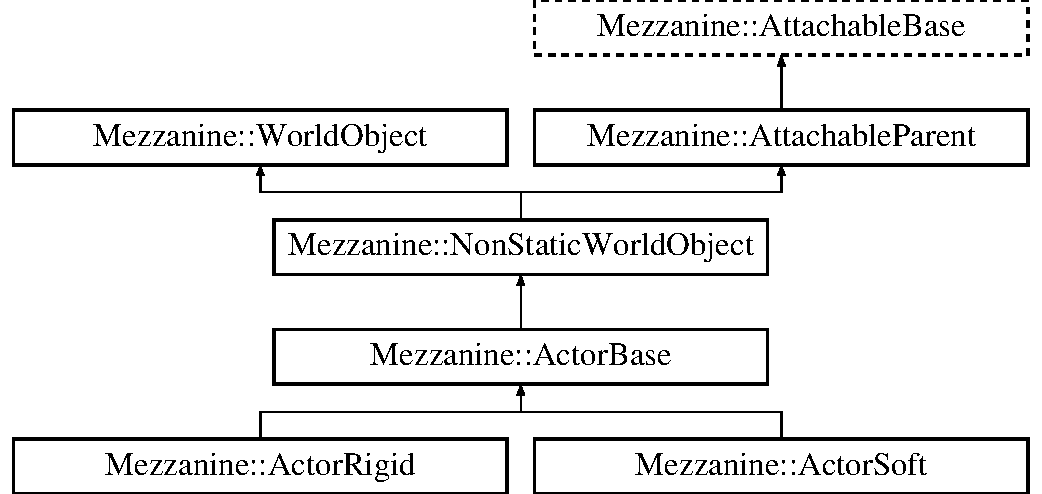
\includegraphics[height=2.000000cm]{classMezzanine_1_1ActorBase}
\end{center}
\end{figure}
\subsubsection*{Public Types}
\begin{DoxyCompactItemize}
\item 
enum \hyperlink{classMezzanine_1_1ActorBase_a98e1b66ce4973b01abb6d9b858398eb6}{ActorTypeName} \{ \par
{\bfseries Actorbase}, 
{\bfseries Actorcharacter}, 
{\bfseries Actorrigid}, 
{\bfseries Actorsoft}, 
\par
{\bfseries Actorterrain}
 \}
\begin{DoxyCompactList}\small\item\em A listing of Actor TypeNames. \item\end{DoxyCompactList}\end{DoxyCompactItemize}
\subsubsection*{Public Member Functions}
\begin{DoxyCompactItemize}
\item 
virtual btCollisionObject $\ast$ \hyperlink{classMezzanine_1_1ActorBase_a6f8b107522665d5ecee1f10f4a49464d}{\_\-GetBasePhysicsObject} () const 
\begin{DoxyCompactList}\small\item\em Gets the internal physics object this actor is based on. \item\end{DoxyCompactList}\item 
virtual Ogre::SceneNode $\ast$ \hyperlink{classMezzanine_1_1ActorBase_a060b9a1c42de39c0bcaa9535a5606ffa}{\_\-GetGraphicsNode} () const 
\begin{DoxyCompactList}\small\item\em Gets the internal graphics node this actor uses for it's graphics transform. \item\end{DoxyCompactList}\item 
virtual Ogre::Entity $\ast$ \hyperlink{classMezzanine_1_1ActorBase_ae4a2cc51ec188f7cfbab462f2cd76f8f}{\_\-GetGraphicsObject} () const 
\begin{DoxyCompactList}\small\item\em Gets the internal graphics object this actor is based on. \item\end{DoxyCompactList}\item 
virtual void \hyperlink{classMezzanine_1_1ActorBase_a5426eb2e8abd1d64a8880adad8e5f73c}{\_\-NotifyCollisionState} (\hyperlink{classMezzanine_1_1Collision}{Collision} $\ast$Col, const \hyperlink{classMezzanine_1_1Collision_a24094c597061743dcd571f36077f4d19}{Collision::CollisionState} \&State)
\begin{DoxyCompactList}\small\item\em Notifies this actor of a collision that is occuring with it. \item\end{DoxyCompactList}\item 
\hypertarget{classMezzanine_1_1ActorBase_a8f5a36a6981f1249dbabab318531afd0}{
virtual void \hyperlink{classMezzanine_1_1ActorBase_a8f5a36a6981f1249dbabab318531afd0}{\_\-Update} ()=0}
\label{classMezzanine_1_1ActorBase_a8f5a36a6981f1249dbabab318531afd0}

\begin{DoxyCompactList}\small\item\em Utility function for altering or checking the actor every frame. \item\end{DoxyCompactList}\item 
\hyperlink{classMezzanine_1_1ActorBase_aa9cc2fce1ff708a96d4a879b87054f18}{ActorBase} ()
\begin{DoxyCompactList}\small\item\em Constructor. \item\end{DoxyCompactList}\item 
\hypertarget{classMezzanine_1_1ActorBase_a766dc0add62500689498a9c1d3f758ea}{
virtual void \hyperlink{classMezzanine_1_1ActorBase_a766dc0add62500689498a9c1d3f758ea}{AddObjectToWorld} ()=0}
\label{classMezzanine_1_1ActorBase_a766dc0add62500689498a9c1d3f758ea}

\begin{DoxyCompactList}\small\item\em Adds the actor to the physics world. \item\end{DoxyCompactList}\item 
virtual void \hyperlink{classMezzanine_1_1ActorBase_ab245d50e649ec7335bbfcba86d9dc889}{AdvanceAnimation} (const \hyperlink{namespaceMezzanine_a726731b1a7df72bf3583e4a97282c6f6}{Real} \&\hyperlink{structMezzanine_1_1Time}{Time})
\begin{DoxyCompactList}\small\item\em Advances the animation, making it animate. \item\end{DoxyCompactList}\item 
virtual void \hyperlink{classMezzanine_1_1ActorBase_a28c9397e90ec680faf61845525312864}{EnableAnimation} (bool Enable)
\begin{DoxyCompactList}\small\item\em Enables the animation if one is set. \item\end{DoxyCompactList}\item 
virtual \hyperlink{classMezzanine_1_1WorldNode}{WorldNode} $\ast$ \hyperlink{classMezzanine_1_1ActorBase_a79803eb3d00e1e3722104fce473be085}{GetActorNode} () const 
\begin{DoxyCompactList}\small\item\em Gets a \hyperlink{classMezzanine_1_1WorldNode}{WorldNode} representing the position and orientation of this actor. \item\end{DoxyCompactList}\item 
virtual \hyperlink{classMezzanine_1_1Vector3}{Vector3} \hyperlink{classMezzanine_1_1ActorBase_a9255b5af0827d02505b7662486d8dd17}{GetActorScaling} () const 
\begin{DoxyCompactList}\small\item\em Gets the current scaling being applied to the actor. \item\end{DoxyCompactList}\item 
virtual const std::set$<$ \hyperlink{classMezzanine_1_1Collision}{Collision} $\ast$ $>$ \& \hyperlink{classMezzanine_1_1ActorBase_acb4f52d4033918be75ecc09485547bc4}{GetCurrentCollisions} ()
\begin{DoxyCompactList}\small\item\em Gets all current collisions that apply to this actor. \item\end{DoxyCompactList}\item 
virtual \hyperlink{classMezzanine_1_1ActorGraphicsSettings}{ActorGraphicsSettings} $\ast$ \hyperlink{classMezzanine_1_1ActorBase_ae57a1a39b5f9483c949f6e3651aa163f}{GetGraphicsSettings} () const 
\begin{DoxyCompactList}\small\item\em Gets the graphics settings class associated with this actor. \item\end{DoxyCompactList}\item 
virtual \hyperlink{classMezzanine_1_1Vector3}{Vector3} \hyperlink{classMezzanine_1_1ActorBase_ab1706a379bf86d020e64e4b560cdeb73}{GetLocation} () const 
\begin{DoxyCompactList}\small\item\em Retrieves the location of the object. \item\end{DoxyCompactList}\item 
virtual \hyperlink{namespaceMezzanine_acf9fcc130e6ebf08e3d8491aebcf1c86}{String} \hyperlink{classMezzanine_1_1ActorBase_a01e16da200911fdff659bfb78bafff1d}{GetName} () const =0
\begin{DoxyCompactList}\small\item\em Retrieves the name of the object. \item\end{DoxyCompactList}\item 
virtual \hyperlink{classMezzanine_1_1Quaternion}{Quaternion} \hyperlink{classMezzanine_1_1ActorBase_ac04f313c7e1272c519d0284bc98148a4}{GetOrientation} () const 
\begin{DoxyCompactList}\small\item\em Gets the orientation of the actor. \item\end{DoxyCompactList}\item 
virtual \hyperlink{classMezzanine_1_1ActorBasePhysicsSettings}{ActorBasePhysicsSettings} $\ast$ \hyperlink{classMezzanine_1_1ActorBase_a08c975572f1ab5cde651e1a6e5d9bb6a}{GetPhysicsSettings} () const 
\begin{DoxyCompactList}\small\item\em Gets the physics settings class associated with this actor. \item\end{DoxyCompactList}\item 
virtual int \hyperlink{classMezzanine_1_1ActorBase_ac9a208af008d628e6442079c2ec80fa9}{GetType} () const 
\begin{DoxyCompactList}\small\item\em Gets the type of actor this class is. \item\end{DoxyCompactList}\item 
virtual bool \hyperlink{classMezzanine_1_1ActorBase_ade1c3e7a2e24df64a79d2acb8d6fc084}{IsAnimated} () const 
\begin{DoxyCompactList}\small\item\em Tells whether this actor is animated or not. \item\end{DoxyCompactList}\item 
virtual bool \hyperlink{classMezzanine_1_1ActorBase_aa2ab7ee3bc4d268d3363de0923426c72}{IsInWorld} () const 
\begin{DoxyCompactList}\small\item\em Gets whether or not this object is currently in the world. \item\end{DoxyCompactList}\item 
virtual bool \hyperlink{classMezzanine_1_1ActorBase_aae73855e5f3cded86c71955cc855026a}{IsStaticOrKinematic} () const 
\begin{DoxyCompactList}\small\item\em Checks of the actor is static or kinematic. \item\end{DoxyCompactList}\item 
\hypertarget{classMezzanine_1_1ActorBase_a774050bfd7c75f2b639005d82dcd5085}{
virtual void \hyperlink{classMezzanine_1_1ActorBase_a774050bfd7c75f2b639005d82dcd5085}{RemoveObjectFromWorld} ()=0}
\label{classMezzanine_1_1ActorBase_a774050bfd7c75f2b639005d82dcd5085}

\begin{DoxyCompactList}\small\item\em Removes the actor from the physics world. \item\end{DoxyCompactList}\item 
virtual void \hyperlink{classMezzanine_1_1ActorBase_a148df02e486650cba1aa384faf85975f}{RemoveSetAnimation} ()
\begin{DoxyCompactList}\small\item\em Unloads a loaded animation. \item\end{DoxyCompactList}\item 
virtual void \hyperlink{classMezzanine_1_1ActorBase_a59af6b6866b22038a0f63e398b33a834}{SetActorScaling} (const \hyperlink{classMezzanine_1_1Vector3}{Vector3} \&scale)
\begin{DoxyCompactList}\small\item\em Sets the scale of the actor. \item\end{DoxyCompactList}\item 
virtual void \hyperlink{classMezzanine_1_1ActorBase_af81c2b16a0a73608d9af4f9fb7e82ef4}{SetAnimation} (\hyperlink{namespaceMezzanine_a63cd699ac54b73953f35ec9cfc05e506}{ConstString} \&AnimationName, bool Loop)
\begin{DoxyCompactList}\small\item\em Sets the animation for this object. \item\end{DoxyCompactList}\item 
virtual void \hyperlink{classMezzanine_1_1ActorBase_a293c93bc4e1b22f64804fdce61312a67}{SetLocation} (const \hyperlink{classMezzanine_1_1Vector3}{Vector3} \&Place)
\begin{DoxyCompactList}\small\item\em Manually sets the location of the actor. \item\end{DoxyCompactList}\item 
virtual void \hyperlink{classMezzanine_1_1ActorBase_aa0f4211e037013524088c38c04ab2d80}{SetLocation} (const \hyperlink{namespaceMezzanine_a726731b1a7df72bf3583e4a97282c6f6}{Real} \&x, const \hyperlink{namespaceMezzanine_a726731b1a7df72bf3583e4a97282c6f6}{Real} \&y, const \hyperlink{namespaceMezzanine_a726731b1a7df72bf3583e4a97282c6f6}{Real} \&z)
\begin{DoxyCompactList}\small\item\em Manually sets the location of the actor. \item\end{DoxyCompactList}\item 
virtual void \hyperlink{classMezzanine_1_1ActorBase_a9ea0aea47c70df747b62de1908a6e248}{SetOrientation} (const \hyperlink{namespaceMezzanine_a726731b1a7df72bf3583e4a97282c6f6}{Real} \&x, const \hyperlink{namespaceMezzanine_a726731b1a7df72bf3583e4a97282c6f6}{Real} \&y, const \hyperlink{namespaceMezzanine_a726731b1a7df72bf3583e4a97282c6f6}{Real} \&z, const \hyperlink{namespaceMezzanine_a726731b1a7df72bf3583e4a97282c6f6}{Real} \&w)
\begin{DoxyCompactList}\small\item\em Sets the orientation of the actor. \item\end{DoxyCompactList}\item 
virtual void \hyperlink{classMezzanine_1_1ActorBase_a71611580c9265bc87ad34c122e8246a0}{SetOrientation} (const \hyperlink{classMezzanine_1_1Quaternion}{Quaternion} \&Rotation)
\begin{DoxyCompactList}\small\item\em Sets the orientation of the actor. \item\end{DoxyCompactList}\item 
virtual \hyperlink{classMezzanine_1_1ActorBase_a0b49f2bc589504c908ccc47a635e1e79}{$\sim$ActorBase} ()
\begin{DoxyCompactList}\small\item\em Destructor. \item\end{DoxyCompactList}\end{DoxyCompactItemize}
\subsubsection*{Public Attributes}
\begin{DoxyCompactItemize}
\item 
\hypertarget{classMezzanine_1_1ActorBase_a55fc2cfb5d2754657fdb9a821504f9bf}{
\hyperlink{classMezzanine_1_1Audio_1_1SoundSet}{Audio::SoundSet} $\ast$ \hyperlink{classMezzanine_1_1ActorBase_a55fc2cfb5d2754657fdb9a821504f9bf}{ActorSounds}}
\label{classMezzanine_1_1ActorBase_a55fc2cfb5d2754657fdb9a821504f9bf}

\begin{DoxyCompactList}\small\item\em This is a collection of sounds for use with this actor. \item\end{DoxyCompactList}\end{DoxyCompactItemize}
\subsubsection*{Protected Member Functions}
\begin{DoxyCompactItemize}
\item 
virtual void \hyperlink{classMezzanine_1_1ActorBase_a040cc440d23400c7f129b318a8a84e97}{AttachToGraphics} ()
\begin{DoxyCompactList}\small\item\em Makes the actor visable. \item\end{DoxyCompactList}\item 
virtual void \hyperlink{classMezzanine_1_1ActorBase_a957ed99e5f67ac3fca3ba8a9b025fe48}{DetachFromGraphics} ()
\begin{DoxyCompactList}\small\item\em Makes the actor invisable. \item\end{DoxyCompactList}\item 
virtual \hyperlink{classMezzanine_1_1Vector3}{Vector3} \hyperlink{classMezzanine_1_1ActorBase_a9f110d013ed871809258dfc55f8b7276}{GetBulletLocation} () const 
\begin{DoxyCompactList}\small\item\em Retrieves the location of the physics body. \item\end{DoxyCompactList}\item 
virtual \hyperlink{classMezzanine_1_1Quaternion}{Quaternion} \hyperlink{classMezzanine_1_1ActorBase_a32fc60215d8bcd3151b3158d481ce0ef}{GetBulletOrientation} () const 
\begin{DoxyCompactList}\small\item\em Gets the orientation of the graphical body. \item\end{DoxyCompactList}\item 
virtual \hyperlink{classMezzanine_1_1Vector3}{Vector3} \hyperlink{classMezzanine_1_1ActorBase_a8095a72bdfcf7fd02953423ae17acd01}{GetOgreLocation} () const 
\begin{DoxyCompactList}\small\item\em Retrieves the location of the graphical body. \item\end{DoxyCompactList}\item 
virtual \hyperlink{classMezzanine_1_1Quaternion}{Quaternion} \hyperlink{classMezzanine_1_1ActorBase_ae76175894f1c2bc4372ec1ebd5ede83d}{GetOgreOrientation} () const 
\begin{DoxyCompactList}\small\item\em Gets the orientation of the graphical body. \item\end{DoxyCompactList}\item 
virtual void \hyperlink{classMezzanine_1_1ActorBase_a8f7018838c67f07cd554730ac83f4283}{SetBulletLocation} (const \hyperlink{classMezzanine_1_1Vector3}{Vector3} \&Location)
\begin{DoxyCompactList}\small\item\em Sets the location of the physics body. \item\end{DoxyCompactList}\item 
virtual void \hyperlink{classMezzanine_1_1ActorBase_a088bc9b26f4747e6f2896591a0f7b190}{SetBulletOrientation} (const \hyperlink{classMezzanine_1_1Quaternion}{Quaternion} \&Rotation)
\begin{DoxyCompactList}\small\item\em Sets the orientation of the physics body. \item\end{DoxyCompactList}\item 
virtual void \hyperlink{classMezzanine_1_1ActorBase_a4b2a3281be30dcc983b514ecaff14a51}{SetOgreLocation} (const \hyperlink{classMezzanine_1_1Vector3}{Vector3} \&Place)
\begin{DoxyCompactList}\small\item\em Sets the location of the graphical body. \item\end{DoxyCompactList}\item 
virtual void \hyperlink{classMezzanine_1_1ActorBase_a5958552c8b356775b5447c0bd6448102}{SetOgreOrientation} (const \hyperlink{classMezzanine_1_1Quaternion}{Quaternion} \&Rotation)
\begin{DoxyCompactList}\small\item\em Sets the orientation of the graphical body. \item\end{DoxyCompactList}\end{DoxyCompactItemize}
\subsubsection*{Protected Attributes}
\begin{DoxyCompactItemize}
\item 
\hypertarget{classMezzanine_1_1ActorBase_aac246ea33955e7aefe2b395e450967b6}{
\hyperlink{classMezzanine_1_1ActorBase_a98e1b66ce4973b01abb6d9b858398eb6}{ActorTypeName} \hyperlink{classMezzanine_1_1ActorBase_aac246ea33955e7aefe2b395e450967b6}{ActorType}}
\label{classMezzanine_1_1ActorBase_aac246ea33955e7aefe2b395e450967b6}

\begin{DoxyCompactList}\small\item\em This variable stores the type of actor that this class is. \item\end{DoxyCompactList}\item 
\hypertarget{classMezzanine_1_1ActorBase_a6dbfa117e36ab443af4509399b6c4fc9}{
\hyperlink{classMezzanine_1_1WorldNode}{WorldNode} $\ast$ \hyperlink{classMezzanine_1_1ActorBase_a6dbfa117e36ab443af4509399b6c4fc9}{ActorWorldNode}}
\label{classMezzanine_1_1ActorBase_a6dbfa117e36ab443af4509399b6c4fc9}

\begin{DoxyCompactList}\small\item\em This class excapsulates the functionality of the Ogre::SceneNode. \item\end{DoxyCompactList}\item 
\hypertarget{classMezzanine_1_1ActorBase_ae71259b98aed5a9c269e0758344d36a7}{
Ogre::AnimationState $\ast$ \hyperlink{classMezzanine_1_1ActorBase_ae71259b98aed5a9c269e0758344d36a7}{Animation}}
\label{classMezzanine_1_1ActorBase_ae71259b98aed5a9c269e0758344d36a7}

\begin{DoxyCompactList}\small\item\em This class encapsulates the functionality of the Ogre::AnimationState using this. \item\end{DoxyCompactList}\item 
\hypertarget{classMezzanine_1_1ActorBase_a6171cd6b5d94263d0c339bf5e299fa26}{
\hyperlink{classMezzanine_1_1ActorBasePhysicsSettings}{ActorBasePhysicsSettings} $\ast$ \hyperlink{classMezzanine_1_1ActorBase_a6171cd6b5d94263d0c339bf5e299fa26}{BasePhysicsSettings}}
\label{classMezzanine_1_1ActorBase_a6171cd6b5d94263d0c339bf5e299fa26}

\begin{DoxyCompactList}\small\item\em This class encapsulates physics specific configuration for this actor. \item\end{DoxyCompactList}\item 
\hypertarget{classMezzanine_1_1ActorBase_a453166e089f7a3821bf099e4404c3e43}{
btCollisionObject $\ast$ \hyperlink{classMezzanine_1_1ActorBase_a453166e089f7a3821bf099e4404c3e43}{CollisionObject}}
\label{classMezzanine_1_1ActorBase_a453166e089f7a3821bf099e4404c3e43}

\begin{DoxyCompactList}\small\item\em This class encapsulates the functionality of the btCollisionObject using this. \item\end{DoxyCompactList}\item 
\hypertarget{classMezzanine_1_1ActorBase_a5673816f3372d3ea8313687ad2529d08}{
std::set$<$ \hyperlink{classMezzanine_1_1Collision}{Collision} $\ast$ $>$ \hyperlink{classMezzanine_1_1ActorBase_a5673816f3372d3ea8313687ad2529d08}{CurrentCollisions}}
\label{classMezzanine_1_1ActorBase_a5673816f3372d3ea8313687ad2529d08}

\begin{DoxyCompactList}\small\item\em This member stores all existing collision events referencing this actor. \item\end{DoxyCompactList}\item 
\hypertarget{classMezzanine_1_1ActorBase_ac0a8cda5141e05df03a31f8b9b5908a6}{
Ogre::SceneNode $\ast$ \hyperlink{classMezzanine_1_1ActorBase_ac0a8cda5141e05df03a31f8b9b5908a6}{GraphicsNode}}
\label{classMezzanine_1_1ActorBase_ac0a8cda5141e05df03a31f8b9b5908a6}

\begin{DoxyCompactList}\small\item\em This class encapsulates the functionality of the Ogre::SceneNode using this. \item\end{DoxyCompactList}\item 
\hypertarget{classMezzanine_1_1ActorBase_ab28b13559f01195a5f81768a445e5119}{
Ogre::Entity $\ast$ \hyperlink{classMezzanine_1_1ActorBase_ab28b13559f01195a5f81768a445e5119}{GraphicsObject}}
\label{classMezzanine_1_1ActorBase_ab28b13559f01195a5f81768a445e5119}

\begin{DoxyCompactList}\small\item\em This class encapsulates the functionality of the Ogre::Entity using this. \item\end{DoxyCompactList}\item 
\hypertarget{classMezzanine_1_1ActorBase_ae0bd045c27c10a959a11895b3cd6e73c}{
\hyperlink{classMezzanine_1_1ActorGraphicsSettings}{ActorGraphicsSettings} $\ast$ \hyperlink{classMezzanine_1_1ActorBase_ae0bd045c27c10a959a11895b3cd6e73c}{GraphicsSettings}}
\label{classMezzanine_1_1ActorBase_ae0bd045c27c10a959a11895b3cd6e73c}

\begin{DoxyCompactList}\small\item\em This class encapsulates graphics specific configuration for this actor. \item\end{DoxyCompactList}\item 
\hypertarget{classMezzanine_1_1ActorBase_a073d5307c4cb7a82f13133e8216f797b}{
internal::PhysMotionState $\ast$ \hyperlink{classMezzanine_1_1ActorBase_a073d5307c4cb7a82f13133e8216f797b}{MotionState}}
\label{classMezzanine_1_1ActorBase_a073d5307c4cb7a82f13133e8216f797b}

\begin{DoxyCompactList}\small\item\em This class encapsulates the functionality of the PhysMotionState using this. \item\end{DoxyCompactList}\item 
\hypertarget{classMezzanine_1_1ActorBase_a51fdd84432cc14bebfe2d7bbc52cd4a0}{
btCollisionShape $\ast$ \hyperlink{classMezzanine_1_1ActorBase_a51fdd84432cc14bebfe2d7bbc52cd4a0}{Shape}}
\label{classMezzanine_1_1ActorBase_a51fdd84432cc14bebfe2d7bbc52cd4a0}

\begin{DoxyCompactList}\small\item\em This class encapsulates the functionality of the btCollisionShape using this. \item\end{DoxyCompactList}\end{DoxyCompactItemize}
\subsubsection*{Friends}
\begin{DoxyCompactItemize}
\item 
\hypertarget{classMezzanine_1_1ActorBase_ad56afa2bffce8b552583041f21297874}{
class {\bfseries ActorBasePhysicsSettings}}
\label{classMezzanine_1_1ActorBase_ad56afa2bffce8b552583041f21297874}

\item 
\hypertarget{classMezzanine_1_1ActorBase_a01f5bcaf4807085e756d9c03b3eb8d9d}{
class {\bfseries ActorGraphicsSettings}}
\label{classMezzanine_1_1ActorBase_a01f5bcaf4807085e756d9c03b3eb8d9d}

\item 
\hypertarget{classMezzanine_1_1ActorBase_a1cacd07efb11226da49a7c80569b18e8}{
class {\bfseries WorldNode}}
\label{classMezzanine_1_1ActorBase_a1cacd07efb11226da49a7c80569b18e8}

\end{DoxyCompactItemize}


\subsubsection{Detailed Description}
This is the base class from which all the actors inherit. The actor classes store and manage all the relevant data regarding objects inside the \hyperlink{classMezzanine_1_1World}{World}. They serve as a binder between the physics and graphics for objects and have functions that allow the manipulation of objects loaded into the \hyperlink{classMezzanine_1_1World}{World}. Currently there are 5 actor classes: \hyperlink{classMezzanine_1_1ActorBase}{ActorBase}, \hyperlink{classMezzanine_1_1ActorRigid}{ActorRigid}, \hyperlink{classMezzanine_1_1ActorSoft}{ActorSoft}, \hyperlink{classMezzanine_1_1ActorTerrain}{ActorTerrain}, ActorCharacter. \par
 \hyperlink{classMezzanine_1_1ActorBase}{ActorBase} is a base class that serves as a template for the other four actor classes. \par
 \hyperlink{classMezzanine_1_1ActorBase}{ActorBase} should never be created, as it lacks the functionality needed for most objects. 

Definition at line 98 of file actorbase.h.



\subsubsection{Member Enumeration Documentation}
\hypertarget{classMezzanine_1_1ActorBase_a98e1b66ce4973b01abb6d9b858398eb6}{
\index{Mezzanine::ActorBase@{Mezzanine::ActorBase}!ActorTypeName@{ActorTypeName}}
\index{ActorTypeName@{ActorTypeName}!Mezzanine::ActorBase@{Mezzanine::ActorBase}}
\paragraph[{ActorTypeName}]{\setlength{\rightskip}{0pt plus 5cm}enum {\bf Mezzanine::ActorBase::ActorTypeName}}\hfill}
\label{classMezzanine_1_1ActorBase_a98e1b66ce4973b01abb6d9b858398eb6}


A listing of Actor TypeNames. 

These will be returned by \hyperlink{classMezzanine_1_1ActorBase_ac9a208af008d628e6442079c2ec80fa9}{ActorBase::GetType()}, and will allow code using this to determine what type of Actor class they are working with and use this information to more safely cast to the correct Actor if needed. 

Definition at line 110 of file actorbase.h.



\subsubsection{Constructor \& Destructor Documentation}
\hypertarget{classMezzanine_1_1ActorBase_aa9cc2fce1ff708a96d4a879b87054f18}{
\index{Mezzanine::ActorBase@{Mezzanine::ActorBase}!ActorBase@{ActorBase}}
\index{ActorBase@{ActorBase}!Mezzanine::ActorBase@{Mezzanine::ActorBase}}
\paragraph[{ActorBase}]{\setlength{\rightskip}{0pt plus 5cm}Mezzanine::ActorBase::ActorBase (
\begin{DoxyParamCaption}
{}
\end{DoxyParamCaption}
)}\hfill}
\label{classMezzanine_1_1ActorBase_aa9cc2fce1ff708a96d4a879b87054f18}


Constructor. 

This constructor contains the basic information needed to make an actor. 

Definition at line 71 of file actorbase.cpp.

\hypertarget{classMezzanine_1_1ActorBase_a0b49f2bc589504c908ccc47a635e1e79}{
\index{Mezzanine::ActorBase@{Mezzanine::ActorBase}!$\sim$ActorBase@{$\sim$ActorBase}}
\index{$\sim$ActorBase@{$\sim$ActorBase}!Mezzanine::ActorBase@{Mezzanine::ActorBase}}
\paragraph[{$\sim$ActorBase}]{\setlength{\rightskip}{0pt plus 5cm}Mezzanine::ActorBase::$\sim$ActorBase (
\begin{DoxyParamCaption}
{}
\end{DoxyParamCaption}
)\hspace{0.3cm}{\ttfamily  \mbox{[}virtual\mbox{]}}}\hfill}
\label{classMezzanine_1_1ActorBase_a0b49f2bc589504c908ccc47a635e1e79}


Destructor. 

The class destructor. 

Definition at line 86 of file actorbase.cpp.



\subsubsection{Member Function Documentation}
\hypertarget{classMezzanine_1_1ActorBase_a6f8b107522665d5ecee1f10f4a49464d}{
\index{Mezzanine::ActorBase@{Mezzanine::ActorBase}!\_\-GetBasePhysicsObject@{\_\-GetBasePhysicsObject}}
\index{\_\-GetBasePhysicsObject@{\_\-GetBasePhysicsObject}!Mezzanine::ActorBase@{Mezzanine::ActorBase}}
\paragraph[{\_\-GetBasePhysicsObject}]{\setlength{\rightskip}{0pt plus 5cm}btCollisionObject $\ast$ Mezzanine::ActorBase::\_\-GetBasePhysicsObject (
\begin{DoxyParamCaption}
{}
\end{DoxyParamCaption}
) const\hspace{0.3cm}{\ttfamily  \mbox{[}virtual\mbox{]}}}\hfill}
\label{classMezzanine_1_1ActorBase_a6f8b107522665d5ecee1f10f4a49464d}


Gets the internal physics object this actor is based on. 

\begin{DoxyReturn}{Returns}
Returns a pointer to the internal Bullet object. 
\end{DoxyReturn}


Definition at line 322 of file actorbase.cpp.

\hypertarget{classMezzanine_1_1ActorBase_a060b9a1c42de39c0bcaa9535a5606ffa}{
\index{Mezzanine::ActorBase@{Mezzanine::ActorBase}!\_\-GetGraphicsNode@{\_\-GetGraphicsNode}}
\index{\_\-GetGraphicsNode@{\_\-GetGraphicsNode}!Mezzanine::ActorBase@{Mezzanine::ActorBase}}
\paragraph[{\_\-GetGraphicsNode}]{\setlength{\rightskip}{0pt plus 5cm}Ogre::SceneNode $\ast$ Mezzanine::ActorBase::\_\-GetGraphicsNode (
\begin{DoxyParamCaption}
{}
\end{DoxyParamCaption}
) const\hspace{0.3cm}{\ttfamily  \mbox{[}virtual\mbox{]}}}\hfill}
\label{classMezzanine_1_1ActorBase_a060b9a1c42de39c0bcaa9535a5606ffa}


Gets the internal graphics node this actor uses for it's graphics transform. 

\begin{DoxyReturn}{Returns}
Returns a pointer to the internal graphics node. 
\end{DoxyReturn}


Definition at line 332 of file actorbase.cpp.

\hypertarget{classMezzanine_1_1ActorBase_ae4a2cc51ec188f7cfbab462f2cd76f8f}{
\index{Mezzanine::ActorBase@{Mezzanine::ActorBase}!\_\-GetGraphicsObject@{\_\-GetGraphicsObject}}
\index{\_\-GetGraphicsObject@{\_\-GetGraphicsObject}!Mezzanine::ActorBase@{Mezzanine::ActorBase}}
\paragraph[{\_\-GetGraphicsObject}]{\setlength{\rightskip}{0pt plus 5cm}Ogre::Entity $\ast$ Mezzanine::ActorBase::\_\-GetGraphicsObject (
\begin{DoxyParamCaption}
{}
\end{DoxyParamCaption}
) const\hspace{0.3cm}{\ttfamily  \mbox{[}virtual\mbox{]}}}\hfill}
\label{classMezzanine_1_1ActorBase_ae4a2cc51ec188f7cfbab462f2cd76f8f}


Gets the internal graphics object this actor is based on. 

\begin{DoxyReturn}{Returns}
Returns a pointer to the internal graphics object. 
\end{DoxyReturn}


Definition at line 327 of file actorbase.cpp.

\hypertarget{classMezzanine_1_1ActorBase_a5426eb2e8abd1d64a8880adad8e5f73c}{
\index{Mezzanine::ActorBase@{Mezzanine::ActorBase}!\_\-NotifyCollisionState@{\_\-NotifyCollisionState}}
\index{\_\-NotifyCollisionState@{\_\-NotifyCollisionState}!Mezzanine::ActorBase@{Mezzanine::ActorBase}}
\paragraph[{\_\-NotifyCollisionState}]{\setlength{\rightskip}{0pt plus 5cm}void Mezzanine::ActorBase::\_\-NotifyCollisionState (
\begin{DoxyParamCaption}
\item[{{\bf Collision} $\ast$}]{Col, }
\item[{const {\bf Collision::CollisionState} \&}]{State}
\end{DoxyParamCaption}
)\hspace{0.3cm}{\ttfamily  \mbox{[}virtual\mbox{]}}}\hfill}
\label{classMezzanine_1_1ActorBase_a5426eb2e8abd1d64a8880adad8e5f73c}


Notifies this actor of a collision that is occuring with it. 


\begin{DoxyParams}{Parameters}
{\em Col} & A pointer to the collision pertaining to this actor. \\
\hline
{\em State} & The state of the collision pertaining to this actor. \\
\hline
\end{DoxyParams}


Reimplemented in \hyperlink{classMezzanine_1_1ActorRigid_a68827280395bc3b9e0266710ec44247d}{Mezzanine::ActorRigid}.



Definition at line 309 of file actorbase.cpp.

\hypertarget{classMezzanine_1_1ActorBase_ab245d50e649ec7335bbfcba86d9dc889}{
\index{Mezzanine::ActorBase@{Mezzanine::ActorBase}!AdvanceAnimation@{AdvanceAnimation}}
\index{AdvanceAnimation@{AdvanceAnimation}!Mezzanine::ActorBase@{Mezzanine::ActorBase}}
\paragraph[{AdvanceAnimation}]{\setlength{\rightskip}{0pt plus 5cm}void Mezzanine::ActorBase::AdvanceAnimation (
\begin{DoxyParamCaption}
\item[{const {\bf Real} \&}]{Time}
\end{DoxyParamCaption}
)\hspace{0.3cm}{\ttfamily  \mbox{[}virtual\mbox{]}}}\hfill}
\label{classMezzanine_1_1ActorBase_ab245d50e649ec7335bbfcba86d9dc889}


Advances the animation, making it animate. 


\begin{DoxyParams}{Parameters}
{\em \hyperlink{structMezzanine_1_1Time}{Time}} & The amount of time to advance the animation.\\
\hline
\end{DoxyParams}
You need to call this every frame while the actor is to be animated, otherwise even with the animation enabled you will see no change in the animation. 

Definition at line 262 of file actorbase.cpp.

\hypertarget{classMezzanine_1_1ActorBase_a040cc440d23400c7f129b318a8a84e97}{
\index{Mezzanine::ActorBase@{Mezzanine::ActorBase}!AttachToGraphics@{AttachToGraphics}}
\index{AttachToGraphics@{AttachToGraphics}!Mezzanine::ActorBase@{Mezzanine::ActorBase}}
\paragraph[{AttachToGraphics}]{\setlength{\rightskip}{0pt plus 5cm}void Mezzanine::ActorBase::AttachToGraphics (
\begin{DoxyParamCaption}
{}
\end{DoxyParamCaption}
)\hspace{0.3cm}{\ttfamily  \mbox{[}protected, virtual\mbox{]}}}\hfill}
\label{classMezzanine_1_1ActorBase_a040cc440d23400c7f129b318a8a84e97}


Makes the actor visable. 

Adds the actor to all the nessessary graphics elements to make it visable on screen. \par
 This is automaticly called by the Worlds AddActor function and shouldn't ever need to be called manually. 

Reimplemented in \hyperlink{classMezzanine_1_1ActorSoft_af2e618dd176d910834f146c62efe8f19}{Mezzanine::ActorSoft}.



Definition at line 160 of file actorbase.cpp.

\hypertarget{classMezzanine_1_1ActorBase_a957ed99e5f67ac3fca3ba8a9b025fe48}{
\index{Mezzanine::ActorBase@{Mezzanine::ActorBase}!DetachFromGraphics@{DetachFromGraphics}}
\index{DetachFromGraphics@{DetachFromGraphics}!Mezzanine::ActorBase@{Mezzanine::ActorBase}}
\paragraph[{DetachFromGraphics}]{\setlength{\rightskip}{0pt plus 5cm}void Mezzanine::ActorBase::DetachFromGraphics (
\begin{DoxyParamCaption}
{}
\end{DoxyParamCaption}
)\hspace{0.3cm}{\ttfamily  \mbox{[}protected, virtual\mbox{]}}}\hfill}
\label{classMezzanine_1_1ActorBase_a957ed99e5f67ac3fca3ba8a9b025fe48}


Makes the actor invisable. 

This is the inverse of the AttachToGraphics function. This will effectively remove the object from the graphics world and make it no longer visable. \par
 This is automaticly called by the Worlds RemoveActor function and shouldn't ever need to be called manually. 

Reimplemented in \hyperlink{classMezzanine_1_1ActorSoft_a3ec90b87480ba28553656eb10552f6d6}{Mezzanine::ActorSoft}.



Definition at line 169 of file actorbase.cpp.

\hypertarget{classMezzanine_1_1ActorBase_a28c9397e90ec680faf61845525312864}{
\index{Mezzanine::ActorBase@{Mezzanine::ActorBase}!EnableAnimation@{EnableAnimation}}
\index{EnableAnimation@{EnableAnimation}!Mezzanine::ActorBase@{Mezzanine::ActorBase}}
\paragraph[{EnableAnimation}]{\setlength{\rightskip}{0pt plus 5cm}void Mezzanine::ActorBase::EnableAnimation (
\begin{DoxyParamCaption}
\item[{bool}]{Enable}
\end{DoxyParamCaption}
)\hspace{0.3cm}{\ttfamily  \mbox{[}virtual\mbox{]}}}\hfill}
\label{classMezzanine_1_1ActorBase_a28c9397e90ec680faf61845525312864}


Enables the animation if one is set. 

This function will enable the animation if passed true, making the object animate. If passed false will disable the animation. 
\begin{DoxyParams}{Parameters}
{\em Enable} & True to enable the animation or false to disable the animation. \\
\hline
\end{DoxyParams}


Definition at line 244 of file actorbase.cpp.

\hypertarget{classMezzanine_1_1ActorBase_a79803eb3d00e1e3722104fce473be085}{
\index{Mezzanine::ActorBase@{Mezzanine::ActorBase}!GetActorNode@{GetActorNode}}
\index{GetActorNode@{GetActorNode}!Mezzanine::ActorBase@{Mezzanine::ActorBase}}
\paragraph[{GetActorNode}]{\setlength{\rightskip}{0pt plus 5cm}{\bf WorldNode} $\ast$ Mezzanine::ActorBase::GetActorNode (
\begin{DoxyParamCaption}
{}
\end{DoxyParamCaption}
) const\hspace{0.3cm}{\ttfamily  \mbox{[}virtual\mbox{]}}}\hfill}
\label{classMezzanine_1_1ActorBase_a79803eb3d00e1e3722104fce473be085}


Gets a \hyperlink{classMezzanine_1_1WorldNode}{WorldNode} representing the position and orientation of this actor. 

The \hyperlink{classMezzanine_1_1WorldNode}{WorldNode} returned by this function is not stored in the scene manasger. \begin{DoxyReturn}{Returns}
Returns a \hyperlink{classMezzanine_1_1WorldNode}{WorldNode} pointer pointing to this actor's world node. 
\end{DoxyReturn}


Definition at line 219 of file actorbase.cpp.

\hypertarget{classMezzanine_1_1ActorBase_a9255b5af0827d02505b7662486d8dd17}{
\index{Mezzanine::ActorBase@{Mezzanine::ActorBase}!GetActorScaling@{GetActorScaling}}
\index{GetActorScaling@{GetActorScaling}!Mezzanine::ActorBase@{Mezzanine::ActorBase}}
\paragraph[{GetActorScaling}]{\setlength{\rightskip}{0pt plus 5cm}{\bf Vector3} Mezzanine::ActorBase::GetActorScaling (
\begin{DoxyParamCaption}
{}
\end{DoxyParamCaption}
) const\hspace{0.3cm}{\ttfamily  \mbox{[}virtual\mbox{]}}}\hfill}
\label{classMezzanine_1_1ActorBase_a9255b5af0827d02505b7662486d8dd17}


Gets the current scaling being applied to the actor. 

\begin{DoxyReturn}{Returns}
Returns a vector3 representing the scaling being applied on all axes of this actor. 
\end{DoxyReturn}


Definition at line 285 of file actorbase.cpp.

\hypertarget{classMezzanine_1_1ActorBase_a9f110d013ed871809258dfc55f8b7276}{
\index{Mezzanine::ActorBase@{Mezzanine::ActorBase}!GetBulletLocation@{GetBulletLocation}}
\index{GetBulletLocation@{GetBulletLocation}!Mezzanine::ActorBase@{Mezzanine::ActorBase}}
\paragraph[{GetBulletLocation}]{\setlength{\rightskip}{0pt plus 5cm}{\bf Vector3} Mezzanine::ActorBase::GetBulletLocation (
\begin{DoxyParamCaption}
{}
\end{DoxyParamCaption}
) const\hspace{0.3cm}{\ttfamily  \mbox{[}protected, virtual\mbox{]}}}\hfill}
\label{classMezzanine_1_1ActorBase_a9f110d013ed871809258dfc55f8b7276}


Retrieves the location of the physics body. 

This function will retrieve the location of the object within the physics world. \begin{DoxyReturn}{Returns}
a \hyperlink{classMezzanine_1_1Vector3}{Mezzanine::Vector3}. 
\end{DoxyReturn}


Reimplemented in \hyperlink{classMezzanine_1_1ActorSoft_a7d6f49acc1bf286fd46fb33a8c2798e4}{Mezzanine::ActorSoft}.



Definition at line 140 of file actorbase.cpp.

\hypertarget{classMezzanine_1_1ActorBase_a32fc60215d8bcd3151b3158d481ce0ef}{
\index{Mezzanine::ActorBase@{Mezzanine::ActorBase}!GetBulletOrientation@{GetBulletOrientation}}
\index{GetBulletOrientation@{GetBulletOrientation}!Mezzanine::ActorBase@{Mezzanine::ActorBase}}
\paragraph[{GetBulletOrientation}]{\setlength{\rightskip}{0pt plus 5cm}{\bf Quaternion} Mezzanine::ActorBase::GetBulletOrientation (
\begin{DoxyParamCaption}
{}
\end{DoxyParamCaption}
) const\hspace{0.3cm}{\ttfamily  \mbox{[}protected, virtual\mbox{]}}}\hfill}
\label{classMezzanine_1_1ActorBase_a32fc60215d8bcd3151b3158d481ce0ef}


Gets the orientation of the graphical body. 

\begin{DoxyReturn}{Returns}
Returns a quaternion representing the rotation of the actor. 
\end{DoxyReturn}


Definition at line 151 of file actorbase.cpp.

\hypertarget{classMezzanine_1_1ActorBase_acb4f52d4033918be75ecc09485547bc4}{
\index{Mezzanine::ActorBase@{Mezzanine::ActorBase}!GetCurrentCollisions@{GetCurrentCollisions}}
\index{GetCurrentCollisions@{GetCurrentCollisions}!Mezzanine::ActorBase@{Mezzanine::ActorBase}}
\paragraph[{GetCurrentCollisions}]{\setlength{\rightskip}{0pt plus 5cm}const std::set$<$ {\bf Collision} $\ast$ $>$ \& Mezzanine::ActorBase::GetCurrentCollisions (
\begin{DoxyParamCaption}
{}
\end{DoxyParamCaption}
)\hspace{0.3cm}{\ttfamily  \mbox{[}virtual\mbox{]}}}\hfill}
\label{classMezzanine_1_1ActorBase_acb4f52d4033918be75ecc09485547bc4}


Gets all current collisions that apply to this actor. 

\begin{DoxyReturn}{Returns}
Returns a const reference to a set containing all collisions events containing this actor. 
\end{DoxyReturn}


Definition at line 291 of file actorbase.cpp.

\hypertarget{classMezzanine_1_1ActorBase_ae57a1a39b5f9483c949f6e3651aa163f}{
\index{Mezzanine::ActorBase@{Mezzanine::ActorBase}!GetGraphicsSettings@{GetGraphicsSettings}}
\index{GetGraphicsSettings@{GetGraphicsSettings}!Mezzanine::ActorBase@{Mezzanine::ActorBase}}
\paragraph[{GetGraphicsSettings}]{\setlength{\rightskip}{0pt plus 5cm}{\bf ActorGraphicsSettings} $\ast$ Mezzanine::ActorBase::GetGraphicsSettings (
\begin{DoxyParamCaption}
{}
\end{DoxyParamCaption}
) const\hspace{0.3cm}{\ttfamily  \mbox{[}virtual\mbox{]}}}\hfill}
\label{classMezzanine_1_1ActorBase_ae57a1a39b5f9483c949f6e3651aa163f}


Gets the graphics settings class associated with this actor. 

\begin{DoxyReturn}{Returns}
Returns a pointer to the graphics settings class in use by this actor. 
\end{DoxyReturn}


Definition at line 296 of file actorbase.cpp.

\hypertarget{classMezzanine_1_1ActorBase_ab1706a379bf86d020e64e4b560cdeb73}{
\index{Mezzanine::ActorBase@{Mezzanine::ActorBase}!GetLocation@{GetLocation}}
\index{GetLocation@{GetLocation}!Mezzanine::ActorBase@{Mezzanine::ActorBase}}
\paragraph[{GetLocation}]{\setlength{\rightskip}{0pt plus 5cm}{\bf Vector3} Mezzanine::ActorBase::GetLocation (
\begin{DoxyParamCaption}
{}
\end{DoxyParamCaption}
) const\hspace{0.3cm}{\ttfamily  \mbox{[}virtual\mbox{]}}}\hfill}
\label{classMezzanine_1_1ActorBase_ab1706a379bf86d020e64e4b560cdeb73}


Retrieves the location of the object. 

This function will retrieve the location of the object within the world. \begin{DoxyReturn}{Returns}
A \hyperlink{classMezzanine_1_1Vector3}{Mezzanine::Vector3} containing the location. 
\end{DoxyReturn}


Reimplemented in \hyperlink{classMezzanine_1_1ActorSoft_a0192b3889eaf2786352d75ca03fcae4a}{Mezzanine::ActorSoft}.



Definition at line 189 of file actorbase.cpp.

\hypertarget{classMezzanine_1_1ActorBase_a01e16da200911fdff659bfb78bafff1d}{
\index{Mezzanine::ActorBase@{Mezzanine::ActorBase}!GetName@{GetName}}
\index{GetName@{GetName}!Mezzanine::ActorBase@{Mezzanine::ActorBase}}
\paragraph[{GetName}]{\setlength{\rightskip}{0pt plus 5cm}virtual {\bf String} Mezzanine::ActorBase::GetName (
\begin{DoxyParamCaption}
{}
\end{DoxyParamCaption}
) const\hspace{0.3cm}{\ttfamily  \mbox{[}pure virtual\mbox{]}}}\hfill}
\label{classMezzanine_1_1ActorBase_a01e16da200911fdff659bfb78bafff1d}


Retrieves the name of the object. 

This function will retrieve the name of the object. \begin{DoxyReturn}{Returns}
This should return a String containing the Name 
\end{DoxyReturn}


Implemented in \hyperlink{classMezzanine_1_1ActorRigid_a4b186910ca3556654affb10cfdd023eb}{Mezzanine::ActorRigid}, \hyperlink{classMezzanine_1_1ActorSoft_a733138429fccf93f626e44ee9056e102}{Mezzanine::ActorSoft}, and \hyperlink{classMezzanine_1_1ActorTerrain_a072164c245d3ed761558f18e9106416a}{Mezzanine::ActorTerrain}.

\hypertarget{classMezzanine_1_1ActorBase_a8095a72bdfcf7fd02953423ae17acd01}{
\index{Mezzanine::ActorBase@{Mezzanine::ActorBase}!GetOgreLocation@{GetOgreLocation}}
\index{GetOgreLocation@{GetOgreLocation}!Mezzanine::ActorBase@{Mezzanine::ActorBase}}
\paragraph[{GetOgreLocation}]{\setlength{\rightskip}{0pt plus 5cm}{\bf Vector3} Mezzanine::ActorBase::GetOgreLocation (
\begin{DoxyParamCaption}
{}
\end{DoxyParamCaption}
) const\hspace{0.3cm}{\ttfamily  \mbox{[}protected, virtual\mbox{]}}}\hfill}
\label{classMezzanine_1_1ActorBase_a8095a72bdfcf7fd02953423ae17acd01}


Retrieves the location of the graphical body. 

This function will retrieve the location of the object within the graphical world. This should always match the physics world. \begin{DoxyReturn}{Returns}
This returns a \hyperlink{classMezzanine_1_1Vector3}{Mezzanine::Vector3} with the location of the graphics. 
\end{DoxyReturn}


Definition at line 113 of file actorbase.cpp.

\hypertarget{classMezzanine_1_1ActorBase_ae76175894f1c2bc4372ec1ebd5ede83d}{
\index{Mezzanine::ActorBase@{Mezzanine::ActorBase}!GetOgreOrientation@{GetOgreOrientation}}
\index{GetOgreOrientation@{GetOgreOrientation}!Mezzanine::ActorBase@{Mezzanine::ActorBase}}
\paragraph[{GetOgreOrientation}]{\setlength{\rightskip}{0pt plus 5cm}{\bf Quaternion} Mezzanine::ActorBase::GetOgreOrientation (
\begin{DoxyParamCaption}
{}
\end{DoxyParamCaption}
) const\hspace{0.3cm}{\ttfamily  \mbox{[}protected, virtual\mbox{]}}}\hfill}
\label{classMezzanine_1_1ActorBase_ae76175894f1c2bc4372ec1ebd5ede83d}


Gets the orientation of the graphical body. 

\begin{DoxyReturn}{Returns}
Returns a quaternion representing the rotation of the actor. 
\end{DoxyReturn}


Definition at line 124 of file actorbase.cpp.

\hypertarget{classMezzanine_1_1ActorBase_ac04f313c7e1272c519d0284bc98148a4}{
\index{Mezzanine::ActorBase@{Mezzanine::ActorBase}!GetOrientation@{GetOrientation}}
\index{GetOrientation@{GetOrientation}!Mezzanine::ActorBase@{Mezzanine::ActorBase}}
\paragraph[{GetOrientation}]{\setlength{\rightskip}{0pt plus 5cm}{\bf Quaternion} Mezzanine::ActorBase::GetOrientation (
\begin{DoxyParamCaption}
{}
\end{DoxyParamCaption}
) const\hspace{0.3cm}{\ttfamily  \mbox{[}virtual\mbox{]}}}\hfill}
\label{classMezzanine_1_1ActorBase_ac04f313c7e1272c519d0284bc98148a4}


Gets the orientation of the actor. 

\begin{DoxyReturn}{Returns}
Returns a quaternion representing the rotation of the actor. 
\end{DoxyReturn}


Definition at line 206 of file actorbase.cpp.

\hypertarget{classMezzanine_1_1ActorBase_a08c975572f1ab5cde651e1a6e5d9bb6a}{
\index{Mezzanine::ActorBase@{Mezzanine::ActorBase}!GetPhysicsSettings@{GetPhysicsSettings}}
\index{GetPhysicsSettings@{GetPhysicsSettings}!Mezzanine::ActorBase@{Mezzanine::ActorBase}}
\paragraph[{GetPhysicsSettings}]{\setlength{\rightskip}{0pt plus 5cm}{\bf ActorBasePhysicsSettings} $\ast$ Mezzanine::ActorBase::GetPhysicsSettings (
\begin{DoxyParamCaption}
{}
\end{DoxyParamCaption}
) const\hspace{0.3cm}{\ttfamily  \mbox{[}virtual\mbox{]}}}\hfill}
\label{classMezzanine_1_1ActorBase_a08c975572f1ab5cde651e1a6e5d9bb6a}


Gets the physics settings class associated with this actor. 

\begin{DoxyReturn}{Returns}
Returns a pointer to the physics settings class in use by this actor. 
\end{DoxyReturn}


Reimplemented in \hyperlink{classMezzanine_1_1ActorRigid_a6ed901638c88e4b9e09605152e11d56e}{Mezzanine::ActorRigid}.



Definition at line 301 of file actorbase.cpp.

\hypertarget{classMezzanine_1_1ActorBase_ac9a208af008d628e6442079c2ec80fa9}{
\index{Mezzanine::ActorBase@{Mezzanine::ActorBase}!GetType@{GetType}}
\index{GetType@{GetType}!Mezzanine::ActorBase@{Mezzanine::ActorBase}}
\paragraph[{GetType}]{\setlength{\rightskip}{0pt plus 5cm}int Mezzanine::ActorBase::GetType (
\begin{DoxyParamCaption}
{}
\end{DoxyParamCaption}
) const\hspace{0.3cm}{\ttfamily  \mbox{[}virtual\mbox{]}}}\hfill}
\label{classMezzanine_1_1ActorBase_ac9a208af008d628e6442079c2ec80fa9}


Gets the type of actor this class is. 

This function will get the type of class that you are working with for checking and casting. \begin{DoxyReturn}{Returns}
ActorTypeName The type of actor that this is. 
\end{DoxyReturn}


Definition at line 214 of file actorbase.cpp.

\hypertarget{classMezzanine_1_1ActorBase_ade1c3e7a2e24df64a79d2acb8d6fc084}{
\index{Mezzanine::ActorBase@{Mezzanine::ActorBase}!IsAnimated@{IsAnimated}}
\index{IsAnimated@{IsAnimated}!Mezzanine::ActorBase@{Mezzanine::ActorBase}}
\paragraph[{IsAnimated}]{\setlength{\rightskip}{0pt plus 5cm}bool Mezzanine::ActorBase::IsAnimated (
\begin{DoxyParamCaption}
{}
\end{DoxyParamCaption}
) const\hspace{0.3cm}{\ttfamily  \mbox{[}virtual\mbox{]}}}\hfill}
\label{classMezzanine_1_1ActorBase_ade1c3e7a2e24df64a79d2acb8d6fc084}


Tells whether this actor is animated or not. 

This function will return true if the actor has an animation set and it is enabled. \begin{DoxyReturn}{Returns}
Returns true if an animation is set and enabled. 
\end{DoxyReturn}


Definition at line 252 of file actorbase.cpp.

\hypertarget{classMezzanine_1_1ActorBase_aa2ab7ee3bc4d268d3363de0923426c72}{
\index{Mezzanine::ActorBase@{Mezzanine::ActorBase}!IsInWorld@{IsInWorld}}
\index{IsInWorld@{IsInWorld}!Mezzanine::ActorBase@{Mezzanine::ActorBase}}
\paragraph[{IsInWorld}]{\setlength{\rightskip}{0pt plus 5cm}bool Mezzanine::ActorBase::IsInWorld (
\begin{DoxyParamCaption}
{}
\end{DoxyParamCaption}
) const\hspace{0.3cm}{\ttfamily  \mbox{[}virtual\mbox{]}}}\hfill}
\label{classMezzanine_1_1ActorBase_aa2ab7ee3bc4d268d3363de0923426c72}


Gets whether or not this object is currently in the world. 

\begin{DoxyReturn}{Returns}
Returns a bool indicating if this object has been added to the world. 
\end{DoxyReturn}


Definition at line 224 of file actorbase.cpp.

\hypertarget{classMezzanine_1_1ActorBase_aae73855e5f3cded86c71955cc855026a}{
\index{Mezzanine::ActorBase@{Mezzanine::ActorBase}!IsStaticOrKinematic@{IsStaticOrKinematic}}
\index{IsStaticOrKinematic@{IsStaticOrKinematic}!Mezzanine::ActorBase@{Mezzanine::ActorBase}}
\paragraph[{IsStaticOrKinematic}]{\setlength{\rightskip}{0pt plus 5cm}bool Mezzanine::ActorBase::IsStaticOrKinematic (
\begin{DoxyParamCaption}
{}
\end{DoxyParamCaption}
) const\hspace{0.3cm}{\ttfamily  \mbox{[}virtual\mbox{]}}}\hfill}
\label{classMezzanine_1_1ActorBase_aae73855e5f3cded86c71955cc855026a}


Checks of the actor is static or kinematic. 

Checks of the actor is static or kinematic, returns true if it is either. \begin{DoxyReturn}{Returns}
Returns true if the actor is static or kinematic. 
\end{DoxyReturn}


Definition at line 229 of file actorbase.cpp.

\hypertarget{classMezzanine_1_1ActorBase_a148df02e486650cba1aa384faf85975f}{
\index{Mezzanine::ActorBase@{Mezzanine::ActorBase}!RemoveSetAnimation@{RemoveSetAnimation}}
\index{RemoveSetAnimation@{RemoveSetAnimation}!Mezzanine::ActorBase@{Mezzanine::ActorBase}}
\paragraph[{RemoveSetAnimation}]{\setlength{\rightskip}{0pt plus 5cm}void Mezzanine::ActorBase::RemoveSetAnimation (
\begin{DoxyParamCaption}
{}
\end{DoxyParamCaption}
)\hspace{0.3cm}{\ttfamily  \mbox{[}virtual\mbox{]}}}\hfill}
\label{classMezzanine_1_1ActorBase_a148df02e486650cba1aa384faf85975f}


Unloads a loaded animation. 

This function will remove the existing set animation. 

Definition at line 270 of file actorbase.cpp.

\hypertarget{classMezzanine_1_1ActorBase_a59af6b6866b22038a0f63e398b33a834}{
\index{Mezzanine::ActorBase@{Mezzanine::ActorBase}!SetActorScaling@{SetActorScaling}}
\index{SetActorScaling@{SetActorScaling}!Mezzanine::ActorBase@{Mezzanine::ActorBase}}
\paragraph[{SetActorScaling}]{\setlength{\rightskip}{0pt plus 5cm}void Mezzanine::ActorBase::SetActorScaling (
\begin{DoxyParamCaption}
\item[{const {\bf Vector3} \&}]{scale}
\end{DoxyParamCaption}
)\hspace{0.3cm}{\ttfamily  \mbox{[}virtual\mbox{]}}}\hfill}
\label{classMezzanine_1_1ActorBase_a59af6b6866b22038a0f63e398b33a834}


Sets the scale of the actor. 

This function will alter the scaling/size of the actor with the given vector3. 
\begin{DoxyParams}{Parameters}
{\em scale} & The vector3 by which to apply the scale. Will scale each axis' accordingly. \\
\hline
\end{DoxyParams}


Definition at line 279 of file actorbase.cpp.

\hypertarget{classMezzanine_1_1ActorBase_af81c2b16a0a73608d9af4f9fb7e82ef4}{
\index{Mezzanine::ActorBase@{Mezzanine::ActorBase}!SetAnimation@{SetAnimation}}
\index{SetAnimation@{SetAnimation}!Mezzanine::ActorBase@{Mezzanine::ActorBase}}
\paragraph[{SetAnimation}]{\setlength{\rightskip}{0pt plus 5cm}void Mezzanine::ActorBase::SetAnimation (
\begin{DoxyParamCaption}
\item[{{\bf ConstString} \&}]{AnimationName, }
\item[{bool}]{Loop}
\end{DoxyParamCaption}
)\hspace{0.3cm}{\ttfamily  \mbox{[}virtual\mbox{]}}}\hfill}
\label{classMezzanine_1_1ActorBase_af81c2b16a0a73608d9af4f9fb7e82ef4}


Sets the animation for this object. 

This function will get the specified animation for this object stored in the mesh file, and will loop the animation if specified. 
\begin{DoxyParams}{Parameters}
{\em AnimationName} & Name of the stored animation to be loaded. \\
\hline
{\em Loop} & Whether or not you want the animation to loop. For example, you would want an idle animation to loop, but not a death animation. \\
\hline
\end{DoxyParams}


Definition at line 234 of file actorbase.cpp.

\hypertarget{classMezzanine_1_1ActorBase_a8f7018838c67f07cd554730ac83f4283}{
\index{Mezzanine::ActorBase@{Mezzanine::ActorBase}!SetBulletLocation@{SetBulletLocation}}
\index{SetBulletLocation@{SetBulletLocation}!Mezzanine::ActorBase@{Mezzanine::ActorBase}}
\paragraph[{SetBulletLocation}]{\setlength{\rightskip}{0pt plus 5cm}void Mezzanine::ActorBase::SetBulletLocation (
\begin{DoxyParamCaption}
\item[{const {\bf Vector3} \&}]{Location}
\end{DoxyParamCaption}
)\hspace{0.3cm}{\ttfamily  \mbox{[}protected, virtual\mbox{]}}}\hfill}
\label{classMezzanine_1_1ActorBase_a8f7018838c67f07cd554730ac83f4283}


Sets the location of the physics body. 

This will take a \hyperlink{classMezzanine_1_1Vector3}{Vector3} and set the location of the actor within the physics world. \par
 This function is called on by the SetLocation function, and shouldn't be called manually. 
\begin{DoxyParams}{Parameters}
{\em Location} & The \hyperlink{classMezzanine_1_1Vector3}{Vector3} representing the location. \\
\hline
\end{DoxyParams}


Definition at line 133 of file actorbase.cpp.

\hypertarget{classMezzanine_1_1ActorBase_a088bc9b26f4747e6f2896591a0f7b190}{
\index{Mezzanine::ActorBase@{Mezzanine::ActorBase}!SetBulletOrientation@{SetBulletOrientation}}
\index{SetBulletOrientation@{SetBulletOrientation}!Mezzanine::ActorBase@{Mezzanine::ActorBase}}
\paragraph[{SetBulletOrientation}]{\setlength{\rightskip}{0pt plus 5cm}void Mezzanine::ActorBase::SetBulletOrientation (
\begin{DoxyParamCaption}
\item[{const {\bf Quaternion} \&}]{Rotation}
\end{DoxyParamCaption}
)\hspace{0.3cm}{\ttfamily  \mbox{[}protected, virtual\mbox{]}}}\hfill}
\label{classMezzanine_1_1ActorBase_a088bc9b26f4747e6f2896591a0f7b190}


Sets the orientation of the physics body. 

This will take a \hyperlink{classMezzanine_1_1Quaternion}{Quaternion} and set the orientation of the actor within the physics world. \par
 This function is called on by the SetOrientation function, and shouldn't be called manually. 
\begin{DoxyParams}{Parameters}
{\em Rotation} & The quaternion representing the rotation of the actor. \\
\hline
\end{DoxyParams}


Definition at line 146 of file actorbase.cpp.

\hypertarget{classMezzanine_1_1ActorBase_a293c93bc4e1b22f64804fdce61312a67}{
\index{Mezzanine::ActorBase@{Mezzanine::ActorBase}!SetLocation@{SetLocation}}
\index{SetLocation@{SetLocation}!Mezzanine::ActorBase@{Mezzanine::ActorBase}}
\paragraph[{SetLocation}]{\setlength{\rightskip}{0pt plus 5cm}void Mezzanine::ActorBase::SetLocation (
\begin{DoxyParamCaption}
\item[{const {\bf Vector3} \&}]{Place}
\end{DoxyParamCaption}
)\hspace{0.3cm}{\ttfamily  \mbox{[}virtual\mbox{]}}}\hfill}
\label{classMezzanine_1_1ActorBase_a293c93bc4e1b22f64804fdce61312a67}


Manually sets the location of the actor. 

Calling this function prior to adding it to the \hyperlink{classMezzanine_1_1World}{World} will have no effect. \par
 In most situations you won't want to use this function, and instead produce movement through physics functions. 
\begin{DoxyParams}{Parameters}
{\em Place} & The \hyperlink{classMezzanine_1_1Vector3}{Vector3} representing the location. \\
\hline
\end{DoxyParams}


Definition at line 183 of file actorbase.cpp.

\hypertarget{classMezzanine_1_1ActorBase_aa0f4211e037013524088c38c04ab2d80}{
\index{Mezzanine::ActorBase@{Mezzanine::ActorBase}!SetLocation@{SetLocation}}
\index{SetLocation@{SetLocation}!Mezzanine::ActorBase@{Mezzanine::ActorBase}}
\paragraph[{SetLocation}]{\setlength{\rightskip}{0pt plus 5cm}void Mezzanine::ActorBase::SetLocation (
\begin{DoxyParamCaption}
\item[{const {\bf Real} \&}]{x, }
\item[{const {\bf Real} \&}]{y, }
\item[{const {\bf Real} \&}]{z}
\end{DoxyParamCaption}
)\hspace{0.3cm}{\ttfamily  \mbox{[}virtual\mbox{]}}}\hfill}
\label{classMezzanine_1_1ActorBase_aa0f4211e037013524088c38c04ab2d80}


Manually sets the location of the actor. 

Calling this function prior to adding it to the \hyperlink{classMezzanine_1_1World}{World} will have no effect. \par
 In most situations you won't want to use this function, and instead produce movement through physics functions. 
\begin{DoxyParams}{Parameters}
{\em x} & Location on the X vector. \\
\hline
{\em y} & Location on the Y vector. \\
\hline
{\em z} & Location on the Z vector. \\
\hline
\end{DoxyParams}


Definition at line 177 of file actorbase.cpp.

\hypertarget{classMezzanine_1_1ActorBase_a4b2a3281be30dcc983b514ecaff14a51}{
\index{Mezzanine::ActorBase@{Mezzanine::ActorBase}!SetOgreLocation@{SetOgreLocation}}
\index{SetOgreLocation@{SetOgreLocation}!Mezzanine::ActorBase@{Mezzanine::ActorBase}}
\paragraph[{SetOgreLocation}]{\setlength{\rightskip}{0pt plus 5cm}void Mezzanine::ActorBase::SetOgreLocation (
\begin{DoxyParamCaption}
\item[{const {\bf Vector3} \&}]{Place}
\end{DoxyParamCaption}
)\hspace{0.3cm}{\ttfamily  \mbox{[}protected, virtual\mbox{]}}}\hfill}
\label{classMezzanine_1_1ActorBase_a4b2a3281be30dcc983b514ecaff14a51}


Sets the location of the graphical body. 

This will take a \hyperlink{classMezzanine_1_1Vector3}{Vector3} and set the location of the actor within the graphical world. \par
 This function is called on by the SetLocation function, and shouldn't be called manually. 
\begin{DoxyParams}{Parameters}
{\em Place} & The \hyperlink{classMezzanine_1_1Vector3}{Vector3} representing the location. \\
\hline
\end{DoxyParams}


Definition at line 108 of file actorbase.cpp.

\hypertarget{classMezzanine_1_1ActorBase_a5958552c8b356775b5447c0bd6448102}{
\index{Mezzanine::ActorBase@{Mezzanine::ActorBase}!SetOgreOrientation@{SetOgreOrientation}}
\index{SetOgreOrientation@{SetOgreOrientation}!Mezzanine::ActorBase@{Mezzanine::ActorBase}}
\paragraph[{SetOgreOrientation}]{\setlength{\rightskip}{0pt plus 5cm}void Mezzanine::ActorBase::SetOgreOrientation (
\begin{DoxyParamCaption}
\item[{const {\bf Quaternion} \&}]{Rotation}
\end{DoxyParamCaption}
)\hspace{0.3cm}{\ttfamily  \mbox{[}protected, virtual\mbox{]}}}\hfill}
\label{classMezzanine_1_1ActorBase_a5958552c8b356775b5447c0bd6448102}


Sets the orientation of the graphical body. 

This will take a \hyperlink{classMezzanine_1_1Quaternion}{Quaternion} and set the orientation of the actor within the graphical world. \par
 This function is called on by the SetOrientation function, and shouldn't be called manually. 
\begin{DoxyParams}{Parameters}
{\em Rotation} & The quaternion representing the rotation of the actor. \\
\hline
\end{DoxyParams}


Definition at line 119 of file actorbase.cpp.

\hypertarget{classMezzanine_1_1ActorBase_a9ea0aea47c70df747b62de1908a6e248}{
\index{Mezzanine::ActorBase@{Mezzanine::ActorBase}!SetOrientation@{SetOrientation}}
\index{SetOrientation@{SetOrientation}!Mezzanine::ActorBase@{Mezzanine::ActorBase}}
\paragraph[{SetOrientation}]{\setlength{\rightskip}{0pt plus 5cm}void Mezzanine::ActorBase::SetOrientation (
\begin{DoxyParamCaption}
\item[{const {\bf Real} \&}]{x, }
\item[{const {\bf Real} \&}]{y, }
\item[{const {\bf Real} \&}]{z, }
\item[{const {\bf Real} \&}]{w}
\end{DoxyParamCaption}
)\hspace{0.3cm}{\ttfamily  \mbox{[}virtual\mbox{]}}}\hfill}
\label{classMezzanine_1_1ActorBase_a9ea0aea47c70df747b62de1908a6e248}


Sets the orientation of the actor. 

Sets the orientation of the actor via \hyperlink{classMezzanine_1_1Quaternion}{Quaternion} parameters. 
\begin{DoxyParams}{Parameters}
{\em x} & Where the X vector is rotated about. \\
\hline
{\em y} & Where the Y vector is rotated about. \\
\hline
{\em z} & Where the Z vector is rotated about. \\
\hline
{\em w} & How much to about the x, y, z. \\
\hline
\end{DoxyParams}


Definition at line 194 of file actorbase.cpp.

\hypertarget{classMezzanine_1_1ActorBase_a71611580c9265bc87ad34c122e8246a0}{
\index{Mezzanine::ActorBase@{Mezzanine::ActorBase}!SetOrientation@{SetOrientation}}
\index{SetOrientation@{SetOrientation}!Mezzanine::ActorBase@{Mezzanine::ActorBase}}
\paragraph[{SetOrientation}]{\setlength{\rightskip}{0pt plus 5cm}void Mezzanine::ActorBase::SetOrientation (
\begin{DoxyParamCaption}
\item[{const {\bf Quaternion} \&}]{Rotation}
\end{DoxyParamCaption}
)\hspace{0.3cm}{\ttfamily  \mbox{[}virtual\mbox{]}}}\hfill}
\label{classMezzanine_1_1ActorBase_a71611580c9265bc87ad34c122e8246a0}


Sets the orientation of the actor. 

Sets the orientation of the actor via a \hyperlink{classMezzanine_1_1Quaternion}{Quaternion}. 
\begin{DoxyParams}{Parameters}
{\em Rotation} & The \hyperlink{classMezzanine_1_1Quaternion}{Quaternion} representing the Rotation. \\
\hline
\end{DoxyParams}


Definition at line 200 of file actorbase.cpp.



The documentation for this class was generated from the following files:\begin{DoxyCompactItemize}
\item 
\hyperlink{actorbase_8h}{actorbase.h}\item 
\hyperlink{actorbase_8cpp}{actorbase.cpp}\end{DoxyCompactItemize}

\hypertarget{classMezzanine_1_1ActorBasePhysicsSettings}{
\subsection{Mezzanine::ActorBasePhysicsSettings Class Reference}
\label{classMezzanine_1_1ActorBasePhysicsSettings}\index{Mezzanine::ActorBasePhysicsSettings@{Mezzanine::ActorBasePhysicsSettings}}
}


This is a base helper class for configuring physics settings of an actor.  




{\ttfamily \#include $<$actorphysicssettings.h$>$}

Inheritance diagram for Mezzanine::ActorBasePhysicsSettings:\begin{figure}[H]
\begin{center}
\leavevmode
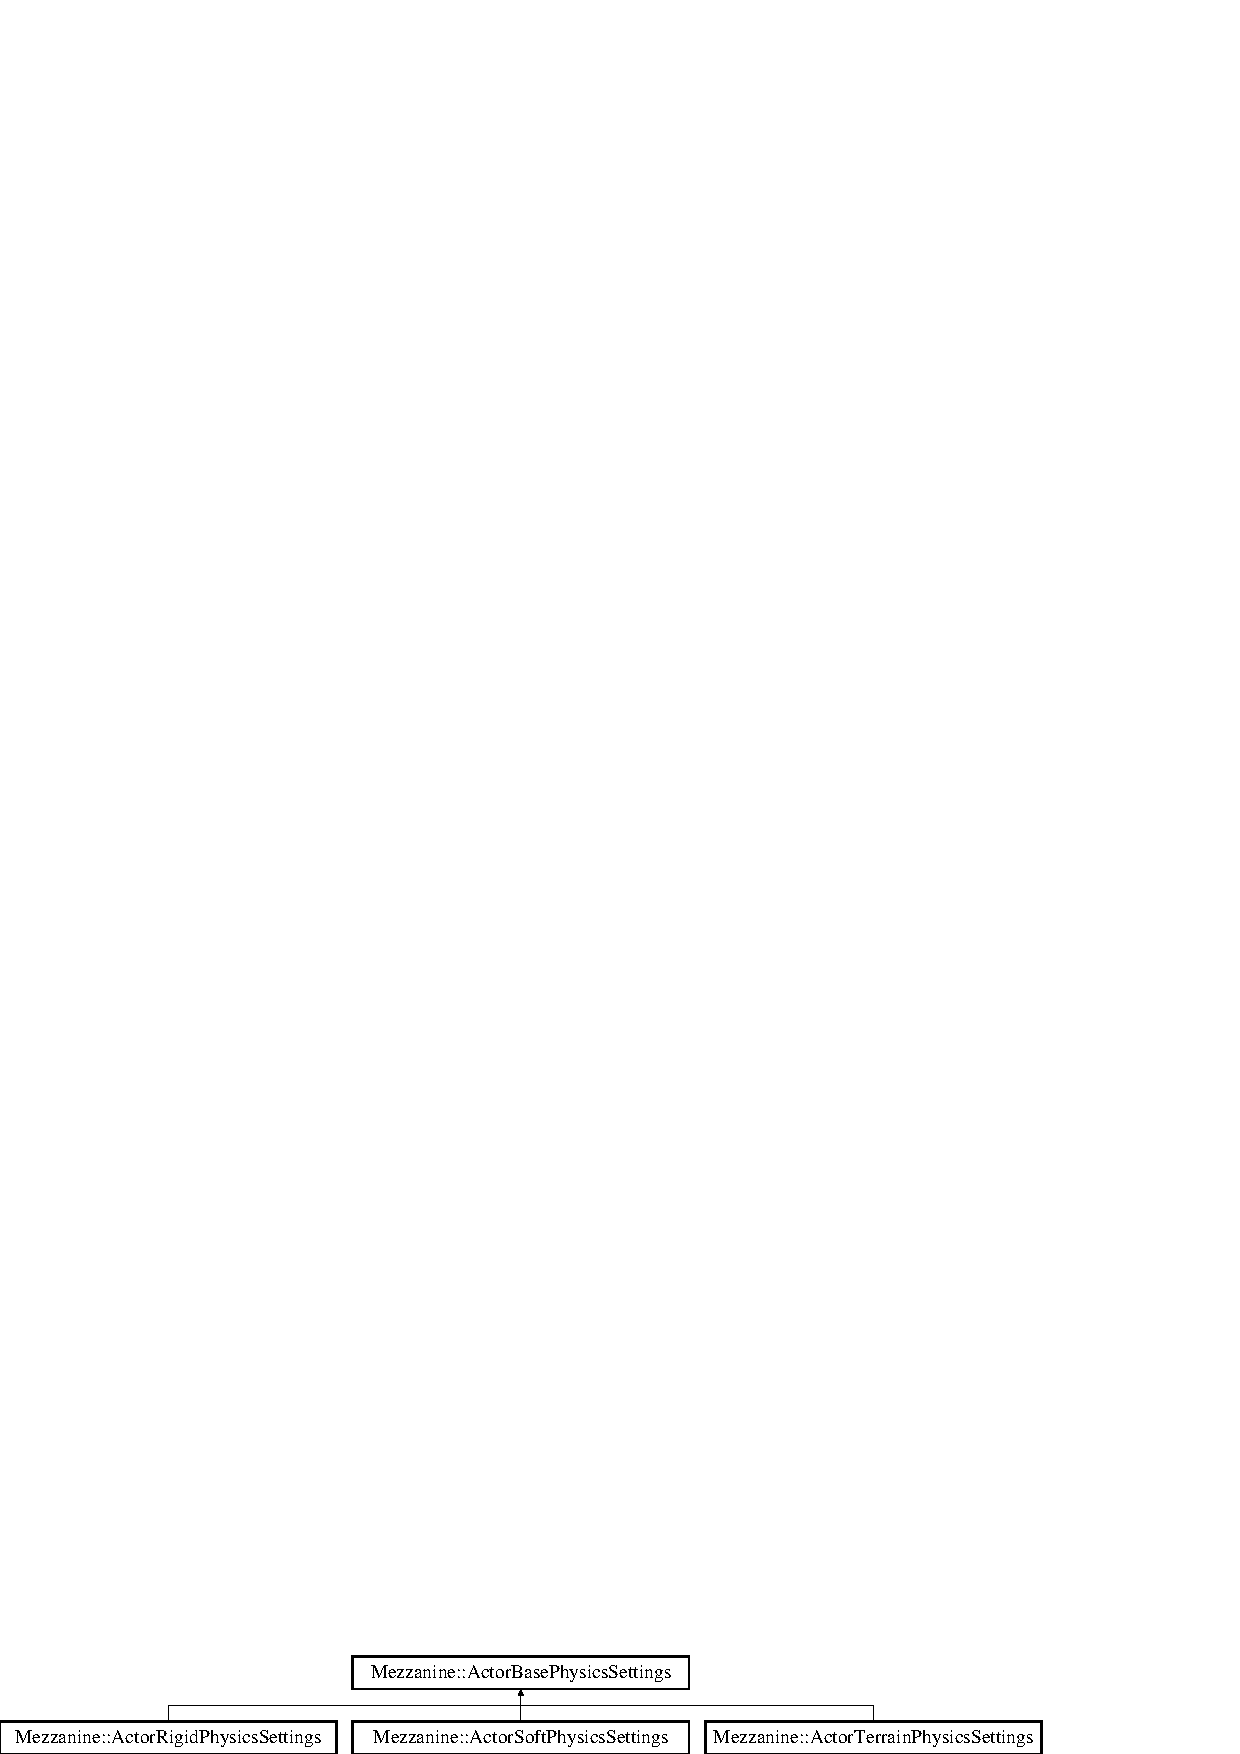
\includegraphics[height=4.000000cm]{classMezzanine_1_1ActorBasePhysicsSettings}
\end{center}
\end{figure}
\subsubsection*{Public Member Functions}
\begin{DoxyCompactItemize}
\item 
\hyperlink{classMezzanine_1_1ActorBasePhysicsSettings_a3f8d93a77d1d9a61314ef350a1c3394a}{ActorBasePhysicsSettings} (\hyperlink{classMezzanine_1_1ActorBase}{ActorBase} $\ast$Actor, btCollisionObject $\ast$PhysicsObject)
\begin{DoxyCompactList}\small\item\em Standard Constructor. \item\end{DoxyCompactList}\item 
\hyperlink{classMezzanine_1_1ActorBasePhysicsSettings}{ActorBasePhysicsSettings} $\ast$ \hyperlink{classMezzanine_1_1ActorBasePhysicsSettings_ae43e2938e30b69ac11627b9648c43415}{GetBasePointer} ()
\begin{DoxyCompactList}\small\item\em Get a pointer to this class of type \hyperlink{classMezzanine_1_1ActorBasePhysicsSettings}{ActorBasePhysicsSettings}. \item\end{DoxyCompactList}\item 
virtual \hyperlink{namespaceMezzanine_a726731b1a7df72bf3583e4a97282c6f6}{Real} \hyperlink{classMezzanine_1_1ActorBasePhysicsSettings_a804941eb77d960dd3c73d331c47c891c}{GetCCDMotionThreshold} () const 
\begin{DoxyCompactList}\small\item\em Gets the amount of motion needed to enable CCD for this object. \item\end{DoxyCompactList}\item 
virtual \hyperlink{namespaceMezzanine_a726731b1a7df72bf3583e4a97282c6f6}{Real} \hyperlink{classMezzanine_1_1ActorBasePhysicsSettings_a3729e8ee88bc2d8892d921016aa4a4c0}{GetCCDSphereRadius} () const 
\begin{DoxyCompactList}\small\item\em Gets the radius of the embedded sphere used for CCD. \item\end{DoxyCompactList}\item 
virtual void \hyperlink{classMezzanine_1_1ActorBasePhysicsSettings_a702a20cfb7d87dbc2a7d44ba9260ead2}{SetCCDParams} (const \hyperlink{namespaceMezzanine_a726731b1a7df72bf3583e4a97282c6f6}{Real} \&MotionThreshold, const \hyperlink{namespaceMezzanine_a726731b1a7df72bf3583e4a97282c6f6}{Real} \&SweptSphereRadius=0)
\begin{DoxyCompactList}\small\item\em Sets the parameters used for Continuous \hyperlink{classMezzanine_1_1Collision}{Collision} Detection. \item\end{DoxyCompactList}\item 
virtual void \hyperlink{classMezzanine_1_1ActorBasePhysicsSettings_a3b01243f038e30eb39b04f8e38fb8a14}{SetKinematic} ()
\begin{DoxyCompactList}\small\item\em Sets the state of the object to Kinematic. \item\end{DoxyCompactList}\item 
virtual void \hyperlink{classMezzanine_1_1ActorBasePhysicsSettings_ac72f39fa6bc9e2f050fdf90e42dd0deb}{SetStatic} ()
\begin{DoxyCompactList}\small\item\em Sets the state of the object to Static. \item\end{DoxyCompactList}\item 
\hypertarget{classMezzanine_1_1ActorBasePhysicsSettings_a6273131ed9e51182abde28d5af4ded83}{
virtual \hyperlink{classMezzanine_1_1ActorBasePhysicsSettings_a6273131ed9e51182abde28d5af4ded83}{$\sim$ActorBasePhysicsSettings} ()}
\label{classMezzanine_1_1ActorBasePhysicsSettings_a6273131ed9e51182abde28d5af4ded83}

\begin{DoxyCompactList}\small\item\em Class destructor. \item\end{DoxyCompactList}\end{DoxyCompactItemize}


\subsubsection{Detailed Description}
This is a base helper class for configuring physics settings of an actor. This class contains functions for the configuring of physics specific settings of an actor. This class can only configure the actors physics. For configuring actor graphics, see ActorGraphicsSettings. 

Definition at line 86 of file actorphysicssettings.h.



\subsubsection{Constructor \& Destructor Documentation}
\hypertarget{classMezzanine_1_1ActorBasePhysicsSettings_a3f8d93a77d1d9a61314ef350a1c3394a}{
\index{Mezzanine::ActorBasePhysicsSettings@{Mezzanine::ActorBasePhysicsSettings}!ActorBasePhysicsSettings@{ActorBasePhysicsSettings}}
\index{ActorBasePhysicsSettings@{ActorBasePhysicsSettings}!Mezzanine::ActorBasePhysicsSettings@{Mezzanine::ActorBasePhysicsSettings}}
\paragraph[{ActorBasePhysicsSettings}]{\setlength{\rightskip}{0pt plus 5cm}home sqeaky Mezzanine Mezzanine src actorphysicssettings cpp home sqeaky Mezzanine Mezzanine src actorphysicssettings cpp home sqeaky Mezzanine Mezzanine src actorphysicssettings cpp Mezzanine::ActorBasePhysicsSettings::ActorBasePhysicsSettings (
\begin{DoxyParamCaption}
\item[{{\bf ActorBase} $\ast$}]{Actor, }
\item[{btCollisionObject $\ast$}]{PhysicsObject}
\end{DoxyParamCaption}
)}\hfill}
\label{classMezzanine_1_1ActorBasePhysicsSettings_a3f8d93a77d1d9a61314ef350a1c3394a}


Standard Constructor. 


\begin{DoxyParams}{Parameters}
{\em Actor} & The actor this settings class configures. \\
\hline
{\em PhysicsObject} & The physics object belonging to the actor this class configures. \\
\hline
\end{DoxyParams}


Definition at line 67 of file actorphysicssettings.cpp.



\subsubsection{Member Function Documentation}
\hypertarget{classMezzanine_1_1ActorBasePhysicsSettings_ae43e2938e30b69ac11627b9648c43415}{
\index{Mezzanine::ActorBasePhysicsSettings@{Mezzanine::ActorBasePhysicsSettings}!GetBasePointer@{GetBasePointer}}
\index{GetBasePointer@{GetBasePointer}!Mezzanine::ActorBasePhysicsSettings@{Mezzanine::ActorBasePhysicsSettings}}
\paragraph[{GetBasePointer}]{\setlength{\rightskip}{0pt plus 5cm}{\bf ActorBasePhysicsSettings} $\ast$ Mezzanine::ActorBasePhysicsSettings::GetBasePointer (
\begin{DoxyParamCaption}
{}
\end{DoxyParamCaption}
)}\hfill}
\label{classMezzanine_1_1ActorBasePhysicsSettings_ae43e2938e30b69ac11627b9648c43415}


Get a pointer to this class of type \hyperlink{classMezzanine_1_1ActorBasePhysicsSettings}{ActorBasePhysicsSettings}. 

\begin{DoxyReturn}{Returns}
A pointer \hyperlink{classMezzanine_1_1ActorBasePhysicsSettings}{ActorBasePhysicsSettings} 
\end{DoxyReturn}


Definition at line 123 of file actorphysicssettings.cpp.

\hypertarget{classMezzanine_1_1ActorBasePhysicsSettings_a804941eb77d960dd3c73d331c47c891c}{
\index{Mezzanine::ActorBasePhysicsSettings@{Mezzanine::ActorBasePhysicsSettings}!GetCCDMotionThreshold@{GetCCDMotionThreshold}}
\index{GetCCDMotionThreshold@{GetCCDMotionThreshold}!Mezzanine::ActorBasePhysicsSettings@{Mezzanine::ActorBasePhysicsSettings}}
\paragraph[{GetCCDMotionThreshold}]{\setlength{\rightskip}{0pt plus 5cm}{\bf Real} Mezzanine::ActorBasePhysicsSettings::GetCCDMotionThreshold (
\begin{DoxyParamCaption}
{}
\end{DoxyParamCaption}
) const\hspace{0.3cm}{\ttfamily  \mbox{[}virtual\mbox{]}}}\hfill}
\label{classMezzanine_1_1ActorBasePhysicsSettings_a804941eb77d960dd3c73d331c47c891c}


Gets the amount of motion needed to enable CCD for this object. 

\begin{DoxyReturn}{Returns}
Returns a Real representing the required amount of motion to enable CCD, or zero if CCD is disabled. 
\end{DoxyReturn}


Definition at line 103 of file actorphysicssettings.cpp.

\hypertarget{classMezzanine_1_1ActorBasePhysicsSettings_a3729e8ee88bc2d8892d921016aa4a4c0}{
\index{Mezzanine::ActorBasePhysicsSettings@{Mezzanine::ActorBasePhysicsSettings}!GetCCDSphereRadius@{GetCCDSphereRadius}}
\index{GetCCDSphereRadius@{GetCCDSphereRadius}!Mezzanine::ActorBasePhysicsSettings@{Mezzanine::ActorBasePhysicsSettings}}
\paragraph[{GetCCDSphereRadius}]{\setlength{\rightskip}{0pt plus 5cm}{\bf Real} Mezzanine::ActorBasePhysicsSettings::GetCCDSphereRadius (
\begin{DoxyParamCaption}
{}
\end{DoxyParamCaption}
) const\hspace{0.3cm}{\ttfamily  \mbox{[}virtual\mbox{]}}}\hfill}
\label{classMezzanine_1_1ActorBasePhysicsSettings_a3729e8ee88bc2d8892d921016aa4a4c0}


Gets the radius of the embedded sphere used for CCD. 

\begin{DoxyReturn}{Returns}
Returns a Real representing the radius of the sphere embedded into the objects collision shape used for CCD. 
\end{DoxyReturn}


Definition at line 108 of file actorphysicssettings.cpp.

\hypertarget{classMezzanine_1_1ActorBasePhysicsSettings_a702a20cfb7d87dbc2a7d44ba9260ead2}{
\index{Mezzanine::ActorBasePhysicsSettings@{Mezzanine::ActorBasePhysicsSettings}!SetCCDParams@{SetCCDParams}}
\index{SetCCDParams@{SetCCDParams}!Mezzanine::ActorBasePhysicsSettings@{Mezzanine::ActorBasePhysicsSettings}}
\paragraph[{SetCCDParams}]{\setlength{\rightskip}{0pt plus 5cm}void Mezzanine::ActorBasePhysicsSettings::SetCCDParams (
\begin{DoxyParamCaption}
\item[{const {\bf Real} \&}]{MotionThreshold, }
\item[{const {\bf Real} \&}]{SweptSphereRadius = {\ttfamily 0}}
\end{DoxyParamCaption}
)\hspace{0.3cm}{\ttfamily  \mbox{[}virtual\mbox{]}}}\hfill}
\label{classMezzanine_1_1ActorBasePhysicsSettings_a702a20cfb7d87dbc2a7d44ba9260ead2}


Sets the parameters used for Continuous \hyperlink{classMezzanine_1_1Collision}{Collision} Detection. 

If a Swept Sphere Radius is not provided, this function will attempt to find one for you using the currently set \hyperlink{classMezzanine_1_1Collision}{Collision} Shape. If this fails for any reason or a shape is not set, it will set the radius to 1. 
\begin{DoxyParams}{Parameters}
{\em MotionThreshold} & The speed at which the object has to be moving in order to enable CCD for the object. If set to zero CCD will be disabled. \\
\hline
{\em SweptSphereRadius} & The radius of the sphere to be used for CCD sweep tests. Essentially this should be the largest radius in which a sphere can fully fit inside your object. \\
\hline
\end{DoxyParams}


Definition at line 76 of file actorphysicssettings.cpp.

\hypertarget{classMezzanine_1_1ActorBasePhysicsSettings_a3b01243f038e30eb39b04f8e38fb8a14}{
\index{Mezzanine::ActorBasePhysicsSettings@{Mezzanine::ActorBasePhysicsSettings}!SetKinematic@{SetKinematic}}
\index{SetKinematic@{SetKinematic}!Mezzanine::ActorBasePhysicsSettings@{Mezzanine::ActorBasePhysicsSettings}}
\paragraph[{SetKinematic}]{\setlength{\rightskip}{0pt plus 5cm}void Mezzanine::ActorBasePhysicsSettings::SetKinematic (
\begin{DoxyParamCaption}
{}
\end{DoxyParamCaption}
)\hspace{0.3cm}{\ttfamily  \mbox{[}virtual\mbox{]}}}\hfill}
\label{classMezzanine_1_1ActorBasePhysicsSettings_a3b01243f038e30eb39b04f8e38fb8a14}


Sets the state of the object to Kinematic. 

This function will set the object to a Kinematic Object. \par
 Kinematic Objects are like Static Objects but are also able to be moved directly by character controllers. 

Definition at line 113 of file actorphysicssettings.cpp.

\hypertarget{classMezzanine_1_1ActorBasePhysicsSettings_ac72f39fa6bc9e2f050fdf90e42dd0deb}{
\index{Mezzanine::ActorBasePhysicsSettings@{Mezzanine::ActorBasePhysicsSettings}!SetStatic@{SetStatic}}
\index{SetStatic@{SetStatic}!Mezzanine::ActorBasePhysicsSettings@{Mezzanine::ActorBasePhysicsSettings}}
\paragraph[{SetStatic}]{\setlength{\rightskip}{0pt plus 5cm}void Mezzanine::ActorBasePhysicsSettings::SetStatic (
\begin{DoxyParamCaption}
{}
\end{DoxyParamCaption}
)\hspace{0.3cm}{\ttfamily  \mbox{[}virtual\mbox{]}}}\hfill}
\label{classMezzanine_1_1ActorBasePhysicsSettings_ac72f39fa6bc9e2f050fdf90e42dd0deb}


Sets the state of the object to Static. 

This function will set the object to a Static Object. \par
 Static Objects don't move or have any force applied to them, but are cabable of exerting force on other objects. 

Definition at line 118 of file actorphysicssettings.cpp.



The documentation for this class was generated from the following files:\begin{DoxyCompactItemize}
\item 
actorphysicssettings.h\item 
actorphysicssettings.cpp\end{DoxyCompactItemize}

\hypertarget{classMezzanine_1_1ActorContainerBase}{
\subsection{Mezzanine::ActorContainerBase Class Reference}
\label{classMezzanine_1_1ActorContainerBase}\index{Mezzanine::ActorContainerBase@{Mezzanine::ActorContainerBase}}
}


A base class to unify the interface for different kinds of containers for holding actors.  




{\ttfamily \#include $<$actorcontainerbase.h$>$}

Inheritance diagram for Mezzanine::ActorContainerBase:\begin{figure}[H]
\begin{center}
\leavevmode
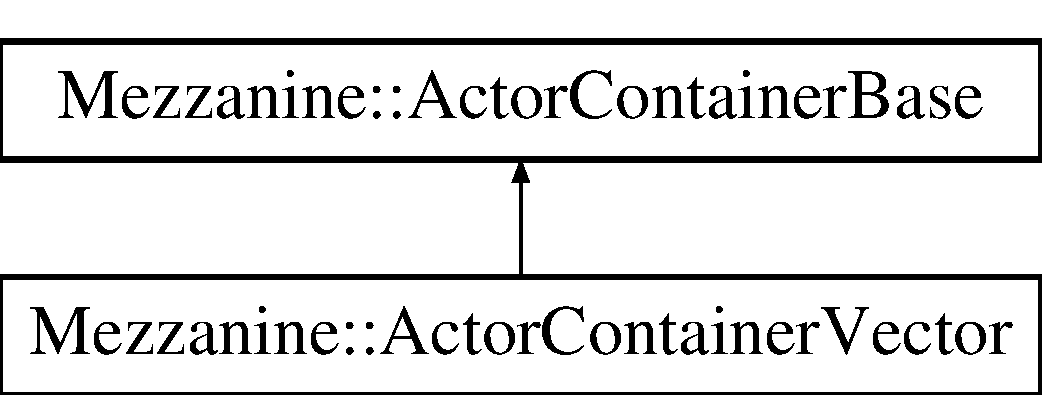
\includegraphics[height=2.000000cm]{classMezzanine_1_1ActorContainerBase}
\end{center}
\end{figure}
\subsubsection*{Public Member Functions}
\begin{DoxyCompactItemize}
\item 
\hyperlink{classMezzanine_1_1ActorContainerBase_a1cde28138d1b72713b87c9b1a4cbe9d1}{ActorContainerBase} ()
\begin{DoxyCompactList}\small\item\em Basic Constructor. \item\end{DoxyCompactList}\item 
virtual \hyperlink{classMezzanine_1_1ActorContainerBase_aab089925fd04d1591f2932d25edf0f52}{$\sim$ActorContainerBase} ()
\begin{DoxyCompactList}\small\item\em Destructor. \item\end{DoxyCompactList}\item 
virtual void \hyperlink{classMezzanine_1_1ActorContainerBase_aba981ad61ed549531a22d520ba2a231c}{AddActor} (\hyperlink{classMezzanine_1_1ActorBase}{ActorBase} $\ast$ActorToAdd)=0
\begin{DoxyCompactList}\small\item\em This will add an Actor to this container and the world. \item\end{DoxyCompactList}\item 
virtual void \hyperlink{classMezzanine_1_1ActorContainerBase_a7e26df0af80a28be01d0aaef7d350a65}{CursorToFirst} ()=0
\begin{DoxyCompactList}\small\item\em This moves the cursor to the first item in the container. \item\end{DoxyCompactList}\item 
virtual void \hyperlink{classMezzanine_1_1ActorContainerBase_a3f90f7b919bb821389f1493c6c121cce}{CursorToLast} ()=0
\begin{DoxyCompactList}\small\item\em This moves the cursor to the last item in the container. \item\end{DoxyCompactList}\item 
virtual void \hyperlink{classMezzanine_1_1ActorContainerBase_a906736a79fc92f45ae0cb73cfa2e7ed3}{CursorToNext} ()=0
\begin{DoxyCompactList}\small\item\em This moves the cursor to the next item in the container. \item\end{DoxyCompactList}\item 
virtual void \hyperlink{classMezzanine_1_1ActorContainerBase_a43c40059dc0c99742e99efa68c1acf52}{CursorToPrevious} ()=0
\begin{DoxyCompactList}\small\item\em This moves the cursor to the previous item in the container. \item\end{DoxyCompactList}\item 
virtual \hyperlink{classMezzanine_1_1ActorBase}{ActorBase} $\ast$ \hyperlink{classMezzanine_1_1ActorContainerBase_ace7273ccf53bc37cca7defbd703880f9}{FindActor} (Ogre::SceneNode $\ast$GraphicsNode)=0
\begin{DoxyCompactList}\small\item\em This finds an actor by searching for a graphics subsystem nodes. \item\end{DoxyCompactList}\item 
virtual \hyperlink{classMezzanine_1_1ActorBase}{ActorBase} $\ast$ \hyperlink{classMezzanine_1_1ActorContainerBase_a405caa151d3556786344be12ac0b6c2a}{FindActor} (btCollisionObject $\ast$PhysicsObject)=0
\begin{DoxyCompactList}\small\item\em This finds an actor by searching for a physics subsystem object. \item\end{DoxyCompactList}\item 
virtual \hyperlink{classMezzanine_1_1ActorBase}{ActorBase} $\ast$ \hyperlink{classMezzanine_1_1ActorContainerBase_aafa4b056aaa0161d3d814bfb56bd9ae9}{FindActor} (\hyperlink{namespaceMezzanine_acf9fcc130e6ebf08e3d8491aebcf1c86}{String} Name)=0
\begin{DoxyCompactList}\small\item\em This finds an actor based on its name. \item\end{DoxyCompactList}\item 
virtual \hyperlink{namespaceMezzanine_adcbb6ce6d1eb4379d109e51171e2e493}{Whole} \hyperlink{classMezzanine_1_1ActorContainerBase_a30b3c8d876a51510a8e29043a3c2b9de}{GetActorCount} () const =0
\begin{DoxyCompactList}\small\item\em Returns how many actors this stores. \item\end{DoxyCompactList}\item 
virtual \hyperlink{classMezzanine_1_1ActorBase}{ActorBase} $\ast$ \hyperlink{classMezzanine_1_1ActorContainerBase_ae339ced44550bc493685ab7e499a9e65}{GetAtCursor} () const =0
\begin{DoxyCompactList}\small\item\em This gets the actor at the cursor. \item\end{DoxyCompactList}\item 
virtual \hyperlink{namespaceMezzanine_acf9fcc130e6ebf08e3d8491aebcf1c86}{String} \hyperlink{classMezzanine_1_1ActorContainerBase_a3516835341b82c71bc50b0a23be85af2}{GetContainerType} () const =0
\begin{DoxyCompactList}\small\item\em Which kind of container it this anyway. \item\end{DoxyCompactList}\item 
virtual \hyperlink{classMezzanine_1_1ActorBase}{ActorBase} $\ast$ \hyperlink{classMezzanine_1_1ActorContainerBase_a886539e9b55e8033b05e7b1aff8d2c59}{GetFirst} () const =0
\begin{DoxyCompactList}\small\item\em This gets the first actor in the container. \item\end{DoxyCompactList}\item 
virtual \hyperlink{classMezzanine_1_1World}{World} $\ast$ \hyperlink{classMezzanine_1_1ActorContainerBase_ae8fe5e37e411504c4b0e044b336118e8}{GetGameWorld} () const =0
\begin{DoxyCompactList}\small\item\em This gets the \hyperlink{classMezzanine_1_1World}{World} that this class is working with. \item\end{DoxyCompactList}\item 
virtual \hyperlink{classMezzanine_1_1ActorBase}{ActorBase} $\ast$ \hyperlink{classMezzanine_1_1ActorContainerBase_ad4fc923758bf4c15e8e6a0e0ad9e0de2}{GetLast} () const =0
\begin{DoxyCompactList}\small\item\em This gets the last actor in the container. \item\end{DoxyCompactList}\item 
virtual \hyperlink{classMezzanine_1_1ActorBase}{ActorBase} $\ast$ \hyperlink{classMezzanine_1_1ActorContainerBase_abccaf443a5acd1c96f7ae1a1cb751f16}{LastActorAdded} ()=0
\begin{DoxyCompactList}\small\item\em This provides an easy way to access the last Actor added to this container. \item\end{DoxyCompactList}\item 
virtual void \hyperlink{classMezzanine_1_1ActorContainerBase_a25052e0fc2dcf1eab9cfc909d68de60c}{RemoveActor} (\hyperlink{classMezzanine_1_1ActorBase}{ActorBase} $\ast$ActorToRemove)=0
\begin{DoxyCompactList}\small\item\em Remove an Actor. \item\end{DoxyCompactList}\item 
virtual void \hyperlink{classMezzanine_1_1ActorContainerBase_a00fa640707739e2a94b91a09873d7dcc}{RemoveActorAtCursor} ()=0
\begin{DoxyCompactList}\small\item\em Removes the current actor. \item\end{DoxyCompactList}\item 
\hypertarget{classMezzanine_1_1ActorContainerBase_aca54c6e86a84ec84adb0b648309a6fd4}{
virtual void \hyperlink{classMezzanine_1_1ActorContainerBase_aca54c6e86a84ec84adb0b648309a6fd4}{RemoveAllActors} ()=0}
\label{classMezzanine_1_1ActorContainerBase_aca54c6e86a84ec84adb0b648309a6fd4}

\begin{DoxyCompactList}\small\item\em Clears this container of all actors it is storing. \item\end{DoxyCompactList}\item 
virtual void \hyperlink{classMezzanine_1_1ActorContainerBase_aed532e5416af4c896a85a78b707aeee9}{SetGameWorld} (\hyperlink{classMezzanine_1_1World}{World} $\ast$GameWorld\_\-)=0
\begin{DoxyCompactList}\small\item\em This sets the \hyperlink{classMezzanine_1_1World}{Mezzanine::World} that this Manager works with. \item\end{DoxyCompactList}\item 
virtual void \hyperlink{classMezzanine_1_1ActorContainerBase_a5dd1ea660dbbcb39d36e702c4e393f30}{SetGameWorld} (\hyperlink{classMezzanine_1_1World}{World} $\ast$GameWorld\_\-, bool AddToWorld, bool RemoveFromWorld)=0
\begin{DoxyCompactList}\small\item\em Optionally move actors into or out of a world. \item\end{DoxyCompactList}\end{DoxyCompactItemize}
\subsubsection*{Protected Member Functions}
\begin{DoxyCompactItemize}
\item 
\hypertarget{classMezzanine_1_1ActorContainerBase_a591b8ce55aab6bc6ff7d10085f582baa}{
btCollisionObject $\ast$ \hyperlink{classMezzanine_1_1ActorContainerBase_a591b8ce55aab6bc6ff7d10085f582baa}{GetCollisionObject} (\hyperlink{classMezzanine_1_1ActorBase}{ActorBase} $\ast$actor) const }
\label{classMezzanine_1_1ActorContainerBase_a591b8ce55aab6bc6ff7d10085f582baa}

\begin{DoxyCompactList}\small\item\em Used to work around the collision object of an Actor being private, so all derived Containers can access it. \item\end{DoxyCompactList}\item 
\hypertarget{classMezzanine_1_1ActorContainerBase_aa368146bb82e3384240b769f64b3a6fe}{
Ogre::SceneNode $\ast$ \hyperlink{classMezzanine_1_1ActorContainerBase_aa368146bb82e3384240b769f64b3a6fe}{GetNode} (\hyperlink{classMezzanine_1_1ActorBase}{ActorBase} $\ast$actor) const }
\label{classMezzanine_1_1ActorContainerBase_aa368146bb82e3384240b769f64b3a6fe}

\begin{DoxyCompactList}\small\item\em Used to work around the scenenode of an Actor being private, so all derived Containers can access it. \item\end{DoxyCompactList}\end{DoxyCompactItemize}


\subsubsection{Detailed Description}
A base class to unify the interface for different kinds of containers for holding actors. Containers for actors must implement atleast this interface(abstract base class) to be usable with the \hyperlink{classMezzanine_1_1World}{Mezzanine::World} for tracking in game objects. There are several reasons why this will be useful. Our first thought was deriving from this and an STL container like vector or list. Members of this class should be implementing or inheriting a proper container\par
\par
 The world will use one of these containers to store all of the actors for tracking purposes Since \par
\par
 In theory you should be be able to work with multiple actor containers and swiftly add or remove them to ad from a world to quickly control what actors are being worked with. It should even be possible to remove all actors, or have multiple set of actor in the world if you use the GameWorldSet methods carefully. \par
\par
 Additionally the is no reason an actor could be in multiple containers so this can provide even more options for actor sorting and categorization at runtime. \par
\par
 Because of this classes representation of a cursor only 1 thread at a time should use the cursor movement functions. For the container that the \hyperlink{classMezzanine_1_1World}{Mezzanine::World} keeps it should be assume that the cursor is used. For other containers you should manage you container carefully and/or use another iteration method, such as STL iterators. 

Definition at line 76 of file actorcontainerbase.h.



\subsubsection{Constructor \& Destructor Documentation}
\hypertarget{classMezzanine_1_1ActorContainerBase_a1cde28138d1b72713b87c9b1a4cbe9d1}{
\index{Mezzanine::ActorContainerBase@{Mezzanine::ActorContainerBase}!ActorContainerBase@{ActorContainerBase}}
\index{ActorContainerBase@{ActorContainerBase}!Mezzanine::ActorContainerBase@{Mezzanine::ActorContainerBase}}
\paragraph[{ActorContainerBase}]{\setlength{\rightskip}{0pt plus 5cm}Mezzanine::ActorContainerBase::ActorContainerBase (
\begin{DoxyParamCaption}
{}
\end{DoxyParamCaption}
)}\hfill}
\label{classMezzanine_1_1ActorContainerBase_a1cde28138d1b72713b87c9b1a4cbe9d1}


Basic Constructor. 

This just assigned the passed pointer to ParentWorld 

Definition at line 54 of file actorcontainerbase.cpp.

\hypertarget{classMezzanine_1_1ActorContainerBase_aab089925fd04d1591f2932d25edf0f52}{
\index{Mezzanine::ActorContainerBase@{Mezzanine::ActorContainerBase}!$\sim$ActorContainerBase@{$\sim$ActorContainerBase}}
\index{$\sim$ActorContainerBase@{$\sim$ActorContainerBase}!Mezzanine::ActorContainerBase@{Mezzanine::ActorContainerBase}}
\paragraph[{$\sim$ActorContainerBase}]{\setlength{\rightskip}{0pt plus 5cm}Mezzanine::ActorContainerBase::$\sim$ActorContainerBase (
\begin{DoxyParamCaption}
{}
\end{DoxyParamCaption}
)\hspace{0.3cm}{\ttfamily  \mbox{[}virtual\mbox{]}}}\hfill}
\label{classMezzanine_1_1ActorContainerBase_aab089925fd04d1591f2932d25edf0f52}


Destructor. 

This really doesn't do anything, but if someone needs to overload it, it's here 

Definition at line 57 of file actorcontainerbase.cpp.



\subsubsection{Member Function Documentation}
\hypertarget{classMezzanine_1_1ActorContainerBase_aba981ad61ed549531a22d520ba2a231c}{
\index{Mezzanine::ActorContainerBase@{Mezzanine::ActorContainerBase}!AddActor@{AddActor}}
\index{AddActor@{AddActor}!Mezzanine::ActorContainerBase@{Mezzanine::ActorContainerBase}}
\paragraph[{AddActor}]{\setlength{\rightskip}{0pt plus 5cm}virtual void Mezzanine::ActorContainerBase::AddActor (
\begin{DoxyParamCaption}
\item[{{\bf ActorBase} $\ast$}]{ActorToAdd}
\end{DoxyParamCaption}
)\hspace{0.3cm}{\ttfamily  \mbox{[}pure virtual\mbox{]}}}\hfill}
\label{classMezzanine_1_1ActorContainerBase_aba981ad61ed549531a22d520ba2a231c}


This will add an Actor to this container and the world. 

This will add an Actor to this container and the world, and handle the nitty gritty details of add this to physics subsystem and graphics subsystem. \par
\par
 This will not add the Actor to any specific location in the ordering of the container. \par
\par
 It is expected that any container implementing this method will take appropriate steps to insure That the actor involved is added to the Physics and graphics world. This method could be called from derived to accomplish that task 
\begin{DoxyParams}{Parameters}
{\em ActorToAdd} & This is a pointer to the actor to add. \\
\hline
\end{DoxyParams}


Implemented in \hyperlink{classMezzanine_1_1ActorContainerVector_a1341d51fa9ed279301eed579a2de79b2}{Mezzanine::ActorContainerVector}.

\hypertarget{classMezzanine_1_1ActorContainerBase_a7e26df0af80a28be01d0aaef7d350a65}{
\index{Mezzanine::ActorContainerBase@{Mezzanine::ActorContainerBase}!CursorToFirst@{CursorToFirst}}
\index{CursorToFirst@{CursorToFirst}!Mezzanine::ActorContainerBase@{Mezzanine::ActorContainerBase}}
\paragraph[{CursorToFirst}]{\setlength{\rightskip}{0pt plus 5cm}virtual void Mezzanine::ActorContainerBase::CursorToFirst (
\begin{DoxyParamCaption}
{}
\end{DoxyParamCaption}
)\hspace{0.3cm}{\ttfamily  \mbox{[}pure virtual\mbox{]}}}\hfill}
\label{classMezzanine_1_1ActorContainerBase_a7e26df0af80a28be01d0aaef7d350a65}


This moves the cursor to the first item in the container. 

This moves the cursor to the first item in the container change or return anything else. An exception will be throw if there are no valid items to move to with the cursor. There must be atleast one item to use any cursor moving functions. 

Implemented in \hyperlink{classMezzanine_1_1ActorContainerVector_a2b09e4eac9bc6392f47dd81fb7592ce3}{Mezzanine::ActorContainerVector}.

\hypertarget{classMezzanine_1_1ActorContainerBase_a3f90f7b919bb821389f1493c6c121cce}{
\index{Mezzanine::ActorContainerBase@{Mezzanine::ActorContainerBase}!CursorToLast@{CursorToLast}}
\index{CursorToLast@{CursorToLast}!Mezzanine::ActorContainerBase@{Mezzanine::ActorContainerBase}}
\paragraph[{CursorToLast}]{\setlength{\rightskip}{0pt plus 5cm}virtual void Mezzanine::ActorContainerBase::CursorToLast (
\begin{DoxyParamCaption}
{}
\end{DoxyParamCaption}
)\hspace{0.3cm}{\ttfamily  \mbox{[}pure virtual\mbox{]}}}\hfill}
\label{classMezzanine_1_1ActorContainerBase_a3f90f7b919bb821389f1493c6c121cce}


This moves the cursor to the last item in the container. 

This moves the cursor to the last item in the container change or return anything else. See \hyperlink{classMezzanine_1_1ActorContainerBase_a7e26df0af80a28be01d0aaef7d350a65}{CursorToFirst()} for more details. 

Implemented in \hyperlink{classMezzanine_1_1ActorContainerVector_ae80f9d94f009293528bf1b4251bc8ad0}{Mezzanine::ActorContainerVector}.

\hypertarget{classMezzanine_1_1ActorContainerBase_a906736a79fc92f45ae0cb73cfa2e7ed3}{
\index{Mezzanine::ActorContainerBase@{Mezzanine::ActorContainerBase}!CursorToNext@{CursorToNext}}
\index{CursorToNext@{CursorToNext}!Mezzanine::ActorContainerBase@{Mezzanine::ActorContainerBase}}
\paragraph[{CursorToNext}]{\setlength{\rightskip}{0pt plus 5cm}virtual void Mezzanine::ActorContainerBase::CursorToNext (
\begin{DoxyParamCaption}
{}
\end{DoxyParamCaption}
)\hspace{0.3cm}{\ttfamily  \mbox{[}pure virtual\mbox{]}}}\hfill}
\label{classMezzanine_1_1ActorContainerBase_a906736a79fc92f45ae0cb73cfa2e7ed3}


This moves the cursor to the next item in the container. 

This is the same as \hyperlink{classMezzanine_1_1ActorContainerBase_a43c40059dc0c99742e99efa68c1acf52}{CursorToPrevious()} except if you start from the begin you'll work your way to the end. If you are at the end, you'll stay their if you call this again 

Implemented in \hyperlink{classMezzanine_1_1ActorContainerVector_a04cce1784a09023cb9db8cbc60a60d0c}{Mezzanine::ActorContainerVector}.

\hypertarget{classMezzanine_1_1ActorContainerBase_a43c40059dc0c99742e99efa68c1acf52}{
\index{Mezzanine::ActorContainerBase@{Mezzanine::ActorContainerBase}!CursorToPrevious@{CursorToPrevious}}
\index{CursorToPrevious@{CursorToPrevious}!Mezzanine::ActorContainerBase@{Mezzanine::ActorContainerBase}}
\paragraph[{CursorToPrevious}]{\setlength{\rightskip}{0pt plus 5cm}virtual void Mezzanine::ActorContainerBase::CursorToPrevious (
\begin{DoxyParamCaption}
{}
\end{DoxyParamCaption}
)\hspace{0.3cm}{\ttfamily  \mbox{[}pure virtual\mbox{]}}}\hfill}
\label{classMezzanine_1_1ActorContainerBase_a43c40059dc0c99742e99efa68c1acf52}


This moves the cursor to the previous item in the container. 

This moves the cursor to the previous item in the container, and if you started at the last item, you will visit every item in a properly implemented container, except for items that may have bee added during your traversal. It is also posible this could visit the same actor twice or more. When called from the first item this does nothing. An exception will be throw if there are no valid items to move to with the cursor. There must be atleast one item to use any cursor moving functions. 

Implemented in \hyperlink{classMezzanine_1_1ActorContainerVector_abe0d1ce8c8f6a83a7ef3c340a605e767}{Mezzanine::ActorContainerVector}.

\hypertarget{classMezzanine_1_1ActorContainerBase_ace7273ccf53bc37cca7defbd703880f9}{
\index{Mezzanine::ActorContainerBase@{Mezzanine::ActorContainerBase}!FindActor@{FindActor}}
\index{FindActor@{FindActor}!Mezzanine::ActorContainerBase@{Mezzanine::ActorContainerBase}}
\paragraph[{FindActor}]{\setlength{\rightskip}{0pt plus 5cm}virtual {\bf ActorBase}$\ast$ Mezzanine::ActorContainerBase::FindActor (
\begin{DoxyParamCaption}
\item[{Ogre::SceneNode $\ast$}]{GraphicsNode}
\end{DoxyParamCaption}
)\hspace{0.3cm}{\ttfamily  \mbox{[}pure virtual\mbox{]}}}\hfill}
\label{classMezzanine_1_1ActorContainerBase_ace7273ccf53bc37cca7defbd703880f9}


This finds an actor by searching for a graphics subsystem nodes. 

\begin{DoxyReturn}{Returns}
This returns a pointer to and \hyperlink{classMezzanine_1_1ActorBase}{ActorBase} that has a matching node 
\end{DoxyReturn}

\begin{DoxyParams}{Parameters}
{\em GraphicsNode} & This is a pointer to a GraphicsNode that the Actor you want to find will have. \\
\hline
\end{DoxyParams}


Implemented in \hyperlink{classMezzanine_1_1ActorContainerVector_a0155ddbb599b1653c37bdfcb261355d2}{Mezzanine::ActorContainerVector}.

\hypertarget{classMezzanine_1_1ActorContainerBase_a405caa151d3556786344be12ac0b6c2a}{
\index{Mezzanine::ActorContainerBase@{Mezzanine::ActorContainerBase}!FindActor@{FindActor}}
\index{FindActor@{FindActor}!Mezzanine::ActorContainerBase@{Mezzanine::ActorContainerBase}}
\paragraph[{FindActor}]{\setlength{\rightskip}{0pt plus 5cm}virtual {\bf ActorBase}$\ast$ Mezzanine::ActorContainerBase::FindActor (
\begin{DoxyParamCaption}
\item[{btCollisionObject $\ast$}]{PhysicsObject}
\end{DoxyParamCaption}
)\hspace{0.3cm}{\ttfamily  \mbox{[}pure virtual\mbox{]}}}\hfill}
\label{classMezzanine_1_1ActorContainerBase_a405caa151d3556786344be12ac0b6c2a}


This finds an actor by searching for a physics subsystem object. 

This will iterate through each Actor in the container until it finds one with a matching physics object. This runs in linear time. \begin{DoxyReturn}{Returns}
This returns a pointer to and \hyperlink{classMezzanine_1_1ActorBase}{ActorBase} that has a physics object. 
\end{DoxyReturn}

\begin{DoxyParams}{Parameters}
{\em PhysicsObject} & This is a pointer to a physics object that the Actor you want to find will have. \\
\hline
\end{DoxyParams}


Implemented in \hyperlink{classMezzanine_1_1ActorContainerVector_acc1507a3a9d464ff0c343786986bef98}{Mezzanine::ActorContainerVector}.

\hypertarget{classMezzanine_1_1ActorContainerBase_aafa4b056aaa0161d3d814bfb56bd9ae9}{
\index{Mezzanine::ActorContainerBase@{Mezzanine::ActorContainerBase}!FindActor@{FindActor}}
\index{FindActor@{FindActor}!Mezzanine::ActorContainerBase@{Mezzanine::ActorContainerBase}}
\paragraph[{FindActor}]{\setlength{\rightskip}{0pt plus 5cm}virtual {\bf ActorBase}$\ast$ Mezzanine::ActorContainerBase::FindActor (
\begin{DoxyParamCaption}
\item[{{\bf String}}]{Name}
\end{DoxyParamCaption}
)\hspace{0.3cm}{\ttfamily  \mbox{[}pure virtual\mbox{]}}}\hfill}
\label{classMezzanine_1_1ActorContainerBase_aafa4b056aaa0161d3d814bfb56bd9ae9}


This finds an actor based on its name. 

\begin{DoxyReturn}{Returns}
This returns a pointer to and \hyperlink{classMezzanine_1_1ActorBase}{ActorBase} that has a matching name 
\end{DoxyReturn}

\begin{DoxyParams}{Parameters}
{\em Name} & This is the name of the Actor you want to find \\
\hline
\end{DoxyParams}


Implemented in \hyperlink{classMezzanine_1_1ActorContainerVector_a09837c17229c0a17031e7ce5fa3f6fc6}{Mezzanine::ActorContainerVector}.

\hypertarget{classMezzanine_1_1ActorContainerBase_a30b3c8d876a51510a8e29043a3c2b9de}{
\index{Mezzanine::ActorContainerBase@{Mezzanine::ActorContainerBase}!GetActorCount@{GetActorCount}}
\index{GetActorCount@{GetActorCount}!Mezzanine::ActorContainerBase@{Mezzanine::ActorContainerBase}}
\paragraph[{GetActorCount}]{\setlength{\rightskip}{0pt plus 5cm}virtual {\bf Whole} Mezzanine::ActorContainerBase::GetActorCount (
\begin{DoxyParamCaption}
{}
\end{DoxyParamCaption}
) const\hspace{0.3cm}{\ttfamily  \mbox{[}pure virtual\mbox{]}}}\hfill}
\label{classMezzanine_1_1ActorContainerBase_a30b3c8d876a51510a8e29043a3c2b9de}


Returns how many actors this stores. 

\begin{DoxyReturn}{Returns}
This returns a Whole number with the count of actors 
\end{DoxyReturn}


Implemented in \hyperlink{classMezzanine_1_1ActorContainerVector_a9a4e61bb6597fb66906c779c1f27e051}{Mezzanine::ActorContainerVector}.

\hypertarget{classMezzanine_1_1ActorContainerBase_ae339ced44550bc493685ab7e499a9e65}{
\index{Mezzanine::ActorContainerBase@{Mezzanine::ActorContainerBase}!GetAtCursor@{GetAtCursor}}
\index{GetAtCursor@{GetAtCursor}!Mezzanine::ActorContainerBase@{Mezzanine::ActorContainerBase}}
\paragraph[{GetAtCursor}]{\setlength{\rightskip}{0pt plus 5cm}virtual {\bf ActorBase}$\ast$ Mezzanine::ActorContainerBase::GetAtCursor (
\begin{DoxyParamCaption}
{}
\end{DoxyParamCaption}
) const\hspace{0.3cm}{\ttfamily  \mbox{[}pure virtual\mbox{]}}}\hfill}
\label{classMezzanine_1_1ActorContainerBase_ae339ced44550bc493685ab7e499a9e65}


This gets the actor at the cursor. 

This gets the actor at the cursor, and will not move the cursor. If the cursor has not be set to a location, any valid actor in the container could be returned. Will throw an exception when attempting to get from an empty container. \begin{DoxyReturn}{Returns}
This returns a pointer to an \hyperlink{classMezzanine_1_1ActorBase}{ActorBase}. 
\end{DoxyReturn}


Implemented in \hyperlink{classMezzanine_1_1ActorContainerVector_ac9efeefbc35033294723d33a8edd72c2}{Mezzanine::ActorContainerVector}.

\hypertarget{classMezzanine_1_1ActorContainerBase_a3516835341b82c71bc50b0a23be85af2}{
\index{Mezzanine::ActorContainerBase@{Mezzanine::ActorContainerBase}!GetContainerType@{GetContainerType}}
\index{GetContainerType@{GetContainerType}!Mezzanine::ActorContainerBase@{Mezzanine::ActorContainerBase}}
\paragraph[{GetContainerType}]{\setlength{\rightskip}{0pt plus 5cm}virtual {\bf String} Mezzanine::ActorContainerBase::GetContainerType (
\begin{DoxyParamCaption}
{}
\end{DoxyParamCaption}
) const\hspace{0.3cm}{\ttfamily  \mbox{[}pure virtual\mbox{]}}}\hfill}
\label{classMezzanine_1_1ActorContainerBase_a3516835341b82c71bc50b0a23be85af2}


Which kind of container it this anyway. 

Since this interface could be used with any type of containers and innumerable 3rd party container implemention this can be used to more safely cast this container to a more specific type. \begin{DoxyReturn}{Returns}
This returns a \hyperlink{namespaceMezzanine_acf9fcc130e6ebf08e3d8491aebcf1c86}{Mezzanine::String} 
\end{DoxyReturn}


Implemented in \hyperlink{classMezzanine_1_1ActorContainerVector_a22c7e6456504a7a7f93825936d2d2b8f}{Mezzanine::ActorContainerVector}.

\hypertarget{classMezzanine_1_1ActorContainerBase_a886539e9b55e8033b05e7b1aff8d2c59}{
\index{Mezzanine::ActorContainerBase@{Mezzanine::ActorContainerBase}!GetFirst@{GetFirst}}
\index{GetFirst@{GetFirst}!Mezzanine::ActorContainerBase@{Mezzanine::ActorContainerBase}}
\paragraph[{GetFirst}]{\setlength{\rightskip}{0pt plus 5cm}virtual {\bf ActorBase}$\ast$ Mezzanine::ActorContainerBase::GetFirst (
\begin{DoxyParamCaption}
{}
\end{DoxyParamCaption}
) const\hspace{0.3cm}{\ttfamily  \mbox{[}pure virtual\mbox{]}}}\hfill}
\label{classMezzanine_1_1ActorContainerBase_a886539e9b55e8033b05e7b1aff8d2c59}


This gets the first actor in the container. 

This and the actor the cursor points at after \hyperlink{classMezzanine_1_1ActorContainerBase_a7e26df0af80a28be01d0aaef7d350a65}{CursorToFirst()} should match. \begin{DoxyReturn}{Returns}
This returns a pointer to an \hyperlink{classMezzanine_1_1ActorBase}{ActorBase}. Will throw an exception when attempting to get from an empty container. 
\end{DoxyReturn}


Implemented in \hyperlink{classMezzanine_1_1ActorContainerVector_ab39133337c950be6207e0ba46f151af9}{Mezzanine::ActorContainerVector}.

\hypertarget{classMezzanine_1_1ActorContainerBase_ae8fe5e37e411504c4b0e044b336118e8}{
\index{Mezzanine::ActorContainerBase@{Mezzanine::ActorContainerBase}!GetGameWorld@{GetGameWorld}}
\index{GetGameWorld@{GetGameWorld}!Mezzanine::ActorContainerBase@{Mezzanine::ActorContainerBase}}
\paragraph[{GetGameWorld}]{\setlength{\rightskip}{0pt plus 5cm}virtual {\bf World}$\ast$ Mezzanine::ActorContainerBase::GetGameWorld (
\begin{DoxyParamCaption}
{}
\end{DoxyParamCaption}
) const\hspace{0.3cm}{\ttfamily  \mbox{[}pure virtual\mbox{]}}}\hfill}
\label{classMezzanine_1_1ActorContainerBase_ae8fe5e37e411504c4b0e044b336118e8}


This gets the \hyperlink{classMezzanine_1_1World}{World} that this class is working with. 

This returns the gameworld that this container registers it's objects with. If this is not set, then this does not Register it's actors with any world. \begin{DoxyReturn}{Returns}
This returns a \hyperlink{classMezzanine_1_1World}{Mezzanine::World}$\ast$ 
\end{DoxyReturn}


Implemented in \hyperlink{classMezzanine_1_1ActorContainerVector_afa1152c7bd84d8eba51bc4abe0500e51}{Mezzanine::ActorContainerVector}.

\hypertarget{classMezzanine_1_1ActorContainerBase_ad4fc923758bf4c15e8e6a0e0ad9e0de2}{
\index{Mezzanine::ActorContainerBase@{Mezzanine::ActorContainerBase}!GetLast@{GetLast}}
\index{GetLast@{GetLast}!Mezzanine::ActorContainerBase@{Mezzanine::ActorContainerBase}}
\paragraph[{GetLast}]{\setlength{\rightskip}{0pt plus 5cm}virtual {\bf ActorBase}$\ast$ Mezzanine::ActorContainerBase::GetLast (
\begin{DoxyParamCaption}
{}
\end{DoxyParamCaption}
) const\hspace{0.3cm}{\ttfamily  \mbox{[}pure virtual\mbox{]}}}\hfill}
\label{classMezzanine_1_1ActorContainerBase_ad4fc923758bf4c15e8e6a0e0ad9e0de2}


This gets the last actor in the container. 

This and the actor the cursor points at after \hyperlink{classMezzanine_1_1ActorContainerBase_a3f90f7b919bb821389f1493c6c121cce}{CursorToLast()} should match. \begin{DoxyReturn}{Returns}
This returns a pointer to an \hyperlink{classMezzanine_1_1ActorBase}{ActorBase}. Will throw an exception when attempting to get from an empty container. 
\end{DoxyReturn}


Implemented in \hyperlink{classMezzanine_1_1ActorContainerVector_a1b42e0385132ded405dd1f9558216938}{Mezzanine::ActorContainerVector}.

\hypertarget{classMezzanine_1_1ActorContainerBase_abccaf443a5acd1c96f7ae1a1cb751f16}{
\index{Mezzanine::ActorContainerBase@{Mezzanine::ActorContainerBase}!LastActorAdded@{LastActorAdded}}
\index{LastActorAdded@{LastActorAdded}!Mezzanine::ActorContainerBase@{Mezzanine::ActorContainerBase}}
\paragraph[{LastActorAdded}]{\setlength{\rightskip}{0pt plus 5cm}virtual {\bf ActorBase}$\ast$ Mezzanine::ActorContainerBase::LastActorAdded (
\begin{DoxyParamCaption}
{}
\end{DoxyParamCaption}
)\hspace{0.3cm}{\ttfamily  \mbox{[}pure virtual\mbox{]}}}\hfill}
\label{classMezzanine_1_1ActorContainerBase_abccaf443a5acd1c96f7ae1a1cb751f16}


This provides an easy way to access the last Actor added to this container. 

For many containers this will simply return a pointer to the last actor. \begin{DoxyReturn}{Returns}
This returns a pointer to the last Actor that was added. 
\end{DoxyReturn}


Implemented in \hyperlink{classMezzanine_1_1ActorContainerVector_aaa354835e75bd28fb2fe7e51a8e73ca6}{Mezzanine::ActorContainerVector}.

\hypertarget{classMezzanine_1_1ActorContainerBase_a25052e0fc2dcf1eab9cfc909d68de60c}{
\index{Mezzanine::ActorContainerBase@{Mezzanine::ActorContainerBase}!RemoveActor@{RemoveActor}}
\index{RemoveActor@{RemoveActor}!Mezzanine::ActorContainerBase@{Mezzanine::ActorContainerBase}}
\paragraph[{RemoveActor}]{\setlength{\rightskip}{0pt plus 5cm}virtual void Mezzanine::ActorContainerBase::RemoveActor (
\begin{DoxyParamCaption}
\item[{{\bf ActorBase} $\ast$}]{ActorToRemove}
\end{DoxyParamCaption}
)\hspace{0.3cm}{\ttfamily  \mbox{[}pure virtual\mbox{]}}}\hfill}
\label{classMezzanine_1_1ActorContainerBase_a25052e0fc2dcf1eab9cfc909d68de60c}


Remove an Actor. 

Remove all references of the actor pointed from the container. Will throw an exception when attempting to remove and no match could be found. 
\begin{DoxyParams}{Parameters}
{\em ActorToRemove} & A pointer to the actor to remove. \\
\hline
\end{DoxyParams}
\begin{DoxyWarning}{Warning}
This will cause issues if used with a container attached to a valid \hyperlink{classMezzanine_1_1World}{Mezzanine::World}. Use World::RemoveActor instead. 
\end{DoxyWarning}


Implemented in \hyperlink{classMezzanine_1_1ActorContainerVector_ab0f76ee775a4e92a55835e07edac0bce}{Mezzanine::ActorContainerVector}.

\hypertarget{classMezzanine_1_1ActorContainerBase_a00fa640707739e2a94b91a09873d7dcc}{
\index{Mezzanine::ActorContainerBase@{Mezzanine::ActorContainerBase}!RemoveActorAtCursor@{RemoveActorAtCursor}}
\index{RemoveActorAtCursor@{RemoveActorAtCursor}!Mezzanine::ActorContainerBase@{Mezzanine::ActorContainerBase}}
\paragraph[{RemoveActorAtCursor}]{\setlength{\rightskip}{0pt plus 5cm}virtual void Mezzanine::ActorContainerBase::RemoveActorAtCursor (
\begin{DoxyParamCaption}
{}
\end{DoxyParamCaption}
)\hspace{0.3cm}{\ttfamily  \mbox{[}pure virtual\mbox{]}}}\hfill}
\label{classMezzanine_1_1ActorContainerBase_a00fa640707739e2a94b91a09873d7dcc}


Removes the current actor. 

This removes the actor the cursor at. Will throw an exception when attempting to remove from an empty container. Where the cursor goes is implementation dependent. \begin{DoxyWarning}{Warning}
This will cause issues if used with a container attached to a valid \hyperlink{classMezzanine_1_1World}{Mezzanine::World}. Use World::RemoveActor instead. 
\end{DoxyWarning}


Implemented in \hyperlink{classMezzanine_1_1ActorContainerVector_a380140962919b31d8c2b23be6f69fbb0}{Mezzanine::ActorContainerVector}.

\hypertarget{classMezzanine_1_1ActorContainerBase_aed532e5416af4c896a85a78b707aeee9}{
\index{Mezzanine::ActorContainerBase@{Mezzanine::ActorContainerBase}!SetGameWorld@{SetGameWorld}}
\index{SetGameWorld@{SetGameWorld}!Mezzanine::ActorContainerBase@{Mezzanine::ActorContainerBase}}
\paragraph[{SetGameWorld}]{\setlength{\rightskip}{0pt plus 5cm}virtual void Mezzanine::ActorContainerBase::SetGameWorld (
\begin{DoxyParamCaption}
\item[{{\bf World} $\ast$}]{GameWorld\_\-}
\end{DoxyParamCaption}
)\hspace{0.3cm}{\ttfamily  \mbox{[}pure virtual\mbox{]}}}\hfill}
\label{classMezzanine_1_1ActorContainerBase_aed532e5416af4c896a85a78b707aeee9}


This sets the \hyperlink{classMezzanine_1_1World}{Mezzanine::World} that this Manager works with. 

If the are any actors in the world, this removes them from both the physics and graphics subsystem, and adds them to the new world as is appropriate. 
\begin{DoxyParams}{Parameters}
{\em GameWorld\_\-} & The new GameWorldPointer, or 0 to set none \\
\hline
\end{DoxyParams}


Implemented in \hyperlink{classMezzanine_1_1ActorContainerVector_ab974d2704bfc3d74e3f008250ed893d8}{Mezzanine::ActorContainerVector}.

\hypertarget{classMezzanine_1_1ActorContainerBase_a5dd1ea660dbbcb39d36e702c4e393f30}{
\index{Mezzanine::ActorContainerBase@{Mezzanine::ActorContainerBase}!SetGameWorld@{SetGameWorld}}
\index{SetGameWorld@{SetGameWorld}!Mezzanine::ActorContainerBase@{Mezzanine::ActorContainerBase}}
\paragraph[{SetGameWorld}]{\setlength{\rightskip}{0pt plus 5cm}virtual void Mezzanine::ActorContainerBase::SetGameWorld (
\begin{DoxyParamCaption}
\item[{{\bf World} $\ast$}]{GameWorld\_\-, }
\item[{bool}]{AddToWorld, }
\item[{bool}]{RemoveFromWorld}
\end{DoxyParamCaption}
)\hspace{0.3cm}{\ttfamily  \mbox{[}pure virtual\mbox{]}}}\hfill}
\label{classMezzanine_1_1ActorContainerBase_a5dd1ea660dbbcb39d36e702c4e393f30}


Optionally move actors into or out of a world. 


\begin{DoxyParams}{Parameters}
{\em GameWorld\_\-} & The new GameWorldPointer, or 0 to set none \\
\hline
{\em AddToWorld} & True to add AddActors if valid world pointer was supplied, false to not add \\
\hline
{\em RemoveFromWorld} & True to remove AddActors if valid world pointer was supplied, false to not remove \\
\hline
\end{DoxyParams}


Implemented in \hyperlink{classMezzanine_1_1ActorContainerVector_a7011795fcc3c3eb51b981aaebff23fac}{Mezzanine::ActorContainerVector}.



The documentation for this class was generated from the following files:\begin{DoxyCompactItemize}
\item 
actorcontainerbase.h\item 
actorcontainerbase.cpp\end{DoxyCompactItemize}

\hypertarget{classMezzanine_1_1ActorContainerVector}{
\subsection{Mezzanine::ActorContainerVector Class Reference}
\label{classMezzanine_1_1ActorContainerVector}\index{Mezzanine::ActorContainerVector@{Mezzanine::ActorContainerVector}}
}


A simple Actor Container using a vector.  




{\ttfamily \#include $<$actorcontainervector.h$>$}

Inheritance diagram for Mezzanine::ActorContainerVector:\begin{figure}[H]
\begin{center}
\leavevmode
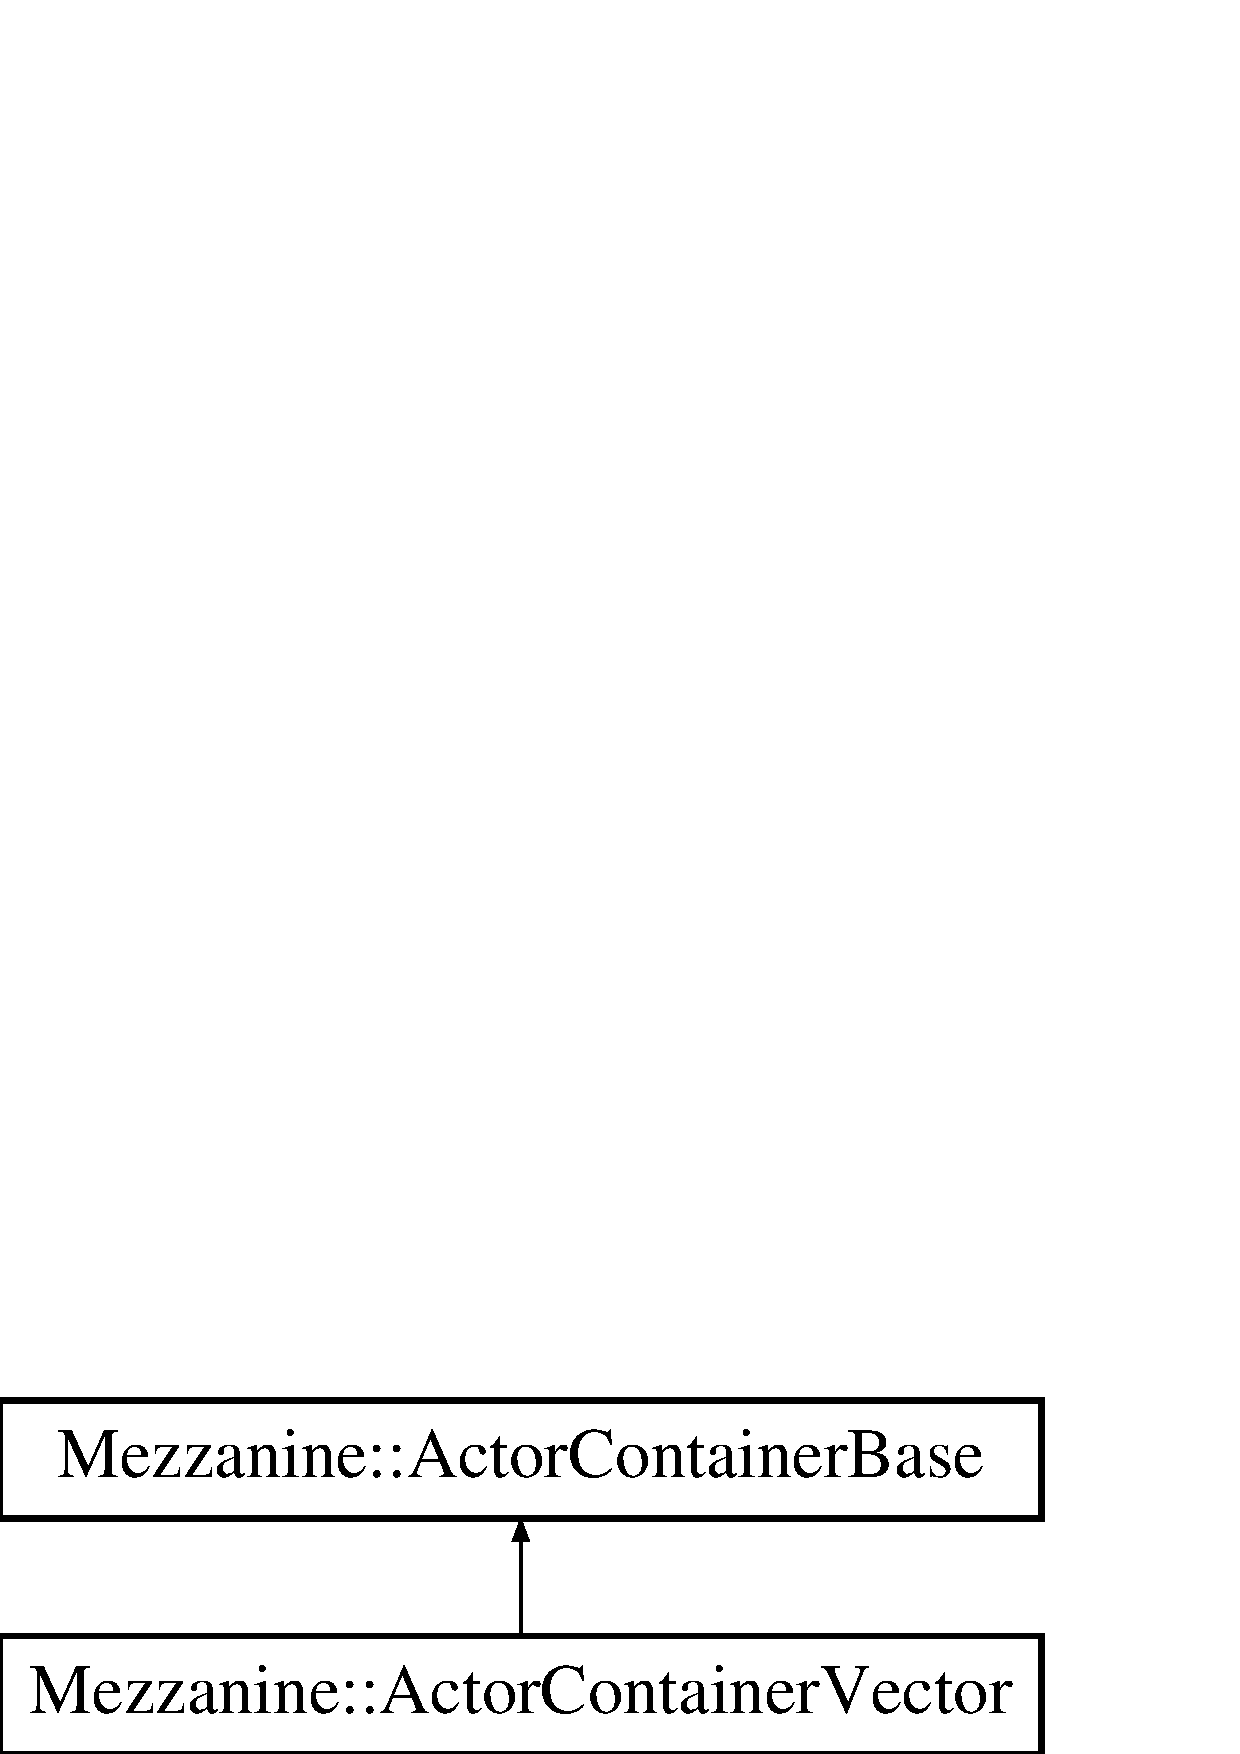
\includegraphics[height=2.000000cm]{classMezzanine_1_1ActorContainerVector}
\end{center}
\end{figure}
\subsubsection*{Public Member Functions}
\begin{DoxyCompactItemize}
\item 
\hyperlink{classMezzanine_1_1ActorContainerVector_a20cb603431e4499c1c6d3c901493f224}{ActorContainerVector} ()
\begin{DoxyCompactList}\small\item\em Simple Constructor. \item\end{DoxyCompactList}\item 
virtual void \hyperlink{classMezzanine_1_1ActorContainerVector_a1341d51fa9ed279301eed579a2de79b2}{AddActor} (\hyperlink{classMezzanine_1_1ActorBase}{ActorBase} $\ast$ActorToAdd)
\begin{DoxyCompactList}\small\item\em This will add an Actor to this container and the world. \item\end{DoxyCompactList}\item 
virtual void \hyperlink{classMezzanine_1_1ActorContainerVector_a2b09e4eac9bc6392f47dd81fb7592ce3}{CursorToFirst} ()
\begin{DoxyCompactList}\small\item\em This moves the cursor to the first item in the container. \item\end{DoxyCompactList}\item 
virtual void \hyperlink{classMezzanine_1_1ActorContainerVector_ae80f9d94f009293528bf1b4251bc8ad0}{CursorToLast} ()
\begin{DoxyCompactList}\small\item\em This moves the cursor to the last item in the container. \item\end{DoxyCompactList}\item 
virtual void \hyperlink{classMezzanine_1_1ActorContainerVector_a04cce1784a09023cb9db8cbc60a60d0c}{CursorToNext} ()
\begin{DoxyCompactList}\small\item\em This moves the cursor to the next item in the container. \item\end{DoxyCompactList}\item 
virtual void \hyperlink{classMezzanine_1_1ActorContainerVector_abe0d1ce8c8f6a83a7ef3c340a605e767}{CursorToPrevious} ()
\begin{DoxyCompactList}\small\item\em This moves the cursor to the previous item in the container. \item\end{DoxyCompactList}\item 
virtual \hyperlink{classMezzanine_1_1ActorBase}{ActorBase} $\ast$ \hyperlink{classMezzanine_1_1ActorContainerVector_a0155ddbb599b1653c37bdfcb261355d2}{FindActor} (Ogre::SceneNode $\ast$GraphicsNode)
\begin{DoxyCompactList}\small\item\em This finds an actor by searching for a graphics subsystem nodes. \item\end{DoxyCompactList}\item 
virtual \hyperlink{classMezzanine_1_1ActorBase}{ActorBase} $\ast$ \hyperlink{classMezzanine_1_1ActorContainerVector_acc1507a3a9d464ff0c343786986bef98}{FindActor} (btCollisionObject $\ast$PhysicsObject)
\begin{DoxyCompactList}\small\item\em This finds an actor by searching for a physics subsystem object. \item\end{DoxyCompactList}\item 
virtual \hyperlink{classMezzanine_1_1ActorBase}{ActorBase} $\ast$ \hyperlink{classMezzanine_1_1ActorContainerVector_a09837c17229c0a17031e7ce5fa3f6fc6}{FindActor} (\hyperlink{namespaceMezzanine_acf9fcc130e6ebf08e3d8491aebcf1c86}{String} Name)
\begin{DoxyCompactList}\small\item\em This finds an actor based on its name. \item\end{DoxyCompactList}\item 
virtual \hyperlink{namespaceMezzanine_adcbb6ce6d1eb4379d109e51171e2e493}{Whole} \hyperlink{classMezzanine_1_1ActorContainerVector_a9a4e61bb6597fb66906c779c1f27e051}{GetActorCount} () const 
\begin{DoxyCompactList}\small\item\em Returns how many actors this stores. \item\end{DoxyCompactList}\item 
virtual \hyperlink{classMezzanine_1_1ActorBase}{ActorBase} $\ast$ \hyperlink{classMezzanine_1_1ActorContainerVector_ac9efeefbc35033294723d33a8edd72c2}{GetAtCursor} () const 
\begin{DoxyCompactList}\small\item\em This gets the actor at the cursor. \item\end{DoxyCompactList}\item 
virtual \hyperlink{namespaceMezzanine_acf9fcc130e6ebf08e3d8491aebcf1c86}{String} \hyperlink{classMezzanine_1_1ActorContainerVector_a22c7e6456504a7a7f93825936d2d2b8f}{GetContainerType} () const 
\begin{DoxyCompactList}\small\item\em Which kind of container it this anyway. \item\end{DoxyCompactList}\item 
virtual \hyperlink{classMezzanine_1_1ActorBase}{ActorBase} $\ast$ \hyperlink{classMezzanine_1_1ActorContainerVector_ab39133337c950be6207e0ba46f151af9}{GetFirst} () const 
\begin{DoxyCompactList}\small\item\em This gets the first actor in the container. \item\end{DoxyCompactList}\item 
virtual \hyperlink{classMezzanine_1_1World}{World} $\ast$ \hyperlink{classMezzanine_1_1ActorContainerVector_afa1152c7bd84d8eba51bc4abe0500e51}{GetGameWorld} () const 
\begin{DoxyCompactList}\small\item\em This gets the \hyperlink{classMezzanine_1_1World}{World} that this class is working with. \item\end{DoxyCompactList}\item 
virtual \hyperlink{classMezzanine_1_1ActorBase}{ActorBase} $\ast$ \hyperlink{classMezzanine_1_1ActorContainerVector_a1b42e0385132ded405dd1f9558216938}{GetLast} () const 
\begin{DoxyCompactList}\small\item\em This gets the last actor in the container. \item\end{DoxyCompactList}\item 
virtual \hyperlink{classMezzanine_1_1ActorBase}{ActorBase} $\ast$ \hyperlink{classMezzanine_1_1ActorContainerVector_aaa354835e75bd28fb2fe7e51a8e73ca6}{LastActorAdded} ()
\begin{DoxyCompactList}\small\item\em This provides an easy way to access the last Actor added to this container. \item\end{DoxyCompactList}\item 
virtual void \hyperlink{classMezzanine_1_1ActorContainerVector_ab0f76ee775a4e92a55835e07edac0bce}{RemoveActor} (\hyperlink{classMezzanine_1_1ActorBase}{ActorBase} $\ast$ActorToRemove)
\begin{DoxyCompactList}\small\item\em Remove an Actor. \item\end{DoxyCompactList}\item 
virtual void \hyperlink{classMezzanine_1_1ActorContainerVector_a380140962919b31d8c2b23be6f69fbb0}{RemoveActorAtCursor} ()
\begin{DoxyCompactList}\small\item\em Removes the current actor. \item\end{DoxyCompactList}\item 
\hypertarget{classMezzanine_1_1ActorContainerVector_ae34237a2ba5649f00c45e87b8d570097}{
virtual void \hyperlink{classMezzanine_1_1ActorContainerVector_ae34237a2ba5649f00c45e87b8d570097}{RemoveAllActors} ()}
\label{classMezzanine_1_1ActorContainerVector_ae34237a2ba5649f00c45e87b8d570097}

\begin{DoxyCompactList}\small\item\em Clears this container of all actors it is storing. \item\end{DoxyCompactList}\item 
virtual void \hyperlink{classMezzanine_1_1ActorContainerVector_ab974d2704bfc3d74e3f008250ed893d8}{SetGameWorld} (\hyperlink{classMezzanine_1_1World}{World} $\ast$GameWorld\_\-)
\begin{DoxyCompactList}\small\item\em This safely move all the Actors out of or into a \hyperlink{classMezzanine_1_1World}{Mezzanine::World}. \item\end{DoxyCompactList}\item 
virtual void \hyperlink{classMezzanine_1_1ActorContainerVector_a7011795fcc3c3eb51b981aaebff23fac}{SetGameWorld} (\hyperlink{classMezzanine_1_1World}{World} $\ast$GameWorld\_\-, bool AddToWorld, bool RemoveFromWorld)
\begin{DoxyCompactList}\small\item\em Optionally move actors into or out of a world. \item\end{DoxyCompactList}\item 
\hypertarget{classMezzanine_1_1ActorContainerVector_a84a9f721addd5bdfbc611393913e68fd}{
virtual \hyperlink{classMezzanine_1_1ActorContainerVector_a84a9f721addd5bdfbc611393913e68fd}{$\sim$ActorContainerVector} ()}
\label{classMezzanine_1_1ActorContainerVector_a84a9f721addd5bdfbc611393913e68fd}

\begin{DoxyCompactList}\small\item\em Class destructor. \item\end{DoxyCompactList}\end{DoxyCompactItemize}
\subsubsection*{Public Attributes}
\begin{DoxyCompactItemize}
\item 
vector$<$ \hyperlink{classMezzanine_1_1ActorBase}{ActorBase} $\ast$ $>$::iterator \hyperlink{classMezzanine_1_1ActorContainerVector_ac359dee117cfe4829c656f7599ea9092}{cursor}
\begin{DoxyCompactList}\small\item\em This is used to store information about the cursor. \item\end{DoxyCompactList}\end{DoxyCompactItemize}


\subsubsection{Detailed Description}
A simple Actor Container using a vector. This inherits from std::vector and our \hyperlink{classMezzanine_1_1ActorContainerBase}{Mezzanine::ActorContainerBase} to allow us to have access to a container through a standardized structure this way the Mezzanine::world doesn't need to worry about the details when accessing and storing actors 

Definition at line 64 of file actorcontainervector.h.



\subsubsection{Constructor \& Destructor Documentation}
\hypertarget{classMezzanine_1_1ActorContainerVector_a20cb603431e4499c1c6d3c901493f224}{
\index{Mezzanine::ActorContainerVector@{Mezzanine::ActorContainerVector}!ActorContainerVector@{ActorContainerVector}}
\index{ActorContainerVector@{ActorContainerVector}!Mezzanine::ActorContainerVector@{Mezzanine::ActorContainerVector}}
\paragraph[{ActorContainerVector}]{\setlength{\rightskip}{0pt plus 5cm}home sqeaky Mezzanine Mezzanine src actorcontainervector cpp Mezzanine::ActorContainerVector::ActorContainerVector (
\begin{DoxyParamCaption}
{}
\end{DoxyParamCaption}
)}\hfill}
\label{classMezzanine_1_1ActorContainerVector_a20cb603431e4499c1c6d3c901493f224}


Simple Constructor. 

This creates and empty usable container based on std::vector. 

Definition at line 49 of file actorcontainervector.cpp.



\subsubsection{Member Function Documentation}
\hypertarget{classMezzanine_1_1ActorContainerVector_a1341d51fa9ed279301eed579a2de79b2}{
\index{Mezzanine::ActorContainerVector@{Mezzanine::ActorContainerVector}!AddActor@{AddActor}}
\index{AddActor@{AddActor}!Mezzanine::ActorContainerVector@{Mezzanine::ActorContainerVector}}
\paragraph[{AddActor}]{\setlength{\rightskip}{0pt plus 5cm}void Mezzanine::ActorContainerVector::AddActor (
\begin{DoxyParamCaption}
\item[{{\bf ActorBase} $\ast$}]{ActorToAdd}
\end{DoxyParamCaption}
)\hspace{0.3cm}{\ttfamily  \mbox{[}virtual\mbox{]}}}\hfill}
\label{classMezzanine_1_1ActorContainerVector_a1341d51fa9ed279301eed579a2de79b2}


This will add an Actor to this container and the world. 

This will add an Actor to this container and the world, and handle the nitty gritty details of add this to physics subsystem and graphics subsystem. \par
\par
 This will not add the Actor to any specific location in the ordering of the container. \par
\par
 It is expected that any container implementing this method will take appropriate steps to insure That the actor involved is added to the Physics and graphics world. This method could be called from derived to accomplish that task 
\begin{DoxyParams}{Parameters}
{\em ActorToAdd} & This is a pointer to the actor to add. \\
\hline
\end{DoxyParams}


Implements \hyperlink{classMezzanine_1_1ActorContainerBase_aba981ad61ed549531a22d520ba2a231c}{Mezzanine::ActorContainerBase}.



Definition at line 59 of file actorcontainervector.cpp.

\hypertarget{classMezzanine_1_1ActorContainerVector_a2b09e4eac9bc6392f47dd81fb7592ce3}{
\index{Mezzanine::ActorContainerVector@{Mezzanine::ActorContainerVector}!CursorToFirst@{CursorToFirst}}
\index{CursorToFirst@{CursorToFirst}!Mezzanine::ActorContainerVector@{Mezzanine::ActorContainerVector}}
\paragraph[{CursorToFirst}]{\setlength{\rightskip}{0pt plus 5cm}void Mezzanine::ActorContainerVector::CursorToFirst (
\begin{DoxyParamCaption}
{}
\end{DoxyParamCaption}
)\hspace{0.3cm}{\ttfamily  \mbox{[}virtual\mbox{]}}}\hfill}
\label{classMezzanine_1_1ActorContainerVector_a2b09e4eac9bc6392f47dd81fb7592ce3}


This moves the cursor to the first item in the container. 

This moves the cursor to the first item in the container change or return anything else. An exception will be throw if there are no valid items to move to with the cursor. There must be atleast one item to use any cursor moving functions. 

Implements \hyperlink{classMezzanine_1_1ActorContainerBase_a7e26df0af80a28be01d0aaef7d350a65}{Mezzanine::ActorContainerBase}.



Definition at line 90 of file actorcontainervector.cpp.

\hypertarget{classMezzanine_1_1ActorContainerVector_ae80f9d94f009293528bf1b4251bc8ad0}{
\index{Mezzanine::ActorContainerVector@{Mezzanine::ActorContainerVector}!CursorToLast@{CursorToLast}}
\index{CursorToLast@{CursorToLast}!Mezzanine::ActorContainerVector@{Mezzanine::ActorContainerVector}}
\paragraph[{CursorToLast}]{\setlength{\rightskip}{0pt plus 5cm}void Mezzanine::ActorContainerVector::CursorToLast (
\begin{DoxyParamCaption}
{}
\end{DoxyParamCaption}
)\hspace{0.3cm}{\ttfamily  \mbox{[}virtual\mbox{]}}}\hfill}
\label{classMezzanine_1_1ActorContainerVector_ae80f9d94f009293528bf1b4251bc8ad0}


This moves the cursor to the last item in the container. 

This moves the cursor to the last item in the container change or return anything else. See \hyperlink{classMezzanine_1_1ActorContainerVector_a2b09e4eac9bc6392f47dd81fb7592ce3}{CursorToFirst()} for more details. 

Implements \hyperlink{classMezzanine_1_1ActorContainerBase_a3f90f7b919bb821389f1493c6c121cce}{Mezzanine::ActorContainerBase}.



Definition at line 116 of file actorcontainervector.cpp.

\hypertarget{classMezzanine_1_1ActorContainerVector_a04cce1784a09023cb9db8cbc60a60d0c}{
\index{Mezzanine::ActorContainerVector@{Mezzanine::ActorContainerVector}!CursorToNext@{CursorToNext}}
\index{CursorToNext@{CursorToNext}!Mezzanine::ActorContainerVector@{Mezzanine::ActorContainerVector}}
\paragraph[{CursorToNext}]{\setlength{\rightskip}{0pt plus 5cm}void Mezzanine::ActorContainerVector::CursorToNext (
\begin{DoxyParamCaption}
{}
\end{DoxyParamCaption}
)\hspace{0.3cm}{\ttfamily  \mbox{[}virtual\mbox{]}}}\hfill}
\label{classMezzanine_1_1ActorContainerVector_a04cce1784a09023cb9db8cbc60a60d0c}


This moves the cursor to the next item in the container. 

This is the same as \hyperlink{classMezzanine_1_1ActorContainerVector_abe0d1ce8c8f6a83a7ef3c340a605e767}{CursorToPrevious()} except if you start from the begin you'll work your way to the end. If you are at the end, you'll stay their if you call this again 

Implements \hyperlink{classMezzanine_1_1ActorContainerBase_a906736a79fc92f45ae0cb73cfa2e7ed3}{Mezzanine::ActorContainerBase}.



Definition at line 107 of file actorcontainervector.cpp.

\hypertarget{classMezzanine_1_1ActorContainerVector_abe0d1ce8c8f6a83a7ef3c340a605e767}{
\index{Mezzanine::ActorContainerVector@{Mezzanine::ActorContainerVector}!CursorToPrevious@{CursorToPrevious}}
\index{CursorToPrevious@{CursorToPrevious}!Mezzanine::ActorContainerVector@{Mezzanine::ActorContainerVector}}
\paragraph[{CursorToPrevious}]{\setlength{\rightskip}{0pt plus 5cm}void Mezzanine::ActorContainerVector::CursorToPrevious (
\begin{DoxyParamCaption}
{}
\end{DoxyParamCaption}
)\hspace{0.3cm}{\ttfamily  \mbox{[}virtual\mbox{]}}}\hfill}
\label{classMezzanine_1_1ActorContainerVector_abe0d1ce8c8f6a83a7ef3c340a605e767}


This moves the cursor to the previous item in the container. 

This moves the cursor to the previous item in the container, and if you started at the last item, you will visit every item in a properly implemented container, except for items that may have bee added during your traversal. It is also posible this could visit the same actor twice or more. When called from the first item this does nothing. An exception will be throw if there are no valid items to move to with the cursor. There must be atleast one item to use any cursor moving functions. 

Implements \hyperlink{classMezzanine_1_1ActorContainerBase_a43c40059dc0c99742e99efa68c1acf52}{Mezzanine::ActorContainerBase}.



Definition at line 98 of file actorcontainervector.cpp.

\hypertarget{classMezzanine_1_1ActorContainerVector_a0155ddbb599b1653c37bdfcb261355d2}{
\index{Mezzanine::ActorContainerVector@{Mezzanine::ActorContainerVector}!FindActor@{FindActor}}
\index{FindActor@{FindActor}!Mezzanine::ActorContainerVector@{Mezzanine::ActorContainerVector}}
\paragraph[{FindActor}]{\setlength{\rightskip}{0pt plus 5cm}{\bf ActorBase} $\ast$ Mezzanine::ActorContainerVector::FindActor (
\begin{DoxyParamCaption}
\item[{Ogre::SceneNode $\ast$}]{GraphicsNode}
\end{DoxyParamCaption}
)\hspace{0.3cm}{\ttfamily  \mbox{[}virtual\mbox{]}}}\hfill}
\label{classMezzanine_1_1ActorContainerVector_a0155ddbb599b1653c37bdfcb261355d2}


This finds an actor by searching for a graphics subsystem nodes. 

This will iterate through each Actor in the container until it finds one with a matching Node. This runs in linear time. \begin{DoxyReturn}{Returns}
This returns a pointer to and \hyperlink{classMezzanine_1_1ActorBase}{ActorBase} that has a matching node. 
\end{DoxyReturn}

\begin{DoxyParams}{Parameters}
{\em GraphicsNode} & This is a pointer to a GraphicsNode that the Actor you want to find will have. \\
\hline
\end{DoxyParams}


Implements \hyperlink{classMezzanine_1_1ActorContainerBase_ace7273ccf53bc37cca7defbd703880f9}{Mezzanine::ActorContainerBase}.



Definition at line 152 of file actorcontainervector.cpp.

\hypertarget{classMezzanine_1_1ActorContainerVector_acc1507a3a9d464ff0c343786986bef98}{
\index{Mezzanine::ActorContainerVector@{Mezzanine::ActorContainerVector}!FindActor@{FindActor}}
\index{FindActor@{FindActor}!Mezzanine::ActorContainerVector@{Mezzanine::ActorContainerVector}}
\paragraph[{FindActor}]{\setlength{\rightskip}{0pt plus 5cm}{\bf ActorBase} $\ast$ Mezzanine::ActorContainerVector::FindActor (
\begin{DoxyParamCaption}
\item[{btCollisionObject $\ast$}]{PhysicsObject}
\end{DoxyParamCaption}
)\hspace{0.3cm}{\ttfamily  \mbox{[}virtual\mbox{]}}}\hfill}
\label{classMezzanine_1_1ActorContainerVector_acc1507a3a9d464ff0c343786986bef98}


This finds an actor by searching for a physics subsystem object. 

This will iterate through each Actor in the container until it finds one with a matching physics object. This runs in linear time. \begin{DoxyReturn}{Returns}
This returns a pointer to and \hyperlink{classMezzanine_1_1ActorBase}{ActorBase} that has a physics object. 
\end{DoxyReturn}

\begin{DoxyParams}{Parameters}
{\em PhysicsObject} & This is a pointer to a physics object that the Actor you want to find will have. \\
\hline
\end{DoxyParams}


Implements \hyperlink{classMezzanine_1_1ActorContainerBase_a405caa151d3556786344be12ac0b6c2a}{Mezzanine::ActorContainerBase}.



Definition at line 141 of file actorcontainervector.cpp.

\hypertarget{classMezzanine_1_1ActorContainerVector_a09837c17229c0a17031e7ce5fa3f6fc6}{
\index{Mezzanine::ActorContainerVector@{Mezzanine::ActorContainerVector}!FindActor@{FindActor}}
\index{FindActor@{FindActor}!Mezzanine::ActorContainerVector@{Mezzanine::ActorContainerVector}}
\paragraph[{FindActor}]{\setlength{\rightskip}{0pt plus 5cm}{\bf ActorBase} $\ast$ Mezzanine::ActorContainerVector::FindActor (
\begin{DoxyParamCaption}
\item[{{\bf String}}]{Name}
\end{DoxyParamCaption}
)\hspace{0.3cm}{\ttfamily  \mbox{[}virtual\mbox{]}}}\hfill}
\label{classMezzanine_1_1ActorContainerVector_a09837c17229c0a17031e7ce5fa3f6fc6}


This finds an actor based on its name. 

This will iterate through each Actor in the container until it finds one with a matching Name. This runs in linear time. \begin{DoxyReturn}{Returns}
This returns a pointer to and \hyperlink{classMezzanine_1_1ActorBase}{ActorBase} that has a matching name. 
\end{DoxyReturn}

\begin{DoxyParams}{Parameters}
{\em Name} & This is the name of the Actor you want to find. \\
\hline
\end{DoxyParams}


Implements \hyperlink{classMezzanine_1_1ActorContainerBase_aafa4b056aaa0161d3d814bfb56bd9ae9}{Mezzanine::ActorContainerBase}.



Definition at line 163 of file actorcontainervector.cpp.

\hypertarget{classMezzanine_1_1ActorContainerVector_a9a4e61bb6597fb66906c779c1f27e051}{
\index{Mezzanine::ActorContainerVector@{Mezzanine::ActorContainerVector}!GetActorCount@{GetActorCount}}
\index{GetActorCount@{GetActorCount}!Mezzanine::ActorContainerVector@{Mezzanine::ActorContainerVector}}
\paragraph[{GetActorCount}]{\setlength{\rightskip}{0pt plus 5cm}{\bf Whole} Mezzanine::ActorContainerVector::GetActorCount (
\begin{DoxyParamCaption}
{}
\end{DoxyParamCaption}
) const\hspace{0.3cm}{\ttfamily  \mbox{[}virtual\mbox{]}}}\hfill}
\label{classMezzanine_1_1ActorContainerVector_a9a4e61bb6597fb66906c779c1f27e051}


Returns how many actors this stores. 

\begin{DoxyReturn}{Returns}
This returns a Whole number with the count of actors 
\end{DoxyReturn}


Implements \hyperlink{classMezzanine_1_1ActorContainerBase_a30b3c8d876a51510a8e29043a3c2b9de}{Mezzanine::ActorContainerBase}.



Definition at line 87 of file actorcontainervector.cpp.

\hypertarget{classMezzanine_1_1ActorContainerVector_ac9efeefbc35033294723d33a8edd72c2}{
\index{Mezzanine::ActorContainerVector@{Mezzanine::ActorContainerVector}!GetAtCursor@{GetAtCursor}}
\index{GetAtCursor@{GetAtCursor}!Mezzanine::ActorContainerVector@{Mezzanine::ActorContainerVector}}
\paragraph[{GetAtCursor}]{\setlength{\rightskip}{0pt plus 5cm}{\bf ActorBase} $\ast$ Mezzanine::ActorContainerVector::GetAtCursor (
\begin{DoxyParamCaption}
{}
\end{DoxyParamCaption}
) const\hspace{0.3cm}{\ttfamily  \mbox{[}virtual\mbox{]}}}\hfill}
\label{classMezzanine_1_1ActorContainerVector_ac9efeefbc35033294723d33a8edd72c2}


This gets the actor at the cursor. 

This gets the actor at the cursor, and will not move the cursor. If the cursor has not be set to a location, any valid actor in the container could be returned. Will throw an exception when attempting to get from an empty container. \begin{DoxyReturn}{Returns}
This returns a pointer to an \hyperlink{classMezzanine_1_1ActorBase}{ActorBase}. 
\end{DoxyReturn}


Implements \hyperlink{classMezzanine_1_1ActorContainerBase_ae339ced44550bc493685ab7e499a9e65}{Mezzanine::ActorContainerBase}.



Definition at line 124 of file actorcontainervector.cpp.

\hypertarget{classMezzanine_1_1ActorContainerVector_a22c7e6456504a7a7f93825936d2d2b8f}{
\index{Mezzanine::ActorContainerVector@{Mezzanine::ActorContainerVector}!GetContainerType@{GetContainerType}}
\index{GetContainerType@{GetContainerType}!Mezzanine::ActorContainerVector@{Mezzanine::ActorContainerVector}}
\paragraph[{GetContainerType}]{\setlength{\rightskip}{0pt plus 5cm}{\bf String} Mezzanine::ActorContainerVector::GetContainerType (
\begin{DoxyParamCaption}
{}
\end{DoxyParamCaption}
) const\hspace{0.3cm}{\ttfamily  \mbox{[}virtual\mbox{]}}}\hfill}
\label{classMezzanine_1_1ActorContainerVector_a22c7e6456504a7a7f93825936d2d2b8f}


Which kind of container it this anyway. 

Since this interface could be used with any type of containers and innumerable 3rd party container implemention this can be used to more safely cast this container to a more specific type. \begin{DoxyReturn}{Returns}
This returns a \hyperlink{namespaceMezzanine_acf9fcc130e6ebf08e3d8491aebcf1c86}{Mezzanine::String} 
\end{DoxyReturn}


Implements \hyperlink{classMezzanine_1_1ActorContainerBase_a3516835341b82c71bc50b0a23be85af2}{Mezzanine::ActorContainerBase}.



Definition at line 138 of file actorcontainervector.cpp.

\hypertarget{classMezzanine_1_1ActorContainerVector_ab39133337c950be6207e0ba46f151af9}{
\index{Mezzanine::ActorContainerVector@{Mezzanine::ActorContainerVector}!GetFirst@{GetFirst}}
\index{GetFirst@{GetFirst}!Mezzanine::ActorContainerVector@{Mezzanine::ActorContainerVector}}
\paragraph[{GetFirst}]{\setlength{\rightskip}{0pt plus 5cm}{\bf ActorBase} $\ast$ Mezzanine::ActorContainerVector::GetFirst (
\begin{DoxyParamCaption}
{}
\end{DoxyParamCaption}
) const\hspace{0.3cm}{\ttfamily  \mbox{[}virtual\mbox{]}}}\hfill}
\label{classMezzanine_1_1ActorContainerVector_ab39133337c950be6207e0ba46f151af9}


This gets the first actor in the container. 

This and the actor the cursor points at after \hyperlink{classMezzanine_1_1ActorContainerVector_a2b09e4eac9bc6392f47dd81fb7592ce3}{CursorToFirst()} should match. \begin{DoxyReturn}{Returns}
This returns a pointer to an \hyperlink{classMezzanine_1_1ActorBase}{ActorBase}. Will throw an exception when attempting to get from an empty container. 
\end{DoxyReturn}


Implements \hyperlink{classMezzanine_1_1ActorContainerBase_a886539e9b55e8033b05e7b1aff8d2c59}{Mezzanine::ActorContainerBase}.



Definition at line 132 of file actorcontainervector.cpp.

\hypertarget{classMezzanine_1_1ActorContainerVector_afa1152c7bd84d8eba51bc4abe0500e51}{
\index{Mezzanine::ActorContainerVector@{Mezzanine::ActorContainerVector}!GetGameWorld@{GetGameWorld}}
\index{GetGameWorld@{GetGameWorld}!Mezzanine::ActorContainerVector@{Mezzanine::ActorContainerVector}}
\paragraph[{GetGameWorld}]{\setlength{\rightskip}{0pt plus 5cm}{\bf World} $\ast$ Mezzanine::ActorContainerVector::GetGameWorld (
\begin{DoxyParamCaption}
{}
\end{DoxyParamCaption}
) const\hspace{0.3cm}{\ttfamily  \mbox{[}virtual\mbox{]}}}\hfill}
\label{classMezzanine_1_1ActorContainerVector_afa1152c7bd84d8eba51bc4abe0500e51}


This gets the \hyperlink{classMezzanine_1_1World}{World} that this class is working with. 

This returns the gameworld that this container registers it's objects with. If this is not set, then this does not Register it's actors with any world. \begin{DoxyReturn}{Returns}
This returns a \hyperlink{classMezzanine_1_1World}{Mezzanine::World}$\ast$ 
\end{DoxyReturn}


Implements \hyperlink{classMezzanine_1_1ActorContainerBase_ae8fe5e37e411504c4b0e044b336118e8}{Mezzanine::ActorContainerBase}.



Definition at line 177 of file actorcontainervector.cpp.

\hypertarget{classMezzanine_1_1ActorContainerVector_a1b42e0385132ded405dd1f9558216938}{
\index{Mezzanine::ActorContainerVector@{Mezzanine::ActorContainerVector}!GetLast@{GetLast}}
\index{GetLast@{GetLast}!Mezzanine::ActorContainerVector@{Mezzanine::ActorContainerVector}}
\paragraph[{GetLast}]{\setlength{\rightskip}{0pt plus 5cm}{\bf ActorBase} $\ast$ Mezzanine::ActorContainerVector::GetLast (
\begin{DoxyParamCaption}
{}
\end{DoxyParamCaption}
) const\hspace{0.3cm}{\ttfamily  \mbox{[}virtual\mbox{]}}}\hfill}
\label{classMezzanine_1_1ActorContainerVector_a1b42e0385132ded405dd1f9558216938}


This gets the last actor in the container. 

This and the actor the cursor points at after \hyperlink{classMezzanine_1_1ActorContainerVector_ae80f9d94f009293528bf1b4251bc8ad0}{CursorToLast()} should match. \begin{DoxyReturn}{Returns}
This returns a pointer to an \hyperlink{classMezzanine_1_1ActorBase}{ActorBase}. Will throw an exception when attempting to get from an empty container. 
\end{DoxyReturn}


Implements \hyperlink{classMezzanine_1_1ActorContainerBase_ad4fc923758bf4c15e8e6a0e0ad9e0de2}{Mezzanine::ActorContainerBase}.



Definition at line 135 of file actorcontainervector.cpp.

\hypertarget{classMezzanine_1_1ActorContainerVector_aaa354835e75bd28fb2fe7e51a8e73ca6}{
\index{Mezzanine::ActorContainerVector@{Mezzanine::ActorContainerVector}!LastActorAdded@{LastActorAdded}}
\index{LastActorAdded@{LastActorAdded}!Mezzanine::ActorContainerVector@{Mezzanine::ActorContainerVector}}
\paragraph[{LastActorAdded}]{\setlength{\rightskip}{0pt plus 5cm}{\bf ActorBase} $\ast$ Mezzanine::ActorContainerVector::LastActorAdded (
\begin{DoxyParamCaption}
{}
\end{DoxyParamCaption}
)\hspace{0.3cm}{\ttfamily  \mbox{[}virtual\mbox{]}}}\hfill}
\label{classMezzanine_1_1ActorContainerVector_aaa354835e75bd28fb2fe7e51a8e73ca6}


This provides an easy way to access the last Actor added to this container. 

For many containers this will simply return a pointer to the last actor. \begin{DoxyReturn}{Returns}
This returns a pointer to the last Actor that was added. 
\end{DoxyReturn}


Implements \hyperlink{classMezzanine_1_1ActorContainerBase_abccaf443a5acd1c96f7ae1a1cb751f16}{Mezzanine::ActorContainerBase}.



Definition at line 65 of file actorcontainervector.cpp.

\hypertarget{classMezzanine_1_1ActorContainerVector_ab0f76ee775a4e92a55835e07edac0bce}{
\index{Mezzanine::ActorContainerVector@{Mezzanine::ActorContainerVector}!RemoveActor@{RemoveActor}}
\index{RemoveActor@{RemoveActor}!Mezzanine::ActorContainerVector@{Mezzanine::ActorContainerVector}}
\paragraph[{RemoveActor}]{\setlength{\rightskip}{0pt plus 5cm}void Mezzanine::ActorContainerVector::RemoveActor (
\begin{DoxyParamCaption}
\item[{{\bf ActorBase} $\ast$}]{ActorToRemove}
\end{DoxyParamCaption}
)\hspace{0.3cm}{\ttfamily  \mbox{[}virtual\mbox{]}}}\hfill}
\label{classMezzanine_1_1ActorContainerVector_ab0f76ee775a4e92a55835e07edac0bce}


Remove an Actor. 

Remove all references of the actor pointed from the container. Will throw an exception when attempting to remove and no match could be found. 
\begin{DoxyParams}{Parameters}
{\em ActorToRemove} & A pointer to the actor to remove. \\
\hline
\end{DoxyParams}
\begin{DoxyWarning}{Warning}
This will cause issues if used with a container attached to a valid \hyperlink{classMezzanine_1_1World}{Mezzanine::World}. Use World::RemoveActor instead. 
\end{DoxyWarning}


Implements \hyperlink{classMezzanine_1_1ActorContainerBase_a25052e0fc2dcf1eab9cfc909d68de60c}{Mezzanine::ActorContainerBase}.



Definition at line 68 of file actorcontainervector.cpp.

\hypertarget{classMezzanine_1_1ActorContainerVector_a380140962919b31d8c2b23be6f69fbb0}{
\index{Mezzanine::ActorContainerVector@{Mezzanine::ActorContainerVector}!RemoveActorAtCursor@{RemoveActorAtCursor}}
\index{RemoveActorAtCursor@{RemoveActorAtCursor}!Mezzanine::ActorContainerVector@{Mezzanine::ActorContainerVector}}
\paragraph[{RemoveActorAtCursor}]{\setlength{\rightskip}{0pt plus 5cm}void Mezzanine::ActorContainerVector::RemoveActorAtCursor (
\begin{DoxyParamCaption}
{}
\end{DoxyParamCaption}
)\hspace{0.3cm}{\ttfamily  \mbox{[}virtual\mbox{]}}}\hfill}
\label{classMezzanine_1_1ActorContainerVector_a380140962919b31d8c2b23be6f69fbb0}


Removes the current actor. 

This removes the actor the cursor at. Will throw an exception when attempting to remove from an empty container. Where the cursor goes is implementation dependent. \begin{DoxyWarning}{Warning}
This will cause issues if used with a container attached to a valid \hyperlink{classMezzanine_1_1World}{Mezzanine::World}. Use World::RemoveActor instead. 
\end{DoxyWarning}


Implements \hyperlink{classMezzanine_1_1ActorContainerBase_a00fa640707739e2a94b91a09873d7dcc}{Mezzanine::ActorContainerBase}.



Definition at line 81 of file actorcontainervector.cpp.

\hypertarget{classMezzanine_1_1ActorContainerVector_ab974d2704bfc3d74e3f008250ed893d8}{
\index{Mezzanine::ActorContainerVector@{Mezzanine::ActorContainerVector}!SetGameWorld@{SetGameWorld}}
\index{SetGameWorld@{SetGameWorld}!Mezzanine::ActorContainerVector@{Mezzanine::ActorContainerVector}}
\paragraph[{SetGameWorld}]{\setlength{\rightskip}{0pt plus 5cm}void Mezzanine::ActorContainerVector::SetGameWorld (
\begin{DoxyParamCaption}
\item[{{\bf World} $\ast$}]{GameWorld\_\-}
\end{DoxyParamCaption}
)\hspace{0.3cm}{\ttfamily  \mbox{[}virtual\mbox{]}}}\hfill}
\label{classMezzanine_1_1ActorContainerVector_ab974d2704bfc3d74e3f008250ed893d8}


This safely move all the Actors out of or into a \hyperlink{classMezzanine_1_1World}{Mezzanine::World}. 

This Removes all scene nodes from the Ogre the graphics subsystem, and removes all bodies from the physics system if a \hyperlink{classMezzanine_1_1World}{Mezzanine::World} is present. Then this sets up all actors with the new \hyperlink{classMezzanine_1_1World}{World} unless it is NULL 
\begin{DoxyParams}{Parameters}
{\em GameWorld\_\-} & This is a pointer to the new \hyperlink{classMezzanine_1_1World}{Mezzanine::World} to work with. \\
\hline
\end{DoxyParams}


Implements \hyperlink{classMezzanine_1_1ActorContainerBase_aed532e5416af4c896a85a78b707aeee9}{Mezzanine::ActorContainerBase}.



Definition at line 180 of file actorcontainervector.cpp.

\hypertarget{classMezzanine_1_1ActorContainerVector_a7011795fcc3c3eb51b981aaebff23fac}{
\index{Mezzanine::ActorContainerVector@{Mezzanine::ActorContainerVector}!SetGameWorld@{SetGameWorld}}
\index{SetGameWorld@{SetGameWorld}!Mezzanine::ActorContainerVector@{Mezzanine::ActorContainerVector}}
\paragraph[{SetGameWorld}]{\setlength{\rightskip}{0pt plus 5cm}void Mezzanine::ActorContainerVector::SetGameWorld (
\begin{DoxyParamCaption}
\item[{{\bf World} $\ast$}]{GameWorld\_\-, }
\item[{bool}]{AddToWorld, }
\item[{bool}]{RemoveFromWorld}
\end{DoxyParamCaption}
)\hspace{0.3cm}{\ttfamily  \mbox{[}virtual\mbox{]}}}\hfill}
\label{classMezzanine_1_1ActorContainerVector_a7011795fcc3c3eb51b981aaebff23fac}


Optionally move actors into or out of a world. 


\begin{DoxyParams}{Parameters}
{\em GameWorld\_\-} & This is a pointer to the new \hyperlink{classMezzanine_1_1World}{Mezzanine::World} to work with. \\
\hline
{\em AddToWorld} & True to add AddActors if valid world pointer was supplied, false to not add \\
\hline
{\em RemoveFromWorld} & True to remove AddActors if valid world pointer was supplied, false to not remove \\
\hline
\end{DoxyParams}


Implements \hyperlink{classMezzanine_1_1ActorContainerBase_a5dd1ea660dbbcb39d36e702c4e393f30}{Mezzanine::ActorContainerBase}.



Definition at line 183 of file actorcontainervector.cpp.



\subsubsection{Member Data Documentation}
\hypertarget{classMezzanine_1_1ActorContainerVector_ac359dee117cfe4829c656f7599ea9092}{
\index{Mezzanine::ActorContainerVector@{Mezzanine::ActorContainerVector}!cursor@{cursor}}
\index{cursor@{cursor}!Mezzanine::ActorContainerVector@{Mezzanine::ActorContainerVector}}
\paragraph[{cursor}]{\setlength{\rightskip}{0pt plus 5cm}vector$<${\bf ActorBase}$\ast$$>$::iterator {\bf Mezzanine::ActorContainerVector::cursor}}\hfill}
\label{classMezzanine_1_1ActorContainerVector_ac359dee117cfe4829c656f7599ea9092}


This is used to store information about the cursor. 

This implementation of \hyperlink{classMezzanine_1_1ActorContainerBase}{ActorContainerBase} will use this, and only this to access the cursor so feel free to use this instead. 

Definition at line 125 of file actorcontainervector.h.



The documentation for this class was generated from the following files:\begin{DoxyCompactItemize}
\item 
actorcontainervector.h\item 
actorcontainervector.cpp\end{DoxyCompactItemize}

\hypertarget{classMezzanine_1_1ActorManager}{\subsection{Mezzanine\-:\-:Actor\-Manager Class Reference}
\label{classMezzanine_1_1ActorManager}\index{Mezzanine\-::\-Actor\-Manager@{Mezzanine\-::\-Actor\-Manager}}
}


A manager responsible for the storage and management of all actors in use.  




{\ttfamily \#include $<$actormanager.\-h$>$}



Inheritance diagram for Mezzanine\-:\-:Actor\-Manager\-:


Collaboration diagram for Mezzanine\-:\-:Actor\-Manager\-:
\subsubsection*{Public Types}
\begin{DoxyCompactItemize}
\item 
\hypertarget{classMezzanine_1_1ActorManager_a436b56aadfc9f939454be461c904b8e5}{typedef std\-::vector\\*
$<$ Actor\-Character $\ast$ $>$\-::iterator {\bfseries Actor\-Character\-Iterator}}\label{classMezzanine_1_1ActorManager_a436b56aadfc9f939454be461c904b8e5}

\item 
\hypertarget{classMezzanine_1_1ActorManager_a7adacffc50a291974d306a3008c18b87}{typedef std\-::vector$<$ \hyperlink{classMezzanine_1_1ActorBase}{Actor\-Base} $\ast$ $>$\\*
\-::iterator {\bfseries Actor\-Iterator}}\label{classMezzanine_1_1ActorManager_a7adacffc50a291974d306a3008c18b87}

\item 
\hypertarget{classMezzanine_1_1ActorManager_ac4f47c8bddcfec7a4ae2904db967e020}{typedef std\-::vector\\*
$<$ \hyperlink{classMezzanine_1_1ActorRigid}{Actor\-Rigid} $\ast$ $>$\-::iterator {\bfseries Actor\-Rigid\-Iterator}}\label{classMezzanine_1_1ActorManager_ac4f47c8bddcfec7a4ae2904db967e020}

\item 
\hypertarget{classMezzanine_1_1ActorManager_af182ad519a3381e8893a29db11b037db}{typedef std\-::vector$<$ \hyperlink{classMezzanine_1_1ActorSoft}{Actor\-Soft} $\ast$ $>$\\*
\-::iterator {\bfseries Actor\-Soft\-Iterator}}\label{classMezzanine_1_1ActorManager_af182ad519a3381e8893a29db11b037db}

\item 
\hypertarget{classMezzanine_1_1ActorManager_a985136f1466c825eb2f4437243e0d892}{typedef std\-::vector\\*
$<$ Actor\-Character $\ast$ $>$\\*
\-::const\-\_\-iterator {\bfseries Const\-Actor\-Character\-Iterator}}\label{classMezzanine_1_1ActorManager_a985136f1466c825eb2f4437243e0d892}

\item 
\hypertarget{classMezzanine_1_1ActorManager_ac623530bb722052c2f90e2e737d01f27}{typedef std\-::vector$<$ \hyperlink{classMezzanine_1_1ActorBase}{Actor\-Base} $\ast$ $>$\\*
\-::const\-\_\-iterator {\bfseries Const\-Actor\-Iterator}}\label{classMezzanine_1_1ActorManager_ac623530bb722052c2f90e2e737d01f27}

\item 
\hypertarget{classMezzanine_1_1ActorManager_a08bfd16e9ea28fc9941aeb19a10145e2}{typedef std\-::vector\\*
$<$ \hyperlink{classMezzanine_1_1ActorRigid}{Actor\-Rigid} $\ast$ $>$\\*
\-::const\-\_\-iterator {\bfseries Const\-Actor\-Rigid\-Iterator}}\label{classMezzanine_1_1ActorManager_a08bfd16e9ea28fc9941aeb19a10145e2}

\item 
\hypertarget{classMezzanine_1_1ActorManager_abe3c0c6a2cf63cd6795d7bd61b68acc0}{typedef std\-::vector$<$ \hyperlink{classMezzanine_1_1ActorSoft}{Actor\-Soft} $\ast$ $>$\\*
\-::const\-\_\-iterator {\bfseries Const\-Actor\-Soft\-Iterator}}\label{classMezzanine_1_1ActorManager_abe3c0c6a2cf63cd6795d7bd61b68acc0}

\end{DoxyCompactItemize}
\subsubsection*{Public Member Functions}
\begin{DoxyCompactItemize}
\item 
\hypertarget{classMezzanine_1_1ActorManager_aa9074e3c8dd87865e957c4d76fbc5e25}{\hyperlink{classMezzanine_1_1ActorManager_aa9074e3c8dd87865e957c4d76fbc5e25}{Actor\-Manager} ()}\label{classMezzanine_1_1ActorManager_aa9074e3c8dd87865e957c4d76fbc5e25}

\begin{DoxyCompactList}\small\item\em Class constructor. \end{DoxyCompactList}\item 
\hyperlink{classMezzanine_1_1ActorManager_af01011777296ba4f2768b6d41500923d}{Actor\-Manager} (X\-M\-L\-::\-Node \&X\-M\-L\-Node)
\begin{DoxyCompactList}\small\item\em X\-M\-L constructor. \end{DoxyCompactList}\item 
\hypertarget{classMezzanine_1_1ActorManager_acb09f9f1b4766dd2ca9e645bb505ac2f}{virtual \hyperlink{classMezzanine_1_1ActorManager_acb09f9f1b4766dd2ca9e645bb505ac2f}{$\sim$\-Actor\-Manager} ()}\label{classMezzanine_1_1ActorManager_acb09f9f1b4766dd2ca9e645bb505ac2f}

\begin{DoxyCompactList}\small\item\em Class destructor. \end{DoxyCompactList}\item 
virtual void \hyperlink{classMezzanine_1_1ActorManager_af801d07590853b3ae0c52574a340ea44}{Add\-Actor} (\hyperlink{classMezzanine_1_1ActorBase}{Actor\-Base} $\ast$Actor)
\begin{DoxyCompactList}\small\item\em Adds a pre-\/created actor to the manager. \end{DoxyCompactList}\item 
virtual void \hyperlink{classMezzanine_1_1ActorManager_a5e4daba372199d0d140fd590a4d0f501}{Destroy\-Actor} (const \hyperlink{namespaceMezzanine_adcbb6ce6d1eb4379d109e51171e2e493}{Whole} \&Index)
\begin{DoxyCompactList}\small\item\em Destroys an actor at the specified index. \end{DoxyCompactList}\item 
virtual void \hyperlink{classMezzanine_1_1ActorManager_a39d628c0ee0eaa225df741835f1061e7}{Destroy\-Actor} (\hyperlink{classMezzanine_1_1ActorBase}{Actor\-Base} $\ast$To\-Be\-Destroyed)
\begin{DoxyCompactList}\small\item\em Destroys an actor. \end{DoxyCompactList}\item 
\hypertarget{classMezzanine_1_1ActorManager_ac71886ad26a513d1b53f0e2d6049539c}{virtual void \hyperlink{classMezzanine_1_1ActorManager_ac71886ad26a513d1b53f0e2d6049539c}{Destroy\-All\-Actors} ()}\label{classMezzanine_1_1ActorManager_ac71886ad26a513d1b53f0e2d6049539c}

\begin{DoxyCompactList}\small\item\em Destroys all actors currently within this manager. \end{DoxyCompactList}\item 
virtual void \hyperlink{classMezzanine_1_1ActorManager_a8b1907afd4804047c03ff4bb51c89caa}{Do\-Main\-Loop\-Items} ()
\begin{DoxyCompactList}\small\item\em The main loop calls this once per frame.  \end{DoxyCompactList}\item 
virtual \hyperlink{classMezzanine_1_1ActorBase}{Actor\-Base} $\ast$ \hyperlink{classMezzanine_1_1ActorManager_a71e61da8caf365ae03dd85090245b1ae}{Get\-Actor} (const \hyperlink{namespaceMezzanine_adcbb6ce6d1eb4379d109e51171e2e493}{Whole} \&Index)
\begin{DoxyCompactList}\small\item\em Gets an Actor by Index. \end{DoxyCompactList}\item 
virtual \hyperlink{classMezzanine_1_1ActorBase}{Actor\-Base} $\ast$ \hyperlink{classMezzanine_1_1ActorManager_a9657cdc7c0cef46a172ad73f366e4199}{Get\-Actor} (const \hyperlink{namespaceMezzanine_acf9fcc130e6ebf08e3d8491aebcf1c86}{String} \&Name)
\begin{DoxyCompactList}\small\item\em Gets an Actor by Name. \end{DoxyCompactList}\item 
virtual \hyperlink{namespaceMezzanine_acf9fcc130e6ebf08e3d8491aebcf1c86}{String} \hyperlink{classMezzanine_1_1ActorManager_ab7af48b21ac3abd5363aec10393b268c}{Get\-Implementation\-Type\-Name} () const 
\begin{DoxyCompactList}\small\item\em This Allows any manager name to be sent to a stream. Primarily used for logging.  \end{DoxyCompactList}\item 
virtual Manager\-Type \hyperlink{classMezzanine_1_1ActorManager_ae118a3f023985b35c1da32210c0b4ea2}{Get\-Interface\-Type} () const 
\begin{DoxyCompactList}\small\item\em This returns the type of this manager.  \end{DoxyCompactList}\item 
virtual \hyperlink{namespaceMezzanine_adcbb6ce6d1eb4379d109e51171e2e493}{Whole} \hyperlink{classMezzanine_1_1ActorManager_ab5bee94dfa8c103b2bb9ace4f9ab20fc}{Get\-Num\-Actors} () const 
\begin{DoxyCompactList}\small\item\em Gets the number of actors stored in this manager. \end{DoxyCompactList}\item 
virtual void \hyperlink{classMezzanine_1_1ActorManager_a3b5b383066473d09243d13ad702c4868}{Initialize} ()
\begin{DoxyCompactList}\small\item\em Configure Items requiring other Managers.  \end{DoxyCompactList}\item 
virtual void \hyperlink{classMezzanine_1_1ActorManager_ac74758ad6d5c03b20105d641f0e37de3}{Remove\-Actor} (const \hyperlink{namespaceMezzanine_adcbb6ce6d1eb4379d109e51171e2e493}{Whole} \&Index)
\begin{DoxyCompactList}\small\item\em Removes an actor from this manager without destroying it. \end{DoxyCompactList}\item 
virtual void \hyperlink{classMezzanine_1_1ActorManager_a5c28bea0eb64822ce94ce38762aedc1e}{Remove\-Actor} (\hyperlink{classMezzanine_1_1ActorBase}{Actor\-Base} $\ast$To\-Be\-Removed)
\begin{DoxyCompactList}\small\item\em Removes an actor from this manager without destroying it. \end{DoxyCompactList}\item 
\hypertarget{classMezzanine_1_1ActorManager_a6ca8342617fa221b0548ff9bc6bf4477}{virtual void \hyperlink{classMezzanine_1_1ActorManager_a6ca8342617fa221b0548ff9bc6bf4477}{Remove\-All\-Actors} ()}\label{classMezzanine_1_1ActorManager_a6ca8342617fa221b0548ff9bc6bf4477}

\begin{DoxyCompactList}\small\item\em Removes all actors from this manager without destroying them. \end{DoxyCompactList}\item 
\hypertarget{classMezzanine_1_1ActorManager_a09ae1e126a501cd932dbbc9290120b7d}{virtual void \hyperlink{classMezzanine_1_1ActorManager_a09ae1e126a501cd932dbbc9290120b7d}{Update\-All\-Actors} ()}\label{classMezzanine_1_1ActorManager_a09ae1e126a501cd932dbbc9290120b7d}

\begin{DoxyCompactList}\small\item\em Calls to update every actor currently stored in the manager. \end{DoxyCompactList}\end{DoxyCompactItemize}
\subsubsection*{Protected Attributes}
\begin{DoxyCompactItemize}
\item 
\hypertarget{classMezzanine_1_1ActorManager_a12a65a58aab87b083e6718cb8fa3aa2c}{std\-::vector$<$ \hyperlink{classMezzanine_1_1ActorBase}{Actor\-Base} $\ast$ $>$ \hyperlink{classMezzanine_1_1ActorManager_a12a65a58aab87b083e6718cb8fa3aa2c}{Actors}}\label{classMezzanine_1_1ActorManager_a12a65a58aab87b083e6718cb8fa3aa2c}

\begin{DoxyCompactList}\small\item\em The actual actor container. \end{DoxyCompactList}\item 
\hypertarget{classMezzanine_1_1ActorManager_a07fba4f64f1a9162d3a12916d6ef29bd}{std\-::vector$<$ Actor\-Character $\ast$ $>$ \hyperlink{classMezzanine_1_1ActorManager_a07fba4f64f1a9162d3a12916d6ef29bd}{Character\-Actors}}\label{classMezzanine_1_1ActorManager_a07fba4f64f1a9162d3a12916d6ef29bd}

\begin{DoxyCompactList}\small\item\em A Second listing of All the Character actors. \end{DoxyCompactList}\item 
\hypertarget{classMezzanine_1_1ActorManager_a1283d3955dc83831c7687573b6cff206}{std\-::vector$<$ \hyperlink{classMezzanine_1_1ActorRigid}{Actor\-Rigid} $\ast$ $>$ \hyperlink{classMezzanine_1_1ActorManager_a1283d3955dc83831c7687573b6cff206}{Rigid\-Actors}}\label{classMezzanine_1_1ActorManager_a1283d3955dc83831c7687573b6cff206}

\begin{DoxyCompactList}\small\item\em A Second listing of All the Rigid actors. \end{DoxyCompactList}\item 
\hypertarget{classMezzanine_1_1ActorManager_ad3a985b2087fc1353f7d33485589207b}{std\-::vector$<$ \hyperlink{classMezzanine_1_1ActorSoft}{Actor\-Soft} $\ast$ $>$ \hyperlink{classMezzanine_1_1ActorManager_ad3a985b2087fc1353f7d33485589207b}{Soft\-Actors}}\label{classMezzanine_1_1ActorManager_ad3a985b2087fc1353f7d33485589207b}

\begin{DoxyCompactList}\small\item\em A Second listing of All the Soft actors. \end{DoxyCompactList}\end{DoxyCompactItemize}
\subsubsection*{Additional Inherited Members}


\subsubsection{Detailed Description}
A manager responsible for the storage and management of all actors in use. 

More or less Management point for a container of actors to help keep them sorted. 

Definition at line 66 of file actormanager.\-h.



\subsubsection{Constructor \& Destructor Documentation}
\hypertarget{classMezzanine_1_1ActorManager_af01011777296ba4f2768b6d41500923d}{\index{Mezzanine\-::\-Actor\-Manager@{Mezzanine\-::\-Actor\-Manager}!Actor\-Manager@{Actor\-Manager}}
\index{Actor\-Manager@{Actor\-Manager}!Mezzanine::ActorManager@{Mezzanine\-::\-Actor\-Manager}}
\paragraph[{Actor\-Manager}]{\setlength{\rightskip}{0pt plus 5cm}Mezzanine\-::\-Actor\-Manager\-::\-Actor\-Manager (
\begin{DoxyParamCaption}
\item[{X\-M\-L\-::\-Node \&}]{X\-M\-L\-Node}
\end{DoxyParamCaption}
)}}\label{classMezzanine_1_1ActorManager_af01011777296ba4f2768b6d41500923d}


X\-M\-L constructor. 


\begin{DoxyParams}{Parameters}
{\em X\-M\-L\-Node} & The node of the xml document to construct from. \\
\hline
\end{DoxyParams}
\begin{DoxyRefDesc}{Todo}
\item[\hyperlink{todo__todo000001}{Todo}]This class currently doesn't initialize anything from X\-M\-L, if that changes this constructor needs to be expanded. \end{DoxyRefDesc}


Definition at line 57 of file actormanager.\-cpp.



\subsubsection{Member Function Documentation}
\hypertarget{classMezzanine_1_1ActorManager_af801d07590853b3ae0c52574a340ea44}{\index{Mezzanine\-::\-Actor\-Manager@{Mezzanine\-::\-Actor\-Manager}!Add\-Actor@{Add\-Actor}}
\index{Add\-Actor@{Add\-Actor}!Mezzanine::ActorManager@{Mezzanine\-::\-Actor\-Manager}}
\paragraph[{Add\-Actor}]{\setlength{\rightskip}{0pt plus 5cm}void Mezzanine\-::\-Actor\-Manager\-::\-Add\-Actor (
\begin{DoxyParamCaption}
\item[{{\bf Actor\-Base} $\ast$}]{Actor}
\end{DoxyParamCaption}
)\hspace{0.3cm}{\ttfamily [virtual]}}}\label{classMezzanine_1_1ActorManager_af801d07590853b3ae0c52574a340ea44}


Adds a pre-\/created actor to the manager. 

In some cases you may want to add and remove an actor from the world without destroying it and do some special manipulations to it to achieve some special/unique affects. This function along with the \char`\"{}\-Remove\-Actor()\char`\"{} function facilitates this. \par
 This function is also necessary for anyone inheriting from our actors to add their actors to the world. 
\begin{DoxyParams}{Parameters}
{\em Actor} & The actor to be added to the manager. \\
\hline
\end{DoxyParams}


Definition at line 88 of file actormanager.\-cpp.

\hypertarget{classMezzanine_1_1ActorManager_a5e4daba372199d0d140fd590a4d0f501}{\index{Mezzanine\-::\-Actor\-Manager@{Mezzanine\-::\-Actor\-Manager}!Destroy\-Actor@{Destroy\-Actor}}
\index{Destroy\-Actor@{Destroy\-Actor}!Mezzanine::ActorManager@{Mezzanine\-::\-Actor\-Manager}}
\paragraph[{Destroy\-Actor}]{\setlength{\rightskip}{0pt plus 5cm}void Mezzanine\-::\-Actor\-Manager\-::\-Destroy\-Actor (
\begin{DoxyParamCaption}
\item[{const {\bf Whole} \&}]{Index}
\end{DoxyParamCaption}
)\hspace{0.3cm}{\ttfamily [virtual]}}}\label{classMezzanine_1_1ActorManager_a5e4daba372199d0d140fd590a4d0f501}


Destroys an actor at the specified index. 


\begin{DoxyParams}{Parameters}
{\em Index} & The index at which to destroy the actor. \\
\hline
\end{DoxyParams}


Definition at line 126 of file actormanager.\-cpp.

\hypertarget{classMezzanine_1_1ActorManager_a39d628c0ee0eaa225df741835f1061e7}{\index{Mezzanine\-::\-Actor\-Manager@{Mezzanine\-::\-Actor\-Manager}!Destroy\-Actor@{Destroy\-Actor}}
\index{Destroy\-Actor@{Destroy\-Actor}!Mezzanine::ActorManager@{Mezzanine\-::\-Actor\-Manager}}
\paragraph[{Destroy\-Actor}]{\setlength{\rightskip}{0pt plus 5cm}void Mezzanine\-::\-Actor\-Manager\-::\-Destroy\-Actor (
\begin{DoxyParamCaption}
\item[{{\bf Actor\-Base} $\ast$}]{To\-Be\-Destroyed}
\end{DoxyParamCaption}
)\hspace{0.3cm}{\ttfamily [virtual]}}}\label{classMezzanine_1_1ActorManager_a39d628c0ee0eaa225df741835f1061e7}


Destroys an actor. 


\begin{DoxyParams}{Parameters}
{\em To\-Be\-Destroyed} & The actor to be destroyed. \\
\hline
\end{DoxyParams}


Definition at line 134 of file actormanager.\-cpp.

\hypertarget{classMezzanine_1_1ActorManager_a8b1907afd4804047c03ff4bb51c89caa}{\index{Mezzanine\-::\-Actor\-Manager@{Mezzanine\-::\-Actor\-Manager}!Do\-Main\-Loop\-Items@{Do\-Main\-Loop\-Items}}
\index{Do\-Main\-Loop\-Items@{Do\-Main\-Loop\-Items}!Mezzanine::ActorManager@{Mezzanine\-::\-Actor\-Manager}}
\paragraph[{Do\-Main\-Loop\-Items}]{\setlength{\rightskip}{0pt plus 5cm}void Mezzanine\-::\-Actor\-Manager\-::\-Do\-Main\-Loop\-Items (
\begin{DoxyParamCaption}
{}
\end{DoxyParamCaption}
)\hspace{0.3cm}{\ttfamily [virtual]}}}\label{classMezzanine_1_1ActorManager_a8b1907afd4804047c03ff4bb51c89caa}


The main loop calls this once per frame.  

This is where each manager is expected to put anything that needs to be run each iteration of the main loop  

Implements \hyperlink{classMezzanine_1_1ManagerBase_a4ee29e4baf6c4b9a3bfec1b2258d5cd2}{Mezzanine\-::\-Manager\-Base}.



Definition at line 179 of file actormanager.\-cpp.

\hypertarget{classMezzanine_1_1ActorManager_a71e61da8caf365ae03dd85090245b1ae}{\index{Mezzanine\-::\-Actor\-Manager@{Mezzanine\-::\-Actor\-Manager}!Get\-Actor@{Get\-Actor}}
\index{Get\-Actor@{Get\-Actor}!Mezzanine::ActorManager@{Mezzanine\-::\-Actor\-Manager}}
\paragraph[{Get\-Actor}]{\setlength{\rightskip}{0pt plus 5cm}{\bf Actor\-Base} $\ast$ Mezzanine\-::\-Actor\-Manager\-::\-Get\-Actor (
\begin{DoxyParamCaption}
\item[{const {\bf Whole} \&}]{Index}
\end{DoxyParamCaption}
)\hspace{0.3cm}{\ttfamily [virtual]}}}\label{classMezzanine_1_1ActorManager_a71e61da8caf365ae03dd85090245b1ae}


Gets an Actor by Index. 


\begin{DoxyParams}{Parameters}
{\em Index} & The index of the actor you wish to retrieve. \\
\hline
\end{DoxyParams}
\begin{DoxyReturn}{Returns}
Returns a pointer to the actor at the specified index. 
\end{DoxyReturn}


Definition at line 68 of file actormanager.\-cpp.

\hypertarget{classMezzanine_1_1ActorManager_a9657cdc7c0cef46a172ad73f366e4199}{\index{Mezzanine\-::\-Actor\-Manager@{Mezzanine\-::\-Actor\-Manager}!Get\-Actor@{Get\-Actor}}
\index{Get\-Actor@{Get\-Actor}!Mezzanine::ActorManager@{Mezzanine\-::\-Actor\-Manager}}
\paragraph[{Get\-Actor}]{\setlength{\rightskip}{0pt plus 5cm}{\bf Actor\-Base} $\ast$ Mezzanine\-::\-Actor\-Manager\-::\-Get\-Actor (
\begin{DoxyParamCaption}
\item[{const {\bf String} \&}]{Name}
\end{DoxyParamCaption}
)\hspace{0.3cm}{\ttfamily [virtual]}}}\label{classMezzanine_1_1ActorManager_a9657cdc7c0cef46a172ad73f366e4199}


Gets an Actor by Name. 


\begin{DoxyParams}{Parameters}
{\em Name} & The name of the actor you wish to retrieve. \\
\hline
\end{DoxyParams}
\begin{DoxyReturn}{Returns}
Returns a pointer to the actor of the specified name. 
\end{DoxyReturn}


Definition at line 73 of file actormanager.\-cpp.

\hypertarget{classMezzanine_1_1ActorManager_ab7af48b21ac3abd5363aec10393b268c}{\index{Mezzanine\-::\-Actor\-Manager@{Mezzanine\-::\-Actor\-Manager}!Get\-Implementation\-Type\-Name@{Get\-Implementation\-Type\-Name}}
\index{Get\-Implementation\-Type\-Name@{Get\-Implementation\-Type\-Name}!Mezzanine::ActorManager@{Mezzanine\-::\-Actor\-Manager}}
\paragraph[{Get\-Implementation\-Type\-Name}]{\setlength{\rightskip}{0pt plus 5cm}{\bf String} Mezzanine\-::\-Actor\-Manager\-::\-Get\-Implementation\-Type\-Name (
\begin{DoxyParamCaption}
{}
\end{DoxyParamCaption}
) const\hspace{0.3cm}{\ttfamily [virtual]}}}\label{classMezzanine_1_1ActorManager_ab7af48b21ac3abd5363aec10393b268c}


This Allows any manager name to be sent to a stream. Primarily used for logging.  

\begin{DoxyReturn}{Returns}
This returns a String that contains the name. 
\end{DoxyReturn}
 

Implements \hyperlink{classMezzanine_1_1ManagerBase_ac41d60f674e75d3d16b5544f4feb199c}{Mezzanine\-::\-Manager\-Base}.



Definition at line 187 of file actormanager.\-cpp.

\hypertarget{classMezzanine_1_1ActorManager_ae118a3f023985b35c1da32210c0b4ea2}{\index{Mezzanine\-::\-Actor\-Manager@{Mezzanine\-::\-Actor\-Manager}!Get\-Interface\-Type@{Get\-Interface\-Type}}
\index{Get\-Interface\-Type@{Get\-Interface\-Type}!Mezzanine::ActorManager@{Mezzanine\-::\-Actor\-Manager}}
\paragraph[{Get\-Interface\-Type}]{\setlength{\rightskip}{0pt plus 5cm}Manager\-Base\-::\-Manager\-Type Mezzanine\-::\-Actor\-Manager\-::\-Get\-Interface\-Type (
\begin{DoxyParamCaption}
{}
\end{DoxyParamCaption}
) const\hspace{0.3cm}{\ttfamily [virtual]}}}\label{classMezzanine_1_1ActorManager_ae118a3f023985b35c1da32210c0b4ea2}


This returns the type of this manager.  

This is intended to make using and casting from Manager base easier. With this is is possible to cast from \hyperlink{classMezzanine_1_1ManagerBase}{Manager\-Base} to the correct Manager Type. \begin{DoxyReturn}{Returns}
This returns a Manager\-Type\-Name to identify what this can be safely cast to. 
\end{DoxyReturn}
 

Implements \hyperlink{classMezzanine_1_1ManagerBase_a388aa37ed71b8667785b789c137aa8c6}{Mezzanine\-::\-Manager\-Base}.



Definition at line 184 of file actormanager.\-cpp.

\hypertarget{classMezzanine_1_1ActorManager_ab5bee94dfa8c103b2bb9ace4f9ab20fc}{\index{Mezzanine\-::\-Actor\-Manager@{Mezzanine\-::\-Actor\-Manager}!Get\-Num\-Actors@{Get\-Num\-Actors}}
\index{Get\-Num\-Actors@{Get\-Num\-Actors}!Mezzanine::ActorManager@{Mezzanine\-::\-Actor\-Manager}}
\paragraph[{Get\-Num\-Actors}]{\setlength{\rightskip}{0pt plus 5cm}{\bf Whole} Mezzanine\-::\-Actor\-Manager\-::\-Get\-Num\-Actors (
\begin{DoxyParamCaption}
{}
\end{DoxyParamCaption}
) const\hspace{0.3cm}{\ttfamily [virtual]}}}\label{classMezzanine_1_1ActorManager_ab5bee94dfa8c103b2bb9ace4f9ab20fc}


Gets the number of actors stored in this manager. 

\begin{DoxyReturn}{Returns}
Returns a whole representing the current actor count. 
\end{DoxyReturn}


Definition at line 83 of file actormanager.\-cpp.

\hypertarget{classMezzanine_1_1ActorManager_a3b5b383066473d09243d13ad702c4868}{\index{Mezzanine\-::\-Actor\-Manager@{Mezzanine\-::\-Actor\-Manager}!Initialize@{Initialize}}
\index{Initialize@{Initialize}!Mezzanine::ActorManager@{Mezzanine\-::\-Actor\-Manager}}
\paragraph[{Initialize}]{\setlength{\rightskip}{0pt plus 5cm}void Mezzanine\-::\-Actor\-Manager\-::\-Initialize (
\begin{DoxyParamCaption}
{}
\end{DoxyParamCaption}
)\hspace{0.3cm}{\ttfamily [virtual]}}}\label{classMezzanine_1_1ActorManager_a3b5b383066473d09243d13ad702c4868}


Configure Items requiring other Managers.  

If you are using the \hyperlink{classMezzanine_1_1World}{Mezzanine\-::\-World} this is called when Mezzanine\-::\-World\-::\-Game\-Init() is called. It is expected that by the time this is called either Manager\-Base\-::\-Manager\-Base(\-World$\ast$) or Manager\-Base\-::\-Set\-Game\-World(\-World$\ast$) will have been called. This is where all configuration that requires atleast one other manager on the \hyperlink{classMezzanine_1_1World}{Mezzanine\-::\-World} to exist.\par
\par
 Yes we know it is spelled wrong, but are Zs cooler anyway.  

Implements \hyperlink{classMezzanine_1_1ManagerBase_a864e3cac11928a602c1db28fa2d52ee2}{Mezzanine\-::\-Manager\-Base}.



Definition at line 174 of file actormanager.\-cpp.

\hypertarget{classMezzanine_1_1ActorManager_ac74758ad6d5c03b20105d641f0e37de3}{\index{Mezzanine\-::\-Actor\-Manager@{Mezzanine\-::\-Actor\-Manager}!Remove\-Actor@{Remove\-Actor}}
\index{Remove\-Actor@{Remove\-Actor}!Mezzanine::ActorManager@{Mezzanine\-::\-Actor\-Manager}}
\paragraph[{Remove\-Actor}]{\setlength{\rightskip}{0pt plus 5cm}void Mezzanine\-::\-Actor\-Manager\-::\-Remove\-Actor (
\begin{DoxyParamCaption}
\item[{const {\bf Whole} \&}]{Index}
\end{DoxyParamCaption}
)\hspace{0.3cm}{\ttfamily [virtual]}}}\label{classMezzanine_1_1ActorManager_ac74758ad6d5c03b20105d641f0e37de3}


Removes an actor from this manager without destroying it. 

In some cases you may want to add and remove an actor from the world without destroying it and do some special manipulations to it to achieve some special/unique affects. This function along with the \char`\"{}\-Remove\-Actor()\char`\"{} function facilitates this. \par
 This function is also necessary for anyone inheriting from our actors to remove their actors from the world. 
\begin{DoxyParams}{Parameters}
{\em Index} & The index at which to remove the actor. \\
\hline
\end{DoxyParams}


Definition at line 94 of file actormanager.\-cpp.

\hypertarget{classMezzanine_1_1ActorManager_a5c28bea0eb64822ce94ce38762aedc1e}{\index{Mezzanine\-::\-Actor\-Manager@{Mezzanine\-::\-Actor\-Manager}!Remove\-Actor@{Remove\-Actor}}
\index{Remove\-Actor@{Remove\-Actor}!Mezzanine::ActorManager@{Mezzanine\-::\-Actor\-Manager}}
\paragraph[{Remove\-Actor}]{\setlength{\rightskip}{0pt plus 5cm}void Mezzanine\-::\-Actor\-Manager\-::\-Remove\-Actor (
\begin{DoxyParamCaption}
\item[{{\bf Actor\-Base} $\ast$}]{To\-Be\-Removed}
\end{DoxyParamCaption}
)\hspace{0.3cm}{\ttfamily [virtual]}}}\label{classMezzanine_1_1ActorManager_a5c28bea0eb64822ce94ce38762aedc1e}


Removes an actor from this manager without destroying it. 

In some cases you may want to add and remove an actor from the world without destroying it and do some special manipulations to it to achieve some special/unique affects. This function along with the \char`\"{}\-Remove\-Actor()\char`\"{} function facilitates this. \par
 This function is also necessary for anyone inheriting from our actors to remove their actors from the world. 
\begin{DoxyParams}{Parameters}
{\em To\-Be\-Removed} & The actor to be removed from the manager. \\
\hline
\end{DoxyParams}


Definition at line 101 of file actormanager.\-cpp.



The documentation for this class was generated from the following files\-:\begin{DoxyCompactItemize}
\item 
actormanager.\-h\item 
actormanager.\-cpp\end{DoxyCompactItemize}

\hypertarget{classMezzanine_1_1ActorRigid}{
\subsection{Mezzanine::ActorRigid Class Reference}
\label{classMezzanine_1_1ActorRigid}\index{Mezzanine::ActorRigid@{Mezzanine::ActorRigid}}
}


This is the actor class for Rigid Objects.  




{\ttfamily \#include $<$actorrigid.h$>$}

Inheritance diagram for Mezzanine::ActorRigid:\begin{figure}[H]
\begin{center}
\leavevmode
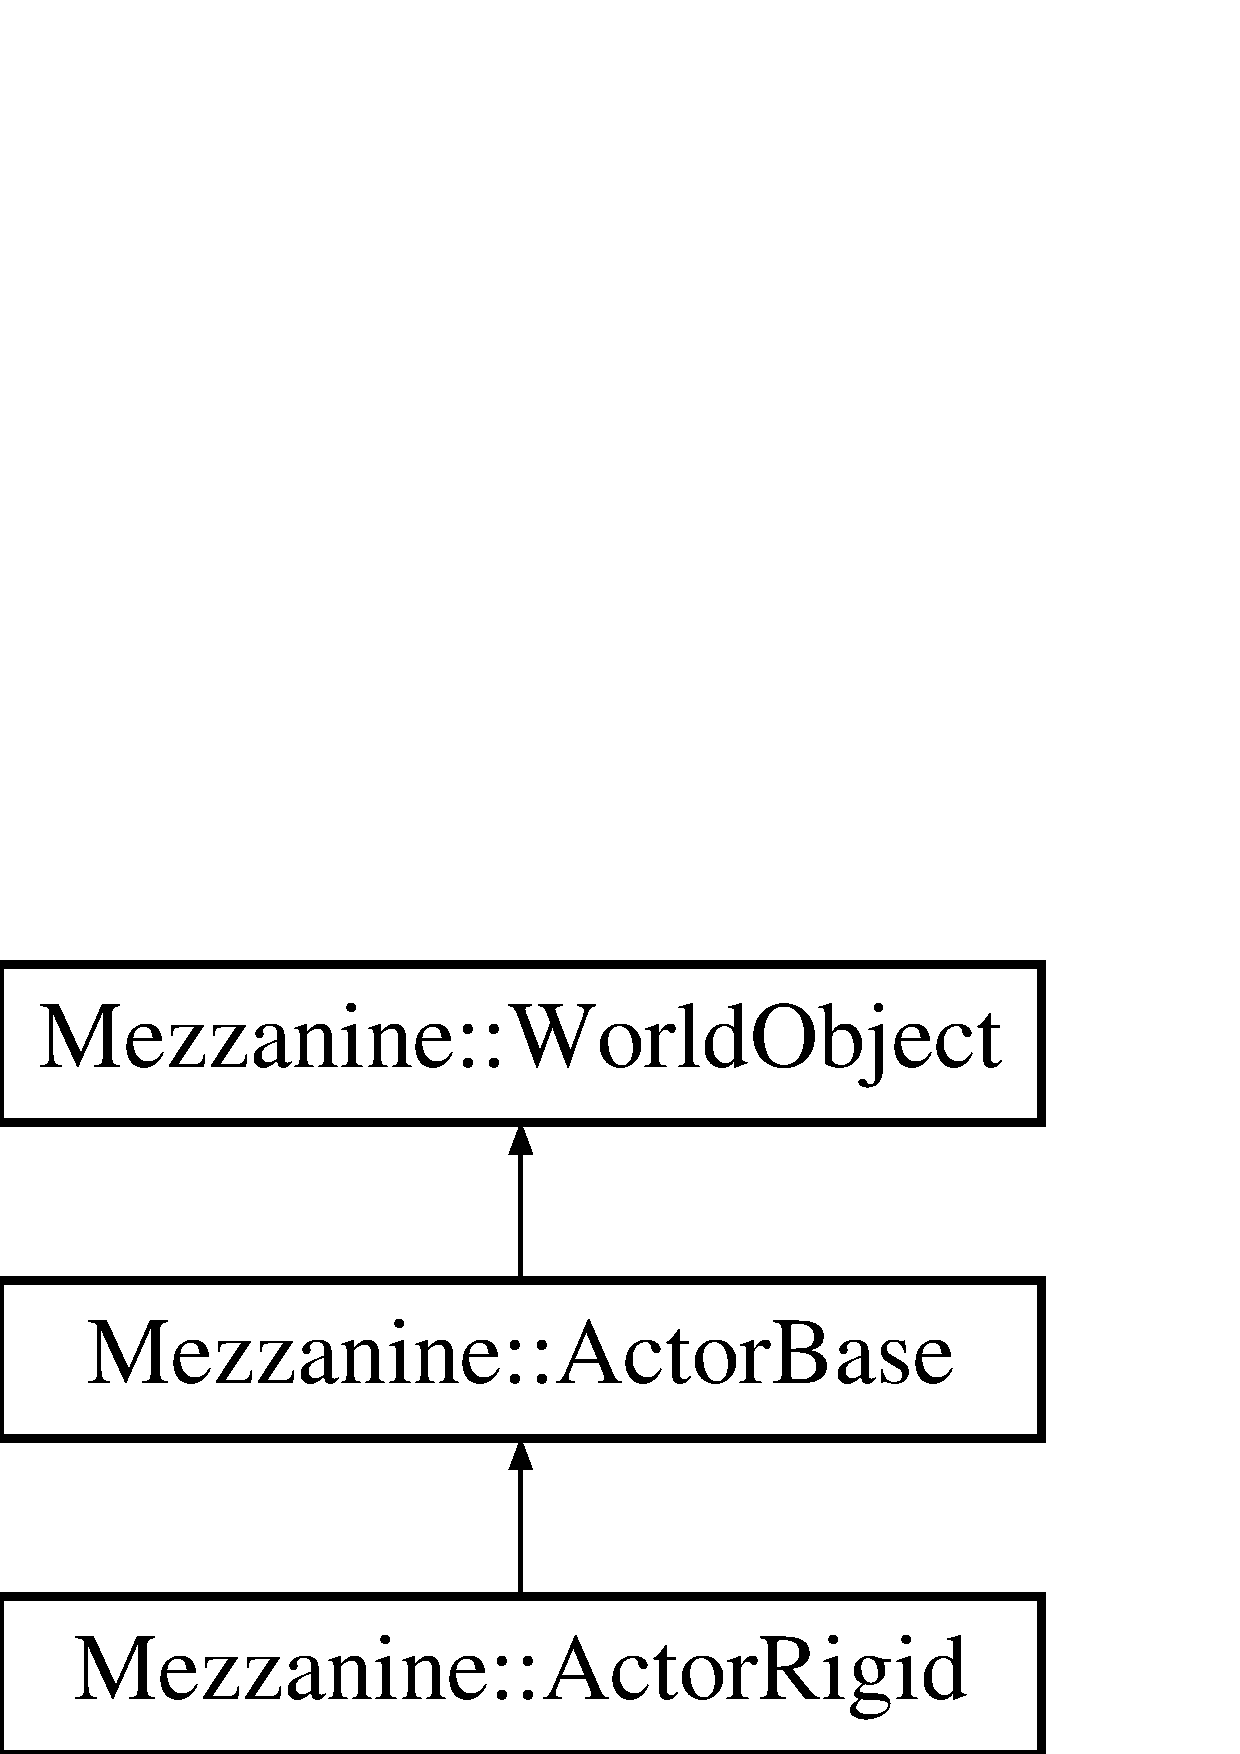
\includegraphics[height=4.000000cm]{classMezzanine_1_1ActorRigid}
\end{center}
\end{figure}
\subsubsection*{Public Member Functions}
\begin{DoxyCompactItemize}
\item 
virtual void \hyperlink{classMezzanine_1_1ActorRigid_a68827280395bc3b9e0266710ec44247d}{\_\-NotifyCollisionState} (\hyperlink{classMezzanine_1_1Collision}{Collision} $\ast$Col, const \hyperlink{classMezzanine_1_1Collision_a24094c597061743dcd571f36077f4d19}{Collision::CollisionState} \&State)
\item 
virtual void \hyperlink{classMezzanine_1_1ActorRigid_a714d836a18ddb4de65bec5afdfdbb81c}{\_\-Update} ()
\item 
\hyperlink{classMezzanine_1_1ActorRigid_ad528a1f2c563dc121e38524f5412e182}{ActorRigid} (const \hyperlink{namespaceMezzanine_a726731b1a7df72bf3583e4a97282c6f6}{Real} \&mass, const \hyperlink{namespaceMezzanine_acf9fcc130e6ebf08e3d8491aebcf1c86}{String} \&name, const \hyperlink{namespaceMezzanine_acf9fcc130e6ebf08e3d8491aebcf1c86}{String} \&file, const \hyperlink{namespaceMezzanine_acf9fcc130e6ebf08e3d8491aebcf1c86}{String} \&group)
\begin{DoxyCompactList}\small\item\em Descriptive constructor. \item\end{DoxyCompactList}\item 
virtual void \hyperlink{classMezzanine_1_1ActorRigid_a5934a8751b9ec19dd2cd9327ce651d59}{AddToWorld} ()
\item 
virtual \hyperlink{classMezzanine_1_1Vector3}{Vector3} \hyperlink{classMezzanine_1_1ActorRigid_ac2b338b867bfd7d2e322a834e308a957}{GetAngularMovementFactor} () const 
\begin{DoxyCompactList}\small\item\em Gets the current angular factors being applied to this actor. \item\end{DoxyCompactList}\item 
virtual btRigidBody $\ast$ \hyperlink{classMezzanine_1_1ActorRigid_aec84029880e2cebf3cc154ada813a372}{GetBulletObject} ()
\begin{DoxyCompactList}\small\item\em Get the Physics data raw from the physic subsystem. \item\end{DoxyCompactList}\item 
virtual \hyperlink{classMezzanine_1_1Vector3}{Vector3} \hyperlink{classMezzanine_1_1ActorRigid_ac2577cc9bff31ad343d5e179acc95257}{GetLinearMovementFactor} () const 
\begin{DoxyCompactList}\small\item\em Gets the current linear factors being applied to this actor. \item\end{DoxyCompactList}\item 
virtual \hyperlink{classMezzanine_1_1ActorRigidPhysicsSettings}{ActorRigidPhysicsSettings} $\ast$ \hyperlink{classMezzanine_1_1ActorRigid_a6ed901638c88e4b9e09605152e11d56e}{GetPhysicsSettings} () const 
\begin{DoxyCompactList}\small\item\em Gets the physics settings class associated with this actor. \item\end{DoxyCompactList}\item 
virtual \hyperlink{namespaceMezzanine_a30335416fc857844e8360c84d1d1b56c}{WorldObjectType} \hyperlink{classMezzanine_1_1ActorRigid_a1369a0e640a8f0c5af9e2c2efc715121}{GetType} () const 
\item 
virtual void \hyperlink{classMezzanine_1_1ActorRigid_a5017e2809d6dc2516b3675748ce80b2e}{RemoveFromWorld} ()
\item 
virtual void \hyperlink{classMezzanine_1_1ActorRigid_ab68facc031fc3212f4169d2b93a72378}{SetAngularMovementFactor} (const \hyperlink{classMezzanine_1_1Vector3}{Vector3} \&Factor)
\begin{DoxyCompactList}\small\item\em Restricts movement on the axis or axies of your choice. \item\end{DoxyCompactList}\item 
virtual void \hyperlink{classMezzanine_1_1ActorRigid_a0dc1820d0fa2d1128b03149da025f40f}{SetLinearMovementFactor} (const \hyperlink{classMezzanine_1_1Vector3}{Vector3} \&Factor)
\begin{DoxyCompactList}\small\item\em Restricts movement on the axis or axies of your choice. \item\end{DoxyCompactList}\item 
virtual \hyperlink{classMezzanine_1_1ActorRigid_a8898e2d624ca89e3bc27dadfbc78560b}{$\sim$ActorRigid} ()
\begin{DoxyCompactList}\small\item\em Destructor. \item\end{DoxyCompactList}\end{DoxyCompactItemize}
\subsubsection*{Protected Member Functions}
\begin{DoxyCompactItemize}
\item 
virtual void \hyperlink{classMezzanine_1_1ActorRigid_a44a1c393e69456fb7fa79affe1684153}{CreateRigidObject} (const \hyperlink{namespaceMezzanine_a726731b1a7df72bf3583e4a97282c6f6}{Real} \&pmass)
\begin{DoxyCompactList}\small\item\em Creates a rigid object for the actor. \item\end{DoxyCompactList}\end{DoxyCompactItemize}
\subsubsection*{Protected Attributes}
\begin{DoxyCompactItemize}
\item 
\hypertarget{classMezzanine_1_1ActorRigid_a92b4e040b752527b73e861ab7c00119e}{
btRigidBody $\ast$ \hyperlink{classMezzanine_1_1ActorRigid_a92b4e040b752527b73e861ab7c00119e}{PhysicsRigidBody}}
\label{classMezzanine_1_1ActorRigid_a92b4e040b752527b73e861ab7c00119e}

\begin{DoxyCompactList}\small\item\em Used to simulate the behavior of a btRigidBody. \item\end{DoxyCompactList}\end{DoxyCompactItemize}
\subsubsection*{Friends}
\begin{DoxyCompactItemize}
\item 
\hypertarget{classMezzanine_1_1ActorRigid_aefa96202ca25d6b82320520f2789b6cf}{
class {\bfseries TypedConstraint}}
\label{classMezzanine_1_1ActorRigid_aefa96202ca25d6b82320520f2789b6cf}

\end{DoxyCompactItemize}


\subsubsection{Detailed Description}
This is the actor class for Rigid Objects. This class should be used to make any rigid object that can be moved as a result of force. Most objects will fall into this catagory. A few examples of a Rigid Object: Boxes, Car Frames, Chairs, etc. For Semi Rigid bodies that are deformable, like jello, it is better to use \hyperlink{classMezzanine_1_1ActorSoft}{ActorSoft}. 

Definition at line 59 of file actorrigid.h.



\subsubsection{Constructor \& Destructor Documentation}
\hypertarget{classMezzanine_1_1ActorRigid_ad528a1f2c563dc121e38524f5412e182}{
\index{Mezzanine::ActorRigid@{Mezzanine::ActorRigid}!ActorRigid@{ActorRigid}}
\index{ActorRigid@{ActorRigid}!Mezzanine::ActorRigid@{Mezzanine::ActorRigid}}
\paragraph[{ActorRigid}]{\setlength{\rightskip}{0pt plus 5cm}home sqeaky Mezzanine Mezzanine src actorrigid cpp home sqeaky Mezzanine Mezzanine src actorrigid cpp Mezzanine::ActorRigid::ActorRigid (
\begin{DoxyParamCaption}
\item[{const {\bf Real} \&}]{mass, }
\item[{const {\bf String} \&}]{name, }
\item[{const {\bf String} \&}]{file, }
\item[{const {\bf String} \&}]{group}
\end{DoxyParamCaption}
)}\hfill}
\label{classMezzanine_1_1ActorRigid_ad528a1f2c563dc121e38524f5412e182}


Descriptive constructor. 

This constructor contains the basic information needed to make a Rigid Object. \par
 This class inherits from \hyperlink{classMezzanine_1_1ActorBase}{ActorBase}. 
\begin{DoxyParams}{Parameters}
{\em mass} & The mass the object will have in the \hyperlink{classMezzanine_1_1World}{World}. \\
\hline
{\em name} & The name of the actor. \\
\hline
{\em file} & The 3d mesh file that contains the 3d model the actor will use. \\
\hline
{\em group} & The resource group where the 3d mesh and other related files can be found. \\
\hline
\end{DoxyParams}


Definition at line 64 of file actorrigid.cpp.

\hypertarget{classMezzanine_1_1ActorRigid_a8898e2d624ca89e3bc27dadfbc78560b}{
\index{Mezzanine::ActorRigid@{Mezzanine::ActorRigid}!$\sim$ActorRigid@{$\sim$ActorRigid}}
\index{$\sim$ActorRigid@{$\sim$ActorRigid}!Mezzanine::ActorRigid@{Mezzanine::ActorRigid}}
\paragraph[{$\sim$ActorRigid}]{\setlength{\rightskip}{0pt plus 5cm}Mezzanine::ActorRigid::$\sim$ActorRigid (
\begin{DoxyParamCaption}
{}
\end{DoxyParamCaption}
)\hspace{0.3cm}{\ttfamily  \mbox{[}virtual\mbox{]}}}\hfill}
\label{classMezzanine_1_1ActorRigid_a8898e2d624ca89e3bc27dadfbc78560b}


Destructor. 

The class destructor. 

Definition at line 78 of file actorrigid.cpp.



\subsubsection{Member Function Documentation}
\hypertarget{classMezzanine_1_1ActorRigid_a68827280395bc3b9e0266710ec44247d}{
\index{Mezzanine::ActorRigid@{Mezzanine::ActorRigid}!\_\-NotifyCollisionState@{\_\-NotifyCollisionState}}
\index{\_\-NotifyCollisionState@{\_\-NotifyCollisionState}!Mezzanine::ActorRigid@{Mezzanine::ActorRigid}}
\paragraph[{\_\-NotifyCollisionState}]{\setlength{\rightskip}{0pt plus 5cm}void Mezzanine::ActorRigid::\_\-NotifyCollisionState (
\begin{DoxyParamCaption}
\item[{{\bf Collision} $\ast$}]{Col, }
\item[{const {\bf Collision::CollisionState} \&}]{State}
\end{DoxyParamCaption}
)\hspace{0.3cm}{\ttfamily  \mbox{[}virtual\mbox{]}}}\hfill}
\label{classMezzanine_1_1ActorRigid_a68827280395bc3b9e0266710ec44247d}
 

\begin{Desc}
\item[\hyperlink{todo__todo000001}{Todo}]Update this to be workable with other objects that have rigid bodies internally, and maybe soft bodies. \end{Desc}




Reimplemented from \hyperlink{classMezzanine_1_1WorldObject_aacf9e82bfb2f25ee309a1871a2032030}{Mezzanine::WorldObject}.



Definition at line 143 of file actorrigid.cpp.

\hypertarget{classMezzanine_1_1ActorRigid_a714d836a18ddb4de65bec5afdfdbb81c}{
\index{Mezzanine::ActorRigid@{Mezzanine::ActorRigid}!\_\-Update@{\_\-Update}}
\index{\_\-Update@{\_\-Update}!Mezzanine::ActorRigid@{Mezzanine::ActorRigid}}
\paragraph[{\_\-Update}]{\setlength{\rightskip}{0pt plus 5cm}void Mezzanine::ActorRigid::\_\-Update (
\begin{DoxyParamCaption}
{}
\end{DoxyParamCaption}
)\hspace{0.3cm}{\ttfamily  \mbox{[}virtual\mbox{]}}}\hfill}
\label{classMezzanine_1_1ActorRigid_a714d836a18ddb4de65bec5afdfdbb81c}
Utility function for altering or checking the \hyperlink{classMezzanine_1_1World}{World} Object every frame.  

Implements \hyperlink{classMezzanine_1_1ActorBase_a8f5a36a6981f1249dbabab318531afd0}{Mezzanine::ActorBase}.



Definition at line 140 of file actorrigid.cpp.

\hypertarget{classMezzanine_1_1ActorRigid_a5934a8751b9ec19dd2cd9327ce651d59}{
\index{Mezzanine::ActorRigid@{Mezzanine::ActorRigid}!AddToWorld@{AddToWorld}}
\index{AddToWorld@{AddToWorld}!Mezzanine::ActorRigid@{Mezzanine::ActorRigid}}
\paragraph[{AddToWorld}]{\setlength{\rightskip}{0pt plus 5cm}void Mezzanine::ActorRigid::AddToWorld (
\begin{DoxyParamCaption}
{}
\end{DoxyParamCaption}
)\hspace{0.3cm}{\ttfamily  \mbox{[}virtual\mbox{]}}}\hfill}
\label{classMezzanine_1_1ActorRigid_a5934a8751b9ec19dd2cd9327ce651d59}
 

Implements \hyperlink{classMezzanine_1_1ActorBase_abe739a46f248a7ba257becfb560d9aa5}{Mezzanine::ActorBase}.



Definition at line 121 of file actorrigid.cpp.

\hypertarget{classMezzanine_1_1ActorRigid_a44a1c393e69456fb7fa79affe1684153}{
\index{Mezzanine::ActorRigid@{Mezzanine::ActorRigid}!CreateRigidObject@{CreateRigidObject}}
\index{CreateRigidObject@{CreateRigidObject}!Mezzanine::ActorRigid@{Mezzanine::ActorRigid}}
\paragraph[{CreateRigidObject}]{\setlength{\rightskip}{0pt plus 5cm}void Mezzanine::ActorRigid::CreateRigidObject (
\begin{DoxyParamCaption}
\item[{const {\bf Real} \&}]{pmass}
\end{DoxyParamCaption}
)\hspace{0.3cm}{\ttfamily  \mbox{[}protected, virtual\mbox{]}}}\hfill}
\label{classMezzanine_1_1ActorRigid_a44a1c393e69456fb7fa79affe1684153}


Creates a rigid object for the actor. 

Creates a rigid object to be placed in the physics world later. \par
 This is automaticly called by the Constructor and shouldn't be called manually. 
\begin{DoxyParams}{Parameters}
{\em pmass} & \char`\"{}Real Mass\char`\"{} The mass of the object. \\
\hline
\end{DoxyParams}


Definition at line 86 of file actorrigid.cpp.

\hypertarget{classMezzanine_1_1ActorRigid_ac2b338b867bfd7d2e322a834e308a957}{
\index{Mezzanine::ActorRigid@{Mezzanine::ActorRigid}!GetAngularMovementFactor@{GetAngularMovementFactor}}
\index{GetAngularMovementFactor@{GetAngularMovementFactor}!Mezzanine::ActorRigid@{Mezzanine::ActorRigid}}
\paragraph[{GetAngularMovementFactor}]{\setlength{\rightskip}{0pt plus 5cm}{\bf Vector3} Mezzanine::ActorRigid::GetAngularMovementFactor (
\begin{DoxyParamCaption}
{}
\end{DoxyParamCaption}
) const\hspace{0.3cm}{\ttfamily  \mbox{[}virtual\mbox{]}}}\hfill}
\label{classMezzanine_1_1ActorRigid_ac2b338b867bfd7d2e322a834e308a957}


Gets the current angular factors being applied to this actor. 

\begin{DoxyReturn}{Returns}
Returns a \hyperlink{classMezzanine_1_1Vector3}{Vector3} representing the factors on the 3 angular axes. 
\end{DoxyReturn}


Definition at line 115 of file actorrigid.cpp.

\hypertarget{classMezzanine_1_1ActorRigid_aec84029880e2cebf3cc154ada813a372}{
\index{Mezzanine::ActorRigid@{Mezzanine::ActorRigid}!GetBulletObject@{GetBulletObject}}
\index{GetBulletObject@{GetBulletObject}!Mezzanine::ActorRigid@{Mezzanine::ActorRigid}}
\paragraph[{GetBulletObject}]{\setlength{\rightskip}{0pt plus 5cm}btRigidBody $\ast$ Mezzanine::ActorRigid::GetBulletObject (
\begin{DoxyParamCaption}
{}
\end{DoxyParamCaption}
)\hspace{0.3cm}{\ttfamily  \mbox{[}virtual\mbox{]}}}\hfill}
\label{classMezzanine_1_1ActorRigid_aec84029880e2cebf3cc154ada813a372}


Get the Physics data raw from the physic subsystem. 

\begin{DoxyReturn}{Returns}
Currently this returns a pointer to a btRigidBody. 
\end{DoxyReturn}


Definition at line 215 of file actorrigid.cpp.

\hypertarget{classMezzanine_1_1ActorRigid_ac2577cc9bff31ad343d5e179acc95257}{
\index{Mezzanine::ActorRigid@{Mezzanine::ActorRigid}!GetLinearMovementFactor@{GetLinearMovementFactor}}
\index{GetLinearMovementFactor@{GetLinearMovementFactor}!Mezzanine::ActorRigid@{Mezzanine::ActorRigid}}
\paragraph[{GetLinearMovementFactor}]{\setlength{\rightskip}{0pt plus 5cm}{\bf Vector3} Mezzanine::ActorRigid::GetLinearMovementFactor (
\begin{DoxyParamCaption}
{}
\end{DoxyParamCaption}
) const\hspace{0.3cm}{\ttfamily  \mbox{[}virtual\mbox{]}}}\hfill}
\label{classMezzanine_1_1ActorRigid_ac2577cc9bff31ad343d5e179acc95257}


Gets the current linear factors being applied to this actor. 

\begin{DoxyReturn}{Returns}
Returns a \hyperlink{classMezzanine_1_1Vector3}{Vector3} representing the factors on the 3 linear axes. 
\end{DoxyReturn}


Definition at line 109 of file actorrigid.cpp.

\hypertarget{classMezzanine_1_1ActorRigid_a6ed901638c88e4b9e09605152e11d56e}{
\index{Mezzanine::ActorRigid@{Mezzanine::ActorRigid}!GetPhysicsSettings@{GetPhysicsSettings}}
\index{GetPhysicsSettings@{GetPhysicsSettings}!Mezzanine::ActorRigid@{Mezzanine::ActorRigid}}
\paragraph[{GetPhysicsSettings}]{\setlength{\rightskip}{0pt plus 5cm}{\bf ActorRigidPhysicsSettings} $\ast$ Mezzanine::ActorRigid::GetPhysicsSettings (
\begin{DoxyParamCaption}
{}
\end{DoxyParamCaption}
) const\hspace{0.3cm}{\ttfamily  \mbox{[}virtual\mbox{]}}}\hfill}
\label{classMezzanine_1_1ActorRigid_a6ed901638c88e4b9e09605152e11d56e}


Gets the physics settings class associated with this actor. 

\begin{DoxyReturn}{Returns}
Returns a pointer to the physics settings class in use by this actor. 
\end{DoxyReturn}


Reimplemented from \hyperlink{classMezzanine_1_1WorldObject_ad845988a6ff31d0e7cea45d6a45bd6c1}{Mezzanine::WorldObject}.



Definition at line 103 of file actorrigid.cpp.

\hypertarget{classMezzanine_1_1ActorRigid_a1369a0e640a8f0c5af9e2c2efc715121}{
\index{Mezzanine::ActorRigid@{Mezzanine::ActorRigid}!GetType@{GetType}}
\index{GetType@{GetType}!Mezzanine::ActorRigid@{Mezzanine::ActorRigid}}
\paragraph[{GetType}]{\setlength{\rightskip}{0pt plus 5cm}{\bf WorldObjectType} Mezzanine::ActorRigid::GetType (
\begin{DoxyParamCaption}
{}
\end{DoxyParamCaption}
) const\hspace{0.3cm}{\ttfamily  \mbox{[}virtual\mbox{]}}}\hfill}
\label{classMezzanine_1_1ActorRigid_a1369a0e640a8f0c5af9e2c2efc715121}
Gets the type of the \hyperlink{classMezzanine_1_1World}{World} Object instance. 

\begin{DoxyReturn}{Returns}
Returns the type of the \hyperlink{classMezzanine_1_1World}{World} Object instance 
\end{DoxyReturn}
 

Implements \hyperlink{classMezzanine_1_1ActorBase_a6e9cce7e660471cc0f9b9df019663f8d}{Mezzanine::ActorBase}.



Definition at line 118 of file actorrigid.cpp.

\hypertarget{classMezzanine_1_1ActorRigid_a5017e2809d6dc2516b3675748ce80b2e}{
\index{Mezzanine::ActorRigid@{Mezzanine::ActorRigid}!RemoveFromWorld@{RemoveFromWorld}}
\index{RemoveFromWorld@{RemoveFromWorld}!Mezzanine::ActorRigid@{Mezzanine::ActorRigid}}
\paragraph[{RemoveFromWorld}]{\setlength{\rightskip}{0pt plus 5cm}void Mezzanine::ActorRigid::RemoveFromWorld (
\begin{DoxyParamCaption}
{}
\end{DoxyParamCaption}
)\hspace{0.3cm}{\ttfamily  \mbox{[}virtual\mbox{]}}}\hfill}
\label{classMezzanine_1_1ActorRigid_a5017e2809d6dc2516b3675748ce80b2e}
 

Implements \hyperlink{classMezzanine_1_1ActorBase_a30910dd0351bc29b2bf88cb3dc8d83db}{Mezzanine::ActorBase}.



Definition at line 127 of file actorrigid.cpp.

\hypertarget{classMezzanine_1_1ActorRigid_ab68facc031fc3212f4169d2b93a72378}{
\index{Mezzanine::ActorRigid@{Mezzanine::ActorRigid}!SetAngularMovementFactor@{SetAngularMovementFactor}}
\index{SetAngularMovementFactor@{SetAngularMovementFactor}!Mezzanine::ActorRigid@{Mezzanine::ActorRigid}}
\paragraph[{SetAngularMovementFactor}]{\setlength{\rightskip}{0pt plus 5cm}void Mezzanine::ActorRigid::SetAngularMovementFactor (
\begin{DoxyParamCaption}
\item[{const {\bf Vector3} \&}]{Factor}
\end{DoxyParamCaption}
)\hspace{0.3cm}{\ttfamily  \mbox{[}virtual\mbox{]}}}\hfill}
\label{classMezzanine_1_1ActorRigid_ab68facc031fc3212f4169d2b93a72378}


Restricts movement on the axis or axies of your choice. 

This function can lock or limit any and all axes you define. 0.0 means no angular movement on that axis. 1.0 means normal movement. 
\begin{DoxyParams}{Parameters}
{\em Factor} & \hyperlink{classMezzanine_1_1Vector3}{Vector3} containing the Factors for the 3 angular axes. \\
\hline
\end{DoxyParams}


Definition at line 112 of file actorrigid.cpp.

\hypertarget{classMezzanine_1_1ActorRigid_a0dc1820d0fa2d1128b03149da025f40f}{
\index{Mezzanine::ActorRigid@{Mezzanine::ActorRigid}!SetLinearMovementFactor@{SetLinearMovementFactor}}
\index{SetLinearMovementFactor@{SetLinearMovementFactor}!Mezzanine::ActorRigid@{Mezzanine::ActorRigid}}
\paragraph[{SetLinearMovementFactor}]{\setlength{\rightskip}{0pt plus 5cm}void Mezzanine::ActorRigid::SetLinearMovementFactor (
\begin{DoxyParamCaption}
\item[{const {\bf Vector3} \&}]{Factor}
\end{DoxyParamCaption}
)\hspace{0.3cm}{\ttfamily  \mbox{[}virtual\mbox{]}}}\hfill}
\label{classMezzanine_1_1ActorRigid_a0dc1820d0fa2d1128b03149da025f40f}


Restricts movement on the axis or axies of your choice. 

This function can lock or limit any and all axes you define. 0.0 means no linear movement on that axis. 1.0 means normal movement. 
\begin{DoxyParams}{Parameters}
{\em Factor} & \hyperlink{classMezzanine_1_1Vector3}{Vector3} containing the Factors for the 3 linear axes. \\
\hline
\end{DoxyParams}


Definition at line 106 of file actorrigid.cpp.



The documentation for this class was generated from the following files:\begin{DoxyCompactItemize}
\item 
actorrigid.h\item 
actorrigid.cpp\end{DoxyCompactItemize}

\hypertarget{classMezzanine_1_1ActorRigidDeSerializer}{
\subsection{Mezzanine::ActorRigidDeSerializer Class Reference}
\label{classMezzanine_1_1ActorRigidDeSerializer}\index{Mezzanine::ActorRigidDeSerializer@{Mezzanine::ActorRigidDeSerializer}}
}


This creates Rigid body actors and inserts them into a given \hyperlink{classMezzanine_1_1ActorManager}{ActorManager}.  




{\ttfamily \#include $<$actorserializer.h$>$}

Inheritance diagram for Mezzanine::ActorRigidDeSerializer:\begin{figure}[H]
\begin{center}
\leavevmode
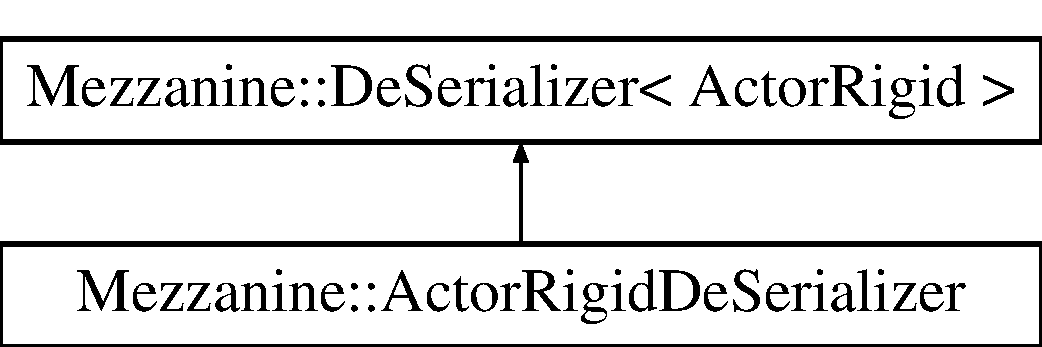
\includegraphics[height=2.000000cm]{classMezzanine_1_1ActorRigidDeSerializer}
\end{center}
\end{figure}


\subsubsection{Detailed Description}
This creates Rigid body actors and inserts them into a given \hyperlink{classMezzanine_1_1ActorManager}{ActorManager}. 

Definition at line 57 of file actorserializer.h.



The documentation for this class was generated from the following file:\begin{DoxyCompactItemize}
\item 
\hyperlink{actorserializer_8h}{actorserializer.h}\end{DoxyCompactItemize}

\hypertarget{classMezzanine_1_1ActorRigidPhysicsSettings}{
\subsection{Mezzanine::ActorRigidPhysicsSettings Class Reference}
\label{classMezzanine_1_1ActorRigidPhysicsSettings}\index{Mezzanine::ActorRigidPhysicsSettings@{Mezzanine::ActorRigidPhysicsSettings}}
}


This is a helper class for configuring physics settings of an \hyperlink{classMezzanine_1_1ActorRigid}{ActorRigid}.  




{\ttfamily \#include $<$actorphysicssettings.h$>$}

Inheritance diagram for Mezzanine::ActorRigidPhysicsSettings:\begin{figure}[H]
\begin{center}
\leavevmode
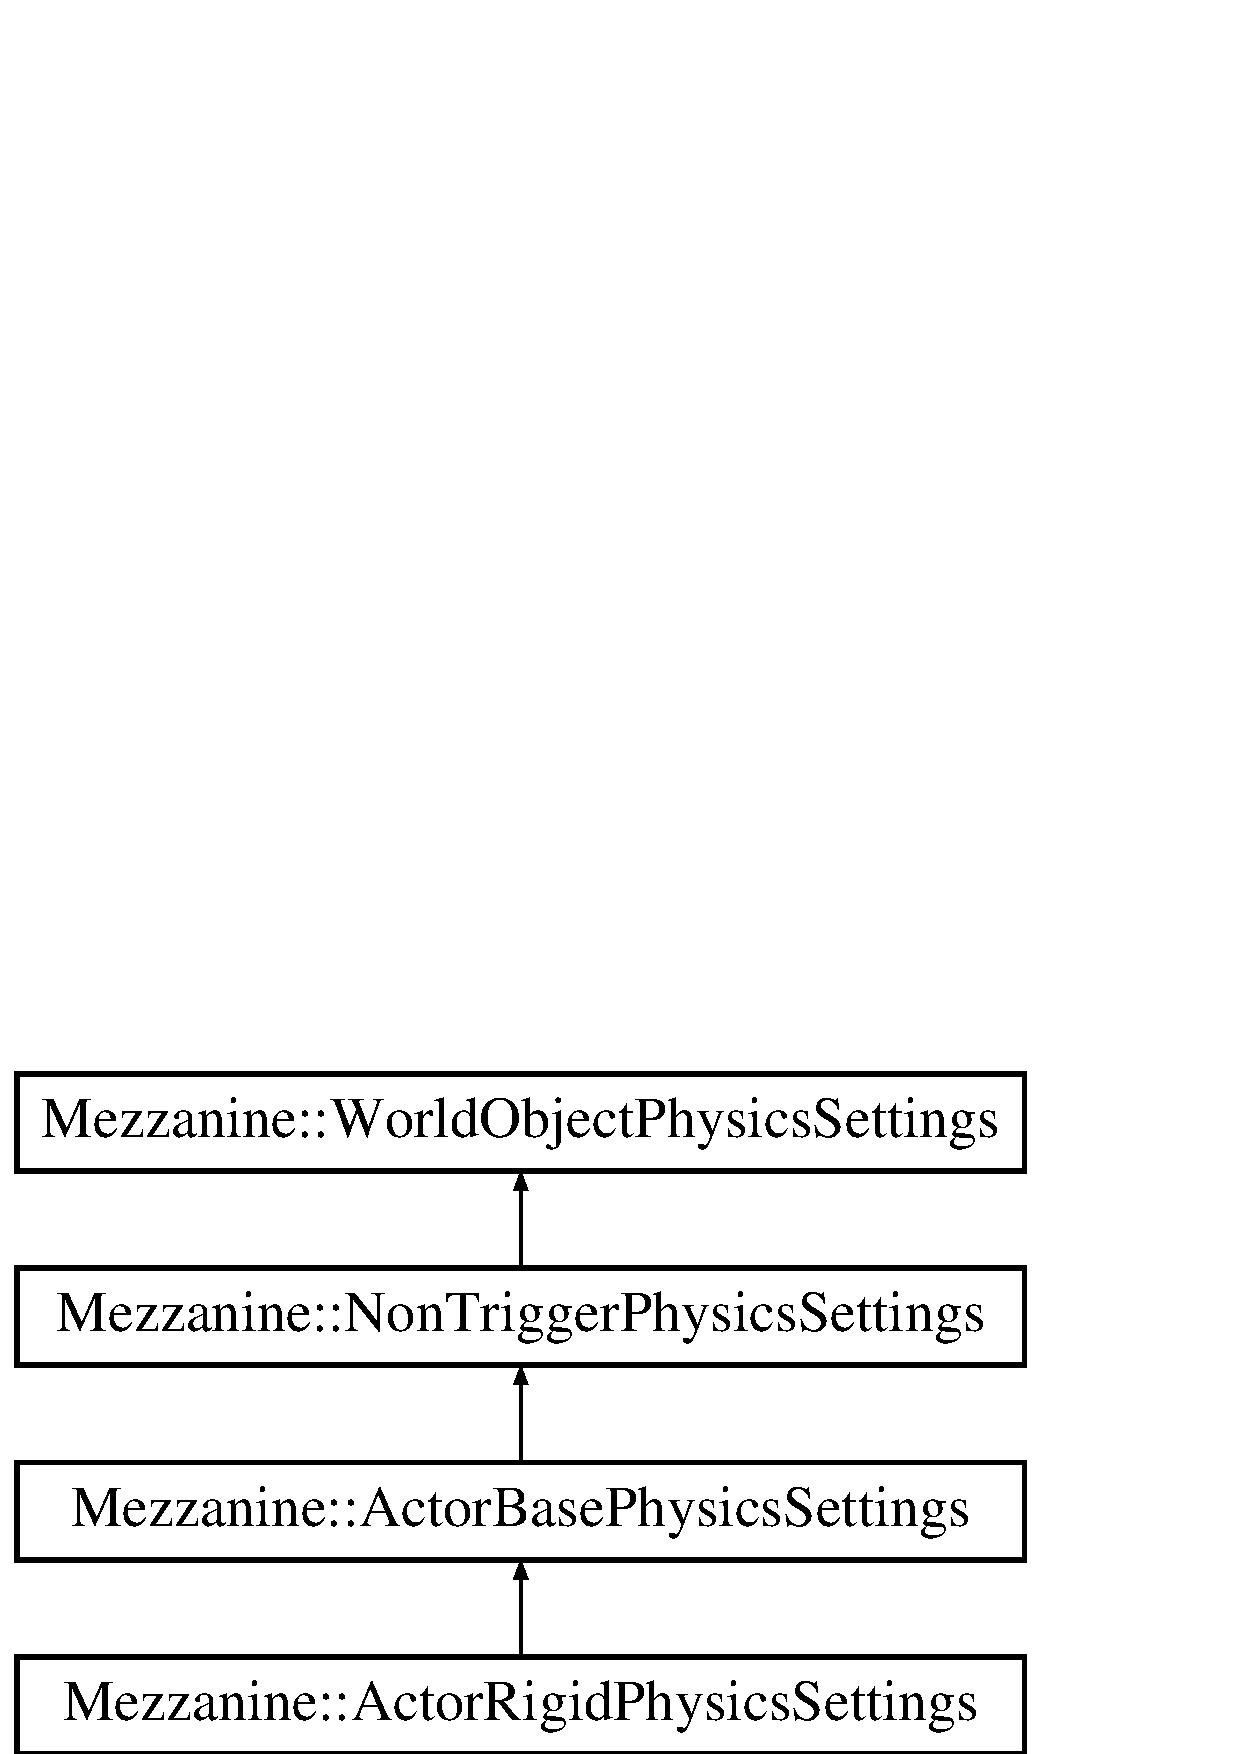
\includegraphics[height=2.000000cm]{classMezzanine_1_1ActorRigidPhysicsSettings}
\end{center}
\end{figure}
\subsubsection*{Public Member Functions}
\begin{DoxyCompactItemize}
\item 
\hyperlink{classMezzanine_1_1ActorRigidPhysicsSettings_a01aac76583a043e4917546ab6fabe160}{ActorRigidPhysicsSettings} (\hyperlink{classMezzanine_1_1ActorRigid}{ActorRigid} $\ast$Actor, btRigidBody $\ast$PhysicsObject)
\begin{DoxyCompactList}\small\item\em Standard Constructor. \item\end{DoxyCompactList}\item 
virtual void \hyperlink{classMezzanine_1_1ActorRigidPhysicsSettings_aafa276832f06cc6a72f8ff0b8ccea155}{ApplyForce} (const \hyperlink{classMezzanine_1_1Vector3}{Vector3} \&Force)
\begin{DoxyCompactList}\small\item\em Push/Apply force to an object. \item\end{DoxyCompactList}\item 
virtual void \hyperlink{classMezzanine_1_1ActorRigidPhysicsSettings_a431d7e6e6f8a62d1ff626d2ccf5d7a6d}{ApplyTorque} (const \hyperlink{classMezzanine_1_1Vector3}{Vector3} \&Torque)
\begin{DoxyCompactList}\small\item\em Spin/Apply Torque to an object. \item\end{DoxyCompactList}\item 
\hypertarget{classMezzanine_1_1ActorRigidPhysicsSettings_a6a5f7320087dc36d235ed9551bba193a}{
virtual void \hyperlink{classMezzanine_1_1ActorRigidPhysicsSettings_a6a5f7320087dc36d235ed9551bba193a}{ClearStickyContacts} ()}
\label{classMezzanine_1_1ActorRigidPhysicsSettings_a6a5f7320087dc36d235ed9551bba193a}

\begin{DoxyCompactList}\small\item\em Removes all the constraints currently active on this object. \item\end{DoxyCompactList}\item 
virtual \hyperlink{namespaceMezzanine_a726731b1a7df72bf3583e4a97282c6f6}{Real} \hyperlink{classMezzanine_1_1ActorRigidPhysicsSettings_afadd3d7e1cee938622fc3781543489eb}{GetAngularDamping} () const 
\begin{DoxyCompactList}\small\item\em Get the Angular damping. \item\end{DoxyCompactList}\item 
virtual \hyperlink{classMezzanine_1_1Vector3}{Vector3} \hyperlink{classMezzanine_1_1ActorRigidPhysicsSettings_a5b078e767c73636afbabc0434f7af8c7}{GetAngularVelocity} () const 
\begin{DoxyCompactList}\small\item\em Gets the Angular Velocity of this object. \item\end{DoxyCompactList}\item 
virtual \hyperlink{classMezzanine_1_1Vector3}{Vector3} \hyperlink{classMezzanine_1_1ActorRigidPhysicsSettings_af5b4641d041c0dcbba8ef0a28566ca87}{GetForce} () const 
\begin{DoxyCompactList}\small\item\em Get the total Force/Movement on the actor. \item\end{DoxyCompactList}\item 
virtual \hyperlink{classMezzanine_1_1Vector3}{Vector3} \hyperlink{classMezzanine_1_1ActorRigidPhysicsSettings_aec9ec4d94326545b60056043c65bdb49}{GetIndividualGravity} () const 
\begin{DoxyCompactList}\small\item\em Gets the gravity being applied to this object. \item\end{DoxyCompactList}\item 
virtual \hyperlink{namespaceMezzanine_a726731b1a7df72bf3583e4a97282c6f6}{Real} \hyperlink{classMezzanine_1_1ActorRigidPhysicsSettings_ac5cb8f2aa589e7c76d39fee38e8fb5e2}{GetLinearDamping} () const 
\begin{DoxyCompactList}\small\item\em Get the linear damping. \item\end{DoxyCompactList}\item 
virtual \hyperlink{classMezzanine_1_1Vector3}{Vector3} \hyperlink{classMezzanine_1_1ActorRigidPhysicsSettings_ad238bf0f6d19a65a79a7b8bc0fb552bd}{GetLinearVelocity} () const 
\begin{DoxyCompactList}\small\item\em Gets the Linear Velocity of this object. \item\end{DoxyCompactList}\item 
virtual \hyperlink{classMezzanine_1_1Vector3}{Vector3} \hyperlink{classMezzanine_1_1ActorRigidPhysicsSettings_a71fae7a868e31ce14612336292bc0fca}{GetLocalInertia} () const 
\begin{DoxyCompactList}\small\item\em Get the current intertia of the Actor. \item\end{DoxyCompactList}\item 
virtual \hyperlink{namespaceMezzanine_a726731b1a7df72bf3583e4a97282c6f6}{Real} \hyperlink{classMezzanine_1_1ActorRigidPhysicsSettings_a6426940001f8d8e112763f6619278874}{GetMass} () const 
\begin{DoxyCompactList}\small\item\em Get the total Mass of the actor. \item\end{DoxyCompactList}\item 
virtual \hyperlink{structMezzanine_1_1StickyData}{StickyData} $\ast$ \hyperlink{classMezzanine_1_1ActorRigidPhysicsSettings_af3b11efb413c1e6a80e4fd5cd3f44715}{GetStickyData} () const 
\begin{DoxyCompactList}\small\item\em Gets the struct storing the data related to sticky behavior. \item\end{DoxyCompactList}\item 
virtual \hyperlink{classMezzanine_1_1Vector3}{Vector3} \hyperlink{classMezzanine_1_1ActorRigidPhysicsSettings_ae7406aca16a67e3ef959ff9cb76a0f44}{GetTorque} () const 
\begin{DoxyCompactList}\small\item\em Get the Torque/Rotation. \item\end{DoxyCompactList}\item 
virtual void \hyperlink{classMezzanine_1_1ActorRigidPhysicsSettings_a0e5b8a968b6f41dfeebd0fcfc01c6458}{SetAngularVelocity} (const \hyperlink{classMezzanine_1_1Vector3}{Vector3} \&AngVel)
\begin{DoxyCompactList}\small\item\em Sets the Angular Velocity of this object. \item\end{DoxyCompactList}\item 
virtual void \hyperlink{classMezzanine_1_1ActorRigidPhysicsSettings_a7583e5afc93dedc8a4403ea156fa0413}{SetCollisionShape} (\hyperlink{classMezzanine_1_1CollisionShape}{CollisionShape} $\ast$Shape)
\begin{DoxyCompactList}\small\item\em Sets the collision shape to be used. \item\end{DoxyCompactList}\item 
virtual void \hyperlink{classMezzanine_1_1ActorRigidPhysicsSettings_a9342e7ff1f485ddf99930f24e081084a}{SetDamping} (const \hyperlink{namespaceMezzanine_a726731b1a7df72bf3583e4a97282c6f6}{Real} \&LinDamping, const \hyperlink{namespaceMezzanine_a726731b1a7df72bf3583e4a97282c6f6}{Real} \&AngDamping)
\begin{DoxyCompactList}\small\item\em Sets the Damping for this object. \item\end{DoxyCompactList}\item 
virtual void \hyperlink{classMezzanine_1_1ActorRigidPhysicsSettings_ad1280574ff86c008c46c10a7133ca274}{SetIndividualGravity} (const \hyperlink{classMezzanine_1_1Vector3}{Vector3} \&Gravity)
\begin{DoxyCompactList}\small\item\em Sets the gravity for only this object. \item\end{DoxyCompactList}\item 
virtual void \hyperlink{classMezzanine_1_1ActorRigidPhysicsSettings_a861a7cf22d838cbbe108cd7daad59e76}{SetLinearVelocity} (const \hyperlink{classMezzanine_1_1Vector3}{Vector3} \&LinVel)
\begin{DoxyCompactList}\small\item\em Sets the Linear Velocity of this object. \item\end{DoxyCompactList}\item 
virtual void \hyperlink{classMezzanine_1_1ActorRigidPhysicsSettings_a8c2a5d88f76478a1d1ba4c194ad5d886}{SetMass} (\hyperlink{namespaceMezzanine_a726731b1a7df72bf3583e4a97282c6f6}{Real} NewMass, const \hyperlink{classMezzanine_1_1Vector3}{Vector3} \&NewInertia)
\begin{DoxyCompactList}\small\item\em Change the mass of the object. \item\end{DoxyCompactList}\item 
virtual void \hyperlink{classMezzanine_1_1ActorRigidPhysicsSettings_a9b2ed9808e7b4a7c8874f33c51fb8ca1}{SetMass} (\hyperlink{namespaceMezzanine_a726731b1a7df72bf3583e4a97282c6f6}{Real} NewMass)
\begin{DoxyCompactList}\small\item\em Change the mass of the object. \item\end{DoxyCompactList}\item 
virtual void \hyperlink{classMezzanine_1_1ActorRigidPhysicsSettings_a2c090930426361a573ba939ac9580bce}{SetStickyData} (const \hyperlink{namespaceMezzanine_adcbb6ce6d1eb4379d109e51171e2e493}{Whole} \&MaxNumContacts)
\begin{DoxyCompactList}\small\item\em Sets the basic parameters for enabling sticky behavior with this actor. \item\end{DoxyCompactList}\item 
\hypertarget{classMezzanine_1_1ActorRigidPhysicsSettings_a56d106b78dfa0ea5415c7928491e4fa7}{
virtual \hyperlink{classMezzanine_1_1ActorRigidPhysicsSettings_a56d106b78dfa0ea5415c7928491e4fa7}{$\sim$ActorRigidPhysicsSettings} ()}
\label{classMezzanine_1_1ActorRigidPhysicsSettings_a56d106b78dfa0ea5415c7928491e4fa7}

\begin{DoxyCompactList}\small\item\em Class destructor. \item\end{DoxyCompactList}\end{DoxyCompactItemize}
\subsubsection*{Protected Attributes}
\begin{DoxyCompactItemize}
\item 
\hypertarget{classMezzanine_1_1ActorRigidPhysicsSettings_a6b8383d096105187418886ac0f28daf3}{
btRigidBody $\ast$ \hyperlink{classMezzanine_1_1ActorRigidPhysicsSettings_a6b8383d096105187418886ac0f28daf3}{ActorRB}}
\label{classMezzanine_1_1ActorRigidPhysicsSettings_a6b8383d096105187418886ac0f28daf3}

\begin{DoxyCompactList}\small\item\em Physics Object of the actor. \item\end{DoxyCompactList}\item 
\hypertarget{classMezzanine_1_1ActorRigidPhysicsSettings_ac83840161a9a88ecdcbacfa3c204bd6e}{
\hyperlink{classMezzanine_1_1ActorRigid}{ActorRigid} $\ast$ \hyperlink{classMezzanine_1_1ActorRigidPhysicsSettings_ac83840161a9a88ecdcbacfa3c204bd6e}{RigidParent}}
\label{classMezzanine_1_1ActorRigidPhysicsSettings_ac83840161a9a88ecdcbacfa3c204bd6e}

\begin{DoxyCompactList}\small\item\em The Actor this belongs to. \item\end{DoxyCompactList}\item 
\hypertarget{classMezzanine_1_1ActorRigidPhysicsSettings_a8ddca7ae371cae162657763543f970bb}{
\hyperlink{structMezzanine_1_1StickyData}{StickyData} $\ast$ \hyperlink{classMezzanine_1_1ActorRigidPhysicsSettings_a8ddca7ae371cae162657763543f970bb}{StickyContacts}}
\label{classMezzanine_1_1ActorRigidPhysicsSettings_a8ddca7ae371cae162657763543f970bb}

\begin{DoxyCompactList}\small\item\em Data related to sticky behavior, if any is enabled. \item\end{DoxyCompactList}\end{DoxyCompactItemize}


\subsubsection{Detailed Description}
This is a helper class for configuring physics settings of an \hyperlink{classMezzanine_1_1ActorRigid}{ActorRigid}. This class contains functions for the configuring of physics specific settings of an \hyperlink{classMezzanine_1_1ActorRigid}{ActorRigid}. This class can only configure the ActorRigids physics. For configuring actor graphics, see \hyperlink{classMezzanine_1_1ActorGraphicsSettings}{ActorGraphicsSettings}. 

Definition at line 253 of file actorphysicssettings.h.



\subsubsection{Constructor \& Destructor Documentation}
\hypertarget{classMezzanine_1_1ActorRigidPhysicsSettings_a01aac76583a043e4917546ab6fabe160}{
\index{Mezzanine::ActorRigidPhysicsSettings@{Mezzanine::ActorRigidPhysicsSettings}!ActorRigidPhysicsSettings@{ActorRigidPhysicsSettings}}
\index{ActorRigidPhysicsSettings@{ActorRigidPhysicsSettings}!Mezzanine::ActorRigidPhysicsSettings@{Mezzanine::ActorRigidPhysicsSettings}}
\paragraph[{ActorRigidPhysicsSettings}]{\setlength{\rightskip}{0pt plus 5cm}Mezzanine::ActorRigidPhysicsSettings::ActorRigidPhysicsSettings (
\begin{DoxyParamCaption}
\item[{{\bf ActorRigid} $\ast$}]{Actor, }
\item[{btRigidBody $\ast$}]{PhysicsObject}
\end{DoxyParamCaption}
)}\hfill}
\label{classMezzanine_1_1ActorRigidPhysicsSettings_a01aac76583a043e4917546ab6fabe160}


Standard Constructor. 


\begin{DoxyParams}{Parameters}
{\em Actor} & The actor this settings class configures. \\
\hline
{\em PhysicsObject} & The physics object belonging to the actor this class configures. \\
\hline
\end{DoxyParams}


Definition at line 387 of file actorphysicssettings.cpp.



\subsubsection{Member Function Documentation}
\hypertarget{classMezzanine_1_1ActorRigidPhysicsSettings_aafa276832f06cc6a72f8ff0b8ccea155}{
\index{Mezzanine::ActorRigidPhysicsSettings@{Mezzanine::ActorRigidPhysicsSettings}!ApplyForce@{ApplyForce}}
\index{ApplyForce@{ApplyForce}!Mezzanine::ActorRigidPhysicsSettings@{Mezzanine::ActorRigidPhysicsSettings}}
\paragraph[{ApplyForce}]{\setlength{\rightskip}{0pt plus 5cm}void Mezzanine::ActorRigidPhysicsSettings::ApplyForce (
\begin{DoxyParamCaption}
\item[{const {\bf Vector3} \&}]{Force}
\end{DoxyParamCaption}
)\hspace{0.3cm}{\ttfamily  \mbox{[}virtual\mbox{]}}}\hfill}
\label{classMezzanine_1_1ActorRigidPhysicsSettings_aafa276832f06cc6a72f8ff0b8ccea155}


Push/Apply force to an object. 


\begin{DoxyParams}{Parameters}
{\em Force} & The amount and direction of the force in a \hyperlink{classMezzanine_1_1Vector3}{Vector3} \\
\hline
\end{DoxyParams}


Definition at line 487 of file actorphysicssettings.cpp.

\hypertarget{classMezzanine_1_1ActorRigidPhysicsSettings_a431d7e6e6f8a62d1ff626d2ccf5d7a6d}{
\index{Mezzanine::ActorRigidPhysicsSettings@{Mezzanine::ActorRigidPhysicsSettings}!ApplyTorque@{ApplyTorque}}
\index{ApplyTorque@{ApplyTorque}!Mezzanine::ActorRigidPhysicsSettings@{Mezzanine::ActorRigidPhysicsSettings}}
\paragraph[{ApplyTorque}]{\setlength{\rightskip}{0pt plus 5cm}void Mezzanine::ActorRigidPhysicsSettings::ApplyTorque (
\begin{DoxyParamCaption}
\item[{const {\bf Vector3} \&}]{Torque}
\end{DoxyParamCaption}
)\hspace{0.3cm}{\ttfamily  \mbox{[}virtual\mbox{]}}}\hfill}
\label{classMezzanine_1_1ActorRigidPhysicsSettings_a431d7e6e6f8a62d1ff626d2ccf5d7a6d}


Spin/Apply Torque to an object. 


\begin{DoxyParams}{Parameters}
{\em Torque} & The amount and direction of the torque in a \hyperlink{classMezzanine_1_1Vector3}{Vector3} \\
\hline
\end{DoxyParams}


Definition at line 490 of file actorphysicssettings.cpp.

\hypertarget{classMezzanine_1_1ActorRigidPhysicsSettings_afadd3d7e1cee938622fc3781543489eb}{
\index{Mezzanine::ActorRigidPhysicsSettings@{Mezzanine::ActorRigidPhysicsSettings}!GetAngularDamping@{GetAngularDamping}}
\index{GetAngularDamping@{GetAngularDamping}!Mezzanine::ActorRigidPhysicsSettings@{Mezzanine::ActorRigidPhysicsSettings}}
\paragraph[{GetAngularDamping}]{\setlength{\rightskip}{0pt plus 5cm}{\bf Real} Mezzanine::ActorRigidPhysicsSettings::GetAngularDamping (
\begin{DoxyParamCaption}
{}
\end{DoxyParamCaption}
) const\hspace{0.3cm}{\ttfamily  \mbox{[}virtual\mbox{]}}}\hfill}
\label{classMezzanine_1_1ActorRigidPhysicsSettings_afadd3d7e1cee938622fc3781543489eb}


Get the Angular damping. 

\begin{DoxyReturn}{Returns}
A Real that has the Angular damping. 
\end{DoxyReturn}


Definition at line 460 of file actorphysicssettings.cpp.

\hypertarget{classMezzanine_1_1ActorRigidPhysicsSettings_a5b078e767c73636afbabc0434f7af8c7}{
\index{Mezzanine::ActorRigidPhysicsSettings@{Mezzanine::ActorRigidPhysicsSettings}!GetAngularVelocity@{GetAngularVelocity}}
\index{GetAngularVelocity@{GetAngularVelocity}!Mezzanine::ActorRigidPhysicsSettings@{Mezzanine::ActorRigidPhysicsSettings}}
\paragraph[{GetAngularVelocity}]{\setlength{\rightskip}{0pt plus 5cm}{\bf Vector3} Mezzanine::ActorRigidPhysicsSettings::GetAngularVelocity (
\begin{DoxyParamCaption}
{}
\end{DoxyParamCaption}
) const\hspace{0.3cm}{\ttfamily  \mbox{[}virtual\mbox{]}}}\hfill}
\label{classMezzanine_1_1ActorRigidPhysicsSettings_a5b078e767c73636afbabc0434f7af8c7}


Gets the Angular Velocity of this object. 

\begin{DoxyReturn}{Returns}
Returns the currently set Angular Velocity of this object. 
\end{DoxyReturn}


Definition at line 472 of file actorphysicssettings.cpp.

\hypertarget{classMezzanine_1_1ActorRigidPhysicsSettings_af5b4641d041c0dcbba8ef0a28566ca87}{
\index{Mezzanine::ActorRigidPhysicsSettings@{Mezzanine::ActorRigidPhysicsSettings}!GetForce@{GetForce}}
\index{GetForce@{GetForce}!Mezzanine::ActorRigidPhysicsSettings@{Mezzanine::ActorRigidPhysicsSettings}}
\paragraph[{GetForce}]{\setlength{\rightskip}{0pt plus 5cm}{\bf Vector3} Mezzanine::ActorRigidPhysicsSettings::GetForce (
\begin{DoxyParamCaption}
{}
\end{DoxyParamCaption}
) const\hspace{0.3cm}{\ttfamily  \mbox{[}virtual\mbox{]}}}\hfill}
\label{classMezzanine_1_1ActorRigidPhysicsSettings_af5b4641d041c0dcbba8ef0a28566ca87}


Get the total Force/Movement on the actor. 

\begin{DoxyReturn}{Returns}
A \hyperlink{classMezzanine_1_1Vector3}{Vector3} with the force of the entire Actor 
\end{DoxyReturn}


Definition at line 481 of file actorphysicssettings.cpp.

\hypertarget{classMezzanine_1_1ActorRigidPhysicsSettings_aec9ec4d94326545b60056043c65bdb49}{
\index{Mezzanine::ActorRigidPhysicsSettings@{Mezzanine::ActorRigidPhysicsSettings}!GetIndividualGravity@{GetIndividualGravity}}
\index{GetIndividualGravity@{GetIndividualGravity}!Mezzanine::ActorRigidPhysicsSettings@{Mezzanine::ActorRigidPhysicsSettings}}
\paragraph[{GetIndividualGravity}]{\setlength{\rightskip}{0pt plus 5cm}{\bf Vector3} Mezzanine::ActorRigidPhysicsSettings::GetIndividualGravity (
\begin{DoxyParamCaption}
{}
\end{DoxyParamCaption}
) const\hspace{0.3cm}{\ttfamily  \mbox{[}virtual\mbox{]}}}\hfill}
\label{classMezzanine_1_1ActorRigidPhysicsSettings_aec9ec4d94326545b60056043c65bdb49}


Gets the gravity being applied to this object. 

This is the gravity applied to this object, which may or may not be the same as the world gravity. \begin{DoxyReturn}{Returns}
Returns a \hyperlink{classMezzanine_1_1Vector3}{Vector3} representing the gravity currently being applied to this object. 
\end{DoxyReturn}


Definition at line 478 of file actorphysicssettings.cpp.

\hypertarget{classMezzanine_1_1ActorRigidPhysicsSettings_ac5cb8f2aa589e7c76d39fee38e8fb5e2}{
\index{Mezzanine::ActorRigidPhysicsSettings@{Mezzanine::ActorRigidPhysicsSettings}!GetLinearDamping@{GetLinearDamping}}
\index{GetLinearDamping@{GetLinearDamping}!Mezzanine::ActorRigidPhysicsSettings@{Mezzanine::ActorRigidPhysicsSettings}}
\paragraph[{GetLinearDamping}]{\setlength{\rightskip}{0pt plus 5cm}{\bf Real} Mezzanine::ActorRigidPhysicsSettings::GetLinearDamping (
\begin{DoxyParamCaption}
{}
\end{DoxyParamCaption}
) const\hspace{0.3cm}{\ttfamily  \mbox{[}virtual\mbox{]}}}\hfill}
\label{classMezzanine_1_1ActorRigidPhysicsSettings_ac5cb8f2aa589e7c76d39fee38e8fb5e2}


Get the linear damping. 

\begin{DoxyReturn}{Returns}
A Real that has the Linear damping. 
\end{DoxyReturn}


Definition at line 457 of file actorphysicssettings.cpp.

\hypertarget{classMezzanine_1_1ActorRigidPhysicsSettings_ad238bf0f6d19a65a79a7b8bc0fb552bd}{
\index{Mezzanine::ActorRigidPhysicsSettings@{Mezzanine::ActorRigidPhysicsSettings}!GetLinearVelocity@{GetLinearVelocity}}
\index{GetLinearVelocity@{GetLinearVelocity}!Mezzanine::ActorRigidPhysicsSettings@{Mezzanine::ActorRigidPhysicsSettings}}
\paragraph[{GetLinearVelocity}]{\setlength{\rightskip}{0pt plus 5cm}{\bf Vector3} Mezzanine::ActorRigidPhysicsSettings::GetLinearVelocity (
\begin{DoxyParamCaption}
{}
\end{DoxyParamCaption}
) const\hspace{0.3cm}{\ttfamily  \mbox{[}virtual\mbox{]}}}\hfill}
\label{classMezzanine_1_1ActorRigidPhysicsSettings_ad238bf0f6d19a65a79a7b8bc0fb552bd}


Gets the Linear Velocity of this object. 

\begin{DoxyReturn}{Returns}
Returns the currently set Linear Velocity of this object. 
\end{DoxyReturn}


Definition at line 466 of file actorphysicssettings.cpp.

\hypertarget{classMezzanine_1_1ActorRigidPhysicsSettings_a71fae7a868e31ce14612336292bc0fca}{
\index{Mezzanine::ActorRigidPhysicsSettings@{Mezzanine::ActorRigidPhysicsSettings}!GetLocalInertia@{GetLocalInertia}}
\index{GetLocalInertia@{GetLocalInertia}!Mezzanine::ActorRigidPhysicsSettings@{Mezzanine::ActorRigidPhysicsSettings}}
\paragraph[{GetLocalInertia}]{\setlength{\rightskip}{0pt plus 5cm}{\bf Vector3} Mezzanine::ActorRigidPhysicsSettings::GetLocalInertia (
\begin{DoxyParamCaption}
{}
\end{DoxyParamCaption}
) const\hspace{0.3cm}{\ttfamily  \mbox{[}virtual\mbox{]}}}\hfill}
\label{classMezzanine_1_1ActorRigidPhysicsSettings_a71fae7a868e31ce14612336292bc0fca}


Get the current intertia of the Actor. 

\begin{DoxyReturn}{Returns}
A \hyperlink{classMezzanine_1_1Vector3}{Vector3} with the Inertia 
\end{DoxyReturn}


Definition at line 496 of file actorphysicssettings.cpp.

\hypertarget{classMezzanine_1_1ActorRigidPhysicsSettings_a6426940001f8d8e112763f6619278874}{
\index{Mezzanine::ActorRigidPhysicsSettings@{Mezzanine::ActorRigidPhysicsSettings}!GetMass@{GetMass}}
\index{GetMass@{GetMass}!Mezzanine::ActorRigidPhysicsSettings@{Mezzanine::ActorRigidPhysicsSettings}}
\paragraph[{GetMass}]{\setlength{\rightskip}{0pt plus 5cm}{\bf Real} Mezzanine::ActorRigidPhysicsSettings::GetMass (
\begin{DoxyParamCaption}
{}
\end{DoxyParamCaption}
) const\hspace{0.3cm}{\ttfamily  \mbox{[}virtual\mbox{]}}}\hfill}
\label{classMezzanine_1_1ActorRigidPhysicsSettings_a6426940001f8d8e112763f6619278874}


Get the total Mass of the actor. 

\begin{DoxyReturn}{Returns}
A Real with the Mass of the Actor 
\end{DoxyReturn}


Definition at line 493 of file actorphysicssettings.cpp.

\hypertarget{classMezzanine_1_1ActorRigidPhysicsSettings_af3b11efb413c1e6a80e4fd5cd3f44715}{
\index{Mezzanine::ActorRigidPhysicsSettings@{Mezzanine::ActorRigidPhysicsSettings}!GetStickyData@{GetStickyData}}
\index{GetStickyData@{GetStickyData}!Mezzanine::ActorRigidPhysicsSettings@{Mezzanine::ActorRigidPhysicsSettings}}
\paragraph[{GetStickyData}]{\setlength{\rightskip}{0pt plus 5cm}{\bf StickyData} $\ast$ Mezzanine::ActorRigidPhysicsSettings::GetStickyData (
\begin{DoxyParamCaption}
{}
\end{DoxyParamCaption}
) const\hspace{0.3cm}{\ttfamily  \mbox{[}virtual\mbox{]}}}\hfill}
\label{classMezzanine_1_1ActorRigidPhysicsSettings_af3b11efb413c1e6a80e4fd5cd3f44715}


Gets the struct storing the data related to sticky behavior. 

\begin{DoxyReturn}{Returns}
Returns a pointer to the struct storing the sticky data for this actor. 
\end{DoxyReturn}


Definition at line 451 of file actorphysicssettings.cpp.

\hypertarget{classMezzanine_1_1ActorRigidPhysicsSettings_ae7406aca16a67e3ef959ff9cb76a0f44}{
\index{Mezzanine::ActorRigidPhysicsSettings@{Mezzanine::ActorRigidPhysicsSettings}!GetTorque@{GetTorque}}
\index{GetTorque@{GetTorque}!Mezzanine::ActorRigidPhysicsSettings@{Mezzanine::ActorRigidPhysicsSettings}}
\paragraph[{GetTorque}]{\setlength{\rightskip}{0pt plus 5cm}{\bf Vector3} Mezzanine::ActorRigidPhysicsSettings::GetTorque (
\begin{DoxyParamCaption}
{}
\end{DoxyParamCaption}
) const\hspace{0.3cm}{\ttfamily  \mbox{[}virtual\mbox{]}}}\hfill}
\label{classMezzanine_1_1ActorRigidPhysicsSettings_ae7406aca16a67e3ef959ff9cb76a0f44}


Get the Torque/Rotation. 

\begin{DoxyReturn}{Returns}
A \hyperlink{classMezzanine_1_1Vector3}{Vector3} with the Torque 
\end{DoxyReturn}


Definition at line 484 of file actorphysicssettings.cpp.

\hypertarget{classMezzanine_1_1ActorRigidPhysicsSettings_a0e5b8a968b6f41dfeebd0fcfc01c6458}{
\index{Mezzanine::ActorRigidPhysicsSettings@{Mezzanine::ActorRigidPhysicsSettings}!SetAngularVelocity@{SetAngularVelocity}}
\index{SetAngularVelocity@{SetAngularVelocity}!Mezzanine::ActorRigidPhysicsSettings@{Mezzanine::ActorRigidPhysicsSettings}}
\paragraph[{SetAngularVelocity}]{\setlength{\rightskip}{0pt plus 5cm}void Mezzanine::ActorRigidPhysicsSettings::SetAngularVelocity (
\begin{DoxyParamCaption}
\item[{const {\bf Vector3} \&}]{AngVel}
\end{DoxyParamCaption}
)\hspace{0.3cm}{\ttfamily  \mbox{[}virtual\mbox{]}}}\hfill}
\label{classMezzanine_1_1ActorRigidPhysicsSettings_a0e5b8a968b6f41dfeebd0fcfc01c6458}


Sets the Angular Velocity of this object. 


\begin{DoxyParams}{Parameters}
{\em AngVel} & \hyperlink{classMezzanine_1_1Vector3}{Vector3} representing the Angular Velocity to be set. \\
\hline
\end{DoxyParams}


Definition at line 469 of file actorphysicssettings.cpp.

\hypertarget{classMezzanine_1_1ActorRigidPhysicsSettings_a7583e5afc93dedc8a4403ea156fa0413}{
\index{Mezzanine::ActorRigidPhysicsSettings@{Mezzanine::ActorRigidPhysicsSettings}!SetCollisionShape@{SetCollisionShape}}
\index{SetCollisionShape@{SetCollisionShape}!Mezzanine::ActorRigidPhysicsSettings@{Mezzanine::ActorRigidPhysicsSettings}}
\paragraph[{SetCollisionShape}]{\setlength{\rightskip}{0pt plus 5cm}void Mezzanine::ActorRigidPhysicsSettings::SetCollisionShape (
\begin{DoxyParamCaption}
\item[{{\bf CollisionShape} $\ast$}]{Shape}
\end{DoxyParamCaption}
)\hspace{0.3cm}{\ttfamily  \mbox{[}virtual\mbox{]}}}\hfill}
\label{classMezzanine_1_1ActorRigidPhysicsSettings_a7583e5afc93dedc8a4403ea156fa0413}


Sets the collision shape to be used. 


\begin{DoxyParams}{Parameters}
{\em Shape} & The shape to be applied. \\
\hline
\end{DoxyParams}


Reimplemented from \hyperlink{classMezzanine_1_1ActorBasePhysicsSettings_a9aa6c07c9cb235a417d68f1ea417f834}{Mezzanine::ActorBasePhysicsSettings}.



Definition at line 407 of file actorphysicssettings.cpp.

\hypertarget{classMezzanine_1_1ActorRigidPhysicsSettings_a9342e7ff1f485ddf99930f24e081084a}{
\index{Mezzanine::ActorRigidPhysicsSettings@{Mezzanine::ActorRigidPhysicsSettings}!SetDamping@{SetDamping}}
\index{SetDamping@{SetDamping}!Mezzanine::ActorRigidPhysicsSettings@{Mezzanine::ActorRigidPhysicsSettings}}
\paragraph[{SetDamping}]{\setlength{\rightskip}{0pt plus 5cm}void Mezzanine::ActorRigidPhysicsSettings::SetDamping (
\begin{DoxyParamCaption}
\item[{const {\bf Real} \&}]{LinDamping, }
\item[{const {\bf Real} \&}]{AngDamping}
\end{DoxyParamCaption}
)\hspace{0.3cm}{\ttfamily  \mbox{[}virtual\mbox{]}}}\hfill}
\label{classMezzanine_1_1ActorRigidPhysicsSettings_a9342e7ff1f485ddf99930f24e081084a}


Sets the Damping for this object. 

Both of Linear Damping and Angular Damping default to zero. This is useful if you wish to simulate something like air resistance. Values can range from 0.0 to 1.0. 
\begin{DoxyParams}{Parameters}
{\em LinDamping} & Real representing the amount of Linear Damping(Movement) to be applied. \\
\hline
{\em AngDamping} & Real representing the amount of Angular Damping(Rotation) to be applied. \\
\hline
\end{DoxyParams}


Definition at line 454 of file actorphysicssettings.cpp.

\hypertarget{classMezzanine_1_1ActorRigidPhysicsSettings_ad1280574ff86c008c46c10a7133ca274}{
\index{Mezzanine::ActorRigidPhysicsSettings@{Mezzanine::ActorRigidPhysicsSettings}!SetIndividualGravity@{SetIndividualGravity}}
\index{SetIndividualGravity@{SetIndividualGravity}!Mezzanine::ActorRigidPhysicsSettings@{Mezzanine::ActorRigidPhysicsSettings}}
\paragraph[{SetIndividualGravity}]{\setlength{\rightskip}{0pt plus 5cm}void Mezzanine::ActorRigidPhysicsSettings::SetIndividualGravity (
\begin{DoxyParamCaption}
\item[{const {\bf Vector3} \&}]{Gravity}
\end{DoxyParamCaption}
)\hspace{0.3cm}{\ttfamily  \mbox{[}virtual\mbox{]}}}\hfill}
\label{classMezzanine_1_1ActorRigidPhysicsSettings_ad1280574ff86c008c46c10a7133ca274}


Sets the gravity for only this object. 

This value will override the world gravity. Should be called after adding to the world. When the object is added to the world the world gravity is applied to it. 
\begin{DoxyParams}{Parameters}
{\em Gravity} & \hyperlink{classMezzanine_1_1Vector3}{Vector3} representing the direction and strength of gravity to be applied. \\
\hline
\end{DoxyParams}


Definition at line 475 of file actorphysicssettings.cpp.

\hypertarget{classMezzanine_1_1ActorRigidPhysicsSettings_a861a7cf22d838cbbe108cd7daad59e76}{
\index{Mezzanine::ActorRigidPhysicsSettings@{Mezzanine::ActorRigidPhysicsSettings}!SetLinearVelocity@{SetLinearVelocity}}
\index{SetLinearVelocity@{SetLinearVelocity}!Mezzanine::ActorRigidPhysicsSettings@{Mezzanine::ActorRigidPhysicsSettings}}
\paragraph[{SetLinearVelocity}]{\setlength{\rightskip}{0pt plus 5cm}void Mezzanine::ActorRigidPhysicsSettings::SetLinearVelocity (
\begin{DoxyParamCaption}
\item[{const {\bf Vector3} \&}]{LinVel}
\end{DoxyParamCaption}
)\hspace{0.3cm}{\ttfamily  \mbox{[}virtual\mbox{]}}}\hfill}
\label{classMezzanine_1_1ActorRigidPhysicsSettings_a861a7cf22d838cbbe108cd7daad59e76}


Sets the Linear Velocity of this object. 


\begin{DoxyParams}{Parameters}
{\em LinVel} & \hyperlink{classMezzanine_1_1Vector3}{Vector3} representing the Linear Velocity to be set. \\
\hline
\end{DoxyParams}


Definition at line 463 of file actorphysicssettings.cpp.

\hypertarget{classMezzanine_1_1ActorRigidPhysicsSettings_a9b2ed9808e7b4a7c8874f33c51fb8ca1}{
\index{Mezzanine::ActorRigidPhysicsSettings@{Mezzanine::ActorRigidPhysicsSettings}!SetMass@{SetMass}}
\index{SetMass@{SetMass}!Mezzanine::ActorRigidPhysicsSettings@{Mezzanine::ActorRigidPhysicsSettings}}
\paragraph[{SetMass}]{\setlength{\rightskip}{0pt plus 5cm}void Mezzanine::ActorRigidPhysicsSettings::SetMass (
\begin{DoxyParamCaption}
\item[{{\bf Real}}]{NewMass}
\end{DoxyParamCaption}
)\hspace{0.3cm}{\ttfamily  \mbox{[}virtual\mbox{]}}}\hfill}
\label{classMezzanine_1_1ActorRigidPhysicsSettings_a9b2ed9808e7b4a7c8874f33c51fb8ca1}


Change the mass of the object. 


\begin{DoxyParams}{Parameters}
{\em NewMass} & The amount of mass this should have. \\
\hline
\end{DoxyParams}


Definition at line 499 of file actorphysicssettings.cpp.

\hypertarget{classMezzanine_1_1ActorRigidPhysicsSettings_a8c2a5d88f76478a1d1ba4c194ad5d886}{
\index{Mezzanine::ActorRigidPhysicsSettings@{Mezzanine::ActorRigidPhysicsSettings}!SetMass@{SetMass}}
\index{SetMass@{SetMass}!Mezzanine::ActorRigidPhysicsSettings@{Mezzanine::ActorRigidPhysicsSettings}}
\paragraph[{SetMass}]{\setlength{\rightskip}{0pt plus 5cm}void Mezzanine::ActorRigidPhysicsSettings::SetMass (
\begin{DoxyParamCaption}
\item[{{\bf Real}}]{NewMass, }
\item[{const {\bf Vector3} \&}]{NewInertia}
\end{DoxyParamCaption}
)\hspace{0.3cm}{\ttfamily  \mbox{[}virtual\mbox{]}}}\hfill}
\label{classMezzanine_1_1ActorRigidPhysicsSettings_a8c2a5d88f76478a1d1ba4c194ad5d886}


Change the mass of the object. 


\begin{DoxyParams}{Parameters}
{\em NewMass} & The amount of mass this should have. \\
\hline
{\em NewInertia} & The new inertia the object has. \\
\hline
\end{DoxyParams}


Definition at line 502 of file actorphysicssettings.cpp.

\hypertarget{classMezzanine_1_1ActorRigidPhysicsSettings_a2c090930426361a573ba939ac9580bce}{
\index{Mezzanine::ActorRigidPhysicsSettings@{Mezzanine::ActorRigidPhysicsSettings}!SetStickyData@{SetStickyData}}
\index{SetStickyData@{SetStickyData}!Mezzanine::ActorRigidPhysicsSettings@{Mezzanine::ActorRigidPhysicsSettings}}
\paragraph[{SetStickyData}]{\setlength{\rightskip}{0pt plus 5cm}void Mezzanine::ActorRigidPhysicsSettings::SetStickyData (
\begin{DoxyParamCaption}
\item[{const {\bf Whole} \&}]{MaxNumContacts}
\end{DoxyParamCaption}
)\hspace{0.3cm}{\ttfamily  \mbox{[}virtual\mbox{]}}}\hfill}
\label{classMezzanine_1_1ActorRigidPhysicsSettings_a2c090930426361a573ba939ac9580bce}


Sets the basic parameters for enabling sticky behavior with this actor. 


\begin{DoxyParams}{Parameters}
{\em MaxNumContacts} & The maximum number of object this object can stick to or have stuck to it. \\
\hline
\end{DoxyParams}


Definition at line 426 of file actorphysicssettings.cpp.



The documentation for this class was generated from the following files:\begin{DoxyCompactItemize}
\item 
actorphysicssettings.h\item 
actorphysicssettings.cpp\end{DoxyCompactItemize}

\hypertarget{classMezzanine_1_1ActorSoft}{
\subsection{Mezzanine::ActorSoft Class Reference}
\label{classMezzanine_1_1ActorSoft}\index{Mezzanine::ActorSoft@{Mezzanine::ActorSoft}}
}


This is the actor class for Soft Objects.  




{\ttfamily \#include $<$actorsoft.h$>$}

Inheritance diagram for Mezzanine::ActorSoft:\begin{figure}[H]
\begin{center}
\leavevmode
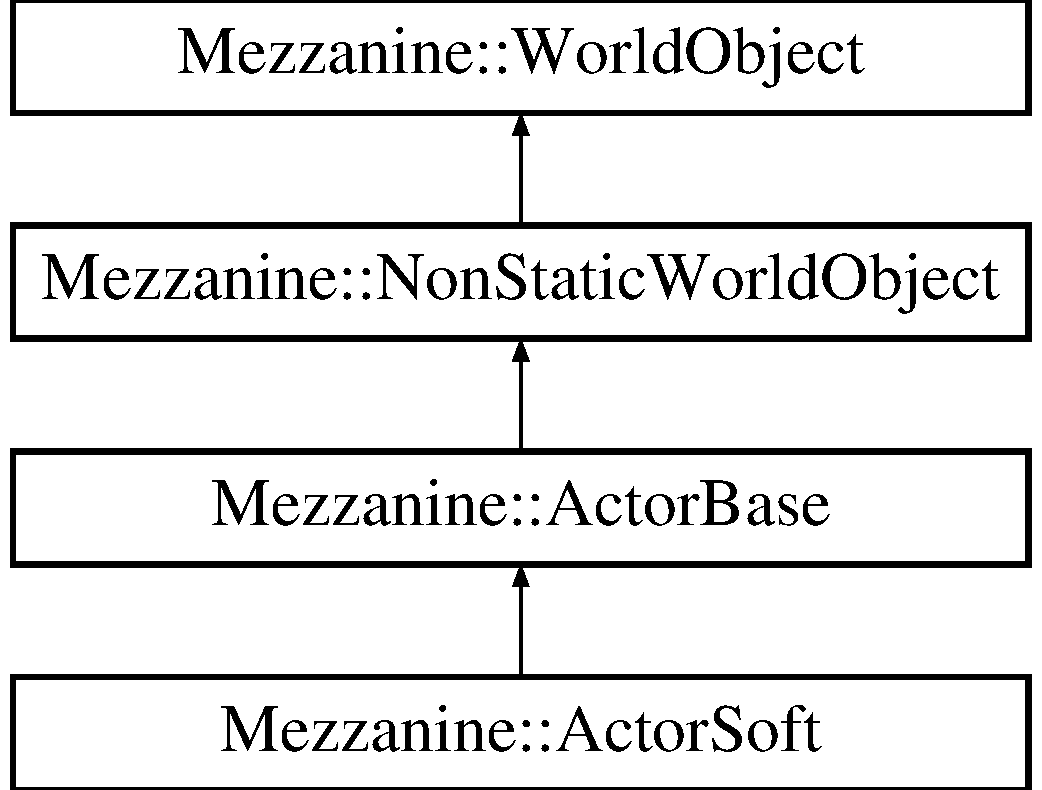
\includegraphics[height=2.000000cm]{classMezzanine_1_1ActorSoft}
\end{center}
\end{figure}
\subsubsection*{Public Member Functions}
\begin{DoxyCompactItemize}
\item 
virtual void \hyperlink{classMezzanine_1_1ActorSoft_a1f255e52f48a9fec2cfe2f91664fb350}{\_\-Update} ()
\item 
\hyperlink{classMezzanine_1_1ActorSoft_a3ab7c4cb45c0308a1b398069095d81b2}{ActorSoft} (\hyperlink{namespaceMezzanine_a726731b1a7df72bf3583e4a97282c6f6}{Real} mass, \hyperlink{namespaceMezzanine_acf9fcc130e6ebf08e3d8491aebcf1c86}{String} name, \hyperlink{namespaceMezzanine_acf9fcc130e6ebf08e3d8491aebcf1c86}{String} file, \hyperlink{namespaceMezzanine_acf9fcc130e6ebf08e3d8491aebcf1c86}{String} group)
\begin{DoxyCompactList}\small\item\em Constructor. \item\end{DoxyCompactList}\item 
virtual void \hyperlink{classMezzanine_1_1ActorSoft_a22e089e98fe83eeb379d399945a10fe9}{AddObjectToWorld} ()
\item 
virtual btSoftBody $\ast$ \hyperlink{classMezzanine_1_1ActorSoft_ab0ddf931ccde766dc5e040077f1a3ec4}{GetBulletObject} ()
\begin{DoxyCompactList}\small\item\em Get the Physics data raw from the physic subsystem. \item\end{DoxyCompactList}\item 
virtual \hyperlink{classMezzanine_1_1Vector3}{Vector3} \hyperlink{classMezzanine_1_1ActorSoft_a0192b3889eaf2786352d75ca03fcae4a}{GetLocation} () const 
\begin{DoxyCompactList}\small\item\em Retrieves the location of the object. \item\end{DoxyCompactList}\item 
\hyperlink{namespaceMezzanine_acf9fcc130e6ebf08e3d8491aebcf1c86}{String} \hyperlink{classMezzanine_1_1ActorSoft_a733138429fccf93f626e44ee9056e102}{GetName} () const 
\begin{DoxyCompactList}\small\item\em Retrieves the name of the object. \item\end{DoxyCompactList}\item 
virtual \hyperlink{classMezzanine_1_1ActorSoftPhysicsSettings}{ActorSoftPhysicsSettings} $\ast$ \hyperlink{classMezzanine_1_1ActorSoft_a9d2960eee35ecfefe76fce2dde3ea18e}{GetPhysicsSettings} ()
\begin{DoxyCompactList}\small\item\em Gets the physics settings class associated with this actor. \item\end{DoxyCompactList}\item 
virtual void \hyperlink{classMezzanine_1_1ActorSoft_a11cb2b406639b1dac2f9e396741f8f44}{RemoveObjectFromWorld} ()
\item 
void \hyperlink{classMezzanine_1_1ActorSoft_ab76bcb0d227374ef5d69878783c7f89b}{SetActorScaling} (\hyperlink{classMezzanine_1_1Vector3}{Vector3} scale)
\begin{DoxyCompactList}\small\item\em Sets the scale of the actor. \item\end{DoxyCompactList}\item 
virtual void \hyperlink{classMezzanine_1_1ActorSoft_a45178fcaf06a81e75d7d81b8fc90fc9e}{SetInitLocation} (\hyperlink{classMezzanine_1_1Vector3}{Vector3} Location)
\begin{DoxyCompactList}\small\item\em Sets the starting location of the actor. \item\end{DoxyCompactList}\item 
virtual void \hyperlink{classMezzanine_1_1ActorSoft_a8ee3cce8eb7578cdeb2af771f16ab240}{SetInitOrientation} (\hyperlink{classMezzanine_1_1Quaternion}{Quaternion} Orientation)
\begin{DoxyCompactList}\small\item\em Sets the starting orientation of the actor. \item\end{DoxyCompactList}\item 
virtual void \hyperlink{classMezzanine_1_1ActorSoft_a9c96f61e8a39fc6b35eb35c03b8e0e42}{SetLocation} (\hyperlink{classMezzanine_1_1Vector3}{Vector3} Place)
\begin{DoxyCompactList}\small\item\em Manually sets the location of the actor. \item\end{DoxyCompactList}\item 
virtual void \hyperlink{classMezzanine_1_1ActorSoft_aad9c559bae769ac44d437a0612934bc2}{SetLocation} (\hyperlink{namespaceMezzanine_a726731b1a7df72bf3583e4a97282c6f6}{Real} x, \hyperlink{namespaceMezzanine_a726731b1a7df72bf3583e4a97282c6f6}{Real} y, \hyperlink{namespaceMezzanine_a726731b1a7df72bf3583e4a97282c6f6}{Real} z)
\begin{DoxyCompactList}\small\item\em Manually sets the location of the actor. \item\end{DoxyCompactList}\item 
virtual void \hyperlink{classMezzanine_1_1ActorSoft_a3490444768316d69b5560d3500550a4f}{SetOrientation} (\hyperlink{classMezzanine_1_1Quaternion}{Quaternion} Rotation)
\begin{DoxyCompactList}\small\item\em Sets the orientation of the actor. \item\end{DoxyCompactList}\item 
virtual void \hyperlink{classMezzanine_1_1ActorSoft_aa203dd4d6bde54f4551673e2690f20b8}{SetOrientation} (\hyperlink{namespaceMezzanine_a726731b1a7df72bf3583e4a97282c6f6}{Real} x, \hyperlink{namespaceMezzanine_a726731b1a7df72bf3583e4a97282c6f6}{Real} y, \hyperlink{namespaceMezzanine_a726731b1a7df72bf3583e4a97282c6f6}{Real} z, \hyperlink{namespaceMezzanine_a726731b1a7df72bf3583e4a97282c6f6}{Real} w)
\begin{DoxyCompactList}\small\item\em Sets the orientation of the actor. \item\end{DoxyCompactList}\item 
virtual \hyperlink{classMezzanine_1_1ActorSoft_a4701cb3e90164c828247a43ff098f69b}{$\sim$ActorSoft} ()
\begin{DoxyCompactList}\small\item\em Destructor. \item\end{DoxyCompactList}\end{DoxyCompactItemize}
\subsubsection*{Protected Member Functions}
\begin{DoxyCompactItemize}
\item 
virtual void \hyperlink{classMezzanine_1_1ActorSoft_af2e618dd176d910834f146c62efe8f19}{AttachToGraphics} ()
\begin{DoxyCompactList}\small\item\em Makes the actor visable. \item\end{DoxyCompactList}\item 
void \hyperlink{classMezzanine_1_1ActorSoft_ad725517ab3a22ef8953e3e003d11551c}{CreateManualMesh} (internal::MeshInfo \&TheMesh)
\begin{DoxyCompactList}\small\item\em Creates and configures a manual object for rendering. \item\end{DoxyCompactList}\item 
void \hyperlink{classMezzanine_1_1ActorSoft_ab0ee1ceadedb3d92295cce649749cb7a}{CreateSoftObject} (\hyperlink{namespaceMezzanine_a726731b1a7df72bf3583e4a97282c6f6}{Real} mass)
\begin{DoxyCompactList}\small\item\em Creates a soft object for the actor. \item\end{DoxyCompactList}\item 
virtual void \hyperlink{classMezzanine_1_1ActorSoft_a3ec90b87480ba28553656eb10552f6d6}{DetachFromGraphics} ()
\begin{DoxyCompactList}\small\item\em Makes the actor invisable. \item\end{DoxyCompactList}\item 
virtual \hyperlink{classMezzanine_1_1Vector3}{Vector3} \hyperlink{classMezzanine_1_1ActorSoft_a7d6f49acc1bf286fd46fb33a8c2798e4}{GetBulletLocation} () const 
\begin{DoxyCompactList}\small\item\em Retrieves the location of the physics body. \item\end{DoxyCompactList}\item 
virtual void \hyperlink{classMezzanine_1_1ActorSoft_a65115824bacb62ad58a68cf3d7fc8840}{SetBulletLocation} (\hyperlink{classMezzanine_1_1Vector3}{Vector3} Location)
\begin{DoxyCompactList}\small\item\em Sets the location of the physics body. \item\end{DoxyCompactList}\item 
virtual void \hyperlink{classMezzanine_1_1ActorSoft_abe282473ccb1f02c273be6efd620d83c}{SetBulletOrientation} (\hyperlink{classMezzanine_1_1Quaternion}{Quaternion} Rotation)
\begin{DoxyCompactList}\small\item\em Sets the orientation of the physics body. \item\end{DoxyCompactList}\end{DoxyCompactItemize}
\subsubsection*{Protected Attributes}
\begin{DoxyCompactItemize}
\item 
\hypertarget{classMezzanine_1_1ActorSoft_ab7ea9b20786fbd7505f836135c890434}{
\hyperlink{classMezzanine_1_1ActorSoftPhysicsSettings}{ActorSoftPhysicsSettings} $\ast$ \hyperlink{classMezzanine_1_1ActorSoft_ab7ea9b20786fbd7505f836135c890434}{PhysicsSettings}}
\label{classMezzanine_1_1ActorSoft_ab7ea9b20786fbd7505f836135c890434}

\begin{DoxyCompactList}\small\item\em This class encapsulates physics specific configuration for this actor. \item\end{DoxyCompactList}\item 
\hypertarget{classMezzanine_1_1ActorSoft_a4eb4bcfe665df0c4741f5c17ff268c88}{
btSoftBody $\ast$ \hyperlink{classMezzanine_1_1ActorSoft_a4eb4bcfe665df0c4741f5c17ff268c88}{PhysicsSoftBody}}
\label{classMezzanine_1_1ActorSoft_a4eb4bcfe665df0c4741f5c17ff268c88}

\begin{DoxyCompactList}\small\item\em Used to simulate the functionality of a btSoftBody for use with the physics subsystem. \item\end{DoxyCompactList}\end{DoxyCompactItemize}


\subsubsection{Detailed Description}
This is the actor class for Soft Objects. This class should be used to make any soft object that, like \hyperlink{classMezzanine_1_1ActorRigid}{ActorRigid}, can be moved or manipulated as a result of force. Examples of soft objects are: Paper, Rope, and Cloth. Semi Rigid bodies that are still somewhat deformable, like Jello, should be made as a soft object. \begin{DoxyWarning}{Warning}
Currently this is not fully implemented and will likely cause errors if used. 
\end{DoxyWarning}


Definition at line 79 of file actorsoft.h.



\subsubsection{Constructor \& Destructor Documentation}
\hypertarget{classMezzanine_1_1ActorSoft_a3ab7c4cb45c0308a1b398069095d81b2}{
\index{Mezzanine::ActorSoft@{Mezzanine::ActorSoft}!ActorSoft@{ActorSoft}}
\index{ActorSoft@{ActorSoft}!Mezzanine::ActorSoft@{Mezzanine::ActorSoft}}
\paragraph[{ActorSoft}]{\setlength{\rightskip}{0pt plus 5cm}Mezzanine::ActorSoft::ActorSoft (
\begin{DoxyParamCaption}
\item[{{\bf Real}}]{mass, }
\item[{{\bf String}}]{name, }
\item[{{\bf String}}]{file, }
\item[{{\bf String}}]{group}
\end{DoxyParamCaption}
)}\hfill}
\label{classMezzanine_1_1ActorSoft_a3ab7c4cb45c0308a1b398069095d81b2}


Constructor. 


\begin{DoxyParams}{Parameters}
{\em mass} & The mass of the soft body. \\
\hline
{\em name} & Name of the object \\
\hline
{\em file} & \hyperlink{classMezzanine_1_1Mesh}{Mesh} the soft body is stored in \\
\hline
{\em group} & The Resource group the mesh can be found in. \\
\hline
\end{DoxyParams}


Definition at line 62 of file actorsoft.cpp.

\hypertarget{classMezzanine_1_1ActorSoft_a4701cb3e90164c828247a43ff098f69b}{
\index{Mezzanine::ActorSoft@{Mezzanine::ActorSoft}!$\sim$ActorSoft@{$\sim$ActorSoft}}
\index{$\sim$ActorSoft@{$\sim$ActorSoft}!Mezzanine::ActorSoft@{Mezzanine::ActorSoft}}
\paragraph[{$\sim$ActorSoft}]{\setlength{\rightskip}{0pt plus 5cm}Mezzanine::ActorSoft::$\sim$ActorSoft (
\begin{DoxyParamCaption}
{}
\end{DoxyParamCaption}
)\hspace{0.3cm}{\ttfamily  \mbox{[}virtual\mbox{]}}}\hfill}
\label{classMezzanine_1_1ActorSoft_a4701cb3e90164c828247a43ff098f69b}


Destructor. 

The class destructor. 

Definition at line 72 of file actorsoft.cpp.



\subsubsection{Member Function Documentation}
\hypertarget{classMezzanine_1_1ActorSoft_a1f255e52f48a9fec2cfe2f91664fb350}{
\index{Mezzanine::ActorSoft@{Mezzanine::ActorSoft}!\_\-Update@{\_\-Update}}
\index{\_\-Update@{\_\-Update}!Mezzanine::ActorSoft@{Mezzanine::ActorSoft}}
\paragraph[{\_\-Update}]{\setlength{\rightskip}{0pt plus 5cm}void Mezzanine::ActorSoft::\_\-Update (
\begin{DoxyParamCaption}
{}
\end{DoxyParamCaption}
)\hspace{0.3cm}{\ttfamily  \mbox{[}virtual\mbox{]}}}\hfill}
\label{classMezzanine_1_1ActorSoft_a1f255e52f48a9fec2cfe2f91664fb350}
Utility function for altering or checking the actor every frame.  

Implements \hyperlink{classMezzanine_1_1ActorBase_a8f5a36a6981f1249dbabab318531afd0}{Mezzanine::ActorBase}.



Definition at line 243 of file actorsoft.cpp.

\hypertarget{classMezzanine_1_1ActorSoft_a22e089e98fe83eeb379d399945a10fe9}{
\index{Mezzanine::ActorSoft@{Mezzanine::ActorSoft}!AddObjectToWorld@{AddObjectToWorld}}
\index{AddObjectToWorld@{AddObjectToWorld}!Mezzanine::ActorSoft@{Mezzanine::ActorSoft}}
\paragraph[{AddObjectToWorld}]{\setlength{\rightskip}{0pt plus 5cm}void Mezzanine::ActorSoft::AddObjectToWorld (
\begin{DoxyParamCaption}
{}
\end{DoxyParamCaption}
)\hspace{0.3cm}{\ttfamily  \mbox{[}virtual\mbox{]}}}\hfill}
\label{classMezzanine_1_1ActorSoft_a22e089e98fe83eeb379d399945a10fe9}
Adds the actor to the physics world.  

Implements \hyperlink{classMezzanine_1_1ActorBase_a766dc0add62500689498a9c1d3f758ea}{Mezzanine::ActorBase}.



Definition at line 231 of file actorsoft.cpp.

\hypertarget{classMezzanine_1_1ActorSoft_af2e618dd176d910834f146c62efe8f19}{
\index{Mezzanine::ActorSoft@{Mezzanine::ActorSoft}!AttachToGraphics@{AttachToGraphics}}
\index{AttachToGraphics@{AttachToGraphics}!Mezzanine::ActorSoft@{Mezzanine::ActorSoft}}
\paragraph[{AttachToGraphics}]{\setlength{\rightskip}{0pt plus 5cm}void Mezzanine::ActorSoft::AttachToGraphics (
\begin{DoxyParamCaption}
{}
\end{DoxyParamCaption}
)\hspace{0.3cm}{\ttfamily  \mbox{[}protected, virtual\mbox{]}}}\hfill}
\label{classMezzanine_1_1ActorSoft_af2e618dd176d910834f146c62efe8f19}


Makes the actor visable. 

Adds the actor to all the nessessary graphics elements to make it visable on screen. \par
 This is automaticly called by the Worlds AddActor function and shouldn't ever need to be called manually. 

Reimplemented from \hyperlink{classMezzanine_1_1ActorBase_a040cc440d23400c7f129b318a8a84e97}{Mezzanine::ActorBase}.



Definition at line 131 of file actorsoft.cpp.

\hypertarget{classMezzanine_1_1ActorSoft_ad725517ab3a22ef8953e3e003d11551c}{
\index{Mezzanine::ActorSoft@{Mezzanine::ActorSoft}!CreateManualMesh@{CreateManualMesh}}
\index{CreateManualMesh@{CreateManualMesh}!Mezzanine::ActorSoft@{Mezzanine::ActorSoft}}
\paragraph[{CreateManualMesh}]{\setlength{\rightskip}{0pt plus 5cm}void Mezzanine::ActorSoft::CreateManualMesh (
\begin{DoxyParamCaption}
\item[{internal::MeshInfo \&}]{TheMesh}
\end{DoxyParamCaption}
)\hspace{0.3cm}{\ttfamily  \mbox{[}protected\mbox{]}}}\hfill}
\label{classMezzanine_1_1ActorSoft_ad725517ab3a22ef8953e3e003d11551c}


Creates and configures a manual object for rendering. 

This function will create and configure an Ogre manual object based on the mesh provided, that will be updateable each frame. 
\begin{DoxyParams}{Parameters}
{\em TheMesh} & The struct with all the appropriate mesh information to base the manual object on. \\
\hline
\end{DoxyParams}


Definition at line 108 of file actorsoft.cpp.

\hypertarget{classMezzanine_1_1ActorSoft_ab0ee1ceadedb3d92295cce649749cb7a}{
\index{Mezzanine::ActorSoft@{Mezzanine::ActorSoft}!CreateSoftObject@{CreateSoftObject}}
\index{CreateSoftObject@{CreateSoftObject}!Mezzanine::ActorSoft@{Mezzanine::ActorSoft}}
\paragraph[{CreateSoftObject}]{\setlength{\rightskip}{0pt plus 5cm}void Mezzanine::ActorSoft::CreateSoftObject (
\begin{DoxyParamCaption}
\item[{{\bf Real}}]{mass}
\end{DoxyParamCaption}
)\hspace{0.3cm}{\ttfamily  \mbox{[}protected\mbox{]}}}\hfill}
\label{classMezzanine_1_1ActorSoft_ab0ee1ceadedb3d92295cce649749cb7a}


Creates a soft object for the actor. 

Creates a soft object to be placed in the physics world later. \par
 This is automatically called by the Constructor and shouldn't be called manually. 
\begin{DoxyParams}{Parameters}
{\em mass} & The desired total mass of the soft object. \\
\hline
\end{DoxyParams}


Definition at line 77 of file actorsoft.cpp.

\hypertarget{classMezzanine_1_1ActorSoft_a3ec90b87480ba28553656eb10552f6d6}{
\index{Mezzanine::ActorSoft@{Mezzanine::ActorSoft}!DetachFromGraphics@{DetachFromGraphics}}
\index{DetachFromGraphics@{DetachFromGraphics}!Mezzanine::ActorSoft@{Mezzanine::ActorSoft}}
\paragraph[{DetachFromGraphics}]{\setlength{\rightskip}{0pt plus 5cm}void Mezzanine::ActorSoft::DetachFromGraphics (
\begin{DoxyParamCaption}
{}
\end{DoxyParamCaption}
)\hspace{0.3cm}{\ttfamily  \mbox{[}protected, virtual\mbox{]}}}\hfill}
\label{classMezzanine_1_1ActorSoft_a3ec90b87480ba28553656eb10552f6d6}


Makes the actor invisable. 

This is the inverse of the AttachToGraphics function. This will effectively remove the object from the graphics world and make it no longer visable. \par
 This is automaticly called by the Worlds RemoveActor function and shouldn't ever need to be called manually. 

Reimplemented from \hyperlink{classMezzanine_1_1ActorBase_a957ed99e5f67ac3fca3ba8a9b025fe48}{Mezzanine::ActorBase}.



Definition at line 144 of file actorsoft.cpp.

\hypertarget{classMezzanine_1_1ActorSoft_a7d6f49acc1bf286fd46fb33a8c2798e4}{
\index{Mezzanine::ActorSoft@{Mezzanine::ActorSoft}!GetBulletLocation@{GetBulletLocation}}
\index{GetBulletLocation@{GetBulletLocation}!Mezzanine::ActorSoft@{Mezzanine::ActorSoft}}
\paragraph[{GetBulletLocation}]{\setlength{\rightskip}{0pt plus 5cm}{\bf Vector3} Mezzanine::ActorSoft::GetBulletLocation (
\begin{DoxyParamCaption}
{}
\end{DoxyParamCaption}
) const\hspace{0.3cm}{\ttfamily  \mbox{[}protected, virtual\mbox{]}}}\hfill}
\label{classMezzanine_1_1ActorSoft_a7d6f49acc1bf286fd46fb33a8c2798e4}


Retrieves the location of the physics body. 

This function will retrieve the location of the object within the physics world. \begin{DoxyReturn}{Returns}
A \hyperlink{classMezzanine_1_1Vector3}{Vector3} with the location in the physics system. 
\end{DoxyReturn}


Reimplemented from \hyperlink{classMezzanine_1_1ActorBase_a9f110d013ed871809258dfc55f8b7276}{Mezzanine::ActorBase}.



Definition at line 155 of file actorsoft.cpp.

\hypertarget{classMezzanine_1_1ActorSoft_ab0ddf931ccde766dc5e040077f1a3ec4}{
\index{Mezzanine::ActorSoft@{Mezzanine::ActorSoft}!GetBulletObject@{GetBulletObject}}
\index{GetBulletObject@{GetBulletObject}!Mezzanine::ActorSoft@{Mezzanine::ActorSoft}}
\paragraph[{GetBulletObject}]{\setlength{\rightskip}{0pt plus 5cm}btSoftBody $\ast$ Mezzanine::ActorSoft::GetBulletObject (
\begin{DoxyParamCaption}
{}
\end{DoxyParamCaption}
)\hspace{0.3cm}{\ttfamily  \mbox{[}virtual\mbox{]}}}\hfill}
\label{classMezzanine_1_1ActorSoft_ab0ddf931ccde766dc5e040077f1a3ec4}


Get the Physics data raw from the physic subsystem. 

\begin{DoxyReturn}{Returns}
Currently this returns a pointer to a btSoftBody. 
\end{DoxyReturn}


Definition at line 270 of file actorsoft.cpp.

\hypertarget{classMezzanine_1_1ActorSoft_a0192b3889eaf2786352d75ca03fcae4a}{
\index{Mezzanine::ActorSoft@{Mezzanine::ActorSoft}!GetLocation@{GetLocation}}
\index{GetLocation@{GetLocation}!Mezzanine::ActorSoft@{Mezzanine::ActorSoft}}
\paragraph[{GetLocation}]{\setlength{\rightskip}{0pt plus 5cm}{\bf Vector3} Mezzanine::ActorSoft::GetLocation (
\begin{DoxyParamCaption}
{}
\end{DoxyParamCaption}
) const\hspace{0.3cm}{\ttfamily  \mbox{[}virtual\mbox{]}}}\hfill}
\label{classMezzanine_1_1ActorSoft_a0192b3889eaf2786352d75ca03fcae4a}


Retrieves the location of the object. 

This function will retrieve the location of the object within the world. \begin{DoxyReturn}{Returns}
A \hyperlink{classMezzanine_1_1Vector3}{Vector3} with the actual locaiton of this Actor. 
\end{DoxyReturn}


Reimplemented from \hyperlink{classMezzanine_1_1ActorBase_ab1706a379bf86d020e64e4b560cdeb73}{Mezzanine::ActorBase}.



Definition at line 214 of file actorsoft.cpp.

\hypertarget{classMezzanine_1_1ActorSoft_a733138429fccf93f626e44ee9056e102}{
\index{Mezzanine::ActorSoft@{Mezzanine::ActorSoft}!GetName@{GetName}}
\index{GetName@{GetName}!Mezzanine::ActorSoft@{Mezzanine::ActorSoft}}
\paragraph[{GetName}]{\setlength{\rightskip}{0pt plus 5cm}std::string Mezzanine::ActorSoft::GetName (
\begin{DoxyParamCaption}
{}
\end{DoxyParamCaption}
) const\hspace{0.3cm}{\ttfamily  \mbox{[}virtual\mbox{]}}}\hfill}
\label{classMezzanine_1_1ActorSoft_a733138429fccf93f626e44ee9056e102}


Retrieves the name of the object. 

\begin{DoxyReturn}{Returns}
A String with the name of this Actor 
\end{DoxyReturn}


Implements \hyperlink{classMezzanine_1_1ActorBase_a01e16da200911fdff659bfb78bafff1d}{Mezzanine::ActorBase}.



Definition at line 171 of file actorsoft.cpp.

\hypertarget{classMezzanine_1_1ActorSoft_a9d2960eee35ecfefe76fce2dde3ea18e}{
\index{Mezzanine::ActorSoft@{Mezzanine::ActorSoft}!GetPhysicsSettings@{GetPhysicsSettings}}
\index{GetPhysicsSettings@{GetPhysicsSettings}!Mezzanine::ActorSoft@{Mezzanine::ActorSoft}}
\paragraph[{GetPhysicsSettings}]{\setlength{\rightskip}{0pt plus 5cm}{\bf ActorSoftPhysicsSettings} $\ast$ Mezzanine::ActorSoft::GetPhysicsSettings (
\begin{DoxyParamCaption}
{}
\end{DoxyParamCaption}
)\hspace{0.3cm}{\ttfamily  \mbox{[}virtual\mbox{]}}}\hfill}
\label{classMezzanine_1_1ActorSoft_a9d2960eee35ecfefe76fce2dde3ea18e}


Gets the physics settings class associated with this actor. 

\begin{DoxyReturn}{Returns}
Returns a pointer to the physics settings class in use by this actor. 
\end{DoxyReturn}


Definition at line 176 of file actorsoft.cpp.

\hypertarget{classMezzanine_1_1ActorSoft_a11cb2b406639b1dac2f9e396741f8f44}{
\index{Mezzanine::ActorSoft@{Mezzanine::ActorSoft}!RemoveObjectFromWorld@{RemoveObjectFromWorld}}
\index{RemoveObjectFromWorld@{RemoveObjectFromWorld}!Mezzanine::ActorSoft@{Mezzanine::ActorSoft}}
\paragraph[{RemoveObjectFromWorld}]{\setlength{\rightskip}{0pt plus 5cm}void Mezzanine::ActorSoft::RemoveObjectFromWorld (
\begin{DoxyParamCaption}
{}
\end{DoxyParamCaption}
)\hspace{0.3cm}{\ttfamily  \mbox{[}virtual\mbox{]}}}\hfill}
\label{classMezzanine_1_1ActorSoft_a11cb2b406639b1dac2f9e396741f8f44}
Removes the actor from the physics world.  

Implements \hyperlink{classMezzanine_1_1ActorBase_a774050bfd7c75f2b639005d82dcd5085}{Mezzanine::ActorBase}.



Definition at line 237 of file actorsoft.cpp.

\hypertarget{classMezzanine_1_1ActorSoft_ab76bcb0d227374ef5d69878783c7f89b}{
\index{Mezzanine::ActorSoft@{Mezzanine::ActorSoft}!SetActorScaling@{SetActorScaling}}
\index{SetActorScaling@{SetActorScaling}!Mezzanine::ActorSoft@{Mezzanine::ActorSoft}}
\paragraph[{SetActorScaling}]{\setlength{\rightskip}{0pt plus 5cm}void Mezzanine::ActorSoft::SetActorScaling (
\begin{DoxyParamCaption}
\item[{{\bf Vector3}}]{scale}
\end{DoxyParamCaption}
)}\hfill}
\label{classMezzanine_1_1ActorSoft_ab76bcb0d227374ef5d69878783c7f89b}


Sets the scale of the actor. 

This function will alter the scaling/size of the actor with the given vector3. 
\begin{DoxyParams}{Parameters}
{\em scale} & The vector3 by which to apply the scale. Will scale each axis' accordingly. \\
\hline
\end{DoxyParams}


Definition at line 181 of file actorsoft.cpp.

\hypertarget{classMezzanine_1_1ActorSoft_a65115824bacb62ad58a68cf3d7fc8840}{
\index{Mezzanine::ActorSoft@{Mezzanine::ActorSoft}!SetBulletLocation@{SetBulletLocation}}
\index{SetBulletLocation@{SetBulletLocation}!Mezzanine::ActorSoft@{Mezzanine::ActorSoft}}
\paragraph[{SetBulletLocation}]{\setlength{\rightskip}{0pt plus 5cm}void Mezzanine::ActorSoft::SetBulletLocation (
\begin{DoxyParamCaption}
\item[{{\bf Vector3}}]{Location}
\end{DoxyParamCaption}
)\hspace{0.3cm}{\ttfamily  \mbox{[}protected, virtual\mbox{]}}}\hfill}
\label{classMezzanine_1_1ActorSoft_a65115824bacb62ad58a68cf3d7fc8840}


Sets the location of the physics body. 

This will take a \hyperlink{classMezzanine_1_1Vector3}{Vector3} and set the location of the actor within the physics world. \par
 This function is called on by the SetLocation function, and shouldn't be called manually. 
\begin{DoxyParams}{Parameters}
{\em Location} & The \hyperlink{classMezzanine_1_1Vector3}{Vector3} representing the location. \\
\hline
\end{DoxyParams}


Definition at line 149 of file actorsoft.cpp.

\hypertarget{classMezzanine_1_1ActorSoft_abe282473ccb1f02c273be6efd620d83c}{
\index{Mezzanine::ActorSoft@{Mezzanine::ActorSoft}!SetBulletOrientation@{SetBulletOrientation}}
\index{SetBulletOrientation@{SetBulletOrientation}!Mezzanine::ActorSoft@{Mezzanine::ActorSoft}}
\paragraph[{SetBulletOrientation}]{\setlength{\rightskip}{0pt plus 5cm}void Mezzanine::ActorSoft::SetBulletOrientation (
\begin{DoxyParamCaption}
\item[{{\bf Quaternion}}]{Rotation}
\end{DoxyParamCaption}
)\hspace{0.3cm}{\ttfamily  \mbox{[}protected, virtual\mbox{]}}}\hfill}
\label{classMezzanine_1_1ActorSoft_abe282473ccb1f02c273be6efd620d83c}


Sets the orientation of the physics body. 

This will take a \hyperlink{classMezzanine_1_1Quaternion}{Quaternion} and set the orientation of the actor within the physics world. \par
 This function is called on by the SetOrientation function, and shouldn't be called manually. 
\begin{DoxyParams}{Parameters}
{\em Rotation} & The quaternion representing the rotation of the actor. \\
\hline
\end{DoxyParams}


Definition at line 162 of file actorsoft.cpp.

\hypertarget{classMezzanine_1_1ActorSoft_a45178fcaf06a81e75d7d81b8fc90fc9e}{
\index{Mezzanine::ActorSoft@{Mezzanine::ActorSoft}!SetInitLocation@{SetInitLocation}}
\index{SetInitLocation@{SetInitLocation}!Mezzanine::ActorSoft@{Mezzanine::ActorSoft}}
\paragraph[{SetInitLocation}]{\setlength{\rightskip}{0pt plus 5cm}void Mezzanine::ActorSoft::SetInitLocation (
\begin{DoxyParamCaption}
\item[{{\bf Vector3}}]{Location}
\end{DoxyParamCaption}
)\hspace{0.3cm}{\ttfamily  \mbox{[}virtual\mbox{]}}}\hfill}
\label{classMezzanine_1_1ActorSoft_a45178fcaf06a81e75d7d81b8fc90fc9e}


Sets the starting location of the actor. 

Calling this function after adding it to the \hyperlink{classMezzanine_1_1World}{World} will have no effect. \par
 This function will set where the actor will be located in the \hyperlink{classMezzanine_1_1World}{World} when it is first placed inside the world. 
\begin{DoxyParams}{Parameters}
{\em Location} & The \hyperlink{classMezzanine_1_1Vector3}{Vector3} representing the location. \\
\hline
\end{DoxyParams}


Definition at line 187 of file actorsoft.cpp.

\hypertarget{classMezzanine_1_1ActorSoft_a8ee3cce8eb7578cdeb2af771f16ab240}{
\index{Mezzanine::ActorSoft@{Mezzanine::ActorSoft}!SetInitOrientation@{SetInitOrientation}}
\index{SetInitOrientation@{SetInitOrientation}!Mezzanine::ActorSoft@{Mezzanine::ActorSoft}}
\paragraph[{SetInitOrientation}]{\setlength{\rightskip}{0pt plus 5cm}void Mezzanine::ActorSoft::SetInitOrientation (
\begin{DoxyParamCaption}
\item[{{\bf Quaternion}}]{Orientation}
\end{DoxyParamCaption}
)\hspace{0.3cm}{\ttfamily  \mbox{[}virtual\mbox{]}}}\hfill}
\label{classMezzanine_1_1ActorSoft_a8ee3cce8eb7578cdeb2af771f16ab240}


Sets the starting orientation of the actor. 

Calling this function after adding it to the \hyperlink{classMezzanine_1_1World}{World} will have no effect. \par
 This function will set where the actor is facing in the \hyperlink{classMezzanine_1_1World}{World} when it is first placed inside the world. 
\begin{DoxyParams}{Parameters}
{\em Orientation} & The \hyperlink{classMezzanine_1_1Quaternion}{Quaternion} representing the Orientation. \\
\hline
\end{DoxyParams}


Definition at line 196 of file actorsoft.cpp.

\hypertarget{classMezzanine_1_1ActorSoft_a9c96f61e8a39fc6b35eb35c03b8e0e42}{
\index{Mezzanine::ActorSoft@{Mezzanine::ActorSoft}!SetLocation@{SetLocation}}
\index{SetLocation@{SetLocation}!Mezzanine::ActorSoft@{Mezzanine::ActorSoft}}
\paragraph[{SetLocation}]{\setlength{\rightskip}{0pt plus 5cm}void Mezzanine::ActorSoft::SetLocation (
\begin{DoxyParamCaption}
\item[{{\bf Vector3}}]{Place}
\end{DoxyParamCaption}
)\hspace{0.3cm}{\ttfamily  \mbox{[}virtual\mbox{]}}}\hfill}
\label{classMezzanine_1_1ActorSoft_a9c96f61e8a39fc6b35eb35c03b8e0e42}


Manually sets the location of the actor. 

Calling this function prior to adding it to the \hyperlink{classMezzanine_1_1World}{World} will have no effect. \par
 In most situations you won't want to use this function, and instead produce movement through physics functions. 
\begin{DoxyParams}{Parameters}
{\em Place} & The \hyperlink{classMezzanine_1_1Vector3}{Vector3} representing the location. \\
\hline
\end{DoxyParams}


Definition at line 208 of file actorsoft.cpp.

\hypertarget{classMezzanine_1_1ActorSoft_aad9c559bae769ac44d437a0612934bc2}{
\index{Mezzanine::ActorSoft@{Mezzanine::ActorSoft}!SetLocation@{SetLocation}}
\index{SetLocation@{SetLocation}!Mezzanine::ActorSoft@{Mezzanine::ActorSoft}}
\paragraph[{SetLocation}]{\setlength{\rightskip}{0pt plus 5cm}void Mezzanine::ActorSoft::SetLocation (
\begin{DoxyParamCaption}
\item[{{\bf Real}}]{x, }
\item[{{\bf Real}}]{y, }
\item[{{\bf Real}}]{z}
\end{DoxyParamCaption}
)\hspace{0.3cm}{\ttfamily  \mbox{[}virtual\mbox{]}}}\hfill}
\label{classMezzanine_1_1ActorSoft_aad9c559bae769ac44d437a0612934bc2}


Manually sets the location of the actor. 

Calling this function prior to adding it to the \hyperlink{classMezzanine_1_1World}{World} will have no effect. \par
 In most situations you won't want to use this function, and instead produce movement through physics functions. 
\begin{DoxyParams}{Parameters}
{\em x} & Location on the X vector. \\
\hline
{\em y} & Location on the Y vector. \\
\hline
{\em z} & Location on the Z vector. \\
\hline
\end{DoxyParams}


Definition at line 202 of file actorsoft.cpp.

\hypertarget{classMezzanine_1_1ActorSoft_a3490444768316d69b5560d3500550a4f}{
\index{Mezzanine::ActorSoft@{Mezzanine::ActorSoft}!SetOrientation@{SetOrientation}}
\index{SetOrientation@{SetOrientation}!Mezzanine::ActorSoft@{Mezzanine::ActorSoft}}
\paragraph[{SetOrientation}]{\setlength{\rightskip}{0pt plus 5cm}void Mezzanine::ActorSoft::SetOrientation (
\begin{DoxyParamCaption}
\item[{{\bf Quaternion}}]{Rotation}
\end{DoxyParamCaption}
)\hspace{0.3cm}{\ttfamily  \mbox{[}virtual\mbox{]}}}\hfill}
\label{classMezzanine_1_1ActorSoft_a3490444768316d69b5560d3500550a4f}


Sets the orientation of the actor. 

Sets the orientation of the actor via a \hyperlink{classMezzanine_1_1Quaternion}{Quaternion}. 
\begin{DoxyParams}{Parameters}
{\em Rotation} & The \hyperlink{classMezzanine_1_1Quaternion}{Quaternion} representing the Rotation. \\
\hline
\end{DoxyParams}


Definition at line 225 of file actorsoft.cpp.

\hypertarget{classMezzanine_1_1ActorSoft_aa203dd4d6bde54f4551673e2690f20b8}{
\index{Mezzanine::ActorSoft@{Mezzanine::ActorSoft}!SetOrientation@{SetOrientation}}
\index{SetOrientation@{SetOrientation}!Mezzanine::ActorSoft@{Mezzanine::ActorSoft}}
\paragraph[{SetOrientation}]{\setlength{\rightskip}{0pt plus 5cm}void Mezzanine::ActorSoft::SetOrientation (
\begin{DoxyParamCaption}
\item[{{\bf Real}}]{x, }
\item[{{\bf Real}}]{y, }
\item[{{\bf Real}}]{z, }
\item[{{\bf Real}}]{w}
\end{DoxyParamCaption}
)\hspace{0.3cm}{\ttfamily  \mbox{[}virtual\mbox{]}}}\hfill}
\label{classMezzanine_1_1ActorSoft_aa203dd4d6bde54f4551673e2690f20b8}


Sets the orientation of the actor. 

Sets the orientation of the actor via \hyperlink{classMezzanine_1_1Quaternion}{Quaternion} parameters. 
\begin{DoxyParams}{Parameters}
{\em x} & Where the X vector is rotated about. \\
\hline
{\em y} & Where the Y vector is rotated about. \\
\hline
{\em z} & Where the Z vector is rotated about. \\
\hline
{\em w} & How much to about the x, y, z. \\
\hline
\end{DoxyParams}


Definition at line 219 of file actorsoft.cpp.



The documentation for this class was generated from the following files:\begin{DoxyCompactItemize}
\item 
actorsoft.h\item 
actorsoft.cpp\end{DoxyCompactItemize}

\hypertarget{classMezzanine_1_1ActorSoftCollisionShape}{
\subsection{Mezzanine::ActorSoftCollisionShape Class Reference}
\label{classMezzanine_1_1ActorSoftCollisionShape}\index{Mezzanine::ActorSoftCollisionShape@{Mezzanine::ActorSoftCollisionShape}}
}


A collision shape for soft actors.  




{\ttfamily \#include $<$collisionshape.h$>$}

Inheritance diagram for Mezzanine::ActorSoftCollisionShape:\begin{figure}[H]
\begin{center}
\leavevmode
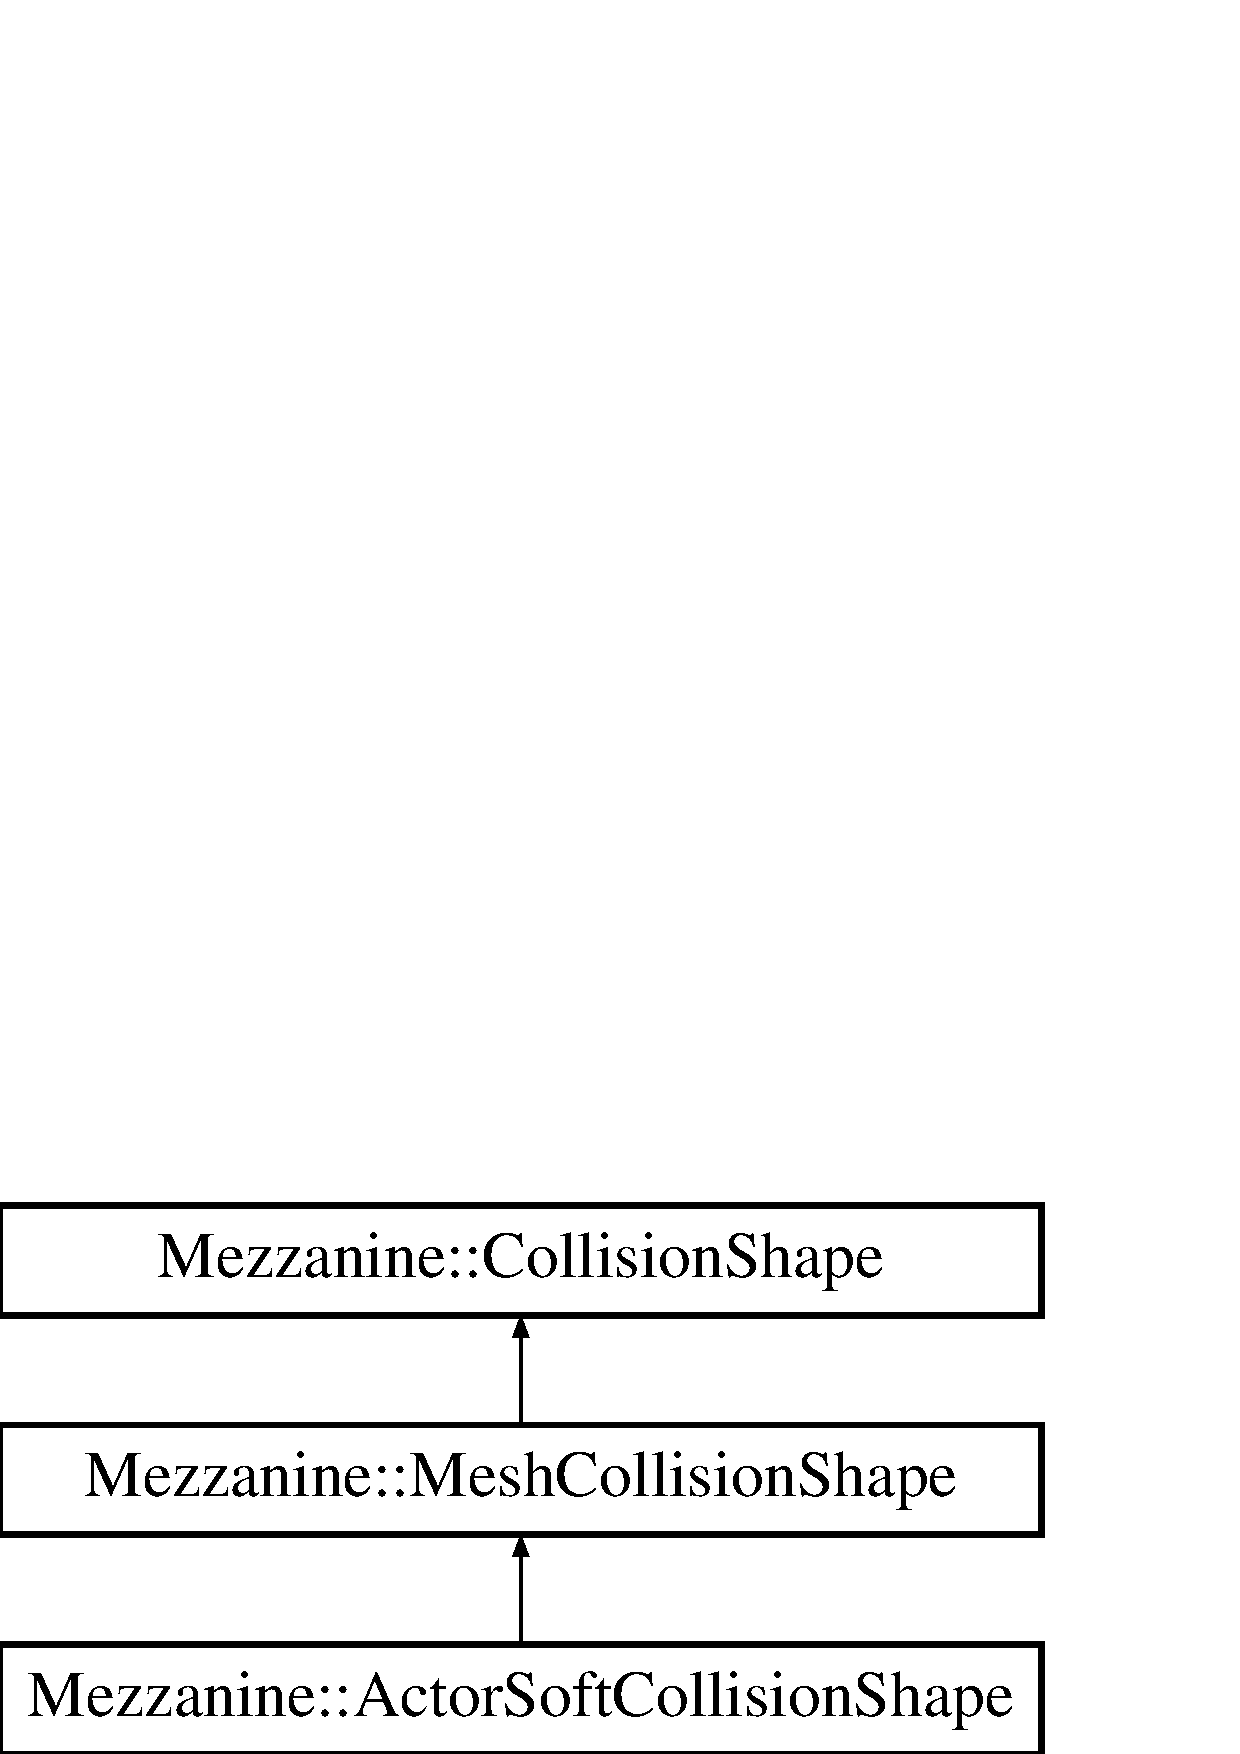
\includegraphics[height=3.000000cm]{classMezzanine_1_1ActorSoftCollisionShape}
\end{center}
\end{figure}
\subsubsection*{Public Member Functions}
\begin{DoxyCompactItemize}
\item 
\hyperlink{classMezzanine_1_1ActorSoftCollisionShape_abf4ea33ed056afcac18a41366fedccc1}{ActorSoftCollisionShape} (const \hyperlink{namespaceMezzanine_acf9fcc130e6ebf08e3d8491aebcf1c86}{String} \&\hyperlink{classMezzanine_1_1CollisionShape_aac524c5c56fa4d158bc071f8aecfbe79}{Name}, btSoftBodyCollisionShape $\ast$BulletShape)
\begin{DoxyCompactList}\small\item\em Internal Constructor. \item\end{DoxyCompactList}\item 
virtual \hyperlink{classMezzanine_1_1CollisionShape_ad04186055565998879b64176d6dd100d}{CollisionShape::ShapeType} \hyperlink{classMezzanine_1_1ActorSoftCollisionShape_ae9ac8413434ff0de10376deb64ab49d0}{GetType} () const 
\item 
\hypertarget{classMezzanine_1_1ActorSoftCollisionShape_aba997fd9f65ace81db3779a952eba27e}{
virtual \hyperlink{classMezzanine_1_1ActorSoftCollisionShape_aba997fd9f65ace81db3779a952eba27e}{$\sim$ActorSoftCollisionShape} ()}
\label{classMezzanine_1_1ActorSoftCollisionShape_aba997fd9f65ace81db3779a952eba27e}

\begin{DoxyCompactList}\small\item\em Class Destructor. \item\end{DoxyCompactList}\end{DoxyCompactItemize}
\subsubsection*{Protected Attributes}
\begin{DoxyCompactItemize}
\item 
\hypertarget{classMezzanine_1_1ActorSoftCollisionShape_a24063a3fbeb194cb17f22c8ef78c7bcb}{
btSoftBodyCollisionShape $\ast$ {\bfseries ActorSoftShape}}
\label{classMezzanine_1_1ActorSoftCollisionShape_a24063a3fbeb194cb17f22c8ef78c7bcb}

\end{DoxyCompactItemize}


\subsubsection{Detailed Description}
A collision shape for soft actors. This collision shape is different from all the other collision shapes because it's meant to be used for only one type of object: ActorSoft's. This shape doesn't use triangles in the traditional manner other mesh shapes do, but rather it uses the individual internal nodes that make the \hyperlink{classMezzanine_1_1ActorSoft}{ActorSoft} as points for building triangles to process collisions with. As a result a SoftBodyCollisionShape should never be reused and should be kept unique to the Actor it applies to. \par
 \par
 Normally the \hyperlink{classMezzanine_1_1ActorSoft}{ActorSoft} will be responsible for the creation of it's own collision shape, so the user should never have to. So there are no non-\/internal constructors provided for this class. 

Definition at line 927 of file collisionshape.h.



\subsubsection{Constructor \& Destructor Documentation}
\hypertarget{classMezzanine_1_1ActorSoftCollisionShape_abf4ea33ed056afcac18a41366fedccc1}{
\index{Mezzanine::ActorSoftCollisionShape@{Mezzanine::ActorSoftCollisionShape}!ActorSoftCollisionShape@{ActorSoftCollisionShape}}
\index{ActorSoftCollisionShape@{ActorSoftCollisionShape}!Mezzanine::ActorSoftCollisionShape@{Mezzanine::ActorSoftCollisionShape}}
\paragraph[{ActorSoftCollisionShape}]{\setlength{\rightskip}{0pt plus 5cm}Mezzanine::ActorSoftCollisionShape::ActorSoftCollisionShape (
\begin{DoxyParamCaption}
\item[{const {\bf String} \&}]{Name, }
\item[{btSoftBodyCollisionShape $\ast$}]{BulletShape}
\end{DoxyParamCaption}
)}\hfill}
\label{classMezzanine_1_1ActorSoftCollisionShape_abf4ea33ed056afcac18a41366fedccc1}


Internal Constructor. 


\begin{DoxyParams}{Parameters}
{\em Name} & The name of this Shape. \\
\hline
{\em BulletShape} & The internal shape this shape is based on. \\
\hline
\end{DoxyParams}


Definition at line 1560 of file collisionshape.cpp.



\subsubsection{Member Function Documentation}
\hypertarget{classMezzanine_1_1ActorSoftCollisionShape_ae9ac8413434ff0de10376deb64ab49d0}{
\index{Mezzanine::ActorSoftCollisionShape@{Mezzanine::ActorSoftCollisionShape}!GetType@{GetType}}
\index{GetType@{GetType}!Mezzanine::ActorSoftCollisionShape@{Mezzanine::ActorSoftCollisionShape}}
\paragraph[{GetType}]{\setlength{\rightskip}{0pt plus 5cm}{\bf CollisionShape::ShapeType} Mezzanine::ActorSoftCollisionShape::GetType (
\begin{DoxyParamCaption}
{}
\end{DoxyParamCaption}
) const\hspace{0.3cm}{\ttfamily  \mbox{[}virtual\mbox{]}}}\hfill}
\label{classMezzanine_1_1ActorSoftCollisionShape_ae9ac8413434ff0de10376deb64ab49d0}
Gets the type of \hyperlink{classMezzanine_1_1Collision}{Collision} shape this is. 

\begin{DoxyReturn}{Returns}
Returns an enum value indicating the type of collision shape this is. 
\end{DoxyReturn}
 

Implements \hyperlink{classMezzanine_1_1MeshCollisionShape_a00dc444afac92030ea43815ec21dd8e8}{Mezzanine::MeshCollisionShape}.



Definition at line 1572 of file collisionshape.cpp.



The documentation for this class was generated from the following files:\begin{DoxyCompactItemize}
\item 
collisionshape.h\item 
collisionshape.cpp\end{DoxyCompactItemize}

\hypertarget{classMezzanine_1_1ActorSoftPhysicsSettings}{
\subsection{Mezzanine::ActorSoftPhysicsSettings Class Reference}
\label{classMezzanine_1_1ActorSoftPhysicsSettings}\index{Mezzanine::ActorSoftPhysicsSettings@{Mezzanine::ActorSoftPhysicsSettings}}
}


This is a helper class for configuring physics settings of an \hyperlink{classMezzanine_1_1ActorSoft}{ActorSoft}.  




{\ttfamily \#include $<$actorphysicssettings.h$>$}

Inheritance diagram for Mezzanine::ActorSoftPhysicsSettings:\begin{figure}[H]
\begin{center}
\leavevmode
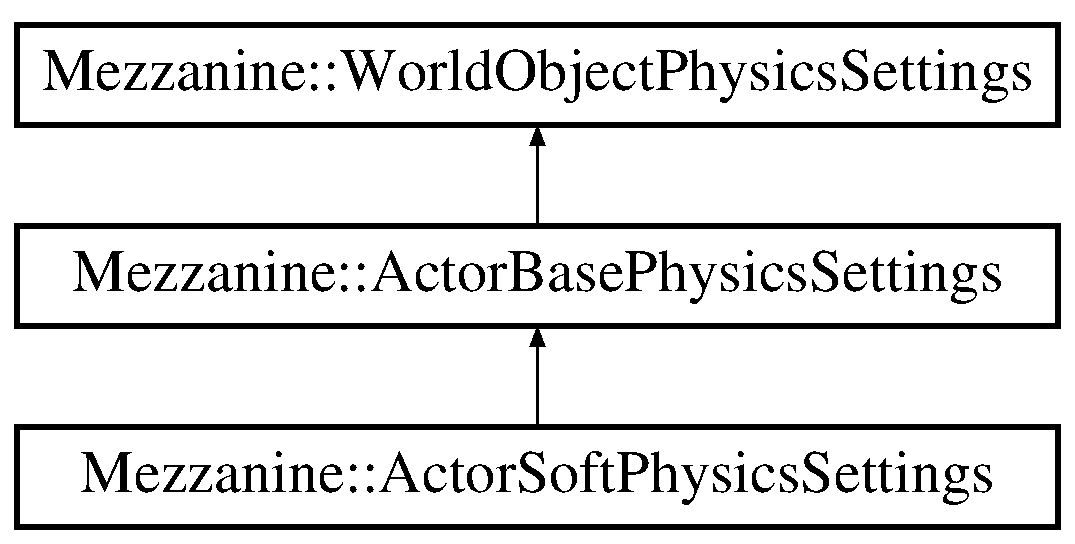
\includegraphics[height=4.000000cm]{classMezzanine_1_1ActorSoftPhysicsSettings}
\end{center}
\end{figure}
\subsubsection*{Public Member Functions}
\begin{DoxyCompactItemize}
\item 
\hyperlink{classMezzanine_1_1ActorSoftPhysicsSettings_a1dbdd3a7b8af36cb8353a1af90102073}{ActorSoftPhysicsSettings} (\hyperlink{classMezzanine_1_1ActorSoft}{ActorSoft} $\ast$Actor, btSoftBody $\ast$PhysicsObject)
\begin{DoxyCompactList}\small\item\em Standard Constructor. \item\end{DoxyCompactList}\item 
\hypertarget{classMezzanine_1_1ActorSoftPhysicsSettings_a9bd95e4279191ab50e5d60ad4ec07817}{
virtual \hyperlink{classMezzanine_1_1ActorSoftPhysicsSettings_a9bd95e4279191ab50e5d60ad4ec07817}{$\sim$ActorSoftPhysicsSettings} ()}
\label{classMezzanine_1_1ActorSoftPhysicsSettings_a9bd95e4279191ab50e5d60ad4ec07817}

\begin{DoxyCompactList}\small\item\em Class destructor. \item\end{DoxyCompactList}\item 
virtual void \hyperlink{classMezzanine_1_1ActorSoftPhysicsSettings_a4cbaf52fbdedf9c4e0328d3dd608207e}{SetCollisionShape} (\hyperlink{classMezzanine_1_1CollisionShape}{CollisionShape} $\ast$Shape)
\begin{DoxyCompactList}\small\item\em Sets the collision shape to be used. \item\end{DoxyCompactList}\end{DoxyCompactItemize}
\subsubsection*{Protected Attributes}
\begin{DoxyCompactItemize}
\item 
\hypertarget{classMezzanine_1_1ActorSoftPhysicsSettings_a44408487d6458ee64320be6d1283c1c0}{
btSoftBody $\ast$ \hyperlink{classMezzanine_1_1ActorSoftPhysicsSettings_a44408487d6458ee64320be6d1283c1c0}{ActorSB}}
\label{classMezzanine_1_1ActorSoftPhysicsSettings_a44408487d6458ee64320be6d1283c1c0}

\begin{DoxyCompactList}\small\item\em Physics Object of the actor. \item\end{DoxyCompactList}\item 
\hypertarget{classMezzanine_1_1ActorSoftPhysicsSettings_aa895658bc511f318b4a31234823d3e5c}{
\hyperlink{classMezzanine_1_1ActorSoft}{ActorSoft} $\ast$ \hyperlink{classMezzanine_1_1ActorSoftPhysicsSettings_aa895658bc511f318b4a31234823d3e5c}{SoftParent}}
\label{classMezzanine_1_1ActorSoftPhysicsSettings_aa895658bc511f318b4a31234823d3e5c}

\begin{DoxyCompactList}\small\item\em The Actor this belongs to. \item\end{DoxyCompactList}\end{DoxyCompactItemize}


\subsubsection{Detailed Description}
This is a helper class for configuring physics settings of an \hyperlink{classMezzanine_1_1ActorSoft}{ActorSoft}. This class contains functions for the configuring of physics specific settings of an \hyperlink{classMezzanine_1_1ActorSoft}{ActorSoft}. This class can only configure the ActorSofts physics. For configuring actor graphics, see ActorGraphicsSettings. 

Definition at line 302 of file actorphysicssettings.h.



\subsubsection{Constructor \& Destructor Documentation}
\hypertarget{classMezzanine_1_1ActorSoftPhysicsSettings_a1dbdd3a7b8af36cb8353a1af90102073}{
\index{Mezzanine::ActorSoftPhysicsSettings@{Mezzanine::ActorSoftPhysicsSettings}!ActorSoftPhysicsSettings@{ActorSoftPhysicsSettings}}
\index{ActorSoftPhysicsSettings@{ActorSoftPhysicsSettings}!Mezzanine::ActorSoftPhysicsSettings@{Mezzanine::ActorSoftPhysicsSettings}}
\paragraph[{ActorSoftPhysicsSettings}]{\setlength{\rightskip}{0pt plus 5cm}Mezzanine::ActorSoftPhysicsSettings::ActorSoftPhysicsSettings (
\begin{DoxyParamCaption}
\item[{{\bf ActorSoft} $\ast$}]{Actor, }
\item[{btSoftBody $\ast$}]{PhysicsObject}
\end{DoxyParamCaption}
)}\hfill}
\label{classMezzanine_1_1ActorSoftPhysicsSettings_a1dbdd3a7b8af36cb8353a1af90102073}


Standard Constructor. 


\begin{DoxyParams}{Parameters}
{\em Actor} & The actor this settings class configures. \\
\hline
{\em PhysicsObject} & The physics object belonging to the actor this class configures. \\
\hline
\end{DoxyParams}


Definition at line 464 of file actorphysicssettings.cpp.



\subsubsection{Member Function Documentation}
\hypertarget{classMezzanine_1_1ActorSoftPhysicsSettings_a4cbaf52fbdedf9c4e0328d3dd608207e}{
\index{Mezzanine::ActorSoftPhysicsSettings@{Mezzanine::ActorSoftPhysicsSettings}!SetCollisionShape@{SetCollisionShape}}
\index{SetCollisionShape@{SetCollisionShape}!Mezzanine::ActorSoftPhysicsSettings@{Mezzanine::ActorSoftPhysicsSettings}}
\paragraph[{SetCollisionShape}]{\setlength{\rightskip}{0pt plus 5cm}void Mezzanine::ActorSoftPhysicsSettings::SetCollisionShape (
\begin{DoxyParamCaption}
\item[{{\bf CollisionShape} $\ast$}]{Shape}
\end{DoxyParamCaption}
)\hspace{0.3cm}{\ttfamily  \mbox{[}virtual\mbox{]}}}\hfill}
\label{classMezzanine_1_1ActorSoftPhysicsSettings_a4cbaf52fbdedf9c4e0328d3dd608207e}


Sets the collision shape to be used. 


\begin{DoxyParams}{Parameters}
{\em Shape} & The shape to be applied. \\
\hline
\end{DoxyParams}


Reimplemented from \hyperlink{classMezzanine_1_1WorldObjectPhysicsSettings_ae8b786e26eed334b283156b442807039}{Mezzanine::WorldObjectPhysicsSettings}.



Definition at line 477 of file actorphysicssettings.cpp.



The documentation for this class was generated from the following files:\begin{DoxyCompactItemize}
\item 
actorphysicssettings.h\item 
actorphysicssettings.cpp\end{DoxyCompactItemize}

\hypertarget{classMezzanine_1_1AreaEffect}{
\subsection{Mezzanine::AreaEffect Class Reference}
\label{classMezzanine_1_1AreaEffect}\index{Mezzanine::AreaEffect@{Mezzanine::AreaEffect}}
}


This class is used to define area's in the world that have unique effects.  




{\ttfamily \#include $<$areaeffect.h$>$}

Inheritance diagram for Mezzanine::AreaEffect:\begin{figure}[H]
\begin{center}
\leavevmode
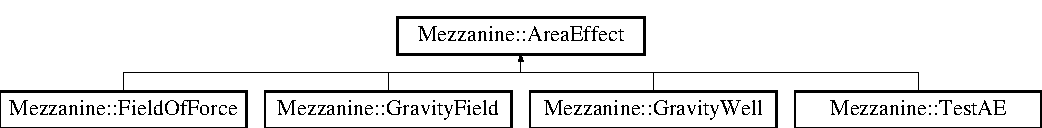
\includegraphics[height=1.717791cm]{classMezzanine_1_1AreaEffect}
\end{center}
\end{figure}
\subsubsection*{Public Member Functions}
\begin{DoxyCompactItemize}
\item 
virtual void \hyperlink{classMezzanine_1_1AreaEffect_a988cd958e49d65331a059951af3c2884}{ApplyEffect} ()=0
\begin{DoxyCompactList}\small\item\em Defines and applies the effect of the field. \item\end{DoxyCompactList}\item 
\hyperlink{classMezzanine_1_1AreaEffect_a2b2699c0baff3ed6eb6e19f2e7d23d7c}{AreaEffect} (const \hyperlink{namespaceMezzanine_acf9fcc130e6ebf08e3d8491aebcf1c86}{String} \&name, const \hyperlink{classMezzanine_1_1Vector3}{Vector3} \&Location)
\begin{DoxyCompactList}\small\item\em Constructor. \item\end{DoxyCompactList}\item 
virtual std::vector$<$ \hyperlink{classMezzanine_1_1ActorBase}{ActorBase} $\ast$ $>$ \& \hyperlink{classMezzanine_1_1AreaEffect_ac349f091e923cbb92740aaa35f2f5c2e}{GetAddedActors} ()
\begin{DoxyCompactList}\small\item\em Gets the list of actors that have been added to the list since the last simulation step. \item\end{DoxyCompactList}\item 
virtual \hyperlink{classMezzanine_1_1Mesh}{Mesh} $\ast$ \hyperlink{classMezzanine_1_1AreaEffect_a1406441f5c12072dc0a6178a2690f3a6}{GetFieldMesh} () const 
\begin{DoxyCompactList}\small\item\em Gets the mesh being used by this \hyperlink{classMezzanine_1_1AreaEffect}{AreaEffect}. \item\end{DoxyCompactList}\item 
virtual \hyperlink{classMezzanine_1_1CollisionShape}{CollisionShape} $\ast$ \hyperlink{classMezzanine_1_1AreaEffect_a2204a7b0f004778bb27f38d65fa9e4df}{GetFieldShape} () const 
\begin{DoxyCompactList}\small\item\em Gets the current shape of the \hyperlink{classMezzanine_1_1AreaEffect}{AreaEffect}. \item\end{DoxyCompactList}\item 
virtual \hyperlink{classMezzanine_1_1Vector3}{Vector3} \hyperlink{classMezzanine_1_1AreaEffect_a7e80ddc1cb411012d80a99859bb865f7}{GetFieldShapeScale} () const 
\begin{DoxyCompactList}\small\item\em Gets the scale of the shape of the field. \item\end{DoxyCompactList}\item 
virtual \hyperlink{classMezzanine_1_1Vector3}{Vector3} \hyperlink{classMezzanine_1_1AreaEffect_a37d04f8e6d6e8451348ee60fd083968b}{GetLocation} () const 
\begin{DoxyCompactList}\small\item\em Gets the origin for the area effect. \item\end{DoxyCompactList}\item 
virtual \hyperlink{namespaceMezzanine_a63cd699ac54b73953f35ec9cfc05e506}{ConstString} \& \hyperlink{classMezzanine_1_1AreaEffect_ae0205e57786da97300357d7ac1afd180}{GetName} () const 
\begin{DoxyCompactList}\small\item\em Gets the Area Effects name. \item\end{DoxyCompactList}\item 
virtual \hyperlink{classMezzanine_1_1Quaternion}{Quaternion} \hyperlink{classMezzanine_1_1AreaEffect_a658d69036a307f232b88aafcab3d02c1}{GetOrientation} ()
\begin{DoxyCompactList}\small\item\em Gets the orientation of the area effect. \item\end{DoxyCompactList}\item 
virtual std::list$<$ \hyperlink{classMezzanine_1_1ActorBase}{ActorBase} $\ast$ $>$ \& \hyperlink{classMezzanine_1_1AreaEffect_a69f19ed2d67dca2623df6e6331b31462}{GetOverlappingActors} ()
\begin{DoxyCompactList}\small\item\em Gets the list of actors within this field. \item\end{DoxyCompactList}\item 
virtual std::vector$<$ \hyperlink{classMezzanine_1_1ActorBase}{ActorBase} $\ast$ $>$ \& \hyperlink{classMezzanine_1_1AreaEffect_ac657b565ca47198c6fd900c8a588948b}{GetRemovedActors} ()
\begin{DoxyCompactList}\small\item\em Gets the list of actors that have been removed from the list since the last simulation step. \item\end{DoxyCompactList}\item 
virtual bool \hyperlink{classMezzanine_1_1AreaEffect_aee16d398d7788f6e0fd5e597bcdbd106}{IsInWorld} () const 
\begin{DoxyCompactList}\small\item\em Checks to see if the ghost object is currently in the world. \item\end{DoxyCompactList}\item 
virtual bool \hyperlink{classMezzanine_1_1AreaEffect_a9b2c07dd426285aff44d5faaca4b3356}{IsStatic} () const 
\begin{DoxyCompactList}\small\item\em Gets whether or not this AR is static. \item\end{DoxyCompactList}\item 
virtual void \hyperlink{classMezzanine_1_1AreaEffect_aac92fc4ba682d509f6385e999f68c75d}{ScaleFieldShape} (const \hyperlink{classMezzanine_1_1Vector3}{Vector3} \&Scale)
\begin{DoxyCompactList}\small\item\em Sets the scale of the shape of the field. \item\end{DoxyCompactList}\item 
virtual void \hyperlink{classMezzanine_1_1AreaEffect_aa9e8a5e1ffee5aa11ab4958373b06f09}{SetFieldMesh} (\hyperlink{classMezzanine_1_1Mesh}{Mesh} $\ast$\hyperlink{classMezzanine_1_1AreaEffect_a5ca3984a40d2678b786f518667fde27f}{FieldMesh})
\begin{DoxyCompactList}\small\item\em Sets the mesh to be used along with this \hyperlink{classMezzanine_1_1AreaEffect}{AreaEffect}. \item\end{DoxyCompactList}\item 
virtual void \hyperlink{classMezzanine_1_1AreaEffect_a5e2902749c630af5272d2dc89678392c}{SetFieldMesh} (const \hyperlink{namespaceMezzanine_acf9fcc130e6ebf08e3d8491aebcf1c86}{String} \&MeshName, const \hyperlink{namespaceMezzanine_acf9fcc130e6ebf08e3d8491aebcf1c86}{String} \&Group)
\begin{DoxyCompactList}\small\item\em Sets the mesh to be used along with this \hyperlink{classMezzanine_1_1AreaEffect}{AreaEffect}. \item\end{DoxyCompactList}\item 
virtual void \hyperlink{classMezzanine_1_1AreaEffect_a759a0a5f4becf94c87aff85b0681f663}{SetFieldShape} (\hyperlink{classMezzanine_1_1CollisionShape}{CollisionShape} $\ast$\hyperlink{classMezzanine_1_1AreaEffect_a54f08718bc742934f2ef6b4bd978c9d2}{FieldShape})
\begin{DoxyCompactList}\small\item\em Sets the shape of this \hyperlink{classMezzanine_1_1AreaEffect}{AreaEffect}. \item\end{DoxyCompactList}\item 
virtual void \hyperlink{classMezzanine_1_1AreaEffect_a4dd22757bc627242de169e31a1717139}{SetLocation} (const \hyperlink{classMezzanine_1_1Vector3}{Vector3} \&Location)
\begin{DoxyCompactList}\small\item\em Sets the origin for the area effect. \item\end{DoxyCompactList}\item 
virtual void \hyperlink{classMezzanine_1_1AreaEffect_a62bcda0a0c2a95b8f1ccdfe2cd3d1018}{SetOrientation} (const \hyperlink{classMezzanine_1_1Quaternion}{Quaternion} \&Rotation)
\begin{DoxyCompactList}\small\item\em Sets the orientation of the area effect. \item\end{DoxyCompactList}\item 
virtual void \hyperlink{classMezzanine_1_1AreaEffect_adfecf112bad175a57cdf147cb0d0aaa8}{SetStatic} (bool Static)
\begin{DoxyCompactList}\small\item\em Sets(or un-\/sets) this AE as a static object. \item\end{DoxyCompactList}\item 
virtual void \hyperlink{classMezzanine_1_1AreaEffect_aee19befcb794b85f13da4e427c2be42d}{UpdateActorList} ()
\begin{DoxyCompactList}\small\item\em Updates the actors listed as within the field. \item\end{DoxyCompactList}\item 
virtual \hyperlink{classMezzanine_1_1AreaEffect_a1e825ce1dcb2d78c190b17d7bff7306c}{$\sim$AreaEffect} ()
\begin{DoxyCompactList}\small\item\em Destructor. \item\end{DoxyCompactList}\end{DoxyCompactItemize}
\subsubsection*{Protected Member Functions}
\begin{DoxyCompactItemize}
\item 
\hypertarget{classMezzanine_1_1AreaEffect_a4a81d9d5920f375aa9a5ff27c1de97e0}{
virtual void \hyperlink{classMezzanine_1_1AreaEffect_a4a81d9d5920f375aa9a5ff27c1de97e0}{AddActorToList} (\hyperlink{classMezzanine_1_1ActorBase}{ActorBase} $\ast$Actor)}
\label{classMezzanine_1_1AreaEffect_a4a81d9d5920f375aa9a5ff27c1de97e0}

\begin{DoxyCompactList}\small\item\em Helper function for adding actors to relevant lists. \item\end{DoxyCompactList}\item 
virtual void \hyperlink{classMezzanine_1_1AreaEffect_a198ad58cec706d508785cbd8e319ba54}{CreateGhostObject} (const \hyperlink{classMezzanine_1_1Vector3}{Vector3} \&Location)
\begin{DoxyCompactList}\small\item\em Constructor Function. \item\end{DoxyCompactList}\item 
\hypertarget{classMezzanine_1_1AreaEffect_ae6d32d28fbe74eec48eaf3f7b5550c1c}{
virtual void \hyperlink{classMezzanine_1_1AreaEffect_ae6d32d28fbe74eec48eaf3f7b5550c1c}{PreGraphicsMeshCreate} ()}
\label{classMezzanine_1_1AreaEffect_ae6d32d28fbe74eec48eaf3f7b5550c1c}

\begin{DoxyCompactList}\small\item\em Convenience function for the common starting steps in making a graphics object. \item\end{DoxyCompactList}\item 
\hypertarget{classMezzanine_1_1AreaEffect_a676a36ba3fb8b0d7ced951f1b5010852}{
virtual void \hyperlink{classMezzanine_1_1AreaEffect_a676a36ba3fb8b0d7ced951f1b5010852}{RemoveActorFromList} (\hyperlink{classMezzanine_1_1ActorBase}{ActorBase} $\ast$Actor)}
\label{classMezzanine_1_1AreaEffect_a676a36ba3fb8b0d7ced951f1b5010852}

\begin{DoxyCompactList}\small\item\em Helper function for adding actors to relevant lists. \item\end{DoxyCompactList}\end{DoxyCompactItemize}
\subsubsection*{Protected Attributes}
\begin{DoxyCompactItemize}
\item 
\hypertarget{classMezzanine_1_1AreaEffect_a9a7e333c5e52fd5d7ae892f4691dbc16}{
std::vector$<$ \hyperlink{classMezzanine_1_1ActorBase}{ActorBase} $\ast$ $>$ \hyperlink{classMezzanine_1_1AreaEffect_a9a7e333c5e52fd5d7ae892f4691dbc16}{AddedActors}}
\label{classMezzanine_1_1AreaEffect_a9a7e333c5e52fd5d7ae892f4691dbc16}

\begin{DoxyCompactList}\small\item\em Container of actors that have been added since last frame. \item\end{DoxyCompactList}\item 
\hypertarget{classMezzanine_1_1AreaEffect_a5ca3984a40d2678b786f518667fde27f}{
\hyperlink{classMezzanine_1_1Mesh}{Mesh} $\ast$ \hyperlink{classMezzanine_1_1AreaEffect_a5ca3984a40d2678b786f518667fde27f}{FieldMesh}}
\label{classMezzanine_1_1AreaEffect_a5ca3984a40d2678b786f518667fde27f}

\begin{DoxyCompactList}\small\item\em Stores the mesh of the AR field. \item\end{DoxyCompactList}\item 
\hypertarget{classMezzanine_1_1AreaEffect_a54f08718bc742934f2ef6b4bd978c9d2}{
\hyperlink{classMezzanine_1_1CollisionShape}{CollisionShape} $\ast$ \hyperlink{classMezzanine_1_1AreaEffect_a54f08718bc742934f2ef6b4bd978c9d2}{FieldShape}}
\label{classMezzanine_1_1AreaEffect_a54f08718bc742934f2ef6b4bd978c9d2}

\begin{DoxyCompactList}\small\item\em Stores the shape of the AE field. \item\end{DoxyCompactList}\item 
\hypertarget{classMezzanine_1_1AreaEffect_a16427c9805ea4c87faa84715ec04f97d}{
btPairCachingGhostObject $\ast$ \hyperlink{classMezzanine_1_1AreaEffect_a16427c9805ea4c87faa84715ec04f97d}{Ghost}}
\label{classMezzanine_1_1AreaEffect_a16427c9805ea4c87faa84715ec04f97d}

\begin{DoxyCompactList}\small\item\em The object representing the AE field itself. \item\end{DoxyCompactList}\item 
\hypertarget{classMezzanine_1_1AreaEffect_a6f025b9cd2ff505618eeaf6640319ab9}{
Ogre::SceneNode $\ast$ \hyperlink{classMezzanine_1_1AreaEffect_a6f025b9cd2ff505618eeaf6640319ab9}{GraphicsNode}}
\label{classMezzanine_1_1AreaEffect_a6f025b9cd2ff505618eeaf6640319ab9}

\begin{DoxyCompactList}\small\item\em Ogre node required to adding a graohical representation to the scene graph. \item\end{DoxyCompactList}\item 
\hypertarget{classMezzanine_1_1AreaEffect_a673167414883d918da6fb57f340e850e}{
Ogre::Entity $\ast$ \hyperlink{classMezzanine_1_1AreaEffect_a673167414883d918da6fb57f340e850e}{GraphicsObject}}
\label{classMezzanine_1_1AreaEffect_a673167414883d918da6fb57f340e850e}

\begin{DoxyCompactList}\small\item\em The Ogre object being added to the scene graph. \item\end{DoxyCompactList}\item 
\hypertarget{classMezzanine_1_1AreaEffect_ad2b27c925a2eaa40fe03db4205f3de39}{
\hyperlink{namespaceMezzanine_acf9fcc130e6ebf08e3d8491aebcf1c86}{String} \hyperlink{classMezzanine_1_1AreaEffect_ad2b27c925a2eaa40fe03db4205f3de39}{Name}}
\label{classMezzanine_1_1AreaEffect_ad2b27c925a2eaa40fe03db4205f3de39}

\begin{DoxyCompactList}\small\item\em The name of the Area Effect. \item\end{DoxyCompactList}\item 
\hypertarget{classMezzanine_1_1AreaEffect_a9a1dbe79efda62adad5f56b5f93813ca}{
std::list$<$ \hyperlink{classMezzanine_1_1ActorBase}{ActorBase} $\ast$ $>$ \hyperlink{classMezzanine_1_1AreaEffect_a9a1dbe79efda62adad5f56b5f93813ca}{OverlappingActors}}
\label{classMezzanine_1_1AreaEffect_a9a1dbe79efda62adad5f56b5f93813ca}

\begin{DoxyCompactList}\small\item\em Container for actors within the field area. \item\end{DoxyCompactList}\item 
\hypertarget{classMezzanine_1_1AreaEffect_adaab6a94b9c4a9cfdb917ff4ce3fcabf}{
std::vector$<$ \hyperlink{classMezzanine_1_1ActorBase}{ActorBase} $\ast$ $>$ \hyperlink{classMezzanine_1_1AreaEffect_adaab6a94b9c4a9cfdb917ff4ce3fcabf}{RemovedActors}}
\label{classMezzanine_1_1AreaEffect_adaab6a94b9c4a9cfdb917ff4ce3fcabf}

\begin{DoxyCompactList}\small\item\em Container of actors that have been removed since last frame. \item\end{DoxyCompactList}\item 
\hypertarget{classMezzanine_1_1AreaEffect_acefbfa896daea1dfa41fb31fa65db01d}{
\hyperlink{classMezzanine_1_1World}{World} $\ast$ \hyperlink{classMezzanine_1_1AreaEffect_acefbfa896daea1dfa41fb31fa65db01d}{TheWorld}}
\label{classMezzanine_1_1AreaEffect_acefbfa896daea1dfa41fb31fa65db01d}

\begin{DoxyCompactList}\small\item\em \hyperlink{classMezzanine_1_1World}{World} pointer simply to enable the effects of this class to be as diverse as the engine features. \item\end{DoxyCompactList}\end{DoxyCompactItemize}
\subsubsection*{Friends}
\begin{DoxyCompactItemize}
\item 
\hypertarget{classMezzanine_1_1AreaEffect_a139cf05ac01161b7071c8a037c841683}{
class {\bfseries PhysicsManager}}
\label{classMezzanine_1_1AreaEffect_a139cf05ac01161b7071c8a037c841683}

\end{DoxyCompactItemize}


\subsubsection{Detailed Description}
This class is used to define area's in the world that have unique effects. Common uses for this class are for gravity fields, and explosions. But can be made to do more. \par
 Note: This is a base class intended to be derived from. This class cannot be created itself. To make an \hyperlink{classMezzanine_1_1AreaEffect}{AreaEffect} class that does what you want it to, simple inherit from this class with an AE class of your own, and define the \hyperlink{classMezzanine_1_1AreaEffect_a988cd958e49d65331a059951af3c2884}{ApplyEffect()} function to do what you want your effect to do. 

Definition at line 77 of file areaeffect.h.



\subsubsection{Constructor \& Destructor Documentation}
\hypertarget{classMezzanine_1_1AreaEffect_a2b2699c0baff3ed6eb6e19f2e7d23d7c}{
\index{Mezzanine::AreaEffect@{Mezzanine::AreaEffect}!AreaEffect@{AreaEffect}}
\index{AreaEffect@{AreaEffect}!Mezzanine::AreaEffect@{Mezzanine::AreaEffect}}
\paragraph[{AreaEffect}]{\setlength{\rightskip}{0pt plus 5cm}home sqeaky physgame Mezzanine src areaeffect cpp Mezzanine::AreaEffect::AreaEffect (
\begin{DoxyParamCaption}
\item[{const {\bf String} \&}]{name, }
\item[{const {\bf Vector3} \&}]{Location}
\end{DoxyParamCaption}
)}\hfill}
\label{classMezzanine_1_1AreaEffect_a2b2699c0baff3ed6eb6e19f2e7d23d7c}


Constructor. 

Basic initialization constructor. 
\begin{DoxyParams}{Parameters}
{\em name} & The name of the field. \\
\hline
{\em Location} & The location of the AE field. \\
\hline
\end{DoxyParams}


Definition at line 66 of file areaeffect.cpp.

\hypertarget{classMezzanine_1_1AreaEffect_a1e825ce1dcb2d78c190b17d7bff7306c}{
\index{Mezzanine::AreaEffect@{Mezzanine::AreaEffect}!$\sim$AreaEffect@{$\sim$AreaEffect}}
\index{$\sim$AreaEffect@{$\sim$AreaEffect}!Mezzanine::AreaEffect@{Mezzanine::AreaEffect}}
\paragraph[{$\sim$AreaEffect}]{\setlength{\rightskip}{0pt plus 5cm}Mezzanine::AreaEffect::$\sim$AreaEffect (
\begin{DoxyParamCaption}
{}
\end{DoxyParamCaption}
)\hspace{0.3cm}{\ttfamily  \mbox{[}virtual\mbox{]}}}\hfill}
\label{classMezzanine_1_1AreaEffect_a1e825ce1dcb2d78c190b17d7bff7306c}


Destructor. 

Class destructor. 

Definition at line 77 of file areaeffect.cpp.



\subsubsection{Member Function Documentation}
\hypertarget{classMezzanine_1_1AreaEffect_a988cd958e49d65331a059951af3c2884}{
\index{Mezzanine::AreaEffect@{Mezzanine::AreaEffect}!ApplyEffect@{ApplyEffect}}
\index{ApplyEffect@{ApplyEffect}!Mezzanine::AreaEffect@{Mezzanine::AreaEffect}}
\paragraph[{ApplyEffect}]{\setlength{\rightskip}{0pt plus 5cm}virtual void Mezzanine::AreaEffect::ApplyEffect (
\begin{DoxyParamCaption}
{}
\end{DoxyParamCaption}
)\hspace{0.3cm}{\ttfamily  \mbox{[}pure virtual\mbox{]}}}\hfill}
\label{classMezzanine_1_1AreaEffect_a988cd958e49d65331a059951af3c2884}


Defines and applies the effect of the field. 

When inheriting this class, this function is what defines the effect the field has. \par
 This function will be called on by the physics manager and shouldn't be called manually. 

Implemented in \hyperlink{classMezzanine_1_1TestAE_a647737a517fb6c87489afc93b9daa91c}{Mezzanine::TestAE}, \hyperlink{classMezzanine_1_1GravityField_a53aee6679088fb6151e5cb6e82a09fb7}{Mezzanine::GravityField}, \hyperlink{classMezzanine_1_1GravityWell_a193e1683edaf80bb1a37979f196abf6e}{Mezzanine::GravityWell}, and \hyperlink{classMezzanine_1_1FieldOfForce_ae82e9a45515d40513ad1ac2e606c627b}{Mezzanine::FieldOfForce}.

\hypertarget{classMezzanine_1_1AreaEffect_a198ad58cec706d508785cbd8e319ba54}{
\index{Mezzanine::AreaEffect@{Mezzanine::AreaEffect}!CreateGhostObject@{CreateGhostObject}}
\index{CreateGhostObject@{CreateGhostObject}!Mezzanine::AreaEffect@{Mezzanine::AreaEffect}}
\paragraph[{CreateGhostObject}]{\setlength{\rightskip}{0pt plus 5cm}void Mezzanine::AreaEffect::CreateGhostObject (
\begin{DoxyParamCaption}
\item[{const {\bf Vector3} \&}]{Location}
\end{DoxyParamCaption}
)\hspace{0.3cm}{\ttfamily  \mbox{[}protected, virtual\mbox{]}}}\hfill}
\label{classMezzanine_1_1AreaEffect_a198ad58cec706d508785cbd8e319ba54}


Constructor Function. 


\begin{DoxyParams}{Parameters}
{\em Location} & The location of the AE field. \\
\hline
\end{DoxyParams}


Definition at line 84 of file areaeffect.cpp.

\hypertarget{classMezzanine_1_1AreaEffect_ac349f091e923cbb92740aaa35f2f5c2e}{
\index{Mezzanine::AreaEffect@{Mezzanine::AreaEffect}!GetAddedActors@{GetAddedActors}}
\index{GetAddedActors@{GetAddedActors}!Mezzanine::AreaEffect@{Mezzanine::AreaEffect}}
\paragraph[{GetAddedActors}]{\setlength{\rightskip}{0pt plus 5cm}std::vector$<$ {\bf ActorBase} $\ast$ $>$ \& Mezzanine::AreaEffect::GetAddedActors (
\begin{DoxyParamCaption}
{}
\end{DoxyParamCaption}
)\hspace{0.3cm}{\ttfamily  \mbox{[}virtual\mbox{]}}}\hfill}
\label{classMezzanine_1_1AreaEffect_ac349f091e923cbb92740aaa35f2f5c2e}


Gets the list of actors that have been added to the list since the last simulation step. 

\begin{DoxyReturn}{Returns}
Returns the vector storing all the actors that have been added to the list since the last simulation step. 
\end{DoxyReturn}


Definition at line 450 of file areaeffect.cpp.

\hypertarget{classMezzanine_1_1AreaEffect_a1406441f5c12072dc0a6178a2690f3a6}{
\index{Mezzanine::AreaEffect@{Mezzanine::AreaEffect}!GetFieldMesh@{GetFieldMesh}}
\index{GetFieldMesh@{GetFieldMesh}!Mezzanine::AreaEffect@{Mezzanine::AreaEffect}}
\paragraph[{GetFieldMesh}]{\setlength{\rightskip}{0pt plus 5cm}{\bf Mesh} $\ast$ Mezzanine::AreaEffect::GetFieldMesh (
\begin{DoxyParamCaption}
{}
\end{DoxyParamCaption}
) const\hspace{0.3cm}{\ttfamily  \mbox{[}virtual\mbox{]}}}\hfill}
\label{classMezzanine_1_1AreaEffect_a1406441f5c12072dc0a6178a2690f3a6}


Gets the mesh being used by this \hyperlink{classMezzanine_1_1AreaEffect}{AreaEffect}. 

\begin{DoxyReturn}{Returns}
Returns a pointer to the mesh being used by this \hyperlink{classMezzanine_1_1AreaEffect}{AreaEffect}, or NULL if none. 
\end{DoxyReturn}


Definition at line 440 of file areaeffect.cpp.

\hypertarget{classMezzanine_1_1AreaEffect_a2204a7b0f004778bb27f38d65fa9e4df}{
\index{Mezzanine::AreaEffect@{Mezzanine::AreaEffect}!GetFieldShape@{GetFieldShape}}
\index{GetFieldShape@{GetFieldShape}!Mezzanine::AreaEffect@{Mezzanine::AreaEffect}}
\paragraph[{GetFieldShape}]{\setlength{\rightskip}{0pt plus 5cm}{\bf CollisionShape} $\ast$ Mezzanine::AreaEffect::GetFieldShape (
\begin{DoxyParamCaption}
{}
\end{DoxyParamCaption}
) const\hspace{0.3cm}{\ttfamily  \mbox{[}virtual\mbox{]}}}\hfill}
\label{classMezzanine_1_1AreaEffect_a2204a7b0f004778bb27f38d65fa9e4df}


Gets the current shape of the \hyperlink{classMezzanine_1_1AreaEffect}{AreaEffect}. 

\begin{DoxyReturn}{Returns}
Returns a pointer to the shape currently being used by this \hyperlink{classMezzanine_1_1AreaEffect}{AreaEffect}. 
\end{DoxyReturn}


Definition at line 344 of file areaeffect.cpp.

\hypertarget{classMezzanine_1_1AreaEffect_a7e80ddc1cb411012d80a99859bb865f7}{
\index{Mezzanine::AreaEffect@{Mezzanine::AreaEffect}!GetFieldShapeScale@{GetFieldShapeScale}}
\index{GetFieldShapeScale@{GetFieldShapeScale}!Mezzanine::AreaEffect@{Mezzanine::AreaEffect}}
\paragraph[{GetFieldShapeScale}]{\setlength{\rightskip}{0pt plus 5cm}{\bf Vector3} Mezzanine::AreaEffect::GetFieldShapeScale (
\begin{DoxyParamCaption}
{}
\end{DoxyParamCaption}
) const\hspace{0.3cm}{\ttfamily  \mbox{[}virtual\mbox{]}}}\hfill}
\label{classMezzanine_1_1AreaEffect_a7e80ddc1cb411012d80a99859bb865f7}


Gets the scale of the shape of the field. 

The default scale is 1.0. \begin{DoxyReturn}{Returns}
Returns the current scale applied to the fields shape. 
\end{DoxyReturn}


Definition at line 354 of file areaeffect.cpp.

\hypertarget{classMezzanine_1_1AreaEffect_a37d04f8e6d6e8451348ee60fd083968b}{
\index{Mezzanine::AreaEffect@{Mezzanine::AreaEffect}!GetLocation@{GetLocation}}
\index{GetLocation@{GetLocation}!Mezzanine::AreaEffect@{Mezzanine::AreaEffect}}
\paragraph[{GetLocation}]{\setlength{\rightskip}{0pt plus 5cm}{\bf Vector3} Mezzanine::AreaEffect::GetLocation (
\begin{DoxyParamCaption}
{}
\end{DoxyParamCaption}
) const\hspace{0.3cm}{\ttfamily  \mbox{[}virtual\mbox{]}}}\hfill}
\label{classMezzanine_1_1AreaEffect_a37d04f8e6d6e8451348ee60fd083968b}


Gets the origin for the area effect. 

This function is particularly useful when making fields such as gravity wells, that have continuous effects centering on one location. \begin{DoxyReturn}{Returns}
Returns the vector3 representing the location of the area effect. 
\end{DoxyReturn}


Definition at line 367 of file areaeffect.cpp.

\hypertarget{classMezzanine_1_1AreaEffect_ae0205e57786da97300357d7ac1afd180}{
\index{Mezzanine::AreaEffect@{Mezzanine::AreaEffect}!GetName@{GetName}}
\index{GetName@{GetName}!Mezzanine::AreaEffect@{Mezzanine::AreaEffect}}
\paragraph[{GetName}]{\setlength{\rightskip}{0pt plus 5cm}{\bf ConstString} \& Mezzanine::AreaEffect::GetName (
\begin{DoxyParamCaption}
{}
\end{DoxyParamCaption}
) const\hspace{0.3cm}{\ttfamily  \mbox{[}virtual\mbox{]}}}\hfill}
\label{classMezzanine_1_1AreaEffect_ae0205e57786da97300357d7ac1afd180}


Gets the Area Effects name. 

\begin{DoxyReturn}{Returns}
Returns the name of the Area Effect. 
\end{DoxyReturn}


Definition at line 386 of file areaeffect.cpp.

\hypertarget{classMezzanine_1_1AreaEffect_a658d69036a307f232b88aafcab3d02c1}{
\index{Mezzanine::AreaEffect@{Mezzanine::AreaEffect}!GetOrientation@{GetOrientation}}
\index{GetOrientation@{GetOrientation}!Mezzanine::AreaEffect@{Mezzanine::AreaEffect}}
\paragraph[{GetOrientation}]{\setlength{\rightskip}{0pt plus 5cm}{\bf Quaternion} Mezzanine::AreaEffect::GetOrientation (
\begin{DoxyParamCaption}
{}
\end{DoxyParamCaption}
)\hspace{0.3cm}{\ttfamily  \mbox{[}virtual\mbox{]}}}\hfill}
\label{classMezzanine_1_1AreaEffect_a658d69036a307f232b88aafcab3d02c1}


Gets the orientation of the area effect. 

\begin{DoxyReturn}{Returns}
Returns a quaternion representing the rotation of the area effect. 
\end{DoxyReturn}


Definition at line 380 of file areaeffect.cpp.

\hypertarget{classMezzanine_1_1AreaEffect_a69f19ed2d67dca2623df6e6331b31462}{
\index{Mezzanine::AreaEffect@{Mezzanine::AreaEffect}!GetOverlappingActors@{GetOverlappingActors}}
\index{GetOverlappingActors@{GetOverlappingActors}!Mezzanine::AreaEffect@{Mezzanine::AreaEffect}}
\paragraph[{GetOverlappingActors}]{\setlength{\rightskip}{0pt plus 5cm}std::list$<$ {\bf ActorBase} $\ast$ $>$ \& Mezzanine::AreaEffect::GetOverlappingActors (
\begin{DoxyParamCaption}
{}
\end{DoxyParamCaption}
)\hspace{0.3cm}{\ttfamily  \mbox{[}virtual\mbox{]}}}\hfill}
\label{classMezzanine_1_1AreaEffect_a69f19ed2d67dca2623df6e6331b31462}


Gets the list of actors within this field. 

\begin{DoxyReturn}{Returns}
Returns the list of actors contained within this field. 
\end{DoxyReturn}


Definition at line 445 of file areaeffect.cpp.

\hypertarget{classMezzanine_1_1AreaEffect_ac657b565ca47198c6fd900c8a588948b}{
\index{Mezzanine::AreaEffect@{Mezzanine::AreaEffect}!GetRemovedActors@{GetRemovedActors}}
\index{GetRemovedActors@{GetRemovedActors}!Mezzanine::AreaEffect@{Mezzanine::AreaEffect}}
\paragraph[{GetRemovedActors}]{\setlength{\rightskip}{0pt plus 5cm}std::vector$<$ {\bf ActorBase} $\ast$ $>$ \& Mezzanine::AreaEffect::GetRemovedActors (
\begin{DoxyParamCaption}
{}
\end{DoxyParamCaption}
)\hspace{0.3cm}{\ttfamily  \mbox{[}virtual\mbox{]}}}\hfill}
\label{classMezzanine_1_1AreaEffect_ac657b565ca47198c6fd900c8a588948b}


Gets the list of actors that have been removed from the list since the last simulation step. 

\begin{DoxyReturn}{Returns}
Returns the vector storing all the actors that have been removed from the list since the last simulation step. 
\end{DoxyReturn}


Definition at line 455 of file areaeffect.cpp.

\hypertarget{classMezzanine_1_1AreaEffect_aee16d398d7788f6e0fd5e597bcdbd106}{
\index{Mezzanine::AreaEffect@{Mezzanine::AreaEffect}!IsInWorld@{IsInWorld}}
\index{IsInWorld@{IsInWorld}!Mezzanine::AreaEffect@{Mezzanine::AreaEffect}}
\paragraph[{IsInWorld}]{\setlength{\rightskip}{0pt plus 5cm}bool Mezzanine::AreaEffect::IsInWorld (
\begin{DoxyParamCaption}
{}
\end{DoxyParamCaption}
) const\hspace{0.3cm}{\ttfamily  \mbox{[}virtual\mbox{]}}}\hfill}
\label{classMezzanine_1_1AreaEffect_aee16d398d7788f6e0fd5e597bcdbd106}


Checks to see if the ghost object is currently in the world. 

\begin{DoxyReturn}{Returns}
Returns a bool indication whether or not this object is currently in the world. 
\end{DoxyReturn}


Definition at line 391 of file areaeffect.cpp.

\hypertarget{classMezzanine_1_1AreaEffect_a9b2c07dd426285aff44d5faaca4b3356}{
\index{Mezzanine::AreaEffect@{Mezzanine::AreaEffect}!IsStatic@{IsStatic}}
\index{IsStatic@{IsStatic}!Mezzanine::AreaEffect@{Mezzanine::AreaEffect}}
\paragraph[{IsStatic}]{\setlength{\rightskip}{0pt plus 5cm}bool Mezzanine::AreaEffect::IsStatic (
\begin{DoxyParamCaption}
{}
\end{DoxyParamCaption}
) const\hspace{0.3cm}{\ttfamily  \mbox{[}virtual\mbox{]}}}\hfill}
\label{classMezzanine_1_1AreaEffect_a9b2c07dd426285aff44d5faaca4b3356}


Gets whether or not this AR is static. 

\begin{DoxyReturn}{Returns}
Returns a bool indicating if this object is static. 
\end{DoxyReturn}


Definition at line 410 of file areaeffect.cpp.

\hypertarget{classMezzanine_1_1AreaEffect_aac92fc4ba682d509f6385e999f68c75d}{
\index{Mezzanine::AreaEffect@{Mezzanine::AreaEffect}!ScaleFieldShape@{ScaleFieldShape}}
\index{ScaleFieldShape@{ScaleFieldShape}!Mezzanine::AreaEffect@{Mezzanine::AreaEffect}}
\paragraph[{ScaleFieldShape}]{\setlength{\rightskip}{0pt plus 5cm}void Mezzanine::AreaEffect::ScaleFieldShape (
\begin{DoxyParamCaption}
\item[{const {\bf Vector3} \&}]{Scale}
\end{DoxyParamCaption}
)\hspace{0.3cm}{\ttfamily  \mbox{[}virtual\mbox{]}}}\hfill}
\label{classMezzanine_1_1AreaEffect_aac92fc4ba682d509f6385e999f68c75d}


Sets the scale of the shape of the field. 

The default scale is 1.0. 
\begin{DoxyParams}{Parameters}
{\em Scale} & The vector3 representing the scale you wish to apply to each axis of the field shape. \\
\hline
\end{DoxyParams}


Definition at line 349 of file areaeffect.cpp.

\hypertarget{classMezzanine_1_1AreaEffect_a5e2902749c630af5272d2dc89678392c}{
\index{Mezzanine::AreaEffect@{Mezzanine::AreaEffect}!SetFieldMesh@{SetFieldMesh}}
\index{SetFieldMesh@{SetFieldMesh}!Mezzanine::AreaEffect@{Mezzanine::AreaEffect}}
\paragraph[{SetFieldMesh}]{\setlength{\rightskip}{0pt plus 5cm}void Mezzanine::AreaEffect::SetFieldMesh (
\begin{DoxyParamCaption}
\item[{const {\bf String} \&}]{MeshName, }
\item[{const {\bf String} \&}]{Group}
\end{DoxyParamCaption}
)\hspace{0.3cm}{\ttfamily  \mbox{[}virtual\mbox{]}}}\hfill}
\label{classMezzanine_1_1AreaEffect_a5e2902749c630af5272d2dc89678392c}


Sets the mesh to be used along with this \hyperlink{classMezzanine_1_1AreaEffect}{AreaEffect}. 

\begin{DoxyNote}{Note}
By default, there is no mesh used by an \hyperlink{classMezzanine_1_1AreaEffect}{AreaEffect}, as it doesn't require one for it's operation. 
\end{DoxyNote}

\begin{DoxyParams}{Parameters}
{\em MeshName} & The name of the mesh to apply to this \hyperlink{classMezzanine_1_1AreaEffect}{AreaEffect}. \\
\hline
{\em Group} & The resource group to which the mesh belongs. \\
\hline
\end{DoxyParams}


Definition at line 434 of file areaeffect.cpp.

\hypertarget{classMezzanine_1_1AreaEffect_aa9e8a5e1ffee5aa11ab4958373b06f09}{
\index{Mezzanine::AreaEffect@{Mezzanine::AreaEffect}!SetFieldMesh@{SetFieldMesh}}
\index{SetFieldMesh@{SetFieldMesh}!Mezzanine::AreaEffect@{Mezzanine::AreaEffect}}
\paragraph[{SetFieldMesh}]{\setlength{\rightskip}{0pt plus 5cm}void Mezzanine::AreaEffect::SetFieldMesh (
\begin{DoxyParamCaption}
\item[{{\bf Mesh} $\ast$}]{FieldMesh}
\end{DoxyParamCaption}
)\hspace{0.3cm}{\ttfamily  \mbox{[}virtual\mbox{]}}}\hfill}
\label{classMezzanine_1_1AreaEffect_aa9e8a5e1ffee5aa11ab4958373b06f09}


Sets the mesh to be used along with this \hyperlink{classMezzanine_1_1AreaEffect}{AreaEffect}. 

\begin{DoxyNote}{Note}
By default, there is no mesh used by an \hyperlink{classMezzanine_1_1AreaEffect}{AreaEffect}, as it doesn't require one for it's operation. 
\end{DoxyNote}

\begin{DoxyParams}{Parameters}
{\em \hyperlink{classMezzanine_1_1Mesh}{Mesh}} & The mesh to apply to this \hyperlink{classMezzanine_1_1AreaEffect}{AreaEffect}. \\
\hline
\end{DoxyParams}


Definition at line 415 of file areaeffect.cpp.

\hypertarget{classMezzanine_1_1AreaEffect_a759a0a5f4becf94c87aff85b0681f663}{
\index{Mezzanine::AreaEffect@{Mezzanine::AreaEffect}!SetFieldShape@{SetFieldShape}}
\index{SetFieldShape@{SetFieldShape}!Mezzanine::AreaEffect@{Mezzanine::AreaEffect}}
\paragraph[{SetFieldShape}]{\setlength{\rightskip}{0pt plus 5cm}void Mezzanine::AreaEffect::SetFieldShape (
\begin{DoxyParamCaption}
\item[{{\bf CollisionShape} $\ast$}]{FieldShape}
\end{DoxyParamCaption}
)\hspace{0.3cm}{\ttfamily  \mbox{[}virtual\mbox{]}}}\hfill}
\label{classMezzanine_1_1AreaEffect_a759a0a5f4becf94c87aff85b0681f663}


Sets the shape of this \hyperlink{classMezzanine_1_1AreaEffect}{AreaEffect}. 


\begin{DoxyParams}{Parameters}
{\em FieldShape} & The shape to be applied to this field. \\
\hline
\end{DoxyParams}


Definition at line 337 of file areaeffect.cpp.

\hypertarget{classMezzanine_1_1AreaEffect_a4dd22757bc627242de169e31a1717139}{
\index{Mezzanine::AreaEffect@{Mezzanine::AreaEffect}!SetLocation@{SetLocation}}
\index{SetLocation@{SetLocation}!Mezzanine::AreaEffect@{Mezzanine::AreaEffect}}
\paragraph[{SetLocation}]{\setlength{\rightskip}{0pt plus 5cm}void Mezzanine::AreaEffect::SetLocation (
\begin{DoxyParamCaption}
\item[{const {\bf Vector3} \&}]{Location}
\end{DoxyParamCaption}
)\hspace{0.3cm}{\ttfamily  \mbox{[}virtual\mbox{]}}}\hfill}
\label{classMezzanine_1_1AreaEffect_a4dd22757bc627242de169e31a1717139}


Sets the origin for the area effect. 

In most cases you won't want to call this, with the exception of when you want a field to follow/track an actor. 
\begin{DoxyParams}{Parameters}
{\em Location} & The updated location of the origin for the field. \\
\hline
\end{DoxyParams}


Definition at line 360 of file areaeffect.cpp.

\hypertarget{classMezzanine_1_1AreaEffect_a62bcda0a0c2a95b8f1ccdfe2cd3d1018}{
\index{Mezzanine::AreaEffect@{Mezzanine::AreaEffect}!SetOrientation@{SetOrientation}}
\index{SetOrientation@{SetOrientation}!Mezzanine::AreaEffect@{Mezzanine::AreaEffect}}
\paragraph[{SetOrientation}]{\setlength{\rightskip}{0pt plus 5cm}void Mezzanine::AreaEffect::SetOrientation (
\begin{DoxyParamCaption}
\item[{const {\bf Quaternion} \&}]{Rotation}
\end{DoxyParamCaption}
)\hspace{0.3cm}{\ttfamily  \mbox{[}virtual\mbox{]}}}\hfill}
\label{classMezzanine_1_1AreaEffect_a62bcda0a0c2a95b8f1ccdfe2cd3d1018}


Sets the orientation of the area effect. 


\begin{DoxyParams}{Parameters}
{\em Rotation} & The \hyperlink{classMezzanine_1_1Quaternion}{Quaternion} representing the Rotation. \\
\hline
\end{DoxyParams}


Definition at line 373 of file areaeffect.cpp.

\hypertarget{classMezzanine_1_1AreaEffect_adfecf112bad175a57cdf147cb0d0aaa8}{
\index{Mezzanine::AreaEffect@{Mezzanine::AreaEffect}!SetStatic@{SetStatic}}
\index{SetStatic@{SetStatic}!Mezzanine::AreaEffect@{Mezzanine::AreaEffect}}
\paragraph[{SetStatic}]{\setlength{\rightskip}{0pt plus 5cm}void Mezzanine::AreaEffect::SetStatic (
\begin{DoxyParamCaption}
\item[{bool}]{Static}
\end{DoxyParamCaption}
)\hspace{0.3cm}{\ttfamily  \mbox{[}virtual\mbox{]}}}\hfill}
\label{classMezzanine_1_1AreaEffect_adfecf112bad175a57cdf147cb0d0aaa8}


Sets(or un-\/sets) this AE as a static object. 

Default: true. 
\begin{DoxyParams}{Parameters}
{\em Static} & Whether or not to set this as static. \\
\hline
\end{DoxyParams}


Definition at line 396 of file areaeffect.cpp.

\hypertarget{classMezzanine_1_1AreaEffect_aee19befcb794b85f13da4e427c2be42d}{
\index{Mezzanine::AreaEffect@{Mezzanine::AreaEffect}!UpdateActorList@{UpdateActorList}}
\index{UpdateActorList@{UpdateActorList}!Mezzanine::AreaEffect@{Mezzanine::AreaEffect}}
\paragraph[{UpdateActorList}]{\setlength{\rightskip}{0pt plus 5cm}void Mezzanine::AreaEffect::UpdateActorList (
\begin{DoxyParamCaption}
{}
\end{DoxyParamCaption}
)\hspace{0.3cm}{\ttfamily  \mbox{[}virtual\mbox{]}}}\hfill}
\label{classMezzanine_1_1AreaEffect_aee19befcb794b85f13da4e427c2be42d}


Updates the actors listed as within the field. 

This function is automatically called once every simulation step. This shouldn't be called manually unless your usage of this class requires more then one update per step. 

New-\/ish way using the dispatcher. Gives inconsistent results at startup.

Old way, checks AABB's only...as it turns out. 



Definition at line 126 of file areaeffect.cpp.



The documentation for this class was generated from the following files:\begin{DoxyCompactItemize}
\item 
areaeffect.h\item 
areaeffect.cpp\end{DoxyCompactItemize}

\hypertarget{classMezzanine_1_1AttachableBase}{
\subsection{Mezzanine::AttachableBase Class Reference}
\label{classMezzanine_1_1AttachableBase}\index{Mezzanine::AttachableBase@{Mezzanine::AttachableBase}}
}


This class is the base class for other attachable classes and is responsible for transform updates to attachables.  




{\ttfamily \#include $<$attachable.h$>$}

Inheritance diagram for Mezzanine::AttachableBase:\begin{figure}[H]
\begin{center}
\leavevmode
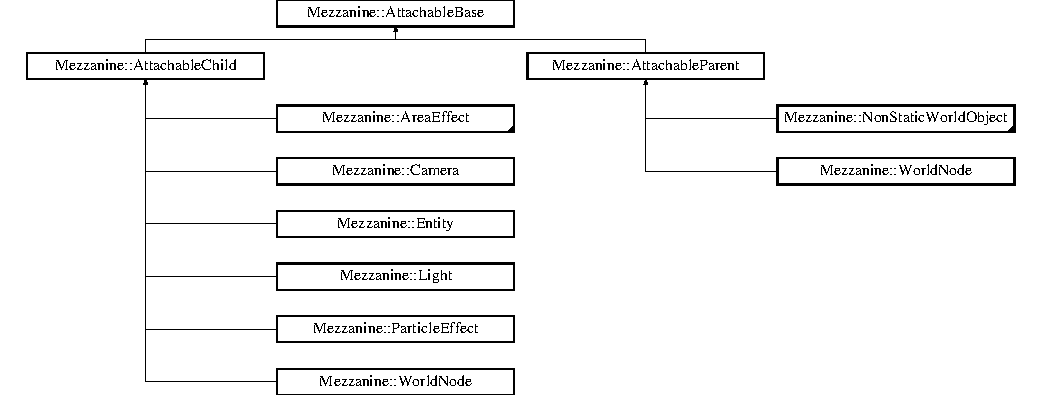
\includegraphics[height=5.308057cm]{classMezzanine_1_1AttachableBase}
\end{center}
\end{figure}
\subsubsection*{Public Member Functions}
\begin{DoxyCompactItemize}
\item 
\hypertarget{classMezzanine_1_1AttachableBase_a72bee4c7d028162ececabf6010f9015d}{
\hyperlink{classMezzanine_1_1AttachableBase_a72bee4c7d028162ececabf6010f9015d}{AttachableBase} ()}
\label{classMezzanine_1_1AttachableBase_a72bee4c7d028162ececabf6010f9015d}

\begin{DoxyCompactList}\small\item\em Class constructor. \item\end{DoxyCompactList}\item 
\hypertarget{classMezzanine_1_1AttachableBase_aaae9b3fa22b54bafefe5f994ed6eae93}{
virtual \hyperlink{classMezzanine_1_1AttachableBase_aaae9b3fa22b54bafefe5f994ed6eae93}{$\sim$AttachableBase} ()}
\label{classMezzanine_1_1AttachableBase_aaae9b3fa22b54bafefe5f994ed6eae93}

\begin{DoxyCompactList}\small\item\em Class destructor. \item\end{DoxyCompactList}\item 
\hyperlink{classMezzanine_1_1Vector3}{Vector3} \hyperlink{classMezzanine_1_1AttachableBase_a33eb528b2e924ef70a9bab7fd79c70d0}{ConvertGlobalToLocal} (const \hyperlink{classMezzanine_1_1Vector3}{Vector3} \&Location) const 
\begin{DoxyCompactList}\small\item\em Converts a point in global space to the same point in local space. \item\end{DoxyCompactList}\item 
\hyperlink{classMezzanine_1_1Quaternion}{Quaternion} \hyperlink{classMezzanine_1_1AttachableBase_a39338b566a38828b8c9b1ddf3e2c865e}{ConvertGlobalToLocal} (const \hyperlink{classMezzanine_1_1Quaternion}{Quaternion} \&Orientation) const 
\begin{DoxyCompactList}\small\item\em Converts a rotation in global space to the same rotation in local space. \item\end{DoxyCompactList}\item 
\hyperlink{classMezzanine_1_1Quaternion}{Quaternion} \hyperlink{classMezzanine_1_1AttachableBase_a709ad287377d07a576ebaca995392e15}{ConvertLocalToGlobal} (const \hyperlink{classMezzanine_1_1Quaternion}{Quaternion} \&Orientation) const 
\begin{DoxyCompactList}\small\item\em Converts a rotation in local space to the same rotation in global space. \item\end{DoxyCompactList}\item 
\hyperlink{classMezzanine_1_1Vector3}{Vector3} \hyperlink{classMezzanine_1_1AttachableBase_ab8a5b6e1379ff5cedb5758c4aafe61ed}{ConvertLocalToGlobal} (const \hyperlink{classMezzanine_1_1Vector3}{Vector3} \&Location) const 
\begin{DoxyCompactList}\small\item\em Converts a point in local space to the same point in global space. \item\end{DoxyCompactList}\item 
virtual \hyperlink{classMezzanine_1_1Vector3}{Vector3} \hyperlink{classMezzanine_1_1AttachableBase_a927f25cb0f2ba3afd289586e7ab0f4e8}{GetLocation} () const =0
\begin{DoxyCompactList}\small\item\em Gets the Location of this object. \item\end{DoxyCompactList}\item 
virtual \hyperlink{namespaceMezzanine_a63cd699ac54b73953f35ec9cfc05e506}{ConstString} \& \hyperlink{classMezzanine_1_1AttachableBase_a04b114eccfbf9092b84dfe24e81548b6}{GetName} () const =0
\begin{DoxyCompactList}\small\item\em Gets the name of this attachable. \item\end{DoxyCompactList}\item 
virtual \hyperlink{classMezzanine_1_1Quaternion}{Quaternion} \hyperlink{classMezzanine_1_1AttachableBase_af18f7d1f20ee332facb314291673a313}{GetOrientation} () const =0
\begin{DoxyCompactList}\small\item\em Gets the orientation of this object. \item\end{DoxyCompactList}\item 
virtual \hyperlink{classMezzanine_1_1Vector3}{Vector3} \hyperlink{classMezzanine_1_1AttachableBase_a8e01242f06e5aabc3d53004325f1eeee}{GetScaling} () const =0
\begin{DoxyCompactList}\small\item\em Gets the scale of this object. \item\end{DoxyCompactList}\item 
virtual \hyperlink{namespaceMezzanine_ae8cd04f706f4998be62f454b7119c718}{WorldAndSceneObjectType} \hyperlink{classMezzanine_1_1AttachableBase_a42bb7c2cab933d28dea86d2ec2934c6a}{GetType} () const =0
\begin{DoxyCompactList}\small\item\em Gets the type of \hyperlink{classMezzanine_1_1World}{World} or Scene object this attachable is. \item\end{DoxyCompactList}\item 
virtual void \hyperlink{classMezzanine_1_1AttachableBase_ab4f0d73a5c313874766bd038a32f1ae2}{SetLocation} (const \hyperlink{classMezzanine_1_1Vector3}{Vector3} \&Location)=0
\begin{DoxyCompactList}\small\item\em Sets the Location of this object. \item\end{DoxyCompactList}\item 
virtual void \hyperlink{classMezzanine_1_1AttachableBase_a8c459c324efb01dc56cead8e7650f22e}{SetOrientation} (const \hyperlink{classMezzanine_1_1Quaternion}{Quaternion} \&Orientation)=0
\begin{DoxyCompactList}\small\item\em Sets the orientation of this object. \item\end{DoxyCompactList}\item 
virtual void \hyperlink{classMezzanine_1_1AttachableBase_a5201923c0685e592dee8cecabc72b508}{SetScaling} (const \hyperlink{classMezzanine_1_1Vector3}{Vector3} \&Scale)=0
\begin{DoxyCompactList}\small\item\em Sets the scale of this object. \item\end{DoxyCompactList}\end{DoxyCompactItemize}
\subsubsection*{Protected Member Functions}
\begin{DoxyCompactItemize}
\item 
\hypertarget{classMezzanine_1_1AttachableBase_a0d62e3708056e62911d6ec7c6beb3a97}{
bool \hyperlink{classMezzanine_1_1AttachableBase_a0d62e3708056e62911d6ec7c6beb3a97}{GetUpdating} (\hyperlink{classMezzanine_1_1AttachableBase}{AttachableBase} $\ast$AB) const }
\label{classMezzanine_1_1AttachableBase_a0d62e3708056e62911d6ec7c6beb3a97}

\begin{DoxyCompactList}\small\item\em Gets the update status of another attachable. \item\end{DoxyCompactList}\end{DoxyCompactItemize}
\subsubsection*{Protected Attributes}
\begin{DoxyCompactItemize}
\item 
\hypertarget{classMezzanine_1_1AttachableBase_ab1042d571c1a40f0ab79e33206ab9761}{
bool {\bfseries Updating}}
\label{classMezzanine_1_1AttachableBase_ab1042d571c1a40f0ab79e33206ab9761}

\end{DoxyCompactItemize}


\subsubsection{Detailed Description}
This class is the base class for other attachable classes and is responsible for transform updates to attachables. 

Definition at line 70 of file attachable.h.



\subsubsection{Member Function Documentation}
\hypertarget{classMezzanine_1_1AttachableBase_a33eb528b2e924ef70a9bab7fd79c70d0}{
\index{Mezzanine::AttachableBase@{Mezzanine::AttachableBase}!ConvertGlobalToLocal@{ConvertGlobalToLocal}}
\index{ConvertGlobalToLocal@{ConvertGlobalToLocal}!Mezzanine::AttachableBase@{Mezzanine::AttachableBase}}
\paragraph[{ConvertGlobalToLocal}]{\setlength{\rightskip}{0pt plus 5cm}{\bf Vector3} Mezzanine::AttachableBase::ConvertGlobalToLocal (
\begin{DoxyParamCaption}
\item[{const {\bf Vector3} \&}]{Location}
\end{DoxyParamCaption}
) const}\hfill}
\label{classMezzanine_1_1AttachableBase_a33eb528b2e924ef70a9bab7fd79c70d0}


Converts a point in global space to the same point in local space. 


\begin{DoxyParams}{Parameters}
{\em Location} & The point in global space to be converted. \\
\hline
\end{DoxyParams}
\begin{DoxyReturn}{Returns}
Returns a \hyperlink{classMezzanine_1_1Vector3}{Vector3} representing the point in local space corresponding to the provided global space point. 
\end{DoxyReturn}


Definition at line 79 of file attachable.cpp.

\hypertarget{classMezzanine_1_1AttachableBase_a39338b566a38828b8c9b1ddf3e2c865e}{
\index{Mezzanine::AttachableBase@{Mezzanine::AttachableBase}!ConvertGlobalToLocal@{ConvertGlobalToLocal}}
\index{ConvertGlobalToLocal@{ConvertGlobalToLocal}!Mezzanine::AttachableBase@{Mezzanine::AttachableBase}}
\paragraph[{ConvertGlobalToLocal}]{\setlength{\rightskip}{0pt plus 5cm}{\bf Quaternion} Mezzanine::AttachableBase::ConvertGlobalToLocal (
\begin{DoxyParamCaption}
\item[{const {\bf Quaternion} \&}]{Orientation}
\end{DoxyParamCaption}
) const}\hfill}
\label{classMezzanine_1_1AttachableBase_a39338b566a38828b8c9b1ddf3e2c865e}


Converts a rotation in global space to the same rotation in local space. 


\begin{DoxyParams}{Parameters}
{\em Orientation} & The rotation in global space to be converted. \\
\hline
\end{DoxyParams}
\begin{DoxyReturn}{Returns}
Returns a \hyperlink{classMezzanine_1_1Quaternion}{Quaternion} representing the rotation in local space corresponding to the provided global space rotation. 
\end{DoxyReturn}


Definition at line 89 of file attachable.cpp.

\hypertarget{classMezzanine_1_1AttachableBase_a709ad287377d07a576ebaca995392e15}{
\index{Mezzanine::AttachableBase@{Mezzanine::AttachableBase}!ConvertLocalToGlobal@{ConvertLocalToGlobal}}
\index{ConvertLocalToGlobal@{ConvertLocalToGlobal}!Mezzanine::AttachableBase@{Mezzanine::AttachableBase}}
\paragraph[{ConvertLocalToGlobal}]{\setlength{\rightskip}{0pt plus 5cm}{\bf Quaternion} Mezzanine::AttachableBase::ConvertLocalToGlobal (
\begin{DoxyParamCaption}
\item[{const {\bf Quaternion} \&}]{Orientation}
\end{DoxyParamCaption}
) const}\hfill}
\label{classMezzanine_1_1AttachableBase_a709ad287377d07a576ebaca995392e15}


Converts a rotation in local space to the same rotation in global space. 


\begin{DoxyParams}{Parameters}
{\em Orientation} & The rotation in local space to be converted. \\
\hline
\end{DoxyParams}
\begin{DoxyReturn}{Returns}
Returns a \hyperlink{classMezzanine_1_1Quaternion}{Quaternion} representing the rotation in global space corresponding to the provided local space rotation. 
\end{DoxyReturn}


Definition at line 84 of file attachable.cpp.

\hypertarget{classMezzanine_1_1AttachableBase_ab8a5b6e1379ff5cedb5758c4aafe61ed}{
\index{Mezzanine::AttachableBase@{Mezzanine::AttachableBase}!ConvertLocalToGlobal@{ConvertLocalToGlobal}}
\index{ConvertLocalToGlobal@{ConvertLocalToGlobal}!Mezzanine::AttachableBase@{Mezzanine::AttachableBase}}
\paragraph[{ConvertLocalToGlobal}]{\setlength{\rightskip}{0pt plus 5cm}{\bf Vector3} Mezzanine::AttachableBase::ConvertLocalToGlobal (
\begin{DoxyParamCaption}
\item[{const {\bf Vector3} \&}]{Location}
\end{DoxyParamCaption}
) const}\hfill}
\label{classMezzanine_1_1AttachableBase_ab8a5b6e1379ff5cedb5758c4aafe61ed}


Converts a point in local space to the same point in global space. 


\begin{DoxyParams}{Parameters}
{\em Location} & The point in local space to be converted. \\
\hline
\end{DoxyParams}
\begin{DoxyReturn}{Returns}
Returns a \hyperlink{classMezzanine_1_1Vector3}{Vector3} representing the point in global space corresponding to the provided local space point. 
\end{DoxyReturn}


Definition at line 74 of file attachable.cpp.

\hypertarget{classMezzanine_1_1AttachableBase_a927f25cb0f2ba3afd289586e7ab0f4e8}{
\index{Mezzanine::AttachableBase@{Mezzanine::AttachableBase}!GetLocation@{GetLocation}}
\index{GetLocation@{GetLocation}!Mezzanine::AttachableBase@{Mezzanine::AttachableBase}}
\paragraph[{GetLocation}]{\setlength{\rightskip}{0pt plus 5cm}virtual {\bf Vector3} Mezzanine::AttachableBase::GetLocation (
\begin{DoxyParamCaption}
{}
\end{DoxyParamCaption}
) const\hspace{0.3cm}{\ttfamily  \mbox{[}pure virtual\mbox{]}}}\hfill}
\label{classMezzanine_1_1AttachableBase_a927f25cb0f2ba3afd289586e7ab0f4e8}


Gets the Location of this object. 

\begin{DoxyReturn}{Returns}
Returns a vector3 representing the location of this object. 
\end{DoxyReturn}


Implemented in \hyperlink{classMezzanine_1_1ActorSoft_a0192b3889eaf2786352d75ca03fcae4a}{Mezzanine::ActorSoft}, \hyperlink{classMezzanine_1_1AreaEffect_a37d04f8e6d6e8451348ee60fd083968b}{Mezzanine::AreaEffect}, \hyperlink{classMezzanine_1_1Camera_afb87a19855c4cd5361861e1e400d5481}{Mezzanine::Camera}, \hyperlink{classMezzanine_1_1Entity_abef3e9fd62085c0ebc0bcab8199f7ce7}{Mezzanine::Entity}, \hyperlink{classMezzanine_1_1Light_a997d299abec130a6a9111b5659a6b0d2}{Mezzanine::Light}, \hyperlink{classMezzanine_1_1ParticleEffect_a45174a2138b031322ddc57fe1be006de}{Mezzanine::ParticleEffect}, \hyperlink{classMezzanine_1_1WorldNode_a7941d8f3347b810d31b511c3b59585f8}{Mezzanine::WorldNode}, and \hyperlink{classMezzanine_1_1NonStaticWorldObject_aefbebff39e4d21859f5fddb434f6165c}{Mezzanine::NonStaticWorldObject}.

\hypertarget{classMezzanine_1_1AttachableBase_a04b114eccfbf9092b84dfe24e81548b6}{
\index{Mezzanine::AttachableBase@{Mezzanine::AttachableBase}!GetName@{GetName}}
\index{GetName@{GetName}!Mezzanine::AttachableBase@{Mezzanine::AttachableBase}}
\paragraph[{GetName}]{\setlength{\rightskip}{0pt plus 5cm}virtual {\bf ConstString}\& Mezzanine::AttachableBase::GetName (
\begin{DoxyParamCaption}
{}
\end{DoxyParamCaption}
) const\hspace{0.3cm}{\ttfamily  \mbox{[}pure virtual\mbox{]}}}\hfill}
\label{classMezzanine_1_1AttachableBase_a04b114eccfbf9092b84dfe24e81548b6}


Gets the name of this attachable. 

\begin{DoxyReturn}{Returns}
Returns a const reference to a string containing the name of this attachable. 
\end{DoxyReturn}


Implemented in \hyperlink{classMezzanine_1_1ActorSoft_aa37860ec9b4d12111c74df7bd14fc58d}{Mezzanine::ActorSoft}, \hyperlink{classMezzanine_1_1AreaEffect_ae0205e57786da97300357d7ac1afd180}{Mezzanine::AreaEffect}, \hyperlink{classMezzanine_1_1Camera_abf6e3c2e642753023acd91f6d1413455}{Mezzanine::Camera}, \hyperlink{classMezzanine_1_1Entity_aa1bf505993225def530582741e4e58c4}{Mezzanine::Entity}, \hyperlink{classMezzanine_1_1Light_a1488e39ce34aab274ee5618aeb1f810d}{Mezzanine::Light}, \hyperlink{classMezzanine_1_1ParticleEffect_a43176eb1ad80019bc2a839e597141dd7}{Mezzanine::ParticleEffect}, \hyperlink{classMezzanine_1_1WorldNode_a9538be39292a297f64d15bf1335ee0cf}{Mezzanine::WorldNode}, and \hyperlink{classMezzanine_1_1NonStaticWorldObject_acb52c6e1718acb9f17e34bf4b6203304}{Mezzanine::NonStaticWorldObject}.

\hypertarget{classMezzanine_1_1AttachableBase_af18f7d1f20ee332facb314291673a313}{
\index{Mezzanine::AttachableBase@{Mezzanine::AttachableBase}!GetOrientation@{GetOrientation}}
\index{GetOrientation@{GetOrientation}!Mezzanine::AttachableBase@{Mezzanine::AttachableBase}}
\paragraph[{GetOrientation}]{\setlength{\rightskip}{0pt plus 5cm}virtual {\bf Quaternion} Mezzanine::AttachableBase::GetOrientation (
\begin{DoxyParamCaption}
{}
\end{DoxyParamCaption}
) const\hspace{0.3cm}{\ttfamily  \mbox{[}pure virtual\mbox{]}}}\hfill}
\label{classMezzanine_1_1AttachableBase_af18f7d1f20ee332facb314291673a313}


Gets the orientation of this object. 

\begin{DoxyReturn}{Returns}
Returns a quaternion representing the orientation of this object. 
\end{DoxyReturn}


Implemented in \hyperlink{classMezzanine_1_1AreaEffect_a18c9fa2cbac6e1b62d9c34b56e8f7dc9}{Mezzanine::AreaEffect}, \hyperlink{classMezzanine_1_1Camera_af693fe97c4f281940a33dc8087a80fcb}{Mezzanine::Camera}, \hyperlink{classMezzanine_1_1Entity_a3ffd4d4d16a5c3579201491af3363fc9}{Mezzanine::Entity}, \hyperlink{classMezzanine_1_1Light_a08a415b00c94345ebb5155fa15819296}{Mezzanine::Light}, \hyperlink{classMezzanine_1_1ParticleEffect_ac47f0c537dd4b789c502bb2a3af61a56}{Mezzanine::ParticleEffect}, \hyperlink{classMezzanine_1_1WorldNode_ad250735dcbc77c3c96bd4d6b21e43867}{Mezzanine::WorldNode}, and \hyperlink{classMezzanine_1_1NonStaticWorldObject_a16243dfa38c5ae15725746f56119cb14}{Mezzanine::NonStaticWorldObject}.

\hypertarget{classMezzanine_1_1AttachableBase_a8e01242f06e5aabc3d53004325f1eeee}{
\index{Mezzanine::AttachableBase@{Mezzanine::AttachableBase}!GetScaling@{GetScaling}}
\index{GetScaling@{GetScaling}!Mezzanine::AttachableBase@{Mezzanine::AttachableBase}}
\paragraph[{GetScaling}]{\setlength{\rightskip}{0pt plus 5cm}virtual {\bf Vector3} Mezzanine::AttachableBase::GetScaling (
\begin{DoxyParamCaption}
{}
\end{DoxyParamCaption}
) const\hspace{0.3cm}{\ttfamily  \mbox{[}pure virtual\mbox{]}}}\hfill}
\label{classMezzanine_1_1AttachableBase_a8e01242f06e5aabc3d53004325f1eeee}


Gets the scale of this object. 

\begin{DoxyReturn}{Returns}
Returns a vector3 representing the scale being applied to this object. 
\end{DoxyReturn}


Implemented in \hyperlink{classMezzanine_1_1AreaEffect_adc4af3aa8a43d2e08d716990153fb89d}{Mezzanine::AreaEffect}, \hyperlink{classMezzanine_1_1Camera_a026f364d2eb9a13d216cd9d6c600db17}{Mezzanine::Camera}, \hyperlink{classMezzanine_1_1Entity_adbe312d008e7395947c6a4565068ed90}{Mezzanine::Entity}, \hyperlink{classMezzanine_1_1Light_ac8742d7d9ac0b4059eeed80b4b566471}{Mezzanine::Light}, \hyperlink{classMezzanine_1_1ParticleEffect_ad593e62458141a8e5a684fad55342caf}{Mezzanine::ParticleEffect}, \hyperlink{classMezzanine_1_1WorldNode_a82be69b653bb3463bec52a114bbb46ef}{Mezzanine::WorldNode}, and \hyperlink{classMezzanine_1_1NonStaticWorldObject_a309577416e71ab3b290c575e9877ca4b}{Mezzanine::NonStaticWorldObject}.

\hypertarget{classMezzanine_1_1AttachableBase_a42bb7c2cab933d28dea86d2ec2934c6a}{
\index{Mezzanine::AttachableBase@{Mezzanine::AttachableBase}!GetType@{GetType}}
\index{GetType@{GetType}!Mezzanine::AttachableBase@{Mezzanine::AttachableBase}}
\paragraph[{GetType}]{\setlength{\rightskip}{0pt plus 5cm}virtual {\bf WorldAndSceneObjectType} Mezzanine::AttachableBase::GetType (
\begin{DoxyParamCaption}
{}
\end{DoxyParamCaption}
) const\hspace{0.3cm}{\ttfamily  \mbox{[}pure virtual\mbox{]}}}\hfill}
\label{classMezzanine_1_1AttachableBase_a42bb7c2cab933d28dea86d2ec2934c6a}


Gets the type of \hyperlink{classMezzanine_1_1World}{World} or Scene object this attachable is. 

\begin{DoxyReturn}{Returns}
Returns the type of \hyperlink{classMezzanine_1_1World}{World} or Scene object this attachable is. 
\end{DoxyReturn}


Implemented in \hyperlink{classMezzanine_1_1ActorBase_a83f7356d743f1b59ea58aac6d7570901}{Mezzanine::ActorBase}, \hyperlink{classMezzanine_1_1ActorRigid_afc18444d5f13990a3458455c217f58cd}{Mezzanine::ActorRigid}, \hyperlink{classMezzanine_1_1ActorSoft_adddd9e4dafbe78aa9fb55ab92a42dc42}{Mezzanine::ActorSoft}, \hyperlink{classMezzanine_1_1AreaEffect_a2f3df5433f02057d7a9deeb5e6666287}{Mezzanine::AreaEffect}, \hyperlink{classMezzanine_1_1GravityField_a9b48f173312a02cd98ac19a8c444c10e}{Mezzanine::GravityField}, \hyperlink{classMezzanine_1_1GravityWell_a7890d007afb7021a811d711e3b2ed950}{Mezzanine::GravityWell}, \hyperlink{classMezzanine_1_1FieldOfForce_ad6247ff9543681daa74a9297c1c7653e}{Mezzanine::FieldOfForce}, \hyperlink{classMezzanine_1_1Camera_a1c00772101a06add4b3dde9e3bc9f8aa}{Mezzanine::Camera}, \hyperlink{classMezzanine_1_1Entity_a176fea54a32a2e91027e12cecab4bb60}{Mezzanine::Entity}, \hyperlink{classMezzanine_1_1Light_aa5cd7878d7507c0985d1cec54caa344e}{Mezzanine::Light}, \hyperlink{classMezzanine_1_1ParticleEffect_af0004d25fea2ac8a3ace7226193e9aaf}{Mezzanine::ParticleEffect}, and \hyperlink{classMezzanine_1_1WorldNode_a604fe6096c4c9b6e3b7614ef4be3d677}{Mezzanine::WorldNode}.

\hypertarget{classMezzanine_1_1AttachableBase_ab4f0d73a5c313874766bd038a32f1ae2}{
\index{Mezzanine::AttachableBase@{Mezzanine::AttachableBase}!SetLocation@{SetLocation}}
\index{SetLocation@{SetLocation}!Mezzanine::AttachableBase@{Mezzanine::AttachableBase}}
\paragraph[{SetLocation}]{\setlength{\rightskip}{0pt plus 5cm}virtual void Mezzanine::AttachableBase::SetLocation (
\begin{DoxyParamCaption}
\item[{const {\bf Vector3} \&}]{Location}
\end{DoxyParamCaption}
)\hspace{0.3cm}{\ttfamily  \mbox{[}pure virtual\mbox{]}}}\hfill}
\label{classMezzanine_1_1AttachableBase_ab4f0d73a5c313874766bd038a32f1ae2}


Sets the Location of this object. 


\begin{DoxyParams}{Parameters}
{\em Location} & A vector3 representing the location of this object. \\
\hline
\end{DoxyParams}


Implemented in \hyperlink{classMezzanine_1_1AreaEffect_a4dd22757bc627242de169e31a1717139}{Mezzanine::AreaEffect}, \hyperlink{classMezzanine_1_1Camera_afdc236c2c875035c8a11473350d0d17a}{Mezzanine::Camera}, \hyperlink{classMezzanine_1_1Entity_a6cb6c8f304e3cc30b7e6fdaa788e30a9}{Mezzanine::Entity}, \hyperlink{classMezzanine_1_1Light_ac06da317651df700c2969cc81c3f8d3d}{Mezzanine::Light}, \hyperlink{classMezzanine_1_1ParticleEffect_a36457d7e42405ac69a30114f21bd3f3f}{Mezzanine::ParticleEffect}, \hyperlink{classMezzanine_1_1WorldNode_a636852458b226f1c2f3089f17558e678}{Mezzanine::WorldNode}, and \hyperlink{classMezzanine_1_1NonStaticWorldObject_ab80106c2fec881169184eff5165e73b6}{Mezzanine::NonStaticWorldObject}.

\hypertarget{classMezzanine_1_1AttachableBase_a8c459c324efb01dc56cead8e7650f22e}{
\index{Mezzanine::AttachableBase@{Mezzanine::AttachableBase}!SetOrientation@{SetOrientation}}
\index{SetOrientation@{SetOrientation}!Mezzanine::AttachableBase@{Mezzanine::AttachableBase}}
\paragraph[{SetOrientation}]{\setlength{\rightskip}{0pt plus 5cm}virtual void Mezzanine::AttachableBase::SetOrientation (
\begin{DoxyParamCaption}
\item[{const {\bf Quaternion} \&}]{Orientation}
\end{DoxyParamCaption}
)\hspace{0.3cm}{\ttfamily  \mbox{[}pure virtual\mbox{]}}}\hfill}
\label{classMezzanine_1_1AttachableBase_a8c459c324efb01dc56cead8e7650f22e}


Sets the orientation of this object. 


\begin{DoxyParams}{Parameters}
{\em Orientation} & A \hyperlink{classMezzanine_1_1Quaternion}{Quaternion} representing the orientation of this object. \\
\hline
\end{DoxyParams}


Implemented in \hyperlink{classMezzanine_1_1AreaEffect_a62bcda0a0c2a95b8f1ccdfe2cd3d1018}{Mezzanine::AreaEffect}, \hyperlink{classMezzanine_1_1Camera_af502b9c47b1acce46e1482ce049320eb}{Mezzanine::Camera}, \hyperlink{classMezzanine_1_1Entity_ad498093c5a2b8ef3bfb9311aff719d67}{Mezzanine::Entity}, \hyperlink{classMezzanine_1_1Light_aa2f3fe2b7cb7bf459f2526d2e5c234ed}{Mezzanine::Light}, \hyperlink{classMezzanine_1_1ParticleEffect_a8e16be90e8c9d59b7c48b11a38179f76}{Mezzanine::ParticleEffect}, \hyperlink{classMezzanine_1_1WorldNode_afe9db5c3abeb608bf2d589c2a61da546}{Mezzanine::WorldNode}, and \hyperlink{classMezzanine_1_1NonStaticWorldObject_a9183791c3e61b701b152e245786a63a5}{Mezzanine::NonStaticWorldObject}.

\hypertarget{classMezzanine_1_1AttachableBase_a5201923c0685e592dee8cecabc72b508}{
\index{Mezzanine::AttachableBase@{Mezzanine::AttachableBase}!SetScaling@{SetScaling}}
\index{SetScaling@{SetScaling}!Mezzanine::AttachableBase@{Mezzanine::AttachableBase}}
\paragraph[{SetScaling}]{\setlength{\rightskip}{0pt plus 5cm}virtual void Mezzanine::AttachableBase::SetScaling (
\begin{DoxyParamCaption}
\item[{const {\bf Vector3} \&}]{Scale}
\end{DoxyParamCaption}
)\hspace{0.3cm}{\ttfamily  \mbox{[}pure virtual\mbox{]}}}\hfill}
\label{classMezzanine_1_1AttachableBase_a5201923c0685e592dee8cecabc72b508}


Sets the scale of this object. 


\begin{DoxyParams}{Parameters}
{\em Scale} & A vector3 representing the scale to be applied to this object. \\
\hline
\end{DoxyParams}


Implemented in \hyperlink{classMezzanine_1_1AreaEffect_ae0448d98c3689ae407734bbcd85a08cb}{Mezzanine::AreaEffect}, \hyperlink{classMezzanine_1_1Camera_ad49a68805d03d18d7ca42c9fbc54db2b}{Mezzanine::Camera}, \hyperlink{classMezzanine_1_1Entity_a91b2952a411d8ed80e0f809944c591b4}{Mezzanine::Entity}, \hyperlink{classMezzanine_1_1Light_a643fa07c0b48ec2edad53e3c27345ab9}{Mezzanine::Light}, \hyperlink{classMezzanine_1_1ParticleEffect_a4d8ab250edb3e6f8ba8c60710ccd6c0a}{Mezzanine::ParticleEffect}, \hyperlink{classMezzanine_1_1WorldNode_a3f7797ef81aaf763cdf011728f6b6b05}{Mezzanine::WorldNode}, and \hyperlink{classMezzanine_1_1NonStaticWorldObject_a03fec7fb4abcd6747695d139d00c7662}{Mezzanine::NonStaticWorldObject}.



The documentation for this class was generated from the following files:\begin{DoxyCompactItemize}
\item 
\hyperlink{attachable_8h}{attachable.h}\item 
\hyperlink{attachable_8cpp}{attachable.cpp}\end{DoxyCompactItemize}

\hypertarget{classMezzanine_1_1AttachableChild}{
\subsection{Mezzanine::AttachableChild Class Reference}
\label{classMezzanine_1_1AttachableChild}\index{Mezzanine::AttachableChild@{Mezzanine::AttachableChild}}
}


This class is the base class for objects that can be attached to \hyperlink{classMezzanine_1_1AttachableParent}{AttachableParent}.  




{\ttfamily \#include $<$attachable.h$>$}

Inheritance diagram for Mezzanine::AttachableChild:\begin{figure}[H]
\begin{center}
\leavevmode
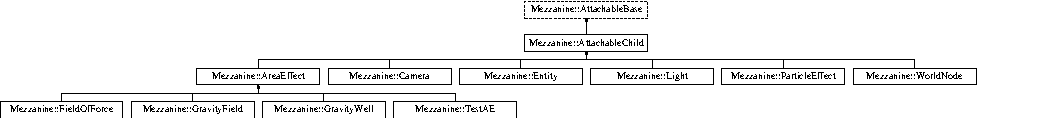
\includegraphics[height=1.590909cm]{classMezzanine_1_1AttachableChild}
\end{center}
\end{figure}
\subsubsection*{Public Member Functions}
\begin{DoxyCompactItemize}
\item 
\hypertarget{classMezzanine_1_1AttachableChild_aa1baf517c478f03c0116ccf6df62f750}{
\hyperlink{classMezzanine_1_1AttachableChild_aa1baf517c478f03c0116ccf6df62f750}{AttachableChild} ()}
\label{classMezzanine_1_1AttachableChild_aa1baf517c478f03c0116ccf6df62f750}

\begin{DoxyCompactList}\small\item\em Class constructor. \item\end{DoxyCompactList}\item 
\hypertarget{classMezzanine_1_1AttachableChild_a7413197e41b31ae33df5ff02317548c0}{
virtual \hyperlink{classMezzanine_1_1AttachableChild_a7413197e41b31ae33df5ff02317548c0}{$\sim$AttachableChild} ()}
\label{classMezzanine_1_1AttachableChild_a7413197e41b31ae33df5ff02317548c0}

\begin{DoxyCompactList}\small\item\em Class destructor. \item\end{DoxyCompactList}\item 
void \hyperlink{classMezzanine_1_1AttachableChild_ad34350de631e502a8bc3d4ce25fff4f6}{\_\-RecalculateGlobalTransform} (bool FromParent=false)
\begin{DoxyCompactList}\small\item\em Recalculates objects global transform from parent. \item\end{DoxyCompactList}\item 
\hypertarget{classMezzanine_1_1AttachableChild_a500d824fc29de69ac05ffcdbdaf67e9e}{
void \hyperlink{classMezzanine_1_1AttachableChild_a500d824fc29de69ac05ffcdbdaf67e9e}{\_\-RecalculateLocalTransform} ()}
\label{classMezzanine_1_1AttachableChild_a500d824fc29de69ac05ffcdbdaf67e9e}

\begin{DoxyCompactList}\small\item\em Recalculates this objects local transform based on it's current global position. \item\end{DoxyCompactList}\item 
\hyperlink{classMezzanine_1_1Vector3}{Vector3} \hyperlink{classMezzanine_1_1AttachableChild_a59bbbc115c028f87db652f32d252ee61}{GetLocalLocation} () const 
\begin{DoxyCompactList}\small\item\em Gets the Location of this object in local space. \item\end{DoxyCompactList}\item 
\hyperlink{classMezzanine_1_1Quaternion}{Quaternion} \hyperlink{classMezzanine_1_1AttachableChild_a81104f92420f9558b39144cce4eb7cd0}{GetLocalOrientation} () const 
\begin{DoxyCompactList}\small\item\em Gets the orientation of this object in local space. \item\end{DoxyCompactList}\item 
\hyperlink{classMezzanine_1_1AttachableParent}{AttachableParent} $\ast$ \hyperlink{classMezzanine_1_1AttachableChild_a16e42db1e1a69f5ca41d412fcc3a5aeb}{GetParent} () const 
\begin{DoxyCompactList}\small\item\em Gets the parent of this child. \item\end{DoxyCompactList}\item 
virtual void \hyperlink{classMezzanine_1_1AttachableChild_a527ef7ddbf4c3936214eff5af821ae63}{SetLocalLocation} (const \hyperlink{classMezzanine_1_1Vector3}{Vector3} \&Location)=0
\begin{DoxyCompactList}\small\item\em Sets the Location of this object in local space. \item\end{DoxyCompactList}\item 
virtual void \hyperlink{classMezzanine_1_1AttachableChild_a3604a2450a1647ae882ef1d9dab1ec5d}{SetLocalOrientation} (const \hyperlink{classMezzanine_1_1Quaternion}{Quaternion} \&Orientation)=0
\begin{DoxyCompactList}\small\item\em Sets the orientation of this object in local space. \item\end{DoxyCompactList}\end{DoxyCompactItemize}
\subsubsection*{Protected Attributes}
\begin{DoxyCompactItemize}
\item 
\hypertarget{classMezzanine_1_1AttachableChild_a6940c66cc4725deb27024ddd6c5459b8}{
bool {\bfseries GlobalTransformDirty}}
\label{classMezzanine_1_1AttachableChild_a6940c66cc4725deb27024ddd6c5459b8}

\item 
\hypertarget{classMezzanine_1_1AttachableChild_a142c9f848101dec654f8eeca88e689b5}{
bool {\bfseries LocalTransformDirty}}
\label{classMezzanine_1_1AttachableChild_a142c9f848101dec654f8eeca88e689b5}

\item 
\hypertarget{classMezzanine_1_1AttachableChild_adc604405ff0ac70699a0286b5e4869b9}{
\hyperlink{classMezzanine_1_1Transform}{Transform} {\bfseries LocalXform}}
\label{classMezzanine_1_1AttachableChild_adc604405ff0ac70699a0286b5e4869b9}

\item 
\hypertarget{classMezzanine_1_1AttachableChild_acdd3042178a3bdc83c483b55498ae76e}{
\hyperlink{classMezzanine_1_1AttachableParent}{AttachableParent} $\ast$ {\bfseries Parent}}
\label{classMezzanine_1_1AttachableChild_acdd3042178a3bdc83c483b55498ae76e}

\end{DoxyCompactItemize}
\subsubsection*{Friends}
\begin{DoxyCompactItemize}
\item 
\hypertarget{classMezzanine_1_1AttachableChild_a7d495633cc192a4d3cc2f040a97e05f2}{
class {\bfseries AttachableParent}}
\label{classMezzanine_1_1AttachableChild_a7d495633cc192a4d3cc2f040a97e05f2}

\end{DoxyCompactItemize}


\subsubsection{Detailed Description}
This class is the base class for objects that can be attached to \hyperlink{classMezzanine_1_1AttachableParent}{AttachableParent}. 

Definition at line 205 of file attachable.h.



\subsubsection{Member Function Documentation}
\hypertarget{classMezzanine_1_1AttachableChild_ad34350de631e502a8bc3d4ce25fff4f6}{
\index{Mezzanine::AttachableChild@{Mezzanine::AttachableChild}!\_\-RecalculateGlobalTransform@{\_\-RecalculateGlobalTransform}}
\index{\_\-RecalculateGlobalTransform@{\_\-RecalculateGlobalTransform}!Mezzanine::AttachableChild@{Mezzanine::AttachableChild}}
\paragraph[{\_\-RecalculateGlobalTransform}]{\setlength{\rightskip}{0pt plus 5cm}void Mezzanine::AttachableChild::\_\-RecalculateGlobalTransform (
\begin{DoxyParamCaption}
\item[{bool}]{FromParent = {\ttfamily false}}
\end{DoxyParamCaption}
)}\hfill}
\label{classMezzanine_1_1AttachableChild_ad34350de631e502a8bc3d4ce25fff4f6}


Recalculates objects global transform from parent. 


\begin{DoxyParams}{Parameters}
{\em FromParent} & Whether this is being invoked from the parent of this attachable. \\
\hline
\end{DoxyParams}


Definition at line 219 of file attachable.cpp.

\hypertarget{classMezzanine_1_1AttachableChild_a59bbbc115c028f87db652f32d252ee61}{
\index{Mezzanine::AttachableChild@{Mezzanine::AttachableChild}!GetLocalLocation@{GetLocalLocation}}
\index{GetLocalLocation@{GetLocalLocation}!Mezzanine::AttachableChild@{Mezzanine::AttachableChild}}
\paragraph[{GetLocalLocation}]{\setlength{\rightskip}{0pt plus 5cm}{\bf Vector3} Mezzanine::AttachableChild::GetLocalLocation (
\begin{DoxyParamCaption}
{}
\end{DoxyParamCaption}
) const}\hfill}
\label{classMezzanine_1_1AttachableChild_a59bbbc115c028f87db652f32d252ee61}


Gets the Location of this object in local space. 

\begin{DoxyReturn}{Returns}
Returns a vector3 representing the location of this object. 
\end{DoxyReturn}


Definition at line 206 of file attachable.cpp.

\hypertarget{classMezzanine_1_1AttachableChild_a81104f92420f9558b39144cce4eb7cd0}{
\index{Mezzanine::AttachableChild@{Mezzanine::AttachableChild}!GetLocalOrientation@{GetLocalOrientation}}
\index{GetLocalOrientation@{GetLocalOrientation}!Mezzanine::AttachableChild@{Mezzanine::AttachableChild}}
\paragraph[{GetLocalOrientation}]{\setlength{\rightskip}{0pt plus 5cm}{\bf Quaternion} Mezzanine::AttachableChild::GetLocalOrientation (
\begin{DoxyParamCaption}
{}
\end{DoxyParamCaption}
) const}\hfill}
\label{classMezzanine_1_1AttachableChild_a81104f92420f9558b39144cce4eb7cd0}


Gets the orientation of this object in local space. 

\begin{DoxyReturn}{Returns}
Returns a quaternion representing the orientation of this object. 
\end{DoxyReturn}


Definition at line 211 of file attachable.cpp.

\hypertarget{classMezzanine_1_1AttachableChild_a16e42db1e1a69f5ca41d412fcc3a5aeb}{
\index{Mezzanine::AttachableChild@{Mezzanine::AttachableChild}!GetParent@{GetParent}}
\index{GetParent@{GetParent}!Mezzanine::AttachableChild@{Mezzanine::AttachableChild}}
\paragraph[{GetParent}]{\setlength{\rightskip}{0pt plus 5cm}{\bf AttachableParent} $\ast$ Mezzanine::AttachableChild::GetParent (
\begin{DoxyParamCaption}
{}
\end{DoxyParamCaption}
) const}\hfill}
\label{classMezzanine_1_1AttachableChild_a16e42db1e1a69f5ca41d412fcc3a5aeb}


Gets the parent of this child. 

\begin{DoxyReturn}{Returns}
Returns a pointer to the parent this object is attached to or NULL if it's not attached to anything. 
\end{DoxyReturn}


Definition at line 198 of file attachable.cpp.

\hypertarget{classMezzanine_1_1AttachableChild_a527ef7ddbf4c3936214eff5af821ae63}{
\index{Mezzanine::AttachableChild@{Mezzanine::AttachableChild}!SetLocalLocation@{SetLocalLocation}}
\index{SetLocalLocation@{SetLocalLocation}!Mezzanine::AttachableChild@{Mezzanine::AttachableChild}}
\paragraph[{SetLocalLocation}]{\setlength{\rightskip}{0pt plus 5cm}virtual void Mezzanine::AttachableChild::SetLocalLocation (
\begin{DoxyParamCaption}
\item[{const {\bf Vector3} \&}]{Location}
\end{DoxyParamCaption}
)\hspace{0.3cm}{\ttfamily  \mbox{[}pure virtual\mbox{]}}}\hfill}
\label{classMezzanine_1_1AttachableChild_a527ef7ddbf4c3936214eff5af821ae63}


Sets the Location of this object in local space. 


\begin{DoxyParams}{Parameters}
{\em Location} & A vector3 representing the location of this object. \\
\hline
\end{DoxyParams}


Implemented in \hyperlink{classMezzanine_1_1AreaEffect_a93056bdf18b07d8067367b368fbf24a1}{Mezzanine::AreaEffect}, \hyperlink{classMezzanine_1_1Camera_ae62b56649606677f9922eeea658bdd2f}{Mezzanine::Camera}, \hyperlink{classMezzanine_1_1Entity_adb3d57eff59eba586a6c623264f38072}{Mezzanine::Entity}, \hyperlink{classMezzanine_1_1Light_a16815beba535ae398e8ae6016c6579f6}{Mezzanine::Light}, \hyperlink{classMezzanine_1_1ParticleEffect_a6840690a153731dd2a3699187b5af1a9}{Mezzanine::ParticleEffect}, and \hyperlink{classMezzanine_1_1WorldNode_a03feb41f719612123fe8d9055603efe6}{Mezzanine::WorldNode}.

\hypertarget{classMezzanine_1_1AttachableChild_a3604a2450a1647ae882ef1d9dab1ec5d}{
\index{Mezzanine::AttachableChild@{Mezzanine::AttachableChild}!SetLocalOrientation@{SetLocalOrientation}}
\index{SetLocalOrientation@{SetLocalOrientation}!Mezzanine::AttachableChild@{Mezzanine::AttachableChild}}
\paragraph[{SetLocalOrientation}]{\setlength{\rightskip}{0pt plus 5cm}virtual void Mezzanine::AttachableChild::SetLocalOrientation (
\begin{DoxyParamCaption}
\item[{const {\bf Quaternion} \&}]{Orientation}
\end{DoxyParamCaption}
)\hspace{0.3cm}{\ttfamily  \mbox{[}pure virtual\mbox{]}}}\hfill}
\label{classMezzanine_1_1AttachableChild_a3604a2450a1647ae882ef1d9dab1ec5d}


Sets the orientation of this object in local space. 


\begin{DoxyParams}{Parameters}
{\em Orientation} & A \hyperlink{classMezzanine_1_1Quaternion}{Quaternion} representing the orientation of this object. \\
\hline
\end{DoxyParams}


Implemented in \hyperlink{classMezzanine_1_1AreaEffect_a59907341f2a0c8814b7962f010cea587}{Mezzanine::AreaEffect}, \hyperlink{classMezzanine_1_1Camera_a8857075c6bc9e4d40075652778aa14c2}{Mezzanine::Camera}, \hyperlink{classMezzanine_1_1Entity_a82485a3020bdba45744b094e08eaf087}{Mezzanine::Entity}, \hyperlink{classMezzanine_1_1Light_ac97ef9f7544c0710ce8c18dac91ec1ce}{Mezzanine::Light}, \hyperlink{classMezzanine_1_1ParticleEffect_a2ab1695b2261bb058f64ed246a3bfc35}{Mezzanine::ParticleEffect}, and \hyperlink{classMezzanine_1_1WorldNode_a32259918c2d5695141371ca364a813c2}{Mezzanine::WorldNode}.



The documentation for this class was generated from the following files:\begin{DoxyCompactItemize}
\item 
\hyperlink{attachable_8h}{attachable.h}\item 
\hyperlink{attachable_8cpp}{attachable.cpp}\end{DoxyCompactItemize}

\hypertarget{classMezzanine_1_1AttachableParent}{
\subsection{Mezzanine::AttachableParent Class Reference}
\label{classMezzanine_1_1AttachableParent}\index{Mezzanine::AttachableParent@{Mezzanine::AttachableParent}}
}


Base class for objects that can have attachables attached to them.  




{\ttfamily \#include $<$attachable.h$>$}

Inheritance diagram for Mezzanine::AttachableParent:\begin{figure}[H]
\begin{center}
\leavevmode
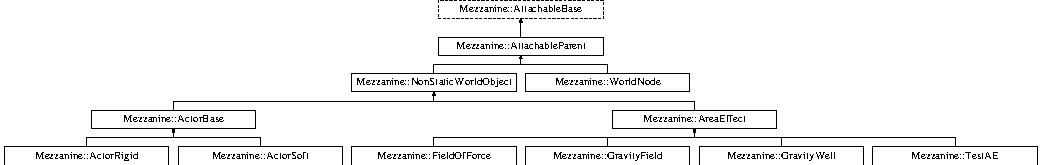
\includegraphics[height=2.211690cm]{classMezzanine_1_1AttachableParent}
\end{center}
\end{figure}
\subsubsection*{Public Types}
\begin{DoxyCompactItemize}
\item 
\hypertarget{classMezzanine_1_1AttachableParent_a6e9c08040897d349a302ff06f647168a}{
typedef std::vector$<$ \hyperlink{classMezzanine_1_1AttachableChild}{AttachableChild} $\ast$ $>$ {\bfseries AttachableContainer}}
\label{classMezzanine_1_1AttachableParent_a6e9c08040897d349a302ff06f647168a}

\item 
\hypertarget{classMezzanine_1_1AttachableParent_a29dc368ae43bb6544304c2fadadac55e}{
typedef AttachableContainer::iterator {\bfseries AttachableIterator}}
\label{classMezzanine_1_1AttachableParent_a29dc368ae43bb6544304c2fadadac55e}

\item 
\hypertarget{classMezzanine_1_1AttachableParent_a7f75a92904328d5f68362f4e3b148934}{
typedef AttachableContainer::const\_\-iterator {\bfseries ConstAttachableIterator}}
\label{classMezzanine_1_1AttachableParent_a7f75a92904328d5f68362f4e3b148934}

\end{DoxyCompactItemize}
\subsubsection*{Public Member Functions}
\begin{DoxyCompactItemize}
\item 
\hypertarget{classMezzanine_1_1AttachableParent_a6ac9d49cd99bddd5b29d734581d02538}{
\hyperlink{classMezzanine_1_1AttachableParent_a6ac9d49cd99bddd5b29d734581d02538}{AttachableParent} ()}
\label{classMezzanine_1_1AttachableParent_a6ac9d49cd99bddd5b29d734581d02538}

\begin{DoxyCompactList}\small\item\em Class constructor. \item\end{DoxyCompactList}\item 
\hypertarget{classMezzanine_1_1AttachableParent_a33694eac156fac95099536c3e70b1c5c}{
virtual \hyperlink{classMezzanine_1_1AttachableParent_a33694eac156fac95099536c3e70b1c5c}{$\sim$AttachableParent} ()}
\label{classMezzanine_1_1AttachableParent_a33694eac156fac95099536c3e70b1c5c}

\begin{DoxyCompactList}\small\item\em Class destructor. \item\end{DoxyCompactList}\item 
\hypertarget{classMezzanine_1_1AttachableParent_a9c76fdc43b1cddada62385215ca6c8d4}{
void \hyperlink{classMezzanine_1_1AttachableParent_a9c76fdc43b1cddada62385215ca6c8d4}{\_\-RecalculateAllChildTransforms} ()}
\label{classMezzanine_1_1AttachableParent_a9c76fdc43b1cddada62385215ca6c8d4}

\begin{DoxyCompactList}\small\item\em Recalculates the transforms of all children of this attachable. \item\end{DoxyCompactList}\item 
virtual void \hyperlink{classMezzanine_1_1AttachableParent_a558c6e2dd0a31cd99bb7872394de9c00}{AttachObject} (\hyperlink{classMezzanine_1_1AttachableChild}{AttachableChild} $\ast$Target)
\begin{DoxyCompactList}\small\item\em Attaches an attachable element to this object. \item\end{DoxyCompactList}\item 
AttachableIterator \hyperlink{classMezzanine_1_1AttachableParent_a6ed49c42b138227094b579638fd06538}{BeginChild} ()
\begin{DoxyCompactList}\small\item\em Get an AttachableIterator to the first object. \item\end{DoxyCompactList}\item 
ConstAttachableIterator \hyperlink{classMezzanine_1_1AttachableParent_a4693daab5f6ad884fbe64f718c016384}{BeginChild} () const 
\begin{DoxyCompactList}\small\item\em Get a ConstAttachableIterator to the first object. \item\end{DoxyCompactList}\item 
\hypertarget{classMezzanine_1_1AttachableParent_a1098f9a8f0556fec95c1bd6c8503da86}{
virtual void \hyperlink{classMezzanine_1_1AttachableParent_a1098f9a8f0556fec95c1bd6c8503da86}{DetachAll} ()}
\label{classMezzanine_1_1AttachableParent_a1098f9a8f0556fec95c1bd6c8503da86}

\begin{DoxyCompactList}\small\item\em Detaches all attachables currently attached. \item\end{DoxyCompactList}\item 
virtual void \hyperlink{classMezzanine_1_1AttachableParent_a500741267623cad0e0748fe0a4b5e69c}{DetachObject} (\hyperlink{classMezzanine_1_1AttachableChild}{AttachableChild} $\ast$Target)
\begin{DoxyCompactList}\small\item\em Detaches an attachable element from this object. \item\end{DoxyCompactList}\item 
AttachableIterator \hyperlink{classMezzanine_1_1AttachableParent_a6a5f5c9e1bf1838113405aa3439e14e4}{EndChild} ()
\begin{DoxyCompactList}\small\item\em Get an AttachableIterator to one past the last object. \item\end{DoxyCompactList}\item 
ConstAttachableIterator \hyperlink{classMezzanine_1_1AttachableParent_a6ccdced33c9b32be3ad71a195c9aff20}{EndChild} () const 
\begin{DoxyCompactList}\small\item\em Get a ConstAttachableIterator to one past the last object. \item\end{DoxyCompactList}\item 
virtual \hyperlink{classMezzanine_1_1AttachableChild}{AttachableChild} $\ast$ \hyperlink{classMezzanine_1_1AttachableParent_a89d0d1d85a40385d1482ae5443d1ecf1}{GetAttached} (const \hyperlink{namespaceMezzanine_adcbb6ce6d1eb4379d109e51171e2e493}{Whole} \&Index) const 
\begin{DoxyCompactList}\small\item\em Get a specific attached Item. \item\end{DoxyCompactList}\item 
virtual \hyperlink{namespaceMezzanine_adcbb6ce6d1eb4379d109e51171e2e493}{Whole} \hyperlink{classMezzanine_1_1AttachableParent_aebacb49f238c0421cd790cacd5baba9c}{GetNumAttached} () const 
\begin{DoxyCompactList}\small\item\em Gets the number of elements attached to this object. \item\end{DoxyCompactList}\end{DoxyCompactItemize}
\subsubsection*{Protected Attributes}
\begin{DoxyCompactItemize}
\item 
\hypertarget{classMezzanine_1_1AttachableParent_aa9760351def08f532c5ddc9c82fbcbb2}{
AttachableContainer {\bfseries Attached}}
\label{classMezzanine_1_1AttachableParent_aa9760351def08f532c5ddc9c82fbcbb2}

\end{DoxyCompactItemize}


\subsubsection{Detailed Description}
Base class for objects that can have attachables attached to them. 

Definition at line 145 of file attachable.h.



\subsubsection{Member Function Documentation}
\hypertarget{classMezzanine_1_1AttachableParent_a558c6e2dd0a31cd99bb7872394de9c00}{
\index{Mezzanine::AttachableParent@{Mezzanine::AttachableParent}!AttachObject@{AttachObject}}
\index{AttachObject@{AttachObject}!Mezzanine::AttachableParent@{Mezzanine::AttachableParent}}
\paragraph[{AttachObject}]{\setlength{\rightskip}{0pt plus 5cm}void Mezzanine::AttachableParent::AttachObject (
\begin{DoxyParamCaption}
\item[{{\bf AttachableChild} $\ast$}]{Target}
\end{DoxyParamCaption}
)\hspace{0.3cm}{\ttfamily  \mbox{[}virtual\mbox{]}}}\hfill}
\label{classMezzanine_1_1AttachableParent_a558c6e2dd0a31cd99bb7872394de9c00}


Attaches an attachable element to this object. 


\begin{DoxyParams}{Parameters}
{\em Target} & The Attachable to be attached. \\
\hline
\end{DoxyParams}


Definition at line 111 of file attachable.cpp.

\hypertarget{classMezzanine_1_1AttachableParent_a4693daab5f6ad884fbe64f718c016384}{
\index{Mezzanine::AttachableParent@{Mezzanine::AttachableParent}!BeginChild@{BeginChild}}
\index{BeginChild@{BeginChild}!Mezzanine::AttachableParent@{Mezzanine::AttachableParent}}
\paragraph[{BeginChild}]{\setlength{\rightskip}{0pt plus 5cm}AttachableParent::ConstAttachableIterator Mezzanine::AttachableParent::BeginChild (
\begin{DoxyParamCaption}
{}
\end{DoxyParamCaption}
) const}\hfill}
\label{classMezzanine_1_1AttachableParent_a4693daab5f6ad884fbe64f718c016384}


Get a ConstAttachableIterator to the first object. 

\begin{DoxyReturn}{Returns}
An Iterator to the first object. 
\end{DoxyReturn}


Definition at line 156 of file attachable.cpp.

\hypertarget{classMezzanine_1_1AttachableParent_a6ed49c42b138227094b579638fd06538}{
\index{Mezzanine::AttachableParent@{Mezzanine::AttachableParent}!BeginChild@{BeginChild}}
\index{BeginChild@{BeginChild}!Mezzanine::AttachableParent@{Mezzanine::AttachableParent}}
\paragraph[{BeginChild}]{\setlength{\rightskip}{0pt plus 5cm}AttachableParent::AttachableIterator Mezzanine::AttachableParent::BeginChild (
\begin{DoxyParamCaption}
{}
\end{DoxyParamCaption}
)}\hfill}
\label{classMezzanine_1_1AttachableParent_a6ed49c42b138227094b579638fd06538}


Get an AttachableIterator to the first object. 

\begin{DoxyReturn}{Returns}
An Iterator to the first object. 
\end{DoxyReturn}


Definition at line 150 of file attachable.cpp.

\hypertarget{classMezzanine_1_1AttachableParent_a500741267623cad0e0748fe0a4b5e69c}{
\index{Mezzanine::AttachableParent@{Mezzanine::AttachableParent}!DetachObject@{DetachObject}}
\index{DetachObject@{DetachObject}!Mezzanine::AttachableParent@{Mezzanine::AttachableParent}}
\paragraph[{DetachObject}]{\setlength{\rightskip}{0pt plus 5cm}void Mezzanine::AttachableParent::DetachObject (
\begin{DoxyParamCaption}
\item[{{\bf AttachableChild} $\ast$}]{Target}
\end{DoxyParamCaption}
)\hspace{0.3cm}{\ttfamily  \mbox{[}virtual\mbox{]}}}\hfill}
\label{classMezzanine_1_1AttachableParent_a500741267623cad0e0748fe0a4b5e69c}


Detaches an attachable element from this object. 


\begin{DoxyParams}{Parameters}
{\em Target} & The Attachable to be detached.\\
\hline
\end{DoxyParams}
Detach an item is done in linear time relative to the amount of attached items. 

Definition at line 128 of file attachable.cpp.

\hypertarget{classMezzanine_1_1AttachableParent_a6ccdced33c9b32be3ad71a195c9aff20}{
\index{Mezzanine::AttachableParent@{Mezzanine::AttachableParent}!EndChild@{EndChild}}
\index{EndChild@{EndChild}!Mezzanine::AttachableParent@{Mezzanine::AttachableParent}}
\paragraph[{EndChild}]{\setlength{\rightskip}{0pt plus 5cm}AttachableParent::ConstAttachableIterator Mezzanine::AttachableParent::EndChild (
\begin{DoxyParamCaption}
{}
\end{DoxyParamCaption}
) const}\hfill}
\label{classMezzanine_1_1AttachableParent_a6ccdced33c9b32be3ad71a195c9aff20}


Get a ConstAttachableIterator to one past the last object. 

\begin{DoxyReturn}{Returns}
An Iterator to one past the last object. 
\end{DoxyReturn}


Definition at line 159 of file attachable.cpp.

\hypertarget{classMezzanine_1_1AttachableParent_a6a5f5c9e1bf1838113405aa3439e14e4}{
\index{Mezzanine::AttachableParent@{Mezzanine::AttachableParent}!EndChild@{EndChild}}
\index{EndChild@{EndChild}!Mezzanine::AttachableParent@{Mezzanine::AttachableParent}}
\paragraph[{EndChild}]{\setlength{\rightskip}{0pt plus 5cm}AttachableParent::AttachableIterator Mezzanine::AttachableParent::EndChild (
\begin{DoxyParamCaption}
{}
\end{DoxyParamCaption}
)}\hfill}
\label{classMezzanine_1_1AttachableParent_a6a5f5c9e1bf1838113405aa3439e14e4}


Get an AttachableIterator to one past the last object. 

\begin{DoxyReturn}{Returns}
An Iterator to one past the last object. 
\end{DoxyReturn}


Definition at line 153 of file attachable.cpp.

\hypertarget{classMezzanine_1_1AttachableParent_a89d0d1d85a40385d1482ae5443d1ecf1}{
\index{Mezzanine::AttachableParent@{Mezzanine::AttachableParent}!GetAttached@{GetAttached}}
\index{GetAttached@{GetAttached}!Mezzanine::AttachableParent@{Mezzanine::AttachableParent}}
\paragraph[{GetAttached}]{\setlength{\rightskip}{0pt plus 5cm}{\bf AttachableChild} $\ast$ Mezzanine::AttachableParent::GetAttached (
\begin{DoxyParamCaption}
\item[{const {\bf Whole} \&}]{Index}
\end{DoxyParamCaption}
) const\hspace{0.3cm}{\ttfamily  \mbox{[}virtual\mbox{]}}}\hfill}
\label{classMezzanine_1_1AttachableParent_a89d0d1d85a40385d1482ae5443d1ecf1}


Get a specific attached Item. 


\begin{DoxyParams}{Parameters}
{\em Index} & A number indicating which Attachable you want a pointer to. The \hyperlink{classMezzanine_1_1WorldNode}{WorldNode} is like an Array starts at 0 and goes to \hyperlink{classMezzanine_1_1AttachableParent_aebacb49f238c0421cd790cacd5baba9c}{WorldNode::GetNumAttached()} -\/ 1. \\
\hline
\end{DoxyParams}
\begin{DoxyReturn}{Returns}
A pointer to an Attachable Item attached to this. 
\end{DoxyReturn}

\begin{DoxyExceptions}{Exceptions}
{\em This} & can throw an out of bounds std::exception if used incorrectly. \\
\hline
\end{DoxyExceptions}


Definition at line 147 of file attachable.cpp.

\hypertarget{classMezzanine_1_1AttachableParent_aebacb49f238c0421cd790cacd5baba9c}{
\index{Mezzanine::AttachableParent@{Mezzanine::AttachableParent}!GetNumAttached@{GetNumAttached}}
\index{GetNumAttached@{GetNumAttached}!Mezzanine::AttachableParent@{Mezzanine::AttachableParent}}
\paragraph[{GetNumAttached}]{\setlength{\rightskip}{0pt plus 5cm}{\bf Whole} Mezzanine::AttachableParent::GetNumAttached (
\begin{DoxyParamCaption}
{}
\end{DoxyParamCaption}
) const\hspace{0.3cm}{\ttfamily  \mbox{[}virtual\mbox{]}}}\hfill}
\label{classMezzanine_1_1AttachableParent_aebacb49f238c0421cd790cacd5baba9c}


Gets the number of elements attached to this object. 

\begin{DoxyReturn}{Returns}
Returns the number of elements attached to this object. 
\end{DoxyReturn}


Definition at line 144 of file attachable.cpp.



The documentation for this class was generated from the following files:\begin{DoxyCompactItemize}
\item 
\hyperlink{attachable_8h}{attachable.h}\item 
\hyperlink{attachable_8cpp}{attachable.cpp}\end{DoxyCompactItemize}

\hypertarget{classMezzanine_1_1Audio_1_1Listener}{
\subsection{Mezzanine::Audio::Listener Class Reference}
\label{classMezzanine_1_1Audio_1_1Listener}\index{Mezzanine::Audio::Listener@{Mezzanine::Audio::Listener}}
}


This is the listener class used for 3D sound.  




{\ttfamily \#include $<$audiolistener.h$>$}

\subsubsection*{Public Member Functions}
\begin{DoxyCompactItemize}
\item 
\hyperlink{classMezzanine_1_1Audio_1_1Listener_a31804de89544d687005f4e8aa7373f79}{Listener} (cAudio::IListener $\ast$\hyperlink{classMezzanine_1_1Audio_1_1Listener}{Listener})
\begin{DoxyCompactList}\small\item\em Class constructor. Internal use only. \item\end{DoxyCompactList}\item 
\hypertarget{classMezzanine_1_1Audio_1_1Listener_a443af89e23007cb1c96acb1fe297ff9c}{
\hyperlink{classMezzanine_1_1Audio_1_1Listener_a443af89e23007cb1c96acb1fe297ff9c}{$\sim$Listener} ()}
\label{classMezzanine_1_1Audio_1_1Listener_a443af89e23007cb1c96acb1fe297ff9c}

\begin{DoxyCompactList}\small\item\em Class destructor. \item\end{DoxyCompactList}\item 
\hyperlink{classMezzanine_1_1Vector3}{Vector3} \hyperlink{classMezzanine_1_1Audio_1_1Listener_a62979c5c6eb31f2c98b5c8d56cece662}{GetDirection} ()
\begin{DoxyCompactList}\small\item\em Gets the current direction of the listener. \item\end{DoxyCompactList}\item 
\hyperlink{namespaceMezzanine_a726731b1a7df72bf3583e4a97282c6f6}{Real} \hyperlink{classMezzanine_1_1Audio_1_1Listener_a9eab36fdf62509af37a4b7cb7286e302}{GetMasterVolume} ()
\begin{DoxyCompactList}\small\item\em Gets the master volume used to scale sound sources. \item\end{DoxyCompactList}\item 
\hyperlink{namespaceMezzanine_a726731b1a7df72bf3583e4a97282c6f6}{Real} \hyperlink{classMezzanine_1_1Audio_1_1Listener_ad566d30003eb6e0b5e2bc86eed63636b}{GetMetersPerUnit} ()
\begin{DoxyCompactList}\small\item\em Gets the scale used by the manager for this listener. \item\end{DoxyCompactList}\item 
\hyperlink{classMezzanine_1_1Vector3}{Vector3} \hyperlink{classMezzanine_1_1Audio_1_1Listener_ac1a707dd38254dc1d84b82350ac37127}{GetPosition} ()
\begin{DoxyCompactList}\small\item\em Gets the current position of the listener. \item\end{DoxyCompactList}\item 
\hyperlink{classMezzanine_1_1Vector3}{Vector3} \hyperlink{classMezzanine_1_1Audio_1_1Listener_a715f525d05b60b01850e8d46f26640a4}{GetUpVector} ()
\begin{DoxyCompactList}\small\item\em Sets the upward orientation of the listener. \item\end{DoxyCompactList}\item 
\hyperlink{classMezzanine_1_1Vector3}{Vector3} \hyperlink{classMezzanine_1_1Audio_1_1Listener_a37849fe42431d7a65b57ffffd465bdf0}{GetVelocity} ()
\begin{DoxyCompactList}\small\item\em Gets the current velocity of the listener. \item\end{DoxyCompactList}\item 
void \hyperlink{classMezzanine_1_1Audio_1_1Listener_a9b87e62d1375016ebf4d93b6acc850e0}{Move} (\hyperlink{classMezzanine_1_1Vector3}{Vector3} Position)
\begin{DoxyCompactList}\small\item\em Moves the listener to a new location. \item\end{DoxyCompactList}\item 
void \hyperlink{classMezzanine_1_1Audio_1_1Listener_aad69b1999d6b81e84b7ac6aa8905a574}{SetDirection} (\hyperlink{classMezzanine_1_1Vector3}{Vector3} Direction)
\begin{DoxyCompactList}\small\item\em Sets the direction the listener is facing. \item\end{DoxyCompactList}\item 
void \hyperlink{classMezzanine_1_1Audio_1_1Listener_a7c99b492e90de19622734d2e7552841c}{SetMasterVolume} (\hyperlink{namespaceMezzanine_a726731b1a7df72bf3583e4a97282c6f6}{Real} Volume)
\begin{DoxyCompactList}\small\item\em Sets the master volume for all sources heard by this listener. \item\end{DoxyCompactList}\item 
void \hyperlink{classMezzanine_1_1Audio_1_1Listener_ab413b3d85270ff5ff816b4cc5c23554e}{SetMetersPerUnit} (\hyperlink{namespaceMezzanine_a726731b1a7df72bf3583e4a97282c6f6}{Real} Meters)
\begin{DoxyCompactList}\small\item\em Sets the scale to be used by the manager for this listener. \item\end{DoxyCompactList}\item 
void \hyperlink{classMezzanine_1_1Audio_1_1Listener_a88176e6cc43ba46337f445a58d1985a9}{SetPosition} (\hyperlink{classMezzanine_1_1Vector3}{Vector3} Position)
\begin{DoxyCompactList}\small\item\em Sets the listener position. \item\end{DoxyCompactList}\item 
void \hyperlink{classMezzanine_1_1Audio_1_1Listener_a0164474c3a9e10be3b040314e257bbc8}{SetUpVector} (\hyperlink{classMezzanine_1_1Vector3}{Vector3} Up)
\begin{DoxyCompactList}\small\item\em Sets the up direction for the listener. \item\end{DoxyCompactList}\item 
void \hyperlink{classMezzanine_1_1Audio_1_1Listener_abe15a6e98f8d04ecc82af40264a63170}{SetVelocity} (\hyperlink{classMezzanine_1_1Vector3}{Vector3} Velocity)
\begin{DoxyCompactList}\small\item\em Sets the velocity of the listener. \item\end{DoxyCompactList}\end{DoxyCompactItemize}
\subsubsection*{Protected Attributes}
\begin{DoxyCompactItemize}
\item 
\hypertarget{classMezzanine_1_1Audio_1_1Listener_a16d39f3bed8cea05266899d4aa47d6b5}{
cAudio::IListener $\ast$ \hyperlink{classMezzanine_1_1Audio_1_1Listener_a16d39f3bed8cea05266899d4aa47d6b5}{AudioListener}}
\label{classMezzanine_1_1Audio_1_1Listener_a16d39f3bed8cea05266899d4aa47d6b5}

\begin{DoxyCompactList}\small\item\em The internal implementation of the \hyperlink{namespaceMezzanine_1_1Audio}{Audio} \hyperlink{classMezzanine_1_1Audio_1_1Listener}{Listener}. \item\end{DoxyCompactList}\end{DoxyCompactItemize}


\subsubsection{Detailed Description}
This is the listener class used for 3D sound. This is the listener class used for determining how 3D sound is played. 

Definition at line 61 of file audiolistener.h.



\subsubsection{Constructor \& Destructor Documentation}
\hypertarget{classMezzanine_1_1Audio_1_1Listener_a31804de89544d687005f4e8aa7373f79}{
\index{Mezzanine::Audio::Listener@{Mezzanine::Audio::Listener}!Listener@{Listener}}
\index{Listener@{Listener}!Mezzanine::Audio::Listener@{Mezzanine::Audio::Listener}}
\paragraph[{Listener}]{\setlength{\rightskip}{0pt plus 5cm}Mezzanine::Audio::Listener::Listener (
\begin{DoxyParamCaption}
\item[{cAudio::IListener $\ast$}]{Listener}
\end{DoxyParamCaption}
)}\hfill}
\label{classMezzanine_1_1Audio_1_1Listener_a31804de89544d687005f4e8aa7373f79}


Class constructor. Internal use only. 


\begin{DoxyParams}{Parameters}
{\em \hyperlink{classMezzanine_1_1Audio_1_1Listener}{Listener}} & Pointer to the internal listener. \\
\hline
\end{DoxyParams}


Definition at line 50 of file audiolistener.cpp.



\subsubsection{Member Function Documentation}
\hypertarget{classMezzanine_1_1Audio_1_1Listener_a62979c5c6eb31f2c98b5c8d56cece662}{
\index{Mezzanine::Audio::Listener@{Mezzanine::Audio::Listener}!GetDirection@{GetDirection}}
\index{GetDirection@{GetDirection}!Mezzanine::Audio::Listener@{Mezzanine::Audio::Listener}}
\paragraph[{GetDirection}]{\setlength{\rightskip}{0pt plus 5cm}{\bf Vector3} Mezzanine::Audio::Listener::GetDirection (
\begin{DoxyParamCaption}
{}
\end{DoxyParamCaption}
)}\hfill}
\label{classMezzanine_1_1Audio_1_1Listener_a62979c5c6eb31f2c98b5c8d56cece662}


Gets the current direction of the listener. 

This function will get the current direction of the listener. \begin{DoxyReturn}{Returns}
Returns the current direction of the listener. 
\end{DoxyReturn}


Definition at line 95 of file audiolistener.cpp.

\hypertarget{classMezzanine_1_1Audio_1_1Listener_a9eab36fdf62509af37a4b7cb7286e302}{
\index{Mezzanine::Audio::Listener@{Mezzanine::Audio::Listener}!GetMasterVolume@{GetMasterVolume}}
\index{GetMasterVolume@{GetMasterVolume}!Mezzanine::Audio::Listener@{Mezzanine::Audio::Listener}}
\paragraph[{GetMasterVolume}]{\setlength{\rightskip}{0pt plus 5cm}{\bf Real} Mezzanine::Audio::Listener::GetMasterVolume (
\begin{DoxyParamCaption}
{}
\end{DoxyParamCaption}
)}\hfill}
\label{classMezzanine_1_1Audio_1_1Listener_a9eab36fdf62509af37a4b7cb7286e302}


Gets the master volume used to scale sound sources. 

This function will get the master volume, which is used to scale the volume of all sound sources heard by this listener. \begin{DoxyReturn}{Returns}
Returns the current scale used for adjusting the volume of all sources heard by this listener. 
\end{DoxyReturn}


Definition at line 113 of file audiolistener.cpp.

\hypertarget{classMezzanine_1_1Audio_1_1Listener_ad566d30003eb6e0b5e2bc86eed63636b}{
\index{Mezzanine::Audio::Listener@{Mezzanine::Audio::Listener}!GetMetersPerUnit@{GetMetersPerUnit}}
\index{GetMetersPerUnit@{GetMetersPerUnit}!Mezzanine::Audio::Listener@{Mezzanine::Audio::Listener}}
\paragraph[{GetMetersPerUnit}]{\setlength{\rightskip}{0pt plus 5cm}{\bf Real} Mezzanine::Audio::Listener::GetMetersPerUnit (
\begin{DoxyParamCaption}
{}
\end{DoxyParamCaption}
)}\hfill}
\label{classMezzanine_1_1Audio_1_1Listener_ad566d30003eb6e0b5e2bc86eed63636b}


Gets the scale used by the manager for this listener. 

This function will get the amount of meters per unit used in your game/simulation scale. The engine assumes you use meters, so default is 1.0. \begin{DoxyReturn}{Returns}
Returns the amount of meters per unit in your scale. 
\end{DoxyReturn}


Definition at line 123 of file audiolistener.cpp.

\hypertarget{classMezzanine_1_1Audio_1_1Listener_ac1a707dd38254dc1d84b82350ac37127}{
\index{Mezzanine::Audio::Listener@{Mezzanine::Audio::Listener}!GetPosition@{GetPosition}}
\index{GetPosition@{GetPosition}!Mezzanine::Audio::Listener@{Mezzanine::Audio::Listener}}
\paragraph[{GetPosition}]{\setlength{\rightskip}{0pt plus 5cm}{\bf Vector3} Mezzanine::Audio::Listener::GetPosition (
\begin{DoxyParamCaption}
{}
\end{DoxyParamCaption}
)}\hfill}
\label{classMezzanine_1_1Audio_1_1Listener_ac1a707dd38254dc1d84b82350ac37127}


Gets the current position of the listener. 

This function will get the current position of the listener. \begin{DoxyReturn}{Returns}
Returns the current position of the listener. 
\end{DoxyReturn}


Definition at line 89 of file audiolistener.cpp.

\hypertarget{classMezzanine_1_1Audio_1_1Listener_a715f525d05b60b01850e8d46f26640a4}{
\index{Mezzanine::Audio::Listener@{Mezzanine::Audio::Listener}!GetUpVector@{GetUpVector}}
\index{GetUpVector@{GetUpVector}!Mezzanine::Audio::Listener@{Mezzanine::Audio::Listener}}
\paragraph[{GetUpVector}]{\setlength{\rightskip}{0pt plus 5cm}{\bf Vector3} Mezzanine::Audio::Listener::GetUpVector (
\begin{DoxyParamCaption}
{}
\end{DoxyParamCaption}
)}\hfill}
\label{classMezzanine_1_1Audio_1_1Listener_a715f525d05b60b01850e8d46f26640a4}


Sets the upward orientation of the listener. 

Sets which direction is up for the listener \begin{DoxyReturn}{Returns}
Returns the current up orientation of the listener. 
\end{DoxyReturn}


Definition at line 101 of file audiolistener.cpp.

\hypertarget{classMezzanine_1_1Audio_1_1Listener_a37849fe42431d7a65b57ffffd465bdf0}{
\index{Mezzanine::Audio::Listener@{Mezzanine::Audio::Listener}!GetVelocity@{GetVelocity}}
\index{GetVelocity@{GetVelocity}!Mezzanine::Audio::Listener@{Mezzanine::Audio::Listener}}
\paragraph[{GetVelocity}]{\setlength{\rightskip}{0pt plus 5cm}{\bf Vector3} Mezzanine::Audio::Listener::GetVelocity (
\begin{DoxyParamCaption}
{}
\end{DoxyParamCaption}
)}\hfill}
\label{classMezzanine_1_1Audio_1_1Listener_a37849fe42431d7a65b57ffffd465bdf0}


Gets the current velocity of the listener. 

This function will get the current velocity of the listener. \begin{DoxyReturn}{Returns}
Returns the current velocity of the listener. 
\end{DoxyReturn}


Definition at line 107 of file audiolistener.cpp.

\hypertarget{classMezzanine_1_1Audio_1_1Listener_a9b87e62d1375016ebf4d93b6acc850e0}{
\index{Mezzanine::Audio::Listener@{Mezzanine::Audio::Listener}!Move@{Move}}
\index{Move@{Move}!Mezzanine::Audio::Listener@{Mezzanine::Audio::Listener}}
\paragraph[{Move}]{\setlength{\rightskip}{0pt plus 5cm}void Mezzanine::Audio::Listener::Move (
\begin{DoxyParamCaption}
\item[{{\bf Vector3}}]{Position}
\end{DoxyParamCaption}
)}\hfill}
\label{classMezzanine_1_1Audio_1_1Listener_a9b87e62d1375016ebf4d93b6acc850e0}


Moves the listener to a new location. 

This function will set a new position and velocity of the listener. 
\begin{DoxyParams}{Parameters}
{\em Position} & The new position of the listener. \\
\hline
\end{DoxyParams}


Definition at line 84 of file audiolistener.cpp.

\hypertarget{classMezzanine_1_1Audio_1_1Listener_aad69b1999d6b81e84b7ac6aa8905a574}{
\index{Mezzanine::Audio::Listener@{Mezzanine::Audio::Listener}!SetDirection@{SetDirection}}
\index{SetDirection@{SetDirection}!Mezzanine::Audio::Listener@{Mezzanine::Audio::Listener}}
\paragraph[{SetDirection}]{\setlength{\rightskip}{0pt plus 5cm}void Mezzanine::Audio::Listener::SetDirection (
\begin{DoxyParamCaption}
\item[{{\bf Vector3}}]{Direction}
\end{DoxyParamCaption}
)}\hfill}
\label{classMezzanine_1_1Audio_1_1Listener_aad69b1999d6b81e84b7ac6aa8905a574}


Sets the direction the listener is facing. 

Sets the direction the listener is facing. 
\begin{DoxyParams}{Parameters}
{\em Direction} & The new direction for the listener. \\
\hline
\end{DoxyParams}


Definition at line 64 of file audiolistener.cpp.

\hypertarget{classMezzanine_1_1Audio_1_1Listener_a7c99b492e90de19622734d2e7552841c}{
\index{Mezzanine::Audio::Listener@{Mezzanine::Audio::Listener}!SetMasterVolume@{SetMasterVolume}}
\index{SetMasterVolume@{SetMasterVolume}!Mezzanine::Audio::Listener@{Mezzanine::Audio::Listener}}
\paragraph[{SetMasterVolume}]{\setlength{\rightskip}{0pt plus 5cm}void Mezzanine::Audio::Listener::SetMasterVolume (
\begin{DoxyParamCaption}
\item[{{\bf Real}}]{Volume}
\end{DoxyParamCaption}
)}\hfill}
\label{classMezzanine_1_1Audio_1_1Listener_a7c99b492e90de19622734d2e7552841c}


Sets the master volume for all sources heard by this listener. 

This function will scale the volume for all sources heard by this listener by the amount provided. 
\begin{DoxyParams}{Parameters}
{\em Volume} & The amount by which to scale all sound sources heard. \\
\hline
\end{DoxyParams}


Definition at line 79 of file audiolistener.cpp.

\hypertarget{classMezzanine_1_1Audio_1_1Listener_ab413b3d85270ff5ff816b4cc5c23554e}{
\index{Mezzanine::Audio::Listener@{Mezzanine::Audio::Listener}!SetMetersPerUnit@{SetMetersPerUnit}}
\index{SetMetersPerUnit@{SetMetersPerUnit}!Mezzanine::Audio::Listener@{Mezzanine::Audio::Listener}}
\paragraph[{SetMetersPerUnit}]{\setlength{\rightskip}{0pt plus 5cm}void Mezzanine::Audio::Listener::SetMetersPerUnit (
\begin{DoxyParamCaption}
\item[{{\bf Real}}]{Meters}
\end{DoxyParamCaption}
)}\hfill}
\label{classMezzanine_1_1Audio_1_1Listener_ab413b3d85270ff5ff816b4cc5c23554e}


Sets the scale to be used by the manager for this listener. 

This function will set the engines scale for use with sounds. Internally the engine assumes all units are in meters. If that is not the case then this function should be called to set the scale. 
\begin{DoxyParams}{Parameters}
{\em Meters} & The amount of meters that are in one unit of your games scale. \\
\hline
\end{DoxyParams}


Definition at line 118 of file audiolistener.cpp.

\hypertarget{classMezzanine_1_1Audio_1_1Listener_a88176e6cc43ba46337f445a58d1985a9}{
\index{Mezzanine::Audio::Listener@{Mezzanine::Audio::Listener}!SetPosition@{SetPosition}}
\index{SetPosition@{SetPosition}!Mezzanine::Audio::Listener@{Mezzanine::Audio::Listener}}
\paragraph[{SetPosition}]{\setlength{\rightskip}{0pt plus 5cm}void Mezzanine::Audio::Listener::SetPosition (
\begin{DoxyParamCaption}
\item[{{\bf Vector3}}]{Position}
\end{DoxyParamCaption}
)}\hfill}
\label{classMezzanine_1_1Audio_1_1Listener_a88176e6cc43ba46337f445a58d1985a9}


Sets the listener position. 

Sets the listeners position. 
\begin{DoxyParams}{Parameters}
{\em Position} & The new position for the listener. \\
\hline
\end{DoxyParams}


Definition at line 59 of file audiolistener.cpp.

\hypertarget{classMezzanine_1_1Audio_1_1Listener_a0164474c3a9e10be3b040314e257bbc8}{
\index{Mezzanine::Audio::Listener@{Mezzanine::Audio::Listener}!SetUpVector@{SetUpVector}}
\index{SetUpVector@{SetUpVector}!Mezzanine::Audio::Listener@{Mezzanine::Audio::Listener}}
\paragraph[{SetUpVector}]{\setlength{\rightskip}{0pt plus 5cm}void Mezzanine::Audio::Listener::SetUpVector (
\begin{DoxyParamCaption}
\item[{{\bf Vector3}}]{Up}
\end{DoxyParamCaption}
)}\hfill}
\label{classMezzanine_1_1Audio_1_1Listener_a0164474c3a9e10be3b040314e257bbc8}


Sets the up direction for the listener. 

Sets the direction that is up relative to the orientation of the listener. Default: +Y 
\begin{DoxyParams}{Parameters}
{\em Up} & The new upward vector to be used by the listener. \\
\hline
\end{DoxyParams}


Definition at line 69 of file audiolistener.cpp.

\hypertarget{classMezzanine_1_1Audio_1_1Listener_abe15a6e98f8d04ecc82af40264a63170}{
\index{Mezzanine::Audio::Listener@{Mezzanine::Audio::Listener}!SetVelocity@{SetVelocity}}
\index{SetVelocity@{SetVelocity}!Mezzanine::Audio::Listener@{Mezzanine::Audio::Listener}}
\paragraph[{SetVelocity}]{\setlength{\rightskip}{0pt plus 5cm}void Mezzanine::Audio::Listener::SetVelocity (
\begin{DoxyParamCaption}
\item[{{\bf Vector3}}]{Velocity}
\end{DoxyParamCaption}
)}\hfill}
\label{classMezzanine_1_1Audio_1_1Listener_abe15a6e98f8d04ecc82af40264a63170}


Sets the velocity of the listener. 

Sets the listeners velocity, for use in determining doppler effects. 
\begin{DoxyParams}{Parameters}
{\em Velocity} & The new velocity for the listener. \\
\hline
\end{DoxyParams}


Definition at line 74 of file audiolistener.cpp.



The documentation for this class was generated from the following files:\begin{DoxyCompactItemize}
\item 
audiolistener.h\item 
audiolistener.cpp\end{DoxyCompactItemize}

\hypertarget{classMezzanine_1_1Audio_1_1MusicPlayer}{
\subsection{Mezzanine::Audio::MusicPlayer Class Reference}
\label{classMezzanine_1_1Audio_1_1MusicPlayer}\index{Mezzanine::Audio::MusicPlayer@{Mezzanine::Audio::MusicPlayer}}
}


This is a convenience class for the playing of music in a game.  




{\ttfamily \#include $<$audiomusicplayer.h$>$}

\subsubsection*{Public Member Functions}
\begin{DoxyCompactItemize}
\item 
bool \hyperlink{classMezzanine_1_1Audio_1_1MusicPlayer_a0008726842f3562c1c6de2885dd0c837}{ContainsSong} (\hyperlink{classMezzanine_1_1Audio_1_1Sound}{Sound} $\ast$Song) const 
\begin{DoxyCompactList}\small\item\em Checks the set playlist to see if it contains a song. \item\end{DoxyCompactList}\item 
bool \hyperlink{classMezzanine_1_1Audio_1_1MusicPlayer_a4b4db10e2b7a29a0093337be44963f75}{ContainsSong} (const \hyperlink{namespaceMezzanine_acf9fcc130e6ebf08e3d8491aebcf1c86}{String} \&SongName) const 
\begin{DoxyCompactList}\small\item\em Checks the set playlist to see if it contains a song. \item\end{DoxyCompactList}\item 
bool \hyperlink{classMezzanine_1_1Audio_1_1MusicPlayer_a1cb8dcb219f5c3f2fa8f4ddb1cd2bfc8}{GetEOPRepeat} () const 
\begin{DoxyCompactList}\small\item\em Gets wether playlist repeat is enabled. \item\end{DoxyCompactList}\item 
bool \hyperlink{classMezzanine_1_1Audio_1_1MusicPlayer_a3dee1170bf17a44dd6be88240013445c}{GetEOPShuffle} () const 
\begin{DoxyCompactList}\small\item\em Gets wether playlist shuffle is enabled. \item\end{DoxyCompactList}\item 
\hyperlink{classMezzanine_1_1Audio_1_1Playlist}{Playlist} $\ast$ \hyperlink{classMezzanine_1_1Audio_1_1MusicPlayer_af6cfa25522094f4e2881aab04e918136}{GetPlaylist} () const 
\begin{DoxyCompactList}\small\item\em Gets the playlist in use by this music player. \item\end{DoxyCompactList}\item 
bool \hyperlink{classMezzanine_1_1Audio_1_1MusicPlayer_ab225e4724df32be12cef403fa2f41071}{IsPaused} () const 
\begin{DoxyCompactList}\small\item\em Gets whether or not the current selection is paused. \item\end{DoxyCompactList}\item 
bool \hyperlink{classMezzanine_1_1Audio_1_1MusicPlayer_a9be65aec3b31c478d2318dc5f0946de9}{IsPlaying} () const 
\begin{DoxyCompactList}\small\item\em Gets whether or not the current selection is playing. \item\end{DoxyCompactList}\item 
bool \hyperlink{classMezzanine_1_1Audio_1_1MusicPlayer_ad62a633359931e0f7fa2b0ed5eb0ef9b}{IsStopped} () const 
\begin{DoxyCompactList}\small\item\em Gets whether or not the current selection is stopped. \item\end{DoxyCompactList}\item 
\hypertarget{classMezzanine_1_1Audio_1_1MusicPlayer_a2992703e8a2441b72409b4f4b683b6f0}{
\hyperlink{classMezzanine_1_1Audio_1_1MusicPlayer_a2992703e8a2441b72409b4f4b683b6f0}{MusicPlayer} ()}
\label{classMezzanine_1_1Audio_1_1MusicPlayer_a2992703e8a2441b72409b4f4b683b6f0}

\begin{DoxyCompactList}\small\item\em Class constructor. \item\end{DoxyCompactList}\item 
\hypertarget{classMezzanine_1_1Audio_1_1MusicPlayer_ac4fa784478176f750d166034eb491f2f}{
void \hyperlink{classMezzanine_1_1Audio_1_1MusicPlayer_ac4fa784478176f750d166034eb491f2f}{Next} ()}
\label{classMezzanine_1_1Audio_1_1MusicPlayer_ac4fa784478176f750d166034eb491f2f}

\begin{DoxyCompactList}\small\item\em Advances to the next selection on the playlist. \item\end{DoxyCompactList}\item 
\hypertarget{classMezzanine_1_1Audio_1_1MusicPlayer_acce40baf0f7f04ec14c6dbdba4794480}{
void \hyperlink{classMezzanine_1_1Audio_1_1MusicPlayer_acce40baf0f7f04ec14c6dbdba4794480}{Pause} ()}
\label{classMezzanine_1_1Audio_1_1MusicPlayer_acce40baf0f7f04ec14c6dbdba4794480}

\begin{DoxyCompactList}\small\item\em Pauses the current selection. \item\end{DoxyCompactList}\item 
\hypertarget{classMezzanine_1_1Audio_1_1MusicPlayer_ad0666abad1858e0d9c1be2af98c961f6}{
void \hyperlink{classMezzanine_1_1Audio_1_1MusicPlayer_ad0666abad1858e0d9c1be2af98c961f6}{Play} ()}
\label{classMezzanine_1_1Audio_1_1MusicPlayer_ad0666abad1858e0d9c1be2af98c961f6}

\begin{DoxyCompactList}\small\item\em Plays the current selection. \item\end{DoxyCompactList}\item 
\hypertarget{classMezzanine_1_1Audio_1_1MusicPlayer_a0e4035b9649a41b5d6f37307e3e7d85a}{
void \hyperlink{classMezzanine_1_1Audio_1_1MusicPlayer_a0e4035b9649a41b5d6f37307e3e7d85a}{Previous} ()}
\label{classMezzanine_1_1Audio_1_1MusicPlayer_a0e4035b9649a41b5d6f37307e3e7d85a}

\begin{DoxyCompactList}\small\item\em Moves back to the previous selection on the playlist. \item\end{DoxyCompactList}\item 
void \hyperlink{classMezzanine_1_1Audio_1_1MusicPlayer_a74960a12f9a603714c3ea6ab239808e1}{SetEOPRepeat} (bool Repeat)
\begin{DoxyCompactList}\small\item\em Sets whether the playlist should return to the start after it reaches the end of the list. \item\end{DoxyCompactList}\item 
void \hyperlink{classMezzanine_1_1Audio_1_1MusicPlayer_a84ad5adcdc171ab16b16d41e8ae5d874}{SetEOPShuffle} (bool Shuffle)
\begin{DoxyCompactList}\small\item\em Sets whether the playlist should shuffle it's contents after it reaches the end of the list. \item\end{DoxyCompactList}\item 
\hypertarget{classMezzanine_1_1Audio_1_1MusicPlayer_a0657a9c4f5637ac1135c244384f8df9e}{
void \hyperlink{classMezzanine_1_1Audio_1_1MusicPlayer_a0657a9c4f5637ac1135c244384f8df9e}{Stop} ()}
\label{classMezzanine_1_1Audio_1_1MusicPlayer_a0657a9c4f5637ac1135c244384f8df9e}

\begin{DoxyCompactList}\small\item\em Stops the current selection. \item\end{DoxyCompactList}\item 
void \hyperlink{classMezzanine_1_1Audio_1_1MusicPlayer_ab5e7bb1fa75ff93d122e1c934f1038ce}{SwitchToSong} (\hyperlink{classMezzanine_1_1Audio_1_1Sound}{Sound} $\ast$Song)
\begin{DoxyCompactList}\small\item\em Sets the specified song as the current song. \item\end{DoxyCompactList}\item 
void \hyperlink{classMezzanine_1_1Audio_1_1MusicPlayer_ae7addc8338ac8b6bdff03d2742343b2b}{SwitchToSong} (const \hyperlink{namespaceMezzanine_acf9fcc130e6ebf08e3d8491aebcf1c86}{String} \&SongName)
\begin{DoxyCompactList}\small\item\em Sets the specified song as the current song. \item\end{DoxyCompactList}\item 
\hypertarget{classMezzanine_1_1Audio_1_1MusicPlayer_ae03bceb937bf8d30ada98d5b56b189e9}{
void \hyperlink{classMezzanine_1_1Audio_1_1MusicPlayer_ae03bceb937bf8d30ada98d5b56b189e9}{Update} ()}
\label{classMezzanine_1_1Audio_1_1MusicPlayer_ae03bceb937bf8d30ada98d5b56b189e9}

\begin{DoxyCompactList}\small\item\em Called on by the \hyperlink{classMezzanine_1_1AudioManager}{AudioManager} to perform all music player responsibilities. \item\end{DoxyCompactList}\item 
\hypertarget{classMezzanine_1_1Audio_1_1MusicPlayer_a024b362ff5971e650393c3409a6d7a0f}{
\hyperlink{classMezzanine_1_1Audio_1_1MusicPlayer_a024b362ff5971e650393c3409a6d7a0f}{$\sim$MusicPlayer} ()}
\label{classMezzanine_1_1Audio_1_1MusicPlayer_a024b362ff5971e650393c3409a6d7a0f}

\begin{DoxyCompactList}\small\item\em Class destructor. \item\end{DoxyCompactList}\end{DoxyCompactItemize}
\subsubsection*{Protected Member Functions}
\begin{DoxyCompactItemize}
\item 
\hypertarget{classMezzanine_1_1Audio_1_1MusicPlayer_a1ea1c375b6a3bac8ef225bd62558dcbb}{
std::list$<$ \hyperlink{classMezzanine_1_1Audio_1_1Sound}{Audio::Sound} $\ast$ $>$::iterator {\bfseries GetIteratorToSong} (\hyperlink{classMezzanine_1_1Audio_1_1Sound}{Sound} $\ast$Song)}
\label{classMezzanine_1_1Audio_1_1MusicPlayer_a1ea1c375b6a3bac8ef225bd62558dcbb}

\end{DoxyCompactItemize}
\subsubsection*{Protected Attributes}
\begin{DoxyCompactItemize}
\item 
\hypertarget{classMezzanine_1_1Audio_1_1MusicPlayer_a686d0e56c8f112ddc2ce497d3345f4fc}{
\hyperlink{classMezzanine_1_1Audio_1_1Sound}{Audio::Sound} $\ast$ {\bfseries CurrSong}}
\label{classMezzanine_1_1Audio_1_1MusicPlayer_a686d0e56c8f112ddc2ce497d3345f4fc}

\item 
\hypertarget{classMezzanine_1_1Audio_1_1MusicPlayer_af7a95635f257d812cd85f3eed041cd3c}{
bool {\bfseries EOPRepeat}}
\label{classMezzanine_1_1Audio_1_1MusicPlayer_af7a95635f257d812cd85f3eed041cd3c}

\item 
\hypertarget{classMezzanine_1_1Audio_1_1MusicPlayer_a26a63239fad128d4f71fd393b58714f6}{
bool {\bfseries EOPShuffle}}
\label{classMezzanine_1_1Audio_1_1MusicPlayer_a26a63239fad128d4f71fd393b58714f6}

\item 
\hypertarget{classMezzanine_1_1Audio_1_1MusicPlayer_a15d7c02534b98da44db4fc5da8390234}{
bool {\bfseries ManualStop}}
\label{classMezzanine_1_1Audio_1_1MusicPlayer_a15d7c02534b98da44db4fc5da8390234}

\item 
\hypertarget{classMezzanine_1_1Audio_1_1MusicPlayer_a305f6af3262c26e93434aa49c54b9906}{
\hyperlink{classMezzanine_1_1Audio_1_1Playlist}{Audio::Playlist} $\ast$ {\bfseries MusicPlaylist}}
\label{classMezzanine_1_1Audio_1_1MusicPlayer_a305f6af3262c26e93434aa49c54b9906}

\item 
\hypertarget{classMezzanine_1_1Audio_1_1MusicPlayer_a43051ebab68f7a38112cd80925442ff1}{
bool {\bfseries Playing}}
\label{classMezzanine_1_1Audio_1_1MusicPlayer_a43051ebab68f7a38112cd80925442ff1}

\end{DoxyCompactItemize}


\subsubsection{Detailed Description}
This is a convenience class for the playing of music in a game. 

Definition at line 58 of file audiomusicplayer.h.



\subsubsection{Member Function Documentation}
\hypertarget{classMezzanine_1_1Audio_1_1MusicPlayer_a0008726842f3562c1c6de2885dd0c837}{
\index{Mezzanine::Audio::MusicPlayer@{Mezzanine::Audio::MusicPlayer}!ContainsSong@{ContainsSong}}
\index{ContainsSong@{ContainsSong}!Mezzanine::Audio::MusicPlayer@{Mezzanine::Audio::MusicPlayer}}
\paragraph[{ContainsSong}]{\setlength{\rightskip}{0pt plus 5cm}bool Mezzanine::Audio::MusicPlayer::ContainsSong (
\begin{DoxyParamCaption}
\item[{{\bf Sound} $\ast$}]{Song}
\end{DoxyParamCaption}
) const}\hfill}
\label{classMezzanine_1_1Audio_1_1MusicPlayer_a0008726842f3562c1c6de2885dd0c837}


Checks the set playlist to see if it contains a song. 


\begin{DoxyParams}{Parameters}
{\em Song} & The song to check for. \\
\hline
\end{DoxyParams}


Definition at line 168 of file audiomusicplayer.cpp.

\hypertarget{classMezzanine_1_1Audio_1_1MusicPlayer_a4b4db10e2b7a29a0093337be44963f75}{
\index{Mezzanine::Audio::MusicPlayer@{Mezzanine::Audio::MusicPlayer}!ContainsSong@{ContainsSong}}
\index{ContainsSong@{ContainsSong}!Mezzanine::Audio::MusicPlayer@{Mezzanine::Audio::MusicPlayer}}
\paragraph[{ContainsSong}]{\setlength{\rightskip}{0pt plus 5cm}bool Mezzanine::Audio::MusicPlayer::ContainsSong (
\begin{DoxyParamCaption}
\item[{const {\bf String} \&}]{SongName}
\end{DoxyParamCaption}
) const}\hfill}
\label{classMezzanine_1_1Audio_1_1MusicPlayer_a4b4db10e2b7a29a0093337be44963f75}


Checks the set playlist to see if it contains a song. 


\begin{DoxyParams}{Parameters}
{\em SongName} & The name of the song to check for. \\
\hline
\end{DoxyParams}


Definition at line 173 of file audiomusicplayer.cpp.

\hypertarget{classMezzanine_1_1Audio_1_1MusicPlayer_a1cb8dcb219f5c3f2fa8f4ddb1cd2bfc8}{
\index{Mezzanine::Audio::MusicPlayer@{Mezzanine::Audio::MusicPlayer}!GetEOPRepeat@{GetEOPRepeat}}
\index{GetEOPRepeat@{GetEOPRepeat}!Mezzanine::Audio::MusicPlayer@{Mezzanine::Audio::MusicPlayer}}
\paragraph[{GetEOPRepeat}]{\setlength{\rightskip}{0pt plus 5cm}bool Mezzanine::Audio::MusicPlayer::GetEOPRepeat (
\begin{DoxyParamCaption}
{}
\end{DoxyParamCaption}
) const}\hfill}
\label{classMezzanine_1_1Audio_1_1MusicPlayer_a1cb8dcb219f5c3f2fa8f4ddb1cd2bfc8}


Gets wether playlist repeat is enabled. 

\begin{DoxyReturn}{Returns}
Returns true if the playlist is set to repeat when it finishes, false otherwise. 
\end{DoxyReturn}


Definition at line 183 of file audiomusicplayer.cpp.

\hypertarget{classMezzanine_1_1Audio_1_1MusicPlayer_a3dee1170bf17a44dd6be88240013445c}{
\index{Mezzanine::Audio::MusicPlayer@{Mezzanine::Audio::MusicPlayer}!GetEOPShuffle@{GetEOPShuffle}}
\index{GetEOPShuffle@{GetEOPShuffle}!Mezzanine::Audio::MusicPlayer@{Mezzanine::Audio::MusicPlayer}}
\paragraph[{GetEOPShuffle}]{\setlength{\rightskip}{0pt plus 5cm}bool Mezzanine::Audio::MusicPlayer::GetEOPShuffle (
\begin{DoxyParamCaption}
{}
\end{DoxyParamCaption}
) const}\hfill}
\label{classMezzanine_1_1Audio_1_1MusicPlayer_a3dee1170bf17a44dd6be88240013445c}


Gets wether playlist shuffle is enabled. 

\begin{DoxyReturn}{Returns}
Returns true if the playlist is set to shuffle when it finishes, false otherwise. 
\end{DoxyReturn}


Definition at line 193 of file audiomusicplayer.cpp.

\hypertarget{classMezzanine_1_1Audio_1_1MusicPlayer_af6cfa25522094f4e2881aab04e918136}{
\index{Mezzanine::Audio::MusicPlayer@{Mezzanine::Audio::MusicPlayer}!GetPlaylist@{GetPlaylist}}
\index{GetPlaylist@{GetPlaylist}!Mezzanine::Audio::MusicPlayer@{Mezzanine::Audio::MusicPlayer}}
\paragraph[{GetPlaylist}]{\setlength{\rightskip}{0pt plus 5cm}{\bf Playlist} $\ast$ Mezzanine::Audio::MusicPlayer::GetPlaylist (
\begin{DoxyParamCaption}
{}
\end{DoxyParamCaption}
) const}\hfill}
\label{classMezzanine_1_1Audio_1_1MusicPlayer_af6cfa25522094f4e2881aab04e918136}


Gets the playlist in use by this music player. 

\begin{DoxyReturn}{Returns}
Returns a pointer to the current playlist in use. 
\end{DoxyReturn}


Definition at line 198 of file audiomusicplayer.cpp.

\hypertarget{classMezzanine_1_1Audio_1_1MusicPlayer_ab225e4724df32be12cef403fa2f41071}{
\index{Mezzanine::Audio::MusicPlayer@{Mezzanine::Audio::MusicPlayer}!IsPaused@{IsPaused}}
\index{IsPaused@{IsPaused}!Mezzanine::Audio::MusicPlayer@{Mezzanine::Audio::MusicPlayer}}
\paragraph[{IsPaused}]{\setlength{\rightskip}{0pt plus 5cm}bool Mezzanine::Audio::MusicPlayer::IsPaused (
\begin{DoxyParamCaption}
{}
\end{DoxyParamCaption}
) const}\hfill}
\label{classMezzanine_1_1Audio_1_1MusicPlayer_ab225e4724df32be12cef403fa2f41071}


Gets whether or not the current selection is paused. 

\begin{DoxyReturn}{Returns}
Returns true if the current song is paused, false otherwise. 
\end{DoxyReturn}


Definition at line 163 of file audiomusicplayer.cpp.

\hypertarget{classMezzanine_1_1Audio_1_1MusicPlayer_a9be65aec3b31c478d2318dc5f0946de9}{
\index{Mezzanine::Audio::MusicPlayer@{Mezzanine::Audio::MusicPlayer}!IsPlaying@{IsPlaying}}
\index{IsPlaying@{IsPlaying}!Mezzanine::Audio::MusicPlayer@{Mezzanine::Audio::MusicPlayer}}
\paragraph[{IsPlaying}]{\setlength{\rightskip}{0pt plus 5cm}bool Mezzanine::Audio::MusicPlayer::IsPlaying (
\begin{DoxyParamCaption}
{}
\end{DoxyParamCaption}
) const}\hfill}
\label{classMezzanine_1_1Audio_1_1MusicPlayer_a9be65aec3b31c478d2318dc5f0946de9}


Gets whether or not the current selection is playing. 

\begin{DoxyReturn}{Returns}
Returns true if the current song is playing, false otherwise. 
\end{DoxyReturn}


Definition at line 153 of file audiomusicplayer.cpp.

\hypertarget{classMezzanine_1_1Audio_1_1MusicPlayer_ad62a633359931e0f7fa2b0ed5eb0ef9b}{
\index{Mezzanine::Audio::MusicPlayer@{Mezzanine::Audio::MusicPlayer}!IsStopped@{IsStopped}}
\index{IsStopped@{IsStopped}!Mezzanine::Audio::MusicPlayer@{Mezzanine::Audio::MusicPlayer}}
\paragraph[{IsStopped}]{\setlength{\rightskip}{0pt plus 5cm}bool Mezzanine::Audio::MusicPlayer::IsStopped (
\begin{DoxyParamCaption}
{}
\end{DoxyParamCaption}
) const}\hfill}
\label{classMezzanine_1_1Audio_1_1MusicPlayer_ad62a633359931e0f7fa2b0ed5eb0ef9b}


Gets whether or not the current selection is stopped. 

\begin{DoxyReturn}{Returns}
Returns true if the current song is stopped, false otherwise. 
\end{DoxyReturn}


Definition at line 158 of file audiomusicplayer.cpp.

\hypertarget{classMezzanine_1_1Audio_1_1MusicPlayer_a74960a12f9a603714c3ea6ab239808e1}{
\index{Mezzanine::Audio::MusicPlayer@{Mezzanine::Audio::MusicPlayer}!SetEOPRepeat@{SetEOPRepeat}}
\index{SetEOPRepeat@{SetEOPRepeat}!Mezzanine::Audio::MusicPlayer@{Mezzanine::Audio::MusicPlayer}}
\paragraph[{SetEOPRepeat}]{\setlength{\rightskip}{0pt plus 5cm}void Mezzanine::Audio::MusicPlayer::SetEOPRepeat (
\begin{DoxyParamCaption}
\item[{bool}]{Repeat}
\end{DoxyParamCaption}
)}\hfill}
\label{classMezzanine_1_1Audio_1_1MusicPlayer_a74960a12f9a603714c3ea6ab239808e1}


Sets whether the playlist should return to the start after it reaches the end of the list. 


\begin{DoxyParams}{Parameters}
{\em Repeat} & Enables/Disables repeating the playlist when it reaches the end. \\
\hline
\end{DoxyParams}


Definition at line 178 of file audiomusicplayer.cpp.

\hypertarget{classMezzanine_1_1Audio_1_1MusicPlayer_a84ad5adcdc171ab16b16d41e8ae5d874}{
\index{Mezzanine::Audio::MusicPlayer@{Mezzanine::Audio::MusicPlayer}!SetEOPShuffle@{SetEOPShuffle}}
\index{SetEOPShuffle@{SetEOPShuffle}!Mezzanine::Audio::MusicPlayer@{Mezzanine::Audio::MusicPlayer}}
\paragraph[{SetEOPShuffle}]{\setlength{\rightskip}{0pt plus 5cm}void Mezzanine::Audio::MusicPlayer::SetEOPShuffle (
\begin{DoxyParamCaption}
\item[{bool}]{Shuffle}
\end{DoxyParamCaption}
)}\hfill}
\label{classMezzanine_1_1Audio_1_1MusicPlayer_a84ad5adcdc171ab16b16d41e8ae5d874}


Sets whether the playlist should shuffle it's contents after it reaches the end of the list. 


\begin{DoxyParams}{Parameters}
{\em Shuffle} & Enables/Disables shuffling the playlist when it reaches the end. \\
\hline
\end{DoxyParams}


Definition at line 188 of file audiomusicplayer.cpp.

\hypertarget{classMezzanine_1_1Audio_1_1MusicPlayer_ab5e7bb1fa75ff93d122e1c934f1038ce}{
\index{Mezzanine::Audio::MusicPlayer@{Mezzanine::Audio::MusicPlayer}!SwitchToSong@{SwitchToSong}}
\index{SwitchToSong@{SwitchToSong}!Mezzanine::Audio::MusicPlayer@{Mezzanine::Audio::MusicPlayer}}
\paragraph[{SwitchToSong}]{\setlength{\rightskip}{0pt plus 5cm}void Mezzanine::Audio::MusicPlayer::SwitchToSong (
\begin{DoxyParamCaption}
\item[{{\bf Sound} $\ast$}]{Song}
\end{DoxyParamCaption}
)}\hfill}
\label{classMezzanine_1_1Audio_1_1MusicPlayer_ab5e7bb1fa75ff93d122e1c934f1038ce}


Sets the specified song as the current song. 

\begin{DoxyWarning}{Warning}
If the provided song isn't in the playlist, this will throw an exception. Use the \hyperlink{classMezzanine_1_1Audio_1_1MusicPlayer_a0008726842f3562c1c6de2885dd0c837}{ContainsSong()} function to verify before using this. 
\end{DoxyWarning}

\begin{DoxyParams}{Parameters}
{\em Song} & The song to set. \\
\hline
\end{DoxyParams}


Definition at line 123 of file audiomusicplayer.cpp.

\hypertarget{classMezzanine_1_1Audio_1_1MusicPlayer_ae7addc8338ac8b6bdff03d2742343b2b}{
\index{Mezzanine::Audio::MusicPlayer@{Mezzanine::Audio::MusicPlayer}!SwitchToSong@{SwitchToSong}}
\index{SwitchToSong@{SwitchToSong}!Mezzanine::Audio::MusicPlayer@{Mezzanine::Audio::MusicPlayer}}
\paragraph[{SwitchToSong}]{\setlength{\rightskip}{0pt plus 5cm}void Mezzanine::Audio::MusicPlayer::SwitchToSong (
\begin{DoxyParamCaption}
\item[{const {\bf String} \&}]{SongName}
\end{DoxyParamCaption}
)}\hfill}
\label{classMezzanine_1_1Audio_1_1MusicPlayer_ae7addc8338ac8b6bdff03d2742343b2b}


Sets the specified song as the current song. 

\begin{DoxyWarning}{Warning}
If the provided song isn't in the playlist, this will throw an exception. Use the \hyperlink{classMezzanine_1_1Audio_1_1MusicPlayer_a0008726842f3562c1c6de2885dd0c837}{ContainsSong()} function to verify before using this. 
\end{DoxyWarning}

\begin{DoxyParams}{Parameters}
{\em SongName} & The name of the song to select. \\
\hline
\end{DoxyParams}


Definition at line 138 of file audiomusicplayer.cpp.



The documentation for this class was generated from the following files:\begin{DoxyCompactItemize}
\item 
audiomusicplayer.h\item 
audiomusicplayer.cpp\end{DoxyCompactItemize}

\hypertarget{classMezzanine_1_1Audio_1_1Playlist}{
\subsection{Mezzanine::Audio::Playlist Class Reference}
\label{classMezzanine_1_1Audio_1_1Playlist}\index{Mezzanine::Audio::Playlist@{Mezzanine::Audio::Playlist}}
}


This class is a list of sounds with common playlist features.  




{\ttfamily \#include $<$audioplaylist.h$>$}

\subsubsection*{Public Member Functions}
\begin{DoxyCompactItemize}
\item 
void \hyperlink{classMezzanine_1_1Audio_1_1Playlist_a574b7a451eab384a77a0e114b8664c72}{AddSound} (\hyperlink{classMezzanine_1_1Audio_1_1Sound}{Sound} $\ast$ToAdd)
\begin{DoxyCompactList}\small\item\em Adds a sound to the playlist. \item\end{DoxyCompactList}\item 
bool \hyperlink{classMezzanine_1_1Audio_1_1Playlist_a319f906c569d851da502e52fae43cc9d}{ContainsSound} (\hyperlink{classMezzanine_1_1Audio_1_1Sound}{Sound} $\ast$TheSound)
\begin{DoxyCompactList}\small\item\em Checks the playlist to see if it contains a sound. \item\end{DoxyCompactList}\item 
bool \hyperlink{classMezzanine_1_1Audio_1_1Playlist_afa6086153b55cdcfed29baaad5566da1}{ContainsSound} (const \hyperlink{namespaceMezzanine_acf9fcc130e6ebf08e3d8491aebcf1c86}{String} \&SoundName)
\begin{DoxyCompactList}\small\item\em Checks the playlist to see if it contains a sound. \item\end{DoxyCompactList}\item 
\hypertarget{classMezzanine_1_1Audio_1_1Playlist_a55f449c891d5e9197b8d305309561c75}{
\hyperlink{classMezzanine_1_1Audio_1_1Playlist_a55f449c891d5e9197b8d305309561c75}{Playlist} ()}
\label{classMezzanine_1_1Audio_1_1Playlist_a55f449c891d5e9197b8d305309561c75}

\begin{DoxyCompactList}\small\item\em Class constructor. \item\end{DoxyCompactList}\item 
\hypertarget{classMezzanine_1_1Audio_1_1Playlist_a656f958e3fd4fe44cdaf75c0f8487eaf}{
void \hyperlink{classMezzanine_1_1Audio_1_1Playlist_a656f958e3fd4fe44cdaf75c0f8487eaf}{ShuffleList} ()}
\label{classMezzanine_1_1Audio_1_1Playlist_a656f958e3fd4fe44cdaf75c0f8487eaf}

\begin{DoxyCompactList}\small\item\em Randomly shuffles the content in the \hyperlink{classMezzanine_1_1Audio_1_1Playlist}{Playlist}. \item\end{DoxyCompactList}\item 
\hypertarget{classMezzanine_1_1Audio_1_1Playlist_a5b656508026e3d265cd81b9d9f3a1547}{
\hyperlink{classMezzanine_1_1Audio_1_1Playlist_a5b656508026e3d265cd81b9d9f3a1547}{$\sim$Playlist} ()}
\label{classMezzanine_1_1Audio_1_1Playlist_a5b656508026e3d265cd81b9d9f3a1547}

\begin{DoxyCompactList}\small\item\em Class destructor. \item\end{DoxyCompactList}\end{DoxyCompactItemize}


\subsubsection{Detailed Description}
This class is a list of sounds with common playlist features. 

Definition at line 56 of file audioplaylist.h.



\subsubsection{Member Function Documentation}
\hypertarget{classMezzanine_1_1Audio_1_1Playlist_a574b7a451eab384a77a0e114b8664c72}{
\index{Mezzanine::Audio::Playlist@{Mezzanine::Audio::Playlist}!AddSound@{AddSound}}
\index{AddSound@{AddSound}!Mezzanine::Audio::Playlist@{Mezzanine::Audio::Playlist}}
\paragraph[{AddSound}]{\setlength{\rightskip}{0pt plus 5cm}void Mezzanine::Audio::Playlist::AddSound (
\begin{DoxyParamCaption}
\item[{{\bf Sound} $\ast$}]{ToAdd}
\end{DoxyParamCaption}
)}\hfill}
\label{classMezzanine_1_1Audio_1_1Playlist_a574b7a451eab384a77a0e114b8664c72}


Adds a sound to the playlist. 


\begin{DoxyParams}{Parameters}
{\em ToAdd} & The sound to be added. \\
\hline
\end{DoxyParams}


Definition at line 60 of file audioplaylist.cpp.

\hypertarget{classMezzanine_1_1Audio_1_1Playlist_afa6086153b55cdcfed29baaad5566da1}{
\index{Mezzanine::Audio::Playlist@{Mezzanine::Audio::Playlist}!ContainsSound@{ContainsSound}}
\index{ContainsSound@{ContainsSound}!Mezzanine::Audio::Playlist@{Mezzanine::Audio::Playlist}}
\paragraph[{ContainsSound}]{\setlength{\rightskip}{0pt plus 5cm}bool Mezzanine::Audio::Playlist::ContainsSound (
\begin{DoxyParamCaption}
\item[{const {\bf String} \&}]{SoundName}
\end{DoxyParamCaption}
)}\hfill}
\label{classMezzanine_1_1Audio_1_1Playlist_afa6086153b55cdcfed29baaad5566da1}


Checks the playlist to see if it contains a sound. 


\begin{DoxyParams}{Parameters}
{\em SoundName} & The name of the sound to check for. \\
\hline
\end{DoxyParams}


Definition at line 82 of file audioplaylist.cpp.

\hypertarget{classMezzanine_1_1Audio_1_1Playlist_a319f906c569d851da502e52fae43cc9d}{
\index{Mezzanine::Audio::Playlist@{Mezzanine::Audio::Playlist}!ContainsSound@{ContainsSound}}
\index{ContainsSound@{ContainsSound}!Mezzanine::Audio::Playlist@{Mezzanine::Audio::Playlist}}
\paragraph[{ContainsSound}]{\setlength{\rightskip}{0pt plus 5cm}bool Mezzanine::Audio::Playlist::ContainsSound (
\begin{DoxyParamCaption}
\item[{{\bf Sound} $\ast$}]{TheSound}
\end{DoxyParamCaption}
)}\hfill}
\label{classMezzanine_1_1Audio_1_1Playlist_a319f906c569d851da502e52fae43cc9d}


Checks the playlist to see if it contains a sound. 


\begin{DoxyParams}{Parameters}
{\em TheSound} & The sound to check for. \\
\hline
\end{DoxyParams}


Definition at line 72 of file audioplaylist.cpp.



The documentation for this class was generated from the following files:\begin{DoxyCompactItemize}
\item 
audioplaylist.h\item 
audioplaylist.cpp\end{DoxyCompactItemize}

\hypertarget{classMezzanine_1_1Audio_1_1Sound}{
\subsection{Mezzanine::Audio::Sound Class Reference}
\label{classMezzanine_1_1Audio_1_1Sound}\index{Mezzanine::Audio::Sound@{Mezzanine::Audio::Sound}}
}


This is an instance of a sound that can be played and manipulated.  




{\ttfamily \#include $<$audiosound.h$>$}

\subsubsection*{Public Member Functions}
\begin{DoxyCompactItemize}
\item 
virtual \hyperlink{namespaceMezzanine_a726731b1a7df72bf3583e4a97282c6f6}{Real} \hyperlink{classMezzanine_1_1Audio_1_1Sound_a59858396263b2f14fa937ff7c10011d7}{GetBaseVolume} () const 
\begin{DoxyCompactList}\small\item\em Gets the current volume of the sound source. \item\end{DoxyCompactList}\item 
virtual int \hyperlink{classMezzanine_1_1Audio_1_1Sound_ac6a79c5326a7a36b39f86604b62ccf98}{GetCompressedAudioSize} () const 
\begin{DoxyCompactList}\small\item\em Gets the original compressed size of the sound. \item\end{DoxyCompactList}\item 
virtual int \hyperlink{classMezzanine_1_1Audio_1_1Sound_abba56b18b9bb7b65cc712b4093e87ab5}{GetCurrentAudioPosition} () const 
\begin{DoxyCompactList}\small\item\em Gets the current position in the audio stream in bytes. \item\end{DoxyCompactList}\item 
virtual \hyperlink{namespaceMezzanine_a726731b1a7df72bf3583e4a97282c6f6}{Real} \hyperlink{classMezzanine_1_1Audio_1_1Sound_ad5ddf0b36c1ca5222a12dd64fa38e0ae}{GetCurrentAudioTime} () const 
\begin{DoxyCompactList}\small\item\em Gets the current position in the audio stream in seconds. \item\end{DoxyCompactList}\item 
virtual int \hyperlink{classMezzanine_1_1Audio_1_1Sound_ad96c91677296147e532a84b53b39b6ee}{GetCurrentCompressedAudioPosition} () const 
\begin{DoxyCompactList}\small\item\em Gets the current position in the original audio stream in bytes. \item\end{DoxyCompactList}\item 
virtual \hyperlink{classMezzanine_1_1Vector3}{Vector3} \hyperlink{classMezzanine_1_1Audio_1_1Sound_a5a1152854f359c18e225511407489512}{GetDirection} () const 
\begin{DoxyCompactList}\small\item\em Gets the objects direction. \item\end{DoxyCompactList}\item 
virtual \hyperlink{namespaceMezzanine_a726731b1a7df72bf3583e4a97282c6f6}{Real} \hyperlink{classMezzanine_1_1Audio_1_1Sound_a3f6d586e0359db750b6976e360842a57}{GetDopplerStrength} () const 
\begin{DoxyCompactList}\small\item\em Gets the Doppler Strength of the sound. \item\end{DoxyCompactList}\item 
virtual \hyperlink{classMezzanine_1_1Vector3}{Vector3} \hyperlink{classMezzanine_1_1Audio_1_1Sound_a472e29b7a9d1f86c92a2a7ba5413ffaf}{GetDopplerVelocity} () const 
\begin{DoxyCompactList}\small\item\em Gets the doppler velocity vector. \item\end{DoxyCompactList}\item 
virtual \hyperlink{namespaceMezzanine_a726731b1a7df72bf3583e4a97282c6f6}{Real} \hyperlink{classMezzanine_1_1Audio_1_1Sound_a2408f6fd02420ee3916306539542f78d}{GetInnerConeAngle} () const 
\begin{DoxyCompactList}\small\item\em Gets the inner cone angle of the sound source. \item\end{DoxyCompactList}\item 
virtual \hyperlink{namespaceMezzanine_a726731b1a7df72bf3583e4a97282c6f6}{Real} \hyperlink{classMezzanine_1_1Audio_1_1Sound_adcf417a8d48223bd828fa58eb0cb8861}{GetMaxDistance} () const 
\begin{DoxyCompactList}\small\item\em Gets the distance at which sound attenuation will stop. \item\end{DoxyCompactList}\item 
virtual \hyperlink{namespaceMezzanine_a726731b1a7df72bf3583e4a97282c6f6}{Real} \hyperlink{classMezzanine_1_1Audio_1_1Sound_a86d99fee746dab624364f7f1104d08e8}{GetMaxVolume} () const 
\begin{DoxyCompactList}\small\item\em Gets the Maximum volume of the sound source. \item\end{DoxyCompactList}\item 
virtual \hyperlink{namespaceMezzanine_a726731b1a7df72bf3583e4a97282c6f6}{Real} \hyperlink{classMezzanine_1_1Audio_1_1Sound_a1907806223280339d63a484f9dc920b6}{GetMinDistance} () const 
\begin{DoxyCompactList}\small\item\em Gets the distance at which sound attenuation will start. \item\end{DoxyCompactList}\item 
virtual \hyperlink{namespaceMezzanine_a726731b1a7df72bf3583e4a97282c6f6}{Real} \hyperlink{classMezzanine_1_1Audio_1_1Sound_a3e62fe64d44d5c707f92c143a786b181}{GetMinVolume} () const 
\begin{DoxyCompactList}\small\item\em Gets the minimum volume of the sound source. \item\end{DoxyCompactList}\item 
virtual \hyperlink{namespaceMezzanine_acf9fcc130e6ebf08e3d8491aebcf1c86}{String} \hyperlink{classMezzanine_1_1Audio_1_1Sound_a42cf89caec563b8fe86ef65234f2badf}{GetName} () const 
\begin{DoxyCompactList}\small\item\em Gets the name of this sound. \item\end{DoxyCompactList}\item 
virtual \hyperlink{namespaceMezzanine_a726731b1a7df72bf3583e4a97282c6f6}{Real} \hyperlink{classMezzanine_1_1Audio_1_1Sound_a9dd34a98907ed664b1cb94992925d518}{GetOuterConeAngle} () const 
\begin{DoxyCompactList}\small\item\em Gets the outer cone angle of the sound source. \item\end{DoxyCompactList}\item 
virtual \hyperlink{namespaceMezzanine_a726731b1a7df72bf3583e4a97282c6f6}{Real} \hyperlink{classMezzanine_1_1Audio_1_1Sound_a9257d5e2a6233fda79a19a170f3f5533}{GetOuterConeVolume} () const 
\begin{DoxyCompactList}\small\item\em Gets the outer cone volume of the sound source. \item\end{DoxyCompactList}\item 
virtual \hyperlink{namespaceMezzanine_a726731b1a7df72bf3583e4a97282c6f6}{Real} \hyperlink{classMezzanine_1_1Audio_1_1Sound_a95876ef2df75b0f780c06b6abd0e134f}{GetPitch} () const 
\begin{DoxyCompactList}\small\item\em Gets the pitch of the sound source. \item\end{DoxyCompactList}\item 
virtual \hyperlink{classMezzanine_1_1Vector3}{Vector3} \hyperlink{classMezzanine_1_1Audio_1_1Sound_a9d4712b50c270c34446d238855b4a73f}{GetPosition} () const 
\begin{DoxyCompactList}\small\item\em Gets the objects position. \item\end{DoxyCompactList}\item 
virtual \hyperlink{namespaceMezzanine_a726731b1a7df72bf3583e4a97282c6f6}{Real} \hyperlink{classMezzanine_1_1Audio_1_1Sound_a89751ce8cd36d57b6214c89b7d6a878c}{GetRolloffFactor} () const 
\begin{DoxyCompactList}\small\item\em Gets the Rolloff factor of the sound source. \item\end{DoxyCompactList}\item 
virtual \hyperlink{namespaceMezzanine_a726731b1a7df72bf3583e4a97282c6f6}{Real} \hyperlink{classMezzanine_1_1Audio_1_1Sound_afd8808de9c5b5e6b6f150d0d40455dc0}{GetStrength} () const 
\begin{DoxyCompactList}\small\item\em Gets the Strength of the sound source. \item\end{DoxyCompactList}\item 
virtual int \hyperlink{classMezzanine_1_1Audio_1_1Sound_a25ea84a94dc52a85adee4a407fb5147a}{GetTotalAudioSize} () const 
\begin{DoxyCompactList}\small\item\em Gets the total size of the sound in memory. \item\end{DoxyCompactList}\item 
virtual \hyperlink{namespaceMezzanine_a726731b1a7df72bf3583e4a97282c6f6}{Real} \hyperlink{classMezzanine_1_1Audio_1_1Sound_ae467acd6b7fc2aa594de666bec4e6dab}{GetTotalAudioTime} () const 
\begin{DoxyCompactList}\small\item\em Gets the total size of the sound in seconds. \item\end{DoxyCompactList}\item 
virtual \hyperlink{namespaceMezzanine_1_1Audio_a316b2244b8be1a8c441a39b0a246295e}{Audio::SoundType} \hyperlink{classMezzanine_1_1Audio_1_1Sound_afab6416b8ec5570568c2c1ebdc5cc398}{GetType} () const 
\begin{DoxyCompactList}\small\item\em Gets the sound type of this sound. \item\end{DoxyCompactList}\item 
virtual \hyperlink{classMezzanine_1_1Vector3}{Vector3} \hyperlink{classMezzanine_1_1Audio_1_1Sound_ac612c81165beadf27da635095bd82bb2}{GetVelocity} () const 
\begin{DoxyCompactList}\small\item\em Gets the objects velocity. \item\end{DoxyCompactList}\item 
virtual \hyperlink{namespaceMezzanine_a726731b1a7df72bf3583e4a97282c6f6}{Real} \hyperlink{classMezzanine_1_1Audio_1_1Sound_ac6fe43760b1957e2193a6ff7516d47af}{GetVolume} () const 
\begin{DoxyCompactList}\small\item\em Gets the current volume of the sound source after all volume settings are applied. \item\end{DoxyCompactList}\item 
virtual bool \hyperlink{classMezzanine_1_1Audio_1_1Sound_aae77074cbaae126241c6547afdeb131c}{IsLooping} () const 
\begin{DoxyCompactList}\small\item\em Checks to see if the sound is currently set to loop. \item\end{DoxyCompactList}\item 
virtual bool \hyperlink{classMezzanine_1_1Audio_1_1Sound_ac51d8a20e3ce5453416ef21162be2a87}{IsPaused} () const 
\begin{DoxyCompactList}\small\item\em Checks to see if the sound is currently paused. \item\end{DoxyCompactList}\item 
virtual bool \hyperlink{classMezzanine_1_1Audio_1_1Sound_a625331bf3d995a129529a780a97f086b}{IsPlaying} () const 
\begin{DoxyCompactList}\small\item\em Checks to see if the sound is currently playing. \item\end{DoxyCompactList}\item 
virtual bool \hyperlink{classMezzanine_1_1Audio_1_1Sound_a9174378c97699bb32812984cd74b51ee}{IsStopped} () const 
\begin{DoxyCompactList}\small\item\em Checks to see if the sound is currently stopped. \item\end{DoxyCompactList}\item 
virtual void \hyperlink{classMezzanine_1_1Audio_1_1Sound_ae8747ddd906e7e0f65ba4ac1aa748525}{Loop} (bool ToLoop)
\begin{DoxyCompactList}\small\item\em Sets whether this sound should loop. \item\end{DoxyCompactList}\item 
virtual void \hyperlink{classMezzanine_1_1Audio_1_1Sound_a593eae500e9a29c622c8e94df2e86baa}{Move} (const \hyperlink{classMezzanine_1_1Vector3}{Vector3} \&Position)
\begin{DoxyCompactList}\small\item\em Moves the sound source. \item\end{DoxyCompactList}\item 
virtual void \hyperlink{classMezzanine_1_1Audio_1_1Sound_a2dd1ce1638240021be219774236bd837}{Pause} ()
\item 
virtual void \hyperlink{classMezzanine_1_1Audio_1_1Sound_a3cdf4ec1159b6c26a1abebcdd8255e80}{Play} ()
\begin{DoxyCompactList}\small\item\em Plays the sound. \item\end{DoxyCompactList}\item 
virtual void \hyperlink{classMezzanine_1_1Audio_1_1Sound_a5f549b02f28454d79d5f8bb35bebf679}{Play2d} (bool Loop=false)
\begin{DoxyCompactList}\small\item\em Plays the sound in 2D mode. \item\end{DoxyCompactList}\item 
virtual void \hyperlink{classMezzanine_1_1Audio_1_1Sound_a5e30d7724149dae882cd5767a05bb754}{Play3d} (const \hyperlink{classMezzanine_1_1Vector3}{Vector3} \&Position, \hyperlink{namespaceMezzanine_a726731b1a7df72bf3583e4a97282c6f6}{Real} SoundStrength=1.0, bool Loop=false)
\begin{DoxyCompactList}\small\item\em Plays the sound in 3D mode. \item\end{DoxyCompactList}\item 
virtual void \hyperlink{classMezzanine_1_1Audio_1_1Sound_a345874faf8a50fdd9f689f231d4da310}{Seek} (const \hyperlink{namespaceMezzanine_a726731b1a7df72bf3583e4a97282c6f6}{Real} \&Seconds, bool Relative=true)
\begin{DoxyCompactList}\small\item\em Allows you to go to a specific point in the sound. \item\end{DoxyCompactList}\item 
virtual void \hyperlink{classMezzanine_1_1Audio_1_1Sound_a90f305991e5ca0a5edab80a63161b6aa}{SetBaseVolume} (const \hyperlink{namespaceMezzanine_a726731b1a7df72bf3583e4a97282c6f6}{Real} \&Base)
\begin{DoxyCompactList}\small\item\em Sets the current volume of the sound source before effects and other volume settings. \item\end{DoxyCompactList}\item 
virtual void \hyperlink{classMezzanine_1_1Audio_1_1Sound_ab1ce22cea03635eccdc50a7c685137c5}{SetDirection} (const \hyperlink{classMezzanine_1_1Vector3}{Vector3} \&Direction)
\begin{DoxyCompactList}\small\item\em Sets the direction the sound source is facing. \item\end{DoxyCompactList}\item 
virtual void \hyperlink{classMezzanine_1_1Audio_1_1Sound_a1e3cf13e3ca46410356872ee23f2d526}{SetDopplerStrength} (const \hyperlink{namespaceMezzanine_a726731b1a7df72bf3583e4a97282c6f6}{Real} \&DopStr)
\begin{DoxyCompactList}\small\item\em Sets the doppler strength, which impacts the doppler effect. \item\end{DoxyCompactList}\item 
virtual void \hyperlink{classMezzanine_1_1Audio_1_1Sound_aa14440b5281f08d50be12aa7c90a97d2}{SetDopplerVelocity} (const \hyperlink{classMezzanine_1_1Vector3}{Vector3} \&Velocity)
\begin{DoxyCompactList}\small\item\em Sets the doppler velocity vector. \item\end{DoxyCompactList}\item 
virtual void \hyperlink{classMezzanine_1_1Audio_1_1Sound_a23599ad48da5e5d2dbc2a194c12d2cda}{SetInnerConeAngle} (const \hyperlink{namespaceMezzanine_a726731b1a7df72bf3583e4a97282c6f6}{Real} \&InnerAngle)
\begin{DoxyCompactList}\small\item\em Sets the inner cone angle of the sound source if you want the sound to be projected as a cone. \item\end{DoxyCompactList}\item 
virtual void \hyperlink{classMezzanine_1_1Audio_1_1Sound_a77de9e890d539b951b915437f160b4c6}{SetMaxDistance} (const \hyperlink{namespaceMezzanine_a726731b1a7df72bf3583e4a97282c6f6}{Real} \&MaxDistance)
\begin{DoxyCompactList}\small\item\em Sets the distance from the sound source where attenuation will stop. \item\end{DoxyCompactList}\item 
virtual void \hyperlink{classMezzanine_1_1Audio_1_1Sound_a938e5d0ab3367e9f2191b75b9f2829cd}{SetMaxVolume} (const \hyperlink{namespaceMezzanine_a726731b1a7df72bf3583e4a97282c6f6}{Real} \&MaxVolume)
\begin{DoxyCompactList}\small\item\em Sets the maximum volume the sound source can achieve. \item\end{DoxyCompactList}\item 
virtual void \hyperlink{classMezzanine_1_1Audio_1_1Sound_aac06e4db9ebd1e0f04ee1727539a1ff5}{SetMinDistance} (const \hyperlink{namespaceMezzanine_a726731b1a7df72bf3583e4a97282c6f6}{Real} \&MinDistance)
\begin{DoxyCompactList}\small\item\em Sets the distance from the sound source where attenuation will start. \item\end{DoxyCompactList}\item 
virtual void \hyperlink{classMezzanine_1_1Audio_1_1Sound_aaa56d27a3dcbf2b6e8a4b3b1141ad766}{SetMinVolume} (const \hyperlink{namespaceMezzanine_a726731b1a7df72bf3583e4a97282c6f6}{Real} \&MinVolume)
\begin{DoxyCompactList}\small\item\em Sets the minimum volume the sound source can achieve. \item\end{DoxyCompactList}\item 
virtual void \hyperlink{classMezzanine_1_1Audio_1_1Sound_a9d851625bb64c7f4a77eef305464a7f7}{SetOuterConeAngle} (const \hyperlink{namespaceMezzanine_a726731b1a7df72bf3583e4a97282c6f6}{Real} \&OuterAngle)
\begin{DoxyCompactList}\small\item\em Sets the outer cone angle of the sound source if you want the sound to be projected as a cone. \item\end{DoxyCompactList}\item 
virtual void \hyperlink{classMezzanine_1_1Audio_1_1Sound_ae99b53a8dcb610bb0df055ba0cd118fa}{SetOuterConeVolume} (const \hyperlink{namespaceMezzanine_a726731b1a7df72bf3583e4a97282c6f6}{Real} \&OuterVolume)
\begin{DoxyCompactList}\small\item\em Sets how much the volume is scaled in the outer cone. \item\end{DoxyCompactList}\item 
virtual void \hyperlink{classMezzanine_1_1Audio_1_1Sound_a5c73f4cfc446e8760c5770c1e9b2c860}{SetPitch} (const \hyperlink{namespaceMezzanine_a726731b1a7df72bf3583e4a97282c6f6}{Real} \&Pitch)
\begin{DoxyCompactList}\small\item\em Sets the pitch of the sound source. \item\end{DoxyCompactList}\item 
virtual void \hyperlink{classMezzanine_1_1Audio_1_1Sound_ad4ae4db3fdf4d60391f049ff58a20668}{SetPosition} (const \hyperlink{classMezzanine_1_1Vector3}{Vector3} \&Position)
\begin{DoxyCompactList}\small\item\em Sets the position of the sound source. \item\end{DoxyCompactList}\item 
virtual void \hyperlink{classMezzanine_1_1Audio_1_1Sound_a4bb39c27ee5916b92cb09a6c3ba80db5}{SetRolloffFactor} (const \hyperlink{namespaceMezzanine_a726731b1a7df72bf3583e4a97282c6f6}{Real} \&Rolloff)
\begin{DoxyCompactList}\small\item\em Sets the Rolloff factor used to attenuate the sound over a distance. \item\end{DoxyCompactList}\item 
virtual void \hyperlink{classMezzanine_1_1Audio_1_1Sound_a473e3e46141c95b3ace664d2174240d2}{SetStrength} (const \hyperlink{namespaceMezzanine_a726731b1a7df72bf3583e4a97282c6f6}{Real} \&SoundStrength)
\begin{DoxyCompactList}\small\item\em Sets the strength of the sound source. \item\end{DoxyCompactList}\item 
virtual void \hyperlink{classMezzanine_1_1Audio_1_1Sound_a1c987846b4e33b70266afea6e350a7fd}{SetVelocity} (const \hyperlink{classMezzanine_1_1Vector3}{Vector3} \&Velocity)
\begin{DoxyCompactList}\small\item\em Sets the velocity of the sound source. \item\end{DoxyCompactList}\item 
\hyperlink{classMezzanine_1_1Audio_1_1Sound_ad0739c73fe497ad407642da5597a7599}{Sound} (\hyperlink{namespaceMezzanine_a63cd699ac54b73953f35ec9cfc05e506}{ConstString} \&SoundName, \hyperlink{namespaceMezzanine_a63cd699ac54b73953f35ec9cfc05e506}{ConstString} \&FileName, \hyperlink{namespaceMezzanine_a63cd699ac54b73953f35ec9cfc05e506}{ConstString} \&Group, \hyperlink{namespaceMezzanine_1_1Audio_a316b2244b8be1a8c441a39b0a246295e}{Audio::SoundType} SType)
\begin{DoxyCompactList}\small\item\em Class constructor. \item\end{DoxyCompactList}\item 
virtual void \hyperlink{classMezzanine_1_1Audio_1_1Sound_a7c1d618d573b6176056c9255d06872b5}{Stop} ()
\item 
\hypertarget{classMezzanine_1_1Audio_1_1Sound_ab4d3ddd9aed1bdd3b9c4592f776d29ca}{
virtual void \hyperlink{classMezzanine_1_1Audio_1_1Sound_ab4d3ddd9aed1bdd3b9c4592f776d29ca}{UpdateVolume} ()}
\label{classMezzanine_1_1Audio_1_1Sound_ab4d3ddd9aed1bdd3b9c4592f776d29ca}

\begin{DoxyCompactList}\small\item\em Calculates all volume settings and applies them to this sound. \item\end{DoxyCompactList}\item 
virtual \hyperlink{classMezzanine_1_1Audio_1_1Sound_a2aed211bc488b29b38fef7c54c4a7952}{$\sim$Sound} ()
\begin{DoxyCompactList}\small\item\em Class destructor. \item\end{DoxyCompactList}\end{DoxyCompactItemize}
\subsubsection*{Protected Member Functions}
\begin{DoxyCompactItemize}
\item 
\hypertarget{classMezzanine_1_1Audio_1_1Sound_a534ecdd7cf8780f68377be655c37b6c0}{
virtual \hyperlink{namespaceMezzanine_a726731b1a7df72bf3583e4a97282c6f6}{Real} \hyperlink{classMezzanine_1_1Audio_1_1Sound_a534ecdd7cf8780f68377be655c37b6c0}{GetTypeVolume} () const }
\label{classMezzanine_1_1Audio_1_1Sound_a534ecdd7cf8780f68377be655c37b6c0}

\begin{DoxyCompactList}\small\item\em Gets the volume of this sound type. \item\end{DoxyCompactList}\item 
\hypertarget{classMezzanine_1_1Audio_1_1Sound_a4cc742a744facfc9f408f0deb28d7a0d}{
\hyperlink{classMezzanine_1_1Audio_1_1Sound_a4cc742a744facfc9f408f0deb28d7a0d}{Sound} ()}
\label{classMezzanine_1_1Audio_1_1Sound_a4cc742a744facfc9f408f0deb28d7a0d}

\begin{DoxyCompactList}\small\item\em Class Constructor. Internal use only. \item\end{DoxyCompactList}\end{DoxyCompactItemize}
\subsubsection*{Protected Attributes}
\begin{DoxyCompactItemize}
\item 
\hypertarget{classMezzanine_1_1Audio_1_1Sound_a3d27bbeb707f97a580a8d36cc35c5eb4}{
\hyperlink{namespaceMezzanine_a726731b1a7df72bf3583e4a97282c6f6}{Real} {\bfseries BaseVolume}}
\label{classMezzanine_1_1Audio_1_1Sound_a3d27bbeb707f97a580a8d36cc35c5eb4}

\item 
\hypertarget{classMezzanine_1_1Audio_1_1Sound_aecb0453668c1d92d54ef4c47ba7c6540}{
\hyperlink{classMezzanine_1_1AudioManager}{AudioManager} $\ast$ {\bfseries Manager}}
\label{classMezzanine_1_1Audio_1_1Sound_aecb0453668c1d92d54ef4c47ba7c6540}

\item 
\hypertarget{classMezzanine_1_1Audio_1_1Sound_a3a0d4528da5fa1480249898a8a7da8e5}{
\hyperlink{namespaceMezzanine_acf9fcc130e6ebf08e3d8491aebcf1c86}{String} {\bfseries Name}}
\label{classMezzanine_1_1Audio_1_1Sound_a3a0d4528da5fa1480249898a8a7da8e5}

\item 
\hypertarget{classMezzanine_1_1Audio_1_1Sound_af6c4aab1ddcfa7bf30f39be54b88e396}{
cAudio::IAudioSource $\ast$ {\bfseries SoundSource}}
\label{classMezzanine_1_1Audio_1_1Sound_af6c4aab1ddcfa7bf30f39be54b88e396}

\item 
\hypertarget{classMezzanine_1_1Audio_1_1Sound_a27edd668c4ee13605dc927d5c9e7fd9c}{
\hyperlink{namespaceMezzanine_1_1Audio_a316b2244b8be1a8c441a39b0a246295e}{Audio::SoundType} {\bfseries Type}}
\label{classMezzanine_1_1Audio_1_1Sound_a27edd668c4ee13605dc927d5c9e7fd9c}

\end{DoxyCompactItemize}
\subsubsection*{Friends}
\begin{DoxyCompactItemize}
\item 
\hypertarget{classMezzanine_1_1Audio_1_1Sound_a855eb87a3040bbe6743224a587639604}{
class \hyperlink{classMezzanine_1_1Audio_1_1Sound_a855eb87a3040bbe6743224a587639604}{Mezzanine::AudioManager}}
\label{classMezzanine_1_1Audio_1_1Sound_a855eb87a3040bbe6743224a587639604}

\end{DoxyCompactItemize}


\subsubsection{Detailed Description}
This is an instance of a sound that can be played and manipulated. This is a an instance of a sound that can be played, have effects applied to it, paused, stopped, triggered and other such crazyness. 

Definition at line 63 of file audiosound.h.



\subsubsection{Constructor \& Destructor Documentation}
\hypertarget{classMezzanine_1_1Audio_1_1Sound_ad0739c73fe497ad407642da5597a7599}{
\index{Mezzanine::Audio::Sound@{Mezzanine::Audio::Sound}!Sound@{Sound}}
\index{Sound@{Sound}!Mezzanine::Audio::Sound@{Mezzanine::Audio::Sound}}
\paragraph[{Sound}]{\setlength{\rightskip}{0pt plus 5cm}Mezzanine::Audio::Sound::Sound (
\begin{DoxyParamCaption}
\item[{{\bf ConstString} \&}]{SoundName, }
\item[{{\bf ConstString} \&}]{FileName, }
\item[{{\bf ConstString} \&}]{Group, }
\item[{{\bf Audio::SoundType}}]{SType}
\end{DoxyParamCaption}
)}\hfill}
\label{classMezzanine_1_1Audio_1_1Sound_ad0739c73fe497ad407642da5597a7599}


Class constructor. 


\begin{DoxyParams}{Parameters}
{\em SoundName} & The name of the \hyperlink{classMezzanine_1_1Audio_1_1Sound}{Sound} instance. \\
\hline
{\em FileName} & The name of the file. \\
\hline
{\em Group} & The resource group in which the file resides. \\
\hline
{\em SType} & The type of sound that this instance is. See enum \hyperlink{namespaceMezzanine_1_1Audio_a316b2244b8be1a8c441a39b0a246295e}{Audio::SoundType} for more info. \\
\hline
\end{DoxyParams}


Definition at line 53 of file audiosound.cpp.

\hypertarget{classMezzanine_1_1Audio_1_1Sound_a2aed211bc488b29b38fef7c54c4a7952}{
\index{Mezzanine::Audio::Sound@{Mezzanine::Audio::Sound}!$\sim$Sound@{$\sim$Sound}}
\index{$\sim$Sound@{$\sim$Sound}!Mezzanine::Audio::Sound@{Mezzanine::Audio::Sound}}
\paragraph[{$\sim$Sound}]{\setlength{\rightskip}{0pt plus 5cm}Mezzanine::Audio::Sound::$\sim$Sound (
\begin{DoxyParamCaption}
{}
\end{DoxyParamCaption}
)\hspace{0.3cm}{\ttfamily  \mbox{[}virtual\mbox{]}}}\hfill}
\label{classMezzanine_1_1Audio_1_1Sound_a2aed211bc488b29b38fef7c54c4a7952}


Class destructor. 

The class destructor. 

Definition at line 68 of file audiosound.cpp.



\subsubsection{Member Function Documentation}
\hypertarget{classMezzanine_1_1Audio_1_1Sound_a59858396263b2f14fa937ff7c10011d7}{
\index{Mezzanine::Audio::Sound@{Mezzanine::Audio::Sound}!GetBaseVolume@{GetBaseVolume}}
\index{GetBaseVolume@{GetBaseVolume}!Mezzanine::Audio::Sound@{Mezzanine::Audio::Sound}}
\paragraph[{GetBaseVolume}]{\setlength{\rightskip}{0pt plus 5cm}{\bf Real} Mezzanine::Audio::Sound::GetBaseVolume (
\begin{DoxyParamCaption}
{}
\end{DoxyParamCaption}
) const\hspace{0.3cm}{\ttfamily  \mbox{[}virtual\mbox{]}}}\hfill}
\label{classMezzanine_1_1Audio_1_1Sound_a59858396263b2f14fa937ff7c10011d7}


Gets the current volume of the sound source. 

This function will get the current volume of the sound source before effects and other volume settings are applied. \begin{DoxyReturn}{Returns}
Returns the source volume before attenuation and other effects. 
\end{DoxyReturn}


Definition at line 145 of file audiosound.cpp.

\hypertarget{classMezzanine_1_1Audio_1_1Sound_ac6a79c5326a7a36b39f86604b62ccf98}{
\index{Mezzanine::Audio::Sound@{Mezzanine::Audio::Sound}!GetCompressedAudioSize@{GetCompressedAudioSize}}
\index{GetCompressedAudioSize@{GetCompressedAudioSize}!Mezzanine::Audio::Sound@{Mezzanine::Audio::Sound}}
\paragraph[{GetCompressedAudioSize}]{\setlength{\rightskip}{0pt plus 5cm}int Mezzanine::Audio::Sound::GetCompressedAudioSize (
\begin{DoxyParamCaption}
{}
\end{DoxyParamCaption}
) const\hspace{0.3cm}{\ttfamily  \mbox{[}virtual\mbox{]}}}\hfill}
\label{classMezzanine_1_1Audio_1_1Sound_ac6a79c5326a7a36b39f86604b62ccf98}


Gets the original compressed size of the sound. 

This function will return the compressed size of the sound. \begin{DoxyReturn}{Returns}
Returns a Real that is the original compressed size. 
\end{DoxyReturn}


Definition at line 190 of file audiosound.cpp.

\hypertarget{classMezzanine_1_1Audio_1_1Sound_abba56b18b9bb7b65cc712b4093e87ab5}{
\index{Mezzanine::Audio::Sound@{Mezzanine::Audio::Sound}!GetCurrentAudioPosition@{GetCurrentAudioPosition}}
\index{GetCurrentAudioPosition@{GetCurrentAudioPosition}!Mezzanine::Audio::Sound@{Mezzanine::Audio::Sound}}
\paragraph[{GetCurrentAudioPosition}]{\setlength{\rightskip}{0pt plus 5cm}int Mezzanine::Audio::Sound::GetCurrentAudioPosition (
\begin{DoxyParamCaption}
{}
\end{DoxyParamCaption}
) const\hspace{0.3cm}{\ttfamily  \mbox{[}virtual\mbox{]}}}\hfill}
\label{classMezzanine_1_1Audio_1_1Sound_abba56b18b9bb7b65cc712b4093e87ab5}


Gets the current position in the audio stream in bytes. 

This function will get the current position of the sound in the audio stream. \begin{DoxyReturn}{Returns}
Returns the current position in the audio stream in bytes. 
\end{DoxyReturn}


Definition at line 200 of file audiosound.cpp.

\hypertarget{classMezzanine_1_1Audio_1_1Sound_ad5ddf0b36c1ca5222a12dd64fa38e0ae}{
\index{Mezzanine::Audio::Sound@{Mezzanine::Audio::Sound}!GetCurrentAudioTime@{GetCurrentAudioTime}}
\index{GetCurrentAudioTime@{GetCurrentAudioTime}!Mezzanine::Audio::Sound@{Mezzanine::Audio::Sound}}
\paragraph[{GetCurrentAudioTime}]{\setlength{\rightskip}{0pt plus 5cm}{\bf Real} Mezzanine::Audio::Sound::GetCurrentAudioTime (
\begin{DoxyParamCaption}
{}
\end{DoxyParamCaption}
) const\hspace{0.3cm}{\ttfamily  \mbox{[}virtual\mbox{]}}}\hfill}
\label{classMezzanine_1_1Audio_1_1Sound_ad5ddf0b36c1ca5222a12dd64fa38e0ae}


Gets the current position in the audio stream in seconds. 

This function will get the current position of the sound in the audio stream. \begin{DoxyReturn}{Returns}
Returns the current position in the audio stream in seconds. 
\end{DoxyReturn}


Definition at line 195 of file audiosound.cpp.

\hypertarget{classMezzanine_1_1Audio_1_1Sound_ad96c91677296147e532a84b53b39b6ee}{
\index{Mezzanine::Audio::Sound@{Mezzanine::Audio::Sound}!GetCurrentCompressedAudioPosition@{GetCurrentCompressedAudioPosition}}
\index{GetCurrentCompressedAudioPosition@{GetCurrentCompressedAudioPosition}!Mezzanine::Audio::Sound@{Mezzanine::Audio::Sound}}
\paragraph[{GetCurrentCompressedAudioPosition}]{\setlength{\rightskip}{0pt plus 5cm}int Mezzanine::Audio::Sound::GetCurrentCompressedAudioPosition (
\begin{DoxyParamCaption}
{}
\end{DoxyParamCaption}
) const\hspace{0.3cm}{\ttfamily  \mbox{[}virtual\mbox{]}}}\hfill}
\label{classMezzanine_1_1Audio_1_1Sound_ad96c91677296147e532a84b53b39b6ee}


Gets the current position in the original audio stream in bytes. 

This function will get the current position of the sound in the original audio stream. \begin{DoxyReturn}{Returns}
Returns the current position in the original audio stream in bytes. 
\end{DoxyReturn}


Definition at line 205 of file audiosound.cpp.

\hypertarget{classMezzanine_1_1Audio_1_1Sound_a5a1152854f359c18e225511407489512}{
\index{Mezzanine::Audio::Sound@{Mezzanine::Audio::Sound}!GetDirection@{GetDirection}}
\index{GetDirection@{GetDirection}!Mezzanine::Audio::Sound@{Mezzanine::Audio::Sound}}
\paragraph[{GetDirection}]{\setlength{\rightskip}{0pt plus 5cm}{\bf Vector3} Mezzanine::Audio::Sound::GetDirection (
\begin{DoxyParamCaption}
{}
\end{DoxyParamCaption}
) const\hspace{0.3cm}{\ttfamily  \mbox{[}virtual\mbox{]}}}\hfill}
\label{classMezzanine_1_1Audio_1_1Sound_a5a1152854f359c18e225511407489512}


Gets the objects direction. 

Gets the objects current direction. \begin{DoxyReturn}{Returns}
Returns the objects current direction. 
\end{DoxyReturn}


Definition at line 262 of file audiosound.cpp.

\hypertarget{classMezzanine_1_1Audio_1_1Sound_a3f6d586e0359db750b6976e360842a57}{
\index{Mezzanine::Audio::Sound@{Mezzanine::Audio::Sound}!GetDopplerStrength@{GetDopplerStrength}}
\index{GetDopplerStrength@{GetDopplerStrength}!Mezzanine::Audio::Sound@{Mezzanine::Audio::Sound}}
\paragraph[{GetDopplerStrength}]{\setlength{\rightskip}{0pt plus 5cm}{\bf Real} Mezzanine::Audio::Sound::GetDopplerStrength (
\begin{DoxyParamCaption}
{}
\end{DoxyParamCaption}
) const\hspace{0.3cm}{\ttfamily  \mbox{[}virtual\mbox{]}}}\hfill}
\label{classMezzanine_1_1Audio_1_1Sound_a3f6d586e0359db750b6976e360842a57}


Gets the Doppler Strength of the sound. 

This function will get the doppler strength, which enhances or diminishes the doppler effect. \begin{DoxyReturn}{Returns}
Returns the doppler strength. 
\end{DoxyReturn}


Definition at line 343 of file audiosound.cpp.

\hypertarget{classMezzanine_1_1Audio_1_1Sound_a472e29b7a9d1f86c92a2a7ba5413ffaf}{
\index{Mezzanine::Audio::Sound@{Mezzanine::Audio::Sound}!GetDopplerVelocity@{GetDopplerVelocity}}
\index{GetDopplerVelocity@{GetDopplerVelocity}!Mezzanine::Audio::Sound@{Mezzanine::Audio::Sound}}
\paragraph[{GetDopplerVelocity}]{\setlength{\rightskip}{0pt plus 5cm}{\bf Vector3} Mezzanine::Audio::Sound::GetDopplerVelocity (
\begin{DoxyParamCaption}
{}
\end{DoxyParamCaption}
) const\hspace{0.3cm}{\ttfamily  \mbox{[}virtual\mbox{]}}}\hfill}
\label{classMezzanine_1_1Audio_1_1Sound_a472e29b7a9d1f86c92a2a7ba5413ffaf}


Gets the doppler velocity vector. 

This function will get the override for the doppler velocity vector. \begin{DoxyReturn}{Returns}
Returns the override for the doppler velocity vector. 
\end{DoxyReturn}


Definition at line 353 of file audiosound.cpp.

\hypertarget{classMezzanine_1_1Audio_1_1Sound_a2408f6fd02420ee3916306539542f78d}{
\index{Mezzanine::Audio::Sound@{Mezzanine::Audio::Sound}!GetInnerConeAngle@{GetInnerConeAngle}}
\index{GetInnerConeAngle@{GetInnerConeAngle}!Mezzanine::Audio::Sound@{Mezzanine::Audio::Sound}}
\paragraph[{GetInnerConeAngle}]{\setlength{\rightskip}{0pt plus 5cm}{\bf Real} Mezzanine::Audio::Sound::GetInnerConeAngle (
\begin{DoxyParamCaption}
{}
\end{DoxyParamCaption}
) const\hspace{0.3cm}{\ttfamily  \mbox{[}virtual\mbox{]}}}\hfill}
\label{classMezzanine_1_1Audio_1_1Sound_a2408f6fd02420ee3916306539542f78d}


Gets the inner cone angle of the sound source. 

This function will get the inner cone angle of the sound source. See \hyperlink{classMezzanine_1_1Audio_1_1Sound_a23599ad48da5e5d2dbc2a194c12d2cda}{SetInnerConeAngle()}. \begin{DoxyReturn}{Returns}
Returns the angle of the inner sound cone of the source. 
\end{DoxyReturn}


Definition at line 313 of file audiosound.cpp.

\hypertarget{classMezzanine_1_1Audio_1_1Sound_adcf417a8d48223bd828fa58eb0cb8861}{
\index{Mezzanine::Audio::Sound@{Mezzanine::Audio::Sound}!GetMaxDistance@{GetMaxDistance}}
\index{GetMaxDistance@{GetMaxDistance}!Mezzanine::Audio::Sound@{Mezzanine::Audio::Sound}}
\paragraph[{GetMaxDistance}]{\setlength{\rightskip}{0pt plus 5cm}{\bf Real} Mezzanine::Audio::Sound::GetMaxDistance (
\begin{DoxyParamCaption}
{}
\end{DoxyParamCaption}
) const\hspace{0.3cm}{\ttfamily  \mbox{[}virtual\mbox{]}}}\hfill}
\label{classMezzanine_1_1Audio_1_1Sound_adcf417a8d48223bd828fa58eb0cb8861}


Gets the distance at which sound attenuation will stop. 

This function will get the distance at which sound attenuation will stop. \begin{DoxyReturn}{Returns}
Returns the distance from the source where attenuation will stop. 
\end{DoxyReturn}


Definition at line 303 of file audiosound.cpp.

\hypertarget{classMezzanine_1_1Audio_1_1Sound_a86d99fee746dab624364f7f1104d08e8}{
\index{Mezzanine::Audio::Sound@{Mezzanine::Audio::Sound}!GetMaxVolume@{GetMaxVolume}}
\index{GetMaxVolume@{GetMaxVolume}!Mezzanine::Audio::Sound@{Mezzanine::Audio::Sound}}
\paragraph[{GetMaxVolume}]{\setlength{\rightskip}{0pt plus 5cm}{\bf Real} Mezzanine::Audio::Sound::GetMaxVolume (
\begin{DoxyParamCaption}
{}
\end{DoxyParamCaption}
) const\hspace{0.3cm}{\ttfamily  \mbox{[}virtual\mbox{]}}}\hfill}
\label{classMezzanine_1_1Audio_1_1Sound_a86d99fee746dab624364f7f1104d08e8}


Gets the Maximum volume of the sound source. 

\begin{DoxyReturn}{Returns}
Returns the maximum volume that the source can achieve. 
\end{DoxyReturn}


Definition at line 170 of file audiosound.cpp.

\hypertarget{classMezzanine_1_1Audio_1_1Sound_a1907806223280339d63a484f9dc920b6}{
\index{Mezzanine::Audio::Sound@{Mezzanine::Audio::Sound}!GetMinDistance@{GetMinDistance}}
\index{GetMinDistance@{GetMinDistance}!Mezzanine::Audio::Sound@{Mezzanine::Audio::Sound}}
\paragraph[{GetMinDistance}]{\setlength{\rightskip}{0pt plus 5cm}{\bf Real} Mezzanine::Audio::Sound::GetMinDistance (
\begin{DoxyParamCaption}
{}
\end{DoxyParamCaption}
) const\hspace{0.3cm}{\ttfamily  \mbox{[}virtual\mbox{]}}}\hfill}
\label{classMezzanine_1_1Audio_1_1Sound_a1907806223280339d63a484f9dc920b6}


Gets the distance at which sound attenuation will start. 

This function will get the distance at which sound attenuation will start. \begin{DoxyReturn}{Returns}
Returns the distance from the source where attenuation will start. 
\end{DoxyReturn}


Definition at line 293 of file audiosound.cpp.

\hypertarget{classMezzanine_1_1Audio_1_1Sound_a3e62fe64d44d5c707f92c143a786b181}{
\index{Mezzanine::Audio::Sound@{Mezzanine::Audio::Sound}!GetMinVolume@{GetMinVolume}}
\index{GetMinVolume@{GetMinVolume}!Mezzanine::Audio::Sound@{Mezzanine::Audio::Sound}}
\paragraph[{GetMinVolume}]{\setlength{\rightskip}{0pt plus 5cm}{\bf Real} Mezzanine::Audio::Sound::GetMinVolume (
\begin{DoxyParamCaption}
{}
\end{DoxyParamCaption}
) const\hspace{0.3cm}{\ttfamily  \mbox{[}virtual\mbox{]}}}\hfill}
\label{classMezzanine_1_1Audio_1_1Sound_a3e62fe64d44d5c707f92c143a786b181}


Gets the minimum volume of the sound source. 

\begin{DoxyReturn}{Returns}
Returns the minimum volume that the source can be attenuated to. 
\end{DoxyReturn}


Definition at line 160 of file audiosound.cpp.

\hypertarget{classMezzanine_1_1Audio_1_1Sound_a42cf89caec563b8fe86ef65234f2badf}{
\index{Mezzanine::Audio::Sound@{Mezzanine::Audio::Sound}!GetName@{GetName}}
\index{GetName@{GetName}!Mezzanine::Audio::Sound@{Mezzanine::Audio::Sound}}
\paragraph[{GetName}]{\setlength{\rightskip}{0pt plus 5cm}{\bf String} Mezzanine::Audio::Sound::GetName (
\begin{DoxyParamCaption}
{}
\end{DoxyParamCaption}
) const\hspace{0.3cm}{\ttfamily  \mbox{[}virtual\mbox{]}}}\hfill}
\label{classMezzanine_1_1Audio_1_1Sound_a42cf89caec563b8fe86ef65234f2badf}


Gets the name of this sound. 

\begin{DoxyReturn}{Returns}
Returns a string containing the name of this sound. 
\end{DoxyReturn}


Definition at line 210 of file audiosound.cpp.

\hypertarget{classMezzanine_1_1Audio_1_1Sound_a9dd34a98907ed664b1cb94992925d518}{
\index{Mezzanine::Audio::Sound@{Mezzanine::Audio::Sound}!GetOuterConeAngle@{GetOuterConeAngle}}
\index{GetOuterConeAngle@{GetOuterConeAngle}!Mezzanine::Audio::Sound@{Mezzanine::Audio::Sound}}
\paragraph[{GetOuterConeAngle}]{\setlength{\rightskip}{0pt plus 5cm}{\bf Real} Mezzanine::Audio::Sound::GetOuterConeAngle (
\begin{DoxyParamCaption}
{}
\end{DoxyParamCaption}
) const\hspace{0.3cm}{\ttfamily  \mbox{[}virtual\mbox{]}}}\hfill}
\label{classMezzanine_1_1Audio_1_1Sound_a9dd34a98907ed664b1cb94992925d518}


Gets the outer cone angle of the sound source. 

This function will get the outer cone angle of the sound source. See \hyperlink{classMezzanine_1_1Audio_1_1Sound_a9d851625bb64c7f4a77eef305464a7f7}{SetOuterConeAngle()}. \begin{DoxyReturn}{Returns}
Returns the angle of the outer sound cone of the source. 
\end{DoxyReturn}


Definition at line 323 of file audiosound.cpp.

\hypertarget{classMezzanine_1_1Audio_1_1Sound_a9257d5e2a6233fda79a19a170f3f5533}{
\index{Mezzanine::Audio::Sound@{Mezzanine::Audio::Sound}!GetOuterConeVolume@{GetOuterConeVolume}}
\index{GetOuterConeVolume@{GetOuterConeVolume}!Mezzanine::Audio::Sound@{Mezzanine::Audio::Sound}}
\paragraph[{GetOuterConeVolume}]{\setlength{\rightskip}{0pt plus 5cm}{\bf Real} Mezzanine::Audio::Sound::GetOuterConeVolume (
\begin{DoxyParamCaption}
{}
\end{DoxyParamCaption}
) const\hspace{0.3cm}{\ttfamily  \mbox{[}virtual\mbox{]}}}\hfill}
\label{classMezzanine_1_1Audio_1_1Sound_a9257d5e2a6233fda79a19a170f3f5533}


Gets the outer cone volume of the sound source. 

This function will get the outer cone volume of the sound source. See \hyperlink{classMezzanine_1_1Audio_1_1Sound_ae99b53a8dcb610bb0df055ba0cd118fa}{SetOuterConeVolume()}. \begin{DoxyReturn}{Returns}
Returns how much the volume of the source is scaled in the outer cone. 
\end{DoxyReturn}


Definition at line 333 of file audiosound.cpp.

\hypertarget{classMezzanine_1_1Audio_1_1Sound_a95876ef2df75b0f780c06b6abd0e134f}{
\index{Mezzanine::Audio::Sound@{Mezzanine::Audio::Sound}!GetPitch@{GetPitch}}
\index{GetPitch@{GetPitch}!Mezzanine::Audio::Sound@{Mezzanine::Audio::Sound}}
\paragraph[{GetPitch}]{\setlength{\rightskip}{0pt plus 5cm}{\bf Real} Mezzanine::Audio::Sound::GetPitch (
\begin{DoxyParamCaption}
{}
\end{DoxyParamCaption}
) const\hspace{0.3cm}{\ttfamily  \mbox{[}virtual\mbox{]}}}\hfill}
\label{classMezzanine_1_1Audio_1_1Sound_a95876ef2df75b0f780c06b6abd0e134f}


Gets the pitch of the sound source. 

This function will get the pitch of the sound source. \begin{DoxyReturn}{Returns}
Returns the pitch of the source. 
\end{DoxyReturn}


Definition at line 225 of file audiosound.cpp.

\hypertarget{classMezzanine_1_1Audio_1_1Sound_a9d4712b50c270c34446d238855b4a73f}{
\index{Mezzanine::Audio::Sound@{Mezzanine::Audio::Sound}!GetPosition@{GetPosition}}
\index{GetPosition@{GetPosition}!Mezzanine::Audio::Sound@{Mezzanine::Audio::Sound}}
\paragraph[{GetPosition}]{\setlength{\rightskip}{0pt plus 5cm}{\bf Vector3} Mezzanine::Audio::Sound::GetPosition (
\begin{DoxyParamCaption}
{}
\end{DoxyParamCaption}
) const\hspace{0.3cm}{\ttfamily  \mbox{[}virtual\mbox{]}}}\hfill}
\label{classMezzanine_1_1Audio_1_1Sound_a9d4712b50c270c34446d238855b4a73f}


Gets the objects position. 

Gets the objects current position. \begin{DoxyReturn}{Returns}
Returns the objects current position. 
\end{DoxyReturn}


Definition at line 240 of file audiosound.cpp.

\hypertarget{classMezzanine_1_1Audio_1_1Sound_a89751ce8cd36d57b6214c89b7d6a878c}{
\index{Mezzanine::Audio::Sound@{Mezzanine::Audio::Sound}!GetRolloffFactor@{GetRolloffFactor}}
\index{GetRolloffFactor@{GetRolloffFactor}!Mezzanine::Audio::Sound@{Mezzanine::Audio::Sound}}
\paragraph[{GetRolloffFactor}]{\setlength{\rightskip}{0pt plus 5cm}{\bf Real} Mezzanine::Audio::Sound::GetRolloffFactor (
\begin{DoxyParamCaption}
{}
\end{DoxyParamCaption}
) const\hspace{0.3cm}{\ttfamily  \mbox{[}virtual\mbox{]}}}\hfill}
\label{classMezzanine_1_1Audio_1_1Sound_a89751ce8cd36d57b6214c89b7d6a878c}


Gets the Rolloff factor of the sound source. 

This function will get the factor used in attenuating the source over distance. \begin{DoxyReturn}{Returns}
Returns the factor used in attenuating the source over distance. 
\end{DoxyReturn}


Definition at line 273 of file audiosound.cpp.

\hypertarget{classMezzanine_1_1Audio_1_1Sound_afd8808de9c5b5e6b6f150d0d40455dc0}{
\index{Mezzanine::Audio::Sound@{Mezzanine::Audio::Sound}!GetStrength@{GetStrength}}
\index{GetStrength@{GetStrength}!Mezzanine::Audio::Sound@{Mezzanine::Audio::Sound}}
\paragraph[{GetStrength}]{\setlength{\rightskip}{0pt plus 5cm}{\bf Real} Mezzanine::Audio::Sound::GetStrength (
\begin{DoxyParamCaption}
{}
\end{DoxyParamCaption}
) const\hspace{0.3cm}{\ttfamily  \mbox{[}virtual\mbox{]}}}\hfill}
\label{classMezzanine_1_1Audio_1_1Sound_afd8808de9c5b5e6b6f150d0d40455dc0}


Gets the Strength of the sound source. 

This function will get the strength of the source, which determines how well the sound carries over a distance. \begin{DoxyReturn}{Returns}
Returns the strength of the source. 
\end{DoxyReturn}


Definition at line 283 of file audiosound.cpp.

\hypertarget{classMezzanine_1_1Audio_1_1Sound_a25ea84a94dc52a85adee4a407fb5147a}{
\index{Mezzanine::Audio::Sound@{Mezzanine::Audio::Sound}!GetTotalAudioSize@{GetTotalAudioSize}}
\index{GetTotalAudioSize@{GetTotalAudioSize}!Mezzanine::Audio::Sound@{Mezzanine::Audio::Sound}}
\paragraph[{GetTotalAudioSize}]{\setlength{\rightskip}{0pt plus 5cm}int Mezzanine::Audio::Sound::GetTotalAudioSize (
\begin{DoxyParamCaption}
{}
\end{DoxyParamCaption}
) const\hspace{0.3cm}{\ttfamily  \mbox{[}virtual\mbox{]}}}\hfill}
\label{classMezzanine_1_1Audio_1_1Sound_a25ea84a94dc52a85adee4a407fb5147a}


Gets the total size of the sound in memory. 

This function will return the total size of the sound in memory. \begin{DoxyReturn}{Returns}
Returns a Real that is the size in memory. 
\end{DoxyReturn}


Definition at line 185 of file audiosound.cpp.

\hypertarget{classMezzanine_1_1Audio_1_1Sound_ae467acd6b7fc2aa594de666bec4e6dab}{
\index{Mezzanine::Audio::Sound@{Mezzanine::Audio::Sound}!GetTotalAudioTime@{GetTotalAudioTime}}
\index{GetTotalAudioTime@{GetTotalAudioTime}!Mezzanine::Audio::Sound@{Mezzanine::Audio::Sound}}
\paragraph[{GetTotalAudioTime}]{\setlength{\rightskip}{0pt plus 5cm}{\bf Real} Mezzanine::Audio::Sound::GetTotalAudioTime (
\begin{DoxyParamCaption}
{}
\end{DoxyParamCaption}
) const\hspace{0.3cm}{\ttfamily  \mbox{[}virtual\mbox{]}}}\hfill}
\label{classMezzanine_1_1Audio_1_1Sound_ae467acd6b7fc2aa594de666bec4e6dab}


Gets the total size of the sound in seconds. 

This function will return the amount of seconds of the sound. \begin{DoxyReturn}{Returns}
Returns a Real that is the size in seconds. 
\end{DoxyReturn}


Definition at line 180 of file audiosound.cpp.

\hypertarget{classMezzanine_1_1Audio_1_1Sound_afab6416b8ec5570568c2c1ebdc5cc398}{
\index{Mezzanine::Audio::Sound@{Mezzanine::Audio::Sound}!GetType@{GetType}}
\index{GetType@{GetType}!Mezzanine::Audio::Sound@{Mezzanine::Audio::Sound}}
\paragraph[{GetType}]{\setlength{\rightskip}{0pt plus 5cm}{\bf Audio::SoundType} Mezzanine::Audio::Sound::GetType (
\begin{DoxyParamCaption}
{}
\end{DoxyParamCaption}
) const\hspace{0.3cm}{\ttfamily  \mbox{[}virtual\mbox{]}}}\hfill}
\label{classMezzanine_1_1Audio_1_1Sound_afab6416b8ec5570568c2c1ebdc5cc398}


Gets the sound type of this sound. 

\begin{DoxyReturn}{Returns}
Returns a SoundType enum value that is the type of this sound. 
\end{DoxyReturn}


Definition at line 215 of file audiosound.cpp.

\hypertarget{classMezzanine_1_1Audio_1_1Sound_ac612c81165beadf27da635095bd82bb2}{
\index{Mezzanine::Audio::Sound@{Mezzanine::Audio::Sound}!GetVelocity@{GetVelocity}}
\index{GetVelocity@{GetVelocity}!Mezzanine::Audio::Sound@{Mezzanine::Audio::Sound}}
\paragraph[{GetVelocity}]{\setlength{\rightskip}{0pt plus 5cm}{\bf Vector3} Mezzanine::Audio::Sound::GetVelocity (
\begin{DoxyParamCaption}
{}
\end{DoxyParamCaption}
) const\hspace{0.3cm}{\ttfamily  \mbox{[}virtual\mbox{]}}}\hfill}
\label{classMezzanine_1_1Audio_1_1Sound_ac612c81165beadf27da635095bd82bb2}


Gets the objects velocity. 

Gets the objects current velocity. \begin{DoxyReturn}{Returns}
Returns the objects current velocity. 
\end{DoxyReturn}


Definition at line 251 of file audiosound.cpp.

\hypertarget{classMezzanine_1_1Audio_1_1Sound_ac6fe43760b1957e2193a6ff7516d47af}{
\index{Mezzanine::Audio::Sound@{Mezzanine::Audio::Sound}!GetVolume@{GetVolume}}
\index{GetVolume@{GetVolume}!Mezzanine::Audio::Sound@{Mezzanine::Audio::Sound}}
\paragraph[{GetVolume}]{\setlength{\rightskip}{0pt plus 5cm}{\bf Real} Mezzanine::Audio::Sound::GetVolume (
\begin{DoxyParamCaption}
{}
\end{DoxyParamCaption}
) const\hspace{0.3cm}{\ttfamily  \mbox{[}virtual\mbox{]}}}\hfill}
\label{classMezzanine_1_1Audio_1_1Sound_ac6fe43760b1957e2193a6ff7516d47af}


Gets the current volume of the sound source after all volume settings are applied. 

\begin{DoxyReturn}{Returns}
Returns a Real representing the volume of this sound after all volume settings are applied. 
\end{DoxyReturn}


Definition at line 150 of file audiosound.cpp.

\hypertarget{classMezzanine_1_1Audio_1_1Sound_aae77074cbaae126241c6547afdeb131c}{
\index{Mezzanine::Audio::Sound@{Mezzanine::Audio::Sound}!IsLooping@{IsLooping}}
\index{IsLooping@{IsLooping}!Mezzanine::Audio::Sound@{Mezzanine::Audio::Sound}}
\paragraph[{IsLooping}]{\setlength{\rightskip}{0pt plus 5cm}bool Mezzanine::Audio::Sound::IsLooping (
\begin{DoxyParamCaption}
{}
\end{DoxyParamCaption}
) const\hspace{0.3cm}{\ttfamily  \mbox{[}virtual\mbox{]}}}\hfill}
\label{classMezzanine_1_1Audio_1_1Sound_aae77074cbaae126241c6547afdeb131c}


Checks to see if the sound is currently set to loop. 

Checks to see if the sound is currently set to loop. \begin{DoxyReturn}{Returns}
Returns whether or not the sound is currently set to loop. 
\end{DoxyReturn}


Definition at line 135 of file audiosound.cpp.

\hypertarget{classMezzanine_1_1Audio_1_1Sound_ac51d8a20e3ce5453416ef21162be2a87}{
\index{Mezzanine::Audio::Sound@{Mezzanine::Audio::Sound}!IsPaused@{IsPaused}}
\index{IsPaused@{IsPaused}!Mezzanine::Audio::Sound@{Mezzanine::Audio::Sound}}
\paragraph[{IsPaused}]{\setlength{\rightskip}{0pt plus 5cm}bool Mezzanine::Audio::Sound::IsPaused (
\begin{DoxyParamCaption}
{}
\end{DoxyParamCaption}
) const\hspace{0.3cm}{\ttfamily  \mbox{[}virtual\mbox{]}}}\hfill}
\label{classMezzanine_1_1Audio_1_1Sound_ac51d8a20e3ce5453416ef21162be2a87}


Checks to see if the sound is currently paused. 

Checks to see if the sound is currently paused. \begin{DoxyReturn}{Returns}
Returns whether or not the sound is currently paused. 
\end{DoxyReturn}


Definition at line 125 of file audiosound.cpp.

\hypertarget{classMezzanine_1_1Audio_1_1Sound_a625331bf3d995a129529a780a97f086b}{
\index{Mezzanine::Audio::Sound@{Mezzanine::Audio::Sound}!IsPlaying@{IsPlaying}}
\index{IsPlaying@{IsPlaying}!Mezzanine::Audio::Sound@{Mezzanine::Audio::Sound}}
\paragraph[{IsPlaying}]{\setlength{\rightskip}{0pt plus 5cm}bool Mezzanine::Audio::Sound::IsPlaying (
\begin{DoxyParamCaption}
{}
\end{DoxyParamCaption}
) const\hspace{0.3cm}{\ttfamily  \mbox{[}virtual\mbox{]}}}\hfill}
\label{classMezzanine_1_1Audio_1_1Sound_a625331bf3d995a129529a780a97f086b}


Checks to see if the sound is currently playing. 

Checks to see if the sound is currently playing. \begin{DoxyReturn}{Returns}
Returns whether or not the sound is currently playing. 
\end{DoxyReturn}


Definition at line 120 of file audiosound.cpp.

\hypertarget{classMezzanine_1_1Audio_1_1Sound_a9174378c97699bb32812984cd74b51ee}{
\index{Mezzanine::Audio::Sound@{Mezzanine::Audio::Sound}!IsStopped@{IsStopped}}
\index{IsStopped@{IsStopped}!Mezzanine::Audio::Sound@{Mezzanine::Audio::Sound}}
\paragraph[{IsStopped}]{\setlength{\rightskip}{0pt plus 5cm}bool Mezzanine::Audio::Sound::IsStopped (
\begin{DoxyParamCaption}
{}
\end{DoxyParamCaption}
) const\hspace{0.3cm}{\ttfamily  \mbox{[}virtual\mbox{]}}}\hfill}
\label{classMezzanine_1_1Audio_1_1Sound_a9174378c97699bb32812984cd74b51ee}


Checks to see if the sound is currently stopped. 

Checks to see if the sound is currently stopped. \begin{DoxyReturn}{Returns}
Returns whether or not the sound is currently stopped. 
\end{DoxyReturn}


Definition at line 130 of file audiosound.cpp.

\hypertarget{classMezzanine_1_1Audio_1_1Sound_ae8747ddd906e7e0f65ba4ac1aa748525}{
\index{Mezzanine::Audio::Sound@{Mezzanine::Audio::Sound}!Loop@{Loop}}
\index{Loop@{Loop}!Mezzanine::Audio::Sound@{Mezzanine::Audio::Sound}}
\paragraph[{Loop}]{\setlength{\rightskip}{0pt plus 5cm}void Mezzanine::Audio::Sound::Loop (
\begin{DoxyParamCaption}
\item[{bool}]{ToLoop}
\end{DoxyParamCaption}
)\hspace{0.3cm}{\ttfamily  \mbox{[}virtual\mbox{]}}}\hfill}
\label{classMezzanine_1_1Audio_1_1Sound_ae8747ddd906e7e0f65ba4ac1aa748525}


Sets whether this sound should loop. 

Sets whether this sound should restart once it's done playing. 
\begin{DoxyParams}{Parameters}
{\em ToLoop} & Whether or not this sound should restart \\
\hline
\end{DoxyParams}


Definition at line 110 of file audiosound.cpp.

\hypertarget{classMezzanine_1_1Audio_1_1Sound_a593eae500e9a29c622c8e94df2e86baa}{
\index{Mezzanine::Audio::Sound@{Mezzanine::Audio::Sound}!Move@{Move}}
\index{Move@{Move}!Mezzanine::Audio::Sound@{Mezzanine::Audio::Sound}}
\paragraph[{Move}]{\setlength{\rightskip}{0pt plus 5cm}void Mezzanine::Audio::Sound::Move (
\begin{DoxyParamCaption}
\item[{const {\bf Vector3} \&}]{Position}
\end{DoxyParamCaption}
)\hspace{0.3cm}{\ttfamily  \mbox{[}virtual\mbox{]}}}\hfill}
\label{classMezzanine_1_1Audio_1_1Sound_a593eae500e9a29c622c8e94df2e86baa}


Moves the sound source. 

This function will set both the position and velocity of the sound source. 
\begin{DoxyParams}{Parameters}
{\em Position} & The new position of the sound source. \\
\hline
\end{DoxyParams}


Definition at line 230 of file audiosound.cpp.

\hypertarget{classMezzanine_1_1Audio_1_1Sound_a2dd1ce1638240021be219774236bd837}{
\index{Mezzanine::Audio::Sound@{Mezzanine::Audio::Sound}!Pause@{Pause}}
\index{Pause@{Pause}!Mezzanine::Audio::Sound@{Mezzanine::Audio::Sound}}
\paragraph[{Pause}]{\setlength{\rightskip}{0pt plus 5cm}void Mezzanine::Audio::Sound::Pause (
\begin{DoxyParamCaption}
{}
\end{DoxyParamCaption}
)\hspace{0.3cm}{\ttfamily  \mbox{[}virtual\mbox{]}}}\hfill}
\label{classMezzanine_1_1Audio_1_1Sound_a2dd1ce1638240021be219774236bd837}
Pauses the sound. 

Definition at line 100 of file audiosound.cpp.

\hypertarget{classMezzanine_1_1Audio_1_1Sound_a3cdf4ec1159b6c26a1abebcdd8255e80}{
\index{Mezzanine::Audio::Sound@{Mezzanine::Audio::Sound}!Play@{Play}}
\index{Play@{Play}!Mezzanine::Audio::Sound@{Mezzanine::Audio::Sound}}
\paragraph[{Play}]{\setlength{\rightskip}{0pt plus 5cm}void Mezzanine::Audio::Sound::Play (
\begin{DoxyParamCaption}
{}
\end{DoxyParamCaption}
)\hspace{0.3cm}{\ttfamily  \mbox{[}virtual\mbox{]}}}\hfill}
\label{classMezzanine_1_1Audio_1_1Sound_a3cdf4ec1159b6c26a1abebcdd8255e80}


Plays the sound. 

Plays the sound with the same settings as the last time it was played. 

Definition at line 85 of file audiosound.cpp.

\hypertarget{classMezzanine_1_1Audio_1_1Sound_a5f549b02f28454d79d5f8bb35bebf679}{
\index{Mezzanine::Audio::Sound@{Mezzanine::Audio::Sound}!Play2d@{Play2d}}
\index{Play2d@{Play2d}!Mezzanine::Audio::Sound@{Mezzanine::Audio::Sound}}
\paragraph[{Play2d}]{\setlength{\rightskip}{0pt plus 5cm}void Mezzanine::Audio::Sound::Play2d (
\begin{DoxyParamCaption}
\item[{bool}]{Loop = {\ttfamily false}}
\end{DoxyParamCaption}
)\hspace{0.3cm}{\ttfamily  \mbox{[}virtual\mbox{]}}}\hfill}
\label{classMezzanine_1_1Audio_1_1Sound_a5f549b02f28454d79d5f8bb35bebf679}


Plays the sound in 2D mode. 

This will play the sound without altering it by it's position in 3D space. Ideal for music and ambient sounds. 
\begin{DoxyParams}{Parameters}
{\em Loop} & Whether or not the sound should restart once it's done playing. \\
\hline
\end{DoxyParams}


Definition at line 90 of file audiosound.cpp.

\hypertarget{classMezzanine_1_1Audio_1_1Sound_a5e30d7724149dae882cd5767a05bb754}{
\index{Mezzanine::Audio::Sound@{Mezzanine::Audio::Sound}!Play3d@{Play3d}}
\index{Play3d@{Play3d}!Mezzanine::Audio::Sound@{Mezzanine::Audio::Sound}}
\paragraph[{Play3d}]{\setlength{\rightskip}{0pt plus 5cm}void Mezzanine::Audio::Sound::Play3d (
\begin{DoxyParamCaption}
\item[{const {\bf Vector3} \&}]{Position, }
\item[{{\bf Real}}]{SoundStrength = {\ttfamily 1.0}, }
\item[{bool}]{Loop = {\ttfamily false}}
\end{DoxyParamCaption}
)\hspace{0.3cm}{\ttfamily  \mbox{[}virtual\mbox{]}}}\hfill}
\label{classMezzanine_1_1Audio_1_1Sound_a5e30d7724149dae882cd5767a05bb754}


Plays the sound in 3D mode. 

This will play the sound and alter it's properties based on it's location in 3D space. Sounds can sound like they are coming more from one direction then another, etc.. 
\begin{DoxyParams}{Parameters}
{\em Position} & The location in 3D space where the sound originates. \\
\hline
{\em SoundStrength} & The higher the sound strength, the further away you can hear the sound, not the same as volume. \\
\hline
{\em Loop} & Whether or not the sound should restart once it's done playing. \\
\hline
\end{DoxyParams}


Definition at line 95 of file audiosound.cpp.

\hypertarget{classMezzanine_1_1Audio_1_1Sound_a345874faf8a50fdd9f689f231d4da310}{
\index{Mezzanine::Audio::Sound@{Mezzanine::Audio::Sound}!Seek@{Seek}}
\index{Seek@{Seek}!Mezzanine::Audio::Sound@{Mezzanine::Audio::Sound}}
\paragraph[{Seek}]{\setlength{\rightskip}{0pt plus 5cm}void Mezzanine::Audio::Sound::Seek (
\begin{DoxyParamCaption}
\item[{const {\bf Real} \&}]{Seconds, }
\item[{bool}]{Relative = {\ttfamily true}}
\end{DoxyParamCaption}
)\hspace{0.3cm}{\ttfamily  \mbox{[}virtual\mbox{]}}}\hfill}
\label{classMezzanine_1_1Audio_1_1Sound_a345874faf8a50fdd9f689f231d4da310}


Allows you to go to a specific point in the sound. 

This function will allow you to jump ahead or rewind to any specific point in the sound. 
\begin{DoxyParams}{Parameters}
{\em Seconds} & How many seconds into the sound you want to jump to. \\
\hline
{\em Relative} & Whether or not you want the jump to be relative to where the sound is at the time of calling this function. \\
\hline
\end{DoxyParams}


Definition at line 115 of file audiosound.cpp.

\hypertarget{classMezzanine_1_1Audio_1_1Sound_a90f305991e5ca0a5edab80a63161b6aa}{
\index{Mezzanine::Audio::Sound@{Mezzanine::Audio::Sound}!SetBaseVolume@{SetBaseVolume}}
\index{SetBaseVolume@{SetBaseVolume}!Mezzanine::Audio::Sound@{Mezzanine::Audio::Sound}}
\paragraph[{SetBaseVolume}]{\setlength{\rightskip}{0pt plus 5cm}void Mezzanine::Audio::Sound::SetBaseVolume (
\begin{DoxyParamCaption}
\item[{const {\bf Real} \&}]{Base}
\end{DoxyParamCaption}
)\hspace{0.3cm}{\ttfamily  \mbox{[}virtual\mbox{]}}}\hfill}
\label{classMezzanine_1_1Audio_1_1Sound_a90f305991e5ca0a5edab80a63161b6aa}


Sets the current volume of the sound source before effects and other volume settings. 

This function will set the current volume of the sound source before effects (like attenuation) are applied. 
\begin{DoxyParams}{Parameters}
{\em Base} & The volume of the sound source to be applied. \\
\hline
\end{DoxyParams}


Definition at line 140 of file audiosound.cpp.

\hypertarget{classMezzanine_1_1Audio_1_1Sound_ab1ce22cea03635eccdc50a7c685137c5}{
\index{Mezzanine::Audio::Sound@{Mezzanine::Audio::Sound}!SetDirection@{SetDirection}}
\index{SetDirection@{SetDirection}!Mezzanine::Audio::Sound@{Mezzanine::Audio::Sound}}
\paragraph[{SetDirection}]{\setlength{\rightskip}{0pt plus 5cm}void Mezzanine::Audio::Sound::SetDirection (
\begin{DoxyParamCaption}
\item[{const {\bf Vector3} \&}]{Direction}
\end{DoxyParamCaption}
)\hspace{0.3cm}{\ttfamily  \mbox{[}virtual\mbox{]}}}\hfill}
\label{classMezzanine_1_1Audio_1_1Sound_ab1ce22cea03635eccdc50a7c685137c5}


Sets the direction the sound source is facing. 

This function will set the direction the sound source is facing to be used with the sound in 3D mode. 
\begin{DoxyParams}{Parameters}
{\em Direction} & The new direction of the sound source. \\
\hline
\end{DoxyParams}


Definition at line 257 of file audiosound.cpp.

\hypertarget{classMezzanine_1_1Audio_1_1Sound_a1e3cf13e3ca46410356872ee23f2d526}{
\index{Mezzanine::Audio::Sound@{Mezzanine::Audio::Sound}!SetDopplerStrength@{SetDopplerStrength}}
\index{SetDopplerStrength@{SetDopplerStrength}!Mezzanine::Audio::Sound@{Mezzanine::Audio::Sound}}
\paragraph[{SetDopplerStrength}]{\setlength{\rightskip}{0pt plus 5cm}void Mezzanine::Audio::Sound::SetDopplerStrength (
\begin{DoxyParamCaption}
\item[{const {\bf Real} \&}]{DopStr}
\end{DoxyParamCaption}
)\hspace{0.3cm}{\ttfamily  \mbox{[}virtual\mbox{]}}}\hfill}
\label{classMezzanine_1_1Audio_1_1Sound_a1e3cf13e3ca46410356872ee23f2d526}


Sets the doppler strength, which impacts the doppler effect. 

This function will set the doppler strength of the sound source, which can enhance or diminish the doppler effect given off by this sound source. Default: 1.0 
\begin{DoxyParams}{Parameters}
{\em DopStr} & The doppler strength to be applied to this sound source. \\
\hline
\end{DoxyParams}


Definition at line 338 of file audiosound.cpp.

\hypertarget{classMezzanine_1_1Audio_1_1Sound_aa14440b5281f08d50be12aa7c90a97d2}{
\index{Mezzanine::Audio::Sound@{Mezzanine::Audio::Sound}!SetDopplerVelocity@{SetDopplerVelocity}}
\index{SetDopplerVelocity@{SetDopplerVelocity}!Mezzanine::Audio::Sound@{Mezzanine::Audio::Sound}}
\paragraph[{SetDopplerVelocity}]{\setlength{\rightskip}{0pt plus 5cm}void Mezzanine::Audio::Sound::SetDopplerVelocity (
\begin{DoxyParamCaption}
\item[{const {\bf Vector3} \&}]{Velocity}
\end{DoxyParamCaption}
)\hspace{0.3cm}{\ttfamily  \mbox{[}virtual\mbox{]}}}\hfill}
\label{classMezzanine_1_1Audio_1_1Sound_aa14440b5281f08d50be12aa7c90a97d2}


Sets the doppler velocity vector. 

In most cases you shouldn't need to call this as this is handled by the engine. Is called every time position, velocity, or direction is altered. 
\begin{DoxyParams}{Parameters}
{\em Velocity} & A \hyperlink{classvector3}{vector3} representing the doppler velocity to be applied. \\
\hline
\end{DoxyParams}


Definition at line 348 of file audiosound.cpp.

\hypertarget{classMezzanine_1_1Audio_1_1Sound_a23599ad48da5e5d2dbc2a194c12d2cda}{
\index{Mezzanine::Audio::Sound@{Mezzanine::Audio::Sound}!SetInnerConeAngle@{SetInnerConeAngle}}
\index{SetInnerConeAngle@{SetInnerConeAngle}!Mezzanine::Audio::Sound@{Mezzanine::Audio::Sound}}
\paragraph[{SetInnerConeAngle}]{\setlength{\rightskip}{0pt plus 5cm}void Mezzanine::Audio::Sound::SetInnerConeAngle (
\begin{DoxyParamCaption}
\item[{const {\bf Real} \&}]{InnerAngle}
\end{DoxyParamCaption}
)\hspace{0.3cm}{\ttfamily  \mbox{[}virtual\mbox{]}}}\hfill}
\label{classMezzanine_1_1Audio_1_1Sound_a23599ad48da5e5d2dbc2a194c12d2cda}


Sets the inner cone angle of the sound source if you want the sound to be projected as a cone. 

This function will set the angle for the inner cone which the sound will be projected. The cone will open up in the direction set by \hyperlink{classMezzanine_1_1Audio_1_1Sound_ab1ce22cea03635eccdc50a7c685137c5}{SetDirection()}. Sounds are at their loudest only if the listener is within the inner cone. 
\begin{DoxyParams}{Parameters}
{\em InnerAngle} & The angle of the inner cone. Range is: 0.0 to 360.0. Default: 360.0 (broadcast) \\
\hline
\end{DoxyParams}


Definition at line 308 of file audiosound.cpp.

\hypertarget{classMezzanine_1_1Audio_1_1Sound_a77de9e890d539b951b915437f160b4c6}{
\index{Mezzanine::Audio::Sound@{Mezzanine::Audio::Sound}!SetMaxDistance@{SetMaxDistance}}
\index{SetMaxDistance@{SetMaxDistance}!Mezzanine::Audio::Sound@{Mezzanine::Audio::Sound}}
\paragraph[{SetMaxDistance}]{\setlength{\rightskip}{0pt plus 5cm}void Mezzanine::Audio::Sound::SetMaxDistance (
\begin{DoxyParamCaption}
\item[{const {\bf Real} \&}]{MaxDistance}
\end{DoxyParamCaption}
)\hspace{0.3cm}{\ttfamily  \mbox{[}virtual\mbox{]}}}\hfill}
\label{classMezzanine_1_1Audio_1_1Sound_a77de9e890d539b951b915437f160b4c6}


Sets the distance from the sound source where attenuation will stop. 

This function will set the distance from the sound source where attenuation effects will stop being applied. 
\begin{DoxyParams}{Parameters}
{\em MaxDistance} & The distance at which attenuation effects stop being applied. \\
\hline
\end{DoxyParams}


Definition at line 298 of file audiosound.cpp.

\hypertarget{classMezzanine_1_1Audio_1_1Sound_a938e5d0ab3367e9f2191b75b9f2829cd}{
\index{Mezzanine::Audio::Sound@{Mezzanine::Audio::Sound}!SetMaxVolume@{SetMaxVolume}}
\index{SetMaxVolume@{SetMaxVolume}!Mezzanine::Audio::Sound@{Mezzanine::Audio::Sound}}
\paragraph[{SetMaxVolume}]{\setlength{\rightskip}{0pt plus 5cm}void Mezzanine::Audio::Sound::SetMaxVolume (
\begin{DoxyParamCaption}
\item[{const {\bf Real} \&}]{MaxVolume}
\end{DoxyParamCaption}
)\hspace{0.3cm}{\ttfamily  \mbox{[}virtual\mbox{]}}}\hfill}
\label{classMezzanine_1_1Audio_1_1Sound_a938e5d0ab3367e9f2191b75b9f2829cd}


Sets the maximum volume the sound source can achieve. 

This function will set the maximum volume the sound source can achieve after effects(like attenuation) have been applied. 
\begin{DoxyParams}{Parameters}
{\em MaxVolume} & The maximum volume allowed for the sound source. \\
\hline
\end{DoxyParams}


Definition at line 165 of file audiosound.cpp.

\hypertarget{classMezzanine_1_1Audio_1_1Sound_aac06e4db9ebd1e0f04ee1727539a1ff5}{
\index{Mezzanine::Audio::Sound@{Mezzanine::Audio::Sound}!SetMinDistance@{SetMinDistance}}
\index{SetMinDistance@{SetMinDistance}!Mezzanine::Audio::Sound@{Mezzanine::Audio::Sound}}
\paragraph[{SetMinDistance}]{\setlength{\rightskip}{0pt plus 5cm}void Mezzanine::Audio::Sound::SetMinDistance (
\begin{DoxyParamCaption}
\item[{const {\bf Real} \&}]{MinDistance}
\end{DoxyParamCaption}
)\hspace{0.3cm}{\ttfamily  \mbox{[}virtual\mbox{]}}}\hfill}
\label{classMezzanine_1_1Audio_1_1Sound_aac06e4db9ebd1e0f04ee1727539a1ff5}


Sets the distance from the sound source where attenuation will start. 

This function will set the distance from the sound source where attenuation effects will start being applied. 
\begin{DoxyParams}{Parameters}
{\em MinDistance} & The distance at which attenuation effects start being applied. \\
\hline
\end{DoxyParams}


Definition at line 288 of file audiosound.cpp.

\hypertarget{classMezzanine_1_1Audio_1_1Sound_aaa56d27a3dcbf2b6e8a4b3b1141ad766}{
\index{Mezzanine::Audio::Sound@{Mezzanine::Audio::Sound}!SetMinVolume@{SetMinVolume}}
\index{SetMinVolume@{SetMinVolume}!Mezzanine::Audio::Sound@{Mezzanine::Audio::Sound}}
\paragraph[{SetMinVolume}]{\setlength{\rightskip}{0pt plus 5cm}void Mezzanine::Audio::Sound::SetMinVolume (
\begin{DoxyParamCaption}
\item[{const {\bf Real} \&}]{MinVolume}
\end{DoxyParamCaption}
)\hspace{0.3cm}{\ttfamily  \mbox{[}virtual\mbox{]}}}\hfill}
\label{classMezzanine_1_1Audio_1_1Sound_aaa56d27a3dcbf2b6e8a4b3b1141ad766}


Sets the minimum volume the sound source can achieve. 

This function will set the minimum volume the sound source can achieve after effects(like attenuation) have been applied. 
\begin{DoxyParams}{Parameters}
{\em MinVolume} & The minimum volume allowed for the sound source. \\
\hline
\end{DoxyParams}


Definition at line 155 of file audiosound.cpp.

\hypertarget{classMezzanine_1_1Audio_1_1Sound_a9d851625bb64c7f4a77eef305464a7f7}{
\index{Mezzanine::Audio::Sound@{Mezzanine::Audio::Sound}!SetOuterConeAngle@{SetOuterConeAngle}}
\index{SetOuterConeAngle@{SetOuterConeAngle}!Mezzanine::Audio::Sound@{Mezzanine::Audio::Sound}}
\paragraph[{SetOuterConeAngle}]{\setlength{\rightskip}{0pt plus 5cm}void Mezzanine::Audio::Sound::SetOuterConeAngle (
\begin{DoxyParamCaption}
\item[{const {\bf Real} \&}]{OuterAngle}
\end{DoxyParamCaption}
)\hspace{0.3cm}{\ttfamily  \mbox{[}virtual\mbox{]}}}\hfill}
\label{classMezzanine_1_1Audio_1_1Sound_a9d851625bb64c7f4a77eef305464a7f7}


Sets the outer cone angle of the sound source if you want the sound to be projected as a cone. 

This function will set the angle for the outer cone which the sound will be projected. The cone will open up in the direction set by \hyperlink{classMezzanine_1_1Audio_1_1Sound_ab1ce22cea03635eccdc50a7c685137c5}{SetDirection()}. Sounds connot be heard if the listener is outside the outer cone. 
\begin{DoxyParams}{Parameters}
{\em OuterAngle} & The angle of the outer cone. Range is: 0.0 to 360.0. Default: 360.0 (broadcast) \\
\hline
\end{DoxyParams}


Definition at line 318 of file audiosound.cpp.

\hypertarget{classMezzanine_1_1Audio_1_1Sound_ae99b53a8dcb610bb0df055ba0cd118fa}{
\index{Mezzanine::Audio::Sound@{Mezzanine::Audio::Sound}!SetOuterConeVolume@{SetOuterConeVolume}}
\index{SetOuterConeVolume@{SetOuterConeVolume}!Mezzanine::Audio::Sound@{Mezzanine::Audio::Sound}}
\paragraph[{SetOuterConeVolume}]{\setlength{\rightskip}{0pt plus 5cm}void Mezzanine::Audio::Sound::SetOuterConeVolume (
\begin{DoxyParamCaption}
\item[{const {\bf Real} \&}]{OuterVolume}
\end{DoxyParamCaption}
)\hspace{0.3cm}{\ttfamily  \mbox{[}virtual\mbox{]}}}\hfill}
\label{classMezzanine_1_1Audio_1_1Sound_ae99b53a8dcb610bb0df055ba0cd118fa}


Sets how much the volume is scaled in the outer cone. 

This function will set how much the volume is scaled by for sounds in the outer cone of the sound source. 
\begin{DoxyParams}{Parameters}
{\em OuterVolume} & The scale for volume for sounds in the outer cone. \\
\hline
\end{DoxyParams}


Definition at line 328 of file audiosound.cpp.

\hypertarget{classMezzanine_1_1Audio_1_1Sound_a5c73f4cfc446e8760c5770c1e9b2c860}{
\index{Mezzanine::Audio::Sound@{Mezzanine::Audio::Sound}!SetPitch@{SetPitch}}
\index{SetPitch@{SetPitch}!Mezzanine::Audio::Sound@{Mezzanine::Audio::Sound}}
\paragraph[{SetPitch}]{\setlength{\rightskip}{0pt plus 5cm}void Mezzanine::Audio::Sound::SetPitch (
\begin{DoxyParamCaption}
\item[{const {\bf Real} \&}]{Pitch}
\end{DoxyParamCaption}
)\hspace{0.3cm}{\ttfamily  \mbox{[}virtual\mbox{]}}}\hfill}
\label{classMezzanine_1_1Audio_1_1Sound_a5c73f4cfc446e8760c5770c1e9b2c860}


Sets the pitch of the sound source. 

This function will set the pitch of the sound source. Note: higher values will speed up the playback of the sound. Default: 1.0 
\begin{DoxyParams}{Parameters}
{\em Pitch} & The new pitch of the sound. \\
\hline
\end{DoxyParams}


Definition at line 220 of file audiosound.cpp.

\hypertarget{classMezzanine_1_1Audio_1_1Sound_ad4ae4db3fdf4d60391f049ff58a20668}{
\index{Mezzanine::Audio::Sound@{Mezzanine::Audio::Sound}!SetPosition@{SetPosition}}
\index{SetPosition@{SetPosition}!Mezzanine::Audio::Sound@{Mezzanine::Audio::Sound}}
\paragraph[{SetPosition}]{\setlength{\rightskip}{0pt plus 5cm}void Mezzanine::Audio::Sound::SetPosition (
\begin{DoxyParamCaption}
\item[{const {\bf Vector3} \&}]{Position}
\end{DoxyParamCaption}
)\hspace{0.3cm}{\ttfamily  \mbox{[}virtual\mbox{]}}}\hfill}
\label{classMezzanine_1_1Audio_1_1Sound_ad4ae4db3fdf4d60391f049ff58a20668}


Sets the position of the sound source. 

This function will set the position of the source to be used with the sound in 3D mode. 
\begin{DoxyParams}{Parameters}
{\em Position} & The new position of the sound source. \\
\hline
\end{DoxyParams}


Definition at line 235 of file audiosound.cpp.

\hypertarget{classMezzanine_1_1Audio_1_1Sound_a4bb39c27ee5916b92cb09a6c3ba80db5}{
\index{Mezzanine::Audio::Sound@{Mezzanine::Audio::Sound}!SetRolloffFactor@{SetRolloffFactor}}
\index{SetRolloffFactor@{SetRolloffFactor}!Mezzanine::Audio::Sound@{Mezzanine::Audio::Sound}}
\paragraph[{SetRolloffFactor}]{\setlength{\rightskip}{0pt plus 5cm}void Mezzanine::Audio::Sound::SetRolloffFactor (
\begin{DoxyParamCaption}
\item[{const {\bf Real} \&}]{Rolloff}
\end{DoxyParamCaption}
)\hspace{0.3cm}{\ttfamily  \mbox{[}virtual\mbox{]}}}\hfill}
\label{classMezzanine_1_1Audio_1_1Sound_a4bb39c27ee5916b92cb09a6c3ba80db5}


Sets the Rolloff factor used to attenuate the sound over a distance. 

This function will set how much the sound source will attenuate over a distance. Larger values will make the sound attenuate faster/shorter distnaces, smaller values will make the sound carry better. 
\begin{DoxyParams}{Parameters}
{\em Rolloff} & The factor at which the sound will attenuate. \\
\hline
\end{DoxyParams}


Definition at line 268 of file audiosound.cpp.

\hypertarget{classMezzanine_1_1Audio_1_1Sound_a473e3e46141c95b3ace664d2174240d2}{
\index{Mezzanine::Audio::Sound@{Mezzanine::Audio::Sound}!SetStrength@{SetStrength}}
\index{SetStrength@{SetStrength}!Mezzanine::Audio::Sound@{Mezzanine::Audio::Sound}}
\paragraph[{SetStrength}]{\setlength{\rightskip}{0pt plus 5cm}void Mezzanine::Audio::Sound::SetStrength (
\begin{DoxyParamCaption}
\item[{const {\bf Real} \&}]{SoundStrength}
\end{DoxyParamCaption}
)\hspace{0.3cm}{\ttfamily  \mbox{[}virtual\mbox{]}}}\hfill}
\label{classMezzanine_1_1Audio_1_1Sound_a473e3e46141c95b3ace664d2174240d2}


Sets the strength of the sound source. 

This function will set the strength of the sound, which will determine how well the sound from this sound source will carry over a distance. 
\begin{DoxyParams}{Parameters}
{\em SoundStrength} & The strength of the sound. Default: 1.0 \\
\hline
\end{DoxyParams}


Definition at line 278 of file audiosound.cpp.

\hypertarget{classMezzanine_1_1Audio_1_1Sound_a1c987846b4e33b70266afea6e350a7fd}{
\index{Mezzanine::Audio::Sound@{Mezzanine::Audio::Sound}!SetVelocity@{SetVelocity}}
\index{SetVelocity@{SetVelocity}!Mezzanine::Audio::Sound@{Mezzanine::Audio::Sound}}
\paragraph[{SetVelocity}]{\setlength{\rightskip}{0pt plus 5cm}void Mezzanine::Audio::Sound::SetVelocity (
\begin{DoxyParamCaption}
\item[{const {\bf Vector3} \&}]{Velocity}
\end{DoxyParamCaption}
)\hspace{0.3cm}{\ttfamily  \mbox{[}virtual\mbox{]}}}\hfill}
\label{classMezzanine_1_1Audio_1_1Sound_a1c987846b4e33b70266afea6e350a7fd}


Sets the velocity of the sound source. 

This function will set the velocity of the source to be used with the sound in 3D mode. 
\begin{DoxyParams}{Parameters}
{\em Velocity} & The new velocity of the sound source. \\
\hline
\end{DoxyParams}


Definition at line 246 of file audiosound.cpp.

\hypertarget{classMezzanine_1_1Audio_1_1Sound_a7c1d618d573b6176056c9255d06872b5}{
\index{Mezzanine::Audio::Sound@{Mezzanine::Audio::Sound}!Stop@{Stop}}
\index{Stop@{Stop}!Mezzanine::Audio::Sound@{Mezzanine::Audio::Sound}}
\paragraph[{Stop}]{\setlength{\rightskip}{0pt plus 5cm}void Mezzanine::Audio::Sound::Stop (
\begin{DoxyParamCaption}
{}
\end{DoxyParamCaption}
)\hspace{0.3cm}{\ttfamily  \mbox{[}virtual\mbox{]}}}\hfill}
\label{classMezzanine_1_1Audio_1_1Sound_a7c1d618d573b6176056c9255d06872b5}
Stops the sound. 

Definition at line 105 of file audiosound.cpp.



The documentation for this class was generated from the following files:\begin{DoxyCompactItemize}
\item 
audiosound.h\item 
audiosound.cpp\end{DoxyCompactItemize}

\hypertarget{classMezzanine_1_1Audio_1_1SoundSet}{
\subsection{Mezzanine::Audio::SoundSet Class Reference}
\label{classMezzanine_1_1Audio_1_1SoundSet}\index{Mezzanine::Audio::SoundSet@{Mezzanine::Audio::SoundSet}}
}


This is a vector that stores sounds.  




{\ttfamily \#include $<$audiosoundset.h$>$}

\subsubsection*{Public Member Functions}
\begin{DoxyCompactItemize}
\item 
const \hyperlink{namespaceMezzanine_acf9fcc130e6ebf08e3d8491aebcf1c86}{String} \& \hyperlink{classMezzanine_1_1Audio_1_1SoundSet_a98db3c1de2ec5aa26bfdb990df0a8de5}{GetName} () const 
\begin{DoxyCompactList}\small\item\em Get the name of the \hyperlink{classMezzanine_1_1Audio_1_1SoundSet}{SoundSet}. \item\end{DoxyCompactList}\item 
void \hyperlink{classMezzanine_1_1Audio_1_1SoundSet_adc57b4e4b9618f481b99d4df42fed9fa}{ProtoDeSerialize} (const xml::Node \&)
\begin{DoxyCompactList}\small\item\em Create an xml::Node describing this. \item\end{DoxyCompactList}\item 
xml::Node \hyperlink{classMezzanine_1_1Audio_1_1SoundSet_a6eb7cfc0fc2ee768fd9df36ede43d740}{ProtoSerialize} () const 
\begin{DoxyCompactList}\small\item\em Create an xml::Node describing this. \item\end{DoxyCompactList}\item 
\hypertarget{classMezzanine_1_1Audio_1_1SoundSet_aa0a7e1e9f16d3bd264737b02b2e489cf}{
\hyperlink{classMezzanine_1_1Audio_1_1SoundSet_aa0a7e1e9f16d3bd264737b02b2e489cf}{SoundSet} ()}
\label{classMezzanine_1_1Audio_1_1SoundSet_aa0a7e1e9f16d3bd264737b02b2e489cf}

\begin{DoxyCompactList}\small\item\em Default constructor. \item\end{DoxyCompactList}\item 
\hypertarget{classMezzanine_1_1Audio_1_1SoundSet_a3a93d5bc85dd3f3883d9dc9f56353e0f}{
\hyperlink{classMezzanine_1_1Audio_1_1SoundSet_a3a93d5bc85dd3f3883d9dc9f56353e0f}{SoundSet} (const \hyperlink{namespaceMezzanine_acf9fcc130e6ebf08e3d8491aebcf1c86}{String} \&\_\-Name)}
\label{classMezzanine_1_1Audio_1_1SoundSet_a3a93d5bc85dd3f3883d9dc9f56353e0f}

\begin{DoxyCompactList}\small\item\em Default constructor. \item\end{DoxyCompactList}\end{DoxyCompactItemize}
\subsubsection*{Static Public Member Functions}
\begin{DoxyCompactItemize}
\item 
\hypertarget{classMezzanine_1_1Audio_1_1SoundSet_a0eb68b7cb88dd5d4b23117e11caf3f51}{
static \hyperlink{namespaceMezzanine_acf9fcc130e6ebf08e3d8491aebcf1c86}{String} {\bfseries SerializableName} ()}
\label{classMezzanine_1_1Audio_1_1SoundSet_a0eb68b7cb88dd5d4b23117e11caf3f51}

\end{DoxyCompactItemize}
\subsubsection*{Static Public Attributes}
\begin{DoxyCompactItemize}
\item 
\hypertarget{classMezzanine_1_1Audio_1_1SoundSet_a5ad8cca8340f1bfb38d0cf6296dc7997}{
static \hyperlink{namespaceMezzanine_adcbb6ce6d1eb4379d109e51171e2e493}{Whole} \hyperlink{classMezzanine_1_1Audio_1_1SoundSet_a5ad8cca8340f1bfb38d0cf6296dc7997}{UnnamedInstanceCount} = 0}
\label{classMezzanine_1_1Audio_1_1SoundSet_a5ad8cca8340f1bfb38d0cf6296dc7997}

\begin{DoxyCompactList}\small\item\em a Simple counter to insure unique names of soundsets \item\end{DoxyCompactList}\end{DoxyCompactItemize}


\subsubsection{Detailed Description}
This is a vector that stores sounds. This is a vector and can be use to store sounds that can be grouped together for similiar purposes or similiar content for easy tracking. 

Definition at line 56 of file audiosoundset.h.



\subsubsection{Member Function Documentation}
\hypertarget{classMezzanine_1_1Audio_1_1SoundSet_a98db3c1de2ec5aa26bfdb990df0a8de5}{
\index{Mezzanine::Audio::SoundSet@{Mezzanine::Audio::SoundSet}!GetName@{GetName}}
\index{GetName@{GetName}!Mezzanine::Audio::SoundSet@{Mezzanine::Audio::SoundSet}}
\paragraph[{GetName}]{\setlength{\rightskip}{0pt plus 5cm}const {\bf String} \& Mezzanine::Audio::SoundSet::GetName (
\begin{DoxyParamCaption}
{}
\end{DoxyParamCaption}
) const}\hfill}
\label{classMezzanine_1_1Audio_1_1SoundSet_a98db3c1de2ec5aa26bfdb990df0a8de5}


Get the name of the \hyperlink{classMezzanine_1_1Audio_1_1SoundSet}{SoundSet}. 

\begin{DoxyReturn}{Returns}
The Name of this \hyperlink{classMezzanine_1_1Audio_1_1SoundSet}{SoundSet} 
\end{DoxyReturn}


Definition at line 59 of file audiosoundset.cpp.

\hypertarget{classMezzanine_1_1Audio_1_1SoundSet_adc57b4e4b9618f481b99d4df42fed9fa}{
\index{Mezzanine::Audio::SoundSet@{Mezzanine::Audio::SoundSet}!ProtoDeSerialize@{ProtoDeSerialize}}
\index{ProtoDeSerialize@{ProtoDeSerialize}!Mezzanine::Audio::SoundSet@{Mezzanine::Audio::SoundSet}}
\paragraph[{ProtoDeSerialize}]{\setlength{\rightskip}{0pt plus 5cm}void Mezzanine::Audio::SoundSet::ProtoDeSerialize (
\begin{DoxyParamCaption}
\item[{const xml::Node \&}]{}
\end{DoxyParamCaption}
)}\hfill}
\label{classMezzanine_1_1Audio_1_1SoundSet_adc57b4e4b9618f481b99d4df42fed9fa}


Create an xml::Node describing this. 

\begin{DoxyReturn}{Returns}
An xml::Node 
\end{DoxyReturn}


Definition at line 67 of file audiosoundset.cpp.

\hypertarget{classMezzanine_1_1Audio_1_1SoundSet_a6eb7cfc0fc2ee768fd9df36ede43d740}{
\index{Mezzanine::Audio::SoundSet@{Mezzanine::Audio::SoundSet}!ProtoSerialize@{ProtoSerialize}}
\index{ProtoSerialize@{ProtoSerialize}!Mezzanine::Audio::SoundSet@{Mezzanine::Audio::SoundSet}}
\paragraph[{ProtoSerialize}]{\setlength{\rightskip}{0pt plus 5cm}xml::Node Mezzanine::Audio::SoundSet::ProtoSerialize (
\begin{DoxyParamCaption}
{}
\end{DoxyParamCaption}
) const}\hfill}
\label{classMezzanine_1_1Audio_1_1SoundSet_a6eb7cfc0fc2ee768fd9df36ede43d740}


Create an xml::Node describing this. 

\begin{DoxyReturn}{Returns}
An xml::Node 
\end{DoxyReturn}


Definition at line 62 of file audiosoundset.cpp.



The documentation for this class was generated from the following files:\begin{DoxyCompactItemize}
\item 
audiosoundset.h\item 
audiosoundset.cpp\end{DoxyCompactItemize}

\hypertarget{classMezzanine_1_1AudioManager}{
\subsection{Mezzanine::AudioManager Class Reference}
\label{classMezzanine_1_1AudioManager}\index{Mezzanine::AudioManager@{Mezzanine::AudioManager}}
}


This is simply a place for storing all the Sound utilities and functions.  




{\ttfamily \#include $<$audiomanager.h$>$}

Inheritance diagram for Mezzanine::AudioManager:\begin{figure}[H]
\begin{center}
\leavevmode
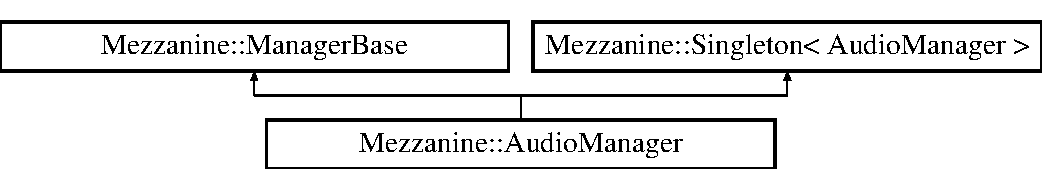
\includegraphics[height=2.000000cm]{classMezzanine_1_1AudioManager}
\end{center}
\end{figure}
\subsubsection*{Public Member Functions}
\begin{DoxyCompactItemize}
\item 
virtual void \hyperlink{classMezzanine_1_1AudioManager_a8db9deed28afb7b07017cb6fd99b624a}{AddSoundToSoundSet} (const \hyperlink{namespaceMezzanine_acf9fcc130e6ebf08e3d8491aebcf1c86}{String} \&SoundSetName, \hyperlink{classMezzanine_1_1Audio_1_1Sound}{Audio::Sound} $\ast$SoundInst)
\begin{DoxyCompactList}\small\item\em Add's a sound to the defined set. \item\end{DoxyCompactList}\item 
\hyperlink{classMezzanine_1_1AudioManager_a30da8ac656fdacf5c420f03304f4e109}{AudioManager} (bool DefaultSettings=true)
\begin{DoxyCompactList}\small\item\em Class Constructor. \item\end{DoxyCompactList}\item 
virtual void \hyperlink{classMezzanine_1_1AudioManager_a4452ecf4eabfae18e0f6651e35530579}{ClearLogs} ()
\begin{DoxyCompactList}\small\item\em This empties logs that the audio subystem creates. \item\end{DoxyCompactList}\item 
virtual \hyperlink{classMezzanine_1_1Audio_1_1Sound}{Audio::Sound} $\ast$ \hyperlink{classMezzanine_1_1AudioManager_aadb6ab0fd58253567da61c8b3432b104}{CreateAmbientSound} (\hyperlink{namespaceMezzanine_a63cd699ac54b73953f35ec9cfc05e506}{ConstString} \&SoundName, \hyperlink{namespaceMezzanine_a63cd699ac54b73953f35ec9cfc05e506}{ConstString} \&FileName, \hyperlink{namespaceMezzanine_a63cd699ac54b73953f35ec9cfc05e506}{ConstString} \&Group)
\begin{DoxyCompactList}\small\item\em Creates an ambient sound instance from a file that can be used to play sounds. \item\end{DoxyCompactList}\item 
virtual \hyperlink{classMezzanine_1_1Audio_1_1Sound}{Audio::Sound} $\ast$ \hyperlink{classMezzanine_1_1AudioManager_ada9827e181e8c8cfc31d290ccb9f6c46}{CreateDialogSound} (\hyperlink{namespaceMezzanine_a63cd699ac54b73953f35ec9cfc05e506}{ConstString} \&SoundName, \hyperlink{namespaceMezzanine_a63cd699ac54b73953f35ec9cfc05e506}{ConstString} \&FileName, \hyperlink{namespaceMezzanine_a63cd699ac54b73953f35ec9cfc05e506}{ConstString} \&Group)
\begin{DoxyCompactList}\small\item\em Creates an dialog sound instance from a file that can be used to play sounds. \item\end{DoxyCompactList}\item 
virtual \hyperlink{classMezzanine_1_1Audio_1_1Sound}{Audio::Sound} $\ast$ \hyperlink{classMezzanine_1_1AudioManager_ab2573d44cfe6e0f8e3d1f0dc794c36a5}{CreateEffectSound} (\hyperlink{namespaceMezzanine_a63cd699ac54b73953f35ec9cfc05e506}{ConstString} \&SoundName, \hyperlink{namespaceMezzanine_a63cd699ac54b73953f35ec9cfc05e506}{ConstString} \&FileName, \hyperlink{namespaceMezzanine_a63cd699ac54b73953f35ec9cfc05e506}{ConstString} \&Group)
\begin{DoxyCompactList}\small\item\em Creates an effect sound instance from a file that can be used to play sounds. \item\end{DoxyCompactList}\item 
virtual \hyperlink{classMezzanine_1_1Audio_1_1Sound}{Audio::Sound} $\ast$ \hyperlink{classMezzanine_1_1AudioManager_a157de9927fb561655b74267d9c375034}{CreateMusicSound} (\hyperlink{namespaceMezzanine_a63cd699ac54b73953f35ec9cfc05e506}{ConstString} \&SoundName, \hyperlink{namespaceMezzanine_a63cd699ac54b73953f35ec9cfc05e506}{ConstString} \&FileName, \hyperlink{namespaceMezzanine_a63cd699ac54b73953f35ec9cfc05e506}{ConstString} \&Group)
\begin{DoxyCompactList}\small\item\em Creates an music sound instance from a file that can be used to play sounds. \item\end{DoxyCompactList}\item 
virtual \hyperlink{classMezzanine_1_1Audio_1_1SoundSet}{Audio::SoundSet} $\ast$ \hyperlink{classMezzanine_1_1AudioManager_ac4a92b861868203186e7f238bd2f816c}{CreateSoundSet} (const \hyperlink{namespaceMezzanine_acf9fcc130e6ebf08e3d8491aebcf1c86}{String} \&SoundSetName)
\begin{DoxyCompactList}\small\item\em Creates a sound set. \item\end{DoxyCompactList}\item 
\hypertarget{classMezzanine_1_1AudioManager_aa9b51e38b4a9b1a1b1efce10fc10f0ee}{
virtual void \hyperlink{classMezzanine_1_1AudioManager_aa9b51e38b4a9b1a1b1efce10fc10f0ee}{DestroyAllSounds} ()}
\label{classMezzanine_1_1AudioManager_aa9b51e38b4a9b1a1b1efce10fc10f0ee}

\begin{DoxyCompactList}\small\item\em Deletes all stored sounds. \item\end{DoxyCompactList}\item 
virtual void \hyperlink{classMezzanine_1_1AudioManager_a6cd0e2faa6913722551a68b9a536c7dd}{DestroySound} (\hyperlink{classMezzanine_1_1Audio_1_1Sound}{Audio::Sound} $\ast$ToBeDestroyed)
\begin{DoxyCompactList}\small\item\em Deletes a Sound. \item\end{DoxyCompactList}\item 
virtual void \hyperlink{classMezzanine_1_1AudioManager_aefcdc7d3276500cf627f2c2e33b483f3}{DoMainLoopItems} ()
\item 
virtual \hyperlink{namespaceMezzanine_a726731b1a7df72bf3583e4a97282c6f6}{Real} \hyperlink{classMezzanine_1_1AudioManager_acb9f1413ab2260c181ded3ddca71d0dd}{GetAmbientVolume} () const 
\begin{DoxyCompactList}\small\item\em Gets the currently set Ambient volume. \item\end{DoxyCompactList}\item 
virtual \hyperlink{namespaceMezzanine_adcbb6ce6d1eb4379d109e51171e2e493}{Whole} \hyperlink{classMezzanine_1_1AudioManager_ae340f137877d14d965e4f47463f2a84a}{GetAvailableDeviceCount} () const 
\begin{DoxyCompactList}\small\item\em Gets the number of available devices. \item\end{DoxyCompactList}\item 
virtual \hyperlink{namespaceMezzanine_acf9fcc130e6ebf08e3d8491aebcf1c86}{String} \hyperlink{classMezzanine_1_1AudioManager_a753f4954528c5845d5fcb97e938594ed}{GetAvailableDeviceNameByIndex} (const \hyperlink{namespaceMezzanine_adcbb6ce6d1eb4379d109e51171e2e493}{Whole} \&Index) const 
\begin{DoxyCompactList}\small\item\em Gets the name of an available device. \item\end{DoxyCompactList}\item 
virtual cAudio::IAudioManager $\ast$ \hyperlink{classMezzanine_1_1AudioManager_ab90e81d0e2bac51ad3552c627cde9336}{GetcAudioManager} () const 
\begin{DoxyCompactList}\small\item\em Gets the internal cAudioManager this manager is based on. \item\end{DoxyCompactList}\item 
virtual \hyperlink{namespaceMezzanine_acf9fcc130e6ebf08e3d8491aebcf1c86}{String} \hyperlink{classMezzanine_1_1AudioManager_aaf0f4e44c56f9dc82005c12e766ca5ef}{GetDefaultDeviceName} () const 
\begin{DoxyCompactList}\small\item\em Gets the name of the default device. \item\end{DoxyCompactList}\item 
virtual \hyperlink{namespaceMezzanine_a726731b1a7df72bf3583e4a97282c6f6}{Real} \hyperlink{classMezzanine_1_1AudioManager_a8eb5c6da62ca7bafb1e990746a0f9397}{GetDialogVolume} () const 
\begin{DoxyCompactList}\small\item\em Gets the currently set Dialog volume. \item\end{DoxyCompactList}\item 
virtual \hyperlink{namespaceMezzanine_a726731b1a7df72bf3583e4a97282c6f6}{Real} \hyperlink{classMezzanine_1_1AudioManager_a06657b2cecce3b0953dc74bcafcff672}{GetEffectVolume} () const 
\begin{DoxyCompactList}\small\item\em Gets the currently set Effect volume. \item\end{DoxyCompactList}\item 
virtual \hyperlink{classMezzanine_1_1Audio_1_1Listener}{Audio::Listener} $\ast$ \hyperlink{classMezzanine_1_1AudioManager_ae24f6ec9247699ed1fae96846c4dfcae}{GetListener} () const 
\begin{DoxyCompactList}\small\item\em Retrieve's the listener for this sound manager. \item\end{DoxyCompactList}\item 
virtual std::stringstream $\ast$ \hyperlink{classMezzanine_1_1AudioManager_a28287efea5943984f96a9ddfd1a2e2a9}{GetLogs} () const 
\begin{DoxyCompactList}\small\item\em This gets the logs that the audio subystem creates. \item\end{DoxyCompactList}\item 
virtual \hyperlink{namespaceMezzanine_a726731b1a7df72bf3583e4a97282c6f6}{Real} \hyperlink{classMezzanine_1_1AudioManager_a8ff9ae76e2aa05b3f49346b2dd5542e0}{GetMasterVolume} () const 
\begin{DoxyCompactList}\small\item\em Gets the currently set Master volume. \item\end{DoxyCompactList}\item 
virtual \hyperlink{classMezzanine_1_1Audio_1_1MusicPlayer}{Audio::MusicPlayer} $\ast$ \hyperlink{classMezzanine_1_1AudioManager_a083c78deb0a783850c0f5a036cafb1b3}{GetMusicPlayer} () const 
\begin{DoxyCompactList}\small\item\em Gets the Music Player for this sound manager. \item\end{DoxyCompactList}\item 
virtual \hyperlink{namespaceMezzanine_a726731b1a7df72bf3583e4a97282c6f6}{Real} \hyperlink{classMezzanine_1_1AudioManager_a0cfcb626b2023911aaa7dee25f49a596}{GetMusicVolume} () const 
\begin{DoxyCompactList}\small\item\em Gets the currently set Music volume. \item\end{DoxyCompactList}\item 
virtual \hyperlink{classMezzanine_1_1Audio_1_1Sound}{Audio::Sound} $\ast$ \hyperlink{classMezzanine_1_1AudioManager_ab65a0838326b7087488052e1c0868078}{GetSoundByName} (const \hyperlink{namespaceMezzanine_acf9fcc130e6ebf08e3d8491aebcf1c86}{String} \&SoundName) const 
\begin{DoxyCompactList}\small\item\em Gets a sound by it's name. \item\end{DoxyCompactList}\item 
virtual \hyperlink{classMezzanine_1_1Audio_1_1SoundSet}{Audio::SoundSet} $\ast$ \hyperlink{classMezzanine_1_1AudioManager_a30d640929214f4dc721da0fa6374743d}{GetSoundSet} (const \hyperlink{namespaceMezzanine_acf9fcc130e6ebf08e3d8491aebcf1c86}{String} \&SoundSetName) const 
\begin{DoxyCompactList}\small\item\em Gets an existing sound set. \item\end{DoxyCompactList}\item 
virtual \hyperlink{classMezzanine_1_1ManagerBase_a08cecf5169cad3e82be81a3a159b0b6e}{ManagerBase::ManagerTypeName} \hyperlink{classMezzanine_1_1AudioManager_a42f2b4b8065387117042bf7eadc97356}{GetType} () const 
\item 
virtual void \hyperlink{classMezzanine_1_1AudioManager_a24f1464e3de9d95e3c50c276f9e176e6}{Initialize} ()
\item 
virtual void \hyperlink{classMezzanine_1_1AudioManager_a5b1d2072c7b4b9813667f6eb0e079d96}{InitializeManager} (\hyperlink{namespaceMezzanine_a63cd699ac54b73953f35ec9cfc05e506}{ConstString} \&DeviceName, int OutputFrequency=-\/1, int EAXEffectSlots=4)
\begin{DoxyCompactList}\small\item\em Initializes the Manager. \item\end{DoxyCompactList}\item 
virtual bool \hyperlink{classMezzanine_1_1AudioManager_abd9029e2783691428d1d6031560ee743}{IsMuted} () const 
\begin{DoxyCompactList}\small\item\em Gets whether or not the \hyperlink{namespaceMezzanine_1_1Audio}{Audio} subsystem is muted. \item\end{DoxyCompactList}\item 
virtual void \hyperlink{classMezzanine_1_1AudioManager_a2df3cdf8b7fcfe844847f6181d788e5c}{Mute} (bool Enable)
\begin{DoxyCompactList}\small\item\em Sets whether or not to mute all \hyperlink{namespaceMezzanine_1_1Audio}{Audio}. \item\end{DoxyCompactList}\item 
virtual void \hyperlink{classMezzanine_1_1AudioManager_a57a2ac96d43af13df8f11112515c3b96}{SetAmbientVolume} (const \hyperlink{namespaceMezzanine_a726731b1a7df72bf3583e4a97282c6f6}{Real} \&Ambient)
\begin{DoxyCompactList}\small\item\em Sets the volume for all stored Ambient sounds. \item\end{DoxyCompactList}\item 
virtual void \hyperlink{classMezzanine_1_1AudioManager_ab69018e84430a5dc4facb23341e3aeb3}{SetDialogVolume} (const \hyperlink{namespaceMezzanine_a726731b1a7df72bf3583e4a97282c6f6}{Real} \&Dialog)
\begin{DoxyCompactList}\small\item\em Sets the volume for all stored Dialog sounds. \item\end{DoxyCompactList}\item 
virtual void \hyperlink{classMezzanine_1_1AudioManager_a390953c8eecd4446854b1e4c1c431f5a}{SetEffectVolume} (const \hyperlink{namespaceMezzanine_a726731b1a7df72bf3583e4a97282c6f6}{Real} \&Effect)
\begin{DoxyCompactList}\small\item\em Sets the volume for all stored Effect sounds. \item\end{DoxyCompactList}\item 
virtual void \hyperlink{classMezzanine_1_1AudioManager_ae3120d9f9877113fbe019f63a451f155}{SetMasterVolume} (const \hyperlink{namespaceMezzanine_a726731b1a7df72bf3583e4a97282c6f6}{Real} \&Master)
\begin{DoxyCompactList}\small\item\em Sets the volume for all stored sounds. \item\end{DoxyCompactList}\item 
virtual void \hyperlink{classMezzanine_1_1AudioManager_a8df0f5fb1e426a59cfafee4f54201db7}{SetMusicVolume} (const \hyperlink{namespaceMezzanine_a726731b1a7df72bf3583e4a97282c6f6}{Real} \&Music)
\begin{DoxyCompactList}\small\item\em Sets the volume for all stored Music sounds. \item\end{DoxyCompactList}\item 
virtual void \hyperlink{classMezzanine_1_1AudioManager_a1171a0dece85578907c6bbf82da56936}{UpdateAllVolumes} ()
\begin{DoxyCompactList}\small\item\em Calls on all sounds stored in this manager to update their volume after a settings change. \item\end{DoxyCompactList}\item 
virtual \hyperlink{classMezzanine_1_1AudioManager_aed11c120ed062fa13a0881099859a957}{$\sim$AudioManager} ()
\begin{DoxyCompactList}\small\item\em Class Destructor. \item\end{DoxyCompactList}\end{DoxyCompactItemize}
\subsubsection*{Protected Attributes}
\begin{DoxyCompactItemize}
\item 
\hypertarget{classMezzanine_1_1AudioManager_aff24fe21e09898d3adc052b27e792bad}{
std::vector$<$ \hyperlink{classMezzanine_1_1Audio_1_1Sound}{Audio::Sound} $\ast$ $>$ {\bfseries AmbientSounds}}
\label{classMezzanine_1_1AudioManager_aff24fe21e09898d3adc052b27e792bad}

\item 
\hypertarget{classMezzanine_1_1AudioManager_a570eed5adc15f281153a2302e3f159d2}{
\hyperlink{namespaceMezzanine_a726731b1a7df72bf3583e4a97282c6f6}{Real} {\bfseries AmbientVolume}}
\label{classMezzanine_1_1AudioManager_a570eed5adc15f281153a2302e3f159d2}

\item 
\hypertarget{classMezzanine_1_1AudioManager_a0d146b669322a92a30a1812be29ea999}{
cAudio::IAudioManager $\ast$ {\bfseries cAudioManager}}
\label{classMezzanine_1_1AudioManager_a0d146b669322a92a30a1812be29ea999}

\item 
\hypertarget{classMezzanine_1_1AudioManager_af211374a8eb3eeff4742dbc2243b4308}{
std::vector$<$ \hyperlink{classMezzanine_1_1Audio_1_1Sound}{Audio::Sound} $\ast$ $>$ {\bfseries DialogSounds}}
\label{classMezzanine_1_1AudioManager_af211374a8eb3eeff4742dbc2243b4308}

\item 
\hypertarget{classMezzanine_1_1AudioManager_a02fa98196e316a59eb6a37ffbdf53c4d}{
\hyperlink{namespaceMezzanine_a726731b1a7df72bf3583e4a97282c6f6}{Real} {\bfseries DialogVolume}}
\label{classMezzanine_1_1AudioManager_a02fa98196e316a59eb6a37ffbdf53c4d}

\item 
\hypertarget{classMezzanine_1_1AudioManager_ae471b95b9d49e418fd76851bc3812403}{
std::vector$<$ \hyperlink{classMezzanine_1_1Audio_1_1Sound}{Audio::Sound} $\ast$ $>$ {\bfseries EffectSounds}}
\label{classMezzanine_1_1AudioManager_ae471b95b9d49e418fd76851bc3812403}

\item 
\hypertarget{classMezzanine_1_1AudioManager_a85cdc6b34f887280c828b8666a6a27c4}{
\hyperlink{namespaceMezzanine_a726731b1a7df72bf3583e4a97282c6f6}{Real} {\bfseries EffectVolume}}
\label{classMezzanine_1_1AudioManager_a85cdc6b34f887280c828b8666a6a27c4}

\item 
\hypertarget{classMezzanine_1_1AudioManager_a3628bd4b073bb30f0b040fb140b0c945}{
\hyperlink{classMezzanine_1_1Audio_1_1Listener}{Audio::Listener} $\ast$ {\bfseries Listener}}
\label{classMezzanine_1_1AudioManager_a3628bd4b073bb30f0b040fb140b0c945}

\item 
\hypertarget{classMezzanine_1_1AudioManager_aa2df9162da340e2eb8c1e4688bd6bb45}{
\hyperlink{namespaceMezzanine_a726731b1a7df72bf3583e4a97282c6f6}{Real} {\bfseries MasterVolume}}
\label{classMezzanine_1_1AudioManager_aa2df9162da340e2eb8c1e4688bd6bb45}

\item 
\hypertarget{classMezzanine_1_1AudioManager_a2b06e0f622849741dee1202241474c12}{
\hyperlink{classMezzanine_1_1Audio_1_1MusicPlayer}{Audio::MusicPlayer} $\ast$ {\bfseries MusicPlayer}}
\label{classMezzanine_1_1AudioManager_a2b06e0f622849741dee1202241474c12}

\item 
\hypertarget{classMezzanine_1_1AudioManager_adc4a4f0a2754ca70f1e6bca2eb95f69d}{
std::vector$<$ \hyperlink{classMezzanine_1_1Audio_1_1Sound}{Audio::Sound} $\ast$ $>$ {\bfseries MusicSounds}}
\label{classMezzanine_1_1AudioManager_adc4a4f0a2754ca70f1e6bca2eb95f69d}

\item 
\hypertarget{classMezzanine_1_1AudioManager_aa84ee647228943794bf0b857a4c1cdb7}{
\hyperlink{namespaceMezzanine_a726731b1a7df72bf3583e4a97282c6f6}{Real} {\bfseries MusicVolume}}
\label{classMezzanine_1_1AudioManager_aa84ee647228943794bf0b857a4c1cdb7}

\item 
\hypertarget{classMezzanine_1_1AudioManager_a60f7da3a59fadad8b3a94272a691ac6b}{
bool {\bfseries Muted}}
\label{classMezzanine_1_1AudioManager_a60f7da3a59fadad8b3a94272a691ac6b}

\item 
\hypertarget{classMezzanine_1_1AudioManager_a0d84662914bcf7e794c2bd21ee0ae562}{
\hyperlink{namespaceMezzanine_a726731b1a7df72bf3583e4a97282c6f6}{Real} {\bfseries MuteStandby}}
\label{classMezzanine_1_1AudioManager_a0d84662914bcf7e794c2bd21ee0ae562}

\item 
\hypertarget{classMezzanine_1_1AudioManager_aff1a53d82434c8252c27be10536c1bb9}{
std::map$<$ \hyperlink{namespaceMezzanine_acf9fcc130e6ebf08e3d8491aebcf1c86}{String}, \hyperlink{classMezzanine_1_1Audio_1_1Sound}{Audio::Sound} $\ast$ $>$ {\bfseries Sounds}}
\label{classMezzanine_1_1AudioManager_aff1a53d82434c8252c27be10536c1bb9}

\item 
\hypertarget{classMezzanine_1_1AudioManager_aa311fde30dbe1bba760217be9cdc5727}{
std::map$<$ \hyperlink{namespaceMezzanine_acf9fcc130e6ebf08e3d8491aebcf1c86}{String}, \hyperlink{classMezzanine_1_1Audio_1_1SoundSet}{Audio::SoundSet} $\ast$ $>$ {\bfseries SoundSets}}
\label{classMezzanine_1_1AudioManager_aa311fde30dbe1bba760217be9cdc5727}

\end{DoxyCompactItemize}


\subsubsection{Detailed Description}
This is simply a place for storing all the Sound utilities and functions. This is a place for loading, storing, and running sound files as necessary in a given game. 

Definition at line 75 of file audiomanager.h.



\subsubsection{Constructor \& Destructor Documentation}
\hypertarget{classMezzanine_1_1AudioManager_a30da8ac656fdacf5c420f03304f4e109}{
\index{Mezzanine::AudioManager@{Mezzanine::AudioManager}!AudioManager@{AudioManager}}
\index{AudioManager@{AudioManager}!Mezzanine::AudioManager@{Mezzanine::AudioManager}}
\paragraph[{AudioManager}]{\setlength{\rightskip}{0pt plus 5cm}Mezzanine::AudioManager::AudioManager (
\begin{DoxyParamCaption}
\item[{bool}]{DefaultSettings = {\ttfamily true}}
\end{DoxyParamCaption}
)}\hfill}
\label{classMezzanine_1_1AudioManager_a30da8ac656fdacf5c420f03304f4e109}


Class Constructor. 

This is the class constructor. It gives you the option to start up the manager with default values if you choose. If not then you'll need to setup and initialize the manager yourself after it is constructed. 
\begin{DoxyParams}{Parameters}
{\em DefaultSettings} & Whether or not to load default settings and initialize the manager immediately. \\
\hline
\end{DoxyParams}


Definition at line 55 of file audiomanager.cpp.

\hypertarget{classMezzanine_1_1AudioManager_aed11c120ed062fa13a0881099859a957}{
\index{Mezzanine::AudioManager@{Mezzanine::AudioManager}!$\sim$AudioManager@{$\sim$AudioManager}}
\index{$\sim$AudioManager@{$\sim$AudioManager}!Mezzanine::AudioManager@{Mezzanine::AudioManager}}
\paragraph[{$\sim$AudioManager}]{\setlength{\rightskip}{0pt plus 5cm}Mezzanine::AudioManager::$\sim$AudioManager (
\begin{DoxyParamCaption}
{}
\end{DoxyParamCaption}
)\hspace{0.3cm}{\ttfamily  \mbox{[}virtual\mbox{]}}}\hfill}
\label{classMezzanine_1_1AudioManager_aed11c120ed062fa13a0881099859a957}


Class Destructor. 

The class destructor. 

Definition at line 69 of file audiomanager.cpp.



\subsubsection{Member Function Documentation}
\hypertarget{classMezzanine_1_1AudioManager_a8db9deed28afb7b07017cb6fd99b624a}{
\index{Mezzanine::AudioManager@{Mezzanine::AudioManager}!AddSoundToSoundSet@{AddSoundToSoundSet}}
\index{AddSoundToSoundSet@{AddSoundToSoundSet}!Mezzanine::AudioManager@{Mezzanine::AudioManager}}
\paragraph[{AddSoundToSoundSet}]{\setlength{\rightskip}{0pt plus 5cm}void Mezzanine::AudioManager::AddSoundToSoundSet (
\begin{DoxyParamCaption}
\item[{const {\bf String} \&}]{SoundSetName, }
\item[{{\bf Audio::Sound} $\ast$}]{SoundInst}
\end{DoxyParamCaption}
)\hspace{0.3cm}{\ttfamily  \mbox{[}virtual\mbox{]}}}\hfill}
\label{classMezzanine_1_1AudioManager_a8db9deed28afb7b07017cb6fd99b624a}


Add's a sound to the defined set. 

This function will add a sound instance to a created sound set. 
\begin{DoxyParams}{Parameters}
{\em SoundName} & The sound instance to be added. \\
\hline
\end{DoxyParams}


Definition at line 151 of file audiomanager.cpp.

\hypertarget{classMezzanine_1_1AudioManager_a4452ecf4eabfae18e0f6651e35530579}{
\index{Mezzanine::AudioManager@{Mezzanine::AudioManager}!ClearLogs@{ClearLogs}}
\index{ClearLogs@{ClearLogs}!Mezzanine::AudioManager@{Mezzanine::AudioManager}}
\paragraph[{ClearLogs}]{\setlength{\rightskip}{0pt plus 5cm}void Mezzanine::AudioManager::ClearLogs (
\begin{DoxyParamCaption}
{}
\end{DoxyParamCaption}
)\hspace{0.3cm}{\ttfamily  \mbox{[}virtual\mbox{]}}}\hfill}
\label{classMezzanine_1_1AudioManager_a4452ecf4eabfae18e0f6651e35530579}


This empties logs that the audio subystem creates. 

Internally the \hyperlink{namespaceMezzanine}{Mezzanine} engine currently uses cAudio to process 3d sound. It has it's own logging system that we have customized to work with our logger. This clears that data allow us to work with it as we need 

Definition at line 277 of file audiomanager.cpp.

\hypertarget{classMezzanine_1_1AudioManager_aadb6ab0fd58253567da61c8b3432b104}{
\index{Mezzanine::AudioManager@{Mezzanine::AudioManager}!CreateAmbientSound@{CreateAmbientSound}}
\index{CreateAmbientSound@{CreateAmbientSound}!Mezzanine::AudioManager@{Mezzanine::AudioManager}}
\paragraph[{CreateAmbientSound}]{\setlength{\rightskip}{0pt plus 5cm}{\bf Audio::Sound} $\ast$ Mezzanine::AudioManager::CreateAmbientSound (
\begin{DoxyParamCaption}
\item[{{\bf ConstString} \&}]{SoundName, }
\item[{{\bf ConstString} \&}]{FileName, }
\item[{{\bf ConstString} \&}]{Group}
\end{DoxyParamCaption}
)\hspace{0.3cm}{\ttfamily  \mbox{[}virtual\mbox{]}}}\hfill}
\label{classMezzanine_1_1AudioManager_aadb6ab0fd58253567da61c8b3432b104}


Creates an ambient sound instance from a file that can be used to play sounds. 


\begin{DoxyParams}{Parameters}
{\em SoundName} & The name of the Sound instance. \\
\hline
{\em FileName} & The name of the file. \\
\hline
{\em Group} & The resource group in which the file resides. \\
\hline
\end{DoxyParams}
\begin{DoxyReturn}{Returns}
Returns a pointer to the Sound Instance that was created. 
\end{DoxyReturn}


Definition at line 75 of file audiomanager.cpp.

\hypertarget{classMezzanine_1_1AudioManager_ada9827e181e8c8cfc31d290ccb9f6c46}{
\index{Mezzanine::AudioManager@{Mezzanine::AudioManager}!CreateDialogSound@{CreateDialogSound}}
\index{CreateDialogSound@{CreateDialogSound}!Mezzanine::AudioManager@{Mezzanine::AudioManager}}
\paragraph[{CreateDialogSound}]{\setlength{\rightskip}{0pt plus 5cm}{\bf Audio::Sound} $\ast$ Mezzanine::AudioManager::CreateDialogSound (
\begin{DoxyParamCaption}
\item[{{\bf ConstString} \&}]{SoundName, }
\item[{{\bf ConstString} \&}]{FileName, }
\item[{{\bf ConstString} \&}]{Group}
\end{DoxyParamCaption}
)\hspace{0.3cm}{\ttfamily  \mbox{[}virtual\mbox{]}}}\hfill}
\label{classMezzanine_1_1AudioManager_ada9827e181e8c8cfc31d290ccb9f6c46}


Creates an dialog sound instance from a file that can be used to play sounds. 


\begin{DoxyParams}{Parameters}
{\em SoundName} & The name of the Sound instance. \\
\hline
{\em FileName} & The name of the file. \\
\hline
{\em Group} & The resource group in which the file resides. \\
\hline
\end{DoxyParams}
\begin{DoxyReturn}{Returns}
Returns a pointer to the Sound Instance that was created. 
\end{DoxyReturn}


Definition at line 83 of file audiomanager.cpp.

\hypertarget{classMezzanine_1_1AudioManager_ab2573d44cfe6e0f8e3d1f0dc794c36a5}{
\index{Mezzanine::AudioManager@{Mezzanine::AudioManager}!CreateEffectSound@{CreateEffectSound}}
\index{CreateEffectSound@{CreateEffectSound}!Mezzanine::AudioManager@{Mezzanine::AudioManager}}
\paragraph[{CreateEffectSound}]{\setlength{\rightskip}{0pt plus 5cm}{\bf Audio::Sound} $\ast$ Mezzanine::AudioManager::CreateEffectSound (
\begin{DoxyParamCaption}
\item[{{\bf ConstString} \&}]{SoundName, }
\item[{{\bf ConstString} \&}]{FileName, }
\item[{{\bf ConstString} \&}]{Group}
\end{DoxyParamCaption}
)\hspace{0.3cm}{\ttfamily  \mbox{[}virtual\mbox{]}}}\hfill}
\label{classMezzanine_1_1AudioManager_ab2573d44cfe6e0f8e3d1f0dc794c36a5}


Creates an effect sound instance from a file that can be used to play sounds. 


\begin{DoxyParams}{Parameters}
{\em SoundName} & The name of the Sound instance. \\
\hline
{\em FileName} & The name of the file. \\
\hline
{\em Group} & The resource group in which the file resides. \\
\hline
\end{DoxyParams}
\begin{DoxyReturn}{Returns}
Returns a pointer to the Sound Instance that was created. 
\end{DoxyReturn}


Definition at line 91 of file audiomanager.cpp.

\hypertarget{classMezzanine_1_1AudioManager_a157de9927fb561655b74267d9c375034}{
\index{Mezzanine::AudioManager@{Mezzanine::AudioManager}!CreateMusicSound@{CreateMusicSound}}
\index{CreateMusicSound@{CreateMusicSound}!Mezzanine::AudioManager@{Mezzanine::AudioManager}}
\paragraph[{CreateMusicSound}]{\setlength{\rightskip}{0pt plus 5cm}{\bf Audio::Sound} $\ast$ Mezzanine::AudioManager::CreateMusicSound (
\begin{DoxyParamCaption}
\item[{{\bf ConstString} \&}]{SoundName, }
\item[{{\bf ConstString} \&}]{FileName, }
\item[{{\bf ConstString} \&}]{Group}
\end{DoxyParamCaption}
)\hspace{0.3cm}{\ttfamily  \mbox{[}virtual\mbox{]}}}\hfill}
\label{classMezzanine_1_1AudioManager_a157de9927fb561655b74267d9c375034}


Creates an music sound instance from a file that can be used to play sounds. 


\begin{DoxyParams}{Parameters}
{\em SoundName} & The name of the Sound instance. \\
\hline
{\em FileName} & The name of the file. \\
\hline
{\em Group} & The resource group in which the file resides. \\
\hline
\end{DoxyParams}
\begin{DoxyReturn}{Returns}
Returns a pointer to the Sound Instance that was created. 
\end{DoxyReturn}


Definition at line 99 of file audiomanager.cpp.

\hypertarget{classMezzanine_1_1AudioManager_ac4a92b861868203186e7f238bd2f816c}{
\index{Mezzanine::AudioManager@{Mezzanine::AudioManager}!CreateSoundSet@{CreateSoundSet}}
\index{CreateSoundSet@{CreateSoundSet}!Mezzanine::AudioManager@{Mezzanine::AudioManager}}
\paragraph[{CreateSoundSet}]{\setlength{\rightskip}{0pt plus 5cm}{\bf Audio::SoundSet} $\ast$ Mezzanine::AudioManager::CreateSoundSet (
\begin{DoxyParamCaption}
\item[{const {\bf String} \&}]{SoundSetName}
\end{DoxyParamCaption}
)\hspace{0.3cm}{\ttfamily  \mbox{[}virtual\mbox{]}}}\hfill}
\label{classMezzanine_1_1AudioManager_ac4a92b861868203186e7f238bd2f816c}


Creates a sound set. 

This function will create a sound set vector you can use to store similiar sound instances. 
\begin{DoxyParams}{Parameters}
{\em SoundSetName} & The name you wish the sound set to have. \\
\hline
\end{DoxyParams}
\begin{DoxyReturn}{Returns}
Returns a pointer to the created Vector. 
\end{DoxyReturn}


Definition at line 137 of file audiomanager.cpp.

\hypertarget{classMezzanine_1_1AudioManager_a6cd0e2faa6913722551a68b9a536c7dd}{
\index{Mezzanine::AudioManager@{Mezzanine::AudioManager}!DestroySound@{DestroySound}}
\index{DestroySound@{DestroySound}!Mezzanine::AudioManager@{Mezzanine::AudioManager}}
\paragraph[{DestroySound}]{\setlength{\rightskip}{0pt plus 5cm}void Mezzanine::AudioManager::DestroySound (
\begin{DoxyParamCaption}
\item[{{\bf Audio::Sound} $\ast$}]{ToBeDestroyed}
\end{DoxyParamCaption}
)\hspace{0.3cm}{\ttfamily  \mbox{[}virtual\mbox{]}}}\hfill}
\label{classMezzanine_1_1AudioManager_a6cd0e2faa6913722551a68b9a536c7dd}


Deletes a Sound. 


\begin{DoxyParams}{Parameters}
{\em SoundName} & A pointer to the Sound you want deleted. \\
\hline
\end{DoxyParams}


Definition at line 114 of file audiomanager.cpp.

\hypertarget{classMezzanine_1_1AudioManager_aefcdc7d3276500cf627f2c2e33b483f3}{
\index{Mezzanine::AudioManager@{Mezzanine::AudioManager}!DoMainLoopItems@{DoMainLoopItems}}
\index{DoMainLoopItems@{DoMainLoopItems}!Mezzanine::AudioManager@{Mezzanine::AudioManager}}
\paragraph[{DoMainLoopItems}]{\setlength{\rightskip}{0pt plus 5cm}void Mezzanine::AudioManager::DoMainLoopItems (
\begin{DoxyParamCaption}
{}
\end{DoxyParamCaption}
)\hspace{0.3cm}{\ttfamily  \mbox{[}virtual\mbox{]}}}\hfill}
\label{classMezzanine_1_1AudioManager_aefcdc7d3276500cf627f2c2e33b483f3}
The main loop calls this once per frame. 

This is where each manager is expected to put anything that needs to be run each iteration of the main loop  

Implements \hyperlink{classMezzanine_1_1ManagerBase_a4ee29e4baf6c4b9a3bfec1b2258d5cd2}{Mezzanine::ManagerBase}.



Definition at line 305 of file audiomanager.cpp.

\hypertarget{classMezzanine_1_1AudioManager_acb9f1413ab2260c181ded3ddca71d0dd}{
\index{Mezzanine::AudioManager@{Mezzanine::AudioManager}!GetAmbientVolume@{GetAmbientVolume}}
\index{GetAmbientVolume@{GetAmbientVolume}!Mezzanine::AudioManager@{Mezzanine::AudioManager}}
\paragraph[{GetAmbientVolume}]{\setlength{\rightskip}{0pt plus 5cm}{\bf Real} Mezzanine::AudioManager::GetAmbientVolume (
\begin{DoxyParamCaption}
{}
\end{DoxyParamCaption}
) const\hspace{0.3cm}{\ttfamily  \mbox{[}virtual\mbox{]}}}\hfill}
\label{classMezzanine_1_1AudioManager_acb9f1413ab2260c181ded3ddca71d0dd}


Gets the currently set Ambient volume. 

\begin{DoxyReturn}{Returns}
Returns a Real representing the current Ambient volume. 
\end{DoxyReturn}


Definition at line 166 of file audiomanager.cpp.

\hypertarget{classMezzanine_1_1AudioManager_ae340f137877d14d965e4f47463f2a84a}{
\index{Mezzanine::AudioManager@{Mezzanine::AudioManager}!GetAvailableDeviceCount@{GetAvailableDeviceCount}}
\index{GetAvailableDeviceCount@{GetAvailableDeviceCount}!Mezzanine::AudioManager@{Mezzanine::AudioManager}}
\paragraph[{GetAvailableDeviceCount}]{\setlength{\rightskip}{0pt plus 5cm}{\bf Whole} Mezzanine::AudioManager::GetAvailableDeviceCount (
\begin{DoxyParamCaption}
{}
\end{DoxyParamCaption}
) const\hspace{0.3cm}{\ttfamily  \mbox{[}virtual\mbox{]}}}\hfill}
\label{classMezzanine_1_1AudioManager_ae340f137877d14d965e4f47463f2a84a}


Gets the number of available devices. 

This function will return the total number of available devices, including the default. \begin{DoxyReturn}{Returns}
Returns the number of available devices. 
\end{DoxyReturn}


Definition at line 267 of file audiomanager.cpp.

\hypertarget{classMezzanine_1_1AudioManager_a753f4954528c5845d5fcb97e938594ed}{
\index{Mezzanine::AudioManager@{Mezzanine::AudioManager}!GetAvailableDeviceNameByIndex@{GetAvailableDeviceNameByIndex}}
\index{GetAvailableDeviceNameByIndex@{GetAvailableDeviceNameByIndex}!Mezzanine::AudioManager@{Mezzanine::AudioManager}}
\paragraph[{GetAvailableDeviceNameByIndex}]{\setlength{\rightskip}{0pt plus 5cm}{\bf String} Mezzanine::AudioManager::GetAvailableDeviceNameByIndex (
\begin{DoxyParamCaption}
\item[{const {\bf Whole} \&}]{Index}
\end{DoxyParamCaption}
) const\hspace{0.3cm}{\ttfamily  \mbox{[}virtual\mbox{]}}}\hfill}
\label{classMezzanine_1_1AudioManager_a753f4954528c5845d5fcb97e938594ed}


Gets the name of an available device. 

This function will retrieve the name of a device by it's index on the sound managers device list. 
\begin{DoxyParams}{Parameters}
{\em Index} & The position on the device list you wish to access the name of. \\
\hline
\end{DoxyParams}
\begin{DoxyReturn}{Returns}
Returns the name of the device. 
\end{DoxyReturn}


Definition at line 253 of file audiomanager.cpp.

\hypertarget{classMezzanine_1_1AudioManager_ab90e81d0e2bac51ad3552c627cde9336}{
\index{Mezzanine::AudioManager@{Mezzanine::AudioManager}!GetcAudioManager@{GetcAudioManager}}
\index{GetcAudioManager@{GetcAudioManager}!Mezzanine::AudioManager@{Mezzanine::AudioManager}}
\paragraph[{GetcAudioManager}]{\setlength{\rightskip}{0pt plus 5cm}cAudio::IAudioManager $\ast$ Mezzanine::AudioManager::GetcAudioManager (
\begin{DoxyParamCaption}
{}
\end{DoxyParamCaption}
) const\hspace{0.3cm}{\ttfamily  \mbox{[}virtual\mbox{]}}}\hfill}
\label{classMezzanine_1_1AudioManager_ab90e81d0e2bac51ad3552c627cde9336}


Gets the internal cAudioManager this manager is based on. 

\begin{DoxyReturn}{Returns}
Returns a pointer to the internal cAudio manager. 
\end{DoxyReturn}


Definition at line 297 of file audiomanager.cpp.

\hypertarget{classMezzanine_1_1AudioManager_aaf0f4e44c56f9dc82005c12e766ca5ef}{
\index{Mezzanine::AudioManager@{Mezzanine::AudioManager}!GetDefaultDeviceName@{GetDefaultDeviceName}}
\index{GetDefaultDeviceName@{GetDefaultDeviceName}!Mezzanine::AudioManager@{Mezzanine::AudioManager}}
\paragraph[{GetDefaultDeviceName}]{\setlength{\rightskip}{0pt plus 5cm}{\bf String} Mezzanine::AudioManager::GetDefaultDeviceName (
\begin{DoxyParamCaption}
{}
\end{DoxyParamCaption}
) const\hspace{0.3cm}{\ttfamily  \mbox{[}virtual\mbox{]}}}\hfill}
\label{classMezzanine_1_1AudioManager_aaf0f4e44c56f9dc82005c12e766ca5ef}


Gets the name of the default device. 

This function will return the name of the system default device. \begin{DoxyReturn}{Returns}
Returns the name of the default device. 
\end{DoxyReturn}


Definition at line 260 of file audiomanager.cpp.

\hypertarget{classMezzanine_1_1AudioManager_a8eb5c6da62ca7bafb1e990746a0f9397}{
\index{Mezzanine::AudioManager@{Mezzanine::AudioManager}!GetDialogVolume@{GetDialogVolume}}
\index{GetDialogVolume@{GetDialogVolume}!Mezzanine::AudioManager@{Mezzanine::AudioManager}}
\paragraph[{GetDialogVolume}]{\setlength{\rightskip}{0pt plus 5cm}{\bf Real} Mezzanine::AudioManager::GetDialogVolume (
\begin{DoxyParamCaption}
{}
\end{DoxyParamCaption}
) const\hspace{0.3cm}{\ttfamily  \mbox{[}virtual\mbox{]}}}\hfill}
\label{classMezzanine_1_1AudioManager_a8eb5c6da62ca7bafb1e990746a0f9397}


Gets the currently set Dialog volume. 

\begin{DoxyReturn}{Returns}
Returns a Real representing the current Dialog volume. 
\end{DoxyReturn}


Definition at line 180 of file audiomanager.cpp.

\hypertarget{classMezzanine_1_1AudioManager_a06657b2cecce3b0953dc74bcafcff672}{
\index{Mezzanine::AudioManager@{Mezzanine::AudioManager}!GetEffectVolume@{GetEffectVolume}}
\index{GetEffectVolume@{GetEffectVolume}!Mezzanine::AudioManager@{Mezzanine::AudioManager}}
\paragraph[{GetEffectVolume}]{\setlength{\rightskip}{0pt plus 5cm}{\bf Real} Mezzanine::AudioManager::GetEffectVolume (
\begin{DoxyParamCaption}
{}
\end{DoxyParamCaption}
) const\hspace{0.3cm}{\ttfamily  \mbox{[}virtual\mbox{]}}}\hfill}
\label{classMezzanine_1_1AudioManager_a06657b2cecce3b0953dc74bcafcff672}


Gets the currently set Effect volume. 

\begin{DoxyReturn}{Returns}
Returns a Real representing the current Effect volume. 
\end{DoxyReturn}


Definition at line 194 of file audiomanager.cpp.

\hypertarget{classMezzanine_1_1AudioManager_ae24f6ec9247699ed1fae96846c4dfcae}{
\index{Mezzanine::AudioManager@{Mezzanine::AudioManager}!GetListener@{GetListener}}
\index{GetListener@{GetListener}!Mezzanine::AudioManager@{Mezzanine::AudioManager}}
\paragraph[{GetListener}]{\setlength{\rightskip}{0pt plus 5cm}{\bf Audio::Listener} $\ast$ Mezzanine::AudioManager::GetListener (
\begin{DoxyParamCaption}
{}
\end{DoxyParamCaption}
) const\hspace{0.3cm}{\ttfamily  \mbox{[}virtual\mbox{]}}}\hfill}
\label{classMezzanine_1_1AudioManager_ae24f6ec9247699ed1fae96846c4dfcae}


Retrieve's the listener for this sound manager. 

This function will return the listener for this manager which can be used to help create 3D sound. \begin{DoxyReturn}{Returns}
Returns a pointer to the managers Sound Listener. 
\end{DoxyReturn}


Definition at line 287 of file audiomanager.cpp.

\hypertarget{classMezzanine_1_1AudioManager_a28287efea5943984f96a9ddfd1a2e2a9}{
\index{Mezzanine::AudioManager@{Mezzanine::AudioManager}!GetLogs@{GetLogs}}
\index{GetLogs@{GetLogs}!Mezzanine::AudioManager@{Mezzanine::AudioManager}}
\paragraph[{GetLogs}]{\setlength{\rightskip}{0pt plus 5cm}std::stringstream $\ast$ Mezzanine::AudioManager::GetLogs (
\begin{DoxyParamCaption}
{}
\end{DoxyParamCaption}
) const\hspace{0.3cm}{\ttfamily  \mbox{[}virtual\mbox{]}}}\hfill}
\label{classMezzanine_1_1AudioManager_a28287efea5943984f96a9ddfd1a2e2a9}


This gets the logs that the audio subystem creates. 

Internally the \hyperlink{namespaceMezzanine}{Mezzanine} engine currently uses cAudio to process 3d sound. It has it's own logging system that we have customized to work with our logger. \begin{DoxyReturn}{Returns}
This gets the log of what actions the audio system has performed 
\end{DoxyReturn}


Definition at line 272 of file audiomanager.cpp.

\hypertarget{classMezzanine_1_1AudioManager_a8ff9ae76e2aa05b3f49346b2dd5542e0}{
\index{Mezzanine::AudioManager@{Mezzanine::AudioManager}!GetMasterVolume@{GetMasterVolume}}
\index{GetMasterVolume@{GetMasterVolume}!Mezzanine::AudioManager@{Mezzanine::AudioManager}}
\paragraph[{GetMasterVolume}]{\setlength{\rightskip}{0pt plus 5cm}{\bf Real} Mezzanine::AudioManager::GetMasterVolume (
\begin{DoxyParamCaption}
{}
\end{DoxyParamCaption}
) const\hspace{0.3cm}{\ttfamily  \mbox{[}virtual\mbox{]}}}\hfill}
\label{classMezzanine_1_1AudioManager_a8ff9ae76e2aa05b3f49346b2dd5542e0}


Gets the currently set Master volume. 

\begin{DoxyReturn}{Returns}
Returns a Real representing the current Master volume. 
\end{DoxyReturn}


Definition at line 219 of file audiomanager.cpp.

\hypertarget{classMezzanine_1_1AudioManager_a083c78deb0a783850c0f5a036cafb1b3}{
\index{Mezzanine::AudioManager@{Mezzanine::AudioManager}!GetMusicPlayer@{GetMusicPlayer}}
\index{GetMusicPlayer@{GetMusicPlayer}!Mezzanine::AudioManager@{Mezzanine::AudioManager}}
\paragraph[{GetMusicPlayer}]{\setlength{\rightskip}{0pt plus 5cm}{\bf Audio::MusicPlayer} $\ast$ Mezzanine::AudioManager::GetMusicPlayer (
\begin{DoxyParamCaption}
{}
\end{DoxyParamCaption}
) const\hspace{0.3cm}{\ttfamily  \mbox{[}virtual\mbox{]}}}\hfill}
\label{classMezzanine_1_1AudioManager_a083c78deb0a783850c0f5a036cafb1b3}


Gets the Music Player for this sound manager. 

\begin{DoxyReturn}{Returns}
Returns a pointer to the managers Music Player. 
\end{DoxyReturn}


Definition at line 292 of file audiomanager.cpp.

\hypertarget{classMezzanine_1_1AudioManager_a0cfcb626b2023911aaa7dee25f49a596}{
\index{Mezzanine::AudioManager@{Mezzanine::AudioManager}!GetMusicVolume@{GetMusicVolume}}
\index{GetMusicVolume@{GetMusicVolume}!Mezzanine::AudioManager@{Mezzanine::AudioManager}}
\paragraph[{GetMusicVolume}]{\setlength{\rightskip}{0pt plus 5cm}{\bf Real} Mezzanine::AudioManager::GetMusicVolume (
\begin{DoxyParamCaption}
{}
\end{DoxyParamCaption}
) const\hspace{0.3cm}{\ttfamily  \mbox{[}virtual\mbox{]}}}\hfill}
\label{classMezzanine_1_1AudioManager_a0cfcb626b2023911aaa7dee25f49a596}


Gets the currently set Music volume. 

\begin{DoxyReturn}{Returns}
Returns a Real representing the current Music volume. 
\end{DoxyReturn}


Definition at line 208 of file audiomanager.cpp.

\hypertarget{classMezzanine_1_1AudioManager_ab65a0838326b7087488052e1c0868078}{
\index{Mezzanine::AudioManager@{Mezzanine::AudioManager}!GetSoundByName@{GetSoundByName}}
\index{GetSoundByName@{GetSoundByName}!Mezzanine::AudioManager@{Mezzanine::AudioManager}}
\paragraph[{GetSoundByName}]{\setlength{\rightskip}{0pt plus 5cm}{\bf Audio::Sound} $\ast$ Mezzanine::AudioManager::GetSoundByName (
\begin{DoxyParamCaption}
\item[{const {\bf String} \&}]{SoundName}
\end{DoxyParamCaption}
) const\hspace{0.3cm}{\ttfamily  \mbox{[}virtual\mbox{]}}}\hfill}
\label{classMezzanine_1_1AudioManager_ab65a0838326b7087488052e1c0868078}


Gets a sound by it's name. 

\begin{DoxyReturn}{Returns}
Returns a pointer to the specified sound. 
\end{DoxyReturn}


Definition at line 107 of file audiomanager.cpp.

\hypertarget{classMezzanine_1_1AudioManager_a30d640929214f4dc721da0fa6374743d}{
\index{Mezzanine::AudioManager@{Mezzanine::AudioManager}!GetSoundSet@{GetSoundSet}}
\index{GetSoundSet@{GetSoundSet}!Mezzanine::AudioManager@{Mezzanine::AudioManager}}
\paragraph[{GetSoundSet}]{\setlength{\rightskip}{0pt plus 5cm}{\bf Audio::SoundSet} $\ast$ Mezzanine::AudioManager::GetSoundSet (
\begin{DoxyParamCaption}
\item[{const {\bf String} \&}]{SoundSetName}
\end{DoxyParamCaption}
) const\hspace{0.3cm}{\ttfamily  \mbox{[}virtual\mbox{]}}}\hfill}
\label{classMezzanine_1_1AudioManager_a30d640929214f4dc721da0fa6374743d}


Gets an existing sound set. 

This function will find the specified sound set and return a pointer to it. 
\begin{DoxyParams}{Parameters}
{\em SoundSetName} & The name of the sound set to retrieve. \\
\hline
\end{DoxyParams}
\begin{DoxyReturn}{Returns}
Returns a pointer to the named Vector. 
\end{DoxyReturn}


Definition at line 144 of file audiomanager.cpp.

\hypertarget{classMezzanine_1_1AudioManager_a42f2b4b8065387117042bf7eadc97356}{
\index{Mezzanine::AudioManager@{Mezzanine::AudioManager}!GetType@{GetType}}
\index{GetType@{GetType}!Mezzanine::AudioManager@{Mezzanine::AudioManager}}
\paragraph[{GetType}]{\setlength{\rightskip}{0pt plus 5cm}{\bf ManagerBase::ManagerTypeName} Mezzanine::AudioManager::GetType (
\begin{DoxyParamCaption}
{}
\end{DoxyParamCaption}
) const\hspace{0.3cm}{\ttfamily  \mbox{[}virtual\mbox{]}}}\hfill}
\label{classMezzanine_1_1AudioManager_a42f2b4b8065387117042bf7eadc97356}
This returns the type of this manager. 

This is intended to make using and casting from Manager base easier. With this is is possible to cast from \hyperlink{classMezzanine_1_1ManagerBase}{ManagerBase} to the correct Manager Type. \begin{DoxyReturn}{Returns}
This returns a ManagerTypeName to identify what this can be safely cast to. 
\end{DoxyReturn}
 

Implements \hyperlink{classMezzanine_1_1ManagerBase_a6fbfe9e847156915b195b6de1cf76973}{Mezzanine::ManagerBase}.



Definition at line 308 of file audiomanager.cpp.

\hypertarget{classMezzanine_1_1AudioManager_a24f1464e3de9d95e3c50c276f9e176e6}{
\index{Mezzanine::AudioManager@{Mezzanine::AudioManager}!Initialize@{Initialize}}
\index{Initialize@{Initialize}!Mezzanine::AudioManager@{Mezzanine::AudioManager}}
\paragraph[{Initialize}]{\setlength{\rightskip}{0pt plus 5cm}void Mezzanine::AudioManager::Initialize (
\begin{DoxyParamCaption}
{}
\end{DoxyParamCaption}
)\hspace{0.3cm}{\ttfamily  \mbox{[}virtual\mbox{]}}}\hfill}
\label{classMezzanine_1_1AudioManager_a24f1464e3de9d95e3c50c276f9e176e6}
Configure Items requiring other Managers. 

If you are using the \hyperlink{classMezzanine_1_1World}{Mezzanine::World} this is called when \hyperlink{classMezzanine_1_1World_a72d6d82926bfbfca96c246f109f0fc58}{Mezzanine::World::GameInit()} is called. It is expected that by the time this is called either ManagerBase::ManagerBase(World$\ast$) or \hyperlink{classMezzanine_1_1ManagerBase_acb66b1edbb0f256fb1d4d4d2126f073e}{ManagerBase::SetGameWorld(World$\ast$)} will have been called. This is where all configuration that requires atleast one other manager on the \hyperlink{classMezzanine_1_1World}{Mezzanine::World} to exist.\par
\par
 Yes we know it is spelled wrong, but are Zs cooler anyway.  

Implements \hyperlink{classMezzanine_1_1ManagerBase_a864e3cac11928a602c1db28fa2d52ee2}{Mezzanine::ManagerBase}.



Definition at line 302 of file audiomanager.cpp.

\hypertarget{classMezzanine_1_1AudioManager_a5b1d2072c7b4b9813667f6eb0e079d96}{
\index{Mezzanine::AudioManager@{Mezzanine::AudioManager}!InitializeManager@{InitializeManager}}
\index{InitializeManager@{InitializeManager}!Mezzanine::AudioManager@{Mezzanine::AudioManager}}
\paragraph[{InitializeManager}]{\setlength{\rightskip}{0pt plus 5cm}void Mezzanine::AudioManager::InitializeManager (
\begin{DoxyParamCaption}
\item[{{\bf ConstString} \&}]{DeviceName, }
\item[{int}]{OutputFrequency = {\ttfamily -\/1}, }
\item[{int}]{EAXEffectSlots = {\ttfamily 4}}
\end{DoxyParamCaption}
)\hspace{0.3cm}{\ttfamily  \mbox{[}virtual\mbox{]}}}\hfill}
\label{classMezzanine_1_1AudioManager_a5b1d2072c7b4b9813667f6eb0e079d96}


Initializes the Manager. 

This function will initialize the manager using the device and parameters provided. You need to call this function if you passed false into the sound manager constructor before you can use the manager. 
\begin{DoxyParams}{Parameters}
{\em DeviceName} & The name of the device you wish to have this manager interface with/use. \\
\hline
{\em OutputFrequency} & Frequency of the output audio, -\/1 for the devices default. \\
\hline
{\em EAXEffectSlots} & The number of effects per sound allowed to be applied. \\
\hline
\end{DoxyParams}


Definition at line 282 of file audiomanager.cpp.

\hypertarget{classMezzanine_1_1AudioManager_abd9029e2783691428d1d6031560ee743}{
\index{Mezzanine::AudioManager@{Mezzanine::AudioManager}!IsMuted@{IsMuted}}
\index{IsMuted@{IsMuted}!Mezzanine::AudioManager@{Mezzanine::AudioManager}}
\paragraph[{IsMuted}]{\setlength{\rightskip}{0pt plus 5cm}bool Mezzanine::AudioManager::IsMuted (
\begin{DoxyParamCaption}
{}
\end{DoxyParamCaption}
) const\hspace{0.3cm}{\ttfamily  \mbox{[}virtual\mbox{]}}}\hfill}
\label{classMezzanine_1_1AudioManager_abd9029e2783691428d1d6031560ee743}


Gets whether or not the \hyperlink{namespaceMezzanine_1_1Audio}{Audio} subsystem is muted. 

\begin{DoxyReturn}{Returns}
Returns a bool indicating whether or not the \hyperlink{namespaceMezzanine_1_1Audio}{Audio} subsystem is currently muted. 
\end{DoxyReturn}


Definition at line 240 of file audiomanager.cpp.

\hypertarget{classMezzanine_1_1AudioManager_a2df3cdf8b7fcfe844847f6181d788e5c}{
\index{Mezzanine::AudioManager@{Mezzanine::AudioManager}!Mute@{Mute}}
\index{Mute@{Mute}!Mezzanine::AudioManager@{Mezzanine::AudioManager}}
\paragraph[{Mute}]{\setlength{\rightskip}{0pt plus 5cm}void Mezzanine::AudioManager::Mute (
\begin{DoxyParamCaption}
\item[{bool}]{Enable}
\end{DoxyParamCaption}
)\hspace{0.3cm}{\ttfamily  \mbox{[}virtual\mbox{]}}}\hfill}
\label{classMezzanine_1_1AudioManager_a2df3cdf8b7fcfe844847f6181d788e5c}


Sets whether or not to mute all \hyperlink{namespaceMezzanine_1_1Audio}{Audio}. 


\begin{DoxyParams}{Parameters}
{\em Enable} & Whether or not all sounds should be muted. \\
\hline
\end{DoxyParams}


Definition at line 224 of file audiomanager.cpp.

\hypertarget{classMezzanine_1_1AudioManager_a57a2ac96d43af13df8f11112515c3b96}{
\index{Mezzanine::AudioManager@{Mezzanine::AudioManager}!SetAmbientVolume@{SetAmbientVolume}}
\index{SetAmbientVolume@{SetAmbientVolume}!Mezzanine::AudioManager@{Mezzanine::AudioManager}}
\paragraph[{SetAmbientVolume}]{\setlength{\rightskip}{0pt plus 5cm}void Mezzanine::AudioManager::SetAmbientVolume (
\begin{DoxyParamCaption}
\item[{const {\bf Real} \&}]{Ambient}
\end{DoxyParamCaption}
)\hspace{0.3cm}{\ttfamily  \mbox{[}virtual\mbox{]}}}\hfill}
\label{classMezzanine_1_1AudioManager_a57a2ac96d43af13df8f11112515c3b96}


Sets the volume for all stored Ambient sounds. 


\begin{DoxyParams}{Parameters}
{\em Ambient} & The volume to apply to all Ambient sounds. \\
\hline
\end{DoxyParams}


Definition at line 157 of file audiomanager.cpp.

\hypertarget{classMezzanine_1_1AudioManager_ab69018e84430a5dc4facb23341e3aeb3}{
\index{Mezzanine::AudioManager@{Mezzanine::AudioManager}!SetDialogVolume@{SetDialogVolume}}
\index{SetDialogVolume@{SetDialogVolume}!Mezzanine::AudioManager@{Mezzanine::AudioManager}}
\paragraph[{SetDialogVolume}]{\setlength{\rightskip}{0pt plus 5cm}void Mezzanine::AudioManager::SetDialogVolume (
\begin{DoxyParamCaption}
\item[{const {\bf Real} \&}]{Dialog}
\end{DoxyParamCaption}
)\hspace{0.3cm}{\ttfamily  \mbox{[}virtual\mbox{]}}}\hfill}
\label{classMezzanine_1_1AudioManager_ab69018e84430a5dc4facb23341e3aeb3}


Sets the volume for all stored Dialog sounds. 


\begin{DoxyParams}{Parameters}
{\em Dialog} & The volume to apply to all Dialog sounds. \\
\hline
\end{DoxyParams}


Definition at line 171 of file audiomanager.cpp.

\hypertarget{classMezzanine_1_1AudioManager_a390953c8eecd4446854b1e4c1c431f5a}{
\index{Mezzanine::AudioManager@{Mezzanine::AudioManager}!SetEffectVolume@{SetEffectVolume}}
\index{SetEffectVolume@{SetEffectVolume}!Mezzanine::AudioManager@{Mezzanine::AudioManager}}
\paragraph[{SetEffectVolume}]{\setlength{\rightskip}{0pt plus 5cm}void Mezzanine::AudioManager::SetEffectVolume (
\begin{DoxyParamCaption}
\item[{const {\bf Real} \&}]{Effect}
\end{DoxyParamCaption}
)\hspace{0.3cm}{\ttfamily  \mbox{[}virtual\mbox{]}}}\hfill}
\label{classMezzanine_1_1AudioManager_a390953c8eecd4446854b1e4c1c431f5a}


Sets the volume for all stored Effect sounds. 


\begin{DoxyParams}{Parameters}
{\em Effect} & The volume to apply to all Effect sounds. \\
\hline
\end{DoxyParams}


Definition at line 185 of file audiomanager.cpp.

\hypertarget{classMezzanine_1_1AudioManager_ae3120d9f9877113fbe019f63a451f155}{
\index{Mezzanine::AudioManager@{Mezzanine::AudioManager}!SetMasterVolume@{SetMasterVolume}}
\index{SetMasterVolume@{SetMasterVolume}!Mezzanine::AudioManager@{Mezzanine::AudioManager}}
\paragraph[{SetMasterVolume}]{\setlength{\rightskip}{0pt plus 5cm}void Mezzanine::AudioManager::SetMasterVolume (
\begin{DoxyParamCaption}
\item[{const {\bf Real} \&}]{Master}
\end{DoxyParamCaption}
)\hspace{0.3cm}{\ttfamily  \mbox{[}virtual\mbox{]}}}\hfill}
\label{classMezzanine_1_1AudioManager_ae3120d9f9877113fbe019f63a451f155}


Sets the volume for all stored sounds. 


\begin{DoxyParams}{Parameters}
{\em Music} & The volume to apply to all sounds. \\
\hline
\end{DoxyParams}


Definition at line 213 of file audiomanager.cpp.

\hypertarget{classMezzanine_1_1AudioManager_a8df0f5fb1e426a59cfafee4f54201db7}{
\index{Mezzanine::AudioManager@{Mezzanine::AudioManager}!SetMusicVolume@{SetMusicVolume}}
\index{SetMusicVolume@{SetMusicVolume}!Mezzanine::AudioManager@{Mezzanine::AudioManager}}
\paragraph[{SetMusicVolume}]{\setlength{\rightskip}{0pt plus 5cm}void Mezzanine::AudioManager::SetMusicVolume (
\begin{DoxyParamCaption}
\item[{const {\bf Real} \&}]{Music}
\end{DoxyParamCaption}
)\hspace{0.3cm}{\ttfamily  \mbox{[}virtual\mbox{]}}}\hfill}
\label{classMezzanine_1_1AudioManager_a8df0f5fb1e426a59cfafee4f54201db7}


Sets the volume for all stored Music sounds. 


\begin{DoxyParams}{Parameters}
{\em Music} & The volume to apply to all Music sounds. \\
\hline
\end{DoxyParams}


Definition at line 199 of file audiomanager.cpp.

\hypertarget{classMezzanine_1_1AudioManager_a1171a0dece85578907c6bbf82da56936}{
\index{Mezzanine::AudioManager@{Mezzanine::AudioManager}!UpdateAllVolumes@{UpdateAllVolumes}}
\index{UpdateAllVolumes@{UpdateAllVolumes}!Mezzanine::AudioManager@{Mezzanine::AudioManager}}
\paragraph[{UpdateAllVolumes}]{\setlength{\rightskip}{0pt plus 5cm}void Mezzanine::AudioManager::UpdateAllVolumes (
\begin{DoxyParamCaption}
{}
\end{DoxyParamCaption}
)\hspace{0.3cm}{\ttfamily  \mbox{[}virtual\mbox{]}}}\hfill}
\label{classMezzanine_1_1AudioManager_a1171a0dece85578907c6bbf82da56936}


Calls on all sounds stored in this manager to update their volume after a settings change. 

\begin{DoxyNote}{Note}
You shouldn't need to call this manually as it is automatically called every time a setting is changed. 
\end{DoxyNote}


Definition at line 245 of file audiomanager.cpp.



The documentation for this class was generated from the following files:\begin{DoxyCompactItemize}
\item 
audiomanager.h\item 
audiomanager.cpp\end{DoxyCompactItemize}

\hypertarget{classMezzanine_1_1BoxCollisionShape}{
\subsection{Mezzanine::BoxCollisionShape Class Reference}
\label{classMezzanine_1_1BoxCollisionShape}\index{Mezzanine::BoxCollisionShape@{Mezzanine::BoxCollisionShape}}
}


A box physics shape.  




{\ttfamily \#include $<$collisionshape.h$>$}

Inheritance diagram for Mezzanine::BoxCollisionShape:\begin{figure}[H]
\begin{center}
\leavevmode
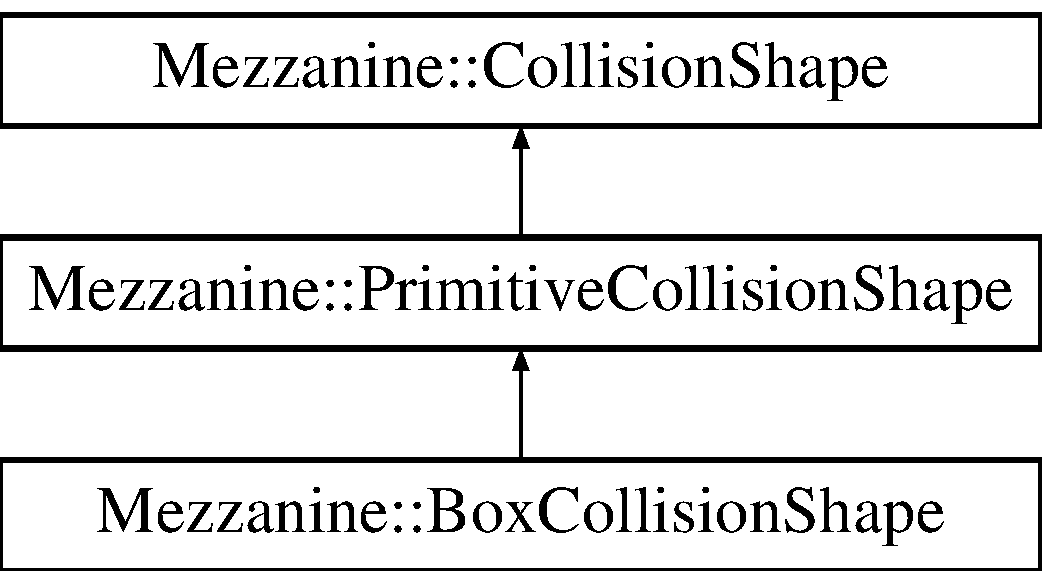
\includegraphics[height=3.000000cm]{classMezzanine_1_1BoxCollisionShape}
\end{center}
\end{figure}
\subsubsection*{Public Member Functions}
\begin{DoxyCompactItemize}
\item 
\hyperlink{classMezzanine_1_1BoxCollisionShape_afcf359b8683bd158040963eca43ac670}{BoxCollisionShape} (const \hyperlink{namespaceMezzanine_acf9fcc130e6ebf08e3d8491aebcf1c86}{String} \&\hyperlink{classMezzanine_1_1CollisionShape_aac524c5c56fa4d158bc071f8aecfbe79}{Name}, const \hyperlink{classMezzanine_1_1Vector3}{Vector3} \&HalfExtents)
\begin{DoxyCompactList}\small\item\em Class Constructor. \item\end{DoxyCompactList}\item 
\hyperlink{classMezzanine_1_1BoxCollisionShape_ae715de5cb9f343f10973f06bf4f9acbb}{BoxCollisionShape} (const \hyperlink{namespaceMezzanine_acf9fcc130e6ebf08e3d8491aebcf1c86}{String} \&\hyperlink{classMezzanine_1_1CollisionShape_aac524c5c56fa4d158bc071f8aecfbe79}{Name}, btBoxShape $\ast$BulletShape)
\begin{DoxyCompactList}\small\item\em Internal Constructor. \item\end{DoxyCompactList}\item 
\hyperlink{classMezzanine_1_1BoxCollisionShape_a20fe1b0eef928087c30fbb90bf718e97}{BoxCollisionShape} (\hyperlink{classMezzanine_1_1xml_1_1Node}{xml::Node} OneNode)
\begin{DoxyCompactList}\small\item\em DeSerializing Constructor. \item\end{DoxyCompactList}\item 
\hypertarget{classMezzanine_1_1BoxCollisionShape_a3698d2ef0c9a0ab92809b2ff2ba62792}{
virtual \hyperlink{classMezzanine_1_1BoxCollisionShape_a3698d2ef0c9a0ab92809b2ff2ba62792}{$\sim$BoxCollisionShape} ()}
\label{classMezzanine_1_1BoxCollisionShape_a3698d2ef0c9a0ab92809b2ff2ba62792}

\begin{DoxyCompactList}\small\item\em Class Destructor. \item\end{DoxyCompactList}\item 
virtual btBoxShape $\ast$ \hyperlink{classMezzanine_1_1BoxCollisionShape_a408a3b15bf4425d827c7cf4ee908efef}{GetBulletBoxShape} () const 
\item 
virtual \hyperlink{classMezzanine_1_1Vector3}{Vector3} \hyperlink{classMezzanine_1_1BoxCollisionShape_a5214ce314dc7d383ae81995e618f87cb}{GetCleanHalfExtents} () const 
\begin{DoxyCompactList}\small\item\em Gets the half extents used to construct this box. \item\end{DoxyCompactList}\item 
virtual \hyperlink{classMezzanine_1_1Vector3}{Vector3} \hyperlink{classMezzanine_1_1BoxCollisionShape_a4e1193a0cfed37f268ae1730de7b8d08}{GetHalfExtents} () const 
\begin{DoxyCompactList}\small\item\em Gets the current half extents used in collision checking. \item\end{DoxyCompactList}\item 
virtual \hyperlink{classMezzanine_1_1Vector3}{Vector3} \hyperlink{classMezzanine_1_1BoxCollisionShape_a198887a16d922effe302695ff69bcd88}{GetHalfExtentsWithMargin} () const 
\begin{DoxyCompactList}\small\item\em Gets the half extents with padding, this is the size the shape will appear to be. \item\end{DoxyCompactList}\item 
virtual \hyperlink{classMezzanine_1_1CollisionShape_ad04186055565998879b64176d6dd100d}{CollisionShape::ShapeType} \hyperlink{classMezzanine_1_1BoxCollisionShape_ae2b4af7afa6cc37c51b062589048e26d}{GetType} () const 
\item 
virtual bool \hyperlink{classMezzanine_1_1BoxCollisionShape_a1902aa75d5c18ad4ce090952b6af0050}{IsInside} (const \hyperlink{classMezzanine_1_1Vector3}{Vector3} \&Location, const \hyperlink{namespaceMezzanine_a726731b1a7df72bf3583e4a97282c6f6}{Real} \&Tolerance) const 
\begin{DoxyCompactList}\small\item\em Checks to see if a point in local space is inside this shape. \item\end{DoxyCompactList}\item 
virtual void \hyperlink{classMezzanine_1_1BoxCollisionShape_aeff89859ae98a391bf1232e190c839b5}{ProtoDeSerialize} (const \hyperlink{classMezzanine_1_1xml_1_1Node}{xml::Node} \&OneNode)
\item 
virtual void \hyperlink{classMezzanine_1_1BoxCollisionShape_abdd854fc0f165b3b17baecb0bb3961b4}{ProtoSerialize} (\hyperlink{classMezzanine_1_1xml_1_1Node}{xml::Node} \&CurrentRoot) const 
\end{DoxyCompactItemize}
\subsubsection*{Static Public Member Functions}
\begin{DoxyCompactItemize}
\item 
static \hyperlink{namespaceMezzanine_acf9fcc130e6ebf08e3d8491aebcf1c86}{String} \hyperlink{classMezzanine_1_1BoxCollisionShape_aa96e3055ec21f18198bceccdeaafa538}{SerializableName} ()
\begin{DoxyCompactList}\small\item\em Get the name of the the XML tag this class will leave behind as its instances are serialized. \item\end{DoxyCompactList}\end{DoxyCompactItemize}


\subsubsection{Detailed Description}
A box physics shape. This is exactly what it sounds like. A primitive shape of a box that is constructed by it's half extents. Half extents can't be negative, but otherwise can be any value. The margin value is subtracted from the total size rather than added for this shape. \begin{DoxyWarning}{Warning}
This does not fully implement ProtoDeSerialize, this must be deserialized with the Appropriate Deserializer. 
\end{DoxyWarning}


Definition at line 342 of file collisionshape.h.



\subsubsection{Constructor \& Destructor Documentation}
\hypertarget{classMezzanine_1_1BoxCollisionShape_afcf359b8683bd158040963eca43ac670}{
\index{Mezzanine::BoxCollisionShape@{Mezzanine::BoxCollisionShape}!BoxCollisionShape@{BoxCollisionShape}}
\index{BoxCollisionShape@{BoxCollisionShape}!Mezzanine::BoxCollisionShape@{Mezzanine::BoxCollisionShape}}
\paragraph[{BoxCollisionShape}]{\setlength{\rightskip}{0pt plus 5cm}Mezzanine::BoxCollisionShape::BoxCollisionShape (
\begin{DoxyParamCaption}
\item[{const {\bf String} \&}]{Name, }
\item[{const {\bf Vector3} \&}]{HalfExtents}
\end{DoxyParamCaption}
)}\hfill}
\label{classMezzanine_1_1BoxCollisionShape_afcf359b8683bd158040963eca43ac670}


Class Constructor. 


\begin{DoxyParams}{Parameters}
{\em Name} & The name of this shape. \\
\hline
{\em HalfExtents} & A vector3 representing half the shapes size on each axis. \\
\hline
\end{DoxyParams}


Definition at line 500 of file collisionshape.cpp.

\hypertarget{classMezzanine_1_1BoxCollisionShape_ae715de5cb9f343f10973f06bf4f9acbb}{
\index{Mezzanine::BoxCollisionShape@{Mezzanine::BoxCollisionShape}!BoxCollisionShape@{BoxCollisionShape}}
\index{BoxCollisionShape@{BoxCollisionShape}!Mezzanine::BoxCollisionShape@{Mezzanine::BoxCollisionShape}}
\paragraph[{BoxCollisionShape}]{\setlength{\rightskip}{0pt plus 5cm}Mezzanine::BoxCollisionShape::BoxCollisionShape (
\begin{DoxyParamCaption}
\item[{const {\bf String} \&}]{Name, }
\item[{btBoxShape $\ast$}]{BulletShape}
\end{DoxyParamCaption}
)}\hfill}
\label{classMezzanine_1_1BoxCollisionShape_ae715de5cb9f343f10973f06bf4f9acbb}


Internal Constructor. 


\begin{DoxyParams}{Parameters}
{\em Name} & The name of this shape. \\
\hline
{\em BulletShape} & The internal shape this shape is based on. \\
\hline
\end{DoxyParams}


Definition at line 506 of file collisionshape.cpp.

\hypertarget{classMezzanine_1_1BoxCollisionShape_a20fe1b0eef928087c30fbb90bf718e97}{
\index{Mezzanine::BoxCollisionShape@{Mezzanine::BoxCollisionShape}!BoxCollisionShape@{BoxCollisionShape}}
\index{BoxCollisionShape@{BoxCollisionShape}!Mezzanine::BoxCollisionShape@{Mezzanine::BoxCollisionShape}}
\paragraph[{BoxCollisionShape}]{\setlength{\rightskip}{0pt plus 5cm}Mezzanine::BoxCollisionShape::BoxCollisionShape (
\begin{DoxyParamCaption}
\item[{{\bf xml::Node}}]{OneNode}
\end{DoxyParamCaption}
)}\hfill}
\label{classMezzanine_1_1BoxCollisionShape_a20fe1b0eef928087c30fbb90bf718e97}


DeSerializing Constructor. 


\begin{DoxyParams}{Parameters}
{\em OneNode} & The node to use for constructing this shape \\
\hline
\end{DoxyParams}


Definition at line 513 of file collisionshape.cpp.



\subsubsection{Member Function Documentation}
\hypertarget{classMezzanine_1_1BoxCollisionShape_a408a3b15bf4425d827c7cf4ee908efef}{
\index{Mezzanine::BoxCollisionShape@{Mezzanine::BoxCollisionShape}!GetBulletBoxShape@{GetBulletBoxShape}}
\index{GetBulletBoxShape@{GetBulletBoxShape}!Mezzanine::BoxCollisionShape@{Mezzanine::BoxCollisionShape}}
\paragraph[{GetBulletBoxShape}]{\setlength{\rightskip}{0pt plus 5cm}btBoxShape $\ast$ Mezzanine::BoxCollisionShape::GetBulletBoxShape (
\begin{DoxyParamCaption}
{}
\end{DoxyParamCaption}
) const\hspace{0.3cm}{\ttfamily  \mbox{[}virtual\mbox{]}}}\hfill}
\label{classMezzanine_1_1BoxCollisionShape_a408a3b15bf4425d827c7cf4ee908efef}
Gets the internal shape pointer this collision shape is based on. 

\begin{DoxyReturn}{Returns}
Returns a pointer to the internal collision shape. 
\end{DoxyReturn}
 

Definition at line 564 of file collisionshape.cpp.

\hypertarget{classMezzanine_1_1BoxCollisionShape_a5214ce314dc7d383ae81995e618f87cb}{
\index{Mezzanine::BoxCollisionShape@{Mezzanine::BoxCollisionShape}!GetCleanHalfExtents@{GetCleanHalfExtents}}
\index{GetCleanHalfExtents@{GetCleanHalfExtents}!Mezzanine::BoxCollisionShape@{Mezzanine::BoxCollisionShape}}
\paragraph[{GetCleanHalfExtents}]{\setlength{\rightskip}{0pt plus 5cm}{\bf Vector3} Mezzanine::BoxCollisionShape::GetCleanHalfExtents (
\begin{DoxyParamCaption}
{}
\end{DoxyParamCaption}
) const\hspace{0.3cm}{\ttfamily  \mbox{[}virtual\mbox{]}}}\hfill}
\label{classMezzanine_1_1BoxCollisionShape_a5214ce314dc7d383ae81995e618f87cb}


Gets the half extents used to construct this box. 

\begin{DoxyReturn}{Returns}
Returns a vector3 containing the half extents of this box, with no scaling or margin (Original value). 
\end{DoxyReturn}


Definition at line 539 of file collisionshape.cpp.

\hypertarget{classMezzanine_1_1BoxCollisionShape_a4e1193a0cfed37f268ae1730de7b8d08}{
\index{Mezzanine::BoxCollisionShape@{Mezzanine::BoxCollisionShape}!GetHalfExtents@{GetHalfExtents}}
\index{GetHalfExtents@{GetHalfExtents}!Mezzanine::BoxCollisionShape@{Mezzanine::BoxCollisionShape}}
\paragraph[{GetHalfExtents}]{\setlength{\rightskip}{0pt plus 5cm}{\bf Vector3} Mezzanine::BoxCollisionShape::GetHalfExtents (
\begin{DoxyParamCaption}
{}
\end{DoxyParamCaption}
) const\hspace{0.3cm}{\ttfamily  \mbox{[}virtual\mbox{]}}}\hfill}
\label{classMezzanine_1_1BoxCollisionShape_a4e1193a0cfed37f268ae1730de7b8d08}


Gets the current half extents used in collision checking. 

\begin{DoxyReturn}{Returns}
Returns a vector3 containing the half extents of this box, with scaling applied, minus the size of the margin(Original value $\ast$ Scaling -\/ margin). 
\end{DoxyReturn}


Definition at line 544 of file collisionshape.cpp.

\hypertarget{classMezzanine_1_1BoxCollisionShape_a198887a16d922effe302695ff69bcd88}{
\index{Mezzanine::BoxCollisionShape@{Mezzanine::BoxCollisionShape}!GetHalfExtentsWithMargin@{GetHalfExtentsWithMargin}}
\index{GetHalfExtentsWithMargin@{GetHalfExtentsWithMargin}!Mezzanine::BoxCollisionShape@{Mezzanine::BoxCollisionShape}}
\paragraph[{GetHalfExtentsWithMargin}]{\setlength{\rightskip}{0pt plus 5cm}{\bf Vector3} Mezzanine::BoxCollisionShape::GetHalfExtentsWithMargin (
\begin{DoxyParamCaption}
{}
\end{DoxyParamCaption}
) const\hspace{0.3cm}{\ttfamily  \mbox{[}virtual\mbox{]}}}\hfill}
\label{classMezzanine_1_1BoxCollisionShape_a198887a16d922effe302695ff69bcd88}


Gets the half extents with padding, this is the size the shape will appear to be. 

\begin{DoxyReturn}{Returns}
Returns a vector3 containing the half extents, with scaling applied, with the margin added to each axis (Original value $\ast$ Scaling). 
\end{DoxyReturn}


Definition at line 549 of file collisionshape.cpp.

\hypertarget{classMezzanine_1_1BoxCollisionShape_ae2b4af7afa6cc37c51b062589048e26d}{
\index{Mezzanine::BoxCollisionShape@{Mezzanine::BoxCollisionShape}!GetType@{GetType}}
\index{GetType@{GetType}!Mezzanine::BoxCollisionShape@{Mezzanine::BoxCollisionShape}}
\paragraph[{GetType}]{\setlength{\rightskip}{0pt plus 5cm}{\bf CollisionShape::ShapeType} Mezzanine::BoxCollisionShape::GetType (
\begin{DoxyParamCaption}
{}
\end{DoxyParamCaption}
) const\hspace{0.3cm}{\ttfamily  \mbox{[}virtual\mbox{]}}}\hfill}
\label{classMezzanine_1_1BoxCollisionShape_ae2b4af7afa6cc37c51b062589048e26d}
Gets the type of \hyperlink{classMezzanine_1_1Collision}{Collision} shape this is. 

\begin{DoxyReturn}{Returns}
Returns an enum value indicating the type of collision shape this is. 
\end{DoxyReturn}
 

Implements \hyperlink{classMezzanine_1_1PrimitiveCollisionShape_ad3d4143a5640204b987e0b57eb24af41}{Mezzanine::PrimitiveCollisionShape}.



Definition at line 559 of file collisionshape.cpp.

\hypertarget{classMezzanine_1_1BoxCollisionShape_a1902aa75d5c18ad4ce090952b6af0050}{
\index{Mezzanine::BoxCollisionShape@{Mezzanine::BoxCollisionShape}!IsInside@{IsInside}}
\index{IsInside@{IsInside}!Mezzanine::BoxCollisionShape@{Mezzanine::BoxCollisionShape}}
\paragraph[{IsInside}]{\setlength{\rightskip}{0pt plus 5cm}bool Mezzanine::BoxCollisionShape::IsInside (
\begin{DoxyParamCaption}
\item[{const {\bf Vector3} \&}]{Location, }
\item[{const {\bf Real} \&}]{Tolerance}
\end{DoxyParamCaption}
) const\hspace{0.3cm}{\ttfamily  \mbox{[}virtual\mbox{]}}}\hfill}
\label{classMezzanine_1_1BoxCollisionShape_a1902aa75d5c18ad4ce090952b6af0050}


Checks to see if a point in local space is inside this shape. 

\begin{DoxyReturn}{Returns}
Returns a bool indicating whether or not the specified point is inside the shape. 
\end{DoxyReturn}

\begin{DoxyParams}{Parameters}
{\em Location} & The specified point to perform the check. \\
\hline
{\em Tolerance} & The amount of leeway to give in the check. If the distance from the specified point is equal or less then the Tolerance provided then this will return true. \\
\hline
\end{DoxyParams}


Definition at line 554 of file collisionshape.cpp.

\hypertarget{classMezzanine_1_1BoxCollisionShape_aeff89859ae98a391bf1232e190c839b5}{
\index{Mezzanine::BoxCollisionShape@{Mezzanine::BoxCollisionShape}!ProtoDeSerialize@{ProtoDeSerialize}}
\index{ProtoDeSerialize@{ProtoDeSerialize}!Mezzanine::BoxCollisionShape@{Mezzanine::BoxCollisionShape}}
\paragraph[{ProtoDeSerialize}]{\setlength{\rightskip}{0pt plus 5cm}void Mezzanine::BoxCollisionShape::ProtoDeSerialize (
\begin{DoxyParamCaption}
\item[{const {\bf xml::Node} \&}]{OneNode}
\end{DoxyParamCaption}
)\hspace{0.3cm}{\ttfamily  \mbox{[}virtual\mbox{]}}}\hfill}
\label{classMezzanine_1_1BoxCollisionShape_aeff89859ae98a391bf1232e190c839b5}
Gets the internal shape pointer this collision shape is based on. 

\begin{DoxyReturn}{Returns}
Returns a pointer to the internal collision shape. 
\end{DoxyReturn}
 

Reimplemented from \hyperlink{classMezzanine_1_1PrimitiveCollisionShape_a2257312048ee9085fa5d14f6b34caae1}{Mezzanine::PrimitiveCollisionShape}.



Definition at line 588 of file collisionshape.cpp.

\hypertarget{classMezzanine_1_1BoxCollisionShape_abdd854fc0f165b3b17baecb0bb3961b4}{
\index{Mezzanine::BoxCollisionShape@{Mezzanine::BoxCollisionShape}!ProtoSerialize@{ProtoSerialize}}
\index{ProtoSerialize@{ProtoSerialize}!Mezzanine::BoxCollisionShape@{Mezzanine::BoxCollisionShape}}
\paragraph[{ProtoSerialize}]{\setlength{\rightskip}{0pt plus 5cm}void Mezzanine::BoxCollisionShape::ProtoSerialize (
\begin{DoxyParamCaption}
\item[{{\bf xml::Node} \&}]{CurrentRoot}
\end{DoxyParamCaption}
) const\hspace{0.3cm}{\ttfamily  \mbox{[}virtual\mbox{]}}}\hfill}
\label{classMezzanine_1_1BoxCollisionShape_abdd854fc0f165b3b17baecb0bb3961b4}
Gets the internal shape pointer this collision shape is based on. 

\begin{DoxyReturn}{Returns}
Returns a pointer to the internal collision shape. 
\end{DoxyReturn}
 

Reimplemented from \hyperlink{classMezzanine_1_1PrimitiveCollisionShape_acfaab953833e9be503fddb2ee0f56d4f}{Mezzanine::PrimitiveCollisionShape}.



Definition at line 567 of file collisionshape.cpp.

\hypertarget{classMezzanine_1_1BoxCollisionShape_aa96e3055ec21f18198bceccdeaafa538}{
\index{Mezzanine::BoxCollisionShape@{Mezzanine::BoxCollisionShape}!SerializableName@{SerializableName}}
\index{SerializableName@{SerializableName}!Mezzanine::BoxCollisionShape@{Mezzanine::BoxCollisionShape}}
\paragraph[{SerializableName}]{\setlength{\rightskip}{0pt plus 5cm}{\bf String} Mezzanine::BoxCollisionShape::SerializableName (
\begin{DoxyParamCaption}
{}
\end{DoxyParamCaption}
)\hspace{0.3cm}{\ttfamily  \mbox{[}static\mbox{]}}}\hfill}
\label{classMezzanine_1_1BoxCollisionShape_aa96e3055ec21f18198bceccdeaafa538}


Get the name of the the XML tag this class will leave behind as its instances are serialized. 

\begin{DoxyReturn}{Returns}
A string containing \char`\"{}BoxCollisionShape\char`\"{} 
\end{DoxyReturn}


Reimplemented from \hyperlink{classMezzanine_1_1PrimitiveCollisionShape_a19bb44a705ff86606834feb2783500e5}{Mezzanine::PrimitiveCollisionShape}.



Definition at line 606 of file collisionshape.cpp.



The documentation for this class was generated from the following files:\begin{DoxyCompactItemize}
\item 
collisionshape.h\item 
collisionshape.cpp\end{DoxyCompactItemize}

\hypertarget{classMezzanine_1_1Camera}{
\subsection{Mezzanine::Camera Class Reference}
\label{classMezzanine_1_1Camera}\index{Mezzanine::Camera@{Mezzanine::Camera}}
}


This is the camera class.  




{\ttfamily \#include $<$camera.h$>$}

Inheritance diagram for Mezzanine::Camera:\begin{figure}[H]
\begin{center}
\leavevmode
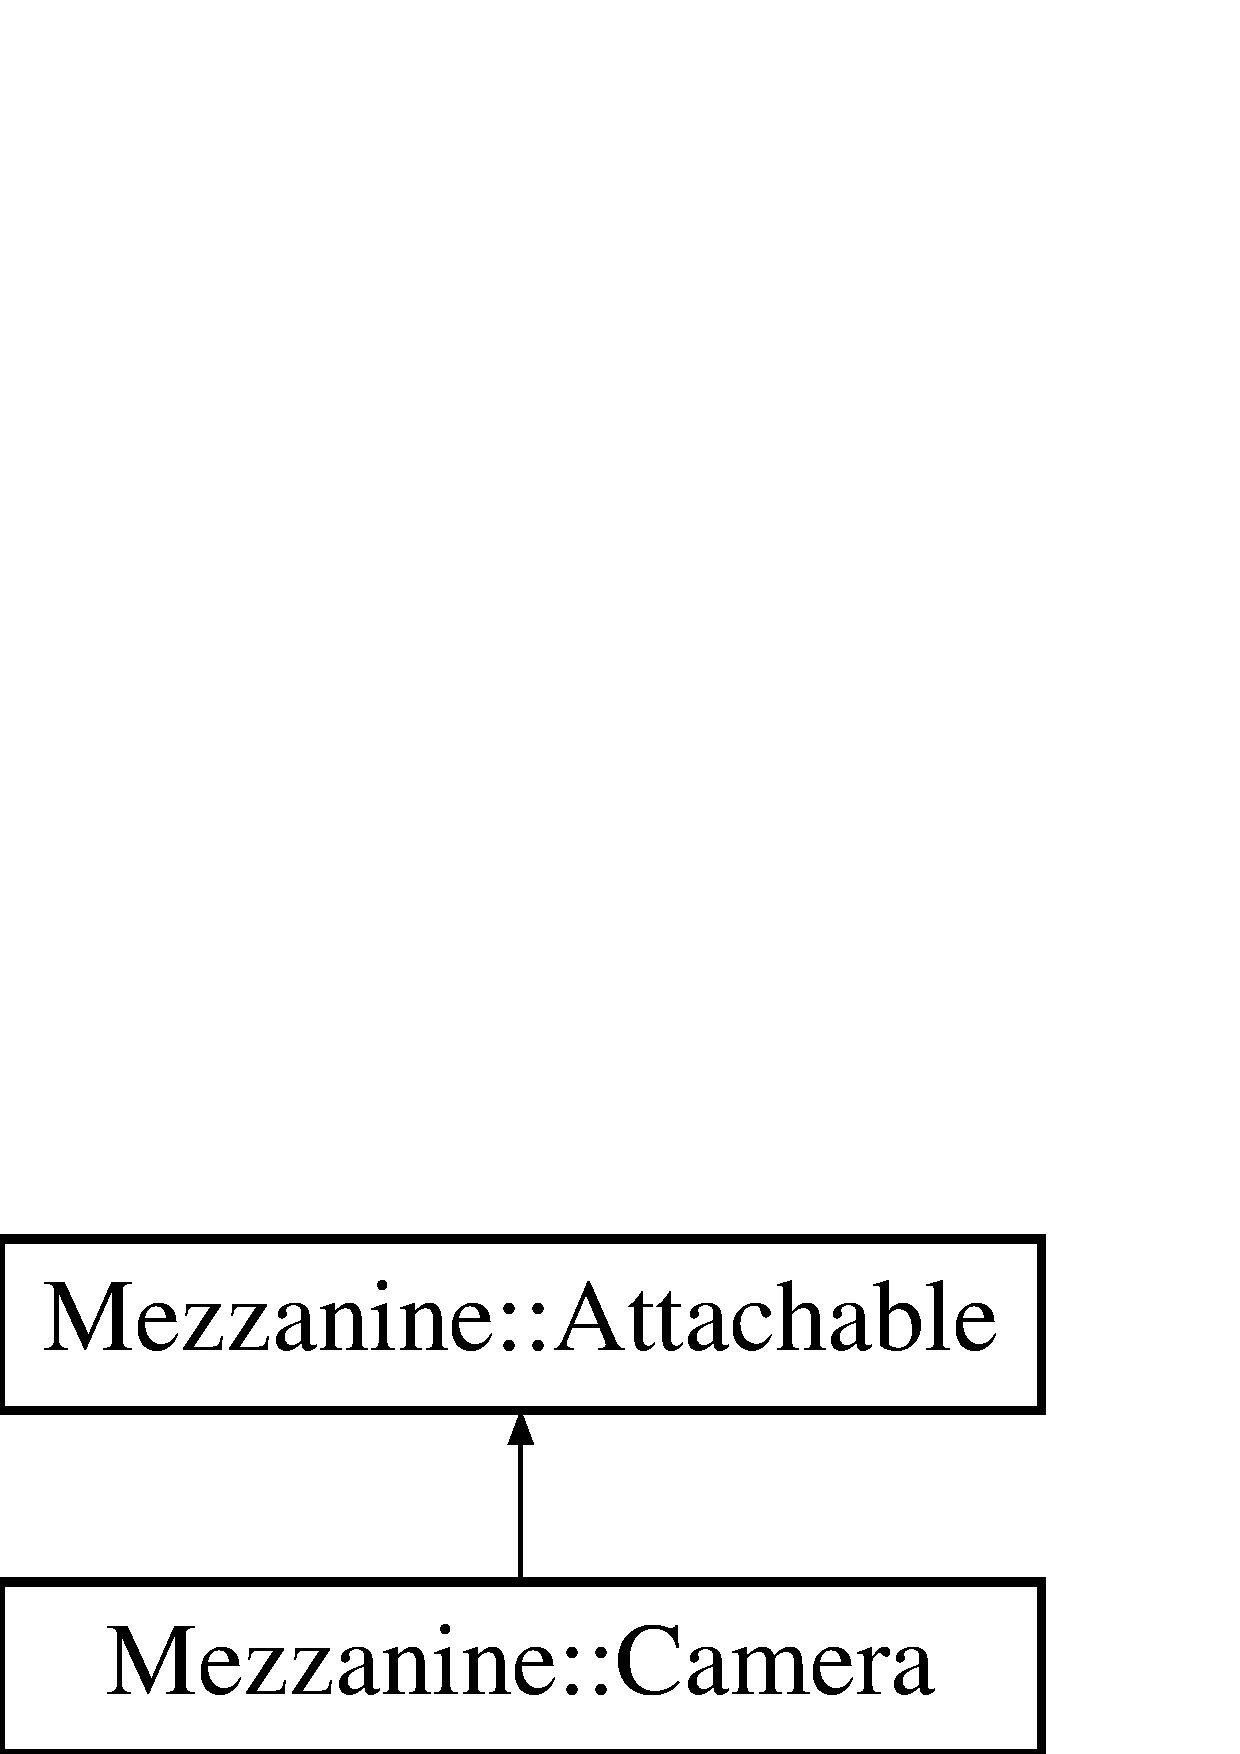
\includegraphics[height=2.000000cm]{classMezzanine_1_1Camera}
\end{center}
\end{figure}
\subsubsection*{Public Types}
\begin{DoxyCompactItemize}
\item 
enum \hyperlink{classMezzanine_1_1Camera_a643bf90630796bca5353967664d5f6e3}{ProjectionType} \{ \hyperlink{classMezzanine_1_1Camera_a643bf90630796bca5353967664d5f6e3a5bf29bb9ff44080ae6cbfa3e2aeb467c}{Orthographic} =  0, 
\hyperlink{classMezzanine_1_1Camera_a643bf90630796bca5353967664d5f6e3a616794ef1e113f63b1b9bf6896c61eba}{Perspective} =  1
 \}
\begin{DoxyCompactList}\small\item\em Values for storing how perspective should be interpretted. \item\end{DoxyCompactList}\end{DoxyCompactItemize}
\subsubsection*{Public Member Functions}
\begin{DoxyCompactItemize}
\item 
\hyperlink{classMezzanine_1_1Camera_a172e91734ebe0cb5d8332ef00606526e}{Camera} (const \hyperlink{namespaceMezzanine_acf9fcc130e6ebf08e3d8491aebcf1c86}{String} \&Name, \hyperlink{classMezzanine_1_1CameraManager}{CameraManager} $\ast$Manager)
\begin{DoxyCompactList}\small\item\em Basic \hyperlink{classMezzanine_1_1Camera}{Camera} Constructor. \item\end{DoxyCompactList}\item 
\hyperlink{classMezzanine_1_1Camera_aa20f07494ece246945eb3cb05f549f82}{Camera} (Ogre::Camera $\ast$\hyperlink{classMezzanine_1_1Camera}{Camera}, \hyperlink{classMezzanine_1_1CameraManager}{CameraManager} $\ast$Manager)
\begin{DoxyCompactList}\small\item\em Ogre Cam Constructor. \item\end{DoxyCompactList}\item 
virtual \hyperlink{structMezzanine_1_1AttachableData}{AttachableData} \hyperlink{classMezzanine_1_1Camera_a9bbd0126f025996457c87fb8564cc38d}{GetAttachableData} () const 
\begin{DoxyCompactList}\small\item\em Gets pointers to the internal ogre structures for this attachable. \item\end{DoxyCompactList}\item 
virtual \hyperlink{classMezzanine_1_1Attachable_a274bd45f9666f6e50f6fdd8a0162bc9e}{Attachable::AttachableElement} \hyperlink{classMezzanine_1_1Camera_a4a8523981c43ba8f4c5358b9ce7aef37}{GetAttachableType} () const 
\begin{DoxyCompactList}\small\item\em What kind of \hyperlink{classMezzanine_1_1Attachable}{Attachable} is this. \item\end{DoxyCompactList}\item 
\hyperlink{classMezzanine_1_1Ray}{Ray} \hyperlink{classMezzanine_1_1Camera_a7dc2eeda0370fd1d942dc4467795d87b}{GetCameraToViewportRay} (\hyperlink{namespaceMezzanine_a726731b1a7df72bf3583e4a97282c6f6}{Real} Screenx, \hyperlink{namespaceMezzanine_a726731b1a7df72bf3583e4a97282c6f6}{Real} Screeny) const 
\begin{DoxyCompactList}\small\item\em Gets a \hyperlink{classMezzanine_1_1Ray}{Ray} from the camera to the viewport. \item\end{DoxyCompactList}\item 
\hyperlink{classMezzanine_1_1Camera_a643bf90630796bca5353967664d5f6e3}{Camera::ProjectionType} \hyperlink{classMezzanine_1_1Camera_aef2f7b71aedee46bacc1341c02a813a2}{GetCameraType} () const 
\begin{DoxyCompactList}\small\item\em Get the type of projection used by the camera. \item\end{DoxyCompactList}\item 
\hyperlink{classMezzanine_1_1Vector3}{Vector3} \hyperlink{classMezzanine_1_1Camera_a1b23b180e30225bc6e1b90a2d270771e}{GetDirection} () const 
\begin{DoxyCompactList}\small\item\em Gets the direction the camera is currently facing. \item\end{DoxyCompactList}\item 
\hyperlink{classMezzanine_1_1Vector3}{Vector3} \hyperlink{classMezzanine_1_1Camera_af7a94974ef5ff6caff66da3a9f71b579}{GetFixedYawAxis} () const 
\begin{DoxyCompactList}\small\item\em If fixed yaw is enabled, on which axis is yawing disabled. \item\end{DoxyCompactList}\item 
\hyperlink{classMezzanine_1_1Vector3}{Vector3} \hyperlink{classMezzanine_1_1Camera_a94b66663d7c52ec642347d5d939cf67b}{GetGlobalLocation} () const 
\begin{DoxyCompactList}\small\item\em Gets the global/absolute location of the camera. \item\end{DoxyCompactList}\item 
virtual \hyperlink{classMezzanine_1_1Vector3}{Vector3} \hyperlink{classMezzanine_1_1Camera_afb87a19855c4cd5361861e1e400d5481}{GetLocation} () const 
\begin{DoxyCompactList}\small\item\em Gets the relative location of the camera. \item\end{DoxyCompactList}\item 
\hyperlink{namespaceMezzanine_a63cd699ac54b73953f35ec9cfc05e506}{ConstString} \& \hyperlink{classMezzanine_1_1Camera_abf6e3c2e642753023acd91f6d1413455}{GetName} () const 
\begin{DoxyCompactList}\small\item\em Gets the camera's set name. \item\end{DoxyCompactList}\item 
Ogre::Camera $\ast$ \hyperlink{classMezzanine_1_1Camera_ac7985618c8f908a6cc93069ccb51bb47}{GetOgreCamera} () const 
\begin{DoxyCompactList}\small\item\em Gets the internal camera this camera is based on. \item\end{DoxyCompactList}\item 
\hyperlink{classMezzanine_1_1Quaternion}{Quaternion} \hyperlink{classMezzanine_1_1Camera_af693fe97c4f281940a33dc8087a80fcb}{GetOrientation} () const 
\begin{DoxyCompactList}\small\item\em Gets the direction the camera is facing. \item\end{DoxyCompactList}\item 
\hyperlink{classMezzanine_1_1Vector3}{Vector3} \hyperlink{classMezzanine_1_1Camera_a3262342c754eb31b4caa0693c5b60842}{GetRelativeLocation} () const 
\begin{DoxyCompactList}\small\item\em Gets the relative location of the camera. \item\end{DoxyCompactList}\item 
bool \hyperlink{classMezzanine_1_1Camera_adfe5be54632aeedb9656c850f3f03ae5}{IsFixedYawEnabled} () const 
\begin{DoxyCompactList}\small\item\em Is fixed yaw enabled. \item\end{DoxyCompactList}\item 
void \hyperlink{classMezzanine_1_1Camera_a8343f2d2fb174937aef2894ebf8a5e29}{LookAt} (const \hyperlink{classMezzanine_1_1Vector3}{Vector3} \&TargetLoc)
\begin{DoxyCompactList}\small\item\em Sets the direction the camera faces. \item\end{DoxyCompactList}\item 
void \hyperlink{classMezzanine_1_1Camera_afdc17999a097218df445370123d41239}{Move} (const \hyperlink{classMezzanine_1_1Vector3}{Vector3} \&ToMove)
\begin{DoxyCompactList}\small\item\em Moves the camera without factoring orientation. \item\end{DoxyCompactList}\item 
void \hyperlink{classMezzanine_1_1Camera_ac8f450698006baf6e8fca2a864d59533}{MoveRelative} (const \hyperlink{classMezzanine_1_1Vector3}{Vector3} \&ToMove)
\begin{DoxyCompactList}\small\item\em Moves the camera while factoring orientation. \item\end{DoxyCompactList}\item 
void \hyperlink{classMezzanine_1_1Camera_ad63ed9c54ecf0940f20c5e4fbc9a1590}{ResetZoom} ()
\begin{DoxyCompactList}\small\item\em Resets the zoom level back to the default. \item\end{DoxyCompactList}\item 
void \hyperlink{classMezzanine_1_1Camera_ab619a29b83487e8f86c8adb443689078}{SetAspectRatio} (const \hyperlink{namespaceMezzanine_a726731b1a7df72bf3583e4a97282c6f6}{Real} \&Ratio)
\begin{DoxyCompactList}\small\item\em Sets the aspect ratio of the cameras veiw. \item\end{DoxyCompactList}\item 
void \hyperlink{classMezzanine_1_1Camera_a1bc33506c8df0607777b0b122fd9c9cb}{SetCameraType} (const \hyperlink{classMezzanine_1_1Camera_a643bf90630796bca5353967664d5f6e3}{ProjectionType} Type)
\begin{DoxyCompactList}\small\item\em Sets the type of projection to be used with this camera. \item\end{DoxyCompactList}\item 
void \hyperlink{classMezzanine_1_1Camera_a3adfffaec91715cbf120bbbbc50f82db}{SetDirection} (const \hyperlink{classMezzanine_1_1Vector3}{Vector3} \&Direction)
\begin{DoxyCompactList}\small\item\em Sets the Direction for the camera. \item\end{DoxyCompactList}\item 
void \hyperlink{classMezzanine_1_1Camera_af24424a1670ae6b10e9a61fbaf9fd23a}{SetFarClipDistance} (const \hyperlink{namespaceMezzanine_a726731b1a7df72bf3583e4a97282c6f6}{Real} \&FarDist)
\begin{DoxyCompactList}\small\item\em Sets the long range clip distance. \item\end{DoxyCompactList}\item 
void \hyperlink{classMezzanine_1_1Camera_abd19c7667593b8ea0bff576ae3a451ba}{SetFixedYawAxis} (bool UseFixed)
\begin{DoxyCompactList}\small\item\em Sets whether to lock rotation around the Y axis. \item\end{DoxyCompactList}\item 
void \hyperlink{classMezzanine_1_1Camera_a2ffb9eca37630a8d26669aab8668bce3}{SetFixedYawAxis} (bool UseFixed, const \hyperlink{classMezzanine_1_1Vector3}{Vector3} \&Axis)
\begin{DoxyCompactList}\small\item\em Sets whether to lock rotation around the Y axis. \item\end{DoxyCompactList}\item 
virtual void \hyperlink{classMezzanine_1_1Camera_afdc236c2c875035c8a11473350d0d17a}{SetLocation} (const \hyperlink{classMezzanine_1_1Vector3}{Vector3} \&Location)
\begin{DoxyCompactList}\small\item\em Sets the location of a camera. \item\end{DoxyCompactList}\item 
void \hyperlink{classMezzanine_1_1Camera_a638201c94b28ca0acc406b11f166e751}{SetNearClipDistance} (const \hyperlink{namespaceMezzanine_a726731b1a7df72bf3583e4a97282c6f6}{Real} \&NearDist)
\begin{DoxyCompactList}\small\item\em Sets the short range clip distance. \item\end{DoxyCompactList}\item 
void \hyperlink{classMezzanine_1_1Camera_af502b9c47b1acce46e1482ce049320eb}{SetOrientation} (const \hyperlink{classMezzanine_1_1Quaternion}{Quaternion} \&Orientation)
\begin{DoxyCompactList}\small\item\em Sets the orientation of the camera. \item\end{DoxyCompactList}\item 
void \hyperlink{classMezzanine_1_1Camera_a2beffe698c8952407f94683adea2fa24}{SetOrthoWindow} (const \hyperlink{namespaceMezzanine_a726731b1a7df72bf3583e4a97282c6f6}{Real} \&Width, const \hyperlink{namespaceMezzanine_a726731b1a7df72bf3583e4a97282c6f6}{Real} \&Height)
\begin{DoxyCompactList}\small\item\em Defines the size of the Orthographic projection window. \item\end{DoxyCompactList}\item 
void \hyperlink{classMezzanine_1_1Camera_a7e99427ba89306e3c7e6a0d5ccb23482}{SetOrthoWindowHeight} (const \hyperlink{namespaceMezzanine_a726731b1a7df72bf3583e4a97282c6f6}{Real} \&Height)
\begin{DoxyCompactList}\small\item\em Defines the size of the Orthographic projection window. \item\end{DoxyCompactList}\item 
void \hyperlink{classMezzanine_1_1Camera_a58279b526f2a386bfa0327a9084d24e4}{SetOrthoWindowWidth} (const \hyperlink{namespaceMezzanine_a726731b1a7df72bf3583e4a97282c6f6}{Real} \&Width)
\begin{DoxyCompactList}\small\item\em Defines the size of the Orthographic projection window. \item\end{DoxyCompactList}\item 
void \hyperlink{classMezzanine_1_1Camera_a10042b496caf5783657e138c62849b2f}{ZoomCamera} (const \hyperlink{namespaceMezzanine_a726731b1a7df72bf3583e4a97282c6f6}{Real} \&Zoom)
\begin{DoxyCompactList}\small\item\em Will zoom in or out the camera. \item\end{DoxyCompactList}\item 
virtual \hyperlink{classMezzanine_1_1Camera_ab25144933c625492a059e57401387c40}{$\sim$Camera} ()
\begin{DoxyCompactList}\small\item\em Class Destructor. \item\end{DoxyCompactList}\end{DoxyCompactItemize}
\subsubsection*{Protected Attributes}
\begin{DoxyCompactItemize}
\item 
\hypertarget{classMezzanine_1_1Camera_a992cc6bb14cd49e4030118dbb4b8e1ed}{
Ogre::Camera $\ast$ \hyperlink{classMezzanine_1_1Camera_a992cc6bb14cd49e4030118dbb4b8e1ed}{Cam}}
\label{classMezzanine_1_1Camera_a992cc6bb14cd49e4030118dbb4b8e1ed}

\begin{DoxyCompactList}\small\item\em This is the \hyperlink{classMezzanine_1_1Camera}{Camera} used by the graphics Subsystem, that this class wraps. \item\end{DoxyCompactList}\item 
\hypertarget{classMezzanine_1_1Camera_a8491540c829acc1bebbed24c9de0dfaf}{
\hyperlink{classMezzanine_1_1CameraManager}{CameraManager} $\ast$ \hyperlink{classMezzanine_1_1Camera_a8491540c829acc1bebbed24c9de0dfaf}{CamManager}}
\label{classMezzanine_1_1Camera_a8491540c829acc1bebbed24c9de0dfaf}

\begin{DoxyCompactList}\small\item\em This is the \hyperlink{classMezzanine_1_1Camera}{Camera} manager that this camera is attached to. \item\end{DoxyCompactList}\end{DoxyCompactItemize}
\subsubsection*{Friends}
\begin{DoxyCompactItemize}
\item 
\hypertarget{classMezzanine_1_1Camera_afae5bf9a900e8c5bc70c9332785e8465}{
class {\bfseries CameraManager}}
\label{classMezzanine_1_1Camera_afae5bf9a900e8c5bc70c9332785e8465}

\item 
\hypertarget{classMezzanine_1_1Camera_a4ff0401fc20f1017ee96470c629dd242}{
xml::Node \&MEZZ\_\-LIB {\bfseries operator$>$$>$} (xml::Node \&OneNode, \hyperlink{classMezzanine_1_1Camera}{Camera} \&Ev)}
\label{classMezzanine_1_1Camera_a4ff0401fc20f1017ee96470c629dd242}

\end{DoxyCompactItemize}


\subsubsection{Detailed Description}
This is the camera class. This class contains all the functionality needed to manipulate an individual camera that has been created. \begin{Desc}
\item[\hyperlink{todo__todo000003}{Todo}]Fix all the extra occurences of the word \hyperlink{classMezzanine_1_1Camera}{Camera} in Function names on the camera. \end{Desc}


Definition at line 102 of file camera.h.



\subsubsection{Member Enumeration Documentation}
\hypertarget{classMezzanine_1_1Camera_a643bf90630796bca5353967664d5f6e3}{
\index{Mezzanine::Camera@{Mezzanine::Camera}!ProjectionType@{ProjectionType}}
\index{ProjectionType@{ProjectionType}!Mezzanine::Camera@{Mezzanine::Camera}}
\paragraph[{ProjectionType}]{\setlength{\rightskip}{0pt plus 5cm}enum {\bf Mezzanine::Camera::ProjectionType}}\hfill}
\label{classMezzanine_1_1Camera_a643bf90630796bca5353967664d5f6e3}


Values for storing how perspective should be interpretted. 

\begin{Desc}
\item[Enumerator: ]\par
\begin{description}
\index{Orthographic@{Orthographic}!Mezzanine::Camera@{Mezzanine::Camera}}\index{Mezzanine::Camera@{Mezzanine::Camera}!Orthographic@{Orthographic}}\item[{\em 
\hypertarget{classMezzanine_1_1Camera_a643bf90630796bca5353967664d5f6e3a5bf29bb9ff44080ae6cbfa3e2aeb467c}{
Orthographic}
\label{classMezzanine_1_1Camera_a643bf90630796bca5353967664d5f6e3a5bf29bb9ff44080ae6cbfa3e2aeb467c}
}]Not at all, objects at any distance are the same size. \index{Perspective@{Perspective}!Mezzanine::Camera@{Mezzanine::Camera}}\index{Mezzanine::Camera@{Mezzanine::Camera}!Perspective@{Perspective}}\item[{\em 
\hypertarget{classMezzanine_1_1Camera_a643bf90630796bca5353967664d5f6e3a616794ef1e113f63b1b9bf6896c61eba}{
Perspective}
\label{classMezzanine_1_1Camera_a643bf90630796bca5353967664d5f6e3a616794ef1e113f63b1b9bf6896c61eba}
}]Normal perspective. \end{description}
\end{Desc}



Definition at line 106 of file camera.h.



\subsubsection{Constructor \& Destructor Documentation}
\hypertarget{classMezzanine_1_1Camera_a172e91734ebe0cb5d8332ef00606526e}{
\index{Mezzanine::Camera@{Mezzanine::Camera}!Camera@{Camera}}
\index{Camera@{Camera}!Mezzanine::Camera@{Mezzanine::Camera}}
\paragraph[{Camera}]{\setlength{\rightskip}{0pt plus 5cm}Mezzanine::Camera::Camera (
\begin{DoxyParamCaption}
\item[{const {\bf String} \&}]{Name, }
\item[{{\bf CameraManager} $\ast$}]{Manager}
\end{DoxyParamCaption}
)}\hfill}
\label{classMezzanine_1_1Camera_a172e91734ebe0cb5d8332ef00606526e}


Basic \hyperlink{classMezzanine_1_1Camera}{Camera} Constructor. 

This is the basic constructor for the \hyperlink{classMezzanine_1_1Camera}{Camera} class. 

Definition at line 61 of file camera.cpp.

\hypertarget{classMezzanine_1_1Camera_aa20f07494ece246945eb3cb05f549f82}{
\index{Mezzanine::Camera@{Mezzanine::Camera}!Camera@{Camera}}
\index{Camera@{Camera}!Mezzanine::Camera@{Mezzanine::Camera}}
\paragraph[{Camera}]{\setlength{\rightskip}{0pt plus 5cm}Mezzanine::Camera::Camera (
\begin{DoxyParamCaption}
\item[{Ogre::Camera $\ast$}]{Camera, }
\item[{{\bf CameraManager} $\ast$}]{Manager}
\end{DoxyParamCaption}
)}\hfill}
\label{classMezzanine_1_1Camera_aa20f07494ece246945eb3cb05f549f82}


Ogre Cam Constructor. 

This is for internal use only and shouldn't be called manually. 

Definition at line 67 of file camera.cpp.

\hypertarget{classMezzanine_1_1Camera_ab25144933c625492a059e57401387c40}{
\index{Mezzanine::Camera@{Mezzanine::Camera}!$\sim$Camera@{$\sim$Camera}}
\index{$\sim$Camera@{$\sim$Camera}!Mezzanine::Camera@{Mezzanine::Camera}}
\paragraph[{$\sim$Camera}]{\setlength{\rightskip}{0pt plus 5cm}Mezzanine::Camera::$\sim$Camera (
\begin{DoxyParamCaption}
{}
\end{DoxyParamCaption}
)\hspace{0.3cm}{\ttfamily  \mbox{[}virtual\mbox{]}}}\hfill}
\label{classMezzanine_1_1Camera_ab25144933c625492a059e57401387c40}


Class Destructor. 

The Class Destructor. 

Definition at line 81 of file camera.cpp.



\subsubsection{Member Function Documentation}
\hypertarget{classMezzanine_1_1Camera_a9bbd0126f025996457c87fb8564cc38d}{
\index{Mezzanine::Camera@{Mezzanine::Camera}!GetAttachableData@{GetAttachableData}}
\index{GetAttachableData@{GetAttachableData}!Mezzanine::Camera@{Mezzanine::Camera}}
\paragraph[{GetAttachableData}]{\setlength{\rightskip}{0pt plus 5cm}{\bf AttachableData} Mezzanine::Camera::GetAttachableData (
\begin{DoxyParamCaption}
{}
\end{DoxyParamCaption}
) const\hspace{0.3cm}{\ttfamily  \mbox{[}virtual\mbox{]}}}\hfill}
\label{classMezzanine_1_1Camera_a9bbd0126f025996457c87fb8564cc38d}


Gets pointers to the internal ogre structures for this attachable. 

\begin{DoxyReturn}{Returns}
Returns an \hyperlink{structMezzanine_1_1AttachableData}{AttachableData} struct with the internal data. 
\end{DoxyReturn}


Implements \hyperlink{classMezzanine_1_1Attachable_aeed457c614552bd753e7669cb7624b19}{Mezzanine::Attachable}.



Definition at line 270 of file camera.cpp.

\hypertarget{classMezzanine_1_1Camera_a4a8523981c43ba8f4c5358b9ce7aef37}{
\index{Mezzanine::Camera@{Mezzanine::Camera}!GetAttachableType@{GetAttachableType}}
\index{GetAttachableType@{GetAttachableType}!Mezzanine::Camera@{Mezzanine::Camera}}
\paragraph[{GetAttachableType}]{\setlength{\rightskip}{0pt plus 5cm}{\bf Attachable::AttachableElement} Mezzanine::Camera::GetAttachableType (
\begin{DoxyParamCaption}
{}
\end{DoxyParamCaption}
) const\hspace{0.3cm}{\ttfamily  \mbox{[}virtual\mbox{]}}}\hfill}
\label{classMezzanine_1_1Camera_a4a8523981c43ba8f4c5358b9ce7aef37}


What kind of \hyperlink{classMezzanine_1_1Attachable}{Attachable} is this. 

\begin{DoxyReturn}{Returns}
An \hyperlink{classMezzanine_1_1Attachable_aacb1a1958cca1f005c1313f14e3d098d}{Attachable::GetAttachableType} containing \hyperlink{classMezzanine_1_1Attachable_a274bd45f9666f6e50f6fdd8a0162bc9ea6f00000af91736e964c4e9c5ef4089b0}{Attachable::Camera}. 
\end{DoxyReturn}


Implements \hyperlink{classMezzanine_1_1Attachable_aacb1a1958cca1f005c1313f14e3d098d}{Mezzanine::Attachable}.



Definition at line 265 of file camera.cpp.

\hypertarget{classMezzanine_1_1Camera_a7dc2eeda0370fd1d942dc4467795d87b}{
\index{Mezzanine::Camera@{Mezzanine::Camera}!GetCameraToViewportRay@{GetCameraToViewportRay}}
\index{GetCameraToViewportRay@{GetCameraToViewportRay}!Mezzanine::Camera@{Mezzanine::Camera}}
\paragraph[{GetCameraToViewportRay}]{\setlength{\rightskip}{0pt plus 5cm}{\bf Ray} Mezzanine::Camera::GetCameraToViewportRay (
\begin{DoxyParamCaption}
\item[{{\bf Real}}]{Screenx, }
\item[{{\bf Real}}]{Screeny}
\end{DoxyParamCaption}
) const}\hfill}
\label{classMezzanine_1_1Camera_a7dc2eeda0370fd1d942dc4467795d87b}


Gets a \hyperlink{classMezzanine_1_1Ray}{Ray} from the camera to the viewport. 

This will cast a ray from the camera to the viewport and return it. 
\begin{DoxyParams}{Parameters}
{\em Screenx} & A Real representing the relative location on screen, on the x axis(0.0-\/1.0). \\
\hline
{\em Screeny} & A Real representing the relative location on screen, on the y axis(0.0-\/1.0). \\
\hline
\end{DoxyParams}


Definition at line 216 of file camera.cpp.

\hypertarget{classMezzanine_1_1Camera_aef2f7b71aedee46bacc1341c02a813a2}{
\index{Mezzanine::Camera@{Mezzanine::Camera}!GetCameraType@{GetCameraType}}
\index{GetCameraType@{GetCameraType}!Mezzanine::Camera@{Mezzanine::Camera}}
\paragraph[{GetCameraType}]{\setlength{\rightskip}{0pt plus 5cm}{\bf Camera::ProjectionType} Mezzanine::Camera::GetCameraType (
\begin{DoxyParamCaption}
{}
\end{DoxyParamCaption}
) const}\hfill}
\label{classMezzanine_1_1Camera_aef2f7b71aedee46bacc1341c02a813a2}


Get the type of projection used by the camera. 

\begin{DoxyReturn}{Returns}
A ProjectionType that will identify the kind of projection this camera uses. 
\end{DoxyReturn}


Definition at line 106 of file camera.cpp.

\hypertarget{classMezzanine_1_1Camera_a1b23b180e30225bc6e1b90a2d270771e}{
\index{Mezzanine::Camera@{Mezzanine::Camera}!GetDirection@{GetDirection}}
\index{GetDirection@{GetDirection}!Mezzanine::Camera@{Mezzanine::Camera}}
\paragraph[{GetDirection}]{\setlength{\rightskip}{0pt plus 5cm}{\bf Vector3} Mezzanine::Camera::GetDirection (
\begin{DoxyParamCaption}
{}
\end{DoxyParamCaption}
) const}\hfill}
\label{classMezzanine_1_1Camera_a1b23b180e30225bc6e1b90a2d270771e}


Gets the direction the camera is currently facing. 

\begin{DoxyReturn}{Returns}
Returns a \hyperlink{classMezzanine_1_1Vector3}{Vector3} representing the current direction the camera is facing. 
\end{DoxyReturn}
\hypertarget{classMezzanine_1_1Camera_af7a94974ef5ff6caff66da3a9f71b579}{
\index{Mezzanine::Camera@{Mezzanine::Camera}!GetFixedYawAxis@{GetFixedYawAxis}}
\index{GetFixedYawAxis@{GetFixedYawAxis}!Mezzanine::Camera@{Mezzanine::Camera}}
\paragraph[{GetFixedYawAxis}]{\setlength{\rightskip}{0pt plus 5cm}{\bf Vector3} Mezzanine::Camera::GetFixedYawAxis (
\begin{DoxyParamCaption}
{}
\end{DoxyParamCaption}
) const}\hfill}
\label{classMezzanine_1_1Camera_af7a94974ef5ff6caff66da3a9f71b579}


If fixed yaw is enabled, on which axis is yawing disabled. 

\begin{DoxyReturn}{Returns}
Returns a \hyperlink{classMezzanine_1_1Vector3}{Vector3} of 0s if disable, otherwise this return the Fixed Yaw Axis. 
\end{DoxyReturn}


Definition at line 196 of file camera.cpp.

\hypertarget{classMezzanine_1_1Camera_a94b66663d7c52ec642347d5d939cf67b}{
\index{Mezzanine::Camera@{Mezzanine::Camera}!GetGlobalLocation@{GetGlobalLocation}}
\index{GetGlobalLocation@{GetGlobalLocation}!Mezzanine::Camera@{Mezzanine::Camera}}
\paragraph[{GetGlobalLocation}]{\setlength{\rightskip}{0pt plus 5cm}{\bf Vector3} Mezzanine::Camera::GetGlobalLocation (
\begin{DoxyParamCaption}
{}
\end{DoxyParamCaption}
) const}\hfill}
\label{classMezzanine_1_1Camera_a94b66663d7c52ec642347d5d939cf67b}


Gets the global/absolute location of the camera. 

\begin{DoxyReturn}{Returns}
A \hyperlink{classMezzanine_1_1Vector3}{Mezzanine::Vector3} containing the location of this object as an offset from the global origin. 
\end{DoxyReturn}


Definition at line 234 of file camera.cpp.

\hypertarget{classMezzanine_1_1Camera_afb87a19855c4cd5361861e1e400d5481}{
\index{Mezzanine::Camera@{Mezzanine::Camera}!GetLocation@{GetLocation}}
\index{GetLocation@{GetLocation}!Mezzanine::Camera@{Mezzanine::Camera}}
\paragraph[{GetLocation}]{\setlength{\rightskip}{0pt plus 5cm}{\bf Vector3} Mezzanine::Camera::GetLocation (
\begin{DoxyParamCaption}
{}
\end{DoxyParamCaption}
) const\hspace{0.3cm}{\ttfamily  \mbox{[}virtual\mbox{]}}}\hfill}
\label{classMezzanine_1_1Camera_afb87a19855c4cd5361861e1e400d5481}


Gets the relative location of the camera. 

Gets the location of the camera, relative to any parent \hyperlink{classMezzanine_1_1WorldNode}{WorldNode}. \begin{DoxyReturn}{Returns}
A \hyperlink{classMezzanine_1_1Vector3}{Mezzanine::Vector3} with the location of the camera as though the Parent \hyperlink{classMezzanine_1_1WorldNode}{WorldNode} were the origin. 
\end{DoxyReturn}


Implements \hyperlink{classMezzanine_1_1Attachable_a1a8e18e5654c50f24bc049c228603d71}{Mezzanine::Attachable}.



Definition at line 228 of file camera.cpp.

\hypertarget{classMezzanine_1_1Camera_abf6e3c2e642753023acd91f6d1413455}{
\index{Mezzanine::Camera@{Mezzanine::Camera}!GetName@{GetName}}
\index{GetName@{GetName}!Mezzanine::Camera@{Mezzanine::Camera}}
\paragraph[{GetName}]{\setlength{\rightskip}{0pt plus 5cm}{\bf ConstString} \& Mezzanine::Camera::GetName (
\begin{DoxyParamCaption}
{}
\end{DoxyParamCaption}
) const\hspace{0.3cm}{\ttfamily  \mbox{[}virtual\mbox{]}}}\hfill}
\label{classMezzanine_1_1Camera_abf6e3c2e642753023acd91f6d1413455}


Gets the camera's set name. 

\begin{DoxyReturn}{Returns}
Returns a string containing the camera's name. 
\end{DoxyReturn}


Implements \hyperlink{classMezzanine_1_1Attachable_a6a49ac8c2ddb2dd8ed7dd17f96ecafe5}{Mezzanine::Attachable}.



Definition at line 87 of file camera.cpp.

\hypertarget{classMezzanine_1_1Camera_ac7985618c8f908a6cc93069ccb51bb47}{
\index{Mezzanine::Camera@{Mezzanine::Camera}!GetOgreCamera@{GetOgreCamera}}
\index{GetOgreCamera@{GetOgreCamera}!Mezzanine::Camera@{Mezzanine::Camera}}
\paragraph[{GetOgreCamera}]{\setlength{\rightskip}{0pt plus 5cm}Ogre::Camera $\ast$ Mezzanine::Camera::GetOgreCamera (
\begin{DoxyParamCaption}
{}
\end{DoxyParamCaption}
) const}\hfill}
\label{classMezzanine_1_1Camera_ac7985618c8f908a6cc93069ccb51bb47}


Gets the internal camera this camera is based on. 

\begin{DoxyReturn}{Returns}
Returns a pointer to the Ogre \hyperlink{classMezzanine_1_1Camera}{Camera} this camera is based on. 
\end{DoxyReturn}


Definition at line 257 of file camera.cpp.

\hypertarget{classMezzanine_1_1Camera_af693fe97c4f281940a33dc8087a80fcb}{
\index{Mezzanine::Camera@{Mezzanine::Camera}!GetOrientation@{GetOrientation}}
\index{GetOrientation@{GetOrientation}!Mezzanine::Camera@{Mezzanine::Camera}}
\paragraph[{GetOrientation}]{\setlength{\rightskip}{0pt plus 5cm}{\bf Quaternion} Mezzanine::Camera::GetOrientation (
\begin{DoxyParamCaption}
{}
\end{DoxyParamCaption}
) const\hspace{0.3cm}{\ttfamily  \mbox{[}virtual\mbox{]}}}\hfill}
\label{classMezzanine_1_1Camera_af693fe97c4f281940a33dc8087a80fcb}


Gets the direction the camera is facing. 

\begin{DoxyReturn}{Returns}
A \hyperlink{classMezzanine_1_1Quaternion}{Mezzanine::Quaternion} representing how the camera is rotated. 
\end{DoxyReturn}


Implements \hyperlink{classMezzanine_1_1Attachable_ab3e094cbc373edb05866783290991e7d}{Mezzanine::Attachable}.



Definition at line 237 of file camera.cpp.

\hypertarget{classMezzanine_1_1Camera_a3262342c754eb31b4caa0693c5b60842}{
\index{Mezzanine::Camera@{Mezzanine::Camera}!GetRelativeLocation@{GetRelativeLocation}}
\index{GetRelativeLocation@{GetRelativeLocation}!Mezzanine::Camera@{Mezzanine::Camera}}
\paragraph[{GetRelativeLocation}]{\setlength{\rightskip}{0pt plus 5cm}{\bf Vector3} Mezzanine::Camera::GetRelativeLocation (
\begin{DoxyParamCaption}
{}
\end{DoxyParamCaption}
) const}\hfill}
\label{classMezzanine_1_1Camera_a3262342c754eb31b4caa0693c5b60842}


Gets the relative location of the camera. 

Gets the location of the camera, relative to any parent \hyperlink{classMezzanine_1_1WorldNode}{WorldNode}. \begin{DoxyReturn}{Returns}
A \hyperlink{classMezzanine_1_1Vector3}{Mezzanine::Vector3} with the location of the camera as though the Parent \hyperlink{classMezzanine_1_1WorldNode}{WorldNode} were the origin. 
\end{DoxyReturn}


Definition at line 231 of file camera.cpp.

\hypertarget{classMezzanine_1_1Camera_adfe5be54632aeedb9656c850f3f03ae5}{
\index{Mezzanine::Camera@{Mezzanine::Camera}!IsFixedYawEnabled@{IsFixedYawEnabled}}
\index{IsFixedYawEnabled@{IsFixedYawEnabled}!Mezzanine::Camera@{Mezzanine::Camera}}
\paragraph[{IsFixedYawEnabled}]{\setlength{\rightskip}{0pt plus 5cm}bool Mezzanine::Camera::IsFixedYawEnabled (
\begin{DoxyParamCaption}
{}
\end{DoxyParamCaption}
) const}\hfill}
\label{classMezzanine_1_1Camera_adfe5be54632aeedb9656c850f3f03ae5}


Is fixed yaw enabled. 

\begin{DoxyReturn}{Returns}
True if it is enable, such as the default setting, or false if it is not enabled. 
\end{DoxyReturn}


Definition at line 193 of file camera.cpp.

\hypertarget{classMezzanine_1_1Camera_a8343f2d2fb174937aef2894ebf8a5e29}{
\index{Mezzanine::Camera@{Mezzanine::Camera}!LookAt@{LookAt}}
\index{LookAt@{LookAt}!Mezzanine::Camera@{Mezzanine::Camera}}
\paragraph[{LookAt}]{\setlength{\rightskip}{0pt plus 5cm}void Mezzanine::Camera::LookAt (
\begin{DoxyParamCaption}
\item[{const {\bf Vector3} \&}]{TargetLoc}
\end{DoxyParamCaption}
)}\hfill}
\label{classMezzanine_1_1Camera_a8343f2d2fb174937aef2894ebf8a5e29}


Sets the direction the camera faces. 

Sets the direction the camera faces. Will also take orientation into account. 
\begin{DoxyParams}{Parameters}
{\em TargetLoc} & The location in the game world to look at. \\
\hline
\end{DoxyParams}


Definition at line 165 of file camera.cpp.

\hypertarget{classMezzanine_1_1Camera_afdc17999a097218df445370123d41239}{
\index{Mezzanine::Camera@{Mezzanine::Camera}!Move@{Move}}
\index{Move@{Move}!Mezzanine::Camera@{Mezzanine::Camera}}
\paragraph[{Move}]{\setlength{\rightskip}{0pt plus 5cm}void Mezzanine::Camera::Move (
\begin{DoxyParamCaption}
\item[{const {\bf Vector3} \&}]{ToMove}
\end{DoxyParamCaption}
)}\hfill}
\label{classMezzanine_1_1Camera_afdc17999a097218df445370123d41239}


Moves the camera without factoring orientation. 

This function will move the camera along the provided vector based on world axes. 
\begin{DoxyParams}{Parameters}
{\em ToMove} & The vector to move the camera by. \\
\hline
\end{DoxyParams}


Definition at line 170 of file camera.cpp.

\hypertarget{classMezzanine_1_1Camera_ac8f450698006baf6e8fca2a864d59533}{
\index{Mezzanine::Camera@{Mezzanine::Camera}!MoveRelative@{MoveRelative}}
\index{MoveRelative@{MoveRelative}!Mezzanine::Camera@{Mezzanine::Camera}}
\paragraph[{MoveRelative}]{\setlength{\rightskip}{0pt plus 5cm}void Mezzanine::Camera::MoveRelative (
\begin{DoxyParamCaption}
\item[{const {\bf Vector3} \&}]{ToMove}
\end{DoxyParamCaption}
)}\hfill}
\label{classMezzanine_1_1Camera_ac8f450698006baf6e8fca2a864d59533}


Moves the camera while factoring orientation. 

This function will move the camera along the provided vector based on local axes. 
\begin{DoxyParams}{Parameters}
{\em ToMove} & The vector to move the camera by. \\
\hline
\end{DoxyParams}


Definition at line 175 of file camera.cpp.

\hypertarget{classMezzanine_1_1Camera_ad63ed9c54ecf0940f20c5e4fbc9a1590}{
\index{Mezzanine::Camera@{Mezzanine::Camera}!ResetZoom@{ResetZoom}}
\index{ResetZoom@{ResetZoom}!Mezzanine::Camera@{Mezzanine::Camera}}
\paragraph[{ResetZoom}]{\setlength{\rightskip}{0pt plus 5cm}void Mezzanine::Camera::ResetZoom (
\begin{DoxyParamCaption}
{}
\end{DoxyParamCaption}
)}\hfill}
\label{classMezzanine_1_1Camera_ad63ed9c54ecf0940f20c5e4fbc9a1590}


Resets the zoom level back to the default. 

This function will return the zoom level back to normal. Note this function will only work if the camera is attached to a node. 

Definition at line 248 of file camera.cpp.

\hypertarget{classMezzanine_1_1Camera_ab619a29b83487e8f86c8adb443689078}{
\index{Mezzanine::Camera@{Mezzanine::Camera}!SetAspectRatio@{SetAspectRatio}}
\index{SetAspectRatio@{SetAspectRatio}!Mezzanine::Camera@{Mezzanine::Camera}}
\paragraph[{SetAspectRatio}]{\setlength{\rightskip}{0pt plus 5cm}void Mezzanine::Camera::SetAspectRatio (
\begin{DoxyParamCaption}
\item[{const {\bf Real} \&}]{Ratio}
\end{DoxyParamCaption}
)}\hfill}
\label{classMezzanine_1_1Camera_ab619a29b83487e8f86c8adb443689078}


Sets the aspect ratio of the cameras veiw. 

This function will set the aspect ratio between the width and height of the cameras viewing area. 
\begin{DoxyParams}{Parameters}
{\em Ratio} & A Real that represents the aspect ratio, where Ratio = width / height. \\
\hline
\end{DoxyParams}


Definition at line 160 of file camera.cpp.

\hypertarget{classMezzanine_1_1Camera_a1bc33506c8df0607777b0b122fd9c9cb}{
\index{Mezzanine::Camera@{Mezzanine::Camera}!SetCameraType@{SetCameraType}}
\index{SetCameraType@{SetCameraType}!Mezzanine::Camera@{Mezzanine::Camera}}
\paragraph[{SetCameraType}]{\setlength{\rightskip}{0pt plus 5cm}void Mezzanine::Camera::SetCameraType (
\begin{DoxyParamCaption}
\item[{const {\bf ProjectionType}}]{Type}
\end{DoxyParamCaption}
)}\hfill}
\label{classMezzanine_1_1Camera_a1bc33506c8df0607777b0b122fd9c9cb}


Sets the type of projection to be used with this camera. 

By default, all cameras are enabled with Perspective projection. This is the standard 3-\/dimentional view anyone would expect in a 3D world. Orthographic projection is useful when displaying 2D worlds, or only 2 dimentions of a 3D world. It enables you to see the entire side of an object without regard for camera perspective. Perspective can be thought of as a pyramid, with the camera at the top of the cone. Orthographic would instead be a cube. 
\begin{DoxyParams}{Parameters}
{\em Type} & The type of projection to be used. \\
\hline
\end{DoxyParams}


Definition at line 92 of file camera.cpp.

\hypertarget{classMezzanine_1_1Camera_a3adfffaec91715cbf120bbbbc50f82db}{
\index{Mezzanine::Camera@{Mezzanine::Camera}!SetDirection@{SetDirection}}
\index{SetDirection@{SetDirection}!Mezzanine::Camera@{Mezzanine::Camera}}
\paragraph[{SetDirection}]{\setlength{\rightskip}{0pt plus 5cm}void Mezzanine::Camera::SetDirection (
\begin{DoxyParamCaption}
\item[{const {\bf Vector3} \&}]{Direction}
\end{DoxyParamCaption}
)}\hfill}
\label{classMezzanine_1_1Camera_a3adfffaec91715cbf120bbbbc50f82db}


Sets the Direction for the camera. 

Sets which axis the camera will look down for rendering. 
\begin{DoxyParams}{Parameters}
{\em Direction} & The \hyperlink{classvector3}{vector3} representing the axis to be used. \\
\hline
\end{DoxyParams}


Definition at line 140 of file camera.cpp.

\hypertarget{classMezzanine_1_1Camera_af24424a1670ae6b10e9a61fbaf9fd23a}{
\index{Mezzanine::Camera@{Mezzanine::Camera}!SetFarClipDistance@{SetFarClipDistance}}
\index{SetFarClipDistance@{SetFarClipDistance}!Mezzanine::Camera@{Mezzanine::Camera}}
\paragraph[{SetFarClipDistance}]{\setlength{\rightskip}{0pt plus 5cm}void Mezzanine::Camera::SetFarClipDistance (
\begin{DoxyParamCaption}
\item[{const {\bf Real} \&}]{FarDist}
\end{DoxyParamCaption}
)}\hfill}
\label{classMezzanine_1_1Camera_af24424a1670ae6b10e9a61fbaf9fd23a}


Sets the long range clip distance. 

Sets the distance at which objects are considered too far to render. 
\begin{DoxyParams}{Parameters}
{\em FarDist} & A Real representing the distance. Note: This number directly corolates to the dimentions you provide in the constructor for the \hyperlink{classMezzanine_1_1World}{World}. You should understand your games scale before setting this number. \\
\hline
\end{DoxyParams}


Definition at line 155 of file camera.cpp.

\hypertarget{classMezzanine_1_1Camera_a2ffb9eca37630a8d26669aab8668bce3}{
\index{Mezzanine::Camera@{Mezzanine::Camera}!SetFixedYawAxis@{SetFixedYawAxis}}
\index{SetFixedYawAxis@{SetFixedYawAxis}!Mezzanine::Camera@{Mezzanine::Camera}}
\paragraph[{SetFixedYawAxis}]{\setlength{\rightskip}{0pt plus 5cm}void Mezzanine::Camera::SetFixedYawAxis (
\begin{DoxyParamCaption}
\item[{bool}]{UseFixed, }
\item[{const {\bf Vector3} \&}]{Axis}
\end{DoxyParamCaption}
)}\hfill}
\label{classMezzanine_1_1Camera_a2ffb9eca37630a8d26669aab8668bce3}


Sets whether to lock rotation around the Y axis. 

This function will lock rotations around the Y axis (or another axis if you specify). This function is automatically called on by the camera constructor. 
\begin{DoxyParams}{Parameters}
{\em UseFixed} & Enable or disable the locking of the axis. \\
\hline
{\em Axis} & The axis to lock, defaults to the Y axis. \\
\hline
\end{DoxyParams}


Definition at line 180 of file camera.cpp.

\hypertarget{classMezzanine_1_1Camera_abd19c7667593b8ea0bff576ae3a451ba}{
\index{Mezzanine::Camera@{Mezzanine::Camera}!SetFixedYawAxis@{SetFixedYawAxis}}
\index{SetFixedYawAxis@{SetFixedYawAxis}!Mezzanine::Camera@{Mezzanine::Camera}}
\paragraph[{SetFixedYawAxis}]{\setlength{\rightskip}{0pt plus 5cm}void Mezzanine::Camera::SetFixedYawAxis (
\begin{DoxyParamCaption}
\item[{bool}]{UseFixed}
\end{DoxyParamCaption}
)}\hfill}
\label{classMezzanine_1_1Camera_abd19c7667593b8ea0bff576ae3a451ba}


Sets whether to lock rotation around the Y axis. 

This function will lock rotations around the Y axis. This function is automatically called on by the camera constructor to enable camera yawing. 
\begin{DoxyParams}{Parameters}
{\em UseFixed} & Enable or disable the locking of the axis. \\
\hline
\end{DoxyParams}


Definition at line 187 of file camera.cpp.

\hypertarget{classMezzanine_1_1Camera_afdc236c2c875035c8a11473350d0d17a}{
\index{Mezzanine::Camera@{Mezzanine::Camera}!SetLocation@{SetLocation}}
\index{SetLocation@{SetLocation}!Mezzanine::Camera@{Mezzanine::Camera}}
\paragraph[{SetLocation}]{\setlength{\rightskip}{0pt plus 5cm}void Mezzanine::Camera::SetLocation (
\begin{DoxyParamCaption}
\item[{const {\bf Vector3} \&}]{Location}
\end{DoxyParamCaption}
)\hspace{0.3cm}{\ttfamily  \mbox{[}virtual\mbox{]}}}\hfill}
\label{classMezzanine_1_1Camera_afdc236c2c875035c8a11473350d0d17a}


Sets the location of a camera. 

Sets the location of the specified camera. 
\begin{DoxyParams}{Parameters}
{\em Location} & The new location for the camera. \\
\hline
\end{DoxyParams}


Implements \hyperlink{classMezzanine_1_1Attachable_ae326a2b74e7187504de91106be64b956}{Mezzanine::Attachable}.



Definition at line 136 of file camera.cpp.

\hypertarget{classMezzanine_1_1Camera_a638201c94b28ca0acc406b11f166e751}{
\index{Mezzanine::Camera@{Mezzanine::Camera}!SetNearClipDistance@{SetNearClipDistance}}
\index{SetNearClipDistance@{SetNearClipDistance}!Mezzanine::Camera@{Mezzanine::Camera}}
\paragraph[{SetNearClipDistance}]{\setlength{\rightskip}{0pt plus 5cm}void Mezzanine::Camera::SetNearClipDistance (
\begin{DoxyParamCaption}
\item[{const {\bf Real} \&}]{NearDist}
\end{DoxyParamCaption}
)}\hfill}
\label{classMezzanine_1_1Camera_a638201c94b28ca0acc406b11f166e751}


Sets the short range clip distance. 

Sets the distance at which objects are considered too close to render. 
\begin{DoxyParams}{Parameters}
{\em NearDist} & A Real representing the distance. Note: This number directly corolates to the dimentions you provide in the constructor for the \hyperlink{classMezzanine_1_1World}{World}. You should understand your games scale before setting this number. \\
\hline
\end{DoxyParams}


Definition at line 150 of file camera.cpp.

\hypertarget{classMezzanine_1_1Camera_af502b9c47b1acce46e1482ce049320eb}{
\index{Mezzanine::Camera@{Mezzanine::Camera}!SetOrientation@{SetOrientation}}
\index{SetOrientation@{SetOrientation}!Mezzanine::Camera@{Mezzanine::Camera}}
\paragraph[{SetOrientation}]{\setlength{\rightskip}{0pt plus 5cm}void Mezzanine::Camera::SetOrientation (
\begin{DoxyParamCaption}
\item[{const {\bf Quaternion} \&}]{Orientation}
\end{DoxyParamCaption}
)\hspace{0.3cm}{\ttfamily  \mbox{[}virtual\mbox{]}}}\hfill}
\label{classMezzanine_1_1Camera_af502b9c47b1acce46e1482ce049320eb}


Sets the orientation of the camera. 

This function will set the orientation of the specified camera via a quaternion. 
\begin{DoxyParams}{Parameters}
{\em Orientation} & The quaternion representing the new orientation. \\
\hline
\end{DoxyParams}


Implements \hyperlink{classMezzanine_1_1Attachable_a4e987cfdaf8d261764504dbf2f009c74}{Mezzanine::Attachable}.



Definition at line 145 of file camera.cpp.

\hypertarget{classMezzanine_1_1Camera_a2beffe698c8952407f94683adea2fa24}{
\index{Mezzanine::Camera@{Mezzanine::Camera}!SetOrthoWindow@{SetOrthoWindow}}
\index{SetOrthoWindow@{SetOrthoWindow}!Mezzanine::Camera@{Mezzanine::Camera}}
\paragraph[{SetOrthoWindow}]{\setlength{\rightskip}{0pt plus 5cm}void Mezzanine::Camera::SetOrthoWindow (
\begin{DoxyParamCaption}
\item[{const {\bf Real} \&}]{Width, }
\item[{const {\bf Real} \&}]{Height}
\end{DoxyParamCaption}
)}\hfill}
\label{classMezzanine_1_1Camera_a2beffe698c8952407f94683adea2fa24}


Defines the size of the Orthographic projection window. 

This function will change the aspect ratio of the screen, determined by the values passed in. To set the window size without changing the aspect ratio, call either the SetOrthoWindowHeight, or SetOrthoWindowWidth functions. 
\begin{DoxyParams}{Parameters}
{\em Width} & The new width of the projection window. \\
\hline
{\em Height} & The new height of the projection window. \\
\hline
\end{DoxyParams}


Definition at line 121 of file camera.cpp.

\hypertarget{classMezzanine_1_1Camera_a7e99427ba89306e3c7e6a0d5ccb23482}{
\index{Mezzanine::Camera@{Mezzanine::Camera}!SetOrthoWindowHeight@{SetOrthoWindowHeight}}
\index{SetOrthoWindowHeight@{SetOrthoWindowHeight}!Mezzanine::Camera@{Mezzanine::Camera}}
\paragraph[{SetOrthoWindowHeight}]{\setlength{\rightskip}{0pt plus 5cm}void Mezzanine::Camera::SetOrthoWindowHeight (
\begin{DoxyParamCaption}
\item[{const {\bf Real} \&}]{Height}
\end{DoxyParamCaption}
)}\hfill}
\label{classMezzanine_1_1Camera_a7e99427ba89306e3c7e6a0d5ccb23482}


Defines the size of the Orthographic projection window. 

This function will not change the aspect ratio of the screen, unlike SetOrthoWindow. The aspect ratio will be preserved and the Width of the screen automatically recalculated based on the Height passed in. 
\begin{DoxyParams}{Parameters}
{\em Height} & The new height of the projection window. \\
\hline
\end{DoxyParams}


Definition at line 126 of file camera.cpp.

\hypertarget{classMezzanine_1_1Camera_a58279b526f2a386bfa0327a9084d24e4}{
\index{Mezzanine::Camera@{Mezzanine::Camera}!SetOrthoWindowWidth@{SetOrthoWindowWidth}}
\index{SetOrthoWindowWidth@{SetOrthoWindowWidth}!Mezzanine::Camera@{Mezzanine::Camera}}
\paragraph[{SetOrthoWindowWidth}]{\setlength{\rightskip}{0pt plus 5cm}void Mezzanine::Camera::SetOrthoWindowWidth (
\begin{DoxyParamCaption}
\item[{const {\bf Real} \&}]{Width}
\end{DoxyParamCaption}
)}\hfill}
\label{classMezzanine_1_1Camera_a58279b526f2a386bfa0327a9084d24e4}


Defines the size of the Orthographic projection window. 

This function will not change the aspect ratio of the screen, unlike SetOrthoWindow. The aspect ratio will be preserved and the Height of the screen automatically recalculated based on the Width passed in. 
\begin{DoxyParams}{Parameters}
{\em Width} & The new width of the projection window. \\
\hline
\end{DoxyParams}


Definition at line 131 of file camera.cpp.

\hypertarget{classMezzanine_1_1Camera_a10042b496caf5783657e138c62849b2f}{
\index{Mezzanine::Camera@{Mezzanine::Camera}!ZoomCamera@{ZoomCamera}}
\index{ZoomCamera@{ZoomCamera}!Mezzanine::Camera@{Mezzanine::Camera}}
\paragraph[{ZoomCamera}]{\setlength{\rightskip}{0pt plus 5cm}void Mezzanine::Camera::ZoomCamera (
\begin{DoxyParamCaption}
\item[{const {\bf Real} \&}]{Zoom}
\end{DoxyParamCaption}
)}\hfill}
\label{classMezzanine_1_1Camera_a10042b496caf5783657e138c62849b2f}


Will zoom in or out the camera. 

This function will zoom in the camera by the amount specified. 
\begin{DoxyParams}{Parameters}
{\em Zoom} & A Real of how much to zoom in by. Note: This number directly corolates to the dimentions you provide in the constructor for the \hyperlink{classMezzanine_1_1World}{World}. You should understand your games scale before setting this number. \\
\hline
\end{DoxyParams}


Definition at line 242 of file camera.cpp.



The documentation for this class was generated from the following files:\begin{DoxyCompactItemize}
\item 
\hyperlink{camera_8h}{camera.h}\item 
camera.cpp\end{DoxyCompactItemize}

\hypertarget{classMezzanine_1_1CameraController}{
\subsection{Mezzanine::CameraController Class Reference}
\label{classMezzanine_1_1CameraController}\index{Mezzanine::CameraController@{Mezzanine::CameraController}}
}


This is a simplified controller class for use with cameras.  




{\ttfamily \#include $<$cameracontroller.h$>$}

\subsubsection*{Classes}
\begin{DoxyCompactItemize}
\item 
struct \hyperlink{structMezzanine_1_1CameraController_1_1AngleLimits}{AngleLimits}
\begin{DoxyCompactList}\small\item\em Boundaries for rotation on one axis. \item\end{DoxyCompactList}\end{DoxyCompactItemize}
\subsubsection*{Public Types}
\begin{DoxyCompactItemize}
\item 
enum \hyperlink{classMezzanine_1_1CameraController_a2e4a40630fb6c845b8073151dc36c286}{MovementMode} \{ \hyperlink{classMezzanine_1_1CameraController_a2e4a40630fb6c845b8073151dc36c286a0278660084281f11192f9350b17a0621}{CCM\_\-Fly}, 
\hyperlink{classMezzanine_1_1CameraController_a2e4a40630fb6c845b8073151dc36c286a3e59766116db3f0d979787d66405d2fb}{CCM\_\-Walk}
 \}
\begin{DoxyCompactList}\small\item\em Possible options for determining how the camera should move relative to the world. \item\end{DoxyCompactList}\end{DoxyCompactItemize}
\subsubsection*{Public Member Functions}
\begin{DoxyCompactItemize}
\item 
\hyperlink{classMezzanine_1_1CameraController_ada15b2602c80e7ed763ab6cacdd5a250}{CameraController} (\hyperlink{classMezzanine_1_1Camera}{Camera} $\ast$ToBeControlled)
\begin{DoxyCompactList}\small\item\em Class constructor. \item\end{DoxyCompactList}\item 
\hyperlink{classMezzanine_1_1Camera}{Camera} $\ast$ \hyperlink{classMezzanine_1_1CameraController_ae1029438ae1587099439de7ba6bb1df8}{GetControlledCamera} () const 
\begin{DoxyCompactList}\small\item\em Gets the camera this controller is controlling. \item\end{DoxyCompactList}\item 
\hyperlink{namespaceMezzanine_a726731b1a7df72bf3583e4a97282c6f6}{Real} \hyperlink{classMezzanine_1_1CameraController_a1973ffb9895ec8ab6d856ed975eb00ad}{GetHoverHeight} () const 
\begin{DoxyCompactList}\small\item\em Gets the distance the camera hovers over terrain while in CCM\_\-Walk mode. \item\end{DoxyCompactList}\item 
\hyperlink{classMezzanine_1_1CameraController_a2e4a40630fb6c845b8073151dc36c286}{MovementMode} \hyperlink{classMezzanine_1_1CameraController_a41981a1326cf06020c71f17674f82676}{GetMovementMode} () const 
\begin{DoxyCompactList}\small\item\em Gets the currently set movement mode. \item\end{DoxyCompactList}\item 
void \hyperlink{classMezzanine_1_1CameraController_a305107ca4e77609ecaa54b387db42acd}{MoveBackward} (\hyperlink{namespaceMezzanine_a726731b1a7df72bf3583e4a97282c6f6}{Real} Units)
\begin{DoxyCompactList}\small\item\em Moves the camera backward. \item\end{DoxyCompactList}\item 
void \hyperlink{classMezzanine_1_1CameraController_a6d57bd3d51d3329d0c33be37df609a10}{MoveForward} (\hyperlink{namespaceMezzanine_a726731b1a7df72bf3583e4a97282c6f6}{Real} Units)
\begin{DoxyCompactList}\small\item\em Moves the camera forward. \item\end{DoxyCompactList}\item 
\hypertarget{classMezzanine_1_1CameraController_a04b2acb69f1085ca197ce8f7e19e17d5}{
void \hyperlink{classMezzanine_1_1CameraController_a04b2acb69f1085ca197ce8f7e19e17d5}{RemovePitchLimits} ()}
\label{classMezzanine_1_1CameraController_a04b2acb69f1085ca197ce8f7e19e17d5}

\begin{DoxyCompactList}\small\item\em Clears any set limits on pitch(X axis) rotation. \item\end{DoxyCompactList}\item 
\hypertarget{classMezzanine_1_1CameraController_a37221936412f130ae6b4194f7ef7e543}{
void \hyperlink{classMezzanine_1_1CameraController_a37221936412f130ae6b4194f7ef7e543}{RemoveRollLimits} ()}
\label{classMezzanine_1_1CameraController_a37221936412f130ae6b4194f7ef7e543}

\begin{DoxyCompactList}\small\item\em Clears any set limits on roll(Z axis) rotation. \item\end{DoxyCompactList}\item 
\hypertarget{classMezzanine_1_1CameraController_a646de446143f48b1867086fc5125f9ff}{
void \hyperlink{classMezzanine_1_1CameraController_a646de446143f48b1867086fc5125f9ff}{RemoveYawLimits} ()}
\label{classMezzanine_1_1CameraController_a646de446143f48b1867086fc5125f9ff}

\begin{DoxyCompactList}\small\item\em Clears any set limits on yaw(Y axis) rotation. \item\end{DoxyCompactList}\item 
void \hyperlink{classMezzanine_1_1CameraController_ace7eb6ddc365e71d7732aae7837aa61a}{Rotate} (\hyperlink{namespaceMezzanine_a726731b1a7df72bf3583e4a97282c6f6}{Real} Yaw, \hyperlink{namespaceMezzanine_a726731b1a7df72bf3583e4a97282c6f6}{Real} Pitch, \hyperlink{namespaceMezzanine_a726731b1a7df72bf3583e4a97282c6f6}{Real} Roll)
\begin{DoxyCompactList}\small\item\em Rotates the camera. \item\end{DoxyCompactList}\item 
void \hyperlink{classMezzanine_1_1CameraController_a395fbee8538137d99c5c96118308e5ee}{Rotate6DOF} (\hyperlink{namespaceMezzanine_a726731b1a7df72bf3583e4a97282c6f6}{Real} Yaw, \hyperlink{namespaceMezzanine_a726731b1a7df72bf3583e4a97282c6f6}{Real} Pitch, \hyperlink{namespaceMezzanine_a726731b1a7df72bf3583e4a97282c6f6}{Real} Roll)
\begin{DoxyCompactList}\small\item\em Rotates the camera. \item\end{DoxyCompactList}\item 
void \hyperlink{classMezzanine_1_1CameraController_a4919727ce339ca3baa6f03aff7082aba}{SetHoverHeight} (const \hyperlink{namespaceMezzanine_a726731b1a7df72bf3583e4a97282c6f6}{Real} \&Hover)
\begin{DoxyCompactList}\small\item\em Sets the hover distance for the camera while it's moving. \item\end{DoxyCompactList}\item 
void \hyperlink{classMezzanine_1_1CameraController_a1c66be68f98702152fc2b59b30632d28}{SetMovementMode} (const \hyperlink{classMezzanine_1_1CameraController_a2e4a40630fb6c845b8073151dc36c286}{MovementMode} \&MoveMode)
\begin{DoxyCompactList}\small\item\em Sets the movement mode for this camera/controller. \item\end{DoxyCompactList}\item 
void \hyperlink{classMezzanine_1_1CameraController_afbf7f8b9b27f565e4002ea2944724b2f}{SetPitchLimits} (const \hyperlink{namespaceMezzanine_a726731b1a7df72bf3583e4a97282c6f6}{Real} \&UpperLimit, const \hyperlink{namespaceMezzanine_a726731b1a7df72bf3583e4a97282c6f6}{Real} \&LowerLimit)
\begin{DoxyCompactList}\small\item\em Sets rotational limits on the X axis. \item\end{DoxyCompactList}\item 
void \hyperlink{classMezzanine_1_1CameraController_aeda898e8a4e244eec905478b7f033c41}{SetRollLimits} (const \hyperlink{namespaceMezzanine_a726731b1a7df72bf3583e4a97282c6f6}{Real} \&UpperLimit, const \hyperlink{namespaceMezzanine_a726731b1a7df72bf3583e4a97282c6f6}{Real} \&LowerLimit)
\begin{DoxyCompactList}\small\item\em Sets rotational limits on the Z axis. \item\end{DoxyCompactList}\item 
void \hyperlink{classMezzanine_1_1CameraController_a99491e652e97e725ec058834c2d17b70}{SetYawLimits} (const \hyperlink{namespaceMezzanine_a726731b1a7df72bf3583e4a97282c6f6}{Real} \&UpperLimit, const \hyperlink{namespaceMezzanine_a726731b1a7df72bf3583e4a97282c6f6}{Real} \&LowerLimit)
\begin{DoxyCompactList}\small\item\em Sets rotational limits on the Y axis. \item\end{DoxyCompactList}\item 
void \hyperlink{classMezzanine_1_1CameraController_a6297e8a56f401bd2967032a6370c07b8}{StrafeLeft} (\hyperlink{namespaceMezzanine_a726731b1a7df72bf3583e4a97282c6f6}{Real} Units)
\begin{DoxyCompactList}\small\item\em Moves the camera to the left. \item\end{DoxyCompactList}\item 
void \hyperlink{classMezzanine_1_1CameraController_a37e9081283df3f3f7129879e01ee62ae}{StrafeRight} (\hyperlink{namespaceMezzanine_a726731b1a7df72bf3583e4a97282c6f6}{Real} Units)
\begin{DoxyCompactList}\small\item\em Moves the camera to the right. \item\end{DoxyCompactList}\item 
\hypertarget{classMezzanine_1_1CameraController_a2facf8224198fd2b820b24304abc42b4}{
\hyperlink{classMezzanine_1_1CameraController_a2facf8224198fd2b820b24304abc42b4}{$\sim$CameraController} ()}
\label{classMezzanine_1_1CameraController_a2facf8224198fd2b820b24304abc42b4}

\begin{DoxyCompactList}\small\item\em Class destructor. \item\end{DoxyCompactList}\end{DoxyCompactItemize}
\subsubsection*{Protected Member Functions}
\begin{DoxyCompactItemize}
\item 
\hypertarget{classMezzanine_1_1CameraController_ad4a3d8340a2fe13a43d7ccadd7ebbb85}{
void {\bfseries CheckAllAngles} ()}
\label{classMezzanine_1_1CameraController_ad4a3d8340a2fe13a43d7ccadd7ebbb85}

\item 
\hypertarget{classMezzanine_1_1CameraController_aed976d035681c50978baad8b72d015ab}{
void {\bfseries CheckAngleLimits} ()}
\label{classMezzanine_1_1CameraController_aed976d035681c50978baad8b72d015ab}

\item 
\hypertarget{classMezzanine_1_1CameraController_a3417a71680ade6b4db3067ea080ae8db}{
void {\bfseries CheckAngleRollover} (\hyperlink{namespaceMezzanine_a726731b1a7df72bf3583e4a97282c6f6}{Real} Angle)}
\label{classMezzanine_1_1CameraController_a3417a71680ade6b4db3067ea080ae8db}

\item 
\hypertarget{classMezzanine_1_1CameraController_aa25f3cbe12c94a502f44dcd0c4cc1ae9}{
void {\bfseries CheckHeight} ()}
\label{classMezzanine_1_1CameraController_aa25f3cbe12c94a502f44dcd0c4cc1ae9}

\item 
\hypertarget{classMezzanine_1_1CameraController_ad0c991a0259aeb6db11c1c458fb15c24}{
\hyperlink{namespaceMezzanine_a726731b1a7df72bf3583e4a97282c6f6}{Real} {\bfseries FindDistanceToGround} ()}
\label{classMezzanine_1_1CameraController_ad0c991a0259aeb6db11c1c458fb15c24}

\end{DoxyCompactItemize}
\subsubsection*{Protected Attributes}
\begin{DoxyCompactItemize}
\item 
\hypertarget{classMezzanine_1_1CameraController_a14c14e447e88733b07f42ec5d6edb140}{
\hyperlink{classMezzanine_1_1Camera}{Camera} $\ast$ {\bfseries Controlled}}
\label{classMezzanine_1_1CameraController_a14c14e447e88733b07f42ec5d6edb140}

\item 
\hypertarget{classMezzanine_1_1CameraController_ab599b6019ddaa0df5be1d76dc99e9a1c}{
\hyperlink{classMezzanine_1_1CameraController_a2e4a40630fb6c845b8073151dc36c286}{MovementMode} {\bfseries CurrentMMode}}
\label{classMezzanine_1_1CameraController_ab599b6019ddaa0df5be1d76dc99e9a1c}

\item 
\hypertarget{classMezzanine_1_1CameraController_a09e23b8cd2f4c0b8cf697a5e17ecfb1a}{
\hyperlink{namespaceMezzanine_a726731b1a7df72bf3583e4a97282c6f6}{Real} {\bfseries HoverHeight}}
\label{classMezzanine_1_1CameraController_a09e23b8cd2f4c0b8cf697a5e17ecfb1a}

\item 
\hypertarget{classMezzanine_1_1CameraController_a777f7fda09b590aa0e8b12c6724a573d}{
\hyperlink{structMezzanine_1_1CameraController_1_1AngleLimits}{AngleLimits} $\ast$ {\bfseries PitchLimits}}
\label{classMezzanine_1_1CameraController_a777f7fda09b590aa0e8b12c6724a573d}

\item 
\hypertarget{classMezzanine_1_1CameraController_a02ec5d68d9f03a69d08ce084b77741d8}{
\hyperlink{namespaceMezzanine_a726731b1a7df72bf3583e4a97282c6f6}{Real} {\bfseries PitchRad}}
\label{classMezzanine_1_1CameraController_a02ec5d68d9f03a69d08ce084b77741d8}

\item 
\hypertarget{classMezzanine_1_1CameraController_a63da9f71d765223ae73d3ede7b4e9119}{
\hyperlink{structMezzanine_1_1CameraController_1_1AngleLimits}{AngleLimits} $\ast$ {\bfseries RollLimits}}
\label{classMezzanine_1_1CameraController_a63da9f71d765223ae73d3ede7b4e9119}

\item 
\hypertarget{classMezzanine_1_1CameraController_a6a11d437ac3b7d9ad3edae9eec7fc6eb}{
\hyperlink{namespaceMezzanine_a726731b1a7df72bf3583e4a97282c6f6}{Real} {\bfseries RollRad}}
\label{classMezzanine_1_1CameraController_a6a11d437ac3b7d9ad3edae9eec7fc6eb}

\item 
\hypertarget{classMezzanine_1_1CameraController_a370b16b449043a32c3b452396eba8f7c}{
\hyperlink{structMezzanine_1_1CameraController_1_1AngleLimits}{AngleLimits} $\ast$ {\bfseries YawLimits}}
\label{classMezzanine_1_1CameraController_a370b16b449043a32c3b452396eba8f7c}

\item 
\hypertarget{classMezzanine_1_1CameraController_a9227825438aa73bc29eac77cad2e8cfe}{
\hyperlink{namespaceMezzanine_a726731b1a7df72bf3583e4a97282c6f6}{Real} {\bfseries YawRad}}
\label{classMezzanine_1_1CameraController_a9227825438aa73bc29eac77cad2e8cfe}

\end{DoxyCompactItemize}


\subsubsection{Detailed Description}
This is a simplified controller class for use with cameras. This class is useful for manipulating cameras to move around in simple ways, such as flying through a scene. 

Definition at line 55 of file cameracontroller.h.



\subsubsection{Member Enumeration Documentation}
\hypertarget{classMezzanine_1_1CameraController_a2e4a40630fb6c845b8073151dc36c286}{
\index{Mezzanine::CameraController@{Mezzanine::CameraController}!MovementMode@{MovementMode}}
\index{MovementMode@{MovementMode}!Mezzanine::CameraController@{Mezzanine::CameraController}}
\paragraph[{MovementMode}]{\setlength{\rightskip}{0pt plus 5cm}enum {\bf Mezzanine::CameraController::MovementMode}}\hfill}
\label{classMezzanine_1_1CameraController_a2e4a40630fb6c845b8073151dc36c286}


Possible options for determining how the camera should move relative to the world. 

\begin{Desc}
\item[Enumerator: ]\par
\begin{description}
\index{CCM\_\-Fly@{CCM\_\-Fly}!Mezzanine::CameraController@{Mezzanine::CameraController}}\index{Mezzanine::CameraController@{Mezzanine::CameraController}!CCM\_\-Fly@{CCM\_\-Fly}}\item[{\em 
\hypertarget{classMezzanine_1_1CameraController_a2e4a40630fb6c845b8073151dc36c286a0278660084281f11192f9350b17a0621}{
CCM\_\-Fly}
\label{classMezzanine_1_1CameraController_a2e4a40630fb6c845b8073151dc36c286a0278660084281f11192f9350b17a0621}
}]CCM\_\-Fly: This is the default option for every \hyperlink{classMezzanine_1_1Camera}{Camera} Controller. Allows the camera unrestrained movement throughout the scene. \index{CCM\_\-Walk@{CCM\_\-Walk}!Mezzanine::CameraController@{Mezzanine::CameraController}}\index{Mezzanine::CameraController@{Mezzanine::CameraController}!CCM\_\-Walk@{CCM\_\-Walk}}\item[{\em 
\hypertarget{classMezzanine_1_1CameraController_a2e4a40630fb6c845b8073151dc36c286a3e59766116db3f0d979787d66405d2fb}{
CCM\_\-Walk}
\label{classMezzanine_1_1CameraController_a2e4a40630fb6c845b8073151dc36c286a3e59766116db3f0d979787d66405d2fb}
}]CCM\_\-Walk: This forces the camera to be only a certain distance above the terrain. \end{description}
\end{Desc}



Definition at line 60 of file cameracontroller.h.



\subsubsection{Constructor \& Destructor Documentation}
\hypertarget{classMezzanine_1_1CameraController_ada15b2602c80e7ed763ab6cacdd5a250}{
\index{Mezzanine::CameraController@{Mezzanine::CameraController}!CameraController@{CameraController}}
\index{CameraController@{CameraController}!Mezzanine::CameraController@{Mezzanine::CameraController}}
\paragraph[{CameraController}]{\setlength{\rightskip}{0pt plus 5cm}home sqeaky Mezzanine Mezzanine src cameracontroller cpp home sqeaky Mezzanine Mezzanine src cameracontroller cpp home sqeaky Mezzanine Mezzanine src cameracontroller cpp home sqeaky Mezzanine Mezzanine src cameracontroller cpp Mezzanine::CameraController::CameraController (
\begin{DoxyParamCaption}
\item[{{\bf Camera} $\ast$}]{ToBeControlled}
\end{DoxyParamCaption}
)}\hfill}
\label{classMezzanine_1_1CameraController_ada15b2602c80e7ed763ab6cacdd5a250}


Class constructor. 


\begin{DoxyParams}{Parameters}
{\em ToBeControlled} & The camera this controller is controlling. \\
\hline
\end{DoxyParams}


Definition at line 57 of file cameracontroller.cpp.



\subsubsection{Member Function Documentation}
\hypertarget{classMezzanine_1_1CameraController_ae1029438ae1587099439de7ba6bb1df8}{
\index{Mezzanine::CameraController@{Mezzanine::CameraController}!GetControlledCamera@{GetControlledCamera}}
\index{GetControlledCamera@{GetControlledCamera}!Mezzanine::CameraController@{Mezzanine::CameraController}}
\paragraph[{GetControlledCamera}]{\setlength{\rightskip}{0pt plus 5cm}{\bf Camera} $\ast$ Mezzanine::CameraController::GetControlledCamera (
\begin{DoxyParamCaption}
{}
\end{DoxyParamCaption}
) const}\hfill}
\label{classMezzanine_1_1CameraController_ae1029438ae1587099439de7ba6bb1df8}


Gets the camera this controller is controlling. 

\begin{DoxyReturn}{Returns}
Returns a camera pointer for the camera this controller is applied to. 
\end{DoxyReturn}


Definition at line 152 of file cameracontroller.cpp.

\hypertarget{classMezzanine_1_1CameraController_a1973ffb9895ec8ab6d856ed975eb00ad}{
\index{Mezzanine::CameraController@{Mezzanine::CameraController}!GetHoverHeight@{GetHoverHeight}}
\index{GetHoverHeight@{GetHoverHeight}!Mezzanine::CameraController@{Mezzanine::CameraController}}
\paragraph[{GetHoverHeight}]{\setlength{\rightskip}{0pt plus 5cm}{\bf Real} Mezzanine::CameraController::GetHoverHeight (
\begin{DoxyParamCaption}
{}
\end{DoxyParamCaption}
) const}\hfill}
\label{classMezzanine_1_1CameraController_a1973ffb9895ec8ab6d856ed975eb00ad}


Gets the distance the camera hovers over terrain while in CCM\_\-Walk mode. 

\begin{DoxyReturn}{Returns}
Returns a Real represening the distance above terrain the camera is to hover, in world units. 
\end{DoxyReturn}


Definition at line 172 of file cameracontroller.cpp.

\hypertarget{classMezzanine_1_1CameraController_a41981a1326cf06020c71f17674f82676}{
\index{Mezzanine::CameraController@{Mezzanine::CameraController}!GetMovementMode@{GetMovementMode}}
\index{GetMovementMode@{GetMovementMode}!Mezzanine::CameraController@{Mezzanine::CameraController}}
\paragraph[{GetMovementMode}]{\setlength{\rightskip}{0pt plus 5cm}{\bf CameraController::MovementMode} Mezzanine::CameraController::GetMovementMode (
\begin{DoxyParamCaption}
{}
\end{DoxyParamCaption}
) const}\hfill}
\label{classMezzanine_1_1CameraController_a41981a1326cf06020c71f17674f82676}


Gets the currently set movement mode. 

\begin{DoxyReturn}{Returns}
Returns an enum value representing the current movement mode. See MovementMode enum for more info. 
\end{DoxyReturn}


Definition at line 162 of file cameracontroller.cpp.

\hypertarget{classMezzanine_1_1CameraController_a305107ca4e77609ecaa54b387db42acd}{
\index{Mezzanine::CameraController@{Mezzanine::CameraController}!MoveBackward@{MoveBackward}}
\index{MoveBackward@{MoveBackward}!Mezzanine::CameraController@{Mezzanine::CameraController}}
\paragraph[{MoveBackward}]{\setlength{\rightskip}{0pt plus 5cm}void Mezzanine::CameraController::MoveBackward (
\begin{DoxyParamCaption}
\item[{{\bf Real}}]{Units}
\end{DoxyParamCaption}
)}\hfill}
\label{classMezzanine_1_1CameraController_a305107ca4e77609ecaa54b387db42acd}


Moves the camera backward. 


\begin{DoxyParams}{Parameters}
{\em Units} & The distance to be moved in world units. \\
\hline
\end{DoxyParams}


Definition at line 236 of file cameracontroller.cpp.

\hypertarget{classMezzanine_1_1CameraController_a6d57bd3d51d3329d0c33be37df609a10}{
\index{Mezzanine::CameraController@{Mezzanine::CameraController}!MoveForward@{MoveForward}}
\index{MoveForward@{MoveForward}!Mezzanine::CameraController@{Mezzanine::CameraController}}
\paragraph[{MoveForward}]{\setlength{\rightskip}{0pt plus 5cm}void Mezzanine::CameraController::MoveForward (
\begin{DoxyParamCaption}
\item[{{\bf Real}}]{Units}
\end{DoxyParamCaption}
)}\hfill}
\label{classMezzanine_1_1CameraController_a6d57bd3d51d3329d0c33be37df609a10}


Moves the camera forward. 


\begin{DoxyParams}{Parameters}
{\em Units} & The distance to be moved in world units. \\
\hline
\end{DoxyParams}


Definition at line 228 of file cameracontroller.cpp.

\hypertarget{classMezzanine_1_1CameraController_ace7eb6ddc365e71d7732aae7837aa61a}{
\index{Mezzanine::CameraController@{Mezzanine::CameraController}!Rotate@{Rotate}}
\index{Rotate@{Rotate}!Mezzanine::CameraController@{Mezzanine::CameraController}}
\paragraph[{Rotate}]{\setlength{\rightskip}{0pt plus 5cm}void Mezzanine::CameraController::Rotate (
\begin{DoxyParamCaption}
\item[{{\bf Real}}]{Yaw, }
\item[{{\bf Real}}]{Pitch, }
\item[{{\bf Real}}]{Roll}
\end{DoxyParamCaption}
)}\hfill}
\label{classMezzanine_1_1CameraController_ace7eb6ddc365e71d7732aae7837aa61a}


Rotates the camera. 

This is a safer rotation method that applies all the checks and can lock behaviors such as roll if configured to do so. 
\begin{DoxyParams}{Parameters}
{\em Yaw} & The amount to rotate the camera on it's local Y axis in Radians. \\
\hline
{\em Pitch} & The amount to rotate the camera on it's local X axis in Radians. \\
\hline
{\em Roll} & The amount to rotate the camera on it's local Z axis in Radians. \\
\hline
\end{DoxyParams}


Definition at line 260 of file cameracontroller.cpp.

\hypertarget{classMezzanine_1_1CameraController_a395fbee8538137d99c5c96118308e5ee}{
\index{Mezzanine::CameraController@{Mezzanine::CameraController}!Rotate6DOF@{Rotate6DOF}}
\index{Rotate6DOF@{Rotate6DOF}!Mezzanine::CameraController@{Mezzanine::CameraController}}
\paragraph[{Rotate6DOF}]{\setlength{\rightskip}{0pt plus 5cm}void Mezzanine::CameraController::Rotate6DOF (
\begin{DoxyParamCaption}
\item[{{\bf Real}}]{Yaw, }
\item[{{\bf Real}}]{Pitch, }
\item[{{\bf Real}}]{Roll}
\end{DoxyParamCaption}
)}\hfill}
\label{classMezzanine_1_1CameraController_a395fbee8538137d99c5c96118308e5ee}


Rotates the camera. 

This is a freeform rotation method that will apply the rotation desired to the camera without any checks. This is ideal for spacecraft style controls. 
\begin{DoxyParams}{Parameters}
{\em Yaw} & The amount to rotate the camera on it's local Y axis in Radians. \\
\hline
{\em Pitch} & The amount to rotate the camera on it's local X axis in Radians. \\
\hline
{\em Roll} & The amount to rotate the camera on it's local Z axis in Radians. \\
\hline
\end{DoxyParams}


Definition at line 287 of file cameracontroller.cpp.

\hypertarget{classMezzanine_1_1CameraController_a4919727ce339ca3baa6f03aff7082aba}{
\index{Mezzanine::CameraController@{Mezzanine::CameraController}!SetHoverHeight@{SetHoverHeight}}
\index{SetHoverHeight@{SetHoverHeight}!Mezzanine::CameraController@{Mezzanine::CameraController}}
\paragraph[{SetHoverHeight}]{\setlength{\rightskip}{0pt plus 5cm}void Mezzanine::CameraController::SetHoverHeight (
\begin{DoxyParamCaption}
\item[{const {\bf Real} \&}]{Hover}
\end{DoxyParamCaption}
)}\hfill}
\label{classMezzanine_1_1CameraController_a4919727ce339ca3baa6f03aff7082aba}


Sets the hover distance for the camera while it's moving. 

Hover is only applied in CCM\_\-Walk mode. Default: 1.0. 
\begin{DoxyParams}{Parameters}
{\em Hover} & The distance above the ground to hover, in world units. \\
\hline
\end{DoxyParams}


Definition at line 167 of file cameracontroller.cpp.

\hypertarget{classMezzanine_1_1CameraController_a1c66be68f98702152fc2b59b30632d28}{
\index{Mezzanine::CameraController@{Mezzanine::CameraController}!SetMovementMode@{SetMovementMode}}
\index{SetMovementMode@{SetMovementMode}!Mezzanine::CameraController@{Mezzanine::CameraController}}
\paragraph[{SetMovementMode}]{\setlength{\rightskip}{0pt plus 5cm}void Mezzanine::CameraController::SetMovementMode (
\begin{DoxyParamCaption}
\item[{const {\bf MovementMode} \&}]{MoveMode}
\end{DoxyParamCaption}
)}\hfill}
\label{classMezzanine_1_1CameraController_a1c66be68f98702152fc2b59b30632d28}


Sets the movement mode for this camera/controller. 


\begin{DoxyParams}{Parameters}
{\em MoveMode} & The MovementMode value for which mode you want applied. See MovementMode enum for more info. \\
\hline
\end{DoxyParams}


Definition at line 157 of file cameracontroller.cpp.

\hypertarget{classMezzanine_1_1CameraController_afbf7f8b9b27f565e4002ea2944724b2f}{
\index{Mezzanine::CameraController@{Mezzanine::CameraController}!SetPitchLimits@{SetPitchLimits}}
\index{SetPitchLimits@{SetPitchLimits}!Mezzanine::CameraController@{Mezzanine::CameraController}}
\paragraph[{SetPitchLimits}]{\setlength{\rightskip}{0pt plus 5cm}void Mezzanine::CameraController::SetPitchLimits (
\begin{DoxyParamCaption}
\item[{const {\bf Real} \&}]{UpperLimit, }
\item[{const {\bf Real} \&}]{LowerLimit}
\end{DoxyParamCaption}
)}\hfill}
\label{classMezzanine_1_1CameraController_afbf7f8b9b27f565e4002ea2944724b2f}


Sets rotational limits on the X axis. 

The rotation range is from -\/Pi to Pi. 
\begin{DoxyParams}{Parameters}
{\em UpperLimit} & The allowed upper rotation limit in radians. \\
\hline
{\em LowerLimit} & The allowed upper rotation limit in radians. \\
\hline
\end{DoxyParams}


Definition at line 194 of file cameracontroller.cpp.

\hypertarget{classMezzanine_1_1CameraController_aeda898e8a4e244eec905478b7f033c41}{
\index{Mezzanine::CameraController@{Mezzanine::CameraController}!SetRollLimits@{SetRollLimits}}
\index{SetRollLimits@{SetRollLimits}!Mezzanine::CameraController@{Mezzanine::CameraController}}
\paragraph[{SetRollLimits}]{\setlength{\rightskip}{0pt plus 5cm}void Mezzanine::CameraController::SetRollLimits (
\begin{DoxyParamCaption}
\item[{const {\bf Real} \&}]{UpperLimit, }
\item[{const {\bf Real} \&}]{LowerLimit}
\end{DoxyParamCaption}
)}\hfill}
\label{classMezzanine_1_1CameraController_aeda898e8a4e244eec905478b7f033c41}


Sets rotational limits on the Z axis. 

The rotation range is from -\/Pi to Pi. 
\begin{DoxyParams}{Parameters}
{\em UpperLimit} & The allowed upper rotation limit in radians. \\
\hline
{\em LowerLimit} & The allowed upper rotation limit in radians. \\
\hline
\end{DoxyParams}


Definition at line 211 of file cameracontroller.cpp.

\hypertarget{classMezzanine_1_1CameraController_a99491e652e97e725ec058834c2d17b70}{
\index{Mezzanine::CameraController@{Mezzanine::CameraController}!SetYawLimits@{SetYawLimits}}
\index{SetYawLimits@{SetYawLimits}!Mezzanine::CameraController@{Mezzanine::CameraController}}
\paragraph[{SetYawLimits}]{\setlength{\rightskip}{0pt plus 5cm}void Mezzanine::CameraController::SetYawLimits (
\begin{DoxyParamCaption}
\item[{const {\bf Real} \&}]{UpperLimit, }
\item[{const {\bf Real} \&}]{LowerLimit}
\end{DoxyParamCaption}
)}\hfill}
\label{classMezzanine_1_1CameraController_a99491e652e97e725ec058834c2d17b70}


Sets rotational limits on the Y axis. 

The rotation range is from -\/Pi to Pi. 
\begin{DoxyParams}{Parameters}
{\em UpperLimit} & The allowed upper rotation limit in radians. \\
\hline
{\em LowerLimit} & The allowed lower rotation limit in radians. \\
\hline
\end{DoxyParams}


Definition at line 177 of file cameracontroller.cpp.

\hypertarget{classMezzanine_1_1CameraController_a6297e8a56f401bd2967032a6370c07b8}{
\index{Mezzanine::CameraController@{Mezzanine::CameraController}!StrafeLeft@{StrafeLeft}}
\index{StrafeLeft@{StrafeLeft}!Mezzanine::CameraController@{Mezzanine::CameraController}}
\paragraph[{StrafeLeft}]{\setlength{\rightskip}{0pt plus 5cm}void Mezzanine::CameraController::StrafeLeft (
\begin{DoxyParamCaption}
\item[{{\bf Real}}]{Units}
\end{DoxyParamCaption}
)}\hfill}
\label{classMezzanine_1_1CameraController_a6297e8a56f401bd2967032a6370c07b8}


Moves the camera to the left. 


\begin{DoxyParams}{Parameters}
{\em Units} & The distance to be moved in world units. \\
\hline
\end{DoxyParams}


Definition at line 244 of file cameracontroller.cpp.

\hypertarget{classMezzanine_1_1CameraController_a37e9081283df3f3f7129879e01ee62ae}{
\index{Mezzanine::CameraController@{Mezzanine::CameraController}!StrafeRight@{StrafeRight}}
\index{StrafeRight@{StrafeRight}!Mezzanine::CameraController@{Mezzanine::CameraController}}
\paragraph[{StrafeRight}]{\setlength{\rightskip}{0pt plus 5cm}void Mezzanine::CameraController::StrafeRight (
\begin{DoxyParamCaption}
\item[{{\bf Real}}]{Units}
\end{DoxyParamCaption}
)}\hfill}
\label{classMezzanine_1_1CameraController_a37e9081283df3f3f7129879e01ee62ae}


Moves the camera to the right. 


\begin{DoxyParams}{Parameters}
{\em Units} & The distance to be moved in world units. \\
\hline
\end{DoxyParams}


Definition at line 252 of file cameracontroller.cpp.



The documentation for this class was generated from the following files:\begin{DoxyCompactItemize}
\item 
cameracontroller.h\item 
cameracontroller.cpp\end{DoxyCompactItemize}

\hypertarget{structMezzanine_1_1CameraController_1_1AngleLimits}{
\subsection{Mezzanine::CameraController::AngleLimits Struct Reference}
\label{structMezzanine_1_1CameraController_1_1AngleLimits}\index{Mezzanine::CameraController::AngleLimits@{Mezzanine::CameraController::AngleLimits}}
}


Boundaries for rotation on one axis.  




{\ttfamily \#include $<$cameracontroller.h$>$}

\subsubsection*{Public Attributes}
\begin{DoxyCompactItemize}
\item 
\hypertarget{structMezzanine_1_1CameraController_1_1AngleLimits_af188823eb44a04d38cb03d1ad0bc9ad6}{
\hyperlink{namespaceMezzanine_a726731b1a7df72bf3583e4a97282c6f6}{Real} {\bfseries Lower}}
\label{structMezzanine_1_1CameraController_1_1AngleLimits_af188823eb44a04d38cb03d1ad0bc9ad6}

\item 
\hypertarget{structMezzanine_1_1CameraController_1_1AngleLimits_a504c28528664aff4a59793f67f124a1e}{
\hyperlink{namespaceMezzanine_a726731b1a7df72bf3583e4a97282c6f6}{Real} {\bfseries Upper}}
\label{structMezzanine_1_1CameraController_1_1AngleLimits_a504c28528664aff4a59793f67f124a1e}

\end{DoxyCompactItemize}


\subsubsection{Detailed Description}
Boundaries for rotation on one axis. 

Definition at line 69 of file cameracontroller.h.



The documentation for this struct was generated from the following file:\begin{DoxyCompactItemize}
\item 
cameracontroller.h\end{DoxyCompactItemize}

\hypertarget{classMezzanine_1_1CameraManager}{
\subsection{Mezzanine::CameraManager Class Reference}
\label{classMezzanine_1_1CameraManager}\index{Mezzanine::CameraManager@{Mezzanine::CameraManager}}
}


This is the manager class for all camera functions.  




{\ttfamily \#include $<$cameramanager.h$>$}

Inheritance diagram for Mezzanine::CameraManager:\begin{figure}[H]
\begin{center}
\leavevmode
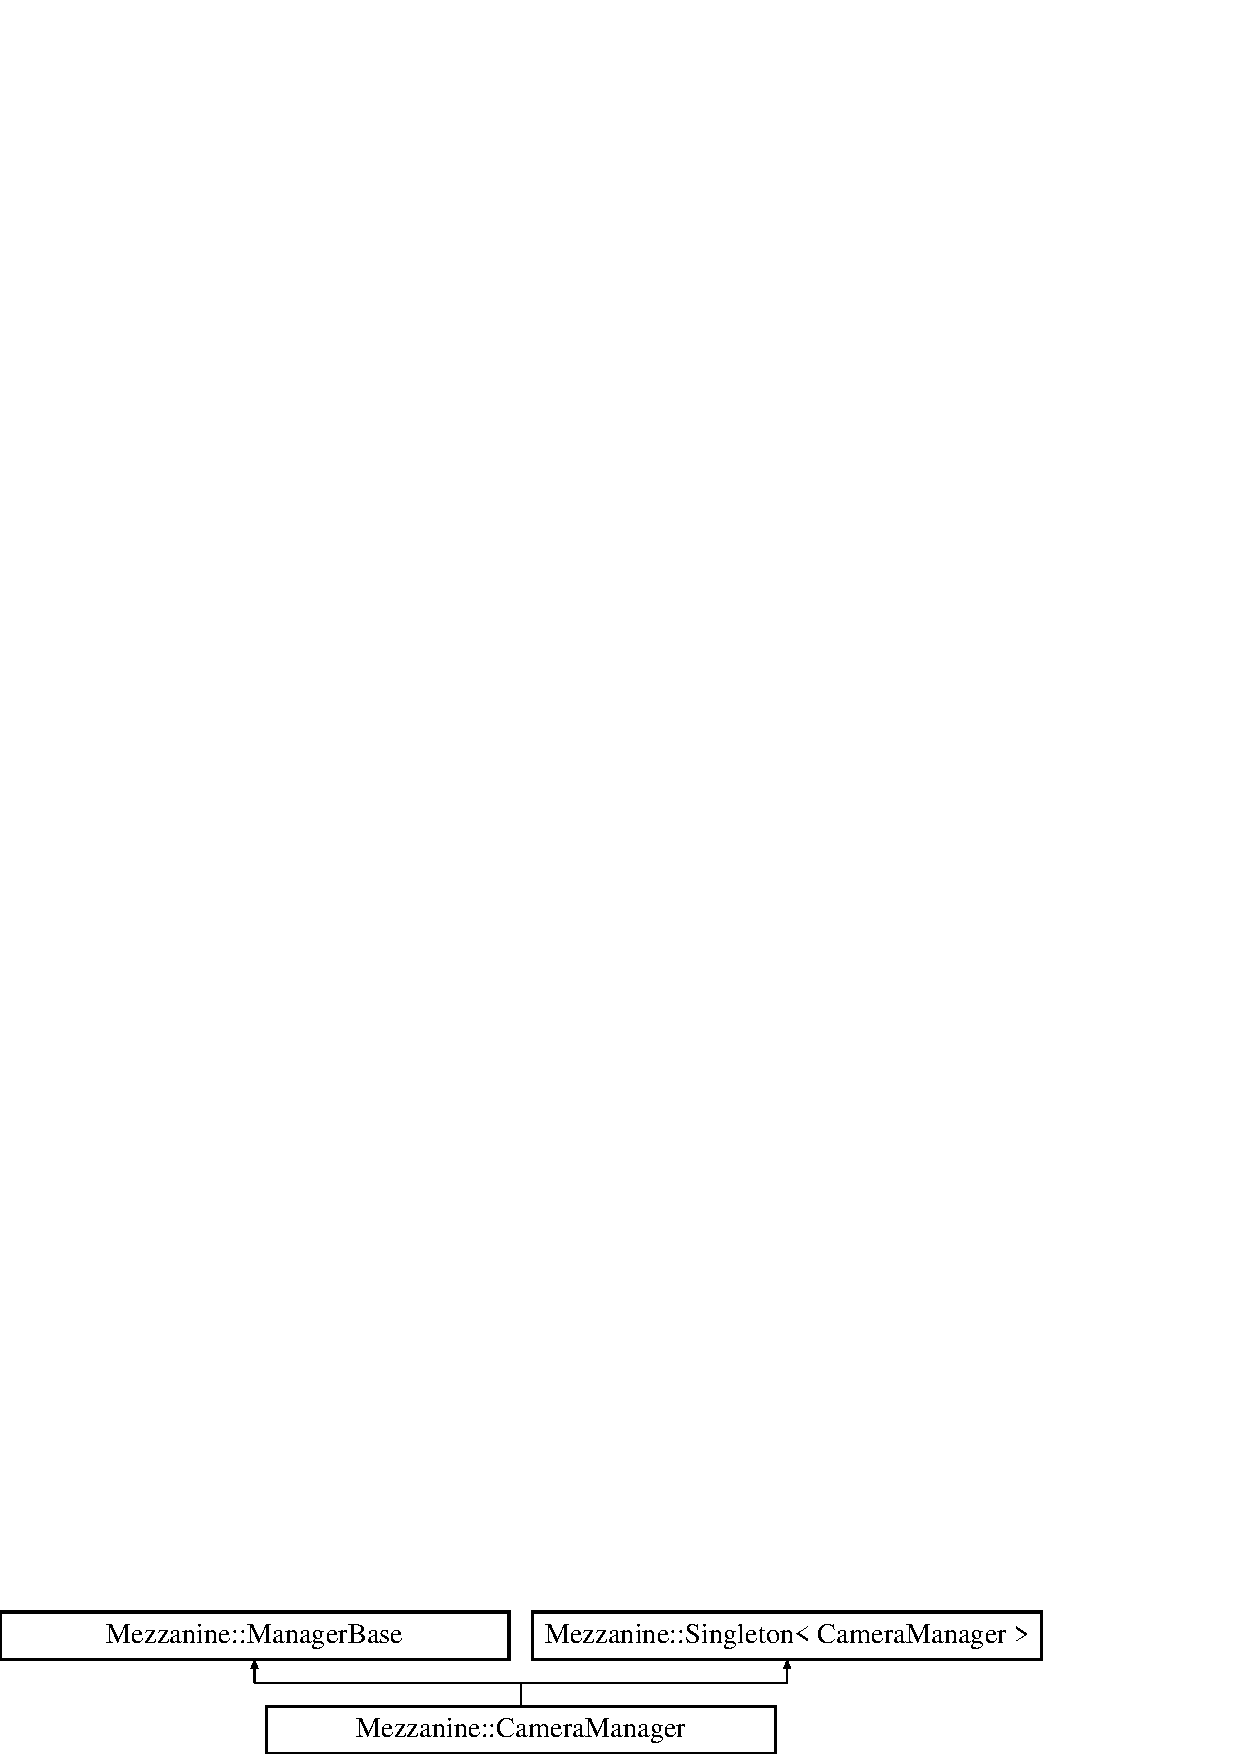
\includegraphics[height=2.000000cm]{classMezzanine_1_1CameraManager}
\end{center}
\end{figure}
\subsubsection*{Public Member Functions}
\begin{DoxyCompactItemize}
\item 
\hyperlink{classMezzanine_1_1CameraManager_a2beb54ad16ce87e9febc941818384b8e}{CameraManager} (\hyperlink{namespaceMezzanine_adcbb6ce6d1eb4379d109e51171e2e493}{Whole} SceneManagerIndex)
\begin{DoxyCompactList}\small\item\em Class Constructor. \item\end{DoxyCompactList}\item 
\hyperlink{classMezzanine_1_1Camera}{Camera} $\ast$ \hyperlink{classMezzanine_1_1CameraManager_a4e97870f483d294683c508c04b41ac9c}{CreateCamera} (const \hyperlink{namespaceMezzanine_acf9fcc130e6ebf08e3d8491aebcf1c86}{String} \&Name)
\begin{DoxyCompactList}\small\item\em Creates a camera and returns a pointer. \item\end{DoxyCompactList}\item 
\hyperlink{classMezzanine_1_1Camera}{Camera} $\ast$ \hyperlink{classMezzanine_1_1CameraManager_a59b4343ed87c095cca6cb529d27babcc}{CreateDefaultCamera} ()
\begin{DoxyCompactList}\small\item\em Creates (or recreates) the default camera for this manager. \item\end{DoxyCompactList}\item 
\hypertarget{classMezzanine_1_1CameraManager_a1e0ef1d314efc126b8149ec713d0a27e}{
void \hyperlink{classMezzanine_1_1CameraManager_a1e0ef1d314efc126b8149ec713d0a27e}{DestroyAllCameraControllers} ()}
\label{classMezzanine_1_1CameraManager_a1e0ef1d314efc126b8149ec713d0a27e}

\begin{DoxyCompactList}\small\item\em Destroys all camera controllers being stored in this manager. \item\end{DoxyCompactList}\item 
void \hyperlink{classMezzanine_1_1CameraManager_a4c8458f99cc04c5103aa8468624514f7}{DestroyAllCameras} (bool DefaultAlso=true)
\begin{DoxyCompactList}\small\item\em Deletes all cameras except for the first camera. \item\end{DoxyCompactList}\item 
void \hyperlink{classMezzanine_1_1CameraManager_a783a0e59b710c03e2a8340e5769fe8aa}{DestroyCameraController} (\hyperlink{classMezzanine_1_1CameraController}{CameraController} $\ast$ToBeDestroyed)
\begin{DoxyCompactList}\small\item\em Destroys a cameracontroller. \item\end{DoxyCompactList}\item 
void \hyperlink{classMezzanine_1_1CameraManager_ab8978a1ff77cb4019d90bf058dfdd4fc}{DestroyCameraController} (\hyperlink{classMezzanine_1_1Camera}{Camera} $\ast$ControlledCam)
\begin{DoxyCompactList}\small\item\em Destroys a cameracontroller by camera. \item\end{DoxyCompactList}\item 
\hypertarget{classMezzanine_1_1CameraManager_a01dcbdb44f681f7915a5347ef167b13f}{
void \hyperlink{classMezzanine_1_1CameraManager_a01dcbdb44f681f7915a5347ef167b13f}{DestroyDefaultCamera} ()}
\label{classMezzanine_1_1CameraManager_a01dcbdb44f681f7915a5347ef167b13f}

\begin{DoxyCompactList}\small\item\em Destroys the default camera. \item\end{DoxyCompactList}\item 
virtual void \hyperlink{classMezzanine_1_1CameraManager_a91db1fdfe96f32d06f689d37b91140cb}{DoMainLoopItems} ()
\begin{DoxyCompactList}\small\item\em Empty MainLoopItems. \item\end{DoxyCompactList}\item 
\hyperlink{classMezzanine_1_1Camera}{Camera} $\ast$ \hyperlink{classMezzanine_1_1CameraManager_a1cb3d08933481db98015384a0a80601b}{GetCamera} (const \hyperlink{namespaceMezzanine_adcbb6ce6d1eb4379d109e51171e2e493}{Whole} \&Index)
\begin{DoxyCompactList}\small\item\em Gets an already created camera by index. \item\end{DoxyCompactList}\item 
\hyperlink{classMezzanine_1_1Camera}{Camera} $\ast$ \hyperlink{classMezzanine_1_1CameraManager_a825b175730d6782071289f6df45bb79f}{GetCamera} (const \hyperlink{namespaceMezzanine_acf9fcc130e6ebf08e3d8491aebcf1c86}{String} \&Name)
\begin{DoxyCompactList}\small\item\em Gets an already created camera by name. \item\end{DoxyCompactList}\item 
\hyperlink{classMezzanine_1_1Camera}{Camera} $\ast$ \hyperlink{classMezzanine_1_1CameraManager_a09c085281b2084711af3de4d46c9a104}{GetDefaultCamera} ()
\begin{DoxyCompactList}\small\item\em Gets the default camera if it has been initialized. \item\end{DoxyCompactList}\item 
\hyperlink{namespaceMezzanine_adcbb6ce6d1eb4379d109e51171e2e493}{Whole} \hyperlink{classMezzanine_1_1CameraManager_aff1a5c332872cfd7db6c8f6bb75e1274}{GetNumCameras} ()
\begin{DoxyCompactList}\small\item\em Gets the number of cameras created and stored in this manager. \item\end{DoxyCompactList}\item 
\hyperlink{classMezzanine_1_1CameraController}{CameraController} $\ast$ \hyperlink{classMezzanine_1_1CameraManager_a2749012cb337dd5aa1f784c951fc9e56}{GetOrCreateCameraController} (\hyperlink{classMezzanine_1_1Camera}{Camera} $\ast$Controlled)
\begin{DoxyCompactList}\small\item\em Gets a camera controller if it exists, otherwise creates it. \item\end{DoxyCompactList}\item 
virtual \hyperlink{classMezzanine_1_1ManagerBase_a08cecf5169cad3e82be81a3a159b0b6e}{ManagerTypeName} \hyperlink{classMezzanine_1_1CameraManager_a1eb75dabfd7df1c901432d841a92fcbc}{GetType} () const 
\begin{DoxyCompactList}\small\item\em This returns the type of this manager. \item\end{DoxyCompactList}\item 
virtual void \hyperlink{classMezzanine_1_1CameraManager_a4b7f0d25f77306bca4b5c885e35363cc}{Initialize} ()
\begin{DoxyCompactList}\small\item\em Empty Initializor. \item\end{DoxyCompactList}\item 
virtual \hyperlink{classMezzanine_1_1CameraManager_a1aad56c3d298c86bde95c26ce231697f}{$\sim$CameraManager} ()
\begin{DoxyCompactList}\small\item\em Class Destructor. \item\end{DoxyCompactList}\end{DoxyCompactItemize}
\subsubsection*{Public Attributes}
\begin{DoxyCompactItemize}
\item 
\hypertarget{classMezzanine_1_1CameraManager_a384babc63ab516b26e0e5d45ea525ced}{
\hyperlink{classMezzanine_1_1SceneManager}{Mezzanine::SceneManager} $\ast$ \hyperlink{classMezzanine_1_1CameraManager_a384babc63ab516b26e0e5d45ea525ced}{SManager}}
\label{classMezzanine_1_1CameraManager_a384babc63ab516b26e0e5d45ea525ced}

\begin{DoxyCompactList}\small\item\em Used to reference the appropriate scene. \item\end{DoxyCompactList}\end{DoxyCompactItemize}
\subsubsection*{Protected Member Functions}
\begin{DoxyCompactItemize}
\item 
\hypertarget{classMezzanine_1_1CameraManager_ae96502bb30b93a57de58a2bbd8e7903a}{
\hyperlink{classMezzanine_1_1Camera}{Camera} $\ast$ {\bfseries FindCamera} (const \hyperlink{namespaceMezzanine_acf9fcc130e6ebf08e3d8491aebcf1c86}{String} \&Name)}
\label{classMezzanine_1_1CameraManager_ae96502bb30b93a57de58a2bbd8e7903a}

\end{DoxyCompactItemize}
\subsubsection*{Protected Attributes}
\begin{DoxyCompactItemize}
\item 
\hypertarget{classMezzanine_1_1CameraManager_a77e86d6a48fe53284be6805c4c8ac8bc}{
std::map$<$ \hyperlink{classMezzanine_1_1Camera}{Camera} $\ast$, \hyperlink{classMezzanine_1_1CameraController}{CameraController} $\ast$ $>$ {\bfseries CameraControllers}}
\label{classMezzanine_1_1CameraManager_a77e86d6a48fe53284be6805c4c8ac8bc}

\item 
\hypertarget{classMezzanine_1_1CameraManager_ad96fededfedccc6019801f0b99931829}{
std::vector$<$ \hyperlink{classMezzanine_1_1Camera}{Camera} $\ast$ $>$ {\bfseries Cameras}}
\label{classMezzanine_1_1CameraManager_ad96fededfedccc6019801f0b99931829}

\item 
\hypertarget{classMezzanine_1_1CameraManager_a3d777350cf282899968ab7a83f76b3ec}{
\hyperlink{classMezzanine_1_1Camera}{Camera} $\ast$ {\bfseries DefaultCamera}}
\label{classMezzanine_1_1CameraManager_a3d777350cf282899968ab7a83f76b3ec}

\end{DoxyCompactItemize}
\subsubsection*{Friends}
\begin{DoxyCompactItemize}
\item 
\hypertarget{classMezzanine_1_1CameraManager_ad8bd9afbbd7af19d996da80e9d25890d}{
class {\bfseries Camera}}
\label{classMezzanine_1_1CameraManager_ad8bd9afbbd7af19d996da80e9d25890d}

\item 
\hypertarget{classMezzanine_1_1CameraManager_ad65eae853be6e1a35bf85e6865583560}{
class {\bfseries GraphicsManager}}
\label{classMezzanine_1_1CameraManager_ad65eae853be6e1a35bf85e6865583560}

\item 
\hypertarget{classMezzanine_1_1CameraManager_a7b4bcdf992c21ae83363f25df05b1d25}{
class {\bfseries World}}
\label{classMezzanine_1_1CameraManager_a7b4bcdf992c21ae83363f25df05b1d25}

\end{DoxyCompactItemize}


\subsubsection{Detailed Description}
This is the manager class for all camera functions. This class contains all the functionality of the use and manipulation of the camera. \par
 All functions that manipulate the camera will default to the default camera, so if you only use one camera you should never have to name the camera you want to use. \par
 This class should only be created after the \hyperlink{classMezzanine_1_1SceneManager}{SceneManager} has been created. 

Definition at line 73 of file cameramanager.h.



\subsubsection{Constructor \& Destructor Documentation}
\hypertarget{classMezzanine_1_1CameraManager_a2beb54ad16ce87e9febc941818384b8e}{
\index{Mezzanine::CameraManager@{Mezzanine::CameraManager}!CameraManager@{CameraManager}}
\index{CameraManager@{CameraManager}!Mezzanine::CameraManager@{Mezzanine::CameraManager}}
\paragraph[{CameraManager}]{\setlength{\rightskip}{0pt plus 5cm}Mezzanine::CameraManager::CameraManager (
\begin{DoxyParamCaption}
\item[{{\bf Whole}}]{SceneManagerIndex}
\end{DoxyParamCaption}
)}\hfill}
\label{classMezzanine_1_1CameraManager_a2beb54ad16ce87e9febc941818384b8e}


Class Constructor. 

This is the class constructor. This is automatcally called in the World.CreateRenderWindow() function and should never need to be called manually. 
\begin{DoxyParams}{Parameters}
{\em SceneManagerIndex} & The \hyperlink{classMezzanine_1_1SceneManager}{SceneManager} to user as indexed by \hyperlink{classMezzanine_1_1World}{Mezzanine::World} \\
\hline
\end{DoxyParams}


Definition at line 60 of file cameramanager.cpp.

\hypertarget{classMezzanine_1_1CameraManager_a1aad56c3d298c86bde95c26ce231697f}{
\index{Mezzanine::CameraManager@{Mezzanine::CameraManager}!$\sim$CameraManager@{$\sim$CameraManager}}
\index{$\sim$CameraManager@{$\sim$CameraManager}!Mezzanine::CameraManager@{Mezzanine::CameraManager}}
\paragraph[{$\sim$CameraManager}]{\setlength{\rightskip}{0pt plus 5cm}Mezzanine::CameraManager::$\sim$CameraManager (
\begin{DoxyParamCaption}
{}
\end{DoxyParamCaption}
)\hspace{0.3cm}{\ttfamily  \mbox{[}virtual\mbox{]}}}\hfill}
\label{classMezzanine_1_1CameraManager_a1aad56c3d298c86bde95c26ce231697f}


Class Destructor. 

The calss Destuctor 

Definition at line 68 of file cameramanager.cpp.



\subsubsection{Member Function Documentation}
\hypertarget{classMezzanine_1_1CameraManager_a4e97870f483d294683c508c04b41ac9c}{
\index{Mezzanine::CameraManager@{Mezzanine::CameraManager}!CreateCamera@{CreateCamera}}
\index{CreateCamera@{CreateCamera}!Mezzanine::CameraManager@{Mezzanine::CameraManager}}
\paragraph[{CreateCamera}]{\setlength{\rightskip}{0pt plus 5cm}{\bf Camera} $\ast$ Mezzanine::CameraManager::CreateCamera (
\begin{DoxyParamCaption}
\item[{const {\bf String} \&}]{Name}
\end{DoxyParamCaption}
)}\hfill}
\label{classMezzanine_1_1CameraManager_a4e97870f483d294683c508c04b41ac9c}


Creates a camera and returns a pointer. 

This function does the same as the other CreateCamera function but will also return a pointer to the camera class instead of a string(being the name of the camera). 

Definition at line 109 of file cameramanager.cpp.

\hypertarget{classMezzanine_1_1CameraManager_a59b4343ed87c095cca6cb529d27babcc}{
\index{Mezzanine::CameraManager@{Mezzanine::CameraManager}!CreateDefaultCamera@{CreateDefaultCamera}}
\index{CreateDefaultCamera@{CreateDefaultCamera}!Mezzanine::CameraManager@{Mezzanine::CameraManager}}
\paragraph[{CreateDefaultCamera}]{\setlength{\rightskip}{0pt plus 5cm}{\bf Camera} $\ast$ Mezzanine::CameraManager::CreateDefaultCamera (
\begin{DoxyParamCaption}
{}
\end{DoxyParamCaption}
)}\hfill}
\label{classMezzanine_1_1CameraManager_a59b4343ed87c095cca6cb529d27babcc}


Creates (or recreates) the default camera for this manager. 

If this function is called while there is a valid default camera already created, it will delete that camera. \begin{DoxyReturn}{Returns}
Returns a pointer to the created camera. 
\end{DoxyReturn}


Definition at line 86 of file cameramanager.cpp.

\hypertarget{classMezzanine_1_1CameraManager_a4c8458f99cc04c5103aa8468624514f7}{
\index{Mezzanine::CameraManager@{Mezzanine::CameraManager}!DestroyAllCameras@{DestroyAllCameras}}
\index{DestroyAllCameras@{DestroyAllCameras}!Mezzanine::CameraManager@{Mezzanine::CameraManager}}
\paragraph[{DestroyAllCameras}]{\setlength{\rightskip}{0pt plus 5cm}void Mezzanine::CameraManager::DestroyAllCameras (
\begin{DoxyParamCaption}
\item[{bool}]{DefaultAlso = {\ttfamily true}}
\end{DoxyParamCaption}
)}\hfill}
\label{classMezzanine_1_1CameraManager_a4c8458f99cc04c5103aa8468624514f7}


Deletes all cameras except for the first camera. 

This will clear the container of cameras. The default camera is not stored in this container however, so it is spared from this wipe. 
\begin{DoxyParams}{Parameters}
{\em DefaultAlso} & Whether or not to also destroy the default camera when deleting all camera's. \\
\hline
\end{DoxyParams}


Definition at line 133 of file cameramanager.cpp.

\hypertarget{classMezzanine_1_1CameraManager_a783a0e59b710c03e2a8340e5769fe8aa}{
\index{Mezzanine::CameraManager@{Mezzanine::CameraManager}!DestroyCameraController@{DestroyCameraController}}
\index{DestroyCameraController@{DestroyCameraController}!Mezzanine::CameraManager@{Mezzanine::CameraManager}}
\paragraph[{DestroyCameraController}]{\setlength{\rightskip}{0pt plus 5cm}void Mezzanine::CameraManager::DestroyCameraController (
\begin{DoxyParamCaption}
\item[{{\bf CameraController} $\ast$}]{ToBeDestroyed}
\end{DoxyParamCaption}
)}\hfill}
\label{classMezzanine_1_1CameraManager_a783a0e59b710c03e2a8340e5769fe8aa}


Destroys a cameracontroller. 


\begin{DoxyParams}{Parameters}
{\em ToBeDestroyed} & Pointer to the cameracontrolled you want destroyed. \\
\hline
\end{DoxyParams}


Definition at line 160 of file cameramanager.cpp.

\hypertarget{classMezzanine_1_1CameraManager_ab8978a1ff77cb4019d90bf058dfdd4fc}{
\index{Mezzanine::CameraManager@{Mezzanine::CameraManager}!DestroyCameraController@{DestroyCameraController}}
\index{DestroyCameraController@{DestroyCameraController}!Mezzanine::CameraManager@{Mezzanine::CameraManager}}
\paragraph[{DestroyCameraController}]{\setlength{\rightskip}{0pt plus 5cm}void Mezzanine::CameraManager::DestroyCameraController (
\begin{DoxyParamCaption}
\item[{{\bf Camera} $\ast$}]{ControlledCam}
\end{DoxyParamCaption}
)}\hfill}
\label{classMezzanine_1_1CameraManager_ab8978a1ff77cb4019d90bf058dfdd4fc}


Destroys a cameracontroller by camera. 


\begin{DoxyParams}{Parameters}
{\em ControlledCam} & The camera who's controller will be destroyed. This doesn't do anything to the camera. \\
\hline
\end{DoxyParams}


Definition at line 175 of file cameramanager.cpp.

\hypertarget{classMezzanine_1_1CameraManager_a91db1fdfe96f32d06f689d37b91140cb}{
\index{Mezzanine::CameraManager@{Mezzanine::CameraManager}!DoMainLoopItems@{DoMainLoopItems}}
\index{DoMainLoopItems@{DoMainLoopItems}!Mezzanine::CameraManager@{Mezzanine::CameraManager}}
\paragraph[{DoMainLoopItems}]{\setlength{\rightskip}{0pt plus 5cm}void Mezzanine::CameraManager::DoMainLoopItems (
\begin{DoxyParamCaption}
{}
\end{DoxyParamCaption}
)\hspace{0.3cm}{\ttfamily  \mbox{[}virtual\mbox{]}}}\hfill}
\label{classMezzanine_1_1CameraManager_a91db1fdfe96f32d06f689d37b91140cb}


Empty MainLoopItems. 

This class implements this for the sake of extension and compatibility. This function does nothing. 

Implements \hyperlink{classMezzanine_1_1ManagerBase_a4ee29e4baf6c4b9a3bfec1b2258d5cd2}{Mezzanine::ManagerBase}.



Definition at line 203 of file cameramanager.cpp.

\hypertarget{classMezzanine_1_1CameraManager_a825b175730d6782071289f6df45bb79f}{
\index{Mezzanine::CameraManager@{Mezzanine::CameraManager}!GetCamera@{GetCamera}}
\index{GetCamera@{GetCamera}!Mezzanine::CameraManager@{Mezzanine::CameraManager}}
\paragraph[{GetCamera}]{\setlength{\rightskip}{0pt plus 5cm}{\bf Camera} $\ast$ Mezzanine::CameraManager::GetCamera (
\begin{DoxyParamCaption}
\item[{const {\bf String} \&}]{Name}
\end{DoxyParamCaption}
)}\hfill}
\label{classMezzanine_1_1CameraManager_a825b175730d6782071289f6df45bb79f}


Gets an already created camera by name. 

\begin{DoxyReturn}{Returns}
Returns a pointer to the camera of the specified name. 
\end{DoxyReturn}


Definition at line 117 of file cameramanager.cpp.

\hypertarget{classMezzanine_1_1CameraManager_a1cb3d08933481db98015384a0a80601b}{
\index{Mezzanine::CameraManager@{Mezzanine::CameraManager}!GetCamera@{GetCamera}}
\index{GetCamera@{GetCamera}!Mezzanine::CameraManager@{Mezzanine::CameraManager}}
\paragraph[{GetCamera}]{\setlength{\rightskip}{0pt plus 5cm}{\bf Camera} $\ast$ Mezzanine::CameraManager::GetCamera (
\begin{DoxyParamCaption}
\item[{const {\bf Whole} \&}]{Index}
\end{DoxyParamCaption}
)}\hfill}
\label{classMezzanine_1_1CameraManager_a1cb3d08933481db98015384a0a80601b}


Gets an already created camera by index. 

\begin{DoxyReturn}{Returns}
Returns a pointer to the camera at the specified index. 
\end{DoxyReturn}


Definition at line 123 of file cameramanager.cpp.

\hypertarget{classMezzanine_1_1CameraManager_a09c085281b2084711af3de4d46c9a104}{
\index{Mezzanine::CameraManager@{Mezzanine::CameraManager}!GetDefaultCamera@{GetDefaultCamera}}
\index{GetDefaultCamera@{GetDefaultCamera}!Mezzanine::CameraManager@{Mezzanine::CameraManager}}
\paragraph[{GetDefaultCamera}]{\setlength{\rightskip}{0pt plus 5cm}{\bf Camera} $\ast$ Mezzanine::CameraManager::GetDefaultCamera (
\begin{DoxyParamCaption}
{}
\end{DoxyParamCaption}
)}\hfill}
\label{classMezzanine_1_1CameraManager_a09c085281b2084711af3de4d46c9a104}


Gets the default camera if it has been initialized. 

\begin{DoxyReturn}{Returns}
Returns the Default \hyperlink{classMezzanine_1_1Camera}{Camera} or a null point if it hasn't been created yet. 
\end{DoxyReturn}


Definition at line 95 of file cameramanager.cpp.

\hypertarget{classMezzanine_1_1CameraManager_aff1a5c332872cfd7db6c8f6bb75e1274}{
\index{Mezzanine::CameraManager@{Mezzanine::CameraManager}!GetNumCameras@{GetNumCameras}}
\index{GetNumCameras@{GetNumCameras}!Mezzanine::CameraManager@{Mezzanine::CameraManager}}
\paragraph[{GetNumCameras}]{\setlength{\rightskip}{0pt plus 5cm}{\bf Whole} Mezzanine::CameraManager::GetNumCameras (
\begin{DoxyParamCaption}
{}
\end{DoxyParamCaption}
)}\hfill}
\label{classMezzanine_1_1CameraManager_aff1a5c332872cfd7db6c8f6bb75e1274}


Gets the number of cameras created and stored in this manager. 

\begin{DoxyReturn}{Returns}
Returns the number of cameras this manager is storing. 
\end{DoxyReturn}


Definition at line 128 of file cameramanager.cpp.

\hypertarget{classMezzanine_1_1CameraManager_a2749012cb337dd5aa1f784c951fc9e56}{
\index{Mezzanine::CameraManager@{Mezzanine::CameraManager}!GetOrCreateCameraController@{GetOrCreateCameraController}}
\index{GetOrCreateCameraController@{GetOrCreateCameraController}!Mezzanine::CameraManager@{Mezzanine::CameraManager}}
\paragraph[{GetOrCreateCameraController}]{\setlength{\rightskip}{0pt plus 5cm}{\bf CameraController} $\ast$ Mezzanine::CameraManager::GetOrCreateCameraController (
\begin{DoxyParamCaption}
\item[{{\bf Camera} $\ast$}]{Controlled}
\end{DoxyParamCaption}
)}\hfill}
\label{classMezzanine_1_1CameraManager_a2749012cb337dd5aa1f784c951fc9e56}


Gets a camera controller if it exists, otherwise creates it. 


\begin{DoxyParams}{Parameters}
{\em Controlled} & The camera that will be controlled by the controller returned. \\
\hline
\end{DoxyParams}
\begin{DoxyReturn}{Returns}
Returns a pointer to the created or retrieved camera controller for the camera. 
\end{DoxyReturn}


Definition at line 147 of file cameramanager.cpp.

\hypertarget{classMezzanine_1_1CameraManager_a1eb75dabfd7df1c901432d841a92fcbc}{
\index{Mezzanine::CameraManager@{Mezzanine::CameraManager}!GetType@{GetType}}
\index{GetType@{GetType}!Mezzanine::CameraManager@{Mezzanine::CameraManager}}
\paragraph[{GetType}]{\setlength{\rightskip}{0pt plus 5cm}{\bf ManagerBase::ManagerTypeName} Mezzanine::CameraManager::GetType (
\begin{DoxyParamCaption}
{}
\end{DoxyParamCaption}
) const\hspace{0.3cm}{\ttfamily  \mbox{[}virtual\mbox{]}}}\hfill}
\label{classMezzanine_1_1CameraManager_a1eb75dabfd7df1c901432d841a92fcbc}


This returns the type of this manager. 

\begin{DoxyReturn}{Returns}
This returns ManagerTypeName::CameraManager. 
\end{DoxyReturn}


Implements \hyperlink{classMezzanine_1_1ManagerBase_a6fbfe9e847156915b195b6de1cf76973}{Mezzanine::ManagerBase}.



Definition at line 206 of file cameramanager.cpp.

\hypertarget{classMezzanine_1_1CameraManager_a4b7f0d25f77306bca4b5c885e35363cc}{
\index{Mezzanine::CameraManager@{Mezzanine::CameraManager}!Initialize@{Initialize}}
\index{Initialize@{Initialize}!Mezzanine::CameraManager@{Mezzanine::CameraManager}}
\paragraph[{Initialize}]{\setlength{\rightskip}{0pt plus 5cm}void Mezzanine::CameraManager::Initialize (
\begin{DoxyParamCaption}
{}
\end{DoxyParamCaption}
)\hspace{0.3cm}{\ttfamily  \mbox{[}virtual\mbox{]}}}\hfill}
\label{classMezzanine_1_1CameraManager_a4b7f0d25f77306bca4b5c885e35363cc}


Empty Initializor. 

This specific initializor is unneeded, but we implement it for compatibility. It also exists in case a derived class wants to override it for some reason. 

Implements \hyperlink{classMezzanine_1_1ManagerBase_a864e3cac11928a602c1db28fa2d52ee2}{Mezzanine::ManagerBase}.



Definition at line 200 of file cameramanager.cpp.



The documentation for this class was generated from the following files:\begin{DoxyCompactItemize}
\item 
cameramanager.h\item 
cameramanager.cpp\end{DoxyCompactItemize}

\hypertarget{classMezzanine_1_1CapsuleCollisionShape}{
\subsection{Mezzanine::CapsuleCollisionShape Class Reference}
\label{classMezzanine_1_1CapsuleCollisionShape}\index{Mezzanine::CapsuleCollisionShape@{Mezzanine::CapsuleCollisionShape}}
}


A capsule physics shape.  




{\ttfamily \#include $<$collisionshape.h$>$}

Inheritance diagram for Mezzanine::CapsuleCollisionShape:\begin{figure}[H]
\begin{center}
\leavevmode
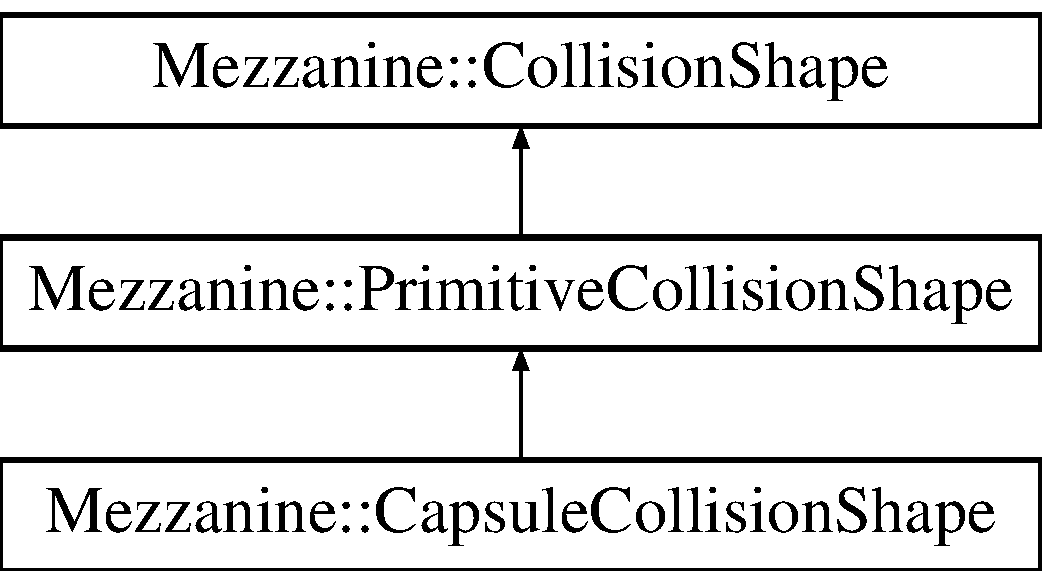
\includegraphics[height=3.000000cm]{classMezzanine_1_1CapsuleCollisionShape}
\end{center}
\end{figure}
\subsubsection*{Public Member Functions}
\begin{DoxyCompactItemize}
\item 
\hyperlink{classMezzanine_1_1CapsuleCollisionShape_a8709e48065ef7698506c9854d41afe8e}{CapsuleCollisionShape} (const \hyperlink{namespaceMezzanine_acf9fcc130e6ebf08e3d8491aebcf1c86}{String} \&\hyperlink{classMezzanine_1_1CollisionShape_aac524c5c56fa4d158bc071f8aecfbe79}{Name}, const \hyperlink{namespaceMezzanine_a726731b1a7df72bf3583e4a97282c6f6}{Real} \&Radius, const \hyperlink{namespaceMezzanine_a726731b1a7df72bf3583e4a97282c6f6}{Real} \&Height, const \hyperlink{classMezzanine_1_1Vector3}{Vector3} \&UpAxis)
\begin{DoxyCompactList}\small\item\em Class Constructor. \item\end{DoxyCompactList}\item 
\hyperlink{classMezzanine_1_1CapsuleCollisionShape_abe6eb6dffc5f40d424974b4f0801cf28}{CapsuleCollisionShape} (const \hyperlink{namespaceMezzanine_acf9fcc130e6ebf08e3d8491aebcf1c86}{String} \&\hyperlink{classMezzanine_1_1CollisionShape_aac524c5c56fa4d158bc071f8aecfbe79}{Name}, const \hyperlink{namespaceMezzanine_a726731b1a7df72bf3583e4a97282c6f6}{Real} \&Radius, const \hyperlink{namespaceMezzanine_a726731b1a7df72bf3583e4a97282c6f6}{Real} \&Height, \hyperlink{namespaceMezzanine_ab41a00a8c6a47b576dc987ec34e16ba1}{StandardAxis} UpAxis)
\begin{DoxyCompactList}\small\item\em Class Constructor. \item\end{DoxyCompactList}\item 
\hyperlink{classMezzanine_1_1CapsuleCollisionShape_a5391a125678d98b509abc8f60cb475be}{CapsuleCollisionShape} (const \hyperlink{namespaceMezzanine_acf9fcc130e6ebf08e3d8491aebcf1c86}{String} \&\hyperlink{classMezzanine_1_1CollisionShape_aac524c5c56fa4d158bc071f8aecfbe79}{Name}, btCapsuleShape $\ast$BulletShape)
\begin{DoxyCompactList}\small\item\em Internal Constructor. \item\end{DoxyCompactList}\item 
virtual btCapsuleShape $\ast$ \hyperlink{classMezzanine_1_1CapsuleCollisionShape_ad9505b15fdcbd88231714992e5b3fc06}{GetBulletCapsuleShape} () const 
\item 
virtual \hyperlink{namespaceMezzanine_a726731b1a7df72bf3583e4a97282c6f6}{Real} \hyperlink{classMezzanine_1_1CapsuleCollisionShape_a531d88a3599327c7ed2a038190fe73e3}{GetCleanHeight} () const 
\begin{DoxyCompactList}\small\item\em Gets the height of the capsule, as the original value passed, without scaling and margin applied. \item\end{DoxyCompactList}\item 
virtual \hyperlink{namespaceMezzanine_a726731b1a7df72bf3583e4a97282c6f6}{Real} \hyperlink{classMezzanine_1_1CapsuleCollisionShape_ad1a0ca094872f1e9f403475165cc455b}{GetCleanRadius} () const 
\begin{DoxyCompactList}\small\item\em Gets the radius of the capsule, as the original value passed, without scaling and margin applied. \item\end{DoxyCompactList}\item 
virtual \hyperlink{namespaceMezzanine_a726731b1a7df72bf3583e4a97282c6f6}{Real} \hyperlink{classMezzanine_1_1CapsuleCollisionShape_a8913f5ead449383b519a682fb837d6e2}{GetHeight} () const 
\begin{DoxyCompactList}\small\item\em Gets the height of the capsule, as used in collision checking, with scaling and margin subtracted. \item\end{DoxyCompactList}\item 
virtual \hyperlink{namespaceMezzanine_a726731b1a7df72bf3583e4a97282c6f6}{Real} \hyperlink{classMezzanine_1_1CapsuleCollisionShape_a2b49207a067b52d65bd0129711c7f85a}{GetRadius} () const 
\begin{DoxyCompactList}\small\item\em Gets the radius of the capsule, as used in collision checking, with scaling and margin subtracted. \item\end{DoxyCompactList}\item 
virtual \hyperlink{classMezzanine_1_1CollisionShape_ad04186055565998879b64176d6dd100d}{CollisionShape::ShapeType} \hyperlink{classMezzanine_1_1CapsuleCollisionShape_a2773853a924c2a97838546d96d851ba5}{GetType} () const 
\item 
virtual \hyperlink{classMezzanine_1_1Vector3}{Vector3} \hyperlink{classMezzanine_1_1CapsuleCollisionShape_a0e81e4ffde066d7673ea008024823644}{GetUpAxis} () const 
\begin{DoxyCompactList}\small\item\em Gets which axis this capsule is oriented along. \item\end{DoxyCompactList}\item 
virtual \hyperlink{namespaceMezzanine_ab41a00a8c6a47b576dc987ec34e16ba1}{StandardAxis} \hyperlink{classMezzanine_1_1CapsuleCollisionShape_ab00e0b036ef4de6d1c663625d0408a4e}{GetUpStandardAxis} () const 
\begin{DoxyCompactList}\small\item\em Gets which axis this capsule is oriented along. \item\end{DoxyCompactList}\item 
\hypertarget{classMezzanine_1_1CapsuleCollisionShape_a197e7425d126ff8b6e7f6da27e0d978c}{
virtual \hyperlink{classMezzanine_1_1CapsuleCollisionShape_a197e7425d126ff8b6e7f6da27e0d978c}{$\sim$CapsuleCollisionShape} ()}
\label{classMezzanine_1_1CapsuleCollisionShape_a197e7425d126ff8b6e7f6da27e0d978c}

\begin{DoxyCompactList}\small\item\em Class Destructor. \item\end{DoxyCompactList}\end{DoxyCompactItemize}
\subsubsection*{Protected Member Functions}
\begin{DoxyCompactItemize}
\item 
void \hyperlink{classMezzanine_1_1CapsuleCollisionShape_a0e4e4f63188053bf72a12ff6a3eef177}{Construct} (const \hyperlink{namespaceMezzanine_acf9fcc130e6ebf08e3d8491aebcf1c86}{String} \&\hyperlink{classMezzanine_1_1CollisionShape_aac524c5c56fa4d158bc071f8aecfbe79}{Name}, const \hyperlink{namespaceMezzanine_a726731b1a7df72bf3583e4a97282c6f6}{Real} \&Radius, const \hyperlink{namespaceMezzanine_a726731b1a7df72bf3583e4a97282c6f6}{Real} \&Height, \hyperlink{namespaceMezzanine_ab41a00a8c6a47b576dc987ec34e16ba1}{StandardAxis} UpAxis)
\begin{DoxyCompactList}\small\item\em Performed share contructor work. \item\end{DoxyCompactList}\end{DoxyCompactItemize}


\subsubsection{Detailed Description}
A capsule physics shape. This shape is commonly used for characters. Keep in mind the total height of any capsule is height+2$\ast$radius, since the height provided only applies to the cylinder portion of the capsule. Like Cones and Cylinders, Capsules can be aligned to any of the 3 linear axes(X, Y, or Z). 

Definition at line 403 of file collisionshape.h.



\subsubsection{Constructor \& Destructor Documentation}
\hypertarget{classMezzanine_1_1CapsuleCollisionShape_a8709e48065ef7698506c9854d41afe8e}{
\index{Mezzanine::CapsuleCollisionShape@{Mezzanine::CapsuleCollisionShape}!CapsuleCollisionShape@{CapsuleCollisionShape}}
\index{CapsuleCollisionShape@{CapsuleCollisionShape}!Mezzanine::CapsuleCollisionShape@{Mezzanine::CapsuleCollisionShape}}
\paragraph[{CapsuleCollisionShape}]{\setlength{\rightskip}{0pt plus 5cm}Mezzanine::CapsuleCollisionShape::CapsuleCollisionShape (
\begin{DoxyParamCaption}
\item[{const {\bf String} \&}]{Name, }
\item[{const {\bf Real} \&}]{Radius, }
\item[{const {\bf Real} \&}]{Height, }
\item[{const {\bf Vector3} \&}]{UpAxis}
\end{DoxyParamCaption}
)}\hfill}
\label{classMezzanine_1_1CapsuleCollisionShape_a8709e48065ef7698506c9854d41afe8e}


Class Constructor. 


\begin{DoxyParams}{Parameters}
{\em Name} & The name of this Shape. \\
\hline
{\em Radius} & The radius of the capsule. \\
\hline
{\em Height} & The height of the cylindrical portion of the capsule. Total height would be Height+2$\ast$radius. \\
\hline
{\em UpAxis} & Which axis the Capsule is to be oriented along. Typical usage is for a capsule to be oriented on the Y axis(0,1,0), which would make it stand upright. \\
\hline
\end{DoxyParams}


Definition at line 623 of file collisionshape.cpp.

\hypertarget{classMezzanine_1_1CapsuleCollisionShape_abe6eb6dffc5f40d424974b4f0801cf28}{
\index{Mezzanine::CapsuleCollisionShape@{Mezzanine::CapsuleCollisionShape}!CapsuleCollisionShape@{CapsuleCollisionShape}}
\index{CapsuleCollisionShape@{CapsuleCollisionShape}!Mezzanine::CapsuleCollisionShape@{Mezzanine::CapsuleCollisionShape}}
\paragraph[{CapsuleCollisionShape}]{\setlength{\rightskip}{0pt plus 5cm}Mezzanine::CapsuleCollisionShape::CapsuleCollisionShape (
\begin{DoxyParamCaption}
\item[{const {\bf String} \&}]{Name, }
\item[{const {\bf Real} \&}]{Radius, }
\item[{const {\bf Real} \&}]{Height, }
\item[{{\bf StandardAxis}}]{UpAxis}
\end{DoxyParamCaption}
)}\hfill}
\label{classMezzanine_1_1CapsuleCollisionShape_abe6eb6dffc5f40d424974b4f0801cf28}


Class Constructor. 


\begin{DoxyParams}{Parameters}
{\em Name} & The name of this Shape. \\
\hline
{\em Radius} & The radius of the capsule. \\
\hline
{\em Height} & The height of the cylindrical portion of the capsule. Total height would be Height+2$\ast$radius. \\
\hline
{\em UpAxis} & Which axis the Capsule is to be oriented along. Uses StandardAxis enum, Axis\_\-Y to make a vertical capsule \\
\hline
\end{DoxyParams}


Definition at line 626 of file collisionshape.cpp.

\hypertarget{classMezzanine_1_1CapsuleCollisionShape_a5391a125678d98b509abc8f60cb475be}{
\index{Mezzanine::CapsuleCollisionShape@{Mezzanine::CapsuleCollisionShape}!CapsuleCollisionShape@{CapsuleCollisionShape}}
\index{CapsuleCollisionShape@{CapsuleCollisionShape}!Mezzanine::CapsuleCollisionShape@{Mezzanine::CapsuleCollisionShape}}
\paragraph[{CapsuleCollisionShape}]{\setlength{\rightskip}{0pt plus 5cm}Mezzanine::CapsuleCollisionShape::CapsuleCollisionShape (
\begin{DoxyParamCaption}
\item[{const {\bf String} \&}]{Name, }
\item[{btCapsuleShape $\ast$}]{BulletShape}
\end{DoxyParamCaption}
)}\hfill}
\label{classMezzanine_1_1CapsuleCollisionShape_a5391a125678d98b509abc8f60cb475be}


Internal Constructor. 


\begin{DoxyParams}{Parameters}
{\em Name} & The name of this Shape. \\
\hline
{\em BulletShape} & The internal shape this shape is based on. \\
\hline
\end{DoxyParams}


Definition at line 658 of file collisionshape.cpp.



\subsubsection{Member Function Documentation}
\hypertarget{classMezzanine_1_1CapsuleCollisionShape_a0e4e4f63188053bf72a12ff6a3eef177}{
\index{Mezzanine::CapsuleCollisionShape@{Mezzanine::CapsuleCollisionShape}!Construct@{Construct}}
\index{Construct@{Construct}!Mezzanine::CapsuleCollisionShape@{Mezzanine::CapsuleCollisionShape}}
\paragraph[{Construct}]{\setlength{\rightskip}{0pt plus 5cm}void Mezzanine::CapsuleCollisionShape::Construct (
\begin{DoxyParamCaption}
\item[{const {\bf String} \&}]{Name, }
\item[{const {\bf Real} \&}]{Radius, }
\item[{const {\bf Real} \&}]{Height, }
\item[{{\bf StandardAxis}}]{UpAxis}
\end{DoxyParamCaption}
)\hspace{0.3cm}{\ttfamily  \mbox{[}protected\mbox{]}}}\hfill}
\label{classMezzanine_1_1CapsuleCollisionShape_a0e4e4f63188053bf72a12ff6a3eef177}


Performed share contructor work. 


\begin{DoxyParams}{Parameters}
{\em Name} & The name of this Shape. \\
\hline
{\em Radius} & The radius of the capsule. \\
\hline
{\em Height} & The height of the cylindrical portion of the capsule. Total height would be Height+2$\ast$radius. \\
\hline
{\em UpAxis} & Which axis the Capsule is to be oriented along. Typical usage is for a capsule to be oriented on the Y axis(0,1,0), which would make it stand upright. \\
\hline
\end{DoxyParams}


Definition at line 612 of file collisionshape.cpp.

\hypertarget{classMezzanine_1_1CapsuleCollisionShape_ad9505b15fdcbd88231714992e5b3fc06}{
\index{Mezzanine::CapsuleCollisionShape@{Mezzanine::CapsuleCollisionShape}!GetBulletCapsuleShape@{GetBulletCapsuleShape}}
\index{GetBulletCapsuleShape@{GetBulletCapsuleShape}!Mezzanine::CapsuleCollisionShape@{Mezzanine::CapsuleCollisionShape}}
\paragraph[{GetBulletCapsuleShape}]{\setlength{\rightskip}{0pt plus 5cm}btCapsuleShape $\ast$ Mezzanine::CapsuleCollisionShape::GetBulletCapsuleShape (
\begin{DoxyParamCaption}
{}
\end{DoxyParamCaption}
) const\hspace{0.3cm}{\ttfamily  \mbox{[}virtual\mbox{]}}}\hfill}
\label{classMezzanine_1_1CapsuleCollisionShape_ad9505b15fdcbd88231714992e5b3fc06}
Gets the internal shape pointer this collision shape is based on. 

\begin{DoxyReturn}{Returns}
Returns a pointer to the internal collision shape. 
\end{DoxyReturn}
 

Definition at line 694 of file collisionshape.cpp.

\hypertarget{classMezzanine_1_1CapsuleCollisionShape_a531d88a3599327c7ed2a038190fe73e3}{
\index{Mezzanine::CapsuleCollisionShape@{Mezzanine::CapsuleCollisionShape}!GetCleanHeight@{GetCleanHeight}}
\index{GetCleanHeight@{GetCleanHeight}!Mezzanine::CapsuleCollisionShape@{Mezzanine::CapsuleCollisionShape}}
\paragraph[{GetCleanHeight}]{\setlength{\rightskip}{0pt plus 5cm}{\bf Real} Mezzanine::CapsuleCollisionShape::GetCleanHeight (
\begin{DoxyParamCaption}
{}
\end{DoxyParamCaption}
) const\hspace{0.3cm}{\ttfamily  \mbox{[}virtual\mbox{]}}}\hfill}
\label{classMezzanine_1_1CapsuleCollisionShape_a531d88a3599327c7ed2a038190fe73e3}


Gets the height of the capsule, as the original value passed, without scaling and margin applied. 

\begin{DoxyReturn}{Returns}
Returns a real representing the length of the cylindrical portion of the capsule. 
\end{DoxyReturn}


Definition at line 677 of file collisionshape.cpp.

\hypertarget{classMezzanine_1_1CapsuleCollisionShape_ad1a0ca094872f1e9f403475165cc455b}{
\index{Mezzanine::CapsuleCollisionShape@{Mezzanine::CapsuleCollisionShape}!GetCleanRadius@{GetCleanRadius}}
\index{GetCleanRadius@{GetCleanRadius}!Mezzanine::CapsuleCollisionShape@{Mezzanine::CapsuleCollisionShape}}
\paragraph[{GetCleanRadius}]{\setlength{\rightskip}{0pt plus 5cm}{\bf Real} Mezzanine::CapsuleCollisionShape::GetCleanRadius (
\begin{DoxyParamCaption}
{}
\end{DoxyParamCaption}
) const\hspace{0.3cm}{\ttfamily  \mbox{[}virtual\mbox{]}}}\hfill}
\label{classMezzanine_1_1CapsuleCollisionShape_ad1a0ca094872f1e9f403475165cc455b}


Gets the radius of the capsule, as the original value passed, without scaling and margin applied. 

\begin{DoxyReturn}{Returns}
Returns a real representing the radius of the capsule. 
\end{DoxyReturn}


Definition at line 674 of file collisionshape.cpp.

\hypertarget{classMezzanine_1_1CapsuleCollisionShape_a8913f5ead449383b519a682fb837d6e2}{
\index{Mezzanine::CapsuleCollisionShape@{Mezzanine::CapsuleCollisionShape}!GetHeight@{GetHeight}}
\index{GetHeight@{GetHeight}!Mezzanine::CapsuleCollisionShape@{Mezzanine::CapsuleCollisionShape}}
\paragraph[{GetHeight}]{\setlength{\rightskip}{0pt plus 5cm}{\bf Real} Mezzanine::CapsuleCollisionShape::GetHeight (
\begin{DoxyParamCaption}
{}
\end{DoxyParamCaption}
) const\hspace{0.3cm}{\ttfamily  \mbox{[}virtual\mbox{]}}}\hfill}
\label{classMezzanine_1_1CapsuleCollisionShape_a8913f5ead449383b519a682fb837d6e2}


Gets the height of the capsule, as used in collision checking, with scaling and margin subtracted. 

\begin{DoxyReturn}{Returns}
Returns a real representing the length of the cylindrical portion of the capsule. 
\end{DoxyReturn}


Definition at line 671 of file collisionshape.cpp.

\hypertarget{classMezzanine_1_1CapsuleCollisionShape_a2b49207a067b52d65bd0129711c7f85a}{
\index{Mezzanine::CapsuleCollisionShape@{Mezzanine::CapsuleCollisionShape}!GetRadius@{GetRadius}}
\index{GetRadius@{GetRadius}!Mezzanine::CapsuleCollisionShape@{Mezzanine::CapsuleCollisionShape}}
\paragraph[{GetRadius}]{\setlength{\rightskip}{0pt plus 5cm}{\bf Real} Mezzanine::CapsuleCollisionShape::GetRadius (
\begin{DoxyParamCaption}
{}
\end{DoxyParamCaption}
) const\hspace{0.3cm}{\ttfamily  \mbox{[}virtual\mbox{]}}}\hfill}
\label{classMezzanine_1_1CapsuleCollisionShape_a2b49207a067b52d65bd0129711c7f85a}


Gets the radius of the capsule, as used in collision checking, with scaling and margin subtracted. 

\begin{DoxyReturn}{Returns}
Returns a real representing the radius of the capsule. 
\end{DoxyReturn}


Definition at line 669 of file collisionshape.cpp.

\hypertarget{classMezzanine_1_1CapsuleCollisionShape_a2773853a924c2a97838546d96d851ba5}{
\index{Mezzanine::CapsuleCollisionShape@{Mezzanine::CapsuleCollisionShape}!GetType@{GetType}}
\index{GetType@{GetType}!Mezzanine::CapsuleCollisionShape@{Mezzanine::CapsuleCollisionShape}}
\paragraph[{GetType}]{\setlength{\rightskip}{0pt plus 5cm}{\bf CollisionShape::ShapeType} Mezzanine::CapsuleCollisionShape::GetType (
\begin{DoxyParamCaption}
{}
\end{DoxyParamCaption}
) const\hspace{0.3cm}{\ttfamily  \mbox{[}virtual\mbox{]}}}\hfill}
\label{classMezzanine_1_1CapsuleCollisionShape_a2773853a924c2a97838546d96d851ba5}
Gets the type of \hyperlink{classMezzanine_1_1Collision}{Collision} shape this is. 

\begin{DoxyReturn}{Returns}
Returns an enum value indicating the type of collision shape this is. 
\end{DoxyReturn}
 

Implements \hyperlink{classMezzanine_1_1PrimitiveCollisionShape_ad3d4143a5640204b987e0b57eb24af41}{Mezzanine::PrimitiveCollisionShape}.



Definition at line 689 of file collisionshape.cpp.

\hypertarget{classMezzanine_1_1CapsuleCollisionShape_a0e81e4ffde066d7673ea008024823644}{
\index{Mezzanine::CapsuleCollisionShape@{Mezzanine::CapsuleCollisionShape}!GetUpAxis@{GetUpAxis}}
\index{GetUpAxis@{GetUpAxis}!Mezzanine::CapsuleCollisionShape@{Mezzanine::CapsuleCollisionShape}}
\paragraph[{GetUpAxis}]{\setlength{\rightskip}{0pt plus 5cm}{\bf Vector3} Mezzanine::CapsuleCollisionShape::GetUpAxis (
\begin{DoxyParamCaption}
{}
\end{DoxyParamCaption}
) const\hspace{0.3cm}{\ttfamily  \mbox{[}virtual\mbox{]}}}\hfill}
\label{classMezzanine_1_1CapsuleCollisionShape_a0e81e4ffde066d7673ea008024823644}


Gets which axis this capsule is oriented along. 

\begin{DoxyReturn}{Returns}
Returns a \hyperlink{classMezzanine_1_1Vector3}{Vector3} representing which local axis is oriented along the world up axis. 
\end{DoxyReturn}


Definition at line 683 of file collisionshape.cpp.

\hypertarget{classMezzanine_1_1CapsuleCollisionShape_ab00e0b036ef4de6d1c663625d0408a4e}{
\index{Mezzanine::CapsuleCollisionShape@{Mezzanine::CapsuleCollisionShape}!GetUpStandardAxis@{GetUpStandardAxis}}
\index{GetUpStandardAxis@{GetUpStandardAxis}!Mezzanine::CapsuleCollisionShape@{Mezzanine::CapsuleCollisionShape}}
\paragraph[{GetUpStandardAxis}]{\setlength{\rightskip}{0pt plus 5cm}{\bf StandardAxis} Mezzanine::CapsuleCollisionShape::GetUpStandardAxis (
\begin{DoxyParamCaption}
{}
\end{DoxyParamCaption}
) const\hspace{0.3cm}{\ttfamily  \mbox{[}virtual\mbox{]}}}\hfill}
\label{classMezzanine_1_1CapsuleCollisionShape_ab00e0b036ef4de6d1c663625d0408a4e}


Gets which axis this capsule is oriented along. 

\begin{DoxyReturn}{Returns}
Returns a StandardAxis representing which local axis is oriented along the world up axis. 
\end{DoxyReturn}


Definition at line 686 of file collisionshape.cpp.



The documentation for this class was generated from the following files:\begin{DoxyCompactItemize}
\item 
collisionshape.h\item 
collisionshape.cpp\end{DoxyCompactItemize}

\hypertarget{classMezzanine_1_1Collision}{
\subsection{Mezzanine::Collision Class Reference}
\label{classMezzanine_1_1Collision}\index{Mezzanine::Collision@{Mezzanine::Collision}}
}


This is an event class used to track collsions in the physics world.  




{\ttfamily \#include $<$collision.h$>$}

\subsubsection*{Public Types}
\begin{DoxyCompactItemize}
\item 
enum \hyperlink{classMezzanine_1_1Collision_a24094c597061743dcd571f36077f4d19}{CollisionState} \{ {\bfseries Col\_\-Begin}, 
{\bfseries Col\_\-Contacts\_\-Updated}, 
{\bfseries Col\_\-End}
 \}
\begin{DoxyCompactList}\small\item\em Enum specifying the state change occuring in the collision. \item\end{DoxyCompactList}\item 
enum \hyperlink{classMezzanine_1_1Collision_aacdbb06153734d3645f4c806dbf90153}{CollisionType} \{ \hyperlink{classMezzanine_1_1Collision_aacdbb06153734d3645f4c806dbf90153a02aba47edf804a1f74605b2a18c5fea6}{Col\_\-Actor\_\-Actor}, 
\hyperlink{classMezzanine_1_1Collision_aacdbb06153734d3645f4c806dbf90153a06281a4725aae432fea2d878ed664b87}{Col\_\-Actor\_\-Terrain}, 
\hyperlink{classMezzanine_1_1Collision_aacdbb06153734d3645f4c806dbf90153a35f141cb89933c3b6f42cb6c022bfac0}{Col\_\-Actor\_\-AreaEffect}, 
\hyperlink{classMezzanine_1_1Collision_aacdbb06153734d3645f4c806dbf90153af9b276afb2ed485927a7fb81ca85e23c}{Col\_\-AreaEffect\_\-Terrain}
 \}
\begin{DoxyCompactList}\small\item\em Enum specifying what kind of collision this class is storing. \item\end{DoxyCompactList}\end{DoxyCompactItemize}
\subsubsection*{Public Member Functions}
\begin{DoxyCompactItemize}
\item 
\hypertarget{classMezzanine_1_1Collision_a2eeacd2ab527b1d5e414917db41d580b}{
\hyperlink{classMezzanine_1_1Collision_a2eeacd2ab527b1d5e414917db41d580b}{Collision} ()}
\label{classMezzanine_1_1Collision_a2eeacd2ab527b1d5e414917db41d580b}

\begin{DoxyCompactList}\small\item\em Default Constructor. \item\end{DoxyCompactList}\item 
\hyperlink{classMezzanine_1_1Collision_a1170d2c2e674ab3e9b1bf68c91171db4}{Collision} (const \hyperlink{classMezzanine_1_1Collision}{Collision} \&Other)
\begin{DoxyCompactList}\small\item\em Copy Constructor. \item\end{DoxyCompactList}\item 
virtual \hyperlink{classMezzanine_1_1Collision_abeac6cfc637fe44493602a04f75c0232}{$\sim$Collision} ()
\begin{DoxyCompactList}\small\item\em Class Destructor. \item\end{DoxyCompactList}\item 
virtual \hyperlink{namespaceMezzanine_adcbb6ce6d1eb4379d109e51171e2e493}{Whole} \hyperlink{classMezzanine_1_1Collision_ad9d72f1d883214242803b72d1b82c343}{GetAge} (const \hyperlink{namespaceMezzanine_adcbb6ce6d1eb4379d109e51171e2e493}{Whole} \&Point)
\begin{DoxyCompactList}\small\item\em Gets the number of simulation steps the contact point has existed. \item\end{DoxyCompactList}\item 
virtual \hyperlink{namespaceMezzanine_a726731b1a7df72bf3583e4a97282c6f6}{Real} \hyperlink{classMezzanine_1_1Collision_aa53aa5016ea75885b9be4f317968b407}{GetAppliedImpulse} (const \hyperlink{namespaceMezzanine_adcbb6ce6d1eb4379d109e51171e2e493}{Whole} \&Point)
\begin{DoxyCompactList}\small\item\em Gets the amount of force of the collision. \item\end{DoxyCompactList}\item 
virtual \hyperlink{namespaceMezzanine_a726731b1a7df72bf3583e4a97282c6f6}{Real} \hyperlink{classMezzanine_1_1Collision_a365b382bac319b1258369c9bdeeb5048}{GetDistance} (const \hyperlink{namespaceMezzanine_adcbb6ce6d1eb4379d109e51171e2e493}{Whole} \&Point)
\begin{DoxyCompactList}\small\item\em Gets the penetration depth of the collision. \item\end{DoxyCompactList}\item 
virtual \hyperlink{classMezzanine_1_1Vector3}{Vector3} \hyperlink{classMezzanine_1_1Collision_a63a18605e0f34392f8521cdc3afd4b62}{GetLocalALocation} (const \hyperlink{namespaceMezzanine_adcbb6ce6d1eb4379d109e51171e2e493}{Whole} \&Point)
\begin{DoxyCompactList}\small\item\em Gets the location in ObjectA's local space where the collision occured. \item\end{DoxyCompactList}\item 
virtual \hyperlink{classMezzanine_1_1Vector3}{Vector3} \hyperlink{classMezzanine_1_1Collision_a6a75e50b8e2160e356e96080206d60bb}{GetLocalBLocation} (const \hyperlink{namespaceMezzanine_adcbb6ce6d1eb4379d109e51171e2e493}{Whole} \&Point)
\begin{DoxyCompactList}\small\item\em Gets the location in ObjectB's local space where the collision occured. \item\end{DoxyCompactList}\item 
virtual \hyperlink{classMezzanine_1_1Vector3}{Vector3} \hyperlink{classMezzanine_1_1Collision_abd59dc03ed9226275e85681ec3ef1555}{GetNormal} (const \hyperlink{namespaceMezzanine_adcbb6ce6d1eb4379d109e51171e2e493}{Whole} \&Point)
\begin{DoxyCompactList}\small\item\em GEts the collision normal for a contact point. \item\end{DoxyCompactList}\item 
virtual \hyperlink{namespaceMezzanine_adcbb6ce6d1eb4379d109e51171e2e493}{Whole} \hyperlink{classMezzanine_1_1Collision_a75c8f35acf6ceba61b62da0049dcbf1c}{GetNumContactPoints} ()
\begin{DoxyCompactList}\small\item\em Gets the number of contact points this collision is storing. \item\end{DoxyCompactList}\item 
virtual \hyperlink{classMezzanine_1_1WorldObject}{WorldObject} $\ast$ \hyperlink{classMezzanine_1_1Collision_a8eb039baf05fba52609fc9901ec65a4d}{GetObjectA} () const 
\begin{DoxyCompactList}\small\item\em Gets the first Object this collision applies to. \item\end{DoxyCompactList}\item 
virtual \hyperlink{classMezzanine_1_1WorldObject}{WorldObject} $\ast$ \hyperlink{classMezzanine_1_1Collision_ac86914ea74f944491a28c07f50bd3107}{GetObjectB} () const 
\begin{DoxyCompactList}\small\item\em Gets the second Object this collision applies to. \item\end{DoxyCompactList}\item 
virtual \hyperlink{classMezzanine_1_1Vector3}{Vector3} \hyperlink{classMezzanine_1_1Collision_abefbe2ba9b0aaa1830be4f1070c44480}{GetWorldLocation} (const \hyperlink{namespaceMezzanine_adcbb6ce6d1eb4379d109e51171e2e493}{Whole} \&Point)
\begin{DoxyCompactList}\small\item\em Gets the location in the world where the collision occured. \item\end{DoxyCompactList}\item 
virtual bool \hyperlink{classMezzanine_1_1Collision_ae9eb0637ebd2e5dd47992278e4776e01}{PairsMatch} (\hyperlink{classMezzanine_1_1WorldObject}{WorldObject} $\ast$A, \hyperlink{classMezzanine_1_1WorldObject}{WorldObject} $\ast$B) const 
\begin{DoxyCompactList}\small\item\em Convenience function to see if the provided pair match the pair in this class. \item\end{DoxyCompactList}\item 
virtual void \hyperlink{classMezzanine_1_1Collision_a5503aa0fdc08e9ee41205478fc3c3bbc}{SetObjectA} (\hyperlink{classMezzanine_1_1WorldObject}{WorldObject} $\ast$A)
\begin{DoxyCompactList}\small\item\em Sets the first Object this collision applies to. \item\end{DoxyCompactList}\item 
virtual void \hyperlink{classMezzanine_1_1Collision_a4254bbe27f1d7362d79cecd46d6d2b24}{SetObjectB} (\hyperlink{classMezzanine_1_1WorldObject}{WorldObject} $\ast$B)
\begin{DoxyCompactList}\small\item\em Sets the second Object this collision applies to. \item\end{DoxyCompactList}\item 
\hypertarget{classMezzanine_1_1Collision_afee98e7728b4f2a4865a2ef38a051577}{
virtual void \hyperlink{classMezzanine_1_1Collision_afee98e7728b4f2a4865a2ef38a051577}{Update} ()}
\label{classMezzanine_1_1Collision_afee98e7728b4f2a4865a2ef38a051577}

\begin{DoxyCompactList}\small\item\em Updates this collisions contact point data if it needs updating. \item\end{DoxyCompactList}\end{DoxyCompactItemize}
\subsubsection*{Protected Member Functions}
\begin{DoxyCompactItemize}
\item 
\hyperlink{classMezzanine_1_1Collision_a2f367a05c29086e86395ca5f6f2c4728}{Collision} (\hyperlink{classMezzanine_1_1WorldObject}{WorldObject} $\ast$A, \hyperlink{classMezzanine_1_1WorldObject}{WorldObject} $\ast$B, btCollisionAlgorithm $\ast$PhysicsAlgo)
\begin{DoxyCompactList}\small\item\em Class Constructor. \item\end{DoxyCompactList}\item 
\hypertarget{classMezzanine_1_1Collision_ab337bbfb55f330ac095934cd1a0e40ed}{
btManifoldPoint \& \hyperlink{classMezzanine_1_1Collision_ab337bbfb55f330ac095934cd1a0e40ed}{GetManifoldPoint} (const \hyperlink{namespaceMezzanine_adcbb6ce6d1eb4379d109e51171e2e493}{Whole} \&Index)}
\label{classMezzanine_1_1Collision_ab337bbfb55f330ac095934cd1a0e40ed}

\begin{DoxyCompactList}\small\item\em Internal function responsible for fetching the appropriate contact point. \item\end{DoxyCompactList}\item 
\hypertarget{classMezzanine_1_1Collision_ac64ad25958ee82b8fdfd61888f2531f9}{
void \hyperlink{classMezzanine_1_1Collision_ac64ad25958ee82b8fdfd61888f2531f9}{UpdatePenetrationDistances} ()}
\label{classMezzanine_1_1Collision_ac64ad25958ee82b8fdfd61888f2531f9}

\begin{DoxyCompactList}\small\item\em Updates the PenetrationDistances vector on this object. \item\end{DoxyCompactList}\end{DoxyCompactItemize}
\subsubsection*{Protected Attributes}
\begin{DoxyCompactItemize}
\item 
\hypertarget{classMezzanine_1_1Collision_a6326964a8f8601655d97efc231ec3f86}{
btCollisionAlgorithm $\ast$ \hyperlink{classMezzanine_1_1Collision_a6326964a8f8601655d97efc231ec3f86}{InternalAlgo}}
\label{classMezzanine_1_1Collision_a6326964a8f8601655d97efc231ec3f86}

\begin{DoxyCompactList}\small\item\em The internal collision class this event is based on. \item\end{DoxyCompactList}\item 
\hypertarget{classMezzanine_1_1Collision_ac4a67a946284d3bacbd342b935495b57}{
\hyperlink{structMezzanine_1_1CollisionInternalData}{CollisionInternalData} $\ast$ \hyperlink{classMezzanine_1_1Collision_ac4a67a946284d3bacbd342b935495b57}{InternalData}}
\label{classMezzanine_1_1Collision_ac4a67a946284d3bacbd342b935495b57}

\begin{DoxyCompactList}\small\item\em Array of manifolds that apply to this collision. \item\end{DoxyCompactList}\item 
\hypertarget{classMezzanine_1_1Collision_adda553398a86a2ed1157689e2dfebbec}{
\hyperlink{classMezzanine_1_1WorldObject}{WorldObject} $\ast$ \hyperlink{classMezzanine_1_1Collision_adda553398a86a2ed1157689e2dfebbec}{ObjectA}}
\label{classMezzanine_1_1Collision_adda553398a86a2ed1157689e2dfebbec}

\begin{DoxyCompactList}\small\item\em The first Object involved in the collision. \item\end{DoxyCompactList}\item 
\hypertarget{classMezzanine_1_1Collision_aef15617d25f42598783887f3d8cc6086}{
\hyperlink{classMezzanine_1_1WorldObject}{WorldObject} $\ast$ \hyperlink{classMezzanine_1_1Collision_aef15617d25f42598783887f3d8cc6086}{ObjectB}}
\label{classMezzanine_1_1Collision_aef15617d25f42598783887f3d8cc6086}

\begin{DoxyCompactList}\small\item\em The second Object invovled in the collision. \item\end{DoxyCompactList}\item 
\hypertarget{classMezzanine_1_1Collision_a9245295110d3fe645879a5d798673939}{
std::vector$<$ \hyperlink{namespaceMezzanine_a726731b1a7df72bf3583e4a97282c6f6}{Real} $>$ \hyperlink{classMezzanine_1_1Collision_a9245295110d3fe645879a5d798673939}{PenetrationDistances}}
\label{classMezzanine_1_1Collision_a9245295110d3fe645879a5d798673939}

\begin{DoxyCompactList}\small\item\em This stores the distance of each contact point in this collision, for using to track updates. \item\end{DoxyCompactList}\end{DoxyCompactItemize}
\subsubsection*{Friends}
\begin{DoxyCompactItemize}
\item 
\hypertarget{classMezzanine_1_1Collision_aa4a13416efe17e957deb2cf4dcce3a60}{
class {\bfseries CollisionDispatcher}}
\label{classMezzanine_1_1Collision_aa4a13416efe17e957deb2cf4dcce3a60}

\item 
\hypertarget{classMezzanine_1_1Collision_a139cf05ac01161b7071c8a037c841683}{
class {\bfseries PhysicsManager}}
\label{classMezzanine_1_1Collision_a139cf05ac01161b7071c8a037c841683}

\end{DoxyCompactItemize}


\subsubsection{Detailed Description}
This is an event class used to track collsions in the physics world. This class will be used for tracking collisions in the physics world and will keep track of basic data related to the collision. This class stores the information in the form of contact points. Often when a collision occurs there will be more then one place where the collision occured, this is a contact point. Internally collisions only store up to a maximum of 4 contact points. When querying for collision information, you have to provide the desired contact point index, and it must be valid. If the requested index isn't valid an exception will be thrown. So always make sure to verify with \hyperlink{classMezzanine_1_1Collision_a75c8f35acf6ceba61b62da0049dcbf1c}{GetNumContactPoints()}. 

Definition at line 67 of file collision.h.



\subsubsection{Member Enumeration Documentation}
\hypertarget{classMezzanine_1_1Collision_aacdbb06153734d3645f4c806dbf90153}{
\index{Mezzanine::Collision@{Mezzanine::Collision}!CollisionType@{CollisionType}}
\index{CollisionType@{CollisionType}!Mezzanine::Collision@{Mezzanine::Collision}}
\paragraph[{CollisionType}]{\setlength{\rightskip}{0pt plus 5cm}enum {\bf Mezzanine::Collision::CollisionType}}\hfill}
\label{classMezzanine_1_1Collision_aacdbb06153734d3645f4c806dbf90153}


Enum specifying what kind of collision this class is storing. 

\begin{Desc}
\item[Enumerator: ]\par
\begin{description}
\index{Col\_\-Actor\_\-Actor@{Col\_\-Actor\_\-Actor}!Mezzanine::Collision@{Mezzanine::Collision}}\index{Mezzanine::Collision@{Mezzanine::Collision}!Col\_\-Actor\_\-Actor@{Col\_\-Actor\_\-Actor}}\item[{\em 
\hypertarget{classMezzanine_1_1Collision_aacdbb06153734d3645f4c806dbf90153a02aba47edf804a1f74605b2a18c5fea6}{
Col\_\-Actor\_\-Actor}
\label{classMezzanine_1_1Collision_aacdbb06153734d3645f4c806dbf90153a02aba47edf804a1f74605b2a18c5fea6}
}]Specifies a collision between two Actors. \index{Col\_\-Actor\_\-Terrain@{Col\_\-Actor\_\-Terrain}!Mezzanine::Collision@{Mezzanine::Collision}}\index{Mezzanine::Collision@{Mezzanine::Collision}!Col\_\-Actor\_\-Terrain@{Col\_\-Actor\_\-Terrain}}\item[{\em 
\hypertarget{classMezzanine_1_1Collision_aacdbb06153734d3645f4c806dbf90153a06281a4725aae432fea2d878ed664b87}{
Col\_\-Actor\_\-Terrain}
\label{classMezzanine_1_1Collision_aacdbb06153734d3645f4c806dbf90153a06281a4725aae432fea2d878ed664b87}
}]Specifies a collision between an Actor and some Terrain. \index{Col\_\-Actor\_\-AreaEffect@{Col\_\-Actor\_\-AreaEffect}!Mezzanine::Collision@{Mezzanine::Collision}}\index{Mezzanine::Collision@{Mezzanine::Collision}!Col\_\-Actor\_\-AreaEffect@{Col\_\-Actor\_\-AreaEffect}}\item[{\em 
\hypertarget{classMezzanine_1_1Collision_aacdbb06153734d3645f4c806dbf90153a35f141cb89933c3b6f42cb6c022bfac0}{
Col\_\-Actor\_\-AreaEffect}
\label{classMezzanine_1_1Collision_aacdbb06153734d3645f4c806dbf90153a35f141cb89933c3b6f42cb6c022bfac0}
}]Specifies a collision between an Actor and an AreaRffect. \index{Col\_\-AreaEffect\_\-Terrain@{Col\_\-AreaEffect\_\-Terrain}!Mezzanine::Collision@{Mezzanine::Collision}}\index{Mezzanine::Collision@{Mezzanine::Collision}!Col\_\-AreaEffect\_\-Terrain@{Col\_\-AreaEffect\_\-Terrain}}\item[{\em 
\hypertarget{classMezzanine_1_1Collision_aacdbb06153734d3645f4c806dbf90153af9b276afb2ed485927a7fb81ca85e23c}{
Col\_\-AreaEffect\_\-Terrain}
\label{classMezzanine_1_1Collision_aacdbb06153734d3645f4c806dbf90153af9b276afb2ed485927a7fb81ca85e23c}
}]Specifies a collision between an \hyperlink{classMezzanine_1_1AreaEffect}{AreaEffect} and some Terrain. \end{description}
\end{Desc}



Definition at line 80 of file collision.h.



\subsubsection{Constructor \& Destructor Documentation}
\hypertarget{classMezzanine_1_1Collision_a2f367a05c29086e86395ca5f6f2c4728}{
\index{Mezzanine::Collision@{Mezzanine::Collision}!Collision@{Collision}}
\index{Collision@{Collision}!Mezzanine::Collision@{Mezzanine::Collision}}
\paragraph[{Collision}]{\setlength{\rightskip}{0pt plus 5cm}Mezzanine::Collision::Collision (
\begin{DoxyParamCaption}
\item[{{\bf WorldObject} $\ast$}]{A, }
\item[{{\bf WorldObject} $\ast$}]{B, }
\item[{btCollisionAlgorithm $\ast$}]{PhysicsAlgo}
\end{DoxyParamCaption}
)\hspace{0.3cm}{\ttfamily  \mbox{[}protected\mbox{]}}}\hfill}
\label{classMezzanine_1_1Collision_a2f367a05c29086e86395ca5f6f2c4728}


Class Constructor. 

This will construct a basic event class with the minimum data needed. 
\begin{DoxyParams}{Parameters}
{\em A} & The first Object involved in the collision. \\
\hline
{\em B} & The second Object invovled in the collision. \\
\hline
{\em PhysicsAlgo} & The internal algorithm used for generating collision data. \\
\hline
\end{DoxyParams}


Definition at line 62 of file collision.cpp.

\hypertarget{classMezzanine_1_1Collision_a1170d2c2e674ab3e9b1bf68c91171db4}{
\index{Mezzanine::Collision@{Mezzanine::Collision}!Collision@{Collision}}
\index{Collision@{Collision}!Mezzanine::Collision@{Mezzanine::Collision}}
\paragraph[{Collision}]{\setlength{\rightskip}{0pt plus 5cm}Mezzanine::Collision::Collision (
\begin{DoxyParamCaption}
\item[{const {\bf Collision} \&}]{Other}
\end{DoxyParamCaption}
)}\hfill}
\label{classMezzanine_1_1Collision_a1170d2c2e674ab3e9b1bf68c91171db4}


Copy Constructor. 


\begin{DoxyParams}{Parameters}
{\em Other} & The other \hyperlink{classMezzanine_1_1EventCollision}{EventCollision} to copy \\
\hline
\end{DoxyParams}


Definition at line 83 of file collision.cpp.

\hypertarget{classMezzanine_1_1Collision_abeac6cfc637fe44493602a04f75c0232}{
\index{Mezzanine::Collision@{Mezzanine::Collision}!$\sim$Collision@{$\sim$Collision}}
\index{$\sim$Collision@{$\sim$Collision}!Mezzanine::Collision@{Mezzanine::Collision}}
\paragraph[{$\sim$Collision}]{\setlength{\rightskip}{0pt plus 5cm}Mezzanine::Collision::$\sim$Collision (
\begin{DoxyParamCaption}
{}
\end{DoxyParamCaption}
)\hspace{0.3cm}{\ttfamily  \mbox{[}virtual\mbox{]}}}\hfill}
\label{classMezzanine_1_1Collision_abeac6cfc637fe44493602a04f75c0232}


Class Destructor. 

Basic Class Destructor. 

Definition at line 96 of file collision.cpp.



\subsubsection{Member Function Documentation}
\hypertarget{classMezzanine_1_1Collision_ad9d72f1d883214242803b72d1b82c343}{
\index{Mezzanine::Collision@{Mezzanine::Collision}!GetAge@{GetAge}}
\index{GetAge@{GetAge}!Mezzanine::Collision@{Mezzanine::Collision}}
\paragraph[{GetAge}]{\setlength{\rightskip}{0pt plus 5cm}{\bf Whole} Mezzanine::Collision::GetAge (
\begin{DoxyParamCaption}
\item[{const {\bf Whole} \&}]{Point}
\end{DoxyParamCaption}
)\hspace{0.3cm}{\ttfamily  \mbox{[}virtual\mbox{]}}}\hfill}
\label{classMezzanine_1_1Collision_ad9d72f1d883214242803b72d1b82c343}


Gets the number of simulation steps the contact point has existed. 


\begin{DoxyParams}{Parameters}
{\em Point} & The index of the contact point for this collision. \\
\hline
\end{DoxyParams}
\begin{DoxyReturn}{Returns}
Returns a Whole representing the amount of simulation steps a point has existed. 
\end{DoxyReturn}


Definition at line 198 of file collision.cpp.

\hypertarget{classMezzanine_1_1Collision_aa53aa5016ea75885b9be4f317968b407}{
\index{Mezzanine::Collision@{Mezzanine::Collision}!GetAppliedImpulse@{GetAppliedImpulse}}
\index{GetAppliedImpulse@{GetAppliedImpulse}!Mezzanine::Collision@{Mezzanine::Collision}}
\paragraph[{GetAppliedImpulse}]{\setlength{\rightskip}{0pt plus 5cm}{\bf Real} Mezzanine::Collision::GetAppliedImpulse (
\begin{DoxyParamCaption}
\item[{const {\bf Whole} \&}]{Point}
\end{DoxyParamCaption}
)\hspace{0.3cm}{\ttfamily  \mbox{[}virtual\mbox{]}}}\hfill}
\label{classMezzanine_1_1Collision_aa53aa5016ea75885b9be4f317968b407}


Gets the amount of force of the collision. 


\begin{DoxyParams}{Parameters}
{\em Point} & The index of the contact point for this collision. \\
\hline
\end{DoxyParams}
\begin{DoxyReturn}{Returns}
Returns a real representing the amount of force applied from the collision. 
\end{DoxyReturn}


Definition at line 188 of file collision.cpp.

\hypertarget{classMezzanine_1_1Collision_a365b382bac319b1258369c9bdeeb5048}{
\index{Mezzanine::Collision@{Mezzanine::Collision}!GetDistance@{GetDistance}}
\index{GetDistance@{GetDistance}!Mezzanine::Collision@{Mezzanine::Collision}}
\paragraph[{GetDistance}]{\setlength{\rightskip}{0pt plus 5cm}{\bf Real} Mezzanine::Collision::GetDistance (
\begin{DoxyParamCaption}
\item[{const {\bf Whole} \&}]{Point}
\end{DoxyParamCaption}
)\hspace{0.3cm}{\ttfamily  \mbox{[}virtual\mbox{]}}}\hfill}
\label{classMezzanine_1_1Collision_a365b382bac319b1258369c9bdeeb5048}


Gets the penetration depth of the collision. 

\begin{DoxyRemark}{Remarks}
You should double check the return of this to verify that it is $<$0, sometimes a collision or contact point can be reported while there is no actual overlap depending on your physics setup. 
\end{DoxyRemark}

\begin{DoxyParams}{Parameters}
{\em Point} & The index of the contact point for this collision. \\
\hline
\end{DoxyParams}
\begin{DoxyReturn}{Returns}
Returns a real representing the depth of penetration between the two objects in this collision. 
\end{DoxyReturn}


Definition at line 193 of file collision.cpp.

\hypertarget{classMezzanine_1_1Collision_a63a18605e0f34392f8521cdc3afd4b62}{
\index{Mezzanine::Collision@{Mezzanine::Collision}!GetLocalALocation@{GetLocalALocation}}
\index{GetLocalALocation@{GetLocalALocation}!Mezzanine::Collision@{Mezzanine::Collision}}
\paragraph[{GetLocalALocation}]{\setlength{\rightskip}{0pt plus 5cm}{\bf Vector3} Mezzanine::Collision::GetLocalALocation (
\begin{DoxyParamCaption}
\item[{const {\bf Whole} \&}]{Point}
\end{DoxyParamCaption}
)\hspace{0.3cm}{\ttfamily  \mbox{[}virtual\mbox{]}}}\hfill}
\label{classMezzanine_1_1Collision_a63a18605e0f34392f8521cdc3afd4b62}


Gets the location in ObjectA's local space where the collision occured. 


\begin{DoxyParams}{Parameters}
{\em Point} & The index of the contact point for this collision. \\
\hline
\end{DoxyParams}
\begin{DoxyReturn}{Returns}
Returns a vector3 with the point of the collision in ObjectA's local space. 
\end{DoxyReturn}


Definition at line 173 of file collision.cpp.

\hypertarget{classMezzanine_1_1Collision_a6a75e50b8e2160e356e96080206d60bb}{
\index{Mezzanine::Collision@{Mezzanine::Collision}!GetLocalBLocation@{GetLocalBLocation}}
\index{GetLocalBLocation@{GetLocalBLocation}!Mezzanine::Collision@{Mezzanine::Collision}}
\paragraph[{GetLocalBLocation}]{\setlength{\rightskip}{0pt plus 5cm}{\bf Vector3} Mezzanine::Collision::GetLocalBLocation (
\begin{DoxyParamCaption}
\item[{const {\bf Whole} \&}]{Point}
\end{DoxyParamCaption}
)\hspace{0.3cm}{\ttfamily  \mbox{[}virtual\mbox{]}}}\hfill}
\label{classMezzanine_1_1Collision_a6a75e50b8e2160e356e96080206d60bb}


Gets the location in ObjectB's local space where the collision occured. 


\begin{DoxyParams}{Parameters}
{\em Point} & The index of the contact point for this collision. \\
\hline
\end{DoxyParams}
\begin{DoxyReturn}{Returns}
Returns a vector3 with the point of the collision in ObjectB's local space. 
\end{DoxyReturn}


Definition at line 178 of file collision.cpp.

\hypertarget{classMezzanine_1_1Collision_abd59dc03ed9226275e85681ec3ef1555}{
\index{Mezzanine::Collision@{Mezzanine::Collision}!GetNormal@{GetNormal}}
\index{GetNormal@{GetNormal}!Mezzanine::Collision@{Mezzanine::Collision}}
\paragraph[{GetNormal}]{\setlength{\rightskip}{0pt plus 5cm}{\bf Vector3} Mezzanine::Collision::GetNormal (
\begin{DoxyParamCaption}
\item[{const {\bf Whole} \&}]{Point}
\end{DoxyParamCaption}
)\hspace{0.3cm}{\ttfamily  \mbox{[}virtual\mbox{]}}}\hfill}
\label{classMezzanine_1_1Collision_abd59dc03ed9226275e85681ec3ef1555}


GEts the collision normal for a contact point. 


\begin{DoxyParams}{Parameters}
{\em Point} & The index of the contact point for this collision. \\
\hline
\end{DoxyParams}
\begin{DoxyReturn}{Returns}
Returns a vector3 representing the collision normal for a contact point. 
\end{DoxyReturn}


Definition at line 183 of file collision.cpp.

\hypertarget{classMezzanine_1_1Collision_a75c8f35acf6ceba61b62da0049dcbf1c}{
\index{Mezzanine::Collision@{Mezzanine::Collision}!GetNumContactPoints@{GetNumContactPoints}}
\index{GetNumContactPoints@{GetNumContactPoints}!Mezzanine::Collision@{Mezzanine::Collision}}
\paragraph[{GetNumContactPoints}]{\setlength{\rightskip}{0pt plus 5cm}{\bf Whole} Mezzanine::Collision::GetNumContactPoints (
\begin{DoxyParamCaption}
{}
\end{DoxyParamCaption}
)\hspace{0.3cm}{\ttfamily  \mbox{[}virtual\mbox{]}}}\hfill}
\label{classMezzanine_1_1Collision_a75c8f35acf6ceba61b62da0049dcbf1c}


Gets the number of contact points this collision is storing. 

\begin{DoxyReturn}{Returns}
Returns the number of contact points that currently exist for this collision. 
\end{DoxyReturn}


Definition at line 161 of file collision.cpp.

\hypertarget{classMezzanine_1_1Collision_a8eb039baf05fba52609fc9901ec65a4d}{
\index{Mezzanine::Collision@{Mezzanine::Collision}!GetObjectA@{GetObjectA}}
\index{GetObjectA@{GetObjectA}!Mezzanine::Collision@{Mezzanine::Collision}}
\paragraph[{GetObjectA}]{\setlength{\rightskip}{0pt plus 5cm}{\bf WorldObject} $\ast$ Mezzanine::Collision::GetObjectA (
\begin{DoxyParamCaption}
{}
\end{DoxyParamCaption}
) const\hspace{0.3cm}{\ttfamily  \mbox{[}virtual\mbox{]}}}\hfill}
\label{classMezzanine_1_1Collision_a8eb039baf05fba52609fc9901ec65a4d}


Gets the first Object this collision applies to. 

\begin{DoxyReturn}{Returns}
Returns a pointer to the first Object in this event. 
\end{DoxyReturn}


Definition at line 140 of file collision.cpp.

\hypertarget{classMezzanine_1_1Collision_ac86914ea74f944491a28c07f50bd3107}{
\index{Mezzanine::Collision@{Mezzanine::Collision}!GetObjectB@{GetObjectB}}
\index{GetObjectB@{GetObjectB}!Mezzanine::Collision@{Mezzanine::Collision}}
\paragraph[{GetObjectB}]{\setlength{\rightskip}{0pt plus 5cm}{\bf WorldObject} $\ast$ Mezzanine::Collision::GetObjectB (
\begin{DoxyParamCaption}
{}
\end{DoxyParamCaption}
) const\hspace{0.3cm}{\ttfamily  \mbox{[}virtual\mbox{]}}}\hfill}
\label{classMezzanine_1_1Collision_ac86914ea74f944491a28c07f50bd3107}


Gets the second Object this collision applies to. 

\begin{DoxyReturn}{Returns}
Returns a pointer to the second Object in this event. 
\end{DoxyReturn}


Definition at line 156 of file collision.cpp.

\hypertarget{classMezzanine_1_1Collision_abefbe2ba9b0aaa1830be4f1070c44480}{
\index{Mezzanine::Collision@{Mezzanine::Collision}!GetWorldLocation@{GetWorldLocation}}
\index{GetWorldLocation@{GetWorldLocation}!Mezzanine::Collision@{Mezzanine::Collision}}
\paragraph[{GetWorldLocation}]{\setlength{\rightskip}{0pt plus 5cm}{\bf Vector3} Mezzanine::Collision::GetWorldLocation (
\begin{DoxyParamCaption}
\item[{const {\bf Whole} \&}]{Point}
\end{DoxyParamCaption}
)\hspace{0.3cm}{\ttfamily  \mbox{[}virtual\mbox{]}}}\hfill}
\label{classMezzanine_1_1Collision_abefbe2ba9b0aaa1830be4f1070c44480}


Gets the location in the world where the collision occured. 


\begin{DoxyParams}{Parameters}
{\em Point} & The index of the contact point for this collision. \\
\hline
\end{DoxyParams}
\begin{DoxyReturn}{Returns}
Returns a vector3 containing the approximate world location of the collision. 
\end{DoxyReturn}


Definition at line 166 of file collision.cpp.

\hypertarget{classMezzanine_1_1Collision_ae9eb0637ebd2e5dd47992278e4776e01}{
\index{Mezzanine::Collision@{Mezzanine::Collision}!PairsMatch@{PairsMatch}}
\index{PairsMatch@{PairsMatch}!Mezzanine::Collision@{Mezzanine::Collision}}
\paragraph[{PairsMatch}]{\setlength{\rightskip}{0pt plus 5cm}bool Mezzanine::Collision::PairsMatch (
\begin{DoxyParamCaption}
\item[{{\bf WorldObject} $\ast$}]{A, }
\item[{{\bf WorldObject} $\ast$}]{B}
\end{DoxyParamCaption}
) const\hspace{0.3cm}{\ttfamily  \mbox{[}virtual\mbox{]}}}\hfill}
\label{classMezzanine_1_1Collision_ae9eb0637ebd2e5dd47992278e4776e01}


Convenience function to see if the provided pair match the pair in this class. 


\begin{DoxyParams}{Parameters}
{\em A} & The first object to be compared. Will be checked against both objects in this collision. \\
\hline
{\em B} & The second object to be compared. Will be checked against both objects in this collision. \\
\hline
\end{DoxyParams}
\begin{DoxyReturn}{Returns}
Returns a bool, true if the pairs match, false otherwise. 
\end{DoxyReturn}


Definition at line 203 of file collision.cpp.

\hypertarget{classMezzanine_1_1Collision_a5503aa0fdc08e9ee41205478fc3c3bbc}{
\index{Mezzanine::Collision@{Mezzanine::Collision}!SetObjectA@{SetObjectA}}
\index{SetObjectA@{SetObjectA}!Mezzanine::Collision@{Mezzanine::Collision}}
\paragraph[{SetObjectA}]{\setlength{\rightskip}{0pt plus 5cm}void Mezzanine::Collision::SetObjectA (
\begin{DoxyParamCaption}
\item[{{\bf WorldObject} $\ast$}]{A}
\end{DoxyParamCaption}
)\hspace{0.3cm}{\ttfamily  \mbox{[}virtual\mbox{]}}}\hfill}
\label{classMezzanine_1_1Collision_a5503aa0fdc08e9ee41205478fc3c3bbc}


Sets the first Object this collision applies to. 

\begin{DoxyWarning}{Warning}
\hyperlink{classMezzanine_1_1Collision}{Collision} events can't/shouldn't have the bodies they apply to changed. This function exists mostly just for the blank constructor when you need to set them afterward. If you attempt to set this when the pointer is already set, it will log the event but otherwise silently fail. 
\end{DoxyWarning}

\begin{DoxyParams}{Parameters}
{\em A} & The first Object in this event. \\
\hline
\end{DoxyParams}


Definition at line 129 of file collision.cpp.

\hypertarget{classMezzanine_1_1Collision_a4254bbe27f1d7362d79cecd46d6d2b24}{
\index{Mezzanine::Collision@{Mezzanine::Collision}!SetObjectB@{SetObjectB}}
\index{SetObjectB@{SetObjectB}!Mezzanine::Collision@{Mezzanine::Collision}}
\paragraph[{SetObjectB}]{\setlength{\rightskip}{0pt plus 5cm}void Mezzanine::Collision::SetObjectB (
\begin{DoxyParamCaption}
\item[{{\bf WorldObject} $\ast$}]{B}
\end{DoxyParamCaption}
)\hspace{0.3cm}{\ttfamily  \mbox{[}virtual\mbox{]}}}\hfill}
\label{classMezzanine_1_1Collision_a4254bbe27f1d7362d79cecd46d6d2b24}


Sets the second Object this collision applies to. 

\begin{DoxyWarning}{Warning}
\hyperlink{classMezzanine_1_1Collision}{Collision} events can't/shouldn't have the bodies they apply to changed. This function exists mostly just for the blank constructor when you need to set them afterward. If you attempt to set this when the pointer is already set, it will log the event but otherwise silently fail. 
\end{DoxyWarning}

\begin{DoxyParams}{Parameters}
{\em B} & The second Object in this event. \\
\hline
\end{DoxyParams}


Definition at line 145 of file collision.cpp.



The documentation for this class was generated from the following files:\begin{DoxyCompactItemize}
\item 
collision.h\item 
collision.cpp\end{DoxyCompactItemize}

\hypertarget{classMezzanine_1_1CollisionDispatcher}{
\subsection{Mezzanine::CollisionDispatcher Class Reference}
\label{classMezzanine_1_1CollisionDispatcher}\index{Mezzanine::CollisionDispatcher@{Mezzanine::CollisionDispatcher}}
}


Used to provide better reporting of collisions.  


\subsubsection*{Public Types}
\begin{DoxyCompactItemize}
\item 
\hypertarget{classMezzanine_1_1CollisionDispatcher_a0fd318aa1057f8b48f79b28e0fc3783f}{
typedef std::list$<$ btCollisionAlgorithm $\ast$ $>$ {\bfseries AlgoList}}
\label{classMezzanine_1_1CollisionDispatcher_a0fd318aa1057f8b48f79b28e0fc3783f}

\end{DoxyCompactItemize}
\subsubsection*{Public Member Functions}
\begin{DoxyCompactItemize}
\item 
\hypertarget{classMezzanine_1_1CollisionDispatcher_ae384ed995cba028d6e7bd57098d2f67d}{
void $\ast$ {\bfseries allocateCollisionAlgorithm} (int size)}
\label{classMezzanine_1_1CollisionDispatcher_ae384ed995cba028d6e7bd57098d2f67d}

\item 
\hypertarget{classMezzanine_1_1CollisionDispatcher_a9aa6ea6e6c0aaa308a5693062ccf6568}{
{\bfseries CollisionDispatcher} (btCollisionConfiguration $\ast$CollisionConfig)}
\label{classMezzanine_1_1CollisionDispatcher_a9aa6ea6e6c0aaa308a5693062ccf6568}

\item 
\hypertarget{classMezzanine_1_1CollisionDispatcher_a7f5296daba765a8b1c258239f519c021}{
void {\bfseries freeCollisionAlgorithm} (void $\ast$ptr)}
\label{classMezzanine_1_1CollisionDispatcher_a7f5296daba765a8b1c258239f519c021}

\item 
\hypertarget{classMezzanine_1_1CollisionDispatcher_accdd6570d86d41be9bc1672254d15ff9}{
AlgoList \& {\bfseries GetAlgoCreationQueue} ()}
\label{classMezzanine_1_1CollisionDispatcher_accdd6570d86d41be9bc1672254d15ff9}

\item 
\hypertarget{classMezzanine_1_1CollisionDispatcher_aa401c7c3c50f72578df60609f9cce02e}{
std::list$<$ \hyperlink{classMezzanine_1_1PhysicsManager_a930a032df1bf01b9f93ba4e815a433c2}{PhysicsManager::CollisionIterator} $>$ \& {\bfseries GetManifoldDestructionQueue} ()}
\label{classMezzanine_1_1CollisionDispatcher_aa401c7c3c50f72578df60609f9cce02e}

\end{DoxyCompactItemize}
\subsubsection*{Protected Attributes}
\begin{DoxyCompactItemize}
\item 
\hypertarget{classMezzanine_1_1CollisionDispatcher_a124864848dcdbf42a92b45b3cca2137e}{
AlgoList {\bfseries AlgoCreationQueue}}
\label{classMezzanine_1_1CollisionDispatcher_a124864848dcdbf42a92b45b3cca2137e}

\item 
\hypertarget{classMezzanine_1_1CollisionDispatcher_abec245f674a643a070fb7b87f96cfc79}{
std::list$<$ \hyperlink{classMezzanine_1_1PhysicsManager_a930a032df1bf01b9f93ba4e815a433c2}{PhysicsManager::CollisionIterator} $>$ {\bfseries ManifoldDestructionQueue}}
\label{classMezzanine_1_1CollisionDispatcher_abec245f674a643a070fb7b87f96cfc79}

\end{DoxyCompactItemize}


\subsubsection{Detailed Description}
Used to provide better reporting of collisions. 

Definition at line 305 of file physicsmanager.cpp.



The documentation for this class was generated from the following file:\begin{DoxyCompactItemize}
\item 
physicsmanager.cpp\end{DoxyCompactItemize}

\hypertarget{structMezzanine_1_1CollisionInternalData}{
\subsection{Mezzanine::CollisionInternalData Struct Reference}
\label{structMezzanine_1_1CollisionInternalData}\index{Mezzanine::CollisionInternalData@{Mezzanine::CollisionInternalData}}
}


Used to insulate the interface from the implementation details for bullet.  


\subsubsection*{Public Attributes}
\begin{DoxyCompactItemize}
\item 
\hypertarget{structMezzanine_1_1CollisionInternalData_a9f62c525b0438ef18a6475d78474c340}{
btManifoldArray {\bfseries Manifolds}}
\label{structMezzanine_1_1CollisionInternalData_a9f62c525b0438ef18a6475d78474c340}

\end{DoxyCompactItemize}


\subsubsection{Detailed Description}
Used to insulate the interface from the implementation details for bullet. 

Definition at line 57 of file collision.cpp.



The documentation for this struct was generated from the following file:\begin{DoxyCompactItemize}
\item 
collision.cpp\end{DoxyCompactItemize}

\hypertarget{classMezzanine_1_1CollisionShape}{
\subsection{Mezzanine::CollisionShape Class Reference}
\label{classMezzanine_1_1CollisionShape}\index{Mezzanine::CollisionShape@{Mezzanine::CollisionShape}}
}


This is the base class for all collision shapes.  




{\ttfamily \#include $<$collisionshape.h$>$}

Inheritance diagram for Mezzanine::CollisionShape:\begin{figure}[H]
\begin{center}
\leavevmode
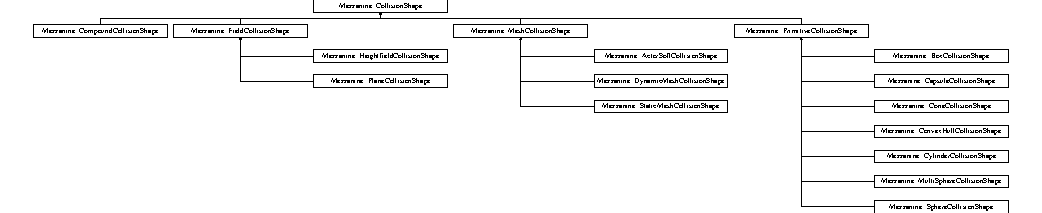
\includegraphics[height=2.868526cm]{classMezzanine_1_1CollisionShape}
\end{center}
\end{figure}
\subsubsection*{Public Types}
\begin{DoxyCompactItemize}
\item 
enum \hyperlink{classMezzanine_1_1CollisionShape_ad04186055565998879b64176d6dd100d}{ShapeType} \{ \par
\hyperlink{classMezzanine_1_1CollisionShape_ad04186055565998879b64176d6dd100dae9be64274af07a7f8f29bebada214d5e}{ST\_\-Box} = 0, 
\hyperlink{classMezzanine_1_1CollisionShape_ad04186055565998879b64176d6dd100da940b4f486bbd0a25de10bc336e30870c}{ST\_\-Capsule} = 1, 
\hyperlink{classMezzanine_1_1CollisionShape_ad04186055565998879b64176d6dd100da055fc638f933b50c7bfe869f7ee47470}{ST\_\-Compound} = 2, 
\hyperlink{classMezzanine_1_1CollisionShape_ad04186055565998879b64176d6dd100daa25857b0cefdd16e85dd195c7ad8d489}{ST\_\-Cone} = 3, 
\par
\hyperlink{classMezzanine_1_1CollisionShape_ad04186055565998879b64176d6dd100da077fcba1a677c63f12da94dd02931268}{ST\_\-ConvexHull} = 4, 
\hyperlink{classMezzanine_1_1CollisionShape_ad04186055565998879b64176d6dd100da12f7d22b55a3d58ce395bc0fbb536312}{ST\_\-Cylinder} = 5, 
\hyperlink{classMezzanine_1_1CollisionShape_ad04186055565998879b64176d6dd100dac81816d19328b9b19e7c318728d095f6}{ST\_\-MultiSphere} = 6, 
\hyperlink{classMezzanine_1_1CollisionShape_ad04186055565998879b64176d6dd100da950c329f000560c92b241ffb8d6a5203}{ST\_\-Sphere} = 7, 
\par
\hyperlink{classMezzanine_1_1CollisionShape_ad04186055565998879b64176d6dd100da5079488918ad2a3f2adaaa0dfda7bb2d}{ST\_\-DynamicTriMesh} = 8, 
\hyperlink{classMezzanine_1_1CollisionShape_ad04186055565998879b64176d6dd100dae861a5ebc159b7b364ac58474baa3351}{ST\_\-Heightfield} = 9, 
\hyperlink{classMezzanine_1_1CollisionShape_ad04186055565998879b64176d6dd100da8571f53f8a8bcc6126dce27c200655e0}{ST\_\-Plane} = 10, 
\hyperlink{classMezzanine_1_1CollisionShape_ad04186055565998879b64176d6dd100dad26769aea76ec2c46f4fdc90829eeb66}{ST\_\-ActorSoft} = 11, 
\par
\hyperlink{classMezzanine_1_1CollisionShape_ad04186055565998879b64176d6dd100daa1214cb8a95bd027094648ce0617c53e}{ST\_\-StaticTriMesh} = 12
 \}
\begin{DoxyCompactList}\small\item\em This enum describes what kind of shape you are currently working with. \item\end{DoxyCompactList}\end{DoxyCompactItemize}
\subsubsection*{Public Member Functions}
\begin{DoxyCompactItemize}
\item 
\hypertarget{classMezzanine_1_1CollisionShape_a0af2c4dbb24ad4fda4698b81799b65e2}{
\hyperlink{classMezzanine_1_1CollisionShape_a0af2c4dbb24ad4fda4698b81799b65e2}{CollisionShape} ()}
\label{classMezzanine_1_1CollisionShape_a0af2c4dbb24ad4fda4698b81799b65e2}

\begin{DoxyCompactList}\small\item\em Class Constructor. \item\end{DoxyCompactList}\item 
virtual btCollisionShape $\ast$ \hyperlink{classMezzanine_1_1CollisionShape_a0a5d6eb69c26665051ebb2b9d8004802}{GetBulletShape} () const 
\begin{DoxyCompactList}\small\item\em Gets the internal shape pointer this collision shape is based on. \item\end{DoxyCompactList}\item 
virtual \hyperlink{namespaceMezzanine_a726731b1a7df72bf3583e4a97282c6f6}{Real} \hyperlink{classMezzanine_1_1CollisionShape_a7f9d28c4c5ce7ab5a78af217d314fcaa}{GetMargin} () const 
\begin{DoxyCompactList}\small\item\em Gets the amount of padding currently being applied to the collision shape. \item\end{DoxyCompactList}\item 
virtual const \hyperlink{namespaceMezzanine_acf9fcc130e6ebf08e3d8491aebcf1c86}{String} \& \hyperlink{classMezzanine_1_1CollisionShape_af3f50f7ee9cb2d25c88daf0c92facb31}{GetName} () const 
\begin{DoxyCompactList}\small\item\em Gets the name of this shape. \item\end{DoxyCompactList}\item 
virtual \hyperlink{classMezzanine_1_1Vector3}{Vector3} \hyperlink{classMezzanine_1_1CollisionShape_ac05c6969066a1ab14c45aa566da701b6}{GetScaling} () const 
\begin{DoxyCompactList}\small\item\em Gets the current scaling being applied to the collision shape. \item\end{DoxyCompactList}\item 
virtual \hyperlink{classMezzanine_1_1CollisionShape_ad04186055565998879b64176d6dd100d}{CollisionShape::ShapeType} \hyperlink{classMezzanine_1_1CollisionShape_a27e5055f81cb8fb6d65a6c9f8dc73b69}{GetType} () const =0
\begin{DoxyCompactList}\small\item\em Gets the type of \hyperlink{classMezzanine_1_1Collision}{Collision} shape this is. \item\end{DoxyCompactList}\item 
virtual void \hyperlink{classMezzanine_1_1CollisionShape_a3884d005f857180185a44c99e55024e3}{SetMargin} (const \hyperlink{namespaceMezzanine_a726731b1a7df72bf3583e4a97282c6f6}{Real} \&Margin)
\begin{DoxyCompactList}\small\item\em Sets the padding that will be applied when checking for collisions. \item\end{DoxyCompactList}\item 
virtual void \hyperlink{classMezzanine_1_1CollisionShape_a1017c09132113afe0f33fe9b2e7b9def}{SetScaling} (const \hyperlink{classMezzanine_1_1Vector3}{Vector3} \&Scaling)
\begin{DoxyCompactList}\small\item\em Scales the collision shape on each of it's axes. \item\end{DoxyCompactList}\item 
\hypertarget{classMezzanine_1_1CollisionShape_a55253f27f2f64baf9a21fb440cfeaea6}{
virtual \hyperlink{classMezzanine_1_1CollisionShape_a55253f27f2f64baf9a21fb440cfeaea6}{$\sim$CollisionShape} ()}
\label{classMezzanine_1_1CollisionShape_a55253f27f2f64baf9a21fb440cfeaea6}

\begin{DoxyCompactList}\small\item\em Class Destructor. \item\end{DoxyCompactList}\end{DoxyCompactItemize}
\subsubsection*{Protected Attributes}
\begin{DoxyCompactItemize}
\item 
\hypertarget{classMezzanine_1_1CollisionShape_aac524c5c56fa4d158bc071f8aecfbe79}{
\hyperlink{namespaceMezzanine_acf9fcc130e6ebf08e3d8491aebcf1c86}{String} \hyperlink{classMezzanine_1_1CollisionShape_aac524c5c56fa4d158bc071f8aecfbe79}{Name}}
\label{classMezzanine_1_1CollisionShape_aac524c5c56fa4d158bc071f8aecfbe79}

\begin{DoxyCompactList}\small\item\em Storage for the name of this class instance. \item\end{DoxyCompactList}\item 
\hypertarget{classMezzanine_1_1CollisionShape_a105322f4ad5139768ca1abba44561dec}{
btCollisionShape $\ast$ \hyperlink{classMezzanine_1_1CollisionShape_a105322f4ad5139768ca1abba44561dec}{ShapeBase}}
\label{classMezzanine_1_1CollisionShape_a105322f4ad5139768ca1abba44561dec}

\begin{DoxyCompactList}\small\item\em A pointer to the bullet collision this uses. \item\end{DoxyCompactList}\end{DoxyCompactItemize}
\subsubsection*{Friends}
\begin{DoxyCompactItemize}
\item 
\hypertarget{classMezzanine_1_1CollisionShape_a3989497c48c3690f2d73227804a47a77}{
class {\bfseries CollisionShapeManager}}
\label{classMezzanine_1_1CollisionShape_a3989497c48c3690f2d73227804a47a77}

\end{DoxyCompactItemize}


\subsubsection{Detailed Description}
This is the base class for all collision shapes. Currently there are a total of 13 collision shape classes inheriting from 3 other base classes. \hyperlink{classMezzanine_1_1Collision}{Collision} shapes are shape representations for Actors, AreaEffects, and other classes with bodies in the physics engine. \par
 \par
 It's important to note that \hyperlink{classMezzanine_1_1Collision}{Collision} shapes can be created and then re-\/used in as many \hyperlink{classMezzanine_1_1World}{World} objects(at the same time) as you need, and it is encouraged to do this. 

Definition at line 82 of file collisionshape.h.



\subsubsection{Member Enumeration Documentation}
\hypertarget{classMezzanine_1_1CollisionShape_ad04186055565998879b64176d6dd100d}{
\index{Mezzanine::CollisionShape@{Mezzanine::CollisionShape}!ShapeType@{ShapeType}}
\index{ShapeType@{ShapeType}!Mezzanine::CollisionShape@{Mezzanine::CollisionShape}}
\paragraph[{ShapeType}]{\setlength{\rightskip}{0pt plus 5cm}enum {\bf Mezzanine::CollisionShape::ShapeType}}\hfill}
\label{classMezzanine_1_1CollisionShape_ad04186055565998879b64176d6dd100d}


This enum describes what kind of shape you are currently working with. 

\begin{DoxyNote}{Note}
These are number primarily for Serialization purposes. These corresponding numbers could vary wildly. Any use of corresponding raw number in serialization will be done with object serialization version in mind. 
\end{DoxyNote}
\begin{Desc}
\item[Enumerator: ]\par
\begin{description}
\index{ST\_\-Box@{ST\_\-Box}!Mezzanine::CollisionShape@{Mezzanine::CollisionShape}}\index{Mezzanine::CollisionShape@{Mezzanine::CollisionShape}!ST\_\-Box@{ST\_\-Box}}\item[{\em 
\hypertarget{classMezzanine_1_1CollisionShape_ad04186055565998879b64176d6dd100dae9be64274af07a7f8f29bebada214d5e}{
ST\_\-Box}
\label{classMezzanine_1_1CollisionShape_ad04186055565998879b64176d6dd100dae9be64274af07a7f8f29bebada214d5e}
}]Indicates the class is a \hyperlink{classMezzanine_1_1BoxCollisionShape}{BoxCollisionShape}. \index{ST\_\-Capsule@{ST\_\-Capsule}!Mezzanine::CollisionShape@{Mezzanine::CollisionShape}}\index{Mezzanine::CollisionShape@{Mezzanine::CollisionShape}!ST\_\-Capsule@{ST\_\-Capsule}}\item[{\em 
\hypertarget{classMezzanine_1_1CollisionShape_ad04186055565998879b64176d6dd100da940b4f486bbd0a25de10bc336e30870c}{
ST\_\-Capsule}
\label{classMezzanine_1_1CollisionShape_ad04186055565998879b64176d6dd100da940b4f486bbd0a25de10bc336e30870c}
}]Indicates the class is a \hyperlink{classMezzanine_1_1CapsuleCollisionShape}{CapsuleCollisionShape}. \index{ST\_\-Compound@{ST\_\-Compound}!Mezzanine::CollisionShape@{Mezzanine::CollisionShape}}\index{Mezzanine::CollisionShape@{Mezzanine::CollisionShape}!ST\_\-Compound@{ST\_\-Compound}}\item[{\em 
\hypertarget{classMezzanine_1_1CollisionShape_ad04186055565998879b64176d6dd100da055fc638f933b50c7bfe869f7ee47470}{
ST\_\-Compound}
\label{classMezzanine_1_1CollisionShape_ad04186055565998879b64176d6dd100da055fc638f933b50c7bfe869f7ee47470}
}]Indicates the class is a \hyperlink{classMezzanine_1_1CompoundCollisionShape}{CompoundCollisionShape}. \index{ST\_\-Cone@{ST\_\-Cone}!Mezzanine::CollisionShape@{Mezzanine::CollisionShape}}\index{Mezzanine::CollisionShape@{Mezzanine::CollisionShape}!ST\_\-Cone@{ST\_\-Cone}}\item[{\em 
\hypertarget{classMezzanine_1_1CollisionShape_ad04186055565998879b64176d6dd100daa25857b0cefdd16e85dd195c7ad8d489}{
ST\_\-Cone}
\label{classMezzanine_1_1CollisionShape_ad04186055565998879b64176d6dd100daa25857b0cefdd16e85dd195c7ad8d489}
}]Indicates the class is a \hyperlink{classMezzanine_1_1ConeCollisionShape}{ConeCollisionShape}. \index{ST\_\-ConvexHull@{ST\_\-ConvexHull}!Mezzanine::CollisionShape@{Mezzanine::CollisionShape}}\index{Mezzanine::CollisionShape@{Mezzanine::CollisionShape}!ST\_\-ConvexHull@{ST\_\-ConvexHull}}\item[{\em 
\hypertarget{classMezzanine_1_1CollisionShape_ad04186055565998879b64176d6dd100da077fcba1a677c63f12da94dd02931268}{
ST\_\-ConvexHull}
\label{classMezzanine_1_1CollisionShape_ad04186055565998879b64176d6dd100da077fcba1a677c63f12da94dd02931268}
}]Indicates the class is a \hyperlink{classMezzanine_1_1ConvexHullCollisionShape}{ConvexHullCollisionShape}. \index{ST\_\-Cylinder@{ST\_\-Cylinder}!Mezzanine::CollisionShape@{Mezzanine::CollisionShape}}\index{Mezzanine::CollisionShape@{Mezzanine::CollisionShape}!ST\_\-Cylinder@{ST\_\-Cylinder}}\item[{\em 
\hypertarget{classMezzanine_1_1CollisionShape_ad04186055565998879b64176d6dd100da12f7d22b55a3d58ce395bc0fbb536312}{
ST\_\-Cylinder}
\label{classMezzanine_1_1CollisionShape_ad04186055565998879b64176d6dd100da12f7d22b55a3d58ce395bc0fbb536312}
}]Indicates the class is a \hyperlink{classMezzanine_1_1CylinderCollisionShape}{CylinderCollisionShape}. \index{ST\_\-MultiSphere@{ST\_\-MultiSphere}!Mezzanine::CollisionShape@{Mezzanine::CollisionShape}}\index{Mezzanine::CollisionShape@{Mezzanine::CollisionShape}!ST\_\-MultiSphere@{ST\_\-MultiSphere}}\item[{\em 
\hypertarget{classMezzanine_1_1CollisionShape_ad04186055565998879b64176d6dd100dac81816d19328b9b19e7c318728d095f6}{
ST\_\-MultiSphere}
\label{classMezzanine_1_1CollisionShape_ad04186055565998879b64176d6dd100dac81816d19328b9b19e7c318728d095f6}
}]Indicates the class is a \hyperlink{classMezzanine_1_1MultiSphereCollisionShape}{MultiSphereCollisionShape}. \index{ST\_\-Sphere@{ST\_\-Sphere}!Mezzanine::CollisionShape@{Mezzanine::CollisionShape}}\index{Mezzanine::CollisionShape@{Mezzanine::CollisionShape}!ST\_\-Sphere@{ST\_\-Sphere}}\item[{\em 
\hypertarget{classMezzanine_1_1CollisionShape_ad04186055565998879b64176d6dd100da950c329f000560c92b241ffb8d6a5203}{
ST\_\-Sphere}
\label{classMezzanine_1_1CollisionShape_ad04186055565998879b64176d6dd100da950c329f000560c92b241ffb8d6a5203}
}]Indicates the class is a \hyperlink{classMezzanine_1_1SphereCollisionShape}{SphereCollisionShape}. \index{ST\_\-DynamicTriMesh@{ST\_\-DynamicTriMesh}!Mezzanine::CollisionShape@{Mezzanine::CollisionShape}}\index{Mezzanine::CollisionShape@{Mezzanine::CollisionShape}!ST\_\-DynamicTriMesh@{ST\_\-DynamicTriMesh}}\item[{\em 
\hypertarget{classMezzanine_1_1CollisionShape_ad04186055565998879b64176d6dd100da5079488918ad2a3f2adaaa0dfda7bb2d}{
ST\_\-DynamicTriMesh}
\label{classMezzanine_1_1CollisionShape_ad04186055565998879b64176d6dd100da5079488918ad2a3f2adaaa0dfda7bb2d}
}]Indicates the class is a \hyperlink{classMezzanine_1_1DynamicMeshCollisionShape}{DynamicMeshCollisionShape}. \index{ST\_\-Heightfield@{ST\_\-Heightfield}!Mezzanine::CollisionShape@{Mezzanine::CollisionShape}}\index{Mezzanine::CollisionShape@{Mezzanine::CollisionShape}!ST\_\-Heightfield@{ST\_\-Heightfield}}\item[{\em 
\hypertarget{classMezzanine_1_1CollisionShape_ad04186055565998879b64176d6dd100dae861a5ebc159b7b364ac58474baa3351}{
ST\_\-Heightfield}
\label{classMezzanine_1_1CollisionShape_ad04186055565998879b64176d6dd100dae861a5ebc159b7b364ac58474baa3351}
}]Indicates the class is a \hyperlink{classMezzanine_1_1HeightfieldCollisionShape}{HeightfieldCollisionShape}. \index{ST\_\-Plane@{ST\_\-Plane}!Mezzanine::CollisionShape@{Mezzanine::CollisionShape}}\index{Mezzanine::CollisionShape@{Mezzanine::CollisionShape}!ST\_\-Plane@{ST\_\-Plane}}\item[{\em 
\hypertarget{classMezzanine_1_1CollisionShape_ad04186055565998879b64176d6dd100da8571f53f8a8bcc6126dce27c200655e0}{
ST\_\-Plane}
\label{classMezzanine_1_1CollisionShape_ad04186055565998879b64176d6dd100da8571f53f8a8bcc6126dce27c200655e0}
}]Indicates the class is a \hyperlink{classMezzanine_1_1PlaneCollisionShape}{PlaneCollisionShape}. \index{ST\_\-ActorSoft@{ST\_\-ActorSoft}!Mezzanine::CollisionShape@{Mezzanine::CollisionShape}}\index{Mezzanine::CollisionShape@{Mezzanine::CollisionShape}!ST\_\-ActorSoft@{ST\_\-ActorSoft}}\item[{\em 
\hypertarget{classMezzanine_1_1CollisionShape_ad04186055565998879b64176d6dd100dad26769aea76ec2c46f4fdc90829eeb66}{
ST\_\-ActorSoft}
\label{classMezzanine_1_1CollisionShape_ad04186055565998879b64176d6dd100dad26769aea76ec2c46f4fdc90829eeb66}
}]Indicates the class is a \hyperlink{classMezzanine_1_1ActorSoftCollisionShape}{ActorSoftCollisionShape}. \index{ST\_\-StaticTriMesh@{ST\_\-StaticTriMesh}!Mezzanine::CollisionShape@{Mezzanine::CollisionShape}}\index{Mezzanine::CollisionShape@{Mezzanine::CollisionShape}!ST\_\-StaticTriMesh@{ST\_\-StaticTriMesh}}\item[{\em 
\hypertarget{classMezzanine_1_1CollisionShape_ad04186055565998879b64176d6dd100daa1214cb8a95bd027094648ce0617c53e}{
ST\_\-StaticTriMesh}
\label{classMezzanine_1_1CollisionShape_ad04186055565998879b64176d6dd100daa1214cb8a95bd027094648ce0617c53e}
}]Indicates the class is a \hyperlink{classMezzanine_1_1StaticMeshCollisionShape}{StaticMeshCollisionShape}. \end{description}
\end{Desc}



Definition at line 88 of file collisionshape.h.



\subsubsection{Member Function Documentation}
\hypertarget{classMezzanine_1_1CollisionShape_a0a5d6eb69c26665051ebb2b9d8004802}{
\index{Mezzanine::CollisionShape@{Mezzanine::CollisionShape}!GetBulletShape@{GetBulletShape}}
\index{GetBulletShape@{GetBulletShape}!Mezzanine::CollisionShape@{Mezzanine::CollisionShape}}
\paragraph[{GetBulletShape}]{\setlength{\rightskip}{0pt plus 5cm}btCollisionShape $\ast$ Mezzanine::CollisionShape::GetBulletShape (
\begin{DoxyParamCaption}
{}
\end{DoxyParamCaption}
) const\hspace{0.3cm}{\ttfamily  \mbox{[}virtual\mbox{]}}}\hfill}
\label{classMezzanine_1_1CollisionShape_a0a5d6eb69c26665051ebb2b9d8004802}


Gets the internal shape pointer this collision shape is based on. 

\begin{DoxyReturn}{Returns}
Returns a pointer to the internal collision shape. 
\end{DoxyReturn}


Definition at line 93 of file collisionshape.cpp.

\hypertarget{classMezzanine_1_1CollisionShape_a7f9d28c4c5ce7ab5a78af217d314fcaa}{
\index{Mezzanine::CollisionShape@{Mezzanine::CollisionShape}!GetMargin@{GetMargin}}
\index{GetMargin@{GetMargin}!Mezzanine::CollisionShape@{Mezzanine::CollisionShape}}
\paragraph[{GetMargin}]{\setlength{\rightskip}{0pt plus 5cm}{\bf Real} Mezzanine::CollisionShape::GetMargin (
\begin{DoxyParamCaption}
{}
\end{DoxyParamCaption}
) const\hspace{0.3cm}{\ttfamily  \mbox{[}virtual\mbox{]}}}\hfill}
\label{classMezzanine_1_1CollisionShape_a7f9d28c4c5ce7ab5a78af217d314fcaa}


Gets the amount of padding currently being applied to the collision shape. 

\begin{DoxyReturn}{Returns}
Returns the amount of padding, in world units, is being applied to the collision shape. 
\end{DoxyReturn}


Definition at line 78 of file collisionshape.cpp.

\hypertarget{classMezzanine_1_1CollisionShape_af3f50f7ee9cb2d25c88daf0c92facb31}{
\index{Mezzanine::CollisionShape@{Mezzanine::CollisionShape}!GetName@{GetName}}
\index{GetName@{GetName}!Mezzanine::CollisionShape@{Mezzanine::CollisionShape}}
\paragraph[{GetName}]{\setlength{\rightskip}{0pt plus 5cm}const {\bf String} \& Mezzanine::CollisionShape::GetName (
\begin{DoxyParamCaption}
{}
\end{DoxyParamCaption}
) const\hspace{0.3cm}{\ttfamily  \mbox{[}virtual\mbox{]}}}\hfill}
\label{classMezzanine_1_1CollisionShape_af3f50f7ee9cb2d25c88daf0c92facb31}


Gets the name of this shape. 

\begin{DoxyReturn}{Returns}
Returns a const reference string containing the name of this collision shape. 
\end{DoxyReturn}


Definition at line 68 of file collisionshape.cpp.

\hypertarget{classMezzanine_1_1CollisionShape_ac05c6969066a1ab14c45aa566da701b6}{
\index{Mezzanine::CollisionShape@{Mezzanine::CollisionShape}!GetScaling@{GetScaling}}
\index{GetScaling@{GetScaling}!Mezzanine::CollisionShape@{Mezzanine::CollisionShape}}
\paragraph[{GetScaling}]{\setlength{\rightskip}{0pt plus 5cm}{\bf Vector3} Mezzanine::CollisionShape::GetScaling (
\begin{DoxyParamCaption}
{}
\end{DoxyParamCaption}
) const\hspace{0.3cm}{\ttfamily  \mbox{[}virtual\mbox{]}}}\hfill}
\label{classMezzanine_1_1CollisionShape_ac05c6969066a1ab14c45aa566da701b6}


Gets the current scaling being applied to the collision shape. 

\begin{DoxyReturn}{Returns}
Returns a vector3 representing the amount of scaling being applied to the shape. 
\end{DoxyReturn}


Definition at line 88 of file collisionshape.cpp.

\hypertarget{classMezzanine_1_1CollisionShape_a27e5055f81cb8fb6d65a6c9f8dc73b69}{
\index{Mezzanine::CollisionShape@{Mezzanine::CollisionShape}!GetType@{GetType}}
\index{GetType@{GetType}!Mezzanine::CollisionShape@{Mezzanine::CollisionShape}}
\paragraph[{GetType}]{\setlength{\rightskip}{0pt plus 5cm}virtual {\bf CollisionShape::ShapeType} Mezzanine::CollisionShape::GetType (
\begin{DoxyParamCaption}
{}
\end{DoxyParamCaption}
) const\hspace{0.3cm}{\ttfamily  \mbox{[}pure virtual\mbox{]}}}\hfill}
\label{classMezzanine_1_1CollisionShape_a27e5055f81cb8fb6d65a6c9f8dc73b69}


Gets the type of \hyperlink{classMezzanine_1_1Collision}{Collision} shape this is. 

\begin{DoxyReturn}{Returns}
Returns an enum value indicating the type of collision shape this is. 
\end{DoxyReturn}


Implemented in \hyperlink{classMezzanine_1_1PrimitiveCollisionShape_ad3d4143a5640204b987e0b57eb24af41}{Mezzanine::PrimitiveCollisionShape}, \hyperlink{classMezzanine_1_1FieldCollisionShape_a85a444fa9bcaca9fec08c3b5697677c9}{Mezzanine::FieldCollisionShape}, \hyperlink{classMezzanine_1_1MeshCollisionShape_a00dc444afac92030ea43815ec21dd8e8}{Mezzanine::MeshCollisionShape}, \hyperlink{classMezzanine_1_1CompoundCollisionShape_a8b701bbbc32b007f32884946d285fba1}{Mezzanine::CompoundCollisionShape}, \hyperlink{classMezzanine_1_1BoxCollisionShape_ae2b4af7afa6cc37c51b062589048e26d}{Mezzanine::BoxCollisionShape}, \hyperlink{classMezzanine_1_1CapsuleCollisionShape_a2773853a924c2a97838546d96d851ba5}{Mezzanine::CapsuleCollisionShape}, \hyperlink{classMezzanine_1_1ConeCollisionShape_a874892f3aaba7e79200633691037a410}{Mezzanine::ConeCollisionShape}, \hyperlink{classMezzanine_1_1ConvexHullCollisionShape_a73ccd6364f52a68a642a0fb55159f020}{Mezzanine::ConvexHullCollisionShape}, \hyperlink{classMezzanine_1_1CylinderCollisionShape_a4feb07a9d71bda6ca4b6c82b745df8a0}{Mezzanine::CylinderCollisionShape}, \hyperlink{classMezzanine_1_1MultiSphereCollisionShape_ad4b8a2e2f71686e2495d414a13b0f95a}{Mezzanine::MultiSphereCollisionShape}, \hyperlink{classMezzanine_1_1SphereCollisionShape_ad2c8d33b21fe7215742db4551429c5a6}{Mezzanine::SphereCollisionShape}, \hyperlink{classMezzanine_1_1DynamicMeshCollisionShape_ae323a4ac9ae12890e1f8ce82b22f1ccc}{Mezzanine::DynamicMeshCollisionShape}, \hyperlink{classMezzanine_1_1HeightfieldCollisionShape_af27ffaf88fc12af6ddc89704e60ecd33}{Mezzanine::HeightfieldCollisionShape}, \hyperlink{classMezzanine_1_1PlaneCollisionShape_aeb4b5e1a235023d375b5514065a5e382}{Mezzanine::PlaneCollisionShape}, \hyperlink{classMezzanine_1_1ActorSoftCollisionShape_ae9ac8413434ff0de10376deb64ab49d0}{Mezzanine::ActorSoftCollisionShape}, and \hyperlink{classMezzanine_1_1StaticMeshCollisionShape_ae6cf497bf3a0c1db7b0f39a0513ebb79}{Mezzanine::StaticMeshCollisionShape}.

\hypertarget{classMezzanine_1_1CollisionShape_a3884d005f857180185a44c99e55024e3}{
\index{Mezzanine::CollisionShape@{Mezzanine::CollisionShape}!SetMargin@{SetMargin}}
\index{SetMargin@{SetMargin}!Mezzanine::CollisionShape@{Mezzanine::CollisionShape}}
\paragraph[{SetMargin}]{\setlength{\rightskip}{0pt plus 5cm}void Mezzanine::CollisionShape::SetMargin (
\begin{DoxyParamCaption}
\item[{const {\bf Real} \&}]{Margin}
\end{DoxyParamCaption}
)\hspace{0.3cm}{\ttfamily  \mbox{[}virtual\mbox{]}}}\hfill}
\label{classMezzanine_1_1CollisionShape_a3884d005f857180185a44c99e55024e3}


Sets the padding that will be applied when checking for collisions. 


\begin{DoxyParams}{Parameters}
{\em Margin} & A real in world units representing how much padding is to be applied to this shape. \\
\hline
\end{DoxyParams}


Definition at line 73 of file collisionshape.cpp.

\hypertarget{classMezzanine_1_1CollisionShape_a1017c09132113afe0f33fe9b2e7b9def}{
\index{Mezzanine::CollisionShape@{Mezzanine::CollisionShape}!SetScaling@{SetScaling}}
\index{SetScaling@{SetScaling}!Mezzanine::CollisionShape@{Mezzanine::CollisionShape}}
\paragraph[{SetScaling}]{\setlength{\rightskip}{0pt plus 5cm}void Mezzanine::CollisionShape::SetScaling (
\begin{DoxyParamCaption}
\item[{const {\bf Vector3} \&}]{Scaling}
\end{DoxyParamCaption}
)\hspace{0.3cm}{\ttfamily  \mbox{[}virtual\mbox{]}}}\hfill}
\label{classMezzanine_1_1CollisionShape_a1017c09132113afe0f33fe9b2e7b9def}


Scales the collision shape on each of it's axes. 


\begin{DoxyParams}{Parameters}
{\em Scaling} & A vector3 representing how much scaling should be applied on each of the shapes 3 axes. \\
\hline
\end{DoxyParams}


Definition at line 83 of file collisionshape.cpp.



The documentation for this class was generated from the following files:\begin{DoxyCompactItemize}
\item 
collisionshape.h\item 
collisionshape.cpp\end{DoxyCompactItemize}

\hypertarget{classMezzanine_1_1CollisionShapeDeSerializer}{
\subsection{Mezzanine::CollisionShapeDeSerializer Class Reference}
\label{classMezzanine_1_1CollisionShapeDeSerializer}\index{Mezzanine::CollisionShapeDeSerializer@{Mezzanine::CollisionShapeDeSerializer}}
}


\subsubsection{Detailed Description}


Definition at line 1002 of file collisionshape.h.



The documentation for this class was generated from the following file:\begin{DoxyCompactItemize}
\item 
collisionshape.h\end{DoxyCompactItemize}

\hypertarget{classMezzanine_1_1CollisionShapeManager}{
\subsection{Mezzanine::CollisionShapeManager Class Reference}
\label{classMezzanine_1_1CollisionShapeManager}\index{Mezzanine::CollisionShapeManager@{Mezzanine::CollisionShapeManager}}
}


This manager is for the storage of all shapes and creation of mesh shapes.  




{\ttfamily \#include $<$collisionshapemanager.h$>$}

Inheritance diagram for Mezzanine::CollisionShapeManager:\begin{figure}[H]
\begin{center}
\leavevmode
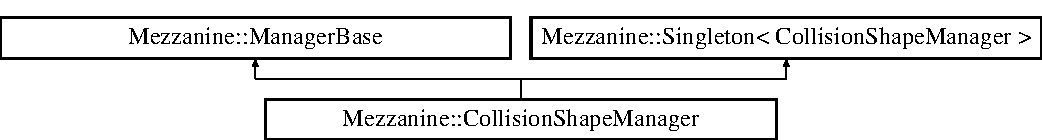
\includegraphics[height=1.879195cm]{classMezzanine_1_1CollisionShapeManager}
\end{center}
\end{figure}
\subsubsection*{Public Types}
\begin{DoxyCompactItemize}
\item 
\hypertarget{classMezzanine_1_1CollisionShapeManager_a44318f2b04d35ecc76d5c58ea574f0f0}{
typedef std::map$<$ \hyperlink{namespaceMezzanine_acf9fcc130e6ebf08e3d8491aebcf1c86}{String}, \hyperlink{classMezzanine_1_1CollisionShape}{CollisionShape} $\ast$ $>$::\hyperlink{classMezzanine_1_1CollisionShapeManager_a44318f2b04d35ecc76d5c58ea574f0f0}{const\_\-iterator} \hyperlink{classMezzanine_1_1CollisionShapeManager_a44318f2b04d35ecc76d5c58ea574f0f0}{const\_\-iterator}}
\label{classMezzanine_1_1CollisionShapeManager_a44318f2b04d35ecc76d5c58ea574f0f0}

\begin{DoxyCompactList}\small\item\em An const\_\-iterator that should be compatible with most iterator algorithms. \item\end{DoxyCompactList}\item 
\hypertarget{classMezzanine_1_1CollisionShapeManager_abec03ca004aae3ce0dc478e34e5d1252}{
typedef std::map$<$ \hyperlink{namespaceMezzanine_acf9fcc130e6ebf08e3d8491aebcf1c86}{String}, \hyperlink{classMezzanine_1_1CollisionShape}{CollisionShape} $\ast$ $>$::\hyperlink{classMezzanine_1_1CollisionShapeManager_abec03ca004aae3ce0dc478e34e5d1252}{iterator} \hyperlink{classMezzanine_1_1CollisionShapeManager_abec03ca004aae3ce0dc478e34e5d1252}{iterator}}
\label{classMezzanine_1_1CollisionShapeManager_abec03ca004aae3ce0dc478e34e5d1252}

\begin{DoxyCompactList}\small\item\em An iterator that should be compatible with most iterator algorithms. \item\end{DoxyCompactList}\end{DoxyCompactItemize}
\subsubsection*{Public Member Functions}
\begin{DoxyCompactItemize}
\item 
\hyperlink{classMezzanine_1_1CollisionShapeManager_abec03ca004aae3ce0dc478e34e5d1252}{iterator} \hyperlink{classMezzanine_1_1CollisionShapeManager_a8b73066314e6fe91cce3507f5d85584f}{begin} ()
\begin{DoxyCompactList}\small\item\em Get an Iterator pointing to the first item in the container. \item\end{DoxyCompactList}\item 
\hyperlink{classMezzanine_1_1CollisionShapeManager_a44318f2b04d35ecc76d5c58ea574f0f0}{const\_\-iterator} \hyperlink{classMezzanine_1_1CollisionShapeManager_ad588bcca5ef47d467439171edf5640a0}{begin} () const 
\begin{DoxyCompactList}\small\item\em Get a const Iterator pointing at the first item in the container. \item\end{DoxyCompactList}\item 
\hypertarget{classMezzanine_1_1CollisionShapeManager_a47c3e4e886e22abb3c8017e8f244cac2}{
\hyperlink{classMezzanine_1_1CollisionShapeManager_a47c3e4e886e22abb3c8017e8f244cac2}{CollisionShapeManager} ()}
\label{classMezzanine_1_1CollisionShapeManager_a47c3e4e886e22abb3c8017e8f244cac2}

\begin{DoxyCompactList}\small\item\em Class constructor. \item\end{DoxyCompactList}\item 
\hypertarget{classMezzanine_1_1CollisionShapeManager_aa7d9c7a9fe78def866e1abc02b261b53}{
virtual void \hyperlink{classMezzanine_1_1CollisionShapeManager_aa7d9c7a9fe78def866e1abc02b261b53}{DestroyAllShapes} ()}
\label{classMezzanine_1_1CollisionShapeManager_aa7d9c7a9fe78def866e1abc02b261b53}

\begin{DoxyCompactList}\small\item\em Removes all shapes from the manager and then deletes them. \item\end{DoxyCompactList}\item 
virtual void \hyperlink{classMezzanine_1_1CollisionShapeManager_a5711e761a06781792d021537b1089770}{DestroyShape} (\hyperlink{classMezzanine_1_1CollisionShape}{CollisionShape} $\ast$Shape)
\begin{DoxyCompactList}\small\item\em Removes a shape from this manager and deletes it. \item\end{DoxyCompactList}\item 
virtual void \hyperlink{classMezzanine_1_1CollisionShapeManager_a1abaa37c1ce061421cb22999b7b67e84}{DestroyShape} (const \hyperlink{namespaceMezzanine_acf9fcc130e6ebf08e3d8491aebcf1c86}{String} \&Name)
\begin{DoxyCompactList}\small\item\em Removes a shape from this manager and deletes it. \item\end{DoxyCompactList}\item 
virtual void \hyperlink{classMezzanine_1_1CollisionShapeManager_ac055cf940fd8fce522625de6b977dd2a}{DoMainLoopItems} ()
\item 
\hyperlink{classMezzanine_1_1CollisionShapeManager_abec03ca004aae3ce0dc478e34e5d1252}{iterator} \hyperlink{classMezzanine_1_1CollisionShapeManager_adff97f4013578c91612a14df59402d98}{end} ()
\begin{DoxyCompactList}\small\item\em Get an Iterator pointing to one past the last item in the container. \item\end{DoxyCompactList}\item 
\hyperlink{classMezzanine_1_1CollisionShapeManager_a44318f2b04d35ecc76d5c58ea574f0f0}{const\_\-iterator} \hyperlink{classMezzanine_1_1CollisionShapeManager_a1ddb9f421eb024dd3dc67cf8914eef18}{end} () const 
\begin{DoxyCompactList}\small\item\em Get an const Iterator pointing to one past the last item in the container. \item\end{DoxyCompactList}\item 
virtual \hyperlink{classMezzanine_1_1ConvexHullCollisionShape}{ConvexHullCollisionShape} $\ast$ \hyperlink{classMezzanine_1_1CollisionShapeManager_ad451a46f1e1f5c9054eaa5a3ce4dce0d}{GenerateConvexHull} (const \hyperlink{namespaceMezzanine_acf9fcc130e6ebf08e3d8491aebcf1c86}{String} \&Name, \hyperlink{classMezzanine_1_1Mesh}{Mesh} $\ast$ObjectMesh, bool UseAllSubmeshes=false)
\begin{DoxyCompactList}\small\item\em Generates a Convex Hull from a provided mesh. \item\end{DoxyCompactList}\item 
virtual \hyperlink{classMezzanine_1_1ConvexHullCollisionShape}{ConvexHullCollisionShape} $\ast$ \hyperlink{classMezzanine_1_1CollisionShapeManager_a67c2191c9e52a29744889cf531c1bb30}{GenerateConvexHull} (const \hyperlink{namespaceMezzanine_acf9fcc130e6ebf08e3d8491aebcf1c86}{String} \&Name, const \hyperlink{namespaceMezzanine_acf9fcc130e6ebf08e3d8491aebcf1c86}{String} \&MeshName, const \hyperlink{namespaceMezzanine_acf9fcc130e6ebf08e3d8491aebcf1c86}{String} \&Group, bool UseAllSubmeshes=false)
\begin{DoxyCompactList}\small\item\em Generates a Convex Hull from a provided mesh. \item\end{DoxyCompactList}\item 
virtual \hyperlink{classMezzanine_1_1DynamicMeshCollisionShape}{DynamicMeshCollisionShape} $\ast$ \hyperlink{classMezzanine_1_1CollisionShapeManager_a37f0afd29d955826e19e875eaf97cd44}{GenerateDynamicTriMesh} (const \hyperlink{namespaceMezzanine_acf9fcc130e6ebf08e3d8491aebcf1c86}{String} \&Name, \hyperlink{classMezzanine_1_1Mesh}{Mesh} $\ast$ObjectMesh, bool UseAllSubmeshes=false)
\begin{DoxyCompactList}\small\item\em Generates a mesh shape for dynamic objects. \item\end{DoxyCompactList}\item 
virtual \hyperlink{classMezzanine_1_1DynamicMeshCollisionShape}{DynamicMeshCollisionShape} $\ast$ \hyperlink{classMezzanine_1_1CollisionShapeManager_a6f29c280a1b4f779d3f4cbe6beca219c}{GenerateDynamicTriMesh} (const \hyperlink{namespaceMezzanine_acf9fcc130e6ebf08e3d8491aebcf1c86}{String} \&Name, const \hyperlink{namespaceMezzanine_acf9fcc130e6ebf08e3d8491aebcf1c86}{String} \&MeshName, const \hyperlink{namespaceMezzanine_acf9fcc130e6ebf08e3d8491aebcf1c86}{String} \&Group, bool UseAllSubmeshes=false)
\begin{DoxyCompactList}\small\item\em Generates a mesh shape for dynamic objects. \item\end{DoxyCompactList}\item 
virtual \hyperlink{classMezzanine_1_1StaticMeshCollisionShape}{StaticMeshCollisionShape} $\ast$ \hyperlink{classMezzanine_1_1CollisionShapeManager_a46c68d87fec10217b06342f68c15108d}{GenerateStaticTriMesh} (const \hyperlink{namespaceMezzanine_acf9fcc130e6ebf08e3d8491aebcf1c86}{String} \&Name, \hyperlink{classMezzanine_1_1Mesh}{Mesh} $\ast$ObjectMesh, bool UseAllSubmeshes=false)
\begin{DoxyCompactList}\small\item\em Generates a mesh shape for static objects. \item\end{DoxyCompactList}\item 
virtual \hyperlink{classMezzanine_1_1StaticMeshCollisionShape}{StaticMeshCollisionShape} $\ast$ \hyperlink{classMezzanine_1_1CollisionShapeManager_ab4cab76de405e9e10bc8c6a3fddfceea}{GenerateStaticTriMesh} (const \hyperlink{namespaceMezzanine_acf9fcc130e6ebf08e3d8491aebcf1c86}{String} \&Name, const \hyperlink{namespaceMezzanine_acf9fcc130e6ebf08e3d8491aebcf1c86}{String} \&MeshName, const \hyperlink{namespaceMezzanine_acf9fcc130e6ebf08e3d8491aebcf1c86}{String} \&Group, bool UseAllSubmeshes=false)
\begin{DoxyCompactList}\small\item\em Generates a mesh shape for static objects. \item\end{DoxyCompactList}\item 
virtual \hyperlink{namespaceMezzanine_adcbb6ce6d1eb4379d109e51171e2e493}{Whole} \hyperlink{classMezzanine_1_1CollisionShapeManager_a5245d89946a35da5f8cdada2e8c26edf}{GetNumStoredShapes} ()
\begin{DoxyCompactList}\small\item\em Gets the number of stored shapes in this manager. \item\end{DoxyCompactList}\item 
virtual \hyperlink{classMezzanine_1_1CollisionShape}{CollisionShape} $\ast$ \hyperlink{classMezzanine_1_1CollisionShapeManager_ad7d10124aa0702a95ed700c87b59b2b8}{GetShape} (const \hyperlink{namespaceMezzanine_acf9fcc130e6ebf08e3d8491aebcf1c86}{String} \&Name)
\begin{DoxyCompactList}\small\item\em Gets a shape already stored in this manager. \item\end{DoxyCompactList}\item 
virtual \hyperlink{classMezzanine_1_1ManagerBase_a08cecf5169cad3e82be81a3a159b0b6e}{ManagerBase::ManagerTypeName} \hyperlink{classMezzanine_1_1CollisionShapeManager_a4b98446e667a402e675eec79353e5278}{GetType} () const 
\item 
std::set$<$ \hyperlink{classMezzanine_1_1CollisionShape}{CollisionShape} $\ast$ $>$ \& \hyperlink{classMezzanine_1_1CollisionShapeManager_aebc9b1d42e5c4bc0d69afb3fca7ace1e}{GetUnnamedShapes} ()
\begin{DoxyCompactList}\small\item\em Returns a vector of unnamed shapes stored in this manager. \item\end{DoxyCompactList}\item 
virtual void \hyperlink{classMezzanine_1_1CollisionShapeManager_a15ddc7bb06cf1cf32cd4e641d3b7b34f}{Initialize} ()
\item 
virtual void \hyperlink{classMezzanine_1_1CollisionShapeManager_af76b90ccca8183a6ddfc33b7a4e65773}{LoadAllShapesFromFile} (const \hyperlink{namespaceMezzanine_acf9fcc130e6ebf08e3d8491aebcf1c86}{String} \&FileName, const \hyperlink{namespaceMezzanine_acf9fcc130e6ebf08e3d8491aebcf1c86}{String} \&Group)
\begin{DoxyCompactList}\small\item\em Loads all shapes saved in an existing .bullet file, and stores them in this manager. \item\end{DoxyCompactList}\item 
virtual \hyperlink{classMezzanine_1_1CompoundCollisionShape}{CompoundCollisionShape} $\ast$ \hyperlink{classMezzanine_1_1CollisionShapeManager_a639aa9c6c09f859dea4a200feb50528b}{PerformConvexDecomposition} (const \hyperlink{namespaceMezzanine_acf9fcc130e6ebf08e3d8491aebcf1c86}{String} \&Name, const \hyperlink{namespaceMezzanine_acf9fcc130e6ebf08e3d8491aebcf1c86}{String} \&MeshName, const \hyperlink{namespaceMezzanine_acf9fcc130e6ebf08e3d8491aebcf1c86}{String} \&Group, \hyperlink{namespaceMezzanine_adcbb6ce6d1eb4379d109e51171e2e493}{Whole} Depth, \hyperlink{namespaceMezzanine_a726731b1a7df72bf3583e4a97282c6f6}{Real} CPercent, \hyperlink{namespaceMezzanine_a726731b1a7df72bf3583e4a97282c6f6}{Real} PPercent, bool UseAllSubmeshes=false)
\begin{DoxyCompactList}\small\item\em Generates a compound shape of Convex Hulls from a provided mesh. \item\end{DoxyCompactList}\item 
virtual \hyperlink{classMezzanine_1_1CompoundCollisionShape}{CompoundCollisionShape} $\ast$ \hyperlink{classMezzanine_1_1CollisionShapeManager_ab9a17c8322a36a7d1c8ee80ff11e1662}{PerformConvexDecomposition} (const \hyperlink{namespaceMezzanine_acf9fcc130e6ebf08e3d8491aebcf1c86}{String} \&Name, \hyperlink{classMezzanine_1_1Mesh}{Mesh} $\ast$ObjectMesh, \hyperlink{namespaceMezzanine_adcbb6ce6d1eb4379d109e51171e2e493}{Whole} Depth, \hyperlink{namespaceMezzanine_a726731b1a7df72bf3583e4a97282c6f6}{Real} CPercent, \hyperlink{namespaceMezzanine_a726731b1a7df72bf3583e4a97282c6f6}{Real} PPercent, bool UseAllSubmeshes=false)
\begin{DoxyCompactList}\small\item\em Generates a compound shape of Convex Hulls from a provided mesh. \item\end{DoxyCompactList}\item 
\hypertarget{classMezzanine_1_1CollisionShapeManager_a0911f693b819bb1c32ef401893a47d1b}{
virtual void \hyperlink{classMezzanine_1_1CollisionShapeManager_a0911f693b819bb1c32ef401893a47d1b}{RemoveAllShapes} ()}
\label{classMezzanine_1_1CollisionShapeManager_a0911f693b819bb1c32ef401893a47d1b}

\begin{DoxyCompactList}\small\item\em Removes all shapes from the manager without deleting them. \item\end{DoxyCompactList}\item 
virtual void \hyperlink{classMezzanine_1_1CollisionShapeManager_a53331ac80a2ad503c049cc212d496c94}{RemoveShape} (const \hyperlink{namespaceMezzanine_acf9fcc130e6ebf08e3d8491aebcf1c86}{String} \&Name)
\begin{DoxyCompactList}\small\item\em Removes a shape from this manager without deleting it. \item\end{DoxyCompactList}\item 
virtual void \hyperlink{classMezzanine_1_1CollisionShapeManager_a4b44e43059e853243bbe27c25be088ca}{RemoveShape} (\hyperlink{classMezzanine_1_1CollisionShape}{CollisionShape} $\ast$Shape)
\begin{DoxyCompactList}\small\item\em Removes a shape from this manager without deleting it. \item\end{DoxyCompactList}\item 
virtual void \hyperlink{classMezzanine_1_1CollisionShapeManager_a3adf0debfcef2c6ef4d2d6da1cd700f2}{SaveAllStoredShapesToFile} (const \hyperlink{namespaceMezzanine_acf9fcc130e6ebf08e3d8491aebcf1c86}{String} \&FileName)
\begin{DoxyCompactList}\small\item\em Takes all the shapes currently stored this manager and saves them to a .bullet file. \item\end{DoxyCompactList}\item 
virtual void \hyperlink{classMezzanine_1_1CollisionShapeManager_af024fba16fd19e42fb6809484005f58d}{SaveShapesToFile} (const \hyperlink{namespaceMezzanine_acf9fcc130e6ebf08e3d8491aebcf1c86}{String} \&FileName, std::vector$<$ \hyperlink{classMezzanine_1_1CollisionShape}{CollisionShape} $\ast$ $>$ \&ShapesToSave)
\begin{DoxyCompactList}\small\item\em Saves all shapes contained in a vector and saves them to a .bullet file. \item\end{DoxyCompactList}\item 
void \hyperlink{classMezzanine_1_1CollisionShapeManager_a6ee3a505210dbf09c46752d1b45bbfd0}{SetNameForUnnamedShape} (const \hyperlink{namespaceMezzanine_acf9fcc130e6ebf08e3d8491aebcf1c86}{String} \&NewName, \hyperlink{classMezzanine_1_1CollisionShape}{CollisionShape} $\ast$Shape)
\begin{DoxyCompactList}\small\item\em Assigns a name to an unnamed shape. \item\end{DoxyCompactList}\item 
virtual void \hyperlink{classMezzanine_1_1CollisionShapeManager_a9873202c93a5d70327219cc700948908}{StoreShape} (\hyperlink{classMezzanine_1_1CollisionShape}{CollisionShape} $\ast$Shape)
\begin{DoxyCompactList}\small\item\em Stores a pre-\/made shape in this manager. \item\end{DoxyCompactList}\item 
\hypertarget{classMezzanine_1_1CollisionShapeManager_aaa11539e5740540ec299c616b54556bf}{
virtual \hyperlink{classMezzanine_1_1CollisionShapeManager_aaa11539e5740540ec299c616b54556bf}{$\sim$CollisionShapeManager} ()}
\label{classMezzanine_1_1CollisionShapeManager_aaa11539e5740540ec299c616b54556bf}

\begin{DoxyCompactList}\small\item\em Class destructor. \item\end{DoxyCompactList}\end{DoxyCompactItemize}
\subsubsection*{Public Attributes}
\begin{DoxyCompactItemize}
\item 
\hyperlink{classMezzanine_1_1CollisionShapeDeSerializer}{CollisionShapeDeSerializer} \hyperlink{classMezzanine_1_1CollisionShapeManager_a4157bd3404ced58ce49a828e46e0c110}{ShapeDeserializer}
\begin{DoxyCompactList}\small\item\em Used to serialize and deserialize collisionshapes to xml. \item\end{DoxyCompactList}\end{DoxyCompactItemize}
\subsubsection*{Protected Member Functions}
\begin{DoxyCompactItemize}
\item 
\hypertarget{classMezzanine_1_1CollisionShapeManager_a689b902e3acec0bc4998dc341830705b}{
btTriangleMesh $\ast$ \hyperlink{classMezzanine_1_1CollisionShapeManager_a689b902e3acec0bc4998dc341830705b}{CreateBulletTrimesh} (\hyperlink{classMezzanine_1_1Mesh}{Mesh} $\ast$ObjectMesh, bool UseAllSubmeshes)}
\label{classMezzanine_1_1CollisionShapeManager_a689b902e3acec0bc4998dc341830705b}

\begin{DoxyCompactList}\small\item\em Creates a TriMesh to be used in TriMesh based collision shapes. \item\end{DoxyCompactList}\item 
\hypertarget{classMezzanine_1_1CollisionShapeManager_a4c794301b694edd546b46e1599b3d4f0}{
\hyperlink{classMezzanine_1_1CollisionShape}{CollisionShape} $\ast$ \hyperlink{classMezzanine_1_1CollisionShapeManager_a4c794301b694edd546b46e1599b3d4f0}{WrapShape} (const \hyperlink{namespaceMezzanine_acf9fcc130e6ebf08e3d8491aebcf1c86}{String} \&Name, btCollisionShape $\ast$InternalShape)}
\label{classMezzanine_1_1CollisionShapeManager_a4c794301b694edd546b46e1599b3d4f0}

\begin{DoxyCompactList}\small\item\em Creates a wrapper for an internal bullet shape. \item\end{DoxyCompactList}\end{DoxyCompactItemize}
\subsubsection*{Protected Attributes}
\begin{DoxyCompactItemize}
\item 
\hypertarget{classMezzanine_1_1CollisionShapeManager_abbb1fe3fe33590c524d9b43629530171}{
std::map$<$ \hyperlink{namespaceMezzanine_acf9fcc130e6ebf08e3d8491aebcf1c86}{String}, \hyperlink{classMezzanine_1_1CollisionShape}{CollisionShape} $\ast$ $>$ \hyperlink{classMezzanine_1_1CollisionShapeManager_abbb1fe3fe33590c524d9b43629530171}{CollisionShapes}}
\label{classMezzanine_1_1CollisionShapeManager_abbb1fe3fe33590c524d9b43629530171}

\begin{DoxyCompactList}\small\item\em This Stores the names and collision Shapes. \item\end{DoxyCompactList}\item 
\hypertarget{classMezzanine_1_1CollisionShapeManager_ab54d750482b016f93b2800323592e779}{
std::set$<$ \hyperlink{classMezzanine_1_1CollisionShape}{CollisionShape} $\ast$ $>$ \hyperlink{classMezzanine_1_1CollisionShapeManager_ab54d750482b016f93b2800323592e779}{UnnamedShapes}}
\label{classMezzanine_1_1CollisionShapeManager_ab54d750482b016f93b2800323592e779}

\begin{DoxyCompactList}\small\item\em Stores shapes that have notbe given a name. \item\end{DoxyCompactList}\end{DoxyCompactItemize}


\subsubsection{Detailed Description}
This manager is for the storage of all shapes and creation of mesh shapes. \hyperlink{classMezzanine_1_1Collision}{Collision} shapes do not need to be stored in this manager, but can be re-\/used across multiple \hyperlink{classMezzanine_1_1World}{World} objects with physics representations. For performance reasons, it is recommended to store and re-\/use a collision shape anytime you need it in multiple objects, rather then re-\/creating the same shape again and again. 

Definition at line 68 of file collisionshapemanager.h.



\subsubsection{Member Function Documentation}
\hypertarget{classMezzanine_1_1CollisionShapeManager_a8b73066314e6fe91cce3507f5d85584f}{
\index{Mezzanine::CollisionShapeManager@{Mezzanine::CollisionShapeManager}!begin@{begin}}
\index{begin@{begin}!Mezzanine::CollisionShapeManager@{Mezzanine::CollisionShapeManager}}
\paragraph[{begin}]{\setlength{\rightskip}{0pt plus 5cm}{\bf CollisionShapeManager::iterator} Mezzanine::CollisionShapeManager::begin (
\begin{DoxyParamCaption}
{}
\end{DoxyParamCaption}
)}\hfill}
\label{classMezzanine_1_1CollisionShapeManager_a8b73066314e6fe91cce3507f5d85584f}


Get an Iterator pointing to the first item in the container. 

\begin{DoxyReturn}{Returns}
An iterator that is compatible with most std algorithms and points to the first collisionshape entry. 
\end{DoxyReturn}


Definition at line 75 of file collisionshapemanager.cpp.

\hypertarget{classMezzanine_1_1CollisionShapeManager_ad588bcca5ef47d467439171edf5640a0}{
\index{Mezzanine::CollisionShapeManager@{Mezzanine::CollisionShapeManager}!begin@{begin}}
\index{begin@{begin}!Mezzanine::CollisionShapeManager@{Mezzanine::CollisionShapeManager}}
\paragraph[{begin}]{\setlength{\rightskip}{0pt plus 5cm}{\bf CollisionShapeManager::const\_\-iterator} Mezzanine::CollisionShapeManager::begin (
\begin{DoxyParamCaption}
{}
\end{DoxyParamCaption}
) const}\hfill}
\label{classMezzanine_1_1CollisionShapeManager_ad588bcca5ef47d467439171edf5640a0}


Get a const Iterator pointing at the first item in the container. 

\begin{DoxyReturn}{Returns}
A const iterator that is compatible with most std algorithms and points to the first collisionshape entry. 
\end{DoxyReturn}


Definition at line 78 of file collisionshapemanager.cpp.

\hypertarget{classMezzanine_1_1CollisionShapeManager_a5711e761a06781792d021537b1089770}{
\index{Mezzanine::CollisionShapeManager@{Mezzanine::CollisionShapeManager}!DestroyShape@{DestroyShape}}
\index{DestroyShape@{DestroyShape}!Mezzanine::CollisionShapeManager@{Mezzanine::CollisionShapeManager}}
\paragraph[{DestroyShape}]{\setlength{\rightskip}{0pt plus 5cm}void Mezzanine::CollisionShapeManager::DestroyShape (
\begin{DoxyParamCaption}
\item[{{\bf CollisionShape} $\ast$}]{Shape}
\end{DoxyParamCaption}
)\hspace{0.3cm}{\ttfamily  \mbox{[}virtual\mbox{]}}}\hfill}
\label{classMezzanine_1_1CollisionShapeManager_a5711e761a06781792d021537b1089770}


Removes a shape from this manager and deletes it. 


\begin{DoxyParams}{Parameters}
{\em Shape} & Pointer to the shape to be destroyed. \\
\hline
\end{DoxyParams}


Definition at line 340 of file collisionshapemanager.cpp.

\hypertarget{classMezzanine_1_1CollisionShapeManager_a1abaa37c1ce061421cb22999b7b67e84}{
\index{Mezzanine::CollisionShapeManager@{Mezzanine::CollisionShapeManager}!DestroyShape@{DestroyShape}}
\index{DestroyShape@{DestroyShape}!Mezzanine::CollisionShapeManager@{Mezzanine::CollisionShapeManager}}
\paragraph[{DestroyShape}]{\setlength{\rightskip}{0pt plus 5cm}void Mezzanine::CollisionShapeManager::DestroyShape (
\begin{DoxyParamCaption}
\item[{const {\bf String} \&}]{Name}
\end{DoxyParamCaption}
)\hspace{0.3cm}{\ttfamily  \mbox{[}virtual\mbox{]}}}\hfill}
\label{classMezzanine_1_1CollisionShapeManager_a1abaa37c1ce061421cb22999b7b67e84}


Removes a shape from this manager and deletes it. 


\begin{DoxyParams}{Parameters}
{\em Name} & The name of the shape to be destroyed. \\
\hline
\end{DoxyParams}


Definition at line 345 of file collisionshapemanager.cpp.

\hypertarget{classMezzanine_1_1CollisionShapeManager_ac055cf940fd8fce522625de6b977dd2a}{
\index{Mezzanine::CollisionShapeManager@{Mezzanine::CollisionShapeManager}!DoMainLoopItems@{DoMainLoopItems}}
\index{DoMainLoopItems@{DoMainLoopItems}!Mezzanine::CollisionShapeManager@{Mezzanine::CollisionShapeManager}}
\paragraph[{DoMainLoopItems}]{\setlength{\rightskip}{0pt plus 5cm}void Mezzanine::CollisionShapeManager::DoMainLoopItems (
\begin{DoxyParamCaption}
{}
\end{DoxyParamCaption}
)\hspace{0.3cm}{\ttfamily  \mbox{[}virtual\mbox{]}}}\hfill}
\label{classMezzanine_1_1CollisionShapeManager_ac055cf940fd8fce522625de6b977dd2a}
The main loop calls this once per frame. 

This is where each manager is expected to put anything that needs to be run each iteration of the main loop  

Implements \hyperlink{classMezzanine_1_1ManagerBase_a4ee29e4baf6c4b9a3bfec1b2258d5cd2}{Mezzanine::ManagerBase}.



Definition at line 696 of file collisionshapemanager.cpp.

\hypertarget{classMezzanine_1_1CollisionShapeManager_adff97f4013578c91612a14df59402d98}{
\index{Mezzanine::CollisionShapeManager@{Mezzanine::CollisionShapeManager}!end@{end}}
\index{end@{end}!Mezzanine::CollisionShapeManager@{Mezzanine::CollisionShapeManager}}
\paragraph[{end}]{\setlength{\rightskip}{0pt plus 5cm}{\bf CollisionShapeManager::iterator} Mezzanine::CollisionShapeManager::end (
\begin{DoxyParamCaption}
{}
\end{DoxyParamCaption}
)}\hfill}
\label{classMezzanine_1_1CollisionShapeManager_adff97f4013578c91612a14df59402d98}


Get an Iterator pointing to one past the last item in the container. 

\begin{DoxyReturn}{Returns}
An iterator that is compatible with most std algorithms and points to one past the last valid collision shape entry. 
\end{DoxyReturn}


Definition at line 81 of file collisionshapemanager.cpp.

\hypertarget{classMezzanine_1_1CollisionShapeManager_a1ddb9f421eb024dd3dc67cf8914eef18}{
\index{Mezzanine::CollisionShapeManager@{Mezzanine::CollisionShapeManager}!end@{end}}
\index{end@{end}!Mezzanine::CollisionShapeManager@{Mezzanine::CollisionShapeManager}}
\paragraph[{end}]{\setlength{\rightskip}{0pt plus 5cm}{\bf CollisionShapeManager::const\_\-iterator} Mezzanine::CollisionShapeManager::end (
\begin{DoxyParamCaption}
{}
\end{DoxyParamCaption}
) const}\hfill}
\label{classMezzanine_1_1CollisionShapeManager_a1ddb9f421eb024dd3dc67cf8914eef18}


Get an const Iterator pointing to one past the last item in the container. 

\begin{DoxyReturn}{Returns}
An const iterator that is compatible with most std algorithms and points to one past the last valid collision shape entry. 
\end{DoxyReturn}


Definition at line 84 of file collisionshapemanager.cpp.

\hypertarget{classMezzanine_1_1CollisionShapeManager_ad451a46f1e1f5c9054eaa5a3ce4dce0d}{
\index{Mezzanine::CollisionShapeManager@{Mezzanine::CollisionShapeManager}!GenerateConvexHull@{GenerateConvexHull}}
\index{GenerateConvexHull@{GenerateConvexHull}!Mezzanine::CollisionShapeManager@{Mezzanine::CollisionShapeManager}}
\paragraph[{GenerateConvexHull}]{\setlength{\rightskip}{0pt plus 5cm}{\bf ConvexHullCollisionShape} $\ast$ Mezzanine::CollisionShapeManager::GenerateConvexHull (
\begin{DoxyParamCaption}
\item[{const {\bf String} \&}]{Name, }
\item[{{\bf Mesh} $\ast$}]{ObjectMesh, }
\item[{bool}]{UseAllSubmeshes = {\ttfamily false}}
\end{DoxyParamCaption}
)\hspace{0.3cm}{\ttfamily  \mbox{[}virtual\mbox{]}}}\hfill}
\label{classMezzanine_1_1CollisionShapeManager_ad451a46f1e1f5c9054eaa5a3ce4dce0d}


Generates a Convex Hull from a provided mesh. 

\begin{DoxyReturn}{Returns}
Returns a pointer to the created shape. 
\end{DoxyReturn}

\begin{DoxyParams}{Parameters}
{\em Name} & The name to give the created shape. \\
\hline
{\em ObjectMesh} & The mesh to base this shape off of. \\
\hline
{\em UseAllSubMeshes} & Whether or not you want to use all submesh information when generating this shape. \\
\hline
\end{DoxyParams}


Definition at line 364 of file collisionshapemanager.cpp.

\hypertarget{classMezzanine_1_1CollisionShapeManager_a67c2191c9e52a29744889cf531c1bb30}{
\index{Mezzanine::CollisionShapeManager@{Mezzanine::CollisionShapeManager}!GenerateConvexHull@{GenerateConvexHull}}
\index{GenerateConvexHull@{GenerateConvexHull}!Mezzanine::CollisionShapeManager@{Mezzanine::CollisionShapeManager}}
\paragraph[{GenerateConvexHull}]{\setlength{\rightskip}{0pt plus 5cm}{\bf ConvexHullCollisionShape} $\ast$ Mezzanine::CollisionShapeManager::GenerateConvexHull (
\begin{DoxyParamCaption}
\item[{const {\bf String} \&}]{Name, }
\item[{const {\bf String} \&}]{MeshName, }
\item[{const {\bf String} \&}]{Group, }
\item[{bool}]{UseAllSubmeshes = {\ttfamily false}}
\end{DoxyParamCaption}
)\hspace{0.3cm}{\ttfamily  \mbox{[}virtual\mbox{]}}}\hfill}
\label{classMezzanine_1_1CollisionShapeManager_a67c2191c9e52a29744889cf531c1bb30}


Generates a Convex Hull from a provided mesh. 

\begin{DoxyReturn}{Returns}
Returns a pointer to the created shape. 
\end{DoxyReturn}

\begin{DoxyParams}{Parameters}
{\em Name} & The name to give the created shape. \\
\hline
{\em MeshName} & The name of the mesh to base this shape off of. \\
\hline
{\em Group} & The resource group where the mesh can be found. \\
\hline
{\em UseAllSubMeshes} & Whether or not you want to use all submesh information when generating this shape. \\
\hline
\end{DoxyParams}


Definition at line 381 of file collisionshapemanager.cpp.

\hypertarget{classMezzanine_1_1CollisionShapeManager_a37f0afd29d955826e19e875eaf97cd44}{
\index{Mezzanine::CollisionShapeManager@{Mezzanine::CollisionShapeManager}!GenerateDynamicTriMesh@{GenerateDynamicTriMesh}}
\index{GenerateDynamicTriMesh@{GenerateDynamicTriMesh}!Mezzanine::CollisionShapeManager@{Mezzanine::CollisionShapeManager}}
\paragraph[{GenerateDynamicTriMesh}]{\setlength{\rightskip}{0pt plus 5cm}{\bf DynamicMeshCollisionShape} $\ast$ Mezzanine::CollisionShapeManager::GenerateDynamicTriMesh (
\begin{DoxyParamCaption}
\item[{const {\bf String} \&}]{Name, }
\item[{{\bf Mesh} $\ast$}]{ObjectMesh, }
\item[{bool}]{UseAllSubmeshes = {\ttfamily false}}
\end{DoxyParamCaption}
)\hspace{0.3cm}{\ttfamily  \mbox{[}virtual\mbox{]}}}\hfill}
\label{classMezzanine_1_1CollisionShapeManager_a37f0afd29d955826e19e875eaf97cd44}


Generates a mesh shape for dynamic objects. 

\begin{DoxyReturn}{Returns}
Returns a pointer to the created shape. 
\end{DoxyReturn}

\begin{DoxyParams}{Parameters}
{\em Name} & The name to give the created shape. \\
\hline
{\em ObjectMesh} & The mesh to base this shape off of. \\
\hline
{\em UseAllSubMeshes} & Whether or not you want to use all submesh information when generating this shape. \\
\hline
\end{DoxyParams}


Definition at line 387 of file collisionshapemanager.cpp.

\hypertarget{classMezzanine_1_1CollisionShapeManager_a6f29c280a1b4f779d3f4cbe6beca219c}{
\index{Mezzanine::CollisionShapeManager@{Mezzanine::CollisionShapeManager}!GenerateDynamicTriMesh@{GenerateDynamicTriMesh}}
\index{GenerateDynamicTriMesh@{GenerateDynamicTriMesh}!Mezzanine::CollisionShapeManager@{Mezzanine::CollisionShapeManager}}
\paragraph[{GenerateDynamicTriMesh}]{\setlength{\rightskip}{0pt plus 5cm}{\bf DynamicMeshCollisionShape} $\ast$ Mezzanine::CollisionShapeManager::GenerateDynamicTriMesh (
\begin{DoxyParamCaption}
\item[{const {\bf String} \&}]{Name, }
\item[{const {\bf String} \&}]{MeshName, }
\item[{const {\bf String} \&}]{Group, }
\item[{bool}]{UseAllSubmeshes = {\ttfamily false}}
\end{DoxyParamCaption}
)\hspace{0.3cm}{\ttfamily  \mbox{[}virtual\mbox{]}}}\hfill}
\label{classMezzanine_1_1CollisionShapeManager_a6f29c280a1b4f779d3f4cbe6beca219c}


Generates a mesh shape for dynamic objects. 

\begin{DoxyReturn}{Returns}
Returns a pointer to the created shape. 
\end{DoxyReturn}

\begin{DoxyParams}{Parameters}
{\em Name} & The name to give the created shape. \\
\hline
{\em MeshName} & The name of the mesh to base this shape off of. \\
\hline
{\em Group} & The resource group where the mesh can be found. \\
\hline
{\em UseAllSubMeshes} & Whether or not you want to use all submesh information when generating this shape. \\
\hline
\end{DoxyParams}


Definition at line 393 of file collisionshapemanager.cpp.

\hypertarget{classMezzanine_1_1CollisionShapeManager_a46c68d87fec10217b06342f68c15108d}{
\index{Mezzanine::CollisionShapeManager@{Mezzanine::CollisionShapeManager}!GenerateStaticTriMesh@{GenerateStaticTriMesh}}
\index{GenerateStaticTriMesh@{GenerateStaticTriMesh}!Mezzanine::CollisionShapeManager@{Mezzanine::CollisionShapeManager}}
\paragraph[{GenerateStaticTriMesh}]{\setlength{\rightskip}{0pt plus 5cm}{\bf StaticMeshCollisionShape} $\ast$ Mezzanine::CollisionShapeManager::GenerateStaticTriMesh (
\begin{DoxyParamCaption}
\item[{const {\bf String} \&}]{Name, }
\item[{{\bf Mesh} $\ast$}]{ObjectMesh, }
\item[{bool}]{UseAllSubmeshes = {\ttfamily false}}
\end{DoxyParamCaption}
)\hspace{0.3cm}{\ttfamily  \mbox{[}virtual\mbox{]}}}\hfill}
\label{classMezzanine_1_1CollisionShapeManager_a46c68d87fec10217b06342f68c15108d}


Generates a mesh shape for static objects. 

\begin{DoxyReturn}{Returns}
Returns a pointer to the created shape. 
\end{DoxyReturn}

\begin{DoxyParams}{Parameters}
{\em Name} & The name to give the created shape. \\
\hline
{\em ObjectMesh} & The mesh to base this shape off of. \\
\hline
{\em UseAllSubMeshes} & Whether or not you want to use all submesh information when generating this shape. \\
\hline
\end{DoxyParams}


Definition at line 399 of file collisionshapemanager.cpp.

\hypertarget{classMezzanine_1_1CollisionShapeManager_ab4cab76de405e9e10bc8c6a3fddfceea}{
\index{Mezzanine::CollisionShapeManager@{Mezzanine::CollisionShapeManager}!GenerateStaticTriMesh@{GenerateStaticTriMesh}}
\index{GenerateStaticTriMesh@{GenerateStaticTriMesh}!Mezzanine::CollisionShapeManager@{Mezzanine::CollisionShapeManager}}
\paragraph[{GenerateStaticTriMesh}]{\setlength{\rightskip}{0pt plus 5cm}{\bf StaticMeshCollisionShape} $\ast$ Mezzanine::CollisionShapeManager::GenerateStaticTriMesh (
\begin{DoxyParamCaption}
\item[{const {\bf String} \&}]{Name, }
\item[{const {\bf String} \&}]{MeshName, }
\item[{const {\bf String} \&}]{Group, }
\item[{bool}]{UseAllSubmeshes = {\ttfamily false}}
\end{DoxyParamCaption}
)\hspace{0.3cm}{\ttfamily  \mbox{[}virtual\mbox{]}}}\hfill}
\label{classMezzanine_1_1CollisionShapeManager_ab4cab76de405e9e10bc8c6a3fddfceea}


Generates a mesh shape for static objects. 

\begin{DoxyReturn}{Returns}
Returns a pointer to the created shape. 
\end{DoxyReturn}

\begin{DoxyParams}{Parameters}
{\em Name} & The name to give the created shape. \\
\hline
{\em MeshName} & The name of the mesh to base this shape off of. \\
\hline
{\em Group} & The resource group where the mesh can be found. \\
\hline
{\em UseAllSubMeshes} & Whether or not you want to use all submesh information when generating this shape. \\
\hline
\end{DoxyParams}


Definition at line 405 of file collisionshapemanager.cpp.

\hypertarget{classMezzanine_1_1CollisionShapeManager_a5245d89946a35da5f8cdada2e8c26edf}{
\index{Mezzanine::CollisionShapeManager@{Mezzanine::CollisionShapeManager}!GetNumStoredShapes@{GetNumStoredShapes}}
\index{GetNumStoredShapes@{GetNumStoredShapes}!Mezzanine::CollisionShapeManager@{Mezzanine::CollisionShapeManager}}
\paragraph[{GetNumStoredShapes}]{\setlength{\rightskip}{0pt plus 5cm}{\bf Whole} Mezzanine::CollisionShapeManager::GetNumStoredShapes (
\begin{DoxyParamCaption}
{}
\end{DoxyParamCaption}
)\hspace{0.3cm}{\ttfamily  \mbox{[}virtual\mbox{]}}}\hfill}
\label{classMezzanine_1_1CollisionShapeManager_a5245d89946a35da5f8cdada2e8c26edf}


Gets the number of stored shapes in this manager. 

\begin{DoxyReturn}{Returns}
Returns a whole representing how many shapes this manager is storing. 
\end{DoxyReturn}


Definition at line 317 of file collisionshapemanager.cpp.

\hypertarget{classMezzanine_1_1CollisionShapeManager_ad7d10124aa0702a95ed700c87b59b2b8}{
\index{Mezzanine::CollisionShapeManager@{Mezzanine::CollisionShapeManager}!GetShape@{GetShape}}
\index{GetShape@{GetShape}!Mezzanine::CollisionShapeManager@{Mezzanine::CollisionShapeManager}}
\paragraph[{GetShape}]{\setlength{\rightskip}{0pt plus 5cm}{\bf CollisionShape} $\ast$ Mezzanine::CollisionShapeManager::GetShape (
\begin{DoxyParamCaption}
\item[{const {\bf String} \&}]{Name}
\end{DoxyParamCaption}
)\hspace{0.3cm}{\ttfamily  \mbox{[}virtual\mbox{]}}}\hfill}
\label{classMezzanine_1_1CollisionShapeManager_ad7d10124aa0702a95ed700c87b59b2b8}


Gets a shape already stored in this manager. 

\begin{DoxyReturn}{Returns}
Returns a pointer to the desired shape. 
\end{DoxyReturn}

\begin{DoxyParams}{Parameters}
{\em Name} & the name of the desired shape. \\
\hline
\end{DoxyParams}


Definition at line 310 of file collisionshapemanager.cpp.

\hypertarget{classMezzanine_1_1CollisionShapeManager_a4b98446e667a402e675eec79353e5278}{
\index{Mezzanine::CollisionShapeManager@{Mezzanine::CollisionShapeManager}!GetType@{GetType}}
\index{GetType@{GetType}!Mezzanine::CollisionShapeManager@{Mezzanine::CollisionShapeManager}}
\paragraph[{GetType}]{\setlength{\rightskip}{0pt plus 5cm}{\bf ManagerBase::ManagerTypeName} Mezzanine::CollisionShapeManager::GetType (
\begin{DoxyParamCaption}
{}
\end{DoxyParamCaption}
) const\hspace{0.3cm}{\ttfamily  \mbox{[}virtual\mbox{]}}}\hfill}
\label{classMezzanine_1_1CollisionShapeManager_a4b98446e667a402e675eec79353e5278}
This returns the type of this manager. 

This is intended to make using and casting from Manager base easier. With this is is possible to cast from \hyperlink{classMezzanine_1_1ManagerBase}{ManagerBase} to the correct Manager Type. \begin{DoxyReturn}{Returns}
This returns a ManagerTypeName to identify what this can be safely cast to. 
\end{DoxyReturn}
 

Implements \hyperlink{classMezzanine_1_1ManagerBase_a6fbfe9e847156915b195b6de1cf76973}{Mezzanine::ManagerBase}.



Definition at line 699 of file collisionshapemanager.cpp.

\hypertarget{classMezzanine_1_1CollisionShapeManager_aebc9b1d42e5c4bc0d69afb3fca7ace1e}{
\index{Mezzanine::CollisionShapeManager@{Mezzanine::CollisionShapeManager}!GetUnnamedShapes@{GetUnnamedShapes}}
\index{GetUnnamedShapes@{GetUnnamedShapes}!Mezzanine::CollisionShapeManager@{Mezzanine::CollisionShapeManager}}
\paragraph[{GetUnnamedShapes}]{\setlength{\rightskip}{0pt plus 5cm}std::set$<$ {\bf CollisionShape} $\ast$ $>$ \& Mezzanine::CollisionShapeManager::GetUnnamedShapes (
\begin{DoxyParamCaption}
{}
\end{DoxyParamCaption}
)}\hfill}
\label{classMezzanine_1_1CollisionShapeManager_aebc9b1d42e5c4bc0d69afb3fca7ace1e}


Returns a vector of unnamed shapes stored in this manager. 

\begin{DoxyReturn}{Returns}
Returns a reference to a vector storing all the unnamed shapes loaded from files.
\end{DoxyReturn}
Shapes created in code require a name to be constructed. However, sometimes when loading a file a shape may not have a name, since one isn't required by the .bullet file format in order for a shape to be serialized. When that happens those shapes go here, and from there can be handled by the game programmer however they see fit. 

Definition at line 676 of file collisionshapemanager.cpp.

\hypertarget{classMezzanine_1_1CollisionShapeManager_a15ddc7bb06cf1cf32cd4e641d3b7b34f}{
\index{Mezzanine::CollisionShapeManager@{Mezzanine::CollisionShapeManager}!Initialize@{Initialize}}
\index{Initialize@{Initialize}!Mezzanine::CollisionShapeManager@{Mezzanine::CollisionShapeManager}}
\paragraph[{Initialize}]{\setlength{\rightskip}{0pt plus 5cm}void Mezzanine::CollisionShapeManager::Initialize (
\begin{DoxyParamCaption}
{}
\end{DoxyParamCaption}
)\hspace{0.3cm}{\ttfamily  \mbox{[}virtual\mbox{]}}}\hfill}
\label{classMezzanine_1_1CollisionShapeManager_a15ddc7bb06cf1cf32cd4e641d3b7b34f}
Configure Items requiring other Managers. 

If you are using the \hyperlink{classMezzanine_1_1World}{Mezzanine::World} this is called when \hyperlink{classMezzanine_1_1World_a72d6d82926bfbfca96c246f109f0fc58}{Mezzanine::World::GameInit()} is called. It is expected that by the time this is called either ManagerBase::ManagerBase(World$\ast$) or \hyperlink{classMezzanine_1_1ManagerBase_acb66b1edbb0f256fb1d4d4d2126f073e}{ManagerBase::SetGameWorld(World$\ast$)} will have been called. This is where all configuration that requires atleast one other manager on the \hyperlink{classMezzanine_1_1World}{Mezzanine::World} to exist.\par
\par
 Yes we know it is spelled wrong, but are Zs cooler anyway.  

Implements \hyperlink{classMezzanine_1_1ManagerBase_a864e3cac11928a602c1db28fa2d52ee2}{Mezzanine::ManagerBase}.



Definition at line 693 of file collisionshapemanager.cpp.

\hypertarget{classMezzanine_1_1CollisionShapeManager_af76b90ccca8183a6ddfc33b7a4e65773}{
\index{Mezzanine::CollisionShapeManager@{Mezzanine::CollisionShapeManager}!LoadAllShapesFromFile@{LoadAllShapesFromFile}}
\index{LoadAllShapesFromFile@{LoadAllShapesFromFile}!Mezzanine::CollisionShapeManager@{Mezzanine::CollisionShapeManager}}
\paragraph[{LoadAllShapesFromFile}]{\setlength{\rightskip}{0pt plus 5cm}void Mezzanine::CollisionShapeManager::LoadAllShapesFromFile (
\begin{DoxyParamCaption}
\item[{const {\bf String} \&}]{FileName, }
\item[{const {\bf String} \&}]{Group}
\end{DoxyParamCaption}
)\hspace{0.3cm}{\ttfamily  \mbox{[}virtual\mbox{]}}}\hfill}
\label{classMezzanine_1_1CollisionShapeManager_af76b90ccca8183a6ddfc33b7a4e65773}


Loads all shapes saved in an existing .bullet file, and stores them in this manager. 


\begin{DoxyParams}{Parameters}
{\em FileName} & The name of the file to load shapes from. \\
\hline
{\em Group} & The resource group the .bullet file is located in. \\
\hline
\end{DoxyParams}


Definition at line 595 of file collisionshapemanager.cpp.

\hypertarget{classMezzanine_1_1CollisionShapeManager_a639aa9c6c09f859dea4a200feb50528b}{
\index{Mezzanine::CollisionShapeManager@{Mezzanine::CollisionShapeManager}!PerformConvexDecomposition@{PerformConvexDecomposition}}
\index{PerformConvexDecomposition@{PerformConvexDecomposition}!Mezzanine::CollisionShapeManager@{Mezzanine::CollisionShapeManager}}
\paragraph[{PerformConvexDecomposition}]{\setlength{\rightskip}{0pt plus 5cm}{\bf CompoundCollisionShape} $\ast$ Mezzanine::CollisionShapeManager::PerformConvexDecomposition (
\begin{DoxyParamCaption}
\item[{const {\bf String} \&}]{Name, }
\item[{const {\bf String} \&}]{MeshName, }
\item[{const {\bf String} \&}]{Group, }
\item[{{\bf Whole}}]{Depth, }
\item[{{\bf Real}}]{CPercent, }
\item[{{\bf Real}}]{PPercent, }
\item[{bool}]{UseAllSubmeshes = {\ttfamily false}}
\end{DoxyParamCaption}
)\hspace{0.3cm}{\ttfamily  \mbox{[}virtual\mbox{]}}}\hfill}
\label{classMezzanine_1_1CollisionShapeManager_a639aa9c6c09f859dea4a200feb50528b}


Generates a compound shape of Convex Hulls from a provided mesh. 

\begin{DoxyReturn}{Returns}
Returns a pointer to the created shape. 
\end{DoxyReturn}

\begin{DoxyParams}{Parameters}
{\em Name} & The name to give the created shape. \\
\hline
{\em MeshName} & The name of the mesh to base this shape off of. \\
\hline
{\em Group} & The resource group where the mesh can be found. \\
\hline
{\em UseAllSubMeshes} & Whether or not you want to use all submesh information when generating this shape. \\
\hline
\end{DoxyParams}


Definition at line 589 of file collisionshapemanager.cpp.

\hypertarget{classMezzanine_1_1CollisionShapeManager_ab9a17c8322a36a7d1c8ee80ff11e1662}{
\index{Mezzanine::CollisionShapeManager@{Mezzanine::CollisionShapeManager}!PerformConvexDecomposition@{PerformConvexDecomposition}}
\index{PerformConvexDecomposition@{PerformConvexDecomposition}!Mezzanine::CollisionShapeManager@{Mezzanine::CollisionShapeManager}}
\paragraph[{PerformConvexDecomposition}]{\setlength{\rightskip}{0pt plus 5cm}{\bf CompoundCollisionShape} $\ast$ Mezzanine::CollisionShapeManager::PerformConvexDecomposition (
\begin{DoxyParamCaption}
\item[{const {\bf String} \&}]{Name, }
\item[{{\bf Mesh} $\ast$}]{ObjectMesh, }
\item[{{\bf Whole}}]{Depth, }
\item[{{\bf Real}}]{CPercent, }
\item[{{\bf Real}}]{PPercent, }
\item[{bool}]{UseAllSubmeshes = {\ttfamily false}}
\end{DoxyParamCaption}
)\hspace{0.3cm}{\ttfamily  \mbox{[}virtual\mbox{]}}}\hfill}
\label{classMezzanine_1_1CollisionShapeManager_ab9a17c8322a36a7d1c8ee80ff11e1662}


Generates a compound shape of Convex Hulls from a provided mesh. 

\begin{DoxyReturn}{Returns}
Returns a pointer to the created shape. 
\end{DoxyReturn}

\begin{DoxyParams}{Parameters}
{\em Name} & The name to give the created shape. \\
\hline
{\em ObjectMesh} & The mesh to base this shape off of. \\
\hline
{\em UseAllSubMeshes} & Whether or not you want to use all submesh information when generating this shape. \\
\hline
\end{DoxyParams}


Definition at line 411 of file collisionshapemanager.cpp.

\hypertarget{classMezzanine_1_1CollisionShapeManager_a53331ac80a2ad503c049cc212d496c94}{
\index{Mezzanine::CollisionShapeManager@{Mezzanine::CollisionShapeManager}!RemoveShape@{RemoveShape}}
\index{RemoveShape@{RemoveShape}!Mezzanine::CollisionShapeManager@{Mezzanine::CollisionShapeManager}}
\paragraph[{RemoveShape}]{\setlength{\rightskip}{0pt plus 5cm}void Mezzanine::CollisionShapeManager::RemoveShape (
\begin{DoxyParamCaption}
\item[{const {\bf String} \&}]{Name}
\end{DoxyParamCaption}
)\hspace{0.3cm}{\ttfamily  \mbox{[}virtual\mbox{]}}}\hfill}
\label{classMezzanine_1_1CollisionShapeManager_a53331ac80a2ad503c049cc212d496c94}


Removes a shape from this manager without deleting it. 


\begin{DoxyParams}{Parameters}
{\em Name} & The name of the shape to be removed. \\
\hline
\end{DoxyParams}


Definition at line 327 of file collisionshapemanager.cpp.

\hypertarget{classMezzanine_1_1CollisionShapeManager_a4b44e43059e853243bbe27c25be088ca}{
\index{Mezzanine::CollisionShapeManager@{Mezzanine::CollisionShapeManager}!RemoveShape@{RemoveShape}}
\index{RemoveShape@{RemoveShape}!Mezzanine::CollisionShapeManager@{Mezzanine::CollisionShapeManager}}
\paragraph[{RemoveShape}]{\setlength{\rightskip}{0pt plus 5cm}void Mezzanine::CollisionShapeManager::RemoveShape (
\begin{DoxyParamCaption}
\item[{{\bf CollisionShape} $\ast$}]{Shape}
\end{DoxyParamCaption}
)\hspace{0.3cm}{\ttfamily  \mbox{[}virtual\mbox{]}}}\hfill}
\label{classMezzanine_1_1CollisionShapeManager_a4b44e43059e853243bbe27c25be088ca}


Removes a shape from this manager without deleting it. 


\begin{DoxyParams}{Parameters}
{\em Shape} & Pointer to the shape to be removed. \\
\hline
\end{DoxyParams}


Definition at line 322 of file collisionshapemanager.cpp.

\hypertarget{classMezzanine_1_1CollisionShapeManager_a3adf0debfcef2c6ef4d2d6da1cd700f2}{
\index{Mezzanine::CollisionShapeManager@{Mezzanine::CollisionShapeManager}!SaveAllStoredShapesToFile@{SaveAllStoredShapesToFile}}
\index{SaveAllStoredShapesToFile@{SaveAllStoredShapesToFile}!Mezzanine::CollisionShapeManager@{Mezzanine::CollisionShapeManager}}
\paragraph[{SaveAllStoredShapesToFile}]{\setlength{\rightskip}{0pt plus 5cm}void Mezzanine::CollisionShapeManager::SaveAllStoredShapesToFile (
\begin{DoxyParamCaption}
\item[{const {\bf String} \&}]{FileName}
\end{DoxyParamCaption}
)\hspace{0.3cm}{\ttfamily  \mbox{[}virtual\mbox{]}}}\hfill}
\label{classMezzanine_1_1CollisionShapeManager_a3adf0debfcef2c6ef4d2d6da1cd700f2}


Takes all the shapes currently stored this manager and saves them to a .bullet file. 


\begin{DoxyParams}{Parameters}
{\em FileName} & The name of the file to save the shapes to. \\
\hline
\end{DoxyParams}


Definition at line 632 of file collisionshapemanager.cpp.

\hypertarget{classMezzanine_1_1CollisionShapeManager_af024fba16fd19e42fb6809484005f58d}{
\index{Mezzanine::CollisionShapeManager@{Mezzanine::CollisionShapeManager}!SaveShapesToFile@{SaveShapesToFile}}
\index{SaveShapesToFile@{SaveShapesToFile}!Mezzanine::CollisionShapeManager@{Mezzanine::CollisionShapeManager}}
\paragraph[{SaveShapesToFile}]{\setlength{\rightskip}{0pt plus 5cm}void Mezzanine::CollisionShapeManager::SaveShapesToFile (
\begin{DoxyParamCaption}
\item[{const {\bf String} \&}]{FileName, }
\item[{std::vector$<$ {\bf CollisionShape} $\ast$ $>$ \&}]{ShapesToSave}
\end{DoxyParamCaption}
)\hspace{0.3cm}{\ttfamily  \mbox{[}virtual\mbox{]}}}\hfill}
\label{classMezzanine_1_1CollisionShapeManager_af024fba16fd19e42fb6809484005f58d}


Saves all shapes contained in a vector and saves them to a .bullet file. 


\begin{DoxyParams}{Parameters}
{\em FileName} & The name of the file to save the shapes to. \\
\hline
{\em ShapesToSave} & A vector of collisions shapes that will be saved. \\
\hline
\end{DoxyParams}


Definition at line 657 of file collisionshapemanager.cpp.

\hypertarget{classMezzanine_1_1CollisionShapeManager_a6ee3a505210dbf09c46752d1b45bbfd0}{
\index{Mezzanine::CollisionShapeManager@{Mezzanine::CollisionShapeManager}!SetNameForUnnamedShape@{SetNameForUnnamedShape}}
\index{SetNameForUnnamedShape@{SetNameForUnnamedShape}!Mezzanine::CollisionShapeManager@{Mezzanine::CollisionShapeManager}}
\paragraph[{SetNameForUnnamedShape}]{\setlength{\rightskip}{0pt plus 5cm}void Mezzanine::CollisionShapeManager::SetNameForUnnamedShape (
\begin{DoxyParamCaption}
\item[{const {\bf String} \&}]{NewName, }
\item[{{\bf CollisionShape} $\ast$}]{Shape}
\end{DoxyParamCaption}
)}\hfill}
\label{classMezzanine_1_1CollisionShapeManager_a6ee3a505210dbf09c46752d1b45bbfd0}


Assigns a name to an unnamed shape. 


\begin{DoxyParams}{Parameters}
{\em NewName} & The new name to be assigned to a shape. \\
\hline
{\em Shape} & The shape to be given the new name. This shape must be a valid shape currently stored in the set of unnamed shapes. Calling this fucntion will not remove it from that set, but will move it into the named collision shape map. If you want the shape removed from the Unnamed set, you must do it yourself. \\
\hline
\end{DoxyParams}


Definition at line 681 of file collisionshapemanager.cpp.

\hypertarget{classMezzanine_1_1CollisionShapeManager_a9873202c93a5d70327219cc700948908}{
\index{Mezzanine::CollisionShapeManager@{Mezzanine::CollisionShapeManager}!StoreShape@{StoreShape}}
\index{StoreShape@{StoreShape}!Mezzanine::CollisionShapeManager@{Mezzanine::CollisionShapeManager}}
\paragraph[{StoreShape}]{\setlength{\rightskip}{0pt plus 5cm}void Mezzanine::CollisionShapeManager::StoreShape (
\begin{DoxyParamCaption}
\item[{{\bf CollisionShape} $\ast$}]{Shape}
\end{DoxyParamCaption}
)\hspace{0.3cm}{\ttfamily  \mbox{[}virtual\mbox{]}}}\hfill}
\label{classMezzanine_1_1CollisionShapeManager_a9873202c93a5d70327219cc700948908}


Stores a pre-\/made shape in this manager. 


\begin{DoxyParams}{Parameters}
{\em Shape} & The shape to be stored. \\
\hline
\end{DoxyParams}


Definition at line 296 of file collisionshapemanager.cpp.



\subsubsection{Member Data Documentation}
\hypertarget{classMezzanine_1_1CollisionShapeManager_a4157bd3404ced58ce49a828e46e0c110}{
\index{Mezzanine::CollisionShapeManager@{Mezzanine::CollisionShapeManager}!ShapeDeserializer@{ShapeDeserializer}}
\index{ShapeDeserializer@{ShapeDeserializer}!Mezzanine::CollisionShapeManager@{Mezzanine::CollisionShapeManager}}
\paragraph[{ShapeDeserializer}]{\setlength{\rightskip}{0pt plus 5cm}{\bf CollisionShapeDeSerializer} {\bf Mezzanine::CollisionShapeManager::ShapeDeserializer}}\hfill}
\label{classMezzanine_1_1CollisionShapeManager_a4157bd3404ced58ce49a828e46e0c110}


Used to serialize and deserialize collisionshapes to xml. 

More Sophisticated shapes may reference a .bullet or a .mesh file. 

Definition at line 210 of file collisionshapemanager.h.



The documentation for this class was generated from the following files:\begin{DoxyCompactItemize}
\item 
collisionshapemanager.h\item 
collisionshapemanager.cpp\end{DoxyCompactItemize}

\hypertarget{classMezzanine_1_1ColourValue}{
\subsection{Mezzanine::ColourValue Class Reference}
\label{classMezzanine_1_1ColourValue}\index{Mezzanine::ColourValue@{Mezzanine::ColourValue}}
}


This is a simple class for holding 4 reals representing the colour any give object or lightsource can have.  




{\ttfamily \#include $<$colourvalue.h$>$}

\subsubsection*{Public Member Functions}
\begin{DoxyCompactItemize}
\item 
\hyperlink{classMezzanine_1_1ColourValue_a75f43b4c3e540ccfe32b5770aa0d2676}{ColourValue} (\hyperlink{namespaceMezzanine_a726731b1a7df72bf3583e4a97282c6f6}{Real} Red=1.0, \hyperlink{namespaceMezzanine_a726731b1a7df72bf3583e4a97282c6f6}{Real} Green=1.0, \hyperlink{namespaceMezzanine_a726731b1a7df72bf3583e4a97282c6f6}{Real} Blue=1.0, \hyperlink{namespaceMezzanine_a726731b1a7df72bf3583e4a97282c6f6}{Real} Alpha=1.0)
\begin{DoxyCompactList}\small\item\em 4 Reals constructor. \item\end{DoxyCompactList}\item 
\hyperlink{classMezzanine_1_1ColourValue_a68d3605eed96bf7f8f969dcd06c736e4}{ColourValue} (const Ogre::ColourValue \&OgreValues)
\begin{DoxyCompactList}\small\item\em Ogre constructor. \item\end{DoxyCompactList}\item 
\hyperlink{classMezzanine_1_1ColourValue_a75ed65fd1d1314ad15b40165eefbc3e6}{ColourValue} (const \hyperlink{classMezzanine_1_1ColourValue}{ColourValue} \&OtherColour)
\begin{DoxyCompactList}\small\item\em Copy Constructor. \item\end{DoxyCompactList}\item 
Ogre::ColourValue \hyperlink{classMezzanine_1_1ColourValue_a7e0b3548fc11cdcbd89fab3ad53faaf1}{GetOgreColourValue} () const 
\begin{DoxyCompactList}\small\item\em Creates and returns an Ogre \hyperlink{classMezzanine_1_1ColourValue}{ColourValue} class with values equal to this one. \item\end{DoxyCompactList}\item 
bool \hyperlink{classMezzanine_1_1ColourValue_abeebcf4e38cd1a81f45a7cee35e580f2}{operator!=} (const \hyperlink{classMezzanine_1_1ColourValue}{ColourValue} \&Colour)
\begin{DoxyCompactList}\small\item\em Inequality Comparison Operator. \item\end{DoxyCompactList}\item 
void \hyperlink{classMezzanine_1_1ColourValue_a70b630832bc4db2c47a45c1ca8b06581}{operator=} (const \hyperlink{classMezzanine_1_1ColourValue}{ColourValue} \&OtherColour)
\begin{DoxyCompactList}\small\item\em Assignment operator. \item\end{DoxyCompactList}\item 
bool \hyperlink{classMezzanine_1_1ColourValue_a02b963ef5c928b35b3347f94bb074e12}{operator==} (const \hyperlink{classMezzanine_1_1ColourValue}{ColourValue} \&Colour)
\begin{DoxyCompactList}\small\item\em Equality Comparison Operator. \item\end{DoxyCompactList}\item 
\hypertarget{classMezzanine_1_1ColourValue_a4bb04f63fb5f8d70e0606240e257133b}{
\hyperlink{classMezzanine_1_1ColourValue_a4bb04f63fb5f8d70e0606240e257133b}{$\sim$ColourValue} ()}
\label{classMezzanine_1_1ColourValue_a4bb04f63fb5f8d70e0606240e257133b}

\begin{DoxyCompactList}\small\item\em Class destructor. \item\end{DoxyCompactList}\end{DoxyCompactItemize}
\subsubsection*{Static Public Member Functions}
\begin{DoxyCompactItemize}
\item 
static \hyperlink{classMezzanine_1_1ColourValue}{ColourValue} \hyperlink{classMezzanine_1_1ColourValue_a07482f09f118de47519a862fd190a9f8}{Black} ()
\begin{DoxyCompactList}\small\item\em Creates a \hyperlink{classMezzanine_1_1ColourValue}{ColourValue} representing the colour Black. \item\end{DoxyCompactList}\item 
static \hyperlink{classMezzanine_1_1ColourValue}{ColourValue} \hyperlink{classMezzanine_1_1ColourValue_aaad55c22ddce89cee754a06d674c0b51}{Blue} ()
\begin{DoxyCompactList}\small\item\em Creates a \hyperlink{classMezzanine_1_1ColourValue}{ColourValue} representing the colour Blue. \item\end{DoxyCompactList}\item 
static \hyperlink{classMezzanine_1_1ColourValue}{ColourValue} \hyperlink{classMezzanine_1_1ColourValue_a64cbddd02ae19f551796a4669a94783f}{Cyan} ()
\begin{DoxyCompactList}\small\item\em Creates a \hyperlink{classMezzanine_1_1ColourValue}{ColourValue} representing the colour Cyan. \item\end{DoxyCompactList}\item 
static \hyperlink{classMezzanine_1_1ColourValue}{ColourValue} \hyperlink{classMezzanine_1_1ColourValue_a42d1f48b74ca68a09730c1bd520f53ab}{Green} ()
\begin{DoxyCompactList}\small\item\em Creates a \hyperlink{classMezzanine_1_1ColourValue}{ColourValue} representing the colour Green. \item\end{DoxyCompactList}\item 
static \hyperlink{classMezzanine_1_1ColourValue}{ColourValue} \hyperlink{classMezzanine_1_1ColourValue_a4ce7bff5fbca271d3b83664098dcddb3}{Magenta} ()
\begin{DoxyCompactList}\small\item\em Creates a \hyperlink{classMezzanine_1_1ColourValue}{ColourValue} representing the colour Magenta. \item\end{DoxyCompactList}\item 
static \hyperlink{classMezzanine_1_1ColourValue}{ColourValue} \hyperlink{classMezzanine_1_1ColourValue_af898e5dba8591563a3ff438858f2cda2}{Red} ()
\begin{DoxyCompactList}\small\item\em Creates a \hyperlink{classMezzanine_1_1ColourValue}{ColourValue} representing the colour Red. \item\end{DoxyCompactList}\item 
static \hyperlink{classMezzanine_1_1ColourValue}{ColourValue} \hyperlink{classMezzanine_1_1ColourValue_ade119745c9a6bf14bbe188356891baa4}{Transparent} ()
\begin{DoxyCompactList}\small\item\em Creates a \hyperlink{classMezzanine_1_1ColourValue}{ColourValue} representing no colour. \item\end{DoxyCompactList}\item 
static \hyperlink{classMezzanine_1_1ColourValue}{ColourValue} \hyperlink{classMezzanine_1_1ColourValue_a68cd34992e473676b9cf40a5f7ef75c3}{White} ()
\begin{DoxyCompactList}\small\item\em Creates a \hyperlink{classMezzanine_1_1ColourValue}{ColourValue} representing the colour White. \item\end{DoxyCompactList}\item 
static \hyperlink{classMezzanine_1_1ColourValue}{ColourValue} \hyperlink{classMezzanine_1_1ColourValue_a0f78fead16c36124a2ecbb14de1bacc3}{Yellow} ()
\begin{DoxyCompactList}\small\item\em Creates a \hyperlink{classMezzanine_1_1ColourValue}{ColourValue} representing the colour Yellow. \item\end{DoxyCompactList}\end{DoxyCompactItemize}
\subsubsection*{Public Attributes}
\begin{DoxyCompactItemize}
\item 
\hypertarget{classMezzanine_1_1ColourValue_adb3001981a22ed063e57867add137b78}{
\hyperlink{namespaceMezzanine_a726731b1a7df72bf3583e4a97282c6f6}{Real} \hyperlink{classMezzanine_1_1ColourValue_adb3001981a22ed063e57867add137b78}{A}}
\label{classMezzanine_1_1ColourValue_adb3001981a22ed063e57867add137b78}

\begin{DoxyCompactList}\small\item\em Value from 0.0 to 1.0 representing the transparency of the colours. 1.0 is opaque and 0.0 is clear. \item\end{DoxyCompactList}\item 
\hypertarget{classMezzanine_1_1ColourValue_afade1a83b0a698395acf9d831327fa5c}{
\hyperlink{namespaceMezzanine_a726731b1a7df72bf3583e4a97282c6f6}{Real} \hyperlink{classMezzanine_1_1ColourValue_afade1a83b0a698395acf9d831327fa5c}{B}}
\label{classMezzanine_1_1ColourValue_afade1a83b0a698395acf9d831327fa5c}

\begin{DoxyCompactList}\small\item\em Value from 0.0 to 1.0 representing the amount of blue present in the colour. 1.0 if very blue, 0.0 is no blue. \item\end{DoxyCompactList}\item 
\hypertarget{classMezzanine_1_1ColourValue_a8991eb598d82e40a284d2d14717fa59b}{
\hyperlink{namespaceMezzanine_a726731b1a7df72bf3583e4a97282c6f6}{Real} \hyperlink{classMezzanine_1_1ColourValue_a8991eb598d82e40a284d2d14717fa59b}{G}}
\label{classMezzanine_1_1ColourValue_a8991eb598d82e40a284d2d14717fa59b}

\begin{DoxyCompactList}\small\item\em Value from 0.0 to 1.0 representing the amount of green present in the colour. 1.0 if very green, 0.0 is no green. \item\end{DoxyCompactList}\item 
\hypertarget{classMezzanine_1_1ColourValue_a81fc3a8ae319f7d273afbd45d35c7ae2}{
\hyperlink{namespaceMezzanine_a726731b1a7df72bf3583e4a97282c6f6}{Real} \hyperlink{classMezzanine_1_1ColourValue_a81fc3a8ae319f7d273afbd45d35c7ae2}{R}}
\label{classMezzanine_1_1ColourValue_a81fc3a8ae319f7d273afbd45d35c7ae2}

\begin{DoxyCompactList}\small\item\em Value from 0.0 to 1.0 representing the amount of red present in the colour. 1.0 if very red, 0.0 is no red. \item\end{DoxyCompactList}\end{DoxyCompactItemize}


\subsubsection{Detailed Description}
This is a simple class for holding 4 reals representing the colour any give object or lightsource can have. 

Definition at line 59 of file colourvalue.h.



\subsubsection{Constructor \& Destructor Documentation}
\hypertarget{classMezzanine_1_1ColourValue_a75f43b4c3e540ccfe32b5770aa0d2676}{
\index{Mezzanine::ColourValue@{Mezzanine::ColourValue}!ColourValue@{ColourValue}}
\index{ColourValue@{ColourValue}!Mezzanine::ColourValue@{Mezzanine::ColourValue}}
\paragraph[{ColourValue}]{\setlength{\rightskip}{0pt plus 5cm}Mezzanine::ColourValue::ColourValue (
\begin{DoxyParamCaption}
\item[{{\bf Real}}]{Red = {\ttfamily 1.0}, }
\item[{{\bf Real}}]{Green = {\ttfamily 1.0}, }
\item[{{\bf Real}}]{Blue = {\ttfamily 1.0}, }
\item[{{\bf Real}}]{Alpha = {\ttfamily 1.0}}
\end{DoxyParamCaption}
)}\hfill}
\label{classMezzanine_1_1ColourValue_a75f43b4c3e540ccfe32b5770aa0d2676}


4 Reals constructor. 

This constructor allows you to set any values, if unset, they default to 1.0. 
\begin{DoxyParams}{Parameters}
{\em Red} & Real representing the amount of red present in the colour. \\
\hline
{\em Green} & Real representing the amount of green present in the colour. \\
\hline
{\em Blue} & Real representing the amount of blue present in the colour. \\
\hline
{\em Alpha} & Real representing the transparency of the colours. \\
\hline
\end{DoxyParams}


Definition at line 60 of file colourvalue.cpp.

\hypertarget{classMezzanine_1_1ColourValue_a68d3605eed96bf7f8f969dcd06c736e4}{
\index{Mezzanine::ColourValue@{Mezzanine::ColourValue}!ColourValue@{ColourValue}}
\index{ColourValue@{ColourValue}!Mezzanine::ColourValue@{Mezzanine::ColourValue}}
\paragraph[{ColourValue}]{\setlength{\rightskip}{0pt plus 5cm}Mezzanine::ColourValue::ColourValue (
\begin{DoxyParamCaption}
\item[{const Ogre::ColourValue \&}]{OgreValues}
\end{DoxyParamCaption}
)}\hfill}
\label{classMezzanine_1_1ColourValue_a68d3605eed96bf7f8f969dcd06c736e4}


Ogre constructor. 

Internal use only. Constructs a colourvalue class from an ogre colourvalue. 
\begin{DoxyParams}{Parameters}
{\em OgreValues} & The Ogre \hyperlink{classMezzanine_1_1ColourValue}{ColourValue} class to base this class on. \\
\hline
\end{DoxyParams}


Definition at line 68 of file colourvalue.cpp.

\hypertarget{classMezzanine_1_1ColourValue_a75ed65fd1d1314ad15b40165eefbc3e6}{
\index{Mezzanine::ColourValue@{Mezzanine::ColourValue}!ColourValue@{ColourValue}}
\index{ColourValue@{ColourValue}!Mezzanine::ColourValue@{Mezzanine::ColourValue}}
\paragraph[{ColourValue}]{\setlength{\rightskip}{0pt plus 5cm}Mezzanine::ColourValue::ColourValue (
\begin{DoxyParamCaption}
\item[{const {\bf ColourValue} \&}]{OtherColour}
\end{DoxyParamCaption}
)}\hfill}
\label{classMezzanine_1_1ColourValue_a75ed65fd1d1314ad15b40165eefbc3e6}


Copy Constructor. 


\begin{DoxyParams}{Parameters}
{\em OtherColour} & \\
\hline
\end{DoxyParams}


Definition at line 76 of file colourvalue.cpp.



\subsubsection{Member Function Documentation}
\hypertarget{classMezzanine_1_1ColourValue_a07482f09f118de47519a862fd190a9f8}{
\index{Mezzanine::ColourValue@{Mezzanine::ColourValue}!Black@{Black}}
\index{Black@{Black}!Mezzanine::ColourValue@{Mezzanine::ColourValue}}
\paragraph[{Black}]{\setlength{\rightskip}{0pt plus 5cm}{\bf ColourValue} Mezzanine::ColourValue::Black (
\begin{DoxyParamCaption}
{}
\end{DoxyParamCaption}
)\hspace{0.3cm}{\ttfamily  \mbox{[}static\mbox{]}}}\hfill}
\label{classMezzanine_1_1ColourValue_a07482f09f118de47519a862fd190a9f8}


Creates a \hyperlink{classMezzanine_1_1ColourValue}{ColourValue} representing the colour Black. 

\begin{DoxyReturn}{Returns}
Returns the created \hyperlink{classMezzanine_1_1ColourValue}{ColourValue}. 
\end{DoxyReturn}


Definition at line 124 of file colourvalue.cpp.

\hypertarget{classMezzanine_1_1ColourValue_aaad55c22ddce89cee754a06d674c0b51}{
\index{Mezzanine::ColourValue@{Mezzanine::ColourValue}!Blue@{Blue}}
\index{Blue@{Blue}!Mezzanine::ColourValue@{Mezzanine::ColourValue}}
\paragraph[{Blue}]{\setlength{\rightskip}{0pt plus 5cm}{\bf ColourValue} Mezzanine::ColourValue::Blue (
\begin{DoxyParamCaption}
{}
\end{DoxyParamCaption}
)\hspace{0.3cm}{\ttfamily  \mbox{[}static\mbox{]}}}\hfill}
\label{classMezzanine_1_1ColourValue_aaad55c22ddce89cee754a06d674c0b51}


Creates a \hyperlink{classMezzanine_1_1ColourValue}{ColourValue} representing the colour Blue. 

\begin{DoxyReturn}{Returns}
Returns the created \hyperlink{classMezzanine_1_1ColourValue}{ColourValue}. 
\end{DoxyReturn}


Definition at line 142 of file colourvalue.cpp.

\hypertarget{classMezzanine_1_1ColourValue_a64cbddd02ae19f551796a4669a94783f}{
\index{Mezzanine::ColourValue@{Mezzanine::ColourValue}!Cyan@{Cyan}}
\index{Cyan@{Cyan}!Mezzanine::ColourValue@{Mezzanine::ColourValue}}
\paragraph[{Cyan}]{\setlength{\rightskip}{0pt plus 5cm}{\bf ColourValue} Mezzanine::ColourValue::Cyan (
\begin{DoxyParamCaption}
{}
\end{DoxyParamCaption}
)\hspace{0.3cm}{\ttfamily  \mbox{[}static\mbox{]}}}\hfill}
\label{classMezzanine_1_1ColourValue_a64cbddd02ae19f551796a4669a94783f}


Creates a \hyperlink{classMezzanine_1_1ColourValue}{ColourValue} representing the colour Cyan. 

\begin{DoxyReturn}{Returns}
Returns the created \hyperlink{classMezzanine_1_1ColourValue}{ColourValue}. 
\end{DoxyReturn}


Definition at line 154 of file colourvalue.cpp.

\hypertarget{classMezzanine_1_1ColourValue_a7e0b3548fc11cdcbd89fab3ad53faaf1}{
\index{Mezzanine::ColourValue@{Mezzanine::ColourValue}!GetOgreColourValue@{GetOgreColourValue}}
\index{GetOgreColourValue@{GetOgreColourValue}!Mezzanine::ColourValue@{Mezzanine::ColourValue}}
\paragraph[{GetOgreColourValue}]{\setlength{\rightskip}{0pt plus 5cm}Ogre::ColourValue Mezzanine::ColourValue::GetOgreColourValue (
\begin{DoxyParamCaption}
{}
\end{DoxyParamCaption}
) const}\hfill}
\label{classMezzanine_1_1ColourValue_a7e0b3548fc11cdcbd89fab3ad53faaf1}


Creates and returns an Ogre \hyperlink{classMezzanine_1_1ColourValue}{ColourValue} class with values equal to this one. 

This function is intended for internal use only. \begin{DoxyReturn}{Returns}
Returns an Ogre \hyperlink{classMezzanine_1_1ColourValue}{ColourValue} class that has values equal to this one. 
\end{DoxyReturn}


Definition at line 88 of file colourvalue.cpp.

\hypertarget{classMezzanine_1_1ColourValue_a42d1f48b74ca68a09730c1bd520f53ab}{
\index{Mezzanine::ColourValue@{Mezzanine::ColourValue}!Green@{Green}}
\index{Green@{Green}!Mezzanine::ColourValue@{Mezzanine::ColourValue}}
\paragraph[{Green}]{\setlength{\rightskip}{0pt plus 5cm}{\bf ColourValue} Mezzanine::ColourValue::Green (
\begin{DoxyParamCaption}
{}
\end{DoxyParamCaption}
)\hspace{0.3cm}{\ttfamily  \mbox{[}static\mbox{]}}}\hfill}
\label{classMezzanine_1_1ColourValue_a42d1f48b74ca68a09730c1bd520f53ab}


Creates a \hyperlink{classMezzanine_1_1ColourValue}{ColourValue} representing the colour Green. 

\begin{DoxyReturn}{Returns}
Returns the created \hyperlink{classMezzanine_1_1ColourValue}{ColourValue}. 
\end{DoxyReturn}


Definition at line 136 of file colourvalue.cpp.

\hypertarget{classMezzanine_1_1ColourValue_a4ce7bff5fbca271d3b83664098dcddb3}{
\index{Mezzanine::ColourValue@{Mezzanine::ColourValue}!Magenta@{Magenta}}
\index{Magenta@{Magenta}!Mezzanine::ColourValue@{Mezzanine::ColourValue}}
\paragraph[{Magenta}]{\setlength{\rightskip}{0pt plus 5cm}{\bf ColourValue} Mezzanine::ColourValue::Magenta (
\begin{DoxyParamCaption}
{}
\end{DoxyParamCaption}
)\hspace{0.3cm}{\ttfamily  \mbox{[}static\mbox{]}}}\hfill}
\label{classMezzanine_1_1ColourValue_a4ce7bff5fbca271d3b83664098dcddb3}


Creates a \hyperlink{classMezzanine_1_1ColourValue}{ColourValue} representing the colour Magenta. 

\begin{DoxyReturn}{Returns}
Returns the created \hyperlink{classMezzanine_1_1ColourValue}{ColourValue}. 
\end{DoxyReturn}


Definition at line 160 of file colourvalue.cpp.

\hypertarget{classMezzanine_1_1ColourValue_abeebcf4e38cd1a81f45a7cee35e580f2}{
\index{Mezzanine::ColourValue@{Mezzanine::ColourValue}!operator!=@{operator!=}}
\index{operator!=@{operator!=}!Mezzanine::ColourValue@{Mezzanine::ColourValue}}
\paragraph[{operator!=}]{\setlength{\rightskip}{0pt plus 5cm}bool Mezzanine::ColourValue::operator!= (
\begin{DoxyParamCaption}
\item[{const {\bf ColourValue} \&}]{Colour}
\end{DoxyParamCaption}
)}\hfill}
\label{classMezzanine_1_1ColourValue_abeebcf4e38cd1a81f45a7cee35e580f2}


Inequality Comparison Operator. 


\begin{DoxyParams}{Parameters}
{\em Colour} & This is another \hyperlink{classMezzanine_1_1ColourValue}{ColourValue} to compare with. \\
\hline
\end{DoxyParams}
\begin{DoxyReturn}{Returns}
False if the colors match perfectly, True otherwise 
\end{DoxyReturn}


Definition at line 101 of file colourvalue.cpp.

\hypertarget{classMezzanine_1_1ColourValue_a70b630832bc4db2c47a45c1ca8b06581}{
\index{Mezzanine::ColourValue@{Mezzanine::ColourValue}!operator=@{operator=}}
\index{operator=@{operator=}!Mezzanine::ColourValue@{Mezzanine::ColourValue}}
\paragraph[{operator=}]{\setlength{\rightskip}{0pt plus 5cm}void Mezzanine::ColourValue::operator= (
\begin{DoxyParamCaption}
\item[{const {\bf ColourValue} \&}]{OtherColour}
\end{DoxyParamCaption}
)}\hfill}
\label{classMezzanine_1_1ColourValue_a70b630832bc4db2c47a45c1ca8b06581}


Assignment operator. 


\begin{DoxyParams}{Parameters}
{\em OtherColour} & The colour values you want to overwrite this colour's values with. \\
\hline
\end{DoxyParams}


Definition at line 104 of file colourvalue.cpp.

\hypertarget{classMezzanine_1_1ColourValue_a02b963ef5c928b35b3347f94bb074e12}{
\index{Mezzanine::ColourValue@{Mezzanine::ColourValue}!operator==@{operator==}}
\index{operator==@{operator==}!Mezzanine::ColourValue@{Mezzanine::ColourValue}}
\paragraph[{operator==}]{\setlength{\rightskip}{0pt plus 5cm}bool Mezzanine::ColourValue::operator== (
\begin{DoxyParamCaption}
\item[{const {\bf ColourValue} \&}]{Colour}
\end{DoxyParamCaption}
)}\hfill}
\label{classMezzanine_1_1ColourValue_a02b963ef5c928b35b3347f94bb074e12}


Equality Comparison Operator. 


\begin{DoxyParams}{Parameters}
{\em Colour} & This is another \hyperlink{classMezzanine_1_1ColourValue}{ColourValue} to compare with. \\
\hline
\end{DoxyParams}
\begin{DoxyReturn}{Returns}
True if the colors match perfectly, false otherwise 
\end{DoxyReturn}


Definition at line 98 of file colourvalue.cpp.

\hypertarget{classMezzanine_1_1ColourValue_af898e5dba8591563a3ff438858f2cda2}{
\index{Mezzanine::ColourValue@{Mezzanine::ColourValue}!Red@{Red}}
\index{Red@{Red}!Mezzanine::ColourValue@{Mezzanine::ColourValue}}
\paragraph[{Red}]{\setlength{\rightskip}{0pt plus 5cm}{\bf ColourValue} Mezzanine::ColourValue::Red (
\begin{DoxyParamCaption}
{}
\end{DoxyParamCaption}
)\hspace{0.3cm}{\ttfamily  \mbox{[}static\mbox{]}}}\hfill}
\label{classMezzanine_1_1ColourValue_af898e5dba8591563a3ff438858f2cda2}


Creates a \hyperlink{classMezzanine_1_1ColourValue}{ColourValue} representing the colour Red. 

\begin{DoxyReturn}{Returns}
Returns the created \hyperlink{classMezzanine_1_1ColourValue}{ColourValue}. 
\end{DoxyReturn}


Definition at line 130 of file colourvalue.cpp.

\hypertarget{classMezzanine_1_1ColourValue_ade119745c9a6bf14bbe188356891baa4}{
\index{Mezzanine::ColourValue@{Mezzanine::ColourValue}!Transparent@{Transparent}}
\index{Transparent@{Transparent}!Mezzanine::ColourValue@{Mezzanine::ColourValue}}
\paragraph[{Transparent}]{\setlength{\rightskip}{0pt plus 5cm}{\bf ColourValue} Mezzanine::ColourValue::Transparent (
\begin{DoxyParamCaption}
{}
\end{DoxyParamCaption}
)\hspace{0.3cm}{\ttfamily  \mbox{[}static\mbox{]}}}\hfill}
\label{classMezzanine_1_1ColourValue_ade119745c9a6bf14bbe188356891baa4}


Creates a \hyperlink{classMezzanine_1_1ColourValue}{ColourValue} representing no colour. 

\begin{DoxyReturn}{Returns}
Returns the created \hyperlink{classMezzanine_1_1ColourValue}{ColourValue}. 
\end{DoxyReturn}


Definition at line 112 of file colourvalue.cpp.

\hypertarget{classMezzanine_1_1ColourValue_a68cd34992e473676b9cf40a5f7ef75c3}{
\index{Mezzanine::ColourValue@{Mezzanine::ColourValue}!White@{White}}
\index{White@{White}!Mezzanine::ColourValue@{Mezzanine::ColourValue}}
\paragraph[{White}]{\setlength{\rightskip}{0pt plus 5cm}{\bf ColourValue} Mezzanine::ColourValue::White (
\begin{DoxyParamCaption}
{}
\end{DoxyParamCaption}
)\hspace{0.3cm}{\ttfamily  \mbox{[}static\mbox{]}}}\hfill}
\label{classMezzanine_1_1ColourValue_a68cd34992e473676b9cf40a5f7ef75c3}


Creates a \hyperlink{classMezzanine_1_1ColourValue}{ColourValue} representing the colour White. 

\begin{DoxyReturn}{Returns}
Returns the created \hyperlink{classMezzanine_1_1ColourValue}{ColourValue}. 
\end{DoxyReturn}


Definition at line 118 of file colourvalue.cpp.

\hypertarget{classMezzanine_1_1ColourValue_a0f78fead16c36124a2ecbb14de1bacc3}{
\index{Mezzanine::ColourValue@{Mezzanine::ColourValue}!Yellow@{Yellow}}
\index{Yellow@{Yellow}!Mezzanine::ColourValue@{Mezzanine::ColourValue}}
\paragraph[{Yellow}]{\setlength{\rightskip}{0pt plus 5cm}{\bf ColourValue} Mezzanine::ColourValue::Yellow (
\begin{DoxyParamCaption}
{}
\end{DoxyParamCaption}
)\hspace{0.3cm}{\ttfamily  \mbox{[}static\mbox{]}}}\hfill}
\label{classMezzanine_1_1ColourValue_a0f78fead16c36124a2ecbb14de1bacc3}


Creates a \hyperlink{classMezzanine_1_1ColourValue}{ColourValue} representing the colour Yellow. 

\begin{DoxyReturn}{Returns}
Returns the created \hyperlink{classMezzanine_1_1ColourValue}{ColourValue}. 
\end{DoxyReturn}


Definition at line 148 of file colourvalue.cpp.



The documentation for this class was generated from the following files:\begin{DoxyCompactItemize}
\item 
colourvalue.h\item 
colourvalue.cpp\end{DoxyCompactItemize}

\hypertarget{classMezzanine_1_1CompoundCollisionShape}{
\subsection{Mezzanine::CompoundCollisionShape Class Reference}
\label{classMezzanine_1_1CompoundCollisionShape}\index{Mezzanine::CompoundCollisionShape@{Mezzanine::CompoundCollisionShape}}
}


A collision shape composed of many other collision shapes placed and oriented in local space.  




{\ttfamily \#include $<$collisionshape.h$>$}

Inheritance diagram for Mezzanine::CompoundCollisionShape:\begin{figure}[H]
\begin{center}
\leavevmode
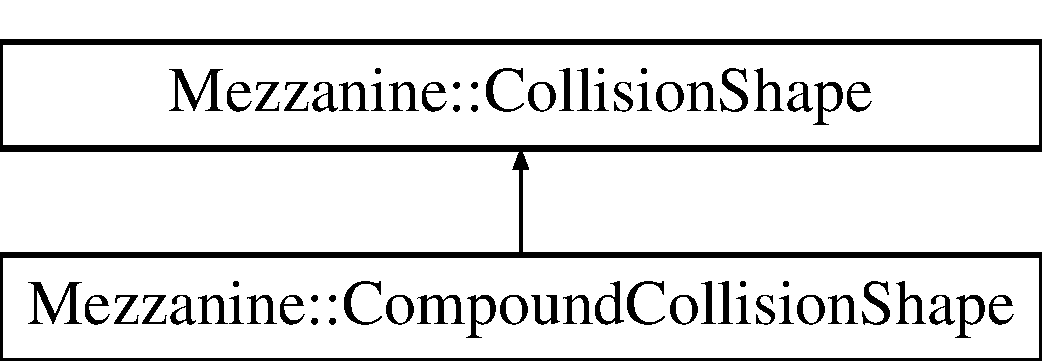
\includegraphics[height=2.000000cm]{classMezzanine_1_1CompoundCollisionShape}
\end{center}
\end{figure}
\subsubsection*{Public Member Functions}
\begin{DoxyCompactItemize}
\item 
virtual void \hyperlink{classMezzanine_1_1CompoundCollisionShape_a84fc66573ca4f052d53474a743305921}{AddChildShape} (\hyperlink{classMezzanine_1_1CollisionShape}{CollisionShape} $\ast$Child, const \hyperlink{classMezzanine_1_1Vector3}{Vector3} \&ChildLocation, const \hyperlink{classMezzanine_1_1Quaternion}{Quaternion} \&ChildRotation)
\begin{DoxyCompactList}\small\item\em Adds a shape to this compound shape. \item\end{DoxyCompactList}\item 
virtual void \hyperlink{classMezzanine_1_1CompoundCollisionShape_af4549334b9423e12eb36b48015956b7d}{AddChildShape} (\hyperlink{classMezzanine_1_1CollisionShape}{CollisionShape} $\ast$Child, const \hyperlink{classMezzanine_1_1Vector3}{Vector3} \&ChildLocation)
\begin{DoxyCompactList}\small\item\em Adds a shape to this compound shape. \item\end{DoxyCompactList}\item 
virtual void \hyperlink{classMezzanine_1_1CompoundCollisionShape_a9f6234a1d1bdcf96c2699df57b0ab7f8}{AddChildShape} (\hyperlink{classMezzanine_1_1CollisionShape}{CollisionShape} $\ast$Child, const \hyperlink{classMezzanine_1_1Transform}{Transform} \&ChildLocation)
\begin{DoxyCompactList}\small\item\em Adds a shape to this compound shape. \item\end{DoxyCompactList}\item 
\hyperlink{classMezzanine_1_1CompoundCollisionShape_a3d31ddbff556b73429acc44ae6aeeef3}{CompoundCollisionShape} (const \hyperlink{namespaceMezzanine_acf9fcc130e6ebf08e3d8491aebcf1c86}{String} \&\hyperlink{classMezzanine_1_1CollisionShape_aac524c5c56fa4d158bc071f8aecfbe79}{Name}, btCompoundShape $\ast$BulletShape)
\begin{DoxyCompactList}\small\item\em Internal Constructor. \item\end{DoxyCompactList}\item 
\hyperlink{classMezzanine_1_1CompoundCollisionShape_ad8cdd209d948e98b629378db81a77181}{CompoundCollisionShape} (const \hyperlink{namespaceMezzanine_acf9fcc130e6ebf08e3d8491aebcf1c86}{String} \&\hyperlink{classMezzanine_1_1CollisionShape_aac524c5c56fa4d158bc071f8aecfbe79}{Name})
\begin{DoxyCompactList}\small\item\em Class Constructor. \item\end{DoxyCompactList}\item 
virtual btCompoundShape $\ast$ \hyperlink{classMezzanine_1_1CompoundCollisionShape_adcf3f393c1be71c3ffb50782c375ea57}{GetBulletCompoundShape} () const 
\item 
virtual \hyperlink{classMezzanine_1_1CollisionShape}{CollisionShape} $\ast$ \hyperlink{classMezzanine_1_1CompoundCollisionShape_a707e6da7fef980a55f9c6477f152d0a9}{GetChild} (\hyperlink{namespaceMezzanine_adcbb6ce6d1eb4379d109e51171e2e493}{Whole} Index) const 
\begin{DoxyCompactList}\small\item\em Get a specific child. \item\end{DoxyCompactList}\item 
virtual \hyperlink{namespaceMezzanine_adcbb6ce6d1eb4379d109e51171e2e493}{Whole} \hyperlink{classMezzanine_1_1CompoundCollisionShape_ae21437b0ba98b553a1f651e7eb9f6542}{GetNumChildren} () const 
\begin{DoxyCompactList}\small\item\em Gets the number of children belonging to this compound shape. \item\end{DoxyCompactList}\item 
virtual \hyperlink{classMezzanine_1_1CollisionShape_ad04186055565998879b64176d6dd100d}{CollisionShape::ShapeType} \hyperlink{classMezzanine_1_1CompoundCollisionShape_a8b701bbbc32b007f32884946d285fba1}{GetType} () const 
\item 
virtual void \hyperlink{classMezzanine_1_1CompoundCollisionShape_a4c0e2d16e20b37c4c8fcd96d7229dc1f}{RemoveChildShape} (\hyperlink{classMezzanine_1_1CollisionShape}{CollisionShape} $\ast$Child)
\begin{DoxyCompactList}\small\item\em Removes a Child shape from this compound shape. \item\end{DoxyCompactList}\item 
virtual void \hyperlink{classMezzanine_1_1CompoundCollisionShape_a773f30f7d5046eb3d0ad051332a0b37e}{RemoveChildShape} (const \hyperlink{namespaceMezzanine_adcbb6ce6d1eb4379d109e51171e2e493}{Whole} \&ChildIndex)
\begin{DoxyCompactList}\small\item\em Removed a Child shape from this compound shape by index. \item\end{DoxyCompactList}\item 
\hypertarget{classMezzanine_1_1CompoundCollisionShape_a8dae4d989a8c3ffd4bb7f75fbaeb9c29}{
virtual \hyperlink{classMezzanine_1_1CompoundCollisionShape_a8dae4d989a8c3ffd4bb7f75fbaeb9c29}{$\sim$CompoundCollisionShape} ()}
\label{classMezzanine_1_1CompoundCollisionShape_a8dae4d989a8c3ffd4bb7f75fbaeb9c29}

\begin{DoxyCompactList}\small\item\em Class Destructor. \item\end{DoxyCompactList}\end{DoxyCompactItemize}
\subsubsection*{Protected Attributes}
\begin{DoxyCompactItemize}
\item 
\hypertarget{classMezzanine_1_1CompoundCollisionShape_a41503a9a43ed2b28720cc6ae63d42256}{
std::vector$<$ \hyperlink{classMezzanine_1_1CollisionShape}{CollisionShape} $\ast$ $>$ \hyperlink{classMezzanine_1_1CompoundCollisionShape_a41503a9a43ed2b28720cc6ae63d42256}{ChildShapes}}
\label{classMezzanine_1_1CompoundCollisionShape_a41503a9a43ed2b28720cc6ae63d42256}

\begin{DoxyCompactList}\small\item\em Storage for Child shapes. \item\end{DoxyCompactList}\end{DoxyCompactItemize}


\subsubsection{Detailed Description}
A collision shape composed of many other collision shapes placed and oriented in local space. This shape is the sum of all it's child shapes. Unlike the \hyperlink{classMezzanine_1_1MultiSphereCollisionShape}{MultiSphereCollisionShape} and the \hyperlink{classMezzanine_1_1ConvexHullCollisionShape}{ConvexHullCollisionShape}, this shape does not form a convex hull of it's children. When populating with primitives, Compound shapes offer the most flexibility with the best performace that you can get. \par
 \par
 When deleted a \hyperlink{classMezzanine_1_1CompoundCollisionShape}{CompoundCollisionShape} will clean up all of it's child shapes. 

Definition at line 272 of file collisionshape.h.



\subsubsection{Constructor \& Destructor Documentation}
\hypertarget{classMezzanine_1_1CompoundCollisionShape_ad8cdd209d948e98b629378db81a77181}{
\index{Mezzanine::CompoundCollisionShape@{Mezzanine::CompoundCollisionShape}!CompoundCollisionShape@{CompoundCollisionShape}}
\index{CompoundCollisionShape@{CompoundCollisionShape}!Mezzanine::CompoundCollisionShape@{Mezzanine::CompoundCollisionShape}}
\paragraph[{CompoundCollisionShape}]{\setlength{\rightskip}{0pt plus 5cm}Mezzanine::CompoundCollisionShape::CompoundCollisionShape (
\begin{DoxyParamCaption}
\item[{const {\bf String} \&}]{Name}
\end{DoxyParamCaption}
)}\hfill}
\label{classMezzanine_1_1CompoundCollisionShape_ad8cdd209d948e98b629378db81a77181}


Class Constructor. 


\begin{DoxyParams}{Parameters}
{\em Name} & The name of this Shape. \\
\hline
\end{DoxyParams}


Definition at line 327 of file collisionshape.cpp.

\hypertarget{classMezzanine_1_1CompoundCollisionShape_a3d31ddbff556b73429acc44ae6aeeef3}{
\index{Mezzanine::CompoundCollisionShape@{Mezzanine::CompoundCollisionShape}!CompoundCollisionShape@{CompoundCollisionShape}}
\index{CompoundCollisionShape@{CompoundCollisionShape}!Mezzanine::CompoundCollisionShape@{Mezzanine::CompoundCollisionShape}}
\paragraph[{CompoundCollisionShape}]{\setlength{\rightskip}{0pt plus 5cm}Mezzanine::CompoundCollisionShape::CompoundCollisionShape (
\begin{DoxyParamCaption}
\item[{const {\bf String} \&}]{Name, }
\item[{btCompoundShape $\ast$}]{BulletShape}
\end{DoxyParamCaption}
)}\hfill}
\label{classMezzanine_1_1CompoundCollisionShape_a3d31ddbff556b73429acc44ae6aeeef3}


Internal Constructor. 


\begin{DoxyParams}{Parameters}
{\em Name} & The name of this Shape. \\
\hline
{\em BulletShape} & The internal shape this shape is based on. \\
\hline
\end{DoxyParams}


Definition at line 333 of file collisionshape.cpp.



\subsubsection{Member Function Documentation}
\hypertarget{classMezzanine_1_1CompoundCollisionShape_a84fc66573ca4f052d53474a743305921}{
\index{Mezzanine::CompoundCollisionShape@{Mezzanine::CompoundCollisionShape}!AddChildShape@{AddChildShape}}
\index{AddChildShape@{AddChildShape}!Mezzanine::CompoundCollisionShape@{Mezzanine::CompoundCollisionShape}}
\paragraph[{AddChildShape}]{\setlength{\rightskip}{0pt plus 5cm}void Mezzanine::CompoundCollisionShape::AddChildShape (
\begin{DoxyParamCaption}
\item[{{\bf CollisionShape} $\ast$}]{Child, }
\item[{const {\bf Vector3} \&}]{ChildLocation, }
\item[{const {\bf Quaternion} \&}]{ChildRotation}
\end{DoxyParamCaption}
)\hspace{0.3cm}{\ttfamily  \mbox{[}virtual\mbox{]}}}\hfill}
\label{classMezzanine_1_1CompoundCollisionShape_a84fc66573ca4f052d53474a743305921}


Adds a shape to this compound shape. 


\begin{DoxyParams}{Parameters}
{\em Child} & The shape to be added to this shape. \\
\hline
{\em ChildLocation} & The location this child is to have in local space. \\
\hline
{\em ChildRotation} & The rotation to apply to this child in local space. \\
\hline
\end{DoxyParams}


Definition at line 359 of file collisionshape.cpp.

\hypertarget{classMezzanine_1_1CompoundCollisionShape_af4549334b9423e12eb36b48015956b7d}{
\index{Mezzanine::CompoundCollisionShape@{Mezzanine::CompoundCollisionShape}!AddChildShape@{AddChildShape}}
\index{AddChildShape@{AddChildShape}!Mezzanine::CompoundCollisionShape@{Mezzanine::CompoundCollisionShape}}
\paragraph[{AddChildShape}]{\setlength{\rightskip}{0pt plus 5cm}void Mezzanine::CompoundCollisionShape::AddChildShape (
\begin{DoxyParamCaption}
\item[{{\bf CollisionShape} $\ast$}]{Child, }
\item[{const {\bf Vector3} \&}]{ChildLocation}
\end{DoxyParamCaption}
)\hspace{0.3cm}{\ttfamily  \mbox{[}virtual\mbox{]}}}\hfill}
\label{classMezzanine_1_1CompoundCollisionShape_af4549334b9423e12eb36b48015956b7d}


Adds a shape to this compound shape. 


\begin{DoxyParams}{Parameters}
{\em Child} & The shape to be added to this shape. \\
\hline
{\em ChildLocation} & The location this child is to have in local space. \\
\hline
\end{DoxyParams}


Definition at line 367 of file collisionshape.cpp.

\hypertarget{classMezzanine_1_1CompoundCollisionShape_a9f6234a1d1bdcf96c2699df57b0ab7f8}{
\index{Mezzanine::CompoundCollisionShape@{Mezzanine::CompoundCollisionShape}!AddChildShape@{AddChildShape}}
\index{AddChildShape@{AddChildShape}!Mezzanine::CompoundCollisionShape@{Mezzanine::CompoundCollisionShape}}
\paragraph[{AddChildShape}]{\setlength{\rightskip}{0pt plus 5cm}void Mezzanine::CompoundCollisionShape::AddChildShape (
\begin{DoxyParamCaption}
\item[{{\bf CollisionShape} $\ast$}]{Child, }
\item[{const {\bf Transform} \&}]{ChildLocation}
\end{DoxyParamCaption}
)\hspace{0.3cm}{\ttfamily  \mbox{[}virtual\mbox{]}}}\hfill}
\label{classMezzanine_1_1CompoundCollisionShape_a9f6234a1d1bdcf96c2699df57b0ab7f8}


Adds a shape to this compound shape. 


\begin{DoxyParams}{Parameters}
{\em Child} & The shape to be added to this shape. \\
\hline
{\em ChildLocation} & The location and Rotation this child is to have in local space. \\
\hline
\end{DoxyParams}


Definition at line 377 of file collisionshape.cpp.

\hypertarget{classMezzanine_1_1CompoundCollisionShape_adcf3f393c1be71c3ffb50782c375ea57}{
\index{Mezzanine::CompoundCollisionShape@{Mezzanine::CompoundCollisionShape}!GetBulletCompoundShape@{GetBulletCompoundShape}}
\index{GetBulletCompoundShape@{GetBulletCompoundShape}!Mezzanine::CompoundCollisionShape@{Mezzanine::CompoundCollisionShape}}
\paragraph[{GetBulletCompoundShape}]{\setlength{\rightskip}{0pt plus 5cm}btCompoundShape $\ast$ Mezzanine::CompoundCollisionShape::GetBulletCompoundShape (
\begin{DoxyParamCaption}
{}
\end{DoxyParamCaption}
) const\hspace{0.3cm}{\ttfamily  \mbox{[}virtual\mbox{]}}}\hfill}
\label{classMezzanine_1_1CompoundCollisionShape_adcf3f393c1be71c3ffb50782c375ea57}
Gets the internal shape pointer this collision shape is based on. 

\begin{DoxyReturn}{Returns}
Returns a pointer to the internal collision shape. 
\end{DoxyReturn}
 

Definition at line 418 of file collisionshape.cpp.

\hypertarget{classMezzanine_1_1CompoundCollisionShape_a707e6da7fef980a55f9c6477f152d0a9}{
\index{Mezzanine::CompoundCollisionShape@{Mezzanine::CompoundCollisionShape}!GetChild@{GetChild}}
\index{GetChild@{GetChild}!Mezzanine::CompoundCollisionShape@{Mezzanine::CompoundCollisionShape}}
\paragraph[{GetChild}]{\setlength{\rightskip}{0pt plus 5cm}{\bf CollisionShape} $\ast$ Mezzanine::CompoundCollisionShape::GetChild (
\begin{DoxyParamCaption}
\item[{{\bf Whole}}]{Index}
\end{DoxyParamCaption}
) const\hspace{0.3cm}{\ttfamily  \mbox{[}virtual\mbox{]}}}\hfill}
\label{classMezzanine_1_1CompoundCollisionShape_a707e6da7fef980a55f9c6477f152d0a9}


Get a specific child. 


\begin{DoxyParams}{Parameters}
{\em Index} & A number indicating which \hyperlink{classMezzanine_1_1CollisionShape}{CollisionShape} you want a pointer to. \\
\hline
\end{DoxyParams}
\begin{DoxyReturn}{Returns}
A pointer to the Specified \hyperlink{classMezzanine_1_1CollisionShape}{CollisionShape} 
\end{DoxyReturn}


Definition at line 389 of file collisionshape.cpp.

\hypertarget{classMezzanine_1_1CompoundCollisionShape_ae21437b0ba98b553a1f651e7eb9f6542}{
\index{Mezzanine::CompoundCollisionShape@{Mezzanine::CompoundCollisionShape}!GetNumChildren@{GetNumChildren}}
\index{GetNumChildren@{GetNumChildren}!Mezzanine::CompoundCollisionShape@{Mezzanine::CompoundCollisionShape}}
\paragraph[{GetNumChildren}]{\setlength{\rightskip}{0pt plus 5cm}{\bf Whole} Mezzanine::CompoundCollisionShape::GetNumChildren (
\begin{DoxyParamCaption}
{}
\end{DoxyParamCaption}
) const\hspace{0.3cm}{\ttfamily  \mbox{[}virtual\mbox{]}}}\hfill}
\label{classMezzanine_1_1CompoundCollisionShape_ae21437b0ba98b553a1f651e7eb9f6542}


Gets the number of children belonging to this compound shape. 

\begin{DoxyReturn}{Returns}
Returns the number of children belonging to this shape. 
\end{DoxyReturn}


Definition at line 384 of file collisionshape.cpp.

\hypertarget{classMezzanine_1_1CompoundCollisionShape_a8b701bbbc32b007f32884946d285fba1}{
\index{Mezzanine::CompoundCollisionShape@{Mezzanine::CompoundCollisionShape}!GetType@{GetType}}
\index{GetType@{GetType}!Mezzanine::CompoundCollisionShape@{Mezzanine::CompoundCollisionShape}}
\paragraph[{GetType}]{\setlength{\rightskip}{0pt plus 5cm}{\bf CollisionShape::ShapeType} Mezzanine::CompoundCollisionShape::GetType (
\begin{DoxyParamCaption}
{}
\end{DoxyParamCaption}
) const\hspace{0.3cm}{\ttfamily  \mbox{[}virtual\mbox{]}}}\hfill}
\label{classMezzanine_1_1CompoundCollisionShape_a8b701bbbc32b007f32884946d285fba1}
Gets the type of \hyperlink{classMezzanine_1_1Collision}{Collision} shape this is. 

\begin{DoxyReturn}{Returns}
Returns an enum value indicating the type of collision shape this is. 
\end{DoxyReturn}
 

Implements \hyperlink{classMezzanine_1_1CollisionShape_a27e5055f81cb8fb6d65a6c9f8dc73b69}{Mezzanine::CollisionShape}.



Definition at line 413 of file collisionshape.cpp.

\hypertarget{classMezzanine_1_1CompoundCollisionShape_a4c0e2d16e20b37c4c8fcd96d7229dc1f}{
\index{Mezzanine::CompoundCollisionShape@{Mezzanine::CompoundCollisionShape}!RemoveChildShape@{RemoveChildShape}}
\index{RemoveChildShape@{RemoveChildShape}!Mezzanine::CompoundCollisionShape@{Mezzanine::CompoundCollisionShape}}
\paragraph[{RemoveChildShape}]{\setlength{\rightskip}{0pt plus 5cm}void Mezzanine::CompoundCollisionShape::RemoveChildShape (
\begin{DoxyParamCaption}
\item[{{\bf CollisionShape} $\ast$}]{Child}
\end{DoxyParamCaption}
)\hspace{0.3cm}{\ttfamily  \mbox{[}virtual\mbox{]}}}\hfill}
\label{classMezzanine_1_1CompoundCollisionShape_a4c0e2d16e20b37c4c8fcd96d7229dc1f}


Removes a Child shape from this compound shape. 


\begin{DoxyParams}{Parameters}
{\em Child} & The child shape to be removed. \\
\hline
\end{DoxyParams}


Definition at line 394 of file collisionshape.cpp.

\hypertarget{classMezzanine_1_1CompoundCollisionShape_a773f30f7d5046eb3d0ad051332a0b37e}{
\index{Mezzanine::CompoundCollisionShape@{Mezzanine::CompoundCollisionShape}!RemoveChildShape@{RemoveChildShape}}
\index{RemoveChildShape@{RemoveChildShape}!Mezzanine::CompoundCollisionShape@{Mezzanine::CompoundCollisionShape}}
\paragraph[{RemoveChildShape}]{\setlength{\rightskip}{0pt plus 5cm}void Mezzanine::CompoundCollisionShape::RemoveChildShape (
\begin{DoxyParamCaption}
\item[{const {\bf Whole} \&}]{ChildIndex}
\end{DoxyParamCaption}
)\hspace{0.3cm}{\ttfamily  \mbox{[}virtual\mbox{]}}}\hfill}
\label{classMezzanine_1_1CompoundCollisionShape_a773f30f7d5046eb3d0ad051332a0b37e}


Removed a Child shape from this compound shape by index. 


\begin{DoxyParams}{Parameters}
{\em ChildIndex} & The index of the child shape to be removed. \\
\hline
\end{DoxyParams}


Definition at line 406 of file collisionshape.cpp.



The documentation for this class was generated from the following files:\begin{DoxyCompactItemize}
\item 
collisionshape.h\item 
collisionshape.cpp\end{DoxyCompactItemize}

\hypertarget{classMezzanine_1_1ConeCollisionShape}{
\subsection{Mezzanine::ConeCollisionShape Class Reference}
\label{classMezzanine_1_1ConeCollisionShape}\index{Mezzanine::ConeCollisionShape@{Mezzanine::ConeCollisionShape}}
}


A cone physics shape.  




{\ttfamily \#include $<$collisionshape.h$>$}

Inheritance diagram for Mezzanine::ConeCollisionShape:\begin{figure}[H]
\begin{center}
\leavevmode
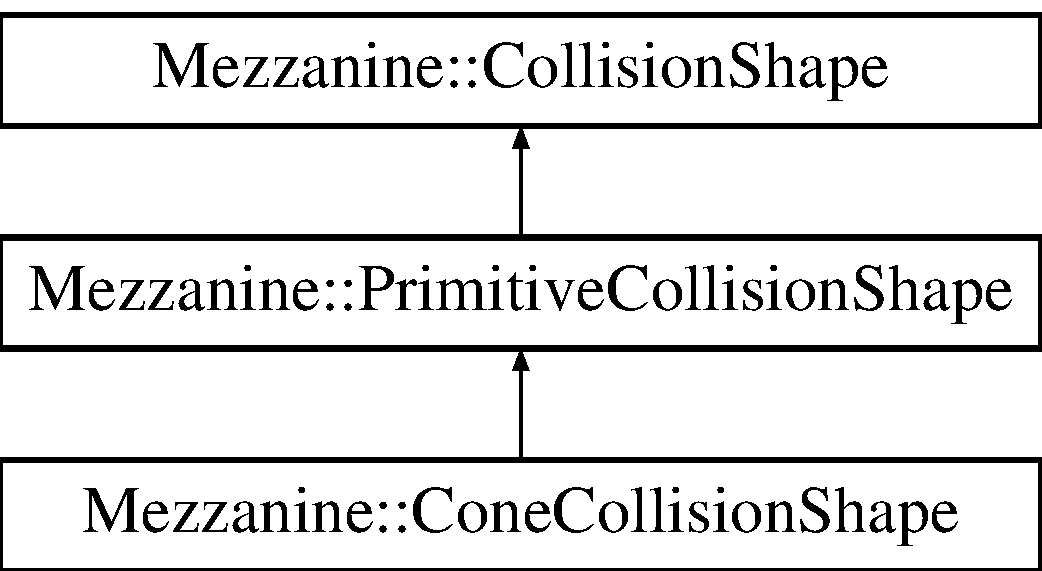
\includegraphics[height=3.000000cm]{classMezzanine_1_1ConeCollisionShape}
\end{center}
\end{figure}
\subsubsection*{Public Member Functions}
\begin{DoxyCompactItemize}
\item 
\hyperlink{classMezzanine_1_1ConeCollisionShape_aec0129e435def8d4299a6a7df6ecfd82}{ConeCollisionShape} (const \hyperlink{namespaceMezzanine_acf9fcc130e6ebf08e3d8491aebcf1c86}{String} \&\hyperlink{classMezzanine_1_1CollisionShape_aac524c5c56fa4d158bc071f8aecfbe79}{Name}, const \hyperlink{namespaceMezzanine_a726731b1a7df72bf3583e4a97282c6f6}{Real} \&Radius, const \hyperlink{namespaceMezzanine_a726731b1a7df72bf3583e4a97282c6f6}{Real} \&Height, const \hyperlink{classMezzanine_1_1Vector3}{Vector3} \&UpAxis)
\begin{DoxyCompactList}\small\item\em Class Constructor. \item\end{DoxyCompactList}\item 
\hyperlink{classMezzanine_1_1ConeCollisionShape_a33a0f529da45a509f8961f4c9a490b3e}{ConeCollisionShape} (const \hyperlink{namespaceMezzanine_acf9fcc130e6ebf08e3d8491aebcf1c86}{String} \&\hyperlink{classMezzanine_1_1CollisionShape_aac524c5c56fa4d158bc071f8aecfbe79}{Name}, const \hyperlink{namespaceMezzanine_a726731b1a7df72bf3583e4a97282c6f6}{Real} \&Radius, const \hyperlink{namespaceMezzanine_a726731b1a7df72bf3583e4a97282c6f6}{Real} \&Height, \hyperlink{namespaceMezzanine_ab41a00a8c6a47b576dc987ec34e16ba1}{StandardAxis} UpAxis)
\begin{DoxyCompactList}\small\item\em Class Constructor. \item\end{DoxyCompactList}\item 
\hyperlink{classMezzanine_1_1ConeCollisionShape_ad80439a195cf4f2df8d2cd4b8ebaf062}{ConeCollisionShape} (const \hyperlink{namespaceMezzanine_acf9fcc130e6ebf08e3d8491aebcf1c86}{String} \&\hyperlink{classMezzanine_1_1CollisionShape_aac524c5c56fa4d158bc071f8aecfbe79}{Name}, btConeShape $\ast$BulletShape)
\begin{DoxyCompactList}\small\item\em Internal Constructor. \item\end{DoxyCompactList}\item 
virtual btConeShape $\ast$ \hyperlink{classMezzanine_1_1ConeCollisionShape_aff8623fa14d66fce32738ff075c1cc7c}{GetBulletConeShape} () const 
\item 
virtual \hyperlink{namespaceMezzanine_a726731b1a7df72bf3583e4a97282c6f6}{Real} \hyperlink{classMezzanine_1_1ConeCollisionShape_af52995ed04491df5ebbff26af6ecd816}{GetCleanHeight} () const 
\begin{DoxyCompactList}\small\item\em Gets the height of the cone, as originally passed in. \item\end{DoxyCompactList}\item 
virtual \hyperlink{namespaceMezzanine_a726731b1a7df72bf3583e4a97282c6f6}{Real} \hyperlink{classMezzanine_1_1ConeCollisionShape_a24b59bbca0455e54cf7bb692ff46c080}{GetCleanRadius} () const 
\begin{DoxyCompactList}\small\item\em Gets the radius of the cone, as originally passed in. \item\end{DoxyCompactList}\item 
virtual \hyperlink{namespaceMezzanine_a726731b1a7df72bf3583e4a97282c6f6}{Real} \hyperlink{classMezzanine_1_1ConeCollisionShape_a6247f2a72e298ada975a0fa840b12629}{GetHeight} () const 
\begin{DoxyCompactList}\small\item\em Gets the height of the cone, as used for collision checking. \item\end{DoxyCompactList}\item 
\hyperlink{namespaceMezzanine_a726731b1a7df72bf3583e4a97282c6f6}{Real} \hyperlink{classMezzanine_1_1ConeCollisionShape_aa3c48e845cb96783118d2cb9562246a9}{GetHeightScaling} () const 
\begin{DoxyCompactList}\small\item\em Which axis is up defines which axis is used to scale height. \item\end{DoxyCompactList}\item 
virtual \hyperlink{namespaceMezzanine_a726731b1a7df72bf3583e4a97282c6f6}{Real} \hyperlink{classMezzanine_1_1ConeCollisionShape_ae2d8ed139802999b4bec4fdac4814ef3}{GetRadius} () const 
\begin{DoxyCompactList}\small\item\em Gets the radius of the cone, as used for collision checking. \item\end{DoxyCompactList}\item 
\hyperlink{namespaceMezzanine_a726731b1a7df72bf3583e4a97282c6f6}{Real} \hyperlink{classMezzanine_1_1ConeCollisionShape_a6588a43aa775e0f33bc7d9741699fd3f}{GetRadiusScaling} () const 
\begin{DoxyCompactList}\small\item\em Which axis is up defines which 2 axis are used to scale the radius. \item\end{DoxyCompactList}\item 
virtual \hyperlink{classMezzanine_1_1CollisionShape_ad04186055565998879b64176d6dd100d}{CollisionShape::ShapeType} \hyperlink{classMezzanine_1_1ConeCollisionShape_a874892f3aaba7e79200633691037a410}{GetType} () const 
\item 
virtual \hyperlink{classMezzanine_1_1Vector3}{Vector3} \hyperlink{classMezzanine_1_1ConeCollisionShape_aed9f36553311ca8d20ccd0d7a01ec4ee}{GetUpAxis} () const 
\begin{DoxyCompactList}\small\item\em Gets which axis this cone is oriented along. \item\end{DoxyCompactList}\item 
virtual \hyperlink{namespaceMezzanine_ab41a00a8c6a47b576dc987ec34e16ba1}{StandardAxis} \hyperlink{classMezzanine_1_1ConeCollisionShape_aa17fc2f15ba313109ff40f1a66e088be}{GetUpStandardAxis} () const 
\begin{DoxyCompactList}\small\item\em Gets which axis this cone is oriented along. \item\end{DoxyCompactList}\item 
\hypertarget{classMezzanine_1_1ConeCollisionShape_a49236a6396e87f22ec06251de6d3c1fe}{
virtual \hyperlink{classMezzanine_1_1ConeCollisionShape_a49236a6396e87f22ec06251de6d3c1fe}{$\sim$ConeCollisionShape} ()}
\label{classMezzanine_1_1ConeCollisionShape_a49236a6396e87f22ec06251de6d3c1fe}

\begin{DoxyCompactList}\small\item\em Class Destructor. \item\end{DoxyCompactList}\end{DoxyCompactItemize}
\subsubsection*{Protected Member Functions}
\begin{DoxyCompactItemize}
\item 
void \hyperlink{classMezzanine_1_1ConeCollisionShape_a5a29f404442602af52499c684c792310}{Construct} (const \hyperlink{namespaceMezzanine_acf9fcc130e6ebf08e3d8491aebcf1c86}{String} \&\hyperlink{classMezzanine_1_1CollisionShape_aac524c5c56fa4d158bc071f8aecfbe79}{Name}, const \hyperlink{namespaceMezzanine_a726731b1a7df72bf3583e4a97282c6f6}{Real} \&Radius, const \hyperlink{namespaceMezzanine_a726731b1a7df72bf3583e4a97282c6f6}{Real} \&Height, \hyperlink{namespaceMezzanine_ab41a00a8c6a47b576dc987ec34e16ba1}{StandardAxis} UpAxis)
\begin{DoxyCompactList}\small\item\em Performe shared contructor work. \item\end{DoxyCompactList}\item 
\hyperlink{classMezzanine_1_1Vector3}{Vector3} \hyperlink{classMezzanine_1_1ConeCollisionShape_aa4a1f1f839c3b6761b27b129b60c8e89}{GetAxisMathBS} () const 
\begin{DoxyCompactList}\small\item\em Simulate some messed up the physics library does. \item\end{DoxyCompactList}\end{DoxyCompactItemize}


\subsubsection{Detailed Description}
A cone physics shape. Keep in mind when building a cone shape, the provided radius is for the base of the cone, but the pivot point of the shape is still at it's center and not it's base. Like Capsules and Cylinders, Cones can be aligned to any of the 3 linear axes(X, Y, or Z). 

Definition at line 486 of file collisionshape.h.



\subsubsection{Constructor \& Destructor Documentation}
\hypertarget{classMezzanine_1_1ConeCollisionShape_aec0129e435def8d4299a6a7df6ecfd82}{
\index{Mezzanine::ConeCollisionShape@{Mezzanine::ConeCollisionShape}!ConeCollisionShape@{ConeCollisionShape}}
\index{ConeCollisionShape@{ConeCollisionShape}!Mezzanine::ConeCollisionShape@{Mezzanine::ConeCollisionShape}}
\paragraph[{ConeCollisionShape}]{\setlength{\rightskip}{0pt plus 5cm}Mezzanine::ConeCollisionShape::ConeCollisionShape (
\begin{DoxyParamCaption}
\item[{const {\bf String} \&}]{Name, }
\item[{const {\bf Real} \&}]{Radius, }
\item[{const {\bf Real} \&}]{Height, }
\item[{const {\bf Vector3} \&}]{UpAxis}
\end{DoxyParamCaption}
)}\hfill}
\label{classMezzanine_1_1ConeCollisionShape_aec0129e435def8d4299a6a7df6ecfd82}


Class Constructor. 


\begin{DoxyParams}{Parameters}
{\em Name} & The name of this Shape. \\
\hline
{\em Radius} & The radius of the base of the Cone. \\
\hline
{\em Height} & The height of the Cone. \\
\hline
{\em UpAxis} & Which axis the Cone is to be oriented along. Typical usage is for a capsule to be oriented on the Y axis(0,1,0), which would make it stand upright. \\
\hline
\end{DoxyParams}


Definition at line 794 of file collisionshape.cpp.

\hypertarget{classMezzanine_1_1ConeCollisionShape_a33a0f529da45a509f8961f4c9a490b3e}{
\index{Mezzanine::ConeCollisionShape@{Mezzanine::ConeCollisionShape}!ConeCollisionShape@{ConeCollisionShape}}
\index{ConeCollisionShape@{ConeCollisionShape}!Mezzanine::ConeCollisionShape@{Mezzanine::ConeCollisionShape}}
\paragraph[{ConeCollisionShape}]{\setlength{\rightskip}{0pt plus 5cm}Mezzanine::ConeCollisionShape::ConeCollisionShape (
\begin{DoxyParamCaption}
\item[{const {\bf String} \&}]{Name, }
\item[{const {\bf Real} \&}]{Radius, }
\item[{const {\bf Real} \&}]{Height, }
\item[{{\bf StandardAxis}}]{UpAxis}
\end{DoxyParamCaption}
)}\hfill}
\label{classMezzanine_1_1ConeCollisionShape_a33a0f529da45a509f8961f4c9a490b3e}


Class Constructor. 


\begin{DoxyParams}{Parameters}
{\em Name} & The name of this Shape. \\
\hline
{\em Radius} & The radius of the base of the Cone. \\
\hline
{\em Height} & The height of the Cone. \\
\hline
{\em UpAxis} & Which axis the Cone is to be oriented along. Uses StandardAxis enum, Axis\_\-Y to make a vertical capsule \\
\hline
\end{DoxyParams}


Definition at line 797 of file collisionshape.cpp.

\hypertarget{classMezzanine_1_1ConeCollisionShape_ad80439a195cf4f2df8d2cd4b8ebaf062}{
\index{Mezzanine::ConeCollisionShape@{Mezzanine::ConeCollisionShape}!ConeCollisionShape@{ConeCollisionShape}}
\index{ConeCollisionShape@{ConeCollisionShape}!Mezzanine::ConeCollisionShape@{Mezzanine::ConeCollisionShape}}
\paragraph[{ConeCollisionShape}]{\setlength{\rightskip}{0pt plus 5cm}Mezzanine::ConeCollisionShape::ConeCollisionShape (
\begin{DoxyParamCaption}
\item[{const {\bf String} \&}]{Name, }
\item[{btConeShape $\ast$}]{BulletShape}
\end{DoxyParamCaption}
)}\hfill}
\label{classMezzanine_1_1ConeCollisionShape_ad80439a195cf4f2df8d2cd4b8ebaf062}


Internal Constructor. 


\begin{DoxyParams}{Parameters}
{\em Name} & The name of this Shape. \\
\hline
{\em BulletShape} & The internal shape this shape is based on. \\
\hline
\end{DoxyParams}


Definition at line 824 of file collisionshape.cpp.



\subsubsection{Member Function Documentation}
\hypertarget{classMezzanine_1_1ConeCollisionShape_a5a29f404442602af52499c684c792310}{
\index{Mezzanine::ConeCollisionShape@{Mezzanine::ConeCollisionShape}!Construct@{Construct}}
\index{Construct@{Construct}!Mezzanine::ConeCollisionShape@{Mezzanine::ConeCollisionShape}}
\paragraph[{Construct}]{\setlength{\rightskip}{0pt plus 5cm}void Mezzanine::ConeCollisionShape::Construct (
\begin{DoxyParamCaption}
\item[{const {\bf String} \&}]{Name, }
\item[{const {\bf Real} \&}]{Radius, }
\item[{const {\bf Real} \&}]{Height, }
\item[{{\bf StandardAxis}}]{UpAxis}
\end{DoxyParamCaption}
)\hspace{0.3cm}{\ttfamily  \mbox{[}protected\mbox{]}}}\hfill}
\label{classMezzanine_1_1ConeCollisionShape_a5a29f404442602af52499c684c792310}


Performe shared contructor work. 


\begin{DoxyParams}{Parameters}
{\em Name} & The name of this Shape. \\
\hline
{\em Radius} & The radius of the base of the Cone. \\
\hline
{\em Height} & The height of the Cone. \\
\hline
{\em UpAxis} & Which axis the Cone is to be oriented along. Uses StandardAxis enum, Axis\_\-Y to make a vertical capsule \\
\hline
\end{DoxyParams}


Definition at line 755 of file collisionshape.cpp.

\hypertarget{classMezzanine_1_1ConeCollisionShape_aa4a1f1f839c3b6761b27b129b60c8e89}{
\index{Mezzanine::ConeCollisionShape@{Mezzanine::ConeCollisionShape}!GetAxisMathBS@{GetAxisMathBS}}
\index{GetAxisMathBS@{GetAxisMathBS}!Mezzanine::ConeCollisionShape@{Mezzanine::ConeCollisionShape}}
\paragraph[{GetAxisMathBS}]{\setlength{\rightskip}{0pt plus 5cm}{\bf Vector3} Mezzanine::ConeCollisionShape::GetAxisMathBS (
\begin{DoxyParamCaption}
{}
\end{DoxyParamCaption}
) const\hspace{0.3cm}{\ttfamily  \mbox{[}protected\mbox{]}}}\hfill}
\label{classMezzanine_1_1ConeCollisionShape_aa4a1f1f839c3b6761b27b129b60c8e89}


Simulate some messed up the physics library does. 

\begin{DoxyReturn}{Returns}
A \hyperlink{classMezzanine_1_1Vector3}{Vector3} containing some StandarAxis based on what needs to go where. 
\end{DoxyReturn}


Definition at line 767 of file collisionshape.cpp.

\hypertarget{classMezzanine_1_1ConeCollisionShape_aff8623fa14d66fce32738ff075c1cc7c}{
\index{Mezzanine::ConeCollisionShape@{Mezzanine::ConeCollisionShape}!GetBulletConeShape@{GetBulletConeShape}}
\index{GetBulletConeShape@{GetBulletConeShape}!Mezzanine::ConeCollisionShape@{Mezzanine::ConeCollisionShape}}
\paragraph[{GetBulletConeShape}]{\setlength{\rightskip}{0pt plus 5cm}btConeShape $\ast$ Mezzanine::ConeCollisionShape::GetBulletConeShape (
\begin{DoxyParamCaption}
{}
\end{DoxyParamCaption}
) const\hspace{0.3cm}{\ttfamily  \mbox{[}virtual\mbox{]}}}\hfill}
\label{classMezzanine_1_1ConeCollisionShape_aff8623fa14d66fce32738ff075c1cc7c}
Gets the internal shape pointer this collision shape is based on. 

\begin{DoxyReturn}{Returns}
Returns a pointer to the internal collision shape. 
\end{DoxyReturn}
 

Definition at line 874 of file collisionshape.cpp.

\hypertarget{classMezzanine_1_1ConeCollisionShape_af52995ed04491df5ebbff26af6ecd816}{
\index{Mezzanine::ConeCollisionShape@{Mezzanine::ConeCollisionShape}!GetCleanHeight@{GetCleanHeight}}
\index{GetCleanHeight@{GetCleanHeight}!Mezzanine::ConeCollisionShape@{Mezzanine::ConeCollisionShape}}
\paragraph[{GetCleanHeight}]{\setlength{\rightskip}{0pt plus 5cm}{\bf Real} Mezzanine::ConeCollisionShape::GetCleanHeight (
\begin{DoxyParamCaption}
{}
\end{DoxyParamCaption}
) const\hspace{0.3cm}{\ttfamily  \mbox{[}virtual\mbox{]}}}\hfill}
\label{classMezzanine_1_1ConeCollisionShape_af52995ed04491df5ebbff26af6ecd816}


Gets the height of the cone, as originally passed in. 

\begin{DoxyReturn}{Returns}
Returns a real representing height of the cone. 
\end{DoxyReturn}


Definition at line 851 of file collisionshape.cpp.

\hypertarget{classMezzanine_1_1ConeCollisionShape_a24b59bbca0455e54cf7bb692ff46c080}{
\index{Mezzanine::ConeCollisionShape@{Mezzanine::ConeCollisionShape}!GetCleanRadius@{GetCleanRadius}}
\index{GetCleanRadius@{GetCleanRadius}!Mezzanine::ConeCollisionShape@{Mezzanine::ConeCollisionShape}}
\paragraph[{GetCleanRadius}]{\setlength{\rightskip}{0pt plus 5cm}{\bf Real} Mezzanine::ConeCollisionShape::GetCleanRadius (
\begin{DoxyParamCaption}
{}
\end{DoxyParamCaption}
) const\hspace{0.3cm}{\ttfamily  \mbox{[}virtual\mbox{]}}}\hfill}
\label{classMezzanine_1_1ConeCollisionShape_a24b59bbca0455e54cf7bb692ff46c080}


Gets the radius of the cone, as originally passed in. 

\begin{DoxyReturn}{Returns}
Returns a real representing the radius at the base of the cone. 
\end{DoxyReturn}


Definition at line 846 of file collisionshape.cpp.

\hypertarget{classMezzanine_1_1ConeCollisionShape_a6247f2a72e298ada975a0fa840b12629}{
\index{Mezzanine::ConeCollisionShape@{Mezzanine::ConeCollisionShape}!GetHeight@{GetHeight}}
\index{GetHeight@{GetHeight}!Mezzanine::ConeCollisionShape@{Mezzanine::ConeCollisionShape}}
\paragraph[{GetHeight}]{\setlength{\rightskip}{0pt plus 5cm}{\bf Real} Mezzanine::ConeCollisionShape::GetHeight (
\begin{DoxyParamCaption}
{}
\end{DoxyParamCaption}
) const\hspace{0.3cm}{\ttfamily  \mbox{[}virtual\mbox{]}}}\hfill}
\label{classMezzanine_1_1ConeCollisionShape_a6247f2a72e298ada975a0fa840b12629}


Gets the height of the cone, as used for collision checking. 

\begin{DoxyReturn}{Returns}
Returns a real representing height of the cone. 
\end{DoxyReturn}


Definition at line 841 of file collisionshape.cpp.

\hypertarget{classMezzanine_1_1ConeCollisionShape_aa3c48e845cb96783118d2cb9562246a9}{
\index{Mezzanine::ConeCollisionShape@{Mezzanine::ConeCollisionShape}!GetHeightScaling@{GetHeightScaling}}
\index{GetHeightScaling@{GetHeightScaling}!Mezzanine::ConeCollisionShape@{Mezzanine::ConeCollisionShape}}
\paragraph[{GetHeightScaling}]{\setlength{\rightskip}{0pt plus 5cm}{\bf Real} Mezzanine::ConeCollisionShape::GetHeightScaling (
\begin{DoxyParamCaption}
{}
\end{DoxyParamCaption}
) const}\hfill}
\label{classMezzanine_1_1ConeCollisionShape_aa3c48e845cb96783118d2cb9562246a9}


Which axis is up defines which axis is used to scale height. 

\begin{DoxyReturn}{Returns}
A value that represent the scaling that only the height undergoes. 
\end{DoxyReturn}


Definition at line 859 of file collisionshape.cpp.

\hypertarget{classMezzanine_1_1ConeCollisionShape_ae2d8ed139802999b4bec4fdac4814ef3}{
\index{Mezzanine::ConeCollisionShape@{Mezzanine::ConeCollisionShape}!GetRadius@{GetRadius}}
\index{GetRadius@{GetRadius}!Mezzanine::ConeCollisionShape@{Mezzanine::ConeCollisionShape}}
\paragraph[{GetRadius}]{\setlength{\rightskip}{0pt plus 5cm}{\bf Real} Mezzanine::ConeCollisionShape::GetRadius (
\begin{DoxyParamCaption}
{}
\end{DoxyParamCaption}
) const\hspace{0.3cm}{\ttfamily  \mbox{[}virtual\mbox{]}}}\hfill}
\label{classMezzanine_1_1ConeCollisionShape_ae2d8ed139802999b4bec4fdac4814ef3}


Gets the radius of the cone, as used for collision checking. 

\begin{DoxyReturn}{Returns}
Returns a real representing the radius at the base of the cone. 
\end{DoxyReturn}


Definition at line 836 of file collisionshape.cpp.

\hypertarget{classMezzanine_1_1ConeCollisionShape_a6588a43aa775e0f33bc7d9741699fd3f}{
\index{Mezzanine::ConeCollisionShape@{Mezzanine::ConeCollisionShape}!GetRadiusScaling@{GetRadiusScaling}}
\index{GetRadiusScaling@{GetRadiusScaling}!Mezzanine::ConeCollisionShape@{Mezzanine::ConeCollisionShape}}
\paragraph[{GetRadiusScaling}]{\setlength{\rightskip}{0pt plus 5cm}{\bf Real} Mezzanine::ConeCollisionShape::GetRadiusScaling (
\begin{DoxyParamCaption}
{}
\end{DoxyParamCaption}
) const}\hfill}
\label{classMezzanine_1_1ConeCollisionShape_a6588a43aa775e0f33bc7d9741699fd3f}


Which axis is up defines which 2 axis are used to scale the radius. 

\begin{DoxyReturn}{Returns}
A value that represent the scaling that only the radius undergoes. 
\end{DoxyReturn}


Definition at line 856 of file collisionshape.cpp.

\hypertarget{classMezzanine_1_1ConeCollisionShape_a874892f3aaba7e79200633691037a410}{
\index{Mezzanine::ConeCollisionShape@{Mezzanine::ConeCollisionShape}!GetType@{GetType}}
\index{GetType@{GetType}!Mezzanine::ConeCollisionShape@{Mezzanine::ConeCollisionShape}}
\paragraph[{GetType}]{\setlength{\rightskip}{0pt plus 5cm}{\bf CollisionShape::ShapeType} Mezzanine::ConeCollisionShape::GetType (
\begin{DoxyParamCaption}
{}
\end{DoxyParamCaption}
) const\hspace{0.3cm}{\ttfamily  \mbox{[}virtual\mbox{]}}}\hfill}
\label{classMezzanine_1_1ConeCollisionShape_a874892f3aaba7e79200633691037a410}
Gets the type of \hyperlink{classMezzanine_1_1Collision}{Collision} shape this is. 

\begin{DoxyReturn}{Returns}
Returns an enum value indicating the type of collision shape this is. 
\end{DoxyReturn}
 

Implements \hyperlink{classMezzanine_1_1PrimitiveCollisionShape_ad3d4143a5640204b987e0b57eb24af41}{Mezzanine::PrimitiveCollisionShape}.



Definition at line 869 of file collisionshape.cpp.

\hypertarget{classMezzanine_1_1ConeCollisionShape_aed9f36553311ca8d20ccd0d7a01ec4ee}{
\index{Mezzanine::ConeCollisionShape@{Mezzanine::ConeCollisionShape}!GetUpAxis@{GetUpAxis}}
\index{GetUpAxis@{GetUpAxis}!Mezzanine::ConeCollisionShape@{Mezzanine::ConeCollisionShape}}
\paragraph[{GetUpAxis}]{\setlength{\rightskip}{0pt plus 5cm}{\bf Vector3} Mezzanine::ConeCollisionShape::GetUpAxis (
\begin{DoxyParamCaption}
{}
\end{DoxyParamCaption}
) const\hspace{0.3cm}{\ttfamily  \mbox{[}virtual\mbox{]}}}\hfill}
\label{classMezzanine_1_1ConeCollisionShape_aed9f36553311ca8d20ccd0d7a01ec4ee}


Gets which axis this cone is oriented along. 

\begin{DoxyReturn}{Returns}
Returns a \hyperlink{classMezzanine_1_1Vector3}{Vector3} representing which local axis is oriented along the world up axis. 
\end{DoxyReturn}


Definition at line 862 of file collisionshape.cpp.

\hypertarget{classMezzanine_1_1ConeCollisionShape_aa17fc2f15ba313109ff40f1a66e088be}{
\index{Mezzanine::ConeCollisionShape@{Mezzanine::ConeCollisionShape}!GetUpStandardAxis@{GetUpStandardAxis}}
\index{GetUpStandardAxis@{GetUpStandardAxis}!Mezzanine::ConeCollisionShape@{Mezzanine::ConeCollisionShape}}
\paragraph[{GetUpStandardAxis}]{\setlength{\rightskip}{0pt plus 5cm}{\bf StandardAxis} Mezzanine::ConeCollisionShape::GetUpStandardAxis (
\begin{DoxyParamCaption}
{}
\end{DoxyParamCaption}
) const\hspace{0.3cm}{\ttfamily  \mbox{[}virtual\mbox{]}}}\hfill}
\label{classMezzanine_1_1ConeCollisionShape_aa17fc2f15ba313109ff40f1a66e088be}


Gets which axis this cone is oriented along. 

\begin{DoxyReturn}{Returns}
Returns a StandardAxis representing which local axis is oriented along the world up axis. 
\end{DoxyReturn}


Definition at line 865 of file collisionshape.cpp.



The documentation for this class was generated from the following files:\begin{DoxyCompactItemize}
\item 
collisionshape.h\item 
collisionshape.cpp\end{DoxyCompactItemize}

\hypertarget{classMezzanine_1_1ConeTwistConstraint}{
\subsection{Mezzanine::ConeTwistConstraint Class Reference}
\label{classMezzanine_1_1ConeTwistConstraint}\index{Mezzanine::ConeTwistConstraint@{Mezzanine::ConeTwistConstraint}}
}


{\ttfamily \#include $<$constraint.h$>$}

Inheritance diagram for Mezzanine::ConeTwistConstraint:\begin{figure}[H]
\begin{center}
\leavevmode
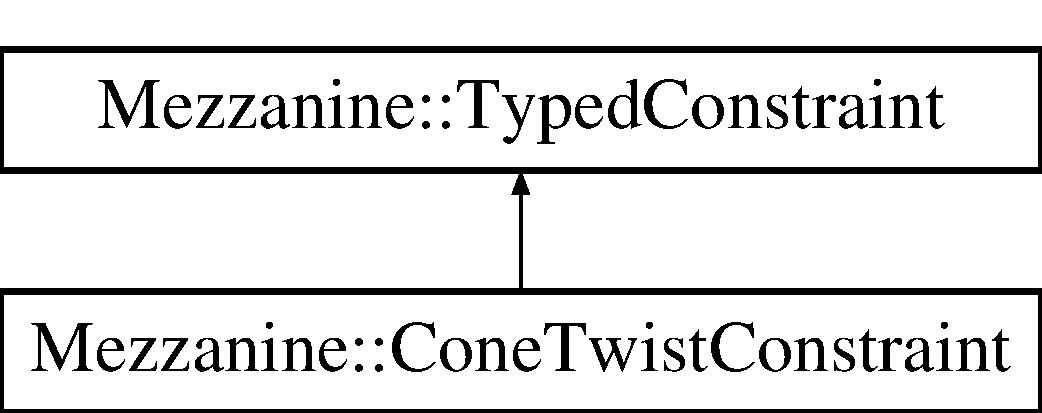
\includegraphics[height=2.000000cm]{classMezzanine_1_1ConeTwistConstraint}
\end{center}
\end{figure}
\subsubsection*{Public Member Functions}
\begin{DoxyCompactItemize}
\item 
\hypertarget{classMezzanine_1_1ConeTwistConstraint_ade6711300f4f4622f49752cfcbf81494}{
{\bfseries ConeTwistConstraint} (\hyperlink{classMezzanine_1_1ActorRigid}{ActorRigid} $\ast$ActorA, \hyperlink{classMezzanine_1_1ActorRigid}{ActorRigid} $\ast$ActorB, const \hyperlink{classMezzanine_1_1Vector3}{Vector3} \&VectorA, const \hyperlink{classMezzanine_1_1Vector3}{Vector3} \&Vectorb, const \hyperlink{classMezzanine_1_1Quaternion}{Quaternion} \&QuaternionA, const \hyperlink{classMezzanine_1_1Quaternion}{Quaternion} \&QuaternionB)}
\label{classMezzanine_1_1ConeTwistConstraint_ade6711300f4f4622f49752cfcbf81494}

\item 
\hypertarget{classMezzanine_1_1ConeTwistConstraint_ac875c5b0481a945f314bd3ea54c872f8}{
{\bfseries ConeTwistConstraint} (\hyperlink{classMezzanine_1_1ActorRigid}{ActorRigid} $\ast$ActorA, const \hyperlink{classMezzanine_1_1Vector3}{Vector3} \&VectorA, const \hyperlink{classMezzanine_1_1Quaternion}{Quaternion} \&QuaternionA)}
\label{classMezzanine_1_1ConeTwistConstraint_ac875c5b0481a945f314bd3ea54c872f8}

\item 
\hypertarget{classMezzanine_1_1ConeTwistConstraint_a83208911e81d36201375e6a9f8b21d1d}{
virtual void {\bfseries EnableMotor} (bool Enable)}
\label{classMezzanine_1_1ConeTwistConstraint_a83208911e81d36201375e6a9f8b21d1d}

\item 
virtual btTypedConstraint $\ast$ \hyperlink{classMezzanine_1_1ConeTwistConstraint_a4b478db86131128394899dca6c2191aa}{GetConstraintBase} () const 
\item 
\hypertarget{classMezzanine_1_1ConeTwistConstraint_a62d162e8083c50e5b74219de6578d2ea}{
virtual bool {\bfseries IsPassedSwingLimit} ()}
\label{classMezzanine_1_1ConeTwistConstraint_a62d162e8083c50e5b74219de6578d2ea}

\item 
\hypertarget{classMezzanine_1_1ConeTwistConstraint_ac62fe78e15e9aba7970f0101c1e77a66}{
virtual void {\bfseries SetAngularOnly} (bool AngularOnly)}
\label{classMezzanine_1_1ConeTwistConstraint_ac62fe78e15e9aba7970f0101c1e77a66}

\item 
\hypertarget{classMezzanine_1_1ConeTwistConstraint_ae658cd9f534edb059f71207ebbfc4d5e}{
virtual void {\bfseries SetDamping} (\hyperlink{namespaceMezzanine_a726731b1a7df72bf3583e4a97282c6f6}{Real} Damping)}
\label{classMezzanine_1_1ConeTwistConstraint_ae658cd9f534edb059f71207ebbfc4d5e}

\item 
\hypertarget{classMezzanine_1_1ConeTwistConstraint_a9dce3882c2b7c0e39c5c0f853eaebdbb}{
virtual void {\bfseries SetFixThresh} (\hyperlink{namespaceMezzanine_a726731b1a7df72bf3583e4a97282c6f6}{Real} FixThresh)}
\label{classMezzanine_1_1ConeTwistConstraint_a9dce3882c2b7c0e39c5c0f853eaebdbb}

\item 
\hypertarget{classMezzanine_1_1ConeTwistConstraint_a47a14d53ec762f31fd6b015a56d0b880}{
virtual void {\bfseries SetLimit} (int LimitIndex, \hyperlink{namespaceMezzanine_a726731b1a7df72bf3583e4a97282c6f6}{Real} LimitValue)}
\label{classMezzanine_1_1ConeTwistConstraint_a47a14d53ec762f31fd6b015a56d0b880}

\item 
\hypertarget{classMezzanine_1_1ConeTwistConstraint_ab9d51bbaf3421cde1bc715a16ee94fbb}{
virtual void {\bfseries SetLimit} (\hyperlink{namespaceMezzanine_a726731b1a7df72bf3583e4a97282c6f6}{Real} SwingSpan1, \hyperlink{namespaceMezzanine_a726731b1a7df72bf3583e4a97282c6f6}{Real} SwingSpan2, \hyperlink{namespaceMezzanine_a726731b1a7df72bf3583e4a97282c6f6}{Real} Twistspan, \hyperlink{namespaceMezzanine_a726731b1a7df72bf3583e4a97282c6f6}{Real} Softness=1.0, \hyperlink{namespaceMezzanine_a726731b1a7df72bf3583e4a97282c6f6}{Real} BiasFactor=0.3, \hyperlink{namespaceMezzanine_a726731b1a7df72bf3583e4a97282c6f6}{Real} RelaxationFactor=1.0)}
\label{classMezzanine_1_1ConeTwistConstraint_ab9d51bbaf3421cde1bc715a16ee94fbb}

\item 
\hypertarget{classMezzanine_1_1ConeTwistConstraint_a7f543e26fbc5e07f651e4f9c0a39292c}{
virtual void {\bfseries SetMaxMotorImpulse} (\hyperlink{namespaceMezzanine_a726731b1a7df72bf3583e4a97282c6f6}{Real} MaxMotorImpulse)}
\label{classMezzanine_1_1ConeTwistConstraint_a7f543e26fbc5e07f651e4f9c0a39292c}

\item 
\hypertarget{classMezzanine_1_1ConeTwistConstraint_aaa80fb80e821863266a5db5842978ae7}{
virtual void {\bfseries SetMaxMotorImpulseNormalized} (\hyperlink{namespaceMezzanine_a726731b1a7df72bf3583e4a97282c6f6}{Real} MaxMotorImpulse)}
\label{classMezzanine_1_1ConeTwistConstraint_aaa80fb80e821863266a5db5842978ae7}

\item 
\hypertarget{classMezzanine_1_1ConeTwistConstraint_ad831add9b4879c3f3a174ec5f03908f0}{
virtual void {\bfseries SetMotorTarget} (const \hyperlink{classMezzanine_1_1Quaternion}{Quaternion} \&Quat)}
\label{classMezzanine_1_1ConeTwistConstraint_ad831add9b4879c3f3a174ec5f03908f0}

\item 
\hypertarget{classMezzanine_1_1ConeTwistConstraint_a846d9d18b94603b3fcc8fb83510d4510}{
virtual void {\bfseries SetMotorTargetInConstraintSpace} (const \hyperlink{classMezzanine_1_1Quaternion}{Quaternion} \&Quat)}
\label{classMezzanine_1_1ConeTwistConstraint_a846d9d18b94603b3fcc8fb83510d4510}

\item 
virtual \hyperlink{classMezzanine_1_1ConeTwistConstraint_a69d510c9f0292b160d9f129f6d2db7f8}{$\sim$ConeTwistConstraint} ()
\begin{DoxyCompactList}\small\item\em Class destructor. \item\end{DoxyCompactList}\end{DoxyCompactItemize}
\subsubsection*{Protected Attributes}
\begin{DoxyCompactItemize}
\item 
\hypertarget{classMezzanine_1_1ConeTwistConstraint_a7920115fb30ebd57046b1966f5e61068}{
btConeTwistConstraint $\ast$ \hyperlink{classMezzanine_1_1ConeTwistConstraint_a7920115fb30ebd57046b1966f5e61068}{ConeTwist}}
\label{classMezzanine_1_1ConeTwistConstraint_a7920115fb30ebd57046b1966f5e61068}

\begin{DoxyCompactList}\small\item\em Bullet constraint that this class encapsulates. \item\end{DoxyCompactList}\end{DoxyCompactItemize}


\subsubsection{Detailed Description}
This class is currently incomplete 

Definition at line 405 of file constraint.h.



\subsubsection{Constructor \& Destructor Documentation}
\hypertarget{classMezzanine_1_1ConeTwistConstraint_a69d510c9f0292b160d9f129f6d2db7f8}{
\index{Mezzanine::ConeTwistConstraint@{Mezzanine::ConeTwistConstraint}!$\sim$ConeTwistConstraint@{$\sim$ConeTwistConstraint}}
\index{$\sim$ConeTwistConstraint@{$\sim$ConeTwistConstraint}!Mezzanine::ConeTwistConstraint@{Mezzanine::ConeTwistConstraint}}
\paragraph[{$\sim$ConeTwistConstraint}]{\setlength{\rightskip}{0pt plus 5cm}virtual Mezzanine::ConeTwistConstraint::$\sim$ConeTwistConstraint (
\begin{DoxyParamCaption}
{}
\end{DoxyParamCaption}
)\hspace{0.3cm}{\ttfamily  \mbox{[}virtual\mbox{]}}}\hfill}
\label{classMezzanine_1_1ConeTwistConstraint_a69d510c9f0292b160d9f129f6d2db7f8}


Class destructor. 

The class destructor. 

\subsubsection{Member Function Documentation}
\hypertarget{classMezzanine_1_1ConeTwistConstraint_a4b478db86131128394899dca6c2191aa}{
\index{Mezzanine::ConeTwistConstraint@{Mezzanine::ConeTwistConstraint}!GetConstraintBase@{GetConstraintBase}}
\index{GetConstraintBase@{GetConstraintBase}!Mezzanine::ConeTwistConstraint@{Mezzanine::ConeTwistConstraint}}
\paragraph[{GetConstraintBase}]{\setlength{\rightskip}{0pt plus 5cm}virtual btTypedConstraint$\ast$ Mezzanine::ConeTwistConstraint::GetConstraintBase (
\begin{DoxyParamCaption}
{}
\end{DoxyParamCaption}
) const\hspace{0.3cm}{\ttfamily  \mbox{[}virtual\mbox{]}}}\hfill}
\label{classMezzanine_1_1ConeTwistConstraint_a4b478db86131128394899dca6c2191aa}
Get the Bullet constraint that this class encapsulates. 

\begin{DoxyReturn}{Returns}
A pointer to the btTypedConstraint that stores the underlying constraint. 
\end{DoxyReturn}
 

Implements \hyperlink{classMezzanine_1_1TypedConstraint_a7aa13fc4448cf1fc32673bde4ec84767}{Mezzanine::TypedConstraint}.



The documentation for this class was generated from the following file:\begin{DoxyCompactItemize}
\item 
constraint.h\end{DoxyCompactItemize}

\hypertarget{classMezzanine_1_1ConvexHullCollisionShape}{
\subsection{Mezzanine::ConvexHullCollisionShape Class Reference}
\label{classMezzanine_1_1ConvexHullCollisionShape}\index{Mezzanine::ConvexHullCollisionShape@{Mezzanine::ConvexHullCollisionShape}}
}


A simple convex shape built from a low number of points in local space.  




{\ttfamily \#include $<$collisionshape.h$>$}

Inheritance diagram for Mezzanine::ConvexHullCollisionShape:\begin{figure}[H]
\begin{center}
\leavevmode
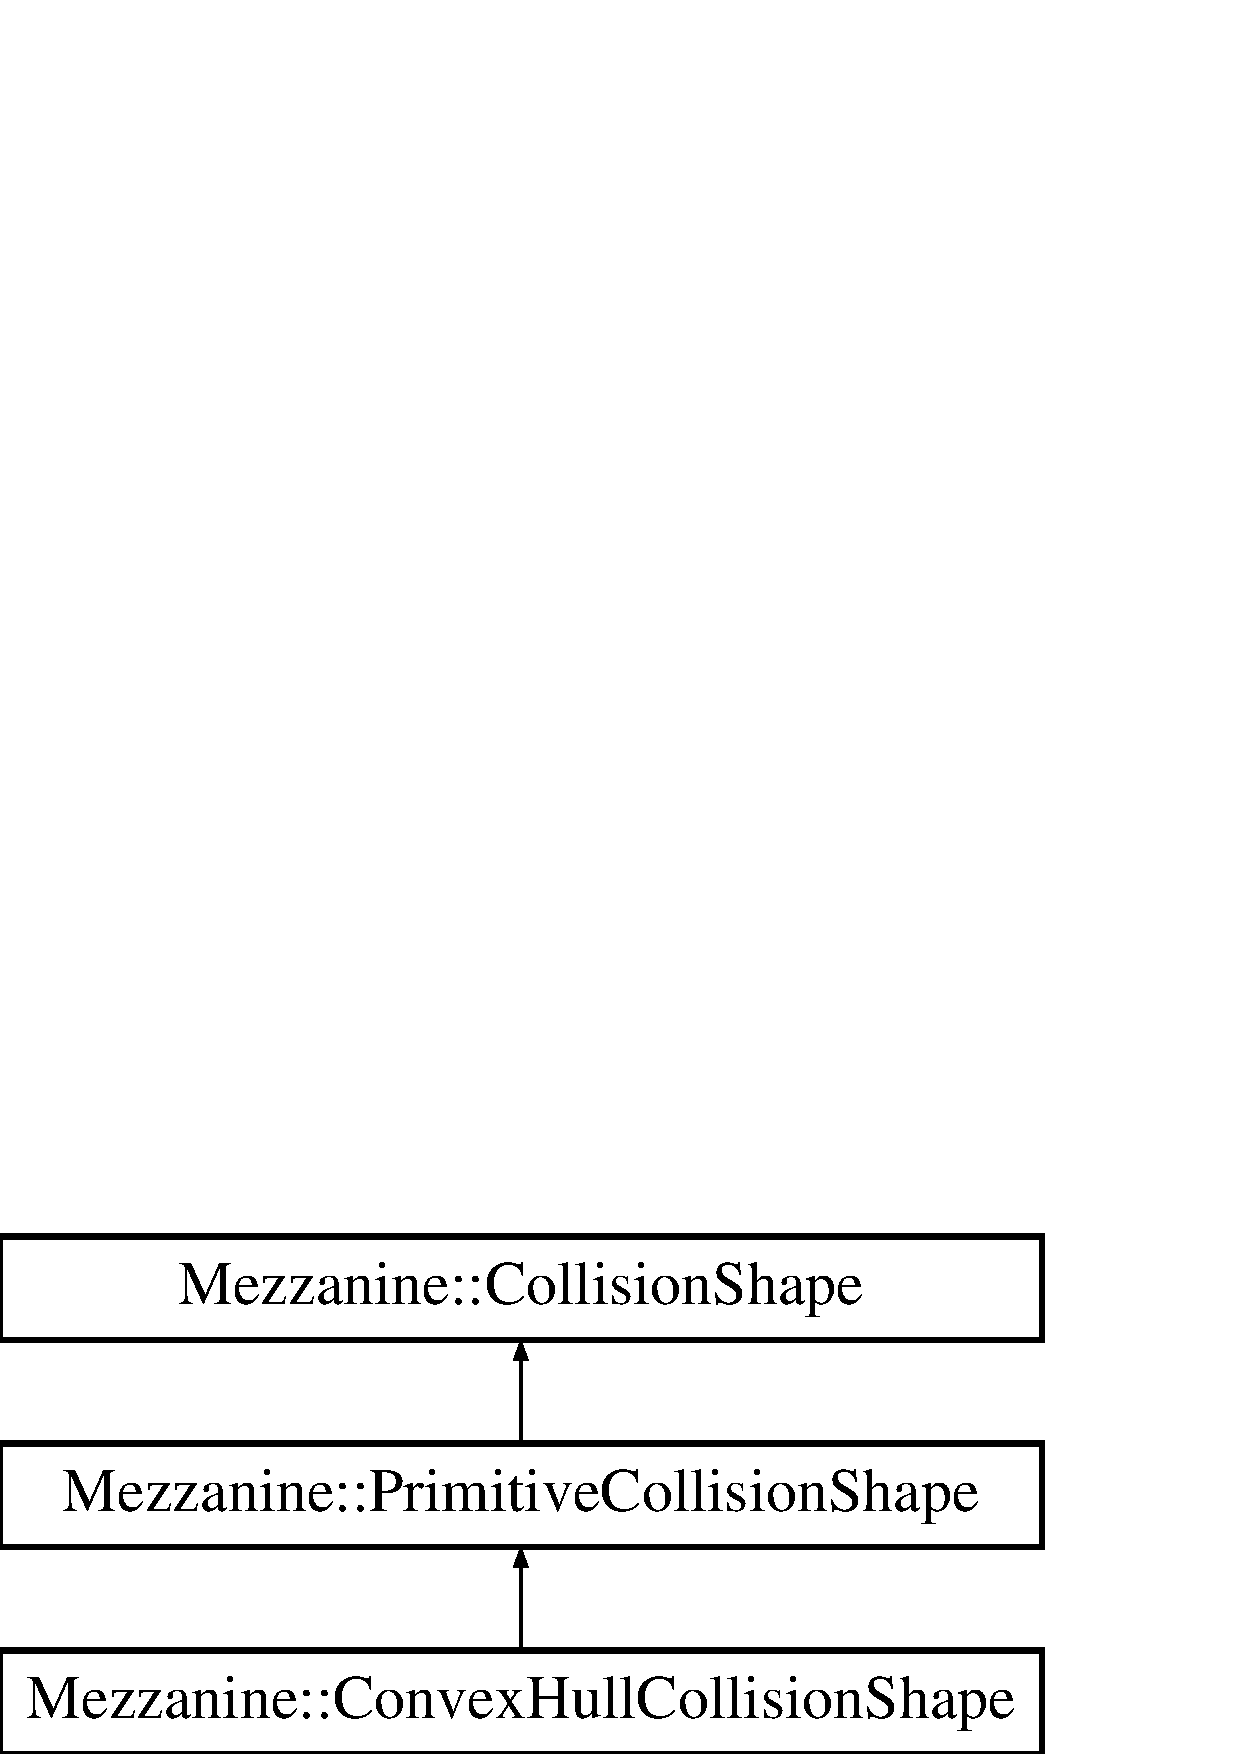
\includegraphics[height=3.000000cm]{classMezzanine_1_1ConvexHullCollisionShape}
\end{center}
\end{figure}
\subsubsection*{Public Member Functions}
\begin{DoxyCompactItemize}
\item 
virtual void \hyperlink{classMezzanine_1_1ConvexHullCollisionShape_a6e6f3da8515bfd2b1d33563e86f3ed1e}{AddPoint} (const \hyperlink{classMezzanine_1_1Vector3}{Vector3} \&Point)
\begin{DoxyCompactList}\small\item\em Adds a point to this shape. \item\end{DoxyCompactList}\item 
\hyperlink{classMezzanine_1_1ConvexHullCollisionShape_a73119a35d5ba1e5cfebde7d58f894889}{ConvexHullCollisionShape} (const \hyperlink{namespaceMezzanine_acf9fcc130e6ebf08e3d8491aebcf1c86}{String} \&\hyperlink{classMezzanine_1_1CollisionShape_aac524c5c56fa4d158bc071f8aecfbe79}{Name}, const std::vector$<$ \hyperlink{classMezzanine_1_1Vector3}{Vector3} $>$ \&Points)
\begin{DoxyCompactList}\small\item\em Class Constructor. \item\end{DoxyCompactList}\item 
\hyperlink{classMezzanine_1_1ConvexHullCollisionShape_a100c6b3009ad46976a0484446a3d5da2}{ConvexHullCollisionShape} (const \hyperlink{namespaceMezzanine_acf9fcc130e6ebf08e3d8491aebcf1c86}{String} \&\hyperlink{classMezzanine_1_1CollisionShape_aac524c5c56fa4d158bc071f8aecfbe79}{Name}, btConvexHullShape $\ast$BulletShape)
\begin{DoxyCompactList}\small\item\em Internal Constructor. \item\end{DoxyCompactList}\item 
virtual btConvexHullShape $\ast$ \hyperlink{classMezzanine_1_1ConvexHullCollisionShape_a35acc9fd0c3e990bcacf1caf6d65a094}{GetBulletHullShape} () const 
\item 
virtual \hyperlink{namespaceMezzanine_adcbb6ce6d1eb4379d109e51171e2e493}{Whole} \hyperlink{classMezzanine_1_1ConvexHullCollisionShape_a8eaf9dccce90a9366d37ab9112bc0f22}{GetNumPoints} () const 
\begin{DoxyCompactList}\small\item\em Gets the total number of points being stored in this shape. \item\end{DoxyCompactList}\item 
virtual \hyperlink{classMezzanine_1_1Vector3}{Vector3} \hyperlink{classMezzanine_1_1ConvexHullCollisionShape_a7f769cdc76fb7c62060a28472277466d}{GetPoint} (const \hyperlink{namespaceMezzanine_adcbb6ce6d1eb4379d109e51171e2e493}{Whole} \&Index) const 
\begin{DoxyCompactList}\small\item\em Gets a stored point as it is scaled in this ConvexHull. \item\end{DoxyCompactList}\item 
virtual \hyperlink{classMezzanine_1_1CollisionShape_ad04186055565998879b64176d6dd100d}{CollisionShape::ShapeType} \hyperlink{classMezzanine_1_1ConvexHullCollisionShape_a73ccd6364f52a68a642a0fb55159f020}{GetType} () const 
\item 
virtual \hyperlink{classMezzanine_1_1Vector3}{Vector3} \hyperlink{classMezzanine_1_1ConvexHullCollisionShape_a28e1633a760562ceb8427c08232518d7}{GetUnscaledPoint} (const \hyperlink{namespaceMezzanine_adcbb6ce6d1eb4379d109e51171e2e493}{Whole} \&Index) const 
\begin{DoxyCompactList}\small\item\em Gets an unscaled stored point in this ConvexHull. \item\end{DoxyCompactList}\item 
virtual bool \hyperlink{classMezzanine_1_1ConvexHullCollisionShape_a6aa3c6afad74091dec9c933eef257301}{IsInside} (const \hyperlink{classMezzanine_1_1Vector3}{Vector3} \&Location, const \hyperlink{namespaceMezzanine_a726731b1a7df72bf3583e4a97282c6f6}{Real} \&Tolerance) const 
\begin{DoxyCompactList}\small\item\em Checks to see if a point in local space is inside this shape. \item\end{DoxyCompactList}\item 
\hypertarget{classMezzanine_1_1ConvexHullCollisionShape_ae6c30c38604747a2d2500b25d88de50e}{
virtual \hyperlink{classMezzanine_1_1ConvexHullCollisionShape_ae6c30c38604747a2d2500b25d88de50e}{$\sim$ConvexHullCollisionShape} ()}
\label{classMezzanine_1_1ConvexHullCollisionShape_ae6c30c38604747a2d2500b25d88de50e}

\begin{DoxyCompactList}\small\item\em Class Destructor. \item\end{DoxyCompactList}\end{DoxyCompactItemize}


\subsubsection{Detailed Description}
A simple convex shape built from a low number of points in local space. A convex hull is commonly used to generate a simple approximation of another, and more complicated, shape. Usually the number of points in a convex hull doesn't exceed 32. \par
 \par
 When a convex hull is generated automatically from an algorithm, the best way to think of the resulting shape in relation to the original shape is if you were to wrap a rubber band around it on one plane. Then do this for all planes and all surfaces. The resulting shape looks and behaves similar to that. 

Definition at line 580 of file collisionshape.h.



\subsubsection{Constructor \& Destructor Documentation}
\hypertarget{classMezzanine_1_1ConvexHullCollisionShape_a73119a35d5ba1e5cfebde7d58f894889}{
\index{Mezzanine::ConvexHullCollisionShape@{Mezzanine::ConvexHullCollisionShape}!ConvexHullCollisionShape@{ConvexHullCollisionShape}}
\index{ConvexHullCollisionShape@{ConvexHullCollisionShape}!Mezzanine::ConvexHullCollisionShape@{Mezzanine::ConvexHullCollisionShape}}
\paragraph[{ConvexHullCollisionShape}]{\setlength{\rightskip}{0pt plus 5cm}Mezzanine::ConvexHullCollisionShape::ConvexHullCollisionShape (
\begin{DoxyParamCaption}
\item[{const {\bf String} \&}]{Name, }
\item[{const std::vector$<$ {\bf Vector3} $>$ \&}]{Points}
\end{DoxyParamCaption}
)}\hfill}
\label{classMezzanine_1_1ConvexHullCollisionShape_a73119a35d5ba1e5cfebde7d58f894889}


Class Constructor. 


\begin{DoxyParams}{Parameters}
{\em Name} & The name of this Shape. \\
\hline
{\em Points} & A vector of vector3's containing all the points in local space to construct this shape from. \\
\hline
\end{DoxyParams}


Definition at line 941 of file collisionshape.cpp.

\hypertarget{classMezzanine_1_1ConvexHullCollisionShape_a100c6b3009ad46976a0484446a3d5da2}{
\index{Mezzanine::ConvexHullCollisionShape@{Mezzanine::ConvexHullCollisionShape}!ConvexHullCollisionShape@{ConvexHullCollisionShape}}
\index{ConvexHullCollisionShape@{ConvexHullCollisionShape}!Mezzanine::ConvexHullCollisionShape@{Mezzanine::ConvexHullCollisionShape}}
\paragraph[{ConvexHullCollisionShape}]{\setlength{\rightskip}{0pt plus 5cm}Mezzanine::ConvexHullCollisionShape::ConvexHullCollisionShape (
\begin{DoxyParamCaption}
\item[{const {\bf String} \&}]{Name, }
\item[{btConvexHullShape $\ast$}]{BulletShape}
\end{DoxyParamCaption}
)}\hfill}
\label{classMezzanine_1_1ConvexHullCollisionShape_a100c6b3009ad46976a0484446a3d5da2}


Internal Constructor. 


\begin{DoxyParams}{Parameters}
{\em Name} & The name of this Shape. \\
\hline
{\em BulletShape} & The internal shape this shape is based on. \\
\hline
\end{DoxyParams}


Definition at line 957 of file collisionshape.cpp.



\subsubsection{Member Function Documentation}
\hypertarget{classMezzanine_1_1ConvexHullCollisionShape_a6e6f3da8515bfd2b1d33563e86f3ed1e}{
\index{Mezzanine::ConvexHullCollisionShape@{Mezzanine::ConvexHullCollisionShape}!AddPoint@{AddPoint}}
\index{AddPoint@{AddPoint}!Mezzanine::ConvexHullCollisionShape@{Mezzanine::ConvexHullCollisionShape}}
\paragraph[{AddPoint}]{\setlength{\rightskip}{0pt plus 5cm}void Mezzanine::ConvexHullCollisionShape::AddPoint (
\begin{DoxyParamCaption}
\item[{const {\bf Vector3} \&}]{Point}
\end{DoxyParamCaption}
)\hspace{0.3cm}{\ttfamily  \mbox{[}virtual\mbox{]}}}\hfill}
\label{classMezzanine_1_1ConvexHullCollisionShape_a6e6f3da8515bfd2b1d33563e86f3ed1e}


Adds a point to this shape. 


\begin{DoxyParams}{Parameters}
{\em Point} & The location in local space to be added. \\
\hline
\end{DoxyParams}


Definition at line 988 of file collisionshape.cpp.

\hypertarget{classMezzanine_1_1ConvexHullCollisionShape_a35acc9fd0c3e990bcacf1caf6d65a094}{
\index{Mezzanine::ConvexHullCollisionShape@{Mezzanine::ConvexHullCollisionShape}!GetBulletHullShape@{GetBulletHullShape}}
\index{GetBulletHullShape@{GetBulletHullShape}!Mezzanine::ConvexHullCollisionShape@{Mezzanine::ConvexHullCollisionShape}}
\paragraph[{GetBulletHullShape}]{\setlength{\rightskip}{0pt plus 5cm}btConvexHullShape $\ast$ Mezzanine::ConvexHullCollisionShape::GetBulletHullShape (
\begin{DoxyParamCaption}
{}
\end{DoxyParamCaption}
) const\hspace{0.3cm}{\ttfamily  \mbox{[}virtual\mbox{]}}}\hfill}
\label{classMezzanine_1_1ConvexHullCollisionShape_a35acc9fd0c3e990bcacf1caf6d65a094}
Gets the internal shape pointer this collision shape is based on. 

\begin{DoxyReturn}{Returns}
Returns a pointer to the internal collision shape. 
\end{DoxyReturn}
 

Definition at line 1019 of file collisionshape.cpp.

\hypertarget{classMezzanine_1_1ConvexHullCollisionShape_a8eaf9dccce90a9366d37ab9112bc0f22}{
\index{Mezzanine::ConvexHullCollisionShape@{Mezzanine::ConvexHullCollisionShape}!GetNumPoints@{GetNumPoints}}
\index{GetNumPoints@{GetNumPoints}!Mezzanine::ConvexHullCollisionShape@{Mezzanine::ConvexHullCollisionShape}}
\paragraph[{GetNumPoints}]{\setlength{\rightskip}{0pt plus 5cm}{\bf Whole} Mezzanine::ConvexHullCollisionShape::GetNumPoints (
\begin{DoxyParamCaption}
{}
\end{DoxyParamCaption}
) const\hspace{0.3cm}{\ttfamily  \mbox{[}virtual\mbox{]}}}\hfill}
\label{classMezzanine_1_1ConvexHullCollisionShape_a8eaf9dccce90a9366d37ab9112bc0f22}


Gets the total number of points being stored in this shape. 

\begin{DoxyReturn}{Returns}
Returns a whole representing the current number of points in this shape. 
\end{DoxyReturn}


Definition at line 1004 of file collisionshape.cpp.

\hypertarget{classMezzanine_1_1ConvexHullCollisionShape_a7f769cdc76fb7c62060a28472277466d}{
\index{Mezzanine::ConvexHullCollisionShape@{Mezzanine::ConvexHullCollisionShape}!GetPoint@{GetPoint}}
\index{GetPoint@{GetPoint}!Mezzanine::ConvexHullCollisionShape@{Mezzanine::ConvexHullCollisionShape}}
\paragraph[{GetPoint}]{\setlength{\rightskip}{0pt plus 5cm}{\bf Vector3} Mezzanine::ConvexHullCollisionShape::GetPoint (
\begin{DoxyParamCaption}
\item[{const {\bf Whole} \&}]{Index}
\end{DoxyParamCaption}
) const\hspace{0.3cm}{\ttfamily  \mbox{[}virtual\mbox{]}}}\hfill}
\label{classMezzanine_1_1ConvexHullCollisionShape_a7f769cdc76fb7c62060a28472277466d}


Gets a stored point as it is scaled in this ConvexHull. 

\begin{DoxyReturn}{Returns}
Returns a \hyperlink{classMezzanine_1_1Vector3}{Vector3} representing the scaled location in local space of the specified point. 
\end{DoxyReturn}

\begin{DoxyParams}{Parameters}
{\em Index} & The index of the point desired. \\
\hline
\end{DoxyParams}


Definition at line 999 of file collisionshape.cpp.

\hypertarget{classMezzanine_1_1ConvexHullCollisionShape_a73ccd6364f52a68a642a0fb55159f020}{
\index{Mezzanine::ConvexHullCollisionShape@{Mezzanine::ConvexHullCollisionShape}!GetType@{GetType}}
\index{GetType@{GetType}!Mezzanine::ConvexHullCollisionShape@{Mezzanine::ConvexHullCollisionShape}}
\paragraph[{GetType}]{\setlength{\rightskip}{0pt plus 5cm}{\bf CollisionShape::ShapeType} Mezzanine::ConvexHullCollisionShape::GetType (
\begin{DoxyParamCaption}
{}
\end{DoxyParamCaption}
) const\hspace{0.3cm}{\ttfamily  \mbox{[}virtual\mbox{]}}}\hfill}
\label{classMezzanine_1_1ConvexHullCollisionShape_a73ccd6364f52a68a642a0fb55159f020}
Gets the type of \hyperlink{classMezzanine_1_1Collision}{Collision} shape this is. 

\begin{DoxyReturn}{Returns}
Returns an enum value indicating the type of collision shape this is. 
\end{DoxyReturn}
 

Implements \hyperlink{classMezzanine_1_1PrimitiveCollisionShape_ad3d4143a5640204b987e0b57eb24af41}{Mezzanine::PrimitiveCollisionShape}.



Definition at line 1014 of file collisionshape.cpp.

\hypertarget{classMezzanine_1_1ConvexHullCollisionShape_a28e1633a760562ceb8427c08232518d7}{
\index{Mezzanine::ConvexHullCollisionShape@{Mezzanine::ConvexHullCollisionShape}!GetUnscaledPoint@{GetUnscaledPoint}}
\index{GetUnscaledPoint@{GetUnscaledPoint}!Mezzanine::ConvexHullCollisionShape@{Mezzanine::ConvexHullCollisionShape}}
\paragraph[{GetUnscaledPoint}]{\setlength{\rightskip}{0pt plus 5cm}{\bf Vector3} Mezzanine::ConvexHullCollisionShape::GetUnscaledPoint (
\begin{DoxyParamCaption}
\item[{const {\bf Whole} \&}]{Index}
\end{DoxyParamCaption}
) const\hspace{0.3cm}{\ttfamily  \mbox{[}virtual\mbox{]}}}\hfill}
\label{classMezzanine_1_1ConvexHullCollisionShape_a28e1633a760562ceb8427c08232518d7}


Gets an unscaled stored point in this ConvexHull. 

\begin{DoxyReturn}{Returns}
Returns a \hyperlink{classMezzanine_1_1Vector3}{Vector3} representing the unscaled location in local space of the specified point. 
\end{DoxyReturn}

\begin{DoxyParams}{Parameters}
{\em Index} & The index of the point desired. \\
\hline
\end{DoxyParams}


Definition at line 993 of file collisionshape.cpp.

\hypertarget{classMezzanine_1_1ConvexHullCollisionShape_a6aa3c6afad74091dec9c933eef257301}{
\index{Mezzanine::ConvexHullCollisionShape@{Mezzanine::ConvexHullCollisionShape}!IsInside@{IsInside}}
\index{IsInside@{IsInside}!Mezzanine::ConvexHullCollisionShape@{Mezzanine::ConvexHullCollisionShape}}
\paragraph[{IsInside}]{\setlength{\rightskip}{0pt plus 5cm}bool Mezzanine::ConvexHullCollisionShape::IsInside (
\begin{DoxyParamCaption}
\item[{const {\bf Vector3} \&}]{Location, }
\item[{const {\bf Real} \&}]{Tolerance}
\end{DoxyParamCaption}
) const\hspace{0.3cm}{\ttfamily  \mbox{[}virtual\mbox{]}}}\hfill}
\label{classMezzanine_1_1ConvexHullCollisionShape_a6aa3c6afad74091dec9c933eef257301}


Checks to see if a point in local space is inside this shape. 

\begin{DoxyReturn}{Returns}
Returns a bool indicating whether or not the specified point is inside the shape. 
\end{DoxyReturn}

\begin{DoxyParams}{Parameters}
{\em Location} & The specified point to perform the check. \\
\hline
{\em Tolerance} & The amount of leeway to give in the check. If the distance from the specified point is equal or less then the Tolorance provided then this will return true. \\
\hline
\end{DoxyParams}


Definition at line 1009 of file collisionshape.cpp.



The documentation for this class was generated from the following files:\begin{DoxyCompactItemize}
\item 
collisionshape.h\item 
collisionshape.cpp\end{DoxyCompactItemize}

\hypertarget{classMezzanine_1_1CylinderCollisionShape}{
\subsection{Mezzanine::CylinderCollisionShape Class Reference}
\label{classMezzanine_1_1CylinderCollisionShape}\index{Mezzanine::CylinderCollisionShape@{Mezzanine::CylinderCollisionShape}}
}


A cylinder physics shape.  




{\ttfamily \#include $<$collisionshape.h$>$}

Inheritance diagram for Mezzanine::CylinderCollisionShape:\begin{figure}[H]
\begin{center}
\leavevmode
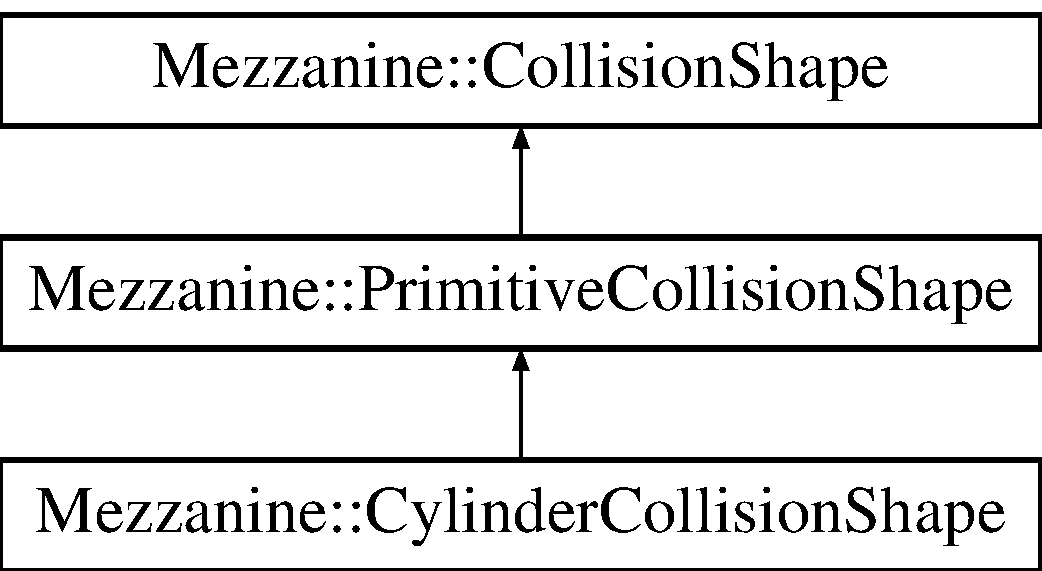
\includegraphics[height=3.000000cm]{classMezzanine_1_1CylinderCollisionShape}
\end{center}
\end{figure}
\subsubsection*{Public Member Functions}
\begin{DoxyCompactItemize}
\item 
\hyperlink{classMezzanine_1_1CylinderCollisionShape_a78818b9e27ed8f144469e268c53dab52}{CylinderCollisionShape} (const \hyperlink{namespaceMezzanine_acf9fcc130e6ebf08e3d8491aebcf1c86}{String} \&\hyperlink{classMezzanine_1_1CollisionShape_aac524c5c56fa4d158bc071f8aecfbe79}{Name}, const \hyperlink{namespaceMezzanine_a726731b1a7df72bf3583e4a97282c6f6}{Real} \&Radius, const \hyperlink{namespaceMezzanine_a726731b1a7df72bf3583e4a97282c6f6}{Real} \&Height, const \hyperlink{classMezzanine_1_1Vector3}{Vector3} \&UpAxis)
\begin{DoxyCompactList}\small\item\em Verbose Vector Constructor. \item\end{DoxyCompactList}\item 
\hyperlink{classMezzanine_1_1CylinderCollisionShape_ad01053f772e3e121aa1e43252f43d3f6}{CylinderCollisionShape} (const \hyperlink{namespaceMezzanine_acf9fcc130e6ebf08e3d8491aebcf1c86}{String} \&\hyperlink{classMezzanine_1_1CollisionShape_aac524c5c56fa4d158bc071f8aecfbe79}{Name}, const \hyperlink{namespaceMezzanine_a726731b1a7df72bf3583e4a97282c6f6}{Real} \&Radius, const \hyperlink{namespaceMezzanine_a726731b1a7df72bf3583e4a97282c6f6}{Real} \&Height, \hyperlink{namespaceMezzanine_ab41a00a8c6a47b576dc987ec34e16ba1}{StandardAxis} UpAxis)
\begin{DoxyCompactList}\small\item\em Verbose Constructor. \item\end{DoxyCompactList}\item 
\hyperlink{classMezzanine_1_1CylinderCollisionShape_ab0bcf2460a915f1a0276ee451a563e56}{CylinderCollisionShape} (const \hyperlink{namespaceMezzanine_acf9fcc130e6ebf08e3d8491aebcf1c86}{String} \&\hyperlink{classMezzanine_1_1CollisionShape_aac524c5c56fa4d158bc071f8aecfbe79}{Name}, const \hyperlink{classMezzanine_1_1Vector3}{Vector3} \&HalfExtents, \hyperlink{namespaceMezzanine_ab41a00a8c6a47b576dc987ec34e16ba1}{StandardAxis} UpAxis)
\begin{DoxyCompactList}\small\item\em Terse Constructor. \item\end{DoxyCompactList}\item 
\hyperlink{classMezzanine_1_1CylinderCollisionShape_a5f1765f49d8c7f48df29264314bd8c5a}{CylinderCollisionShape} (const \hyperlink{namespaceMezzanine_acf9fcc130e6ebf08e3d8491aebcf1c86}{String} \&\hyperlink{classMezzanine_1_1CollisionShape_aac524c5c56fa4d158bc071f8aecfbe79}{Name}, btCylinderShape $\ast$BulletShape)
\begin{DoxyCompactList}\small\item\em Internal Constructor. \item\end{DoxyCompactList}\item 
\hyperlink{classMezzanine_1_1CylinderCollisionShape_a541f91adac5f553466fc3e2d2445ed78}{CylinderCollisionShape} (const \hyperlink{namespaceMezzanine_acf9fcc130e6ebf08e3d8491aebcf1c86}{String} \&\hyperlink{classMezzanine_1_1CollisionShape_aac524c5c56fa4d158bc071f8aecfbe79}{Name}, const \hyperlink{classMezzanine_1_1Vector3}{Vector3} \&HalfExtents, const \hyperlink{classMezzanine_1_1Vector3}{Vector3} \&UpAxis)
\begin{DoxyCompactList}\small\item\em Terse Vector Constructor. \item\end{DoxyCompactList}\item 
virtual btCylinderShape $\ast$ \hyperlink{classMezzanine_1_1CylinderCollisionShape_a7caaf49dfee6f543aaca4c1cf6fbf5c5}{GetBulletCylinderShape} () const 
\item 
virtual \hyperlink{classMezzanine_1_1Vector3}{Vector3} \hyperlink{classMezzanine_1_1CylinderCollisionShape_a4184b98934573f5dae1ed34578dc18c0}{GetHalfExtents} () const 
\begin{DoxyCompactList}\small\item\em Gets the half extents used to construct this cylinder. \item\end{DoxyCompactList}\item 
virtual \hyperlink{classMezzanine_1_1Vector3}{Vector3} \hyperlink{classMezzanine_1_1CylinderCollisionShape_a9b16715071eaa8827162a8ea36132a23}{GetHalfExtentsWithMargin} () const 
\begin{DoxyCompactList}\small\item\em Gets the half extents with padding. \item\end{DoxyCompactList}\item 
virtual \hyperlink{namespaceMezzanine_a726731b1a7df72bf3583e4a97282c6f6}{Real} \hyperlink{classMezzanine_1_1CylinderCollisionShape_a3f62cb0c30122784088e0f9cbbf3c798}{GetRadius} () const 
\begin{DoxyCompactList}\small\item\em Gets the radius of the cylinder. \item\end{DoxyCompactList}\item 
virtual \hyperlink{classMezzanine_1_1CollisionShape_ad04186055565998879b64176d6dd100d}{CollisionShape::ShapeType} \hyperlink{classMezzanine_1_1CylinderCollisionShape_a4feb07a9d71bda6ca4b6c82b745df8a0}{GetType} () const 
\item 
virtual \hyperlink{classMezzanine_1_1Vector3}{Vector3} \hyperlink{classMezzanine_1_1CylinderCollisionShape_a4c99a3d61ba0a4cbeb2df3d54e625541}{GetUpAxis} () const 
\begin{DoxyCompactList}\small\item\em Gets which axis this cylinder is oriented along. \item\end{DoxyCompactList}\item 
\hypertarget{classMezzanine_1_1CylinderCollisionShape_a6479b7afe2caab5b4682903ea6a1bee5}{
virtual \hyperlink{classMezzanine_1_1CylinderCollisionShape_a6479b7afe2caab5b4682903ea6a1bee5}{$\sim$CylinderCollisionShape} ()}
\label{classMezzanine_1_1CylinderCollisionShape_a6479b7afe2caab5b4682903ea6a1bee5}

\begin{DoxyCompactList}\small\item\em Class Destructor. \item\end{DoxyCompactList}\end{DoxyCompactItemize}
\subsubsection*{Static Public Member Functions}
\begin{DoxyCompactItemize}
\item 
static \hyperlink{classMezzanine_1_1Vector3}{Vector3} \hyperlink{classMezzanine_1_1CylinderCollisionShape_af084233b246cdf7497ed2739d9ba361e}{CreateHalfExtents} (const \hyperlink{namespaceMezzanine_a726731b1a7df72bf3583e4a97282c6f6}{Real} \&Radius, const \hyperlink{namespaceMezzanine_a726731b1a7df72bf3583e4a97282c6f6}{Real} \&Height, \hyperlink{namespaceMezzanine_ab41a00a8c6a47b576dc987ec34e16ba1}{StandardAxis} UpAxis)
\begin{DoxyCompactList}\small\item\em A (very) simple way to create a \hyperlink{classMezzanine_1_1Vector3}{Vector3} containing the Half Extents of a Cylinder with given dimenions/. \item\end{DoxyCompactList}\end{DoxyCompactItemize}
\subsubsection*{Protected Member Functions}
\begin{DoxyCompactItemize}
\item 
void \hyperlink{classMezzanine_1_1CylinderCollisionShape_ab7b1d796b02acd1a0ca35f1f609e8901}{Construct} (const \hyperlink{namespaceMezzanine_acf9fcc130e6ebf08e3d8491aebcf1c86}{String} \&\hyperlink{classMezzanine_1_1CollisionShape_aac524c5c56fa4d158bc071f8aecfbe79}{Name}, const \hyperlink{classMezzanine_1_1Vector3}{Vector3} \&HalfExtents, \hyperlink{namespaceMezzanine_ab41a00a8c6a47b576dc987ec34e16ba1}{StandardAxis} UpAxis)
\begin{DoxyCompactList}\small\item\em Does the initialization for a Cylinder. \item\end{DoxyCompactList}\item 
void \hyperlink{classMezzanine_1_1CylinderCollisionShape_a34ed7408114b3863a14f2d8ff1b1b4d7}{Construct} (const \hyperlink{namespaceMezzanine_acf9fcc130e6ebf08e3d8491aebcf1c86}{String} \&\hyperlink{classMezzanine_1_1CollisionShape_aac524c5c56fa4d158bc071f8aecfbe79}{Name}, btCylinderShape $\ast$BulletShape)
\begin{DoxyCompactList}\small\item\em Does the initialization for a Cylinder. \item\end{DoxyCompactList}\end{DoxyCompactItemize}


\subsubsection{Detailed Description}
A cylinder physics shape. A primitive cylinder shape. Like Capsules and Cones Cylinders can be aligned to any of the 3 linear axes(X, Y, or Z). 

Definition at line 644 of file collisionshape.h.



\subsubsection{Constructor \& Destructor Documentation}
\hypertarget{classMezzanine_1_1CylinderCollisionShape_a78818b9e27ed8f144469e268c53dab52}{
\index{Mezzanine::CylinderCollisionShape@{Mezzanine::CylinderCollisionShape}!CylinderCollisionShape@{CylinderCollisionShape}}
\index{CylinderCollisionShape@{CylinderCollisionShape}!Mezzanine::CylinderCollisionShape@{Mezzanine::CylinderCollisionShape}}
\paragraph[{CylinderCollisionShape}]{\setlength{\rightskip}{0pt plus 5cm}Mezzanine::CylinderCollisionShape::CylinderCollisionShape (
\begin{DoxyParamCaption}
\item[{const {\bf String} \&}]{Name, }
\item[{const {\bf Real} \&}]{Radius, }
\item[{const {\bf Real} \&}]{Height, }
\item[{const {\bf Vector3} \&}]{UpAxis}
\end{DoxyParamCaption}
)}\hfill}
\label{classMezzanine_1_1CylinderCollisionShape_a78818b9e27ed8f144469e268c53dab52}


Verbose Vector Constructor. 


\begin{DoxyParams}{Parameters}
{\em Name} & The name of this Shape. \\
\hline
{\em Radius} & The radius of the Cylinder. \\
\hline
{\em Height} & The height of the Cylinder, Height is indicated in the direction of the upAxis. \\
\hline
{\em UpAxis} & Which axis the cylinder is to be oriented along. Typical usage is for a capsule to be oriented on the Y axis(0,1,0), which would make it stand upright. \\
\hline
\end{DoxyParams}


Definition at line 1109 of file collisionshape.cpp.

\hypertarget{classMezzanine_1_1CylinderCollisionShape_ad01053f772e3e121aa1e43252f43d3f6}{
\index{Mezzanine::CylinderCollisionShape@{Mezzanine::CylinderCollisionShape}!CylinderCollisionShape@{CylinderCollisionShape}}
\index{CylinderCollisionShape@{CylinderCollisionShape}!Mezzanine::CylinderCollisionShape@{Mezzanine::CylinderCollisionShape}}
\paragraph[{CylinderCollisionShape}]{\setlength{\rightskip}{0pt plus 5cm}Mezzanine::CylinderCollisionShape::CylinderCollisionShape (
\begin{DoxyParamCaption}
\item[{const {\bf String} \&}]{Name, }
\item[{const {\bf Real} \&}]{Radius, }
\item[{const {\bf Real} \&}]{Height, }
\item[{{\bf StandardAxis}}]{UpAxis}
\end{DoxyParamCaption}
)}\hfill}
\label{classMezzanine_1_1CylinderCollisionShape_ad01053f772e3e121aa1e43252f43d3f6}


Verbose Constructor. 


\begin{DoxyParams}{Parameters}
{\em Name} & The name of this Shape. \\
\hline
{\em Radius} & The radius of the Cylinder. \\
\hline
{\em Height} & The height of the Cylinder, Height is indicated in the direction of the upAxis. \\
\hline
{\em UpAxis} & Which StandardAxis the cylinder is to be oriented along. \\
\hline
\end{DoxyParams}


Definition at line 1112 of file collisionshape.cpp.

\hypertarget{classMezzanine_1_1CylinderCollisionShape_a541f91adac5f553466fc3e2d2445ed78}{
\index{Mezzanine::CylinderCollisionShape@{Mezzanine::CylinderCollisionShape}!CylinderCollisionShape@{CylinderCollisionShape}}
\index{CylinderCollisionShape@{CylinderCollisionShape}!Mezzanine::CylinderCollisionShape@{Mezzanine::CylinderCollisionShape}}
\paragraph[{CylinderCollisionShape}]{\setlength{\rightskip}{0pt plus 5cm}Mezzanine::CylinderCollisionShape::CylinderCollisionShape (
\begin{DoxyParamCaption}
\item[{const {\bf String} \&}]{Name, }
\item[{const {\bf Vector3} \&}]{HalfExtents, }
\item[{const {\bf Vector3} \&}]{UpAxis}
\end{DoxyParamCaption}
)}\hfill}
\label{classMezzanine_1_1CylinderCollisionShape_a541f91adac5f553466fc3e2d2445ed78}


Terse Vector Constructor. 


\begin{DoxyParams}{Parameters}
{\em Name} & The name of this Shape. \\
\hline
{\em HalfExtents} & A \hyperlink{classMezzanine_1_1Vector3}{Vector3} with the Height of the cylinder on the axis corresponding to the UpAxis and the Radius store in the other two axis. \\
\hline
{\em UpAxis} & Which axis the cylinder is to be oriented along. Typical usage is for a capsule to be oriented on the Y axis(0,1,0), which would make it stand upright. \\
\hline
\end{DoxyParams}


Definition at line 1115 of file collisionshape.cpp.

\hypertarget{classMezzanine_1_1CylinderCollisionShape_ab0bcf2460a915f1a0276ee451a563e56}{
\index{Mezzanine::CylinderCollisionShape@{Mezzanine::CylinderCollisionShape}!CylinderCollisionShape@{CylinderCollisionShape}}
\index{CylinderCollisionShape@{CylinderCollisionShape}!Mezzanine::CylinderCollisionShape@{Mezzanine::CylinderCollisionShape}}
\paragraph[{CylinderCollisionShape}]{\setlength{\rightskip}{0pt plus 5cm}Mezzanine::CylinderCollisionShape::CylinderCollisionShape (
\begin{DoxyParamCaption}
\item[{const {\bf String} \&}]{Name, }
\item[{const {\bf Vector3} \&}]{HalfExtents, }
\item[{{\bf StandardAxis}}]{UpAxis}
\end{DoxyParamCaption}
)}\hfill}
\label{classMezzanine_1_1CylinderCollisionShape_ab0bcf2460a915f1a0276ee451a563e56}


Terse Constructor. 


\begin{DoxyParams}{Parameters}
{\em Name} & The name of this Shape. \\
\hline
{\em HalfExtents} & A \hyperlink{classMezzanine_1_1Vector3}{Vector3} with the Height of the cylinder on the axis corresponding to the UpAxis and the Radius store in the other two axis. \\
\hline
{\em UpAxis} & Which StandardAxis the cylinder is to be oriented along. \\
\hline
\end{DoxyParams}


Definition at line 1118 of file collisionshape.cpp.

\hypertarget{classMezzanine_1_1CylinderCollisionShape_a5f1765f49d8c7f48df29264314bd8c5a}{
\index{Mezzanine::CylinderCollisionShape@{Mezzanine::CylinderCollisionShape}!CylinderCollisionShape@{CylinderCollisionShape}}
\index{CylinderCollisionShape@{CylinderCollisionShape}!Mezzanine::CylinderCollisionShape@{Mezzanine::CylinderCollisionShape}}
\paragraph[{CylinderCollisionShape}]{\setlength{\rightskip}{0pt plus 5cm}Mezzanine::CylinderCollisionShape::CylinderCollisionShape (
\begin{DoxyParamCaption}
\item[{const {\bf String} \&}]{Name, }
\item[{btCylinderShape $\ast$}]{BulletShape}
\end{DoxyParamCaption}
)}\hfill}
\label{classMezzanine_1_1CylinderCollisionShape_a5f1765f49d8c7f48df29264314bd8c5a}


Internal Constructor. 


\begin{DoxyParams}{Parameters}
{\em Name} & The name of this Shape. \\
\hline
{\em BulletShape} & The internal shape this shape is based on. \\
\hline
\end{DoxyParams}


Definition at line 1121 of file collisionshape.cpp.



\subsubsection{Member Function Documentation}
\hypertarget{classMezzanine_1_1CylinderCollisionShape_ab7b1d796b02acd1a0ca35f1f609e8901}{
\index{Mezzanine::CylinderCollisionShape@{Mezzanine::CylinderCollisionShape}!Construct@{Construct}}
\index{Construct@{Construct}!Mezzanine::CylinderCollisionShape@{Mezzanine::CylinderCollisionShape}}
\paragraph[{Construct}]{\setlength{\rightskip}{0pt plus 5cm}void Mezzanine::CylinderCollisionShape::Construct (
\begin{DoxyParamCaption}
\item[{const {\bf String} \&}]{Name, }
\item[{const {\bf Vector3} \&}]{HalfExtents, }
\item[{{\bf StandardAxis}}]{UpAxis}
\end{DoxyParamCaption}
)\hspace{0.3cm}{\ttfamily  \mbox{[}protected\mbox{]}}}\hfill}
\label{classMezzanine_1_1CylinderCollisionShape_ab7b1d796b02acd1a0ca35f1f609e8901}


Does the initialization for a Cylinder. 


\begin{DoxyParams}{Parameters}
{\em Name} & The name of the shape to initialize \\
\hline
{\em HalfExtents} & This of the shape to initialize \\
\hline
{\em UpAxis} & which direction gets the flat 'top' of the cylinder perpendicular ot it. \\
\hline
\end{DoxyParams}


Definition at line 1083 of file collisionshape.cpp.

\hypertarget{classMezzanine_1_1CylinderCollisionShape_a34ed7408114b3863a14f2d8ff1b1b4d7}{
\index{Mezzanine::CylinderCollisionShape@{Mezzanine::CylinderCollisionShape}!Construct@{Construct}}
\index{Construct@{Construct}!Mezzanine::CylinderCollisionShape@{Mezzanine::CylinderCollisionShape}}
\paragraph[{Construct}]{\setlength{\rightskip}{0pt plus 5cm}void Mezzanine::CylinderCollisionShape::Construct (
\begin{DoxyParamCaption}
\item[{const {\bf String} \&}]{Name, }
\item[{btCylinderShape $\ast$}]{BulletShape}
\end{DoxyParamCaption}
)\hspace{0.3cm}{\ttfamily  \mbox{[}protected\mbox{]}}}\hfill}
\label{classMezzanine_1_1CylinderCollisionShape_a34ed7408114b3863a14f2d8ff1b1b4d7}


Does the initialization for a Cylinder. 


\begin{DoxyParams}{Parameters}
{\em Name} & The name of the shape to initialize \\
\hline
{\em BulletShape} & A pointer to a valid fully constructed internal \hyperlink{classMezzanine_1_1Collision}{Collision} shape. \\
\hline
\end{DoxyParams}


Definition at line 1103 of file collisionshape.cpp.

\hypertarget{classMezzanine_1_1CylinderCollisionShape_af084233b246cdf7497ed2739d9ba361e}{
\index{Mezzanine::CylinderCollisionShape@{Mezzanine::CylinderCollisionShape}!CreateHalfExtents@{CreateHalfExtents}}
\index{CreateHalfExtents@{CreateHalfExtents}!Mezzanine::CylinderCollisionShape@{Mezzanine::CylinderCollisionShape}}
\paragraph[{CreateHalfExtents}]{\setlength{\rightskip}{0pt plus 5cm}{\bf Vector3} Mezzanine::CylinderCollisionShape::CreateHalfExtents (
\begin{DoxyParamCaption}
\item[{const {\bf Real} \&}]{Radius, }
\item[{const {\bf Real} \&}]{Height, }
\item[{{\bf StandardAxis}}]{UpAxis}
\end{DoxyParamCaption}
)\hspace{0.3cm}{\ttfamily  \mbox{[}static\mbox{]}}}\hfill}
\label{classMezzanine_1_1CylinderCollisionShape_af084233b246cdf7497ed2739d9ba361e}


A (very) simple way to create a \hyperlink{classMezzanine_1_1Vector3}{Vector3} containing the Half Extents of a Cylinder with given dimenions/. 


\begin{DoxyParams}{Parameters}
{\em Radius} & The radius of the Cylinder. \\
\hline
{\em Height} & The height of the Cylinder, Height is indicated in the direction of the upAxis. \\
\hline
{\em UpAxis} & Which StandardAxis the cylinder is to be oriented along. \\
\hline
\end{DoxyParams}


Definition at line 1155 of file collisionshape.cpp.

\hypertarget{classMezzanine_1_1CylinderCollisionShape_a7caaf49dfee6f543aaca4c1cf6fbf5c5}{
\index{Mezzanine::CylinderCollisionShape@{Mezzanine::CylinderCollisionShape}!GetBulletCylinderShape@{GetBulletCylinderShape}}
\index{GetBulletCylinderShape@{GetBulletCylinderShape}!Mezzanine::CylinderCollisionShape@{Mezzanine::CylinderCollisionShape}}
\paragraph[{GetBulletCylinderShape}]{\setlength{\rightskip}{0pt plus 5cm}btCylinderShape $\ast$ Mezzanine::CylinderCollisionShape::GetBulletCylinderShape (
\begin{DoxyParamCaption}
{}
\end{DoxyParamCaption}
) const\hspace{0.3cm}{\ttfamily  \mbox{[}virtual\mbox{]}}}\hfill}
\label{classMezzanine_1_1CylinderCollisionShape_a7caaf49dfee6f543aaca4c1cf6fbf5c5}
Gets the internal shape pointer this collision shape is based on. 

\begin{DoxyReturn}{Returns}
Returns a pointer to the internal collision shape. 
\end{DoxyReturn}
 

Definition at line 1187 of file collisionshape.cpp.

\hypertarget{classMezzanine_1_1CylinderCollisionShape_a4184b98934573f5dae1ed34578dc18c0}{
\index{Mezzanine::CylinderCollisionShape@{Mezzanine::CylinderCollisionShape}!GetHalfExtents@{GetHalfExtents}}
\index{GetHalfExtents@{GetHalfExtents}!Mezzanine::CylinderCollisionShape@{Mezzanine::CylinderCollisionShape}}
\paragraph[{GetHalfExtents}]{\setlength{\rightskip}{0pt plus 5cm}{\bf Vector3} Mezzanine::CylinderCollisionShape::GetHalfExtents (
\begin{DoxyParamCaption}
{}
\end{DoxyParamCaption}
) const\hspace{0.3cm}{\ttfamily  \mbox{[}virtual\mbox{]}}}\hfill}
\label{classMezzanine_1_1CylinderCollisionShape_a4184b98934573f5dae1ed34578dc18c0}


Gets the half extents used to construct this cylinder. 

\begin{DoxyReturn}{Returns}
Returns a vector3 containing the half extents of this cylinder. 
\end{DoxyReturn}


Definition at line 1166 of file collisionshape.cpp.

\hypertarget{classMezzanine_1_1CylinderCollisionShape_a9b16715071eaa8827162a8ea36132a23}{
\index{Mezzanine::CylinderCollisionShape@{Mezzanine::CylinderCollisionShape}!GetHalfExtentsWithMargin@{GetHalfExtentsWithMargin}}
\index{GetHalfExtentsWithMargin@{GetHalfExtentsWithMargin}!Mezzanine::CylinderCollisionShape@{Mezzanine::CylinderCollisionShape}}
\paragraph[{GetHalfExtentsWithMargin}]{\setlength{\rightskip}{0pt plus 5cm}{\bf Vector3} Mezzanine::CylinderCollisionShape::GetHalfExtentsWithMargin (
\begin{DoxyParamCaption}
{}
\end{DoxyParamCaption}
) const\hspace{0.3cm}{\ttfamily  \mbox{[}virtual\mbox{]}}}\hfill}
\label{classMezzanine_1_1CylinderCollisionShape_a9b16715071eaa8827162a8ea36132a23}


Gets the half extents with padding. 

\begin{DoxyReturn}{Returns}
Returns a vector3 containing the half extents with the margin added to each axis. 
\end{DoxyReturn}


Definition at line 1172 of file collisionshape.cpp.

\hypertarget{classMezzanine_1_1CylinderCollisionShape_a3f62cb0c30122784088e0f9cbbf3c798}{
\index{Mezzanine::CylinderCollisionShape@{Mezzanine::CylinderCollisionShape}!GetRadius@{GetRadius}}
\index{GetRadius@{GetRadius}!Mezzanine::CylinderCollisionShape@{Mezzanine::CylinderCollisionShape}}
\paragraph[{GetRadius}]{\setlength{\rightskip}{0pt plus 5cm}{\bf Real} Mezzanine::CylinderCollisionShape::GetRadius (
\begin{DoxyParamCaption}
{}
\end{DoxyParamCaption}
) const\hspace{0.3cm}{\ttfamily  \mbox{[}virtual\mbox{]}}}\hfill}
\label{classMezzanine_1_1CylinderCollisionShape_a3f62cb0c30122784088e0f9cbbf3c798}


Gets the radius of the cylinder. 

\begin{DoxyReturn}{Returns}
Returns a real representing the radius at the base of the cylinder. 
\end{DoxyReturn}


Definition at line 1178 of file collisionshape.cpp.

\hypertarget{classMezzanine_1_1CylinderCollisionShape_a4feb07a9d71bda6ca4b6c82b745df8a0}{
\index{Mezzanine::CylinderCollisionShape@{Mezzanine::CylinderCollisionShape}!GetType@{GetType}}
\index{GetType@{GetType}!Mezzanine::CylinderCollisionShape@{Mezzanine::CylinderCollisionShape}}
\paragraph[{GetType}]{\setlength{\rightskip}{0pt plus 5cm}{\bf CollisionShape::ShapeType} Mezzanine::CylinderCollisionShape::GetType (
\begin{DoxyParamCaption}
{}
\end{DoxyParamCaption}
) const\hspace{0.3cm}{\ttfamily  \mbox{[}virtual\mbox{]}}}\hfill}
\label{classMezzanine_1_1CylinderCollisionShape_a4feb07a9d71bda6ca4b6c82b745df8a0}
Gets the type of \hyperlink{classMezzanine_1_1Collision}{Collision} shape this is. 

\begin{DoxyReturn}{Returns}
Returns an enum value indicating the type of collision shape this is. 
\end{DoxyReturn}
 

Implements \hyperlink{classMezzanine_1_1PrimitiveCollisionShape_ad3d4143a5640204b987e0b57eb24af41}{Mezzanine::PrimitiveCollisionShape}.



Definition at line 1184 of file collisionshape.cpp.

\hypertarget{classMezzanine_1_1CylinderCollisionShape_a4c99a3d61ba0a4cbeb2df3d54e625541}{
\index{Mezzanine::CylinderCollisionShape@{Mezzanine::CylinderCollisionShape}!GetUpAxis@{GetUpAxis}}
\index{GetUpAxis@{GetUpAxis}!Mezzanine::CylinderCollisionShape@{Mezzanine::CylinderCollisionShape}}
\paragraph[{GetUpAxis}]{\setlength{\rightskip}{0pt plus 5cm}{\bf Vector3} Mezzanine::CylinderCollisionShape::GetUpAxis (
\begin{DoxyParamCaption}
{}
\end{DoxyParamCaption}
) const\hspace{0.3cm}{\ttfamily  \mbox{[}virtual\mbox{]}}}\hfill}
\label{classMezzanine_1_1CylinderCollisionShape_a4c99a3d61ba0a4cbeb2df3d54e625541}


Gets which axis this cylinder is oriented along. 

\begin{DoxyReturn}{Returns}
Returns a \hyperlink{classMezzanine_1_1Vector3}{Vector3} representing which local axis is oriented along the world up axis. 
\end{DoxyReturn}


Definition at line 1181 of file collisionshape.cpp.



The documentation for this class was generated from the following files:\begin{DoxyCompactItemize}
\item 
collisionshape.h\item 
collisionshape.cpp\end{DoxyCompactItemize}

\hypertarget{classMezzanine_1_1debug_1_1InternalDebugDrawer}{
\subsection{Mezzanine::debug::InternalDebugDrawer Class Reference}
\label{classMezzanine_1_1debug_1_1InternalDebugDrawer}\index{Mezzanine::debug::InternalDebugDrawer@{Mezzanine::debug::InternalDebugDrawer}}
}


This is used to draw wireframse for the Physics subsystem.  


\subsubsection*{Public Member Functions}
\begin{DoxyCompactItemize}
\item 
\hyperlink{classMezzanine_1_1debug_1_1InternalDebugDrawer_afba37710a312f272859fecbe01b9f643}{InternalDebugDrawer} (\hyperlink{classMezzanine_1_1World}{Mezzanine::World} $\ast$ParentWorld\_\-, \hyperlink{namespaceMezzanine_adcbb6ce6d1eb4379d109e51171e2e493}{Whole} WireFrameCount\_\-=2)
\begin{DoxyCompactList}\small\item\em Basic Constructor. \item\end{DoxyCompactList}\item 
\hyperlink{classMezzanine_1_1debug_1_1InternalDebugDrawer_a93dd964d454dbc3b34e3535e6eab2822}{$\sim$InternalDebugDrawer} ()
\begin{DoxyCompactList}\small\item\em Destructor. \item\end{DoxyCompactList}\item 
virtual void \hyperlink{classMezzanine_1_1debug_1_1InternalDebugDrawer_aaec96d2b633e9890ac4d4bd28816e7b6}{draw3dText} (const btVector3 \&location, const char $\ast$textString)
\begin{DoxyCompactList}\small\item\em Currently Unused. \item\end{DoxyCompactList}\item 
virtual void \hyperlink{classMezzanine_1_1debug_1_1InternalDebugDrawer_aab7fbeabbd7ddb67d5388fdd5673c005}{drawContactPoint} (const btVector3 \&PointOnB, const btVector3 \&normalOnB, btScalar distance, int lifeTime, const btVector3 \&color)
\begin{DoxyCompactList}\small\item\em Currently Unused. \item\end{DoxyCompactList}\item 
virtual void \hyperlink{classMezzanine_1_1debug_1_1InternalDebugDrawer_af557ecfa759edf32dfc3c8dd3dc15a0b}{drawLine} (const btVector3 \&from, const btVector3 \&to, const btVector3 \&color)
\begin{DoxyCompactList}\small\item\em This will prepare a line segment for being drawn. \item\end{DoxyCompactList}\item 
virtual int \hyperlink{classMezzanine_1_1debug_1_1InternalDebugDrawer_a988d8362fbfd5e45032010334777d02d}{getDebugMode} () const 
\begin{DoxyCompactList}\small\item\em This will return the current debug mode. \item\end{DoxyCompactList}\item 
virtual \hyperlink{namespaceMezzanine_adcbb6ce6d1eb4379d109e51171e2e493}{Whole} \hyperlink{classMezzanine_1_1debug_1_1InternalDebugDrawer_a2d747dbcc3fb7d0c18fc21c8df2c57ef}{GetWireFrameCount} ()
\begin{DoxyCompactList}\small\item\em This returns the amount of wireframes to be drawn. \item\end{DoxyCompactList}\item 
virtual void \hyperlink{classMezzanine_1_1debug_1_1InternalDebugDrawer_a4600feca2ea7570300e80b4daa49a41b}{PrepareForRendering} ()
\begin{DoxyCompactList}\small\item\em This add all the rendering information to the graphics subsystem. \item\end{DoxyCompactList}\item 
virtual void \hyperlink{classMezzanine_1_1debug_1_1InternalDebugDrawer_a263870f8b8e6099d3bd200ccc283ff25}{reportErrorWarning} (const char $\ast$warningString)
\begin{DoxyCompactList}\small\item\em Used by the physics subsystem to report errors using the renderer. \item\end{DoxyCompactList}\item 
virtual void \hyperlink{classMezzanine_1_1debug_1_1InternalDebugDrawer_a3a678f0ac120893bd32351a138211cc4}{setDebugMode} (int debugMode)
\begin{DoxyCompactList}\small\item\em This is used to decide how much the debug render should draw. \item\end{DoxyCompactList}\item 
virtual void \hyperlink{classMezzanine_1_1debug_1_1InternalDebugDrawer_a90fdd352bf1b49a62653a9aa4878f49a}{SetWireFrameCount} (\hyperlink{namespaceMezzanine_adcbb6ce6d1eb4379d109e51171e2e493}{Whole} WireFrameCount\_\-)
\begin{DoxyCompactList}\small\item\em Sets the amount of previous wireframes to leave visible. \item\end{DoxyCompactList}\end{DoxyCompactItemize}


\subsubsection{Detailed Description}
This is used to draw wireframse for the Physics subsystem. 

Definition at line 84 of file physicsmanager.cpp.



\subsubsection{Constructor \& Destructor Documentation}
\hypertarget{classMezzanine_1_1debug_1_1InternalDebugDrawer_afba37710a312f272859fecbe01b9f643}{
\index{Mezzanine::debug::InternalDebugDrawer@{Mezzanine::debug::InternalDebugDrawer}!InternalDebugDrawer@{InternalDebugDrawer}}
\index{InternalDebugDrawer@{InternalDebugDrawer}!Mezzanine::debug::InternalDebugDrawer@{Mezzanine::debug::InternalDebugDrawer}}
\paragraph[{InternalDebugDrawer}]{\setlength{\rightskip}{0pt plus 5cm}Mezzanine::debug::InternalDebugDrawer::InternalDebugDrawer (
\begin{DoxyParamCaption}
\item[{{\bf Mezzanine::World} $\ast$}]{ParentWorld\_\-, }
\item[{{\bf Whole}}]{WireFrameCount\_\- = {\ttfamily 2}}
\end{DoxyParamCaption}
)}\hfill}
\label{classMezzanine_1_1debug_1_1InternalDebugDrawer_afba37710a312f272859fecbe01b9f643}


Basic Constructor. 


\begin{DoxyParams}{Parameters}
{\em ParentWorld\_\-} & This is a Pointer to the world to be rendered \\
\hline
{\em WireFrameCount\_\-} & This sets the amount of previous Wireframes to be rendered, see \hyperlink{classMezzanine_1_1debug_1_1InternalDebugDrawer_a90fdd352bf1b49a62653a9aa4878f49a}{InternalDebugDrawer::SetWireFrameCount} for details.\\
\hline
\end{DoxyParams}
This creates a basic Debug Drawer which works with the \hyperlink{classMezzanine_1_1World}{Mezzanine::World} that was passed. With a new 

Definition at line 183 of file physicsmanager.cpp.

\hypertarget{classMezzanine_1_1debug_1_1InternalDebugDrawer_a93dd964d454dbc3b34e3535e6eab2822}{
\index{Mezzanine::debug::InternalDebugDrawer@{Mezzanine::debug::InternalDebugDrawer}!$\sim$InternalDebugDrawer@{$\sim$InternalDebugDrawer}}
\index{$\sim$InternalDebugDrawer@{$\sim$InternalDebugDrawer}!Mezzanine::debug::InternalDebugDrawer@{Mezzanine::debug::InternalDebugDrawer}}
\paragraph[{$\sim$InternalDebugDrawer}]{\setlength{\rightskip}{0pt plus 5cm}Mezzanine::debug::InternalDebugDrawer::$\sim$InternalDebugDrawer (
\begin{DoxyParamCaption}
{}
\end{DoxyParamCaption}
)}\hfill}
\label{classMezzanine_1_1debug_1_1InternalDebugDrawer_a93dd964d454dbc3b34e3535e6eab2822}


Destructor. 

This deletes all the Wireframes and will stop wireframe rendering 

Definition at line 194 of file physicsmanager.cpp.



\subsubsection{Member Function Documentation}
\hypertarget{classMezzanine_1_1debug_1_1InternalDebugDrawer_aaec96d2b633e9890ac4d4bd28816e7b6}{
\index{Mezzanine::debug::InternalDebugDrawer@{Mezzanine::debug::InternalDebugDrawer}!draw3dText@{draw3dText}}
\index{draw3dText@{draw3dText}!Mezzanine::debug::InternalDebugDrawer@{Mezzanine::debug::InternalDebugDrawer}}
\paragraph[{draw3dText}]{\setlength{\rightskip}{0pt plus 5cm}void Mezzanine::debug::InternalDebugDrawer::draw3dText (
\begin{DoxyParamCaption}
\item[{const btVector3 \&}]{location, }
\item[{const char $\ast$}]{textString}
\end{DoxyParamCaption}
)\hspace{0.3cm}{\ttfamily  \mbox{[}virtual\mbox{]}}}\hfill}
\label{classMezzanine_1_1debug_1_1InternalDebugDrawer_aaec96d2b633e9890ac4d4bd28816e7b6}


Currently Unused. 

Currently Unused 
\begin{DoxyParams}{Parameters}
{\em location} & Currently Unused \\
\hline
{\em textString} & Currently Unused \\
\hline
\end{DoxyParams}


Definition at line 226 of file physicsmanager.cpp.

\hypertarget{classMezzanine_1_1debug_1_1InternalDebugDrawer_aab7fbeabbd7ddb67d5388fdd5673c005}{
\index{Mezzanine::debug::InternalDebugDrawer@{Mezzanine::debug::InternalDebugDrawer}!drawContactPoint@{drawContactPoint}}
\index{drawContactPoint@{drawContactPoint}!Mezzanine::debug::InternalDebugDrawer@{Mezzanine::debug::InternalDebugDrawer}}
\paragraph[{drawContactPoint}]{\setlength{\rightskip}{0pt plus 5cm}void Mezzanine::debug::InternalDebugDrawer::drawContactPoint (
\begin{DoxyParamCaption}
\item[{const btVector3 \&}]{PointOnB, }
\item[{const btVector3 \&}]{normalOnB, }
\item[{btScalar}]{distance, }
\item[{int}]{lifeTime, }
\item[{const btVector3 \&}]{color}
\end{DoxyParamCaption}
)\hspace{0.3cm}{\ttfamily  \mbox{[}virtual\mbox{]}}}\hfill}
\label{classMezzanine_1_1debug_1_1InternalDebugDrawer_aab7fbeabbd7ddb67d5388fdd5673c005}


Currently Unused. 

Currently Unused 
\begin{DoxyParams}{Parameters}
{\em PointOnB} & Currently Unused \\
\hline
{\em normalOnB} & Currently Unused \\
\hline
{\em distance} & Currently Unused \\
\hline
{\em lifeTime} & Currently Unused \\
\hline
{\em color} & Currently Unused \\
\hline
\end{DoxyParams}


Definition at line 215 of file physicsmanager.cpp.

\hypertarget{classMezzanine_1_1debug_1_1InternalDebugDrawer_af557ecfa759edf32dfc3c8dd3dc15a0b}{
\index{Mezzanine::debug::InternalDebugDrawer@{Mezzanine::debug::InternalDebugDrawer}!drawLine@{drawLine}}
\index{drawLine@{drawLine}!Mezzanine::debug::InternalDebugDrawer@{Mezzanine::debug::InternalDebugDrawer}}
\paragraph[{drawLine}]{\setlength{\rightskip}{0pt plus 5cm}void Mezzanine::debug::InternalDebugDrawer::drawLine (
\begin{DoxyParamCaption}
\item[{const btVector3 \&}]{from, }
\item[{const btVector3 \&}]{to, }
\item[{const btVector3 \&}]{color}
\end{DoxyParamCaption}
)\hspace{0.3cm}{\ttfamily  \mbox{[}virtual\mbox{]}}}\hfill}
\label{classMezzanine_1_1debug_1_1InternalDebugDrawer_af557ecfa759edf32dfc3c8dd3dc15a0b}


This will prepare a line segment for being drawn. 

This adds the points for a line to the internal list of points to be rendered. 
\begin{DoxyParams}{Parameters}
{\em from} & The first point of the line \\
\hline
{\em to} & The second point of the line \\
\hline
{\em color} & Currently ignored \\
\hline
\end{DoxyParams}


Definition at line 203 of file physicsmanager.cpp.

\hypertarget{classMezzanine_1_1debug_1_1InternalDebugDrawer_a988d8362fbfd5e45032010334777d02d}{
\index{Mezzanine::debug::InternalDebugDrawer@{Mezzanine::debug::InternalDebugDrawer}!getDebugMode@{getDebugMode}}
\index{getDebugMode@{getDebugMode}!Mezzanine::debug::InternalDebugDrawer@{Mezzanine::debug::InternalDebugDrawer}}
\paragraph[{getDebugMode}]{\setlength{\rightskip}{0pt plus 5cm}int Mezzanine::debug::InternalDebugDrawer::getDebugMode (
\begin{DoxyParamCaption}
{}
\end{DoxyParamCaption}
) const\hspace{0.3cm}{\ttfamily  \mbox{[}virtual\mbox{]}}}\hfill}
\label{classMezzanine_1_1debug_1_1InternalDebugDrawer_a988d8362fbfd5e45032010334777d02d}


This will return the current debug mode. 

Currently this can only return btIDebugDraw::DBG\_\-NoDebug or btIDebugDraw::DBG\_\-DrawWireframe \begin{DoxyReturn}{Returns}
Returns the Current debug mode, currently either btIDebugDraw::DBG\_\-NoDebug or btIDebugDraw::DBG\_\-DrawWireframe 
\end{DoxyReturn}


Definition at line 234 of file physicsmanager.cpp.

\hypertarget{classMezzanine_1_1debug_1_1InternalDebugDrawer_a2d747dbcc3fb7d0c18fc21c8df2c57ef}{
\index{Mezzanine::debug::InternalDebugDrawer@{Mezzanine::debug::InternalDebugDrawer}!GetWireFrameCount@{GetWireFrameCount}}
\index{GetWireFrameCount@{GetWireFrameCount}!Mezzanine::debug::InternalDebugDrawer@{Mezzanine::debug::InternalDebugDrawer}}
\paragraph[{GetWireFrameCount}]{\setlength{\rightskip}{0pt plus 5cm}{\bf Whole} Mezzanine::debug::InternalDebugDrawer::GetWireFrameCount (
\begin{DoxyParamCaption}
{}
\end{DoxyParamCaption}
)\hspace{0.3cm}{\ttfamily  \mbox{[}virtual\mbox{]}}}\hfill}
\label{classMezzanine_1_1debug_1_1InternalDebugDrawer_a2d747dbcc3fb7d0c18fc21c8df2c57ef}


This returns the amount of wireframes to be drawn. 

This returns either 2 or the amount last set by \hyperlink{classMezzanine_1_1debug_1_1InternalDebugDrawer_a90fdd352bf1b49a62653a9aa4878f49a}{InternalDebugDrawer::SetWireFrameCount} . \begin{DoxyReturn}{Returns}
This returns a whole number with the wireframe limit. 
\end{DoxyReturn}


Definition at line 263 of file physicsmanager.cpp.

\hypertarget{classMezzanine_1_1debug_1_1InternalDebugDrawer_a4600feca2ea7570300e80b4daa49a41b}{
\index{Mezzanine::debug::InternalDebugDrawer@{Mezzanine::debug::InternalDebugDrawer}!PrepareForRendering@{PrepareForRendering}}
\index{PrepareForRendering@{PrepareForRendering}!Mezzanine::debug::InternalDebugDrawer@{Mezzanine::debug::InternalDebugDrawer}}
\paragraph[{PrepareForRendering}]{\setlength{\rightskip}{0pt plus 5cm}void Mezzanine::debug::InternalDebugDrawer::PrepareForRendering (
\begin{DoxyParamCaption}
{}
\end{DoxyParamCaption}
)\hspace{0.3cm}{\ttfamily  \mbox{[}virtual\mbox{]}}}\hfill}
\label{classMezzanine_1_1debug_1_1InternalDebugDrawer_a4600feca2ea7570300e80b4daa49a41b}


This add all the rendering information to the graphics subsystem. 

This sends all the points in the list of lines to the rendering subsystem(currently ogre), where they will stay until deleted 

Definition at line 239 of file physicsmanager.cpp.

\hypertarget{classMezzanine_1_1debug_1_1InternalDebugDrawer_a263870f8b8e6099d3bd200ccc283ff25}{
\index{Mezzanine::debug::InternalDebugDrawer@{Mezzanine::debug::InternalDebugDrawer}!reportErrorWarning@{reportErrorWarning}}
\index{reportErrorWarning@{reportErrorWarning}!Mezzanine::debug::InternalDebugDrawer@{Mezzanine::debug::InternalDebugDrawer}}
\paragraph[{reportErrorWarning}]{\setlength{\rightskip}{0pt plus 5cm}void Mezzanine::debug::InternalDebugDrawer::reportErrorWarning (
\begin{DoxyParamCaption}
\item[{const char $\ast$}]{warningString}
\end{DoxyParamCaption}
)\hspace{0.3cm}{\ttfamily  \mbox{[}virtual\mbox{]}}}\hfill}
\label{classMezzanine_1_1debug_1_1InternalDebugDrawer_a263870f8b8e6099d3bd200ccc283ff25}


Used by the physics subsystem to report errors using the renderer. 

We $\ast$Believe$\ast$ that this is used by the physics subsystem to report errors about rendering to the developer/user. As such, we Have redirected all input from this function to the \hyperlink{classMezzanine_1_1World_a693eea2a435e55618283e94f4cbaba64}{World::Log} function. 
\begin{DoxyParams}{Parameters}
{\em warningString} & We $\ast$Believe$\ast$ These are messagesfrom the physics subsystem, and that this should not directly called otherwise \\
\hline
\end{DoxyParams}


Definition at line 220 of file physicsmanager.cpp.

\hypertarget{classMezzanine_1_1debug_1_1InternalDebugDrawer_a3a678f0ac120893bd32351a138211cc4}{
\index{Mezzanine::debug::InternalDebugDrawer@{Mezzanine::debug::InternalDebugDrawer}!setDebugMode@{setDebugMode}}
\index{setDebugMode@{setDebugMode}!Mezzanine::debug::InternalDebugDrawer@{Mezzanine::debug::InternalDebugDrawer}}
\paragraph[{setDebugMode}]{\setlength{\rightskip}{0pt plus 5cm}void Mezzanine::debug::InternalDebugDrawer::setDebugMode (
\begin{DoxyParamCaption}
\item[{int}]{debugMode}
\end{DoxyParamCaption}
)\hspace{0.3cm}{\ttfamily  \mbox{[}virtual\mbox{]}}}\hfill}
\label{classMezzanine_1_1debug_1_1InternalDebugDrawer_a3a678f0ac120893bd32351a138211cc4}


This is used to decide how much the debug render should draw. 

Currently this accepts btIDebugDraw::DBG\_\-NoDebug or btIDebugDraw::DBG\_\-DrawWireframe and setting these will either start or stop Wireframe rendering. All other btIDebugDraw values are ignored. 
\begin{DoxyParams}{Parameters}
{\em debugMode} & An Int which contains either btIDebugDraw::DBG\_\-NoDebug or btIDebugDraw::DBG\_\-DrawWireframe \\
\hline
\end{DoxyParams}


Definition at line 229 of file physicsmanager.cpp.

\hypertarget{classMezzanine_1_1debug_1_1InternalDebugDrawer_a90fdd352bf1b49a62653a9aa4878f49a}{
\index{Mezzanine::debug::InternalDebugDrawer@{Mezzanine::debug::InternalDebugDrawer}!SetWireFrameCount@{SetWireFrameCount}}
\index{SetWireFrameCount@{SetWireFrameCount}!Mezzanine::debug::InternalDebugDrawer@{Mezzanine::debug::InternalDebugDrawer}}
\paragraph[{SetWireFrameCount}]{\setlength{\rightskip}{0pt plus 5cm}void Mezzanine::debug::InternalDebugDrawer::SetWireFrameCount (
\begin{DoxyParamCaption}
\item[{{\bf Whole}}]{WireFrameCount\_\-}
\end{DoxyParamCaption}
)\hspace{0.3cm}{\ttfamily  \mbox{[}virtual\mbox{]}}}\hfill}
\label{classMezzanine_1_1debug_1_1InternalDebugDrawer_a90fdd352bf1b49a62653a9aa4878f49a}


Sets the amount of previous wireframes to leave visible. 

This will limit the amount of previous wireframes drawn. Setting this will cause all the extra wireframes to be deleted \hyperlink{classMezzanine_1_1debug_1_1InternalDebugDrawer_a4600feca2ea7570300e80b4daa49a41b}{InternalDebugDrawer::PrepareForRendering()} is next called, which should happen just before everything is rendered. 
\begin{DoxyParams}{Parameters}
{\em WireFrameCount\_\-} & This is a whole number which is limit. \\
\hline
\end{DoxyParams}


Definition at line 258 of file physicsmanager.cpp.



The documentation for this class was generated from the following file:\begin{DoxyCompactItemize}
\item 
physicsmanager.cpp\end{DoxyCompactItemize}

\hypertarget{classMezzanine_1_1DeSerializer}{
\subsection{Mezzanine::DeSerializer$<$ DeSerializable $>$ Class Template Reference}
\label{classMezzanine_1_1DeSerializer}\index{Mezzanine::DeSerializer@{Mezzanine::DeSerializer}}
}


A tool for deserializing classes with specific issues deserializing them.  




{\ttfamily \#include $<$serialization.h$>$}



\subsubsection{Detailed Description}
\subsubsection*{template$<$class DeSerializable$>$ class Mezzanine::DeSerializer$<$ DeSerializable $>$}

A tool for deserializing classes with specific issues deserializing them. Some classes Must have certain values available at the time of construction. This make deserializing them by overwriting an existing class instance impractical. \par
 \par
 This is expected to work with classes that have implemented the required DeSerializable functions. Specifically This makes use of \char`\"{}static String SerializableName()\char`\"{}, and it is expected that functions that must be implemented would call on \char`\"{}void ProtoDeSerialize(const xml::Node\&)\char`\"{}. The type of this template is expected to match what this is deserializing. \par
 \par
 This was designed with the idea that a manager could inherit from this or have a separate class that implements this as a member. There should also be no reason why something could not inherit from this and \hyperlink{classMezzanine_1_1Serializer}{Mezzanine::Serializer}. 

Definition at line 369 of file serialization.h.



The documentation for this class was generated from the following file:\begin{DoxyCompactItemize}
\item 
\hyperlink{serialization_8h}{serialization.h}\end{DoxyCompactItemize}

\hypertarget{classMezzanine_1_1DualTransformConstraint}{
\subsection{Mezzanine::DualTransformConstraint Class Reference}
\label{classMezzanine_1_1DualTransformConstraint}\index{Mezzanine::DualTransformConstraint@{Mezzanine::DualTransformConstraint}}
}


All constraints that track rotation and location of the Pivot relative to each Actor inherit from this.  




{\ttfamily \#include $<$constraint.h$>$}

Inheritance diagram for Mezzanine::DualTransformConstraint:\begin{figure}[H]
\begin{center}
\leavevmode
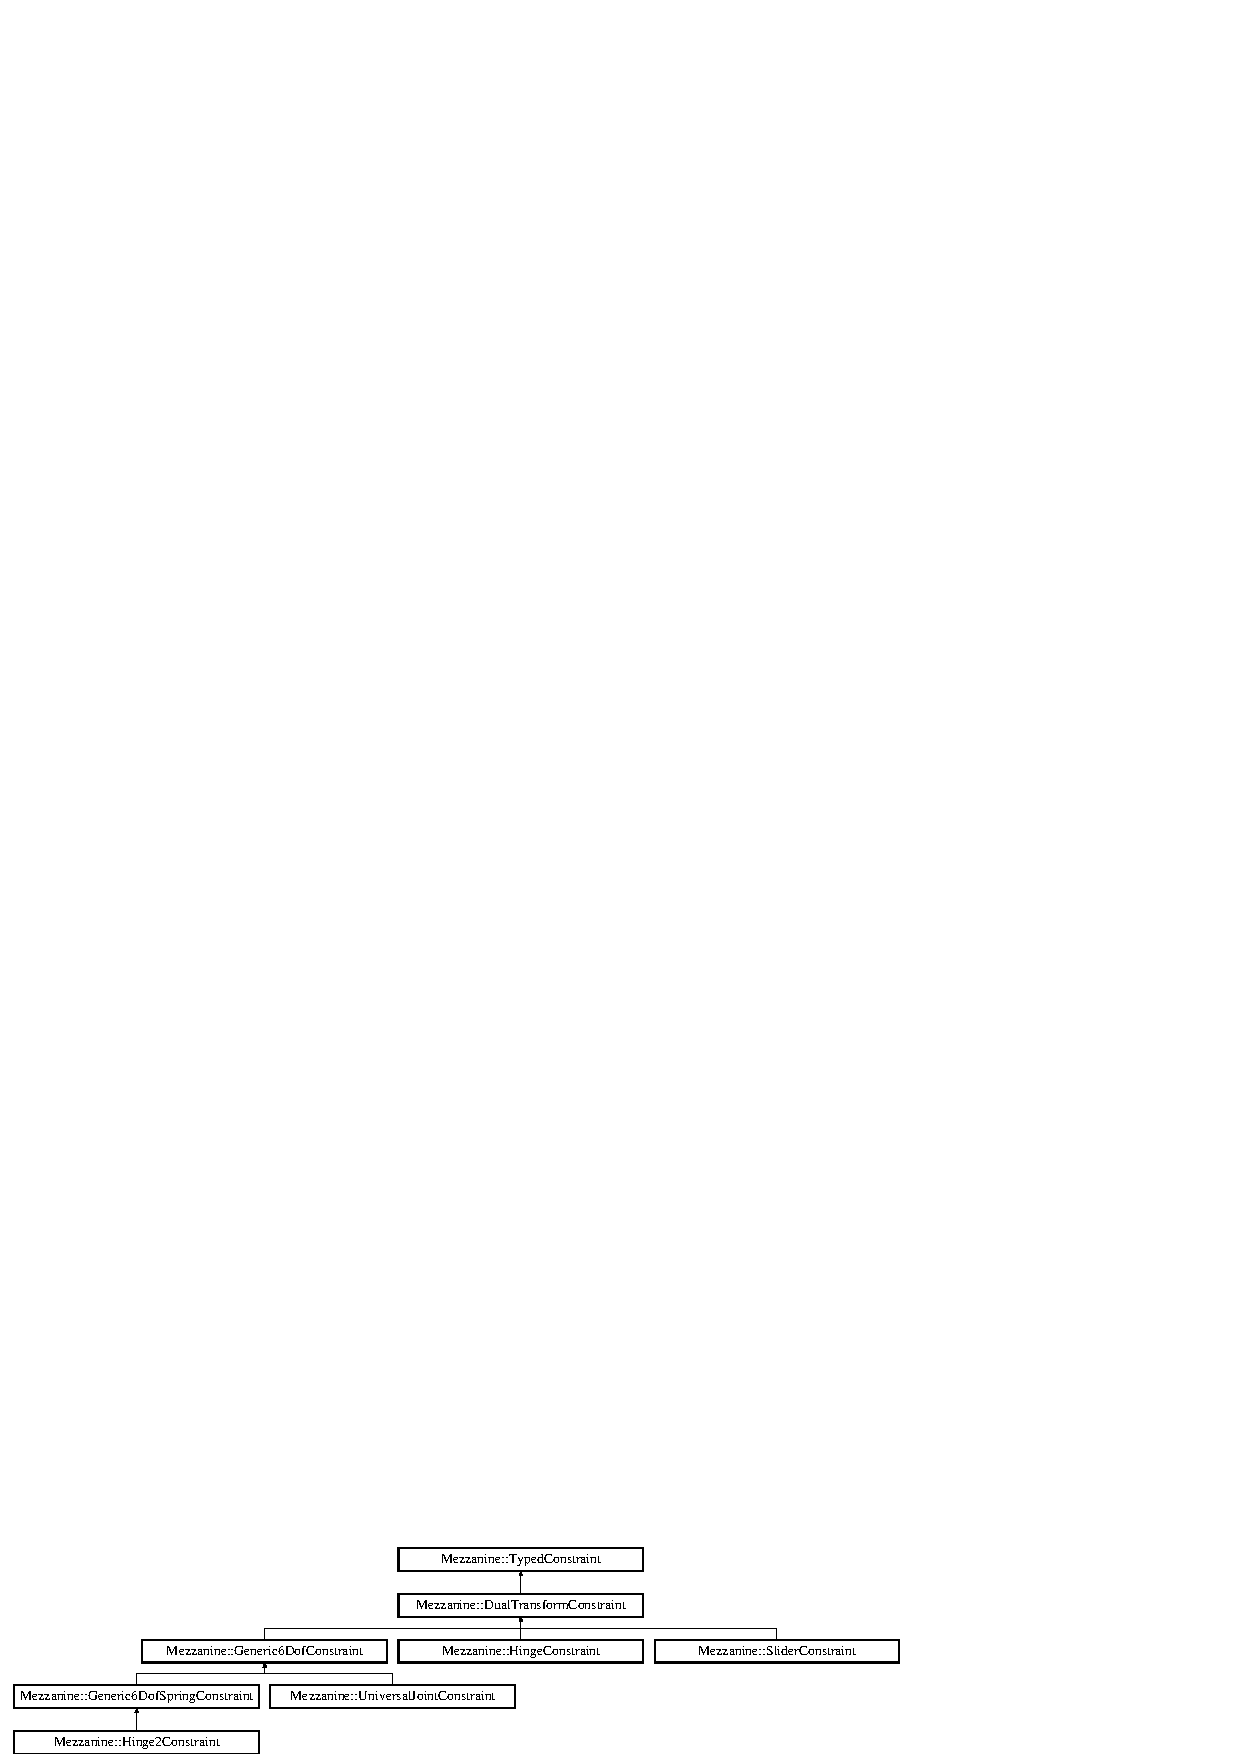
\includegraphics[height=2.766798cm]{classMezzanine_1_1DualTransformConstraint}
\end{center}
\end{figure}
\subsubsection*{Public Member Functions}
\begin{DoxyCompactItemize}
\item 
virtual \hyperlink{classMezzanine_1_1Vector3}{Vector3} \hyperlink{classMezzanine_1_1DualTransformConstraint_ad79b92cb1faeba6e7ba7123e02d86dc1}{GetPivotALocation} () const 
\begin{DoxyCompactList}\small\item\em Get the location of the pivot relative to ActorA's Center of gravity. \item\end{DoxyCompactList}\item 
virtual \hyperlink{classMezzanine_1_1Quaternion}{Quaternion} \hyperlink{classMezzanine_1_1DualTransformConstraint_ac3f2449bc4c0ccd959f4c67216246832}{GetPivotARotation} () const 
\begin{DoxyCompactList}\small\item\em Get the relative rotation for ActorA. \item\end{DoxyCompactList}\item 
virtual \hyperlink{classMezzanine_1_1Transform}{Transform} \hyperlink{classMezzanine_1_1DualTransformConstraint_ac6798a2ea8e80e38fbfbf17df6043265}{GetPivotATransform} () const =0
\begin{DoxyCompactList}\small\item\em Get the current Rotation and Location of Actor A. \item\end{DoxyCompactList}\item 
virtual \hyperlink{classMezzanine_1_1Vector3}{Vector3} \hyperlink{classMezzanine_1_1DualTransformConstraint_ade678f85e0e32b5bf59778130e9d1730}{GetPivotBLocation} () const 
\begin{DoxyCompactList}\small\item\em Get the location of the pivot relative to ActorB's Center of gravity. \item\end{DoxyCompactList}\item 
virtual \hyperlink{classMezzanine_1_1Quaternion}{Quaternion} \hyperlink{classMezzanine_1_1DualTransformConstraint_a56e30c94d128e4c13f449b9933f815fe}{GetPivotBRotation} () const 
\begin{DoxyCompactList}\small\item\em Get the relative rotation for ActorB. \item\end{DoxyCompactList}\item 
virtual \hyperlink{classMezzanine_1_1Transform}{Transform} \hyperlink{classMezzanine_1_1DualTransformConstraint_a43e5f5d4cfd9b0ab7032d81df5c935d7}{GetPivotBTransform} () const =0
\begin{DoxyCompactList}\small\item\em Get the current Rotation and Location of Actor B. \item\end{DoxyCompactList}\item 
virtual void \hyperlink{classMezzanine_1_1DualTransformConstraint_aa69fcdbf84b8a509ee32d4233b96580c}{ProtoDeSerialize} (const \hyperlink{classMezzanine_1_1xml_1_1Node}{xml::Node} \&OneNode)
\begin{DoxyCompactList}\small\item\em Take the data stored in an XML and overwrite this instance of this object with it. \item\end{DoxyCompactList}\item 
virtual void \hyperlink{classMezzanine_1_1DualTransformConstraint_a8e0c729e416c6c20507ef8ac029fa819}{ProtoSerialize} (\hyperlink{classMezzanine_1_1xml_1_1Node}{xml::Node} \&CurrentRoot) const 
\begin{DoxyCompactList}\small\item\em Convert this class to an \hyperlink{classMezzanine_1_1xml_1_1Node}{xml::Node} ready for serialization. \item\end{DoxyCompactList}\item 
virtual void \hyperlink{classMezzanine_1_1DualTransformConstraint_a3dc5e7afcf612a481f81071201ecdeb7}{SetPivotALocation} (const \hyperlink{classMezzanine_1_1Vector3}{Vector3} \&Location)
\begin{DoxyCompactList}\small\item\em Set The relative location of the pivot from ActorA's Center of gravity. \item\end{DoxyCompactList}\item 
virtual void \hyperlink{classMezzanine_1_1DualTransformConstraint_a73cba60ff65f8ac2775b19f74e5cbe9e}{SetPivotARotation} (const \hyperlink{classMezzanine_1_1Quaternion}{Quaternion} \&Rotation)
\begin{DoxyCompactList}\small\item\em Set The relative rotation of ActorA. \item\end{DoxyCompactList}\item 
virtual void \hyperlink{classMezzanine_1_1DualTransformConstraint_a6f1713e6af9d89de70ff77ed47c82d31}{SetPivotATransform} (const \hyperlink{classMezzanine_1_1Transform}{Transform} \&TranA)=0
\begin{DoxyCompactList}\small\item\em Set the Position and Rotation using a \hyperlink{classMezzanine_1_1Transform}{Transform}. \item\end{DoxyCompactList}\item 
virtual void \hyperlink{classMezzanine_1_1DualTransformConstraint_abf63fe4c4fc3c57a0eed7ed006a00aee}{SetPivotBLocation} (const \hyperlink{classMezzanine_1_1Vector3}{Vector3} \&Location)
\begin{DoxyCompactList}\small\item\em Set The relative location of the pivot from ActorB's Center of gravity. \item\end{DoxyCompactList}\item 
virtual void \hyperlink{classMezzanine_1_1DualTransformConstraint_ab25460e03f187dd56657e43e6302ef45}{SetPivotBRotation} (const \hyperlink{classMezzanine_1_1Quaternion}{Quaternion} \&Rotation)
\begin{DoxyCompactList}\small\item\em Set The relative rotation of ActorB. \item\end{DoxyCompactList}\item 
virtual void \hyperlink{classMezzanine_1_1DualTransformConstraint_ac5ee69ce5d68f4e299e7916f764ee396}{SetPivotBTransform} (const \hyperlink{classMezzanine_1_1Transform}{Transform} \&TranB)=0
\begin{DoxyCompactList}\small\item\em Set the Position and Rotation using a \hyperlink{classMezzanine_1_1Transform}{Transform}. \item\end{DoxyCompactList}\end{DoxyCompactItemize}
\subsubsection*{Static Public Member Functions}
\begin{DoxyCompactItemize}
\item 
static \hyperlink{namespaceMezzanine_acf9fcc130e6ebf08e3d8491aebcf1c86}{String} \hyperlink{classMezzanine_1_1DualTransformConstraint_a78694da6df0b2625220abb94e8f1c549}{SerializableName} ()
\begin{DoxyCompactList}\small\item\em Get the name of the the XML tag this class will leave behind as its instances are serialized. \item\end{DoxyCompactList}\end{DoxyCompactItemize}


\subsubsection{Detailed Description}
All constraints that track rotation and location of the Pivot relative to each Actor inherit from this. Since not all contraints provide tracking for the Actor \hyperlink{classMezzanine_1_1Transform}{Transform} (location/rotation of the pivot) we subdivided the constraints to unify the interface of those that could be unified. This stores nothing, but provides uniform access to the transform and rotation functions. \par
 \par
 Any deriving class must implement every thing from \hyperlink{classMezzanine_1_1TypedConstraint}{TypedConstraint} and the four set/get \hyperlink{classMezzanine_1_1Transform}{Transform} function. It is expected that more derived classes will implement the Set/Get Pivot/Rotation Functino in a more efficient Manner if a more efficient way exists. The non-\/transform get/set function are implmented in terms of the get/set transform function extra copies of values and extra reading/writing may occur if the compiler weakly optimizes. Of course, implementing more functions could slow down the software if it no longer fits in CPU caches. As always benchmark if this is something that may be critically slowing you down. 

Definition at line 322 of file constraint.h.



\subsubsection{Member Function Documentation}
\hypertarget{classMezzanine_1_1DualTransformConstraint_ad79b92cb1faeba6e7ba7123e02d86dc1}{
\index{Mezzanine::DualTransformConstraint@{Mezzanine::DualTransformConstraint}!GetPivotALocation@{GetPivotALocation}}
\index{GetPivotALocation@{GetPivotALocation}!Mezzanine::DualTransformConstraint@{Mezzanine::DualTransformConstraint}}
\paragraph[{GetPivotALocation}]{\setlength{\rightskip}{0pt plus 5cm}virtual {\bf Vector3} Mezzanine::DualTransformConstraint::GetPivotALocation (
\begin{DoxyParamCaption}
{}
\end{DoxyParamCaption}
) const\hspace{0.3cm}{\ttfamily  \mbox{[}inline, virtual\mbox{]}}}\hfill}
\label{classMezzanine_1_1DualTransformConstraint_ad79b92cb1faeba6e7ba7123e02d86dc1}


Get the location of the pivot relative to ActorA's Center of gravity. 

\begin{DoxyReturn}{Returns}
A \hyperlink{classMezzanine_1_1Vector3}{Vector3} with the pivot location. 
\end{DoxyReturn}


Implements \hyperlink{classMezzanine_1_1TypedConstraint_af785319e62e274656f180ab80f5f8dd9}{Mezzanine::TypedConstraint}.



Reimplemented in \hyperlink{classMezzanine_1_1Generic6DofConstraint_a180f26186e0ddd58c9c0746897155eaf}{Mezzanine::Generic6DofConstraint}, \hyperlink{classMezzanine_1_1HingeConstraint_a74f1b8d8de18ab991d2f42c7141eedc7}{Mezzanine::HingeConstraint}, and \hyperlink{classMezzanine_1_1SliderConstraint_aab32a4c00eda5369c8188cff854418bd}{Mezzanine::SliderConstraint}.



Definition at line 350 of file constraint.h.

\hypertarget{classMezzanine_1_1DualTransformConstraint_ac3f2449bc4c0ccd959f4c67216246832}{
\index{Mezzanine::DualTransformConstraint@{Mezzanine::DualTransformConstraint}!GetPivotARotation@{GetPivotARotation}}
\index{GetPivotARotation@{GetPivotARotation}!Mezzanine::DualTransformConstraint@{Mezzanine::DualTransformConstraint}}
\paragraph[{GetPivotARotation}]{\setlength{\rightskip}{0pt plus 5cm}virtual {\bf Quaternion} Mezzanine::DualTransformConstraint::GetPivotARotation (
\begin{DoxyParamCaption}
{}
\end{DoxyParamCaption}
) const\hspace{0.3cm}{\ttfamily  \mbox{[}inline, virtual\mbox{]}}}\hfill}
\label{classMezzanine_1_1DualTransformConstraint_ac3f2449bc4c0ccd959f4c67216246832}


Get the relative rotation for ActorA. 

\begin{DoxyReturn}{Returns}
A \hyperlink{classMezzanine_1_1Quaternion}{Quaternion} that has the rotation 
\end{DoxyReturn}


Reimplemented in \hyperlink{classMezzanine_1_1Generic6DofConstraint_a517388fdf36423ed0550ec19089955b9}{Mezzanine::Generic6DofConstraint}, and \hyperlink{classMezzanine_1_1SliderConstraint_ac53730c289d355e7ed426a9f4b28d6b5}{Mezzanine::SliderConstraint}.



Definition at line 369 of file constraint.h.

\hypertarget{classMezzanine_1_1DualTransformConstraint_ac6798a2ea8e80e38fbfbf17df6043265}{
\index{Mezzanine::DualTransformConstraint@{Mezzanine::DualTransformConstraint}!GetPivotATransform@{GetPivotATransform}}
\index{GetPivotATransform@{GetPivotATransform}!Mezzanine::DualTransformConstraint@{Mezzanine::DualTransformConstraint}}
\paragraph[{GetPivotATransform}]{\setlength{\rightskip}{0pt plus 5cm}virtual {\bf Transform} Mezzanine::DualTransformConstraint::GetPivotATransform (
\begin{DoxyParamCaption}
{}
\end{DoxyParamCaption}
) const\hspace{0.3cm}{\ttfamily  \mbox{[}pure virtual\mbox{]}}}\hfill}
\label{classMezzanine_1_1DualTransformConstraint_ac6798a2ea8e80e38fbfbf17df6043265}


Get the current Rotation and Location of Actor A. 

\begin{DoxyReturn}{Returns}
This returns a \hyperlink{classMezzanine_1_1Transform}{Mezzanine::Transform} 
\end{DoxyReturn}


Implemented in \hyperlink{classMezzanine_1_1Generic6DofConstraint_adac17da02ce3ecacf583515a66576533}{Mezzanine::Generic6DofConstraint}, \hyperlink{classMezzanine_1_1HingeConstraint_a208687c856410bf70f068ddf8c8f9161}{Mezzanine::HingeConstraint}, and \hyperlink{classMezzanine_1_1SliderConstraint_ad87313a0848e2523b4157a07b0a65d23}{Mezzanine::SliderConstraint}.

\hypertarget{classMezzanine_1_1DualTransformConstraint_ade678f85e0e32b5bf59778130e9d1730}{
\index{Mezzanine::DualTransformConstraint@{Mezzanine::DualTransformConstraint}!GetPivotBLocation@{GetPivotBLocation}}
\index{GetPivotBLocation@{GetPivotBLocation}!Mezzanine::DualTransformConstraint@{Mezzanine::DualTransformConstraint}}
\paragraph[{GetPivotBLocation}]{\setlength{\rightskip}{0pt plus 5cm}virtual {\bf Vector3} Mezzanine::DualTransformConstraint::GetPivotBLocation (
\begin{DoxyParamCaption}
{}
\end{DoxyParamCaption}
) const\hspace{0.3cm}{\ttfamily  \mbox{[}inline, virtual\mbox{]}}}\hfill}
\label{classMezzanine_1_1DualTransformConstraint_ade678f85e0e32b5bf59778130e9d1730}


Get the location of the pivot relative to ActorB's Center of gravity. 

\begin{DoxyReturn}{Returns}
A \hyperlink{classMezzanine_1_1Vector3}{Vector3} with the pivot location. 
\end{DoxyReturn}


Implements \hyperlink{classMezzanine_1_1TypedConstraint_a2c0984d3211b30756c7ec5263c99b014}{Mezzanine::TypedConstraint}.



Reimplemented in \hyperlink{classMezzanine_1_1Generic6DofConstraint_a2b7344ab150f2f6dd898b6cbcd150d6e}{Mezzanine::Generic6DofConstraint}, \hyperlink{classMezzanine_1_1HingeConstraint_a87b14b3cbf5241aeba723226661764e6}{Mezzanine::HingeConstraint}, and \hyperlink{classMezzanine_1_1SliderConstraint_af97a455a53d7572351f6ae725bb8e31b}{Mezzanine::SliderConstraint}.



Definition at line 354 of file constraint.h.

\hypertarget{classMezzanine_1_1DualTransformConstraint_a56e30c94d128e4c13f449b9933f815fe}{
\index{Mezzanine::DualTransformConstraint@{Mezzanine::DualTransformConstraint}!GetPivotBRotation@{GetPivotBRotation}}
\index{GetPivotBRotation@{GetPivotBRotation}!Mezzanine::DualTransformConstraint@{Mezzanine::DualTransformConstraint}}
\paragraph[{GetPivotBRotation}]{\setlength{\rightskip}{0pt plus 5cm}virtual {\bf Quaternion} Mezzanine::DualTransformConstraint::GetPivotBRotation (
\begin{DoxyParamCaption}
{}
\end{DoxyParamCaption}
) const\hspace{0.3cm}{\ttfamily  \mbox{[}inline, virtual\mbox{]}}}\hfill}
\label{classMezzanine_1_1DualTransformConstraint_a56e30c94d128e4c13f449b9933f815fe}


Get the relative rotation for ActorB. 

\begin{DoxyReturn}{Returns}
A \hyperlink{classMezzanine_1_1Quaternion}{Quaternion} that has the rotation 
\end{DoxyReturn}


Reimplemented in \hyperlink{classMezzanine_1_1Generic6DofConstraint_ab3979edc1d5f3bfce878de009c18494d}{Mezzanine::Generic6DofConstraint}, and \hyperlink{classMezzanine_1_1SliderConstraint_a4550412c47b611ae3238db1adbff20d9}{Mezzanine::SliderConstraint}.



Definition at line 373 of file constraint.h.

\hypertarget{classMezzanine_1_1DualTransformConstraint_a43e5f5d4cfd9b0ab7032d81df5c935d7}{
\index{Mezzanine::DualTransformConstraint@{Mezzanine::DualTransformConstraint}!GetPivotBTransform@{GetPivotBTransform}}
\index{GetPivotBTransform@{GetPivotBTransform}!Mezzanine::DualTransformConstraint@{Mezzanine::DualTransformConstraint}}
\paragraph[{GetPivotBTransform}]{\setlength{\rightskip}{0pt plus 5cm}virtual {\bf Transform} Mezzanine::DualTransformConstraint::GetPivotBTransform (
\begin{DoxyParamCaption}
{}
\end{DoxyParamCaption}
) const\hspace{0.3cm}{\ttfamily  \mbox{[}pure virtual\mbox{]}}}\hfill}
\label{classMezzanine_1_1DualTransformConstraint_a43e5f5d4cfd9b0ab7032d81df5c935d7}


Get the current Rotation and Location of Actor B. 

\begin{DoxyReturn}{Returns}
This returns a \hyperlink{classMezzanine_1_1Transform}{Mezzanine::Transform} 
\end{DoxyReturn}


Implemented in \hyperlink{classMezzanine_1_1Generic6DofConstraint_ad38e140ea8edf8d9d74e99bbebf68417}{Mezzanine::Generic6DofConstraint}, \hyperlink{classMezzanine_1_1HingeConstraint_a7d9a9ddc367d1a9105f1eb27fd76a65f}{Mezzanine::HingeConstraint}, and \hyperlink{classMezzanine_1_1SliderConstraint_a22964857b7c94edf895d1ea9812614b1}{Mezzanine::SliderConstraint}.

\hypertarget{classMezzanine_1_1DualTransformConstraint_aa69fcdbf84b8a509ee32d4233b96580c}{
\index{Mezzanine::DualTransformConstraint@{Mezzanine::DualTransformConstraint}!ProtoDeSerialize@{ProtoDeSerialize}}
\index{ProtoDeSerialize@{ProtoDeSerialize}!Mezzanine::DualTransformConstraint@{Mezzanine::DualTransformConstraint}}
\paragraph[{ProtoDeSerialize}]{\setlength{\rightskip}{0pt plus 5cm}virtual void Mezzanine::DualTransformConstraint::ProtoDeSerialize (
\begin{DoxyParamCaption}
\item[{const {\bf xml::Node} \&}]{OneNode}
\end{DoxyParamCaption}
)\hspace{0.3cm}{\ttfamily  \mbox{[}virtual\mbox{]}}}\hfill}
\label{classMezzanine_1_1DualTransformConstraint_aa69fcdbf84b8a509ee32d4233b96580c}


Take the data stored in an XML and overwrite this instance of this object with it. 


\begin{DoxyParams}{Parameters}
{\em OneNode} & and \hyperlink{classMezzanine_1_1xml_1_1Node}{xml::Node} containing the data. \\
\hline
\end{DoxyParams}


Reimplemented from \hyperlink{classMezzanine_1_1TypedConstraint_a18ea81954d7cc28dce3e5f4c03eac820}{Mezzanine::TypedConstraint}.



Reimplemented in \hyperlink{classMezzanine_1_1Generic6DofConstraint_ae165de381e73cc5119d07e3fc563aa99}{Mezzanine::Generic6DofConstraint}, \hyperlink{classMezzanine_1_1Generic6DofSpringConstraint_a30cd26edd9d57aa68cf7f55f31fb99b0}{Mezzanine::Generic6DofSpringConstraint}, and \hyperlink{classMezzanine_1_1HingeConstraint_a6cbd8328c7a047f8e7951ab482e733cb}{Mezzanine::HingeConstraint}.

\hypertarget{classMezzanine_1_1DualTransformConstraint_a8e0c729e416c6c20507ef8ac029fa819}{
\index{Mezzanine::DualTransformConstraint@{Mezzanine::DualTransformConstraint}!ProtoSerialize@{ProtoSerialize}}
\index{ProtoSerialize@{ProtoSerialize}!Mezzanine::DualTransformConstraint@{Mezzanine::DualTransformConstraint}}
\paragraph[{ProtoSerialize}]{\setlength{\rightskip}{0pt plus 5cm}virtual void Mezzanine::DualTransformConstraint::ProtoSerialize (
\begin{DoxyParamCaption}
\item[{{\bf xml::Node} \&}]{CurrentRoot}
\end{DoxyParamCaption}
) const\hspace{0.3cm}{\ttfamily  \mbox{[}virtual\mbox{]}}}\hfill}
\label{classMezzanine_1_1DualTransformConstraint_a8e0c729e416c6c20507ef8ac029fa819}


Convert this class to an \hyperlink{classMezzanine_1_1xml_1_1Node}{xml::Node} ready for serialization. 


\begin{DoxyParams}{Parameters}
{\em CurrentRoot} & The point in the XML hierarchy that all this vectorw should be appended to.\\
\hline
\end{DoxyParams}
This stores each Actor's \hyperlink{classMezzanine_1_1Transform}{Transform} 

Reimplemented from \hyperlink{classMezzanine_1_1TypedConstraint_ae9d74e8e14d9e79bb4320603fbf824d6}{Mezzanine::TypedConstraint}.



Reimplemented in \hyperlink{classMezzanine_1_1Generic6DofConstraint_a6595599905cd8b51440bf868d4a9806a}{Mezzanine::Generic6DofConstraint}, \hyperlink{classMezzanine_1_1Generic6DofSpringConstraint_a02841289ca30d307e1e39b47d610ff18}{Mezzanine::Generic6DofSpringConstraint}, and \hyperlink{classMezzanine_1_1HingeConstraint_a49cf5f27bff730ee30ff52a741e35f2e}{Mezzanine::HingeConstraint}.

\hypertarget{classMezzanine_1_1DualTransformConstraint_a78694da6df0b2625220abb94e8f1c549}{
\index{Mezzanine::DualTransformConstraint@{Mezzanine::DualTransformConstraint}!SerializableName@{SerializableName}}
\index{SerializableName@{SerializableName}!Mezzanine::DualTransformConstraint@{Mezzanine::DualTransformConstraint}}
\paragraph[{SerializableName}]{\setlength{\rightskip}{0pt plus 5cm}static {\bf String} Mezzanine::DualTransformConstraint::SerializableName (
\begin{DoxyParamCaption}
{}
\end{DoxyParamCaption}
)\hspace{0.3cm}{\ttfamily  \mbox{[}static\mbox{]}}}\hfill}
\label{classMezzanine_1_1DualTransformConstraint_a78694da6df0b2625220abb94e8f1c549}


Get the name of the the XML tag this class will leave behind as its instances are serialized. 

\begin{DoxyReturn}{Returns}
A string containing \char`\"{}DualTransformConstraint\char`\"{} 
\end{DoxyReturn}


Reimplemented from \hyperlink{classMezzanine_1_1TypedConstraint_accc0475bacd0b984dd30d74dbe2bc08e}{Mezzanine::TypedConstraint}.



Reimplemented in \hyperlink{classMezzanine_1_1Generic6DofConstraint_acac3b309c947c1cd60635df1c7b46867}{Mezzanine::Generic6DofConstraint}, \hyperlink{classMezzanine_1_1Generic6DofSpringConstraint_aa020b0ef38e950475dc8a36f06139933}{Mezzanine::Generic6DofSpringConstraint}, and \hyperlink{classMezzanine_1_1HingeConstraint_a0bcb0756ff73f9d772e0c60d188d393a}{Mezzanine::HingeConstraint}.

\hypertarget{classMezzanine_1_1DualTransformConstraint_a3dc5e7afcf612a481f81071201ecdeb7}{
\index{Mezzanine::DualTransformConstraint@{Mezzanine::DualTransformConstraint}!SetPivotALocation@{SetPivotALocation}}
\index{SetPivotALocation@{SetPivotALocation}!Mezzanine::DualTransformConstraint@{Mezzanine::DualTransformConstraint}}
\paragraph[{SetPivotALocation}]{\setlength{\rightskip}{0pt plus 5cm}virtual void Mezzanine::DualTransformConstraint::SetPivotALocation (
\begin{DoxyParamCaption}
\item[{const {\bf Vector3} \&}]{Location}
\end{DoxyParamCaption}
)\hspace{0.3cm}{\ttfamily  \mbox{[}inline, virtual\mbox{]}}}\hfill}
\label{classMezzanine_1_1DualTransformConstraint_a3dc5e7afcf612a481f81071201ecdeb7}


Set The relative location of the pivot from ActorA's Center of gravity. 


\begin{DoxyParams}{Parameters}
{\em Location} & The New value for PivotA\\
\hline
\end{DoxyParams}
Ultimately this information winds up being stored in the TransformA. 

Implements \hyperlink{classMezzanine_1_1TypedConstraint_a09aacdc6f424623cc3a2fdad9c1d0caf}{Mezzanine::TypedConstraint}.



Reimplemented in \hyperlink{classMezzanine_1_1Generic6DofConstraint_a4670a488bc5cab478c6d69c8a0d240a5}{Mezzanine::Generic6DofConstraint}, \hyperlink{classMezzanine_1_1HingeConstraint_a0990b3b85529df353aaa46f76951fd68}{Mezzanine::HingeConstraint}, and \hyperlink{classMezzanine_1_1SliderConstraint_a70cf627b28c4031d498557d3011a33c8}{Mezzanine::SliderConstraint}.



Definition at line 341 of file constraint.h.

\hypertarget{classMezzanine_1_1DualTransformConstraint_a73cba60ff65f8ac2775b19f74e5cbe9e}{
\index{Mezzanine::DualTransformConstraint@{Mezzanine::DualTransformConstraint}!SetPivotARotation@{SetPivotARotation}}
\index{SetPivotARotation@{SetPivotARotation}!Mezzanine::DualTransformConstraint@{Mezzanine::DualTransformConstraint}}
\paragraph[{SetPivotARotation}]{\setlength{\rightskip}{0pt plus 5cm}virtual void Mezzanine::DualTransformConstraint::SetPivotARotation (
\begin{DoxyParamCaption}
\item[{const {\bf Quaternion} \&}]{Rotation}
\end{DoxyParamCaption}
)\hspace{0.3cm}{\ttfamily  \mbox{[}inline, virtual\mbox{]}}}\hfill}
\label{classMezzanine_1_1DualTransformConstraint_a73cba60ff65f8ac2775b19f74e5cbe9e}


Set The relative rotation of ActorA. 


\begin{DoxyParams}{Parameters}
{\em Rotation} & The new rotation amount for A\\
\hline
\end{DoxyParams}
Ultimately this information winds up being stored in the TransformA 

Reimplemented in \hyperlink{classMezzanine_1_1Generic6DofConstraint_a34027d82e3b8c09c6cd488335ea343bb}{Mezzanine::Generic6DofConstraint}, and \hyperlink{classMezzanine_1_1SliderConstraint_a9a38e7a49caa92f735d6723021aaffea}{Mezzanine::SliderConstraint}.



Definition at line 360 of file constraint.h.

\hypertarget{classMezzanine_1_1DualTransformConstraint_a6f1713e6af9d89de70ff77ed47c82d31}{
\index{Mezzanine::DualTransformConstraint@{Mezzanine::DualTransformConstraint}!SetPivotATransform@{SetPivotATransform}}
\index{SetPivotATransform@{SetPivotATransform}!Mezzanine::DualTransformConstraint@{Mezzanine::DualTransformConstraint}}
\paragraph[{SetPivotATransform}]{\setlength{\rightskip}{0pt plus 5cm}virtual void Mezzanine::DualTransformConstraint::SetPivotATransform (
\begin{DoxyParamCaption}
\item[{const {\bf Transform} \&}]{TranA}
\end{DoxyParamCaption}
)\hspace{0.3cm}{\ttfamily  \mbox{[}pure virtual\mbox{]}}}\hfill}
\label{classMezzanine_1_1DualTransformConstraint_a6f1713e6af9d89de70ff77ed47c82d31}


Set the Position and Rotation using a \hyperlink{classMezzanine_1_1Transform}{Transform}. 


\begin{DoxyParams}{Parameters}
{\em TranA} & The new Position and rotation \\
\hline
\end{DoxyParams}


Implemented in \hyperlink{classMezzanine_1_1Generic6DofConstraint_a88f26ccb9a6ec67adc743d4bc7c86ddf}{Mezzanine::Generic6DofConstraint}, \hyperlink{classMezzanine_1_1HingeConstraint_a44bc111ce8642c52c106af2cfe1fd7d5}{Mezzanine::HingeConstraint}, and \hyperlink{classMezzanine_1_1SliderConstraint_a1655ff22220ff99ada45a98cdb330dfb}{Mezzanine::SliderConstraint}.

\hypertarget{classMezzanine_1_1DualTransformConstraint_abf63fe4c4fc3c57a0eed7ed006a00aee}{
\index{Mezzanine::DualTransformConstraint@{Mezzanine::DualTransformConstraint}!SetPivotBLocation@{SetPivotBLocation}}
\index{SetPivotBLocation@{SetPivotBLocation}!Mezzanine::DualTransformConstraint@{Mezzanine::DualTransformConstraint}}
\paragraph[{SetPivotBLocation}]{\setlength{\rightskip}{0pt plus 5cm}virtual void Mezzanine::DualTransformConstraint::SetPivotBLocation (
\begin{DoxyParamCaption}
\item[{const {\bf Vector3} \&}]{Location}
\end{DoxyParamCaption}
)\hspace{0.3cm}{\ttfamily  \mbox{[}inline, virtual\mbox{]}}}\hfill}
\label{classMezzanine_1_1DualTransformConstraint_abf63fe4c4fc3c57a0eed7ed006a00aee}


Set The relative location of the pivot from ActorB's Center of gravity. 


\begin{DoxyParams}{Parameters}
{\em Location} & The New value for PivotB\\
\hline
\end{DoxyParams}
Ultimately this information winds up being stored in the TransformB 

Implements \hyperlink{classMezzanine_1_1TypedConstraint_ad59aa55a0e4b8aa107db9c9460b57ec3}{Mezzanine::TypedConstraint}.



Reimplemented in \hyperlink{classMezzanine_1_1Generic6DofConstraint_a1b5fc577a2c627266436fd5b134728bc}{Mezzanine::Generic6DofConstraint}, \hyperlink{classMezzanine_1_1HingeConstraint_a7ae57514d6bd1119859ecb137cf58e5e}{Mezzanine::HingeConstraint}, and \hyperlink{classMezzanine_1_1SliderConstraint_ab6705dee13d7311ee381d388ba3122cd}{Mezzanine::SliderConstraint}.



Definition at line 346 of file constraint.h.

\hypertarget{classMezzanine_1_1DualTransformConstraint_ab25460e03f187dd56657e43e6302ef45}{
\index{Mezzanine::DualTransformConstraint@{Mezzanine::DualTransformConstraint}!SetPivotBRotation@{SetPivotBRotation}}
\index{SetPivotBRotation@{SetPivotBRotation}!Mezzanine::DualTransformConstraint@{Mezzanine::DualTransformConstraint}}
\paragraph[{SetPivotBRotation}]{\setlength{\rightskip}{0pt plus 5cm}virtual void Mezzanine::DualTransformConstraint::SetPivotBRotation (
\begin{DoxyParamCaption}
\item[{const {\bf Quaternion} \&}]{Rotation}
\end{DoxyParamCaption}
)\hspace{0.3cm}{\ttfamily  \mbox{[}inline, virtual\mbox{]}}}\hfill}
\label{classMezzanine_1_1DualTransformConstraint_ab25460e03f187dd56657e43e6302ef45}


Set The relative rotation of ActorB. 


\begin{DoxyParams}{Parameters}
{\em otation} & The new rotation amount for B\\
\hline
\end{DoxyParams}
Ultimately this information winds up being stored in the TransformB 

Reimplemented in \hyperlink{classMezzanine_1_1Generic6DofConstraint_afd149f6868de162f75a3e2293d6c143d}{Mezzanine::Generic6DofConstraint}, and \hyperlink{classMezzanine_1_1SliderConstraint_a83a627a2875eedbf1ae6ee6db49d866f}{Mezzanine::SliderConstraint}.



Definition at line 365 of file constraint.h.

\hypertarget{classMezzanine_1_1DualTransformConstraint_ac5ee69ce5d68f4e299e7916f764ee396}{
\index{Mezzanine::DualTransformConstraint@{Mezzanine::DualTransformConstraint}!SetPivotBTransform@{SetPivotBTransform}}
\index{SetPivotBTransform@{SetPivotBTransform}!Mezzanine::DualTransformConstraint@{Mezzanine::DualTransformConstraint}}
\paragraph[{SetPivotBTransform}]{\setlength{\rightskip}{0pt plus 5cm}virtual void Mezzanine::DualTransformConstraint::SetPivotBTransform (
\begin{DoxyParamCaption}
\item[{const {\bf Transform} \&}]{TranB}
\end{DoxyParamCaption}
)\hspace{0.3cm}{\ttfamily  \mbox{[}pure virtual\mbox{]}}}\hfill}
\label{classMezzanine_1_1DualTransformConstraint_ac5ee69ce5d68f4e299e7916f764ee396}


Set the Position and Rotation using a \hyperlink{classMezzanine_1_1Transform}{Transform}. 


\begin{DoxyParams}{Parameters}
{\em TranB} & The new Position and rotation \\
\hline
\end{DoxyParams}


Implemented in \hyperlink{classMezzanine_1_1Generic6DofConstraint_adaa5bb038814aa287773f56d40e90210}{Mezzanine::Generic6DofConstraint}, \hyperlink{classMezzanine_1_1HingeConstraint_abbe27830e0d17c44125cee59d84a9d37}{Mezzanine::HingeConstraint}, and \hyperlink{classMezzanine_1_1SliderConstraint_a75f675f044faef304729c3ee03eae56b}{Mezzanine::SliderConstraint}.



The documentation for this class was generated from the following file:\begin{DoxyCompactItemize}
\item 
constraint.h\end{DoxyCompactItemize}

\hypertarget{classMezzanine_1_1DynamicMeshCollisionShape}{
\subsection{Mezzanine::DynamicMeshCollisionShape Class Reference}
\label{classMezzanine_1_1DynamicMeshCollisionShape}\index{Mezzanine::DynamicMeshCollisionShape@{Mezzanine::DynamicMeshCollisionShape}}
}


A triangle mesh collsion shape based on a graphics mesh.  




{\ttfamily \#include $<$collisionshape.h$>$}

Inheritance diagram for Mezzanine::DynamicMeshCollisionShape:\begin{figure}[H]
\begin{center}
\leavevmode
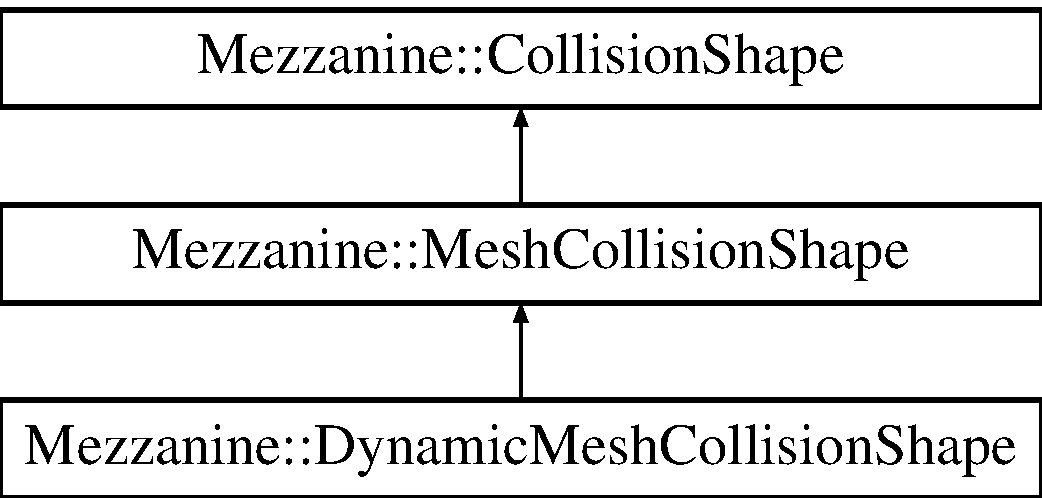
\includegraphics[height=3.000000cm]{classMezzanine_1_1DynamicMeshCollisionShape}
\end{center}
\end{figure}
\subsubsection*{Public Member Functions}
\begin{DoxyCompactItemize}
\item 
\hyperlink{classMezzanine_1_1DynamicMeshCollisionShape_a246dd3621bfd4e36ffd73cf3648dd7c5}{DynamicMeshCollisionShape} (const \hyperlink{namespaceMezzanine_acf9fcc130e6ebf08e3d8491aebcf1c86}{String} \&\hyperlink{classMezzanine_1_1CollisionShape_aac524c5c56fa4d158bc071f8aecfbe79}{Name}, btGImpactMeshShape $\ast$BulletShape)
\begin{DoxyCompactList}\small\item\em Internal Constructor. \item\end{DoxyCompactList}\item 
\hypertarget{classMezzanine_1_1DynamicMeshCollisionShape_a41204636fc0a0dba46fbc52c59cd08c6}{
virtual \hyperlink{classMezzanine_1_1DynamicMeshCollisionShape_a41204636fc0a0dba46fbc52c59cd08c6}{$\sim$DynamicMeshCollisionShape} ()}
\label{classMezzanine_1_1DynamicMeshCollisionShape_a41204636fc0a0dba46fbc52c59cd08c6}

\begin{DoxyCompactList}\small\item\em Class Destructor. \item\end{DoxyCompactList}\item 
virtual \hyperlink{classMezzanine_1_1CollisionShape_ad04186055565998879b64176d6dd100d}{CollisionShape::ShapeType} \hyperlink{classMezzanine_1_1DynamicMeshCollisionShape_ae323a4ac9ae12890e1f8ce82b22f1ccc}{GetType} () const 
\end{DoxyCompactItemize}
\subsubsection*{Protected Attributes}
\begin{DoxyCompactItemize}
\item 
\hypertarget{classMezzanine_1_1DynamicMeshCollisionShape_aeb4d7951bbf3dcd269cc8bf3fc8c9a98}{
btGImpactMeshShape $\ast$ {\bfseries GImpactShape}}
\label{classMezzanine_1_1DynamicMeshCollisionShape_aeb4d7951bbf3dcd269cc8bf3fc8c9a98}

\end{DoxyCompactItemize}


\subsubsection{Detailed Description}
A triangle mesh collsion shape based on a graphics mesh. As the name suggests, this is a TriMesh shape intended for dynamic objects. This can be used with static objects, but using the \hyperlink{classMezzanine_1_1StaticMeshCollisionShape}{StaticMeshCollisionShape} class instead will yeild much better performance. \par
 \par
 In general, this collision shape will provide \char`\"{}pixel-\/perfect\char`\"{} collisions, but this comes at a steep performance cost. You can't have too many objects with this kind of shape before running into noticable performance drops. This class should be avoided in real-\/time applications if at all possible. Primitives provide much better performance. 

Definition at line 844 of file collisionshape.h.



\subsubsection{Constructor \& Destructor Documentation}
\hypertarget{classMezzanine_1_1DynamicMeshCollisionShape_a246dd3621bfd4e36ffd73cf3648dd7c5}{
\index{Mezzanine::DynamicMeshCollisionShape@{Mezzanine::DynamicMeshCollisionShape}!DynamicMeshCollisionShape@{DynamicMeshCollisionShape}}
\index{DynamicMeshCollisionShape@{DynamicMeshCollisionShape}!Mezzanine::DynamicMeshCollisionShape@{Mezzanine::DynamicMeshCollisionShape}}
\paragraph[{DynamicMeshCollisionShape}]{\setlength{\rightskip}{0pt plus 5cm}Mezzanine::DynamicMeshCollisionShape::DynamicMeshCollisionShape (
\begin{DoxyParamCaption}
\item[{const {\bf String} \&}]{Name, }
\item[{btGImpactMeshShape $\ast$}]{BulletShape}
\end{DoxyParamCaption}
)}\hfill}
\label{classMezzanine_1_1DynamicMeshCollisionShape_a246dd3621bfd4e36ffd73cf3648dd7c5}


Internal Constructor. 


\begin{DoxyParams}{Parameters}
{\em Name} & The name of this Shape. \\
\hline
{\em BulletShape} & The internal shape this shape is based on. \\
\hline
\end{DoxyParams}


Definition at line 1490 of file collisionshape.cpp.



\subsubsection{Member Function Documentation}
\hypertarget{classMezzanine_1_1DynamicMeshCollisionShape_ae323a4ac9ae12890e1f8ce82b22f1ccc}{
\index{Mezzanine::DynamicMeshCollisionShape@{Mezzanine::DynamicMeshCollisionShape}!GetType@{GetType}}
\index{GetType@{GetType}!Mezzanine::DynamicMeshCollisionShape@{Mezzanine::DynamicMeshCollisionShape}}
\paragraph[{GetType}]{\setlength{\rightskip}{0pt plus 5cm}{\bf CollisionShape::ShapeType} Mezzanine::DynamicMeshCollisionShape::GetType (
\begin{DoxyParamCaption}
{}
\end{DoxyParamCaption}
) const\hspace{0.3cm}{\ttfamily  \mbox{[}virtual\mbox{]}}}\hfill}
\label{classMezzanine_1_1DynamicMeshCollisionShape_ae323a4ac9ae12890e1f8ce82b22f1ccc}
Gets the type of \hyperlink{classMezzanine_1_1Collision}{Collision} shape this is. 

\begin{DoxyReturn}{Returns}
Returns an enum value indicating the type of collision shape this is. 
\end{DoxyReturn}
 

Implements \hyperlink{classMezzanine_1_1MeshCollisionShape_a00dc444afac92030ea43815ec21dd8e8}{Mezzanine::MeshCollisionShape}.



Definition at line 1502 of file collisionshape.cpp.



The documentation for this class was generated from the following files:\begin{DoxyCompactItemize}
\item 
collisionshape.h\item 
collisionshape.cpp\end{DoxyCompactItemize}

\hypertarget{classMezzanine_1_1Entity}{
\subsection{Mezzanine::Entity Class Reference}
\label{classMezzanine_1_1Entity}\index{Mezzanine::Entity@{Mezzanine::Entity}}
}


This class is useful for representing graphical bodies without a physics representation.  




{\ttfamily \#include $<$entity.h$>$}

Inheritance diagram for Mezzanine::Entity:\begin{figure}[H]
\begin{center}
\leavevmode
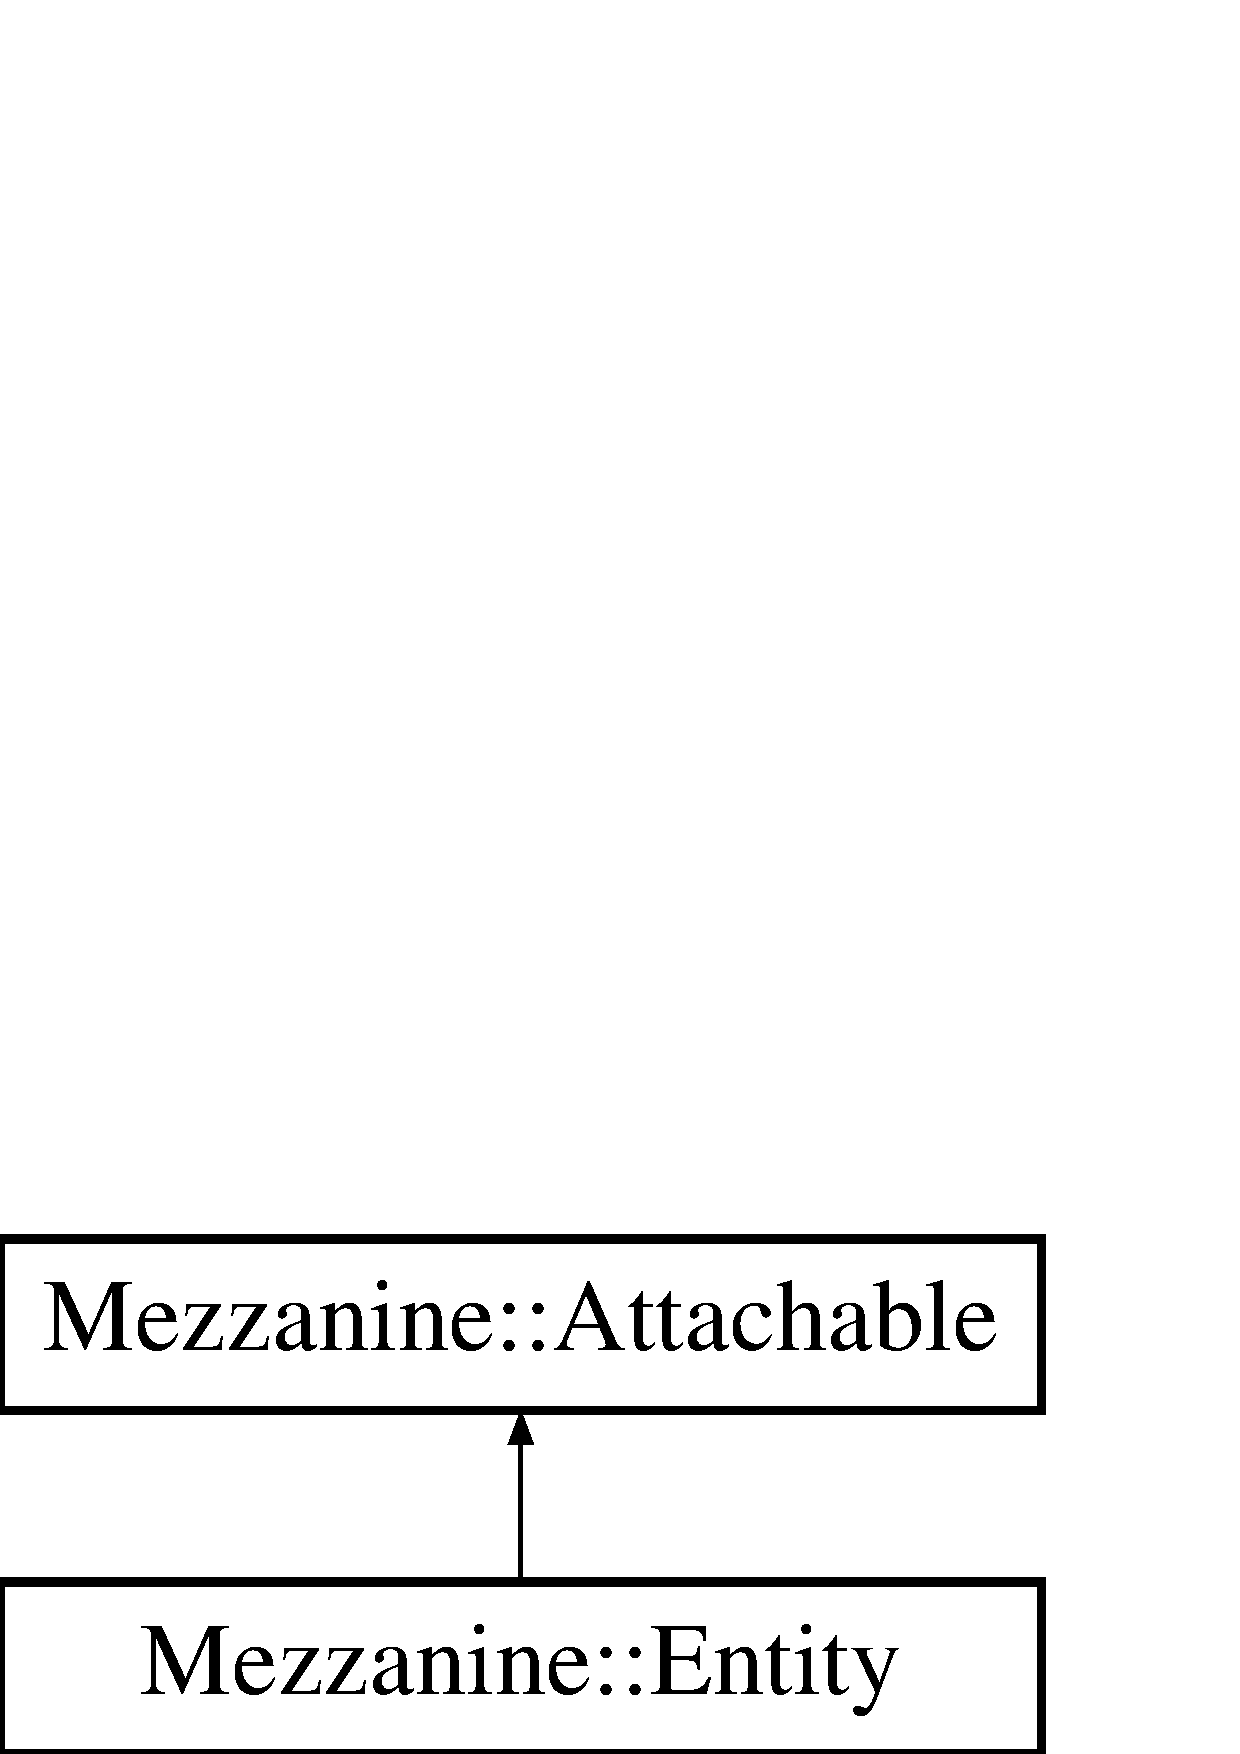
\includegraphics[height=3.000000cm]{classMezzanine_1_1Entity}
\end{center}
\end{figure}
\subsubsection*{Public Member Functions}
\begin{DoxyCompactItemize}
\item 
\hyperlink{classMezzanine_1_1Entity_a50fb69d94709026fc524cd0cbe3671b8}{Entity} (const \hyperlink{namespaceMezzanine_acf9fcc130e6ebf08e3d8491aebcf1c86}{String} \&Name, const \hyperlink{namespaceMezzanine_acf9fcc130e6ebf08e3d8491aebcf1c86}{String} \&MeshName, const \hyperlink{namespaceMezzanine_acf9fcc130e6ebf08e3d8491aebcf1c86}{String} \&Group, \hyperlink{classMezzanine_1_1SceneManager}{SceneManager} $\ast$manager)
\begin{DoxyCompactList}\small\item\em Class Constructor. \item\end{DoxyCompactList}\item 
\hypertarget{classMezzanine_1_1Entity_a030c609ef574de6f3c1e474dfe119e48}{
virtual \hyperlink{classMezzanine_1_1Entity_a030c609ef574de6f3c1e474dfe119e48}{$\sim$Entity} ()}
\label{classMezzanine_1_1Entity_a030c609ef574de6f3c1e474dfe119e48}

\begin{DoxyCompactList}\small\item\em Class Destructor. \item\end{DoxyCompactList}\item 
void \hyperlink{classMezzanine_1_1Entity_add48bc9fd02f427e271392597b9dad9f}{AddToWorld} ()
\begin{DoxyCompactList}\small\item\em Adds this entity to the world, allowing it to render. \item\end{DoxyCompactList}\item 
\hyperlink{classMezzanine_1_1Vector3}{Vector3} \hyperlink{classMezzanine_1_1Entity_abef3e9fd62085c0ebc0bcab8199f7ce7}{GetLocation} () const 
\begin{DoxyCompactList}\small\item\em Gets the location of this entity. \item\end{DoxyCompactList}\item 
\hyperlink{namespaceMezzanine_a63cd699ac54b73953f35ec9cfc05e506}{ConstString} \& \hyperlink{classMezzanine_1_1Entity_aa1bf505993225def530582741e4e58c4}{GetName} () const 
\item 
\hyperlink{classMezzanine_1_1Quaternion}{Quaternion} \hyperlink{classMezzanine_1_1Entity_a3ffd4d4d16a5c3579201491af3363fc9}{GetOrientation} () const 
\begin{DoxyCompactList}\small\item\em Gets the current orientation of this entity. \item\end{DoxyCompactList}\item 
\hyperlink{classMezzanine_1_1Vector3}{Vector3} \hyperlink{classMezzanine_1_1Entity_adbe312d008e7395947c6a4565068ed90}{GetScaling} () const 
\begin{DoxyCompactList}\small\item\em Gets the scale currently be applied to this entity. \item\end{DoxyCompactList}\item 
\hyperlink{namespaceMezzanine_ae8cd04f706f4998be62f454b7119c718}{WorldAndSceneObjectType} \hyperlink{classMezzanine_1_1Entity_a176fea54a32a2e91027e12cecab4bb60}{GetType} () const 
\item 
bool \hyperlink{classMezzanine_1_1Entity_a150d2efaeff73bea1fe19735d81cfa30}{IsInWorld} () const 
\begin{DoxyCompactList}\small\item\em Gets whether or not this entity is in the world. \item\end{DoxyCompactList}\item 
void \hyperlink{classMezzanine_1_1Entity_aa06ec4c242877260d6ca16a512294bf7}{RemoveFromWorld} ()
\begin{DoxyCompactList}\small\item\em Removes this entity from the world, preventing it from rendering. \item\end{DoxyCompactList}\item 
void \hyperlink{classMezzanine_1_1Entity_adb3d57eff59eba586a6c623264f38072}{SetLocalLocation} (const \hyperlink{classMezzanine_1_1Vector3}{Vector3} \&Location)
\item 
void \hyperlink{classMezzanine_1_1Entity_a82485a3020bdba45744b094e08eaf087}{SetLocalOrientation} (const \hyperlink{classMezzanine_1_1Quaternion}{Quaternion} \&Orientation)
\item 
void \hyperlink{classMezzanine_1_1Entity_a6cb6c8f304e3cc30b7e6fdaa788e30a9}{SetLocation} (const \hyperlink{classMezzanine_1_1Vector3}{Vector3} \&Location)
\begin{DoxyCompactList}\small\item\em Sets the location for this entity. \item\end{DoxyCompactList}\item 
void \hyperlink{classMezzanine_1_1Entity_ad498093c5a2b8ef3bfb9311aff719d67}{SetOrientation} (const \hyperlink{classMezzanine_1_1Quaternion}{Quaternion} \&Orientation)
\begin{DoxyCompactList}\small\item\em Sets the Orientation of this entity. \item\end{DoxyCompactList}\item 
void \hyperlink{classMezzanine_1_1Entity_a91b2952a411d8ed80e0f809944c591b4}{SetScaling} (const \hyperlink{classMezzanine_1_1Vector3}{Vector3} \&Scale)
\begin{DoxyCompactList}\small\item\em Sets the scale to be applied to this entity. \item\end{DoxyCompactList}\end{DoxyCompactItemize}
\subsubsection*{Protected Attributes}
\begin{DoxyCompactItemize}
\item 
\hypertarget{classMezzanine_1_1Entity_a832c5ecc55f8c4d73f2e7eacc665c6ff}{
\hyperlink{structMezzanine_1_1internal_1_1EntityInternalData}{internal::EntityInternalData} $\ast$ {\bfseries EID}}
\label{classMezzanine_1_1Entity_a832c5ecc55f8c4d73f2e7eacc665c6ff}

\end{DoxyCompactItemize}


\subsubsection{Detailed Description}
This class is useful for representing graphical bodies without a physics representation. An entity is essentially just a graphical mesh floating in 3D space. 

Definition at line 58 of file entity.h.



\subsubsection{Constructor \& Destructor Documentation}
\hypertarget{classMezzanine_1_1Entity_a50fb69d94709026fc524cd0cbe3671b8}{
\index{Mezzanine::Entity@{Mezzanine::Entity}!Entity@{Entity}}
\index{Entity@{Entity}!Mezzanine::Entity@{Mezzanine::Entity}}
\paragraph[{Entity}]{\setlength{\rightskip}{0pt plus 5cm}Mezzanine::Entity::Entity (
\begin{DoxyParamCaption}
\item[{const {\bf String} \&}]{Name, }
\item[{const {\bf String} \&}]{MeshName, }
\item[{const {\bf String} \&}]{Group, }
\item[{{\bf SceneManager} $\ast$}]{manager}
\end{DoxyParamCaption}
)}\hfill}
\label{classMezzanine_1_1Entity_a50fb69d94709026fc524cd0cbe3671b8}


Class Constructor. 


\begin{DoxyParams}{Parameters}
{\em Name} & The name of this entity. \\
\hline
{\em MeshName} & The name of the mesh to be applied to this entity. \\
\hline
{\em Group} & The resource group where the mesh can be found. \\
\hline
{\em manager} & The scenemanager to which this entity belongs. \\
\hline
\end{DoxyParams}


Definition at line 92 of file entity.cpp.



\subsubsection{Member Function Documentation}
\hypertarget{classMezzanine_1_1Entity_add48bc9fd02f427e271392597b9dad9f}{
\index{Mezzanine::Entity@{Mezzanine::Entity}!AddToWorld@{AddToWorld}}
\index{AddToWorld@{AddToWorld}!Mezzanine::Entity@{Mezzanine::Entity}}
\paragraph[{AddToWorld}]{\setlength{\rightskip}{0pt plus 5cm}void Mezzanine::Entity::AddToWorld (
\begin{DoxyParamCaption}
{}
\end{DoxyParamCaption}
)}\hfill}
\label{classMezzanine_1_1Entity_add48bc9fd02f427e271392597b9dad9f}


Adds this entity to the world, allowing it to render. 

If the entity is already in the world, this does nothing. 

Definition at line 163 of file entity.cpp.

\hypertarget{classMezzanine_1_1Entity_abef3e9fd62085c0ebc0bcab8199f7ce7}{
\index{Mezzanine::Entity@{Mezzanine::Entity}!GetLocation@{GetLocation}}
\index{GetLocation@{GetLocation}!Mezzanine::Entity@{Mezzanine::Entity}}
\paragraph[{GetLocation}]{\setlength{\rightskip}{0pt plus 5cm}{\bf Vector3} Mezzanine::Entity::GetLocation (
\begin{DoxyParamCaption}
{}
\end{DoxyParamCaption}
) const\hspace{0.3cm}{\ttfamily  \mbox{[}virtual\mbox{]}}}\hfill}
\label{classMezzanine_1_1Entity_abef3e9fd62085c0ebc0bcab8199f7ce7}


Gets the location of this entity. 

\begin{DoxyReturn}{Returns}
Returns a vector3 reprensenting the current location of this entity in the world. 
\end{DoxyReturn}


Implements \hyperlink{classMezzanine_1_1AttachableBase_a927f25cb0f2ba3afd289586e7ab0f4e8}{Mezzanine::AttachableBase}.



Definition at line 119 of file entity.cpp.

\hypertarget{classMezzanine_1_1Entity_aa1bf505993225def530582741e4e58c4}{
\index{Mezzanine::Entity@{Mezzanine::Entity}!GetName@{GetName}}
\index{GetName@{GetName}!Mezzanine::Entity@{Mezzanine::Entity}}
\paragraph[{GetName}]{\setlength{\rightskip}{0pt plus 5cm}{\bf ConstString} \& Mezzanine::Entity::GetName (
\begin{DoxyParamCaption}
{}
\end{DoxyParamCaption}
) const\hspace{0.3cm}{\ttfamily  \mbox{[}virtual\mbox{]}}}\hfill}
\label{classMezzanine_1_1Entity_aa1bf505993225def530582741e4e58c4}
 

Implements \hyperlink{classMezzanine_1_1AttachableBase_a04b114eccfbf9092b84dfe24e81548b6}{Mezzanine::AttachableBase}.



Definition at line 105 of file entity.cpp.

\hypertarget{classMezzanine_1_1Entity_a3ffd4d4d16a5c3579201491af3363fc9}{
\index{Mezzanine::Entity@{Mezzanine::Entity}!GetOrientation@{GetOrientation}}
\index{GetOrientation@{GetOrientation}!Mezzanine::Entity@{Mezzanine::Entity}}
\paragraph[{GetOrientation}]{\setlength{\rightskip}{0pt plus 5cm}{\bf Quaternion} Mezzanine::Entity::GetOrientation (
\begin{DoxyParamCaption}
{}
\end{DoxyParamCaption}
) const\hspace{0.3cm}{\ttfamily  \mbox{[}virtual\mbox{]}}}\hfill}
\label{classMezzanine_1_1Entity_a3ffd4d4d16a5c3579201491af3363fc9}


Gets the current orientation of this entity. 

\begin{DoxyReturn}{Returns}
Returns a quaternion representing the current rotation of this enttiy. 
\end{DoxyReturn}


Implements \hyperlink{classMezzanine_1_1AttachableBase_af18f7d1f20ee332facb314291673a313}{Mezzanine::AttachableBase}.



Definition at line 130 of file entity.cpp.

\hypertarget{classMezzanine_1_1Entity_adbe312d008e7395947c6a4565068ed90}{
\index{Mezzanine::Entity@{Mezzanine::Entity}!GetScaling@{GetScaling}}
\index{GetScaling@{GetScaling}!Mezzanine::Entity@{Mezzanine::Entity}}
\paragraph[{GetScaling}]{\setlength{\rightskip}{0pt plus 5cm}{\bf Vector3} Mezzanine::Entity::GetScaling (
\begin{DoxyParamCaption}
{}
\end{DoxyParamCaption}
) const\hspace{0.3cm}{\ttfamily  \mbox{[}virtual\mbox{]}}}\hfill}
\label{classMezzanine_1_1Entity_adbe312d008e7395947c6a4565068ed90}


Gets the scale currently be applied to this entity. 

\begin{DoxyReturn}{Returns}
Returns a vector3 with the scale being applied to each axis. 
\end{DoxyReturn}


Implements \hyperlink{classMezzanine_1_1AttachableBase_a8e01242f06e5aabc3d53004325f1eeee}{Mezzanine::AttachableBase}.



Definition at line 141 of file entity.cpp.

\hypertarget{classMezzanine_1_1Entity_a176fea54a32a2e91027e12cecab4bb60}{
\index{Mezzanine::Entity@{Mezzanine::Entity}!GetType@{GetType}}
\index{GetType@{GetType}!Mezzanine::Entity@{Mezzanine::Entity}}
\paragraph[{GetType}]{\setlength{\rightskip}{0pt plus 5cm}{\bf WorldAndSceneObjectType} Mezzanine::Entity::GetType (
\begin{DoxyParamCaption}
{}
\end{DoxyParamCaption}
) const\hspace{0.3cm}{\ttfamily  \mbox{[}virtual\mbox{]}}}\hfill}
\label{classMezzanine_1_1Entity_a176fea54a32a2e91027e12cecab4bb60}
Gets the type of \hyperlink{classMezzanine_1_1World}{World} or Scene object this attachable is. 

\begin{DoxyReturn}{Returns}
Returns the type of \hyperlink{classMezzanine_1_1World}{World} or Scene object this attachable is. 
\end{DoxyReturn}
 

Implements \hyperlink{classMezzanine_1_1AttachableBase_a42bb7c2cab933d28dea86d2ec2934c6a}{Mezzanine::AttachableBase}.



Definition at line 108 of file entity.cpp.

\hypertarget{classMezzanine_1_1Entity_a150d2efaeff73bea1fe19735d81cfa30}{
\index{Mezzanine::Entity@{Mezzanine::Entity}!IsInWorld@{IsInWorld}}
\index{IsInWorld@{IsInWorld}!Mezzanine::Entity@{Mezzanine::Entity}}
\paragraph[{IsInWorld}]{\setlength{\rightskip}{0pt plus 5cm}bool Mezzanine::Entity::IsInWorld (
\begin{DoxyParamCaption}
{}
\end{DoxyParamCaption}
) const}\hfill}
\label{classMezzanine_1_1Entity_a150d2efaeff73bea1fe19735d81cfa30}


Gets whether or not this entity is in the world. 

\begin{DoxyReturn}{Returns}
True if in the world, false otherwise. 
\end{DoxyReturn}


Definition at line 175 of file entity.cpp.

\hypertarget{classMezzanine_1_1Entity_aa06ec4c242877260d6ca16a512294bf7}{
\index{Mezzanine::Entity@{Mezzanine::Entity}!RemoveFromWorld@{RemoveFromWorld}}
\index{RemoveFromWorld@{RemoveFromWorld}!Mezzanine::Entity@{Mezzanine::Entity}}
\paragraph[{RemoveFromWorld}]{\setlength{\rightskip}{0pt plus 5cm}void Mezzanine::Entity::RemoveFromWorld (
\begin{DoxyParamCaption}
{}
\end{DoxyParamCaption}
)}\hfill}
\label{classMezzanine_1_1Entity_aa06ec4c242877260d6ca16a512294bf7}


Removes this entity from the world, preventing it from rendering. 

If the entity is not in the world, this does nothing. 

Definition at line 169 of file entity.cpp.

\hypertarget{classMezzanine_1_1Entity_adb3d57eff59eba586a6c623264f38072}{
\index{Mezzanine::Entity@{Mezzanine::Entity}!SetLocalLocation@{SetLocalLocation}}
\index{SetLocalLocation@{SetLocalLocation}!Mezzanine::Entity@{Mezzanine::Entity}}
\paragraph[{SetLocalLocation}]{\setlength{\rightskip}{0pt plus 5cm}void Mezzanine::Entity::SetLocalLocation (
\begin{DoxyParamCaption}
\item[{const {\bf Vector3} \&}]{Location}
\end{DoxyParamCaption}
)\hspace{0.3cm}{\ttfamily  \mbox{[}virtual\mbox{]}}}\hfill}
\label{classMezzanine_1_1Entity_adb3d57eff59eba586a6c623264f38072}
 

Implements \hyperlink{classMezzanine_1_1AttachableChild_a527ef7ddbf4c3936214eff5af821ae63}{Mezzanine::AttachableChild}.



Definition at line 144 of file entity.cpp.

\hypertarget{classMezzanine_1_1Entity_a82485a3020bdba45744b094e08eaf087}{
\index{Mezzanine::Entity@{Mezzanine::Entity}!SetLocalOrientation@{SetLocalOrientation}}
\index{SetLocalOrientation@{SetLocalOrientation}!Mezzanine::Entity@{Mezzanine::Entity}}
\paragraph[{SetLocalOrientation}]{\setlength{\rightskip}{0pt plus 5cm}void Mezzanine::Entity::SetLocalOrientation (
\begin{DoxyParamCaption}
\item[{const {\bf Quaternion} \&}]{Orientation}
\end{DoxyParamCaption}
)\hspace{0.3cm}{\ttfamily  \mbox{[}virtual\mbox{]}}}\hfill}
\label{classMezzanine_1_1Entity_a82485a3020bdba45744b094e08eaf087}
 

Implements \hyperlink{classMezzanine_1_1AttachableChild_a3604a2450a1647ae882ef1d9dab1ec5d}{Mezzanine::AttachableChild}.



Definition at line 152 of file entity.cpp.

\hypertarget{classMezzanine_1_1Entity_a6cb6c8f304e3cc30b7e6fdaa788e30a9}{
\index{Mezzanine::Entity@{Mezzanine::Entity}!SetLocation@{SetLocation}}
\index{SetLocation@{SetLocation}!Mezzanine::Entity@{Mezzanine::Entity}}
\paragraph[{SetLocation}]{\setlength{\rightskip}{0pt plus 5cm}void Mezzanine::Entity::SetLocation (
\begin{DoxyParamCaption}
\item[{const {\bf Vector3} \&}]{Location}
\end{DoxyParamCaption}
)\hspace{0.3cm}{\ttfamily  \mbox{[}virtual\mbox{]}}}\hfill}
\label{classMezzanine_1_1Entity_a6cb6c8f304e3cc30b7e6fdaa788e30a9}


Sets the location for this entity. 


\begin{DoxyParams}{Parameters}
{\em Location} & The global location to be applied to this entity. \\
\hline
\end{DoxyParams}


Implements \hyperlink{classMezzanine_1_1AttachableBase_ab4f0d73a5c313874766bd038a32f1ae2}{Mezzanine::AttachableBase}.



Definition at line 111 of file entity.cpp.

\hypertarget{classMezzanine_1_1Entity_ad498093c5a2b8ef3bfb9311aff719d67}{
\index{Mezzanine::Entity@{Mezzanine::Entity}!SetOrientation@{SetOrientation}}
\index{SetOrientation@{SetOrientation}!Mezzanine::Entity@{Mezzanine::Entity}}
\paragraph[{SetOrientation}]{\setlength{\rightskip}{0pt plus 5cm}void Mezzanine::Entity::SetOrientation (
\begin{DoxyParamCaption}
\item[{const {\bf Quaternion} \&}]{Orientation}
\end{DoxyParamCaption}
)\hspace{0.3cm}{\ttfamily  \mbox{[}virtual\mbox{]}}}\hfill}
\label{classMezzanine_1_1Entity_ad498093c5a2b8ef3bfb9311aff719d67}


Sets the Orientation of this entity. 


\begin{DoxyParams}{Parameters}
{\em Orientation} & The global orientation to be applied to this entity. \\
\hline
\end{DoxyParams}


Implements \hyperlink{classMezzanine_1_1AttachableBase_a8c459c324efb01dc56cead8e7650f22e}{Mezzanine::AttachableBase}.



Definition at line 122 of file entity.cpp.

\hypertarget{classMezzanine_1_1Entity_a91b2952a411d8ed80e0f809944c591b4}{
\index{Mezzanine::Entity@{Mezzanine::Entity}!SetScaling@{SetScaling}}
\index{SetScaling@{SetScaling}!Mezzanine::Entity@{Mezzanine::Entity}}
\paragraph[{SetScaling}]{\setlength{\rightskip}{0pt plus 5cm}void Mezzanine::Entity::SetScaling (
\begin{DoxyParamCaption}
\item[{const {\bf Vector3} \&}]{Scale}
\end{DoxyParamCaption}
)\hspace{0.3cm}{\ttfamily  \mbox{[}virtual\mbox{]}}}\hfill}
\label{classMezzanine_1_1Entity_a91b2952a411d8ed80e0f809944c591b4}


Sets the scale to be applied to this entity. 


\begin{DoxyParams}{Parameters}
{\em Scale} & A vector3 with the scales that will be applied to each axis. \\
\hline
\end{DoxyParams}


Implements \hyperlink{classMezzanine_1_1AttachableBase_a5201923c0685e592dee8cecabc72b508}{Mezzanine::AttachableBase}.



Definition at line 133 of file entity.cpp.



The documentation for this class was generated from the following files:\begin{DoxyCompactItemize}
\item 
entity.h\item 
entity.cpp\end{DoxyCompactItemize}

\hypertarget{classMezzanine_1_1EventBase}{
\subsection{Mezzanine::EventBase Class Reference}
\label{classMezzanine_1_1EventBase}\index{Mezzanine::EventBase@{Mezzanine::EventBase}}
}


The base class for all events.  




{\ttfamily \#include $<$eventbase.h$>$}

Inheritance diagram for Mezzanine::EventBase:\begin{figure}[H]
\begin{center}
\leavevmode
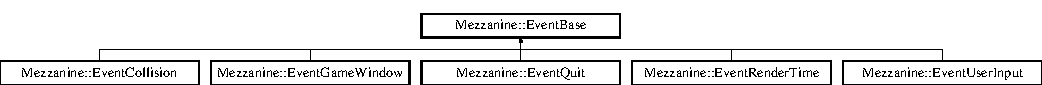
\includegraphics[height=1.148718cm]{classMezzanine_1_1EventBase}
\end{center}
\end{figure}
\subsubsection*{Public Types}
\begin{DoxyCompactItemize}
\item 
enum \hyperlink{classMezzanine_1_1EventBase_ab85e31e97753b7e7ecb098f82526baef}{EventType} \{ \par
\hyperlink{classMezzanine_1_1EventBase_ab85e31e97753b7e7ecb098f82526baefa43524066d608d6b89efed16d238049e9}{Collision}, 
\hyperlink{classMezzanine_1_1EventBase_ab85e31e97753b7e7ecb098f82526baefa90dad901adb5d77f267cd946a852b8c3}{GameWindow}, 
\hyperlink{classMezzanine_1_1EventBase_ab85e31e97753b7e7ecb098f82526baefae4ae51b0b870fc7229b52f636d30d19c}{QuitMessage}, 
\hyperlink{classMezzanine_1_1EventBase_ab85e31e97753b7e7ecb098f82526baefadd50d906767833b4676aa2cb2e232de2}{RenderTime}, 
\par
\hyperlink{classMezzanine_1_1EventBase_ab85e31e97753b7e7ecb098f82526baefacfd86eef72e950cce84662d8a1a121cd}{UserInput}, 
{\bfseries Other}
 \}
\end{DoxyCompactItemize}
\subsubsection*{Public Member Functions}
\begin{DoxyCompactItemize}
\item 
virtual \hyperlink{classMezzanine_1_1EventBase_ab85e31e97753b7e7ecb098f82526baef}{EventBase::EventType} \hyperlink{classMezzanine_1_1EventBase_aea900262a74d27e3b5df68a9deb18543}{GetType} () const =0
\begin{DoxyCompactList}\small\item\em This will aid in identifying all classes that inherit from this class. \item\end{DoxyCompactList}\end{DoxyCompactItemize}


\subsubsection{Detailed Description}
The base class for all events. All Events used in the Event Manager, will inherit from this. While not absolutely required by the game programmer to write their own events, it it could be useful. Instances of this class cannot be made, and all classes that inherit from this are expected to implement getEventType(). 

Definition at line 61 of file eventbase.h.



\subsubsection{Member Enumeration Documentation}
\hypertarget{classMezzanine_1_1EventBase_ab85e31e97753b7e7ecb098f82526baef}{
\index{Mezzanine::EventBase@{Mezzanine::EventBase}!EventType@{EventType}}
\index{EventType@{EventType}!Mezzanine::EventBase@{Mezzanine::EventBase}}
\paragraph[{EventType}]{\setlength{\rightskip}{0pt plus 5cm}enum {\bf Mezzanine::EventBase::EventType}}\hfill}
\label{classMezzanine_1_1EventBase_ab85e31e97753b7e7ecb098f82526baef}
A listing of values that can be used to identify Events. \begin{Desc}
\item[Enumerator: ]\par
\begin{description}
\index{Collision@{Collision}!Mezzanine::EventBase@{Mezzanine::EventBase}}\index{Mezzanine::EventBase@{Mezzanine::EventBase}!Collision@{Collision}}\item[{\em 
\hypertarget{classMezzanine_1_1EventBase_ab85e31e97753b7e7ecb098f82526baefa43524066d608d6b89efed16d238049e9}{
Collision}
\label{classMezzanine_1_1EventBase_ab85e31e97753b7e7ecb098f82526baefa43524066d608d6b89efed16d238049e9}
}]Indicates the Event is a Physics \hyperlink{classMezzanine_1_1Collision}{Collision} Event \index{GameWindow@{GameWindow}!Mezzanine::EventBase@{Mezzanine::EventBase}}\index{Mezzanine::EventBase@{Mezzanine::EventBase}!GameWindow@{GameWindow}}\item[{\em 
\hypertarget{classMezzanine_1_1EventBase_ab85e31e97753b7e7ecb098f82526baefa90dad901adb5d77f267cd946a852b8c3}{
GameWindow}
\label{classMezzanine_1_1EventBase_ab85e31e97753b7e7ecb098f82526baefa90dad901adb5d77f267cd946a852b8c3}
}]Indicates the Event is a Game Window Management Event \index{QuitMessage@{QuitMessage}!Mezzanine::EventBase@{Mezzanine::EventBase}}\index{Mezzanine::EventBase@{Mezzanine::EventBase}!QuitMessage@{QuitMessage}}\item[{\em 
\hypertarget{classMezzanine_1_1EventBase_ab85e31e97753b7e7ecb098f82526baefae4ae51b0b870fc7229b52f636d30d19c}{
QuitMessage}
\label{classMezzanine_1_1EventBase_ab85e31e97753b7e7ecb098f82526baefae4ae51b0b870fc7229b52f636d30d19c}
}]Indicates the Event is a \hyperlink{classMezzanine_1_1EventQuit}{Mezzanine::EventQuit} \index{RenderTime@{RenderTime}!Mezzanine::EventBase@{Mezzanine::EventBase}}\index{Mezzanine::EventBase@{Mezzanine::EventBase}!RenderTime@{RenderTime}}\item[{\em 
\hypertarget{classMezzanine_1_1EventBase_ab85e31e97753b7e7ecb098f82526baefadd50d906767833b4676aa2cb2e232de2}{
RenderTime}
\label{classMezzanine_1_1EventBase_ab85e31e97753b7e7ecb098f82526baefadd50d906767833b4676aa2cb2e232de2}
}]Indicates the Event is a \hyperlink{classMezzanine_1_1EventRenderTime}{EventRenderTime} \index{UserInput@{UserInput}!Mezzanine::EventBase@{Mezzanine::EventBase}}\index{Mezzanine::EventBase@{Mezzanine::EventBase}!UserInput@{UserInput}}\item[{\em 
\hypertarget{classMezzanine_1_1EventBase_ab85e31e97753b7e7ecb098f82526baefacfd86eef72e950cce84662d8a1a121cd}{
UserInput}
\label{classMezzanine_1_1EventBase_ab85e31e97753b7e7ecb098f82526baefacfd86eef72e950cce84662d8a1a121cd}
}]Indicates the Event is a \hyperlink{classMezzanine_1_1EventUserInput}{EventUserInput} \end{description}
\end{Desc}



Definition at line 67 of file eventbase.h.



\subsubsection{Member Function Documentation}
\hypertarget{classMezzanine_1_1EventBase_aea900262a74d27e3b5df68a9deb18543}{
\index{Mezzanine::EventBase@{Mezzanine::EventBase}!GetType@{GetType}}
\index{GetType@{GetType}!Mezzanine::EventBase@{Mezzanine::EventBase}}
\paragraph[{GetType}]{\setlength{\rightskip}{0pt plus 5cm}virtual {\bf EventBase::EventType} Mezzanine::EventBase::GetType (
\begin{DoxyParamCaption}
{}
\end{DoxyParamCaption}
) const\hspace{0.3cm}{\ttfamily  \mbox{[}pure virtual\mbox{]}}}\hfill}
\label{classMezzanine_1_1EventBase_aea900262a74d27e3b5df68a9deb18543}


This will aid in identifying all classes that inherit from this class. 

All Classes derived form this calls will return an Event::EventType that correspond the the data/class type they actually are. \begin{DoxyReturn}{Returns}
This returns an eventype that will correspend with the actual event type. This can be used on all \hyperlink{namespaceMezzanine}{Mezzanine} provided class to safely cast a pointer to the correct event type. 
\end{DoxyReturn}


Implemented in \hyperlink{classMezzanine_1_1EventCollision_af5d9f7eb0ee0ce22b0dd5dfbafc8f297}{Mezzanine::EventCollision}, \hyperlink{classMezzanine_1_1EventGameWindow_a6658ffa68d0d39e2718214fb7a7da3d7}{Mezzanine::EventGameWindow}, \hyperlink{classMezzanine_1_1EventQuit_adffd297e6d7ca09cfde8df0f08da5e31}{Mezzanine::EventQuit}, \hyperlink{classMezzanine_1_1EventRenderTime_a2c1c6c5c8c77492bc9c74c6529d49681}{Mezzanine::EventRenderTime}, and \hyperlink{classMezzanine_1_1EventUserInput_aeb02733446620bd7ff43b449ce5ce98a}{Mezzanine::EventUserInput}.



The documentation for this class was generated from the following file:\begin{DoxyCompactItemize}
\item 
eventbase.h\end{DoxyCompactItemize}

\hypertarget{classMezzanine_1_1EventCollision}{
\subsection{Mezzanine::EventCollision Class Reference}
\label{classMezzanine_1_1EventCollision}\index{Mezzanine::EventCollision@{Mezzanine::EventCollision}}
}


This is an event class used to track collsions in the physics world.  




{\ttfamily \#include $<$eventcollision.h$>$}

Inheritance diagram for Mezzanine::EventCollision:\begin{figure}[H]
\begin{center}
\leavevmode
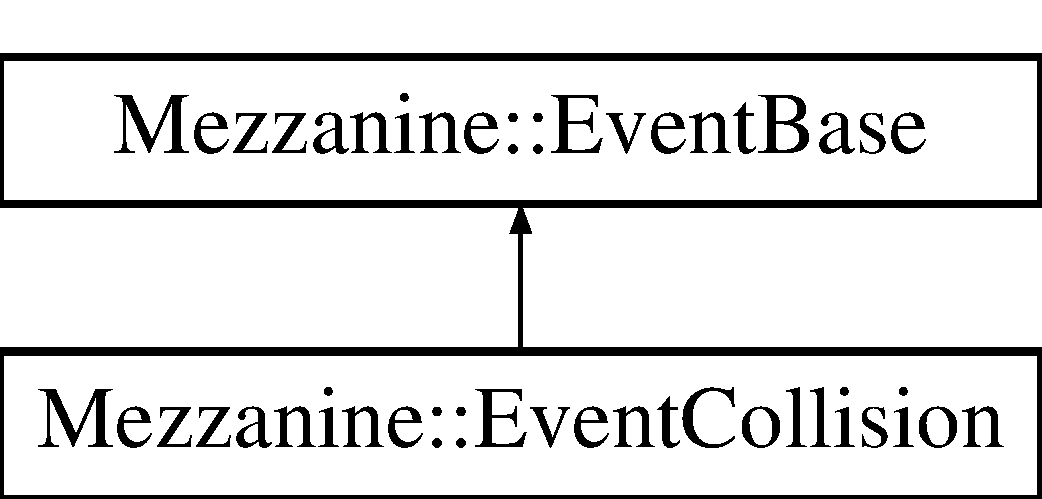
\includegraphics[height=2.000000cm]{classMezzanine_1_1EventCollision}
\end{center}
\end{figure}
\subsubsection*{Public Member Functions}
\begin{DoxyCompactItemize}
\item 
\hypertarget{classMezzanine_1_1EventCollision_ae0813b544c1df94159e364b3a5720a6a}{
\hyperlink{classMezzanine_1_1EventCollision_ae0813b544c1df94159e364b3a5720a6a}{EventCollision} ()}
\label{classMezzanine_1_1EventCollision_ae0813b544c1df94159e364b3a5720a6a}

\begin{DoxyCompactList}\small\item\em Default Constructor. \item\end{DoxyCompactList}\item 
\hyperlink{classMezzanine_1_1EventCollision_affa8e2d9f0d20d33e8131fa05348879c}{EventCollision} (\hyperlink{classMezzanine_1_1ActorBase}{ActorBase} $\ast$actora, \hyperlink{classMezzanine_1_1ActorBase}{ActorBase} $\ast$actorb, \hyperlink{classMezzanine_1_1Collision}{Mezzanine::Collision} $\ast$Col)
\begin{DoxyCompactList}\small\item\em Class Constructor. \item\end{DoxyCompactList}\item 
\hyperlink{classMezzanine_1_1EventCollision_ae6917514b805e00607ce88ae01f52780}{EventCollision} (const \hyperlink{classMezzanine_1_1EventCollision}{EventCollision} \&Other)
\begin{DoxyCompactList}\small\item\em Copy Constructor. \item\end{DoxyCompactList}\item 
virtual \hyperlink{classMezzanine_1_1ActorBase}{ActorBase} $\ast$ \hyperlink{classMezzanine_1_1EventCollision_adb7943576f8033703f0afcbce43f56cc}{GetActorA} () const 
\begin{DoxyCompactList}\small\item\em Gets the first actor this collision applies to. \item\end{DoxyCompactList}\item 
virtual \hyperlink{classMezzanine_1_1ActorBase}{ActorBase} $\ast$ \hyperlink{classMezzanine_1_1EventCollision_ad3d7b44e680425d33bb2556de4d9a056}{GetActorB} () const 
\begin{DoxyCompactList}\small\item\em Gets the second actor this collision applies to. \item\end{DoxyCompactList}\item 
virtual \hyperlink{classMezzanine_1_1EventBase_ab85e31e97753b7e7ecb098f82526baef}{EventType} \hyperlink{classMezzanine_1_1EventCollision_af5d9f7eb0ee0ce22b0dd5dfbafc8f297}{GetType} () const 
\begin{DoxyCompactList}\small\item\em This returns EventType::Collision. \item\end{DoxyCompactList}\item 
virtual void \hyperlink{classMezzanine_1_1EventCollision_a90e9b3a89762db6a3c55aa262833bcd7}{SetActorA} (\hyperlink{classMezzanine_1_1ActorBase}{ActorBase} $\ast$A)
\begin{DoxyCompactList}\small\item\em Sets the first actor this collision applies to. \item\end{DoxyCompactList}\item 
virtual void \hyperlink{classMezzanine_1_1EventCollision_aef6da3acdc9879b21990cb25fa285304}{SetActorB} (\hyperlink{classMezzanine_1_1ActorBase}{ActorBase} $\ast$B)
\begin{DoxyCompactList}\small\item\em Sets the second actor this collision applies to. \item\end{DoxyCompactList}\item 
virtual \hyperlink{classMezzanine_1_1EventCollision_a72cabbfa2f7983d8b017755791e89632}{$\sim$EventCollision} ()
\begin{DoxyCompactList}\small\item\em Class Destructor. \item\end{DoxyCompactList}\end{DoxyCompactItemize}
\subsubsection*{Protected Attributes}
\begin{DoxyCompactItemize}
\item 
\hypertarget{classMezzanine_1_1EventCollision_a9e076c11df8b6e16c357f0a5c373542a}{
\hyperlink{classMezzanine_1_1ActorBase}{ActorBase} $\ast$ \hyperlink{classMezzanine_1_1EventCollision_a9e076c11df8b6e16c357f0a5c373542a}{ActorA}}
\label{classMezzanine_1_1EventCollision_a9e076c11df8b6e16c357f0a5c373542a}

\begin{DoxyCompactList}\small\item\em The first Actor involved in the collision. \item\end{DoxyCompactList}\item 
\hypertarget{classMezzanine_1_1EventCollision_aca0535fa8e9e4fbbb0229c6342e05da4}{
\hyperlink{classMezzanine_1_1ActorBase}{ActorBase} $\ast$ \hyperlink{classMezzanine_1_1EventCollision_aca0535fa8e9e4fbbb0229c6342e05da4}{ActorB}}
\label{classMezzanine_1_1EventCollision_aca0535fa8e9e4fbbb0229c6342e05da4}

\begin{DoxyCompactList}\small\item\em The second Actor invovled in the collision. \item\end{DoxyCompactList}\item 
\hypertarget{classMezzanine_1_1EventCollision_a562c1ab56444569b478a7a613caef42c}{
\hyperlink{classMezzanine_1_1Collision}{Mezzanine::Collision} $\ast$ \hyperlink{classMezzanine_1_1EventCollision_a562c1ab56444569b478a7a613caef42c}{ObjectCollision}}
\label{classMezzanine_1_1EventCollision_a562c1ab56444569b478a7a613caef42c}

\begin{DoxyCompactList}\small\item\em The internal collision class this event is based on. \item\end{DoxyCompactList}\end{DoxyCompactItemize}
\subsubsection*{Friends}
\begin{DoxyCompactItemize}
\item 
\hypertarget{classMezzanine_1_1EventCollision_aa4a13416efe17e957deb2cf4dcce3a60}{
class {\bfseries CollisionDispatcher}}
\label{classMezzanine_1_1EventCollision_aa4a13416efe17e957deb2cf4dcce3a60}

\end{DoxyCompactItemize}


\subsubsection{Detailed Description}
This is an event class used to track collsions in the physics world. 

Definition at line 58 of file eventcollision.h.



\subsubsection{Constructor \& Destructor Documentation}
\hypertarget{classMezzanine_1_1EventCollision_affa8e2d9f0d20d33e8131fa05348879c}{
\index{Mezzanine::EventCollision@{Mezzanine::EventCollision}!EventCollision@{EventCollision}}
\index{EventCollision@{EventCollision}!Mezzanine::EventCollision@{Mezzanine::EventCollision}}
\paragraph[{EventCollision}]{\setlength{\rightskip}{0pt plus 5cm}Mezzanine::EventCollision::EventCollision (
\begin{DoxyParamCaption}
\item[{{\bf ActorBase} $\ast$}]{actora, }
\item[{{\bf ActorBase} $\ast$}]{actorb, }
\item[{{\bf Mezzanine::Collision} $\ast$}]{Col}
\end{DoxyParamCaption}
)}\hfill}
\label{classMezzanine_1_1EventCollision_affa8e2d9f0d20d33e8131fa05348879c}


Class Constructor. 

This will construct a basic event class with the minimum data needed. 
\begin{DoxyParams}{Parameters}
{\em actora} & The first Actor involved in the collision. \\
\hline
{\em actorb} & The second Actor invovled in the collision. \\
\hline
{\em PhysicsManifold} & The internal manifold used for querying collision data. \\
\hline
\end{DoxyParams}


Definition at line 62 of file eventcollision.cpp.

\hypertarget{classMezzanine_1_1EventCollision_ae6917514b805e00607ce88ae01f52780}{
\index{Mezzanine::EventCollision@{Mezzanine::EventCollision}!EventCollision@{EventCollision}}
\index{EventCollision@{EventCollision}!Mezzanine::EventCollision@{Mezzanine::EventCollision}}
\paragraph[{EventCollision}]{\setlength{\rightskip}{0pt plus 5cm}Mezzanine::EventCollision::EventCollision (
\begin{DoxyParamCaption}
\item[{const {\bf EventCollision} \&}]{Other}
\end{DoxyParamCaption}
)}\hfill}
\label{classMezzanine_1_1EventCollision_ae6917514b805e00607ce88ae01f52780}


Copy Constructor. 


\begin{DoxyParams}{Parameters}
{\em Other} & The other \hyperlink{classMezzanine_1_1EventCollision}{EventCollision} to copy \\
\hline
\end{DoxyParams}


Definition at line 69 of file eventcollision.cpp.

\hypertarget{classMezzanine_1_1EventCollision_a72cabbfa2f7983d8b017755791e89632}{
\index{Mezzanine::EventCollision@{Mezzanine::EventCollision}!$\sim$EventCollision@{$\sim$EventCollision}}
\index{$\sim$EventCollision@{$\sim$EventCollision}!Mezzanine::EventCollision@{Mezzanine::EventCollision}}
\paragraph[{$\sim$EventCollision}]{\setlength{\rightskip}{0pt plus 5cm}Mezzanine::EventCollision::$\sim$EventCollision (
\begin{DoxyParamCaption}
{}
\end{DoxyParamCaption}
)\hspace{0.3cm}{\ttfamily  \mbox{[}virtual\mbox{]}}}\hfill}
\label{classMezzanine_1_1EventCollision_a72cabbfa2f7983d8b017755791e89632}


Class Destructor. 

Basic Class Destructor. 

Definition at line 75 of file eventcollision.cpp.



\subsubsection{Member Function Documentation}
\hypertarget{classMezzanine_1_1EventCollision_adb7943576f8033703f0afcbce43f56cc}{
\index{Mezzanine::EventCollision@{Mezzanine::EventCollision}!GetActorA@{GetActorA}}
\index{GetActorA@{GetActorA}!Mezzanine::EventCollision@{Mezzanine::EventCollision}}
\paragraph[{GetActorA}]{\setlength{\rightskip}{0pt plus 5cm}{\bf ActorBase} $\ast$ Mezzanine::EventCollision::GetActorA (
\begin{DoxyParamCaption}
{}
\end{DoxyParamCaption}
) const\hspace{0.3cm}{\ttfamily  \mbox{[}virtual\mbox{]}}}\hfill}
\label{classMezzanine_1_1EventCollision_adb7943576f8033703f0afcbce43f56cc}


Gets the first actor this collision applies to. 

\begin{DoxyReturn}{Returns}
Returns a pointer to the first actor in this event. 
\end{DoxyReturn}


Definition at line 89 of file eventcollision.cpp.

\hypertarget{classMezzanine_1_1EventCollision_ad3d7b44e680425d33bb2556de4d9a056}{
\index{Mezzanine::EventCollision@{Mezzanine::EventCollision}!GetActorB@{GetActorB}}
\index{GetActorB@{GetActorB}!Mezzanine::EventCollision@{Mezzanine::EventCollision}}
\paragraph[{GetActorB}]{\setlength{\rightskip}{0pt plus 5cm}{\bf ActorBase} $\ast$ Mezzanine::EventCollision::GetActorB (
\begin{DoxyParamCaption}
{}
\end{DoxyParamCaption}
) const\hspace{0.3cm}{\ttfamily  \mbox{[}virtual\mbox{]}}}\hfill}
\label{classMezzanine_1_1EventCollision_ad3d7b44e680425d33bb2556de4d9a056}


Gets the second actor this collision applies to. 

\begin{DoxyReturn}{Returns}
Returns a pointer to the second actor in this event. 
\end{DoxyReturn}


Definition at line 104 of file eventcollision.cpp.

\hypertarget{classMezzanine_1_1EventCollision_af5d9f7eb0ee0ce22b0dd5dfbafc8f297}{
\index{Mezzanine::EventCollision@{Mezzanine::EventCollision}!GetType@{GetType}}
\index{GetType@{GetType}!Mezzanine::EventCollision@{Mezzanine::EventCollision}}
\paragraph[{GetType}]{\setlength{\rightskip}{0pt plus 5cm}{\bf EventBase::EventType} Mezzanine::EventCollision::GetType (
\begin{DoxyParamCaption}
{}
\end{DoxyParamCaption}
) const\hspace{0.3cm}{\ttfamily  \mbox{[}virtual\mbox{]}}}\hfill}
\label{classMezzanine_1_1EventCollision_af5d9f7eb0ee0ce22b0dd5dfbafc8f297}


This returns EventType::Collision. 

This returns the kind of message this is, specifcally EventType::Collision. This method is inherited from Mezzanine::Event. . 

Implements \hyperlink{classMezzanine_1_1EventBase_aea900262a74d27e3b5df68a9deb18543}{Mezzanine::EventBase}.



Definition at line 109 of file eventcollision.cpp.

\hypertarget{classMezzanine_1_1EventCollision_a90e9b3a89762db6a3c55aa262833bcd7}{
\index{Mezzanine::EventCollision@{Mezzanine::EventCollision}!SetActorA@{SetActorA}}
\index{SetActorA@{SetActorA}!Mezzanine::EventCollision@{Mezzanine::EventCollision}}
\paragraph[{SetActorA}]{\setlength{\rightskip}{0pt plus 5cm}void Mezzanine::EventCollision::SetActorA (
\begin{DoxyParamCaption}
\item[{{\bf ActorBase} $\ast$}]{A}
\end{DoxyParamCaption}
)\hspace{0.3cm}{\ttfamily  \mbox{[}virtual\mbox{]}}}\hfill}
\label{classMezzanine_1_1EventCollision_a90e9b3a89762db6a3c55aa262833bcd7}


Sets the first actor this collision applies to. 

\begin{DoxyWarning}{Warning}
\hyperlink{classMezzanine_1_1Collision}{Collision} events can't/shouldn't have the bodies they apply to changed. This function exists mostly just for the blank constructor when you need to set them afterward. If you attempt to set this when the pointer is already set, it will log the event but otherwise silently fail. 
\end{DoxyWarning}

\begin{DoxyParams}{Parameters}
{\em A} & The first actor in this event. \\
\hline
\end{DoxyParams}


Definition at line 79 of file eventcollision.cpp.

\hypertarget{classMezzanine_1_1EventCollision_aef6da3acdc9879b21990cb25fa285304}{
\index{Mezzanine::EventCollision@{Mezzanine::EventCollision}!SetActorB@{SetActorB}}
\index{SetActorB@{SetActorB}!Mezzanine::EventCollision@{Mezzanine::EventCollision}}
\paragraph[{SetActorB}]{\setlength{\rightskip}{0pt plus 5cm}void Mezzanine::EventCollision::SetActorB (
\begin{DoxyParamCaption}
\item[{{\bf ActorBase} $\ast$}]{B}
\end{DoxyParamCaption}
)\hspace{0.3cm}{\ttfamily  \mbox{[}virtual\mbox{]}}}\hfill}
\label{classMezzanine_1_1EventCollision_aef6da3acdc9879b21990cb25fa285304}


Sets the second actor this collision applies to. 

\begin{DoxyWarning}{Warning}
\hyperlink{classMezzanine_1_1Collision}{Collision} events can't/shouldn't have the bodies they apply to changed. This function exists mostly just for the blank constructor when you need to set them afterward. If you attempt to set this when the pointer is already set, it will log the event but otherwise silently fail. 
\end{DoxyWarning}

\begin{DoxyParams}{Parameters}
{\em B} & The second actor in this event. \\
\hline
\end{DoxyParams}


Definition at line 94 of file eventcollision.cpp.



The documentation for this class was generated from the following files:\begin{DoxyCompactItemize}
\item 
eventcollision.h\item 
eventcollision.cpp\end{DoxyCompactItemize}

\hypertarget{classMezzanine_1_1EventGameWindow}{
\subsection{Mezzanine::EventGameWindow Class Reference}
\label{classMezzanine_1_1EventGameWindow}\index{Mezzanine::EventGameWindow@{Mezzanine::EventGameWindow}}
}


Convey the message that Something happened to a game window.  




{\ttfamily \#include $<$eventgamewindow.h$>$}

Inheritance diagram for Mezzanine::EventGameWindow:\begin{figure}[H]
\begin{center}
\leavevmode
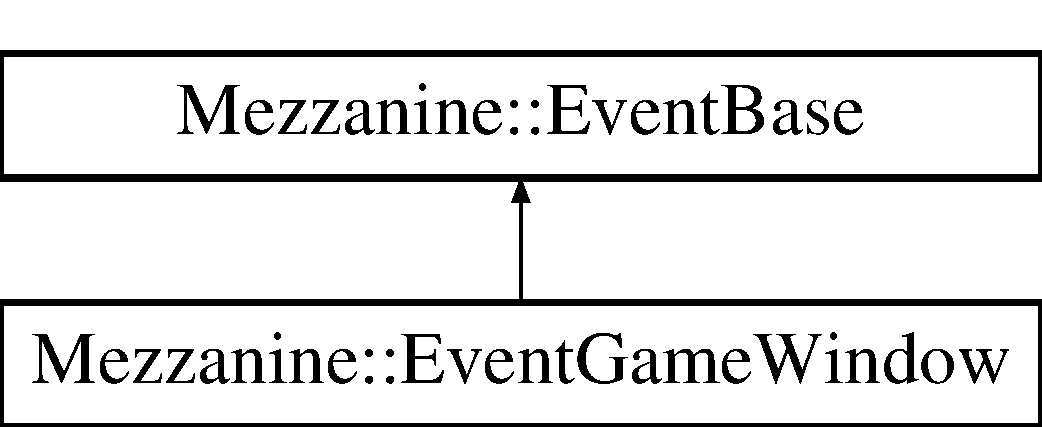
\includegraphics[height=2.000000cm]{classMezzanine_1_1EventGameWindow}
\end{center}
\end{figure}
\subsubsection*{Public Types}
\begin{DoxyCompactItemize}
\item 
enum \hyperlink{classMezzanine_1_1EventGameWindow_a0f0ff29853317334f018bcf48d502af2}{GameWindowEventID} \{ \par
\hyperlink{classMezzanine_1_1EventGameWindow_a0f0ff29853317334f018bcf48d502af2a892269bc048c1f0049d8b812da24bd53}{GAME\_\-WINDOW\_\-NONE} = 0, 
\hyperlink{classMezzanine_1_1EventGameWindow_a0f0ff29853317334f018bcf48d502af2a3a18d47a742d53b085ab8e9fc7a54895}{GAME\_\-WINDOW\_\-FIRST} =  GAME\_\-WINDOW\_\-NONE, 
\hyperlink{classMezzanine_1_1EventGameWindow_a0f0ff29853317334f018bcf48d502af2aa89066b0378529a05a65e6873ca402d1}{GAME\_\-WINDOW\_\-SHOWN} =  1, 
\hyperlink{classMezzanine_1_1EventGameWindow_a0f0ff29853317334f018bcf48d502af2a37c7d5b4d0e1a475d5ce3fb349a301a7}{GAME\_\-WINDOW\_\-HIDDEN} =  2, 
\par
\hyperlink{classMezzanine_1_1EventGameWindow_a0f0ff29853317334f018bcf48d502af2a8964328b582a9db0df814dd385fd93fb}{GAME\_\-WINDOW\_\-EXPOSED} =  3, 
\hyperlink{classMezzanine_1_1EventGameWindow_a0f0ff29853317334f018bcf48d502af2a0737c3b12ec648cee8ce44ed93c10064}{GAME\_\-WINDOW\_\-MOVED} =  4, 
\hyperlink{classMezzanine_1_1EventGameWindow_a0f0ff29853317334f018bcf48d502af2aa7255db1e6f3173f9368c3a2dcaab857}{GAME\_\-WINDOW\_\-RESIZED} =  5, 
\hyperlink{classMezzanine_1_1EventGameWindow_a0f0ff29853317334f018bcf48d502af2aa5ea0a38767bad184a886284fb202afb}{GAME\_\-WINDOW\_\-SIZE\_\-CHANGED} =  6, 
\par
\hyperlink{classMezzanine_1_1EventGameWindow_a0f0ff29853317334f018bcf48d502af2a17e8093e3c905a1636a380153bd1a6ef}{GAME\_\-WINDOW\_\-MINIMIZED} =  7, 
\hyperlink{classMezzanine_1_1EventGameWindow_a0f0ff29853317334f018bcf48d502af2afc31ceecd15a156e1d8baca2d899aa8a}{GAME\_\-WINDOW\_\-MAXIMIZED} =  8, 
\hyperlink{classMezzanine_1_1EventGameWindow_a0f0ff29853317334f018bcf48d502af2af24d3d62a01ee70de0213d81f75767fe}{GAME\_\-WINDOW\_\-RESTORED} =  9, 
\hyperlink{classMezzanine_1_1EventGameWindow_a0f0ff29853317334f018bcf48d502af2af2909516a47a485d4b00ffdcd851f92a}{GAME\_\-WINDOW\_\-ENTER} =  10, 
\par
\hyperlink{classMezzanine_1_1EventGameWindow_a0f0ff29853317334f018bcf48d502af2a134ddfd78b7c1e685f4325bacabf928d}{GAME\_\-WINDOW\_\-LEAVE} =  11, 
\hyperlink{classMezzanine_1_1EventGameWindow_a0f0ff29853317334f018bcf48d502af2a33458969664c21f536a6aacca470d77d}{GAME\_\-WINDOW\_\-FOCUS\_\-GAINED} =  12, 
\hyperlink{classMezzanine_1_1EventGameWindow_a0f0ff29853317334f018bcf48d502af2a4cef8ef4f7b17addaab216f86ea5820d}{GAME\_\-WINDOW\_\-FOCUS\_\-LOST} =  13, 
\hyperlink{classMezzanine_1_1EventGameWindow_a0f0ff29853317334f018bcf48d502af2a5632bb10b9d79cb918fe89971f22895b}{GAME\_\-WINDOW\_\-CLOSE} =  14, 
\par
\hyperlink{classMezzanine_1_1EventGameWindow_a0f0ff29853317334f018bcf48d502af2a2a8bc5ca735165737b84b8088463f3a7}{GAME\_\-WINDOW\_\-LAST} =  GAME\_\-WINDOW\_\-CLOSE
 \}
\begin{DoxyCompactList}\small\item\em Used to identify the kind of change that has happened to the game window. \item\end{DoxyCompactList}\end{DoxyCompactItemize}
\subsubsection*{Public Member Functions}
\begin{DoxyCompactItemize}
\item 
\hyperlink{classMezzanine_1_1EventGameWindow_a1ba3b047ac8203c5b1d33644f365039b}{EventGameWindow} (\hyperlink{namespaceMezzanine_ae8d4c0ab783af89a250b0225b75753e5}{RawEvent} Raw\_\-)
\begin{DoxyCompactList}\small\item\em Creates an \hyperlink{classMezzanine_1_1EventGameWindow}{EventGameWindow} from a Rawevent. \item\end{DoxyCompactList}\item 
\hyperlink{classMezzanine_1_1EventGameWindow_a9a7ca5ec6fe5f95244e6133b6627d4ac}{EventGameWindow} (\hyperlink{classMezzanine_1_1EventGameWindow_a0f0ff29853317334f018bcf48d502af2}{GameWindowEventID} GWEventID=GAME\_\-WINDOW\_\-NONE, int First=0, int Second=0)
\begin{DoxyCompactList}\small\item\em Creates an \hyperlink{classMezzanine_1_1EventGameWindow}{EventGameWindow} from manually assigned values. \item\end{DoxyCompactList}\item 
\hyperlink{classMezzanine_1_1EventGameWindow_aec071261cc581c6b6767f77691e20996}{EventGameWindow} (const \hyperlink{classMezzanine_1_1EventGameWindow}{EventGameWindow} \&Other)
\begin{DoxyCompactList}\small\item\em Copy constructor. \item\end{DoxyCompactList}\item 
\hyperlink{classMezzanine_1_1EventGameWindow_a0f0ff29853317334f018bcf48d502af2}{GameWindowEventID} \hyperlink{classMezzanine_1_1EventGameWindow_ace6bd54e020a18818027cdfc88970e81}{GetEventID} () const 
\begin{DoxyCompactList}\small\item\em What just happened, what kind of event was it. \item\end{DoxyCompactList}\item 
int \hyperlink{classMezzanine_1_1EventGameWindow_aff42c9bc5c487536e2101547da8162e8}{GetFirstEventData} () const 
\begin{DoxyCompactList}\small\item\em Where or how much happened, Get the first event dependent data. \item\end{DoxyCompactList}\item 
int \hyperlink{classMezzanine_1_1EventGameWindow_afeb55f7d4cc99a8c0539fdb02feaea03}{GetSecondEventData} () const 
\begin{DoxyCompactList}\small\item\em Where or how much happened, Get the second event dependent data. \item\end{DoxyCompactList}\item 
virtual \hyperlink{classMezzanine_1_1EventBase_ab85e31e97753b7e7ecb098f82526baef}{EventType} \hyperlink{classMezzanine_1_1EventGameWindow_a6658ffa68d0d39e2718214fb7a7da3d7}{GetType} () const 
\begin{DoxyCompactList}\small\item\em This returns EventType::GameWindow. \item\end{DoxyCompactList}\item 
bool \hyperlink{classMezzanine_1_1EventGameWindow_ab51a632acaf07f9a46817467ca54efca}{IsEventIDValid} () const 
\begin{DoxyCompactList}\small\item\em Used to help determine if this Event is valid by checking the contents of the GameWindowEventID. \item\end{DoxyCompactList}\item 
void \hyperlink{classMezzanine_1_1EventGameWindow_a6935c29b1cf42798871e8a6e6600fa2e}{operator=} (const \hyperlink{classMezzanine_1_1EventGameWindow}{EventGameWindow} \&Other)
\begin{DoxyCompactList}\small\item\em Assignment of a this \hyperlink{classMezzanine_1_1EventGameWindowData}{EventGameWindowData}. \item\end{DoxyCompactList}\item 
bool \hyperlink{classMezzanine_1_1EventGameWindow_aedf12ca51b11e074d8cb8baa801c19fa}{operator==} (const \hyperlink{classMezzanine_1_1EventGameWindow_a0f0ff29853317334f018bcf48d502af2}{GameWindowEventID} \&Other) const 
\begin{DoxyCompactList}\small\item\em Equality comparison of this \hyperlink{classMezzanine_1_1EventGameWindowData}{EventGameWindowData} and a GameWindowEventID. \item\end{DoxyCompactList}\item 
bool \hyperlink{classMezzanine_1_1EventGameWindow_a10469157e4d442072a5751029a347056}{operator==} (const \hyperlink{classMezzanine_1_1EventGameWindow}{EventGameWindow} \&Other) const 
\begin{DoxyCompactList}\small\item\em Equality comparison of two \hyperlink{classMezzanine_1_1EventGameWindowData}{EventGameWindowData}. \item\end{DoxyCompactList}\item 
\hypertarget{classMezzanine_1_1EventGameWindow_a68195b843c1126e30846e791c7ef3d99}{
\hyperlink{classMezzanine_1_1EventGameWindow_a68195b843c1126e30846e791c7ef3d99}{$\sim$EventGameWindow} ()}
\label{classMezzanine_1_1EventGameWindow_a68195b843c1126e30846e791c7ef3d99}

\begin{DoxyCompactList}\small\item\em Deconstructs this \hyperlink{classMezzanine_1_1EventGameWindow}{EventGameWindow}. \item\end{DoxyCompactList}\end{DoxyCompactItemize}
\subsubsection*{Static Public Member Functions}
\begin{DoxyCompactItemize}
\item 
static \hyperlink{namespaceMezzanine_acf9fcc130e6ebf08e3d8491aebcf1c86}{String} \hyperlink{classMezzanine_1_1EventGameWindow_a0f4f76cc85926b7687187a1260427b60}{GameWindowEventIDToString} (\hyperlink{classMezzanine_1_1EventGameWindow_a0f0ff29853317334f018bcf48d502af2}{EventGameWindow::GameWindowEventID} GWEventID)
\begin{DoxyCompactList}\small\item\em Converts GameWindowEventID To Strings. \item\end{DoxyCompactList}\end{DoxyCompactItemize}
\subsubsection*{Protected Attributes}
\begin{DoxyCompactItemize}
\item 
\hypertarget{classMezzanine_1_1EventGameWindow_a5db6d56993dada5f413f3564cc990ad4}{
\hyperlink{classMezzanine_1_1EventGameWindowData}{EventGameWindowData} $\ast$ \hyperlink{classMezzanine_1_1EventGameWindow_a5db6d56993dada5f413f3564cc990ad4}{Data}}
\label{classMezzanine_1_1EventGameWindow_a5db6d56993dada5f413f3564cc990ad4}

\begin{DoxyCompactList}\small\item\em Holds all internal data. \item\end{DoxyCompactList}\end{DoxyCompactItemize}


\subsubsection{Detailed Description}
Convey the message that Something happened to a game window. 

Definition at line 61 of file eventgamewindow.h.



\subsubsection{Member Enumeration Documentation}
\hypertarget{classMezzanine_1_1EventGameWindow_a0f0ff29853317334f018bcf48d502af2}{
\index{Mezzanine::EventGameWindow@{Mezzanine::EventGameWindow}!GameWindowEventID@{GameWindowEventID}}
\index{GameWindowEventID@{GameWindowEventID}!Mezzanine::EventGameWindow@{Mezzanine::EventGameWindow}}
\paragraph[{GameWindowEventID}]{\setlength{\rightskip}{0pt plus 5cm}enum {\bf Mezzanine::EventGameWindow::GameWindowEventID}}\hfill}
\label{classMezzanine_1_1EventGameWindow_a0f0ff29853317334f018bcf48d502af2}


Used to identify the kind of change that has happened to the game window. 

\begin{Desc}
\item[Enumerator: ]\par
\begin{description}
\index{GAME\_\-WINDOW\_\-NONE@{GAME\_\-WINDOW\_\-NONE}!Mezzanine::EventGameWindow@{Mezzanine::EventGameWindow}}\index{Mezzanine::EventGameWindow@{Mezzanine::EventGameWindow}!GAME\_\-WINDOW\_\-NONE@{GAME\_\-WINDOW\_\-NONE}}\item[{\em 
\hypertarget{classMezzanine_1_1EventGameWindow_a0f0ff29853317334f018bcf48d502af2a892269bc048c1f0049d8b812da24bd53}{
GAME\_\-WINDOW\_\-NONE}
\label{classMezzanine_1_1EventGameWindow_a0f0ff29853317334f018bcf48d502af2a892269bc048c1f0049d8b812da24bd53}
}]Never used \index{GAME\_\-WINDOW\_\-FIRST@{GAME\_\-WINDOW\_\-FIRST}!Mezzanine::EventGameWindow@{Mezzanine::EventGameWindow}}\index{Mezzanine::EventGameWindow@{Mezzanine::EventGameWindow}!GAME\_\-WINDOW\_\-FIRST@{GAME\_\-WINDOW\_\-FIRST}}\item[{\em 
\hypertarget{classMezzanine_1_1EventGameWindow_a0f0ff29853317334f018bcf48d502af2a3a18d47a742d53b085ab8e9fc7a54895}{
GAME\_\-WINDOW\_\-FIRST}
\label{classMezzanine_1_1EventGameWindow_a0f0ff29853317334f018bcf48d502af2a3a18d47a742d53b085ab8e9fc7a54895}
}]Used only as the lower bounds of this enumeration \index{GAME\_\-WINDOW\_\-SHOWN@{GAME\_\-WINDOW\_\-SHOWN}!Mezzanine::EventGameWindow@{Mezzanine::EventGameWindow}}\index{Mezzanine::EventGameWindow@{Mezzanine::EventGameWindow}!GAME\_\-WINDOW\_\-SHOWN@{GAME\_\-WINDOW\_\-SHOWN}}\item[{\em 
\hypertarget{classMezzanine_1_1EventGameWindow_a0f0ff29853317334f018bcf48d502af2aa89066b0378529a05a65e6873ca402d1}{
GAME\_\-WINDOW\_\-SHOWN}
\label{classMezzanine_1_1EventGameWindow_a0f0ff29853317334f018bcf48d502af2aa89066b0378529a05a65e6873ca402d1}
}]Window has been shown \index{GAME\_\-WINDOW\_\-HIDDEN@{GAME\_\-WINDOW\_\-HIDDEN}!Mezzanine::EventGameWindow@{Mezzanine::EventGameWindow}}\index{Mezzanine::EventGameWindow@{Mezzanine::EventGameWindow}!GAME\_\-WINDOW\_\-HIDDEN@{GAME\_\-WINDOW\_\-HIDDEN}}\item[{\em 
\hypertarget{classMezzanine_1_1EventGameWindow_a0f0ff29853317334f018bcf48d502af2a37c7d5b4d0e1a475d5ce3fb349a301a7}{
GAME\_\-WINDOW\_\-HIDDEN}
\label{classMezzanine_1_1EventGameWindow_a0f0ff29853317334f018bcf48d502af2a37c7d5b4d0e1a475d5ce3fb349a301a7}
}]Window has been hidden \index{GAME\_\-WINDOW\_\-EXPOSED@{GAME\_\-WINDOW\_\-EXPOSED}!Mezzanine::EventGameWindow@{Mezzanine::EventGameWindow}}\index{Mezzanine::EventGameWindow@{Mezzanine::EventGameWindow}!GAME\_\-WINDOW\_\-EXPOSED@{GAME\_\-WINDOW\_\-EXPOSED}}\item[{\em 
\hypertarget{classMezzanine_1_1EventGameWindow_a0f0ff29853317334f018bcf48d502af2a8964328b582a9db0df814dd385fd93fb}{
GAME\_\-WINDOW\_\-EXPOSED}
\label{classMezzanine_1_1EventGameWindow_a0f0ff29853317334f018bcf48d502af2a8964328b582a9db0df814dd385fd93fb}
}]Window has been exposed and should be redrawn \index{GAME\_\-WINDOW\_\-MOVED@{GAME\_\-WINDOW\_\-MOVED}!Mezzanine::EventGameWindow@{Mezzanine::EventGameWindow}}\index{Mezzanine::EventGameWindow@{Mezzanine::EventGameWindow}!GAME\_\-WINDOW\_\-MOVED@{GAME\_\-WINDOW\_\-MOVED}}\item[{\em 
\hypertarget{classMezzanine_1_1EventGameWindow_a0f0ff29853317334f018bcf48d502af2a0737c3b12ec648cee8ce44ed93c10064}{
GAME\_\-WINDOW\_\-MOVED}
\label{classMezzanine_1_1EventGameWindow_a0f0ff29853317334f018bcf48d502af2a0737c3b12ec648cee8ce44ed93c10064}
}]Window has been moved to data1, data2 \index{GAME\_\-WINDOW\_\-RESIZED@{GAME\_\-WINDOW\_\-RESIZED}!Mezzanine::EventGameWindow@{Mezzanine::EventGameWindow}}\index{Mezzanine::EventGameWindow@{Mezzanine::EventGameWindow}!GAME\_\-WINDOW\_\-RESIZED@{GAME\_\-WINDOW\_\-RESIZED}}\item[{\em 
\hypertarget{classMezzanine_1_1EventGameWindow_a0f0ff29853317334f018bcf48d502af2aa7255db1e6f3173f9368c3a2dcaab857}{
GAME\_\-WINDOW\_\-RESIZED}
\label{classMezzanine_1_1EventGameWindow_a0f0ff29853317334f018bcf48d502af2aa7255db1e6f3173f9368c3a2dcaab857}
}]Window has been resized to data1xdata2 \index{GAME\_\-WINDOW\_\-SIZE\_\-CHANGED@{GAME\_\-WINDOW\_\-SIZE\_\-CHANGED}!Mezzanine::EventGameWindow@{Mezzanine::EventGameWindow}}\index{Mezzanine::EventGameWindow@{Mezzanine::EventGameWindow}!GAME\_\-WINDOW\_\-SIZE\_\-CHANGED@{GAME\_\-WINDOW\_\-SIZE\_\-CHANGED}}\item[{\em 
\hypertarget{classMezzanine_1_1EventGameWindow_a0f0ff29853317334f018bcf48d502af2aa5ea0a38767bad184a886284fb202afb}{
GAME\_\-WINDOW\_\-SIZE\_\-CHANGED}
\label{classMezzanine_1_1EventGameWindow_a0f0ff29853317334f018bcf48d502af2aa5ea0a38767bad184a886284fb202afb}
}]The window size has changed, either as a result of an API call or through the system or user changing the window size. \index{GAME\_\-WINDOW\_\-MINIMIZED@{GAME\_\-WINDOW\_\-MINIMIZED}!Mezzanine::EventGameWindow@{Mezzanine::EventGameWindow}}\index{Mezzanine::EventGameWindow@{Mezzanine::EventGameWindow}!GAME\_\-WINDOW\_\-MINIMIZED@{GAME\_\-WINDOW\_\-MINIMIZED}}\item[{\em 
\hypertarget{classMezzanine_1_1EventGameWindow_a0f0ff29853317334f018bcf48d502af2a17e8093e3c905a1636a380153bd1a6ef}{
GAME\_\-WINDOW\_\-MINIMIZED}
\label{classMezzanine_1_1EventGameWindow_a0f0ff29853317334f018bcf48d502af2a17e8093e3c905a1636a380153bd1a6ef}
}]Window has been minimized \index{GAME\_\-WINDOW\_\-MAXIMIZED@{GAME\_\-WINDOW\_\-MAXIMIZED}!Mezzanine::EventGameWindow@{Mezzanine::EventGameWindow}}\index{Mezzanine::EventGameWindow@{Mezzanine::EventGameWindow}!GAME\_\-WINDOW\_\-MAXIMIZED@{GAME\_\-WINDOW\_\-MAXIMIZED}}\item[{\em 
\hypertarget{classMezzanine_1_1EventGameWindow_a0f0ff29853317334f018bcf48d502af2afc31ceecd15a156e1d8baca2d899aa8a}{
GAME\_\-WINDOW\_\-MAXIMIZED}
\label{classMezzanine_1_1EventGameWindow_a0f0ff29853317334f018bcf48d502af2afc31ceecd15a156e1d8baca2d899aa8a}
}]Window has been maximized \index{GAME\_\-WINDOW\_\-RESTORED@{GAME\_\-WINDOW\_\-RESTORED}!Mezzanine::EventGameWindow@{Mezzanine::EventGameWindow}}\index{Mezzanine::EventGameWindow@{Mezzanine::EventGameWindow}!GAME\_\-WINDOW\_\-RESTORED@{GAME\_\-WINDOW\_\-RESTORED}}\item[{\em 
\hypertarget{classMezzanine_1_1EventGameWindow_a0f0ff29853317334f018bcf48d502af2af24d3d62a01ee70de0213d81f75767fe}{
GAME\_\-WINDOW\_\-RESTORED}
\label{classMezzanine_1_1EventGameWindow_a0f0ff29853317334f018bcf48d502af2af24d3d62a01ee70de0213d81f75767fe}
}]Window has been restored to normal size and position \index{GAME\_\-WINDOW\_\-ENTER@{GAME\_\-WINDOW\_\-ENTER}!Mezzanine::EventGameWindow@{Mezzanine::EventGameWindow}}\index{Mezzanine::EventGameWindow@{Mezzanine::EventGameWindow}!GAME\_\-WINDOW\_\-ENTER@{GAME\_\-WINDOW\_\-ENTER}}\item[{\em 
\hypertarget{classMezzanine_1_1EventGameWindow_a0f0ff29853317334f018bcf48d502af2af2909516a47a485d4b00ffdcd851f92a}{
GAME\_\-WINDOW\_\-ENTER}
\label{classMezzanine_1_1EventGameWindow_a0f0ff29853317334f018bcf48d502af2af2909516a47a485d4b00ffdcd851f92a}
}]Window has gained mouse focus \index{GAME\_\-WINDOW\_\-LEAVE@{GAME\_\-WINDOW\_\-LEAVE}!Mezzanine::EventGameWindow@{Mezzanine::EventGameWindow}}\index{Mezzanine::EventGameWindow@{Mezzanine::EventGameWindow}!GAME\_\-WINDOW\_\-LEAVE@{GAME\_\-WINDOW\_\-LEAVE}}\item[{\em 
\hypertarget{classMezzanine_1_1EventGameWindow_a0f0ff29853317334f018bcf48d502af2a134ddfd78b7c1e685f4325bacabf928d}{
GAME\_\-WINDOW\_\-LEAVE}
\label{classMezzanine_1_1EventGameWindow_a0f0ff29853317334f018bcf48d502af2a134ddfd78b7c1e685f4325bacabf928d}
}]Window has lost mouse focus \index{GAME\_\-WINDOW\_\-FOCUS\_\-GAINED@{GAME\_\-WINDOW\_\-FOCUS\_\-GAINED}!Mezzanine::EventGameWindow@{Mezzanine::EventGameWindow}}\index{Mezzanine::EventGameWindow@{Mezzanine::EventGameWindow}!GAME\_\-WINDOW\_\-FOCUS\_\-GAINED@{GAME\_\-WINDOW\_\-FOCUS\_\-GAINED}}\item[{\em 
\hypertarget{classMezzanine_1_1EventGameWindow_a0f0ff29853317334f018bcf48d502af2a33458969664c21f536a6aacca470d77d}{
GAME\_\-WINDOW\_\-FOCUS\_\-GAINED}
\label{classMezzanine_1_1EventGameWindow_a0f0ff29853317334f018bcf48d502af2a33458969664c21f536a6aacca470d77d}
}]Window has gained keyboard focus \index{GAME\_\-WINDOW\_\-FOCUS\_\-LOST@{GAME\_\-WINDOW\_\-FOCUS\_\-LOST}!Mezzanine::EventGameWindow@{Mezzanine::EventGameWindow}}\index{Mezzanine::EventGameWindow@{Mezzanine::EventGameWindow}!GAME\_\-WINDOW\_\-FOCUS\_\-LOST@{GAME\_\-WINDOW\_\-FOCUS\_\-LOST}}\item[{\em 
\hypertarget{classMezzanine_1_1EventGameWindow_a0f0ff29853317334f018bcf48d502af2a4cef8ef4f7b17addaab216f86ea5820d}{
GAME\_\-WINDOW\_\-FOCUS\_\-LOST}
\label{classMezzanine_1_1EventGameWindow_a0f0ff29853317334f018bcf48d502af2a4cef8ef4f7b17addaab216f86ea5820d}
}]Window has lost keyboard focus \index{GAME\_\-WINDOW\_\-CLOSE@{GAME\_\-WINDOW\_\-CLOSE}!Mezzanine::EventGameWindow@{Mezzanine::EventGameWindow}}\index{Mezzanine::EventGameWindow@{Mezzanine::EventGameWindow}!GAME\_\-WINDOW\_\-CLOSE@{GAME\_\-WINDOW\_\-CLOSE}}\item[{\em 
\hypertarget{classMezzanine_1_1EventGameWindow_a0f0ff29853317334f018bcf48d502af2a5632bb10b9d79cb918fe89971f22895b}{
GAME\_\-WINDOW\_\-CLOSE}
\label{classMezzanine_1_1EventGameWindow_a0f0ff29853317334f018bcf48d502af2a5632bb10b9d79cb918fe89971f22895b}
}]The window manager requests that the window be closed \index{GAME\_\-WINDOW\_\-LAST@{GAME\_\-WINDOW\_\-LAST}!Mezzanine::EventGameWindow@{Mezzanine::EventGameWindow}}\index{Mezzanine::EventGameWindow@{Mezzanine::EventGameWindow}!GAME\_\-WINDOW\_\-LAST@{GAME\_\-WINDOW\_\-LAST}}\item[{\em 
\hypertarget{classMezzanine_1_1EventGameWindow_a0f0ff29853317334f018bcf48d502af2a2a8bc5ca735165737b84b8088463f3a7}{
GAME\_\-WINDOW\_\-LAST}
\label{classMezzanine_1_1EventGameWindow_a0f0ff29853317334f018bcf48d502af2a2a8bc5ca735165737b84b8088463f3a7}
}]Used only as the Upper bounds of this enumeration \end{description}
\end{Desc}



Definition at line 65 of file eventgamewindow.h.



\subsubsection{Constructor \& Destructor Documentation}
\hypertarget{classMezzanine_1_1EventGameWindow_a1ba3b047ac8203c5b1d33644f365039b}{
\index{Mezzanine::EventGameWindow@{Mezzanine::EventGameWindow}!EventGameWindow@{EventGameWindow}}
\index{EventGameWindow@{EventGameWindow}!Mezzanine::EventGameWindow@{Mezzanine::EventGameWindow}}
\paragraph[{EventGameWindow}]{\setlength{\rightskip}{0pt plus 5cm}Mezzanine::EventGameWindow::EventGameWindow (
\begin{DoxyParamCaption}
\item[{{\bf RawEvent}}]{Raw\_\-}
\end{DoxyParamCaption}
)\hspace{0.3cm}{\ttfamily  \mbox{[}explicit\mbox{]}}}\hfill}
\label{classMezzanine_1_1EventGameWindow_a1ba3b047ac8203c5b1d33644f365039b}


Creates an \hyperlink{classMezzanine_1_1EventGameWindow}{EventGameWindow} from a Rawevent. 


\begin{DoxyParams}{Parameters}
{\em Raw\_\-} & The RawEvent to decompose to use for the values of this \hyperlink{classMezzanine_1_1EventGameWindow}{EventGameWindow} \\
\hline
\end{DoxyParams}


Definition at line 74 of file eventgamewindow.cpp.

\hypertarget{classMezzanine_1_1EventGameWindow_a9a7ca5ec6fe5f95244e6133b6627d4ac}{
\index{Mezzanine::EventGameWindow@{Mezzanine::EventGameWindow}!EventGameWindow@{EventGameWindow}}
\index{EventGameWindow@{EventGameWindow}!Mezzanine::EventGameWindow@{Mezzanine::EventGameWindow}}
\paragraph[{EventGameWindow}]{\setlength{\rightskip}{0pt plus 5cm}Mezzanine::EventGameWindow::EventGameWindow (
\begin{DoxyParamCaption}
\item[{{\bf EventGameWindow::GameWindowEventID}}]{GWEventID = {\ttfamily GAME\_\-WINDOW\_\-NONE}, }
\item[{int}]{First = {\ttfamily 0}, }
\item[{int}]{Second = {\ttfamily 0}}
\end{DoxyParamCaption}
)\hspace{0.3cm}{\ttfamily  \mbox{[}explicit\mbox{]}}}\hfill}
\label{classMezzanine_1_1EventGameWindow_a9a7ca5ec6fe5f95244e6133b6627d4ac}


Creates an \hyperlink{classMezzanine_1_1EventGameWindow}{EventGameWindow} from manually assigned values. 


\begin{DoxyParams}{Parameters}
{\em GWEventID} & What kind of change happened \\
\hline
{\em First} & A parameter that is dependant on the kind of change to the game window \\
\hline
{\em Second} & A parameter that is dependant on the kind of change to the game window \\
\hline
\end{DoxyParams}


Definition at line 77 of file eventgamewindow.cpp.

\hypertarget{classMezzanine_1_1EventGameWindow_aec071261cc581c6b6767f77691e20996}{
\index{Mezzanine::EventGameWindow@{Mezzanine::EventGameWindow}!EventGameWindow@{EventGameWindow}}
\index{EventGameWindow@{EventGameWindow}!Mezzanine::EventGameWindow@{Mezzanine::EventGameWindow}}
\paragraph[{EventGameWindow}]{\setlength{\rightskip}{0pt plus 5cm}Mezzanine::EventGameWindow::EventGameWindow (
\begin{DoxyParamCaption}
\item[{const {\bf EventGameWindow} \&}]{Other}
\end{DoxyParamCaption}
)}\hfill}
\label{classMezzanine_1_1EventGameWindow_aec071261cc581c6b6767f77691e20996}


Copy constructor. 


\begin{DoxyParams}{Parameters}
{\em Other} & The Other \hyperlink{classMezzanine_1_1EventGameWindow}{EventGameWindow} to use in the creation on this \\
\hline
\end{DoxyParams}


Definition at line 80 of file eventgamewindow.cpp.



\subsubsection{Member Function Documentation}
\hypertarget{classMezzanine_1_1EventGameWindow_a0f4f76cc85926b7687187a1260427b60}{
\index{Mezzanine::EventGameWindow@{Mezzanine::EventGameWindow}!GameWindowEventIDToString@{GameWindowEventIDToString}}
\index{GameWindowEventIDToString@{GameWindowEventIDToString}!Mezzanine::EventGameWindow@{Mezzanine::EventGameWindow}}
\paragraph[{GameWindowEventIDToString}]{\setlength{\rightskip}{0pt plus 5cm}{\bf String} Mezzanine::EventGameWindow::GameWindowEventIDToString (
\begin{DoxyParamCaption}
\item[{{\bf EventGameWindow::GameWindowEventID}}]{GWEventID}
\end{DoxyParamCaption}
)\hspace{0.3cm}{\ttfamily  \mbox{[}static\mbox{]}}}\hfill}
\label{classMezzanine_1_1EventGameWindow_a0f4f76cc85926b7687187a1260427b60}


Converts GameWindowEventID To Strings. 


\begin{DoxyParams}{Parameters}
{\em GWEventID} & the GameWindowEventID to get as a string \\
\hline
\end{DoxyParams}
\begin{DoxyReturn}{Returns}
This returns a string containg the GameWindowEventID in a string as a developer would have typed it. 
\end{DoxyReturn}


Definition at line 116 of file eventgamewindow.cpp.

\hypertarget{classMezzanine_1_1EventGameWindow_ace6bd54e020a18818027cdfc88970e81}{
\index{Mezzanine::EventGameWindow@{Mezzanine::EventGameWindow}!GetEventID@{GetEventID}}
\index{GetEventID@{GetEventID}!Mezzanine::EventGameWindow@{Mezzanine::EventGameWindow}}
\paragraph[{GetEventID}]{\setlength{\rightskip}{0pt plus 5cm}{\bf EventGameWindow::GameWindowEventID} Mezzanine::EventGameWindow::GetEventID (
\begin{DoxyParamCaption}
{}
\end{DoxyParamCaption}
) const}\hfill}
\label{classMezzanine_1_1EventGameWindow_ace6bd54e020a18818027cdfc88970e81}


What just happened, what kind of event was it. 

\begin{DoxyReturn}{Returns}
A GameWindowEventID indicating what happened. 
\end{DoxyReturn}


Definition at line 98 of file eventgamewindow.cpp.

\hypertarget{classMezzanine_1_1EventGameWindow_aff42c9bc5c487536e2101547da8162e8}{
\index{Mezzanine::EventGameWindow@{Mezzanine::EventGameWindow}!GetFirstEventData@{GetFirstEventData}}
\index{GetFirstEventData@{GetFirstEventData}!Mezzanine::EventGameWindow@{Mezzanine::EventGameWindow}}
\paragraph[{GetFirstEventData}]{\setlength{\rightskip}{0pt plus 5cm}int Mezzanine::EventGameWindow::GetFirstEventData (
\begin{DoxyParamCaption}
{}
\end{DoxyParamCaption}
) const}\hfill}
\label{classMezzanine_1_1EventGameWindow_aff42c9bc5c487536e2101547da8162e8}


Where or how much happened, Get the first event dependent data. 

\begin{DoxyReturn}{Returns}
An int with some details about the the event that happened.
\end{DoxyReturn}
Currently this provides the x values for the new window locations in the event that a window moves, or it is resized. If moved it has the new location, if resized it has the new size. This may be used in places in the future. 

Definition at line 104 of file eventgamewindow.cpp.

\hypertarget{classMezzanine_1_1EventGameWindow_afeb55f7d4cc99a8c0539fdb02feaea03}{
\index{Mezzanine::EventGameWindow@{Mezzanine::EventGameWindow}!GetSecondEventData@{GetSecondEventData}}
\index{GetSecondEventData@{GetSecondEventData}!Mezzanine::EventGameWindow@{Mezzanine::EventGameWindow}}
\paragraph[{GetSecondEventData}]{\setlength{\rightskip}{0pt plus 5cm}int Mezzanine::EventGameWindow::GetSecondEventData (
\begin{DoxyParamCaption}
{}
\end{DoxyParamCaption}
) const}\hfill}
\label{classMezzanine_1_1EventGameWindow_afeb55f7d4cc99a8c0539fdb02feaea03}


Where or how much happened, Get the second event dependent data. 

Currently this provides the y values for the new window locations in the event that a window moves, or it is resized. If moved it has the new location, if resized it has the new size. This may be used in places in the future. \begin{DoxyReturn}{Returns}
An int with some details about the the event that happened. 
\end{DoxyReturn}


Definition at line 110 of file eventgamewindow.cpp.

\hypertarget{classMezzanine_1_1EventGameWindow_a6658ffa68d0d39e2718214fb7a7da3d7}{
\index{Mezzanine::EventGameWindow@{Mezzanine::EventGameWindow}!GetType@{GetType}}
\index{GetType@{GetType}!Mezzanine::EventGameWindow@{Mezzanine::EventGameWindow}}
\paragraph[{GetType}]{\setlength{\rightskip}{0pt plus 5cm}{\bf EventBase::EventType} Mezzanine::EventGameWindow::GetType (
\begin{DoxyParamCaption}
{}
\end{DoxyParamCaption}
) const\hspace{0.3cm}{\ttfamily  \mbox{[}virtual\mbox{]}}}\hfill}
\label{classMezzanine_1_1EventGameWindow_a6658ffa68d0d39e2718214fb7a7da3d7}


This returns EventType::GameWindow. 

This returns the kind of message this is, specifcally EventType::GameWindow . If this functions returns EventType::GameWindow, then and event pointer can safely be cast to \hyperlink{classMezzanine_1_1EventGameWindow}{Mezzanine::EventGameWindow} . This method is inherited from Mezzanine::Event . 

Implements \hyperlink{classMezzanine_1_1EventBase_aea900262a74d27e3b5df68a9deb18543}{Mezzanine::EventBase}.



Definition at line 87 of file eventgamewindow.cpp.

\hypertarget{classMezzanine_1_1EventGameWindow_ab51a632acaf07f9a46817467ca54efca}{
\index{Mezzanine::EventGameWindow@{Mezzanine::EventGameWindow}!IsEventIDValid@{IsEventIDValid}}
\index{IsEventIDValid@{IsEventIDValid}!Mezzanine::EventGameWindow@{Mezzanine::EventGameWindow}}
\paragraph[{IsEventIDValid}]{\setlength{\rightskip}{0pt plus 5cm}bool Mezzanine::EventGameWindow::IsEventIDValid (
\begin{DoxyParamCaption}
{}
\end{DoxyParamCaption}
) const}\hfill}
\label{classMezzanine_1_1EventGameWindow_ab51a632acaf07f9a46817467ca54efca}


Used to help determine if this Event is valid by checking the contents of the GameWindowEventID. 

\begin{DoxyReturn}{Returns}
True if the event if is between GAME\_\-WINDOW\_\-FIRST and GAME\_\-WINDOW\_\-LAST, false otherwise 
\end{DoxyReturn}


Definition at line 155 of file eventgamewindow.cpp.

\hypertarget{classMezzanine_1_1EventGameWindow_a6935c29b1cf42798871e8a6e6600fa2e}{
\index{Mezzanine::EventGameWindow@{Mezzanine::EventGameWindow}!operator=@{operator=}}
\index{operator=@{operator=}!Mezzanine::EventGameWindow@{Mezzanine::EventGameWindow}}
\paragraph[{operator=}]{\setlength{\rightskip}{0pt plus 5cm}void Mezzanine::EventGameWindow::operator= (
\begin{DoxyParamCaption}
\item[{const {\bf EventGameWindow} \&}]{Other}
\end{DoxyParamCaption}
)}\hfill}
\label{classMezzanine_1_1EventGameWindow_a6935c29b1cf42798871e8a6e6600fa2e}


Assignment of a this \hyperlink{classMezzanine_1_1EventGameWindowData}{EventGameWindowData}. 


\begin{DoxyParams}{Parameters}
{\em Other} & the other \hyperlink{classMezzanine_1_1EventGameWindow}{EventGameWindow} to overwite this one. \\
\hline
\end{DoxyParams}


Definition at line 158 of file eventgamewindow.cpp.

\hypertarget{classMezzanine_1_1EventGameWindow_aedf12ca51b11e074d8cb8baa801c19fa}{
\index{Mezzanine::EventGameWindow@{Mezzanine::EventGameWindow}!operator==@{operator==}}
\index{operator==@{operator==}!Mezzanine::EventGameWindow@{Mezzanine::EventGameWindow}}
\paragraph[{operator==}]{\setlength{\rightskip}{0pt plus 5cm}bool Mezzanine::EventGameWindow::operator== (
\begin{DoxyParamCaption}
\item[{const {\bf GameWindowEventID} \&}]{Other}
\end{DoxyParamCaption}
) const}\hfill}
\label{classMezzanine_1_1EventGameWindow_aedf12ca51b11e074d8cb8baa801c19fa}


Equality comparison of this \hyperlink{classMezzanine_1_1EventGameWindowData}{EventGameWindowData} and a GameWindowEventID. 


\begin{DoxyParams}{Parameters}
{\em Other} & the other GameWindowEventID to compare to the one stored in this. \\
\hline
\end{DoxyParams}
\begin{DoxyReturn}{Returns}
True if the GameWindowEventID in this event matches the Other, false if otherwise. 
\end{DoxyReturn}


Definition at line 173 of file eventgamewindow.cpp.

\hypertarget{classMezzanine_1_1EventGameWindow_a10469157e4d442072a5751029a347056}{
\index{Mezzanine::EventGameWindow@{Mezzanine::EventGameWindow}!operator==@{operator==}}
\index{operator==@{operator==}!Mezzanine::EventGameWindow@{Mezzanine::EventGameWindow}}
\paragraph[{operator==}]{\setlength{\rightskip}{0pt plus 5cm}bool Mezzanine::EventGameWindow::operator== (
\begin{DoxyParamCaption}
\item[{const {\bf EventGameWindow} \&}]{Other}
\end{DoxyParamCaption}
) const}\hfill}
\label{classMezzanine_1_1EventGameWindow_a10469157e4d442072a5751029a347056}


Equality comparison of two \hyperlink{classMezzanine_1_1EventGameWindowData}{EventGameWindowData}. 


\begin{DoxyParams}{Parameters}
{\em Other} & the other \hyperlink{classMezzanine_1_1EventGameWindow}{EventGameWindow} to compare to this one \\
\hline
\end{DoxyParams}
\begin{DoxyReturn}{Returns}
True if identical, false if otherwise. 
\end{DoxyReturn}


Definition at line 167 of file eventgamewindow.cpp.



The documentation for this class was generated from the following files:\begin{DoxyCompactItemize}
\item 
eventgamewindow.h\item 
eventgamewindow.cpp\end{DoxyCompactItemize}

\hypertarget{classMezzanine_1_1EventGameWindowData}{
\subsection{Mezzanine::EventGameWindowData Class Reference}
\label{classMezzanine_1_1EventGameWindowData}\index{Mezzanine::EventGameWindowData@{Mezzanine::EventGameWindowData}}
}


used to keep private in one place that is actually private.  


\subsubsection*{Public Member Functions}
\begin{DoxyCompactItemize}
\item 
\hypertarget{classMezzanine_1_1EventGameWindowData_a19846d2b00c85e87aacc56fd09137e42}{
{\bfseries EventGameWindowData} (\hyperlink{classMezzanine_1_1EventGameWindow_a0f0ff29853317334f018bcf48d502af2}{EventGameWindow::GameWindowEventID} GWEventID, int First\_\-, int Second\_\-)}
\label{classMezzanine_1_1EventGameWindowData_a19846d2b00c85e87aacc56fd09137e42}

\end{DoxyCompactItemize}
\subsubsection*{Public Attributes}
\begin{DoxyCompactItemize}
\item 
\hypertarget{classMezzanine_1_1EventGameWindowData_aac0a9525d98c10f154aa2c55ddaba7c9}{
\hyperlink{classMezzanine_1_1EventGameWindow_a0f0ff29853317334f018bcf48d502af2}{EventGameWindow::GameWindowEventID} \hyperlink{classMezzanine_1_1EventGameWindowData_aac0a9525d98c10f154aa2c55ddaba7c9}{EventID}}
\label{classMezzanine_1_1EventGameWindowData_aac0a9525d98c10f154aa2c55ddaba7c9}

\begin{DoxyCompactList}\small\item\em What kind of change happened to this game window. \item\end{DoxyCompactList}\item 
\hypertarget{classMezzanine_1_1EventGameWindowData_a6427a05b03ab986af6efe93494bd1f43}{
int \hyperlink{classMezzanine_1_1EventGameWindowData_a6427a05b03ab986af6efe93494bd1f43}{First}}
\label{classMezzanine_1_1EventGameWindowData_a6427a05b03ab986af6efe93494bd1f43}

\begin{DoxyCompactList}\small\item\em store a piece of information about the event. \item\end{DoxyCompactList}\item 
\hypertarget{classMezzanine_1_1EventGameWindowData_a18bfdf1676fab3be14a8815bb91e971c}{
int \hyperlink{classMezzanine_1_1EventGameWindowData_a18bfdf1676fab3be14a8815bb91e971c}{Second}}
\label{classMezzanine_1_1EventGameWindowData_a18bfdf1676fab3be14a8815bb91e971c}

\begin{DoxyCompactList}\small\item\em store another piece of information about the event. \item\end{DoxyCompactList}\end{DoxyCompactItemize}


\subsubsection{Detailed Description}
used to keep private in one place that is actually private. 

Definition at line 58 of file eventgamewindow.cpp.



The documentation for this class was generated from the following file:\begin{DoxyCompactItemize}
\item 
eventgamewindow.cpp\end{DoxyCompactItemize}

\hypertarget{classMezzanine_1_1EventManager}{
\subsection{Mezzanine::EventManager Class Reference}
\label{classMezzanine_1_1EventManager}\index{Mezzanine::EventManager@{Mezzanine::EventManager}}
}


This is a container for Events and facilitates the transfer of data.  




{\ttfamily \#include $<$eventmanager.h$>$}

Inheritance diagram for Mezzanine::EventManager:\begin{figure}[H]
\begin{center}
\leavevmode
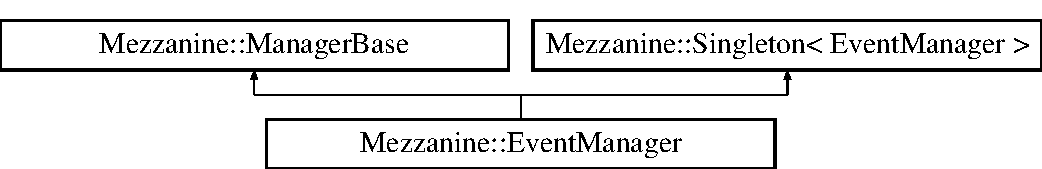
\includegraphics[height=2.000000cm]{classMezzanine_1_1EventManager}
\end{center}
\end{figure}
\subsubsection*{Public Member Functions}
\begin{DoxyCompactItemize}
\item 
void \hyperlink{classMezzanine_1_1EventManager_aa791c61d2665422614d54c7653e87e88}{AddEvent} (\hyperlink{classMezzanine_1_1EventBase}{EventBase} $\ast$EventToAdd)
\begin{DoxyCompactList}\small\item\em Adds an event of any kind to the end of the Event Queue. \item\end{DoxyCompactList}\item 
void \hyperlink{classMezzanine_1_1EventManager_a2da4ef46b2ce56206412782eec43d93e}{AddPollingCheck} (const \hyperlink{classMezzanine_1_1MetaCode}{MetaCode} \&InputToTryPolling)
\begin{DoxyCompactList}\small\item\em Generates extra events each iteration of the main loop, based on user input polling. \item\end{DoxyCompactList}\item 
void \hyperlink{classMezzanine_1_1EventManager_a3cf0fd9e33392aa24e9a735363212185}{DetectJoysticks} ()
\begin{DoxyCompactList}\small\item\em Look for Joysticks that are hooked up to the system. \item\end{DoxyCompactList}\item 
virtual void \hyperlink{classMezzanine_1_1EventManager_a69d44403974ed8d974846e929eb8adda}{DoMainLoopItems} ()
\begin{DoxyCompactList}\small\item\em Empty MainLoopItems. \item\end{DoxyCompactList}\item 
\hyperlink{classMezzanine_1_1EventManager_a95ce9d2d865b0d8d9468448969b0ade2}{EventManager} ()
\begin{DoxyCompactList}\small\item\em Default constructor. \item\end{DoxyCompactList}\item 
std::list$<$ \hyperlink{classMezzanine_1_1EventCollision}{EventCollision} $\ast$ $>$ $\ast$ \hyperlink{classMezzanine_1_1EventManager_ab630dfe228b7a4246680953cdfbbfc0a}{GetAllCollisionEvents} ()
\begin{DoxyCompactList}\small\item\em This returns a complete list of all the \hyperlink{classMezzanine_1_1Collision}{Collision} Events. \item\end{DoxyCompactList}\item 
std::list$<$ \hyperlink{classMezzanine_1_1EventGameWindow}{EventGameWindow} $\ast$ $>$ $\ast$ \hyperlink{classMezzanine_1_1EventManager_abd6f4de517d07ab7a1a0c330c4e29032}{GetAllGameWindowEvents} ()
\begin{DoxyCompactList}\small\item\em This returns a complete list of all the Render \hyperlink{structMezzanine_1_1Time}{Time} events. \item\end{DoxyCompactList}\item 
std::list$<$ \hyperlink{classMezzanine_1_1EventQuit}{EventQuit} $\ast$ $>$ $\ast$ \hyperlink{classMezzanine_1_1EventManager_ae54b0f6e266c738ceb2b5192d2412a38}{GetAllQuitEvents} ()
\begin{DoxyCompactList}\small\item\em This returns a complete list of all the quit events. \item\end{DoxyCompactList}\item 
std::list$<$ \hyperlink{classMezzanine_1_1EventRenderTime}{EventRenderTime} $\ast$ $>$ $\ast$ \hyperlink{classMezzanine_1_1EventManager_a671df48c725e661274f21751ab2ec2f9}{GetAllRenderTimeEvents} ()
\begin{DoxyCompactList}\small\item\em This returns a complete list of all the Render \hyperlink{structMezzanine_1_1Time}{Time} events. \item\end{DoxyCompactList}\item 
std::list$<$ \hyperlink{classMezzanine_1_1EventBase}{EventBase} $\ast$ $>$ $\ast$ \hyperlink{classMezzanine_1_1EventManager_af149e3c8893bdd214d4c1d6aea5388b2}{GetAllSpecificEvents} (\hyperlink{classMezzanine_1_1EventBase_ab85e31e97753b7e7ecb098f82526baef}{EventBase::EventType} SpecificType)
\begin{DoxyCompactList}\small\item\em This returns a complete list of all the specified events. \item\end{DoxyCompactList}\item 
std::list$<$ \hyperlink{classMezzanine_1_1EventUserInput}{EventUserInput} $\ast$ $>$ $\ast$ \hyperlink{classMezzanine_1_1EventManager_a50abe233b2f932105d0f33cd38badb26}{GetAllUserInputEvents} ()
\begin{DoxyCompactList}\small\item\em This returns a complete list of all the User Input events. \item\end{DoxyCompactList}\item 
\hyperlink{classMezzanine_1_1EventCollision}{EventCollision} $\ast$ \hyperlink{classMezzanine_1_1EventManager_adfba3feeb1e4174909db98412f894a3b}{GetNextCollisionEvent} ()
\begin{DoxyCompactList}\small\item\em Returns a pointer to the Next \hyperlink{classMezzanine_1_1Collision}{Collision} event. \item\end{DoxyCompactList}\item 
\hyperlink{classMezzanine_1_1EventBase}{EventBase} $\ast$ \hyperlink{classMezzanine_1_1EventManager_aea5b5a53dabead276cee5f94152bd9c2}{GetNextEvent} ()
\begin{DoxyCompactList}\small\item\em Return a pointer to the Next event. \item\end{DoxyCompactList}\item 
\hyperlink{classMezzanine_1_1EventGameWindow}{EventGameWindow} $\ast$ \hyperlink{classMezzanine_1_1EventManager_a60f9633517b214128a359c4ef92bafb7}{GetNextGameWindowEvent} ()
\begin{DoxyCompactList}\small\item\em Returns a pointer to the Next \hyperlink{classMezzanine_1_1GameWindow}{GameWindow} event. \item\end{DoxyCompactList}\item 
\hyperlink{classMezzanine_1_1EventQuit}{EventQuit} $\ast$ \hyperlink{classMezzanine_1_1EventManager_afd185415d7a139df30eb35309e8dee45}{GetNextQuitEvent} ()
\begin{DoxyCompactList}\small\item\em Returns a pointer to the Next \hyperlink{classMezzanine_1_1EventQuit}{EventQuit}. \item\end{DoxyCompactList}\item 
\hyperlink{classMezzanine_1_1EventRenderTime}{EventRenderTime} $\ast$ \hyperlink{classMezzanine_1_1EventManager_a9a1d195b08d34de39cbd72f95ab01190}{GetNextRenderTimeEvent} ()
\begin{DoxyCompactList}\small\item\em Returns a pointer to the Next Rendertime event. \item\end{DoxyCompactList}\item 
\hyperlink{classMezzanine_1_1EventBase}{EventBase} $\ast$ \hyperlink{classMezzanine_1_1EventManager_a1ef3a915c26ab96fa6958a9e80c8aaaa}{GetNextSpecificEvent} (\hyperlink{classMezzanine_1_1EventBase_ab85e31e97753b7e7ecb098f82526baef}{EventBase::EventType} SpecificType)
\begin{DoxyCompactList}\small\item\em Returns a pointer to the Next kind event of the Specified type. \item\end{DoxyCompactList}\item 
\hyperlink{classMezzanine_1_1EventUserInput}{EventUserInput} $\ast$ \hyperlink{classMezzanine_1_1EventManager_a8d1af0c4bcb070edb8d013e1cf9ebf34}{GetNextUserInputEvent} ()
\begin{DoxyCompactList}\small\item\em Returns a pointer to the Next User Input event. \item\end{DoxyCompactList}\item 
size\_\-t \hyperlink{classMezzanine_1_1EventManager_aa3f1b41578307c7ac801340b275af027}{GetRemainingEventCount} ()
\begin{DoxyCompactList}\small\item\em Gets a count of events. \item\end{DoxyCompactList}\item 
virtual \hyperlink{classMezzanine_1_1ManagerBase_a08cecf5169cad3e82be81a3a159b0b6e}{ManagerTypeName} \hyperlink{classMezzanine_1_1EventManager_a6e4c72bcaa437863fdf167b5b9ef5034}{GetType} () const 
\begin{DoxyCompactList}\small\item\em This returns the type of this manager. \item\end{DoxyCompactList}\item 
virtual void \hyperlink{classMezzanine_1_1EventManager_a2bf1969aadd0fb5a3da284423e44b081}{Initialize} ()
\begin{DoxyCompactList}\small\item\em Empty Initializer. \item\end{DoxyCompactList}\item 
\hyperlink{classMezzanine_1_1EventCollision}{EventCollision} $\ast$ \hyperlink{classMezzanine_1_1EventManager_a25b42c9f5a4ac2910d5e0d79b2bd2c17}{PopNextCollisionEvent} ()
\begin{DoxyCompactList}\small\item\em Returns a pointer to the Next \hyperlink{classMezzanine_1_1Collision}{Collision} event and removes it from the Que. \item\end{DoxyCompactList}\item 
\hyperlink{classMezzanine_1_1EventBase}{EventBase} $\ast$ \hyperlink{classMezzanine_1_1EventManager_a48861de138f2c59480527cf16518444a}{PopNextEvent} ()
\begin{DoxyCompactList}\small\item\em Return a pointer to the Next event, and removes the Event from storage. \item\end{DoxyCompactList}\item 
\hyperlink{classMezzanine_1_1EventGameWindow}{EventGameWindow} $\ast$ \hyperlink{classMezzanine_1_1EventManager_a91f8be3fedf91ba5a32825a8dd97de95}{PopNextGameWindowEvent} ()
\begin{DoxyCompactList}\small\item\em Returns a pointer to the Next \hyperlink{classMezzanine_1_1GameWindow}{GameWindow} event and removes it from the Que. \item\end{DoxyCompactList}\item 
\hyperlink{classMezzanine_1_1EventQuit}{EventQuit} $\ast$ \hyperlink{classMezzanine_1_1EventManager_aa7cefb4728acb84517e2891adc450c27}{PopNextQuitEvent} ()
\begin{DoxyCompactList}\small\item\em Returns a pointer to the Next \hyperlink{classMezzanine_1_1EventQuit}{EventQuit} and removes it from the Que. \item\end{DoxyCompactList}\item 
\hyperlink{classMezzanine_1_1EventRenderTime}{EventRenderTime} $\ast$ \hyperlink{classMezzanine_1_1EventManager_aedbb7374cf4c97a5f5ab5283627da83f}{PopNextRenderTimeEvent} ()
\begin{DoxyCompactList}\small\item\em Returns a pointer to the Next Rendertime event and removes it from the Que. \item\end{DoxyCompactList}\item 
\hyperlink{classMezzanine_1_1EventBase}{EventBase} $\ast$ \hyperlink{classMezzanine_1_1EventManager_a1e142f7a2c658e0bbbd3e962ba24f8bb}{PopNextSpecificEvent} (\hyperlink{classMezzanine_1_1EventBase_ab85e31e97753b7e7ecb098f82526baef}{EventBase::EventType} SpecificType)
\begin{DoxyCompactList}\small\item\em Returns a pointer to the Next kind event of the Specified type, and removes it from the Que. \item\end{DoxyCompactList}\item 
\hyperlink{classMezzanine_1_1EventUserInput}{EventUserInput} $\ast$ \hyperlink{classMezzanine_1_1EventManager_a9a372e5988a549f61a1ff064b7239a8e}{PopNextUserInputEvent} ()
\begin{DoxyCompactList}\small\item\em Returns a pointer to the Next User Input event and removes it from the Que. \item\end{DoxyCompactList}\item 
void \hyperlink{classMezzanine_1_1EventManager_a209b69a260ea1a2351e005802d13803b}{RemoveAllSpecificEvents} (\hyperlink{classMezzanine_1_1EventBase_ab85e31e97753b7e7ecb098f82526baef}{EventBase::EventType} SpecificType)
\begin{DoxyCompactList}\small\item\em This removes all the events of the specified type. \item\end{DoxyCompactList}\item 
void \hyperlink{classMezzanine_1_1EventManager_ae3a90f7fdd0b75b4e4ff5e5d3ad3e332}{RemoveEvent} (\hyperlink{classMezzanine_1_1EventBase}{EventBase} $\ast$EventToRemove)
\begin{DoxyCompactList}\small\item\em Removes an event of any kind from the Event Queue. \item\end{DoxyCompactList}\item 
void \hyperlink{classMezzanine_1_1EventManager_ac35a0aa7e6e98a8024025f3babd40749}{RemoveNextCollisionEvent} ()
\begin{DoxyCompactList}\small\item\em Removes the First \hyperlink{classMezzanine_1_1Collision}{Collision} Event From the que without looking at it. \item\end{DoxyCompactList}\item 
void \hyperlink{classMezzanine_1_1EventManager_a0694b97c1b9696f5b28d0baf7a2f7c40}{RemoveNextEvent} ()
\begin{DoxyCompactList}\small\item\em Removes an Event From the que without looking at it. \item\end{DoxyCompactList}\item 
void \hyperlink{classMezzanine_1_1EventManager_a6108fd63aed85b5a3f38987f75603c53}{RemoveNextGameWindowEvent} ()
\begin{DoxyCompactList}\small\item\em Removes the First \hyperlink{classMezzanine_1_1GameWindow}{GameWindow} Event From the que without looking at it. \item\end{DoxyCompactList}\item 
void \hyperlink{classMezzanine_1_1EventManager_a10735469d564d6731c3741acf265879c}{RemoveNextQuitEvent} ()
\begin{DoxyCompactList}\small\item\em Removes the First \hyperlink{classMezzanine_1_1EventQuit}{EventQuit} From the que without looking at it. \item\end{DoxyCompactList}\item 
void \hyperlink{classMezzanine_1_1EventManager_a9a0b6340a0b0a6a96b7918f758f44c31}{RemoveNextRenderTimeEvent} ()
\begin{DoxyCompactList}\small\item\em Removes the First Rendertime Event From the que without looking at it. \item\end{DoxyCompactList}\item 
void \hyperlink{classMezzanine_1_1EventManager_a8fe12f47a64f3af8dcb30f13ee60e303}{RemoveNextSpecificEvent} (\hyperlink{classMezzanine_1_1EventBase_ab85e31e97753b7e7ecb098f82526baef}{EventBase::EventType} SpecificType)
\begin{DoxyCompactList}\small\item\em Returns a pointer to the Next kind event of the Specified type, and removes it from the Que. \item\end{DoxyCompactList}\item 
void \hyperlink{classMezzanine_1_1EventManager_a1d2681b16ec802f8271f2651ff40c083}{RemoveNextUserInputEvent} ()
\begin{DoxyCompactList}\small\item\em Removes the First User Input Event From the que without looking at it. \item\end{DoxyCompactList}\item 
void \hyperlink{classMezzanine_1_1EventManager_a446cab99c7c67b42e28753cda14d79a4}{RemovePollingCheck} (const \hyperlink{classMezzanine_1_1MetaCode}{MetaCode} \&InputToStopPolling)
\begin{DoxyCompactList}\small\item\em Removes Events from the list(s) of what needs to be polled. \item\end{DoxyCompactList}\item 
void \hyperlink{classMezzanine_1_1EventManager_a07119a541a60a515e2108c79cf6e3aac}{UpdateEvents} ()
\begin{DoxyCompactList}\small\item\em Pulls Events from the all the subsystems for use in the \hyperlink{classMezzanine_1_1EventManager}{EventManager}. \item\end{DoxyCompactList}\item 
\hyperlink{classMezzanine_1_1EventManager_a39b9e0f783c2ab0d39f5574a7a106141}{$\sim$EventManager} ()
\begin{DoxyCompactList}\small\item\em Default Deconstructor. \item\end{DoxyCompactList}\end{DoxyCompactItemize}


\subsubsection{Detailed Description}
This is a container for Events and facilitates the transfer of data. The Event Manager Exists to passed important information about Gamestate from where it is generated to where it is needed. It is the Game Developers option whether they want to grab events directly using the get functions that have filters, or if they want to get all the events at once from a central location and dispatch form there. \par
 Since all User input comes in the form of events, this is also where user input Polling and optional input sources like Joysticks are controlled from. \par
 All of these event are stored in an internal Queue and order is preserved. So the First item In will be the First Out (FIFO). This is not strictly a FIFO buffer, there are a number of functions for getting of managing specific kinds of events. Generally these 'Filtered' management functions Still return the first of those kinds of event. \begin{DoxyWarning}{Warning}
Delete pointers you get from this. Anything can create events and Put them here, and anything can get them out, This means the simple way to not cause memory leaks is to have the routines extracting the events delete the events. 

Currently this is not thread safe, even though it should be. 
\end{DoxyWarning}


Definition at line 123 of file eventmanager.h.



\subsubsection{Constructor \& Destructor Documentation}
\hypertarget{classMezzanine_1_1EventManager_a95ce9d2d865b0d8d9468448969b0ade2}{
\index{Mezzanine::EventManager@{Mezzanine::EventManager}!EventManager@{EventManager}}
\index{EventManager@{EventManager}!Mezzanine::EventManager@{Mezzanine::EventManager}}
\paragraph[{EventManager}]{\setlength{\rightskip}{0pt plus 5cm}Mezzanine::EventManager::EventManager (
\begin{DoxyParamCaption}
{}
\end{DoxyParamCaption}
)}\hfill}
\label{classMezzanine_1_1EventManager_a95ce9d2d865b0d8d9468448969b0ade2}


Default constructor. 

This creates an empty EventManger

\begin{Desc}
\item[\hyperlink{todo__todo000011}{Todo}]TODO: Make the \hyperlink{classMezzanine_1_1EventManager}{EventManager} completely thread safe. IF this is completely thread safe, we can spawn numerous individual thread each accessing this and and the performance gain would almost scale directly with cpu core count increases. Look at boost scoped\_\-lock \end{Desc}


Definition at line 253 of file eventmanager.cpp.

\hypertarget{classMezzanine_1_1EventManager_a39b9e0f783c2ab0d39f5574a7a106141}{
\index{Mezzanine::EventManager@{Mezzanine::EventManager}!$\sim$EventManager@{$\sim$EventManager}}
\index{$\sim$EventManager@{$\sim$EventManager}!Mezzanine::EventManager@{Mezzanine::EventManager}}
\paragraph[{$\sim$EventManager}]{\setlength{\rightskip}{0pt plus 5cm}Mezzanine::EventManager::$\sim$EventManager (
\begin{DoxyParamCaption}
{}
\end{DoxyParamCaption}
)}\hfill}
\label{classMezzanine_1_1EventManager_a39b9e0f783c2ab0d39f5574a7a106141}


Default Deconstructor. 

This deletes everything still in the event manager and tears it down. 

Definition at line 264 of file eventmanager.cpp.



\subsubsection{Member Function Documentation}
\hypertarget{classMezzanine_1_1EventManager_aa791c61d2665422614d54c7653e87e88}{
\index{Mezzanine::EventManager@{Mezzanine::EventManager}!AddEvent@{AddEvent}}
\index{AddEvent@{AddEvent}!Mezzanine::EventManager@{Mezzanine::EventManager}}
\paragraph[{AddEvent}]{\setlength{\rightskip}{0pt plus 5cm}void Mezzanine::EventManager::AddEvent (
\begin{DoxyParamCaption}
\item[{{\bf EventBase} $\ast$}]{EventToAdd}
\end{DoxyParamCaption}
)}\hfill}
\label{classMezzanine_1_1EventManager_aa791c61d2665422614d54c7653e87e88}


Adds an event of any kind to the end of the Event Queue. 


\begin{DoxyParams}{Parameters}
{\em EventToAdd} & This is a pointer to an Event.\\
\hline
\end{DoxyParams}
This adds the existing event to the Queue. Be careful this is not delete, and does not go out of scope. Deleting the Event is now the responsibilty of the code that pulls it out of Event Manager. 

Definition at line 317 of file eventmanager.cpp.

\hypertarget{classMezzanine_1_1EventManager_a2da4ef46b2ce56206412782eec43d93e}{
\index{Mezzanine::EventManager@{Mezzanine::EventManager}!AddPollingCheck@{AddPollingCheck}}
\index{AddPollingCheck@{AddPollingCheck}!Mezzanine::EventManager@{Mezzanine::EventManager}}
\paragraph[{AddPollingCheck}]{\setlength{\rightskip}{0pt plus 5cm}void Mezzanine::EventManager::AddPollingCheck (
\begin{DoxyParamCaption}
\item[{const {\bf MetaCode} \&}]{InputToTryPolling}
\end{DoxyParamCaption}
)}\hfill}
\label{classMezzanine_1_1EventManager_a2da4ef46b2ce56206412782eec43d93e}


Generates extra events each iteration of the main loop, based on user input polling. 


\begin{DoxyParams}{Parameters}
{\em InputToTryPolling} & This accepts a \hyperlink{classMezzanine_1_1MetaCode}{MetaCode} and will try to watch for occurences like this one\\
\hline
\end{DoxyParams}
This will trigger the input system to generate an event (or add to an exiting event) when polling for the given kind of event. Each Iteration of the main loop there will be a \hyperlink{classMezzanine_1_1EventUserInput}{EventUserInput} that created. That Event will Include all the normal metacodes for user input that happened, and it will also have a meta code for each time this function was called. The added metacode may be partialky ignored, the Metavalue is almost always ignored, and in a situation where the can only be one of a given input on a system, the ID is ignore and 0 is assumed. 
\begin{DoxyExceptions}{Exceptions}
{\em Unsupported Polling Check on this Platform} & When the metacode passed cannot be polled on this platform \\
\hline
\end{DoxyExceptions}


Definition at line 630 of file eventmanager.cpp.

\hypertarget{classMezzanine_1_1EventManager_a3cf0fd9e33392aa24e9a735363212185}{
\index{Mezzanine::EventManager@{Mezzanine::EventManager}!DetectJoysticks@{DetectJoysticks}}
\index{DetectJoysticks@{DetectJoysticks}!Mezzanine::EventManager@{Mezzanine::EventManager}}
\paragraph[{DetectJoysticks}]{\setlength{\rightskip}{0pt plus 5cm}void Mezzanine::EventManager::DetectJoysticks (
\begin{DoxyParamCaption}
{}
\end{DoxyParamCaption}
)}\hfill}
\label{classMezzanine_1_1EventManager_a3cf0fd9e33392aa24e9a735363212185}


Look for Joysticks that are hooked up to the system. 

Currently this will only find the first joystick. This only needs to be done once after the joystick has been connected and detected/configured by the operating system. Joystick events may not be added if this has not been called. The is called once at when the Event manager is contructed, but if the joystick was not connected yet then it might not be found. 

Definition at line 276 of file eventmanager.cpp.

\hypertarget{classMezzanine_1_1EventManager_a69d44403974ed8d974846e929eb8adda}{
\index{Mezzanine::EventManager@{Mezzanine::EventManager}!DoMainLoopItems@{DoMainLoopItems}}
\index{DoMainLoopItems@{DoMainLoopItems}!Mezzanine::EventManager@{Mezzanine::EventManager}}
\paragraph[{DoMainLoopItems}]{\setlength{\rightskip}{0pt plus 5cm}void Mezzanine::EventManager::DoMainLoopItems (
\begin{DoxyParamCaption}
{}
\end{DoxyParamCaption}
)\hspace{0.3cm}{\ttfamily  \mbox{[}virtual\mbox{]}}}\hfill}
\label{classMezzanine_1_1EventManager_a69d44403974ed8d974846e929eb8adda}


Empty MainLoopItems. 

This class implements this for the sake of entension and compatibility this function does nothing. This is just empty during this round of refactoring, and this will get all the functionality that currently should be here, but is in the world 

Implements \hyperlink{classMezzanine_1_1ManagerBase_a4ee29e4baf6c4b9a3bfec1b2258d5cd2}{Mezzanine::ManagerBase}.



Definition at line 668 of file eventmanager.cpp.

\hypertarget{classMezzanine_1_1EventManager_ab630dfe228b7a4246680953cdfbbfc0a}{
\index{Mezzanine::EventManager@{Mezzanine::EventManager}!GetAllCollisionEvents@{GetAllCollisionEvents}}
\index{GetAllCollisionEvents@{GetAllCollisionEvents}!Mezzanine::EventManager@{Mezzanine::EventManager}}
\paragraph[{GetAllCollisionEvents}]{\setlength{\rightskip}{0pt plus 5cm}std::list$<$ {\bf EventCollision} $\ast$ $>$ $\ast$ Mezzanine::EventManager::GetAllCollisionEvents (
\begin{DoxyParamCaption}
{}
\end{DoxyParamCaption}
)}\hfill}
\label{classMezzanine_1_1EventManager_ab630dfe228b7a4246680953cdfbbfc0a}


This returns a complete list of all the \hyperlink{classMezzanine_1_1Collision}{Collision} Events. 

This finds all the \hyperlink{classMezzanine_1_1Collision}{Collision} Events then creates a new list and returns that. This runs in linear time relative to the amounts of events. \begin{DoxyReturn}{Returns}
This returns a list$<$EventCollision$\ast$$>$ pointer which is this a subset of this classes event pointer list. Use this carefully, it can cause errors if used improperly. This list pointer must be deleted, but not the events in it. 
\end{DoxyReturn}


Definition at line 562 of file eventmanager.cpp.

\hypertarget{classMezzanine_1_1EventManager_abd6f4de517d07ab7a1a0c330c4e29032}{
\index{Mezzanine::EventManager@{Mezzanine::EventManager}!GetAllGameWindowEvents@{GetAllGameWindowEvents}}
\index{GetAllGameWindowEvents@{GetAllGameWindowEvents}!Mezzanine::EventManager@{Mezzanine::EventManager}}
\paragraph[{GetAllGameWindowEvents}]{\setlength{\rightskip}{0pt plus 5cm}std::list$<$ {\bf EventGameWindow} $\ast$ $>$ $\ast$ Mezzanine::EventManager::GetAllGameWindowEvents (
\begin{DoxyParamCaption}
{}
\end{DoxyParamCaption}
)}\hfill}
\label{classMezzanine_1_1EventManager_abd6f4de517d07ab7a1a0c330c4e29032}


This returns a complete list of all the Render \hyperlink{structMezzanine_1_1Time}{Time} events. 

This finds all the \hyperlink{classMezzanine_1_1EventUserInput}{EventUserInput} Events then creates a new list and returns that. This runs in linear time relative to the amounts of events. \begin{DoxyReturn}{Returns}
This returns a list$<$EventGameWindow$\ast$$>$ pointer which is this a subset of this classes event pointer list. Use this carefully, it can cause errors if used improperly. This list pointer must be deleted, but not the events in it. 
\end{DoxyReturn}


Definition at line 578 of file eventmanager.cpp.

\hypertarget{classMezzanine_1_1EventManager_ae54b0f6e266c738ceb2b5192d2412a38}{
\index{Mezzanine::EventManager@{Mezzanine::EventManager}!GetAllQuitEvents@{GetAllQuitEvents}}
\index{GetAllQuitEvents@{GetAllQuitEvents}!Mezzanine::EventManager@{Mezzanine::EventManager}}
\paragraph[{GetAllQuitEvents}]{\setlength{\rightskip}{0pt plus 5cm}std::list$<$ {\bf EventQuit} $\ast$ $>$ $\ast$ Mezzanine::EventManager::GetAllQuitEvents (
\begin{DoxyParamCaption}
{}
\end{DoxyParamCaption}
)}\hfill}
\label{classMezzanine_1_1EventManager_ae54b0f6e266c738ceb2b5192d2412a38}


This returns a complete list of all the quit events. 

This finds all the \hyperlink{classMezzanine_1_1EventQuit}{EventQuit} Events then creates a new list and returns that. This runs in linear time relative to the amounts of events. \begin{DoxyWarning}{Warning}
Something is wrong if you have more than a few quit events. These should be checked for in each iteration of the main loop. 
\end{DoxyWarning}
\begin{DoxyReturn}{Returns}
This returns a std::list$<$EventQuit$\ast$$>$ pointer which is this a subset of this classes event pointer list. Use this carefully, it can cause errors if used improperly. Additionally this list pointer must be deleted, but not the events in it. 
\end{DoxyReturn}


Definition at line 624 of file eventmanager.cpp.

\hypertarget{classMezzanine_1_1EventManager_a671df48c725e661274f21751ab2ec2f9}{
\index{Mezzanine::EventManager@{Mezzanine::EventManager}!GetAllRenderTimeEvents@{GetAllRenderTimeEvents}}
\index{GetAllRenderTimeEvents@{GetAllRenderTimeEvents}!Mezzanine::EventManager@{Mezzanine::EventManager}}
\paragraph[{GetAllRenderTimeEvents}]{\setlength{\rightskip}{0pt plus 5cm}std::list$<$ {\bf EventRenderTime} $\ast$ $>$ $\ast$ Mezzanine::EventManager::GetAllRenderTimeEvents (
\begin{DoxyParamCaption}
{}
\end{DoxyParamCaption}
)}\hfill}
\label{classMezzanine_1_1EventManager_a671df48c725e661274f21751ab2ec2f9}


This returns a complete list of all the Render \hyperlink{structMezzanine_1_1Time}{Time} events. 

This finds all the \hyperlink{classMezzanine_1_1EventRenderTime}{EventRenderTime} Events then creates a new list and returns that. This runs in linear time relative to the amounts of events. \begin{DoxyReturn}{Returns}
This returns a list$<$EventRenderTime$\ast$$>$ pointer which is this a subset of this classes event pointer list. Use this carefully, it can cause errors if used improperly. Additionally this list pointer must be deleted, but not the events in it. 
\end{DoxyReturn}


Definition at line 593 of file eventmanager.cpp.

\hypertarget{classMezzanine_1_1EventManager_af149e3c8893bdd214d4c1d6aea5388b2}{
\index{Mezzanine::EventManager@{Mezzanine::EventManager}!GetAllSpecificEvents@{GetAllSpecificEvents}}
\index{GetAllSpecificEvents@{GetAllSpecificEvents}!Mezzanine::EventManager@{Mezzanine::EventManager}}
\paragraph[{GetAllSpecificEvents}]{\setlength{\rightskip}{0pt plus 5cm}std::list$<$ {\bf EventBase} $\ast$ $>$ $\ast$ Mezzanine::EventManager::GetAllSpecificEvents (
\begin{DoxyParamCaption}
\item[{{\bf EventBase::EventType}}]{SpecificType}
\end{DoxyParamCaption}
)}\hfill}
\label{classMezzanine_1_1EventManager_af149e3c8893bdd214d4c1d6aea5388b2}


This returns a complete list of all the specified events. 

This finds all the events that are of the specified type in the event manager, then creates a new list and return that. This runs in linear time relative to the amounts of events. \begin{DoxyWarning}{Warning}
The pointers contained in this list must be used carefully. Do not delete them, this will cause errors. 
\end{DoxyWarning}
\begin{DoxyReturn}{Returns}
This returns a std::list$<$EventBase$\ast$$>$ pointer which is this a subset of this classes event pointer list. Use this carefully, it can cause errors if used improperly. Additionally this list pointer must be deleted, but not the events in it. 
\end{DoxyReturn}


Definition at line 525 of file eventmanager.cpp.

\hypertarget{classMezzanine_1_1EventManager_a50abe233b2f932105d0f33cd38badb26}{
\index{Mezzanine::EventManager@{Mezzanine::EventManager}!GetAllUserInputEvents@{GetAllUserInputEvents}}
\index{GetAllUserInputEvents@{GetAllUserInputEvents}!Mezzanine::EventManager@{Mezzanine::EventManager}}
\paragraph[{GetAllUserInputEvents}]{\setlength{\rightskip}{0pt plus 5cm}std::list$<$ {\bf EventUserInput} $\ast$ $>$ $\ast$ Mezzanine::EventManager::GetAllUserInputEvents (
\begin{DoxyParamCaption}
{}
\end{DoxyParamCaption}
)}\hfill}
\label{classMezzanine_1_1EventManager_a50abe233b2f932105d0f33cd38badb26}


This returns a complete list of all the User Input events. 

This finds all the \hyperlink{classMezzanine_1_1EventUserInput}{EventUserInput} Events then creates a new list and returns that. This runs in linear time relative to the amounts of events. \begin{DoxyReturn}{Returns}
This returns a std::list$<$EventUserInput$\ast$$>$ pointer which is this a subset of this classes event pointer list. Use this carefully, it can cause errors if used improperly. Additionally this list pointer must be deleted, but not the events in it. 
\end{DoxyReturn}


Definition at line 608 of file eventmanager.cpp.

\hypertarget{classMezzanine_1_1EventManager_adfba3feeb1e4174909db98412f894a3b}{
\index{Mezzanine::EventManager@{Mezzanine::EventManager}!GetNextCollisionEvent@{GetNextCollisionEvent}}
\index{GetNextCollisionEvent@{GetNextCollisionEvent}!Mezzanine::EventManager@{Mezzanine::EventManager}}
\paragraph[{GetNextCollisionEvent}]{\setlength{\rightskip}{0pt plus 5cm}{\bf EventCollision} $\ast$ Mezzanine::EventManager::GetNextCollisionEvent (
\begin{DoxyParamCaption}
{}
\end{DoxyParamCaption}
)}\hfill}
\label{classMezzanine_1_1EventManager_adfba3feeb1e4174909db98412f894a3b}


Returns a pointer to the Next \hyperlink{classMezzanine_1_1Collision}{Collision} event. 

This Filtered event management function returns a pointer to the next \hyperlink{classMezzanine_1_1Collision}{Collision} event. It is inadvisable to use this for performance reasons because it runs in linear time relative to the amount of events. However, it will return an immediately usable pointer for case where an extreme level of performance is not required. This returns a pointer to 0 if there are no \hyperlink{classMezzanine_1_1Collision}{Collision} events in the queue. \begin{DoxyReturn}{Returns}
A pointer to a \hyperlink{classMezzanine_1_1EventCollision}{EventCollision}, that still needs to be removed from the event manager and deleted. 
\end{DoxyReturn}


Definition at line 553 of file eventmanager.cpp.

\hypertarget{classMezzanine_1_1EventManager_aea5b5a53dabead276cee5f94152bd9c2}{
\index{Mezzanine::EventManager@{Mezzanine::EventManager}!GetNextEvent@{GetNextEvent}}
\index{GetNextEvent@{GetNextEvent}!Mezzanine::EventManager@{Mezzanine::EventManager}}
\paragraph[{GetNextEvent}]{\setlength{\rightskip}{0pt plus 5cm}{\bf EventBase} $\ast$ Mezzanine::EventManager::GetNextEvent (
\begin{DoxyParamCaption}
{}
\end{DoxyParamCaption}
)}\hfill}
\label{classMezzanine_1_1EventManager_aea5b5a53dabead276cee5f94152bd9c2}


Return a pointer to the Next event. 

This returns a pointer to the next Event. It is advisable to use this for performance reasons because it runs in constant time. However it does not return a specific kind of event, and must be cast in order to use the true content. This returns a pointer to 0 if there are no events in the queue. \begin{DoxyReturn}{Returns}
A pointer to a Event, that still needs to be removed from the event manager and deleted. 
\end{DoxyReturn}


Definition at line 297 of file eventmanager.cpp.

\hypertarget{classMezzanine_1_1EventManager_a60f9633517b214128a359c4ef92bafb7}{
\index{Mezzanine::EventManager@{Mezzanine::EventManager}!GetNextGameWindowEvent@{GetNextGameWindowEvent}}
\index{GetNextGameWindowEvent@{GetNextGameWindowEvent}!Mezzanine::EventManager@{Mezzanine::EventManager}}
\paragraph[{GetNextGameWindowEvent}]{\setlength{\rightskip}{0pt plus 5cm}{\bf EventGameWindow} $\ast$ Mezzanine::EventManager::GetNextGameWindowEvent (
\begin{DoxyParamCaption}
{}
\end{DoxyParamCaption}
)}\hfill}
\label{classMezzanine_1_1EventManager_a60f9633517b214128a359c4ef92bafb7}


Returns a pointer to the Next \hyperlink{classMezzanine_1_1GameWindow}{GameWindow} event. 

This Filtered event management function returns a pointer to the next \hyperlink{classMezzanine_1_1GameWindow}{GameWindow} event. It is inadvisable to use this for performance reasons because it runs in linear time relative to the amount of events. However, it will return an immediately usable pointer for case where an extreme level of performance is not required. This returns a pointer to 0 if there are no \hyperlink{classMezzanine_1_1GameWindow}{GameWindow} events in the que. \begin{DoxyReturn}{Returns}
A pointer to a \hyperlink{classMezzanine_1_1EventGameWindow}{EventGameWindow}, that still needs to be removed from the event manager and deleted. 
\end{DoxyReturn}


Definition at line 569 of file eventmanager.cpp.

\hypertarget{classMezzanine_1_1EventManager_afd185415d7a139df30eb35309e8dee45}{
\index{Mezzanine::EventManager@{Mezzanine::EventManager}!GetNextQuitEvent@{GetNextQuitEvent}}
\index{GetNextQuitEvent@{GetNextQuitEvent}!Mezzanine::EventManager@{Mezzanine::EventManager}}
\paragraph[{GetNextQuitEvent}]{\setlength{\rightskip}{0pt plus 5cm}{\bf EventQuit} $\ast$ Mezzanine::EventManager::GetNextQuitEvent (
\begin{DoxyParamCaption}
{}
\end{DoxyParamCaption}
)}\hfill}
\label{classMezzanine_1_1EventManager_afd185415d7a139df30eb35309e8dee45}


Returns a pointer to the Next \hyperlink{classMezzanine_1_1EventQuit}{EventQuit}. 

This Filtered event management function returns a pointer to the next \hyperlink{classMezzanine_1_1EventQuit}{EventQuit}. It is inadvisable to use this for performance reasons because it runs in linear time relative to the amount of events. However, it will return an immediately usable pointer for case where an extreme level of performance is not required. This returns a pointer to 0 if there are no \hyperlink{classMezzanine_1_1EventQuit}{EventQuit} events in the que. \begin{DoxyReturn}{Returns}
A pointer to a \hyperlink{classMezzanine_1_1EventQuit}{EventQuit}, that still needs to be removed from the event manager and deleted. 
\end{DoxyReturn}


Definition at line 615 of file eventmanager.cpp.

\hypertarget{classMezzanine_1_1EventManager_a9a1d195b08d34de39cbd72f95ab01190}{
\index{Mezzanine::EventManager@{Mezzanine::EventManager}!GetNextRenderTimeEvent@{GetNextRenderTimeEvent}}
\index{GetNextRenderTimeEvent@{GetNextRenderTimeEvent}!Mezzanine::EventManager@{Mezzanine::EventManager}}
\paragraph[{GetNextRenderTimeEvent}]{\setlength{\rightskip}{0pt plus 5cm}{\bf EventRenderTime} $\ast$ Mezzanine::EventManager::GetNextRenderTimeEvent (
\begin{DoxyParamCaption}
{}
\end{DoxyParamCaption}
)}\hfill}
\label{classMezzanine_1_1EventManager_a9a1d195b08d34de39cbd72f95ab01190}


Returns a pointer to the Next Rendertime event. 

This Filtered event management function returns a pointer to the next Rendertime event. It is inadvisable to use this for performance reasons because it runs in linear time relative to the amount of events. However, it will return an immediately usable pointer for case where an extreme level of performance is not required. This returns a pointer to 0 if there are no \hyperlink{classMezzanine_1_1EventRenderTime}{EventRenderTime} events in the que. \begin{DoxyReturn}{Returns}
A pointer to a \hyperlink{classMezzanine_1_1EventRenderTime}{EventRenderTime}, that still needs to be removed from the event manager and deleted. 
\end{DoxyReturn}


Definition at line 584 of file eventmanager.cpp.

\hypertarget{classMezzanine_1_1EventManager_a1ef3a915c26ab96fa6958a9e80c8aaaa}{
\index{Mezzanine::EventManager@{Mezzanine::EventManager}!GetNextSpecificEvent@{GetNextSpecificEvent}}
\index{GetNextSpecificEvent@{GetNextSpecificEvent}!Mezzanine::EventManager@{Mezzanine::EventManager}}
\paragraph[{GetNextSpecificEvent}]{\setlength{\rightskip}{0pt plus 5cm}{\bf EventBase} $\ast$ Mezzanine::EventManager::GetNextSpecificEvent (
\begin{DoxyParamCaption}
\item[{{\bf EventBase::EventType}}]{SpecificType}
\end{DoxyParamCaption}
)}\hfill}
\label{classMezzanine_1_1EventManager_a1ef3a915c26ab96fa6958a9e80c8aaaa}


Returns a pointer to the Next kind event of the Specified type. 


\begin{DoxyParams}{Parameters}
{\em SpecificType} & This is a Event::EventType that defines the type you want this to work with\\
\hline
\end{DoxyParams}
This and the other NextSpecificEvent functions are the core of the Event Filtering System. In general the other filtering functions call one of these and does very little work on their own. \par
 This performs a linear search starting with the oldest (first entered Events) and simply checks if it the of the correct type. Then this returns a pointer to the next event of the specified type, or returns a pointer to 0 if there are none of the correct pointers in the Que. It is inadvisable to use this for performance reasons because it runs in linear time relative to the amount of events. \begin{DoxyReturn}{Returns}
A pointer to a \hyperlink{classMezzanine_1_1EventUserInput}{EventUserInput}, that still needs to be removed from the event manager and deleted. 
\end{DoxyReturn}


Definition at line 487 of file eventmanager.cpp.

\hypertarget{classMezzanine_1_1EventManager_a8d1af0c4bcb070edb8d013e1cf9ebf34}{
\index{Mezzanine::EventManager@{Mezzanine::EventManager}!GetNextUserInputEvent@{GetNextUserInputEvent}}
\index{GetNextUserInputEvent@{GetNextUserInputEvent}!Mezzanine::EventManager@{Mezzanine::EventManager}}
\paragraph[{GetNextUserInputEvent}]{\setlength{\rightskip}{0pt plus 5cm}{\bf EventUserInput} $\ast$ Mezzanine::EventManager::GetNextUserInputEvent (
\begin{DoxyParamCaption}
{}
\end{DoxyParamCaption}
)}\hfill}
\label{classMezzanine_1_1EventManager_a8d1af0c4bcb070edb8d013e1cf9ebf34}


Returns a pointer to the Next User Input event. 

This Filtered event management function returns a pointer to the next User Input event. It is inadvisable to use this for performance reasons because it runs in linear time relative to the amount of events. However, it will return an immediately usable pointer for case where an extreme level of performance is not required. This returns a pointer to 0 if there are no User Input events in the que. \begin{DoxyReturn}{Returns}
A pointer to a \hyperlink{classMezzanine_1_1EventUserInput}{EventUserInput}, that still needs to be removed from the event manager and deleted. 
\end{DoxyReturn}


Definition at line 599 of file eventmanager.cpp.

\hypertarget{classMezzanine_1_1EventManager_aa3f1b41578307c7ac801340b275af027}{
\index{Mezzanine::EventManager@{Mezzanine::EventManager}!GetRemainingEventCount@{GetRemainingEventCount}}
\index{GetRemainingEventCount@{GetRemainingEventCount}!Mezzanine::EventManager@{Mezzanine::EventManager}}
\paragraph[{GetRemainingEventCount}]{\setlength{\rightskip}{0pt plus 5cm}size\_\-t Mezzanine::EventManager::GetRemainingEventCount (
\begin{DoxyParamCaption}
{}
\end{DoxyParamCaption}
)}\hfill}
\label{classMezzanine_1_1EventManager_aa3f1b41578307c7ac801340b275af027}


Gets a count of events. 

This returns a total count of all events stored in this \hyperlink{classMezzanine_1_1EventManager}{EventManager}. \begin{DoxyReturn}{Returns}
This returns an unsigned integer with the amount of of total events 
\end{DoxyReturn}


Definition at line 294 of file eventmanager.cpp.

\hypertarget{classMezzanine_1_1EventManager_a6e4c72bcaa437863fdf167b5b9ef5034}{
\index{Mezzanine::EventManager@{Mezzanine::EventManager}!GetType@{GetType}}
\index{GetType@{GetType}!Mezzanine::EventManager@{Mezzanine::EventManager}}
\paragraph[{GetType}]{\setlength{\rightskip}{0pt plus 5cm}{\bf ManagerBase::ManagerTypeName} Mezzanine::EventManager::GetType (
\begin{DoxyParamCaption}
{}
\end{DoxyParamCaption}
) const\hspace{0.3cm}{\ttfamily  \mbox{[}virtual\mbox{]}}}\hfill}
\label{classMezzanine_1_1EventManager_a6e4c72bcaa437863fdf167b5b9ef5034}


This returns the type of this manager. 

\begin{DoxyReturn}{Returns}
This returns ManagerTypeName::EventManager 
\end{DoxyReturn}


Implements \hyperlink{classMezzanine_1_1ManagerBase_a6fbfe9e847156915b195b6de1cf76973}{Mezzanine::ManagerBase}.



Definition at line 674 of file eventmanager.cpp.

\hypertarget{classMezzanine_1_1EventManager_a2bf1969aadd0fb5a3da284423e44b081}{
\index{Mezzanine::EventManager@{Mezzanine::EventManager}!Initialize@{Initialize}}
\index{Initialize@{Initialize}!Mezzanine::EventManager@{Mezzanine::EventManager}}
\paragraph[{Initialize}]{\setlength{\rightskip}{0pt plus 5cm}void Mezzanine::EventManager::Initialize (
\begin{DoxyParamCaption}
{}
\end{DoxyParamCaption}
)\hspace{0.3cm}{\ttfamily  \mbox{[}virtual\mbox{]}}}\hfill}
\label{classMezzanine_1_1EventManager_a2bf1969aadd0fb5a3da284423e44b081}


Empty Initializer. 

This specific initializor is unneeded, but we implement it for compatibility. It also exists in case a derived class wants to override it for some reason 

Implements \hyperlink{classMezzanine_1_1ManagerBase_a864e3cac11928a602c1db28fa2d52ee2}{Mezzanine::ManagerBase}.



Definition at line 665 of file eventmanager.cpp.

\hypertarget{classMezzanine_1_1EventManager_a25b42c9f5a4ac2910d5e0d79b2bd2c17}{
\index{Mezzanine::EventManager@{Mezzanine::EventManager}!PopNextCollisionEvent@{PopNextCollisionEvent}}
\index{PopNextCollisionEvent@{PopNextCollisionEvent}!Mezzanine::EventManager@{Mezzanine::EventManager}}
\paragraph[{PopNextCollisionEvent}]{\setlength{\rightskip}{0pt plus 5cm}{\bf EventCollision} $\ast$ Mezzanine::EventManager::PopNextCollisionEvent (
\begin{DoxyParamCaption}
{}
\end{DoxyParamCaption}
)}\hfill}
\label{classMezzanine_1_1EventManager_a25b42c9f5a4ac2910d5e0d79b2bd2c17}


Returns a pointer to the Next \hyperlink{classMezzanine_1_1Collision}{Collision} event and removes it from the Que. 

This Filtered event management function returns a pointer to the next \hyperlink{classMezzanine_1_1Collision}{Collision} event. It is inadvisable to use this for performance reasons because it runs in linear time relative to the amount of events. However, it will return an immediately usable pointer for case where an extreme level of performance is not required. This returns a pointer to 0 if there are no \hyperlink{classMezzanine_1_1Collision}{Collision} events in the que. This also removes the returned pointer form the Queue. \begin{DoxyReturn}{Returns}
A pointer to a \hyperlink{classMezzanine_1_1EventRenderTime}{EventRenderTime}, that still needs to be removed from the event manager and deleted. 
\end{DoxyReturn}


Definition at line 556 of file eventmanager.cpp.

\hypertarget{classMezzanine_1_1EventManager_a48861de138f2c59480527cf16518444a}{
\index{Mezzanine::EventManager@{Mezzanine::EventManager}!PopNextEvent@{PopNextEvent}}
\index{PopNextEvent@{PopNextEvent}!Mezzanine::EventManager@{Mezzanine::EventManager}}
\paragraph[{PopNextEvent}]{\setlength{\rightskip}{0pt plus 5cm}{\bf EventBase} $\ast$ Mezzanine::EventManager::PopNextEvent (
\begin{DoxyParamCaption}
{}
\end{DoxyParamCaption}
)}\hfill}
\label{classMezzanine_1_1EventManager_a48861de138f2c59480527cf16518444a}


Return a pointer to the Next event, and removes the Event from storage. 

This functions just like GetNextEvent , except that it also removes the item from the internal storage of the \hyperlink{classMezzanine_1_1EventManager}{EventManager}. This returns a pointer to 0 if there are no events in the que. \begin{DoxyReturn}{Returns}
A pointer to a Event, that will need to be deleted once it has been used. 
\end{DoxyReturn}


Definition at line 305 of file eventmanager.cpp.

\hypertarget{classMezzanine_1_1EventManager_a91f8be3fedf91ba5a32825a8dd97de95}{
\index{Mezzanine::EventManager@{Mezzanine::EventManager}!PopNextGameWindowEvent@{PopNextGameWindowEvent}}
\index{PopNextGameWindowEvent@{PopNextGameWindowEvent}!Mezzanine::EventManager@{Mezzanine::EventManager}}
\paragraph[{PopNextGameWindowEvent}]{\setlength{\rightskip}{0pt plus 5cm}{\bf EventGameWindow} $\ast$ Mezzanine::EventManager::PopNextGameWindowEvent (
\begin{DoxyParamCaption}
{}
\end{DoxyParamCaption}
)}\hfill}
\label{classMezzanine_1_1EventManager_a91f8be3fedf91ba5a32825a8dd97de95}


Returns a pointer to the Next \hyperlink{classMezzanine_1_1GameWindow}{GameWindow} event and removes it from the Que. 

This Filtered event management function returns a pointer to the next \hyperlink{classMezzanine_1_1GameWindow}{GameWindow} event. It is inadvisable to use this for performance reasons because it runs in linear time relative to the amount of events. However, it will return an immediately usable pointer for case where an extreme level of performance is not required. This returns a pointer to 0 if there are no \hyperlink{classMezzanine_1_1GameWindow}{GameWindow} events in the que. This also removes the returned pointer form the Que. \begin{DoxyReturn}{Returns}
A pointer to a \hyperlink{classMezzanine_1_1EventRenderTime}{EventRenderTime}, that still needs to be removed from the event manager and deleted. 
\end{DoxyReturn}


Definition at line 572 of file eventmanager.cpp.

\hypertarget{classMezzanine_1_1EventManager_aa7cefb4728acb84517e2891adc450c27}{
\index{Mezzanine::EventManager@{Mezzanine::EventManager}!PopNextQuitEvent@{PopNextQuitEvent}}
\index{PopNextQuitEvent@{PopNextQuitEvent}!Mezzanine::EventManager@{Mezzanine::EventManager}}
\paragraph[{PopNextQuitEvent}]{\setlength{\rightskip}{0pt plus 5cm}{\bf EventQuit} $\ast$ Mezzanine::EventManager::PopNextQuitEvent (
\begin{DoxyParamCaption}
{}
\end{DoxyParamCaption}
)}\hfill}
\label{classMezzanine_1_1EventManager_aa7cefb4728acb84517e2891adc450c27}


Returns a pointer to the Next \hyperlink{classMezzanine_1_1EventQuit}{EventQuit} and removes it from the Que. 

This Filtered event management function returns a pointer to the next \hyperlink{classMezzanine_1_1EventQuit}{EventQuit}. It is inadvisable to use this for performance reasons because it runs in linear time relative to the amount of events. However, it will return an immediately usable pointer for case where an extreme level of performance is not required. This returns a pointer to 0 if there are no \hyperlink{classMezzanine_1_1EventQuit}{EventQuit} events in the que. This also removes the returned pointer form the Que. \begin{DoxyReturn}{Returns}
A pointer to a \hyperlink{classMezzanine_1_1EventQuit}{EventQuit}, that still needs to be removed from the event manager and deleted. 
\end{DoxyReturn}


Definition at line 618 of file eventmanager.cpp.

\hypertarget{classMezzanine_1_1EventManager_aedbb7374cf4c97a5f5ab5283627da83f}{
\index{Mezzanine::EventManager@{Mezzanine::EventManager}!PopNextRenderTimeEvent@{PopNextRenderTimeEvent}}
\index{PopNextRenderTimeEvent@{PopNextRenderTimeEvent}!Mezzanine::EventManager@{Mezzanine::EventManager}}
\paragraph[{PopNextRenderTimeEvent}]{\setlength{\rightskip}{0pt plus 5cm}{\bf EventRenderTime} $\ast$ Mezzanine::EventManager::PopNextRenderTimeEvent (
\begin{DoxyParamCaption}
{}
\end{DoxyParamCaption}
)}\hfill}
\label{classMezzanine_1_1EventManager_aedbb7374cf4c97a5f5ab5283627da83f}


Returns a pointer to the Next Rendertime event and removes it from the Que. 

This Filtered event management function returns a pointer to the next Rendertime event. It is inadvisable to use this for performance reasons because it runs in linear time relative to the amount of events. However, it will return an immediately usable pointer for case where an extreme level of performance is not required. This returns a pointer to 0 if there are no rendertime events in the que. This also removes the returned pointer form the Que. \begin{DoxyReturn}{Returns}
A pointer to a \hyperlink{classMezzanine_1_1EventRenderTime}{EventRenderTime}, that still needs to be removed from the event manager and deleted. 
\end{DoxyReturn}


Definition at line 587 of file eventmanager.cpp.

\hypertarget{classMezzanine_1_1EventManager_a1e142f7a2c658e0bbbd3e962ba24f8bb}{
\index{Mezzanine::EventManager@{Mezzanine::EventManager}!PopNextSpecificEvent@{PopNextSpecificEvent}}
\index{PopNextSpecificEvent@{PopNextSpecificEvent}!Mezzanine::EventManager@{Mezzanine::EventManager}}
\paragraph[{PopNextSpecificEvent}]{\setlength{\rightskip}{0pt plus 5cm}{\bf EventBase} $\ast$ Mezzanine::EventManager::PopNextSpecificEvent (
\begin{DoxyParamCaption}
\item[{{\bf EventBase::EventType}}]{SpecificType}
\end{DoxyParamCaption}
)}\hfill}
\label{classMezzanine_1_1EventManager_a1e142f7a2c658e0bbbd3e962ba24f8bb}


Returns a pointer to the Next kind event of the Specified type, and removes it from the Que. 


\begin{DoxyParams}{Parameters}
{\em SpecificType} & This is a Event::EventType that defines the type you want this to work with\\
\hline
\end{DoxyParams}
This is just like GetNextSpecificEvent(Event::EventType SpecificType) but it also removes the item from the Que. \begin{DoxyReturn}{Returns}
A pointer to a \hyperlink{classMezzanine_1_1EventUserInput}{EventUserInput}, that still needs to be removed from the event manager and deleted. 
\end{DoxyReturn}


Definition at line 501 of file eventmanager.cpp.

\hypertarget{classMezzanine_1_1EventManager_a9a372e5988a549f61a1ff064b7239a8e}{
\index{Mezzanine::EventManager@{Mezzanine::EventManager}!PopNextUserInputEvent@{PopNextUserInputEvent}}
\index{PopNextUserInputEvent@{PopNextUserInputEvent}!Mezzanine::EventManager@{Mezzanine::EventManager}}
\paragraph[{PopNextUserInputEvent}]{\setlength{\rightskip}{0pt plus 5cm}{\bf EventUserInput} $\ast$ Mezzanine::EventManager::PopNextUserInputEvent (
\begin{DoxyParamCaption}
{}
\end{DoxyParamCaption}
)}\hfill}
\label{classMezzanine_1_1EventManager_a9a372e5988a549f61a1ff064b7239a8e}


Returns a pointer to the Next User Input event and removes it from the Que. 

This Filtered event management function returns a pointer to the next User Input event. It is inadvisable to use this for performance reasons because it runs in linear time relative to the amount of events. However, it will return an immediately usable pointer for case where an extreme level of performance is not required. This returns a pointer to 0 if there are no User Input events in the que. This also removes the returned pointer form the Que. \begin{DoxyReturn}{Returns}
A pointer to a \hyperlink{classMezzanine_1_1EventUserInput}{EventUserInput}, that still needs to be removed from the event manager and deleted. 
\end{DoxyReturn}


Definition at line 602 of file eventmanager.cpp.

\hypertarget{classMezzanine_1_1EventManager_a209b69a260ea1a2351e005802d13803b}{
\index{Mezzanine::EventManager@{Mezzanine::EventManager}!RemoveAllSpecificEvents@{RemoveAllSpecificEvents}}
\index{RemoveAllSpecificEvents@{RemoveAllSpecificEvents}!Mezzanine::EventManager@{Mezzanine::EventManager}}
\paragraph[{RemoveAllSpecificEvents}]{\setlength{\rightskip}{0pt plus 5cm}void Mezzanine::EventManager::RemoveAllSpecificEvents (
\begin{DoxyParamCaption}
\item[{{\bf EventBase::EventType}}]{SpecificType}
\end{DoxyParamCaption}
)}\hfill}
\label{classMezzanine_1_1EventManager_a209b69a260ea1a2351e005802d13803b}


This removes all the events of the specified type. 

This finds all the events that are of the specified type in the event manager, then removes them. \begin{DoxyWarning}{Warning}
This does not delete the events. This is a memory leak unless used with GetAllSpecificEvents so that the events can be tracked indeendantly, and deleted. 
\end{DoxyWarning}


Definition at line 539 of file eventmanager.cpp.

\hypertarget{classMezzanine_1_1EventManager_ae3a90f7fdd0b75b4e4ff5e5d3ad3e332}{
\index{Mezzanine::EventManager@{Mezzanine::EventManager}!RemoveEvent@{RemoveEvent}}
\index{RemoveEvent@{RemoveEvent}!Mezzanine::EventManager@{Mezzanine::EventManager}}
\paragraph[{RemoveEvent}]{\setlength{\rightskip}{0pt plus 5cm}void Mezzanine::EventManager::RemoveEvent (
\begin{DoxyParamCaption}
\item[{{\bf EventBase} $\ast$}]{EventToRemove}
\end{DoxyParamCaption}
)}\hfill}
\label{classMezzanine_1_1EventManager_ae3a90f7fdd0b75b4e4ff5e5d3ad3e332}


Removes an event of any kind from the Event Queue. 


\begin{DoxyParams}{Parameters}
{\em EventToRemove} & Pointer to the event that will be removed.\\
\hline
\end{DoxyParams}
In most cases you will want to use the \hyperlink{classMezzanine_1_1EventManager_a48861de138f2c59480527cf16518444a}{PopNextEvent()} methods when going through events. In some expert use cases however you may want to remove a specific event at an arbitrary place in the Queue. This is the method for doing so. 

Definition at line 320 of file eventmanager.cpp.

\hypertarget{classMezzanine_1_1EventManager_ac35a0aa7e6e98a8024025f3babd40749}{
\index{Mezzanine::EventManager@{Mezzanine::EventManager}!RemoveNextCollisionEvent@{RemoveNextCollisionEvent}}
\index{RemoveNextCollisionEvent@{RemoveNextCollisionEvent}!Mezzanine::EventManager@{Mezzanine::EventManager}}
\paragraph[{RemoveNextCollisionEvent}]{\setlength{\rightskip}{0pt plus 5cm}void Mezzanine::EventManager::RemoveNextCollisionEvent (
\begin{DoxyParamCaption}
{}
\end{DoxyParamCaption}
)}\hfill}
\label{classMezzanine_1_1EventManager_ac35a0aa7e6e98a8024025f3babd40749}


Removes the First \hyperlink{classMezzanine_1_1Collision}{Collision} Event From the que without looking at it. 

This together with \hyperlink{classMezzanine_1_1EventManager_adfba3feeb1e4174909db98412f894a3b}{GetNextCollisionEvent()} are the pretty much same as call \hyperlink{classMezzanine_1_1EventManager_a25b42c9f5a4ac2910d5e0d79b2bd2c17}{PopNextCollisionEvent()}. \begin{DoxyWarning}{Warning}
If you did not call \hyperlink{classMezzanine_1_1EventManager_adfba3feeb1e4174909db98412f894a3b}{GetNextCollisionEvent()} and haven't deleted or stored, or somehow dealt with this pointer, then this is a memory leak. Don't use this unless you are certain you have taken care of the pointer appropriately. 
\end{DoxyWarning}

\begin{DoxyExceptions}{Exceptions}
{\em This} & can throw any STL exception a queue could. And with likely throw some kind of except if called when there are no Events in the Que. \\
\hline
\end{DoxyExceptions}


Definition at line 559 of file eventmanager.cpp.

\hypertarget{classMezzanine_1_1EventManager_a0694b97c1b9696f5b28d0baf7a2f7c40}{
\index{Mezzanine::EventManager@{Mezzanine::EventManager}!RemoveNextEvent@{RemoveNextEvent}}
\index{RemoveNextEvent@{RemoveNextEvent}!Mezzanine::EventManager@{Mezzanine::EventManager}}
\paragraph[{RemoveNextEvent}]{\setlength{\rightskip}{0pt plus 5cm}void Mezzanine::EventManager::RemoveNextEvent (
\begin{DoxyParamCaption}
{}
\end{DoxyParamCaption}
)}\hfill}
\label{classMezzanine_1_1EventManager_a0694b97c1b9696f5b28d0baf7a2f7c40}


Removes an Event From the que without looking at it. 

This together with \hyperlink{classMezzanine_1_1EventManager_aea5b5a53dabead276cee5f94152bd9c2}{GetNextEvent()} are the same as call \hyperlink{classMezzanine_1_1EventManager_a48861de138f2c59480527cf16518444a}{PopNextEvent()}. \begin{DoxyWarning}{Warning}
If you did not call \hyperlink{classMezzanine_1_1EventManager_aea5b5a53dabead276cee5f94152bd9c2}{GetNextEvent()} and haven't deleted or stored, or somehow dealt with this pointer, then this is a memory leak. Don't use this unless you are certain you have taken care of the pointer appropriately 
\end{DoxyWarning}

\begin{DoxyExceptions}{Exceptions}
{\em This} & can throw any STL exception a que could. Any with likely throw some kind of except if called when there are no Events in the Que. \\
\hline
\end{DoxyExceptions}


Definition at line 314 of file eventmanager.cpp.

\hypertarget{classMezzanine_1_1EventManager_a6108fd63aed85b5a3f38987f75603c53}{
\index{Mezzanine::EventManager@{Mezzanine::EventManager}!RemoveNextGameWindowEvent@{RemoveNextGameWindowEvent}}
\index{RemoveNextGameWindowEvent@{RemoveNextGameWindowEvent}!Mezzanine::EventManager@{Mezzanine::EventManager}}
\paragraph[{RemoveNextGameWindowEvent}]{\setlength{\rightskip}{0pt plus 5cm}void Mezzanine::EventManager::RemoveNextGameWindowEvent (
\begin{DoxyParamCaption}
{}
\end{DoxyParamCaption}
)}\hfill}
\label{classMezzanine_1_1EventManager_a6108fd63aed85b5a3f38987f75603c53}


Removes the First \hyperlink{classMezzanine_1_1GameWindow}{GameWindow} Event From the que without looking at it. 

This together with \hyperlink{classMezzanine_1_1EventManager_a60f9633517b214128a359c4ef92bafb7}{GetNextGameWindowEvent()} are the pretty much same as call \hyperlink{classMezzanine_1_1EventManager_a91f8be3fedf91ba5a32825a8dd97de95}{PopNextGameWindowEvent()}. \begin{DoxyWarning}{Warning}
If you did not call \hyperlink{classMezzanine_1_1EventManager_a60f9633517b214128a359c4ef92bafb7}{GetNextGameWindowEvent()} and haven't deleted or stored, or somehow dealt with this pointer, then this is a memory leak. Don't use this unless you are certain you have taken care of the pointer appropriately 
\end{DoxyWarning}

\begin{DoxyExceptions}{Exceptions}
{\em This} & can throw any STL exception a queue could. And with likely throw some kind of except if called when there are no Events in the Que. \\
\hline
\end{DoxyExceptions}


Definition at line 575 of file eventmanager.cpp.

\hypertarget{classMezzanine_1_1EventManager_a10735469d564d6731c3741acf265879c}{
\index{Mezzanine::EventManager@{Mezzanine::EventManager}!RemoveNextQuitEvent@{RemoveNextQuitEvent}}
\index{RemoveNextQuitEvent@{RemoveNextQuitEvent}!Mezzanine::EventManager@{Mezzanine::EventManager}}
\paragraph[{RemoveNextQuitEvent}]{\setlength{\rightskip}{0pt plus 5cm}void Mezzanine::EventManager::RemoveNextQuitEvent (
\begin{DoxyParamCaption}
{}
\end{DoxyParamCaption}
)}\hfill}
\label{classMezzanine_1_1EventManager_a10735469d564d6731c3741acf265879c}


Removes the First \hyperlink{classMezzanine_1_1EventQuit}{EventQuit} From the que without looking at it. 

This together with \hyperlink{classMezzanine_1_1EventManager_afd185415d7a139df30eb35309e8dee45}{GetNextQuitEvent()} are the pretty much same as call \hyperlink{classMezzanine_1_1EventManager_aa7cefb4728acb84517e2891adc450c27}{PopNextQuitEvent()}. \begin{DoxyWarning}{Warning}
If you did not call \hyperlink{classMezzanine_1_1EventManager_afd185415d7a139df30eb35309e8dee45}{GetNextQuitEvent()} and haven't deleted or stored, or somehow dealt with this pointer, then this is a memory leak. Don't use this unless you are certain you have taken care of the pointer appropriately 
\end{DoxyWarning}

\begin{DoxyExceptions}{Exceptions}
{\em This} & can throw any STL exception a queue could. And with likely throw some kind of except if called when there are no Events in the Que. \\
\hline
\end{DoxyExceptions}


Definition at line 621 of file eventmanager.cpp.

\hypertarget{classMezzanine_1_1EventManager_a9a0b6340a0b0a6a96b7918f758f44c31}{
\index{Mezzanine::EventManager@{Mezzanine::EventManager}!RemoveNextRenderTimeEvent@{RemoveNextRenderTimeEvent}}
\index{RemoveNextRenderTimeEvent@{RemoveNextRenderTimeEvent}!Mezzanine::EventManager@{Mezzanine::EventManager}}
\paragraph[{RemoveNextRenderTimeEvent}]{\setlength{\rightskip}{0pt plus 5cm}void Mezzanine::EventManager::RemoveNextRenderTimeEvent (
\begin{DoxyParamCaption}
{}
\end{DoxyParamCaption}
)}\hfill}
\label{classMezzanine_1_1EventManager_a9a0b6340a0b0a6a96b7918f758f44c31}


Removes the First Rendertime Event From the que without looking at it. 

This together with \hyperlink{classMezzanine_1_1EventManager_a9a1d195b08d34de39cbd72f95ab01190}{GetNextRenderTimeEvent()} are the pretty much same as call \hyperlink{classMezzanine_1_1EventManager_aedbb7374cf4c97a5f5ab5283627da83f}{PopNextRenderTimeEvent()}. \begin{DoxyWarning}{Warning}
If you did not call \hyperlink{classMezzanine_1_1EventManager_a9a1d195b08d34de39cbd72f95ab01190}{GetNextRenderTimeEvent()} and haven't deleted or stored, or somehow dealt with this pointer, then this is a memory leak. Don't use this unless you are certain you have taken care of the pointer appropriately 
\end{DoxyWarning}

\begin{DoxyExceptions}{Exceptions}
{\em This} & can throw any STL exception a queue could. And with likely throw some kind of except if called when there are no Events in the Que. \\
\hline
\end{DoxyExceptions}


Definition at line 590 of file eventmanager.cpp.

\hypertarget{classMezzanine_1_1EventManager_a8fe12f47a64f3af8dcb30f13ee60e303}{
\index{Mezzanine::EventManager@{Mezzanine::EventManager}!RemoveNextSpecificEvent@{RemoveNextSpecificEvent}}
\index{RemoveNextSpecificEvent@{RemoveNextSpecificEvent}!Mezzanine::EventManager@{Mezzanine::EventManager}}
\paragraph[{RemoveNextSpecificEvent}]{\setlength{\rightskip}{0pt plus 5cm}void Mezzanine::EventManager::RemoveNextSpecificEvent (
\begin{DoxyParamCaption}
\item[{{\bf EventBase::EventType}}]{SpecificType}
\end{DoxyParamCaption}
)}\hfill}
\label{classMezzanine_1_1EventManager_a8fe12f47a64f3af8dcb30f13ee60e303}


Returns a pointer to the Next kind event of the Specified type, and removes it from the Que. 


\begin{DoxyParams}{Parameters}
{\em SpecificType} & This is a Event::EventType that defines the type you want this to work with\\
\hline
\end{DoxyParams}
This is just like PopNextSpecificEvent(Event::EventType SpecificType) but exept it doesn't bother with any of the needed structure involved with returning data, and just removes the specific event from the Queue. \begin{DoxyWarning}{Warning}
If you did not call GetNextSpecificEvent(Event::EventType SpecificType) and haven't deleted or stored, or somehow dealt with this pointer, then this is a memory leak. Don't use this unless you are certain you have taken care of the pointer appropriately. 
\end{DoxyWarning}

\begin{DoxyExceptions}{Exceptions}
{\em This} & can throw any STL exception a queue could. And with likely throw some kind of except if called when there are no Events in the Que. \\
\hline
\end{DoxyExceptions}


Definition at line 516 of file eventmanager.cpp.

\hypertarget{classMezzanine_1_1EventManager_a1d2681b16ec802f8271f2651ff40c083}{
\index{Mezzanine::EventManager@{Mezzanine::EventManager}!RemoveNextUserInputEvent@{RemoveNextUserInputEvent}}
\index{RemoveNextUserInputEvent@{RemoveNextUserInputEvent}!Mezzanine::EventManager@{Mezzanine::EventManager}}
\paragraph[{RemoveNextUserInputEvent}]{\setlength{\rightskip}{0pt plus 5cm}void Mezzanine::EventManager::RemoveNextUserInputEvent (
\begin{DoxyParamCaption}
{}
\end{DoxyParamCaption}
)}\hfill}
\label{classMezzanine_1_1EventManager_a1d2681b16ec802f8271f2651ff40c083}


Removes the First User Input Event From the que without looking at it. 

This together with \hyperlink{classMezzanine_1_1EventManager_a8d1af0c4bcb070edb8d013e1cf9ebf34}{GetNextUserInputEvent()} are the pretty much same as call \hyperlink{classMezzanine_1_1EventManager_a9a372e5988a549f61a1ff064b7239a8e}{PopNextUserInputEvent()}. \begin{DoxyWarning}{Warning}
If you did not call \hyperlink{classMezzanine_1_1EventManager_a8d1af0c4bcb070edb8d013e1cf9ebf34}{GetNextUserInputEvent()} and haven't deleted or stored, or somehow dealt with this pointer, then this is a memory leak. Don't use this unless you are certain you have taken care of the pointer appropriately 
\end{DoxyWarning}

\begin{DoxyExceptions}{Exceptions}
{\em This} & can throw any STL exception a queue could. And with likely throw some kind of except if called when there are no Events in the Que. \\
\hline
\end{DoxyExceptions}


Definition at line 605 of file eventmanager.cpp.

\hypertarget{classMezzanine_1_1EventManager_a446cab99c7c67b42e28753cda14d79a4}{
\index{Mezzanine::EventManager@{Mezzanine::EventManager}!RemovePollingCheck@{RemovePollingCheck}}
\index{RemovePollingCheck@{RemovePollingCheck}!Mezzanine::EventManager@{Mezzanine::EventManager}}
\paragraph[{RemovePollingCheck}]{\setlength{\rightskip}{0pt plus 5cm}void Mezzanine::EventManager::RemovePollingCheck (
\begin{DoxyParamCaption}
\item[{const {\bf MetaCode} \&}]{InputToStopPolling}
\end{DoxyParamCaption}
)}\hfill}
\label{classMezzanine_1_1EventManager_a446cab99c7c67b42e28753cda14d79a4}


Removes Events from the list(s) of what needs to be polled. 


\begin{DoxyParams}{Parameters}
{\em InputToStopPolling} & This accepts a \hyperlink{classMezzanine_1_1MetaCode}{MetaCode} and will try to Remove Watches like this one\\
\hline
\end{DoxyParams}
This will remove any check for polling that share the same inputcode and ID. This 
\begin{DoxyExceptions}{Exceptions}
{\em Polling check not present} & Is thrown \\
\hline
\end{DoxyExceptions}


Definition at line 640 of file eventmanager.cpp.

\hypertarget{classMezzanine_1_1EventManager_a07119a541a60a515e2108c79cf6e3aac}{
\index{Mezzanine::EventManager@{Mezzanine::EventManager}!UpdateEvents@{UpdateEvents}}
\index{UpdateEvents@{UpdateEvents}!Mezzanine::EventManager@{Mezzanine::EventManager}}
\paragraph[{UpdateEvents}]{\setlength{\rightskip}{0pt plus 5cm}void Mezzanine::EventManager::UpdateEvents (
\begin{DoxyParamCaption}
{}
\end{DoxyParamCaption}
)}\hfill}
\label{classMezzanine_1_1EventManager_a07119a541a60a515e2108c79cf6e3aac}


Pulls Events from the all the subsystems for use in the \hyperlink{classMezzanine_1_1EventManager}{EventManager}. 

The work this function does is already performed in the main loop. This only really needs to be used If a game developer chooses to use his own main loop. This adds system events, like \hyperlink{classMezzanine_1_1EventQuit}{EventQuit} and Other Windows manager events, and if any user input event actions, this generates one \hyperlink{classMezzanine_1_1EventUserInput}{EventUserInput} that stores everythin that happened. 

Definition at line 332 of file eventmanager.cpp.



The documentation for this class was generated from the following files:\begin{DoxyCompactItemize}
\item 
eventmanager.h\item 
eventmanager.cpp\end{DoxyCompactItemize}

\hypertarget{classMezzanine_1_1EventQuit}{
\subsection{Mezzanine::EventQuit Class Reference}
\label{classMezzanine_1_1EventQuit}\index{Mezzanine::EventQuit@{Mezzanine::EventQuit}}
}


This is intended to convey the message that quitting needs to happen.  




{\ttfamily \#include $<$eventquit.h$>$}

Inheritance diagram for Mezzanine::EventQuit:\begin{figure}[H]
\begin{center}
\leavevmode
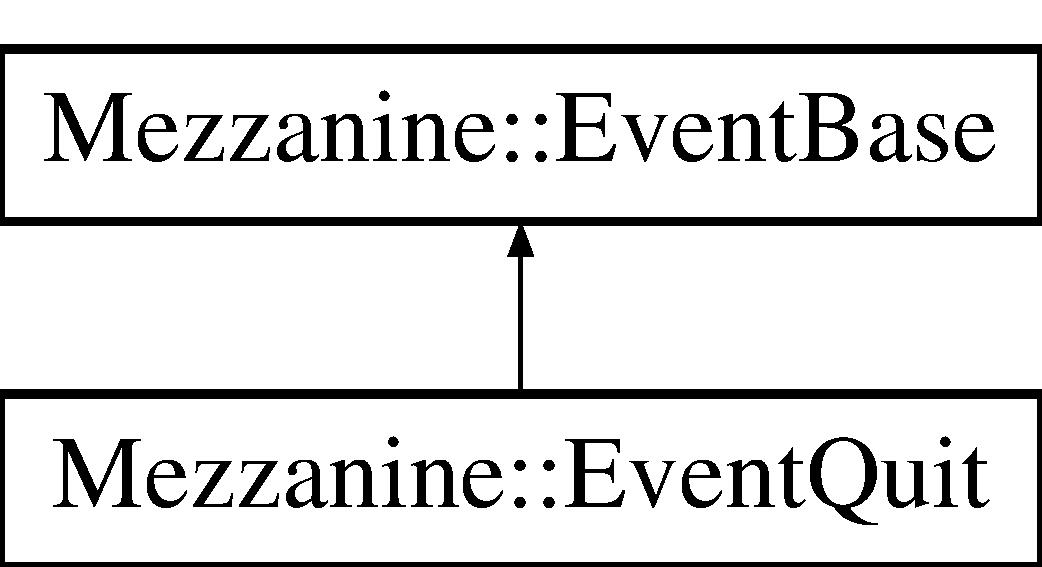
\includegraphics[height=2.000000cm]{classMezzanine_1_1EventQuit}
\end{center}
\end{figure}
\subsubsection*{Public Member Functions}
\begin{DoxyCompactItemize}
\item 
virtual \hyperlink{classMezzanine_1_1EventBase_ab85e31e97753b7e7ecb098f82526baef}{EventType} \hyperlink{classMezzanine_1_1EventQuit_adffd297e6d7ca09cfde8df0f08da5e31}{GetType} () const 
\begin{DoxyCompactList}\small\item\em This returns EventType::QuitMessage. \item\end{DoxyCompactList}\end{DoxyCompactItemize}


\subsubsection{Detailed Description}
This is intended to convey the message that quitting needs to happen. This stores not data other than the fact that this is a Quit event. This means that either an underlying system like the OS or a service has requested a quit, or the application has manually put a quit message in the queue to signal that a graceful shutdown needs to occur. 

Definition at line 63 of file eventquit.h.



\subsubsection{Member Function Documentation}
\hypertarget{classMezzanine_1_1EventQuit_adffd297e6d7ca09cfde8df0f08da5e31}{
\index{Mezzanine::EventQuit@{Mezzanine::EventQuit}!GetType@{GetType}}
\index{GetType@{GetType}!Mezzanine::EventQuit@{Mezzanine::EventQuit}}
\paragraph[{GetType}]{\setlength{\rightskip}{0pt plus 5cm}{\bf EventBase::EventType} Mezzanine::EventQuit::GetType (
\begin{DoxyParamCaption}
{}
\end{DoxyParamCaption}
) const\hspace{0.3cm}{\ttfamily  \mbox{[}virtual\mbox{]}}}\hfill}
\label{classMezzanine_1_1EventQuit_adffd297e6d7ca09cfde8df0f08da5e31}


This returns EventType::QuitMessage. 

This returns the kind of message this is, specifcally EventType::QuitMessage . If this functions returns EventType::QuitMessage, then and event pointer can safely be cast to \hyperlink{classMezzanine_1_1EventQuit}{Mezzanine::EventQuit} . This method is inherited from Mezzanine::Event . 

Implements \hyperlink{classMezzanine_1_1EventBase_aea900262a74d27e3b5df68a9deb18543}{Mezzanine::EventBase}.



Definition at line 53 of file eventquit.cpp.



The documentation for this class was generated from the following files:\begin{DoxyCompactItemize}
\item 
eventquit.h\item 
eventquit.cpp\end{DoxyCompactItemize}

\hypertarget{classMezzanine_1_1EventRenderTime}{
\subsection{Mezzanine::EventRenderTime Class Reference}
\label{classMezzanine_1_1EventRenderTime}\index{Mezzanine::EventRenderTime@{Mezzanine::EventRenderTime}}
}


This communicates the amount of time since the world was rendered.  




{\ttfamily \#include $<$eventrendertime.h$>$}

Inheritance diagram for Mezzanine::EventRenderTime:\begin{figure}[H]
\begin{center}
\leavevmode
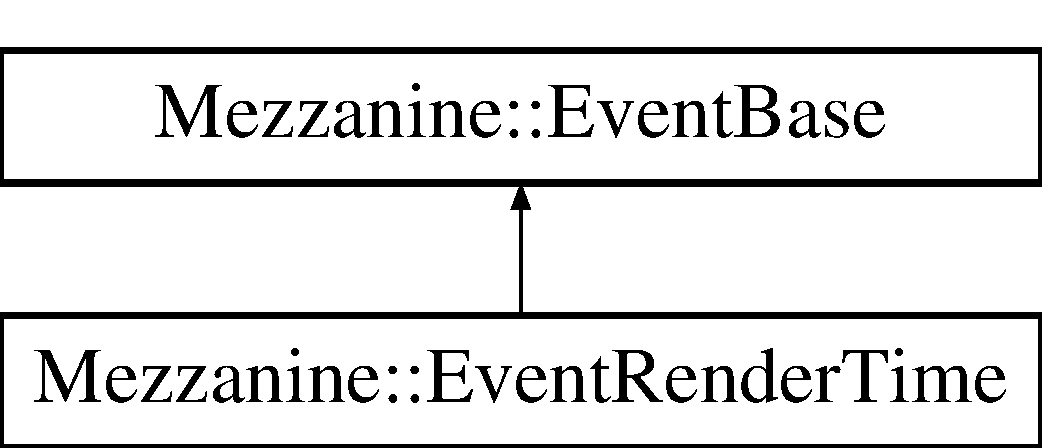
\includegraphics[height=2.000000cm]{classMezzanine_1_1EventRenderTime}
\end{center}
\end{figure}
\subsubsection*{Public Member Functions}
\begin{DoxyCompactItemize}
\item 
\hyperlink{classMezzanine_1_1EventRenderTime_ac1a7e02359265bc94016eb4c6343734e}{EventRenderTime} (\hyperlink{namespaceMezzanine_adcbb6ce6d1eb4379d109e51171e2e493}{Whole} Milliseconds=0)
\begin{DoxyCompactList}\small\item\em The Constructor. \item\end{DoxyCompactList}\item 
\hyperlink{namespaceMezzanine_adcbb6ce6d1eb4379d109e51171e2e493}{Whole} \hyperlink{classMezzanine_1_1EventRenderTime_a4925ead7f9a63787e95c56cc6610fd3d}{getMilliSecondsSinceLastFrame} () const 
\begin{DoxyCompactList}\small\item\em Returns the a floating point value with the amount of time. \item\end{DoxyCompactList}\item 
virtual \hyperlink{classMezzanine_1_1EventBase_ab85e31e97753b7e7ecb098f82526baef}{EventType} \hyperlink{classMezzanine_1_1EventRenderTime_a2c1c6c5c8c77492bc9c74c6529d49681}{GetType} () const 
\begin{DoxyCompactList}\small\item\em Returns that this event is a EventType::RenderTime. \item\end{DoxyCompactList}\item 
void \hyperlink{classMezzanine_1_1EventRenderTime_ad2591c256c302ab56f6960d28288d076}{operator=} (const \hyperlink{classMezzanine_1_1EventRenderTime}{EventRenderTime} \&rhs)
\begin{DoxyCompactList}\small\item\em Assignment operator. \item\end{DoxyCompactList}\end{DoxyCompactItemize}


\subsubsection{Detailed Description}
This communicates the amount of time since the world was rendered. This stores in milliseconds the amount of time since the last rendering of the world. 

Definition at line 59 of file eventrendertime.h.



\subsubsection{Constructor \& Destructor Documentation}
\hypertarget{classMezzanine_1_1EventRenderTime_ac1a7e02359265bc94016eb4c6343734e}{
\index{Mezzanine::EventRenderTime@{Mezzanine::EventRenderTime}!EventRenderTime@{EventRenderTime}}
\index{EventRenderTime@{EventRenderTime}!Mezzanine::EventRenderTime@{Mezzanine::EventRenderTime}}
\paragraph[{EventRenderTime}]{\setlength{\rightskip}{0pt plus 5cm}Mezzanine::EventRenderTime::EventRenderTime (
\begin{DoxyParamCaption}
\item[{{\bf Whole}}]{Milliseconds = {\ttfamily 0}}
\end{DoxyParamCaption}
)}\hfill}
\label{classMezzanine_1_1EventRenderTime_ac1a7e02359265bc94016eb4c6343734e}


The Constructor. 

This is the only way to set the time 
\begin{DoxyParams}{Parameters}
{\em Milliseconds} & As it says, the amount of milliseconds since the last rendering \\
\hline
\end{DoxyParams}


Definition at line 56 of file eventrendertime.cpp.



\subsubsection{Member Function Documentation}
\hypertarget{classMezzanine_1_1EventRenderTime_a4925ead7f9a63787e95c56cc6610fd3d}{
\index{Mezzanine::EventRenderTime@{Mezzanine::EventRenderTime}!getMilliSecondsSinceLastFrame@{getMilliSecondsSinceLastFrame}}
\index{getMilliSecondsSinceLastFrame@{getMilliSecondsSinceLastFrame}!Mezzanine::EventRenderTime@{Mezzanine::EventRenderTime}}
\paragraph[{getMilliSecondsSinceLastFrame}]{\setlength{\rightskip}{0pt plus 5cm}{\bf Whole} Mezzanine::EventRenderTime::getMilliSecondsSinceLastFrame (
\begin{DoxyParamCaption}
{}
\end{DoxyParamCaption}
) const}\hfill}
\label{classMezzanine_1_1EventRenderTime_a4925ead7f9a63787e95c56cc6610fd3d}


Returns the a floating point value with the amount of time. 

Returns the a floating point value with the amount of time. \begin{DoxyReturn}{Returns}
A floating point value with the amount of time. 
\end{DoxyReturn}


Definition at line 66 of file eventrendertime.cpp.

\hypertarget{classMezzanine_1_1EventRenderTime_a2c1c6c5c8c77492bc9c74c6529d49681}{
\index{Mezzanine::EventRenderTime@{Mezzanine::EventRenderTime}!GetType@{GetType}}
\index{GetType@{GetType}!Mezzanine::EventRenderTime@{Mezzanine::EventRenderTime}}
\paragraph[{GetType}]{\setlength{\rightskip}{0pt plus 5cm}{\bf EventBase::EventType} Mezzanine::EventRenderTime::GetType (
\begin{DoxyParamCaption}
{}
\end{DoxyParamCaption}
) const\hspace{0.3cm}{\ttfamily  \mbox{[}virtual\mbox{]}}}\hfill}
\label{classMezzanine_1_1EventRenderTime_a2c1c6c5c8c77492bc9c74c6529d49681}


Returns that this event is a EventType::RenderTime. 

This is primarily for the benefit of sorting thorugh event pointers. If this functions returns EventType::RenderTime, then and event pointer can safely be cast to \hyperlink{classMezzanine_1_1EventRenderTime}{Mezzanine::EventRenderTime} . This method is inherited from Mezzanine::Event . 

Implements \hyperlink{classMezzanine_1_1EventBase_aea900262a74d27e3b5df68a9deb18543}{Mezzanine::EventBase}.



Definition at line 61 of file eventrendertime.cpp.

\hypertarget{classMezzanine_1_1EventRenderTime_ad2591c256c302ab56f6960d28288d076}{
\index{Mezzanine::EventRenderTime@{Mezzanine::EventRenderTime}!operator=@{operator=}}
\index{operator=@{operator=}!Mezzanine::EventRenderTime@{Mezzanine::EventRenderTime}}
\paragraph[{operator=}]{\setlength{\rightskip}{0pt plus 5cm}void Mezzanine::EventRenderTime::operator= (
\begin{DoxyParamCaption}
\item[{const {\bf EventRenderTime} \&}]{rhs}
\end{DoxyParamCaption}
)}\hfill}
\label{classMezzanine_1_1EventRenderTime_ad2591c256c302ab56f6960d28288d076}


Assignment operator. 


\begin{DoxyParams}{Parameters}
{\em rhs} & the Right Hand object in the assignment operator \\
\hline
\end{DoxyParams}


Definition at line 71 of file eventrendertime.cpp.



The documentation for this class was generated from the following files:\begin{DoxyCompactItemize}
\item 
eventrendertime.h\item 
eventrendertime.cpp\end{DoxyCompactItemize}

\hypertarget{classMezzanine_1_1EventUserInput}{
\subsection{Mezzanine::EventUserInput Class Reference}
\label{classMezzanine_1_1EventUserInput}\index{Mezzanine::EventUserInput@{Mezzanine::EventUserInput}}
}


This is a container for MetaCodes that is used in the \hyperlink{classMezzanine_1_1EventManager}{EventManager}.  




{\ttfamily \#include $<$eventuserinput.h$>$}

Inheritance diagram for Mezzanine::EventUserInput:\begin{figure}[H]
\begin{center}
\leavevmode
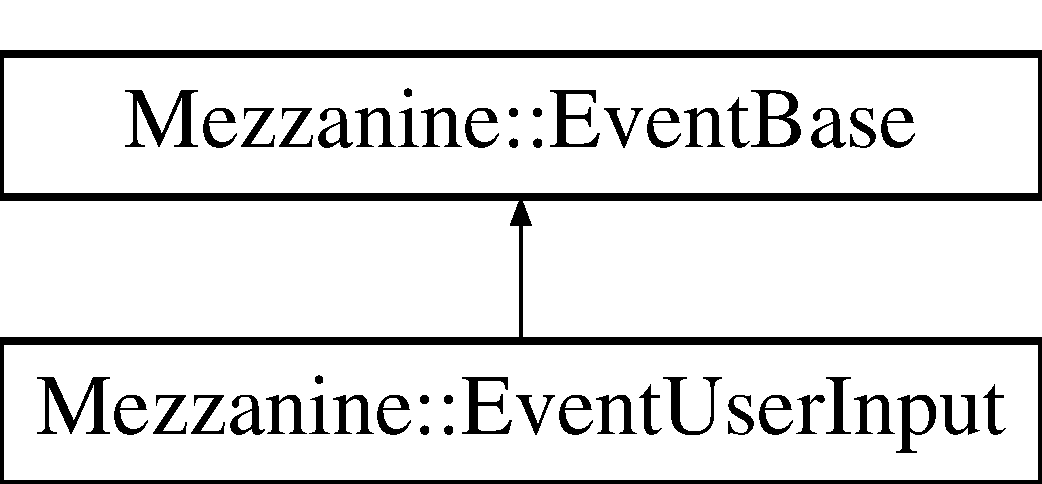
\includegraphics[height=2.000000cm]{classMezzanine_1_1EventUserInput}
\end{center}
\end{figure}
\subsubsection*{Public Member Functions}
\begin{DoxyCompactItemize}
\item 
\hyperlink{classMezzanine_1_1MetaCode}{MetaCode} \hyperlink{classMezzanine_1_1EventUserInput_a8a4eaa043a7e88ced6a0cb4e5d817291}{AddCode} (const \hyperlink{namespaceMezzanine_ae8d4c0ab783af89a250b0225b75753e5}{RawEvent} \&RawEvent\_\-)
\begin{DoxyCompactList}\small\item\em Adds a \hyperlink{classMezzanine_1_1MetaCode}{MetaCode} created from a RawEvent. \item\end{DoxyCompactList}\item 
\hyperlink{classMezzanine_1_1MetaCode}{MetaCode} \hyperlink{classMezzanine_1_1EventUserInput_aa2021a2bec834207a78bad0338714d83}{AddCode} (const \hyperlink{classMezzanine_1_1MetaCode}{MetaCode} \&Code\_\-)
\begin{DoxyCompactList}\small\item\em Adds a \hyperlink{classMezzanine_1_1MetaCode}{MetaCode}. \item\end{DoxyCompactList}\item 
\hyperlink{classMezzanine_1_1MetaCode}{MetaCode} \hyperlink{classMezzanine_1_1EventUserInput_aaf966edbc281d55457e86e2039e87dd7}{AddCode} (const int \&MetaValue\_\-, const \hyperlink{classMezzanine_1_1MetaCode_a3b5633f0145bf3287cf53a3f05b5563c}{MetaCode::InputCode} \&Code\_\-)
\begin{DoxyCompactList}\small\item\em Adds a \hyperlink{classMezzanine_1_1MetaCode}{MetaCode} Created From Raw Values. \item\end{DoxyCompactList}\item 
void \hyperlink{classMezzanine_1_1EventUserInput_ab6ed3c37497ddc7f1985e7ae216ea774}{AddCodes} (const vector$<$ \hyperlink{classMezzanine_1_1MetaCode}{MetaCode} $>$ \&Codes)
\begin{DoxyCompactList}\small\item\em Add Several MetaCodes from a vector. \item\end{DoxyCompactList}\item 
vector$<$ \hyperlink{classMezzanine_1_1MetaCode}{MetaCode} $>$ \hyperlink{classMezzanine_1_1EventUserInput_ac24aaefbb290b4452886ba3f616f0d94}{AddCodesFromRawEvent} (const \hyperlink{namespaceMezzanine_ae8d4c0ab783af89a250b0225b75753e5}{RawEvent} \&RawEvent\_\-)
\begin{DoxyCompactList}\small\item\em Adds all possible MetaCodes that can be created from the given RawEvent. \item\end{DoxyCompactList}\item 
void \hyperlink{classMezzanine_1_1EventUserInput_aecca59338264fd49cf96661f28f02471}{EraseCode} (const \hyperlink{classMezzanine_1_1MetaCode}{MetaCode} \&Code\_\-)
\begin{DoxyCompactList}\small\item\em Removes a specific code from storage. \item\end{DoxyCompactList}\item 
void \hyperlink{classMezzanine_1_1EventUserInput_aede2a3b45edd2442eeac34814b9c03cc}{EraseCode} (const unsigned int \&Index)
\begin{DoxyCompactList}\small\item\em Removes a specific code from storage. \item\end{DoxyCompactList}\item 
\hyperlink{classMezzanine_1_1EventUserInput_ac54a20c16138388b64a86d8ed13854bb}{EventUserInput} (const \hyperlink{classMezzanine_1_1MetaCode}{MetaCode} \&Code\_\-)
\begin{DoxyCompactList}\small\item\em Single Data Point constructor. \item\end{DoxyCompactList}\item 
\hyperlink{classMezzanine_1_1EventUserInput_a3d5857827ca69112a5acfc715ff29814}{EventUserInput} ()
\begin{DoxyCompactList}\small\item\em Default constructor. \item\end{DoxyCompactList}\item 
\hyperlink{classMezzanine_1_1EventUserInput_aa29e31d1d166c54fd8b87a2dc50cebb6}{EventUserInput} (const vector$<$ \hyperlink{classMezzanine_1_1MetaCode}{MetaCode} $>$ \&Codes\_\-)
\begin{DoxyCompactList}\small\item\em Multi Data Point constructor. \item\end{DoxyCompactList}\item 
const \hyperlink{classMezzanine_1_1MetaCode}{MetaCode} \& \hyperlink{classMezzanine_1_1EventUserInput_aa6f011b62624507078cbbd32a382ba42}{GetMetaCode} (const unsigned int \&Index)
\begin{DoxyCompactList}\small\item\em Single Data Point constructor. \item\end{DoxyCompactList}\item 
size\_\-t \hyperlink{classMezzanine_1_1EventUserInput_ae4eaa259b090f4b76a5aad89a7217ea5}{GetMetaCodeCount} ()
\begin{DoxyCompactList}\small\item\em Retrieves a count of the stored Metacodes. \item\end{DoxyCompactList}\item 
virtual \hyperlink{classMezzanine_1_1EventBase_ab85e31e97753b7e7ecb098f82526baef}{EventType} \hyperlink{classMezzanine_1_1EventUserInput_aeb02733446620bd7ff43b449ce5ce98a}{GetType} () const 
\begin{DoxyCompactList}\small\item\em Returns the type of this event. \item\end{DoxyCompactList}\item 
virtual \hyperlink{classMezzanine_1_1EventUserInput_ad5bb99302139d9a69cb2d71ee1784300}{$\sim$EventUserInput} ()
\begin{DoxyCompactList}\small\item\em Default desstructor. \item\end{DoxyCompactList}\end{DoxyCompactItemize}


\subsubsection{Detailed Description}
This is a container for MetaCodes that is used in the \hyperlink{classMezzanine_1_1EventManager}{EventManager}. The \hyperlink{classMezzanine_1_1EventUserInput}{EventUserInput} is the container for information about how a user enters data and commands into a program. By Default one is inserted into event manager the with all the user input from each run of the main loop. These can be manually inserted into the \hyperlink{classMezzanine_1_1EventManager}{EventManager} to simulate input from other sources. If setup properly this can allow computer controlled characters to use the same interface players, allowing for more realistic response from them. \par
 \par
 This is implemented by inheriting from std::vector. Any feature of std::vector can be used to interact with the metacodes stored within. Using Iterators is great way to quickly and easily get what you need from this. For the most part any extra functions on this are for seamless interaction with the \hyperlink{classMezzanine_1_1EventManager}{EventManager}, or to convert incoming data into a more usable form. 

Definition at line 101 of file eventuserinput.h.



\subsubsection{Constructor \& Destructor Documentation}
\hypertarget{classMezzanine_1_1EventUserInput_a3d5857827ca69112a5acfc715ff29814}{
\index{Mezzanine::EventUserInput@{Mezzanine::EventUserInput}!EventUserInput@{EventUserInput}}
\index{EventUserInput@{EventUserInput}!Mezzanine::EventUserInput@{Mezzanine::EventUserInput}}
\paragraph[{EventUserInput}]{\setlength{\rightskip}{0pt plus 5cm}Mezzanine::EventUserInput::EventUserInput (
\begin{DoxyParamCaption}
{}
\end{DoxyParamCaption}
)}\hfill}
\label{classMezzanine_1_1EventUserInput_a3d5857827ca69112a5acfc715ff29814}


Default constructor. 

This creates a perfectly functional, but empty \hyperlink{classMezzanine_1_1EventUserInput}{EventUserInput}. 

Definition at line 70 of file eventuserinput.cpp.

\hypertarget{classMezzanine_1_1EventUserInput_ac54a20c16138388b64a86d8ed13854bb}{
\index{Mezzanine::EventUserInput@{Mezzanine::EventUserInput}!EventUserInput@{EventUserInput}}
\index{EventUserInput@{EventUserInput}!Mezzanine::EventUserInput@{Mezzanine::EventUserInput}}
\paragraph[{EventUserInput}]{\setlength{\rightskip}{0pt plus 5cm}Mezzanine::EventUserInput::EventUserInput (
\begin{DoxyParamCaption}
\item[{const {\bf MetaCode} \&}]{Code\_\-}
\end{DoxyParamCaption}
)}\hfill}
\label{classMezzanine_1_1EventUserInput_ac54a20c16138388b64a86d8ed13854bb}


Single Data Point constructor. 


\begin{DoxyParams}{Parameters}
{\em Code\_\-} & This \hyperlink{classMezzanine_1_1MetaCode}{MetaCode} will be added to the \hyperlink{classMezzanine_1_1EventUserInput}{EventUserInput} during creation.\\
\hline
\end{DoxyParams}
This creates a functional \hyperlink{classMezzanine_1_1EventUserInput}{EventUserInput} which already contains one metacode. 

Definition at line 73 of file eventuserinput.cpp.

\hypertarget{classMezzanine_1_1EventUserInput_aa29e31d1d166c54fd8b87a2dc50cebb6}{
\index{Mezzanine::EventUserInput@{Mezzanine::EventUserInput}!EventUserInput@{EventUserInput}}
\index{EventUserInput@{EventUserInput}!Mezzanine::EventUserInput@{Mezzanine::EventUserInput}}
\paragraph[{EventUserInput}]{\setlength{\rightskip}{0pt plus 5cm}Mezzanine::EventUserInput::EventUserInput (
\begin{DoxyParamCaption}
\item[{const vector$<$ {\bf MetaCode} $>$ \&}]{Codes\_\-}
\end{DoxyParamCaption}
)}\hfill}
\label{classMezzanine_1_1EventUserInput_aa29e31d1d166c54fd8b87a2dc50cebb6}


Multi Data Point constructor. 


\begin{DoxyParams}{Parameters}
{\em Codes\_\-} & The MetaCodes in this vecotor will be added to the \hyperlink{classMezzanine_1_1EventUserInput}{EventUserInput} during creation.\\
\hline
\end{DoxyParams}
This creates a ready to use \hyperlink{classMezzanine_1_1EventUserInput}{EventUserInput} which already contains all the metacodes included. 

Definition at line 76 of file eventuserinput.cpp.

\hypertarget{classMezzanine_1_1EventUserInput_ad5bb99302139d9a69cb2d71ee1784300}{
\index{Mezzanine::EventUserInput@{Mezzanine::EventUserInput}!$\sim$EventUserInput@{$\sim$EventUserInput}}
\index{$\sim$EventUserInput@{$\sim$EventUserInput}!Mezzanine::EventUserInput@{Mezzanine::EventUserInput}}
\paragraph[{$\sim$EventUserInput}]{\setlength{\rightskip}{0pt plus 5cm}Mezzanine::EventUserInput::$\sim$EventUserInput (
\begin{DoxyParamCaption}
{}
\end{DoxyParamCaption}
)\hspace{0.3cm}{\ttfamily  \mbox{[}virtual\mbox{]}}}\hfill}
\label{classMezzanine_1_1EventUserInput_ad5bb99302139d9a69cb2d71ee1784300}


Default desstructor. 

This tears down the 

Definition at line 79 of file eventuserinput.cpp.



\subsubsection{Member Function Documentation}
\hypertarget{classMezzanine_1_1EventUserInput_a8a4eaa043a7e88ced6a0cb4e5d817291}{
\index{Mezzanine::EventUserInput@{Mezzanine::EventUserInput}!AddCode@{AddCode}}
\index{AddCode@{AddCode}!Mezzanine::EventUserInput@{Mezzanine::EventUserInput}}
\paragraph[{AddCode}]{\setlength{\rightskip}{0pt plus 5cm}{\bf MetaCode} Mezzanine::EventUserInput::AddCode (
\begin{DoxyParamCaption}
\item[{const {\bf RawEvent} \&}]{RawEvent\_\-}
\end{DoxyParamCaption}
)}\hfill}
\label{classMezzanine_1_1EventUserInput_a8a4eaa043a7e88ced6a0cb4e5d817291}


Adds a \hyperlink{classMezzanine_1_1MetaCode}{MetaCode} created from a RawEvent. 


\begin{DoxyParams}{Parameters}
{\em RawEvent\_\-} & The RawEvent which will be translated into exactly One \hyperlink{classMezzanine_1_1MetaCode}{MetaCode}\\
\hline
\end{DoxyParams}
This will add \hyperlink{classMezzanine_1_1MetaCode}{MetaCode} to this event which will be create from a RawEvent which can produce Exactly one \hyperlink{classMezzanine_1_1MetaCode}{MetaCode}. This is used by engine internals, it is recommended to not use this in game code. \begin{DoxyWarning}{Warning}
Do not use this without reading and fully understanding the warnings on \hyperlink{classMezzanine_1_1MetaCode_abe2e7fa16bab17df5b1794c26bf191be}{MetaCode::MetaCode(const RawEvent \&RawEvent\_\-)} . This function has all the same Restrictions. If game code is using RawEvents at all, the game logic should be scrutinized carefully, there is probably something wrong, but if it must it should use \hyperlink{classMezzanine_1_1EventUserInput_ac24aaefbb290b4452886ba3f616f0d94}{EventUserInput::AddCodesFromRawEvent} instead, as it can make the needed determinations automatically and in a platform agnostic way. 
\end{DoxyWarning}
\begin{DoxyReturn}{Returns}
This returns a const reference to the \hyperlink{classMezzanine_1_1MetaCode}{MetaCode} that was Added. This reference is valid for the lifetime of this \hyperlink{classMezzanine_1_1EventUserInput}{EventUserInput}. 
\end{DoxyReturn}


Definition at line 94 of file eventuserinput.cpp.

\hypertarget{classMezzanine_1_1EventUserInput_aa2021a2bec834207a78bad0338714d83}{
\index{Mezzanine::EventUserInput@{Mezzanine::EventUserInput}!AddCode@{AddCode}}
\index{AddCode@{AddCode}!Mezzanine::EventUserInput@{Mezzanine::EventUserInput}}
\paragraph[{AddCode}]{\setlength{\rightskip}{0pt plus 5cm}{\bf MetaCode} Mezzanine::EventUserInput::AddCode (
\begin{DoxyParamCaption}
\item[{const {\bf MetaCode} \&}]{Code\_\-}
\end{DoxyParamCaption}
)}\hfill}
\label{classMezzanine_1_1EventUserInput_aa2021a2bec834207a78bad0338714d83}


Adds a \hyperlink{classMezzanine_1_1MetaCode}{MetaCode}. 


\begin{DoxyParams}{Parameters}
{\em Code\_\-} & The User Input \hyperlink{classMezzanine_1_1MetaCode}{MetaCode} tobe added\\
\hline
\end{DoxyParams}
This adds an existing metacode to this event. \begin{DoxyReturn}{Returns}
This returns a const reference to the \hyperlink{classMezzanine_1_1MetaCode}{MetaCode} that was Added. This reference is valid for the lifetime of this \hyperlink{classMezzanine_1_1EventUserInput}{EventUserInput}. 
\end{DoxyReturn}


Definition at line 88 of file eventuserinput.cpp.

\hypertarget{classMezzanine_1_1EventUserInput_aaf966edbc281d55457e86e2039e87dd7}{
\index{Mezzanine::EventUserInput@{Mezzanine::EventUserInput}!AddCode@{AddCode}}
\index{AddCode@{AddCode}!Mezzanine::EventUserInput@{Mezzanine::EventUserInput}}
\paragraph[{AddCode}]{\setlength{\rightskip}{0pt plus 5cm}{\bf MetaCode} Mezzanine::EventUserInput::AddCode (
\begin{DoxyParamCaption}
\item[{const int \&}]{MetaValue\_\-, }
\item[{const {\bf MetaCode::InputCode} \&}]{Code\_\-}
\end{DoxyParamCaption}
)}\hfill}
\label{classMezzanine_1_1EventUserInput_aaf966edbc281d55457e86e2039e87dd7}


Adds a \hyperlink{classMezzanine_1_1MetaCode}{MetaCode} Created From Raw Values. 


\begin{DoxyParams}{Parameters}
{\em MetaValue\_\-} & The MetaValue that will be in the \hyperlink{classMezzanine_1_1MetaCode}{MetaCode} \\
\hline
{\em Code\_\-} & The InputCode that will be in the \hyperlink{classMezzanine_1_1MetaCode}{MetaCode}\\
\hline
\end{DoxyParams}
This creates metacode a metacode and adds it to this event. \begin{DoxyReturn}{Returns}
This returns a const reference to the \hyperlink{classMezzanine_1_1MetaCode}{MetaCode} that was Added. This reference is valid for the lifetime of this \hyperlink{classMezzanine_1_1EventUserInput}{EventUserInput}. 
\end{DoxyReturn}


Definition at line 100 of file eventuserinput.cpp.

\hypertarget{classMezzanine_1_1EventUserInput_ab6ed3c37497ddc7f1985e7ae216ea774}{
\index{Mezzanine::EventUserInput@{Mezzanine::EventUserInput}!AddCodes@{AddCodes}}
\index{AddCodes@{AddCodes}!Mezzanine::EventUserInput@{Mezzanine::EventUserInput}}
\paragraph[{AddCodes}]{\setlength{\rightskip}{0pt plus 5cm}void Mezzanine::EventUserInput::AddCodes (
\begin{DoxyParamCaption}
\item[{const vector$<$ {\bf MetaCode} $>$ \&}]{Codes}
\end{DoxyParamCaption}
)}\hfill}
\label{classMezzanine_1_1EventUserInput_ab6ed3c37497ddc7f1985e7ae216ea774}


Add Several MetaCodes from a vector. 


\begin{DoxyParams}{Parameters}
{\em Codes} & A vector of MetaCodes to be added to this event\\
\hline
\end{DoxyParams}
This adds several existing metacodes to this event. 

Definition at line 106 of file eventuserinput.cpp.

\hypertarget{classMezzanine_1_1EventUserInput_ac24aaefbb290b4452886ba3f616f0d94}{
\index{Mezzanine::EventUserInput@{Mezzanine::EventUserInput}!AddCodesFromRawEvent@{AddCodesFromRawEvent}}
\index{AddCodesFromRawEvent@{AddCodesFromRawEvent}!Mezzanine::EventUserInput@{Mezzanine::EventUserInput}}
\paragraph[{AddCodesFromRawEvent}]{\setlength{\rightskip}{0pt plus 5cm}vector$<$ {\bf MetaCode} $>$ Mezzanine::EventUserInput::AddCodesFromRawEvent (
\begin{DoxyParamCaption}
\item[{const {\bf RawEvent} \&}]{RawEvent\_\-}
\end{DoxyParamCaption}
)}\hfill}
\label{classMezzanine_1_1EventUserInput_ac24aaefbb290b4452886ba3f616f0d94}


Adds all possible MetaCodes that can be created from the given RawEvent. 


\begin{DoxyParams}{Parameters}
{\em RawEvent\_\-} & The RawEvent which will be translated into a group of metacodes and added to this\\
\hline
\end{DoxyParams}
This will add \hyperlink{classMezzanine_1_1MetaCode}{MetaCode} to this event which will be create from a RawEvent which can produce Exactly one \hyperlink{classMezzanine_1_1MetaCode}{MetaCode}. This is used by engine internals, it is recommended to not use this in game code. \begin{DoxyWarning}{Warning}
If game code is using RawEvents at all, the game logic should be scrutinized carefully, there is probably something wrong, but if it must them this is the correct function to use. This will work same on a all platforms. However, the binary format of the Rawevent could chnage meaning you would have to recompile the game code to work with new version of the engine \par
 This Function is currently incomplete, and does not yet process all events such as joysticks events and some mouse events. 
\end{DoxyWarning}
\begin{DoxyReturn}{Returns}
this returns a complete set of all the MetaCodes added. 
\end{DoxyReturn}


Definition at line 131 of file eventuserinput.cpp.

\hypertarget{classMezzanine_1_1EventUserInput_aede2a3b45edd2442eeac34814b9c03cc}{
\index{Mezzanine::EventUserInput@{Mezzanine::EventUserInput}!EraseCode@{EraseCode}}
\index{EraseCode@{EraseCode}!Mezzanine::EventUserInput@{Mezzanine::EventUserInput}}
\paragraph[{EraseCode}]{\setlength{\rightskip}{0pt plus 5cm}void Mezzanine::EventUserInput::EraseCode (
\begin{DoxyParamCaption}
\item[{const unsigned int \&}]{Index}
\end{DoxyParamCaption}
)}\hfill}
\label{classMezzanine_1_1EventUserInput_aede2a3b45edd2442eeac34814b9c03cc}


Removes a specific code from storage. 


\begin{DoxyParams}{Parameters}
{\em Index} & This is the location to removed from\\
\hline
\end{DoxyParams}
The \hyperlink{classMezzanine_1_1MetaCode}{MetaCode} at and only at the given Index will be deleted. 

Definition at line 125 of file eventuserinput.cpp.

\hypertarget{classMezzanine_1_1EventUserInput_aecca59338264fd49cf96661f28f02471}{
\index{Mezzanine::EventUserInput@{Mezzanine::EventUserInput}!EraseCode@{EraseCode}}
\index{EraseCode@{EraseCode}!Mezzanine::EventUserInput@{Mezzanine::EventUserInput}}
\paragraph[{EraseCode}]{\setlength{\rightskip}{0pt plus 5cm}void Mezzanine::EventUserInput::EraseCode (
\begin{DoxyParamCaption}
\item[{const {\bf MetaCode} \&}]{Code\_\-}
\end{DoxyParamCaption}
)}\hfill}
\label{classMezzanine_1_1EventUserInput_aecca59338264fd49cf96661f28f02471}


Removes a specific code from storage. 


\begin{DoxyParams}{Parameters}
{\em Code\_\-} & This will search for all matching copies of this\\
\hline
\end{DoxyParams}
All MetaCodes that are equal to Code\_\- will simply be erased. 

Definition at line 112 of file eventuserinput.cpp.

\hypertarget{classMezzanine_1_1EventUserInput_aa6f011b62624507078cbbd32a382ba42}{
\index{Mezzanine::EventUserInput@{Mezzanine::EventUserInput}!GetMetaCode@{GetMetaCode}}
\index{GetMetaCode@{GetMetaCode}!Mezzanine::EventUserInput@{Mezzanine::EventUserInput}}
\paragraph[{GetMetaCode}]{\setlength{\rightskip}{0pt plus 5cm}const {\bf MetaCode} \& Mezzanine::EventUserInput::GetMetaCode (
\begin{DoxyParamCaption}
\item[{const unsigned int \&}]{Index}
\end{DoxyParamCaption}
)}\hfill}
\label{classMezzanine_1_1EventUserInput_aa6f011b62624507078cbbd32a382ba42}


Single Data Point constructor. 

\begin{DoxyReturn}{Returns}
Index The requested \hyperlink{classMezzanine_1_1MetaCode}{MetaCode} to return.
\end{DoxyReturn}
This function simply retrieves the requested \hyperlink{classMezzanine_1_1MetaCode}{MetaCode}. It can throw standard Out of bounds exceptions if attemped to reference a negative item or an item with Index higher than what exists \par
 This is useful for accessing each \hyperlink{classMezzanine_1_1MetaCode}{MetaCode} stored in this UserInputEvent. 

Definition at line 82 of file eventuserinput.cpp.

\hypertarget{classMezzanine_1_1EventUserInput_ae4eaa259b090f4b76a5aad89a7217ea5}{
\index{Mezzanine::EventUserInput@{Mezzanine::EventUserInput}!GetMetaCodeCount@{GetMetaCodeCount}}
\index{GetMetaCodeCount@{GetMetaCodeCount}!Mezzanine::EventUserInput@{Mezzanine::EventUserInput}}
\paragraph[{GetMetaCodeCount}]{\setlength{\rightskip}{0pt plus 5cm}size\_\-t Mezzanine::EventUserInput::GetMetaCodeCount (
\begin{DoxyParamCaption}
{}
\end{DoxyParamCaption}
)}\hfill}
\label{classMezzanine_1_1EventUserInput_ae4eaa259b090f4b76a5aad89a7217ea5}


Retrieves a count of the stored Metacodes. 

\begin{DoxyReturn}{Returns}
The amount of codes stored in this \hyperlink{classMezzanine_1_1EventUserInput}{EventUserInput}.
\end{DoxyReturn}
Retrieves a count of the stored Metacodes. Synonym for vector::size(); 

Definition at line 85 of file eventuserinput.cpp.

\hypertarget{classMezzanine_1_1EventUserInput_aeb02733446620bd7ff43b449ce5ce98a}{
\index{Mezzanine::EventUserInput@{Mezzanine::EventUserInput}!GetType@{GetType}}
\index{GetType@{GetType}!Mezzanine::EventUserInput@{Mezzanine::EventUserInput}}
\paragraph[{GetType}]{\setlength{\rightskip}{0pt plus 5cm}{\bf EventBase::EventType} Mezzanine::EventUserInput::GetType (
\begin{DoxyParamCaption}
{}
\end{DoxyParamCaption}
) const\hspace{0.3cm}{\ttfamily  \mbox{[}virtual\mbox{]}}}\hfill}
\label{classMezzanine_1_1EventUserInput_aeb02733446620bd7ff43b449ce5ce98a}


Returns the type of this event. 

\begin{DoxyReturn}{Returns}
Returns EventType::UserInput 
\end{DoxyReturn}


Implements \hyperlink{classMezzanine_1_1EventBase_aea900262a74d27e3b5df68a9deb18543}{Mezzanine::EventBase}.



Definition at line 128 of file eventuserinput.cpp.



The documentation for this class was generated from the following files:\begin{DoxyCompactItemize}
\item 
eventuserinput.h\item 
eventuserinput.cpp\end{DoxyCompactItemize}

\hypertarget{classMezzanine_1_1Exception}{
\subsection{Mezzanine::Exception Class Reference}
\label{classMezzanine_1_1Exception}\index{Mezzanine::Exception@{Mezzanine::Exception}}
}


This is the exception thrown by most \hyperlink{namespaceMezzanine}{Mezzanine} system that can throw exceptions.  




{\ttfamily \#include $<$exception.h$>$}

\subsubsection*{Public Member Functions}
\begin{DoxyCompactItemize}
\item 
\hyperlink{classMezzanine_1_1Exception_ad8659eac607c0e9138be934281b4102d}{Exception} (const \hyperlink{namespaceMezzanine_acf9fcc130e6ebf08e3d8491aebcf1c86}{String} \&Message=\char`\"{}\char`\"{}, bool Logged\_\-=false)
\begin{DoxyCompactList}\small\item\em Simple Constructor. \item\end{DoxyCompactList}\item 
bool \hyperlink{classMezzanine_1_1Exception_a642c76c7148c92b09802a55600359d3c}{HasBeenLogged} ()
\begin{DoxyCompactList}\small\item\em Has this exception been on a trip through the Logger? \item\end{DoxyCompactList}\item 
\hypertarget{classMezzanine_1_1Exception_a574150adbe4f949a5668640a7225ca8c}{
void \hyperlink{classMezzanine_1_1Exception_a574150adbe4f949a5668640a7225ca8c}{SetLogged} ()}
\label{classMezzanine_1_1Exception_a574150adbe4f949a5668640a7225ca8c}

\begin{DoxyCompactList}\small\item\em Set the logged bit. \item\end{DoxyCompactList}\item 
virtual \hyperlink{namespaceMezzanine_acf9fcc130e6ebf08e3d8491aebcf1c86}{String} \hyperlink{classMezzanine_1_1Exception_adfca1d69742135b428879136456e1126}{what} ()  throw ()
\begin{DoxyCompactList}\small\item\em Retrieves the error message. \item\end{DoxyCompactList}\end{DoxyCompactItemize}


\subsubsection{Detailed Description}
This is the exception thrown by most \hyperlink{namespaceMezzanine}{Mezzanine} system that can throw exceptions. In general they work like std::exception, but also track whether they have been logged yet. 

Definition at line 56 of file exception.h.



\subsubsection{Constructor \& Destructor Documentation}
\hypertarget{classMezzanine_1_1Exception_ad8659eac607c0e9138be934281b4102d}{
\index{Mezzanine::Exception@{Mezzanine::Exception}!Exception@{Exception}}
\index{Exception@{Exception}!Mezzanine::Exception@{Mezzanine::Exception}}
\paragraph[{Exception}]{\setlength{\rightskip}{0pt plus 5cm}Mezzanine::Exception::Exception (
\begin{DoxyParamCaption}
\item[{const {\bf String} \&}]{Message = {\ttfamily \char`\"{}\char`\"{}}, }
\item[{bool}]{Logged\_\- = {\ttfamily false}}
\end{DoxyParamCaption}
)}\hfill}
\label{classMezzanine_1_1Exception_ad8659eac607c0e9138be934281b4102d}


Simple Constructor. 


\begin{DoxyParams}{Parameters}
{\em Message} & The Error you want stored in the exception. \\
\hline
{\em Logged\_\-} & Has this exception already been sent to tthe logger \\
\hline
\end{DoxyParams}


Definition at line 48 of file exception.cpp.



\subsubsection{Member Function Documentation}
\hypertarget{classMezzanine_1_1Exception_a642c76c7148c92b09802a55600359d3c}{
\index{Mezzanine::Exception@{Mezzanine::Exception}!HasBeenLogged@{HasBeenLogged}}
\index{HasBeenLogged@{HasBeenLogged}!Mezzanine::Exception@{Mezzanine::Exception}}
\paragraph[{HasBeenLogged}]{\setlength{\rightskip}{0pt plus 5cm}bool Mezzanine::Exception::HasBeenLogged (
\begin{DoxyParamCaption}
{}
\end{DoxyParamCaption}
)}\hfill}
\label{classMezzanine_1_1Exception_a642c76c7148c92b09802a55600359d3c}


Has this exception been on a trip through the Logger? 

\begin{DoxyReturn}{Returns}
A bool storing true if it has and false if it has not. 
\end{DoxyReturn}


Definition at line 53 of file exception.cpp.

\hypertarget{classMezzanine_1_1Exception_adfca1d69742135b428879136456e1126}{
\index{Mezzanine::Exception@{Mezzanine::Exception}!what@{what}}
\index{what@{what}!Mezzanine::Exception@{Mezzanine::Exception}}
\paragraph[{what}]{\setlength{\rightskip}{0pt plus 5cm}{\bf String} Mezzanine::Exception::what (
\begin{DoxyParamCaption}
{}
\end{DoxyParamCaption}
)  throw ()\hspace{0.3cm}{\ttfamily  \mbox{[}virtual\mbox{]}}}\hfill}
\label{classMezzanine_1_1Exception_adfca1d69742135b428879136456e1126}


Retrieves the error message. 

\begin{DoxyReturn}{Returns}
This returns a string that is the stored error message. 
\end{DoxyReturn}


Definition at line 58 of file exception.cpp.



The documentation for this class was generated from the following files:\begin{DoxyCompactItemize}
\item 
exception.h\item 
exception.cpp\end{DoxyCompactItemize}

\hypertarget{classMezzanine_1_1ExtendedTimer}{
\subsection{Mezzanine::ExtendedTimer Class Reference}
\label{classMezzanine_1_1ExtendedTimer}\index{Mezzanine::ExtendedTimer@{Mezzanine::ExtendedTimer}}
}


An enhanced timer class that can store and track many units of time.  




{\ttfamily \#include $<$extendedtimer.h$>$}

Inheritance diagram for Mezzanine::ExtendedTimer:\begin{figure}[H]
\begin{center}
\leavevmode
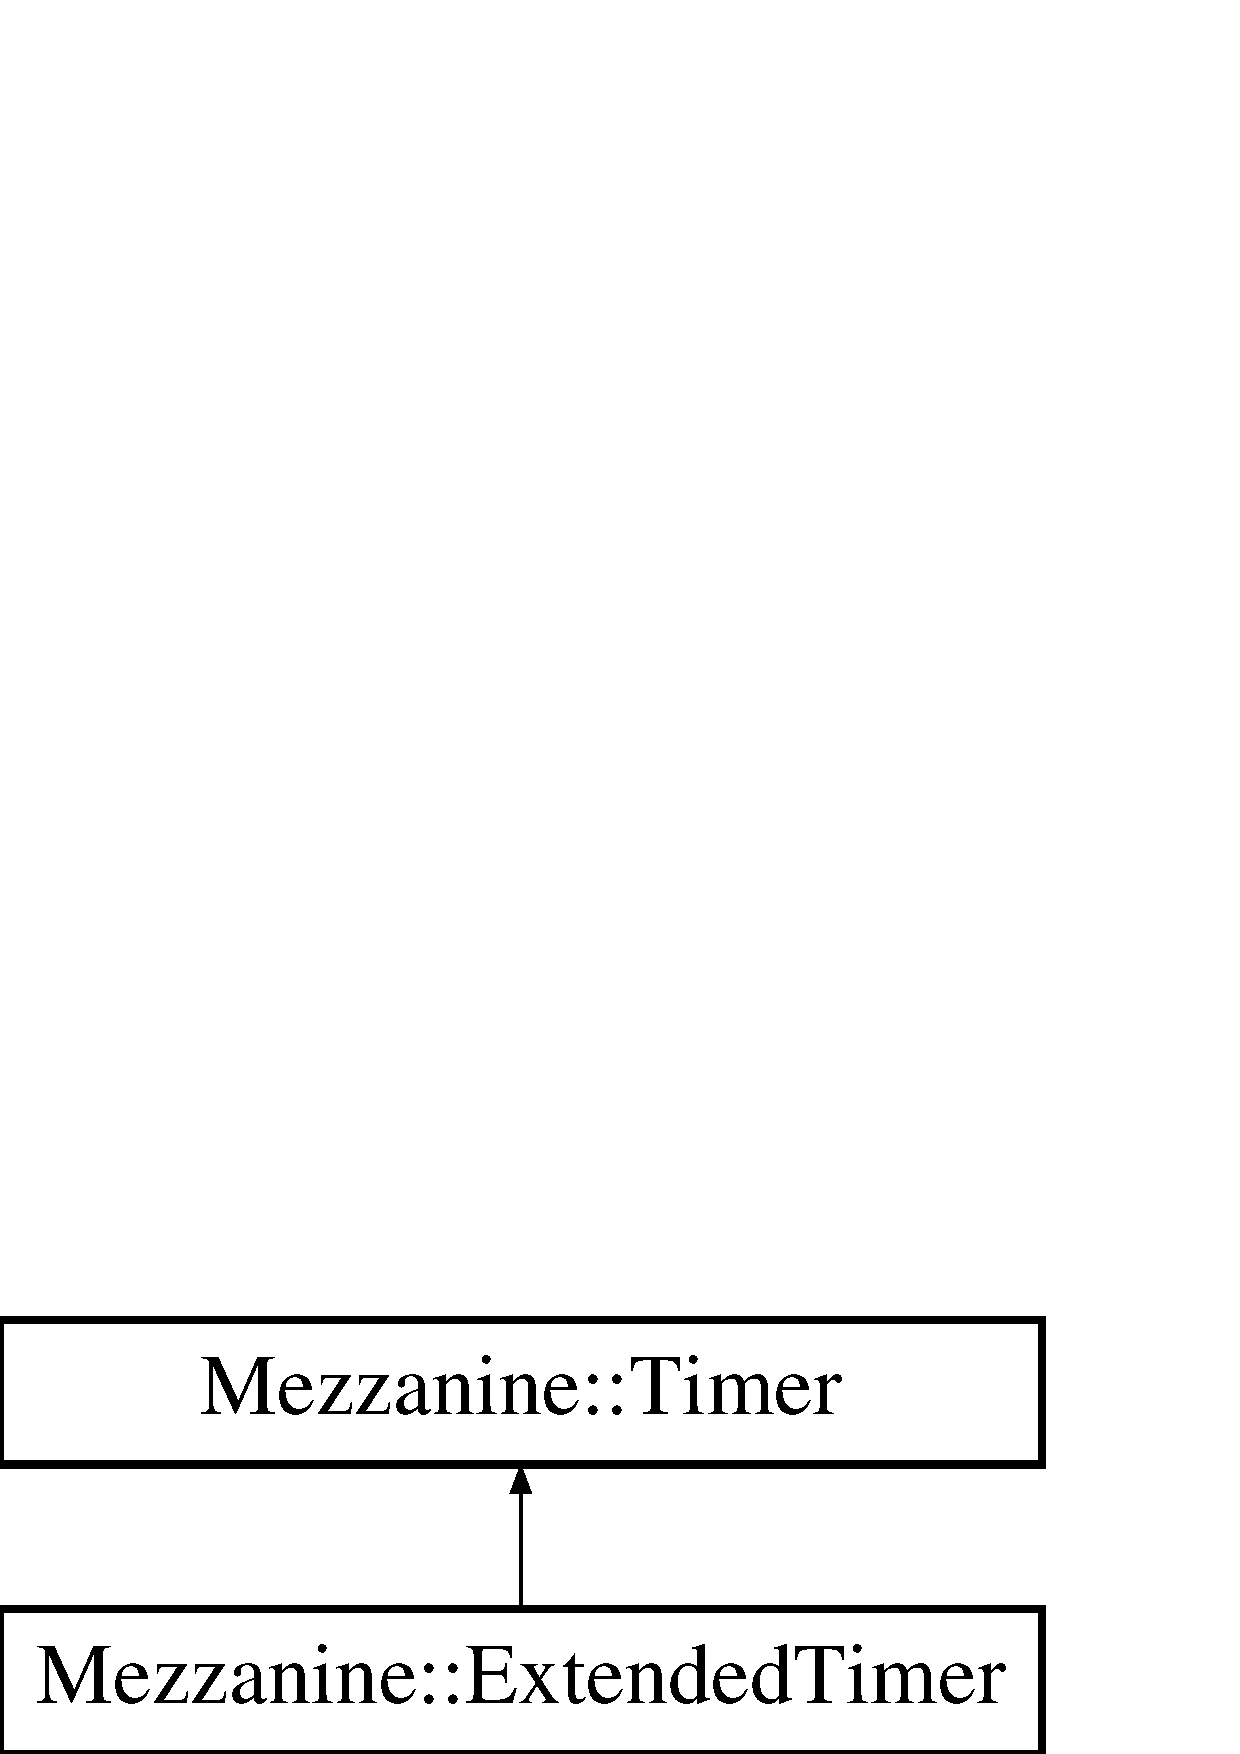
\includegraphics[height=2.000000cm]{classMezzanine_1_1ExtendedTimer}
\end{center}
\end{figure}
\subsubsection*{Public Types}
\begin{DoxyCompactItemize}
\item 
enum \hyperlink{classMezzanine_1_1ExtendedTimer_a52119e2da54ea7ae5da0dc1f921a3b61}{TimeStruct} \{ \hyperlink{classMezzanine_1_1ExtendedTimer_a52119e2da54ea7ae5da0dc1f921a3b61ab66b80ae57d622d3555bdd2828b5dfff}{Current}, 
\hyperlink{classMezzanine_1_1ExtendedTimer_a52119e2da54ea7ae5da0dc1f921a3b61afd99677d1774c80bfaa92b6dba36c2ba}{Goal}, 
\hyperlink{classMezzanine_1_1ExtendedTimer_a52119e2da54ea7ae5da0dc1f921a3b61addcde9da9ed25254cd4919c1d6fb7172}{Initial}
 \}
\begin{DoxyCompactList}\small\item\em The internal time struct to be used... \item\end{DoxyCompactList}\end{DoxyCompactItemize}
\subsubsection*{Public Member Functions}
\begin{DoxyCompactItemize}
\item 
\hyperlink{classMezzanine_1_1ExtendedTimer_a782923da6f5e37bf9c1b9552b81cd979}{ExtendedTimer} (const \hyperlink{classMezzanine_1_1Timer_a1db436d4e0d6f1676e41ba3cb2ea3aaa}{Timer::TimerStyle} style)
\begin{DoxyCompactList}\small\item\em Standard Constructor. \item\end{DoxyCompactList}\item 
virtual \hyperlink{namespaceMezzanine_ac3576e52af3c62d13dde94829e0c5465}{Integer} \hyperlink{classMezzanine_1_1ExtendedTimer_a293364cf175ba95addaa06bbb43d1d3b}{GetDays} (const \hyperlink{classMezzanine_1_1ExtendedTimer_a52119e2da54ea7ae5da0dc1f921a3b61}{ExtendedTimer::TimeStruct} Struct=ExtendedTimer::Current)
\begin{DoxyCompactList}\small\item\em Gets the current internal Day count. \item\end{DoxyCompactList}\item 
virtual \hyperlink{namespaceMezzanine_ac3576e52af3c62d13dde94829e0c5465}{Integer} \hyperlink{classMezzanine_1_1ExtendedTimer_a8e4f14bee3434fd93a6df6a4798165a9}{GetHours} (const \hyperlink{classMezzanine_1_1ExtendedTimer_a52119e2da54ea7ae5da0dc1f921a3b61}{ExtendedTimer::TimeStruct} Struct=ExtendedTimer::Current)
\begin{DoxyCompactList}\small\item\em Gets the current internal Hour count. \item\end{DoxyCompactList}\item 
virtual \hyperlink{namespaceMezzanine_ac3576e52af3c62d13dde94829e0c5465}{Integer} \hyperlink{classMezzanine_1_1ExtendedTimer_ab2c087c96c4c0bc4bbe3bb6e029fa88e}{GetMilliseconds} (const \hyperlink{classMezzanine_1_1ExtendedTimer_a52119e2da54ea7ae5da0dc1f921a3b61}{ExtendedTimer::TimeStruct} Struct=ExtendedTimer::Current)
\begin{DoxyCompactList}\small\item\em Gets the current internal Millisecond count. \item\end{DoxyCompactList}\item 
virtual \hyperlink{namespaceMezzanine_ac3576e52af3c62d13dde94829e0c5465}{Integer} \hyperlink{classMezzanine_1_1ExtendedTimer_af70a43d4735bcc7d05401607c1f63784}{GetMinutes} (const \hyperlink{classMezzanine_1_1ExtendedTimer_a52119e2da54ea7ae5da0dc1f921a3b61}{ExtendedTimer::TimeStruct} Struct=ExtendedTimer::Current)
\begin{DoxyCompactList}\small\item\em Gets the current internal Minute count. \item\end{DoxyCompactList}\item 
virtual \hyperlink{namespaceMezzanine_ac3576e52af3c62d13dde94829e0c5465}{Integer} \hyperlink{classMezzanine_1_1ExtendedTimer_aa7fb648a0807f7102cb72983d6e9038f}{GetSeconds} (const \hyperlink{classMezzanine_1_1ExtendedTimer_a52119e2da54ea7ae5da0dc1f921a3b61}{ExtendedTimer::TimeStruct} Struct=ExtendedTimer::Current)
\begin{DoxyCompactList}\small\item\em Gets the current internal Second count. \item\end{DoxyCompactList}\item 
\hypertarget{classMezzanine_1_1ExtendedTimer_ac2781423c8f7d888e05443aeb5244e0a}{
virtual void \hyperlink{classMezzanine_1_1ExtendedTimer_ac2781423c8f7d888e05443aeb5244e0a}{Reset} ()}
\label{classMezzanine_1_1ExtendedTimer_ac2781423c8f7d888e05443aeb5244e0a}

\begin{DoxyCompactList}\small\item\em Sets the current values to their initial values. \item\end{DoxyCompactList}\item 
virtual \hyperlink{classMezzanine_1_1ExtendedTimer}{ExtendedTimer} \& \hyperlink{classMezzanine_1_1ExtendedTimer_ac0e2fcf76c0fe1445ff36b07131a1657}{SetAutoReset} (const bool AutoReset)
\begin{DoxyCompactList}\small\item\em Sets whether or not the \hyperlink{classMezzanine_1_1Timer}{Timer} should reset if it reaches it's goal. \par
 Ex. If a stopwatch reaches 0. \item\end{DoxyCompactList}\item 
virtual \hyperlink{classMezzanine_1_1ExtendedTimer}{ExtendedTimer} \& \hyperlink{classMezzanine_1_1ExtendedTimer_aadc09173ecb481cbe7e2c3703e1ef34d}{SetDays} (\hyperlink{namespaceMezzanine_ac3576e52af3c62d13dde94829e0c5465}{Integer} Day, const \hyperlink{classMezzanine_1_1ExtendedTimer_a52119e2da54ea7ae5da0dc1f921a3b61}{ExtendedTimer::TimeStruct} Struct=ExtendedTimer::Current)
\begin{DoxyCompactList}\small\item\em Sets the value for Days of the specified struct. \item\end{DoxyCompactList}\item 
virtual \hyperlink{classMezzanine_1_1ExtendedTimer}{ExtendedTimer} \& \hyperlink{classMezzanine_1_1ExtendedTimer_a57d6151f99b75a45433bf919dd218b64}{SetHours} (\hyperlink{namespaceMezzanine_ac3576e52af3c62d13dde94829e0c5465}{Integer} Hr, const \hyperlink{classMezzanine_1_1ExtendedTimer_a52119e2da54ea7ae5da0dc1f921a3b61}{ExtendedTimer::TimeStruct} Struct=ExtendedTimer::Current)
\begin{DoxyCompactList}\small\item\em Sets the value for Hours of the specified struct. \item\end{DoxyCompactList}\item 
virtual \hyperlink{classMezzanine_1_1ExtendedTimer}{ExtendedTimer} \& \hyperlink{classMezzanine_1_1ExtendedTimer_abf97ea669cc7c816a94fb8162e575575}{SetMicroseconds} (\hyperlink{namespaceMezzanine_ac3576e52af3c62d13dde94829e0c5465}{Integer} MS, const \hyperlink{classMezzanine_1_1ExtendedTimer_a52119e2da54ea7ae5da0dc1f921a3b61}{ExtendedTimer::TimeStruct} Struct=ExtendedTimer::Current)
\begin{DoxyCompactList}\small\item\em Sets the value for Microseconds of the specified struct. \item\end{DoxyCompactList}\item 
virtual \hyperlink{classMezzanine_1_1ExtendedTimer}{ExtendedTimer} \& \hyperlink{classMezzanine_1_1ExtendedTimer_aa0aa81de0f595c5c59525fb8bfe57696}{SetMilliseconds} (\hyperlink{namespaceMezzanine_ac3576e52af3c62d13dde94829e0c5465}{Integer} MS, const \hyperlink{classMezzanine_1_1ExtendedTimer_a52119e2da54ea7ae5da0dc1f921a3b61}{ExtendedTimer::TimeStruct} Struct=ExtendedTimer::Current)
\begin{DoxyCompactList}\small\item\em Sets the value for Milliseconds of the specified struct. \item\end{DoxyCompactList}\item 
virtual \hyperlink{classMezzanine_1_1ExtendedTimer}{ExtendedTimer} \& \hyperlink{classMezzanine_1_1ExtendedTimer_a7779f8dcba1a632ef3dd1bc5b89570c6}{SetMinutes} (\hyperlink{namespaceMezzanine_ac3576e52af3c62d13dde94829e0c5465}{Integer} Min, const \hyperlink{classMezzanine_1_1ExtendedTimer_a52119e2da54ea7ae5da0dc1f921a3b61}{ExtendedTimer::TimeStruct} Struct=ExtendedTimer::Current)
\begin{DoxyCompactList}\small\item\em Sets the value for Minutes of the specified struct. \item\end{DoxyCompactList}\item 
virtual \hyperlink{classMezzanine_1_1ExtendedTimer}{ExtendedTimer} \& \hyperlink{classMezzanine_1_1ExtendedTimer_af367348e4289284749a5174672dd18a8}{SetSeconds} (\hyperlink{namespaceMezzanine_ac3576e52af3c62d13dde94829e0c5465}{Integer} Sec, const \hyperlink{classMezzanine_1_1ExtendedTimer_a52119e2da54ea7ae5da0dc1f921a3b61}{ExtendedTimer::TimeStruct} Struct=ExtendedTimer::Current)
\begin{DoxyCompactList}\small\item\em Sets the value for Seconds of the specified struct. \item\end{DoxyCompactList}\item 
\hypertarget{classMezzanine_1_1ExtendedTimer_ab628823999966c35b86e26bfd15d0240}{
virtual \hyperlink{classMezzanine_1_1ExtendedTimer_ab628823999966c35b86e26bfd15d0240}{$\sim$ExtendedTimer} ()}
\label{classMezzanine_1_1ExtendedTimer_ab628823999966c35b86e26bfd15d0240}

\begin{DoxyCompactList}\small\item\em Class destructor. \item\end{DoxyCompactList}\end{DoxyCompactItemize}
\subsubsection*{Protected Member Functions}
\begin{DoxyCompactItemize}
\item 
\hypertarget{classMezzanine_1_1ExtendedTimer_affee9db7f13803b957e9369031997147}{
virtual bool {\bfseries CheckAll} (const \hyperlink{classMezzanine_1_1ExtendedTimer_a52119e2da54ea7ae5da0dc1f921a3b61}{ExtendedTimer::TimeStruct} Struct)}
\label{classMezzanine_1_1ExtendedTimer_affee9db7f13803b957e9369031997147}

\item 
\hypertarget{classMezzanine_1_1ExtendedTimer_a7111899f1af64dcc5355db632b8632d0}{
virtual bool {\bfseries CheckDays} (const \hyperlink{classMezzanine_1_1ExtendedTimer_a52119e2da54ea7ae5da0dc1f921a3b61}{ExtendedTimer::TimeStruct} Struct)}
\label{classMezzanine_1_1ExtendedTimer_a7111899f1af64dcc5355db632b8632d0}

\item 
\hypertarget{classMezzanine_1_1ExtendedTimer_a90740ae9d6b66c29b75ccc44967a97b9}{
virtual bool {\bfseries CheckHours} (const \hyperlink{classMezzanine_1_1ExtendedTimer_a52119e2da54ea7ae5da0dc1f921a3b61}{ExtendedTimer::TimeStruct} Struct)}
\label{classMezzanine_1_1ExtendedTimer_a90740ae9d6b66c29b75ccc44967a97b9}

\item 
\hypertarget{classMezzanine_1_1ExtendedTimer_aae842ab012d875eb71f7cf92d47ade79}{
virtual bool {\bfseries CheckMicroSeconds} (const \hyperlink{classMezzanine_1_1ExtendedTimer_a52119e2da54ea7ae5da0dc1f921a3b61}{ExtendedTimer::TimeStruct} Struct)}
\label{classMezzanine_1_1ExtendedTimer_aae842ab012d875eb71f7cf92d47ade79}

\item 
\hypertarget{classMezzanine_1_1ExtendedTimer_a696fd5b73f681b97a991c5d028145720}{
virtual bool {\bfseries CheckMilliSeconds} (const \hyperlink{classMezzanine_1_1ExtendedTimer_a52119e2da54ea7ae5da0dc1f921a3b61}{ExtendedTimer::TimeStruct} Struct)}
\label{classMezzanine_1_1ExtendedTimer_a696fd5b73f681b97a991c5d028145720}

\item 
\hypertarget{classMezzanine_1_1ExtendedTimer_acd37990cdb9c25a3ce738b5c062fd78c}{
virtual bool {\bfseries CheckMinutes} (const \hyperlink{classMezzanine_1_1ExtendedTimer_a52119e2da54ea7ae5da0dc1f921a3b61}{ExtendedTimer::TimeStruct} Struct)}
\label{classMezzanine_1_1ExtendedTimer_acd37990cdb9c25a3ce738b5c062fd78c}

\item 
\hypertarget{classMezzanine_1_1ExtendedTimer_a14b36dde56ab4f89e9d98b8ba8302495}{
virtual bool {\bfseries CheckSeconds} (const \hyperlink{classMezzanine_1_1ExtendedTimer_a52119e2da54ea7ae5da0dc1f921a3b61}{ExtendedTimer::TimeStruct} Struct)}
\label{classMezzanine_1_1ExtendedTimer_a14b36dde56ab4f89e9d98b8ba8302495}

\item 
\hypertarget{classMezzanine_1_1ExtendedTimer_a0ec0f675c3bf946a2d732cd2916d8c4a}{
virtual bool {\bfseries CompareCurrentAndGoal} (const \hyperlink{namespaceMezzanine_ac3576e52af3c62d13dde94829e0c5465}{Integer} Current, const \hyperlink{namespaceMezzanine_ac3576e52af3c62d13dde94829e0c5465}{Integer} Goal)}
\label{classMezzanine_1_1ExtendedTimer_a0ec0f675c3bf946a2d732cd2916d8c4a}

\item 
\hypertarget{classMezzanine_1_1ExtendedTimer_ae9ff83ca2cb8082578c548edb6a6f3bf}{
virtual \hyperlink{structMezzanine_1_1Time}{Time} \& {\bfseries GetStruct} (const \hyperlink{classMezzanine_1_1ExtendedTimer_a52119e2da54ea7ae5da0dc1f921a3b61}{ExtendedTimer::TimeStruct} Struct)}
\label{classMezzanine_1_1ExtendedTimer_ae9ff83ca2cb8082578c548edb6a6f3bf}

\item 
\hypertarget{classMezzanine_1_1ExtendedTimer_a99040c65bdb611e5b58fe185f3715083}{
virtual bool {\bfseries GoalReached} ()}
\label{classMezzanine_1_1ExtendedTimer_a99040c65bdb611e5b58fe185f3715083}

\item 
\hypertarget{classMezzanine_1_1ExtendedTimer_a5d09b15c9c98e55023b58a71044a8831}{
virtual void {\bfseries Update} (const \hyperlink{namespaceMezzanine_adcbb6ce6d1eb4379d109e51171e2e493}{Whole} MicroSecondsElapsed)}
\label{classMezzanine_1_1ExtendedTimer_a5d09b15c9c98e55023b58a71044a8831}

\item 
\hypertarget{classMezzanine_1_1ExtendedTimer_aa8c5facae695e3c413d614fc7fe2b54e}{
virtual void {\bfseries UpdateAsNormal} (const \hyperlink{namespaceMezzanine_adcbb6ce6d1eb4379d109e51171e2e493}{Whole} MicroSecondsElapsed)}
\label{classMezzanine_1_1ExtendedTimer_aa8c5facae695e3c413d614fc7fe2b54e}

\item 
\hypertarget{classMezzanine_1_1ExtendedTimer_a4885f96441ab5f248a986545265e0afd}{
virtual void {\bfseries UpdateAsStopWatch} (const \hyperlink{namespaceMezzanine_adcbb6ce6d1eb4379d109e51171e2e493}{Whole} MicroSecondsElapsed)}
\label{classMezzanine_1_1ExtendedTimer_a4885f96441ab5f248a986545265e0afd}

\end{DoxyCompactItemize}
\subsubsection*{Protected Attributes}
\begin{DoxyCompactItemize}
\item 
\hypertarget{classMezzanine_1_1ExtendedTimer_ae69f409f004bac0f61a36701c4148962}{
\hyperlink{structMezzanine_1_1Time}{Time} {\bfseries CurrentTime}}
\label{classMezzanine_1_1ExtendedTimer_ae69f409f004bac0f61a36701c4148962}

\item 
\hypertarget{classMezzanine_1_1ExtendedTimer_a4701b9a55e5e3429a34f448af8b9a183}{
\hyperlink{structMezzanine_1_1Time}{Time} {\bfseries GoalTime}}
\label{classMezzanine_1_1ExtendedTimer_a4701b9a55e5e3429a34f448af8b9a183}

\item 
\hypertarget{classMezzanine_1_1ExtendedTimer_ab77a055c94642679c83ce37214daff4b}{
\hyperlink{structMezzanine_1_1Time}{Time} {\bfseries InitialTime}}
\label{classMezzanine_1_1ExtendedTimer_ab77a055c94642679c83ce37214daff4b}

\end{DoxyCompactItemize}


\subsubsection{Detailed Description}
An enhanced timer class that can store and track many units of time. This timer class should be used only for longer periods, such as tracking game uptime. For shorter periods of time look at the \hyperlink{classMezzanine_1_1SimpleTimer}{SimpleTimer} class. 

Definition at line 72 of file extendedtimer.h.



\subsubsection{Member Enumeration Documentation}
\hypertarget{classMezzanine_1_1ExtendedTimer_a52119e2da54ea7ae5da0dc1f921a3b61}{
\index{Mezzanine::ExtendedTimer@{Mezzanine::ExtendedTimer}!TimeStruct@{TimeStruct}}
\index{TimeStruct@{TimeStruct}!Mezzanine::ExtendedTimer@{Mezzanine::ExtendedTimer}}
\paragraph[{TimeStruct}]{\setlength{\rightskip}{0pt plus 5cm}enum {\bf Mezzanine::ExtendedTimer::TimeStruct}}\hfill}
\label{classMezzanine_1_1ExtendedTimer_a52119e2da54ea7ae5da0dc1f921a3b61}


The internal time struct to be used... 

\begin{Desc}
\item[Enumerator: ]\par
\begin{description}
\index{Current@{Current}!Mezzanine::ExtendedTimer@{Mezzanine::ExtendedTimer}}\index{Mezzanine::ExtendedTimer@{Mezzanine::ExtendedTimer}!Current@{Current}}\item[{\em 
\hypertarget{classMezzanine_1_1ExtendedTimer_a52119e2da54ea7ae5da0dc1f921a3b61ab66b80ae57d622d3555bdd2828b5dfff}{
Current}
\label{classMezzanine_1_1ExtendedTimer_a52119e2da54ea7ae5da0dc1f921a3b61ab66b80ae57d622d3555bdd2828b5dfff}
}]Current description. \index{Goal@{Goal}!Mezzanine::ExtendedTimer@{Mezzanine::ExtendedTimer}}\index{Mezzanine::ExtendedTimer@{Mezzanine::ExtendedTimer}!Goal@{Goal}}\item[{\em 
\hypertarget{classMezzanine_1_1ExtendedTimer_a52119e2da54ea7ae5da0dc1f921a3b61afd99677d1774c80bfaa92b6dba36c2ba}{
Goal}
\label{classMezzanine_1_1ExtendedTimer_a52119e2da54ea7ae5da0dc1f921a3b61afd99677d1774c80bfaa92b6dba36c2ba}
}]Goal description. \index{Initial@{Initial}!Mezzanine::ExtendedTimer@{Mezzanine::ExtendedTimer}}\index{Mezzanine::ExtendedTimer@{Mezzanine::ExtendedTimer}!Initial@{Initial}}\item[{\em 
\hypertarget{classMezzanine_1_1ExtendedTimer_a52119e2da54ea7ae5da0dc1f921a3b61addcde9da9ed25254cd4919c1d6fb7172}{
Initial}
\label{classMezzanine_1_1ExtendedTimer_a52119e2da54ea7ae5da0dc1f921a3b61addcde9da9ed25254cd4919c1d6fb7172}
}]Initial description. \end{description}
\end{Desc}



Definition at line 76 of file extendedtimer.h.



\subsubsection{Constructor \& Destructor Documentation}
\hypertarget{classMezzanine_1_1ExtendedTimer_a782923da6f5e37bf9c1b9552b81cd979}{
\index{Mezzanine::ExtendedTimer@{Mezzanine::ExtendedTimer}!ExtendedTimer@{ExtendedTimer}}
\index{ExtendedTimer@{ExtendedTimer}!Mezzanine::ExtendedTimer@{Mezzanine::ExtendedTimer}}
\paragraph[{ExtendedTimer}]{\setlength{\rightskip}{0pt plus 5cm}home sqeaky physgame Mezzanine src extendedtimer cpp Mezzanine::ExtendedTimer::ExtendedTimer (
\begin{DoxyParamCaption}
\item[{const {\bf Timer::TimerStyle}}]{style}
\end{DoxyParamCaption}
)}\hfill}
\label{classMezzanine_1_1ExtendedTimer_a782923da6f5e37bf9c1b9552b81cd979}


Standard Constructor. 


\begin{DoxyParams}{Parameters}
{\em style} & The styling/type of timer to be constructed. \\
\hline
\end{DoxyParams}


Definition at line 49 of file extendedtimer.cpp.



\subsubsection{Member Function Documentation}
\hypertarget{classMezzanine_1_1ExtendedTimer_a293364cf175ba95addaa06bbb43d1d3b}{
\index{Mezzanine::ExtendedTimer@{Mezzanine::ExtendedTimer}!GetDays@{GetDays}}
\index{GetDays@{GetDays}!Mezzanine::ExtendedTimer@{Mezzanine::ExtendedTimer}}
\paragraph[{GetDays}]{\setlength{\rightskip}{0pt plus 5cm}{\bf Integer} Mezzanine::ExtendedTimer::GetDays (
\begin{DoxyParamCaption}
\item[{const {\bf ExtendedTimer::TimeStruct}}]{Struct = {\ttfamily ExtendedTimer::Current}}
\end{DoxyParamCaption}
)\hspace{0.3cm}{\ttfamily  \mbox{[}virtual\mbox{]}}}\hfill}
\label{classMezzanine_1_1ExtendedTimer_a293364cf175ba95addaa06bbb43d1d3b}


Gets the current internal Day count. 

\begin{DoxyReturn}{Returns}
Returns an Integer representing the current Day count of this \hyperlink{classMezzanine_1_1Timer}{Timer}. 
\end{DoxyReturn}

\begin{DoxyParams}{Parameters}
{\em Struct} & The Kind of TimeStructure this timer should use, defaults to \hyperlink{classMezzanine_1_1ExtendedTimer_a52119e2da54ea7ae5da0dc1f921a3b61ab66b80ae57d622d3555bdd2828b5dfff}{ExtendedTimer::Current} \\
\hline
\end{DoxyParams}


Definition at line 366 of file extendedtimer.cpp.

\hypertarget{classMezzanine_1_1ExtendedTimer_a8e4f14bee3434fd93a6df6a4798165a9}{
\index{Mezzanine::ExtendedTimer@{Mezzanine::ExtendedTimer}!GetHours@{GetHours}}
\index{GetHours@{GetHours}!Mezzanine::ExtendedTimer@{Mezzanine::ExtendedTimer}}
\paragraph[{GetHours}]{\setlength{\rightskip}{0pt plus 5cm}{\bf Integer} Mezzanine::ExtendedTimer::GetHours (
\begin{DoxyParamCaption}
\item[{const {\bf ExtendedTimer::TimeStruct}}]{Struct = {\ttfamily ExtendedTimer::Current}}
\end{DoxyParamCaption}
)\hspace{0.3cm}{\ttfamily  \mbox{[}virtual\mbox{]}}}\hfill}
\label{classMezzanine_1_1ExtendedTimer_a8e4f14bee3434fd93a6df6a4798165a9}


Gets the current internal Hour count. 

\begin{DoxyReturn}{Returns}
Returns an Integer representing the current Hour count of this \hyperlink{classMezzanine_1_1Timer}{Timer}. 
\end{DoxyReturn}

\begin{DoxyParams}{Parameters}
{\em Struct} & The Kind of TimeStructure this timer should use, defaults to \hyperlink{classMezzanine_1_1ExtendedTimer_a52119e2da54ea7ae5da0dc1f921a3b61ab66b80ae57d622d3555bdd2828b5dfff}{ExtendedTimer::Current} \\
\hline
\end{DoxyParams}


Definition at line 361 of file extendedtimer.cpp.

\hypertarget{classMezzanine_1_1ExtendedTimer_ab2c087c96c4c0bc4bbe3bb6e029fa88e}{
\index{Mezzanine::ExtendedTimer@{Mezzanine::ExtendedTimer}!GetMilliseconds@{GetMilliseconds}}
\index{GetMilliseconds@{GetMilliseconds}!Mezzanine::ExtendedTimer@{Mezzanine::ExtendedTimer}}
\paragraph[{GetMilliseconds}]{\setlength{\rightskip}{0pt plus 5cm}{\bf Integer} Mezzanine::ExtendedTimer::GetMilliseconds (
\begin{DoxyParamCaption}
\item[{const {\bf ExtendedTimer::TimeStruct}}]{Struct = {\ttfamily ExtendedTimer::Current}}
\end{DoxyParamCaption}
)\hspace{0.3cm}{\ttfamily  \mbox{[}virtual\mbox{]}}}\hfill}
\label{classMezzanine_1_1ExtendedTimer_ab2c087c96c4c0bc4bbe3bb6e029fa88e}


Gets the current internal Millisecond count. 

\begin{DoxyReturn}{Returns}
Returns an Integer representing the current Millisecond count of this \hyperlink{classMezzanine_1_1Timer}{Timer}. 
\end{DoxyReturn}

\begin{DoxyParams}{Parameters}
{\em Struct} & The Kind of TimeStructure this timer should use, defaults to \hyperlink{classMezzanine_1_1ExtendedTimer_a52119e2da54ea7ae5da0dc1f921a3b61ab66b80ae57d622d3555bdd2828b5dfff}{ExtendedTimer::Current} \\
\hline
\end{DoxyParams}


Definition at line 346 of file extendedtimer.cpp.

\hypertarget{classMezzanine_1_1ExtendedTimer_af70a43d4735bcc7d05401607c1f63784}{
\index{Mezzanine::ExtendedTimer@{Mezzanine::ExtendedTimer}!GetMinutes@{GetMinutes}}
\index{GetMinutes@{GetMinutes}!Mezzanine::ExtendedTimer@{Mezzanine::ExtendedTimer}}
\paragraph[{GetMinutes}]{\setlength{\rightskip}{0pt plus 5cm}{\bf Integer} Mezzanine::ExtendedTimer::GetMinutes (
\begin{DoxyParamCaption}
\item[{const {\bf ExtendedTimer::TimeStruct}}]{Struct = {\ttfamily ExtendedTimer::Current}}
\end{DoxyParamCaption}
)\hspace{0.3cm}{\ttfamily  \mbox{[}virtual\mbox{]}}}\hfill}
\label{classMezzanine_1_1ExtendedTimer_af70a43d4735bcc7d05401607c1f63784}


Gets the current internal Minute count. 

\begin{DoxyReturn}{Returns}
Returns an Integer representing the current Minute count of this \hyperlink{classMezzanine_1_1Timer}{Timer}. 
\end{DoxyReturn}

\begin{DoxyParams}{Parameters}
{\em Struct} & The Kind of TimeStructure this timer should use, defaults to \hyperlink{classMezzanine_1_1ExtendedTimer_a52119e2da54ea7ae5da0dc1f921a3b61ab66b80ae57d622d3555bdd2828b5dfff}{ExtendedTimer::Current} \\
\hline
\end{DoxyParams}


Definition at line 356 of file extendedtimer.cpp.

\hypertarget{classMezzanine_1_1ExtendedTimer_aa7fb648a0807f7102cb72983d6e9038f}{
\index{Mezzanine::ExtendedTimer@{Mezzanine::ExtendedTimer}!GetSeconds@{GetSeconds}}
\index{GetSeconds@{GetSeconds}!Mezzanine::ExtendedTimer@{Mezzanine::ExtendedTimer}}
\paragraph[{GetSeconds}]{\setlength{\rightskip}{0pt plus 5cm}{\bf Integer} Mezzanine::ExtendedTimer::GetSeconds (
\begin{DoxyParamCaption}
\item[{const {\bf ExtendedTimer::TimeStruct}}]{Struct = {\ttfamily ExtendedTimer::Current}}
\end{DoxyParamCaption}
)\hspace{0.3cm}{\ttfamily  \mbox{[}virtual\mbox{]}}}\hfill}
\label{classMezzanine_1_1ExtendedTimer_aa7fb648a0807f7102cb72983d6e9038f}


Gets the current internal Second count. 

\begin{DoxyReturn}{Returns}
Returns an Integer representing the current Second count of this \hyperlink{classMezzanine_1_1Timer}{Timer}. 
\end{DoxyReturn}

\begin{DoxyParams}{Parameters}
{\em Struct} & The Kind of TimeStructure this timer should use, defaults to \hyperlink{classMezzanine_1_1ExtendedTimer_a52119e2da54ea7ae5da0dc1f921a3b61ab66b80ae57d622d3555bdd2828b5dfff}{ExtendedTimer::Current} \\
\hline
\end{DoxyParams}


Definition at line 351 of file extendedtimer.cpp.

\hypertarget{classMezzanine_1_1ExtendedTimer_ac0e2fcf76c0fe1445ff36b07131a1657}{
\index{Mezzanine::ExtendedTimer@{Mezzanine::ExtendedTimer}!SetAutoReset@{SetAutoReset}}
\index{SetAutoReset@{SetAutoReset}!Mezzanine::ExtendedTimer@{Mezzanine::ExtendedTimer}}
\paragraph[{SetAutoReset}]{\setlength{\rightskip}{0pt plus 5cm}{\bf ExtendedTimer} \& Mezzanine::ExtendedTimer::SetAutoReset (
\begin{DoxyParamCaption}
\item[{const bool}]{AutoReset}
\end{DoxyParamCaption}
)\hspace{0.3cm}{\ttfamily  \mbox{[}virtual\mbox{]}}}\hfill}
\label{classMezzanine_1_1ExtendedTimer_ac0e2fcf76c0fe1445ff36b07131a1657}


Sets whether or not the \hyperlink{classMezzanine_1_1Timer}{Timer} should reset if it reaches it's goal. \par
 Ex. If a stopwatch reaches 0. 

\begin{DoxyReturn}{Returns}
Returns a reference to this timer. 
\end{DoxyReturn}


Definition at line 293 of file extendedtimer.cpp.

\hypertarget{classMezzanine_1_1ExtendedTimer_aadc09173ecb481cbe7e2c3703e1ef34d}{
\index{Mezzanine::ExtendedTimer@{Mezzanine::ExtendedTimer}!SetDays@{SetDays}}
\index{SetDays@{SetDays}!Mezzanine::ExtendedTimer@{Mezzanine::ExtendedTimer}}
\paragraph[{SetDays}]{\setlength{\rightskip}{0pt plus 5cm}{\bf ExtendedTimer} \& Mezzanine::ExtendedTimer::SetDays (
\begin{DoxyParamCaption}
\item[{{\bf Integer}}]{Day, }
\item[{const {\bf ExtendedTimer::TimeStruct}}]{Struct = {\ttfamily ExtendedTimer::Current}}
\end{DoxyParamCaption}
)\hspace{0.3cm}{\ttfamily  \mbox{[}virtual\mbox{]}}}\hfill}
\label{classMezzanine_1_1ExtendedTimer_aadc09173ecb481cbe7e2c3703e1ef34d}


Sets the value for Days of the specified struct. 

\begin{DoxyReturn}{Returns}
Returns a reference to this timer. 
\end{DoxyReturn}

\begin{DoxyParams}{Parameters}
{\em Day} & The number of Days to set. \\
\hline
{\em Struct} & The Kind of TimeStructure this timer should use, defaults to \hyperlink{classMezzanine_1_1ExtendedTimer_a52119e2da54ea7ae5da0dc1f921a3b61ab66b80ae57d622d3555bdd2828b5dfff}{ExtendedTimer::Current} \\
\hline
\end{DoxyParams}


Definition at line 340 of file extendedtimer.cpp.

\hypertarget{classMezzanine_1_1ExtendedTimer_a57d6151f99b75a45433bf919dd218b64}{
\index{Mezzanine::ExtendedTimer@{Mezzanine::ExtendedTimer}!SetHours@{SetHours}}
\index{SetHours@{SetHours}!Mezzanine::ExtendedTimer@{Mezzanine::ExtendedTimer}}
\paragraph[{SetHours}]{\setlength{\rightskip}{0pt plus 5cm}{\bf ExtendedTimer} \& Mezzanine::ExtendedTimer::SetHours (
\begin{DoxyParamCaption}
\item[{{\bf Integer}}]{Hr, }
\item[{const {\bf ExtendedTimer::TimeStruct}}]{Struct = {\ttfamily ExtendedTimer::Current}}
\end{DoxyParamCaption}
)\hspace{0.3cm}{\ttfamily  \mbox{[}virtual\mbox{]}}}\hfill}
\label{classMezzanine_1_1ExtendedTimer_a57d6151f99b75a45433bf919dd218b64}


Sets the value for Hours of the specified struct. 

If a number greater then 23 is passed in, it will be reduced to 23. \begin{DoxyReturn}{Returns}
Returns a reference to this timer. 
\end{DoxyReturn}

\begin{DoxyParams}{Parameters}
{\em Hr} & The number of Hours to set. \\
\hline
{\em Struct} & The Kind of TimeStructure this timer should use, defaults to \hyperlink{classMezzanine_1_1ExtendedTimer_a52119e2da54ea7ae5da0dc1f921a3b61ab66b80ae57d622d3555bdd2828b5dfff}{ExtendedTimer::Current} \\
\hline
\end{DoxyParams}


Definition at line 333 of file extendedtimer.cpp.

\hypertarget{classMezzanine_1_1ExtendedTimer_abf97ea669cc7c816a94fb8162e575575}{
\index{Mezzanine::ExtendedTimer@{Mezzanine::ExtendedTimer}!SetMicroseconds@{SetMicroseconds}}
\index{SetMicroseconds@{SetMicroseconds}!Mezzanine::ExtendedTimer@{Mezzanine::ExtendedTimer}}
\paragraph[{SetMicroseconds}]{\setlength{\rightskip}{0pt plus 5cm}{\bf ExtendedTimer} \& Mezzanine::ExtendedTimer::SetMicroseconds (
\begin{DoxyParamCaption}
\item[{{\bf Integer}}]{MS, }
\item[{const {\bf ExtendedTimer::TimeStruct}}]{Struct = {\ttfamily ExtendedTimer::Current}}
\end{DoxyParamCaption}
)\hspace{0.3cm}{\ttfamily  \mbox{[}virtual\mbox{]}}}\hfill}
\label{classMezzanine_1_1ExtendedTimer_abf97ea669cc7c816a94fb8162e575575}


Sets the value for Microseconds of the specified struct. 

If a number greater then 999 is passed in, it will be reduced to 999. \begin{DoxyReturn}{Returns}
Returns a reference to this timer. 
\end{DoxyReturn}

\begin{DoxyParams}{Parameters}
{\em MS} & The number of Microseconds to set. \\
\hline
{\em Struct} & The Kind of TimeStructure this timer should use, defaults to \hyperlink{classMezzanine_1_1ExtendedTimer_a52119e2da54ea7ae5da0dc1f921a3b61ab66b80ae57d622d3555bdd2828b5dfff}{ExtendedTimer::Current} \\
\hline
\end{DoxyParams}


Definition at line 299 of file extendedtimer.cpp.

\hypertarget{classMezzanine_1_1ExtendedTimer_aa0aa81de0f595c5c59525fb8bfe57696}{
\index{Mezzanine::ExtendedTimer@{Mezzanine::ExtendedTimer}!SetMilliseconds@{SetMilliseconds}}
\index{SetMilliseconds@{SetMilliseconds}!Mezzanine::ExtendedTimer@{Mezzanine::ExtendedTimer}}
\paragraph[{SetMilliseconds}]{\setlength{\rightskip}{0pt plus 5cm}{\bf ExtendedTimer} \& Mezzanine::ExtendedTimer::SetMilliseconds (
\begin{DoxyParamCaption}
\item[{{\bf Integer}}]{MS, }
\item[{const {\bf ExtendedTimer::TimeStruct}}]{Struct = {\ttfamily ExtendedTimer::Current}}
\end{DoxyParamCaption}
)\hspace{0.3cm}{\ttfamily  \mbox{[}virtual\mbox{]}}}\hfill}
\label{classMezzanine_1_1ExtendedTimer_aa0aa81de0f595c5c59525fb8bfe57696}


Sets the value for Milliseconds of the specified struct. 

If a number greater then 999 is passed in, it will be reduced to 999. \begin{DoxyReturn}{Returns}
Returns a reference to this timer. 
\end{DoxyReturn}

\begin{DoxyParams}{Parameters}
{\em MS} & The number of Milliseconds to set. \\
\hline
{\em Struct} & The Kind of TimeStructure this timer should use, defaults to \hyperlink{classMezzanine_1_1ExtendedTimer_a52119e2da54ea7ae5da0dc1f921a3b61ab66b80ae57d622d3555bdd2828b5dfff}{ExtendedTimer::Current} \\
\hline
\end{DoxyParams}


Definition at line 306 of file extendedtimer.cpp.

\hypertarget{classMezzanine_1_1ExtendedTimer_a7779f8dcba1a632ef3dd1bc5b89570c6}{
\index{Mezzanine::ExtendedTimer@{Mezzanine::ExtendedTimer}!SetMinutes@{SetMinutes}}
\index{SetMinutes@{SetMinutes}!Mezzanine::ExtendedTimer@{Mezzanine::ExtendedTimer}}
\paragraph[{SetMinutes}]{\setlength{\rightskip}{0pt plus 5cm}{\bf ExtendedTimer} \& Mezzanine::ExtendedTimer::SetMinutes (
\begin{DoxyParamCaption}
\item[{{\bf Integer}}]{Min, }
\item[{const {\bf ExtendedTimer::TimeStruct}}]{Struct = {\ttfamily ExtendedTimer::Current}}
\end{DoxyParamCaption}
)\hspace{0.3cm}{\ttfamily  \mbox{[}virtual\mbox{]}}}\hfill}
\label{classMezzanine_1_1ExtendedTimer_a7779f8dcba1a632ef3dd1bc5b89570c6}


Sets the value for Minutes of the specified struct. 

If a number greater then 59 is passed in, it will be reduced to 59. \begin{DoxyReturn}{Returns}
Returns a reference to this timer. 
\end{DoxyReturn}

\begin{DoxyParams}{Parameters}
{\em Min} & The number of Minutes to set. \\
\hline
{\em Struct} & The Kind of TimeStructure this timer should use, defaults to \hyperlink{classMezzanine_1_1ExtendedTimer_a52119e2da54ea7ae5da0dc1f921a3b61ab66b80ae57d622d3555bdd2828b5dfff}{ExtendedTimer::Current} \\
\hline
\end{DoxyParams}


Definition at line 325 of file extendedtimer.cpp.

\hypertarget{classMezzanine_1_1ExtendedTimer_af367348e4289284749a5174672dd18a8}{
\index{Mezzanine::ExtendedTimer@{Mezzanine::ExtendedTimer}!SetSeconds@{SetSeconds}}
\index{SetSeconds@{SetSeconds}!Mezzanine::ExtendedTimer@{Mezzanine::ExtendedTimer}}
\paragraph[{SetSeconds}]{\setlength{\rightskip}{0pt plus 5cm}{\bf ExtendedTimer} \& Mezzanine::ExtendedTimer::SetSeconds (
\begin{DoxyParamCaption}
\item[{{\bf Integer}}]{Sec, }
\item[{const {\bf ExtendedTimer::TimeStruct}}]{Struct = {\ttfamily ExtendedTimer::Current}}
\end{DoxyParamCaption}
)\hspace{0.3cm}{\ttfamily  \mbox{[}virtual\mbox{]}}}\hfill}
\label{classMezzanine_1_1ExtendedTimer_af367348e4289284749a5174672dd18a8}


Sets the value for Seconds of the specified struct. 

If a number greater then 59 is passed in, it will be reduced to 59. \begin{DoxyReturn}{Returns}
Returns a reference to this timer. 
\end{DoxyReturn}

\begin{DoxyParams}{Parameters}
{\em Sec} & The number of Seconds to set. \\
\hline
{\em Struct} & The Kind of TimeStructure this timer should use, defaults to \hyperlink{classMezzanine_1_1ExtendedTimer_a52119e2da54ea7ae5da0dc1f921a3b61ab66b80ae57d622d3555bdd2828b5dfff}{ExtendedTimer::Current} \\
\hline
\end{DoxyParams}


Definition at line 316 of file extendedtimer.cpp.



The documentation for this class was generated from the following files:\begin{DoxyCompactItemize}
\item 
extendedtimer.h\item 
extendedtimer.cpp\end{DoxyCompactItemize}

\hypertarget{classMezzanine_1_1FieldCollisionShape}{
\subsection{Mezzanine::FieldCollisionShape Class Reference}
\label{classMezzanine_1_1FieldCollisionShape}\index{Mezzanine::FieldCollisionShape@{Mezzanine::FieldCollisionShape}}
}


This is the base class for all Field shapes.  




{\ttfamily \#include $<$collisionshape.h$>$}

Inheritance diagram for Mezzanine::FieldCollisionShape:\begin{figure}[H]
\begin{center}
\leavevmode
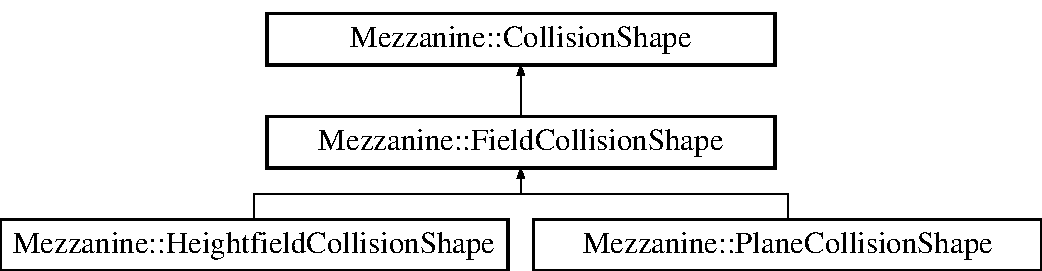
\includegraphics[height=3.000000cm]{classMezzanine_1_1FieldCollisionShape}
\end{center}
\end{figure}
\subsubsection*{Public Member Functions}
\begin{DoxyCompactItemize}
\item 
\hypertarget{classMezzanine_1_1FieldCollisionShape_a13552192ce6c0133afaee02626b522ba}{
\hyperlink{classMezzanine_1_1FieldCollisionShape_a13552192ce6c0133afaee02626b522ba}{FieldCollisionShape} ()}
\label{classMezzanine_1_1FieldCollisionShape_a13552192ce6c0133afaee02626b522ba}

\begin{DoxyCompactList}\small\item\em Class Constructor. \item\end{DoxyCompactList}\item 
\hypertarget{classMezzanine_1_1FieldCollisionShape_afbead5b5df9bbc2b2e2fe3551c27b302}{
virtual \hyperlink{classMezzanine_1_1FieldCollisionShape_afbead5b5df9bbc2b2e2fe3551c27b302}{$\sim$FieldCollisionShape} ()}
\label{classMezzanine_1_1FieldCollisionShape_afbead5b5df9bbc2b2e2fe3551c27b302}

\begin{DoxyCompactList}\small\item\em Class Destructor. \item\end{DoxyCompactList}\item 
virtual btConcaveShape $\ast$ \hyperlink{classMezzanine_1_1FieldCollisionShape_abd6d91caf9460d289c739d83a3c314a4}{GetBulletConcaveShape} () const 
\item 
virtual \hyperlink{classMezzanine_1_1CollisionShape_ad04186055565998879b64176d6dd100d}{CollisionShape::ShapeType} \hyperlink{classMezzanine_1_1FieldCollisionShape_a85a444fa9bcaca9fec08c3b5697677c9}{GetType} () const =0
\item 
virtual void \hyperlink{classMezzanine_1_1FieldCollisionShape_aa7995de9b5b29693c0d2c57590727bb4}{ProtoDeSerialize} (const \hyperlink{classMezzanine_1_1xml_1_1Node}{xml::Node} \&OneNode)
\item 
virtual void \hyperlink{classMezzanine_1_1FieldCollisionShape_a12c178d2b8ba1219c2be8b31bb59845e}{ProtoSerialize} (\hyperlink{classMezzanine_1_1xml_1_1Node}{xml::Node} \&CurrentRoot) const 
\end{DoxyCompactItemize}
\subsubsection*{Static Public Member Functions}
\begin{DoxyCompactItemize}
\item 
static \hyperlink{namespaceMezzanine_acf9fcc130e6ebf08e3d8491aebcf1c86}{String} \hyperlink{classMezzanine_1_1FieldCollisionShape_a7ac709490aaa938311fd907e35b93bac}{SerializableName} ()
\begin{DoxyCompactList}\small\item\em Get the name of the the XML tag this class will leave behind as its instances are serialized. \item\end{DoxyCompactList}\end{DoxyCompactItemize}
\subsubsection*{Protected Member Functions}
\begin{DoxyCompactItemize}
\item 
\hypertarget{classMezzanine_1_1FieldCollisionShape_a78b0d29d92fdd38963d438a8994d0d20}{
void \hyperlink{classMezzanine_1_1FieldCollisionShape_a78b0d29d92fdd38963d438a8994d0d20}{SetPointers} (btConcaveShape $\ast$Shape)}
\label{classMezzanine_1_1FieldCollisionShape_a78b0d29d92fdd38963d438a8994d0d20}

\begin{DoxyCompactList}\small\item\em Sets the internal pointers on the base classes. \item\end{DoxyCompactList}\end{DoxyCompactItemize}


\subsubsection{Detailed Description}
This is the base class for all Field shapes. A \hyperlink{classMezzanine_1_1Mesh}{Mesh} shape is any shape that is intended to be used as surface that extends for a a significant or even unending length. These can be used as the basis for ground and hills or as walls at the end of gameplay area. Performance is dependant on the complexity of the field, and are dependent on complexity. 

Definition at line 200 of file collisionshape.h.



\subsubsection{Member Function Documentation}
\hypertarget{classMezzanine_1_1FieldCollisionShape_abd6d91caf9460d289c739d83a3c314a4}{
\index{Mezzanine::FieldCollisionShape@{Mezzanine::FieldCollisionShape}!GetBulletConcaveShape@{GetBulletConcaveShape}}
\index{GetBulletConcaveShape@{GetBulletConcaveShape}!Mezzanine::FieldCollisionShape@{Mezzanine::FieldCollisionShape}}
\paragraph[{GetBulletConcaveShape}]{\setlength{\rightskip}{0pt plus 5cm}btConcaveShape $\ast$ Mezzanine::FieldCollisionShape::GetBulletConcaveShape (
\begin{DoxyParamCaption}
{}
\end{DoxyParamCaption}
) const\hspace{0.3cm}{\ttfamily  \mbox{[}virtual\mbox{]}}}\hfill}
\label{classMezzanine_1_1FieldCollisionShape_abd6d91caf9460d289c739d83a3c314a4}
Gets the internal shape pointer this collision shape is based on. 

\begin{DoxyReturn}{Returns}
Returns a pointer to the internal collision shape. 
\end{DoxyReturn}
 

Definition at line 228 of file collisionshape.cpp.

\hypertarget{classMezzanine_1_1FieldCollisionShape_a85a444fa9bcaca9fec08c3b5697677c9}{
\index{Mezzanine::FieldCollisionShape@{Mezzanine::FieldCollisionShape}!GetType@{GetType}}
\index{GetType@{GetType}!Mezzanine::FieldCollisionShape@{Mezzanine::FieldCollisionShape}}
\paragraph[{GetType}]{\setlength{\rightskip}{0pt plus 5cm}virtual {\bf CollisionShape::ShapeType} Mezzanine::FieldCollisionShape::GetType (
\begin{DoxyParamCaption}
{}
\end{DoxyParamCaption}
) const\hspace{0.3cm}{\ttfamily  \mbox{[}pure virtual\mbox{]}}}\hfill}
\label{classMezzanine_1_1FieldCollisionShape_a85a444fa9bcaca9fec08c3b5697677c9}
Gets the type of \hyperlink{classMezzanine_1_1Collision}{Collision} shape this is. 

\begin{DoxyReturn}{Returns}
Returns an enum value indicating the type of collision shape this is. 
\end{DoxyReturn}
 

Implements \hyperlink{classMezzanine_1_1CollisionShape_a27e5055f81cb8fb6d65a6c9f8dc73b69}{Mezzanine::CollisionShape}.



Implemented in \hyperlink{classMezzanine_1_1HeightfieldCollisionShape_af27ffaf88fc12af6ddc89704e60ecd33}{Mezzanine::HeightfieldCollisionShape}, and \hyperlink{classMezzanine_1_1PlaneCollisionShape_aeb4b5e1a235023d375b5514065a5e382}{Mezzanine::PlaneCollisionShape}.

\hypertarget{classMezzanine_1_1FieldCollisionShape_aa7995de9b5b29693c0d2c57590727bb4}{
\index{Mezzanine::FieldCollisionShape@{Mezzanine::FieldCollisionShape}!ProtoDeSerialize@{ProtoDeSerialize}}
\index{ProtoDeSerialize@{ProtoDeSerialize}!Mezzanine::FieldCollisionShape@{Mezzanine::FieldCollisionShape}}
\paragraph[{ProtoDeSerialize}]{\setlength{\rightskip}{0pt plus 5cm}void Mezzanine::FieldCollisionShape::ProtoDeSerialize (
\begin{DoxyParamCaption}
\item[{const {\bf xml::Node} \&}]{OneNode}
\end{DoxyParamCaption}
)\hspace{0.3cm}{\ttfamily  \mbox{[}virtual\mbox{]}}}\hfill}
\label{classMezzanine_1_1FieldCollisionShape_aa7995de9b5b29693c0d2c57590727bb4}
Gets the internal shape pointer this collision shape is based on. 

\begin{DoxyReturn}{Returns}
Returns a pointer to the internal collision shape. 
\end{DoxyReturn}
 

Reimplemented from \hyperlink{classMezzanine_1_1CollisionShape_aab25ef5e044b27e8e43b7e4c54ab777a}{Mezzanine::CollisionShape}.



Definition at line 247 of file collisionshape.cpp.

\hypertarget{classMezzanine_1_1FieldCollisionShape_a12c178d2b8ba1219c2be8b31bb59845e}{
\index{Mezzanine::FieldCollisionShape@{Mezzanine::FieldCollisionShape}!ProtoSerialize@{ProtoSerialize}}
\index{ProtoSerialize@{ProtoSerialize}!Mezzanine::FieldCollisionShape@{Mezzanine::FieldCollisionShape}}
\paragraph[{ProtoSerialize}]{\setlength{\rightskip}{0pt plus 5cm}void Mezzanine::FieldCollisionShape::ProtoSerialize (
\begin{DoxyParamCaption}
\item[{{\bf xml::Node} \&}]{CurrentRoot}
\end{DoxyParamCaption}
) const\hspace{0.3cm}{\ttfamily  \mbox{[}virtual\mbox{]}}}\hfill}
\label{classMezzanine_1_1FieldCollisionShape_a12c178d2b8ba1219c2be8b31bb59845e}
Gets the internal shape pointer this collision shape is based on. 

\begin{DoxyReturn}{Returns}
Returns a pointer to the internal collision shape. 
\end{DoxyReturn}
 

Reimplemented from \hyperlink{classMezzanine_1_1CollisionShape_ac0995091062903d9777d0fa9bef09b90}{Mezzanine::CollisionShape}.



Definition at line 232 of file collisionshape.cpp.

\hypertarget{classMezzanine_1_1FieldCollisionShape_a7ac709490aaa938311fd907e35b93bac}{
\index{Mezzanine::FieldCollisionShape@{Mezzanine::FieldCollisionShape}!SerializableName@{SerializableName}}
\index{SerializableName@{SerializableName}!Mezzanine::FieldCollisionShape@{Mezzanine::FieldCollisionShape}}
\paragraph[{SerializableName}]{\setlength{\rightskip}{0pt plus 5cm}{\bf String} Mezzanine::FieldCollisionShape::SerializableName (
\begin{DoxyParamCaption}
{}
\end{DoxyParamCaption}
)\hspace{0.3cm}{\ttfamily  \mbox{[}static\mbox{]}}}\hfill}
\label{classMezzanine_1_1FieldCollisionShape_a7ac709490aaa938311fd907e35b93bac}


Get the name of the the XML tag this class will leave behind as its instances are serialized. 

\begin{DoxyReturn}{Returns}
A string containing \char`\"{}FieldCollisionShape\char`\"{} 
\end{DoxyReturn}


Reimplemented from \hyperlink{classMezzanine_1_1CollisionShape_ae5a97a76b687d450f17d0ac86b227f1d}{Mezzanine::CollisionShape}.



Definition at line 265 of file collisionshape.cpp.



The documentation for this class was generated from the following files:\begin{DoxyCompactItemize}
\item 
collisionshape.h\item 
collisionshape.cpp\end{DoxyCompactItemize}

\hypertarget{classMezzanine_1_1FieldOfForce}{
\subsection{Mezzanine::FieldOfForce Class Reference}
\label{classMezzanine_1_1FieldOfForce}\index{Mezzanine::FieldOfForce@{Mezzanine::FieldOfForce}}
}


This is field that applies force in a direction, and doesn't tamper with gravity.  




{\ttfamily \#include $<$areaeffect.h$>$}

Inheritance diagram for Mezzanine::FieldOfForce:\begin{figure}[H]
\begin{center}
\leavevmode
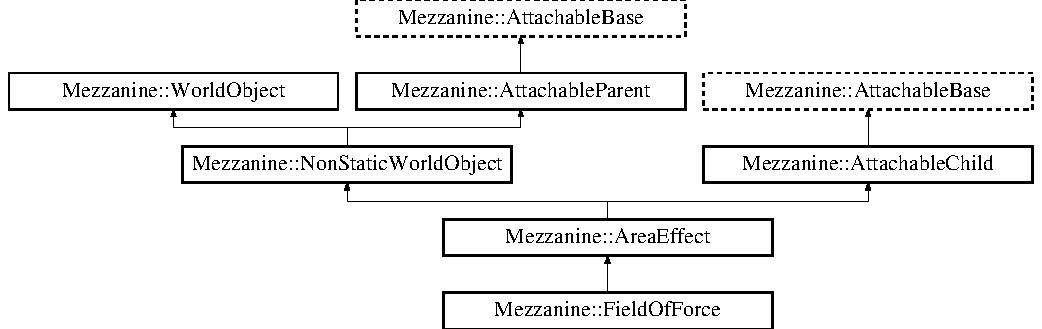
\includegraphics[height=4.423381cm]{classMezzanine_1_1FieldOfForce}
\end{center}
\end{figure}
\subsubsection*{Public Member Functions}
\begin{DoxyCompactItemize}
\item 
\hyperlink{classMezzanine_1_1FieldOfForce_aa212c5cde10986e1d511a3843af9428c}{FieldOfForce} (const \hyperlink{namespaceMezzanine_acf9fcc130e6ebf08e3d8491aebcf1c86}{String} \&name, const \hyperlink{classMezzanine_1_1Vector3}{Vector3} \&Location)
\begin{DoxyCompactList}\small\item\em Class Constructor. \item\end{DoxyCompactList}\item 
\hypertarget{classMezzanine_1_1FieldOfForce_ae9d68bc47f8598fd764b4ed9ae28a89c}{
virtual \hyperlink{classMezzanine_1_1FieldOfForce_ae9d68bc47f8598fd764b4ed9ae28a89c}{$\sim$FieldOfForce} ()}
\label{classMezzanine_1_1FieldOfForce_ae9d68bc47f8598fd764b4ed9ae28a89c}

\begin{DoxyCompactList}\small\item\em Class Destructor. \item\end{DoxyCompactList}\item 
virtual void \hyperlink{classMezzanine_1_1FieldOfForce_ae82e9a45515d40513ad1ac2e606c627b}{ApplyEffect} ()
\begin{DoxyCompactList}\small\item\em Applies the effect this field has to object inside. \item\end{DoxyCompactList}\item 
virtual \hyperlink{namespaceMezzanine_a726731b1a7df72bf3583e4a97282c6f6}{Real} \hyperlink{classMezzanine_1_1FieldOfForce_a0f5340224f7cec6e9086d49a3d51ae07}{GetAttenuationAmount} () const 
\begin{DoxyCompactList}\small\item\em Gets the amount force is attenuated over distance. \item\end{DoxyCompactList}\item 
virtual \hyperlink{classMezzanine_1_1Vector3}{Vector3} \hyperlink{classMezzanine_1_1FieldOfForce_a0f1232162d04d967907a55e8c9bc8661}{GetAttenuationSource} () const 
\begin{DoxyCompactList}\small\item\em Gets the source of the force for calculating attenuation. \item\end{DoxyCompactList}\item 
virtual \hyperlink{namespaceMezzanine_a2d10a79e11a2031df10af540eede12fa}{Mezzanine::AttenuationStyle} \hyperlink{classMezzanine_1_1FieldOfForce_a45f3ea5f8a48ff4a7dbe135d5003d267}{GetAttenuationStyle} () const 
\begin{DoxyCompactList}\small\item\em Gets the Style of attenuation applied. \item\end{DoxyCompactList}\item 
virtual \hyperlink{classMezzanine_1_1Vector3}{Vector3} \hyperlink{classMezzanine_1_1FieldOfForce_aa38710cbe67fad1b0be2e0a414d8e55c}{GetDirectionOfForce} ()
\begin{DoxyCompactList}\small\item\em Gets the currenly set direction force is to be applied. \item\end{DoxyCompactList}\item 
virtual \hyperlink{namespaceMezzanine_a726731b1a7df72bf3583e4a97282c6f6}{Real} \hyperlink{classMezzanine_1_1FieldOfForce_ae8071fe3ad4397b57cff5f3816d72e02}{GetFieldStrength} () const 
\begin{DoxyCompactList}\small\item\em Gets the strength of the field. \item\end{DoxyCompactList}\item 
virtual \hyperlink{namespaceMezzanine_ae8cd04f706f4998be62f454b7119c718}{WorldAndSceneObjectType} \hyperlink{classMezzanine_1_1FieldOfForce_ad6247ff9543681daa74a9297c1c7653e}{GetType} () const 
\item 
virtual void \hyperlink{classMezzanine_1_1FieldOfForce_aa2ba435821f4abc4c59b0ca99f077759}{SetAttenuation} (const \hyperlink{namespaceMezzanine_a726731b1a7df72bf3583e4a97282c6f6}{Real} \&Amount, const \hyperlink{namespaceMezzanine_a2d10a79e11a2031df10af540eede12fa}{Mezzanine::AttenuationStyle} \&Style, const \hyperlink{classMezzanine_1_1Vector3}{Vector3} \&Source)
\begin{DoxyCompactList}\small\item\em Sets the attenuation for this field. \item\end{DoxyCompactList}\item 
virtual void \hyperlink{classMezzanine_1_1FieldOfForce_aaa4df06c275221b2b7c313a7d45ec71a}{SetDirectionOfForce} (const \hyperlink{classMezzanine_1_1Vector3}{Vector3} \&ForceDirection)
\begin{DoxyCompactList}\small\item\em Sets the direction force is to be applied within this field. \item\end{DoxyCompactList}\item 
virtual void \hyperlink{classMezzanine_1_1FieldOfForce_abef745957f95ac58f756d84f00fbf549}{SetFieldStrength} (const \hyperlink{namespaceMezzanine_a726731b1a7df72bf3583e4a97282c6f6}{Real} \&FieldStrength)
\begin{DoxyCompactList}\small\item\em Sets the strenth of the field. \item\end{DoxyCompactList}\end{DoxyCompactItemize}
\subsubsection*{Protected Attributes}
\begin{DoxyCompactItemize}
\item 
\hypertarget{classMezzanine_1_1FieldOfForce_abd6f3200dd4d0014d65f43e4565119fe}{
\hyperlink{namespaceMezzanine_a726731b1a7df72bf3583e4a97282c6f6}{Real} \hyperlink{classMezzanine_1_1FieldOfForce_abd6f3200dd4d0014d65f43e4565119fe}{AttenAmount}}
\label{classMezzanine_1_1FieldOfForce_abd6f3200dd4d0014d65f43e4565119fe}

\begin{DoxyCompactList}\small\item\em How much the Gravity weakens over distance. \item\end{DoxyCompactList}\item 
\hypertarget{classMezzanine_1_1FieldOfForce_a86ef3fe03d4a8604bc659bf462d22025}{
\hyperlink{classMezzanine_1_1Vector3}{Vector3} \hyperlink{classMezzanine_1_1FieldOfForce_a86ef3fe03d4a8604bc659bf462d22025}{AttenSource}}
\label{classMezzanine_1_1FieldOfForce_a86ef3fe03d4a8604bc659bf462d22025}

\begin{DoxyCompactList}\small\item\em The user defined source if enabled. \item\end{DoxyCompactList}\item 
\hypertarget{classMezzanine_1_1FieldOfForce_a0c0f4d1bdf91efa07bb6460fd68d8a74}{
\hyperlink{namespaceMezzanine_a2d10a79e11a2031df10af540eede12fa}{Mezzanine::AttenuationStyle} \hyperlink{classMezzanine_1_1FieldOfForce_a0c0f4d1bdf91efa07bb6460fd68d8a74}{AttenStyle}}
\label{classMezzanine_1_1FieldOfForce_a0c0f4d1bdf91efa07bb6460fd68d8a74}

\begin{DoxyCompactList}\small\item\em How gravity weakens over distance, if at all. \item\end{DoxyCompactList}\item 
\hypertarget{classMezzanine_1_1FieldOfForce_a58db238eb7b943ce9585b8bb9a751906}{
\hyperlink{classMezzanine_1_1Vector3}{Vector3} \hyperlink{classMezzanine_1_1FieldOfForce_a58db238eb7b943ce9585b8bb9a751906}{Direction}}
\label{classMezzanine_1_1FieldOfForce_a58db238eb7b943ce9585b8bb9a751906}

\begin{DoxyCompactList}\small\item\em The direction the force is applied. \item\end{DoxyCompactList}\item 
\hypertarget{classMezzanine_1_1FieldOfForce_a8d95bfda05f7eb1ec2e0256ec917d38b}{
\hyperlink{namespaceMezzanine_a726731b1a7df72bf3583e4a97282c6f6}{Real} \hyperlink{classMezzanine_1_1FieldOfForce_a8d95bfda05f7eb1ec2e0256ec917d38b}{Strength}}
\label{classMezzanine_1_1FieldOfForce_a8d95bfda05f7eb1ec2e0256ec917d38b}

\begin{DoxyCompactList}\small\item\em The amount of force exerted on other objects. \item\end{DoxyCompactList}\end{DoxyCompactItemize}


\subsubsection{Detailed Description}
This is field that applies force in a direction, and doesn't tamper with gravity. This class is similiar to a gravity well in that it can attenuate, but different in that the direction is constant, the source of force(for calculating attenuation) can be outside the field itself, and the direction is constant. \par
 Placing the source of attenuation inside the field will cause the object to accelerate as it gets close to the source, and then will be applied less force(but in the same direction) as it moves from the source. This behavior makes this class good for creating a booster-\/like AE. 

Definition at line 324 of file areaeffect.h.



\subsubsection{Constructor \& Destructor Documentation}
\hypertarget{classMezzanine_1_1FieldOfForce_aa212c5cde10986e1d511a3843af9428c}{
\index{Mezzanine::FieldOfForce@{Mezzanine::FieldOfForce}!FieldOfForce@{FieldOfForce}}
\index{FieldOfForce@{FieldOfForce}!Mezzanine::FieldOfForce@{Mezzanine::FieldOfForce}}
\paragraph[{FieldOfForce}]{\setlength{\rightskip}{0pt plus 5cm}Mezzanine::FieldOfForce::FieldOfForce (
\begin{DoxyParamCaption}
\item[{const {\bf String} \&}]{name, }
\item[{const {\bf Vector3} \&}]{Location}
\end{DoxyParamCaption}
)}\hfill}
\label{classMezzanine_1_1FieldOfForce_aa212c5cde10986e1d511a3843af9428c}


Class Constructor. 


\begin{DoxyParams}{Parameters}
{\em name} & The name of the field. \\
\hline
{\em Location} & The location of the AE field. \\
\hline
\end{DoxyParams}


Definition at line 584 of file areaeffect.cpp.



\subsubsection{Member Function Documentation}
\hypertarget{classMezzanine_1_1FieldOfForce_ae82e9a45515d40513ad1ac2e606c627b}{
\index{Mezzanine::FieldOfForce@{Mezzanine::FieldOfForce}!ApplyEffect@{ApplyEffect}}
\index{ApplyEffect@{ApplyEffect}!Mezzanine::FieldOfForce@{Mezzanine::FieldOfForce}}
\paragraph[{ApplyEffect}]{\setlength{\rightskip}{0pt plus 5cm}void Mezzanine::FieldOfForce::ApplyEffect (
\begin{DoxyParamCaption}
{}
\end{DoxyParamCaption}
)\hspace{0.3cm}{\ttfamily  \mbox{[}virtual\mbox{]}}}\hfill}
\label{classMezzanine_1_1FieldOfForce_ae82e9a45515d40513ad1ac2e606c627b}


Applies the effect this field has to object inside. 

This function defines the behavior for the class. 

Implements \hyperlink{classMezzanine_1_1AreaEffect_a988cd958e49d65331a059951af3c2884}{Mezzanine::AreaEffect}.



Definition at line 598 of file areaeffect.cpp.

\hypertarget{classMezzanine_1_1FieldOfForce_a0f5340224f7cec6e9086d49a3d51ae07}{
\index{Mezzanine::FieldOfForce@{Mezzanine::FieldOfForce}!GetAttenuationAmount@{GetAttenuationAmount}}
\index{GetAttenuationAmount@{GetAttenuationAmount}!Mezzanine::FieldOfForce@{Mezzanine::FieldOfForce}}
\paragraph[{GetAttenuationAmount}]{\setlength{\rightskip}{0pt plus 5cm}{\bf Real} Mezzanine::FieldOfForce::GetAttenuationAmount (
\begin{DoxyParamCaption}
{}
\end{DoxyParamCaption}
) const\hspace{0.3cm}{\ttfamily  \mbox{[}virtual\mbox{]}}}\hfill}
\label{classMezzanine_1_1FieldOfForce_a0f5340224f7cec6e9086d49a3d51ae07}


Gets the amount force is attenuated over distance. 

See \hyperlink{classMezzanine_1_1FieldOfForce_aa2ba435821f4abc4c59b0ca99f077759}{SetAttenuation()} for more details. \begin{DoxyReturn}{Returns}
Returns a Real value 
\end{DoxyReturn}


Definition at line 681 of file areaeffect.cpp.

\hypertarget{classMezzanine_1_1FieldOfForce_a0f1232162d04d967907a55e8c9bc8661}{
\index{Mezzanine::FieldOfForce@{Mezzanine::FieldOfForce}!GetAttenuationSource@{GetAttenuationSource}}
\index{GetAttenuationSource@{GetAttenuationSource}!Mezzanine::FieldOfForce@{Mezzanine::FieldOfForce}}
\paragraph[{GetAttenuationSource}]{\setlength{\rightskip}{0pt plus 5cm}{\bf Vector3} Mezzanine::FieldOfForce::GetAttenuationSource (
\begin{DoxyParamCaption}
{}
\end{DoxyParamCaption}
) const\hspace{0.3cm}{\ttfamily  \mbox{[}virtual\mbox{]}}}\hfill}
\label{classMezzanine_1_1FieldOfForce_a0f1232162d04d967907a55e8c9bc8661}


Gets the source of the force for calculating attenuation. 

\begin{DoxyReturn}{Returns}
Returns a \hyperlink{classMezzanine_1_1Vector3}{Vector3} representing the source of the attenuating force. 
\end{DoxyReturn}


Definition at line 686 of file areaeffect.cpp.

\hypertarget{classMezzanine_1_1FieldOfForce_a45f3ea5f8a48ff4a7dbe135d5003d267}{
\index{Mezzanine::FieldOfForce@{Mezzanine::FieldOfForce}!GetAttenuationStyle@{GetAttenuationStyle}}
\index{GetAttenuationStyle@{GetAttenuationStyle}!Mezzanine::FieldOfForce@{Mezzanine::FieldOfForce}}
\paragraph[{GetAttenuationStyle}]{\setlength{\rightskip}{0pt plus 5cm}{\bf Mezzanine::AttenuationStyle} Mezzanine::FieldOfForce::GetAttenuationStyle (
\begin{DoxyParamCaption}
{}
\end{DoxyParamCaption}
) const\hspace{0.3cm}{\ttfamily  \mbox{[}virtual\mbox{]}}}\hfill}
\label{classMezzanine_1_1FieldOfForce_a45f3ea5f8a48ff4a7dbe135d5003d267}


Gets the Style of attenuation applied. 

See the AttenuationStyle enum for more details. \begin{DoxyReturn}{Returns}
Returns the style of attenuation currently being used by this field. 
\end{DoxyReturn}


Definition at line 676 of file areaeffect.cpp.

\hypertarget{classMezzanine_1_1FieldOfForce_aa38710cbe67fad1b0be2e0a414d8e55c}{
\index{Mezzanine::FieldOfForce@{Mezzanine::FieldOfForce}!GetDirectionOfForce@{GetDirectionOfForce}}
\index{GetDirectionOfForce@{GetDirectionOfForce}!Mezzanine::FieldOfForce@{Mezzanine::FieldOfForce}}
\paragraph[{GetDirectionOfForce}]{\setlength{\rightskip}{0pt plus 5cm}{\bf Vector3} Mezzanine::FieldOfForce::GetDirectionOfForce (
\begin{DoxyParamCaption}
{}
\end{DoxyParamCaption}
)\hspace{0.3cm}{\ttfamily  \mbox{[}virtual\mbox{]}}}\hfill}
\label{classMezzanine_1_1FieldOfForce_aa38710cbe67fad1b0be2e0a414d8e55c}


Gets the currenly set direction force is to be applied. 

\begin{DoxyReturn}{Returns}
Returns a vector3 representing the direction of force in this field. 
\end{DoxyReturn}


Definition at line 664 of file areaeffect.cpp.

\hypertarget{classMezzanine_1_1FieldOfForce_ae8071fe3ad4397b57cff5f3816d72e02}{
\index{Mezzanine::FieldOfForce@{Mezzanine::FieldOfForce}!GetFieldStrength@{GetFieldStrength}}
\index{GetFieldStrength@{GetFieldStrength}!Mezzanine::FieldOfForce@{Mezzanine::FieldOfForce}}
\paragraph[{GetFieldStrength}]{\setlength{\rightskip}{0pt plus 5cm}{\bf Real} Mezzanine::FieldOfForce::GetFieldStrength (
\begin{DoxyParamCaption}
{}
\end{DoxyParamCaption}
) const\hspace{0.3cm}{\ttfamily  \mbox{[}virtual\mbox{]}}}\hfill}
\label{classMezzanine_1_1FieldOfForce_ae8071fe3ad4397b57cff5f3816d72e02}


Gets the strength of the field. 

\begin{DoxyReturn}{Returns}
Returns a Real representing the value that is being multiplied by the direction to determine force appied to objects. 
\end{DoxyReturn}


Definition at line 654 of file areaeffect.cpp.

\hypertarget{classMezzanine_1_1FieldOfForce_ad6247ff9543681daa74a9297c1c7653e}{
\index{Mezzanine::FieldOfForce@{Mezzanine::FieldOfForce}!GetType@{GetType}}
\index{GetType@{GetType}!Mezzanine::FieldOfForce@{Mezzanine::FieldOfForce}}
\paragraph[{GetType}]{\setlength{\rightskip}{0pt plus 5cm}{\bf WorldAndSceneObjectType} Mezzanine::FieldOfForce::GetType (
\begin{DoxyParamCaption}
{}
\end{DoxyParamCaption}
) const\hspace{0.3cm}{\ttfamily  \mbox{[}virtual\mbox{]}}}\hfill}
\label{classMezzanine_1_1FieldOfForce_ad6247ff9543681daa74a9297c1c7653e}
Gets the type of the \hyperlink{classMezzanine_1_1World}{World} Object instance. 

\begin{DoxyReturn}{Returns}
Returns the type of the \hyperlink{classMezzanine_1_1World}{World} Object instance 
\end{DoxyReturn}
 

Reimplemented from \hyperlink{classMezzanine_1_1AreaEffect_a2f3df5433f02057d7a9deeb5e6666287}{Mezzanine::AreaEffect}.



Definition at line 691 of file areaeffect.cpp.

\hypertarget{classMezzanine_1_1FieldOfForce_aa2ba435821f4abc4c59b0ca99f077759}{
\index{Mezzanine::FieldOfForce@{Mezzanine::FieldOfForce}!SetAttenuation@{SetAttenuation}}
\index{SetAttenuation@{SetAttenuation}!Mezzanine::FieldOfForce@{Mezzanine::FieldOfForce}}
\paragraph[{SetAttenuation}]{\setlength{\rightskip}{0pt plus 5cm}void Mezzanine::FieldOfForce::SetAttenuation (
\begin{DoxyParamCaption}
\item[{const {\bf Real} \&}]{Amount, }
\item[{const {\bf Mezzanine::AttenuationStyle} \&}]{Style, }
\item[{const {\bf Vector3} \&}]{Source}
\end{DoxyParamCaption}
)\hspace{0.3cm}{\ttfamily  \mbox{[}virtual\mbox{]}}}\hfill}
\label{classMezzanine_1_1FieldOfForce_aa2ba435821f4abc4c59b0ca99f077759}


Sets the attenuation for this field. 


\begin{DoxyParams}{Parameters}
{\em Amount} & The amount of force that is dropped off per 1 unit of distance objects are from the AE source. \\
\hline
{\em Style} & The style of attenuation to apply, see the AttenuationStyle enum for more details. \\
\hline
{\em Source} & A vector3 representing the source of force to use when calculating attenuation. \\
\hline
\end{DoxyParams}


Definition at line 669 of file areaeffect.cpp.

\hypertarget{classMezzanine_1_1FieldOfForce_aaa4df06c275221b2b7c313a7d45ec71a}{
\index{Mezzanine::FieldOfForce@{Mezzanine::FieldOfForce}!SetDirectionOfForce@{SetDirectionOfForce}}
\index{SetDirectionOfForce@{SetDirectionOfForce}!Mezzanine::FieldOfForce@{Mezzanine::FieldOfForce}}
\paragraph[{SetDirectionOfForce}]{\setlength{\rightskip}{0pt plus 5cm}void Mezzanine::FieldOfForce::SetDirectionOfForce (
\begin{DoxyParamCaption}
\item[{const {\bf Vector3} \&}]{ForceDirection}
\end{DoxyParamCaption}
)\hspace{0.3cm}{\ttfamily  \mbox{[}virtual\mbox{]}}}\hfill}
\label{classMezzanine_1_1FieldOfForce_aaa4df06c275221b2b7c313a7d45ec71a}


Sets the direction force is to be applied within this field. 


\begin{DoxyParams}{Parameters}
{\em ForceDirection} & A vector3 representing the direction force is to be applied. \\
\hline
\end{DoxyParams}


Definition at line 659 of file areaeffect.cpp.

\hypertarget{classMezzanine_1_1FieldOfForce_abef745957f95ac58f756d84f00fbf549}{
\index{Mezzanine::FieldOfForce@{Mezzanine::FieldOfForce}!SetFieldStrength@{SetFieldStrength}}
\index{SetFieldStrength@{SetFieldStrength}!Mezzanine::FieldOfForce@{Mezzanine::FieldOfForce}}
\paragraph[{SetFieldStrength}]{\setlength{\rightskip}{0pt plus 5cm}void Mezzanine::FieldOfForce::SetFieldStrength (
\begin{DoxyParamCaption}
\item[{const {\bf Real} \&}]{FieldStrength}
\end{DoxyParamCaption}
)\hspace{0.3cm}{\ttfamily  \mbox{[}virtual\mbox{]}}}\hfill}
\label{classMezzanine_1_1FieldOfForce_abef745957f95ac58f756d84f00fbf549}


Sets the strenth of the field. 


\begin{DoxyParams}{Parameters}
{\em FieldStrength} & The strength the field will have when exerting force onto other objects. \\
\hline
\end{DoxyParams}


Definition at line 649 of file areaeffect.cpp.



The documentation for this class was generated from the following files:\begin{DoxyCompactItemize}
\item 
areaeffect.h\item 
areaeffect.cpp\end{DoxyCompactItemize}

\hypertarget{classMezzanine_1_1GameWindow}{
\subsection{Mezzanine::GameWindow Class Reference}
\label{classMezzanine_1_1GameWindow}\index{Mezzanine::GameWindow@{Mezzanine::GameWindow}}
}


This class is for creating and managing game windows.  




{\ttfamily \#include $<$gamewindow.h$>$}

\subsubsection*{Public Types}
\begin{DoxyCompactItemize}
\item 
enum \hyperlink{classMezzanine_1_1GameWindow_ac31ba18e78ad8c6e749019726a0dbe6f}{WindowFlags} \{ \par
{\bfseries WF\_\-Fullscreen} =  1, 
{\bfseries WF\_\-Hidden} =  2, 
{\bfseries WF\_\-VsyncEnabled} =  4, 
{\bfseries WF\_\-FSAA\_\-2} =  8, 
\par
{\bfseries WF\_\-FSAA\_\-4} =  16, 
{\bfseries WF\_\-FSAA\_\-8} =  32, 
{\bfseries WF\_\-FSAA\_\-16} =  64, 
{\bfseries WF\_\-Resizeable} =  128, 
\par
{\bfseries WF\_\-Minimized} =  256, 
{\bfseries WF\_\-Maximized} =  512, 
{\bfseries WF\_\-Borderless} =  1024
 \}
\begin{DoxyCompactList}\small\item\em A listing of potential options for configuring a game window during construction. \item\end{DoxyCompactList}\end{DoxyCompactItemize}
\subsubsection*{Public Member Functions}
\begin{DoxyCompactItemize}
\item 
\hyperlink{classMezzanine_1_1Viewport}{Viewport} $\ast$ \hyperlink{classMezzanine_1_1GameWindow_a9a5c31130d7d2970d1c0141173bcdce3}{CreateViewport} (\hyperlink{classMezzanine_1_1Camera}{Camera} $\ast$ViewportCamera, const \hyperlink{namespaceMezzanine_adcbb6ce6d1eb4379d109e51171e2e493}{Whole} \&ZOrder=0)
\begin{DoxyCompactList}\small\item\em Creates an additional \hyperlink{classMezzanine_1_1Viewport}{Viewport} within a created render window. \item\end{DoxyCompactList}\item 
void \hyperlink{classMezzanine_1_1GameWindow_a810561a4b96667bf88be137722d44407}{DestroyViewport} (\hyperlink{classMezzanine_1_1Viewport}{Viewport} $\ast$ToBeDestroyed)
\begin{DoxyCompactList}\small\item\em Destroys a viewport within this window. \item\end{DoxyCompactList}\item 
\hyperlink{classMezzanine_1_1GameWindow_aebf4352707c9c1a7d8ca8d1f2a562ccd}{GameWindow} (const \hyperlink{namespaceMezzanine_acf9fcc130e6ebf08e3d8491aebcf1c86}{String} \&WindowCaption, const \hyperlink{namespaceMezzanine_adcbb6ce6d1eb4379d109e51171e2e493}{Whole} \&Width, const \hyperlink{namespaceMezzanine_adcbb6ce6d1eb4379d109e51171e2e493}{Whole} \&Height, const \hyperlink{namespaceMezzanine_adcbb6ce6d1eb4379d109e51171e2e493}{Whole} \&Flags)
\begin{DoxyCompactList}\small\item\em Class constructor. \item\end{DoxyCompactList}\item 
\hyperlink{namespaceMezzanine_a726731b1a7df72bf3583e4a97282c6f6}{Real} \hyperlink{classMezzanine_1_1GameWindow_ad6dcba20b92b4881a35a872ba36037d5}{GetAverageFPS} ()
\begin{DoxyCompactList}\small\item\em Gets the Average FPS. \item\end{DoxyCompactList}\item 
\hyperlink{namespaceMezzanine_a726731b1a7df72bf3583e4a97282c6f6}{Real} \hyperlink{classMezzanine_1_1GameWindow_a366478a0038149d243d0ef19eacea696}{GetBestFPS} ()
\begin{DoxyCompactList}\small\item\em Gets the Best FPS. \item\end{DoxyCompactList}\item 
\hyperlink{namespaceMezzanine_a726731b1a7df72bf3583e4a97282c6f6}{Real} \hyperlink{classMezzanine_1_1GameWindow_add46a3048c8eb963dae0758c47316bc4}{GetBestFrameTime} ()
\begin{DoxyCompactList}\small\item\em Gets the shortest amount of time it's taken to render a frame. \item\end{DoxyCompactList}\item 
\hyperlink{namespaceMezzanine_adcbb6ce6d1eb4379d109e51171e2e493}{Whole} \hyperlink{classMezzanine_1_1GameWindow_a221263d2fe846eeaefe18b6817642dd8}{GetFSAALevel} () const 
\begin{DoxyCompactList}\small\item\em Gets the current level of Anti-\/Aliasing enabled on this Window. \item\end{DoxyCompactList}\item 
bool \hyperlink{classMezzanine_1_1GameWindow_a44e2caa0a6300c5365deb287c79c0153}{getFullscreen} () const 
\begin{DoxyCompactList}\small\item\em Gets the Fullscreen Setting. \item\end{DoxyCompactList}\item 
\hyperlink{namespaceMezzanine_a726731b1a7df72bf3583e4a97282c6f6}{Real} \hyperlink{classMezzanine_1_1GameWindow_af298623981d66effc33760484c6b11d7}{GetLastFPS} ()
\begin{DoxyCompactList}\small\item\em Gets the FPS based on the last frame rendered. \item\end{DoxyCompactList}\item 
\hyperlink{namespaceMezzanine_adcbb6ce6d1eb4379d109e51171e2e493}{Whole} \hyperlink{classMezzanine_1_1GameWindow_a69e900fe0f1cb85cd1723991ebf808c5}{GetNumViewports} ()
\begin{DoxyCompactList}\small\item\em Gets the number of viewports within this window. \item\end{DoxyCompactList}\item 
Ogre::RenderWindow $\ast$ \hyperlink{classMezzanine_1_1GameWindow_aade1ad28994653f9a8bca94d0c30cd5c}{GetOgreWindowPointer} ()
\begin{DoxyCompactList}\small\item\em This will get a pointer to the Ogre RenderWindow. \item\end{DoxyCompactList}\item 
void $\ast$ \hyperlink{classMezzanine_1_1GameWindow_afa4d53d324199329435946b652f27950}{GetRenderContext} ()
\begin{DoxyCompactList}\small\item\em Gets the render context being used by this window. \item\end{DoxyCompactList}\item 
\hyperlink{namespaceMezzanine_adcbb6ce6d1eb4379d109e51171e2e493}{Whole} \hyperlink{classMezzanine_1_1GameWindow_a4df354cf07173e21e9c2802882424c4d}{getRenderHeight} () const 
\begin{DoxyCompactList}\small\item\em Gets the Height of the Rendering Area. \item\end{DoxyCompactList}\item 
\hyperlink{namespaceMezzanine_adcbb6ce6d1eb4379d109e51171e2e493}{Whole} \hyperlink{classMezzanine_1_1GameWindow_ae25f20216007a5aff15115d908e8e711}{getRenderWidth} () const 
\begin{DoxyCompactList}\small\item\em Gets the Width of the Rendering Area. \item\end{DoxyCompactList}\item 
SDL\_\-Window $\ast$ \hyperlink{classMezzanine_1_1GameWindow_a9d0fdf6e26f5ef499707fb590e9f3da0}{GetSDLWindowPointer} ()
\begin{DoxyCompactList}\small\item\em This will get a pointer to the SDL Window. \item\end{DoxyCompactList}\item 
const \hyperlink{structMezzanine_1_1GraphicsSettings}{GraphicsSettings} \& \hyperlink{classMezzanine_1_1GameWindow_af16dfa28de1dfadc0c921e05a0ccd9e7}{GetSettings} ()
\begin{DoxyCompactList}\small\item\em Gets the current window settings. \item\end{DoxyCompactList}\item 
\hyperlink{classMezzanine_1_1Viewport}{Viewport} $\ast$ \hyperlink{classMezzanine_1_1GameWindow_ac3ae0f2e4cee0238ae4c158adea1422e}{GetViewport} (const \hyperlink{namespaceMezzanine_adcbb6ce6d1eb4379d109e51171e2e493}{Whole} \&Index)
\begin{DoxyCompactList}\small\item\em Gets a viewport by index. \item\end{DoxyCompactList}\item 
\hyperlink{namespaceMezzanine_a726731b1a7df72bf3583e4a97282c6f6}{Real} \hyperlink{classMezzanine_1_1GameWindow_afd5af20c62dfc0e9ab52fe689f5e8bc8}{GetWorstFPS} ()
\begin{DoxyCompactList}\small\item\em Gets the Worst FPS. \item\end{DoxyCompactList}\item 
\hyperlink{namespaceMezzanine_a726731b1a7df72bf3583e4a97282c6f6}{Real} \hyperlink{classMezzanine_1_1GameWindow_ae07e3a1d5e1ceef524ce29e0c255c78b}{GetWorstFrameTime} ()
\begin{DoxyCompactList}\small\item\em Gets the longest amount of time it's taken to render a frame. \item\end{DoxyCompactList}\item 
void \hyperlink{classMezzanine_1_1GameWindow_a874b538cd9735478f32329c06e832360}{setFullscreen} (const bool \&Fullscreen)
\begin{DoxyCompactList}\small\item\em Set the Fullscreen Setting. \item\end{DoxyCompactList}\item 
void \hyperlink{classMezzanine_1_1GameWindow_a485f45b9265b6fb9d6baae88171b8c74}{setRenderHeight} (const \hyperlink{namespaceMezzanine_adcbb6ce6d1eb4379d109e51171e2e493}{Whole} \&Height)
\begin{DoxyCompactList}\small\item\em Sets the Height. \item\end{DoxyCompactList}\item 
void \hyperlink{classMezzanine_1_1GameWindow_a89368aaeda12eb454ee951a44a65cb8b}{setRenderOptions} (const \hyperlink{structMezzanine_1_1GraphicsSettings}{GraphicsSettings} \&NewSettings)
\begin{DoxyCompactList}\small\item\em Changes the X Resolution, Y Resolution, and fullscreen at the same time. \item\end{DoxyCompactList}\item 
void \hyperlink{classMezzanine_1_1GameWindow_abf4ede4f1d14639017d8cd4da7490b44}{setRenderResolution} (const \hyperlink{namespaceMezzanine_adcbb6ce6d1eb4379d109e51171e2e493}{Whole} \&Width, const \hyperlink{namespaceMezzanine_adcbb6ce6d1eb4379d109e51171e2e493}{Whole} \&Height)
\begin{DoxyCompactList}\small\item\em Changes the X and Y Resolution at the same time. \item\end{DoxyCompactList}\item 
void \hyperlink{classMezzanine_1_1GameWindow_a9228766fbdf9fc77b104647e49226a0d}{setRenderWidth} (const \hyperlink{namespaceMezzanine_adcbb6ce6d1eb4379d109e51171e2e493}{Whole} \&Width)
\begin{DoxyCompactList}\small\item\em Sets the Width. \item\end{DoxyCompactList}\item 
void \hyperlink{classMezzanine_1_1GameWindow_ab115ae2f4af6e3136208bb6d20433b97}{SetWindowCaption} (const \hyperlink{namespaceMezzanine_acf9fcc130e6ebf08e3d8491aebcf1c86}{String} \&NewCaption)
\begin{DoxyCompactList}\small\item\em This can set the the Text in the titlebar. \item\end{DoxyCompactList}\item 
\hypertarget{classMezzanine_1_1GameWindow_a39986f43fb1370d6458b20958a915535}{
\hyperlink{classMezzanine_1_1GameWindow_a39986f43fb1370d6458b20958a915535}{$\sim$GameWindow} ()}
\label{classMezzanine_1_1GameWindow_a39986f43fb1370d6458b20958a915535}

\begin{DoxyCompactList}\small\item\em Class destructor. \item\end{DoxyCompactList}\end{DoxyCompactItemize}
\subsubsection*{Protected Member Functions}
\begin{DoxyCompactItemize}
\item 
\hypertarget{classMezzanine_1_1GameWindow_a3455efef5fb6a145649ecf4eb088f318}{
void {\bfseries CorrectViewportAndCamera} (const \hyperlink{namespaceMezzanine_adcbb6ce6d1eb4379d109e51171e2e493}{Whole} \&Index)}
\label{classMezzanine_1_1GameWindow_a3455efef5fb6a145649ecf4eb088f318}

\item 
\hypertarget{classMezzanine_1_1GameWindow_acc55f88a63f67c381ea51a8918061aa5}{
void {\bfseries CreateGameWindow} (const \hyperlink{namespaceMezzanine_acf9fcc130e6ebf08e3d8491aebcf1c86}{String} \&WindowCaption, const \hyperlink{namespaceMezzanine_adcbb6ce6d1eb4379d109e51171e2e493}{Whole} \&Width, const \hyperlink{namespaceMezzanine_adcbb6ce6d1eb4379d109e51171e2e493}{Whole} \&Height, const \hyperlink{namespaceMezzanine_adcbb6ce6d1eb4379d109e51171e2e493}{Whole} \&Flags)}
\label{classMezzanine_1_1GameWindow_acc55f88a63f67c381ea51a8918061aa5}

\item 
\hypertarget{classMezzanine_1_1GameWindow_ad2c84a47e063186c5f47213153cc3e85}{
int {\bfseries IsLargerThenDesktop} (const \hyperlink{namespaceMezzanine_adcbb6ce6d1eb4379d109e51171e2e493}{Whole} \&Width, const \hyperlink{namespaceMezzanine_adcbb6ce6d1eb4379d109e51171e2e493}{Whole} \&Height)}
\label{classMezzanine_1_1GameWindow_ad2c84a47e063186c5f47213153cc3e85}

\end{DoxyCompactItemize}
\subsubsection*{Protected Attributes}
\begin{DoxyCompactItemize}
\item 
\hypertarget{classMezzanine_1_1GameWindow_a4a5a12e111d0dd55eb1244f542961cf6}{
\hyperlink{classMezzanine_1_1GraphicsManager}{GraphicsManager} $\ast$ {\bfseries Manager}}
\label{classMezzanine_1_1GameWindow_a4a5a12e111d0dd55eb1244f542961cf6}

\item 
\hypertarget{classMezzanine_1_1GameWindow_a7b15c357c655b229d21d53a10b158fc3}{
Ogre::RenderWindow $\ast$ {\bfseries OgreWindow}}
\label{classMezzanine_1_1GameWindow_a7b15c357c655b229d21d53a10b158fc3}

\item 
\hypertarget{classMezzanine_1_1GameWindow_a667278373bc7429151159e09b0191a8c}{
SDL\_\-Window $\ast$ {\bfseries SDLWindow}}
\label{classMezzanine_1_1GameWindow_a667278373bc7429151159e09b0191a8c}

\item 
\hypertarget{classMezzanine_1_1GameWindow_aa9356c86569b749ba370118aa5226395}{
\hyperlink{structMezzanine_1_1GraphicsSettings}{GraphicsSettings} {\bfseries Settings}}
\label{classMezzanine_1_1GameWindow_aa9356c86569b749ba370118aa5226395}

\item 
\hypertarget{classMezzanine_1_1GameWindow_a4c88924904cd902d350433cdc1115b54}{
std::vector$<$ \hyperlink{classMezzanine_1_1Viewport}{Viewport} $\ast$ $>$ {\bfseries Viewports}}
\label{classMezzanine_1_1GameWindow_a4c88924904cd902d350433cdc1115b54}

\end{DoxyCompactItemize}


\subsubsection{Detailed Description}
This class is for creating and managing game windows. 

Definition at line 63 of file gamewindow.h.



\subsubsection{Member Enumeration Documentation}
\hypertarget{classMezzanine_1_1GameWindow_ac31ba18e78ad8c6e749019726a0dbe6f}{
\index{Mezzanine::GameWindow@{Mezzanine::GameWindow}!WindowFlags@{WindowFlags}}
\index{WindowFlags@{WindowFlags}!Mezzanine::GameWindow@{Mezzanine::GameWindow}}
\paragraph[{WindowFlags}]{\setlength{\rightskip}{0pt plus 5cm}enum {\bf Mezzanine::GameWindow::WindowFlags}}\hfill}
\label{classMezzanine_1_1GameWindow_ac31ba18e78ad8c6e749019726a0dbe6f}


A listing of potential options for configuring a game window during construction. 

Brief descriptions of the values are as follows: \par
 WF\_\-Fullscreen: This enables fullscreen on the window. \par
 WF\_\-Hidden: This hides the window so that it isn't visible. \par
 WF\_\-VsyncEnabled: This enables vsync for the window. \par
 WF\_\-FSAA\_\-2: Enables Fullscreen Anti-\/Aliasing level 2 for the window. \par
 WF\_\-FSAA\_\-4: Enables Fullscreen Anti-\/Aliasing level 4 for the window. \par
 WF\_\-FSAA\_\-8: Enables Fullscreen Anti-\/Aliasing level 8 for the window. \par
 WF\_\-FSAA\_\-16: Enables Fullscreen Anti-\/Aliasing level 16 for the window. \par
 WF\_\-Resizeable: Creates a window with resizable borders, otherwise it is fixed size. \par
 WF\_\-Minimized: Minimizes the window to the task bar immediately after construction. \par
 WF\_\-Maximized: Maximizes the window immediately after construction. \par
 WF\_\-Borderless: Removes all window decorations from the window(titlebar, borders, etc.). \par
 

Definition at line 80 of file gamewindow.h.



\subsubsection{Constructor \& Destructor Documentation}
\hypertarget{classMezzanine_1_1GameWindow_aebf4352707c9c1a7d8ca8d1f2a562ccd}{
\index{Mezzanine::GameWindow@{Mezzanine::GameWindow}!GameWindow@{GameWindow}}
\index{GameWindow@{GameWindow}!Mezzanine::GameWindow@{Mezzanine::GameWindow}}
\paragraph[{GameWindow}]{\setlength{\rightskip}{0pt plus 5cm}home sqeaky physgame Mezzanine src gamewindow cpp Mezzanine::GameWindow::GameWindow (
\begin{DoxyParamCaption}
\item[{const {\bf String} \&}]{WindowCaption, }
\item[{const {\bf Whole} \&}]{Width, }
\item[{const {\bf Whole} \&}]{Height, }
\item[{const {\bf Whole} \&}]{Flags}
\end{DoxyParamCaption}
)}\hfill}
\label{classMezzanine_1_1GameWindow_aebf4352707c9c1a7d8ca8d1f2a562ccd}


Class constructor. 


\begin{DoxyParams}{Parameters}
{\em WindowCaption} & The caption to be set in the window titlebar. \\
\hline
{\em Width} & The desired width in pixels. \\
\hline
{\em Height} & The desired height in pixels. \\
\hline
{\em Flags} & Additional misc parameters, see WindowFlags enum for more info. \\
\hline
\end{DoxyParams}


Definition at line 65 of file gamewindow.cpp.



\subsubsection{Member Function Documentation}
\hypertarget{classMezzanine_1_1GameWindow_a9a5c31130d7d2970d1c0141173bcdce3}{
\index{Mezzanine::GameWindow@{Mezzanine::GameWindow}!CreateViewport@{CreateViewport}}
\index{CreateViewport@{CreateViewport}!Mezzanine::GameWindow@{Mezzanine::GameWindow}}
\paragraph[{CreateViewport}]{\setlength{\rightskip}{0pt plus 5cm}{\bf Viewport} $\ast$ Mezzanine::GameWindow::CreateViewport (
\begin{DoxyParamCaption}
\item[{{\bf Camera} $\ast$}]{ViewportCamera, }
\item[{const {\bf Whole} \&}]{ZOrder = {\ttfamily 0}}
\end{DoxyParamCaption}
)}\hfill}
\label{classMezzanine_1_1GameWindow_a9a5c31130d7d2970d1c0141173bcdce3}


Creates an additional \hyperlink{classMezzanine_1_1Viewport}{Viewport} within a created render window. 


\begin{DoxyParams}{Parameters}
{\em VeiwportCamera} & The camera that is to be attached to this \hyperlink{classMezzanine_1_1Viewport}{Viewport}. \\
\hline
{\em ZOrder} & The render order of this viewport relative to other viewports in this window. 0 means it'll use the current viewport count to determine the ZOrder. \\
\hline
\end{DoxyParams}


Definition at line 200 of file gamewindow.cpp.

\hypertarget{classMezzanine_1_1GameWindow_a810561a4b96667bf88be137722d44407}{
\index{Mezzanine::GameWindow@{Mezzanine::GameWindow}!DestroyViewport@{DestroyViewport}}
\index{DestroyViewport@{DestroyViewport}!Mezzanine::GameWindow@{Mezzanine::GameWindow}}
\paragraph[{DestroyViewport}]{\setlength{\rightskip}{0pt plus 5cm}void Mezzanine::GameWindow::DestroyViewport (
\begin{DoxyParamCaption}
\item[{{\bf Viewport} $\ast$}]{ToBeDestroyed}
\end{DoxyParamCaption}
)}\hfill}
\label{classMezzanine_1_1GameWindow_a810561a4b96667bf88be137722d44407}


Destroys a viewport within this window. 


\begin{DoxyParams}{Parameters}
{\em ToBeDestroyed} & The viewport that will be destroyed. \\
\hline
\end{DoxyParams}


Definition at line 218 of file gamewindow.cpp.

\hypertarget{classMezzanine_1_1GameWindow_ad6dcba20b92b4881a35a872ba36037d5}{
\index{Mezzanine::GameWindow@{Mezzanine::GameWindow}!GetAverageFPS@{GetAverageFPS}}
\index{GetAverageFPS@{GetAverageFPS}!Mezzanine::GameWindow@{Mezzanine::GameWindow}}
\paragraph[{GetAverageFPS}]{\setlength{\rightskip}{0pt plus 5cm}{\bf Real} Mezzanine::GameWindow::GetAverageFPS (
\begin{DoxyParamCaption}
{}
\end{DoxyParamCaption}
)}\hfill}
\label{classMezzanine_1_1GameWindow_ad6dcba20b92b4881a35a872ba36037d5}


Gets the Average FPS. 

\begin{DoxyReturn}{Returns}
Returns a Real representing the average framerate. 
\end{DoxyReturn}


Definition at line 375 of file gamewindow.cpp.

\hypertarget{classMezzanine_1_1GameWindow_a366478a0038149d243d0ef19eacea696}{
\index{Mezzanine::GameWindow@{Mezzanine::GameWindow}!GetBestFPS@{GetBestFPS}}
\index{GetBestFPS@{GetBestFPS}!Mezzanine::GameWindow@{Mezzanine::GameWindow}}
\paragraph[{GetBestFPS}]{\setlength{\rightskip}{0pt plus 5cm}{\bf Real} Mezzanine::GameWindow::GetBestFPS (
\begin{DoxyParamCaption}
{}
\end{DoxyParamCaption}
)}\hfill}
\label{classMezzanine_1_1GameWindow_a366478a0038149d243d0ef19eacea696}


Gets the Best FPS. 

\begin{DoxyReturn}{Returns}
Returns a Real representing the best framerate. 
\end{DoxyReturn}


Definition at line 380 of file gamewindow.cpp.

\hypertarget{classMezzanine_1_1GameWindow_add46a3048c8eb963dae0758c47316bc4}{
\index{Mezzanine::GameWindow@{Mezzanine::GameWindow}!GetBestFrameTime@{GetBestFrameTime}}
\index{GetBestFrameTime@{GetBestFrameTime}!Mezzanine::GameWindow@{Mezzanine::GameWindow}}
\paragraph[{GetBestFrameTime}]{\setlength{\rightskip}{0pt plus 5cm}{\bf Real} Mezzanine::GameWindow::GetBestFrameTime (
\begin{DoxyParamCaption}
{}
\end{DoxyParamCaption}
)}\hfill}
\label{classMezzanine_1_1GameWindow_add46a3048c8eb963dae0758c47316bc4}


Gets the shortest amount of time it's taken to render a frame. 

\begin{DoxyReturn}{Returns}
Returns a Real representing the best time for rendering a frame. 
\end{DoxyReturn}


Definition at line 390 of file gamewindow.cpp.

\hypertarget{classMezzanine_1_1GameWindow_a221263d2fe846eeaefe18b6817642dd8}{
\index{Mezzanine::GameWindow@{Mezzanine::GameWindow}!GetFSAALevel@{GetFSAALevel}}
\index{GetFSAALevel@{GetFSAALevel}!Mezzanine::GameWindow@{Mezzanine::GameWindow}}
\paragraph[{GetFSAALevel}]{\setlength{\rightskip}{0pt plus 5cm}{\bf Whole} Mezzanine::GameWindow::GetFSAALevel (
\begin{DoxyParamCaption}
{}
\end{DoxyParamCaption}
) const}\hfill}
\label{classMezzanine_1_1GameWindow_a221263d2fe846eeaefe18b6817642dd8}


Gets the current level of Anti-\/Aliasing enabled on this Window. 

\begin{DoxyReturn}{Returns}
Returns a Whole indicating which level of AA is enabled on this window, or 0 if AA is disabled. 
\end{DoxyReturn}


Definition at line 363 of file gamewindow.cpp.

\hypertarget{classMezzanine_1_1GameWindow_a44e2caa0a6300c5365deb287c79c0153}{
\index{Mezzanine::GameWindow@{Mezzanine::GameWindow}!getFullscreen@{getFullscreen}}
\index{getFullscreen@{getFullscreen}!Mezzanine::GameWindow@{Mezzanine::GameWindow}}
\paragraph[{getFullscreen}]{\setlength{\rightskip}{0pt plus 5cm}bool Mezzanine::GameWindow::getFullscreen (
\begin{DoxyParamCaption}
{}
\end{DoxyParamCaption}
) const}\hfill}
\label{classMezzanine_1_1GameWindow_a44e2caa0a6300c5365deb287c79c0153}


Gets the Fullscreen Setting. 

Gets the Fullscreen Setting \begin{DoxyReturn}{Returns}
This returns a bool, true if fullscreen is set, false otherwise 
\end{DoxyReturn}


Definition at line 239 of file gamewindow.cpp.

\hypertarget{classMezzanine_1_1GameWindow_af298623981d66effc33760484c6b11d7}{
\index{Mezzanine::GameWindow@{Mezzanine::GameWindow}!GetLastFPS@{GetLastFPS}}
\index{GetLastFPS@{GetLastFPS}!Mezzanine::GameWindow@{Mezzanine::GameWindow}}
\paragraph[{GetLastFPS}]{\setlength{\rightskip}{0pt plus 5cm}{\bf Real} Mezzanine::GameWindow::GetLastFPS (
\begin{DoxyParamCaption}
{}
\end{DoxyParamCaption}
)}\hfill}
\label{classMezzanine_1_1GameWindow_af298623981d66effc33760484c6b11d7}


Gets the FPS based on the last frame rendered. 

This essentially determines how many frames could be rendered if all frames within a second rendered at the same speed. \begin{DoxyReturn}{Returns}
Returns a Real representing the framerate. 
\end{DoxyReturn}


Definition at line 370 of file gamewindow.cpp.

\hypertarget{classMezzanine_1_1GameWindow_a69e900fe0f1cb85cd1723991ebf808c5}{
\index{Mezzanine::GameWindow@{Mezzanine::GameWindow}!GetNumViewports@{GetNumViewports}}
\index{GetNumViewports@{GetNumViewports}!Mezzanine::GameWindow@{Mezzanine::GameWindow}}
\paragraph[{GetNumViewports}]{\setlength{\rightskip}{0pt plus 5cm}{\bf Whole} Mezzanine::GameWindow::GetNumViewports (
\begin{DoxyParamCaption}
{}
\end{DoxyParamCaption}
)}\hfill}
\label{classMezzanine_1_1GameWindow_a69e900fe0f1cb85cd1723991ebf808c5}


Gets the number of viewports within this window. 

\begin{DoxyReturn}{Returns}
Returns a Whole representing the number of viewports within this window. 
\end{DoxyReturn}


Definition at line 213 of file gamewindow.cpp.

\hypertarget{classMezzanine_1_1GameWindow_aade1ad28994653f9a8bca94d0c30cd5c}{
\index{Mezzanine::GameWindow@{Mezzanine::GameWindow}!GetOgreWindowPointer@{GetOgreWindowPointer}}
\index{GetOgreWindowPointer@{GetOgreWindowPointer}!Mezzanine::GameWindow@{Mezzanine::GameWindow}}
\paragraph[{GetOgreWindowPointer}]{\setlength{\rightskip}{0pt plus 5cm}Ogre::RenderWindow $\ast$ Mezzanine::GameWindow::GetOgreWindowPointer (
\begin{DoxyParamCaption}
{}
\end{DoxyParamCaption}
)}\hfill}
\label{classMezzanine_1_1GameWindow_aade1ad28994653f9a8bca94d0c30cd5c}


This will get a pointer to the Ogre RenderWindow. 

\begin{DoxyReturn}{Returns}
Returns a pointer to the Ogre RenderWindow class in use. 
\end{DoxyReturn}


Definition at line 405 of file gamewindow.cpp.

\hypertarget{classMezzanine_1_1GameWindow_afa4d53d324199329435946b652f27950}{
\index{Mezzanine::GameWindow@{Mezzanine::GameWindow}!GetRenderContext@{GetRenderContext}}
\index{GetRenderContext@{GetRenderContext}!Mezzanine::GameWindow@{Mezzanine::GameWindow}}
\paragraph[{GetRenderContext}]{\setlength{\rightskip}{0pt plus 5cm}void $\ast$ Mezzanine::GameWindow::GetRenderContext (
\begin{DoxyParamCaption}
{}
\end{DoxyParamCaption}
)}\hfill}
\label{classMezzanine_1_1GameWindow_afa4d53d324199329435946b652f27950}


Gets the render context being used by this window. 

\begin{DoxyReturn}{Returns}
Returns a size\_\-t that identifies the render context being used by this window. 
\end{DoxyReturn}


Definition at line 400 of file gamewindow.cpp.

\hypertarget{classMezzanine_1_1GameWindow_a4df354cf07173e21e9c2802882424c4d}{
\index{Mezzanine::GameWindow@{Mezzanine::GameWindow}!getRenderHeight@{getRenderHeight}}
\index{getRenderHeight@{getRenderHeight}!Mezzanine::GameWindow@{Mezzanine::GameWindow}}
\paragraph[{getRenderHeight}]{\setlength{\rightskip}{0pt plus 5cm}{\bf Whole} Mezzanine::GameWindow::getRenderHeight (
\begin{DoxyParamCaption}
{}
\end{DoxyParamCaption}
) const}\hfill}
\label{classMezzanine_1_1GameWindow_a4df354cf07173e21e9c2802882424c4d}


Gets the Height of the Rendering Area. 

Gets the Height of the Rendering Area \begin{DoxyReturn}{Returns}
This returns the Height of the Rendering Area 
\end{DoxyReturn}


Definition at line 289 of file gamewindow.cpp.

\hypertarget{classMezzanine_1_1GameWindow_ae25f20216007a5aff15115d908e8e711}{
\index{Mezzanine::GameWindow@{Mezzanine::GameWindow}!getRenderWidth@{getRenderWidth}}
\index{getRenderWidth@{getRenderWidth}!Mezzanine::GameWindow@{Mezzanine::GameWindow}}
\paragraph[{getRenderWidth}]{\setlength{\rightskip}{0pt plus 5cm}{\bf Whole} Mezzanine::GameWindow::getRenderWidth (
\begin{DoxyParamCaption}
{}
\end{DoxyParamCaption}
) const}\hfill}
\label{classMezzanine_1_1GameWindow_ae25f20216007a5aff15115d908e8e711}


Gets the Width of the Rendering Area. 

Gets the Width of the Rendering Area \begin{DoxyReturn}{Returns}
This returns the Width of the Rendering Area 
\end{DoxyReturn}


Definition at line 294 of file gamewindow.cpp.

\hypertarget{classMezzanine_1_1GameWindow_a9d0fdf6e26f5ef499707fb590e9f3da0}{
\index{Mezzanine::GameWindow@{Mezzanine::GameWindow}!GetSDLWindowPointer@{GetSDLWindowPointer}}
\index{GetSDLWindowPointer@{GetSDLWindowPointer}!Mezzanine::GameWindow@{Mezzanine::GameWindow}}
\paragraph[{GetSDLWindowPointer}]{\setlength{\rightskip}{0pt plus 5cm}SDL\_\-Window $\ast$ Mezzanine::GameWindow::GetSDLWindowPointer (
\begin{DoxyParamCaption}
{}
\end{DoxyParamCaption}
)}\hfill}
\label{classMezzanine_1_1GameWindow_a9d0fdf6e26f5ef499707fb590e9f3da0}


This will get a pointer to the SDL Window. 

\begin{DoxyReturn}{Returns}
Returns a pointer to the SDL Window class in use. 
\end{DoxyReturn}


Definition at line 410 of file gamewindow.cpp.

\hypertarget{classMezzanine_1_1GameWindow_af16dfa28de1dfadc0c921e05a0ccd9e7}{
\index{Mezzanine::GameWindow@{Mezzanine::GameWindow}!GetSettings@{GetSettings}}
\index{GetSettings@{GetSettings}!Mezzanine::GameWindow@{Mezzanine::GameWindow}}
\paragraph[{GetSettings}]{\setlength{\rightskip}{0pt plus 5cm}const {\bf GraphicsSettings} \& Mezzanine::GameWindow::GetSettings (
\begin{DoxyParamCaption}
{}
\end{DoxyParamCaption}
)}\hfill}
\label{classMezzanine_1_1GameWindow_af16dfa28de1dfadc0c921e05a0ccd9e7}


Gets the current window settings. 


\begin{DoxyParams}{Parameters}
{\em Returns} & a \hyperlink{structMezzanine_1_1GraphicsSettings}{GraphicsSettings} struct with the current window settings. \\
\hline
\end{DoxyParams}


Definition at line 231 of file gamewindow.cpp.

\hypertarget{classMezzanine_1_1GameWindow_ac3ae0f2e4cee0238ae4c158adea1422e}{
\index{Mezzanine::GameWindow@{Mezzanine::GameWindow}!GetViewport@{GetViewport}}
\index{GetViewport@{GetViewport}!Mezzanine::GameWindow@{Mezzanine::GameWindow}}
\paragraph[{GetViewport}]{\setlength{\rightskip}{0pt plus 5cm}{\bf Viewport} $\ast$ Mezzanine::GameWindow::GetViewport (
\begin{DoxyParamCaption}
\item[{const {\bf Whole} \&}]{Index}
\end{DoxyParamCaption}
)}\hfill}
\label{classMezzanine_1_1GameWindow_ac3ae0f2e4cee0238ae4c158adea1422e}


Gets a viewport by index. 

\begin{DoxyReturn}{Returns}
Returns a pointer to the viewport requested. 
\end{DoxyReturn}


Definition at line 208 of file gamewindow.cpp.

\hypertarget{classMezzanine_1_1GameWindow_afd5af20c62dfc0e9ab52fe689f5e8bc8}{
\index{Mezzanine::GameWindow@{Mezzanine::GameWindow}!GetWorstFPS@{GetWorstFPS}}
\index{GetWorstFPS@{GetWorstFPS}!Mezzanine::GameWindow@{Mezzanine::GameWindow}}
\paragraph[{GetWorstFPS}]{\setlength{\rightskip}{0pt plus 5cm}{\bf Real} Mezzanine::GameWindow::GetWorstFPS (
\begin{DoxyParamCaption}
{}
\end{DoxyParamCaption}
)}\hfill}
\label{classMezzanine_1_1GameWindow_afd5af20c62dfc0e9ab52fe689f5e8bc8}


Gets the Worst FPS. 

\begin{DoxyReturn}{Returns}
Returns a Real representing the worst framerate. 
\end{DoxyReturn}


Definition at line 385 of file gamewindow.cpp.

\hypertarget{classMezzanine_1_1GameWindow_ae07e3a1d5e1ceef524ce29e0c255c78b}{
\index{Mezzanine::GameWindow@{Mezzanine::GameWindow}!GetWorstFrameTime@{GetWorstFrameTime}}
\index{GetWorstFrameTime@{GetWorstFrameTime}!Mezzanine::GameWindow@{Mezzanine::GameWindow}}
\paragraph[{GetWorstFrameTime}]{\setlength{\rightskip}{0pt plus 5cm}{\bf Real} Mezzanine::GameWindow::GetWorstFrameTime (
\begin{DoxyParamCaption}
{}
\end{DoxyParamCaption}
)}\hfill}
\label{classMezzanine_1_1GameWindow_ae07e3a1d5e1ceef524ce29e0c255c78b}


Gets the longest amount of time it's taken to render a frame. 

\begin{DoxyReturn}{Returns}
Returns a Real representing the worst time for rendering a frame. 
\end{DoxyReturn}


Definition at line 395 of file gamewindow.cpp.

\hypertarget{classMezzanine_1_1GameWindow_a874b538cd9735478f32329c06e832360}{
\index{Mezzanine::GameWindow@{Mezzanine::GameWindow}!setFullscreen@{setFullscreen}}
\index{setFullscreen@{setFullscreen}!Mezzanine::GameWindow@{Mezzanine::GameWindow}}
\paragraph[{setFullscreen}]{\setlength{\rightskip}{0pt plus 5cm}void Mezzanine::GameWindow::setFullscreen (
\begin{DoxyParamCaption}
\item[{const bool \&}]{Fullscreen}
\end{DoxyParamCaption}
)}\hfill}
\label{classMezzanine_1_1GameWindow_a874b538cd9735478f32329c06e832360}


Set the Fullscreen Setting. 

Set the Fullscreen Setting 
\begin{DoxyParams}{Parameters}
{\em Fullscreen} & This accepts a bool. True for fullscreen, false for windowed \\
\hline
\end{DoxyParams}


Definition at line 245 of file gamewindow.cpp.

\hypertarget{classMezzanine_1_1GameWindow_a485f45b9265b6fb9d6baae88171b8c74}{
\index{Mezzanine::GameWindow@{Mezzanine::GameWindow}!setRenderHeight@{setRenderHeight}}
\index{setRenderHeight@{setRenderHeight}!Mezzanine::GameWindow@{Mezzanine::GameWindow}}
\paragraph[{setRenderHeight}]{\setlength{\rightskip}{0pt plus 5cm}void Mezzanine::GameWindow::setRenderHeight (
\begin{DoxyParamCaption}
\item[{const {\bf Whole} \&}]{Height}
\end{DoxyParamCaption}
)}\hfill}
\label{classMezzanine_1_1GameWindow_a485f45b9265b6fb9d6baae88171b8c74}


Sets the Height. 

Set the Render Height inside the window in windowed mode, set the resolution of the screen in fullscreen 
\begin{DoxyParams}{Parameters}
{\em Height} & This accepts a Whole. \\
\hline
\end{DoxyParams}


Definition at line 299 of file gamewindow.cpp.

\hypertarget{classMezzanine_1_1GameWindow_a89368aaeda12eb454ee951a44a65cb8b}{
\index{Mezzanine::GameWindow@{Mezzanine::GameWindow}!setRenderOptions@{setRenderOptions}}
\index{setRenderOptions@{setRenderOptions}!Mezzanine::GameWindow@{Mezzanine::GameWindow}}
\paragraph[{setRenderOptions}]{\setlength{\rightskip}{0pt plus 5cm}void Mezzanine::GameWindow::setRenderOptions (
\begin{DoxyParamCaption}
\item[{const {\bf GraphicsSettings} \&}]{NewSettings}
\end{DoxyParamCaption}
)}\hfill}
\label{classMezzanine_1_1GameWindow_a89368aaeda12eb454ee951a44a65cb8b}


Changes the X Resolution, Y Resolution, and fullscreen at the same time. 

This should be useful in situations where it is not possible to update all of the options separately. 

Definition at line 357 of file gamewindow.cpp.

\hypertarget{classMezzanine_1_1GameWindow_abf4ede4f1d14639017d8cd4da7490b44}{
\index{Mezzanine::GameWindow@{Mezzanine::GameWindow}!setRenderResolution@{setRenderResolution}}
\index{setRenderResolution@{setRenderResolution}!Mezzanine::GameWindow@{Mezzanine::GameWindow}}
\paragraph[{setRenderResolution}]{\setlength{\rightskip}{0pt plus 5cm}void Mezzanine::GameWindow::setRenderResolution (
\begin{DoxyParamCaption}
\item[{const {\bf Whole} \&}]{Width, }
\item[{const {\bf Whole} \&}]{Height}
\end{DoxyParamCaption}
)}\hfill}
\label{classMezzanine_1_1GameWindow_abf4ede4f1d14639017d8cd4da7490b44}


Changes the X and Y Resolution at the same time. 

This should be useful in situations where it is not possible to update the width and height separately. 
\begin{DoxyParams}{Parameters}
{\em Width} & The new desired Width for the rendering area as a whole number \\
\hline
{\em Height} & The new desired Width for the rendering area as a whole number \\
\hline
\end{DoxyParams}


Definition at line 315 of file gamewindow.cpp.

\hypertarget{classMezzanine_1_1GameWindow_a9228766fbdf9fc77b104647e49226a0d}{
\index{Mezzanine::GameWindow@{Mezzanine::GameWindow}!setRenderWidth@{setRenderWidth}}
\index{setRenderWidth@{setRenderWidth}!Mezzanine::GameWindow@{Mezzanine::GameWindow}}
\paragraph[{setRenderWidth}]{\setlength{\rightskip}{0pt plus 5cm}void Mezzanine::GameWindow::setRenderWidth (
\begin{DoxyParamCaption}
\item[{const {\bf Whole} \&}]{Width}
\end{DoxyParamCaption}
)}\hfill}
\label{classMezzanine_1_1GameWindow_a9228766fbdf9fc77b104647e49226a0d}


Sets the Width. 

Set the Render Width inside the window in windowed mode, set the resolution of the screen in fullscreen 
\begin{DoxyParams}{Parameters}
{\em Width} & This accepts a Whole. \\
\hline
\end{DoxyParams}


Definition at line 307 of file gamewindow.cpp.

\hypertarget{classMezzanine_1_1GameWindow_ab115ae2f4af6e3136208bb6d20433b97}{
\index{Mezzanine::GameWindow@{Mezzanine::GameWindow}!SetWindowCaption@{SetWindowCaption}}
\index{SetWindowCaption@{SetWindowCaption}!Mezzanine::GameWindow@{Mezzanine::GameWindow}}
\paragraph[{SetWindowCaption}]{\setlength{\rightskip}{0pt plus 5cm}void Mezzanine::GameWindow::SetWindowCaption (
\begin{DoxyParamCaption}
\item[{const {\bf String} \&}]{NewCaption}
\end{DoxyParamCaption}
)}\hfill}
\label{classMezzanine_1_1GameWindow_ab115ae2f4af6e3136208bb6d20433b97}


This can set the the Text in the titlebar. 


\begin{DoxyParams}{Parameters}
{\em NewName} & This is the new text to be used in the titlebar. \\
\hline
\end{DoxyParams}


Definition at line 195 of file gamewindow.cpp.



The documentation for this class was generated from the following files:\begin{DoxyCompactItemize}
\item 
gamewindow.h\item 
gamewindow.cpp\end{DoxyCompactItemize}

\hypertarget{classMezzanine_1_1Generic6DofConstraint}{
\subsection{Mezzanine::Generic6DofConstraint Class Reference}
\label{classMezzanine_1_1Generic6DofConstraint}\index{Mezzanine::Generic6DofConstraint@{Mezzanine::Generic6DofConstraint}}
}


Create simple but specific limits on any axis of movement or rotation.  




{\ttfamily \#include $<$constraint.h$>$}

Inheritance diagram for Mezzanine::Generic6DofConstraint:\begin{figure}[H]
\begin{center}
\leavevmode
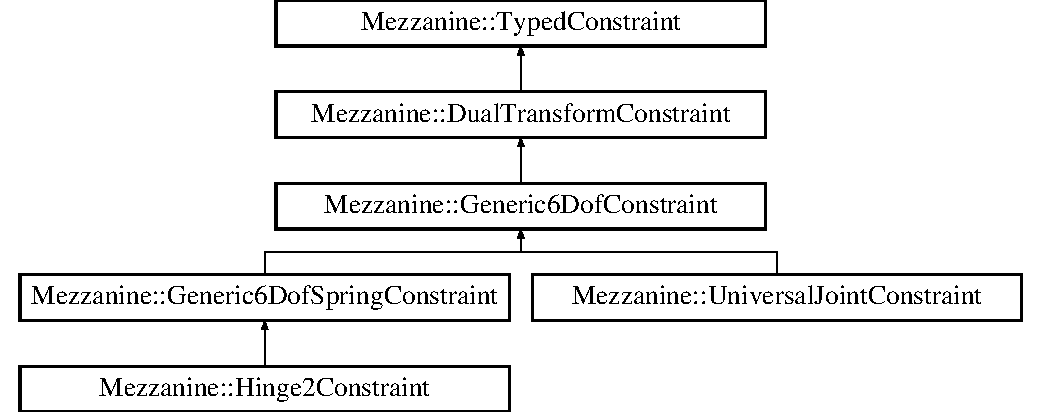
\includegraphics[height=5.000000cm]{classMezzanine_1_1Generic6DofConstraint}
\end{center}
\end{figure}
\subsubsection*{Public Types}
\begin{DoxyCompactItemize}
\item 
enum \hyperlink{classMezzanine_1_1Generic6DofConstraint_ac00067026a7d4e7c6832f169c754d585}{UsableAxis} \{ \par
\hyperlink{classMezzanine_1_1Generic6DofConstraint_ac00067026a7d4e7c6832f169c754d585ae15486eb9682cca0467859b8e7b16d4c}{LinearX} =  0, 
\hyperlink{classMezzanine_1_1Generic6DofConstraint_ac00067026a7d4e7c6832f169c754d585a1f0fd3c6af820cebda8a5e634483b5a8}{LinearY} =  1, 
\hyperlink{classMezzanine_1_1Generic6DofConstraint_ac00067026a7d4e7c6832f169c754d585a7b164ae20f69440f5241bb3f0119aa9c}{LinearZ} =  2, 
\hyperlink{classMezzanine_1_1Generic6DofConstraint_ac00067026a7d4e7c6832f169c754d585a2ff1d26a1d5afa5d7d1221f1cf87253d}{AngularX} =  3, 
\par
\hyperlink{classMezzanine_1_1Generic6DofConstraint_ac00067026a7d4e7c6832f169c754d585ab93b7724c369714f3a3e628b3be7e908}{AngularY} =  4, 
\hyperlink{classMezzanine_1_1Generic6DofConstraint_ac00067026a7d4e7c6832f169c754d585a98514adda7c9a79e57504fa1b714cb1e}{AngularZ} =  5, 
\hyperlink{classMezzanine_1_1Generic6DofConstraint_ac00067026a7d4e7c6832f169c754d585a695178ce4fa859bda7160fa4578db91b}{AngularXAsRotationalAxis} =  0, 
\hyperlink{classMezzanine_1_1Generic6DofConstraint_ac00067026a7d4e7c6832f169c754d585a7a7c9ce64bdaa80d9dc387d3ef67b381}{AngularYAsRotationalAxis} =  1, 
\par
\hyperlink{classMezzanine_1_1Generic6DofConstraint_ac00067026a7d4e7c6832f169c754d585a3b1e471b3713fd2fbb3fb689dd4f39b4}{AngularZAsRotationalAxis} =  2
 \}
\begin{DoxyCompactList}\small\item\em Identify the Axis a bit easier when iterating over them is less convienent than typing an Identifier. \item\end{DoxyCompactList}\end{DoxyCompactItemize}
\subsubsection*{Public Member Functions}
\begin{DoxyCompactItemize}
\item 
virtual int \hyperlink{classMezzanine_1_1Generic6DofConstraint_ad782a17567bfcfb2a0eaf08edb5d6838}{AxisToAngularAxis} (int Axis) const 
\begin{DoxyCompactList}\small\item\em Convert to internal Axis IDs from external or internal axis IDs. \item\end{DoxyCompactList}\item 
\hyperlink{classMezzanine_1_1Generic6DofConstraint_a373679760f1bc180adda8ad51e20cd38}{Generic6DofConstraint} (\hyperlink{classMezzanine_1_1ActorRigid}{ActorRigid} $\ast$ActorA, \hyperlink{classMezzanine_1_1ActorRigid}{ActorRigid} $\ast$ActorB, const \hyperlink{classMezzanine_1_1Transform}{Transform} \&TransformA, const \hyperlink{classMezzanine_1_1Transform}{Transform} \&TransformB, bool UseLinearReferenceA=false)
\begin{DoxyCompactList}\small\item\em Two body Terse constructor. \item\end{DoxyCompactList}\item 
\hyperlink{classMezzanine_1_1Generic6DofConstraint_a7adce568bcf8f289744686ce129bff08}{Generic6DofConstraint} (\hyperlink{classMezzanine_1_1ActorRigid}{ActorRigid} $\ast$ActorB, const \hyperlink{classMezzanine_1_1Transform}{Transform} \&TransformB, bool UseLinearReferenceB=true)
\begin{DoxyCompactList}\small\item\em Body and \hyperlink{classMezzanine_1_1World}{World} Terse constructor. \item\end{DoxyCompactList}\item 
\hyperlink{classMezzanine_1_1Generic6DofConstraint_af81c1ab120f7d2df27f194ee73516a18}{Generic6DofConstraint} (\hyperlink{classMezzanine_1_1ActorRigid}{ActorRigid} $\ast$ActorA, \hyperlink{classMezzanine_1_1ActorRigid}{ActorRigid} $\ast$ActorB, const \hyperlink{classMezzanine_1_1Vector3}{Vector3} \&VectorA, const \hyperlink{classMezzanine_1_1Vector3}{Vector3} \&VectorB, const \hyperlink{classMezzanine_1_1Quaternion}{Quaternion} \&QuaternionA, const \hyperlink{classMezzanine_1_1Quaternion}{Quaternion} \&QuaternionB, bool UseLinearReferenceA=false)
\begin{DoxyCompactList}\small\item\em Two body Verbose constructor. \item\end{DoxyCompactList}\item 
\hyperlink{classMezzanine_1_1Generic6DofConstraint_a41ed7866900eebbfb917ab426c21cf43}{Generic6DofConstraint} (\hyperlink{classMezzanine_1_1ActorRigid}{ActorRigid} $\ast$ActorB, const \hyperlink{classMezzanine_1_1Vector3}{Vector3} \&VectorB, const \hyperlink{classMezzanine_1_1Quaternion}{Quaternion} \&QuaternionB, bool UseLinearReferenceB=true)
\begin{DoxyCompactList}\small\item\em Body and \hyperlink{classMezzanine_1_1World}{World} Verbose constructor. \item\end{DoxyCompactList}\item 
virtual \hyperlink{classMezzanine_1_1Vector3}{Vector3} \hyperlink{classMezzanine_1_1Generic6DofConstraint_a1a9a5c30e5d2a39ceb99232ad375d9ab}{GetAngularLimitLower} () const 
\begin{DoxyCompactList}\small\item\em Get the Upper limits on rotation. \item\end{DoxyCompactList}\item 
\hyperlink{namespaceMezzanine_a726731b1a7df72bf3583e4a97282c6f6}{Real} \hyperlink{classMezzanine_1_1Generic6DofConstraint_a5c69e50d1fe27ac8bb99a60d665cee48}{GetAngularLimitLowerOnAxis} (int RotationalAxis) const 
\begin{DoxyCompactList}\small\item\em Get a specific lower rotational limit. \item\end{DoxyCompactList}\item 
virtual \hyperlink{classMezzanine_1_1Vector3}{Vector3} \hyperlink{classMezzanine_1_1Generic6DofConstraint_ae0734d106fddaea99c36a27cdcddab3c}{GetAngularLimitMaxForce} () const 
\begin{DoxyCompactList}\small\item\em Get the Maximimum amount of force applied to ensure limits are not surpassed. \item\end{DoxyCompactList}\item 
virtual \hyperlink{namespaceMezzanine_a726731b1a7df72bf3583e4a97282c6f6}{Real} \hyperlink{classMezzanine_1_1Generic6DofConstraint_abb6d534f3fd2416c1642d7574e68565d}{GetAngularLimitMaxForceOnAxis} (int Axis) const 
\begin{DoxyCompactList}\small\item\em Get the Maximimum amount of force applied to ensure a limit one axis is not surpassed. \item\end{DoxyCompactList}\item 
virtual \hyperlink{classMezzanine_1_1Vector3}{Vector3} \hyperlink{classMezzanine_1_1Generic6DofConstraint_a5899d2668fe8ab1c4ec3310d1679082e}{GetAngularLimitUpper} () const 
\begin{DoxyCompactList}\small\item\em Get the Power limits on rotation. \item\end{DoxyCompactList}\item 
\hyperlink{namespaceMezzanine_a726731b1a7df72bf3583e4a97282c6f6}{Real} \hyperlink{classMezzanine_1_1Generic6DofConstraint_abd364ebc562646bb46b2b003a54d6ca4}{GetAngularLimitUpperOnAxis} (int RotationalAxis) const 
\begin{DoxyCompactList}\small\item\em Get a specific upper rotational limit. \item\end{DoxyCompactList}\item 
virtual \hyperlink{classMezzanine_1_1Vector3}{Vector3} \hyperlink{classMezzanine_1_1Generic6DofConstraint_aa623d540221586a7cad7080e7404282a}{GetAngularMotorDamping} () const 
\begin{DoxyCompactList}\small\item\em Get the Damping for all Angular Axis. \item\end{DoxyCompactList}\item 
virtual \hyperlink{namespaceMezzanine_a726731b1a7df72bf3583e4a97282c6f6}{Real} \hyperlink{classMezzanine_1_1Generic6DofConstraint_a5910bdd1869a1e4580389ac66c769710}{GetAngularMotorDampingOnAxis} (int Axis) const 
\begin{DoxyCompactList}\small\item\em Get the Damping for one given Axis. \item\end{DoxyCompactList}\item 
virtual \hyperlink{classMezzanine_1_1Vector3}{Vector3} \hyperlink{classMezzanine_1_1Generic6DofConstraint_a5d69240a3ded30c0ef0312313667eccf}{GetAngularMotorEnabled} () const 
\begin{DoxyCompactList}\small\item\em Get a \hyperlink{classMezzanine_1_1Vector3}{Vector3} with 3 zero or nonzero values that store whether or not a given rotational motor is enable. \item\end{DoxyCompactList}\item 
virtual bool \hyperlink{classMezzanine_1_1Generic6DofConstraint_a1b23ad89fd57f5272e6c1dfa13957b14}{GetAngularMotorEnabledOnAxis} (int Axis) const 
\begin{DoxyCompactList}\small\item\em Is a specific rotational motor enabled. \item\end{DoxyCompactList}\item 
virtual \hyperlink{classMezzanine_1_1Vector3}{Vector3} \hyperlink{classMezzanine_1_1Generic6DofConstraint_a0ab2e7b20a8aa33c1cbffd77ec2e96a2}{GetAngularMotorMaxForce} () const 
\begin{DoxyCompactList}\small\item\em Get the Max Motor Force for each Axis. \item\end{DoxyCompactList}\item 
virtual \hyperlink{namespaceMezzanine_a726731b1a7df72bf3583e4a97282c6f6}{Real} \hyperlink{classMezzanine_1_1Generic6DofConstraint_a7610b33e8d29925d95cf9d3bf8921301}{GetAngularMotorMaxForceOnAxis} (int Axis) const 
\begin{DoxyCompactList}\small\item\em Get the Max motor Force on a certain Axis. \item\end{DoxyCompactList}\item 
virtual \hyperlink{classMezzanine_1_1Vector3}{Vector3} \hyperlink{classMezzanine_1_1Generic6DofConstraint_a87e8fd1a3fb1d959982f1f684182abbe}{GetAngularMotorRestitution} () const 
\begin{DoxyCompactList}\small\item\em Get the Restistution values for all three axis. \item\end{DoxyCompactList}\item 
virtual \hyperlink{namespaceMezzanine_a726731b1a7df72bf3583e4a97282c6f6}{Real} \hyperlink{classMezzanine_1_1Generic6DofConstraint_ada6e3d47f69b1719d3781af47206763b}{GetAngularMotorRestitutionOnAxis} (int Axis) const 
\begin{DoxyCompactList}\small\item\em Get the Restistution/Bounciness for a single Axis. \item\end{DoxyCompactList}\item 
virtual \hyperlink{classMezzanine_1_1Vector3}{Vector3} \hyperlink{classMezzanine_1_1Generic6DofConstraint_af2626b795dcac300ac75d42bc85dada6}{GetAngularMotorTargetVelocity} () const 
\begin{DoxyCompactList}\small\item\em Get the target velocity for all angular Axis. \item\end{DoxyCompactList}\item 
virtual \hyperlink{namespaceMezzanine_a726731b1a7df72bf3583e4a97282c6f6}{Real} \hyperlink{classMezzanine_1_1Generic6DofConstraint_afe97dfbe7c543987cdc287a0f69b73ea}{GetAngularMotorTargetVelocityOnAxis} (int Axis) const 
\begin{DoxyCompactList}\small\item\em Get the Target Velocity for one axis. \item\end{DoxyCompactList}\item 
virtual btTypedConstraint $\ast$ \hyperlink{classMezzanine_1_1Generic6DofConstraint_a37d4cbaf346ce8c11dada3fca32d0b42}{GetConstraintBase} () const 
\item 
virtual \hyperlink{namespaceMezzanine_a726731b1a7df72bf3583e4a97282c6f6}{Real} \hyperlink{classMezzanine_1_1Generic6DofConstraint_a3c6ee33f660eec42c2ae9cc6b22e5e2f}{GetLinearLimitDamping} () const 
\begin{DoxyCompactList}\small\item\em Get the Damping of the linear Limits. \item\end{DoxyCompactList}\item 
virtual \hyperlink{classMezzanine_1_1Vector3}{Vector3} \hyperlink{classMezzanine_1_1Generic6DofConstraint_a719503e5669f19e8e463b2621ec74bd8}{GetLinearLimitLower} () const 
\begin{DoxyCompactList}\small\item\em Get the Upper limits on translation. \item\end{DoxyCompactList}\item 
virtual \hyperlink{namespaceMezzanine_a726731b1a7df72bf3583e4a97282c6f6}{Real} \hyperlink{classMezzanine_1_1Generic6DofConstraint_ac969ae88077e58e035b7dfb6a44cc3f9}{GetLinearLimitRestitution} () const 
\begin{DoxyCompactList}\small\item\em Get the Restitution of the linear Limits. \item\end{DoxyCompactList}\item 
virtual \hyperlink{namespaceMezzanine_a726731b1a7df72bf3583e4a97282c6f6}{Real} \hyperlink{classMezzanine_1_1Generic6DofConstraint_a26c1a462de1abd0593d50b0da357ed62}{GetLinearLimitSoftness} () const 
\begin{DoxyCompactList}\small\item\em Get the Softness of the linear Limits. \item\end{DoxyCompactList}\item 
virtual \hyperlink{classMezzanine_1_1Vector3}{Vector3} \hyperlink{classMezzanine_1_1Generic6DofConstraint_aff95241b1756b5cc1ffaef4211272e6b}{GetLinearLimitUpper} () const 
\begin{DoxyCompactList}\small\item\em Get the lower limits on translation. \item\end{DoxyCompactList}\item 
virtual \hyperlink{classMezzanine_1_1Vector3}{Vector3} \hyperlink{classMezzanine_1_1Generic6DofConstraint_a89e87415dbe38493f724505cfcecad71}{GetLinearMotorEnabled} () const 
\begin{DoxyCompactList}\small\item\em Get a \hyperlink{classMezzanine_1_1Vector3}{Vector3} with 3 zero or nonzero values that store whether or not a given rotational motor is enable. \item\end{DoxyCompactList}\item 
virtual bool \hyperlink{classMezzanine_1_1Generic6DofConstraint_a7df83de658eec42ff0a35e4470baab82}{GetLinearMotorEnabledOnAxis} (int Axis) const 
\begin{DoxyCompactList}\small\item\em Is a specific Linear motor enabled. \item\end{DoxyCompactList}\item 
virtual \hyperlink{classMezzanine_1_1Vector3}{Vector3} \hyperlink{classMezzanine_1_1Generic6DofConstraint_a954466fb8e3ba12ec702eeab961d75f8}{GetLinearMotorMaxForce} () const 
\begin{DoxyCompactList}\small\item\em Get the Max Motor Force for each Axis. \item\end{DoxyCompactList}\item 
virtual \hyperlink{namespaceMezzanine_a726731b1a7df72bf3583e4a97282c6f6}{Real} \hyperlink{classMezzanine_1_1Generic6DofConstraint_a1d47c2671f8e8a918cffe568beca0af4}{GetLinearMotorMaxForceOnAxis} (int Axis) const 
\begin{DoxyCompactList}\small\item\em Get the Max motor Force on a certain Axis. \item\end{DoxyCompactList}\item 
virtual \hyperlink{classMezzanine_1_1Vector3}{Vector3} \hyperlink{classMezzanine_1_1Generic6DofConstraint_addd83b732df3f6fe730bf51b2153585e}{GetLinearMotorTargetVelocity} () const 
\begin{DoxyCompactList}\small\item\em Get the target velocity for all Linear Axis. \item\end{DoxyCompactList}\item 
virtual \hyperlink{namespaceMezzanine_a726731b1a7df72bf3583e4a97282c6f6}{Real} \hyperlink{classMezzanine_1_1Generic6DofConstraint_a3ad266a779d330634d524615c8a027dc}{GetLinearMotorTargetVelocityOnAxis} (int Axis) const 
\begin{DoxyCompactList}\small\item\em Get the Target Velocity for one axis. \item\end{DoxyCompactList}\item 
virtual \hyperlink{classMezzanine_1_1Vector3}{Vector3} \hyperlink{classMezzanine_1_1Generic6DofConstraint_a180f26186e0ddd58c9c0746897155eaf}{GetPivotALocation} () const 
\item 
virtual \hyperlink{classMezzanine_1_1Quaternion}{Quaternion} \hyperlink{classMezzanine_1_1Generic6DofConstraint_a517388fdf36423ed0550ec19089955b9}{GetPivotARotation} () const 
\item 
virtual \hyperlink{classMezzanine_1_1Transform}{Transform} \hyperlink{classMezzanine_1_1Generic6DofConstraint_adac17da02ce3ecacf583515a66576533}{GetPivotATransform} () const 
\item 
virtual \hyperlink{classMezzanine_1_1Vector3}{Vector3} \hyperlink{classMezzanine_1_1Generic6DofConstraint_a2b7344ab150f2f6dd898b6cbcd150d6e}{GetPivotBLocation} () const 
\item 
virtual \hyperlink{classMezzanine_1_1Quaternion}{Quaternion} \hyperlink{classMezzanine_1_1Generic6DofConstraint_ab3979edc1d5f3bfce878de009c18494d}{GetPivotBRotation} () const 
\item 
virtual \hyperlink{classMezzanine_1_1Transform}{Transform} \hyperlink{classMezzanine_1_1Generic6DofConstraint_ad38e140ea8edf8d9d74e99bbebf68417}{GetPivotBTransform} () const 
\item 
virtual bool \hyperlink{classMezzanine_1_1Generic6DofConstraint_ada22ae842e9212b0480bbfa866d16a08}{GetUseFrameOffset} () const 
\begin{DoxyCompactList}\small\item\em Retrieve the stored value from the physics subsystem(bullet) \item\end{DoxyCompactList}\item 
virtual bool \hyperlink{classMezzanine_1_1Generic6DofConstraint_ac0589ecb2fe1e0227dbcbb52cd90ceba}{HasParamBeenSet} (\hyperlink{namespaceMezzanine_a6c62e8c2938fb203eb7a7072c12176f4}{ConstraintParam} Param, int Axis) const 
\item 
virtual void \hyperlink{classMezzanine_1_1Generic6DofConstraint_af5f946926bb5f47936dc84213b40ec95}{SetAngularLimitLower} (const \hyperlink{classMezzanine_1_1Vector3}{Vector3} \&Limit)
\begin{DoxyCompactList}\small\item\em Set the Lower limits on rotation. \item\end{DoxyCompactList}\item 
virtual void \hyperlink{classMezzanine_1_1Generic6DofConstraint_a6a0cc7ac577b855687b74583e5a23b08}{SetAngularLimitMaxForce} (const \hyperlink{classMezzanine_1_1Vector3}{Vector3} \&MaxLimitForces)
\begin{DoxyCompactList}\small\item\em Set the Maximimum amount of force applied to ensure limits are not surpassed. \item\end{DoxyCompactList}\item 
virtual void \hyperlink{classMezzanine_1_1Generic6DofConstraint_a899734922a915a2f2b22c9212f415c35}{SetAngularLimitMaxForceOnAxis} (\hyperlink{namespaceMezzanine_a726731b1a7df72bf3583e4a97282c6f6}{Real} MaxLimitForce, int Axis)
\begin{DoxyCompactList}\small\item\em Set the Maximimum amount of force applied to ensure a limit on one axis is not surpassed. \item\end{DoxyCompactList}\item 
virtual void \hyperlink{classMezzanine_1_1Generic6DofConstraint_a3bdd15929ecddb818db7fea8cfdb2fe0}{SetAngularLimitUpper} (const \hyperlink{classMezzanine_1_1Vector3}{Vector3} \&Limit)
\begin{DoxyCompactList}\small\item\em Set the Upper limits on rotation. \item\end{DoxyCompactList}\item 
virtual void \hyperlink{classMezzanine_1_1Generic6DofConstraint_ab386bb86b026ab9c1e8709b037cd9875}{SetAngularMotorDamping} (const \hyperlink{classMezzanine_1_1Vector3}{Vector3} \&Dampings)
\begin{DoxyCompactList}\small\item\em Set the Angular Motor Damping for each Angular Axis. \item\end{DoxyCompactList}\item 
virtual void \hyperlink{classMezzanine_1_1Generic6DofConstraint_a42c561134495de588cf16d7d46f1fea3}{SetAngularMotorDampingOnAxis} (\hyperlink{namespaceMezzanine_a726731b1a7df72bf3583e4a97282c6f6}{Real} Damping, int Axis)
\begin{DoxyCompactList}\small\item\em For one Axis, set the Damping. \item\end{DoxyCompactList}\item 
virtual void \hyperlink{classMezzanine_1_1Generic6DofConstraint_a9543fd9a15f9be95fafe812c90f566d8}{SetAngularMotorEnabled} (const \hyperlink{classMezzanine_1_1Vector3}{Vector3} \&Enableds)
\begin{DoxyCompactList}\small\item\em Set whether or not the motor is enabled for all Axis Simultaneously. \item\end{DoxyCompactList}\item 
virtual void \hyperlink{classMezzanine_1_1Generic6DofConstraint_af487eb94c231601a2cb3dd3e813f1024}{SetAngularMotorEnabledOnAxis} (bool Enabled, int Axis)
\begin{DoxyCompactList}\small\item\em For one Axis, set whether or not the motor is enabled. \item\end{DoxyCompactList}\item 
virtual void \hyperlink{classMezzanine_1_1Generic6DofConstraint_ada0b7be3499cb3da27ca36e0076323c7}{SetAngularMotorMaxForce} (const \hyperlink{classMezzanine_1_1Vector3}{Vector3} \&Forces)
\begin{DoxyCompactList}\small\item\em Set the Angular Motor Maximum force on all 3 rotational axis. \item\end{DoxyCompactList}\item 
virtual void \hyperlink{classMezzanine_1_1Generic6DofConstraint_ae4909e7a8782698049a06036b1a044c2}{SetAngularMotorMaxForceOnAxis} (\hyperlink{namespaceMezzanine_a726731b1a7df72bf3583e4a97282c6f6}{Real} Force, int Axis)
\begin{DoxyCompactList}\small\item\em For one Axis, set the Maximimum Motor Force. \item\end{DoxyCompactList}\item 
virtual void \hyperlink{classMezzanine_1_1Generic6DofConstraint_adbd65a2c6facda66b4736baa24fd12ed}{SetAngularMotorRestitution} (const \hyperlink{classMezzanine_1_1Vector3}{Vector3} \&Restistutions)
\begin{DoxyCompactList}\small\item\em Set the Bounciness/Restition for rotation on all three Axis. \item\end{DoxyCompactList}\item 
virtual void \hyperlink{classMezzanine_1_1Generic6DofConstraint_a64b2f088046feedbedbc6277dc6bbe1b}{SetAngularMotorRestitutionOnAxis} (\hyperlink{namespaceMezzanine_a726731b1a7df72bf3583e4a97282c6f6}{Real} Restistution, int Axis)
\begin{DoxyCompactList}\small\item\em For one Axis, set the Restistution/Bounciness/. \item\end{DoxyCompactList}\item 
virtual void \hyperlink{classMezzanine_1_1Generic6DofConstraint_a83e6642525b862d2b0f213f4196cfee6}{SetAngularMotorTargetVelocity} (const \hyperlink{classMezzanine_1_1Vector3}{Vector3} \&Velocities)
\begin{DoxyCompactList}\small\item\em Set the Target velocity of the motor on each anuglar axis. \item\end{DoxyCompactList}\item 
virtual void \hyperlink{classMezzanine_1_1Generic6DofConstraint_a40d21ce4c86538080ab574e5ddee5db8}{SetAngularMotorTargetVelocityOnAxis} (\hyperlink{namespaceMezzanine_a726731b1a7df72bf3583e4a97282c6f6}{Real} Velocity, int Axis)
\begin{DoxyCompactList}\small\item\em For one Axis, set the target velocity of the angular motor. \item\end{DoxyCompactList}\item 
virtual void \hyperlink{classMezzanine_1_1Generic6DofConstraint_af8d66ec56818e651c0e429b944f7b823}{SetLimit} (int Axis, \hyperlink{namespaceMezzanine_a726731b1a7df72bf3583e4a97282c6f6}{Real} Lower, \hyperlink{namespaceMezzanine_a726731b1a7df72bf3583e4a97282c6f6}{Real} Upper)
\begin{DoxyCompactList}\small\item\em Change the upper and lower limit for one axis of translation or rotation limit. \item\end{DoxyCompactList}\item 
virtual void \hyperlink{classMezzanine_1_1Generic6DofConstraint_a8bd3f660e157fb666872e09d32e7ca1c}{SetLinearLimitDamping} (\hyperlink{namespaceMezzanine_a726731b1a7df72bf3583e4a97282c6f6}{Real} Damping)
\begin{DoxyCompactList}\small\item\em Set the Damping of the linear Limits. \item\end{DoxyCompactList}\item 
virtual void \hyperlink{classMezzanine_1_1Generic6DofConstraint_a5d90b3129b41ab7dbcf545cdc7496a7d}{SetLinearLimitLower} (const \hyperlink{classMezzanine_1_1Vector3}{Vector3} \&Limit)
\begin{DoxyCompactList}\small\item\em Set the Upper limits on translation. \item\end{DoxyCompactList}\item 
virtual void \hyperlink{classMezzanine_1_1Generic6DofConstraint_ace6ec95d4d7332e7320ab86e0a2d9f90}{SetLinearLimitRestitution} (\hyperlink{namespaceMezzanine_a726731b1a7df72bf3583e4a97282c6f6}{Real} Restitution)
\begin{DoxyCompactList}\small\item\em Set the Restitution of the linear Limits. \item\end{DoxyCompactList}\item 
virtual void \hyperlink{classMezzanine_1_1Generic6DofConstraint_aac70c40e57b9a0cefaf99a858a17d9f7}{SetLinearLimitSoftness} (\hyperlink{namespaceMezzanine_a726731b1a7df72bf3583e4a97282c6f6}{Real} Softness)
\begin{DoxyCompactList}\small\item\em Set the Softness of the linear Limits. \item\end{DoxyCompactList}\item 
virtual void \hyperlink{classMezzanine_1_1Generic6DofConstraint_a11540d7b783086bda6f0ccf6bb9e316d}{SetLinearLimitUpper} (const \hyperlink{classMezzanine_1_1Vector3}{Vector3} \&Limit)
\begin{DoxyCompactList}\small\item\em Set the lower limits on translation. \item\end{DoxyCompactList}\item 
virtual void \hyperlink{classMezzanine_1_1Generic6DofConstraint_a507204d3dcb84608b6e69ac3410cb2fc}{SetLinearMotorEnabled} (const \hyperlink{classMezzanine_1_1Vector3}{Vector3} \&Enableds)
\begin{DoxyCompactList}\small\item\em Set whether or not the motor is enabled for all Linear Axis Simultaneously. \item\end{DoxyCompactList}\item 
virtual void \hyperlink{classMezzanine_1_1Generic6DofConstraint_a28b2398edd33f7af4043acce4d4e9893}{SetLinearMotorEnabledOnAxis} (bool Enabled, int Axis)
\begin{DoxyCompactList}\small\item\em For one Axis, set whether or not the motor is enabled. \item\end{DoxyCompactList}\item 
virtual void \hyperlink{classMezzanine_1_1Generic6DofConstraint_a9338ccdac5c4eaf9b561feb242c5f89e}{SetLinearMotorMaxForce} (const \hyperlink{classMezzanine_1_1Vector3}{Vector3} \&Forces)
\begin{DoxyCompactList}\small\item\em Set the Linear Motor Maximum force on all 3 translation axis. \item\end{DoxyCompactList}\item 
virtual void \hyperlink{classMezzanine_1_1Generic6DofConstraint_ab8286b0bb20cccc7c2810ad76c9d3ee5}{SetLinearMotorMaxForceOnAxis} (\hyperlink{namespaceMezzanine_a726731b1a7df72bf3583e4a97282c6f6}{Real} Force, int Axis)
\begin{DoxyCompactList}\small\item\em For one Axis, set the Maximimum Motor Force. \item\end{DoxyCompactList}\item 
virtual void \hyperlink{classMezzanine_1_1Generic6DofConstraint_a5458f6dc3b7b321a7323dcf4103737e8}{SetLinearMotorTargetVelocity} (const \hyperlink{classMezzanine_1_1Vector3}{Vector3} \&Velocities)
\begin{DoxyCompactList}\small\item\em Set the Target velocity of the motor on each anuglar axis. \item\end{DoxyCompactList}\item 
virtual void \hyperlink{classMezzanine_1_1Generic6DofConstraint_abc6bc013544b9793c17a929578115b32}{SetLinearMotorTargetVelocityOnAxis} (\hyperlink{namespaceMezzanine_a726731b1a7df72bf3583e4a97282c6f6}{Real} Velocity, int Axis)
\begin{DoxyCompactList}\small\item\em For one Axis, set the target velocity of the Linear motor. \item\end{DoxyCompactList}\item 
virtual void \hyperlink{classMezzanine_1_1Generic6DofConstraint_a4670a488bc5cab478c6d69c8a0d240a5}{SetPivotALocation} (const \hyperlink{classMezzanine_1_1Vector3}{Vector3} \&Location)
\item 
virtual void \hyperlink{classMezzanine_1_1Generic6DofConstraint_a34027d82e3b8c09c6cd488335ea343bb}{SetPivotARotation} (const \hyperlink{classMezzanine_1_1Quaternion}{Quaternion} \&Rotation)
\item 
virtual void \hyperlink{classMezzanine_1_1Generic6DofConstraint_a88f26ccb9a6ec67adc743d4bc7c86ddf}{SetPivotATransform} (const \hyperlink{classMezzanine_1_1Transform}{Transform} \&TranA)
\item 
virtual void \hyperlink{classMezzanine_1_1Generic6DofConstraint_a1b5fc577a2c627266436fd5b134728bc}{SetPivotBLocation} (const \hyperlink{classMezzanine_1_1Vector3}{Vector3} \&Location)
\item 
virtual void \hyperlink{classMezzanine_1_1Generic6DofConstraint_afd149f6868de162f75a3e2293d6c143d}{SetPivotBRotation} (const \hyperlink{classMezzanine_1_1Quaternion}{Quaternion} \&Rotation)
\item 
virtual void \hyperlink{classMezzanine_1_1Generic6DofConstraint_adaa5bb038814aa287773f56d40e90210}{SetPivotBTransform} (const \hyperlink{classMezzanine_1_1Transform}{Transform} \&TranB)
\item 
virtual void \hyperlink{classMezzanine_1_1Generic6DofConstraint_a1181f8eed94d0e8ec4d5b7230e241d95}{SetUseFrameOffset} (bool FrameOffset)
\begin{DoxyCompactList}\small\item\em Set the stored value for UseFrameOffset on this hinge in the physics subsystem(bullet) \item\end{DoxyCompactList}\item 
virtual \hyperlink{classMezzanine_1_1TypedConstraint_ac6b8e0839cd686f73d0c9e9ad5db47a4}{TypedConstraint::AxisList} \hyperlink{classMezzanine_1_1Generic6DofConstraint_a8a908f5f3857262db217a7f2dfc25c61}{ValidAngularAxis} () const 
\item 
virtual \hyperlink{classMezzanine_1_1TypedConstraint_ac6b8e0839cd686f73d0c9e9ad5db47a4}{TypedConstraint::AxisList} \hyperlink{classMezzanine_1_1Generic6DofConstraint_a94db83422c1984cdbe1745662715ac9d}{ValidLinearAxis} () const 
\item 
virtual \hyperlink{classMezzanine_1_1TypedConstraint_abd499db29c9e9755e9bb547d29eaa49a}{TypedConstraint::ParamList} \hyperlink{classMezzanine_1_1Generic6DofConstraint_a2417bed78c50820d2b5b8d083a8897d6}{ValidParamOnAxis} (int Axis) const 
\item 
\hypertarget{classMezzanine_1_1Generic6DofConstraint_a13e111a96aa15ccd2107c8910236471b}{
virtual \hyperlink{classMezzanine_1_1Generic6DofConstraint_a13e111a96aa15ccd2107c8910236471b}{$\sim$Generic6DofConstraint} ()}
\label{classMezzanine_1_1Generic6DofConstraint_a13e111a96aa15ccd2107c8910236471b}

\begin{DoxyCompactList}\small\item\em Class destructor. \item\end{DoxyCompactList}\end{DoxyCompactItemize}
\subsubsection*{Protected Member Functions}
\begin{DoxyCompactItemize}
\item 
\hyperlink{classMezzanine_1_1Generic6DofConstraint_ab950948993dc96cc088d94197f35a40d}{Generic6DofConstraint} ()
\begin{DoxyCompactList}\small\item\em Inheritance Constructor. \item\end{DoxyCompactList}\end{DoxyCompactItemize}
\subsubsection*{Protected Attributes}
\begin{DoxyCompactItemize}
\item 
\hypertarget{classMezzanine_1_1Generic6DofConstraint_abb10648cdb6987566223724d20de0b51}{
btGeneric6DofConstraint $\ast$ \hyperlink{classMezzanine_1_1Generic6DofConstraint_abb10648cdb6987566223724d20de0b51}{Generic6dof}}
\label{classMezzanine_1_1Generic6DofConstraint_abb10648cdb6987566223724d20de0b51}

\begin{DoxyCompactList}\small\item\em Bullet constraint that this class encapsulates. \item\end{DoxyCompactList}\end{DoxyCompactItemize}


\subsubsection{Detailed Description}
Create simple but specific limits on any axis of movement or rotation. Provides optional limits on the x, y, and z for rotation and translation. You can get the ID of the axis with \hyperlink{classMezzanine_1_1Generic6DofConstraint_a94db83422c1984cdbe1745662715ac9d}{ValidLinearAxis()} or \hyperlink{classMezzanine_1_1Generic6DofConstraint_a8a908f5f3857262db217a7f2dfc25c61}{ValidAngularAxis()} for this particular constraint at the time of this writing the constraint axis looked liked this:
\begin{DoxyItemize}
\item 0: Translation X
\item 1: Translation Y
\item 2: Translation Z
\item 3: Rotation X
\item 4: Rotation Y
\item 5: Rotation Z
\end{DoxyItemize}

This has to perform a larger amount of calculations and should be used only when other simpler constraints have been ruled out. \par
 \par
 As with all limits when the upper and lower limits match the two actors will be locked on that axis and relative translation or rotation will not be permitted (within the bounds or error correction). If the Lower limit is lower than the Upper limit a range of translation or rotation will be allowed. If the Lower limit is higher than the Upper limit this will cause the system to realized that no position can satisfy the constraint and no restriction will be enforced. \par
 \par
 Each of the Axis also has a motor that can be enabled to cause a specified amount of translation or rotation. To aid in selection of specific Axis, you should use the UsableAxis enum 

Definition at line 458 of file constraint.h.



\subsubsection{Member Enumeration Documentation}
\hypertarget{classMezzanine_1_1Generic6DofConstraint_ac00067026a7d4e7c6832f169c754d585}{
\index{Mezzanine::Generic6DofConstraint@{Mezzanine::Generic6DofConstraint}!UsableAxis@{UsableAxis}}
\index{UsableAxis@{UsableAxis}!Mezzanine::Generic6DofConstraint@{Mezzanine::Generic6DofConstraint}}
\paragraph[{UsableAxis}]{\setlength{\rightskip}{0pt plus 5cm}enum {\bf Mezzanine::Generic6DofConstraint::UsableAxis}}\hfill}
\label{classMezzanine_1_1Generic6DofConstraint_ac00067026a7d4e7c6832f169c754d585}


Identify the Axis a bit easier when iterating over them is less convienent than typing an Identifier. 

\begin{Desc}
\item[Enumerator: ]\par
\begin{description}
\index{LinearX@{LinearX}!Mezzanine::Generic6DofConstraint@{Mezzanine::Generic6DofConstraint}}\index{Mezzanine::Generic6DofConstraint@{Mezzanine::Generic6DofConstraint}!LinearX@{LinearX}}\item[{\em 
\hypertarget{classMezzanine_1_1Generic6DofConstraint_ac00067026a7d4e7c6832f169c754d585ae15486eb9682cca0467859b8e7b16d4c}{
LinearX}
\label{classMezzanine_1_1Generic6DofConstraint_ac00067026a7d4e7c6832f169c754d585ae15486eb9682cca0467859b8e7b16d4c}
}]Translation on the X axis. \index{LinearY@{LinearY}!Mezzanine::Generic6DofConstraint@{Mezzanine::Generic6DofConstraint}}\index{Mezzanine::Generic6DofConstraint@{Mezzanine::Generic6DofConstraint}!LinearY@{LinearY}}\item[{\em 
\hypertarget{classMezzanine_1_1Generic6DofConstraint_ac00067026a7d4e7c6832f169c754d585a1f0fd3c6af820cebda8a5e634483b5a8}{
LinearY}
\label{classMezzanine_1_1Generic6DofConstraint_ac00067026a7d4e7c6832f169c754d585a1f0fd3c6af820cebda8a5e634483b5a8}
}]Translation on the Y axis. \index{LinearZ@{LinearZ}!Mezzanine::Generic6DofConstraint@{Mezzanine::Generic6DofConstraint}}\index{Mezzanine::Generic6DofConstraint@{Mezzanine::Generic6DofConstraint}!LinearZ@{LinearZ}}\item[{\em 
\hypertarget{classMezzanine_1_1Generic6DofConstraint_ac00067026a7d4e7c6832f169c754d585a7b164ae20f69440f5241bb3f0119aa9c}{
LinearZ}
\label{classMezzanine_1_1Generic6DofConstraint_ac00067026a7d4e7c6832f169c754d585a7b164ae20f69440f5241bb3f0119aa9c}
}]Translation on the Z axis. \index{AngularX@{AngularX}!Mezzanine::Generic6DofConstraint@{Mezzanine::Generic6DofConstraint}}\index{Mezzanine::Generic6DofConstraint@{Mezzanine::Generic6DofConstraint}!AngularX@{AngularX}}\item[{\em 
\hypertarget{classMezzanine_1_1Generic6DofConstraint_ac00067026a7d4e7c6832f169c754d585a2ff1d26a1d5afa5d7d1221f1cf87253d}{
AngularX}
\label{classMezzanine_1_1Generic6DofConstraint_ac00067026a7d4e7c6832f169c754d585a2ff1d26a1d5afa5d7d1221f1cf87253d}
}]Rotation on the X axis. \index{AngularY@{AngularY}!Mezzanine::Generic6DofConstraint@{Mezzanine::Generic6DofConstraint}}\index{Mezzanine::Generic6DofConstraint@{Mezzanine::Generic6DofConstraint}!AngularY@{AngularY}}\item[{\em 
\hypertarget{classMezzanine_1_1Generic6DofConstraint_ac00067026a7d4e7c6832f169c754d585ab93b7724c369714f3a3e628b3be7e908}{
AngularY}
\label{classMezzanine_1_1Generic6DofConstraint_ac00067026a7d4e7c6832f169c754d585ab93b7724c369714f3a3e628b3be7e908}
}]Rotation on the Y axis. \index{AngularZ@{AngularZ}!Mezzanine::Generic6DofConstraint@{Mezzanine::Generic6DofConstraint}}\index{Mezzanine::Generic6DofConstraint@{Mezzanine::Generic6DofConstraint}!AngularZ@{AngularZ}}\item[{\em 
\hypertarget{classMezzanine_1_1Generic6DofConstraint_ac00067026a7d4e7c6832f169c754d585a98514adda7c9a79e57504fa1b714cb1e}{
AngularZ}
\label{classMezzanine_1_1Generic6DofConstraint_ac00067026a7d4e7c6832f169c754d585a98514adda7c9a79e57504fa1b714cb1e}
}]Rotation on the Z axis. \index{AngularXAsRotationalAxis@{AngularXAsRotationalAxis}!Mezzanine::Generic6DofConstraint@{Mezzanine::Generic6DofConstraint}}\index{Mezzanine::Generic6DofConstraint@{Mezzanine::Generic6DofConstraint}!AngularXAsRotationalAxis@{AngularXAsRotationalAxis}}\item[{\em 
\hypertarget{classMezzanine_1_1Generic6DofConstraint_ac00067026a7d4e7c6832f169c754d585a695178ce4fa859bda7160fa4578db91b}{
AngularXAsRotationalAxis}
\label{classMezzanine_1_1Generic6DofConstraint_ac00067026a7d4e7c6832f169c754d585a695178ce4fa859bda7160fa4578db91b}
}]Rotation on the X axis, when working with only rotational Axis. \index{AngularYAsRotationalAxis@{AngularYAsRotationalAxis}!Mezzanine::Generic6DofConstraint@{Mezzanine::Generic6DofConstraint}}\index{Mezzanine::Generic6DofConstraint@{Mezzanine::Generic6DofConstraint}!AngularYAsRotationalAxis@{AngularYAsRotationalAxis}}\item[{\em 
\hypertarget{classMezzanine_1_1Generic6DofConstraint_ac00067026a7d4e7c6832f169c754d585a7a7c9ce64bdaa80d9dc387d3ef67b381}{
AngularYAsRotationalAxis}
\label{classMezzanine_1_1Generic6DofConstraint_ac00067026a7d4e7c6832f169c754d585a7a7c9ce64bdaa80d9dc387d3ef67b381}
}]Rotation on the Y axis, when working with only rotational Axis. \index{AngularZAsRotationalAxis@{AngularZAsRotationalAxis}!Mezzanine::Generic6DofConstraint@{Mezzanine::Generic6DofConstraint}}\index{Mezzanine::Generic6DofConstraint@{Mezzanine::Generic6DofConstraint}!AngularZAsRotationalAxis@{AngularZAsRotationalAxis}}\item[{\em 
\hypertarget{classMezzanine_1_1Generic6DofConstraint_ac00067026a7d4e7c6832f169c754d585a3b1e471b3713fd2fbb3fb689dd4f39b4}{
AngularZAsRotationalAxis}
\label{classMezzanine_1_1Generic6DofConstraint_ac00067026a7d4e7c6832f169c754d585a3b1e471b3713fd2fbb3fb689dd4f39b4}
}]Rotation on the Z axis, when working with only rotational Axis. \end{description}
\end{Desc}



Reimplemented in \hyperlink{classMezzanine_1_1Generic6DofSpringConstraint_acdffbc070d80b5480bf1020d4a2351ed}{Mezzanine::Generic6DofSpringConstraint}.



Definition at line 469 of file constraint.h.



\subsubsection{Constructor \& Destructor Documentation}
\hypertarget{classMezzanine_1_1Generic6DofConstraint_ab950948993dc96cc088d94197f35a40d}{
\index{Mezzanine::Generic6DofConstraint@{Mezzanine::Generic6DofConstraint}!Generic6DofConstraint@{Generic6DofConstraint}}
\index{Generic6DofConstraint@{Generic6DofConstraint}!Mezzanine::Generic6DofConstraint@{Mezzanine::Generic6DofConstraint}}
\paragraph[{Generic6DofConstraint}]{\setlength{\rightskip}{0pt plus 5cm}Mezzanine::Generic6DofConstraint::Generic6DofConstraint (
\begin{DoxyParamCaption}
{}
\end{DoxyParamCaption}
)\hspace{0.3cm}{\ttfamily  \mbox{[}protected\mbox{]}}}\hfill}
\label{classMezzanine_1_1Generic6DofConstraint_ab950948993dc96cc088d94197f35a40d}


Inheritance Constructor. 

This is only called by derived classes, and shouldn't be called manually. \hypertarget{classMezzanine_1_1Generic6DofConstraint_af81c1ab120f7d2df27f194ee73516a18}{
\index{Mezzanine::Generic6DofConstraint@{Mezzanine::Generic6DofConstraint}!Generic6DofConstraint@{Generic6DofConstraint}}
\index{Generic6DofConstraint@{Generic6DofConstraint}!Mezzanine::Generic6DofConstraint@{Mezzanine::Generic6DofConstraint}}
\paragraph[{Generic6DofConstraint}]{\setlength{\rightskip}{0pt plus 5cm}Mezzanine::Generic6DofConstraint::Generic6DofConstraint (
\begin{DoxyParamCaption}
\item[{{\bf ActorRigid} $\ast$}]{ActorA, }
\item[{{\bf ActorRigid} $\ast$}]{ActorB, }
\item[{const {\bf Vector3} \&}]{VectorA, }
\item[{const {\bf Vector3} \&}]{VectorB, }
\item[{const {\bf Quaternion} \&}]{QuaternionA, }
\item[{const {\bf Quaternion} \&}]{QuaternionB, }
\item[{bool}]{UseLinearReferenceA = {\ttfamily false}}
\end{DoxyParamCaption}
)}\hfill}
\label{classMezzanine_1_1Generic6DofConstraint_af81c1ab120f7d2df27f194ee73516a18}


Two body Verbose constructor. 


\begin{DoxyParams}{Parameters}
{\em ActorA} & The First body to be bound \\
\hline
{\em ActorB} & The Second body to be bound \\
\hline
{\em VectorA} & The offset from ActorA's center of gravity to get to match an offset from ActorB \\
\hline
{\em VectorB} & The offset from ActorB's center of gravity. \\
\hline
{\em QuaternionA} & Relative rotation from ActorA \\
\hline
{\em QuaternionB} & Relative rotation from ActorB \\
\hline
{\em UseLinearReferenceA} & Perform Linear math from ActorA's perspective, default to false. \\
\hline
\end{DoxyParams}
\hypertarget{classMezzanine_1_1Generic6DofConstraint_a373679760f1bc180adda8ad51e20cd38}{
\index{Mezzanine::Generic6DofConstraint@{Mezzanine::Generic6DofConstraint}!Generic6DofConstraint@{Generic6DofConstraint}}
\index{Generic6DofConstraint@{Generic6DofConstraint}!Mezzanine::Generic6DofConstraint@{Mezzanine::Generic6DofConstraint}}
\paragraph[{Generic6DofConstraint}]{\setlength{\rightskip}{0pt plus 5cm}Mezzanine::Generic6DofConstraint::Generic6DofConstraint (
\begin{DoxyParamCaption}
\item[{{\bf ActorRigid} $\ast$}]{ActorA, }
\item[{{\bf ActorRigid} $\ast$}]{ActorB, }
\item[{const {\bf Transform} \&}]{TransformA, }
\item[{const {\bf Transform} \&}]{TransformB, }
\item[{bool}]{UseLinearReferenceA = {\ttfamily false}}
\end{DoxyParamCaption}
)}\hfill}
\label{classMezzanine_1_1Generic6DofConstraint_a373679760f1bc180adda8ad51e20cd38}


Two body Terse constructor. 


\begin{DoxyParams}{Parameters}
{\em ActorA} & The First body to be bound \\
\hline
{\em ActorB} & The Second body to be bound \\
\hline
{\em TransformA} & The offset and rotation from ActorA's center of gravity to get to match an offset from ActorB \\
\hline
{\em TransformB} & The offset and rotation from ActorB's center of gravity. \\
\hline
{\em UseLinearReferenceA} & Perform Linear math from ActorA's perspective, default to false. \\
\hline
\end{DoxyParams}
\hypertarget{classMezzanine_1_1Generic6DofConstraint_a41ed7866900eebbfb917ab426c21cf43}{
\index{Mezzanine::Generic6DofConstraint@{Mezzanine::Generic6DofConstraint}!Generic6DofConstraint@{Generic6DofConstraint}}
\index{Generic6DofConstraint@{Generic6DofConstraint}!Mezzanine::Generic6DofConstraint@{Mezzanine::Generic6DofConstraint}}
\paragraph[{Generic6DofConstraint}]{\setlength{\rightskip}{0pt plus 5cm}Mezzanine::Generic6DofConstraint::Generic6DofConstraint (
\begin{DoxyParamCaption}
\item[{{\bf ActorRigid} $\ast$}]{ActorB, }
\item[{const {\bf Vector3} \&}]{VectorB, }
\item[{const {\bf Quaternion} \&}]{QuaternionB, }
\item[{bool}]{UseLinearReferenceB = {\ttfamily true}}
\end{DoxyParamCaption}
)}\hfill}
\label{classMezzanine_1_1Generic6DofConstraint_a41ed7866900eebbfb917ab426c21cf43}


Body and \hyperlink{classMezzanine_1_1World}{World} Verbose constructor. 


\begin{DoxyParams}{Parameters}
{\em ActorA} & The body to be bound to the world \\
\hline
{\em VectorB} & The offset for the ActorB pivot/hinge/joint \\
\hline
{\em QuaternionB} & The rotation \\
\hline
{\em UseLinearReferenceB} & Perform Linear math from ActorB's perspective, default to true.\\
\hline
\end{DoxyParams}
This Joins an object to the world. \hypertarget{classMezzanine_1_1Generic6DofConstraint_a7adce568bcf8f289744686ce129bff08}{
\index{Mezzanine::Generic6DofConstraint@{Mezzanine::Generic6DofConstraint}!Generic6DofConstraint@{Generic6DofConstraint}}
\index{Generic6DofConstraint@{Generic6DofConstraint}!Mezzanine::Generic6DofConstraint@{Mezzanine::Generic6DofConstraint}}
\paragraph[{Generic6DofConstraint}]{\setlength{\rightskip}{0pt plus 5cm}Mezzanine::Generic6DofConstraint::Generic6DofConstraint (
\begin{DoxyParamCaption}
\item[{{\bf ActorRigid} $\ast$}]{ActorB, }
\item[{const {\bf Transform} \&}]{TransformB, }
\item[{bool}]{UseLinearReferenceB = {\ttfamily true}}
\end{DoxyParamCaption}
)}\hfill}
\label{classMezzanine_1_1Generic6DofConstraint_a7adce568bcf8f289744686ce129bff08}


Body and \hyperlink{classMezzanine_1_1World}{World} Terse constructor. 


\begin{DoxyParams}{Parameters}
{\em ActorA} & The body to be bound to the world \\
\hline
{\em TransformB} & The offset and rotation for the ActorB pivot/hinge/joint \\
\hline
{\em UseLinearReferenceB} & Perform Linear math from ActorB's perspective, default to true.\\
\hline
\end{DoxyParams}
This Joins an object to the world. 

\subsubsection{Member Function Documentation}
\hypertarget{classMezzanine_1_1Generic6DofConstraint_ad782a17567bfcfb2a0eaf08edb5d6838}{
\index{Mezzanine::Generic6DofConstraint@{Mezzanine::Generic6DofConstraint}!AxisToAngularAxis@{AxisToAngularAxis}}
\index{AxisToAngularAxis@{AxisToAngularAxis}!Mezzanine::Generic6DofConstraint@{Mezzanine::Generic6DofConstraint}}
\paragraph[{AxisToAngularAxis}]{\setlength{\rightskip}{0pt plus 5cm}virtual int Mezzanine::Generic6DofConstraint::AxisToAngularAxis (
\begin{DoxyParamCaption}
\item[{int}]{Axis}
\end{DoxyParamCaption}
) const\hspace{0.3cm}{\ttfamily  \mbox{[}inline, virtual\mbox{]}}}\hfill}
\label{classMezzanine_1_1Generic6DofConstraint_ad782a17567bfcfb2a0eaf08edb5d6838}


Convert to internal Axis IDs from external or internal axis IDs. 


\begin{DoxyParams}{Parameters}
{\em Axis} & the Axis ID to be converted \\
\hline
\end{DoxyParams}
\begin{DoxyReturn}{Returns}
A number that correlates toe corresponding internal Axis. For example Axis 4 is the Rotation Y. This would return the corresponding ID for the internal Rotation Y axis
\end{DoxyReturn}
Due to the way this is stored internally, All the axis are listed from from 0 to 2. So rather than throw an exception(or have undefined behavior) if the Axis selected one of those, this select the axis like this:
\begin{DoxyItemize}
\item 0, 3: Rotation X
\item 1, 4: Rotation Y
\item 2, 5: Rotation Z \begin{DoxyReturn}{Returns}
A real containing the specified lower limit 
\end{DoxyReturn}

\end{DoxyItemize}

Definition at line 600 of file constraint.h.

\hypertarget{classMezzanine_1_1Generic6DofConstraint_a1a9a5c30e5d2a39ceb99232ad375d9ab}{
\index{Mezzanine::Generic6DofConstraint@{Mezzanine::Generic6DofConstraint}!GetAngularLimitLower@{GetAngularLimitLower}}
\index{GetAngularLimitLower@{GetAngularLimitLower}!Mezzanine::Generic6DofConstraint@{Mezzanine::Generic6DofConstraint}}
\paragraph[{GetAngularLimitLower}]{\setlength{\rightskip}{0pt plus 5cm}virtual {\bf Vector3} Mezzanine::Generic6DofConstraint::GetAngularLimitLower (
\begin{DoxyParamCaption}
{}
\end{DoxyParamCaption}
) const\hspace{0.3cm}{\ttfamily  \mbox{[}virtual\mbox{]}}}\hfill}
\label{classMezzanine_1_1Generic6DofConstraint_a1a9a5c30e5d2a39ceb99232ad375d9ab}


Get the Upper limits on rotation. 

\begin{DoxyReturn}{Returns}
Limit A \hyperlink{classMezzanine_1_1Vector3}{Vector3} that stores the upper limit x, y and z rotation in radians 
\end{DoxyReturn}
\hypertarget{classMezzanine_1_1Generic6DofConstraint_a5c69e50d1fe27ac8bb99a60d665cee48}{
\index{Mezzanine::Generic6DofConstraint@{Mezzanine::Generic6DofConstraint}!GetAngularLimitLowerOnAxis@{GetAngularLimitLowerOnAxis}}
\index{GetAngularLimitLowerOnAxis@{GetAngularLimitLowerOnAxis}!Mezzanine::Generic6DofConstraint@{Mezzanine::Generic6DofConstraint}}
\paragraph[{GetAngularLimitLowerOnAxis}]{\setlength{\rightskip}{0pt plus 5cm}{\bf Real} Mezzanine::Generic6DofConstraint::GetAngularLimitLowerOnAxis (
\begin{DoxyParamCaption}
\item[{int}]{RotationalAxis}
\end{DoxyParamCaption}
) const}\hfill}
\label{classMezzanine_1_1Generic6DofConstraint_a5c69e50d1fe27ac8bb99a60d665cee48}


Get a specific lower rotational limit. 


\begin{DoxyParams}{Parameters}
{\em RotationalAxis} & The Axis to work with. \\
\hline
\end{DoxyParams}
\hypertarget{classMezzanine_1_1Generic6DofConstraint_ae0734d106fddaea99c36a27cdcddab3c}{
\index{Mezzanine::Generic6DofConstraint@{Mezzanine::Generic6DofConstraint}!GetAngularLimitMaxForce@{GetAngularLimitMaxForce}}
\index{GetAngularLimitMaxForce@{GetAngularLimitMaxForce}!Mezzanine::Generic6DofConstraint@{Mezzanine::Generic6DofConstraint}}
\paragraph[{GetAngularLimitMaxForce}]{\setlength{\rightskip}{0pt plus 5cm}virtual {\bf Vector3} Mezzanine::Generic6DofConstraint::GetAngularLimitMaxForce (
\begin{DoxyParamCaption}
{}
\end{DoxyParamCaption}
) const\hspace{0.3cm}{\ttfamily  \mbox{[}virtual\mbox{]}}}\hfill}
\label{classMezzanine_1_1Generic6DofConstraint_ae0734d106fddaea99c36a27cdcddab3c}


Get the Maximimum amount of force applied to ensure limits are not surpassed. 

\begin{DoxyReturn}{Returns}
A \hyperlink{classMezzanine_1_1Vector3}{Vector3} with the forces on the X, Y and Z angular Axis. 
\end{DoxyReturn}
\hypertarget{classMezzanine_1_1Generic6DofConstraint_abb6d534f3fd2416c1642d7574e68565d}{
\index{Mezzanine::Generic6DofConstraint@{Mezzanine::Generic6DofConstraint}!GetAngularLimitMaxForceOnAxis@{GetAngularLimitMaxForceOnAxis}}
\index{GetAngularLimitMaxForceOnAxis@{GetAngularLimitMaxForceOnAxis}!Mezzanine::Generic6DofConstraint@{Mezzanine::Generic6DofConstraint}}
\paragraph[{GetAngularLimitMaxForceOnAxis}]{\setlength{\rightskip}{0pt plus 5cm}virtual {\bf Real} Mezzanine::Generic6DofConstraint::GetAngularLimitMaxForceOnAxis (
\begin{DoxyParamCaption}
\item[{int}]{Axis}
\end{DoxyParamCaption}
) const\hspace{0.3cm}{\ttfamily  \mbox{[}virtual\mbox{]}}}\hfill}
\label{classMezzanine_1_1Generic6DofConstraint_abb6d534f3fd2416c1642d7574e68565d}


Get the Maximimum amount of force applied to ensure a limit one axis is not surpassed. 


\begin{DoxyParams}{Parameters}
{\em Axis} & The Angular Axis to get, as per AxisToAngularAxis(int). \\
\hline
\end{DoxyParams}
\begin{DoxyReturn}{Returns}
A Real with the force for the Given Axis. 
\end{DoxyReturn}
\hypertarget{classMezzanine_1_1Generic6DofConstraint_a5899d2668fe8ab1c4ec3310d1679082e}{
\index{Mezzanine::Generic6DofConstraint@{Mezzanine::Generic6DofConstraint}!GetAngularLimitUpper@{GetAngularLimitUpper}}
\index{GetAngularLimitUpper@{GetAngularLimitUpper}!Mezzanine::Generic6DofConstraint@{Mezzanine::Generic6DofConstraint}}
\paragraph[{GetAngularLimitUpper}]{\setlength{\rightskip}{0pt plus 5cm}virtual {\bf Vector3} Mezzanine::Generic6DofConstraint::GetAngularLimitUpper (
\begin{DoxyParamCaption}
{}
\end{DoxyParamCaption}
) const\hspace{0.3cm}{\ttfamily  \mbox{[}virtual\mbox{]}}}\hfill}
\label{classMezzanine_1_1Generic6DofConstraint_a5899d2668fe8ab1c4ec3310d1679082e}


Get the Power limits on rotation. 

\begin{DoxyReturn}{Returns}
Limit A \hyperlink{classMezzanine_1_1Vector3}{Vector3} that stores the lower limit x, y and z rotation in radians 
\end{DoxyReturn}
\hypertarget{classMezzanine_1_1Generic6DofConstraint_abd364ebc562646bb46b2b003a54d6ca4}{
\index{Mezzanine::Generic6DofConstraint@{Mezzanine::Generic6DofConstraint}!GetAngularLimitUpperOnAxis@{GetAngularLimitUpperOnAxis}}
\index{GetAngularLimitUpperOnAxis@{GetAngularLimitUpperOnAxis}!Mezzanine::Generic6DofConstraint@{Mezzanine::Generic6DofConstraint}}
\paragraph[{GetAngularLimitUpperOnAxis}]{\setlength{\rightskip}{0pt plus 5cm}{\bf Real} Mezzanine::Generic6DofConstraint::GetAngularLimitUpperOnAxis (
\begin{DoxyParamCaption}
\item[{int}]{RotationalAxis}
\end{DoxyParamCaption}
) const}\hfill}
\label{classMezzanine_1_1Generic6DofConstraint_abd364ebc562646bb46b2b003a54d6ca4}


Get a specific upper rotational limit. 


\begin{DoxyParams}{Parameters}
{\em RotationalAxis} & The Axis to work with.\\
\hline
\end{DoxyParams}
This selects axis with \begin{DoxyReturn}{Returns}
A real containing the specified upper limit 
\end{DoxyReturn}
\hypertarget{classMezzanine_1_1Generic6DofConstraint_aa623d540221586a7cad7080e7404282a}{
\index{Mezzanine::Generic6DofConstraint@{Mezzanine::Generic6DofConstraint}!GetAngularMotorDamping@{GetAngularMotorDamping}}
\index{GetAngularMotorDamping@{GetAngularMotorDamping}!Mezzanine::Generic6DofConstraint@{Mezzanine::Generic6DofConstraint}}
\paragraph[{GetAngularMotorDamping}]{\setlength{\rightskip}{0pt plus 5cm}virtual {\bf Vector3} Mezzanine::Generic6DofConstraint::GetAngularMotorDamping (
\begin{DoxyParamCaption}
{}
\end{DoxyParamCaption}
) const\hspace{0.3cm}{\ttfamily  \mbox{[}virtual\mbox{]}}}\hfill}
\label{classMezzanine_1_1Generic6DofConstraint_aa623d540221586a7cad7080e7404282a}


Get the Damping for all Angular Axis. 

\begin{DoxyReturn}{Returns}
A \hyperlink{classMezzanine_1_1Vector3}{Vector3} with the forces on the X, Y and Z angular Axis. 
\end{DoxyReturn}
\hypertarget{classMezzanine_1_1Generic6DofConstraint_a5910bdd1869a1e4580389ac66c769710}{
\index{Mezzanine::Generic6DofConstraint@{Mezzanine::Generic6DofConstraint}!GetAngularMotorDampingOnAxis@{GetAngularMotorDampingOnAxis}}
\index{GetAngularMotorDampingOnAxis@{GetAngularMotorDampingOnAxis}!Mezzanine::Generic6DofConstraint@{Mezzanine::Generic6DofConstraint}}
\paragraph[{GetAngularMotorDampingOnAxis}]{\setlength{\rightskip}{0pt plus 5cm}virtual {\bf Real} Mezzanine::Generic6DofConstraint::GetAngularMotorDampingOnAxis (
\begin{DoxyParamCaption}
\item[{int}]{Axis}
\end{DoxyParamCaption}
) const\hspace{0.3cm}{\ttfamily  \mbox{[}virtual\mbox{]}}}\hfill}
\label{classMezzanine_1_1Generic6DofConstraint_a5910bdd1869a1e4580389ac66c769710}


Get the Damping for one given Axis. 


\begin{DoxyParams}{Parameters}
{\em Axis} & The Angular Axis to get, as per AxisToAngularAxis(int). \\
\hline
\end{DoxyParams}
\begin{DoxyReturn}{Returns}
A Real with the XXX for the Given Axis. 
\end{DoxyReturn}
\hypertarget{classMezzanine_1_1Generic6DofConstraint_a5d69240a3ded30c0ef0312313667eccf}{
\index{Mezzanine::Generic6DofConstraint@{Mezzanine::Generic6DofConstraint}!GetAngularMotorEnabled@{GetAngularMotorEnabled}}
\index{GetAngularMotorEnabled@{GetAngularMotorEnabled}!Mezzanine::Generic6DofConstraint@{Mezzanine::Generic6DofConstraint}}
\paragraph[{GetAngularMotorEnabled}]{\setlength{\rightskip}{0pt plus 5cm}virtual {\bf Vector3} Mezzanine::Generic6DofConstraint::GetAngularMotorEnabled (
\begin{DoxyParamCaption}
{}
\end{DoxyParamCaption}
) const\hspace{0.3cm}{\ttfamily  \mbox{[}virtual\mbox{]}}}\hfill}
\label{classMezzanine_1_1Generic6DofConstraint_a5d69240a3ded30c0ef0312313667eccf}


Get a \hyperlink{classMezzanine_1_1Vector3}{Vector3} with 3 zero or nonzero values that store whether or not a given rotational motor is enable. 

\begin{DoxyReturn}{Returns}
A \hyperlink{classMezzanine_1_1Vector3}{Vector3} with the forces on the X, Y and Z angular Axis. 
\end{DoxyReturn}
\hypertarget{classMezzanine_1_1Generic6DofConstraint_a1b23ad89fd57f5272e6c1dfa13957b14}{
\index{Mezzanine::Generic6DofConstraint@{Mezzanine::Generic6DofConstraint}!GetAngularMotorEnabledOnAxis@{GetAngularMotorEnabledOnAxis}}
\index{GetAngularMotorEnabledOnAxis@{GetAngularMotorEnabledOnAxis}!Mezzanine::Generic6DofConstraint@{Mezzanine::Generic6DofConstraint}}
\paragraph[{GetAngularMotorEnabledOnAxis}]{\setlength{\rightskip}{0pt plus 5cm}virtual bool Mezzanine::Generic6DofConstraint::GetAngularMotorEnabledOnAxis (
\begin{DoxyParamCaption}
\item[{int}]{Axis}
\end{DoxyParamCaption}
) const\hspace{0.3cm}{\ttfamily  \mbox{[}virtual\mbox{]}}}\hfill}
\label{classMezzanine_1_1Generic6DofConstraint_a1b23ad89fd57f5272e6c1dfa13957b14}


Is a specific rotational motor enabled. 


\begin{DoxyParams}{Parameters}
{\em Axis} & The Angular Axis to get, as per AxisToAngularAxis(int). \\
\hline
\end{DoxyParams}
\begin{DoxyReturn}{Returns}
A bool that is true if the given Axis is enabled. 
\end{DoxyReturn}
\hypertarget{classMezzanine_1_1Generic6DofConstraint_a0ab2e7b20a8aa33c1cbffd77ec2e96a2}{
\index{Mezzanine::Generic6DofConstraint@{Mezzanine::Generic6DofConstraint}!GetAngularMotorMaxForce@{GetAngularMotorMaxForce}}
\index{GetAngularMotorMaxForce@{GetAngularMotorMaxForce}!Mezzanine::Generic6DofConstraint@{Mezzanine::Generic6DofConstraint}}
\paragraph[{GetAngularMotorMaxForce}]{\setlength{\rightskip}{0pt plus 5cm}virtual {\bf Vector3} Mezzanine::Generic6DofConstraint::GetAngularMotorMaxForce (
\begin{DoxyParamCaption}
{}
\end{DoxyParamCaption}
) const\hspace{0.3cm}{\ttfamily  \mbox{[}virtual\mbox{]}}}\hfill}
\label{classMezzanine_1_1Generic6DofConstraint_a0ab2e7b20a8aa33c1cbffd77ec2e96a2}


Get the Max Motor Force for each Axis. 

\begin{DoxyReturn}{Returns}
A \hyperlink{classMezzanine_1_1Vector3}{Vector3} with the max force on the X, Y and Z angular Axis. 
\end{DoxyReturn}
\hypertarget{classMezzanine_1_1Generic6DofConstraint_a7610b33e8d29925d95cf9d3bf8921301}{
\index{Mezzanine::Generic6DofConstraint@{Mezzanine::Generic6DofConstraint}!GetAngularMotorMaxForceOnAxis@{GetAngularMotorMaxForceOnAxis}}
\index{GetAngularMotorMaxForceOnAxis@{GetAngularMotorMaxForceOnAxis}!Mezzanine::Generic6DofConstraint@{Mezzanine::Generic6DofConstraint}}
\paragraph[{GetAngularMotorMaxForceOnAxis}]{\setlength{\rightskip}{0pt plus 5cm}virtual {\bf Real} Mezzanine::Generic6DofConstraint::GetAngularMotorMaxForceOnAxis (
\begin{DoxyParamCaption}
\item[{int}]{Axis}
\end{DoxyParamCaption}
) const\hspace{0.3cm}{\ttfamily  \mbox{[}virtual\mbox{]}}}\hfill}
\label{classMezzanine_1_1Generic6DofConstraint_a7610b33e8d29925d95cf9d3bf8921301}


Get the Max motor Force on a certain Axis. 


\begin{DoxyParams}{Parameters}
{\em Axis} & The Angular Axis to get, as per AxisToAngularAxis(int). \\
\hline
\end{DoxyParams}
\begin{DoxyReturn}{Returns}
A Real with the Max Motor Force for the Given Axis. 
\end{DoxyReturn}
\hypertarget{classMezzanine_1_1Generic6DofConstraint_a87e8fd1a3fb1d959982f1f684182abbe}{
\index{Mezzanine::Generic6DofConstraint@{Mezzanine::Generic6DofConstraint}!GetAngularMotorRestitution@{GetAngularMotorRestitution}}
\index{GetAngularMotorRestitution@{GetAngularMotorRestitution}!Mezzanine::Generic6DofConstraint@{Mezzanine::Generic6DofConstraint}}
\paragraph[{GetAngularMotorRestitution}]{\setlength{\rightskip}{0pt plus 5cm}virtual {\bf Vector3} Mezzanine::Generic6DofConstraint::GetAngularMotorRestitution (
\begin{DoxyParamCaption}
{}
\end{DoxyParamCaption}
) const\hspace{0.3cm}{\ttfamily  \mbox{[}virtual\mbox{]}}}\hfill}
\label{classMezzanine_1_1Generic6DofConstraint_a87e8fd1a3fb1d959982f1f684182abbe}


Get the Restistution values for all three axis. 

\begin{DoxyReturn}{Returns}
A \hyperlink{classMezzanine_1_1Vector3}{Vector3} with the forces on the X, Y and Z angular Axis. 
\end{DoxyReturn}
\hypertarget{classMezzanine_1_1Generic6DofConstraint_ada6e3d47f69b1719d3781af47206763b}{
\index{Mezzanine::Generic6DofConstraint@{Mezzanine::Generic6DofConstraint}!GetAngularMotorRestitutionOnAxis@{GetAngularMotorRestitutionOnAxis}}
\index{GetAngularMotorRestitutionOnAxis@{GetAngularMotorRestitutionOnAxis}!Mezzanine::Generic6DofConstraint@{Mezzanine::Generic6DofConstraint}}
\paragraph[{GetAngularMotorRestitutionOnAxis}]{\setlength{\rightskip}{0pt plus 5cm}virtual {\bf Real} Mezzanine::Generic6DofConstraint::GetAngularMotorRestitutionOnAxis (
\begin{DoxyParamCaption}
\item[{int}]{Axis}
\end{DoxyParamCaption}
) const\hspace{0.3cm}{\ttfamily  \mbox{[}virtual\mbox{]}}}\hfill}
\label{classMezzanine_1_1Generic6DofConstraint_ada6e3d47f69b1719d3781af47206763b}


Get the Restistution/Bounciness for a single Axis. 


\begin{DoxyParams}{Parameters}
{\em Axis} & The Angular Axis to get, as per AxisToAngularAxis(int). \\
\hline
\end{DoxyParams}
\begin{DoxyReturn}{Returns}
A Real with the Restistution for the Given Axis. 
\end{DoxyReturn}
\hypertarget{classMezzanine_1_1Generic6DofConstraint_af2626b795dcac300ac75d42bc85dada6}{
\index{Mezzanine::Generic6DofConstraint@{Mezzanine::Generic6DofConstraint}!GetAngularMotorTargetVelocity@{GetAngularMotorTargetVelocity}}
\index{GetAngularMotorTargetVelocity@{GetAngularMotorTargetVelocity}!Mezzanine::Generic6DofConstraint@{Mezzanine::Generic6DofConstraint}}
\paragraph[{GetAngularMotorTargetVelocity}]{\setlength{\rightskip}{0pt plus 5cm}virtual {\bf Vector3} Mezzanine::Generic6DofConstraint::GetAngularMotorTargetVelocity (
\begin{DoxyParamCaption}
{}
\end{DoxyParamCaption}
) const\hspace{0.3cm}{\ttfamily  \mbox{[}virtual\mbox{]}}}\hfill}
\label{classMezzanine_1_1Generic6DofConstraint_af2626b795dcac300ac75d42bc85dada6}


Get the target velocity for all angular Axis. 

\begin{DoxyReturn}{Returns}
A \hyperlink{classMezzanine_1_1Vector3}{Vector3} with the TAger Velocities on the X, Y and Z angular Axis. 
\end{DoxyReturn}
\hypertarget{classMezzanine_1_1Generic6DofConstraint_afe97dfbe7c543987cdc287a0f69b73ea}{
\index{Mezzanine::Generic6DofConstraint@{Mezzanine::Generic6DofConstraint}!GetAngularMotorTargetVelocityOnAxis@{GetAngularMotorTargetVelocityOnAxis}}
\index{GetAngularMotorTargetVelocityOnAxis@{GetAngularMotorTargetVelocityOnAxis}!Mezzanine::Generic6DofConstraint@{Mezzanine::Generic6DofConstraint}}
\paragraph[{GetAngularMotorTargetVelocityOnAxis}]{\setlength{\rightskip}{0pt plus 5cm}virtual {\bf Real} Mezzanine::Generic6DofConstraint::GetAngularMotorTargetVelocityOnAxis (
\begin{DoxyParamCaption}
\item[{int}]{Axis}
\end{DoxyParamCaption}
) const\hspace{0.3cm}{\ttfamily  \mbox{[}virtual\mbox{]}}}\hfill}
\label{classMezzanine_1_1Generic6DofConstraint_afe97dfbe7c543987cdc287a0f69b73ea}


Get the Target Velocity for one axis. 


\begin{DoxyParams}{Parameters}
{\em Axis} & The Angular Axis to get, as per AxisToAngularAxis(int). \\
\hline
\end{DoxyParams}
\begin{DoxyReturn}{Returns}
A Real with the force for the Given Axis. 
\end{DoxyReturn}
\hypertarget{classMezzanine_1_1Generic6DofConstraint_a37d4cbaf346ce8c11dada3fca32d0b42}{
\index{Mezzanine::Generic6DofConstraint@{Mezzanine::Generic6DofConstraint}!GetConstraintBase@{GetConstraintBase}}
\index{GetConstraintBase@{GetConstraintBase}!Mezzanine::Generic6DofConstraint@{Mezzanine::Generic6DofConstraint}}
\paragraph[{GetConstraintBase}]{\setlength{\rightskip}{0pt plus 5cm}virtual btTypedConstraint$\ast$ Mezzanine::Generic6DofConstraint::GetConstraintBase (
\begin{DoxyParamCaption}
{}
\end{DoxyParamCaption}
) const\hspace{0.3cm}{\ttfamily  \mbox{[}virtual\mbox{]}}}\hfill}
\label{classMezzanine_1_1Generic6DofConstraint_a37d4cbaf346ce8c11dada3fca32d0b42}
Get the Bullet constraint that this class encapsulates. 

\begin{DoxyReturn}{Returns}
A pointer to the btTypedConstraint that stores the underlying constraint. 
\end{DoxyReturn}
 

Implements \hyperlink{classMezzanine_1_1TypedConstraint_a7aa13fc4448cf1fc32673bde4ec84767}{Mezzanine::TypedConstraint}.

\hypertarget{classMezzanine_1_1Generic6DofConstraint_a3c6ee33f660eec42c2ae9cc6b22e5e2f}{
\index{Mezzanine::Generic6DofConstraint@{Mezzanine::Generic6DofConstraint}!GetLinearLimitDamping@{GetLinearLimitDamping}}
\index{GetLinearLimitDamping@{GetLinearLimitDamping}!Mezzanine::Generic6DofConstraint@{Mezzanine::Generic6DofConstraint}}
\paragraph[{GetLinearLimitDamping}]{\setlength{\rightskip}{0pt plus 5cm}virtual {\bf Real} Mezzanine::Generic6DofConstraint::GetLinearLimitDamping (
\begin{DoxyParamCaption}
{}
\end{DoxyParamCaption}
) const\hspace{0.3cm}{\ttfamily  \mbox{[}virtual\mbox{]}}}\hfill}
\label{classMezzanine_1_1Generic6DofConstraint_a3c6ee33f660eec42c2ae9cc6b22e5e2f}


Get the Damping of the linear Limits. 

\begin{DoxyReturn}{Returns}
The Damping as a real. 
\end{DoxyReturn}
\hypertarget{classMezzanine_1_1Generic6DofConstraint_a719503e5669f19e8e463b2621ec74bd8}{
\index{Mezzanine::Generic6DofConstraint@{Mezzanine::Generic6DofConstraint}!GetLinearLimitLower@{GetLinearLimitLower}}
\index{GetLinearLimitLower@{GetLinearLimitLower}!Mezzanine::Generic6DofConstraint@{Mezzanine::Generic6DofConstraint}}
\paragraph[{GetLinearLimitLower}]{\setlength{\rightskip}{0pt plus 5cm}virtual {\bf Vector3} Mezzanine::Generic6DofConstraint::GetLinearLimitLower (
\begin{DoxyParamCaption}
{}
\end{DoxyParamCaption}
) const\hspace{0.3cm}{\ttfamily  \mbox{[}virtual\mbox{]}}}\hfill}
\label{classMezzanine_1_1Generic6DofConstraint_a719503e5669f19e8e463b2621ec74bd8}


Get the Upper limits on translation. 

\begin{DoxyReturn}{Returns}
A \hyperlink{classMezzanine_1_1Vector3}{Vector3} that stores the upper limit x, y and z that cannot be exceeded 
\end{DoxyReturn}
\hypertarget{classMezzanine_1_1Generic6DofConstraint_ac969ae88077e58e035b7dfb6a44cc3f9}{
\index{Mezzanine::Generic6DofConstraint@{Mezzanine::Generic6DofConstraint}!GetLinearLimitRestitution@{GetLinearLimitRestitution}}
\index{GetLinearLimitRestitution@{GetLinearLimitRestitution}!Mezzanine::Generic6DofConstraint@{Mezzanine::Generic6DofConstraint}}
\paragraph[{GetLinearLimitRestitution}]{\setlength{\rightskip}{0pt plus 5cm}virtual {\bf Real} Mezzanine::Generic6DofConstraint::GetLinearLimitRestitution (
\begin{DoxyParamCaption}
{}
\end{DoxyParamCaption}
) const\hspace{0.3cm}{\ttfamily  \mbox{[}virtual\mbox{]}}}\hfill}
\label{classMezzanine_1_1Generic6DofConstraint_ac969ae88077e58e035b7dfb6a44cc3f9}


Get the Restitution of the linear Limits. 

\begin{DoxyReturn}{Returns}
The Restitution as a real. 
\end{DoxyReturn}
\hypertarget{classMezzanine_1_1Generic6DofConstraint_a26c1a462de1abd0593d50b0da357ed62}{
\index{Mezzanine::Generic6DofConstraint@{Mezzanine::Generic6DofConstraint}!GetLinearLimitSoftness@{GetLinearLimitSoftness}}
\index{GetLinearLimitSoftness@{GetLinearLimitSoftness}!Mezzanine::Generic6DofConstraint@{Mezzanine::Generic6DofConstraint}}
\paragraph[{GetLinearLimitSoftness}]{\setlength{\rightskip}{0pt plus 5cm}virtual {\bf Real} Mezzanine::Generic6DofConstraint::GetLinearLimitSoftness (
\begin{DoxyParamCaption}
{}
\end{DoxyParamCaption}
) const\hspace{0.3cm}{\ttfamily  \mbox{[}virtual\mbox{]}}}\hfill}
\label{classMezzanine_1_1Generic6DofConstraint_a26c1a462de1abd0593d50b0da357ed62}


Get the Softness of the linear Limits. 

\begin{DoxyReturn}{Returns}
The Softness as a real. 
\end{DoxyReturn}
\hypertarget{classMezzanine_1_1Generic6DofConstraint_aff95241b1756b5cc1ffaef4211272e6b}{
\index{Mezzanine::Generic6DofConstraint@{Mezzanine::Generic6DofConstraint}!GetLinearLimitUpper@{GetLinearLimitUpper}}
\index{GetLinearLimitUpper@{GetLinearLimitUpper}!Mezzanine::Generic6DofConstraint@{Mezzanine::Generic6DofConstraint}}
\paragraph[{GetLinearLimitUpper}]{\setlength{\rightskip}{0pt plus 5cm}virtual {\bf Vector3} Mezzanine::Generic6DofConstraint::GetLinearLimitUpper (
\begin{DoxyParamCaption}
{}
\end{DoxyParamCaption}
) const\hspace{0.3cm}{\ttfamily  \mbox{[}virtual\mbox{]}}}\hfill}
\label{classMezzanine_1_1Generic6DofConstraint_aff95241b1756b5cc1ffaef4211272e6b}


Get the lower limits on translation. 


\begin{DoxyParams}{Parameters}
{\em Limit} & A \hyperlink{classMezzanine_1_1Vector3}{Vector3} that stores the lower limit x, y and z that cannot be exceeded \\
\hline
\end{DoxyParams}
\hypertarget{classMezzanine_1_1Generic6DofConstraint_a89e87415dbe38493f724505cfcecad71}{
\index{Mezzanine::Generic6DofConstraint@{Mezzanine::Generic6DofConstraint}!GetLinearMotorEnabled@{GetLinearMotorEnabled}}
\index{GetLinearMotorEnabled@{GetLinearMotorEnabled}!Mezzanine::Generic6DofConstraint@{Mezzanine::Generic6DofConstraint}}
\paragraph[{GetLinearMotorEnabled}]{\setlength{\rightskip}{0pt plus 5cm}virtual {\bf Vector3} Mezzanine::Generic6DofConstraint::GetLinearMotorEnabled (
\begin{DoxyParamCaption}
{}
\end{DoxyParamCaption}
) const\hspace{0.3cm}{\ttfamily  \mbox{[}virtual\mbox{]}}}\hfill}
\label{classMezzanine_1_1Generic6DofConstraint_a89e87415dbe38493f724505cfcecad71}


Get a \hyperlink{classMezzanine_1_1Vector3}{Vector3} with 3 zero or nonzero values that store whether or not a given rotational motor is enable. 

\begin{DoxyReturn}{Returns}
A \hyperlink{classMezzanine_1_1Vector3}{Vector3} with the forces on the X, Y and Z Linear Axis. 
\end{DoxyReturn}
\hypertarget{classMezzanine_1_1Generic6DofConstraint_a7df83de658eec42ff0a35e4470baab82}{
\index{Mezzanine::Generic6DofConstraint@{Mezzanine::Generic6DofConstraint}!GetLinearMotorEnabledOnAxis@{GetLinearMotorEnabledOnAxis}}
\index{GetLinearMotorEnabledOnAxis@{GetLinearMotorEnabledOnAxis}!Mezzanine::Generic6DofConstraint@{Mezzanine::Generic6DofConstraint}}
\paragraph[{GetLinearMotorEnabledOnAxis}]{\setlength{\rightskip}{0pt plus 5cm}virtual bool Mezzanine::Generic6DofConstraint::GetLinearMotorEnabledOnAxis (
\begin{DoxyParamCaption}
\item[{int}]{Axis}
\end{DoxyParamCaption}
) const\hspace{0.3cm}{\ttfamily  \mbox{[}virtual\mbox{]}}}\hfill}
\label{classMezzanine_1_1Generic6DofConstraint_a7df83de658eec42ff0a35e4470baab82}


Is a specific Linear motor enabled. 


\begin{DoxyParams}{Parameters}
{\em Axis} & The Linear Axis to get. \\
\hline
\end{DoxyParams}
\begin{DoxyReturn}{Returns}
A bool that is true if the given Axis is enabled. 
\end{DoxyReturn}
\hypertarget{classMezzanine_1_1Generic6DofConstraint_a954466fb8e3ba12ec702eeab961d75f8}{
\index{Mezzanine::Generic6DofConstraint@{Mezzanine::Generic6DofConstraint}!GetLinearMotorMaxForce@{GetLinearMotorMaxForce}}
\index{GetLinearMotorMaxForce@{GetLinearMotorMaxForce}!Mezzanine::Generic6DofConstraint@{Mezzanine::Generic6DofConstraint}}
\paragraph[{GetLinearMotorMaxForce}]{\setlength{\rightskip}{0pt plus 5cm}virtual {\bf Vector3} Mezzanine::Generic6DofConstraint::GetLinearMotorMaxForce (
\begin{DoxyParamCaption}
{}
\end{DoxyParamCaption}
) const\hspace{0.3cm}{\ttfamily  \mbox{[}virtual\mbox{]}}}\hfill}
\label{classMezzanine_1_1Generic6DofConstraint_a954466fb8e3ba12ec702eeab961d75f8}


Get the Max Motor Force for each Axis. 

\begin{DoxyReturn}{Returns}
A \hyperlink{classMezzanine_1_1Vector3}{Vector3} with the max force on the X, Y and Z Linear Axis. 
\end{DoxyReturn}
\hypertarget{classMezzanine_1_1Generic6DofConstraint_a1d47c2671f8e8a918cffe568beca0af4}{
\index{Mezzanine::Generic6DofConstraint@{Mezzanine::Generic6DofConstraint}!GetLinearMotorMaxForceOnAxis@{GetLinearMotorMaxForceOnAxis}}
\index{GetLinearMotorMaxForceOnAxis@{GetLinearMotorMaxForceOnAxis}!Mezzanine::Generic6DofConstraint@{Mezzanine::Generic6DofConstraint}}
\paragraph[{GetLinearMotorMaxForceOnAxis}]{\setlength{\rightskip}{0pt plus 5cm}virtual {\bf Real} Mezzanine::Generic6DofConstraint::GetLinearMotorMaxForceOnAxis (
\begin{DoxyParamCaption}
\item[{int}]{Axis}
\end{DoxyParamCaption}
) const\hspace{0.3cm}{\ttfamily  \mbox{[}virtual\mbox{]}}}\hfill}
\label{classMezzanine_1_1Generic6DofConstraint_a1d47c2671f8e8a918cffe568beca0af4}


Get the Max motor Force on a certain Axis. 


\begin{DoxyParams}{Parameters}
{\em Axis} & The Linear Axis to get. \\
\hline
\end{DoxyParams}
\begin{DoxyReturn}{Returns}
A Real with the Max Motor Force for the Given Axis. 
\end{DoxyReturn}
\hypertarget{classMezzanine_1_1Generic6DofConstraint_addd83b732df3f6fe730bf51b2153585e}{
\index{Mezzanine::Generic6DofConstraint@{Mezzanine::Generic6DofConstraint}!GetLinearMotorTargetVelocity@{GetLinearMotorTargetVelocity}}
\index{GetLinearMotorTargetVelocity@{GetLinearMotorTargetVelocity}!Mezzanine::Generic6DofConstraint@{Mezzanine::Generic6DofConstraint}}
\paragraph[{GetLinearMotorTargetVelocity}]{\setlength{\rightskip}{0pt plus 5cm}virtual {\bf Vector3} Mezzanine::Generic6DofConstraint::GetLinearMotorTargetVelocity (
\begin{DoxyParamCaption}
{}
\end{DoxyParamCaption}
) const\hspace{0.3cm}{\ttfamily  \mbox{[}virtual\mbox{]}}}\hfill}
\label{classMezzanine_1_1Generic6DofConstraint_addd83b732df3f6fe730bf51b2153585e}


Get the target velocity for all Linear Axis. 

\begin{DoxyReturn}{Returns}
A \hyperlink{classMezzanine_1_1Vector3}{Vector3} with the Target Velocities on the X, Y and Z Linear Axis. 
\end{DoxyReturn}
\hypertarget{classMezzanine_1_1Generic6DofConstraint_a3ad266a779d330634d524615c8a027dc}{
\index{Mezzanine::Generic6DofConstraint@{Mezzanine::Generic6DofConstraint}!GetLinearMotorTargetVelocityOnAxis@{GetLinearMotorTargetVelocityOnAxis}}
\index{GetLinearMotorTargetVelocityOnAxis@{GetLinearMotorTargetVelocityOnAxis}!Mezzanine::Generic6DofConstraint@{Mezzanine::Generic6DofConstraint}}
\paragraph[{GetLinearMotorTargetVelocityOnAxis}]{\setlength{\rightskip}{0pt plus 5cm}virtual {\bf Real} Mezzanine::Generic6DofConstraint::GetLinearMotorTargetVelocityOnAxis (
\begin{DoxyParamCaption}
\item[{int}]{Axis}
\end{DoxyParamCaption}
) const\hspace{0.3cm}{\ttfamily  \mbox{[}virtual\mbox{]}}}\hfill}
\label{classMezzanine_1_1Generic6DofConstraint_a3ad266a779d330634d524615c8a027dc}


Get the Target Velocity for one axis. 


\begin{DoxyParams}{Parameters}
{\em Axis} & The Linear Axis to get. \\
\hline
\end{DoxyParams}
\begin{DoxyReturn}{Returns}
A Real with the force for the Given Axis. 
\end{DoxyReturn}
\hypertarget{classMezzanine_1_1Generic6DofConstraint_a180f26186e0ddd58c9c0746897155eaf}{
\index{Mezzanine::Generic6DofConstraint@{Mezzanine::Generic6DofConstraint}!GetPivotALocation@{GetPivotALocation}}
\index{GetPivotALocation@{GetPivotALocation}!Mezzanine::Generic6DofConstraint@{Mezzanine::Generic6DofConstraint}}
\paragraph[{GetPivotALocation}]{\setlength{\rightskip}{0pt plus 5cm}virtual {\bf Vector3} Mezzanine::Generic6DofConstraint::GetPivotALocation (
\begin{DoxyParamCaption}
{}
\end{DoxyParamCaption}
) const\hspace{0.3cm}{\ttfamily  \mbox{[}virtual\mbox{]}}}\hfill}
\label{classMezzanine_1_1Generic6DofConstraint_a180f26186e0ddd58c9c0746897155eaf}
Get the location of the pivot relative to ActorA's Center of gravity. 

\begin{DoxyReturn}{Returns}
A \hyperlink{classMezzanine_1_1Vector3}{Vector3} with the pivot location. 
\end{DoxyReturn}
 

Reimplemented from \hyperlink{classMezzanine_1_1DualTransformConstraint_ad79b92cb1faeba6e7ba7123e02d86dc1}{Mezzanine::DualTransformConstraint}.

\hypertarget{classMezzanine_1_1Generic6DofConstraint_a517388fdf36423ed0550ec19089955b9}{
\index{Mezzanine::Generic6DofConstraint@{Mezzanine::Generic6DofConstraint}!GetPivotARotation@{GetPivotARotation}}
\index{GetPivotARotation@{GetPivotARotation}!Mezzanine::Generic6DofConstraint@{Mezzanine::Generic6DofConstraint}}
\paragraph[{GetPivotARotation}]{\setlength{\rightskip}{0pt plus 5cm}virtual {\bf Quaternion} Mezzanine::Generic6DofConstraint::GetPivotARotation (
\begin{DoxyParamCaption}
{}
\end{DoxyParamCaption}
) const\hspace{0.3cm}{\ttfamily  \mbox{[}virtual\mbox{]}}}\hfill}
\label{classMezzanine_1_1Generic6DofConstraint_a517388fdf36423ed0550ec19089955b9}
Get the relative rotation for ActorA. 

\begin{DoxyReturn}{Returns}
A \hyperlink{classMezzanine_1_1Quaternion}{Quaternion} that has the rotation 
\end{DoxyReturn}
 

Reimplemented from \hyperlink{classMezzanine_1_1DualTransformConstraint_ac3f2449bc4c0ccd959f4c67216246832}{Mezzanine::DualTransformConstraint}.

\hypertarget{classMezzanine_1_1Generic6DofConstraint_adac17da02ce3ecacf583515a66576533}{
\index{Mezzanine::Generic6DofConstraint@{Mezzanine::Generic6DofConstraint}!GetPivotATransform@{GetPivotATransform}}
\index{GetPivotATransform@{GetPivotATransform}!Mezzanine::Generic6DofConstraint@{Mezzanine::Generic6DofConstraint}}
\paragraph[{GetPivotATransform}]{\setlength{\rightskip}{0pt plus 5cm}virtual {\bf Transform} Mezzanine::Generic6DofConstraint::GetPivotATransform (
\begin{DoxyParamCaption}
{}
\end{DoxyParamCaption}
) const\hspace{0.3cm}{\ttfamily  \mbox{[}virtual\mbox{]}}}\hfill}
\label{classMezzanine_1_1Generic6DofConstraint_adac17da02ce3ecacf583515a66576533}
Get the current Rotation and Location of Actor A. 

\begin{DoxyReturn}{Returns}
This returns a \hyperlink{classMezzanine_1_1Transform}{Mezzanine::Transform} 
\end{DoxyReturn}
 

Implements \hyperlink{classMezzanine_1_1DualTransformConstraint_ac6798a2ea8e80e38fbfbf17df6043265}{Mezzanine::DualTransformConstraint}.

\hypertarget{classMezzanine_1_1Generic6DofConstraint_a2b7344ab150f2f6dd898b6cbcd150d6e}{
\index{Mezzanine::Generic6DofConstraint@{Mezzanine::Generic6DofConstraint}!GetPivotBLocation@{GetPivotBLocation}}
\index{GetPivotBLocation@{GetPivotBLocation}!Mezzanine::Generic6DofConstraint@{Mezzanine::Generic6DofConstraint}}
\paragraph[{GetPivotBLocation}]{\setlength{\rightskip}{0pt plus 5cm}virtual {\bf Vector3} Mezzanine::Generic6DofConstraint::GetPivotBLocation (
\begin{DoxyParamCaption}
{}
\end{DoxyParamCaption}
) const\hspace{0.3cm}{\ttfamily  \mbox{[}virtual\mbox{]}}}\hfill}
\label{classMezzanine_1_1Generic6DofConstraint_a2b7344ab150f2f6dd898b6cbcd150d6e}
Get the location of the pivot relative to ActorB's Center of gravity. 

\begin{DoxyReturn}{Returns}
A \hyperlink{classMezzanine_1_1Vector3}{Vector3} with the pivot location. 
\end{DoxyReturn}
 

Reimplemented from \hyperlink{classMezzanine_1_1DualTransformConstraint_ade678f85e0e32b5bf59778130e9d1730}{Mezzanine::DualTransformConstraint}.

\hypertarget{classMezzanine_1_1Generic6DofConstraint_ab3979edc1d5f3bfce878de009c18494d}{
\index{Mezzanine::Generic6DofConstraint@{Mezzanine::Generic6DofConstraint}!GetPivotBRotation@{GetPivotBRotation}}
\index{GetPivotBRotation@{GetPivotBRotation}!Mezzanine::Generic6DofConstraint@{Mezzanine::Generic6DofConstraint}}
\paragraph[{GetPivotBRotation}]{\setlength{\rightskip}{0pt plus 5cm}virtual {\bf Quaternion} Mezzanine::Generic6DofConstraint::GetPivotBRotation (
\begin{DoxyParamCaption}
{}
\end{DoxyParamCaption}
) const\hspace{0.3cm}{\ttfamily  \mbox{[}virtual\mbox{]}}}\hfill}
\label{classMezzanine_1_1Generic6DofConstraint_ab3979edc1d5f3bfce878de009c18494d}
Get the relative rotation for ActorB. 

\begin{DoxyReturn}{Returns}
A \hyperlink{classMezzanine_1_1Quaternion}{Quaternion} that has the rotation 
\end{DoxyReturn}
 

Reimplemented from \hyperlink{classMezzanine_1_1DualTransformConstraint_a56e30c94d128e4c13f449b9933f815fe}{Mezzanine::DualTransformConstraint}.

\hypertarget{classMezzanine_1_1Generic6DofConstraint_ad38e140ea8edf8d9d74e99bbebf68417}{
\index{Mezzanine::Generic6DofConstraint@{Mezzanine::Generic6DofConstraint}!GetPivotBTransform@{GetPivotBTransform}}
\index{GetPivotBTransform@{GetPivotBTransform}!Mezzanine::Generic6DofConstraint@{Mezzanine::Generic6DofConstraint}}
\paragraph[{GetPivotBTransform}]{\setlength{\rightskip}{0pt plus 5cm}virtual {\bf Transform} Mezzanine::Generic6DofConstraint::GetPivotBTransform (
\begin{DoxyParamCaption}
{}
\end{DoxyParamCaption}
) const\hspace{0.3cm}{\ttfamily  \mbox{[}virtual\mbox{]}}}\hfill}
\label{classMezzanine_1_1Generic6DofConstraint_ad38e140ea8edf8d9d74e99bbebf68417}
Get the current Rotation and Location of Actor B. 

\begin{DoxyReturn}{Returns}
This returns a \hyperlink{classMezzanine_1_1Transform}{Mezzanine::Transform} 
\end{DoxyReturn}
 

Implements \hyperlink{classMezzanine_1_1DualTransformConstraint_a43e5f5d4cfd9b0ab7032d81df5c935d7}{Mezzanine::DualTransformConstraint}.

\hypertarget{classMezzanine_1_1Generic6DofConstraint_ada22ae842e9212b0480bbfa866d16a08}{
\index{Mezzanine::Generic6DofConstraint@{Mezzanine::Generic6DofConstraint}!GetUseFrameOffset@{GetUseFrameOffset}}
\index{GetUseFrameOffset@{GetUseFrameOffset}!Mezzanine::Generic6DofConstraint@{Mezzanine::Generic6DofConstraint}}
\paragraph[{GetUseFrameOffset}]{\setlength{\rightskip}{0pt plus 5cm}virtual bool Mezzanine::Generic6DofConstraint::GetUseFrameOffset (
\begin{DoxyParamCaption}
{}
\end{DoxyParamCaption}
) const\hspace{0.3cm}{\ttfamily  \mbox{[}virtual\mbox{]}}}\hfill}
\label{classMezzanine_1_1Generic6DofConstraint_ada22ae842e9212b0480bbfa866d16a08}


Retrieve the stored value from the physics subsystem(bullet) 

\begin{DoxyReturn}{Returns}
a True or false. 
\end{DoxyReturn}
\hypertarget{classMezzanine_1_1Generic6DofConstraint_ac0589ecb2fe1e0227dbcbb52cd90ceba}{
\index{Mezzanine::Generic6DofConstraint@{Mezzanine::Generic6DofConstraint}!HasParamBeenSet@{HasParamBeenSet}}
\index{HasParamBeenSet@{HasParamBeenSet}!Mezzanine::Generic6DofConstraint@{Mezzanine::Generic6DofConstraint}}
\paragraph[{HasParamBeenSet}]{\setlength{\rightskip}{0pt plus 5cm}virtual bool Mezzanine::Generic6DofConstraint::HasParamBeenSet (
\begin{DoxyParamCaption}
\item[{{\bf ConstraintParam}}]{Param, }
\item[{int}]{Axis}
\end{DoxyParamCaption}
) const\hspace{0.3cm}{\ttfamily  \mbox{[}virtual\mbox{]}}}\hfill}
\label{classMezzanine_1_1Generic6DofConstraint_ac0589ecb2fe1e0227dbcbb52cd90ceba}
 

Implements \hyperlink{classMezzanine_1_1TypedConstraint_a96a6b4c16521f24d72feea98044ef3a8}{Mezzanine::TypedConstraint}.

\hypertarget{classMezzanine_1_1Generic6DofConstraint_af5f946926bb5f47936dc84213b40ec95}{
\index{Mezzanine::Generic6DofConstraint@{Mezzanine::Generic6DofConstraint}!SetAngularLimitLower@{SetAngularLimitLower}}
\index{SetAngularLimitLower@{SetAngularLimitLower}!Mezzanine::Generic6DofConstraint@{Mezzanine::Generic6DofConstraint}}
\paragraph[{SetAngularLimitLower}]{\setlength{\rightskip}{0pt plus 5cm}virtual void Mezzanine::Generic6DofConstraint::SetAngularLimitLower (
\begin{DoxyParamCaption}
\item[{const {\bf Vector3} \&}]{Limit}
\end{DoxyParamCaption}
)\hspace{0.3cm}{\ttfamily  \mbox{[}virtual\mbox{]}}}\hfill}
\label{classMezzanine_1_1Generic6DofConstraint_af5f946926bb5f47936dc84213b40ec95}


Set the Lower limits on rotation. 


\begin{DoxyParams}{Parameters}
{\em Limit} & A \hyperlink{classMezzanine_1_1Vector3}{Vector3} that store the upper limit x, y and z rotation in radians \\
\hline
\end{DoxyParams}
\hypertarget{classMezzanine_1_1Generic6DofConstraint_a6a0cc7ac577b855687b74583e5a23b08}{
\index{Mezzanine::Generic6DofConstraint@{Mezzanine::Generic6DofConstraint}!SetAngularLimitMaxForce@{SetAngularLimitMaxForce}}
\index{SetAngularLimitMaxForce@{SetAngularLimitMaxForce}!Mezzanine::Generic6DofConstraint@{Mezzanine::Generic6DofConstraint}}
\paragraph[{SetAngularLimitMaxForce}]{\setlength{\rightskip}{0pt plus 5cm}virtual void Mezzanine::Generic6DofConstraint::SetAngularLimitMaxForce (
\begin{DoxyParamCaption}
\item[{const {\bf Vector3} \&}]{MaxLimitForces}
\end{DoxyParamCaption}
)\hspace{0.3cm}{\ttfamily  \mbox{[}virtual\mbox{]}}}\hfill}
\label{classMezzanine_1_1Generic6DofConstraint_a6a0cc7ac577b855687b74583e5a23b08}


Set the Maximimum amount of force applied to ensure limits are not surpassed. 


\begin{DoxyParams}{Parameters}
{\em MaxLimitForces} & A \hyperlink{classMezzanine_1_1Vector3}{Vector3} containing the X, Y and Z Maximium forces. \\
\hline
\end{DoxyParams}
\hypertarget{classMezzanine_1_1Generic6DofConstraint_a899734922a915a2f2b22c9212f415c35}{
\index{Mezzanine::Generic6DofConstraint@{Mezzanine::Generic6DofConstraint}!SetAngularLimitMaxForceOnAxis@{SetAngularLimitMaxForceOnAxis}}
\index{SetAngularLimitMaxForceOnAxis@{SetAngularLimitMaxForceOnAxis}!Mezzanine::Generic6DofConstraint@{Mezzanine::Generic6DofConstraint}}
\paragraph[{SetAngularLimitMaxForceOnAxis}]{\setlength{\rightskip}{0pt plus 5cm}virtual void Mezzanine::Generic6DofConstraint::SetAngularLimitMaxForceOnAxis (
\begin{DoxyParamCaption}
\item[{{\bf Real}}]{MaxLimitForce, }
\item[{int}]{Axis}
\end{DoxyParamCaption}
)\hspace{0.3cm}{\ttfamily  \mbox{[}virtual\mbox{]}}}\hfill}
\label{classMezzanine_1_1Generic6DofConstraint_a899734922a915a2f2b22c9212f415c35}


Set the Maximimum amount of force applied to ensure a limit on one axis is not surpassed. 


\begin{DoxyParams}{Parameters}
{\em MaxLimitForce} & The new maximum force. \\
\hline
{\em Axis} & The Angular Axis to be set, as per AxisToAngularAxis(int). \\
\hline
\end{DoxyParams}
\hypertarget{classMezzanine_1_1Generic6DofConstraint_a3bdd15929ecddb818db7fea8cfdb2fe0}{
\index{Mezzanine::Generic6DofConstraint@{Mezzanine::Generic6DofConstraint}!SetAngularLimitUpper@{SetAngularLimitUpper}}
\index{SetAngularLimitUpper@{SetAngularLimitUpper}!Mezzanine::Generic6DofConstraint@{Mezzanine::Generic6DofConstraint}}
\paragraph[{SetAngularLimitUpper}]{\setlength{\rightskip}{0pt plus 5cm}virtual void Mezzanine::Generic6DofConstraint::SetAngularLimitUpper (
\begin{DoxyParamCaption}
\item[{const {\bf Vector3} \&}]{Limit}
\end{DoxyParamCaption}
)\hspace{0.3cm}{\ttfamily  \mbox{[}virtual\mbox{]}}}\hfill}
\label{classMezzanine_1_1Generic6DofConstraint_a3bdd15929ecddb818db7fea8cfdb2fe0}


Set the Upper limits on rotation. 


\begin{DoxyParams}{Parameters}
{\em Limit} & A \hyperlink{classMezzanine_1_1Vector3}{Vector3} that store the lower limit x, y and z rotation in radians \\
\hline
\end{DoxyParams}
\hypertarget{classMezzanine_1_1Generic6DofConstraint_ab386bb86b026ab9c1e8709b037cd9875}{
\index{Mezzanine::Generic6DofConstraint@{Mezzanine::Generic6DofConstraint}!SetAngularMotorDamping@{SetAngularMotorDamping}}
\index{SetAngularMotorDamping@{SetAngularMotorDamping}!Mezzanine::Generic6DofConstraint@{Mezzanine::Generic6DofConstraint}}
\paragraph[{SetAngularMotorDamping}]{\setlength{\rightskip}{0pt plus 5cm}virtual void Mezzanine::Generic6DofConstraint::SetAngularMotorDamping (
\begin{DoxyParamCaption}
\item[{const {\bf Vector3} \&}]{Dampings}
\end{DoxyParamCaption}
)\hspace{0.3cm}{\ttfamily  \mbox{[}virtual\mbox{]}}}\hfill}
\label{classMezzanine_1_1Generic6DofConstraint_ab386bb86b026ab9c1e8709b037cd9875}


Set the Angular Motor Damping for each Angular Axis. 


\begin{DoxyParams}{Parameters}
{\em Dampings} & A \hyperlink{classMezzanine_1_1Vector3}{Vector3} with Damping value for the X, Y and Z axis. \\
\hline
\end{DoxyParams}
\hypertarget{classMezzanine_1_1Generic6DofConstraint_a42c561134495de588cf16d7d46f1fea3}{
\index{Mezzanine::Generic6DofConstraint@{Mezzanine::Generic6DofConstraint}!SetAngularMotorDampingOnAxis@{SetAngularMotorDampingOnAxis}}
\index{SetAngularMotorDampingOnAxis@{SetAngularMotorDampingOnAxis}!Mezzanine::Generic6DofConstraint@{Mezzanine::Generic6DofConstraint}}
\paragraph[{SetAngularMotorDampingOnAxis}]{\setlength{\rightskip}{0pt plus 5cm}virtual void Mezzanine::Generic6DofConstraint::SetAngularMotorDampingOnAxis (
\begin{DoxyParamCaption}
\item[{{\bf Real}}]{Damping, }
\item[{int}]{Axis}
\end{DoxyParamCaption}
)\hspace{0.3cm}{\ttfamily  \mbox{[}virtual\mbox{]}}}\hfill}
\label{classMezzanine_1_1Generic6DofConstraint_a42c561134495de588cf16d7d46f1fea3}


For one Axis, set the Damping. 


\begin{DoxyParams}{Parameters}
{\em Damping} & The new amount to Damp rotation on the given Axis. \\
\hline
{\em Axis} & The Angular Axis to be set, as per AxisToAngularAxis(int). \\
\hline
\end{DoxyParams}
\hypertarget{classMezzanine_1_1Generic6DofConstraint_a9543fd9a15f9be95fafe812c90f566d8}{
\index{Mezzanine::Generic6DofConstraint@{Mezzanine::Generic6DofConstraint}!SetAngularMotorEnabled@{SetAngularMotorEnabled}}
\index{SetAngularMotorEnabled@{SetAngularMotorEnabled}!Mezzanine::Generic6DofConstraint@{Mezzanine::Generic6DofConstraint}}
\paragraph[{SetAngularMotorEnabled}]{\setlength{\rightskip}{0pt plus 5cm}virtual void Mezzanine::Generic6DofConstraint::SetAngularMotorEnabled (
\begin{DoxyParamCaption}
\item[{const {\bf Vector3} \&}]{Enableds}
\end{DoxyParamCaption}
)\hspace{0.3cm}{\ttfamily  \mbox{[}virtual\mbox{]}}}\hfill}
\label{classMezzanine_1_1Generic6DofConstraint_a9543fd9a15f9be95fafe812c90f566d8}


Set whether or not the motor is enabled for all Axis Simultaneously. 


\begin{DoxyParams}{Parameters}
{\em Enableds} & A \hyperlink{classMezzanine_1_1Vector3}{Vector3} that will be interpretted as 3 true/false values where 0 is false and any other value it true. \\
\hline
\end{DoxyParams}
\hypertarget{classMezzanine_1_1Generic6DofConstraint_af487eb94c231601a2cb3dd3e813f1024}{
\index{Mezzanine::Generic6DofConstraint@{Mezzanine::Generic6DofConstraint}!SetAngularMotorEnabledOnAxis@{SetAngularMotorEnabledOnAxis}}
\index{SetAngularMotorEnabledOnAxis@{SetAngularMotorEnabledOnAxis}!Mezzanine::Generic6DofConstraint@{Mezzanine::Generic6DofConstraint}}
\paragraph[{SetAngularMotorEnabledOnAxis}]{\setlength{\rightskip}{0pt plus 5cm}virtual void Mezzanine::Generic6DofConstraint::SetAngularMotorEnabledOnAxis (
\begin{DoxyParamCaption}
\item[{bool}]{Enabled, }
\item[{int}]{Axis}
\end{DoxyParamCaption}
)\hspace{0.3cm}{\ttfamily  \mbox{[}virtual\mbox{]}}}\hfill}
\label{classMezzanine_1_1Generic6DofConstraint_af487eb94c231601a2cb3dd3e813f1024}


For one Axis, set whether or not the motor is enabled. 


\begin{DoxyParams}{Parameters}
{\em Enabled} & Is the motor enabled? TRue for yes, false for no. \\
\hline
{\em Axis} & The Angular Axis to be set, as per AxisToAngularAxis(int). \\
\hline
\end{DoxyParams}
\hypertarget{classMezzanine_1_1Generic6DofConstraint_ada0b7be3499cb3da27ca36e0076323c7}{
\index{Mezzanine::Generic6DofConstraint@{Mezzanine::Generic6DofConstraint}!SetAngularMotorMaxForce@{SetAngularMotorMaxForce}}
\index{SetAngularMotorMaxForce@{SetAngularMotorMaxForce}!Mezzanine::Generic6DofConstraint@{Mezzanine::Generic6DofConstraint}}
\paragraph[{SetAngularMotorMaxForce}]{\setlength{\rightskip}{0pt plus 5cm}virtual void Mezzanine::Generic6DofConstraint::SetAngularMotorMaxForce (
\begin{DoxyParamCaption}
\item[{const {\bf Vector3} \&}]{Forces}
\end{DoxyParamCaption}
)\hspace{0.3cm}{\ttfamily  \mbox{[}virtual\mbox{]}}}\hfill}
\label{classMezzanine_1_1Generic6DofConstraint_ada0b7be3499cb3da27ca36e0076323c7}


Set the Angular Motor Maximum force on all 3 rotational axis. 


\begin{DoxyParams}{Parameters}
{\em Forces} & A \hyperlink{classMezzanine_1_1Vector3}{Vector3} with the Max Motor Force for each axis. \\
\hline
\end{DoxyParams}
\hypertarget{classMezzanine_1_1Generic6DofConstraint_ae4909e7a8782698049a06036b1a044c2}{
\index{Mezzanine::Generic6DofConstraint@{Mezzanine::Generic6DofConstraint}!SetAngularMotorMaxForceOnAxis@{SetAngularMotorMaxForceOnAxis}}
\index{SetAngularMotorMaxForceOnAxis@{SetAngularMotorMaxForceOnAxis}!Mezzanine::Generic6DofConstraint@{Mezzanine::Generic6DofConstraint}}
\paragraph[{SetAngularMotorMaxForceOnAxis}]{\setlength{\rightskip}{0pt plus 5cm}virtual void Mezzanine::Generic6DofConstraint::SetAngularMotorMaxForceOnAxis (
\begin{DoxyParamCaption}
\item[{{\bf Real}}]{Force, }
\item[{int}]{Axis}
\end{DoxyParamCaption}
)\hspace{0.3cm}{\ttfamily  \mbox{[}virtual\mbox{]}}}\hfill}
\label{classMezzanine_1_1Generic6DofConstraint_ae4909e7a8782698049a06036b1a044c2}


For one Axis, set the Maximimum Motor Force. 


\begin{DoxyParams}{Parameters}
{\em Force} & The new Max motor force. \\
\hline
{\em Axis} & The Angular Axis to be set, as per AxisToAngularAxis(int). \\
\hline
\end{DoxyParams}
\hypertarget{classMezzanine_1_1Generic6DofConstraint_adbd65a2c6facda66b4736baa24fd12ed}{
\index{Mezzanine::Generic6DofConstraint@{Mezzanine::Generic6DofConstraint}!SetAngularMotorRestitution@{SetAngularMotorRestitution}}
\index{SetAngularMotorRestitution@{SetAngularMotorRestitution}!Mezzanine::Generic6DofConstraint@{Mezzanine::Generic6DofConstraint}}
\paragraph[{SetAngularMotorRestitution}]{\setlength{\rightskip}{0pt plus 5cm}virtual void Mezzanine::Generic6DofConstraint::SetAngularMotorRestitution (
\begin{DoxyParamCaption}
\item[{const {\bf Vector3} \&}]{Restistutions}
\end{DoxyParamCaption}
)\hspace{0.3cm}{\ttfamily  \mbox{[}virtual\mbox{]}}}\hfill}
\label{classMezzanine_1_1Generic6DofConstraint_adbd65a2c6facda66b4736baa24fd12ed}


Set the Bounciness/Restition for rotation on all three Axis. 


\begin{DoxyParams}{Parameters}
{\em Restistutions} & A \hyperlink{classMezzanine_1_1Vector3}{Vector3} containing all the New Bounciness values \\
\hline
\end{DoxyParams}
\hypertarget{classMezzanine_1_1Generic6DofConstraint_a64b2f088046feedbedbc6277dc6bbe1b}{
\index{Mezzanine::Generic6DofConstraint@{Mezzanine::Generic6DofConstraint}!SetAngularMotorRestitutionOnAxis@{SetAngularMotorRestitutionOnAxis}}
\index{SetAngularMotorRestitutionOnAxis@{SetAngularMotorRestitutionOnAxis}!Mezzanine::Generic6DofConstraint@{Mezzanine::Generic6DofConstraint}}
\paragraph[{SetAngularMotorRestitutionOnAxis}]{\setlength{\rightskip}{0pt plus 5cm}virtual void Mezzanine::Generic6DofConstraint::SetAngularMotorRestitutionOnAxis (
\begin{DoxyParamCaption}
\item[{{\bf Real}}]{Restistution, }
\item[{int}]{Axis}
\end{DoxyParamCaption}
)\hspace{0.3cm}{\ttfamily  \mbox{[}virtual\mbox{]}}}\hfill}
\label{classMezzanine_1_1Generic6DofConstraint_a64b2f088046feedbedbc6277dc6bbe1b}


For one Axis, set the Restistution/Bounciness/. 


\begin{DoxyParams}{Parameters}
{\em Restistution} & The new value for the given Axis. \\
\hline
{\em Axis} & The Angular Axis to be set, as per AxisToAngularAxis(int). \\
\hline
\end{DoxyParams}
\hypertarget{classMezzanine_1_1Generic6DofConstraint_a83e6642525b862d2b0f213f4196cfee6}{
\index{Mezzanine::Generic6DofConstraint@{Mezzanine::Generic6DofConstraint}!SetAngularMotorTargetVelocity@{SetAngularMotorTargetVelocity}}
\index{SetAngularMotorTargetVelocity@{SetAngularMotorTargetVelocity}!Mezzanine::Generic6DofConstraint@{Mezzanine::Generic6DofConstraint}}
\paragraph[{SetAngularMotorTargetVelocity}]{\setlength{\rightskip}{0pt plus 5cm}virtual void Mezzanine::Generic6DofConstraint::SetAngularMotorTargetVelocity (
\begin{DoxyParamCaption}
\item[{const {\bf Vector3} \&}]{Velocities}
\end{DoxyParamCaption}
)\hspace{0.3cm}{\ttfamily  \mbox{[}virtual\mbox{]}}}\hfill}
\label{classMezzanine_1_1Generic6DofConstraint_a83e6642525b862d2b0f213f4196cfee6}


Set the Target velocity of the motor on each anuglar axis. 


\begin{DoxyParams}{Parameters}
{\em Velocities} & A \hyperlink{classMezzanine_1_1Vector3}{Vector3} containing the X, Y and Z Target Velocites. \\
\hline
\end{DoxyParams}
\hypertarget{classMezzanine_1_1Generic6DofConstraint_a40d21ce4c86538080ab574e5ddee5db8}{
\index{Mezzanine::Generic6DofConstraint@{Mezzanine::Generic6DofConstraint}!SetAngularMotorTargetVelocityOnAxis@{SetAngularMotorTargetVelocityOnAxis}}
\index{SetAngularMotorTargetVelocityOnAxis@{SetAngularMotorTargetVelocityOnAxis}!Mezzanine::Generic6DofConstraint@{Mezzanine::Generic6DofConstraint}}
\paragraph[{SetAngularMotorTargetVelocityOnAxis}]{\setlength{\rightskip}{0pt plus 5cm}virtual void Mezzanine::Generic6DofConstraint::SetAngularMotorTargetVelocityOnAxis (
\begin{DoxyParamCaption}
\item[{{\bf Real}}]{Velocity, }
\item[{int}]{Axis}
\end{DoxyParamCaption}
)\hspace{0.3cm}{\ttfamily  \mbox{[}virtual\mbox{]}}}\hfill}
\label{classMezzanine_1_1Generic6DofConstraint_a40d21ce4c86538080ab574e5ddee5db8}


For one Axis, set the target velocity of the angular motor. 


\begin{DoxyParams}{Parameters}
{\em Velocity} & The new Target Velovity. \\
\hline
{\em Axis} & The Angular Axis to be set, as per AxisToAngularAxis(int). \\
\hline
\end{DoxyParams}
\hypertarget{classMezzanine_1_1Generic6DofConstraint_af8d66ec56818e651c0e429b944f7b823}{
\index{Mezzanine::Generic6DofConstraint@{Mezzanine::Generic6DofConstraint}!SetLimit@{SetLimit}}
\index{SetLimit@{SetLimit}!Mezzanine::Generic6DofConstraint@{Mezzanine::Generic6DofConstraint}}
\paragraph[{SetLimit}]{\setlength{\rightskip}{0pt plus 5cm}virtual void Mezzanine::Generic6DofConstraint::SetLimit (
\begin{DoxyParamCaption}
\item[{int}]{Axis, }
\item[{{\bf Real}}]{Lower, }
\item[{{\bf Real}}]{Upper}
\end{DoxyParamCaption}
)\hspace{0.3cm}{\ttfamily  \mbox{[}virtual\mbox{]}}}\hfill}
\label{classMezzanine_1_1Generic6DofConstraint_af8d66ec56818e651c0e429b944f7b823}


Change the upper and lower limit for one axis of translation or rotation limit. 


\begin{DoxyParams}{Parameters}
{\em Axis} & The axis to change \\
\hline
{\em Lower} & The new lower limit \\
\hline
{\em UpperThe} & new Higher limit \\
\hline
\end{DoxyParams}
\hypertarget{classMezzanine_1_1Generic6DofConstraint_a8bd3f660e157fb666872e09d32e7ca1c}{
\index{Mezzanine::Generic6DofConstraint@{Mezzanine::Generic6DofConstraint}!SetLinearLimitDamping@{SetLinearLimitDamping}}
\index{SetLinearLimitDamping@{SetLinearLimitDamping}!Mezzanine::Generic6DofConstraint@{Mezzanine::Generic6DofConstraint}}
\paragraph[{SetLinearLimitDamping}]{\setlength{\rightskip}{0pt plus 5cm}virtual void Mezzanine::Generic6DofConstraint::SetLinearLimitDamping (
\begin{DoxyParamCaption}
\item[{{\bf Real}}]{Damping}
\end{DoxyParamCaption}
)\hspace{0.3cm}{\ttfamily  \mbox{[}virtual\mbox{]}}}\hfill}
\label{classMezzanine_1_1Generic6DofConstraint_a8bd3f660e157fb666872e09d32e7ca1c}


Set the Damping of the linear Limits. 


\begin{DoxyParams}{Parameters}
{\em Damping} & The new damping value placed on forces the limits impose \\
\hline
\end{DoxyParams}
\hypertarget{classMezzanine_1_1Generic6DofConstraint_a5d90b3129b41ab7dbcf545cdc7496a7d}{
\index{Mezzanine::Generic6DofConstraint@{Mezzanine::Generic6DofConstraint}!SetLinearLimitLower@{SetLinearLimitLower}}
\index{SetLinearLimitLower@{SetLinearLimitLower}!Mezzanine::Generic6DofConstraint@{Mezzanine::Generic6DofConstraint}}
\paragraph[{SetLinearLimitLower}]{\setlength{\rightskip}{0pt plus 5cm}virtual void Mezzanine::Generic6DofConstraint::SetLinearLimitLower (
\begin{DoxyParamCaption}
\item[{const {\bf Vector3} \&}]{Limit}
\end{DoxyParamCaption}
)\hspace{0.3cm}{\ttfamily  \mbox{[}virtual\mbox{]}}}\hfill}
\label{classMezzanine_1_1Generic6DofConstraint_a5d90b3129b41ab7dbcf545cdc7496a7d}


Set the Upper limits on translation. 

\begin{DoxyReturn}{Returns}
A \hyperlink{classMezzanine_1_1Vector3}{Vector3} that stores the upper limit x, y and z that cannot be exceeded 
\end{DoxyReturn}
\hypertarget{classMezzanine_1_1Generic6DofConstraint_ace6ec95d4d7332e7320ab86e0a2d9f90}{
\index{Mezzanine::Generic6DofConstraint@{Mezzanine::Generic6DofConstraint}!SetLinearLimitRestitution@{SetLinearLimitRestitution}}
\index{SetLinearLimitRestitution@{SetLinearLimitRestitution}!Mezzanine::Generic6DofConstraint@{Mezzanine::Generic6DofConstraint}}
\paragraph[{SetLinearLimitRestitution}]{\setlength{\rightskip}{0pt plus 5cm}virtual void Mezzanine::Generic6DofConstraint::SetLinearLimitRestitution (
\begin{DoxyParamCaption}
\item[{{\bf Real}}]{Restitution}
\end{DoxyParamCaption}
)\hspace{0.3cm}{\ttfamily  \mbox{[}virtual\mbox{]}}}\hfill}
\label{classMezzanine_1_1Generic6DofConstraint_ace6ec95d4d7332e7320ab86e0a2d9f90}


Set the Restitution of the linear Limits. 


\begin{DoxyParams}{Parameters}
{\em Restitution} & How bouncy are the limits. \\
\hline
\end{DoxyParams}
\hypertarget{classMezzanine_1_1Generic6DofConstraint_aac70c40e57b9a0cefaf99a858a17d9f7}{
\index{Mezzanine::Generic6DofConstraint@{Mezzanine::Generic6DofConstraint}!SetLinearLimitSoftness@{SetLinearLimitSoftness}}
\index{SetLinearLimitSoftness@{SetLinearLimitSoftness}!Mezzanine::Generic6DofConstraint@{Mezzanine::Generic6DofConstraint}}
\paragraph[{SetLinearLimitSoftness}]{\setlength{\rightskip}{0pt plus 5cm}virtual void Mezzanine::Generic6DofConstraint::SetLinearLimitSoftness (
\begin{DoxyParamCaption}
\item[{{\bf Real}}]{Softness}
\end{DoxyParamCaption}
)\hspace{0.3cm}{\ttfamily  \mbox{[}virtual\mbox{]}}}\hfill}
\label{classMezzanine_1_1Generic6DofConstraint_aac70c40e57b9a0cefaf99a858a17d9f7}


Set the Softness of the linear Limits. 


\begin{DoxyParams}{Parameters}
{\em Softness} & How spongy, how much give does the constraint have. \\
\hline
\end{DoxyParams}
\hypertarget{classMezzanine_1_1Generic6DofConstraint_a11540d7b783086bda6f0ccf6bb9e316d}{
\index{Mezzanine::Generic6DofConstraint@{Mezzanine::Generic6DofConstraint}!SetLinearLimitUpper@{SetLinearLimitUpper}}
\index{SetLinearLimitUpper@{SetLinearLimitUpper}!Mezzanine::Generic6DofConstraint@{Mezzanine::Generic6DofConstraint}}
\paragraph[{SetLinearLimitUpper}]{\setlength{\rightskip}{0pt plus 5cm}virtual void Mezzanine::Generic6DofConstraint::SetLinearLimitUpper (
\begin{DoxyParamCaption}
\item[{const {\bf Vector3} \&}]{Limit}
\end{DoxyParamCaption}
)\hspace{0.3cm}{\ttfamily  \mbox{[}virtual\mbox{]}}}\hfill}
\label{classMezzanine_1_1Generic6DofConstraint_a11540d7b783086bda6f0ccf6bb9e316d}


Set the lower limits on translation. 


\begin{DoxyParams}{Parameters}
{\em Limit} & A \hyperlink{classMezzanine_1_1Vector3}{Vector3} that stores the lower limit x, y and z that cannot be exceeded \\
\hline
\end{DoxyParams}
\hypertarget{classMezzanine_1_1Generic6DofConstraint_a507204d3dcb84608b6e69ac3410cb2fc}{
\index{Mezzanine::Generic6DofConstraint@{Mezzanine::Generic6DofConstraint}!SetLinearMotorEnabled@{SetLinearMotorEnabled}}
\index{SetLinearMotorEnabled@{SetLinearMotorEnabled}!Mezzanine::Generic6DofConstraint@{Mezzanine::Generic6DofConstraint}}
\paragraph[{SetLinearMotorEnabled}]{\setlength{\rightskip}{0pt plus 5cm}virtual void Mezzanine::Generic6DofConstraint::SetLinearMotorEnabled (
\begin{DoxyParamCaption}
\item[{const {\bf Vector3} \&}]{Enableds}
\end{DoxyParamCaption}
)\hspace{0.3cm}{\ttfamily  \mbox{[}virtual\mbox{]}}}\hfill}
\label{classMezzanine_1_1Generic6DofConstraint_a507204d3dcb84608b6e69ac3410cb2fc}


Set whether or not the motor is enabled for all Linear Axis Simultaneously. 


\begin{DoxyParams}{Parameters}
{\em Enableds} & A \hyperlink{classMezzanine_1_1Vector3}{Vector3} that will be interpretted as 3 true/false values where 0 is false and any other value it true. \\
\hline
\end{DoxyParams}
\hypertarget{classMezzanine_1_1Generic6DofConstraint_a28b2398edd33f7af4043acce4d4e9893}{
\index{Mezzanine::Generic6DofConstraint@{Mezzanine::Generic6DofConstraint}!SetLinearMotorEnabledOnAxis@{SetLinearMotorEnabledOnAxis}}
\index{SetLinearMotorEnabledOnAxis@{SetLinearMotorEnabledOnAxis}!Mezzanine::Generic6DofConstraint@{Mezzanine::Generic6DofConstraint}}
\paragraph[{SetLinearMotorEnabledOnAxis}]{\setlength{\rightskip}{0pt plus 5cm}virtual void Mezzanine::Generic6DofConstraint::SetLinearMotorEnabledOnAxis (
\begin{DoxyParamCaption}
\item[{bool}]{Enabled, }
\item[{int}]{Axis}
\end{DoxyParamCaption}
)\hspace{0.3cm}{\ttfamily  \mbox{[}virtual\mbox{]}}}\hfill}
\label{classMezzanine_1_1Generic6DofConstraint_a28b2398edd33f7af4043acce4d4e9893}


For one Axis, set whether or not the motor is enabled. 


\begin{DoxyParams}{Parameters}
{\em Enabled} & Is the motor enabled? True for yes, false for no. \\
\hline
{\em Axis} & The Linear Axis to be set. \\
\hline
\end{DoxyParams}
\hypertarget{classMezzanine_1_1Generic6DofConstraint_a9338ccdac5c4eaf9b561feb242c5f89e}{
\index{Mezzanine::Generic6DofConstraint@{Mezzanine::Generic6DofConstraint}!SetLinearMotorMaxForce@{SetLinearMotorMaxForce}}
\index{SetLinearMotorMaxForce@{SetLinearMotorMaxForce}!Mezzanine::Generic6DofConstraint@{Mezzanine::Generic6DofConstraint}}
\paragraph[{SetLinearMotorMaxForce}]{\setlength{\rightskip}{0pt plus 5cm}virtual void Mezzanine::Generic6DofConstraint::SetLinearMotorMaxForce (
\begin{DoxyParamCaption}
\item[{const {\bf Vector3} \&}]{Forces}
\end{DoxyParamCaption}
)\hspace{0.3cm}{\ttfamily  \mbox{[}virtual\mbox{]}}}\hfill}
\label{classMezzanine_1_1Generic6DofConstraint_a9338ccdac5c4eaf9b561feb242c5f89e}


Set the Linear Motor Maximum force on all 3 translation axis. 


\begin{DoxyParams}{Parameters}
{\em Forces} & A \hyperlink{classMezzanine_1_1Vector3}{Vector3} with the Max Motor Force for each axis. \\
\hline
\end{DoxyParams}
\hypertarget{classMezzanine_1_1Generic6DofConstraint_ab8286b0bb20cccc7c2810ad76c9d3ee5}{
\index{Mezzanine::Generic6DofConstraint@{Mezzanine::Generic6DofConstraint}!SetLinearMotorMaxForceOnAxis@{SetLinearMotorMaxForceOnAxis}}
\index{SetLinearMotorMaxForceOnAxis@{SetLinearMotorMaxForceOnAxis}!Mezzanine::Generic6DofConstraint@{Mezzanine::Generic6DofConstraint}}
\paragraph[{SetLinearMotorMaxForceOnAxis}]{\setlength{\rightskip}{0pt plus 5cm}virtual void Mezzanine::Generic6DofConstraint::SetLinearMotorMaxForceOnAxis (
\begin{DoxyParamCaption}
\item[{{\bf Real}}]{Force, }
\item[{int}]{Axis}
\end{DoxyParamCaption}
)\hspace{0.3cm}{\ttfamily  \mbox{[}virtual\mbox{]}}}\hfill}
\label{classMezzanine_1_1Generic6DofConstraint_ab8286b0bb20cccc7c2810ad76c9d3ee5}


For one Axis, set the Maximimum Motor Force. 


\begin{DoxyParams}{Parameters}
{\em Force} & The new Max motor force. \\
\hline
{\em Axis} & The Linear Axis to be set. \\
\hline
\end{DoxyParams}
\hypertarget{classMezzanine_1_1Generic6DofConstraint_a5458f6dc3b7b321a7323dcf4103737e8}{
\index{Mezzanine::Generic6DofConstraint@{Mezzanine::Generic6DofConstraint}!SetLinearMotorTargetVelocity@{SetLinearMotorTargetVelocity}}
\index{SetLinearMotorTargetVelocity@{SetLinearMotorTargetVelocity}!Mezzanine::Generic6DofConstraint@{Mezzanine::Generic6DofConstraint}}
\paragraph[{SetLinearMotorTargetVelocity}]{\setlength{\rightskip}{0pt plus 5cm}virtual void Mezzanine::Generic6DofConstraint::SetLinearMotorTargetVelocity (
\begin{DoxyParamCaption}
\item[{const {\bf Vector3} \&}]{Velocities}
\end{DoxyParamCaption}
)\hspace{0.3cm}{\ttfamily  \mbox{[}virtual\mbox{]}}}\hfill}
\label{classMezzanine_1_1Generic6DofConstraint_a5458f6dc3b7b321a7323dcf4103737e8}


Set the Target velocity of the motor on each anuglar axis. 


\begin{DoxyParams}{Parameters}
{\em Velocities} & A \hyperlink{classMezzanine_1_1Vector3}{Vector3} containing the X, Y and Z Target Velocites. \\
\hline
\end{DoxyParams}
\hypertarget{classMezzanine_1_1Generic6DofConstraint_abc6bc013544b9793c17a929578115b32}{
\index{Mezzanine::Generic6DofConstraint@{Mezzanine::Generic6DofConstraint}!SetLinearMotorTargetVelocityOnAxis@{SetLinearMotorTargetVelocityOnAxis}}
\index{SetLinearMotorTargetVelocityOnAxis@{SetLinearMotorTargetVelocityOnAxis}!Mezzanine::Generic6DofConstraint@{Mezzanine::Generic6DofConstraint}}
\paragraph[{SetLinearMotorTargetVelocityOnAxis}]{\setlength{\rightskip}{0pt plus 5cm}virtual void Mezzanine::Generic6DofConstraint::SetLinearMotorTargetVelocityOnAxis (
\begin{DoxyParamCaption}
\item[{{\bf Real}}]{Velocity, }
\item[{int}]{Axis}
\end{DoxyParamCaption}
)\hspace{0.3cm}{\ttfamily  \mbox{[}virtual\mbox{]}}}\hfill}
\label{classMezzanine_1_1Generic6DofConstraint_abc6bc013544b9793c17a929578115b32}


For one Axis, set the target velocity of the Linear motor. 


\begin{DoxyParams}{Parameters}
{\em Velocity} & The new Target Velovity. \\
\hline
{\em Axis} & The Linear Axis to be set. \\
\hline
\end{DoxyParams}
\hypertarget{classMezzanine_1_1Generic6DofConstraint_a4670a488bc5cab478c6d69c8a0d240a5}{
\index{Mezzanine::Generic6DofConstraint@{Mezzanine::Generic6DofConstraint}!SetPivotALocation@{SetPivotALocation}}
\index{SetPivotALocation@{SetPivotALocation}!Mezzanine::Generic6DofConstraint@{Mezzanine::Generic6DofConstraint}}
\paragraph[{SetPivotALocation}]{\setlength{\rightskip}{0pt plus 5cm}virtual void Mezzanine::Generic6DofConstraint::SetPivotALocation (
\begin{DoxyParamCaption}
\item[{const {\bf Vector3} \&}]{Location}
\end{DoxyParamCaption}
)\hspace{0.3cm}{\ttfamily  \mbox{[}virtual\mbox{]}}}\hfill}
\label{classMezzanine_1_1Generic6DofConstraint_a4670a488bc5cab478c6d69c8a0d240a5}
Set The relative location of the pivot from ActorA's Center of gravity. 


\begin{DoxyParams}{Parameters}
{\em Location} & The New value for PivotA\\
\hline
\end{DoxyParams}
Ultimately this information winds up being stored in the TransformA.  

Reimplemented from \hyperlink{classMezzanine_1_1DualTransformConstraint_a3dc5e7afcf612a481f81071201ecdeb7}{Mezzanine::DualTransformConstraint}.

\hypertarget{classMezzanine_1_1Generic6DofConstraint_a34027d82e3b8c09c6cd488335ea343bb}{
\index{Mezzanine::Generic6DofConstraint@{Mezzanine::Generic6DofConstraint}!SetPivotARotation@{SetPivotARotation}}
\index{SetPivotARotation@{SetPivotARotation}!Mezzanine::Generic6DofConstraint@{Mezzanine::Generic6DofConstraint}}
\paragraph[{SetPivotARotation}]{\setlength{\rightskip}{0pt plus 5cm}virtual void Mezzanine::Generic6DofConstraint::SetPivotARotation (
\begin{DoxyParamCaption}
\item[{const {\bf Quaternion} \&}]{Rotation}
\end{DoxyParamCaption}
)\hspace{0.3cm}{\ttfamily  \mbox{[}virtual\mbox{]}}}\hfill}
\label{classMezzanine_1_1Generic6DofConstraint_a34027d82e3b8c09c6cd488335ea343bb}
Set The relative rotation of ActorA. 


\begin{DoxyParams}{Parameters}
{\em Rotation} & The new rotation amount for A\\
\hline
\end{DoxyParams}
Ultimately this information winds up being stored in the TransformA  

Reimplemented from \hyperlink{classMezzanine_1_1DualTransformConstraint_a73cba60ff65f8ac2775b19f74e5cbe9e}{Mezzanine::DualTransformConstraint}.

\hypertarget{classMezzanine_1_1Generic6DofConstraint_a88f26ccb9a6ec67adc743d4bc7c86ddf}{
\index{Mezzanine::Generic6DofConstraint@{Mezzanine::Generic6DofConstraint}!SetPivotATransform@{SetPivotATransform}}
\index{SetPivotATransform@{SetPivotATransform}!Mezzanine::Generic6DofConstraint@{Mezzanine::Generic6DofConstraint}}
\paragraph[{SetPivotATransform}]{\setlength{\rightskip}{0pt plus 5cm}virtual void Mezzanine::Generic6DofConstraint::SetPivotATransform (
\begin{DoxyParamCaption}
\item[{const {\bf Transform} \&}]{TranA}
\end{DoxyParamCaption}
)\hspace{0.3cm}{\ttfamily  \mbox{[}virtual\mbox{]}}}\hfill}
\label{classMezzanine_1_1Generic6DofConstraint_a88f26ccb9a6ec67adc743d4bc7c86ddf}
Set the Position and Rotation using a \hyperlink{classMezzanine_1_1Transform}{Transform}. 


\begin{DoxyParams}{Parameters}
{\em TranA} & The new Position and rotation \\
\hline
\end{DoxyParams}
 

Implements \hyperlink{classMezzanine_1_1DualTransformConstraint_a6f1713e6af9d89de70ff77ed47c82d31}{Mezzanine::DualTransformConstraint}.

\hypertarget{classMezzanine_1_1Generic6DofConstraint_a1b5fc577a2c627266436fd5b134728bc}{
\index{Mezzanine::Generic6DofConstraint@{Mezzanine::Generic6DofConstraint}!SetPivotBLocation@{SetPivotBLocation}}
\index{SetPivotBLocation@{SetPivotBLocation}!Mezzanine::Generic6DofConstraint@{Mezzanine::Generic6DofConstraint}}
\paragraph[{SetPivotBLocation}]{\setlength{\rightskip}{0pt plus 5cm}virtual void Mezzanine::Generic6DofConstraint::SetPivotBLocation (
\begin{DoxyParamCaption}
\item[{const {\bf Vector3} \&}]{Location}
\end{DoxyParamCaption}
)\hspace{0.3cm}{\ttfamily  \mbox{[}virtual\mbox{]}}}\hfill}
\label{classMezzanine_1_1Generic6DofConstraint_a1b5fc577a2c627266436fd5b134728bc}
Set The relative location of the pivot from ActorB's Center of gravity. 


\begin{DoxyParams}{Parameters}
{\em Location} & The New value for PivotB\\
\hline
\end{DoxyParams}
Ultimately this information winds up being stored in the TransformB  

Reimplemented from \hyperlink{classMezzanine_1_1DualTransformConstraint_abf63fe4c4fc3c57a0eed7ed006a00aee}{Mezzanine::DualTransformConstraint}.

\hypertarget{classMezzanine_1_1Generic6DofConstraint_afd149f6868de162f75a3e2293d6c143d}{
\index{Mezzanine::Generic6DofConstraint@{Mezzanine::Generic6DofConstraint}!SetPivotBRotation@{SetPivotBRotation}}
\index{SetPivotBRotation@{SetPivotBRotation}!Mezzanine::Generic6DofConstraint@{Mezzanine::Generic6DofConstraint}}
\paragraph[{SetPivotBRotation}]{\setlength{\rightskip}{0pt plus 5cm}virtual void Mezzanine::Generic6DofConstraint::SetPivotBRotation (
\begin{DoxyParamCaption}
\item[{const {\bf Quaternion} \&}]{Rotation}
\end{DoxyParamCaption}
)\hspace{0.3cm}{\ttfamily  \mbox{[}virtual\mbox{]}}}\hfill}
\label{classMezzanine_1_1Generic6DofConstraint_afd149f6868de162f75a3e2293d6c143d}
Set The relative rotation of ActorB. 


\begin{DoxyParams}{Parameters}
{\em otation} & The new rotation amount for B\\
\hline
\end{DoxyParams}
Ultimately this information winds up being stored in the TransformB  

Reimplemented from \hyperlink{classMezzanine_1_1DualTransformConstraint_ab25460e03f187dd56657e43e6302ef45}{Mezzanine::DualTransformConstraint}.

\hypertarget{classMezzanine_1_1Generic6DofConstraint_adaa5bb038814aa287773f56d40e90210}{
\index{Mezzanine::Generic6DofConstraint@{Mezzanine::Generic6DofConstraint}!SetPivotBTransform@{SetPivotBTransform}}
\index{SetPivotBTransform@{SetPivotBTransform}!Mezzanine::Generic6DofConstraint@{Mezzanine::Generic6DofConstraint}}
\paragraph[{SetPivotBTransform}]{\setlength{\rightskip}{0pt plus 5cm}virtual void Mezzanine::Generic6DofConstraint::SetPivotBTransform (
\begin{DoxyParamCaption}
\item[{const {\bf Transform} \&}]{TranB}
\end{DoxyParamCaption}
)\hspace{0.3cm}{\ttfamily  \mbox{[}virtual\mbox{]}}}\hfill}
\label{classMezzanine_1_1Generic6DofConstraint_adaa5bb038814aa287773f56d40e90210}
Set the Position and Rotation using a \hyperlink{classMezzanine_1_1Transform}{Transform}. 


\begin{DoxyParams}{Parameters}
{\em TranB} & The new Position and rotation \\
\hline
\end{DoxyParams}
 

Implements \hyperlink{classMezzanine_1_1DualTransformConstraint_ac5ee69ce5d68f4e299e7916f764ee396}{Mezzanine::DualTransformConstraint}.

\hypertarget{classMezzanine_1_1Generic6DofConstraint_a1181f8eed94d0e8ec4d5b7230e241d95}{
\index{Mezzanine::Generic6DofConstraint@{Mezzanine::Generic6DofConstraint}!SetUseFrameOffset@{SetUseFrameOffset}}
\index{SetUseFrameOffset@{SetUseFrameOffset}!Mezzanine::Generic6DofConstraint@{Mezzanine::Generic6DofConstraint}}
\paragraph[{SetUseFrameOffset}]{\setlength{\rightskip}{0pt plus 5cm}virtual void Mezzanine::Generic6DofConstraint::SetUseFrameOffset (
\begin{DoxyParamCaption}
\item[{bool}]{FrameOffset}
\end{DoxyParamCaption}
)\hspace{0.3cm}{\ttfamily  \mbox{[}virtual\mbox{]}}}\hfill}
\label{classMezzanine_1_1Generic6DofConstraint_a1181f8eed94d0e8ec4d5b7230e241d95}


Set the stored value for UseFrameOffset on this hinge in the physics subsystem(bullet) 


\begin{DoxyParams}{Parameters}
{\em FrameOffset} & The new desired value. \\
\hline
\end{DoxyParams}
\hypertarget{classMezzanine_1_1Generic6DofConstraint_a8a908f5f3857262db217a7f2dfc25c61}{
\index{Mezzanine::Generic6DofConstraint@{Mezzanine::Generic6DofConstraint}!ValidAngularAxis@{ValidAngularAxis}}
\index{ValidAngularAxis@{ValidAngularAxis}!Mezzanine::Generic6DofConstraint@{Mezzanine::Generic6DofConstraint}}
\paragraph[{ValidAngularAxis}]{\setlength{\rightskip}{0pt plus 5cm}virtual {\bf TypedConstraint::AxisList} Mezzanine::Generic6DofConstraint::ValidAngularAxis (
\begin{DoxyParamCaption}
{}
\end{DoxyParamCaption}
) const\hspace{0.3cm}{\ttfamily  \mbox{[}virtual\mbox{]}}}\hfill}
\label{classMezzanine_1_1Generic6DofConstraint_a8a908f5f3857262db217a7f2dfc25c61}
Get A list sorted (low to high) of all axis that operate Angularly (that lock sliding/translation) 

\begin{DoxyWarning}{Warning}
Odd behaviors, maybe even undefined behavior can happen if This returns a matching Axis to a Linear Axis. Any given axis should only be one or the other 
\end{DoxyWarning}
\begin{DoxyReturn}{Returns}
An Axislist with the Axis this constraint Angularly supports. 
\end{DoxyReturn}
 

Implements \hyperlink{classMezzanine_1_1TypedConstraint_a09ecca761c4af51a8b41c056f6b15b30}{Mezzanine::TypedConstraint}.

\hypertarget{classMezzanine_1_1Generic6DofConstraint_a94db83422c1984cdbe1745662715ac9d}{
\index{Mezzanine::Generic6DofConstraint@{Mezzanine::Generic6DofConstraint}!ValidLinearAxis@{ValidLinearAxis}}
\index{ValidLinearAxis@{ValidLinearAxis}!Mezzanine::Generic6DofConstraint@{Mezzanine::Generic6DofConstraint}}
\paragraph[{ValidLinearAxis}]{\setlength{\rightskip}{0pt plus 5cm}virtual {\bf TypedConstraint::AxisList} Mezzanine::Generic6DofConstraint::ValidLinearAxis (
\begin{DoxyParamCaption}
{}
\end{DoxyParamCaption}
) const\hspace{0.3cm}{\ttfamily  \mbox{[}virtual\mbox{]}}}\hfill}
\label{classMezzanine_1_1Generic6DofConstraint_a94db83422c1984cdbe1745662715ac9d}
Get a sorted (low to high) list of all axis that operate linearly (that lock sliding/translation) 

\begin{DoxyWarning}{Warning}
Odd behaviors, maybe even undefined behavior can happen if This returns a matching Axis to a Linear Axis. Any given axis should only be one or the other 
\end{DoxyWarning}
\begin{DoxyReturn}{Returns}
An Axislist with the Axis this constraint linearly supports. 
\end{DoxyReturn}
 

Implements \hyperlink{classMezzanine_1_1TypedConstraint_aa9cc59688e58329ce18cc3e024094602}{Mezzanine::TypedConstraint}.

\hypertarget{classMezzanine_1_1Generic6DofConstraint_a2417bed78c50820d2b5b8d083a8897d6}{
\index{Mezzanine::Generic6DofConstraint@{Mezzanine::Generic6DofConstraint}!ValidParamOnAxis@{ValidParamOnAxis}}
\index{ValidParamOnAxis@{ValidParamOnAxis}!Mezzanine::Generic6DofConstraint@{Mezzanine::Generic6DofConstraint}}
\paragraph[{ValidParamOnAxis}]{\setlength{\rightskip}{0pt plus 5cm}virtual {\bf TypedConstraint::ParamList} Mezzanine::Generic6DofConstraint::ValidParamOnAxis (
\begin{DoxyParamCaption}
\item[{int}]{Axis}
\end{DoxyParamCaption}
) const\hspace{0.3cm}{\ttfamily  \mbox{[}virtual\mbox{]}}}\hfill}
\label{classMezzanine_1_1Generic6DofConstraint_a2417bed78c50820d2b5b8d083a8897d6}
Get a sorted (low to high) list of Parameters that are valid on this Axis. 

Parameters returned from this will work on the given axis even if they are not valid on any other axis. There is no guarantee that the Parameters will be uniquely stored per an axis. There is no guarantee that changing one parameter will not change another. 
\begin{DoxyParams}{Parameters}
{\em Axis} & the Axis to check. \\
\hline
\end{DoxyParams}
\begin{DoxyReturn}{Returns}
A Paramlist with all the valid parameters for this axis. 
\end{DoxyReturn}
 

Implements \hyperlink{classMezzanine_1_1TypedConstraint_a3f895880ea78984a088996e1950fddcc}{Mezzanine::TypedConstraint}.



The documentation for this class was generated from the following file:\begin{DoxyCompactItemize}
\item 
constraint.h\end{DoxyCompactItemize}

\hypertarget{classMezzanine_1_1Generic6DofSpringConstraint}{
\subsection{Mezzanine::Generic6DofSpringConstraint Class Reference}
\label{classMezzanine_1_1Generic6DofSpringConstraint}\index{Mezzanine::Generic6DofSpringConstraint@{Mezzanine::Generic6DofSpringConstraint}}
}


Creates a constraint as configurable as the 6Dof constraint, but has added support for spring motion.  




{\ttfamily \#include $<$constraint.h$>$}

Inheritance diagram for Mezzanine::Generic6DofSpringConstraint:\begin{figure}[H]
\begin{center}
\leavevmode
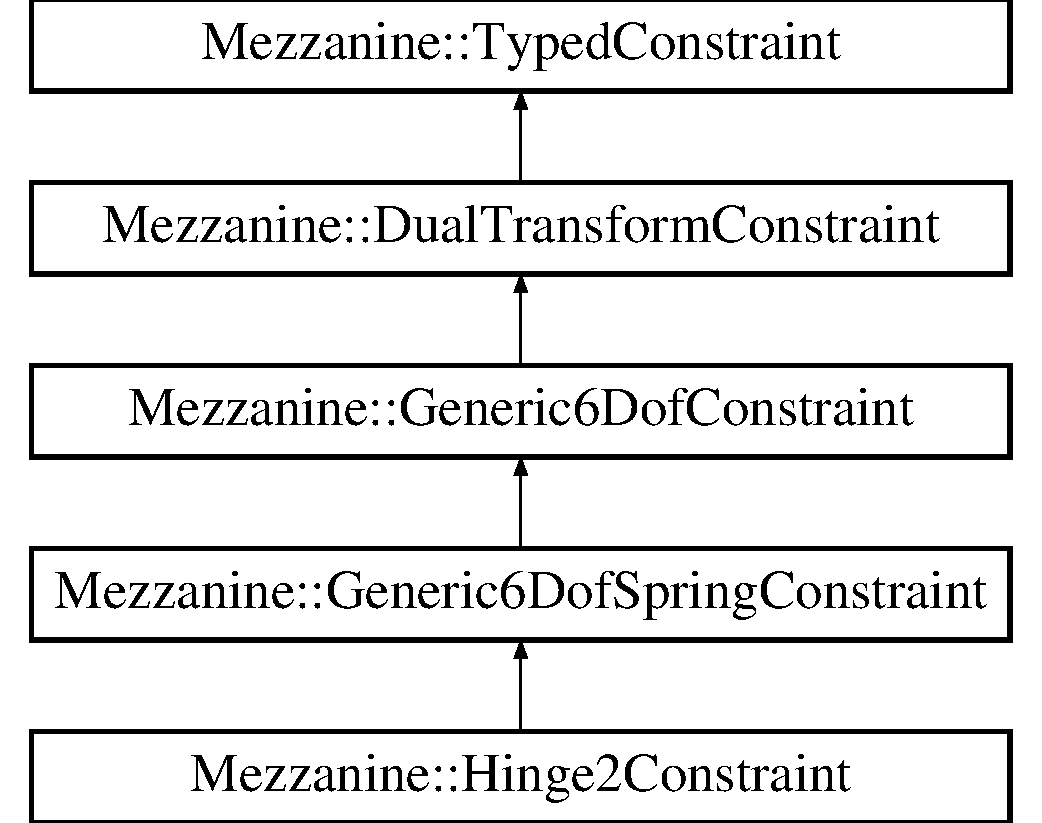
\includegraphics[height=5.000000cm]{classMezzanine_1_1Generic6DofSpringConstraint}
\end{center}
\end{figure}
\subsubsection*{Public Types}
\begin{DoxyCompactItemize}
\item 
enum \hyperlink{classMezzanine_1_1Generic6DofSpringConstraint_acdffbc070d80b5480bf1020d4a2351ed}{UsableAxis} \{ \par
\hyperlink{classMezzanine_1_1Generic6DofSpringConstraint_acdffbc070d80b5480bf1020d4a2351eda7970dfa1f659f13dc21fb5c1db80e010}{LinearX} =  0, 
\hyperlink{classMezzanine_1_1Generic6DofSpringConstraint_acdffbc070d80b5480bf1020d4a2351eda01f2486c7c0675ebe208cf57639cfb71}{LinearY} =  1, 
\hyperlink{classMezzanine_1_1Generic6DofSpringConstraint_acdffbc070d80b5480bf1020d4a2351eda7132163f87ca7bf7f9636ccc0f072a44}{LinearZ} =  2, 
\hyperlink{classMezzanine_1_1Generic6DofSpringConstraint_acdffbc070d80b5480bf1020d4a2351eda0cab58ba7b92e361bdd6015db24d000f}{AngularX} =  3, 
\par
\hyperlink{classMezzanine_1_1Generic6DofSpringConstraint_acdffbc070d80b5480bf1020d4a2351eda0e7a74d5d62a698720667afc5abf8901}{AngularY} =  4, 
\hyperlink{classMezzanine_1_1Generic6DofSpringConstraint_acdffbc070d80b5480bf1020d4a2351edacb681f499963ab2b5a9385877a5d4e5d}{AngularZ} =  5
 \}
\begin{DoxyCompactList}\small\item\em Identify the Axis a bit easier when iterating over them is less convienent than typing an Identifier. \item\end{DoxyCompactList}\end{DoxyCompactItemize}
\subsubsection*{Public Member Functions}
\begin{DoxyCompactItemize}
\item 
\hypertarget{classMezzanine_1_1Generic6DofSpringConstraint_a6f26a054060b9ab582b0f0d4e4e70701}{
virtual void {\bfseries CalculateSpringEquilibriumPoint} ()}
\label{classMezzanine_1_1Generic6DofSpringConstraint_a6f26a054060b9ab582b0f0d4e4e70701}

\item 
\hypertarget{classMezzanine_1_1Generic6DofSpringConstraint_a903fe80ef99b612749b62f713d122b47}{
virtual void {\bfseries CalculateSpringEquilibriumPoint} (int Index)}
\label{classMezzanine_1_1Generic6DofSpringConstraint_a903fe80ef99b612749b62f713d122b47}

\item 
\hyperlink{classMezzanine_1_1Generic6DofSpringConstraint_a5f6ae308296bba7226957301117dbe7a}{Generic6DofSpringConstraint} (\hyperlink{classMezzanine_1_1ActorRigid}{ActorRigid} $\ast$ActorA, \hyperlink{classMezzanine_1_1ActorRigid}{ActorRigid} $\ast$ActorB, const \hyperlink{classMezzanine_1_1Vector3}{Vector3} \&VectorA, const \hyperlink{classMezzanine_1_1Vector3}{Vector3} \&VectorB, const \hyperlink{classMezzanine_1_1Quaternion}{Quaternion} \&QuaternionA, const \hyperlink{classMezzanine_1_1Quaternion}{Quaternion} \&QuaternionB, bool UseLinearReferenceA=false)
\begin{DoxyCompactList}\small\item\em Two body Verbose constructor. \item\end{DoxyCompactList}\item 
\hyperlink{classMezzanine_1_1Generic6DofSpringConstraint_a5fa0596a4bc966d286bf9b21982717d1}{Generic6DofSpringConstraint} (\hyperlink{classMezzanine_1_1ActorRigid}{ActorRigid} $\ast$ActorA, \hyperlink{classMezzanine_1_1ActorRigid}{ActorRigid} $\ast$ActorB, const \hyperlink{classMezzanine_1_1Transform}{Transform} \&TransformA, const \hyperlink{classMezzanine_1_1Transform}{Transform} \&TransformB, bool UseLinearReferenceA=false)
\begin{DoxyCompactList}\small\item\em Two body Terse constructor. \item\end{DoxyCompactList}\item 
\hypertarget{classMezzanine_1_1Generic6DofSpringConstraint_acc847f95c75ee39241d1e67800c5a6f4}{
virtual \hyperlink{classMezzanine_1_1Vector3}{Vector3} {\bfseries GetCurrentSpringAngularEquilibriumPoints} () const }
\label{classMezzanine_1_1Generic6DofSpringConstraint_acc847f95c75ee39241d1e67800c5a6f4}

\item 
\hypertarget{classMezzanine_1_1Generic6DofSpringConstraint_a4839ced960f8dc146f40348c3dd48ad4}{
virtual \hyperlink{namespaceMezzanine_a726731b1a7df72bf3583e4a97282c6f6}{Real} {\bfseries GetCurrentSpringEquilibriumPoint} (int Index) const }
\label{classMezzanine_1_1Generic6DofSpringConstraint_a4839ced960f8dc146f40348c3dd48ad4}

\item 
\hypertarget{classMezzanine_1_1Generic6DofSpringConstraint_abf7c52ae5cb63233605f76678def4dd6}{
virtual \hyperlink{classMezzanine_1_1Vector3}{Vector3} {\bfseries GetCurrentSpringLinearEquilibriumPoints} () const }
\label{classMezzanine_1_1Generic6DofSpringConstraint_abf7c52ae5cb63233605f76678def4dd6}

\item 
virtual \hyperlink{classMezzanine_1_1Vector3}{Vector3} \hyperlink{classMezzanine_1_1Generic6DofSpringConstraint_ada9393664bbecfc885680ae677de81a3}{GetSpringAngularDamping} () const 
\begin{DoxyCompactList}\small\item\em Get the Damping for all Angular Axis. \item\end{DoxyCompactList}\item 
virtual \hyperlink{classMezzanine_1_1Vector3}{Vector3} \hyperlink{classMezzanine_1_1Generic6DofSpringConstraint_a5fab32fcbad143365220f973d7bdd0cb}{GetSpringAngularEnabled} () const 
\begin{DoxyCompactList}\small\item\em Get the Enabled Status for all Angular Axis. \item\end{DoxyCompactList}\item 
virtual \hyperlink{classMezzanine_1_1Vector3}{Vector3} \hyperlink{classMezzanine_1_1Generic6DofSpringConstraint_ac01ebe7832f9e444554809f120f1662b}{GetSpringAngularStiffness} () const 
\begin{DoxyCompactList}\small\item\em Get the Stiffness for all Angular Axis. \item\end{DoxyCompactList}\item 
virtual \hyperlink{namespaceMezzanine_a726731b1a7df72bf3583e4a97282c6f6}{Real} \hyperlink{classMezzanine_1_1Generic6DofSpringConstraint_ae48fbe9f4e98f869a4a21f83735a3540}{GetSpringDamping} (int Index) const 
\begin{DoxyCompactList}\small\item\em Retrieve the Damping of the spring on the given axis. \item\end{DoxyCompactList}\item 
virtual bool \hyperlink{classMezzanine_1_1Generic6DofSpringConstraint_aad97ef152f3917c5156e86576a163e7a}{GetSpringEnabled} (int Index) const 
\begin{DoxyCompactList}\small\item\em Retrieve the EnabledStatus of the spring on the given axis. \item\end{DoxyCompactList}\item 
virtual \hyperlink{classMezzanine_1_1Vector3}{Vector3} \hyperlink{classMezzanine_1_1Generic6DofSpringConstraint_aebffea969499acf9887b1be3c1f43204}{GetSpringLinearDamping} () const 
\begin{DoxyCompactList}\small\item\em Get the Damping for all Linear Axis. \item\end{DoxyCompactList}\item 
virtual \hyperlink{classMezzanine_1_1Vector3}{Vector3} \hyperlink{classMezzanine_1_1Generic6DofSpringConstraint_abd30a7c9b647f2f64f55f7edefdb1775}{GetSpringLinearEnabled} () const 
\begin{DoxyCompactList}\small\item\em Get the Enabled Status for all Linear Axis. \item\end{DoxyCompactList}\item 
virtual \hyperlink{classMezzanine_1_1Vector3}{Vector3} \hyperlink{classMezzanine_1_1Generic6DofSpringConstraint_a251631fcc79aa186b3ceb498f293ce84}{GetSpringLinearStiffness} () const 
\begin{DoxyCompactList}\small\item\em Get the Stiffness for all Linear Axis. \item\end{DoxyCompactList}\item 
virtual \hyperlink{namespaceMezzanine_a726731b1a7df72bf3583e4a97282c6f6}{Real} \hyperlink{classMezzanine_1_1Generic6DofSpringConstraint_adf49b712b19dfa18bfccc643871db30e}{GetSpringStiffness} (int Index) const 
\begin{DoxyCompactList}\small\item\em Retrieve the Stiffness of the spring on the given axis. \item\end{DoxyCompactList}\item 
virtual void \hyperlink{classMezzanine_1_1Generic6DofSpringConstraint_a7a0c52e6bbed9f58e4385ce2e1edff4c}{SetSpringAngularDamping} (const \hyperlink{classMezzanine_1_1Vector3}{Vector3} \&Damps)
\begin{DoxyCompactList}\small\item\em Set the Damping of the springs on each Angular Axis. \item\end{DoxyCompactList}\item 
virtual void \hyperlink{classMezzanine_1_1Generic6DofSpringConstraint_a49a615cb3033d6d29e4c1bd528fe2e5d}{SetSpringAngularEnabled} (const \hyperlink{classMezzanine_1_1Vector3}{Vector3} \&Enableness)
\begin{DoxyCompactList}\small\item\em Set the Stiffness of the springs on each Angular Axis. \item\end{DoxyCompactList}\item 
virtual void \hyperlink{classMezzanine_1_1Generic6DofSpringConstraint_a3340a2f24f934ba2abe86fb69a40240e}{SetSpringAngularStiffness} (const \hyperlink{classMezzanine_1_1Vector3}{Vector3} \&Stiffies)
\begin{DoxyCompactList}\small\item\em Set the Stiffness of the springs on each Angular Axis. \item\end{DoxyCompactList}\item 
virtual void \hyperlink{classMezzanine_1_1Generic6DofSpringConstraint_a230f5aff1e8214ef64fa86c49809597c}{SetSpringDamping} (int Index, \hyperlink{namespaceMezzanine_a726731b1a7df72bf3583e4a97282c6f6}{Real} Damping)
\begin{DoxyCompactList}\small\item\em Set the spring Damping on a given axis. \item\end{DoxyCompactList}\item 
virtual void \hyperlink{classMezzanine_1_1Generic6DofSpringConstraint_afa5c430106ef5cb423f6ffa95ddb1867}{SetSpringEnabled} (int Index, bool Enable)
\begin{DoxyCompactList}\small\item\em Set the spring's enabled status on a given axis. \item\end{DoxyCompactList}\item 
virtual void \hyperlink{classMezzanine_1_1Generic6DofSpringConstraint_a16c7c92d33b39f70d511c051ca63883c}{SetSpringLinearDamping} (const \hyperlink{classMezzanine_1_1Vector3}{Vector3} \&Damps)
\begin{DoxyCompactList}\small\item\em Set the Damping of the springs on each Linear Axis. \item\end{DoxyCompactList}\item 
virtual void \hyperlink{classMezzanine_1_1Generic6DofSpringConstraint_aa166925f112f031ab8927d6a2af4f938}{SetSpringLinearEnabled} (const \hyperlink{classMezzanine_1_1Vector3}{Vector3} \&Enableness)
\begin{DoxyCompactList}\small\item\em Set the Stiffness of the springs on each Linear Axis. \item\end{DoxyCompactList}\item 
virtual void \hyperlink{classMezzanine_1_1Generic6DofSpringConstraint_a1ad3bbe259be7d902b299568bd583cbd}{SetSpringLinearStiffness} (const \hyperlink{classMezzanine_1_1Vector3}{Vector3} \&Stiffies)
\begin{DoxyCompactList}\small\item\em Set the Stiffness of the springs on each Linear Axis. \item\end{DoxyCompactList}\item 
virtual void \hyperlink{classMezzanine_1_1Generic6DofSpringConstraint_ac3399694dcabcf63a4e475b4d3537e2b}{SetSpringStiffness} (int Index, \hyperlink{namespaceMezzanine_a726731b1a7df72bf3583e4a97282c6f6}{Real} Stiffness)
\begin{DoxyCompactList}\small\item\em Set the spring stiffness on a given axis. \item\end{DoxyCompactList}\item 
virtual \hyperlink{classMezzanine_1_1Generic6DofSpringConstraint_ab64568bca388b19c4b81ff6bd8c6dc38}{$\sim$Generic6DofSpringConstraint} ()
\begin{DoxyCompactList}\small\item\em Class destructor. \item\end{DoxyCompactList}\end{DoxyCompactItemize}
\subsubsection*{Protected Member Functions}
\begin{DoxyCompactItemize}
\item 
virtual btGeneric6DofSpringConstraint $\ast$ \hyperlink{classMezzanine_1_1Generic6DofSpringConstraint_ac57671613502a67f7b5135ba947f7e9d}{Generic6dofSpring} () const 
\item 
\hyperlink{classMezzanine_1_1Generic6DofSpringConstraint_acd643a162aba9452cd10660a89d7acf7}{Generic6DofSpringConstraint} ()
\begin{DoxyCompactList}\small\item\em Inheritance Constructor. \item\end{DoxyCompactList}\end{DoxyCompactItemize}


\subsubsection{Detailed Description}
Creates a constraint as configurable as the 6Dof constraint, but has added support for spring motion. When using functions of this class that require you to specify the index, the springs are arranged like so: \par

\begin{DoxyItemize}
\item 0: Translation X
\item 1: Translation Y
\item 2: Translation Z
\item 3: Rotation X
\item 4: Rotation Y
\item 5: Rotation Z 
\end{DoxyItemize}

Definition at line 818 of file constraint.h.



\subsubsection{Member Enumeration Documentation}
\hypertarget{classMezzanine_1_1Generic6DofSpringConstraint_acdffbc070d80b5480bf1020d4a2351ed}{
\index{Mezzanine::Generic6DofSpringConstraint@{Mezzanine::Generic6DofSpringConstraint}!UsableAxis@{UsableAxis}}
\index{UsableAxis@{UsableAxis}!Mezzanine::Generic6DofSpringConstraint@{Mezzanine::Generic6DofSpringConstraint}}
\paragraph[{UsableAxis}]{\setlength{\rightskip}{0pt plus 5cm}enum {\bf Mezzanine::Generic6DofSpringConstraint::UsableAxis}}\hfill}
\label{classMezzanine_1_1Generic6DofSpringConstraint_acdffbc070d80b5480bf1020d4a2351ed}


Identify the Axis a bit easier when iterating over them is less convienent than typing an Identifier. 

\begin{Desc}
\item[Enumerator: ]\par
\begin{description}
\index{LinearX@{LinearX}!Mezzanine::Generic6DofSpringConstraint@{Mezzanine::Generic6DofSpringConstraint}}\index{Mezzanine::Generic6DofSpringConstraint@{Mezzanine::Generic6DofSpringConstraint}!LinearX@{LinearX}}\item[{\em 
\hypertarget{classMezzanine_1_1Generic6DofSpringConstraint_acdffbc070d80b5480bf1020d4a2351eda7970dfa1f659f13dc21fb5c1db80e010}{
LinearX}
\label{classMezzanine_1_1Generic6DofSpringConstraint_acdffbc070d80b5480bf1020d4a2351eda7970dfa1f659f13dc21fb5c1db80e010}
}]Translation on the X axis. \index{LinearY@{LinearY}!Mezzanine::Generic6DofSpringConstraint@{Mezzanine::Generic6DofSpringConstraint}}\index{Mezzanine::Generic6DofSpringConstraint@{Mezzanine::Generic6DofSpringConstraint}!LinearY@{LinearY}}\item[{\em 
\hypertarget{classMezzanine_1_1Generic6DofSpringConstraint_acdffbc070d80b5480bf1020d4a2351eda01f2486c7c0675ebe208cf57639cfb71}{
LinearY}
\label{classMezzanine_1_1Generic6DofSpringConstraint_acdffbc070d80b5480bf1020d4a2351eda01f2486c7c0675ebe208cf57639cfb71}
}]Translation on the Y axis. \index{LinearZ@{LinearZ}!Mezzanine::Generic6DofSpringConstraint@{Mezzanine::Generic6DofSpringConstraint}}\index{Mezzanine::Generic6DofSpringConstraint@{Mezzanine::Generic6DofSpringConstraint}!LinearZ@{LinearZ}}\item[{\em 
\hypertarget{classMezzanine_1_1Generic6DofSpringConstraint_acdffbc070d80b5480bf1020d4a2351eda7132163f87ca7bf7f9636ccc0f072a44}{
LinearZ}
\label{classMezzanine_1_1Generic6DofSpringConstraint_acdffbc070d80b5480bf1020d4a2351eda7132163f87ca7bf7f9636ccc0f072a44}
}]Translation on the Z axis. \index{AngularX@{AngularX}!Mezzanine::Generic6DofSpringConstraint@{Mezzanine::Generic6DofSpringConstraint}}\index{Mezzanine::Generic6DofSpringConstraint@{Mezzanine::Generic6DofSpringConstraint}!AngularX@{AngularX}}\item[{\em 
\hypertarget{classMezzanine_1_1Generic6DofSpringConstraint_acdffbc070d80b5480bf1020d4a2351eda0cab58ba7b92e361bdd6015db24d000f}{
AngularX}
\label{classMezzanine_1_1Generic6DofSpringConstraint_acdffbc070d80b5480bf1020d4a2351eda0cab58ba7b92e361bdd6015db24d000f}
}]Rotation on the X axis. \index{AngularY@{AngularY}!Mezzanine::Generic6DofSpringConstraint@{Mezzanine::Generic6DofSpringConstraint}}\index{Mezzanine::Generic6DofSpringConstraint@{Mezzanine::Generic6DofSpringConstraint}!AngularY@{AngularY}}\item[{\em 
\hypertarget{classMezzanine_1_1Generic6DofSpringConstraint_acdffbc070d80b5480bf1020d4a2351eda0e7a74d5d62a698720667afc5abf8901}{
AngularY}
\label{classMezzanine_1_1Generic6DofSpringConstraint_acdffbc070d80b5480bf1020d4a2351eda0e7a74d5d62a698720667afc5abf8901}
}]Rotation on the Y axis. \index{AngularZ@{AngularZ}!Mezzanine::Generic6DofSpringConstraint@{Mezzanine::Generic6DofSpringConstraint}}\index{Mezzanine::Generic6DofSpringConstraint@{Mezzanine::Generic6DofSpringConstraint}!AngularZ@{AngularZ}}\item[{\em 
\hypertarget{classMezzanine_1_1Generic6DofSpringConstraint_acdffbc070d80b5480bf1020d4a2351edacb681f499963ab2b5a9385877a5d4e5d}{
AngularZ}
\label{classMezzanine_1_1Generic6DofSpringConstraint_acdffbc070d80b5480bf1020d4a2351edacb681f499963ab2b5a9385877a5d4e5d}
}]Rotation on the Z axis. \end{description}
\end{Desc}



Reimplemented from \hyperlink{classMezzanine_1_1Generic6DofConstraint_ac00067026a7d4e7c6832f169c754d585}{Mezzanine::Generic6DofConstraint}.



Definition at line 828 of file constraint.h.



\subsubsection{Constructor \& Destructor Documentation}
\hypertarget{classMezzanine_1_1Generic6DofSpringConstraint_acd643a162aba9452cd10660a89d7acf7}{
\index{Mezzanine::Generic6DofSpringConstraint@{Mezzanine::Generic6DofSpringConstraint}!Generic6DofSpringConstraint@{Generic6DofSpringConstraint}}
\index{Generic6DofSpringConstraint@{Generic6DofSpringConstraint}!Mezzanine::Generic6DofSpringConstraint@{Mezzanine::Generic6DofSpringConstraint}}
\paragraph[{Generic6DofSpringConstraint}]{\setlength{\rightskip}{0pt plus 5cm}Mezzanine::Generic6DofSpringConstraint::Generic6DofSpringConstraint (
\begin{DoxyParamCaption}
{}
\end{DoxyParamCaption}
)\hspace{0.3cm}{\ttfamily  \mbox{[}protected\mbox{]}}}\hfill}
\label{classMezzanine_1_1Generic6DofSpringConstraint_acd643a162aba9452cd10660a89d7acf7}


Inheritance Constructor. 

This is only called by derived classes, and shouldn't be called manually. \hypertarget{classMezzanine_1_1Generic6DofSpringConstraint_a5f6ae308296bba7226957301117dbe7a}{
\index{Mezzanine::Generic6DofSpringConstraint@{Mezzanine::Generic6DofSpringConstraint}!Generic6DofSpringConstraint@{Generic6DofSpringConstraint}}
\index{Generic6DofSpringConstraint@{Generic6DofSpringConstraint}!Mezzanine::Generic6DofSpringConstraint@{Mezzanine::Generic6DofSpringConstraint}}
\paragraph[{Generic6DofSpringConstraint}]{\setlength{\rightskip}{0pt plus 5cm}Mezzanine::Generic6DofSpringConstraint::Generic6DofSpringConstraint (
\begin{DoxyParamCaption}
\item[{{\bf ActorRigid} $\ast$}]{ActorA, }
\item[{{\bf ActorRigid} $\ast$}]{ActorB, }
\item[{const {\bf Vector3} \&}]{VectorA, }
\item[{const {\bf Vector3} \&}]{VectorB, }
\item[{const {\bf Quaternion} \&}]{QuaternionA, }
\item[{const {\bf Quaternion} \&}]{QuaternionB, }
\item[{bool}]{UseLinearReferenceA = {\ttfamily false}}
\end{DoxyParamCaption}
)}\hfill}
\label{classMezzanine_1_1Generic6DofSpringConstraint_a5f6ae308296bba7226957301117dbe7a}


Two body Verbose constructor. 


\begin{DoxyParams}{Parameters}
{\em ActorA} & The First body to be bound \\
\hline
{\em ActorB} & The Second body to be bound \\
\hline
{\em VectorA} & The offset from ActorA's center of gravity to get to match an offset from ActorB \\
\hline
{\em VectorB} & The offset from ActorB's center of gravity. \\
\hline
{\em QuaternionA} & Relative rotation from ActorA \\
\hline
{\em QuaternionB} & Relative rotation from ActorB \\
\hline
{\em UseLinearReferenceA} & Perform Linear math from ActorA's perspective, default to false. \\
\hline
\end{DoxyParams}
\hypertarget{classMezzanine_1_1Generic6DofSpringConstraint_a5fa0596a4bc966d286bf9b21982717d1}{
\index{Mezzanine::Generic6DofSpringConstraint@{Mezzanine::Generic6DofSpringConstraint}!Generic6DofSpringConstraint@{Generic6DofSpringConstraint}}
\index{Generic6DofSpringConstraint@{Generic6DofSpringConstraint}!Mezzanine::Generic6DofSpringConstraint@{Mezzanine::Generic6DofSpringConstraint}}
\paragraph[{Generic6DofSpringConstraint}]{\setlength{\rightskip}{0pt plus 5cm}Mezzanine::Generic6DofSpringConstraint::Generic6DofSpringConstraint (
\begin{DoxyParamCaption}
\item[{{\bf ActorRigid} $\ast$}]{ActorA, }
\item[{{\bf ActorRigid} $\ast$}]{ActorB, }
\item[{const {\bf Transform} \&}]{TransformA, }
\item[{const {\bf Transform} \&}]{TransformB, }
\item[{bool}]{UseLinearReferenceA = {\ttfamily false}}
\end{DoxyParamCaption}
)}\hfill}
\label{classMezzanine_1_1Generic6DofSpringConstraint_a5fa0596a4bc966d286bf9b21982717d1}


Two body Terse constructor. 


\begin{DoxyParams}{Parameters}
{\em ActorA} & The First body to be bound \\
\hline
{\em ActorB} & The Second body to be bound \\
\hline
{\em TransformA} & The offset and rotation from ActorA's center of gravity to get to match an offset from ActorB \\
\hline
{\em TransformB} & The offset and rotation from ActorB's center of gravity. \\
\hline
{\em UseLinearReferenceA} & Perform Linear math from ActorA's perspective, default to false. \\
\hline
\end{DoxyParams}
\hypertarget{classMezzanine_1_1Generic6DofSpringConstraint_ab64568bca388b19c4b81ff6bd8c6dc38}{
\index{Mezzanine::Generic6DofSpringConstraint@{Mezzanine::Generic6DofSpringConstraint}!$\sim$Generic6DofSpringConstraint@{$\sim$Generic6DofSpringConstraint}}
\index{$\sim$Generic6DofSpringConstraint@{$\sim$Generic6DofSpringConstraint}!Mezzanine::Generic6DofSpringConstraint@{Mezzanine::Generic6DofSpringConstraint}}
\paragraph[{$\sim$Generic6DofSpringConstraint}]{\setlength{\rightskip}{0pt plus 5cm}virtual Mezzanine::Generic6DofSpringConstraint::$\sim$Generic6DofSpringConstraint (
\begin{DoxyParamCaption}
{}
\end{DoxyParamCaption}
)\hspace{0.3cm}{\ttfamily  \mbox{[}virtual\mbox{]}}}\hfill}
\label{classMezzanine_1_1Generic6DofSpringConstraint_ab64568bca388b19c4b81ff6bd8c6dc38}


Class destructor. 

The class destructor. 

\subsubsection{Member Function Documentation}
\hypertarget{classMezzanine_1_1Generic6DofSpringConstraint_ac57671613502a67f7b5135ba947f7e9d}{
\index{Mezzanine::Generic6DofSpringConstraint@{Mezzanine::Generic6DofSpringConstraint}!Generic6dofSpring@{Generic6dofSpring}}
\index{Generic6dofSpring@{Generic6dofSpring}!Mezzanine::Generic6DofSpringConstraint@{Mezzanine::Generic6DofSpringConstraint}}
\paragraph[{Generic6dofSpring}]{\setlength{\rightskip}{0pt plus 5cm}virtual btGeneric6DofSpringConstraint$\ast$ Mezzanine::Generic6DofSpringConstraint::Generic6dofSpring (
\begin{DoxyParamCaption}
{}
\end{DoxyParamCaption}
) const\hspace{0.3cm}{\ttfamily  \mbox{[}protected, virtual\mbox{]}}}\hfill}
\label{classMezzanine_1_1Generic6DofSpringConstraint_ac57671613502a67f7b5135ba947f7e9d}
Get the Bullet constraint that this class encapsulates. 

\begin{DoxyReturn}{Returns}
A pointer to the btTypedConstraint that stores the underlying constraint. 
\end{DoxyReturn}
 \hypertarget{classMezzanine_1_1Generic6DofSpringConstraint_ada9393664bbecfc885680ae677de81a3}{
\index{Mezzanine::Generic6DofSpringConstraint@{Mezzanine::Generic6DofSpringConstraint}!GetSpringAngularDamping@{GetSpringAngularDamping}}
\index{GetSpringAngularDamping@{GetSpringAngularDamping}!Mezzanine::Generic6DofSpringConstraint@{Mezzanine::Generic6DofSpringConstraint}}
\paragraph[{GetSpringAngularDamping}]{\setlength{\rightskip}{0pt plus 5cm}virtual {\bf Vector3} Mezzanine::Generic6DofSpringConstraint::GetSpringAngularDamping (
\begin{DoxyParamCaption}
{}
\end{DoxyParamCaption}
) const\hspace{0.3cm}{\ttfamily  \mbox{[}virtual\mbox{]}}}\hfill}
\label{classMezzanine_1_1Generic6DofSpringConstraint_ada9393664bbecfc885680ae677de81a3}


Get the Damping for all Angular Axis. 

\begin{DoxyReturn}{Returns}
A \hyperlink{classMezzanine_1_1Vector3}{Vector3} with the Damping on the X, Y and Z Angular Axis. 
\end{DoxyReturn}
\hypertarget{classMezzanine_1_1Generic6DofSpringConstraint_a5fab32fcbad143365220f973d7bdd0cb}{
\index{Mezzanine::Generic6DofSpringConstraint@{Mezzanine::Generic6DofSpringConstraint}!GetSpringAngularEnabled@{GetSpringAngularEnabled}}
\index{GetSpringAngularEnabled@{GetSpringAngularEnabled}!Mezzanine::Generic6DofSpringConstraint@{Mezzanine::Generic6DofSpringConstraint}}
\paragraph[{GetSpringAngularEnabled}]{\setlength{\rightskip}{0pt plus 5cm}virtual {\bf Vector3} Mezzanine::Generic6DofSpringConstraint::GetSpringAngularEnabled (
\begin{DoxyParamCaption}
{}
\end{DoxyParamCaption}
) const\hspace{0.3cm}{\ttfamily  \mbox{[}virtual\mbox{]}}}\hfill}
\label{classMezzanine_1_1Generic6DofSpringConstraint_a5fab32fcbad143365220f973d7bdd0cb}


Get the Enabled Status for all Angular Axis. 

\begin{DoxyReturn}{Returns}
A \hyperlink{classMezzanine_1_1Vector3}{Vector3} with the Enabled Status on the X, Y and Z Angular Axis. 
\end{DoxyReturn}
\hypertarget{classMezzanine_1_1Generic6DofSpringConstraint_ac01ebe7832f9e444554809f120f1662b}{
\index{Mezzanine::Generic6DofSpringConstraint@{Mezzanine::Generic6DofSpringConstraint}!GetSpringAngularStiffness@{GetSpringAngularStiffness}}
\index{GetSpringAngularStiffness@{GetSpringAngularStiffness}!Mezzanine::Generic6DofSpringConstraint@{Mezzanine::Generic6DofSpringConstraint}}
\paragraph[{GetSpringAngularStiffness}]{\setlength{\rightskip}{0pt plus 5cm}virtual {\bf Vector3} Mezzanine::Generic6DofSpringConstraint::GetSpringAngularStiffness (
\begin{DoxyParamCaption}
{}
\end{DoxyParamCaption}
) const\hspace{0.3cm}{\ttfamily  \mbox{[}virtual\mbox{]}}}\hfill}
\label{classMezzanine_1_1Generic6DofSpringConstraint_ac01ebe7832f9e444554809f120f1662b}


Get the Stiffness for all Angular Axis. 

\begin{DoxyReturn}{Returns}
A \hyperlink{classMezzanine_1_1Vector3}{Vector3} with the Stiffness on the X, Y and Z Angular Axis. 
\end{DoxyReturn}
\hypertarget{classMezzanine_1_1Generic6DofSpringConstraint_ae48fbe9f4e98f869a4a21f83735a3540}{
\index{Mezzanine::Generic6DofSpringConstraint@{Mezzanine::Generic6DofSpringConstraint}!GetSpringDamping@{GetSpringDamping}}
\index{GetSpringDamping@{GetSpringDamping}!Mezzanine::Generic6DofSpringConstraint@{Mezzanine::Generic6DofSpringConstraint}}
\paragraph[{GetSpringDamping}]{\setlength{\rightskip}{0pt plus 5cm}virtual {\bf Real} Mezzanine::Generic6DofSpringConstraint::GetSpringDamping (
\begin{DoxyParamCaption}
\item[{int}]{Index}
\end{DoxyParamCaption}
) const\hspace{0.3cm}{\ttfamily  \mbox{[}virtual\mbox{]}}}\hfill}
\label{classMezzanine_1_1Generic6DofSpringConstraint_ae48fbe9f4e98f869a4a21f83735a3540}


Retrieve the Damping of the spring on the given axis. 


\begin{DoxyParams}{Parameters}
{\em Index} & The Desired axis. This accepts 0,1,2 for Linear X,Y, and Z or 3,4,5 for Angular X,Y, and Z. This can also accept Item from this classes Usable Axis enum; \\
\hline
\end{DoxyParams}
\begin{DoxyReturn}{Returns}
A real with the requested value. 
\end{DoxyReturn}
\hypertarget{classMezzanine_1_1Generic6DofSpringConstraint_aad97ef152f3917c5156e86576a163e7a}{
\index{Mezzanine::Generic6DofSpringConstraint@{Mezzanine::Generic6DofSpringConstraint}!GetSpringEnabled@{GetSpringEnabled}}
\index{GetSpringEnabled@{GetSpringEnabled}!Mezzanine::Generic6DofSpringConstraint@{Mezzanine::Generic6DofSpringConstraint}}
\paragraph[{GetSpringEnabled}]{\setlength{\rightskip}{0pt plus 5cm}virtual bool Mezzanine::Generic6DofSpringConstraint::GetSpringEnabled (
\begin{DoxyParamCaption}
\item[{int}]{Index}
\end{DoxyParamCaption}
) const\hspace{0.3cm}{\ttfamily  \mbox{[}virtual\mbox{]}}}\hfill}
\label{classMezzanine_1_1Generic6DofSpringConstraint_aad97ef152f3917c5156e86576a163e7a}


Retrieve the EnabledStatus of the spring on the given axis. 


\begin{DoxyParams}{Parameters}
{\em Index} & The Desired axis. This accepts 0,1,2 for Linear X,Y, and Z or 3,4,5 for Angular X,Y, and Z. This can also accept Item from this classes Usable Axis enum; \\
\hline
\end{DoxyParams}
\begin{DoxyReturn}{Returns}
A bool with the requested value. 
\end{DoxyReturn}
\hypertarget{classMezzanine_1_1Generic6DofSpringConstraint_aebffea969499acf9887b1be3c1f43204}{
\index{Mezzanine::Generic6DofSpringConstraint@{Mezzanine::Generic6DofSpringConstraint}!GetSpringLinearDamping@{GetSpringLinearDamping}}
\index{GetSpringLinearDamping@{GetSpringLinearDamping}!Mezzanine::Generic6DofSpringConstraint@{Mezzanine::Generic6DofSpringConstraint}}
\paragraph[{GetSpringLinearDamping}]{\setlength{\rightskip}{0pt plus 5cm}virtual {\bf Vector3} Mezzanine::Generic6DofSpringConstraint::GetSpringLinearDamping (
\begin{DoxyParamCaption}
{}
\end{DoxyParamCaption}
) const\hspace{0.3cm}{\ttfamily  \mbox{[}virtual\mbox{]}}}\hfill}
\label{classMezzanine_1_1Generic6DofSpringConstraint_aebffea969499acf9887b1be3c1f43204}


Get the Damping for all Linear Axis. 

\begin{DoxyReturn}{Returns}
A \hyperlink{classMezzanine_1_1Vector3}{Vector3} with the Damping on the X, Y and Z Linear Axis. 
\end{DoxyReturn}
\hypertarget{classMezzanine_1_1Generic6DofSpringConstraint_abd30a7c9b647f2f64f55f7edefdb1775}{
\index{Mezzanine::Generic6DofSpringConstraint@{Mezzanine::Generic6DofSpringConstraint}!GetSpringLinearEnabled@{GetSpringLinearEnabled}}
\index{GetSpringLinearEnabled@{GetSpringLinearEnabled}!Mezzanine::Generic6DofSpringConstraint@{Mezzanine::Generic6DofSpringConstraint}}
\paragraph[{GetSpringLinearEnabled}]{\setlength{\rightskip}{0pt plus 5cm}virtual {\bf Vector3} Mezzanine::Generic6DofSpringConstraint::GetSpringLinearEnabled (
\begin{DoxyParamCaption}
{}
\end{DoxyParamCaption}
) const\hspace{0.3cm}{\ttfamily  \mbox{[}virtual\mbox{]}}}\hfill}
\label{classMezzanine_1_1Generic6DofSpringConstraint_abd30a7c9b647f2f64f55f7edefdb1775}


Get the Enabled Status for all Linear Axis. 

\begin{DoxyReturn}{Returns}
A \hyperlink{classMezzanine_1_1Vector3}{Vector3} with the Enabled Status on the X, Y and Z Linear Axis. 
\end{DoxyReturn}
\hypertarget{classMezzanine_1_1Generic6DofSpringConstraint_a251631fcc79aa186b3ceb498f293ce84}{
\index{Mezzanine::Generic6DofSpringConstraint@{Mezzanine::Generic6DofSpringConstraint}!GetSpringLinearStiffness@{GetSpringLinearStiffness}}
\index{GetSpringLinearStiffness@{GetSpringLinearStiffness}!Mezzanine::Generic6DofSpringConstraint@{Mezzanine::Generic6DofSpringConstraint}}
\paragraph[{GetSpringLinearStiffness}]{\setlength{\rightskip}{0pt plus 5cm}virtual {\bf Vector3} Mezzanine::Generic6DofSpringConstraint::GetSpringLinearStiffness (
\begin{DoxyParamCaption}
{}
\end{DoxyParamCaption}
) const\hspace{0.3cm}{\ttfamily  \mbox{[}virtual\mbox{]}}}\hfill}
\label{classMezzanine_1_1Generic6DofSpringConstraint_a251631fcc79aa186b3ceb498f293ce84}


Get the Stiffness for all Linear Axis. 

\begin{DoxyReturn}{Returns}
A \hyperlink{classMezzanine_1_1Vector3}{Vector3} with the Stiffness on the X, Y and Z Linear Axis. 
\end{DoxyReturn}
\hypertarget{classMezzanine_1_1Generic6DofSpringConstraint_adf49b712b19dfa18bfccc643871db30e}{
\index{Mezzanine::Generic6DofSpringConstraint@{Mezzanine::Generic6DofSpringConstraint}!GetSpringStiffness@{GetSpringStiffness}}
\index{GetSpringStiffness@{GetSpringStiffness}!Mezzanine::Generic6DofSpringConstraint@{Mezzanine::Generic6DofSpringConstraint}}
\paragraph[{GetSpringStiffness}]{\setlength{\rightskip}{0pt plus 5cm}virtual {\bf Real} Mezzanine::Generic6DofSpringConstraint::GetSpringStiffness (
\begin{DoxyParamCaption}
\item[{int}]{Index}
\end{DoxyParamCaption}
) const\hspace{0.3cm}{\ttfamily  \mbox{[}virtual\mbox{]}}}\hfill}
\label{classMezzanine_1_1Generic6DofSpringConstraint_adf49b712b19dfa18bfccc643871db30e}


Retrieve the Stiffness of the spring on the given axis. 


\begin{DoxyParams}{Parameters}
{\em Index} & The Desired axis. This accepts 0,1,2 for Linear X,Y, and Z or 3,4,5 for Angular X,Y, and Z. This can also accept Item from this classes Usable Axis enum; \\
\hline
\end{DoxyParams}
\begin{DoxyReturn}{Returns}
A real with the requested value; 
\end{DoxyReturn}
\hypertarget{classMezzanine_1_1Generic6DofSpringConstraint_a7a0c52e6bbed9f58e4385ce2e1edff4c}{
\index{Mezzanine::Generic6DofSpringConstraint@{Mezzanine::Generic6DofSpringConstraint}!SetSpringAngularDamping@{SetSpringAngularDamping}}
\index{SetSpringAngularDamping@{SetSpringAngularDamping}!Mezzanine::Generic6DofSpringConstraint@{Mezzanine::Generic6DofSpringConstraint}}
\paragraph[{SetSpringAngularDamping}]{\setlength{\rightskip}{0pt plus 5cm}virtual void Mezzanine::Generic6DofSpringConstraint::SetSpringAngularDamping (
\begin{DoxyParamCaption}
\item[{const {\bf Vector3} \&}]{Damps}
\end{DoxyParamCaption}
)\hspace{0.3cm}{\ttfamily  \mbox{[}virtual\mbox{]}}}\hfill}
\label{classMezzanine_1_1Generic6DofSpringConstraint_a7a0c52e6bbed9f58e4385ce2e1edff4c}


Set the Damping of the springs on each Angular Axis. 


\begin{DoxyParams}{Parameters}
{\em Damps} & A \hyperlink{classMezzanine_1_1Vector3}{Vector3} containing the X, Y and Z desired damping. \\
\hline
\end{DoxyParams}
\hypertarget{classMezzanine_1_1Generic6DofSpringConstraint_a49a615cb3033d6d29e4c1bd528fe2e5d}{
\index{Mezzanine::Generic6DofSpringConstraint@{Mezzanine::Generic6DofSpringConstraint}!SetSpringAngularEnabled@{SetSpringAngularEnabled}}
\index{SetSpringAngularEnabled@{SetSpringAngularEnabled}!Mezzanine::Generic6DofSpringConstraint@{Mezzanine::Generic6DofSpringConstraint}}
\paragraph[{SetSpringAngularEnabled}]{\setlength{\rightskip}{0pt plus 5cm}virtual void Mezzanine::Generic6DofSpringConstraint::SetSpringAngularEnabled (
\begin{DoxyParamCaption}
\item[{const {\bf Vector3} \&}]{Enableness}
\end{DoxyParamCaption}
)\hspace{0.3cm}{\ttfamily  \mbox{[}virtual\mbox{]}}}\hfill}
\label{classMezzanine_1_1Generic6DofSpringConstraint_a49a615cb3033d6d29e4c1bd528fe2e5d}


Set the Stiffness of the springs on each Angular Axis. 


\begin{DoxyParams}{Parameters}
{\em Stiffies} & A \hyperlink{classMezzanine_1_1Vector3}{Vector3} containing the X, Y and Z enabled statuses. This is interpretted as 0 for false and any other value for true. \\
\hline
\end{DoxyParams}
\hypertarget{classMezzanine_1_1Generic6DofSpringConstraint_a3340a2f24f934ba2abe86fb69a40240e}{
\index{Mezzanine::Generic6DofSpringConstraint@{Mezzanine::Generic6DofSpringConstraint}!SetSpringAngularStiffness@{SetSpringAngularStiffness}}
\index{SetSpringAngularStiffness@{SetSpringAngularStiffness}!Mezzanine::Generic6DofSpringConstraint@{Mezzanine::Generic6DofSpringConstraint}}
\paragraph[{SetSpringAngularStiffness}]{\setlength{\rightskip}{0pt plus 5cm}virtual void Mezzanine::Generic6DofSpringConstraint::SetSpringAngularStiffness (
\begin{DoxyParamCaption}
\item[{const {\bf Vector3} \&}]{Stiffies}
\end{DoxyParamCaption}
)\hspace{0.3cm}{\ttfamily  \mbox{[}virtual\mbox{]}}}\hfill}
\label{classMezzanine_1_1Generic6DofSpringConstraint_a3340a2f24f934ba2abe86fb69a40240e}


Set the Stiffness of the springs on each Angular Axis. 


\begin{DoxyParams}{Parameters}
{\em Stiffies} & A \hyperlink{classMezzanine_1_1Vector3}{Vector3} containing the X, Y and Z stiffnesses. \\
\hline
\end{DoxyParams}
\hypertarget{classMezzanine_1_1Generic6DofSpringConstraint_a230f5aff1e8214ef64fa86c49809597c}{
\index{Mezzanine::Generic6DofSpringConstraint@{Mezzanine::Generic6DofSpringConstraint}!SetSpringDamping@{SetSpringDamping}}
\index{SetSpringDamping@{SetSpringDamping}!Mezzanine::Generic6DofSpringConstraint@{Mezzanine::Generic6DofSpringConstraint}}
\paragraph[{SetSpringDamping}]{\setlength{\rightskip}{0pt plus 5cm}virtual void Mezzanine::Generic6DofSpringConstraint::SetSpringDamping (
\begin{DoxyParamCaption}
\item[{int}]{Index, }
\item[{{\bf Real}}]{Damping}
\end{DoxyParamCaption}
)\hspace{0.3cm}{\ttfamily  \mbox{[}virtual\mbox{]}}}\hfill}
\label{classMezzanine_1_1Generic6DofSpringConstraint_a230f5aff1e8214ef64fa86c49809597c}


Set the spring Damping on a given axis. 


\begin{DoxyParams}{Parameters}
{\em Index} & The Desired axis. This accepts 0,1,2 for Linear X,Y, and Z or 3,4,5 for Angular X,Y, and Z. This can also accept Item from this classes Usable Axis enum; \\
\hline
{\em Damping} & A real with the new desired Damping. \\
\hline
\end{DoxyParams}
\hypertarget{classMezzanine_1_1Generic6DofSpringConstraint_afa5c430106ef5cb423f6ffa95ddb1867}{
\index{Mezzanine::Generic6DofSpringConstraint@{Mezzanine::Generic6DofSpringConstraint}!SetSpringEnabled@{SetSpringEnabled}}
\index{SetSpringEnabled@{SetSpringEnabled}!Mezzanine::Generic6DofSpringConstraint@{Mezzanine::Generic6DofSpringConstraint}}
\paragraph[{SetSpringEnabled}]{\setlength{\rightskip}{0pt plus 5cm}virtual void Mezzanine::Generic6DofSpringConstraint::SetSpringEnabled (
\begin{DoxyParamCaption}
\item[{int}]{Index, }
\item[{bool}]{Enable}
\end{DoxyParamCaption}
)\hspace{0.3cm}{\ttfamily  \mbox{[}virtual\mbox{]}}}\hfill}
\label{classMezzanine_1_1Generic6DofSpringConstraint_afa5c430106ef5cb423f6ffa95ddb1867}


Set the spring's enabled status on a given axis. 


\begin{DoxyParams}{Parameters}
{\em Index} & The Desired axis. This accepts 0,1,2 for Linear X,Y, and Z or 3,4,5 for Angular X,Y, and Z. This can also accept Item from this classes Usable Axis enum; \\
\hline
{\em Enable} & A bool with the spring's enabled status. \\
\hline
\end{DoxyParams}
\hypertarget{classMezzanine_1_1Generic6DofSpringConstraint_a16c7c92d33b39f70d511c051ca63883c}{
\index{Mezzanine::Generic6DofSpringConstraint@{Mezzanine::Generic6DofSpringConstraint}!SetSpringLinearDamping@{SetSpringLinearDamping}}
\index{SetSpringLinearDamping@{SetSpringLinearDamping}!Mezzanine::Generic6DofSpringConstraint@{Mezzanine::Generic6DofSpringConstraint}}
\paragraph[{SetSpringLinearDamping}]{\setlength{\rightskip}{0pt plus 5cm}virtual void Mezzanine::Generic6DofSpringConstraint::SetSpringLinearDamping (
\begin{DoxyParamCaption}
\item[{const {\bf Vector3} \&}]{Damps}
\end{DoxyParamCaption}
)\hspace{0.3cm}{\ttfamily  \mbox{[}virtual\mbox{]}}}\hfill}
\label{classMezzanine_1_1Generic6DofSpringConstraint_a16c7c92d33b39f70d511c051ca63883c}


Set the Damping of the springs on each Linear Axis. 


\begin{DoxyParams}{Parameters}
{\em Damps} & A \hyperlink{classMezzanine_1_1Vector3}{Vector3} containing the X, Y and Z desired damping. \\
\hline
\end{DoxyParams}
\hypertarget{classMezzanine_1_1Generic6DofSpringConstraint_aa166925f112f031ab8927d6a2af4f938}{
\index{Mezzanine::Generic6DofSpringConstraint@{Mezzanine::Generic6DofSpringConstraint}!SetSpringLinearEnabled@{SetSpringLinearEnabled}}
\index{SetSpringLinearEnabled@{SetSpringLinearEnabled}!Mezzanine::Generic6DofSpringConstraint@{Mezzanine::Generic6DofSpringConstraint}}
\paragraph[{SetSpringLinearEnabled}]{\setlength{\rightskip}{0pt plus 5cm}virtual void Mezzanine::Generic6DofSpringConstraint::SetSpringLinearEnabled (
\begin{DoxyParamCaption}
\item[{const {\bf Vector3} \&}]{Enableness}
\end{DoxyParamCaption}
)\hspace{0.3cm}{\ttfamily  \mbox{[}virtual\mbox{]}}}\hfill}
\label{classMezzanine_1_1Generic6DofSpringConstraint_aa166925f112f031ab8927d6a2af4f938}


Set the Stiffness of the springs on each Linear Axis. 


\begin{DoxyParams}{Parameters}
{\em Stiffies} & A \hyperlink{classMezzanine_1_1Vector3}{Vector3} containing the X, Y and Z enabled statuses. This is interpretted as 0 for false and any other value for true. \\
\hline
\end{DoxyParams}
\hypertarget{classMezzanine_1_1Generic6DofSpringConstraint_a1ad3bbe259be7d902b299568bd583cbd}{
\index{Mezzanine::Generic6DofSpringConstraint@{Mezzanine::Generic6DofSpringConstraint}!SetSpringLinearStiffness@{SetSpringLinearStiffness}}
\index{SetSpringLinearStiffness@{SetSpringLinearStiffness}!Mezzanine::Generic6DofSpringConstraint@{Mezzanine::Generic6DofSpringConstraint}}
\paragraph[{SetSpringLinearStiffness}]{\setlength{\rightskip}{0pt plus 5cm}virtual void Mezzanine::Generic6DofSpringConstraint::SetSpringLinearStiffness (
\begin{DoxyParamCaption}
\item[{const {\bf Vector3} \&}]{Stiffies}
\end{DoxyParamCaption}
)\hspace{0.3cm}{\ttfamily  \mbox{[}virtual\mbox{]}}}\hfill}
\label{classMezzanine_1_1Generic6DofSpringConstraint_a1ad3bbe259be7d902b299568bd583cbd}


Set the Stiffness of the springs on each Linear Axis. 


\begin{DoxyParams}{Parameters}
{\em Stiffies} & A \hyperlink{classMezzanine_1_1Vector3}{Vector3} containing the X, Y and Z stiffnesses. \\
\hline
\end{DoxyParams}
\hypertarget{classMezzanine_1_1Generic6DofSpringConstraint_ac3399694dcabcf63a4e475b4d3537e2b}{
\index{Mezzanine::Generic6DofSpringConstraint@{Mezzanine::Generic6DofSpringConstraint}!SetSpringStiffness@{SetSpringStiffness}}
\index{SetSpringStiffness@{SetSpringStiffness}!Mezzanine::Generic6DofSpringConstraint@{Mezzanine::Generic6DofSpringConstraint}}
\paragraph[{SetSpringStiffness}]{\setlength{\rightskip}{0pt plus 5cm}virtual void Mezzanine::Generic6DofSpringConstraint::SetSpringStiffness (
\begin{DoxyParamCaption}
\item[{int}]{Index, }
\item[{{\bf Real}}]{Stiffness}
\end{DoxyParamCaption}
)\hspace{0.3cm}{\ttfamily  \mbox{[}virtual\mbox{]}}}\hfill}
\label{classMezzanine_1_1Generic6DofSpringConstraint_ac3399694dcabcf63a4e475b4d3537e2b}


Set the spring stiffness on a given axis. 


\begin{DoxyParams}{Parameters}
{\em Index} & The Desired axis. This accepts 0,1,2 for Linear X,Y, and Z or 3,4,5 for Angular X,Y, and Z. This can also accept Item from this classes Usable Axis enum; \\
\hline
{\em Stiffness} & A real with the new desired stiffness. \\
\hline
\end{DoxyParams}


The documentation for this class was generated from the following file:\begin{DoxyCompactItemize}
\item 
constraint.h\end{DoxyCompactItemize}

\hypertarget{classMezzanine_1_1GraphicsManager}{
\subsection{Mezzanine::GraphicsManager Class Reference}
\label{classMezzanine_1_1GraphicsManager}\index{Mezzanine::GraphicsManager@{Mezzanine::GraphicsManager}}
}


This is intended to store basic graphics setting for the user.  




{\ttfamily \#include $<$graphicsmanager.h$>$}

Inheritance diagram for Mezzanine::GraphicsManager:\begin{figure}[H]
\begin{center}
\leavevmode
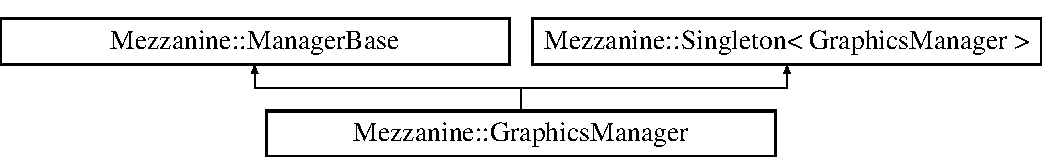
\includegraphics[height=2.000000cm]{classMezzanine_1_1GraphicsManager}
\end{center}
\end{figure}
\subsubsection*{Public Member Functions}
\begin{DoxyCompactItemize}
\item 
\hyperlink{classMezzanine_1_1GameWindow}{GameWindow} $\ast$ \hyperlink{classMezzanine_1_1GraphicsManager_a6d5efb7e23d2274bc5d49dd37763e645}{CreateGameWindow} (const \hyperlink{namespaceMezzanine_acf9fcc130e6ebf08e3d8491aebcf1c86}{String} \&WindowCaption, const \hyperlink{namespaceMezzanine_adcbb6ce6d1eb4379d109e51171e2e493}{Whole} \&Width, const \hyperlink{namespaceMezzanine_adcbb6ce6d1eb4379d109e51171e2e493}{Whole} \&Height, const \hyperlink{namespaceMezzanine_adcbb6ce6d1eb4379d109e51171e2e493}{Whole} \&Flags)
\begin{DoxyCompactList}\small\item\em Creates a new game window to be rendered to. \item\end{DoxyCompactList}\item 
void \hyperlink{classMezzanine_1_1GraphicsManager_a9ff5f5d4ed74f97e61fe3e6f170fa0c9}{DestroyAllGameWindows} (bool ExcludePrimary=true)
\begin{DoxyCompactList}\small\item\em Destroys every game window created. \item\end{DoxyCompactList}\item 
void \hyperlink{classMezzanine_1_1GraphicsManager_a0f03feff9d284100bdf7715ec504474c}{DestroyGameWindow} (\hyperlink{classMezzanine_1_1GameWindow}{GameWindow} $\ast$ToBeDestroyed)
\begin{DoxyCompactList}\small\item\em Destroys a created game window by index. \item\end{DoxyCompactList}\item 
virtual void \hyperlink{classMezzanine_1_1GraphicsManager_ae940c81cd1401fda34abc6fd53ede45a}{DoMainLoopItems} ()
\begin{DoxyCompactList}\small\item\em This is where the rendering takes place. \item\end{DoxyCompactList}\item 
\hyperlink{namespaceMezzanine_a1bb0347c37954bc71c4344e4b55c729a}{Mezzanine::RenderSystem} \hyperlink{classMezzanine_1_1GraphicsManager_a9592364a2ecc1b24a2ce50ce88095ffd}{GetCurrRenderSystem} ()
\begin{DoxyCompactList}\small\item\em Gets the current rendersystem being used. \item\end{DoxyCompactList}\item 
const \hyperlink{structMezzanine_1_1GraphicsSettings}{GraphicsSettings} \& \hyperlink{classMezzanine_1_1GraphicsManager_aba36bc3b2e611eb3c3d47fab001805ab}{GetDefaultSettings} ()
\begin{DoxyCompactList}\small\item\em Gets the default settings for windows this manager initialized with. \item\end{DoxyCompactList}\item 
const \hyperlink{structMezzanine_1_1GraphicsSettings}{GraphicsSettings} \& \hyperlink{classMezzanine_1_1GraphicsManager_ab1a5df9df45a309ef4ce485a36bc9327}{GetDesktopSettings} ()
\begin{DoxyCompactList}\small\item\em Gets the desktop display settings. \item\end{DoxyCompactList}\item 
\hyperlink{classMezzanine_1_1GameWindow}{GameWindow} $\ast$ \hyperlink{classMezzanine_1_1GraphicsManager_a68e71521280ae7261982c98642740c03}{GetGameWindow} (const \hyperlink{namespaceMezzanine_adcbb6ce6d1eb4379d109e51171e2e493}{Whole} \&Index)
\begin{DoxyCompactList}\small\item\em Gets a game window by index. \item\end{DoxyCompactList}\item 
\hyperlink{namespaceMezzanine_adcbb6ce6d1eb4379d109e51171e2e493}{Whole} \hyperlink{classMezzanine_1_1GraphicsManager_ab7d1b160ed4990dfb11687b2d17c2fda}{GetNumGameWindows} ()
\begin{DoxyCompactList}\small\item\em Gets the number of game windows within this manager. \item\end{DoxyCompactList}\item 
\hyperlink{classMezzanine_1_1GameWindow}{GameWindow} $\ast$ \hyperlink{classMezzanine_1_1GraphicsManager_ae6f11a5938b22f75a9721083e53b1307}{GetPrimaryGameWindow} ()
\begin{DoxyCompactList}\small\item\em Gets the primary(first) game window. \item\end{DoxyCompactList}\item 
\hyperlink{namespaceMezzanine_acf9fcc130e6ebf08e3d8491aebcf1c86}{String} \hyperlink{classMezzanine_1_1GraphicsManager_af3ed012f12d5eac824cde585c982792f}{GetRenderSystemName} ()
\begin{DoxyCompactList}\small\item\em Gets the name of the render system in current use. \item\end{DoxyCompactList}\item 
const std::vector$<$ \hyperlink{namespaceMezzanine_acf9fcc130e6ebf08e3d8491aebcf1c86}{String} $>$ $\ast$ \hyperlink{classMezzanine_1_1GraphicsManager_a0cff2e9eaa6164de34c0fb1042f65014}{GetSupportedDevices} ()
\begin{DoxyCompactList}\small\item\em Gets a vector containing all the devices supported by this render system on the current hardware. \item\end{DoxyCompactList}\item 
const std::vector$<$ \hyperlink{namespaceMezzanine_acf9fcc130e6ebf08e3d8491aebcf1c86}{String} $>$ $\ast$ \hyperlink{classMezzanine_1_1GraphicsManager_a88383aa6cdfe9bd8aec1bc4955568388}{GetSupportedResolutions} ()
\begin{DoxyCompactList}\small\item\em Gets a vector containing all the resolutions supported by this render system on the current hardware. \item\end{DoxyCompactList}\item 
virtual \hyperlink{classMezzanine_1_1ManagerBase_a08cecf5169cad3e82be81a3a159b0b6e}{ManagerTypeName} \hyperlink{classMezzanine_1_1GraphicsManager_a4a036b7a4623e9f568310a90d5e34e46}{GetType} () const 
\begin{DoxyCompactList}\small\item\em This returns the type of this manager. \item\end{DoxyCompactList}\item 
\hyperlink{classMezzanine_1_1GraphicsManager_ab7637d879d3180218dc2d04744b19991}{GraphicsManager} ()
\begin{DoxyCompactList}\small\item\em Basic constructor. \item\end{DoxyCompactList}\item 
\hyperlink{classMezzanine_1_1GraphicsManager_a66b3bd12fa240451893755008dc4d045}{GraphicsManager} (const \hyperlink{namespaceMezzanine_adcbb6ce6d1eb4379d109e51171e2e493}{Whole} \&Width, const \hyperlink{namespaceMezzanine_adcbb6ce6d1eb4379d109e51171e2e493}{Whole} \&Height, const bool \&FullScreen)
\begin{DoxyCompactList}\small\item\em Versatile Constructor. \item\end{DoxyCompactList}\item 
bool \hyperlink{classMezzanine_1_1GraphicsManager_ad440eb301b479b7b1e387dc08e7d5444}{HasOgreBeenInitialized} ()
\begin{DoxyCompactList}\small\item\em Gets whether or not Ogre has been started. \item\end{DoxyCompactList}\item 
bool \hyperlink{classMezzanine_1_1GraphicsManager_a952bc45c1efc78c2508e81f38fe5527d}{HasSDLBeenInitialized} ()
\begin{DoxyCompactList}\small\item\em Gets whether or not SDL has been started. \item\end{DoxyCompactList}\item 
virtual void \hyperlink{classMezzanine_1_1GraphicsManager_a4f76a6a37be800b1fc13195aa11cfd7a}{Initialize} ()
\begin{DoxyCompactList}\small\item\em Empty Initializor. \item\end{DoxyCompactList}\item 
virtual bool \hyperlink{classMezzanine_1_1GraphicsManager_a73d12091631749914d4a1025c45d68b4}{PostMainLoopItems} ()
\begin{DoxyCompactList}\small\item\em This is derived from and uses the \hyperlink{classMezzanine_1_1ManagerBase}{ManagerBase} to perform the the post main loop callbacks. \item\end{DoxyCompactList}\item 
virtual void \hyperlink{classMezzanine_1_1GraphicsManager_adf7b2ba6879fdde8d00d3a6899b32fcc}{ResetRenderTimer} ()
\begin{DoxyCompactList}\small\item\em Resets the Render timer. \item\end{DoxyCompactList}\item 
void \hyperlink{classMezzanine_1_1GraphicsManager_ae110dcf1ddad03c6ef14b2cc2d06f5b8}{SetRenderSystem} (const \hyperlink{namespaceMezzanine_a1bb0347c37954bc71c4344e4b55c729a}{Mezzanine::RenderSystem} \&RenderSys)
\begin{DoxyCompactList}\small\item\em Sets the render system to be used. \item\end{DoxyCompactList}\item 
\hypertarget{classMezzanine_1_1GraphicsManager_ac100c1868c93e0cbb5f8395de5f21687}{
\hyperlink{classMezzanine_1_1GraphicsManager_ac100c1868c93e0cbb5f8395de5f21687}{$\sim$GraphicsManager} ()}
\label{classMezzanine_1_1GraphicsManager_ac100c1868c93e0cbb5f8395de5f21687}

\begin{DoxyCompactList}\small\item\em Class Destructor. \item\end{DoxyCompactList}\end{DoxyCompactItemize}
\subsubsection*{Static Public Member Functions}
\begin{DoxyCompactItemize}
\item 
\hypertarget{classMezzanine_1_1GraphicsManager_a72f662e43e6fa4d44fe32ddabd7cc34b}{
static void \hyperlink{classMezzanine_1_1GraphicsManager_a72f662e43e6fa4d44fe32ddabd7cc34b}{InitSDL} ()}
\label{classMezzanine_1_1GraphicsManager_a72f662e43e6fa4d44fe32ddabd7cc34b}

\begin{DoxyCompactList}\small\item\em SDL is used for use input, and must be initialized prior to use. \item\end{DoxyCompactList}\end{DoxyCompactItemize}


\subsubsection{Detailed Description}
This is intended to store basic graphics setting for the user. This stores x/y resolution, fullscreen and in the future other settings. This is intended to make it easy for developers to pass/move around complex graphics settings. We hope to eventually include other items like shader settings, rendering API, and maybe other settings too. 

Definition at line 70 of file graphicsmanager.h.



\subsubsection{Constructor \& Destructor Documentation}
\hypertarget{classMezzanine_1_1GraphicsManager_ab7637d879d3180218dc2d04744b19991}{
\index{Mezzanine::GraphicsManager@{Mezzanine::GraphicsManager}!GraphicsManager@{GraphicsManager}}
\index{GraphicsManager@{GraphicsManager}!Mezzanine::GraphicsManager@{Mezzanine::GraphicsManager}}
\paragraph[{GraphicsManager}]{\setlength{\rightskip}{0pt plus 5cm}Mezzanine::GraphicsManager::GraphicsManager (
\begin{DoxyParamCaption}
{}
\end{DoxyParamCaption}
)}\hfill}
\label{classMezzanine_1_1GraphicsManager_ab7637d879d3180218dc2d04744b19991}


Basic constructor. 

This creates a basic Graphics Settings with resolution 640x480 with fullscreen set to false 

Definition at line 71 of file graphicsmanager.cpp.

\hypertarget{classMezzanine_1_1GraphicsManager_a66b3bd12fa240451893755008dc4d045}{
\index{Mezzanine::GraphicsManager@{Mezzanine::GraphicsManager}!GraphicsManager@{GraphicsManager}}
\index{GraphicsManager@{GraphicsManager}!Mezzanine::GraphicsManager@{Mezzanine::GraphicsManager}}
\paragraph[{GraphicsManager}]{\setlength{\rightskip}{0pt plus 5cm}Mezzanine::GraphicsManager::GraphicsManager (
\begin{DoxyParamCaption}
\item[{const {\bf Whole} \&}]{Width, }
\item[{const {\bf Whole} \&}]{Height, }
\item[{const bool \&}]{FullScreen}
\end{DoxyParamCaption}
)}\hfill}
\label{classMezzanine_1_1GraphicsManager_a66b3bd12fa240451893755008dc4d045}


Versatile Constructor. 


\begin{DoxyParams}{Parameters}
{\em Width} & The desired width. \\
\hline
{\em Height} & The desired height. \\
\hline
{\em FullScreen} & True if fullscreen, false if not.\\
\hline
\end{DoxyParams}
This creates a Graphics Settings with resolution and fullscreen passed into to it that will be used when creating the primary window if one isn't already created when this manager in initialized. Be careful that the settings selected are appropriate. Many mobile devices do not support windows, and many screens do not support arbitrary resolutions in fullscreen mode. 

Definition at line 78 of file graphicsmanager.cpp.



\subsubsection{Member Function Documentation}
\hypertarget{classMezzanine_1_1GraphicsManager_a6d5efb7e23d2274bc5d49dd37763e645}{
\index{Mezzanine::GraphicsManager@{Mezzanine::GraphicsManager}!CreateGameWindow@{CreateGameWindow}}
\index{CreateGameWindow@{CreateGameWindow}!Mezzanine::GraphicsManager@{Mezzanine::GraphicsManager}}
\paragraph[{CreateGameWindow}]{\setlength{\rightskip}{0pt plus 5cm}{\bf GameWindow} $\ast$ Mezzanine::GraphicsManager::CreateGameWindow (
\begin{DoxyParamCaption}
\item[{const {\bf String} \&}]{WindowCaption, }
\item[{const {\bf Whole} \&}]{Width, }
\item[{const {\bf Whole} \&}]{Height, }
\item[{const {\bf Whole} \&}]{Flags}
\end{DoxyParamCaption}
)}\hfill}
\label{classMezzanine_1_1GraphicsManager_a6d5efb7e23d2274bc5d49dd37763e645}


Creates a new game window to be rendered to. 


\begin{DoxyParams}{Parameters}
{\em WindowCaption} & The caption to be set in the window titlebar. \\
\hline
{\em Width} & The desired width in pixels. \\
\hline
{\em Height} & The desired height in pixels. \\
\hline
{\em Flags} & Additional misc parameters, see \hyperlink{classMezzanine_1_1GameWindow}{GameWindow} class for more info. \\
\hline
\end{DoxyParams}


Definition at line 191 of file graphicsmanager.cpp.

\hypertarget{classMezzanine_1_1GraphicsManager_a9ff5f5d4ed74f97e61fe3e6f170fa0c9}{
\index{Mezzanine::GraphicsManager@{Mezzanine::GraphicsManager}!DestroyAllGameWindows@{DestroyAllGameWindows}}
\index{DestroyAllGameWindows@{DestroyAllGameWindows}!Mezzanine::GraphicsManager@{Mezzanine::GraphicsManager}}
\paragraph[{DestroyAllGameWindows}]{\setlength{\rightskip}{0pt plus 5cm}void Mezzanine::GraphicsManager::DestroyAllGameWindows (
\begin{DoxyParamCaption}
\item[{bool}]{ExcludePrimary = {\ttfamily true}}
\end{DoxyParamCaption}
)}\hfill}
\label{classMezzanine_1_1GraphicsManager_a9ff5f5d4ed74f97e61fe3e6f170fa0c9}


Destroys every game window created. 


\begin{DoxyParams}{Parameters}
{\em ExcludePrimary} & Whether or not you want to spare the primary window created. \\
\hline
\end{DoxyParams}


Definition at line 231 of file graphicsmanager.cpp.

\hypertarget{classMezzanine_1_1GraphicsManager_a0f03feff9d284100bdf7715ec504474c}{
\index{Mezzanine::GraphicsManager@{Mezzanine::GraphicsManager}!DestroyGameWindow@{DestroyGameWindow}}
\index{DestroyGameWindow@{DestroyGameWindow}!Mezzanine::GraphicsManager@{Mezzanine::GraphicsManager}}
\paragraph[{DestroyGameWindow}]{\setlength{\rightskip}{0pt plus 5cm}void Mezzanine::GraphicsManager::DestroyGameWindow (
\begin{DoxyParamCaption}
\item[{{\bf GameWindow} $\ast$}]{ToBeDestroyed}
\end{DoxyParamCaption}
)}\hfill}
\label{classMezzanine_1_1GraphicsManager_a0f03feff9d284100bdf7715ec504474c}


Destroys a created game window by index. 


\begin{DoxyParams}{Parameters}
{\em WindowIndex} & The index of the window to be destroyed. \\
\hline
\end{DoxyParams}


Definition at line 218 of file graphicsmanager.cpp.

\hypertarget{classMezzanine_1_1GraphicsManager_ae940c81cd1401fda34abc6fd53ede45a}{
\index{Mezzanine::GraphicsManager@{Mezzanine::GraphicsManager}!DoMainLoopItems@{DoMainLoopItems}}
\index{DoMainLoopItems@{DoMainLoopItems}!Mezzanine::GraphicsManager@{Mezzanine::GraphicsManager}}
\paragraph[{DoMainLoopItems}]{\setlength{\rightskip}{0pt plus 5cm}void Mezzanine::GraphicsManager::DoMainLoopItems (
\begin{DoxyParamCaption}
{}
\end{DoxyParamCaption}
)\hspace{0.3cm}{\ttfamily  \mbox{[}virtual\mbox{]}}}\hfill}
\label{classMezzanine_1_1GraphicsManager_ae940c81cd1401fda34abc6fd53ede45a}


This is where the rendering takes place. 

This does the rendering for the game using all the actors in the actormanager. 

Implements \hyperlink{classMezzanine_1_1ManagerBase_a4ee29e4baf6c4b9a3bfec1b2258d5cd2}{Mezzanine::ManagerBase}.



Definition at line 331 of file graphicsmanager.cpp.

\hypertarget{classMezzanine_1_1GraphicsManager_a9592364a2ecc1b24a2ce50ce88095ffd}{
\index{Mezzanine::GraphicsManager@{Mezzanine::GraphicsManager}!GetCurrRenderSystem@{GetCurrRenderSystem}}
\index{GetCurrRenderSystem@{GetCurrRenderSystem}!Mezzanine::GraphicsManager@{Mezzanine::GraphicsManager}}
\paragraph[{GetCurrRenderSystem}]{\setlength{\rightskip}{0pt plus 5cm}{\bf Mezzanine::RenderSystem} Mezzanine::GraphicsManager::GetCurrRenderSystem (
\begin{DoxyParamCaption}
{}
\end{DoxyParamCaption}
)}\hfill}
\label{classMezzanine_1_1GraphicsManager_a9592364a2ecc1b24a2ce50ce88095ffd}


Gets the current rendersystem being used. 

\begin{DoxyRemark}{Remarks}
This does not return a pointer or any other kind of accessor to the actual rendersystem structure. If you need that, then we're doing something wrong. 
\end{DoxyRemark}
\begin{DoxyReturn}{Returns}
Returns an enum value coresponding to the render system being used. 
\end{DoxyReturn}


Definition at line 275 of file graphicsmanager.cpp.

\hypertarget{classMezzanine_1_1GraphicsManager_aba36bc3b2e611eb3c3d47fab001805ab}{
\index{Mezzanine::GraphicsManager@{Mezzanine::GraphicsManager}!GetDefaultSettings@{GetDefaultSettings}}
\index{GetDefaultSettings@{GetDefaultSettings}!Mezzanine::GraphicsManager@{Mezzanine::GraphicsManager}}
\paragraph[{GetDefaultSettings}]{\setlength{\rightskip}{0pt plus 5cm}const {\bf GraphicsSettings} \& Mezzanine::GraphicsManager::GetDefaultSettings (
\begin{DoxyParamCaption}
{}
\end{DoxyParamCaption}
)}\hfill}
\label{classMezzanine_1_1GraphicsManager_aba36bc3b2e611eb3c3d47fab001805ab}


Gets the default settings for windows this manager initialized with. 


\begin{DoxyParams}{Parameters}
{\em Returns} & a \hyperlink{structMezzanine_1_1GraphicsSettings}{GraphicsSettings} struct with the default display settings. \\
\hline
\end{DoxyParams}


Definition at line 254 of file graphicsmanager.cpp.

\hypertarget{classMezzanine_1_1GraphicsManager_ab1a5df9df45a309ef4ce485a36bc9327}{
\index{Mezzanine::GraphicsManager@{Mezzanine::GraphicsManager}!GetDesktopSettings@{GetDesktopSettings}}
\index{GetDesktopSettings@{GetDesktopSettings}!Mezzanine::GraphicsManager@{Mezzanine::GraphicsManager}}
\paragraph[{GetDesktopSettings}]{\setlength{\rightskip}{0pt plus 5cm}const {\bf GraphicsSettings} \& Mezzanine::GraphicsManager::GetDesktopSettings (
\begin{DoxyParamCaption}
{}
\end{DoxyParamCaption}
)}\hfill}
\label{classMezzanine_1_1GraphicsManager_ab1a5df9df45a309ef4ce485a36bc9327}


Gets the desktop display settings. 


\begin{DoxyParams}{Parameters}
{\em Returns} & a \hyperlink{structMezzanine_1_1GraphicsSettings}{GraphicsSettings} struct with the desktop display settings. \\
\hline
\end{DoxyParams}


Definition at line 249 of file graphicsmanager.cpp.

\hypertarget{classMezzanine_1_1GraphicsManager_a68e71521280ae7261982c98642740c03}{
\index{Mezzanine::GraphicsManager@{Mezzanine::GraphicsManager}!GetGameWindow@{GetGameWindow}}
\index{GetGameWindow@{GetGameWindow}!Mezzanine::GraphicsManager@{Mezzanine::GraphicsManager}}
\paragraph[{GetGameWindow}]{\setlength{\rightskip}{0pt plus 5cm}{\bf GameWindow} $\ast$ Mezzanine::GraphicsManager::GetGameWindow (
\begin{DoxyParamCaption}
\item[{const {\bf Whole} \&}]{Index}
\end{DoxyParamCaption}
)}\hfill}
\label{classMezzanine_1_1GraphicsManager_a68e71521280ae7261982c98642740c03}


Gets a game window by index. 

\begin{DoxyReturn}{Returns}
Returns a pointer to the game window requested. 
\end{DoxyReturn}


Definition at line 208 of file graphicsmanager.cpp.

\hypertarget{classMezzanine_1_1GraphicsManager_ab7d1b160ed4990dfb11687b2d17c2fda}{
\index{Mezzanine::GraphicsManager@{Mezzanine::GraphicsManager}!GetNumGameWindows@{GetNumGameWindows}}
\index{GetNumGameWindows@{GetNumGameWindows}!Mezzanine::GraphicsManager@{Mezzanine::GraphicsManager}}
\paragraph[{GetNumGameWindows}]{\setlength{\rightskip}{0pt plus 5cm}{\bf Whole} Mezzanine::GraphicsManager::GetNumGameWindows (
\begin{DoxyParamCaption}
{}
\end{DoxyParamCaption}
)}\hfill}
\label{classMezzanine_1_1GraphicsManager_ab7d1b160ed4990dfb11687b2d17c2fda}


Gets the number of game windows within this manager. 

\begin{DoxyReturn}{Returns}
Returns a Whole representing the number of game windows within this manager. 
\end{DoxyReturn}


Definition at line 213 of file graphicsmanager.cpp.

\hypertarget{classMezzanine_1_1GraphicsManager_ae6f11a5938b22f75a9721083e53b1307}{
\index{Mezzanine::GraphicsManager@{Mezzanine::GraphicsManager}!GetPrimaryGameWindow@{GetPrimaryGameWindow}}
\index{GetPrimaryGameWindow@{GetPrimaryGameWindow}!Mezzanine::GraphicsManager@{Mezzanine::GraphicsManager}}
\paragraph[{GetPrimaryGameWindow}]{\setlength{\rightskip}{0pt plus 5cm}{\bf GameWindow} $\ast$ Mezzanine::GraphicsManager::GetPrimaryGameWindow (
\begin{DoxyParamCaption}
{}
\end{DoxyParamCaption}
)}\hfill}
\label{classMezzanine_1_1GraphicsManager_ae6f11a5938b22f75a9721083e53b1307}


Gets the primary(first) game window. 

\begin{DoxyReturn}{Returns}
Returns a pointer to the primary game window. 
\end{DoxyReturn}


Definition at line 244 of file graphicsmanager.cpp.

\hypertarget{classMezzanine_1_1GraphicsManager_af3ed012f12d5eac824cde585c982792f}{
\index{Mezzanine::GraphicsManager@{Mezzanine::GraphicsManager}!GetRenderSystemName@{GetRenderSystemName}}
\index{GetRenderSystemName@{GetRenderSystemName}!Mezzanine::GraphicsManager@{Mezzanine::GraphicsManager}}
\paragraph[{GetRenderSystemName}]{\setlength{\rightskip}{0pt plus 5cm}{\bf String} Mezzanine::GraphicsManager::GetRenderSystemName (
\begin{DoxyParamCaption}
{}
\end{DoxyParamCaption}
)}\hfill}
\label{classMezzanine_1_1GraphicsManager_af3ed012f12d5eac824cde585c982792f}


Gets the name of the render system in current use. 

\begin{DoxyReturn}{Returns}
Returns a string containing the name of the current render system. 
\end{DoxyReturn}


Definition at line 280 of file graphicsmanager.cpp.

\hypertarget{classMezzanine_1_1GraphicsManager_a0cff2e9eaa6164de34c0fb1042f65014}{
\index{Mezzanine::GraphicsManager@{Mezzanine::GraphicsManager}!GetSupportedDevices@{GetSupportedDevices}}
\index{GetSupportedDevices@{GetSupportedDevices}!Mezzanine::GraphicsManager@{Mezzanine::GraphicsManager}}
\paragraph[{GetSupportedDevices}]{\setlength{\rightskip}{0pt plus 5cm}const std::vector$<$ {\bf String} $>$ $\ast$ Mezzanine::GraphicsManager::GetSupportedDevices (
\begin{DoxyParamCaption}
{}
\end{DoxyParamCaption}
)}\hfill}
\label{classMezzanine_1_1GraphicsManager_a0cff2e9eaa6164de34c0fb1042f65014}


Gets a vector containing all the devices supported by this render system on the current hardware. 

This vector is populated when the manager gets initialized. Calling on it before then will give you an empty vector. \begin{DoxyReturn}{Returns}
Returns a Const Pointer to the vector storing all the supported devices. 
\end{DoxyReturn}


Definition at line 293 of file graphicsmanager.cpp.

\hypertarget{classMezzanine_1_1GraphicsManager_a88383aa6cdfe9bd8aec1bc4955568388}{
\index{Mezzanine::GraphicsManager@{Mezzanine::GraphicsManager}!GetSupportedResolutions@{GetSupportedResolutions}}
\index{GetSupportedResolutions@{GetSupportedResolutions}!Mezzanine::GraphicsManager@{Mezzanine::GraphicsManager}}
\paragraph[{GetSupportedResolutions}]{\setlength{\rightskip}{0pt plus 5cm}const std::vector$<$ {\bf String} $>$ $\ast$ Mezzanine::GraphicsManager::GetSupportedResolutions (
\begin{DoxyParamCaption}
{}
\end{DoxyParamCaption}
)}\hfill}
\label{classMezzanine_1_1GraphicsManager_a88383aa6cdfe9bd8aec1bc4955568388}


Gets a vector containing all the resolutions supported by this render system on the current hardware. 

This vector is populated when the manager gets initialized. Calling on it before then will give you an empty vector. \begin{DoxyReturn}{Returns}
Returns a Const Pointer to the vector storing all the supported resolutions. 
\end{DoxyReturn}


Definition at line 288 of file graphicsmanager.cpp.

\hypertarget{classMezzanine_1_1GraphicsManager_a4a036b7a4623e9f568310a90d5e34e46}{
\index{Mezzanine::GraphicsManager@{Mezzanine::GraphicsManager}!GetType@{GetType}}
\index{GetType@{GetType}!Mezzanine::GraphicsManager@{Mezzanine::GraphicsManager}}
\paragraph[{GetType}]{\setlength{\rightskip}{0pt plus 5cm}{\bf ManagerBase::ManagerTypeName} Mezzanine::GraphicsManager::GetType (
\begin{DoxyParamCaption}
{}
\end{DoxyParamCaption}
) const\hspace{0.3cm}{\ttfamily  \mbox{[}virtual\mbox{]}}}\hfill}
\label{classMezzanine_1_1GraphicsManager_a4a036b7a4623e9f568310a90d5e34e46}


This returns the type of this manager. 

\begin{DoxyReturn}{Returns}
This returns ManagerTypeName::GraphicsManager 
\end{DoxyReturn}


Implements \hyperlink{classMezzanine_1_1ManagerBase_a6fbfe9e847156915b195b6de1cf76973}{Mezzanine::ManagerBase}.



Definition at line 352 of file graphicsmanager.cpp.

\hypertarget{classMezzanine_1_1GraphicsManager_ad440eb301b479b7b1e387dc08e7d5444}{
\index{Mezzanine::GraphicsManager@{Mezzanine::GraphicsManager}!HasOgreBeenInitialized@{HasOgreBeenInitialized}}
\index{HasOgreBeenInitialized@{HasOgreBeenInitialized}!Mezzanine::GraphicsManager@{Mezzanine::GraphicsManager}}
\paragraph[{HasOgreBeenInitialized}]{\setlength{\rightskip}{0pt plus 5cm}bool Mezzanine::GraphicsManager::HasOgreBeenInitialized (
\begin{DoxyParamCaption}
{}
\end{DoxyParamCaption}
)}\hfill}
\label{classMezzanine_1_1GraphicsManager_ad440eb301b479b7b1e387dc08e7d5444}


Gets whether or not Ogre has been started. 

\begin{DoxyReturn}{Returns}
Returns a bool indicating whether or not Ogre has been initialized yet. 
\end{DoxyReturn}


Definition at line 264 of file graphicsmanager.cpp.

\hypertarget{classMezzanine_1_1GraphicsManager_a952bc45c1efc78c2508e81f38fe5527d}{
\index{Mezzanine::GraphicsManager@{Mezzanine::GraphicsManager}!HasSDLBeenInitialized@{HasSDLBeenInitialized}}
\index{HasSDLBeenInitialized@{HasSDLBeenInitialized}!Mezzanine::GraphicsManager@{Mezzanine::GraphicsManager}}
\paragraph[{HasSDLBeenInitialized}]{\setlength{\rightskip}{0pt plus 5cm}bool Mezzanine::GraphicsManager::HasSDLBeenInitialized (
\begin{DoxyParamCaption}
{}
\end{DoxyParamCaption}
)}\hfill}
\label{classMezzanine_1_1GraphicsManager_a952bc45c1efc78c2508e81f38fe5527d}


Gets whether or not SDL has been started. 

\begin{DoxyReturn}{Returns}
Returns a bool indicating whether or not SDL has been initialized yet. 
\end{DoxyReturn}


Definition at line 259 of file graphicsmanager.cpp.

\hypertarget{classMezzanine_1_1GraphicsManager_a4f76a6a37be800b1fc13195aa11cfd7a}{
\index{Mezzanine::GraphicsManager@{Mezzanine::GraphicsManager}!Initialize@{Initialize}}
\index{Initialize@{Initialize}!Mezzanine::GraphicsManager@{Mezzanine::GraphicsManager}}
\paragraph[{Initialize}]{\setlength{\rightskip}{0pt plus 5cm}void Mezzanine::GraphicsManager::Initialize (
\begin{DoxyParamCaption}
{}
\end{DoxyParamCaption}
)\hspace{0.3cm}{\ttfamily  \mbox{[}virtual\mbox{]}}}\hfill}
\label{classMezzanine_1_1GraphicsManager_a4f76a6a37be800b1fc13195aa11cfd7a}


Empty Initializor. 

This specific initializor is unneeded, but we implement it for compatibility. It also exists in case a derived class wants to override it for some reason 

Implements \hyperlink{classMezzanine_1_1ManagerBase_a864e3cac11928a602c1db28fa2d52ee2}{Mezzanine::ManagerBase}.



Definition at line 304 of file graphicsmanager.cpp.

\hypertarget{classMezzanine_1_1GraphicsManager_a73d12091631749914d4a1025c45d68b4}{
\index{Mezzanine::GraphicsManager@{Mezzanine::GraphicsManager}!PostMainLoopItems@{PostMainLoopItems}}
\index{PostMainLoopItems@{PostMainLoopItems}!Mezzanine::GraphicsManager@{Mezzanine::GraphicsManager}}
\paragraph[{PostMainLoopItems}]{\setlength{\rightskip}{0pt plus 5cm}bool Mezzanine::GraphicsManager::PostMainLoopItems (
\begin{DoxyParamCaption}
{}
\end{DoxyParamCaption}
)\hspace{0.3cm}{\ttfamily  \mbox{[}virtual\mbox{]}}}\hfill}
\label{classMezzanine_1_1GraphicsManager_a73d12091631749914d4a1025c45d68b4}


This is derived from and uses the \hyperlink{classMezzanine_1_1ManagerBase}{ManagerBase} to perform the the post main loop callbacks. 

\begin{DoxyReturn}{Returns}
This returns a true or false depending on what the callback returns 
\end{DoxyReturn}


Reimplemented from \hyperlink{classMezzanine_1_1ManagerBase_a2a1bfb2a137c6013a8a5e5fae4c4bb85}{Mezzanine::ManagerBase}.



Definition at line 355 of file graphicsmanager.cpp.

\hypertarget{classMezzanine_1_1GraphicsManager_adf7b2ba6879fdde8d00d3a6899b32fcc}{
\index{Mezzanine::GraphicsManager@{Mezzanine::GraphicsManager}!ResetRenderTimer@{ResetRenderTimer}}
\index{ResetRenderTimer@{ResetRenderTimer}!Mezzanine::GraphicsManager@{Mezzanine::GraphicsManager}}
\paragraph[{ResetRenderTimer}]{\setlength{\rightskip}{0pt plus 5cm}void Mezzanine::GraphicsManager::ResetRenderTimer (
\begin{DoxyParamCaption}
{}
\end{DoxyParamCaption}
)\hspace{0.3cm}{\ttfamily  \mbox{[}virtual\mbox{]}}}\hfill}
\label{classMezzanine_1_1GraphicsManager_adf7b2ba6879fdde8d00d3a6899b32fcc}


Resets the Render timer. 

This function should not be called unless you know exactly what you are doing. This will reset the timer keeping track of game frame times, and thus can disrupt functionality of the mainloop. 

Definition at line 298 of file graphicsmanager.cpp.

\hypertarget{classMezzanine_1_1GraphicsManager_ae110dcf1ddad03c6ef14b2cc2d06f5b8}{
\index{Mezzanine::GraphicsManager@{Mezzanine::GraphicsManager}!SetRenderSystem@{SetRenderSystem}}
\index{SetRenderSystem@{SetRenderSystem}!Mezzanine::GraphicsManager@{Mezzanine::GraphicsManager}}
\paragraph[{SetRenderSystem}]{\setlength{\rightskip}{0pt plus 5cm}void Mezzanine::GraphicsManager::SetRenderSystem (
\begin{DoxyParamCaption}
\item[{const {\bf Mezzanine::RenderSystem} \&}]{RenderSys}
\end{DoxyParamCaption}
)}\hfill}
\label{classMezzanine_1_1GraphicsManager_ae110dcf1ddad03c6ef14b2cc2d06f5b8}


Sets the render system to be used. 

\begin{DoxyRemark}{Remarks}
This will only work prior to a window being created/graphics manager being initialized. The internal structures to be built need to know what rendersystem to build for. Additionally this cannot be swapped/changed at runtime. If called after a window has been made this will throw an exception. 
\end{DoxyRemark}

\begin{DoxyParams}{Parameters}
{\em RenderSys} & The Render system to be used. \\
\hline
\end{DoxyParams}


Definition at line 269 of file graphicsmanager.cpp.



The documentation for this class was generated from the following files:\begin{DoxyCompactItemize}
\item 
graphicsmanager.h\item 
graphicsmanager.cpp\end{DoxyCompactItemize}

\hypertarget{structMezzanine_1_1GraphicsSettings}{
\subsection{Mezzanine::GraphicsSettings Class Reference}
\label{structMezzanine_1_1GraphicsSettings}\index{Mezzanine::GraphicsSettings@{Mezzanine::GraphicsSettings}}
}


This stores all the possible configuration options the graphics manager supports.  




{\ttfamily \#include $<$graphicsmanager.h$>$}

\subsubsection*{Public Member Functions}
\begin{DoxyCompactItemize}
\item 
\hypertarget{structMezzanine_1_1GraphicsSettings_a17434ba9ce22836d37baa6f77dbe1c85}{
\hyperlink{structMezzanine_1_1GraphicsSettings_a17434ba9ce22836d37baa6f77dbe1c85}{GraphicsSettings} ()}
\label{structMezzanine_1_1GraphicsSettings_a17434ba9ce22836d37baa6f77dbe1c85}

\begin{DoxyCompactList}\small\item\em Struct Constructor. \item\end{DoxyCompactList}\item 
\hypertarget{structMezzanine_1_1GraphicsSettings_a0efa51880dd605358bcf0c2f2b9ff360}{
\hyperlink{structMezzanine_1_1GraphicsSettings}{GraphicsSettings} \& {\bfseries operator=} (const \hyperlink{structMezzanine_1_1GraphicsSettings}{GraphicsSettings} \&GS)}
\label{structMezzanine_1_1GraphicsSettings_a0efa51880dd605358bcf0c2f2b9ff360}

\end{DoxyCompactItemize}
\subsubsection*{Public Attributes}
\begin{DoxyCompactItemize}
\item 
\hypertarget{structMezzanine_1_1GraphicsSettings_a7d3aaf3759f1644be96f66ecc56206c8}{
bool \hyperlink{structMezzanine_1_1GraphicsSettings_a7d3aaf3759f1644be96f66ecc56206c8}{Fullscreen}}
\label{structMezzanine_1_1GraphicsSettings_a7d3aaf3759f1644be96f66ecc56206c8}

\begin{DoxyCompactList}\small\item\em This is the desired state of whether the window is fullscreen or not. \item\end{DoxyCompactList}\item 
\hypertarget{structMezzanine_1_1GraphicsSettings_a1e78c0bc59906c727b50b5cb08054e6f}{
\hyperlink{namespaceMezzanine_adcbb6ce6d1eb4379d109e51171e2e493}{Whole} \hyperlink{structMezzanine_1_1GraphicsSettings_a1e78c0bc59906c727b50b5cb08054e6f}{RefreshRate}}
\label{structMezzanine_1_1GraphicsSettings_a1e78c0bc59906c727b50b5cb08054e6f}

\begin{DoxyCompactList}\small\item\em This stores the device refresh rate in Hz. \item\end{DoxyCompactList}\item 
\hypertarget{structMezzanine_1_1GraphicsSettings_ac92f261b9753141847ff0464e136c435}{
\hyperlink{namespaceMezzanine_adcbb6ce6d1eb4379d109e51171e2e493}{Whole} \hyperlink{structMezzanine_1_1GraphicsSettings_ac92f261b9753141847ff0464e136c435}{RenderHeight}}
\label{structMezzanine_1_1GraphicsSettings_ac92f261b9753141847ff0464e136c435}

\begin{DoxyCompactList}\small\item\em This stores the Height of the renderwindow. \item\end{DoxyCompactList}\item 
\hypertarget{structMezzanine_1_1GraphicsSettings_a52d46790a4a475a45ee5a803768b74a9}{
\hyperlink{namespaceMezzanine_adcbb6ce6d1eb4379d109e51171e2e493}{Whole} \hyperlink{structMezzanine_1_1GraphicsSettings_a52d46790a4a475a45ee5a803768b74a9}{RenderWidth}}
\label{structMezzanine_1_1GraphicsSettings_a52d46790a4a475a45ee5a803768b74a9}

\begin{DoxyCompactList}\small\item\em This stores the Width of the renderwindow. \item\end{DoxyCompactList}\item 
\hypertarget{structMezzanine_1_1GraphicsSettings_a4c9fa45eb140eef087302bc0f55b18b1}{
bool \hyperlink{structMezzanine_1_1GraphicsSettings_a4c9fa45eb140eef087302bc0f55b18b1}{VSync}}
\label{structMezzanine_1_1GraphicsSettings_a4c9fa45eb140eef087302bc0f55b18b1}

\begin{DoxyCompactList}\small\item\em This is the desired state of whether to enable VSync or not. \item\end{DoxyCompactList}\end{DoxyCompactItemize}


\subsubsection{Detailed Description}
This stores all the possible configuration options the graphics manager supports. The graphics manager stores one of these for all of it's configuration options, additionally one can be created and passed into the manager to set all the configuration options at once. 

Definition at line 55 of file graphicssettings.h.



The documentation for this class was generated from the following file:\begin{DoxyCompactItemize}
\item 
graphicssettings.h\end{DoxyCompactItemize}

\hypertarget{classMezzanine_1_1GravityField}{
\subsection{Mezzanine::GravityField Class Reference}
\label{classMezzanine_1_1GravityField}\index{Mezzanine::GravityField@{Mezzanine::GravityField}}
}


This is a gravity field implementation of the \hyperlink{classMezzanine_1_1AreaEffect}{AreaEffect} class.  




{\ttfamily \#include $<$areaeffect.h$>$}

Inheritance diagram for Mezzanine::GravityField:\begin{figure}[H]
\begin{center}
\leavevmode
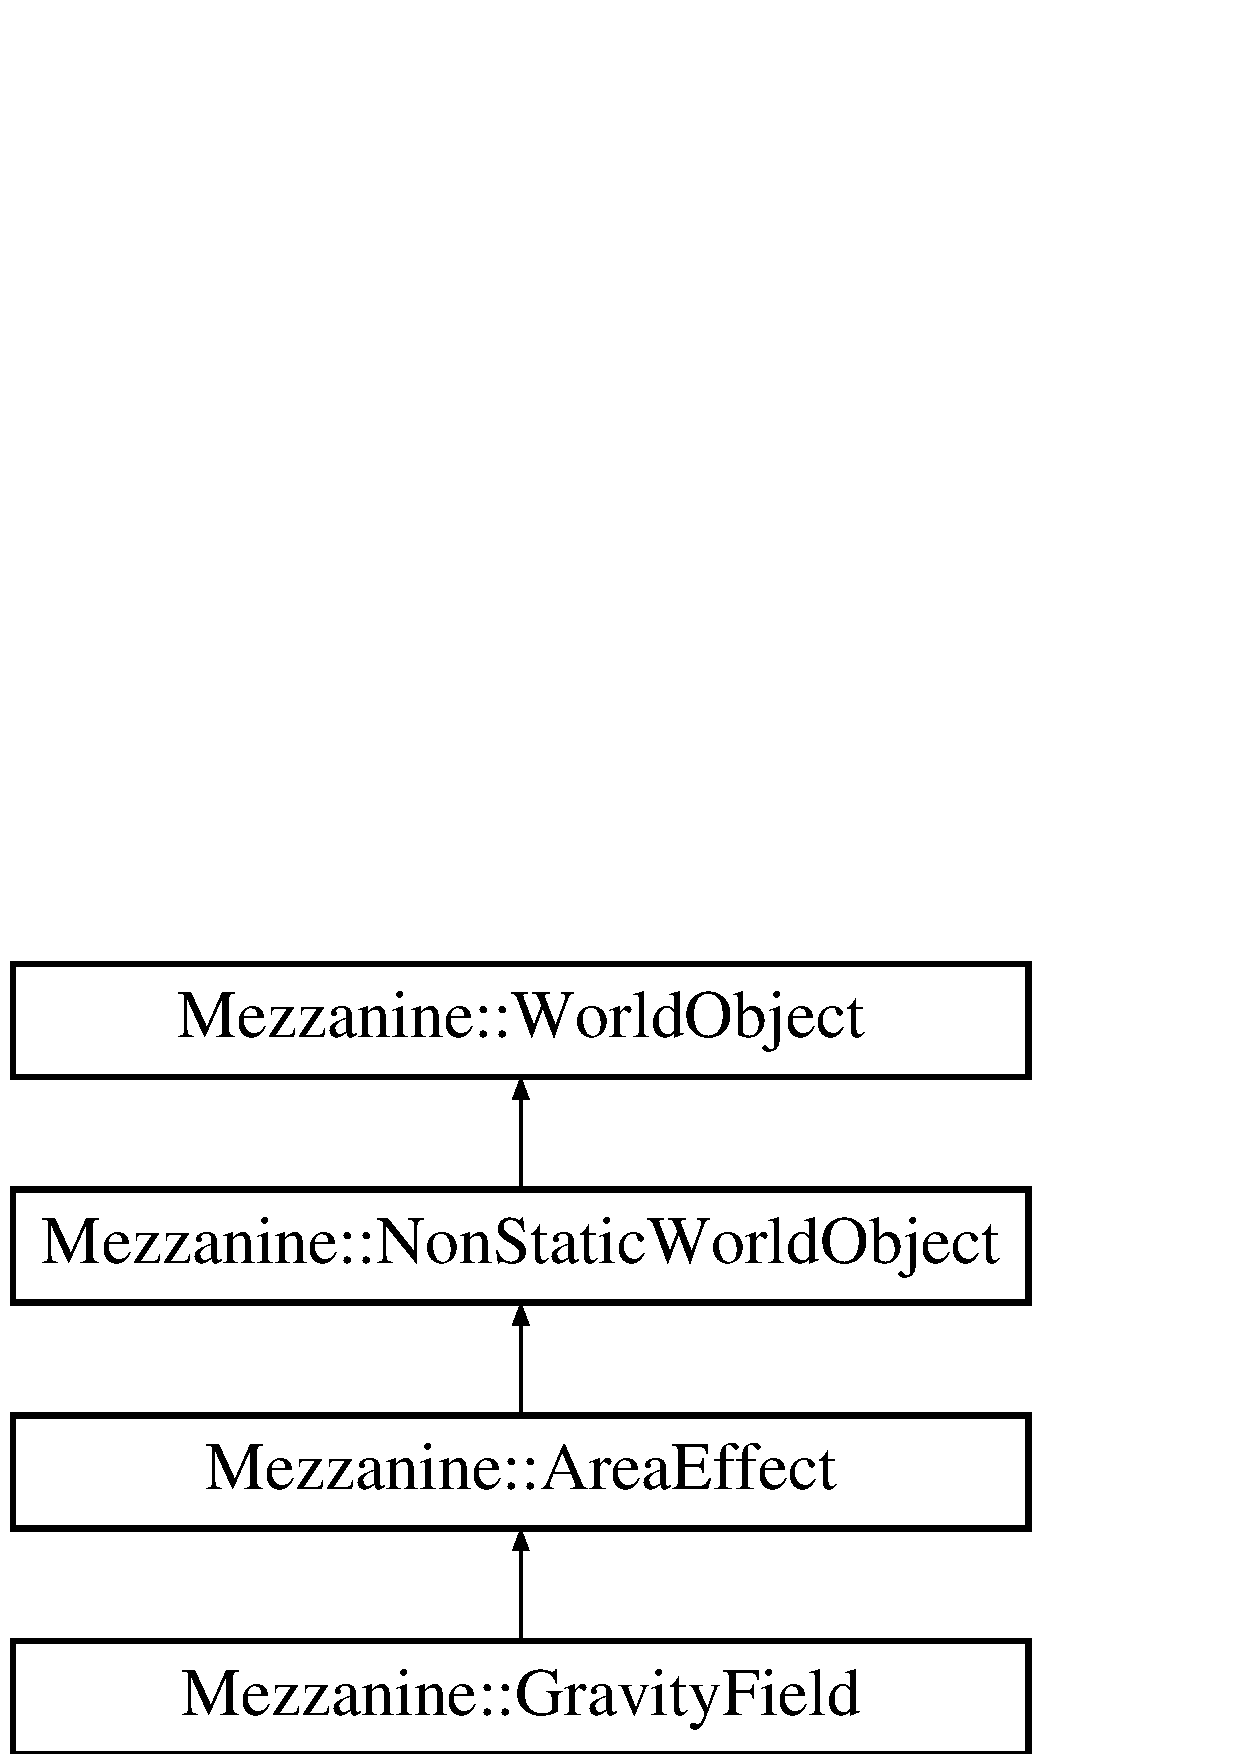
\includegraphics[height=4.000000cm]{classMezzanine_1_1GravityField}
\end{center}
\end{figure}
\subsubsection*{Public Member Functions}
\begin{DoxyCompactItemize}
\item 
virtual void \hyperlink{classMezzanine_1_1GravityField_a53aee6679088fb6151e5cb6e82a09fb7}{ApplyEffect} ()
\begin{DoxyCompactList}\small\item\em Applies the effect this field has to object inside. \item\end{DoxyCompactList}\item 
virtual \hyperlink{classMezzanine_1_1Vector3}{Vector3} \hyperlink{classMezzanine_1_1GravityField_ad37d2c94bdabf0412e35ed59ad74e8c9}{GetFieldGravity} () const 
\begin{DoxyCompactList}\small\item\em Gets the gravity of this field. \item\end{DoxyCompactList}\item 
virtual \hyperlink{namespaceMezzanine_a30335416fc857844e8360c84d1d1b56c}{WorldObjectType} \hyperlink{classMezzanine_1_1GravityField_ae8c07e694ebcbcb226c1375bec3772b4}{GetType} () const 
\item 
\hyperlink{classMezzanine_1_1GravityField_aff8a73a59ad999b49f39c4bfb564fed3}{GravityField} (const \hyperlink{namespaceMezzanine_acf9fcc130e6ebf08e3d8491aebcf1c86}{String} \&name, const \hyperlink{classMezzanine_1_1Vector3}{Vector3} \&Location)
\begin{DoxyCompactList}\small\item\em Constructor. \item\end{DoxyCompactList}\item 
virtual void \hyperlink{classMezzanine_1_1GravityField_a426b69dcfd3476029ebadea1ee4e0ea3}{SetFieldGravity} (const \hyperlink{classMezzanine_1_1Vector3}{Vector3} \&Gravity)
\begin{DoxyCompactList}\small\item\em Sets the gravity force for this field. \item\end{DoxyCompactList}\item 
virtual \hyperlink{classMezzanine_1_1GravityField_a53fe69bb37458dce9fca8df1215d739e}{$\sim$GravityField} ()
\begin{DoxyCompactList}\small\item\em Destructor. \item\end{DoxyCompactList}\end{DoxyCompactItemize}
\subsubsection*{Protected Attributes}
\begin{DoxyCompactItemize}
\item 
\hypertarget{classMezzanine_1_1GravityField_ae8cd8fe1f5430a6ca6e73c37c72e9e52}{
\hyperlink{classMezzanine_1_1Vector3}{Vector3} \hyperlink{classMezzanine_1_1GravityField_ae8cd8fe1f5430a6ca6e73c37c72e9e52}{Grav}}
\label{classMezzanine_1_1GravityField_ae8cd8fe1f5430a6ca6e73c37c72e9e52}

\begin{DoxyCompactList}\small\item\em The stored value for this fields gravity. \item\end{DoxyCompactList}\end{DoxyCompactItemize}


\subsubsection{Detailed Description}
This is a gravity field implementation of the \hyperlink{classMezzanine_1_1AreaEffect}{AreaEffect} class. This class is not a gravity well, where gravity is pulling to one point. Instead this class uniformly pulls gravity in one direction that is different from the world gravity. 

Definition at line 186 of file areaeffect.h.



\subsubsection{Constructor \& Destructor Documentation}
\hypertarget{classMezzanine_1_1GravityField_aff8a73a59ad999b49f39c4bfb564fed3}{
\index{Mezzanine::GravityField@{Mezzanine::GravityField}!GravityField@{GravityField}}
\index{GravityField@{GravityField}!Mezzanine::GravityField@{Mezzanine::GravityField}}
\paragraph[{GravityField}]{\setlength{\rightskip}{0pt plus 5cm}Mezzanine::GravityField::GravityField (
\begin{DoxyParamCaption}
\item[{const {\bf String} \&}]{name, }
\item[{const {\bf Vector3} \&}]{Location}
\end{DoxyParamCaption}
)}\hfill}
\label{classMezzanine_1_1GravityField_aff8a73a59ad999b49f39c4bfb564fed3}


Constructor. 

Basic initialization constructor. 
\begin{DoxyParams}{Parameters}
{\em name} & The name of the field. \\
\hline
{\em Location} & The location of the AE field. \\
\hline
\end{DoxyParams}


Definition at line 331 of file areaeffect.cpp.

\hypertarget{classMezzanine_1_1GravityField_a53fe69bb37458dce9fca8df1215d739e}{
\index{Mezzanine::GravityField@{Mezzanine::GravityField}!$\sim$GravityField@{$\sim$GravityField}}
\index{$\sim$GravityField@{$\sim$GravityField}!Mezzanine::GravityField@{Mezzanine::GravityField}}
\paragraph[{$\sim$GravityField}]{\setlength{\rightskip}{0pt plus 5cm}Mezzanine::GravityField::$\sim$GravityField (
\begin{DoxyParamCaption}
{}
\end{DoxyParamCaption}
)\hspace{0.3cm}{\ttfamily  \mbox{[}virtual\mbox{]}}}\hfill}
\label{classMezzanine_1_1GravityField_a53fe69bb37458dce9fca8df1215d739e}


Destructor. 

Class destructor. 

Definition at line 335 of file areaeffect.cpp.



\subsubsection{Member Function Documentation}
\hypertarget{classMezzanine_1_1GravityField_a53aee6679088fb6151e5cb6e82a09fb7}{
\index{Mezzanine::GravityField@{Mezzanine::GravityField}!ApplyEffect@{ApplyEffect}}
\index{ApplyEffect@{ApplyEffect}!Mezzanine::GravityField@{Mezzanine::GravityField}}
\paragraph[{ApplyEffect}]{\setlength{\rightskip}{0pt plus 5cm}void Mezzanine::GravityField::ApplyEffect (
\begin{DoxyParamCaption}
{}
\end{DoxyParamCaption}
)\hspace{0.3cm}{\ttfamily  \mbox{[}virtual\mbox{]}}}\hfill}
\label{classMezzanine_1_1GravityField_a53aee6679088fb6151e5cb6e82a09fb7}


Applies the effect this field has to object inside. 

This function defines the behavior for the class. 

Implements \hyperlink{classMezzanine_1_1AreaEffect_a988cd958e49d65331a059951af3c2884}{Mezzanine::AreaEffect}.



Definition at line 339 of file areaeffect.cpp.

\hypertarget{classMezzanine_1_1GravityField_ad37d2c94bdabf0412e35ed59ad74e8c9}{
\index{Mezzanine::GravityField@{Mezzanine::GravityField}!GetFieldGravity@{GetFieldGravity}}
\index{GetFieldGravity@{GetFieldGravity}!Mezzanine::GravityField@{Mezzanine::GravityField}}
\paragraph[{GetFieldGravity}]{\setlength{\rightskip}{0pt plus 5cm}{\bf Vector3} Mezzanine::GravityField::GetFieldGravity (
\begin{DoxyParamCaption}
{}
\end{DoxyParamCaption}
) const\hspace{0.3cm}{\ttfamily  \mbox{[}virtual\mbox{]}}}\hfill}
\label{classMezzanine_1_1GravityField_ad37d2c94bdabf0412e35ed59ad74e8c9}


Gets the gravity of this field. 

Gets the strength and direction of gravity this field has. \begin{DoxyReturn}{Returns}
Returns a \hyperlink{classvector3}{vector3} representing the force and direction of gravity this field has. 
\end{DoxyReturn}


Definition at line 368 of file areaeffect.cpp.

\hypertarget{classMezzanine_1_1GravityField_ae8c07e694ebcbcb226c1375bec3772b4}{
\index{Mezzanine::GravityField@{Mezzanine::GravityField}!GetType@{GetType}}
\index{GetType@{GetType}!Mezzanine::GravityField@{Mezzanine::GravityField}}
\paragraph[{GetType}]{\setlength{\rightskip}{0pt plus 5cm}{\bf WorldObjectType} Mezzanine::GravityField::GetType (
\begin{DoxyParamCaption}
{}
\end{DoxyParamCaption}
) const\hspace{0.3cm}{\ttfamily  \mbox{[}virtual\mbox{]}}}\hfill}
\label{classMezzanine_1_1GravityField_ae8c07e694ebcbcb226c1375bec3772b4}
Gets the type of the \hyperlink{classMezzanine_1_1World}{World} Object instance. 

\begin{DoxyReturn}{Returns}
Returns the type of the \hyperlink{classMezzanine_1_1World}{World} Object instance 
\end{DoxyReturn}
 

Reimplemented from \hyperlink{classMezzanine_1_1AreaEffect_a3eab7461632e01984cfb07f8c8fb5954}{Mezzanine::AreaEffect}.



Definition at line 373 of file areaeffect.cpp.

\hypertarget{classMezzanine_1_1GravityField_a426b69dcfd3476029ebadea1ee4e0ea3}{
\index{Mezzanine::GravityField@{Mezzanine::GravityField}!SetFieldGravity@{SetFieldGravity}}
\index{SetFieldGravity@{SetFieldGravity}!Mezzanine::GravityField@{Mezzanine::GravityField}}
\paragraph[{SetFieldGravity}]{\setlength{\rightskip}{0pt plus 5cm}void Mezzanine::GravityField::SetFieldGravity (
\begin{DoxyParamCaption}
\item[{const {\bf Vector3} \&}]{Gravity}
\end{DoxyParamCaption}
)\hspace{0.3cm}{\ttfamily  \mbox{[}virtual\mbox{]}}}\hfill}
\label{classMezzanine_1_1GravityField_a426b69dcfd3476029ebadea1ee4e0ea3}


Sets the gravity force for this field. 

Sets the strength and direction of gravity this field will have. 
\begin{DoxyParams}{Parameters}
{\em Gravity} & The \hyperlink{classvector3}{vector3} representing the force and direction of gravity this field will have. \\
\hline
\end{DoxyParams}


Definition at line 363 of file areaeffect.cpp.



The documentation for this class was generated from the following files:\begin{DoxyCompactItemize}
\item 
areaeffect.h\item 
areaeffect.cpp\end{DoxyCompactItemize}

\hypertarget{classMezzanine_1_1GravityWell}{
\subsection{Mezzanine::GravityWell Class Reference}
\label{classMezzanine_1_1GravityWell}\index{Mezzanine::GravityWell@{Mezzanine::GravityWell}}
}


This is a gravity well implementation of the \hyperlink{classMezzanine_1_1AreaEffect}{AreaEffect} class.  




{\ttfamily \#include $<$areaeffect.h$>$}

Inheritance diagram for Mezzanine::GravityWell:\begin{figure}[H]
\begin{center}
\leavevmode
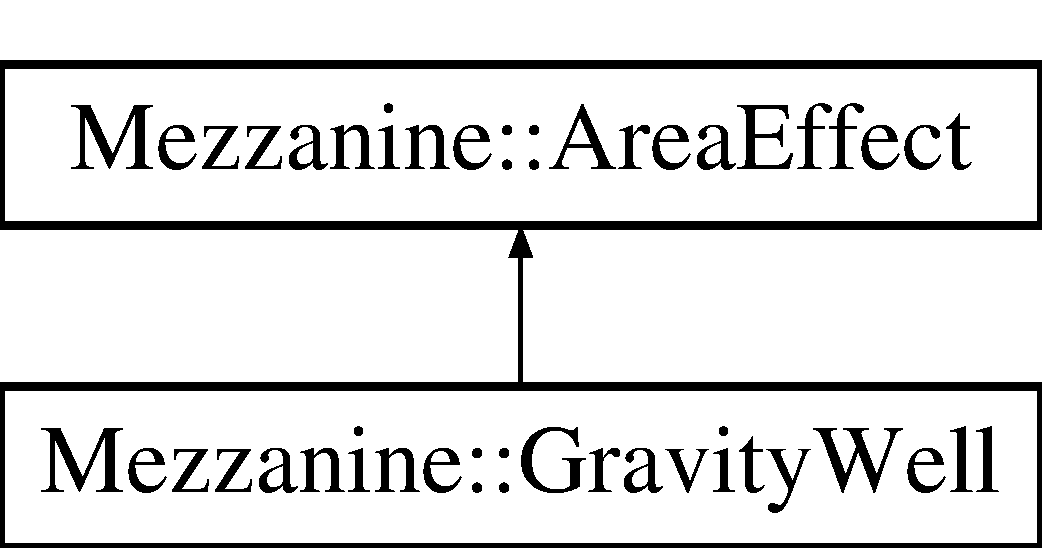
\includegraphics[height=4.423381cm]{classMezzanine_1_1GravityWell}
\end{center}
\end{figure}
\subsubsection*{Public Member Functions}
\begin{DoxyCompactItemize}
\item 
\hyperlink{classMezzanine_1_1GravityWell_a4f89751efb62bd71164a2864923dc149}{GravityWell} (const \hyperlink{namespaceMezzanine_acf9fcc130e6ebf08e3d8491aebcf1c86}{String} \&name, const \hyperlink{classMezzanine_1_1Vector3}{Vector3} \&Location)
\begin{DoxyCompactList}\small\item\em Constructor. \item\end{DoxyCompactList}\item 
virtual \hyperlink{classMezzanine_1_1GravityWell_affc992ad5e1edafd654d16d6a13840d0}{$\sim$GravityWell} ()
\begin{DoxyCompactList}\small\item\em Destructor. \item\end{DoxyCompactList}\item 
virtual void \hyperlink{classMezzanine_1_1GravityWell_a193e1683edaf80bb1a37979f196abf6e}{ApplyEffect} ()
\begin{DoxyCompactList}\small\item\em Applies the effect this field has to object inside. \item\end{DoxyCompactList}\item 
virtual bool \hyperlink{classMezzanine_1_1GravityWell_afa34a6efc22c6d8875be96cfce90c013}{GetAllowWorldGravity} () const 
\begin{DoxyCompactList}\small\item\em Gets whether or not world gravity is is removed for objects inside this field. \item\end{DoxyCompactList}\item 
virtual \hyperlink{namespaceMezzanine_a726731b1a7df72bf3583e4a97282c6f6}{Real} \hyperlink{classMezzanine_1_1GravityWell_aa077b3ef75a442b97f34bb578a7354eb}{GetAttenuationAmount} () const 
\begin{DoxyCompactList}\small\item\em Gets the amount force is attenuated over distance. \item\end{DoxyCompactList}\item 
virtual \hyperlink{namespaceMezzanine_a2d10a79e11a2031df10af540eede12fa}{Mezzanine::AttenuationStyle} \hyperlink{classMezzanine_1_1GravityWell_ad26c5b44056826e55dac112d0e0600a7}{GetAttenuationStyle} () const 
\begin{DoxyCompactList}\small\item\em Gets the Style of attenuation applied. \item\end{DoxyCompactList}\item 
virtual \hyperlink{namespaceMezzanine_a726731b1a7df72bf3583e4a97282c6f6}{Real} \hyperlink{classMezzanine_1_1GravityWell_a8fe42eeeb7483c35f1dfae170c2b2ec9}{GetFieldStrength} () const 
\begin{DoxyCompactList}\small\item\em Gets the strength of the field. \item\end{DoxyCompactList}\item 
virtual \hyperlink{namespaceMezzanine_ae8cd04f706f4998be62f454b7119c718}{WorldAndSceneObjectType} \hyperlink{classMezzanine_1_1GravityWell_a7890d007afb7021a811d711e3b2ed950}{GetType} () const 
\item 
virtual void \hyperlink{classMezzanine_1_1GravityWell_a80837168a132c3bffcefb839e1669a63}{SetAllowWorldGravity} (bool WorldGravity)
\begin{DoxyCompactList}\small\item\em Sets whether or not world gravity should be removed for objects in this field. \item\end{DoxyCompactList}\item 
virtual void \hyperlink{classMezzanine_1_1GravityWell_ab7668c7c5c1c7c25a40315803efb0790}{SetAttenuation} (const \hyperlink{namespaceMezzanine_a726731b1a7df72bf3583e4a97282c6f6}{Real} \&Amount, const \hyperlink{namespaceMezzanine_a2d10a79e11a2031df10af540eede12fa}{Mezzanine::AttenuationStyle} \&Style)
\begin{DoxyCompactList}\small\item\em Sets the attenuation for this field. \item\end{DoxyCompactList}\item 
virtual void \hyperlink{classMezzanine_1_1GravityWell_a596a662feae83e04e4c299a8aaf8b862}{SetFieldStrength} (const \hyperlink{namespaceMezzanine_a726731b1a7df72bf3583e4a97282c6f6}{Real} \&FieldStrength)
\begin{DoxyCompactList}\small\item\em Sets the strenth of the field. \item\end{DoxyCompactList}\end{DoxyCompactItemize}
\subsubsection*{Protected Attributes}
\begin{DoxyCompactItemize}
\item 
\hypertarget{classMezzanine_1_1GravityWell_a869ff5ef7c317e642e2b366e18d4f818}{
bool \hyperlink{classMezzanine_1_1GravityWell_a869ff5ef7c317e642e2b366e18d4f818}{AllowWorldGrav}}
\label{classMezzanine_1_1GravityWell_a869ff5ef7c317e642e2b366e18d4f818}

\begin{DoxyCompactList}\small\item\em Should world gravity ne ignored. \item\end{DoxyCompactList}\item 
\hypertarget{classMezzanine_1_1GravityWell_a82bf415225d76850cc832128077be947}{
\hyperlink{namespaceMezzanine_a726731b1a7df72bf3583e4a97282c6f6}{Real} \hyperlink{classMezzanine_1_1GravityWell_a82bf415225d76850cc832128077be947}{AttenAmount}}
\label{classMezzanine_1_1GravityWell_a82bf415225d76850cc832128077be947}

\begin{DoxyCompactList}\small\item\em how much does the Gravity attenuate. \item\end{DoxyCompactList}\item 
\hypertarget{classMezzanine_1_1GravityWell_ae1ceea5a9065775ea1b54e676fea9ed0}{
\hyperlink{namespaceMezzanine_a2d10a79e11a2031df10af540eede12fa}{Mezzanine::AttenuationStyle} \hyperlink{classMezzanine_1_1GravityWell_ae1ceea5a9065775ea1b54e676fea9ed0}{AttenStyle}}
\label{classMezzanine_1_1GravityWell_ae1ceea5a9065775ea1b54e676fea9ed0}

\begin{DoxyCompactList}\small\item\em How does gravity. \item\end{DoxyCompactList}\item 
\hypertarget{classMezzanine_1_1GravityWell_a2ed7c1e6618618ddd990e1466e9471c5}{
\hyperlink{namespaceMezzanine_a726731b1a7df72bf3583e4a97282c6f6}{Real} \hyperlink{classMezzanine_1_1GravityWell_a2ed7c1e6618618ddd990e1466e9471c5}{Strength}}
\label{classMezzanine_1_1GravityWell_a2ed7c1e6618618ddd990e1466e9471c5}

\begin{DoxyCompactList}\small\item\em The amount of force exerted on other objects. \item\end{DoxyCompactList}\end{DoxyCompactItemize}


\subsubsection{Detailed Description}
This is a gravity well implementation of the \hyperlink{classMezzanine_1_1AreaEffect}{AreaEffect} class. This class is not a gravity field, where gravity only pulls in one direction. Instead this class will always pull objects inside it towards the field center. \par
 This class works best with sphere's, but can be made to work with any shape. 

Definition at line 258 of file areaeffect.h.



\subsubsection{Constructor \& Destructor Documentation}
\hypertarget{classMezzanine_1_1GravityWell_a4f89751efb62bd71164a2864923dc149}{
\index{Mezzanine::GravityWell@{Mezzanine::GravityWell}!GravityWell@{GravityWell}}
\index{GravityWell@{GravityWell}!Mezzanine::GravityWell@{Mezzanine::GravityWell}}
\paragraph[{GravityWell}]{\setlength{\rightskip}{0pt plus 5cm}Mezzanine::GravityWell::GravityWell (
\begin{DoxyParamCaption}
\item[{const {\bf String} \&}]{name, }
\item[{const {\bf Vector3} \&}]{Location}
\end{DoxyParamCaption}
)}\hfill}
\label{classMezzanine_1_1GravityWell_a4f89751efb62bd71164a2864923dc149}


Constructor. 

Basic initialization constructor. 
\begin{DoxyParams}{Parameters}
{\em name} & The name of the field. \\
\hline
{\em Location} & The location of the AE field. \\
\hline
\end{DoxyParams}


Definition at line 461 of file areaeffect.cpp.

\hypertarget{classMezzanine_1_1GravityWell_affc992ad5e1edafd654d16d6a13840d0}{
\index{Mezzanine::GravityWell@{Mezzanine::GravityWell}!$\sim$GravityWell@{$\sim$GravityWell}}
\index{$\sim$GravityWell@{$\sim$GravityWell}!Mezzanine::GravityWell@{Mezzanine::GravityWell}}
\paragraph[{$\sim$GravityWell}]{\setlength{\rightskip}{0pt plus 5cm}Mezzanine::GravityWell::$\sim$GravityWell (
\begin{DoxyParamCaption}
{}
\end{DoxyParamCaption}
)\hspace{0.3cm}{\ttfamily  \mbox{[}virtual\mbox{]}}}\hfill}
\label{classMezzanine_1_1GravityWell_affc992ad5e1edafd654d16d6a13840d0}


Destructor. 

Class destructor. 

Definition at line 470 of file areaeffect.cpp.



\subsubsection{Member Function Documentation}
\hypertarget{classMezzanine_1_1GravityWell_a193e1683edaf80bb1a37979f196abf6e}{
\index{Mezzanine::GravityWell@{Mezzanine::GravityWell}!ApplyEffect@{ApplyEffect}}
\index{ApplyEffect@{ApplyEffect}!Mezzanine::GravityWell@{Mezzanine::GravityWell}}
\paragraph[{ApplyEffect}]{\setlength{\rightskip}{0pt plus 5cm}void Mezzanine::GravityWell::ApplyEffect (
\begin{DoxyParamCaption}
{}
\end{DoxyParamCaption}
)\hspace{0.3cm}{\ttfamily  \mbox{[}virtual\mbox{]}}}\hfill}
\label{classMezzanine_1_1GravityWell_a193e1683edaf80bb1a37979f196abf6e}


Applies the effect this field has to object inside. 

This function defines the behavior for the class. 

Implements \hyperlink{classMezzanine_1_1AreaEffect_a988cd958e49d65331a059951af3c2884}{Mezzanine::AreaEffect}.



Definition at line 474 of file areaeffect.cpp.

\hypertarget{classMezzanine_1_1GravityWell_afa34a6efc22c6d8875be96cfce90c013}{
\index{Mezzanine::GravityWell@{Mezzanine::GravityWell}!GetAllowWorldGravity@{GetAllowWorldGravity}}
\index{GetAllowWorldGravity@{GetAllowWorldGravity}!Mezzanine::GravityWell@{Mezzanine::GravityWell}}
\paragraph[{GetAllowWorldGravity}]{\setlength{\rightskip}{0pt plus 5cm}bool Mezzanine::GravityWell::GetAllowWorldGravity (
\begin{DoxyParamCaption}
{}
\end{DoxyParamCaption}
) const\hspace{0.3cm}{\ttfamily  \mbox{[}virtual\mbox{]}}}\hfill}
\label{classMezzanine_1_1GravityWell_afa34a6efc22c6d8875be96cfce90c013}


Gets whether or not world gravity is is removed for objects inside this field. 

\begin{DoxyReturn}{Returns}
Returns a bool indicating whether objects inside are affected by world gravity. 
\end{DoxyReturn}


Definition at line 555 of file areaeffect.cpp.

\hypertarget{classMezzanine_1_1GravityWell_aa077b3ef75a442b97f34bb578a7354eb}{
\index{Mezzanine::GravityWell@{Mezzanine::GravityWell}!GetAttenuationAmount@{GetAttenuationAmount}}
\index{GetAttenuationAmount@{GetAttenuationAmount}!Mezzanine::GravityWell@{Mezzanine::GravityWell}}
\paragraph[{GetAttenuationAmount}]{\setlength{\rightskip}{0pt plus 5cm}{\bf Real} Mezzanine::GravityWell::GetAttenuationAmount (
\begin{DoxyParamCaption}
{}
\end{DoxyParamCaption}
) const\hspace{0.3cm}{\ttfamily  \mbox{[}virtual\mbox{]}}}\hfill}
\label{classMezzanine_1_1GravityWell_aa077b3ef75a442b97f34bb578a7354eb}


Gets the amount force is attenuated over distance. 

See \hyperlink{classMezzanine_1_1GravityWell_ab7668c7c5c1c7c25a40315803efb0790}{SetAttenuation()} for more details. \begin{DoxyReturn}{Returns}
Returns a Real value 
\end{DoxyReturn}


Definition at line 571 of file areaeffect.cpp.

\hypertarget{classMezzanine_1_1GravityWell_ad26c5b44056826e55dac112d0e0600a7}{
\index{Mezzanine::GravityWell@{Mezzanine::GravityWell}!GetAttenuationStyle@{GetAttenuationStyle}}
\index{GetAttenuationStyle@{GetAttenuationStyle}!Mezzanine::GravityWell@{Mezzanine::GravityWell}}
\paragraph[{GetAttenuationStyle}]{\setlength{\rightskip}{0pt plus 5cm}{\bf Mezzanine::AttenuationStyle} Mezzanine::GravityWell::GetAttenuationStyle (
\begin{DoxyParamCaption}
{}
\end{DoxyParamCaption}
) const\hspace{0.3cm}{\ttfamily  \mbox{[}virtual\mbox{]}}}\hfill}
\label{classMezzanine_1_1GravityWell_ad26c5b44056826e55dac112d0e0600a7}


Gets the Style of attenuation applied. 

See the AttenuationStyle enum for more details. \begin{DoxyReturn}{Returns}
Returns the style of attenuation currently being used by this field. 
\end{DoxyReturn}


Definition at line 566 of file areaeffect.cpp.

\hypertarget{classMezzanine_1_1GravityWell_a8fe42eeeb7483c35f1dfae170c2b2ec9}{
\index{Mezzanine::GravityWell@{Mezzanine::GravityWell}!GetFieldStrength@{GetFieldStrength}}
\index{GetFieldStrength@{GetFieldStrength}!Mezzanine::GravityWell@{Mezzanine::GravityWell}}
\paragraph[{GetFieldStrength}]{\setlength{\rightskip}{0pt plus 5cm}{\bf Real} Mezzanine::GravityWell::GetFieldStrength (
\begin{DoxyParamCaption}
{}
\end{DoxyParamCaption}
) const\hspace{0.3cm}{\ttfamily  \mbox{[}virtual\mbox{]}}}\hfill}
\label{classMezzanine_1_1GravityWell_a8fe42eeeb7483c35f1dfae170c2b2ec9}


Gets the strength of the field. 

\begin{DoxyReturn}{Returns}
Returns a Real representing the value that is being multiplied by the direction to determine force appied to objects. 
\end{DoxyReturn}


Definition at line 545 of file areaeffect.cpp.

\hypertarget{classMezzanine_1_1GravityWell_a7890d007afb7021a811d711e3b2ed950}{
\index{Mezzanine::GravityWell@{Mezzanine::GravityWell}!GetType@{GetType}}
\index{GetType@{GetType}!Mezzanine::GravityWell@{Mezzanine::GravityWell}}
\paragraph[{GetType}]{\setlength{\rightskip}{0pt plus 5cm}{\bf WorldAndSceneObjectType} Mezzanine::GravityWell::GetType (
\begin{DoxyParamCaption}
{}
\end{DoxyParamCaption}
) const\hspace{0.3cm}{\ttfamily  \mbox{[}virtual\mbox{]}}}\hfill}
\label{classMezzanine_1_1GravityWell_a7890d007afb7021a811d711e3b2ed950}
Gets the type of the \hyperlink{classMezzanine_1_1World}{World} Object instance. 

\begin{DoxyReturn}{Returns}
Returns the type of the \hyperlink{classMezzanine_1_1World}{World} Object instance 
\end{DoxyReturn}
 

Reimplemented from \hyperlink{classMezzanine_1_1AreaEffect_a2f3df5433f02057d7a9deeb5e6666287}{Mezzanine::AreaEffect}.



Definition at line 576 of file areaeffect.cpp.

\hypertarget{classMezzanine_1_1GravityWell_a80837168a132c3bffcefb839e1669a63}{
\index{Mezzanine::GravityWell@{Mezzanine::GravityWell}!SetAllowWorldGravity@{SetAllowWorldGravity}}
\index{SetAllowWorldGravity@{SetAllowWorldGravity}!Mezzanine::GravityWell@{Mezzanine::GravityWell}}
\paragraph[{SetAllowWorldGravity}]{\setlength{\rightskip}{0pt plus 5cm}void Mezzanine::GravityWell::SetAllowWorldGravity (
\begin{DoxyParamCaption}
\item[{bool}]{WorldGravity}
\end{DoxyParamCaption}
)\hspace{0.3cm}{\ttfamily  \mbox{[}virtual\mbox{]}}}\hfill}
\label{classMezzanine_1_1GravityWell_a80837168a132c3bffcefb839e1669a63}


Sets whether or not world gravity should be removed for objects in this field. 

\begin{DoxyRemark}{Remarks}
Changing this value while the field is in the world and active is not recommended. 
\end{DoxyRemark}

\begin{DoxyParams}{Parameters}
{\em WorldGravity} & If true, then forces exerted by this field will be added to the world gravity, otherwise world gravity for objects inside will be set to zero. \\
\hline
\end{DoxyParams}


Definition at line 550 of file areaeffect.cpp.

\hypertarget{classMezzanine_1_1GravityWell_ab7668c7c5c1c7c25a40315803efb0790}{
\index{Mezzanine::GravityWell@{Mezzanine::GravityWell}!SetAttenuation@{SetAttenuation}}
\index{SetAttenuation@{SetAttenuation}!Mezzanine::GravityWell@{Mezzanine::GravityWell}}
\paragraph[{SetAttenuation}]{\setlength{\rightskip}{0pt plus 5cm}void Mezzanine::GravityWell::SetAttenuation (
\begin{DoxyParamCaption}
\item[{const {\bf Real} \&}]{Amount, }
\item[{const {\bf Mezzanine::AttenuationStyle} \&}]{Style}
\end{DoxyParamCaption}
)\hspace{0.3cm}{\ttfamily  \mbox{[}virtual\mbox{]}}}\hfill}
\label{classMezzanine_1_1GravityWell_ab7668c7c5c1c7c25a40315803efb0790}


Sets the attenuation for this field. 


\begin{DoxyParams}{Parameters}
{\em Amount} & The amount of force that is dropped off per 1 unit of distance objects are from the AE center. \\
\hline
{\em Style} & The style of attenuation to apply, see the AttenuationStyle enum for more details. \\
\hline
\end{DoxyParams}


Definition at line 560 of file areaeffect.cpp.

\hypertarget{classMezzanine_1_1GravityWell_a596a662feae83e04e4c299a8aaf8b862}{
\index{Mezzanine::GravityWell@{Mezzanine::GravityWell}!SetFieldStrength@{SetFieldStrength}}
\index{SetFieldStrength@{SetFieldStrength}!Mezzanine::GravityWell@{Mezzanine::GravityWell}}
\paragraph[{SetFieldStrength}]{\setlength{\rightskip}{0pt plus 5cm}void Mezzanine::GravityWell::SetFieldStrength (
\begin{DoxyParamCaption}
\item[{const {\bf Real} \&}]{FieldStrength}
\end{DoxyParamCaption}
)\hspace{0.3cm}{\ttfamily  \mbox{[}virtual\mbox{]}}}\hfill}
\label{classMezzanine_1_1GravityWell_a596a662feae83e04e4c299a8aaf8b862}


Sets the strenth of the field. 

The direction of the field is based on the current position of the object in the field. Once that direction is calculated it will be multiplied by this value to determine the force the field will apply to the object. 
\begin{DoxyParams}{Parameters}
{\em FieldStrength} & The strength the field will have when exerting force onto other objects. \\
\hline
\end{DoxyParams}


Definition at line 540 of file areaeffect.cpp.



The documentation for this class was generated from the following files:\begin{DoxyCompactItemize}
\item 
areaeffect.h\item 
areaeffect.cpp\end{DoxyCompactItemize}

\hypertarget{classMezzanine_1_1HeightfieldCollisionShape}{
\subsection{Mezzanine::HeightfieldCollisionShape Class Reference}
\label{classMezzanine_1_1HeightfieldCollisionShape}\index{Mezzanine::HeightfieldCollisionShape@{Mezzanine::HeightfieldCollisionShape}}
}


A series of values that store hieght in a grid like fashion.  




{\ttfamily \#include $<$collisionshape.h$>$}

Inheritance diagram for Mezzanine::HeightfieldCollisionShape:\begin{figure}[H]
\begin{center}
\leavevmode
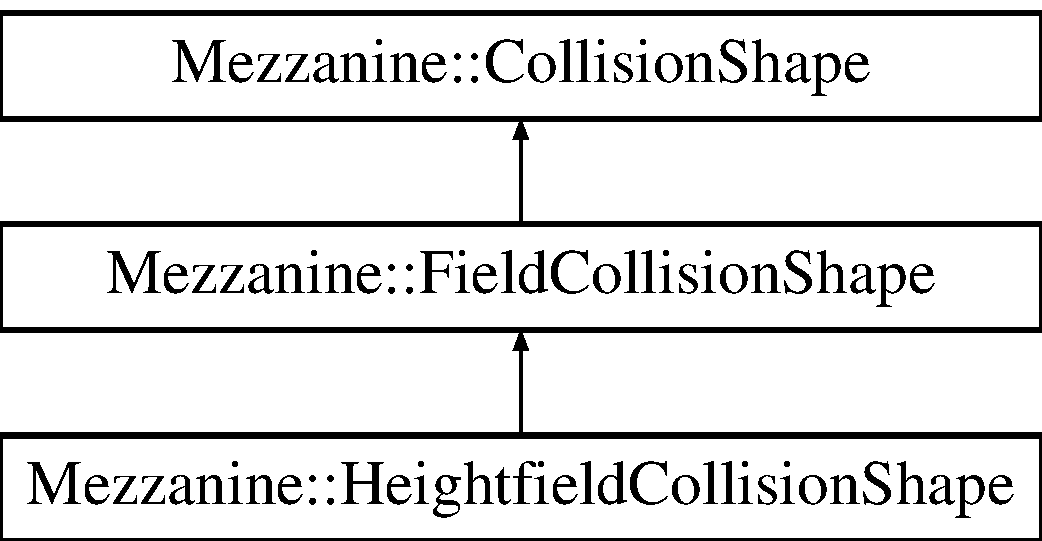
\includegraphics[height=3.000000cm]{classMezzanine_1_1HeightfieldCollisionShape}
\end{center}
\end{figure}
\subsubsection*{Public Member Functions}
\begin{DoxyCompactItemize}
\item 
\hyperlink{classMezzanine_1_1HeightfieldCollisionShape_aee6afa08c9007498cc0693b8bfb2da95}{HeightfieldCollisionShape} (const \hyperlink{namespaceMezzanine_acf9fcc130e6ebf08e3d8491aebcf1c86}{String} \&\hyperlink{classMezzanine_1_1CollisionShape_aac524c5c56fa4d158bc071f8aecfbe79}{Name})
\begin{DoxyCompactList}\small\item\em Class Constructor. \item\end{DoxyCompactList}\item 
\hyperlink{classMezzanine_1_1HeightfieldCollisionShape_a79b5e672a6bded0e2f38587b901247ab}{HeightfieldCollisionShape} (const \hyperlink{namespaceMezzanine_acf9fcc130e6ebf08e3d8491aebcf1c86}{String} \&\hyperlink{classMezzanine_1_1CollisionShape_aac524c5c56fa4d158bc071f8aecfbe79}{Name}, btHeightfieldTerrainShape $\ast$BulletShape)
\begin{DoxyCompactList}\small\item\em Internal Constructor. \item\end{DoxyCompactList}\item 
\hypertarget{classMezzanine_1_1HeightfieldCollisionShape_ac9521af83a3d96d3f2c71c5a8a39b09d}{
virtual \hyperlink{classMezzanine_1_1HeightfieldCollisionShape_ac9521af83a3d96d3f2c71c5a8a39b09d}{$\sim$HeightfieldCollisionShape} ()}
\label{classMezzanine_1_1HeightfieldCollisionShape_ac9521af83a3d96d3f2c71c5a8a39b09d}

\begin{DoxyCompactList}\small\item\em Class Destructor. \item\end{DoxyCompactList}\item 
virtual \hyperlink{classMezzanine_1_1CollisionShape_ad04186055565998879b64176d6dd100d}{CollisionShape::ShapeType} \hyperlink{classMezzanine_1_1HeightfieldCollisionShape_af27ffaf88fc12af6ddc89704e60ecd33}{GetType} () const 
\end{DoxyCompactItemize}
\subsubsection*{Protected Attributes}
\begin{DoxyCompactItemize}
\item 
\hypertarget{classMezzanine_1_1HeightfieldCollisionShape_a326d019561da25f1eddeb7fb59748f9c}{
btHeightfieldTerrainShape $\ast$ \hyperlink{classMezzanine_1_1HeightfieldCollisionShape_a326d019561da25f1eddeb7fb59748f9c}{HeightfieldShape}}
\label{classMezzanine_1_1HeightfieldCollisionShape_a326d019561da25f1eddeb7fb59748f9c}

\begin{DoxyCompactList}\small\item\em The internal implementation. \item\end{DoxyCompactList}\end{DoxyCompactItemize}


\subsubsection{Detailed Description}
A series of values that store hieght in a grid like fashion. A fast terrain implementation that comes at the cost of overhangs and fine detail. This can be worked around by adding actors for additional terrain. 

Definition at line 868 of file collisionshape.h.



\subsubsection{Constructor \& Destructor Documentation}
\hypertarget{classMezzanine_1_1HeightfieldCollisionShape_aee6afa08c9007498cc0693b8bfb2da95}{
\index{Mezzanine::HeightfieldCollisionShape@{Mezzanine::HeightfieldCollisionShape}!HeightfieldCollisionShape@{HeightfieldCollisionShape}}
\index{HeightfieldCollisionShape@{HeightfieldCollisionShape}!Mezzanine::HeightfieldCollisionShape@{Mezzanine::HeightfieldCollisionShape}}
\paragraph[{HeightfieldCollisionShape}]{\setlength{\rightskip}{0pt plus 5cm}Mezzanine::HeightfieldCollisionShape::HeightfieldCollisionShape (
\begin{DoxyParamCaption}
\item[{const {\bf String} \&}]{Name}
\end{DoxyParamCaption}
)}\hfill}
\label{classMezzanine_1_1HeightfieldCollisionShape_aee6afa08c9007498cc0693b8bfb2da95}


Class Constructor. 


\begin{DoxyParams}{Parameters}
{\em Name} & The name of this Shape. \\
\hline
\end{DoxyParams}


Definition at line 1510 of file collisionshape.cpp.

\hypertarget{classMezzanine_1_1HeightfieldCollisionShape_a79b5e672a6bded0e2f38587b901247ab}{
\index{Mezzanine::HeightfieldCollisionShape@{Mezzanine::HeightfieldCollisionShape}!HeightfieldCollisionShape@{HeightfieldCollisionShape}}
\index{HeightfieldCollisionShape@{HeightfieldCollisionShape}!Mezzanine::HeightfieldCollisionShape@{Mezzanine::HeightfieldCollisionShape}}
\paragraph[{HeightfieldCollisionShape}]{\setlength{\rightskip}{0pt plus 5cm}Mezzanine::HeightfieldCollisionShape::HeightfieldCollisionShape (
\begin{DoxyParamCaption}
\item[{const {\bf String} \&}]{Name, }
\item[{btHeightfieldTerrainShape $\ast$}]{BulletShape}
\end{DoxyParamCaption}
)}\hfill}
\label{classMezzanine_1_1HeightfieldCollisionShape_a79b5e672a6bded0e2f38587b901247ab}


Internal Constructor. 


\begin{DoxyParams}{Parameters}
{\em Name} & The name of this Shape. \\
\hline
{\em BulletShape} & The internal shape this shape is based on. \\
\hline
\end{DoxyParams}


Definition at line 1515 of file collisionshape.cpp.



\subsubsection{Member Function Documentation}
\hypertarget{classMezzanine_1_1HeightfieldCollisionShape_af27ffaf88fc12af6ddc89704e60ecd33}{
\index{Mezzanine::HeightfieldCollisionShape@{Mezzanine::HeightfieldCollisionShape}!GetType@{GetType}}
\index{GetType@{GetType}!Mezzanine::HeightfieldCollisionShape@{Mezzanine::HeightfieldCollisionShape}}
\paragraph[{GetType}]{\setlength{\rightskip}{0pt plus 5cm}{\bf CollisionShape::ShapeType} Mezzanine::HeightfieldCollisionShape::GetType (
\begin{DoxyParamCaption}
{}
\end{DoxyParamCaption}
) const\hspace{0.3cm}{\ttfamily  \mbox{[}virtual\mbox{]}}}\hfill}
\label{classMezzanine_1_1HeightfieldCollisionShape_af27ffaf88fc12af6ddc89704e60ecd33}
Gets the type of \hyperlink{classMezzanine_1_1Collision}{Collision} shape this is. 

\begin{DoxyReturn}{Returns}
Returns an enum value indicating the type of collision shape this is. 
\end{DoxyReturn}
 

Implements \hyperlink{classMezzanine_1_1FieldCollisionShape_a85a444fa9bcaca9fec08c3b5697677c9}{Mezzanine::FieldCollisionShape}.



Definition at line 1527 of file collisionshape.cpp.



The documentation for this class was generated from the following files:\begin{DoxyCompactItemize}
\item 
collisionshape.h\item 
collisionshape.cpp\end{DoxyCompactItemize}

\hypertarget{classMezzanine_1_1Hinge2Constraint}{
\subsection{Mezzanine::Hinge2Constraint Class Reference}
\label{classMezzanine_1_1Hinge2Constraint}\index{Mezzanine::Hinge2Constraint@{Mezzanine::Hinge2Constraint}}
}


{\ttfamily \#include $<$constraint.h$>$}

Inheritance diagram for Mezzanine::Hinge2Constraint:\begin{figure}[H]
\begin{center}
\leavevmode
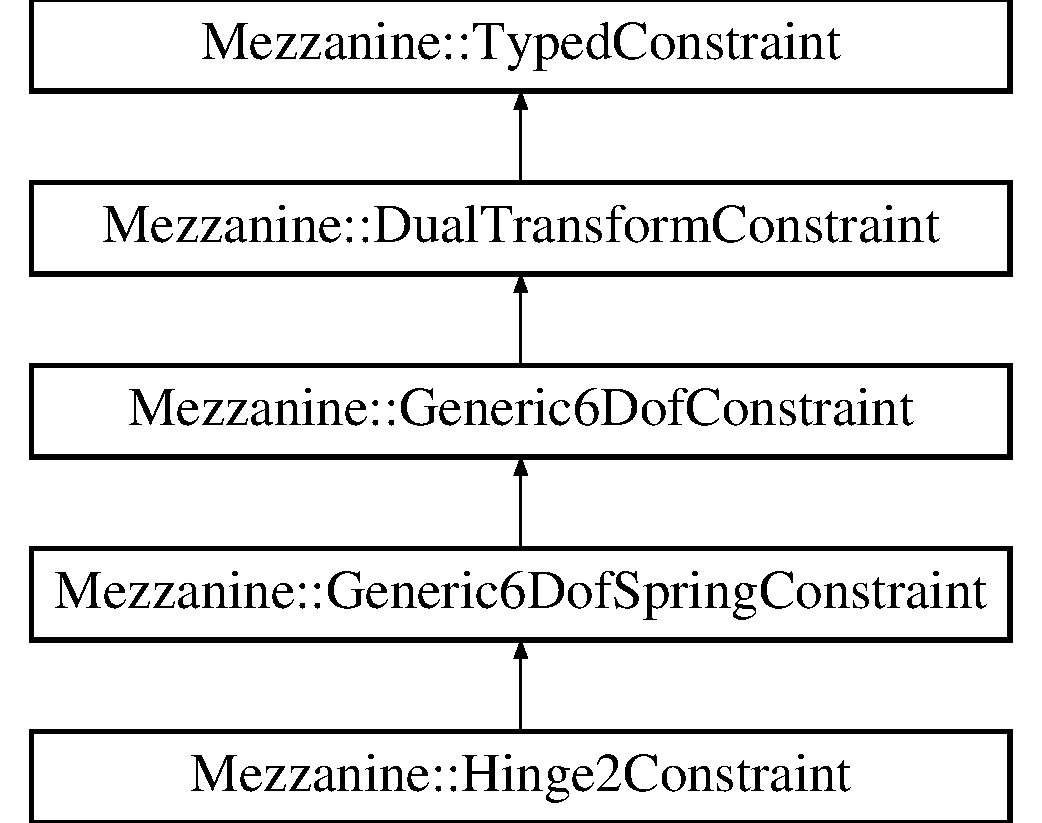
\includegraphics[height=5.000000cm]{classMezzanine_1_1Hinge2Constraint}
\end{center}
\end{figure}
\subsubsection*{Public Member Functions}
\begin{DoxyCompactItemize}
\item 
\hypertarget{classMezzanine_1_1Hinge2Constraint_acc0b4c6d39072f6e774e41c43381b6d8}{
{\bfseries Hinge2Constraint} (\hyperlink{classMezzanine_1_1ActorRigid}{ActorRigid} $\ast$ActorA, \hyperlink{classMezzanine_1_1ActorRigid}{ActorRigid} $\ast$ActorB, const \hyperlink{classMezzanine_1_1Vector3}{Vector3} \&Anchor, const \hyperlink{classMezzanine_1_1Vector3}{Vector3} \&Axis1, const \hyperlink{classMezzanine_1_1Vector3}{Vector3} \&Axis2)}
\label{classMezzanine_1_1Hinge2Constraint_acc0b4c6d39072f6e774e41c43381b6d8}

\item 
\hypertarget{classMezzanine_1_1Hinge2Constraint_acd405150e1822ae0954bf561ab52b7e7}{
virtual void {\bfseries SetLowerLimit} (\hyperlink{namespaceMezzanine_a726731b1a7df72bf3583e4a97282c6f6}{Real} Ang1Min)}
\label{classMezzanine_1_1Hinge2Constraint_acd405150e1822ae0954bf561ab52b7e7}

\item 
\hypertarget{classMezzanine_1_1Hinge2Constraint_a83ebdb0a49039249345ab0bef026cabd}{
virtual void {\bfseries SetUpperLimit} (\hyperlink{namespaceMezzanine_a726731b1a7df72bf3583e4a97282c6f6}{Real} Ang1Max)}
\label{classMezzanine_1_1Hinge2Constraint_a83ebdb0a49039249345ab0bef026cabd}

\item 
virtual \hyperlink{classMezzanine_1_1Hinge2Constraint_ac4cc8c1d461358a508785d0ccd9ea1e7}{$\sim$Hinge2Constraint} ()
\begin{DoxyCompactList}\small\item\em Class destructor. \item\end{DoxyCompactList}\end{DoxyCompactItemize}
\subsubsection*{Protected Attributes}
\begin{DoxyCompactItemize}
\item 
\hypertarget{classMezzanine_1_1Hinge2Constraint_aa28404d12e0d294b277004cdb851465a}{
btHinge2Constraint $\ast$ \hyperlink{classMezzanine_1_1Hinge2Constraint_aa28404d12e0d294b277004cdb851465a}{Hinge2}}
\label{classMezzanine_1_1Hinge2Constraint_aa28404d12e0d294b277004cdb851465a}

\begin{DoxyCompactList}\small\item\em Bullet constraint that this class encapsulates. \item\end{DoxyCompactList}\end{DoxyCompactItemize}


\subsubsection{Detailed Description}
This class is incomplete 

Definition at line 1182 of file constraint.h.



\subsubsection{Constructor \& Destructor Documentation}
\hypertarget{classMezzanine_1_1Hinge2Constraint_ac4cc8c1d461358a508785d0ccd9ea1e7}{
\index{Mezzanine::Hinge2Constraint@{Mezzanine::Hinge2Constraint}!$\sim$Hinge2Constraint@{$\sim$Hinge2Constraint}}
\index{$\sim$Hinge2Constraint@{$\sim$Hinge2Constraint}!Mezzanine::Hinge2Constraint@{Mezzanine::Hinge2Constraint}}
\paragraph[{$\sim$Hinge2Constraint}]{\setlength{\rightskip}{0pt plus 5cm}virtual Mezzanine::Hinge2Constraint::$\sim$Hinge2Constraint (
\begin{DoxyParamCaption}
{}
\end{DoxyParamCaption}
)\hspace{0.3cm}{\ttfamily  \mbox{[}virtual\mbox{]}}}\hfill}
\label{classMezzanine_1_1Hinge2Constraint_ac4cc8c1d461358a508785d0ccd9ea1e7}


Class destructor. 

The class destructor. 

The documentation for this class was generated from the following file:\begin{DoxyCompactItemize}
\item 
constraint.h\end{DoxyCompactItemize}

\hypertarget{classMezzanine_1_1HingeConstraint}{
\subsection{Mezzanine::HingeConstraint Class Reference}
\label{classMezzanine_1_1HingeConstraint}\index{Mezzanine::HingeConstraint@{Mezzanine::HingeConstraint}}
}


This is a constraint to be used to restrict the movement between two objects to angular rotation on a single axis.  




{\ttfamily \#include $<$constraint.h$>$}

Inheritance diagram for Mezzanine::HingeConstraint:\begin{figure}[H]
\begin{center}
\leavevmode
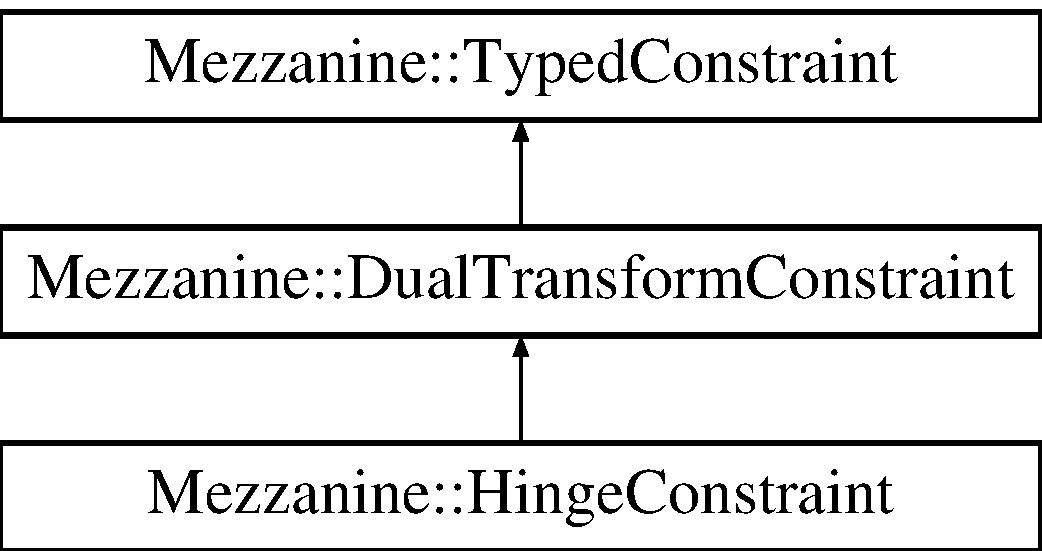
\includegraphics[height=3.000000cm]{classMezzanine_1_1HingeConstraint}
\end{center}
\end{figure}
\subsubsection*{Public Member Functions}
\begin{DoxyCompactItemize}
\item 
\hyperlink{classMezzanine_1_1HingeConstraint_a65d04021f0ac11d284de975d7552012e}{HingeConstraint} (\hyperlink{classMezzanine_1_1ActorRigid}{ActorRigid} $\ast$ActorA, \hyperlink{classMezzanine_1_1ActorRigid}{ActorRigid} $\ast$ActorB, const \hyperlink{classMezzanine_1_1Vector3}{Vector3} \&PivotInA, const \hyperlink{classMezzanine_1_1Vector3}{Vector3} \&PivotInB, const \hyperlink{classMezzanine_1_1Vector3}{Vector3} \&AxisInA, const \hyperlink{classMezzanine_1_1Vector3}{Vector3} \&AxisInB, bool UseReferenceFrameA=false)
\begin{DoxyCompactList}\small\item\em Creates a Hinge constraint that will connect two actors together by their offsets. \item\end{DoxyCompactList}\item 
\hyperlink{classMezzanine_1_1HingeConstraint_acb7f380b212a396b92d78ac055c55a68}{HingeConstraint} (\hyperlink{classMezzanine_1_1ActorRigid}{ActorRigid} $\ast$ActorA, const \hyperlink{classMezzanine_1_1Vector3}{Vector3} \&PivotInA, const \hyperlink{classMezzanine_1_1Vector3}{Vector3} \&AxisInA, bool UseReferenceFrameA=false)
\begin{DoxyCompactList}\small\item\em Creates a Hinge constraint that will attach an actor to a point in world space. \item\end{DoxyCompactList}\item 
\hyperlink{classMezzanine_1_1HingeConstraint_af769aacbd1756b528fe8724ecf5fc654}{HingeConstraint} (\hyperlink{classMezzanine_1_1ActorRigid}{ActorRigid} $\ast$ActorA, \hyperlink{classMezzanine_1_1ActorRigid}{ActorRigid} $\ast$ActorB, const \hyperlink{classMezzanine_1_1Transform}{Transform} \&TransformA, const \hyperlink{classMezzanine_1_1Transform}{Transform} \&TransformB, bool UseReferenceFrameA=false)
\begin{DoxyCompactList}\small\item\em Create a Hinge with components of a tranform. \item\end{DoxyCompactList}\item 
\hyperlink{classMezzanine_1_1HingeConstraint_a62a733c3ad51d3e7c5f51ae5a8adadd0}{HingeConstraint} (\hyperlink{classMezzanine_1_1ActorRigid}{ActorRigid} $\ast$ActorA, \hyperlink{classMezzanine_1_1ActorRigid}{ActorRigid} $\ast$ActorB, const \hyperlink{classMezzanine_1_1Vector3}{Vector3} \&VectorA, const \hyperlink{classMezzanine_1_1Vector3}{Vector3} \&VectorB, const \hyperlink{classMezzanine_1_1Quaternion}{Quaternion} \&QuaternionA, const \hyperlink{classMezzanine_1_1Quaternion}{Quaternion} \&QuaternionB, bool UseReferenceFrameA=false)
\begin{DoxyCompactList}\small\item\em Create a Hinge with components of a tranform. \item\end{DoxyCompactList}\item 
virtual \hyperlink{classMezzanine_1_1HingeConstraint_a9964c958874d5c6c7d410b4c09818837}{$\sim$HingeConstraint} ()
\begin{DoxyCompactList}\small\item\em Class destructor. \item\end{DoxyCompactList}\item 
virtual void \hyperlink{classMezzanine_1_1HingeConstraint_a4a87201e6370d7ce29f967aecaf54d8e}{EnableMotor} (bool EnableMotor, \hyperlink{namespaceMezzanine_a726731b1a7df72bf3583e4a97282c6f6}{Real} TargetVelocity, \hyperlink{namespaceMezzanine_a726731b1a7df72bf3583e4a97282c6f6}{Real} MaxMotorImpulse)
\begin{DoxyCompactList}\small\item\em Enables(or Disables) the motor on the hinge and sets it's parameters. \item\end{DoxyCompactList}\item 
virtual void \hyperlink{classMezzanine_1_1HingeConstraint_a92a4d535a069ecb4dea600f7c4ac38ef}{EnableMotor} (bool EnableMotor)
\begin{DoxyCompactList}\small\item\em Enables(or Disables) the motor on the hinge. \item\end{DoxyCompactList}\item 
virtual \hyperlink{classMezzanine_1_1Quaternion}{Quaternion} \hyperlink{classMezzanine_1_1HingeConstraint_ab8b8a045c8338a3daeb970cb4696aab3}{GetAPivotRotation} () const 
\begin{DoxyCompactList}\small\item\em Get the relative rotation for ActorA. \item\end{DoxyCompactList}\item 
virtual \hyperlink{classMezzanine_1_1Quaternion}{Quaternion} \hyperlink{classMezzanine_1_1HingeConstraint_a574d375c6eac6f5d5b5f9c1266b85d60}{GetBPivotRotation} () const 
\begin{DoxyCompactList}\small\item\em Get the relative rotation for ActorB. \item\end{DoxyCompactList}\item 
virtual btTypedConstraint $\ast$ \hyperlink{classMezzanine_1_1HingeConstraint_a04c77dee8074b293d9db893e1af42608}{GetConstraintBase} () const 
\item 
virtual \hyperlink{namespaceMezzanine_a726731b1a7df72bf3583e4a97282c6f6}{Real} \hyperlink{classMezzanine_1_1HingeConstraint_aaf946de046cc59210ae1f70ce53629e5}{GetHingeAngle} ()
\begin{DoxyCompactList}\small\item\em Gets the current angle of the hinge. \item\end{DoxyCompactList}\item 
virtual \hyperlink{namespaceMezzanine_a726731b1a7df72bf3583e4a97282c6f6}{Real} \hyperlink{classMezzanine_1_1HingeConstraint_aa614cc523ffa01d50e83ef2472126419}{GetLimitBiasFactor} () const 
\begin{DoxyCompactList}\small\item\em Return the bias factor of the hinge (Not entirely certain hat this on is) \item\end{DoxyCompactList}\item 
virtual \hyperlink{namespaceMezzanine_a726731b1a7df72bf3583e4a97282c6f6}{Real} \hyperlink{classMezzanine_1_1HingeConstraint_acb0a9676b91cf7c987569bed3510b5da}{GetLimitHigh} () const 
\begin{DoxyCompactList}\small\item\em Return the Upper Limit of the hinge. \item\end{DoxyCompactList}\item 
virtual \hyperlink{namespaceMezzanine_a726731b1a7df72bf3583e4a97282c6f6}{Real} \hyperlink{classMezzanine_1_1HingeConstraint_a7815264c012e03fdf09a72d1aa76e50f}{GetLimitLow} () const 
\begin{DoxyCompactList}\small\item\em Return the Lower Limit of the hinge. \item\end{DoxyCompactList}\item 
virtual \hyperlink{namespaceMezzanine_a726731b1a7df72bf3583e4a97282c6f6}{Real} \hyperlink{classMezzanine_1_1HingeConstraint_a547dfa04268f9fa0d938fb00a082fc03}{GetLimitRelaxationFactor} () const 
\begin{DoxyCompactList}\small\item\em Return the Relaxation Factor of the hinge. \item\end{DoxyCompactList}\item 
virtual \hyperlink{namespaceMezzanine_a726731b1a7df72bf3583e4a97282c6f6}{Real} \hyperlink{classMezzanine_1_1HingeConstraint_aa5202368b6de6721f0f6f96b6210e83f}{GetLimitSoftness} () const 
\begin{DoxyCompactList}\small\item\em Return the Softness of the hinge. \item\end{DoxyCompactList}\item 
virtual \hyperlink{namespaceMezzanine_a726731b1a7df72bf3583e4a97282c6f6}{Real} \hyperlink{classMezzanine_1_1HingeConstraint_a02ea6dc2a0e80649737c4c478fec274d}{GetMaxMotorImpulse} () const 
\begin{DoxyCompactList}\small\item\em Retrieve the maximimum value that the acceleration of the motor can be increased. \item\end{DoxyCompactList}\item 
virtual bool \hyperlink{classMezzanine_1_1HingeConstraint_adcc717f158be2173d179004a6b8d2b11}{GetMotorEnabled} () const 
\begin{DoxyCompactList}\small\item\em Is this motor on this hinge enabled? \item\end{DoxyCompactList}\item 
virtual \hyperlink{namespaceMezzanine_a726731b1a7df72bf3583e4a97282c6f6}{Real} \hyperlink{classMezzanine_1_1HingeConstraint_ab357a37ce5a447b007cbaef74c4b47d5}{GetMotorTargetVelocity} () const 
\begin{DoxyCompactList}\small\item\em Get the Target Velocity. \item\end{DoxyCompactList}\item 
virtual \hyperlink{classMezzanine_1_1Vector3}{Vector3} \hyperlink{classMezzanine_1_1HingeConstraint_a74f1b8d8de18ab991d2f42c7141eedc7}{GetPivotALocation} () const 
\begin{DoxyCompactList}\small\item\em Get the location of the hinge pivot relative to ActorA's Center of gravity. \item\end{DoxyCompactList}\item 
virtual \hyperlink{classMezzanine_1_1Transform}{Transform} \hyperlink{classMezzanine_1_1HingeConstraint_a208687c856410bf70f068ddf8c8f9161}{GetPivotATransform} () const 
\item 
virtual \hyperlink{classMezzanine_1_1Vector3}{Vector3} \hyperlink{classMezzanine_1_1HingeConstraint_a87b14b3cbf5241aeba723226661764e6}{GetPivotBLocation} () const 
\begin{DoxyCompactList}\small\item\em Get the location of the hinge pivot relative to ActorB's Center of gravity. \item\end{DoxyCompactList}\item 
virtual \hyperlink{classMezzanine_1_1Transform}{Transform} \hyperlink{classMezzanine_1_1HingeConstraint_a7d9a9ddc367d1a9105f1eb27fd76a65f}{GetPivotBTransform} () const 
\item 
virtual bool \hyperlink{classMezzanine_1_1HingeConstraint_a09dc1bb27e02b619222aebea91bc6705}{GetUseFrameOffset} () const 
\begin{DoxyCompactList}\small\item\em Retrieve the stored value from the physics subsystem(bullet) \item\end{DoxyCompactList}\item 
virtual bool \hyperlink{classMezzanine_1_1HingeConstraint_a638b7b76542d850becea2d49d3f1c8b1}{GetUseReferenceFrameA} () const 
\begin{DoxyCompactList}\small\item\em Is this Using Reference Frame A. \item\end{DoxyCompactList}\item 
virtual bool \hyperlink{classMezzanine_1_1HingeConstraint_a58f5758cb5926f785c07c7ebb544d91b}{HasParamBeenSet} (\hyperlink{namespaceMezzanine_a6c62e8c2938fb203eb7a7072c12176f4}{ConstraintParam} Param, int Axis) const 
\item 
virtual void \hyperlink{classMezzanine_1_1HingeConstraint_a6cbd8328c7a047f8e7951ab482e733cb}{ProtoDeSerialize} (const \hyperlink{classMezzanine_1_1xml_1_1Node}{xml::Node} \&OneNode)
\begin{DoxyCompactList}\small\item\em Take the data stored in an XML and overwrite this instance of this object with it. \item\end{DoxyCompactList}\item 
virtual void \hyperlink{classMezzanine_1_1HingeConstraint_a49cf5f27bff730ee30ff52a741e35f2e}{ProtoSerialize} (\hyperlink{classMezzanine_1_1xml_1_1Node}{xml::Node} \&CurrentRoot) const 
\begin{DoxyCompactList}\small\item\em Convert this class to an \hyperlink{classMezzanine_1_1xml_1_1Node}{xml::Node} ready for serialization. \item\end{DoxyCompactList}\item 
virtual void \hyperlink{classMezzanine_1_1HingeConstraint_aa38c63cb80624e1e26043cf84e5c01c2}{SetAPivotRotation} (const \hyperlink{classMezzanine_1_1Quaternion}{Quaternion} \&Rotation)
\begin{DoxyCompactList}\small\item\em Set The relative rotation of ActorA. \item\end{DoxyCompactList}\item 
virtual void \hyperlink{classMezzanine_1_1HingeConstraint_a4c8bbe6e1d7f1fec78b1e8b0296ad61f}{SetAxis} (const \hyperlink{classMezzanine_1_1Vector3}{Vector3} \&AxisInA)
\begin{DoxyCompactList}\small\item\em Sets the axis on which this constraint acts. \item\end{DoxyCompactList}\item 
virtual void \hyperlink{classMezzanine_1_1HingeConstraint_a99f32e38d0df3bdfb266f36b83f4f1f6}{SetBPivotRotation} (const \hyperlink{classMezzanine_1_1Quaternion}{Quaternion} \&Rotation)
\begin{DoxyCompactList}\small\item\em Set The relative rotation of ActorB. \item\end{DoxyCompactList}\item 
virtual void \hyperlink{classMezzanine_1_1HingeConstraint_ac6d39a9c3da1aa6611507fdcf9b9e901}{SetLimit} (\hyperlink{namespaceMezzanine_a726731b1a7df72bf3583e4a97282c6f6}{Real} Low, \hyperlink{namespaceMezzanine_a726731b1a7df72bf3583e4a97282c6f6}{Real} High, \hyperlink{namespaceMezzanine_a726731b1a7df72bf3583e4a97282c6f6}{Real} Softness=0.9, \hyperlink{namespaceMezzanine_a726731b1a7df72bf3583e4a97282c6f6}{Real} BiasFactor=0.3, \hyperlink{namespaceMezzanine_a726731b1a7df72bf3583e4a97282c6f6}{Real} RelaxationFactor=1.0)
\begin{DoxyCompactList}\small\item\em Sets the angle limits of the constraint in radians. \item\end{DoxyCompactList}\item 
virtual void \hyperlink{classMezzanine_1_1HingeConstraint_aa2f0a760f84f7682feb6d8564256e644}{SetMaxMotorImpulse} (\hyperlink{namespaceMezzanine_a726731b1a7df72bf3583e4a97282c6f6}{Real} MaxMotorImpulse)
\begin{DoxyCompactList}\small\item\em Sets the maximum amount of force the motor is to apply. \item\end{DoxyCompactList}\item 
virtual void \hyperlink{classMezzanine_1_1HingeConstraint_a7d195f18c2fbe6f458c4af94320c923c}{SetMotorTarget} (const \hyperlink{classMezzanine_1_1Quaternion}{Quaternion} \&QuatAInB, \hyperlink{namespaceMezzanine_a726731b1a7df72bf3583e4a97282c6f6}{Real} Dt)
\begin{DoxyCompactList}\small\item\em Sets a Target Velocity, indirectly using the angle stored in a quaternion. \item\end{DoxyCompactList}\item 
virtual void \hyperlink{classMezzanine_1_1HingeConstraint_ab6ec259478024f5fedc055563cf15ee6}{SetMotorTarget} (\hyperlink{namespaceMezzanine_a726731b1a7df72bf3583e4a97282c6f6}{Real} TargetAngle, \hyperlink{namespaceMezzanine_a726731b1a7df72bf3583e4a97282c6f6}{Real} Dt)
\begin{DoxyCompactList}\small\item\em Set the Rotational velocity in a more direct fashion. \item\end{DoxyCompactList}\item 
virtual void \hyperlink{classMezzanine_1_1HingeConstraint_a8aa2831ceaa742ced7f120f930409e9b}{SetMotorTargetVelocity} (\hyperlink{namespaceMezzanine_a726731b1a7df72bf3583e4a97282c6f6}{Real} TargetVelocity)
\begin{DoxyCompactList}\small\item\em Desired angular velocity of the motor. \item\end{DoxyCompactList}\item 
virtual void \hyperlink{classMezzanine_1_1HingeConstraint_a0990b3b85529df353aaa46f76951fd68}{SetPivotALocation} (const \hyperlink{classMezzanine_1_1Vector3}{Vector3} \&Location)
\begin{DoxyCompactList}\small\item\em Set The relative location of the hinge pivot from ActorA's Center of gravity. \item\end{DoxyCompactList}\item 
virtual void \hyperlink{classMezzanine_1_1HingeConstraint_a44bc111ce8642c52c106af2cfe1fd7d5}{SetPivotATransform} (const \hyperlink{classMezzanine_1_1Transform}{Transform} \&TranA)
\item 
virtual void \hyperlink{classMezzanine_1_1HingeConstraint_a7ae57514d6bd1119859ecb137cf58e5e}{SetPivotBLocation} (const \hyperlink{classMezzanine_1_1Vector3}{Vector3} \&Location)
\begin{DoxyCompactList}\small\item\em Set The relative location of the hinge pivot from ActorB's Center of gravity. \item\end{DoxyCompactList}\item 
virtual void \hyperlink{classMezzanine_1_1HingeConstraint_abbe27830e0d17c44125cee59d84a9d37}{SetPivotBTransform} (const \hyperlink{classMezzanine_1_1Transform}{Transform} \&TranB)
\item 
virtual void \hyperlink{classMezzanine_1_1HingeConstraint_a9a77fd9be29d97313e6a014d4e110697}{SetUseFrameOffset} (bool FrameOffset)
\begin{DoxyCompactList}\small\item\em Set the stored value for UseFrameOffset on this hinge in the physics subsystem(bullet) \item\end{DoxyCompactList}\item 
virtual void \hyperlink{classMezzanine_1_1HingeConstraint_a94a8a1c4b6febf1ca8859e7d3bf3c5ca}{SetUseReferenceFrameA} (bool UseReferenceFrameA=false)
\begin{DoxyCompactList}\small\item\em Change whether this is Using Reference Frame A or not. \item\end{DoxyCompactList}\item 
virtual \hyperlink{classMezzanine_1_1TypedConstraint_ac6b8e0839cd686f73d0c9e9ad5db47a4}{TypedConstraint::AxisList} \hyperlink{classMezzanine_1_1HingeConstraint_aaed95fc3750346a6f9791b025e600aa0}{ValidAngularAxis} () const 
\item 
virtual \hyperlink{classMezzanine_1_1TypedConstraint_ac6b8e0839cd686f73d0c9e9ad5db47a4}{TypedConstraint::AxisList} \hyperlink{classMezzanine_1_1HingeConstraint_a2af69ea5320ff27bf4d5de7ae9530594}{ValidLinearAxis} () const 
\item 
virtual \hyperlink{classMezzanine_1_1TypedConstraint_abd499db29c9e9755e9bb547d29eaa49a}{TypedConstraint::ParamList} \hyperlink{classMezzanine_1_1HingeConstraint_a3ea048fe9e7eda83e4ef42174a0c6157}{ValidParamOnAxis} (int Axis) const 
\end{DoxyCompactItemize}
\subsubsection*{Static Public Member Functions}
\begin{DoxyCompactItemize}
\item 
static \hyperlink{namespaceMezzanine_acf9fcc130e6ebf08e3d8491aebcf1c86}{String} \hyperlink{classMezzanine_1_1HingeConstraint_a0bcb0756ff73f9d772e0c60d188d393a}{SerializableName} ()
\begin{DoxyCompactList}\small\item\em Get the name of the the XML tag this class will leave behind as its instances are serialized. \item\end{DoxyCompactList}\end{DoxyCompactItemize}
\subsubsection*{Protected Attributes}
\begin{DoxyCompactItemize}
\item 
\hypertarget{classMezzanine_1_1HingeConstraint_a5d199b12753d7143ddd521d5f4728b45}{
btHingeConstraint $\ast$ \hyperlink{classMezzanine_1_1HingeConstraint_a5d199b12753d7143ddd521d5f4728b45}{Hinge}}
\label{classMezzanine_1_1HingeConstraint_a5d199b12753d7143ddd521d5f4728b45}

\begin{DoxyCompactList}\small\item\em Bullet constraint that this class encapsulates. \item\end{DoxyCompactList}\end{DoxyCompactItemize}


\subsubsection{Detailed Description}
This is a constraint to be used to restrict the movement between two objects to angular rotation on a single axis. As the name suggests, this constraint essentially works like a door Hinge. 

Definition at line 968 of file constraint.h.



\subsubsection{Constructor \& Destructor Documentation}
\hypertarget{classMezzanine_1_1HingeConstraint_a65d04021f0ac11d284de975d7552012e}{
\index{Mezzanine::HingeConstraint@{Mezzanine::HingeConstraint}!HingeConstraint@{HingeConstraint}}
\index{HingeConstraint@{HingeConstraint}!Mezzanine::HingeConstraint@{Mezzanine::HingeConstraint}}
\paragraph[{HingeConstraint}]{\setlength{\rightskip}{0pt plus 5cm}Mezzanine::HingeConstraint::HingeConstraint (
\begin{DoxyParamCaption}
\item[{{\bf ActorRigid} $\ast$}]{ActorA, }
\item[{{\bf ActorRigid} $\ast$}]{ActorB, }
\item[{const {\bf Vector3} \&}]{PivotInA, }
\item[{const {\bf Vector3} \&}]{PivotInB, }
\item[{const {\bf Vector3} \&}]{AxisInA, }
\item[{const {\bf Vector3} \&}]{AxisInB, }
\item[{bool}]{UseReferenceFrameA = {\ttfamily false}}
\end{DoxyParamCaption}
)}\hfill}
\label{classMezzanine_1_1HingeConstraint_a65d04021f0ac11d284de975d7552012e}


Creates a Hinge constraint that will connect two actors together by their offsets. 


\begin{DoxyParams}{Parameters}
{\em ActorA} & The first actor to apply this constraint to. \\
\hline
{\em ActorB} & The second actor to apply this constraint to. \\
\hline
{\em PivotA} & The location in ActorA's local space to apply the constraint to. \\
\hline
{\em PivotB} & The location in ActorB's local space to apply the constraint to. \\
\hline
{\em AxisInA} & The axis(for ActorA) on which the hinge is to act. For example, a door hinge would be (0.0,1.0,0.0), aka the positive Y axis. \\
\hline
{\em AxisInB} & The axis(for ActorB) on which the hinge is to act. For example, a door hinge would be (0.0,1.0,0.0), aka the positive Y axis. \\
\hline
{\em UseReferenceFrameA} & By default, this constraint uses ActorB's local space as the reference for certain values, such as the rotational limits. This simply controls whether or not it should use ActorA's local space instead. \\
\hline
\end{DoxyParams}
\hypertarget{classMezzanine_1_1HingeConstraint_acb7f380b212a396b92d78ac055c55a68}{
\index{Mezzanine::HingeConstraint@{Mezzanine::HingeConstraint}!HingeConstraint@{HingeConstraint}}
\index{HingeConstraint@{HingeConstraint}!Mezzanine::HingeConstraint@{Mezzanine::HingeConstraint}}
\paragraph[{HingeConstraint}]{\setlength{\rightskip}{0pt plus 5cm}Mezzanine::HingeConstraint::HingeConstraint (
\begin{DoxyParamCaption}
\item[{{\bf ActorRigid} $\ast$}]{ActorA, }
\item[{const {\bf Vector3} \&}]{PivotInA, }
\item[{const {\bf Vector3} \&}]{AxisInA, }
\item[{bool}]{UseReferenceFrameA = {\ttfamily false}}
\end{DoxyParamCaption}
)}\hfill}
\label{classMezzanine_1_1HingeConstraint_acb7f380b212a396b92d78ac055c55a68}


Creates a Hinge constraint that will attach an actor to a point in world space. 


\begin{DoxyParams}{Parameters}
{\em ActorA} & The actor to apply this constraint to. \\
\hline
{\em PivotInA} & The point in the object's(ActorA) local space where the constraint is to be attached to world space. \\
\hline
{\em AxisInA} & The axis(for ActorA) on which the hinge is to act. For example, a door hinge would be (0.0,1.0,0.0), aka the positive Y axis. \\
\hline
{\em UseReferenceFrameA} & By default, this constraint uses ActorB's local space as the reference for certain values, such as the rotational limits. This simply controls whether or not it should use ActorA's local space instead. \\
\hline
\end{DoxyParams}
\hypertarget{classMezzanine_1_1HingeConstraint_a62a733c3ad51d3e7c5f51ae5a8adadd0}{
\index{Mezzanine::HingeConstraint@{Mezzanine::HingeConstraint}!HingeConstraint@{HingeConstraint}}
\index{HingeConstraint@{HingeConstraint}!Mezzanine::HingeConstraint@{Mezzanine::HingeConstraint}}
\paragraph[{HingeConstraint}]{\setlength{\rightskip}{0pt plus 5cm}Mezzanine::HingeConstraint::HingeConstraint (
\begin{DoxyParamCaption}
\item[{{\bf ActorRigid} $\ast$}]{ActorA, }
\item[{{\bf ActorRigid} $\ast$}]{ActorB, }
\item[{const {\bf Vector3} \&}]{VectorA, }
\item[{const {\bf Vector3} \&}]{VectorB, }
\item[{const {\bf Quaternion} \&}]{QuaternionA, }
\item[{const {\bf Quaternion} \&}]{QuaternionB, }
\item[{bool}]{UseReferenceFrameA = {\ttfamily false}}
\end{DoxyParamCaption}
)}\hfill}
\label{classMezzanine_1_1HingeConstraint_a62a733c3ad51d3e7c5f51ae5a8adadd0}


Create a Hinge with components of a tranform. 


\begin{DoxyParams}{Parameters}
{\em ActorA} & The first actor to apply this constraint to. \\
\hline
{\em ActorB} & The second actor to apply this constraint to. \\
\hline
{\em VectorA} & The location component of \hyperlink{classMezzanine_1_1Transform}{Transform} A \\
\hline
{\em VectorB} & The location component of \hyperlink{classMezzanine_1_1Transform}{Transform} B \\
\hline
{\em QuaternionA} & The rotation component of \hyperlink{classMezzanine_1_1Transform}{Transform} A \\
\hline
{\em QuaternionB} & The rotation component of \hyperlink{classMezzanine_1_1Transform}{Transform} B \\
\hline
{\em UseReferenceFrameA} & By default, this constraint uses ActorB's local space as the reference for certain values, such as the rotational limits. This simply controls whether or not it should use ActorA's local space instead. \\
\hline
\end{DoxyParams}
\hypertarget{classMezzanine_1_1HingeConstraint_af769aacbd1756b528fe8724ecf5fc654}{
\index{Mezzanine::HingeConstraint@{Mezzanine::HingeConstraint}!HingeConstraint@{HingeConstraint}}
\index{HingeConstraint@{HingeConstraint}!Mezzanine::HingeConstraint@{Mezzanine::HingeConstraint}}
\paragraph[{HingeConstraint}]{\setlength{\rightskip}{0pt plus 5cm}Mezzanine::HingeConstraint::HingeConstraint (
\begin{DoxyParamCaption}
\item[{{\bf ActorRigid} $\ast$}]{ActorA, }
\item[{{\bf ActorRigid} $\ast$}]{ActorB, }
\item[{const {\bf Transform} \&}]{TransformA, }
\item[{const {\bf Transform} \&}]{TransformB, }
\item[{bool}]{UseReferenceFrameA = {\ttfamily false}}
\end{DoxyParamCaption}
)}\hfill}
\label{classMezzanine_1_1HingeConstraint_af769aacbd1756b528fe8724ecf5fc654}


Create a Hinge with components of a tranform. 


\begin{DoxyParams}{Parameters}
{\em ActorA} & The first actor to apply this constraint to. \\
\hline
{\em ActorB} & The second actor to apply this constraint to. \\
\hline
{\em TransformA} & The location component of \hyperlink{classMezzanine_1_1Transform}{Transform} A \\
\hline
{\em TransformB} & The location component of \hyperlink{classMezzanine_1_1Transform}{Transform} B \\
\hline
{\em UseReferenceFrameA} & By default, this constraint uses ActorB's local space as the reference for certain values, such as the rotational limits. This simply controls whether or not it should use ActorA's local space instead. \\
\hline
\end{DoxyParams}
\hypertarget{classMezzanine_1_1HingeConstraint_a9964c958874d5c6c7d410b4c09818837}{
\index{Mezzanine::HingeConstraint@{Mezzanine::HingeConstraint}!$\sim$HingeConstraint@{$\sim$HingeConstraint}}
\index{$\sim$HingeConstraint@{$\sim$HingeConstraint}!Mezzanine::HingeConstraint@{Mezzanine::HingeConstraint}}
\paragraph[{$\sim$HingeConstraint}]{\setlength{\rightskip}{0pt plus 5cm}virtual Mezzanine::HingeConstraint::$\sim$HingeConstraint (
\begin{DoxyParamCaption}
{}
\end{DoxyParamCaption}
)\hspace{0.3cm}{\ttfamily  \mbox{[}virtual\mbox{]}}}\hfill}
\label{classMezzanine_1_1HingeConstraint_a9964c958874d5c6c7d410b4c09818837}


Class destructor. 

The class destructor. 

\subsubsection{Member Function Documentation}
\hypertarget{classMezzanine_1_1HingeConstraint_a4a87201e6370d7ce29f967aecaf54d8e}{
\index{Mezzanine::HingeConstraint@{Mezzanine::HingeConstraint}!EnableMotor@{EnableMotor}}
\index{EnableMotor@{EnableMotor}!Mezzanine::HingeConstraint@{Mezzanine::HingeConstraint}}
\paragraph[{EnableMotor}]{\setlength{\rightskip}{0pt plus 5cm}virtual void Mezzanine::HingeConstraint::EnableMotor (
\begin{DoxyParamCaption}
\item[{bool}]{EnableMotor, }
\item[{{\bf Real}}]{TargetVelocity, }
\item[{{\bf Real}}]{MaxMotorImpulse}
\end{DoxyParamCaption}
)\hspace{0.3cm}{\ttfamily  \mbox{[}virtual\mbox{]}}}\hfill}
\label{classMezzanine_1_1HingeConstraint_a4a87201e6370d7ce29f967aecaf54d8e}


Enables(or Disables) the motor on the hinge and sets it's parameters. 


\begin{DoxyParams}{Parameters}
{\em EnableMotor} & Sets whether or not the motor on this constraint is enabled. \\
\hline
{\em TargetVelocity} & The desired velocity of rotation the motor will have. This may or may not be achieved based on obstructions in the simulation. \\
\hline
{\em MaxMotorImpulse} & The maximum amount of force the motor is to apply to try and reach it's target velocity. \\
\hline
\end{DoxyParams}
\hypertarget{classMezzanine_1_1HingeConstraint_a92a4d535a069ecb4dea600f7c4ac38ef}{
\index{Mezzanine::HingeConstraint@{Mezzanine::HingeConstraint}!EnableMotor@{EnableMotor}}
\index{EnableMotor@{EnableMotor}!Mezzanine::HingeConstraint@{Mezzanine::HingeConstraint}}
\paragraph[{EnableMotor}]{\setlength{\rightskip}{0pt plus 5cm}virtual void Mezzanine::HingeConstraint::EnableMotor (
\begin{DoxyParamCaption}
\item[{bool}]{EnableMotor}
\end{DoxyParamCaption}
)\hspace{0.3cm}{\ttfamily  \mbox{[}virtual\mbox{]}}}\hfill}
\label{classMezzanine_1_1HingeConstraint_a92a4d535a069ecb4dea600f7c4ac38ef}


Enables(or Disables) the motor on the hinge. 

\begin{DoxyWarning}{Warning}
Be sure to set values for the Motor max impulse and/or velocity before enabling the motor, or else you may get a crash. 
\end{DoxyWarning}

\begin{DoxyParams}{Parameters}
{\em EnableMotor} & Sets whether or not the motor on this constraint is enabled. \\
\hline
\end{DoxyParams}
\hypertarget{classMezzanine_1_1HingeConstraint_ab8b8a045c8338a3daeb970cb4696aab3}{
\index{Mezzanine::HingeConstraint@{Mezzanine::HingeConstraint}!GetAPivotRotation@{GetAPivotRotation}}
\index{GetAPivotRotation@{GetAPivotRotation}!Mezzanine::HingeConstraint@{Mezzanine::HingeConstraint}}
\paragraph[{GetAPivotRotation}]{\setlength{\rightskip}{0pt plus 5cm}virtual {\bf Quaternion} Mezzanine::HingeConstraint::GetAPivotRotation (
\begin{DoxyParamCaption}
{}
\end{DoxyParamCaption}
) const\hspace{0.3cm}{\ttfamily  \mbox{[}virtual\mbox{]}}}\hfill}
\label{classMezzanine_1_1HingeConstraint_ab8b8a045c8338a3daeb970cb4696aab3}


Get the relative rotation for ActorA. 

\begin{DoxyReturn}{Returns}
A \hyperlink{classMezzanine_1_1Quaternion}{Quaternion} that has the rotation
\end{DoxyReturn}
This implements a more Hinge specific version of the logic than \hyperlink{classMezzanine_1_1DualTransformConstraint}{DualTransformConstraint} for efficiency reasons. \hypertarget{classMezzanine_1_1HingeConstraint_a574d375c6eac6f5d5b5f9c1266b85d60}{
\index{Mezzanine::HingeConstraint@{Mezzanine::HingeConstraint}!GetBPivotRotation@{GetBPivotRotation}}
\index{GetBPivotRotation@{GetBPivotRotation}!Mezzanine::HingeConstraint@{Mezzanine::HingeConstraint}}
\paragraph[{GetBPivotRotation}]{\setlength{\rightskip}{0pt plus 5cm}virtual {\bf Quaternion} Mezzanine::HingeConstraint::GetBPivotRotation (
\begin{DoxyParamCaption}
{}
\end{DoxyParamCaption}
) const\hspace{0.3cm}{\ttfamily  \mbox{[}virtual\mbox{]}}}\hfill}
\label{classMezzanine_1_1HingeConstraint_a574d375c6eac6f5d5b5f9c1266b85d60}


Get the relative rotation for ActorB. 

\begin{DoxyReturn}{Returns}
A \hyperlink{classMezzanine_1_1Quaternion}{Quaternion} that has the rotation
\end{DoxyReturn}
This implements a more Hinge specific version of the logic than \hyperlink{classMezzanine_1_1DualTransformConstraint}{DualTransformConstraint} for efficiency reasons. \hypertarget{classMezzanine_1_1HingeConstraint_a04c77dee8074b293d9db893e1af42608}{
\index{Mezzanine::HingeConstraint@{Mezzanine::HingeConstraint}!GetConstraintBase@{GetConstraintBase}}
\index{GetConstraintBase@{GetConstraintBase}!Mezzanine::HingeConstraint@{Mezzanine::HingeConstraint}}
\paragraph[{GetConstraintBase}]{\setlength{\rightskip}{0pt plus 5cm}virtual btTypedConstraint$\ast$ Mezzanine::HingeConstraint::GetConstraintBase (
\begin{DoxyParamCaption}
{}
\end{DoxyParamCaption}
) const\hspace{0.3cm}{\ttfamily  \mbox{[}virtual\mbox{]}}}\hfill}
\label{classMezzanine_1_1HingeConstraint_a04c77dee8074b293d9db893e1af42608}
Get the Bullet constraint that this class encapsulates. 

\begin{DoxyReturn}{Returns}
A pointer to the btTypedConstraint that stores the underlying constraint. 
\end{DoxyReturn}
 

Implements \hyperlink{classMezzanine_1_1TypedConstraint_a7aa13fc4448cf1fc32673bde4ec84767}{Mezzanine::TypedConstraint}.

\hypertarget{classMezzanine_1_1HingeConstraint_aaf946de046cc59210ae1f70ce53629e5}{
\index{Mezzanine::HingeConstraint@{Mezzanine::HingeConstraint}!GetHingeAngle@{GetHingeAngle}}
\index{GetHingeAngle@{GetHingeAngle}!Mezzanine::HingeConstraint@{Mezzanine::HingeConstraint}}
\paragraph[{GetHingeAngle}]{\setlength{\rightskip}{0pt plus 5cm}virtual {\bf Real} Mezzanine::HingeConstraint::GetHingeAngle (
\begin{DoxyParamCaption}
{}
\end{DoxyParamCaption}
)\hspace{0.3cm}{\ttfamily  \mbox{[}virtual\mbox{]}}}\hfill}
\label{classMezzanine_1_1HingeConstraint_aaf946de046cc59210ae1f70ce53629e5}


Gets the current angle of the hinge. 

\begin{DoxyReturn}{Returns}
Gets the amount of rotation this hinge is off from it's origin in radians. 
\end{DoxyReturn}
\hypertarget{classMezzanine_1_1HingeConstraint_aa614cc523ffa01d50e83ef2472126419}{
\index{Mezzanine::HingeConstraint@{Mezzanine::HingeConstraint}!GetLimitBiasFactor@{GetLimitBiasFactor}}
\index{GetLimitBiasFactor@{GetLimitBiasFactor}!Mezzanine::HingeConstraint@{Mezzanine::HingeConstraint}}
\paragraph[{GetLimitBiasFactor}]{\setlength{\rightskip}{0pt plus 5cm}virtual {\bf Real} Mezzanine::HingeConstraint::GetLimitBiasFactor (
\begin{DoxyParamCaption}
{}
\end{DoxyParamCaption}
) const\hspace{0.3cm}{\ttfamily  \mbox{[}virtual\mbox{]}}}\hfill}
\label{classMezzanine_1_1HingeConstraint_aa614cc523ffa01d50e83ef2472126419}


Return the bias factor of the hinge (Not entirely certain hat this on is) 

\begin{DoxyReturn}{Returns}
A real containing the bias Factor 
\end{DoxyReturn}
\hypertarget{classMezzanine_1_1HingeConstraint_acb0a9676b91cf7c987569bed3510b5da}{
\index{Mezzanine::HingeConstraint@{Mezzanine::HingeConstraint}!GetLimitHigh@{GetLimitHigh}}
\index{GetLimitHigh@{GetLimitHigh}!Mezzanine::HingeConstraint@{Mezzanine::HingeConstraint}}
\paragraph[{GetLimitHigh}]{\setlength{\rightskip}{0pt plus 5cm}virtual {\bf Real} Mezzanine::HingeConstraint::GetLimitHigh (
\begin{DoxyParamCaption}
{}
\end{DoxyParamCaption}
) const\hspace{0.3cm}{\ttfamily  \mbox{[}virtual\mbox{]}}}\hfill}
\label{classMezzanine_1_1HingeConstraint_acb0a9676b91cf7c987569bed3510b5da}


Return the Upper Limit of the hinge. 

\begin{DoxyReturn}{Returns}
A real containing the Higher Limit 
\end{DoxyReturn}
\hypertarget{classMezzanine_1_1HingeConstraint_a7815264c012e03fdf09a72d1aa76e50f}{
\index{Mezzanine::HingeConstraint@{Mezzanine::HingeConstraint}!GetLimitLow@{GetLimitLow}}
\index{GetLimitLow@{GetLimitLow}!Mezzanine::HingeConstraint@{Mezzanine::HingeConstraint}}
\paragraph[{GetLimitLow}]{\setlength{\rightskip}{0pt plus 5cm}virtual {\bf Real} Mezzanine::HingeConstraint::GetLimitLow (
\begin{DoxyParamCaption}
{}
\end{DoxyParamCaption}
) const\hspace{0.3cm}{\ttfamily  \mbox{[}virtual\mbox{]}}}\hfill}
\label{classMezzanine_1_1HingeConstraint_a7815264c012e03fdf09a72d1aa76e50f}


Return the Lower Limit of the hinge. 

\begin{DoxyReturn}{Returns}
A real containing the Lower Limit 
\end{DoxyReturn}
\hypertarget{classMezzanine_1_1HingeConstraint_a547dfa04268f9fa0d938fb00a082fc03}{
\index{Mezzanine::HingeConstraint@{Mezzanine::HingeConstraint}!GetLimitRelaxationFactor@{GetLimitRelaxationFactor}}
\index{GetLimitRelaxationFactor@{GetLimitRelaxationFactor}!Mezzanine::HingeConstraint@{Mezzanine::HingeConstraint}}
\paragraph[{GetLimitRelaxationFactor}]{\setlength{\rightskip}{0pt plus 5cm}virtual {\bf Real} Mezzanine::HingeConstraint::GetLimitRelaxationFactor (
\begin{DoxyParamCaption}
{}
\end{DoxyParamCaption}
) const\hspace{0.3cm}{\ttfamily  \mbox{[}virtual\mbox{]}}}\hfill}
\label{classMezzanine_1_1HingeConstraint_a547dfa04268f9fa0d938fb00a082fc03}


Return the Relaxation Factor of the hinge. 

\begin{DoxyReturn}{Returns}
A real containing the Relaxation Factor 
\end{DoxyReturn}
\hypertarget{classMezzanine_1_1HingeConstraint_aa5202368b6de6721f0f6f96b6210e83f}{
\index{Mezzanine::HingeConstraint@{Mezzanine::HingeConstraint}!GetLimitSoftness@{GetLimitSoftness}}
\index{GetLimitSoftness@{GetLimitSoftness}!Mezzanine::HingeConstraint@{Mezzanine::HingeConstraint}}
\paragraph[{GetLimitSoftness}]{\setlength{\rightskip}{0pt plus 5cm}virtual {\bf Real} Mezzanine::HingeConstraint::GetLimitSoftness (
\begin{DoxyParamCaption}
{}
\end{DoxyParamCaption}
) const\hspace{0.3cm}{\ttfamily  \mbox{[}virtual\mbox{]}}}\hfill}
\label{classMezzanine_1_1HingeConstraint_aa5202368b6de6721f0f6f96b6210e83f}


Return the Softness of the hinge. 

\begin{DoxyReturn}{Returns}
A real containing the Softness 
\end{DoxyReturn}
\hypertarget{classMezzanine_1_1HingeConstraint_a02ea6dc2a0e80649737c4c478fec274d}{
\index{Mezzanine::HingeConstraint@{Mezzanine::HingeConstraint}!GetMaxMotorImpulse@{GetMaxMotorImpulse}}
\index{GetMaxMotorImpulse@{GetMaxMotorImpulse}!Mezzanine::HingeConstraint@{Mezzanine::HingeConstraint}}
\paragraph[{GetMaxMotorImpulse}]{\setlength{\rightskip}{0pt plus 5cm}virtual {\bf Real} Mezzanine::HingeConstraint::GetMaxMotorImpulse (
\begin{DoxyParamCaption}
{}
\end{DoxyParamCaption}
) const\hspace{0.3cm}{\ttfamily  \mbox{[}virtual\mbox{]}}}\hfill}
\label{classMezzanine_1_1HingeConstraint_a02ea6dc2a0e80649737c4c478fec274d}


Retrieve the maximimum value that the acceleration of the motor can be increased. 

\begin{DoxyReturn}{Returns}
A real containing the maximum impulse. 
\end{DoxyReturn}
\hypertarget{classMezzanine_1_1HingeConstraint_adcc717f158be2173d179004a6b8d2b11}{
\index{Mezzanine::HingeConstraint@{Mezzanine::HingeConstraint}!GetMotorEnabled@{GetMotorEnabled}}
\index{GetMotorEnabled@{GetMotorEnabled}!Mezzanine::HingeConstraint@{Mezzanine::HingeConstraint}}
\paragraph[{GetMotorEnabled}]{\setlength{\rightskip}{0pt plus 5cm}virtual bool Mezzanine::HingeConstraint::GetMotorEnabled (
\begin{DoxyParamCaption}
{}
\end{DoxyParamCaption}
) const\hspace{0.3cm}{\ttfamily  \mbox{[}virtual\mbox{]}}}\hfill}
\label{classMezzanine_1_1HingeConstraint_adcc717f158be2173d179004a6b8d2b11}


Is this motor on this hinge enabled? 

\begin{DoxyReturn}{Returns}
True if it is, false otherwise. 
\end{DoxyReturn}
\hypertarget{classMezzanine_1_1HingeConstraint_ab357a37ce5a447b007cbaef74c4b47d5}{
\index{Mezzanine::HingeConstraint@{Mezzanine::HingeConstraint}!GetMotorTargetVelocity@{GetMotorTargetVelocity}}
\index{GetMotorTargetVelocity@{GetMotorTargetVelocity}!Mezzanine::HingeConstraint@{Mezzanine::HingeConstraint}}
\paragraph[{GetMotorTargetVelocity}]{\setlength{\rightskip}{0pt plus 5cm}virtual {\bf Real} Mezzanine::HingeConstraint::GetMotorTargetVelocity (
\begin{DoxyParamCaption}
{}
\end{DoxyParamCaption}
) const\hspace{0.3cm}{\ttfamily  \mbox{[}virtual\mbox{]}}}\hfill}
\label{classMezzanine_1_1HingeConstraint_ab357a37ce5a447b007cbaef74c4b47d5}


Get the Target Velocity. 

\begin{DoxyReturn}{Returns}
the target valocity as a real. 
\end{DoxyReturn}
\hypertarget{classMezzanine_1_1HingeConstraint_a74f1b8d8de18ab991d2f42c7141eedc7}{
\index{Mezzanine::HingeConstraint@{Mezzanine::HingeConstraint}!GetPivotALocation@{GetPivotALocation}}
\index{GetPivotALocation@{GetPivotALocation}!Mezzanine::HingeConstraint@{Mezzanine::HingeConstraint}}
\paragraph[{GetPivotALocation}]{\setlength{\rightskip}{0pt plus 5cm}virtual {\bf Vector3} Mezzanine::HingeConstraint::GetPivotALocation (
\begin{DoxyParamCaption}
{}
\end{DoxyParamCaption}
) const\hspace{0.3cm}{\ttfamily  \mbox{[}virtual\mbox{]}}}\hfill}
\label{classMezzanine_1_1HingeConstraint_a74f1b8d8de18ab991d2f42c7141eedc7}


Get the location of the hinge pivot relative to ActorA's Center of gravity. 

\begin{DoxyReturn}{Returns}
A \hyperlink{classMezzanine_1_1Vector3}{Vector3} with the pivot location.
\end{DoxyReturn}
This implements a more Hinge specific version of the logic than \hyperlink{classMezzanine_1_1DualTransformConstraint}{DualTransformConstraint} for efficiency reasons. 

Reimplemented from \hyperlink{classMezzanine_1_1DualTransformConstraint_ad79b92cb1faeba6e7ba7123e02d86dc1}{Mezzanine::DualTransformConstraint}.

\hypertarget{classMezzanine_1_1HingeConstraint_a208687c856410bf70f068ddf8c8f9161}{
\index{Mezzanine::HingeConstraint@{Mezzanine::HingeConstraint}!GetPivotATransform@{GetPivotATransform}}
\index{GetPivotATransform@{GetPivotATransform}!Mezzanine::HingeConstraint@{Mezzanine::HingeConstraint}}
\paragraph[{GetPivotATransform}]{\setlength{\rightskip}{0pt plus 5cm}virtual {\bf Transform} Mezzanine::HingeConstraint::GetPivotATransform (
\begin{DoxyParamCaption}
{}
\end{DoxyParamCaption}
) const\hspace{0.3cm}{\ttfamily  \mbox{[}virtual\mbox{]}}}\hfill}
\label{classMezzanine_1_1HingeConstraint_a208687c856410bf70f068ddf8c8f9161}
 

Implements \hyperlink{classMezzanine_1_1DualTransformConstraint_ac6798a2ea8e80e38fbfbf17df6043265}{Mezzanine::DualTransformConstraint}.

\hypertarget{classMezzanine_1_1HingeConstraint_a87b14b3cbf5241aeba723226661764e6}{
\index{Mezzanine::HingeConstraint@{Mezzanine::HingeConstraint}!GetPivotBLocation@{GetPivotBLocation}}
\index{GetPivotBLocation@{GetPivotBLocation}!Mezzanine::HingeConstraint@{Mezzanine::HingeConstraint}}
\paragraph[{GetPivotBLocation}]{\setlength{\rightskip}{0pt plus 5cm}virtual {\bf Vector3} Mezzanine::HingeConstraint::GetPivotBLocation (
\begin{DoxyParamCaption}
{}
\end{DoxyParamCaption}
) const\hspace{0.3cm}{\ttfamily  \mbox{[}virtual\mbox{]}}}\hfill}
\label{classMezzanine_1_1HingeConstraint_a87b14b3cbf5241aeba723226661764e6}


Get the location of the hinge pivot relative to ActorB's Center of gravity. 

\begin{DoxyReturn}{Returns}
A \hyperlink{classMezzanine_1_1Vector3}{Vector3} with the pivot location.
\end{DoxyReturn}
This implements a more Hinge specific version of the logic than \hyperlink{classMezzanine_1_1DualTransformConstraint}{DualTransformConstraint} for efficiency reasons. 

Reimplemented from \hyperlink{classMezzanine_1_1DualTransformConstraint_ade678f85e0e32b5bf59778130e9d1730}{Mezzanine::DualTransformConstraint}.

\hypertarget{classMezzanine_1_1HingeConstraint_a7d9a9ddc367d1a9105f1eb27fd76a65f}{
\index{Mezzanine::HingeConstraint@{Mezzanine::HingeConstraint}!GetPivotBTransform@{GetPivotBTransform}}
\index{GetPivotBTransform@{GetPivotBTransform}!Mezzanine::HingeConstraint@{Mezzanine::HingeConstraint}}
\paragraph[{GetPivotBTransform}]{\setlength{\rightskip}{0pt plus 5cm}virtual {\bf Transform} Mezzanine::HingeConstraint::GetPivotBTransform (
\begin{DoxyParamCaption}
{}
\end{DoxyParamCaption}
) const\hspace{0.3cm}{\ttfamily  \mbox{[}virtual\mbox{]}}}\hfill}
\label{classMezzanine_1_1HingeConstraint_a7d9a9ddc367d1a9105f1eb27fd76a65f}
 

Implements \hyperlink{classMezzanine_1_1DualTransformConstraint_a43e5f5d4cfd9b0ab7032d81df5c935d7}{Mezzanine::DualTransformConstraint}.

\hypertarget{classMezzanine_1_1HingeConstraint_a09dc1bb27e02b619222aebea91bc6705}{
\index{Mezzanine::HingeConstraint@{Mezzanine::HingeConstraint}!GetUseFrameOffset@{GetUseFrameOffset}}
\index{GetUseFrameOffset@{GetUseFrameOffset}!Mezzanine::HingeConstraint@{Mezzanine::HingeConstraint}}
\paragraph[{GetUseFrameOffset}]{\setlength{\rightskip}{0pt plus 5cm}virtual bool Mezzanine::HingeConstraint::GetUseFrameOffset (
\begin{DoxyParamCaption}
{}
\end{DoxyParamCaption}
) const\hspace{0.3cm}{\ttfamily  \mbox{[}virtual\mbox{]}}}\hfill}
\label{classMezzanine_1_1HingeConstraint_a09dc1bb27e02b619222aebea91bc6705}


Retrieve the stored value from the physics subsystem(bullet) 

\begin{DoxyReturn}{Returns}
a True or false. 
\end{DoxyReturn}
\hypertarget{classMezzanine_1_1HingeConstraint_a638b7b76542d850becea2d49d3f1c8b1}{
\index{Mezzanine::HingeConstraint@{Mezzanine::HingeConstraint}!GetUseReferenceFrameA@{GetUseReferenceFrameA}}
\index{GetUseReferenceFrameA@{GetUseReferenceFrameA}!Mezzanine::HingeConstraint@{Mezzanine::HingeConstraint}}
\paragraph[{GetUseReferenceFrameA}]{\setlength{\rightskip}{0pt plus 5cm}virtual bool Mezzanine::HingeConstraint::GetUseReferenceFrameA (
\begin{DoxyParamCaption}
{}
\end{DoxyParamCaption}
) const\hspace{0.3cm}{\ttfamily  \mbox{[}virtual\mbox{]}}}\hfill}
\label{classMezzanine_1_1HingeConstraint_a638b7b76542d850becea2d49d3f1c8b1}


Is this Using Reference Frame A. 

\begin{DoxyReturn}{Returns}
A the value UseReferenceFrameA is set to internally. 
\end{DoxyReturn}
\hypertarget{classMezzanine_1_1HingeConstraint_a58f5758cb5926f785c07c7ebb544d91b}{
\index{Mezzanine::HingeConstraint@{Mezzanine::HingeConstraint}!HasParamBeenSet@{HasParamBeenSet}}
\index{HasParamBeenSet@{HasParamBeenSet}!Mezzanine::HingeConstraint@{Mezzanine::HingeConstraint}}
\paragraph[{HasParamBeenSet}]{\setlength{\rightskip}{0pt plus 5cm}virtual bool Mezzanine::HingeConstraint::HasParamBeenSet (
\begin{DoxyParamCaption}
\item[{{\bf ConstraintParam}}]{Param, }
\item[{int}]{Axis}
\end{DoxyParamCaption}
) const\hspace{0.3cm}{\ttfamily  \mbox{[}virtual\mbox{]}}}\hfill}
\label{classMezzanine_1_1HingeConstraint_a58f5758cb5926f785c07c7ebb544d91b}
 

Implements \hyperlink{classMezzanine_1_1TypedConstraint_a96a6b4c16521f24d72feea98044ef3a8}{Mezzanine::TypedConstraint}.

\hypertarget{classMezzanine_1_1HingeConstraint_a6cbd8328c7a047f8e7951ab482e733cb}{
\index{Mezzanine::HingeConstraint@{Mezzanine::HingeConstraint}!ProtoDeSerialize@{ProtoDeSerialize}}
\index{ProtoDeSerialize@{ProtoDeSerialize}!Mezzanine::HingeConstraint@{Mezzanine::HingeConstraint}}
\paragraph[{ProtoDeSerialize}]{\setlength{\rightskip}{0pt plus 5cm}virtual void Mezzanine::HingeConstraint::ProtoDeSerialize (
\begin{DoxyParamCaption}
\item[{const {\bf xml::Node} \&}]{OneNode}
\end{DoxyParamCaption}
)\hspace{0.3cm}{\ttfamily  \mbox{[}virtual\mbox{]}}}\hfill}
\label{classMezzanine_1_1HingeConstraint_a6cbd8328c7a047f8e7951ab482e733cb}


Take the data stored in an XML and overwrite this instance of this object with it. 


\begin{DoxyParams}{Parameters}
{\em OneNode} & and \hyperlink{classMezzanine_1_1xml_1_1Node}{xml::Node} containing the data. \\
\hline
\end{DoxyParams}
\begin{DoxyWarning}{Warning}
A precondition of using this is that all of the actors intended for use must already be Deserialized. 
\end{DoxyWarning}


Reimplemented from \hyperlink{classMezzanine_1_1DualTransformConstraint_aa69fcdbf84b8a509ee32d4233b96580c}{Mezzanine::DualTransformConstraint}.

\hypertarget{classMezzanine_1_1HingeConstraint_a49cf5f27bff730ee30ff52a741e35f2e}{
\index{Mezzanine::HingeConstraint@{Mezzanine::HingeConstraint}!ProtoSerialize@{ProtoSerialize}}
\index{ProtoSerialize@{ProtoSerialize}!Mezzanine::HingeConstraint@{Mezzanine::HingeConstraint}}
\paragraph[{ProtoSerialize}]{\setlength{\rightskip}{0pt plus 5cm}virtual void Mezzanine::HingeConstraint::ProtoSerialize (
\begin{DoxyParamCaption}
\item[{{\bf xml::Node} \&}]{CurrentRoot}
\end{DoxyParamCaption}
) const\hspace{0.3cm}{\ttfamily  \mbox{[}virtual\mbox{]}}}\hfill}
\label{classMezzanine_1_1HingeConstraint_a49cf5f27bff730ee30ff52a741e35f2e}


Convert this class to an \hyperlink{classMezzanine_1_1xml_1_1Node}{xml::Node} ready for serialization. 


\begin{DoxyParams}{Parameters}
{\em CurrentRoot} & The point in the XML hierarchy that all this vectorw should be appended to. \\
\hline
\end{DoxyParams}


Reimplemented from \hyperlink{classMezzanine_1_1DualTransformConstraint_a8e0c729e416c6c20507ef8ac029fa819}{Mezzanine::DualTransformConstraint}.

\hypertarget{classMezzanine_1_1HingeConstraint_a0bcb0756ff73f9d772e0c60d188d393a}{
\index{Mezzanine::HingeConstraint@{Mezzanine::HingeConstraint}!SerializableName@{SerializableName}}
\index{SerializableName@{SerializableName}!Mezzanine::HingeConstraint@{Mezzanine::HingeConstraint}}
\paragraph[{SerializableName}]{\setlength{\rightskip}{0pt plus 5cm}static {\bf String} Mezzanine::HingeConstraint::SerializableName (
\begin{DoxyParamCaption}
{}
\end{DoxyParamCaption}
)\hspace{0.3cm}{\ttfamily  \mbox{[}static\mbox{]}}}\hfill}
\label{classMezzanine_1_1HingeConstraint_a0bcb0756ff73f9d772e0c60d188d393a}


Get the name of the the XML tag this class will leave behind as its instances are serialized. 

\begin{DoxyReturn}{Returns}
A string containing \char`\"{}HingeConstraint\char`\"{} 
\end{DoxyReturn}


Reimplemented from \hyperlink{classMezzanine_1_1DualTransformConstraint_a78694da6df0b2625220abb94e8f1c549}{Mezzanine::DualTransformConstraint}.

\hypertarget{classMezzanine_1_1HingeConstraint_aa38c63cb80624e1e26043cf84e5c01c2}{
\index{Mezzanine::HingeConstraint@{Mezzanine::HingeConstraint}!SetAPivotRotation@{SetAPivotRotation}}
\index{SetAPivotRotation@{SetAPivotRotation}!Mezzanine::HingeConstraint@{Mezzanine::HingeConstraint}}
\paragraph[{SetAPivotRotation}]{\setlength{\rightskip}{0pt plus 5cm}virtual void Mezzanine::HingeConstraint::SetAPivotRotation (
\begin{DoxyParamCaption}
\item[{const {\bf Quaternion} \&}]{Rotation}
\end{DoxyParamCaption}
)\hspace{0.3cm}{\ttfamily  \mbox{[}virtual\mbox{]}}}\hfill}
\label{classMezzanine_1_1HingeConstraint_aa38c63cb80624e1e26043cf84e5c01c2}


Set The relative rotation of ActorA. 


\begin{DoxyParams}{Parameters}
{\em Rotation} & The new rotation amount for A\\
\hline
\end{DoxyParams}
Ultimately this information winds up being stored in the TransformA. This implements a more Hinge specific version of the logic than \hyperlink{classMezzanine_1_1DualTransformConstraint}{DualTransformConstraint} for efficiency reasons. \hypertarget{classMezzanine_1_1HingeConstraint_a4c8bbe6e1d7f1fec78b1e8b0296ad61f}{
\index{Mezzanine::HingeConstraint@{Mezzanine::HingeConstraint}!SetAxis@{SetAxis}}
\index{SetAxis@{SetAxis}!Mezzanine::HingeConstraint@{Mezzanine::HingeConstraint}}
\paragraph[{SetAxis}]{\setlength{\rightskip}{0pt plus 5cm}virtual void Mezzanine::HingeConstraint::SetAxis (
\begin{DoxyParamCaption}
\item[{const {\bf Vector3} \&}]{AxisInA}
\end{DoxyParamCaption}
)\hspace{0.3cm}{\ttfamily  \mbox{[}virtual\mbox{]}}}\hfill}
\label{classMezzanine_1_1HingeConstraint_a4c8bbe6e1d7f1fec78b1e8b0296ad61f}


Sets the axis on which this constraint acts. 


\begin{DoxyParams}{Parameters}
{\em AxisInA} & A vector3 representing the axis to be used with this constraint. \\
\hline
\end{DoxyParams}
\hypertarget{classMezzanine_1_1HingeConstraint_a99f32e38d0df3bdfb266f36b83f4f1f6}{
\index{Mezzanine::HingeConstraint@{Mezzanine::HingeConstraint}!SetBPivotRotation@{SetBPivotRotation}}
\index{SetBPivotRotation@{SetBPivotRotation}!Mezzanine::HingeConstraint@{Mezzanine::HingeConstraint}}
\paragraph[{SetBPivotRotation}]{\setlength{\rightskip}{0pt plus 5cm}virtual void Mezzanine::HingeConstraint::SetBPivotRotation (
\begin{DoxyParamCaption}
\item[{const {\bf Quaternion} \&}]{Rotation}
\end{DoxyParamCaption}
)\hspace{0.3cm}{\ttfamily  \mbox{[}virtual\mbox{]}}}\hfill}
\label{classMezzanine_1_1HingeConstraint_a99f32e38d0df3bdfb266f36b83f4f1f6}


Set The relative rotation of ActorB. 


\begin{DoxyParams}{Parameters}
{\em otation} & The new rotation amount for B\\
\hline
\end{DoxyParams}
Ultimately this information winds up being stored in the TransformB. This implements a more Hinge specific version of the logic than \hyperlink{classMezzanine_1_1DualTransformConstraint}{DualTransformConstraint} for efficiency reasons. \hypertarget{classMezzanine_1_1HingeConstraint_ac6d39a9c3da1aa6611507fdcf9b9e901}{
\index{Mezzanine::HingeConstraint@{Mezzanine::HingeConstraint}!SetLimit@{SetLimit}}
\index{SetLimit@{SetLimit}!Mezzanine::HingeConstraint@{Mezzanine::HingeConstraint}}
\paragraph[{SetLimit}]{\setlength{\rightskip}{0pt plus 5cm}virtual void Mezzanine::HingeConstraint::SetLimit (
\begin{DoxyParamCaption}
\item[{{\bf Real}}]{Low, }
\item[{{\bf Real}}]{High, }
\item[{{\bf Real}}]{Softness = {\ttfamily 0.9}, }
\item[{{\bf Real}}]{BiasFactor = {\ttfamily 0.3}, }
\item[{{\bf Real}}]{RelaxationFactor = {\ttfamily 1.0}}
\end{DoxyParamCaption}
)\hspace{0.3cm}{\ttfamily  \mbox{[}virtual\mbox{]}}}\hfill}
\label{classMezzanine_1_1HingeConstraint_ac6d39a9c3da1aa6611507fdcf9b9e901}


Sets the angle limits of the constraint in radians. 


\begin{DoxyParams}{Parameters}
{\em Low} & The minimum angle limit for the constraint in radians. \\
\hline
{\em High} & The maximum angle limit for the constraint in radians. \\
\hline
{\em Softness} & Not currently used internally. \\
\hline
{\em BiasFactor} & Multiplier for the constraint error, constraint appears more \char`\"{}soft\char`\"{} when closer to zero. \\
\hline
{\em RelaxationFactor} & The amount of bounce to apply when the constraint reaches it's limit. Range: 0.0-\/1.0. \\
\hline
\end{DoxyParams}
\hypertarget{classMezzanine_1_1HingeConstraint_aa2f0a760f84f7682feb6d8564256e644}{
\index{Mezzanine::HingeConstraint@{Mezzanine::HingeConstraint}!SetMaxMotorImpulse@{SetMaxMotorImpulse}}
\index{SetMaxMotorImpulse@{SetMaxMotorImpulse}!Mezzanine::HingeConstraint@{Mezzanine::HingeConstraint}}
\paragraph[{SetMaxMotorImpulse}]{\setlength{\rightskip}{0pt plus 5cm}virtual void Mezzanine::HingeConstraint::SetMaxMotorImpulse (
\begin{DoxyParamCaption}
\item[{{\bf Real}}]{MaxMotorImpulse}
\end{DoxyParamCaption}
)\hspace{0.3cm}{\ttfamily  \mbox{[}virtual\mbox{]}}}\hfill}
\label{classMezzanine_1_1HingeConstraint_aa2f0a760f84f7682feb6d8564256e644}


Sets the maximum amount of force the motor is to apply. 


\begin{DoxyParams}{Parameters}
{\em MaxMotorImpulse} & The maximum amount of force the motor is to apply to try and reach it's target velocity. \\
\hline
\end{DoxyParams}
\hypertarget{classMezzanine_1_1HingeConstraint_ab6ec259478024f5fedc055563cf15ee6}{
\index{Mezzanine::HingeConstraint@{Mezzanine::HingeConstraint}!SetMotorTarget@{SetMotorTarget}}
\index{SetMotorTarget@{SetMotorTarget}!Mezzanine::HingeConstraint@{Mezzanine::HingeConstraint}}
\paragraph[{SetMotorTarget}]{\setlength{\rightskip}{0pt plus 5cm}virtual void Mezzanine::HingeConstraint::SetMotorTarget (
\begin{DoxyParamCaption}
\item[{{\bf Real}}]{TargetAngle, }
\item[{{\bf Real}}]{Dt}
\end{DoxyParamCaption}
)\hspace{0.3cm}{\ttfamily  \mbox{[}virtual\mbox{]}}}\hfill}
\label{classMezzanine_1_1HingeConstraint_ab6ec259478024f5fedc055563cf15ee6}


Set the Rotational velocity in a more direct fashion. 


\begin{DoxyParams}{Parameters}
{\em TargetAngle} & The desired angle in radians. \\
\hline
{\em Dt} & The Desired \hyperlink{structMezzanine_1_1Time}{Time} steps that the target rotational velocity should be reached in. \\
\hline
\end{DoxyParams}
\hypertarget{classMezzanine_1_1HingeConstraint_a7d195f18c2fbe6f458c4af94320c923c}{
\index{Mezzanine::HingeConstraint@{Mezzanine::HingeConstraint}!SetMotorTarget@{SetMotorTarget}}
\index{SetMotorTarget@{SetMotorTarget}!Mezzanine::HingeConstraint@{Mezzanine::HingeConstraint}}
\paragraph[{SetMotorTarget}]{\setlength{\rightskip}{0pt plus 5cm}virtual void Mezzanine::HingeConstraint::SetMotorTarget (
\begin{DoxyParamCaption}
\item[{const {\bf Quaternion} \&}]{QuatAInB, }
\item[{{\bf Real}}]{Dt}
\end{DoxyParamCaption}
)\hspace{0.3cm}{\ttfamily  \mbox{[}virtual\mbox{]}}}\hfill}
\label{classMezzanine_1_1HingeConstraint_a7d195f18c2fbe6f458c4af94320c923c}


Sets a Target Velocity, indirectly using the angle stored in a quaternion. 

Is implemented in terms of \hyperlink{classMezzanine_1_1HingeConstraint_ab6ec259478024f5fedc055563cf15ee6}{SetMotorTarget(Real, Real)}; 
\begin{DoxyParams}{Parameters}
{\em QuatAInB} & The angle a quaternion relative to the two objects in the constraint. \\
\hline
{\em Dt} & The Desired \hyperlink{structMezzanine_1_1Time}{Time} steps that the target rotational velocity should be reached in. \\
\hline
\end{DoxyParams}
\hypertarget{classMezzanine_1_1HingeConstraint_a8aa2831ceaa742ced7f120f930409e9b}{
\index{Mezzanine::HingeConstraint@{Mezzanine::HingeConstraint}!SetMotorTargetVelocity@{SetMotorTargetVelocity}}
\index{SetMotorTargetVelocity@{SetMotorTargetVelocity}!Mezzanine::HingeConstraint@{Mezzanine::HingeConstraint}}
\paragraph[{SetMotorTargetVelocity}]{\setlength{\rightskip}{0pt plus 5cm}virtual void Mezzanine::HingeConstraint::SetMotorTargetVelocity (
\begin{DoxyParamCaption}
\item[{{\bf Real}}]{TargetVelocity}
\end{DoxyParamCaption}
)\hspace{0.3cm}{\ttfamily  \mbox{[}virtual\mbox{]}}}\hfill}
\label{classMezzanine_1_1HingeConstraint_a8aa2831ceaa742ced7f120f930409e9b}


Desired angular velocity of the motor. 


\begin{DoxyParams}{Parameters}
{\em TargetVelocity} & The Desired velocity \\
\hline
\end{DoxyParams}
\begin{DoxyWarning}{Warning}
Causes segfaults in some tests. 
\end{DoxyWarning}
\hypertarget{classMezzanine_1_1HingeConstraint_a0990b3b85529df353aaa46f76951fd68}{
\index{Mezzanine::HingeConstraint@{Mezzanine::HingeConstraint}!SetPivotALocation@{SetPivotALocation}}
\index{SetPivotALocation@{SetPivotALocation}!Mezzanine::HingeConstraint@{Mezzanine::HingeConstraint}}
\paragraph[{SetPivotALocation}]{\setlength{\rightskip}{0pt plus 5cm}virtual void Mezzanine::HingeConstraint::SetPivotALocation (
\begin{DoxyParamCaption}
\item[{const {\bf Vector3} \&}]{Location}
\end{DoxyParamCaption}
)\hspace{0.3cm}{\ttfamily  \mbox{[}virtual\mbox{]}}}\hfill}
\label{classMezzanine_1_1HingeConstraint_a0990b3b85529df353aaa46f76951fd68}


Set The relative location of the hinge pivot from ActorA's Center of gravity. 


\begin{DoxyParams}{Parameters}
{\em Location} & The New value for PivotA\\
\hline
\end{DoxyParams}
Ultimately this information winds up being stored in the TransformA. This implements a more Hinge specific version of the logic than \hyperlink{classMezzanine_1_1DualTransformConstraint}{DualTransformConstraint} for efficiency reasons. 

Reimplemented from \hyperlink{classMezzanine_1_1DualTransformConstraint_a3dc5e7afcf612a481f81071201ecdeb7}{Mezzanine::DualTransformConstraint}.

\hypertarget{classMezzanine_1_1HingeConstraint_a44bc111ce8642c52c106af2cfe1fd7d5}{
\index{Mezzanine::HingeConstraint@{Mezzanine::HingeConstraint}!SetPivotATransform@{SetPivotATransform}}
\index{SetPivotATransform@{SetPivotATransform}!Mezzanine::HingeConstraint@{Mezzanine::HingeConstraint}}
\paragraph[{SetPivotATransform}]{\setlength{\rightskip}{0pt plus 5cm}virtual void Mezzanine::HingeConstraint::SetPivotATransform (
\begin{DoxyParamCaption}
\item[{const {\bf Transform} \&}]{TranA}
\end{DoxyParamCaption}
)\hspace{0.3cm}{\ttfamily  \mbox{[}virtual\mbox{]}}}\hfill}
\label{classMezzanine_1_1HingeConstraint_a44bc111ce8642c52c106af2cfe1fd7d5}
 

Implements \hyperlink{classMezzanine_1_1DualTransformConstraint_a6f1713e6af9d89de70ff77ed47c82d31}{Mezzanine::DualTransformConstraint}.

\hypertarget{classMezzanine_1_1HingeConstraint_a7ae57514d6bd1119859ecb137cf58e5e}{
\index{Mezzanine::HingeConstraint@{Mezzanine::HingeConstraint}!SetPivotBLocation@{SetPivotBLocation}}
\index{SetPivotBLocation@{SetPivotBLocation}!Mezzanine::HingeConstraint@{Mezzanine::HingeConstraint}}
\paragraph[{SetPivotBLocation}]{\setlength{\rightskip}{0pt plus 5cm}virtual void Mezzanine::HingeConstraint::SetPivotBLocation (
\begin{DoxyParamCaption}
\item[{const {\bf Vector3} \&}]{Location}
\end{DoxyParamCaption}
)\hspace{0.3cm}{\ttfamily  \mbox{[}virtual\mbox{]}}}\hfill}
\label{classMezzanine_1_1HingeConstraint_a7ae57514d6bd1119859ecb137cf58e5e}


Set The relative location of the hinge pivot from ActorB's Center of gravity. 


\begin{DoxyParams}{Parameters}
{\em Location} & The New value for PivotB\\
\hline
\end{DoxyParams}
Ultimately this information winds up being stored in the TransformB. This implements a more Hinge specific version of the logic than \hyperlink{classMezzanine_1_1DualTransformConstraint}{DualTransformConstraint} for efficiency reasons. 

Reimplemented from \hyperlink{classMezzanine_1_1DualTransformConstraint_abf63fe4c4fc3c57a0eed7ed006a00aee}{Mezzanine::DualTransformConstraint}.

\hypertarget{classMezzanine_1_1HingeConstraint_abbe27830e0d17c44125cee59d84a9d37}{
\index{Mezzanine::HingeConstraint@{Mezzanine::HingeConstraint}!SetPivotBTransform@{SetPivotBTransform}}
\index{SetPivotBTransform@{SetPivotBTransform}!Mezzanine::HingeConstraint@{Mezzanine::HingeConstraint}}
\paragraph[{SetPivotBTransform}]{\setlength{\rightskip}{0pt plus 5cm}virtual void Mezzanine::HingeConstraint::SetPivotBTransform (
\begin{DoxyParamCaption}
\item[{const {\bf Transform} \&}]{TranB}
\end{DoxyParamCaption}
)\hspace{0.3cm}{\ttfamily  \mbox{[}virtual\mbox{]}}}\hfill}
\label{classMezzanine_1_1HingeConstraint_abbe27830e0d17c44125cee59d84a9d37}
 

Implements \hyperlink{classMezzanine_1_1DualTransformConstraint_ac5ee69ce5d68f4e299e7916f764ee396}{Mezzanine::DualTransformConstraint}.

\hypertarget{classMezzanine_1_1HingeConstraint_a9a77fd9be29d97313e6a014d4e110697}{
\index{Mezzanine::HingeConstraint@{Mezzanine::HingeConstraint}!SetUseFrameOffset@{SetUseFrameOffset}}
\index{SetUseFrameOffset@{SetUseFrameOffset}!Mezzanine::HingeConstraint@{Mezzanine::HingeConstraint}}
\paragraph[{SetUseFrameOffset}]{\setlength{\rightskip}{0pt plus 5cm}virtual void Mezzanine::HingeConstraint::SetUseFrameOffset (
\begin{DoxyParamCaption}
\item[{bool}]{FrameOffset}
\end{DoxyParamCaption}
)\hspace{0.3cm}{\ttfamily  \mbox{[}virtual\mbox{]}}}\hfill}
\label{classMezzanine_1_1HingeConstraint_a9a77fd9be29d97313e6a014d4e110697}


Set the stored value for UseFrameOffset on this hinge in the physics subsystem(bullet) 


\begin{DoxyParams}{Parameters}
{\em FrameOffset} & The new desired value. \\
\hline
\end{DoxyParams}
\hypertarget{classMezzanine_1_1HingeConstraint_a94a8a1c4b6febf1ca8859e7d3bf3c5ca}{
\index{Mezzanine::HingeConstraint@{Mezzanine::HingeConstraint}!SetUseReferenceFrameA@{SetUseReferenceFrameA}}
\index{SetUseReferenceFrameA@{SetUseReferenceFrameA}!Mezzanine::HingeConstraint@{Mezzanine::HingeConstraint}}
\paragraph[{SetUseReferenceFrameA}]{\setlength{\rightskip}{0pt plus 5cm}virtual void Mezzanine::HingeConstraint::SetUseReferenceFrameA (
\begin{DoxyParamCaption}
\item[{bool}]{UseReferenceFrameA = {\ttfamily false}}
\end{DoxyParamCaption}
)\hspace{0.3cm}{\ttfamily  \mbox{[}virtual\mbox{]}}}\hfill}
\label{classMezzanine_1_1HingeConstraint_a94a8a1c4b6febf1ca8859e7d3bf3c5ca}


Change whether this is Using Reference Frame A or not. 


\begin{DoxyParams}{Parameters}
{\em UseReferenceFrameA} & Whether certain math be performed from the perspective of Actor A or Actor B (we think this is the case, but we have not test thoroughly) \\
\hline
\end{DoxyParams}
\hypertarget{classMezzanine_1_1HingeConstraint_aaed95fc3750346a6f9791b025e600aa0}{
\index{Mezzanine::HingeConstraint@{Mezzanine::HingeConstraint}!ValidAngularAxis@{ValidAngularAxis}}
\index{ValidAngularAxis@{ValidAngularAxis}!Mezzanine::HingeConstraint@{Mezzanine::HingeConstraint}}
\paragraph[{ValidAngularAxis}]{\setlength{\rightskip}{0pt plus 5cm}virtual {\bf TypedConstraint::AxisList} Mezzanine::HingeConstraint::ValidAngularAxis (
\begin{DoxyParamCaption}
{}
\end{DoxyParamCaption}
) const\hspace{0.3cm}{\ttfamily  \mbox{[}virtual\mbox{]}}}\hfill}
\label{classMezzanine_1_1HingeConstraint_aaed95fc3750346a6f9791b025e600aa0}
Get A list sorted (low to high) of all axis that operate Angularly (that lock sliding/translation) 

\begin{DoxyWarning}{Warning}
Odd behaviors, maybe even undefined behavior can happen if This returns a matching Axis to a Linear Axis. Any given axis should only be one or the other 
\end{DoxyWarning}
\begin{DoxyReturn}{Returns}
An Axislist with the Axis this constraint Angularly supports. 
\end{DoxyReturn}
 

Implements \hyperlink{classMezzanine_1_1TypedConstraint_a09ecca761c4af51a8b41c056f6b15b30}{Mezzanine::TypedConstraint}.

\hypertarget{classMezzanine_1_1HingeConstraint_a2af69ea5320ff27bf4d5de7ae9530594}{
\index{Mezzanine::HingeConstraint@{Mezzanine::HingeConstraint}!ValidLinearAxis@{ValidLinearAxis}}
\index{ValidLinearAxis@{ValidLinearAxis}!Mezzanine::HingeConstraint@{Mezzanine::HingeConstraint}}
\paragraph[{ValidLinearAxis}]{\setlength{\rightskip}{0pt plus 5cm}virtual {\bf TypedConstraint::AxisList} Mezzanine::HingeConstraint::ValidLinearAxis (
\begin{DoxyParamCaption}
{}
\end{DoxyParamCaption}
) const\hspace{0.3cm}{\ttfamily  \mbox{[}virtual\mbox{]}}}\hfill}
\label{classMezzanine_1_1HingeConstraint_a2af69ea5320ff27bf4d5de7ae9530594}
Get a sorted (low to high) list of all axis that operate linearly (that lock sliding/translation) 

\begin{DoxyWarning}{Warning}
Odd behaviors, maybe even undefined behavior can happen if This returns a matching Axis to a Linear Axis. Any given axis should only be one or the other 
\end{DoxyWarning}
\begin{DoxyReturn}{Returns}
An Axislist with the Axis this constraint linearly supports. 
\end{DoxyReturn}
 

Implements \hyperlink{classMezzanine_1_1TypedConstraint_aa9cc59688e58329ce18cc3e024094602}{Mezzanine::TypedConstraint}.

\hypertarget{classMezzanine_1_1HingeConstraint_a3ea048fe9e7eda83e4ef42174a0c6157}{
\index{Mezzanine::HingeConstraint@{Mezzanine::HingeConstraint}!ValidParamOnAxis@{ValidParamOnAxis}}
\index{ValidParamOnAxis@{ValidParamOnAxis}!Mezzanine::HingeConstraint@{Mezzanine::HingeConstraint}}
\paragraph[{ValidParamOnAxis}]{\setlength{\rightskip}{0pt plus 5cm}virtual {\bf TypedConstraint::ParamList} Mezzanine::HingeConstraint::ValidParamOnAxis (
\begin{DoxyParamCaption}
\item[{int}]{Axis}
\end{DoxyParamCaption}
) const\hspace{0.3cm}{\ttfamily  \mbox{[}virtual\mbox{]}}}\hfill}
\label{classMezzanine_1_1HingeConstraint_a3ea048fe9e7eda83e4ef42174a0c6157}
Get a sorted (low to high) list of Parameters that are valid on this Axis. 

Parameters returned from this will work on the given axis even if they are not valid on any other axis. There is no guarantee that the Parameters will be uniquely stored per an axis. There is no guarantee that changing one parameter will not change another. 
\begin{DoxyParams}{Parameters}
{\em Axis} & the Axis to check. \\
\hline
\end{DoxyParams}
\begin{DoxyReturn}{Returns}
A Paramlist with all the valid parameters for this axis. 
\end{DoxyReturn}
 

Implements \hyperlink{classMezzanine_1_1TypedConstraint_a3f895880ea78984a088996e1950fddcc}{Mezzanine::TypedConstraint}.



The documentation for this class was generated from the following file:\begin{DoxyCompactItemize}
\item 
constraint.h\end{DoxyCompactItemize}

\hypertarget{classMezzanine_1_1InputQueryTool}{
\subsection{Mezzanine::InputQueryTool Class Reference}
\label{classMezzanine_1_1InputQueryTool}\index{Mezzanine::InputQueryTool@{Mezzanine::InputQueryTool}}
}


This provides a number of utilities for getting input information.  




{\ttfamily \#include $<$inputquerytool.h$>$}

\subsubsection*{Public Member Functions}
\begin{DoxyCompactItemize}
\item 
\hyperlink{classMezzanine_1_1InputQueryTool_ad339efbc61123c63ad1245dfc0320ff6}{InputQueryTool} ()
\begin{DoxyCompactList}\small\item\em Basic Constructor. \item\end{DoxyCompactList}\item 
\hyperlink{classMezzanine_1_1InputQueryTool_ae54b04ff1cffda1df2f25c3c01f616cd}{$\sim$InputQueryTool} ()
\begin{DoxyCompactList}\small\item\em Destructor. \item\end{DoxyCompactList}\end{DoxyCompactItemize}
\subsubsection*{Static Public Member Functions}
\begin{DoxyCompactItemize}
\item 
static void \hyperlink{classMezzanine_1_1InputQueryTool_a1366792f45b0d341e92ad24f5f33680b}{GatherEvents} (bool ClearEventsFromEventMgr=false)
\begin{DoxyCompactList}\small\item\em This gathers any user-\/input/event data that might be queryed. \item\end{DoxyCompactList}\item 
static int \hyperlink{classMezzanine_1_1InputQueryTool_ab655d39e7623c3e17a9279028d450419}{GetJoystickAxis} (short unsigned int Axis)
\begin{DoxyCompactList}\small\item\em This Gets the value of the given joystick axis. \item\end{DoxyCompactList}\item 
static \hyperlink{classMezzanine_1_1MetaCode_a65b6d86ef846369bd8f3fd944a455fd0}{MetaCode::ButtonState} \hyperlink{classMezzanine_1_1InputQueryTool_ab8a1bfa3fd96ae73704084aa31e2bff5}{GetKeyboardButtonState} (const \hyperlink{classMezzanine_1_1MetaCode_a3b5633f0145bf3287cf53a3f05b5563c}{MetaCode::InputCode} \&KeyboardButton)
\begin{DoxyCompactList}\small\item\em Gets the button state of the provided keyboard button ID. \item\end{DoxyCompactList}\item 
static \hyperlink{classMezzanine_1_1MetaCode_a65b6d86ef846369bd8f3fd944a455fd0}{MetaCode::ButtonState} \hyperlink{classMezzanine_1_1InputQueryTool_a0b0f4c52e677de65f320d9305ef64219}{GetMouseButtonState} (const \hyperlink{classMezzanine_1_1MetaCode_a3b5633f0145bf3287cf53a3f05b5563c}{MetaCode::InputCode} \&MouseButton)
\begin{DoxyCompactList}\small\item\em Gets the button state of the provided mouse button ID. \item\end{DoxyCompactList}\item 
static \hyperlink{classMezzanine_1_1MetaCode_a65b6d86ef846369bd8f3fd944a455fd0}{MetaCode::ButtonState} \hyperlink{classMezzanine_1_1InputQueryTool_a7a97f853156573de3648f3315e2283bb}{GetMouseButtonState} (short unsigned int MouseButton)
\begin{DoxyCompactList}\small\item\em Gets the button state of the provided mouse button ID. \item\end{DoxyCompactList}\item 
static \hyperlink{classMezzanine_1_1Vector2}{Vector2} \hyperlink{classMezzanine_1_1InputQueryTool_a89407a5b1e3c727809581d367a25cdaf}{GetMouseCoordinates} ()
\begin{DoxyCompactList}\small\item\em This gets a vector2 containing both X and Y coordinates of the mouse. \item\end{DoxyCompactList}\item 
static \hyperlink{classMezzanine_1_1Vector2}{Vector2} \hyperlink{classMezzanine_1_1InputQueryTool_aeb184246219d3806f02f46acb1b7a719}{GetMousePrevFrameOffset} ()
\begin{DoxyCompactList}\small\item\em This gets the offset location of the mouse since the previous frame. \item\end{DoxyCompactList}\item 
static \hyperlink{classMezzanine_1_1MetaCode_ad37143a88b8c94cb6b2f40f5d66104ad}{MetaCode::DirectionalMotionState} \hyperlink{classMezzanine_1_1InputQueryTool_a9e48e986454ca65a43df76fd640defb4}{GetMouseWheelState} ()
\begin{DoxyCompactList}\small\item\em Gets the current status of the mouse wheel. \item\end{DoxyCompactList}\item 
static int \hyperlink{classMezzanine_1_1InputQueryTool_a2293a06cb2726b7f483c2b2c516071ba}{GetMouseX} ()
\begin{DoxyCompactList}\small\item\em This gets the X coordinate of the mouse. \item\end{DoxyCompactList}\item 
static int \hyperlink{classMezzanine_1_1InputQueryTool_a584fc35ad4333189f1e036c711c66fa7}{GetMouseY} ()
\begin{DoxyCompactList}\small\item\em This gets the Y coordinate of the mouse. \item\end{DoxyCompactList}\item 
static int \hyperlink{classMezzanine_1_1InputQueryTool_a19c32dc3e9bd02b7e5ea414ba34312b1}{GetRawMetaValue} (const \hyperlink{classMezzanine_1_1MetaCode_a3b5633f0145bf3287cf53a3f05b5563c}{MetaCode::InputCode} \&AnyCode)
\begin{DoxyCompactList}\small\item\em Get an unfiltered uninterpretted version of the value for an user input. \item\end{DoxyCompactList}\item 
static bool \hyperlink{classMezzanine_1_1InputQueryTool_a2f526d90e7dbeb04569037de562cf8d9}{IsJoystickButtonPushed} (short unsigned int JoyStickButton)
\begin{DoxyCompactList}\small\item\em Returns whether a specific Joystick button is pushed. \item\end{DoxyCompactList}\item 
\hypertarget{classMezzanine_1_1InputQueryTool_a4276e9278048e6d01df454dadd3fd4eb}{
static bool {\bfseries IsJoystickHatPushedInDirection} (\hyperlink{classMezzanine_1_1MetaCode_ad37143a88b8c94cb6b2f40f5d66104ad}{MetaCode::DirectionalMotionState} WhichWay, bool IsVertical)}
\label{classMezzanine_1_1InputQueryTool_a4276e9278048e6d01df454dadd3fd4eb}

\item 
static bool \hyperlink{classMezzanine_1_1InputQueryTool_a45df66eaaa0fb0da23c3c8b580a5d844}{IsKeyboardButtonPushed} (const \hyperlink{classMezzanine_1_1MetaCode_a3b5633f0145bf3287cf53a3f05b5563c}{MetaCode::InputCode} \&KeyboardButton)
\begin{DoxyCompactList}\small\item\em Returns whether a specific Keyboard button is pushed. \item\end{DoxyCompactList}\item 
static bool \hyperlink{classMezzanine_1_1InputQueryTool_a80827ec8a5705b2ee6cfc3f0d913e236}{IsMouseButtonPushed} (const \hyperlink{classMezzanine_1_1MetaCode_a3b5633f0145bf3287cf53a3f05b5563c}{MetaCode::InputCode} \&MouseButton)
\begin{DoxyCompactList}\small\item\em Returns whether a specific Mouse button is pushed. \item\end{DoxyCompactList}\item 
static bool \hyperlink{classMezzanine_1_1InputQueryTool_ac987ef5d3c7a6600be820d95a66f81e0}{IsMouseButtonPushed} (short unsigned int MouseButton)
\begin{DoxyCompactList}\small\item\em Returns whether a specific Mouse button is pushed. \item\end{DoxyCompactList}\end{DoxyCompactItemize}
\subsubsection*{Static Protected Attributes}
\begin{DoxyCompactItemize}
\item 
static std::vector$<$ int $>$ \hyperlink{classMezzanine_1_1InputQueryTool_aa4043f3a80269e7434b92b350bcefa4c}{CodeCache}
\begin{DoxyCompactList}\small\item\em A place to store which keys and mouse buttons are pressed or not. \item\end{DoxyCompactList}\end{DoxyCompactItemize}


\subsubsection{Detailed Description}
This provides a number of utilities for getting input information. This is useful for quickly and easily getting common input information. This does so by querying the event manager when \hyperlink{classMezzanine_1_1InputQueryTool_a1366792f45b0d341e92ad24f5f33680b}{GatherEvents()} is called, and storing all of the results in an vector, array or similar structure. All of the functions except \hyperlink{classMezzanine_1_1InputQueryTool_a1366792f45b0d341e92ad24f5f33680b}{GatherEvents()} run in constant time because of this. Having this remove the read events from the event manager can reduce time spent working on user input events to focus on other events. 

Definition at line 63 of file inputquerytool.h.



\subsubsection{Constructor \& Destructor Documentation}
\hypertarget{classMezzanine_1_1InputQueryTool_ad339efbc61123c63ad1245dfc0320ff6}{
\index{Mezzanine::InputQueryTool@{Mezzanine::InputQueryTool}!InputQueryTool@{InputQueryTool}}
\index{InputQueryTool@{InputQueryTool}!Mezzanine::InputQueryTool@{Mezzanine::InputQueryTool}}
\paragraph[{InputQueryTool}]{\setlength{\rightskip}{0pt plus 5cm}Mezzanine::InputQueryTool::InputQueryTool (
\begin{DoxyParamCaption}
{}
\end{DoxyParamCaption}
)}\hfill}
\label{classMezzanine_1_1InputQueryTool_ad339efbc61123c63ad1245dfc0320ff6}


Basic Constructor. 

This creates a \hyperlink{classMezzanine_1_1InputQueryTool}{InputQueryTool} ready to run queries on the input. 

Definition at line 52 of file inputquerytool.cpp.

\hypertarget{classMezzanine_1_1InputQueryTool_ae54b04ff1cffda1df2f25c3c01f616cd}{
\index{Mezzanine::InputQueryTool@{Mezzanine::InputQueryTool}!$\sim$InputQueryTool@{$\sim$InputQueryTool}}
\index{$\sim$InputQueryTool@{$\sim$InputQueryTool}!Mezzanine::InputQueryTool@{Mezzanine::InputQueryTool}}
\paragraph[{$\sim$InputQueryTool}]{\setlength{\rightskip}{0pt plus 5cm}Mezzanine::InputQueryTool::$\sim$InputQueryTool (
\begin{DoxyParamCaption}
{}
\end{DoxyParamCaption}
)}\hfill}
\label{classMezzanine_1_1InputQueryTool_ae54b04ff1cffda1df2f25c3c01f616cd}


Destructor. 

Deletes everything in the input query tool. 

Definition at line 55 of file inputquerytool.cpp.



\subsubsection{Member Function Documentation}
\hypertarget{classMezzanine_1_1InputQueryTool_a1366792f45b0d341e92ad24f5f33680b}{
\index{Mezzanine::InputQueryTool@{Mezzanine::InputQueryTool}!GatherEvents@{GatherEvents}}
\index{GatherEvents@{GatherEvents}!Mezzanine::InputQueryTool@{Mezzanine::InputQueryTool}}
\paragraph[{GatherEvents}]{\setlength{\rightskip}{0pt plus 5cm}void Mezzanine::InputQueryTool::GatherEvents (
\begin{DoxyParamCaption}
\item[{bool}]{ClearEventsFromEventMgr = {\ttfamily false}}
\end{DoxyParamCaption}
)\hspace{0.3cm}{\ttfamily  \mbox{[}static\mbox{]}}}\hfill}
\label{classMezzanine_1_1InputQueryTool_a1366792f45b0d341e92ad24f5f33680b}


This gathers any user-\/input/event data that might be queryed. 

This should be called periodcally (ideally in the post user input callback) to allow this to gather data from the \hyperlink{classMezzanine_1_1World}{Mezzanine::World} 's event manager. When called this will drop prior event data and any relevant queries will come from this new data. At the caller's discretion this method can properly delete any events pulled from the event manager. \par
 \par
 This runs in linear time relative to the events in the event manager. This will usually be a trivial amount if this is run each iteration and excess events are removed (either by this method or some other form of event cleanup) 
\begin{DoxyParams}{Parameters}
{\em ClearEventsFromEventMgr} & If set to true, This method will properly remove any events it pulls from the event manager. \\
\hline
\end{DoxyParams}


Definition at line 103 of file inputquerytool.cpp.

\hypertarget{classMezzanine_1_1InputQueryTool_ab655d39e7623c3e17a9279028d450419}{
\index{Mezzanine::InputQueryTool@{Mezzanine::InputQueryTool}!GetJoystickAxis@{GetJoystickAxis}}
\index{GetJoystickAxis@{GetJoystickAxis}!Mezzanine::InputQueryTool@{Mezzanine::InputQueryTool}}
\paragraph[{GetJoystickAxis}]{\setlength{\rightskip}{0pt plus 5cm}int Mezzanine::InputQueryTool::GetJoystickAxis (
\begin{DoxyParamCaption}
\item[{short unsigned int}]{Axis}
\end{DoxyParamCaption}
)\hspace{0.3cm}{\ttfamily  \mbox{[}static\mbox{]}}}\hfill}
\label{classMezzanine_1_1InputQueryTool_ab655d39e7623c3e17a9279028d450419}


This Gets the value of the given joystick axis. 


\begin{DoxyParams}{Parameters}
{\em Axis} & The index of the axis that you want \\
\hline
\end{DoxyParams}
\begin{DoxyReturn}{Returns}
An integer with the Value of the joystick axis 
\end{DoxyReturn}


Definition at line 62 of file inputquerytool.cpp.

\hypertarget{classMezzanine_1_1InputQueryTool_ab8a1bfa3fd96ae73704084aa31e2bff5}{
\index{Mezzanine::InputQueryTool@{Mezzanine::InputQueryTool}!GetKeyboardButtonState@{GetKeyboardButtonState}}
\index{GetKeyboardButtonState@{GetKeyboardButtonState}!Mezzanine::InputQueryTool@{Mezzanine::InputQueryTool}}
\paragraph[{GetKeyboardButtonState}]{\setlength{\rightskip}{0pt plus 5cm}{\bf MetaCode::ButtonState} Mezzanine::InputQueryTool::GetKeyboardButtonState (
\begin{DoxyParamCaption}
\item[{const {\bf MetaCode::InputCode} \&}]{KeyboardButton}
\end{DoxyParamCaption}
)\hspace{0.3cm}{\ttfamily  \mbox{[}static\mbox{]}}}\hfill}
\label{classMezzanine_1_1InputQueryTool_ab8a1bfa3fd96ae73704084aa31e2bff5}


Gets the button state of the provided keyboard button ID. 


\begin{DoxyParams}{Parameters}
{\em KeyboardButton} & The Input code for the keyboard button you wish to query. \\
\hline
\end{DoxyParams}
\begin{DoxyReturn}{Returns}
Returns a button state enum representing the button state. 
\end{DoxyReturn}


Definition at line 97 of file inputquerytool.cpp.

\hypertarget{classMezzanine_1_1InputQueryTool_a0b0f4c52e677de65f320d9305ef64219}{
\index{Mezzanine::InputQueryTool@{Mezzanine::InputQueryTool}!GetMouseButtonState@{GetMouseButtonState}}
\index{GetMouseButtonState@{GetMouseButtonState}!Mezzanine::InputQueryTool@{Mezzanine::InputQueryTool}}
\paragraph[{GetMouseButtonState}]{\setlength{\rightskip}{0pt plus 5cm}{\bf MetaCode::ButtonState} Mezzanine::InputQueryTool::GetMouseButtonState (
\begin{DoxyParamCaption}
\item[{const {\bf MetaCode::InputCode} \&}]{MouseButton}
\end{DoxyParamCaption}
)\hspace{0.3cm}{\ttfamily  \mbox{[}static\mbox{]}}}\hfill}
\label{classMezzanine_1_1InputQueryTool_a0b0f4c52e677de65f320d9305ef64219}


Gets the button state of the provided mouse button ID. 


\begin{DoxyParams}{Parameters}
{\em MouseButton} & The mouse button ID(up to 16) you wish to query.\\
\hline
\end{DoxyParams}
Far from all mice have 16 buttons, be sure you know how many buttons the mouse has As this function doesn't perform that check. \begin{DoxyReturn}{Returns}
Returns a button state enum representing the button state. 
\end{DoxyReturn}


Definition at line 95 of file inputquerytool.cpp.

\hypertarget{classMezzanine_1_1InputQueryTool_a7a97f853156573de3648f3315e2283bb}{
\index{Mezzanine::InputQueryTool@{Mezzanine::InputQueryTool}!GetMouseButtonState@{GetMouseButtonState}}
\index{GetMouseButtonState@{GetMouseButtonState}!Mezzanine::InputQueryTool@{Mezzanine::InputQueryTool}}
\paragraph[{GetMouseButtonState}]{\setlength{\rightskip}{0pt plus 5cm}{\bf MetaCode::ButtonState} Mezzanine::InputQueryTool::GetMouseButtonState (
\begin{DoxyParamCaption}
\item[{short unsigned int}]{MouseButton}
\end{DoxyParamCaption}
)\hspace{0.3cm}{\ttfamily  \mbox{[}static\mbox{]}}}\hfill}
\label{classMezzanine_1_1InputQueryTool_a7a97f853156573de3648f3315e2283bb}


Gets the button state of the provided mouse button ID. 


\begin{DoxyParams}{Parameters}
{\em MouseButton} & The mouse button ID(up to 16) you wish to query.\\
\hline
\end{DoxyParams}
Far from all mice have 16 buttons, be sure you know how many buttons the mouse has As this function doesn't perform that check. \begin{DoxyReturn}{Returns}
Returns a button state enum representing the button state. 
\end{DoxyReturn}


Definition at line 93 of file inputquerytool.cpp.

\hypertarget{classMezzanine_1_1InputQueryTool_a89407a5b1e3c727809581d367a25cdaf}{
\index{Mezzanine::InputQueryTool@{Mezzanine::InputQueryTool}!GetMouseCoordinates@{GetMouseCoordinates}}
\index{GetMouseCoordinates@{GetMouseCoordinates}!Mezzanine::InputQueryTool@{Mezzanine::InputQueryTool}}
\paragraph[{GetMouseCoordinates}]{\setlength{\rightskip}{0pt plus 5cm}{\bf Vector2} Mezzanine::InputQueryTool::GetMouseCoordinates (
\begin{DoxyParamCaption}
{}
\end{DoxyParamCaption}
)\hspace{0.3cm}{\ttfamily  \mbox{[}static\mbox{]}}}\hfill}
\label{classMezzanine_1_1InputQueryTool_a89407a5b1e3c727809581d367a25cdaf}


This gets a vector2 containing both X and Y coordinates of the mouse. 

If precision is important then you should use the individual coordinate fetching functions instead. \begin{DoxyReturn}{Returns}
This returns a \hyperlink{classMezzanine_1_1Vector2}{Vector2} containing Reals to represent both mouse coordinates. 
\end{DoxyReturn}


Definition at line 66 of file inputquerytool.cpp.

\hypertarget{classMezzanine_1_1InputQueryTool_aeb184246219d3806f02f46acb1b7a719}{
\index{Mezzanine::InputQueryTool@{Mezzanine::InputQueryTool}!GetMousePrevFrameOffset@{GetMousePrevFrameOffset}}
\index{GetMousePrevFrameOffset@{GetMousePrevFrameOffset}!Mezzanine::InputQueryTool@{Mezzanine::InputQueryTool}}
\paragraph[{GetMousePrevFrameOffset}]{\setlength{\rightskip}{0pt plus 5cm}{\bf Vector2} Mezzanine::InputQueryTool::GetMousePrevFrameOffset (
\begin{DoxyParamCaption}
{}
\end{DoxyParamCaption}
)\hspace{0.3cm}{\ttfamily  \mbox{[}static\mbox{]}}}\hfill}
\label{classMezzanine_1_1InputQueryTool_aeb184246219d3806f02f46acb1b7a719}


This gets the offset location of the mouse since the previous frame. 

This \hyperlink{classMezzanine_1_1Vector2}{Vector2} is only accurate if this class gathers events every frame. Avoid calling this function otherwise. \begin{DoxyReturn}{Returns}
This returns a vector2 that stores how the mouse has moved since the previous frame. 
\end{DoxyReturn}


Definition at line 68 of file inputquerytool.cpp.

\hypertarget{classMezzanine_1_1InputQueryTool_a9e48e986454ca65a43df76fd640defb4}{
\index{Mezzanine::InputQueryTool@{Mezzanine::InputQueryTool}!GetMouseWheelState@{GetMouseWheelState}}
\index{GetMouseWheelState@{GetMouseWheelState}!Mezzanine::InputQueryTool@{Mezzanine::InputQueryTool}}
\paragraph[{GetMouseWheelState}]{\setlength{\rightskip}{0pt plus 5cm}{\bf MetaCode::DirectionalMotionState} Mezzanine::InputQueryTool::GetMouseWheelState (
\begin{DoxyParamCaption}
{}
\end{DoxyParamCaption}
)\hspace{0.3cm}{\ttfamily  \mbox{[}static\mbox{]}}}\hfill}
\label{classMezzanine_1_1InputQueryTool_a9e48e986454ca65a43df76fd640defb4}


Gets the current status of the mouse wheel. 

\begin{DoxyReturn}{Returns}
Returns an enum value representing the current state of the mouse wheel. 
\end{DoxyReturn}


Definition at line 100 of file inputquerytool.cpp.

\hypertarget{classMezzanine_1_1InputQueryTool_a2293a06cb2726b7f483c2b2c516071ba}{
\index{Mezzanine::InputQueryTool@{Mezzanine::InputQueryTool}!GetMouseX@{GetMouseX}}
\index{GetMouseX@{GetMouseX}!Mezzanine::InputQueryTool@{Mezzanine::InputQueryTool}}
\paragraph[{GetMouseX}]{\setlength{\rightskip}{0pt plus 5cm}int Mezzanine::InputQueryTool::GetMouseX (
\begin{DoxyParamCaption}
{}
\end{DoxyParamCaption}
)\hspace{0.3cm}{\ttfamily  \mbox{[}static\mbox{]}}}\hfill}
\label{classMezzanine_1_1InputQueryTool_a2293a06cb2726b7f483c2b2c516071ba}


This gets the X coordinate of the mouse. 

\begin{DoxyReturn}{Returns}
This returns a Whole number which represents the X coordinate of the mouse. 
\end{DoxyReturn}


Definition at line 58 of file inputquerytool.cpp.

\hypertarget{classMezzanine_1_1InputQueryTool_a584fc35ad4333189f1e036c711c66fa7}{
\index{Mezzanine::InputQueryTool@{Mezzanine::InputQueryTool}!GetMouseY@{GetMouseY}}
\index{GetMouseY@{GetMouseY}!Mezzanine::InputQueryTool@{Mezzanine::InputQueryTool}}
\paragraph[{GetMouseY}]{\setlength{\rightskip}{0pt plus 5cm}int Mezzanine::InputQueryTool::GetMouseY (
\begin{DoxyParamCaption}
{}
\end{DoxyParamCaption}
)\hspace{0.3cm}{\ttfamily  \mbox{[}static\mbox{]}}}\hfill}
\label{classMezzanine_1_1InputQueryTool_a584fc35ad4333189f1e036c711c66fa7}


This gets the Y coordinate of the mouse. 

\begin{DoxyReturn}{Returns}
This returns a Whole number which represents the Y coordinate of the mouse. 
\end{DoxyReturn}


Definition at line 60 of file inputquerytool.cpp.

\hypertarget{classMezzanine_1_1InputQueryTool_a19c32dc3e9bd02b7e5ea414ba34312b1}{
\index{Mezzanine::InputQueryTool@{Mezzanine::InputQueryTool}!GetRawMetaValue@{GetRawMetaValue}}
\index{GetRawMetaValue@{GetRawMetaValue}!Mezzanine::InputQueryTool@{Mezzanine::InputQueryTool}}
\paragraph[{GetRawMetaValue}]{\setlength{\rightskip}{0pt plus 5cm}int Mezzanine::InputQueryTool::GetRawMetaValue (
\begin{DoxyParamCaption}
\item[{const {\bf MetaCode::InputCode} \&}]{AnyCode}
\end{DoxyParamCaption}
)\hspace{0.3cm}{\ttfamily  \mbox{[}static\mbox{]}}}\hfill}
\label{classMezzanine_1_1InputQueryTool_a19c32dc3e9bd02b7e5ea414ba34312b1}


Get an unfiltered uninterpretted version of the value for an user input. 


\begin{DoxyParams}{Parameters}
{\em AnyCode} & The InputCode to retrieve the value for \\
\hline
\end{DoxyParams}
\begin{DoxyReturn}{Returns}
An int which may or may not correspond to a ButtonState, MouseWheelState, or some other Value. 
\end{DoxyReturn}


Definition at line 71 of file inputquerytool.cpp.

\hypertarget{classMezzanine_1_1InputQueryTool_a2f526d90e7dbeb04569037de562cf8d9}{
\index{Mezzanine::InputQueryTool@{Mezzanine::InputQueryTool}!IsJoystickButtonPushed@{IsJoystickButtonPushed}}
\index{IsJoystickButtonPushed@{IsJoystickButtonPushed}!Mezzanine::InputQueryTool@{Mezzanine::InputQueryTool}}
\paragraph[{IsJoystickButtonPushed}]{\setlength{\rightskip}{0pt plus 5cm}bool Mezzanine::InputQueryTool::IsJoystickButtonPushed (
\begin{DoxyParamCaption}
\item[{short unsigned int}]{JoyStickButton}
\end{DoxyParamCaption}
)\hspace{0.3cm}{\ttfamily  \mbox{[}static\mbox{]}}}\hfill}
\label{classMezzanine_1_1InputQueryTool_a2f526d90e7dbeb04569037de562cf8d9}


Returns whether a specific Joystick button is pushed. 

This runs in constant time and returns a true is the requested Joystick button is pressed. Buttons that are being pressed are considered pressed, and buttons that are being lifted are considered unpressed. 
\begin{DoxyParams}{Parameters}
{\em JoyStickButton} & This is the Joystick button that is being checked \\
\hline
\end{DoxyParams}
\begin{DoxyReturn}{Returns}
This returns a bool which is set to true if the requested button is pressed or held down, and false otherwise. 
\end{DoxyReturn}


Definition at line 78 of file inputquerytool.cpp.

\hypertarget{classMezzanine_1_1InputQueryTool_a45df66eaaa0fb0da23c3c8b580a5d844}{
\index{Mezzanine::InputQueryTool@{Mezzanine::InputQueryTool}!IsKeyboardButtonPushed@{IsKeyboardButtonPushed}}
\index{IsKeyboardButtonPushed@{IsKeyboardButtonPushed}!Mezzanine::InputQueryTool@{Mezzanine::InputQueryTool}}
\paragraph[{IsKeyboardButtonPushed}]{\setlength{\rightskip}{0pt plus 5cm}bool Mezzanine::InputQueryTool::IsKeyboardButtonPushed (
\begin{DoxyParamCaption}
\item[{const {\bf MetaCode::InputCode} \&}]{KeyboardButton}
\end{DoxyParamCaption}
)\hspace{0.3cm}{\ttfamily  \mbox{[}static\mbox{]}}}\hfill}
\label{classMezzanine_1_1InputQueryTool_a45df66eaaa0fb0da23c3c8b580a5d844}


Returns whether a specific Keyboard button is pushed. 

This runs in constant time and returns a true is the requested mouse button is pressed. Buttons that are being pressed are considered pressed, and buttons that are being lifted are considered unpressed. 
\begin{DoxyParams}{Parameters}
{\em KeyboardButton} & This is the button that is being checked. \\
\hline
\end{DoxyParams}
\begin{DoxyReturn}{Returns}
This returns a bool which is set to true if the requested button is pressed or held down, and false otherwise. 
\end{DoxyReturn}


Definition at line 80 of file inputquerytool.cpp.

\hypertarget{classMezzanine_1_1InputQueryTool_a80827ec8a5705b2ee6cfc3f0d913e236}{
\index{Mezzanine::InputQueryTool@{Mezzanine::InputQueryTool}!IsMouseButtonPushed@{IsMouseButtonPushed}}
\index{IsMouseButtonPushed@{IsMouseButtonPushed}!Mezzanine::InputQueryTool@{Mezzanine::InputQueryTool}}
\paragraph[{IsMouseButtonPushed}]{\setlength{\rightskip}{0pt plus 5cm}bool Mezzanine::InputQueryTool::IsMouseButtonPushed (
\begin{DoxyParamCaption}
\item[{const {\bf MetaCode::InputCode} \&}]{MouseButton}
\end{DoxyParamCaption}
)\hspace{0.3cm}{\ttfamily  \mbox{[}static\mbox{]}}}\hfill}
\label{classMezzanine_1_1InputQueryTool_a80827ec8a5705b2ee6cfc3f0d913e236}


Returns whether a specific Mouse button is pushed. 

This runs in constant time and returns a true is the requested mouse button is pressed. Buttons that are being pressed are considered pressed, and buttons that are being lifted are considered unpressed. 
\begin{DoxyParams}{Parameters}
{\em MouseButton} & This is the mouse button that is being checked \\
\hline
\end{DoxyParams}
\begin{DoxyReturn}{Returns}
This returns a bool which is set to true if the requested button is pressed or held down, and false otherwise. 
\end{DoxyReturn}


Definition at line 76 of file inputquerytool.cpp.

\hypertarget{classMezzanine_1_1InputQueryTool_ac987ef5d3c7a6600be820d95a66f81e0}{
\index{Mezzanine::InputQueryTool@{Mezzanine::InputQueryTool}!IsMouseButtonPushed@{IsMouseButtonPushed}}
\index{IsMouseButtonPushed@{IsMouseButtonPushed}!Mezzanine::InputQueryTool@{Mezzanine::InputQueryTool}}
\paragraph[{IsMouseButtonPushed}]{\setlength{\rightskip}{0pt plus 5cm}bool Mezzanine::InputQueryTool::IsMouseButtonPushed (
\begin{DoxyParamCaption}
\item[{short unsigned int}]{MouseButton}
\end{DoxyParamCaption}
)\hspace{0.3cm}{\ttfamily  \mbox{[}static\mbox{]}}}\hfill}
\label{classMezzanine_1_1InputQueryTool_ac987ef5d3c7a6600be820d95a66f81e0}


Returns whether a specific Mouse button is pushed. 

This runs in constant time and returns a true is the requested mouse button is pressed. Buttons that are being pressed are considered pressed, and buttons that are being lifted are considered unpressed. 
\begin{DoxyParams}{Parameters}
{\em MouseButton} & This is the mouse button that is being checked \\
\hline
\end{DoxyParams}
\begin{DoxyReturn}{Returns}
This returns a bool which is set to true if the requested button is pressed or held down, and false otherwise. 
\end{DoxyReturn}


Definition at line 74 of file inputquerytool.cpp.



\subsubsection{Member Data Documentation}
\hypertarget{classMezzanine_1_1InputQueryTool_aa4043f3a80269e7434b92b350bcefa4c}{
\index{Mezzanine::InputQueryTool@{Mezzanine::InputQueryTool}!CodeCache@{CodeCache}}
\index{CodeCache@{CodeCache}!Mezzanine::InputQueryTool@{Mezzanine::InputQueryTool}}
\paragraph[{CodeCache}]{\setlength{\rightskip}{0pt plus 5cm}std::vector$<$ int $>$ {\bf Mezzanine::InputQueryTool::CodeCache}\hspace{0.3cm}{\ttfamily  \mbox{[}static, protected\mbox{]}}}\hfill}
\label{classMezzanine_1_1InputQueryTool_aa4043f3a80269e7434b92b350bcefa4c}


A place to store which keys and mouse buttons are pressed or not. 

In the constructor we force the insertion INPUTEVENT\_\-LAST 

Definition at line 69 of file inputquerytool.h.



The documentation for this class was generated from the following files:\begin{DoxyCompactItemize}
\item 
inputquerytool.h\item 
inputquerytool.cpp\end{DoxyCompactItemize}

\hypertarget{classMezzanine_1_1internal_1_1BulletFile}{
\subsection{Mezzanine::internal::BulletFile Class Reference}
\label{classMezzanine_1_1internal_1_1BulletFile}\index{Mezzanine::internal::BulletFile@{Mezzanine::internal::BulletFile}}
}


This is an internal resource class that allows the integration of the .bullet file format into the \hyperlink{namespaceOgre}{Ogre} resource system.  




{\ttfamily \#include $<$internalbulletfile.h.cpp$>$}

\subsubsection*{Public Member Functions}
\begin{DoxyCompactItemize}
\item 
\hyperlink{classMezzanine_1_1internal_1_1BulletFile_a6949f735118a623a291fe104e57e331a}{BulletFile} (Ogre::ResourceManager $\ast$creator, const \hyperlink{namespaceMezzanine_acf9fcc130e6ebf08e3d8491aebcf1c86}{String} \&name, Ogre::ResourceHandle handle, const \hyperlink{namespaceMezzanine_acf9fcc130e6ebf08e3d8491aebcf1c86}{String} \&group, bool isManual=false, Ogre::ManualResourceLoader $\ast$loader=0)
\begin{DoxyCompactList}\small\item\em Resource Constructor. \item\end{DoxyCompactList}\item 
\hypertarget{classMezzanine_1_1internal_1_1BulletFile_a421e96fa997cf967859f3f44f268638e}{
virtual \hyperlink{classMezzanine_1_1internal_1_1BulletFile_a421e96fa997cf967859f3f44f268638e}{$\sim$BulletFile} ()}
\label{classMezzanine_1_1internal_1_1BulletFile_a421e96fa997cf967859f3f44f268638e}

\begin{DoxyCompactList}\small\item\em Class Destructor. \item\end{DoxyCompactList}\item 
btOptimizedBvh $\ast$ \hyperlink{classMezzanine_1_1internal_1_1BulletFile_a2dde44110919e77dc30f1d9bcb67f72c}{GetBVH} (\hyperlink{namespaceMezzanine_adcbb6ce6d1eb4379d109e51171e2e493}{Whole} Index)
\begin{DoxyCompactList}\small\item\em Gets a physics acceleration structure by index. \item\end{DoxyCompactList}\item 
btOptimizedBvh $\ast$ \hyperlink{classMezzanine_1_1internal_1_1BulletFile_ad65aa0b36affe887059183273892509e}{GetBVH} (\hyperlink{namespaceMezzanine_acf9fcc130e6ebf08e3d8491aebcf1c86}{String} Name)
\begin{DoxyCompactList}\small\item\em Gets a physics acceleration structure by name. \item\end{DoxyCompactList}\item 
btTypedConstraint $\ast$ \hyperlink{classMezzanine_1_1internal_1_1BulletFile_a19c9af33b87c133841c6e6e23959f201}{GetConstraint} (\hyperlink{namespaceMezzanine_acf9fcc130e6ebf08e3d8491aebcf1c86}{String} Name)
\begin{DoxyCompactList}\small\item\em Gets a physics constraint by name. \item\end{DoxyCompactList}\item 
btTypedConstraint $\ast$ \hyperlink{classMezzanine_1_1internal_1_1BulletFile_a36ae70fd657b6c0293b252abf52694a5}{GetConstraint} (\hyperlink{namespaceMezzanine_adcbb6ce6d1eb4379d109e51171e2e493}{Whole} Index)
\begin{DoxyCompactList}\small\item\em Gets a physics constraint by index. \item\end{DoxyCompactList}\item 
btCollisionObject $\ast$ \hyperlink{classMezzanine_1_1internal_1_1BulletFile_a72b2b29170c96646926467452ba913c6}{GetRigidBody} (\hyperlink{namespaceMezzanine_adcbb6ce6d1eb4379d109e51171e2e493}{Whole} Index)
\begin{DoxyCompactList}\small\item\em Gets a physics body by index. \item\end{DoxyCompactList}\item 
btCollisionObject $\ast$ \hyperlink{classMezzanine_1_1internal_1_1BulletFile_a5c09e492abf00a82ccf82755968e7a5c}{GetRigidBody} (\hyperlink{namespaceMezzanine_acf9fcc130e6ebf08e3d8491aebcf1c86}{String} Name)
\begin{DoxyCompactList}\small\item\em Gets a physics body by name. \item\end{DoxyCompactList}\item 
btCollisionShape $\ast$ \hyperlink{classMezzanine_1_1internal_1_1BulletFile_a6f110baeb460957da0410153617440c1}{GetShape} (\hyperlink{namespaceMezzanine_acf9fcc130e6ebf08e3d8491aebcf1c86}{String} Name)
\begin{DoxyCompactList}\small\item\em Gets a physics shape by name. \item\end{DoxyCompactList}\item 
btCollisionShape $\ast$ \hyperlink{classMezzanine_1_1internal_1_1BulletFile_a27882635bb94ec384fc1a02619f31d74}{GetShape} (\hyperlink{namespaceMezzanine_adcbb6ce6d1eb4379d109e51171e2e493}{Whole} Index)
\begin{DoxyCompactList}\small\item\em Gets a physics shape by index. \item\end{DoxyCompactList}\item 
btTriangleInfoMap $\ast$ \hyperlink{classMezzanine_1_1internal_1_1BulletFile_ae59979e178ed8804e85a3e53502fbc6f}{GetTriangleInfoMap} (\hyperlink{namespaceMezzanine_adcbb6ce6d1eb4379d109e51171e2e493}{Whole} Index)
\begin{DoxyCompactList}\small\item\em Gets a physics triangle info map by index. \item\end{DoxyCompactList}\item 
btTriangleInfoMap $\ast$ \hyperlink{classMezzanine_1_1internal_1_1BulletFile_a0b9b5a30adf8cc2066a288d9dd387523}{GetTriangleInfoMap} (\hyperlink{namespaceMezzanine_acf9fcc130e6ebf08e3d8491aebcf1c86}{String} Name)
\begin{DoxyCompactList}\small\item\em Gets a physics triangle info map by name. \item\end{DoxyCompactList}\end{DoxyCompactItemize}
\subsubsection*{Protected Member Functions}
\begin{DoxyCompactItemize}
\item 
\hypertarget{classMezzanine_1_1internal_1_1BulletFile_a2068f2fa6d6b1e83a192708614766a17}{
size\_\-t {\bfseries calculateSize} () const }
\label{classMezzanine_1_1internal_1_1BulletFile_a2068f2fa6d6b1e83a192708614766a17}

\item 
\hypertarget{classMezzanine_1_1internal_1_1BulletFile_aba5bff7301a8acdc43c193b218000b09}{
void {\bfseries loadImpl} ()}
\label{classMezzanine_1_1internal_1_1BulletFile_aba5bff7301a8acdc43c193b218000b09}

\item 
\hypertarget{classMezzanine_1_1internal_1_1BulletFile_a1e0dc5cc56b6337c01ee7317935998ee}{
void {\bfseries unloadImpl} ()}
\label{classMezzanine_1_1internal_1_1BulletFile_a1e0dc5cc56b6337c01ee7317935998ee}

\end{DoxyCompactItemize}
\subsubsection*{Protected Attributes}
\begin{DoxyCompactItemize}
\item 
\hypertarget{classMezzanine_1_1internal_1_1BulletFile_ae1adef25a761f0095a7d084b62af3b06}{
std::vector$<$ std::pair$<$ \hyperlink{namespaceMezzanine_acf9fcc130e6ebf08e3d8491aebcf1c86}{String}, btCollisionObject $\ast$ $>$ $>$ {\bfseries BulletBodies}}
\label{classMezzanine_1_1internal_1_1BulletFile_ae1adef25a761f0095a7d084b62af3b06}

\item 
\hypertarget{classMezzanine_1_1internal_1_1BulletFile_a20a8642d594264bcb9bc6a2b3922050d}{
std::vector$<$ std::pair$<$ \hyperlink{namespaceMezzanine_acf9fcc130e6ebf08e3d8491aebcf1c86}{String}, btOptimizedBvh $\ast$ $>$ $>$ {\bfseries BulletBVHs}}
\label{classMezzanine_1_1internal_1_1BulletFile_a20a8642d594264bcb9bc6a2b3922050d}

\item 
\hypertarget{classMezzanine_1_1internal_1_1BulletFile_af26354729e26b5084b9dd684fa47f407}{
std::vector$<$ std::pair$<$ \hyperlink{namespaceMezzanine_acf9fcc130e6ebf08e3d8491aebcf1c86}{String}, btTypedConstraint $\ast$ $>$ $>$ {\bfseries BulletConstraints}}
\label{classMezzanine_1_1internal_1_1BulletFile_af26354729e26b5084b9dd684fa47f407}

\item 
\hypertarget{classMezzanine_1_1internal_1_1BulletFile_a9a80fe5006d24cd8a5b97b3624d6d82f}{
std::vector$<$ std::pair$<$ \hyperlink{namespaceMezzanine_acf9fcc130e6ebf08e3d8491aebcf1c86}{String}, btCollisionShape $\ast$ $>$ $>$ {\bfseries BulletShapes}}
\label{classMezzanine_1_1internal_1_1BulletFile_a9a80fe5006d24cd8a5b97b3624d6d82f}

\item 
\hypertarget{classMezzanine_1_1internal_1_1BulletFile_a6c96e26328b771a398248300563a91e2}{
std::vector$<$ std::pair$<$ \hyperlink{namespaceMezzanine_acf9fcc130e6ebf08e3d8491aebcf1c86}{String}, btTriangleInfoMap $\ast$ $>$ $>$ {\bfseries BulletTriangleInfoMaps}}
\label{classMezzanine_1_1internal_1_1BulletFile_a6c96e26328b771a398248300563a91e2}

\item 
\hypertarget{classMezzanine_1_1internal_1_1BulletFile_a5ccd75fe33de6bb066d63be23fd46927}{
size\_\-t {\bfseries KnownFileSize}}
\label{classMezzanine_1_1internal_1_1BulletFile_a5ccd75fe33de6bb066d63be23fd46927}

\end{DoxyCompactItemize}


\subsubsection{Detailed Description}
This is an internal resource class that allows the integration of the .bullet file format into the \hyperlink{namespaceOgre}{Ogre} resource system. Using this class (and it's accompanying manager), it should be possible to enable .bullet files to be loaded in the background through Ogre's resource system. 

Definition at line 60 of file internalbulletfile.h.cpp.



\subsubsection{Constructor \& Destructor Documentation}
\hypertarget{classMezzanine_1_1internal_1_1BulletFile_a6949f735118a623a291fe104e57e331a}{
\index{Mezzanine::internal::BulletFile@{Mezzanine::internal::BulletFile}!BulletFile@{BulletFile}}
\index{BulletFile@{BulletFile}!Mezzanine::internal::BulletFile@{Mezzanine::internal::BulletFile}}
\paragraph[{BulletFile}]{\setlength{\rightskip}{0pt plus 5cm}Mezzanine::internal::BulletFile::BulletFile (
\begin{DoxyParamCaption}
\item[{Ogre::ResourceManager $\ast$}]{creator, }
\item[{const {\bf String} \&}]{name, }
\item[{Ogre::ResourceHandle}]{handle, }
\item[{const {\bf String} \&}]{group, }
\item[{bool}]{isManual = {\ttfamily false}, }
\item[{Ogre::ManualResourceLoader $\ast$}]{loader = {\ttfamily 0}}
\end{DoxyParamCaption}
)}\hfill}
\label{classMezzanine_1_1internal_1_1BulletFile_a6949f735118a623a291fe104e57e331a}


Resource Constructor. 


\begin{DoxyParams}{Parameters}
{\em creator} & The Resource Manager that created this Resource. \\
\hline
{\em name} & The Name of this Resource. \\
\hline
{\em handle} & The unique resource identifier belonging to this resource. \\
\hline
{\em group} & The name of the group this resource can be found. \\
\hline
{\em isManual} & Whether or not this resource should be loaded with a manual loader. \\
\hline
{\em loader} & If \char`\"{}isManual\char`\"{} is true, this is a pointer to the manual loader that will be used to load this resource. \\
\hline
\end{DoxyParams}


Definition at line 51 of file internalbulletfile.cpp.



\subsubsection{Member Function Documentation}
\hypertarget{classMezzanine_1_1internal_1_1BulletFile_a2dde44110919e77dc30f1d9bcb67f72c}{
\index{Mezzanine::internal::BulletFile@{Mezzanine::internal::BulletFile}!GetBVH@{GetBVH}}
\index{GetBVH@{GetBVH}!Mezzanine::internal::BulletFile@{Mezzanine::internal::BulletFile}}
\paragraph[{GetBVH}]{\setlength{\rightskip}{0pt plus 5cm}btOptimizedBvh $\ast$ Mezzanine::internal::BulletFile::GetBVH (
\begin{DoxyParamCaption}
\item[{{\bf Whole}}]{Index}
\end{DoxyParamCaption}
)}\hfill}
\label{classMezzanine_1_1internal_1_1BulletFile_a2dde44110919e77dc30f1d9bcb67f72c}


Gets a physics acceleration structure by index. 


\begin{DoxyParams}{Parameters}
{\em Index} & The index of the physics acceleration structure. \\
\hline
\end{DoxyParams}
\begin{DoxyReturn}{Returns}
Returns a pointer to the specified physics acceleration structure. 
\end{DoxyReturn}


Definition at line 158 of file internalbulletfile.cpp.

\hypertarget{classMezzanine_1_1internal_1_1BulletFile_ad65aa0b36affe887059183273892509e}{
\index{Mezzanine::internal::BulletFile@{Mezzanine::internal::BulletFile}!GetBVH@{GetBVH}}
\index{GetBVH@{GetBVH}!Mezzanine::internal::BulletFile@{Mezzanine::internal::BulletFile}}
\paragraph[{GetBVH}]{\setlength{\rightskip}{0pt plus 5cm}btOptimizedBvh $\ast$ Mezzanine::internal::BulletFile::GetBVH (
\begin{DoxyParamCaption}
\item[{{\bf String}}]{Name}
\end{DoxyParamCaption}
)}\hfill}
\label{classMezzanine_1_1internal_1_1BulletFile_ad65aa0b36affe887059183273892509e}


Gets a physics acceleration structure by name. 


\begin{DoxyParams}{Parameters}
{\em Name} & The name of the physics acceleration structure. \\
\hline
\end{DoxyParams}
\begin{DoxyReturn}{Returns}
Returns a pointer to the specified physics acceleration structure. 
\end{DoxyReturn}


Definition at line 163 of file internalbulletfile.cpp.

\hypertarget{classMezzanine_1_1internal_1_1BulletFile_a19c9af33b87c133841c6e6e23959f201}{
\index{Mezzanine::internal::BulletFile@{Mezzanine::internal::BulletFile}!GetConstraint@{GetConstraint}}
\index{GetConstraint@{GetConstraint}!Mezzanine::internal::BulletFile@{Mezzanine::internal::BulletFile}}
\paragraph[{GetConstraint}]{\setlength{\rightskip}{0pt plus 5cm}btTypedConstraint $\ast$ Mezzanine::internal::BulletFile::GetConstraint (
\begin{DoxyParamCaption}
\item[{{\bf String}}]{Name}
\end{DoxyParamCaption}
)}\hfill}
\label{classMezzanine_1_1internal_1_1BulletFile_a19c9af33b87c133841c6e6e23959f201}


Gets a physics constraint by name. 


\begin{DoxyParams}{Parameters}
{\em Name} & The name of the physics constraint. \\
\hline
\end{DoxyParams}
\begin{DoxyReturn}{Returns}
Returns a pointer to the specified physics constraint. 
\end{DoxyReturn}


Definition at line 149 of file internalbulletfile.cpp.

\hypertarget{classMezzanine_1_1internal_1_1BulletFile_a36ae70fd657b6c0293b252abf52694a5}{
\index{Mezzanine::internal::BulletFile@{Mezzanine::internal::BulletFile}!GetConstraint@{GetConstraint}}
\index{GetConstraint@{GetConstraint}!Mezzanine::internal::BulletFile@{Mezzanine::internal::BulletFile}}
\paragraph[{GetConstraint}]{\setlength{\rightskip}{0pt plus 5cm}btTypedConstraint $\ast$ Mezzanine::internal::BulletFile::GetConstraint (
\begin{DoxyParamCaption}
\item[{{\bf Whole}}]{Index}
\end{DoxyParamCaption}
)}\hfill}
\label{classMezzanine_1_1internal_1_1BulletFile_a36ae70fd657b6c0293b252abf52694a5}


Gets a physics constraint by index. 


\begin{DoxyParams}{Parameters}
{\em Index} & The index of the physics constraint. \\
\hline
\end{DoxyParams}
\begin{DoxyReturn}{Returns}
Returns a pointer to the specified physics constraint. 
\end{DoxyReturn}


Definition at line 144 of file internalbulletfile.cpp.

\hypertarget{classMezzanine_1_1internal_1_1BulletFile_a72b2b29170c96646926467452ba913c6}{
\index{Mezzanine::internal::BulletFile@{Mezzanine::internal::BulletFile}!GetRigidBody@{GetRigidBody}}
\index{GetRigidBody@{GetRigidBody}!Mezzanine::internal::BulletFile@{Mezzanine::internal::BulletFile}}
\paragraph[{GetRigidBody}]{\setlength{\rightskip}{0pt plus 5cm}btCollisionObject $\ast$ Mezzanine::internal::BulletFile::GetRigidBody (
\begin{DoxyParamCaption}
\item[{{\bf Whole}}]{Index}
\end{DoxyParamCaption}
)}\hfill}
\label{classMezzanine_1_1internal_1_1BulletFile_a72b2b29170c96646926467452ba913c6}


Gets a physics body by index. 


\begin{DoxyParams}{Parameters}
{\em Index} & The index of the physics body. \\
\hline
\end{DoxyParams}
\begin{DoxyReturn}{Returns}
Returns a pointer to the specified physics body. 
\end{DoxyReturn}


Definition at line 130 of file internalbulletfile.cpp.

\hypertarget{classMezzanine_1_1internal_1_1BulletFile_a5c09e492abf00a82ccf82755968e7a5c}{
\index{Mezzanine::internal::BulletFile@{Mezzanine::internal::BulletFile}!GetRigidBody@{GetRigidBody}}
\index{GetRigidBody@{GetRigidBody}!Mezzanine::internal::BulletFile@{Mezzanine::internal::BulletFile}}
\paragraph[{GetRigidBody}]{\setlength{\rightskip}{0pt plus 5cm}btCollisionObject $\ast$ Mezzanine::internal::BulletFile::GetRigidBody (
\begin{DoxyParamCaption}
\item[{{\bf String}}]{Name}
\end{DoxyParamCaption}
)}\hfill}
\label{classMezzanine_1_1internal_1_1BulletFile_a5c09e492abf00a82ccf82755968e7a5c}


Gets a physics body by name. 


\begin{DoxyParams}{Parameters}
{\em Name} & The name of the physics body. \\
\hline
\end{DoxyParams}
\begin{DoxyReturn}{Returns}
Returns a pointer to the specified physics body. 
\end{DoxyReturn}


Definition at line 135 of file internalbulletfile.cpp.

\hypertarget{classMezzanine_1_1internal_1_1BulletFile_a27882635bb94ec384fc1a02619f31d74}{
\index{Mezzanine::internal::BulletFile@{Mezzanine::internal::BulletFile}!GetShape@{GetShape}}
\index{GetShape@{GetShape}!Mezzanine::internal::BulletFile@{Mezzanine::internal::BulletFile}}
\paragraph[{GetShape}]{\setlength{\rightskip}{0pt plus 5cm}btCollisionShape $\ast$ Mezzanine::internal::BulletFile::GetShape (
\begin{DoxyParamCaption}
\item[{{\bf Whole}}]{Index}
\end{DoxyParamCaption}
)}\hfill}
\label{classMezzanine_1_1internal_1_1BulletFile_a27882635bb94ec384fc1a02619f31d74}


Gets a physics shape by index. 


\begin{DoxyParams}{Parameters}
{\em Index} & The index of the physics shape. \\
\hline
\end{DoxyParams}
\begin{DoxyReturn}{Returns}
Returns a pointer to the specified physics shape. 
\end{DoxyReturn}


Definition at line 116 of file internalbulletfile.cpp.

\hypertarget{classMezzanine_1_1internal_1_1BulletFile_a6f110baeb460957da0410153617440c1}{
\index{Mezzanine::internal::BulletFile@{Mezzanine::internal::BulletFile}!GetShape@{GetShape}}
\index{GetShape@{GetShape}!Mezzanine::internal::BulletFile@{Mezzanine::internal::BulletFile}}
\paragraph[{GetShape}]{\setlength{\rightskip}{0pt plus 5cm}btCollisionShape $\ast$ Mezzanine::internal::BulletFile::GetShape (
\begin{DoxyParamCaption}
\item[{{\bf String}}]{Name}
\end{DoxyParamCaption}
)}\hfill}
\label{classMezzanine_1_1internal_1_1BulletFile_a6f110baeb460957da0410153617440c1}


Gets a physics shape by name. 


\begin{DoxyParams}{Parameters}
{\em Name} & The name of the physics shape. \\
\hline
\end{DoxyParams}
\begin{DoxyReturn}{Returns}
Returns a pointer to the specified physics shape. 
\end{DoxyReturn}


Definition at line 121 of file internalbulletfile.cpp.

\hypertarget{classMezzanine_1_1internal_1_1BulletFile_a0b9b5a30adf8cc2066a288d9dd387523}{
\index{Mezzanine::internal::BulletFile@{Mezzanine::internal::BulletFile}!GetTriangleInfoMap@{GetTriangleInfoMap}}
\index{GetTriangleInfoMap@{GetTriangleInfoMap}!Mezzanine::internal::BulletFile@{Mezzanine::internal::BulletFile}}
\paragraph[{GetTriangleInfoMap}]{\setlength{\rightskip}{0pt plus 5cm}btTriangleInfoMap $\ast$ Mezzanine::internal::BulletFile::GetTriangleInfoMap (
\begin{DoxyParamCaption}
\item[{{\bf String}}]{Name}
\end{DoxyParamCaption}
)}\hfill}
\label{classMezzanine_1_1internal_1_1BulletFile_a0b9b5a30adf8cc2066a288d9dd387523}


Gets a physics triangle info map by name. 


\begin{DoxyParams}{Parameters}
{\em Name} & The name of the physics triangle info map. \\
\hline
\end{DoxyParams}
\begin{DoxyReturn}{Returns}
Returns a pointer to the specified physics triangle info map. 
\end{DoxyReturn}


Definition at line 177 of file internalbulletfile.cpp.

\hypertarget{classMezzanine_1_1internal_1_1BulletFile_ae59979e178ed8804e85a3e53502fbc6f}{
\index{Mezzanine::internal::BulletFile@{Mezzanine::internal::BulletFile}!GetTriangleInfoMap@{GetTriangleInfoMap}}
\index{GetTriangleInfoMap@{GetTriangleInfoMap}!Mezzanine::internal::BulletFile@{Mezzanine::internal::BulletFile}}
\paragraph[{GetTriangleInfoMap}]{\setlength{\rightskip}{0pt plus 5cm}btTriangleInfoMap $\ast$ Mezzanine::internal::BulletFile::GetTriangleInfoMap (
\begin{DoxyParamCaption}
\item[{{\bf Whole}}]{Index}
\end{DoxyParamCaption}
)}\hfill}
\label{classMezzanine_1_1internal_1_1BulletFile_ae59979e178ed8804e85a3e53502fbc6f}


Gets a physics triangle info map by index. 


\begin{DoxyParams}{Parameters}
{\em Index} & The index of the physics triangle info map. \\
\hline
\end{DoxyParams}
\begin{DoxyReturn}{Returns}
Returns a pointer to the specified physics triangle info map. 
\end{DoxyReturn}


Definition at line 172 of file internalbulletfile.cpp.



The documentation for this class was generated from the following files:\begin{DoxyCompactItemize}
\item 
internalbulletfile.h.cpp\item 
internalbulletfile.cpp\end{DoxyCompactItemize}

\hypertarget{classMezzanine_1_1internal_1_1BulletFileManager}{
\subsection{Mezzanine::internal::BulletFileManager Class Reference}
\label{classMezzanine_1_1internal_1_1BulletFileManager}\index{Mezzanine::internal::BulletFileManager@{Mezzanine::internal::BulletFileManager}}
}


This is an internal resource manager class that allows the integration of the .bullet file format into the Ogre resource system.  




{\ttfamily \#include $<$internalbulletfilemanager.h.cpp$>$}

\subsubsection*{Public Member Functions}
\begin{DoxyCompactItemize}
\item 
\hypertarget{classMezzanine_1_1internal_1_1BulletFileManager_a6025009b2daecdfff41cace8b3f51766}{
\hyperlink{classMezzanine_1_1internal_1_1BulletFileManager_a6025009b2daecdfff41cace8b3f51766}{BulletFileManager} ()}
\label{classMezzanine_1_1internal_1_1BulletFileManager_a6025009b2daecdfff41cace8b3f51766}

\begin{DoxyCompactList}\small\item\em Class Constructor. \item\end{DoxyCompactList}\item 
virtual \hyperlink{classMezzanine_1_1internal_1_1BulletFilePtr}{BulletFilePtr} \hyperlink{classMezzanine_1_1internal_1_1BulletFileManager_ae405dda559b6d5ec18ddf2838c8888ac}{load} (const Ogre::String \&name, const Ogre::String \&group)
\begin{DoxyCompactList}\small\item\em Loads a bulletfile resource to be used. \item\end{DoxyCompactList}\item 
\hypertarget{classMezzanine_1_1internal_1_1BulletFileManager_aa901ebc42ced1c9d6900cb77699e8da9}{
\hyperlink{classMezzanine_1_1internal_1_1BulletFileManager_aa901ebc42ced1c9d6900cb77699e8da9}{$\sim$BulletFileManager} ()}
\label{classMezzanine_1_1internal_1_1BulletFileManager_aa901ebc42ced1c9d6900cb77699e8da9}

\begin{DoxyCompactList}\small\item\em Class destructor. \item\end{DoxyCompactList}\end{DoxyCompactItemize}
\subsubsection*{Static Public Member Functions}
\begin{DoxyCompactItemize}
\item 
static \hyperlink{classMezzanine_1_1internal_1_1BulletFileManager}{BulletFileManager} \& \hyperlink{classMezzanine_1_1internal_1_1BulletFileManager_a1abcc7368bfa4d6037fe28dd28841603}{getSingleton} ()
\begin{DoxyCompactList}\small\item\em Gets this manager by reference. \item\end{DoxyCompactList}\item 
static \hyperlink{classMezzanine_1_1internal_1_1BulletFileManager}{BulletFileManager} $\ast$ \hyperlink{classMezzanine_1_1internal_1_1BulletFileManager_a2309b1a7ddd1459f66411483db78b06d}{getSingletonPtr} ()
\begin{DoxyCompactList}\small\item\em Gets this manager by pointer. \item\end{DoxyCompactList}\end{DoxyCompactItemize}
\subsubsection*{Protected Member Functions}
\begin{DoxyCompactItemize}
\item 
\hypertarget{classMezzanine_1_1internal_1_1BulletFileManager_ad9e17ed4d31fa737301aefbd9b10e4d9}{
Ogre::Resource $\ast$ {\bfseries createImpl} (const Ogre::String \&name, Ogre::ResourceHandle handle, const Ogre::String \&group, bool isManual, Ogre::ManualResourceLoader $\ast$loader, const Ogre::NameValuePairList $\ast$createParams)}
\label{classMezzanine_1_1internal_1_1BulletFileManager_ad9e17ed4d31fa737301aefbd9b10e4d9}

\end{DoxyCompactItemize}


\subsubsection{Detailed Description}
This is an internal resource manager class that allows the integration of the .bullet file format into the Ogre resource system. Using this class (and it's accompanying resource), it should be possible to enable .bullet files to be loaded in the background through Ogre's resource system. 

Definition at line 63 of file internalbulletfilemanager.h.cpp.



\subsubsection{Member Function Documentation}
\hypertarget{classMezzanine_1_1internal_1_1BulletFileManager_a1abcc7368bfa4d6037fe28dd28841603}{
\index{Mezzanine::internal::BulletFileManager@{Mezzanine::internal::BulletFileManager}!getSingleton@{getSingleton}}
\index{getSingleton@{getSingleton}!Mezzanine::internal::BulletFileManager@{Mezzanine::internal::BulletFileManager}}
\paragraph[{getSingleton}]{\setlength{\rightskip}{0pt plus 5cm}{\bf BulletFileManager} \& Mezzanine::internal::BulletFileManager::getSingleton (
\begin{DoxyParamCaption}
{}
\end{DoxyParamCaption}
)\hspace{0.3cm}{\ttfamily  \mbox{[}static\mbox{]}}}\hfill}
\label{classMezzanine_1_1internal_1_1BulletFileManager_a1abcc7368bfa4d6037fe28dd28841603}


Gets this manager by reference. 

\begin{DoxyReturn}{Returns}
Returns a reference to this manager. 
\end{DoxyReturn}


Definition at line 84 of file internalbulletfilemanager.cpp.

\hypertarget{classMezzanine_1_1internal_1_1BulletFileManager_a2309b1a7ddd1459f66411483db78b06d}{
\index{Mezzanine::internal::BulletFileManager@{Mezzanine::internal::BulletFileManager}!getSingletonPtr@{getSingletonPtr}}
\index{getSingletonPtr@{getSingletonPtr}!Mezzanine::internal::BulletFileManager@{Mezzanine::internal::BulletFileManager}}
\paragraph[{getSingletonPtr}]{\setlength{\rightskip}{0pt plus 5cm}{\bf BulletFileManager} $\ast$ Mezzanine::internal::BulletFileManager::getSingletonPtr (
\begin{DoxyParamCaption}
{}
\end{DoxyParamCaption}
)\hspace{0.3cm}{\ttfamily  \mbox{[}static\mbox{]}}}\hfill}
\label{classMezzanine_1_1internal_1_1BulletFileManager_a2309b1a7ddd1459f66411483db78b06d}


Gets this manager by pointer. 

\begin{DoxyReturn}{Returns}
Returns a pointer to this manager. 
\end{DoxyReturn}


Definition at line 90 of file internalbulletfilemanager.cpp.

\hypertarget{classMezzanine_1_1internal_1_1BulletFileManager_ae405dda559b6d5ec18ddf2838c8888ac}{
\index{Mezzanine::internal::BulletFileManager@{Mezzanine::internal::BulletFileManager}!load@{load}}
\index{load@{load}!Mezzanine::internal::BulletFileManager@{Mezzanine::internal::BulletFileManager}}
\paragraph[{load}]{\setlength{\rightskip}{0pt plus 5cm}{\bf BulletFilePtr} Mezzanine::internal::BulletFileManager::load (
\begin{DoxyParamCaption}
\item[{const Ogre::String \&}]{name, }
\item[{const Ogre::String \&}]{group}
\end{DoxyParamCaption}
)\hspace{0.3cm}{\ttfamily  \mbox{[}virtual\mbox{]}}}\hfill}
\label{classMezzanine_1_1internal_1_1BulletFileManager_ae405dda559b6d5ec18ddf2838c8888ac}


Loads a bulletfile resource to be used. 


\begin{DoxyParams}{Parameters}
{\em name} & The name of the .bullet file. \\
\hline
{\em group} & The resource group the .bullet file can be found in. \\
\hline
\end{DoxyParams}
\begin{DoxyReturn}{Returns}
Returns a \hyperlink{classMezzanine_1_1internal_1_1BulletFile}{BulletFile} shared pointer pointing to the loaded resource. 
\end{DoxyReturn}


Definition at line 73 of file internalbulletfilemanager.cpp.



The documentation for this class was generated from the following files:\begin{DoxyCompactItemize}
\item 
internalbulletfilemanager.h.cpp\item 
internalbulletfilemanager.cpp\end{DoxyCompactItemize}

\hypertarget{classMezzanine_1_1internal_1_1BulletFilePtr}{
\subsection{Mezzanine::internal::BulletFilePtr Class Reference}
\label{classMezzanine_1_1internal_1_1BulletFilePtr}\index{Mezzanine::internal::BulletFilePtr@{Mezzanine::internal::BulletFilePtr}}
}
\subsubsection*{Public Member Functions}
\begin{DoxyCompactItemize}
\item 
\hypertarget{classMezzanine_1_1internal_1_1BulletFilePtr_a0ae2a0dfc380f54247e2c32917893a6b}{
{\bfseries BulletFilePtr} (\hyperlink{classMezzanine_1_1internal_1_1BulletFile}{BulletFile} $\ast$rep)}
\label{classMezzanine_1_1internal_1_1BulletFilePtr_a0ae2a0dfc380f54247e2c32917893a6b}

\item 
\hypertarget{classMezzanine_1_1internal_1_1BulletFilePtr_a4f52abf179f902c1b389fdb82e9f0637}{
{\bfseries BulletFilePtr} (const Ogre::ResourcePtr \&r)}
\label{classMezzanine_1_1internal_1_1BulletFilePtr_a4f52abf179f902c1b389fdb82e9f0637}

\item 
\hypertarget{classMezzanine_1_1internal_1_1BulletFilePtr_a2ef3676121ff2c869296c7aac9c5e461}{
{\bfseries BulletFilePtr} (const \hyperlink{classMezzanine_1_1internal_1_1BulletFilePtr}{BulletFilePtr} \&r)}
\label{classMezzanine_1_1internal_1_1BulletFilePtr_a2ef3676121ff2c869296c7aac9c5e461}

\item 
\hypertarget{classMezzanine_1_1internal_1_1BulletFilePtr_a8a47fe8d4c34e54d3e6316452f050227}{
\hyperlink{classMezzanine_1_1internal_1_1BulletFilePtr}{BulletFilePtr} \& {\bfseries operator=} (const Ogre::ResourcePtr \&r)}
\label{classMezzanine_1_1internal_1_1BulletFilePtr_a8a47fe8d4c34e54d3e6316452f050227}

\end{DoxyCompactItemize}


\subsubsection{Detailed Description}


Definition at line 127 of file internalbulletfile.h.cpp.



The documentation for this class was generated from the following file:\begin{DoxyCompactItemize}
\item 
internalbulletfile.h.cpp\end{DoxyCompactItemize}

\hypertarget{structMezzanine_1_1internal_1_1EntityInternalData}{
\subsection{Mezzanine::internal::EntityInternalData Class Reference}
\label{structMezzanine_1_1internal_1_1EntityInternalData}\index{Mezzanine::internal::EntityInternalData@{Mezzanine::internal::EntityInternalData}}
}


This class stores the internal data of an \hyperlink{classMezzanine_1_1Entity}{Entity}.  


\subsubsection*{Public Member Functions}
\begin{DoxyCompactItemize}
\item 
\hypertarget{structMezzanine_1_1internal_1_1EntityInternalData_aa4e723b9a24a70e5d994f602c5faf0b4}{
\hyperlink{structMezzanine_1_1internal_1_1EntityInternalData_aa4e723b9a24a70e5d994f602c5faf0b4}{EntityInternalData} (const \hyperlink{namespaceMezzanine_acf9fcc130e6ebf08e3d8491aebcf1c86}{String} \&Name, const \hyperlink{namespaceMezzanine_acf9fcc130e6ebf08e3d8491aebcf1c86}{String} \&MeshName, const \hyperlink{namespaceMezzanine_acf9fcc130e6ebf08e3d8491aebcf1c86}{String} \&Group, \hyperlink{classMezzanine_1_1SceneManager}{SceneManager} $\ast$manager)}
\label{structMezzanine_1_1internal_1_1EntityInternalData_aa4e723b9a24a70e5d994f602c5faf0b4}

\begin{DoxyCompactList}\small\item\em Creates all the necessary data structures for the \hyperlink{classMezzanine_1_1Entity}{Entity}. \item\end{DoxyCompactList}\item 
\hypertarget{structMezzanine_1_1internal_1_1EntityInternalData_a9b771546491ffda20ef18203bc3aa128}{
\hyperlink{structMezzanine_1_1internal_1_1EntityInternalData_a9b771546491ffda20ef18203bc3aa128}{$\sim$EntityInternalData} ()}
\label{structMezzanine_1_1internal_1_1EntityInternalData_a9b771546491ffda20ef18203bc3aa128}

\begin{DoxyCompactList}\small\item\em Cleans up after the \hyperlink{classMezzanine_1_1Entity}{Entity}. \item\end{DoxyCompactList}\end{DoxyCompactItemize}
\subsubsection*{Public Attributes}
\begin{DoxyCompactItemize}
\item 
\hypertarget{structMezzanine_1_1internal_1_1EntityInternalData_a89e83eda19f72d09d266a80021e98f53}{
\hyperlink{classMezzanine_1_1SceneManager}{SceneManager} $\ast$ \hyperlink{structMezzanine_1_1internal_1_1EntityInternalData_a89e83eda19f72d09d266a80021e98f53}{Manager}}
\label{structMezzanine_1_1internal_1_1EntityInternalData_a89e83eda19f72d09d266a80021e98f53}

\begin{DoxyCompactList}\small\item\em Pointer to the manager that created this class. \item\end{DoxyCompactList}\item 
\hypertarget{structMezzanine_1_1internal_1_1EntityInternalData_a5be9d2817d2cb0fc083ad87fee1f5a37}{
Ogre::Entity $\ast$ \hyperlink{structMezzanine_1_1internal_1_1EntityInternalData_a5be9d2817d2cb0fc083ad87fee1f5a37}{OgreEntity}}
\label{structMezzanine_1_1internal_1_1EntityInternalData_a5be9d2817d2cb0fc083ad87fee1f5a37}

\begin{DoxyCompactList}\small\item\em Pointer to the ogre \hyperlink{classMezzanine_1_1Entity}{Entity} from which this class gets it's functionality. \item\end{DoxyCompactList}\item 
\hypertarget{structMezzanine_1_1internal_1_1EntityInternalData_a1806588e73b80a107fa9cd829d15ef23}{
Ogre::SceneNode $\ast$ \hyperlink{structMezzanine_1_1internal_1_1EntityInternalData_a1806588e73b80a107fa9cd829d15ef23}{OgreNode}}
\label{structMezzanine_1_1internal_1_1EntityInternalData_a1806588e73b80a107fa9cd829d15ef23}

\begin{DoxyCompactList}\small\item\em Pointer to the ogre Scenenode to which this object is attached. \item\end{DoxyCompactList}\end{DoxyCompactItemize}


\subsubsection{Detailed Description}
This class stores the internal data of an \hyperlink{classMezzanine_1_1Entity}{Entity}. 

Definition at line 57 of file entity.cpp.



The documentation for this class was generated from the following file:\begin{DoxyCompactItemize}
\item 
entity.cpp\end{DoxyCompactItemize}

\hypertarget{structMezzanine_1_1internal_1_1EventManagerInternalData}{
\subsection{Mezzanine::internal::EventManagerInternalData Struct Reference}
\label{structMezzanine_1_1internal_1_1EventManagerInternalData}\index{Mezzanine::internal::EventManagerInternalData@{Mezzanine::internal::EventManagerInternalData}}
}


Used to increase encapsulation, just a bit.  


\subsubsection*{Public Types}
\begin{DoxyCompactItemize}
\item 
\hypertarget{structMezzanine_1_1internal_1_1EventManagerInternalData_a0e7ecff8902c7881b006e63584f639b4}{
typedef std::map$<$ \hyperlink{classMezzanine_1_1MetaCode_a3b5633f0145bf3287cf53a3f05b5563c}{MetaCode::InputCode}, \hyperlink{structMezzanine_1_1internal_1_1EventManagerInternalData_a4179a167c7f67babd5aa4902dc279027}{PollingType} $>$::iterator \hyperlink{structMezzanine_1_1internal_1_1EventManagerInternalData_a0e7ecff8902c7881b006e63584f639b4}{ManualCheckIterator}}
\label{structMezzanine_1_1internal_1_1EventManagerInternalData_a0e7ecff8902c7881b006e63584f639b4}

\begin{DoxyCompactList}\small\item\em an Iterator suitable for use with internal structures that correlate polling type and metacodes \item\end{DoxyCompactList}\item 
enum \hyperlink{structMezzanine_1_1internal_1_1EventManagerInternalData_a4179a167c7f67babd5aa4902dc279027}{PollingType} \{ {\bfseries Polling} = 1, 
{\bfseries Keypress} = 2, 
{\bfseries PollingKeyPress} =  Polling$|$Keypress
 \}
\begin{DoxyCompactList}\small\item\em The kinds of data that can be stored in Manual Check. \item\end{DoxyCompactList}\end{DoxyCompactItemize}
\subsubsection*{Public Member Functions}
\begin{DoxyCompactItemize}
\item 
\hypertarget{structMezzanine_1_1internal_1_1EventManagerInternalData_a8ac76b5f7da9f44b5bb962ab9df125ad}{
\hyperlink{structMezzanine_1_1internal_1_1EventManagerInternalData_a8ac76b5f7da9f44b5bb962ab9df125ad}{EventManagerInternalData} ()}
\label{structMezzanine_1_1internal_1_1EventManagerInternalData_a8ac76b5f7da9f44b5bb962ab9df125ad}

\begin{DoxyCompactList}\small\item\em Constructor, it only inits pointers to 0. \item\end{DoxyCompactList}\item 
void \hyperlink{structMezzanine_1_1internal_1_1EventManagerInternalData_a0d72b807c1a1bd14194d173fcffa8d29}{AddInputCodesToManualCheck} (int OneCode, int \_\-PollingCheck)
\begin{DoxyCompactList}\small\item\em Adds one type of polling check where the data is only available as Ints. \item\end{DoxyCompactList}\item 
void \hyperlink{structMezzanine_1_1internal_1_1EventManagerInternalData_af1374a760ac44ce1b0a9e391f352a666}{AddInputCodeToManualCheck} (\hyperlink{classMezzanine_1_1MetaCode_a3b5633f0145bf3287cf53a3f05b5563c}{MetaCode::InputCode} OneCode, \hyperlink{structMezzanine_1_1internal_1_1EventManagerInternalData_a4179a167c7f67babd5aa4902dc279027}{PollingType} \_\-PollingCheck)
\begin{DoxyCompactList}\small\item\em Adds one type of polling check. \item\end{DoxyCompactList}\item 
void \hyperlink{structMezzanine_1_1internal_1_1EventManagerInternalData_a5724fa02574b031b4faf3f28a2cc66fa}{AddMetaCodesToManualCheck} (std::vector$<$ \hyperlink{classMezzanine_1_1MetaCode}{MetaCode} $>$ Transport, \hyperlink{structMezzanine_1_1internal_1_1EventManagerInternalData_a4179a167c7f67babd5aa4902dc279027}{PollingType} \_\-PollingCheck)
\begin{DoxyCompactList}\small\item\em Used to insert Codes into the list of items to be manually checked. \item\end{DoxyCompactList}\item 
void \hyperlink{structMezzanine_1_1internal_1_1EventManagerInternalData_a19c57d0654711e2b3abeadb42bcaaa47}{AddMetaCodesToManualCheck} (const \hyperlink{classMezzanine_1_1MetaCode}{MetaCode} \&OneCode, \hyperlink{structMezzanine_1_1internal_1_1EventManagerInternalData_a4179a167c7f67babd5aa4902dc279027}{PollingType} \_\-PollingCheck)
\begin{DoxyCompactList}\small\item\em Adds one type of polling check where the data is only available as Ints. \item\end{DoxyCompactList}\item 
\hypertarget{structMezzanine_1_1internal_1_1EventManagerInternalData_aa1da2f0cd037bfb5013a1e7ca5844ca0}{
void \hyperlink{structMezzanine_1_1internal_1_1EventManagerInternalData_aa1da2f0cd037bfb5013a1e7ca5844ca0}{DropAllKeyPresses} ()}
\label{structMezzanine_1_1internal_1_1EventManagerInternalData_aa1da2f0cd037bfb5013a1e7ca5844ca0}

\begin{DoxyCompactList}\small\item\em Drops all keypresses from the list of items to be perpetuated each frame. \item\end{DoxyCompactList}\item 
void \hyperlink{structMezzanine_1_1internal_1_1EventManagerInternalData_a2efd493359f7abd3eef0ba90de5c4897}{RemoveInputCodeToManualCheck} (const \hyperlink{classMezzanine_1_1MetaCode_a3b5633f0145bf3287cf53a3f05b5563c}{MetaCode::InputCode} \&OneCode, \hyperlink{structMezzanine_1_1internal_1_1EventManagerInternalData_a4179a167c7f67babd5aa4902dc279027}{PollingType} \_\-PollingCheck)
\begin{DoxyCompactList}\small\item\em Removes one type of polling check. \item\end{DoxyCompactList}\item 
void \hyperlink{structMezzanine_1_1internal_1_1EventManagerInternalData_aac0654ac47c339352be4cda056af52c0}{RemoveMetaCodesToManualCheck} (std::vector$<$ \hyperlink{classMezzanine_1_1MetaCode}{MetaCode} $>$ Transport, \hyperlink{structMezzanine_1_1internal_1_1EventManagerInternalData_a4179a167c7f67babd5aa4902dc279027}{PollingType} \_\-PollingCheck)
\begin{DoxyCompactList}\small\item\em Remove Items form the internal manual check list. \item\end{DoxyCompactList}\item 
void \hyperlink{structMezzanine_1_1internal_1_1EventManagerInternalData_ae80f07727a2a0d335bd03bf0e07dd1e4}{RemoveMetaCodesToManualCheck} (const \hyperlink{classMezzanine_1_1MetaCode}{MetaCode} \&OneCode, \hyperlink{structMezzanine_1_1internal_1_1EventManagerInternalData_a4179a167c7f67babd5aa4902dc279027}{PollingType} \_\-PollingCheck)
\begin{DoxyCompactList}\small\item\em Removes one type of polling check. \item\end{DoxyCompactList}\item 
void \hyperlink{structMezzanine_1_1internal_1_1EventManagerInternalData_a031eec688cb8a7381f958772441af3a9}{RemovePollingCheck} (\hyperlink{structMezzanine_1_1internal_1_1EventManagerInternalData_a0e7ecff8902c7881b006e63584f639b4}{ManualCheckIterator} Reduce, \hyperlink{structMezzanine_1_1internal_1_1EventManagerInternalData_a4179a167c7f67babd5aa4902dc279027}{PollingType} \_\-PollingCheck)
\begin{DoxyCompactList}\small\item\em Remove a kind polling check from an item or remove item if that is the last check. \item\end{DoxyCompactList}\end{DoxyCompactItemize}
\subsubsection*{Public Attributes}
\begin{DoxyCompactItemize}
\item 
\hypertarget{structMezzanine_1_1internal_1_1EventManagerInternalData_a06c1ceeb1eab29373035ac1d600c254b}{
std::list$<$ \hyperlink{classMezzanine_1_1EventBase}{EventBase} $\ast$ $>$ \hyperlink{structMezzanine_1_1internal_1_1EventManagerInternalData_a06c1ceeb1eab29373035ac1d600c254b}{EventQ}}
\label{structMezzanine_1_1internal_1_1EventManagerInternalData_a06c1ceeb1eab29373035ac1d600c254b}

\begin{DoxyCompactList}\small\item\em The Queue that all the events get stored in. \item\end{DoxyCompactList}\item 
\hypertarget{structMezzanine_1_1internal_1_1EventManagerInternalData_a5feff707f62e9fea15c2a6d9e9e75997}{
std::vector$<$ SDL\_\-Joystick $\ast$ $>$ \hyperlink{structMezzanine_1_1internal_1_1EventManagerInternalData_a5feff707f62e9fea15c2a6d9e9e75997}{Joysticks}}
\label{structMezzanine_1_1internal_1_1EventManagerInternalData_a5feff707f62e9fea15c2a6d9e9e75997}

\begin{DoxyCompactList}\small\item\em This will identify the Joysticks. \item\end{DoxyCompactList}\item 
\hypertarget{structMezzanine_1_1internal_1_1EventManagerInternalData_abb08d07076ca96a92742bc5d1da61856}{
std::map$<$ \hyperlink{classMezzanine_1_1MetaCode_a3b5633f0145bf3287cf53a3f05b5563c}{MetaCode::InputCode}, \hyperlink{structMezzanine_1_1internal_1_1EventManagerInternalData_a4179a167c7f67babd5aa4902dc279027}{PollingType} $>$ \hyperlink{structMezzanine_1_1internal_1_1EventManagerInternalData_abb08d07076ca96a92742bc5d1da61856}{ManualCheck}}
\label{structMezzanine_1_1internal_1_1EventManagerInternalData_abb08d07076ca96a92742bc5d1da61856}

\begin{DoxyCompactList}\small\item\em A unified polling and event repeater the Inputcode is the kind of event to check for each frame. The PollingType is used to control what can turn on and off the pollingcheck check. \item\end{DoxyCompactList}\end{DoxyCompactItemize}


\subsubsection{Detailed Description}
Used to increase encapsulation, just a bit. 

Definition at line 114 of file eventmanager.cpp.



\subsubsection{Member Function Documentation}
\hypertarget{structMezzanine_1_1internal_1_1EventManagerInternalData_a0d72b807c1a1bd14194d173fcffa8d29}{
\index{Mezzanine::internal::EventManagerInternalData@{Mezzanine::internal::EventManagerInternalData}!AddInputCodesToManualCheck@{AddInputCodesToManualCheck}}
\index{AddInputCodesToManualCheck@{AddInputCodesToManualCheck}!Mezzanine::internal::EventManagerInternalData@{Mezzanine::internal::EventManagerInternalData}}
\paragraph[{AddInputCodesToManualCheck}]{\setlength{\rightskip}{0pt plus 5cm}void Mezzanine::internal::EventManagerInternalData::AddInputCodesToManualCheck (
\begin{DoxyParamCaption}
\item[{int}]{OneCode, }
\item[{int}]{\_\-PollingCheck}
\end{DoxyParamCaption}
)\hspace{0.3cm}{\ttfamily  \mbox{[}inline\mbox{]}}}\hfill}
\label{structMezzanine_1_1internal_1_1EventManagerInternalData_a0d72b807c1a1bd14194d173fcffa8d29}


Adds one type of polling check where the data is only available as Ints. 


\begin{DoxyParams}{Parameters}
{\em OneCode} & The code that will be check for each frame, under the new condition \\
\hline
{\em \_\-PollingCheck} & This is inserted into a new polling check or it is bitwise or'ed into an existing one, and this will trigger other parts of the code to insert event later on \\
\hline
\end{DoxyParams}


Definition at line 157 of file eventmanager.cpp.

\hypertarget{structMezzanine_1_1internal_1_1EventManagerInternalData_af1374a760ac44ce1b0a9e391f352a666}{
\index{Mezzanine::internal::EventManagerInternalData@{Mezzanine::internal::EventManagerInternalData}!AddInputCodeToManualCheck@{AddInputCodeToManualCheck}}
\index{AddInputCodeToManualCheck@{AddInputCodeToManualCheck}!Mezzanine::internal::EventManagerInternalData@{Mezzanine::internal::EventManagerInternalData}}
\paragraph[{AddInputCodeToManualCheck}]{\setlength{\rightskip}{0pt plus 5cm}void Mezzanine::internal::EventManagerInternalData::AddInputCodeToManualCheck (
\begin{DoxyParamCaption}
\item[{{\bf MetaCode::InputCode}}]{OneCode, }
\item[{{\bf PollingType}}]{\_\-PollingCheck}
\end{DoxyParamCaption}
)\hspace{0.3cm}{\ttfamily  \mbox{[}inline\mbox{]}}}\hfill}
\label{structMezzanine_1_1internal_1_1EventManagerInternalData_af1374a760ac44ce1b0a9e391f352a666}


Adds one type of polling check. 


\begin{DoxyParams}{Parameters}
{\em OneCode} & The code that will be check for each frame, under the new condition \\
\hline
{\em \_\-PollingCheck} & This is inserted into a new polling check or it is bitwise or'ed into an existing one, and this will trigger other parts of the code to insert event later on \\
\hline
\end{DoxyParams}


Definition at line 142 of file eventmanager.cpp.

\hypertarget{structMezzanine_1_1internal_1_1EventManagerInternalData_a5724fa02574b031b4faf3f28a2cc66fa}{
\index{Mezzanine::internal::EventManagerInternalData@{Mezzanine::internal::EventManagerInternalData}!AddMetaCodesToManualCheck@{AddMetaCodesToManualCheck}}
\index{AddMetaCodesToManualCheck@{AddMetaCodesToManualCheck}!Mezzanine::internal::EventManagerInternalData@{Mezzanine::internal::EventManagerInternalData}}
\paragraph[{AddMetaCodesToManualCheck}]{\setlength{\rightskip}{0pt plus 5cm}void Mezzanine::internal::EventManagerInternalData::AddMetaCodesToManualCheck (
\begin{DoxyParamCaption}
\item[{std::vector$<$ {\bf MetaCode} $>$}]{Transport, }
\item[{{\bf PollingType}}]{\_\-PollingCheck}
\end{DoxyParamCaption}
)\hspace{0.3cm}{\ttfamily  \mbox{[}inline\mbox{]}}}\hfill}
\label{structMezzanine_1_1internal_1_1EventManagerInternalData_a5724fa02574b031b4faf3f28a2cc66fa}


Used to insert Codes into the list of items to be manually checked. 


\begin{DoxyParams}{Parameters}
{\em Transport} & A vector of every Meta that may need to be added to the list \\
\hline
{\em \_\-PollingCheck} & This is inserted into a new polling check or it is bitwise or'ed into an existing one, and this will trigger other parts of the code to insert event later on \\
\hline
\end{DoxyParams}


Definition at line 176 of file eventmanager.cpp.

\hypertarget{structMezzanine_1_1internal_1_1EventManagerInternalData_a19c57d0654711e2b3abeadb42bcaaa47}{
\index{Mezzanine::internal::EventManagerInternalData@{Mezzanine::internal::EventManagerInternalData}!AddMetaCodesToManualCheck@{AddMetaCodesToManualCheck}}
\index{AddMetaCodesToManualCheck@{AddMetaCodesToManualCheck}!Mezzanine::internal::EventManagerInternalData@{Mezzanine::internal::EventManagerInternalData}}
\paragraph[{AddMetaCodesToManualCheck}]{\setlength{\rightskip}{0pt plus 5cm}void Mezzanine::internal::EventManagerInternalData::AddMetaCodesToManualCheck (
\begin{DoxyParamCaption}
\item[{const {\bf MetaCode} \&}]{OneCode, }
\item[{{\bf PollingType}}]{\_\-PollingCheck}
\end{DoxyParamCaption}
)\hspace{0.3cm}{\ttfamily  \mbox{[}inline\mbox{]}}}\hfill}
\label{structMezzanine_1_1internal_1_1EventManagerInternalData_a19c57d0654711e2b3abeadb42bcaaa47}


Adds one type of polling check where the data is only available as Ints. 


\begin{DoxyParams}{Parameters}
{\em OneCode} & The metacode that contains the input that will be checked for each frame \\
\hline
{\em \_\-PollingCheck} & This is inserted into a new polling check or it is bitwise or'ed into an existing one, and this will trigger other parts of the code to insert event later on \\
\hline
\end{DoxyParams}


Definition at line 169 of file eventmanager.cpp.

\hypertarget{structMezzanine_1_1internal_1_1EventManagerInternalData_a2efd493359f7abd3eef0ba90de5c4897}{
\index{Mezzanine::internal::EventManagerInternalData@{Mezzanine::internal::EventManagerInternalData}!RemoveInputCodeToManualCheck@{RemoveInputCodeToManualCheck}}
\index{RemoveInputCodeToManualCheck@{RemoveInputCodeToManualCheck}!Mezzanine::internal::EventManagerInternalData@{Mezzanine::internal::EventManagerInternalData}}
\paragraph[{RemoveInputCodeToManualCheck}]{\setlength{\rightskip}{0pt plus 5cm}void Mezzanine::internal::EventManagerInternalData::RemoveInputCodeToManualCheck (
\begin{DoxyParamCaption}
\item[{const {\bf MetaCode::InputCode} \&}]{OneCode, }
\item[{{\bf PollingType}}]{\_\-PollingCheck}
\end{DoxyParamCaption}
)\hspace{0.3cm}{\ttfamily  \mbox{[}inline\mbox{]}}}\hfill}
\label{structMezzanine_1_1internal_1_1EventManagerInternalData_a2efd493359f7abd3eef0ba90de5c4897}


Removes one type of polling check. 


\begin{DoxyParams}{Parameters}
{\em OneCode} & The code that will no longer be checked each frame, under the given condition \\
\hline
{\em \_\-PollingCheck} & If this matches via bitwise or with the kind of polling check check stored for the existing InputCode then the it will be removed. \\
\hline
\end{DoxyParams}


Definition at line 204 of file eventmanager.cpp.

\hypertarget{structMezzanine_1_1internal_1_1EventManagerInternalData_aac0654ac47c339352be4cda056af52c0}{
\index{Mezzanine::internal::EventManagerInternalData@{Mezzanine::internal::EventManagerInternalData}!RemoveMetaCodesToManualCheck@{RemoveMetaCodesToManualCheck}}
\index{RemoveMetaCodesToManualCheck@{RemoveMetaCodesToManualCheck}!Mezzanine::internal::EventManagerInternalData@{Mezzanine::internal::EventManagerInternalData}}
\paragraph[{RemoveMetaCodesToManualCheck}]{\setlength{\rightskip}{0pt plus 5cm}void Mezzanine::internal::EventManagerInternalData::RemoveMetaCodesToManualCheck (
\begin{DoxyParamCaption}
\item[{std::vector$<$ {\bf MetaCode} $>$}]{Transport, }
\item[{{\bf PollingType}}]{\_\-PollingCheck}
\end{DoxyParamCaption}
)\hspace{0.3cm}{\ttfamily  \mbox{[}inline\mbox{]}}}\hfill}
\label{structMezzanine_1_1internal_1_1EventManagerInternalData_aac0654ac47c339352be4cda056af52c0}


Remove Items form the internal manual check list. 


\begin{DoxyParams}{Parameters}
{\em Transport} & A vector of every \hyperlink{classMezzanine_1_1MetaCode}{MetaCode} that may need to be removed to the list \\
\hline
{\em \_\-PollingCheck} & If this matches via bitwise or with the kind of polling check check stored for the existing InputCode then the it will be removed. \\
\hline
\end{DoxyParams}


Definition at line 221 of file eventmanager.cpp.

\hypertarget{structMezzanine_1_1internal_1_1EventManagerInternalData_ae80f07727a2a0d335bd03bf0e07dd1e4}{
\index{Mezzanine::internal::EventManagerInternalData@{Mezzanine::internal::EventManagerInternalData}!RemoveMetaCodesToManualCheck@{RemoveMetaCodesToManualCheck}}
\index{RemoveMetaCodesToManualCheck@{RemoveMetaCodesToManualCheck}!Mezzanine::internal::EventManagerInternalData@{Mezzanine::internal::EventManagerInternalData}}
\paragraph[{RemoveMetaCodesToManualCheck}]{\setlength{\rightskip}{0pt plus 5cm}void Mezzanine::internal::EventManagerInternalData::RemoveMetaCodesToManualCheck (
\begin{DoxyParamCaption}
\item[{const {\bf MetaCode} \&}]{OneCode, }
\item[{{\bf PollingType}}]{\_\-PollingCheck}
\end{DoxyParamCaption}
)\hspace{0.3cm}{\ttfamily  \mbox{[}inline\mbox{]}}}\hfill}
\label{structMezzanine_1_1internal_1_1EventManagerInternalData_ae80f07727a2a0d335bd03bf0e07dd1e4}


Removes one type of polling check. 


\begin{DoxyParams}{Parameters}
{\em OneCode} & A metacode that contains the the inputcode to remove \\
\hline
{\em \_\-PollingCheck} & If this matches via bitwise or with the kind of polling check check stored for the existing InputCode then the it will be removed. \\
\hline
\end{DoxyParams}


Definition at line 214 of file eventmanager.cpp.

\hypertarget{structMezzanine_1_1internal_1_1EventManagerInternalData_a031eec688cb8a7381f958772441af3a9}{
\index{Mezzanine::internal::EventManagerInternalData@{Mezzanine::internal::EventManagerInternalData}!RemovePollingCheck@{RemovePollingCheck}}
\index{RemovePollingCheck@{RemovePollingCheck}!Mezzanine::internal::EventManagerInternalData@{Mezzanine::internal::EventManagerInternalData}}
\paragraph[{RemovePollingCheck}]{\setlength{\rightskip}{0pt plus 5cm}void Mezzanine::internal::EventManagerInternalData::RemovePollingCheck (
\begin{DoxyParamCaption}
\item[{{\bf ManualCheckIterator}}]{Reduce, }
\item[{{\bf PollingType}}]{\_\-PollingCheck}
\end{DoxyParamCaption}
)\hspace{0.3cm}{\ttfamily  \mbox{[}inline\mbox{]}}}\hfill}
\label{structMezzanine_1_1internal_1_1EventManagerInternalData_a031eec688cb8a7381f958772441af3a9}


Remove a kind polling check from an item or remove item if that is the last check. 


\begin{DoxyParams}{Parameters}
{\em Reduce} & An Iterator Referencing an item in manual check \\
\hline
{\em \_\-PollingCheck} & What kind of Polling Type to Remove. \\
\hline
\end{DoxyParams}


Definition at line 189 of file eventmanager.cpp.



The documentation for this struct was generated from the following file:\begin{DoxyCompactItemize}
\item 
eventmanager.cpp\end{DoxyCompactItemize}

\hypertarget{classMezzanine_1_1internal_1_1InternalWorldObjectGraphicsSettings}{
\subsection{Mezzanine::internal::InternalWorldObjectGraphicsSettings Class Reference}
\label{classMezzanine_1_1internal_1_1InternalWorldObjectGraphicsSettings}\index{Mezzanine::internal::InternalWorldObjectGraphicsSettings@{Mezzanine::internal::InternalWorldObjectGraphicsSettings}}
}


Used to store internal data about an world objects.  


\subsubsection*{Public Member Functions}
\begin{DoxyCompactItemize}
\item 
\hypertarget{classMezzanine_1_1internal_1_1InternalWorldObjectGraphicsSettings_a1299e1bff35596b9aa614fe9a3ff46eb}{
{\bfseries InternalWorldObjectGraphicsSettings} (Ogre::Entity $\ast$GraphicsObject)}
\label{classMezzanine_1_1internal_1_1InternalWorldObjectGraphicsSettings_a1299e1bff35596b9aa614fe9a3ff46eb}

\end{DoxyCompactItemize}
\subsubsection*{Public Attributes}
\begin{DoxyCompactItemize}
\item 
\hypertarget{classMezzanine_1_1internal_1_1InternalWorldObjectGraphicsSettings_aef93dbec42d87e57b866dd8d1f02a36a}{
std::map$<$ \hyperlink{namespaceMezzanine_adcbb6ce6d1eb4379d109e51171e2e493}{Whole}, \hyperlink{classMezzanine_1_1ColourValue}{ColourValue} $>$ \hyperlink{classMezzanine_1_1internal_1_1InternalWorldObjectGraphicsSettings_aef93dbec42d87e57b866dd8d1f02a36a}{Ambient}}
\label{classMezzanine_1_1internal_1_1InternalWorldObjectGraphicsSettings_aef93dbec42d87e57b866dd8d1f02a36a}

\begin{DoxyCompactList}\small\item\em Used for tracking ambient color on sub-\/meshes. \item\end{DoxyCompactList}\item 
\hypertarget{classMezzanine_1_1internal_1_1InternalWorldObjectGraphicsSettings_af6cfadaa07308cbf38d53b23b25501c9}{
std::map$<$ \hyperlink{namespaceMezzanine_adcbb6ce6d1eb4379d109e51171e2e493}{Whole}, \hyperlink{classMezzanine_1_1ColourValue}{ColourValue} $>$ \hyperlink{classMezzanine_1_1internal_1_1InternalWorldObjectGraphicsSettings_af6cfadaa07308cbf38d53b23b25501c9}{Diffuse}}
\label{classMezzanine_1_1internal_1_1InternalWorldObjectGraphicsSettings_af6cfadaa07308cbf38d53b23b25501c9}

\begin{DoxyCompactList}\small\item\em Used for tracking Diffuse color on sub-\/meshes. \item\end{DoxyCompactList}\item 
\hypertarget{classMezzanine_1_1internal_1_1InternalWorldObjectGraphicsSettings_ab7d5fee0c5cd46d2b9c88791a6cab877}{
std::map$<$ \hyperlink{namespaceMezzanine_adcbb6ce6d1eb4379d109e51171e2e493}{Whole}, \hyperlink{classMezzanine_1_1ColourValue}{ColourValue} $>$ \hyperlink{classMezzanine_1_1internal_1_1InternalWorldObjectGraphicsSettings_ab7d5fee0c5cd46d2b9c88791a6cab877}{Specular}}
\label{classMezzanine_1_1internal_1_1InternalWorldObjectGraphicsSettings_ab7d5fee0c5cd46d2b9c88791a6cab877}

\begin{DoxyCompactList}\small\item\em Used for tracking Specular color on sub-\/meshes. \item\end{DoxyCompactList}\item 
\hypertarget{classMezzanine_1_1internal_1_1InternalWorldObjectGraphicsSettings_aae84b542278c381533bc9b0a1c23e361}{
Ogre::Entity $\ast$ \hyperlink{classMezzanine_1_1internal_1_1InternalWorldObjectGraphicsSettings_aae84b542278c381533bc9b0a1c23e361}{WorldObjectEnt}}
\label{classMezzanine_1_1internal_1_1InternalWorldObjectGraphicsSettings_aae84b542278c381533bc9b0a1c23e361}

\begin{DoxyCompactList}\small\item\em Graphics Object of the world object. \item\end{DoxyCompactList}\end{DoxyCompactItemize}


\subsubsection{Detailed Description}
Used to store internal data about an world objects. 

Definition at line 65 of file worldobjectgraphicssettings.cpp.



The documentation for this class was generated from the following file:\begin{DoxyCompactItemize}
\item 
worldobjectgraphicssettings.cpp\end{DoxyCompactItemize}

\hypertarget{classMezzanine_1_1internal_1_1Line3D}{
\subsection{Mezzanine::internal::Line3D Class Reference}
\label{classMezzanine_1_1internal_1_1Line3D}\index{Mezzanine::internal::Line3D@{Mezzanine::internal::Line3D}}
}


Does the bulk of the work that that the \hyperlink{classMezzanine_1_1LineGroup}{Mezzanine::LineGroup} performs.  


\subsubsection*{Public Member Functions}
\begin{DoxyCompactItemize}
\item 
void \hyperlink{classMezzanine_1_1internal_1_1Line3D_a6424bf33cfa273625e1c150905fb1afd}{addPoint} (const \hyperlink{classMezzanine_1_1Vector3}{Vector3} \&p)
\begin{DoxyCompactList}\small\item\em This adds a point to the list of what should be rendered. \item\end{DoxyCompactList}\item 
void \hyperlink{classMezzanine_1_1internal_1_1Line3D_a17264ad5672bef8807ce6b4a8366e573}{drawLine} (const \hyperlink{classMezzanine_1_1Vector3}{Vector3} \&start, const \hyperlink{classMezzanine_1_1Vector3}{Vector3} \&end)
\begin{DoxyCompactList}\small\item\em Adds two points. \item\end{DoxyCompactList}\item 
void \hyperlink{classMezzanine_1_1internal_1_1Line3D_a08ef83b2655025a9475340db5f092c39}{drawLines} (void)
\begin{DoxyCompactList}\small\item\em Renders this. \item\end{DoxyCompactList}\item 
\hyperlink{namespaceMezzanine_a726731b1a7df72bf3583e4a97282c6f6}{Real} \hyperlink{classMezzanine_1_1internal_1_1Line3D_a36e2a02fdd3c4cba33c6c5dc6c4a2c37}{getBoundingRadius} (void) const 
\begin{DoxyCompactList}\small\item\em How big would a circle need to be to encapsulate this. \item\end{DoxyCompactList}\item 
\hyperlink{namespaceMezzanine_adcbb6ce6d1eb4379d109e51171e2e493}{Whole} \hyperlink{classMezzanine_1_1internal_1_1Line3D_a646e172f64f5563022f05ba5aa3839f9}{getNumPoints} (void) const 
\begin{DoxyCompactList}\small\item\em How many points are in this \hyperlink{classMezzanine_1_1internal_1_1Line3D}{Line3D}. \item\end{DoxyCompactList}\item 
const \hyperlink{classMezzanine_1_1Vector3}{Vector3} \& \hyperlink{classMezzanine_1_1internal_1_1Line3D_a560292248853b723f9f480205bc0a35f}{getPoint} (\hyperlink{namespaceMezzanine_adcbb6ce6d1eb4379d109e51171e2e493}{Whole} index) const 
\begin{DoxyCompactList}\small\item\em Access a specific point by index. \item\end{DoxyCompactList}\item 
\hyperlink{namespaceMezzanine_a726731b1a7df72bf3583e4a97282c6f6}{Real} \hyperlink{classMezzanine_1_1internal_1_1Line3D_a1ead55e5f68b2bb2421af64b1ce2a83e}{getSquaredViewDepth} (const Ogre::Camera $\ast$cam) const 
\begin{DoxyCompactList}\small\item\em Not Used. \item\end{DoxyCompactList}\item 
\hyperlink{classMezzanine_1_1internal_1_1Line3D_a9b5b0aa76e55b8aa3030fe9833b81cc0}{Line3D} (void)
\begin{DoxyCompactList}\small\item\em Default Constructor. \item\end{DoxyCompactList}\item 
void \hyperlink{classMezzanine_1_1internal_1_1Line3D_ad2abff4e6297613e3a116c8f3f931442}{updatePoint} (\hyperlink{namespaceMezzanine_adcbb6ce6d1eb4379d109e51171e2e493}{Whole} index, const \hyperlink{classMezzanine_1_1Vector3}{Vector3} \&value)
\begin{DoxyCompactList}\small\item\em Change an existing point. \item\end{DoxyCompactList}\item 
\hyperlink{classMezzanine_1_1internal_1_1Line3D_a3a0edfa3660255f7d00762e704f73ea7}{$\sim$Line3D} (void)
\begin{DoxyCompactList}\small\item\em Destructor. \item\end{DoxyCompactList}\end{DoxyCompactItemize}
\subsubsection*{Protected Member Functions}
\begin{DoxyCompactItemize}
\item 
const Ogre::Quaternion \& \hyperlink{classMezzanine_1_1internal_1_1Line3D_a90e46fc395926d4c7921f432ccaba833}{getWorldOrientation} (void) const 
\begin{DoxyCompactList}\small\item\em Gets how rotated this is currently. \item\end{DoxyCompactList}\item 
const \hyperlink{classMezzanine_1_1Vector3}{Vector3} \& \hyperlink{classMezzanine_1_1internal_1_1Line3D_a7cdec9a0d2cb752a0befaa2fd02a3d1e}{getWorldPosition} (void) const 
\begin{DoxyCompactList}\small\item\em Get the position of this Line3d. \item\end{DoxyCompactList}\end{DoxyCompactItemize}
\subsubsection*{Protected Attributes}
\begin{DoxyCompactItemize}
\item 
\hypertarget{classMezzanine_1_1internal_1_1Line3D_a08d6690ee5a910bf2bff8877535c3f25}{
bool \hyperlink{classMezzanine_1_1internal_1_1Line3D_a08d6690ee5a910bf2bff8877535c3f25}{mDrawn}}
\label{classMezzanine_1_1internal_1_1Line3D_a08d6690ee5a910bf2bff8877535c3f25}

\begin{DoxyCompactList}\small\item\em This indicates whether or not the the line have been done yet. \item\end{DoxyCompactList}\item 
\hypertarget{classMezzanine_1_1internal_1_1Line3D_a80778773c7550edf48fd9f9922302a34}{
std::vector$<$ \hyperlink{classMezzanine_1_1Vector3}{Vector3} $>$ \hyperlink{classMezzanine_1_1internal_1_1Line3D_a80778773c7550edf48fd9f9922302a34}{mPoints}}
\label{classMezzanine_1_1internal_1_1Line3D_a80778773c7550edf48fd9f9922302a34}

\begin{DoxyCompactList}\small\item\em This is a vector which stores the point data. \item\end{DoxyCompactList}\end{DoxyCompactItemize}


\subsubsection{Detailed Description}
Does the bulk of the work that that the \hyperlink{classMezzanine_1_1LineGroup}{Mezzanine::LineGroup} performs. \hyperlink{classMezzanine_1_1LineGroup}{Mezzanine::LineGroup} is a simple wrapper around this to perform precise low level interactions with Ogre, the rendering subsystem. This uses too much stuff from ogre to use publicly. so we need to hide it here in the \hyperlink{namespaceMezzanine_1_1internal}{Mezzanine::internal} namespace. 

Definition at line 69 of file linegroup.cpp.



\subsubsection{Constructor \& Destructor Documentation}
\hypertarget{classMezzanine_1_1internal_1_1Line3D_a9b5b0aa76e55b8aa3030fe9833b81cc0}{
\index{Mezzanine::internal::Line3D@{Mezzanine::internal::Line3D}!Line3D@{Line3D}}
\index{Line3D@{Line3D}!Mezzanine::internal::Line3D@{Mezzanine::internal::Line3D}}
\paragraph[{Line3D}]{\setlength{\rightskip}{0pt plus 5cm}Mezzanine::internal::Line3D::Line3D (
\begin{DoxyParamCaption}
\item[{void}]{}
\end{DoxyParamCaption}
)}\hfill}
\label{classMezzanine_1_1internal_1_1Line3D_a9b5b0aa76e55b8aa3030fe9833b81cc0}


Default Constructor. 

This creates an empty \hyperlink{classMezzanine_1_1internal_1_1Line3D}{Line3D}. 

Definition at line 152 of file linegroup.cpp.

\hypertarget{classMezzanine_1_1internal_1_1Line3D_a3a0edfa3660255f7d00762e704f73ea7}{
\index{Mezzanine::internal::Line3D@{Mezzanine::internal::Line3D}!$\sim$Line3D@{$\sim$Line3D}}
\index{$\sim$Line3D@{$\sim$Line3D}!Mezzanine::internal::Line3D@{Mezzanine::internal::Line3D}}
\paragraph[{$\sim$Line3D}]{\setlength{\rightskip}{0pt plus 5cm}Mezzanine::internal::Line3D::$\sim$Line3D (
\begin{DoxyParamCaption}
\item[{void}]{}
\end{DoxyParamCaption}
)}\hfill}
\label{classMezzanine_1_1internal_1_1Line3D_a3a0edfa3660255f7d00762e704f73ea7}


Destructor. 

This safely tears down the \hyperlink{classMezzanine_1_1internal_1_1Line3D}{Line3D}. 

Definition at line 160 of file linegroup.cpp.



\subsubsection{Member Function Documentation}
\hypertarget{classMezzanine_1_1internal_1_1Line3D_a6424bf33cfa273625e1c150905fb1afd}{
\index{Mezzanine::internal::Line3D@{Mezzanine::internal::Line3D}!addPoint@{addPoint}}
\index{addPoint@{addPoint}!Mezzanine::internal::Line3D@{Mezzanine::internal::Line3D}}
\paragraph[{addPoint}]{\setlength{\rightskip}{0pt plus 5cm}void Mezzanine::internal::Line3D::addPoint (
\begin{DoxyParamCaption}
\item[{const {\bf Vector3} \&}]{p}
\end{DoxyParamCaption}
)}\hfill}
\label{classMezzanine_1_1internal_1_1Line3D_a6424bf33cfa273625e1c150905fb1afd}


This adds a point to the list of what should be rendered. 


\begin{DoxyParams}{Parameters}
{\em p} & The point to be added. \\
\hline
\end{DoxyParams}


Definition at line 165 of file linegroup.cpp.

\hypertarget{classMezzanine_1_1internal_1_1Line3D_a17264ad5672bef8807ce6b4a8366e573}{
\index{Mezzanine::internal::Line3D@{Mezzanine::internal::Line3D}!drawLine@{drawLine}}
\index{drawLine@{drawLine}!Mezzanine::internal::Line3D@{Mezzanine::internal::Line3D}}
\paragraph[{drawLine}]{\setlength{\rightskip}{0pt plus 5cm}void Mezzanine::internal::Line3D::drawLine (
\begin{DoxyParamCaption}
\item[{const {\bf Vector3} \&}]{start, }
\item[{const {\bf Vector3} \&}]{end}
\end{DoxyParamCaption}
)}\hfill}
\label{classMezzanine_1_1internal_1_1Line3D_a17264ad5672bef8807ce6b4a8366e573}


Adds two points. 

This adds to points, to guarantee that a specific line segment is drawn. 
\begin{DoxyParams}{Parameters}
{\em start} & The first point to be added \\
\hline
{\em end} & The first point to be added \\
\hline
\end{DoxyParams}


\begin{Desc}
\item[\hyperlink{todo__todo000012}{Todo}]TODO: when using this function there should be a break in the line segment rendering. Not sure abot the best way to implement that, but it should happen \end{Desc}




Definition at line 189 of file linegroup.cpp.

\hypertarget{classMezzanine_1_1internal_1_1Line3D_a08ef83b2655025a9475340db5f092c39}{
\index{Mezzanine::internal::Line3D@{Mezzanine::internal::Line3D}!drawLines@{drawLines}}
\index{drawLines@{drawLines}!Mezzanine::internal::Line3D@{Mezzanine::internal::Line3D}}
\paragraph[{drawLines}]{\setlength{\rightskip}{0pt plus 5cm}void Mezzanine::internal::Line3D::drawLines (
\begin{DoxyParamCaption}
\item[{void}]{}
\end{DoxyParamCaption}
)}\hfill}
\label{classMezzanine_1_1internal_1_1Line3D_a08ef83b2655025a9475340db5f092c39}


Renders this. 

This does the actual rendering. 

Definition at line 201 of file linegroup.cpp.

\hypertarget{classMezzanine_1_1internal_1_1Line3D_a36e2a02fdd3c4cba33c6c5dc6c4a2c37}{
\index{Mezzanine::internal::Line3D@{Mezzanine::internal::Line3D}!getBoundingRadius@{getBoundingRadius}}
\index{getBoundingRadius@{getBoundingRadius}!Mezzanine::internal::Line3D@{Mezzanine::internal::Line3D}}
\paragraph[{getBoundingRadius}]{\setlength{\rightskip}{0pt plus 5cm}{\bf Real} Mezzanine::internal::Line3D::getBoundingRadius (
\begin{DoxyParamCaption}
\item[{void}]{}
\end{DoxyParamCaption}
) const}\hfill}
\label{classMezzanine_1_1internal_1_1Line3D_a36e2a02fdd3c4cba33c6c5dc6c4a2c37}


How big would a circle need to be to encapsulate this. 

This returns the radius the a circle would need to have to surround this line group. \begin{DoxyReturn}{Returns}
This returns a real number which indicates the radius. 
\end{DoxyReturn}


Definition at line 276 of file linegroup.cpp.

\hypertarget{classMezzanine_1_1internal_1_1Line3D_a646e172f64f5563022f05ba5aa3839f9}{
\index{Mezzanine::internal::Line3D@{Mezzanine::internal::Line3D}!getNumPoints@{getNumPoints}}
\index{getNumPoints@{getNumPoints}!Mezzanine::internal::Line3D@{Mezzanine::internal::Line3D}}
\paragraph[{getNumPoints}]{\setlength{\rightskip}{0pt plus 5cm}{\bf Whole} Mezzanine::internal::Line3D::getNumPoints (
\begin{DoxyParamCaption}
\item[{void}]{}
\end{DoxyParamCaption}
) const}\hfill}
\label{classMezzanine_1_1internal_1_1Line3D_a646e172f64f5563022f05ba5aa3839f9}


How many points are in this \hyperlink{classMezzanine_1_1internal_1_1Line3D}{Line3D}. 

\begin{DoxyReturn}{Returns}
This returns the amount of points stored in this class. 
\end{DoxyReturn}


Definition at line 177 of file linegroup.cpp.

\hypertarget{classMezzanine_1_1internal_1_1Line3D_a560292248853b723f9f480205bc0a35f}{
\index{Mezzanine::internal::Line3D@{Mezzanine::internal::Line3D}!getPoint@{getPoint}}
\index{getPoint@{getPoint}!Mezzanine::internal::Line3D@{Mezzanine::internal::Line3D}}
\paragraph[{getPoint}]{\setlength{\rightskip}{0pt plus 5cm}const {\bf Vector3} \& Mezzanine::internal::Line3D::getPoint (
\begin{DoxyParamCaption}
\item[{{\bf Whole}}]{index}
\end{DoxyParamCaption}
) const}\hfill}
\label{classMezzanine_1_1internal_1_1Line3D_a560292248853b723f9f480205bc0a35f}


Access a specific point by index. 


\begin{DoxyParams}{Parameters}
{\em index} & The index.\\
\hline
\end{DoxyParams}
This really does just access the underlying vector. \begin{DoxyReturn}{Returns}
This Returns the specific \hyperlink{classMezzanine_1_1Vector3}{Vector3} requested. 
\end{DoxyReturn}


Definition at line 170 of file linegroup.cpp.

\hypertarget{classMezzanine_1_1internal_1_1Line3D_a1ead55e5f68b2bb2421af64b1ce2a83e}{
\index{Mezzanine::internal::Line3D@{Mezzanine::internal::Line3D}!getSquaredViewDepth@{getSquaredViewDepth}}
\index{getSquaredViewDepth@{getSquaredViewDepth}!Mezzanine::internal::Line3D@{Mezzanine::internal::Line3D}}
\paragraph[{getSquaredViewDepth}]{\setlength{\rightskip}{0pt plus 5cm}{\bf Real} Mezzanine::internal::Line3D::getSquaredViewDepth (
\begin{DoxyParamCaption}
\item[{const Ogre::Camera $\ast$}]{cam}
\end{DoxyParamCaption}
) const}\hfill}
\label{classMezzanine_1_1internal_1_1Line3D_a1ead55e5f68b2bb2421af64b1ce2a83e}


Not Used. 

Not Used 
\begin{DoxyParams}{Parameters}
{\em cam} & Not Used \\
\hline
\end{DoxyParams}
\begin{DoxyReturn}{Returns}
This returns a Real. 
\end{DoxyReturn}


Definition at line 265 of file linegroup.cpp.

\hypertarget{classMezzanine_1_1internal_1_1Line3D_a90e46fc395926d4c7921f432ccaba833}{
\index{Mezzanine::internal::Line3D@{Mezzanine::internal::Line3D}!getWorldOrientation@{getWorldOrientation}}
\index{getWorldOrientation@{getWorldOrientation}!Mezzanine::internal::Line3D@{Mezzanine::internal::Line3D}}
\paragraph[{getWorldOrientation}]{\setlength{\rightskip}{0pt plus 5cm}const Ogre::Quaternion \& Mezzanine::internal::Line3D::getWorldOrientation (
\begin{DoxyParamCaption}
\item[{void}]{}
\end{DoxyParamCaption}
) const\hspace{0.3cm}{\ttfamily  \mbox{[}protected\mbox{]}}}\hfill}
\label{classMezzanine_1_1internal_1_1Line3D_a90e46fc395926d4c7921f432ccaba833}


Gets how rotated this is currently. 

Returns a quaternion with the rotation \begin{DoxyReturn}{Returns}
Is a Ogre::Quaternion which stores the rotation information of this \hyperlink{classMezzanine_1_1internal_1_1Line3D}{Line3D} 
\end{DoxyReturn}


Definition at line 288 of file linegroup.cpp.

\hypertarget{classMezzanine_1_1internal_1_1Line3D_a7cdec9a0d2cb752a0befaa2fd02a3d1e}{
\index{Mezzanine::internal::Line3D@{Mezzanine::internal::Line3D}!getWorldPosition@{getWorldPosition}}
\index{getWorldPosition@{getWorldPosition}!Mezzanine::internal::Line3D@{Mezzanine::internal::Line3D}}
\paragraph[{getWorldPosition}]{\setlength{\rightskip}{0pt plus 5cm}const {\bf Vector3}\& Mezzanine::internal::Line3D::getWorldPosition (
\begin{DoxyParamCaption}
\item[{void}]{}
\end{DoxyParamCaption}
) const\hspace{0.3cm}{\ttfamily  \mbox{[}protected\mbox{]}}}\hfill}
\label{classMezzanine_1_1internal_1_1Line3D_a7cdec9a0d2cb752a0befaa2fd02a3d1e}


Get the position of this Line3d. 

\begin{DoxyReturn}{Returns}
This returns a \hyperlink{classMezzanine_1_1Vector3}{Vector3} with the Position relative to the world Origin 
\end{DoxyReturn}
\hypertarget{classMezzanine_1_1internal_1_1Line3D_ad2abff4e6297613e3a116c8f3f931442}{
\index{Mezzanine::internal::Line3D@{Mezzanine::internal::Line3D}!updatePoint@{updatePoint}}
\index{updatePoint@{updatePoint}!Mezzanine::internal::Line3D@{Mezzanine::internal::Line3D}}
\paragraph[{updatePoint}]{\setlength{\rightskip}{0pt plus 5cm}void Mezzanine::internal::Line3D::updatePoint (
\begin{DoxyParamCaption}
\item[{{\bf Whole}}]{index, }
\item[{const {\bf Vector3} \&}]{value}
\end{DoxyParamCaption}
)}\hfill}
\label{classMezzanine_1_1internal_1_1Line3D_ad2abff4e6297613e3a116c8f3f931442}


Change an existing point. 

This replaces a point specified by index with a new point 
\begin{DoxyParams}{Parameters}
{\em index} & The index of the point to replace. \\
\hline
{\em value} & A point to replace the existing point with \\
\hline
\end{DoxyParams}


Definition at line 182 of file linegroup.cpp.



The documentation for this class was generated from the following file:\begin{DoxyCompactItemize}
\item 
linegroup.cpp\end{DoxyCompactItemize}

\hypertarget{structMezzanine_1_1internal_1_1ParticleEffectInternalData}{
\subsection{Mezzanine::internal::ParticleEffectInternalData Struct Reference}
\label{structMezzanine_1_1internal_1_1ParticleEffectInternalData}\index{Mezzanine::internal::ParticleEffectInternalData@{Mezzanine::internal::ParticleEffectInternalData}}
}


used to store internal data and functions for the \hyperlink{classMezzanine_1_1ParticleEffect}{ParticleEffect};  


\subsubsection*{Public Member Functions}
\begin{DoxyCompactItemize}
\item 
\hypertarget{structMezzanine_1_1internal_1_1ParticleEffectInternalData_a1fe6a28e1cd355217679db1f20566c5d}{
\hyperlink{structMezzanine_1_1internal_1_1ParticleEffectInternalData_a1fe6a28e1cd355217679db1f20566c5d}{ParticleEffectInternalData} (\hyperlink{classMezzanine_1_1SceneManager}{SceneManager} $\ast$manager, Ogre::ParticleSystem $\ast$System)}
\label{structMezzanine_1_1internal_1_1ParticleEffectInternalData_a1fe6a28e1cd355217679db1f20566c5d}

\begin{DoxyCompactList}\small\item\em Functionally, this constructs the whole \hyperlink{classMezzanine_1_1ParticleEffect}{ParticleEffect}. \item\end{DoxyCompactList}\item 
\hypertarget{structMezzanine_1_1internal_1_1ParticleEffectInternalData_a4ccbbc3703888b8f18973062f178840f}{
\hyperlink{structMezzanine_1_1internal_1_1ParticleEffectInternalData_a4ccbbc3703888b8f18973062f178840f}{$\sim$ParticleEffectInternalData} ()}
\label{structMezzanine_1_1internal_1_1ParticleEffectInternalData_a4ccbbc3703888b8f18973062f178840f}

\begin{DoxyCompactList}\small\item\em Cleans up after the Particle Effect. \item\end{DoxyCompactList}\end{DoxyCompactItemize}
\subsubsection*{Public Attributes}
\begin{DoxyCompactItemize}
\item 
\hypertarget{structMezzanine_1_1internal_1_1ParticleEffectInternalData_ab27dcc612ec9da3cc4e8fdccc5b94be9}{
\hyperlink{classMezzanine_1_1SceneManager}{SceneManager} $\ast$ \hyperlink{structMezzanine_1_1internal_1_1ParticleEffectInternalData_ab27dcc612ec9da3cc4e8fdccc5b94be9}{Manager}}
\label{structMezzanine_1_1internal_1_1ParticleEffectInternalData_ab27dcc612ec9da3cc4e8fdccc5b94be9}

\begin{DoxyCompactList}\small\item\em Pointer to the manager that created this class. \item\end{DoxyCompactList}\item 
\hypertarget{structMezzanine_1_1internal_1_1ParticleEffectInternalData_ae3b7204ec581843fccb53fd66d0bea2c}{
Ogre::SceneNode $\ast$ \hyperlink{structMezzanine_1_1internal_1_1ParticleEffectInternalData_ae3b7204ec581843fccb53fd66d0bea2c}{OgreNode}}
\label{structMezzanine_1_1internal_1_1ParticleEffectInternalData_ae3b7204ec581843fccb53fd66d0bea2c}

\begin{DoxyCompactList}\small\item\em Pointer to the ogre Scenenode to which this object is attached. \item\end{DoxyCompactList}\item 
\hypertarget{structMezzanine_1_1internal_1_1ParticleEffectInternalData_abb9b3976faf30a1137c0470cd1b43918}{
Ogre::ParticleSystem $\ast$ \hyperlink{structMezzanine_1_1internal_1_1ParticleEffectInternalData_abb9b3976faf30a1137c0470cd1b43918}{OgreParticle}}
\label{structMezzanine_1_1internal_1_1ParticleEffectInternalData_abb9b3976faf30a1137c0470cd1b43918}

\begin{DoxyCompactList}\small\item\em Pointer to the ogre ParticleSystem from which this class gets it's functionality. \item\end{DoxyCompactList}\item 
\hypertarget{structMezzanine_1_1internal_1_1ParticleEffectInternalData_af82532832d2413187a60cca4d20c63de}{
\hyperlink{namespaceMezzanine_acf9fcc130e6ebf08e3d8491aebcf1c86}{String} \hyperlink{structMezzanine_1_1internal_1_1ParticleEffectInternalData_af82532832d2413187a60cca4d20c63de}{Template}}
\label{structMezzanine_1_1internal_1_1ParticleEffectInternalData_af82532832d2413187a60cca4d20c63de}

\begin{DoxyCompactList}\small\item\em Stores the template, primarily for serializatino. \item\end{DoxyCompactList}\end{DoxyCompactItemize}


\subsubsection{Detailed Description}
used to store internal data and functions for the \hyperlink{classMezzanine_1_1ParticleEffect}{ParticleEffect}; 

Definition at line 65 of file particleeffect.cpp.



The documentation for this struct was generated from the following file:\begin{DoxyCompactItemize}
\item 
\hyperlink{particleeffect_8cpp}{particleeffect.cpp}\end{DoxyCompactItemize}

\hypertarget{classMezzanine_1_1internal_1_1SceneManagerData}{
\subsection{Mezzanine::internal::SceneManagerData Class Reference}
\label{classMezzanine_1_1internal_1_1SceneManagerData}\index{Mezzanine::internal::SceneManagerData@{Mezzanine::internal::SceneManagerData}}
}


Stores internal data for the SCeneManager to keep it from cluttering the Header file.  


\subsubsection*{Public Member Functions}
\begin{DoxyCompactItemize}
\item 
void \hyperlink{classMezzanine_1_1internal_1_1SceneManagerData_aa5a2252a2c0c8d8736ad2ca1a33d251a}{DisableSky} (\hyperlink{classMezzanine_1_1SceneManager}{SceneManager} $\ast$ScenePTR)
\begin{DoxyCompactList}\small\item\em Disable the sky ina given scenemanager. \item\end{DoxyCompactList}\item 
\hyperlink{classMezzanine_1_1internal_1_1SceneManagerData_ad3efec82c76c38ef90cd8f2fb86a7e60}{SceneManagerData} (\hyperlink{classMezzanine_1_1SceneManager}{SceneManager} $\ast$\_\-SM)
\begin{DoxyCompactList}\small\item\em Create One of these, the data every scenemanager needs. \item\end{DoxyCompactList}\item 
\hypertarget{classMezzanine_1_1internal_1_1SceneManagerData_a58daa2cd7db2ffd13aa6191a481ff26c}{
void \hyperlink{classMezzanine_1_1internal_1_1SceneManagerData_a58daa2cd7db2ffd13aa6191a481ff26c}{UpdateSkyCache} (\hyperlink{classMezzanine_1_1SceneManager_a80fac0c0b67191cb5450bddde74b470e}{SceneManager::SkyMethod} FreshSkyMethod=SceneManager::SkyNone, \hyperlink{namespaceMezzanine_acf9fcc130e6ebf08e3d8491aebcf1c86}{String} FreshSkyMaterialName=\char`\"{}\char`\"{}, \hyperlink{classMezzanine_1_1Quaternion}{Quaternion} FreshSkyOrientation=\hyperlink{classMezzanine_1_1Quaternion}{Quaternion}(0, 0, 0, 0), \hyperlink{namespaceMezzanine_acf9fcc130e6ebf08e3d8491aebcf1c86}{String} FreshSkyMaterialGroupName=\char`\"{}\char`\"{}, bool FreshSkyDrawnFirst=false, \hyperlink{classMezzanine_1_1Plane}{Plane} FreshSkyThePlane=\hyperlink{classMezzanine_1_1Plane}{Plane}(\hyperlink{classMezzanine_1_1Vector3}{Vector3}(0, 0, 0), 0))}
\label{classMezzanine_1_1internal_1_1SceneManagerData_a58daa2cd7db2ffd13aa6191a481ff26c}

\begin{DoxyCompactList}\small\item\em update the information that is cached about the sky \item\end{DoxyCompactList}\item 
\hypertarget{classMezzanine_1_1internal_1_1SceneManagerData_a0ed3e209d22dd68db12aa9b4d736a5b5}{
\hyperlink{classMezzanine_1_1internal_1_1SceneManagerData_a0ed3e209d22dd68db12aa9b4d736a5b5}{$\sim$SceneManagerData} ()}
\label{classMezzanine_1_1internal_1_1SceneManagerData_a0ed3e209d22dd68db12aa9b4d736a5b5}

\begin{DoxyCompactList}\small\item\em Destructor. \item\end{DoxyCompactList}\end{DoxyCompactItemize}
\subsubsection*{Public Attributes}
\begin{DoxyCompactItemize}
\item 
\hypertarget{classMezzanine_1_1internal_1_1SceneManagerData_a13e182742dbeba04d7c5d13406b6a43f}{
\hyperlink{classMezzanine_1_1SceneManager_a80fac0c0b67191cb5450bddde74b470e}{SceneManager::SkyMethod} \hyperlink{classMezzanine_1_1internal_1_1SceneManagerData_a13e182742dbeba04d7c5d13406b6a43f}{ActiveSky}}
\label{classMezzanine_1_1internal_1_1SceneManagerData_a13e182742dbeba04d7c5d13406b6a43f}

\begin{DoxyCompactList}\small\item\em The currently active sky, if set to anything other than SkyNone, then the 5 other skycache variable may have meaning. \item\end{DoxyCompactList}\item 
\hypertarget{classMezzanine_1_1internal_1_1SceneManagerData_a04e6f2272890339328e3dac5faee0f41}{
Ogre::SceneManager $\ast$ \hyperlink{classMezzanine_1_1internal_1_1SceneManagerData_a04e6f2272890339328e3dac5faee0f41}{OgreManager}}
\label{classMezzanine_1_1internal_1_1SceneManagerData_a04e6f2272890339328e3dac5faee0f41}

\begin{DoxyCompactList}\small\item\em Pointer for the Ogre Scenemanager, where this manager gets it's functionality. \item\end{DoxyCompactList}\item 
\hypertarget{classMezzanine_1_1internal_1_1SceneManagerData_ab4681b7cab84917a96bafb857870632e}{
unsigned short \hyperlink{classMezzanine_1_1internal_1_1SceneManagerData_ab4681b7cab84917a96bafb857870632e}{ShadowTextureSize}}
\label{classMezzanine_1_1internal_1_1SceneManagerData_ab4681b7cab84917a96bafb857870632e}

\begin{DoxyCompactList}\small\item\em The size. \item\end{DoxyCompactList}\item 
\hypertarget{classMezzanine_1_1internal_1_1SceneManagerData_adb50e162f7edf7dfc708cb3bf2d511bf}{
bool \hyperlink{classMezzanine_1_1internal_1_1SceneManagerData_adb50e162f7edf7dfc708cb3bf2d511bf}{SkyDrawnFirst}}
\label{classMezzanine_1_1internal_1_1SceneManagerData_adb50e162f7edf7dfc708cb3bf2d511bf}

\begin{DoxyCompactList}\small\item\em When is the sky drawn, first or per Z-\/order. \item\end{DoxyCompactList}\item 
\hypertarget{classMezzanine_1_1internal_1_1SceneManagerData_ad260c004ca947535c9335670ce648c40}{
\hyperlink{namespaceMezzanine_acf9fcc130e6ebf08e3d8491aebcf1c86}{String} \hyperlink{classMezzanine_1_1internal_1_1SceneManagerData_ad260c004ca947535c9335670ce648c40}{SkyMaterialGroupName}}
\label{classMezzanine_1_1internal_1_1SceneManagerData_ad260c004ca947535c9335670ce648c40}

\begin{DoxyCompactList}\small\item\em The name of the group the sky material is in. \item\end{DoxyCompactList}\item 
\hypertarget{classMezzanine_1_1internal_1_1SceneManagerData_a135f8d314a1f9d65da8abb8fe6a077f0}{
\hyperlink{namespaceMezzanine_acf9fcc130e6ebf08e3d8491aebcf1c86}{String} \hyperlink{classMezzanine_1_1internal_1_1SceneManagerData_a135f8d314a1f9d65da8abb8fe6a077f0}{SkyMaterialName}}
\label{classMezzanine_1_1internal_1_1SceneManagerData_a135f8d314a1f9d65da8abb8fe6a077f0}

\begin{DoxyCompactList}\small\item\em The Name of the Material the sky is made of. \item\end{DoxyCompactList}\item 
\hypertarget{classMezzanine_1_1internal_1_1SceneManagerData_a9d39967fa06e4d3ce19c2af6dfff683f}{
\hyperlink{classMezzanine_1_1Quaternion}{Quaternion} \hyperlink{classMezzanine_1_1internal_1_1SceneManagerData_a9d39967fa06e4d3ce19c2af6dfff683f}{SkyOrientation}}
\label{classMezzanine_1_1internal_1_1SceneManagerData_a9d39967fa06e4d3ce19c2af6dfff683f}

\begin{DoxyCompactList}\small\item\em The orientation of the sky, unless it's a Skyplane, this this is all 0s. \item\end{DoxyCompactList}\item 
\hypertarget{classMezzanine_1_1internal_1_1SceneManagerData_af10de15bea765a63419ec1c90e7f0442}{
\hyperlink{classMezzanine_1_1Plane}{Plane} \hyperlink{classMezzanine_1_1internal_1_1SceneManagerData_af10de15bea765a63419ec1c90e7f0442}{SkyThePlane}}
\label{classMezzanine_1_1internal_1_1SceneManagerData_af10de15bea765a63419ec1c90e7f0442}

\begin{DoxyCompactList}\small\item\em Used to describe a skyplane instead of orientation. \item\end{DoxyCompactList}\item 
\hypertarget{classMezzanine_1_1internal_1_1SceneManagerData_a9e1e3274ceeda9a5e83d929e87297f23}{
\hyperlink{classMezzanine_1_1SceneManager}{SceneManager} $\ast$ \hyperlink{classMezzanine_1_1internal_1_1SceneManagerData_a9e1e3274ceeda9a5e83d929e87297f23}{SM}}
\label{classMezzanine_1_1internal_1_1SceneManagerData_a9e1e3274ceeda9a5e83d929e87297f23}

\begin{DoxyCompactList}\small\item\em A Pointer to the scenemanager this works with. \item\end{DoxyCompactList}\end{DoxyCompactItemize}


\subsubsection{Detailed Description}
Stores internal data for the SCeneManager to keep it from cluttering the Header file. 

Definition at line 64 of file scenemanager.cpp.



\subsubsection{Constructor \& Destructor Documentation}
\hypertarget{classMezzanine_1_1internal_1_1SceneManagerData_ad3efec82c76c38ef90cd8f2fb86a7e60}{
\index{Mezzanine::internal::SceneManagerData@{Mezzanine::internal::SceneManagerData}!SceneManagerData@{SceneManagerData}}
\index{SceneManagerData@{SceneManagerData}!Mezzanine::internal::SceneManagerData@{Mezzanine::internal::SceneManagerData}}
\paragraph[{SceneManagerData}]{\setlength{\rightskip}{0pt plus 5cm}Mezzanine::internal::SceneManagerData::SceneManagerData (
\begin{DoxyParamCaption}
\item[{{\bf SceneManager} $\ast$}]{\_\-SM}
\end{DoxyParamCaption}
)\hspace{0.3cm}{\ttfamily  \mbox{[}inline\mbox{]}}}\hfill}
\label{classMezzanine_1_1internal_1_1SceneManagerData_ad3efec82c76c38ef90cd8f2fb86a7e60}


Create One of these, the data every scenemanager needs. 


\begin{DoxyParams}{Parameters}
{\em \_\-SM} & A pointer to the scenemanager this with work with in general \\
\hline
\end{DoxyParams}


Definition at line 144 of file scenemanager.cpp.



\subsubsection{Member Function Documentation}
\hypertarget{classMezzanine_1_1internal_1_1SceneManagerData_aa5a2252a2c0c8d8736ad2ca1a33d251a}{
\index{Mezzanine::internal::SceneManagerData@{Mezzanine::internal::SceneManagerData}!DisableSky@{DisableSky}}
\index{DisableSky@{DisableSky}!Mezzanine::internal::SceneManagerData@{Mezzanine::internal::SceneManagerData}}
\paragraph[{DisableSky}]{\setlength{\rightskip}{0pt plus 5cm}void Mezzanine::internal::SceneManagerData::DisableSky (
\begin{DoxyParamCaption}
\item[{{\bf SceneManager} $\ast$}]{ScenePTR}
\end{DoxyParamCaption}
)\hspace{0.3cm}{\ttfamily  \mbox{[}inline\mbox{]}}}\hfill}
\label{classMezzanine_1_1internal_1_1SceneManagerData_aa5a2252a2c0c8d8736ad2ca1a33d251a}


Disable the sky ina given scenemanager. 


\begin{DoxyParams}{Parameters}
{\em ScenePTR} & A pointer to the scenmanager. \\
\hline
\end{DoxyParams}


Definition at line 103 of file scenemanager.cpp.



The documentation for this class was generated from the following file:\begin{DoxyCompactItemize}
\item 
scenemanager.cpp\end{DoxyCompactItemize}

\hypertarget{classMezzanine_1_1InternalMeshData}{
\subsection{Mezzanine::InternalMeshData Class Reference}
\label{classMezzanine_1_1InternalMeshData}\index{Mezzanine::InternalMeshData@{Mezzanine::InternalMeshData}}
}


This class is used to store the internal structures needed by the \hyperlink{classMezzanine_1_1Mesh}{Mesh} class.  


\subsubsection*{Public Attributes}
\begin{DoxyCompactItemize}
\item 
\hypertarget{classMezzanine_1_1InternalMeshData_aefe57342f8cc5c8f48fc59c2bed9bd58}{
Ogre::MeshPtr {\bfseries GraphicsMesh}}
\label{classMezzanine_1_1InternalMeshData_aefe57342f8cc5c8f48fc59c2bed9bd58}

\end{DoxyCompactItemize}


\subsubsection{Detailed Description}
This class is used to store the internal structures needed by the \hyperlink{classMezzanine_1_1Mesh}{Mesh} class. Specifically, this class stores a shared pointer to the \hyperlink{namespaceOgre}{Ogre} \hyperlink{classMezzanine_1_1Mesh}{Mesh} and only exists because shared pointers can't be forward declared without compromising how they work. 

Definition at line 55 of file mesh.cpp.



The documentation for this class was generated from the following file:\begin{DoxyCompactItemize}
\item 
mesh.cpp\end{DoxyCompactItemize}

\hypertarget{classMezzanine_1_1Light}{
\subsection{Mezzanine::Light Class Reference}
\label{classMezzanine_1_1Light}\index{Mezzanine::Light@{Mezzanine::Light}}
}


This class is the class used for dynamic lighting within the scene.  




{\ttfamily \#include $<$light.h$>$}

Inheritance diagram for Mezzanine::Light:\begin{figure}[H]
\begin{center}
\leavevmode
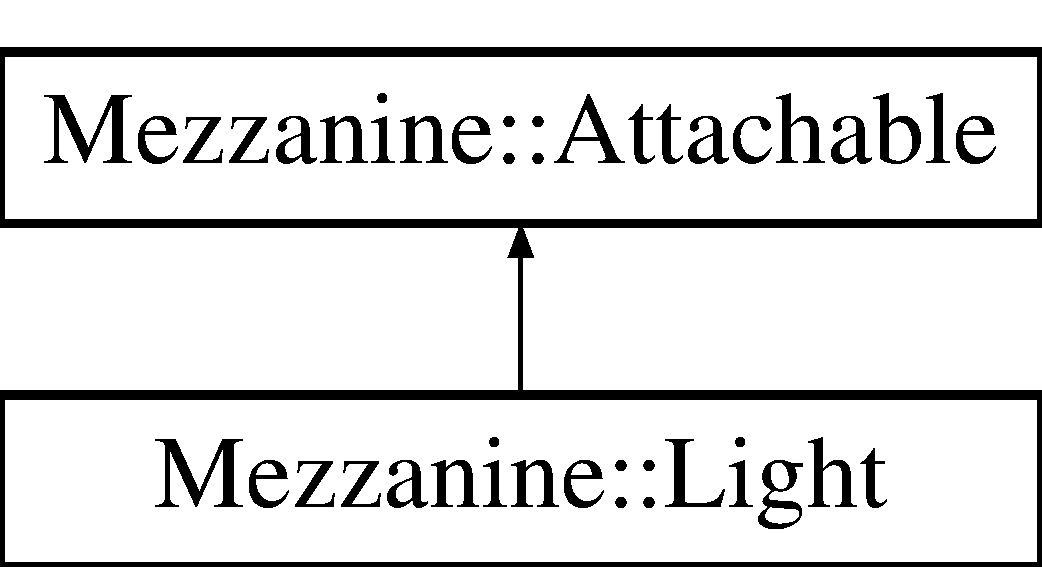
\includegraphics[height=2.000000cm]{classMezzanine_1_1Light}
\end{center}
\end{figure}
\subsubsection*{Public Types}
\begin{DoxyCompactItemize}
\item 
enum \hyperlink{classMezzanine_1_1Light_a783df27d8261c5af2226bc75586944be}{LightType} \{ \hyperlink{classMezzanine_1_1Light_a783df27d8261c5af2226bc75586944bea0374f1b4eee3903c6857838f0de8c48e}{Directional} =  0, 
\hyperlink{classMezzanine_1_1Light_a783df27d8261c5af2226bc75586944bea8922c0c85b8c971b99e636ff924bfb5d}{Point} =  1, 
\hyperlink{classMezzanine_1_1Light_a783df27d8261c5af2226bc75586944beab3af9a02884457e13f67d4bba11e4b4c}{Spotlight} =  2
 \}
\begin{DoxyCompactList}\small\item\em What kind of light Source. \item\end{DoxyCompactList}\end{DoxyCompactItemize}
\subsubsection*{Public Member Functions}
\begin{DoxyCompactItemize}
\item 
virtual \hyperlink{structMezzanine_1_1AttachableData}{AttachableData} \hyperlink{classMezzanine_1_1Light_aefbd732fe2b4a5b00cdb9d30dce2c5ce}{GetAttachableData} () const 
\begin{DoxyCompactList}\small\item\em Gets pointers to the internal ogre structures for this attachable. \item\end{DoxyCompactList}\item 
virtual \hyperlink{classMezzanine_1_1Attachable_a274bd45f9666f6e50f6fdd8a0162bc9e}{Attachable::AttachableElement} \hyperlink{classMezzanine_1_1Light_a530d776b916f3d8164dc2b8583040f64}{GetAttachableType} () const 
\begin{DoxyCompactList}\small\item\em What kind of \hyperlink{classMezzanine_1_1Attachable}{Attachable} is this. \item\end{DoxyCompactList}\item 
\hyperlink{namespaceMezzanine_a726731b1a7df72bf3583e4a97282c6f6}{Real} \hyperlink{classMezzanine_1_1Light_a9564b933f74967b89b144650abe75a48}{GetAttenuationConstant} () const 
\begin{DoxyCompactList}\small\item\em Gets the constant factor of the attenuation. \item\end{DoxyCompactList}\item 
\hyperlink{namespaceMezzanine_a726731b1a7df72bf3583e4a97282c6f6}{Real} \hyperlink{classMezzanine_1_1Light_aeb3f9b4ce95a43fe9253dc455e83f45e}{GetAttenuationLinear} () const 
\begin{DoxyCompactList}\small\item\em Gets the linear factor of the attentuation. \item\end{DoxyCompactList}\item 
\hyperlink{namespaceMezzanine_a726731b1a7df72bf3583e4a97282c6f6}{Real} \hyperlink{classMezzanine_1_1Light_a89f2ed0a02bf28bacad1569877e35a78}{GetAttenuationQuadric} () const 
\begin{DoxyCompactList}\small\item\em Gets the quadric factor of the attenuation. \item\end{DoxyCompactList}\item 
\hyperlink{namespaceMezzanine_a726731b1a7df72bf3583e4a97282c6f6}{Real} \hyperlink{classMezzanine_1_1Light_af94876bf25ec03b1cf34daeff1ffecd3}{GetAttenuationRange} () const 
\begin{DoxyCompactList}\small\item\em Gets the absolute range of attenuation in world units. \item\end{DoxyCompactList}\item 
\hyperlink{classMezzanine_1_1ColourValue}{ColourValue} \hyperlink{classMezzanine_1_1Light_af21912b8f7421f79bc8a24e7127b8d51}{GetDiffuseColour} () const 
\begin{DoxyCompactList}\small\item\em Gets the current colour of the diffuse light. \item\end{DoxyCompactList}\item 
\hyperlink{classMezzanine_1_1Vector3}{Vector3} \hyperlink{classMezzanine_1_1Light_a86b7fec45b3b9476a5f02cee0386c29c}{GetDirection} () const 
\begin{DoxyCompactList}\small\item\em Gets the currently set direction of the light. \item\end{DoxyCompactList}\item 
\hyperlink{classMezzanine_1_1Vector3}{Vector3} \hyperlink{classMezzanine_1_1Light_a997d299abec130a6a9111b5659a6b0d2}{GetLocation} () const 
\begin{DoxyCompactList}\small\item\em Gets the current location of the light. \item\end{DoxyCompactList}\item 
\hyperlink{namespaceMezzanine_a63cd699ac54b73953f35ec9cfc05e506}{ConstString} \& \hyperlink{classMezzanine_1_1Light_a1488e39ce34aab274ee5618aeb1f810d}{GetName} () const 
\begin{DoxyCompactList}\small\item\em Gets the name of this light. \item\end{DoxyCompactList}\item 
\hyperlink{classMezzanine_1_1Quaternion}{Quaternion} \hyperlink{classMezzanine_1_1Light_a08a415b00c94345ebb5155fa15819296}{GetOrientation} () const 
\begin{DoxyCompactList}\small\item\em Inherited from \hyperlink{classMezzanine_1_1Attachable}{Attachable}, returns a default \hyperlink{classMezzanine_1_1Quaternion}{Quaternion}. \item\end{DoxyCompactList}\item 
\hyperlink{namespaceMezzanine_a726731b1a7df72bf3583e4a97282c6f6}{Real} \hyperlink{classMezzanine_1_1Light_a3206b96ca2e21c861e3a141464709beb}{GetPowerScale} () const 
\begin{DoxyCompactList}\small\item\em Gets the lights power scale. \item\end{DoxyCompactList}\item 
\hyperlink{classMezzanine_1_1ColourValue}{ColourValue} \hyperlink{classMezzanine_1_1Light_af3cef4b433cc3563ae3abd3675c5b922}{GetSpecularColour} () const 
\begin{DoxyCompactList}\small\item\em Gets the current colour of the specular light. \item\end{DoxyCompactList}\item 
\hyperlink{namespaceMezzanine_a726731b1a7df72bf3583e4a97282c6f6}{Real} \hyperlink{classMezzanine_1_1Light_adc25087fe48fe78c1bae8785c28d30e0}{GetSpotlightFalloff} () const 
\begin{DoxyCompactList}\small\item\em Gets the rate of falloff of the cone of light emitted by this spotlight. \item\end{DoxyCompactList}\item 
\hyperlink{namespaceMezzanine_a726731b1a7df72bf3583e4a97282c6f6}{Real} \hyperlink{classMezzanine_1_1Light_a88bb2a7515c4f67c8d367acfc1764420}{GetSpotlightInnerAngle} () const 
\begin{DoxyCompactList}\small\item\em Gets the Inner angle of the cone of light emitted by this spotlight. \item\end{DoxyCompactList}\item 
\hyperlink{namespaceMezzanine_a726731b1a7df72bf3583e4a97282c6f6}{Real} \hyperlink{classMezzanine_1_1Light_a750426a53eeed92787c996f8b35c1d32}{GetSpotlightOuterAngle} () const 
\begin{DoxyCompactList}\small\item\em Gets the Outer angle of the cone of light emitted by this spotlight. \item\end{DoxyCompactList}\item 
\hyperlink{classMezzanine_1_1Light_a783df27d8261c5af2226bc75586944be}{Light::LightType} \hyperlink{classMezzanine_1_1Light_a05cbcc2c73bf309f6b7036895bc44307}{GetType} () const 
\begin{DoxyCompactList}\small\item\em Gets the type of light that this light is. \item\end{DoxyCompactList}\item 
\hyperlink{classMezzanine_1_1Light_a78f9b77376839f757826336bf8f93f00}{Light} (Ogre::Light $\ast$light, \hyperlink{classMezzanine_1_1SceneManager}{SceneManager} $\ast$manager)
\begin{DoxyCompactList}\small\item\em Internal Constructor. \item\end{DoxyCompactList}\item 
\hyperlink{classMezzanine_1_1Light_a22277def5a6adfa4ad0c510faa08f90a}{Light} (const \hyperlink{namespaceMezzanine_acf9fcc130e6ebf08e3d8491aebcf1c86}{String} \&Name, \hyperlink{classMezzanine_1_1SceneManager}{SceneManager} $\ast$manager)
\begin{DoxyCompactList}\small\item\em Standard initialization constructor. \item\end{DoxyCompactList}\item 
void \hyperlink{classMezzanine_1_1Light_adcac90175a780d07564a41648c22892c}{SetAttenuation} (\hyperlink{namespaceMezzanine_a726731b1a7df72bf3583e4a97282c6f6}{Real} Range, \hyperlink{namespaceMezzanine_a726731b1a7df72bf3583e4a97282c6f6}{Real} Constant, \hyperlink{namespaceMezzanine_a726731b1a7df72bf3583e4a97282c6f6}{Real} Linear, \hyperlink{namespaceMezzanine_a726731b1a7df72bf3583e4a97282c6f6}{Real} Quadratic)
\begin{DoxyCompactList}\small\item\em Sets the factors for the attenuation formula applied to this light. \item\end{DoxyCompactList}\item 
void \hyperlink{classMezzanine_1_1Light_a577e92239a463c40207dc749b3f6c14a}{SetDiffuseColour} (const \hyperlink{classMezzanine_1_1ColourValue}{ColourValue} \&Colour)
\begin{DoxyCompactList}\small\item\em Sets the colour for the Diffuse light from this source. \item\end{DoxyCompactList}\item 
void \hyperlink{classMezzanine_1_1Light_a6f669a5d25e6c9b40be8656606da854c}{SetDiffuseColour} (\hyperlink{namespaceMezzanine_a726731b1a7df72bf3583e4a97282c6f6}{Real} Red, \hyperlink{namespaceMezzanine_a726731b1a7df72bf3583e4a97282c6f6}{Real} Green, \hyperlink{namespaceMezzanine_a726731b1a7df72bf3583e4a97282c6f6}{Real} Blue)
\begin{DoxyCompactList}\small\item\em Sets the colour for the Diffuse light from this source. \item\end{DoxyCompactList}\item 
void \hyperlink{classMezzanine_1_1Light_a22cbfb15ef1c7caf1011574f568d19de}{SetDirection} (const \hyperlink{classMezzanine_1_1Vector3}{Vector3} \&Direction)
\begin{DoxyCompactList}\small\item\em Sets the direction the light will originate from. \item\end{DoxyCompactList}\item 
void \hyperlink{classMezzanine_1_1Light_ac06da317651df700c2969cc81c3f8d3d}{SetLocation} (const \hyperlink{classMezzanine_1_1Vector3}{Vector3} \&Location)
\begin{DoxyCompactList}\small\item\em Sets the location from where the light will originate. \item\end{DoxyCompactList}\item 
void \hyperlink{classMezzanine_1_1Light_aa2f3fe2b7cb7bf459f2526d2e5c234ed}{SetOrientation} (const \hyperlink{classMezzanine_1_1Quaternion}{Quaternion} \&Orientation)
\begin{DoxyCompactList}\small\item\em Inherited from \hyperlink{classMezzanine_1_1Attachable}{Attachable}, does nothing on \hyperlink{classMezzanine_1_1Light}{Light} class. \item\end{DoxyCompactList}\item 
void \hyperlink{classMezzanine_1_1Light_ad1a8c423c21f192429c01313905fd69a}{SetPowerScale} (\hyperlink{namespaceMezzanine_a726731b1a7df72bf3583e4a97282c6f6}{Real} Power)
\begin{DoxyCompactList}\small\item\em Sets the lights power scale. \item\end{DoxyCompactList}\item 
void \hyperlink{classMezzanine_1_1Light_a1594396da60d45ba12b04f7d8a4ba90e}{SetSpecularColour} (\hyperlink{namespaceMezzanine_a726731b1a7df72bf3583e4a97282c6f6}{Real} Red, \hyperlink{namespaceMezzanine_a726731b1a7df72bf3583e4a97282c6f6}{Real} Green, \hyperlink{namespaceMezzanine_a726731b1a7df72bf3583e4a97282c6f6}{Real} Blue)
\begin{DoxyCompactList}\small\item\em Sets the colour for the Specular light from this source. \item\end{DoxyCompactList}\item 
void \hyperlink{classMezzanine_1_1Light_a920d4d00a76b5643e3f7318a92011bbf}{SetSpecularColour} (const \hyperlink{classMezzanine_1_1ColourValue}{ColourValue} \&Colour)
\begin{DoxyCompactList}\small\item\em Sets the colour for the Specular light from this source. \item\end{DoxyCompactList}\item 
void \hyperlink{classMezzanine_1_1Light_aed419cb9a43757aa86c491fb4ad22132}{SetSpotlightFalloff} (\hyperlink{namespaceMezzanine_a726731b1a7df72bf3583e4a97282c6f6}{Real} Falloff)
\begin{DoxyCompactList}\small\item\em Sets the rate of falloff of the cone of light emitted by a spotlight. \item\end{DoxyCompactList}\item 
void \hyperlink{classMezzanine_1_1Light_acf532728dbcb894f4b3ada6492670ed2}{SetSpotlightInnerAngle} (\hyperlink{namespaceMezzanine_a726731b1a7df72bf3583e4a97282c6f6}{Real} InnerAngle)
\begin{DoxyCompactList}\small\item\em Sets the Inner angle of the cone of light emitted by a spotlight. \item\end{DoxyCompactList}\item 
void \hyperlink{classMezzanine_1_1Light_a149bd5af4b9120bab0703fc5ae638ac3}{SetSpotlightOuterAngle} (\hyperlink{namespaceMezzanine_a726731b1a7df72bf3583e4a97282c6f6}{Real} OuterAngle)
\begin{DoxyCompactList}\small\item\em Sets the Outer angle of the cone of light emitted by a spotlight. \item\end{DoxyCompactList}\item 
void \hyperlink{classMezzanine_1_1Light_a1f45a8de84131b1cea1566d7c175c597}{SetSpotlightRange} (\hyperlink{namespaceMezzanine_a726731b1a7df72bf3583e4a97282c6f6}{Real} InnerAngle, \hyperlink{namespaceMezzanine_a726731b1a7df72bf3583e4a97282c6f6}{Real} OuterAngle, \hyperlink{namespaceMezzanine_a726731b1a7df72bf3583e4a97282c6f6}{Real} Falloff=1.0)
\begin{DoxyCompactList}\small\item\em Defines the cone of light emitted by a spotlight. \item\end{DoxyCompactList}\item 
void \hyperlink{classMezzanine_1_1Light_a3eb8a8a9919dee3ae8e403d6f1946f45}{SetType} (\hyperlink{classMezzanine_1_1Light_a783df27d8261c5af2226bc75586944be}{Light::LightType} Type)
\begin{DoxyCompactList}\small\item\em Sets the type of light this light is. \item\end{DoxyCompactList}\item 
\hypertarget{classMezzanine_1_1Light_aa86b020d33393ff4e14d3ff40fc9b506}{
virtual \hyperlink{classMezzanine_1_1Light_aa86b020d33393ff4e14d3ff40fc9b506}{$\sim$Light} ()}
\label{classMezzanine_1_1Light_aa86b020d33393ff4e14d3ff40fc9b506}

\begin{DoxyCompactList}\small\item\em Class destructor. \item\end{DoxyCompactList}\end{DoxyCompactItemize}
\subsubsection*{Protected Attributes}
\begin{DoxyCompactItemize}
\item 
\hypertarget{classMezzanine_1_1Light_a33af923976c32b2a34aaae8549ed35e4}{
\hyperlink{classMezzanine_1_1SceneManager}{SceneManager} $\ast$ \hyperlink{classMezzanine_1_1Light_a33af923976c32b2a34aaae8549ed35e4}{Manager}}
\label{classMezzanine_1_1Light_a33af923976c32b2a34aaae8549ed35e4}

\begin{DoxyCompactList}\small\item\em Pointer to the manager that created this class. \item\end{DoxyCompactList}\item 
\hypertarget{classMezzanine_1_1Light_a228f1f22dbee36bed47894086d2191ff}{
Ogre::Light $\ast$ \hyperlink{classMezzanine_1_1Light_a228f1f22dbee36bed47894086d2191ff}{OgreLight}}
\label{classMezzanine_1_1Light_a228f1f22dbee36bed47894086d2191ff}

\begin{DoxyCompactList}\small\item\em The ogre light this class gets it's functionality from. \item\end{DoxyCompactList}\end{DoxyCompactItemize}


\subsubsection{Detailed Description}
This class is the class used for dynamic lighting within the scene. Dynamic lights come in 3 flavors: \par
 Directional -\/ Used to simulate light from a very distant source. Doesn't need a location, only a direction. \hyperlink{classMezzanine_1_1Light}{Light} will hit all objects accordingly from that direction. \par
 Point -\/ Used to simulate local light sources that emit light in all directions. Doesn't need a direction, just a Location. \par
 Spotlight -\/ Used to simulate local light sources that emit light in one direction, such as a flashlight. Needs both a Location and direction. In addition needs values for falloff. \par
 Note: If attaching a light to a node, all transform information(Location and orientation) becomes relative to the nodes transform. 

Definition at line 72 of file light.h.



\subsubsection{Member Enumeration Documentation}
\hypertarget{classMezzanine_1_1Light_a783df27d8261c5af2226bc75586944be}{
\index{Mezzanine::Light@{Mezzanine::Light}!LightType@{LightType}}
\index{LightType@{LightType}!Mezzanine::Light@{Mezzanine::Light}}
\paragraph[{LightType}]{\setlength{\rightskip}{0pt plus 5cm}enum {\bf Mezzanine::Light::LightType}}\hfill}
\label{classMezzanine_1_1Light_a783df27d8261c5af2226bc75586944be}


What kind of light Source. 

\begin{Desc}
\item[Enumerator: ]\par
\begin{description}
\index{Directional@{Directional}!Mezzanine::Light@{Mezzanine::Light}}\index{Mezzanine::Light@{Mezzanine::Light}!Directional@{Directional}}\item[{\em 
\hypertarget{classMezzanine_1_1Light_a783df27d8261c5af2226bc75586944bea0374f1b4eee3903c6857838f0de8c48e}{
Directional}
\label{classMezzanine_1_1Light_a783df27d8261c5af2226bc75586944bea0374f1b4eee3903c6857838f0de8c48e}
}]From one direction, like sunlight. \index{Point@{Point}!Mezzanine::Light@{Mezzanine::Light}}\index{Mezzanine::Light@{Mezzanine::Light}!Point@{Point}}\item[{\em 
\hypertarget{classMezzanine_1_1Light_a783df27d8261c5af2226bc75586944bea8922c0c85b8c971b99e636ff924bfb5d}{
Point}
\label{classMezzanine_1_1Light_a783df27d8261c5af2226bc75586944bea8922c0c85b8c971b99e636ff924bfb5d}
}]From a point in space, like a Torch, campfire, muzzle flash, Mutant Fireflies, bonfires, light bulbs, non-\/hooded lantern, the DnD D20 \hyperlink{classMezzanine_1_1Light}{Light} spell, explosions, and scotch tape separating from the roll in a unlit vacuum. There may be other uses, be creative. \index{Spotlight@{Spotlight}!Mezzanine::Light@{Mezzanine::Light}}\index{Mezzanine::Light@{Mezzanine::Light}!Spotlight@{Spotlight}}\item[{\em 
\hypertarget{classMezzanine_1_1Light_a783df27d8261c5af2226bc75586944beab3af9a02884457e13f67d4bba11e4b4c}{
Spotlight}
\label{classMezzanine_1_1Light_a783df27d8261c5af2226bc75586944beab3af9a02884457e13f67d4bba11e4b4c}
}]From a point emanating in a cone, like a flashlight, hooded lantern, really bright computer screens, flood lights, older style space heaters, Concert lights, camera flashes, etc... \end{description}
\end{Desc}



Definition at line 76 of file light.h.



\subsubsection{Constructor \& Destructor Documentation}
\hypertarget{classMezzanine_1_1Light_a22277def5a6adfa4ad0c510faa08f90a}{
\index{Mezzanine::Light@{Mezzanine::Light}!Light@{Light}}
\index{Light@{Light}!Mezzanine::Light@{Mezzanine::Light}}
\paragraph[{Light}]{\setlength{\rightskip}{0pt plus 5cm}Mezzanine::Light::Light (
\begin{DoxyParamCaption}
\item[{const {\bf String} \&}]{Name, }
\item[{{\bf SceneManager} $\ast$}]{manager}
\end{DoxyParamCaption}
)}\hfill}
\label{classMezzanine_1_1Light_a22277def5a6adfa4ad0c510faa08f90a}


Standard initialization constructor. 


\begin{DoxyParams}{Parameters}
{\em Name} & The name of this light. \\
\hline
{\em manager} & Pointer to the manager that this light is to be used in. \\
\hline
\end{DoxyParams}


Definition at line 61 of file light.cpp.

\hypertarget{classMezzanine_1_1Light_a78f9b77376839f757826336bf8f93f00}{
\index{Mezzanine::Light@{Mezzanine::Light}!Light@{Light}}
\index{Light@{Light}!Mezzanine::Light@{Mezzanine::Light}}
\paragraph[{Light}]{\setlength{\rightskip}{0pt plus 5cm}Mezzanine::Light::Light (
\begin{DoxyParamCaption}
\item[{Ogre::Light $\ast$}]{light, }
\item[{{\bf SceneManager} $\ast$}]{manager}
\end{DoxyParamCaption}
)}\hfill}
\label{classMezzanine_1_1Light_a78f9b77376839f757826336bf8f93f00}


Internal Constructor. 

This constructor should not be called on manually. 
\begin{DoxyParams}{Parameters}
{\em light} & The Ogre light this class is based on. \\
\hline
{\em manager} & Pointer to the manager that this light is to be used in. \\
\hline
\end{DoxyParams}


Definition at line 67 of file light.cpp.



\subsubsection{Member Function Documentation}
\hypertarget{classMezzanine_1_1Light_aefbd732fe2b4a5b00cdb9d30dce2c5ce}{
\index{Mezzanine::Light@{Mezzanine::Light}!GetAttachableData@{GetAttachableData}}
\index{GetAttachableData@{GetAttachableData}!Mezzanine::Light@{Mezzanine::Light}}
\paragraph[{GetAttachableData}]{\setlength{\rightskip}{0pt plus 5cm}{\bf AttachableData} Mezzanine::Light::GetAttachableData (
\begin{DoxyParamCaption}
{}
\end{DoxyParamCaption}
) const\hspace{0.3cm}{\ttfamily  \mbox{[}virtual\mbox{]}}}\hfill}
\label{classMezzanine_1_1Light_aefbd732fe2b4a5b00cdb9d30dce2c5ce}


Gets pointers to the internal ogre structures for this attachable. 

\begin{DoxyReturn}{Returns}
Returns an \hyperlink{structMezzanine_1_1AttachableData}{AttachableData} struct with the internal data. 
\end{DoxyReturn}


Implements \hyperlink{classMezzanine_1_1Attachable_aeed457c614552bd753e7669cb7624b19}{Mezzanine::Attachable}.



Definition at line 236 of file light.cpp.

\hypertarget{classMezzanine_1_1Light_a530d776b916f3d8164dc2b8583040f64}{
\index{Mezzanine::Light@{Mezzanine::Light}!GetAttachableType@{GetAttachableType}}
\index{GetAttachableType@{GetAttachableType}!Mezzanine::Light@{Mezzanine::Light}}
\paragraph[{GetAttachableType}]{\setlength{\rightskip}{0pt plus 5cm}{\bf Attachable::AttachableElement} Mezzanine::Light::GetAttachableType (
\begin{DoxyParamCaption}
{}
\end{DoxyParamCaption}
) const\hspace{0.3cm}{\ttfamily  \mbox{[}virtual\mbox{]}}}\hfill}
\label{classMezzanine_1_1Light_a530d776b916f3d8164dc2b8583040f64}


What kind of \hyperlink{classMezzanine_1_1Attachable}{Attachable} is this. 

\begin{DoxyReturn}{Returns}
An \hyperlink{classMezzanine_1_1Attachable_aacb1a1958cca1f005c1313f14e3d098d}{Attachable::GetAttachableType} containing \hyperlink{classMezzanine_1_1Attachable_a274bd45f9666f6e50f6fdd8a0162bc9ea1e169d7d694a091e31c6b59f18841e16}{Attachable::Light}. 
\end{DoxyReturn}


Implements \hyperlink{classMezzanine_1_1Attachable_aacb1a1958cca1f005c1313f14e3d098d}{Mezzanine::Attachable}.



Definition at line 230 of file light.cpp.

\hypertarget{classMezzanine_1_1Light_a9564b933f74967b89b144650abe75a48}{
\index{Mezzanine::Light@{Mezzanine::Light}!GetAttenuationConstant@{GetAttenuationConstant}}
\index{GetAttenuationConstant@{GetAttenuationConstant}!Mezzanine::Light@{Mezzanine::Light}}
\paragraph[{GetAttenuationConstant}]{\setlength{\rightskip}{0pt plus 5cm}{\bf Real} Mezzanine::Light::GetAttenuationConstant (
\begin{DoxyParamCaption}
{}
\end{DoxyParamCaption}
) const}\hfill}
\label{classMezzanine_1_1Light_a9564b933f74967b89b144650abe75a48}


Gets the constant factor of the attenuation. 

\begin{DoxyReturn}{Returns}
Returns a real representing the constant factor of attenuation. 
\end{DoxyReturn}


Definition at line 175 of file light.cpp.

\hypertarget{classMezzanine_1_1Light_aeb3f9b4ce95a43fe9253dc455e83f45e}{
\index{Mezzanine::Light@{Mezzanine::Light}!GetAttenuationLinear@{GetAttenuationLinear}}
\index{GetAttenuationLinear@{GetAttenuationLinear}!Mezzanine::Light@{Mezzanine::Light}}
\paragraph[{GetAttenuationLinear}]{\setlength{\rightskip}{0pt plus 5cm}{\bf Real} Mezzanine::Light::GetAttenuationLinear (
\begin{DoxyParamCaption}
{}
\end{DoxyParamCaption}
) const}\hfill}
\label{classMezzanine_1_1Light_aeb3f9b4ce95a43fe9253dc455e83f45e}


Gets the linear factor of the attentuation. 

\begin{DoxyReturn}{Returns}
Returns a real representing the linear factor of attenuation. 
\end{DoxyReturn}


Definition at line 178 of file light.cpp.

\hypertarget{classMezzanine_1_1Light_a89f2ed0a02bf28bacad1569877e35a78}{
\index{Mezzanine::Light@{Mezzanine::Light}!GetAttenuationQuadric@{GetAttenuationQuadric}}
\index{GetAttenuationQuadric@{GetAttenuationQuadric}!Mezzanine::Light@{Mezzanine::Light}}
\paragraph[{GetAttenuationQuadric}]{\setlength{\rightskip}{0pt plus 5cm}{\bf Real} Mezzanine::Light::GetAttenuationQuadric (
\begin{DoxyParamCaption}
{}
\end{DoxyParamCaption}
) const}\hfill}
\label{classMezzanine_1_1Light_a89f2ed0a02bf28bacad1569877e35a78}


Gets the quadric factor of the attenuation. 

\begin{DoxyReturn}{Returns}
Returns a real representing the quadric factor of attenuation. 
\end{DoxyReturn}


Definition at line 181 of file light.cpp.

\hypertarget{classMezzanine_1_1Light_af94876bf25ec03b1cf34daeff1ffecd3}{
\index{Mezzanine::Light@{Mezzanine::Light}!GetAttenuationRange@{GetAttenuationRange}}
\index{GetAttenuationRange@{GetAttenuationRange}!Mezzanine::Light@{Mezzanine::Light}}
\paragraph[{GetAttenuationRange}]{\setlength{\rightskip}{0pt plus 5cm}{\bf Real} Mezzanine::Light::GetAttenuationRange (
\begin{DoxyParamCaption}
{}
\end{DoxyParamCaption}
) const}\hfill}
\label{classMezzanine_1_1Light_af94876bf25ec03b1cf34daeff1ffecd3}


Gets the absolute range of attenuation in world units. 

\begin{DoxyReturn}{Returns}
Returns a real representing the absolute range of attenuation. 
\end{DoxyReturn}


Definition at line 172 of file light.cpp.

\hypertarget{classMezzanine_1_1Light_af21912b8f7421f79bc8a24e7127b8d51}{
\index{Mezzanine::Light@{Mezzanine::Light}!GetDiffuseColour@{GetDiffuseColour}}
\index{GetDiffuseColour@{GetDiffuseColour}!Mezzanine::Light@{Mezzanine::Light}}
\paragraph[{GetDiffuseColour}]{\setlength{\rightskip}{0pt plus 5cm}{\bf ColourValue} Mezzanine::Light::GetDiffuseColour (
\begin{DoxyParamCaption}
{}
\end{DoxyParamCaption}
) const}\hfill}
\label{classMezzanine_1_1Light_af21912b8f7421f79bc8a24e7127b8d51}


Gets the current colour of the diffuse light. 

\begin{DoxyReturn}{Returns}
Returns a colourvalue representing the currently set Diffuse light. 
\end{DoxyReturn}


Definition at line 160 of file light.cpp.

\hypertarget{classMezzanine_1_1Light_a86b7fec45b3b9476a5f02cee0386c29c}{
\index{Mezzanine::Light@{Mezzanine::Light}!GetDirection@{GetDirection}}
\index{GetDirection@{GetDirection}!Mezzanine::Light@{Mezzanine::Light}}
\paragraph[{GetDirection}]{\setlength{\rightskip}{0pt plus 5cm}{\bf Vector3} Mezzanine::Light::GetDirection (
\begin{DoxyParamCaption}
{}
\end{DoxyParamCaption}
) const}\hfill}
\label{classMezzanine_1_1Light_a86b7fec45b3b9476a5f02cee0386c29c}


Gets the currently set direction of the light. 

\begin{DoxyReturn}{Returns}
Returns a vector3 representing the set direction of the light.
\end{DoxyReturn}
Not used in point lights. 

Definition at line 142 of file light.cpp.

\hypertarget{classMezzanine_1_1Light_a997d299abec130a6a9111b5659a6b0d2}{
\index{Mezzanine::Light@{Mezzanine::Light}!GetLocation@{GetLocation}}
\index{GetLocation@{GetLocation}!Mezzanine::Light@{Mezzanine::Light}}
\paragraph[{GetLocation}]{\setlength{\rightskip}{0pt plus 5cm}{\bf Vector3} Mezzanine::Light::GetLocation (
\begin{DoxyParamCaption}
{}
\end{DoxyParamCaption}
) const\hspace{0.3cm}{\ttfamily  \mbox{[}virtual\mbox{]}}}\hfill}
\label{classMezzanine_1_1Light_a997d299abec130a6a9111b5659a6b0d2}


Gets the current location of the light. 

\begin{DoxyReturn}{Returns}
Returns a vector3 representing the location of the light.
\end{DoxyReturn}
Not used in Directional Lights. 

Implements \hyperlink{classMezzanine_1_1Attachable_a1a8e18e5654c50f24bc049c228603d71}{Mezzanine::Attachable}.



Definition at line 136 of file light.cpp.

\hypertarget{classMezzanine_1_1Light_a1488e39ce34aab274ee5618aeb1f810d}{
\index{Mezzanine::Light@{Mezzanine::Light}!GetName@{GetName}}
\index{GetName@{GetName}!Mezzanine::Light@{Mezzanine::Light}}
\paragraph[{GetName}]{\setlength{\rightskip}{0pt plus 5cm}{\bf ConstString} \& Mezzanine::Light::GetName (
\begin{DoxyParamCaption}
{}
\end{DoxyParamCaption}
) const\hspace{0.3cm}{\ttfamily  \mbox{[}virtual\mbox{]}}}\hfill}
\label{classMezzanine_1_1Light_a1488e39ce34aab274ee5618aeb1f810d}


Gets the name of this light. 

\begin{DoxyReturn}{Returns}
Returns a string containing the name given to this light. 
\end{DoxyReturn}


Implements \hyperlink{classMezzanine_1_1Attachable_a6a49ac8c2ddb2dd8ed7dd17f96ecafe5}{Mezzanine::Attachable}.



Definition at line 79 of file light.cpp.

\hypertarget{classMezzanine_1_1Light_a08a415b00c94345ebb5155fa15819296}{
\index{Mezzanine::Light@{Mezzanine::Light}!GetOrientation@{GetOrientation}}
\index{GetOrientation@{GetOrientation}!Mezzanine::Light@{Mezzanine::Light}}
\paragraph[{GetOrientation}]{\setlength{\rightskip}{0pt plus 5cm}{\bf Quaternion} Mezzanine::Light::GetOrientation (
\begin{DoxyParamCaption}
{}
\end{DoxyParamCaption}
) const\hspace{0.3cm}{\ttfamily  \mbox{[}virtual\mbox{]}}}\hfill}
\label{classMezzanine_1_1Light_a08a415b00c94345ebb5155fa15819296}


Inherited from \hyperlink{classMezzanine_1_1Attachable}{Attachable}, returns a default \hyperlink{classMezzanine_1_1Quaternion}{Quaternion}. 

\begin{DoxyReturn}{Returns}
Returns a quaternion with the orientation. 
\end{DoxyReturn}


Implements \hyperlink{classMezzanine_1_1Attachable_ab3e094cbc373edb05866783290991e7d}{Mezzanine::Attachable}.



Definition at line 139 of file light.cpp.

\hypertarget{classMezzanine_1_1Light_a3206b96ca2e21c861e3a141464709beb}{
\index{Mezzanine::Light@{Mezzanine::Light}!GetPowerScale@{GetPowerScale}}
\index{GetPowerScale@{GetPowerScale}!Mezzanine::Light@{Mezzanine::Light}}
\paragraph[{GetPowerScale}]{\setlength{\rightskip}{0pt plus 5cm}{\bf Real} Mezzanine::Light::GetPowerScale (
\begin{DoxyParamCaption}
{}
\end{DoxyParamCaption}
) const}\hfill}
\label{classMezzanine_1_1Light_a3206b96ca2e21c861e3a141464709beb}


Gets the lights power scale. 

\begin{DoxyReturn}{Returns}
Returns a real representing the power scale of the light.
\end{DoxyReturn}
Only used with HDR ( High Dynamic Range ) rendering 

Definition at line 221 of file light.cpp.

\hypertarget{classMezzanine_1_1Light_af3cef4b433cc3563ae3abd3675c5b922}{
\index{Mezzanine::Light@{Mezzanine::Light}!GetSpecularColour@{GetSpecularColour}}
\index{GetSpecularColour@{GetSpecularColour}!Mezzanine::Light@{Mezzanine::Light}}
\paragraph[{GetSpecularColour}]{\setlength{\rightskip}{0pt plus 5cm}{\bf ColourValue} Mezzanine::Light::GetSpecularColour (
\begin{DoxyParamCaption}
{}
\end{DoxyParamCaption}
) const}\hfill}
\label{classMezzanine_1_1Light_af3cef4b433cc3563ae3abd3675c5b922}


Gets the current colour of the specular light. 

\begin{DoxyReturn}{Returns}
Returns a colourvalue representing the currently set Specular light. 
\end{DoxyReturn}


Definition at line 163 of file light.cpp.

\hypertarget{classMezzanine_1_1Light_adc25087fe48fe78c1bae8785c28d30e0}{
\index{Mezzanine::Light@{Mezzanine::Light}!GetSpotlightFalloff@{GetSpotlightFalloff}}
\index{GetSpotlightFalloff@{GetSpotlightFalloff}!Mezzanine::Light@{Mezzanine::Light}}
\paragraph[{GetSpotlightFalloff}]{\setlength{\rightskip}{0pt plus 5cm}{\bf Real} Mezzanine::Light::GetSpotlightFalloff (
\begin{DoxyParamCaption}
{}
\end{DoxyParamCaption}
) const}\hfill}
\label{classMezzanine_1_1Light_adc25087fe48fe78c1bae8785c28d30e0}


Gets the rate of falloff of the cone of light emitted by this spotlight. 

\begin{DoxyReturn}{Returns}
Returns a real representing the falloff of the cone of light. 
\end{DoxyReturn}


Definition at line 215 of file light.cpp.

\hypertarget{classMezzanine_1_1Light_a88bb2a7515c4f67c8d367acfc1764420}{
\index{Mezzanine::Light@{Mezzanine::Light}!GetSpotlightInnerAngle@{GetSpotlightInnerAngle}}
\index{GetSpotlightInnerAngle@{GetSpotlightInnerAngle}!Mezzanine::Light@{Mezzanine::Light}}
\paragraph[{GetSpotlightInnerAngle}]{\setlength{\rightskip}{0pt plus 5cm}{\bf Real} Mezzanine::Light::GetSpotlightInnerAngle (
\begin{DoxyParamCaption}
{}
\end{DoxyParamCaption}
) const}\hfill}
\label{classMezzanine_1_1Light_a88bb2a7515c4f67c8d367acfc1764420}


Gets the Inner angle of the cone of light emitted by this spotlight. 

\begin{DoxyReturn}{Returns}
Returns a real representing the inner angle of this spotlight, in radians. 
\end{DoxyReturn}


Definition at line 209 of file light.cpp.

\hypertarget{classMezzanine_1_1Light_a750426a53eeed92787c996f8b35c1d32}{
\index{Mezzanine::Light@{Mezzanine::Light}!GetSpotlightOuterAngle@{GetSpotlightOuterAngle}}
\index{GetSpotlightOuterAngle@{GetSpotlightOuterAngle}!Mezzanine::Light@{Mezzanine::Light}}
\paragraph[{GetSpotlightOuterAngle}]{\setlength{\rightskip}{0pt plus 5cm}{\bf Real} Mezzanine::Light::GetSpotlightOuterAngle (
\begin{DoxyParamCaption}
{}
\end{DoxyParamCaption}
) const}\hfill}
\label{classMezzanine_1_1Light_a750426a53eeed92787c996f8b35c1d32}


Gets the Outer angle of the cone of light emitted by this spotlight. 

\begin{DoxyReturn}{Returns}
Returns a real representing the outer angle of this spotlight, in radians. 
\end{DoxyReturn}


Definition at line 212 of file light.cpp.

\hypertarget{classMezzanine_1_1Light_a05cbcc2c73bf309f6b7036895bc44307}{
\index{Mezzanine::Light@{Mezzanine::Light}!GetType@{GetType}}
\index{GetType@{GetType}!Mezzanine::Light@{Mezzanine::Light}}
\paragraph[{GetType}]{\setlength{\rightskip}{0pt plus 5cm}{\bf Light::LightType} Mezzanine::Light::GetType (
\begin{DoxyParamCaption}
{}
\end{DoxyParamCaption}
) const}\hfill}
\label{classMezzanine_1_1Light_a05cbcc2c73bf309f6b7036895bc44307}


Gets the type of light that this light is. 

\begin{DoxyReturn}{Returns}
Returns an enum value for this lights type. 
\end{DoxyReturn}


Definition at line 103 of file light.cpp.

\hypertarget{classMezzanine_1_1Light_adcac90175a780d07564a41648c22892c}{
\index{Mezzanine::Light@{Mezzanine::Light}!SetAttenuation@{SetAttenuation}}
\index{SetAttenuation@{SetAttenuation}!Mezzanine::Light@{Mezzanine::Light}}
\paragraph[{SetAttenuation}]{\setlength{\rightskip}{0pt plus 5cm}void Mezzanine::Light::SetAttenuation (
\begin{DoxyParamCaption}
\item[{{\bf Real}}]{Range, }
\item[{{\bf Real}}]{Constant, }
\item[{{\bf Real}}]{Linear, }
\item[{{\bf Real}}]{Quadratic}
\end{DoxyParamCaption}
)}\hfill}
\label{classMezzanine_1_1Light_adcac90175a780d07564a41648c22892c}


Sets the factors for the attenuation formula applied to this light. 

This function is only applicable when using a spotlight or point type of light. 
\begin{DoxyParams}{Parameters}
{\em Range} & The absolute range of the light in world units. Objects beyond this range will not be influenced by this light. \\
\hline
{\em Constant} & The constant of the attenuation, ranging from 0.0 to 1.0. 1.0 means never attenuate, 0.0 is complete attenuation. \\
\hline
{\em Linear} & The linear factor of the attentuation, ranging from 0.0 to 1.0. 1.0 means attenuate evenly over the distance. \\
\hline
{\em Quadratic} & The Quadratic factor of the attenuation. This value adds curvature to the attenuation. \\
\hline
\end{DoxyParams}


Definition at line 169 of file light.cpp.

\hypertarget{classMezzanine_1_1Light_a6f669a5d25e6c9b40be8656606da854c}{
\index{Mezzanine::Light@{Mezzanine::Light}!SetDiffuseColour@{SetDiffuseColour}}
\index{SetDiffuseColour@{SetDiffuseColour}!Mezzanine::Light@{Mezzanine::Light}}
\paragraph[{SetDiffuseColour}]{\setlength{\rightskip}{0pt plus 5cm}void Mezzanine::Light::SetDiffuseColour (
\begin{DoxyParamCaption}
\item[{{\bf Real}}]{Red, }
\item[{{\bf Real}}]{Green, }
\item[{{\bf Real}}]{Blue}
\end{DoxyParamCaption}
)}\hfill}
\label{classMezzanine_1_1Light_a6f669a5d25e6c9b40be8656606da854c}


Sets the colour for the Diffuse light from this source. 

When rendering the final color of an object values of the colours of 3 types of lights are taken into account. The 3 types are: Diffuse, Specular, and Ambient. 
\begin{DoxyParams}{Parameters}
{\em Red} & Real in the range of 0.0 to 1.0 determining the amount of red in the colour. \\
\hline
{\em Red} & Green in the range of 0.0 to 1.0 determining the amount of green in the colour. \\
\hline
{\em Red} & Blue in the range of 0.0 to 1.0 determining the amount of blue in the colour. \\
\hline
\end{DoxyParams}


Definition at line 148 of file light.cpp.

\hypertarget{classMezzanine_1_1Light_a577e92239a463c40207dc749b3f6c14a}{
\index{Mezzanine::Light@{Mezzanine::Light}!SetDiffuseColour@{SetDiffuseColour}}
\index{SetDiffuseColour@{SetDiffuseColour}!Mezzanine::Light@{Mezzanine::Light}}
\paragraph[{SetDiffuseColour}]{\setlength{\rightskip}{0pt plus 5cm}void Mezzanine::Light::SetDiffuseColour (
\begin{DoxyParamCaption}
\item[{const {\bf ColourValue} \&}]{Colour}
\end{DoxyParamCaption}
)}\hfill}
\label{classMezzanine_1_1Light_a577e92239a463c40207dc749b3f6c14a}


Sets the colour for the Diffuse light from this source. 

This allows the setting of Diffuse color by a premade \hyperlink{classMezzanine_1_1ColourValue}{ColourValue}. 
\begin{DoxyParams}{Parameters}
{\em Colour} & \hyperlink{classMezzanine_1_1ColourValue}{ColourValue} representing the color of the light to be set. \\
\hline
\end{DoxyParams}


Definition at line 151 of file light.cpp.

\hypertarget{classMezzanine_1_1Light_a22cbfb15ef1c7caf1011574f568d19de}{
\index{Mezzanine::Light@{Mezzanine::Light}!SetDirection@{SetDirection}}
\index{SetDirection@{SetDirection}!Mezzanine::Light@{Mezzanine::Light}}
\paragraph[{SetDirection}]{\setlength{\rightskip}{0pt plus 5cm}void Mezzanine::Light::SetDirection (
\begin{DoxyParamCaption}
\item[{const {\bf Vector3} \&}]{Direction}
\end{DoxyParamCaption}
)}\hfill}
\label{classMezzanine_1_1Light_a22cbfb15ef1c7caf1011574f568d19de}


Sets the direction the light will originate from. 


\begin{DoxyParams}{Parameters}
{\em Direction} & A vector3 representing the direction the light will come from.\\
\hline
\end{DoxyParams}
Not used in point lights. 

Definition at line 133 of file light.cpp.

\hypertarget{classMezzanine_1_1Light_ac06da317651df700c2969cc81c3f8d3d}{
\index{Mezzanine::Light@{Mezzanine::Light}!SetLocation@{SetLocation}}
\index{SetLocation@{SetLocation}!Mezzanine::Light@{Mezzanine::Light}}
\paragraph[{SetLocation}]{\setlength{\rightskip}{0pt plus 5cm}void Mezzanine::Light::SetLocation (
\begin{DoxyParamCaption}
\item[{const {\bf Vector3} \&}]{Location}
\end{DoxyParamCaption}
)\hspace{0.3cm}{\ttfamily  \mbox{[}virtual\mbox{]}}}\hfill}
\label{classMezzanine_1_1Light_ac06da317651df700c2969cc81c3f8d3d}


Sets the location from where the light will originate. 


\begin{DoxyParams}{Parameters}
{\em Location} & A vector3 representing the location to set the light.\\
\hline
\end{DoxyParams}
Not used in Directional Lights. 

Implements \hyperlink{classMezzanine_1_1Attachable_ae326a2b74e7187504de91106be64b956}{Mezzanine::Attachable}.



Definition at line 127 of file light.cpp.

\hypertarget{classMezzanine_1_1Light_aa2f3fe2b7cb7bf459f2526d2e5c234ed}{
\index{Mezzanine::Light@{Mezzanine::Light}!SetOrientation@{SetOrientation}}
\index{SetOrientation@{SetOrientation}!Mezzanine::Light@{Mezzanine::Light}}
\paragraph[{SetOrientation}]{\setlength{\rightskip}{0pt plus 5cm}void Mezzanine::Light::SetOrientation (
\begin{DoxyParamCaption}
\item[{const {\bf Quaternion} \&}]{Orientation}
\end{DoxyParamCaption}
)\hspace{0.3cm}{\ttfamily  \mbox{[}virtual\mbox{]}}}\hfill}
\label{classMezzanine_1_1Light_aa2f3fe2b7cb7bf459f2526d2e5c234ed}


Inherited from \hyperlink{classMezzanine_1_1Attachable}{Attachable}, does nothing on \hyperlink{classMezzanine_1_1Light}{Light} class. 


\begin{DoxyParams}{Parameters}
{\em Orientation} & The orientation. \\
\hline
\end{DoxyParams}


Implements \hyperlink{classMezzanine_1_1Attachable_a4e987cfdaf8d261764504dbf2f009c74}{Mezzanine::Attachable}.



Definition at line 130 of file light.cpp.

\hypertarget{classMezzanine_1_1Light_ad1a8c423c21f192429c01313905fd69a}{
\index{Mezzanine::Light@{Mezzanine::Light}!SetPowerScale@{SetPowerScale}}
\index{SetPowerScale@{SetPowerScale}!Mezzanine::Light@{Mezzanine::Light}}
\paragraph[{SetPowerScale}]{\setlength{\rightskip}{0pt plus 5cm}void Mezzanine::Light::SetPowerScale (
\begin{DoxyParamCaption}
\item[{{\bf Real}}]{Power}
\end{DoxyParamCaption}
)}\hfill}
\label{classMezzanine_1_1Light_ad1a8c423c21f192429c01313905fd69a}


Sets the lights power scale. 

The power scale of the light is a scaling factor indicating the relative power of the light. 
\begin{DoxyParams}{Parameters}
{\em Power} & Real representing the factor by which to scale the power of the light. \\
\hline
\end{DoxyParams}


Definition at line 224 of file light.cpp.

\hypertarget{classMezzanine_1_1Light_a920d4d00a76b5643e3f7318a92011bbf}{
\index{Mezzanine::Light@{Mezzanine::Light}!SetSpecularColour@{SetSpecularColour}}
\index{SetSpecularColour@{SetSpecularColour}!Mezzanine::Light@{Mezzanine::Light}}
\paragraph[{SetSpecularColour}]{\setlength{\rightskip}{0pt plus 5cm}void Mezzanine::Light::SetSpecularColour (
\begin{DoxyParamCaption}
\item[{const {\bf ColourValue} \&}]{Colour}
\end{DoxyParamCaption}
)}\hfill}
\label{classMezzanine_1_1Light_a920d4d00a76b5643e3f7318a92011bbf}


Sets the colour for the Specular light from this source. 

This allows the setting of Specular color by a premade \hyperlink{classMezzanine_1_1ColourValue}{ColourValue}. 
\begin{DoxyParams}{Parameters}
{\em Colour} & \hyperlink{classMezzanine_1_1ColourValue}{ColourValue} representing the color of the light to be set. \\
\hline
\end{DoxyParams}


Definition at line 157 of file light.cpp.

\hypertarget{classMezzanine_1_1Light_a1594396da60d45ba12b04f7d8a4ba90e}{
\index{Mezzanine::Light@{Mezzanine::Light}!SetSpecularColour@{SetSpecularColour}}
\index{SetSpecularColour@{SetSpecularColour}!Mezzanine::Light@{Mezzanine::Light}}
\paragraph[{SetSpecularColour}]{\setlength{\rightskip}{0pt plus 5cm}void Mezzanine::Light::SetSpecularColour (
\begin{DoxyParamCaption}
\item[{{\bf Real}}]{Red, }
\item[{{\bf Real}}]{Green, }
\item[{{\bf Real}}]{Blue}
\end{DoxyParamCaption}
)}\hfill}
\label{classMezzanine_1_1Light_a1594396da60d45ba12b04f7d8a4ba90e}


Sets the colour for the Specular light from this source. 

When rendering the final color of an object values of the colours of 3 types of lights are taken into account. The 3 types are: Diffuse, Specular, and Ambient. 
\begin{DoxyParams}{Parameters}
{\em Red} & Real in the range of 0.0 to 1.0 determining the amount of red in the colour. \\
\hline
{\em Red} & Green in the range of 0.0 to 1.0 determining the amount of green in the colour. \\
\hline
{\em Red} & Blue in the range of 0.0 to 1.0 determining the amount of blue in the colour. \\
\hline
\end{DoxyParams}


Definition at line 154 of file light.cpp.

\hypertarget{classMezzanine_1_1Light_aed419cb9a43757aa86c491fb4ad22132}{
\index{Mezzanine::Light@{Mezzanine::Light}!SetSpotlightFalloff@{SetSpotlightFalloff}}
\index{SetSpotlightFalloff@{SetSpotlightFalloff}!Mezzanine::Light@{Mezzanine::Light}}
\paragraph[{SetSpotlightFalloff}]{\setlength{\rightskip}{0pt plus 5cm}void Mezzanine::Light::SetSpotlightFalloff (
\begin{DoxyParamCaption}
\item[{{\bf Real}}]{Falloff}
\end{DoxyParamCaption}
)}\hfill}
\label{classMezzanine_1_1Light_aed419cb9a43757aa86c491fb4ad22132}


Sets the rate of falloff of the cone of light emitted by a spotlight. 


\begin{DoxyParams}{Parameters}
{\em Falloff} & The rate of falloff between the inner and outer cones. 1.0 means linear falloff. Less means slower falloff and higher means faster falloff. \\
\hline
\end{DoxyParams}


Definition at line 206 of file light.cpp.

\hypertarget{classMezzanine_1_1Light_acf532728dbcb894f4b3ada6492670ed2}{
\index{Mezzanine::Light@{Mezzanine::Light}!SetSpotlightInnerAngle@{SetSpotlightInnerAngle}}
\index{SetSpotlightInnerAngle@{SetSpotlightInnerAngle}!Mezzanine::Light@{Mezzanine::Light}}
\paragraph[{SetSpotlightInnerAngle}]{\setlength{\rightskip}{0pt plus 5cm}void Mezzanine::Light::SetSpotlightInnerAngle (
\begin{DoxyParamCaption}
\item[{{\bf Real}}]{InnerAngle}
\end{DoxyParamCaption}
)}\hfill}
\label{classMezzanine_1_1Light_acf532728dbcb894f4b3ada6492670ed2}


Sets the Inner angle of the cone of light emitted by a spotlight. 


\begin{DoxyParams}{Parameters}
{\em InnerAngle} & Angle of the inner cone in radians. \\
\hline
\end{DoxyParams}


Definition at line 194 of file light.cpp.

\hypertarget{classMezzanine_1_1Light_a149bd5af4b9120bab0703fc5ae638ac3}{
\index{Mezzanine::Light@{Mezzanine::Light}!SetSpotlightOuterAngle@{SetSpotlightOuterAngle}}
\index{SetSpotlightOuterAngle@{SetSpotlightOuterAngle}!Mezzanine::Light@{Mezzanine::Light}}
\paragraph[{SetSpotlightOuterAngle}]{\setlength{\rightskip}{0pt plus 5cm}void Mezzanine::Light::SetSpotlightOuterAngle (
\begin{DoxyParamCaption}
\item[{{\bf Real}}]{OuterAngle}
\end{DoxyParamCaption}
)}\hfill}
\label{classMezzanine_1_1Light_a149bd5af4b9120bab0703fc5ae638ac3}


Sets the Outer angle of the cone of light emitted by a spotlight. 


\begin{DoxyParams}{Parameters}
{\em OuterAngle} & Angle of the outer cone in radians. \\
\hline
\end{DoxyParams}


Definition at line 200 of file light.cpp.

\hypertarget{classMezzanine_1_1Light_a1f45a8de84131b1cea1566d7c175c597}{
\index{Mezzanine::Light@{Mezzanine::Light}!SetSpotlightRange@{SetSpotlightRange}}
\index{SetSpotlightRange@{SetSpotlightRange}!Mezzanine::Light@{Mezzanine::Light}}
\paragraph[{SetSpotlightRange}]{\setlength{\rightskip}{0pt plus 5cm}void Mezzanine::Light::SetSpotlightRange (
\begin{DoxyParamCaption}
\item[{{\bf Real}}]{InnerAngle, }
\item[{{\bf Real}}]{OuterAngle, }
\item[{{\bf Real}}]{Falloff = {\ttfamily 1.0}}
\end{DoxyParamCaption}
)}\hfill}
\label{classMezzanine_1_1Light_a1f45a8de84131b1cea1566d7c175c597}


Defines the cone of light emitted by a spotlight. 

InnerAngle and OuterAngle should be input as Radians. 
\begin{DoxyParams}{Parameters}
{\em InnerAngle} & Angle of the inner cone in radians. \\
\hline
{\em OuterAngle} & Angle of the outer cone in radions. \\
\hline
{\em Falloff} & The rate of falloff between the inner and outer cones. 1.0 means linear falloff. Less means slower falloff and higher means faster falloff. \\
\hline
\end{DoxyParams}


Definition at line 187 of file light.cpp.

\hypertarget{classMezzanine_1_1Light_a3eb8a8a9919dee3ae8e403d6f1946f45}{
\index{Mezzanine::Light@{Mezzanine::Light}!SetType@{SetType}}
\index{SetType@{SetType}!Mezzanine::Light@{Mezzanine::Light}}
\paragraph[{SetType}]{\setlength{\rightskip}{0pt plus 5cm}void Mezzanine::Light::SetType (
\begin{DoxyParamCaption}
\item[{{\bf Light::LightType}}]{Type}
\end{DoxyParamCaption}
)}\hfill}
\label{classMezzanine_1_1Light_a3eb8a8a9919dee3ae8e403d6f1946f45}


Sets the type of light this light is. 

The light types are listed with the class info. Types are Directional, Point, and Spotlight. 
\begin{DoxyParams}{Parameters}
{\em Type} & The enum value representing the type of light this is. \\
\hline
\end{DoxyParams}


Definition at line 82 of file light.cpp.



The documentation for this class was generated from the following files:\begin{DoxyCompactItemize}
\item 
\hyperlink{light_8h}{light.h}\item 
\hyperlink{light_8cpp}{light.cpp}\end{DoxyCompactItemize}

\hypertarget{classMezzanine_1_1LineGroup}{
\subsection{Mezzanine::LineGroup Class Reference}
\label{classMezzanine_1_1LineGroup}\index{Mezzanine::LineGroup@{Mezzanine::LineGroup}}
}


This is a group of consectutive line segments to be rendered together.  




{\ttfamily \#include $<$linegroup.h$>$}

\subsubsection*{Public Member Functions}
\begin{DoxyCompactItemize}
\item 
void \hyperlink{classMezzanine_1_1LineGroup_a3326fcfa0207505082af2610d73c2e46}{addPoint} (const \hyperlink{classMezzanine_1_1Vector3}{Vector3} \&p)
\begin{DoxyCompactList}\small\item\em This add Either a start pointing, or a line segment to the next point. \item\end{DoxyCompactList}\item 
void \hyperlink{classMezzanine_1_1LineGroup_acadb6f8ccbe70828b094f07a11f276ac}{drawLine} (const \hyperlink{classMezzanine_1_1Vector3}{Vector3} \&start, const \hyperlink{classMezzanine_1_1Vector3}{Vector3} \&end)
\begin{DoxyCompactList}\small\item\em This adds Two points to the list. \item\end{DoxyCompactList}\item 
void \hyperlink{classMezzanine_1_1LineGroup_a85da1685525915f1e07d685b98f79f23}{drawLines} (void)
\begin{DoxyCompactList}\small\item\em Renders the line segment chain. \item\end{DoxyCompactList}\item 
\hyperlink{namespaceMezzanine_a726731b1a7df72bf3583e4a97282c6f6}{Real} \hyperlink{classMezzanine_1_1LineGroup_acf6419a64d2d387bafe36b3dda752678}{getBoundingRadius} (void) const 
\begin{DoxyCompactList}\small\item\em How big would a circle need to be to encapsulate this. \item\end{DoxyCompactList}\item 
\hyperlink{namespaceMezzanine_adcbb6ce6d1eb4379d109e51171e2e493}{Whole} \hyperlink{classMezzanine_1_1LineGroup_a518e2ccf64cb6dc9bcc309a08d40f8c9}{getNumPoints} (void) const 
\begin{DoxyCompactList}\small\item\em Get the amount of points used to define Line Segments. \item\end{DoxyCompactList}\item 
const \hyperlink{classMezzanine_1_1Vector3}{Vector3} \hyperlink{classMezzanine_1_1LineGroup_a5a6aca5f86fa5751b335ee4a3d498cbf}{getPoint} (\hyperlink{namespaceMezzanine_adcbb6ce6d1eb4379d109e51171e2e493}{Whole} index) const 
\begin{DoxyCompactList}\small\item\em Access points by order they were added. \item\end{DoxyCompactList}\item 
\hyperlink{classMezzanine_1_1LineGroup_a8789254da1d3e930681b793165fedeca}{LineGroup} (\hyperlink{classMezzanine_1_1World}{World} $\ast$Parent\_\-)
\begin{DoxyCompactList}\small\item\em Basic Constructor. \item\end{DoxyCompactList}\item 
void \hyperlink{classMezzanine_1_1LineGroup_ab94688dd800d390aefce0e6b9742b296}{PrepareForRendering} ()
\begin{DoxyCompactList}\small\item\em This assists in the rendering process. \item\end{DoxyCompactList}\item 
void \hyperlink{classMezzanine_1_1LineGroup_adfb54ecbd62dc13d42b4e05c1b30a155}{updatePoint} (\hyperlink{namespaceMezzanine_adcbb6ce6d1eb4379d109e51171e2e493}{Whole} index, const \hyperlink{classMezzanine_1_1Vector3}{Vector3} \&value)
\begin{DoxyCompactList}\small\item\em This changes a specific point. \item\end{DoxyCompactList}\item 
\hyperlink{classMezzanine_1_1LineGroup_afd14821b5b54fff9d670458748125f3f}{$\sim$LineGroup} (void)
\begin{DoxyCompactList}\small\item\em Default Destructor. \item\end{DoxyCompactList}\end{DoxyCompactItemize}


\subsubsection{Detailed Description}
This is a group of consectutive line segments to be rendered together. This class stores a listing of points and renders thems as one object into the world provided. 

Definition at line 62 of file linegroup.h.



\subsubsection{Constructor \& Destructor Documentation}
\hypertarget{classMezzanine_1_1LineGroup_a8789254da1d3e930681b793165fedeca}{
\index{Mezzanine::LineGroup@{Mezzanine::LineGroup}!LineGroup@{LineGroup}}
\index{LineGroup@{LineGroup}!Mezzanine::LineGroup@{Mezzanine::LineGroup}}
\paragraph[{LineGroup}]{\setlength{\rightskip}{0pt plus 5cm}Mezzanine::LineGroup::LineGroup (
\begin{DoxyParamCaption}
\item[{{\bf World} $\ast$}]{Parent\_\-}
\end{DoxyParamCaption}
)}\hfill}
\label{classMezzanine_1_1LineGroup_a8789254da1d3e930681b793165fedeca}


Basic Constructor. 

\begin{Desc}
\item[\hyperlink{todo__todo000014}{Todo}]TODO: This class really should support rotation, the underlying implementation does. \end{Desc}


This creates a basic, empty, \hyperlink{classMezzanine_1_1LineGroup}{LineGroup}. 
\begin{DoxyParams}{Parameters}
{\em Parent\_\-} & This is a pointer to the world to render to. \\
\hline
\end{DoxyParams}


Definition at line 303 of file linegroup.cpp.

\hypertarget{classMezzanine_1_1LineGroup_afd14821b5b54fff9d670458748125f3f}{
\index{Mezzanine::LineGroup@{Mezzanine::LineGroup}!$\sim$LineGroup@{$\sim$LineGroup}}
\index{$\sim$LineGroup@{$\sim$LineGroup}!Mezzanine::LineGroup@{Mezzanine::LineGroup}}
\paragraph[{$\sim$LineGroup}]{\setlength{\rightskip}{0pt plus 5cm}Mezzanine::LineGroup::$\sim$LineGroup (
\begin{DoxyParamCaption}
\item[{void}]{}
\end{DoxyParamCaption}
)}\hfill}
\label{classMezzanine_1_1LineGroup_afd14821b5b54fff9d670458748125f3f}


Default Destructor. 

This safely tears down, and removes from the graphics system the \hyperlink{classMezzanine_1_1LineGroup}{LineGroup} 

Definition at line 309 of file linegroup.cpp.



\subsubsection{Member Function Documentation}
\hypertarget{classMezzanine_1_1LineGroup_a3326fcfa0207505082af2610d73c2e46}{
\index{Mezzanine::LineGroup@{Mezzanine::LineGroup}!addPoint@{addPoint}}
\index{addPoint@{addPoint}!Mezzanine::LineGroup@{Mezzanine::LineGroup}}
\paragraph[{addPoint}]{\setlength{\rightskip}{0pt plus 5cm}void Mezzanine::LineGroup::addPoint (
\begin{DoxyParamCaption}
\item[{const {\bf Vector3} \&}]{p}
\end{DoxyParamCaption}
)}\hfill}
\label{classMezzanine_1_1LineGroup_a3326fcfa0207505082af2610d73c2e46}


This add Either a start pointing, or a line segment to the next point. 

This adds a point that will be rendered as the endpoint of a line 
\begin{DoxyParams}{Parameters}
{\em p} & The Point to be added. \\
\hline
\end{DoxyParams}


Definition at line 314 of file linegroup.cpp.

\hypertarget{classMezzanine_1_1LineGroup_acadb6f8ccbe70828b094f07a11f276ac}{
\index{Mezzanine::LineGroup@{Mezzanine::LineGroup}!drawLine@{drawLine}}
\index{drawLine@{drawLine}!Mezzanine::LineGroup@{Mezzanine::LineGroup}}
\paragraph[{drawLine}]{\setlength{\rightskip}{0pt plus 5cm}void Mezzanine::LineGroup::drawLine (
\begin{DoxyParamCaption}
\item[{const {\bf Vector3} \&}]{start, }
\item[{const {\bf Vector3} \&}]{end}
\end{DoxyParamCaption}
)}\hfill}
\label{classMezzanine_1_1LineGroup_acadb6f8ccbe70828b094f07a11f276ac}


This adds Two points to the list. 

This could add 2 line segments, be it simply adds two lines to the list, but if you don't care then this is an easy way to guarantee that a specific line segment be rendered. \begin{Desc}
\item[\hyperlink{todo__todo000015}{Todo}]TODO: In the future we will add a break in the line segment chain when this is called. \end{Desc}

\begin{DoxyParams}{Parameters}
{\em start} & The first point to be added \\
\hline
{\em end} & The first point to be added \\
\hline
\end{DoxyParams}


Definition at line 335 of file linegroup.cpp.

\hypertarget{classMezzanine_1_1LineGroup_a85da1685525915f1e07d685b98f79f23}{
\index{Mezzanine::LineGroup@{Mezzanine::LineGroup}!drawLines@{drawLines}}
\index{drawLines@{drawLines}!Mezzanine::LineGroup@{Mezzanine::LineGroup}}
\paragraph[{drawLines}]{\setlength{\rightskip}{0pt plus 5cm}void Mezzanine::LineGroup::drawLines (
\begin{DoxyParamCaption}
\item[{void}]{}
\end{DoxyParamCaption}
)}\hfill}
\label{classMezzanine_1_1LineGroup_a85da1685525915f1e07d685b98f79f23}


Renders the line segment chain. 

This send the Line segment information to the rending subsystem. \hyperlink{classMezzanine_1_1LineGroup_ab94688dd800d390aefce0e6b9742b296}{PrepareForRendering()} should be called first \begin{Desc}
\item[\hyperlink{todo__todo000016}{Todo}]TODO: PrepareForRendering should be rolled into drawLines, but this cannot happen until the physics debug rendererin gets more attention. \end{Desc}


Definition at line 342 of file linegroup.cpp.

\hypertarget{classMezzanine_1_1LineGroup_acf6419a64d2d387bafe36b3dda752678}{
\index{Mezzanine::LineGroup@{Mezzanine::LineGroup}!getBoundingRadius@{getBoundingRadius}}
\index{getBoundingRadius@{getBoundingRadius}!Mezzanine::LineGroup@{Mezzanine::LineGroup}}
\paragraph[{getBoundingRadius}]{\setlength{\rightskip}{0pt plus 5cm}{\bf Real} Mezzanine::LineGroup::getBoundingRadius (
\begin{DoxyParamCaption}
\item[{void}]{}
\end{DoxyParamCaption}
) const}\hfill}
\label{classMezzanine_1_1LineGroup_acf6419a64d2d387bafe36b3dda752678}


How big would a circle need to be to encapsulate this. 

This returns the radius the a circle would need to have to surround this line group. \begin{DoxyReturn}{Returns}
This returns a real number which indicates the radius. 
\end{DoxyReturn}


Definition at line 347 of file linegroup.cpp.

\hypertarget{classMezzanine_1_1LineGroup_a518e2ccf64cb6dc9bcc309a08d40f8c9}{
\index{Mezzanine::LineGroup@{Mezzanine::LineGroup}!getNumPoints@{getNumPoints}}
\index{getNumPoints@{getNumPoints}!Mezzanine::LineGroup@{Mezzanine::LineGroup}}
\paragraph[{getNumPoints}]{\setlength{\rightskip}{0pt plus 5cm}{\bf Whole} Mezzanine::LineGroup::getNumPoints (
\begin{DoxyParamCaption}
\item[{void}]{}
\end{DoxyParamCaption}
) const}\hfill}
\label{classMezzanine_1_1LineGroup_a518e2ccf64cb6dc9bcc309a08d40f8c9}


Get the amount of points used to define Line Segments. 

This return the amount of points and therefore line segments. There will always be one more point Than line segments. \begin{DoxyReturn}{Returns}
A Whole Number which indicates the amount of points. 
\end{DoxyReturn}


Definition at line 325 of file linegroup.cpp.

\hypertarget{classMezzanine_1_1LineGroup_a5a6aca5f86fa5751b335ee4a3d498cbf}{
\index{Mezzanine::LineGroup@{Mezzanine::LineGroup}!getPoint@{getPoint}}
\index{getPoint@{getPoint}!Mezzanine::LineGroup@{Mezzanine::LineGroup}}
\paragraph[{getPoint}]{\setlength{\rightskip}{0pt plus 5cm}const {\bf Vector3} Mezzanine::LineGroup::getPoint (
\begin{DoxyParamCaption}
\item[{{\bf Whole}}]{index}
\end{DoxyParamCaption}
) const}\hfill}
\label{classMezzanine_1_1LineGroup_a5a6aca5f86fa5751b335ee4a3d498cbf}


Access points by order they were added. 

This returns the point indicated by index. They start at 0, and increment from there 
\begin{DoxyParams}{Parameters}
{\em index} & A Whole number which indicates which point to retrieve. \\
\hline
\end{DoxyParams}


Definition at line 319 of file linegroup.cpp.

\hypertarget{classMezzanine_1_1LineGroup_ab94688dd800d390aefce0e6b9742b296}{
\index{Mezzanine::LineGroup@{Mezzanine::LineGroup}!PrepareForRendering@{PrepareForRendering}}
\index{PrepareForRendering@{PrepareForRendering}!Mezzanine::LineGroup@{Mezzanine::LineGroup}}
\paragraph[{PrepareForRendering}]{\setlength{\rightskip}{0pt plus 5cm}void Mezzanine::LineGroup::PrepareForRendering (
\begin{DoxyParamCaption}
{}
\end{DoxyParamCaption}
)}\hfill}
\label{classMezzanine_1_1LineGroup_ab94688dd800d390aefce0e6b9742b296}


This assists in the rendering process. 

This sends some of the data to the rendering subsystem to aid drawLines 

Definition at line 352 of file linegroup.cpp.

\hypertarget{classMezzanine_1_1LineGroup_adfb54ecbd62dc13d42b4e05c1b30a155}{
\index{Mezzanine::LineGroup@{Mezzanine::LineGroup}!updatePoint@{updatePoint}}
\index{updatePoint@{updatePoint}!Mezzanine::LineGroup@{Mezzanine::LineGroup}}
\paragraph[{updatePoint}]{\setlength{\rightskip}{0pt plus 5cm}void Mezzanine::LineGroup::updatePoint (
\begin{DoxyParamCaption}
\item[{{\bf Whole}}]{index, }
\item[{const {\bf Vector3} \&}]{value}
\end{DoxyParamCaption}
)}\hfill}
\label{classMezzanine_1_1LineGroup_adfb54ecbd62dc13d42b4e05c1b30a155}


This changes a specific point. 

This replaces a point specified by index with a new point 
\begin{DoxyParams}{Parameters}
{\em index} & The index of the point to replace. \\
\hline
{\em value} & A point to replace the existing point with \\
\hline
\end{DoxyParams}


Definition at line 330 of file linegroup.cpp.



The documentation for this class was generated from the following files:\begin{DoxyCompactItemize}
\item 
linegroup.h\item 
linegroup.cpp\end{DoxyCompactItemize}

\hypertarget{classMezzanine_1_1ManagerBase}{
\subsection{Mezzanine::ManagerBase Class Reference}
\label{classMezzanine_1_1ManagerBase}\index{Mezzanine::ManagerBase@{Mezzanine::ManagerBase}}
}


This is the base class from which all the \hyperlink{classMezzanine_1_1World}{World} Managers inherit.  




{\ttfamily \#include $<$managerbase.h$>$}

Inheritance diagram for Mezzanine::ManagerBase:\begin{figure}[H]
\begin{center}
\leavevmode
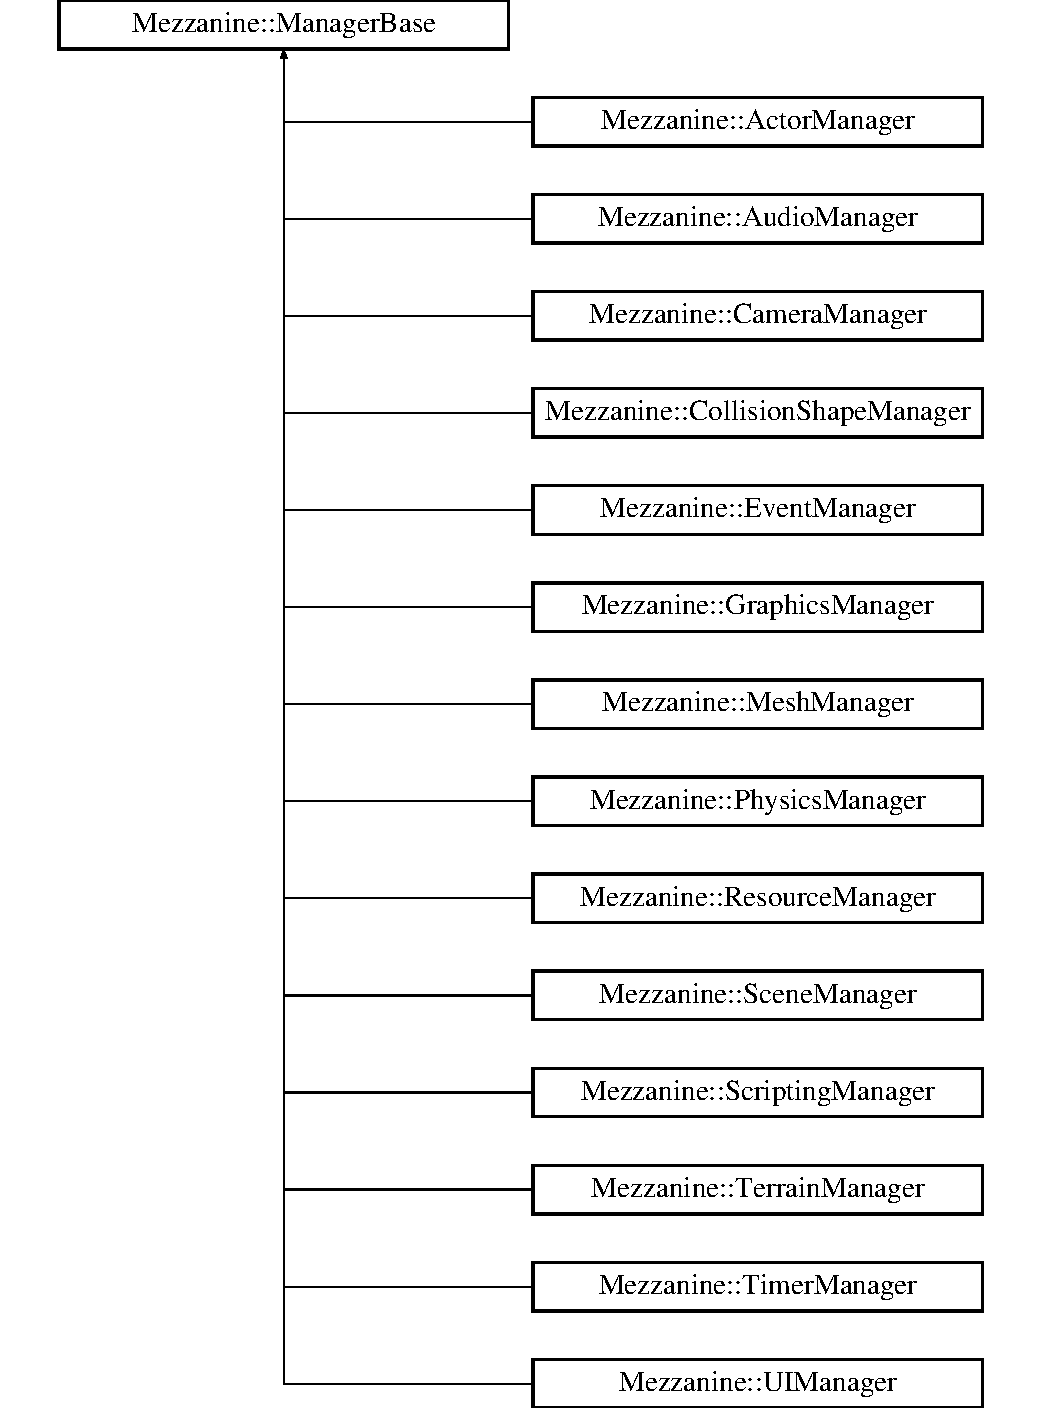
\includegraphics[height=12.000000cm]{classMezzanine_1_1ManagerBase}
\end{center}
\end{figure}
\subsubsection*{Public Types}
\begin{DoxyCompactItemize}
\item 
\hypertarget{classMezzanine_1_1ManagerBase_ab23a9aa27c4e3cb58d902a149d3c6de2}{
typedef bool($\ast$ \hyperlink{classMezzanine_1_1ManagerBase_ab23a9aa27c4e3cb58d902a149d3c6de2}{Callback} )()}
\label{classMezzanine_1_1ManagerBase_ab23a9aa27c4e3cb58d902a149d3c6de2}

\begin{DoxyCompactList}\small\item\em This makes working with Callback function pointer a bit easier. \item\end{DoxyCompactList}\item 
enum \hyperlink{classMezzanine_1_1ManagerBase_a08cecf5169cad3e82be81a3a159b0b6e}{ManagerTypeName} \{ \par
{\bfseries ActorManager}, 
{\bfseries AudioManager}, 
{\bfseries CameraManager}, 
{\bfseries CollisionShapeManager}, 
\par
{\bfseries EventManager}, 
{\bfseries GraphicsManager}, 
{\bfseries MeshManager}, 
{\bfseries NetworkManager}, 
\par
{\bfseries PhysicsManager}, 
{\bfseries ResourceManager}, 
{\bfseries SceneManager}, 
{\bfseries ScriptingManager}, 
\par
{\bfseries TerrainManager}, 
{\bfseries TimerManager}, 
{\bfseries UIManager}, 
{\bfseries UserCreated}
 \}
\begin{DoxyCompactList}\small\item\em A listing of Manager TypeNames. \item\end{DoxyCompactList}\end{DoxyCompactItemize}
\subsubsection*{Public Member Functions}
\begin{DoxyCompactItemize}
\item 
virtual void \hyperlink{classMezzanine_1_1ManagerBase_a4ee29e4baf6c4b9a3bfec1b2258d5cd2}{DoMainLoopItems} ()=0
\begin{DoxyCompactList}\small\item\em The main loop calls this once per frame. \item\end{DoxyCompactList}\item 
\hypertarget{classMezzanine_1_1ManagerBase_acff151003c2370c857dadb67148faffc}{
virtual void \hyperlink{classMezzanine_1_1ManagerBase_acff151003c2370c857dadb67148faffc}{ErasePostMainLoopItems} ()}
\label{classMezzanine_1_1ManagerBase_acff151003c2370c857dadb67148faffc}

\begin{DoxyCompactList}\small\item\em This simply calls \hyperlink{classMezzanine_1_1ManagerBase_a4ec52058f4c8a3f1c5fb20230b4fc301}{SetPostMainLoopItems()} passing it 0. \item\end{DoxyCompactList}\item 
\hypertarget{classMezzanine_1_1ManagerBase_a1f1b8b02c34ccfd72040a7183fc3cba1}{
virtual void \hyperlink{classMezzanine_1_1ManagerBase_a1f1b8b02c34ccfd72040a7183fc3cba1}{ErasePreMainLoopItems} ()}
\label{classMezzanine_1_1ManagerBase_a1f1b8b02c34ccfd72040a7183fc3cba1}

\begin{DoxyCompactList}\small\item\em This simply calls \hyperlink{classMezzanine_1_1ManagerBase_a84dd669c15e9db08c9efbc84c4fa3b0b}{SetPreMainLoopItems()} passing it 0. \item\end{DoxyCompactList}\item 
virtual \hyperlink{classMezzanine_1_1World}{World} $\ast$ \hyperlink{classMezzanine_1_1ManagerBase_a47a85b5bfb2046b364d38adf805bea7d}{GetGameWorld} () const 
\begin{DoxyCompactList}\small\item\em This gets the \hyperlink{classMezzanine_1_1World}{World} that this manager is working with. \item\end{DoxyCompactList}\item 
virtual \hyperlink{classMezzanine_1_1ManagerBase_ab23a9aa27c4e3cb58d902a149d3c6de2}{Callback} \hyperlink{classMezzanine_1_1ManagerBase_aa02a9788d7a83de123083ce3bfdcef4b}{GetPostMainLoopItems} () const 
\begin{DoxyCompactList}\small\item\em This returns the Callback that would be called before the main loop items. \item\end{DoxyCompactList}\item 
virtual \hyperlink{classMezzanine_1_1ManagerBase_ab23a9aa27c4e3cb58d902a149d3c6de2}{Callback} \hyperlink{classMezzanine_1_1ManagerBase_af1ede605b127aeb1a96e226284c318ce}{GetPreMainLoopItems} () const 
\begin{DoxyCompactList}\small\item\em This returns the Callback that would be called before the main loop items. \item\end{DoxyCompactList}\item 
virtual short int \hyperlink{classMezzanine_1_1ManagerBase_a9acb88dc379867430e76d328028862f0}{GetPriority} ()
\begin{DoxyCompactList}\small\item\em This gets the Priority of this manager. \item\end{DoxyCompactList}\item 
virtual \hyperlink{classMezzanine_1_1ManagerBase_a08cecf5169cad3e82be81a3a159b0b6e}{ManagerTypeName} \hyperlink{classMezzanine_1_1ManagerBase_a6fbfe9e847156915b195b6de1cf76973}{GetType} () const =0
\begin{DoxyCompactList}\small\item\em This returns the type of this manager. \item\end{DoxyCompactList}\item 
std::string \hyperlink{classMezzanine_1_1ManagerBase_afb2572589f8389155be7ce256c751d81}{GetTypeName} ()
\begin{DoxyCompactList}\small\item\em This Allows any manager to be sent to a stream. Primarily used for logging. \item\end{DoxyCompactList}\item 
virtual void \hyperlink{classMezzanine_1_1ManagerBase_a864e3cac11928a602c1db28fa2d52ee2}{Initialize} ()=0
\begin{DoxyCompactList}\small\item\em Configure Items requiring other Managers. \item\end{DoxyCompactList}\item 
\hypertarget{classMezzanine_1_1ManagerBase_a6ee3249f71f330394e81e349370d57a8}{
\hyperlink{classMezzanine_1_1ManagerBase_a6ee3249f71f330394e81e349370d57a8}{ManagerBase} ()}
\label{classMezzanine_1_1ManagerBase_a6ee3249f71f330394e81e349370d57a8}

\begin{DoxyCompactList}\small\item\em Default Constructor. \item\end{DoxyCompactList}\item 
virtual bool \hyperlink{classMezzanine_1_1ManagerBase_a2a1bfb2a137c6013a8a5e5fae4c4bb85}{PostMainLoopItems} ()
\begin{DoxyCompactList}\small\item\em This runs any callback that is required after the mainloop items are run. \item\end{DoxyCompactList}\item 
virtual bool \hyperlink{classMezzanine_1_1ManagerBase_a9e0f19b5472eab47fbcd986656838070}{PreMainLoopItems} ()
\begin{DoxyCompactList}\small\item\em This runs any callback that is required before the mainloop items are run. \item\end{DoxyCompactList}\item 
virtual void \hyperlink{classMezzanine_1_1ManagerBase_acb66b1edbb0f256fb1d4d4d2126f073e}{SetGameWorld} (\hyperlink{classMezzanine_1_1World}{World} $\ast$GameWorld\_\-)
\begin{DoxyCompactList}\small\item\em This sets the \hyperlink{classMezzanine_1_1World}{Mezzanine::World} that this Manager works with. \item\end{DoxyCompactList}\item 
virtual void \hyperlink{classMezzanine_1_1ManagerBase_a4ec52058f4c8a3f1c5fb20230b4fc301}{SetPostMainLoopItems} (\hyperlink{classMezzanine_1_1ManagerBase_ab23a9aa27c4e3cb58d902a149d3c6de2}{Callback} PostMainCallback)
\begin{DoxyCompactList}\small\item\em This assigns a function to be the callback function to run prior to the main loop. \item\end{DoxyCompactList}\item 
virtual void \hyperlink{classMezzanine_1_1ManagerBase_a84dd669c15e9db08c9efbc84c4fa3b0b}{SetPreMainLoopItems} (\hyperlink{classMezzanine_1_1ManagerBase_ab23a9aa27c4e3cb58d902a149d3c6de2}{Callback} PreMainCallback)
\begin{DoxyCompactList}\small\item\em This assigns a function to be the callback function to run prior to the main loop. \item\end{DoxyCompactList}\item 
virtual void \hyperlink{classMezzanine_1_1ManagerBase_ac71cd03e0a60427a1ee22637a3cc1b3e}{SetPriority} (short int Priority\_\-)
\begin{DoxyCompactList}\small\item\em This gets the Priority of this manager. \item\end{DoxyCompactList}\item 
virtual \hyperlink{classMezzanine_1_1ManagerBase_a04cb832dc79f4559cc5b2f57cabfa70d}{$\sim$ManagerBase} ()
\begin{DoxyCompactList}\small\item\em Deconstructor. \item\end{DoxyCompactList}\end{DoxyCompactItemize}
\subsubsection*{Protected Attributes}
\begin{DoxyCompactItemize}
\item 
\hypertarget{classMezzanine_1_1ManagerBase_a3590a02f8319f60d9a4ea5a798825df2}{
\hyperlink{classMezzanine_1_1World}{World} $\ast$ \hyperlink{classMezzanine_1_1ManagerBase_a3590a02f8319f60d9a4ea5a798825df2}{GameWorld}}
\label{classMezzanine_1_1ManagerBase_a3590a02f8319f60d9a4ea5a798825df2}

\begin{DoxyCompactList}\small\item\em The actual pointer to the world. \item\end{DoxyCompactList}\item 
\hypertarget{classMezzanine_1_1ManagerBase_ab27f3f7458b9a6f2a08974d096125ed5}{
\hyperlink{classMezzanine_1_1ManagerBase_ab23a9aa27c4e3cb58d902a149d3c6de2}{Callback} \hyperlink{classMezzanine_1_1ManagerBase_ab27f3f7458b9a6f2a08974d096125ed5}{PostMainLoop}}
\label{classMezzanine_1_1ManagerBase_ab27f3f7458b9a6f2a08974d096125ed5}

\begin{DoxyCompactList}\small\item\em This is a function pointer to the function that should be called after running Main Loop Items. \item\end{DoxyCompactList}\item 
\hypertarget{classMezzanine_1_1ManagerBase_a1652110258237bc313a02757229d0f47}{
\hyperlink{classMezzanine_1_1ManagerBase_ab23a9aa27c4e3cb58d902a149d3c6de2}{Callback} \hyperlink{classMezzanine_1_1ManagerBase_a1652110258237bc313a02757229d0f47}{PreMainLoop}}
\label{classMezzanine_1_1ManagerBase_a1652110258237bc313a02757229d0f47}

\begin{DoxyCompactList}\small\item\em This is a function pointer to the function that should be called before running Main Loop Items. \item\end{DoxyCompactList}\item 
short int \hyperlink{classMezzanine_1_1ManagerBase_a96fb02bf2f4e8b4afe70dedd0d8c6ac9}{Priority}
\begin{DoxyCompactList}\small\item\em This is a weighting used by the main loop to decide what order the managers should be called in. \item\end{DoxyCompactList}\end{DoxyCompactItemize}


\subsubsection{Detailed Description}
This is the base class from which all the \hyperlink{classMezzanine_1_1World}{World} Managers inherit. This creates a base set of functions that Managers are all expected to implement. 

Definition at line 58 of file managerbase.h.



\subsubsection{Member Enumeration Documentation}
\hypertarget{classMezzanine_1_1ManagerBase_a08cecf5169cad3e82be81a3a159b0b6e}{
\index{Mezzanine::ManagerBase@{Mezzanine::ManagerBase}!ManagerTypeName@{ManagerTypeName}}
\index{ManagerTypeName@{ManagerTypeName}!Mezzanine::ManagerBase@{Mezzanine::ManagerBase}}
\paragraph[{ManagerTypeName}]{\setlength{\rightskip}{0pt plus 5cm}enum {\bf Mezzanine::ManagerBase::ManagerTypeName}}\hfill}
\label{classMezzanine_1_1ManagerBase_a08cecf5169cad3e82be81a3a159b0b6e}


A listing of Manager TypeNames. 

These will be returned by \hyperlink{classMezzanine_1_1ManagerBase_a6fbfe9e847156915b195b6de1cf76973}{ManagerBase::GetType()}, and will allow code using this to determine what type of Manager class they are working with and use this information to more safely cast to the correct manager if needed. 

Definition at line 66 of file managerbase.h.



\subsubsection{Constructor \& Destructor Documentation}
\hypertarget{classMezzanine_1_1ManagerBase_a04cb832dc79f4559cc5b2f57cabfa70d}{
\index{Mezzanine::ManagerBase@{Mezzanine::ManagerBase}!$\sim$ManagerBase@{$\sim$ManagerBase}}
\index{$\sim$ManagerBase@{$\sim$ManagerBase}!Mezzanine::ManagerBase@{Mezzanine::ManagerBase}}
\paragraph[{$\sim$ManagerBase}]{\setlength{\rightskip}{0pt plus 5cm}Mezzanine::ManagerBase::$\sim$ManagerBase (
\begin{DoxyParamCaption}
{}
\end{DoxyParamCaption}
)\hspace{0.3cm}{\ttfamily  \mbox{[}virtual\mbox{]}}}\hfill}
\label{classMezzanine_1_1ManagerBase_a04cb832dc79f4559cc5b2f57cabfa70d}


Deconstructor. 

This is actuall 

Definition at line 70 of file managerbase.cpp.



\subsubsection{Member Function Documentation}
\hypertarget{classMezzanine_1_1ManagerBase_a4ee29e4baf6c4b9a3bfec1b2258d5cd2}{
\index{Mezzanine::ManagerBase@{Mezzanine::ManagerBase}!DoMainLoopItems@{DoMainLoopItems}}
\index{DoMainLoopItems@{DoMainLoopItems}!Mezzanine::ManagerBase@{Mezzanine::ManagerBase}}
\paragraph[{DoMainLoopItems}]{\setlength{\rightskip}{0pt plus 5cm}virtual void Mezzanine::ManagerBase::DoMainLoopItems (
\begin{DoxyParamCaption}
{}
\end{DoxyParamCaption}
)\hspace{0.3cm}{\ttfamily  \mbox{[}pure virtual\mbox{]}}}\hfill}
\label{classMezzanine_1_1ManagerBase_a4ee29e4baf6c4b9a3bfec1b2258d5cd2}


The main loop calls this once per frame. 

This is where each manager is expected to put anything that needs to be run each iteration of the main loop 

Implemented in \hyperlink{classMezzanine_1_1ActorManager_a8b1907afd4804047c03ff4bb51c89caa}{Mezzanine::ActorManager}, \hyperlink{classMezzanine_1_1AudioManager_aefcdc7d3276500cf627f2c2e33b483f3}{Mezzanine::AudioManager}, \hyperlink{classMezzanine_1_1CameraManager_a91db1fdfe96f32d06f689d37b91140cb}{Mezzanine::CameraManager}, \hyperlink{classMezzanine_1_1CollisionShapeManager_ac055cf940fd8fce522625de6b977dd2a}{Mezzanine::CollisionShapeManager}, \hyperlink{classMezzanine_1_1EventManager_a69d44403974ed8d974846e929eb8adda}{Mezzanine::EventManager}, \hyperlink{classMezzanine_1_1GraphicsManager_ae940c81cd1401fda34abc6fd53ede45a}{Mezzanine::GraphicsManager}, \hyperlink{classMezzanine_1_1MeshManager_acfbea42e8aeb36d48522ad027f1e8764}{Mezzanine::MeshManager}, \hyperlink{classMezzanine_1_1PhysicsManager_a21df393f2356a20151fce997577e3d76}{Mezzanine::PhysicsManager}, \hyperlink{classMezzanine_1_1ResourceManager_a57b72306ed2bfaa198ff47d43c4013fa}{Mezzanine::ResourceManager}, \hyperlink{classMezzanine_1_1SceneManager_ae75aa9deb4bbc8ee1f979e240070309f}{Mezzanine::SceneManager}, \hyperlink{classMezzanine_1_1TerrainManager_a442a1e72a38fe959b15a7f5eeff455fc}{Mezzanine::TerrainManager}, \hyperlink{classMezzanine_1_1TimerManager_a6ac7544b79fb023e4596e350a5586f85}{Mezzanine::TimerManager}, and \hyperlink{classMezzanine_1_1UIManager_af774da651d30b4fe1ea086899c1961ca}{Mezzanine::UIManager}.

\hypertarget{classMezzanine_1_1ManagerBase_a47a85b5bfb2046b364d38adf805bea7d}{
\index{Mezzanine::ManagerBase@{Mezzanine::ManagerBase}!GetGameWorld@{GetGameWorld}}
\index{GetGameWorld@{GetGameWorld}!Mezzanine::ManagerBase@{Mezzanine::ManagerBase}}
\paragraph[{GetGameWorld}]{\setlength{\rightskip}{0pt plus 5cm}{\bf World} $\ast$ Mezzanine::ManagerBase::GetGameWorld (
\begin{DoxyParamCaption}
{}
\end{DoxyParamCaption}
) const\hspace{0.3cm}{\ttfamily  \mbox{[}virtual\mbox{]}}}\hfill}
\label{classMezzanine_1_1ManagerBase_a47a85b5bfb2046b364d38adf805bea7d}


This gets the \hyperlink{classMezzanine_1_1World}{World} that this manager is working with. 

\begin{DoxyReturn}{Returns}
This returns a \hyperlink{classMezzanine_1_1World}{Mezzanine::World}$\ast$ that is the same as the one store in this Manager 
\end{DoxyReturn}


Definition at line 64 of file managerbase.cpp.

\hypertarget{classMezzanine_1_1ManagerBase_aa02a9788d7a83de123083ce3bfdcef4b}{
\index{Mezzanine::ManagerBase@{Mezzanine::ManagerBase}!GetPostMainLoopItems@{GetPostMainLoopItems}}
\index{GetPostMainLoopItems@{GetPostMainLoopItems}!Mezzanine::ManagerBase@{Mezzanine::ManagerBase}}
\paragraph[{GetPostMainLoopItems}]{\setlength{\rightskip}{0pt plus 5cm}{\bf ManagerBase::Callback} Mezzanine::ManagerBase::GetPostMainLoopItems (
\begin{DoxyParamCaption}
{}
\end{DoxyParamCaption}
) const\hspace{0.3cm}{\ttfamily  \mbox{[}virtual\mbox{]}}}\hfill}
\label{classMezzanine_1_1ManagerBase_aa02a9788d7a83de123083ce3bfdcef4b}


This returns the Callback that would be called before the main loop items. 

\begin{DoxyReturn}{Returns}
This returns a \hyperlink{classMezzanine_1_1ManagerBase_ab23a9aa27c4e3cb58d902a149d3c6de2}{ManagerBase::Callback} which is a p ointer to the callback function that will be called after the main loop items 
\end{DoxyReturn}


Definition at line 104 of file managerbase.cpp.

\hypertarget{classMezzanine_1_1ManagerBase_af1ede605b127aeb1a96e226284c318ce}{
\index{Mezzanine::ManagerBase@{Mezzanine::ManagerBase}!GetPreMainLoopItems@{GetPreMainLoopItems}}
\index{GetPreMainLoopItems@{GetPreMainLoopItems}!Mezzanine::ManagerBase@{Mezzanine::ManagerBase}}
\paragraph[{GetPreMainLoopItems}]{\setlength{\rightskip}{0pt plus 5cm}{\bf ManagerBase::Callback} Mezzanine::ManagerBase::GetPreMainLoopItems (
\begin{DoxyParamCaption}
{}
\end{DoxyParamCaption}
) const\hspace{0.3cm}{\ttfamily  \mbox{[}virtual\mbox{]}}}\hfill}
\label{classMezzanine_1_1ManagerBase_af1ede605b127aeb1a96e226284c318ce}


This returns the Callback that would be called before the main loop items. 

\begin{DoxyReturn}{Returns}
This returns a \hyperlink{classMezzanine_1_1ManagerBase_ab23a9aa27c4e3cb58d902a149d3c6de2}{ManagerBase::Callback} which is a pointer to the callback function that will be called before the main loop items 
\end{DoxyReturn}


Definition at line 85 of file managerbase.cpp.

\hypertarget{classMezzanine_1_1ManagerBase_a9acb88dc379867430e76d328028862f0}{
\index{Mezzanine::ManagerBase@{Mezzanine::ManagerBase}!GetPriority@{GetPriority}}
\index{GetPriority@{GetPriority}!Mezzanine::ManagerBase@{Mezzanine::ManagerBase}}
\paragraph[{GetPriority}]{\setlength{\rightskip}{0pt plus 5cm}short int Mezzanine::ManagerBase::GetPriority (
\begin{DoxyParamCaption}
{}
\end{DoxyParamCaption}
)\hspace{0.3cm}{\ttfamily  \mbox{[}virtual\mbox{]}}}\hfill}
\label{classMezzanine_1_1ManagerBase_a9acb88dc379867430e76d328028862f0}


This gets the Priority of this manager. 

This has no Set counterpart to allow the changing of a manager's priority. This is expected to be set by the manager, or expose a safe method to change it at that level. \begin{DoxyReturn}{Returns}
This returns a short int that represents the priority of the manager. Lower is executed first. 
\end{DoxyReturn}


Definition at line 165 of file managerbase.cpp.

\hypertarget{classMezzanine_1_1ManagerBase_a6fbfe9e847156915b195b6de1cf76973}{
\index{Mezzanine::ManagerBase@{Mezzanine::ManagerBase}!GetType@{GetType}}
\index{GetType@{GetType}!Mezzanine::ManagerBase@{Mezzanine::ManagerBase}}
\paragraph[{GetType}]{\setlength{\rightskip}{0pt plus 5cm}virtual {\bf ManagerTypeName} Mezzanine::ManagerBase::GetType (
\begin{DoxyParamCaption}
{}
\end{DoxyParamCaption}
) const\hspace{0.3cm}{\ttfamily  \mbox{[}pure virtual\mbox{]}}}\hfill}
\label{classMezzanine_1_1ManagerBase_a6fbfe9e847156915b195b6de1cf76973}


This returns the type of this manager. 

This is intended to make using and casting from Manager base easier. With this is is possible to cast from \hyperlink{classMezzanine_1_1ManagerBase}{ManagerBase} to the correct Manager Type. \begin{DoxyReturn}{Returns}
This returns a ManagerTypeName to identify what this can be safely cast to. 
\end{DoxyReturn}


Implemented in \hyperlink{classMezzanine_1_1ActorManager_abfd167e1e15f32dffed05a2bd1b4ac70}{Mezzanine::ActorManager}, \hyperlink{classMezzanine_1_1AudioManager_a42f2b4b8065387117042bf7eadc97356}{Mezzanine::AudioManager}, \hyperlink{classMezzanine_1_1CameraManager_a1eb75dabfd7df1c901432d841a92fcbc}{Mezzanine::CameraManager}, \hyperlink{classMezzanine_1_1CollisionShapeManager_a4b98446e667a402e675eec79353e5278}{Mezzanine::CollisionShapeManager}, \hyperlink{classMezzanine_1_1EventManager_a6e4c72bcaa437863fdf167b5b9ef5034}{Mezzanine::EventManager}, \hyperlink{classMezzanine_1_1GraphicsManager_a4a036b7a4623e9f568310a90d5e34e46}{Mezzanine::GraphicsManager}, \hyperlink{classMezzanine_1_1MeshManager_a120881dcf7bce1d3a30bedb426650c0e}{Mezzanine::MeshManager}, \hyperlink{classMezzanine_1_1PhysicsManager_a87b1640bc429ee1850c408bd8a13cdce}{Mezzanine::PhysicsManager}, \hyperlink{classMezzanine_1_1ResourceManager_aafe55f1095a67f30e97bff25200685d7}{Mezzanine::ResourceManager}, \hyperlink{classMezzanine_1_1SceneManager_ad10c4317af4a2c6fbbfc151e8c609570}{Mezzanine::SceneManager}, \hyperlink{classMezzanine_1_1TerrainManager_a86fbb914cfbc0de3dc555d670bb35107}{Mezzanine::TerrainManager}, \hyperlink{classMezzanine_1_1TimerManager_ad62b8c89fa33085768284781aa28116a}{Mezzanine::TimerManager}, and \hyperlink{classMezzanine_1_1UIManager_a0a576d8f14aa475d9f1750b4cf76cf10}{Mezzanine::UIManager}.

\hypertarget{classMezzanine_1_1ManagerBase_afb2572589f8389155be7ce256c751d81}{
\index{Mezzanine::ManagerBase@{Mezzanine::ManagerBase}!GetTypeName@{GetTypeName}}
\index{GetTypeName@{GetTypeName}!Mezzanine::ManagerBase@{Mezzanine::ManagerBase}}
\paragraph[{GetTypeName}]{\setlength{\rightskip}{0pt plus 5cm}std::string Mezzanine::ManagerBase::GetTypeName (
\begin{DoxyParamCaption}
{}
\end{DoxyParamCaption}
)}\hfill}
\label{classMezzanine_1_1ManagerBase_afb2572589f8389155be7ce256c751d81}


This Allows any manager to be sent to a stream. Primarily used for logging. 

\begin{DoxyReturn}{Returns}
This returns a std::ostream\& that contains the name, and maybe some data for the the streammed manager. 
\end{DoxyReturn}


Definition at line 110 of file managerbase.cpp.

\hypertarget{classMezzanine_1_1ManagerBase_a864e3cac11928a602c1db28fa2d52ee2}{
\index{Mezzanine::ManagerBase@{Mezzanine::ManagerBase}!Initialize@{Initialize}}
\index{Initialize@{Initialize}!Mezzanine::ManagerBase@{Mezzanine::ManagerBase}}
\paragraph[{Initialize}]{\setlength{\rightskip}{0pt plus 5cm}virtual void Mezzanine::ManagerBase::Initialize (
\begin{DoxyParamCaption}
{}
\end{DoxyParamCaption}
)\hspace{0.3cm}{\ttfamily  \mbox{[}pure virtual\mbox{]}}}\hfill}
\label{classMezzanine_1_1ManagerBase_a864e3cac11928a602c1db28fa2d52ee2}


Configure Items requiring other Managers. 

If you are using the \hyperlink{classMezzanine_1_1World}{Mezzanine::World} this is called when \hyperlink{classMezzanine_1_1World_a72d6d82926bfbfca96c246f109f0fc58}{Mezzanine::World::GameInit()} is called. It is expected that by the time this is called either ManagerBase::ManagerBase(World$\ast$) or \hyperlink{classMezzanine_1_1ManagerBase_acb66b1edbb0f256fb1d4d4d2126f073e}{ManagerBase::SetGameWorld(World$\ast$)} will have been called. This is where all configuration that requires atleast one other manager on the \hyperlink{classMezzanine_1_1World}{Mezzanine::World} to exist.\par
\par
 Yes we know it is spelled wrong, but are Zs cooler anyway. 

Implemented in \hyperlink{classMezzanine_1_1ActorManager_a3b5b383066473d09243d13ad702c4868}{Mezzanine::ActorManager}, \hyperlink{classMezzanine_1_1AudioManager_a24f1464e3de9d95e3c50c276f9e176e6}{Mezzanine::AudioManager}, \hyperlink{classMezzanine_1_1CameraManager_a4b7f0d25f77306bca4b5c885e35363cc}{Mezzanine::CameraManager}, \hyperlink{classMezzanine_1_1CollisionShapeManager_a15ddc7bb06cf1cf32cd4e641d3b7b34f}{Mezzanine::CollisionShapeManager}, \hyperlink{classMezzanine_1_1EventManager_a2bf1969aadd0fb5a3da284423e44b081}{Mezzanine::EventManager}, \hyperlink{classMezzanine_1_1GraphicsManager_a4f76a6a37be800b1fc13195aa11cfd7a}{Mezzanine::GraphicsManager}, \hyperlink{classMezzanine_1_1MeshManager_ac03c91bea88144bcfa420411bc85f0c7}{Mezzanine::MeshManager}, \hyperlink{classMezzanine_1_1PhysicsManager_ab09c912dc48b7082bd07a536167bc3d3}{Mezzanine::PhysicsManager}, \hyperlink{classMezzanine_1_1ResourceManager_a4b4e77984e21e3eaa1c47772d2e9c6f4}{Mezzanine::ResourceManager}, \hyperlink{classMezzanine_1_1SceneManager_a8a3b5cb55a06669d0fe64510c1b1a854}{Mezzanine::SceneManager}, \hyperlink{classMezzanine_1_1TerrainManager_abe9550c9c6565bbd0610dcaa20eedc0c}{Mezzanine::TerrainManager}, \hyperlink{classMezzanine_1_1TimerManager_ac670fd396b7fb2b7f8d7c67bb95582ba}{Mezzanine::TimerManager}, and \hyperlink{classMezzanine_1_1UIManager_a51dc53c08ac8657133279e75fbce466a}{Mezzanine::UIManager}.

\hypertarget{classMezzanine_1_1ManagerBase_a2a1bfb2a137c6013a8a5e5fae4c4bb85}{
\index{Mezzanine::ManagerBase@{Mezzanine::ManagerBase}!PostMainLoopItems@{PostMainLoopItems}}
\index{PostMainLoopItems@{PostMainLoopItems}!Mezzanine::ManagerBase@{Mezzanine::ManagerBase}}
\paragraph[{PostMainLoopItems}]{\setlength{\rightskip}{0pt plus 5cm}bool Mezzanine::ManagerBase::PostMainLoopItems (
\begin{DoxyParamCaption}
{}
\end{DoxyParamCaption}
)\hspace{0.3cm}{\ttfamily  \mbox{[}virtual\mbox{]}}}\hfill}
\label{classMezzanine_1_1ManagerBase_a2a1bfb2a137c6013a8a5e5fae4c4bb85}


This runs any callback that is required after the mainloop items are run. 

This will return whatever the callback returns, which is true to end the main loop after this frame, or true to continue it. If no callback is set this simply returns true, as to not interupt the mainloop. \par
 This is a great Function to override in Manager classes where the complexity of callbacks is not required. This would make coding items that need to be performed at specific times easier. If you do that, it would be a good idea to call this version of the function, just in case a callback is set. \begin{DoxyReturn}{Returns}
This returns a false to end the main loop, or a true if the main loop should continue. 
\end{DoxyReturn}


Reimplemented in \hyperlink{classMezzanine_1_1GraphicsManager_a73d12091631749914d4a1025c45d68b4}{Mezzanine::GraphicsManager}.



Definition at line 95 of file managerbase.cpp.

\hypertarget{classMezzanine_1_1ManagerBase_a9e0f19b5472eab47fbcd986656838070}{
\index{Mezzanine::ManagerBase@{Mezzanine::ManagerBase}!PreMainLoopItems@{PreMainLoopItems}}
\index{PreMainLoopItems@{PreMainLoopItems}!Mezzanine::ManagerBase@{Mezzanine::ManagerBase}}
\paragraph[{PreMainLoopItems}]{\setlength{\rightskip}{0pt plus 5cm}bool Mezzanine::ManagerBase::PreMainLoopItems (
\begin{DoxyParamCaption}
{}
\end{DoxyParamCaption}
)\hspace{0.3cm}{\ttfamily  \mbox{[}virtual\mbox{]}}}\hfill}
\label{classMezzanine_1_1ManagerBase_a9e0f19b5472eab47fbcd986656838070}


This runs any callback that is required before the mainloop items are run. 

This will return whatever the callback returns, which is true to end the main loop after this frame, or true to continue it. If no callback is set this simply returns true, as to not interupt the mainloop. \par
 This is a great Function to override in Manager classes where the complexity of callbacks is not required. This would make coding items that need to be performed at specific times easier. If you do that, it would be a good idea to call this version of the function, just in case a callback is set. \begin{DoxyReturn}{Returns}
This returns a false to end the main loop, or a true if the main loop should continue. 
\end{DoxyReturn}


Definition at line 76 of file managerbase.cpp.

\hypertarget{classMezzanine_1_1ManagerBase_acb66b1edbb0f256fb1d4d4d2126f073e}{
\index{Mezzanine::ManagerBase@{Mezzanine::ManagerBase}!SetGameWorld@{SetGameWorld}}
\index{SetGameWorld@{SetGameWorld}!Mezzanine::ManagerBase@{Mezzanine::ManagerBase}}
\paragraph[{SetGameWorld}]{\setlength{\rightskip}{0pt plus 5cm}void Mezzanine::ManagerBase::SetGameWorld (
\begin{DoxyParamCaption}
\item[{{\bf World} $\ast$}]{GameWorld\_\-}
\end{DoxyParamCaption}
)\hspace{0.3cm}{\ttfamily  \mbox{[}virtual\mbox{]}}}\hfill}
\label{classMezzanine_1_1ManagerBase_acb66b1edbb0f256fb1d4d4d2126f073e}


This sets the \hyperlink{classMezzanine_1_1World}{Mezzanine::World} that this Manager works with. 

It is expected that this won't change very much, and for some managers changing this at the wrong time could cause some very fundamental problems. In fact, managers should be designed so that they can swapped out. For example swapping out event managers could allow for a swift re-\/mapping of game controls when a game switches modes.\par
\par
 For managers that can be moved it is expected that this function will change the pointer on the \hyperlink{classMezzanine_1_1World}{Mezzanine::World} for the appropriate manager to point to this manager. This simplifies the calls that will naturally come next. To detach a Manager from the world pass this method a NULL pointer. If the manager cannot be removed or detached it should throw and exception using \hyperlink{classMezzanine_1_1World_a93405caf197f9324f3620ecefa1efc77}{World::LogAndThrow}, and it must not fail to attach to a world (that means it must internally handle all exception raised by the attaching process or throw an \char`\"{}Unrecoverable Error\char`\"{}) 

Definition at line 67 of file managerbase.cpp.

\hypertarget{classMezzanine_1_1ManagerBase_a4ec52058f4c8a3f1c5fb20230b4fc301}{
\index{Mezzanine::ManagerBase@{Mezzanine::ManagerBase}!SetPostMainLoopItems@{SetPostMainLoopItems}}
\index{SetPostMainLoopItems@{SetPostMainLoopItems}!Mezzanine::ManagerBase@{Mezzanine::ManagerBase}}
\paragraph[{SetPostMainLoopItems}]{\setlength{\rightskip}{0pt plus 5cm}void Mezzanine::ManagerBase::SetPostMainLoopItems (
\begin{DoxyParamCaption}
\item[{{\bf ManagerBase::Callback}}]{PostMainCallback}
\end{DoxyParamCaption}
)\hspace{0.3cm}{\ttfamily  \mbox{[}virtual\mbox{]}}}\hfill}
\label{classMezzanine_1_1ManagerBase_a4ec52058f4c8a3f1c5fb20230b4fc301}


This assigns a function to be the callback function to run prior to the main loop. 


\begin{DoxyParams}{Parameters}
{\em PostMainCallback} & This is a pointer to a function that returns a bool and accepts no arguments, this is in the form of a \hyperlink{classMezzanine_1_1ManagerBase_ab23a9aa27c4e3cb58d902a149d3c6de2}{ManagerBase::Callback}. If SetPosMainLoopItems is passed 0, NULL or a null pointer, the callback will be forgetten and will not attempt to be called. \\
\hline
\end{DoxyParams}


Definition at line 92 of file managerbase.cpp.

\hypertarget{classMezzanine_1_1ManagerBase_a84dd669c15e9db08c9efbc84c4fa3b0b}{
\index{Mezzanine::ManagerBase@{Mezzanine::ManagerBase}!SetPreMainLoopItems@{SetPreMainLoopItems}}
\index{SetPreMainLoopItems@{SetPreMainLoopItems}!Mezzanine::ManagerBase@{Mezzanine::ManagerBase}}
\paragraph[{SetPreMainLoopItems}]{\setlength{\rightskip}{0pt plus 5cm}void Mezzanine::ManagerBase::SetPreMainLoopItems (
\begin{DoxyParamCaption}
\item[{{\bf ManagerBase::Callback}}]{PreMainCallback}
\end{DoxyParamCaption}
)\hspace{0.3cm}{\ttfamily  \mbox{[}virtual\mbox{]}}}\hfill}
\label{classMezzanine_1_1ManagerBase_a84dd669c15e9db08c9efbc84c4fa3b0b}


This assigns a function to be the callback function to run prior to the main loop. 


\begin{DoxyParams}{Parameters}
{\em PreMainCallback} & This is a pointer to a function that returns a bool and accepts no arguments, this is in the form of a \hyperlink{classMezzanine_1_1ManagerBase_ab23a9aa27c4e3cb58d902a149d3c6de2}{ManagerBase::Callback}. If SetPreMainLoopItems is passed 0, NULL or a null pointer, the callback will be forgetten and will not attempt to be called. \\
\hline
\end{DoxyParams}


Definition at line 73 of file managerbase.cpp.

\hypertarget{classMezzanine_1_1ManagerBase_ac71cd03e0a60427a1ee22637a3cc1b3e}{
\index{Mezzanine::ManagerBase@{Mezzanine::ManagerBase}!SetPriority@{SetPriority}}
\index{SetPriority@{SetPriority}!Mezzanine::ManagerBase@{Mezzanine::ManagerBase}}
\paragraph[{SetPriority}]{\setlength{\rightskip}{0pt plus 5cm}void Mezzanine::ManagerBase::SetPriority (
\begin{DoxyParamCaption}
\item[{short int}]{Priority\_\-}
\end{DoxyParamCaption}
)\hspace{0.3cm}{\ttfamily  \mbox{[}virtual\mbox{]}}}\hfill}
\label{classMezzanine_1_1ManagerBase_ac71cd03e0a60427a1ee22637a3cc1b3e}


This gets the Priority of this manager. 

This has no Set counterpart to allow the changing of a manager's priority. This is expected to be set by the manager, or expose a safe method to change it at that level. \begin{DoxyReturn}{Returns}
This returns a short int that represents the priority of the manager. Lower is executed first. 
\end{DoxyReturn}


Definition at line 170 of file managerbase.cpp.



\subsubsection{Member Data Documentation}
\hypertarget{classMezzanine_1_1ManagerBase_a96fb02bf2f4e8b4afe70dedd0d8c6ac9}{
\index{Mezzanine::ManagerBase@{Mezzanine::ManagerBase}!Priority@{Priority}}
\index{Priority@{Priority}!Mezzanine::ManagerBase@{Mezzanine::ManagerBase}}
\paragraph[{Priority}]{\setlength{\rightskip}{0pt plus 5cm}short int {\bf Mezzanine::ManagerBase::Priority}\hspace{0.3cm}{\ttfamily  \mbox{[}protected\mbox{]}}}\hfill}
\label{classMezzanine_1_1ManagerBase_a96fb02bf2f4e8b4afe70dedd0d8c6ac9}


This is a weighting used by the main loop to decide what order the managers should be called in. 

A lower number gets called earlier in the Main loop. By default rendering the graphics occurs at priority 0. 

Definition at line 210 of file managerbase.h.



The documentation for this class was generated from the following files:\begin{DoxyCompactItemize}
\item 
managerbase.h\item 
managerbase.cpp\end{DoxyCompactItemize}

\hypertarget{classMezzanine_1_1MathTool}{
\subsection{Mezzanine::MathTool Class Reference}
\label{classMezzanine_1_1MathTool}\index{Mezzanine::MathTool@{Mezzanine::MathTool}}
}


This provides a number of generic math related utilities.  




{\ttfamily \#include $<$mathtool.h$>$}

\subsubsection*{Public Member Functions}
\begin{DoxyCompactItemize}
\item 
\hypertarget{classMezzanine_1_1MathTool_a0e5200de6dc0b3a3b6def86e9981d97a}{
\hyperlink{classMezzanine_1_1MathTool_a0e5200de6dc0b3a3b6def86e9981d97a}{MathTool} ()}
\label{classMezzanine_1_1MathTool_a0e5200de6dc0b3a3b6def86e9981d97a}

\begin{DoxyCompactList}\small\item\em Class constructor. \item\end{DoxyCompactList}\item 
\hypertarget{classMezzanine_1_1MathTool_aca1449215b524b2c832e78a4356ebdb4}{
\hyperlink{classMezzanine_1_1MathTool_aca1449215b524b2c832e78a4356ebdb4}{$\sim$MathTool} ()}
\label{classMezzanine_1_1MathTool_aca1449215b524b2c832e78a4356ebdb4}

\begin{DoxyCompactList}\small\item\em Class destructor. \item\end{DoxyCompactList}\end{DoxyCompactItemize}
\subsubsection*{Static Public Member Functions}
\begin{DoxyCompactItemize}
\item 
static \hyperlink{namespaceMezzanine_a726731b1a7df72bf3583e4a97282c6f6}{Real} \hyperlink{classMezzanine_1_1MathTool_a036cff4360b503b4bee33dc74f5324c4}{ACos} (const \hyperlink{namespaceMezzanine_a726731b1a7df72bf3583e4a97282c6f6}{Real} \&Interval)
\begin{DoxyCompactList}\small\item\em Calculates the principal value of the arc Cosine of an angle. \item\end{DoxyCompactList}\item 
static \hyperlink{namespaceMezzanine_a726731b1a7df72bf3583e4a97282c6f6}{Real} \hyperlink{classMezzanine_1_1MathTool_ab2397336a5d7ffc9510a92313f6ef214}{ASin} (const \hyperlink{namespaceMezzanine_a726731b1a7df72bf3583e4a97282c6f6}{Real} \&Interval)
\begin{DoxyCompactList}\small\item\em Calculates the principal value of the arc Sine of an angle. \item\end{DoxyCompactList}\item 
static \hyperlink{namespaceMezzanine_a726731b1a7df72bf3583e4a97282c6f6}{Real} \hyperlink{classMezzanine_1_1MathTool_a89b1afe525d990b2136aae8b516b0980}{ATan} (const \hyperlink{namespaceMezzanine_a726731b1a7df72bf3583e4a97282c6f6}{Real} \&Interval)
\begin{DoxyCompactList}\small\item\em Calculates the principal value of the arc Tangent of an angle. \item\end{DoxyCompactList}\item 
static \hyperlink{namespaceMezzanine_a726731b1a7df72bf3583e4a97282c6f6}{Real} \hyperlink{classMezzanine_1_1MathTool_a3201e1e4dc3f7383c983861513cd0379}{Ceil} (const \hyperlink{namespaceMezzanine_a726731b1a7df72bf3583e4a97282c6f6}{Real} \&Val)
\begin{DoxyCompactList}\small\item\em Rounds a Real up. \item\end{DoxyCompactList}\item 
static \hyperlink{namespaceMezzanine_a726731b1a7df72bf3583e4a97282c6f6}{Real} \hyperlink{classMezzanine_1_1MathTool_a7848194232dda5086ba2c4d4888d0ffc}{Cos} (const \hyperlink{namespaceMezzanine_a726731b1a7df72bf3583e4a97282c6f6}{Real} \&Radians)
\begin{DoxyCompactList}\small\item\em Calculates the Cosine of an angle. \item\end{DoxyCompactList}\item 
static \hyperlink{namespaceMezzanine_a726731b1a7df72bf3583e4a97282c6f6}{Real} \hyperlink{classMezzanine_1_1MathTool_a96b1935e6ed6d9d2ffa03fd2e7698c3e}{Fabs} (const \hyperlink{namespaceMezzanine_a726731b1a7df72bf3583e4a97282c6f6}{Real} \&Val)
\begin{DoxyCompactList}\small\item\em Gets the absolute value of a Real. \item\end{DoxyCompactList}\item 
static \hyperlink{namespaceMezzanine_a726731b1a7df72bf3583e4a97282c6f6}{Real} \hyperlink{classMezzanine_1_1MathTool_a51eae53cadb52839ae6edb279627fabd}{Floor} (const \hyperlink{namespaceMezzanine_a726731b1a7df72bf3583e4a97282c6f6}{Real} \&Val)
\begin{DoxyCompactList}\small\item\em Rounds a Real down. \item\end{DoxyCompactList}\item 
static \hyperlink{namespaceMezzanine_a726731b1a7df72bf3583e4a97282c6f6}{Real} \hyperlink{classMezzanine_1_1MathTool_a4e4171768a241441a1ed0b33c68bdc9c}{Fmod} (const \hyperlink{namespaceMezzanine_a726731b1a7df72bf3583e4a97282c6f6}{Real} \&Numerator, const \hyperlink{namespaceMezzanine_a726731b1a7df72bf3583e4a97282c6f6}{Real} \&Denominator)
\begin{DoxyCompactList}\small\item\em Modulo, for Reals. Returns the remainder of the division between two Reals. \item\end{DoxyCompactList}\item 
static \hyperlink{namespaceMezzanine_a726731b1a7df72bf3583e4a97282c6f6}{Real} \hyperlink{classMezzanine_1_1MathTool_afeaaaf9f445283c16310b4f15c44d03e}{GetHalfPi} ()
\begin{DoxyCompactList}\small\item\em Gets Pi $\ast$ 0.5. \item\end{DoxyCompactList}\item 
static \hyperlink{namespaceMezzanine_a726731b1a7df72bf3583e4a97282c6f6}{Real} \hyperlink{classMezzanine_1_1MathTool_a041b328e51d402deda1660b6d30508f5}{GetPi} ()
\begin{DoxyCompactList}\small\item\em Gets Pi. \item\end{DoxyCompactList}\item 
static \hyperlink{namespaceMezzanine_a726731b1a7df72bf3583e4a97282c6f6}{Real} \hyperlink{classMezzanine_1_1MathTool_afd4da5be9f2f1f89dfa92235a5b02307}{GetTwoPi} ()
\begin{DoxyCompactList}\small\item\em Gets Pi $\ast$ 2. \item\end{DoxyCompactList}\item 
static \hyperlink{namespaceMezzanine_a726731b1a7df72bf3583e4a97282c6f6}{Real} \hyperlink{classMezzanine_1_1MathTool_ad38737da349c0aea453d42f79e5c61d1}{Pow} (const \hyperlink{namespaceMezzanine_a726731b1a7df72bf3583e4a97282c6f6}{Real} \&Val, const \hyperlink{namespaceMezzanine_a726731b1a7df72bf3583e4a97282c6f6}{Real} \&Power)
\begin{DoxyCompactList}\small\item\em Raises a Real to a power. \item\end{DoxyCompactList}\item 
static \hyperlink{namespaceMezzanine_a726731b1a7df72bf3583e4a97282c6f6}{Real} \hyperlink{classMezzanine_1_1MathTool_a58b35317198c5d4cdf1680e5516747c3}{Sin} (const \hyperlink{namespaceMezzanine_a726731b1a7df72bf3583e4a97282c6f6}{Real} \&Radians)
\begin{DoxyCompactList}\small\item\em Calculates the Sine of an angle. \item\end{DoxyCompactList}\item 
static \hyperlink{namespaceMezzanine_a726731b1a7df72bf3583e4a97282c6f6}{Real} \hyperlink{classMezzanine_1_1MathTool_af230371a8d6f59b4ee78670afd3928fa}{Sqrt} (const \hyperlink{namespaceMezzanine_a726731b1a7df72bf3583e4a97282c6f6}{Real} \&Val)
\begin{DoxyCompactList}\small\item\em Gets the square root of a Real. \item\end{DoxyCompactList}\item 
static \hyperlink{namespaceMezzanine_a726731b1a7df72bf3583e4a97282c6f6}{Real} \hyperlink{classMezzanine_1_1MathTool_a4fd17164ea990aff0203c63946bb1d48}{Tan} (const \hyperlink{namespaceMezzanine_a726731b1a7df72bf3583e4a97282c6f6}{Real} \&Radians)
\begin{DoxyCompactList}\small\item\em Calculates the Tangent of an angle. \item\end{DoxyCompactList}\end{DoxyCompactItemize}
\subsubsection*{Static Protected Attributes}
\begin{DoxyCompactItemize}
\item 
\hypertarget{classMezzanine_1_1MathTool_a5efc0e09658210d3d61adf6717a6f3a6}{
static const \hyperlink{namespaceMezzanine_a726731b1a7df72bf3583e4a97282c6f6}{Real} {\bfseries HalfPi} = \hyperlink{namespaceMezzanine_a726731b1a7df72bf3583e4a97282c6f6}{Real}(0.5 $\ast$ Pi)}
\label{classMezzanine_1_1MathTool_a5efc0e09658210d3d61adf6717a6f3a6}

\item 
\hypertarget{classMezzanine_1_1MathTool_a700f64d8c4e1c77406fcaa8cddadbf4a}{
static const \hyperlink{namespaceMezzanine_a726731b1a7df72bf3583e4a97282c6f6}{Real} {\bfseries Pi} = \hyperlink{namespaceMezzanine_a726731b1a7df72bf3583e4a97282c6f6}{Real}(4.0 $\ast$ atan(1.0))}
\label{classMezzanine_1_1MathTool_a700f64d8c4e1c77406fcaa8cddadbf4a}

\item 
\hypertarget{classMezzanine_1_1MathTool_aae0fc583d27f4ac796d009f579f3c406}{
static const \hyperlink{namespaceMezzanine_a726731b1a7df72bf3583e4a97282c6f6}{Real} {\bfseries TwoPi} = \hyperlink{namespaceMezzanine_a726731b1a7df72bf3583e4a97282c6f6}{Real}(2.0 $\ast$ Pi)}
\label{classMezzanine_1_1MathTool_aae0fc583d27f4ac796d009f579f3c406}

\end{DoxyCompactItemize}


\subsubsection{Detailed Description}
This provides a number of generic math related utilities. 

Definition at line 53 of file mathtool.h.



\subsubsection{Member Function Documentation}
\hypertarget{classMezzanine_1_1MathTool_a036cff4360b503b4bee33dc74f5324c4}{
\index{Mezzanine::MathTool@{Mezzanine::MathTool}!ACos@{ACos}}
\index{ACos@{ACos}!Mezzanine::MathTool@{Mezzanine::MathTool}}
\paragraph[{ACos}]{\setlength{\rightskip}{0pt plus 5cm}{\bf Real} Mezzanine::MathTool::ACos (
\begin{DoxyParamCaption}
\item[{const {\bf Real} \&}]{Interval}
\end{DoxyParamCaption}
)\hspace{0.3cm}{\ttfamily  \mbox{[}static\mbox{]}}}\hfill}
\label{classMezzanine_1_1MathTool_a036cff4360b503b4bee33dc74f5324c4}


Calculates the principal value of the arc Cosine of an angle. 


\begin{DoxyParams}{Parameters}
{\em Interval} & The Interval to calculate the arc Cosine. Range is -\/1.0 to 1.0. \\
\hline
\end{DoxyParams}
\begin{DoxyReturn}{Returns}
Returns a Real representing the principal value of the arc Cosine of the angle provided in Radians. 
\end{DoxyReturn}


Definition at line 121 of file mathtool.cpp.

\hypertarget{classMezzanine_1_1MathTool_ab2397336a5d7ffc9510a92313f6ef214}{
\index{Mezzanine::MathTool@{Mezzanine::MathTool}!ASin@{ASin}}
\index{ASin@{ASin}!Mezzanine::MathTool@{Mezzanine::MathTool}}
\paragraph[{ASin}]{\setlength{\rightskip}{0pt plus 5cm}{\bf Real} Mezzanine::MathTool::ASin (
\begin{DoxyParamCaption}
\item[{const {\bf Real} \&}]{Interval}
\end{DoxyParamCaption}
)\hspace{0.3cm}{\ttfamily  \mbox{[}static\mbox{]}}}\hfill}
\label{classMezzanine_1_1MathTool_ab2397336a5d7ffc9510a92313f6ef214}


Calculates the principal value of the arc Sine of an angle. 


\begin{DoxyParams}{Parameters}
{\em Interval} & The Interval to calculate the arc Cosine. Range is -\/1.0 to 1.0. \\
\hline
\end{DoxyParams}
\begin{DoxyReturn}{Returns}
Returns a Real representing the principal value of the arc Sine of the angle provided in Radians. 
\end{DoxyReturn}


Definition at line 126 of file mathtool.cpp.

\hypertarget{classMezzanine_1_1MathTool_a89b1afe525d990b2136aae8b516b0980}{
\index{Mezzanine::MathTool@{Mezzanine::MathTool}!ATan@{ATan}}
\index{ATan@{ATan}!Mezzanine::MathTool@{Mezzanine::MathTool}}
\paragraph[{ATan}]{\setlength{\rightskip}{0pt plus 5cm}{\bf Real} Mezzanine::MathTool::ATan (
\begin{DoxyParamCaption}
\item[{const {\bf Real} \&}]{Interval}
\end{DoxyParamCaption}
)\hspace{0.3cm}{\ttfamily  \mbox{[}static\mbox{]}}}\hfill}
\label{classMezzanine_1_1MathTool_a89b1afe525d990b2136aae8b516b0980}


Calculates the principal value of the arc Tangent of an angle. 


\begin{DoxyParams}{Parameters}
{\em Interval} & The Interval to calculate the arc Cosine. Range is -\/1.0 to 1.0. \\
\hline
\end{DoxyParams}
\begin{DoxyReturn}{Returns}
Returns a Real representing the principal value of the arc Tangent of the angle provided in Radians. 
\end{DoxyReturn}


Definition at line 131 of file mathtool.cpp.

\hypertarget{classMezzanine_1_1MathTool_a3201e1e4dc3f7383c983861513cd0379}{
\index{Mezzanine::MathTool@{Mezzanine::MathTool}!Ceil@{Ceil}}
\index{Ceil@{Ceil}!Mezzanine::MathTool@{Mezzanine::MathTool}}
\paragraph[{Ceil}]{\setlength{\rightskip}{0pt plus 5cm}{\bf Real} Mezzanine::MathTool::Ceil (
\begin{DoxyParamCaption}
\item[{const {\bf Real} \&}]{Val}
\end{DoxyParamCaption}
)\hspace{0.3cm}{\ttfamily  \mbox{[}static\mbox{]}}}\hfill}
\label{classMezzanine_1_1MathTool_a3201e1e4dc3f7383c983861513cd0379}


Rounds a Real up. 


\begin{DoxyParams}{Parameters}
{\em Val} & The value to be rounded. \\
\hline
\end{DoxyParams}
\begin{DoxyReturn}{Returns}
Returns the result of the rounding. 
\end{DoxyReturn}


Definition at line 76 of file mathtool.cpp.

\hypertarget{classMezzanine_1_1MathTool_a7848194232dda5086ba2c4d4888d0ffc}{
\index{Mezzanine::MathTool@{Mezzanine::MathTool}!Cos@{Cos}}
\index{Cos@{Cos}!Mezzanine::MathTool@{Mezzanine::MathTool}}
\paragraph[{Cos}]{\setlength{\rightskip}{0pt plus 5cm}{\bf Real} Mezzanine::MathTool::Cos (
\begin{DoxyParamCaption}
\item[{const {\bf Real} \&}]{Radians}
\end{DoxyParamCaption}
)\hspace{0.3cm}{\ttfamily  \mbox{[}static\mbox{]}}}\hfill}
\label{classMezzanine_1_1MathTool_a7848194232dda5086ba2c4d4888d0ffc}


Calculates the Cosine of an angle. 


\begin{DoxyParams}{Parameters}
{\em Radians} & The angle to be computed in Radians. \\
\hline
\end{DoxyParams}
\begin{DoxyReturn}{Returns}
Returns a Real representing the Cosine of the angle provided. 
\end{DoxyReturn}


Definition at line 106 of file mathtool.cpp.

\hypertarget{classMezzanine_1_1MathTool_a96b1935e6ed6d9d2ffa03fd2e7698c3e}{
\index{Mezzanine::MathTool@{Mezzanine::MathTool}!Fabs@{Fabs}}
\index{Fabs@{Fabs}!Mezzanine::MathTool@{Mezzanine::MathTool}}
\paragraph[{Fabs}]{\setlength{\rightskip}{0pt plus 5cm}{\bf Real} Mezzanine::MathTool::Fabs (
\begin{DoxyParamCaption}
\item[{const {\bf Real} \&}]{Val}
\end{DoxyParamCaption}
)\hspace{0.3cm}{\ttfamily  \mbox{[}static\mbox{]}}}\hfill}
\label{classMezzanine_1_1MathTool_a96b1935e6ed6d9d2ffa03fd2e7698c3e}


Gets the absolute value of a Real. 


\begin{DoxyParams}{Parameters}
{\em Val} & The value to get the absolute value of. \\
\hline
\end{DoxyParams}
\begin{DoxyReturn}{Returns}
Returns the absolute value of the Real. 
\end{DoxyReturn}


Definition at line 96 of file mathtool.cpp.

\hypertarget{classMezzanine_1_1MathTool_a51eae53cadb52839ae6edb279627fabd}{
\index{Mezzanine::MathTool@{Mezzanine::MathTool}!Floor@{Floor}}
\index{Floor@{Floor}!Mezzanine::MathTool@{Mezzanine::MathTool}}
\paragraph[{Floor}]{\setlength{\rightskip}{0pt plus 5cm}{\bf Real} Mezzanine::MathTool::Floor (
\begin{DoxyParamCaption}
\item[{const {\bf Real} \&}]{Val}
\end{DoxyParamCaption}
)\hspace{0.3cm}{\ttfamily  \mbox{[}static\mbox{]}}}\hfill}
\label{classMezzanine_1_1MathTool_a51eae53cadb52839ae6edb279627fabd}


Rounds a Real down. 


\begin{DoxyParams}{Parameters}
{\em Val} & The value to be rounded. \\
\hline
\end{DoxyParams}
\begin{DoxyReturn}{Returns}
Returns the result of the rounding. 
\end{DoxyReturn}


Definition at line 81 of file mathtool.cpp.

\hypertarget{classMezzanine_1_1MathTool_a4e4171768a241441a1ed0b33c68bdc9c}{
\index{Mezzanine::MathTool@{Mezzanine::MathTool}!Fmod@{Fmod}}
\index{Fmod@{Fmod}!Mezzanine::MathTool@{Mezzanine::MathTool}}
\paragraph[{Fmod}]{\setlength{\rightskip}{0pt plus 5cm}{\bf Real} Mezzanine::MathTool::Fmod (
\begin{DoxyParamCaption}
\item[{const {\bf Real} \&}]{Numerator, }
\item[{const {\bf Real} \&}]{Denominator}
\end{DoxyParamCaption}
)\hspace{0.3cm}{\ttfamily  \mbox{[}static\mbox{]}}}\hfill}
\label{classMezzanine_1_1MathTool_a4e4171768a241441a1ed0b33c68bdc9c}


Modulo, for Reals. Returns the remainder of the division between two Reals. 


\begin{DoxyParams}{Parameters}
{\em Numerator} & The number on top. \\
\hline
{\em Denominator} & The number on bottom. \\
\hline
\end{DoxyParams}
\begin{DoxyReturn}{Returns}
Returns the remainder of division between the two Reals passed in. 
\end{DoxyReturn}


Definition at line 101 of file mathtool.cpp.

\hypertarget{classMezzanine_1_1MathTool_afeaaaf9f445283c16310b4f15c44d03e}{
\index{Mezzanine::MathTool@{Mezzanine::MathTool}!GetHalfPi@{GetHalfPi}}
\index{GetHalfPi@{GetHalfPi}!Mezzanine::MathTool@{Mezzanine::MathTool}}
\paragraph[{GetHalfPi}]{\setlength{\rightskip}{0pt plus 5cm}{\bf Real} Mezzanine::MathTool::GetHalfPi (
\begin{DoxyParamCaption}
{}
\end{DoxyParamCaption}
)\hspace{0.3cm}{\ttfamily  \mbox{[}static\mbox{]}}}\hfill}
\label{classMezzanine_1_1MathTool_afeaaaf9f445283c16310b4f15c44d03e}


Gets Pi $\ast$ 0.5. 

\begin{DoxyReturn}{Returns}
Returns a real representing Pi $\ast$ 0.5. 
\end{DoxyReturn}


Definition at line 71 of file mathtool.cpp.

\hypertarget{classMezzanine_1_1MathTool_a041b328e51d402deda1660b6d30508f5}{
\index{Mezzanine::MathTool@{Mezzanine::MathTool}!GetPi@{GetPi}}
\index{GetPi@{GetPi}!Mezzanine::MathTool@{Mezzanine::MathTool}}
\paragraph[{GetPi}]{\setlength{\rightskip}{0pt plus 5cm}{\bf Real} Mezzanine::MathTool::GetPi (
\begin{DoxyParamCaption}
{}
\end{DoxyParamCaption}
)\hspace{0.3cm}{\ttfamily  \mbox{[}static\mbox{]}}}\hfill}
\label{classMezzanine_1_1MathTool_a041b328e51d402deda1660b6d30508f5}


Gets Pi. 

\begin{DoxyReturn}{Returns}
Returns a real representing Pi. 
\end{DoxyReturn}


Definition at line 61 of file mathtool.cpp.

\hypertarget{classMezzanine_1_1MathTool_afd4da5be9f2f1f89dfa92235a5b02307}{
\index{Mezzanine::MathTool@{Mezzanine::MathTool}!GetTwoPi@{GetTwoPi}}
\index{GetTwoPi@{GetTwoPi}!Mezzanine::MathTool@{Mezzanine::MathTool}}
\paragraph[{GetTwoPi}]{\setlength{\rightskip}{0pt plus 5cm}{\bf Real} Mezzanine::MathTool::GetTwoPi (
\begin{DoxyParamCaption}
{}
\end{DoxyParamCaption}
)\hspace{0.3cm}{\ttfamily  \mbox{[}static\mbox{]}}}\hfill}
\label{classMezzanine_1_1MathTool_afd4da5be9f2f1f89dfa92235a5b02307}


Gets Pi $\ast$ 2. 

\begin{DoxyReturn}{Returns}
Returns a real representing Pi $\ast$ 2. 
\end{DoxyReturn}


Definition at line 66 of file mathtool.cpp.

\hypertarget{classMezzanine_1_1MathTool_ad38737da349c0aea453d42f79e5c61d1}{
\index{Mezzanine::MathTool@{Mezzanine::MathTool}!Pow@{Pow}}
\index{Pow@{Pow}!Mezzanine::MathTool@{Mezzanine::MathTool}}
\paragraph[{Pow}]{\setlength{\rightskip}{0pt plus 5cm}{\bf Real} Mezzanine::MathTool::Pow (
\begin{DoxyParamCaption}
\item[{const {\bf Real} \&}]{Val, }
\item[{const {\bf Real} \&}]{Power}
\end{DoxyParamCaption}
)\hspace{0.3cm}{\ttfamily  \mbox{[}static\mbox{]}}}\hfill}
\label{classMezzanine_1_1MathTool_ad38737da349c0aea453d42f79e5c61d1}


Raises a Real to a power. 


\begin{DoxyParams}{Parameters}
{\em Val} & The base number to be raised. \\
\hline
{\em Power} & The power (or exponent) to raise the Real by. \\
\hline
\end{DoxyParams}
\begin{DoxyReturn}{Returns}
Returns the Raised Eeal. 
\end{DoxyReturn}


Definition at line 86 of file mathtool.cpp.

\hypertarget{classMezzanine_1_1MathTool_a58b35317198c5d4cdf1680e5516747c3}{
\index{Mezzanine::MathTool@{Mezzanine::MathTool}!Sin@{Sin}}
\index{Sin@{Sin}!Mezzanine::MathTool@{Mezzanine::MathTool}}
\paragraph[{Sin}]{\setlength{\rightskip}{0pt plus 5cm}{\bf Real} Mezzanine::MathTool::Sin (
\begin{DoxyParamCaption}
\item[{const {\bf Real} \&}]{Radians}
\end{DoxyParamCaption}
)\hspace{0.3cm}{\ttfamily  \mbox{[}static\mbox{]}}}\hfill}
\label{classMezzanine_1_1MathTool_a58b35317198c5d4cdf1680e5516747c3}


Calculates the Sine of an angle. 


\begin{DoxyParams}{Parameters}
{\em Radians} & The angle to be computed in Radians. \\
\hline
\end{DoxyParams}
\begin{DoxyReturn}{Returns}
Returns a Real representing the Sine of the angle provided. 
\end{DoxyReturn}


Definition at line 111 of file mathtool.cpp.

\hypertarget{classMezzanine_1_1MathTool_af230371a8d6f59b4ee78670afd3928fa}{
\index{Mezzanine::MathTool@{Mezzanine::MathTool}!Sqrt@{Sqrt}}
\index{Sqrt@{Sqrt}!Mezzanine::MathTool@{Mezzanine::MathTool}}
\paragraph[{Sqrt}]{\setlength{\rightskip}{0pt plus 5cm}{\bf Real} Mezzanine::MathTool::Sqrt (
\begin{DoxyParamCaption}
\item[{const {\bf Real} \&}]{Val}
\end{DoxyParamCaption}
)\hspace{0.3cm}{\ttfamily  \mbox{[}static\mbox{]}}}\hfill}
\label{classMezzanine_1_1MathTool_af230371a8d6f59b4ee78670afd3928fa}


Gets the square root of a Real. 


\begin{DoxyParams}{Parameters}
{\em Val} & The number to be calculated. \\
\hline
\end{DoxyParams}
\begin{DoxyReturn}{Returns}
Returns the calculated square root. 
\end{DoxyReturn}


Definition at line 91 of file mathtool.cpp.

\hypertarget{classMezzanine_1_1MathTool_a4fd17164ea990aff0203c63946bb1d48}{
\index{Mezzanine::MathTool@{Mezzanine::MathTool}!Tan@{Tan}}
\index{Tan@{Tan}!Mezzanine::MathTool@{Mezzanine::MathTool}}
\paragraph[{Tan}]{\setlength{\rightskip}{0pt plus 5cm}{\bf Real} Mezzanine::MathTool::Tan (
\begin{DoxyParamCaption}
\item[{const {\bf Real} \&}]{Radians}
\end{DoxyParamCaption}
)\hspace{0.3cm}{\ttfamily  \mbox{[}static\mbox{]}}}\hfill}
\label{classMezzanine_1_1MathTool_a4fd17164ea990aff0203c63946bb1d48}


Calculates the Tangent of an angle. 


\begin{DoxyParams}{Parameters}
{\em Radians} & The angle to be computed in Radians. \\
\hline
\end{DoxyParams}
\begin{DoxyReturn}{Returns}
Returns a Real representing the Tangent of the angle provided. 
\end{DoxyReturn}


Definition at line 116 of file mathtool.cpp.



The documentation for this class was generated from the following files:\begin{DoxyCompactItemize}
\item 
mathtool.h\item 
mathtool.cpp\end{DoxyCompactItemize}

\hypertarget{classMezzanine_1_1Matrix3x3}{
\subsection{Mezzanine::Matrix3x3 Class Reference}
\label{classMezzanine_1_1Matrix3x3}\index{Mezzanine::Matrix3x3@{Mezzanine::Matrix3x3}}
}


This is a 3x3 Matrix class used for representing rotations and scaling in an object.  




{\ttfamily \#include $<$matrix3x3.h$>$}

\subsubsection*{Public Member Functions}
\begin{DoxyCompactItemize}
\item 
\hypertarget{classMezzanine_1_1Matrix3x3_a0d3ba81fd09fc8b6c8ec5a2220d3fb73}{
\hyperlink{classMezzanine_1_1Matrix3x3_a0d3ba81fd09fc8b6c8ec5a2220d3fb73}{Matrix3x3} ()}
\label{classMezzanine_1_1Matrix3x3_a0d3ba81fd09fc8b6c8ec5a2220d3fb73}

\begin{DoxyCompactList}\small\item\em Non-\/Initialization constructor. \item\end{DoxyCompactList}\item 
\hyperlink{classMezzanine_1_1Matrix3x3_a83e49cecf9bbb31dc55b18cde6f22aa3}{Matrix3x3} (const \hyperlink{namespaceMezzanine_a726731b1a7df72bf3583e4a97282c6f6}{Real} \&Yaw, const \hyperlink{namespaceMezzanine_a726731b1a7df72bf3583e4a97282c6f6}{Real} \&Pitch, const \hyperlink{namespaceMezzanine_a726731b1a7df72bf3583e4a97282c6f6}{Real} \&Roll)
\begin{DoxyCompactList}\small\item\em Euler Initialization constructor. \item\end{DoxyCompactList}\item 
\hyperlink{classMezzanine_1_1Matrix3x3_aae4d01bc09a55d2b3460defd0c228dea}{Matrix3x3} (const Ogre::Matrix3 \&Mat)
\begin{DoxyCompactList}\small\item\em \hyperlink{namespaceOgre}{Ogre} \hyperlink{classMezzanine_1_1Matrix3x3}{Matrix3x3} constructor. \item\end{DoxyCompactList}\item 
\hyperlink{classMezzanine_1_1Matrix3x3_af4a8dc5beaae2db350054e6400542a26}{Matrix3x3} (const \hyperlink{classMezzanine_1_1Quaternion}{Quaternion} \&Rot)
\begin{DoxyCompactList}\small\item\em \hyperlink{classMezzanine_1_1Quaternion}{Quaternion} Initialization constructor. \item\end{DoxyCompactList}\item 
\hyperlink{classMezzanine_1_1Matrix3x3_aaa50807721233a361977a8debaf74f9d}{Matrix3x3} (const \hyperlink{namespaceMezzanine_a726731b1a7df72bf3583e4a97282c6f6}{Real} \&XX, const \hyperlink{namespaceMezzanine_a726731b1a7df72bf3583e4a97282c6f6}{Real} \&XY, const \hyperlink{namespaceMezzanine_a726731b1a7df72bf3583e4a97282c6f6}{Real} \&XZ, const \hyperlink{namespaceMezzanine_a726731b1a7df72bf3583e4a97282c6f6}{Real} \&YX, const \hyperlink{namespaceMezzanine_a726731b1a7df72bf3583e4a97282c6f6}{Real} \&YY, const \hyperlink{namespaceMezzanine_a726731b1a7df72bf3583e4a97282c6f6}{Real} \&YZ, const \hyperlink{namespaceMezzanine_a726731b1a7df72bf3583e4a97282c6f6}{Real} \&ZX, const \hyperlink{namespaceMezzanine_a726731b1a7df72bf3583e4a97282c6f6}{Real} \&ZY, const \hyperlink{namespaceMezzanine_a726731b1a7df72bf3583e4a97282c6f6}{Real} \&ZZ)
\begin{DoxyCompactList}\small\item\em Explict Initialization constructor. \item\end{DoxyCompactList}\item 
\hyperlink{classMezzanine_1_1Matrix3x3_a991f4d9ee4ce95a89a463e91fd54cc79}{Matrix3x3} (const \hyperlink{classMezzanine_1_1Vector3}{Vector3} \&Axis, const \hyperlink{namespaceMezzanine_a726731b1a7df72bf3583e4a97282c6f6}{Real} \&Angle)
\begin{DoxyCompactList}\small\item\em Axis Angle Initialization constructor. \item\end{DoxyCompactList}\item 
\hyperlink{classMezzanine_1_1Matrix3x3_aed7657c367ebc33ee866419ef2b0ab44}{Matrix3x3} (const btMatrix3x3 \&Mat)
\begin{DoxyCompactList}\small\item\em Bullet \hyperlink{classMezzanine_1_1Matrix3x3}{Matrix3x3} constructor. \item\end{DoxyCompactList}\item 
\hypertarget{classMezzanine_1_1Matrix3x3_af48e56ff2d500684f26f0b72df9e63c1}{
\hyperlink{classMezzanine_1_1Matrix3x3_af48e56ff2d500684f26f0b72df9e63c1}{$\sim$Matrix3x3} ()}
\label{classMezzanine_1_1Matrix3x3_af48e56ff2d500684f26f0b72df9e63c1}

\begin{DoxyCompactList}\small\item\em Class destructor. \item\end{DoxyCompactList}\item 
\hyperlink{classMezzanine_1_1Matrix3x3}{Matrix3x3} \hyperlink{classMezzanine_1_1Matrix3x3_a50d4faf2eba601a188296922c95d96fe}{Adjoint} () const 
\begin{DoxyCompactList}\small\item\em Gets the Adjoint of this Matrix. \item\end{DoxyCompactList}\item 
\hyperlink{namespaceMezzanine_a726731b1a7df72bf3583e4a97282c6f6}{Real} \hyperlink{classMezzanine_1_1Matrix3x3_a42d3e09c193cf18b6cd9d47523ab45d2}{CoFactor} (const \hyperlink{namespaceMezzanine_adcbb6ce6d1eb4379d109e51171e2e493}{Whole} \&Row1, const \hyperlink{namespaceMezzanine_adcbb6ce6d1eb4379d109e51171e2e493}{Whole} \&Col1, const \hyperlink{namespaceMezzanine_adcbb6ce6d1eb4379d109e51171e2e493}{Whole} \&Row2, const \hyperlink{namespaceMezzanine_adcbb6ce6d1eb4379d109e51171e2e493}{Whole} \&Col2) const 
\begin{DoxyCompactList}\small\item\em Gets the cofactor between two sets of rows/columns. \item\end{DoxyCompactList}\item 
void \hyperlink{classMezzanine_1_1Matrix3x3_a83e2eb18dffde54925227d28adebf15a}{ExtractBulletMatrix3x3} (const btMatrix3x3 \&temp)
\begin{DoxyCompactList}\small\item\em Gets the data from a Bullet \hyperlink{classMezzanine_1_1Matrix3x3}{Matrix3x3} and applies it to this. \item\end{DoxyCompactList}\item 
void \hyperlink{classMezzanine_1_1Matrix3x3_a11cf9a00709f0abb52949c2dbbf9efde}{ExtractOgreMatrix3x3} (const Ogre::Matrix3 \&temp)
\begin{DoxyCompactList}\small\item\em Gets the data from an \hyperlink{namespaceOgre}{Ogre} \hyperlink{classMezzanine_1_1Matrix3x3}{Matrix3x3} and applies it to this. \item\end{DoxyCompactList}\item 
\hyperlink{classMezzanine_1_1Quaternion}{Quaternion} \hyperlink{classMezzanine_1_1Matrix3x3_a1ce636eda0df028760bc1b3c34d11464}{GetAsQuaternion} () const 
\begin{DoxyCompactList}\small\item\em Gets this Matrix as a \hyperlink{classMezzanine_1_1Quaternion}{Quaternion}. \item\end{DoxyCompactList}\item 
btMatrix3x3 \hyperlink{classMezzanine_1_1Matrix3x3_aeb62e9d30cdbb5298614bf66ab451f5d}{GetBulletMatrix3x3} () const 
\begin{DoxyCompactList}\small\item\em Gets a Bullet copy of this \hyperlink{classMezzanine_1_1Matrix3x3}{Matrix3x3}. \item\end{DoxyCompactList}\item 
\hyperlink{namespaceMezzanine_a726731b1a7df72bf3583e4a97282c6f6}{Real} \hyperlink{classMezzanine_1_1Matrix3x3_a607190f3469f567ca4a0e15d9ca72314}{GetDeterminant} () const 
\begin{DoxyCompactList}\small\item\em Gets the Determinant of this Matrix. \item\end{DoxyCompactList}\item 
Ogre::Matrix3 \hyperlink{classMezzanine_1_1Matrix3x3_a9a5caf60bf0353e6e12fce499494985e}{GetOgreMatrix3x3} () const 
\begin{DoxyCompactList}\small\item\em Gets an \hyperlink{namespaceOgre}{Ogre} copy of this \hyperlink{classMezzanine_1_1Matrix3x3}{Matrix3x3}. \item\end{DoxyCompactList}\item 
bool \hyperlink{classMezzanine_1_1Matrix3x3_ad4ac05ea5540262b8f64a5c1b7b9c7e8}{HasScaling} () const 
\begin{DoxyCompactList}\small\item\em Checks to see if this Matrix has any scaling applied to it. \item\end{DoxyCompactList}\item 
\hyperlink{classMezzanine_1_1Matrix3x3}{Matrix3x3} \hyperlink{classMezzanine_1_1Matrix3x3_a3d8a0a206257803648f7014af73de36b}{Inverse} () const 
\begin{DoxyCompactList}\small\item\em Gets the Inverse of this Matrix. \item\end{DoxyCompactList}\item 
bool \hyperlink{classMezzanine_1_1Matrix3x3_a08a22ec815e1871a7177d0b14111eabd}{operator!=} (const \hyperlink{classMezzanine_1_1Matrix3x3}{Matrix3x3} \&Other) const 
\begin{DoxyCompactList}\small\item\em Inequality comparison operator. \item\end{DoxyCompactList}\item 
\hyperlink{classMezzanine_1_1Matrix3x3}{Matrix3x3} \hyperlink{classMezzanine_1_1Matrix3x3_ab2fd04fc7d4e0783f399bbeb48712999}{operator$\ast$} (const \hyperlink{classMezzanine_1_1Matrix3x3}{Matrix3x3} \&Other) const 
\begin{DoxyCompactList}\small\item\em Multiplication operator. \item\end{DoxyCompactList}\item 
\hyperlink{classMezzanine_1_1Vector3}{Vector3} \hyperlink{classMezzanine_1_1Matrix3x3_a9d0a16945a5dcfad1faba1827ccfb551}{operator$\ast$} (const \hyperlink{classMezzanine_1_1Vector3}{Vector3} \&Vec) const 
\begin{DoxyCompactList}\small\item\em Multiply by \hyperlink{classMezzanine_1_1Vector3}{Vector3} operator. \item\end{DoxyCompactList}\item 
\hyperlink{classMezzanine_1_1Matrix3x3}{Matrix3x3} \hyperlink{classMezzanine_1_1Matrix3x3_aa5fbf34746b1527f71113d0097e86390}{operator$\ast$} (const \hyperlink{namespaceMezzanine_a726731b1a7df72bf3583e4a97282c6f6}{Real} \&Scaler) const 
\begin{DoxyCompactList}\small\item\em Multiply by Real operator. \item\end{DoxyCompactList}\item 
\hyperlink{classMezzanine_1_1Matrix3x3}{Matrix3x3} \& \hyperlink{classMezzanine_1_1Matrix3x3_ac4c992db2d2c2e171f416a1b8b2e7f35}{operator$\ast$=} (const \hyperlink{classMezzanine_1_1Matrix3x3}{Matrix3x3} \&Other)
\begin{DoxyCompactList}\small\item\em Multiplication Assignment operator. \item\end{DoxyCompactList}\item 
\hyperlink{classMezzanine_1_1Matrix3x3}{Matrix3x3} \& \hyperlink{classMezzanine_1_1Matrix3x3_ab1de2ed0aedf5b998b235c44b6f742ed}{operator$\ast$=} (const \hyperlink{namespaceMezzanine_a726731b1a7df72bf3583e4a97282c6f6}{Real} \&Scaler)
\begin{DoxyCompactList}\small\item\em Multiply Assignment by Real operator. \item\end{DoxyCompactList}\item 
\hyperlink{classMezzanine_1_1Matrix3x3}{Matrix3x3} \hyperlink{classMezzanine_1_1Matrix3x3_a05509d5e9e075bf2c6685f4d006f71a2}{operator+} (const \hyperlink{classMezzanine_1_1Matrix3x3}{Matrix3x3} \&Other) const 
\begin{DoxyCompactList}\small\item\em Addition operator. \item\end{DoxyCompactList}\item 
\hyperlink{classMezzanine_1_1Matrix3x3}{Matrix3x3} \& \hyperlink{classMezzanine_1_1Matrix3x3_a3ee5801c22c9c145abbb151f7b630a65}{operator+=} (const \hyperlink{classMezzanine_1_1Matrix3x3}{Matrix3x3} \&Other)
\begin{DoxyCompactList}\small\item\em Addition Assignment operator. \item\end{DoxyCompactList}\item 
\hyperlink{classMezzanine_1_1Matrix3x3}{Matrix3x3} \hyperlink{classMezzanine_1_1Matrix3x3_a075bf9f7ee91c7d7a52eda50aadd6b3b}{operator-\/} () const 
\begin{DoxyCompactList}\small\item\em Negative Unary operator. \item\end{DoxyCompactList}\item 
\hyperlink{classMezzanine_1_1Matrix3x3}{Matrix3x3} \hyperlink{classMezzanine_1_1Matrix3x3_a1ee765d9df39a8828abd7408f6aebe29}{operator-\/} (const \hyperlink{classMezzanine_1_1Matrix3x3}{Matrix3x3} \&Other) const 
\begin{DoxyCompactList}\small\item\em Subtraction operator. \item\end{DoxyCompactList}\item 
\hyperlink{classMezzanine_1_1Matrix3x3}{Matrix3x3} \& \hyperlink{classMezzanine_1_1Matrix3x3_a32362d456832f7b7943d3d5d1afc951f}{operator-\/=} (const \hyperlink{classMezzanine_1_1Matrix3x3}{Matrix3x3} \&Other)
\begin{DoxyCompactList}\small\item\em Subtraction Assignment operator. \item\end{DoxyCompactList}\item 
void \hyperlink{classMezzanine_1_1Matrix3x3_a1325c8acafaa237d6513f247140c3c0f}{operator=} (const \hyperlink{classMezzanine_1_1Matrix3x3}{Matrix3x3} \&Other)
\begin{DoxyCompactList}\small\item\em Assignment operator. \item\end{DoxyCompactList}\item 
bool \hyperlink{classMezzanine_1_1Matrix3x3_a19fdf1613b63951511d33e0894baa68b}{operator==} (const \hyperlink{classMezzanine_1_1Matrix3x3}{Matrix3x3} \&Other) const 
\begin{DoxyCompactList}\small\item\em Equality comparison operator. \item\end{DoxyCompactList}\item 
void \hyperlink{classMezzanine_1_1Matrix3x3_a1adcb69e002d04577eb07e2fed86203d}{SetFromAxisAngle} (const \hyperlink{classMezzanine_1_1Vector3}{Vector3} \&Axis, const \hyperlink{namespaceMezzanine_a726731b1a7df72bf3583e4a97282c6f6}{Real} \&Angle)
\begin{DoxyCompactList}\small\item\em Sets the Matrix from an Axis Angle. \item\end{DoxyCompactList}\item 
void \hyperlink{classMezzanine_1_1Matrix3x3_ac3acce8bb84714f41c337eea678ad037}{SetFromEulerZYX} (const \hyperlink{namespaceMezzanine_a726731b1a7df72bf3583e4a97282c6f6}{Real} \&Yaw, const \hyperlink{namespaceMezzanine_a726731b1a7df72bf3583e4a97282c6f6}{Real} \&Pitch, const \hyperlink{namespaceMezzanine_a726731b1a7df72bf3583e4a97282c6f6}{Real} \&Roll)
\begin{DoxyCompactList}\small\item\em Sets the Matrix based on Euler angles. \item\end{DoxyCompactList}\item 
void \hyperlink{classMezzanine_1_1Matrix3x3_a55cdd8644e7091fbd6e89bfab36d6533}{SetFromQuaternion} (const \hyperlink{classMezzanine_1_1Quaternion}{Quaternion} \&Rot)
\begin{DoxyCompactList}\small\item\em Sets the Matrix from a quaternion. \item\end{DoxyCompactList}\item 
void \hyperlink{classMezzanine_1_1Matrix3x3_af754b419dfc1d3490b0ee87a3fc3e99d}{SetIdentity} ()
\begin{DoxyCompactList}\small\item\em Sets all values in this Matrix to Identity values. \item\end{DoxyCompactList}\item 
void \hyperlink{classMezzanine_1_1Matrix3x3_a8a18cf942887c72c1d2b808e60d4fcf5}{SetScale} (const \hyperlink{classMezzanine_1_1Vector3}{Vector3} \&Scaling)
\begin{DoxyCompactList}\small\item\em Scales this Matrix. \item\end{DoxyCompactList}\item 
\hypertarget{classMezzanine_1_1Matrix3x3_a64e287eb019fb7b7961d809a98ed8908}{
void \hyperlink{classMezzanine_1_1Matrix3x3_a64e287eb019fb7b7961d809a98ed8908}{SetValues} (const \hyperlink{namespaceMezzanine_a726731b1a7df72bf3583e4a97282c6f6}{Real} \&XX, const \hyperlink{namespaceMezzanine_a726731b1a7df72bf3583e4a97282c6f6}{Real} \&XY, const \hyperlink{namespaceMezzanine_a726731b1a7df72bf3583e4a97282c6f6}{Real} \&XZ, const \hyperlink{namespaceMezzanine_a726731b1a7df72bf3583e4a97282c6f6}{Real} \&YX, const \hyperlink{namespaceMezzanine_a726731b1a7df72bf3583e4a97282c6f6}{Real} \&YY, const \hyperlink{namespaceMezzanine_a726731b1a7df72bf3583e4a97282c6f6}{Real} \&YZ, const \hyperlink{namespaceMezzanine_a726731b1a7df72bf3583e4a97282c6f6}{Real} \&ZX, const \hyperlink{namespaceMezzanine_a726731b1a7df72bf3583e4a97282c6f6}{Real} \&ZY, const \hyperlink{namespaceMezzanine_a726731b1a7df72bf3583e4a97282c6f6}{Real} \&ZZ)}
\label{classMezzanine_1_1Matrix3x3_a64e287eb019fb7b7961d809a98ed8908}

\begin{DoxyCompactList}\small\item\em Sets the values for every number in the matrix. \item\end{DoxyCompactList}\item 
\hypertarget{classMezzanine_1_1Matrix3x3_aedb141e072c34a539b9e9e506433a313}{
void \hyperlink{classMezzanine_1_1Matrix3x3_aedb141e072c34a539b9e9e506433a313}{SetZero} ()}
\label{classMezzanine_1_1Matrix3x3_aedb141e072c34a539b9e9e506433a313}

\begin{DoxyCompactList}\small\item\em Sets all values in this Matrix to zero. \item\end{DoxyCompactList}\item 
\hyperlink{classMezzanine_1_1Matrix3x3}{Matrix3x3} \hyperlink{classMezzanine_1_1Matrix3x3_ac759aa60d4dc6dee040b6741b6d44392}{Transpose} () const 
\begin{DoxyCompactList}\small\item\em Gets the Transpose of this Matrix. \item\end{DoxyCompactList}\end{DoxyCompactItemize}
\subsubsection*{Public Attributes}
\begin{DoxyCompactItemize}
\item 
\hypertarget{classMezzanine_1_1Matrix3x3_ac58c4e564ebb420d245522eec9eb63bb}{
\hyperlink{namespaceMezzanine_a726731b1a7df72bf3583e4a97282c6f6}{Real} \hyperlink{classMezzanine_1_1Matrix3x3_ac58c4e564ebb420d245522eec9eb63bb}{Matrix} \mbox{[}3\mbox{]}\mbox{[}3\mbox{]}}
\label{classMezzanine_1_1Matrix3x3_ac58c4e564ebb420d245522eec9eb63bb}

\begin{DoxyCompactList}\small\item\em The Matrix. Fo' Reals. \item\end{DoxyCompactList}\end{DoxyCompactItemize}


\subsubsection{Detailed Description}
This is a 3x3 Matrix class used for representing rotations and scaling in an object. The utility of this class overlaps with that of the \hyperlink{classMezzanine_1_1Quaternion}{Quaternion}, for the most part the use of either class is a matter of preference. The \hyperlink{namespaceMezzanine}{Mezzanine} engine for the most part prefer's use of the \hyperlink{classMezzanine_1_1Quaternion}{Quaternion} class since it deals with fewer numbers, but this class is still made available for others that may prefer it. 

Definition at line 62 of file matrix3x3.h.



\subsubsection{Constructor \& Destructor Documentation}
\hypertarget{classMezzanine_1_1Matrix3x3_aaa50807721233a361977a8debaf74f9d}{
\index{Mezzanine::Matrix3x3@{Mezzanine::Matrix3x3}!Matrix3x3@{Matrix3x3}}
\index{Matrix3x3@{Matrix3x3}!Mezzanine::Matrix3x3@{Mezzanine::Matrix3x3}}
\paragraph[{Matrix3x3}]{\setlength{\rightskip}{0pt plus 5cm}Mezzanine::Matrix3x3::Matrix3x3 (
\begin{DoxyParamCaption}
\item[{const {\bf Real} \&}]{XX, }
\item[{const {\bf Real} \&}]{XY, }
\item[{const {\bf Real} \&}]{XZ, }
\item[{const {\bf Real} \&}]{YX, }
\item[{const {\bf Real} \&}]{YY, }
\item[{const {\bf Real} \&}]{YZ, }
\item[{const {\bf Real} \&}]{ZX, }
\item[{const {\bf Real} \&}]{ZY, }
\item[{const {\bf Real} \&}]{ZZ}
\end{DoxyParamCaption}
)}\hfill}
\label{classMezzanine_1_1Matrix3x3_aaa50807721233a361977a8debaf74f9d}


Explict Initialization constructor. 

Provides initialization for every number in the matrix. 

Definition at line 65 of file matrix3x3.cpp.

\hypertarget{classMezzanine_1_1Matrix3x3_a83e49cecf9bbb31dc55b18cde6f22aa3}{
\index{Mezzanine::Matrix3x3@{Mezzanine::Matrix3x3}!Matrix3x3@{Matrix3x3}}
\index{Matrix3x3@{Matrix3x3}!Mezzanine::Matrix3x3@{Mezzanine::Matrix3x3}}
\paragraph[{Matrix3x3}]{\setlength{\rightskip}{0pt plus 5cm}Mezzanine::Matrix3x3::Matrix3x3 (
\begin{DoxyParamCaption}
\item[{const {\bf Real} \&}]{Yaw, }
\item[{const {\bf Real} \&}]{Pitch, }
\item[{const {\bf Real} \&}]{Roll}
\end{DoxyParamCaption}
)}\hfill}
\label{classMezzanine_1_1Matrix3x3_a83e49cecf9bbb31dc55b18cde6f22aa3}


Euler Initialization constructor. 


\begin{DoxyParams}{Parameters}
{\em Yaw} & The number of degree's on the Yaw in Degrees to rotate. \\
\hline
{\em Pitch} & The number of degree's on the Pitch in Degrees to rotate. \\
\hline
{\em Roll} & The number of degree's on the Roll in Degrees to rotate. \\
\hline
\end{DoxyParams}


Definition at line 70 of file matrix3x3.cpp.

\hypertarget{classMezzanine_1_1Matrix3x3_af4a8dc5beaae2db350054e6400542a26}{
\index{Mezzanine::Matrix3x3@{Mezzanine::Matrix3x3}!Matrix3x3@{Matrix3x3}}
\index{Matrix3x3@{Matrix3x3}!Mezzanine::Matrix3x3@{Mezzanine::Matrix3x3}}
\paragraph[{Matrix3x3}]{\setlength{\rightskip}{0pt plus 5cm}Mezzanine::Matrix3x3::Matrix3x3 (
\begin{DoxyParamCaption}
\item[{const {\bf Quaternion} \&}]{Rot}
\end{DoxyParamCaption}
)}\hfill}
\label{classMezzanine_1_1Matrix3x3_af4a8dc5beaae2db350054e6400542a26}


\hyperlink{classMezzanine_1_1Quaternion}{Quaternion} Initialization constructor. 


\begin{DoxyParams}{Parameters}
{\em Rot} & The rotation to apply to this Matrix expressed as a \hyperlink{classMezzanine_1_1Quaternion}{Quaternion}. \\
\hline
\end{DoxyParams}


Definition at line 75 of file matrix3x3.cpp.

\hypertarget{classMezzanine_1_1Matrix3x3_a991f4d9ee4ce95a89a463e91fd54cc79}{
\index{Mezzanine::Matrix3x3@{Mezzanine::Matrix3x3}!Matrix3x3@{Matrix3x3}}
\index{Matrix3x3@{Matrix3x3}!Mezzanine::Matrix3x3@{Mezzanine::Matrix3x3}}
\paragraph[{Matrix3x3}]{\setlength{\rightskip}{0pt plus 5cm}Mezzanine::Matrix3x3::Matrix3x3 (
\begin{DoxyParamCaption}
\item[{const {\bf Vector3} \&}]{Axis, }
\item[{const {\bf Real} \&}]{Angle}
\end{DoxyParamCaption}
)}\hfill}
\label{classMezzanine_1_1Matrix3x3_a991f4d9ee4ce95a89a463e91fd54cc79}


Axis Angle Initialization constructor. 


\begin{DoxyParams}{Parameters}
{\em Axis} & The axis on which to apply the rotation. \\
\hline
{\em Angle} & The amount of rotation to apply in Radians. \\
\hline
\end{DoxyParams}


Definition at line 80 of file matrix3x3.cpp.

\hypertarget{classMezzanine_1_1Matrix3x3_aed7657c367ebc33ee866419ef2b0ab44}{
\index{Mezzanine::Matrix3x3@{Mezzanine::Matrix3x3}!Matrix3x3@{Matrix3x3}}
\index{Matrix3x3@{Matrix3x3}!Mezzanine::Matrix3x3@{Mezzanine::Matrix3x3}}
\paragraph[{Matrix3x3}]{\setlength{\rightskip}{0pt plus 5cm}Mezzanine::Matrix3x3::Matrix3x3 (
\begin{DoxyParamCaption}
\item[{const btMatrix3x3 \&}]{Mat}
\end{DoxyParamCaption}
)}\hfill}
\label{classMezzanine_1_1Matrix3x3_aed7657c367ebc33ee866419ef2b0ab44}


Bullet \hyperlink{classMezzanine_1_1Matrix3x3}{Matrix3x3} constructor. 


\begin{DoxyParams}{Parameters}
{\em Mat} & The Bullet 3x3 Matrix. \\
\hline
\end{DoxyParams}


Definition at line 85 of file matrix3x3.cpp.

\hypertarget{classMezzanine_1_1Matrix3x3_aae4d01bc09a55d2b3460defd0c228dea}{
\index{Mezzanine::Matrix3x3@{Mezzanine::Matrix3x3}!Matrix3x3@{Matrix3x3}}
\index{Matrix3x3@{Matrix3x3}!Mezzanine::Matrix3x3@{Mezzanine::Matrix3x3}}
\paragraph[{Matrix3x3}]{\setlength{\rightskip}{0pt plus 5cm}Mezzanine::Matrix3x3::Matrix3x3 (
\begin{DoxyParamCaption}
\item[{const Ogre::Matrix3 \&}]{Mat}
\end{DoxyParamCaption}
)}\hfill}
\label{classMezzanine_1_1Matrix3x3_aae4d01bc09a55d2b3460defd0c228dea}


\hyperlink{namespaceOgre}{Ogre} \hyperlink{classMezzanine_1_1Matrix3x3}{Matrix3x3} constructor. 


\begin{DoxyParams}{Parameters}
{\em Mat} & The \hyperlink{namespaceOgre}{Ogre} 3x3 Matrix. \\
\hline
\end{DoxyParams}


Definition at line 90 of file matrix3x3.cpp.



\subsubsection{Member Function Documentation}
\hypertarget{classMezzanine_1_1Matrix3x3_a50d4faf2eba601a188296922c95d96fe}{
\index{Mezzanine::Matrix3x3@{Mezzanine::Matrix3x3}!Adjoint@{Adjoint}}
\index{Adjoint@{Adjoint}!Mezzanine::Matrix3x3@{Mezzanine::Matrix3x3}}
\paragraph[{Adjoint}]{\setlength{\rightskip}{0pt plus 5cm}{\bf Matrix3x3} Mezzanine::Matrix3x3::Adjoint (
\begin{DoxyParamCaption}
{}
\end{DoxyParamCaption}
) const}\hfill}
\label{classMezzanine_1_1Matrix3x3_a50d4faf2eba601a188296922c95d96fe}


Gets the Adjoint of this Matrix. 

\begin{DoxyReturn}{Returns}
Returns a new \hyperlink{classMezzanine_1_1Matrix3x3}{Matrix3x3} that is the Adjoint of this. 
\end{DoxyReturn}


Definition at line 461 of file matrix3x3.cpp.

\hypertarget{classMezzanine_1_1Matrix3x3_a42d3e09c193cf18b6cd9d47523ab45d2}{
\index{Mezzanine::Matrix3x3@{Mezzanine::Matrix3x3}!CoFactor@{CoFactor}}
\index{CoFactor@{CoFactor}!Mezzanine::Matrix3x3@{Mezzanine::Matrix3x3}}
\paragraph[{CoFactor}]{\setlength{\rightskip}{0pt plus 5cm}{\bf Real} Mezzanine::Matrix3x3::CoFactor (
\begin{DoxyParamCaption}
\item[{const {\bf Whole} \&}]{Row1, }
\item[{const {\bf Whole} \&}]{Col1, }
\item[{const {\bf Whole} \&}]{Row2, }
\item[{const {\bf Whole} \&}]{Col2}
\end{DoxyParamCaption}
) const}\hfill}
\label{classMezzanine_1_1Matrix3x3_a42d3e09c193cf18b6cd9d47523ab45d2}


Gets the cofactor between two sets of rows/columns. 


\begin{DoxyParams}{Parameters}
{\em Row1} & Row for the first Real of the calculated cofactor. \\
\hline
{\em Col1} & Column for the first Real of the calculated cofactor. \\
\hline
{\em Row2} & Row for the second Real of the calculated cofactor. \\
\hline
{\em Col2} & Column for the second Real of the calculated cofactor. \\
\hline
\end{DoxyParams}
\begin{DoxyReturn}{Returns}
Returns the CoFactor of the provided rows/columns. 
\end{DoxyReturn}


Definition at line 495 of file matrix3x3.cpp.

\hypertarget{classMezzanine_1_1Matrix3x3_a83e2eb18dffde54925227d28adebf15a}{
\index{Mezzanine::Matrix3x3@{Mezzanine::Matrix3x3}!ExtractBulletMatrix3x3@{ExtractBulletMatrix3x3}}
\index{ExtractBulletMatrix3x3@{ExtractBulletMatrix3x3}!Mezzanine::Matrix3x3@{Mezzanine::Matrix3x3}}
\paragraph[{ExtractBulletMatrix3x3}]{\setlength{\rightskip}{0pt plus 5cm}void Mezzanine::Matrix3x3::ExtractBulletMatrix3x3 (
\begin{DoxyParamCaption}
\item[{const btMatrix3x3 \&}]{temp}
\end{DoxyParamCaption}
)}\hfill}
\label{classMezzanine_1_1Matrix3x3_a83e2eb18dffde54925227d28adebf15a}


Gets the data from a Bullet \hyperlink{classMezzanine_1_1Matrix3x3}{Matrix3x3} and applies it to this. 


\begin{DoxyParams}{Parameters}
{\em temp} & The \hyperlink{classMezzanine_1_1Matrix3x3}{Matrix3x3} to copy from. \\
\hline
\end{DoxyParams}


Definition at line 233 of file matrix3x3.cpp.

\hypertarget{classMezzanine_1_1Matrix3x3_a11cf9a00709f0abb52949c2dbbf9efde}{
\index{Mezzanine::Matrix3x3@{Mezzanine::Matrix3x3}!ExtractOgreMatrix3x3@{ExtractOgreMatrix3x3}}
\index{ExtractOgreMatrix3x3@{ExtractOgreMatrix3x3}!Mezzanine::Matrix3x3@{Mezzanine::Matrix3x3}}
\paragraph[{ExtractOgreMatrix3x3}]{\setlength{\rightskip}{0pt plus 5cm}void Mezzanine::Matrix3x3::ExtractOgreMatrix3x3 (
\begin{DoxyParamCaption}
\item[{const Ogre::Matrix3 \&}]{temp}
\end{DoxyParamCaption}
)}\hfill}
\label{classMezzanine_1_1Matrix3x3_a11cf9a00709f0abb52949c2dbbf9efde}


Gets the data from an \hyperlink{namespaceOgre}{Ogre} \hyperlink{classMezzanine_1_1Matrix3x3}{Matrix3x3} and applies it to this. 


\begin{DoxyParams}{Parameters}
{\em temp} & The \hyperlink{classMezzanine_1_1Matrix3x3}{Matrix3x3} to copy from. \\
\hline
\end{DoxyParams}


Definition at line 255 of file matrix3x3.cpp.

\hypertarget{classMezzanine_1_1Matrix3x3_a1ce636eda0df028760bc1b3c34d11464}{
\index{Mezzanine::Matrix3x3@{Mezzanine::Matrix3x3}!GetAsQuaternion@{GetAsQuaternion}}
\index{GetAsQuaternion@{GetAsQuaternion}!Mezzanine::Matrix3x3@{Mezzanine::Matrix3x3}}
\paragraph[{GetAsQuaternion}]{\setlength{\rightskip}{0pt plus 5cm}{\bf Quaternion} Mezzanine::Matrix3x3::GetAsQuaternion (
\begin{DoxyParamCaption}
{}
\end{DoxyParamCaption}
) const}\hfill}
\label{classMezzanine_1_1Matrix3x3_a1ce636eda0df028760bc1b3c34d11464}


Gets this Matrix as a \hyperlink{classMezzanine_1_1Quaternion}{Quaternion}. 

\begin{DoxyReturn}{Returns}
Returns a \hyperlink{classMezzanine_1_1Quaternion}{Quaternion} that expresses the same rotation as this Matrix. 
\end{DoxyReturn}


Definition at line 199 of file matrix3x3.cpp.

\hypertarget{classMezzanine_1_1Matrix3x3_aeb62e9d30cdbb5298614bf66ab451f5d}{
\index{Mezzanine::Matrix3x3@{Mezzanine::Matrix3x3}!GetBulletMatrix3x3@{GetBulletMatrix3x3}}
\index{GetBulletMatrix3x3@{GetBulletMatrix3x3}!Mezzanine::Matrix3x3@{Mezzanine::Matrix3x3}}
\paragraph[{GetBulletMatrix3x3}]{\setlength{\rightskip}{0pt plus 5cm}btMatrix3x3 Mezzanine::Matrix3x3::GetBulletMatrix3x3 (
\begin{DoxyParamCaption}
{}
\end{DoxyParamCaption}
) const}\hfill}
\label{classMezzanine_1_1Matrix3x3_aeb62e9d30cdbb5298614bf66ab451f5d}


Gets a Bullet copy of this \hyperlink{classMezzanine_1_1Matrix3x3}{Matrix3x3}. 

\begin{DoxyReturn}{Returns}
Returns a Bullet \hyperlink{classMezzanine_1_1Matrix3x3}{Matrix3x3} with the same values as this \hyperlink{classMezzanine_1_1Matrix3x3}{Matrix3x3}. 
\end{DoxyReturn}


Definition at line 250 of file matrix3x3.cpp.

\hypertarget{classMezzanine_1_1Matrix3x3_a607190f3469f567ca4a0e15d9ca72314}{
\index{Mezzanine::Matrix3x3@{Mezzanine::Matrix3x3}!GetDeterminant@{GetDeterminant}}
\index{GetDeterminant@{GetDeterminant}!Mezzanine::Matrix3x3@{Mezzanine::Matrix3x3}}
\paragraph[{GetDeterminant}]{\setlength{\rightskip}{0pt plus 5cm}{\bf Real} Mezzanine::Matrix3x3::GetDeterminant (
\begin{DoxyParamCaption}
{}
\end{DoxyParamCaption}
) const}\hfill}
\label{classMezzanine_1_1Matrix3x3_a607190f3469f567ca4a0e15d9ca72314}


Gets the Determinant of this Matrix. 

\begin{DoxyReturn}{Returns}
Returns a Real representing the Determinant of this Matrix. 
\end{DoxyReturn}


Definition at line 188 of file matrix3x3.cpp.

\hypertarget{classMezzanine_1_1Matrix3x3_a9a5caf60bf0353e6e12fce499494985e}{
\index{Mezzanine::Matrix3x3@{Mezzanine::Matrix3x3}!GetOgreMatrix3x3@{GetOgreMatrix3x3}}
\index{GetOgreMatrix3x3@{GetOgreMatrix3x3}!Mezzanine::Matrix3x3@{Mezzanine::Matrix3x3}}
\paragraph[{GetOgreMatrix3x3}]{\setlength{\rightskip}{0pt plus 5cm}Ogre::Matrix3 Mezzanine::Matrix3x3::GetOgreMatrix3x3 (
\begin{DoxyParamCaption}
{}
\end{DoxyParamCaption}
) const}\hfill}
\label{classMezzanine_1_1Matrix3x3_a9a5caf60bf0353e6e12fce499494985e}


Gets an \hyperlink{namespaceOgre}{Ogre} copy of this \hyperlink{classMezzanine_1_1Matrix3x3}{Matrix3x3}. 

\begin{DoxyReturn}{Returns}
Returns an \hyperlink{namespaceOgre}{Ogre} \hyperlink{classMezzanine_1_1Matrix3x3}{Matrix3x3} with the same values as this \hyperlink{classMezzanine_1_1Matrix3x3}{Matrix3x3}. 
\end{DoxyReturn}


Definition at line 272 of file matrix3x3.cpp.

\hypertarget{classMezzanine_1_1Matrix3x3_ad4ac05ea5540262b8f64a5c1b7b9c7e8}{
\index{Mezzanine::Matrix3x3@{Mezzanine::Matrix3x3}!HasScaling@{HasScaling}}
\index{HasScaling@{HasScaling}!Mezzanine::Matrix3x3@{Mezzanine::Matrix3x3}}
\paragraph[{HasScaling}]{\setlength{\rightskip}{0pt plus 5cm}bool Mezzanine::Matrix3x3::HasScaling (
\begin{DoxyParamCaption}
{}
\end{DoxyParamCaption}
) const}\hfill}
\label{classMezzanine_1_1Matrix3x3_ad4ac05ea5540262b8f64a5c1b7b9c7e8}


Checks to see if this Matrix has any scaling applied to it. 

\begin{DoxyReturn}{Returns}
Returns true if this Matrix is scaled, false otherwise. 
\end{DoxyReturn}


Definition at line 513 of file matrix3x3.cpp.

\hypertarget{classMezzanine_1_1Matrix3x3_a3d8a0a206257803648f7014af73de36b}{
\index{Mezzanine::Matrix3x3@{Mezzanine::Matrix3x3}!Inverse@{Inverse}}
\index{Inverse@{Inverse}!Mezzanine::Matrix3x3@{Mezzanine::Matrix3x3}}
\paragraph[{Inverse}]{\setlength{\rightskip}{0pt plus 5cm}{\bf Matrix3x3} Mezzanine::Matrix3x3::Inverse (
\begin{DoxyParamCaption}
{}
\end{DoxyParamCaption}
) const}\hfill}
\label{classMezzanine_1_1Matrix3x3_a3d8a0a206257803648f7014af73de36b}


Gets the Inverse of this Matrix. 

\begin{DoxyReturn}{Returns}
Returns a new \hyperlink{classMezzanine_1_1Matrix3x3}{Matrix3x3} that is this Matrix inversed. 
\end{DoxyReturn}


Definition at line 468 of file matrix3x3.cpp.

\hypertarget{classMezzanine_1_1Matrix3x3_a08a22ec815e1871a7177d0b14111eabd}{
\index{Mezzanine::Matrix3x3@{Mezzanine::Matrix3x3}!operator!=@{operator!=}}
\index{operator!=@{operator!=}!Mezzanine::Matrix3x3@{Mezzanine::Matrix3x3}}
\paragraph[{operator!=}]{\setlength{\rightskip}{0pt plus 5cm}bool Mezzanine::Matrix3x3::operator!= (
\begin{DoxyParamCaption}
\item[{const {\bf Matrix3x3} \&}]{Other}
\end{DoxyParamCaption}
) const}\hfill}
\label{classMezzanine_1_1Matrix3x3_a08a22ec815e1871a7177d0b14111eabd}


Inequality comparison operator. 


\begin{DoxyParams}{Parameters}
{\em Other} & The other \hyperlink{classMezzanine_1_1Matrix3x3}{Matrix3x3} to compare against. \\
\hline
\end{DoxyParams}
\begin{DoxyReturn}{Returns}
Returns true if the two Matrix3x3's are not equal, false otherwise. 
\end{DoxyReturn}


Definition at line 293 of file matrix3x3.cpp.

\hypertarget{classMezzanine_1_1Matrix3x3_ab2fd04fc7d4e0783f399bbeb48712999}{
\index{Mezzanine::Matrix3x3@{Mezzanine::Matrix3x3}!operator$\ast$@{operator$\ast$}}
\index{operator$\ast$@{operator$\ast$}!Mezzanine::Matrix3x3@{Mezzanine::Matrix3x3}}
\paragraph[{operator$\ast$}]{\setlength{\rightskip}{0pt plus 5cm}{\bf Matrix3x3} Mezzanine::Matrix3x3::operator$\ast$ (
\begin{DoxyParamCaption}
\item[{const {\bf Matrix3x3} \&}]{Other}
\end{DoxyParamCaption}
) const}\hfill}
\label{classMezzanine_1_1Matrix3x3_ab2fd04fc7d4e0783f399bbeb48712999}


Multiplication operator. 


\begin{DoxyParams}{Parameters}
{\em Other} & The other \hyperlink{classMezzanine_1_1Matrix3x3}{Matrix3x3} to multiply this by. \\
\hline
\end{DoxyParams}
\begin{DoxyReturn}{Returns}
Returns a fresh \hyperlink{classMezzanine_1_1Matrix3x3}{Matrix3x3}. 
\end{DoxyReturn}


Definition at line 335 of file matrix3x3.cpp.

\hypertarget{classMezzanine_1_1Matrix3x3_a9d0a16945a5dcfad1faba1827ccfb551}{
\index{Mezzanine::Matrix3x3@{Mezzanine::Matrix3x3}!operator$\ast$@{operator$\ast$}}
\index{operator$\ast$@{operator$\ast$}!Mezzanine::Matrix3x3@{Mezzanine::Matrix3x3}}
\paragraph[{operator$\ast$}]{\setlength{\rightskip}{0pt plus 5cm}{\bf Vector3} Mezzanine::Matrix3x3::operator$\ast$ (
\begin{DoxyParamCaption}
\item[{const {\bf Vector3} \&}]{Vec}
\end{DoxyParamCaption}
) const}\hfill}
\label{classMezzanine_1_1Matrix3x3_a9d0a16945a5dcfad1faba1827ccfb551}


Multiply by \hyperlink{classMezzanine_1_1Vector3}{Vector3} operator. 


\begin{DoxyParams}{Parameters}
{\em Vec} & The Vector to be rotated. \\
\hline
\end{DoxyParams}
\begin{DoxyReturn}{Returns}
Returns a \hyperlink{classMezzanine_1_1Vector3}{Vector3} with the rotation of this Matrix applied to it. 
\end{DoxyReturn}


Definition at line 384 of file matrix3x3.cpp.

\hypertarget{classMezzanine_1_1Matrix3x3_aa5fbf34746b1527f71113d0097e86390}{
\index{Mezzanine::Matrix3x3@{Mezzanine::Matrix3x3}!operator$\ast$@{operator$\ast$}}
\index{operator$\ast$@{operator$\ast$}!Mezzanine::Matrix3x3@{Mezzanine::Matrix3x3}}
\paragraph[{operator$\ast$}]{\setlength{\rightskip}{0pt plus 5cm}{\bf Matrix3x3} Mezzanine::Matrix3x3::operator$\ast$ (
\begin{DoxyParamCaption}
\item[{const {\bf Real} \&}]{Scaler}
\end{DoxyParamCaption}
) const}\hfill}
\label{classMezzanine_1_1Matrix3x3_aa5fbf34746b1527f71113d0097e86390}


Multiply by Real operator. 


\begin{DoxyParams}{Parameters}
{\em Scaler} & The Real to multiply each member of this Matrix by. \\
\hline
\end{DoxyParams}
\begin{DoxyReturn}{Returns}
Returns a new \hyperlink{classMezzanine_1_1Matrix3x3}{Matrix3x3} that is a copy of this \hyperlink{classMezzanine_1_1Matrix3x3}{Matrix3x3} with each of it's members multiplied by the scaler. 
\end{DoxyReturn}


Definition at line 395 of file matrix3x3.cpp.

\hypertarget{classMezzanine_1_1Matrix3x3_ac4c992db2d2c2e171f416a1b8b2e7f35}{
\index{Mezzanine::Matrix3x3@{Mezzanine::Matrix3x3}!operator$\ast$=@{operator$\ast$=}}
\index{operator$\ast$=@{operator$\ast$=}!Mezzanine::Matrix3x3@{Mezzanine::Matrix3x3}}
\paragraph[{operator$\ast$=}]{\setlength{\rightskip}{0pt plus 5cm}{\bf Matrix3x3} \& Mezzanine::Matrix3x3::operator$\ast$= (
\begin{DoxyParamCaption}
\item[{const {\bf Matrix3x3} \&}]{Other}
\end{DoxyParamCaption}
)}\hfill}
\label{classMezzanine_1_1Matrix3x3_ac4c992db2d2c2e171f416a1b8b2e7f35}


Multiplication Assignment operator. 


\begin{DoxyParams}{Parameters}
{\em Other} & The other \hyperlink{classMezzanine_1_1Matrix3x3}{Matrix3x3} to add to this. \\
\hline
\end{DoxyParams}
\begin{DoxyReturn}{Returns}
Returns a reference to $\ast$this. 
\end{DoxyReturn}


Definition at line 375 of file matrix3x3.cpp.

\hypertarget{classMezzanine_1_1Matrix3x3_ab1de2ed0aedf5b998b235c44b6f742ed}{
\index{Mezzanine::Matrix3x3@{Mezzanine::Matrix3x3}!operator$\ast$=@{operator$\ast$=}}
\index{operator$\ast$=@{operator$\ast$=}!Mezzanine::Matrix3x3@{Mezzanine::Matrix3x3}}
\paragraph[{operator$\ast$=}]{\setlength{\rightskip}{0pt plus 5cm}{\bf Matrix3x3} \& Mezzanine::Matrix3x3::operator$\ast$= (
\begin{DoxyParamCaption}
\item[{const {\bf Real} \&}]{Scaler}
\end{DoxyParamCaption}
)}\hfill}
\label{classMezzanine_1_1Matrix3x3_ab1de2ed0aedf5b998b235c44b6f742ed}


Multiply Assignment by Real operator. 


\begin{DoxyParams}{Parameters}
{\em Scaler} & The Real to multiply each member of this Matrix by. \\
\hline
\end{DoxyParams}
\begin{DoxyReturn}{Returns}
Returns a reference to $\ast$this, being the modified \hyperlink{classMezzanine_1_1Matrix3x3}{Matrix3x3}. 
\end{DoxyReturn}


Definition at line 408 of file matrix3x3.cpp.

\hypertarget{classMezzanine_1_1Matrix3x3_a05509d5e9e075bf2c6685f4d006f71a2}{
\index{Mezzanine::Matrix3x3@{Mezzanine::Matrix3x3}!operator+@{operator+}}
\index{operator+@{operator+}!Mezzanine::Matrix3x3@{Mezzanine::Matrix3x3}}
\paragraph[{operator+}]{\setlength{\rightskip}{0pt plus 5cm}{\bf Matrix3x3} Mezzanine::Matrix3x3::operator+ (
\begin{DoxyParamCaption}
\item[{const {\bf Matrix3x3} \&}]{Other}
\end{DoxyParamCaption}
) const}\hfill}
\label{classMezzanine_1_1Matrix3x3_a05509d5e9e075bf2c6685f4d006f71a2}


Addition operator. 


\begin{DoxyParams}{Parameters}
{\em Other} & The other \hyperlink{classMezzanine_1_1Matrix3x3}{Matrix3x3} to add to this. \\
\hline
\end{DoxyParams}
\begin{DoxyReturn}{Returns}
Returns a fresh \hyperlink{classMezzanine_1_1Matrix3x3}{Matrix3x3}. 
\end{DoxyReturn}


Definition at line 309 of file matrix3x3.cpp.

\hypertarget{classMezzanine_1_1Matrix3x3_a3ee5801c22c9c145abbb151f7b630a65}{
\index{Mezzanine::Matrix3x3@{Mezzanine::Matrix3x3}!operator+=@{operator+=}}
\index{operator+=@{operator+=}!Mezzanine::Matrix3x3@{Mezzanine::Matrix3x3}}
\paragraph[{operator+=}]{\setlength{\rightskip}{0pt plus 5cm}{\bf Matrix3x3} \& Mezzanine::Matrix3x3::operator+= (
\begin{DoxyParamCaption}
\item[{const {\bf Matrix3x3} \&}]{Other}
\end{DoxyParamCaption}
)}\hfill}
\label{classMezzanine_1_1Matrix3x3_a3ee5801c22c9c145abbb151f7b630a65}


Addition Assignment operator. 


\begin{DoxyParams}{Parameters}
{\em Other} & The other \hyperlink{classMezzanine_1_1Matrix3x3}{Matrix3x3} to add to this. \\
\hline
\end{DoxyParams}
\begin{DoxyReturn}{Returns}
Returns a reference to $\ast$this. 
\end{DoxyReturn}


Definition at line 351 of file matrix3x3.cpp.

\hypertarget{classMezzanine_1_1Matrix3x3_a1ee765d9df39a8828abd7408f6aebe29}{
\index{Mezzanine::Matrix3x3@{Mezzanine::Matrix3x3}!operator-\/@{operator-\/}}
\index{operator-\/@{operator-\/}!Mezzanine::Matrix3x3@{Mezzanine::Matrix3x3}}
\paragraph[{operator-\/}]{\setlength{\rightskip}{0pt plus 5cm}{\bf Matrix3x3} Mezzanine::Matrix3x3::operator-\/ (
\begin{DoxyParamCaption}
\item[{const {\bf Matrix3x3} \&}]{Other}
\end{DoxyParamCaption}
) const}\hfill}
\label{classMezzanine_1_1Matrix3x3_a1ee765d9df39a8828abd7408f6aebe29}


Subtraction operator. 


\begin{DoxyParams}{Parameters}
{\em Other} & The other \hyperlink{classMezzanine_1_1Matrix3x3}{Matrix3x3} to subtract from this. \\
\hline
\end{DoxyParams}
\begin{DoxyReturn}{Returns}
Returns a fresh \hyperlink{classMezzanine_1_1Matrix3x3}{Matrix3x3}. 
\end{DoxyReturn}


Definition at line 322 of file matrix3x3.cpp.

\hypertarget{classMezzanine_1_1Matrix3x3_a075bf9f7ee91c7d7a52eda50aadd6b3b}{
\index{Mezzanine::Matrix3x3@{Mezzanine::Matrix3x3}!operator-\/@{operator-\/}}
\index{operator-\/@{operator-\/}!Mezzanine::Matrix3x3@{Mezzanine::Matrix3x3}}
\paragraph[{operator-\/}]{\setlength{\rightskip}{0pt plus 5cm}{\bf Matrix3x3} Mezzanine::Matrix3x3::operator-\/ (
\begin{DoxyParamCaption}
{}
\end{DoxyParamCaption}
) const}\hfill}
\label{classMezzanine_1_1Matrix3x3_a075bf9f7ee91c7d7a52eda50aadd6b3b}


Negative Unary operator. 

\begin{DoxyReturn}{Returns}
Returns a copy of this \hyperlink{classMezzanine_1_1Matrix3x3}{Matrix3x3} with each of it's members flipped. 
\end{DoxyReturn}


Definition at line 434 of file matrix3x3.cpp.

\hypertarget{classMezzanine_1_1Matrix3x3_a32362d456832f7b7943d3d5d1afc951f}{
\index{Mezzanine::Matrix3x3@{Mezzanine::Matrix3x3}!operator-\/=@{operator-\/=}}
\index{operator-\/=@{operator-\/=}!Mezzanine::Matrix3x3@{Mezzanine::Matrix3x3}}
\paragraph[{operator-\/=}]{\setlength{\rightskip}{0pt plus 5cm}{\bf Matrix3x3} \& Mezzanine::Matrix3x3::operator-\/= (
\begin{DoxyParamCaption}
\item[{const {\bf Matrix3x3} \&}]{Other}
\end{DoxyParamCaption}
)}\hfill}
\label{classMezzanine_1_1Matrix3x3_a32362d456832f7b7943d3d5d1afc951f}


Subtraction Assignment operator. 


\begin{DoxyParams}{Parameters}
{\em Other} & The other \hyperlink{classMezzanine_1_1Matrix3x3}{Matrix3x3} to subtract from this. \\
\hline
\end{DoxyParams}
\begin{DoxyReturn}{Returns}
Returns a reference to $\ast$this. 
\end{DoxyReturn}


Definition at line 363 of file matrix3x3.cpp.

\hypertarget{classMezzanine_1_1Matrix3x3_a1325c8acafaa237d6513f247140c3c0f}{
\index{Mezzanine::Matrix3x3@{Mezzanine::Matrix3x3}!operator=@{operator=}}
\index{operator=@{operator=}!Mezzanine::Matrix3x3@{Mezzanine::Matrix3x3}}
\paragraph[{operator=}]{\setlength{\rightskip}{0pt plus 5cm}void Mezzanine::Matrix3x3::operator= (
\begin{DoxyParamCaption}
\item[{const {\bf Matrix3x3} \&}]{Other}
\end{DoxyParamCaption}
)}\hfill}
\label{classMezzanine_1_1Matrix3x3_a1325c8acafaa237d6513f247140c3c0f}


Assignment operator. 


\begin{DoxyParams}{Parameters}
{\em Other} & The other \hyperlink{classMezzanine_1_1Matrix3x3}{Matrix3x3} to copy from. \\
\hline
\end{DoxyParams}


Definition at line 423 of file matrix3x3.cpp.

\hypertarget{classMezzanine_1_1Matrix3x3_a19fdf1613b63951511d33e0894baa68b}{
\index{Mezzanine::Matrix3x3@{Mezzanine::Matrix3x3}!operator==@{operator==}}
\index{operator==@{operator==}!Mezzanine::Matrix3x3@{Mezzanine::Matrix3x3}}
\paragraph[{operator==}]{\setlength{\rightskip}{0pt plus 5cm}bool Mezzanine::Matrix3x3::operator== (
\begin{DoxyParamCaption}
\item[{const {\bf Matrix3x3} \&}]{Other}
\end{DoxyParamCaption}
) const}\hfill}
\label{classMezzanine_1_1Matrix3x3_a19fdf1613b63951511d33e0894baa68b}


Equality comparison operator. 


\begin{DoxyParams}{Parameters}
{\em Other} & The other \hyperlink{classMezzanine_1_1Matrix3x3}{Matrix3x3} to compare against. \\
\hline
\end{DoxyParams}
\begin{DoxyReturn}{Returns}
Returns true if the two Matrix3x3's are equal, false otherwise. 
\end{DoxyReturn}


Definition at line 280 of file matrix3x3.cpp.

\hypertarget{classMezzanine_1_1Matrix3x3_a1adcb69e002d04577eb07e2fed86203d}{
\index{Mezzanine::Matrix3x3@{Mezzanine::Matrix3x3}!SetFromAxisAngle@{SetFromAxisAngle}}
\index{SetFromAxisAngle@{SetFromAxisAngle}!Mezzanine::Matrix3x3@{Mezzanine::Matrix3x3}}
\paragraph[{SetFromAxisAngle}]{\setlength{\rightskip}{0pt plus 5cm}void Mezzanine::Matrix3x3::SetFromAxisAngle (
\begin{DoxyParamCaption}
\item[{const {\bf Vector3} \&}]{Axis, }
\item[{const {\bf Real} \&}]{Angle}
\end{DoxyParamCaption}
)}\hfill}
\label{classMezzanine_1_1Matrix3x3_a1adcb69e002d04577eb07e2fed86203d}


Sets the Matrix from an Axis Angle. 


\begin{DoxyParams}{Parameters}
{\em Axis} & The axis on which to apply the rotation. \\
\hline
{\em Angle} & The amount of rotation to apply in Radians. \\
\hline
\end{DoxyParams}


Definition at line 145 of file matrix3x3.cpp.

\hypertarget{classMezzanine_1_1Matrix3x3_ac3acce8bb84714f41c337eea678ad037}{
\index{Mezzanine::Matrix3x3@{Mezzanine::Matrix3x3}!SetFromEulerZYX@{SetFromEulerZYX}}
\index{SetFromEulerZYX@{SetFromEulerZYX}!Mezzanine::Matrix3x3@{Mezzanine::Matrix3x3}}
\paragraph[{SetFromEulerZYX}]{\setlength{\rightskip}{0pt plus 5cm}void Mezzanine::Matrix3x3::SetFromEulerZYX (
\begin{DoxyParamCaption}
\item[{const {\bf Real} \&}]{Yaw, }
\item[{const {\bf Real} \&}]{Pitch, }
\item[{const {\bf Real} \&}]{Roll}
\end{DoxyParamCaption}
)}\hfill}
\label{classMezzanine_1_1Matrix3x3_ac3acce8bb84714f41c337eea678ad037}


Sets the Matrix based on Euler angles. 


\begin{DoxyParams}{Parameters}
{\em Yaw} & The number of degree's on the Yaw in Degrees to rotate. \\
\hline
{\em Pitch} & The number of degree's on the Pitch in Degrees to rotate. \\
\hline
{\em Roll} & The number of degree's on the Roll in Degrees to rotate. \\
\hline
\end{DoxyParams}


Definition at line 111 of file matrix3x3.cpp.

\hypertarget{classMezzanine_1_1Matrix3x3_a55cdd8644e7091fbd6e89bfab36d6533}{
\index{Mezzanine::Matrix3x3@{Mezzanine::Matrix3x3}!SetFromQuaternion@{SetFromQuaternion}}
\index{SetFromQuaternion@{SetFromQuaternion}!Mezzanine::Matrix3x3@{Mezzanine::Matrix3x3}}
\paragraph[{SetFromQuaternion}]{\setlength{\rightskip}{0pt plus 5cm}void Mezzanine::Matrix3x3::SetFromQuaternion (
\begin{DoxyParamCaption}
\item[{const {\bf Quaternion} \&}]{Rot}
\end{DoxyParamCaption}
)}\hfill}
\label{classMezzanine_1_1Matrix3x3_a55cdd8644e7091fbd6e89bfab36d6533}


Sets the Matrix from a quaternion. 


\begin{DoxyParams}{Parameters}
{\em Rot} & The rotation to apply to this Matrix expressed as a \hyperlink{classMezzanine_1_1Quaternion}{Quaternion}. \\
\hline
\end{DoxyParams}


Definition at line 130 of file matrix3x3.cpp.

\hypertarget{classMezzanine_1_1Matrix3x3_af754b419dfc1d3490b0ee87a3fc3e99d}{
\index{Mezzanine::Matrix3x3@{Mezzanine::Matrix3x3}!SetIdentity@{SetIdentity}}
\index{SetIdentity@{SetIdentity}!Mezzanine::Matrix3x3@{Mezzanine::Matrix3x3}}
\paragraph[{SetIdentity}]{\setlength{\rightskip}{0pt plus 5cm}void Mezzanine::Matrix3x3::SetIdentity (
\begin{DoxyParamCaption}
{}
\end{DoxyParamCaption}
)}\hfill}
\label{classMezzanine_1_1Matrix3x3_af754b419dfc1d3490b0ee87a3fc3e99d}


Sets all values in this Matrix to Identity values. 

Identity values for a 4x4 matrix is all zeros except for the values at \mbox{[}0\mbox{]}\mbox{[}0\mbox{]}, \mbox{[}1\mbox{]}\mbox{[}1\mbox{]}, \mbox{[}2\mbox{]}\mbox{[}2\mbox{]}, \mbox{[}3\mbox{]}\mbox{[}3\mbox{]}, which are set to one. 

Definition at line 171 of file matrix3x3.cpp.

\hypertarget{classMezzanine_1_1Matrix3x3_a8a18cf942887c72c1d2b808e60d4fcf5}{
\index{Mezzanine::Matrix3x3@{Mezzanine::Matrix3x3}!SetScale@{SetScale}}
\index{SetScale@{SetScale}!Mezzanine::Matrix3x3@{Mezzanine::Matrix3x3}}
\paragraph[{SetScale}]{\setlength{\rightskip}{0pt plus 5cm}void Mezzanine::Matrix3x3::SetScale (
\begin{DoxyParamCaption}
\item[{const {\bf Vector3} \&}]{Scaling}
\end{DoxyParamCaption}
)}\hfill}
\label{classMezzanine_1_1Matrix3x3_a8a18cf942887c72c1d2b808e60d4fcf5}


Scales this Matrix. 


\begin{DoxyParams}{Parameters}
{\em Scaling} & A \hyperlink{classMezzanine_1_1Vector3}{Vector3} containing the scaling to be applied to this Matrix. \\
\hline
\end{DoxyParams}


Definition at line 500 of file matrix3x3.cpp.

\hypertarget{classMezzanine_1_1Matrix3x3_ac759aa60d4dc6dee040b6741b6d44392}{
\index{Mezzanine::Matrix3x3@{Mezzanine::Matrix3x3}!Transpose@{Transpose}}
\index{Transpose@{Transpose}!Mezzanine::Matrix3x3@{Mezzanine::Matrix3x3}}
\paragraph[{Transpose}]{\setlength{\rightskip}{0pt plus 5cm}{\bf Matrix3x3} Mezzanine::Matrix3x3::Transpose (
\begin{DoxyParamCaption}
{}
\end{DoxyParamCaption}
) const}\hfill}
\label{classMezzanine_1_1Matrix3x3_ac759aa60d4dc6dee040b6741b6d44392}


Gets the Transpose of this Matrix. 

\begin{Desc}
\item[\hyperlink{todo__todo000020}{Todo}]I'm not gonna lie, I have no idea what the hell the Transpose of a 3x3 Matrix is or what it is used for...this doc could use a touchup. In fact most of the doc's on this class could use a review. \end{Desc}
\begin{DoxyReturn}{Returns}
Returns a new \hyperlink{classMezzanine_1_1Matrix3x3}{Matrix3x3} that is a Transposed copy of this. 
\end{DoxyReturn}


Definition at line 450 of file matrix3x3.cpp.



The documentation for this class was generated from the following files:\begin{DoxyCompactItemize}
\item 
matrix3x3.h\item 
matrix3x3.cpp\end{DoxyCompactItemize}

\hypertarget{classMezzanine_1_1Matrix4x4}{
\subsection{Mezzanine::Matrix4x4 Class Reference}
\label{classMezzanine_1_1Matrix4x4}\index{Mezzanine::Matrix4x4@{Mezzanine::Matrix4x4}}
}
\subsubsection*{Public Member Functions}
\begin{DoxyCompactItemize}
\item 
\hypertarget{classMezzanine_1_1Matrix4x4_a529aa6f03eccc97eb14ebbd20e599588}{
\hyperlink{classMezzanine_1_1Matrix4x4_a529aa6f03eccc97eb14ebbd20e599588}{Matrix4x4} ()}
\label{classMezzanine_1_1Matrix4x4_a529aa6f03eccc97eb14ebbd20e599588}

\begin{DoxyCompactList}\small\item\em Non-\/Initialization constructor. \item\end{DoxyCompactList}\item 
\hyperlink{classMezzanine_1_1Matrix4x4_a135b5021758ab1e94236691bbe28df68}{Matrix4x4} (const Ogre::Matrix4 \&Mat)
\begin{DoxyCompactList}\small\item\em \hyperlink{namespaceOgre}{Ogre} Matrix Initialization constructor. \item\end{DoxyCompactList}\item 
\hyperlink{classMezzanine_1_1Matrix4x4_a72142ef87b57f85a672ffedd1fc8525d}{Matrix4x4} (const \hyperlink{classMezzanine_1_1Vector3}{Vector3} \&Position, const \hyperlink{classMezzanine_1_1Vector3}{Vector3} \&Scale, const \hyperlink{classMezzanine_1_1Quaternion}{Quaternion} \&Rotation)
\begin{DoxyCompactList}\small\item\em \hyperlink{classMezzanine_1_1Transform}{Transform} Information Initialization constructor. \item\end{DoxyCompactList}\item 
\hyperlink{classMezzanine_1_1Matrix4x4_a02ee16f22f14fc8632b901379606001c}{Matrix4x4} (const \hyperlink{namespaceMezzanine_a726731b1a7df72bf3583e4a97282c6f6}{Real} \&XX, const \hyperlink{namespaceMezzanine_a726731b1a7df72bf3583e4a97282c6f6}{Real} \&XY, const \hyperlink{namespaceMezzanine_a726731b1a7df72bf3583e4a97282c6f6}{Real} \&XZ, const \hyperlink{namespaceMezzanine_a726731b1a7df72bf3583e4a97282c6f6}{Real} \&XW, const \hyperlink{namespaceMezzanine_a726731b1a7df72bf3583e4a97282c6f6}{Real} \&YX, const \hyperlink{namespaceMezzanine_a726731b1a7df72bf3583e4a97282c6f6}{Real} \&YY, const \hyperlink{namespaceMezzanine_a726731b1a7df72bf3583e4a97282c6f6}{Real} \&YZ, const \hyperlink{namespaceMezzanine_a726731b1a7df72bf3583e4a97282c6f6}{Real} \&YW, const \hyperlink{namespaceMezzanine_a726731b1a7df72bf3583e4a97282c6f6}{Real} \&ZX, const \hyperlink{namespaceMezzanine_a726731b1a7df72bf3583e4a97282c6f6}{Real} \&ZY, const \hyperlink{namespaceMezzanine_a726731b1a7df72bf3583e4a97282c6f6}{Real} \&ZZ, const \hyperlink{namespaceMezzanine_a726731b1a7df72bf3583e4a97282c6f6}{Real} \&ZW, const \hyperlink{namespaceMezzanine_a726731b1a7df72bf3583e4a97282c6f6}{Real} \&WX, const \hyperlink{namespaceMezzanine_a726731b1a7df72bf3583e4a97282c6f6}{Real} \&WY, const \hyperlink{namespaceMezzanine_a726731b1a7df72bf3583e4a97282c6f6}{Real} \&WZ, const \hyperlink{namespaceMezzanine_a726731b1a7df72bf3583e4a97282c6f6}{Real} \&WW)
\begin{DoxyCompactList}\small\item\em Explict Initialization constructor. \item\end{DoxyCompactList}\item 
\hypertarget{classMezzanine_1_1Matrix4x4_a3273ea5ae21403d1067a924bcbbf646a}{
\hyperlink{classMezzanine_1_1Matrix4x4_a3273ea5ae21403d1067a924bcbbf646a}{$\sim$Matrix4x4} ()}
\label{classMezzanine_1_1Matrix4x4_a3273ea5ae21403d1067a924bcbbf646a}

\begin{DoxyCompactList}\small\item\em Class destructor. \item\end{DoxyCompactList}\item 
\hyperlink{classMezzanine_1_1Matrix4x4}{Matrix4x4} \hyperlink{classMezzanine_1_1Matrix4x4_ab7a2042ea144a0ed3ea8b6c5a1062956}{Adjoint} () const 
\begin{DoxyCompactList}\small\item\em Gets the Adjoint of this Matrix. \item\end{DoxyCompactList}\item 
\hyperlink{classMezzanine_1_1Matrix4x4}{Matrix4x4} \hyperlink{classMezzanine_1_1Matrix4x4_abe22ec7824d294d68ac6182ea1fed5c9}{Concatenate} (const \hyperlink{classMezzanine_1_1Matrix4x4}{Matrix4x4} \&Mat) const 
\begin{DoxyCompactList}\small\item\em Combines the translation/rotation of two Matricies. \item\end{DoxyCompactList}\item 
void \hyperlink{classMezzanine_1_1Matrix4x4_a7e4c5a55410bf4d75d1ba0a960b07461}{ExtractOgreMatrix4x4} (const Ogre::Matrix4 \&temp)
\begin{DoxyCompactList}\small\item\em Gets the data from an \hyperlink{namespaceOgre}{Ogre} \hyperlink{classMezzanine_1_1Matrix4x4}{Matrix4x4} and applies it to this. \item\end{DoxyCompactList}\item 
\hyperlink{namespaceMezzanine_a726731b1a7df72bf3583e4a97282c6f6}{Real} \hyperlink{classMezzanine_1_1Matrix4x4_acbe25840db867b09851027688fbca25d}{GetDeterminant} () const 
\begin{DoxyCompactList}\small\item\em Gets the Determinant of this Matrix. \item\end{DoxyCompactList}\item 
Ogre::Matrix4 \hyperlink{classMezzanine_1_1Matrix4x4_a82c48555352de02a8e8fec1bd48f8699}{GetOgreMatrix4x4} () const 
\begin{DoxyCompactList}\small\item\em Gets an \hyperlink{namespaceOgre}{Ogre} copy of this \hyperlink{classMezzanine_1_1Matrix4x4}{Matrix4x4}. \item\end{DoxyCompactList}\item 
\hyperlink{classMezzanine_1_1Matrix3x3}{Matrix3x3} \hyperlink{classMezzanine_1_1Matrix4x4_abfef465fa32bb60cda6a7f21a61c7016}{GetRotationAsMatrix3x3} () const 
\begin{DoxyCompactList}\small\item\em Gets the rotation portion of this Matrix as a \hyperlink{classMezzanine_1_1Matrix3x3}{Matrix3x3}. \item\end{DoxyCompactList}\item 
\hyperlink{classMezzanine_1_1Quaternion}{Quaternion} \hyperlink{classMezzanine_1_1Matrix4x4_a51046e0d0d0caca1e66b8aed8a161884}{GetRotationAsQuaternion} () const 
\begin{DoxyCompactList}\small\item\em Gets the rotation portion of this Matrix as a \hyperlink{classMezzanine_1_1Quaternion}{Quaternion}. \item\end{DoxyCompactList}\item 
\hyperlink{classMezzanine_1_1Matrix4x4}{Matrix4x4} \hyperlink{classMezzanine_1_1Matrix4x4_a6b7fda3ac627b32e0032c0c6ca476abc}{Inverse} () const 
\begin{DoxyCompactList}\small\item\em Gets the Inverse of this Matrix. \item\end{DoxyCompactList}\item 
\hyperlink{namespaceMezzanine_a726731b1a7df72bf3583e4a97282c6f6}{Real} \hyperlink{classMezzanine_1_1Matrix4x4_a81db9634d7306f76211e73ab42edf0db}{Minor} (const \hyperlink{namespaceMezzanine_adcbb6ce6d1eb4379d109e51171e2e493}{Whole} \&Row1, const \hyperlink{namespaceMezzanine_adcbb6ce6d1eb4379d109e51171e2e493}{Whole} \&Row2, const \hyperlink{namespaceMezzanine_adcbb6ce6d1eb4379d109e51171e2e493}{Whole} \&Row3, const \hyperlink{namespaceMezzanine_adcbb6ce6d1eb4379d109e51171e2e493}{Whole} \&Col1, const \hyperlink{namespaceMezzanine_adcbb6ce6d1eb4379d109e51171e2e493}{Whole} \&Col2, const \hyperlink{namespaceMezzanine_adcbb6ce6d1eb4379d109e51171e2e493}{Whole} \&Col3) const 
\begin{DoxyCompactList}\small\item\em Gets the Minor of the specified rows/columns of this Matrix. \item\end{DoxyCompactList}\item 
bool \hyperlink{classMezzanine_1_1Matrix4x4_aa8b51da721cbf89db3d0b7b5354179f7}{operator!=} (const \hyperlink{classMezzanine_1_1Matrix4x4}{Matrix4x4} \&Other) const 
\begin{DoxyCompactList}\small\item\em Inequality comparison operator. \item\end{DoxyCompactList}\item 
\hyperlink{classMezzanine_1_1Matrix4x4}{Matrix4x4} \hyperlink{classMezzanine_1_1Matrix4x4_ab52300faa884768232f4e89ffa78e2fe}{operator$\ast$} (const \hyperlink{classMezzanine_1_1Matrix4x4}{Matrix4x4} \&Other) const 
\begin{DoxyCompactList}\small\item\em Multiplication operator. \item\end{DoxyCompactList}\item 
\hyperlink{classMezzanine_1_1Vector3}{Vector3} \hyperlink{classMezzanine_1_1Matrix4x4_a69dad38dd4608baa6649948e0b839a97}{operator$\ast$} (const \hyperlink{classMezzanine_1_1Vector3}{Vector3} \&Vec) const 
\begin{DoxyCompactList}\small\item\em Multiply by \hyperlink{classMezzanine_1_1Vector3}{Vector3} operator. \item\end{DoxyCompactList}\item 
\hyperlink{classMezzanine_1_1Matrix4x4}{Matrix4x4} \hyperlink{classMezzanine_1_1Matrix4x4_aff669e1db622c1727a4683cd43713337}{operator$\ast$} (const \hyperlink{namespaceMezzanine_a726731b1a7df72bf3583e4a97282c6f6}{Real} \&Scalar) const 
\begin{DoxyCompactList}\small\item\em Multiply by Real operator. \item\end{DoxyCompactList}\item 
\hyperlink{classMezzanine_1_1Matrix4x4}{Matrix4x4} \& \hyperlink{classMezzanine_1_1Matrix4x4_a139e94d0b0b0ca7958253c338a3835b0}{operator$\ast$=} (const \hyperlink{classMezzanine_1_1Matrix4x4}{Matrix4x4} \&Other)
\begin{DoxyCompactList}\small\item\em Multiplication Assignment operator. \item\end{DoxyCompactList}\item 
\hyperlink{classMezzanine_1_1Matrix4x4}{Matrix4x4} \& \hyperlink{classMezzanine_1_1Matrix4x4_ab17c9eddca23436dad038a5472fc57ef}{operator$\ast$=} (const \hyperlink{namespaceMezzanine_a726731b1a7df72bf3583e4a97282c6f6}{Real} \&Scalar)
\begin{DoxyCompactList}\small\item\em Multiply Assignment by Real operator. \item\end{DoxyCompactList}\item 
\hyperlink{classMezzanine_1_1Matrix4x4}{Matrix4x4} \hyperlink{classMezzanine_1_1Matrix4x4_ab999ad70d1c48ddf79a86101411e845c}{operator+} (const \hyperlink{classMezzanine_1_1Matrix4x4}{Matrix4x4} \&Other) const 
\begin{DoxyCompactList}\small\item\em Addition operator. \item\end{DoxyCompactList}\item 
\hyperlink{classMezzanine_1_1Matrix4x4}{Matrix4x4} \& \hyperlink{classMezzanine_1_1Matrix4x4_a006856d4b726dfd14b5c8205bfc9da2d}{operator+=} (const \hyperlink{classMezzanine_1_1Matrix4x4}{Matrix4x4} \&Other)
\begin{DoxyCompactList}\small\item\em Addition Assignment operator. \item\end{DoxyCompactList}\item 
\hyperlink{classMezzanine_1_1Matrix4x4}{Matrix4x4} \hyperlink{classMezzanine_1_1Matrix4x4_aefc5eaacbd32c66f47b46b6238486ee0}{operator-\/} (const \hyperlink{classMezzanine_1_1Matrix4x4}{Matrix4x4} \&Other) const 
\begin{DoxyCompactList}\small\item\em Subtraction operator. \item\end{DoxyCompactList}\item 
\hyperlink{classMezzanine_1_1Matrix4x4}{Matrix4x4} \& \hyperlink{classMezzanine_1_1Matrix4x4_a10908beb3a751d7a7e892114889d5e70}{operator-\/=} (const \hyperlink{classMezzanine_1_1Matrix4x4}{Matrix4x4} \&Other)
\begin{DoxyCompactList}\small\item\em Subtraction Assignment operator. \item\end{DoxyCompactList}\item 
void \hyperlink{classMezzanine_1_1Matrix4x4_af57f56486fbfcd46cd962506d31c4d55}{operator=} (const \hyperlink{classMezzanine_1_1Matrix3x3}{Matrix3x3} \&Other)
\begin{DoxyCompactList}\small\item\em Assignment operator. \item\end{DoxyCompactList}\item 
void \hyperlink{classMezzanine_1_1Matrix4x4_a0b4d95ea15826e4e07f257b3ab9c4c11}{operator=} (const \hyperlink{classMezzanine_1_1Matrix4x4}{Matrix4x4} \&Other)
\begin{DoxyCompactList}\small\item\em Assignment operator. \item\end{DoxyCompactList}\item 
bool \hyperlink{classMezzanine_1_1Matrix4x4_ae9930131974ed84a89dab482b8473d3c}{operator==} (const \hyperlink{classMezzanine_1_1Matrix4x4}{Matrix4x4} \&Other) const 
\begin{DoxyCompactList}\small\item\em Equality comparison operator. \item\end{DoxyCompactList}\item 
void \hyperlink{classMezzanine_1_1Matrix4x4_a98e92577c1990358b559675fd910744f}{SetIdentity} ()
\begin{DoxyCompactList}\small\item\em Sets all values in this Matrix to Identity values. \item\end{DoxyCompactList}\item 
void \hyperlink{classMezzanine_1_1Matrix4x4_a76a0cceae3c8cbc8ed8ff093794fcd67}{SetTransform} (const \hyperlink{classMezzanine_1_1Vector3}{Vector3} \&Position, const \hyperlink{classMezzanine_1_1Vector3}{Vector3} \&Scale, const \hyperlink{classMezzanine_1_1Quaternion}{Quaternion} \&Rotation)
\begin{DoxyCompactList}\small\item\em Sets the Matrix based on a provided position, scale, and rotation. \item\end{DoxyCompactList}\item 
\hypertarget{classMezzanine_1_1Matrix4x4_ad77e9326617838d731d3da66d8d2a9b8}{
void \hyperlink{classMezzanine_1_1Matrix4x4_ad77e9326617838d731d3da66d8d2a9b8}{SetValues} (const \hyperlink{namespaceMezzanine_a726731b1a7df72bf3583e4a97282c6f6}{Real} \&XX, const \hyperlink{namespaceMezzanine_a726731b1a7df72bf3583e4a97282c6f6}{Real} \&XY, const \hyperlink{namespaceMezzanine_a726731b1a7df72bf3583e4a97282c6f6}{Real} \&XZ, const \hyperlink{namespaceMezzanine_a726731b1a7df72bf3583e4a97282c6f6}{Real} \&XW, const \hyperlink{namespaceMezzanine_a726731b1a7df72bf3583e4a97282c6f6}{Real} \&YX, const \hyperlink{namespaceMezzanine_a726731b1a7df72bf3583e4a97282c6f6}{Real} \&YY, const \hyperlink{namespaceMezzanine_a726731b1a7df72bf3583e4a97282c6f6}{Real} \&YZ, const \hyperlink{namespaceMezzanine_a726731b1a7df72bf3583e4a97282c6f6}{Real} \&YW, const \hyperlink{namespaceMezzanine_a726731b1a7df72bf3583e4a97282c6f6}{Real} \&ZX, const \hyperlink{namespaceMezzanine_a726731b1a7df72bf3583e4a97282c6f6}{Real} \&ZY, const \hyperlink{namespaceMezzanine_a726731b1a7df72bf3583e4a97282c6f6}{Real} \&ZZ, const \hyperlink{namespaceMezzanine_a726731b1a7df72bf3583e4a97282c6f6}{Real} \&ZW, const \hyperlink{namespaceMezzanine_a726731b1a7df72bf3583e4a97282c6f6}{Real} \&WX, const \hyperlink{namespaceMezzanine_a726731b1a7df72bf3583e4a97282c6f6}{Real} \&WY, const \hyperlink{namespaceMezzanine_a726731b1a7df72bf3583e4a97282c6f6}{Real} \&WZ, const \hyperlink{namespaceMezzanine_a726731b1a7df72bf3583e4a97282c6f6}{Real} \&WW)}
\label{classMezzanine_1_1Matrix4x4_ad77e9326617838d731d3da66d8d2a9b8}

\begin{DoxyCompactList}\small\item\em Sets the values for every number in the matrix. \item\end{DoxyCompactList}\item 
\hypertarget{classMezzanine_1_1Matrix4x4_a36fe24d1052b40ed0075abc4341c3b13}{
void \hyperlink{classMezzanine_1_1Matrix4x4_a36fe24d1052b40ed0075abc4341c3b13}{SetZero} ()}
\label{classMezzanine_1_1Matrix4x4_a36fe24d1052b40ed0075abc4341c3b13}

\begin{DoxyCompactList}\small\item\em Sets all values in this Matrix to zero. \item\end{DoxyCompactList}\item 
\hyperlink{classMezzanine_1_1Matrix4x4}{Matrix4x4} \hyperlink{classMezzanine_1_1Matrix4x4_a1330573388a3070bc747bad97d93d3e9}{Transpose} () const 
\begin{DoxyCompactList}\small\item\em Gets the Transpose of this Matrix. \item\end{DoxyCompactList}\end{DoxyCompactItemize}
\subsubsection*{Public Attributes}
\begin{DoxyCompactItemize}
\item 
\hypertarget{classMezzanine_1_1Matrix4x4_ab2743b0013e37a3fc294500e1bbed227}{
\hyperlink{namespaceMezzanine_a726731b1a7df72bf3583e4a97282c6f6}{Real} \hyperlink{classMezzanine_1_1Matrix4x4_ab2743b0013e37a3fc294500e1bbed227}{Matrix} \mbox{[}4\mbox{]}\mbox{[}4\mbox{]}}
\label{classMezzanine_1_1Matrix4x4_ab2743b0013e37a3fc294500e1bbed227}

\begin{DoxyCompactList}\small\item\em The bigger Matrix. Fo' Reals. \item\end{DoxyCompactList}\end{DoxyCompactItemize}


\subsubsection{Detailed Description}


Definition at line 57 of file matrix4x4.h.



\subsubsection{Constructor \& Destructor Documentation}
\hypertarget{classMezzanine_1_1Matrix4x4_a02ee16f22f14fc8632b901379606001c}{
\index{Mezzanine::Matrix4x4@{Mezzanine::Matrix4x4}!Matrix4x4@{Matrix4x4}}
\index{Matrix4x4@{Matrix4x4}!Mezzanine::Matrix4x4@{Mezzanine::Matrix4x4}}
\paragraph[{Matrix4x4}]{\setlength{\rightskip}{0pt plus 5cm}Mezzanine::Matrix4x4::Matrix4x4 (
\begin{DoxyParamCaption}
\item[{const {\bf Real} \&}]{XX, }
\item[{const {\bf Real} \&}]{XY, }
\item[{const {\bf Real} \&}]{XZ, }
\item[{const {\bf Real} \&}]{XW, }
\item[{const {\bf Real} \&}]{YX, }
\item[{const {\bf Real} \&}]{YY, }
\item[{const {\bf Real} \&}]{YZ, }
\item[{const {\bf Real} \&}]{YW, }
\item[{const {\bf Real} \&}]{ZX, }
\item[{const {\bf Real} \&}]{ZY, }
\item[{const {\bf Real} \&}]{ZZ, }
\item[{const {\bf Real} \&}]{ZW, }
\item[{const {\bf Real} \&}]{WX, }
\item[{const {\bf Real} \&}]{WY, }
\item[{const {\bf Real} \&}]{WZ, }
\item[{const {\bf Real} \&}]{WW}
\end{DoxyParamCaption}
)}\hfill}
\label{classMezzanine_1_1Matrix4x4_a02ee16f22f14fc8632b901379606001c}


Explict Initialization constructor. 

Provides initialization for every number in the matrix. 

Definition at line 65 of file matrix4x4.cpp.

\hypertarget{classMezzanine_1_1Matrix4x4_a135b5021758ab1e94236691bbe28df68}{
\index{Mezzanine::Matrix4x4@{Mezzanine::Matrix4x4}!Matrix4x4@{Matrix4x4}}
\index{Matrix4x4@{Matrix4x4}!Mezzanine::Matrix4x4@{Mezzanine::Matrix4x4}}
\paragraph[{Matrix4x4}]{\setlength{\rightskip}{0pt plus 5cm}Mezzanine::Matrix4x4::Matrix4x4 (
\begin{DoxyParamCaption}
\item[{const Ogre::Matrix4 \&}]{Mat}
\end{DoxyParamCaption}
)}\hfill}
\label{classMezzanine_1_1Matrix4x4_a135b5021758ab1e94236691bbe28df68}


\hyperlink{namespaceOgre}{Ogre} Matrix Initialization constructor. 


\begin{DoxyParams}{Parameters}
{\em Mat} & The \hyperlink{namespaceOgre}{Ogre} Matrix to build this Matrix from. \\
\hline
\end{DoxyParams}


Definition at line 74 of file matrix4x4.cpp.

\hypertarget{classMezzanine_1_1Matrix4x4_a72142ef87b57f85a672ffedd1fc8525d}{
\index{Mezzanine::Matrix4x4@{Mezzanine::Matrix4x4}!Matrix4x4@{Matrix4x4}}
\index{Matrix4x4@{Matrix4x4}!Mezzanine::Matrix4x4@{Mezzanine::Matrix4x4}}
\paragraph[{Matrix4x4}]{\setlength{\rightskip}{0pt plus 5cm}Mezzanine::Matrix4x4::Matrix4x4 (
\begin{DoxyParamCaption}
\item[{const {\bf Vector3} \&}]{Position, }
\item[{const {\bf Vector3} \&}]{Scale, }
\item[{const {\bf Quaternion} \&}]{Rotation}
\end{DoxyParamCaption}
)}\hfill}
\label{classMezzanine_1_1Matrix4x4_a72142ef87b57f85a672ffedd1fc8525d}


\hyperlink{classMezzanine_1_1Transform}{Transform} Information Initialization constructor. 


\begin{DoxyParams}{Parameters}
{\em Position} & The position of the transform. \\
\hline
{\em Scale} & The scale of the transform. \\
\hline
{\em Rotation} & The rotation of the transform. \\
\hline
\end{DoxyParams}


Definition at line 79 of file matrix4x4.cpp.



\subsubsection{Member Function Documentation}
\hypertarget{classMezzanine_1_1Matrix4x4_ab7a2042ea144a0ed3ea8b6c5a1062956}{
\index{Mezzanine::Matrix4x4@{Mezzanine::Matrix4x4}!Adjoint@{Adjoint}}
\index{Adjoint@{Adjoint}!Mezzanine::Matrix4x4@{Mezzanine::Matrix4x4}}
\paragraph[{Adjoint}]{\setlength{\rightskip}{0pt plus 5cm}{\bf Matrix4x4} Mezzanine::Matrix4x4::Adjoint (
\begin{DoxyParamCaption}
{}
\end{DoxyParamCaption}
) const}\hfill}
\label{classMezzanine_1_1Matrix4x4_ab7a2042ea144a0ed3ea8b6c5a1062956}


Gets the Adjoint of this Matrix. 

\begin{DoxyReturn}{Returns}
Returns a new \hyperlink{classMezzanine_1_1Matrix4x4}{Matrix4x4} that is the Adjoint of this. 
\end{DoxyReturn}


Definition at line 391 of file matrix4x4.cpp.

\hypertarget{classMezzanine_1_1Matrix4x4_abe22ec7824d294d68ac6182ea1fed5c9}{
\index{Mezzanine::Matrix4x4@{Mezzanine::Matrix4x4}!Concatenate@{Concatenate}}
\index{Concatenate@{Concatenate}!Mezzanine::Matrix4x4@{Mezzanine::Matrix4x4}}
\paragraph[{Concatenate}]{\setlength{\rightskip}{0pt plus 5cm}{\bf Matrix4x4} Mezzanine::Matrix4x4::Concatenate (
\begin{DoxyParamCaption}
\item[{const {\bf Matrix4x4} \&}]{Mat}
\end{DoxyParamCaption}
) const}\hfill}
\label{classMezzanine_1_1Matrix4x4_abe22ec7824d294d68ac6182ea1fed5c9}


Combines the translation/rotation of two Matricies. 


\begin{DoxyParams}{Parameters}
{\em Mat} & The other Matrix to combine with this. \\
\hline
\end{DoxyParams}
\begin{DoxyReturn}{Returns}
Returns the product of the two Matricies. 
\end{DoxyReturn}


Definition at line 461 of file matrix4x4.cpp.

\hypertarget{classMezzanine_1_1Matrix4x4_a7e4c5a55410bf4d75d1ba0a960b07461}{
\index{Mezzanine::Matrix4x4@{Mezzanine::Matrix4x4}!ExtractOgreMatrix4x4@{ExtractOgreMatrix4x4}}
\index{ExtractOgreMatrix4x4@{ExtractOgreMatrix4x4}!Mezzanine::Matrix4x4@{Mezzanine::Matrix4x4}}
\paragraph[{ExtractOgreMatrix4x4}]{\setlength{\rightskip}{0pt plus 5cm}void Mezzanine::Matrix4x4::ExtractOgreMatrix4x4 (
\begin{DoxyParamCaption}
\item[{const Ogre::Matrix4 \&}]{temp}
\end{DoxyParamCaption}
)}\hfill}
\label{classMezzanine_1_1Matrix4x4_a7e4c5a55410bf4d75d1ba0a960b07461}


Gets the data from an \hyperlink{namespaceOgre}{Ogre} \hyperlink{classMezzanine_1_1Matrix4x4}{Matrix4x4} and applies it to this. 


\begin{DoxyParams}{Parameters}
{\em temp} & The \hyperlink{classMezzanine_1_1Matrix4x4}{Matrix4x4} to copy from. \\
\hline
\end{DoxyParams}


Definition at line 162 of file matrix4x4.cpp.

\hypertarget{classMezzanine_1_1Matrix4x4_acbe25840db867b09851027688fbca25d}{
\index{Mezzanine::Matrix4x4@{Mezzanine::Matrix4x4}!GetDeterminant@{GetDeterminant}}
\index{GetDeterminant@{GetDeterminant}!Mezzanine::Matrix4x4@{Mezzanine::Matrix4x4}}
\paragraph[{GetDeterminant}]{\setlength{\rightskip}{0pt plus 5cm}{\bf Real} Mezzanine::Matrix4x4::GetDeterminant (
\begin{DoxyParamCaption}
{}
\end{DoxyParamCaption}
) const}\hfill}
\label{classMezzanine_1_1Matrix4x4_acbe25840db867b09851027688fbca25d}


Gets the Determinant of this Matrix. 

\begin{DoxyReturn}{Returns}
Returns a Real representing the Determinant of this Matrix. 
\end{DoxyReturn}


Definition at line 126 of file matrix4x4.cpp.

\hypertarget{classMezzanine_1_1Matrix4x4_a82c48555352de02a8e8fec1bd48f8699}{
\index{Mezzanine::Matrix4x4@{Mezzanine::Matrix4x4}!GetOgreMatrix4x4@{GetOgreMatrix4x4}}
\index{GetOgreMatrix4x4@{GetOgreMatrix4x4}!Mezzanine::Matrix4x4@{Mezzanine::Matrix4x4}}
\paragraph[{GetOgreMatrix4x4}]{\setlength{\rightskip}{0pt plus 5cm}Ogre::Matrix4 Mezzanine::Matrix4x4::GetOgreMatrix4x4 (
\begin{DoxyParamCaption}
{}
\end{DoxyParamCaption}
) const}\hfill}
\label{classMezzanine_1_1Matrix4x4_a82c48555352de02a8e8fec1bd48f8699}


Gets an \hyperlink{namespaceOgre}{Ogre} copy of this \hyperlink{classMezzanine_1_1Matrix4x4}{Matrix4x4}. 

\begin{DoxyReturn}{Returns}
Returns an \hyperlink{namespaceOgre}{Ogre} \hyperlink{classMezzanine_1_1Matrix4x4}{Matrix4x4} with the same values as this \hyperlink{classMezzanine_1_1Matrix4x4}{Matrix4x4}. 
\end{DoxyReturn}


Definition at line 170 of file matrix4x4.cpp.

\hypertarget{classMezzanine_1_1Matrix4x4_abfef465fa32bb60cda6a7f21a61c7016}{
\index{Mezzanine::Matrix4x4@{Mezzanine::Matrix4x4}!GetRotationAsMatrix3x3@{GetRotationAsMatrix3x3}}
\index{GetRotationAsMatrix3x3@{GetRotationAsMatrix3x3}!Mezzanine::Matrix4x4@{Mezzanine::Matrix4x4}}
\paragraph[{GetRotationAsMatrix3x3}]{\setlength{\rightskip}{0pt plus 5cm}{\bf Matrix3x3} Mezzanine::Matrix4x4::GetRotationAsMatrix3x3 (
\begin{DoxyParamCaption}
{}
\end{DoxyParamCaption}
) const}\hfill}
\label{classMezzanine_1_1Matrix4x4_abfef465fa32bb60cda6a7f21a61c7016}


Gets the rotation portion of this Matrix as a \hyperlink{classMezzanine_1_1Matrix3x3}{Matrix3x3}. 

\begin{DoxyReturn}{Returns}
Returns a \hyperlink{classMezzanine_1_1Matrix3x3}{Matrix3x3} that expresses the rotation of this Matrix. 
\end{DoxyReturn}


Definition at line 145 of file matrix4x4.cpp.

\hypertarget{classMezzanine_1_1Matrix4x4_a51046e0d0d0caca1e66b8aed8a161884}{
\index{Mezzanine::Matrix4x4@{Mezzanine::Matrix4x4}!GetRotationAsQuaternion@{GetRotationAsQuaternion}}
\index{GetRotationAsQuaternion@{GetRotationAsQuaternion}!Mezzanine::Matrix4x4@{Mezzanine::Matrix4x4}}
\paragraph[{GetRotationAsQuaternion}]{\setlength{\rightskip}{0pt plus 5cm}{\bf Quaternion} Mezzanine::Matrix4x4::GetRotationAsQuaternion (
\begin{DoxyParamCaption}
{}
\end{DoxyParamCaption}
) const}\hfill}
\label{classMezzanine_1_1Matrix4x4_a51046e0d0d0caca1e66b8aed8a161884}


Gets the rotation portion of this Matrix as a \hyperlink{classMezzanine_1_1Quaternion}{Quaternion}. 

\begin{DoxyReturn}{Returns}
Returns a \hyperlink{classMezzanine_1_1Quaternion}{Quaternion} that expresses the rotation of this Matrix. 
\end{DoxyReturn}


Definition at line 139 of file matrix4x4.cpp.

\hypertarget{classMezzanine_1_1Matrix4x4_a6b7fda3ac627b32e0032c0c6ca476abc}{
\index{Mezzanine::Matrix4x4@{Mezzanine::Matrix4x4}!Inverse@{Inverse}}
\index{Inverse@{Inverse}!Mezzanine::Matrix4x4@{Mezzanine::Matrix4x4}}
\paragraph[{Inverse}]{\setlength{\rightskip}{0pt plus 5cm}{\bf Matrix4x4} Mezzanine::Matrix4x4::Inverse (
\begin{DoxyParamCaption}
{}
\end{DoxyParamCaption}
) const}\hfill}
\label{classMezzanine_1_1Matrix4x4_a6b7fda3ac627b32e0032c0c6ca476abc}


Gets the Inverse of this Matrix. 

\begin{DoxyReturn}{Returns}
Returns a new \hyperlink{classMezzanine_1_1Matrix4x4}{Matrix4x4} that is this Matrix inversed. 
\end{DoxyReturn}


Definition at line 399 of file matrix4x4.cpp.

\hypertarget{classMezzanine_1_1Matrix4x4_a81db9634d7306f76211e73ab42edf0db}{
\index{Mezzanine::Matrix4x4@{Mezzanine::Matrix4x4}!Minor@{Minor}}
\index{Minor@{Minor}!Mezzanine::Matrix4x4@{Mezzanine::Matrix4x4}}
\paragraph[{Minor}]{\setlength{\rightskip}{0pt plus 5cm}{\bf Real} Mezzanine::Matrix4x4::Minor (
\begin{DoxyParamCaption}
\item[{const {\bf Whole} \&}]{Row1, }
\item[{const {\bf Whole} \&}]{Row2, }
\item[{const {\bf Whole} \&}]{Row3, }
\item[{const {\bf Whole} \&}]{Col1, }
\item[{const {\bf Whole} \&}]{Col2, }
\item[{const {\bf Whole} \&}]{Col3}
\end{DoxyParamCaption}
) const}\hfill}
\label{classMezzanine_1_1Matrix4x4_a81db9634d7306f76211e73ab42edf0db}


Gets the Minor of the specified rows/columns of this Matrix. 


\begin{DoxyParams}{Parameters}
{\em Row1} & Row for the first Real of the calculated minor. \\
\hline
{\em Row2} & Row for the second Real of the calculated minor. \\
\hline
{\em Row3} & Row for the third Real of the calculated minor. \\
\hline
{\em Col1} & Column for the first Real of the calculated minor. \\
\hline
{\em Col2} & Column for the second Real of the calculated minor. \\
\hline
{\em Col3} & Column for the third Real of the calculated minor. \\
\hline
\end{DoxyParams}
\begin{DoxyReturn}{Returns}
Returns a Real containing the minor of the Matrix. 
\end{DoxyReturn}


Definition at line 487 of file matrix4x4.cpp.

\hypertarget{classMezzanine_1_1Matrix4x4_aa8b51da721cbf89db3d0b7b5354179f7}{
\index{Mezzanine::Matrix4x4@{Mezzanine::Matrix4x4}!operator!=@{operator!=}}
\index{operator!=@{operator!=}!Mezzanine::Matrix4x4@{Mezzanine::Matrix4x4}}
\paragraph[{operator!=}]{\setlength{\rightskip}{0pt plus 5cm}bool Mezzanine::Matrix4x4::operator!= (
\begin{DoxyParamCaption}
\item[{const {\bf Matrix4x4} \&}]{Other}
\end{DoxyParamCaption}
) const}\hfill}
\label{classMezzanine_1_1Matrix4x4_aa8b51da721cbf89db3d0b7b5354179f7}


Inequality comparison operator. 


\begin{DoxyParams}{Parameters}
{\em Other} & The other \hyperlink{classMezzanine_1_1Matrix4x4}{Matrix4x4} to compare against. \\
\hline
\end{DoxyParams}
\begin{DoxyReturn}{Returns}
Returns true if the two Matrix4x4's are not equal, false otherwise. 
\end{DoxyReturn}


Definition at line 194 of file matrix4x4.cpp.

\hypertarget{classMezzanine_1_1Matrix4x4_a69dad38dd4608baa6649948e0b839a97}{
\index{Mezzanine::Matrix4x4@{Mezzanine::Matrix4x4}!operator$\ast$@{operator$\ast$}}
\index{operator$\ast$@{operator$\ast$}!Mezzanine::Matrix4x4@{Mezzanine::Matrix4x4}}
\paragraph[{operator$\ast$}]{\setlength{\rightskip}{0pt plus 5cm}{\bf Vector3} Mezzanine::Matrix4x4::operator$\ast$ (
\begin{DoxyParamCaption}
\item[{const {\bf Vector3} \&}]{Vec}
\end{DoxyParamCaption}
) const}\hfill}
\label{classMezzanine_1_1Matrix4x4_a69dad38dd4608baa6649948e0b839a97}


Multiply by \hyperlink{classMezzanine_1_1Vector3}{Vector3} operator. 


\begin{DoxyParams}{Parameters}
{\em Vec} & The Vector to be rotated. \\
\hline
\end{DoxyParams}
\begin{DoxyReturn}{Returns}
Returns a \hyperlink{classMezzanine_1_1Vector3}{Vector3} with the rotation and translation of this Matrix applied to it. 
\end{DoxyReturn}


Definition at line 328 of file matrix4x4.cpp.

\hypertarget{classMezzanine_1_1Matrix4x4_aff669e1db622c1727a4683cd43713337}{
\index{Mezzanine::Matrix4x4@{Mezzanine::Matrix4x4}!operator$\ast$@{operator$\ast$}}
\index{operator$\ast$@{operator$\ast$}!Mezzanine::Matrix4x4@{Mezzanine::Matrix4x4}}
\paragraph[{operator$\ast$}]{\setlength{\rightskip}{0pt plus 5cm}{\bf Matrix4x4} Mezzanine::Matrix4x4::operator$\ast$ (
\begin{DoxyParamCaption}
\item[{const {\bf Real} \&}]{Scalar}
\end{DoxyParamCaption}
) const}\hfill}
\label{classMezzanine_1_1Matrix4x4_aff669e1db622c1727a4683cd43713337}


Multiply by Real operator. 


\begin{DoxyParams}{Parameters}
{\em Scalar} & The Real to multiply each member of this Matrix by. \\
\hline
\end{DoxyParams}
\begin{DoxyReturn}{Returns}
Returns a new \hyperlink{classMezzanine_1_1Matrix4x4}{Matrix4x4} that is a copy of this \hyperlink{classMezzanine_1_1Matrix4x4}{Matrix4x4} with each of it's members multiplied by the scaler. 
\end{DoxyReturn}


Definition at line 341 of file matrix4x4.cpp.

\hypertarget{classMezzanine_1_1Matrix4x4_ab52300faa884768232f4e89ffa78e2fe}{
\index{Mezzanine::Matrix4x4@{Mezzanine::Matrix4x4}!operator$\ast$@{operator$\ast$}}
\index{operator$\ast$@{operator$\ast$}!Mezzanine::Matrix4x4@{Mezzanine::Matrix4x4}}
\paragraph[{operator$\ast$}]{\setlength{\rightskip}{0pt plus 5cm}{\bf Matrix4x4} Mezzanine::Matrix4x4::operator$\ast$ (
\begin{DoxyParamCaption}
\item[{const {\bf Matrix4x4} \&}]{Other}
\end{DoxyParamCaption}
) const}\hfill}
\label{classMezzanine_1_1Matrix4x4_ab52300faa884768232f4e89ffa78e2fe}


Multiplication operator. 


\begin{DoxyParams}{Parameters}
{\em Other} & The other \hyperlink{classMezzanine_1_1Matrix4x4}{Matrix4x4} to multiply this by. \\
\hline
\end{DoxyParams}
\begin{DoxyReturn}{Returns}
Returns a fresh \hyperlink{classMezzanine_1_1Matrix4x4}{Matrix4x4}. 
\end{DoxyReturn}


Definition at line 264 of file matrix4x4.cpp.

\hypertarget{classMezzanine_1_1Matrix4x4_a139e94d0b0b0ca7958253c338a3835b0}{
\index{Mezzanine::Matrix4x4@{Mezzanine::Matrix4x4}!operator$\ast$=@{operator$\ast$=}}
\index{operator$\ast$=@{operator$\ast$=}!Mezzanine::Matrix4x4@{Mezzanine::Matrix4x4}}
\paragraph[{operator$\ast$=}]{\setlength{\rightskip}{0pt plus 5cm}{\bf Matrix4x4} \& Mezzanine::Matrix4x4::operator$\ast$= (
\begin{DoxyParamCaption}
\item[{const {\bf Matrix4x4} \&}]{Other}
\end{DoxyParamCaption}
)}\hfill}
\label{classMezzanine_1_1Matrix4x4_a139e94d0b0b0ca7958253c338a3835b0}


Multiplication Assignment operator. 


\begin{DoxyParams}{Parameters}
{\em Other} & The other \hyperlink{classMezzanine_1_1Matrix4x4}{Matrix4x4} to add to this. \\
\hline
\end{DoxyParams}
\begin{DoxyReturn}{Returns}
Returns a reference to $\ast$this. 
\end{DoxyReturn}


Definition at line 319 of file matrix4x4.cpp.

\hypertarget{classMezzanine_1_1Matrix4x4_ab17c9eddca23436dad038a5472fc57ef}{
\index{Mezzanine::Matrix4x4@{Mezzanine::Matrix4x4}!operator$\ast$=@{operator$\ast$=}}
\index{operator$\ast$=@{operator$\ast$=}!Mezzanine::Matrix4x4@{Mezzanine::Matrix4x4}}
\paragraph[{operator$\ast$=}]{\setlength{\rightskip}{0pt plus 5cm}{\bf Matrix4x4} \& Mezzanine::Matrix4x4::operator$\ast$= (
\begin{DoxyParamCaption}
\item[{const {\bf Real} \&}]{Scalar}
\end{DoxyParamCaption}
)}\hfill}
\label{classMezzanine_1_1Matrix4x4_ab17c9eddca23436dad038a5472fc57ef}


Multiply Assignment by Real operator. 


\begin{DoxyParams}{Parameters}
{\em Scalar} & The Real to multiply each member of this Matrix by. \\
\hline
\end{DoxyParams}
\begin{DoxyReturn}{Returns}
Returns a reference to $\ast$this, being the modified \hyperlink{classMezzanine_1_1Matrix4x4}{Matrix4x4}. 
\end{DoxyReturn}


Definition at line 350 of file matrix4x4.cpp.

\hypertarget{classMezzanine_1_1Matrix4x4_ab999ad70d1c48ddf79a86101411e845c}{
\index{Mezzanine::Matrix4x4@{Mezzanine::Matrix4x4}!operator+@{operator+}}
\index{operator+@{operator+}!Mezzanine::Matrix4x4@{Mezzanine::Matrix4x4}}
\paragraph[{operator+}]{\setlength{\rightskip}{0pt plus 5cm}{\bf Matrix4x4} Mezzanine::Matrix4x4::operator+ (
\begin{DoxyParamCaption}
\item[{const {\bf Matrix4x4} \&}]{Other}
\end{DoxyParamCaption}
) const}\hfill}
\label{classMezzanine_1_1Matrix4x4_ab999ad70d1c48ddf79a86101411e845c}


Addition operator. 


\begin{DoxyParams}{Parameters}
{\em Other} & The other \hyperlink{classMezzanine_1_1Matrix4x4}{Matrix4x4} to add to this. \\
\hline
\end{DoxyParams}
\begin{DoxyReturn}{Returns}
Returns a fresh \hyperlink{classMezzanine_1_1Matrix4x4}{Matrix4x4}. 
\end{DoxyReturn}


Definition at line 210 of file matrix4x4.cpp.

\hypertarget{classMezzanine_1_1Matrix4x4_a006856d4b726dfd14b5c8205bfc9da2d}{
\index{Mezzanine::Matrix4x4@{Mezzanine::Matrix4x4}!operator+=@{operator+=}}
\index{operator+=@{operator+=}!Mezzanine::Matrix4x4@{Mezzanine::Matrix4x4}}
\paragraph[{operator+=}]{\setlength{\rightskip}{0pt plus 5cm}{\bf Matrix4x4} \& Mezzanine::Matrix4x4::operator+= (
\begin{DoxyParamCaption}
\item[{const {\bf Matrix4x4} \&}]{Other}
\end{DoxyParamCaption}
)}\hfill}
\label{classMezzanine_1_1Matrix4x4_a006856d4b726dfd14b5c8205bfc9da2d}


Addition Assignment operator. 


\begin{DoxyParams}{Parameters}
{\em Other} & The other \hyperlink{classMezzanine_1_1Matrix4x4}{Matrix4x4} to add to this. \\
\hline
\end{DoxyParams}
\begin{DoxyReturn}{Returns}
Returns a reference to $\ast$this. 
\end{DoxyReturn}


Definition at line 269 of file matrix4x4.cpp.

\hypertarget{classMezzanine_1_1Matrix4x4_aefc5eaacbd32c66f47b46b6238486ee0}{
\index{Mezzanine::Matrix4x4@{Mezzanine::Matrix4x4}!operator-\/@{operator-\/}}
\index{operator-\/@{operator-\/}!Mezzanine::Matrix4x4@{Mezzanine::Matrix4x4}}
\paragraph[{operator-\/}]{\setlength{\rightskip}{0pt plus 5cm}{\bf Matrix4x4} Mezzanine::Matrix4x4::operator-\/ (
\begin{DoxyParamCaption}
\item[{const {\bf Matrix4x4} \&}]{Other}
\end{DoxyParamCaption}
) const}\hfill}
\label{classMezzanine_1_1Matrix4x4_aefc5eaacbd32c66f47b46b6238486ee0}


Subtraction operator. 


\begin{DoxyParams}{Parameters}
{\em Other} & The other \hyperlink{classMezzanine_1_1Matrix4x4}{Matrix4x4} to subtract from this. \\
\hline
\end{DoxyParams}
\begin{DoxyReturn}{Returns}
Returns a fresh \hyperlink{classMezzanine_1_1Matrix4x4}{Matrix4x4}. 
\end{DoxyReturn}


Definition at line 237 of file matrix4x4.cpp.

\hypertarget{classMezzanine_1_1Matrix4x4_a10908beb3a751d7a7e892114889d5e70}{
\index{Mezzanine::Matrix4x4@{Mezzanine::Matrix4x4}!operator-\/=@{operator-\/=}}
\index{operator-\/=@{operator-\/=}!Mezzanine::Matrix4x4@{Mezzanine::Matrix4x4}}
\paragraph[{operator-\/=}]{\setlength{\rightskip}{0pt plus 5cm}{\bf Matrix4x4} \& Mezzanine::Matrix4x4::operator-\/= (
\begin{DoxyParamCaption}
\item[{const {\bf Matrix4x4} \&}]{Other}
\end{DoxyParamCaption}
)}\hfill}
\label{classMezzanine_1_1Matrix4x4_a10908beb3a751d7a7e892114889d5e70}


Subtraction Assignment operator. 


\begin{DoxyParams}{Parameters}
{\em Other} & The other \hyperlink{classMezzanine_1_1Matrix4x4}{Matrix4x4} to subtract from this. \\
\hline
\end{DoxyParams}
\begin{DoxyReturn}{Returns}
Returns a reference to $\ast$this. 
\end{DoxyReturn}


Definition at line 294 of file matrix4x4.cpp.

\hypertarget{classMezzanine_1_1Matrix4x4_af57f56486fbfcd46cd962506d31c4d55}{
\index{Mezzanine::Matrix4x4@{Mezzanine::Matrix4x4}!operator=@{operator=}}
\index{operator=@{operator=}!Mezzanine::Matrix4x4@{Mezzanine::Matrix4x4}}
\paragraph[{operator=}]{\setlength{\rightskip}{0pt plus 5cm}void Mezzanine::Matrix4x4::operator= (
\begin{DoxyParamCaption}
\item[{const {\bf Matrix3x3} \&}]{Other}
\end{DoxyParamCaption}
)}\hfill}
\label{classMezzanine_1_1Matrix4x4_af57f56486fbfcd46cd962506d31c4d55}


Assignment operator. 

This will copy the rotation portions of the other Matrix into this Matrix. 
\begin{DoxyParams}{Parameters}
{\em Other} & The other \hyperlink{classMezzanine_1_1Matrix3x3}{Matrix3x3} to copy from. \\
\hline
\end{DoxyParams}


Definition at line 373 of file matrix4x4.cpp.

\hypertarget{classMezzanine_1_1Matrix4x4_a0b4d95ea15826e4e07f257b3ab9c4c11}{
\index{Mezzanine::Matrix4x4@{Mezzanine::Matrix4x4}!operator=@{operator=}}
\index{operator=@{operator=}!Mezzanine::Matrix4x4@{Mezzanine::Matrix4x4}}
\paragraph[{operator=}]{\setlength{\rightskip}{0pt plus 5cm}void Mezzanine::Matrix4x4::operator= (
\begin{DoxyParamCaption}
\item[{const {\bf Matrix4x4} \&}]{Other}
\end{DoxyParamCaption}
)}\hfill}
\label{classMezzanine_1_1Matrix4x4_a0b4d95ea15826e4e07f257b3ab9c4c11}


Assignment operator. 


\begin{DoxyParams}{Parameters}
{\em Other} & The other \hyperlink{classMezzanine_1_1Matrix4x4}{Matrix4x4} to copy from. \\
\hline
\end{DoxyParams}


Definition at line 362 of file matrix4x4.cpp.

\hypertarget{classMezzanine_1_1Matrix4x4_ae9930131974ed84a89dab482b8473d3c}{
\index{Mezzanine::Matrix4x4@{Mezzanine::Matrix4x4}!operator==@{operator==}}
\index{operator==@{operator==}!Mezzanine::Matrix4x4@{Mezzanine::Matrix4x4}}
\paragraph[{operator==}]{\setlength{\rightskip}{0pt plus 5cm}bool Mezzanine::Matrix4x4::operator== (
\begin{DoxyParamCaption}
\item[{const {\bf Matrix4x4} \&}]{Other}
\end{DoxyParamCaption}
) const}\hfill}
\label{classMezzanine_1_1Matrix4x4_ae9930131974ed84a89dab482b8473d3c}


Equality comparison operator. 


\begin{DoxyParams}{Parameters}
{\em Other} & The other \hyperlink{classMezzanine_1_1Matrix4x4}{Matrix4x4} to compare against. \\
\hline
\end{DoxyParams}
\begin{DoxyReturn}{Returns}
Returns true if the two Matrix4x4's are equal, false otherwise. 
\end{DoxyReturn}


Definition at line 181 of file matrix4x4.cpp.

\hypertarget{classMezzanine_1_1Matrix4x4_a98e92577c1990358b559675fd910744f}{
\index{Mezzanine::Matrix4x4@{Mezzanine::Matrix4x4}!SetIdentity@{SetIdentity}}
\index{SetIdentity@{SetIdentity}!Mezzanine::Matrix4x4@{Mezzanine::Matrix4x4}}
\paragraph[{SetIdentity}]{\setlength{\rightskip}{0pt plus 5cm}void Mezzanine::Matrix4x4::SetIdentity (
\begin{DoxyParamCaption}
{}
\end{DoxyParamCaption}
)}\hfill}
\label{classMezzanine_1_1Matrix4x4_a98e92577c1990358b559675fd910744f}


Sets all values in this Matrix to Identity values. 

Identity values for a 4x4 matrix is all zeros except for the values at \mbox{[}0\mbox{]}\mbox{[}0\mbox{]}, \mbox{[}1\mbox{]}\mbox{[}1\mbox{]}, \mbox{[}2\mbox{]}\mbox{[}2\mbox{]}, \mbox{[}3\mbox{]}\mbox{[}3\mbox{]}, which are set to one. 

Definition at line 107 of file matrix4x4.cpp.

\hypertarget{classMezzanine_1_1Matrix4x4_a76a0cceae3c8cbc8ed8ff093794fcd67}{
\index{Mezzanine::Matrix4x4@{Mezzanine::Matrix4x4}!SetTransform@{SetTransform}}
\index{SetTransform@{SetTransform}!Mezzanine::Matrix4x4@{Mezzanine::Matrix4x4}}
\paragraph[{SetTransform}]{\setlength{\rightskip}{0pt plus 5cm}void Mezzanine::Matrix4x4::SetTransform (
\begin{DoxyParamCaption}
\item[{const {\bf Vector3} \&}]{Position, }
\item[{const {\bf Vector3} \&}]{Scale, }
\item[{const {\bf Quaternion} \&}]{Rotation}
\end{DoxyParamCaption}
)}\hfill}
\label{classMezzanine_1_1Matrix4x4_a76a0cceae3c8cbc8ed8ff093794fcd67}


Sets the Matrix based on a provided position, scale, and rotation. 


\begin{DoxyParams}{Parameters}
{\em Position} & The position of the transform. \\
\hline
{\em Scale} & The scale of the transform. \\
\hline
{\em Rotation} & The rotation of the transform. \\
\hline
\end{DoxyParams}


Definition at line 96 of file matrix4x4.cpp.

\hypertarget{classMezzanine_1_1Matrix4x4_a1330573388a3070bc747bad97d93d3e9}{
\index{Mezzanine::Matrix4x4@{Mezzanine::Matrix4x4}!Transpose@{Transpose}}
\index{Transpose@{Transpose}!Mezzanine::Matrix4x4@{Mezzanine::Matrix4x4}}
\paragraph[{Transpose}]{\setlength{\rightskip}{0pt plus 5cm}{\bf Matrix4x4} Mezzanine::Matrix4x4::Transpose (
\begin{DoxyParamCaption}
{}
\end{DoxyParamCaption}
) const}\hfill}
\label{classMezzanine_1_1Matrix4x4_a1330573388a3070bc747bad97d93d3e9}


Gets the Transpose of this Matrix. 

\begin{Desc}
\item[\hyperlink{todo__todo000021}{Todo}]I'm not gonna lie, I have no idea what the hell the Transpose of a 4x4 Matrix is or what it is used for...this doc could use a touchup. In fact most of the doc's on this class could use a review. \end{Desc}
\begin{DoxyReturn}{Returns}
Returns a new \hyperlink{classMezzanine_1_1Matrix4x4}{Matrix4x4} that is a Transposed copy of this. 
\end{DoxyReturn}


Definition at line 383 of file matrix4x4.cpp.



The documentation for this class was generated from the following files:\begin{DoxyCompactItemize}
\item 
matrix4x4.h\item 
matrix4x4.cpp\end{DoxyCompactItemize}

\hypertarget{classMezzanine_1_1Mesh}{
\subsection{Mezzanine::Mesh Class Reference}
\label{classMezzanine_1_1Mesh}\index{Mezzanine::Mesh@{Mezzanine::Mesh}}
}


This class is used to check and modify the properties of a graphics mesh.  




{\ttfamily \#include $<$mesh.h$>$}

\subsubsection*{Public Member Functions}
\begin{DoxyCompactItemize}
\item 
\hyperlink{namespaceMezzanine_a63cd699ac54b73953f35ec9cfc05e506}{ConstString} \& \hyperlink{classMezzanine_1_1Mesh_a80cbbce88eed766feee7cdf9f71d1039}{GetGroup} ()
\begin{DoxyCompactList}\small\item\em Gets the resource group this mesh belongs to. \item\end{DoxyCompactList}\item 
\hyperlink{namespaceMezzanine_a63cd699ac54b73953f35ec9cfc05e506}{ConstString} \& \hyperlink{classMezzanine_1_1Mesh_a47c1bc6949e55f122b4bef9d8b99ca6d}{GetName} ()
\begin{DoxyCompactList}\small\item\em Gets the Name of this mesh. \item\end{DoxyCompactList}\item 
Ogre::MeshPtr \hyperlink{classMezzanine_1_1Mesh_aee175d130655986fb4a4b2a3b92ec4bf}{GetOgreMesh} ()
\begin{DoxyCompactList}\small\item\em Gets the internal Ogre \hyperlink{classMezzanine_1_1Mesh}{Mesh} pointer. \item\end{DoxyCompactList}\item 
\hyperlink{classMezzanine_1_1Mesh_a7f93137e60133fa0d35e83946adb5962}{Mesh} (Ogre::MeshPtr InternalMesh)
\begin{DoxyCompactList}\small\item\em Internal Constructor. \item\end{DoxyCompactList}\item 
\hypertarget{classMezzanine_1_1Mesh_ae27e49d18855b085a4b723b91026ec9b}{
\hyperlink{classMezzanine_1_1Mesh_ae27e49d18855b085a4b723b91026ec9b}{Mesh} ()}
\label{classMezzanine_1_1Mesh_ae27e49d18855b085a4b723b91026ec9b}

\begin{DoxyCompactList}\small\item\em Class Constructor. \item\end{DoxyCompactList}\item 
\hypertarget{classMezzanine_1_1Mesh_abaa019546b348487f6c703f366ebefa6}{
\hyperlink{classMezzanine_1_1Mesh_abaa019546b348487f6c703f366ebefa6}{$\sim$Mesh} ()}
\label{classMezzanine_1_1Mesh_abaa019546b348487f6c703f366ebefa6}

\begin{DoxyCompactList}\small\item\em Class Destructor. \item\end{DoxyCompactList}\end{DoxyCompactItemize}
\subsubsection*{Protected Attributes}
\begin{DoxyCompactItemize}
\item 
\hypertarget{classMezzanine_1_1Mesh_a6fef320ea8d04492b4b8b8e9f4a213c9}{
\hyperlink{classMezzanine_1_1InternalMeshData}{InternalMeshData} $\ast$ {\bfseries IMD}}
\label{classMezzanine_1_1Mesh_a6fef320ea8d04492b4b8b8e9f4a213c9}

\end{DoxyCompactItemize}


\subsubsection{Detailed Description}
This class is used to check and modify the properties of a graphics mesh. 

Definition at line 59 of file mesh.h.



\subsubsection{Constructor \& Destructor Documentation}
\hypertarget{classMezzanine_1_1Mesh_a7f93137e60133fa0d35e83946adb5962}{
\index{Mezzanine::Mesh@{Mezzanine::Mesh}!Mesh@{Mesh}}
\index{Mesh@{Mesh}!Mezzanine::Mesh@{Mezzanine::Mesh}}
\paragraph[{Mesh}]{\setlength{\rightskip}{0pt plus 5cm}Mezzanine::Mesh::Mesh (
\begin{DoxyParamCaption}
\item[{Ogre::MeshPtr}]{InternalMesh}
\end{DoxyParamCaption}
)}\hfill}
\label{classMezzanine_1_1Mesh_a7f93137e60133fa0d35e83946adb5962}


Internal Constructor. 


\begin{DoxyParams}{Parameters}
{\em InternalMesh} & The internal mesh this mesh class is based on. \\
\hline
\end{DoxyParams}


Definition at line 67 of file mesh.cpp.



\subsubsection{Member Function Documentation}
\hypertarget{classMezzanine_1_1Mesh_a80cbbce88eed766feee7cdf9f71d1039}{
\index{Mezzanine::Mesh@{Mezzanine::Mesh}!GetGroup@{GetGroup}}
\index{GetGroup@{GetGroup}!Mezzanine::Mesh@{Mezzanine::Mesh}}
\paragraph[{GetGroup}]{\setlength{\rightskip}{0pt plus 5cm}{\bf ConstString} \& Mezzanine::Mesh::GetGroup (
\begin{DoxyParamCaption}
{}
\end{DoxyParamCaption}
)}\hfill}
\label{classMezzanine_1_1Mesh_a80cbbce88eed766feee7cdf9f71d1039}


Gets the resource group this mesh belongs to. 

\begin{DoxyReturn}{Returns}
Returns a const string reference containing the group this mesh belongs to. 
\end{DoxyReturn}


Definition at line 83 of file mesh.cpp.

\hypertarget{classMezzanine_1_1Mesh_a47c1bc6949e55f122b4bef9d8b99ca6d}{
\index{Mezzanine::Mesh@{Mezzanine::Mesh}!GetName@{GetName}}
\index{GetName@{GetName}!Mezzanine::Mesh@{Mezzanine::Mesh}}
\paragraph[{GetName}]{\setlength{\rightskip}{0pt plus 5cm}{\bf ConstString} \& Mezzanine::Mesh::GetName (
\begin{DoxyParamCaption}
{}
\end{DoxyParamCaption}
)}\hfill}
\label{classMezzanine_1_1Mesh_a47c1bc6949e55f122b4bef9d8b99ca6d}


Gets the Name of this mesh. 

\begin{DoxyNote}{Note}
If this mesh originated from a file, usually the name of the mesh will be the file name. 
\end{DoxyNote}
\begin{DoxyReturn}{Returns}
Returns a const string reference containing the name of this mesh. 
\end{DoxyReturn}


Definition at line 78 of file mesh.cpp.

\hypertarget{classMezzanine_1_1Mesh_aee175d130655986fb4a4b2a3b92ec4bf}{
\index{Mezzanine::Mesh@{Mezzanine::Mesh}!GetOgreMesh@{GetOgreMesh}}
\index{GetOgreMesh@{GetOgreMesh}!Mezzanine::Mesh@{Mezzanine::Mesh}}
\paragraph[{GetOgreMesh}]{\setlength{\rightskip}{0pt plus 5cm}Ogre::MeshPtr Mezzanine::Mesh::GetOgreMesh (
\begin{DoxyParamCaption}
{}
\end{DoxyParamCaption}
)}\hfill}
\label{classMezzanine_1_1Mesh_aee175d130655986fb4a4b2a3b92ec4bf}


Gets the internal Ogre \hyperlink{classMezzanine_1_1Mesh}{Mesh} pointer. 

\begin{DoxyReturn}{Returns}
Returns an Ogre shared pointer pointing to the internal Ogre \hyperlink{classMezzanine_1_1Mesh}{Mesh}. 
\end{DoxyReturn}


Definition at line 88 of file mesh.cpp.



The documentation for this class was generated from the following files:\begin{DoxyCompactItemize}
\item 
mesh.h\item 
mesh.cpp\end{DoxyCompactItemize}

\hypertarget{classMezzanine_1_1MeshCollisionShape}{
\subsection{Mezzanine::MeshCollisionShape Class Reference}
\label{classMezzanine_1_1MeshCollisionShape}\index{Mezzanine::MeshCollisionShape@{Mezzanine::MeshCollisionShape}}
}


This is the base class for all \hyperlink{classMezzanine_1_1Mesh}{Mesh} shapes.  




{\ttfamily \#include $<$collisionshape.h$>$}

Inheritance diagram for Mezzanine::MeshCollisionShape:\begin{figure}[H]
\begin{center}
\leavevmode
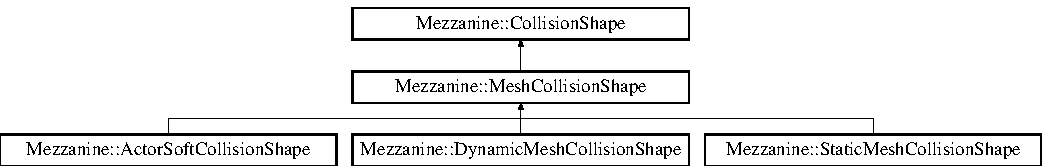
\includegraphics[height=2.231076cm]{classMezzanine_1_1MeshCollisionShape}
\end{center}
\end{figure}
\subsubsection*{Public Member Functions}
\begin{DoxyCompactItemize}
\item 
virtual btConcaveShape $\ast$ \hyperlink{classMezzanine_1_1MeshCollisionShape_a0a39875a6ca86c1a02c5432e04b80820}{GetBulletConcaveShape} () const 
\item 
virtual \hyperlink{classMezzanine_1_1CollisionShape_ad04186055565998879b64176d6dd100d}{CollisionShape::ShapeType} \hyperlink{classMezzanine_1_1MeshCollisionShape_a00dc444afac92030ea43815ec21dd8e8}{GetType} () const =0
\item 
\hypertarget{classMezzanine_1_1MeshCollisionShape_a5d5424990596460bfa86774b31eceba1}{
\hyperlink{classMezzanine_1_1MeshCollisionShape_a5d5424990596460bfa86774b31eceba1}{MeshCollisionShape} ()}
\label{classMezzanine_1_1MeshCollisionShape_a5d5424990596460bfa86774b31eceba1}

\begin{DoxyCompactList}\small\item\em Class Constructor. \item\end{DoxyCompactList}\item 
\hypertarget{classMezzanine_1_1MeshCollisionShape_a7e0554bdd88471091de94a488d18264e}{
virtual \hyperlink{classMezzanine_1_1MeshCollisionShape_a7e0554bdd88471091de94a488d18264e}{$\sim$MeshCollisionShape} ()}
\label{classMezzanine_1_1MeshCollisionShape_a7e0554bdd88471091de94a488d18264e}

\begin{DoxyCompactList}\small\item\em Class Destructor. \item\end{DoxyCompactList}\end{DoxyCompactItemize}
\subsubsection*{Protected Member Functions}
\begin{DoxyCompactItemize}
\item 
\hypertarget{classMezzanine_1_1MeshCollisionShape_aebba5404248e8d9cf441662db3daf129}{
void \hyperlink{classMezzanine_1_1MeshCollisionShape_aebba5404248e8d9cf441662db3daf129}{SetPointers} (btConcaveShape $\ast$Shape)}
\label{classMezzanine_1_1MeshCollisionShape_aebba5404248e8d9cf441662db3daf129}

\begin{DoxyCompactList}\small\item\em Sets the internal pointers on the base classes. \item\end{DoxyCompactList}\end{DoxyCompactItemize}


\subsubsection{Detailed Description}
This is the base class for all \hyperlink{classMezzanine_1_1Mesh}{Mesh} shapes. A \hyperlink{classMezzanine_1_1Mesh}{Mesh} shape is any shape that uses a series of triangles to determine it's bounds. As a rule all \hyperlink{classMezzanine_1_1Mesh}{Mesh} Shapes are considered Concave(even though the triangles don't need to form a concave shape, there is no way to assure the physics engine of that). \hyperlink{classMezzanine_1_1Mesh}{Mesh} shapes are not very performant, and should only be used with static objects, such as terrain. 

Definition at line 238 of file collisionshape.h.



\subsubsection{Member Function Documentation}
\hypertarget{classMezzanine_1_1MeshCollisionShape_a0a39875a6ca86c1a02c5432e04b80820}{
\index{Mezzanine::MeshCollisionShape@{Mezzanine::MeshCollisionShape}!GetBulletConcaveShape@{GetBulletConcaveShape}}
\index{GetBulletConcaveShape@{GetBulletConcaveShape}!Mezzanine::MeshCollisionShape@{Mezzanine::MeshCollisionShape}}
\paragraph[{GetBulletConcaveShape}]{\setlength{\rightskip}{0pt plus 5cm}btConcaveShape $\ast$ Mezzanine::MeshCollisionShape::GetBulletConcaveShape (
\begin{DoxyParamCaption}
{}
\end{DoxyParamCaption}
) const\hspace{0.3cm}{\ttfamily  \mbox{[}virtual\mbox{]}}}\hfill}
\label{classMezzanine_1_1MeshCollisionShape_a0a39875a6ca86c1a02c5432e04b80820}
Gets the internal shape pointer this collision shape is based on. 

\begin{DoxyReturn}{Returns}
Returns a pointer to the internal collision shape. 
\end{DoxyReturn}
 

Definition at line 283 of file collisionshape.cpp.

\hypertarget{classMezzanine_1_1MeshCollisionShape_a00dc444afac92030ea43815ec21dd8e8}{
\index{Mezzanine::MeshCollisionShape@{Mezzanine::MeshCollisionShape}!GetType@{GetType}}
\index{GetType@{GetType}!Mezzanine::MeshCollisionShape@{Mezzanine::MeshCollisionShape}}
\paragraph[{GetType}]{\setlength{\rightskip}{0pt plus 5cm}virtual {\bf CollisionShape::ShapeType} Mezzanine::MeshCollisionShape::GetType (
\begin{DoxyParamCaption}
{}
\end{DoxyParamCaption}
) const\hspace{0.3cm}{\ttfamily  \mbox{[}pure virtual\mbox{]}}}\hfill}
\label{classMezzanine_1_1MeshCollisionShape_a00dc444afac92030ea43815ec21dd8e8}
Gets the type of \hyperlink{classMezzanine_1_1Collision}{Collision} shape this is. 

\begin{DoxyReturn}{Returns}
Returns an enum value indicating the type of collision shape this is. 
\end{DoxyReturn}
 

Implements \hyperlink{classMezzanine_1_1CollisionShape_a27e5055f81cb8fb6d65a6c9f8dc73b69}{Mezzanine::CollisionShape}.



Implemented in \hyperlink{classMezzanine_1_1DynamicMeshCollisionShape_ae323a4ac9ae12890e1f8ce82b22f1ccc}{Mezzanine::DynamicMeshCollisionShape}, \hyperlink{classMezzanine_1_1ActorSoftCollisionShape_ae9ac8413434ff0de10376deb64ab49d0}{Mezzanine::ActorSoftCollisionShape}, and \hyperlink{classMezzanine_1_1StaticMeshCollisionShape_ae6cf497bf3a0c1db7b0f39a0513ebb79}{Mezzanine::StaticMeshCollisionShape}.



The documentation for this class was generated from the following files:\begin{DoxyCompactItemize}
\item 
collisionshape.h\item 
collisionshape.cpp\end{DoxyCompactItemize}

\hypertarget{classMezzanine_1_1MeshManager}{
\subsection{Mezzanine::MeshManager Class Reference}
\label{classMezzanine_1_1MeshManager}\index{Mezzanine::MeshManager@{Mezzanine::MeshManager}}
}


This manager handles the storage, generation, and query of of Graphics Meshes.  




{\ttfamily \#include $<$meshmanager.h$>$}

Inheritance diagram for Mezzanine::MeshManager:\begin{figure}[H]
\begin{center}
\leavevmode
\includegraphics[height=2.000000cm]{classMezzanine_1_1MeshManager}
\end{center}
\end{figure}
\subsubsection*{Public Member Functions}
\begin{DoxyCompactItemize}
\item 
\hypertarget{classMezzanine_1_1MeshManager_a6ef158bb2f5d96676df284ab1500f170}{
\hyperlink{classMezzanine_1_1MeshManager_a6ef158bb2f5d96676df284ab1500f170}{MeshManager} ()}
\label{classMezzanine_1_1MeshManager_a6ef158bb2f5d96676df284ab1500f170}

\begin{DoxyCompactList}\small\item\em Class constructor. \item\end{DoxyCompactList}\item 
\hypertarget{classMezzanine_1_1MeshManager_a5022cb5a023a4ec75ca47ea722ecdad1}{
virtual \hyperlink{classMezzanine_1_1MeshManager_a5022cb5a023a4ec75ca47ea722ecdad1}{$\sim$MeshManager} ()}
\label{classMezzanine_1_1MeshManager_a5022cb5a023a4ec75ca47ea722ecdad1}

\begin{DoxyCompactList}\small\item\em Class destructor. \item\end{DoxyCompactList}\item 
virtual \hyperlink{classMezzanine_1_1Mesh}{Mesh} $\ast$ \hyperlink{classMezzanine_1_1MeshManager_a579c2e8547243b3bea9a748c6bcbf28e}{CreateBoxCornerMesh} (const \hyperlink{namespaceMezzanine_acf9fcc130e6ebf08e3d8491aebcf1c86}{String} \&MeshName, const \hyperlink{namespaceMezzanine_acf9fcc130e6ebf08e3d8491aebcf1c86}{String} \&MaterialName, const \hyperlink{classMezzanine_1_1Vector3}{Vector3} \&HalfExtents, const \hyperlink{namespaceMezzanine_a726731b1a7df72bf3583e4a97282c6f6}{Real} \&BoxThickness)
\begin{DoxyCompactList}\small\item\em Creates a mesh composed of boxes that outline the corner edges of a larger box. \item\end{DoxyCompactList}\item 
virtual \hyperlink{classMezzanine_1_1Mesh}{Mesh} $\ast$ \hyperlink{classMezzanine_1_1MeshManager_abf5e8007a2c37a8d79b72de217a57211}{CreateBoxCornerMesh} (const \hyperlink{namespaceMezzanine_acf9fcc130e6ebf08e3d8491aebcf1c86}{String} \&MeshName, const \hyperlink{classMezzanine_1_1ColourValue}{ColourValue} \&Colour, const \hyperlink{classMezzanine_1_1Vector3}{Vector3} \&HalfExtents, const \hyperlink{namespaceMezzanine_a726731b1a7df72bf3583e4a97282c6f6}{Real} \&BoxThickness)
\begin{DoxyCompactList}\small\item\em Creates a mesh composed of boxes that outline the corner edges of a larger box. \item\end{DoxyCompactList}\item 
virtual \hyperlink{classMezzanine_1_1Mesh}{Mesh} $\ast$ \hyperlink{classMezzanine_1_1MeshManager_a5aa5da93359614b3e3a6b8ee955ff4d4}{CreateBoxMesh} (const \hyperlink{namespaceMezzanine_acf9fcc130e6ebf08e3d8491aebcf1c86}{String} \&MeshName, const \hyperlink{namespaceMezzanine_acf9fcc130e6ebf08e3d8491aebcf1c86}{String} \&MaterialName, const \hyperlink{classMezzanine_1_1Vector3}{Vector3} \&HalfExtents)
\begin{DoxyCompactList}\small\item\em Creates a box graphical mesh. \item\end{DoxyCompactList}\item 
virtual \hyperlink{classMezzanine_1_1Mesh}{Mesh} $\ast$ \hyperlink{classMezzanine_1_1MeshManager_a60d997162457cb7281c0fdfa37f95ee4}{CreateBoxMesh} (const \hyperlink{namespaceMezzanine_acf9fcc130e6ebf08e3d8491aebcf1c86}{String} \&MeshName, const \hyperlink{classMezzanine_1_1ColourValue}{ColourValue} \&Colour, const \hyperlink{classMezzanine_1_1Vector3}{Vector3} \&HalfExtents)
\begin{DoxyCompactList}\small\item\em Creates a box graphical mesh. \item\end{DoxyCompactList}\item 
virtual const \hyperlink{namespaceMezzanine_acf9fcc130e6ebf08e3d8491aebcf1c86}{String} \& \hyperlink{classMezzanine_1_1MeshManager_aabf94057016ff9ad8de101f5189713fd}{CreateColouredMaterial} (const \hyperlink{namespaceMezzanine_acf9fcc130e6ebf08e3d8491aebcf1c86}{String} \&MatName, const \hyperlink{classMezzanine_1_1ColourValue}{ColourValue} \&Colour, const \hyperlink{namespaceMezzanine_acf9fcc130e6ebf08e3d8491aebcf1c86}{String} \&Group=\char`\"{}\char`\"{})
\begin{DoxyCompactList}\small\item\em Creates a basic material in code using the provided colour. \item\end{DoxyCompactList}\item 
virtual \hyperlink{classMezzanine_1_1Mesh}{Mesh} $\ast$ \hyperlink{classMezzanine_1_1MeshManager_a6de2e01b43302a9439dc01c1dcc90f4c}{CreateCylinderMesh} (const \hyperlink{namespaceMezzanine_acf9fcc130e6ebf08e3d8491aebcf1c86}{String} \&MeshName, const \hyperlink{namespaceMezzanine_acf9fcc130e6ebf08e3d8491aebcf1c86}{String} \&MaterialName, const \hyperlink{classMezzanine_1_1Vector3}{Vector3} \&HalfExtents, const \hyperlink{classMezzanine_1_1Vector3}{Vector3} \&AxisOrientation, const \hyperlink{namespaceMezzanine_adcbb6ce6d1eb4379d109e51171e2e493}{Whole} \&CircleRes=16, const \hyperlink{namespaceMezzanine_adcbb6ce6d1eb4379d109e51171e2e493}{Whole} \&Segments=1)
\begin{DoxyCompactList}\small\item\em Creates a cylinder graphical mesh. \item\end{DoxyCompactList}\item 
virtual \hyperlink{classMezzanine_1_1Mesh}{Mesh} $\ast$ \hyperlink{classMezzanine_1_1MeshManager_aa2d52ca9f366145ce91ee68eb2d8c9a3}{CreateCylinderMesh} (const \hyperlink{namespaceMezzanine_acf9fcc130e6ebf08e3d8491aebcf1c86}{String} \&MeshName, const \hyperlink{classMezzanine_1_1ColourValue}{ColourValue} \&Colour, const \hyperlink{classMezzanine_1_1Vector3}{Vector3} \&HalfExtents, const \hyperlink{classMezzanine_1_1Vector3}{Vector3} \&AxisOrientation, const \hyperlink{namespaceMezzanine_adcbb6ce6d1eb4379d109e51171e2e493}{Whole} \&CircleRes=16, const \hyperlink{namespaceMezzanine_adcbb6ce6d1eb4379d109e51171e2e493}{Whole} \&Segments=1)
\begin{DoxyCompactList}\small\item\em Creates a cylinder graphical mesh and simple material. \item\end{DoxyCompactList}\item 
virtual \hyperlink{classMezzanine_1_1Mesh}{Mesh} $\ast$ \hyperlink{classMezzanine_1_1MeshManager_a75424e13a23151fa96ef0626962034a0}{CreateMeshFromShape} (const \hyperlink{namespaceMezzanine_acf9fcc130e6ebf08e3d8491aebcf1c86}{String} \&MeshName, const \hyperlink{namespaceMezzanine_acf9fcc130e6ebf08e3d8491aebcf1c86}{String} \&MaterialName, \hyperlink{classMezzanine_1_1CollisionShape}{CollisionShape} $\ast$Shape)
\begin{DoxyCompactList}\small\item\em Generates a mesh based on a collision shape. \item\end{DoxyCompactList}\item 
virtual \hyperlink{classMezzanine_1_1Mesh}{Mesh} $\ast$ \hyperlink{classMezzanine_1_1MeshManager_a1373def36d801ef524372c76852984ec}{CreateSphereMesh} (const \hyperlink{namespaceMezzanine_acf9fcc130e6ebf08e3d8491aebcf1c86}{String} \&MeshName, const \hyperlink{classMezzanine_1_1ColourValue}{ColourValue} \&Colour, const \hyperlink{namespaceMezzanine_a726731b1a7df72bf3583e4a97282c6f6}{Real} \&Radius, const \hyperlink{namespaceMezzanine_a726731b1a7df72bf3583e4a97282c6f6}{Real} \&Rings=16, const \hyperlink{namespaceMezzanine_a726731b1a7df72bf3583e4a97282c6f6}{Real} \&Segments=16)
\begin{DoxyCompactList}\small\item\em Creates a sphere graphical mesh and simple material. \item\end{DoxyCompactList}\item 
virtual \hyperlink{classMezzanine_1_1Mesh}{Mesh} $\ast$ \hyperlink{classMezzanine_1_1MeshManager_a237f66b9471261d6a0ef6d565740ea15}{CreateSphereMesh} (const \hyperlink{namespaceMezzanine_acf9fcc130e6ebf08e3d8491aebcf1c86}{String} \&MeshName, const \hyperlink{namespaceMezzanine_acf9fcc130e6ebf08e3d8491aebcf1c86}{String} \&MaterialName, const \hyperlink{namespaceMezzanine_a726731b1a7df72bf3583e4a97282c6f6}{Real} \&Radius, const \hyperlink{namespaceMezzanine_a726731b1a7df72bf3583e4a97282c6f6}{Real} \&Rings=16, const \hyperlink{namespaceMezzanine_a726731b1a7df72bf3583e4a97282c6f6}{Real} \&Segments=16)
\begin{DoxyCompactList}\small\item\em Creates a sphere graphical mesh. \item\end{DoxyCompactList}\item 
\hypertarget{classMezzanine_1_1MeshManager_ad6ef502c838312f778c5ca77c706f20d}{
virtual void \hyperlink{classMezzanine_1_1MeshManager_ad6ef502c838312f778c5ca77c706f20d}{DestroyAllGeneratedMeshes} ()}
\label{classMezzanine_1_1MeshManager_ad6ef502c838312f778c5ca77c706f20d}

\begin{DoxyCompactList}\small\item\em Destroys all the meshes generated by this generator. \item\end{DoxyCompactList}\item 
\hypertarget{classMezzanine_1_1MeshManager_aa807f17cbba66ff45f8ffd5d027dec7e}{
void \hyperlink{classMezzanine_1_1MeshManager_aa807f17cbba66ff45f8ffd5d027dec7e}{DestroyAllMeshes} ()}
\label{classMezzanine_1_1MeshManager_aa807f17cbba66ff45f8ffd5d027dec7e}

\begin{DoxyCompactList}\small\item\em Clears this manager of all meshes, both loaded and generated. \item\end{DoxyCompactList}\item 
virtual void \hyperlink{classMezzanine_1_1MeshManager_a9c9286c940e56c4ba6a02ef58bfc0374}{DestroyGeneratedMesh} (const \hyperlink{namespaceMezzanine_acf9fcc130e6ebf08e3d8491aebcf1c86}{String} \&MeshName)
\begin{DoxyCompactList}\small\item\em Destroys a named \hyperlink{classMezzanine_1_1Mesh}{Mesh}, freeing it's resources. \item\end{DoxyCompactList}\item 
virtual void \hyperlink{classMezzanine_1_1MeshManager_acfbea42e8aeb36d48522ad027f1e8764}{DoMainLoopItems} ()
\item 
\hyperlink{classMezzanine_1_1Mesh}{Mesh} $\ast$ \hyperlink{classMezzanine_1_1MeshManager_a9f564124032f9dc8a636f8092bbbc87e}{GetMesh} (const \hyperlink{namespaceMezzanine_acf9fcc130e6ebf08e3d8491aebcf1c86}{String} \&MeshName)
\begin{DoxyCompactList}\small\item\em Gets a mesh stored in this manager. \item\end{DoxyCompactList}\item 
virtual \hyperlink{namespaceMezzanine_adcbb6ce6d1eb4379d109e51171e2e493}{Whole} \hyperlink{classMezzanine_1_1MeshManager_a0b6d3fef8ecc0e12ff6de14618e788d8}{GetNumGeneratedMeshes} ()
\begin{DoxyCompactList}\small\item\em Gets the number of meshes this generator has created and are in use. \item\end{DoxyCompactList}\item 
virtual \hyperlink{namespaceMezzanine_adcbb6ce6d1eb4379d109e51171e2e493}{Whole} \hyperlink{classMezzanine_1_1MeshManager_a809d8b615341e55c3ed463b1e18c01db}{GetNumLoadedMeshes} ()
\begin{DoxyCompactList}\small\item\em Gets the number of currently loaded mesh files. \item\end{DoxyCompactList}\item 
virtual \hyperlink{classMezzanine_1_1ManagerBase_a08cecf5169cad3e82be81a3a159b0b6e}{ManagerBase::ManagerTypeName} \hyperlink{classMezzanine_1_1MeshManager_a120881dcf7bce1d3a30bedb426650c0e}{GetType} () const 
\item 
virtual void \hyperlink{classMezzanine_1_1MeshManager_ac03c91bea88144bcfa420411bc85f0c7}{Initialize} ()
\item 
virtual \hyperlink{classMezzanine_1_1Mesh}{Mesh} $\ast$ \hyperlink{classMezzanine_1_1MeshManager_a01fcda6b9f1363e99b6ac61e4afcb951}{LoadMesh} (const \hyperlink{namespaceMezzanine_acf9fcc130e6ebf08e3d8491aebcf1c86}{String} \&MeshName, const \hyperlink{namespaceMezzanine_acf9fcc130e6ebf08e3d8491aebcf1c86}{String} \&Group)
\begin{DoxyCompactList}\small\item\em Loads a mesh file from disk and prepares it for use. \item\end{DoxyCompactList}\item 
\hypertarget{classMezzanine_1_1MeshManager_a95b66f15b74a8eb4f8cdfab411de6289}{
virtual void \hyperlink{classMezzanine_1_1MeshManager_a95b66f15b74a8eb4f8cdfab411de6289}{UnloadAllLoadedMeshes} ()}
\label{classMezzanine_1_1MeshManager_a95b66f15b74a8eb4f8cdfab411de6289}

\begin{DoxyCompactList}\small\item\em Unloads every mesh that is currently loaded. \item\end{DoxyCompactList}\item 
virtual void \hyperlink{classMezzanine_1_1MeshManager_aa8bf0e0aad71969dd4076cd36e2e8ab3}{UnloadMesh} (const \hyperlink{namespaceMezzanine_acf9fcc130e6ebf08e3d8491aebcf1c86}{String} \&MeshName)
\begin{DoxyCompactList}\small\item\em Unloads a mesh file. \item\end{DoxyCompactList}\end{DoxyCompactItemize}
\subsubsection*{Protected Attributes}
\begin{DoxyCompactItemize}
\item 
\hypertarget{classMezzanine_1_1MeshManager_a8ebad0c5129a136f49fd11ec68dba8c8}{
std::map$<$ \hyperlink{namespaceMezzanine_acf9fcc130e6ebf08e3d8491aebcf1c86}{String}, \hyperlink{classMezzanine_1_1Mesh}{Mesh} $\ast$ $>$ {\bfseries GeneratedMeshes}}
\label{classMezzanine_1_1MeshManager_a8ebad0c5129a136f49fd11ec68dba8c8}

\item 
\hypertarget{classMezzanine_1_1MeshManager_a6baa9cd1ab36436745ab74955157bfda}{
std::map$<$ \hyperlink{namespaceMezzanine_acf9fcc130e6ebf08e3d8491aebcf1c86}{String}, \hyperlink{classMezzanine_1_1Mesh}{Mesh} $\ast$ $>$ {\bfseries LoadedMeshes}}
\label{classMezzanine_1_1MeshManager_a6baa9cd1ab36436745ab74955157bfda}

\end{DoxyCompactItemize}


\subsubsection{Detailed Description}
This manager handles the storage, generation, and query of of Graphics Meshes. 

Definition at line 64 of file meshmanager.h.



\subsubsection{Member Function Documentation}
\hypertarget{classMezzanine_1_1MeshManager_a579c2e8547243b3bea9a748c6bcbf28e}{
\index{Mezzanine::MeshManager@{Mezzanine::MeshManager}!CreateBoxCornerMesh@{CreateBoxCornerMesh}}
\index{CreateBoxCornerMesh@{CreateBoxCornerMesh}!Mezzanine::MeshManager@{Mezzanine::MeshManager}}
\paragraph[{CreateBoxCornerMesh}]{\setlength{\rightskip}{0pt plus 5cm}{\bf Mesh} $\ast$ Mezzanine::MeshManager::CreateBoxCornerMesh (
\begin{DoxyParamCaption}
\item[{const {\bf String} \&}]{MeshName, }
\item[{const {\bf String} \&}]{MaterialName, }
\item[{const {\bf Vector3} \&}]{HalfExtents, }
\item[{const {\bf Real} \&}]{BoxThickness}
\end{DoxyParamCaption}
)\hspace{0.3cm}{\ttfamily  \mbox{[}virtual\mbox{]}}}\hfill}
\label{classMezzanine_1_1MeshManager_a579c2e8547243b3bea9a748c6bcbf28e}


Creates a mesh composed of boxes that outline the corner edges of a larger box. 

\begin{DoxyReturn}{Returns}
Returns a pointer to the created \hyperlink{classMezzanine_1_1Mesh}{Mesh}. 
\end{DoxyReturn}

\begin{DoxyParams}{Parameters}
{\em MeshName} & The name for the mesh which will be created. Use this to reference the mesh when creating other objects that need a mesh. \\
\hline
{\em MaterialName} & The name of the material script which will be applied to this mesh. \\
\hline
{\em HalfExtents} & Half of the full dimentions of the final object in world units. This allows the objects origin to be it's center. \\
\hline
{\em BoxThickness} & The width/thickness of the smaller boxes that will outline the corners of the larger box. \\
\hline
\end{DoxyParams}


Definition at line 402 of file meshmanager.cpp.

\hypertarget{classMezzanine_1_1MeshManager_abf5e8007a2c37a8d79b72de217a57211}{
\index{Mezzanine::MeshManager@{Mezzanine::MeshManager}!CreateBoxCornerMesh@{CreateBoxCornerMesh}}
\index{CreateBoxCornerMesh@{CreateBoxCornerMesh}!Mezzanine::MeshManager@{Mezzanine::MeshManager}}
\paragraph[{CreateBoxCornerMesh}]{\setlength{\rightskip}{0pt plus 5cm}{\bf Mesh} $\ast$ Mezzanine::MeshManager::CreateBoxCornerMesh (
\begin{DoxyParamCaption}
\item[{const {\bf String} \&}]{MeshName, }
\item[{const {\bf ColourValue} \&}]{Colour, }
\item[{const {\bf Vector3} \&}]{HalfExtents, }
\item[{const {\bf Real} \&}]{BoxThickness}
\end{DoxyParamCaption}
)\hspace{0.3cm}{\ttfamily  \mbox{[}virtual\mbox{]}}}\hfill}
\label{classMezzanine_1_1MeshManager_abf5e8007a2c37a8d79b72de217a57211}


Creates a mesh composed of boxes that outline the corner edges of a larger box. 

\begin{DoxyReturn}{Returns}
Returns a pointer to the created \hyperlink{classMezzanine_1_1Mesh}{Mesh}. 
\end{DoxyReturn}

\begin{DoxyParams}{Parameters}
{\em MeshName} & The name for the mesh which will be created. Use this to reference the mesh when creating other objects that need a mesh. \\
\hline
{\em Colour} & The colour to generate the material with that will be applied to the mesh. The created material's name will be autogenerated to \char`\"{}\mbox{[}Meshname\mbox{]}+Mat\char`\"{}. \\
\hline
{\em HalfExtents} & Half of the full dimentions of the final object in world units. This allows the objects origin to be it's center. \\
\hline
{\em BoxThickness} & The width/thickness of the smaller boxes that will outline the corners of the larger box. \\
\hline
\end{DoxyParams}


Definition at line 821 of file meshmanager.cpp.

\hypertarget{classMezzanine_1_1MeshManager_a5aa5da93359614b3e3a6b8ee955ff4d4}{
\index{Mezzanine::MeshManager@{Mezzanine::MeshManager}!CreateBoxMesh@{CreateBoxMesh}}
\index{CreateBoxMesh@{CreateBoxMesh}!Mezzanine::MeshManager@{Mezzanine::MeshManager}}
\paragraph[{CreateBoxMesh}]{\setlength{\rightskip}{0pt plus 5cm}{\bf Mesh} $\ast$ Mezzanine::MeshManager::CreateBoxMesh (
\begin{DoxyParamCaption}
\item[{const {\bf String} \&}]{MeshName, }
\item[{const {\bf String} \&}]{MaterialName, }
\item[{const {\bf Vector3} \&}]{HalfExtents}
\end{DoxyParamCaption}
)\hspace{0.3cm}{\ttfamily  \mbox{[}virtual\mbox{]}}}\hfill}
\label{classMezzanine_1_1MeshManager_a5aa5da93359614b3e3a6b8ee955ff4d4}


Creates a box graphical mesh. 

\begin{DoxyReturn}{Returns}
Returns a pointer to the created \hyperlink{classMezzanine_1_1Mesh}{Mesh}. 
\end{DoxyReturn}

\begin{DoxyParams}{Parameters}
{\em MeshName} & The name for the mesh which will be created. Use this to reference the mesh when creating other objects that need a mesh. \\
\hline
{\em MaterialName} & The name of the material script which will be applied to this mesh. \\
\hline
{\em HalfExtents} & Half of the full dimentions of the final object in world units. This allows the objects origin to be it's center. \\
\hline
\end{DoxyParams}


Definition at line 141 of file meshmanager.cpp.

\hypertarget{classMezzanine_1_1MeshManager_a60d997162457cb7281c0fdfa37f95ee4}{
\index{Mezzanine::MeshManager@{Mezzanine::MeshManager}!CreateBoxMesh@{CreateBoxMesh}}
\index{CreateBoxMesh@{CreateBoxMesh}!Mezzanine::MeshManager@{Mezzanine::MeshManager}}
\paragraph[{CreateBoxMesh}]{\setlength{\rightskip}{0pt plus 5cm}{\bf Mesh} $\ast$ Mezzanine::MeshManager::CreateBoxMesh (
\begin{DoxyParamCaption}
\item[{const {\bf String} \&}]{MeshName, }
\item[{const {\bf ColourValue} \&}]{Colour, }
\item[{const {\bf Vector3} \&}]{HalfExtents}
\end{DoxyParamCaption}
)\hspace{0.3cm}{\ttfamily  \mbox{[}virtual\mbox{]}}}\hfill}
\label{classMezzanine_1_1MeshManager_a60d997162457cb7281c0fdfa37f95ee4}


Creates a box graphical mesh. 

\begin{DoxyReturn}{Returns}
Returns a pointer to the created \hyperlink{classMezzanine_1_1Mesh}{Mesh}. 
\end{DoxyReturn}

\begin{DoxyParams}{Parameters}
{\em MeshName} & The name for the mesh which will be created. Use this to reference the mesh when creating other objects that need a mesh. \\
\hline
{\em Colour} & The colour to generate the material with that will be applied to the mesh. The created material's name will be autogenerated to \char`\"{}\mbox{[}Meshname\mbox{]}+Mat\char`\"{}. \\
\hline
{\em HalfExtents} & Half of the full dimentions of the final object in world units. This allows the objects origin to be it's center. \\
\hline
\end{DoxyParams}


Definition at line 199 of file meshmanager.cpp.

\hypertarget{classMezzanine_1_1MeshManager_aabf94057016ff9ad8de101f5189713fd}{
\index{Mezzanine::MeshManager@{Mezzanine::MeshManager}!CreateColouredMaterial@{CreateColouredMaterial}}
\index{CreateColouredMaterial@{CreateColouredMaterial}!Mezzanine::MeshManager@{Mezzanine::MeshManager}}
\paragraph[{CreateColouredMaterial}]{\setlength{\rightskip}{0pt plus 5cm}const {\bf String} \& Mezzanine::MeshManager::CreateColouredMaterial (
\begin{DoxyParamCaption}
\item[{const {\bf String} \&}]{MatName, }
\item[{const {\bf ColourValue} \&}]{Colour, }
\item[{const {\bf String} \&}]{Group = {\ttfamily \char`\"{}\char`\"{}}}
\end{DoxyParamCaption}
)\hspace{0.3cm}{\ttfamily  \mbox{[}virtual\mbox{]}}}\hfill}
\label{classMezzanine_1_1MeshManager_aabf94057016ff9ad8de101f5189713fd}


Creates a basic material in code using the provided colour. 

\begin{DoxyReturn}{Returns}
Returns a string containing the name of the created Material. This is actually the same string as whats passed in as the MatName, just here as convenience when calling the function as an argument in other functions. 
\end{DoxyReturn}

\begin{DoxyParams}{Parameters}
{\em MatName} & The name to assign to the created material. \\
\hline
{\em Colour} & The colour to assign to the created material. \\
\hline
{\em Group} & The resource group where to place this material. Will be placed in an internal resouce group if left blank. \\
\hline
\end{DoxyParams}


Definition at line 833 of file meshmanager.cpp.

\hypertarget{classMezzanine_1_1MeshManager_a6de2e01b43302a9439dc01c1dcc90f4c}{
\index{Mezzanine::MeshManager@{Mezzanine::MeshManager}!CreateCylinderMesh@{CreateCylinderMesh}}
\index{CreateCylinderMesh@{CreateCylinderMesh}!Mezzanine::MeshManager@{Mezzanine::MeshManager}}
\paragraph[{CreateCylinderMesh}]{\setlength{\rightskip}{0pt plus 5cm}{\bf Mesh} $\ast$ Mezzanine::MeshManager::CreateCylinderMesh (
\begin{DoxyParamCaption}
\item[{const {\bf String} \&}]{MeshName, }
\item[{const {\bf String} \&}]{MaterialName, }
\item[{const {\bf Vector3} \&}]{HalfExtents, }
\item[{const {\bf Vector3} \&}]{AxisOrientation, }
\item[{const {\bf Whole} \&}]{CircleRes = {\ttfamily 16}, }
\item[{const {\bf Whole} \&}]{Segments = {\ttfamily 1}}
\end{DoxyParamCaption}
)\hspace{0.3cm}{\ttfamily  \mbox{[}virtual\mbox{]}}}\hfill}
\label{classMezzanine_1_1MeshManager_a6de2e01b43302a9439dc01c1dcc90f4c}


Creates a cylinder graphical mesh. 

\begin{DoxyReturn}{Returns}
Returns a pointer to the created \hyperlink{classMezzanine_1_1Mesh}{Mesh}. 
\end{DoxyReturn}

\begin{DoxyParams}{Parameters}
{\em MeshName} & The name for the mesh which will be created. Use this to reference the mesh when creating other objects that need a mesh. \\
\hline
{\em MaterialName} & The name of the material script which will be applied to this mesh. \\
\hline
{\em HalfExtents} & Half of the full dimentions of the final object in world units. This allows the objects origin to be it's center. \\
\hline
{\em AxisOrientation} & \hyperlink{classMezzanine_1_1Vector3}{Vector3} representing which axis the cylinder should be aligned on. Should be one of the three: (1,0,0), (0,1,0), (0,0,1). \\
\hline
{\em CircleRes} & The number of segments the circle should be comprised of. Determines the \char`\"{}resolution\char`\"{} of the cylinder. \\
\hline
{\em Segments} & Optional parameter to specify the number of segments the cylinder should be comprised of. Mostly just useful if a special material is made for his. \\
\hline
\end{DoxyParams}


Start of MIT(Ogre Proceadural) License ///

\begin{Desc}
\item[\hyperlink{todo__todo000022}{Todo}]These if/elses aren't really a long term solution as they won't work for any more then 1 segment. This needs to be addressed. \end{Desc}


End of MIT(Ogre Proceadural) License /// 



Definition at line 206 of file meshmanager.cpp.

\hypertarget{classMezzanine_1_1MeshManager_aa2d52ca9f366145ce91ee68eb2d8c9a3}{
\index{Mezzanine::MeshManager@{Mezzanine::MeshManager}!CreateCylinderMesh@{CreateCylinderMesh}}
\index{CreateCylinderMesh@{CreateCylinderMesh}!Mezzanine::MeshManager@{Mezzanine::MeshManager}}
\paragraph[{CreateCylinderMesh}]{\setlength{\rightskip}{0pt plus 5cm}{\bf Mesh} $\ast$ Mezzanine::MeshManager::CreateCylinderMesh (
\begin{DoxyParamCaption}
\item[{const {\bf String} \&}]{MeshName, }
\item[{const {\bf ColourValue} \&}]{Colour, }
\item[{const {\bf Vector3} \&}]{HalfExtents, }
\item[{const {\bf Vector3} \&}]{AxisOrientation, }
\item[{const {\bf Whole} \&}]{CircleRes = {\ttfamily 16}, }
\item[{const {\bf Whole} \&}]{Segments = {\ttfamily 1}}
\end{DoxyParamCaption}
)\hspace{0.3cm}{\ttfamily  \mbox{[}virtual\mbox{]}}}\hfill}
\label{classMezzanine_1_1MeshManager_aa2d52ca9f366145ce91ee68eb2d8c9a3}


Creates a cylinder graphical mesh and simple material. 

\begin{DoxyReturn}{Returns}
Returns a pointer to the created \hyperlink{classMezzanine_1_1Mesh}{Mesh}. 
\end{DoxyReturn}

\begin{DoxyParams}{Parameters}
{\em MeshName} & The name for the mesh which will be created. Use this to reference the mesh when creating other objects that need a mesh. \\
\hline
{\em Colour} & The colour to generate the material with that will be applied to the mesh. The created material's name will be autogenerated to \char`\"{}\mbox{[}Meshname\mbox{]}+Mat\char`\"{}. \\
\hline
{\em HalfExtents} & Half of the full dimentions of the final object in world units. This allows the objects origin to be it's center. \\
\hline
{\em AxisOrientation} & \hyperlink{classMezzanine_1_1Vector3}{Vector3} representing which axis the cylinder should be aligned on. Should be one of the three: (1,0,0), (0,1,0), (0,0,1). \\
\hline
{\em CircleRes} & The number of segments the circle should be comprised of. Determines the \char`\"{}resolution\char`\"{} of the cylinder. \\
\hline
{\em Segments} & Optional parameter to specify the number of segments the cylinder should be comprised of. Mostly just useful if a special material is made for his. \\
\hline
\end{DoxyParams}


Definition at line 319 of file meshmanager.cpp.

\hypertarget{classMezzanine_1_1MeshManager_a75424e13a23151fa96ef0626962034a0}{
\index{Mezzanine::MeshManager@{Mezzanine::MeshManager}!CreateMeshFromShape@{CreateMeshFromShape}}
\index{CreateMeshFromShape@{CreateMeshFromShape}!Mezzanine::MeshManager@{Mezzanine::MeshManager}}
\paragraph[{CreateMeshFromShape}]{\setlength{\rightskip}{0pt plus 5cm}{\bf Mesh} $\ast$ Mezzanine::MeshManager::CreateMeshFromShape (
\begin{DoxyParamCaption}
\item[{const {\bf String} \&}]{MeshName, }
\item[{const {\bf String} \&}]{MaterialName, }
\item[{{\bf CollisionShape} $\ast$}]{Shape}
\end{DoxyParamCaption}
)\hspace{0.3cm}{\ttfamily  \mbox{[}virtual\mbox{]}}}\hfill}
\label{classMezzanine_1_1MeshManager_a75424e13a23151fa96ef0626962034a0}


Generates a mesh based on a collision shape. 

\begin{DoxyRemark}{Remarks}
This is just a convenience function. You can fetch the information and build the mesh yourself with greater flexability then what this function has to offer. This function only supports building the shapes this manager can generate, and it will only use default options when deciding the parameters to use(if it's a parameter it can't get from the shape). 
\end{DoxyRemark}
\begin{DoxyReturn}{Returns}
Returns a pointer to the created mesh. 
\end{DoxyReturn}

\begin{DoxyParams}{Parameters}
{\em MeshName} & The name that will be given to the generated mesh. \\
\hline
{\em MaterialName} & The name of the material to use with this mesh. \\
\hline
{\em Shape} & The shape to base the mesh on. \\
\hline
\end{DoxyParams}


Definition at line 828 of file meshmanager.cpp.

\hypertarget{classMezzanine_1_1MeshManager_a237f66b9471261d6a0ef6d565740ea15}{
\index{Mezzanine::MeshManager@{Mezzanine::MeshManager}!CreateSphereMesh@{CreateSphereMesh}}
\index{CreateSphereMesh@{CreateSphereMesh}!Mezzanine::MeshManager@{Mezzanine::MeshManager}}
\paragraph[{CreateSphereMesh}]{\setlength{\rightskip}{0pt plus 5cm}{\bf Mesh} $\ast$ Mezzanine::MeshManager::CreateSphereMesh (
\begin{DoxyParamCaption}
\item[{const {\bf String} \&}]{MeshName, }
\item[{const {\bf String} \&}]{MaterialName, }
\item[{const {\bf Real} \&}]{Radius, }
\item[{const {\bf Real} \&}]{Rings = {\ttfamily 16}, }
\item[{const {\bf Real} \&}]{Segments = {\ttfamily 16}}
\end{DoxyParamCaption}
)\hspace{0.3cm}{\ttfamily  \mbox{[}virtual\mbox{]}}}\hfill}
\label{classMezzanine_1_1MeshManager_a237f66b9471261d6a0ef6d565740ea15}


Creates a sphere graphical mesh. 

\begin{DoxyReturn}{Returns}
Returns a pointer to the created \hyperlink{classMezzanine_1_1Mesh}{Mesh}. 
\end{DoxyReturn}

\begin{DoxyParams}{Parameters}
{\em MeshName} & The name for the mesh which will be created. Use this to reference the mesh when creating other objects that need a mesh. \\
\hline
{\em MaterialName} & The name of the material script which will be applied to this mesh. \\
\hline
{\em Radius} & The radius to generate the sphere with in world units. \\
\hline
{\em Rings} & The number of horizontal rings the sphere is to be comprised of. This along with the segments parameter controls the overall resolution of the sphere. Less then 16 is not recommended. \\
\hline
{\em Segments} & The number of vertical rings the sphere is to be comprised of. This along with the rings parameter controls the overall resolution of the sphere. Less then 16 is not recommended. \\
\hline
\end{DoxyParams}


Definition at line 326 of file meshmanager.cpp.

\hypertarget{classMezzanine_1_1MeshManager_a1373def36d801ef524372c76852984ec}{
\index{Mezzanine::MeshManager@{Mezzanine::MeshManager}!CreateSphereMesh@{CreateSphereMesh}}
\index{CreateSphereMesh@{CreateSphereMesh}!Mezzanine::MeshManager@{Mezzanine::MeshManager}}
\paragraph[{CreateSphereMesh}]{\setlength{\rightskip}{0pt plus 5cm}{\bf Mesh} $\ast$ Mezzanine::MeshManager::CreateSphereMesh (
\begin{DoxyParamCaption}
\item[{const {\bf String} \&}]{MeshName, }
\item[{const {\bf ColourValue} \&}]{Colour, }
\item[{const {\bf Real} \&}]{Radius, }
\item[{const {\bf Real} \&}]{Rings = {\ttfamily 16}, }
\item[{const {\bf Real} \&}]{Segments = {\ttfamily 16}}
\end{DoxyParamCaption}
)\hspace{0.3cm}{\ttfamily  \mbox{[}virtual\mbox{]}}}\hfill}
\label{classMezzanine_1_1MeshManager_a1373def36d801ef524372c76852984ec}


Creates a sphere graphical mesh and simple material. 

\begin{DoxyReturn}{Returns}
Returns a pointer to the created \hyperlink{classMezzanine_1_1Mesh}{Mesh}. 
\end{DoxyReturn}

\begin{DoxyParams}{Parameters}
{\em MeshName} & The name for the mesh which will be created. Use this to reference the mesh when creating other objects that need a mesh. \\
\hline
{\em Colour} & The colour to generate the material with that will be applied to the mesh. The created material's name will be autogenerated to \char`\"{}\mbox{[}Meshname\mbox{]}+Mat\char`\"{}. \\
\hline
{\em Radius} & The radius to generate the sphere with in world units. \\
\hline
{\em Rings} & The number of horizontal rings the sphere is to be comprised of. This along with the segments parameter controls the overall resolution of the sphere. Less then 16 is not recommended. \\
\hline
{\em Segments} & The number of vertical rings the sphere is to be comprised of. This along with the rings parameter controls the overall resolution of the sphere. Less then 16 is not recommended. \\
\hline
\end{DoxyParams}


Definition at line 375 of file meshmanager.cpp.

\hypertarget{classMezzanine_1_1MeshManager_a9c9286c940e56c4ba6a02ef58bfc0374}{
\index{Mezzanine::MeshManager@{Mezzanine::MeshManager}!DestroyGeneratedMesh@{DestroyGeneratedMesh}}
\index{DestroyGeneratedMesh@{DestroyGeneratedMesh}!Mezzanine::MeshManager@{Mezzanine::MeshManager}}
\paragraph[{DestroyGeneratedMesh}]{\setlength{\rightskip}{0pt plus 5cm}void Mezzanine::MeshManager::DestroyGeneratedMesh (
\begin{DoxyParamCaption}
\item[{const {\bf String} \&}]{MeshName}
\end{DoxyParamCaption}
)\hspace{0.3cm}{\ttfamily  \mbox{[}virtual\mbox{]}}}\hfill}
\label{classMezzanine_1_1MeshManager_a9c9286c940e56c4ba6a02ef58bfc0374}


Destroys a named \hyperlink{classMezzanine_1_1Mesh}{Mesh}, freeing it's resources. 


\begin{DoxyParams}{Parameters}
{\em MeshName} & The name of the mesh to be destroyed. \\
\hline
\end{DoxyParams}


Definition at line 120 of file meshmanager.cpp.

\hypertarget{classMezzanine_1_1MeshManager_acfbea42e8aeb36d48522ad027f1e8764}{
\index{Mezzanine::MeshManager@{Mezzanine::MeshManager}!DoMainLoopItems@{DoMainLoopItems}}
\index{DoMainLoopItems@{DoMainLoopItems}!Mezzanine::MeshManager@{Mezzanine::MeshManager}}
\paragraph[{DoMainLoopItems}]{\setlength{\rightskip}{0pt plus 5cm}void Mezzanine::MeshManager::DoMainLoopItems (
\begin{DoxyParamCaption}
{}
\end{DoxyParamCaption}
)\hspace{0.3cm}{\ttfamily  \mbox{[}virtual\mbox{]}}}\hfill}
\label{classMezzanine_1_1MeshManager_acfbea42e8aeb36d48522ad027f1e8764}
The main loop calls this once per frame. 

This is where each manager is expected to put anything that needs to be run each iteration of the main loop  

Implements \hyperlink{classMezzanine_1_1ManagerBase_a4ee29e4baf6c4b9a3bfec1b2258d5cd2}{Mezzanine::ManagerBase}.



Definition at line 853 of file meshmanager.cpp.

\hypertarget{classMezzanine_1_1MeshManager_a9f564124032f9dc8a636f8092bbbc87e}{
\index{Mezzanine::MeshManager@{Mezzanine::MeshManager}!GetMesh@{GetMesh}}
\index{GetMesh@{GetMesh}!Mezzanine::MeshManager@{Mezzanine::MeshManager}}
\paragraph[{GetMesh}]{\setlength{\rightskip}{0pt plus 5cm}{\bf Mesh} $\ast$ Mezzanine::MeshManager::GetMesh (
\begin{DoxyParamCaption}
\item[{const {\bf String} \&}]{MeshName}
\end{DoxyParamCaption}
)}\hfill}
\label{classMezzanine_1_1MeshManager_a9f564124032f9dc8a636f8092bbbc87e}


Gets a mesh stored in this manager. 

\begin{DoxyReturn}{Returns}
Returns a pointer to the requested mesh. 
\end{DoxyReturn}

\begin{DoxyParams}{Parameters}
{\em MeshName} & The name of the mesh to retrieve. \\
\hline
\end{DoxyParams}


Definition at line 63 of file meshmanager.cpp.

\hypertarget{classMezzanine_1_1MeshManager_a0b6d3fef8ecc0e12ff6de14618e788d8}{
\index{Mezzanine::MeshManager@{Mezzanine::MeshManager}!GetNumGeneratedMeshes@{GetNumGeneratedMeshes}}
\index{GetNumGeneratedMeshes@{GetNumGeneratedMeshes}!Mezzanine::MeshManager@{Mezzanine::MeshManager}}
\paragraph[{GetNumGeneratedMeshes}]{\setlength{\rightskip}{0pt plus 5cm}{\bf Whole} Mezzanine::MeshManager::GetNumGeneratedMeshes (
\begin{DoxyParamCaption}
{}
\end{DoxyParamCaption}
)\hspace{0.3cm}{\ttfamily  \mbox{[}virtual\mbox{]}}}\hfill}
\label{classMezzanine_1_1MeshManager_a0b6d3fef8ecc0e12ff6de14618e788d8}


Gets the number of meshes this generator has created and are in use. 

\begin{DoxyReturn}{Returns}
Returns a Whole representing the number of meshes created by this generator. 
\end{DoxyReturn}


Definition at line 115 of file meshmanager.cpp.

\hypertarget{classMezzanine_1_1MeshManager_a809d8b615341e55c3ed463b1e18c01db}{
\index{Mezzanine::MeshManager@{Mezzanine::MeshManager}!GetNumLoadedMeshes@{GetNumLoadedMeshes}}
\index{GetNumLoadedMeshes@{GetNumLoadedMeshes}!Mezzanine::MeshManager@{Mezzanine::MeshManager}}
\paragraph[{GetNumLoadedMeshes}]{\setlength{\rightskip}{0pt plus 5cm}{\bf Whole} Mezzanine::MeshManager::GetNumLoadedMeshes (
\begin{DoxyParamCaption}
{}
\end{DoxyParamCaption}
)\hspace{0.3cm}{\ttfamily  \mbox{[}virtual\mbox{]}}}\hfill}
\label{classMezzanine_1_1MeshManager_a809d8b615341e55c3ed463b1e18c01db}


Gets the number of currently loaded mesh files. 

\begin{DoxyReturn}{Returns}
Returns a whole representing the number of mesh files currently loaded. 
\end{DoxyReturn}


Definition at line 100 of file meshmanager.cpp.

\hypertarget{classMezzanine_1_1MeshManager_a120881dcf7bce1d3a30bedb426650c0e}{
\index{Mezzanine::MeshManager@{Mezzanine::MeshManager}!GetType@{GetType}}
\index{GetType@{GetType}!Mezzanine::MeshManager@{Mezzanine::MeshManager}}
\paragraph[{GetType}]{\setlength{\rightskip}{0pt plus 5cm}{\bf ManagerBase::ManagerTypeName} Mezzanine::MeshManager::GetType (
\begin{DoxyParamCaption}
{}
\end{DoxyParamCaption}
) const\hspace{0.3cm}{\ttfamily  \mbox{[}virtual\mbox{]}}}\hfill}
\label{classMezzanine_1_1MeshManager_a120881dcf7bce1d3a30bedb426650c0e}
This returns the type of this manager. 

This is intended to make using and casting from Manager base easier. With this is is possible to cast from \hyperlink{classMezzanine_1_1ManagerBase}{ManagerBase} to the correct Manager Type. \begin{DoxyReturn}{Returns}
This returns a ManagerTypeName to identify what this can be safely cast to. 
\end{DoxyReturn}
 

Implements \hyperlink{classMezzanine_1_1ManagerBase_a6fbfe9e847156915b195b6de1cf76973}{Mezzanine::ManagerBase}.



Definition at line 856 of file meshmanager.cpp.

\hypertarget{classMezzanine_1_1MeshManager_ac03c91bea88144bcfa420411bc85f0c7}{
\index{Mezzanine::MeshManager@{Mezzanine::MeshManager}!Initialize@{Initialize}}
\index{Initialize@{Initialize}!Mezzanine::MeshManager@{Mezzanine::MeshManager}}
\paragraph[{Initialize}]{\setlength{\rightskip}{0pt plus 5cm}void Mezzanine::MeshManager::Initialize (
\begin{DoxyParamCaption}
{}
\end{DoxyParamCaption}
)\hspace{0.3cm}{\ttfamily  \mbox{[}virtual\mbox{]}}}\hfill}
\label{classMezzanine_1_1MeshManager_ac03c91bea88144bcfa420411bc85f0c7}
Configure Items requiring other Managers. 

If you are using the \hyperlink{classMezzanine_1_1World}{Mezzanine::World} this is called when \hyperlink{classMezzanine_1_1World_a72d6d82926bfbfca96c246f109f0fc58}{Mezzanine::World::GameInit()} is called. It is expected that by the time this is called either ManagerBase::ManagerBase(World$\ast$) or \hyperlink{classMezzanine_1_1ManagerBase_acb66b1edbb0f256fb1d4d4d2126f073e}{ManagerBase::SetGameWorld(World$\ast$)} will have been called. This is where all configuration that requires atleast one other manager on the \hyperlink{classMezzanine_1_1World}{Mezzanine::World} to exist.\par
\par
 Yes we know it is spelled wrong, but are Zs cooler anyway.  

Implements \hyperlink{classMezzanine_1_1ManagerBase_a864e3cac11928a602c1db28fa2d52ee2}{Mezzanine::ManagerBase}.



Definition at line 850 of file meshmanager.cpp.

\hypertarget{classMezzanine_1_1MeshManager_a01fcda6b9f1363e99b6ac61e4afcb951}{
\index{Mezzanine::MeshManager@{Mezzanine::MeshManager}!LoadMesh@{LoadMesh}}
\index{LoadMesh@{LoadMesh}!Mezzanine::MeshManager@{Mezzanine::MeshManager}}
\paragraph[{LoadMesh}]{\setlength{\rightskip}{0pt plus 5cm}{\bf Mesh} $\ast$ Mezzanine::MeshManager::LoadMesh (
\begin{DoxyParamCaption}
\item[{const {\bf String} \&}]{MeshName, }
\item[{const {\bf String} \&}]{Group}
\end{DoxyParamCaption}
)\hspace{0.3cm}{\ttfamily  \mbox{[}virtual\mbox{]}}}\hfill}
\label{classMezzanine_1_1MeshManager_a01fcda6b9f1363e99b6ac61e4afcb951}


Loads a mesh file from disk and prepares it for use. 

\begin{DoxyReturn}{Returns}
Returns a pointer to the loaded mesh. 
\end{DoxyReturn}

\begin{DoxyParams}{Parameters}
{\em MeshName} & The name of the mesh file to be loaded. \\
\hline
{\em Group} & The resource group from which the mesh file should be loaded. \\
\hline
\end{DoxyParams}


Definition at line 80 of file meshmanager.cpp.

\hypertarget{classMezzanine_1_1MeshManager_aa8bf0e0aad71969dd4076cd36e2e8ab3}{
\index{Mezzanine::MeshManager@{Mezzanine::MeshManager}!UnloadMesh@{UnloadMesh}}
\index{UnloadMesh@{UnloadMesh}!Mezzanine::MeshManager@{Mezzanine::MeshManager}}
\paragraph[{UnloadMesh}]{\setlength{\rightskip}{0pt plus 5cm}void Mezzanine::MeshManager::UnloadMesh (
\begin{DoxyParamCaption}
\item[{const {\bf String} \&}]{MeshName}
\end{DoxyParamCaption}
)\hspace{0.3cm}{\ttfamily  \mbox{[}virtual\mbox{]}}}\hfill}
\label{classMezzanine_1_1MeshManager_aa8bf0e0aad71969dd4076cd36e2e8ab3}


Unloads a mesh file. 


\begin{DoxyParams}{Parameters}
{\em MeshName} & The name of the mesh to be unloaded. \\
\hline
\end{DoxyParams}


Definition at line 90 of file meshmanager.cpp.



The documentation for this class was generated from the following files:\begin{DoxyCompactItemize}
\item 
meshmanager.h\item 
meshmanager.cpp\end{DoxyCompactItemize}

\hypertarget{classMezzanine_1_1MeshTerrain}{
\subsection{Mezzanine::MeshTerrain Class Reference}
\label{classMezzanine_1_1MeshTerrain}\index{Mezzanine::MeshTerrain@{Mezzanine::MeshTerrain}}
}
Inheritance diagram for Mezzanine::MeshTerrain:\begin{figure}[H]
\begin{center}
\leavevmode
\includegraphics[height=3.000000cm]{classMezzanine_1_1MeshTerrain}
\end{center}
\end{figure}
\subsubsection*{Public Member Functions}
\begin{DoxyCompactItemize}
\item 
\hyperlink{classMezzanine_1_1MeshTerrain_ad5feb8d622354e82b3e2d4a211e50e8d}{MeshTerrain} (\hyperlink{classMezzanine_1_1Vector3}{Vector3} InitPosition, \hyperlink{namespaceMezzanine_acf9fcc130e6ebf08e3d8491aebcf1c86}{String} name, \hyperlink{namespaceMezzanine_acf9fcc130e6ebf08e3d8491aebcf1c86}{String} file, \hyperlink{namespaceMezzanine_acf9fcc130e6ebf08e3d8491aebcf1c86}{String} group)
\begin{DoxyCompactList}\small\item\em Class constructor. \item\end{DoxyCompactList}\item 
virtual \hyperlink{classMezzanine_1_1MeshTerrain_a792dcf3ac8dfeb254a79243481921aff}{$\sim$MeshTerrain} ()
\begin{DoxyCompactList}\small\item\em Class destructor. \item\end{DoxyCompactList}\end{DoxyCompactItemize}


\subsubsection{Detailed Description}


Definition at line 51 of file meshterrain.h.



\subsubsection{Constructor \& Destructor Documentation}
\hypertarget{classMezzanine_1_1MeshTerrain_ad5feb8d622354e82b3e2d4a211e50e8d}{
\index{Mezzanine::MeshTerrain@{Mezzanine::MeshTerrain}!MeshTerrain@{MeshTerrain}}
\index{MeshTerrain@{MeshTerrain}!Mezzanine::MeshTerrain@{Mezzanine::MeshTerrain}}
\paragraph[{MeshTerrain}]{\setlength{\rightskip}{0pt plus 5cm}home sqeaky Mezzanine Mezzanine src meshterrain cpp Mezzanine::MeshTerrain::MeshTerrain (
\begin{DoxyParamCaption}
\item[{{\bf Vector3}}]{InitPosition, }
\item[{{\bf String}}]{name, }
\item[{{\bf String}}]{file, }
\item[{{\bf String}}]{group}
\end{DoxyParamCaption}
)}\hfill}
\label{classMezzanine_1_1MeshTerrain_ad5feb8d622354e82b3e2d4a211e50e8d}


Class constructor. 

The class constructor. 
\begin{DoxyParams}{Parameters}
{\em InitPosition} & The location for this terrain. \\
\hline
{\em name} & The name of the terrain. \\
\hline
{\em file} & The 3d mesh file that contains the 3d model the terrain will use. \\
\hline
{\em group} & The resource group where the 3d mesh and other related files can be found. \\
\hline
\end{DoxyParams}


Definition at line 51 of file meshterrain.cpp.

\hypertarget{classMezzanine_1_1MeshTerrain_a792dcf3ac8dfeb254a79243481921aff}{
\index{Mezzanine::MeshTerrain@{Mezzanine::MeshTerrain}!$\sim$MeshTerrain@{$\sim$MeshTerrain}}
\index{$\sim$MeshTerrain@{$\sim$MeshTerrain}!Mezzanine::MeshTerrain@{Mezzanine::MeshTerrain}}
\paragraph[{$\sim$MeshTerrain}]{\setlength{\rightskip}{0pt plus 5cm}Mezzanine::MeshTerrain::$\sim$MeshTerrain (
\begin{DoxyParamCaption}
{}
\end{DoxyParamCaption}
)\hspace{0.3cm}{\ttfamily  \mbox{[}virtual\mbox{]}}}\hfill}
\label{classMezzanine_1_1MeshTerrain_a792dcf3ac8dfeb254a79243481921aff}


Class destructor. 

The class destructor. 

Definition at line 56 of file meshterrain.cpp.



The documentation for this class was generated from the following files:\begin{DoxyCompactItemize}
\item 
meshterrain.h\item 
meshterrain.cpp\end{DoxyCompactItemize}

\hypertarget{classMezzanine_1_1MetaCode}{
\subsection{Mezzanine::MetaCode Class Reference}
\label{classMezzanine_1_1MetaCode}\index{Mezzanine::MetaCode@{Mezzanine::MetaCode}}
}


This Determines the kind of user input.  




{\ttfamily \#include $<$metacode.h$>$}

\subsubsection*{Public Types}
\begin{DoxyCompactItemize}
\item 
enum \hyperlink{classMezzanine_1_1MetaCode_a65b6d86ef846369bd8f3fd944a455fd0}{ButtonState} \{ \hyperlink{classMezzanine_1_1MetaCode_a65b6d86ef846369bd8f3fd944a455fd0a07ca860b5b6b505052022d842f155080}{BUTTON\_\-LIFTING} =  -\/1, 
\hyperlink{classMezzanine_1_1MetaCode_a65b6d86ef846369bd8f3fd944a455fd0a100e16dc4d4e866189e42ab81398f6e9}{BUTTON\_\-UP} =  0, 
\hyperlink{classMezzanine_1_1MetaCode_a65b6d86ef846369bd8f3fd944a455fd0a9150dbdf88f3013383a72366904cb749}{BUTTON\_\-PRESSING} =  1, 
\hyperlink{classMezzanine_1_1MetaCode_a65b6d86ef846369bd8f3fd944a455fd0af66afc958f5eb62b8b836897d062b62b}{BUTTON\_\-DOWN} =  2
 \}
\begin{DoxyCompactList}\small\item\em An Optional listing of value that can be used in a metacode to represent the information of a button press. \item\end{DoxyCompactList}\item 
enum \hyperlink{classMezzanine_1_1MetaCode_ad37143a88b8c94cb6b2f40f5d66104ad}{DirectionalMotionState} \{ \hyperlink{classMezzanine_1_1MetaCode_ad37143a88b8c94cb6b2f40f5d66104adaab0a7592ad86de4ba170afc0d3c99ead}{DIRECTIONALMOTION\_\-UPLEFT} =  1, 
\hyperlink{classMezzanine_1_1MetaCode_ad37143a88b8c94cb6b2f40f5d66104adadd21933bb9cb8f213ed01ff59dd04f37}{DIRECTIONALMOTION\_\-UNCHANGED} =  0, 
\hyperlink{classMezzanine_1_1MetaCode_ad37143a88b8c94cb6b2f40f5d66104ada11a3bc63626fe380e329ea5983876753}{DIRECTIONALMOTION\_\-DOWNRIGHT} =  -\/1
 \}
\begin{DoxyCompactList}\small\item\em An Optional listing of values that can be used in a metacode Indicate spin, digital or binary travel in a directionl. \item\end{DoxyCompactList}\item 
enum \hyperlink{classMezzanine_1_1MetaCode_a3b5633f0145bf3287cf53a3f05b5563c}{InputCode} \{ \par
\hyperlink{classMezzanine_1_1MetaCode_a3b5633f0145bf3287cf53a3f05b5563ca1ccda5063e3d1e72a9eacd70b030342e}{KEY\_\-FIRST} =  0, 
\hyperlink{classMezzanine_1_1MetaCode_a3b5633f0145bf3287cf53a3f05b5563ca9c3714a0de55dca42c122e5cbced974f}{KEY\_\-UNKNOWN} =  0, 
{\bfseries KEY\_\-A} =  4, 
{\bfseries KEY\_\-B} =  5, 
\par
{\bfseries KEY\_\-C} =  6, 
{\bfseries KEY\_\-D} =  7, 
{\bfseries KEY\_\-E} =  8, 
{\bfseries KEY\_\-F} =  9, 
\par
{\bfseries KEY\_\-G} =  10, 
{\bfseries KEY\_\-H} =  11, 
{\bfseries KEY\_\-I} =  12, 
{\bfseries KEY\_\-J} =  13, 
\par
{\bfseries KEY\_\-K} =  14, 
{\bfseries KEY\_\-L} =  15, 
{\bfseries KEY\_\-M} =  16, 
{\bfseries KEY\_\-N} =  17, 
\par
{\bfseries KEY\_\-O} =  18, 
{\bfseries KEY\_\-P} =  19, 
{\bfseries KEY\_\-Q} =  20, 
{\bfseries KEY\_\-R} =  21, 
\par
{\bfseries KEY\_\-S} =  22, 
{\bfseries KEY\_\-T} =  23, 
{\bfseries KEY\_\-U} =  24, 
{\bfseries KEY\_\-V} =  25, 
\par
{\bfseries KEY\_\-W} =  26, 
{\bfseries KEY\_\-X} =  27, 
{\bfseries KEY\_\-Y} =  28, 
{\bfseries KEY\_\-Z} =  29, 
\par
{\bfseries KEY\_\-1} =  30, 
{\bfseries KEY\_\-2} =  31, 
{\bfseries KEY\_\-3} =  32, 
{\bfseries KEY\_\-4} =  33, 
\par
{\bfseries KEY\_\-5} =  34, 
{\bfseries KEY\_\-6} =  35, 
{\bfseries KEY\_\-7} =  36, 
{\bfseries KEY\_\-8} =  37, 
\par
{\bfseries KEY\_\-9} =  38, 
{\bfseries KEY\_\-0} =  39, 
{\bfseries KEY\_\-RETURN} =  40, 
{\bfseries KEY\_\-ESCAPE} =  41, 
\par
{\bfseries KEY\_\-BACKSPACE} =  42, 
{\bfseries KEY\_\-TAB} =  43, 
{\bfseries KEY\_\-SPACE} =  44, 
{\bfseries KEY\_\-MINUS} =  45, 
\par
{\bfseries KEY\_\-EQUALS} =  46, 
{\bfseries KEY\_\-LEFTBRACKET} =  47, 
{\bfseries KEY\_\-RIGHTBRACKET} =  48, 
\hyperlink{classMezzanine_1_1MetaCode_a3b5633f0145bf3287cf53a3f05b5563caf280c1704fc6955d872b8ff7f91693c4}{KEY\_\-BACKSLASH} =  49, 
\par
\hyperlink{classMezzanine_1_1MetaCode_a3b5633f0145bf3287cf53a3f05b5563cad905793c1a50f81dc4d779df8eba2964}{KEY\_\-NONUSHASH} =  50, 
{\bfseries KEY\_\-SEMICOLON} =  51, 
{\bfseries KEY\_\-APOSTROPHE} =  52, 
\hyperlink{classMezzanine_1_1MetaCode_a3b5633f0145bf3287cf53a3f05b5563cac09a9343ad1a7c1833450656a354b937}{KEY\_\-GRAVE} =  53, 
\par
{\bfseries KEY\_\-COMMA} =  54, 
{\bfseries KEY\_\-PERIOD} =  55, 
{\bfseries KEY\_\-SLASH} =  56, 
{\bfseries KEY\_\-CAPSLOCK} =  57, 
\par
{\bfseries KEY\_\-F1} =  58, 
{\bfseries KEY\_\-F2} =  59, 
{\bfseries KEY\_\-F3} =  60, 
{\bfseries KEY\_\-F4} =  61, 
\par
{\bfseries KEY\_\-F5} =  62, 
{\bfseries KEY\_\-F6} =  63, 
{\bfseries KEY\_\-F7} =  64, 
{\bfseries KEY\_\-F8} =  65, 
\par
{\bfseries KEY\_\-F9} =  66, 
{\bfseries KEY\_\-F10} =  67, 
{\bfseries KEY\_\-F11} =  68, 
{\bfseries KEY\_\-F12} =  69, 
\par
{\bfseries KEY\_\-PRINTSCREEN} =  70, 
{\bfseries KEY\_\-SCROLLLOCK} =  71, 
{\bfseries KEY\_\-PAUSE} =  72, 
\hyperlink{classMezzanine_1_1MetaCode_a3b5633f0145bf3287cf53a3f05b5563ca68b4c9fab606ba7faec021605586da3c}{KEY\_\-INSERT} =  73, 
\par
{\bfseries KEY\_\-HOME} =  74, 
{\bfseries KEY\_\-PAGEUP} =  75, 
{\bfseries KEY\_\-DELETE} =  76, 
{\bfseries KEY\_\-END} =  77, 
\par
{\bfseries KEY\_\-PAGEDOWN} =  78, 
{\bfseries KEY\_\-RIGHT} =  79, 
{\bfseries KEY\_\-LEFT} =  80, 
{\bfseries KEY\_\-DOWN} =  81, 
\par
{\bfseries KEY\_\-UP} =  82, 
\hyperlink{classMezzanine_1_1MetaCode_a3b5633f0145bf3287cf53a3f05b5563ca7539840a607d5aa419425f2038170212}{KEY\_\-NUMLOCKCLEAR} =  83, 
{\bfseries KEY\_\-KP\_\-DIVIDE} =  84, 
{\bfseries KEY\_\-KP\_\-MULTIPLY} =  85, 
\par
{\bfseries KEY\_\-KP\_\-MINUS} =  86, 
{\bfseries KEY\_\-KP\_\-PLUS} =  87, 
{\bfseries KEY\_\-KP\_\-ENTER} =  88, 
{\bfseries KEY\_\-KP\_\-1} =  89, 
\par
{\bfseries KEY\_\-KP\_\-2} =  90, 
{\bfseries KEY\_\-KP\_\-3} =  91, 
{\bfseries KEY\_\-KP\_\-4} =  92, 
{\bfseries KEY\_\-KP\_\-5} =  93, 
\par
{\bfseries KEY\_\-KP\_\-6} =  94, 
{\bfseries KEY\_\-KP\_\-7} =  95, 
{\bfseries KEY\_\-KP\_\-8} =  96, 
{\bfseries KEY\_\-KP\_\-9} =  97, 
\par
{\bfseries KEY\_\-KP\_\-0} =  98, 
{\bfseries KEY\_\-KP\_\-PERIOD} =  99, 
\hyperlink{classMezzanine_1_1MetaCode_a3b5633f0145bf3287cf53a3f05b5563ca6df6ef2f4f87cd863635313a7c73ded2}{KEY\_\-NONUSBACKSLASH} =  100, 
\hyperlink{classMezzanine_1_1MetaCode_a3b5633f0145bf3287cf53a3f05b5563cadf18e2b561df830d520652a79271f677}{KEY\_\-APPLICATION} =  101, 
\par
\hyperlink{classMezzanine_1_1MetaCode_a3b5633f0145bf3287cf53a3f05b5563cabd172c9969297155e90ffc5f59f2d44a}{KEY\_\-POWER} =  102, 
{\bfseries KEY\_\-KP\_\-EQUALS} =  103, 
{\bfseries KEY\_\-F13} =  104, 
{\bfseries KEY\_\-F14} =  105, 
\par
{\bfseries KEY\_\-F15} =  106, 
{\bfseries KEY\_\-F16} =  107, 
{\bfseries KEY\_\-F17} =  108, 
{\bfseries KEY\_\-F18} =  109, 
\par
{\bfseries KEY\_\-F19} =  110, 
{\bfseries KEY\_\-F20} =  111, 
{\bfseries KEY\_\-F21} =  112, 
{\bfseries KEY\_\-F22} =  113, 
\par
{\bfseries KEY\_\-F23} =  114, 
{\bfseries KEY\_\-F24} =  115, 
{\bfseries KEY\_\-EXECUTE} =  116, 
{\bfseries KEY\_\-HELP} =  117, 
\par
{\bfseries KEY\_\-MENU} =  118, 
{\bfseries KEY\_\-SELECT} =  119, 
{\bfseries KEY\_\-STOP} =  120, 
\hyperlink{classMezzanine_1_1MetaCode_a3b5633f0145bf3287cf53a3f05b5563ca47b284cca42343cfa4a022a696682900}{KEY\_\-AGAIN} =  121, 
\par
{\bfseries KEY\_\-UNDO} =  122, 
{\bfseries KEY\_\-CUT} =  123, 
{\bfseries KEY\_\-COPY} =  124, 
{\bfseries KEY\_\-PASTE} =  125, 
\par
{\bfseries KEY\_\-FIND} =  126, 
{\bfseries KEY\_\-MUTE} =  127, 
{\bfseries KEY\_\-VOLUMEUP} =  128, 
{\bfseries KEY\_\-VOLUMEDOWN} =  129, 
\par
{\bfseries KEY\_\-KP\_\-COMMA} =  133, 
{\bfseries KEY\_\-KP\_\-EQUALSAS400} =  134, 
\hyperlink{classMezzanine_1_1MetaCode_a3b5633f0145bf3287cf53a3f05b5563ca460281c06ac23cd946038278895f077f}{KEY\_\-INTERNATIONAL1} =  135, 
{\bfseries KEY\_\-INTERNATIONAL2} =  136, 
\par
\hyperlink{classMezzanine_1_1MetaCode_a3b5633f0145bf3287cf53a3f05b5563cac78818ced3df26bcfc297c36174551bc}{KEY\_\-INTERNATIONAL3} =  137, 
{\bfseries KEY\_\-INTERNATIONAL4} =  138, 
{\bfseries KEY\_\-INTERNATIONAL5} =  139, 
{\bfseries KEY\_\-INTERNATIONAL6} =  140, 
\par
{\bfseries KEY\_\-INTERNATIONAL7} =  141, 
{\bfseries KEY\_\-INTERNATIONAL8} =  142, 
{\bfseries KEY\_\-INTERNATIONAL9} =  143, 
\hyperlink{classMezzanine_1_1MetaCode_a3b5633f0145bf3287cf53a3f05b5563ca8ae55af750172568c66d8928d443c9a5}{KEY\_\-LANG1} =  144, 
\par
\hyperlink{classMezzanine_1_1MetaCode_a3b5633f0145bf3287cf53a3f05b5563ca56c52b32d2e23820f381c4a8e45407fe}{KEY\_\-LANG2} =  145, 
\hyperlink{classMezzanine_1_1MetaCode_a3b5633f0145bf3287cf53a3f05b5563cad5d372c19227a6b19ca1a2d86a4cdda6}{KEY\_\-LANG3} =  146, 
\hyperlink{classMezzanine_1_1MetaCode_a3b5633f0145bf3287cf53a3f05b5563ca9ab5afd151e5819d606f715db47580d1}{KEY\_\-LANG4} =  147, 
\hyperlink{classMezzanine_1_1MetaCode_a3b5633f0145bf3287cf53a3f05b5563ca5d3155958167fb5b036786f964087d7d}{KEY\_\-LANG5} =  148, 
\par
\hyperlink{classMezzanine_1_1MetaCode_a3b5633f0145bf3287cf53a3f05b5563ca3bb4ebd085e21731083f843a91909382}{KEY\_\-LANG6} =  149, 
\hyperlink{classMezzanine_1_1MetaCode_a3b5633f0145bf3287cf53a3f05b5563ca59abbeb9fc2e7ac0e7ebc3b10b0c9f07}{KEY\_\-LANG7} =  150, 
\hyperlink{classMezzanine_1_1MetaCode_a3b5633f0145bf3287cf53a3f05b5563ca7e6061d23b720314f27b6606252d32df}{KEY\_\-LANG8} =  151, 
\hyperlink{classMezzanine_1_1MetaCode_a3b5633f0145bf3287cf53a3f05b5563cac8de0b01f0f17a1fac83b913494056cf}{KEY\_\-LANG9} =  152, 
\par
\hyperlink{classMezzanine_1_1MetaCode_a3b5633f0145bf3287cf53a3f05b5563caff5cd2f8773410b53df6d0ddf47758e3}{KEY\_\-ALTERASE} =  153, 
{\bfseries KEY\_\-SYSREQ} =  154, 
{\bfseries KEY\_\-CANCEL} =  155, 
{\bfseries KEY\_\-CLEAR} =  156, 
\par
{\bfseries KEY\_\-PRIOR} =  157, 
{\bfseries KEY\_\-RETURN2} =  158, 
{\bfseries KEY\_\-SEPARATOR} =  159, 
{\bfseries KEY\_\-OUT} =  160, 
\par
{\bfseries KEY\_\-OPER} =  161, 
{\bfseries KEY\_\-CLEARAGAIN} =  162, 
{\bfseries KEY\_\-CRSEL} =  163, 
{\bfseries KEY\_\-EXSEL} =  164, 
\par
{\bfseries KEY\_\-KP\_\-00} =  176, 
{\bfseries KEY\_\-KP\_\-000} =  177, 
{\bfseries KEY\_\-THOUSANDSSEPARATOR} =  178, 
{\bfseries KEY\_\-DECIMALSEPARATOR} =  179, 
\par
{\bfseries KEY\_\-CURRENCYUNIT} =  180, 
{\bfseries KEY\_\-CURRENCYSUBUNIT} =  181, 
{\bfseries KEY\_\-KP\_\-LEFTPAREN} =  182, 
{\bfseries KEY\_\-KP\_\-RIGHTPAREN} =  183, 
\par
{\bfseries KEY\_\-KP\_\-LEFTBRACE} =  184, 
{\bfseries KEY\_\-KP\_\-RIGHTBRACE} =  185, 
{\bfseries KEY\_\-KP\_\-TAB} =  186, 
{\bfseries KEY\_\-KP\_\-BACKSPACE} =  187, 
\par
{\bfseries KEY\_\-KP\_\-A} =  188, 
{\bfseries KEY\_\-KP\_\-B} =  189, 
{\bfseries KEY\_\-KP\_\-C} =  190, 
{\bfseries KEY\_\-KP\_\-D} =  191, 
\par
{\bfseries KEY\_\-KP\_\-E} =  192, 
{\bfseries KEY\_\-KP\_\-F} =  193, 
{\bfseries KEY\_\-KP\_\-XOR} =  194, 
{\bfseries KEY\_\-KP\_\-POWER} =  195, 
\par
{\bfseries KEY\_\-KP\_\-PERCENT} =  196, 
{\bfseries KEY\_\-KP\_\-LESS} =  197, 
{\bfseries KEY\_\-KP\_\-GREATER} =  198, 
{\bfseries KEY\_\-KP\_\-AMPERSAND} =  199, 
\par
{\bfseries KEY\_\-KP\_\-DBLAMPERSAND} =  200, 
{\bfseries KEY\_\-KP\_\-VERTICALBAR} =  201, 
{\bfseries KEY\_\-KP\_\-DBLVERTICALBAR} =  202, 
{\bfseries KEY\_\-KP\_\-COLON} =  203, 
\par
{\bfseries KEY\_\-KP\_\-HASH} =  204, 
{\bfseries KEY\_\-KP\_\-SPACE} =  205, 
{\bfseries KEY\_\-KP\_\-AT} =  206, 
{\bfseries KEY\_\-KP\_\-EXCLAM} =  207, 
\par
{\bfseries KEY\_\-KP\_\-MEMSTORE} =  208, 
{\bfseries KEY\_\-KP\_\-MEMRECALL} =  209, 
{\bfseries KEY\_\-KP\_\-MEMCLEAR} =  210, 
{\bfseries KEY\_\-KP\_\-MEMADD} =  211, 
\par
{\bfseries KEY\_\-KP\_\-MEMSUBTRACT} =  212, 
{\bfseries KEY\_\-KP\_\-MEMMULTIPLY} =  213, 
{\bfseries KEY\_\-KP\_\-MEMDIVIDE} =  214, 
{\bfseries KEY\_\-KP\_\-PLUSMINUS} =  215, 
\par
{\bfseries KEY\_\-KP\_\-CLEAR} =  216, 
{\bfseries KEY\_\-KP\_\-CLEARENTRY} =  217, 
{\bfseries KEY\_\-KP\_\-BINARY} =  218, 
{\bfseries KEY\_\-KP\_\-OCTAL} =  219, 
\par
{\bfseries KEY\_\-KP\_\-DECIMAL} =  220, 
{\bfseries KEY\_\-KP\_\-HEXADECIMAL} =  221, 
{\bfseries KEY\_\-LCTRL} =  224, 
{\bfseries KEY\_\-LSHIFT} =  225, 
\par
\hyperlink{classMezzanine_1_1MetaCode_a3b5633f0145bf3287cf53a3f05b5563ca0076a5c334ab65f0d387ce1c40f54942}{KEY\_\-LALT} =  226, 
\hyperlink{classMezzanine_1_1MetaCode_a3b5633f0145bf3287cf53a3f05b5563ca53c3a88dbf5dc88491bc2f0773a547f7}{KEY\_\-LSUPER} =  227, 
{\bfseries KEY\_\-RCTRL} =  228, 
{\bfseries KEY\_\-RSHIFT} =  229, 
\par
\hyperlink{classMezzanine_1_1MetaCode_a3b5633f0145bf3287cf53a3f05b5563ca9e02ef0a2eaff8b2a5386fc6ecae647a}{KEY\_\-RALT} =  230, 
\hyperlink{classMezzanine_1_1MetaCode_a3b5633f0145bf3287cf53a3f05b5563ca01e09d8de434e3fa0156286cd9937d5f}{KEY\_\-RSUPER} =  231, 
\hyperlink{classMezzanine_1_1MetaCode_a3b5633f0145bf3287cf53a3f05b5563ca2f97b1036c201d417b8d7ba4a6ca9aea}{KEY\_\-MODE} =  257, 
{\bfseries KEY\_\-AUDIONEXT} =  258, 
\par
{\bfseries KEY\_\-AUDIOPREV} =  259, 
{\bfseries KEY\_\-AUDIOSTOP} =  260, 
{\bfseries KEY\_\-AUDIOPLAY} =  261, 
{\bfseries KEY\_\-AUDIOMUTE} =  262, 
\par
{\bfseries KEY\_\-MEDIASELECT} =  263, 
{\bfseries KEY\_\-WWW} =  264, 
{\bfseries KEY\_\-MAIL} =  265, 
{\bfseries KEY\_\-CALCULATOR} =  266, 
\par
{\bfseries KEY\_\-COMPUTER} =  267, 
{\bfseries KEY\_\-AC\_\-SEARCH} =  268, 
{\bfseries KEY\_\-AC\_\-HOME} =  269, 
{\bfseries KEY\_\-AC\_\-BACK} =  270, 
\par
{\bfseries KEY\_\-AC\_\-FORWARD} =  271, 
{\bfseries KEY\_\-AC\_\-STOP} =  272, 
{\bfseries KEY\_\-AC\_\-REFRESH} =  273, 
{\bfseries KEY\_\-AC\_\-BOOKMARKS} =  274, 
\par
{\bfseries KEY\_\-BRIGHTNESSDOWN} =  275, 
{\bfseries KEY\_\-BRIGHTNESSUP} =  276, 
\hyperlink{classMezzanine_1_1MetaCode_a3b5633f0145bf3287cf53a3f05b5563caaa1d5d0200c867dae3742208a71b54ed}{KEY\_\-DISPLAYSWITCH} =  277, 
{\bfseries KEY\_\-KBDILLUMTOGGLE} =  278, 
\par
{\bfseries KEY\_\-KBDILLUMDOWN} =  279, 
{\bfseries KEY\_\-KBDILLUMUP} =  280, 
{\bfseries KEY\_\-EJECT} =  281, 
{\bfseries KEY\_\-SLEEP} =  282, 
\par
\hyperlink{classMezzanine_1_1MetaCode_a3b5633f0145bf3287cf53a3f05b5563ca949efdf6fee761bb7ca41fbf37846d0a}{KEY\_\-LAST} =  379, 
\hyperlink{classMezzanine_1_1MetaCode_a3b5633f0145bf3287cf53a3f05b5563caa295a21932423dd5fc830060b73320a3}{MOUSE\_\-FIRST} =  380, 
\hyperlink{classMezzanine_1_1MetaCode_a3b5633f0145bf3287cf53a3f05b5563ca37f08a3b97ecd62bb35b9f35d5d05d8e}{MOUSEBUTTON} =  380, 
\hyperlink{classMezzanine_1_1MetaCode_a3b5633f0145bf3287cf53a3f05b5563ca6e16bc078f673e27b2dd4fbbaf81eb49}{MOUSEBUTTON\_\-FIRST} =  381, 
\par
\hyperlink{classMezzanine_1_1MetaCode_a3b5633f0145bf3287cf53a3f05b5563cabb614dae4717d95dcdd3a6b7f22aa192}{MOUSEBUTTON\_\-1} =  381, 
\hyperlink{classMezzanine_1_1MetaCode_a3b5633f0145bf3287cf53a3f05b5563ca20e84264ed0bfbf984d7e165b713743c}{MOUSEBUTTON\_\-2} =  382, 
\hyperlink{classMezzanine_1_1MetaCode_a3b5633f0145bf3287cf53a3f05b5563ca8c9e9517a74f1ba2cb21f9b6ef11c0a3}{MOUSEBUTTON\_\-3} =  383, 
{\bfseries MOUSEBUTTON\_\-4} =  384, 
\par
{\bfseries MOUSEBUTTON\_\-5} =  385, 
{\bfseries MOUSEBUTTON\_\-6} =  386, 
{\bfseries MOUSEBUTTON\_\-7} =  387, 
{\bfseries MOUSEBUTTON\_\-8} =  388, 
\par
{\bfseries MOUSEBUTTON\_\-9} =  389, 
{\bfseries MOUSEBUTTON\_\-10} =  390, 
{\bfseries MOUSEBUTTON\_\-11} =  391, 
{\bfseries MOUSEBUTTON\_\-12} =  392, 
\par
{\bfseries MOUSEBUTTON\_\-13} =  393, 
{\bfseries MOUSEBUTTON\_\-14} =  394, 
{\bfseries MOUSEBUTTON\_\-15} =  395, 
{\bfseries MOUSEBUTTON\_\-16} =  396, 
\par
{\bfseries MOUSEBUTTON\_\-17} =  397, 
{\bfseries MOUSEBUTTON\_\-18} =  398, 
{\bfseries MOUSEBUTTON\_\-19} =  399, 
{\bfseries MOUSEBUTTON\_\-20} =  400, 
\par
\hyperlink{classMezzanine_1_1MetaCode_a3b5633f0145bf3287cf53a3f05b5563cafe382fb24be6c69c61306cbbabcfe951}{MOUSEBUTTON\_\-LAST} =  400, 
\hyperlink{classMezzanine_1_1MetaCode_a3b5633f0145bf3287cf53a3f05b5563cadc10438a6c168ceb32f8ec48147c1afe}{INPUTEVENT\_\-FIRST} =  401, 
{\bfseries MOUSEABSOLUTEVERTICAL} =  402, 
{\bfseries MOUSEABSOLUTEHORIZONTAL} =  403, 
\par
{\bfseries MOUSEVERTICAL} =  404, 
{\bfseries MOUSEHORIZONTAL} =  405, 
{\bfseries MOUSEWHEELVERTICAL} =  406, 
{\bfseries MOUSEWHEELHORIZONTAL} =  407, 
\par
\hyperlink{classMezzanine_1_1MetaCode_a3b5633f0145bf3287cf53a3f05b5563cae392d3b3b8fc8121444396b512af78b1}{MOUSE\_\-LAST} =  410, 
\hyperlink{classMezzanine_1_1MetaCode_a3b5633f0145bf3287cf53a3f05b5563ca5ca5a4e1047107db16891a7b8e7c3e7f}{MOTION\_\-FIRST} =  420, 
\hyperlink{classMezzanine_1_1MetaCode_a3b5633f0145bf3287cf53a3f05b5563ca4bb1bbeadf8a9ce608f145e84dfe2580}{MOTION\_\-LAST} =  429, 
\hyperlink{classMezzanine_1_1MetaCode_a3b5633f0145bf3287cf53a3f05b5563ca47639df435a26add473a23149c4b03a4}{MULTITOUCH\_\-FIRST} =  440, 
\par
{\bfseries MULTITOUCH\_\-ACTION} =  441, 
{\bfseries MULTITOUCH\_\-GESTURE} =  442, 
{\bfseries MULTITOUCH\_\-PINCH} =  443, 
{\bfseries MULTITOUCH\_\-STRETCH} =  444, 
\par
\hyperlink{classMezzanine_1_1MetaCode_a3b5633f0145bf3287cf53a3f05b5563cadafb9bea21b5f011c41d7dc5d76a113a}{MULTITOUCH\_\-LAST} =  449, 
\hyperlink{classMezzanine_1_1MetaCode_a3b5633f0145bf3287cf53a3f05b5563ca0ebb033c3b07eea557404351e66b5b20}{JOYSTICK\_\-FIRST} =  450, 
\hyperlink{classMezzanine_1_1MetaCode_a3b5633f0145bf3287cf53a3f05b5563ca1ffe2801d9d442c9bc8984380c3f4c38}{JOYSTICKBUTTON} =  450, 
\hyperlink{classMezzanine_1_1MetaCode_a3b5633f0145bf3287cf53a3f05b5563ca7f8a70b6fb33213356b435d5983ab025}{JOYSTICKBUTTON\_\-FIRST} =  451, 
\par
{\bfseries JOYSTICKBUTTON\_\-1} =  451, 
{\bfseries JOYSTICKBUTTON\_\-2} =  452, 
{\bfseries JOYSTICKBUTTON\_\-3} =  453, 
{\bfseries JOYSTICKBUTTON\_\-4} =  454, 
\par
{\bfseries JOYSTICKBUTTON\_\-5} =  455, 
{\bfseries JOYSTICKBUTTON\_\-6} =  456, 
{\bfseries JOYSTICKBUTTON\_\-7} =  457, 
{\bfseries JOYSTICKBUTTON\_\-8} =  458, 
\par
{\bfseries JOYSTICKBUTTON\_\-9} =  459, 
{\bfseries JOYSTICKBUTTON\_\-10} =  460, 
{\bfseries JOYSTICKBUTTON\_\-11} =  461, 
{\bfseries JOYSTICKBUTTON\_\-12} =  462, 
\par
{\bfseries JOYSTICKBUTTON\_\-13} =  463, 
{\bfseries JOYSTICKBUTTON\_\-14} =  464, 
{\bfseries JOYSTICKBUTTON\_\-15} =  465, 
{\bfseries JOYSTICKBUTTON\_\-16} =  466, 
\par
{\bfseries JOYSTICKBUTTON\_\-17} =  467, 
{\bfseries JOYSTICKBUTTON\_\-18} =  468, 
{\bfseries JOYSTICKBUTTON\_\-19} =  469, 
{\bfseries JOYSTICKBUTTON\_\-20} =  470, 
\par
\hyperlink{classMezzanine_1_1MetaCode_a3b5633f0145bf3287cf53a3f05b5563ca7ea1e7f0467975d4d8165b3fd465c25d}{JOYSTICKBUTTON\_\-LAST} =  470, 
\hyperlink{classMezzanine_1_1MetaCode_a3b5633f0145bf3287cf53a3f05b5563ca01cf4d6112f9a220857513c6cfb8284e}{JOYSTICKAXIS} =  480, 
\hyperlink{classMezzanine_1_1MetaCode_a3b5633f0145bf3287cf53a3f05b5563ca5b234dac3606cc3158823d7162467efc}{JOYSTICKAXIS\_\-FIRST} =  481, 
{\bfseries JOYSTICKAXIS\_\-1} =  481, 
\par
{\bfseries JOYSTICKAXIS\_\-2} =  482, 
{\bfseries JOYSTICKAXIS\_\-3} =  483, 
{\bfseries JOYSTICKAXIS\_\-4} =  484, 
{\bfseries JOYSTICKAXIS\_\-5} =  485, 
\par
{\bfseries JOYSTICKAXIS\_\-6} =  486, 
{\bfseries JOYSTICKAXIS\_\-7} =  487, 
{\bfseries JOYSTICKAXIS\_\-8} =  488, 
{\bfseries JOYSTICKAXIS\_\-9} =  489, 
\par
{\bfseries JOYSTICKAXIS\_\-10} =  490, 
{\bfseries JOYSTICKAXIS\_\-11} =  491, 
{\bfseries JOYSTICKAXIS\_\-12} =  492, 
{\bfseries JOYSTICKAXIS\_\-13} =  493, 
\par
{\bfseries JOYSTICKAXIS\_\-14} =  494, 
{\bfseries JOYSTICKAXIS\_\-15} =  495, 
{\bfseries JOYSTICKAXIS\_\-16} =  496, 
{\bfseries JOYSTICKAXIS\_\-17} =  497, 
\par
{\bfseries JOYSTICKAXIS\_\-18} =  498, 
{\bfseries JOYSTICKAXIS\_\-19} =  499, 
{\bfseries JOYSTICKAXIS\_\-20} =  500, 
\hyperlink{classMezzanine_1_1MetaCode_a3b5633f0145bf3287cf53a3f05b5563cab40cf570d496830a4e8fa2caa45f5ea1}{JOYSTICKAXIS\_\-LAST} =  500, 
\par
{\bfseries JOYSTICKBALL\_\-VERTICAL} =  501, 
{\bfseries JOYSTICKBALL\_\-HORIZONTAL} =  502, 
{\bfseries JOYSTICKHAT\_\-1\_\-VERTICAL} =  505, 
{\bfseries JOYSTICKHAT\_\-1\_\-HORIZONTAL} =  506, 
\par
{\bfseries JOYSTICKHAT\_\-2\_\-VERTICAL} =  507, 
{\bfseries JOYSTICKHAT\_\-2\_\-HORIZONTAL} =  508, 
{\bfseries JOYSTICKHAT\_\-3\_\-VERTICAL} =  509, 
{\bfseries JOYSTICKHAT\_\-3\_\-HORIZONTAL} =  510, 
\par
\hyperlink{classMezzanine_1_1MetaCode_a3b5633f0145bf3287cf53a3f05b5563ca57cc1b6b463688d23f8b08a80d8a4353}{JOYSTICK\_\-LAST} =  512, 
\hyperlink{classMezzanine_1_1MetaCode_a3b5633f0145bf3287cf53a3f05b5563cabaac270b8aca6bcf32bf0f1e4d5158b9}{INPUTEVENT\_\-LAST} =  1024
 \}
\begin{DoxyCompactList}\small\item\em The InputCode enum defines all the posible types of inputs. \item\end{DoxyCompactList}\end{DoxyCompactItemize}
\begin{Indent}{\bf Usage page 0x0C}\par
{\em These values are mapped from usage page 0x0C (USB consumer page). }\end{Indent}
\begin{Indent}{\bf Walther keys}\par
{\em These are values that Christian Walther added (for mac keyboard?). }\end{Indent}
\subsubsection*{Public Member Functions}
\begin{DoxyCompactItemize}
\item 
\hyperlink{classMezzanine_1_1MetaCode_a94dca88ec5dd3fc0c9c860bfa875a983}{MetaCode} ()
\begin{DoxyCompactList}\small\item\em Default constructor. \item\end{DoxyCompactList}\item 
\hyperlink{classMezzanine_1_1MetaCode_a2d32eb008845b54c70b510450259404f}{MetaCode} (const int \&MetaValue\_\-, const \hyperlink{classMezzanine_1_1MetaCode_a3b5633f0145bf3287cf53a3f05b5563c}{MetaCode::InputCode} \&Code\_\-)
\begin{DoxyCompactList}\small\item\em Descriptive Constructor. \item\end{DoxyCompactList}\item 
\hyperlink{classMezzanine_1_1MetaCode_abe2e7fa16bab17df5b1794c26bf191be}{MetaCode} (const \hyperlink{namespaceMezzanine_ae8d4c0ab783af89a250b0225b75753e5}{RawEvent} \&RawEvent\_\-)
\begin{DoxyCompactList}\small\item\em The Heavy Lifting Constructor. \item\end{DoxyCompactList}\item 
\hyperlink{classMezzanine_1_1MetaCode_a3b5633f0145bf3287cf53a3f05b5563c}{MetaCode::InputCode} \hyperlink{classMezzanine_1_1MetaCode_a83484f23e49db65d343d2ea75c9af66c}{GetCode} () const 
\begin{DoxyCompactList}\small\item\em This Returns the Inputcode. \item\end{DoxyCompactList}\item 
int \hyperlink{classMezzanine_1_1MetaCode_a650c4ae1fb698233516d978dd83dfca7}{GetMetaValue} () const 
\begin{DoxyCompactList}\small\item\em This Returns the MetaValue. \item\end{DoxyCompactList}\item 
\hyperlink{classMezzanine_1_1MetaCode_a65b6d86ef846369bd8f3fd944a455fd0}{MetaCode::ButtonState} \hyperlink{classMezzanine_1_1MetaCode_a6b106f781c0f7be4442cf45c7696d339}{GetMetaValueAsButtonState} () const 
\begin{DoxyCompactList}\small\item\em Get the MetaValue as a \hyperlink{classMezzanine_1_1MetaCode_a65b6d86ef846369bd8f3fd944a455fd0}{MetaCode::ButtonState}. \item\end{DoxyCompactList}\item 
\hyperlink{classMezzanine_1_1MetaCode_ad37143a88b8c94cb6b2f40f5d66104ad}{MetaCode::DirectionalMotionState} \hyperlink{classMezzanine_1_1MetaCode_a03033262ac8632a8a7567f7ca0dc9975}{GetMetaValueAsDirectionalMotionState} () const 
\begin{DoxyCompactList}\small\item\em Get the MetaValue as a \hyperlink{classMezzanine_1_1MetaCode}{MetaCode}:: \item\end{DoxyCompactList}\item 
bool \hyperlink{classMezzanine_1_1MetaCode_a330ca2c2cb69c7d0134a842753f6a397}{IsAltKey} () const 
\begin{DoxyCompactList}\small\item\em Is this a left or right Alt key. \item\end{DoxyCompactList}\item 
bool \hyperlink{classMezzanine_1_1MetaCode_af0328602a2dbcc082498f9049b8fd9c5}{IsCtrlKey} () const 
\begin{DoxyCompactList}\small\item\em Is this a left or right Ctrl key. \item\end{DoxyCompactList}\item 
bool \hyperlink{classMezzanine_1_1MetaCode_ab8d13132e795f34367ba3896bf05b5c2}{IsJoyStickEvent} () const 
\begin{DoxyCompactList}\small\item\em Does this \hyperlink{classMezzanine_1_1MetaCode}{MetaCode} Represent a state of a Joystick Event. \item\end{DoxyCompactList}\item 
bool \hyperlink{classMezzanine_1_1MetaCode_aedca54cabda99b18c4186ceb3bfa0944}{IsKeyboardButton} () const 
\begin{DoxyCompactList}\small\item\em Does this \hyperlink{classMezzanine_1_1MetaCode}{MetaCode} Represent a state of a keyboard key. \item\end{DoxyCompactList}\item 
bool \hyperlink{classMezzanine_1_1MetaCode_a4277faacd0e1633df7f30cbf7b8f5dd1}{IsMouseButton} () const 
\begin{DoxyCompactList}\small\item\em Does this \hyperlink{classMezzanine_1_1MetaCode}{MetaCode} Represent a state of a Mouse button. \item\end{DoxyCompactList}\item 
bool \hyperlink{classMezzanine_1_1MetaCode_a88c99813475a4968c498da57ee1304b2}{IsOtherInputEvent} () const 
\begin{DoxyCompactList}\small\item\em Does this \hyperlink{classMezzanine_1_1MetaCode}{MetaCode} Represent some other (non-\/keyboard and non-\/mouse button) \item\end{DoxyCompactList}\item 
bool \hyperlink{classMezzanine_1_1MetaCode_a30c79f6b4fa991a6fa42226f4c255fe9}{IsPollable} () const 
\begin{DoxyCompactList}\small\item\em Is this metacode a pollable event. \item\end{DoxyCompactList}\item 
bool \hyperlink{classMezzanine_1_1MetaCode_a3af3c353b814482fa2c6c68238ced612}{IsShiftKey} () const 
\begin{DoxyCompactList}\small\item\em Is this a left or right Shift key. \item\end{DoxyCompactList}\item 
bool \hyperlink{classMezzanine_1_1MetaCode_a85c370eb28387758e4498d2da656915a}{IsSuperKey} () const 
\begin{DoxyCompactList}\small\item\em Is this a left or right Super key (Windows logo key, Apple logo key, etc...) \item\end{DoxyCompactList}\item 
bool \hyperlink{classMezzanine_1_1MetaCode_a9766ecefce7d3e8a8e379c8e19fcf414}{operator==} (const \hyperlink{classMezzanine_1_1MetaCode}{MetaCode} \&other) const 
\begin{DoxyCompactList}\small\item\em Compares two MetaCodes for equality. \item\end{DoxyCompactList}\item 
virtual void \hyperlink{classMezzanine_1_1MetaCode_a49a98adb36a3e6242b2e243927babcb8}{ProtoDeSerialize} (const \hyperlink{classMezzanine_1_1xml_1_1Node}{xml::Node} \&OneNode)
\begin{DoxyCompactList}\small\item\em Take the data stored in an XML and overwrite this instance of this object with it. \item\end{DoxyCompactList}\item 
virtual void \hyperlink{classMezzanine_1_1MetaCode_a87d4b4402a1d2b8221747b7d136b0f64}{ProtoSerialize} (\hyperlink{classMezzanine_1_1xml_1_1Node}{xml::Node} \&CurrentRoot) const 
\begin{DoxyCompactList}\small\item\em Convert this class to an \hyperlink{classMezzanine_1_1xml_1_1Node}{xml::Node} ready for serialization. \item\end{DoxyCompactList}\item 
\hyperlink{namespaceMezzanine_acf9fcc130e6ebf08e3d8491aebcf1c86}{String} \hyperlink{classMezzanine_1_1MetaCode_a50215ce2068922095f5608f17a2a3d15}{SerializableName} () const 
\begin{DoxyCompactList}\small\item\em Get the name of the the XML tag this class will leave behind as its instances are serialized. \item\end{DoxyCompactList}\item 
void \hyperlink{classMezzanine_1_1MetaCode_aeec5b1c0411d1f7851945f4da69c28e2}{SetCode} (int Code\_\-)
\begin{DoxyCompactList}\small\item\em This Sets The InputCode using an int. \item\end{DoxyCompactList}\item 
void \hyperlink{classMezzanine_1_1MetaCode_a8c5fa366af24a273ea945aaa8cc7050c}{SetCode} (const \hyperlink{classMezzanine_1_1MetaCode_a3b5633f0145bf3287cf53a3f05b5563c}{MetaCode::InputCode} \&Code\_\-)
\begin{DoxyCompactList}\small\item\em This Sets The InputCode. \item\end{DoxyCompactList}\item 
void \hyperlink{classMezzanine_1_1MetaCode_a6a98dad161c7e45a3f9154b2864db47b}{SetMetaValue} (const int \&MetaValue\_\-)
\begin{DoxyCompactList}\small\item\em This Sets The MetaValue. \item\end{DoxyCompactList}\end{DoxyCompactItemize}
\subsubsection*{Static Public Member Functions}
\begin{DoxyCompactItemize}
\item 
static \hyperlink{classMezzanine_1_1MetaCode_a3b5633f0145bf3287cf53a3f05b5563c}{MetaCode::InputCode} \hyperlink{classMezzanine_1_1MetaCode_ab8b87a3816659517a8307d510189f8f7}{GetJoystickAxisCode} (short unsigned int AxisNumber)
\begin{DoxyCompactList}\small\item\em Accepts a int and returns the InputCode for the Corresponding Joystick Axis. \item\end{DoxyCompactList}\item 
static \hyperlink{classMezzanine_1_1MetaCode_a3b5633f0145bf3287cf53a3f05b5563c}{MetaCode::InputCode} \hyperlink{classMezzanine_1_1MetaCode_aedfc7351865f96d3d354fcbfeb4e1fc1}{GetJoystickButtonCode} (short unsigned int ButtonNumber)
\begin{DoxyCompactList}\small\item\em Accepts a int and returns the InputCode for the Corresponding Joystick button. \item\end{DoxyCompactList}\item 
static \hyperlink{classMezzanine_1_1MetaCode_a3b5633f0145bf3287cf53a3f05b5563c}{MetaCode::InputCode} \hyperlink{classMezzanine_1_1MetaCode_af818525aa7815c16a7e82f7e432a321e}{GetMouseButtonCode} (short unsigned int ButtonNumber)
\begin{DoxyCompactList}\small\item\em Accepts a int and returns the InputCode for the Corresponding Mouse button. \item\end{DoxyCompactList}\end{DoxyCompactItemize}


\subsubsection{Detailed Description}
This Determines the kind of user input. A Metacode contains the data that is passed around with an input event. It stores one type of button press or analog representation (Mouse move, joystick tilt, wheel spin, etc...). If it is an analog representation it will also store how far or how it is pushed, pressed, rotated, or whatever. Several of these can be used in combination to represent button combinations, or complex input combinations (like portions of fighter game moves). 

Definition at line 86 of file metacode.h.



\subsubsection{Member Enumeration Documentation}
\hypertarget{classMezzanine_1_1MetaCode_a65b6d86ef846369bd8f3fd944a455fd0}{
\index{Mezzanine::MetaCode@{Mezzanine::MetaCode}!ButtonState@{ButtonState}}
\index{ButtonState@{ButtonState}!Mezzanine::MetaCode@{Mezzanine::MetaCode}}
\paragraph[{ButtonState}]{\setlength{\rightskip}{0pt plus 5cm}enum {\bf Mezzanine::MetaCode::ButtonState}}\hfill}
\label{classMezzanine_1_1MetaCode_a65b6d86ef846369bd8f3fd944a455fd0}


An Optional listing of value that can be used in a metacode to represent the information of a button press. 

This is optional set of values that can make working with buttons easier. The values the engine pass via the the event manager will all use these whereever appropriate. \begin{Desc}
\item[Enumerator: ]\par
\begin{description}
\index{BUTTON\_\-LIFTING@{BUTTON\_\-LIFTING}!Mezzanine::MetaCode@{Mezzanine::MetaCode}}\index{Mezzanine::MetaCode@{Mezzanine::MetaCode}!BUTTON\_\-LIFTING@{BUTTON\_\-LIFTING}}\item[{\em 
\hypertarget{classMezzanine_1_1MetaCode_a65b6d86ef846369bd8f3fd944a455fd0a07ca860b5b6b505052022d842f155080}{
BUTTON\_\-LIFTING}
\label{classMezzanine_1_1MetaCode_a65b6d86ef846369bd8f3fd944a455fd0a07ca860b5b6b505052022d842f155080}
}]Used when the key stops being pressed. \index{BUTTON\_\-UP@{BUTTON\_\-UP}!Mezzanine::MetaCode@{Mezzanine::MetaCode}}\index{Mezzanine::MetaCode@{Mezzanine::MetaCode}!BUTTON\_\-UP@{BUTTON\_\-UP}}\item[{\em 
\hypertarget{classMezzanine_1_1MetaCode_a65b6d86ef846369bd8f3fd944a455fd0a100e16dc4d4e866189e42ab81398f6e9}{
BUTTON\_\-UP}
\label{classMezzanine_1_1MetaCode_a65b6d86ef846369bd8f3fd944a455fd0a100e16dc4d4e866189e42ab81398f6e9}
}]The default state of a key. \index{BUTTON\_\-PRESSING@{BUTTON\_\-PRESSING}!Mezzanine::MetaCode@{Mezzanine::MetaCode}}\index{Mezzanine::MetaCode@{Mezzanine::MetaCode}!BUTTON\_\-PRESSING@{BUTTON\_\-PRESSING}}\item[{\em 
\hypertarget{classMezzanine_1_1MetaCode_a65b6d86ef846369bd8f3fd944a455fd0a9150dbdf88f3013383a72366904cb749}{
BUTTON\_\-PRESSING}
\label{classMezzanine_1_1MetaCode_a65b6d86ef846369bd8f3fd944a455fd0a9150dbdf88f3013383a72366904cb749}
}]This is used at the exact point in time that a key goes from unpressed to pressed. \index{BUTTON\_\-DOWN@{BUTTON\_\-DOWN}!Mezzanine::MetaCode@{Mezzanine::MetaCode}}\index{Mezzanine::MetaCode@{Mezzanine::MetaCode}!BUTTON\_\-DOWN@{BUTTON\_\-DOWN}}\item[{\em 
\hypertarget{classMezzanine_1_1MetaCode_a65b6d86ef846369bd8f3fd944a455fd0af66afc958f5eb62b8b836897d062b62b}{
BUTTON\_\-DOWN}
\label{classMezzanine_1_1MetaCode_a65b6d86ef846369bd8f3fd944a455fd0af66afc958f5eb62b8b836897d062b62b}
}]This is used the entire time a key is down. \end{description}
\end{Desc}



Definition at line 550 of file metacode.h.

\hypertarget{classMezzanine_1_1MetaCode_ad37143a88b8c94cb6b2f40f5d66104ad}{
\index{Mezzanine::MetaCode@{Mezzanine::MetaCode}!DirectionalMotionState@{DirectionalMotionState}}
\index{DirectionalMotionState@{DirectionalMotionState}!Mezzanine::MetaCode@{Mezzanine::MetaCode}}
\paragraph[{DirectionalMotionState}]{\setlength{\rightskip}{0pt plus 5cm}enum {\bf Mezzanine::MetaCode::DirectionalMotionState}}\hfill}
\label{classMezzanine_1_1MetaCode_ad37143a88b8c94cb6b2f40f5d66104ad}


An Optional listing of values that can be used in a metacode Indicate spin, digital or binary travel in a directionl. 

This is optional set of values that can make working with the MouseWheel, Joystick hats and other items that can be moved along 1 axis in two dirctions easier. The values the engine pass via the the event manager will all use these whereever appropriate. \begin{Desc}
\item[Enumerator: ]\par
\begin{description}
\index{DIRECTIONALMOTION\_\-UPLEFT@{DIRECTIONALMOTION\_\-UPLEFT}!Mezzanine::MetaCode@{Mezzanine::MetaCode}}\index{Mezzanine::MetaCode@{Mezzanine::MetaCode}!DIRECTIONALMOTION\_\-UPLEFT@{DIRECTIONALMOTION\_\-UPLEFT}}\item[{\em 
\hypertarget{classMezzanine_1_1MetaCode_ad37143a88b8c94cb6b2f40f5d66104adaab0a7592ad86de4ba170afc0d3c99ead}{
DIRECTIONALMOTION\_\-UPLEFT}
\label{classMezzanine_1_1MetaCode_ad37143a88b8c94cb6b2f40f5d66104adaab0a7592ad86de4ba170afc0d3c99ead}
}]Optionally Used when the device is spun/moved up or to the left as a MetaValue \index{DIRECTIONALMOTION\_\-UNCHANGED@{DIRECTIONALMOTION\_\-UNCHANGED}!Mezzanine::MetaCode@{Mezzanine::MetaCode}}\index{Mezzanine::MetaCode@{Mezzanine::MetaCode}!DIRECTIONALMOTION\_\-UNCHANGED@{DIRECTIONALMOTION\_\-UNCHANGED}}\item[{\em 
\hypertarget{classMezzanine_1_1MetaCode_ad37143a88b8c94cb6b2f40f5d66104adadd21933bb9cb8f213ed01ff59dd04f37}{
DIRECTIONALMOTION\_\-UNCHANGED}
\label{classMezzanine_1_1MetaCode_ad37143a88b8c94cb6b2f40f5d66104adadd21933bb9cb8f213ed01ff59dd04f37}
}]This really isn't used in normal situations, but if a mousewheel or joyhat event is ever needed when the device is unmoved \index{DIRECTIONALMOTION\_\-DOWNRIGHT@{DIRECTIONALMOTION\_\-DOWNRIGHT}!Mezzanine::MetaCode@{Mezzanine::MetaCode}}\index{Mezzanine::MetaCode@{Mezzanine::MetaCode}!DIRECTIONALMOTION\_\-DOWNRIGHT@{DIRECTIONALMOTION\_\-DOWNRIGHT}}\item[{\em 
\hypertarget{classMezzanine_1_1MetaCode_ad37143a88b8c94cb6b2f40f5d66104ada11a3bc63626fe380e329ea5983876753}{
DIRECTIONALMOTION\_\-DOWNRIGHT}
\label{classMezzanine_1_1MetaCode_ad37143a88b8c94cb6b2f40f5d66104ada11a3bc63626fe380e329ea5983876753}
}]Optionally Used when the MouseWheel/Joyhat is spun Down/Right as a Meta Code \end{description}
\end{Desc}



Definition at line 561 of file metacode.h.

\hypertarget{classMezzanine_1_1MetaCode_a3b5633f0145bf3287cf53a3f05b5563c}{
\index{Mezzanine::MetaCode@{Mezzanine::MetaCode}!InputCode@{InputCode}}
\index{InputCode@{InputCode}!Mezzanine::MetaCode@{Mezzanine::MetaCode}}
\paragraph[{InputCode}]{\setlength{\rightskip}{0pt plus 5cm}enum {\bf Mezzanine::MetaCode::InputCode}}\hfill}
\label{classMezzanine_1_1MetaCode_a3b5633f0145bf3287cf53a3f05b5563c}


The InputCode enum defines all the posible types of inputs. 

It has one entry for each key on a most keyboards. Then it has an entry for most mouse and joystick input methods. \begin{DoxyWarning}{Warning}
Once upon a time, this partially matched with ascii. It doesn't anymore. 
\end{DoxyWarning}
\begin{Desc}
\item[Enumerator: ]\par
\begin{description}
\index{KEY\_\-FIRST@{KEY\_\-FIRST}!Mezzanine::MetaCode@{Mezzanine::MetaCode}}\index{Mezzanine::MetaCode@{Mezzanine::MetaCode}!KEY\_\-FIRST@{KEY\_\-FIRST}}\item[{\em 
\hypertarget{classMezzanine_1_1MetaCode_a3b5633f0145bf3287cf53a3f05b5563ca1ccda5063e3d1e72a9eacd70b030342e}{
KEY\_\-FIRST}
\label{classMezzanine_1_1MetaCode_a3b5633f0145bf3287cf53a3f05b5563ca1ccda5063e3d1e72a9eacd70b030342e}
}]KEY\_\-FIRST Same Value as KEY\_\-UNKOWN, is Guaranteed to be the lowest value of any key. \index{KEY\_\-UNKNOWN@{KEY\_\-UNKNOWN}!Mezzanine::MetaCode@{Mezzanine::MetaCode}}\index{Mezzanine::MetaCode@{Mezzanine::MetaCode}!KEY\_\-UNKNOWN@{KEY\_\-UNKNOWN}}\item[{\em 
\hypertarget{classMezzanine_1_1MetaCode_a3b5633f0145bf3287cf53a3f05b5563ca9c3714a0de55dca42c122e5cbced974f}{
KEY\_\-UNKNOWN}
\label{classMezzanine_1_1MetaCode_a3b5633f0145bf3287cf53a3f05b5563ca9c3714a0de55dca42c122e5cbced974f}
}]KEY\_\-UNKNOWN This is used for unsupported keys or keys that are not in Unicode. \index{KEY\_\-BACKSLASH@{KEY\_\-BACKSLASH}!Mezzanine::MetaCode@{Mezzanine::MetaCode}}\index{Mezzanine::MetaCode@{Mezzanine::MetaCode}!KEY\_\-BACKSLASH@{KEY\_\-BACKSLASH}}\item[{\em 
\hypertarget{classMezzanine_1_1MetaCode_a3b5633f0145bf3287cf53a3f05b5563caf280c1704fc6955d872b8ff7f91693c4}{
KEY\_\-BACKSLASH}
\label{classMezzanine_1_1MetaCode_a3b5633f0145bf3287cf53a3f05b5563caf280c1704fc6955d872b8ff7f91693c4}
}]Located at the lower left of the return key on ISO keyboards and at the right end of the QWERTY row on ANSI keyboards. Produces REVERSE SOLIDUS (backslash) and VERTICAL LINE in a US layout, REVERSE SOLIDUS and VERTICAL LINE in a UK Mac layout, NUMBER SIGN and TILDE in a UK Windows layout, DOLLAR SIGN and POUND SIGN in a Swiss German layout, NUMBER SIGN and APOSTROPHE in a German layout, GRAVE ACCENT and POUND SIGN in a French Mac layout, and ASTERISK and MICRO SIGN in a French Windows layout. \index{KEY\_\-NONUSHASH@{KEY\_\-NONUSHASH}!Mezzanine::MetaCode@{Mezzanine::MetaCode}}\index{Mezzanine::MetaCode@{Mezzanine::MetaCode}!KEY\_\-NONUSHASH@{KEY\_\-NONUSHASH}}\item[{\em 
\hypertarget{classMezzanine_1_1MetaCode_a3b5633f0145bf3287cf53a3f05b5563cad905793c1a50f81dc4d779df8eba2964}{
KEY\_\-NONUSHASH}
\label{classMezzanine_1_1MetaCode_a3b5633f0145bf3287cf53a3f05b5563cad905793c1a50f81dc4d779df8eba2964}
}]ISO USB keyboards actually use this code instead of 49 for the same key, but all OSes I've seen treat the two codes identically. So, as an implementor, unless your keyboard generates both of those codes and your OS treats them differently, you should generate KEY\_\-BACKSLASH instead of this code. As a user, you should not rely on this code because SDL will never generate it with most (all?) keyboards. \index{KEY\_\-GRAVE@{KEY\_\-GRAVE}!Mezzanine::MetaCode@{Mezzanine::MetaCode}}\index{Mezzanine::MetaCode@{Mezzanine::MetaCode}!KEY\_\-GRAVE@{KEY\_\-GRAVE}}\item[{\em 
\hypertarget{classMezzanine_1_1MetaCode_a3b5633f0145bf3287cf53a3f05b5563cac09a9343ad1a7c1833450656a354b937}{
KEY\_\-GRAVE}
\label{classMezzanine_1_1MetaCode_a3b5633f0145bf3287cf53a3f05b5563cac09a9343ad1a7c1833450656a354b937}
}]Located in the top left corner (on both ANSI and ISO keyboards). Produces GRAVE ACCENT and TILDE in a US Windows layout and in US and UK Mac layouts on ANSI keyboards, GRAVE ACCENT and NOT SIGN in a UK Windows layout, SECTION SIGN and PLUS-\/MINUS SIGN in US and UK Mac layouts on ISO keyboards, SECTION SIGN and DEGREE SIGN in a Swiss German layout (Mac: only on ISO keyboards), CIRCUMFLEX ACCENT and DEGREE SIGN in a German layout (Mac: only on ISO keyboards), SUPERSCRIPT TWO and TILDE in a French Windows layout, COMMERCIAL AT and NUMBER SIGN in a French Mac layout on ISO keyboards, and LESS-\/THAN SIGN and GREATER-\/THAN SIGN in a Swiss German, German, or French Mac layout on ANSI keyboards. \index{KEY\_\-INSERT@{KEY\_\-INSERT}!Mezzanine::MetaCode@{Mezzanine::MetaCode}}\index{Mezzanine::MetaCode@{Mezzanine::MetaCode}!KEY\_\-INSERT@{KEY\_\-INSERT}}\item[{\em 
\hypertarget{classMezzanine_1_1MetaCode_a3b5633f0145bf3287cf53a3f05b5563ca68b4c9fab606ba7faec021605586da3c}{
KEY\_\-INSERT}
\label{classMezzanine_1_1MetaCode_a3b5633f0145bf3287cf53a3f05b5563ca68b4c9fab606ba7faec021605586da3c}
}]insert on PC, help on some Mac keyboards (but does send code 73, not 117) \index{KEY\_\-NUMLOCKCLEAR@{KEY\_\-NUMLOCKCLEAR}!Mezzanine::MetaCode@{Mezzanine::MetaCode}}\index{Mezzanine::MetaCode@{Mezzanine::MetaCode}!KEY\_\-NUMLOCKCLEAR@{KEY\_\-NUMLOCKCLEAR}}\item[{\em 
\hypertarget{classMezzanine_1_1MetaCode_a3b5633f0145bf3287cf53a3f05b5563ca7539840a607d5aa419425f2038170212}{
KEY\_\-NUMLOCKCLEAR}
\label{classMezzanine_1_1MetaCode_a3b5633f0145bf3287cf53a3f05b5563ca7539840a607d5aa419425f2038170212}
}]num lock on PC, clear on Mac keyboards \index{KEY\_\-NONUSBACKSLASH@{KEY\_\-NONUSBACKSLASH}!Mezzanine::MetaCode@{Mezzanine::MetaCode}}\index{Mezzanine::MetaCode@{Mezzanine::MetaCode}!KEY\_\-NONUSBACKSLASH@{KEY\_\-NONUSBACKSLASH}}\item[{\em 
\hypertarget{classMezzanine_1_1MetaCode_a3b5633f0145bf3287cf53a3f05b5563ca6df6ef2f4f87cd863635313a7c73ded2}{
KEY\_\-NONUSBACKSLASH}
\label{classMezzanine_1_1MetaCode_a3b5633f0145bf3287cf53a3f05b5563ca6df6ef2f4f87cd863635313a7c73ded2}
}]This is the additional key that ISO keyboards have over ANSI ones, located between left shift and Y. Produces GRAVE ACCENT and TILDE in a US or UK Mac layout, REVERSE SOLIDUS (backslash) and VERTICAL LINE in a US or UK Windows layout, and LESS-\/THAN SIGN and GREATER-\/THAN SIGN in a Swiss German, German, or French layout. \index{KEY\_\-APPLICATION@{KEY\_\-APPLICATION}!Mezzanine::MetaCode@{Mezzanine::MetaCode}}\index{Mezzanine::MetaCode@{Mezzanine::MetaCode}!KEY\_\-APPLICATION@{KEY\_\-APPLICATION}}\item[{\em 
\hypertarget{classMezzanine_1_1MetaCode_a3b5633f0145bf3287cf53a3f05b5563cadf18e2b561df830d520652a79271f677}{
KEY\_\-APPLICATION}
\label{classMezzanine_1_1MetaCode_a3b5633f0145bf3287cf53a3f05b5563cadf18e2b561df830d520652a79271f677}
}]windows contextual menu, compose \index{KEY\_\-POWER@{KEY\_\-POWER}!Mezzanine::MetaCode@{Mezzanine::MetaCode}}\index{Mezzanine::MetaCode@{Mezzanine::MetaCode}!KEY\_\-POWER@{KEY\_\-POWER}}\item[{\em 
\hypertarget{classMezzanine_1_1MetaCode_a3b5633f0145bf3287cf53a3f05b5563cabd172c9969297155e90ffc5f59f2d44a}{
KEY\_\-POWER}
\label{classMezzanine_1_1MetaCode_a3b5633f0145bf3287cf53a3f05b5563cabd172c9969297155e90ffc5f59f2d44a}
}]The USB document says this is a status flag, not a physical key -\/ but some Mac keyboards do have a power key. \index{KEY\_\-AGAIN@{KEY\_\-AGAIN}!Mezzanine::MetaCode@{Mezzanine::MetaCode}}\index{Mezzanine::MetaCode@{Mezzanine::MetaCode}!KEY\_\-AGAIN@{KEY\_\-AGAIN}}\item[{\em 
\hypertarget{classMezzanine_1_1MetaCode_a3b5633f0145bf3287cf53a3f05b5563ca47b284cca42343cfa4a022a696682900}{
KEY\_\-AGAIN}
\label{classMezzanine_1_1MetaCode_a3b5633f0145bf3287cf53a3f05b5563ca47b284cca42343cfa4a022a696682900}
}]redo \index{KEY\_\-INTERNATIONAL1@{KEY\_\-INTERNATIONAL1}!Mezzanine::MetaCode@{Mezzanine::MetaCode}}\index{Mezzanine::MetaCode@{Mezzanine::MetaCode}!KEY\_\-INTERNATIONAL1@{KEY\_\-INTERNATIONAL1}}\item[{\em 
\hypertarget{classMezzanine_1_1MetaCode_a3b5633f0145bf3287cf53a3f05b5563ca460281c06ac23cd946038278895f077f}{
KEY\_\-INTERNATIONAL1}
\label{classMezzanine_1_1MetaCode_a3b5633f0145bf3287cf53a3f05b5563ca460281c06ac23cd946038278895f077f}
}]used on Asian keyboards, see footnotes in USB doc \index{KEY\_\-INTERNATIONAL3@{KEY\_\-INTERNATIONAL3}!Mezzanine::MetaCode@{Mezzanine::MetaCode}}\index{Mezzanine::MetaCode@{Mezzanine::MetaCode}!KEY\_\-INTERNATIONAL3@{KEY\_\-INTERNATIONAL3}}\item[{\em 
\hypertarget{classMezzanine_1_1MetaCode_a3b5633f0145bf3287cf53a3f05b5563cac78818ced3df26bcfc297c36174551bc}{
KEY\_\-INTERNATIONAL3}
\label{classMezzanine_1_1MetaCode_a3b5633f0145bf3287cf53a3f05b5563cac78818ced3df26bcfc297c36174551bc}
}]Yen \index{KEY\_\-LANG1@{KEY\_\-LANG1}!Mezzanine::MetaCode@{Mezzanine::MetaCode}}\index{Mezzanine::MetaCode@{Mezzanine::MetaCode}!KEY\_\-LANG1@{KEY\_\-LANG1}}\item[{\em 
\hypertarget{classMezzanine_1_1MetaCode_a3b5633f0145bf3287cf53a3f05b5563ca8ae55af750172568c66d8928d443c9a5}{
KEY\_\-LANG1}
\label{classMezzanine_1_1MetaCode_a3b5633f0145bf3287cf53a3f05b5563ca8ae55af750172568c66d8928d443c9a5}
}]Hangul/English toggle \index{KEY\_\-LANG2@{KEY\_\-LANG2}!Mezzanine::MetaCode@{Mezzanine::MetaCode}}\index{Mezzanine::MetaCode@{Mezzanine::MetaCode}!KEY\_\-LANG2@{KEY\_\-LANG2}}\item[{\em 
\hypertarget{classMezzanine_1_1MetaCode_a3b5633f0145bf3287cf53a3f05b5563ca56c52b32d2e23820f381c4a8e45407fe}{
KEY\_\-LANG2}
\label{classMezzanine_1_1MetaCode_a3b5633f0145bf3287cf53a3f05b5563ca56c52b32d2e23820f381c4a8e45407fe}
}]Hanja conversion \index{KEY\_\-LANG3@{KEY\_\-LANG3}!Mezzanine::MetaCode@{Mezzanine::MetaCode}}\index{Mezzanine::MetaCode@{Mezzanine::MetaCode}!KEY\_\-LANG3@{KEY\_\-LANG3}}\item[{\em 
\hypertarget{classMezzanine_1_1MetaCode_a3b5633f0145bf3287cf53a3f05b5563cad5d372c19227a6b19ca1a2d86a4cdda6}{
KEY\_\-LANG3}
\label{classMezzanine_1_1MetaCode_a3b5633f0145bf3287cf53a3f05b5563cad5d372c19227a6b19ca1a2d86a4cdda6}
}]Katakana \index{KEY\_\-LANG4@{KEY\_\-LANG4}!Mezzanine::MetaCode@{Mezzanine::MetaCode}}\index{Mezzanine::MetaCode@{Mezzanine::MetaCode}!KEY\_\-LANG4@{KEY\_\-LANG4}}\item[{\em 
\hypertarget{classMezzanine_1_1MetaCode_a3b5633f0145bf3287cf53a3f05b5563ca9ab5afd151e5819d606f715db47580d1}{
KEY\_\-LANG4}
\label{classMezzanine_1_1MetaCode_a3b5633f0145bf3287cf53a3f05b5563ca9ab5afd151e5819d606f715db47580d1}
}]Hiragana \index{KEY\_\-LANG5@{KEY\_\-LANG5}!Mezzanine::MetaCode@{Mezzanine::MetaCode}}\index{Mezzanine::MetaCode@{Mezzanine::MetaCode}!KEY\_\-LANG5@{KEY\_\-LANG5}}\item[{\em 
\hypertarget{classMezzanine_1_1MetaCode_a3b5633f0145bf3287cf53a3f05b5563ca5d3155958167fb5b036786f964087d7d}{
KEY\_\-LANG5}
\label{classMezzanine_1_1MetaCode_a3b5633f0145bf3287cf53a3f05b5563ca5d3155958167fb5b036786f964087d7d}
}]Zenkaku/Hankaku \index{KEY\_\-LANG6@{KEY\_\-LANG6}!Mezzanine::MetaCode@{Mezzanine::MetaCode}}\index{Mezzanine::MetaCode@{Mezzanine::MetaCode}!KEY\_\-LANG6@{KEY\_\-LANG6}}\item[{\em 
\hypertarget{classMezzanine_1_1MetaCode_a3b5633f0145bf3287cf53a3f05b5563ca3bb4ebd085e21731083f843a91909382}{
KEY\_\-LANG6}
\label{classMezzanine_1_1MetaCode_a3b5633f0145bf3287cf53a3f05b5563ca3bb4ebd085e21731083f843a91909382}
}]reserved \index{KEY\_\-LANG7@{KEY\_\-LANG7}!Mezzanine::MetaCode@{Mezzanine::MetaCode}}\index{Mezzanine::MetaCode@{Mezzanine::MetaCode}!KEY\_\-LANG7@{KEY\_\-LANG7}}\item[{\em 
\hypertarget{classMezzanine_1_1MetaCode_a3b5633f0145bf3287cf53a3f05b5563ca59abbeb9fc2e7ac0e7ebc3b10b0c9f07}{
KEY\_\-LANG7}
\label{classMezzanine_1_1MetaCode_a3b5633f0145bf3287cf53a3f05b5563ca59abbeb9fc2e7ac0e7ebc3b10b0c9f07}
}]reserved \index{KEY\_\-LANG8@{KEY\_\-LANG8}!Mezzanine::MetaCode@{Mezzanine::MetaCode}}\index{Mezzanine::MetaCode@{Mezzanine::MetaCode}!KEY\_\-LANG8@{KEY\_\-LANG8}}\item[{\em 
\hypertarget{classMezzanine_1_1MetaCode_a3b5633f0145bf3287cf53a3f05b5563ca7e6061d23b720314f27b6606252d32df}{
KEY\_\-LANG8}
\label{classMezzanine_1_1MetaCode_a3b5633f0145bf3287cf53a3f05b5563ca7e6061d23b720314f27b6606252d32df}
}]reserved \index{KEY\_\-LANG9@{KEY\_\-LANG9}!Mezzanine::MetaCode@{Mezzanine::MetaCode}}\index{Mezzanine::MetaCode@{Mezzanine::MetaCode}!KEY\_\-LANG9@{KEY\_\-LANG9}}\item[{\em 
\hypertarget{classMezzanine_1_1MetaCode_a3b5633f0145bf3287cf53a3f05b5563cac8de0b01f0f17a1fac83b913494056cf}{
KEY\_\-LANG9}
\label{classMezzanine_1_1MetaCode_a3b5633f0145bf3287cf53a3f05b5563cac8de0b01f0f17a1fac83b913494056cf}
}]reserved \index{KEY\_\-ALTERASE@{KEY\_\-ALTERASE}!Mezzanine::MetaCode@{Mezzanine::MetaCode}}\index{Mezzanine::MetaCode@{Mezzanine::MetaCode}!KEY\_\-ALTERASE@{KEY\_\-ALTERASE}}\item[{\em 
\hypertarget{classMezzanine_1_1MetaCode_a3b5633f0145bf3287cf53a3f05b5563caff5cd2f8773410b53df6d0ddf47758e3}{
KEY\_\-ALTERASE}
\label{classMezzanine_1_1MetaCode_a3b5633f0145bf3287cf53a3f05b5563caff5cd2f8773410b53df6d0ddf47758e3}
}]Erase-\/Eaze \index{KEY\_\-LALT@{KEY\_\-LALT}!Mezzanine::MetaCode@{Mezzanine::MetaCode}}\index{Mezzanine::MetaCode@{Mezzanine::MetaCode}!KEY\_\-LALT@{KEY\_\-LALT}}\item[{\em 
\hypertarget{classMezzanine_1_1MetaCode_a3b5633f0145bf3287cf53a3f05b5563ca0076a5c334ab65f0d387ce1c40f54942}{
KEY\_\-LALT}
\label{classMezzanine_1_1MetaCode_a3b5633f0145bf3287cf53a3f05b5563ca0076a5c334ab65f0d387ce1c40f54942}
}]alt, option \index{KEY\_\-LSUPER@{KEY\_\-LSUPER}!Mezzanine::MetaCode@{Mezzanine::MetaCode}}\index{Mezzanine::MetaCode@{Mezzanine::MetaCode}!KEY\_\-LSUPER@{KEY\_\-LSUPER}}\item[{\em 
\hypertarget{classMezzanine_1_1MetaCode_a3b5633f0145bf3287cf53a3f05b5563ca53c3a88dbf5dc88491bc2f0773a547f7}{
KEY\_\-LSUPER}
\label{classMezzanine_1_1MetaCode_a3b5633f0145bf3287cf53a3f05b5563ca53c3a88dbf5dc88491bc2f0773a547f7}
}]windows, command (apple), meta \index{KEY\_\-RALT@{KEY\_\-RALT}!Mezzanine::MetaCode@{Mezzanine::MetaCode}}\index{Mezzanine::MetaCode@{Mezzanine::MetaCode}!KEY\_\-RALT@{KEY\_\-RALT}}\item[{\em 
\hypertarget{classMezzanine_1_1MetaCode_a3b5633f0145bf3287cf53a3f05b5563ca9e02ef0a2eaff8b2a5386fc6ecae647a}{
KEY\_\-RALT}
\label{classMezzanine_1_1MetaCode_a3b5633f0145bf3287cf53a3f05b5563ca9e02ef0a2eaff8b2a5386fc6ecae647a}
}]alt gr, option \index{KEY\_\-RSUPER@{KEY\_\-RSUPER}!Mezzanine::MetaCode@{Mezzanine::MetaCode}}\index{Mezzanine::MetaCode@{Mezzanine::MetaCode}!KEY\_\-RSUPER@{KEY\_\-RSUPER}}\item[{\em 
\hypertarget{classMezzanine_1_1MetaCode_a3b5633f0145bf3287cf53a3f05b5563ca01e09d8de434e3fa0156286cd9937d5f}{
KEY\_\-RSUPER}
\label{classMezzanine_1_1MetaCode_a3b5633f0145bf3287cf53a3f05b5563ca01e09d8de434e3fa0156286cd9937d5f}
}]windows, command (apple), meta \index{KEY\_\-MODE@{KEY\_\-MODE}!Mezzanine::MetaCode@{Mezzanine::MetaCode}}\index{Mezzanine::MetaCode@{Mezzanine::MetaCode}!KEY\_\-MODE@{KEY\_\-MODE}}\item[{\em 
\hypertarget{classMezzanine_1_1MetaCode_a3b5633f0145bf3287cf53a3f05b5563ca2f97b1036c201d417b8d7ba4a6ca9aea}{
KEY\_\-MODE}
\label{classMezzanine_1_1MetaCode_a3b5633f0145bf3287cf53a3f05b5563ca2f97b1036c201d417b8d7ba4a6ca9aea}
}]I'm not sure if this is really not covered by any of the above, but since there's a special KMOD\_\-MODE for it I'm adding it here \index{KEY\_\-DISPLAYSWITCH@{KEY\_\-DISPLAYSWITCH}!Mezzanine::MetaCode@{Mezzanine::MetaCode}}\index{Mezzanine::MetaCode@{Mezzanine::MetaCode}!KEY\_\-DISPLAYSWITCH@{KEY\_\-DISPLAYSWITCH}}\item[{\em 
\hypertarget{classMezzanine_1_1MetaCode_a3b5633f0145bf3287cf53a3f05b5563caaa1d5d0200c867dae3742208a71b54ed}{
KEY\_\-DISPLAYSWITCH}
\label{classMezzanine_1_1MetaCode_a3b5633f0145bf3287cf53a3f05b5563caaa1d5d0200c867dae3742208a71b54ed}
}]display mirroring/dual display switch, video mode switch \index{KEY\_\-LAST@{KEY\_\-LAST}!Mezzanine::MetaCode@{Mezzanine::MetaCode}}\index{Mezzanine::MetaCode@{Mezzanine::MetaCode}!KEY\_\-LAST@{KEY\_\-LAST}}\item[{\em 
\hypertarget{classMezzanine_1_1MetaCode_a3b5633f0145bf3287cf53a3f05b5563ca949efdf6fee761bb7ca41fbf37846d0a}{
KEY\_\-LAST}
\label{classMezzanine_1_1MetaCode_a3b5633f0145bf3287cf53a3f05b5563ca949efdf6fee761bb7ca41fbf37846d0a}
}]The last Keyboard InputCode, all Keys values will be less than this, and all Events will be larger than that. \index{MOUSE\_\-FIRST@{MOUSE\_\-FIRST}!Mezzanine::MetaCode@{Mezzanine::MetaCode}}\index{Mezzanine::MetaCode@{Mezzanine::MetaCode}!MOUSE\_\-FIRST@{MOUSE\_\-FIRST}}\item[{\em 
\hypertarget{classMezzanine_1_1MetaCode_a3b5633f0145bf3287cf53a3f05b5563caa295a21932423dd5fc830060b73320a3}{
MOUSE\_\-FIRST}
\label{classMezzanine_1_1MetaCode_a3b5633f0145bf3287cf53a3f05b5563caa295a21932423dd5fc830060b73320a3}
}]The First Mouse event, all Mouse Event values will be more than this. \index{MOUSEBUTTON@{MOUSEBUTTON}!Mezzanine::MetaCode@{Mezzanine::MetaCode}}\index{Mezzanine::MetaCode@{Mezzanine::MetaCode}!MOUSEBUTTON@{MOUSEBUTTON}}\item[{\em 
\hypertarget{classMezzanine_1_1MetaCode_a3b5633f0145bf3287cf53a3f05b5563ca37f08a3b97ecd62bb35b9f35d5d05d8e}{
MOUSEBUTTON}
\label{classMezzanine_1_1MetaCode_a3b5633f0145bf3287cf53a3f05b5563ca37f08a3b97ecd62bb35b9f35d5d05d8e}
}]This is the generic Some mouse button code. You can add the number of the mouse button to this and you will get the approriate code. Example (MOUSEBUTTON\_\-1 == MOUSEBUTTON + 1) \index{MOUSEBUTTON\_\-FIRST@{MOUSEBUTTON\_\-FIRST}!Mezzanine::MetaCode@{Mezzanine::MetaCode}}\index{Mezzanine::MetaCode@{Mezzanine::MetaCode}!MOUSEBUTTON\_\-FIRST@{MOUSEBUTTON\_\-FIRST}}\item[{\em 
\hypertarget{classMezzanine_1_1MetaCode_a3b5633f0145bf3287cf53a3f05b5563ca6e16bc078f673e27b2dd4fbbaf81eb49}{
MOUSEBUTTON\_\-FIRST}
\label{classMezzanine_1_1MetaCode_a3b5633f0145bf3287cf53a3f05b5563ca6e16bc078f673e27b2dd4fbbaf81eb49}
}]This is the lowest mouse button value, all mice values will be larger of equal to this. \index{MOUSEBUTTON\_\-1@{MOUSEBUTTON\_\-1}!Mezzanine::MetaCode@{Mezzanine::MetaCode}}\index{Mezzanine::MetaCode@{Mezzanine::MetaCode}!MOUSEBUTTON\_\-1@{MOUSEBUTTON\_\-1}}\item[{\em 
\hypertarget{classMezzanine_1_1MetaCode_a3b5633f0145bf3287cf53a3f05b5563cabb614dae4717d95dcdd3a6b7f22aa192}{
MOUSEBUTTON\_\-1}
\label{classMezzanine_1_1MetaCode_a3b5633f0145bf3287cf53a3f05b5563cabb614dae4717d95dcdd3a6b7f22aa192}
}]Most commonly left click. \index{MOUSEBUTTON\_\-2@{MOUSEBUTTON\_\-2}!Mezzanine::MetaCode@{Mezzanine::MetaCode}}\index{Mezzanine::MetaCode@{Mezzanine::MetaCode}!MOUSEBUTTON\_\-2@{MOUSEBUTTON\_\-2}}\item[{\em 
\hypertarget{classMezzanine_1_1MetaCode_a3b5633f0145bf3287cf53a3f05b5563ca20e84264ed0bfbf984d7e165b713743c}{
MOUSEBUTTON\_\-2}
\label{classMezzanine_1_1MetaCode_a3b5633f0145bf3287cf53a3f05b5563ca20e84264ed0bfbf984d7e165b713743c}
}]Most Commonly Right click. \index{MOUSEBUTTON\_\-3@{MOUSEBUTTON\_\-3}!Mezzanine::MetaCode@{Mezzanine::MetaCode}}\index{Mezzanine::MetaCode@{Mezzanine::MetaCode}!MOUSEBUTTON\_\-3@{MOUSEBUTTON\_\-3}}\item[{\em 
\hypertarget{classMezzanine_1_1MetaCode_a3b5633f0145bf3287cf53a3f05b5563ca8c9e9517a74f1ba2cb21f9b6ef11c0a3}{
MOUSEBUTTON\_\-3}
\label{classMezzanine_1_1MetaCode_a3b5633f0145bf3287cf53a3f05b5563ca8c9e9517a74f1ba2cb21f9b6ef11c0a3}
}]Most commonly middle click. \index{MOUSEBUTTON\_\-LAST@{MOUSEBUTTON\_\-LAST}!Mezzanine::MetaCode@{Mezzanine::MetaCode}}\index{Mezzanine::MetaCode@{Mezzanine::MetaCode}!MOUSEBUTTON\_\-LAST@{MOUSEBUTTON\_\-LAST}}\item[{\em 
\hypertarget{classMezzanine_1_1MetaCode_a3b5633f0145bf3287cf53a3f05b5563cafe382fb24be6c69c61306cbbabcfe951}{
MOUSEBUTTON\_\-LAST}
\label{classMezzanine_1_1MetaCode_a3b5633f0145bf3287cf53a3f05b5563cafe382fb24be6c69c61306cbbabcfe951}
}]The Last mouse button event, all mouse button event will be lower or equal to this. \index{INPUTEVENT\_\-FIRST@{INPUTEVENT\_\-FIRST}!Mezzanine::MetaCode@{Mezzanine::MetaCode}}\index{Mezzanine::MetaCode@{Mezzanine::MetaCode}!INPUTEVENT\_\-FIRST@{INPUTEVENT\_\-FIRST}}\item[{\em 
\hypertarget{classMezzanine_1_1MetaCode_a3b5633f0145bf3287cf53a3f05b5563cadc10438a6c168ceb32f8ec48147c1afe}{
INPUTEVENT\_\-FIRST}
\label{classMezzanine_1_1MetaCode_a3b5633f0145bf3287cf53a3f05b5563cadc10438a6c168ceb32f8ec48147c1afe}
}]The First non-\/button event, all Mouse and keyboard button values will be Less than this. \index{MOUSE\_\-LAST@{MOUSE\_\-LAST}!Mezzanine::MetaCode@{Mezzanine::MetaCode}}\index{Mezzanine::MetaCode@{Mezzanine::MetaCode}!MOUSE\_\-LAST@{MOUSE\_\-LAST}}\item[{\em 
\hypertarget{classMezzanine_1_1MetaCode_a3b5633f0145bf3287cf53a3f05b5563cae392d3b3b8fc8121444396b512af78b1}{
MOUSE\_\-LAST}
\label{classMezzanine_1_1MetaCode_a3b5633f0145bf3287cf53a3f05b5563cae392d3b3b8fc8121444396b512af78b1}
}]The last MouseEvent Code, all Mouse events will be less than this. \index{MOTION\_\-FIRST@{MOTION\_\-FIRST}!Mezzanine::MetaCode@{Mezzanine::MetaCode}}\index{Mezzanine::MetaCode@{Mezzanine::MetaCode}!MOTION\_\-FIRST@{MOTION\_\-FIRST}}\item[{\em 
\hypertarget{classMezzanine_1_1MetaCode_a3b5633f0145bf3287cf53a3f05b5563ca5ca5a4e1047107db16891a7b8e7c3e7f}{
MOTION\_\-FIRST}
\label{classMezzanine_1_1MetaCode_a3b5633f0145bf3287cf53a3f05b5563ca5ca5a4e1047107db16891a7b8e7c3e7f}
}]The first Motion event. \index{MOTION\_\-LAST@{MOTION\_\-LAST}!Mezzanine::MetaCode@{Mezzanine::MetaCode}}\index{Mezzanine::MetaCode@{Mezzanine::MetaCode}!MOTION\_\-LAST@{MOTION\_\-LAST}}\item[{\em 
\hypertarget{classMezzanine_1_1MetaCode_a3b5633f0145bf3287cf53a3f05b5563ca4bb1bbeadf8a9ce608f145e84dfe2580}{
MOTION\_\-LAST}
\label{classMezzanine_1_1MetaCode_a3b5633f0145bf3287cf53a3f05b5563ca4bb1bbeadf8a9ce608f145e84dfe2580}
}]The last Motion event. \index{MULTITOUCH\_\-FIRST@{MULTITOUCH\_\-FIRST}!Mezzanine::MetaCode@{Mezzanine::MetaCode}}\index{Mezzanine::MetaCode@{Mezzanine::MetaCode}!MULTITOUCH\_\-FIRST@{MULTITOUCH\_\-FIRST}}\item[{\em 
\hypertarget{classMezzanine_1_1MetaCode_a3b5633f0145bf3287cf53a3f05b5563ca47639df435a26add473a23149c4b03a4}{
MULTITOUCH\_\-FIRST}
\label{classMezzanine_1_1MetaCode_a3b5633f0145bf3287cf53a3f05b5563ca47639df435a26add473a23149c4b03a4}
}]The first Multi Touch event. \index{MULTITOUCH\_\-LAST@{MULTITOUCH\_\-LAST}!Mezzanine::MetaCode@{Mezzanine::MetaCode}}\index{Mezzanine::MetaCode@{Mezzanine::MetaCode}!MULTITOUCH\_\-LAST@{MULTITOUCH\_\-LAST}}\item[{\em 
\hypertarget{classMezzanine_1_1MetaCode_a3b5633f0145bf3287cf53a3f05b5563cadafb9bea21b5f011c41d7dc5d76a113a}{
MULTITOUCH\_\-LAST}
\label{classMezzanine_1_1MetaCode_a3b5633f0145bf3287cf53a3f05b5563cadafb9bea21b5f011c41d7dc5d76a113a}
}]The last Multi Touch event. \index{JOYSTICK\_\-FIRST@{JOYSTICK\_\-FIRST}!Mezzanine::MetaCode@{Mezzanine::MetaCode}}\index{Mezzanine::MetaCode@{Mezzanine::MetaCode}!JOYSTICK\_\-FIRST@{JOYSTICK\_\-FIRST}}\item[{\em 
\hypertarget{classMezzanine_1_1MetaCode_a3b5633f0145bf3287cf53a3f05b5563ca0ebb033c3b07eea557404351e66b5b20}{
JOYSTICK\_\-FIRST}
\label{classMezzanine_1_1MetaCode_a3b5633f0145bf3287cf53a3f05b5563ca0ebb033c3b07eea557404351e66b5b20}
}]The First JoyStick event, all Joystick Event values will be more than this. \index{JOYSTICKBUTTON@{JOYSTICKBUTTON}!Mezzanine::MetaCode@{Mezzanine::MetaCode}}\index{Mezzanine::MetaCode@{Mezzanine::MetaCode}!JOYSTICKBUTTON@{JOYSTICKBUTTON}}\item[{\em 
\hypertarget{classMezzanine_1_1MetaCode_a3b5633f0145bf3287cf53a3f05b5563ca1ffe2801d9d442c9bc8984380c3f4c38}{
JOYSTICKBUTTON}
\label{classMezzanine_1_1MetaCode_a3b5633f0145bf3287cf53a3f05b5563ca1ffe2801d9d442c9bc8984380c3f4c38}
}]This is the generic Some stickbutton button code. You can add the number of the jpystick button to this and you will get the approriate code. Example (JOYSTICKBUTTON\_\-1 == JOYSTICKBUTTON + 1) \index{JOYSTICKBUTTON\_\-FIRST@{JOYSTICKBUTTON\_\-FIRST}!Mezzanine::MetaCode@{Mezzanine::MetaCode}}\index{Mezzanine::MetaCode@{Mezzanine::MetaCode}!JOYSTICKBUTTON\_\-FIRST@{JOYSTICKBUTTON\_\-FIRST}}\item[{\em 
\hypertarget{classMezzanine_1_1MetaCode_a3b5633f0145bf3287cf53a3f05b5563ca7f8a70b6fb33213356b435d5983ab025}{
JOYSTICKBUTTON\_\-FIRST}
\label{classMezzanine_1_1MetaCode_a3b5633f0145bf3287cf53a3f05b5563ca7f8a70b6fb33213356b435d5983ab025}
}]This is the lowest Joystick button value, all joystickbutton values will be larger of equal to this. \index{JOYSTICKBUTTON\_\-LAST@{JOYSTICKBUTTON\_\-LAST}!Mezzanine::MetaCode@{Mezzanine::MetaCode}}\index{Mezzanine::MetaCode@{Mezzanine::MetaCode}!JOYSTICKBUTTON\_\-LAST@{JOYSTICKBUTTON\_\-LAST}}\item[{\em 
\hypertarget{classMezzanine_1_1MetaCode_a3b5633f0145bf3287cf53a3f05b5563ca7ea1e7f0467975d4d8165b3fd465c25d}{
JOYSTICKBUTTON\_\-LAST}
\label{classMezzanine_1_1MetaCode_a3b5633f0145bf3287cf53a3f05b5563ca7ea1e7f0467975d4d8165b3fd465c25d}
}]The Last Joystick button event, all joystick button event will be lower or equal to this. \index{JOYSTICKAXIS@{JOYSTICKAXIS}!Mezzanine::MetaCode@{Mezzanine::MetaCode}}\index{Mezzanine::MetaCode@{Mezzanine::MetaCode}!JOYSTICKAXIS@{JOYSTICKAXIS}}\item[{\em 
\hypertarget{classMezzanine_1_1MetaCode_a3b5633f0145bf3287cf53a3f05b5563ca01cf4d6112f9a220857513c6cfb8284e}{
JOYSTICKAXIS}
\label{classMezzanine_1_1MetaCode_a3b5633f0145bf3287cf53a3f05b5563ca01cf4d6112f9a220857513c6cfb8284e}
}]This is the generic joystick axis code. You can add the number of the joystick axis to this and you will get the approriate code. Example (JOYSTICKAXIS\_\-1 == JOYSTICKAXIS + 1) \index{JOYSTICKAXIS\_\-FIRST@{JOYSTICKAXIS\_\-FIRST}!Mezzanine::MetaCode@{Mezzanine::MetaCode}}\index{Mezzanine::MetaCode@{Mezzanine::MetaCode}!JOYSTICKAXIS\_\-FIRST@{JOYSTICKAXIS\_\-FIRST}}\item[{\em 
\hypertarget{classMezzanine_1_1MetaCode_a3b5633f0145bf3287cf53a3f05b5563ca5b234dac3606cc3158823d7162467efc}{
JOYSTICKAXIS\_\-FIRST}
\label{classMezzanine_1_1MetaCode_a3b5633f0145bf3287cf53a3f05b5563ca5b234dac3606cc3158823d7162467efc}
}]This is the lowest Joystick axis value, all jpystick values will be larger of equal to this. \index{JOYSTICKAXIS\_\-LAST@{JOYSTICKAXIS\_\-LAST}!Mezzanine::MetaCode@{Mezzanine::MetaCode}}\index{Mezzanine::MetaCode@{Mezzanine::MetaCode}!JOYSTICKAXIS\_\-LAST@{JOYSTICKAXIS\_\-LAST}}\item[{\em 
\hypertarget{classMezzanine_1_1MetaCode_a3b5633f0145bf3287cf53a3f05b5563cab40cf570d496830a4e8fa2caa45f5ea1}{
JOYSTICKAXIS\_\-LAST}
\label{classMezzanine_1_1MetaCode_a3b5633f0145bf3287cf53a3f05b5563cab40cf570d496830a4e8fa2caa45f5ea1}
}]The Last Joystick axis event, all joystick axis event will be lower or equal to this. \index{JOYSTICK\_\-LAST@{JOYSTICK\_\-LAST}!Mezzanine::MetaCode@{Mezzanine::MetaCode}}\index{Mezzanine::MetaCode@{Mezzanine::MetaCode}!JOYSTICK\_\-LAST@{JOYSTICK\_\-LAST}}\item[{\em 
\hypertarget{classMezzanine_1_1MetaCode_a3b5633f0145bf3287cf53a3f05b5563ca57cc1b6b463688d23f8b08a80d8a4353}{
JOYSTICK\_\-LAST}
\label{classMezzanine_1_1MetaCode_a3b5633f0145bf3287cf53a3f05b5563ca57cc1b6b463688d23f8b08a80d8a4353}
}]The last JoyStick Input Code, all JoyStick events will be less than this. \index{INPUTEVENT\_\-LAST@{INPUTEVENT\_\-LAST}!Mezzanine::MetaCode@{Mezzanine::MetaCode}}\index{Mezzanine::MetaCode@{Mezzanine::MetaCode}!INPUTEVENT\_\-LAST@{INPUTEVENT\_\-LAST}}\item[{\em 
\hypertarget{classMezzanine_1_1MetaCode_a3b5633f0145bf3287cf53a3f05b5563cabaac270b8aca6bcf32bf0f1e4d5158b9}{
INPUTEVENT\_\-LAST}
\label{classMezzanine_1_1MetaCode_a3b5633f0145bf3287cf53a3f05b5563cabaac270b8aca6bcf32bf0f1e4d5158b9}
}]The last Input Code, all event codes will be less than this. \end{description}
\end{Desc}



Definition at line 95 of file metacode.h.



\subsubsection{Constructor \& Destructor Documentation}
\hypertarget{classMezzanine_1_1MetaCode_a94dca88ec5dd3fc0c9c860bfa875a983}{
\index{Mezzanine::MetaCode@{Mezzanine::MetaCode}!MetaCode@{MetaCode}}
\index{MetaCode@{MetaCode}!Mezzanine::MetaCode@{Mezzanine::MetaCode}}
\paragraph[{MetaCode}]{\setlength{\rightskip}{0pt plus 5cm}Mezzanine::MetaCode::MetaCode (
\begin{DoxyParamCaption}
{}
\end{DoxyParamCaption}
)}\hfill}
\label{classMezzanine_1_1MetaCode_a94dca88ec5dd3fc0c9c860bfa875a983}


Default constructor. 

This sets nothing on the \hyperlink{classMezzanine_1_1MetaCode}{MetaCode} and leaves it completely unassigned. Accessing a data member could cause problems 

Definition at line 71 of file metacode.cpp.

\hypertarget{classMezzanine_1_1MetaCode_a2d32eb008845b54c70b510450259404f}{
\index{Mezzanine::MetaCode@{Mezzanine::MetaCode}!MetaCode@{MetaCode}}
\index{MetaCode@{MetaCode}!Mezzanine::MetaCode@{Mezzanine::MetaCode}}
\paragraph[{MetaCode}]{\setlength{\rightskip}{0pt plus 5cm}Mezzanine::MetaCode::MetaCode (
\begin{DoxyParamCaption}
\item[{const int \&}]{MetaValue\_\-, }
\item[{const {\bf MetaCode::InputCode} \&}]{Code\_\-}
\end{DoxyParamCaption}
)}\hfill}
\label{classMezzanine_1_1MetaCode_a2d32eb008845b54c70b510450259404f}


Descriptive Constructor. 

This sets all values in the \hyperlink{classMezzanine_1_1MetaCode}{MetaCode}, leaving it in completely ready state. This is the ideal constructor for simulating user input. 
\begin{DoxyParams}{Parameters}
{\em MetaValue\_\-} & How much is something moving, tilting, rotating or whatever. For buttons a positive value is pushed, and a negative value is becoming unpressed, and 0 is unpressed. \\
\hline
{\em Code\_\-} & Which key or which type of input was pressed. Sqeaky, thinks this has partial unicode support. \\
\hline
\end{DoxyParams}


Definition at line 74 of file metacode.cpp.

\hypertarget{classMezzanine_1_1MetaCode_abe2e7fa16bab17df5b1794c26bf191be}{
\index{Mezzanine::MetaCode@{Mezzanine::MetaCode}!MetaCode@{MetaCode}}
\index{MetaCode@{MetaCode}!Mezzanine::MetaCode@{Mezzanine::MetaCode}}
\paragraph[{MetaCode}]{\setlength{\rightskip}{0pt plus 5cm}Mezzanine::MetaCode::MetaCode (
\begin{DoxyParamCaption}
\item[{const {\bf RawEvent} \&}]{RawEvent\_\-}
\end{DoxyParamCaption}
)}\hfill}
\label{classMezzanine_1_1MetaCode_abe2e7fa16bab17df5b1794c26bf191be}


The Heavy Lifting Constructor. 

This contructor accepts a RawEvent from the input event subsystem internal to the engine. This converts all the required information from the lower level format and store what is needed in the event that is created. This is used heavily by engine internals. \par
 This constructor expects to receive a type of RawEvent that can be converted into exactly one kind of Metacode. Depending on the User input subsystem, this could be all RawEvents, or even just some RawEvents. 
\begin{DoxyExceptions}{Exceptions}
{\em RawEvent which creates Multiple Metacodes inserted into Metacode} & -\/ Thrown when passed a certain (system dependant) incorrect type of RawEvent. \\
\hline
{\em Unknown User Input Inserted into Metacode} & -\/ Thrown when receiving either a corrupt, improperly handle, or unsupported RawEvent. \\
\hline
\end{DoxyExceptions}
\begin{DoxyWarning}{Warning}
We recomend against using this Constructor, because the binary format of RawEvent could change if the input event SubSystem Changes. In that event you would have to recompile your application to get it working with a new version of \hyperlink{namespaceMezzanine}{Mezzanine}. Using this function in Game code removes any gaurantees of Game Code Portability. 
\end{DoxyWarning}


Definition at line 79 of file metacode.cpp.



\subsubsection{Member Function Documentation}
\hypertarget{classMezzanine_1_1MetaCode_a83484f23e49db65d343d2ea75c9af66c}{
\index{Mezzanine::MetaCode@{Mezzanine::MetaCode}!GetCode@{GetCode}}
\index{GetCode@{GetCode}!Mezzanine::MetaCode@{Mezzanine::MetaCode}}
\paragraph[{GetCode}]{\setlength{\rightskip}{0pt plus 5cm}{\bf MetaCode::InputCode} Mezzanine::MetaCode::GetCode (
\begin{DoxyParamCaption}
{}
\end{DoxyParamCaption}
) const}\hfill}
\label{classMezzanine_1_1MetaCode_a83484f23e49db65d343d2ea75c9af66c}


This Returns the Inputcode. 

This Value can be use to determine what keyboard button has been pressed, or what specific kind of Joystick or mouse event has occurred. This value can be set with \hyperlink{classMezzanine_1_1MetaCode_a8c5fa366af24a273ea945aaa8cc7050c}{SetCode} . \begin{DoxyReturn}{Returns}
This returns the input code for this \hyperlink{classMezzanine_1_1MetaCode}{MetaCode} 
\end{DoxyReturn}


Definition at line 191 of file metacode.cpp.

\hypertarget{classMezzanine_1_1MetaCode_ab8b87a3816659517a8307d510189f8f7}{
\index{Mezzanine::MetaCode@{Mezzanine::MetaCode}!GetJoystickAxisCode@{GetJoystickAxisCode}}
\index{GetJoystickAxisCode@{GetJoystickAxisCode}!Mezzanine::MetaCode@{Mezzanine::MetaCode}}
\paragraph[{GetJoystickAxisCode}]{\setlength{\rightskip}{0pt plus 5cm}{\bf MetaCode::InputCode} Mezzanine::MetaCode::GetJoystickAxisCode (
\begin{DoxyParamCaption}
\item[{short unsigned int}]{AxisNumber}
\end{DoxyParamCaption}
)\hspace{0.3cm}{\ttfamily  \mbox{[}static\mbox{]}}}\hfill}
\label{classMezzanine_1_1MetaCode_ab8b87a3816659517a8307d510189f8f7}


Accepts a int and returns the InputCode for the Corresponding Joystick Axis. 


\begin{DoxyParams}{Parameters}
{\em AxisNumber} & The number of the button you want the code for \\
\hline
\end{DoxyParams}
\begin{DoxyReturn}{Returns}
When passed 0 this returns \hyperlink{classMezzanine_1_1MetaCode_a3b5633f0145bf3287cf53a3f05b5563ca01cf4d6112f9a220857513c6cfb8284e}{MetaCode::JOYSTICKAXIS}, otherwise this returns MetaCode::JOYSTICKAXIS\_\-X where X is the number that was passed in 
\end{DoxyReturn}


Definition at line 227 of file metacode.cpp.

\hypertarget{classMezzanine_1_1MetaCode_aedfc7351865f96d3d354fcbfeb4e1fc1}{
\index{Mezzanine::MetaCode@{Mezzanine::MetaCode}!GetJoystickButtonCode@{GetJoystickButtonCode}}
\index{GetJoystickButtonCode@{GetJoystickButtonCode}!Mezzanine::MetaCode@{Mezzanine::MetaCode}}
\paragraph[{GetJoystickButtonCode}]{\setlength{\rightskip}{0pt plus 5cm}{\bf MetaCode::InputCode} Mezzanine::MetaCode::GetJoystickButtonCode (
\begin{DoxyParamCaption}
\item[{short unsigned int}]{ButtonNumber}
\end{DoxyParamCaption}
)\hspace{0.3cm}{\ttfamily  \mbox{[}static\mbox{]}}}\hfill}
\label{classMezzanine_1_1MetaCode_aedfc7351865f96d3d354fcbfeb4e1fc1}


Accepts a int and returns the InputCode for the Corresponding Joystick button. 


\begin{DoxyParams}{Parameters}
{\em ButtonerNumber} & The number of the button you want the code for \\
\hline
\end{DoxyParams}
\begin{DoxyReturn}{Returns}
When passed 0 this returns \hyperlink{classMezzanine_1_1MetaCode_a3b5633f0145bf3287cf53a3f05b5563ca1ffe2801d9d442c9bc8984380c3f4c38}{MetaCode::JOYSTICKBUTTON}, otherwise this returns MetaCode::JOYSTICKBUTTON\_\-X where X is the number that was passed in 
\end{DoxyReturn}


Definition at line 219 of file metacode.cpp.

\hypertarget{classMezzanine_1_1MetaCode_a650c4ae1fb698233516d978dd83dfca7}{
\index{Mezzanine::MetaCode@{Mezzanine::MetaCode}!GetMetaValue@{GetMetaValue}}
\index{GetMetaValue@{GetMetaValue}!Mezzanine::MetaCode@{Mezzanine::MetaCode}}
\paragraph[{GetMetaValue}]{\setlength{\rightskip}{0pt plus 5cm}int Mezzanine::MetaCode::GetMetaValue (
\begin{DoxyParamCaption}
{}
\end{DoxyParamCaption}
) const}\hfill}
\label{classMezzanine_1_1MetaCode_a650c4ae1fb698233516d978dd83dfca7}


This Returns the MetaValue. 

The MetaValue can be use to determine how far something is tilted, pushed, rotated, or other analog value. This value can be set with \hyperlink{classMezzanine_1_1MetaCode_a6a98dad161c7e45a3f9154b2864db47b}{SetMetaValue} . \begin{DoxyReturn}{Returns}
This returns the input code for this \hyperlink{classMezzanine_1_1MetaCode}{MetaCode}. This could return any number inside a range (depending on hardware and configuration) to represent how tilted a joystick or how much a mouse moved. 
\end{DoxyReturn}


Definition at line 186 of file metacode.cpp.

\hypertarget{classMezzanine_1_1MetaCode_a6b106f781c0f7be4442cf45c7696d339}{
\index{Mezzanine::MetaCode@{Mezzanine::MetaCode}!GetMetaValueAsButtonState@{GetMetaValueAsButtonState}}
\index{GetMetaValueAsButtonState@{GetMetaValueAsButtonState}!Mezzanine::MetaCode@{Mezzanine::MetaCode}}
\paragraph[{GetMetaValueAsButtonState}]{\setlength{\rightskip}{0pt plus 5cm}{\bf MetaCode::ButtonState} Mezzanine::MetaCode::GetMetaValueAsButtonState (
\begin{DoxyParamCaption}
{}
\end{DoxyParamCaption}
) const}\hfill}
\label{classMezzanine_1_1MetaCode_a6b106f781c0f7be4442cf45c7696d339}


Get the MetaValue as a \hyperlink{classMezzanine_1_1MetaCode_a65b6d86ef846369bd8f3fd944a455fd0}{MetaCode::ButtonState}. 

\begin{DoxyReturn}{Returns}
This returns the appropriate button state or throws an \hyperlink{classMezzanine_1_1Exception}{Mezzanine::Exception} if an invalid button state is stored in the MetaValue 
\end{DoxyReturn}

\begin{DoxyExceptions}{Exceptions}
{\em This} & throws a \hyperlink{classMezzanine_1_1Exception}{Mezzanine::Exception} if the MetaValue is less than BUTTON\_\-LIFTING or greater than BUTTON\_\-DOWN. \\
\hline
\end{DoxyExceptions}


Definition at line 164 of file metacode.cpp.

\hypertarget{classMezzanine_1_1MetaCode_a03033262ac8632a8a7567f7ca0dc9975}{
\index{Mezzanine::MetaCode@{Mezzanine::MetaCode}!GetMetaValueAsDirectionalMotionState@{GetMetaValueAsDirectionalMotionState}}
\index{GetMetaValueAsDirectionalMotionState@{GetMetaValueAsDirectionalMotionState}!Mezzanine::MetaCode@{Mezzanine::MetaCode}}
\paragraph[{GetMetaValueAsDirectionalMotionState}]{\setlength{\rightskip}{0pt plus 5cm}{\bf MetaCode::DirectionalMotionState} Mezzanine::MetaCode::GetMetaValueAsDirectionalMotionState (
\begin{DoxyParamCaption}
{}
\end{DoxyParamCaption}
) const}\hfill}
\label{classMezzanine_1_1MetaCode_a03033262ac8632a8a7567f7ca0dc9975}


Get the MetaValue as a \hyperlink{classMezzanine_1_1MetaCode}{MetaCode}:: 

\begin{DoxyReturn}{Returns}
This returns the appropriate MouseWheel state or throws an \hyperlink{classMezzanine_1_1Exception}{Mezzanine::Exception} if an invalid state is stored in the MetaValue 
\end{DoxyReturn}

\begin{DoxyExceptions}{Exceptions}
{\em This} & throws a \hyperlink{classMezzanine_1_1Exception}{Mezzanine::Exception} if the MetaValue is less than MOUSEWHEEL\_\-DOWN or greater than MOUSEWHEEL\_\-UP. \\
\hline
\end{DoxyExceptions}


Definition at line 174 of file metacode.cpp.

\hypertarget{classMezzanine_1_1MetaCode_af818525aa7815c16a7e82f7e432a321e}{
\index{Mezzanine::MetaCode@{Mezzanine::MetaCode}!GetMouseButtonCode@{GetMouseButtonCode}}
\index{GetMouseButtonCode@{GetMouseButtonCode}!Mezzanine::MetaCode@{Mezzanine::MetaCode}}
\paragraph[{GetMouseButtonCode}]{\setlength{\rightskip}{0pt plus 5cm}{\bf MetaCode::InputCode} Mezzanine::MetaCode::GetMouseButtonCode (
\begin{DoxyParamCaption}
\item[{short unsigned int}]{ButtonNumber}
\end{DoxyParamCaption}
)\hspace{0.3cm}{\ttfamily  \mbox{[}static\mbox{]}}}\hfill}
\label{classMezzanine_1_1MetaCode_af818525aa7815c16a7e82f7e432a321e}


Accepts a int and returns the InputCode for the Corresponding Mouse button. 


\begin{DoxyParams}{Parameters}
{\em ButtonerNumber} & The number of the button you want the code for \\
\hline
\end{DoxyParams}
\begin{DoxyReturn}{Returns}
When passed 0 this returns \hyperlink{classMezzanine_1_1MetaCode_a3b5633f0145bf3287cf53a3f05b5563ca37f08a3b97ecd62bb35b9f35d5d05d8e}{MetaCode::MOUSEBUTTON}, otherwise this returns MetaCode::MOUSEBUTTON\_\-X where X is the number that was passed in 
\end{DoxyReturn}


Definition at line 211 of file metacode.cpp.

\hypertarget{classMezzanine_1_1MetaCode_a330ca2c2cb69c7d0134a842753f6a397}{
\index{Mezzanine::MetaCode@{Mezzanine::MetaCode}!IsAltKey@{IsAltKey}}
\index{IsAltKey@{IsAltKey}!Mezzanine::MetaCode@{Mezzanine::MetaCode}}
\paragraph[{IsAltKey}]{\setlength{\rightskip}{0pt plus 5cm}bool Mezzanine::MetaCode::IsAltKey (
\begin{DoxyParamCaption}
{}
\end{DoxyParamCaption}
) const}\hfill}
\label{classMezzanine_1_1MetaCode_a330ca2c2cb69c7d0134a842753f6a397}


Is this a left or right Alt key. 

Returns true if this \hyperlink{classMezzanine_1_1MetaCode}{MetaCode} pertains to a either keyboard Alt key. \begin{DoxyReturn}{Returns}
This returns a bool which will be true if this is a left or right Alt key. 
\end{DoxyReturn}


Definition at line 238 of file metacode.cpp.

\hypertarget{classMezzanine_1_1MetaCode_af0328602a2dbcc082498f9049b8fd9c5}{
\index{Mezzanine::MetaCode@{Mezzanine::MetaCode}!IsCtrlKey@{IsCtrlKey}}
\index{IsCtrlKey@{IsCtrlKey}!Mezzanine::MetaCode@{Mezzanine::MetaCode}}
\paragraph[{IsCtrlKey}]{\setlength{\rightskip}{0pt plus 5cm}bool Mezzanine::MetaCode::IsCtrlKey (
\begin{DoxyParamCaption}
{}
\end{DoxyParamCaption}
) const}\hfill}
\label{classMezzanine_1_1MetaCode_af0328602a2dbcc082498f9049b8fd9c5}


Is this a left or right Ctrl key. 

Returns true if this \hyperlink{classMezzanine_1_1MetaCode}{MetaCode} pertains to a either keyboard Ctrl key. \begin{DoxyReturn}{Returns}
This returns a bool which will be true if this is a left or right Ctrl key. 
\end{DoxyReturn}


Definition at line 241 of file metacode.cpp.

\hypertarget{classMezzanine_1_1MetaCode_ab8d13132e795f34367ba3896bf05b5c2}{
\index{Mezzanine::MetaCode@{Mezzanine::MetaCode}!IsJoyStickEvent@{IsJoyStickEvent}}
\index{IsJoyStickEvent@{IsJoyStickEvent}!Mezzanine::MetaCode@{Mezzanine::MetaCode}}
\paragraph[{IsJoyStickEvent}]{\setlength{\rightskip}{0pt plus 5cm}bool Mezzanine::MetaCode::IsJoyStickEvent (
\begin{DoxyParamCaption}
{}
\end{DoxyParamCaption}
) const}\hfill}
\label{classMezzanine_1_1MetaCode_ab8d13132e795f34367ba3896bf05b5c2}


Does this \hyperlink{classMezzanine_1_1MetaCode}{MetaCode} Represent a state of a Joystick Event. 

Returns true if this \hyperlink{classMezzanine_1_1MetaCode}{MetaCode} pertains to a joystick button being twisted, tilted, up, polled, down, pressed, or lifted, or whatever else you can do to a joystick. \begin{DoxyReturn}{Returns}
This returns a bool which will be true if this is between JOYSTICK\_\-FIRST and JOYSTICK\_\-LAST. 
\end{DoxyReturn}


Definition at line 256 of file metacode.cpp.

\hypertarget{classMezzanine_1_1MetaCode_aedca54cabda99b18c4186ceb3bfa0944}{
\index{Mezzanine::MetaCode@{Mezzanine::MetaCode}!IsKeyboardButton@{IsKeyboardButton}}
\index{IsKeyboardButton@{IsKeyboardButton}!Mezzanine::MetaCode@{Mezzanine::MetaCode}}
\paragraph[{IsKeyboardButton}]{\setlength{\rightskip}{0pt plus 5cm}bool Mezzanine::MetaCode::IsKeyboardButton (
\begin{DoxyParamCaption}
{}
\end{DoxyParamCaption}
) const}\hfill}
\label{classMezzanine_1_1MetaCode_aedca54cabda99b18c4186ceb3bfa0944}


Does this \hyperlink{classMezzanine_1_1MetaCode}{MetaCode} Represent a state of a keyboard key. 

Returns true if this \hyperlink{classMezzanine_1_1MetaCode}{MetaCode} pertains to a keyboard key being up, polled, down, pressed, or lifted. \begin{DoxyReturn}{Returns}
This returns a bool which will be true if this is keyboard event. 
\end{DoxyReturn}


Definition at line 235 of file metacode.cpp.

\hypertarget{classMezzanine_1_1MetaCode_a4277faacd0e1633df7f30cbf7b8f5dd1}{
\index{Mezzanine::MetaCode@{Mezzanine::MetaCode}!IsMouseButton@{IsMouseButton}}
\index{IsMouseButton@{IsMouseButton}!Mezzanine::MetaCode@{Mezzanine::MetaCode}}
\paragraph[{IsMouseButton}]{\setlength{\rightskip}{0pt plus 5cm}bool Mezzanine::MetaCode::IsMouseButton (
\begin{DoxyParamCaption}
{}
\end{DoxyParamCaption}
) const}\hfill}
\label{classMezzanine_1_1MetaCode_a4277faacd0e1633df7f30cbf7b8f5dd1}


Does this \hyperlink{classMezzanine_1_1MetaCode}{MetaCode} Represent a state of a Mouse button. 

Returns true if this \hyperlink{classMezzanine_1_1MetaCode}{MetaCode} pertains to a mouse button being up, polled, down, pressed, or lifted. \begin{DoxyReturn}{Returns}
This returns a bool which will be true if this is MOUSEBUTTON\_\-X event. 
\end{DoxyReturn}


Definition at line 250 of file metacode.cpp.

\hypertarget{classMezzanine_1_1MetaCode_a88c99813475a4968c498da57ee1304b2}{
\index{Mezzanine::MetaCode@{Mezzanine::MetaCode}!IsOtherInputEvent@{IsOtherInputEvent}}
\index{IsOtherInputEvent@{IsOtherInputEvent}!Mezzanine::MetaCode@{Mezzanine::MetaCode}}
\paragraph[{IsOtherInputEvent}]{\setlength{\rightskip}{0pt plus 5cm}bool Mezzanine::MetaCode::IsOtherInputEvent (
\begin{DoxyParamCaption}
{}
\end{DoxyParamCaption}
) const}\hfill}
\label{classMezzanine_1_1MetaCode_a88c99813475a4968c498da57ee1304b2}


Does this \hyperlink{classMezzanine_1_1MetaCode}{MetaCode} Represent some other (non-\/keyboard and non-\/mouse button) 

Returns true if this \hyperlink{classMezzanine_1_1MetaCode}{MetaCode} pertains to any being up, polled, down, pressed, or lifted. \begin{DoxyReturn}{Returns}
This returns a bool which will be true if this is between INPUTEVENT\_\-FIRST and INPUTEVENT\_\-LAST. 
\end{DoxyReturn}


Definition at line 259 of file metacode.cpp.

\hypertarget{classMezzanine_1_1MetaCode_a30c79f6b4fa991a6fa42226f4c255fe9}{
\index{Mezzanine::MetaCode@{Mezzanine::MetaCode}!IsPollable@{IsPollable}}
\index{IsPollable@{IsPollable}!Mezzanine::MetaCode@{Mezzanine::MetaCode}}
\paragraph[{IsPollable}]{\setlength{\rightskip}{0pt plus 5cm}bool Mezzanine::MetaCode::IsPollable (
\begin{DoxyParamCaption}
{}
\end{DoxyParamCaption}
) const}\hfill}
\label{classMezzanine_1_1MetaCode_a30c79f6b4fa991a6fa42226f4c255fe9}


Is this metacode a pollable event. 

\begin{DoxyReturn}{Returns}
if this metacode stores a Keyboard button, Mouse Button or joystick button, then this is a pollable event 
\end{DoxyReturn}


Definition at line 253 of file metacode.cpp.

\hypertarget{classMezzanine_1_1MetaCode_a3af3c353b814482fa2c6c68238ced612}{
\index{Mezzanine::MetaCode@{Mezzanine::MetaCode}!IsShiftKey@{IsShiftKey}}
\index{IsShiftKey@{IsShiftKey}!Mezzanine::MetaCode@{Mezzanine::MetaCode}}
\paragraph[{IsShiftKey}]{\setlength{\rightskip}{0pt plus 5cm}bool Mezzanine::MetaCode::IsShiftKey (
\begin{DoxyParamCaption}
{}
\end{DoxyParamCaption}
) const}\hfill}
\label{classMezzanine_1_1MetaCode_a3af3c353b814482fa2c6c68238ced612}


Is this a left or right Shift key. 

Returns true if this \hyperlink{classMezzanine_1_1MetaCode}{MetaCode} pertains to a either keyboard Shift key. \begin{DoxyReturn}{Returns}
This returns a bool which will be true if this is a left or right Shift key. 
\end{DoxyReturn}


Definition at line 244 of file metacode.cpp.

\hypertarget{classMezzanine_1_1MetaCode_a85c370eb28387758e4498d2da656915a}{
\index{Mezzanine::MetaCode@{Mezzanine::MetaCode}!IsSuperKey@{IsSuperKey}}
\index{IsSuperKey@{IsSuperKey}!Mezzanine::MetaCode@{Mezzanine::MetaCode}}
\paragraph[{IsSuperKey}]{\setlength{\rightskip}{0pt plus 5cm}bool Mezzanine::MetaCode::IsSuperKey (
\begin{DoxyParamCaption}
{}
\end{DoxyParamCaption}
) const}\hfill}
\label{classMezzanine_1_1MetaCode_a85c370eb28387758e4498d2da656915a}


Is this a left or right Super key (Windows logo key, Apple logo key, etc...) 

Returns true if this \hyperlink{classMezzanine_1_1MetaCode}{MetaCode} pertains to a either keyboard Super key. \begin{DoxyReturn}{Returns}
This returns a bool which will be true if this is a left or right Super key. 
\end{DoxyReturn}


Definition at line 247 of file metacode.cpp.

\hypertarget{classMezzanine_1_1MetaCode_a9766ecefce7d3e8a8e379c8e19fcf414}{
\index{Mezzanine::MetaCode@{Mezzanine::MetaCode}!operator==@{operator==}}
\index{operator==@{operator==}!Mezzanine::MetaCode@{Mezzanine::MetaCode}}
\paragraph[{operator==}]{\setlength{\rightskip}{0pt plus 5cm}bool Mezzanine::MetaCode::operator== (
\begin{DoxyParamCaption}
\item[{const {\bf MetaCode} \&}]{other}
\end{DoxyParamCaption}
) const}\hfill}
\label{classMezzanine_1_1MetaCode_a9766ecefce7d3e8a8e379c8e19fcf414}


Compares two MetaCodes for equality. 

This returns true if the MetaValue and Code are the Same, this ignores ID. 

Definition at line 265 of file metacode.cpp.

\hypertarget{classMezzanine_1_1MetaCode_a49a98adb36a3e6242b2e243927babcb8}{
\index{Mezzanine::MetaCode@{Mezzanine::MetaCode}!ProtoDeSerialize@{ProtoDeSerialize}}
\index{ProtoDeSerialize@{ProtoDeSerialize}!Mezzanine::MetaCode@{Mezzanine::MetaCode}}
\paragraph[{ProtoDeSerialize}]{\setlength{\rightskip}{0pt plus 5cm}void Mezzanine::MetaCode::ProtoDeSerialize (
\begin{DoxyParamCaption}
\item[{const {\bf xml::Node} \&}]{OneNode}
\end{DoxyParamCaption}
)\hspace{0.3cm}{\ttfamily  \mbox{[}virtual\mbox{]}}}\hfill}
\label{classMezzanine_1_1MetaCode_a49a98adb36a3e6242b2e243927babcb8}


Take the data stored in an XML and overwrite this instance of this object with it. 


\begin{DoxyParams}{Parameters}
{\em OneNode} & and \hyperlink{classMezzanine_1_1xml_1_1Node}{xml::Node} containing the data. \\
\hline
\end{DoxyParams}


Definition at line 300 of file metacode.cpp.

\hypertarget{classMezzanine_1_1MetaCode_a87d4b4402a1d2b8221747b7d136b0f64}{
\index{Mezzanine::MetaCode@{Mezzanine::MetaCode}!ProtoSerialize@{ProtoSerialize}}
\index{ProtoSerialize@{ProtoSerialize}!Mezzanine::MetaCode@{Mezzanine::MetaCode}}
\paragraph[{ProtoSerialize}]{\setlength{\rightskip}{0pt plus 5cm}void Mezzanine::MetaCode::ProtoSerialize (
\begin{DoxyParamCaption}
\item[{{\bf xml::Node} \&}]{CurrentRoot}
\end{DoxyParamCaption}
) const\hspace{0.3cm}{\ttfamily  \mbox{[}virtual\mbox{]}}}\hfill}
\label{classMezzanine_1_1MetaCode_a87d4b4402a1d2b8221747b7d136b0f64}


Convert this class to an \hyperlink{classMezzanine_1_1xml_1_1Node}{xml::Node} ready for serialization. 


\begin{DoxyParams}{Parameters}
{\em CurrentRoot} & The point in the XML hierarchy that all this vector3 should be appended to. \\
\hline
\end{DoxyParams}


Definition at line 277 of file metacode.cpp.

\hypertarget{classMezzanine_1_1MetaCode_a50215ce2068922095f5608f17a2a3d15}{
\index{Mezzanine::MetaCode@{Mezzanine::MetaCode}!SerializableName@{SerializableName}}
\index{SerializableName@{SerializableName}!Mezzanine::MetaCode@{Mezzanine::MetaCode}}
\paragraph[{SerializableName}]{\setlength{\rightskip}{0pt plus 5cm}{\bf String} Mezzanine::MetaCode::SerializableName (
\begin{DoxyParamCaption}
{}
\end{DoxyParamCaption}
) const}\hfill}
\label{classMezzanine_1_1MetaCode_a50215ce2068922095f5608f17a2a3d15}


Get the name of the the XML tag this class will leave behind as its instances are serialized. 

\begin{DoxyReturn}{Returns}
A string containing \char`\"{}Vector3\char`\"{} 
\end{DoxyReturn}


Definition at line 316 of file metacode.cpp.

\hypertarget{classMezzanine_1_1MetaCode_aeec5b1c0411d1f7851945f4da69c28e2}{
\index{Mezzanine::MetaCode@{Mezzanine::MetaCode}!SetCode@{SetCode}}
\index{SetCode@{SetCode}!Mezzanine::MetaCode@{Mezzanine::MetaCode}}
\paragraph[{SetCode}]{\setlength{\rightskip}{0pt plus 5cm}void Mezzanine::MetaCode::SetCode (
\begin{DoxyParamCaption}
\item[{int}]{Code\_\-}
\end{DoxyParamCaption}
)}\hfill}
\label{classMezzanine_1_1MetaCode_aeec5b1c0411d1f7851945f4da69c28e2}


This Sets The InputCode using an int. 

This will cast an int into an InputCode. Be careful, it is possible to put impossible or ridiculous values, in with this. For example Accidentally stuffing in the result of MOUSEBUTTON + 22 looks like it would give you MOUSEBUTTON\_\-22. But that Doesn't exist, at the time of this writing you would get MOUSEABSOLUTEVERTICAL. Be careful, or skip this alltogether and use one of the provided functions that do the math for you like 
\begin{DoxyParams}{Parameters}
{\em Code\_\-} & The value you want the stored code to become. \\
\hline
\end{DoxyParams}


Definition at line 206 of file metacode.cpp.

\hypertarget{classMezzanine_1_1MetaCode_a8c5fa366af24a273ea945aaa8cc7050c}{
\index{Mezzanine::MetaCode@{Mezzanine::MetaCode}!SetCode@{SetCode}}
\index{SetCode@{SetCode}!Mezzanine::MetaCode@{Mezzanine::MetaCode}}
\paragraph[{SetCode}]{\setlength{\rightskip}{0pt plus 5cm}void Mezzanine::MetaCode::SetCode (
\begin{DoxyParamCaption}
\item[{const {\bf MetaCode::InputCode} \&}]{Code\_\-}
\end{DoxyParamCaption}
)}\hfill}
\label{classMezzanine_1_1MetaCode_a8c5fa366af24a273ea945aaa8cc7050c}


This Sets The InputCode. 

See \hyperlink{classMezzanine_1_1MetaCode_a83484f23e49db65d343d2ea75c9af66c}{GetCode} to see exactly what the Code is. This will Set the code stored in this \hyperlink{classMezzanine_1_1MetaCode}{MetaCode}. This value can be retrieved with \hyperlink{classMezzanine_1_1MetaCode_a83484f23e49db65d343d2ea75c9af66c}{GetCode} . 
\begin{DoxyParams}{Parameters}
{\em Code\_\-} & The value you want the stored code to become. \\
\hline
\end{DoxyParams}


Definition at line 201 of file metacode.cpp.

\hypertarget{classMezzanine_1_1MetaCode_a6a98dad161c7e45a3f9154b2864db47b}{
\index{Mezzanine::MetaCode@{Mezzanine::MetaCode}!SetMetaValue@{SetMetaValue}}
\index{SetMetaValue@{SetMetaValue}!Mezzanine::MetaCode@{Mezzanine::MetaCode}}
\paragraph[{SetMetaValue}]{\setlength{\rightskip}{0pt plus 5cm}void Mezzanine::MetaCode::SetMetaValue (
\begin{DoxyParamCaption}
\item[{const int \&}]{MetaValue\_\-}
\end{DoxyParamCaption}
)}\hfill}
\label{classMezzanine_1_1MetaCode_a6a98dad161c7e45a3f9154b2864db47b}


This Sets The MetaValue. 

See \hyperlink{classMezzanine_1_1MetaCode_a650c4ae1fb698233516d978dd83dfca7}{GetMetaValue} to see exactly what the MetaValue is. This will set the MetaValue stored in this \hyperlink{classMezzanine_1_1MetaCode}{MetaCode}. This value can be retrieved with \hyperlink{classMezzanine_1_1MetaCode_a650c4ae1fb698233516d978dd83dfca7}{GetMetaValue} . 
\begin{DoxyParams}{Parameters}
{\em MetaValue\_\-} & The value you want the stored MetaValue to become. No bounds checking will be done. You can supply a completely invalid value if you choose to. \\
\hline
\end{DoxyParams}


Definition at line 196 of file metacode.cpp.



The documentation for this class was generated from the following files:\begin{DoxyCompactItemize}
\item 
metacode.h\item 
metacode.cpp\end{DoxyCompactItemize}

\hypertarget{classMezzanine_1_1MultiSphereCollisionShape}{
\subsection{Mezzanine::MultiSphereCollisionShape Class Reference}
\label{classMezzanine_1_1MultiSphereCollisionShape}\index{Mezzanine::MultiSphereCollisionShape@{Mezzanine::MultiSphereCollisionShape}}
}


A physics shape comprised of multiple sphere's placed in local space.  




{\ttfamily \#include $<$collisionshape.h$>$}

Inheritance diagram for Mezzanine::MultiSphereCollisionShape:\begin{figure}[H]
\begin{center}
\leavevmode
\includegraphics[height=3.000000cm]{classMezzanine_1_1MultiSphereCollisionShape}
\end{center}
\end{figure}
\subsubsection*{Public Member Functions}
\begin{DoxyCompactItemize}
\item 
virtual btMultiSphereShape $\ast$ \hyperlink{classMezzanine_1_1MultiSphereCollisionShape_a760b9d31f64bfc972739325dcaef5902}{GetMultiSphereShape} () const 
\item 
virtual \hyperlink{namespaceMezzanine_adcbb6ce6d1eb4379d109e51171e2e493}{Whole} \hyperlink{classMezzanine_1_1MultiSphereCollisionShape_a5abef10c7df0bf2384c1d64089145ec5}{GetNumSpheres} () const 
\begin{DoxyCompactList}\small\item\em Gets the number of spheres contained within this shape. \item\end{DoxyCompactList}\item 
virtual \hyperlink{classMezzanine_1_1Vector3}{Vector3} \hyperlink{classMezzanine_1_1MultiSphereCollisionShape_a1d568dd2b4641f684b55ba9c249f4ce2}{GetSphereLocation} (const \hyperlink{namespaceMezzanine_adcbb6ce6d1eb4379d109e51171e2e493}{Whole} \&Index) const 
\begin{DoxyCompactList}\small\item\em Gets the location(in local space) of the sphere at the specified index. \item\end{DoxyCompactList}\item 
virtual \hyperlink{namespaceMezzanine_a726731b1a7df72bf3583e4a97282c6f6}{Real} \hyperlink{classMezzanine_1_1MultiSphereCollisionShape_a78e91eae4a3c4e43a295f25a5ca363ef}{GetSphereRadius} (const \hyperlink{namespaceMezzanine_adcbb6ce6d1eb4379d109e51171e2e493}{Whole} \&Index) const 
\begin{DoxyCompactList}\small\item\em Gets the radius of the sphere at the specified index. \item\end{DoxyCompactList}\item 
virtual \hyperlink{classMezzanine_1_1CollisionShape_ad04186055565998879b64176d6dd100d}{CollisionShape::ShapeType} \hyperlink{classMezzanine_1_1MultiSphereCollisionShape_ad4b8a2e2f71686e2495d414a13b0f95a}{GetType} () const 
\item 
\hyperlink{classMezzanine_1_1MultiSphereCollisionShape_aac4400d6c26ed1e9b5707d278d487c8f}{MultiSphereCollisionShape} (const \hyperlink{namespaceMezzanine_acf9fcc130e6ebf08e3d8491aebcf1c86}{String} \&\hyperlink{classMezzanine_1_1CollisionShape_aac524c5c56fa4d158bc071f8aecfbe79}{Name}, btMultiSphereShape $\ast$BulletShape)
\begin{DoxyCompactList}\small\item\em Internal Constructor. \item\end{DoxyCompactList}\item 
\hyperlink{classMezzanine_1_1MultiSphereCollisionShape_a51a5c4e42a736177c111e7ae6b319e39}{MultiSphereCollisionShape} (const \hyperlink{namespaceMezzanine_acf9fcc130e6ebf08e3d8491aebcf1c86}{String} \&\hyperlink{classMezzanine_1_1CollisionShape_aac524c5c56fa4d158bc071f8aecfbe79}{Name}, const std::vector$<$ \hyperlink{classMezzanine_1_1Vector3}{Vector3} $>$ \&Locations, const std::vector$<$ \hyperlink{namespaceMezzanine_a726731b1a7df72bf3583e4a97282c6f6}{Real} $>$ \&Radii)
\begin{DoxyCompactList}\small\item\em Class Constructor. \item\end{DoxyCompactList}\item 
\hypertarget{classMezzanine_1_1MultiSphereCollisionShape_a8a481bacb5aa02bfb21b3c7d9ca885de}{
virtual \hyperlink{classMezzanine_1_1MultiSphereCollisionShape_a8a481bacb5aa02bfb21b3c7d9ca885de}{$\sim$MultiSphereCollisionShape} ()}
\label{classMezzanine_1_1MultiSphereCollisionShape_a8a481bacb5aa02bfb21b3c7d9ca885de}

\begin{DoxyCompactList}\small\item\em Class Destructor. \item\end{DoxyCompactList}\end{DoxyCompactItemize}
\subsubsection*{Protected Member Functions}
\begin{DoxyCompactItemize}
\item 
void \hyperlink{classMezzanine_1_1MultiSphereCollisionShape_ad957ea7329c1516d64eedbb867d14d6e}{Construct} (const \hyperlink{namespaceMezzanine_acf9fcc130e6ebf08e3d8491aebcf1c86}{String} \&\hyperlink{classMezzanine_1_1CollisionShape_aac524c5c56fa4d158bc071f8aecfbe79}{Name}, const std::vector$<$ \hyperlink{classMezzanine_1_1Vector3}{Vector3} $>$ \&Locations, const std::vector$<$ \hyperlink{namespaceMezzanine_a726731b1a7df72bf3583e4a97282c6f6}{Real} $>$ \&Radii)
\begin{DoxyCompactList}\small\item\em Creates a btMultiSphereShape$\ast$ from two vectors to help unify constructor logic. \item\end{DoxyCompactList}\item 
void \hyperlink{classMezzanine_1_1MultiSphereCollisionShape_ab8d05e13b83063e0fac129b1c7dfea73}{Construct} (const \hyperlink{namespaceMezzanine_acf9fcc130e6ebf08e3d8491aebcf1c86}{String} \&\hyperlink{classMezzanine_1_1CollisionShape_aac524c5c56fa4d158bc071f8aecfbe79}{Name}, btMultiSphereShape $\ast$BulletShape)
\begin{DoxyCompactList}\small\item\em Constructs the shape when the bullet is already prepared. \item\end{DoxyCompactList}\end{DoxyCompactItemize}


\subsubsection{Detailed Description}
A physics shape comprised of multiple sphere's placed in local space. It's important to note that this shape isn't just a bunch of placed sphere's, but a convex hull comprised of all the provided sphere's. You can make a capsule shape with two sphere's, one above the other(internally this is how it works). 

Definition at line 736 of file collisionshape.h.



\subsubsection{Constructor \& Destructor Documentation}
\hypertarget{classMezzanine_1_1MultiSphereCollisionShape_a51a5c4e42a736177c111e7ae6b319e39}{
\index{Mezzanine::MultiSphereCollisionShape@{Mezzanine::MultiSphereCollisionShape}!MultiSphereCollisionShape@{MultiSphereCollisionShape}}
\index{MultiSphereCollisionShape@{MultiSphereCollisionShape}!Mezzanine::MultiSphereCollisionShape@{Mezzanine::MultiSphereCollisionShape}}
\paragraph[{MultiSphereCollisionShape}]{\setlength{\rightskip}{0pt plus 5cm}Mezzanine::MultiSphereCollisionShape::MultiSphereCollisionShape (
\begin{DoxyParamCaption}
\item[{const {\bf String} \&}]{Name, }
\item[{const std::vector$<$ {\bf Vector3} $>$ \&}]{Locations, }
\item[{const std::vector$<$ {\bf Real} $>$ \&}]{Radii}
\end{DoxyParamCaption}
)}\hfill}
\label{classMezzanine_1_1MultiSphereCollisionShape_a51a5c4e42a736177c111e7ae6b319e39}


Class Constructor. 


\begin{DoxyParams}{Parameters}
{\em Name} & The name of this Shape. \\
\hline
\end{DoxyParams}


Definition at line 1270 of file collisionshape.cpp.

\hypertarget{classMezzanine_1_1MultiSphereCollisionShape_aac4400d6c26ed1e9b5707d278d487c8f}{
\index{Mezzanine::MultiSphereCollisionShape@{Mezzanine::MultiSphereCollisionShape}!MultiSphereCollisionShape@{MultiSphereCollisionShape}}
\index{MultiSphereCollisionShape@{MultiSphereCollisionShape}!Mezzanine::MultiSphereCollisionShape@{Mezzanine::MultiSphereCollisionShape}}
\paragraph[{MultiSphereCollisionShape}]{\setlength{\rightskip}{0pt plus 5cm}Mezzanine::MultiSphereCollisionShape::MultiSphereCollisionShape (
\begin{DoxyParamCaption}
\item[{const {\bf String} \&}]{Name, }
\item[{btMultiSphereShape $\ast$}]{BulletShape}
\end{DoxyParamCaption}
)}\hfill}
\label{classMezzanine_1_1MultiSphereCollisionShape_aac4400d6c26ed1e9b5707d278d487c8f}


Internal Constructor. 


\begin{DoxyParams}{Parameters}
{\em Name} & The name of this Shape. \\
\hline
{\em BulletShape} & The internal shape this shape is based on. \\
\hline
\end{DoxyParams}


Definition at line 1275 of file collisionshape.cpp.



\subsubsection{Member Function Documentation}
\hypertarget{classMezzanine_1_1MultiSphereCollisionShape_ad957ea7329c1516d64eedbb867d14d6e}{
\index{Mezzanine::MultiSphereCollisionShape@{Mezzanine::MultiSphereCollisionShape}!Construct@{Construct}}
\index{Construct@{Construct}!Mezzanine::MultiSphereCollisionShape@{Mezzanine::MultiSphereCollisionShape}}
\paragraph[{Construct}]{\setlength{\rightskip}{0pt plus 5cm}void Mezzanine::MultiSphereCollisionShape::Construct (
\begin{DoxyParamCaption}
\item[{const {\bf String} \&}]{Name, }
\item[{const std::vector$<$ {\bf Vector3} $>$ \&}]{Locations, }
\item[{const std::vector$<$ {\bf Real} $>$ \&}]{Radii}
\end{DoxyParamCaption}
)\hspace{0.3cm}{\ttfamily  \mbox{[}protected\mbox{]}}}\hfill}
\label{classMezzanine_1_1MultiSphereCollisionShape_ad957ea7329c1516d64eedbb867d14d6e}


Creates a btMultiSphereShape$\ast$ from two vectors to help unify constructor logic. 


\begin{DoxyParams}{Parameters}
{\em Name} & The name of this name \\
\hline
{\em Locations} & An std::vector containing all the locations, this must have the same amount of locations as there are radii \\
\hline
{\em Radii} & An std::vector containing all the Radiuses, this must have the same amount of radii as there are locations \\
\hline
\end{DoxyParams}

\begin{DoxyExceptions}{Exceptions}
{\em An} & out of bounds exception if the there are differing amounts of radii and locations. \\
\hline
\end{DoxyExceptions}


Definition at line 1243 of file collisionshape.cpp.

\hypertarget{classMezzanine_1_1MultiSphereCollisionShape_ab8d05e13b83063e0fac129b1c7dfea73}{
\index{Mezzanine::MultiSphereCollisionShape@{Mezzanine::MultiSphereCollisionShape}!Construct@{Construct}}
\index{Construct@{Construct}!Mezzanine::MultiSphereCollisionShape@{Mezzanine::MultiSphereCollisionShape}}
\paragraph[{Construct}]{\setlength{\rightskip}{0pt plus 5cm}void Mezzanine::MultiSphereCollisionShape::Construct (
\begin{DoxyParamCaption}
\item[{const {\bf String} \&}]{Name, }
\item[{btMultiSphereShape $\ast$}]{BulletShape}
\end{DoxyParamCaption}
)\hspace{0.3cm}{\ttfamily  \mbox{[}protected\mbox{]}}}\hfill}
\label{classMezzanine_1_1MultiSphereCollisionShape_ab8d05e13b83063e0fac129b1c7dfea73}


Constructs the shape when the bullet is already prepared. 


\begin{DoxyParams}{Parameters}
{\em BulletShape} & The bullet shape to use \\
\hline
{\em Name} & The name of this name \\
\hline
\end{DoxyParams}


Definition at line 1262 of file collisionshape.cpp.

\hypertarget{classMezzanine_1_1MultiSphereCollisionShape_a760b9d31f64bfc972739325dcaef5902}{
\index{Mezzanine::MultiSphereCollisionShape@{Mezzanine::MultiSphereCollisionShape}!GetMultiSphereShape@{GetMultiSphereShape}}
\index{GetMultiSphereShape@{GetMultiSphereShape}!Mezzanine::MultiSphereCollisionShape@{Mezzanine::MultiSphereCollisionShape}}
\paragraph[{GetMultiSphereShape}]{\setlength{\rightskip}{0pt plus 5cm}btMultiSphereShape $\ast$ Mezzanine::MultiSphereCollisionShape::GetMultiSphereShape (
\begin{DoxyParamCaption}
{}
\end{DoxyParamCaption}
) const\hspace{0.3cm}{\ttfamily  \mbox{[}virtual\mbox{]}}}\hfill}
\label{classMezzanine_1_1MultiSphereCollisionShape_a760b9d31f64bfc972739325dcaef5902}
Gets the internal shape pointer this collision shape is based on. 

\begin{DoxyReturn}{Returns}
Returns a pointer to the internal collision shape. 
\end{DoxyReturn}
 

Definition at line 1339 of file collisionshape.cpp.

\hypertarget{classMezzanine_1_1MultiSphereCollisionShape_a5abef10c7df0bf2384c1d64089145ec5}{
\index{Mezzanine::MultiSphereCollisionShape@{Mezzanine::MultiSphereCollisionShape}!GetNumSpheres@{GetNumSpheres}}
\index{GetNumSpheres@{GetNumSpheres}!Mezzanine::MultiSphereCollisionShape@{Mezzanine::MultiSphereCollisionShape}}
\paragraph[{GetNumSpheres}]{\setlength{\rightskip}{0pt plus 5cm}{\bf Whole} Mezzanine::MultiSphereCollisionShape::GetNumSpheres (
\begin{DoxyParamCaption}
{}
\end{DoxyParamCaption}
) const\hspace{0.3cm}{\ttfamily  \mbox{[}virtual\mbox{]}}}\hfill}
\label{classMezzanine_1_1MultiSphereCollisionShape_a5abef10c7df0bf2384c1d64089145ec5}


Gets the number of spheres contained within this shape. 

\begin{DoxyReturn}{Returns}
Returns a Whole representing the number of spheres in this shape. 
\end{DoxyReturn}


Definition at line 1329 of file collisionshape.cpp.

\hypertarget{classMezzanine_1_1MultiSphereCollisionShape_a1d568dd2b4641f684b55ba9c249f4ce2}{
\index{Mezzanine::MultiSphereCollisionShape@{Mezzanine::MultiSphereCollisionShape}!GetSphereLocation@{GetSphereLocation}}
\index{GetSphereLocation@{GetSphereLocation}!Mezzanine::MultiSphereCollisionShape@{Mezzanine::MultiSphereCollisionShape}}
\paragraph[{GetSphereLocation}]{\setlength{\rightskip}{0pt plus 5cm}{\bf Vector3} Mezzanine::MultiSphereCollisionShape::GetSphereLocation (
\begin{DoxyParamCaption}
\item[{const {\bf Whole} \&}]{Index}
\end{DoxyParamCaption}
) const\hspace{0.3cm}{\ttfamily  \mbox{[}virtual\mbox{]}}}\hfill}
\label{classMezzanine_1_1MultiSphereCollisionShape_a1d568dd2b4641f684b55ba9c249f4ce2}


Gets the location(in local space) of the sphere at the specified index. 

\begin{DoxyReturn}{Returns}
Returns a vector3 representing the location of the specified sphere. 
\end{DoxyReturn}

\begin{DoxyParams}{Parameters}
{\em Index} & The index of the desired sphere. \\
\hline
\end{DoxyParams}


Definition at line 1318 of file collisionshape.cpp.

\hypertarget{classMezzanine_1_1MultiSphereCollisionShape_a78e91eae4a3c4e43a295f25a5ca363ef}{
\index{Mezzanine::MultiSphereCollisionShape@{Mezzanine::MultiSphereCollisionShape}!GetSphereRadius@{GetSphereRadius}}
\index{GetSphereRadius@{GetSphereRadius}!Mezzanine::MultiSphereCollisionShape@{Mezzanine::MultiSphereCollisionShape}}
\paragraph[{GetSphereRadius}]{\setlength{\rightskip}{0pt plus 5cm}{\bf Real} Mezzanine::MultiSphereCollisionShape::GetSphereRadius (
\begin{DoxyParamCaption}
\item[{const {\bf Whole} \&}]{Index}
\end{DoxyParamCaption}
) const\hspace{0.3cm}{\ttfamily  \mbox{[}virtual\mbox{]}}}\hfill}
\label{classMezzanine_1_1MultiSphereCollisionShape_a78e91eae4a3c4e43a295f25a5ca363ef}


Gets the radius of the sphere at the specified index. 

\begin{DoxyReturn}{Returns}
Returns a Real representing the radius of the specified sphere. 
\end{DoxyReturn}

\begin{DoxyParams}{Parameters}
{\em Index} & The index of the desired sphere. \\
\hline
\end{DoxyParams}


Definition at line 1324 of file collisionshape.cpp.

\hypertarget{classMezzanine_1_1MultiSphereCollisionShape_ad4b8a2e2f71686e2495d414a13b0f95a}{
\index{Mezzanine::MultiSphereCollisionShape@{Mezzanine::MultiSphereCollisionShape}!GetType@{GetType}}
\index{GetType@{GetType}!Mezzanine::MultiSphereCollisionShape@{Mezzanine::MultiSphereCollisionShape}}
\paragraph[{GetType}]{\setlength{\rightskip}{0pt plus 5cm}{\bf CollisionShape::ShapeType} Mezzanine::MultiSphereCollisionShape::GetType (
\begin{DoxyParamCaption}
{}
\end{DoxyParamCaption}
) const\hspace{0.3cm}{\ttfamily  \mbox{[}virtual\mbox{]}}}\hfill}
\label{classMezzanine_1_1MultiSphereCollisionShape_ad4b8a2e2f71686e2495d414a13b0f95a}
Gets the type of \hyperlink{classMezzanine_1_1Collision}{Collision} shape this is. 

\begin{DoxyReturn}{Returns}
Returns an enum value indicating the type of collision shape this is. 
\end{DoxyReturn}
 

Implements \hyperlink{classMezzanine_1_1PrimitiveCollisionShape_ad3d4143a5640204b987e0b57eb24af41}{Mezzanine::PrimitiveCollisionShape}.



Definition at line 1334 of file collisionshape.cpp.



The documentation for this class was generated from the following files:\begin{DoxyCompactItemize}
\item 
collisionshape.h\item 
collisionshape.cpp\end{DoxyCompactItemize}

\hypertarget{classMezzanine_1_1NonStaticWorldObject}{
\subsection{Mezzanine::NonStaticWorldObject Class Reference}
\label{classMezzanine_1_1NonStaticWorldObject}\index{Mezzanine::NonStaticWorldObject@{Mezzanine::NonStaticWorldObject}}
}


This is a small extention of the \hyperlink{classMezzanine_1_1WorldObject}{WorldObject} class that adds features common to non-\/static objects.  




{\ttfamily \#include $<$worldobject.h$>$}

Inheritance diagram for Mezzanine::NonStaticWorldObject:\begin{figure}[H]
\begin{center}
\leavevmode
\includegraphics[height=2.211690cm]{classMezzanine_1_1NonStaticWorldObject}
\end{center}
\end{figure}
\subsubsection*{Public Member Functions}
\begin{DoxyCompactItemize}
\item 
\hypertarget{classMezzanine_1_1NonStaticWorldObject_ae68784bd2201013e99c6a957201c5264}{
\hyperlink{classMezzanine_1_1NonStaticWorldObject_ae68784bd2201013e99c6a957201c5264}{NonStaticWorldObject} ()}
\label{classMezzanine_1_1NonStaticWorldObject_ae68784bd2201013e99c6a957201c5264}

\begin{DoxyCompactList}\small\item\em Class constructor. \item\end{DoxyCompactList}\item 
\hypertarget{classMezzanine_1_1NonStaticWorldObject_abeb5efb0b3a6170841eaa81cd6956862}{
virtual \hyperlink{classMezzanine_1_1NonStaticWorldObject_abeb5efb0b3a6170841eaa81cd6956862}{$\sim$NonStaticWorldObject} ()}
\label{classMezzanine_1_1NonStaticWorldObject_abeb5efb0b3a6170841eaa81cd6956862}

\begin{DoxyCompactList}\small\item\em Class destructor. \item\end{DoxyCompactList}\item 
virtual \hyperlink{classMezzanine_1_1Vector3}{Vector3} \hyperlink{classMezzanine_1_1NonStaticWorldObject_aefbebff39e4d21859f5fddb434f6165c}{GetLocation} () const 
\item 
virtual \hyperlink{namespaceMezzanine_a63cd699ac54b73953f35ec9cfc05e506}{ConstString} \& \hyperlink{classMezzanine_1_1NonStaticWorldObject_acb52c6e1718acb9f17e34bf4b6203304}{GetName} () const 
\item 
virtual \hyperlink{classMezzanine_1_1Quaternion}{Quaternion} \hyperlink{classMezzanine_1_1NonStaticWorldObject_a16243dfa38c5ae15725746f56119cb14}{GetOrientation} () const 
\begin{DoxyCompactList}\small\item\em Gets the orientation of the \hyperlink{classMezzanine_1_1World}{World} Object. \item\end{DoxyCompactList}\item 
virtual \hyperlink{classMezzanine_1_1Vector3}{Vector3} \hyperlink{classMezzanine_1_1NonStaticWorldObject_a309577416e71ab3b290c575e9877ca4b}{GetScaling} () const 
\item 
virtual void \hyperlink{classMezzanine_1_1NonStaticWorldObject_ab80106c2fec881169184eff5165e73b6}{SetLocation} (const \hyperlink{classMezzanine_1_1Vector3}{Vector3} \&Location)
\item 
virtual void \hyperlink{classMezzanine_1_1NonStaticWorldObject_a631cdb3e974990ccd9254b171f52ecb8}{SetOrientation} (const \hyperlink{namespaceMezzanine_a726731b1a7df72bf3583e4a97282c6f6}{Real} \&x, const \hyperlink{namespaceMezzanine_a726731b1a7df72bf3583e4a97282c6f6}{Real} \&y, const \hyperlink{namespaceMezzanine_a726731b1a7df72bf3583e4a97282c6f6}{Real} \&z, const \hyperlink{namespaceMezzanine_a726731b1a7df72bf3583e4a97282c6f6}{Real} \&w)
\begin{DoxyCompactList}\small\item\em Sets the orientation of the \hyperlink{classMezzanine_1_1World}{World} Object. \item\end{DoxyCompactList}\item 
virtual void \hyperlink{classMezzanine_1_1NonStaticWorldObject_a9183791c3e61b701b152e245786a63a5}{SetOrientation} (const \hyperlink{classMezzanine_1_1Quaternion}{Quaternion} \&Rotation)
\begin{DoxyCompactList}\small\item\em Sets the orientation of the \hyperlink{classMezzanine_1_1World}{World} Object. \item\end{DoxyCompactList}\item 
virtual void \hyperlink{classMezzanine_1_1NonStaticWorldObject_a03fec7fb4abcd6747695d139d00c7662}{SetScaling} (const \hyperlink{classMezzanine_1_1Vector3}{Vector3} \&Scale)
\end{DoxyCompactItemize}
\subsubsection*{Static Public Member Functions}
\begin{DoxyCompactItemize}
\item 
static \hyperlink{namespaceMezzanine_acf9fcc130e6ebf08e3d8491aebcf1c86}{String} \hyperlink{classMezzanine_1_1NonStaticWorldObject_a015b0e13455f960e9eaaa420f0802395}{SerializableName} ()
\begin{DoxyCompactList}\small\item\em Get the name of the the XML tag this class will leave behind as its instances are serialized. \item\end{DoxyCompactList}\end{DoxyCompactItemize}
\subsubsection*{Protected Member Functions}
\begin{DoxyCompactItemize}
\item 
virtual \hyperlink{namespaceMezzanine_acf9fcc130e6ebf08e3d8491aebcf1c86}{String} \hyperlink{classMezzanine_1_1NonStaticWorldObject_a641a2f221c0a3fba0f0ffc646d634b31}{GraphicsSettingsSerializableName} () const =0
\begin{DoxyCompactList}\small\item\em Get the name of the the XML tag that implementations of this class will use to save the serialized graphics settings. \item\end{DoxyCompactList}\item 
\hypertarget{classMezzanine_1_1NonStaticWorldObject_a4eb605ae33349a8e31b10dbb2ea87923}{
void \hyperlink{classMezzanine_1_1NonStaticWorldObject_a4eb605ae33349a8e31b10dbb2ea87923}{InternalSetOrientation} (const \hyperlink{classMezzanine_1_1Quaternion}{Quaternion} \&Rotation)}
\label{classMezzanine_1_1NonStaticWorldObject_a4eb605ae33349a8e31b10dbb2ea87923}

\begin{DoxyCompactList}\small\item\em Sets the orientation of the \hyperlink{classMezzanine_1_1World}{World} Object. \item\end{DoxyCompactList}\item 
virtual \hyperlink{namespaceMezzanine_acf9fcc130e6ebf08e3d8491aebcf1c86}{String} \hyperlink{classMezzanine_1_1NonStaticWorldObject_a1e1decda1e208587eeafa90e3f185c01}{PhysicsSettingsSerializableName} () const =0
\begin{DoxyCompactList}\small\item\em Get the name of the the XML tag that implementations of this class will use to save the serialized s settings. \item\end{DoxyCompactList}\item 
virtual void \hyperlink{classMezzanine_1_1NonStaticWorldObject_a099e9ba0ce5980b3d1af9784f4bdb155}{ProtoDeSerialize} (const \hyperlink{classMezzanine_1_1xml_1_1Node}{xml::Node} \&OneNode)
\begin{DoxyCompactList}\small\item\em Take the data stored in an XML and overwrite this instance of this object with it. \item\end{DoxyCompactList}\item 
virtual void \hyperlink{classMezzanine_1_1NonStaticWorldObject_a8ea65216bedac69ad8105f39d952f738}{ProtoSerialize} (\hyperlink{classMezzanine_1_1xml_1_1Node}{xml::Node} \&CurrentRoot) const 
\begin{DoxyCompactList}\small\item\em Convert this class to an \hyperlink{classMezzanine_1_1xml_1_1Node}{xml::Node} ready for serialization. \item\end{DoxyCompactList}\item 
virtual void \hyperlink{classMezzanine_1_1NonStaticWorldObject_a1e1300809a35fe8263928ce890e1f91a}{ThrowSerialError} (const \hyperlink{namespaceMezzanine_acf9fcc130e6ebf08e3d8491aebcf1c86}{String} \&Fail) const 
\begin{DoxyCompactList}\small\item\em a Helper function that assembles strings and throws an exception \item\end{DoxyCompactList}\end{DoxyCompactItemize}


\subsubsection{Detailed Description}
This is a small extention of the \hyperlink{classMezzanine_1_1WorldObject}{WorldObject} class that adds features common to non-\/static objects. Many world objects are capable of being moved and oriented dynamically and at run time, but there are some objects that you don't want to have the ability or API to do so as it may break the intent of the object. This class is here to be avoided for those objects, and instead inherit directly from the \hyperlink{classMezzanine_1_1WorldObject}{WorldObject} class while all other's inherit from this class. It's important to note that this class doesn't forbid static objects as the name may suggest, but rather it makes static status optional instead of forcing them to be static. 

Definition at line 281 of file worldobject.h.



\subsubsection{Member Function Documentation}
\hypertarget{classMezzanine_1_1NonStaticWorldObject_aefbebff39e4d21859f5fddb434f6165c}{
\index{Mezzanine::NonStaticWorldObject@{Mezzanine::NonStaticWorldObject}!GetLocation@{GetLocation}}
\index{GetLocation@{GetLocation}!Mezzanine::NonStaticWorldObject@{Mezzanine::NonStaticWorldObject}}
\paragraph[{GetLocation}]{\setlength{\rightskip}{0pt plus 5cm}{\bf Vector3} Mezzanine::NonStaticWorldObject::GetLocation (
\begin{DoxyParamCaption}
{}
\end{DoxyParamCaption}
) const\hspace{0.3cm}{\ttfamily  \mbox{[}virtual\mbox{]}}}\hfill}
\label{classMezzanine_1_1NonStaticWorldObject_aefbebff39e4d21859f5fddb434f6165c}
Retrieves the location of the object. 

This function will retrieve the location of the object within the world. \begin{DoxyReturn}{Returns}
A \hyperlink{classMezzanine_1_1Vector3}{Mezzanine::Vector3} containing the location. 
\end{DoxyReturn}
 

Reimplemented from \hyperlink{classMezzanine_1_1WorldObject_a66d040856234ceacfbba2532047ee9cb}{Mezzanine::WorldObject}.



Reimplemented in \hyperlink{classMezzanine_1_1ActorSoft_a0192b3889eaf2786352d75ca03fcae4a}{Mezzanine::ActorSoft}, and \hyperlink{classMezzanine_1_1AreaEffect_a37d04f8e6d6e8451348ee60fd083968b}{Mezzanine::AreaEffect}.



Definition at line 315 of file worldobject.cpp.

\hypertarget{classMezzanine_1_1NonStaticWorldObject_acb52c6e1718acb9f17e34bf4b6203304}{
\index{Mezzanine::NonStaticWorldObject@{Mezzanine::NonStaticWorldObject}!GetName@{GetName}}
\index{GetName@{GetName}!Mezzanine::NonStaticWorldObject@{Mezzanine::NonStaticWorldObject}}
\paragraph[{GetName}]{\setlength{\rightskip}{0pt plus 5cm}{\bf ConstString} \& Mezzanine::NonStaticWorldObject::GetName (
\begin{DoxyParamCaption}
{}
\end{DoxyParamCaption}
) const\hspace{0.3cm}{\ttfamily  \mbox{[}virtual\mbox{]}}}\hfill}
\label{classMezzanine_1_1NonStaticWorldObject_acb52c6e1718acb9f17e34bf4b6203304}
Gets the name of this \hyperlink{classMezzanine_1_1World}{World} Object. 

\begin{DoxyReturn}{Returns}
Returns a string containing the name of this \hyperlink{classMezzanine_1_1World}{World} Object. 
\end{DoxyReturn}
 

Reimplemented from \hyperlink{classMezzanine_1_1WorldObject_ace3603d68df4db612c3233df0b0af512}{Mezzanine::WorldObject}.



Reimplemented in \hyperlink{classMezzanine_1_1ActorSoft_aa37860ec9b4d12111c74df7bd14fc58d}{Mezzanine::ActorSoft}, and \hyperlink{classMezzanine_1_1AreaEffect_ae0205e57786da97300357d7ac1afd180}{Mezzanine::AreaEffect}.



Definition at line 339 of file worldobject.cpp.

\hypertarget{classMezzanine_1_1NonStaticWorldObject_a16243dfa38c5ae15725746f56119cb14}{
\index{Mezzanine::NonStaticWorldObject@{Mezzanine::NonStaticWorldObject}!GetOrientation@{GetOrientation}}
\index{GetOrientation@{GetOrientation}!Mezzanine::NonStaticWorldObject@{Mezzanine::NonStaticWorldObject}}
\paragraph[{GetOrientation}]{\setlength{\rightskip}{0pt plus 5cm}{\bf Quaternion} Mezzanine::NonStaticWorldObject::GetOrientation (
\begin{DoxyParamCaption}
{}
\end{DoxyParamCaption}
) const\hspace{0.3cm}{\ttfamily  \mbox{[}virtual\mbox{]}}}\hfill}
\label{classMezzanine_1_1NonStaticWorldObject_a16243dfa38c5ae15725746f56119cb14}


Gets the orientation of the \hyperlink{classMezzanine_1_1World}{World} Object. 

\begin{DoxyReturn}{Returns}
Returns a quaternion representing the rotation of the \hyperlink{classMezzanine_1_1World}{World} Object. 
\end{DoxyReturn}


Implements \hyperlink{classMezzanine_1_1AttachableBase_af18f7d1f20ee332facb314291673a313}{Mezzanine::AttachableBase}.



Reimplemented in \hyperlink{classMezzanine_1_1AreaEffect_a18c9fa2cbac6e1b62d9c34b56e8f7dc9}{Mezzanine::AreaEffect}.



Definition at line 333 of file worldobject.cpp.

\hypertarget{classMezzanine_1_1NonStaticWorldObject_a309577416e71ab3b290c575e9877ca4b}{
\index{Mezzanine::NonStaticWorldObject@{Mezzanine::NonStaticWorldObject}!GetScaling@{GetScaling}}
\index{GetScaling@{GetScaling}!Mezzanine::NonStaticWorldObject@{Mezzanine::NonStaticWorldObject}}
\paragraph[{GetScaling}]{\setlength{\rightskip}{0pt plus 5cm}{\bf Vector3} Mezzanine::NonStaticWorldObject::GetScaling (
\begin{DoxyParamCaption}
{}
\end{DoxyParamCaption}
) const\hspace{0.3cm}{\ttfamily  \mbox{[}virtual\mbox{]}}}\hfill}
\label{classMezzanine_1_1NonStaticWorldObject_a309577416e71ab3b290c575e9877ca4b}
Gets the current scaling being applied to the \hyperlink{classMezzanine_1_1World}{World} Object. 

\begin{DoxyReturn}{Returns}
Returns a vector3 representing the scaling being applied on all axes of this \hyperlink{classMezzanine_1_1World}{World} Object. 
\end{DoxyReturn}
 

Reimplemented from \hyperlink{classMezzanine_1_1WorldObject_acfb7a99466bc0b5b5fb914983799b2b6}{Mezzanine::WorldObject}.



Reimplemented in \hyperlink{classMezzanine_1_1AreaEffect_adc4af3aa8a43d2e08d716990153fb89d}{Mezzanine::AreaEffect}.



Definition at line 351 of file worldobject.cpp.

\hypertarget{classMezzanine_1_1NonStaticWorldObject_a641a2f221c0a3fba0f0ffc646d634b31}{
\index{Mezzanine::NonStaticWorldObject@{Mezzanine::NonStaticWorldObject}!GraphicsSettingsSerializableName@{GraphicsSettingsSerializableName}}
\index{GraphicsSettingsSerializableName@{GraphicsSettingsSerializableName}!Mezzanine::NonStaticWorldObject@{Mezzanine::NonStaticWorldObject}}
\paragraph[{GraphicsSettingsSerializableName}]{\setlength{\rightskip}{0pt plus 5cm}virtual {\bf String} Mezzanine::NonStaticWorldObject::GraphicsSettingsSerializableName (
\begin{DoxyParamCaption}
{}
\end{DoxyParamCaption}
) const\hspace{0.3cm}{\ttfamily  \mbox{[}protected, pure virtual\mbox{]}}}\hfill}
\label{classMezzanine_1_1NonStaticWorldObject_a641a2f221c0a3fba0f0ffc646d634b31}


Get the name of the the XML tag that implementations of this class will use to save the serialized graphics settings. 

\begin{DoxyReturn}{Returns}
A string containing name of the serialized graphics settings. 
\end{DoxyReturn}


Implements \hyperlink{classMezzanine_1_1WorldObject_adfdac35dc7396b6bc073e4e4c0af2f70}{Mezzanine::WorldObject}.



Implemented in \hyperlink{classMezzanine_1_1ActorBase_a636a0dbf78907d565d4cabd994442637}{Mezzanine::ActorBase}, \hyperlink{classMezzanine_1_1ActorRigid_a935069f346c516e07f3aa7a89388dea0}{Mezzanine::ActorRigid}, and \hyperlink{classMezzanine_1_1AreaEffect_ae93ea4e6554abb1afc919322c6c7e352}{Mezzanine::AreaEffect}.

\hypertarget{classMezzanine_1_1NonStaticWorldObject_a1e1decda1e208587eeafa90e3f185c01}{
\index{Mezzanine::NonStaticWorldObject@{Mezzanine::NonStaticWorldObject}!PhysicsSettingsSerializableName@{PhysicsSettingsSerializableName}}
\index{PhysicsSettingsSerializableName@{PhysicsSettingsSerializableName}!Mezzanine::NonStaticWorldObject@{Mezzanine::NonStaticWorldObject}}
\paragraph[{PhysicsSettingsSerializableName}]{\setlength{\rightskip}{0pt plus 5cm}virtual {\bf String} Mezzanine::NonStaticWorldObject::PhysicsSettingsSerializableName (
\begin{DoxyParamCaption}
{}
\end{DoxyParamCaption}
) const\hspace{0.3cm}{\ttfamily  \mbox{[}protected, pure virtual\mbox{]}}}\hfill}
\label{classMezzanine_1_1NonStaticWorldObject_a1e1decda1e208587eeafa90e3f185c01}


Get the name of the the XML tag that implementations of this class will use to save the serialized s settings. 

\begin{DoxyReturn}{Returns}
A string containing name of the serialized graphics settings. 
\end{DoxyReturn}


Implements \hyperlink{classMezzanine_1_1WorldObject_aefb4d8e679e03f55428404eb5cbe65d5}{Mezzanine::WorldObject}.



Implemented in \hyperlink{classMezzanine_1_1ActorBase_a7a18ac81a996e2d68057223ebbc7959c}{Mezzanine::ActorBase}, \hyperlink{classMezzanine_1_1ActorRigid_ac91177e6d50052f97997a4dfef975a59}{Mezzanine::ActorRigid}, and \hyperlink{classMezzanine_1_1AreaEffect_adb8b3c92f78a8b070be9fa22f87e9f9d}{Mezzanine::AreaEffect}.

\hypertarget{classMezzanine_1_1NonStaticWorldObject_a099e9ba0ce5980b3d1af9784f4bdb155}{
\index{Mezzanine::NonStaticWorldObject@{Mezzanine::NonStaticWorldObject}!ProtoDeSerialize@{ProtoDeSerialize}}
\index{ProtoDeSerialize@{ProtoDeSerialize}!Mezzanine::NonStaticWorldObject@{Mezzanine::NonStaticWorldObject}}
\paragraph[{ProtoDeSerialize}]{\setlength{\rightskip}{0pt plus 5cm}void Mezzanine::NonStaticWorldObject::ProtoDeSerialize (
\begin{DoxyParamCaption}
\item[{const {\bf xml::Node} \&}]{OneNode}
\end{DoxyParamCaption}
)\hspace{0.3cm}{\ttfamily  \mbox{[}protected, virtual\mbox{]}}}\hfill}
\label{classMezzanine_1_1NonStaticWorldObject_a099e9ba0ce5980b3d1af9784f4bdb155}


Take the data stored in an XML and overwrite this instance of this object with it. 


\begin{DoxyParams}{Parameters}
{\em OneNode} & and \hyperlink{classMezzanine_1_1xml_1_1Node}{xml::Node} containing the data. \\
\hline
\end{DoxyParams}
\begin{DoxyWarning}{Warning}
A precondition of using this is that all of the actors intended for use must already be Deserialized. 
\end{DoxyWarning}


Reimplemented from \hyperlink{classMezzanine_1_1WorldObject_a9175fe7ece14c44155ffa13e32ab3934}{Mezzanine::WorldObject}.



Reimplemented in \hyperlink{classMezzanine_1_1ActorBase_a32c1aee35ce5b3ad6c64d3cfa34c4a2d}{Mezzanine::ActorBase}, \hyperlink{classMezzanine_1_1ActorRigid_a1b73b6506648f874e7962148d21feecb}{Mezzanine::ActorRigid}, and \hyperlink{classMezzanine_1_1AreaEffect_a42194d495d73b76497cf804fadcb327d}{Mezzanine::AreaEffect}.



Definition at line 385 of file worldobject.cpp.

\hypertarget{classMezzanine_1_1NonStaticWorldObject_a8ea65216bedac69ad8105f39d952f738}{
\index{Mezzanine::NonStaticWorldObject@{Mezzanine::NonStaticWorldObject}!ProtoSerialize@{ProtoSerialize}}
\index{ProtoSerialize@{ProtoSerialize}!Mezzanine::NonStaticWorldObject@{Mezzanine::NonStaticWorldObject}}
\paragraph[{ProtoSerialize}]{\setlength{\rightskip}{0pt plus 5cm}void Mezzanine::NonStaticWorldObject::ProtoSerialize (
\begin{DoxyParamCaption}
\item[{{\bf xml::Node} \&}]{CurrentRoot}
\end{DoxyParamCaption}
) const\hspace{0.3cm}{\ttfamily  \mbox{[}protected, virtual\mbox{]}}}\hfill}
\label{classMezzanine_1_1NonStaticWorldObject_a8ea65216bedac69ad8105f39d952f738}


Convert this class to an \hyperlink{classMezzanine_1_1xml_1_1Node}{xml::Node} ready for serialization. 


\begin{DoxyParams}{Parameters}
{\em CurrentRoot} & The point in the XML hierarchy that all this vectorw should be appended to. \\
\hline
\end{DoxyParams}


Reimplemented from \hyperlink{classMezzanine_1_1WorldObject_a230cac0a630447d0466af326745c1e55}{Mezzanine::WorldObject}.



Reimplemented in \hyperlink{classMezzanine_1_1ActorBase_ad3cb5ddfcd7abe2b39e690a8b6a79d47}{Mezzanine::ActorBase}, \hyperlink{classMezzanine_1_1ActorRigid_ac64f6a903b0741043d2a5995b8ade39f}{Mezzanine::ActorRigid}, and \hyperlink{classMezzanine_1_1AreaEffect_a15ea11f3f0c1998f775c2b92d2941cc8}{Mezzanine::AreaEffect}.



Definition at line 359 of file worldobject.cpp.

\hypertarget{classMezzanine_1_1NonStaticWorldObject_a015b0e13455f960e9eaaa420f0802395}{
\index{Mezzanine::NonStaticWorldObject@{Mezzanine::NonStaticWorldObject}!SerializableName@{SerializableName}}
\index{SerializableName@{SerializableName}!Mezzanine::NonStaticWorldObject@{Mezzanine::NonStaticWorldObject}}
\paragraph[{SerializableName}]{\setlength{\rightskip}{0pt plus 5cm}{\bf String} Mezzanine::NonStaticWorldObject::SerializableName (
\begin{DoxyParamCaption}
{}
\end{DoxyParamCaption}
)\hspace{0.3cm}{\ttfamily  \mbox{[}static\mbox{]}}}\hfill}
\label{classMezzanine_1_1NonStaticWorldObject_a015b0e13455f960e9eaaa420f0802395}


Get the name of the the XML tag this class will leave behind as its instances are serialized. 

\begin{DoxyReturn}{Returns}
A string containing \char`\"{}Point2PointConstraint\char`\"{} 
\end{DoxyReturn}


Reimplemented from \hyperlink{classMezzanine_1_1WorldObject_af092fc48b1bf9721435470acc069ddf0}{Mezzanine::WorldObject}.



Reimplemented in \hyperlink{classMezzanine_1_1ActorBase_af6f41bdc0932b99f82f317d27d8dc906}{Mezzanine::ActorBase}, \hyperlink{classMezzanine_1_1ActorRigid_a9f4272bae46df5bd1dfed8753cd19dc6}{Mezzanine::ActorRigid}, and \hyperlink{classMezzanine_1_1AreaEffect_abfe41a07b8aa9bf9adf1be8b7f621e8a}{Mezzanine::AreaEffect}.



Definition at line 428 of file worldobject.cpp.

\hypertarget{classMezzanine_1_1NonStaticWorldObject_ab80106c2fec881169184eff5165e73b6}{
\index{Mezzanine::NonStaticWorldObject@{Mezzanine::NonStaticWorldObject}!SetLocation@{SetLocation}}
\index{SetLocation@{SetLocation}!Mezzanine::NonStaticWorldObject@{Mezzanine::NonStaticWorldObject}}
\paragraph[{SetLocation}]{\setlength{\rightskip}{0pt plus 5cm}void Mezzanine::NonStaticWorldObject::SetLocation (
\begin{DoxyParamCaption}
\item[{const {\bf Vector3} \&}]{Location}
\end{DoxyParamCaption}
)\hspace{0.3cm}{\ttfamily  \mbox{[}virtual\mbox{]}}}\hfill}
\label{classMezzanine_1_1NonStaticWorldObject_ab80106c2fec881169184eff5165e73b6}
 

Reimplemented from \hyperlink{classMezzanine_1_1WorldObject_a461ab18e5d01e09b15f14aa3fc8964c8}{Mezzanine::WorldObject}.



Reimplemented in \hyperlink{classMezzanine_1_1AreaEffect_a4dd22757bc627242de169e31a1717139}{Mezzanine::AreaEffect}.



Definition at line 308 of file worldobject.cpp.

\hypertarget{classMezzanine_1_1NonStaticWorldObject_a9183791c3e61b701b152e245786a63a5}{
\index{Mezzanine::NonStaticWorldObject@{Mezzanine::NonStaticWorldObject}!SetOrientation@{SetOrientation}}
\index{SetOrientation@{SetOrientation}!Mezzanine::NonStaticWorldObject@{Mezzanine::NonStaticWorldObject}}
\paragraph[{SetOrientation}]{\setlength{\rightskip}{0pt plus 5cm}void Mezzanine::NonStaticWorldObject::SetOrientation (
\begin{DoxyParamCaption}
\item[{const {\bf Quaternion} \&}]{Rotation}
\end{DoxyParamCaption}
)\hspace{0.3cm}{\ttfamily  \mbox{[}virtual\mbox{]}}}\hfill}
\label{classMezzanine_1_1NonStaticWorldObject_a9183791c3e61b701b152e245786a63a5}


Sets the orientation of the \hyperlink{classMezzanine_1_1World}{World} Object. 

Sets the orientation of the \hyperlink{classMezzanine_1_1World}{World} Object via a \hyperlink{classMezzanine_1_1Quaternion}{Quaternion}. 
\begin{DoxyParams}{Parameters}
{\em Rotation} & The \hyperlink{classMezzanine_1_1Quaternion}{Quaternion} representing the Rotation. \\
\hline
\end{DoxyParams}


Implements \hyperlink{classMezzanine_1_1AttachableBase_a8c459c324efb01dc56cead8e7650f22e}{Mezzanine::AttachableBase}.



Reimplemented in \hyperlink{classMezzanine_1_1AreaEffect_a62bcda0a0c2a95b8f1ccdfe2cd3d1018}{Mezzanine::AreaEffect}.



Definition at line 326 of file worldobject.cpp.

\hypertarget{classMezzanine_1_1NonStaticWorldObject_a631cdb3e974990ccd9254b171f52ecb8}{
\index{Mezzanine::NonStaticWorldObject@{Mezzanine::NonStaticWorldObject}!SetOrientation@{SetOrientation}}
\index{SetOrientation@{SetOrientation}!Mezzanine::NonStaticWorldObject@{Mezzanine::NonStaticWorldObject}}
\paragraph[{SetOrientation}]{\setlength{\rightskip}{0pt plus 5cm}void Mezzanine::NonStaticWorldObject::SetOrientation (
\begin{DoxyParamCaption}
\item[{const {\bf Real} \&}]{x, }
\item[{const {\bf Real} \&}]{y, }
\item[{const {\bf Real} \&}]{z, }
\item[{const {\bf Real} \&}]{w}
\end{DoxyParamCaption}
)\hspace{0.3cm}{\ttfamily  \mbox{[}virtual\mbox{]}}}\hfill}
\label{classMezzanine_1_1NonStaticWorldObject_a631cdb3e974990ccd9254b171f52ecb8}


Sets the orientation of the \hyperlink{classMezzanine_1_1World}{World} Object. 

Sets the orientation of the \hyperlink{classMezzanine_1_1World}{World} Object via \hyperlink{classMezzanine_1_1Quaternion}{Quaternion} parameters. 
\begin{DoxyParams}{Parameters}
{\em x} & Where the X vector is rotated about. \\
\hline
{\em y} & Where the Y vector is rotated about. \\
\hline
{\em z} & Where the Z vector is rotated about. \\
\hline
{\em w} & How much to about the x, y, z. \\
\hline
\end{DoxyParams}


Definition at line 320 of file worldobject.cpp.

\hypertarget{classMezzanine_1_1NonStaticWorldObject_a03fec7fb4abcd6747695d139d00c7662}{
\index{Mezzanine::NonStaticWorldObject@{Mezzanine::NonStaticWorldObject}!SetScaling@{SetScaling}}
\index{SetScaling@{SetScaling}!Mezzanine::NonStaticWorldObject@{Mezzanine::NonStaticWorldObject}}
\paragraph[{SetScaling}]{\setlength{\rightskip}{0pt plus 5cm}void Mezzanine::NonStaticWorldObject::SetScaling (
\begin{DoxyParamCaption}
\item[{const {\bf Vector3} \&}]{Scale}
\end{DoxyParamCaption}
)\hspace{0.3cm}{\ttfamily  \mbox{[}virtual\mbox{]}}}\hfill}
\label{classMezzanine_1_1NonStaticWorldObject_a03fec7fb4abcd6747695d139d00c7662}
 

Reimplemented from \hyperlink{classMezzanine_1_1WorldObject_a13b936fe377c4e5b6361b23c74e3a2d5}{Mezzanine::WorldObject}.



Reimplemented in \hyperlink{classMezzanine_1_1AreaEffect_ae0448d98c3689ae407734bbcd85a08cb}{Mezzanine::AreaEffect}.



Definition at line 344 of file worldobject.cpp.

\hypertarget{classMezzanine_1_1NonStaticWorldObject_a1e1300809a35fe8263928ce890e1f91a}{
\index{Mezzanine::NonStaticWorldObject@{Mezzanine::NonStaticWorldObject}!ThrowSerialError@{ThrowSerialError}}
\index{ThrowSerialError@{ThrowSerialError}!Mezzanine::NonStaticWorldObject@{Mezzanine::NonStaticWorldObject}}
\paragraph[{ThrowSerialError}]{\setlength{\rightskip}{0pt plus 5cm}void Mezzanine::NonStaticWorldObject::ThrowSerialError (
\begin{DoxyParamCaption}
\item[{const {\bf String} \&}]{Fail}
\end{DoxyParamCaption}
) const\hspace{0.3cm}{\ttfamily  \mbox{[}protected, virtual\mbox{]}}}\hfill}
\label{classMezzanine_1_1NonStaticWorldObject_a1e1300809a35fe8263928ce890e1f91a}


a Helper function that assembles strings and throws an exception 


\begin{DoxyParams}{Parameters}
{\em Fail} & The item that failed. \\
\hline
\end{DoxyParams}


Reimplemented from \hyperlink{classMezzanine_1_1WorldObject_a4e7eeb271f355e1c35262f41bb1e63bc}{Mezzanine::WorldObject}.



Reimplemented in \hyperlink{classMezzanine_1_1ActorBase_a24d196b9fc55048fb183a7920b5bbd3e}{Mezzanine::ActorBase}, \hyperlink{classMezzanine_1_1ActorRigid_ad640944179df98fbaf5ecf5e2ed5ba2c}{Mezzanine::ActorRigid}, and \hyperlink{classMezzanine_1_1AreaEffect_acb6f2cb173aa78725d82d5d33af5b866}{Mezzanine::AreaEffect}.



Definition at line 356 of file worldobject.cpp.



The documentation for this class was generated from the following files:\begin{DoxyCompactItemize}
\item 
worldobject.h\item 
worldobject.cpp\end{DoxyCompactItemize}

\hypertarget{classMezzanine_1_1NonTriggerPhysicsSettings}{
\subsection{Mezzanine::NonTriggerPhysicsSettings Class Reference}
\label{classMezzanine_1_1NonTriggerPhysicsSettings}\index{Mezzanine::NonTriggerPhysicsSettings@{Mezzanine::NonTriggerPhysicsSettings}}
}


This is an extension of the basic \hyperlink{classMezzanine_1_1WorldObjectPhysicsSettings}{WorldObjectPhysicsSettings} class for non-\/trigger objects(I.E not AreaEffects).  




{\ttfamily \#include $<$worldobjectphysicssettings.h$>$}

Inheritance diagram for Mezzanine::NonTriggerPhysicsSettings:\begin{figure}[H]
\begin{center}
\leavevmode
\includegraphics[height=4.000000cm]{classMezzanine_1_1NonTriggerPhysicsSettings}
\end{center}
\end{figure}
\subsubsection*{Public Member Functions}
\begin{DoxyCompactItemize}
\item 
virtual \hyperlink{namespaceMezzanine_a726731b1a7df72bf3583e4a97282c6f6}{Real} \hyperlink{classMezzanine_1_1NonTriggerPhysicsSettings_a8a26cd19ebf73d58b52c794665c66c79}{GetFriction} () const 
\begin{DoxyCompactList}\small\item\em Gets the \hyperlink{classMezzanine_1_1World}{World} Object friction coefficient. \item\end{DoxyCompactList}\item 
virtual \hyperlink{namespaceMezzanine_a726731b1a7df72bf3583e4a97282c6f6}{Real} \hyperlink{classMezzanine_1_1NonTriggerPhysicsSettings_afcd2fa0a18a77f08d95f5824f94a8d1b}{GetRestitution} () const 
\begin{DoxyCompactList}\small\item\em Gets the \hyperlink{classMezzanine_1_1World}{World} Object restitution coefficient. \item\end{DoxyCompactList}\item 
\hyperlink{classMezzanine_1_1NonTriggerPhysicsSettings_aaeda1ca7117e33be5c285e59f4d78cba}{NonTriggerPhysicsSettings} (\hyperlink{classMezzanine_1_1WorldObject}{WorldObject} $\ast$WO, btCollisionObject $\ast$PhysicsObject)
\begin{DoxyCompactList}\small\item\em Class constructor. \item\end{DoxyCompactList}\item 
virtual void \hyperlink{classMezzanine_1_1NonTriggerPhysicsSettings_a4812a17ef87c192ee6204e216334c878}{SetCollisionResponse} (bool Enable)
\begin{DoxyCompactList}\small\item\em Sets the \hyperlink{classMezzanine_1_1World}{World} Object to be able to collide with other objects in the world. \item\end{DoxyCompactList}\item 
virtual void \hyperlink{classMezzanine_1_1NonTriggerPhysicsSettings_a75f0c352df35028b7b51c8c14bcba8ce}{SetFriction} (const \hyperlink{namespaceMezzanine_a726731b1a7df72bf3583e4a97282c6f6}{Real} \&Friction)
\begin{DoxyCompactList}\small\item\em Sets the \hyperlink{classMezzanine_1_1World}{World} Object friction coefficient. \item\end{DoxyCompactList}\item 
virtual void \hyperlink{classMezzanine_1_1NonTriggerPhysicsSettings_aafac25739c10d408c38a3fdd107897be}{SetRestitution} (const \hyperlink{namespaceMezzanine_a726731b1a7df72bf3583e4a97282c6f6}{Real} \&Restitution)
\begin{DoxyCompactList}\small\item\em Sets the \hyperlink{classMezzanine_1_1World}{World} Object restitution coefficient. \item\end{DoxyCompactList}\item 
\hypertarget{classMezzanine_1_1NonTriggerPhysicsSettings_a7c32afaa05f2f971533659ddca2f95b4}{
virtual \hyperlink{classMezzanine_1_1NonTriggerPhysicsSettings_a7c32afaa05f2f971533659ddca2f95b4}{$\sim$NonTriggerPhysicsSettings} ()}
\label{classMezzanine_1_1NonTriggerPhysicsSettings_a7c32afaa05f2f971533659ddca2f95b4}

\begin{DoxyCompactList}\small\item\em Class destructor. \item\end{DoxyCompactList}\end{DoxyCompactItemize}


\subsubsection{Detailed Description}
This is an extension of the basic \hyperlink{classMezzanine_1_1WorldObjectPhysicsSettings}{WorldObjectPhysicsSettings} class for non-\/trigger objects(I.E not AreaEffects). 

Definition at line 170 of file worldobjectphysicssettings.h.



\subsubsection{Constructor \& Destructor Documentation}
\hypertarget{classMezzanine_1_1NonTriggerPhysicsSettings_aaeda1ca7117e33be5c285e59f4d78cba}{
\index{Mezzanine::NonTriggerPhysicsSettings@{Mezzanine::NonTriggerPhysicsSettings}!NonTriggerPhysicsSettings@{NonTriggerPhysicsSettings}}
\index{NonTriggerPhysicsSettings@{NonTriggerPhysicsSettings}!Mezzanine::NonTriggerPhysicsSettings@{Mezzanine::NonTriggerPhysicsSettings}}
\paragraph[{NonTriggerPhysicsSettings}]{\setlength{\rightskip}{0pt plus 5cm}Mezzanine::NonTriggerPhysicsSettings::NonTriggerPhysicsSettings (
\begin{DoxyParamCaption}
\item[{{\bf WorldObject} $\ast$}]{WO, }
\item[{btCollisionObject $\ast$}]{PhysicsObject}
\end{DoxyParamCaption}
)}\hfill}
\label{classMezzanine_1_1NonTriggerPhysicsSettings_aaeda1ca7117e33be5c285e59f4d78cba}


Class constructor. 


\begin{DoxyParams}{Parameters}
{\em WO} & The \hyperlink{classMezzanine_1_1World}{World} Object this settings class configures. \\
\hline
{\em PhysicsObject} & The physics object belonging to the \hyperlink{classMezzanine_1_1World}{World} Object this class configures. \\
\hline
\end{DoxyParams}


Definition at line 239 of file worldobjectphysicssettings.cpp.



\subsubsection{Member Function Documentation}
\hypertarget{classMezzanine_1_1NonTriggerPhysicsSettings_a8a26cd19ebf73d58b52c794665c66c79}{
\index{Mezzanine::NonTriggerPhysicsSettings@{Mezzanine::NonTriggerPhysicsSettings}!GetFriction@{GetFriction}}
\index{GetFriction@{GetFriction}!Mezzanine::NonTriggerPhysicsSettings@{Mezzanine::NonTriggerPhysicsSettings}}
\paragraph[{GetFriction}]{\setlength{\rightskip}{0pt plus 5cm}{\bf Real} Mezzanine::NonTriggerPhysicsSettings::GetFriction (
\begin{DoxyParamCaption}
{}
\end{DoxyParamCaption}
) const\hspace{0.3cm}{\ttfamily  \mbox{[}virtual\mbox{]}}}\hfill}
\label{classMezzanine_1_1NonTriggerPhysicsSettings_a8a26cd19ebf73d58b52c794665c66c79}


Gets the \hyperlink{classMezzanine_1_1World}{World} Object friction coefficient. 

\begin{DoxyReturn}{Returns}
Returns a Real representing the \hyperlink{classMezzanine_1_1World}{World} Object friction coefficient. 
\end{DoxyReturn}


Definition at line 274 of file worldobjectphysicssettings.cpp.

\hypertarget{classMezzanine_1_1NonTriggerPhysicsSettings_afcd2fa0a18a77f08d95f5824f94a8d1b}{
\index{Mezzanine::NonTriggerPhysicsSettings@{Mezzanine::NonTriggerPhysicsSettings}!GetRestitution@{GetRestitution}}
\index{GetRestitution@{GetRestitution}!Mezzanine::NonTriggerPhysicsSettings@{Mezzanine::NonTriggerPhysicsSettings}}
\paragraph[{GetRestitution}]{\setlength{\rightskip}{0pt plus 5cm}{\bf Real} Mezzanine::NonTriggerPhysicsSettings::GetRestitution (
\begin{DoxyParamCaption}
{}
\end{DoxyParamCaption}
) const\hspace{0.3cm}{\ttfamily  \mbox{[}virtual\mbox{]}}}\hfill}
\label{classMezzanine_1_1NonTriggerPhysicsSettings_afcd2fa0a18a77f08d95f5824f94a8d1b}


Gets the \hyperlink{classMezzanine_1_1World}{World} Object restitution coefficient. 

\begin{DoxyReturn}{Returns}
Returns a Real representing the \hyperlink{classMezzanine_1_1World}{World} Object restitution coefficient. 
\end{DoxyReturn}


Definition at line 280 of file worldobjectphysicssettings.cpp.

\hypertarget{classMezzanine_1_1NonTriggerPhysicsSettings_a4812a17ef87c192ee6204e216334c878}{
\index{Mezzanine::NonTriggerPhysicsSettings@{Mezzanine::NonTriggerPhysicsSettings}!SetCollisionResponse@{SetCollisionResponse}}
\index{SetCollisionResponse@{SetCollisionResponse}!Mezzanine::NonTriggerPhysicsSettings@{Mezzanine::NonTriggerPhysicsSettings}}
\paragraph[{SetCollisionResponse}]{\setlength{\rightskip}{0pt plus 5cm}void Mezzanine::NonTriggerPhysicsSettings::SetCollisionResponse (
\begin{DoxyParamCaption}
\item[{bool}]{Enable}
\end{DoxyParamCaption}
)\hspace{0.3cm}{\ttfamily  \mbox{[}virtual\mbox{]}}}\hfill}
\label{classMezzanine_1_1NonTriggerPhysicsSettings_a4812a17ef87c192ee6204e216334c878}


Sets the \hyperlink{classMezzanine_1_1World}{World} Object to be able to collide with other objects in the world. 

By default collision response is enabled. Only call this function if you have disabled collision response. 
\begin{DoxyParams}{Parameters}
{\em Enable} & Whether or not to enable collision response. \\
\hline
\end{DoxyParams}


Definition at line 248 of file worldobjectphysicssettings.cpp.

\hypertarget{classMezzanine_1_1NonTriggerPhysicsSettings_a75f0c352df35028b7b51c8c14bcba8ce}{
\index{Mezzanine::NonTriggerPhysicsSettings@{Mezzanine::NonTriggerPhysicsSettings}!SetFriction@{SetFriction}}
\index{SetFriction@{SetFriction}!Mezzanine::NonTriggerPhysicsSettings@{Mezzanine::NonTriggerPhysicsSettings}}
\paragraph[{SetFriction}]{\setlength{\rightskip}{0pt plus 5cm}void Mezzanine::NonTriggerPhysicsSettings::SetFriction (
\begin{DoxyParamCaption}
\item[{const {\bf Real} \&}]{Friction}
\end{DoxyParamCaption}
)\hspace{0.3cm}{\ttfamily  \mbox{[}virtual\mbox{]}}}\hfill}
\label{classMezzanine_1_1NonTriggerPhysicsSettings_a75f0c352df35028b7b51c8c14bcba8ce}


Sets the \hyperlink{classMezzanine_1_1World}{World} Object friction coefficient. 

Higher values will resist sliding across surfaces. This number is the coefficient of friction. Range is from 0.0 to 2.0. Behavior in this regard is determined by the friction of both colliding bodies. \par
 Default: 0.5 
\begin{DoxyParams}{Parameters}
{\em Friction} & A Real that is the friction coefficient desired. \\
\hline
\end{DoxyParams}


Definition at line 271 of file worldobjectphysicssettings.cpp.

\hypertarget{classMezzanine_1_1NonTriggerPhysicsSettings_aafac25739c10d408c38a3fdd107897be}{
\index{Mezzanine::NonTriggerPhysicsSettings@{Mezzanine::NonTriggerPhysicsSettings}!SetRestitution@{SetRestitution}}
\index{SetRestitution@{SetRestitution}!Mezzanine::NonTriggerPhysicsSettings@{Mezzanine::NonTriggerPhysicsSettings}}
\paragraph[{SetRestitution}]{\setlength{\rightskip}{0pt plus 5cm}void Mezzanine::NonTriggerPhysicsSettings::SetRestitution (
\begin{DoxyParamCaption}
\item[{const {\bf Real} \&}]{Restitution}
\end{DoxyParamCaption}
)\hspace{0.3cm}{\ttfamily  \mbox{[}virtual\mbox{]}}}\hfill}
\label{classMezzanine_1_1NonTriggerPhysicsSettings_aafac25739c10d408c38a3fdd107897be}


Sets the \hyperlink{classMezzanine_1_1World}{World} Object restitution coefficient. 

Restitution determines how much energy is left after a collision with an object. Range is from 0.0 to 1.0. Behavior in this regard is determined by the restitution of both colliding bodies. \par
 Default: 0.0 
\begin{DoxyParams}{Parameters}
{\em Restitution} & A Real that is the restitution coefficient desired. \\
\hline
\end{DoxyParams}


Definition at line 277 of file worldobjectphysicssettings.cpp.



The documentation for this class was generated from the following files:\begin{DoxyCompactItemize}
\item 
worldobjectphysicssettings.h\item 
worldobjectphysicssettings.cpp\end{DoxyCompactItemize}

\hypertarget{classMezzanine_1_1ObjectPair}{
\subsection{Mezzanine::ObjectPair Class Reference}
\label{classMezzanine_1_1ObjectPair}\index{Mezzanine::ObjectPair@{Mezzanine::ObjectPair}}
}


This is an interface class for pairs of world objects.  




{\ttfamily \#include $<$objectpair.h$>$}

\subsubsection*{Public Member Functions}
\begin{DoxyCompactItemize}
\item 
\hypertarget{classMezzanine_1_1ObjectPair_ad17c0a1aabd7ff5a76c5040d518941ca}{
\hyperlink{classMezzanine_1_1ObjectPair_ad17c0a1aabd7ff5a76c5040d518941ca}{ObjectPair} (\hyperlink{classMezzanine_1_1WorldObject}{WorldObject} $\ast$A, \hyperlink{classMezzanine_1_1WorldObject}{WorldObject} $\ast$B)}
\label{classMezzanine_1_1ObjectPair_ad17c0a1aabd7ff5a76c5040d518941ca}

\begin{DoxyCompactList}\small\item\em Class constructor. \item\end{DoxyCompactList}\item 
\hypertarget{classMezzanine_1_1ObjectPair_a242416fb24217acb1eed16daddc7c194}{
virtual \hyperlink{classMezzanine_1_1ObjectPair_a242416fb24217acb1eed16daddc7c194}{$\sim$ObjectPair} ()}
\label{classMezzanine_1_1ObjectPair_a242416fb24217acb1eed16daddc7c194}

\begin{DoxyCompactList}\small\item\em Class destructor. \item\end{DoxyCompactList}\item 
virtual bool \hyperlink{classMezzanine_1_1ObjectPair_ae0f6ec9e02fa5e585988d8715f61eccf}{operator$<$} (const \hyperlink{classMezzanine_1_1ObjectPair}{ObjectPair} \&Pair) const 
\begin{DoxyCompactList}\small\item\em Checks to see if this pair is less than another pair. \item\end{DoxyCompactList}\item 
virtual bool \hyperlink{classMezzanine_1_1ObjectPair_a9ef3a1e9a43bd16c0cd9e9db5713dd87}{operator==} (const \hyperlink{classMezzanine_1_1ObjectPair}{ObjectPair} \&Pair) const 
\begin{DoxyCompactList}\small\item\em Checks to see if this pair is the same as another pair. \item\end{DoxyCompactList}\item 
virtual bool \hyperlink{classMezzanine_1_1ObjectPair_a6dd31a9481a2e6fc8893241f1481173c}{operator$>$} (const \hyperlink{classMezzanine_1_1ObjectPair}{ObjectPair} \&Pair) const 
\begin{DoxyCompactList}\small\item\em Checks to see if this pair is greater than another pair. \item\end{DoxyCompactList}\item 
virtual bool \hyperlink{classMezzanine_1_1ObjectPair_aacdc52e1c01f8c4a93323443dfde2059}{PairsMatch} (const \hyperlink{classMezzanine_1_1ObjectPair}{ObjectPair} \&Pair) const 
\begin{DoxyCompactList}\small\item\em Checks to see if this pair is the same as another pair. \item\end{DoxyCompactList}\end{DoxyCompactItemize}
\subsubsection*{Public Attributes}
\begin{DoxyCompactItemize}
\item 
\hypertarget{classMezzanine_1_1ObjectPair_ac3e791690963a9dba54f4e7a049910e4}{
\hyperlink{classMezzanine_1_1WorldObject}{WorldObject} $\ast$ \hyperlink{classMezzanine_1_1ObjectPair_ac3e791690963a9dba54f4e7a049910e4}{ObjectA}}
\label{classMezzanine_1_1ObjectPair_ac3e791690963a9dba54f4e7a049910e4}

\begin{DoxyCompactList}\small\item\em The first world object in the pair. \item\end{DoxyCompactList}\item 
\hypertarget{classMezzanine_1_1ObjectPair_a074870bdbbeb405fec6090f30e59af28}{
\hyperlink{classMezzanine_1_1WorldObject}{WorldObject} $\ast$ \hyperlink{classMezzanine_1_1ObjectPair_a074870bdbbeb405fec6090f30e59af28}{ObjectB}}
\label{classMezzanine_1_1ObjectPair_a074870bdbbeb405fec6090f30e59af28}

\begin{DoxyCompactList}\small\item\em The second world object in the pair. \item\end{DoxyCompactList}\end{DoxyCompactItemize}
\subsubsection*{Protected Member Functions}
\begin{DoxyCompactItemize}
\item 
\hypertarget{classMezzanine_1_1ObjectPair_aebdf46a30a933a68b90c37dfc12e84ae}{
virtual \hyperlink{namespaceMezzanine_acf9fcc130e6ebf08e3d8491aebcf1c86}{String} \hyperlink{classMezzanine_1_1ObjectPair_aebdf46a30a933a68b90c37dfc12e84ae}{GetCombinedName} () const }
\label{classMezzanine_1_1ObjectPair_aebdf46a30a933a68b90c37dfc12e84ae}

\begin{DoxyCompactList}\small\item\em Gets a string containing the combined names of the objects in this pair. \item\end{DoxyCompactList}\end{DoxyCompactItemize}


\subsubsection{Detailed Description}
This is an interface class for pairs of world objects. Most commonly this class is used in collision tracking. 

Definition at line 54 of file objectpair.h.



\subsubsection{Member Function Documentation}
\hypertarget{classMezzanine_1_1ObjectPair_ae0f6ec9e02fa5e585988d8715f61eccf}{
\index{Mezzanine::ObjectPair@{Mezzanine::ObjectPair}!operator$<$@{operator$<$}}
\index{operator$<$@{operator$<$}!Mezzanine::ObjectPair@{Mezzanine::ObjectPair}}
\paragraph[{operator$<$}]{\setlength{\rightskip}{0pt plus 5cm}bool Mezzanine::ObjectPair::operator$<$ (
\begin{DoxyParamCaption}
\item[{const {\bf ObjectPair} \&}]{Pair}
\end{DoxyParamCaption}
) const\hspace{0.3cm}{\ttfamily  \mbox{[}virtual\mbox{]}}}\hfill}
\label{classMezzanine_1_1ObjectPair_ae0f6ec9e02fa5e585988d8715f61eccf}


Checks to see if this pair is less than another pair. 

\begin{DoxyRemark}{Remarks}
This check is based on combining the names of the objects and performing a std::string::compare on them. 
\end{DoxyRemark}

\begin{DoxyParams}{Parameters}
{\em Pair} & The other pair to compare against. \\
\hline
\end{DoxyParams}
\begin{DoxyReturn}{Returns}
Returns true if this pair is found to be less then the passed in pair, false otherwise. 
\end{DoxyReturn}


Definition at line 76 of file objectpair.cpp.

\hypertarget{classMezzanine_1_1ObjectPair_a9ef3a1e9a43bd16c0cd9e9db5713dd87}{
\index{Mezzanine::ObjectPair@{Mezzanine::ObjectPair}!operator==@{operator==}}
\index{operator==@{operator==}!Mezzanine::ObjectPair@{Mezzanine::ObjectPair}}
\paragraph[{operator==}]{\setlength{\rightskip}{0pt plus 5cm}bool Mezzanine::ObjectPair::operator== (
\begin{DoxyParamCaption}
\item[{const {\bf ObjectPair} \&}]{Pair}
\end{DoxyParamCaption}
) const\hspace{0.3cm}{\ttfamily  \mbox{[}virtual\mbox{]}}}\hfill}
\label{classMezzanine_1_1ObjectPair_a9ef3a1e9a43bd16c0cd9e9db5713dd87}


Checks to see if this pair is the same as another pair. 


\begin{DoxyParams}{Parameters}
{\em Pair} & The other pair to compare against. \\
\hline
\end{DoxyParams}
\begin{DoxyReturn}{Returns}
Returns true if the pairs match regardless of ordering, false otherwise. 
\end{DoxyReturn}


Definition at line 71 of file objectpair.cpp.

\hypertarget{classMezzanine_1_1ObjectPair_a6dd31a9481a2e6fc8893241f1481173c}{
\index{Mezzanine::ObjectPair@{Mezzanine::ObjectPair}!operator$>$@{operator$>$}}
\index{operator$>$@{operator$>$}!Mezzanine::ObjectPair@{Mezzanine::ObjectPair}}
\paragraph[{operator$>$}]{\setlength{\rightskip}{0pt plus 5cm}bool Mezzanine::ObjectPair::operator$>$ (
\begin{DoxyParamCaption}
\item[{const {\bf ObjectPair} \&}]{Pair}
\end{DoxyParamCaption}
) const\hspace{0.3cm}{\ttfamily  \mbox{[}virtual\mbox{]}}}\hfill}
\label{classMezzanine_1_1ObjectPair_a6dd31a9481a2e6fc8893241f1481173c}


Checks to see if this pair is greater than another pair. 

\begin{DoxyRemark}{Remarks}
This check is based on combining the names of the objects and performing a std::string::compare on them. 
\end{DoxyRemark}

\begin{DoxyParams}{Parameters}
{\em Pair} & The other pair to compare against. \\
\hline
\end{DoxyParams}
\begin{DoxyReturn}{Returns}
Returns true if this pair is found to be greater then the passed in pair, false otherwise. 
\end{DoxyReturn}


Definition at line 83 of file objectpair.cpp.

\hypertarget{classMezzanine_1_1ObjectPair_aacdc52e1c01f8c4a93323443dfde2059}{
\index{Mezzanine::ObjectPair@{Mezzanine::ObjectPair}!PairsMatch@{PairsMatch}}
\index{PairsMatch@{PairsMatch}!Mezzanine::ObjectPair@{Mezzanine::ObjectPair}}
\paragraph[{PairsMatch}]{\setlength{\rightskip}{0pt plus 5cm}bool Mezzanine::ObjectPair::PairsMatch (
\begin{DoxyParamCaption}
\item[{const {\bf ObjectPair} \&}]{Pair}
\end{DoxyParamCaption}
) const\hspace{0.3cm}{\ttfamily  \mbox{[}virtual\mbox{]}}}\hfill}
\label{classMezzanine_1_1ObjectPair_aacdc52e1c01f8c4a93323443dfde2059}


Checks to see if this pair is the same as another pair. 


\begin{DoxyParams}{Parameters}
{\em Pair} & The other pair to compare against. \\
\hline
\end{DoxyParams}
\begin{DoxyReturn}{Returns}
Returns true if the pairs match regardless of ordering, false otherwise. 
\end{DoxyReturn}


Definition at line 64 of file objectpair.cpp.



The documentation for this class was generated from the following files:\begin{DoxyCompactItemize}
\item 
objectpair.h\item 
objectpair.cpp\end{DoxyCompactItemize}

\hypertarget{classMezzanine_1_1ObjectReference}{
\subsection{Mezzanine::ObjectReference Class Reference}
\label{classMezzanine_1_1ObjectReference}\index{Mezzanine::ObjectReference@{Mezzanine::ObjectReference}}
}


This is a small class used to store a reference to a world object.  




{\ttfamily \#include $<$objectreference.h$>$}

\subsubsection*{Public Member Functions}
\begin{DoxyCompactItemize}
\item 
\hyperlink{classMezzanine_1_1WorldObject}{WorldObject} $\ast$ \hyperlink{classMezzanine_1_1ObjectReference_ad0be2b6ed910bbf8d68f2de89af64973}{GetObject} ()
\begin{DoxyCompactList}\small\item\em Gets the object this class references. \item\end{DoxyCompactList}\item 
\hyperlink{namespaceMezzanine_a30335416fc857844e8360c84d1d1b56c}{WorldObjectType} \hyperlink{classMezzanine_1_1ObjectReference_af7bca8f5979bf073eb96aa80508973e4}{GetType} ()
\begin{DoxyCompactList}\small\item\em Gets the type of object this class references. \item\end{DoxyCompactList}\item 
\hyperlink{classMezzanine_1_1ObjectReference_a3889c2c90442c60ba5107efaa7c926b7}{ObjectReference} (const \hyperlink{namespaceMezzanine_a30335416fc857844e8360c84d1d1b56c}{WorldObjectType} \&TheType, \hyperlink{classMezzanine_1_1WorldObject}{WorldObject} $\ast$TheObject)
\begin{DoxyCompactList}\small\item\em Class constructor. \item\end{DoxyCompactList}\item 
\hypertarget{classMezzanine_1_1ObjectReference_aabb1fbfa7abe2d333c7946941368d2e3}{
\hyperlink{classMezzanine_1_1ObjectReference_aabb1fbfa7abe2d333c7946941368d2e3}{$\sim$ObjectReference} ()}
\label{classMezzanine_1_1ObjectReference_aabb1fbfa7abe2d333c7946941368d2e3}

\begin{DoxyCompactList}\small\item\em Class destructor. \item\end{DoxyCompactList}\end{DoxyCompactItemize}
\subsubsection*{Protected Attributes}
\begin{DoxyCompactItemize}
\item 
\hypertarget{classMezzanine_1_1ObjectReference_acd4f6f2766b99c87d2e0d572dafe3167}{
\hyperlink{classMezzanine_1_1WorldObject}{WorldObject} $\ast$ {\bfseries Object}}
\label{classMezzanine_1_1ObjectReference_acd4f6f2766b99c87d2e0d572dafe3167}

\item 
\hypertarget{classMezzanine_1_1ObjectReference_adddd3adb76293a2de8de9de7e1a7f092}{
\hyperlink{namespaceMezzanine_a30335416fc857844e8360c84d1d1b56c}{WorldObjectType} {\bfseries Type}}
\label{classMezzanine_1_1ObjectReference_adddd3adb76293a2de8de9de7e1a7f092}

\end{DoxyCompactItemize}


\subsubsection{Detailed Description}
This is a small class used to store a reference to a world object. This class is primarily used with internal structures. 

Definition at line 54 of file objectreference.h.



\subsubsection{Constructor \& Destructor Documentation}
\hypertarget{classMezzanine_1_1ObjectReference_a3889c2c90442c60ba5107efaa7c926b7}{
\index{Mezzanine::ObjectReference@{Mezzanine::ObjectReference}!ObjectReference@{ObjectReference}}
\index{ObjectReference@{ObjectReference}!Mezzanine::ObjectReference@{Mezzanine::ObjectReference}}
\paragraph[{ObjectReference}]{\setlength{\rightskip}{0pt plus 5cm}Mezzanine::ObjectReference::ObjectReference (
\begin{DoxyParamCaption}
\item[{const {\bf WorldObjectType} \&}]{TheType, }
\item[{{\bf WorldObject} $\ast$}]{TheObject}
\end{DoxyParamCaption}
)\hspace{0.3cm}{\ttfamily  \mbox{[}inline\mbox{]}}}\hfill}
\label{classMezzanine_1_1ObjectReference_a3889c2c90442c60ba5107efaa7c926b7}


Class constructor. 


\begin{DoxyParams}{Parameters}
{\em TheType} & The type of object this class is storing. \\
\hline
{\em TheObject} & The object to be stored. \\
\hline
\end{DoxyParams}


Definition at line 63 of file objectreference.h.



\subsubsection{Member Function Documentation}
\hypertarget{classMezzanine_1_1ObjectReference_ad0be2b6ed910bbf8d68f2de89af64973}{
\index{Mezzanine::ObjectReference@{Mezzanine::ObjectReference}!GetObject@{GetObject}}
\index{GetObject@{GetObject}!Mezzanine::ObjectReference@{Mezzanine::ObjectReference}}
\paragraph[{GetObject}]{\setlength{\rightskip}{0pt plus 5cm}{\bf WorldObject}$\ast$ Mezzanine::ObjectReference::GetObject (
\begin{DoxyParamCaption}
{}
\end{DoxyParamCaption}
)\hspace{0.3cm}{\ttfamily  \mbox{[}inline\mbox{]}}}\hfill}
\label{classMezzanine_1_1ObjectReference_ad0be2b6ed910bbf8d68f2de89af64973}


Gets the object this class references. 

\begin{DoxyReturn}{Returns}
Returns a \hyperlink{classMezzanine_1_1WorldObject}{WorldObject} pointer pointing to the object this class references. 
\end{DoxyReturn}


Definition at line 72 of file objectreference.h.

\hypertarget{classMezzanine_1_1ObjectReference_af7bca8f5979bf073eb96aa80508973e4}{
\index{Mezzanine::ObjectReference@{Mezzanine::ObjectReference}!GetType@{GetType}}
\index{GetType@{GetType}!Mezzanine::ObjectReference@{Mezzanine::ObjectReference}}
\paragraph[{GetType}]{\setlength{\rightskip}{0pt plus 5cm}{\bf WorldObjectType} Mezzanine::ObjectReference::GetType (
\begin{DoxyParamCaption}
{}
\end{DoxyParamCaption}
)\hspace{0.3cm}{\ttfamily  \mbox{[}inline\mbox{]}}}\hfill}
\label{classMezzanine_1_1ObjectReference_af7bca8f5979bf073eb96aa80508973e4}


Gets the type of object this class references. 

\begin{DoxyReturn}{Returns}
Returns an enum value indicating what type of object this class references. 
\end{DoxyReturn}


Definition at line 69 of file objectreference.h.



The documentation for this class was generated from the following file:\begin{DoxyCompactItemize}
\item 
objectreference.h\end{DoxyCompactItemize}

\hypertarget{classMezzanine_1_1ParticleAffector}{
\subsection{Mezzanine::ParticleAffector Class Reference}
\label{classMezzanine_1_1ParticleAffector}\index{Mezzanine::ParticleAffector@{Mezzanine::ParticleAffector}}
}


This class defines how particles of a given particle effect behave during their lifetime.  




{\ttfamily \#include $<$particleaffector.h$>$}

\subsubsection*{Public Member Functions}
\begin{DoxyCompactItemize}
\item 
\hypertarget{classMezzanine_1_1ParticleAffector_a86c8ed14bb0b264f729988feeef3fb77}{
virtual \hyperlink{classMezzanine_1_1ParticleAffector_a86c8ed14bb0b264f729988feeef3fb77}{$\sim$ParticleAffector} ()}
\label{classMezzanine_1_1ParticleAffector_a86c8ed14bb0b264f729988feeef3fb77}

\begin{DoxyCompactList}\small\item\em Class destructor. \item\end{DoxyCompactList}\item 
\hyperlink{namespaceMezzanine_acf9fcc130e6ebf08e3d8491aebcf1c86}{String} \hyperlink{classMezzanine_1_1ParticleAffector_a2240b3dd59a656c63407cd8a719824b8}{GetCustomParam} (const \hyperlink{namespaceMezzanine_acf9fcc130e6ebf08e3d8491aebcf1c86}{String} \&Name) const 
\begin{DoxyCompactList}\small\item\em Gets a custom parameter of a particle affector. \item\end{DoxyCompactList}\item 
void \hyperlink{classMezzanine_1_1ParticleAffector_a0467b8c51e34cf7f2e71189fa60a3716}{SetCustomParam} (const \hyperlink{namespaceMezzanine_acf9fcc130e6ebf08e3d8491aebcf1c86}{String} \&Name, const \hyperlink{namespaceMezzanine_acf9fcc130e6ebf08e3d8491aebcf1c86}{String} \&Value)
\begin{DoxyCompactList}\small\item\em Sets a custom parameter of a particle affector. \item\end{DoxyCompactList}\end{DoxyCompactItemize}
\subsubsection*{Protected Member Functions}
\begin{DoxyCompactItemize}
\item 
\hypertarget{classMezzanine_1_1ParticleAffector_a2616bfa1e7586adae629090f5408477d}{
\hyperlink{classMezzanine_1_1ParticleAffector_a2616bfa1e7586adae629090f5408477d}{ParticleAffector} (Ogre::ParticleAffector $\ast$InternalAffector)}
\label{classMezzanine_1_1ParticleAffector_a2616bfa1e7586adae629090f5408477d}

\begin{DoxyCompactList}\small\item\em Internal Class constructor. \item\end{DoxyCompactList}\end{DoxyCompactItemize}
\subsubsection*{Protected Attributes}
\begin{DoxyCompactItemize}
\item 
\hypertarget{classMezzanine_1_1ParticleAffector_a9c1e2ad9064bc1efd7575391d2d47505}{
Ogre::ParticleAffector $\ast$ \hyperlink{classMezzanine_1_1ParticleAffector_a9c1e2ad9064bc1efd7575391d2d47505}{Affector}}
\label{classMezzanine_1_1ParticleAffector_a9c1e2ad9064bc1efd7575391d2d47505}

\begin{DoxyCompactList}\small\item\em The internal affector class this class get's it functionality from. \item\end{DoxyCompactList}\end{DoxyCompactItemize}
\subsubsection*{Friends}
\begin{DoxyCompactItemize}
\item 
\hypertarget{classMezzanine_1_1ParticleAffector_af203df39e1cca172649874718059024b}{
class {\bfseries ParticleEffect}}
\label{classMezzanine_1_1ParticleAffector_af203df39e1cca172649874718059024b}

\end{DoxyCompactItemize}


\subsubsection{Detailed Description}
This class defines how particles of a given particle effect behave during their lifetime. 

Definition at line 59 of file particleaffector.h.



\subsubsection{Member Function Documentation}
\hypertarget{classMezzanine_1_1ParticleAffector_a2240b3dd59a656c63407cd8a719824b8}{
\index{Mezzanine::ParticleAffector@{Mezzanine::ParticleAffector}!GetCustomParam@{GetCustomParam}}
\index{GetCustomParam@{GetCustomParam}!Mezzanine::ParticleAffector@{Mezzanine::ParticleAffector}}
\paragraph[{GetCustomParam}]{\setlength{\rightskip}{0pt plus 5cm}{\bf String} Mezzanine::ParticleAffector::GetCustomParam (
\begin{DoxyParamCaption}
\item[{const {\bf String} \&}]{Name}
\end{DoxyParamCaption}
) const}\hfill}
\label{classMezzanine_1_1ParticleAffector_a2240b3dd59a656c63407cd8a719824b8}


Gets a custom parameter of a particle affector. 

\begin{DoxyRemark}{Remarks}
The params available to change depends on the internal particle affector used. You should check your particle script where possible to ensure the particle has the param you are looking for. 
\end{DoxyRemark}

\begin{DoxyParams}{Parameters}
{\em Name} & The name of the parameter to fetch. \\
\hline
\end{DoxyParams}


Definition at line 64 of file particleaffector.cpp.

\hypertarget{classMezzanine_1_1ParticleAffector_a0467b8c51e34cf7f2e71189fa60a3716}{
\index{Mezzanine::ParticleAffector@{Mezzanine::ParticleAffector}!SetCustomParam@{SetCustomParam}}
\index{SetCustomParam@{SetCustomParam}!Mezzanine::ParticleAffector@{Mezzanine::ParticleAffector}}
\paragraph[{SetCustomParam}]{\setlength{\rightskip}{0pt plus 5cm}void Mezzanine::ParticleAffector::SetCustomParam (
\begin{DoxyParamCaption}
\item[{const {\bf String} \&}]{Name, }
\item[{const {\bf String} \&}]{Value}
\end{DoxyParamCaption}
)}\hfill}
\label{classMezzanine_1_1ParticleAffector_a0467b8c51e34cf7f2e71189fa60a3716}


Sets a custom parameter of a particle affector. 

\begin{DoxyRemark}{Remarks}
The params available to change depends on the internal particle affector used. You should check your particle script where possible to ensure particles you are changing are the type you expect. 
\end{DoxyRemark}

\begin{DoxyParams}{Parameters}
{\em Name} & The name of the parameter to alter. \\
\hline
{\em Value} & The new value to set for the named parameter. \\
\hline
\end{DoxyParams}


Definition at line 59 of file particleaffector.cpp.



The documentation for this class was generated from the following files:\begin{DoxyCompactItemize}
\item 
particleaffector.h\item 
particleaffector.cpp\end{DoxyCompactItemize}

\hypertarget{classMezzanine_1_1ParticleEffect}{
\subsection{Mezzanine::ParticleEffect Class Reference}
\label{classMezzanine_1_1ParticleEffect}\index{Mezzanine::ParticleEffect@{Mezzanine::ParticleEffect}}
}


This class is responsible for creating visual particle effects, such as rain, smoke, sparks, and explosions.  




{\ttfamily \#include $<$particleeffect.h$>$}

Inheritance diagram for Mezzanine::ParticleEffect:\begin{figure}[H]
\begin{center}
\leavevmode
\includegraphics[height=3.000000cm]{classMezzanine_1_1ParticleEffect}
\end{center}
\end{figure}
\subsubsection*{Public Member Functions}
\begin{DoxyCompactItemize}
\item 
\hyperlink{classMezzanine_1_1ParticleEffect_abbc04839c173b33d1851b8061bd2b0f9}{ParticleEffect} (const \hyperlink{namespaceMezzanine_acf9fcc130e6ebf08e3d8491aebcf1c86}{String} \&Name, const \hyperlink{namespaceMezzanine_acf9fcc130e6ebf08e3d8491aebcf1c86}{String} \&Template, \hyperlink{classMezzanine_1_1SceneManager}{SceneManager} $\ast$manager)
\begin{DoxyCompactList}\small\item\em Standard initialization constructor. \item\end{DoxyCompactList}\item 
\hyperlink{classMezzanine_1_1ParticleEffect_a6ce060bf2f66ed82fb828ef01dcf2416}{ParticleEffect} (Ogre::ParticleSystem $\ast$System, const \hyperlink{namespaceMezzanine_acf9fcc130e6ebf08e3d8491aebcf1c86}{String} \&Template, \hyperlink{classMezzanine_1_1SceneManager}{SceneManager} $\ast$manager)
\begin{DoxyCompactList}\small\item\em Internal constructor. \item\end{DoxyCompactList}\item 
\hypertarget{classMezzanine_1_1ParticleEffect_add57951cee55189c780c4b5bb7cc752a}{
virtual \hyperlink{classMezzanine_1_1ParticleEffect_add57951cee55189c780c4b5bb7cc752a}{$\sim$ParticleEffect} ()}
\label{classMezzanine_1_1ParticleEffect_add57951cee55189c780c4b5bb7cc752a}

\begin{DoxyCompactList}\small\item\em Class destructor. \item\end{DoxyCompactList}\item 
void \hyperlink{classMezzanine_1_1ParticleEffect_a404d1a6fa07ea2fc5937854ea05702f0}{AddToWorld} ()
\begin{DoxyCompactList}\small\item\em Adds this particle effect to the world, allowing it to render. \item\end{DoxyCompactList}\item 
void \hyperlink{classMezzanine_1_1ParticleEffect_a17d3cf19370d74b724fcbb737c8ff30e}{DestroyAffector} (const \hyperlink{namespaceMezzanine_a1b6c09063432c7ddd87011c88306c767}{UInt16} \&Index)
\begin{DoxyCompactList}\small\item\em Destroy's an Affector in use by this particle effect. \item\end{DoxyCompactList}\item 
\hypertarget{classMezzanine_1_1ParticleEffect_a11b8d00124844fc531ca4018b0b5d49f}{
void \hyperlink{classMezzanine_1_1ParticleEffect_a11b8d00124844fc531ca4018b0b5d49f}{DestroyAllAffectors} ()}
\label{classMezzanine_1_1ParticleEffect_a11b8d00124844fc531ca4018b0b5d49f}

\begin{DoxyCompactList}\small\item\em Destroy's all Affectors in use by this particle effect. \item\end{DoxyCompactList}\item 
\hypertarget{classMezzanine_1_1ParticleEffect_aa94e64c4b3355cd470c362ea24b907e7}{
void \hyperlink{classMezzanine_1_1ParticleEffect_aa94e64c4b3355cd470c362ea24b907e7}{DestroyAllEmitters} ()}
\label{classMezzanine_1_1ParticleEffect_aa94e64c4b3355cd470c362ea24b907e7}

\begin{DoxyCompactList}\small\item\em Destroy's all Emitters in use by this particle effect. \item\end{DoxyCompactList}\item 
void \hyperlink{classMezzanine_1_1ParticleEffect_a00195054c7c949038a083be943876e28}{DestroyEmitter} (const \hyperlink{namespaceMezzanine_a1b6c09063432c7ddd87011c88306c767}{UInt16} \&Index)
\begin{DoxyCompactList}\small\item\em Destroy's an Emitter in use by this particle effect. \item\end{DoxyCompactList}\item 
\hyperlink{classMezzanine_1_1ParticleAffector}{ParticleAffector} $\ast$ \hyperlink{classMezzanine_1_1ParticleEffect_a401836904a0426be484bcecb33447b6c}{GetAffector} (const \hyperlink{namespaceMezzanine_a1b6c09063432c7ddd87011c88306c767}{UInt16} \&Index) const 
\begin{DoxyCompactList}\small\item\em Gets the Affector at the specified index. \item\end{DoxyCompactList}\item 
\hyperlink{namespaceMezzanine_acf9fcc130e6ebf08e3d8491aebcf1c86}{String} \hyperlink{classMezzanine_1_1ParticleEffect_adce2efc1c8e866459db8438454483dc4}{GetCustomParam} (const \hyperlink{namespaceMezzanine_acf9fcc130e6ebf08e3d8491aebcf1c86}{String} \&Name) const 
\begin{DoxyCompactList}\small\item\em Gets a custom parameter of a particle effect. \item\end{DoxyCompactList}\item 
\hyperlink{classMezzanine_1_1ParticleEmitter}{ParticleEmitter} $\ast$ \hyperlink{classMezzanine_1_1ParticleEffect_ada183314f9c8ed055fee5901b1d30739}{GetEmitter} (const \hyperlink{namespaceMezzanine_a1b6c09063432c7ddd87011c88306c767}{UInt16} \&Index) const 
\begin{DoxyCompactList}\small\item\em Gets the Emitter at the specified index. \item\end{DoxyCompactList}\item 
\hyperlink{classMezzanine_1_1Vector3}{Vector3} \hyperlink{classMezzanine_1_1ParticleEffect_a45174a2138b031322ddc57fe1be006de}{GetLocation} () const 
\item 
\hyperlink{namespaceMezzanine_a63cd699ac54b73953f35ec9cfc05e506}{ConstString} \& \hyperlink{classMezzanine_1_1ParticleEffect_a43176eb1ad80019bc2a839e597141dd7}{GetName} () const 
\item 
\hyperlink{namespaceMezzanine_a1b6c09063432c7ddd87011c88306c767}{UInt16} \hyperlink{classMezzanine_1_1ParticleEffect_aac2469d149a5509d0f9f1486b4ca036f}{GetNumAffectors} () const 
\begin{DoxyCompactList}\small\item\em Gets the number of Affectors in use by this particle effect. \item\end{DoxyCompactList}\item 
\hyperlink{namespaceMezzanine_a1b6c09063432c7ddd87011c88306c767}{UInt16} \hyperlink{classMezzanine_1_1ParticleEffect_a7c3d466cfef8a41a63b03d3935e64f1b}{GetNumEmitters} () const 
\begin{DoxyCompactList}\small\item\em Gets the number of Emitters in use by this particle effect. \item\end{DoxyCompactList}\item 
\hyperlink{classMezzanine_1_1Quaternion}{Quaternion} \hyperlink{classMezzanine_1_1ParticleEffect_ac47f0c537dd4b789c502bb2a3af61a56}{GetOrientation} () const 
\item 
\hyperlink{classMezzanine_1_1Vector3}{Vector3} \hyperlink{classMezzanine_1_1ParticleEffect_ad593e62458141a8e5a684fad55342caf}{GetScaling} () const 
\item 
\hyperlink{namespaceMezzanine_a726731b1a7df72bf3583e4a97282c6f6}{Real} \hyperlink{classMezzanine_1_1ParticleEffect_a39aa306cd45a3bff0e4ee1442fbe19d9}{GetSpeedFactor} ()
\begin{DoxyCompactList}\small\item\em Gets the Factor at which this \hyperlink{classMezzanine_1_1ParticleEffect}{ParticleEffect} is currently progressing. \item\end{DoxyCompactList}\item 
\hyperlink{namespaceMezzanine_a63cd699ac54b73953f35ec9cfc05e506}{ConstString} \& \hyperlink{classMezzanine_1_1ParticleEffect_ad39ed422ad277f93a6040ad27b8b4951}{GetTemplate} () const 
\begin{DoxyCompactList}\small\item\em The name of the template used to create this. \item\end{DoxyCompactList}\item 
\hyperlink{namespaceMezzanine_ae8cd04f706f4998be62f454b7119c718}{WorldAndSceneObjectType} \hyperlink{classMezzanine_1_1ParticleEffect_af0004d25fea2ac8a3ace7226193e9aaf}{GetType} () const 
\item 
bool \hyperlink{classMezzanine_1_1ParticleEffect_a6ad8b80cbe06d818a78dcff6e1069183}{IsInWorld} () const 
\begin{DoxyCompactList}\small\item\em Gets whether or not this effect is in the world. \item\end{DoxyCompactList}\item 
void \hyperlink{classMezzanine_1_1ParticleEffect_abafad46a7dc161b0974adaf0dc2e6433}{PauseParticleEffect} (bool Pause)
\begin{DoxyCompactList}\small\item\em Pauses this \hyperlink{classMezzanine_1_1ParticleEffect}{ParticleEffect}, preventing it from emitting, moving, or removing any particles. \item\end{DoxyCompactList}\item 
void \hyperlink{classMezzanine_1_1ParticleEffect_ac7786808910f8adcf08f2363a12ee6bd}{RemoveFromWorld} ()
\begin{DoxyCompactList}\small\item\em Removes this particle effect from the world, preventing it from rendering. \item\end{DoxyCompactList}\item 
void \hyperlink{classMezzanine_1_1ParticleEffect_a8e320ef29d8eafd48e818326b4bc43b9}{SetCustomParam} (const \hyperlink{namespaceMezzanine_acf9fcc130e6ebf08e3d8491aebcf1c86}{String} \&Name, const \hyperlink{namespaceMezzanine_acf9fcc130e6ebf08e3d8491aebcf1c86}{String} \&Value)
\begin{DoxyCompactList}\small\item\em Sets a custom parameter of a particle effect. \item\end{DoxyCompactList}\item 
void \hyperlink{classMezzanine_1_1ParticleEffect_a6840690a153731dd2a3699187b5af1a9}{SetLocalLocation} (const \hyperlink{classMezzanine_1_1Vector3}{Vector3} \&Location)
\item 
void \hyperlink{classMezzanine_1_1ParticleEffect_a2ab1695b2261bb058f64ed246a3bfc35}{SetLocalOrientation} (const \hyperlink{classMezzanine_1_1Quaternion}{Quaternion} \&Orientation)
\item 
void \hyperlink{classMezzanine_1_1ParticleEffect_a36457d7e42405ac69a30114f21bd3f3f}{SetLocation} (const \hyperlink{classMezzanine_1_1Vector3}{Vector3} \&Location)
\item 
void \hyperlink{classMezzanine_1_1ParticleEffect_a8e16be90e8c9d59b7c48b11a38179f76}{SetOrientation} (const \hyperlink{classMezzanine_1_1Quaternion}{Quaternion} \&Orientation)
\item 
void \hyperlink{classMezzanine_1_1ParticleEffect_a4d8ab250edb3e6f8ba8c60710ccd6c0a}{SetScaling} (const \hyperlink{classMezzanine_1_1Vector3}{Vector3} \&Scale)
\item 
void \hyperlink{classMezzanine_1_1ParticleEffect_ae2c01888e67ca0e47c463d92a4e19ed7}{SetSpeedFactor} (const \hyperlink{namespaceMezzanine_a726731b1a7df72bf3583e4a97282c6f6}{Real} \&Factor)
\begin{DoxyCompactList}\small\item\em Sets the factor at which time progresses for this \hyperlink{classMezzanine_1_1ParticleEffect}{ParticleEffect}. \item\end{DoxyCompactList}\end{DoxyCompactItemize}


\subsubsection{Detailed Description}
This class is responsible for creating visual particle effects, such as rain, smoke, sparks, and explosions. Particle effects are loaded from particle scripts which are contained in particle files($\ast$.particle). \par
 All particle effects are created attached to a world node. The world Node provides the Nagivation functionality of for this 

Definition at line 74 of file particleeffect.h.



\subsubsection{Constructor \& Destructor Documentation}
\hypertarget{classMezzanine_1_1ParticleEffect_abbc04839c173b33d1851b8061bd2b0f9}{
\index{Mezzanine::ParticleEffect@{Mezzanine::ParticleEffect}!ParticleEffect@{ParticleEffect}}
\index{ParticleEffect@{ParticleEffect}!Mezzanine::ParticleEffect@{Mezzanine::ParticleEffect}}
\paragraph[{ParticleEffect}]{\setlength{\rightskip}{0pt plus 5cm}Mezzanine::ParticleEffect::ParticleEffect (
\begin{DoxyParamCaption}
\item[{const {\bf String} \&}]{Name, }
\item[{const {\bf String} \&}]{Template, }
\item[{{\bf SceneManager} $\ast$}]{manager}
\end{DoxyParamCaption}
)}\hfill}
\label{classMezzanine_1_1ParticleEffect_abbc04839c173b33d1851b8061bd2b0f9}


Standard initialization constructor. 


\begin{DoxyParams}{Parameters}
{\em Name} & The name of this particle effect. \\
\hline
{\em Template} & Name of the particle script to be used in creating this particle effect. \\
\hline
{\em manager} & Pointer to the manager that this particle effect is to be used in. \\
\hline
\end{DoxyParams}


Definition at line 113 of file particleeffect.cpp.

\hypertarget{classMezzanine_1_1ParticleEffect_a6ce060bf2f66ed82fb828ef01dcf2416}{
\index{Mezzanine::ParticleEffect@{Mezzanine::ParticleEffect}!ParticleEffect@{ParticleEffect}}
\index{ParticleEffect@{ParticleEffect}!Mezzanine::ParticleEffect@{Mezzanine::ParticleEffect}}
\paragraph[{ParticleEffect}]{\setlength{\rightskip}{0pt plus 5cm}Mezzanine::ParticleEffect::ParticleEffect (
\begin{DoxyParamCaption}
\item[{Ogre::ParticleSystem $\ast$}]{System, }
\item[{const {\bf String} \&}]{Template, }
\item[{{\bf SceneManager} $\ast$}]{manager}
\end{DoxyParamCaption}
)}\hfill}
\label{classMezzanine_1_1ParticleEffect_a6ce060bf2f66ed82fb828ef01dcf2416}


Internal constructor. 

This constructor should not be called on manually. 
\begin{DoxyParams}{Parameters}
{\em System} & Pointer to the \hyperlink{namespaceOgre}{Ogre} ParticleSystem this class is based on. \\
\hline
{\em Template} & Name of the particle script to be used in creating this particle effect. \\
\hline
{\em manager} & Pointer to the manager that this particle effect is to be used in. \\
\hline
\end{DoxyParams}


Definition at line 133 of file particleeffect.cpp.



\subsubsection{Member Function Documentation}
\hypertarget{classMezzanine_1_1ParticleEffect_a404d1a6fa07ea2fc5937854ea05702f0}{
\index{Mezzanine::ParticleEffect@{Mezzanine::ParticleEffect}!AddToWorld@{AddToWorld}}
\index{AddToWorld@{AddToWorld}!Mezzanine::ParticleEffect@{Mezzanine::ParticleEffect}}
\paragraph[{AddToWorld}]{\setlength{\rightskip}{0pt plus 5cm}void Mezzanine::ParticleEffect::AddToWorld (
\begin{DoxyParamCaption}
{}
\end{DoxyParamCaption}
)}\hfill}
\label{classMezzanine_1_1ParticleEffect_a404d1a6fa07ea2fc5937854ea05702f0}


Adds this particle effect to the world, allowing it to render. 

If the Effect is already in the world, this does nothing. 

Definition at line 270 of file particleeffect.cpp.

\hypertarget{classMezzanine_1_1ParticleEffect_a17d3cf19370d74b724fcbb737c8ff30e}{
\index{Mezzanine::ParticleEffect@{Mezzanine::ParticleEffect}!DestroyAffector@{DestroyAffector}}
\index{DestroyAffector@{DestroyAffector}!Mezzanine::ParticleEffect@{Mezzanine::ParticleEffect}}
\paragraph[{DestroyAffector}]{\setlength{\rightskip}{0pt plus 5cm}void Mezzanine::ParticleEffect::DestroyAffector (
\begin{DoxyParamCaption}
\item[{const {\bf UInt16} \&}]{Index}
\end{DoxyParamCaption}
)}\hfill}
\label{classMezzanine_1_1ParticleEffect_a17d3cf19370d74b724fcbb737c8ff30e}


Destroy's an Affector in use by this particle effect. 


\begin{DoxyParams}{Parameters}
{\em Index} & The index to destroy. \\
\hline
\end{DoxyParams}


Definition at line 251 of file particleeffect.cpp.

\hypertarget{classMezzanine_1_1ParticleEffect_a00195054c7c949038a083be943876e28}{
\index{Mezzanine::ParticleEffect@{Mezzanine::ParticleEffect}!DestroyEmitter@{DestroyEmitter}}
\index{DestroyEmitter@{DestroyEmitter}!Mezzanine::ParticleEffect@{Mezzanine::ParticleEffect}}
\paragraph[{DestroyEmitter}]{\setlength{\rightskip}{0pt plus 5cm}void Mezzanine::ParticleEffect::DestroyEmitter (
\begin{DoxyParamCaption}
\item[{const {\bf UInt16} \&}]{Index}
\end{DoxyParamCaption}
)}\hfill}
\label{classMezzanine_1_1ParticleEffect_a00195054c7c949038a083be943876e28}


Destroy's an Emitter in use by this particle effect. 


\begin{DoxyParams}{Parameters}
{\em Index} & The index to destroy. \\
\hline
\end{DoxyParams}


Definition at line 222 of file particleeffect.cpp.

\hypertarget{classMezzanine_1_1ParticleEffect_a401836904a0426be484bcecb33447b6c}{
\index{Mezzanine::ParticleEffect@{Mezzanine::ParticleEffect}!GetAffector@{GetAffector}}
\index{GetAffector@{GetAffector}!Mezzanine::ParticleEffect@{Mezzanine::ParticleEffect}}
\paragraph[{GetAffector}]{\setlength{\rightskip}{0pt plus 5cm}{\bf ParticleAffector} $\ast$ Mezzanine::ParticleEffect::GetAffector (
\begin{DoxyParamCaption}
\item[{const {\bf UInt16} \&}]{Index}
\end{DoxyParamCaption}
) const}\hfill}
\label{classMezzanine_1_1ParticleEffect_a401836904a0426be484bcecb33447b6c}


Gets the Affector at the specified index. 


\begin{DoxyParams}{Parameters}
{\em Index} & The index of the Affector to get. \\
\hline
\end{DoxyParams}
\begin{DoxyReturn}{Returns}
Returns a pointer to the Affector at the specified index. 
\end{DoxyReturn}


Definition at line 241 of file particleeffect.cpp.

\hypertarget{classMezzanine_1_1ParticleEffect_adce2efc1c8e866459db8438454483dc4}{
\index{Mezzanine::ParticleEffect@{Mezzanine::ParticleEffect}!GetCustomParam@{GetCustomParam}}
\index{GetCustomParam@{GetCustomParam}!Mezzanine::ParticleEffect@{Mezzanine::ParticleEffect}}
\paragraph[{GetCustomParam}]{\setlength{\rightskip}{0pt plus 5cm}{\bf String} Mezzanine::ParticleEffect::GetCustomParam (
\begin{DoxyParamCaption}
\item[{const {\bf String} \&}]{Name}
\end{DoxyParamCaption}
) const}\hfill}
\label{classMezzanine_1_1ParticleEffect_adce2efc1c8e866459db8438454483dc4}


Gets a custom parameter of a particle effect. 

\begin{DoxyRemark}{Remarks}
The params available to change depends on the internal particle system used. You should check your particle script where possible to ensure the particle has the param you are looking for. 
\end{DoxyRemark}

\begin{DoxyParams}{Parameters}
{\em Name} & The name of the parameter to fetch. \\
\hline
\end{DoxyParams}


Definition at line 317 of file particleeffect.cpp.

\hypertarget{classMezzanine_1_1ParticleEffect_ada183314f9c8ed055fee5901b1d30739}{
\index{Mezzanine::ParticleEffect@{Mezzanine::ParticleEffect}!GetEmitter@{GetEmitter}}
\index{GetEmitter@{GetEmitter}!Mezzanine::ParticleEffect@{Mezzanine::ParticleEffect}}
\paragraph[{GetEmitter}]{\setlength{\rightskip}{0pt plus 5cm}{\bf ParticleEmitter} $\ast$ Mezzanine::ParticleEffect::GetEmitter (
\begin{DoxyParamCaption}
\item[{const {\bf UInt16} \&}]{Index}
\end{DoxyParamCaption}
) const}\hfill}
\label{classMezzanine_1_1ParticleEffect_ada183314f9c8ed055fee5901b1d30739}


Gets the Emitter at the specified index. 


\begin{DoxyParams}{Parameters}
{\em Index} & The index of the Emitter to get. \\
\hline
\end{DoxyParams}
\begin{DoxyReturn}{Returns}
Returns a pointer to the Emitter at the specified index. 
\end{DoxyReturn}


Definition at line 212 of file particleeffect.cpp.

\hypertarget{classMezzanine_1_1ParticleEffect_a45174a2138b031322ddc57fe1be006de}{
\index{Mezzanine::ParticleEffect@{Mezzanine::ParticleEffect}!GetLocation@{GetLocation}}
\index{GetLocation@{GetLocation}!Mezzanine::ParticleEffect@{Mezzanine::ParticleEffect}}
\paragraph[{GetLocation}]{\setlength{\rightskip}{0pt plus 5cm}{\bf Vector3} Mezzanine::ParticleEffect::GetLocation (
\begin{DoxyParamCaption}
{}
\end{DoxyParamCaption}
) const\hspace{0.3cm}{\ttfamily  \mbox{[}virtual\mbox{]}}}\hfill}
\label{classMezzanine_1_1ParticleEffect_a45174a2138b031322ddc57fe1be006de}
Gets the Location of this object. 

\begin{DoxyReturn}{Returns}
Returns a vector3 representing the location of this object. 
\end{DoxyReturn}
 

Implements \hyperlink{classMezzanine_1_1AttachableBase_a927f25cb0f2ba3afd289586e7ab0f4e8}{Mezzanine::AttachableBase}.



Definition at line 173 of file particleeffect.cpp.

\hypertarget{classMezzanine_1_1ParticleEffect_a43176eb1ad80019bc2a839e597141dd7}{
\index{Mezzanine::ParticleEffect@{Mezzanine::ParticleEffect}!GetName@{GetName}}
\index{GetName@{GetName}!Mezzanine::ParticleEffect@{Mezzanine::ParticleEffect}}
\paragraph[{GetName}]{\setlength{\rightskip}{0pt plus 5cm}{\bf ConstString} \& Mezzanine::ParticleEffect::GetName (
\begin{DoxyParamCaption}
{}
\end{DoxyParamCaption}
) const\hspace{0.3cm}{\ttfamily  \mbox{[}virtual\mbox{]}}}\hfill}
\label{classMezzanine_1_1ParticleEffect_a43176eb1ad80019bc2a839e597141dd7}
Gets the name of this attachable. 

\begin{DoxyReturn}{Returns}
Returns a const reference to a string containing the name of this attachable. 
\end{DoxyReturn}
 

Implements \hyperlink{classMezzanine_1_1AttachableBase_a04b114eccfbf9092b84dfe24e81548b6}{Mezzanine::AttachableBase}.



Definition at line 159 of file particleeffect.cpp.

\hypertarget{classMezzanine_1_1ParticleEffect_aac2469d149a5509d0f9f1486b4ca036f}{
\index{Mezzanine::ParticleEffect@{Mezzanine::ParticleEffect}!GetNumAffectors@{GetNumAffectors}}
\index{GetNumAffectors@{GetNumAffectors}!Mezzanine::ParticleEffect@{Mezzanine::ParticleEffect}}
\paragraph[{GetNumAffectors}]{\setlength{\rightskip}{0pt plus 5cm}{\bf UInt16} Mezzanine::ParticleEffect::GetNumAffectors (
\begin{DoxyParamCaption}
{}
\end{DoxyParamCaption}
) const}\hfill}
\label{classMezzanine_1_1ParticleEffect_aac2469d149a5509d0f9f1486b4ca036f}


Gets the number of Affectors in use by this particle effect. 

\begin{DoxyReturn}{Returns}
Returns a UInt16 representing the number of Affectors in this particle effect. 
\end{DoxyReturn}


Definition at line 246 of file particleeffect.cpp.

\hypertarget{classMezzanine_1_1ParticleEffect_a7c3d466cfef8a41a63b03d3935e64f1b}{
\index{Mezzanine::ParticleEffect@{Mezzanine::ParticleEffect}!GetNumEmitters@{GetNumEmitters}}
\index{GetNumEmitters@{GetNumEmitters}!Mezzanine::ParticleEffect@{Mezzanine::ParticleEffect}}
\paragraph[{GetNumEmitters}]{\setlength{\rightskip}{0pt plus 5cm}{\bf UInt16} Mezzanine::ParticleEffect::GetNumEmitters (
\begin{DoxyParamCaption}
{}
\end{DoxyParamCaption}
) const}\hfill}
\label{classMezzanine_1_1ParticleEffect_a7c3d466cfef8a41a63b03d3935e64f1b}


Gets the number of Emitters in use by this particle effect. 

\begin{DoxyReturn}{Returns}
Returns a UInt16 representing the number of Emitters in this particle effect. 
\end{DoxyReturn}


Definition at line 217 of file particleeffect.cpp.

\hypertarget{classMezzanine_1_1ParticleEffect_ac47f0c537dd4b789c502bb2a3af61a56}{
\index{Mezzanine::ParticleEffect@{Mezzanine::ParticleEffect}!GetOrientation@{GetOrientation}}
\index{GetOrientation@{GetOrientation}!Mezzanine::ParticleEffect@{Mezzanine::ParticleEffect}}
\paragraph[{GetOrientation}]{\setlength{\rightskip}{0pt plus 5cm}{\bf Quaternion} Mezzanine::ParticleEffect::GetOrientation (
\begin{DoxyParamCaption}
{}
\end{DoxyParamCaption}
) const\hspace{0.3cm}{\ttfamily  \mbox{[}virtual\mbox{]}}}\hfill}
\label{classMezzanine_1_1ParticleEffect_ac47f0c537dd4b789c502bb2a3af61a56}
Gets the orientation of this object. 

\begin{DoxyReturn}{Returns}
Returns a quaternion representing the orientation of this object. 
\end{DoxyReturn}
 

Implements \hyperlink{classMezzanine_1_1AttachableBase_af18f7d1f20ee332facb314291673a313}{Mezzanine::AttachableBase}.



Definition at line 184 of file particleeffect.cpp.

\hypertarget{classMezzanine_1_1ParticleEffect_ad593e62458141a8e5a684fad55342caf}{
\index{Mezzanine::ParticleEffect@{Mezzanine::ParticleEffect}!GetScaling@{GetScaling}}
\index{GetScaling@{GetScaling}!Mezzanine::ParticleEffect@{Mezzanine::ParticleEffect}}
\paragraph[{GetScaling}]{\setlength{\rightskip}{0pt plus 5cm}{\bf Vector3} Mezzanine::ParticleEffect::GetScaling (
\begin{DoxyParamCaption}
{}
\end{DoxyParamCaption}
) const\hspace{0.3cm}{\ttfamily  \mbox{[}virtual\mbox{]}}}\hfill}
\label{classMezzanine_1_1ParticleEffect_ad593e62458141a8e5a684fad55342caf}
Gets the scale of this object. 

\begin{DoxyReturn}{Returns}
Returns a vector3 representing the scale being applied to this object. 
\end{DoxyReturn}
 

Implements \hyperlink{classMezzanine_1_1AttachableBase_a8e01242f06e5aabc3d53004325f1eeee}{Mezzanine::AttachableBase}.



Definition at line 190 of file particleeffect.cpp.

\hypertarget{classMezzanine_1_1ParticleEffect_a39aa306cd45a3bff0e4ee1442fbe19d9}{
\index{Mezzanine::ParticleEffect@{Mezzanine::ParticleEffect}!GetSpeedFactor@{GetSpeedFactor}}
\index{GetSpeedFactor@{GetSpeedFactor}!Mezzanine::ParticleEffect@{Mezzanine::ParticleEffect}}
\paragraph[{GetSpeedFactor}]{\setlength{\rightskip}{0pt plus 5cm}{\bf Real} Mezzanine::ParticleEffect::GetSpeedFactor (
\begin{DoxyParamCaption}
{}
\end{DoxyParamCaption}
)}\hfill}
\label{classMezzanine_1_1ParticleEffect_a39aa306cd45a3bff0e4ee1442fbe19d9}


Gets the Factor at which this \hyperlink{classMezzanine_1_1ParticleEffect}{ParticleEffect} is currently progressing. 

\begin{DoxyReturn}{Returns}
Returns a Real representing the factor at which the \hyperlink{classMezzanine_1_1ParticleEffect}{ParticleEffect} is currently progressing. 
\end{DoxyReturn}
\begin{DoxyNote}{Note}
If the \hyperlink{classMezzanine_1_1ParticleEffect}{ParticleEffect} is paused, this will return what the speed would be if it were unpaused. 
\end{DoxyNote}


Definition at line 291 of file particleeffect.cpp.

\hypertarget{classMezzanine_1_1ParticleEffect_ad39ed422ad277f93a6040ad27b8b4951}{
\index{Mezzanine::ParticleEffect@{Mezzanine::ParticleEffect}!GetTemplate@{GetTemplate}}
\index{GetTemplate@{GetTemplate}!Mezzanine::ParticleEffect@{Mezzanine::ParticleEffect}}
\paragraph[{GetTemplate}]{\setlength{\rightskip}{0pt plus 5cm}{\bf ConstString} \& Mezzanine::ParticleEffect::GetTemplate (
\begin{DoxyParamCaption}
{}
\end{DoxyParamCaption}
) const}\hfill}
\label{classMezzanine_1_1ParticleEffect_ad39ed422ad277f93a6040ad27b8b4951}


The name of the template used to create this. 

\begin{DoxyReturn}{Returns}
A reaference to a ConstString that has the name. 
\end{DoxyReturn}


Definition at line 311 of file particleeffect.cpp.

\hypertarget{classMezzanine_1_1ParticleEffect_af0004d25fea2ac8a3ace7226193e9aaf}{
\index{Mezzanine::ParticleEffect@{Mezzanine::ParticleEffect}!GetType@{GetType}}
\index{GetType@{GetType}!Mezzanine::ParticleEffect@{Mezzanine::ParticleEffect}}
\paragraph[{GetType}]{\setlength{\rightskip}{0pt plus 5cm}{\bf WorldAndSceneObjectType} Mezzanine::ParticleEffect::GetType (
\begin{DoxyParamCaption}
{}
\end{DoxyParamCaption}
) const\hspace{0.3cm}{\ttfamily  \mbox{[}virtual\mbox{]}}}\hfill}
\label{classMezzanine_1_1ParticleEffect_af0004d25fea2ac8a3ace7226193e9aaf}
Gets the type of \hyperlink{classMezzanine_1_1World}{World} or Scene object this attachable is. 

\begin{DoxyReturn}{Returns}
Returns the type of \hyperlink{classMezzanine_1_1World}{World} or Scene object this attachable is. 
\end{DoxyReturn}
 

Implements \hyperlink{classMezzanine_1_1AttachableBase_a42bb7c2cab933d28dea86d2ec2934c6a}{Mezzanine::AttachableBase}.



Definition at line 162 of file particleeffect.cpp.

\hypertarget{classMezzanine_1_1ParticleEffect_a6ad8b80cbe06d818a78dcff6e1069183}{
\index{Mezzanine::ParticleEffect@{Mezzanine::ParticleEffect}!IsInWorld@{IsInWorld}}
\index{IsInWorld@{IsInWorld}!Mezzanine::ParticleEffect@{Mezzanine::ParticleEffect}}
\paragraph[{IsInWorld}]{\setlength{\rightskip}{0pt plus 5cm}bool Mezzanine::ParticleEffect::IsInWorld (
\begin{DoxyParamCaption}
{}
\end{DoxyParamCaption}
) const}\hfill}
\label{classMezzanine_1_1ParticleEffect_a6ad8b80cbe06d818a78dcff6e1069183}


Gets whether or not this effect is in the world. 

\begin{DoxyReturn}{Returns}
True if in the world, false otherwise. 
\end{DoxyReturn}


Definition at line 282 of file particleeffect.cpp.

\hypertarget{classMezzanine_1_1ParticleEffect_abafad46a7dc161b0974adaf0dc2e6433}{
\index{Mezzanine::ParticleEffect@{Mezzanine::ParticleEffect}!PauseParticleEffect@{PauseParticleEffect}}
\index{PauseParticleEffect@{PauseParticleEffect}!Mezzanine::ParticleEffect@{Mezzanine::ParticleEffect}}
\paragraph[{PauseParticleEffect}]{\setlength{\rightskip}{0pt plus 5cm}void Mezzanine::ParticleEffect::PauseParticleEffect (
\begin{DoxyParamCaption}
\item[{bool}]{Pause}
\end{DoxyParamCaption}
)}\hfill}
\label{classMezzanine_1_1ParticleEffect_abafad46a7dc161b0974adaf0dc2e6433}


Pauses this \hyperlink{classMezzanine_1_1ParticleEffect}{ParticleEffect}, preventing it from emitting, moving, or removing any particles. 


\begin{DoxyParams}{Parameters}
{\em Pause} & Will pauae the \hyperlink{classMezzanine_1_1ParticleEffect}{ParticleEffect} if running and Pause is true, otherwise will resume particle effect if paused and Pause is false. \\
\hline
\end{DoxyParams}


Definition at line 297 of file particleeffect.cpp.

\hypertarget{classMezzanine_1_1ParticleEffect_ac7786808910f8adcf08f2363a12ee6bd}{
\index{Mezzanine::ParticleEffect@{Mezzanine::ParticleEffect}!RemoveFromWorld@{RemoveFromWorld}}
\index{RemoveFromWorld@{RemoveFromWorld}!Mezzanine::ParticleEffect@{Mezzanine::ParticleEffect}}
\paragraph[{RemoveFromWorld}]{\setlength{\rightskip}{0pt plus 5cm}void Mezzanine::ParticleEffect::RemoveFromWorld (
\begin{DoxyParamCaption}
{}
\end{DoxyParamCaption}
)}\hfill}
\label{classMezzanine_1_1ParticleEffect_ac7786808910f8adcf08f2363a12ee6bd}


Removes this particle effect from the world, preventing it from rendering. 

If the Effect is not in the world, this does nothing 

Definition at line 276 of file particleeffect.cpp.

\hypertarget{classMezzanine_1_1ParticleEffect_a8e320ef29d8eafd48e818326b4bc43b9}{
\index{Mezzanine::ParticleEffect@{Mezzanine::ParticleEffect}!SetCustomParam@{SetCustomParam}}
\index{SetCustomParam@{SetCustomParam}!Mezzanine::ParticleEffect@{Mezzanine::ParticleEffect}}
\paragraph[{SetCustomParam}]{\setlength{\rightskip}{0pt plus 5cm}void Mezzanine::ParticleEffect::SetCustomParam (
\begin{DoxyParamCaption}
\item[{const {\bf String} \&}]{Name, }
\item[{const {\bf String} \&}]{Value}
\end{DoxyParamCaption}
)}\hfill}
\label{classMezzanine_1_1ParticleEffect_a8e320ef29d8eafd48e818326b4bc43b9}


Sets a custom parameter of a particle effect. 

\begin{DoxyRemark}{Remarks}
The params available to change depends on the internal particle system used. You should check your particle script where possible to ensure particles you are changing are the type you expect. 
\end{DoxyRemark}

\begin{DoxyParams}{Parameters}
{\em Name} & The name of the parameter to alter. \\
\hline
{\em Value} & The new value to set for the named parameter. \\
\hline
\end{DoxyParams}


Definition at line 314 of file particleeffect.cpp.

\hypertarget{classMezzanine_1_1ParticleEffect_a6840690a153731dd2a3699187b5af1a9}{
\index{Mezzanine::ParticleEffect@{Mezzanine::ParticleEffect}!SetLocalLocation@{SetLocalLocation}}
\index{SetLocalLocation@{SetLocalLocation}!Mezzanine::ParticleEffect@{Mezzanine::ParticleEffect}}
\paragraph[{SetLocalLocation}]{\setlength{\rightskip}{0pt plus 5cm}void Mezzanine::ParticleEffect::SetLocalLocation (
\begin{DoxyParamCaption}
\item[{const {\bf Vector3} \&}]{Location}
\end{DoxyParamCaption}
)\hspace{0.3cm}{\ttfamily  \mbox{[}virtual\mbox{]}}}\hfill}
\label{classMezzanine_1_1ParticleEffect_a6840690a153731dd2a3699187b5af1a9}
 

Implements \hyperlink{classMezzanine_1_1AttachableChild_a527ef7ddbf4c3936214eff5af821ae63}{Mezzanine::AttachableChild}.



Definition at line 193 of file particleeffect.cpp.

\hypertarget{classMezzanine_1_1ParticleEffect_a2ab1695b2261bb058f64ed246a3bfc35}{
\index{Mezzanine::ParticleEffect@{Mezzanine::ParticleEffect}!SetLocalOrientation@{SetLocalOrientation}}
\index{SetLocalOrientation@{SetLocalOrientation}!Mezzanine::ParticleEffect@{Mezzanine::ParticleEffect}}
\paragraph[{SetLocalOrientation}]{\setlength{\rightskip}{0pt plus 5cm}void Mezzanine::ParticleEffect::SetLocalOrientation (
\begin{DoxyParamCaption}
\item[{const {\bf Quaternion} \&}]{Orientation}
\end{DoxyParamCaption}
)\hspace{0.3cm}{\ttfamily  \mbox{[}virtual\mbox{]}}}\hfill}
\label{classMezzanine_1_1ParticleEffect_a2ab1695b2261bb058f64ed246a3bfc35}
 

Implements \hyperlink{classMezzanine_1_1AttachableChild_a3604a2450a1647ae882ef1d9dab1ec5d}{Mezzanine::AttachableChild}.



Definition at line 201 of file particleeffect.cpp.

\hypertarget{classMezzanine_1_1ParticleEffect_a36457d7e42405ac69a30114f21bd3f3f}{
\index{Mezzanine::ParticleEffect@{Mezzanine::ParticleEffect}!SetLocation@{SetLocation}}
\index{SetLocation@{SetLocation}!Mezzanine::ParticleEffect@{Mezzanine::ParticleEffect}}
\paragraph[{SetLocation}]{\setlength{\rightskip}{0pt plus 5cm}void Mezzanine::ParticleEffect::SetLocation (
\begin{DoxyParamCaption}
\item[{const {\bf Vector3} \&}]{Location}
\end{DoxyParamCaption}
)\hspace{0.3cm}{\ttfamily  \mbox{[}virtual\mbox{]}}}\hfill}
\label{classMezzanine_1_1ParticleEffect_a36457d7e42405ac69a30114f21bd3f3f}
Sets the Location of this object. 


\begin{DoxyParams}{Parameters}
{\em Location} & A vector3 representing the location of this object. \\
\hline
\end{DoxyParams}
 

Implements \hyperlink{classMezzanine_1_1AttachableBase_ab4f0d73a5c313874766bd038a32f1ae2}{Mezzanine::AttachableBase}.



Definition at line 165 of file particleeffect.cpp.

\hypertarget{classMezzanine_1_1ParticleEffect_a8e16be90e8c9d59b7c48b11a38179f76}{
\index{Mezzanine::ParticleEffect@{Mezzanine::ParticleEffect}!SetOrientation@{SetOrientation}}
\index{SetOrientation@{SetOrientation}!Mezzanine::ParticleEffect@{Mezzanine::ParticleEffect}}
\paragraph[{SetOrientation}]{\setlength{\rightskip}{0pt plus 5cm}void Mezzanine::ParticleEffect::SetOrientation (
\begin{DoxyParamCaption}
\item[{const {\bf Quaternion} \&}]{Orientation}
\end{DoxyParamCaption}
)\hspace{0.3cm}{\ttfamily  \mbox{[}virtual\mbox{]}}}\hfill}
\label{classMezzanine_1_1ParticleEffect_a8e16be90e8c9d59b7c48b11a38179f76}
Sets the orientation of this object. 


\begin{DoxyParams}{Parameters}
{\em Orientation} & A \hyperlink{classMezzanine_1_1Quaternion}{Quaternion} representing the orientation of this object. \\
\hline
\end{DoxyParams}
 

Implements \hyperlink{classMezzanine_1_1AttachableBase_a8c459c324efb01dc56cead8e7650f22e}{Mezzanine::AttachableBase}.



Definition at line 176 of file particleeffect.cpp.

\hypertarget{classMezzanine_1_1ParticleEffect_a4d8ab250edb3e6f8ba8c60710ccd6c0a}{
\index{Mezzanine::ParticleEffect@{Mezzanine::ParticleEffect}!SetScaling@{SetScaling}}
\index{SetScaling@{SetScaling}!Mezzanine::ParticleEffect@{Mezzanine::ParticleEffect}}
\paragraph[{SetScaling}]{\setlength{\rightskip}{0pt plus 5cm}void Mezzanine::ParticleEffect::SetScaling (
\begin{DoxyParamCaption}
\item[{const {\bf Vector3} \&}]{Scale}
\end{DoxyParamCaption}
)\hspace{0.3cm}{\ttfamily  \mbox{[}virtual\mbox{]}}}\hfill}
\label{classMezzanine_1_1ParticleEffect_a4d8ab250edb3e6f8ba8c60710ccd6c0a}
 

Implements \hyperlink{classMezzanine_1_1AttachableBase_a5201923c0685e592dee8cecabc72b508}{Mezzanine::AttachableBase}.



Definition at line 187 of file particleeffect.cpp.

\hypertarget{classMezzanine_1_1ParticleEffect_ae2c01888e67ca0e47c463d92a4e19ed7}{
\index{Mezzanine::ParticleEffect@{Mezzanine::ParticleEffect}!SetSpeedFactor@{SetSpeedFactor}}
\index{SetSpeedFactor@{SetSpeedFactor}!Mezzanine::ParticleEffect@{Mezzanine::ParticleEffect}}
\paragraph[{SetSpeedFactor}]{\setlength{\rightskip}{0pt plus 5cm}void Mezzanine::ParticleEffect::SetSpeedFactor (
\begin{DoxyParamCaption}
\item[{const {\bf Real} \&}]{Factor}
\end{DoxyParamCaption}
)}\hfill}
\label{classMezzanine_1_1ParticleEffect_ae2c01888e67ca0e47c463d92a4e19ed7}


Sets the factor at which time progresses for this \hyperlink{classMezzanine_1_1ParticleEffect}{ParticleEffect}. 


\begin{DoxyParams}{Parameters}
{\em Factor} & The factor at which time progresses. Valid values range from 0.0 to 1.0. \\
\hline
\end{DoxyParams}
\begin{DoxyNote}{Note}
If the \hyperlink{classMezzanine_1_1ParticleEffect}{ParticleEffect} is paused, this will set the value to resume with when the \hyperlink{classMezzanine_1_1ParticleEffect}{ParticleEffect} is unpaused. 
\end{DoxyNote}


Definition at line 285 of file particleeffect.cpp.



The documentation for this class was generated from the following files:\begin{DoxyCompactItemize}
\item 
particleeffect.h\item 
\hyperlink{particleeffect_8cpp}{particleeffect.cpp}\end{DoxyCompactItemize}

\hypertarget{classMezzanine_1_1ParticleEmitter}{
\subsection{Mezzanine::ParticleEmitter Class Reference}
\label{classMezzanine_1_1ParticleEmitter}\index{Mezzanine::ParticleEmitter@{Mezzanine::ParticleEmitter}}
}


This class defines how particles of a given particle effect spawn.  




{\ttfamily \#include $<$particleemitter.h$>$}

\subsubsection*{Public Member Functions}
\begin{DoxyCompactItemize}
\item 
\hypertarget{classMezzanine_1_1ParticleEmitter_a066a6652acdbc1cc9765b880d0f3a195}{
virtual \hyperlink{classMezzanine_1_1ParticleEmitter_a066a6652acdbc1cc9765b880d0f3a195}{$\sim$ParticleEmitter} ()}
\label{classMezzanine_1_1ParticleEmitter_a066a6652acdbc1cc9765b880d0f3a195}

\begin{DoxyCompactList}\small\item\em Class destructor. \item\end{DoxyCompactList}\item 
\hyperlink{namespaceMezzanine_acf9fcc130e6ebf08e3d8491aebcf1c86}{String} \hyperlink{classMezzanine_1_1ParticleEmitter_a84747879e99f839d26ee2d7eefb3d44e}{GetCustomParam} (const \hyperlink{namespaceMezzanine_acf9fcc130e6ebf08e3d8491aebcf1c86}{String} \&Name) const 
\begin{DoxyCompactList}\small\item\em Gets a custom parameter of a particle emitter. \item\end{DoxyCompactList}\item 
void \hyperlink{classMezzanine_1_1ParticleEmitter_a7f29a1a044f72bd429f79e3f4cc10622}{SetCustomParam} (const \hyperlink{namespaceMezzanine_acf9fcc130e6ebf08e3d8491aebcf1c86}{String} \&Name, const \hyperlink{namespaceMezzanine_acf9fcc130e6ebf08e3d8491aebcf1c86}{String} \&Value)
\begin{DoxyCompactList}\small\item\em Sets a custom parameter of a particle emitter. \item\end{DoxyCompactList}\end{DoxyCompactItemize}
\subsubsection*{Protected Member Functions}
\begin{DoxyCompactItemize}
\item 
\hypertarget{classMezzanine_1_1ParticleEmitter_ae21ea7430467e9c1f5264712ed7d7ac6}{
\hyperlink{classMezzanine_1_1ParticleEmitter_ae21ea7430467e9c1f5264712ed7d7ac6}{ParticleEmitter} (Ogre::ParticleEmitter $\ast$InternalEmitter)}
\label{classMezzanine_1_1ParticleEmitter_ae21ea7430467e9c1f5264712ed7d7ac6}

\begin{DoxyCompactList}\small\item\em Internal Class constructor. \item\end{DoxyCompactList}\end{DoxyCompactItemize}
\subsubsection*{Protected Attributes}
\begin{DoxyCompactItemize}
\item 
\hypertarget{classMezzanine_1_1ParticleEmitter_a2c22acd63a69c6960e8049d41294b9e9}{
Ogre::ParticleEmitter $\ast$ \hyperlink{classMezzanine_1_1ParticleEmitter_a2c22acd63a69c6960e8049d41294b9e9}{Emitter}}
\label{classMezzanine_1_1ParticleEmitter_a2c22acd63a69c6960e8049d41294b9e9}

\begin{DoxyCompactList}\small\item\em The internal emitter class this class get's it functionality from. \item\end{DoxyCompactList}\end{DoxyCompactItemize}
\subsubsection*{Friends}
\begin{DoxyCompactItemize}
\item 
\hypertarget{classMezzanine_1_1ParticleEmitter_af203df39e1cca172649874718059024b}{
class {\bfseries ParticleEffect}}
\label{classMezzanine_1_1ParticleEmitter_af203df39e1cca172649874718059024b}

\end{DoxyCompactItemize}


\subsubsection{Detailed Description}
This class defines how particles of a given particle effect spawn. 

Definition at line 59 of file particleemitter.h.



\subsubsection{Member Function Documentation}
\hypertarget{classMezzanine_1_1ParticleEmitter_a84747879e99f839d26ee2d7eefb3d44e}{
\index{Mezzanine::ParticleEmitter@{Mezzanine::ParticleEmitter}!GetCustomParam@{GetCustomParam}}
\index{GetCustomParam@{GetCustomParam}!Mezzanine::ParticleEmitter@{Mezzanine::ParticleEmitter}}
\paragraph[{GetCustomParam}]{\setlength{\rightskip}{0pt plus 5cm}{\bf String} Mezzanine::ParticleEmitter::GetCustomParam (
\begin{DoxyParamCaption}
\item[{const {\bf String} \&}]{Name}
\end{DoxyParamCaption}
) const}\hfill}
\label{classMezzanine_1_1ParticleEmitter_a84747879e99f839d26ee2d7eefb3d44e}


Gets a custom parameter of a particle emitter. 

\begin{DoxyRemark}{Remarks}
The params available to change depends on the internal particle emitter used. You should check your particle script where possible to ensure the particle has the param you are looking for. 
\end{DoxyRemark}

\begin{DoxyParams}{Parameters}
{\em Name} & The name of the parameter to fetch. \\
\hline
\end{DoxyParams}


Definition at line 64 of file particleemitter.cpp.

\hypertarget{classMezzanine_1_1ParticleEmitter_a7f29a1a044f72bd429f79e3f4cc10622}{
\index{Mezzanine::ParticleEmitter@{Mezzanine::ParticleEmitter}!SetCustomParam@{SetCustomParam}}
\index{SetCustomParam@{SetCustomParam}!Mezzanine::ParticleEmitter@{Mezzanine::ParticleEmitter}}
\paragraph[{SetCustomParam}]{\setlength{\rightskip}{0pt plus 5cm}void Mezzanine::ParticleEmitter::SetCustomParam (
\begin{DoxyParamCaption}
\item[{const {\bf String} \&}]{Name, }
\item[{const {\bf String} \&}]{Value}
\end{DoxyParamCaption}
)}\hfill}
\label{classMezzanine_1_1ParticleEmitter_a7f29a1a044f72bd429f79e3f4cc10622}


Sets a custom parameter of a particle emitter. 

\begin{DoxyRemark}{Remarks}
The params available to change depends on the internal particle emitter used. You should check your particle script where possible to ensure particles you are changing are the type you expect. 
\end{DoxyRemark}

\begin{DoxyParams}{Parameters}
{\em Name} & The name of the parameter to alter. \\
\hline
{\em Value} & The new value to set for the named parameter. \\
\hline
\end{DoxyParams}


Definition at line 59 of file particleemitter.cpp.



The documentation for this class was generated from the following files:\begin{DoxyCompactItemize}
\item 
particleemitter.h\item 
particleemitter.cpp\end{DoxyCompactItemize}

\hypertarget{classMezzanine_1_1PhysicsConstructionInfo}{
\subsection{Mezzanine::PhysicsConstructionInfo Class Reference}
\label{classMezzanine_1_1PhysicsConstructionInfo}\index{Mezzanine::PhysicsConstructionInfo@{Mezzanine::PhysicsConstructionInfo}}
}
\subsubsection*{Public Types}
\begin{DoxyCompactItemize}
\item 
enum \hyperlink{classMezzanine_1_1PhysicsConstructionInfo_aabf6c8123a05cf8e7b62ce400cd49892}{PhysicsConstructionFlags} \{ {\bfseries PCF\_\-SoftRigidWorld} =  1, 
{\bfseries PCF\_\-LimitlessWorld} =  2
 \}
\begin{DoxyCompactList}\small\item\em This is an enum used by the physics manager to determine what internal classes should be used when creating the world. \item\end{DoxyCompactList}\end{DoxyCompactItemize}
\subsubsection*{Public Member Functions}
\begin{DoxyCompactItemize}
\item 
\hyperlink{classMezzanine_1_1PhysicsConstructionInfo}{PhysicsConstructionInfo} \& \hyperlink{classMezzanine_1_1PhysicsConstructionInfo_a5bbb296d18fed394076ae066e6862f93}{operator=} (const \hyperlink{classMezzanine_1_1PhysicsConstructionInfo}{PhysicsConstructionInfo} \&Other)
\begin{DoxyCompactList}\small\item\em Assignment Operator. \item\end{DoxyCompactList}\item 
\hypertarget{classMezzanine_1_1PhysicsConstructionInfo_a5e4c8044d232f5507dfd34cb434e9145}{
\hyperlink{classMezzanine_1_1PhysicsConstructionInfo_a5e4c8044d232f5507dfd34cb434e9145}{PhysicsConstructionInfo} ()}
\label{classMezzanine_1_1PhysicsConstructionInfo_a5e4c8044d232f5507dfd34cb434e9145}

\begin{DoxyCompactList}\small\item\em Class constructor. \item\end{DoxyCompactList}\item 
\hypertarget{classMezzanine_1_1PhysicsConstructionInfo_a65a6e6cd89e4089c98919b932a12bfbe}{
\hyperlink{classMezzanine_1_1PhysicsConstructionInfo_a65a6e6cd89e4089c98919b932a12bfbe}{$\sim$PhysicsConstructionInfo} ()}
\label{classMezzanine_1_1PhysicsConstructionInfo_a65a6e6cd89e4089c98919b932a12bfbe}

\begin{DoxyCompactList}\small\item\em Class destructor. \item\end{DoxyCompactList}\end{DoxyCompactItemize}
\subsubsection*{Public Attributes}
\begin{DoxyCompactItemize}
\item 
\hypertarget{classMezzanine_1_1PhysicsConstructionInfo_a5d7cb3eaecb7eb6e11bfbc33a17ad22d}{
\hyperlink{namespaceMezzanine_adcbb6ce6d1eb4379d109e51171e2e493}{Whole} \hyperlink{classMezzanine_1_1PhysicsConstructionInfo_a5d7cb3eaecb7eb6e11bfbc33a17ad22d}{EventFilterAge}}
\label{classMezzanine_1_1PhysicsConstructionInfo_a5d7cb3eaecb7eb6e11bfbc33a17ad22d}

\begin{DoxyCompactList}\small\item\em The age a collision contact has to have(number of simulation steps) to generate an event for it. \item\end{DoxyCompactList}\item 
\hypertarget{classMezzanine_1_1PhysicsConstructionInfo_ae2e1b8cb055139234adb12f15c714078}{
\hyperlink{namespaceMezzanine_a726731b1a7df72bf3583e4a97282c6f6}{Real} \hyperlink{classMezzanine_1_1PhysicsConstructionInfo_ae2e1b8cb055139234adb12f15c714078}{EventFilterImpulse}}
\label{classMezzanine_1_1PhysicsConstructionInfo_ae2e1b8cb055139234adb12f15c714078}

\begin{DoxyCompactList}\small\item\em The amount of force a collision has to have to generate an event for it. \item\end{DoxyCompactList}\item 
\hyperlink{classMezzanine_1_1Vector3}{Vector3} \hyperlink{classMezzanine_1_1PhysicsConstructionInfo_aed6f8f0555fe4dec58758f6d774cbcee}{GeographyLowerBounds}
\begin{DoxyCompactList}\small\item\em The lower limits of the worlds AABB. \item\end{DoxyCompactList}\item 
\hyperlink{classMezzanine_1_1Vector3}{Vector3} \hyperlink{classMezzanine_1_1PhysicsConstructionInfo_aa1794e928aea2ce5f2e9ad4f467b1c14}{GeographyUpperBounds}
\begin{DoxyCompactList}\small\item\em The upper limits of the worlds AABB. \item\end{DoxyCompactList}\item 
\hypertarget{classMezzanine_1_1PhysicsConstructionInfo_ad8811afcf56826a1b2fb90c66da842c5}{
\hyperlink{classMezzanine_1_1Vector3}{Vector3} \hyperlink{classMezzanine_1_1PhysicsConstructionInfo_ad8811afcf56826a1b2fb90c66da842c5}{Gravity}}
\label{classMezzanine_1_1PhysicsConstructionInfo_ad8811afcf56826a1b2fb90c66da842c5}

\begin{DoxyCompactList}\small\item\em The gravity to set for the world. \item\end{DoxyCompactList}\item 
\hyperlink{namespaceMezzanine_adcbb6ce6d1eb4379d109e51171e2e493}{Whole} \hyperlink{classMezzanine_1_1PhysicsConstructionInfo_a33cf4caa561d10c3d1df0ea150612c95}{MaxProxies}
\begin{DoxyCompactList}\small\item\em The maximum number of Actors and Area Effects you expect to have in the world at one time. \item\end{DoxyCompactList}\item 
\hypertarget{classMezzanine_1_1PhysicsConstructionInfo_a6bd545e44118899b296b07e996a49039}{
\hyperlink{namespaceMezzanine_adcbb6ce6d1eb4379d109e51171e2e493}{Whole} \hyperlink{classMezzanine_1_1PhysicsConstructionInfo_a6bd545e44118899b296b07e996a49039}{PhysicsFlags}}
\label{classMezzanine_1_1PhysicsConstructionInfo_a6bd545e44118899b296b07e996a49039}

\begin{DoxyCompactList}\small\item\em The flags to initialize the physics system with. \item\end{DoxyCompactList}\end{DoxyCompactItemize}


\subsubsection{Detailed Description}


Definition at line 83 of file physicsmanager.h.



\subsubsection{Member Function Documentation}
\hypertarget{classMezzanine_1_1PhysicsConstructionInfo_a5bbb296d18fed394076ae066e6862f93}{
\index{Mezzanine::PhysicsConstructionInfo@{Mezzanine::PhysicsConstructionInfo}!operator=@{operator=}}
\index{operator=@{operator=}!Mezzanine::PhysicsConstructionInfo@{Mezzanine::PhysicsConstructionInfo}}
\paragraph[{operator=}]{\setlength{\rightskip}{0pt plus 5cm}{\bf PhysicsConstructionInfo} \& Mezzanine::PhysicsConstructionInfo::operator= (
\begin{DoxyParamCaption}
\item[{const {\bf PhysicsConstructionInfo} \&}]{Other}
\end{DoxyParamCaption}
)}\hfill}
\label{classMezzanine_1_1PhysicsConstructionInfo_a5bbb296d18fed394076ae066e6862f93}


Assignment Operator. 


\begin{DoxyParams}{Parameters}
{\em Other} & The other \hyperlink{classMezzanine_1_1PhysicsConstructionInfo}{PhysicsConstructionInfo} to be copied. \\
\hline
\end{DoxyParams}
\begin{DoxyReturn}{Returns}
Returns a reference to this. 
\end{DoxyReturn}


Definition at line 406 of file physicsmanager.cpp.



\subsubsection{Member Data Documentation}
\hypertarget{classMezzanine_1_1PhysicsConstructionInfo_aed6f8f0555fe4dec58758f6d774cbcee}{
\index{Mezzanine::PhysicsConstructionInfo@{Mezzanine::PhysicsConstructionInfo}!GeographyLowerBounds@{GeographyLowerBounds}}
\index{GeographyLowerBounds@{GeographyLowerBounds}!Mezzanine::PhysicsConstructionInfo@{Mezzanine::PhysicsConstructionInfo}}
\paragraph[{GeographyLowerBounds}]{\setlength{\rightskip}{0pt plus 5cm}{\bf Vector3} {\bf Mezzanine::PhysicsConstructionInfo::GeographyLowerBounds}}\hfill}
\label{classMezzanine_1_1PhysicsConstructionInfo_aed6f8f0555fe4dec58758f6d774cbcee}


The lower limits of the worlds AABB. 

\begin{DoxyNote}{Note}
This member is ignored if the \char`\"{}PCF\_\-LimitlessWorld\char`\"{} flag is passed in. 
\end{DoxyNote}


Definition at line 111 of file physicsmanager.h.

\hypertarget{classMezzanine_1_1PhysicsConstructionInfo_aa1794e928aea2ce5f2e9ad4f467b1c14}{
\index{Mezzanine::PhysicsConstructionInfo@{Mezzanine::PhysicsConstructionInfo}!GeographyUpperBounds@{GeographyUpperBounds}}
\index{GeographyUpperBounds@{GeographyUpperBounds}!Mezzanine::PhysicsConstructionInfo@{Mezzanine::PhysicsConstructionInfo}}
\paragraph[{GeographyUpperBounds}]{\setlength{\rightskip}{0pt plus 5cm}{\bf Vector3} {\bf Mezzanine::PhysicsConstructionInfo::GeographyUpperBounds}}\hfill}
\label{classMezzanine_1_1PhysicsConstructionInfo_aa1794e928aea2ce5f2e9ad4f467b1c14}


The upper limits of the worlds AABB. 

\begin{DoxyNote}{Note}
This member is ignored if the \char`\"{}PCF\_\-LimitlessWorld\char`\"{} flag is passed in. 
\end{DoxyNote}


Definition at line 114 of file physicsmanager.h.

\hypertarget{classMezzanine_1_1PhysicsConstructionInfo_a33cf4caa561d10c3d1df0ea150612c95}{
\index{Mezzanine::PhysicsConstructionInfo@{Mezzanine::PhysicsConstructionInfo}!MaxProxies@{MaxProxies}}
\index{MaxProxies@{MaxProxies}!Mezzanine::PhysicsConstructionInfo@{Mezzanine::PhysicsConstructionInfo}}
\paragraph[{MaxProxies}]{\setlength{\rightskip}{0pt plus 5cm}{\bf Whole} {\bf Mezzanine::PhysicsConstructionInfo::MaxProxies}}\hfill}
\label{classMezzanine_1_1PhysicsConstructionInfo_a33cf4caa561d10c3d1df0ea150612c95}


The maximum number of Actors and Area Effects you expect to have in the world at one time. 

\begin{DoxyNote}{Note}
This member is ignored if the \char`\"{}PCF\_\-LimitlessWorld\char`\"{} flag is passed in. 
\end{DoxyNote}


Definition at line 117 of file physicsmanager.h.



The documentation for this class was generated from the following files:\begin{DoxyCompactItemize}
\item 
physicsmanager.h\item 
physicsmanager.cpp\end{DoxyCompactItemize}

\hypertarget{classMezzanine_1_1PhysicsManager}{
\subsection{Mezzanine::PhysicsManager Class Reference}
\label{classMezzanine_1_1PhysicsManager}\index{Mezzanine::PhysicsManager@{Mezzanine::PhysicsManager}}
}


This is simply a place for storing all the Physics Related functions.  




{\ttfamily \#include $<$physicsmanager.h$>$}

Inheritance diagram for Mezzanine::PhysicsManager:\begin{figure}[H]
\begin{center}
\leavevmode
\includegraphics[height=2.000000cm]{classMezzanine_1_1PhysicsManager}
\end{center}
\end{figure}
\subsubsection*{Public Types}
\begin{DoxyCompactItemize}
\item 
\hypertarget{classMezzanine_1_1PhysicsManager_a8d2fa60cdfdc7997a09cb8a3434371af}{
typedef std::map$<$ \hyperlink{classMezzanine_1_1ObjectPair}{ObjectPair}, \hyperlink{classMezzanine_1_1Collision}{Collision} $\ast$ $>$::iterator \hyperlink{classMezzanine_1_1PhysicsManager_a8d2fa60cdfdc7997a09cb8a3434371af}{CollisionIterator}}
\label{classMezzanine_1_1PhysicsManager_a8d2fa60cdfdc7997a09cb8a3434371af}

\begin{DoxyCompactList}\small\item\em Used to make working with the Collisions easier. \item\end{DoxyCompactList}\item 
\hypertarget{classMezzanine_1_1PhysicsManager_a667151fe9525d7f3f174ad55a499065f}{
typedef std::map$<$ \hyperlink{classMezzanine_1_1ObjectPair}{ObjectPair}, \hyperlink{classMezzanine_1_1Collision}{Collision} $\ast$ $>$::const\_\-iterator \hyperlink{classMezzanine_1_1PhysicsManager_a667151fe9525d7f3f174ad55a499065f}{ConstCollisionIterator}}
\label{classMezzanine_1_1PhysicsManager_a667151fe9525d7f3f174ad55a499065f}

\begin{DoxyCompactList}\small\item\em Used to make working with the Collisions easier, and avoid the risk of accidentally changing them. \item\end{DoxyCompactList}\end{DoxyCompactItemize}
\subsubsection*{Public Member Functions}
\begin{DoxyCompactItemize}
\item 
\hyperlink{classMezzanine_1_1PhysicsManager_af734a8d307507e261995a838a0ad0dfb}{PhysicsManager} ()
\begin{DoxyCompactList}\small\item\em Simple Constructor. \item\end{DoxyCompactList}\item 
\hyperlink{classMezzanine_1_1PhysicsManager_a0fe5d7e0c4ce3eac834478862cef73b1}{PhysicsManager} (const \hyperlink{classMezzanine_1_1PhysicsConstructionInfo}{PhysicsConstructionInfo} \&Info)
\begin{DoxyCompactList}\small\item\em Simple Constructor. \item\end{DoxyCompactList}\item 
virtual \hyperlink{classMezzanine_1_1PhysicsManager_a1d265da29c5a4030a3f6ad97f5027709}{$\sim$PhysicsManager} ()
\begin{DoxyCompactList}\small\item\em Deconstructor. \item\end{DoxyCompactList}\item 
void \hyperlink{classMezzanine_1_1PhysicsManager_a62c7bb223d2712a4f1806216429015a9}{AddAreaEffect} (\hyperlink{classMezzanine_1_1AreaEffect}{AreaEffect} $\ast$AE)
\begin{DoxyCompactList}\small\item\em Adds an area effect to the world. \item\end{DoxyCompactList}\item 
void \hyperlink{classMezzanine_1_1PhysicsManager_ae07ea8ae4877fcc3d0757e42d2726b65}{AddConstraint} (\hyperlink{classMezzanine_1_1TypedConstraint}{TypedConstraint} $\ast$Constraint, bool DisableCollisions=false)
\begin{DoxyCompactList}\small\item\em Adds a constraint to the world. \item\end{DoxyCompactList}\item 
void \hyperlink{classMezzanine_1_1PhysicsManager_a4dfbe87e03c09b1fcce946c9b9271fa6}{AddWorldTrigger} (\hyperlink{classMezzanine_1_1WorldTrigger}{WorldTrigger} $\ast$Trig)
\begin{DoxyCompactList}\small\item\em Adds a trigger to the world. \item\end{DoxyCompactList}\item 
\hyperlink{classMezzanine_1_1PhysicsManager_a8d2fa60cdfdc7997a09cb8a3434371af}{CollisionIterator} \hyperlink{classMezzanine_1_1PhysicsManager_ae7dd5afd48cb25dc72807f7a5a0efc0b}{BeginCollision} ()
\begin{DoxyCompactList}\small\item\em Get an CollisionIterator to the first \hyperlink{classMezzanine_1_1Collision}{Collision}. \item\end{DoxyCompactList}\item 
\hyperlink{classMezzanine_1_1PhysicsManager_a667151fe9525d7f3f174ad55a499065f}{ConstCollisionIterator} \hyperlink{classMezzanine_1_1PhysicsManager_ac05c8da294e6556d1e07bffc954005a6}{BeginCollision} () const 
\begin{DoxyCompactList}\small\item\em Get a ConstCollisionIterator to the first \hyperlink{classMezzanine_1_1Collision}{Collision}. \item\end{DoxyCompactList}\item 
void \hyperlink{classMezzanine_1_1PhysicsManager_a82fc7833487bbc792a671b032cfd7a6b}{ClearPhysicsMetaData} ()
\begin{DoxyCompactList}\small\item\em Clears all data relating to actors and other simulation objects from the physics world. \item\end{DoxyCompactList}\item 
\hypertarget{classMezzanine_1_1PhysicsManager_ad1717a3bbf093c82909bc4af70641c7c}{
void \hyperlink{classMezzanine_1_1PhysicsManager_ad1717a3bbf093c82909bc4af70641c7c}{DestroyAllAreaEffects} ()}
\label{classMezzanine_1_1PhysicsManager_ad1717a3bbf093c82909bc4af70641c7c}

\begin{DoxyCompactList}\small\item\em Destroys all area effects currently in the manager. \item\end{DoxyCompactList}\item 
\hypertarget{classMezzanine_1_1PhysicsManager_a8a34856cf8da8448c5f148100163a995}{
void \hyperlink{classMezzanine_1_1PhysicsManager_a8a34856cf8da8448c5f148100163a995}{DestroyAllCollisions} ()}
\label{classMezzanine_1_1PhysicsManager_a8a34856cf8da8448c5f148100163a995}

\begin{DoxyCompactList}\small\item\em Destroys all collisions currently being stored and processed in the manager. \item\end{DoxyCompactList}\item 
void \hyperlink{classMezzanine_1_1PhysicsManager_a8f127a13daa6fc9bbd3bf0e0237239fe}{DestroyAllConstraints} ()
\begin{DoxyCompactList}\small\item\em Destroys all constraints currently in the manager. \item\end{DoxyCompactList}\item 
\hypertarget{classMezzanine_1_1PhysicsManager_a91386ac53ea08838f8e733459a2f3b74}{
void \hyperlink{classMezzanine_1_1PhysicsManager_a91386ac53ea08838f8e733459a2f3b74}{DestroyAllWorldTriggers} ()}
\label{classMezzanine_1_1PhysicsManager_a91386ac53ea08838f8e733459a2f3b74}

\begin{DoxyCompactList}\small\item\em Destroys all triggers currently in the manager. \item\end{DoxyCompactList}\item 
void \hyperlink{classMezzanine_1_1PhysicsManager_a9fffb77acb0644d31ea78de4e823c0a0}{DoMainLoopItems} (const \hyperlink{namespaceMezzanine_a726731b1a7df72bf3583e4a97282c6f6}{Real} \&TimeElapsed)
\begin{DoxyCompactList}\small\item\em This does all the work reuired for the main loop to process physics. \item\end{DoxyCompactList}\item 
virtual void \hyperlink{classMezzanine_1_1PhysicsManager_a21df393f2356a20151fce997577e3d76}{DoMainLoopItems} ()
\item 
\hyperlink{classMezzanine_1_1PhysicsManager_a8d2fa60cdfdc7997a09cb8a3434371af}{CollisionIterator} \hyperlink{classMezzanine_1_1PhysicsManager_a4cf5887ebd7e0f21ee639478ccd5ca65}{EndCollision} ()
\begin{DoxyCompactList}\small\item\em Get a CollisionIterator to one past the last \hyperlink{classMezzanine_1_1Collision}{Collision}. \item\end{DoxyCompactList}\item 
\hyperlink{classMezzanine_1_1PhysicsManager_a667151fe9525d7f3f174ad55a499065f}{ConstCollisionIterator} \hyperlink{classMezzanine_1_1PhysicsManager_aae308444076255406bc67399fb8fca24}{EndCollision} () const 
\begin{DoxyCompactList}\small\item\em Get a ConstCollisionIterator to one past the last \hyperlink{classMezzanine_1_1Collision}{Collision}. \item\end{DoxyCompactList}\item 
\hyperlink{classMezzanine_1_1AreaEffect}{AreaEffect} $\ast$ \hyperlink{classMezzanine_1_1PhysicsManager_a820856e1a0bad25203b86d6e53391f13}{GetAreaEffect} (const \hyperlink{namespaceMezzanine_acf9fcc130e6ebf08e3d8491aebcf1c86}{String} \&Name)
\begin{DoxyCompactList}\small\item\em Gets an Area Effect by name. \item\end{DoxyCompactList}\item 
\hyperlink{classMezzanine_1_1AreaEffect}{AreaEffect} $\ast$ \hyperlink{classMezzanine_1_1PhysicsManager_a648b109c3e2cf4436f492f5fce455878}{GetAreaEffect} (const \hyperlink{namespaceMezzanine_adcbb6ce6d1eb4379d109e51171e2e493}{Whole} \&Index)
\begin{DoxyCompactList}\small\item\em Gets an Area Effect by index. \item\end{DoxyCompactList}\item 
\hyperlink{classMezzanine_1_1Collision}{Collision} $\ast$ \hyperlink{classMezzanine_1_1PhysicsManager_a101a1b5f5b5c6950ec37cdbc15527413}{GetCollision} (\hyperlink{classMezzanine_1_1ObjectPair}{ObjectPair} $\ast$Pair)
\begin{DoxyCompactList}\small\item\em Gets a \hyperlink{classMezzanine_1_1Collision}{Collision} by object pair. \item\end{DoxyCompactList}\item 
unsigned short int \hyperlink{classMezzanine_1_1PhysicsManager_aa9e127b310b017f72ca70fc12255ba97}{GetCollisionAge} ()
\begin{DoxyCompactList}\small\item\em Gets the \hyperlink{classMezzanine_1_1Collision}{Collision} Age limit. \item\end{DoxyCompactList}\item 
\hyperlink{classMezzanine_1_1TypedConstraint}{TypedConstraint} $\ast$ \hyperlink{classMezzanine_1_1PhysicsManager_a2b96309bee2a20bb5c05ceda44baff0c}{GetConstraint} (const \hyperlink{namespaceMezzanine_adcbb6ce6d1eb4379d109e51171e2e493}{Whole} \&Index)
\begin{DoxyCompactList}\small\item\em Gets a constraint by index. \item\end{DoxyCompactList}\item 
int \hyperlink{classMezzanine_1_1PhysicsManager_a3dc5dbf00d4a6567561ea6fbf63da49d}{GetDebugPhysicsRendering} ()
\begin{DoxyCompactList}\small\item\em Is Physics Debug Drawing currently enabled? \item\end{DoxyCompactList}\item 
\hyperlink{namespaceMezzanine_adcbb6ce6d1eb4379d109e51171e2e493}{Whole} \hyperlink{classMezzanine_1_1PhysicsManager_a04e47cd46c50c979026a801caac1020c}{GetDebugPhysicsWireCount} ()
\begin{DoxyCompactList}\small\item\em This gets how many WireFrames are being drawn. \item\end{DoxyCompactList}\item 
\hyperlink{classMezzanine_1_1Vector3}{Vector3} \hyperlink{classMezzanine_1_1PhysicsManager_aaad40d1888caa36c158dc6e94d63c068}{GetGravity} ()
\begin{DoxyCompactList}\small\item\em Gets the gravity. \item\end{DoxyCompactList}\item 
\hyperlink{namespaceMezzanine_a726731b1a7df72bf3583e4a97282c6f6}{Real} \hyperlink{classMezzanine_1_1PhysicsManager_a2c7e1ac9660cdc3b1a4bf2dbb9433288}{GetImpulse} ()
\begin{DoxyCompactList}\small\item\em Gets the \hyperlink{classMezzanine_1_1Collision}{Collision} Impulse limit. \item\end{DoxyCompactList}\item 
\hyperlink{namespaceMezzanine_adcbb6ce6d1eb4379d109e51171e2e493}{Whole} \hyperlink{classMezzanine_1_1PhysicsManager_a29d29a586387400426857fc2897b91dc}{GetNumAreaEffects} ()
\begin{DoxyCompactList}\small\item\em Gets the number of Area Effects currently in the world. \item\end{DoxyCompactList}\item 
\hyperlink{namespaceMezzanine_adcbb6ce6d1eb4379d109e51171e2e493}{Whole} \hyperlink{classMezzanine_1_1PhysicsManager_acadfd5d67fdc193a81ad726a2b41c748}{GetNumCollisions} ()
\begin{DoxyCompactList}\small\item\em Gets the number of Collisions currently in the world. \item\end{DoxyCompactList}\item 
\hyperlink{namespaceMezzanine_adcbb6ce6d1eb4379d109e51171e2e493}{Whole} \hyperlink{classMezzanine_1_1PhysicsManager_a7c29c81cb88d3a347433130614237eec}{GetNumConstraints} ()
\begin{DoxyCompactList}\small\item\em Gets the number of constraints currently in the world. \item\end{DoxyCompactList}\item 
\hyperlink{namespaceMezzanine_adcbb6ce6d1eb4379d109e51171e2e493}{Whole} \hyperlink{classMezzanine_1_1PhysicsManager_a43aa5298c72eba68b017838e902bc19b}{GetNumWorldTriggers} ()
\begin{DoxyCompactList}\small\item\em Gets the number of triggers currently in the world. \item\end{DoxyCompactList}\item 
\hypertarget{classMezzanine_1_1PhysicsManager_ae8ba569b66769515c8efa8eba2131c14}{
btSoftRigidDynamicsWorld $\ast$ \hyperlink{classMezzanine_1_1PhysicsManager_ae8ba569b66769515c8efa8eba2131c14}{GetPhysicsWorldPointer} ()}
\label{classMezzanine_1_1PhysicsManager_ae8ba569b66769515c8efa8eba2131c14}

\begin{DoxyCompactList}\small\item\em This returns a pointer to the bullet physics world. This is for internal use only. \item\end{DoxyCompactList}\item 
\hyperlink{classMezzanine_1_1Vector3}{Vector3} \hyperlink{classMezzanine_1_1PhysicsManager_aa1fdbb815c43718c1c0e68b29a3e9915}{GetSoftGravity} ()
\begin{DoxyCompactList}\small\item\em Gets the soft body gravity. \item\end{DoxyCompactList}\item 
virtual \hyperlink{classMezzanine_1_1ManagerBase_a08cecf5169cad3e82be81a3a159b0b6e}{ManagerBase::ManagerTypeName} \hyperlink{classMezzanine_1_1PhysicsManager_a87b1640bc429ee1850c408bd8a13cdce}{GetType} () const 
\item 
\hyperlink{classMezzanine_1_1WorldTrigger}{WorldTrigger} $\ast$ \hyperlink{classMezzanine_1_1PhysicsManager_a9995e10453b675587423134c82d5cbe0}{GetWorldTrigger} (const \hyperlink{namespaceMezzanine_adcbb6ce6d1eb4379d109e51171e2e493}{Whole} \&Index)
\begin{DoxyCompactList}\small\item\em Gets a trigger by index. \item\end{DoxyCompactList}\item 
\hyperlink{classMezzanine_1_1WorldTrigger}{WorldTrigger} $\ast$ \hyperlink{classMezzanine_1_1PhysicsManager_adecd547ebb51380ae23fcbb889ed544c}{GetWorldTrigger} (const \hyperlink{namespaceMezzanine_acf9fcc130e6ebf08e3d8491aebcf1c86}{String} \&Name)
\begin{DoxyCompactList}\small\item\em Gets a trigger by name. \item\end{DoxyCompactList}\item 
virtual void \hyperlink{classMezzanine_1_1PhysicsManager_ab09c912dc48b7082bd07a536167bc3d3}{Initialize} ()
\item 
void \hyperlink{classMezzanine_1_1PhysicsManager_a83b7f0be56d405ecbc51fe770e1f93b6}{PauseSimulation} (bool Pause)
\begin{DoxyCompactList}\small\item\em Pauses the simulation, preventing the physics world from taking action. \item\end{DoxyCompactList}\item 
void \hyperlink{classMezzanine_1_1PhysicsManager_afb424692ede644ccef8327aae1ea9674}{RemoveAreaEffect} (\hyperlink{classMezzanine_1_1AreaEffect}{AreaEffect} $\ast$AE)
\begin{DoxyCompactList}\small\item\em Removes an area effect from the world. \item\end{DoxyCompactList}\item 
void \hyperlink{classMezzanine_1_1PhysicsManager_a7f36766f759962902d4af3b78b94e53e}{RemoveCollision} (\hyperlink{classMezzanine_1_1Collision}{Collision} $\ast$Col)
\begin{DoxyCompactList}\small\item\em Removes an existing collision from the world. \item\end{DoxyCompactList}\item 
void \hyperlink{classMezzanine_1_1PhysicsManager_ade3423f416ddeeafcde5e89d6edcd221}{RemoveCollisionsContainingObject} (\hyperlink{classMezzanine_1_1WorldObject}{WorldObject} $\ast$Object)
\begin{DoxyCompactList}\small\item\em Removes all stored collisions that involve the specified Object. \item\end{DoxyCompactList}\item 
void \hyperlink{classMezzanine_1_1PhysicsManager_a78713bb51e2d3247964647bc35f166f8}{RemoveConstraint} (\hyperlink{classMezzanine_1_1TypedConstraint}{TypedConstraint} $\ast$Constraint)
\begin{DoxyCompactList}\small\item\em Removes a constraint from the world. \item\end{DoxyCompactList}\item 
void \hyperlink{classMezzanine_1_1PhysicsManager_ab3d96f132ab95690c520348f986140b8}{RemoveWorldTrigger} (\hyperlink{classMezzanine_1_1WorldTrigger}{WorldTrigger} $\ast$Trig)
\begin{DoxyCompactList}\small\item\em Removes a trigger from the world. \item\end{DoxyCompactList}\item 
void \hyperlink{classMezzanine_1_1PhysicsManager_aa4333ad1d8382ead2401e2870603ae89}{ResetPhysicsWorld} (\hyperlink{classMezzanine_1_1PhysicsConstructionInfo}{PhysicsConstructionInfo} $\ast$Info=0)
\begin{DoxyCompactList}\small\item\em Resets all the internal physics structures in this manager. \item\end{DoxyCompactList}\item 
void \hyperlink{classMezzanine_1_1PhysicsManager_acda375c8effd99c6bb01f2aeb0e55741}{SetCollisionParams} (const unsigned short int Age, \hyperlink{namespaceMezzanine_a726731b1a7df72bf3583e4a97282c6f6}{Real} Force)
\begin{DoxyCompactList}\small\item\em Sets the \hyperlink{classMezzanine_1_1Collision}{Collision} Parameters. \item\end{DoxyCompactList}\item 
void \hyperlink{classMezzanine_1_1PhysicsManager_ac1104ad21c6c779bb93147163d066f7e}{SetDebugPhysicsRendering} (int ToBeEnabled)
\begin{DoxyCompactList}\small\item\em Enables and Disables Physics Debug Drawing. \item\end{DoxyCompactList}\item 
void \hyperlink{classMezzanine_1_1PhysicsManager_a7a2fd072c1035b744ce4c22265219d8b}{SetDebugPhysicsWireCount} (\hyperlink{namespaceMezzanine_adcbb6ce6d1eb4379d109e51171e2e493}{Whole} WireFrameCount\_\-)
\begin{DoxyCompactList}\small\item\em How many Wireframes do you want drawn from previous events. \item\end{DoxyCompactList}\item 
void \hyperlink{classMezzanine_1_1PhysicsManager_a565b338b5930571713ff72de45c95485}{SetGravity} (const \hyperlink{classMezzanine_1_1Vector3}{Vector3} \&pgrav)
\begin{DoxyCompactList}\small\item\em Sets the gravity. \item\end{DoxyCompactList}\item 
void \hyperlink{classMezzanine_1_1PhysicsManager_a63f9fe303e30542249d263773ae9dc08}{SetIndividualGravity} (\hyperlink{classMezzanine_1_1ActorBase}{ActorBase} $\ast$Actor, const \hyperlink{classMezzanine_1_1Vector3}{Vector3} \&igrav)
\begin{DoxyCompactList}\small\item\em Sets the gravity to be applied to a single object. \item\end{DoxyCompactList}\item 
void \hyperlink{classMezzanine_1_1PhysicsManager_acbe6ef0e6554702a005c152079bb40c0}{SetSimulationSubstepModifier} (const \hyperlink{namespaceMezzanine_adcbb6ce6d1eb4379d109e51171e2e493}{Whole} \&Modifier)
\begin{DoxyCompactList}\small\item\em Sets the modifier to be used when stepping the physics simulation. \item\end{DoxyCompactList}\item 
void \hyperlink{classMezzanine_1_1PhysicsManager_ab7f73d5ea910fc68120d33ee8c491d88}{SetSoftGravity} (const \hyperlink{classMezzanine_1_1Vector3}{Vector3} \&sgrav)
\begin{DoxyCompactList}\small\item\em Sets the gravity for soft bodies. \item\end{DoxyCompactList}\item 
bool \hyperlink{classMezzanine_1_1PhysicsManager_a2124e18b9fd28d1dc3c0da54224154b2}{SimulationIsPaused} ()
\begin{DoxyCompactList}\small\item\em Gets Whether or not the simulation is currently paused. \item\end{DoxyCompactList}\end{DoxyCompactItemize}
\subsubsection*{Friends}
\begin{DoxyCompactItemize}
\item 
\hypertarget{classMezzanine_1_1PhysicsManager_aa4a13416efe17e957deb2cf4dcce3a60}{
class {\bfseries CollisionDispatcher}}
\label{classMezzanine_1_1PhysicsManager_aa4a13416efe17e957deb2cf4dcce3a60}

\end{DoxyCompactItemize}


\subsubsection{Detailed Description}
This is simply a place for storing all the Physics Related functions. This is a place for storing items related to Debug physics drawing, Adding constraints, screwing with gravity and doing other physics Related features. 

Definition at line 144 of file physicsmanager.h.



\subsubsection{Constructor \& Destructor Documentation}
\hypertarget{classMezzanine_1_1PhysicsManager_af734a8d307507e261995a838a0ad0dfb}{
\index{Mezzanine::PhysicsManager@{Mezzanine::PhysicsManager}!PhysicsManager@{PhysicsManager}}
\index{PhysicsManager@{PhysicsManager}!Mezzanine::PhysicsManager@{Mezzanine::PhysicsManager}}
\paragraph[{PhysicsManager}]{\setlength{\rightskip}{0pt plus 5cm}Mezzanine::PhysicsManager::PhysicsManager (
\begin{DoxyParamCaption}
{}
\end{DoxyParamCaption}
)}\hfill}
\label{classMezzanine_1_1PhysicsManager_af734a8d307507e261995a838a0ad0dfb}


Simple Constructor. 

This constructor will assign some sane default values and will create a physics world that can be used immediately 

Definition at line 426 of file physicsmanager.cpp.

\hypertarget{classMezzanine_1_1PhysicsManager_a0fe5d7e0c4ce3eac834478862cef73b1}{
\index{Mezzanine::PhysicsManager@{Mezzanine::PhysicsManager}!PhysicsManager@{PhysicsManager}}
\index{PhysicsManager@{PhysicsManager}!Mezzanine::PhysicsManager@{Mezzanine::PhysicsManager}}
\paragraph[{PhysicsManager}]{\setlength{\rightskip}{0pt plus 5cm}Mezzanine::PhysicsManager::PhysicsManager (
\begin{DoxyParamCaption}
\item[{const {\bf PhysicsConstructionInfo} \&}]{Info}
\end{DoxyParamCaption}
)}\hfill}
\label{classMezzanine_1_1PhysicsManager_a0fe5d7e0c4ce3eac834478862cef73b1}


Simple Constructor. 

This constructor will assign some sane default values and will create a physics world that can be used immediately 
\begin{DoxyParams}{Parameters}
{\em Info} & The construction info class with all the settings you wish the world to have. \\
\hline
\end{DoxyParams}


Definition at line 436 of file physicsmanager.cpp.

\hypertarget{classMezzanine_1_1PhysicsManager_a1d265da29c5a4030a3f6ad97f5027709}{
\index{Mezzanine::PhysicsManager@{Mezzanine::PhysicsManager}!$\sim$PhysicsManager@{$\sim$PhysicsManager}}
\index{$\sim$PhysicsManager@{$\sim$PhysicsManager}!Mezzanine::PhysicsManager@{Mezzanine::PhysicsManager}}
\paragraph[{$\sim$PhysicsManager}]{\setlength{\rightskip}{0pt plus 5cm}Mezzanine::PhysicsManager::$\sim$PhysicsManager (
\begin{DoxyParamCaption}
{}
\end{DoxyParamCaption}
)\hspace{0.3cm}{\ttfamily  \mbox{[}virtual\mbox{]}}}\hfill}
\label{classMezzanine_1_1PhysicsManager_a1d265da29c5a4030a3f6ad97f5027709}


Deconstructor. 

This deletes all those crazy pointers that Bullet, the physics subsystem need. 

Definition at line 444 of file physicsmanager.cpp.



\subsubsection{Member Function Documentation}
\hypertarget{classMezzanine_1_1PhysicsManager_a62c7bb223d2712a4f1806216429015a9}{
\index{Mezzanine::PhysicsManager@{Mezzanine::PhysicsManager}!AddAreaEffect@{AddAreaEffect}}
\index{AddAreaEffect@{AddAreaEffect}!Mezzanine::PhysicsManager@{Mezzanine::PhysicsManager}}
\paragraph[{AddAreaEffect}]{\setlength{\rightskip}{0pt plus 5cm}void Mezzanine::PhysicsManager::AddAreaEffect (
\begin{DoxyParamCaption}
\item[{{\bf AreaEffect} $\ast$}]{AE}
\end{DoxyParamCaption}
)}\hfill}
\label{classMezzanine_1_1PhysicsManager_a62c7bb223d2712a4f1806216429015a9}


Adds an area effect to the world. 

Adds an area effect to the world so that it can/will take effect. 
\begin{DoxyParams}{Parameters}
{\em AE} & The area effect to be added. \\
\hline
\end{DoxyParams}


Definition at line 700 of file physicsmanager.cpp.

\hypertarget{classMezzanine_1_1PhysicsManager_ae07ea8ae4877fcc3d0757e42d2726b65}{
\index{Mezzanine::PhysicsManager@{Mezzanine::PhysicsManager}!AddConstraint@{AddConstraint}}
\index{AddConstraint@{AddConstraint}!Mezzanine::PhysicsManager@{Mezzanine::PhysicsManager}}
\paragraph[{AddConstraint}]{\setlength{\rightskip}{0pt plus 5cm}void Mezzanine::PhysicsManager::AddConstraint (
\begin{DoxyParamCaption}
\item[{{\bf TypedConstraint} $\ast$}]{Constraint, }
\item[{bool}]{DisableCollisions = {\ttfamily false}}
\end{DoxyParamCaption}
)}\hfill}
\label{classMezzanine_1_1PhysicsManager_ae07ea8ae4877fcc3d0757e42d2726b65}


Adds a constraint to the world. 

Adds the constraint to the world so that it can/will take effect. 
\begin{DoxyParams}{Parameters}
{\em Constraint} & The constraint to be added. \\
\hline
{\em DisableCollisions} & Sets whether or not the linked bodies collide with each other. \\
\hline
\end{DoxyParams}


Definition at line 661 of file physicsmanager.cpp.

\hypertarget{classMezzanine_1_1PhysicsManager_a4dfbe87e03c09b1fcce946c9b9271fa6}{
\index{Mezzanine::PhysicsManager@{Mezzanine::PhysicsManager}!AddWorldTrigger@{AddWorldTrigger}}
\index{AddWorldTrigger@{AddWorldTrigger}!Mezzanine::PhysicsManager@{Mezzanine::PhysicsManager}}
\paragraph[{AddWorldTrigger}]{\setlength{\rightskip}{0pt plus 5cm}void Mezzanine::PhysicsManager::AddWorldTrigger (
\begin{DoxyParamCaption}
\item[{{\bf WorldTrigger} $\ast$}]{Trig}
\end{DoxyParamCaption}
)}\hfill}
\label{classMezzanine_1_1PhysicsManager_a4dfbe87e03c09b1fcce946c9b9271fa6}


Adds a trigger to the world. 

Adds a trigger to the world so that it can/will take effect. 
\begin{DoxyParams}{Parameters}
{\em Trig} & The trigger to be added. \\
\hline
\end{DoxyParams}


Definition at line 751 of file physicsmanager.cpp.

\hypertarget{classMezzanine_1_1PhysicsManager_ac05c8da294e6556d1e07bffc954005a6}{
\index{Mezzanine::PhysicsManager@{Mezzanine::PhysicsManager}!BeginCollision@{BeginCollision}}
\index{BeginCollision@{BeginCollision}!Mezzanine::PhysicsManager@{Mezzanine::PhysicsManager}}
\paragraph[{BeginCollision}]{\setlength{\rightskip}{0pt plus 5cm}{\bf PhysicsManager::ConstCollisionIterator} Mezzanine::PhysicsManager::BeginCollision (
\begin{DoxyParamCaption}
{}
\end{DoxyParamCaption}
) const}\hfill}
\label{classMezzanine_1_1PhysicsManager_ac05c8da294e6556d1e07bffc954005a6}


Get a ConstCollisionIterator to the first \hyperlink{classMezzanine_1_1Collision}{Collision}. 

\begin{DoxyReturn}{Returns}
A ConstCollisionIterator to the first \hyperlink{classMezzanine_1_1Collision}{Collision}. 
\end{DoxyReturn}


Definition at line 866 of file physicsmanager.cpp.

\hypertarget{classMezzanine_1_1PhysicsManager_ae7dd5afd48cb25dc72807f7a5a0efc0b}{
\index{Mezzanine::PhysicsManager@{Mezzanine::PhysicsManager}!BeginCollision@{BeginCollision}}
\index{BeginCollision@{BeginCollision}!Mezzanine::PhysicsManager@{Mezzanine::PhysicsManager}}
\paragraph[{BeginCollision}]{\setlength{\rightskip}{0pt plus 5cm}{\bf PhysicsManager::CollisionIterator} Mezzanine::PhysicsManager::BeginCollision (
\begin{DoxyParamCaption}
{}
\end{DoxyParamCaption}
)}\hfill}
\label{classMezzanine_1_1PhysicsManager_ae7dd5afd48cb25dc72807f7a5a0efc0b}


Get an CollisionIterator to the first \hyperlink{classMezzanine_1_1Collision}{Collision}. 

\begin{DoxyReturn}{Returns}
An CollisionIterator to the first \hyperlink{classMezzanine_1_1Collision}{Collision}. 
\end{DoxyReturn}


Definition at line 856 of file physicsmanager.cpp.

\hypertarget{classMezzanine_1_1PhysicsManager_a82fc7833487bbc792a671b032cfd7a6b}{
\index{Mezzanine::PhysicsManager@{Mezzanine::PhysicsManager}!ClearPhysicsMetaData@{ClearPhysicsMetaData}}
\index{ClearPhysicsMetaData@{ClearPhysicsMetaData}!Mezzanine::PhysicsManager@{Mezzanine::PhysicsManager}}
\paragraph[{ClearPhysicsMetaData}]{\setlength{\rightskip}{0pt plus 5cm}void Mezzanine::PhysicsManager::ClearPhysicsMetaData (
\begin{DoxyParamCaption}
{}
\end{DoxyParamCaption}
)}\hfill}
\label{classMezzanine_1_1PhysicsManager_a82fc7833487bbc792a671b032cfd7a6b}


Clears all data relating to actors and other simulation objects from the physics world. 

This is best used with simulation cleanup. 

Definition at line 965 of file physicsmanager.cpp.

\hypertarget{classMezzanine_1_1PhysicsManager_a8f127a13daa6fc9bbd3bf0e0237239fe}{
\index{Mezzanine::PhysicsManager@{Mezzanine::PhysicsManager}!DestroyAllConstraints@{DestroyAllConstraints}}
\index{DestroyAllConstraints@{DestroyAllConstraints}!Mezzanine::PhysicsManager@{Mezzanine::PhysicsManager}}
\paragraph[{DestroyAllConstraints}]{\setlength{\rightskip}{0pt plus 5cm}void Mezzanine::PhysicsManager::DestroyAllConstraints (
\begin{DoxyParamCaption}
{}
\end{DoxyParamCaption}
)}\hfill}
\label{classMezzanine_1_1PhysicsManager_a8f127a13daa6fc9bbd3bf0e0237239fe}


Destroys all constraints currently in the manager. 

In practice it is cleaner to remove constraints from the world before removing any constrained actors. 

Definition at line 690 of file physicsmanager.cpp.

\hypertarget{classMezzanine_1_1PhysicsManager_a9fffb77acb0644d31ea78de4e823c0a0}{
\index{Mezzanine::PhysicsManager@{Mezzanine::PhysicsManager}!DoMainLoopItems@{DoMainLoopItems}}
\index{DoMainLoopItems@{DoMainLoopItems}!Mezzanine::PhysicsManager@{Mezzanine::PhysicsManager}}
\paragraph[{DoMainLoopItems}]{\setlength{\rightskip}{0pt plus 5cm}void Mezzanine::PhysicsManager::DoMainLoopItems (
\begin{DoxyParamCaption}
\item[{const {\bf Real} \&}]{TimeElapsed}
\end{DoxyParamCaption}
)}\hfill}
\label{classMezzanine_1_1PhysicsManager_a9fffb77acb0644d31ea78de4e823c0a0}


This does all the work reuired for the main loop to process physics. 


\begin{DoxyParams}{Parameters}
{\em TimeElapsed} & This is a real that represents the amount of time we need to simulate \\
\hline
\end{DoxyParams}


Definition at line 995 of file physicsmanager.cpp.

\hypertarget{classMezzanine_1_1PhysicsManager_a21df393f2356a20151fce997577e3d76}{
\index{Mezzanine::PhysicsManager@{Mezzanine::PhysicsManager}!DoMainLoopItems@{DoMainLoopItems}}
\index{DoMainLoopItems@{DoMainLoopItems}!Mezzanine::PhysicsManager@{Mezzanine::PhysicsManager}}
\paragraph[{DoMainLoopItems}]{\setlength{\rightskip}{0pt plus 5cm}void Mezzanine::PhysicsManager::DoMainLoopItems (
\begin{DoxyParamCaption}
{}
\end{DoxyParamCaption}
)\hspace{0.3cm}{\ttfamily  \mbox{[}virtual\mbox{]}}}\hfill}
\label{classMezzanine_1_1PhysicsManager_a21df393f2356a20151fce997577e3d76}
The main loop calls this once per frame. 

This is where each manager is expected to put anything that needs to be run each iteration of the main loop  

Implements \hyperlink{classMezzanine_1_1ManagerBase_a4ee29e4baf6c4b9a3bfec1b2258d5cd2}{Mezzanine::ManagerBase}.



Definition at line 1119 of file physicsmanager.cpp.

\hypertarget{classMezzanine_1_1PhysicsManager_aae308444076255406bc67399fb8fca24}{
\index{Mezzanine::PhysicsManager@{Mezzanine::PhysicsManager}!EndCollision@{EndCollision}}
\index{EndCollision@{EndCollision}!Mezzanine::PhysicsManager@{Mezzanine::PhysicsManager}}
\paragraph[{EndCollision}]{\setlength{\rightskip}{0pt plus 5cm}{\bf PhysicsManager::ConstCollisionIterator} Mezzanine::PhysicsManager::EndCollision (
\begin{DoxyParamCaption}
{}
\end{DoxyParamCaption}
) const}\hfill}
\label{classMezzanine_1_1PhysicsManager_aae308444076255406bc67399fb8fca24}


Get a ConstCollisionIterator to one past the last \hyperlink{classMezzanine_1_1Collision}{Collision}. 

\begin{DoxyReturn}{Returns}
A ConstCollisionIterator to one past the last \hyperlink{classMezzanine_1_1Collision}{Collision}. 
\end{DoxyReturn}


Definition at line 871 of file physicsmanager.cpp.

\hypertarget{classMezzanine_1_1PhysicsManager_a4cf5887ebd7e0f21ee639478ccd5ca65}{
\index{Mezzanine::PhysicsManager@{Mezzanine::PhysicsManager}!EndCollision@{EndCollision}}
\index{EndCollision@{EndCollision}!Mezzanine::PhysicsManager@{Mezzanine::PhysicsManager}}
\paragraph[{EndCollision}]{\setlength{\rightskip}{0pt plus 5cm}{\bf PhysicsManager::CollisionIterator} Mezzanine::PhysicsManager::EndCollision (
\begin{DoxyParamCaption}
{}
\end{DoxyParamCaption}
)}\hfill}
\label{classMezzanine_1_1PhysicsManager_a4cf5887ebd7e0f21ee639478ccd5ca65}


Get a CollisionIterator to one past the last \hyperlink{classMezzanine_1_1Collision}{Collision}. 

\begin{DoxyReturn}{Returns}
A CollisionIterator to one past the last \hyperlink{classMezzanine_1_1Collision}{Collision}. 
\end{DoxyReturn}


Definition at line 861 of file physicsmanager.cpp.

\hypertarget{classMezzanine_1_1PhysicsManager_a820856e1a0bad25203b86d6e53391f13}{
\index{Mezzanine::PhysicsManager@{Mezzanine::PhysicsManager}!GetAreaEffect@{GetAreaEffect}}
\index{GetAreaEffect@{GetAreaEffect}!Mezzanine::PhysicsManager@{Mezzanine::PhysicsManager}}
\paragraph[{GetAreaEffect}]{\setlength{\rightskip}{0pt plus 5cm}{\bf AreaEffect} $\ast$ Mezzanine::PhysicsManager::GetAreaEffect (
\begin{DoxyParamCaption}
\item[{const {\bf String} \&}]{Name}
\end{DoxyParamCaption}
)}\hfill}
\label{classMezzanine_1_1PhysicsManager_a820856e1a0bad25203b86d6e53391f13}


Gets an Area Effect by name. 


\begin{DoxyParams}{Parameters}
{\em Name} & The name of the area effect to find. \\
\hline
\end{DoxyParams}
\begin{DoxyReturn}{Returns}
Returns a pointer to the named area effect, or NULL if it doesn't exist. 
\end{DoxyReturn}


Definition at line 706 of file physicsmanager.cpp.

\hypertarget{classMezzanine_1_1PhysicsManager_a648b109c3e2cf4436f492f5fce455878}{
\index{Mezzanine::PhysicsManager@{Mezzanine::PhysicsManager}!GetAreaEffect@{GetAreaEffect}}
\index{GetAreaEffect@{GetAreaEffect}!Mezzanine::PhysicsManager@{Mezzanine::PhysicsManager}}
\paragraph[{GetAreaEffect}]{\setlength{\rightskip}{0pt plus 5cm}{\bf AreaEffect} $\ast$ Mezzanine::PhysicsManager::GetAreaEffect (
\begin{DoxyParamCaption}
\item[{const {\bf Whole} \&}]{Index}
\end{DoxyParamCaption}
)}\hfill}
\label{classMezzanine_1_1PhysicsManager_a648b109c3e2cf4436f492f5fce455878}


Gets an Area Effect by index. 


\begin{DoxyParams}{Parameters}
{\em Index} & The index of the area effect you want. \\
\hline
\end{DoxyParams}
\begin{DoxyReturn}{Returns}
Returns a pointer to the area effect at the specified index. 
\end{DoxyReturn}


Definition at line 718 of file physicsmanager.cpp.

\hypertarget{classMezzanine_1_1PhysicsManager_a101a1b5f5b5c6950ec37cdbc15527413}{
\index{Mezzanine::PhysicsManager@{Mezzanine::PhysicsManager}!GetCollision@{GetCollision}}
\index{GetCollision@{GetCollision}!Mezzanine::PhysicsManager@{Mezzanine::PhysicsManager}}
\paragraph[{GetCollision}]{\setlength{\rightskip}{0pt plus 5cm}{\bf Collision} $\ast$ Mezzanine::PhysicsManager::GetCollision (
\begin{DoxyParamCaption}
\item[{{\bf ObjectPair} $\ast$}]{Pair}
\end{DoxyParamCaption}
)}\hfill}
\label{classMezzanine_1_1PhysicsManager_a101a1b5f5b5c6950ec37cdbc15527413}


Gets a \hyperlink{classMezzanine_1_1Collision}{Collision} by object pair. 


\begin{DoxyParams}{Parameters}
{\em Pair} & A pair of objects. \\
\hline
\end{DoxyParams}
\begin{DoxyReturn}{Returns}
Returns a pointer to the \hyperlink{classMezzanine_1_1Collision}{Collision} if a collision for the provided pair exists, NULL otherwise. 
\end{DoxyReturn}


Definition at line 797 of file physicsmanager.cpp.

\hypertarget{classMezzanine_1_1PhysicsManager_aa9e127b310b017f72ca70fc12255ba97}{
\index{Mezzanine::PhysicsManager@{Mezzanine::PhysicsManager}!GetCollisionAge@{GetCollisionAge}}
\index{GetCollisionAge@{GetCollisionAge}!Mezzanine::PhysicsManager@{Mezzanine::PhysicsManager}}
\paragraph[{GetCollisionAge}]{\setlength{\rightskip}{0pt plus 5cm}unsigned short int Mezzanine::PhysicsManager::GetCollisionAge (
\begin{DoxyParamCaption}
{}
\end{DoxyParamCaption}
)}\hfill}
\label{classMezzanine_1_1PhysicsManager_aa9e127b310b017f72ca70fc12255ba97}


Gets the \hyperlink{classMezzanine_1_1Collision}{Collision} Age limit. 

Gets the CollisionAge used in filtering out collision contacts used to make events. \begin{DoxyReturn}{Returns}
This function will return the number of physics ticks the collision has to have existed to be used. 
\end{DoxyReturn}


Definition at line 882 of file physicsmanager.cpp.

\hypertarget{classMezzanine_1_1PhysicsManager_a2b96309bee2a20bb5c05ceda44baff0c}{
\index{Mezzanine::PhysicsManager@{Mezzanine::PhysicsManager}!GetConstraint@{GetConstraint}}
\index{GetConstraint@{GetConstraint}!Mezzanine::PhysicsManager@{Mezzanine::PhysicsManager}}
\paragraph[{GetConstraint}]{\setlength{\rightskip}{0pt plus 5cm}{\bf TypedConstraint} $\ast$ Mezzanine::PhysicsManager::GetConstraint (
\begin{DoxyParamCaption}
\item[{const {\bf Whole} \&}]{Index}
\end{DoxyParamCaption}
)}\hfill}
\label{classMezzanine_1_1PhysicsManager_a2b96309bee2a20bb5c05ceda44baff0c}


Gets a constraint by index. 


\begin{DoxyParams}{Parameters}
{\em Index} & The index of the constraint you want. \\
\hline
\end{DoxyParams}
\begin{DoxyReturn}{Returns}
Returns a pointer to the specified constraint. 
\end{DoxyReturn}


Definition at line 667 of file physicsmanager.cpp.

\hypertarget{classMezzanine_1_1PhysicsManager_a3dc5dbf00d4a6567561ea6fbf63da49d}{
\index{Mezzanine::PhysicsManager@{Mezzanine::PhysicsManager}!GetDebugPhysicsRendering@{GetDebugPhysicsRendering}}
\index{GetDebugPhysicsRendering@{GetDebugPhysicsRendering}!Mezzanine::PhysicsManager@{Mezzanine::PhysicsManager}}
\paragraph[{GetDebugPhysicsRendering}]{\setlength{\rightskip}{0pt plus 5cm}int Mezzanine::PhysicsManager::GetDebugPhysicsRendering (
\begin{DoxyParamCaption}
{}
\end{DoxyParamCaption}
)}\hfill}
\label{classMezzanine_1_1PhysicsManager_a3dc5dbf00d4a6567561ea6fbf63da49d}


Is Physics Debug Drawing currently enabled? 

lets you check if Physics Debug Drawing is enabled or not. \begin{DoxyReturn}{Returns}
1 for it is on, and 0 for it is not. The may be other options later for selectively cnacking certain features 
\end{DoxyReturn}


Definition at line 909 of file physicsmanager.cpp.

\hypertarget{classMezzanine_1_1PhysicsManager_a04e47cd46c50c979026a801caac1020c}{
\index{Mezzanine::PhysicsManager@{Mezzanine::PhysicsManager}!GetDebugPhysicsWireCount@{GetDebugPhysicsWireCount}}
\index{GetDebugPhysicsWireCount@{GetDebugPhysicsWireCount}!Mezzanine::PhysicsManager@{Mezzanine::PhysicsManager}}
\paragraph[{GetDebugPhysicsWireCount}]{\setlength{\rightskip}{0pt plus 5cm}{\bf Whole} Mezzanine::PhysicsManager::GetDebugPhysicsWireCount (
\begin{DoxyParamCaption}
{}
\end{DoxyParamCaption}
)}\hfill}
\label{classMezzanine_1_1PhysicsManager_a04e47cd46c50c979026a801caac1020c}


This gets how many WireFrames are being drawn. 

This will tell you how many frames worth of previous in game events are being drawn. \begin{DoxyReturn}{Returns}
This returns either 2 or the last amount passed into World::SetDebugPhysicsWireCount . 
\end{DoxyReturn}


Definition at line 933 of file physicsmanager.cpp.

\hypertarget{classMezzanine_1_1PhysicsManager_aaad40d1888caa36c158dc6e94d63c068}{
\index{Mezzanine::PhysicsManager@{Mezzanine::PhysicsManager}!GetGravity@{GetGravity}}
\index{GetGravity@{GetGravity}!Mezzanine::PhysicsManager@{Mezzanine::PhysicsManager}}
\paragraph[{GetGravity}]{\setlength{\rightskip}{0pt plus 5cm}{\bf Vector3} Mezzanine::PhysicsManager::GetGravity (
\begin{DoxyParamCaption}
{}
\end{DoxyParamCaption}
)}\hfill}
\label{classMezzanine_1_1PhysicsManager_aaad40d1888caa36c158dc6e94d63c068}


Gets the gravity. 

Gets the currently set world gravity. \begin{DoxyReturn}{Returns}
Returns the currently set world gravity. 
\end{DoxyReturn}


Definition at line 635 of file physicsmanager.cpp.

\hypertarget{classMezzanine_1_1PhysicsManager_a2c7e1ac9660cdc3b1a4bf2dbb9433288}{
\index{Mezzanine::PhysicsManager@{Mezzanine::PhysicsManager}!GetImpulse@{GetImpulse}}
\index{GetImpulse@{GetImpulse}!Mezzanine::PhysicsManager@{Mezzanine::PhysicsManager}}
\paragraph[{GetImpulse}]{\setlength{\rightskip}{0pt plus 5cm}{\bf Real} Mezzanine::PhysicsManager::GetImpulse (
\begin{DoxyParamCaption}
{}
\end{DoxyParamCaption}
)}\hfill}
\label{classMezzanine_1_1PhysicsManager_a2c7e1ac9660cdc3b1a4bf2dbb9433288}


Gets the \hyperlink{classMezzanine_1_1Collision}{Collision} Impulse limit. 

Gets the \hyperlink{classMezzanine_1_1Collision}{Collision} Impulse used in filtering out collision contacts used to make events. \begin{DoxyReturn}{Returns}
This function will return the lower limit of the allowed force of the collision to generate an event. 
\end{DoxyReturn}


Definition at line 887 of file physicsmanager.cpp.

\hypertarget{classMezzanine_1_1PhysicsManager_a29d29a586387400426857fc2897b91dc}{
\index{Mezzanine::PhysicsManager@{Mezzanine::PhysicsManager}!GetNumAreaEffects@{GetNumAreaEffects}}
\index{GetNumAreaEffects@{GetNumAreaEffects}!Mezzanine::PhysicsManager@{Mezzanine::PhysicsManager}}
\paragraph[{GetNumAreaEffects}]{\setlength{\rightskip}{0pt plus 5cm}{\bf Whole} Mezzanine::PhysicsManager::GetNumAreaEffects (
\begin{DoxyParamCaption}
{}
\end{DoxyParamCaption}
)}\hfill}
\label{classMezzanine_1_1PhysicsManager_a29d29a586387400426857fc2897b91dc}


Gets the number of Area Effects currently in the world. 

\begin{DoxyReturn}{Returns}
Returns a whole representing the number of Area Effects in the world. 
\end{DoxyReturn}


Definition at line 723 of file physicsmanager.cpp.

\hypertarget{classMezzanine_1_1PhysicsManager_acadfd5d67fdc193a81ad726a2b41c748}{
\index{Mezzanine::PhysicsManager@{Mezzanine::PhysicsManager}!GetNumCollisions@{GetNumCollisions}}
\index{GetNumCollisions@{GetNumCollisions}!Mezzanine::PhysicsManager@{Mezzanine::PhysicsManager}}
\paragraph[{GetNumCollisions}]{\setlength{\rightskip}{0pt plus 5cm}{\bf Whole} Mezzanine::PhysicsManager::GetNumCollisions (
\begin{DoxyParamCaption}
{}
\end{DoxyParamCaption}
)}\hfill}
\label{classMezzanine_1_1PhysicsManager_acadfd5d67fdc193a81ad726a2b41c748}


Gets the number of Collisions currently in the world. 

\begin{DoxyReturn}{Returns}
Returns a whole representing the number of Collisions in the world. 
\end{DoxyReturn}


Definition at line 804 of file physicsmanager.cpp.

\hypertarget{classMezzanine_1_1PhysicsManager_a7c29c81cb88d3a347433130614237eec}{
\index{Mezzanine::PhysicsManager@{Mezzanine::PhysicsManager}!GetNumConstraints@{GetNumConstraints}}
\index{GetNumConstraints@{GetNumConstraints}!Mezzanine::PhysicsManager@{Mezzanine::PhysicsManager}}
\paragraph[{GetNumConstraints}]{\setlength{\rightskip}{0pt plus 5cm}{\bf Whole} Mezzanine::PhysicsManager::GetNumConstraints (
\begin{DoxyParamCaption}
{}
\end{DoxyParamCaption}
)}\hfill}
\label{classMezzanine_1_1PhysicsManager_a7c29c81cb88d3a347433130614237eec}


Gets the number of constraints currently in the world. 

\begin{DoxyReturn}{Returns}
Returns a whole representing the number of constraints in the world. 
\end{DoxyReturn}


Definition at line 672 of file physicsmanager.cpp.

\hypertarget{classMezzanine_1_1PhysicsManager_a43aa5298c72eba68b017838e902bc19b}{
\index{Mezzanine::PhysicsManager@{Mezzanine::PhysicsManager}!GetNumWorldTriggers@{GetNumWorldTriggers}}
\index{GetNumWorldTriggers@{GetNumWorldTriggers}!Mezzanine::PhysicsManager@{Mezzanine::PhysicsManager}}
\paragraph[{GetNumWorldTriggers}]{\setlength{\rightskip}{0pt plus 5cm}{\bf Whole} Mezzanine::PhysicsManager::GetNumWorldTriggers (
\begin{DoxyParamCaption}
{}
\end{DoxyParamCaption}
)}\hfill}
\label{classMezzanine_1_1PhysicsManager_a43aa5298c72eba68b017838e902bc19b}


Gets the number of triggers currently in the world. 

\begin{DoxyReturn}{Returns}
Returns a whole representing the number of triggers in the world. 
\end{DoxyReturn}


Definition at line 773 of file physicsmanager.cpp.

\hypertarget{classMezzanine_1_1PhysicsManager_aa1fdbb815c43718c1c0e68b29a3e9915}{
\index{Mezzanine::PhysicsManager@{Mezzanine::PhysicsManager}!GetSoftGravity@{GetSoftGravity}}
\index{GetSoftGravity@{GetSoftGravity}!Mezzanine::PhysicsManager@{Mezzanine::PhysicsManager}}
\paragraph[{GetSoftGravity}]{\setlength{\rightskip}{0pt plus 5cm}{\bf Vector3} Mezzanine::PhysicsManager::GetSoftGravity (
\begin{DoxyParamCaption}
{}
\end{DoxyParamCaption}
)}\hfill}
\label{classMezzanine_1_1PhysicsManager_aa1fdbb815c43718c1c0e68b29a3e9915}


Gets the soft body gravity. 

Gets the currently set soft body world gravity. \begin{DoxyReturn}{Returns}
Returns the currently set soft body world gravity. 
\end{DoxyReturn}


Definition at line 646 of file physicsmanager.cpp.

\hypertarget{classMezzanine_1_1PhysicsManager_a87b1640bc429ee1850c408bd8a13cdce}{
\index{Mezzanine::PhysicsManager@{Mezzanine::PhysicsManager}!GetType@{GetType}}
\index{GetType@{GetType}!Mezzanine::PhysicsManager@{Mezzanine::PhysicsManager}}
\paragraph[{GetType}]{\setlength{\rightskip}{0pt plus 5cm}{\bf ManagerBase::ManagerTypeName} Mezzanine::PhysicsManager::GetType (
\begin{DoxyParamCaption}
{}
\end{DoxyParamCaption}
) const\hspace{0.3cm}{\ttfamily  \mbox{[}virtual\mbox{]}}}\hfill}
\label{classMezzanine_1_1PhysicsManager_a87b1640bc429ee1850c408bd8a13cdce}
This returns the type of this manager. 

This is intended to make using and casting from Manager base easier. With this is is possible to cast from \hyperlink{classMezzanine_1_1ManagerBase}{ManagerBase} to the correct Manager Type. \begin{DoxyReturn}{Returns}
This returns a ManagerTypeName to identify what this can be safely cast to. 
\end{DoxyReturn}
 

Implements \hyperlink{classMezzanine_1_1ManagerBase_a6fbfe9e847156915b195b6de1cf76973}{Mezzanine::ManagerBase}.



Definition at line 1124 of file physicsmanager.cpp.

\hypertarget{classMezzanine_1_1PhysicsManager_adecd547ebb51380ae23fcbb889ed544c}{
\index{Mezzanine::PhysicsManager@{Mezzanine::PhysicsManager}!GetWorldTrigger@{GetWorldTrigger}}
\index{GetWorldTrigger@{GetWorldTrigger}!Mezzanine::PhysicsManager@{Mezzanine::PhysicsManager}}
\paragraph[{GetWorldTrigger}]{\setlength{\rightskip}{0pt plus 5cm}{\bf WorldTrigger} $\ast$ Mezzanine::PhysicsManager::GetWorldTrigger (
\begin{DoxyParamCaption}
\item[{const {\bf String} \&}]{Name}
\end{DoxyParamCaption}
)}\hfill}
\label{classMezzanine_1_1PhysicsManager_adecd547ebb51380ae23fcbb889ed544c}


Gets a trigger by name. 


\begin{DoxyParams}{Parameters}
{\em Name} & The name of the trigger to find. \\
\hline
\end{DoxyParams}
\begin{DoxyReturn}{Returns}
Returns a pointer to the named trigger, or NULL if it doesn't exist. 
\end{DoxyReturn}


Definition at line 756 of file physicsmanager.cpp.

\hypertarget{classMezzanine_1_1PhysicsManager_a9995e10453b675587423134c82d5cbe0}{
\index{Mezzanine::PhysicsManager@{Mezzanine::PhysicsManager}!GetWorldTrigger@{GetWorldTrigger}}
\index{GetWorldTrigger@{GetWorldTrigger}!Mezzanine::PhysicsManager@{Mezzanine::PhysicsManager}}
\paragraph[{GetWorldTrigger}]{\setlength{\rightskip}{0pt plus 5cm}{\bf WorldTrigger} $\ast$ Mezzanine::PhysicsManager::GetWorldTrigger (
\begin{DoxyParamCaption}
\item[{const {\bf Whole} \&}]{Index}
\end{DoxyParamCaption}
)}\hfill}
\label{classMezzanine_1_1PhysicsManager_a9995e10453b675587423134c82d5cbe0}


Gets a trigger by index. 


\begin{DoxyParams}{Parameters}
{\em Index} & The index of the trigger you want. \\
\hline
\end{DoxyParams}
\begin{DoxyReturn}{Returns}
Returns a pointer to the trigger at the specified index. 
\end{DoxyReturn}


Definition at line 768 of file physicsmanager.cpp.

\hypertarget{classMezzanine_1_1PhysicsManager_ab09c912dc48b7082bd07a536167bc3d3}{
\index{Mezzanine::PhysicsManager@{Mezzanine::PhysicsManager}!Initialize@{Initialize}}
\index{Initialize@{Initialize}!Mezzanine::PhysicsManager@{Mezzanine::PhysicsManager}}
\paragraph[{Initialize}]{\setlength{\rightskip}{0pt plus 5cm}void Mezzanine::PhysicsManager::Initialize (
\begin{DoxyParamCaption}
{}
\end{DoxyParamCaption}
)\hspace{0.3cm}{\ttfamily  \mbox{[}virtual\mbox{]}}}\hfill}
\label{classMezzanine_1_1PhysicsManager_ab09c912dc48b7082bd07a536167bc3d3}
Configure Items requiring other Managers. 

If you are using the \hyperlink{classMezzanine_1_1World}{Mezzanine::World} this is called when \hyperlink{classMezzanine_1_1World_a72d6d82926bfbfca96c246f109f0fc58}{Mezzanine::World::GameInit()} is called. It is expected that by the time this is called either ManagerBase::ManagerBase(World$\ast$) or \hyperlink{classMezzanine_1_1ManagerBase_acb66b1edbb0f256fb1d4d4d2126f073e}{ManagerBase::SetGameWorld(World$\ast$)} will have been called. This is where all configuration that requires atleast one other manager on the \hyperlink{classMezzanine_1_1World}{Mezzanine::World} to exist.\par
\par
 Yes we know it is spelled wrong, but are Zs cooler anyway.  

Implements \hyperlink{classMezzanine_1_1ManagerBase_a864e3cac11928a602c1db28fa2d52ee2}{Mezzanine::ManagerBase}.



Definition at line 1114 of file physicsmanager.cpp.

\hypertarget{classMezzanine_1_1PhysicsManager_a83b7f0be56d405ecbc51fe770e1f93b6}{
\index{Mezzanine::PhysicsManager@{Mezzanine::PhysicsManager}!PauseSimulation@{PauseSimulation}}
\index{PauseSimulation@{PauseSimulation}!Mezzanine::PhysicsManager@{Mezzanine::PhysicsManager}}
\paragraph[{PauseSimulation}]{\setlength{\rightskip}{0pt plus 5cm}void Mezzanine::PhysicsManager::PauseSimulation (
\begin{DoxyParamCaption}
\item[{bool}]{Pause}
\end{DoxyParamCaption}
)}\hfill}
\label{classMezzanine_1_1PhysicsManager_a83b7f0be56d405ecbc51fe770e1f93b6}


Pauses the simulation, preventing the physics world from taking action. 


\begin{DoxyParams}{Parameters}
{\em Pause} & Wether or not to pause the simulation. \\
\hline
\end{DoxyParams}


Definition at line 620 of file physicsmanager.cpp.

\hypertarget{classMezzanine_1_1PhysicsManager_afb424692ede644ccef8327aae1ea9674}{
\index{Mezzanine::PhysicsManager@{Mezzanine::PhysicsManager}!RemoveAreaEffect@{RemoveAreaEffect}}
\index{RemoveAreaEffect@{RemoveAreaEffect}!Mezzanine::PhysicsManager@{Mezzanine::PhysicsManager}}
\paragraph[{RemoveAreaEffect}]{\setlength{\rightskip}{0pt plus 5cm}void Mezzanine::PhysicsManager::RemoveAreaEffect (
\begin{DoxyParamCaption}
\item[{{\bf AreaEffect} $\ast$}]{AE}
\end{DoxyParamCaption}
)}\hfill}
\label{classMezzanine_1_1PhysicsManager_afb424692ede644ccef8327aae1ea9674}


Removes an area effect from the world. 

Removes an area effect from the world so that it will have no effect. 
\begin{DoxyParams}{Parameters}
{\em AE} & The area effect to be removed. \\
\hline
\end{DoxyParams}


Definition at line 728 of file physicsmanager.cpp.

\hypertarget{classMezzanine_1_1PhysicsManager_a7f36766f759962902d4af3b78b94e53e}{
\index{Mezzanine::PhysicsManager@{Mezzanine::PhysicsManager}!RemoveCollision@{RemoveCollision}}
\index{RemoveCollision@{RemoveCollision}!Mezzanine::PhysicsManager@{Mezzanine::PhysicsManager}}
\paragraph[{RemoveCollision}]{\setlength{\rightskip}{0pt plus 5cm}void Mezzanine::PhysicsManager::RemoveCollision (
\begin{DoxyParamCaption}
\item[{{\bf Collision} $\ast$}]{Col}
\end{DoxyParamCaption}
)}\hfill}
\label{classMezzanine_1_1PhysicsManager_a7f36766f759962902d4af3b78b94e53e}


Removes an existing collision from the world. 

\begin{DoxyRemark}{Remarks}
In general it's not a great idea to call on this manually, but there are some situations where you would. Mostly this function exists to facilitate removal of objects from the world before the simulation ends. In such cases you have to clean up traces of the collision. 
\end{DoxyRemark}

\begin{DoxyParams}{Parameters}
{\em Col} & The collision to be removed. \\
\hline
\end{DoxyParams}


Definition at line 809 of file physicsmanager.cpp.

\hypertarget{classMezzanine_1_1PhysicsManager_ade3423f416ddeeafcde5e89d6edcd221}{
\index{Mezzanine::PhysicsManager@{Mezzanine::PhysicsManager}!RemoveCollisionsContainingObject@{RemoveCollisionsContainingObject}}
\index{RemoveCollisionsContainingObject@{RemoveCollisionsContainingObject}!Mezzanine::PhysicsManager@{Mezzanine::PhysicsManager}}
\paragraph[{RemoveCollisionsContainingObject}]{\setlength{\rightskip}{0pt plus 5cm}void Mezzanine::PhysicsManager::RemoveCollisionsContainingObject (
\begin{DoxyParamCaption}
\item[{{\bf WorldObject} $\ast$}]{Object}
\end{DoxyParamCaption}
)}\hfill}
\label{classMezzanine_1_1PhysicsManager_ade3423f416ddeeafcde5e89d6edcd221}


Removes all stored collisions that involve the specified Object. 


\begin{DoxyParams}{Parameters}
{\em Object} & The Object which will have all of it's collisions removed. \\
\hline
\end{DoxyParams}


Definition at line 823 of file physicsmanager.cpp.

\hypertarget{classMezzanine_1_1PhysicsManager_a78713bb51e2d3247964647bc35f166f8}{
\index{Mezzanine::PhysicsManager@{Mezzanine::PhysicsManager}!RemoveConstraint@{RemoveConstraint}}
\index{RemoveConstraint@{RemoveConstraint}!Mezzanine::PhysicsManager@{Mezzanine::PhysicsManager}}
\paragraph[{RemoveConstraint}]{\setlength{\rightskip}{0pt plus 5cm}void Mezzanine::PhysicsManager::RemoveConstraint (
\begin{DoxyParamCaption}
\item[{{\bf TypedConstraint} $\ast$}]{Constraint}
\end{DoxyParamCaption}
)}\hfill}
\label{classMezzanine_1_1PhysicsManager_a78713bb51e2d3247964647bc35f166f8}


Removes a constraint from the world. 

Removes a constraint from the world so that it will have no effect. 
\begin{DoxyParams}{Parameters}
{\em Constraint} & The constraint to be removed. \\
\hline
\end{DoxyParams}


Definition at line 677 of file physicsmanager.cpp.

\hypertarget{classMezzanine_1_1PhysicsManager_ab3d96f132ab95690c520348f986140b8}{
\index{Mezzanine::PhysicsManager@{Mezzanine::PhysicsManager}!RemoveWorldTrigger@{RemoveWorldTrigger}}
\index{RemoveWorldTrigger@{RemoveWorldTrigger}!Mezzanine::PhysicsManager@{Mezzanine::PhysicsManager}}
\paragraph[{RemoveWorldTrigger}]{\setlength{\rightskip}{0pt plus 5cm}void Mezzanine::PhysicsManager::RemoveWorldTrigger (
\begin{DoxyParamCaption}
\item[{{\bf WorldTrigger} $\ast$}]{Trig}
\end{DoxyParamCaption}
)}\hfill}
\label{classMezzanine_1_1PhysicsManager_ab3d96f132ab95690c520348f986140b8}


Removes a trigger from the world. 

Removes a trigger from the world so that it will have no effect. 
\begin{DoxyParams}{Parameters}
{\em Trig} & The trigger to be removed. \\
\hline
\end{DoxyParams}


Definition at line 778 of file physicsmanager.cpp.

\hypertarget{classMezzanine_1_1PhysicsManager_aa4333ad1d8382ead2401e2870603ae89}{
\index{Mezzanine::PhysicsManager@{Mezzanine::PhysicsManager}!ResetPhysicsWorld@{ResetPhysicsWorld}}
\index{ResetPhysicsWorld@{ResetPhysicsWorld}!Mezzanine::PhysicsManager@{Mezzanine::PhysicsManager}}
\paragraph[{ResetPhysicsWorld}]{\setlength{\rightskip}{0pt plus 5cm}void Mezzanine::PhysicsManager::ResetPhysicsWorld (
\begin{DoxyParamCaption}
\item[{{\bf PhysicsConstructionInfo} $\ast$}]{Info = {\ttfamily 0}}
\end{DoxyParamCaption}
)}\hfill}
\label{classMezzanine_1_1PhysicsManager_aa4333ad1d8382ead2401e2870603ae89}


Resets all the internal physics structures in this manager. 

\begin{DoxyWarning}{Warning}
This should only be called while the world is emtpy and objects have be unloaded from it. 
\end{DoxyWarning}

\begin{DoxyParams}{Parameters}
{\em Info} & If you want to change the configuration of the world when restarting, you can optionally provide a new set of parameters to build the world with. \\
\hline
\end{DoxyParams}


Definition at line 941 of file physicsmanager.cpp.

\hypertarget{classMezzanine_1_1PhysicsManager_acda375c8effd99c6bb01f2aeb0e55741}{
\index{Mezzanine::PhysicsManager@{Mezzanine::PhysicsManager}!SetCollisionParams@{SetCollisionParams}}
\index{SetCollisionParams@{SetCollisionParams}!Mezzanine::PhysicsManager@{Mezzanine::PhysicsManager}}
\paragraph[{SetCollisionParams}]{\setlength{\rightskip}{0pt plus 5cm}void Mezzanine::PhysicsManager::SetCollisionParams (
\begin{DoxyParamCaption}
\item[{const unsigned short int}]{Age, }
\item[{{\bf Real}}]{Force}
\end{DoxyParamCaption}
)}\hfill}
\label{classMezzanine_1_1PhysicsManager_acda375c8effd99c6bb01f2aeb0e55741}


Sets the \hyperlink{classMezzanine_1_1Collision}{Collision} Parameters. 

Sets the \hyperlink{classMezzanine_1_1Collision}{Collision} Age and Force Filters used in filtering out collision contacts used to make events. The lower these numbers, the more events will be generated. \par
 These numbers both default to 1. 
\begin{DoxyParams}{Parameters}
{\em Age} & The number of physics ticks the collision has to have existed to be used. Usually you want 1 or 2. Default: 1 \\
\hline
{\em Force} & The amount of force applied in the collision to filter by. This amount can vary more then the other param based on what you need. Default: 1.0 \\
\hline
\end{DoxyParams}


Definition at line 876 of file physicsmanager.cpp.

\hypertarget{classMezzanine_1_1PhysicsManager_ac1104ad21c6c779bb93147163d066f7e}{
\index{Mezzanine::PhysicsManager@{Mezzanine::PhysicsManager}!SetDebugPhysicsRendering@{SetDebugPhysicsRendering}}
\index{SetDebugPhysicsRendering@{SetDebugPhysicsRendering}!Mezzanine::PhysicsManager@{Mezzanine::PhysicsManager}}
\paragraph[{SetDebugPhysicsRendering}]{\setlength{\rightskip}{0pt plus 5cm}void Mezzanine::PhysicsManager::SetDebugPhysicsRendering (
\begin{DoxyParamCaption}
\item[{int}]{ToBeEnabled}
\end{DoxyParamCaption}
)}\hfill}
\label{classMezzanine_1_1PhysicsManager_ac1104ad21c6c779bb93147163d066f7e}


Enables and Disables Physics Debug Drawing. 

Enables and Disables Physics Debug Drawing using default wireframes. This will force renderings that match the physics subsytem pixel for pixel. 
\begin{DoxyParams}{Parameters}
{\em ToBeEnabled} & 1 to turn it on, 0 to turn it off. There may be other options in the future, to enable fine tuned control \\
\hline
\end{DoxyParams}


Definition at line 893 of file physicsmanager.cpp.

\hypertarget{classMezzanine_1_1PhysicsManager_a7a2fd072c1035b744ce4c22265219d8b}{
\index{Mezzanine::PhysicsManager@{Mezzanine::PhysicsManager}!SetDebugPhysicsWireCount@{SetDebugPhysicsWireCount}}
\index{SetDebugPhysicsWireCount@{SetDebugPhysicsWireCount}!Mezzanine::PhysicsManager@{Mezzanine::PhysicsManager}}
\paragraph[{SetDebugPhysicsWireCount}]{\setlength{\rightskip}{0pt plus 5cm}void Mezzanine::PhysicsManager::SetDebugPhysicsWireCount (
\begin{DoxyParamCaption}
\item[{{\bf Whole}}]{WireFrameCount\_\-}
\end{DoxyParamCaption}
)}\hfill}
\label{classMezzanine_1_1PhysicsManager_a7a2fd072c1035b744ce4c22265219d8b}


How many Wireframes do you want drawn from previous events. 

Each frame of the action gets its own wire frame, and how many of those back did you want to see? To see a minimal amount set this to 2, as the first wireframe is commonly entirely inside the the rendered 3d mesh. You can use \hyperlink{classMezzanine_1_1World_a6ca3b0c1ae38545df40bea731f6ba9cf}{World::GetTargetFrameTime()} In conjunction with this to specify an amout of seconds worth of wireframes. 
\begin{DoxyParams}{Parameters}
{\em WireFrameCount\_\-} & This is a whole number that is the amount of wire frames you wan to see. Don't forget to be mindful of the framerate, Any amount more than just a few seconds worth can be cumbersome. \\
\hline
\end{DoxyParams}


Definition at line 922 of file physicsmanager.cpp.

\hypertarget{classMezzanine_1_1PhysicsManager_a565b338b5930571713ff72de45c95485}{
\index{Mezzanine::PhysicsManager@{Mezzanine::PhysicsManager}!SetGravity@{SetGravity}}
\index{SetGravity@{SetGravity}!Mezzanine::PhysicsManager@{Mezzanine::PhysicsManager}}
\paragraph[{SetGravity}]{\setlength{\rightskip}{0pt plus 5cm}void Mezzanine::PhysicsManager::SetGravity (
\begin{DoxyParamCaption}
\item[{const {\bf Vector3} \&}]{pgrav}
\end{DoxyParamCaption}
)}\hfill}
\label{classMezzanine_1_1PhysicsManager_a565b338b5930571713ff72de45c95485}


Sets the gravity. 

Sets the strength and direction of gravity within the world. 
\begin{DoxyParams}{Parameters}
{\em pgrav} & \hyperlink{classMezzanine_1_1Vector3}{Vector3} representing the strength and direction of gravity. \\
\hline
\end{DoxyParams}


Definition at line 630 of file physicsmanager.cpp.

\hypertarget{classMezzanine_1_1PhysicsManager_a63f9fe303e30542249d263773ae9dc08}{
\index{Mezzanine::PhysicsManager@{Mezzanine::PhysicsManager}!SetIndividualGravity@{SetIndividualGravity}}
\index{SetIndividualGravity@{SetIndividualGravity}!Mezzanine::PhysicsManager@{Mezzanine::PhysicsManager}}
\paragraph[{SetIndividualGravity}]{\setlength{\rightskip}{0pt plus 5cm}void Mezzanine::PhysicsManager::SetIndividualGravity (
\begin{DoxyParamCaption}
\item[{{\bf ActorBase} $\ast$}]{Actor, }
\item[{const {\bf Vector3} \&}]{igrav}
\end{DoxyParamCaption}
)}\hfill}
\label{classMezzanine_1_1PhysicsManager_a63f9fe303e30542249d263773ae9dc08}


Sets the gravity to be applied to a single object. 

This function does not change the global gravity, only how gravity behaves for this specific object. Note: This function only works on ActorRigid's. 
\begin{DoxyParams}{Parameters}
{\em Actor} & The actor whos gravity is to be changed. \\
\hline
{\em igrav} & The value of the gravity to be applied. \\
\hline
\end{DoxyParams}


Definition at line 652 of file physicsmanager.cpp.

\hypertarget{classMezzanine_1_1PhysicsManager_acbe6ef0e6554702a005c152079bb40c0}{
\index{Mezzanine::PhysicsManager@{Mezzanine::PhysicsManager}!SetSimulationSubstepModifier@{SetSimulationSubstepModifier}}
\index{SetSimulationSubstepModifier@{SetSimulationSubstepModifier}!Mezzanine::PhysicsManager@{Mezzanine::PhysicsManager}}
\paragraph[{SetSimulationSubstepModifier}]{\setlength{\rightskip}{0pt plus 5cm}void Mezzanine::PhysicsManager::SetSimulationSubstepModifier (
\begin{DoxyParamCaption}
\item[{const {\bf Whole} \&}]{Modifier}
\end{DoxyParamCaption}
)}\hfill}
\label{classMezzanine_1_1PhysicsManager_acbe6ef0e6554702a005c152079bb40c0}


Sets the modifier to be used when stepping the physics simulation. 

\begin{DoxyRemark}{Remarks}
For the most part, the simulation tick is determined by your target framerate set on \hyperlink{classMezzanine_1_1World}{Mezzanine::World}. However there are some occasions when you will want to have it tick more often, in particular with sensative simulation setups involving many constraints, or small objects, or fast moving objects, or any combination of those. In order to make your simulation more stable you have to tick in smaller intervals, making it less likely for the engine to miss something or become unstable. When you pass in a modifier it'll ensure it ticks faster by that amount. For example, if you pass in 2 to this as the modifier, the physics simulation will take 2 smaller steps (the time being based on the target framerate) instead of one big one during the course of one frame. 
\end{DoxyRemark}

\begin{DoxyParams}{Parameters}
{\em Modifier} & The amount of substeps per frame to perform. \\
\hline
\end{DoxyParams}


Definition at line 990 of file physicsmanager.cpp.

\hypertarget{classMezzanine_1_1PhysicsManager_ab7f73d5ea910fc68120d33ee8c491d88}{
\index{Mezzanine::PhysicsManager@{Mezzanine::PhysicsManager}!SetSoftGravity@{SetSoftGravity}}
\index{SetSoftGravity@{SetSoftGravity}!Mezzanine::PhysicsManager@{Mezzanine::PhysicsManager}}
\paragraph[{SetSoftGravity}]{\setlength{\rightskip}{0pt plus 5cm}void Mezzanine::PhysicsManager::SetSoftGravity (
\begin{DoxyParamCaption}
\item[{const {\bf Vector3} \&}]{sgrav}
\end{DoxyParamCaption}
)}\hfill}
\label{classMezzanine_1_1PhysicsManager_ab7f73d5ea910fc68120d33ee8c491d88}


Sets the gravity for soft bodies. 

Gravity for soft bodies is stored separately from rigid bodies. So if you plan to use soft bodies in your game/simulation you need to call this function otherwise they won't fall. 
\begin{DoxyParams}{Parameters}
{\em sgrav} & \hyperlink{classMezzanine_1_1Vector3}{Vector3} representing the strength and direction of gravity. \\
\hline
\end{DoxyParams}


Definition at line 641 of file physicsmanager.cpp.

\hypertarget{classMezzanine_1_1PhysicsManager_a2124e18b9fd28d1dc3c0da54224154b2}{
\index{Mezzanine::PhysicsManager@{Mezzanine::PhysicsManager}!SimulationIsPaused@{SimulationIsPaused}}
\index{SimulationIsPaused@{SimulationIsPaused}!Mezzanine::PhysicsManager@{Mezzanine::PhysicsManager}}
\paragraph[{SimulationIsPaused}]{\setlength{\rightskip}{0pt plus 5cm}bool Mezzanine::PhysicsManager::SimulationIsPaused (
\begin{DoxyParamCaption}
{}
\end{DoxyParamCaption}
)}\hfill}
\label{classMezzanine_1_1PhysicsManager_a2124e18b9fd28d1dc3c0da54224154b2}


Gets Whether or not the simulation is currently paused. 

\begin{DoxyReturn}{Returns}
Returns whether or not the simulation is paused. 
\end{DoxyReturn}


Definition at line 625 of file physicsmanager.cpp.



The documentation for this class was generated from the following files:\begin{DoxyCompactItemize}
\item 
physicsmanager.h\item 
physicsmanager.cpp\end{DoxyCompactItemize}

\hypertarget{classMezzanine_1_1Plane}{
\subsection{Mezzanine::Plane Class Reference}
\label{classMezzanine_1_1Plane}\index{Mezzanine::Plane@{Mezzanine::Plane}}
}


This is used to represent a flat infinite slice of the game world.  




{\ttfamily \#include $<$plane.h$>$}

\subsubsection*{Public Member Functions}
\begin{DoxyCompactItemize}
\item 
\hyperlink{classMezzanine_1_1Plane_a5d8a918982fe5424be3e9a11b1a849c2}{Plane} ()
\begin{DoxyCompactList}\small\item\em Default constructor. \item\end{DoxyCompactList}\item 
\hyperlink{classMezzanine_1_1Plane_a2d0bf4ad989b90b37cfb2eb386f144d2}{Plane} (\hyperlink{classMezzanine_1_1Vector3}{Vector3} Normal\_\-, \hyperlink{namespaceMezzanine_a726731b1a7df72bf3583e4a97282c6f6}{Real} Distance\_\-)
\begin{DoxyCompactList}\small\item\em Thorough constructor. \item\end{DoxyCompactList}\item 
\hyperlink{classMezzanine_1_1Plane_aabe30579ed531b3b0b2a7bd9ad412d3f}{Plane} (const \hyperlink{classMezzanine_1_1Vector3}{Vector3} \&rkPoint0, const \hyperlink{classMezzanine_1_1Vector3}{Vector3} \&rkPoint1, const \hyperlink{classMezzanine_1_1Vector3}{Vector3} \&rkPoint2)
\begin{DoxyCompactList}\small\item\em Triangle constructor. \item\end{DoxyCompactList}\item 
\hyperlink{classMezzanine_1_1Plane_a6f6efb7d12fa74b76945d90d2d7bad0e}{Plane} (Ogre::Plane Plane\_\-)
\begin{DoxyCompactList}\small\item\em Compatibily constructor. \item\end{DoxyCompactList}\item 
void \hyperlink{classMezzanine_1_1Plane_a8a2df34f4af3ef8bc70a91a613b03ed5}{ExtractOgrePlane} (const Ogre::Plane \&Plane2)
\begin{DoxyCompactList}\small\item\em Changes this \hyperlink{classMezzanine_1_1Plane}{Plane} to match the \hyperlink{namespaceOgre}{Ogre} \hyperlink{classMezzanine_1_1Plane}{Plane}. \item\end{DoxyCompactList}\item 
Ogre::Plane \hyperlink{classMezzanine_1_1Plane_ad1bc798271d903d1045498f0eb5691a0}{GetOgrePlane} () const 
\begin{DoxyCompactList}\small\item\em Gets an Ogre::Plane that contains this Plane's information. \item\end{DoxyCompactList}\item 
void \hyperlink{classMezzanine_1_1Plane_ae4249e24fa92eb28d6adc70b6b98e32d}{operator=} (const Ogre::Plane \&Plane2)
\begin{DoxyCompactList}\small\item\em The assignment operator from Ogre::Plane to \hyperlink{classMezzanine_1_1Plane}{Mezzanine::Plane}. \item\end{DoxyCompactList}\end{DoxyCompactItemize}
\subsubsection*{Public Attributes}
\begin{DoxyCompactItemize}
\item 
\hypertarget{classMezzanine_1_1Plane_a434b3f31159b9c4ee75bb1f855e340a9}{
\hyperlink{namespaceMezzanine_a726731b1a7df72bf3583e4a97282c6f6}{Real} \hyperlink{classMezzanine_1_1Plane_a434b3f31159b9c4ee75bb1f855e340a9}{Distance}}
\label{classMezzanine_1_1Plane_a434b3f31159b9c4ee75bb1f855e340a9}

\begin{DoxyCompactList}\small\item\em How from from the origin the plane is. \item\end{DoxyCompactList}\item 
\hypertarget{classMezzanine_1_1Plane_a53739e48e75ba8fc6c6bfc55f96cf201}{
\hyperlink{classMezzanine_1_1Vector3}{Vector3} \hyperlink{classMezzanine_1_1Plane_a53739e48e75ba8fc6c6bfc55f96cf201}{Normal}}
\label{classMezzanine_1_1Plane_a53739e48e75ba8fc6c6bfc55f96cf201}

\begin{DoxyCompactList}\small\item\em The rotation of the plane. \item\end{DoxyCompactList}\end{DoxyCompactItemize}


\subsubsection{Detailed Description}
This is used to represent a flat infinite slice of the game world. The Normal value represents how rotated the plane will be, and The Distance with represent how far you need to move down a line perpendicular to the plane, (ie the normal, which is defined by the Normal value) from the Origin. 

Definition at line 62 of file plane.h.



\subsubsection{Constructor \& Destructor Documentation}
\hypertarget{classMezzanine_1_1Plane_a5d8a918982fe5424be3e9a11b1a849c2}{
\index{Mezzanine::Plane@{Mezzanine::Plane}!Plane@{Plane}}
\index{Plane@{Plane}!Mezzanine::Plane@{Mezzanine::Plane}}
\paragraph[{Plane}]{\setlength{\rightskip}{0pt plus 5cm}Mezzanine::Plane::Plane (
\begin{DoxyParamCaption}
{}
\end{DoxyParamCaption}
)}\hfill}
\label{classMezzanine_1_1Plane_a5d8a918982fe5424be3e9a11b1a849c2}


Default constructor. 

This create a \hyperlink{classMezzanine_1_1Plane}{Plane} with gimbals 0,0,0 and 0 distance from the Origin 

Definition at line 59 of file plane.cpp.

\hypertarget{classMezzanine_1_1Plane_a2d0bf4ad989b90b37cfb2eb386f144d2}{
\index{Mezzanine::Plane@{Mezzanine::Plane}!Plane@{Plane}}
\index{Plane@{Plane}!Mezzanine::Plane@{Mezzanine::Plane}}
\paragraph[{Plane}]{\setlength{\rightskip}{0pt plus 5cm}Mezzanine::Plane::Plane (
\begin{DoxyParamCaption}
\item[{{\bf Vector3}}]{Normal\_\-, }
\item[{{\bf Real}}]{Distance\_\-}
\end{DoxyParamCaption}
)}\hfill}
\label{classMezzanine_1_1Plane_a2d0bf4ad989b90b37cfb2eb386f144d2}


Thorough constructor. 

This accepts 2 Vector3s and uses them to build the ray 
\begin{DoxyParams}{Parameters}
{\em Normal\_\-} & The rotation of the plane \\
\hline
{\em Distance\_\-} & Distance from origin to the plane \\
\hline
\end{DoxyParams}


Definition at line 62 of file plane.cpp.

\hypertarget{classMezzanine_1_1Plane_a6f6efb7d12fa74b76945d90d2d7bad0e}{
\index{Mezzanine::Plane@{Mezzanine::Plane}!Plane@{Plane}}
\index{Plane@{Plane}!Mezzanine::Plane@{Mezzanine::Plane}}
\paragraph[{Plane}]{\setlength{\rightskip}{0pt plus 5cm}Mezzanine::Plane::Plane (
\begin{DoxyParamCaption}
\item[{Ogre::Plane}]{Plane\_\-}
\end{DoxyParamCaption}
)\hspace{0.3cm}{\ttfamily  \mbox{[}explicit\mbox{]}}}\hfill}
\label{classMezzanine_1_1Plane_a6f6efb7d12fa74b76945d90d2d7bad0e}


Compatibily constructor. 

This accepts an \hyperlink{namespaceOgre}{Ogre} \hyperlink{classMezzanine_1_1Plane}{Plane}, (graphics subsystem) to make this \hyperlink{classMezzanine_1_1Plane}{Plane} 
\begin{DoxyParams}{Parameters}
{\em Plane\_\-} & This is the Ogre::Plane \\
\hline
\end{DoxyParams}


Definition at line 65 of file plane.cpp.

\hypertarget{classMezzanine_1_1Plane_aabe30579ed531b3b0b2a7bd9ad412d3f}{
\index{Mezzanine::Plane@{Mezzanine::Plane}!Plane@{Plane}}
\index{Plane@{Plane}!Mezzanine::Plane@{Mezzanine::Plane}}
\paragraph[{Plane}]{\setlength{\rightskip}{0pt plus 5cm}Mezzanine::Plane::Plane (
\begin{DoxyParamCaption}
\item[{const {\bf Vector3} \&}]{rkPoint0, }
\item[{const {\bf Vector3} \&}]{rkPoint1, }
\item[{const {\bf Vector3} \&}]{rkPoint2}
\end{DoxyParamCaption}
)}\hfill}
\label{classMezzanine_1_1Plane_aabe30579ed531b3b0b2a7bd9ad412d3f}


Triangle constructor. 

This determines the plane the triangle this resides on and uses that plane here 
\begin{DoxyParams}{Parameters}
{\em rkPoint0} & This is one point in the triangle \\
\hline
{\em rkPoint1} & This is another point in the triangle \\
\hline
{\em rkPoint2} & This is one point in the triangle \\
\hline
\end{DoxyParams}


Definition at line 68 of file plane.cpp.



\subsubsection{Member Function Documentation}
\hypertarget{classMezzanine_1_1Plane_a8a2df34f4af3ef8bc70a91a613b03ed5}{
\index{Mezzanine::Plane@{Mezzanine::Plane}!ExtractOgrePlane@{ExtractOgrePlane}}
\index{ExtractOgrePlane@{ExtractOgrePlane}!Mezzanine::Plane@{Mezzanine::Plane}}
\paragraph[{ExtractOgrePlane}]{\setlength{\rightskip}{0pt plus 5cm}void Mezzanine::Plane::ExtractOgrePlane (
\begin{DoxyParamCaption}
\item[{const Ogre::Plane \&}]{Plane2}
\end{DoxyParamCaption}
)}\hfill}
\label{classMezzanine_1_1Plane_a8a2df34f4af3ef8bc70a91a613b03ed5}


Changes this \hyperlink{classMezzanine_1_1Plane}{Plane} to match the \hyperlink{namespaceOgre}{Ogre} \hyperlink{classMezzanine_1_1Plane}{Plane}. 

Used to aid interopability, this will result in this \hyperlink{classMezzanine_1_1Plane}{Plane} exactly matching the Ogre::Plane 
\begin{DoxyParams}{Parameters}
{\em Plane2} & The Ogre::Plane to copy \\
\hline
\end{DoxyParams}


Definition at line 82 of file plane.cpp.

\hypertarget{classMezzanine_1_1Plane_ad1bc798271d903d1045498f0eb5691a0}{
\index{Mezzanine::Plane@{Mezzanine::Plane}!GetOgrePlane@{GetOgrePlane}}
\index{GetOgrePlane@{GetOgrePlane}!Mezzanine::Plane@{Mezzanine::Plane}}
\paragraph[{GetOgrePlane}]{\setlength{\rightskip}{0pt plus 5cm}Ogre::Plane Mezzanine::Plane::GetOgrePlane (
\begin{DoxyParamCaption}
{}
\end{DoxyParamCaption}
) const}\hfill}
\label{classMezzanine_1_1Plane_ad1bc798271d903d1045498f0eb5691a0}


Gets an Ogre::Plane that contains this Plane's information. 

Used to aid interopability, this will return a fresh Ogre::Plane with the same data as this \hyperlink{classMezzanine_1_1Plane}{Plane} \begin{DoxyReturn}{Returns}
This returns an Ogre::Plnae that contains the same information as this Plane's information 
\end{DoxyReturn}


Definition at line 79 of file plane.cpp.

\hypertarget{classMezzanine_1_1Plane_ae4249e24fa92eb28d6adc70b6b98e32d}{
\index{Mezzanine::Plane@{Mezzanine::Plane}!operator=@{operator=}}
\index{operator=@{operator=}!Mezzanine::Plane@{Mezzanine::Plane}}
\paragraph[{operator=}]{\setlength{\rightskip}{0pt plus 5cm}void Mezzanine::Plane::operator= (
\begin{DoxyParamCaption}
\item[{const Ogre::Plane \&}]{Plane2}
\end{DoxyParamCaption}
)}\hfill}
\label{classMezzanine_1_1Plane_ae4249e24fa92eb28d6adc70b6b98e32d}


The assignment operator from Ogre::Plane to \hyperlink{classMezzanine_1_1Plane}{Mezzanine::Plane}. 

this simply call \hyperlink{classMezzanine_1_1Plane_a8a2df34f4af3ef8bc70a91a613b03ed5}{Mezzanine::Plane::ExtractOgrePlane} 
\begin{DoxyParams}{Parameters}
{\em Plane2} & The Ogre::Plane to take data from. \\
\hline
\end{DoxyParams}


Definition at line 88 of file plane.cpp.



The documentation for this class was generated from the following files:\begin{DoxyCompactItemize}
\item 
plane.h\item 
plane.cpp\end{DoxyCompactItemize}

\hypertarget{classMezzanine_1_1PlaneCollisionShape}{
\subsection{Mezzanine::PlaneCollisionShape Class Reference}
\label{classMezzanine_1_1PlaneCollisionShape}\index{Mezzanine::PlaneCollisionShape@{Mezzanine::PlaneCollisionShape}}
}


A Flat wall/floor of limitless size.  




{\ttfamily \#include $<$collisionshape.h$>$}

Inheritance diagram for Mezzanine::PlaneCollisionShape:\begin{figure}[H]
\begin{center}
\leavevmode
\includegraphics[height=3.000000cm]{classMezzanine_1_1PlaneCollisionShape}
\end{center}
\end{figure}
\subsubsection*{Public Member Functions}
\begin{DoxyCompactItemize}
\item 
\hyperlink{classMezzanine_1_1PlaneCollisionShape_a70b396bd0e49255dcba099c00b6a073d}{PlaneCollisionShape} (const \hyperlink{namespaceMezzanine_acf9fcc130e6ebf08e3d8491aebcf1c86}{String} \&\hyperlink{classMezzanine_1_1CollisionShape_aac524c5c56fa4d158bc071f8aecfbe79}{Name})
\begin{DoxyCompactList}\small\item\em Class Constructor. \item\end{DoxyCompactList}\item 
\hyperlink{classMezzanine_1_1PlaneCollisionShape_aa641f7c918814e3c7555c478c1019161}{PlaneCollisionShape} (const \hyperlink{namespaceMezzanine_acf9fcc130e6ebf08e3d8491aebcf1c86}{String} \&\hyperlink{classMezzanine_1_1CollisionShape_aac524c5c56fa4d158bc071f8aecfbe79}{Name}, btStaticPlaneShape $\ast$BulletShape)
\begin{DoxyCompactList}\small\item\em Internal Constructor. \item\end{DoxyCompactList}\item 
\hypertarget{classMezzanine_1_1PlaneCollisionShape_a44a43ced3fff5cd96459f9f832023c39}{
virtual \hyperlink{classMezzanine_1_1PlaneCollisionShape_a44a43ced3fff5cd96459f9f832023c39}{$\sim$PlaneCollisionShape} ()}
\label{classMezzanine_1_1PlaneCollisionShape_a44a43ced3fff5cd96459f9f832023c39}

\begin{DoxyCompactList}\small\item\em Class Destructor. \item\end{DoxyCompactList}\item 
virtual \hyperlink{classMezzanine_1_1CollisionShape_ad04186055565998879b64176d6dd100d}{CollisionShape::ShapeType} \hyperlink{classMezzanine_1_1PlaneCollisionShape_aeb4b5e1a235023d375b5514065a5e382}{GetType} () const 
\end{DoxyCompactItemize}
\subsubsection*{Protected Attributes}
\begin{DoxyCompactItemize}
\item 
\hypertarget{classMezzanine_1_1PlaneCollisionShape_ac0c34fc0edfb4213b970d6a62be63cda}{
btStaticPlaneShape $\ast$ {\bfseries PlaneShape}}
\label{classMezzanine_1_1PlaneCollisionShape_ac0c34fc0edfb4213b970d6a62be63cda}

\end{DoxyCompactItemize}


\subsubsection{Detailed Description}
A Flat wall/floor of limitless size. 

Definition at line 893 of file collisionshape.h.



\subsubsection{Constructor \& Destructor Documentation}
\hypertarget{classMezzanine_1_1PlaneCollisionShape_a70b396bd0e49255dcba099c00b6a073d}{
\index{Mezzanine::PlaneCollisionShape@{Mezzanine::PlaneCollisionShape}!PlaneCollisionShape@{PlaneCollisionShape}}
\index{PlaneCollisionShape@{PlaneCollisionShape}!Mezzanine::PlaneCollisionShape@{Mezzanine::PlaneCollisionShape}}
\paragraph[{PlaneCollisionShape}]{\setlength{\rightskip}{0pt plus 5cm}Mezzanine::PlaneCollisionShape::PlaneCollisionShape (
\begin{DoxyParamCaption}
\item[{const {\bf String} \&}]{Name}
\end{DoxyParamCaption}
)}\hfill}
\label{classMezzanine_1_1PlaneCollisionShape_a70b396bd0e49255dcba099c00b6a073d}


Class Constructor. 


\begin{DoxyParams}{Parameters}
{\em Name} & The name of this Shape. \\
\hline
\end{DoxyParams}


Definition at line 1535 of file collisionshape.cpp.

\hypertarget{classMezzanine_1_1PlaneCollisionShape_aa641f7c918814e3c7555c478c1019161}{
\index{Mezzanine::PlaneCollisionShape@{Mezzanine::PlaneCollisionShape}!PlaneCollisionShape@{PlaneCollisionShape}}
\index{PlaneCollisionShape@{PlaneCollisionShape}!Mezzanine::PlaneCollisionShape@{Mezzanine::PlaneCollisionShape}}
\paragraph[{PlaneCollisionShape}]{\setlength{\rightskip}{0pt plus 5cm}Mezzanine::PlaneCollisionShape::PlaneCollisionShape (
\begin{DoxyParamCaption}
\item[{const {\bf String} \&}]{Name, }
\item[{btStaticPlaneShape $\ast$}]{BulletShape}
\end{DoxyParamCaption}
)}\hfill}
\label{classMezzanine_1_1PlaneCollisionShape_aa641f7c918814e3c7555c478c1019161}


Internal Constructor. 


\begin{DoxyParams}{Parameters}
{\em Name} & The name of this Shape. \\
\hline
{\em BulletShape} & The internal shape this shape is based on. \\
\hline
\end{DoxyParams}


Definition at line 1540 of file collisionshape.cpp.



\subsubsection{Member Function Documentation}
\hypertarget{classMezzanine_1_1PlaneCollisionShape_aeb4b5e1a235023d375b5514065a5e382}{
\index{Mezzanine::PlaneCollisionShape@{Mezzanine::PlaneCollisionShape}!GetType@{GetType}}
\index{GetType@{GetType}!Mezzanine::PlaneCollisionShape@{Mezzanine::PlaneCollisionShape}}
\paragraph[{GetType}]{\setlength{\rightskip}{0pt plus 5cm}{\bf CollisionShape::ShapeType} Mezzanine::PlaneCollisionShape::GetType (
\begin{DoxyParamCaption}
{}
\end{DoxyParamCaption}
) const\hspace{0.3cm}{\ttfamily  \mbox{[}virtual\mbox{]}}}\hfill}
\label{classMezzanine_1_1PlaneCollisionShape_aeb4b5e1a235023d375b5514065a5e382}
Gets the type of \hyperlink{classMezzanine_1_1Collision}{Collision} shape this is. 

\begin{DoxyReturn}{Returns}
Returns an enum value indicating the type of collision shape this is. 
\end{DoxyReturn}
 

Implements \hyperlink{classMezzanine_1_1FieldCollisionShape_a85a444fa9bcaca9fec08c3b5697677c9}{Mezzanine::FieldCollisionShape}.



Definition at line 1552 of file collisionshape.cpp.



The documentation for this class was generated from the following files:\begin{DoxyCompactItemize}
\item 
collisionshape.h\item 
collisionshape.cpp\end{DoxyCompactItemize}

\hypertarget{classMezzanine_1_1Point2PointConstraint}{
\subsection{Mezzanine::Point2PointConstraint Class Reference}
\label{classMezzanine_1_1Point2PointConstraint}\index{Mezzanine::Point2PointConstraint@{Mezzanine::Point2PointConstraint}}
}


Tries to make a point relative to each of two actors match in 3d space, without regard to rotation.  




{\ttfamily \#include $<$constraint.h$>$}

Inheritance diagram for Mezzanine::Point2PointConstraint:\begin{figure}[H]
\begin{center}
\leavevmode
\includegraphics[height=2.000000cm]{classMezzanine_1_1Point2PointConstraint}
\end{center}
\end{figure}
\subsubsection*{Public Member Functions}
\begin{DoxyCompactItemize}
\item 
virtual btTypedConstraint $\ast$ \hyperlink{classMezzanine_1_1Point2PointConstraint_a99f25e594a55a5c84db10981c30ffd60}{GetConstraintBase} () const 
\item 
virtual \hyperlink{namespaceMezzanine_a726731b1a7df72bf3583e4a97282c6f6}{Real} \hyperlink{classMezzanine_1_1Point2PointConstraint_a5578b5727952e6c225a989d88380774e}{GetDamping} () const 
\begin{DoxyCompactList}\small\item\em Get the current Damping. \item\end{DoxyCompactList}\item 
virtual \hyperlink{namespaceMezzanine_a726731b1a7df72bf3583e4a97282c6f6}{Real} \hyperlink{classMezzanine_1_1Point2PointConstraint_aa2d314fd48f4623393d4c981f2200bcd}{GetImpulseClamping} () const 
\begin{DoxyCompactList}\small\item\em get the current impulse clamping value \item\end{DoxyCompactList}\item 
virtual \hyperlink{classMezzanine_1_1Vector3}{Vector3} \hyperlink{classMezzanine_1_1Point2PointConstraint_a975132636767ba41ef2eb277467d9bee}{GetPivotALocation} () const 
\begin{DoxyCompactList}\small\item\em Get offset of the first actor. \item\end{DoxyCompactList}\item 
virtual \hyperlink{classMezzanine_1_1Vector3}{Vector3} \hyperlink{classMezzanine_1_1Point2PointConstraint_a7d8ad35c958e6867cb7259940b803431}{GetPivotBLocation} () const 
\begin{DoxyCompactList}\small\item\em Get offset of the second actor. \item\end{DoxyCompactList}\item 
virtual \hyperlink{namespaceMezzanine_a726731b1a7df72bf3583e4a97282c6f6}{Real} \hyperlink{classMezzanine_1_1Point2PointConstraint_a2cecb3691f656ca1a9c8d57987e6c926}{GetTAU} () const 
\begin{DoxyCompactList}\small\item\em Retrieve the Tau Setting. \item\end{DoxyCompactList}\item 
virtual bool \hyperlink{classMezzanine_1_1Point2PointConstraint_a658027a5d0f5774a92a279485ccfe29d}{HasParamBeenSet} (\hyperlink{namespaceMezzanine_a6c62e8c2938fb203eb7a7072c12176f4}{ConstraintParam} Param, int Axis) const 
\item 
\hyperlink{classMezzanine_1_1Point2PointConstraint_a62ddd5588e4b7c95892eca8486cea099}{Point2PointConstraint} (\hyperlink{classMezzanine_1_1ActorRigid}{ActorRigid} $\ast$ActorA, const \hyperlink{classMezzanine_1_1Vector3}{Vector3} \&PivotA)
\begin{DoxyCompactList}\small\item\em Single body constructor. Binds the body to world space. \item\end{DoxyCompactList}\item 
\hyperlink{classMezzanine_1_1Point2PointConstraint_a216daa575bd4dc2589875ca24a97faa8}{Point2PointConstraint} (\hyperlink{classMezzanine_1_1ActorRigid}{ActorRigid} $\ast$ActorA, \hyperlink{classMezzanine_1_1ActorRigid}{ActorRigid} $\ast$ActorB, const \hyperlink{classMezzanine_1_1Vector3}{Vector3} \&PivotA, const \hyperlink{classMezzanine_1_1Vector3}{Vector3} \&PivotB)
\begin{DoxyCompactList}\small\item\em Double body constructor. Binds the two bodies. \item\end{DoxyCompactList}\item 
virtual void \hyperlink{classMezzanine_1_1Point2PointConstraint_a85187ada76b4637851bd80cafcb3d704}{SetDamping} (\hyperlink{namespaceMezzanine_a726731b1a7df72bf3583e4a97282c6f6}{Real} Damping)
\begin{DoxyCompactList}\small\item\em Set a resistive force against the constraint, not too dissimilar to from hinge friction or Air resistance. \item\end{DoxyCompactList}\item 
virtual void \hyperlink{classMezzanine_1_1Point2PointConstraint_a609bf21f94cd31189f222350d4b0049e}{SetImpulseClamping} (\hyperlink{namespaceMezzanine_a726731b1a7df72bf3583e4a97282c6f6}{Real} Clamping)
\begin{DoxyCompactList}\small\item\em Set the current impulse clamping on the constraint. \item\end{DoxyCompactList}\item 
virtual void \hyperlink{classMezzanine_1_1Point2PointConstraint_a454b36d992f990e0058f2aba00ee8692}{SetPivotALocation} (const \hyperlink{classMezzanine_1_1Vector3}{Vector3} \&PivotA)
\begin{DoxyCompactList}\small\item\em Set offset of the first actor. \item\end{DoxyCompactList}\item 
virtual void \hyperlink{classMezzanine_1_1Point2PointConstraint_a746402f9ca269fc4838b8f3f1933dc48}{SetPivotBLocation} (const \hyperlink{classMezzanine_1_1Vector3}{Vector3} \&PivotB)
\begin{DoxyCompactList}\small\item\em Set offset of the second actor. \item\end{DoxyCompactList}\item 
virtual void \hyperlink{classMezzanine_1_1Point2PointConstraint_a9eba349fe0f12483330b9c309e305168}{SetTAU} (\hyperlink{namespaceMezzanine_a726731b1a7df72bf3583e4a97282c6f6}{Real} TAU)
\begin{DoxyCompactList}\small\item\em This may be a scalar for how strongly Angular momentum affects linear momemtum. \item\end{DoxyCompactList}\item 
virtual \hyperlink{classMezzanine_1_1TypedConstraint_ac6b8e0839cd686f73d0c9e9ad5db47a4}{TypedConstraint::AxisList} \hyperlink{classMezzanine_1_1Point2PointConstraint_a3398535453abbf5e573aec88669a41a6}{ValidAngularAxis} () const 
\item 
virtual \hyperlink{classMezzanine_1_1TypedConstraint_ac6b8e0839cd686f73d0c9e9ad5db47a4}{TypedConstraint::AxisList} \hyperlink{classMezzanine_1_1Point2PointConstraint_a3ee9d805802f459d6e418f4c0d9f83c1}{ValidLinearAxis} () const 
\item 
virtual \hyperlink{classMezzanine_1_1TypedConstraint_abd499db29c9e9755e9bb547d29eaa49a}{TypedConstraint::ParamList} \hyperlink{classMezzanine_1_1Point2PointConstraint_a3170aad8175d6c6c064e6d4e8e30cfa6}{ValidParamOnAxis} (int Axis) const 
\item 
virtual \hyperlink{classMezzanine_1_1Point2PointConstraint_a9a928ba39d2b8f9887d981afd8f776aa}{$\sim$Point2PointConstraint} ()
\begin{DoxyCompactList}\small\item\em Class destructor. \item\end{DoxyCompactList}\end{DoxyCompactItemize}
\subsubsection*{Protected Attributes}
\begin{DoxyCompactItemize}
\item 
\hypertarget{classMezzanine_1_1Point2PointConstraint_a96352d861e0cfd658c92551d1e174fba}{
btPoint2PointConstraint $\ast$ \hyperlink{classMezzanine_1_1Point2PointConstraint_a96352d861e0cfd658c92551d1e174fba}{Point2Point}}
\label{classMezzanine_1_1Point2PointConstraint_a96352d861e0cfd658c92551d1e174fba}

\begin{DoxyCompactList}\small\item\em Bullet constraint that this class encapsulates. \item\end{DoxyCompactList}\end{DoxyCompactItemize}


\subsubsection{Detailed Description}
Tries to make a point relative to each of two actors match in 3d space, without regard to rotation. This will translate (push around) the actors to attempt to get the offsets to match up in 3d space. The actors can freely rotate about their relative offsets. 

Definition at line 1199 of file constraint.h.



\subsubsection{Constructor \& Destructor Documentation}
\hypertarget{classMezzanine_1_1Point2PointConstraint_a216daa575bd4dc2589875ca24a97faa8}{
\index{Mezzanine::Point2PointConstraint@{Mezzanine::Point2PointConstraint}!Point2PointConstraint@{Point2PointConstraint}}
\index{Point2PointConstraint@{Point2PointConstraint}!Mezzanine::Point2PointConstraint@{Mezzanine::Point2PointConstraint}}
\paragraph[{Point2PointConstraint}]{\setlength{\rightskip}{0pt plus 5cm}Mezzanine::Point2PointConstraint::Point2PointConstraint (
\begin{DoxyParamCaption}
\item[{{\bf ActorRigid} $\ast$}]{ActorA, }
\item[{{\bf ActorRigid} $\ast$}]{ActorB, }
\item[{const {\bf Vector3} \&}]{PivotA, }
\item[{const {\bf Vector3} \&}]{PivotB}
\end{DoxyParamCaption}
)}\hfill}
\label{classMezzanine_1_1Point2PointConstraint_a216daa575bd4dc2589875ca24a97faa8}


Double body constructor. Binds the two bodies. 


\begin{DoxyParams}{Parameters}
{\em ActorA} & The first actor to apply this constraint to. \\
\hline
{\em ActorB} & The second actor to apply this constraint to. \\
\hline
{\em PivotA} & The location in ActorA's local space to apply the constraint to. \\
\hline
{\em PivotB} & The location in ActorB's local space to apply the constraint to. \\
\hline
\end{DoxyParams}
\hypertarget{classMezzanine_1_1Point2PointConstraint_a62ddd5588e4b7c95892eca8486cea099}{
\index{Mezzanine::Point2PointConstraint@{Mezzanine::Point2PointConstraint}!Point2PointConstraint@{Point2PointConstraint}}
\index{Point2PointConstraint@{Point2PointConstraint}!Mezzanine::Point2PointConstraint@{Mezzanine::Point2PointConstraint}}
\paragraph[{Point2PointConstraint}]{\setlength{\rightskip}{0pt plus 5cm}Mezzanine::Point2PointConstraint::Point2PointConstraint (
\begin{DoxyParamCaption}
\item[{{\bf ActorRigid} $\ast$}]{ActorA, }
\item[{const {\bf Vector3} \&}]{PivotA}
\end{DoxyParamCaption}
)}\hfill}
\label{classMezzanine_1_1Point2PointConstraint_a62ddd5588e4b7c95892eca8486cea099}


Single body constructor. Binds the body to world space. 


\begin{DoxyParams}{Parameters}
{\em ActorA} & The actor to apply this constraint to. \\
\hline
{\em PivotA} & The position relative to ActorA's center of gravity to \char`\"{}Pin\char`\"{} to the world. \\
\hline
\end{DoxyParams}
\hypertarget{classMezzanine_1_1Point2PointConstraint_a9a928ba39d2b8f9887d981afd8f776aa}{
\index{Mezzanine::Point2PointConstraint@{Mezzanine::Point2PointConstraint}!$\sim$Point2PointConstraint@{$\sim$Point2PointConstraint}}
\index{$\sim$Point2PointConstraint@{$\sim$Point2PointConstraint}!Mezzanine::Point2PointConstraint@{Mezzanine::Point2PointConstraint}}
\paragraph[{$\sim$Point2PointConstraint}]{\setlength{\rightskip}{0pt plus 5cm}virtual Mezzanine::Point2PointConstraint::$\sim$Point2PointConstraint (
\begin{DoxyParamCaption}
{}
\end{DoxyParamCaption}
)\hspace{0.3cm}{\ttfamily  \mbox{[}virtual\mbox{]}}}\hfill}
\label{classMezzanine_1_1Point2PointConstraint_a9a928ba39d2b8f9887d981afd8f776aa}


Class destructor. 

The class destructor. 

\subsubsection{Member Function Documentation}
\hypertarget{classMezzanine_1_1Point2PointConstraint_a99f25e594a55a5c84db10981c30ffd60}{
\index{Mezzanine::Point2PointConstraint@{Mezzanine::Point2PointConstraint}!GetConstraintBase@{GetConstraintBase}}
\index{GetConstraintBase@{GetConstraintBase}!Mezzanine::Point2PointConstraint@{Mezzanine::Point2PointConstraint}}
\paragraph[{GetConstraintBase}]{\setlength{\rightskip}{0pt plus 5cm}virtual btTypedConstraint$\ast$ Mezzanine::Point2PointConstraint::GetConstraintBase (
\begin{DoxyParamCaption}
{}
\end{DoxyParamCaption}
) const\hspace{0.3cm}{\ttfamily  \mbox{[}virtual\mbox{]}}}\hfill}
\label{classMezzanine_1_1Point2PointConstraint_a99f25e594a55a5c84db10981c30ffd60}
Get the Bullet constraint that this class encapsulates. 

\begin{DoxyReturn}{Returns}
A pointer to the btTypedConstraint that stores the underlying constraint. 
\end{DoxyReturn}
 

Implements \hyperlink{classMezzanine_1_1TypedConstraint_a7aa13fc4448cf1fc32673bde4ec84767}{Mezzanine::TypedConstraint}.

\hypertarget{classMezzanine_1_1Point2PointConstraint_a5578b5727952e6c225a989d88380774e}{
\index{Mezzanine::Point2PointConstraint@{Mezzanine::Point2PointConstraint}!GetDamping@{GetDamping}}
\index{GetDamping@{GetDamping}!Mezzanine::Point2PointConstraint@{Mezzanine::Point2PointConstraint}}
\paragraph[{GetDamping}]{\setlength{\rightskip}{0pt plus 5cm}virtual {\bf Real} Mezzanine::Point2PointConstraint::GetDamping (
\begin{DoxyParamCaption}
{}
\end{DoxyParamCaption}
) const\hspace{0.3cm}{\ttfamily  \mbox{[}virtual\mbox{]}}}\hfill}
\label{classMezzanine_1_1Point2PointConstraint_a5578b5727952e6c225a989d88380774e}


Get the current Damping. 

\begin{DoxyReturn}{Returns}
A Real with the Damping value. 
\end{DoxyReturn}
\hypertarget{classMezzanine_1_1Point2PointConstraint_aa2d314fd48f4623393d4c981f2200bcd}{
\index{Mezzanine::Point2PointConstraint@{Mezzanine::Point2PointConstraint}!GetImpulseClamping@{GetImpulseClamping}}
\index{GetImpulseClamping@{GetImpulseClamping}!Mezzanine::Point2PointConstraint@{Mezzanine::Point2PointConstraint}}
\paragraph[{GetImpulseClamping}]{\setlength{\rightskip}{0pt plus 5cm}virtual {\bf Real} Mezzanine::Point2PointConstraint::GetImpulseClamping (
\begin{DoxyParamCaption}
{}
\end{DoxyParamCaption}
) const\hspace{0.3cm}{\ttfamily  \mbox{[}virtual\mbox{]}}}\hfill}
\label{classMezzanine_1_1Point2PointConstraint_aa2d314fd48f4623393d4c981f2200bcd}


get the current impulse clamping value 

\begin{DoxyReturn}{Returns}
A real with the Clamping 
\end{DoxyReturn}
\hypertarget{classMezzanine_1_1Point2PointConstraint_a975132636767ba41ef2eb277467d9bee}{
\index{Mezzanine::Point2PointConstraint@{Mezzanine::Point2PointConstraint}!GetPivotALocation@{GetPivotALocation}}
\index{GetPivotALocation@{GetPivotALocation}!Mezzanine::Point2PointConstraint@{Mezzanine::Point2PointConstraint}}
\paragraph[{GetPivotALocation}]{\setlength{\rightskip}{0pt plus 5cm}virtual {\bf Vector3} Mezzanine::Point2PointConstraint::GetPivotALocation (
\begin{DoxyParamCaption}
{}
\end{DoxyParamCaption}
) const\hspace{0.3cm}{\ttfamily  \mbox{[}virtual\mbox{]}}}\hfill}
\label{classMezzanine_1_1Point2PointConstraint_a975132636767ba41ef2eb277467d9bee}


Get offset of the first actor. 

\begin{DoxyReturn}{Returns}
The offset as a \hyperlink{classMezzanine_1_1Vector3}{Vector3} relative to the center of mass of ActorA. 
\end{DoxyReturn}


Implements \hyperlink{classMezzanine_1_1TypedConstraint_af785319e62e274656f180ab80f5f8dd9}{Mezzanine::TypedConstraint}.

\hypertarget{classMezzanine_1_1Point2PointConstraint_a7d8ad35c958e6867cb7259940b803431}{
\index{Mezzanine::Point2PointConstraint@{Mezzanine::Point2PointConstraint}!GetPivotBLocation@{GetPivotBLocation}}
\index{GetPivotBLocation@{GetPivotBLocation}!Mezzanine::Point2PointConstraint@{Mezzanine::Point2PointConstraint}}
\paragraph[{GetPivotBLocation}]{\setlength{\rightskip}{0pt plus 5cm}virtual {\bf Vector3} Mezzanine::Point2PointConstraint::GetPivotBLocation (
\begin{DoxyParamCaption}
{}
\end{DoxyParamCaption}
) const\hspace{0.3cm}{\ttfamily  \mbox{[}virtual\mbox{]}}}\hfill}
\label{classMezzanine_1_1Point2PointConstraint_a7d8ad35c958e6867cb7259940b803431}


Get offset of the second actor. 

\begin{DoxyReturn}{Returns}
The offset as a \hyperlink{classMezzanine_1_1Vector3}{Vector3} relative to the center of mass of ActorB. 
\end{DoxyReturn}


Implements \hyperlink{classMezzanine_1_1TypedConstraint_a2c0984d3211b30756c7ec5263c99b014}{Mezzanine::TypedConstraint}.

\hypertarget{classMezzanine_1_1Point2PointConstraint_a2cecb3691f656ca1a9c8d57987e6c926}{
\index{Mezzanine::Point2PointConstraint@{Mezzanine::Point2PointConstraint}!GetTAU@{GetTAU}}
\index{GetTAU@{GetTAU}!Mezzanine::Point2PointConstraint@{Mezzanine::Point2PointConstraint}}
\paragraph[{GetTAU}]{\setlength{\rightskip}{0pt plus 5cm}virtual {\bf Real} Mezzanine::Point2PointConstraint::GetTAU (
\begin{DoxyParamCaption}
{}
\end{DoxyParamCaption}
) const\hspace{0.3cm}{\ttfamily  \mbox{[}virtual\mbox{]}}}\hfill}
\label{classMezzanine_1_1Point2PointConstraint_a2cecb3691f656ca1a9c8d57987e6c926}


Retrieve the Tau Setting. 

\begin{DoxyReturn}{Returns}
The Tau value as a Real 
\end{DoxyReturn}
\hypertarget{classMezzanine_1_1Point2PointConstraint_a658027a5d0f5774a92a279485ccfe29d}{
\index{Mezzanine::Point2PointConstraint@{Mezzanine::Point2PointConstraint}!HasParamBeenSet@{HasParamBeenSet}}
\index{HasParamBeenSet@{HasParamBeenSet}!Mezzanine::Point2PointConstraint@{Mezzanine::Point2PointConstraint}}
\paragraph[{HasParamBeenSet}]{\setlength{\rightskip}{0pt plus 5cm}virtual bool Mezzanine::Point2PointConstraint::HasParamBeenSet (
\begin{DoxyParamCaption}
\item[{{\bf ConstraintParam}}]{Param, }
\item[{int}]{Axis}
\end{DoxyParamCaption}
) const\hspace{0.3cm}{\ttfamily  \mbox{[}virtual\mbox{]}}}\hfill}
\label{classMezzanine_1_1Point2PointConstraint_a658027a5d0f5774a92a279485ccfe29d}
 

Implements \hyperlink{classMezzanine_1_1TypedConstraint_a96a6b4c16521f24d72feea98044ef3a8}{Mezzanine::TypedConstraint}.

\hypertarget{classMezzanine_1_1Point2PointConstraint_a85187ada76b4637851bd80cafcb3d704}{
\index{Mezzanine::Point2PointConstraint@{Mezzanine::Point2PointConstraint}!SetDamping@{SetDamping}}
\index{SetDamping@{SetDamping}!Mezzanine::Point2PointConstraint@{Mezzanine::Point2PointConstraint}}
\paragraph[{SetDamping}]{\setlength{\rightskip}{0pt plus 5cm}virtual void Mezzanine::Point2PointConstraint::SetDamping (
\begin{DoxyParamCaption}
\item[{{\bf Real}}]{Damping}
\end{DoxyParamCaption}
)\hspace{0.3cm}{\ttfamily  \mbox{[}virtual\mbox{]}}}\hfill}
\label{classMezzanine_1_1Point2PointConstraint_a85187ada76b4637851bd80cafcb3d704}


Set a resistive force against the constraint, not too dissimilar to from hinge friction or Air resistance. 


\begin{DoxyParams}{Parameters}
{\em Damping} & A real with the desired values \\
\hline
\end{DoxyParams}
\hypertarget{classMezzanine_1_1Point2PointConstraint_a609bf21f94cd31189f222350d4b0049e}{
\index{Mezzanine::Point2PointConstraint@{Mezzanine::Point2PointConstraint}!SetImpulseClamping@{SetImpulseClamping}}
\index{SetImpulseClamping@{SetImpulseClamping}!Mezzanine::Point2PointConstraint@{Mezzanine::Point2PointConstraint}}
\paragraph[{SetImpulseClamping}]{\setlength{\rightskip}{0pt plus 5cm}virtual void Mezzanine::Point2PointConstraint::SetImpulseClamping (
\begin{DoxyParamCaption}
\item[{{\bf Real}}]{Clamping}
\end{DoxyParamCaption}
)\hspace{0.3cm}{\ttfamily  \mbox{[}virtual\mbox{]}}}\hfill}
\label{classMezzanine_1_1Point2PointConstraint_a609bf21f94cd31189f222350d4b0049e}


Set the current impulse clamping on the constraint. 


\begin{DoxyParams}{Parameters}
{\em Clamping} & This is a value that the constraint solver can use to adjust accumlated values when solving the constraint. \\
\hline
\end{DoxyParams}
\hypertarget{classMezzanine_1_1Point2PointConstraint_a454b36d992f990e0058f2aba00ee8692}{
\index{Mezzanine::Point2PointConstraint@{Mezzanine::Point2PointConstraint}!SetPivotALocation@{SetPivotALocation}}
\index{SetPivotALocation@{SetPivotALocation}!Mezzanine::Point2PointConstraint@{Mezzanine::Point2PointConstraint}}
\paragraph[{SetPivotALocation}]{\setlength{\rightskip}{0pt plus 5cm}virtual void Mezzanine::Point2PointConstraint::SetPivotALocation (
\begin{DoxyParamCaption}
\item[{const {\bf Vector3} \&}]{PivotA}
\end{DoxyParamCaption}
)\hspace{0.3cm}{\ttfamily  \mbox{[}virtual\mbox{]}}}\hfill}
\label{classMezzanine_1_1Point2PointConstraint_a454b36d992f990e0058f2aba00ee8692}


Set offset of the first actor. 


\begin{DoxyParams}{Parameters}
{\em PivotA} & The offset as a \hyperlink{classMezzanine_1_1Vector3}{Vector3} relative to the center of mass of ActorA. \\
\hline
\end{DoxyParams}


Implements \hyperlink{classMezzanine_1_1TypedConstraint_a09aacdc6f424623cc3a2fdad9c1d0caf}{Mezzanine::TypedConstraint}.

\hypertarget{classMezzanine_1_1Point2PointConstraint_a746402f9ca269fc4838b8f3f1933dc48}{
\index{Mezzanine::Point2PointConstraint@{Mezzanine::Point2PointConstraint}!SetPivotBLocation@{SetPivotBLocation}}
\index{SetPivotBLocation@{SetPivotBLocation}!Mezzanine::Point2PointConstraint@{Mezzanine::Point2PointConstraint}}
\paragraph[{SetPivotBLocation}]{\setlength{\rightskip}{0pt plus 5cm}virtual void Mezzanine::Point2PointConstraint::SetPivotBLocation (
\begin{DoxyParamCaption}
\item[{const {\bf Vector3} \&}]{PivotB}
\end{DoxyParamCaption}
)\hspace{0.3cm}{\ttfamily  \mbox{[}virtual\mbox{]}}}\hfill}
\label{classMezzanine_1_1Point2PointConstraint_a746402f9ca269fc4838b8f3f1933dc48}


Set offset of the second actor. 


\begin{DoxyParams}{Parameters}
{\em PivotB} & The offset as a \hyperlink{classMezzanine_1_1Vector3}{Vector3} relative to the center of mass of ActorB. \\
\hline
\end{DoxyParams}


Implements \hyperlink{classMezzanine_1_1TypedConstraint_ad59aa55a0e4b8aa107db9c9460b57ec3}{Mezzanine::TypedConstraint}.

\hypertarget{classMezzanine_1_1Point2PointConstraint_a9eba349fe0f12483330b9c309e305168}{
\index{Mezzanine::Point2PointConstraint@{Mezzanine::Point2PointConstraint}!SetTAU@{SetTAU}}
\index{SetTAU@{SetTAU}!Mezzanine::Point2PointConstraint@{Mezzanine::Point2PointConstraint}}
\paragraph[{SetTAU}]{\setlength{\rightskip}{0pt plus 5cm}virtual void Mezzanine::Point2PointConstraint::SetTAU (
\begin{DoxyParamCaption}
\item[{{\bf Real}}]{TAU}
\end{DoxyParamCaption}
)\hspace{0.3cm}{\ttfamily  \mbox{[}virtual\mbox{]}}}\hfill}
\label{classMezzanine_1_1Point2PointConstraint_a9eba349fe0f12483330b9c309e305168}


This may be a scalar for how strongly Angular momentum affects linear momemtum. 

\begin{Desc}
\item[\hyperlink{todo__todo000008}{Todo}]Research this more carefully \end{Desc}


This function is a tightly wrapped bullet 3d function. No real documentation for it exists, from its responsibility/location in Bullet3d and a basic understanding of torque ( see \href{http://en.wikipedia.org/wiki/Torque}{\tt http://en.wikipedia.org/wiki/Torque} ) It is highly likely that it is a value to adjust how torque affects momentum. \hypertarget{classMezzanine_1_1Point2PointConstraint_a3398535453abbf5e573aec88669a41a6}{
\index{Mezzanine::Point2PointConstraint@{Mezzanine::Point2PointConstraint}!ValidAngularAxis@{ValidAngularAxis}}
\index{ValidAngularAxis@{ValidAngularAxis}!Mezzanine::Point2PointConstraint@{Mezzanine::Point2PointConstraint}}
\paragraph[{ValidAngularAxis}]{\setlength{\rightskip}{0pt plus 5cm}virtual {\bf TypedConstraint::AxisList} Mezzanine::Point2PointConstraint::ValidAngularAxis (
\begin{DoxyParamCaption}
{}
\end{DoxyParamCaption}
) const\hspace{0.3cm}{\ttfamily  \mbox{[}virtual\mbox{]}}}\hfill}
\label{classMezzanine_1_1Point2PointConstraint_a3398535453abbf5e573aec88669a41a6}
Get A list sorted (low to high) of all axis that operate Angularly (that lock sliding/translation) 

\begin{DoxyWarning}{Warning}
Odd behaviors, maybe even undefined behavior can happen if This returns a matching Axis to a Linear Axis. Any given axis should only be one or the other 
\end{DoxyWarning}
\begin{DoxyReturn}{Returns}
An Axislist with the Axis this constraint Angularly supports. 
\end{DoxyReturn}
 

Implements \hyperlink{classMezzanine_1_1TypedConstraint_a09ecca761c4af51a8b41c056f6b15b30}{Mezzanine::TypedConstraint}.

\hypertarget{classMezzanine_1_1Point2PointConstraint_a3ee9d805802f459d6e418f4c0d9f83c1}{
\index{Mezzanine::Point2PointConstraint@{Mezzanine::Point2PointConstraint}!ValidLinearAxis@{ValidLinearAxis}}
\index{ValidLinearAxis@{ValidLinearAxis}!Mezzanine::Point2PointConstraint@{Mezzanine::Point2PointConstraint}}
\paragraph[{ValidLinearAxis}]{\setlength{\rightskip}{0pt plus 5cm}virtual {\bf TypedConstraint::AxisList} Mezzanine::Point2PointConstraint::ValidLinearAxis (
\begin{DoxyParamCaption}
{}
\end{DoxyParamCaption}
) const\hspace{0.3cm}{\ttfamily  \mbox{[}virtual\mbox{]}}}\hfill}
\label{classMezzanine_1_1Point2PointConstraint_a3ee9d805802f459d6e418f4c0d9f83c1}
Get a sorted (low to high) list of all axis that operate linearly (that lock sliding/translation) 

\begin{DoxyWarning}{Warning}
Odd behaviors, maybe even undefined behavior can happen if This returns a matching Axis to a Linear Axis. Any given axis should only be one or the other 
\end{DoxyWarning}
\begin{DoxyReturn}{Returns}
An Axislist with the Axis this constraint linearly supports. 
\end{DoxyReturn}
 

Implements \hyperlink{classMezzanine_1_1TypedConstraint_aa9cc59688e58329ce18cc3e024094602}{Mezzanine::TypedConstraint}.

\hypertarget{classMezzanine_1_1Point2PointConstraint_a3170aad8175d6c6c064e6d4e8e30cfa6}{
\index{Mezzanine::Point2PointConstraint@{Mezzanine::Point2PointConstraint}!ValidParamOnAxis@{ValidParamOnAxis}}
\index{ValidParamOnAxis@{ValidParamOnAxis}!Mezzanine::Point2PointConstraint@{Mezzanine::Point2PointConstraint}}
\paragraph[{ValidParamOnAxis}]{\setlength{\rightskip}{0pt plus 5cm}virtual {\bf TypedConstraint::ParamList} Mezzanine::Point2PointConstraint::ValidParamOnAxis (
\begin{DoxyParamCaption}
\item[{int}]{Axis}
\end{DoxyParamCaption}
) const\hspace{0.3cm}{\ttfamily  \mbox{[}virtual\mbox{]}}}\hfill}
\label{classMezzanine_1_1Point2PointConstraint_a3170aad8175d6c6c064e6d4e8e30cfa6}
Get a sorted (low to high) list of Parameters that are valid on this Axis. 

Parameters returned from this will work on the given axis even if they are not valid on any other axis. There is no guarantee that the Parameters will be uniquely stored per an axis. There is no guarantee that changing one parameter will not change another. 
\begin{DoxyParams}{Parameters}
{\em Axis} & the Axis to check. \\
\hline
\end{DoxyParams}
\begin{DoxyReturn}{Returns}
A Paramlist with all the valid parameters for this axis. 
\end{DoxyReturn}
 

Implements \hyperlink{classMezzanine_1_1TypedConstraint_a3f895880ea78984a088996e1950fddcc}{Mezzanine::TypedConstraint}.



The documentation for this class was generated from the following file:\begin{DoxyCompactItemize}
\item 
constraint.h\end{DoxyCompactItemize}

\hypertarget{classMezzanine_1_1PrimitiveCollisionShape}{
\subsection{Mezzanine::PrimitiveCollisionShape Class Reference}
\label{classMezzanine_1_1PrimitiveCollisionShape}\index{Mezzanine::PrimitiveCollisionShape@{Mezzanine::PrimitiveCollisionShape}}
}


This is the base class for all Primitive shapes.  




{\ttfamily \#include $<$collisionshape.h$>$}

Inheritance diagram for Mezzanine::PrimitiveCollisionShape:\begin{figure}[H]
\begin{center}
\leavevmode
\includegraphics[height=1.004184cm]{classMezzanine_1_1PrimitiveCollisionShape}
\end{center}
\end{figure}
\subsubsection*{Public Member Functions}
\begin{DoxyCompactItemize}
\item 
virtual btConvexInternalShape $\ast$ \hyperlink{classMezzanine_1_1PrimitiveCollisionShape_ac7eecc4d144b72fdfbea8a013fca441c}{GetBulletConvexShape} () const 
\item 
virtual \hyperlink{classMezzanine_1_1CollisionShape_ad04186055565998879b64176d6dd100d}{CollisionShape::ShapeType} \hyperlink{classMezzanine_1_1PrimitiveCollisionShape_ad3d4143a5640204b987e0b57eb24af41}{GetType} () const =0
\item 
\hypertarget{classMezzanine_1_1PrimitiveCollisionShape_a8b2158d50aa727df63b0855cc7b92506}{
\hyperlink{classMezzanine_1_1PrimitiveCollisionShape_a8b2158d50aa727df63b0855cc7b92506}{PrimitiveCollisionShape} ()}
\label{classMezzanine_1_1PrimitiveCollisionShape_a8b2158d50aa727df63b0855cc7b92506}

\begin{DoxyCompactList}\small\item\em Class Constructor. \item\end{DoxyCompactList}\item 
\hypertarget{classMezzanine_1_1PrimitiveCollisionShape_af2bbe57380bf282703f997286a5efde3}{
virtual \hyperlink{classMezzanine_1_1PrimitiveCollisionShape_af2bbe57380bf282703f997286a5efde3}{$\sim$PrimitiveCollisionShape} ()}
\label{classMezzanine_1_1PrimitiveCollisionShape_af2bbe57380bf282703f997286a5efde3}

\begin{DoxyCompactList}\small\item\em Class Destructor. \item\end{DoxyCompactList}\end{DoxyCompactItemize}
\subsubsection*{Protected Member Functions}
\begin{DoxyCompactItemize}
\item 
\hypertarget{classMezzanine_1_1PrimitiveCollisionShape_a86988cdc020efa02d292a76b9b256f7b}{
void \hyperlink{classMezzanine_1_1PrimitiveCollisionShape_a86988cdc020efa02d292a76b9b256f7b}{SetPointers} (btConvexInternalShape $\ast$Shape)}
\label{classMezzanine_1_1PrimitiveCollisionShape_a86988cdc020efa02d292a76b9b256f7b}

\begin{DoxyCompactList}\small\item\em Sets the internal pointers on the base classes. \item\end{DoxyCompactList}\end{DoxyCompactItemize}


\subsubsection{Detailed Description}
This is the base class for all Primitive shapes. A primitive shape is any shape that has a simple rule for determining it's bounds. As a rule all Primitive shapes are Convex. Primitive shapes are ideal for performace reasons and as such you should always try to appoximate objects with primitives, or a compound shape of primitives if at all possible. 

Definition at line 162 of file collisionshape.h.



\subsubsection{Member Function Documentation}
\hypertarget{classMezzanine_1_1PrimitiveCollisionShape_ac7eecc4d144b72fdfbea8a013fca441c}{
\index{Mezzanine::PrimitiveCollisionShape@{Mezzanine::PrimitiveCollisionShape}!GetBulletConvexShape@{GetBulletConvexShape}}
\index{GetBulletConvexShape@{GetBulletConvexShape}!Mezzanine::PrimitiveCollisionShape@{Mezzanine::PrimitiveCollisionShape}}
\paragraph[{GetBulletConvexShape}]{\setlength{\rightskip}{0pt plus 5cm}btConvexInternalShape $\ast$ Mezzanine::PrimitiveCollisionShape::GetBulletConvexShape (
\begin{DoxyParamCaption}
{}
\end{DoxyParamCaption}
) const\hspace{0.3cm}{\ttfamily  \mbox{[}virtual\mbox{]}}}\hfill}
\label{classMezzanine_1_1PrimitiveCollisionShape_ac7eecc4d144b72fdfbea8a013fca441c}
Gets the internal shape pointer this collision shape is based on. 

\begin{DoxyReturn}{Returns}
Returns a pointer to the internal collision shape. 
\end{DoxyReturn}
 

Definition at line 165 of file collisionshape.cpp.

\hypertarget{classMezzanine_1_1PrimitiveCollisionShape_ad3d4143a5640204b987e0b57eb24af41}{
\index{Mezzanine::PrimitiveCollisionShape@{Mezzanine::PrimitiveCollisionShape}!GetType@{GetType}}
\index{GetType@{GetType}!Mezzanine::PrimitiveCollisionShape@{Mezzanine::PrimitiveCollisionShape}}
\paragraph[{GetType}]{\setlength{\rightskip}{0pt plus 5cm}virtual {\bf CollisionShape::ShapeType} Mezzanine::PrimitiveCollisionShape::GetType (
\begin{DoxyParamCaption}
{}
\end{DoxyParamCaption}
) const\hspace{0.3cm}{\ttfamily  \mbox{[}pure virtual\mbox{]}}}\hfill}
\label{classMezzanine_1_1PrimitiveCollisionShape_ad3d4143a5640204b987e0b57eb24af41}
Gets the type of \hyperlink{classMezzanine_1_1Collision}{Collision} shape this is. 

\begin{DoxyReturn}{Returns}
Returns an enum value indicating the type of collision shape this is. 
\end{DoxyReturn}
 

Implements \hyperlink{classMezzanine_1_1CollisionShape_a27e5055f81cb8fb6d65a6c9f8dc73b69}{Mezzanine::CollisionShape}.



Implemented in \hyperlink{classMezzanine_1_1BoxCollisionShape_ae2b4af7afa6cc37c51b062589048e26d}{Mezzanine::BoxCollisionShape}, \hyperlink{classMezzanine_1_1CapsuleCollisionShape_a2773853a924c2a97838546d96d851ba5}{Mezzanine::CapsuleCollisionShape}, \hyperlink{classMezzanine_1_1ConeCollisionShape_a874892f3aaba7e79200633691037a410}{Mezzanine::ConeCollisionShape}, \hyperlink{classMezzanine_1_1ConvexHullCollisionShape_a73ccd6364f52a68a642a0fb55159f020}{Mezzanine::ConvexHullCollisionShape}, \hyperlink{classMezzanine_1_1CylinderCollisionShape_a4feb07a9d71bda6ca4b6c82b745df8a0}{Mezzanine::CylinderCollisionShape}, \hyperlink{classMezzanine_1_1MultiSphereCollisionShape_ad4b8a2e2f71686e2495d414a13b0f95a}{Mezzanine::MultiSphereCollisionShape}, and \hyperlink{classMezzanine_1_1SphereCollisionShape_ad2c8d33b21fe7215742db4551429c5a6}{Mezzanine::SphereCollisionShape}.



The documentation for this class was generated from the following files:\begin{DoxyCompactItemize}
\item 
collisionshape.h\item 
collisionshape.cpp\end{DoxyCompactItemize}

\hypertarget{classMezzanine_1_1Quaternion}{
\subsection{Mezzanine::Quaternion Class Reference}
\label{classMezzanine_1_1Quaternion}\index{Mezzanine::Quaternion@{Mezzanine::Quaternion}}
}


This is used to store information about rotation in 3d space.  




{\ttfamily \#include $<$quaternion.h$>$}

\subsubsection*{Public Member Functions}
\begin{DoxyCompactItemize}
\item 
\hyperlink{classMezzanine_1_1Quaternion_a82af0a43a12385f691ea5440da930a4f}{Quaternion} ()
\begin{DoxyCompactList}\small\item\em Blank Constructor. \item\end{DoxyCompactList}\item 
\hyperlink{classMezzanine_1_1Quaternion_a1fa74f81cd7b9db015d8a8871ee28dd8}{Quaternion} (const \hyperlink{namespaceMezzanine_a726731b1a7df72bf3583e4a97282c6f6}{Real} \&\hyperlink{classMezzanine_1_1Quaternion_afe9d0fceef87816390f4181aadd9e683}{X}, const \hyperlink{namespaceMezzanine_a726731b1a7df72bf3583e4a97282c6f6}{Real} \&\hyperlink{classMezzanine_1_1Quaternion_ae0170f8f57a3471921a312413df42151}{Y}, const \hyperlink{namespaceMezzanine_a726731b1a7df72bf3583e4a97282c6f6}{Real} \&\hyperlink{classMezzanine_1_1Quaternion_a1d93e9f132b4e7c71127f2b307c998db}{Z}, const \hyperlink{namespaceMezzanine_a726731b1a7df72bf3583e4a97282c6f6}{Real} \&\hyperlink{classMezzanine_1_1Quaternion_a0efb51aeabeecf63fd30966ea68a0cdc}{W})
\begin{DoxyCompactList}\small\item\em Constructor. \item\end{DoxyCompactList}\item 
\hyperlink{classMezzanine_1_1Quaternion_ad4a5398effbc4858078ebe734d4726b3}{Quaternion} (const \hyperlink{classMezzanine_1_1Matrix3x3}{Matrix3x3} \&Mat)
\begin{DoxyCompactList}\small\item\em Rotation Matrix Constructor. \item\end{DoxyCompactList}\item 
\hyperlink{classMezzanine_1_1Quaternion_a59a9405642d5e20949273c0e03f7db3e}{Quaternion} (const \hyperlink{classMezzanine_1_1Quaternion}{Mezzanine::Quaternion} \&Other)
\begin{DoxyCompactList}\small\item\em Copy Constructor. \item\end{DoxyCompactList}\item 
\hyperlink{classMezzanine_1_1Quaternion_a8e619d27d060d4ca36b8300cf9f33126}{Quaternion} (const \hyperlink{classMezzanine_1_1Vector3}{Vector3} \&AxisX, const \hyperlink{classMezzanine_1_1Vector3}{Vector3} \&AxisY, const \hyperlink{classMezzanine_1_1Vector3}{Vector3} \&AxisZ)
\begin{DoxyCompactList}\small\item\em Axes Constructor. \item\end{DoxyCompactList}\item 
\hyperlink{classMezzanine_1_1Quaternion_a86a46d0ce78a6ce83cc40ed2d03349d4}{Quaternion} (const \hyperlink{namespaceMezzanine_a726731b1a7df72bf3583e4a97282c6f6}{Real} \&Angle, const \hyperlink{classMezzanine_1_1Vector3}{Vector3} \&Axis)
\begin{DoxyCompactList}\small\item\em Axis and Rotation Constructor. \item\end{DoxyCompactList}\item 
\hyperlink{classMezzanine_1_1Quaternion_af1636e407afa812df5b2908ca1e13181}{Quaternion} (const btQuaternion \&Theirs)
\begin{DoxyCompactList}\small\item\em Bullet \hyperlink{classMezzanine_1_1Quaternion}{Quaternion} constructor. \item\end{DoxyCompactList}\item 
\hyperlink{classMezzanine_1_1Quaternion_a141151c34bc40191200cb641a6f97943}{Quaternion} (const Ogre::Quaternion \&Theirs)
\begin{DoxyCompactList}\small\item\em \hyperlink{namespaceOgre}{Ogre} \hyperlink{classMezzanine_1_1Quaternion}{Quaternion} constructor. \item\end{DoxyCompactList}\item 
\hyperlink{namespaceMezzanine_a726731b1a7df72bf3583e4a97282c6f6}{Real} \hyperlink{classMezzanine_1_1Quaternion_af06c0fa923c0bb9ede40c2973f202684}{DotProduct} (const \hyperlink{classMezzanine_1_1Quaternion}{Quaternion} \&Other) const 
\begin{DoxyCompactList}\small\item\em Gets the Dot Product of this quaternion and another quaternion. \item\end{DoxyCompactList}\item 
void \hyperlink{classMezzanine_1_1Quaternion_ad7d7badf6fff44472fea618647866d8c}{ExtractBulletQuaternion} (const btQuaternion \&Ours)
\begin{DoxyCompactList}\small\item\em Copies an existing Bullet quaternion. \item\end{DoxyCompactList}\item 
void \hyperlink{classMezzanine_1_1Quaternion_a7d5ae58c94f439d185939a58c773df80}{ExtractOgreQuaternion} (const Ogre::Quaternion \&Ours)
\begin{DoxyCompactList}\small\item\em Copies an existing \hyperlink{namespaceOgre}{Ogre} quaternion. \item\end{DoxyCompactList}\item 
btQuaternion \hyperlink{classMezzanine_1_1Quaternion_a6d6b23f7ca6e8521873cd7c6198d7613}{GetBulletQuaternion} (bool normalize=false) const 
\begin{DoxyCompactList}\small\item\em Gets a Bullet quaternion. \item\end{DoxyCompactList}\item 
\hyperlink{classMezzanine_1_1Quaternion}{Quaternion} \hyperlink{classMezzanine_1_1Quaternion_a37552234f4b725e17eedf584e011f36e}{GetInverse} () const 
\begin{DoxyCompactList}\small\item\em Inverses this \hyperlink{classMezzanine_1_1Quaternion}{Quaternion}. \item\end{DoxyCompactList}\item 
\hyperlink{classMezzanine_1_1Quaternion}{Quaternion} \hyperlink{classMezzanine_1_1Quaternion_ae61b999fb8fd2ce0dd6b8aac5230d40b}{GetNormalizedCopy} () const 
\begin{DoxyCompactList}\small\item\em Get a normalized copy of this \hyperlink{classMezzanine_1_1Quaternion}{Quaternion} without changing this one. \item\end{DoxyCompactList}\item 
Ogre::Quaternion \hyperlink{classMezzanine_1_1Quaternion_a152abb6ccfe1c9dfb22218fd54b84863}{GetOgreQuaternion} (bool normalize=false) const 
\begin{DoxyCompactList}\small\item\em Gets a \hyperlink{namespaceOgre}{Ogre} quaternion. \item\end{DoxyCompactList}\item 
\hyperlink{namespaceMezzanine_a726731b1a7df72bf3583e4a97282c6f6}{Real} \hyperlink{classMezzanine_1_1Quaternion_adb15aea643ea4b9ca1042209ac424fda}{Length} () const 
\begin{DoxyCompactList}\small\item\em Gets the length of the quaternion. \item\end{DoxyCompactList}\item 
\hyperlink{namespaceMezzanine_a726731b1a7df72bf3583e4a97282c6f6}{Real} \hyperlink{classMezzanine_1_1Quaternion_a3086b2ce64af221e8597cb9b0872d054}{LengthSqrd} () const 
\begin{DoxyCompactList}\small\item\em Gets the squared length(len$^\wedge$2) of the quaternion. \item\end{DoxyCompactList}\item 
\hyperlink{classMezzanine_1_1Quaternion}{Quaternion} \& \hyperlink{classMezzanine_1_1Quaternion_a284f73fe1354a2cf632f31ec83ee58ad}{Normalize} ()
\begin{DoxyCompactList}\small\item\em Normalizes this \hyperlink{classMezzanine_1_1Quaternion}{Quaternion}. \item\end{DoxyCompactList}\item 
\hyperlink{classMezzanine_1_1Quaternion}{Quaternion} \hyperlink{classMezzanine_1_1Quaternion_a2b0f4229f959551b88409519aa72af37}{operator$\ast$} (const \hyperlink{classMezzanine_1_1Quaternion}{Mezzanine::Quaternion} \&Other) const 
\begin{DoxyCompactList}\small\item\em Multiplication operator with \hyperlink{classMezzanine_1_1Quaternion}{Mezzanine::Quaternion} and \hyperlink{classMezzanine_1_1Quaternion}{Mezzanine::Quaternion}. \item\end{DoxyCompactList}\item 
\hyperlink{classMezzanine_1_1Quaternion}{Quaternion} \hyperlink{classMezzanine_1_1Quaternion_af93091572666960580ed5c9cd07a1774}{operator$\ast$} (const Ogre::Quaternion \&Other) const 
\begin{DoxyCompactList}\small\item\em Multiplication operator with \hyperlink{classMezzanine_1_1Quaternion}{Mezzanine::Quaternion} and Ogre::Quaternion. \item\end{DoxyCompactList}\item 
\hyperlink{classMezzanine_1_1Quaternion}{Quaternion} \hyperlink{classMezzanine_1_1Quaternion_ac0476b5a3b8301905865d1d38c79fc67}{operator$\ast$} (const btQuaternion \&Other) const 
\begin{DoxyCompactList}\small\item\em Multiplication operator with \hyperlink{classMezzanine_1_1Quaternion}{Mezzanine::Quaternion} and btQuaternion. \item\end{DoxyCompactList}\item 
\hyperlink{classMezzanine_1_1Vector3}{Vector3} \hyperlink{classMezzanine_1_1Quaternion_a26e4cc96e10317d217569eba576e9018}{operator$\ast$} (const \hyperlink{classMezzanine_1_1Vector3}{Vector3} \&Other) const 
\begin{DoxyCompactList}\small\item\em Rotates a vector by the provided quaternion. \item\end{DoxyCompactList}\item 
\hyperlink{classMezzanine_1_1Quaternion}{Quaternion} \hyperlink{classMezzanine_1_1Quaternion_a61e1e32521a5353287f158c091d41aaa}{operator$\ast$} (const \hyperlink{namespaceMezzanine_a726731b1a7df72bf3583e4a97282c6f6}{Real} \&Scalar) const 
\begin{DoxyCompactList}\small\item\em Scaling by multiplication. \item\end{DoxyCompactList}\item 
\hyperlink{classMezzanine_1_1Quaternion}{Quaternion} \hyperlink{classMezzanine_1_1Quaternion_aaf72c453f146323b4375976bddfef251}{operator+} (const \hyperlink{classMezzanine_1_1Quaternion}{Mezzanine::Quaternion} \&Other) const 
\begin{DoxyCompactList}\small\item\em Addition operator with \hyperlink{classMezzanine_1_1Quaternion}{Mezzanine::Quaternion} and \hyperlink{classMezzanine_1_1Quaternion}{Mezzanine::Quaternion}. \item\end{DoxyCompactList}\item 
\hyperlink{classMezzanine_1_1Quaternion}{Quaternion} \hyperlink{classMezzanine_1_1Quaternion_a45d20e0911c4358d39d8366fdfa2cf07}{operator+} (const Ogre::Quaternion \&Other) const 
\begin{DoxyCompactList}\small\item\em Addition operator with \hyperlink{classMezzanine_1_1Quaternion}{Mezzanine::Quaternion} and Ogre::Quaternion. \item\end{DoxyCompactList}\item 
\hyperlink{classMezzanine_1_1Quaternion}{Quaternion} \hyperlink{classMezzanine_1_1Quaternion_afc830546de620e7dc45339fc403962ec}{operator+} (const btQuaternion \&Other) const 
\begin{DoxyCompactList}\small\item\em Addition operator with \hyperlink{classMezzanine_1_1Quaternion}{Mezzanine::Quaternion} and btQuaternion. \item\end{DoxyCompactList}\item 
\hyperlink{classMezzanine_1_1Quaternion}{Quaternion} \& \hyperlink{classMezzanine_1_1Quaternion_ae1a1849a067502e9a5dcc2082c593f24}{operator+=} (const \hyperlink{classMezzanine_1_1Quaternion}{Mezzanine::Quaternion} \&Other)
\begin{DoxyCompactList}\small\item\em Incrementing operator with \hyperlink{classMezzanine_1_1Quaternion}{Mezzanine::Quaternion} and \hyperlink{classMezzanine_1_1Quaternion}{Mezzanine::Quaternion}. \item\end{DoxyCompactList}\item 
\hyperlink{classMezzanine_1_1Quaternion}{Quaternion} \& \hyperlink{classMezzanine_1_1Quaternion_a670eff2eac4268818738e2d10e81bc11}{operator+=} (const Ogre::Quaternion \&Other)
\begin{DoxyCompactList}\small\item\em Incrementing operator with \hyperlink{classMezzanine_1_1Quaternion}{Mezzanine::Quaternion} and Ogre::Quaternion. \item\end{DoxyCompactList}\item 
\hyperlink{classMezzanine_1_1Quaternion}{Quaternion} \& \hyperlink{classMezzanine_1_1Quaternion_ad1e665374b5754c349db390b8e30e67b}{operator+=} (const btQuaternion \&Other)
\begin{DoxyCompactList}\small\item\em Incrementing operator with \hyperlink{classMezzanine_1_1Quaternion}{Mezzanine::Quaternion} and btQuaternion. \item\end{DoxyCompactList}\item 
\hyperlink{classMezzanine_1_1Quaternion}{Quaternion} \hyperlink{classMezzanine_1_1Quaternion_a9ac4c2827e1f185dd804012b440c9677}{operator-\/} (const \hyperlink{classMezzanine_1_1Quaternion}{Mezzanine::Quaternion} \&Other) const 
\begin{DoxyCompactList}\small\item\em Subtraction operator with \hyperlink{classMezzanine_1_1Quaternion}{Mezzanine::Quaternion} and \hyperlink{classMezzanine_1_1Quaternion}{Mezzanine::Quaternion}. \item\end{DoxyCompactList}\item 
\hyperlink{classMezzanine_1_1Quaternion}{Quaternion} \hyperlink{classMezzanine_1_1Quaternion_a0bee32c0dc25971e4ec9ba614c2b1d6b}{operator-\/} (const Ogre::Quaternion \&Other) const 
\begin{DoxyCompactList}\small\item\em Subtraction operator with \hyperlink{classMezzanine_1_1Quaternion}{Mezzanine::Quaternion} and Ogre::Quaternion. \item\end{DoxyCompactList}\item 
\hyperlink{classMezzanine_1_1Quaternion}{Quaternion} \hyperlink{classMezzanine_1_1Quaternion_a914d4e0e7615d15ffae8d28a8b002eb9}{operator-\/} (const btQuaternion \&Other) const 
\begin{DoxyCompactList}\small\item\em Subtraction operator with \hyperlink{classMezzanine_1_1Quaternion}{Mezzanine::Quaternion} and btQuaternion. \item\end{DoxyCompactList}\item 
\hyperlink{classMezzanine_1_1Quaternion}{Quaternion} \& \hyperlink{classMezzanine_1_1Quaternion_a505917a83a099243cb519bc8419a74a8}{operator-\/=} (const btQuaternion \&Other)
\begin{DoxyCompactList}\small\item\em Decrementing operator with \hyperlink{classMezzanine_1_1Quaternion}{Mezzanine::Quaternion} and btQuaternion. \item\end{DoxyCompactList}\item 
\hyperlink{classMezzanine_1_1Quaternion}{Quaternion} \& \hyperlink{classMezzanine_1_1Quaternion_a38c9468ab71721d126d3f2639b23211f}{operator-\/=} (const Ogre::Quaternion \&Other)
\begin{DoxyCompactList}\small\item\em Decrementing operator with \hyperlink{classMezzanine_1_1Quaternion}{Mezzanine::Quaternion} and Ogre::Quaternion. \item\end{DoxyCompactList}\item 
\hyperlink{classMezzanine_1_1Quaternion}{Quaternion} \& \hyperlink{classMezzanine_1_1Quaternion_a549fb71ffdaacb0ced2828dabfc7f444}{operator-\/=} (const \hyperlink{classMezzanine_1_1Quaternion}{Mezzanine::Quaternion} \&Other)
\begin{DoxyCompactList}\small\item\em Decrementing operator with \hyperlink{classMezzanine_1_1Quaternion}{Mezzanine::Quaternion} and \hyperlink{classMezzanine_1_1Quaternion}{Mezzanine::Quaternion}. \item\end{DoxyCompactList}\item 
\hyperlink{classMezzanine_1_1Quaternion}{Quaternion} \hyperlink{classMezzanine_1_1Quaternion_a9616681bba1d8636f369d02afd221267}{operator/} (const \hyperlink{namespaceMezzanine_a726731b1a7df72bf3583e4a97282c6f6}{Real} \&Scalar) const 
\begin{DoxyCompactList}\small\item\em Scaling by division. \item\end{DoxyCompactList}\item 
\hyperlink{classMezzanine_1_1Quaternion}{Quaternion} \& \hyperlink{classMezzanine_1_1Quaternion_a9161be1bd30cc8ed85abd51ab25df13b}{operator=} (const btQuaternion \&Other)
\begin{DoxyCompactList}\small\item\em Assignment Operator from btQuaternion. \item\end{DoxyCompactList}\item 
\hyperlink{classMezzanine_1_1Quaternion}{Quaternion} \& \hyperlink{classMezzanine_1_1Quaternion_a33dc0fcfb1fc97e0c0db42e1f9279783}{operator=} (const \hyperlink{classMezzanine_1_1Quaternion}{Mezzanine::Quaternion} \&Other)
\begin{DoxyCompactList}\small\item\em Assignment Operator from \hyperlink{classMezzanine_1_1Quaternion}{Mezzanine::Quaternion}. \item\end{DoxyCompactList}\item 
\hyperlink{classMezzanine_1_1Quaternion}{Quaternion} \& \hyperlink{classMezzanine_1_1Quaternion_ac3fb6756c37ff9ba6fe33d63edc6c74f}{operator=} (const Ogre::Quaternion \&Other)
\begin{DoxyCompactList}\small\item\em Assignment Operator from Ogre::Quaternion. \item\end{DoxyCompactList}\item 
bool \hyperlink{classMezzanine_1_1Quaternion_a215b5281dd8e04e78e6b83e0b22f82e5}{operator==} (const btQuaternion \&Other) const 
\begin{DoxyCompactList}\small\item\em Equality Comparison Operator from btQuaternion. \item\end{DoxyCompactList}\item 
bool \hyperlink{classMezzanine_1_1Quaternion_a3e59a2f24d3a0eb69e3088a78fedb6a2}{operator==} (const Ogre::Quaternion \&Other) const 
\begin{DoxyCompactList}\small\item\em Equality Comparison Operator from Ogre::Quaternion. \item\end{DoxyCompactList}\item 
bool \hyperlink{classMezzanine_1_1Quaternion_a3bc8e9a4943bcd9b52a467a455e0d30d}{operator==} (const \hyperlink{classMezzanine_1_1Quaternion}{Mezzanine::Quaternion} \&Other) const 
\begin{DoxyCompactList}\small\item\em Equality Comparison Operator from \hyperlink{classMezzanine_1_1Quaternion}{Mezzanine::Quaternion}. \item\end{DoxyCompactList}\item 
\hyperlink{namespaceMezzanine_a726731b1a7df72bf3583e4a97282c6f6}{Real} \hyperlink{classMezzanine_1_1Quaternion_a443e31ce9eaa52e0f0e7d91aa427c3ce}{operator\mbox{[}$\,$\mbox{]}} (const \hyperlink{namespaceMezzanine_adcbb6ce6d1eb4379d109e51171e2e493}{Whole} \&Index) const 
\begin{DoxyCompactList}\small\item\em Allows Array style access to the members of this class. \item\end{DoxyCompactList}\item 
\hyperlink{namespaceMezzanine_a726731b1a7df72bf3583e4a97282c6f6}{Real} \& \hyperlink{classMezzanine_1_1Quaternion_a85b80d7a93909a60b085f693ae7a8cde}{operator\mbox{[}$\,$\mbox{]}} (const \hyperlink{namespaceMezzanine_adcbb6ce6d1eb4379d109e51171e2e493}{Whole} \&Index)
\begin{DoxyCompactList}\small\item\em Allows Array style access to the members of this class. \item\end{DoxyCompactList}\item 
virtual void \hyperlink{classMezzanine_1_1Quaternion_a6cf6dcb5d3dcccec258b2e42157d8148}{ProtoDeSerialize} (const \hyperlink{classMezzanine_1_1xml_1_1Node}{xml::Node} \&OneNode)
\begin{DoxyCompactList}\small\item\em Take the data stored in an XML and overwrite this instance of this object with it. \item\end{DoxyCompactList}\item 
virtual void \hyperlink{classMezzanine_1_1Quaternion_a883d87f95630da6f626ce8e007a35642}{ProtoSerialize} (\hyperlink{classMezzanine_1_1xml_1_1Node}{xml::Node} \&CurrentRoot) const 
\begin{DoxyCompactList}\small\item\em Convert this class to an \hyperlink{classMezzanine_1_1xml_1_1Node}{xml::Node} ready for serialization. \item\end{DoxyCompactList}\item 
void \hyperlink{classMezzanine_1_1Quaternion_acb9d5c3d6b8092271a6c97cab0611efd}{SetFromAxes} (const \hyperlink{classMezzanine_1_1Vector3}{Vector3} \&AxisX, const \hyperlink{classMezzanine_1_1Vector3}{Vector3} \&AxisY, const \hyperlink{classMezzanine_1_1Vector3}{Vector3} \&AxisZ)
\begin{DoxyCompactList}\small\item\em Generates and sets the values of this quaternion from 3 Axis vectors. \item\end{DoxyCompactList}\item 
void \hyperlink{classMezzanine_1_1Quaternion_abc0e9ab4d7ebc2a9baa7775e99ec048d}{SetFromAxisAngle} (const \hyperlink{namespaceMezzanine_a726731b1a7df72bf3583e4a97282c6f6}{Real} \&Angle, const \hyperlink{classMezzanine_1_1Vector3}{Vector3} \&Axis)
\begin{DoxyCompactList}\small\item\em Generates and sets the values of this quaternion to a rotation from an axis and angle on that axis. \item\end{DoxyCompactList}\item 
void \hyperlink{classMezzanine_1_1Quaternion_a092755291dbcef94218359b6b7472f63}{SetFromMatrix3x3} (const \hyperlink{classMezzanine_1_1Matrix3x3}{Matrix3x3} \&Mat)
\begin{DoxyCompactList}\small\item\em Sets this quaternions values to express the same rotation as a \hyperlink{classMezzanine_1_1Matrix3x3}{Matrix3x3}. \item\end{DoxyCompactList}\item 
\hypertarget{classMezzanine_1_1Quaternion_a8f204c1529516ee03a80aa4f20613693}{
void \hyperlink{classMezzanine_1_1Quaternion_a8f204c1529516ee03a80aa4f20613693}{SetIdentity} ()}
\label{classMezzanine_1_1Quaternion_a8f204c1529516ee03a80aa4f20613693}

\begin{DoxyCompactList}\small\item\em Sets default/identity values to the members of this quaternion. \item\end{DoxyCompactList}\item 
\hypertarget{classMezzanine_1_1Quaternion_a3d7b89abe15a85ecca72aa0a89d4c370}{
void \hyperlink{classMezzanine_1_1Quaternion_a3d7b89abe15a85ecca72aa0a89d4c370}{SetValues} (const \hyperlink{namespaceMezzanine_a726731b1a7df72bf3583e4a97282c6f6}{Real} \&\hyperlink{classMezzanine_1_1Quaternion_afe9d0fceef87816390f4181aadd9e683}{X}, const \hyperlink{namespaceMezzanine_a726731b1a7df72bf3583e4a97282c6f6}{Real} \&\hyperlink{classMezzanine_1_1Quaternion_ae0170f8f57a3471921a312413df42151}{Y}, const \hyperlink{namespaceMezzanine_a726731b1a7df72bf3583e4a97282c6f6}{Real} \&\hyperlink{classMezzanine_1_1Quaternion_a1d93e9f132b4e7c71127f2b307c998db}{Z}, const \hyperlink{namespaceMezzanine_a726731b1a7df72bf3583e4a97282c6f6}{Real} \&\hyperlink{classMezzanine_1_1Quaternion_a0efb51aeabeecf63fd30966ea68a0cdc}{W})}
\label{classMezzanine_1_1Quaternion_a3d7b89abe15a85ecca72aa0a89d4c370}

\begin{DoxyCompactList}\small\item\em Sets the individual values of this quaterion directly. \item\end{DoxyCompactList}\end{DoxyCompactItemize}
\subsubsection*{Static Public Member Functions}
\begin{DoxyCompactItemize}
\item 
static \hyperlink{namespaceMezzanine_acf9fcc130e6ebf08e3d8491aebcf1c86}{String} \hyperlink{classMezzanine_1_1Quaternion_aac67ed7f8940dfaaf7fc0374d17fd7c8}{SerializableName} ()
\begin{DoxyCompactList}\small\item\em Get the name of the the XML tag this class will leave behind as its instances are serialized. \item\end{DoxyCompactList}\end{DoxyCompactItemize}
\subsubsection*{Public Attributes}
\begin{DoxyCompactItemize}
\item 
\hypertarget{classMezzanine_1_1Quaternion_a0efb51aeabeecf63fd30966ea68a0cdc}{
\hyperlink{namespaceMezzanine_a726731b1a7df72bf3583e4a97282c6f6}{Real} \hyperlink{classMezzanine_1_1Quaternion_a0efb51aeabeecf63fd30966ea68a0cdc}{W}}
\label{classMezzanine_1_1Quaternion_a0efb51aeabeecf63fd30966ea68a0cdc}

\begin{DoxyCompactList}\small\item\em Rotation on the Axis X, Y and Z defined. \item\end{DoxyCompactList}\item 
\hypertarget{classMezzanine_1_1Quaternion_afe9d0fceef87816390f4181aadd9e683}{
\hyperlink{namespaceMezzanine_a726731b1a7df72bf3583e4a97282c6f6}{Real} \hyperlink{classMezzanine_1_1Quaternion_afe9d0fceef87816390f4181aadd9e683}{X}}
\label{classMezzanine_1_1Quaternion_afe9d0fceef87816390f4181aadd9e683}

\begin{DoxyCompactList}\small\item\em The X component of the Axis. \item\end{DoxyCompactList}\item 
\hypertarget{classMezzanine_1_1Quaternion_ae0170f8f57a3471921a312413df42151}{
\hyperlink{namespaceMezzanine_a726731b1a7df72bf3583e4a97282c6f6}{Real} \hyperlink{classMezzanine_1_1Quaternion_ae0170f8f57a3471921a312413df42151}{Y}}
\label{classMezzanine_1_1Quaternion_ae0170f8f57a3471921a312413df42151}

\begin{DoxyCompactList}\small\item\em The Y component of the Axis. \item\end{DoxyCompactList}\item 
\hypertarget{classMezzanine_1_1Quaternion_a1d93e9f132b4e7c71127f2b307c998db}{
\hyperlink{namespaceMezzanine_a726731b1a7df72bf3583e4a97282c6f6}{Real} \hyperlink{classMezzanine_1_1Quaternion_a1d93e9f132b4e7c71127f2b307c998db}{Z}}
\label{classMezzanine_1_1Quaternion_a1d93e9f132b4e7c71127f2b307c998db}

\begin{DoxyCompactList}\small\item\em The Z component of the Axis. \item\end{DoxyCompactList}\end{DoxyCompactItemize}


\subsubsection{Detailed Description}
This is used to store information about rotation in 3d space. This is used to store information about rotation in 3d space. The X, Y and Z are used to identify a ray from the origin (0,0,0), about which W represents an amount of rotation. 

Definition at line 64 of file quaternion.h.



\subsubsection{Constructor \& Destructor Documentation}
\hypertarget{classMezzanine_1_1Quaternion_a82af0a43a12385f691ea5440da930a4f}{
\index{Mezzanine::Quaternion@{Mezzanine::Quaternion}!Quaternion@{Quaternion}}
\index{Quaternion@{Quaternion}!Mezzanine::Quaternion@{Mezzanine::Quaternion}}
\paragraph[{Quaternion}]{\setlength{\rightskip}{0pt plus 5cm}Mezzanine::Quaternion::Quaternion (
\begin{DoxyParamCaption}
{}
\end{DoxyParamCaption}
)}\hfill}
\label{classMezzanine_1_1Quaternion_a82af0a43a12385f691ea5440da930a4f}


Blank Constructor. 

Basic no-\/initialization constructor. 

Definition at line 61 of file quaternion.cpp.

\hypertarget{classMezzanine_1_1Quaternion_a1fa74f81cd7b9db015d8a8871ee28dd8}{
\index{Mezzanine::Quaternion@{Mezzanine::Quaternion}!Quaternion@{Quaternion}}
\index{Quaternion@{Quaternion}!Mezzanine::Quaternion@{Mezzanine::Quaternion}}
\paragraph[{Quaternion}]{\setlength{\rightskip}{0pt plus 5cm}Mezzanine::Quaternion::Quaternion (
\begin{DoxyParamCaption}
\item[{const {\bf Real} \&}]{X, }
\item[{const {\bf Real} \&}]{Y, }
\item[{const {\bf Real} \&}]{Z, }
\item[{const {\bf Real} \&}]{W}
\end{DoxyParamCaption}
)}\hfill}
\label{classMezzanine_1_1Quaternion_a1fa74f81cd7b9db015d8a8871ee28dd8}


Constructor. 

Constructor that sets all four axis' of rotation. 
\begin{DoxyParams}{Parameters}
{\em X} & The X component of the Axis. \\
\hline
{\em Y} & The Y component of the Axis. \\
\hline
{\em Z} & The Z component of the Axis. \\
\hline
{\em W} & Rotation on the Axis X, Y and Z defined. \\
\hline
\end{DoxyParams}


Definition at line 64 of file quaternion.cpp.

\hypertarget{classMezzanine_1_1Quaternion_a86a46d0ce78a6ce83cc40ed2d03349d4}{
\index{Mezzanine::Quaternion@{Mezzanine::Quaternion}!Quaternion@{Quaternion}}
\index{Quaternion@{Quaternion}!Mezzanine::Quaternion@{Mezzanine::Quaternion}}
\paragraph[{Quaternion}]{\setlength{\rightskip}{0pt plus 5cm}Mezzanine::Quaternion::Quaternion (
\begin{DoxyParamCaption}
\item[{const {\bf Real} \&}]{Angle, }
\item[{const {\bf Vector3} \&}]{Axis}
\end{DoxyParamCaption}
)}\hfill}
\label{classMezzanine_1_1Quaternion_a86a46d0ce78a6ce83cc40ed2d03349d4}


Axis and Rotation Constructor. 

This assembles a quaternion based on an axis and a rotation in radians. 
\begin{DoxyParams}{Parameters}
{\em Angle} & Real representing the angle to be applied along the axis in radians. \\
\hline
{\em Axis} & \hyperlink{classMezzanine_1_1Vector3}{Vector3} representing the axis to apply the rotation. \\
\hline
\end{DoxyParams}


Definition at line 67 of file quaternion.cpp.

\hypertarget{classMezzanine_1_1Quaternion_ad4a5398effbc4858078ebe734d4726b3}{
\index{Mezzanine::Quaternion@{Mezzanine::Quaternion}!Quaternion@{Quaternion}}
\index{Quaternion@{Quaternion}!Mezzanine::Quaternion@{Mezzanine::Quaternion}}
\paragraph[{Quaternion}]{\setlength{\rightskip}{0pt plus 5cm}Mezzanine::Quaternion::Quaternion (
\begin{DoxyParamCaption}
\item[{const {\bf Matrix3x3} \&}]{Mat}
\end{DoxyParamCaption}
)}\hfill}
\label{classMezzanine_1_1Quaternion_ad4a5398effbc4858078ebe734d4726b3}


Rotation Matrix Constructor. 


\begin{DoxyParams}{Parameters}
{\em Mat} & The matrix to set this quaternion from. \\
\hline
\end{DoxyParams}


Definition at line 70 of file quaternion.cpp.

\hypertarget{classMezzanine_1_1Quaternion_a8e619d27d060d4ca36b8300cf9f33126}{
\index{Mezzanine::Quaternion@{Mezzanine::Quaternion}!Quaternion@{Quaternion}}
\index{Quaternion@{Quaternion}!Mezzanine::Quaternion@{Mezzanine::Quaternion}}
\paragraph[{Quaternion}]{\setlength{\rightskip}{0pt plus 5cm}Mezzanine::Quaternion::Quaternion (
\begin{DoxyParamCaption}
\item[{const {\bf Vector3} \&}]{AxisX, }
\item[{const {\bf Vector3} \&}]{AxisY, }
\item[{const {\bf Vector3} \&}]{AxisZ}
\end{DoxyParamCaption}
)}\hfill}
\label{classMezzanine_1_1Quaternion_a8e619d27d060d4ca36b8300cf9f33126}


Axes Constructor. 


\begin{DoxyParams}{Parameters}
{\em AxisX} & The vector expressing the X axis. \\
\hline
{\em AxisY} & The vector expressing the Y axis. \\
\hline
{\em AxisZ} & The vector expressing the Z axis. \\
\hline
\end{DoxyParams}


Definition at line 73 of file quaternion.cpp.

\hypertarget{classMezzanine_1_1Quaternion_af1636e407afa812df5b2908ca1e13181}{
\index{Mezzanine::Quaternion@{Mezzanine::Quaternion}!Quaternion@{Quaternion}}
\index{Quaternion@{Quaternion}!Mezzanine::Quaternion@{Mezzanine::Quaternion}}
\paragraph[{Quaternion}]{\setlength{\rightskip}{0pt plus 5cm}Mezzanine::Quaternion::Quaternion (
\begin{DoxyParamCaption}
\item[{const btQuaternion \&}]{Theirs}
\end{DoxyParamCaption}
)\hspace{0.3cm}{\ttfamily  \mbox{[}explicit\mbox{]}}}\hfill}
\label{classMezzanine_1_1Quaternion_af1636e407afa812df5b2908ca1e13181}


Bullet \hyperlink{classMezzanine_1_1Quaternion}{Quaternion} constructor. 

Constructor that sets all values to match the Bullet quaternion. 
\begin{DoxyParams}{Parameters}
{\em Theirs} & The quaternion to be copied to make this quaternion. \\
\hline
\end{DoxyParams}


Definition at line 76 of file quaternion.cpp.

\hypertarget{classMezzanine_1_1Quaternion_a141151c34bc40191200cb641a6f97943}{
\index{Mezzanine::Quaternion@{Mezzanine::Quaternion}!Quaternion@{Quaternion}}
\index{Quaternion@{Quaternion}!Mezzanine::Quaternion@{Mezzanine::Quaternion}}
\paragraph[{Quaternion}]{\setlength{\rightskip}{0pt plus 5cm}Mezzanine::Quaternion::Quaternion (
\begin{DoxyParamCaption}
\item[{const Ogre::Quaternion \&}]{Theirs}
\end{DoxyParamCaption}
)\hspace{0.3cm}{\ttfamily  \mbox{[}explicit\mbox{]}}}\hfill}
\label{classMezzanine_1_1Quaternion_a141151c34bc40191200cb641a6f97943}


\hyperlink{namespaceOgre}{Ogre} \hyperlink{classMezzanine_1_1Quaternion}{Quaternion} constructor. 

Constructor that sets all values to match the \hyperlink{namespaceOgre}{Ogre} quaternion. 
\begin{DoxyParams}{Parameters}
{\em Theirs} & The quaternion to be copied to make this quaternion. \\
\hline
\end{DoxyParams}


Definition at line 79 of file quaternion.cpp.

\hypertarget{classMezzanine_1_1Quaternion_a59a9405642d5e20949273c0e03f7db3e}{
\index{Mezzanine::Quaternion@{Mezzanine::Quaternion}!Quaternion@{Quaternion}}
\index{Quaternion@{Quaternion}!Mezzanine::Quaternion@{Mezzanine::Quaternion}}
\paragraph[{Quaternion}]{\setlength{\rightskip}{0pt plus 5cm}Mezzanine::Quaternion::Quaternion (
\begin{DoxyParamCaption}
\item[{const {\bf Mezzanine::Quaternion} \&}]{Other}
\end{DoxyParamCaption}
)}\hfill}
\label{classMezzanine_1_1Quaternion_a59a9405642d5e20949273c0e03f7db3e}


Copy Constructor. 


\begin{DoxyParams}{Parameters}
{\em Other} & The \hyperlink{classMezzanine_1_1Quaternion}{Quaternion} to copy. \\
\hline
\end{DoxyParams}


Definition at line 82 of file quaternion.cpp.



\subsubsection{Member Function Documentation}
\hypertarget{classMezzanine_1_1Quaternion_af06c0fa923c0bb9ede40c2973f202684}{
\index{Mezzanine::Quaternion@{Mezzanine::Quaternion}!DotProduct@{DotProduct}}
\index{DotProduct@{DotProduct}!Mezzanine::Quaternion@{Mezzanine::Quaternion}}
\paragraph[{DotProduct}]{\setlength{\rightskip}{0pt plus 5cm}{\bf Real} Mezzanine::Quaternion::DotProduct (
\begin{DoxyParamCaption}
\item[{const {\bf Quaternion} \&}]{Other}
\end{DoxyParamCaption}
) const}\hfill}
\label{classMezzanine_1_1Quaternion_af06c0fa923c0bb9ede40c2973f202684}


Gets the Dot Product of this quaternion and another quaternion. 


\begin{DoxyParams}{Parameters}
{\em Other} & The other quaternion to calculate the dot product from. \\
\hline
\end{DoxyParams}
\begin{DoxyReturn}{Returns}
Returns a Real that is the Dot Product of the two quaternions. 
\end{DoxyReturn}


Definition at line 169 of file quaternion.cpp.

\hypertarget{classMezzanine_1_1Quaternion_ad7d7badf6fff44472fea618647866d8c}{
\index{Mezzanine::Quaternion@{Mezzanine::Quaternion}!ExtractBulletQuaternion@{ExtractBulletQuaternion}}
\index{ExtractBulletQuaternion@{ExtractBulletQuaternion}!Mezzanine::Quaternion@{Mezzanine::Quaternion}}
\paragraph[{ExtractBulletQuaternion}]{\setlength{\rightskip}{0pt plus 5cm}void Mezzanine::Quaternion::ExtractBulletQuaternion (
\begin{DoxyParamCaption}
\item[{const btQuaternion \&}]{Ours}
\end{DoxyParamCaption}
)}\hfill}
\label{classMezzanine_1_1Quaternion_ad7d7badf6fff44472fea618647866d8c}


Copies an existing Bullet quaternion. 

This function will copy the values stored in an existing Bullet quaternion and set the values of this class to be the same. 
\begin{DoxyParams}{Parameters}
{\em Ours} & The quaternion to be extracted. \\
\hline
\end{DoxyParams}


Definition at line 221 of file quaternion.cpp.

\hypertarget{classMezzanine_1_1Quaternion_a7d5ae58c94f439d185939a58c773df80}{
\index{Mezzanine::Quaternion@{Mezzanine::Quaternion}!ExtractOgreQuaternion@{ExtractOgreQuaternion}}
\index{ExtractOgreQuaternion@{ExtractOgreQuaternion}!Mezzanine::Quaternion@{Mezzanine::Quaternion}}
\paragraph[{ExtractOgreQuaternion}]{\setlength{\rightskip}{0pt plus 5cm}void Mezzanine::Quaternion::ExtractOgreQuaternion (
\begin{DoxyParamCaption}
\item[{const Ogre::Quaternion \&}]{Ours}
\end{DoxyParamCaption}
)}\hfill}
\label{classMezzanine_1_1Quaternion_a7d5ae58c94f439d185939a58c773df80}


Copies an existing \hyperlink{namespaceOgre}{Ogre} quaternion. 

This function will copy the values stored in an existing \hyperlink{namespaceOgre}{Ogre} quaternion and set the values of this class to be the same. 
\begin{DoxyParams}{Parameters}
{\em Ours} & The quaternion to be extracted. \\
\hline
\end{DoxyParams}


Definition at line 241 of file quaternion.cpp.

\hypertarget{classMezzanine_1_1Quaternion_a6d6b23f7ca6e8521873cd7c6198d7613}{
\index{Mezzanine::Quaternion@{Mezzanine::Quaternion}!GetBulletQuaternion@{GetBulletQuaternion}}
\index{GetBulletQuaternion@{GetBulletQuaternion}!Mezzanine::Quaternion@{Mezzanine::Quaternion}}
\paragraph[{GetBulletQuaternion}]{\setlength{\rightskip}{0pt plus 5cm}btQuaternion Mezzanine::Quaternion::GetBulletQuaternion (
\begin{DoxyParamCaption}
\item[{bool}]{normalize = {\ttfamily false}}
\end{DoxyParamCaption}
) const}\hfill}
\label{classMezzanine_1_1Quaternion_a6d6b23f7ca6e8521873cd7c6198d7613}


Gets a Bullet quaternion. 

Creates a Bullet quaternion with values equal to this class and returns it. 
\begin{DoxyParams}{Parameters}
{\em normalize} & Whether or not you want this function to normalize the quaternion for you. \\
\hline
\end{DoxyParams}
\begin{DoxyReturn}{Returns}
A btQuaternion that has the same contents as this \hyperlink{classMezzanine_1_1Quaternion}{Mezzanine::Quaternion}. 
\end{DoxyReturn}


Definition at line 209 of file quaternion.cpp.

\hypertarget{classMezzanine_1_1Quaternion_a37552234f4b725e17eedf584e011f36e}{
\index{Mezzanine::Quaternion@{Mezzanine::Quaternion}!GetInverse@{GetInverse}}
\index{GetInverse@{GetInverse}!Mezzanine::Quaternion@{Mezzanine::Quaternion}}
\paragraph[{GetInverse}]{\setlength{\rightskip}{0pt plus 5cm}{\bf Quaternion} Mezzanine::Quaternion::GetInverse (
\begin{DoxyParamCaption}
{}
\end{DoxyParamCaption}
) const}\hfill}
\label{classMezzanine_1_1Quaternion_a37552234f4b725e17eedf584e011f36e}


Inverses this \hyperlink{classMezzanine_1_1Quaternion}{Quaternion}. 

\begin{DoxyReturn}{Returns}
Returns a quaternion that is a copy of this one after it has been inversed. 
\end{DoxyReturn}


Definition at line 194 of file quaternion.cpp.

\hypertarget{classMezzanine_1_1Quaternion_ae61b999fb8fd2ce0dd6b8aac5230d40b}{
\index{Mezzanine::Quaternion@{Mezzanine::Quaternion}!GetNormalizedCopy@{GetNormalizedCopy}}
\index{GetNormalizedCopy@{GetNormalizedCopy}!Mezzanine::Quaternion@{Mezzanine::Quaternion}}
\paragraph[{GetNormalizedCopy}]{\setlength{\rightskip}{0pt plus 5cm}{\bf Quaternion} Mezzanine::Quaternion::GetNormalizedCopy (
\begin{DoxyParamCaption}
{}
\end{DoxyParamCaption}
) const}\hfill}
\label{classMezzanine_1_1Quaternion_ae61b999fb8fd2ce0dd6b8aac5230d40b}


Get a normalized copy of this \hyperlink{classMezzanine_1_1Quaternion}{Quaternion} without changing this one. 

\begin{DoxyReturn}{Returns}
A Copy of this \hyperlink{classMezzanine_1_1Quaternion}{Quaternion} after the copy has been normalized. 
\end{DoxyReturn}


Definition at line 190 of file quaternion.cpp.

\hypertarget{classMezzanine_1_1Quaternion_a152abb6ccfe1c9dfb22218fd54b84863}{
\index{Mezzanine::Quaternion@{Mezzanine::Quaternion}!GetOgreQuaternion@{GetOgreQuaternion}}
\index{GetOgreQuaternion@{GetOgreQuaternion}!Mezzanine::Quaternion@{Mezzanine::Quaternion}}
\paragraph[{GetOgreQuaternion}]{\setlength{\rightskip}{0pt plus 5cm}Ogre::Quaternion Mezzanine::Quaternion::GetOgreQuaternion (
\begin{DoxyParamCaption}
\item[{bool}]{normalize = {\ttfamily false}}
\end{DoxyParamCaption}
) const}\hfill}
\label{classMezzanine_1_1Quaternion_a152abb6ccfe1c9dfb22218fd54b84863}


Gets a \hyperlink{namespaceOgre}{Ogre} quaternion. 

Creates a \hyperlink{namespaceOgre}{Ogre} quaternion with values equal to this class and returns it. 
\begin{DoxyParams}{Parameters}
{\em normalize} & Whether or not you want this function to normalize the quaternion for you. \\
\hline
\end{DoxyParams}


Definition at line 229 of file quaternion.cpp.

\hypertarget{classMezzanine_1_1Quaternion_adb15aea643ea4b9ca1042209ac424fda}{
\index{Mezzanine::Quaternion@{Mezzanine::Quaternion}!Length@{Length}}
\index{Length@{Length}!Mezzanine::Quaternion@{Mezzanine::Quaternion}}
\paragraph[{Length}]{\setlength{\rightskip}{0pt plus 5cm}{\bf Real} Mezzanine::Quaternion::Length (
\begin{DoxyParamCaption}
{}
\end{DoxyParamCaption}
) const}\hfill}
\label{classMezzanine_1_1Quaternion_adb15aea643ea4b9ca1042209ac424fda}


Gets the length of the quaternion. 

\begin{DoxyReturn}{Returns}
Returns a Real representing the length of the quaternion. 
\end{DoxyReturn}


Definition at line 174 of file quaternion.cpp.

\hypertarget{classMezzanine_1_1Quaternion_a3086b2ce64af221e8597cb9b0872d054}{
\index{Mezzanine::Quaternion@{Mezzanine::Quaternion}!LengthSqrd@{LengthSqrd}}
\index{LengthSqrd@{LengthSqrd}!Mezzanine::Quaternion@{Mezzanine::Quaternion}}
\paragraph[{LengthSqrd}]{\setlength{\rightskip}{0pt plus 5cm}{\bf Real} Mezzanine::Quaternion::LengthSqrd (
\begin{DoxyParamCaption}
{}
\end{DoxyParamCaption}
) const}\hfill}
\label{classMezzanine_1_1Quaternion_a3086b2ce64af221e8597cb9b0872d054}


Gets the squared length(len$^\wedge$2) of the quaternion. 

\begin{DoxyReturn}{Returns}
Returns a Real representing the squared length(len$^\wedge$2) of the quaternion. 
\end{DoxyReturn}


Definition at line 179 of file quaternion.cpp.

\hypertarget{classMezzanine_1_1Quaternion_a284f73fe1354a2cf632f31ec83ee58ad}{
\index{Mezzanine::Quaternion@{Mezzanine::Quaternion}!Normalize@{Normalize}}
\index{Normalize@{Normalize}!Mezzanine::Quaternion@{Mezzanine::Quaternion}}
\paragraph[{Normalize}]{\setlength{\rightskip}{0pt plus 5cm}{\bf Quaternion} \& Mezzanine::Quaternion::Normalize (
\begin{DoxyParamCaption}
{}
\end{DoxyParamCaption}
)}\hfill}
\label{classMezzanine_1_1Quaternion_a284f73fe1354a2cf632f31ec83ee58ad}


Normalizes this \hyperlink{classMezzanine_1_1Quaternion}{Quaternion}. 

\begin{DoxyReturn}{Returns}
Returns a normalized reference of this quaternion. 
\end{DoxyReturn}


Definition at line 184 of file quaternion.cpp.

\hypertarget{classMezzanine_1_1Quaternion_a61e1e32521a5353287f158c091d41aaa}{
\index{Mezzanine::Quaternion@{Mezzanine::Quaternion}!operator$\ast$@{operator$\ast$}}
\index{operator$\ast$@{operator$\ast$}!Mezzanine::Quaternion@{Mezzanine::Quaternion}}
\paragraph[{operator$\ast$}]{\setlength{\rightskip}{0pt plus 5cm}{\bf Quaternion} Mezzanine::Quaternion::operator$\ast$ (
\begin{DoxyParamCaption}
\item[{const {\bf Real} \&}]{Scalar}
\end{DoxyParamCaption}
) const}\hfill}
\label{classMezzanine_1_1Quaternion_a61e1e32521a5353287f158c091d41aaa}


Scaling by multiplication. 


\begin{DoxyParams}{Parameters}
{\em Scalar} & This is the amount to scale the quaternion by. \\
\hline
\end{DoxyParams}
\begin{DoxyReturn}{Returns}
Returns a scaled quaternion. 
\end{DoxyReturn}


Definition at line 281 of file quaternion.cpp.

\hypertarget{classMezzanine_1_1Quaternion_a2b0f4229f959551b88409519aa72af37}{
\index{Mezzanine::Quaternion@{Mezzanine::Quaternion}!operator$\ast$@{operator$\ast$}}
\index{operator$\ast$@{operator$\ast$}!Mezzanine::Quaternion@{Mezzanine::Quaternion}}
\paragraph[{operator$\ast$}]{\setlength{\rightskip}{0pt plus 5cm}{\bf Quaternion} Mezzanine::Quaternion::operator$\ast$ (
\begin{DoxyParamCaption}
\item[{const {\bf Mezzanine::Quaternion} \&}]{Other}
\end{DoxyParamCaption}
) const}\hfill}
\label{classMezzanine_1_1Quaternion_a2b0f4229f959551b88409519aa72af37}


Multiplication operator with \hyperlink{classMezzanine_1_1Quaternion}{Mezzanine::Quaternion} and \hyperlink{classMezzanine_1_1Quaternion}{Mezzanine::Quaternion}. 


\begin{DoxyParams}{Parameters}
{\em Other} & The other \hyperlink{classMezzanine_1_1Quaternion}{Quaternion} to multiply from this one. \\
\hline
\end{DoxyParams}
\begin{DoxyReturn}{Returns}
A \hyperlink{classMezzanine_1_1Quaternion}{Mezzanine::Quaternion} with the result. 
\end{DoxyReturn}


Definition at line 314 of file quaternion.cpp.

\hypertarget{classMezzanine_1_1Quaternion_af93091572666960580ed5c9cd07a1774}{
\index{Mezzanine::Quaternion@{Mezzanine::Quaternion}!operator$\ast$@{operator$\ast$}}
\index{operator$\ast$@{operator$\ast$}!Mezzanine::Quaternion@{Mezzanine::Quaternion}}
\paragraph[{operator$\ast$}]{\setlength{\rightskip}{0pt plus 5cm}{\bf Quaternion} Mezzanine::Quaternion::operator$\ast$ (
\begin{DoxyParamCaption}
\item[{const Ogre::Quaternion \&}]{Other}
\end{DoxyParamCaption}
) const}\hfill}
\label{classMezzanine_1_1Quaternion_af93091572666960580ed5c9cd07a1774}


Multiplication operator with \hyperlink{classMezzanine_1_1Quaternion}{Mezzanine::Quaternion} and Ogre::Quaternion. 


\begin{DoxyParams}{Parameters}
{\em Other} & The other \hyperlink{classMezzanine_1_1Quaternion}{Quaternion} to multiply from this one. \\
\hline
\end{DoxyParams}
\begin{DoxyReturn}{Returns}
A \hyperlink{classMezzanine_1_1Quaternion}{Mezzanine::Quaternion} with the result. 
\end{DoxyReturn}


Definition at line 325 of file quaternion.cpp.

\hypertarget{classMezzanine_1_1Quaternion_ac0476b5a3b8301905865d1d38c79fc67}{
\index{Mezzanine::Quaternion@{Mezzanine::Quaternion}!operator$\ast$@{operator$\ast$}}
\index{operator$\ast$@{operator$\ast$}!Mezzanine::Quaternion@{Mezzanine::Quaternion}}
\paragraph[{operator$\ast$}]{\setlength{\rightskip}{0pt plus 5cm}{\bf Quaternion} Mezzanine::Quaternion::operator$\ast$ (
\begin{DoxyParamCaption}
\item[{const btQuaternion \&}]{Other}
\end{DoxyParamCaption}
) const}\hfill}
\label{classMezzanine_1_1Quaternion_ac0476b5a3b8301905865d1d38c79fc67}


Multiplication operator with \hyperlink{classMezzanine_1_1Quaternion}{Mezzanine::Quaternion} and btQuaternion. 


\begin{DoxyParams}{Parameters}
{\em Other} & The other \hyperlink{classMezzanine_1_1Quaternion}{Quaternion} to multiply from this one. \\
\hline
\end{DoxyParams}
\begin{DoxyReturn}{Returns}
A \hyperlink{classMezzanine_1_1Quaternion}{Mezzanine::Quaternion} with the result. 
\end{DoxyReturn}


Definition at line 336 of file quaternion.cpp.

\hypertarget{classMezzanine_1_1Quaternion_a26e4cc96e10317d217569eba576e9018}{
\index{Mezzanine::Quaternion@{Mezzanine::Quaternion}!operator$\ast$@{operator$\ast$}}
\index{operator$\ast$@{operator$\ast$}!Mezzanine::Quaternion@{Mezzanine::Quaternion}}
\paragraph[{operator$\ast$}]{\setlength{\rightskip}{0pt plus 5cm}{\bf Vector3} Mezzanine::Quaternion::operator$\ast$ (
\begin{DoxyParamCaption}
\item[{const {\bf Vector3} \&}]{Other}
\end{DoxyParamCaption}
) const}\hfill}
\label{classMezzanine_1_1Quaternion_a26e4cc96e10317d217569eba576e9018}


Rotates a vector by the provided quaternion. 


\begin{DoxyParams}{Parameters}
{\em Other} & The vector to rotate. \\
\hline
\end{DoxyParams}
\begin{DoxyReturn}{Returns}
Returns a rotated version of the provided vector. 
\end{DoxyReturn}


Definition at line 350 of file quaternion.cpp.

\hypertarget{classMezzanine_1_1Quaternion_aaf72c453f146323b4375976bddfef251}{
\index{Mezzanine::Quaternion@{Mezzanine::Quaternion}!operator+@{operator+}}
\index{operator+@{operator+}!Mezzanine::Quaternion@{Mezzanine::Quaternion}}
\paragraph[{operator+}]{\setlength{\rightskip}{0pt plus 5cm}{\bf Quaternion} Mezzanine::Quaternion::operator+ (
\begin{DoxyParamCaption}
\item[{const {\bf Mezzanine::Quaternion} \&}]{Other}
\end{DoxyParamCaption}
) const}\hfill}
\label{classMezzanine_1_1Quaternion_aaf72c453f146323b4375976bddfef251}


Addition operator with \hyperlink{classMezzanine_1_1Quaternion}{Mezzanine::Quaternion} and \hyperlink{classMezzanine_1_1Quaternion}{Mezzanine::Quaternion}. 


\begin{DoxyParams}{Parameters}
{\em Other} & The other \hyperlink{classMezzanine_1_1Quaternion}{Quaternion} to add to this one. \\
\hline
\end{DoxyParams}
\begin{DoxyReturn}{Returns}
A \hyperlink{classMezzanine_1_1Quaternion}{Mezzanine::Quaternion} with the sum. 
\end{DoxyReturn}


Definition at line 296 of file quaternion.cpp.

\hypertarget{classMezzanine_1_1Quaternion_a45d20e0911c4358d39d8366fdfa2cf07}{
\index{Mezzanine::Quaternion@{Mezzanine::Quaternion}!operator+@{operator+}}
\index{operator+@{operator+}!Mezzanine::Quaternion@{Mezzanine::Quaternion}}
\paragraph[{operator+}]{\setlength{\rightskip}{0pt plus 5cm}{\bf Quaternion} Mezzanine::Quaternion::operator+ (
\begin{DoxyParamCaption}
\item[{const Ogre::Quaternion \&}]{Other}
\end{DoxyParamCaption}
) const}\hfill}
\label{classMezzanine_1_1Quaternion_a45d20e0911c4358d39d8366fdfa2cf07}


Addition operator with \hyperlink{classMezzanine_1_1Quaternion}{Mezzanine::Quaternion} and Ogre::Quaternion. 


\begin{DoxyParams}{Parameters}
{\em Other} & The other \hyperlink{classMezzanine_1_1Quaternion}{Quaternion} to add to this one. \\
\hline
\end{DoxyParams}
\begin{DoxyReturn}{Returns}
A \hyperlink{classMezzanine_1_1Quaternion}{Mezzanine::Quaternion} with the sum. 
\end{DoxyReturn}


Definition at line 299 of file quaternion.cpp.

\hypertarget{classMezzanine_1_1Quaternion_afc830546de620e7dc45339fc403962ec}{
\index{Mezzanine::Quaternion@{Mezzanine::Quaternion}!operator+@{operator+}}
\index{operator+@{operator+}!Mezzanine::Quaternion@{Mezzanine::Quaternion}}
\paragraph[{operator+}]{\setlength{\rightskip}{0pt plus 5cm}{\bf Quaternion} Mezzanine::Quaternion::operator+ (
\begin{DoxyParamCaption}
\item[{const btQuaternion \&}]{Other}
\end{DoxyParamCaption}
) const}\hfill}
\label{classMezzanine_1_1Quaternion_afc830546de620e7dc45339fc403962ec}


Addition operator with \hyperlink{classMezzanine_1_1Quaternion}{Mezzanine::Quaternion} and btQuaternion. 


\begin{DoxyParams}{Parameters}
{\em Other} & The other \hyperlink{classMezzanine_1_1Quaternion}{Quaternion} to add to this one. \\
\hline
\end{DoxyParams}
\begin{DoxyReturn}{Returns}
A \hyperlink{classMezzanine_1_1Quaternion}{Mezzanine::Quaternion} with the sum. 
\end{DoxyReturn}


Definition at line 302 of file quaternion.cpp.

\hypertarget{classMezzanine_1_1Quaternion_ad1e665374b5754c349db390b8e30e67b}{
\index{Mezzanine::Quaternion@{Mezzanine::Quaternion}!operator+=@{operator+=}}
\index{operator+=@{operator+=}!Mezzanine::Quaternion@{Mezzanine::Quaternion}}
\paragraph[{operator+=}]{\setlength{\rightskip}{0pt plus 5cm}{\bf Quaternion} \& Mezzanine::Quaternion::operator+= (
\begin{DoxyParamCaption}
\item[{const btQuaternion \&}]{Other}
\end{DoxyParamCaption}
)}\hfill}
\label{classMezzanine_1_1Quaternion_ad1e665374b5754c349db390b8e30e67b}


Incrementing operator with \hyperlink{classMezzanine_1_1Quaternion}{Mezzanine::Quaternion} and btQuaternion. 


\begin{DoxyParams}{Parameters}
{\em Other} & The other \hyperlink{classMezzanine_1_1Quaternion}{Quaternion} to add to this one. \\
\hline
\end{DoxyParams}
\begin{DoxyReturn}{Returns}
This \hyperlink{classMezzanine_1_1Quaternion}{Mezzanine::Quaternion} with the sum. 
\end{DoxyReturn}


Definition at line 382 of file quaternion.cpp.

\hypertarget{classMezzanine_1_1Quaternion_ae1a1849a067502e9a5dcc2082c593f24}{
\index{Mezzanine::Quaternion@{Mezzanine::Quaternion}!operator+=@{operator+=}}
\index{operator+=@{operator+=}!Mezzanine::Quaternion@{Mezzanine::Quaternion}}
\paragraph[{operator+=}]{\setlength{\rightskip}{0pt plus 5cm}{\bf Quaternion} \& Mezzanine::Quaternion::operator+= (
\begin{DoxyParamCaption}
\item[{const {\bf Mezzanine::Quaternion} \&}]{Other}
\end{DoxyParamCaption}
)}\hfill}
\label{classMezzanine_1_1Quaternion_ae1a1849a067502e9a5dcc2082c593f24}


Incrementing operator with \hyperlink{classMezzanine_1_1Quaternion}{Mezzanine::Quaternion} and \hyperlink{classMezzanine_1_1Quaternion}{Mezzanine::Quaternion}. 


\begin{DoxyParams}{Parameters}
{\em Other} & The other \hyperlink{classMezzanine_1_1Quaternion}{Quaternion} to add to this one. \\
\hline
\end{DoxyParams}
\begin{DoxyReturn}{Returns}
This \hyperlink{classMezzanine_1_1Quaternion}{Mezzanine::Quaternion} with the sum. 
\end{DoxyReturn}


Definition at line 364 of file quaternion.cpp.

\hypertarget{classMezzanine_1_1Quaternion_a670eff2eac4268818738e2d10e81bc11}{
\index{Mezzanine::Quaternion@{Mezzanine::Quaternion}!operator+=@{operator+=}}
\index{operator+=@{operator+=}!Mezzanine::Quaternion@{Mezzanine::Quaternion}}
\paragraph[{operator+=}]{\setlength{\rightskip}{0pt plus 5cm}{\bf Quaternion} \& Mezzanine::Quaternion::operator+= (
\begin{DoxyParamCaption}
\item[{const Ogre::Quaternion \&}]{Other}
\end{DoxyParamCaption}
)}\hfill}
\label{classMezzanine_1_1Quaternion_a670eff2eac4268818738e2d10e81bc11}


Incrementing operator with \hyperlink{classMezzanine_1_1Quaternion}{Mezzanine::Quaternion} and Ogre::Quaternion. 


\begin{DoxyParams}{Parameters}
{\em Other} & The other \hyperlink{classMezzanine_1_1Quaternion}{Quaternion} to add to this one. \\
\hline
\end{DoxyParams}
\begin{DoxyReturn}{Returns}
This \hyperlink{classMezzanine_1_1Quaternion}{Mezzanine::Quaternion} with the sum. 
\end{DoxyReturn}


Definition at line 373 of file quaternion.cpp.

\hypertarget{classMezzanine_1_1Quaternion_a9ac4c2827e1f185dd804012b440c9677}{
\index{Mezzanine::Quaternion@{Mezzanine::Quaternion}!operator-\/@{operator-\/}}
\index{operator-\/@{operator-\/}!Mezzanine::Quaternion@{Mezzanine::Quaternion}}
\paragraph[{operator-\/}]{\setlength{\rightskip}{0pt plus 5cm}{\bf Quaternion} Mezzanine::Quaternion::operator-\/ (
\begin{DoxyParamCaption}
\item[{const {\bf Mezzanine::Quaternion} \&}]{Other}
\end{DoxyParamCaption}
) const}\hfill}
\label{classMezzanine_1_1Quaternion_a9ac4c2827e1f185dd804012b440c9677}


Subtraction operator with \hyperlink{classMezzanine_1_1Quaternion}{Mezzanine::Quaternion} and \hyperlink{classMezzanine_1_1Quaternion}{Mezzanine::Quaternion}. 


\begin{DoxyParams}{Parameters}
{\em Other} & The other \hyperlink{classMezzanine_1_1Quaternion}{Quaternion} to subtract from this one. \\
\hline
\end{DoxyParams}
\begin{DoxyReturn}{Returns}
A \hyperlink{classMezzanine_1_1Quaternion}{Mezzanine::Quaternion} with the difference. 
\end{DoxyReturn}


Definition at line 305 of file quaternion.cpp.

\hypertarget{classMezzanine_1_1Quaternion_a0bee32c0dc25971e4ec9ba614c2b1d6b}{
\index{Mezzanine::Quaternion@{Mezzanine::Quaternion}!operator-\/@{operator-\/}}
\index{operator-\/@{operator-\/}!Mezzanine::Quaternion@{Mezzanine::Quaternion}}
\paragraph[{operator-\/}]{\setlength{\rightskip}{0pt plus 5cm}{\bf Quaternion} Mezzanine::Quaternion::operator-\/ (
\begin{DoxyParamCaption}
\item[{const Ogre::Quaternion \&}]{Other}
\end{DoxyParamCaption}
) const}\hfill}
\label{classMezzanine_1_1Quaternion_a0bee32c0dc25971e4ec9ba614c2b1d6b}


Subtraction operator with \hyperlink{classMezzanine_1_1Quaternion}{Mezzanine::Quaternion} and Ogre::Quaternion. 


\begin{DoxyParams}{Parameters}
{\em Other} & The other \hyperlink{classMezzanine_1_1Quaternion}{Quaternion} to subtract from this one. \\
\hline
\end{DoxyParams}
\begin{DoxyReturn}{Returns}
A \hyperlink{classMezzanine_1_1Quaternion}{Mezzanine::Quaternion} with the difference. 
\end{DoxyReturn}


Definition at line 308 of file quaternion.cpp.

\hypertarget{classMezzanine_1_1Quaternion_a914d4e0e7615d15ffae8d28a8b002eb9}{
\index{Mezzanine::Quaternion@{Mezzanine::Quaternion}!operator-\/@{operator-\/}}
\index{operator-\/@{operator-\/}!Mezzanine::Quaternion@{Mezzanine::Quaternion}}
\paragraph[{operator-\/}]{\setlength{\rightskip}{0pt plus 5cm}{\bf Quaternion} Mezzanine::Quaternion::operator-\/ (
\begin{DoxyParamCaption}
\item[{const btQuaternion \&}]{Other}
\end{DoxyParamCaption}
) const}\hfill}
\label{classMezzanine_1_1Quaternion_a914d4e0e7615d15ffae8d28a8b002eb9}


Subtraction operator with \hyperlink{classMezzanine_1_1Quaternion}{Mezzanine::Quaternion} and btQuaternion. 


\begin{DoxyParams}{Parameters}
{\em Other} & The other \hyperlink{classMezzanine_1_1Quaternion}{Quaternion} to subtract from this one. \\
\hline
\end{DoxyParams}
\begin{DoxyReturn}{Returns}
A \hyperlink{classMezzanine_1_1Quaternion}{Mezzanine::Quaternion} with the difference. 
\end{DoxyReturn}


Definition at line 311 of file quaternion.cpp.

\hypertarget{classMezzanine_1_1Quaternion_a549fb71ffdaacb0ced2828dabfc7f444}{
\index{Mezzanine::Quaternion@{Mezzanine::Quaternion}!operator-\/=@{operator-\/=}}
\index{operator-\/=@{operator-\/=}!Mezzanine::Quaternion@{Mezzanine::Quaternion}}
\paragraph[{operator-\/=}]{\setlength{\rightskip}{0pt plus 5cm}{\bf Quaternion} \& Mezzanine::Quaternion::operator-\/= (
\begin{DoxyParamCaption}
\item[{const {\bf Mezzanine::Quaternion} \&}]{Other}
\end{DoxyParamCaption}
)}\hfill}
\label{classMezzanine_1_1Quaternion_a549fb71ffdaacb0ced2828dabfc7f444}


Decrementing operator with \hyperlink{classMezzanine_1_1Quaternion}{Mezzanine::Quaternion} and \hyperlink{classMezzanine_1_1Quaternion}{Mezzanine::Quaternion}. 


\begin{DoxyParams}{Parameters}
{\em Other} & The other \hyperlink{classMezzanine_1_1Quaternion}{Quaternion} to subtract from this one. \\
\hline
\end{DoxyParams}
\begin{DoxyReturn}{Returns}
This \hyperlink{classMezzanine_1_1Quaternion}{Mezzanine::Quaternion} with the difference. 
\end{DoxyReturn}


Definition at line 391 of file quaternion.cpp.

\hypertarget{classMezzanine_1_1Quaternion_a38c9468ab71721d126d3f2639b23211f}{
\index{Mezzanine::Quaternion@{Mezzanine::Quaternion}!operator-\/=@{operator-\/=}}
\index{operator-\/=@{operator-\/=}!Mezzanine::Quaternion@{Mezzanine::Quaternion}}
\paragraph[{operator-\/=}]{\setlength{\rightskip}{0pt plus 5cm}{\bf Quaternion} \& Mezzanine::Quaternion::operator-\/= (
\begin{DoxyParamCaption}
\item[{const Ogre::Quaternion \&}]{Other}
\end{DoxyParamCaption}
)}\hfill}
\label{classMezzanine_1_1Quaternion_a38c9468ab71721d126d3f2639b23211f}


Decrementing operator with \hyperlink{classMezzanine_1_1Quaternion}{Mezzanine::Quaternion} and Ogre::Quaternion. 


\begin{DoxyParams}{Parameters}
{\em Other} & The other \hyperlink{classMezzanine_1_1Quaternion}{Quaternion} to subtract from this one. \\
\hline
\end{DoxyParams}
\begin{DoxyReturn}{Returns}
This \hyperlink{classMezzanine_1_1Quaternion}{Mezzanine::Quaternion} with the difference. 
\end{DoxyReturn}


Definition at line 400 of file quaternion.cpp.

\hypertarget{classMezzanine_1_1Quaternion_a505917a83a099243cb519bc8419a74a8}{
\index{Mezzanine::Quaternion@{Mezzanine::Quaternion}!operator-\/=@{operator-\/=}}
\index{operator-\/=@{operator-\/=}!Mezzanine::Quaternion@{Mezzanine::Quaternion}}
\paragraph[{operator-\/=}]{\setlength{\rightskip}{0pt plus 5cm}{\bf Quaternion} \& Mezzanine::Quaternion::operator-\/= (
\begin{DoxyParamCaption}
\item[{const btQuaternion \&}]{Other}
\end{DoxyParamCaption}
)}\hfill}
\label{classMezzanine_1_1Quaternion_a505917a83a099243cb519bc8419a74a8}


Decrementing operator with \hyperlink{classMezzanine_1_1Quaternion}{Mezzanine::Quaternion} and btQuaternion. 


\begin{DoxyParams}{Parameters}
{\em Other} & The other \hyperlink{classMezzanine_1_1Quaternion}{Quaternion} to subtract from this one. \\
\hline
\end{DoxyParams}
\begin{DoxyReturn}{Returns}
This \hyperlink{classMezzanine_1_1Quaternion}{Mezzanine::Quaternion} with the difference. 
\end{DoxyReturn}


Definition at line 409 of file quaternion.cpp.

\hypertarget{classMezzanine_1_1Quaternion_a9616681bba1d8636f369d02afd221267}{
\index{Mezzanine::Quaternion@{Mezzanine::Quaternion}!operator/@{operator/}}
\index{operator/@{operator/}!Mezzanine::Quaternion@{Mezzanine::Quaternion}}
\paragraph[{operator/}]{\setlength{\rightskip}{0pt plus 5cm}{\bf Quaternion} Mezzanine::Quaternion::operator/ (
\begin{DoxyParamCaption}
\item[{const {\bf Real} \&}]{Scalar}
\end{DoxyParamCaption}
) const}\hfill}
\label{classMezzanine_1_1Quaternion_a9616681bba1d8636f369d02afd221267}


Scaling by division. 


\begin{DoxyParams}{Parameters}
{\em Scalar} & This is the amount to scale the quaternion by. \\
\hline
\end{DoxyParams}
\begin{DoxyReturn}{Returns}
Returns a scaled quaternion. 
\end{DoxyReturn}


Definition at line 286 of file quaternion.cpp.

\hypertarget{classMezzanine_1_1Quaternion_ac3fb6756c37ff9ba6fe33d63edc6c74f}{
\index{Mezzanine::Quaternion@{Mezzanine::Quaternion}!operator=@{operator=}}
\index{operator=@{operator=}!Mezzanine::Quaternion@{Mezzanine::Quaternion}}
\paragraph[{operator=}]{\setlength{\rightskip}{0pt plus 5cm}{\bf Quaternion} \& Mezzanine::Quaternion::operator= (
\begin{DoxyParamCaption}
\item[{const Ogre::Quaternion \&}]{Other}
\end{DoxyParamCaption}
)}\hfill}
\label{classMezzanine_1_1Quaternion_ac3fb6756c37ff9ba6fe33d63edc6c74f}


Assignment Operator from Ogre::Quaternion. 


\begin{DoxyParams}{Parameters}
{\em Other} & The other quaternion to overwrite this one. \\
\hline
\end{DoxyParams}
\begin{DoxyReturn}{Returns}
This \hyperlink{classMezzanine_1_1Quaternion}{Quaternion} after being assigned fresh values. 
\end{DoxyReturn}


Definition at line 434 of file quaternion.cpp.

\hypertarget{classMezzanine_1_1Quaternion_a33dc0fcfb1fc97e0c0db42e1f9279783}{
\index{Mezzanine::Quaternion@{Mezzanine::Quaternion}!operator=@{operator=}}
\index{operator=@{operator=}!Mezzanine::Quaternion@{Mezzanine::Quaternion}}
\paragraph[{operator=}]{\setlength{\rightskip}{0pt plus 5cm}{\bf Quaternion} \& Mezzanine::Quaternion::operator= (
\begin{DoxyParamCaption}
\item[{const {\bf Mezzanine::Quaternion} \&}]{Other}
\end{DoxyParamCaption}
)}\hfill}
\label{classMezzanine_1_1Quaternion_a33dc0fcfb1fc97e0c0db42e1f9279783}


Assignment Operator from \hyperlink{classMezzanine_1_1Quaternion}{Mezzanine::Quaternion}. 


\begin{DoxyParams}{Parameters}
{\em Other} & The other quaternion to overwrite this one. \\
\hline
\end{DoxyParams}
\begin{DoxyReturn}{Returns}
This \hyperlink{classMezzanine_1_1Quaternion}{Quaternion} after being assigned fresh values. 
\end{DoxyReturn}


Definition at line 420 of file quaternion.cpp.

\hypertarget{classMezzanine_1_1Quaternion_a9161be1bd30cc8ed85abd51ab25df13b}{
\index{Mezzanine::Quaternion@{Mezzanine::Quaternion}!operator=@{operator=}}
\index{operator=@{operator=}!Mezzanine::Quaternion@{Mezzanine::Quaternion}}
\paragraph[{operator=}]{\setlength{\rightskip}{0pt plus 5cm}{\bf Quaternion} \& Mezzanine::Quaternion::operator= (
\begin{DoxyParamCaption}
\item[{const btQuaternion \&}]{Other}
\end{DoxyParamCaption}
)}\hfill}
\label{classMezzanine_1_1Quaternion_a9161be1bd30cc8ed85abd51ab25df13b}


Assignment Operator from btQuaternion. 


\begin{DoxyParams}{Parameters}
{\em Other} & The other quaternion to overwrite this one. \\
\hline
\end{DoxyParams}
\begin{DoxyReturn}{Returns}
This \hyperlink{classMezzanine_1_1Quaternion}{Quaternion} after being assigned fresh values. 
\end{DoxyReturn}


Definition at line 428 of file quaternion.cpp.

\hypertarget{classMezzanine_1_1Quaternion_a3e59a2f24d3a0eb69e3088a78fedb6a2}{
\index{Mezzanine::Quaternion@{Mezzanine::Quaternion}!operator==@{operator==}}
\index{operator==@{operator==}!Mezzanine::Quaternion@{Mezzanine::Quaternion}}
\paragraph[{operator==}]{\setlength{\rightskip}{0pt plus 5cm}bool Mezzanine::Quaternion::operator== (
\begin{DoxyParamCaption}
\item[{const Ogre::Quaternion \&}]{Other}
\end{DoxyParamCaption}
) const}\hfill}
\label{classMezzanine_1_1Quaternion_a3e59a2f24d3a0eb69e3088a78fedb6a2}


Equality Comparison Operator from Ogre::Quaternion. 


\begin{DoxyParams}{Parameters}
{\em Other} & The other quaternion to overwrite this one. \\
\hline
\end{DoxyParams}
\begin{DoxyReturn}{Returns}
True if the Quaternions are semantically equal, false otherwise. 
\end{DoxyReturn}


Definition at line 446 of file quaternion.cpp.

\hypertarget{classMezzanine_1_1Quaternion_a3bc8e9a4943bcd9b52a467a455e0d30d}{
\index{Mezzanine::Quaternion@{Mezzanine::Quaternion}!operator==@{operator==}}
\index{operator==@{operator==}!Mezzanine::Quaternion@{Mezzanine::Quaternion}}
\paragraph[{operator==}]{\setlength{\rightskip}{0pt plus 5cm}bool Mezzanine::Quaternion::operator== (
\begin{DoxyParamCaption}
\item[{const {\bf Mezzanine::Quaternion} \&}]{Other}
\end{DoxyParamCaption}
) const}\hfill}
\label{classMezzanine_1_1Quaternion_a3bc8e9a4943bcd9b52a467a455e0d30d}


Equality Comparison Operator from \hyperlink{classMezzanine_1_1Quaternion}{Mezzanine::Quaternion}. 


\begin{DoxyParams}{Parameters}
{\em Other} & The other quaternion to overwrite this one. \\
\hline
\end{DoxyParams}
\begin{DoxyReturn}{Returns}
True if the Quaternions are semantically equal, false otherwise. 
\end{DoxyReturn}


Definition at line 443 of file quaternion.cpp.

\hypertarget{classMezzanine_1_1Quaternion_a215b5281dd8e04e78e6b83e0b22f82e5}{
\index{Mezzanine::Quaternion@{Mezzanine::Quaternion}!operator==@{operator==}}
\index{operator==@{operator==}!Mezzanine::Quaternion@{Mezzanine::Quaternion}}
\paragraph[{operator==}]{\setlength{\rightskip}{0pt plus 5cm}bool Mezzanine::Quaternion::operator== (
\begin{DoxyParamCaption}
\item[{const btQuaternion \&}]{Other}
\end{DoxyParamCaption}
) const}\hfill}
\label{classMezzanine_1_1Quaternion_a215b5281dd8e04e78e6b83e0b22f82e5}


Equality Comparison Operator from btQuaternion. 


\begin{DoxyParams}{Parameters}
{\em Other} & The other quaternion to overwrite this one. \\
\hline
\end{DoxyParams}
\begin{DoxyReturn}{Returns}
True if the Quaternions are semantically equal, false otherwise. 
\end{DoxyReturn}


Definition at line 449 of file quaternion.cpp.

\hypertarget{classMezzanine_1_1Quaternion_a443e31ce9eaa52e0f0e7d91aa427c3ce}{
\index{Mezzanine::Quaternion@{Mezzanine::Quaternion}!operator\mbox{[}\mbox{]}@{operator[]}}
\index{operator\mbox{[}\mbox{]}@{operator[]}!Mezzanine::Quaternion@{Mezzanine::Quaternion}}
\paragraph[{operator[]}]{\setlength{\rightskip}{0pt plus 5cm}{\bf Real} Mezzanine::Quaternion::operator\mbox{[}$\,$\mbox{]} (
\begin{DoxyParamCaption}
\item[{const {\bf Whole} \&}]{Index}
\end{DoxyParamCaption}
) const}\hfill}
\label{classMezzanine_1_1Quaternion_a443e31ce9eaa52e0f0e7d91aa427c3ce}


Allows Array style access to the members of this class. 


\begin{DoxyParams}{Parameters}
{\em Index} & The number corresponding to the Index you want. 0 = X, 1 = Y, 2 = Z, 3 = W. \\
\hline
\end{DoxyParams}
\begin{DoxyReturn}{Returns}
Returns a copy of the number at the index requested. 
\end{DoxyReturn}


Definition at line 252 of file quaternion.cpp.

\hypertarget{classMezzanine_1_1Quaternion_a85b80d7a93909a60b085f693ae7a8cde}{
\index{Mezzanine::Quaternion@{Mezzanine::Quaternion}!operator\mbox{[}\mbox{]}@{operator[]}}
\index{operator\mbox{[}\mbox{]}@{operator[]}!Mezzanine::Quaternion@{Mezzanine::Quaternion}}
\paragraph[{operator[]}]{\setlength{\rightskip}{0pt plus 5cm}{\bf Real} \& Mezzanine::Quaternion::operator\mbox{[}$\,$\mbox{]} (
\begin{DoxyParamCaption}
\item[{const {\bf Whole} \&}]{Index}
\end{DoxyParamCaption}
)}\hfill}
\label{classMezzanine_1_1Quaternion_a85b80d7a93909a60b085f693ae7a8cde}


Allows Array style access to the members of this class. 


\begin{DoxyParams}{Parameters}
{\em Index} & The number corresponding to the Index you want. 0 = X, 1 = Y, 2 = Z, 3 = W. \\
\hline
\end{DoxyParams}
\begin{DoxyReturn}{Returns}
Returns a writable reference to the number at the index requested. 
\end{DoxyReturn}


Definition at line 265 of file quaternion.cpp.

\hypertarget{classMezzanine_1_1Quaternion_a6cf6dcb5d3dcccec258b2e42157d8148}{
\index{Mezzanine::Quaternion@{Mezzanine::Quaternion}!ProtoDeSerialize@{ProtoDeSerialize}}
\index{ProtoDeSerialize@{ProtoDeSerialize}!Mezzanine::Quaternion@{Mezzanine::Quaternion}}
\paragraph[{ProtoDeSerialize}]{\setlength{\rightskip}{0pt plus 5cm}void Mezzanine::Quaternion::ProtoDeSerialize (
\begin{DoxyParamCaption}
\item[{const {\bf xml::Node} \&}]{OneNode}
\end{DoxyParamCaption}
)\hspace{0.3cm}{\ttfamily  \mbox{[}virtual\mbox{]}}}\hfill}
\label{classMezzanine_1_1Quaternion_a6cf6dcb5d3dcccec258b2e42157d8148}


Take the data stored in an XML and overwrite this instance of this object with it. 


\begin{DoxyParams}{Parameters}
{\em OneNode} & and \hyperlink{classMezzanine_1_1xml_1_1Node}{xml::Node} containing the data. \\
\hline
\end{DoxyParams}


Definition at line 478 of file quaternion.cpp.

\hypertarget{classMezzanine_1_1Quaternion_a883d87f95630da6f626ce8e007a35642}{
\index{Mezzanine::Quaternion@{Mezzanine::Quaternion}!ProtoSerialize@{ProtoSerialize}}
\index{ProtoSerialize@{ProtoSerialize}!Mezzanine::Quaternion@{Mezzanine::Quaternion}}
\paragraph[{ProtoSerialize}]{\setlength{\rightskip}{0pt plus 5cm}void Mezzanine::Quaternion::ProtoSerialize (
\begin{DoxyParamCaption}
\item[{{\bf xml::Node} \&}]{CurrentRoot}
\end{DoxyParamCaption}
) const\hspace{0.3cm}{\ttfamily  \mbox{[}virtual\mbox{]}}}\hfill}
\label{classMezzanine_1_1Quaternion_a883d87f95630da6f626ce8e007a35642}


Convert this class to an \hyperlink{classMezzanine_1_1xml_1_1Node}{xml::Node} ready for serialization. 


\begin{DoxyParams}{Parameters}
{\em CurrentRoot} & The point in the XML hierarchy that all this quaternion should be appended to. \\
\hline
\end{DoxyParams}


Definition at line 454 of file quaternion.cpp.

\hypertarget{classMezzanine_1_1Quaternion_aac67ed7f8940dfaaf7fc0374d17fd7c8}{
\index{Mezzanine::Quaternion@{Mezzanine::Quaternion}!SerializableName@{SerializableName}}
\index{SerializableName@{SerializableName}!Mezzanine::Quaternion@{Mezzanine::Quaternion}}
\paragraph[{SerializableName}]{\setlength{\rightskip}{0pt plus 5cm}{\bf String} Mezzanine::Quaternion::SerializableName (
\begin{DoxyParamCaption}
{}
\end{DoxyParamCaption}
)\hspace{0.3cm}{\ttfamily  \mbox{[}static\mbox{]}}}\hfill}
\label{classMezzanine_1_1Quaternion_aac67ed7f8940dfaaf7fc0374d17fd7c8}


Get the name of the the XML tag this class will leave behind as its instances are serialized. 

\begin{DoxyReturn}{Returns}
A string containing \char`\"{}Quaternion\char`\"{} 
\end{DoxyReturn}


Definition at line 496 of file quaternion.cpp.

\hypertarget{classMezzanine_1_1Quaternion_acb9d5c3d6b8092271a6c97cab0611efd}{
\index{Mezzanine::Quaternion@{Mezzanine::Quaternion}!SetFromAxes@{SetFromAxes}}
\index{SetFromAxes@{SetFromAxes}!Mezzanine::Quaternion@{Mezzanine::Quaternion}}
\paragraph[{SetFromAxes}]{\setlength{\rightskip}{0pt plus 5cm}void Mezzanine::Quaternion::SetFromAxes (
\begin{DoxyParamCaption}
\item[{const {\bf Vector3} \&}]{AxisX, }
\item[{const {\bf Vector3} \&}]{AxisY, }
\item[{const {\bf Vector3} \&}]{AxisZ}
\end{DoxyParamCaption}
)}\hfill}
\label{classMezzanine_1_1Quaternion_acb9d5c3d6b8092271a6c97cab0611efd}


Generates and sets the values of this quaternion from 3 Axis vectors. 


\begin{DoxyParams}{Parameters}
{\em AxisX} & The vector expressing the X axis. \\
\hline
{\em AxisY} & The vector expressing the Y axis. \\
\hline
{\em AxisZ} & The vector expressing the Z axis. \\
\hline
\end{DoxyParams}


Definition at line 152 of file quaternion.cpp.

\hypertarget{classMezzanine_1_1Quaternion_abc0e9ab4d7ebc2a9baa7775e99ec048d}{
\index{Mezzanine::Quaternion@{Mezzanine::Quaternion}!SetFromAxisAngle@{SetFromAxisAngle}}
\index{SetFromAxisAngle@{SetFromAxisAngle}!Mezzanine::Quaternion@{Mezzanine::Quaternion}}
\paragraph[{SetFromAxisAngle}]{\setlength{\rightskip}{0pt plus 5cm}void Mezzanine::Quaternion::SetFromAxisAngle (
\begin{DoxyParamCaption}
\item[{const {\bf Real} \&}]{Angle, }
\item[{const {\bf Vector3} \&}]{Axis}
\end{DoxyParamCaption}
)}\hfill}
\label{classMezzanine_1_1Quaternion_abc0e9ab4d7ebc2a9baa7775e99ec048d}


Generates and sets the values of this quaternion to a rotation from an axis and angle on that axis. 


\begin{DoxyParams}{Parameters}
{\em Angle} & Real representing the angle to be applied along the axis in radians. \\
\hline
{\em Axis} & \hyperlink{classMezzanine_1_1Vector3}{Vector3} representing the axis to apply the rotation. \\
\hline
\end{DoxyParams}


Definition at line 109 of file quaternion.cpp.

\hypertarget{classMezzanine_1_1Quaternion_a092755291dbcef94218359b6b7472f63}{
\index{Mezzanine::Quaternion@{Mezzanine::Quaternion}!SetFromMatrix3x3@{SetFromMatrix3x3}}
\index{SetFromMatrix3x3@{SetFromMatrix3x3}!Mezzanine::Quaternion@{Mezzanine::Quaternion}}
\paragraph[{SetFromMatrix3x3}]{\setlength{\rightskip}{0pt plus 5cm}void Mezzanine::Quaternion::SetFromMatrix3x3 (
\begin{DoxyParamCaption}
\item[{const {\bf Matrix3x3} \&}]{Mat}
\end{DoxyParamCaption}
)}\hfill}
\label{classMezzanine_1_1Quaternion_a092755291dbcef94218359b6b7472f63}


Sets this quaternions values to express the same rotation as a \hyperlink{classMezzanine_1_1Matrix3x3}{Matrix3x3}. 


\begin{DoxyParams}{Parameters}
{\em Mat} & The matrix to set this quaternion from. \\
\hline
\end{DoxyParams}


Definition at line 119 of file quaternion.cpp.



The documentation for this class was generated from the following files:\begin{DoxyCompactItemize}
\item 
quaternion.h\item 
quaternion.cpp\end{DoxyCompactItemize}

\hypertarget{classMezzanine_1_1Ray}{
\subsection{Mezzanine::Ray Class Reference}
\label{classMezzanine_1_1Ray}\index{Mezzanine::Ray@{Mezzanine::Ray}}
}


This is used to indicate a line with one end.  




{\ttfamily \#include $<$ray.h$>$}

\subsubsection*{Public Member Functions}
\begin{DoxyCompactItemize}
\item 
\hyperlink{classMezzanine_1_1Ray_ad189f8e1e9a28bb50c1da50d24e988b4}{Ray} ()
\begin{DoxyCompactList}\small\item\em Default constructor. \item\end{DoxyCompactList}\item 
\hyperlink{classMezzanine_1_1Ray_a9b7c14d23e934927b6c35b81c65b9916}{Ray} (\hyperlink{classMezzanine_1_1Vector3}{Vector3} From\_\-, \hyperlink{classMezzanine_1_1Vector3}{Vector3} To\_\-)
\begin{DoxyCompactList}\small\item\em Thorough constructor. \item\end{DoxyCompactList}\item 
\hyperlink{classMezzanine_1_1Ray_a60cc4b4fd34049f7cb36d8aa402f9005}{Ray} (Ogre::Ray Ray2)
\begin{DoxyCompactList}\small\item\em Compatibily constructor. \item\end{DoxyCompactList}\item 
\hyperlink{classMezzanine_1_1Vector3}{Vector3} \hyperlink{classMezzanine_1_1Ray_a25326a57c34b359064c9161ed2eeb004}{GetDirection} () const 
\begin{DoxyCompactList}\small\item\em Gets the direction of this ray. \item\end{DoxyCompactList}\item 
\hyperlink{classMezzanine_1_1Ray}{Ray} \hyperlink{classMezzanine_1_1Ray_a7164d929caf75bcebceed9149e9a3540}{GetNormal} () const 
\begin{DoxyCompactList}\small\item\em This returns a normalized copy of this ray. \item\end{DoxyCompactList}\item 
Ogre::Ray \hyperlink{classMezzanine_1_1Ray_af0dad9b998e8825d102d9da80fda10aa}{GetOgreRay} () const 
\begin{DoxyCompactList}\small\item\em Gets an Ogre::Ray that contains this Rays information. \item\end{DoxyCompactList}\item 
\hyperlink{namespaceMezzanine_a726731b1a7df72bf3583e4a97282c6f6}{Real} \hyperlink{classMezzanine_1_1Ray_a5c02a547876c4f590af181acdc81b486}{Length} () const 
\begin{DoxyCompactList}\small\item\em Measures the distance distance of this ray. \item\end{DoxyCompactList}\item 
void \hyperlink{classMezzanine_1_1Ray_a0f0605e55999112a5f1ae0e3a842593d}{Normalize} ()
\begin{DoxyCompactList}\small\item\em Turns this \hyperlink{classMezzanine_1_1Ray}{Ray} into its own normal. \item\end{DoxyCompactList}\item 
\hyperlink{classMezzanine_1_1Ray}{Ray} \hyperlink{classMezzanine_1_1Ray_a55c32bfa8ee017b3730c1a25aeb2a168}{operator$\ast$} (const \hyperlink{namespaceMezzanine_a726731b1a7df72bf3583e4a97282c6f6}{Real} \&scalar) const 
\begin{DoxyCompactList}\small\item\em This returns a ray lengthened by the given multiple. \item\end{DoxyCompactList}\item 
void \hyperlink{classMezzanine_1_1Ray_aae46f14a24ddbf11e841f73121e513b7}{operator$\ast$=} (const \hyperlink{namespaceMezzanine_a726731b1a7df72bf3583e4a97282c6f6}{Real} \&scalar)
\begin{DoxyCompactList}\small\item\em This lengthens the \hyperlink{classMezzanine_1_1Ray}{Ray} by the given multiple. \item\end{DoxyCompactList}\item 
\hyperlink{classMezzanine_1_1Ray}{Ray} \hyperlink{classMezzanine_1_1Ray_a6ebf84f9c9e6d77a3155ed04be4ac71e}{operator/} (const \hyperlink{namespaceMezzanine_a726731b1a7df72bf3583e4a97282c6f6}{Real} \&scalar) const 
\begin{DoxyCompactList}\small\item\em This returns a ray scaled by the given divisor. \item\end{DoxyCompactList}\item 
void \hyperlink{classMezzanine_1_1Ray_a4b66bd341d7f5e2bfc86cca7f2d665b9}{operator/=} (const \hyperlink{namespaceMezzanine_a726731b1a7df72bf3583e4a97282c6f6}{Real} \&scalar)
\begin{DoxyCompactList}\small\item\em This scales the \hyperlink{classMezzanine_1_1Ray}{Ray} by the given divisor. \item\end{DoxyCompactList}\end{DoxyCompactItemize}
\subsubsection*{Public Attributes}
\begin{DoxyCompactItemize}
\item 
\hypertarget{classMezzanine_1_1Ray_ab4bd29b181c9a2b405ca320ccf9b5b37}{
\hyperlink{classMezzanine_1_1Vector3}{Vector3} \hyperlink{classMezzanine_1_1Ray_ab4bd29b181c9a2b405ca320ccf9b5b37}{From}}
\label{classMezzanine_1_1Ray_ab4bd29b181c9a2b405ca320ccf9b5b37}

\begin{DoxyCompactList}\small\item\em The origin point of the Vector. \item\end{DoxyCompactList}\item 
\hypertarget{classMezzanine_1_1Ray_a40c41932b49c6b8b04b2558952503d1f}{
\hyperlink{classMezzanine_1_1Vector3}{Vector3} \hyperlink{classMezzanine_1_1Ray_a40c41932b49c6b8b04b2558952503d1f}{To}}
\label{classMezzanine_1_1Ray_a40c41932b49c6b8b04b2558952503d1f}

\begin{DoxyCompactList}\small\item\em A point on the line of the ray. \item\end{DoxyCompactList}\end{DoxyCompactItemize}


\subsubsection{Detailed Description}
This is used to indicate a line with one end. Currently this is just a collection of two vector3s with a couple of constructors. 

Definition at line 60 of file ray.h.



\subsubsection{Constructor \& Destructor Documentation}
\hypertarget{classMezzanine_1_1Ray_ad189f8e1e9a28bb50c1da50d24e988b4}{
\index{Mezzanine::Ray@{Mezzanine::Ray}!Ray@{Ray}}
\index{Ray@{Ray}!Mezzanine::Ray@{Mezzanine::Ray}}
\paragraph[{Ray}]{\setlength{\rightskip}{0pt plus 5cm}Mezzanine::Ray::Ray (
\begin{DoxyParamCaption}
{}
\end{DoxyParamCaption}
)}\hfill}
\label{classMezzanine_1_1Ray_ad189f8e1e9a28bb50c1da50d24e988b4}


Default constructor. 

This create a ray starting at 0,0,0 pointing to 0,1,0, 

Definition at line 58 of file ray.cpp.

\hypertarget{classMezzanine_1_1Ray_a9b7c14d23e934927b6c35b81c65b9916}{
\index{Mezzanine::Ray@{Mezzanine::Ray}!Ray@{Ray}}
\index{Ray@{Ray}!Mezzanine::Ray@{Mezzanine::Ray}}
\paragraph[{Ray}]{\setlength{\rightskip}{0pt plus 5cm}Mezzanine::Ray::Ray (
\begin{DoxyParamCaption}
\item[{{\bf Vector3}}]{From\_\-, }
\item[{{\bf Vector3}}]{To\_\-}
\end{DoxyParamCaption}
)}\hfill}
\label{classMezzanine_1_1Ray_a9b7c14d23e934927b6c35b81c65b9916}


Thorough constructor. 

This accepts 2 Vector3s and uses them to build the ray. 
\begin{DoxyParams}{Parameters}
{\em From\_\-} & The origin fo the new \hyperlink{classMezzanine_1_1Ray}{Ray}. \\
\hline
{\em To\_\-} & A point along the line for the destination line. \\
\hline
\end{DoxyParams}


Definition at line 63 of file ray.cpp.

\hypertarget{classMezzanine_1_1Ray_a60cc4b4fd34049f7cb36d8aa402f9005}{
\index{Mezzanine::Ray@{Mezzanine::Ray}!Ray@{Ray}}
\index{Ray@{Ray}!Mezzanine::Ray@{Mezzanine::Ray}}
\paragraph[{Ray}]{\setlength{\rightskip}{0pt plus 5cm}Mezzanine::Ray::Ray (
\begin{DoxyParamCaption}
\item[{Ogre::Ray}]{Ray2}
\end{DoxyParamCaption}
)}\hfill}
\label{classMezzanine_1_1Ray_a60cc4b4fd34049f7cb36d8aa402f9005}


Compatibily constructor. 

This accepts an \hyperlink{namespaceOgre}{Ogre} \hyperlink{classMezzanine_1_1Ray}{Ray}, (graphics subsystem) to make ray. 
\begin{DoxyParams}{Parameters}
{\em Ray2} & This is the Ogre::Ray. \\
\hline
\end{DoxyParams}


Definition at line 69 of file ray.cpp.



\subsubsection{Member Function Documentation}
\hypertarget{classMezzanine_1_1Ray_a25326a57c34b359064c9161ed2eeb004}{
\index{Mezzanine::Ray@{Mezzanine::Ray}!GetDirection@{GetDirection}}
\index{GetDirection@{GetDirection}!Mezzanine::Ray@{Mezzanine::Ray}}
\paragraph[{GetDirection}]{\setlength{\rightskip}{0pt plus 5cm}{\bf Vector3} Mezzanine::Ray::GetDirection (
\begin{DoxyParamCaption}
{}
\end{DoxyParamCaption}
) const}\hfill}
\label{classMezzanine_1_1Ray_a25326a57c34b359064c9161ed2eeb004}


Gets the direction of this ray. 

\begin{DoxyReturn}{Returns}
Returns a vector3 that is the direction from it's origin to it's destination. 
\end{DoxyReturn}


Definition at line 97 of file ray.cpp.

\hypertarget{classMezzanine_1_1Ray_a7164d929caf75bcebceed9149e9a3540}{
\index{Mezzanine::Ray@{Mezzanine::Ray}!GetNormal@{GetNormal}}
\index{GetNormal@{GetNormal}!Mezzanine::Ray@{Mezzanine::Ray}}
\paragraph[{GetNormal}]{\setlength{\rightskip}{0pt plus 5cm}{\bf Ray} Mezzanine::Ray::GetNormal (
\begin{DoxyParamCaption}
{}
\end{DoxyParamCaption}
) const}\hfill}
\label{classMezzanine_1_1Ray_a7164d929caf75bcebceed9149e9a3540}


This returns a normalized copy of this ray. 

This will get a ray that is 1 unit in length with the same From point as this ray, pointing in the same direction as this ray. \begin{DoxyReturn}{Returns}
Returns a ray that is a normalized copy of this array. 
\end{DoxyReturn}


\begin{Desc}
\item[\hyperlink{todo__todo000024}{Todo}]discuss the merits throwing an error here. \end{Desc}




Definition at line 104 of file ray.cpp.

\hypertarget{classMezzanine_1_1Ray_af0dad9b998e8825d102d9da80fda10aa}{
\index{Mezzanine::Ray@{Mezzanine::Ray}!GetOgreRay@{GetOgreRay}}
\index{GetOgreRay@{GetOgreRay}!Mezzanine::Ray@{Mezzanine::Ray}}
\paragraph[{GetOgreRay}]{\setlength{\rightskip}{0pt plus 5cm}Ogre::Ray Mezzanine::Ray::GetOgreRay (
\begin{DoxyParamCaption}
{}
\end{DoxyParamCaption}
) const}\hfill}
\label{classMezzanine_1_1Ray_af0dad9b998e8825d102d9da80fda10aa}


Gets an Ogre::Ray that contains this Rays information. 

Used to aid interopability, this will return afresh Ogre::Ray with the same data as this \hyperlink{classMezzanine_1_1Ray}{Ray}. \begin{DoxyReturn}{Returns}
This returns an Ogre::Ray that contains the same information as this rays information. 
\end{DoxyReturn}


Definition at line 78 of file ray.cpp.

\hypertarget{classMezzanine_1_1Ray_a5c02a547876c4f590af181acdc81b486}{
\index{Mezzanine::Ray@{Mezzanine::Ray}!Length@{Length}}
\index{Length@{Length}!Mezzanine::Ray@{Mezzanine::Ray}}
\paragraph[{Length}]{\setlength{\rightskip}{0pt plus 5cm}{\bf Real} Mezzanine::Ray::Length (
\begin{DoxyParamCaption}
{}
\end{DoxyParamCaption}
) const}\hfill}
\label{classMezzanine_1_1Ray_a5c02a547876c4f590af181acdc81b486}


Measures the distance distance of this ray. 

This uses the distance method of \hyperlink{classMezzanine_1_1Vector3}{Vector3} to determine the current length of this ray. \begin{DoxyReturn}{Returns}
This returns a real value which contains the length. 
\end{DoxyReturn}


Definition at line 92 of file ray.cpp.

\hypertarget{classMezzanine_1_1Ray_a0f0605e55999112a5f1ae0e3a842593d}{
\index{Mezzanine::Ray@{Mezzanine::Ray}!Normalize@{Normalize}}
\index{Normalize@{Normalize}!Mezzanine::Ray@{Mezzanine::Ray}}
\paragraph[{Normalize}]{\setlength{\rightskip}{0pt plus 5cm}void Mezzanine::Ray::Normalize (
\begin{DoxyParamCaption}
{}
\end{DoxyParamCaption}
)}\hfill}
\label{classMezzanine_1_1Ray_a0f0605e55999112a5f1ae0e3a842593d}


Turns this \hyperlink{classMezzanine_1_1Ray}{Ray} into its own normal. 

This will change the ray to be exactly 1 unit long, but pointing the same direction. 

Definition at line 117 of file ray.cpp.

\hypertarget{classMezzanine_1_1Ray_a55c32bfa8ee017b3730c1a25aeb2a168}{
\index{Mezzanine::Ray@{Mezzanine::Ray}!operator$\ast$@{operator$\ast$}}
\index{operator$\ast$@{operator$\ast$}!Mezzanine::Ray@{Mezzanine::Ray}}
\paragraph[{operator$\ast$}]{\setlength{\rightskip}{0pt plus 5cm}{\bf Ray} Mezzanine::Ray::operator$\ast$ (
\begin{DoxyParamCaption}
\item[{const {\bf Real} \&}]{scalar}
\end{DoxyParamCaption}
) const}\hfill}
\label{classMezzanine_1_1Ray_a55c32bfa8ee017b3730c1a25aeb2a168}


This returns a ray lengthened by the given multiple. 

This returns a ray changed in length by the amount in the scalar. Specifically this subracts the From value out of the To value, then multiplies the To value by the scalar, then adds the from value back in. \begin{DoxyReturn}{Returns}
This returns a copy of the ray scaled by the requested amount. 
\end{DoxyReturn}

\begin{DoxyParams}{Parameters}
{\em scalar} & The amount to multiply by. \\
\hline
\end{DoxyParams}


Definition at line 131 of file ray.cpp.

\hypertarget{classMezzanine_1_1Ray_aae46f14a24ddbf11e841f73121e513b7}{
\index{Mezzanine::Ray@{Mezzanine::Ray}!operator$\ast$=@{operator$\ast$=}}
\index{operator$\ast$=@{operator$\ast$=}!Mezzanine::Ray@{Mezzanine::Ray}}
\paragraph[{operator$\ast$=}]{\setlength{\rightskip}{0pt plus 5cm}void Mezzanine::Ray::operator$\ast$= (
\begin{DoxyParamCaption}
\item[{const {\bf Real} \&}]{scalar}
\end{DoxyParamCaption}
)}\hfill}
\label{classMezzanine_1_1Ray_aae46f14a24ddbf11e841f73121e513b7}


This lengthens the \hyperlink{classMezzanine_1_1Ray}{Ray} by the given multiple. 

This ray ischanged in length by the amount in the scalar. Specifically this subracts the From value out of the To value, then multiplies the To value by the scalar, then adds the from value back in. 
\begin{DoxyParams}{Parameters}
{\em scalar} & The amount to multiply by. \\
\hline
\end{DoxyParams}


Definition at line 147 of file ray.cpp.

\hypertarget{classMezzanine_1_1Ray_a6ebf84f9c9e6d77a3155ed04be4ac71e}{
\index{Mezzanine::Ray@{Mezzanine::Ray}!operator/@{operator/}}
\index{operator/@{operator/}!Mezzanine::Ray@{Mezzanine::Ray}}
\paragraph[{operator/}]{\setlength{\rightskip}{0pt plus 5cm}{\bf Ray} Mezzanine::Ray::operator/ (
\begin{DoxyParamCaption}
\item[{const {\bf Real} \&}]{scalar}
\end{DoxyParamCaption}
) const}\hfill}
\label{classMezzanine_1_1Ray_a6ebf84f9c9e6d77a3155ed04be4ac71e}


This returns a ray scaled by the given divisor. 

This returns an ray divided in length by the amount in the scalar. Specifically this subracts the From value out of the To value, then divides the To value by the scalar, then adds the from value back in. \begin{DoxyReturn}{Returns}
This returns a copy of the ray scaled by the requested amount. 
\end{DoxyReturn}

\begin{DoxyParams}{Parameters}
{\em scalar} & The amount to divide by. \\
\hline
\end{DoxyParams}


Definition at line 139 of file ray.cpp.

\hypertarget{classMezzanine_1_1Ray_a4b66bd341d7f5e2bfc86cca7f2d665b9}{
\index{Mezzanine::Ray@{Mezzanine::Ray}!operator/=@{operator/=}}
\index{operator/=@{operator/=}!Mezzanine::Ray@{Mezzanine::Ray}}
\paragraph[{operator/=}]{\setlength{\rightskip}{0pt plus 5cm}void Mezzanine::Ray::operator/= (
\begin{DoxyParamCaption}
\item[{const {\bf Real} \&}]{scalar}
\end{DoxyParamCaption}
)}\hfill}
\label{classMezzanine_1_1Ray_a4b66bd341d7f5e2bfc86cca7f2d665b9}


This scales the \hyperlink{classMezzanine_1_1Ray}{Ray} by the given divisor. 

This ray is divided in length by the amount in the scalar. Specifically this subracts the From value out of the To value, then divides the To value by the scalar, then adds the from value back in. 
\begin{DoxyParams}{Parameters}
{\em scalar} & The amount to divide by. \\
\hline
\end{DoxyParams}


Definition at line 152 of file ray.cpp.



The documentation for this class was generated from the following files:\begin{DoxyCompactItemize}
\item 
ray.h\item 
ray.cpp\end{DoxyCompactItemize}

\hypertarget{classMezzanine_1_1RayQueryTool}{
\subsection{Mezzanine::RayQueryTool Class Reference}
\label{classMezzanine_1_1RayQueryTool}\index{Mezzanine::RayQueryTool@{Mezzanine::RayQueryTool}}
}


This provides a number of optional tools for working with a \hyperlink{classMezzanine_1_1World}{Mezzanine::World}.  




{\ttfamily \#include $<$rayquerytool.h$>$}

\subsubsection*{Public Member Functions}
\begin{DoxyCompactItemize}
\item 
\hyperlink{classMezzanine_1_1RayQueryTool_a53bc1773227eee1543e3a61f96395756}{RayQueryTool} ()
\begin{DoxyCompactList}\small\item\em Basic Constructor. \item\end{DoxyCompactList}\item 
\hyperlink{classMezzanine_1_1RayQueryTool_a086d26c2ccb830dca62bffb50f0bd470}{$\sim$RayQueryTool} ()
\begin{DoxyCompactList}\small\item\em Destructor. \item\end{DoxyCompactList}\end{DoxyCompactItemize}
\subsubsection*{Static Public Member Functions}
\begin{DoxyCompactItemize}
\item 
static \hyperlink{classMezzanine_1_1Vector3WActor}{Vector3WActor} $\ast$ \hyperlink{classMezzanine_1_1RayQueryTool_adddae3c56c5eba8af77e8d72e5c751bd}{GetActorUnderMouse} (\hyperlink{namespaceMezzanine_adcbb6ce6d1eb4379d109e51171e2e493}{Whole} ObjectFlags, \hyperlink{namespaceMezzanine_a726731b1a7df72bf3583e4a97282c6f6}{Real} RayLength=1000.0, bool UsePolygon=true)
\begin{DoxyCompactList}\small\item\em This will find the actor under the mouse. \item\end{DoxyCompactList}\item 
static \hyperlink{classMezzanine_1_1Vector3WActor}{Vector3WActor} $\ast$ \hyperlink{classMezzanine_1_1RayQueryTool_a9ded1647755a523d3dbda297a0e73eba}{GetFirstActorOnRayByAABB} (\hyperlink{classMezzanine_1_1Ray}{Ray} ActorRay, \hyperlink{namespaceMezzanine_adcbb6ce6d1eb4379d109e51171e2e493}{Whole} ObjectFlags)
\begin{DoxyCompactList}\small\item\em Partially implemented. This should find the first Actor that is on or almost on the a given \hyperlink{classMezzanine_1_1Ray}{Ray}. \item\end{DoxyCompactList}\item 
static \hyperlink{classMezzanine_1_1Vector3WActor}{Vector3WActor} $\ast$ \hyperlink{classMezzanine_1_1RayQueryTool_af1224419c58901fc57fcef2d236a8298}{GetFirstActorOnRayByPolygon} (\hyperlink{classMezzanine_1_1Ray}{Ray} ActorRay, \hyperlink{namespaceMezzanine_adcbb6ce6d1eb4379d109e51171e2e493}{Whole} ObjectFlags)
\begin{DoxyCompactList}\small\item\em This will find the first Actor to intesect the Given ray. \item\end{DoxyCompactList}\item 
static \hyperlink{classMezzanine_1_1Ray}{Ray} $\ast$ \hyperlink{classMezzanine_1_1RayQueryTool_ac1c1996e97e3c0ab739b112907ba6790}{GetMouseRay} (\hyperlink{namespaceMezzanine_a726731b1a7df72bf3583e4a97282c6f6}{Real} Length=1000)
\begin{DoxyCompactList}\small\item\em Get a \hyperlink{classMezzanine_1_1Ray}{Ray} from the current viewport, following the mouse. \item\end{DoxyCompactList}\item 
static \hyperlink{classMezzanine_1_1Vector3}{Vector3} $\ast$ \hyperlink{classMezzanine_1_1RayQueryTool_abc005fb351fc1a15b7619db76788ef35}{RayPlaneIntersection} (const \hyperlink{classMezzanine_1_1Ray}{Ray} \&QueryRay, const \hyperlink{classMezzanine_1_1Plane}{Plane} \&QueryPlane)
\begin{DoxyCompactList}\small\item\em Where does this \hyperlink{classMezzanine_1_1Ray}{Ray} Meet this \hyperlink{classMezzanine_1_1Plane}{Plane}? \item\end{DoxyCompactList}\end{DoxyCompactItemize}


\subsubsection{Detailed Description}
This provides a number of optional tools for working with a \hyperlink{classMezzanine_1_1World}{Mezzanine::World}. Currently this allows for more seamless mouse use, including 'picking' of objects with the mouse, and associated functionality. 

Definition at line 68 of file rayquerytool.h.



\subsubsection{Constructor \& Destructor Documentation}
\hypertarget{classMezzanine_1_1RayQueryTool_a53bc1773227eee1543e3a61f96395756}{
\index{Mezzanine::RayQueryTool@{Mezzanine::RayQueryTool}!RayQueryTool@{RayQueryTool}}
\index{RayQueryTool@{RayQueryTool}!Mezzanine::RayQueryTool@{Mezzanine::RayQueryTool}}
\paragraph[{RayQueryTool}]{\setlength{\rightskip}{0pt plus 5cm}Mezzanine::RayQueryTool::RayQueryTool (
\begin{DoxyParamCaption}
{}
\end{DoxyParamCaption}
)}\hfill}
\label{classMezzanine_1_1RayQueryTool_a53bc1773227eee1543e3a61f96395756}


Basic Constructor. 

This creates a WorldQueryTool Ready to run queries on the the world you pass it. 

Definition at line 70 of file rayquerytool.cpp.

\hypertarget{classMezzanine_1_1RayQueryTool_a086d26c2ccb830dca62bffb50f0bd470}{
\index{Mezzanine::RayQueryTool@{Mezzanine::RayQueryTool}!$\sim$RayQueryTool@{$\sim$RayQueryTool}}
\index{$\sim$RayQueryTool@{$\sim$RayQueryTool}!Mezzanine::RayQueryTool@{Mezzanine::RayQueryTool}}
\paragraph[{$\sim$RayQueryTool}]{\setlength{\rightskip}{0pt plus 5cm}Mezzanine::RayQueryTool::$\sim$RayQueryTool (
\begin{DoxyParamCaption}
{}
\end{DoxyParamCaption}
)}\hfill}
\label{classMezzanine_1_1RayQueryTool_a086d26c2ccb830dca62bffb50f0bd470}


Destructor. 

Deletes everything in the world query tool. 

Definition at line 74 of file rayquerytool.cpp.



\subsubsection{Member Function Documentation}
\hypertarget{classMezzanine_1_1RayQueryTool_adddae3c56c5eba8af77e8d72e5c751bd}{
\index{Mezzanine::RayQueryTool@{Mezzanine::RayQueryTool}!GetActorUnderMouse@{GetActorUnderMouse}}
\index{GetActorUnderMouse@{GetActorUnderMouse}!Mezzanine::RayQueryTool@{Mezzanine::RayQueryTool}}
\paragraph[{GetActorUnderMouse}]{\setlength{\rightskip}{0pt plus 5cm}{\bf Vector3WActor} $\ast$ Mezzanine::RayQueryTool::GetActorUnderMouse (
\begin{DoxyParamCaption}
\item[{{\bf Whole}}]{ObjectFlags, }
\item[{{\bf Real}}]{RayLength = {\ttfamily 1000.0}, }
\item[{bool}]{UsePolygon = {\ttfamily true}}
\end{DoxyParamCaption}
)\hspace{0.3cm}{\ttfamily  \mbox{[}static\mbox{]}}}\hfill}
\label{classMezzanine_1_1RayQueryTool_adddae3c56c5eba8af77e8d72e5c751bd}


This will find the actor under the mouse. 

This will use 
\begin{DoxyParams}{Parameters}
{\em ObjectFlags} & A whole comprising all the valid objects to be checked in the scene. See WorldObjectType in \hyperlink{enumerations_8h_source}{enumerations.h} for a listing of objects to use as flags. \\
\hline
{\em RayLength} & The length of the ray to cast from te mouse to search for actors. This defaults to 1000.0. \\
\hline
{\em UsePolygon} & If true this will use GetFirstActorOnRayByPolygon, otherwise this will use GetFirstActorOnRayByAABB. \\
\hline
\end{DoxyParams}
\begin{DoxyReturn}{Returns}
This returns a \hyperlink{classMezzanine_1_1Vector3WActor}{Vector3WActor} which has a pointer to the actor under the mouse, and a vector representing the distance of the mouse fromt the center of mass. 
\end{DoxyReturn}


Definition at line 214 of file rayquerytool.cpp.

\hypertarget{classMezzanine_1_1RayQueryTool_a9ded1647755a523d3dbda297a0e73eba}{
\index{Mezzanine::RayQueryTool@{Mezzanine::RayQueryTool}!GetFirstActorOnRayByAABB@{GetFirstActorOnRayByAABB}}
\index{GetFirstActorOnRayByAABB@{GetFirstActorOnRayByAABB}!Mezzanine::RayQueryTool@{Mezzanine::RayQueryTool}}
\paragraph[{GetFirstActorOnRayByAABB}]{\setlength{\rightskip}{0pt plus 5cm}{\bf Vector3WActor} $\ast$ Mezzanine::RayQueryTool::GetFirstActorOnRayByAABB (
\begin{DoxyParamCaption}
\item[{{\bf Ray}}]{ActorRay, }
\item[{{\bf Whole}}]{ObjectFlags}
\end{DoxyParamCaption}
)\hspace{0.3cm}{\ttfamily  \mbox{[}static\mbox{]}}}\hfill}
\label{classMezzanine_1_1RayQueryTool_a9ded1647755a523d3dbda297a0e73eba}


Partially implemented. This should find the first Actor that is on or almost on the a given \hyperlink{classMezzanine_1_1Ray}{Ray}. 

This casts a ray through the gameworld. The first actor with an Axis Aligned Bounding Box that intersects that ray is returned. Presently this is untested and does not return the Offset of the intersection. This should perform faster than WorldQueryTool::GetFirstActorOnRayByPolygon but not by a known amount. 
\begin{DoxyParams}{Parameters}
{\em ActorRay} & The \hyperlink{classMezzanine_1_1Ray}{Ray} to search along. \\
\hline
{\em ObjectFlags} & A whole comprising all the valid objects to be checked in the scene. See WorldObjectType in \hyperlink{enumerations_8h_source}{enumerations.h} for a listing of objects to use as flags. \\
\hline
\end{DoxyParams}
\begin{DoxyReturn}{Returns}
This returns a pointer to an actorbase, which is the first actor to have an Axis-\/Aligned Bounding Box along the ray. 
\end{DoxyReturn}


\begin{Desc}
\item[\hyperlink{todo__todo000021}{Todo}]TODO: The function WorldQueryTool::GetFirstActorOnRayByAABB does not return an valid offset. This needs to be calculated somehow. \end{Desc}
\begin{Desc}
\item[\hyperlink{todo__todo000022}{Todo}]TODO: The function WorldQueryTool::GetFirstActorOnRayByAABB has not been tested and needs to be tested \end{Desc}
\begin{Desc}
\item[\hyperlink{todo__todo000023}{Todo}]TODO: The function WorldQueryTool::GetFirstActorOnRayByAABB does not take other obstructions into account \end{Desc}




Definition at line 178 of file rayquerytool.cpp.

\hypertarget{classMezzanine_1_1RayQueryTool_af1224419c58901fc57fcef2d236a8298}{
\index{Mezzanine::RayQueryTool@{Mezzanine::RayQueryTool}!GetFirstActorOnRayByPolygon@{GetFirstActorOnRayByPolygon}}
\index{GetFirstActorOnRayByPolygon@{GetFirstActorOnRayByPolygon}!Mezzanine::RayQueryTool@{Mezzanine::RayQueryTool}}
\paragraph[{GetFirstActorOnRayByPolygon}]{\setlength{\rightskip}{0pt plus 5cm}{\bf Vector3WActor} $\ast$ Mezzanine::RayQueryTool::GetFirstActorOnRayByPolygon (
\begin{DoxyParamCaption}
\item[{{\bf Ray}}]{ActorRay, }
\item[{{\bf Whole}}]{ObjectFlags}
\end{DoxyParamCaption}
)\hspace{0.3cm}{\ttfamily  \mbox{[}static\mbox{]}}}\hfill}
\label{classMezzanine_1_1RayQueryTool_af1224419c58901fc57fcef2d236a8298}


This will find the first Actor to intesect the Given ray. 

This use the graphics subsystem to cast a ray in the world. If the ray passes through any the triangles in an actor This will return that actor. This function runs in linear time relative to the amount of triangles in 3d meshes near the the ray being cast. This will start at ray.from and go to ray.to . 
\begin{DoxyParams}{Parameters}
{\em ActorRay} & The \hyperlink{classMezzanine_1_1Ray}{Ray} to search along. \\
\hline
{\em ObjectFlags} & A whole comprising all the valid objects to be checked in the scene. See WorldObjectType in \hyperlink{enumerations_8h_source}{enumerations.h} for a listing of objects to use as flags. \\
\hline
\end{DoxyParams}
\begin{DoxyReturn}{Returns}
This returns a pointer to an \hyperlink{classMezzanine_1_1Vector3WActor}{Vector3WActor}, which contains the first actor along the ray and the point of intersection Relative to the actor 
\end{DoxyReturn}


Definition at line 80 of file rayquerytool.cpp.

\hypertarget{classMezzanine_1_1RayQueryTool_ac1c1996e97e3c0ab739b112907ba6790}{
\index{Mezzanine::RayQueryTool@{Mezzanine::RayQueryTool}!GetMouseRay@{GetMouseRay}}
\index{GetMouseRay@{GetMouseRay}!Mezzanine::RayQueryTool@{Mezzanine::RayQueryTool}}
\paragraph[{GetMouseRay}]{\setlength{\rightskip}{0pt plus 5cm}{\bf Ray} $\ast$ Mezzanine::RayQueryTool::GetMouseRay (
\begin{DoxyParamCaption}
\item[{{\bf Real}}]{Length = {\ttfamily 1000}}
\end{DoxyParamCaption}
)\hspace{0.3cm}{\ttfamily  \mbox{[}static\mbox{]}}}\hfill}
\label{classMezzanine_1_1RayQueryTool_ac1c1996e97e3c0ab739b112907ba6790}


Get a \hyperlink{classMezzanine_1_1Ray}{Ray} from the current viewport, following the mouse. 

This calls on the graphics subsystem to get a ray from the location of the current camera 
\begin{DoxyParams}{Parameters}
{\em Length} & how long of a ray do you want? Thsi defaults to 1000 \\
\hline
\end{DoxyParams}
\begin{DoxyReturn}{Returns}
This returns a ray that matches originates at the camera and goes out in 3d space behind the mouse pointer. 
\end{DoxyReturn}


Definition at line 332 of file rayquerytool.cpp.

\hypertarget{classMezzanine_1_1RayQueryTool_abc005fb351fc1a15b7619db76788ef35}{
\index{Mezzanine::RayQueryTool@{Mezzanine::RayQueryTool}!RayPlaneIntersection@{RayPlaneIntersection}}
\index{RayPlaneIntersection@{RayPlaneIntersection}!Mezzanine::RayQueryTool@{Mezzanine::RayQueryTool}}
\paragraph[{RayPlaneIntersection}]{\setlength{\rightskip}{0pt plus 5cm}{\bf Vector3} $\ast$ Mezzanine::RayQueryTool::RayPlaneIntersection (
\begin{DoxyParamCaption}
\item[{const {\bf Ray} \&}]{QueryRay, }
\item[{const {\bf Plane} \&}]{QueryPlane}
\end{DoxyParamCaption}
)\hspace{0.3cm}{\ttfamily  \mbox{[}static\mbox{]}}}\hfill}
\label{classMezzanine_1_1RayQueryTool_abc005fb351fc1a15b7619db76788ef35}


Where does this \hyperlink{classMezzanine_1_1Ray}{Ray} Meet this \hyperlink{classMezzanine_1_1Plane}{Plane}? 

This does some fancy math to return the point where the ray and the plane intersent. This returns a NULL pointer in the event the ray and plane do not meet, or are completely coterminous. 
\begin{DoxyParams}{Parameters}
{\em QueryRay} & This is the \hyperlink{classMezzanine_1_1Ray}{Ray} that could intersent the plane \\
\hline
{\em QueryPlane} & This is the plane to be interesected. \\
\hline
\end{DoxyParams}
\begin{DoxyReturn}{Returns}
This returns a pointer to a vector that matches where the intersection of the plane and \hyperlink{classMezzanine_1_1Ray}{Ray}, if possible 
\end{DoxyReturn}


Definition at line 232 of file rayquerytool.cpp.



The documentation for this class was generated from the following files:\begin{DoxyCompactItemize}
\item 
rayquerytool.h\item 
rayquerytool.cpp\end{DoxyCompactItemize}

\hypertarget{classMezzanine_1_1Resource_1_1TextSettingsFile}{
\subsection{Mezzanine::Resource::TextSettingsFile Class Reference}
\label{classMezzanine_1_1Resource_1_1TextSettingsFile}\index{Mezzanine::Resource::TextSettingsFile@{Mezzanine::Resource::TextSettingsFile}}
}
\subsubsection*{Public Types}
\begin{DoxyCompactItemize}
\item 
\hypertarget{classMezzanine_1_1Resource_1_1TextSettingsFile_aa2709cbc85ea58c1a155270febd0ebfd}{
typedef std::map$<$ \hyperlink{namespaceMezzanine_acf9fcc130e6ebf08e3d8491aebcf1c86}{String}, SettingsMap $\ast$ $>$::iterator {\bfseries SectionIterator}}
\label{classMezzanine_1_1Resource_1_1TextSettingsFile_aa2709cbc85ea58c1a155270febd0ebfd}

\item 
\hypertarget{classMezzanine_1_1Resource_1_1TextSettingsFile_ae756712e9a9141bf51b9c92bfc1d1934}{
typedef std::multimap$<$ \hyperlink{namespaceMezzanine_acf9fcc130e6ebf08e3d8491aebcf1c86}{String}, \hyperlink{namespaceMezzanine_acf9fcc130e6ebf08e3d8491aebcf1c86}{String} $>$::iterator {\bfseries SettingsIterator}}
\label{classMezzanine_1_1Resource_1_1TextSettingsFile_ae756712e9a9141bf51b9c92bfc1d1934}

\item 
\hypertarget{classMezzanine_1_1Resource_1_1TextSettingsFile_a8f8b1c8d644ac1424a71004c31a565fd}{
typedef std::multimap$<$ \hyperlink{namespaceMezzanine_acf9fcc130e6ebf08e3d8491aebcf1c86}{String}, \hyperlink{namespaceMezzanine_acf9fcc130e6ebf08e3d8491aebcf1c86}{String} $>$ {\bfseries SettingsMap}}
\label{classMezzanine_1_1Resource_1_1TextSettingsFile_a8f8b1c8d644ac1424a71004c31a565fd}

\item 
\hypertarget{classMezzanine_1_1Resource_1_1TextSettingsFile_a8cbb2cec71b9818f66eae422f6936b4b}{
typedef std::map$<$ \hyperlink{namespaceMezzanine_acf9fcc130e6ebf08e3d8491aebcf1c86}{String}, SettingsMap $\ast$ $>$ {\bfseries SettingsSectionMap}}
\label{classMezzanine_1_1Resource_1_1TextSettingsFile_a8cbb2cec71b9818f66eae422f6936b4b}

\end{DoxyCompactItemize}
\subsubsection*{Public Member Functions}
\begin{DoxyCompactItemize}
\item 
\hypertarget{classMezzanine_1_1Resource_1_1TextSettingsFile_a234309e4dce6edf7c07a134dffbd3c72}{
\hyperlink{classMezzanine_1_1Resource_1_1TextSettingsFile_a234309e4dce6edf7c07a134dffbd3c72}{TextSettingsFile} ()}
\label{classMezzanine_1_1Resource_1_1TextSettingsFile_a234309e4dce6edf7c07a134dffbd3c72}

\begin{DoxyCompactList}\small\item\em Class constructor. \item\end{DoxyCompactList}\item 
\hypertarget{classMezzanine_1_1Resource_1_1TextSettingsFile_a826401beb76b2e80e9496ffa9fa82bb2}{
\hyperlink{classMezzanine_1_1Resource_1_1TextSettingsFile_a826401beb76b2e80e9496ffa9fa82bb2}{$\sim$TextSettingsFile} ()}
\label{classMezzanine_1_1Resource_1_1TextSettingsFile_a826401beb76b2e80e9496ffa9fa82bb2}

\begin{DoxyCompactList}\small\item\em Class destructor. \item\end{DoxyCompactList}\item 
\hypertarget{classMezzanine_1_1Resource_1_1TextSettingsFile_aba595a736d3e023b818cbae9ed97aa92}{
void \hyperlink{classMezzanine_1_1Resource_1_1TextSettingsFile_aba595a736d3e023b818cbae9ed97aa92}{Clear} ()}
\label{classMezzanine_1_1Resource_1_1TextSettingsFile_aba595a736d3e023b818cbae9ed97aa92}

\begin{DoxyCompactList}\small\item\em Clears all data from this class. \item\end{DoxyCompactList}\item 
std::vector$<$ \hyperlink{namespaceMezzanine_acf9fcc130e6ebf08e3d8491aebcf1c86}{String} $>$ \hyperlink{classMezzanine_1_1Resource_1_1TextSettingsFile_a397e8267a6f5a3aa4177c944c2dc4fc9}{GetMultiSetting} (const \hyperlink{namespaceMezzanine_acf9fcc130e6ebf08e3d8491aebcf1c86}{String} \&Key, const \hyperlink{namespaceMezzanine_acf9fcc130e6ebf08e3d8491aebcf1c86}{String} \&Section)
\begin{DoxyCompactList}\small\item\em Gets all the values of the specified setting in the specified section. \item\end{DoxyCompactList}\item 
SectionIterator \hyperlink{classMezzanine_1_1Resource_1_1TextSettingsFile_aff6329d67f5a405eab6b92f987d76158}{GetSectionBegin} ()
\begin{DoxyCompactList}\small\item\em Gets an iterator to the first section in the file. \item\end{DoxyCompactList}\item 
SectionIterator \hyperlink{classMezzanine_1_1Resource_1_1TextSettingsFile_acd6aa009c17194fcf96caaf4aba44991}{GetSectionEnd} ()
\begin{DoxyCompactList}\small\item\em Gets an iterator to the last section in the file. \item\end{DoxyCompactList}\item 
\hyperlink{namespaceMezzanine_acf9fcc130e6ebf08e3d8491aebcf1c86}{String} \hyperlink{classMezzanine_1_1Resource_1_1TextSettingsFile_a17dc824a46dd09030fe04eabf7349a1a}{GetSetting} (const \hyperlink{namespaceMezzanine_acf9fcc130e6ebf08e3d8491aebcf1c86}{String} \&Key, const \hyperlink{namespaceMezzanine_acf9fcc130e6ebf08e3d8491aebcf1c86}{String} \&Section)
\begin{DoxyCompactList}\small\item\em Gets the value of the specified setting in the specified section. \item\end{DoxyCompactList}\item 
SettingsIterator \hyperlink{classMezzanine_1_1Resource_1_1TextSettingsFile_a9bf4f3b5941be890a27466133a4a4b12}{GetSettingsBegin} (const \hyperlink{namespaceMezzanine_acf9fcc130e6ebf08e3d8491aebcf1c86}{String} \&Section)
\begin{DoxyCompactList}\small\item\em Gets an iterator to the first setting in the specified Section. \item\end{DoxyCompactList}\item 
SettingsIterator \hyperlink{classMezzanine_1_1Resource_1_1TextSettingsFile_a49131d2303b455296dac96b566b87685}{GetSettingsEnd} (const \hyperlink{namespaceMezzanine_acf9fcc130e6ebf08e3d8491aebcf1c86}{String} \&Section)
\begin{DoxyCompactList}\small\item\em Gets an iterator to the last setting in the specified Section. \item\end{DoxyCompactList}\item 
void \hyperlink{classMezzanine_1_1Resource_1_1TextSettingsFile_a5ffb86d6822701880e1dc47b4f37a637}{Load} (const \hyperlink{namespaceMezzanine_acf9fcc130e6ebf08e3d8491aebcf1c86}{String} \&Filename, const \hyperlink{namespaceMezzanine_acf9fcc130e6ebf08e3d8491aebcf1c86}{String} \&Group, const \hyperlink{namespaceMezzanine_acf9fcc130e6ebf08e3d8491aebcf1c86}{String} \&Separators=\char`\"{} $\backslash$t:=\char`\"{}, bool TrimWhitespace=true)
\begin{DoxyCompactList}\small\item\em Loads and parses a text file. \item\end{DoxyCompactList}\end{DoxyCompactItemize}
\subsubsection*{Protected Attributes}
\begin{DoxyCompactItemize}
\item 
\hypertarget{classMezzanine_1_1Resource_1_1TextSettingsFile_a0e391a598d79ac3252d5b539e38fb037}{
\hyperlink{namespaceMezzanine_acf9fcc130e6ebf08e3d8491aebcf1c86}{String} {\bfseries FileName}}
\label{classMezzanine_1_1Resource_1_1TextSettingsFile_a0e391a598d79ac3252d5b539e38fb037}

\item 
\hypertarget{classMezzanine_1_1Resource_1_1TextSettingsFile_a237130c9fefec3c4d25826333166ec40}{
SettingsSectionMap {\bfseries Sections}}
\label{classMezzanine_1_1Resource_1_1TextSettingsFile_a237130c9fefec3c4d25826333166ec40}

\end{DoxyCompactItemize}


\subsubsection{Detailed Description}


Definition at line 54 of file resourcetextsettingsfile.h.



\subsubsection{Member Function Documentation}
\hypertarget{classMezzanine_1_1Resource_1_1TextSettingsFile_a397e8267a6f5a3aa4177c944c2dc4fc9}{
\index{Mezzanine::Resource::TextSettingsFile@{Mezzanine::Resource::TextSettingsFile}!GetMultiSetting@{GetMultiSetting}}
\index{GetMultiSetting@{GetMultiSetting}!Mezzanine::Resource::TextSettingsFile@{Mezzanine::Resource::TextSettingsFile}}
\paragraph[{GetMultiSetting}]{\setlength{\rightskip}{0pt plus 5cm}std::vector$<$ {\bf String} $>$ Mezzanine::Resource::TextSettingsFile::GetMultiSetting (
\begin{DoxyParamCaption}
\item[{const {\bf String} \&}]{Key, }
\item[{const {\bf String} \&}]{Section}
\end{DoxyParamCaption}
)}\hfill}
\label{classMezzanine_1_1Resource_1_1TextSettingsFile_a397e8267a6f5a3aa4177c944c2dc4fc9}


Gets all the values of the specified setting in the specified section. 


\begin{DoxyParams}{Parameters}
{\em Key} & The name of the setting to get the value for. \\
\hline
{\em Section} & The name of the section to search for the Key. \\
\hline
\end{DoxyParams}
\begin{DoxyReturn}{Returns}
Returns a vector of strings, all of which are the values of the specified setting. 
\end{DoxyReturn}


Definition at line 142 of file resourcetextsettingsfile.cpp.

\hypertarget{classMezzanine_1_1Resource_1_1TextSettingsFile_aff6329d67f5a405eab6b92f987d76158}{
\index{Mezzanine::Resource::TextSettingsFile@{Mezzanine::Resource::TextSettingsFile}!GetSectionBegin@{GetSectionBegin}}
\index{GetSectionBegin@{GetSectionBegin}!Mezzanine::Resource::TextSettingsFile@{Mezzanine::Resource::TextSettingsFile}}
\paragraph[{GetSectionBegin}]{\setlength{\rightskip}{0pt plus 5cm}TextSettingsFile::SectionIterator Mezzanine::Resource::TextSettingsFile::GetSectionBegin (
\begin{DoxyParamCaption}
{}
\end{DoxyParamCaption}
)}\hfill}
\label{classMezzanine_1_1Resource_1_1TextSettingsFile_aff6329d67f5a405eab6b92f987d76158}


Gets an iterator to the first section in the file. 

\begin{DoxyReturn}{Returns}
Returns an iterator to the first section. 
\end{DoxyReturn}


Definition at line 159 of file resourcetextsettingsfile.cpp.

\hypertarget{classMezzanine_1_1Resource_1_1TextSettingsFile_acd6aa009c17194fcf96caaf4aba44991}{
\index{Mezzanine::Resource::TextSettingsFile@{Mezzanine::Resource::TextSettingsFile}!GetSectionEnd@{GetSectionEnd}}
\index{GetSectionEnd@{GetSectionEnd}!Mezzanine::Resource::TextSettingsFile@{Mezzanine::Resource::TextSettingsFile}}
\paragraph[{GetSectionEnd}]{\setlength{\rightskip}{0pt plus 5cm}TextSettingsFile::SectionIterator Mezzanine::Resource::TextSettingsFile::GetSectionEnd (
\begin{DoxyParamCaption}
{}
\end{DoxyParamCaption}
)}\hfill}
\label{classMezzanine_1_1Resource_1_1TextSettingsFile_acd6aa009c17194fcf96caaf4aba44991}


Gets an iterator to the last section in the file. 

\begin{DoxyReturn}{Returns}
Returns an iterator to the last section. 
\end{DoxyReturn}


Definition at line 164 of file resourcetextsettingsfile.cpp.

\hypertarget{classMezzanine_1_1Resource_1_1TextSettingsFile_a17dc824a46dd09030fe04eabf7349a1a}{
\index{Mezzanine::Resource::TextSettingsFile@{Mezzanine::Resource::TextSettingsFile}!GetSetting@{GetSetting}}
\index{GetSetting@{GetSetting}!Mezzanine::Resource::TextSettingsFile@{Mezzanine::Resource::TextSettingsFile}}
\paragraph[{GetSetting}]{\setlength{\rightskip}{0pt plus 5cm}{\bf String} Mezzanine::Resource::TextSettingsFile::GetSetting (
\begin{DoxyParamCaption}
\item[{const {\bf String} \&}]{Key, }
\item[{const {\bf String} \&}]{Section}
\end{DoxyParamCaption}
)}\hfill}
\label{classMezzanine_1_1Resource_1_1TextSettingsFile_a17dc824a46dd09030fe04eabf7349a1a}


Gets the value of the specified setting in the specified section. 


\begin{DoxyParams}{Parameters}
{\em Key} & The name of the setting to get the value for. \\
\hline
{\em Section} & The name of the section to search for the Key. \\
\hline
\end{DoxyParams}
\begin{DoxyReturn}{Returns}
Returns a string containing the value for the named setting. 
\end{DoxyReturn}


Definition at line 121 of file resourcetextsettingsfile.cpp.

\hypertarget{classMezzanine_1_1Resource_1_1TextSettingsFile_a9bf4f3b5941be890a27466133a4a4b12}{
\index{Mezzanine::Resource::TextSettingsFile@{Mezzanine::Resource::TextSettingsFile}!GetSettingsBegin@{GetSettingsBegin}}
\index{GetSettingsBegin@{GetSettingsBegin}!Mezzanine::Resource::TextSettingsFile@{Mezzanine::Resource::TextSettingsFile}}
\paragraph[{GetSettingsBegin}]{\setlength{\rightskip}{0pt plus 5cm}TextSettingsFile::SettingsIterator Mezzanine::Resource::TextSettingsFile::GetSettingsBegin (
\begin{DoxyParamCaption}
\item[{const {\bf String} \&}]{Section}
\end{DoxyParamCaption}
)}\hfill}
\label{classMezzanine_1_1Resource_1_1TextSettingsFile_a9bf4f3b5941be890a27466133a4a4b12}


Gets an iterator to the first setting in the specified Section. 


\begin{DoxyParams}{Parameters}
{\em Section} & The name of the section desired. \\
\hline
\end{DoxyParams}
\begin{DoxyReturn}{Returns}
Returns an iterator to the first setting in the named section. 
\end{DoxyReturn}


Definition at line 169 of file resourcetextsettingsfile.cpp.

\hypertarget{classMezzanine_1_1Resource_1_1TextSettingsFile_a49131d2303b455296dac96b566b87685}{
\index{Mezzanine::Resource::TextSettingsFile@{Mezzanine::Resource::TextSettingsFile}!GetSettingsEnd@{GetSettingsEnd}}
\index{GetSettingsEnd@{GetSettingsEnd}!Mezzanine::Resource::TextSettingsFile@{Mezzanine::Resource::TextSettingsFile}}
\paragraph[{GetSettingsEnd}]{\setlength{\rightskip}{0pt plus 5cm}TextSettingsFile::SettingsIterator Mezzanine::Resource::TextSettingsFile::GetSettingsEnd (
\begin{DoxyParamCaption}
\item[{const {\bf String} \&}]{Section}
\end{DoxyParamCaption}
)}\hfill}
\label{classMezzanine_1_1Resource_1_1TextSettingsFile_a49131d2303b455296dac96b566b87685}


Gets an iterator to the last setting in the specified Section. 


\begin{DoxyParams}{Parameters}
{\em Section} & The name of the section desired. \\
\hline
\end{DoxyParams}
\begin{DoxyReturn}{Returns}
Returns an iterator to the last setting in the named section. 
\end{DoxyReturn}


Definition at line 182 of file resourcetextsettingsfile.cpp.

\hypertarget{classMezzanine_1_1Resource_1_1TextSettingsFile_a5ffb86d6822701880e1dc47b4f37a637}{
\index{Mezzanine::Resource::TextSettingsFile@{Mezzanine::Resource::TextSettingsFile}!Load@{Load}}
\index{Load@{Load}!Mezzanine::Resource::TextSettingsFile@{Mezzanine::Resource::TextSettingsFile}}
\paragraph[{Load}]{\setlength{\rightskip}{0pt plus 5cm}void Mezzanine::Resource::TextSettingsFile::Load (
\begin{DoxyParamCaption}
\item[{const {\bf String} \&}]{Filename, }
\item[{const {\bf String} \&}]{Group, }
\item[{const {\bf String} \&}]{Separators = {\ttfamily \char`\"{}~$\backslash$t:=\char`\"{}}, }
\item[{bool}]{TrimWhitespace = {\ttfamily true}}
\end{DoxyParamCaption}
)}\hfill}
\label{classMezzanine_1_1Resource_1_1TextSettingsFile_a5ffb86d6822701880e1dc47b4f37a637}


Loads and parses a text file. 


\begin{DoxyParams}{Parameters}
{\em Filename} & The name of the file to load. \\
\hline
{\em Group} & The resource group the file is in. \\
\hline
{\em Separators} & The characters that should be observed when separating settings and their values on a single line. \\
\hline
{\em TrimWhitespace} & Whether or not to remove any white spaces before or after settings or their values. \\
\hline
\end{DoxyParams}


\begin{Desc}
\item[\hyperlink{todo__todo000029}{Todo}]Once the resource system has been updated to be independant of Ogre's, this function needs to be updated to access our methods instead of theirs. \end{Desc}




Definition at line 62 of file resourcetextsettingsfile.cpp.



The documentation for this class was generated from the following files:\begin{DoxyCompactItemize}
\item 
resourcetextsettingsfile.h\item 
resourcetextsettingsfile.cpp\end{DoxyCompactItemize}

\hypertarget{classMezzanine_1_1ResourceInputStream}{
\subsection{Mezzanine::ResourceInputStream Class Reference}
\label{classMezzanine_1_1ResourceInputStream}\index{Mezzanine::ResourceInputStream@{Mezzanine::ResourceInputStream}}
}


A stream from a file, can read from zip files as well.  




{\ttfamily \#include $<$resourceinputstream.h$>$}

\subsubsection*{Public Member Functions}
\begin{DoxyCompactItemize}
\item 
\hyperlink{classMezzanine_1_1ResourceInputStream_a03a7bc47014d7d27cf0db3c0fff68715}{ResourceInputStream} (std::streambuf $\ast$InputBuffer, \hyperlink{classMezzanine_1_1ResourceManager}{ResourceManager} $\ast$ResourceManager\_\-)
\begin{DoxyCompactList}\small\item\em Descriptive Constructor. \item\end{DoxyCompactList}\item 
\hypertarget{classMezzanine_1_1ResourceInputStream_ac99716411e0277ffd97b2db98003fc54}{
virtual \hyperlink{classMezzanine_1_1ResourceInputStream_ac99716411e0277ffd97b2db98003fc54}{$\sim$ResourceInputStream} ()}
\label{classMezzanine_1_1ResourceInputStream_ac99716411e0277ffd97b2db98003fc54}

\begin{DoxyCompactList}\small\item\em Tears down the Stream, and Delete the Buffer Passed in. \item\end{DoxyCompactList}\item 
\hypertarget{classMezzanine_1_1ResourceInputStream_a241faad0fdcadeca6288a3f49797c05d}{
{\footnotesize template$<$class T $>$ }\\\hyperlink{classMezzanine_1_1ResourceInputStream}{ResourceInputStream} \& {\bfseries operator$>$$>$} (T \&Data)}
\label{classMezzanine_1_1ResourceInputStream_a241faad0fdcadeca6288a3f49797c05d}

\item 
bool \hyperlink{classMezzanine_1_1ResourceInputStream_a1a09cf1e237b4344df907b799af52e96}{Readable} ()
\begin{DoxyCompactList}\small\item\em Can this be read from. \item\end{DoxyCompactList}\item 
bool \hyperlink{classMezzanine_1_1ResourceInputStream_ae2fa58b048fedc97126184a72ccb7689}{Writeable} ()
\begin{DoxyCompactList}\small\item\em Can this be written to. \item\end{DoxyCompactList}\end{DoxyCompactItemize}


\subsubsection{Detailed Description}
A stream from a file, can read from zip files as well. \begin{DoxyWarning}{Warning}
This currently only supports reading from the stream, and does not support any pointer navigation, or any other non-\/reading functions 
\end{DoxyWarning}


Definition at line 62 of file resourceinputstream.h.



\subsubsection{Constructor \& Destructor Documentation}
\hypertarget{classMezzanine_1_1ResourceInputStream_a03a7bc47014d7d27cf0db3c0fff68715}{
\index{Mezzanine::ResourceInputStream@{Mezzanine::ResourceInputStream}!ResourceInputStream@{ResourceInputStream}}
\index{ResourceInputStream@{ResourceInputStream}!Mezzanine::ResourceInputStream@{Mezzanine::ResourceInputStream}}
\paragraph[{ResourceInputStream}]{\setlength{\rightskip}{0pt plus 5cm}Mezzanine::ResourceInputStream::ResourceInputStream (
\begin{DoxyParamCaption}
\item[{std::streambuf $\ast$}]{InputBuffer, }
\item[{{\bf ResourceManager} $\ast$}]{ResourceManager\_\-}
\end{DoxyParamCaption}
)\hspace{0.3cm}{\ttfamily  \mbox{[}inline\mbox{]}}}\hfill}
\label{classMezzanine_1_1ResourceInputStream_a03a7bc47014d7d27cf0db3c0fff68715}


Descriptive Constructor. 


\begin{DoxyParams}{Parameters}
{\em InputBuffer} & A pointer to an internal::OgreDataStreamBuf. A buffer to read from the disk access subsystem (which happens to be part of \hyperlink{namespaceOgre}{Ogre}). This Stream will assume ownership of this buffer and will handle deleting it. \\
\hline
{\em ResourceManager\_\-} & Currently unused, future functionality may tuse this. \\
\hline
\end{DoxyParams}
\begin{DoxyWarning}{Warning}
Do not delete the InputBuffer you pass in, this class will assume owner ship and delete it on it's own 
\end{DoxyWarning}


Definition at line 81 of file resourceinputstream.h.



\subsubsection{Member Function Documentation}
\hypertarget{classMezzanine_1_1ResourceInputStream_a1a09cf1e237b4344df907b799af52e96}{
\index{Mezzanine::ResourceInputStream@{Mezzanine::ResourceInputStream}!Readable@{Readable}}
\index{Readable@{Readable}!Mezzanine::ResourceInputStream@{Mezzanine::ResourceInputStream}}
\paragraph[{Readable}]{\setlength{\rightskip}{0pt plus 5cm}bool Mezzanine::ResourceInputStream::Readable (
\begin{DoxyParamCaption}
{}
\end{DoxyParamCaption}
)}\hfill}
\label{classMezzanine_1_1ResourceInputStream_a1a09cf1e237b4344df907b799af52e96}


Can this be read from. 

\begin{DoxyReturn}{Returns}
A bool true if it can be read from 
\end{DoxyReturn}


Definition at line 76 of file resourceinputstream.cpp.

\hypertarget{classMezzanine_1_1ResourceInputStream_ae2fa58b048fedc97126184a72ccb7689}{
\index{Mezzanine::ResourceInputStream@{Mezzanine::ResourceInputStream}!Writeable@{Writeable}}
\index{Writeable@{Writeable}!Mezzanine::ResourceInputStream@{Mezzanine::ResourceInputStream}}
\paragraph[{Writeable}]{\setlength{\rightskip}{0pt plus 5cm}bool Mezzanine::ResourceInputStream::Writeable (
\begin{DoxyParamCaption}
{}
\end{DoxyParamCaption}
)}\hfill}
\label{classMezzanine_1_1ResourceInputStream_ae2fa58b048fedc97126184a72ccb7689}


Can this be written to. 

\begin{DoxyReturn}{Returns}
A bool true if it can be written to 
\end{DoxyReturn}


Definition at line 81 of file resourceinputstream.cpp.



The documentation for this class was generated from the following files:\begin{DoxyCompactItemize}
\item 
resourceinputstream.h\item 
resourceinputstream.cpp\end{DoxyCompactItemize}

\hypertarget{classMezzanine_1_1ResourceManager}{
\subsection{Mezzanine::ResourceManager Class Reference}
\label{classMezzanine_1_1ResourceManager}\index{Mezzanine::ResourceManager@{Mezzanine::ResourceManager}}
}


This is the manager responsible for the loading and unloading of files.  




{\ttfamily \#include $<$resourcemanager.h$>$}

Inheritance diagram for Mezzanine::ResourceManager:\begin{figure}[H]
\begin{center}
\leavevmode
\includegraphics[height=2.000000cm]{classMezzanine_1_1ResourceManager}
\end{center}
\end{figure}
\subsubsection*{Public Member Functions}
\begin{DoxyCompactItemize}
\item 
void \hyperlink{classMezzanine_1_1ResourceManager_a0c94a75cc5136f857447500aa4d6265b}{AddResourceLocation} (const \hyperlink{namespaceMezzanine_acf9fcc130e6ebf08e3d8491aebcf1c86}{String} \&Location, const \hyperlink{namespaceMezzanine_acf9fcc130e6ebf08e3d8491aebcf1c86}{String} \&Type, const \hyperlink{namespaceMezzanine_acf9fcc130e6ebf08e3d8491aebcf1c86}{String} \&Group, const bool \&recursive=false)
\begin{DoxyCompactList}\small\item\em Adds a location for graphical resources. \item\end{DoxyCompactList}\item 
void \hyperlink{classMezzanine_1_1ResourceManager_ab9e13ac880017cac65c57d1ccae008c4}{DeclareResource} (const \hyperlink{namespaceMezzanine_acf9fcc130e6ebf08e3d8491aebcf1c86}{String} \&Name, const \hyperlink{namespaceMezzanine_acf9fcc130e6ebf08e3d8491aebcf1c86}{String} \&Type, const \hyperlink{namespaceMezzanine_acf9fcc130e6ebf08e3d8491aebcf1c86}{String} \&Group)
\begin{DoxyCompactList}\small\item\em Prepares the resource for use. \item\end{DoxyCompactList}\item 
void \hyperlink{classMezzanine_1_1ResourceManager_aa827efdad18698b7d7319dab35864bbe}{DestroyResourceGroup} (const \hyperlink{namespaceMezzanine_acf9fcc130e6ebf08e3d8491aebcf1c86}{String} \&GroupName)
\begin{DoxyCompactList}\small\item\em Destroys a resource group, unloading all of it's resources. \item\end{DoxyCompactList}\item 
void \hyperlink{classMezzanine_1_1ResourceManager_a57b72306ed2bfaa198ff47d43c4013fa}{DoMainLoopItems} ()
\begin{DoxyCompactList}\small\item\em Empty MainLoopItems. \item\end{DoxyCompactList}\item 
\hyperlink{namespaceMezzanine_acf9fcc130e6ebf08e3d8491aebcf1c86}{String} \hyperlink{classMezzanine_1_1ResourceManager_a5b2bd318749c5d6e236680410c13f8bc}{GetEngineDataDirectory} () const 
\begin{DoxyCompactList}\small\item\em Get the pathname where engine data is stored. \item\end{DoxyCompactList}\item 
\hyperlink{classMezzanine_1_1ResourceInputStream}{ResourceInputStream} $\ast$ \hyperlink{classMezzanine_1_1ResourceManager_a5d6f86f351c9ea275436f31cc792b02b}{GetResourceStream} (const \hyperlink{namespaceMezzanine_acf9fcc130e6ebf08e3d8491aebcf1c86}{String} \&FileName)
\begin{DoxyCompactList}\small\item\em Get a stream to read from the specified file. \item\end{DoxyCompactList}\item 
\hyperlink{classMezzanine_1_1ManagerBase_a08cecf5169cad3e82be81a3a159b0b6e}{ManagerBase::ManagerTypeName} \hyperlink{classMezzanine_1_1ResourceManager_aafe55f1095a67f30e97bff25200685d7}{GetType} () const 
\begin{DoxyCompactList}\small\item\em This returns the type of this manager. \item\end{DoxyCompactList}\item 
void \hyperlink{classMezzanine_1_1ResourceManager_a4b4e77984e21e3eaa1c47772d2e9c6f4}{Initialize} ()
\begin{DoxyCompactList}\small\item\em Empty Initializor. \item\end{DoxyCompactList}\item 
void \hyperlink{classMezzanine_1_1ResourceManager_a836ed2ec024abe10433d8e4b18378c2c}{InitResourceGroup} (const \hyperlink{namespaceMezzanine_acf9fcc130e6ebf08e3d8491aebcf1c86}{String} \&Name)
\begin{DoxyCompactList}\small\item\em Makes a resource group ready to use. \item\end{DoxyCompactList}\item 
\hypertarget{classMezzanine_1_1ResourceManager_a78fc768b8bd9ec38ebebb06feb133fef}{
void \hyperlink{classMezzanine_1_1ResourceManager_a78fc768b8bd9ec38ebebb06feb133fef}{ParseMaterialScripts} ()}
\label{classMezzanine_1_1ResourceManager_a78fc768b8bd9ec38ebebb06feb133fef}

\begin{DoxyCompactList}\small\item\em Parses all Ogre Material scripts. \item\end{DoxyCompactList}\item 
\hyperlink{classMezzanine_1_1ResourceManager_a39de49ab83e338cb14057e599c4db499}{ResourceManager} (\hyperlink{namespaceMezzanine_acf9fcc130e6ebf08e3d8491aebcf1c86}{String} \_\-EngineDataPath)
\begin{DoxyCompactList}\small\item\em Class constructor. \item\end{DoxyCompactList}\item 
\hyperlink{classMezzanine_1_1ResourceManager_a10cfccc0ecb1322995c170f2756460ea}{$\sim$ResourceManager} ()
\end{DoxyCompactItemize}
\subsubsection*{Protected Member Functions}
\begin{DoxyCompactItemize}
\item 
\hypertarget{classMezzanine_1_1ResourceManager_ab5d5f9eeaf17337556bc833d8befae19}{
void {\bfseries AddResourceGroupName} (\hyperlink{namespaceMezzanine_acf9fcc130e6ebf08e3d8491aebcf1c86}{String} Name)}
\label{classMezzanine_1_1ResourceManager_ab5d5f9eeaf17337556bc833d8befae19}

\end{DoxyCompactItemize}
\subsubsection*{Protected Attributes}
\begin{DoxyCompactItemize}
\item 
\hypertarget{classMezzanine_1_1ResourceManager_ab0aedd87abe53f208c21628fbc624bb0}{
std::vector$<$ \hyperlink{classMezzanine_1_1ResourceInputStream}{ResourceInputStream} $\ast$ $>$ \hyperlink{classMezzanine_1_1ResourceManager_ab0aedd87abe53f208c21628fbc624bb0}{DeleteList}}
\label{classMezzanine_1_1ResourceManager_ab0aedd87abe53f208c21628fbc624bb0}

\begin{DoxyCompactList}\small\item\em A list of Pointers to streams created to delete periodically. \item\end{DoxyCompactList}\item 
\hypertarget{classMezzanine_1_1ResourceManager_ab65d04f5df723eabb968365eb0a3b659}{
\hyperlink{namespaceMezzanine_acf9fcc130e6ebf08e3d8491aebcf1c86}{String} \hyperlink{classMezzanine_1_1ResourceManager_ab65d04f5df723eabb968365eb0a3b659}{EngineDataPath}}
\label{classMezzanine_1_1ResourceManager_ab65d04f5df723eabb968365eb0a3b659}

\begin{DoxyCompactList}\small\item\em The location of engine data. \item\end{DoxyCompactList}\item 
\hypertarget{classMezzanine_1_1ResourceManager_a3c1b8d26ef1e623a8f96ff5e0559a829}{
Ogre::ResourceGroupManager $\ast$ \hyperlink{classMezzanine_1_1ResourceManager_a3c1b8d26ef1e623a8f96ff5e0559a829}{OgreResource}}
\label{classMezzanine_1_1ResourceManager_a3c1b8d26ef1e623a8f96ff5e0559a829}

\begin{DoxyCompactList}\small\item\em Encapsulates the functionality of the ogre resource group manager. \item\end{DoxyCompactList}\item 
\hypertarget{classMezzanine_1_1ResourceManager_a95fb64f9f391c9bf2647b6884f370bf9}{
std::vector$<$ \hyperlink{namespaceMezzanine_acf9fcc130e6ebf08e3d8491aebcf1c86}{String} $>$ {\bfseries ResourceGroups}}
\label{classMezzanine_1_1ResourceManager_a95fb64f9f391c9bf2647b6884f370bf9}

\end{DoxyCompactItemize}


\subsubsection{Detailed Description}
This is the manager responsible for the loading and unloading of files. This class is responsible for the reading and writing of files of all kinds, be it graphical meshes, physics data, or XMl files. 

Definition at line 66 of file resourcemanager.h.



\subsubsection{Constructor \& Destructor Documentation}
\hypertarget{classMezzanine_1_1ResourceManager_a39de49ab83e338cb14057e599c4db499}{
\index{Mezzanine::ResourceManager@{Mezzanine::ResourceManager}!ResourceManager@{ResourceManager}}
\index{ResourceManager@{ResourceManager}!Mezzanine::ResourceManager@{Mezzanine::ResourceManager}}
\paragraph[{ResourceManager}]{\setlength{\rightskip}{0pt plus 5cm}Mezzanine::ResourceManager::ResourceManager (
\begin{DoxyParamCaption}
\item[{{\bf String}}]{\_\-EngineDataPath}
\end{DoxyParamCaption}
)}\hfill}
\label{classMezzanine_1_1ResourceManager_a39de49ab83e338cb14057e599c4db499}


Class constructor. 

Standard manager constructor. 
\begin{DoxyParams}{Parameters}
{\em EngineDataPath} & The directory for engine specific data. \\
\hline
\end{DoxyParams}


Definition at line 64 of file resourcemanager.cpp.

\hypertarget{classMezzanine_1_1ResourceManager_a10cfccc0ecb1322995c170f2756460ea}{
\index{Mezzanine::ResourceManager@{Mezzanine::ResourceManager}!$\sim$ResourceManager@{$\sim$ResourceManager}}
\index{$\sim$ResourceManager@{$\sim$ResourceManager}!Mezzanine::ResourceManager@{Mezzanine::ResourceManager}}
\paragraph[{$\sim$ResourceManager}]{\setlength{\rightskip}{0pt plus 5cm}Mezzanine::ResourceManager::$\sim$ResourceManager (
\begin{DoxyParamCaption}
{}
\end{DoxyParamCaption}
)}\hfill}
\label{classMezzanine_1_1ResourceManager_a10cfccc0ecb1322995c170f2756460ea}
Class Destructor. 

Definition at line 74 of file resourcemanager.cpp.



\subsubsection{Member Function Documentation}
\hypertarget{classMezzanine_1_1ResourceManager_a0c94a75cc5136f857447500aa4d6265b}{
\index{Mezzanine::ResourceManager@{Mezzanine::ResourceManager}!AddResourceLocation@{AddResourceLocation}}
\index{AddResourceLocation@{AddResourceLocation}!Mezzanine::ResourceManager@{Mezzanine::ResourceManager}}
\paragraph[{AddResourceLocation}]{\setlength{\rightskip}{0pt plus 5cm}void Mezzanine::ResourceManager::AddResourceLocation (
\begin{DoxyParamCaption}
\item[{const {\bf String} \&}]{Location, }
\item[{const {\bf String} \&}]{Type, }
\item[{const {\bf String} \&}]{Group, }
\item[{const bool \&}]{recursive = {\ttfamily false}}
\end{DoxyParamCaption}
)}\hfill}
\label{classMezzanine_1_1ResourceManager_a0c94a75cc5136f857447500aa4d6265b}


Adds a location for graphical resources. 

This function will add a location on the disk to find files needed to create and manipulate graphical objects. Once a resource is added it must be initalized using ResourceManager::InitResourceGroup(String Group). 
\begin{DoxyParams}{Parameters}
{\em Location} & The location on the file system the resource can be found. \\
\hline
{\em Type} & The kind of file system the location can be found in. \par
 Options are: filesystem, zip. \\
\hline
{\em Group} & The name of the group the resources at this location belong to. \\
\hline
{\em recursive} & Whether or not to search sub-\/directories. \\
\hline
\end{DoxyParams}


Definition at line 94 of file resourcemanager.cpp.

\hypertarget{classMezzanine_1_1ResourceManager_ab9e13ac880017cac65c57d1ccae008c4}{
\index{Mezzanine::ResourceManager@{Mezzanine::ResourceManager}!DeclareResource@{DeclareResource}}
\index{DeclareResource@{DeclareResource}!Mezzanine::ResourceManager@{Mezzanine::ResourceManager}}
\paragraph[{DeclareResource}]{\setlength{\rightskip}{0pt plus 5cm}void Mezzanine::ResourceManager::DeclareResource (
\begin{DoxyParamCaption}
\item[{const {\bf String} \&}]{Name, }
\item[{const {\bf String} \&}]{Type, }
\item[{const {\bf String} \&}]{Group}
\end{DoxyParamCaption}
)}\hfill}
\label{classMezzanine_1_1ResourceManager_ab9e13ac880017cac65c57d1ccae008c4}


Prepares the resource for use. 

This function can be thought of as a preloader. This will prepare the defined resource located on the disk for use. 
\begin{DoxyParams}{Parameters}
{\em Name} & Name of the file/resource to be 'prepared'. \\
\hline
{\em Type} & The type of resource that the file is. \par
 Options are: Font, GpuProgram, HighLevelGpuProgram, Material, \hyperlink{classMezzanine_1_1Mesh}{Mesh}, Skeleton, Texture. \\
\hline
{\em Group} & Name of the group the resource belongs to. \\
\hline
\end{DoxyParams}


Definition at line 123 of file resourcemanager.cpp.

\hypertarget{classMezzanine_1_1ResourceManager_aa827efdad18698b7d7319dab35864bbe}{
\index{Mezzanine::ResourceManager@{Mezzanine::ResourceManager}!DestroyResourceGroup@{DestroyResourceGroup}}
\index{DestroyResourceGroup@{DestroyResourceGroup}!Mezzanine::ResourceManager@{Mezzanine::ResourceManager}}
\paragraph[{DestroyResourceGroup}]{\setlength{\rightskip}{0pt plus 5cm}void Mezzanine::ResourceManager::DestroyResourceGroup (
\begin{DoxyParamCaption}
\item[{const {\bf String} \&}]{GroupName}
\end{DoxyParamCaption}
)}\hfill}
\label{classMezzanine_1_1ResourceManager_aa827efdad18698b7d7319dab35864bbe}


Destroys a resource group, unloading all of it's resources. 


\begin{DoxyParams}{Parameters}
{\em GroupName} & The name of the resource group to destroy. \\
\hline
\end{DoxyParams}


\begin{Desc}
\item[\hyperlink{todo__todo000024}{Todo}]This is a bit of a hack, but needs to be here until we can upgrade our resource system. \end{Desc}




Definition at line 100 of file resourcemanager.cpp.

\hypertarget{classMezzanine_1_1ResourceManager_a57b72306ed2bfaa198ff47d43c4013fa}{
\index{Mezzanine::ResourceManager@{Mezzanine::ResourceManager}!DoMainLoopItems@{DoMainLoopItems}}
\index{DoMainLoopItems@{DoMainLoopItems}!Mezzanine::ResourceManager@{Mezzanine::ResourceManager}}
\paragraph[{DoMainLoopItems}]{\setlength{\rightskip}{0pt plus 5cm}void Mezzanine::ResourceManager::DoMainLoopItems (
\begin{DoxyParamCaption}
{}
\end{DoxyParamCaption}
)\hspace{0.3cm}{\ttfamily  \mbox{[}virtual\mbox{]}}}\hfill}
\label{classMezzanine_1_1ResourceManager_a57b72306ed2bfaa198ff47d43c4013fa}


Empty MainLoopItems. 

This class implements this for the sake of entension and compatibility this function does nothing. This is just empty during this round of refactoring, and this will get all the functionality that currently should be here, but is in the world. 

Implements \hyperlink{classMezzanine_1_1ManagerBase_a4ee29e4baf6c4b9a3bfec1b2258d5cd2}{Mezzanine::ManagerBase}.



Definition at line 164 of file resourcemanager.cpp.

\hypertarget{classMezzanine_1_1ResourceManager_a5b2bd318749c5d6e236680410c13f8bc}{
\index{Mezzanine::ResourceManager@{Mezzanine::ResourceManager}!GetEngineDataDirectory@{GetEngineDataDirectory}}
\index{GetEngineDataDirectory@{GetEngineDataDirectory}!Mezzanine::ResourceManager@{Mezzanine::ResourceManager}}
\paragraph[{GetEngineDataDirectory}]{\setlength{\rightskip}{0pt plus 5cm}{\bf String} Mezzanine::ResourceManager::GetEngineDataDirectory (
\begin{DoxyParamCaption}
{}
\end{DoxyParamCaption}
) const}\hfill}
\label{classMezzanine_1_1ResourceManager_a5b2bd318749c5d6e236680410c13f8bc}


Get the pathname where engine data is stored. 

\begin{DoxyReturn}{Returns}
A String that contains the pathname 
\end{DoxyReturn}


Definition at line 80 of file resourcemanager.cpp.

\hypertarget{classMezzanine_1_1ResourceManager_a5d6f86f351c9ea275436f31cc792b02b}{
\index{Mezzanine::ResourceManager@{Mezzanine::ResourceManager}!GetResourceStream@{GetResourceStream}}
\index{GetResourceStream@{GetResourceStream}!Mezzanine::ResourceManager@{Mezzanine::ResourceManager}}
\paragraph[{GetResourceStream}]{\setlength{\rightskip}{0pt plus 5cm}{\bf ResourceInputStream} $\ast$ Mezzanine::ResourceManager::GetResourceStream (
\begin{DoxyParamCaption}
\item[{const {\bf String} \&}]{FileName}
\end{DoxyParamCaption}
)}\hfill}
\label{classMezzanine_1_1ResourceManager_a5d6f86f351c9ea275436f31cc792b02b}


Get a stream to read from the specified file. 


\begin{DoxyParams}{Parameters}
{\em FileName} & The name of the File you want to stream data from \\
\hline
\end{DoxyParams}
\begin{DoxyReturn}{Returns}
An derivative of std::istream a \hyperlink{classMezzanine_1_1ResourceInputStream}{ResourceInputStream} that will pull it's data from the desired resource
\end{DoxyReturn}
The returned \hyperlink{classMezzanine_1_1ResourceInputStream}{ResourceInputStream} is the Caller's responsibility to deal with. If it is not deleted it is a memory leak. 

Definition at line 146 of file resourcemanager.cpp.

\hypertarget{classMezzanine_1_1ResourceManager_aafe55f1095a67f30e97bff25200685d7}{
\index{Mezzanine::ResourceManager@{Mezzanine::ResourceManager}!GetType@{GetType}}
\index{GetType@{GetType}!Mezzanine::ResourceManager@{Mezzanine::ResourceManager}}
\paragraph[{GetType}]{\setlength{\rightskip}{0pt plus 5cm}{\bf ManagerBase::ManagerTypeName} Mezzanine::ResourceManager::GetType (
\begin{DoxyParamCaption}
{}
\end{DoxyParamCaption}
) const\hspace{0.3cm}{\ttfamily  \mbox{[}virtual\mbox{]}}}\hfill}
\label{classMezzanine_1_1ResourceManager_aafe55f1095a67f30e97bff25200685d7}


This returns the type of this manager. 

\begin{DoxyReturn}{Returns}
This returns ManagerTypeName::ResourceManager 
\end{DoxyReturn}


Implements \hyperlink{classMezzanine_1_1ManagerBase_a6fbfe9e847156915b195b6de1cf76973}{Mezzanine::ManagerBase}.



Definition at line 168 of file resourcemanager.cpp.

\hypertarget{classMezzanine_1_1ResourceManager_a4b4e77984e21e3eaa1c47772d2e9c6f4}{
\index{Mezzanine::ResourceManager@{Mezzanine::ResourceManager}!Initialize@{Initialize}}
\index{Initialize@{Initialize}!Mezzanine::ResourceManager@{Mezzanine::ResourceManager}}
\paragraph[{Initialize}]{\setlength{\rightskip}{0pt plus 5cm}void Mezzanine::ResourceManager::Initialize (
\begin{DoxyParamCaption}
{}
\end{DoxyParamCaption}
)\hspace{0.3cm}{\ttfamily  \mbox{[}virtual\mbox{]}}}\hfill}
\label{classMezzanine_1_1ResourceManager_a4b4e77984e21e3eaa1c47772d2e9c6f4}


Empty Initializor. 

Functions inherited from \hyperlink{classMezzanine_1_1ManagerBase}{ManagerBase}

This specific initializor is unneeded, but we implement it for compatibility. It also exists in case a derived class wants to override it for some reason. 

Implements \hyperlink{classMezzanine_1_1ManagerBase_a864e3cac11928a602c1db28fa2d52ee2}{Mezzanine::ManagerBase}.



Definition at line 160 of file resourcemanager.cpp.

\hypertarget{classMezzanine_1_1ResourceManager_a836ed2ec024abe10433d8e4b18378c2c}{
\index{Mezzanine::ResourceManager@{Mezzanine::ResourceManager}!InitResourceGroup@{InitResourceGroup}}
\index{InitResourceGroup@{InitResourceGroup}!Mezzanine::ResourceManager@{Mezzanine::ResourceManager}}
\paragraph[{InitResourceGroup}]{\setlength{\rightskip}{0pt plus 5cm}void Mezzanine::ResourceManager::InitResourceGroup (
\begin{DoxyParamCaption}
\item[{const {\bf String} \&}]{Name}
\end{DoxyParamCaption}
)}\hfill}
\label{classMezzanine_1_1ResourceManager_a836ed2ec024abe10433d8e4b18378c2c}


Makes a resource group ready to use. 

After adding all of your resources and declaring them as nessessary, this function is the final step. After calling this function any and all resources within the defined group will be ready to use. Do not initialize any more groups then you need to however, as that will take up memory and drop performance. 
\begin{DoxyParams}{Parameters}
{\em Name} & Name of the resource group. \\
\hline
\end{DoxyParams}


Definition at line 128 of file resourcemanager.cpp.



The documentation for this class was generated from the following files:\begin{DoxyCompactItemize}
\item 
resourcemanager.h\item 
resourcemanager.cpp\end{DoxyCompactItemize}

\hypertarget{classMezzanine_1_1SceneManager}{
\subsection{Mezzanine::SceneManager Class Reference}
\label{classMezzanine_1_1SceneManager}\index{Mezzanine::SceneManager@{Mezzanine::SceneManager}}
}


This class contains utilities and functions to allow the manipulation of the Graphical scene, rather then the physics inside, or the object inside.  




{\ttfamily \#include $<$scenemanager.h$>$}

Inheritance diagram for Mezzanine::SceneManager:\begin{figure}[H]
\begin{center}
\leavevmode
\includegraphics[height=2.000000cm]{classMezzanine_1_1SceneManager}
\end{center}
\end{figure}
\subsubsection*{Public Types}
\begin{DoxyCompactItemize}
\item 
\hypertarget{classMezzanine_1_1SceneManager_a4fb46d68331a77da9036a3f704f7ee40}{
typedef std::vector$<$ \hyperlink{classMezzanine_1_1Entity}{Entity} $\ast$ $>$::const\_\-iterator \hyperlink{classMezzanine_1_1SceneManager_a4fb46d68331a77da9036a3f704f7ee40}{ConstEntityIterator}}
\label{classMezzanine_1_1SceneManager_a4fb46d68331a77da9036a3f704f7ee40}

\begin{DoxyCompactList}\small\item\em Used to make working with the Entities easier, and avoid the risk of accidentally changing them. \item\end{DoxyCompactList}\item 
\hypertarget{classMezzanine_1_1SceneManager_ad4f4649f45b71ddc0d728e64facd03c3}{
typedef std::vector$<$ \hyperlink{classMezzanine_1_1Light}{Light} $\ast$ $>$::const\_\-iterator \hyperlink{classMezzanine_1_1SceneManager_ad4f4649f45b71ddc0d728e64facd03c3}{ConstLightIterator}}
\label{classMezzanine_1_1SceneManager_ad4f4649f45b71ddc0d728e64facd03c3}

\begin{DoxyCompactList}\small\item\em Used to make working with the Lights easier, and avoid the risk of accidentally changing them. \item\end{DoxyCompactList}\item 
\hypertarget{classMezzanine_1_1SceneManager_aa99ab0f491a991bda63127519b40b04f}{
typedef std::vector$<$ \hyperlink{classMezzanine_1_1ParticleEffect}{ParticleEffect} $\ast$ $>$::const\_\-iterator \hyperlink{classMezzanine_1_1SceneManager_aa99ab0f491a991bda63127519b40b04f}{ConstParticleEffectIterator}}
\label{classMezzanine_1_1SceneManager_aa99ab0f491a991bda63127519b40b04f}

\begin{DoxyCompactList}\small\item\em Used to make working with the Particle Effects easier, and avoid the risk of accidentally changing them. \item\end{DoxyCompactList}\item 
\hypertarget{classMezzanine_1_1SceneManager_a39bddd192e396e2e7cf92bca33b4d03c}{
typedef std::vector$<$ \hyperlink{classMezzanine_1_1WorldNode}{WorldNode} $\ast$ $>$::const\_\-iterator \hyperlink{classMezzanine_1_1SceneManager_a39bddd192e396e2e7cf92bca33b4d03c}{ConstWorldNodeIterator}}
\label{classMezzanine_1_1SceneManager_a39bddd192e396e2e7cf92bca33b4d03c}

\begin{DoxyCompactList}\small\item\em Used to make working with the WorldNodes easier, and avoid the risk of accidentally changing them. \item\end{DoxyCompactList}\item 
\hypertarget{classMezzanine_1_1SceneManager_a870dd323419dc7efe957cacc19a1391c}{
typedef std::vector$<$ \hyperlink{classMezzanine_1_1Entity}{Entity} $\ast$ $>$::iterator \hyperlink{classMezzanine_1_1SceneManager_a870dd323419dc7efe957cacc19a1391c}{EntityIterator}}
\label{classMezzanine_1_1SceneManager_a870dd323419dc7efe957cacc19a1391c}

\begin{DoxyCompactList}\small\item\em Used to make working with the Entities easier. \item\end{DoxyCompactList}\item 
\hypertarget{classMezzanine_1_1SceneManager_a5c5a83086e8b63d21bcfcf38b0888101}{
typedef std::vector$<$ \hyperlink{classMezzanine_1_1Light}{Light} $\ast$ $>$::iterator \hyperlink{classMezzanine_1_1SceneManager_a5c5a83086e8b63d21bcfcf38b0888101}{LightIterator}}
\label{classMezzanine_1_1SceneManager_a5c5a83086e8b63d21bcfcf38b0888101}

\begin{DoxyCompactList}\small\item\em Used to make working with the Lights easier. \item\end{DoxyCompactList}\item 
\hypertarget{classMezzanine_1_1SceneManager_a68a1a1ddc03cee28204759224405d40c}{
typedef std::vector$<$ \hyperlink{classMezzanine_1_1ParticleEffect}{ParticleEffect} $\ast$ $>$::iterator \hyperlink{classMezzanine_1_1SceneManager_a68a1a1ddc03cee28204759224405d40c}{ParticleEffectIterator}}
\label{classMezzanine_1_1SceneManager_a68a1a1ddc03cee28204759224405d40c}

\begin{DoxyCompactList}\small\item\em Used to make working with the Particle Effects easier. \item\end{DoxyCompactList}\item 
enum \hyperlink{classMezzanine_1_1SceneManager_ad6e20c08b97a230314abda3e5826f274}{SceneManagerType} \{ \hyperlink{classMezzanine_1_1SceneManager_ad6e20c08b97a230314abda3e5826f274a6cd584c01715ad16c076728aea716607}{Generic} =  0, 
\hyperlink{classMezzanine_1_1SceneManager_ad6e20c08b97a230314abda3e5826f274a3cc51919e031a43bf4588dac5b693d0e}{Exterior} =  1, 
\hyperlink{classMezzanine_1_1SceneManager_ad6e20c08b97a230314abda3e5826f274a22b864e95238f8719579e4112b99e349}{ExteriorRealFar} =  2, 
\hyperlink{classMezzanine_1_1SceneManager_ad6e20c08b97a230314abda3e5826f274a1cd5d84d522f7a4692d8c524ace547fe}{Interior} =  3
 \}
\begin{DoxyCompactList}\small\item\em Needs to be documented. \item\end{DoxyCompactList}\item 
enum \hyperlink{classMezzanine_1_1SceneManager_a8149cd1ec188e0d57935d71c6a7134c6}{SceneShadowTechnique} \{ \par
\hyperlink{classMezzanine_1_1SceneManager_a8149cd1ec188e0d57935d71c6a7134c6aeedc28307131c43b9ae0bff12c8b1cda}{SST\_\-None} =  0, 
\hyperlink{classMezzanine_1_1SceneManager_a8149cd1ec188e0d57935d71c6a7134c6a616375ae458dbd612ff9745895d7e1f1}{SST\_\-Stencil\_\-Modulative} =  1, 
\hyperlink{classMezzanine_1_1SceneManager_a8149cd1ec188e0d57935d71c6a7134c6a216c1b4f5e8b891ae9e74abf48790ec8}{SST\_\-Stencil\_\-Additive} =  2, 
\hyperlink{classMezzanine_1_1SceneManager_a8149cd1ec188e0d57935d71c6a7134c6acfa2f5f4596184169e9a6495273fe6c7}{SST\_\-Texture\_\-Modulative} =  11, 
\par
\hyperlink{classMezzanine_1_1SceneManager_a8149cd1ec188e0d57935d71c6a7134c6a966cfba4dd29dd9248c6283ec37e3d8f}{SST\_\-Texture\_\-Additive} =  12, 
\hyperlink{classMezzanine_1_1SceneManager_a8149cd1ec188e0d57935d71c6a7134c6ae673066d535f340debfa4a6210d6b0ce}{SST\_\-Texture\_\-Additive\_\-Integrated} =  13, 
\hyperlink{classMezzanine_1_1SceneManager_a8149cd1ec188e0d57935d71c6a7134c6ab4ff7a97c53ca46f7628541c9e39309c}{SST\_\-Texture\_\-Modulative\_\-Integrated} =  14
 \}
\begin{DoxyCompactList}\small\item\em needs to be documented \item\end{DoxyCompactList}\item 
enum \hyperlink{classMezzanine_1_1SceneManager_a80fac0c0b67191cb5450bddde74b470e}{SkyMethod} \{ \hyperlink{classMezzanine_1_1SceneManager_a80fac0c0b67191cb5450bddde74b470ead62543178728c0bcd4e92d463860e571}{SkyNone} =  0, 
\hyperlink{classMezzanine_1_1SceneManager_a80fac0c0b67191cb5450bddde74b470ea95a4503b6f35da0286b384931cb484b8}{SkyPlane} =  1, 
\hyperlink{classMezzanine_1_1SceneManager_a80fac0c0b67191cb5450bddde74b470ea4c80b5621b7b8c3decfc687561b8adf4}{SkyBox} =  2, 
\hyperlink{classMezzanine_1_1SceneManager_a80fac0c0b67191cb5450bddde74b470eaa0c0e7a37ae3ab8ff27a9b7012eaf7fe}{SkyDome} =  3
 \}
\begin{DoxyCompactList}\small\item\em Used to help identify which method is used to draw the sky, if any. \item\end{DoxyCompactList}\item 
\hypertarget{classMezzanine_1_1SceneManager_aa58ecf1d7d283a576509b71133064a27}{
typedef std::vector$<$ \hyperlink{classMezzanine_1_1WorldNode}{WorldNode} $\ast$ $>$::iterator \hyperlink{classMezzanine_1_1SceneManager_aa58ecf1d7d283a576509b71133064a27}{WorldNodeIterator}}
\label{classMezzanine_1_1SceneManager_aa58ecf1d7d283a576509b71133064a27}

\begin{DoxyCompactList}\small\item\em Used to make working with the WorldNodes easier. \item\end{DoxyCompactList}\end{DoxyCompactItemize}
\subsubsection*{Public Member Functions}
\begin{DoxyCompactItemize}
\item 
\hyperlink{classMezzanine_1_1SceneManager_a870dd323419dc7efe957cacc19a1391c}{EntityIterator} \hyperlink{classMezzanine_1_1SceneManager_abc6dd9387dac2ae2aef9502d01d1ec35}{BeginEntity} ()
\begin{DoxyCompactList}\small\item\em Get an EntityIterator to the first Entity$\ast$. \item\end{DoxyCompactList}\item 
\hyperlink{classMezzanine_1_1SceneManager_a4fb46d68331a77da9036a3f704f7ee40}{ConstEntityIterator} \hyperlink{classMezzanine_1_1SceneManager_a016bbb0dfd8a03e838d13131f298499f}{BeginEntity} () const 
\begin{DoxyCompactList}\small\item\em Get a ConstEntityIterator to the first Entity$\ast$. \item\end{DoxyCompactList}\item 
\hyperlink{classMezzanine_1_1SceneManager_ad4f4649f45b71ddc0d728e64facd03c3}{ConstLightIterator} \hyperlink{classMezzanine_1_1SceneManager_a5a50580c0389d0881dc8c1fb787370b2}{BeginLight} () const 
\begin{DoxyCompactList}\small\item\em Get a ConstLightIterator to the first Light$\ast$. \item\end{DoxyCompactList}\item 
\hyperlink{classMezzanine_1_1SceneManager_a5c5a83086e8b63d21bcfcf38b0888101}{LightIterator} \hyperlink{classMezzanine_1_1SceneManager_a1571d4ee6e74d8f1be76c99281740221}{BeginLight} ()
\begin{DoxyCompactList}\small\item\em Get a LightIterator to the first Light$\ast$. \item\end{DoxyCompactList}\item 
\hyperlink{classMezzanine_1_1SceneManager_a68a1a1ddc03cee28204759224405d40c}{ParticleEffectIterator} \hyperlink{classMezzanine_1_1SceneManager_a97940bd86436528fdbdad5992bad4e0c}{BeginParticleEffect} ()
\begin{DoxyCompactList}\small\item\em Get a ParticleEffectIterator to the first ParticleEffect$\ast$. \item\end{DoxyCompactList}\item 
\hyperlink{classMezzanine_1_1SceneManager_aa99ab0f491a991bda63127519b40b04f}{ConstParticleEffectIterator} \hyperlink{classMezzanine_1_1SceneManager_ac9e454fc20bdb1e1f118754994ff39e0}{BeginParticleEffect} () const 
\begin{DoxyCompactList}\small\item\em Get a ConstParticleEffectIterator to the first ParticleEffect$\ast$. \item\end{DoxyCompactList}\item 
\hyperlink{classMezzanine_1_1SceneManager_aa58ecf1d7d283a576509b71133064a27}{WorldNodeIterator} \hyperlink{classMezzanine_1_1SceneManager_a6b3844dcb5e3e4df4e50b47fb6158960}{BeginWorldNode} ()
\begin{DoxyCompactList}\small\item\em Get a WorldNodeIterator to the first WorldNode$\ast$. \item\end{DoxyCompactList}\item 
\hyperlink{classMezzanine_1_1SceneManager_a39bddd192e396e2e7cf92bca33b4d03c}{ConstWorldNodeIterator} \hyperlink{classMezzanine_1_1SceneManager_a0d374c51309d155a1e49fd033e863111}{BeginWorldNode} () const 
\begin{DoxyCompactList}\small\item\em Get a ConstWorldNodeIterator to the first WorldNode$\ast$. \item\end{DoxyCompactList}\item 
\hyperlink{classMezzanine_1_1Entity}{Entity} $\ast$ \hyperlink{classMezzanine_1_1SceneManager_a3bb0d7b70e9a01090602c9caa005325a}{CreateEntity} (const \hyperlink{namespaceMezzanine_acf9fcc130e6ebf08e3d8491aebcf1c86}{String} \&EntName, const \hyperlink{namespaceMezzanine_acf9fcc130e6ebf08e3d8491aebcf1c86}{String} \&MeshName, const \hyperlink{namespaceMezzanine_acf9fcc130e6ebf08e3d8491aebcf1c86}{String} \&Group)
\begin{DoxyCompactList}\small\item\em Creates an entity. \item\end{DoxyCompactList}\item 
\hyperlink{classMezzanine_1_1WorldNode}{WorldNode} $\ast$ \hyperlink{classMezzanine_1_1SceneManager_a7d200b747b15bba75833244a0bc8c25a}{CreateFreeNode} (const \hyperlink{namespaceMezzanine_acf9fcc130e6ebf08e3d8491aebcf1c86}{String} \&Name, \hyperlink{classMezzanine_1_1Vector3}{Vector3} LookAt, \hyperlink{classMezzanine_1_1Vector3}{Vector3} Location)
\begin{DoxyCompactList}\small\item\em Creates a freely moveable node that will look at a location. \item\end{DoxyCompactList}\item 
\hyperlink{classMezzanine_1_1Light}{Light} $\ast$ \hyperlink{classMezzanine_1_1SceneManager_a33a91afe11a91a778d9b0139a06f3d0a}{CreateLight} (const \hyperlink{namespaceMezzanine_acf9fcc130e6ebf08e3d8491aebcf1c86}{String} \&Name)
\begin{DoxyCompactList}\small\item\em Creates a dynamic light. \item\end{DoxyCompactList}\item 
\hyperlink{classMezzanine_1_1WorldNode}{WorldNode} $\ast$ \hyperlink{classMezzanine_1_1SceneManager_a227c6534ea2c4fb51a3174635e09eb58}{CreateOrbitingNode} (const \hyperlink{namespaceMezzanine_acf9fcc130e6ebf08e3d8491aebcf1c86}{String} \&Name, \hyperlink{classMezzanine_1_1Vector3}{Vector3} Target, \hyperlink{classMezzanine_1_1Vector3}{Vector3} RelativeLoc, bool AutoTrack)
\begin{DoxyCompactList}\small\item\em Creates a node that will orbit around a point. \item\end{DoxyCompactList}\item 
\hyperlink{classMezzanine_1_1ParticleEffect}{ParticleEffect} $\ast$ \hyperlink{classMezzanine_1_1SceneManager_a7c7e0b3f993c531bcdd9a6dd9135178d}{CreateParticleEffect} (const \hyperlink{namespaceMezzanine_acf9fcc130e6ebf08e3d8491aebcf1c86}{String} \&Name, const \hyperlink{namespaceMezzanine_acf9fcc130e6ebf08e3d8491aebcf1c86}{String} \&Template)
\begin{DoxyCompactList}\small\item\em Creates a particle effect. \item\end{DoxyCompactList}\item 
void \hyperlink{classMezzanine_1_1SceneManager_aaa3c4b8d15aa74c767a21d725de25ec7}{CreateSkyBox} (const \hyperlink{namespaceMezzanine_acf9fcc130e6ebf08e3d8491aebcf1c86}{String} \&Material, const \hyperlink{namespaceMezzanine_acf9fcc130e6ebf08e3d8491aebcf1c86}{String} \&Group, \hyperlink{namespaceMezzanine_a726731b1a7df72bf3583e4a97282c6f6}{Real} Distance, bool DrawFirst=true, \hyperlink{classMezzanine_1_1Quaternion}{Quaternion} Orientation=\hyperlink{classMezzanine_1_1Quaternion}{Quaternion}())
\begin{DoxyCompactList}\small\item\em Creates a skybox for use in making a sky. \item\end{DoxyCompactList}\item 
void \hyperlink{classMezzanine_1_1SceneManager_a5862eefa87c9fcda9fdba7fa69efd6cf}{CreateSkyDome} (const \hyperlink{namespaceMezzanine_acf9fcc130e6ebf08e3d8491aebcf1c86}{String} \&Material, const \hyperlink{namespaceMezzanine_acf9fcc130e6ebf08e3d8491aebcf1c86}{String} \&Group, \hyperlink{namespaceMezzanine_a726731b1a7df72bf3583e4a97282c6f6}{Real} Distance, \hyperlink{namespaceMezzanine_a726731b1a7df72bf3583e4a97282c6f6}{Real} Curvature=10.0, \hyperlink{namespaceMezzanine_a726731b1a7df72bf3583e4a97282c6f6}{Real} Tiling=8.0, bool DrawFirst=true, \hyperlink{classMezzanine_1_1Quaternion}{Quaternion} Orientation=\hyperlink{classMezzanine_1_1Quaternion}{Quaternion}(), int XSegments=16, int YSegments=16)
\begin{DoxyCompactList}\small\item\em Creates a skydome for use in making a sky. \item\end{DoxyCompactList}\item 
void \hyperlink{classMezzanine_1_1SceneManager_a6cea438ed9b13cf613b07e2dd6467c4e}{CreateSkyPlane} (const \hyperlink{classMezzanine_1_1Plane}{Plane} \&SkyPlane\_\-, const \hyperlink{namespaceMezzanine_acf9fcc130e6ebf08e3d8491aebcf1c86}{String} \&Material, const \hyperlink{namespaceMezzanine_acf9fcc130e6ebf08e3d8491aebcf1c86}{String} \&Group, \hyperlink{namespaceMezzanine_a726731b1a7df72bf3583e4a97282c6f6}{Real} Scale=1000.0, \hyperlink{namespaceMezzanine_a726731b1a7df72bf3583e4a97282c6f6}{Real} Tiling=10.0, bool DrawFirst=true, \hyperlink{namespaceMezzanine_a726731b1a7df72bf3583e4a97282c6f6}{Real} Bow=0, int XSegments=1, int YSegments=1)
\begin{DoxyCompactList}\small\item\em Creates a skyplane for use in making a sky. \item\end{DoxyCompactList}\item 
\hyperlink{classMezzanine_1_1WorldNode}{WorldNode} $\ast$ \hyperlink{classMezzanine_1_1SceneManager_a9c2288d7b82f59fad7213f9b21c1b4b6}{CreateStandNode} (const \hyperlink{namespaceMezzanine_acf9fcc130e6ebf08e3d8491aebcf1c86}{String} \&Name, \hyperlink{classMezzanine_1_1Vector3}{Vector3} LookAt, \hyperlink{classMezzanine_1_1Vector3}{Vector3} Location)
\begin{DoxyCompactList}\small\item\em Creates a stationary node that will look at a location. \item\end{DoxyCompactList}\item 
\hypertarget{classMezzanine_1_1SceneManager_a7c2637be3ad7af57f2cc194f305e87ff}{
void \hyperlink{classMezzanine_1_1SceneManager_a7c2637be3ad7af57f2cc194f305e87ff}{DestroyAllEntities} ()}
\label{classMezzanine_1_1SceneManager_a7c2637be3ad7af57f2cc194f305e87ff}

\begin{DoxyCompactList}\small\item\em Destroys all entities currently in the manager. \item\end{DoxyCompactList}\item 
\hypertarget{classMezzanine_1_1SceneManager_a4dbe2f8c34aef587c263dd99a6d65e61}{
void \hyperlink{classMezzanine_1_1SceneManager_a4dbe2f8c34aef587c263dd99a6d65e61}{DestroyAllLights} ()}
\label{classMezzanine_1_1SceneManager_a4dbe2f8c34aef587c263dd99a6d65e61}

\begin{DoxyCompactList}\small\item\em Destroys all lights currently in the manager. \item\end{DoxyCompactList}\item 
\hypertarget{classMezzanine_1_1SceneManager_a4c54c954577f43a57c5164a0fb7e31cc}{
void \hyperlink{classMezzanine_1_1SceneManager_a4c54c954577f43a57c5164a0fb7e31cc}{DestroyAllParticleEffects} ()}
\label{classMezzanine_1_1SceneManager_a4c54c954577f43a57c5164a0fb7e31cc}

\begin{DoxyCompactList}\small\item\em Destroys all particle effects currently in the manager. \item\end{DoxyCompactList}\item 
\hypertarget{classMezzanine_1_1SceneManager_af30ec6d5ad5260dd9eb986305afe9181}{
void \hyperlink{classMezzanine_1_1SceneManager_af30ec6d5ad5260dd9eb986305afe9181}{DestroyAllWorldNodes} ()}
\label{classMezzanine_1_1SceneManager_af30ec6d5ad5260dd9eb986305afe9181}

\begin{DoxyCompactList}\small\item\em Destroys all world nodes currently in the manager. \item\end{DoxyCompactList}\item 
void \hyperlink{classMezzanine_1_1SceneManager_a87d26a862306dcf859ff0dee2e8a6834}{DestroyEntity} (\hyperlink{classMezzanine_1_1Entity}{Entity} $\ast$ToBeDestroyed)
\begin{DoxyCompactList}\small\item\em Deletes an entity and removes all trace of it from the manager. \item\end{DoxyCompactList}\item 
void \hyperlink{classMezzanine_1_1SceneManager_ad05338bb291dc8535b8f691378682851}{DestroyLight} (\hyperlink{classMezzanine_1_1Light}{Light} $\ast$ToBeDestroyed)
\begin{DoxyCompactList}\small\item\em Deletes a light and removes all trace of it from the manager. \item\end{DoxyCompactList}\item 
void \hyperlink{classMezzanine_1_1SceneManager_ab6123477f052d34a357db85a8284c8be}{DestroyNode} (\hyperlink{classMezzanine_1_1WorldNode}{WorldNode} $\ast$ToBeDestroyed)
\begin{DoxyCompactList}\small\item\em Deletes a node and removes all trace of it from the manager. \item\end{DoxyCompactList}\item 
void \hyperlink{classMezzanine_1_1SceneManager_ad91db10c13517ff6a31be64739ca2f27}{DestroyParticleEffect} (\hyperlink{classMezzanine_1_1ParticleEffect}{ParticleEffect} $\ast$ToBeDestroyed)
\begin{DoxyCompactList}\small\item\em Deletes a particle effect and removes all trace of it from the manager. \item\end{DoxyCompactList}\item 
\hypertarget{classMezzanine_1_1SceneManager_a167309912093d3a2fc438cab5686e2ce}{
void \hyperlink{classMezzanine_1_1SceneManager_a167309912093d3a2fc438cab5686e2ce}{DisableSky} ()}
\label{classMezzanine_1_1SceneManager_a167309912093d3a2fc438cab5686e2ce}

\begin{DoxyCompactList}\small\item\em If any sky is active, disable it. \item\end{DoxyCompactList}\item 
void \hyperlink{classMezzanine_1_1SceneManager_afda2cf0379dbfb7ca1f53950c489cdae}{DisableSkyBox} ()
\begin{DoxyCompactList}\small\item\em Disables the currently active skybox. \item\end{DoxyCompactList}\item 
void \hyperlink{classMezzanine_1_1SceneManager_a505c371bfe64cd5a07cecd6ece4c8ed8}{DisableSkyDome} ()
\begin{DoxyCompactList}\small\item\em Disables the currently active skydome. \item\end{DoxyCompactList}\item 
void \hyperlink{classMezzanine_1_1SceneManager_ac60ecdd9745803cf7d99af3a87fa6a36}{DisableSkyPlane} ()
\begin{DoxyCompactList}\small\item\em Disables the currently active skyplane. \item\end{DoxyCompactList}\item 
\hypertarget{classMezzanine_1_1SceneManager_ae75aa9deb4bbc8ee1f979e240070309f}{
void \hyperlink{classMezzanine_1_1SceneManager_ae75aa9deb4bbc8ee1f979e240070309f}{DoMainLoopItems} ()}
\label{classMezzanine_1_1SceneManager_ae75aa9deb4bbc8ee1f979e240070309f}

\begin{DoxyCompactList}\small\item\em Inherited from \hyperlink{classMezzanine_1_1ManagerBase}{ManagerBase}. \item\end{DoxyCompactList}\item 
\hyperlink{classMezzanine_1_1SceneManager_a870dd323419dc7efe957cacc19a1391c}{EntityIterator} \hyperlink{classMezzanine_1_1SceneManager_a9e9325351566464d9009d1d6ce299f75}{EndEntity} ()
\begin{DoxyCompactList}\small\item\em Get a EntityIterator to one past the last Entity$\ast$. \item\end{DoxyCompactList}\item 
\hyperlink{classMezzanine_1_1SceneManager_a4fb46d68331a77da9036a3f704f7ee40}{ConstEntityIterator} \hyperlink{classMezzanine_1_1SceneManager_ad7b6c9cc55e92941f51429ec3cb5f5c6}{EndEntity} () const 
\begin{DoxyCompactList}\small\item\em Get a ConstEntityIterator to one past the last Entity$\ast$. \item\end{DoxyCompactList}\item 
\hyperlink{classMezzanine_1_1SceneManager_ad4f4649f45b71ddc0d728e64facd03c3}{ConstLightIterator} \hyperlink{classMezzanine_1_1SceneManager_ae51e93a3fdf6d996adc9806bb25d8ca6}{EndLight} () const 
\begin{DoxyCompactList}\small\item\em Get a ConstLightIterator to one past the last Light$\ast$. \item\end{DoxyCompactList}\item 
\hyperlink{classMezzanine_1_1SceneManager_a5c5a83086e8b63d21bcfcf38b0888101}{LightIterator} \hyperlink{classMezzanine_1_1SceneManager_a08baa4f2d539cf1b6d54fce558858081}{EndLight} ()
\begin{DoxyCompactList}\small\item\em Get a LightIterator to one past the last Light$\ast$. \item\end{DoxyCompactList}\item 
\hyperlink{classMezzanine_1_1SceneManager_a68a1a1ddc03cee28204759224405d40c}{ParticleEffectIterator} \hyperlink{classMezzanine_1_1SceneManager_a9fa8eca256c321e1eaa10e935c89feb1}{EndParticleEffect} ()
\begin{DoxyCompactList}\small\item\em Get a ParticleEffectIterator to one past the last ParticleEffect$\ast$. \item\end{DoxyCompactList}\item 
\hyperlink{classMezzanine_1_1SceneManager_aa99ab0f491a991bda63127519b40b04f}{ConstParticleEffectIterator} \hyperlink{classMezzanine_1_1SceneManager_a27b7aab28a19e1ff92f09828b731877e}{EndParticleEffect} () const 
\begin{DoxyCompactList}\small\item\em Get a ConstParticleEffectIterator to one past the last ParticleEffect$\ast$. \item\end{DoxyCompactList}\item 
\hyperlink{classMezzanine_1_1SceneManager_aa58ecf1d7d283a576509b71133064a27}{WorldNodeIterator} \hyperlink{classMezzanine_1_1SceneManager_a659a0804a38a84627b3d8bec1021e6e3}{EndWorldNode} ()
\begin{DoxyCompactList}\small\item\em Get a WorldNodeIterator to one past the last WorldNode$\ast$. \item\end{DoxyCompactList}\item 
\hyperlink{classMezzanine_1_1SceneManager_a39bddd192e396e2e7cf92bca33b4d03c}{ConstWorldNodeIterator} \hyperlink{classMezzanine_1_1SceneManager_a603612da0ee539bb489184c2895431d8}{EndWorldNode} () const 
\begin{DoxyCompactList}\small\item\em Get a ConstWorldNodeIterator to one past the last WorldNode$\ast$. \item\end{DoxyCompactList}\item 
\hyperlink{classMezzanine_1_1ColourValue}{ColourValue} \hyperlink{classMezzanine_1_1SceneManager_ab23edaf46108b6cd00e64d4338bfc993}{GetAmbientLight} () const 
\begin{DoxyCompactList}\small\item\em Retrieve the level of the ambient light. \item\end{DoxyCompactList}\item 
\hyperlink{classMezzanine_1_1Entity}{Entity} $\ast$ \hyperlink{classMezzanine_1_1SceneManager_a7701c34c00ff4de64e81249953178003}{GetEntity} (const \hyperlink{namespaceMezzanine_acf9fcc130e6ebf08e3d8491aebcf1c86}{String} \&Name) const 
\begin{DoxyCompactList}\small\item\em Gets an already created entity by name. \item\end{DoxyCompactList}\item 
\hyperlink{classMezzanine_1_1Entity}{Entity} $\ast$ \hyperlink{classMezzanine_1_1SceneManager_a9ac227854187f7c3e6ecd5acd171888d}{GetEntity} (const \hyperlink{namespaceMezzanine_adcbb6ce6d1eb4379d109e51171e2e493}{Whole} \&Index) const 
\begin{DoxyCompactList}\small\item\em Gets an already created entity by index. \item\end{DoxyCompactList}\item 
Ogre::SceneManager $\ast$ \hyperlink{classMezzanine_1_1SceneManager_a3156d3ec1b514e295368bfa4b94d4adc}{GetGraphicsWorldPointer} () const 
\begin{DoxyCompactList}\small\item\em Gets the internal Ogre Scene Manager pointer. \item\end{DoxyCompactList}\item 
\hyperlink{classMezzanine_1_1Light}{Light} $\ast$ \hyperlink{classMezzanine_1_1SceneManager_ad28337e68dac694721cbb798dedd151f}{GetLight} (const \hyperlink{namespaceMezzanine_acf9fcc130e6ebf08e3d8491aebcf1c86}{String} \&Name) const 
\begin{DoxyCompactList}\small\item\em Gets an already created light by name. \item\end{DoxyCompactList}\item 
\hyperlink{classMezzanine_1_1Light}{Light} $\ast$ \hyperlink{classMezzanine_1_1SceneManager_a38b93841cb86bd2cb9cf4b7431946f8e}{GetLight} (const \hyperlink{namespaceMezzanine_adcbb6ce6d1eb4379d109e51171e2e493}{Whole} \&Index) const 
\begin{DoxyCompactList}\small\item\em Gets an already created light by index. \item\end{DoxyCompactList}\item 
\hyperlink{namespaceMezzanine_a63cd699ac54b73953f35ec9cfc05e506}{ConstString} \& \hyperlink{classMezzanine_1_1SceneManager_ae28b426f75094bad85a2e4c737e2719f}{GetName} () const 
\begin{DoxyCompactList}\small\item\em Gets the name of this manager. \item\end{DoxyCompactList}\item 
\hyperlink{classMezzanine_1_1WorldNode}{WorldNode} $\ast$ \hyperlink{classMezzanine_1_1SceneManager_a8bc6cd34431d1059d3e30fa20ec3c94f}{GetNode} (const \hyperlink{namespaceMezzanine_adcbb6ce6d1eb4379d109e51171e2e493}{Whole} \&Index) const 
\begin{DoxyCompactList}\small\item\em Gets an already created node by index. \item\end{DoxyCompactList}\item 
\hyperlink{classMezzanine_1_1WorldNode}{WorldNode} $\ast$ \hyperlink{classMezzanine_1_1SceneManager_a35fb2ab086d5cce5c7554d27e4d5a800}{GetNode} (const \hyperlink{namespaceMezzanine_acf9fcc130e6ebf08e3d8491aebcf1c86}{String} \&Name) const 
\begin{DoxyCompactList}\small\item\em Gets an already created node by name. \item\end{DoxyCompactList}\item 
\hyperlink{namespaceMezzanine_adcbb6ce6d1eb4379d109e51171e2e493}{Whole} \hyperlink{classMezzanine_1_1SceneManager_a409f664d4383b33700cba40f7ab99bbb}{GetNumEntities} () const 
\begin{DoxyCompactList}\small\item\em Gets the number of entities created and stored in this manager. \item\end{DoxyCompactList}\item 
\hyperlink{namespaceMezzanine_adcbb6ce6d1eb4379d109e51171e2e493}{Whole} \hyperlink{classMezzanine_1_1SceneManager_aa1cafdcd750fda2452db42cb3ddf365c}{GetNumLights} () const 
\begin{DoxyCompactList}\small\item\em Gets the number of lights created and stored in this manager. \item\end{DoxyCompactList}\item 
\hyperlink{namespaceMezzanine_adcbb6ce6d1eb4379d109e51171e2e493}{Whole} \hyperlink{classMezzanine_1_1SceneManager_ae78bda0af2b0f11f32d283d5cf83086f}{GetNumNodes} () const 
\begin{DoxyCompactList}\small\item\em Gets the number of nodes created and stored in this manager. \item\end{DoxyCompactList}\item 
\hyperlink{namespaceMezzanine_adcbb6ce6d1eb4379d109e51171e2e493}{Whole} \hyperlink{classMezzanine_1_1SceneManager_a4ad0850722dd634dddf4c00d2810be49}{GetNumOrbitNodes} () const 
\begin{DoxyCompactList}\small\item\em Gets the number of orbit type nodes created and stored in this manager. \item\end{DoxyCompactList}\item 
\hyperlink{namespaceMezzanine_adcbb6ce6d1eb4379d109e51171e2e493}{Whole} \hyperlink{classMezzanine_1_1SceneManager_a730f48b359f0028d7db491facd95d95d}{GetNumParticleEffects} () const 
\begin{DoxyCompactList}\small\item\em Gets the number of particle effects created and stored in this manager. \item\end{DoxyCompactList}\item 
\hyperlink{namespaceMezzanine_adcbb6ce6d1eb4379d109e51171e2e493}{Whole} \hyperlink{classMezzanine_1_1SceneManager_a54c1f5986486dc64e18475f84f49f9f0}{GetNumStandNodes} () const 
\begin{DoxyCompactList}\small\item\em Gets the number of stand type nodes created and stored in this manager. \item\end{DoxyCompactList}\item 
\hyperlink{classMezzanine_1_1ParticleEffect}{ParticleEffect} $\ast$ \hyperlink{classMezzanine_1_1SceneManager_a2e23ffc9c81b105ebf476e81dbcde74d}{GetParticleEffect} (const \hyperlink{namespaceMezzanine_adcbb6ce6d1eb4379d109e51171e2e493}{Whole} \&Index) const 
\begin{DoxyCompactList}\small\item\em Gets an already created particle effect by index. \item\end{DoxyCompactList}\item 
\hyperlink{classMezzanine_1_1ParticleEffect}{ParticleEffect} $\ast$ \hyperlink{classMezzanine_1_1SceneManager_a3a6f2b9e9b442fdee17fd4d934d08d85}{GetParticleEffect} (const \hyperlink{namespaceMezzanine_acf9fcc130e6ebf08e3d8491aebcf1c86}{String} \&Name) const 
\begin{DoxyCompactList}\small\item\em Gets an already created particle effect by name. \item\end{DoxyCompactList}\item 
\hyperlink{classMezzanine_1_1internal_1_1SceneManagerData}{internal::SceneManagerData} $\ast$ \hyperlink{classMezzanine_1_1SceneManager_a1acfb4dbc4005a3bd3f673534b6edec8}{GetRawInternalDataPointer} () const 
\begin{DoxyCompactList}\small\item\em Gets the raw internal internal data. \item\end{DoxyCompactList}\item 
\hyperlink{classMezzanine_1_1SceneManager_a8149cd1ec188e0d57935d71c6a7134c6}{SceneShadowTechnique} \hyperlink{classMezzanine_1_1SceneManager_a87b4d1dabaf1acffc55b95609d14817e}{GetSceneShadowTechnique} () const 
\begin{DoxyCompactList}\small\item\em Gets the currently set shadow technique. \item\end{DoxyCompactList}\item 
\hyperlink{classMezzanine_1_1ColourValue}{ColourValue} \hyperlink{classMezzanine_1_1SceneManager_aeaba5d32f77249821ec4ec85cecb1522}{GetShadowColour} () const 
\begin{DoxyCompactList}\small\item\em Gets the colour being used when casting shadows. \item\end{DoxyCompactList}\item 
\hyperlink{namespaceMezzanine_a726731b1a7df72bf3583e4a97282c6f6}{Real} \hyperlink{classMezzanine_1_1SceneManager_a244de596b02c103c4b2cb2417bd8fdbb}{GetShadowFarDistance} () const 
\begin{DoxyCompactList}\small\item\em Gets the maximum distance from the camera that shadows will be visible. \item\end{DoxyCompactList}\item 
\hyperlink{namespaceMezzanine_adcbb6ce6d1eb4379d109e51171e2e493}{Whole} \hyperlink{classMezzanine_1_1SceneManager_aa863b17f316b6b29592b4be50136b543}{GetShadowTextureCount} () const 
\begin{DoxyCompactList}\small\item\em Gets the currently set number of textures being used to make texture shadows. \item\end{DoxyCompactList}\item 
unsigned short \hyperlink{classMezzanine_1_1SceneManager_aece91693b0d176d0c6ec80f3384ee834}{GetShadowTextureSize} () const 
\begin{DoxyCompactList}\small\item\em Retrieve the size of textures. \item\end{DoxyCompactList}\item 
\hyperlink{classMezzanine_1_1ManagerBase_a08cecf5169cad3e82be81a3a159b0b6e}{ManagerBase::ManagerTypeName} \hyperlink{classMezzanine_1_1SceneManager_ad10c4317af4a2c6fbbfc151e8c609570}{GetType} () const 
\begin{DoxyCompactList}\small\item\em Gets the type of manager that this manager is. \item\end{DoxyCompactList}\item 
\hypertarget{classMezzanine_1_1SceneManager_a8a3b5cb55a06669d0fe64510c1b1a854}{
void \hyperlink{classMezzanine_1_1SceneManager_a8a3b5cb55a06669d0fe64510c1b1a854}{Initialize} ()}
\label{classMezzanine_1_1SceneManager_a8a3b5cb55a06669d0fe64510c1b1a854}

\begin{DoxyCompactList}\small\item\em Inherited from \hyperlink{classMezzanine_1_1ManagerBase}{ManagerBase}. \item\end{DoxyCompactList}\item 
\hyperlink{classMezzanine_1_1SceneManager_a5f26c1c9b6714b48ad486e289eca16d0}{SceneManager} (\hyperlink{classMezzanine_1_1SceneManager_ad6e20c08b97a230314abda3e5826f274}{SceneManager::SceneManagerType} ManagerType)
\begin{DoxyCompactList}\small\item\em Class Constructor. \item\end{DoxyCompactList}\item 
void \hyperlink{classMezzanine_1_1SceneManager_ae4b889a919e490edcc3a7d0c32135a82}{SetAmbientLight} (\hyperlink{namespaceMezzanine_a726731b1a7df72bf3583e4a97282c6f6}{Real} Red=1.0, \hyperlink{namespaceMezzanine_a726731b1a7df72bf3583e4a97282c6f6}{Real} Green=1.0, \hyperlink{namespaceMezzanine_a726731b1a7df72bf3583e4a97282c6f6}{Real} Blue=1.0, \hyperlink{namespaceMezzanine_a726731b1a7df72bf3583e4a97282c6f6}{Real} Alpha=1.0)
\begin{DoxyCompactList}\small\item\em Sets the ambient light for the scene. \item\end{DoxyCompactList}\item 
void \hyperlink{classMezzanine_1_1SceneManager_a887c8fb632f4e64b5aec59900ec545aa}{SetAmbientLight} (const \hyperlink{classMezzanine_1_1ColourValue}{ColourValue} \&LightColor)
\begin{DoxyCompactList}\small\item\em Sets the ambient light for the scene, in a single value. \item\end{DoxyCompactList}\item 
void \hyperlink{classMezzanine_1_1SceneManager_ae487633b59779be0bd63de98c4656f6d}{SetSceneShadowTechnique} (\hyperlink{classMezzanine_1_1SceneManager_a8149cd1ec188e0d57935d71c6a7134c6}{SceneShadowTechnique} Shadows)
\begin{DoxyCompactList}\small\item\em Sets the type of shadows to be used when rendering the scene. \item\end{DoxyCompactList}\item 
void \hyperlink{classMezzanine_1_1SceneManager_a8bc4a68f885b85a3a023d632d932de65}{SetShadowColour} (const \hyperlink{classMezzanine_1_1ColourValue}{ColourValue} \&ShadowColour)
\begin{DoxyCompactList}\small\item\em Sets the colour to be used when casting shadows. \item\end{DoxyCompactList}\item 
void \hyperlink{classMezzanine_1_1SceneManager_a79b5c4f2edd3301134a6a2513b4deaa1}{SetShadowFarDistance} (const \hyperlink{namespaceMezzanine_a726731b1a7df72bf3583e4a97282c6f6}{Real} \&FarDist)
\begin{DoxyCompactList}\small\item\em Sets the maximum distance from the camera that shadows will be visible. \item\end{DoxyCompactList}\item 
void \hyperlink{classMezzanine_1_1SceneManager_a9d959f0128e2aa14aeb9d425cd9631d2}{SetShadowTextureCount} (const \hyperlink{namespaceMezzanine_adcbb6ce6d1eb4379d109e51171e2e493}{Whole} \&Count)
\begin{DoxyCompactList}\small\item\em Sets the number of textures to be alloted for creating shadows. \item\end{DoxyCompactList}\item 
void \hyperlink{classMezzanine_1_1SceneManager_a303b871aa1475605d2711239d4d088ac}{SetShadowTextureSize} (unsigned short Size)
\begin{DoxyCompactList}\small\item\em Sets the size of all texture based shadows. \item\end{DoxyCompactList}\item 
\hyperlink{classMezzanine_1_1SceneManager_a80fac0c0b67191cb5450bddde74b470e}{SkyMethod} \hyperlink{classMezzanine_1_1SceneManager_a53459adabe43b627fae6c1cdad5094f6}{WhichSky} () const 
\begin{DoxyCompactList}\small\item\em get the kind of sy in use \item\end{DoxyCompactList}\item 
\hyperlink{classMezzanine_1_1SceneManager_a8becb78de62a9e5c66c213066e7a421b}{$\sim$SceneManager} ()
\begin{DoxyCompactList}\small\item\em Class Destructor. \item\end{DoxyCompactList}\end{DoxyCompactItemize}
\subsubsection*{Protected Attributes}
\begin{DoxyCompactItemize}
\item 
\hypertarget{classMezzanine_1_1SceneManager_afd99b7352531d06ff6ec3784ab0c3532}{
std::vector$<$ \hyperlink{classMezzanine_1_1Entity}{Entity} $\ast$ $>$ \hyperlink{classMezzanine_1_1SceneManager_afd99b7352531d06ff6ec3784ab0c3532}{Entities}}
\label{classMezzanine_1_1SceneManager_afd99b7352531d06ff6ec3784ab0c3532}

\begin{DoxyCompactList}\small\item\em Vector storing all the entities in use by this class. \item\end{DoxyCompactList}\item 
\hypertarget{classMezzanine_1_1SceneManager_ae6617e5a9daa666e657f01ce25a8d1ec}{
std::vector$<$ \hyperlink{classMezzanine_1_1Light}{Light} $\ast$ $>$ \hyperlink{classMezzanine_1_1SceneManager_ae6617e5a9daa666e657f01ce25a8d1ec}{Lights}}
\label{classMezzanine_1_1SceneManager_ae6617e5a9daa666e657f01ce25a8d1ec}

\begin{DoxyCompactList}\small\item\em Vector storing all the lights in use by this class. \item\end{DoxyCompactList}\item 
\hypertarget{classMezzanine_1_1SceneManager_af30c9b895cf2c991892d71aa481a82a1}{
std::vector$<$ \hyperlink{classMezzanine_1_1ParticleEffect}{ParticleEffect} $\ast$ $>$ \hyperlink{classMezzanine_1_1SceneManager_af30c9b895cf2c991892d71aa481a82a1}{Particles}}
\label{classMezzanine_1_1SceneManager_af30c9b895cf2c991892d71aa481a82a1}

\begin{DoxyCompactList}\small\item\em Vector storing all the particle effects in use by this class. \item\end{DoxyCompactList}\item 
\hypertarget{classMezzanine_1_1SceneManager_a0bbe199bc6b6e41d23428712dd3a3d23}{
std::vector$<$ \hyperlink{classMezzanine_1_1WorldNode}{WorldNode} $\ast$ $>$ \hyperlink{classMezzanine_1_1SceneManager_a0bbe199bc6b6e41d23428712dd3a3d23}{WorldNodes}}
\label{classMezzanine_1_1SceneManager_a0bbe199bc6b6e41d23428712dd3a3d23}

\begin{DoxyCompactList}\small\item\em Vector storing all the nodes in use by this class. \item\end{DoxyCompactList}\end{DoxyCompactItemize}


\subsubsection{Detailed Description}
This class contains utilities and functions to allow the manipulation of the Graphical scene, rather then the physics inside, or the object inside. This class contains functions that allow the manipulation of lighting, skyboxes, internal scenemanager types, and more. 

Definition at line 77 of file scenemanager.h.



\subsubsection{Member Enumeration Documentation}
\hypertarget{classMezzanine_1_1SceneManager_ad6e20c08b97a230314abda3e5826f274}{
\index{Mezzanine::SceneManager@{Mezzanine::SceneManager}!SceneManagerType@{SceneManagerType}}
\index{SceneManagerType@{SceneManagerType}!Mezzanine::SceneManager@{Mezzanine::SceneManager}}
\paragraph[{SceneManagerType}]{\setlength{\rightskip}{0pt plus 5cm}enum {\bf Mezzanine::SceneManager::SceneManagerType}}\hfill}
\label{classMezzanine_1_1SceneManager_ad6e20c08b97a230314abda3e5826f274}


Needs to be documented. 

\begin{Desc}
\item[Enumerator: ]\par
\begin{description}
\index{Generic@{Generic}!Mezzanine::SceneManager@{Mezzanine::SceneManager}}\index{Mezzanine::SceneManager@{Mezzanine::SceneManager}!Generic@{Generic}}\item[{\em 
\hypertarget{classMezzanine_1_1SceneManager_ad6e20c08b97a230314abda3e5826f274a6cd584c01715ad16c076728aea716607}{
Generic}
\label{classMezzanine_1_1SceneManager_ad6e20c08b97a230314abda3e5826f274a6cd584c01715ad16c076728aea716607}
}]Documentation Required. \index{Exterior@{Exterior}!Mezzanine::SceneManager@{Mezzanine::SceneManager}}\index{Mezzanine::SceneManager@{Mezzanine::SceneManager}!Exterior@{Exterior}}\item[{\em 
\hypertarget{classMezzanine_1_1SceneManager_ad6e20c08b97a230314abda3e5826f274a3cc51919e031a43bf4588dac5b693d0e}{
Exterior}
\label{classMezzanine_1_1SceneManager_ad6e20c08b97a230314abda3e5826f274a3cc51919e031a43bf4588dac5b693d0e}
}]Documentation Required. \index{ExteriorRealFar@{ExteriorRealFar}!Mezzanine::SceneManager@{Mezzanine::SceneManager}}\index{Mezzanine::SceneManager@{Mezzanine::SceneManager}!ExteriorRealFar@{ExteriorRealFar}}\item[{\em 
\hypertarget{classMezzanine_1_1SceneManager_ad6e20c08b97a230314abda3e5826f274a22b864e95238f8719579e4112b99e349}{
ExteriorRealFar}
\label{classMezzanine_1_1SceneManager_ad6e20c08b97a230314abda3e5826f274a22b864e95238f8719579e4112b99e349}
}]Documentation Required. \index{Interior@{Interior}!Mezzanine::SceneManager@{Mezzanine::SceneManager}}\index{Mezzanine::SceneManager@{Mezzanine::SceneManager}!Interior@{Interior}}\item[{\em 
\hypertarget{classMezzanine_1_1SceneManager_ad6e20c08b97a230314abda3e5826f274a1cd5d84d522f7a4692d8c524ace547fe}{
Interior}
\label{classMezzanine_1_1SceneManager_ad6e20c08b97a230314abda3e5826f274a1cd5d84d522f7a4692d8c524ace547fe}
}]Documentation Required. \end{description}
\end{Desc}



Definition at line 81 of file scenemanager.h.

\hypertarget{classMezzanine_1_1SceneManager_a8149cd1ec188e0d57935d71c6a7134c6}{
\index{Mezzanine::SceneManager@{Mezzanine::SceneManager}!SceneShadowTechnique@{SceneShadowTechnique}}
\index{SceneShadowTechnique@{SceneShadowTechnique}!Mezzanine::SceneManager@{Mezzanine::SceneManager}}
\paragraph[{SceneShadowTechnique}]{\setlength{\rightskip}{0pt plus 5cm}enum {\bf Mezzanine::SceneManager::SceneShadowTechnique}}\hfill}
\label{classMezzanine_1_1SceneManager_a8149cd1ec188e0d57935d71c6a7134c6}


needs to be documented 

\begin{Desc}
\item[Enumerator: ]\par
\begin{description}
\index{SST\_\-None@{SST\_\-None}!Mezzanine::SceneManager@{Mezzanine::SceneManager}}\index{Mezzanine::SceneManager@{Mezzanine::SceneManager}!SST\_\-None@{SST\_\-None}}\item[{\em 
\hypertarget{classMezzanine_1_1SceneManager_a8149cd1ec188e0d57935d71c6a7134c6aeedc28307131c43b9ae0bff12c8b1cda}{
SST\_\-None}
\label{classMezzanine_1_1SceneManager_a8149cd1ec188e0d57935d71c6a7134c6aeedc28307131c43b9ae0bff12c8b1cda}
}]No shadows. \index{SST\_\-Stencil\_\-Modulative@{SST\_\-Stencil\_\-Modulative}!Mezzanine::SceneManager@{Mezzanine::SceneManager}}\index{Mezzanine::SceneManager@{Mezzanine::SceneManager}!SST\_\-Stencil\_\-Modulative@{SST\_\-Stencil\_\-Modulative}}\item[{\em 
\hypertarget{classMezzanine_1_1SceneManager_a8149cd1ec188e0d57935d71c6a7134c6a616375ae458dbd612ff9745895d7e1f1}{
SST\_\-Stencil\_\-Modulative}
\label{classMezzanine_1_1SceneManager_a8149cd1ec188e0d57935d71c6a7134c6a616375ae458dbd612ff9745895d7e1f1}
}]Stencil shadow technique which renders all shadow volumes as a modulation after all the non-\/transparent areas have been rendered. \index{SST\_\-Stencil\_\-Additive@{SST\_\-Stencil\_\-Additive}!Mezzanine::SceneManager@{Mezzanine::SceneManager}}\index{Mezzanine::SceneManager@{Mezzanine::SceneManager}!SST\_\-Stencil\_\-Additive@{SST\_\-Stencil\_\-Additive}}\item[{\em 
\hypertarget{classMezzanine_1_1SceneManager_a8149cd1ec188e0d57935d71c6a7134c6a216c1b4f5e8b891ae9e74abf48790ec8}{
SST\_\-Stencil\_\-Additive}
\label{classMezzanine_1_1SceneManager_a8149cd1ec188e0d57935d71c6a7134c6a216c1b4f5e8b891ae9e74abf48790ec8}
}]Stencil shadow technique which renders each light as a separate additive pass to the scene. \index{SST\_\-Texture\_\-Modulative@{SST\_\-Texture\_\-Modulative}!Mezzanine::SceneManager@{Mezzanine::SceneManager}}\index{Mezzanine::SceneManager@{Mezzanine::SceneManager}!SST\_\-Texture\_\-Modulative@{SST\_\-Texture\_\-Modulative}}\item[{\em 
\hypertarget{classMezzanine_1_1SceneManager_a8149cd1ec188e0d57935d71c6a7134c6acfa2f5f4596184169e9a6495273fe6c7}{
SST\_\-Texture\_\-Modulative}
\label{classMezzanine_1_1SceneManager_a8149cd1ec188e0d57935d71c6a7134c6acfa2f5f4596184169e9a6495273fe6c7}
}]Texture-\/based shadow technique which involves a monochrome render-\/to-\/texture of the shadow caster and a projection of that texture onto the shadow receivers as a modulative pass. \index{SST\_\-Texture\_\-Additive@{SST\_\-Texture\_\-Additive}!Mezzanine::SceneManager@{Mezzanine::SceneManager}}\index{Mezzanine::SceneManager@{Mezzanine::SceneManager}!SST\_\-Texture\_\-Additive@{SST\_\-Texture\_\-Additive}}\item[{\em 
\hypertarget{classMezzanine_1_1SceneManager_a8149cd1ec188e0d57935d71c6a7134c6a966cfba4dd29dd9248c6283ec37e3d8f}{
SST\_\-Texture\_\-Additive}
\label{classMezzanine_1_1SceneManager_a8149cd1ec188e0d57935d71c6a7134c6a966cfba4dd29dd9248c6283ec37e3d8f}
}]Texture-\/based shadow technique which involves a render-\/to-\/texture of the shadow caster and a projection of that texture onto the shadow receivers, built up per light as additive passes. \index{SST\_\-Texture\_\-Additive\_\-Integrated@{SST\_\-Texture\_\-Additive\_\-Integrated}!Mezzanine::SceneManager@{Mezzanine::SceneManager}}\index{Mezzanine::SceneManager@{Mezzanine::SceneManager}!SST\_\-Texture\_\-Additive\_\-Integrated@{SST\_\-Texture\_\-Additive\_\-Integrated}}\item[{\em 
\hypertarget{classMezzanine_1_1SceneManager_a8149cd1ec188e0d57935d71c6a7134c6ae673066d535f340debfa4a6210d6b0ce}{
SST\_\-Texture\_\-Additive\_\-Integrated}
\label{classMezzanine_1_1SceneManager_a8149cd1ec188e0d57935d71c6a7134c6ae673066d535f340debfa4a6210d6b0ce}
}]Texture-\/based shadow technique which involves a render-\/to-\/texture of the shadow caster and a projection of that texture on to the shadow receivers, with the usage of those shadow textures completely controlled by the materials of the receivers. \index{SST\_\-Texture\_\-Modulative\_\-Integrated@{SST\_\-Texture\_\-Modulative\_\-Integrated}!Mezzanine::SceneManager@{Mezzanine::SceneManager}}\index{Mezzanine::SceneManager@{Mezzanine::SceneManager}!SST\_\-Texture\_\-Modulative\_\-Integrated@{SST\_\-Texture\_\-Modulative\_\-Integrated}}\item[{\em 
\hypertarget{classMezzanine_1_1SceneManager_a8149cd1ec188e0d57935d71c6a7134c6ab4ff7a97c53ca46f7628541c9e39309c}{
SST\_\-Texture\_\-Modulative\_\-Integrated}
\label{classMezzanine_1_1SceneManager_a8149cd1ec188e0d57935d71c6a7134c6ab4ff7a97c53ca46f7628541c9e39309c}
}]Texture-\/based shadow technique which involves a render-\/to-\/texture of the shadow caster and a projection of that texture on to the shadow receivers, with the usage of those shadow textures completely controlled by the materials of the receivers. \end{description}
\end{Desc}



Definition at line 90 of file scenemanager.h.

\hypertarget{classMezzanine_1_1SceneManager_a80fac0c0b67191cb5450bddde74b470e}{
\index{Mezzanine::SceneManager@{Mezzanine::SceneManager}!SkyMethod@{SkyMethod}}
\index{SkyMethod@{SkyMethod}!Mezzanine::SceneManager@{Mezzanine::SceneManager}}
\paragraph[{SkyMethod}]{\setlength{\rightskip}{0pt plus 5cm}enum {\bf Mezzanine::SceneManager::SkyMethod}}\hfill}
\label{classMezzanine_1_1SceneManager_a80fac0c0b67191cb5450bddde74b470e}


Used to help identify which method is used to draw the sky, if any. 

\begin{Desc}
\item[Enumerator: ]\par
\begin{description}
\index{SkyNone@{SkyNone}!Mezzanine::SceneManager@{Mezzanine::SceneManager}}\index{Mezzanine::SceneManager@{Mezzanine::SceneManager}!SkyNone@{SkyNone}}\item[{\em 
\hypertarget{classMezzanine_1_1SceneManager_a80fac0c0b67191cb5450bddde74b470ead62543178728c0bcd4e92d463860e571}{
SkyNone}
\label{classMezzanine_1_1SceneManager_a80fac0c0b67191cb5450bddde74b470ead62543178728c0bcd4e92d463860e571}
}]No Sky rendering at all. \index{SkyPlane@{SkyPlane}!Mezzanine::SceneManager@{Mezzanine::SceneManager}}\index{Mezzanine::SceneManager@{Mezzanine::SceneManager}!SkyPlane@{SkyPlane}}\item[{\em 
\hypertarget{classMezzanine_1_1SceneManager_a80fac0c0b67191cb5450bddde74b470ea95a4503b6f35da0286b384931cb484b8}{
SkyPlane}
\label{classMezzanine_1_1SceneManager_a80fac0c0b67191cb5450bddde74b470ea95a4503b6f35da0286b384931cb484b8}
}]A flat plane use to draw the sky. \index{SkyBox@{SkyBox}!Mezzanine::SceneManager@{Mezzanine::SceneManager}}\index{Mezzanine::SceneManager@{Mezzanine::SceneManager}!SkyBox@{SkyBox}}\item[{\em 
\hypertarget{classMezzanine_1_1SceneManager_a80fac0c0b67191cb5450bddde74b470ea4c80b5621b7b8c3decfc687561b8adf4}{
SkyBox}
\label{classMezzanine_1_1SceneManager_a80fac0c0b67191cb5450bddde74b470ea4c80b5621b7b8c3decfc687561b8adf4}
}]A box using 5 Rectangles to draw the sky. \index{SkyDome@{SkyDome}!Mezzanine::SceneManager@{Mezzanine::SceneManager}}\index{Mezzanine::SceneManager@{Mezzanine::SceneManager}!SkyDome@{SkyDome}}\item[{\em 
\hypertarget{classMezzanine_1_1SceneManager_a80fac0c0b67191cb5450bddde74b470eaa0c0e7a37ae3ab8ff27a9b7012eaf7fe}{
SkyDome}
\label{classMezzanine_1_1SceneManager_a80fac0c0b67191cb5450bddde74b470eaa0c0e7a37ae3ab8ff27a9b7012eaf7fe}
}]A multifaceted hemispherical dome, the most sophisticated sky background. \end{description}
\end{Desc}



Definition at line 102 of file scenemanager.h.



\subsubsection{Constructor \& Destructor Documentation}
\hypertarget{classMezzanine_1_1SceneManager_a5f26c1c9b6714b48ad486e289eca16d0}{
\index{Mezzanine::SceneManager@{Mezzanine::SceneManager}!SceneManager@{SceneManager}}
\index{SceneManager@{SceneManager}!Mezzanine::SceneManager@{Mezzanine::SceneManager}}
\paragraph[{SceneManager}]{\setlength{\rightskip}{0pt plus 5cm}Mezzanine::SceneManager::SceneManager (
\begin{DoxyParamCaption}
\item[{{\bf SceneManager::SceneManagerType}}]{ManagerType}
\end{DoxyParamCaption}
)}\hfill}
\label{classMezzanine_1_1SceneManager_a5f26c1c9b6714b48ad486e289eca16d0}


Class Constructor. 

Standard class initialization constructor. 
\begin{DoxyParams}{Parameters}
{\em ManagerType} & Type of Scene Manager to be created.\\
\hline
\end{DoxyParams}
Construction 

Definition at line 180 of file scenemanager.cpp.

\hypertarget{classMezzanine_1_1SceneManager_a8becb78de62a9e5c66c213066e7a421b}{
\index{Mezzanine::SceneManager@{Mezzanine::SceneManager}!$\sim$SceneManager@{$\sim$SceneManager}}
\index{$\sim$SceneManager@{$\sim$SceneManager}!Mezzanine::SceneManager@{Mezzanine::SceneManager}}
\paragraph[{$\sim$SceneManager}]{\setlength{\rightskip}{0pt plus 5cm}Mezzanine::SceneManager::$\sim$SceneManager (
\begin{DoxyParamCaption}
{}
\end{DoxyParamCaption}
)}\hfill}
\label{classMezzanine_1_1SceneManager_a8becb78de62a9e5c66c213066e7a421b}


Class Destructor. 

The class destructor. 

Definition at line 207 of file scenemanager.cpp.



\subsubsection{Member Function Documentation}
\hypertarget{classMezzanine_1_1SceneManager_abc6dd9387dac2ae2aef9502d01d1ec35}{
\index{Mezzanine::SceneManager@{Mezzanine::SceneManager}!BeginEntity@{BeginEntity}}
\index{BeginEntity@{BeginEntity}!Mezzanine::SceneManager@{Mezzanine::SceneManager}}
\paragraph[{BeginEntity}]{\setlength{\rightskip}{0pt plus 5cm}{\bf SceneManager::EntityIterator} Mezzanine::SceneManager::BeginEntity (
\begin{DoxyParamCaption}
{}
\end{DoxyParamCaption}
)}\hfill}
\label{classMezzanine_1_1SceneManager_abc6dd9387dac2ae2aef9502d01d1ec35}


Get an EntityIterator to the first Entity$\ast$. 

\begin{DoxyReturn}{Returns}
An EntityIterator to the first Entity$\ast$ 
\end{DoxyReturn}


Definition at line 562 of file scenemanager.cpp.

\hypertarget{classMezzanine_1_1SceneManager_a016bbb0dfd8a03e838d13131f298499f}{
\index{Mezzanine::SceneManager@{Mezzanine::SceneManager}!BeginEntity@{BeginEntity}}
\index{BeginEntity@{BeginEntity}!Mezzanine::SceneManager@{Mezzanine::SceneManager}}
\paragraph[{BeginEntity}]{\setlength{\rightskip}{0pt plus 5cm}{\bf SceneManager::ConstEntityIterator} Mezzanine::SceneManager::BeginEntity (
\begin{DoxyParamCaption}
{}
\end{DoxyParamCaption}
) const}\hfill}
\label{classMezzanine_1_1SceneManager_a016bbb0dfd8a03e838d13131f298499f}


Get a ConstEntityIterator to the first Entity$\ast$. 

\begin{DoxyReturn}{Returns}
A ConstEntityIterator to the first Entity$\ast$ 
\end{DoxyReturn}


Definition at line 568 of file scenemanager.cpp.

\hypertarget{classMezzanine_1_1SceneManager_a1571d4ee6e74d8f1be76c99281740221}{
\index{Mezzanine::SceneManager@{Mezzanine::SceneManager}!BeginLight@{BeginLight}}
\index{BeginLight@{BeginLight}!Mezzanine::SceneManager@{Mezzanine::SceneManager}}
\paragraph[{BeginLight}]{\setlength{\rightskip}{0pt plus 5cm}{\bf SceneManager::LightIterator} Mezzanine::SceneManager::BeginLight (
\begin{DoxyParamCaption}
{}
\end{DoxyParamCaption}
)}\hfill}
\label{classMezzanine_1_1SceneManager_a1571d4ee6e74d8f1be76c99281740221}


Get a LightIterator to the first Light$\ast$. 

\begin{DoxyReturn}{Returns}
A LightIterator to the first Light$\ast$ 
\end{DoxyReturn}


Definition at line 426 of file scenemanager.cpp.

\hypertarget{classMezzanine_1_1SceneManager_a5a50580c0389d0881dc8c1fb787370b2}{
\index{Mezzanine::SceneManager@{Mezzanine::SceneManager}!BeginLight@{BeginLight}}
\index{BeginLight@{BeginLight}!Mezzanine::SceneManager@{Mezzanine::SceneManager}}
\paragraph[{BeginLight}]{\setlength{\rightskip}{0pt plus 5cm}{\bf SceneManager::ConstLightIterator} Mezzanine::SceneManager::BeginLight (
\begin{DoxyParamCaption}
{}
\end{DoxyParamCaption}
) const}\hfill}
\label{classMezzanine_1_1SceneManager_a5a50580c0389d0881dc8c1fb787370b2}


Get a ConstLightIterator to the first Light$\ast$. 

\begin{DoxyReturn}{Returns}
A ConstLightIterator to the first Light$\ast$ 
\end{DoxyReturn}


Definition at line 432 of file scenemanager.cpp.

\hypertarget{classMezzanine_1_1SceneManager_a97940bd86436528fdbdad5992bad4e0c}{
\index{Mezzanine::SceneManager@{Mezzanine::SceneManager}!BeginParticleEffect@{BeginParticleEffect}}
\index{BeginParticleEffect@{BeginParticleEffect}!Mezzanine::SceneManager@{Mezzanine::SceneManager}}
\paragraph[{BeginParticleEffect}]{\setlength{\rightskip}{0pt plus 5cm}{\bf SceneManager::ParticleEffectIterator} Mezzanine::SceneManager::BeginParticleEffect (
\begin{DoxyParamCaption}
{}
\end{DoxyParamCaption}
)}\hfill}
\label{classMezzanine_1_1SceneManager_a97940bd86436528fdbdad5992bad4e0c}


Get a ParticleEffectIterator to the first ParticleEffect$\ast$. 

\begin{DoxyReturn}{Returns}
A ParticleEffectIterator to the first ParticleEffect$\ast$ 
\end{DoxyReturn}


Definition at line 494 of file scenemanager.cpp.

\hypertarget{classMezzanine_1_1SceneManager_ac9e454fc20bdb1e1f118754994ff39e0}{
\index{Mezzanine::SceneManager@{Mezzanine::SceneManager}!BeginParticleEffect@{BeginParticleEffect}}
\index{BeginParticleEffect@{BeginParticleEffect}!Mezzanine::SceneManager@{Mezzanine::SceneManager}}
\paragraph[{BeginParticleEffect}]{\setlength{\rightskip}{0pt plus 5cm}{\bf SceneManager::ConstParticleEffectIterator} Mezzanine::SceneManager::BeginParticleEffect (
\begin{DoxyParamCaption}
{}
\end{DoxyParamCaption}
) const}\hfill}
\label{classMezzanine_1_1SceneManager_ac9e454fc20bdb1e1f118754994ff39e0}


Get a ConstParticleEffectIterator to the first ParticleEffect$\ast$. 

\begin{DoxyReturn}{Returns}
A ConstParticleEffectIterator to the first ParticleEffect$\ast$ 
\end{DoxyReturn}


Definition at line 500 of file scenemanager.cpp.

\hypertarget{classMezzanine_1_1SceneManager_a0d374c51309d155a1e49fd033e863111}{
\index{Mezzanine::SceneManager@{Mezzanine::SceneManager}!BeginWorldNode@{BeginWorldNode}}
\index{BeginWorldNode@{BeginWorldNode}!Mezzanine::SceneManager@{Mezzanine::SceneManager}}
\paragraph[{BeginWorldNode}]{\setlength{\rightskip}{0pt plus 5cm}{\bf SceneManager::ConstWorldNodeIterator} Mezzanine::SceneManager::BeginWorldNode (
\begin{DoxyParamCaption}
{}
\end{DoxyParamCaption}
) const}\hfill}
\label{classMezzanine_1_1SceneManager_a0d374c51309d155a1e49fd033e863111}


Get a ConstWorldNodeIterator to the first WorldNode$\ast$. 

\begin{DoxyReturn}{Returns}
A ConstWorldNodeIterator to the first WorldNode$\ast$ 
\end{DoxyReturn}


Definition at line 702 of file scenemanager.cpp.

\hypertarget{classMezzanine_1_1SceneManager_a6b3844dcb5e3e4df4e50b47fb6158960}{
\index{Mezzanine::SceneManager@{Mezzanine::SceneManager}!BeginWorldNode@{BeginWorldNode}}
\index{BeginWorldNode@{BeginWorldNode}!Mezzanine::SceneManager@{Mezzanine::SceneManager}}
\paragraph[{BeginWorldNode}]{\setlength{\rightskip}{0pt plus 5cm}{\bf SceneManager::WorldNodeIterator} Mezzanine::SceneManager::BeginWorldNode (
\begin{DoxyParamCaption}
{}
\end{DoxyParamCaption}
)}\hfill}
\label{classMezzanine_1_1SceneManager_a6b3844dcb5e3e4df4e50b47fb6158960}


Get a WorldNodeIterator to the first WorldNode$\ast$. 

\begin{DoxyReturn}{Returns}
A WorldNodeIterator to the first WorldNode$\ast$ 
\end{DoxyReturn}


Definition at line 696 of file scenemanager.cpp.

\hypertarget{classMezzanine_1_1SceneManager_a3bb0d7b70e9a01090602c9caa005325a}{
\index{Mezzanine::SceneManager@{Mezzanine::SceneManager}!CreateEntity@{CreateEntity}}
\index{CreateEntity@{CreateEntity}!Mezzanine::SceneManager@{Mezzanine::SceneManager}}
\paragraph[{CreateEntity}]{\setlength{\rightskip}{0pt plus 5cm}{\bf Entity} $\ast$ Mezzanine::SceneManager::CreateEntity (
\begin{DoxyParamCaption}
\item[{const {\bf String} \&}]{EntName, }
\item[{const {\bf String} \&}]{MeshName, }
\item[{const {\bf String} \&}]{Group}
\end{DoxyParamCaption}
)}\hfill}
\label{classMezzanine_1_1SceneManager_a3bb0d7b70e9a01090602c9caa005325a}


Creates an entity. 

Entities are objects that have zero physical representation, they are essentially meshes in world space. 
\begin{DoxyParams}{Parameters}
{\em EntName} & The name to be given to this entity. \\
\hline
{\em MeshName} & The name of the mesh to construct this entity from. \\
\hline
{\em Group} & The resource group to find the mesh. \\
\hline
\end{DoxyParams}
\begin{DoxyReturn}{Returns}
Returns a pointer to the entity class which was created by this function. 
\end{DoxyReturn}


Definition at line 509 of file scenemanager.cpp.

\hypertarget{classMezzanine_1_1SceneManager_a7d200b747b15bba75833244a0bc8c25a}{
\index{Mezzanine::SceneManager@{Mezzanine::SceneManager}!CreateFreeNode@{CreateFreeNode}}
\index{CreateFreeNode@{CreateFreeNode}!Mezzanine::SceneManager@{Mezzanine::SceneManager}}
\paragraph[{CreateFreeNode}]{\setlength{\rightskip}{0pt plus 5cm}{\bf WorldNode} $\ast$ Mezzanine::SceneManager::CreateFreeNode (
\begin{DoxyParamCaption}
\item[{const {\bf String} \&}]{Name, }
\item[{{\bf Vector3}}]{LookAt, }
\item[{{\bf Vector3}}]{Location}
\end{DoxyParamCaption}
)}\hfill}
\label{classMezzanine_1_1SceneManager_a7d200b747b15bba75833244a0bc8c25a}


Creates a freely moveable node that will look at a location. 

This will create a node that can be freely moved. When created it will look at one location that you specify. This node can then have lights, particle effects or other attachables attached to it. 
\begin{DoxyParams}{Parameters}
{\em LookAt} & The location you want the node to look at. Automatically handles orientation. \\
\hline
{\em Location} & The location of the node itself. \\
\hline
\end{DoxyParams}


Definition at line 607 of file scenemanager.cpp.

\hypertarget{classMezzanine_1_1SceneManager_a33a91afe11a91a778d9b0139a06f3d0a}{
\index{Mezzanine::SceneManager@{Mezzanine::SceneManager}!CreateLight@{CreateLight}}
\index{CreateLight@{CreateLight}!Mezzanine::SceneManager@{Mezzanine::SceneManager}}
\paragraph[{CreateLight}]{\setlength{\rightskip}{0pt plus 5cm}{\bf Light} $\ast$ Mezzanine::SceneManager::CreateLight (
\begin{DoxyParamCaption}
\item[{const {\bf String} \&}]{Name}
\end{DoxyParamCaption}
)}\hfill}
\label{classMezzanine_1_1SceneManager_a33a91afe11a91a778d9b0139a06f3d0a}


Creates a dynamic light. 


\begin{DoxyParams}{Parameters}
{\em Name} & The name to be given to this light. \\
\hline
\end{DoxyParams}
\begin{DoxyReturn}{Returns}
Returns a pointer to the light class which was created by this function. 
\end{DoxyReturn}


Definition at line 373 of file scenemanager.cpp.

\hypertarget{classMezzanine_1_1SceneManager_a227c6534ea2c4fb51a3174635e09eb58}{
\index{Mezzanine::SceneManager@{Mezzanine::SceneManager}!CreateOrbitingNode@{CreateOrbitingNode}}
\index{CreateOrbitingNode@{CreateOrbitingNode}!Mezzanine::SceneManager@{Mezzanine::SceneManager}}
\paragraph[{CreateOrbitingNode}]{\setlength{\rightskip}{0pt plus 5cm}{\bf WorldNode} $\ast$ Mezzanine::SceneManager::CreateOrbitingNode (
\begin{DoxyParamCaption}
\item[{const {\bf String} \&}]{Name, }
\item[{{\bf Vector3}}]{Target, }
\item[{{\bf Vector3}}]{RelativeLoc, }
\item[{bool}]{AutoTrack}
\end{DoxyParamCaption}
)}\hfill}
\label{classMezzanine_1_1SceneManager_a227c6534ea2c4fb51a3174635e09eb58}


Creates a node that will orbit around a point. 

This will create 2 nodes in the scene, the first being the point in the world you want to orbit the second node around. The second being the node that does the orbiting. You can then attach a light, particle effect, or ribbon trail to the orbiting node . 
\begin{DoxyParams}{Parameters}
{\em Target} & The location of the first node which you will be orbiting around. \\
\hline
{\em RelativeLoc} & The location of the node that will be in orbit relative to the first node. Assume the first node is at Origin (0,0,0). \\
\hline
\end{DoxyParams}


Definition at line 577 of file scenemanager.cpp.

\hypertarget{classMezzanine_1_1SceneManager_a7c7e0b3f993c531bcdd9a6dd9135178d}{
\index{Mezzanine::SceneManager@{Mezzanine::SceneManager}!CreateParticleEffect@{CreateParticleEffect}}
\index{CreateParticleEffect@{CreateParticleEffect}!Mezzanine::SceneManager@{Mezzanine::SceneManager}}
\paragraph[{CreateParticleEffect}]{\setlength{\rightskip}{0pt plus 5cm}{\bf ParticleEffect} $\ast$ Mezzanine::SceneManager::CreateParticleEffect (
\begin{DoxyParamCaption}
\item[{const {\bf String} \&}]{Name, }
\item[{const {\bf String} \&}]{Template}
\end{DoxyParamCaption}
)}\hfill}
\label{classMezzanine_1_1SceneManager_a7c7e0b3f993c531bcdd9a6dd9135178d}


Creates a particle effect. 

Particle effects are useful when trying to create visual effects for rain, smoke, explosions, fireworks, etc.. 
\begin{DoxyParams}{Parameters}
{\em Name} & The name to be given to this particle effect. \\
\hline
{\em Template} & The particle script (from a .particle file) to base this particle effect on. \\
\hline
\end{DoxyParams}
\begin{DoxyReturn}{Returns}
Returns a pointer to the particle effect class which was created by this function. 
\end{DoxyReturn}


Definition at line 441 of file scenemanager.cpp.

\hypertarget{classMezzanine_1_1SceneManager_aaa3c4b8d15aa74c767a21d725de25ec7}{
\index{Mezzanine::SceneManager@{Mezzanine::SceneManager}!CreateSkyBox@{CreateSkyBox}}
\index{CreateSkyBox@{CreateSkyBox}!Mezzanine::SceneManager@{Mezzanine::SceneManager}}
\paragraph[{CreateSkyBox}]{\setlength{\rightskip}{0pt plus 5cm}void Mezzanine::SceneManager::CreateSkyBox (
\begin{DoxyParamCaption}
\item[{const {\bf String} \&}]{Material, }
\item[{const {\bf String} \&}]{Group, }
\item[{{\bf Real}}]{Distance, }
\item[{bool}]{DrawFirst = {\ttfamily true}, }
\item[{{\bf Quaternion}}]{Orientation = {\ttfamily {\bf Quaternion}()}}
\end{DoxyParamCaption}
)}\hfill}
\label{classMezzanine_1_1SceneManager_aaa3c4b8d15aa74c767a21d725de25ec7}


Creates a skybox for use in making a sky. 

Like skyplanes, only one can exist per scene. Unlike skyplanes, skyboxes will be applied individually to each camera in the scene. The skybox will move with the camera, so as a result the camera will never be able to \char`\"{}touch\char`\"{} the sky. Skyboxes are more performance intensive then skyplanes. 
\begin{DoxyParams}{Parameters}
{\em Material} & The name of the material to be applied to the skybox. Note: This is not referring to the filename, but the specific material script within the file. \\
\hline
{\em Group} & The resource group where the material can be found. \\
\hline
{\em Distance} & The distance from the camera where the skybox is found. This is in world units. \\
\hline
{\em DrawFirst} & Whether or not the skybox should be the first thing rendered in the scene. Usually you will want this to be true as it'll ensure all other objects are rendered on top of it. \\
\hline
{\em Orientation} & Optional quaternion to rotate the orientation of the skybox. \\
\hline
\end{DoxyParams}


Definition at line 320 of file scenemanager.cpp.

\hypertarget{classMezzanine_1_1SceneManager_a5862eefa87c9fcda9fdba7fa69efd6cf}{
\index{Mezzanine::SceneManager@{Mezzanine::SceneManager}!CreateSkyDome@{CreateSkyDome}}
\index{CreateSkyDome@{CreateSkyDome}!Mezzanine::SceneManager@{Mezzanine::SceneManager}}
\paragraph[{CreateSkyDome}]{\setlength{\rightskip}{0pt plus 5cm}void Mezzanine::SceneManager::CreateSkyDome (
\begin{DoxyParamCaption}
\item[{const {\bf String} \&}]{Material, }
\item[{const {\bf String} \&}]{Group, }
\item[{{\bf Real}}]{Distance, }
\item[{{\bf Real}}]{Curvature = {\ttfamily 10.0}, }
\item[{{\bf Real}}]{Tiling = {\ttfamily 8.0}, }
\item[{bool}]{DrawFirst = {\ttfamily true}, }
\item[{{\bf Quaternion}}]{Orientation = {\ttfamily {\bf Quaternion}()}, }
\item[{int}]{XSegments = {\ttfamily 16}, }
\item[{int}]{YSegments = {\ttfamily 16}}
\end{DoxyParamCaption}
)}\hfill}
\label{classMezzanine_1_1SceneManager_a5862eefa87c9fcda9fdba7fa69efd6cf}


Creates a skydome for use in making a sky. 

Like the other two types of sky's, their can be only one skydome per scene. Skydomes much like skyboxes, except they have 5 sides(the bottom side is missing), and they bow each of the sides to make the dome. In all other respects they are the same. 
\begin{DoxyParams}{Parameters}
{\em Material} & The name of the material to be applied to the skydome. Note: This is not referring to the filename, but the specific material script within the file. \\
\hline
{\em Group} & The resource group where the material can be found. \\
\hline
{\em Distance} & The distance from the camera where the skydome is found. This is in world units. \\
\hline
{\em Curvature} & Curvature of the dome. Usually you want this value to be between 2 and 65. \\
\hline
{\em Tiling} & The number of times to tile the texture or textures listed in the material script across the skydome. \\
\hline
{\em DrawFirst} & Whether or not the skybox should be the first thing rendered in the scene. Usually you will want this to be true as it'll ensure all other objects are rendered on top of it. \\
\hline
{\em Orientation} & Optional quaternion to rotate the orientation of the skydome. \\
\hline
{\em XSegments} & The number of segments, or boxes, the skydome consists of on the dome's X axis. \\
\hline
{\em YSegments} & The number of segments, or boxes, the skydome consists of on the dome's Y axis. \\
\hline
\end{DoxyParams}


Definition at line 332 of file scenemanager.cpp.

\hypertarget{classMezzanine_1_1SceneManager_a6cea438ed9b13cf613b07e2dd6467c4e}{
\index{Mezzanine::SceneManager@{Mezzanine::SceneManager}!CreateSkyPlane@{CreateSkyPlane}}
\index{CreateSkyPlane@{CreateSkyPlane}!Mezzanine::SceneManager@{Mezzanine::SceneManager}}
\paragraph[{CreateSkyPlane}]{\setlength{\rightskip}{0pt plus 5cm}void Mezzanine::SceneManager::CreateSkyPlane (
\begin{DoxyParamCaption}
\item[{const {\bf Plane} \&}]{SkyPlane\_\-, }
\item[{const {\bf String} \&}]{Material, }
\item[{const {\bf String} \&}]{Group, }
\item[{{\bf Real}}]{Scale = {\ttfamily 1000.0}, }
\item[{{\bf Real}}]{Tiling = {\ttfamily 10.0}, }
\item[{bool}]{DrawFirst = {\ttfamily true}, }
\item[{{\bf Real}}]{Bow = {\ttfamily 0}, }
\item[{int}]{XSegments = {\ttfamily 1}, }
\item[{int}]{YSegments = {\ttfamily 1}}
\end{DoxyParamCaption}
)}\hfill}
\label{classMezzanine_1_1SceneManager_a6cea438ed9b13cf613b07e2dd6467c4e}


Creates a skyplane for use in making a sky. 

Only one skyplane can exist in a scene. Making a new one will remove the old one. Skyplanes are flat planes that face in one direction. They are ideal for levels with surrounding mountains or anything where the horizon is not visable. 
\begin{DoxyParams}{Parameters}
{\em SkyPlane} & The plane that will become the sky. \\
\hline
{\em Material} & The name of the material to be applied to the skyplane. Note: This is not referring to the filename, but the specific material script within the file. \\
\hline
{\em Group} & The resource group where the material can be found. \\
\hline
{\em Scale} & The scaling to be applied to the skyplane. This may need to be tweaked based on how high you set the plane off the ground. \\
\hline
{\em Tiling} & The number of times to tile the texture or textures listed in the material script across the skyplane. \\
\hline
{\em DrawFirst} & Whether or not the skyplane should be the first thing rendered in the scene. Usually you will want this to be true as it'll ensure all other objects are rendered on top of it. \\
\hline
{\em Bow} & This will add curvature to the skyplane if set above zero. Note: Use small numbers. A bow of 1.5 should be noticable. \\
\hline
{\em XSegments} & The number of segments, or boxes, the skyplane consists of on the planes X axis. This is usful when giving the skyplane a bow. By default the skyplane is just one massive box. \\
\hline
{\em YSegments} & The number of segments, or boxes, the skyplane consists of on the planes Y axis. This is usful when giving the skyplane a bow. By default the skyplane is just one massive box. \\
\hline
\end{DoxyParams}


Definition at line 308 of file scenemanager.cpp.

\hypertarget{classMezzanine_1_1SceneManager_a9c2288d7b82f59fad7213f9b21c1b4b6}{
\index{Mezzanine::SceneManager@{Mezzanine::SceneManager}!CreateStandNode@{CreateStandNode}}
\index{CreateStandNode@{CreateStandNode}!Mezzanine::SceneManager@{Mezzanine::SceneManager}}
\paragraph[{CreateStandNode}]{\setlength{\rightskip}{0pt plus 5cm}{\bf WorldNode} $\ast$ Mezzanine::SceneManager::CreateStandNode (
\begin{DoxyParamCaption}
\item[{const {\bf String} \&}]{Name, }
\item[{{\bf Vector3}}]{LookAt, }
\item[{{\bf Vector3}}]{Location}
\end{DoxyParamCaption}
)}\hfill}
\label{classMezzanine_1_1SceneManager_a9c2288d7b82f59fad7213f9b21c1b4b6}


Creates a stationary node that will look at a location. 

This will create a node that doesn't move, and will look at one location that you specify. This node can then have lights, particle effects, or ribbon trails attached to it. 
\begin{DoxyParams}{Parameters}
{\em LookAt} & The location you want the node to look at. Automatically handles orientation. \\
\hline
{\em Location} & The location of the node itself. \\
\hline
\end{DoxyParams}


Definition at line 595 of file scenemanager.cpp.

\hypertarget{classMezzanine_1_1SceneManager_a87d26a862306dcf859ff0dee2e8a6834}{
\index{Mezzanine::SceneManager@{Mezzanine::SceneManager}!DestroyEntity@{DestroyEntity}}
\index{DestroyEntity@{DestroyEntity}!Mezzanine::SceneManager@{Mezzanine::SceneManager}}
\paragraph[{DestroyEntity}]{\setlength{\rightskip}{0pt plus 5cm}void Mezzanine::SceneManager::DestroyEntity (
\begin{DoxyParamCaption}
\item[{{\bf Entity} $\ast$}]{ToBeDestroyed}
\end{DoxyParamCaption}
)}\hfill}
\label{classMezzanine_1_1SceneManager_a87d26a862306dcf859ff0dee2e8a6834}


Deletes an entity and removes all trace of it from the manager. 


\begin{DoxyParams}{Parameters}
{\em ToBeDestroyed} & The entity to be destroyed. \\
\hline
\end{DoxyParams}


Definition at line 540 of file scenemanager.cpp.

\hypertarget{classMezzanine_1_1SceneManager_ad05338bb291dc8535b8f691378682851}{
\index{Mezzanine::SceneManager@{Mezzanine::SceneManager}!DestroyLight@{DestroyLight}}
\index{DestroyLight@{DestroyLight}!Mezzanine::SceneManager@{Mezzanine::SceneManager}}
\paragraph[{DestroyLight}]{\setlength{\rightskip}{0pt plus 5cm}void Mezzanine::SceneManager::DestroyLight (
\begin{DoxyParamCaption}
\item[{{\bf Light} $\ast$}]{ToBeDestroyed}
\end{DoxyParamCaption}
)}\hfill}
\label{classMezzanine_1_1SceneManager_ad05338bb291dc8535b8f691378682851}


Deletes a light and removes all trace of it from the manager. 


\begin{DoxyParams}{Parameters}
{\em ToBeDestroyed} & The light to be destroyed. \\
\hline
\end{DoxyParams}


Definition at line 404 of file scenemanager.cpp.

\hypertarget{classMezzanine_1_1SceneManager_ab6123477f052d34a357db85a8284c8be}{
\index{Mezzanine::SceneManager@{Mezzanine::SceneManager}!DestroyNode@{DestroyNode}}
\index{DestroyNode@{DestroyNode}!Mezzanine::SceneManager@{Mezzanine::SceneManager}}
\paragraph[{DestroyNode}]{\setlength{\rightskip}{0pt plus 5cm}void Mezzanine::SceneManager::DestroyNode (
\begin{DoxyParamCaption}
\item[{{\bf WorldNode} $\ast$}]{ToBeDestroyed}
\end{DoxyParamCaption}
)}\hfill}
\label{classMezzanine_1_1SceneManager_ab6123477f052d34a357db85a8284c8be}


Deletes a node and removes all trace of it from the manager. 

\begin{Desc}
\item[\hyperlink{todo__todo000023}{Todo}]TODO: create SceneManager::GetNumFreeNodes \end{Desc}

\begin{DoxyParams}{Parameters}
{\em ToBeDestroyed} & The node to be destroyed. \\
\hline
\end{DoxyParams}


Definition at line 674 of file scenemanager.cpp.

\hypertarget{classMezzanine_1_1SceneManager_ad91db10c13517ff6a31be64739ca2f27}{
\index{Mezzanine::SceneManager@{Mezzanine::SceneManager}!DestroyParticleEffect@{DestroyParticleEffect}}
\index{DestroyParticleEffect@{DestroyParticleEffect}!Mezzanine::SceneManager@{Mezzanine::SceneManager}}
\paragraph[{DestroyParticleEffect}]{\setlength{\rightskip}{0pt plus 5cm}void Mezzanine::SceneManager::DestroyParticleEffect (
\begin{DoxyParamCaption}
\item[{{\bf ParticleEffect} $\ast$}]{ToBeDestroyed}
\end{DoxyParamCaption}
)}\hfill}
\label{classMezzanine_1_1SceneManager_ad91db10c13517ff6a31be64739ca2f27}


Deletes a particle effect and removes all trace of it from the manager. 


\begin{DoxyParams}{Parameters}
{\em ToBeDestroyed} & The particle effect to be destroyed. \\
\hline
\end{DoxyParams}


Definition at line 472 of file scenemanager.cpp.

\hypertarget{classMezzanine_1_1SceneManager_afda2cf0379dbfb7ca1f53950c489cdae}{
\index{Mezzanine::SceneManager@{Mezzanine::SceneManager}!DisableSkyBox@{DisableSkyBox}}
\index{DisableSkyBox@{DisableSkyBox}!Mezzanine::SceneManager@{Mezzanine::SceneManager}}
\paragraph[{DisableSkyBox}]{\setlength{\rightskip}{0pt plus 5cm}void Mezzanine::SceneManager::DisableSkyBox (
\begin{DoxyParamCaption}
{}
\end{DoxyParamCaption}
)}\hfill}
\label{classMezzanine_1_1SceneManager_afda2cf0379dbfb7ca1f53950c489cdae}


Disables the currently active skybox. 

Using this function effectively deletes the skybox, so you will have to provide a new set of parameters if you wish to re-\/create the skybox. 

Definition at line 327 of file scenemanager.cpp.

\hypertarget{classMezzanine_1_1SceneManager_a505c371bfe64cd5a07cecd6ece4c8ed8}{
\index{Mezzanine::SceneManager@{Mezzanine::SceneManager}!DisableSkyDome@{DisableSkyDome}}
\index{DisableSkyDome@{DisableSkyDome}!Mezzanine::SceneManager@{Mezzanine::SceneManager}}
\paragraph[{DisableSkyDome}]{\setlength{\rightskip}{0pt plus 5cm}void Mezzanine::SceneManager::DisableSkyDome (
\begin{DoxyParamCaption}
{}
\end{DoxyParamCaption}
)}\hfill}
\label{classMezzanine_1_1SceneManager_a505c371bfe64cd5a07cecd6ece4c8ed8}


Disables the currently active skydome. 

Using this function effectively deletes the skydome, so you will have to provide a new set of parameters if you wish to re-\/create the skydome. 

Definition at line 340 of file scenemanager.cpp.

\hypertarget{classMezzanine_1_1SceneManager_ac60ecdd9745803cf7d99af3a87fa6a36}{
\index{Mezzanine::SceneManager@{Mezzanine::SceneManager}!DisableSkyPlane@{DisableSkyPlane}}
\index{DisableSkyPlane@{DisableSkyPlane}!Mezzanine::SceneManager@{Mezzanine::SceneManager}}
\paragraph[{DisableSkyPlane}]{\setlength{\rightskip}{0pt plus 5cm}void Mezzanine::SceneManager::DisableSkyPlane (
\begin{DoxyParamCaption}
{}
\end{DoxyParamCaption}
)}\hfill}
\label{classMezzanine_1_1SceneManager_ac60ecdd9745803cf7d99af3a87fa6a36}


Disables the currently active skyplane. 

Using this function effectively deletes the skyplane, so you will have to provide a new set of parameters if you wish to re-\/create the skyplane. 

Definition at line 315 of file scenemanager.cpp.

\hypertarget{classMezzanine_1_1SceneManager_a9e9325351566464d9009d1d6ce299f75}{
\index{Mezzanine::SceneManager@{Mezzanine::SceneManager}!EndEntity@{EndEntity}}
\index{EndEntity@{EndEntity}!Mezzanine::SceneManager@{Mezzanine::SceneManager}}
\paragraph[{EndEntity}]{\setlength{\rightskip}{0pt plus 5cm}{\bf SceneManager::EntityIterator} Mezzanine::SceneManager::EndEntity (
\begin{DoxyParamCaption}
{}
\end{DoxyParamCaption}
)}\hfill}
\label{classMezzanine_1_1SceneManager_a9e9325351566464d9009d1d6ce299f75}


Get a EntityIterator to one past the last Entity$\ast$. 

\begin{DoxyReturn}{Returns}
A EntityIterator to one past the last Entity$\ast$ 
\end{DoxyReturn}


Definition at line 565 of file scenemanager.cpp.

\hypertarget{classMezzanine_1_1SceneManager_ad7b6c9cc55e92941f51429ec3cb5f5c6}{
\index{Mezzanine::SceneManager@{Mezzanine::SceneManager}!EndEntity@{EndEntity}}
\index{EndEntity@{EndEntity}!Mezzanine::SceneManager@{Mezzanine::SceneManager}}
\paragraph[{EndEntity}]{\setlength{\rightskip}{0pt plus 5cm}{\bf SceneManager::ConstEntityIterator} Mezzanine::SceneManager::EndEntity (
\begin{DoxyParamCaption}
{}
\end{DoxyParamCaption}
) const}\hfill}
\label{classMezzanine_1_1SceneManager_ad7b6c9cc55e92941f51429ec3cb5f5c6}


Get a ConstEntityIterator to one past the last Entity$\ast$. 

\begin{DoxyReturn}{Returns}
A ConstEntityIterator to one past the last Entity$\ast$ 
\end{DoxyReturn}


Definition at line 571 of file scenemanager.cpp.

\hypertarget{classMezzanine_1_1SceneManager_a08baa4f2d539cf1b6d54fce558858081}{
\index{Mezzanine::SceneManager@{Mezzanine::SceneManager}!EndLight@{EndLight}}
\index{EndLight@{EndLight}!Mezzanine::SceneManager@{Mezzanine::SceneManager}}
\paragraph[{EndLight}]{\setlength{\rightskip}{0pt plus 5cm}{\bf SceneManager::LightIterator} Mezzanine::SceneManager::EndLight (
\begin{DoxyParamCaption}
{}
\end{DoxyParamCaption}
)}\hfill}
\label{classMezzanine_1_1SceneManager_a08baa4f2d539cf1b6d54fce558858081}


Get a LightIterator to one past the last Light$\ast$. 

\begin{DoxyReturn}{Returns}
A LightIterator to one past the last Light$\ast$ 
\end{DoxyReturn}


Definition at line 429 of file scenemanager.cpp.

\hypertarget{classMezzanine_1_1SceneManager_ae51e93a3fdf6d996adc9806bb25d8ca6}{
\index{Mezzanine::SceneManager@{Mezzanine::SceneManager}!EndLight@{EndLight}}
\index{EndLight@{EndLight}!Mezzanine::SceneManager@{Mezzanine::SceneManager}}
\paragraph[{EndLight}]{\setlength{\rightskip}{0pt plus 5cm}{\bf SceneManager::ConstLightIterator} Mezzanine::SceneManager::EndLight (
\begin{DoxyParamCaption}
{}
\end{DoxyParamCaption}
) const}\hfill}
\label{classMezzanine_1_1SceneManager_ae51e93a3fdf6d996adc9806bb25d8ca6}


Get a ConstLightIterator to one past the last Light$\ast$. 

\begin{DoxyReturn}{Returns}
A ConstLightIterator to one past the last Light$\ast$ 
\end{DoxyReturn}


Definition at line 435 of file scenemanager.cpp.

\hypertarget{classMezzanine_1_1SceneManager_a9fa8eca256c321e1eaa10e935c89feb1}{
\index{Mezzanine::SceneManager@{Mezzanine::SceneManager}!EndParticleEffect@{EndParticleEffect}}
\index{EndParticleEffect@{EndParticleEffect}!Mezzanine::SceneManager@{Mezzanine::SceneManager}}
\paragraph[{EndParticleEffect}]{\setlength{\rightskip}{0pt plus 5cm}{\bf SceneManager::ParticleEffectIterator} Mezzanine::SceneManager::EndParticleEffect (
\begin{DoxyParamCaption}
{}
\end{DoxyParamCaption}
)}\hfill}
\label{classMezzanine_1_1SceneManager_a9fa8eca256c321e1eaa10e935c89feb1}


Get a ParticleEffectIterator to one past the last ParticleEffect$\ast$. 

\begin{DoxyReturn}{Returns}
A ParticleEffectIterator to one past the last ParticleEffect$\ast$ 
\end{DoxyReturn}


Definition at line 497 of file scenemanager.cpp.

\hypertarget{classMezzanine_1_1SceneManager_a27b7aab28a19e1ff92f09828b731877e}{
\index{Mezzanine::SceneManager@{Mezzanine::SceneManager}!EndParticleEffect@{EndParticleEffect}}
\index{EndParticleEffect@{EndParticleEffect}!Mezzanine::SceneManager@{Mezzanine::SceneManager}}
\paragraph[{EndParticleEffect}]{\setlength{\rightskip}{0pt plus 5cm}{\bf SceneManager::ConstParticleEffectIterator} Mezzanine::SceneManager::EndParticleEffect (
\begin{DoxyParamCaption}
{}
\end{DoxyParamCaption}
) const}\hfill}
\label{classMezzanine_1_1SceneManager_a27b7aab28a19e1ff92f09828b731877e}


Get a ConstParticleEffectIterator to one past the last ParticleEffect$\ast$. 

\begin{DoxyReturn}{Returns}
A ConstParticleEffectIterator to one past the last ParticleEffect$\ast$ 
\end{DoxyReturn}


Definition at line 503 of file scenemanager.cpp.

\hypertarget{classMezzanine_1_1SceneManager_a603612da0ee539bb489184c2895431d8}{
\index{Mezzanine::SceneManager@{Mezzanine::SceneManager}!EndWorldNode@{EndWorldNode}}
\index{EndWorldNode@{EndWorldNode}!Mezzanine::SceneManager@{Mezzanine::SceneManager}}
\paragraph[{EndWorldNode}]{\setlength{\rightskip}{0pt plus 5cm}{\bf SceneManager::ConstWorldNodeIterator} Mezzanine::SceneManager::EndWorldNode (
\begin{DoxyParamCaption}
{}
\end{DoxyParamCaption}
) const}\hfill}
\label{classMezzanine_1_1SceneManager_a603612da0ee539bb489184c2895431d8}


Get a ConstWorldNodeIterator to one past the last WorldNode$\ast$. 

\begin{DoxyReturn}{Returns}
A ConstWorldNodeIterator to one past the last WorldNode$\ast$ 
\end{DoxyReturn}


Definition at line 705 of file scenemanager.cpp.

\hypertarget{classMezzanine_1_1SceneManager_a659a0804a38a84627b3d8bec1021e6e3}{
\index{Mezzanine::SceneManager@{Mezzanine::SceneManager}!EndWorldNode@{EndWorldNode}}
\index{EndWorldNode@{EndWorldNode}!Mezzanine::SceneManager@{Mezzanine::SceneManager}}
\paragraph[{EndWorldNode}]{\setlength{\rightskip}{0pt plus 5cm}{\bf SceneManager::WorldNodeIterator} Mezzanine::SceneManager::EndWorldNode (
\begin{DoxyParamCaption}
{}
\end{DoxyParamCaption}
)}\hfill}
\label{classMezzanine_1_1SceneManager_a659a0804a38a84627b3d8bec1021e6e3}


Get a WorldNodeIterator to one past the last WorldNode$\ast$. 

\begin{DoxyReturn}{Returns}
A WorldNodeIterator to one past the last WorldNode$\ast$ 
\end{DoxyReturn}


Definition at line 699 of file scenemanager.cpp.

\hypertarget{classMezzanine_1_1SceneManager_ab23edaf46108b6cd00e64d4338bfc993}{
\index{Mezzanine::SceneManager@{Mezzanine::SceneManager}!GetAmbientLight@{GetAmbientLight}}
\index{GetAmbientLight@{GetAmbientLight}!Mezzanine::SceneManager@{Mezzanine::SceneManager}}
\paragraph[{GetAmbientLight}]{\setlength{\rightskip}{0pt plus 5cm}{\bf ColourValue} Mezzanine::SceneManager::GetAmbientLight (
\begin{DoxyParamCaption}
{}
\end{DoxyParamCaption}
) const}\hfill}
\label{classMezzanine_1_1SceneManager_ab23edaf46108b6cd00e64d4338bfc993}


Retrieve the level of the ambient light. 

\begin{DoxyReturn}{Returns}
A \hyperlink{classMezzanine_1_1ColourValue}{ColourValue} with the ambient light levels 
\end{DoxyReturn}


Definition at line 367 of file scenemanager.cpp.

\hypertarget{classMezzanine_1_1SceneManager_a7701c34c00ff4de64e81249953178003}{
\index{Mezzanine::SceneManager@{Mezzanine::SceneManager}!GetEntity@{GetEntity}}
\index{GetEntity@{GetEntity}!Mezzanine::SceneManager@{Mezzanine::SceneManager}}
\paragraph[{GetEntity}]{\setlength{\rightskip}{0pt plus 5cm}{\bf Entity} $\ast$ Mezzanine::SceneManager::GetEntity (
\begin{DoxyParamCaption}
\item[{const {\bf String} \&}]{Name}
\end{DoxyParamCaption}
) const}\hfill}
\label{classMezzanine_1_1SceneManager_a7701c34c00ff4de64e81249953178003}


Gets an already created entity by name. 

\begin{DoxyReturn}{Returns}
Returns a pointer to the entity of the specified name. 
\end{DoxyReturn}


Definition at line 516 of file scenemanager.cpp.

\hypertarget{classMezzanine_1_1SceneManager_a9ac227854187f7c3e6ecd5acd171888d}{
\index{Mezzanine::SceneManager@{Mezzanine::SceneManager}!GetEntity@{GetEntity}}
\index{GetEntity@{GetEntity}!Mezzanine::SceneManager@{Mezzanine::SceneManager}}
\paragraph[{GetEntity}]{\setlength{\rightskip}{0pt plus 5cm}{\bf Entity} $\ast$ Mezzanine::SceneManager::GetEntity (
\begin{DoxyParamCaption}
\item[{const {\bf Whole} \&}]{Index}
\end{DoxyParamCaption}
) const}\hfill}
\label{classMezzanine_1_1SceneManager_a9ac227854187f7c3e6ecd5acd171888d}


Gets an already created entity by index. 

\begin{DoxyReturn}{Returns}
Returns a pointer to the entity at the specified index. 
\end{DoxyReturn}


Definition at line 530 of file scenemanager.cpp.

\hypertarget{classMezzanine_1_1SceneManager_a3156d3ec1b514e295368bfa4b94d4adc}{
\index{Mezzanine::SceneManager@{Mezzanine::SceneManager}!GetGraphicsWorldPointer@{GetGraphicsWorldPointer}}
\index{GetGraphicsWorldPointer@{GetGraphicsWorldPointer}!Mezzanine::SceneManager@{Mezzanine::SceneManager}}
\paragraph[{GetGraphicsWorldPointer}]{\setlength{\rightskip}{0pt plus 5cm}Ogre::SceneManager $\ast$ Mezzanine::SceneManager::GetGraphicsWorldPointer (
\begin{DoxyParamCaption}
{}
\end{DoxyParamCaption}
) const}\hfill}
\label{classMezzanine_1_1SceneManager_a3156d3ec1b514e295368bfa4b94d4adc}


Gets the internal Ogre Scene Manager pointer. 

\begin{DoxyReturn}{Returns}
Returns a pointer to the ogre Scene Manager. 
\end{DoxyReturn}


Definition at line 724 of file scenemanager.cpp.

\hypertarget{classMezzanine_1_1SceneManager_ad28337e68dac694721cbb798dedd151f}{
\index{Mezzanine::SceneManager@{Mezzanine::SceneManager}!GetLight@{GetLight}}
\index{GetLight@{GetLight}!Mezzanine::SceneManager@{Mezzanine::SceneManager}}
\paragraph[{GetLight}]{\setlength{\rightskip}{0pt plus 5cm}{\bf Light} $\ast$ Mezzanine::SceneManager::GetLight (
\begin{DoxyParamCaption}
\item[{const {\bf String} \&}]{Name}
\end{DoxyParamCaption}
) const}\hfill}
\label{classMezzanine_1_1SceneManager_ad28337e68dac694721cbb798dedd151f}


Gets an already created light by name. 

\begin{DoxyReturn}{Returns}
Returns a pointer to the light of the specified name. 
\end{DoxyReturn}


Definition at line 380 of file scenemanager.cpp.

\hypertarget{classMezzanine_1_1SceneManager_a38b93841cb86bd2cb9cf4b7431946f8e}{
\index{Mezzanine::SceneManager@{Mezzanine::SceneManager}!GetLight@{GetLight}}
\index{GetLight@{GetLight}!Mezzanine::SceneManager@{Mezzanine::SceneManager}}
\paragraph[{GetLight}]{\setlength{\rightskip}{0pt plus 5cm}{\bf Light} $\ast$ Mezzanine::SceneManager::GetLight (
\begin{DoxyParamCaption}
\item[{const {\bf Whole} \&}]{Index}
\end{DoxyParamCaption}
) const}\hfill}
\label{classMezzanine_1_1SceneManager_a38b93841cb86bd2cb9cf4b7431946f8e}


Gets an already created light by index. 

\begin{DoxyReturn}{Returns}
Returns a pointer to the light at the specified index. 
\end{DoxyReturn}


Definition at line 394 of file scenemanager.cpp.

\hypertarget{classMezzanine_1_1SceneManager_ae28b426f75094bad85a2e4c737e2719f}{
\index{Mezzanine::SceneManager@{Mezzanine::SceneManager}!GetName@{GetName}}
\index{GetName@{GetName}!Mezzanine::SceneManager@{Mezzanine::SceneManager}}
\paragraph[{GetName}]{\setlength{\rightskip}{0pt plus 5cm}{\bf ConstString} \& Mezzanine::SceneManager::GetName (
\begin{DoxyParamCaption}
{}
\end{DoxyParamCaption}
) const}\hfill}
\label{classMezzanine_1_1SceneManager_ae28b426f75094bad85a2e4c737e2719f}


Gets the name of this manager. 

\begin{DoxyReturn}{Returns}
Returns the name of this manager. 
\end{DoxyReturn}


Definition at line 712 of file scenemanager.cpp.

\hypertarget{classMezzanine_1_1SceneManager_a35fb2ab086d5cce5c7554d27e4d5a800}{
\index{Mezzanine::SceneManager@{Mezzanine::SceneManager}!GetNode@{GetNode}}
\index{GetNode@{GetNode}!Mezzanine::SceneManager@{Mezzanine::SceneManager}}
\paragraph[{GetNode}]{\setlength{\rightskip}{0pt plus 5cm}{\bf WorldNode} $\ast$ Mezzanine::SceneManager::GetNode (
\begin{DoxyParamCaption}
\item[{const {\bf String} \&}]{Name}
\end{DoxyParamCaption}
) const}\hfill}
\label{classMezzanine_1_1SceneManager_a35fb2ab086d5cce5c7554d27e4d5a800}


Gets an already created node by name. 

\begin{DoxyReturn}{Returns}
Returns a pointer to the node of the specified name, or 0 if no matching \hyperlink{classMezzanine_1_1WorldNode}{WorldNode} could be Found.
\end{DoxyReturn}
This runs in Linear time 

Definition at line 619 of file scenemanager.cpp.

\hypertarget{classMezzanine_1_1SceneManager_a8bc6cd34431d1059d3e30fa20ec3c94f}{
\index{Mezzanine::SceneManager@{Mezzanine::SceneManager}!GetNode@{GetNode}}
\index{GetNode@{GetNode}!Mezzanine::SceneManager@{Mezzanine::SceneManager}}
\paragraph[{GetNode}]{\setlength{\rightskip}{0pt plus 5cm}{\bf WorldNode} $\ast$ Mezzanine::SceneManager::GetNode (
\begin{DoxyParamCaption}
\item[{const {\bf Whole} \&}]{Index}
\end{DoxyParamCaption}
) const}\hfill}
\label{classMezzanine_1_1SceneManager_a8bc6cd34431d1059d3e30fa20ec3c94f}


Gets an already created node by index. 

\begin{DoxyReturn}{Returns}
Returns a pointer to the node at the specified index.
\end{DoxyReturn}
This runs in constant time. 

Definition at line 634 of file scenemanager.cpp.

\hypertarget{classMezzanine_1_1SceneManager_a409f664d4383b33700cba40f7ab99bbb}{
\index{Mezzanine::SceneManager@{Mezzanine::SceneManager}!GetNumEntities@{GetNumEntities}}
\index{GetNumEntities@{GetNumEntities}!Mezzanine::SceneManager@{Mezzanine::SceneManager}}
\paragraph[{GetNumEntities}]{\setlength{\rightskip}{0pt plus 5cm}{\bf Whole} Mezzanine::SceneManager::GetNumEntities (
\begin{DoxyParamCaption}
{}
\end{DoxyParamCaption}
) const}\hfill}
\label{classMezzanine_1_1SceneManager_a409f664d4383b33700cba40f7ab99bbb}


Gets the number of entities created and stored in this manager. 

\begin{DoxyReturn}{Returns}
Returns the number of entities this manager is storing. 
\end{DoxyReturn}


Definition at line 535 of file scenemanager.cpp.

\hypertarget{classMezzanine_1_1SceneManager_aa1cafdcd750fda2452db42cb3ddf365c}{
\index{Mezzanine::SceneManager@{Mezzanine::SceneManager}!GetNumLights@{GetNumLights}}
\index{GetNumLights@{GetNumLights}!Mezzanine::SceneManager@{Mezzanine::SceneManager}}
\paragraph[{GetNumLights}]{\setlength{\rightskip}{0pt plus 5cm}{\bf Whole} Mezzanine::SceneManager::GetNumLights (
\begin{DoxyParamCaption}
{}
\end{DoxyParamCaption}
) const}\hfill}
\label{classMezzanine_1_1SceneManager_aa1cafdcd750fda2452db42cb3ddf365c}


Gets the number of lights created and stored in this manager. 

\begin{DoxyReturn}{Returns}
Returns the number of lights this manager is storing. 
\end{DoxyReturn}


Definition at line 399 of file scenemanager.cpp.

\hypertarget{classMezzanine_1_1SceneManager_ae78bda0af2b0f11f32d283d5cf83086f}{
\index{Mezzanine::SceneManager@{Mezzanine::SceneManager}!GetNumNodes@{GetNumNodes}}
\index{GetNumNodes@{GetNumNodes}!Mezzanine::SceneManager@{Mezzanine::SceneManager}}
\paragraph[{GetNumNodes}]{\setlength{\rightskip}{0pt plus 5cm}{\bf Whole} Mezzanine::SceneManager::GetNumNodes (
\begin{DoxyParamCaption}
{}
\end{DoxyParamCaption}
) const}\hfill}
\label{classMezzanine_1_1SceneManager_ae78bda0af2b0f11f32d283d5cf83086f}


Gets the number of nodes created and stored in this manager. 

\begin{DoxyReturn}{Returns}
Returns the number of nodes this manager is storing.
\end{DoxyReturn}
This runs in constant time, this data is cached constantly. 

Definition at line 639 of file scenemanager.cpp.

\hypertarget{classMezzanine_1_1SceneManager_a4ad0850722dd634dddf4c00d2810be49}{
\index{Mezzanine::SceneManager@{Mezzanine::SceneManager}!GetNumOrbitNodes@{GetNumOrbitNodes}}
\index{GetNumOrbitNodes@{GetNumOrbitNodes}!Mezzanine::SceneManager@{Mezzanine::SceneManager}}
\paragraph[{GetNumOrbitNodes}]{\setlength{\rightskip}{0pt plus 5cm}{\bf Whole} Mezzanine::SceneManager::GetNumOrbitNodes (
\begin{DoxyParamCaption}
{}
\end{DoxyParamCaption}
) const}\hfill}
\label{classMezzanine_1_1SceneManager_a4ad0850722dd634dddf4c00d2810be49}


Gets the number of orbit type nodes created and stored in this manager. 

\begin{DoxyReturn}{Returns}
Returns the number of orbit type nodes this manager is storing.
\end{DoxyReturn}
This runs in linear time, Nodes are counter every time this is called. 

Definition at line 659 of file scenemanager.cpp.

\hypertarget{classMezzanine_1_1SceneManager_a730f48b359f0028d7db491facd95d95d}{
\index{Mezzanine::SceneManager@{Mezzanine::SceneManager}!GetNumParticleEffects@{GetNumParticleEffects}}
\index{GetNumParticleEffects@{GetNumParticleEffects}!Mezzanine::SceneManager@{Mezzanine::SceneManager}}
\paragraph[{GetNumParticleEffects}]{\setlength{\rightskip}{0pt plus 5cm}{\bf Whole} Mezzanine::SceneManager::GetNumParticleEffects (
\begin{DoxyParamCaption}
{}
\end{DoxyParamCaption}
) const}\hfill}
\label{classMezzanine_1_1SceneManager_a730f48b359f0028d7db491facd95d95d}


Gets the number of particle effects created and stored in this manager. 

\begin{DoxyReturn}{Returns}
Returns the number of particle effects this manager is storing. 
\end{DoxyReturn}


Definition at line 467 of file scenemanager.cpp.

\hypertarget{classMezzanine_1_1SceneManager_a54c1f5986486dc64e18475f84f49f9f0}{
\index{Mezzanine::SceneManager@{Mezzanine::SceneManager}!GetNumStandNodes@{GetNumStandNodes}}
\index{GetNumStandNodes@{GetNumStandNodes}!Mezzanine::SceneManager@{Mezzanine::SceneManager}}
\paragraph[{GetNumStandNodes}]{\setlength{\rightskip}{0pt plus 5cm}{\bf Whole} Mezzanine::SceneManager::GetNumStandNodes (
\begin{DoxyParamCaption}
{}
\end{DoxyParamCaption}
) const}\hfill}
\label{classMezzanine_1_1SceneManager_a54c1f5986486dc64e18475f84f49f9f0}


Gets the number of stand type nodes created and stored in this manager. 

\begin{DoxyReturn}{Returns}
Returns the number of stand type nodes this manager is storing.
\end{DoxyReturn}
This runs in linear time, Nodes are counter every time this is called. 

Definition at line 644 of file scenemanager.cpp.

\hypertarget{classMezzanine_1_1SceneManager_a3a6f2b9e9b442fdee17fd4d934d08d85}{
\index{Mezzanine::SceneManager@{Mezzanine::SceneManager}!GetParticleEffect@{GetParticleEffect}}
\index{GetParticleEffect@{GetParticleEffect}!Mezzanine::SceneManager@{Mezzanine::SceneManager}}
\paragraph[{GetParticleEffect}]{\setlength{\rightskip}{0pt plus 5cm}{\bf ParticleEffect} $\ast$ Mezzanine::SceneManager::GetParticleEffect (
\begin{DoxyParamCaption}
\item[{const {\bf String} \&}]{Name}
\end{DoxyParamCaption}
) const}\hfill}
\label{classMezzanine_1_1SceneManager_a3a6f2b9e9b442fdee17fd4d934d08d85}


Gets an already created particle effect by name. 

\begin{DoxyReturn}{Returns}
Returns a pointer to the particle effect of the specified name. 
\end{DoxyReturn}


Definition at line 448 of file scenemanager.cpp.

\hypertarget{classMezzanine_1_1SceneManager_a2e23ffc9c81b105ebf476e81dbcde74d}{
\index{Mezzanine::SceneManager@{Mezzanine::SceneManager}!GetParticleEffect@{GetParticleEffect}}
\index{GetParticleEffect@{GetParticleEffect}!Mezzanine::SceneManager@{Mezzanine::SceneManager}}
\paragraph[{GetParticleEffect}]{\setlength{\rightskip}{0pt plus 5cm}{\bf ParticleEffect} $\ast$ Mezzanine::SceneManager::GetParticleEffect (
\begin{DoxyParamCaption}
\item[{const {\bf Whole} \&}]{Index}
\end{DoxyParamCaption}
) const}\hfill}
\label{classMezzanine_1_1SceneManager_a2e23ffc9c81b105ebf476e81dbcde74d}


Gets an already created particle effect by index. 

\begin{DoxyReturn}{Returns}
Returns a pointer to the particle effect at the specified index. 
\end{DoxyReturn}


Definition at line 462 of file scenemanager.cpp.

\hypertarget{classMezzanine_1_1SceneManager_a1acfb4dbc4005a3bd3f673534b6edec8}{
\index{Mezzanine::SceneManager@{Mezzanine::SceneManager}!GetRawInternalDataPointer@{GetRawInternalDataPointer}}
\index{GetRawInternalDataPointer@{GetRawInternalDataPointer}!Mezzanine::SceneManager@{Mezzanine::SceneManager}}
\paragraph[{GetRawInternalDataPointer}]{\setlength{\rightskip}{0pt plus 5cm}{\bf internal::SceneManagerData} $\ast$ Mezzanine::SceneManager::GetRawInternalDataPointer (
\begin{DoxyParamCaption}
{}
\end{DoxyParamCaption}
) const}\hfill}
\label{classMezzanine_1_1SceneManager_a1acfb4dbc4005a3bd3f673534b6edec8}


Gets the raw internal internal data. 

\begin{DoxyReturn}{Returns}
Returns a to the raw internal data. 
\end{DoxyReturn}


Definition at line 727 of file scenemanager.cpp.

\hypertarget{classMezzanine_1_1SceneManager_a87b4d1dabaf1acffc55b95609d14817e}{
\index{Mezzanine::SceneManager@{Mezzanine::SceneManager}!GetSceneShadowTechnique@{GetSceneShadowTechnique}}
\index{GetSceneShadowTechnique@{GetSceneShadowTechnique}!Mezzanine::SceneManager@{Mezzanine::SceneManager}}
\paragraph[{GetSceneShadowTechnique}]{\setlength{\rightskip}{0pt plus 5cm}{\bf SceneManager::SceneShadowTechnique} Mezzanine::SceneManager::GetSceneShadowTechnique (
\begin{DoxyParamCaption}
{}
\end{DoxyParamCaption}
) const}\hfill}
\label{classMezzanine_1_1SceneManager_a87b4d1dabaf1acffc55b95609d14817e}


Gets the currently set shadow technique. 

\begin{DoxyReturn}{Returns}
Returns a SceneShadowTechnique enum value representing the currently set shadow technique. 
\end{DoxyReturn}


Definition at line 247 of file scenemanager.cpp.

\hypertarget{classMezzanine_1_1SceneManager_aeaba5d32f77249821ec4ec85cecb1522}{
\index{Mezzanine::SceneManager@{Mezzanine::SceneManager}!GetShadowColour@{GetShadowColour}}
\index{GetShadowColour@{GetShadowColour}!Mezzanine::SceneManager@{Mezzanine::SceneManager}}
\paragraph[{GetShadowColour}]{\setlength{\rightskip}{0pt plus 5cm}{\bf ColourValue} Mezzanine::SceneManager::GetShadowColour (
\begin{DoxyParamCaption}
{}
\end{DoxyParamCaption}
) const}\hfill}
\label{classMezzanine_1_1SceneManager_aeaba5d32f77249821ec4ec85cecb1522}


Gets the colour being used when casting shadows. 

\begin{DoxyReturn}{Returns}
Returns a \hyperlink{classMezzanine_1_1ColourValue}{ColourValue} representing the colour used when casting shadows. 
\end{DoxyReturn}


Definition at line 299 of file scenemanager.cpp.

\hypertarget{classMezzanine_1_1SceneManager_a244de596b02c103c4b2cb2417bd8fdbb}{
\index{Mezzanine::SceneManager@{Mezzanine::SceneManager}!GetShadowFarDistance@{GetShadowFarDistance}}
\index{GetShadowFarDistance@{GetShadowFarDistance}!Mezzanine::SceneManager@{Mezzanine::SceneManager}}
\paragraph[{GetShadowFarDistance}]{\setlength{\rightskip}{0pt plus 5cm}{\bf Real} Mezzanine::SceneManager::GetShadowFarDistance (
\begin{DoxyParamCaption}
{}
\end{DoxyParamCaption}
) const}\hfill}
\label{classMezzanine_1_1SceneManager_a244de596b02c103c4b2cb2417bd8fdbb}


Gets the maximum distance from the camera that shadows will be visible. 

\begin{DoxyReturn}{Returns}
Returns a Real representing the maximum distance from the camera shadows will be rendered. 
\end{DoxyReturn}


Definition at line 293 of file scenemanager.cpp.

\hypertarget{classMezzanine_1_1SceneManager_aa863b17f316b6b29592b4be50136b543}{
\index{Mezzanine::SceneManager@{Mezzanine::SceneManager}!GetShadowTextureCount@{GetShadowTextureCount}}
\index{GetShadowTextureCount@{GetShadowTextureCount}!Mezzanine::SceneManager@{Mezzanine::SceneManager}}
\paragraph[{GetShadowTextureCount}]{\setlength{\rightskip}{0pt plus 5cm}{\bf Whole} Mezzanine::SceneManager::GetShadowTextureCount (
\begin{DoxyParamCaption}
{}
\end{DoxyParamCaption}
) const}\hfill}
\label{classMezzanine_1_1SceneManager_aa863b17f316b6b29592b4be50136b543}


Gets the currently set number of textures being used to make texture shadows. 

\begin{DoxyReturn}{Returns}
Returns a Whole indicating the number of textures used to make texture shadows. 
\end{DoxyReturn}


Definition at line 278 of file scenemanager.cpp.

\hypertarget{classMezzanine_1_1SceneManager_aece91693b0d176d0c6ec80f3384ee834}{
\index{Mezzanine::SceneManager@{Mezzanine::SceneManager}!GetShadowTextureSize@{GetShadowTextureSize}}
\index{GetShadowTextureSize@{GetShadowTextureSize}!Mezzanine::SceneManager@{Mezzanine::SceneManager}}
\paragraph[{GetShadowTextureSize}]{\setlength{\rightskip}{0pt plus 5cm}unsigned short Mezzanine::SceneManager::GetShadowTextureSize (
\begin{DoxyParamCaption}
{}
\end{DoxyParamCaption}
) const}\hfill}
\label{classMezzanine_1_1SceneManager_aece91693b0d176d0c6ec80f3384ee834}


Retrieve the size of textures. 

\begin{DoxyReturn}{Returns}
An unsigned short which is the size of the textures. 
\end{DoxyReturn}


Definition at line 287 of file scenemanager.cpp.

\hypertarget{classMezzanine_1_1SceneManager_ad10c4317af4a2c6fbbfc151e8c609570}{
\index{Mezzanine::SceneManager@{Mezzanine::SceneManager}!GetType@{GetType}}
\index{GetType@{GetType}!Mezzanine::SceneManager@{Mezzanine::SceneManager}}
\paragraph[{GetType}]{\setlength{\rightskip}{0pt plus 5cm}{\bf ManagerBase::ManagerTypeName} Mezzanine::SceneManager::GetType (
\begin{DoxyParamCaption}
{}
\end{DoxyParamCaption}
) const\hspace{0.3cm}{\ttfamily  \mbox{[}virtual\mbox{]}}}\hfill}
\label{classMezzanine_1_1SceneManager_ad10c4317af4a2c6fbbfc151e8c609570}


Gets the type of manager that this manager is. 

\begin{DoxyReturn}{Returns}
Returns an enum value representing the type of manager that this manager is. 
\end{DoxyReturn}


Implements \hyperlink{classMezzanine_1_1ManagerBase_a6fbfe9e847156915b195b6de1cf76973}{Mezzanine::ManagerBase}.



Definition at line 721 of file scenemanager.cpp.

\hypertarget{classMezzanine_1_1SceneManager_a887c8fb632f4e64b5aec59900ec545aa}{
\index{Mezzanine::SceneManager@{Mezzanine::SceneManager}!SetAmbientLight@{SetAmbientLight}}
\index{SetAmbientLight@{SetAmbientLight}!Mezzanine::SceneManager@{Mezzanine::SceneManager}}
\paragraph[{SetAmbientLight}]{\setlength{\rightskip}{0pt plus 5cm}void Mezzanine::SceneManager::SetAmbientLight (
\begin{DoxyParamCaption}
\item[{const {\bf ColourValue} \&}]{LightColor}
\end{DoxyParamCaption}
)}\hfill}
\label{classMezzanine_1_1SceneManager_a887c8fb632f4e64b5aec59900ec545aa}


Sets the ambient light for the scene, in a single value. 


\begin{DoxyParams}{Parameters}
{\em Red} & The value representing the amount of red color in the ambient light. \\
\hline
\end{DoxyParams}


Definition at line 362 of file scenemanager.cpp.

\hypertarget{classMezzanine_1_1SceneManager_ae4b889a919e490edcc3a7d0c32135a82}{
\index{Mezzanine::SceneManager@{Mezzanine::SceneManager}!SetAmbientLight@{SetAmbientLight}}
\index{SetAmbientLight@{SetAmbientLight}!Mezzanine::SceneManager@{Mezzanine::SceneManager}}
\paragraph[{SetAmbientLight}]{\setlength{\rightskip}{0pt plus 5cm}void Mezzanine::SceneManager::SetAmbientLight (
\begin{DoxyParamCaption}
\item[{{\bf Real}}]{Red = {\ttfamily 1.0}, }
\item[{{\bf Real}}]{Green = {\ttfamily 1.0}, }
\item[{{\bf Real}}]{Blue = {\ttfamily 1.0}, }
\item[{{\bf Real}}]{Alpha = {\ttfamily 1.0}}
\end{DoxyParamCaption}
)}\hfill}
\label{classMezzanine_1_1SceneManager_ae4b889a919e490edcc3a7d0c32135a82}


Sets the ambient light for the scene. 

Not all scene's will need ambient light. Ambient light is light that hits all objects from all directions. 
\begin{DoxyParams}{Parameters}
{\em Red} & The value representing the amount of red color in the ambient light. \\
\hline
{\em Green} & The value representing the amount of green color in the ambient light. \\
\hline
{\em Blue} & The value representing the amount of blue color in the ambient light. \\
\hline
{\em Alpha} & The value representing the transparency of the color in the ambient light. \\
\hline
\end{DoxyParams}


Definition at line 357 of file scenemanager.cpp.

\hypertarget{classMezzanine_1_1SceneManager_ae487633b59779be0bd63de98c4656f6d}{
\index{Mezzanine::SceneManager@{Mezzanine::SceneManager}!SetSceneShadowTechnique@{SetSceneShadowTechnique}}
\index{SetSceneShadowTechnique@{SetSceneShadowTechnique}!Mezzanine::SceneManager@{Mezzanine::SceneManager}}
\paragraph[{SetSceneShadowTechnique}]{\setlength{\rightskip}{0pt plus 5cm}void Mezzanine::SceneManager::SetSceneShadowTechnique (
\begin{DoxyParamCaption}
\item[{{\bf SceneShadowTechnique}}]{Shadows}
\end{DoxyParamCaption}
)}\hfill}
\label{classMezzanine_1_1SceneManager_ae487633b59779be0bd63de98c4656f6d}


Sets the type of shadows to be used when rendering the scene. 

The scene manager defaults to no shadows. 
\begin{DoxyParams}{Parameters}
{\em Shadows} & The technique to be applied, see SceneShadowTechnique enum for more info. \\
\hline
\end{DoxyParams}


Definition at line 218 of file scenemanager.cpp.

\hypertarget{classMezzanine_1_1SceneManager_a8bc4a68f885b85a3a023d632d932de65}{
\index{Mezzanine::SceneManager@{Mezzanine::SceneManager}!SetShadowColour@{SetShadowColour}}
\index{SetShadowColour@{SetShadowColour}!Mezzanine::SceneManager@{Mezzanine::SceneManager}}
\paragraph[{SetShadowColour}]{\setlength{\rightskip}{0pt plus 5cm}void Mezzanine::SceneManager::SetShadowColour (
\begin{DoxyParamCaption}
\item[{const {\bf ColourValue} \&}]{ShadowColour}
\end{DoxyParamCaption}
)}\hfill}
\label{classMezzanine_1_1SceneManager_a8bc4a68f885b85a3a023d632d932de65}


Sets the colour to be used when casting shadows. 


\begin{DoxyParams}{Parameters}
{\em ShadowColour} & The colour desired to be used when rendering shadows. \\
\hline
\end{DoxyParams}


Definition at line 296 of file scenemanager.cpp.

\hypertarget{classMezzanine_1_1SceneManager_a79b5c4f2edd3301134a6a2513b4deaa1}{
\index{Mezzanine::SceneManager@{Mezzanine::SceneManager}!SetShadowFarDistance@{SetShadowFarDistance}}
\index{SetShadowFarDistance@{SetShadowFarDistance}!Mezzanine::SceneManager@{Mezzanine::SceneManager}}
\paragraph[{SetShadowFarDistance}]{\setlength{\rightskip}{0pt plus 5cm}void Mezzanine::SceneManager::SetShadowFarDistance (
\begin{DoxyParamCaption}
\item[{const {\bf Real} \&}]{FarDist}
\end{DoxyParamCaption}
)}\hfill}
\label{classMezzanine_1_1SceneManager_a79b5c4f2edd3301134a6a2513b4deaa1}


Sets the maximum distance from the camera that shadows will be visible. 


\begin{DoxyParams}{Parameters}
{\em FarDist} & The maximum distance from the camera shadows will be rendered. \\
\hline
\end{DoxyParams}


Definition at line 290 of file scenemanager.cpp.

\hypertarget{classMezzanine_1_1SceneManager_a9d959f0128e2aa14aeb9d425cd9631d2}{
\index{Mezzanine::SceneManager@{Mezzanine::SceneManager}!SetShadowTextureCount@{SetShadowTextureCount}}
\index{SetShadowTextureCount@{SetShadowTextureCount}!Mezzanine::SceneManager@{Mezzanine::SceneManager}}
\paragraph[{SetShadowTextureCount}]{\setlength{\rightskip}{0pt plus 5cm}void Mezzanine::SceneManager::SetShadowTextureCount (
\begin{DoxyParamCaption}
\item[{const {\bf Whole} \&}]{Count}
\end{DoxyParamCaption}
)}\hfill}
\label{classMezzanine_1_1SceneManager_a9d959f0128e2aa14aeb9d425cd9631d2}


Sets the number of textures to be alloted for creating shadows. 

Defaults to 1. 
\begin{DoxyParams}{Parameters}
{\em Count} & The amount of textures to be used for creating texture-\/based shadows. \\
\hline
\end{DoxyParams}


Definition at line 275 of file scenemanager.cpp.

\hypertarget{classMezzanine_1_1SceneManager_a303b871aa1475605d2711239d4d088ac}{
\index{Mezzanine::SceneManager@{Mezzanine::SceneManager}!SetShadowTextureSize@{SetShadowTextureSize}}
\index{SetShadowTextureSize@{SetShadowTextureSize}!Mezzanine::SceneManager@{Mezzanine::SceneManager}}
\paragraph[{SetShadowTextureSize}]{\setlength{\rightskip}{0pt plus 5cm}void Mezzanine::SceneManager::SetShadowTextureSize (
\begin{DoxyParamCaption}
\item[{unsigned short}]{Size}
\end{DoxyParamCaption}
)}\hfill}
\label{classMezzanine_1_1SceneManager_a303b871aa1475605d2711239d4d088ac}


Sets the size of all texture based shadows. 

This defaults to 512. Sizes must be a power of 2. 
\begin{DoxyParams}{Parameters}
{\em Size} & The size of all textures to be used with shadows, in KB(?). \\
\hline
\end{DoxyParams}


Definition at line 281 of file scenemanager.cpp.

\hypertarget{classMezzanine_1_1SceneManager_a53459adabe43b627fae6c1cdad5094f6}{
\index{Mezzanine::SceneManager@{Mezzanine::SceneManager}!WhichSky@{WhichSky}}
\index{WhichSky@{WhichSky}!Mezzanine::SceneManager@{Mezzanine::SceneManager}}
\paragraph[{WhichSky}]{\setlength{\rightskip}{0pt plus 5cm}{\bf SceneManager::SkyMethod} Mezzanine::SceneManager::WhichSky (
\begin{DoxyParamCaption}
{}
\end{DoxyParamCaption}
) const}\hfill}
\label{classMezzanine_1_1SceneManager_a53459adabe43b627fae6c1cdad5094f6}


get the kind of sy in use 

\begin{DoxyReturn}{Returns}
The kind of sky in use 
\end{DoxyReturn}


Definition at line 351 of file scenemanager.cpp.



The documentation for this class was generated from the following files:\begin{DoxyCompactItemize}
\item 
scenemanager.h\item 
scenemanager.cpp\end{DoxyCompactItemize}

\hypertarget{classMezzanine_1_1Scripting_1_1Script}{
\subsection{Mezzanine::Scripting::Script Class Reference}
\label{classMezzanine_1_1Scripting_1_1Script}\index{Mezzanine::Scripting::Script@{Mezzanine::Scripting::Script}}
}


The interface for a script.  




{\ttfamily \#include $<$script.h$>$}

Inheritance diagram for Mezzanine::Scripting::Script:\begin{figure}[H]
\begin{center}
\leavevmode
\includegraphics[height=2.000000cm]{classMezzanine_1_1Scripting_1_1Script}
\end{center}
\end{figure}
\subsubsection*{Public Member Functions}
\begin{DoxyCompactItemize}
\item 
virtual void \hyperlink{classMezzanine_1_1Scripting_1_1Script_a0fa994729309867dff663c694218a33b}{AddArgument} (\hyperlink{classMezzanine_1_1Scripting_1_1ScriptArgument}{ScriptArgument} $\ast$Arg)=0
\item 
\hypertarget{classMezzanine_1_1Scripting_1_1Script_a504d19bd50b8d9c5b23e85c5e3131a96}{
virtual void {\bfseries ClearArguments} ()=0}
\label{classMezzanine_1_1Scripting_1_1Script_a504d19bd50b8d9c5b23e85c5e3131a96}

\item 
\hypertarget{classMezzanine_1_1Scripting_1_1Script_a4f167dbb18b66c36e6ff486751a79691}{
virtual \hyperlink{classMezzanine_1_1Scripting_1_1ScriptArgument}{ScriptArgument} $\ast$ {\bfseries Execute} ()=0}
\label{classMezzanine_1_1Scripting_1_1Script_a4f167dbb18b66c36e6ff486751a79691}

\item 
\hypertarget{classMezzanine_1_1Scripting_1_1Script_a578dfa2467c196599b531f8d3f9787fd}{
virtual \hyperlink{classMezzanine_1_1Scripting_1_1ScriptArgument}{ScriptArgument} $\ast$ {\bfseries GetArgument} (\hyperlink{namespaceMezzanine_adcbb6ce6d1eb4379d109e51171e2e493}{Whole} ArgNumber)=0}
\label{classMezzanine_1_1Scripting_1_1Script_a578dfa2467c196599b531f8d3f9787fd}

\item 
\hypertarget{classMezzanine_1_1Scripting_1_1Script_a20f82daec225f6090ac118272a92c968}{
virtual \hyperlink{namespaceMezzanine_adcbb6ce6d1eb4379d109e51171e2e493}{Whole} {\bfseries GetArgumentCount} ()=0}
\label{classMezzanine_1_1Scripting_1_1Script_a20f82daec225f6090ac118272a92c968}

\item 
\hypertarget{classMezzanine_1_1Scripting_1_1Script_ae0f1bb7cd4f537b19fcd862c977ee8e3}{
virtual \hyperlink{namespaceMezzanine_acf9fcc130e6ebf08e3d8491aebcf1c86}{String} {\bfseries GetCode} ()=0}
\label{classMezzanine_1_1Scripting_1_1Script_ae0f1bb7cd4f537b19fcd862c977ee8e3}

\item 
\hypertarget{classMezzanine_1_1Scripting_1_1Script_af52caa05f853b4fe6daf4a8d49fc182a}{
virtual bool {\bfseries IsAbleToReturnMultiple} ()=0}
\label{classMezzanine_1_1Scripting_1_1Script_af52caa05f853b4fe6daf4a8d49fc182a}

\item 
\hypertarget{classMezzanine_1_1Scripting_1_1Script_af7351a14b9f1e56dde085f53723d3b5d}{
virtual bool {\bfseries IsAvailableAsString} ()=0}
\label{classMezzanine_1_1Scripting_1_1Script_af7351a14b9f1e56dde085f53723d3b5d}

\item 
\hypertarget{classMezzanine_1_1Scripting_1_1Script_a33426cd4b08b4078fda249a00c821005}{
virtual bool {\bfseries IsCompilable} ()}
\label{classMezzanine_1_1Scripting_1_1Script_a33426cd4b08b4078fda249a00c821005}

\item 
\hypertarget{classMezzanine_1_1Scripting_1_1Script_ac920f191e8df2814427341e59c423aa6}{
virtual bool {\bfseries IsCompiled} ()=0}
\label{classMezzanine_1_1Scripting_1_1Script_ac920f191e8df2814427341e59c423aa6}

\item 
\hypertarget{classMezzanine_1_1Scripting_1_1Script_ab3ffb918b28e518fa1145253ff37c900}{
virtual void {\bfseries RemoveArgument} (\hyperlink{classMezzanine_1_1Scripting_1_1ScriptArgument}{ScriptArgument} $\ast$Arg)=0}
\label{classMezzanine_1_1Scripting_1_1Script_ab3ffb918b28e518fa1145253ff37c900}

\item 
\hypertarget{classMezzanine_1_1Scripting_1_1Script_aae36c7fa4c78d5aac838bfca7c112ce2}{
virtual void {\bfseries SetCode} (\hyperlink{namespaceMezzanine_acf9fcc130e6ebf08e3d8491aebcf1c86}{String} Code)=0}
\label{classMezzanine_1_1Scripting_1_1Script_aae36c7fa4c78d5aac838bfca7c112ce2}

\end{DoxyCompactItemize}


\subsubsection{Detailed Description}
The interface for a script. All the members that all script for all languages must implement \par
 \par
 These are tiny pieces of data that can be run like miniature programs. They will be compiled to a bytecode that can swiftly be executed by the appropriate bytecode interpretter. This is faster than interpretting text, but slower than running native code. It is more flexible and safer than native code, because scripts may be provided by others than the original developers, and there are fewer security issues with a completely self contained language as opposed to actual native code. 

Definition at line 62 of file script.h.



\subsubsection{Member Function Documentation}
\hypertarget{classMezzanine_1_1Scripting_1_1Script_a0fa994729309867dff663c694218a33b}{
\index{Mezzanine::Scripting::Script@{Mezzanine::Scripting::Script}!AddArgument@{AddArgument}}
\index{AddArgument@{AddArgument}!Mezzanine::Scripting::Script@{Mezzanine::Scripting::Script}}
\paragraph[{AddArgument}]{\setlength{\rightskip}{0pt plus 5cm}virtual void Mezzanine::Scripting::Script::AddArgument (
\begin{DoxyParamCaption}
\item[{{\bf ScriptArgument} $\ast$}]{Arg}
\end{DoxyParamCaption}
)\hspace{0.3cm}{\ttfamily  \mbox{[}pure virtual\mbox{]}}}\hfill}
\label{classMezzanine_1_1Scripting_1_1Script_a0fa994729309867dff663c694218a33b}

\begin{DoxyParams}{Parameters}
{\em Arg} & This accepts a pointer to a script argument \\
\hline
\end{DoxyParams}


The documentation for this class was generated from the following file:\begin{DoxyCompactItemize}
\item 
script.h\end{DoxyCompactItemize}

\hypertarget{classMezzanine_1_1Scripting_1_1ScriptArgument}{
\subsection{Mezzanine::Scripting::ScriptArgument Class Reference}
\label{classMezzanine_1_1Scripting_1_1ScriptArgument}\index{Mezzanine::Scripting::ScriptArgument@{Mezzanine::Scripting::ScriptArgument}}
}


The interface for a script argument.  




{\ttfamily \#include $<$scriptargument.h$>$}



\subsubsection{Detailed Description}
The interface for a script argument. All the members that all script for all languages must implement. \par
 \par
 These are created to provide data to scripts. 

Definition at line 55 of file scriptargument.h.



The documentation for this class was generated from the following file:\begin{DoxyCompactItemize}
\item 
scriptargument.h\end{DoxyCompactItemize}

\hypertarget{classMezzanine_1_1Scripting_1_1ScriptCompilable}{
\subsection{Mezzanine::Scripting::ScriptCompilable Class Reference}
\label{classMezzanine_1_1Scripting_1_1ScriptCompilable}\index{Mezzanine::Scripting::ScriptCompilable@{Mezzanine::Scripting::ScriptCompilable}}
}
Inheritance diagram for Mezzanine::Scripting::ScriptCompilable:\begin{figure}[H]
\begin{center}
\leavevmode
\includegraphics[height=2.000000cm]{classMezzanine_1_1Scripting_1_1ScriptCompilable}
\end{center}
\end{figure}
\subsubsection*{Public Member Functions}
\begin{DoxyCompactItemize}
\item 
\hypertarget{classMezzanine_1_1Scripting_1_1ScriptCompilable_a6681e2c2d8c01e3eb04e2b7472f7dd0c}{
virtual void {\bfseries Compile} ()=0}
\label{classMezzanine_1_1Scripting_1_1ScriptCompilable_a6681e2c2d8c01e3eb04e2b7472f7dd0c}

\item 
\hypertarget{classMezzanine_1_1Scripting_1_1ScriptCompilable_acbd83460782af0411fccf6dc769ce8ad}{
virtual \hyperlink{classMezzanine_1_1Scripting_1_1ScriptArgument}{ScriptArgument} {\bfseries Execute} ()=0}
\label{classMezzanine_1_1Scripting_1_1ScriptCompilable_acbd83460782af0411fccf6dc769ce8ad}

\item 
\hypertarget{classMezzanine_1_1Scripting_1_1ScriptCompilable_a7c0f68ed0deb1136e1e374cd842e152e}{
virtual \hyperlink{namespaceMezzanine_acf9fcc130e6ebf08e3d8491aebcf1c86}{String} {\bfseries GetByteCode} ()=0}
\label{classMezzanine_1_1Scripting_1_1ScriptCompilable_a7c0f68ed0deb1136e1e374cd842e152e}

\item 
\hypertarget{classMezzanine_1_1Scripting_1_1ScriptCompilable_ac81f66d0d71776b7cb153627f587d69a}{
virtual bool {\bfseries IsAvailableAsString} ()=0}
\label{classMezzanine_1_1Scripting_1_1ScriptCompilable_ac81f66d0d71776b7cb153627f587d69a}

\item 
\hypertarget{classMezzanine_1_1Scripting_1_1ScriptCompilable_a0f8769ae4360f309c998564ebfa82524}{
virtual bool {\bfseries IsCompilable} ()}
\label{classMezzanine_1_1Scripting_1_1ScriptCompilable_a0f8769ae4360f309c998564ebfa82524}

\item 
\hypertarget{classMezzanine_1_1Scripting_1_1ScriptCompilable_a82542559d222aa021ad3d37af12c8063}{
virtual bool {\bfseries IsCompiled} ()=0}
\label{classMezzanine_1_1Scripting_1_1ScriptCompilable_a82542559d222aa021ad3d37af12c8063}

\item 
\hypertarget{classMezzanine_1_1Scripting_1_1ScriptCompilable_a5c97eaa5a76225709e94c392ac49e4a6}{
virtual void {\bfseries SetByteCode} (\hyperlink{namespaceMezzanine_acf9fcc130e6ebf08e3d8491aebcf1c86}{String} Code)=0}
\label{classMezzanine_1_1Scripting_1_1ScriptCompilable_a5c97eaa5a76225709e94c392ac49e4a6}

\end{DoxyCompactItemize}


\subsubsection{Detailed Description}


Definition at line 85 of file script.h.



The documentation for this class was generated from the following file:\begin{DoxyCompactItemize}
\item 
script.h\end{DoxyCompactItemize}

\hypertarget{classMezzanine_1_1ScriptingManager}{
\subsection{Mezzanine::ScriptingManager Class Reference}
\label{classMezzanine_1_1ScriptingManager}\index{Mezzanine::ScriptingManager@{Mezzanine::ScriptingManager}}
}


What a scripting manager should look like.  




{\ttfamily \#include $<$scriptingmanager.h$>$}

Inheritance diagram for Mezzanine::ScriptingManager:\begin{figure}[H]
\begin{center}
\leavevmode
\includegraphics[height=2.000000cm]{classMezzanine_1_1ScriptingManager}
\end{center}
\end{figure}
\subsubsection*{Public Member Functions}
\begin{DoxyCompactItemize}
\item 
\hyperlink{classMezzanine_1_1ScriptingManager_a41b5cfe0b77fcf5fc68e1e4771cbdd6f}{ScriptingManager} ()
\begin{DoxyCompactList}\small\item\em Class constructor. \item\end{DoxyCompactList}\item 
\hypertarget{classMezzanine_1_1ScriptingManager_ab02a893a15e451624263c892928a88b8}{
virtual \hyperlink{classMezzanine_1_1ScriptingManager_ab02a893a15e451624263c892928a88b8}{$\sim$ScriptingManager} ()}
\label{classMezzanine_1_1ScriptingManager_ab02a893a15e451624263c892928a88b8}

\begin{DoxyCompactList}\small\item\em Class destructor. \item\end{DoxyCompactList}\item 
\hypertarget{classMezzanine_1_1ScriptingManager_add2d6f76c421430823439c4f08981f05}{
virtual void {\bfseries AddScript} (\hyperlink{classMezzanine_1_1Scripting_1_1Script}{Scripting::Script} $\ast$ScriptToAdd)=0}
\label{classMezzanine_1_1ScriptingManager_add2d6f76c421430823439c4f08981f05}

\item 
\hypertarget{classMezzanine_1_1ScriptingManager_a5948df253d38dcce74ddb914719300ad}{
virtual void {\bfseries AddScript} (\hyperlink{namespaceMezzanine_acf9fcc130e6ebf08e3d8491aebcf1c86}{String} ScriptInString)=0}
\label{classMezzanine_1_1ScriptingManager_a5948df253d38dcce74ddb914719300ad}

\item 
\hypertarget{classMezzanine_1_1ScriptingManager_a7bf35da7b8088d0c3a19e8f75a75e68e}{
virtual void \hyperlink{classMezzanine_1_1ScriptingManager_a7bf35da7b8088d0c3a19e8f75a75e68e}{CompileScript} (\hyperlink{classMezzanine_1_1Scripting_1_1Script}{Scripting::Script} $\ast$ScriptToCompile)=0}
\label{classMezzanine_1_1ScriptingManager_a7bf35da7b8088d0c3a19e8f75a75e68e}

\begin{DoxyCompactList}\small\item\em In implemented classes this. \item\end{DoxyCompactList}\item 
virtual void \hyperlink{classMezzanine_1_1ScriptingManager_a82c560b4d99f6df817866e1a5ae7f947}{DoMainLoopItems} ()
\item 
\hypertarget{classMezzanine_1_1ScriptingManager_a47d1b5a899cf4ce5e6a50256aa16f7de}{
virtual void {\bfseries ExecuteScript} (\hyperlink{classMezzanine_1_1Scripting_1_1Script}{Scripting::Script} $\ast$ScriptToRemove)=0}
\label{classMezzanine_1_1ScriptingManager_a47d1b5a899cf4ce5e6a50256aa16f7de}

\item 
virtual \hyperlink{classMezzanine_1_1ManagerBase_a08cecf5169cad3e82be81a3a159b0b6e}{ManagerBase::ManagerTypeName} \hyperlink{classMezzanine_1_1ScriptingManager_a6c9799934a3edb229df8a497ef9e4ddb}{GetType} () const 
\item 
virtual void \hyperlink{classMezzanine_1_1ScriptingManager_a472ede9f3d925b3eb4370d8b7f8de95b}{Initialize} ()
\item 
\hypertarget{classMezzanine_1_1ScriptingManager_a19af440a109ca6413c0501d84ae1e1ea}{
virtual void {\bfseries RemoveScript} (\hyperlink{classMezzanine_1_1Scripting_1_1Script}{Scripting::Script} $\ast$ScriptToRemove)=0}
\label{classMezzanine_1_1ScriptingManager_a19af440a109ca6413c0501d84ae1e1ea}

\end{DoxyCompactItemize}


\subsubsection{Detailed Description}
What a scripting manager should look like. This scripting manager implements no scripting language, but serves as model for what scripting managers 

Definition at line 55 of file scriptingmanager.h.



\subsubsection{Constructor \& Destructor Documentation}
\hypertarget{classMezzanine_1_1ScriptingManager_a41b5cfe0b77fcf5fc68e1e4771cbdd6f}{
\index{Mezzanine::ScriptingManager@{Mezzanine::ScriptingManager}!ScriptingManager@{ScriptingManager}}
\index{ScriptingManager@{ScriptingManager}!Mezzanine::ScriptingManager@{Mezzanine::ScriptingManager}}
\paragraph[{ScriptingManager}]{\setlength{\rightskip}{0pt plus 5cm}Mezzanine::ScriptingManager::ScriptingManager (
\begin{DoxyParamCaption}
{}
\end{DoxyParamCaption}
)}\hfill}
\label{classMezzanine_1_1ScriptingManager_a41b5cfe0b77fcf5fc68e1e4771cbdd6f}


Class constructor. 

Sets Priority to 350 

Definition at line 50 of file scriptingmanager.cpp.



\subsubsection{Member Function Documentation}
\hypertarget{classMezzanine_1_1ScriptingManager_a82c560b4d99f6df817866e1a5ae7f947}{
\index{Mezzanine::ScriptingManager@{Mezzanine::ScriptingManager}!DoMainLoopItems@{DoMainLoopItems}}
\index{DoMainLoopItems@{DoMainLoopItems}!Mezzanine::ScriptingManager@{Mezzanine::ScriptingManager}}
\paragraph[{DoMainLoopItems}]{\setlength{\rightskip}{0pt plus 5cm}void Mezzanine::ScriptingManager::DoMainLoopItems (
\begin{DoxyParamCaption}
{}
\end{DoxyParamCaption}
)\hspace{0.3cm}{\ttfamily  \mbox{[}virtual\mbox{]}}}\hfill}
\label{classMezzanine_1_1ScriptingManager_a82c560b4d99f6df817866e1a5ae7f947}
The main loop calls this once per frame. 

This is where each manager is expected to put anything that needs to be run each iteration of the main loop  

Implements \hyperlink{classMezzanine_1_1ManagerBase_a4ee29e4baf6c4b9a3bfec1b2258d5cd2}{Mezzanine::ManagerBase}.



Definition at line 65 of file scriptingmanager.cpp.

\hypertarget{classMezzanine_1_1ScriptingManager_a6c9799934a3edb229df8a497ef9e4ddb}{
\index{Mezzanine::ScriptingManager@{Mezzanine::ScriptingManager}!GetType@{GetType}}
\index{GetType@{GetType}!Mezzanine::ScriptingManager@{Mezzanine::ScriptingManager}}
\paragraph[{GetType}]{\setlength{\rightskip}{0pt plus 5cm}{\bf ManagerBase::ManagerTypeName} Mezzanine::ScriptingManager::GetType (
\begin{DoxyParamCaption}
{}
\end{DoxyParamCaption}
) const\hspace{0.3cm}{\ttfamily  \mbox{[}virtual\mbox{]}}}\hfill}
\label{classMezzanine_1_1ScriptingManager_a6c9799934a3edb229df8a497ef9e4ddb}
This returns the type of this manager. 

This is intended to make using and casting from Manager base easier. With this is is possible to cast from \hyperlink{classMezzanine_1_1ManagerBase}{ManagerBase} to the correct Manager Type. \begin{DoxyReturn}{Returns}
This returns a ManagerTypeName to identify what this can be safely cast to. 
\end{DoxyReturn}
 

Implements \hyperlink{classMezzanine_1_1ManagerBase_a6fbfe9e847156915b195b6de1cf76973}{Mezzanine::ManagerBase}.



Definition at line 70 of file scriptingmanager.cpp.

\hypertarget{classMezzanine_1_1ScriptingManager_a472ede9f3d925b3eb4370d8b7f8de95b}{
\index{Mezzanine::ScriptingManager@{Mezzanine::ScriptingManager}!Initialize@{Initialize}}
\index{Initialize@{Initialize}!Mezzanine::ScriptingManager@{Mezzanine::ScriptingManager}}
\paragraph[{Initialize}]{\setlength{\rightskip}{0pt plus 5cm}void Mezzanine::ScriptingManager::Initialize (
\begin{DoxyParamCaption}
{}
\end{DoxyParamCaption}
)\hspace{0.3cm}{\ttfamily  \mbox{[}virtual\mbox{]}}}\hfill}
\label{classMezzanine_1_1ScriptingManager_a472ede9f3d925b3eb4370d8b7f8de95b}
Configure Items requiring other Managers. 

If you are using the \hyperlink{classMezzanine_1_1World}{Mezzanine::World} this is called when \hyperlink{classMezzanine_1_1World_a72d6d82926bfbfca96c246f109f0fc58}{Mezzanine::World::GameInit()} is called. It is expected that by the time this is called either ManagerBase::ManagerBase(World$\ast$) or \hyperlink{classMezzanine_1_1ManagerBase_acb66b1edbb0f256fb1d4d4d2126f073e}{ManagerBase::SetGameWorld(World$\ast$)} will have been called. This is where all configuration that requires atleast one other manager on the \hyperlink{classMezzanine_1_1World}{Mezzanine::World} to exist.\par
\par
 Yes we know it is spelled wrong, but are Zs cooler anyway.  

Implements \hyperlink{classMezzanine_1_1ManagerBase_a864e3cac11928a602c1db28fa2d52ee2}{Mezzanine::ManagerBase}.



Definition at line 60 of file scriptingmanager.cpp.



The documentation for this class was generated from the following files:\begin{DoxyCompactItemize}
\item 
scriptingmanager.h\item 
\hyperlink{scriptingmanager_8cpp}{scriptingmanager.cpp}\end{DoxyCompactItemize}

\hypertarget{classMezzanine_1_1Serializer}{
\subsection{Mezzanine::Serializer$<$ Serializable $>$ Class Template Reference}
\label{classMezzanine_1_1Serializer}\index{Mezzanine::Serializer@{Mezzanine::Serializer}}
}


A tool for serializing classes with specific issues serializing.  




{\ttfamily \#include $<$serialization.h$>$}

\subsubsection*{Public Member Functions}
\begin{DoxyCompactItemize}
\item 
virtual void \hyperlink{classMezzanine_1_1Serializer_af756e6eba414a1dca624d452abf4bf63}{ProtoSerialize} (const Serializable \&Target, \hyperlink{classMezzanine_1_1xml_1_1Node}{xml::Node} \&CurrentRoot)=0
\begin{DoxyCompactList}\small\item\em Get all the serialized data about one class instance in an \hyperlink{classMezzanine_1_1xml_1_1Node}{xml::Node}. \item\end{DoxyCompactList}\item 
virtual void \hyperlink{classMezzanine_1_1Serializer_a310e3fb563ccc12528ea9b8c25fcd7a8}{ProtoSerializeAll} (\hyperlink{classMezzanine_1_1xml_1_1Node}{xml::Node} \&CurrentRoot) const =0
\begin{DoxyCompactList}\small\item\em Get all of the data from the serializable class instance. \item\end{DoxyCompactList}\item 
virtual std::ostream \& \hyperlink{classMezzanine_1_1Serializer_af71f7716c36ba0a583ab1e29e08cac6d}{Serialize} (std::ostream \&Stream, const Serializable \&Target)
\begin{DoxyCompactList}\small\item\em Output the specified member to a stream. \item\end{DoxyCompactList}\item 
virtual std::ostream \& \hyperlink{classMezzanine_1_1Serializer_aa178dfa519a2e73e84c0a2f35b2b8b5f}{SerializeAll} (std::ostream \&Stream) const 
\begin{DoxyCompactList}\small\item\em Output the complete serialized data to a stream. \item\end{DoxyCompactList}\end{DoxyCompactItemize}


\subsubsection{Detailed Description}
\subsubsection*{template$<$class Serializable$>$ class Mezzanine::Serializer$<$ Serializable $>$}

A tool for serializing classes with specific issues serializing. Some classes have private members and it is impractical to change the class to expose this data. In this case a serializer could be made that to work around this limitation. \par
 \par
 This was designed with the idea that a manager could inherit from this or have a separate class that implements this as a member. There should also be no reason why something could not inherit from this and \hyperlink{classMezzanine_1_1DeSerializer}{Mezzanine::DeSerializer}. The type of this template is expected to match what this is serializing. 

Definition at line 306 of file serialization.h.



\subsubsection{Member Function Documentation}
\hypertarget{classMezzanine_1_1Serializer_af756e6eba414a1dca624d452abf4bf63}{
\index{Mezzanine::Serializer@{Mezzanine::Serializer}!ProtoSerialize@{ProtoSerialize}}
\index{ProtoSerialize@{ProtoSerialize}!Mezzanine::Serializer@{Mezzanine::Serializer}}
\paragraph[{ProtoSerialize}]{\setlength{\rightskip}{0pt plus 5cm}template$<$class Serializable $>$ virtual void {\bf Mezzanine::Serializer}$<$ Serializable $>$::ProtoSerialize (
\begin{DoxyParamCaption}
\item[{const Serializable \&}]{Target, }
\item[{{\bf xml::Node} \&}]{CurrentRoot}
\end{DoxyParamCaption}
)\hspace{0.3cm}{\ttfamily  \mbox{[}pure virtual\mbox{]}}}\hfill}
\label{classMezzanine_1_1Serializer_af756e6eba414a1dca624d452abf4bf63}


Get all the serialized data about one class instance in an \hyperlink{classMezzanine_1_1xml_1_1Node}{xml::Node}. 


\begin{DoxyParams}{Parameters}
{\em Target} & A reference to class instance to be deserialized.\\
\hline
\end{DoxyParams}
This is not implemented by default. 
\begin{DoxyParams}{Parameters}
{\em CurrentRoot} & The point in the XML hierarchy that all this vector3 should be appended to. \\
\hline
\end{DoxyParams}
\hypertarget{classMezzanine_1_1Serializer_a310e3fb563ccc12528ea9b8c25fcd7a8}{
\index{Mezzanine::Serializer@{Mezzanine::Serializer}!ProtoSerializeAll@{ProtoSerializeAll}}
\index{ProtoSerializeAll@{ProtoSerializeAll}!Mezzanine::Serializer@{Mezzanine::Serializer}}
\paragraph[{ProtoSerializeAll}]{\setlength{\rightskip}{0pt plus 5cm}template$<$class Serializable $>$ virtual void {\bf Mezzanine::Serializer}$<$ Serializable $>$::ProtoSerializeAll (
\begin{DoxyParamCaption}
\item[{{\bf xml::Node} \&}]{CurrentRoot}
\end{DoxyParamCaption}
) const\hspace{0.3cm}{\ttfamily  \mbox{[}pure virtual\mbox{]}}}\hfill}
\label{classMezzanine_1_1Serializer_a310e3fb563ccc12528ea9b8c25fcd7a8}


Get all of the data from the serializable class instance. 

This is to be implemented in individual serializer with logic specific to the required tasks. It is expected to produce an \hyperlink{classMezzanine_1_1xml_1_1Node}{xml::Node} containing the entirety of the data required to reconstitute the serialized class. \par
 \par
 This is expected to gets it's knowledge about what to serialize some other than being passed as an argument. It could query a manager or be passed a series pointers that is needs to work with. \par
 \par
 This is not implemented by default. 
\begin{DoxyParams}{Parameters}
{\em CurrentRoot} & The point in the XML hierarchy that all the items deserialized should be appended to. \\
\hline
\end{DoxyParams}
\hypertarget{classMezzanine_1_1Serializer_af71f7716c36ba0a583ab1e29e08cac6d}{
\index{Mezzanine::Serializer@{Mezzanine::Serializer}!Serialize@{Serialize}}
\index{Serialize@{Serialize}!Mezzanine::Serializer@{Mezzanine::Serializer}}
\paragraph[{Serialize}]{\setlength{\rightskip}{0pt plus 5cm}template$<$class Serializable $>$ virtual std::ostream\& {\bf Mezzanine::Serializer}$<$ Serializable $>$::Serialize (
\begin{DoxyParamCaption}
\item[{std::ostream \&}]{Stream, }
\item[{const Serializable \&}]{Target}
\end{DoxyParamCaption}
)\hspace{0.3cm}{\ttfamily  \mbox{[}inline, virtual\mbox{]}}}\hfill}
\label{classMezzanine_1_1Serializer_af71f7716c36ba0a583ab1e29e08cac6d}


Output the specified member to a stream. 


\begin{DoxyParams}{Parameters}
{\em Target} & A reference to class instance to be deserialized. \\
\hline
{\em Stream} & The std::ostream to send the data into.\\
\hline
\end{DoxyParams}
The default implementation of this uses ProtoSerialize(const String\&) \begin{DoxyReturn}{Returns}
The std::ostream that was passed in. 
\end{DoxyReturn}


Definition at line 345 of file serialization.h.

\hypertarget{classMezzanine_1_1Serializer_aa178dfa519a2e73e84c0a2f35b2b8b5f}{
\index{Mezzanine::Serializer@{Mezzanine::Serializer}!SerializeAll@{SerializeAll}}
\index{SerializeAll@{SerializeAll}!Mezzanine::Serializer@{Mezzanine::Serializer}}
\paragraph[{SerializeAll}]{\setlength{\rightskip}{0pt plus 5cm}template$<$class Serializable $>$ virtual std::ostream\& {\bf Mezzanine::Serializer}$<$ Serializable $>$::SerializeAll (
\begin{DoxyParamCaption}
\item[{std::ostream \&}]{Stream}
\end{DoxyParamCaption}
) const\hspace{0.3cm}{\ttfamily  \mbox{[}inline, virtual\mbox{]}}}\hfill}
\label{classMezzanine_1_1Serializer_aa178dfa519a2e73e84c0a2f35b2b8b5f}


Output the complete serialized data to a stream. 


\begin{DoxyParams}{Parameters}
{\em Stream} & The std::ostream to send the data into.\\
\hline
\end{DoxyParams}
By default this is implemented in using \hyperlink{classMezzanine_1_1Serializer_a310e3fb563ccc12528ea9b8c25fcd7a8}{ProtoSerializeAll()}. \begin{DoxyReturn}{Returns}
The populated ostream. 
\end{DoxyReturn}


Definition at line 326 of file serialization.h.



The documentation for this class was generated from the following file:\begin{DoxyCompactItemize}
\item 
\hyperlink{serialization_8h}{serialization.h}\end{DoxyCompactItemize}

\hypertarget{classMezzanine_1_1SimpleTimer}{
\subsection{Mezzanine::SimpleTimer Class Reference}
\label{classMezzanine_1_1SimpleTimer}\index{Mezzanine::SimpleTimer@{Mezzanine::SimpleTimer}}
}


A basic timer class that can be used to track short intervals of time.  




{\ttfamily \#include $<$simpletimer.h$>$}

Inheritance diagram for Mezzanine::SimpleTimer:\begin{figure}[H]
\begin{center}
\leavevmode
\includegraphics[height=2.000000cm]{classMezzanine_1_1SimpleTimer}
\end{center}
\end{figure}
\subsubsection*{Public Member Functions}
\begin{DoxyCompactItemize}
\item 
\hyperlink{classMezzanine_1_1SimpleTimer_a0487972b9181d90a38759449fc223452}{SimpleTimer} (const \hyperlink{classMezzanine_1_1Timer_a1db436d4e0d6f1676e41ba3cb2ea3aaa}{Timer::TimerStyle} style)
\begin{DoxyCompactList}\small\item\em Standard Constructor. \item\end{DoxyCompactList}\item 
\hypertarget{classMezzanine_1_1SimpleTimer_ae865561febcb6e7ef2dfc99f5af0571a}{
virtual \hyperlink{classMezzanine_1_1SimpleTimer_ae865561febcb6e7ef2dfc99f5af0571a}{$\sim$SimpleTimer} ()}
\label{classMezzanine_1_1SimpleTimer_ae865561febcb6e7ef2dfc99f5af0571a}

\begin{DoxyCompactList}\small\item\em Class destructor. \item\end{DoxyCompactList}\item 
virtual \hyperlink{namespaceMezzanine_adcbb6ce6d1eb4379d109e51171e2e493}{Whole} \hyperlink{classMezzanine_1_1SimpleTimer_adfd244c4a9073eb5b0b1f5e2dffec55f}{GetCurrentTime} ()
\begin{DoxyCompactList}\small\item\em Gets the Current time in Microseconds. \item\end{DoxyCompactList}\item 
virtual \hyperlink{namespaceMezzanine_adcbb6ce6d1eb4379d109e51171e2e493}{Whole} \hyperlink{classMezzanine_1_1SimpleTimer_a17038a95d208b1998ea7642a64c7b926}{GetCurrentTimeInMilli} ()
\begin{DoxyCompactList}\small\item\em Gets the Current time in Milliseconds. \item\end{DoxyCompactList}\item 
virtual \hyperlink{namespaceMezzanine_adcbb6ce6d1eb4379d109e51171e2e493}{Whole} \hyperlink{classMezzanine_1_1SimpleTimer_afa2889dc18b435749a64d704e400e382}{GetGoalTime} ()
\begin{DoxyCompactList}\small\item\em Gets the Goal time in Microseconds. \item\end{DoxyCompactList}\item 
virtual \hyperlink{namespaceMezzanine_adcbb6ce6d1eb4379d109e51171e2e493}{Whole} \hyperlink{classMezzanine_1_1SimpleTimer_aa1b5e26e12e6931e8c24e5a9827ad3cd}{GetGoalTimeInMilli} ()
\begin{DoxyCompactList}\small\item\em Gets the Goal time in Milliseconds. \item\end{DoxyCompactList}\item 
virtual \hyperlink{namespaceMezzanine_adcbb6ce6d1eb4379d109e51171e2e493}{Whole} \hyperlink{classMezzanine_1_1SimpleTimer_a526c7d66f76d12de1e604087c146f457}{GetInitialTime} ()
\begin{DoxyCompactList}\small\item\em Gets the Initial time in Microseconds. \item\end{DoxyCompactList}\item 
virtual \hyperlink{namespaceMezzanine_adcbb6ce6d1eb4379d109e51171e2e493}{Whole} \hyperlink{classMezzanine_1_1SimpleTimer_af5a5eefa23c2dc50f14936d45c556b53}{GetInitialTimeInMilli} ()
\begin{DoxyCompactList}\small\item\em Gets the Initial time in Milliseconds. \item\end{DoxyCompactList}\item 
\hypertarget{classMezzanine_1_1SimpleTimer_a334696cd09689fb26c4e545a76220522}{
virtual void \hyperlink{classMezzanine_1_1SimpleTimer_a334696cd09689fb26c4e545a76220522}{Reset} ()}
\label{classMezzanine_1_1SimpleTimer_a334696cd09689fb26c4e545a76220522}

\begin{DoxyCompactList}\small\item\em Sets the current value to it's initial value. \item\end{DoxyCompactList}\item 
virtual \hyperlink{classMezzanine_1_1SimpleTimer}{SimpleTimer} \& \hyperlink{classMezzanine_1_1SimpleTimer_affc02e33add5e8d49116997f94c6407f}{SetAutoReset} (const bool AutoReset)
\begin{DoxyCompactList}\small\item\em Sets whether or not the \hyperlink{classMezzanine_1_1Timer}{Timer} should reset if it reaches it's goal. \par
 Ex. If a stopwatch reaches 0. \item\end{DoxyCompactList}\item 
virtual \hyperlink{classMezzanine_1_1SimpleTimer}{SimpleTimer} \& \hyperlink{classMezzanine_1_1SimpleTimer_aaa7df02f1192ec7a932cbcb7b3efdbb4}{SetCurrentTime} (const \hyperlink{namespaceMezzanine_adcbb6ce6d1eb4379d109e51171e2e493}{Whole} Current)
\begin{DoxyCompactList}\small\item\em Sets the current time in Microseconds. \item\end{DoxyCompactList}\item 
virtual \hyperlink{classMezzanine_1_1SimpleTimer}{SimpleTimer} \& \hyperlink{classMezzanine_1_1SimpleTimer_a2c34bfc917fa3ff5862dd12c2e31c1c6}{SetGoalTime} (const \hyperlink{namespaceMezzanine_adcbb6ce6d1eb4379d109e51171e2e493}{Whole} Goal)
\begin{DoxyCompactList}\small\item\em Sets the goal time in Microseconds. \item\end{DoxyCompactList}\item 
virtual \hyperlink{classMezzanine_1_1SimpleTimer}{SimpleTimer} \& \hyperlink{classMezzanine_1_1SimpleTimer_a88f8a89917ab32aa409d6bab5bc4603a}{SetInitialTime} (const \hyperlink{namespaceMezzanine_adcbb6ce6d1eb4379d109e51171e2e493}{Whole} Initial)
\begin{DoxyCompactList}\small\item\em Sets the initial time in Microseconds. The time that resetting sets the timer to. \item\end{DoxyCompactList}\end{DoxyCompactItemize}
\subsubsection*{Protected Member Functions}
\begin{DoxyCompactItemize}
\item 
\hypertarget{classMezzanine_1_1SimpleTimer_a54808aa29afab73aa5cbc397a8ac18b1}{
virtual bool {\bfseries GoalReached} ()}
\label{classMezzanine_1_1SimpleTimer_a54808aa29afab73aa5cbc397a8ac18b1}

\item 
\hypertarget{classMezzanine_1_1SimpleTimer_a382e30e3e07b0db87cddfedcc13706e8}{
virtual void {\bfseries Update} (const \hyperlink{namespaceMezzanine_adcbb6ce6d1eb4379d109e51171e2e493}{Whole} MicroSecondsElapsed)}
\label{classMezzanine_1_1SimpleTimer_a382e30e3e07b0db87cddfedcc13706e8}

\item 
\hypertarget{classMezzanine_1_1SimpleTimer_a6dc58340f18e0966496a57c956aeb855}{
virtual void {\bfseries UpdateAsAlarm} (const \hyperlink{namespaceMezzanine_adcbb6ce6d1eb4379d109e51171e2e493}{Whole} MicroSecondsElapsed)}
\label{classMezzanine_1_1SimpleTimer_a6dc58340f18e0966496a57c956aeb855}

\item 
\hypertarget{classMezzanine_1_1SimpleTimer_a0f16ab0c11ea35b38eb73188d4ace9b4}{
virtual void {\bfseries UpdateAsNormal} (const \hyperlink{namespaceMezzanine_adcbb6ce6d1eb4379d109e51171e2e493}{Whole} MicroSecondsElapsed)}
\label{classMezzanine_1_1SimpleTimer_a0f16ab0c11ea35b38eb73188d4ace9b4}

\item 
\hypertarget{classMezzanine_1_1SimpleTimer_a4b371f7d07acddf9c42964fcf065f4ad}{
virtual void {\bfseries UpdateAsStopWatch} (const \hyperlink{namespaceMezzanine_adcbb6ce6d1eb4379d109e51171e2e493}{Whole} MicroSecondsElapsed)}
\label{classMezzanine_1_1SimpleTimer_a4b371f7d07acddf9c42964fcf065f4ad}

\end{DoxyCompactItemize}
\subsubsection*{Protected Attributes}
\begin{DoxyCompactItemize}
\item 
\hypertarget{classMezzanine_1_1SimpleTimer_a456c7762689b32b7cc9ae62feb1bf3a0}{
\hyperlink{namespaceMezzanine_adcbb6ce6d1eb4379d109e51171e2e493}{Whole} {\bfseries CurrentTime}}
\label{classMezzanine_1_1SimpleTimer_a456c7762689b32b7cc9ae62feb1bf3a0}

\item 
\hypertarget{classMezzanine_1_1SimpleTimer_a116d63f597c74fc91c7013ed6b9571d2}{
\hyperlink{namespaceMezzanine_adcbb6ce6d1eb4379d109e51171e2e493}{Whole} {\bfseries GoalTime}}
\label{classMezzanine_1_1SimpleTimer_a116d63f597c74fc91c7013ed6b9571d2}

\item 
\hypertarget{classMezzanine_1_1SimpleTimer_ada5120d7d56281ac05640e9a03201f7b}{
\hyperlink{namespaceMezzanine_adcbb6ce6d1eb4379d109e51171e2e493}{Whole} {\bfseries InitialTime}}
\label{classMezzanine_1_1SimpleTimer_ada5120d7d56281ac05640e9a03201f7b}

\end{DoxyCompactItemize}


\subsubsection{Detailed Description}
A basic timer class that can be used to track short intervals of time. This timer class should be used only for shorter periods, such as tracking ability cooldowns or gun fire rates. For longer periods of time look at the EnhancedTimer class. 

Definition at line 54 of file simpletimer.h.



\subsubsection{Constructor \& Destructor Documentation}
\hypertarget{classMezzanine_1_1SimpleTimer_a0487972b9181d90a38759449fc223452}{
\index{Mezzanine::SimpleTimer@{Mezzanine::SimpleTimer}!SimpleTimer@{SimpleTimer}}
\index{SimpleTimer@{SimpleTimer}!Mezzanine::SimpleTimer@{Mezzanine::SimpleTimer}}
\paragraph[{SimpleTimer}]{\setlength{\rightskip}{0pt plus 5cm}Mezzanine::SimpleTimer::SimpleTimer (
\begin{DoxyParamCaption}
\item[{const {\bf Timer::TimerStyle}}]{style}
\end{DoxyParamCaption}
)}\hfill}
\label{classMezzanine_1_1SimpleTimer_a0487972b9181d90a38759449fc223452}


Standard Constructor. 


\begin{DoxyParams}{Parameters}
{\em Style} & The styling/type of timer to be constructed. \\
\hline
\end{DoxyParams}


Definition at line 47 of file simpletimer.cpp.



\subsubsection{Member Function Documentation}
\hypertarget{classMezzanine_1_1SimpleTimer_adfd244c4a9073eb5b0b1f5e2dffec55f}{
\index{Mezzanine::SimpleTimer@{Mezzanine::SimpleTimer}!GetCurrentTime@{GetCurrentTime}}
\index{GetCurrentTime@{GetCurrentTime}!Mezzanine::SimpleTimer@{Mezzanine::SimpleTimer}}
\paragraph[{GetCurrentTime}]{\setlength{\rightskip}{0pt plus 5cm}{\bf Whole} Mezzanine::SimpleTimer::GetCurrentTime (
\begin{DoxyParamCaption}
{}
\end{DoxyParamCaption}
)\hspace{0.3cm}{\ttfamily  \mbox{[}virtual\mbox{]}}}\hfill}
\label{classMezzanine_1_1SimpleTimer_adfd244c4a9073eb5b0b1f5e2dffec55f}


Gets the Current time in Microseconds. 

\begin{DoxyReturn}{Returns}
Returns a Whole representing the current time in Microseconds. 
\end{DoxyReturn}


Definition at line 148 of file simpletimer.cpp.

\hypertarget{classMezzanine_1_1SimpleTimer_a17038a95d208b1998ea7642a64c7b926}{
\index{Mezzanine::SimpleTimer@{Mezzanine::SimpleTimer}!GetCurrentTimeInMilli@{GetCurrentTimeInMilli}}
\index{GetCurrentTimeInMilli@{GetCurrentTimeInMilli}!Mezzanine::SimpleTimer@{Mezzanine::SimpleTimer}}
\paragraph[{GetCurrentTimeInMilli}]{\setlength{\rightskip}{0pt plus 5cm}{\bf Whole} Mezzanine::SimpleTimer::GetCurrentTimeInMilli (
\begin{DoxyParamCaption}
{}
\end{DoxyParamCaption}
)\hspace{0.3cm}{\ttfamily  \mbox{[}virtual\mbox{]}}}\hfill}
\label{classMezzanine_1_1SimpleTimer_a17038a95d208b1998ea7642a64c7b926}


Gets the Current time in Milliseconds. 

\begin{DoxyReturn}{Returns}
Returns a Whole representing the current time in Milliseconds. 
\end{DoxyReturn}


Definition at line 163 of file simpletimer.cpp.

\hypertarget{classMezzanine_1_1SimpleTimer_afa2889dc18b435749a64d704e400e382}{
\index{Mezzanine::SimpleTimer@{Mezzanine::SimpleTimer}!GetGoalTime@{GetGoalTime}}
\index{GetGoalTime@{GetGoalTime}!Mezzanine::SimpleTimer@{Mezzanine::SimpleTimer}}
\paragraph[{GetGoalTime}]{\setlength{\rightskip}{0pt plus 5cm}{\bf Whole} Mezzanine::SimpleTimer::GetGoalTime (
\begin{DoxyParamCaption}
{}
\end{DoxyParamCaption}
)\hspace{0.3cm}{\ttfamily  \mbox{[}virtual\mbox{]}}}\hfill}
\label{classMezzanine_1_1SimpleTimer_afa2889dc18b435749a64d704e400e382}


Gets the Goal time in Microseconds. 

\begin{DoxyReturn}{Returns}
Returns a Whole representing the goal time in Microseconds. 
\end{DoxyReturn}


Definition at line 153 of file simpletimer.cpp.

\hypertarget{classMezzanine_1_1SimpleTimer_aa1b5e26e12e6931e8c24e5a9827ad3cd}{
\index{Mezzanine::SimpleTimer@{Mezzanine::SimpleTimer}!GetGoalTimeInMilli@{GetGoalTimeInMilli}}
\index{GetGoalTimeInMilli@{GetGoalTimeInMilli}!Mezzanine::SimpleTimer@{Mezzanine::SimpleTimer}}
\paragraph[{GetGoalTimeInMilli}]{\setlength{\rightskip}{0pt plus 5cm}{\bf Whole} Mezzanine::SimpleTimer::GetGoalTimeInMilli (
\begin{DoxyParamCaption}
{}
\end{DoxyParamCaption}
)\hspace{0.3cm}{\ttfamily  \mbox{[}virtual\mbox{]}}}\hfill}
\label{classMezzanine_1_1SimpleTimer_aa1b5e26e12e6931e8c24e5a9827ad3cd}


Gets the Goal time in Milliseconds. 

\begin{DoxyReturn}{Returns}
Returns a Whole representing the goal time in Milliseconds. 
\end{DoxyReturn}


Definition at line 168 of file simpletimer.cpp.

\hypertarget{classMezzanine_1_1SimpleTimer_a526c7d66f76d12de1e604087c146f457}{
\index{Mezzanine::SimpleTimer@{Mezzanine::SimpleTimer}!GetInitialTime@{GetInitialTime}}
\index{GetInitialTime@{GetInitialTime}!Mezzanine::SimpleTimer@{Mezzanine::SimpleTimer}}
\paragraph[{GetInitialTime}]{\setlength{\rightskip}{0pt plus 5cm}{\bf Whole} Mezzanine::SimpleTimer::GetInitialTime (
\begin{DoxyParamCaption}
{}
\end{DoxyParamCaption}
)\hspace{0.3cm}{\ttfamily  \mbox{[}virtual\mbox{]}}}\hfill}
\label{classMezzanine_1_1SimpleTimer_a526c7d66f76d12de1e604087c146f457}


Gets the Initial time in Microseconds. 

\begin{DoxyReturn}{Returns}
Returns a Whole representing the initial time in Microseconds. 
\end{DoxyReturn}


Definition at line 158 of file simpletimer.cpp.

\hypertarget{classMezzanine_1_1SimpleTimer_af5a5eefa23c2dc50f14936d45c556b53}{
\index{Mezzanine::SimpleTimer@{Mezzanine::SimpleTimer}!GetInitialTimeInMilli@{GetInitialTimeInMilli}}
\index{GetInitialTimeInMilli@{GetInitialTimeInMilli}!Mezzanine::SimpleTimer@{Mezzanine::SimpleTimer}}
\paragraph[{GetInitialTimeInMilli}]{\setlength{\rightskip}{0pt plus 5cm}{\bf Whole} Mezzanine::SimpleTimer::GetInitialTimeInMilli (
\begin{DoxyParamCaption}
{}
\end{DoxyParamCaption}
)\hspace{0.3cm}{\ttfamily  \mbox{[}virtual\mbox{]}}}\hfill}
\label{classMezzanine_1_1SimpleTimer_af5a5eefa23c2dc50f14936d45c556b53}


Gets the Initial time in Milliseconds. 

\begin{DoxyReturn}{Returns}
Returns a Whole representing the initial time in Milliseconds. 
\end{DoxyReturn}


Definition at line 173 of file simpletimer.cpp.

\hypertarget{classMezzanine_1_1SimpleTimer_affc02e33add5e8d49116997f94c6407f}{
\index{Mezzanine::SimpleTimer@{Mezzanine::SimpleTimer}!SetAutoReset@{SetAutoReset}}
\index{SetAutoReset@{SetAutoReset}!Mezzanine::SimpleTimer@{Mezzanine::SimpleTimer}}
\paragraph[{SetAutoReset}]{\setlength{\rightskip}{0pt plus 5cm}{\bf SimpleTimer} \& Mezzanine::SimpleTimer::SetAutoReset (
\begin{DoxyParamCaption}
\item[{const bool}]{AutoReset}
\end{DoxyParamCaption}
)\hspace{0.3cm}{\ttfamily  \mbox{[}virtual\mbox{]}}}\hfill}
\label{classMezzanine_1_1SimpleTimer_affc02e33add5e8d49116997f94c6407f}


Sets whether or not the \hyperlink{classMezzanine_1_1Timer}{Timer} should reset if it reaches it's goal. \par
 Ex. If a stopwatch reaches 0. 

\begin{DoxyReturn}{Returns}
Returns a reference to this timer. 
\end{DoxyReturn}


Definition at line 124 of file simpletimer.cpp.

\hypertarget{classMezzanine_1_1SimpleTimer_aaa7df02f1192ec7a932cbcb7b3efdbb4}{
\index{Mezzanine::SimpleTimer@{Mezzanine::SimpleTimer}!SetCurrentTime@{SetCurrentTime}}
\index{SetCurrentTime@{SetCurrentTime}!Mezzanine::SimpleTimer@{Mezzanine::SimpleTimer}}
\paragraph[{SetCurrentTime}]{\setlength{\rightskip}{0pt plus 5cm}{\bf SimpleTimer} \& Mezzanine::SimpleTimer::SetCurrentTime (
\begin{DoxyParamCaption}
\item[{const {\bf Whole}}]{Current}
\end{DoxyParamCaption}
)\hspace{0.3cm}{\ttfamily  \mbox{[}virtual\mbox{]}}}\hfill}
\label{classMezzanine_1_1SimpleTimer_aaa7df02f1192ec7a932cbcb7b3efdbb4}


Sets the current time in Microseconds. 

\begin{DoxyReturn}{Returns}
Returns a reference to this timer. 
\end{DoxyReturn}

\begin{DoxyParams}{Parameters}
{\em Current} & The value to set as current time in Microseconds. \\
\hline
\end{DoxyParams}


Definition at line 130 of file simpletimer.cpp.

\hypertarget{classMezzanine_1_1SimpleTimer_a2c34bfc917fa3ff5862dd12c2e31c1c6}{
\index{Mezzanine::SimpleTimer@{Mezzanine::SimpleTimer}!SetGoalTime@{SetGoalTime}}
\index{SetGoalTime@{SetGoalTime}!Mezzanine::SimpleTimer@{Mezzanine::SimpleTimer}}
\paragraph[{SetGoalTime}]{\setlength{\rightskip}{0pt plus 5cm}{\bf SimpleTimer} \& Mezzanine::SimpleTimer::SetGoalTime (
\begin{DoxyParamCaption}
\item[{const {\bf Whole}}]{Goal}
\end{DoxyParamCaption}
)\hspace{0.3cm}{\ttfamily  \mbox{[}virtual\mbox{]}}}\hfill}
\label{classMezzanine_1_1SimpleTimer_a2c34bfc917fa3ff5862dd12c2e31c1c6}


Sets the goal time in Microseconds. 

\begin{DoxyReturn}{Returns}
Returns a reference to this timer. 
\end{DoxyReturn}

\begin{DoxyParams}{Parameters}
{\em Goal} & The value to set as goal time in Microseconds. \\
\hline
\end{DoxyParams}


Definition at line 136 of file simpletimer.cpp.

\hypertarget{classMezzanine_1_1SimpleTimer_a88f8a89917ab32aa409d6bab5bc4603a}{
\index{Mezzanine::SimpleTimer@{Mezzanine::SimpleTimer}!SetInitialTime@{SetInitialTime}}
\index{SetInitialTime@{SetInitialTime}!Mezzanine::SimpleTimer@{Mezzanine::SimpleTimer}}
\paragraph[{SetInitialTime}]{\setlength{\rightskip}{0pt plus 5cm}{\bf SimpleTimer} \& Mezzanine::SimpleTimer::SetInitialTime (
\begin{DoxyParamCaption}
\item[{const {\bf Whole}}]{Initial}
\end{DoxyParamCaption}
)\hspace{0.3cm}{\ttfamily  \mbox{[}virtual\mbox{]}}}\hfill}
\label{classMezzanine_1_1SimpleTimer_a88f8a89917ab32aa409d6bab5bc4603a}


Sets the initial time in Microseconds. The time that resetting sets the timer to. 

\begin{DoxyReturn}{Returns}
Returns a reference to this timer. 
\end{DoxyReturn}

\begin{DoxyParams}{Parameters}
{\em Initial} & The value to set as initial time in Microseconds. \\
\hline
\end{DoxyParams}


Definition at line 142 of file simpletimer.cpp.



The documentation for this class was generated from the following files:\begin{DoxyCompactItemize}
\item 
simpletimer.h\item 
simpletimer.cpp\end{DoxyCompactItemize}

\hypertarget{classMezzanine_1_1Singleton}{
\subsection{Mezzanine::Singleton$<$ Type $>$ Class Template Reference}
\label{classMezzanine_1_1Singleton}\index{Mezzanine::Singleton@{Mezzanine::Singleton}}
}


This is a convenient base class intended to be used with classes that need to be singletons.  




{\ttfamily \#include $<$singleton.h$>$}

\subsubsection*{Public Member Functions}
\begin{DoxyCompactItemize}
\item 
\hypertarget{classMezzanine_1_1Singleton_a7174af94e201bdaeab717cdbcbb2e565}{
\hyperlink{classMezzanine_1_1Singleton_a7174af94e201bdaeab717cdbcbb2e565}{Singleton} ()}
\label{classMezzanine_1_1Singleton_a7174af94e201bdaeab717cdbcbb2e565}

\begin{DoxyCompactList}\small\item\em Class constructor. \item\end{DoxyCompactList}\item 
\hypertarget{classMezzanine_1_1Singleton_a5e45fc3969b0fae3d095676cc515da1d}{
\hyperlink{classMezzanine_1_1Singleton_a5e45fc3969b0fae3d095676cc515da1d}{$\sim$Singleton} ()}
\label{classMezzanine_1_1Singleton_a5e45fc3969b0fae3d095676cc515da1d}

\begin{DoxyCompactList}\small\item\em Class destructor. \item\end{DoxyCompactList}\end{DoxyCompactItemize}
\subsubsection*{Static Public Member Functions}
\begin{DoxyCompactItemize}
\item 
static Type $\ast$ \hyperlink{classMezzanine_1_1Singleton_a78fc425584913f0b2c615ec440871a67}{GetSingletonPtr} ()
\begin{DoxyCompactList}\small\item\em Fetches a pointer to the singleton. \item\end{DoxyCompactList}\end{DoxyCompactItemize}
\subsubsection*{Protected Member Functions}
\begin{DoxyCompactItemize}
\item 
\hypertarget{classMezzanine_1_1Singleton_acc82eb7ef63fd6ed2309244f80ca181c}{
{\footnotesize template$<$$>$ }\\home sqeaky Mezzanine Mezzanine src actormanager cpp \hyperlink{classMezzanine_1_1ActorManager}{ActorManager} $\ast$ {\bfseries SingletonPtr}}
\label{classMezzanine_1_1Singleton_acc82eb7ef63fd6ed2309244f80ca181c}

\item 
\hypertarget{classMezzanine_1_1Singleton_a3e2d258d97c4686df2a0025987148824}{
{\footnotesize template$<$$>$ }\\\hyperlink{classMezzanine_1_1UIManager}{UIManager} $\ast$ {\bfseries SingletonPtr}}
\label{classMezzanine_1_1Singleton_a3e2d258d97c4686df2a0025987148824}

\item 
\hypertarget{classMezzanine_1_1Singleton_a418516c1ec4ebe5a76f1c0a7a65b5b13}{
{\footnotesize template$<$$>$ }\\\hyperlink{classMezzanine_1_1TimerManager}{TimerManager} $\ast$ {\bfseries SingletonPtr}}
\label{classMezzanine_1_1Singleton_a418516c1ec4ebe5a76f1c0a7a65b5b13}

\item 
\hypertarget{classMezzanine_1_1Singleton_afeaf5cc8f036895d3d5613d4be3ec266}{
{\footnotesize template$<$$>$ }\\\hyperlink{classMezzanine_1_1TerrainManager}{TerrainManager} $\ast$ {\bfseries SingletonPtr}}
\label{classMezzanine_1_1Singleton_afeaf5cc8f036895d3d5613d4be3ec266}

\item 
\hypertarget{classMezzanine_1_1Singleton_a11e9a146c4058601d4a9fe8d83fd61a2}{
{\footnotesize template$<$$>$ }\\\hyperlink{classMezzanine_1_1SceneManager}{SceneManager} $\ast$ {\bfseries SingletonPtr}}
\label{classMezzanine_1_1Singleton_a11e9a146c4058601d4a9fe8d83fd61a2}

\item 
\hypertarget{classMezzanine_1_1Singleton_a137ae0a32a54dd2683caa05b772b9c52}{
{\footnotesize template$<$$>$ }\\\hyperlink{classMezzanine_1_1ResourceManager}{ResourceManager} $\ast$ {\bfseries SingletonPtr}}
\label{classMezzanine_1_1Singleton_a137ae0a32a54dd2683caa05b772b9c52}

\item 
\hypertarget{classMezzanine_1_1Singleton_ac923e5b8546f94e614608c60b3187a77}{
{\footnotesize template$<$$>$ }\\\hyperlink{classMezzanine_1_1PhysicsManager}{PhysicsManager} $\ast$ {\bfseries SingletonPtr}}
\label{classMezzanine_1_1Singleton_ac923e5b8546f94e614608c60b3187a77}

\item 
\hypertarget{classMezzanine_1_1Singleton_aa773394d88e689a49d72de8bbd87c12d}{
{\footnotesize template$<$$>$ }\\\hyperlink{classMezzanine_1_1MeshManager}{MeshManager} $\ast$ {\bfseries SingletonPtr}}
\label{classMezzanine_1_1Singleton_aa773394d88e689a49d72de8bbd87c12d}

\item 
\hypertarget{classMezzanine_1_1Singleton_a6789d8f27462cec2de66e891ac31a791}{
{\footnotesize template$<$$>$ }\\home sqeaky Mezzanine Mezzanine src graphicsmanager cpp home sqeaky Mezzanine Mezzanine src graphicsmanager cpp \hyperlink{classMezzanine_1_1GraphicsManager}{GraphicsManager} $\ast$ {\bfseries SingletonPtr}}
\label{classMezzanine_1_1Singleton_a6789d8f27462cec2de66e891ac31a791}

\item 
\hypertarget{classMezzanine_1_1Singleton_a8376157cc0e67cf8448bc1724e5c2ade}{
{\footnotesize template$<$$>$ }\\\hyperlink{classMezzanine_1_1EventManager}{EventManager} $\ast$ {\bfseries SingletonPtr}}
\label{classMezzanine_1_1Singleton_a8376157cc0e67cf8448bc1724e5c2ade}

\item 
\hypertarget{classMezzanine_1_1Singleton_a1a34efe9afcd59d53e6bd0f1092664b1}{
{\footnotesize template$<$$>$ }\\home sqeaky Mezzanine Mezzanine src collisionshapemanager cpp \hyperlink{classMezzanine_1_1CollisionShapeManager}{CollisionShapeManager} $\ast$ {\bfseries SingletonPtr}}
\label{classMezzanine_1_1Singleton_a1a34efe9afcd59d53e6bd0f1092664b1}

\item 
\hypertarget{classMezzanine_1_1Singleton_a95c4ea681b5921599ffd1a29f5b155e6}{
{\footnotesize template$<$$>$ }\\home sqeaky Mezzanine Mezzanine src cameramanager cpp \hyperlink{classMezzanine_1_1CameraManager}{CameraManager} $\ast$ {\bfseries SingletonPtr}}
\label{classMezzanine_1_1Singleton_a95c4ea681b5921599ffd1a29f5b155e6}

\item 
\hypertarget{classMezzanine_1_1Singleton_a2280f1ce7ec5bc5afa7c4ab5fbf37c66}{
{\footnotesize template$<$$>$ }\\\hyperlink{classMezzanine_1_1AudioManager}{AudioManager} $\ast$ {\bfseries SingletonPtr}}
\label{classMezzanine_1_1Singleton_a2280f1ce7ec5bc5afa7c4ab5fbf37c66}

\end{DoxyCompactItemize}
\subsubsection*{Static Protected Attributes}
\begin{DoxyCompactItemize}
\item 
\hypertarget{classMezzanine_1_1Singleton_a0db9959ccd7daa1345f4567aa0b0655d}{
static Type $\ast$ {\bfseries SingletonPtr}}
\label{classMezzanine_1_1Singleton_a0db9959ccd7daa1345f4567aa0b0655d}

\end{DoxyCompactItemize}


\subsubsection{Detailed Description}
\subsubsection*{template$<$class Type$>$ class Mezzanine::Singleton$<$ Type $>$}

This is a convenient base class intended to be used with classes that need to be singletons. This is based on the Ogre \hyperlink{classMezzanine_1_1Singleton}{Singleton} class. 

Definition at line 62 of file singleton.h.



\subsubsection{Member Function Documentation}
\hypertarget{classMezzanine_1_1Singleton_a78fc425584913f0b2c615ec440871a67}{
\index{Mezzanine::Singleton@{Mezzanine::Singleton}!GetSingletonPtr@{GetSingletonPtr}}
\index{GetSingletonPtr@{GetSingletonPtr}!Mezzanine::Singleton@{Mezzanine::Singleton}}
\paragraph[{GetSingletonPtr}]{\setlength{\rightskip}{0pt plus 5cm}template$<$class Type$>$ static Type$\ast$ {\bf Mezzanine::Singleton}$<$ Type $>$::GetSingletonPtr (
\begin{DoxyParamCaption}
{}
\end{DoxyParamCaption}
)\hspace{0.3cm}{\ttfamily  \mbox{[}inline, static\mbox{]}}}\hfill}
\label{classMezzanine_1_1Singleton_a78fc425584913f0b2c615ec440871a67}


Fetches a pointer to the singleton. 

\begin{DoxyReturn}{Returns}
Returns a pointer to the type of singleton this is. 
\end{DoxyReturn}


Definition at line 91 of file singleton.h.



The documentation for this class was generated from the following file:\begin{DoxyCompactItemize}
\item 
singleton.h\end{DoxyCompactItemize}

\hypertarget{classMezzanine_1_1SliderConstraint}{
\subsection{Mezzanine::SliderConstraint Class Reference}
\label{classMezzanine_1_1SliderConstraint}\index{Mezzanine::SliderConstraint@{Mezzanine::SliderConstraint}}
}


{\ttfamily \#include $<$constraint.h$>$}

Inheritance diagram for Mezzanine::SliderConstraint:\begin{figure}[H]
\begin{center}
\leavevmode
\includegraphics[height=3.000000cm]{classMezzanine_1_1SliderConstraint}
\end{center}
\end{figure}
\subsubsection*{Public Member Functions}
\begin{DoxyCompactItemize}
\item 
virtual btTypedConstraint $\ast$ \hyperlink{classMezzanine_1_1SliderConstraint_afb6bf65099b1d964975ee0853e81e38c}{GetConstraintBase} () const 
\item 
virtual \hyperlink{classMezzanine_1_1Vector3}{Vector3} \hyperlink{classMezzanine_1_1SliderConstraint_aab32a4c00eda5369c8188cff854418bd}{GetPivotALocation} () const 
\item 
virtual \hyperlink{classMezzanine_1_1Quaternion}{Quaternion} \hyperlink{classMezzanine_1_1SliderConstraint_ac53730c289d355e7ed426a9f4b28d6b5}{GetPivotARotation} () const 
\item 
virtual \hyperlink{classMezzanine_1_1Transform}{Transform} \hyperlink{classMezzanine_1_1SliderConstraint_ad87313a0848e2523b4157a07b0a65d23}{GetPivotATransform} () const 
\item 
virtual \hyperlink{classMezzanine_1_1Vector3}{Vector3} \hyperlink{classMezzanine_1_1SliderConstraint_af97a455a53d7572351f6ae725bb8e31b}{GetPivotBLocation} () const 
\item 
virtual \hyperlink{classMezzanine_1_1Quaternion}{Quaternion} \hyperlink{classMezzanine_1_1SliderConstraint_a4550412c47b611ae3238db1adbff20d9}{GetPivotBRotation} () const 
\item 
virtual \hyperlink{classMezzanine_1_1Transform}{Transform} \hyperlink{classMezzanine_1_1SliderConstraint_a22964857b7c94edf895d1ea9812614b1}{GetPivotBTransform} () const 
\item 
virtual bool \hyperlink{classMezzanine_1_1SliderConstraint_a348b148de3759ae80f7af6dbd8680867}{HasParamBeenSet} (\hyperlink{namespaceMezzanine_a6c62e8c2938fb203eb7a7072c12176f4}{ConstraintParam} Param, int Axis) const 
\item 
\hypertarget{classMezzanine_1_1SliderConstraint_a1aabc8e14b95c99374c1b2e408c6095e}{
virtual void {\bfseries SetDampingDirAng} (const \hyperlink{namespaceMezzanine_a726731b1a7df72bf3583e4a97282c6f6}{Real} \&DampingDirAng)}
\label{classMezzanine_1_1SliderConstraint_a1aabc8e14b95c99374c1b2e408c6095e}

\item 
\hypertarget{classMezzanine_1_1SliderConstraint_a1893c48fb1f5cd621e783ae80f7dfdf5}{
virtual void {\bfseries SetDampingDirLin} (const \hyperlink{namespaceMezzanine_a726731b1a7df72bf3583e4a97282c6f6}{Real} \&DampingDirLin)}
\label{classMezzanine_1_1SliderConstraint_a1893c48fb1f5cd621e783ae80f7dfdf5}

\item 
\hypertarget{classMezzanine_1_1SliderConstraint_a4c4099f6095a8a6111ad723aaaccce89}{
virtual void {\bfseries SetDampingLimAng} (const \hyperlink{namespaceMezzanine_a726731b1a7df72bf3583e4a97282c6f6}{Real} \&DampingLimAng)}
\label{classMezzanine_1_1SliderConstraint_a4c4099f6095a8a6111ad723aaaccce89}

\item 
\hypertarget{classMezzanine_1_1SliderConstraint_a709729e3ee93b3b9e22880884e65238e}{
virtual void {\bfseries SetDampingLimLin} (const \hyperlink{namespaceMezzanine_a726731b1a7df72bf3583e4a97282c6f6}{Real} \&DampingLimLin)}
\label{classMezzanine_1_1SliderConstraint_a709729e3ee93b3b9e22880884e65238e}

\item 
\hypertarget{classMezzanine_1_1SliderConstraint_afecb5dc2dbb02e2e0b89fbedc3aef1fd}{
virtual void {\bfseries SetDampingOrthoAng} (const \hyperlink{namespaceMezzanine_a726731b1a7df72bf3583e4a97282c6f6}{Real} \&DampingOrthoAng)}
\label{classMezzanine_1_1SliderConstraint_afecb5dc2dbb02e2e0b89fbedc3aef1fd}

\item 
\hypertarget{classMezzanine_1_1SliderConstraint_a7d1c9dafd82ec7ca4d632869d059c5f5}{
virtual void {\bfseries SetDampingOrthoLin} (const \hyperlink{namespaceMezzanine_a726731b1a7df72bf3583e4a97282c6f6}{Real} \&DampingOrthoLin)}
\label{classMezzanine_1_1SliderConstraint_a7d1c9dafd82ec7ca4d632869d059c5f5}

\item 
\hypertarget{classMezzanine_1_1SliderConstraint_a7744ffc9a8ec4541ffc219a2dbccb734}{
virtual void {\bfseries SetLowerAngLimit} (const \hyperlink{namespaceMezzanine_a726731b1a7df72bf3583e4a97282c6f6}{Real} \&LowerLimit)}
\label{classMezzanine_1_1SliderConstraint_a7744ffc9a8ec4541ffc219a2dbccb734}

\item 
\hypertarget{classMezzanine_1_1SliderConstraint_a78debe8bef1ce39ef2b3dd6c80973dd0}{
virtual void {\bfseries SetLowerLinLimit} (const \hyperlink{namespaceMezzanine_a726731b1a7df72bf3583e4a97282c6f6}{Real} \&LowerLimit)}
\label{classMezzanine_1_1SliderConstraint_a78debe8bef1ce39ef2b3dd6c80973dd0}

\item 
\hypertarget{classMezzanine_1_1SliderConstraint_a385c68bd7dced0c20198b82893f26390}{
virtual void {\bfseries SetMaxAngMotorForce} (const \hyperlink{namespaceMezzanine_a726731b1a7df72bf3583e4a97282c6f6}{Real} \&MaxAngMotorForce)}
\label{classMezzanine_1_1SliderConstraint_a385c68bd7dced0c20198b82893f26390}

\item 
\hypertarget{classMezzanine_1_1SliderConstraint_a174406c54be3f28a45b2776e5ef3ae25}{
virtual void {\bfseries SetMaxLinMotorForce} (const \hyperlink{namespaceMezzanine_a726731b1a7df72bf3583e4a97282c6f6}{Real} \&MaxLinMotorForce)}
\label{classMezzanine_1_1SliderConstraint_a174406c54be3f28a45b2776e5ef3ae25}

\item 
virtual void \hyperlink{classMezzanine_1_1SliderConstraint_a70cf627b28c4031d498557d3011a33c8}{SetPivotALocation} (const \hyperlink{classMezzanine_1_1Vector3}{Vector3} \&Location)
\item 
virtual void \hyperlink{classMezzanine_1_1SliderConstraint_a9a38e7a49caa92f735d6723021aaffea}{SetPivotARotation} (const \hyperlink{classMezzanine_1_1Quaternion}{Quaternion} \&Rotation)
\item 
virtual void \hyperlink{classMezzanine_1_1SliderConstraint_a1655ff22220ff99ada45a98cdb330dfb}{SetPivotATransform} (const \hyperlink{classMezzanine_1_1Transform}{Transform} \&TranA)
\item 
virtual void \hyperlink{classMezzanine_1_1SliderConstraint_ab6705dee13d7311ee381d388ba3122cd}{SetPivotBLocation} (const \hyperlink{classMezzanine_1_1Vector3}{Vector3} \&Location)
\item 
virtual void \hyperlink{classMezzanine_1_1SliderConstraint_a83a627a2875eedbf1ae6ee6db49d866f}{SetPivotBRotation} (const \hyperlink{classMezzanine_1_1Quaternion}{Quaternion} \&Rotation)
\item 
virtual void \hyperlink{classMezzanine_1_1SliderConstraint_a75f675f044faef304729c3ee03eae56b}{SetPivotBTransform} (const \hyperlink{classMezzanine_1_1Transform}{Transform} \&TranB)
\item 
\hypertarget{classMezzanine_1_1SliderConstraint_a2d63361c528d6912377a79745ff92a86}{
virtual void {\bfseries SetPoweredAngMotor} (bool OnOff)}
\label{classMezzanine_1_1SliderConstraint_a2d63361c528d6912377a79745ff92a86}

\item 
\hypertarget{classMezzanine_1_1SliderConstraint_a3591b51811c165bfbbc4b54710f996e0}{
virtual void {\bfseries SetPoweredLinMotor} (bool OnOff)}
\label{classMezzanine_1_1SliderConstraint_a3591b51811c165bfbbc4b54710f996e0}

\item 
\hypertarget{classMezzanine_1_1SliderConstraint_a90e9477eb6957076d58e3a41725a234b}{
virtual void {\bfseries SetRestitutionDirAng} (const \hyperlink{namespaceMezzanine_a726731b1a7df72bf3583e4a97282c6f6}{Real} \&RestitutionDirAng)}
\label{classMezzanine_1_1SliderConstraint_a90e9477eb6957076d58e3a41725a234b}

\item 
\hypertarget{classMezzanine_1_1SliderConstraint_a715bbd73774f91cd6803ac478adab87c}{
virtual void {\bfseries SetRestitutionDirLin} (const \hyperlink{namespaceMezzanine_a726731b1a7df72bf3583e4a97282c6f6}{Real} \&RestitutionDirLin)}
\label{classMezzanine_1_1SliderConstraint_a715bbd73774f91cd6803ac478adab87c}

\item 
\hypertarget{classMezzanine_1_1SliderConstraint_a59b9d8be6c56a00f57328823cfe1e906}{
virtual void {\bfseries SetRestitutionLimAng} (const \hyperlink{namespaceMezzanine_a726731b1a7df72bf3583e4a97282c6f6}{Real} \&RestitutionLimAng)}
\label{classMezzanine_1_1SliderConstraint_a59b9d8be6c56a00f57328823cfe1e906}

\item 
\hypertarget{classMezzanine_1_1SliderConstraint_a6b003e3e143df2952d6fae6bf7cc22d0}{
virtual void {\bfseries SetRestitutionLimLin} (const \hyperlink{namespaceMezzanine_a726731b1a7df72bf3583e4a97282c6f6}{Real} \&RestitutionLimLin)}
\label{classMezzanine_1_1SliderConstraint_a6b003e3e143df2952d6fae6bf7cc22d0}

\item 
\hypertarget{classMezzanine_1_1SliderConstraint_a348b4382b1b9cd597c4da51f8edc3da1}{
virtual void {\bfseries SetRestitutionOrthoAng} (const \hyperlink{namespaceMezzanine_a726731b1a7df72bf3583e4a97282c6f6}{Real} \&RestitutionOrthoAng)}
\label{classMezzanine_1_1SliderConstraint_a348b4382b1b9cd597c4da51f8edc3da1}

\item 
\hypertarget{classMezzanine_1_1SliderConstraint_aa952a7fe36413f771879869e552c11a6}{
virtual void {\bfseries SetRestitutionOrthoLin} (const \hyperlink{namespaceMezzanine_a726731b1a7df72bf3583e4a97282c6f6}{Real} \&RestitutionOrthoLin)}
\label{classMezzanine_1_1SliderConstraint_aa952a7fe36413f771879869e552c11a6}

\item 
\hypertarget{classMezzanine_1_1SliderConstraint_a8efccecc6a9f8e3aa7cd38572b591904}{
virtual void {\bfseries SetSoftnessDirAng} (const \hyperlink{namespaceMezzanine_a726731b1a7df72bf3583e4a97282c6f6}{Real} \&SoftnessDirAng)}
\label{classMezzanine_1_1SliderConstraint_a8efccecc6a9f8e3aa7cd38572b591904}

\item 
\hypertarget{classMezzanine_1_1SliderConstraint_a8f63f63748c0d1fb77285d163f6699d2}{
virtual void {\bfseries SetSoftnessDirLin} (const \hyperlink{namespaceMezzanine_a726731b1a7df72bf3583e4a97282c6f6}{Real} \&SoftnessDirLin)}
\label{classMezzanine_1_1SliderConstraint_a8f63f63748c0d1fb77285d163f6699d2}

\item 
\hypertarget{classMezzanine_1_1SliderConstraint_ad79631afbb0a9bd7ed032a11a03b728a}{
virtual void {\bfseries SetSoftnessLimAng} (const \hyperlink{namespaceMezzanine_a726731b1a7df72bf3583e4a97282c6f6}{Real} \&SoftnessLimAng)}
\label{classMezzanine_1_1SliderConstraint_ad79631afbb0a9bd7ed032a11a03b728a}

\item 
\hypertarget{classMezzanine_1_1SliderConstraint_a70a2fd3912bae1a9c55c55052c97ddef}{
virtual void {\bfseries SetSoftnessLimLin} (const \hyperlink{namespaceMezzanine_a726731b1a7df72bf3583e4a97282c6f6}{Real} \&SoftnessLimLin)}
\label{classMezzanine_1_1SliderConstraint_a70a2fd3912bae1a9c55c55052c97ddef}

\item 
\hypertarget{classMezzanine_1_1SliderConstraint_a925e43c8a9a99bad28cb98d2d2e8ee4a}{
virtual void {\bfseries SetSoftnessOrthoAng} (const \hyperlink{namespaceMezzanine_a726731b1a7df72bf3583e4a97282c6f6}{Real} \&SoftnessOrthoAng)}
\label{classMezzanine_1_1SliderConstraint_a925e43c8a9a99bad28cb98d2d2e8ee4a}

\item 
\hypertarget{classMezzanine_1_1SliderConstraint_a82709e2d8512e09ef7737adf2a623190}{
virtual void {\bfseries SetSoftnessOrthoLin} (const \hyperlink{namespaceMezzanine_a726731b1a7df72bf3583e4a97282c6f6}{Real} \&SoftnessOrthoLin)}
\label{classMezzanine_1_1SliderConstraint_a82709e2d8512e09ef7737adf2a623190}

\item 
\hypertarget{classMezzanine_1_1SliderConstraint_af6e8966ee85122f6cd77aff0fada5cac}{
virtual void {\bfseries SetTargetAngMotorVelocity} (const \hyperlink{namespaceMezzanine_a726731b1a7df72bf3583e4a97282c6f6}{Real} \&TargetAngMotorVelocity)}
\label{classMezzanine_1_1SliderConstraint_af6e8966ee85122f6cd77aff0fada5cac}

\item 
\hypertarget{classMezzanine_1_1SliderConstraint_af4944f66495eb9751a97b819fb6508a4}{
virtual void {\bfseries SetTargetLinMotorVelocity} (const \hyperlink{namespaceMezzanine_a726731b1a7df72bf3583e4a97282c6f6}{Real} \&TargetLinMotorVelocity)}
\label{classMezzanine_1_1SliderConstraint_af4944f66495eb9751a97b819fb6508a4}

\item 
\hypertarget{classMezzanine_1_1SliderConstraint_a8d00ee2581818f554bb101c36c1d3e52}{
virtual void {\bfseries SetUpperAngLimit} (const \hyperlink{namespaceMezzanine_a726731b1a7df72bf3583e4a97282c6f6}{Real} \&UpperLimit)}
\label{classMezzanine_1_1SliderConstraint_a8d00ee2581818f554bb101c36c1d3e52}

\item 
\hypertarget{classMezzanine_1_1SliderConstraint_a1a9b1c823c41cfa2bf27134a9cb86375}{
virtual void {\bfseries SetUpperLinLimit} (const \hyperlink{namespaceMezzanine_a726731b1a7df72bf3583e4a97282c6f6}{Real} \&UpperLimit)}
\label{classMezzanine_1_1SliderConstraint_a1a9b1c823c41cfa2bf27134a9cb86375}

\item 
\hypertarget{classMezzanine_1_1SliderConstraint_a5402cffa565acf077aff46a1e2556bd9}{
virtual void {\bfseries SetUseFrameOffset} (bool FrameOffset)}
\label{classMezzanine_1_1SliderConstraint_a5402cffa565acf077aff46a1e2556bd9}

\item 
\hyperlink{classMezzanine_1_1SliderConstraint_aa94ae163ab1a73a5a92f94172a8abdb3}{SliderConstraint} (\hyperlink{classMezzanine_1_1ActorRigid}{ActorRigid} $\ast$ActorA, \hyperlink{classMezzanine_1_1ActorRigid}{ActorRigid} $\ast$ActorB, const \hyperlink{classMezzanine_1_1Transform}{Transform} \&TransformA, const \hyperlink{classMezzanine_1_1Transform}{Transform} \&TransformB, bool UseLinearReferenceA=false)
\begin{DoxyCompactList}\small\item\em Two body Terse constructor. \item\end{DoxyCompactList}\item 
\hypertarget{classMezzanine_1_1SliderConstraint_aaeb70964ae4b2568a1dd70595f0d8567}{
{\bfseries SliderConstraint} (\hyperlink{classMezzanine_1_1ActorRigid}{ActorRigid} $\ast$ActorA, \hyperlink{classMezzanine_1_1ActorRigid}{ActorRigid} $\ast$ActorB, const \hyperlink{classMezzanine_1_1Vector3}{Vector3} \&VectorA, const \hyperlink{classMezzanine_1_1Vector3}{Vector3} \&VectorB, const \hyperlink{classMezzanine_1_1Quaternion}{Quaternion} \&QuaternionA, const \hyperlink{classMezzanine_1_1Quaternion}{Quaternion} \&QuaternionB, bool UseLinearReferenceA)}
\label{classMezzanine_1_1SliderConstraint_aaeb70964ae4b2568a1dd70595f0d8567}

\item 
\hypertarget{classMezzanine_1_1SliderConstraint_a2f173d23f75cf90a91fbe2542d7ccd10}{
{\bfseries SliderConstraint} (\hyperlink{classMezzanine_1_1ActorRigid}{ActorRigid} $\ast$ActorB, const \hyperlink{classMezzanine_1_1Vector3}{Vector3} \&VectorB, const \hyperlink{classMezzanine_1_1Quaternion}{Quaternion} \&QuaternionB, bool UseLinearReferenceA)}
\label{classMezzanine_1_1SliderConstraint_a2f173d23f75cf90a91fbe2542d7ccd10}

\item 
virtual \hyperlink{classMezzanine_1_1TypedConstraint_ac6b8e0839cd686f73d0c9e9ad5db47a4}{TypedConstraint::AxisList} \hyperlink{classMezzanine_1_1SliderConstraint_ac96a0956a0cb82b4b37d0da3a9d348fa}{ValidAngularAxis} () const 
\item 
virtual \hyperlink{classMezzanine_1_1TypedConstraint_ac6b8e0839cd686f73d0c9e9ad5db47a4}{TypedConstraint::AxisList} \hyperlink{classMezzanine_1_1SliderConstraint_ac238c09e330b22833bd666a73b93f8d0}{ValidLinearAxis} () const 
\item 
virtual \hyperlink{classMezzanine_1_1TypedConstraint_abd499db29c9e9755e9bb547d29eaa49a}{TypedConstraint::ParamList} \hyperlink{classMezzanine_1_1SliderConstraint_a6883d8b39517a5a96c099b1d1b441d95}{ValidParamOnAxis} (int Axis) const 
\item 
virtual \hyperlink{classMezzanine_1_1SliderConstraint_a61867229e5eb1192119b496b12beb825}{$\sim$SliderConstraint} ()
\begin{DoxyCompactList}\small\item\em Class destructor. \item\end{DoxyCompactList}\end{DoxyCompactItemize}
\subsubsection*{Protected Attributes}
\begin{DoxyCompactItemize}
\item 
\hypertarget{classMezzanine_1_1SliderConstraint_ad0efdaf32b9de3085d2fef36020e0cb2}{
btSliderConstraint $\ast$ \hyperlink{classMezzanine_1_1SliderConstraint_ad0efdaf32b9de3085d2fef36020e0cb2}{Slider}}
\label{classMezzanine_1_1SliderConstraint_ad0efdaf32b9de3085d2fef36020e0cb2}

\begin{DoxyCompactList}\small\item\em Bullet constraint that this class encapsulates. \item\end{DoxyCompactList}\end{DoxyCompactItemize}


\subsubsection{Detailed Description}
This class is incomplete 

Definition at line 1297 of file constraint.h.



\subsubsection{Constructor \& Destructor Documentation}
\hypertarget{classMezzanine_1_1SliderConstraint_aa94ae163ab1a73a5a92f94172a8abdb3}{
\index{Mezzanine::SliderConstraint@{Mezzanine::SliderConstraint}!SliderConstraint@{SliderConstraint}}
\index{SliderConstraint@{SliderConstraint}!Mezzanine::SliderConstraint@{Mezzanine::SliderConstraint}}
\paragraph[{SliderConstraint}]{\setlength{\rightskip}{0pt plus 5cm}Mezzanine::SliderConstraint::SliderConstraint (
\begin{DoxyParamCaption}
\item[{{\bf ActorRigid} $\ast$}]{ActorA, }
\item[{{\bf ActorRigid} $\ast$}]{ActorB, }
\item[{const {\bf Transform} \&}]{TransformA, }
\item[{const {\bf Transform} \&}]{TransformB, }
\item[{bool}]{UseLinearReferenceA = {\ttfamily false}}
\end{DoxyParamCaption}
)}\hfill}
\label{classMezzanine_1_1SliderConstraint_aa94ae163ab1a73a5a92f94172a8abdb3}


Two body Terse constructor. 


\begin{DoxyParams}{Parameters}
{\em ActorA} & The First body to be bound \\
\hline
{\em ActorB} & The Second body to be bound \\
\hline
{\em TransformA} & The offset and rotation from ActorA's center of gravity to get to match an offset from ActorB \\
\hline
{\em TransformB} & The offset and rotation from ActorB's center of gravity. \\
\hline
{\em UseLinearReferenceA} & Perform Linear math from ActorA's perspective, default to false. \\
\hline
\end{DoxyParams}
\hypertarget{classMezzanine_1_1SliderConstraint_a61867229e5eb1192119b496b12beb825}{
\index{Mezzanine::SliderConstraint@{Mezzanine::SliderConstraint}!$\sim$SliderConstraint@{$\sim$SliderConstraint}}
\index{$\sim$SliderConstraint@{$\sim$SliderConstraint}!Mezzanine::SliderConstraint@{Mezzanine::SliderConstraint}}
\paragraph[{$\sim$SliderConstraint}]{\setlength{\rightskip}{0pt plus 5cm}virtual Mezzanine::SliderConstraint::$\sim$SliderConstraint (
\begin{DoxyParamCaption}
{}
\end{DoxyParamCaption}
)\hspace{0.3cm}{\ttfamily  \mbox{[}virtual\mbox{]}}}\hfill}
\label{classMezzanine_1_1SliderConstraint_a61867229e5eb1192119b496b12beb825}


Class destructor. 

The class destructor. 

\subsubsection{Member Function Documentation}
\hypertarget{classMezzanine_1_1SliderConstraint_afb6bf65099b1d964975ee0853e81e38c}{
\index{Mezzanine::SliderConstraint@{Mezzanine::SliderConstraint}!GetConstraintBase@{GetConstraintBase}}
\index{GetConstraintBase@{GetConstraintBase}!Mezzanine::SliderConstraint@{Mezzanine::SliderConstraint}}
\paragraph[{GetConstraintBase}]{\setlength{\rightskip}{0pt plus 5cm}virtual btTypedConstraint$\ast$ Mezzanine::SliderConstraint::GetConstraintBase (
\begin{DoxyParamCaption}
{}
\end{DoxyParamCaption}
) const\hspace{0.3cm}{\ttfamily  \mbox{[}virtual\mbox{]}}}\hfill}
\label{classMezzanine_1_1SliderConstraint_afb6bf65099b1d964975ee0853e81e38c}
Get the Bullet constraint that this class encapsulates. 

\begin{DoxyReturn}{Returns}
A pointer to the btTypedConstraint that stores the underlying constraint. 
\end{DoxyReturn}
 

Implements \hyperlink{classMezzanine_1_1TypedConstraint_a7aa13fc4448cf1fc32673bde4ec84767}{Mezzanine::TypedConstraint}.

\hypertarget{classMezzanine_1_1SliderConstraint_aab32a4c00eda5369c8188cff854418bd}{
\index{Mezzanine::SliderConstraint@{Mezzanine::SliderConstraint}!GetPivotALocation@{GetPivotALocation}}
\index{GetPivotALocation@{GetPivotALocation}!Mezzanine::SliderConstraint@{Mezzanine::SliderConstraint}}
\paragraph[{GetPivotALocation}]{\setlength{\rightskip}{0pt plus 5cm}virtual {\bf Vector3} Mezzanine::SliderConstraint::GetPivotALocation (
\begin{DoxyParamCaption}
{}
\end{DoxyParamCaption}
) const\hspace{0.3cm}{\ttfamily  \mbox{[}virtual\mbox{]}}}\hfill}
\label{classMezzanine_1_1SliderConstraint_aab32a4c00eda5369c8188cff854418bd}
Get the location of the pivot relative to ActorA's Center of gravity. 

\begin{DoxyReturn}{Returns}
A \hyperlink{classMezzanine_1_1Vector3}{Vector3} with the pivot location. 
\end{DoxyReturn}
 

Reimplemented from \hyperlink{classMezzanine_1_1DualTransformConstraint_ad79b92cb1faeba6e7ba7123e02d86dc1}{Mezzanine::DualTransformConstraint}.

\hypertarget{classMezzanine_1_1SliderConstraint_ac53730c289d355e7ed426a9f4b28d6b5}{
\index{Mezzanine::SliderConstraint@{Mezzanine::SliderConstraint}!GetPivotARotation@{GetPivotARotation}}
\index{GetPivotARotation@{GetPivotARotation}!Mezzanine::SliderConstraint@{Mezzanine::SliderConstraint}}
\paragraph[{GetPivotARotation}]{\setlength{\rightskip}{0pt plus 5cm}virtual {\bf Quaternion} Mezzanine::SliderConstraint::GetPivotARotation (
\begin{DoxyParamCaption}
{}
\end{DoxyParamCaption}
) const\hspace{0.3cm}{\ttfamily  \mbox{[}virtual\mbox{]}}}\hfill}
\label{classMezzanine_1_1SliderConstraint_ac53730c289d355e7ed426a9f4b28d6b5}
Get the relative rotation for ActorA. 

\begin{DoxyReturn}{Returns}
A \hyperlink{classMezzanine_1_1Quaternion}{Quaternion} that has the rotation 
\end{DoxyReturn}
 

Reimplemented from \hyperlink{classMezzanine_1_1DualTransformConstraint_ac3f2449bc4c0ccd959f4c67216246832}{Mezzanine::DualTransformConstraint}.

\hypertarget{classMezzanine_1_1SliderConstraint_ad87313a0848e2523b4157a07b0a65d23}{
\index{Mezzanine::SliderConstraint@{Mezzanine::SliderConstraint}!GetPivotATransform@{GetPivotATransform}}
\index{GetPivotATransform@{GetPivotATransform}!Mezzanine::SliderConstraint@{Mezzanine::SliderConstraint}}
\paragraph[{GetPivotATransform}]{\setlength{\rightskip}{0pt plus 5cm}virtual {\bf Transform} Mezzanine::SliderConstraint::GetPivotATransform (
\begin{DoxyParamCaption}
{}
\end{DoxyParamCaption}
) const\hspace{0.3cm}{\ttfamily  \mbox{[}virtual\mbox{]}}}\hfill}
\label{classMezzanine_1_1SliderConstraint_ad87313a0848e2523b4157a07b0a65d23}
Get the current Rotation and Location of Actor A. 

\begin{DoxyReturn}{Returns}
This returns a \hyperlink{classMezzanine_1_1Transform}{Mezzanine::Transform} 
\end{DoxyReturn}
 

Implements \hyperlink{classMezzanine_1_1DualTransformConstraint_ac6798a2ea8e80e38fbfbf17df6043265}{Mezzanine::DualTransformConstraint}.

\hypertarget{classMezzanine_1_1SliderConstraint_af97a455a53d7572351f6ae725bb8e31b}{
\index{Mezzanine::SliderConstraint@{Mezzanine::SliderConstraint}!GetPivotBLocation@{GetPivotBLocation}}
\index{GetPivotBLocation@{GetPivotBLocation}!Mezzanine::SliderConstraint@{Mezzanine::SliderConstraint}}
\paragraph[{GetPivotBLocation}]{\setlength{\rightskip}{0pt plus 5cm}virtual {\bf Vector3} Mezzanine::SliderConstraint::GetPivotBLocation (
\begin{DoxyParamCaption}
{}
\end{DoxyParamCaption}
) const\hspace{0.3cm}{\ttfamily  \mbox{[}virtual\mbox{]}}}\hfill}
\label{classMezzanine_1_1SliderConstraint_af97a455a53d7572351f6ae725bb8e31b}
Get the location of the pivot relative to ActorB's Center of gravity. 

\begin{DoxyReturn}{Returns}
A \hyperlink{classMezzanine_1_1Vector3}{Vector3} with the pivot location. 
\end{DoxyReturn}
 

Reimplemented from \hyperlink{classMezzanine_1_1DualTransformConstraint_ade678f85e0e32b5bf59778130e9d1730}{Mezzanine::DualTransformConstraint}.

\hypertarget{classMezzanine_1_1SliderConstraint_a4550412c47b611ae3238db1adbff20d9}{
\index{Mezzanine::SliderConstraint@{Mezzanine::SliderConstraint}!GetPivotBRotation@{GetPivotBRotation}}
\index{GetPivotBRotation@{GetPivotBRotation}!Mezzanine::SliderConstraint@{Mezzanine::SliderConstraint}}
\paragraph[{GetPivotBRotation}]{\setlength{\rightskip}{0pt plus 5cm}virtual {\bf Quaternion} Mezzanine::SliderConstraint::GetPivotBRotation (
\begin{DoxyParamCaption}
{}
\end{DoxyParamCaption}
) const\hspace{0.3cm}{\ttfamily  \mbox{[}virtual\mbox{]}}}\hfill}
\label{classMezzanine_1_1SliderConstraint_a4550412c47b611ae3238db1adbff20d9}
Get the relative rotation for ActorB. 

\begin{DoxyReturn}{Returns}
A \hyperlink{classMezzanine_1_1Quaternion}{Quaternion} that has the rotation 
\end{DoxyReturn}
 

Reimplemented from \hyperlink{classMezzanine_1_1DualTransformConstraint_a56e30c94d128e4c13f449b9933f815fe}{Mezzanine::DualTransformConstraint}.

\hypertarget{classMezzanine_1_1SliderConstraint_a22964857b7c94edf895d1ea9812614b1}{
\index{Mezzanine::SliderConstraint@{Mezzanine::SliderConstraint}!GetPivotBTransform@{GetPivotBTransform}}
\index{GetPivotBTransform@{GetPivotBTransform}!Mezzanine::SliderConstraint@{Mezzanine::SliderConstraint}}
\paragraph[{GetPivotBTransform}]{\setlength{\rightskip}{0pt plus 5cm}virtual {\bf Transform} Mezzanine::SliderConstraint::GetPivotBTransform (
\begin{DoxyParamCaption}
{}
\end{DoxyParamCaption}
) const\hspace{0.3cm}{\ttfamily  \mbox{[}virtual\mbox{]}}}\hfill}
\label{classMezzanine_1_1SliderConstraint_a22964857b7c94edf895d1ea9812614b1}
Get the current Rotation and Location of Actor B. 

\begin{DoxyReturn}{Returns}
This returns a \hyperlink{classMezzanine_1_1Transform}{Mezzanine::Transform} 
\end{DoxyReturn}
 

Implements \hyperlink{classMezzanine_1_1DualTransformConstraint_a43e5f5d4cfd9b0ab7032d81df5c935d7}{Mezzanine::DualTransformConstraint}.

\hypertarget{classMezzanine_1_1SliderConstraint_a348b148de3759ae80f7af6dbd8680867}{
\index{Mezzanine::SliderConstraint@{Mezzanine::SliderConstraint}!HasParamBeenSet@{HasParamBeenSet}}
\index{HasParamBeenSet@{HasParamBeenSet}!Mezzanine::SliderConstraint@{Mezzanine::SliderConstraint}}
\paragraph[{HasParamBeenSet}]{\setlength{\rightskip}{0pt plus 5cm}virtual bool Mezzanine::SliderConstraint::HasParamBeenSet (
\begin{DoxyParamCaption}
\item[{{\bf ConstraintParam}}]{Param, }
\item[{int}]{Axis}
\end{DoxyParamCaption}
) const\hspace{0.3cm}{\ttfamily  \mbox{[}virtual\mbox{]}}}\hfill}
\label{classMezzanine_1_1SliderConstraint_a348b148de3759ae80f7af6dbd8680867}
 

Implements \hyperlink{classMezzanine_1_1TypedConstraint_a96a6b4c16521f24d72feea98044ef3a8}{Mezzanine::TypedConstraint}.

\hypertarget{classMezzanine_1_1SliderConstraint_a70cf627b28c4031d498557d3011a33c8}{
\index{Mezzanine::SliderConstraint@{Mezzanine::SliderConstraint}!SetPivotALocation@{SetPivotALocation}}
\index{SetPivotALocation@{SetPivotALocation}!Mezzanine::SliderConstraint@{Mezzanine::SliderConstraint}}
\paragraph[{SetPivotALocation}]{\setlength{\rightskip}{0pt plus 5cm}virtual void Mezzanine::SliderConstraint::SetPivotALocation (
\begin{DoxyParamCaption}
\item[{const {\bf Vector3} \&}]{Location}
\end{DoxyParamCaption}
)\hspace{0.3cm}{\ttfamily  \mbox{[}virtual\mbox{]}}}\hfill}
\label{classMezzanine_1_1SliderConstraint_a70cf627b28c4031d498557d3011a33c8}
Set The relative location of the pivot from ActorA's Center of gravity. 


\begin{DoxyParams}{Parameters}
{\em Location} & The New value for PivotA\\
\hline
\end{DoxyParams}
Ultimately this information winds up being stored in the TransformA.  

Reimplemented from \hyperlink{classMezzanine_1_1DualTransformConstraint_a3dc5e7afcf612a481f81071201ecdeb7}{Mezzanine::DualTransformConstraint}.

\hypertarget{classMezzanine_1_1SliderConstraint_a9a38e7a49caa92f735d6723021aaffea}{
\index{Mezzanine::SliderConstraint@{Mezzanine::SliderConstraint}!SetPivotARotation@{SetPivotARotation}}
\index{SetPivotARotation@{SetPivotARotation}!Mezzanine::SliderConstraint@{Mezzanine::SliderConstraint}}
\paragraph[{SetPivotARotation}]{\setlength{\rightskip}{0pt plus 5cm}virtual void Mezzanine::SliderConstraint::SetPivotARotation (
\begin{DoxyParamCaption}
\item[{const {\bf Quaternion} \&}]{Rotation}
\end{DoxyParamCaption}
)\hspace{0.3cm}{\ttfamily  \mbox{[}virtual\mbox{]}}}\hfill}
\label{classMezzanine_1_1SliderConstraint_a9a38e7a49caa92f735d6723021aaffea}
Set The relative rotation of ActorA. 


\begin{DoxyParams}{Parameters}
{\em Rotation} & The new rotation amount for A\\
\hline
\end{DoxyParams}
Ultimately this information winds up being stored in the TransformA  

Reimplemented from \hyperlink{classMezzanine_1_1DualTransformConstraint_a73cba60ff65f8ac2775b19f74e5cbe9e}{Mezzanine::DualTransformConstraint}.

\hypertarget{classMezzanine_1_1SliderConstraint_a1655ff22220ff99ada45a98cdb330dfb}{
\index{Mezzanine::SliderConstraint@{Mezzanine::SliderConstraint}!SetPivotATransform@{SetPivotATransform}}
\index{SetPivotATransform@{SetPivotATransform}!Mezzanine::SliderConstraint@{Mezzanine::SliderConstraint}}
\paragraph[{SetPivotATransform}]{\setlength{\rightskip}{0pt plus 5cm}virtual void Mezzanine::SliderConstraint::SetPivotATransform (
\begin{DoxyParamCaption}
\item[{const {\bf Transform} \&}]{TranA}
\end{DoxyParamCaption}
)\hspace{0.3cm}{\ttfamily  \mbox{[}virtual\mbox{]}}}\hfill}
\label{classMezzanine_1_1SliderConstraint_a1655ff22220ff99ada45a98cdb330dfb}
Set the Position and Rotation using a \hyperlink{classMezzanine_1_1Transform}{Transform}. 


\begin{DoxyParams}{Parameters}
{\em TranA} & The new Position and rotation \\
\hline
\end{DoxyParams}
 

Implements \hyperlink{classMezzanine_1_1DualTransformConstraint_a6f1713e6af9d89de70ff77ed47c82d31}{Mezzanine::DualTransformConstraint}.

\hypertarget{classMezzanine_1_1SliderConstraint_ab6705dee13d7311ee381d388ba3122cd}{
\index{Mezzanine::SliderConstraint@{Mezzanine::SliderConstraint}!SetPivotBLocation@{SetPivotBLocation}}
\index{SetPivotBLocation@{SetPivotBLocation}!Mezzanine::SliderConstraint@{Mezzanine::SliderConstraint}}
\paragraph[{SetPivotBLocation}]{\setlength{\rightskip}{0pt plus 5cm}virtual void Mezzanine::SliderConstraint::SetPivotBLocation (
\begin{DoxyParamCaption}
\item[{const {\bf Vector3} \&}]{Location}
\end{DoxyParamCaption}
)\hspace{0.3cm}{\ttfamily  \mbox{[}virtual\mbox{]}}}\hfill}
\label{classMezzanine_1_1SliderConstraint_ab6705dee13d7311ee381d388ba3122cd}
Set The relative location of the pivot from ActorB's Center of gravity. 


\begin{DoxyParams}{Parameters}
{\em Location} & The New value for PivotB\\
\hline
\end{DoxyParams}
Ultimately this information winds up being stored in the TransformB  

Reimplemented from \hyperlink{classMezzanine_1_1DualTransformConstraint_abf63fe4c4fc3c57a0eed7ed006a00aee}{Mezzanine::DualTransformConstraint}.

\hypertarget{classMezzanine_1_1SliderConstraint_a83a627a2875eedbf1ae6ee6db49d866f}{
\index{Mezzanine::SliderConstraint@{Mezzanine::SliderConstraint}!SetPivotBRotation@{SetPivotBRotation}}
\index{SetPivotBRotation@{SetPivotBRotation}!Mezzanine::SliderConstraint@{Mezzanine::SliderConstraint}}
\paragraph[{SetPivotBRotation}]{\setlength{\rightskip}{0pt plus 5cm}virtual void Mezzanine::SliderConstraint::SetPivotBRotation (
\begin{DoxyParamCaption}
\item[{const {\bf Quaternion} \&}]{Rotation}
\end{DoxyParamCaption}
)\hspace{0.3cm}{\ttfamily  \mbox{[}virtual\mbox{]}}}\hfill}
\label{classMezzanine_1_1SliderConstraint_a83a627a2875eedbf1ae6ee6db49d866f}
Set The relative rotation of ActorB. 


\begin{DoxyParams}{Parameters}
{\em otation} & The new rotation amount for B\\
\hline
\end{DoxyParams}
Ultimately this information winds up being stored in the TransformB  

Reimplemented from \hyperlink{classMezzanine_1_1DualTransformConstraint_ab25460e03f187dd56657e43e6302ef45}{Mezzanine::DualTransformConstraint}.

\hypertarget{classMezzanine_1_1SliderConstraint_a75f675f044faef304729c3ee03eae56b}{
\index{Mezzanine::SliderConstraint@{Mezzanine::SliderConstraint}!SetPivotBTransform@{SetPivotBTransform}}
\index{SetPivotBTransform@{SetPivotBTransform}!Mezzanine::SliderConstraint@{Mezzanine::SliderConstraint}}
\paragraph[{SetPivotBTransform}]{\setlength{\rightskip}{0pt plus 5cm}virtual void Mezzanine::SliderConstraint::SetPivotBTransform (
\begin{DoxyParamCaption}
\item[{const {\bf Transform} \&}]{TranB}
\end{DoxyParamCaption}
)\hspace{0.3cm}{\ttfamily  \mbox{[}virtual\mbox{]}}}\hfill}
\label{classMezzanine_1_1SliderConstraint_a75f675f044faef304729c3ee03eae56b}
Set the Position and Rotation using a \hyperlink{classMezzanine_1_1Transform}{Transform}. 


\begin{DoxyParams}{Parameters}
{\em TranB} & The new Position and rotation \\
\hline
\end{DoxyParams}
 

Implements \hyperlink{classMezzanine_1_1DualTransformConstraint_ac5ee69ce5d68f4e299e7916f764ee396}{Mezzanine::DualTransformConstraint}.

\hypertarget{classMezzanine_1_1SliderConstraint_ac96a0956a0cb82b4b37d0da3a9d348fa}{
\index{Mezzanine::SliderConstraint@{Mezzanine::SliderConstraint}!ValidAngularAxis@{ValidAngularAxis}}
\index{ValidAngularAxis@{ValidAngularAxis}!Mezzanine::SliderConstraint@{Mezzanine::SliderConstraint}}
\paragraph[{ValidAngularAxis}]{\setlength{\rightskip}{0pt plus 5cm}virtual {\bf TypedConstraint::AxisList} Mezzanine::SliderConstraint::ValidAngularAxis (
\begin{DoxyParamCaption}
{}
\end{DoxyParamCaption}
) const\hspace{0.3cm}{\ttfamily  \mbox{[}virtual\mbox{]}}}\hfill}
\label{classMezzanine_1_1SliderConstraint_ac96a0956a0cb82b4b37d0da3a9d348fa}
Get A list sorted (low to high) of all axis that operate Angularly (that lock sliding/translation) 

\begin{DoxyWarning}{Warning}
Odd behaviors, maybe even undefined behavior can happen if This returns a matching Axis to a Linear Axis. Any given axis should only be one or the other 
\end{DoxyWarning}
\begin{DoxyReturn}{Returns}
An Axislist with the Axis this constraint Angularly supports. 
\end{DoxyReturn}
 

Implements \hyperlink{classMezzanine_1_1TypedConstraint_a09ecca761c4af51a8b41c056f6b15b30}{Mezzanine::TypedConstraint}.

\hypertarget{classMezzanine_1_1SliderConstraint_ac238c09e330b22833bd666a73b93f8d0}{
\index{Mezzanine::SliderConstraint@{Mezzanine::SliderConstraint}!ValidLinearAxis@{ValidLinearAxis}}
\index{ValidLinearAxis@{ValidLinearAxis}!Mezzanine::SliderConstraint@{Mezzanine::SliderConstraint}}
\paragraph[{ValidLinearAxis}]{\setlength{\rightskip}{0pt plus 5cm}virtual {\bf TypedConstraint::AxisList} Mezzanine::SliderConstraint::ValidLinearAxis (
\begin{DoxyParamCaption}
{}
\end{DoxyParamCaption}
) const\hspace{0.3cm}{\ttfamily  \mbox{[}virtual\mbox{]}}}\hfill}
\label{classMezzanine_1_1SliderConstraint_ac238c09e330b22833bd666a73b93f8d0}
Get a sorted (low to high) list of all axis that operate linearly (that lock sliding/translation) 

\begin{DoxyWarning}{Warning}
Odd behaviors, maybe even undefined behavior can happen if This returns a matching Axis to a Linear Axis. Any given axis should only be one or the other 
\end{DoxyWarning}
\begin{DoxyReturn}{Returns}
An Axislist with the Axis this constraint linearly supports. 
\end{DoxyReturn}
 

Implements \hyperlink{classMezzanine_1_1TypedConstraint_aa9cc59688e58329ce18cc3e024094602}{Mezzanine::TypedConstraint}.

\hypertarget{classMezzanine_1_1SliderConstraint_a6883d8b39517a5a96c099b1d1b441d95}{
\index{Mezzanine::SliderConstraint@{Mezzanine::SliderConstraint}!ValidParamOnAxis@{ValidParamOnAxis}}
\index{ValidParamOnAxis@{ValidParamOnAxis}!Mezzanine::SliderConstraint@{Mezzanine::SliderConstraint}}
\paragraph[{ValidParamOnAxis}]{\setlength{\rightskip}{0pt plus 5cm}virtual {\bf TypedConstraint::ParamList} Mezzanine::SliderConstraint::ValidParamOnAxis (
\begin{DoxyParamCaption}
\item[{int}]{Axis}
\end{DoxyParamCaption}
) const\hspace{0.3cm}{\ttfamily  \mbox{[}virtual\mbox{]}}}\hfill}
\label{classMezzanine_1_1SliderConstraint_a6883d8b39517a5a96c099b1d1b441d95}
Get a sorted (low to high) list of Parameters that are valid on this Axis. 

Parameters returned from this will work on the given axis even if they are not valid on any other axis. There is no guarantee that the Parameters will be uniquely stored per an axis. There is no guarantee that changing one parameter will not change another. 
\begin{DoxyParams}{Parameters}
{\em Axis} & the Axis to check. \\
\hline
\end{DoxyParams}
\begin{DoxyReturn}{Returns}
A Paramlist with all the valid parameters for this axis. 
\end{DoxyReturn}
 

Implements \hyperlink{classMezzanine_1_1TypedConstraint_a3f895880ea78984a088996e1950fddcc}{Mezzanine::TypedConstraint}.



The documentation for this class was generated from the following file:\begin{DoxyCompactItemize}
\item 
constraint.h\end{DoxyCompactItemize}

\hypertarget{classMezzanine_1_1SphereCollisionShape}{
\subsection{Mezzanine::SphereCollisionShape Class Reference}
\label{classMezzanine_1_1SphereCollisionShape}\index{Mezzanine::SphereCollisionShape@{Mezzanine::SphereCollisionShape}}
}


A sphere physics shape.  




{\ttfamily \#include $<$collisionshape.h$>$}

Inheritance diagram for Mezzanine::SphereCollisionShape:\begin{figure}[H]
\begin{center}
\leavevmode
\includegraphics[height=3.000000cm]{classMezzanine_1_1SphereCollisionShape}
\end{center}
\end{figure}
\subsubsection*{Public Member Functions}
\begin{DoxyCompactItemize}
\item 
virtual \hyperlink{namespaceMezzanine_a726731b1a7df72bf3583e4a97282c6f6}{Real} \hyperlink{classMezzanine_1_1SphereCollisionShape_aaebd4bf8c8f42e59c4f25e61d7571581}{GetRadius} () const 
\begin{DoxyCompactList}\small\item\em Gets the radius of the sphere. \item\end{DoxyCompactList}\item 
virtual btSphereShape $\ast$ \hyperlink{classMezzanine_1_1SphereCollisionShape_aaae77c39b360ac6d1c7c8f0f4a09f530}{GetSphereShape} () const 
\item 
virtual \hyperlink{classMezzanine_1_1CollisionShape_ad04186055565998879b64176d6dd100d}{CollisionShape::ShapeType} \hyperlink{classMezzanine_1_1SphereCollisionShape_ad2c8d33b21fe7215742db4551429c5a6}{GetType} () const 
\item 
\hyperlink{classMezzanine_1_1SphereCollisionShape_a201f7866f6f3ac9dbde386c826797d51}{SphereCollisionShape} (const \hyperlink{namespaceMezzanine_acf9fcc130e6ebf08e3d8491aebcf1c86}{String} \&\hyperlink{classMezzanine_1_1CollisionShape_aac524c5c56fa4d158bc071f8aecfbe79}{Name}, btSphereShape $\ast$BulletShape)
\begin{DoxyCompactList}\small\item\em Internal Constructor. \item\end{DoxyCompactList}\item 
\hyperlink{classMezzanine_1_1SphereCollisionShape_ad847ecc1fb38331b3b701d07f86ab29a}{SphereCollisionShape} (const \hyperlink{namespaceMezzanine_acf9fcc130e6ebf08e3d8491aebcf1c86}{String} \&\hyperlink{classMezzanine_1_1CollisionShape_aac524c5c56fa4d158bc071f8aecfbe79}{Name}, const \hyperlink{namespaceMezzanine_a726731b1a7df72bf3583e4a97282c6f6}{Real} \&Radius)
\begin{DoxyCompactList}\small\item\em Class Constructor. \item\end{DoxyCompactList}\item 
\hypertarget{classMezzanine_1_1SphereCollisionShape_ad6ffdf8da312eb1eea4b8ef3b6393482}{
virtual \hyperlink{classMezzanine_1_1SphereCollisionShape_ad6ffdf8da312eb1eea4b8ef3b6393482}{$\sim$SphereCollisionShape} ()}
\label{classMezzanine_1_1SphereCollisionShape_ad6ffdf8da312eb1eea4b8ef3b6393482}

\begin{DoxyCompactList}\small\item\em Class Destructor. \item\end{DoxyCompactList}\end{DoxyCompactItemize}


\subsubsection{Detailed Description}
A sphere physics shape. A simple sphere defined by it's radius. 'nuff said. 

Definition at line 798 of file collisionshape.h.



\subsubsection{Constructor \& Destructor Documentation}
\hypertarget{classMezzanine_1_1SphereCollisionShape_ad847ecc1fb38331b3b701d07f86ab29a}{
\index{Mezzanine::SphereCollisionShape@{Mezzanine::SphereCollisionShape}!SphereCollisionShape@{SphereCollisionShape}}
\index{SphereCollisionShape@{SphereCollisionShape}!Mezzanine::SphereCollisionShape@{Mezzanine::SphereCollisionShape}}
\paragraph[{SphereCollisionShape}]{\setlength{\rightskip}{0pt plus 5cm}Mezzanine::SphereCollisionShape::SphereCollisionShape (
\begin{DoxyParamCaption}
\item[{const {\bf String} \&}]{Name, }
\item[{const {\bf Real} \&}]{Radius}
\end{DoxyParamCaption}
)}\hfill}
\label{classMezzanine_1_1SphereCollisionShape_ad847ecc1fb38331b3b701d07f86ab29a}


Class Constructor. 


\begin{DoxyParams}{Parameters}
{\em Name} & The name of this Shape. \\
\hline
{\em Radius} & The radius of the sphere. \\
\hline
\end{DoxyParams}


Definition at line 1398 of file collisionshape.cpp.

\hypertarget{classMezzanine_1_1SphereCollisionShape_a201f7866f6f3ac9dbde386c826797d51}{
\index{Mezzanine::SphereCollisionShape@{Mezzanine::SphereCollisionShape}!SphereCollisionShape@{SphereCollisionShape}}
\index{SphereCollisionShape@{SphereCollisionShape}!Mezzanine::SphereCollisionShape@{Mezzanine::SphereCollisionShape}}
\paragraph[{SphereCollisionShape}]{\setlength{\rightskip}{0pt plus 5cm}Mezzanine::SphereCollisionShape::SphereCollisionShape (
\begin{DoxyParamCaption}
\item[{const {\bf String} \&}]{Name, }
\item[{btSphereShape $\ast$}]{BulletShape}
\end{DoxyParamCaption}
)}\hfill}
\label{classMezzanine_1_1SphereCollisionShape_a201f7866f6f3ac9dbde386c826797d51}


Internal Constructor. 


\begin{DoxyParams}{Parameters}
{\em Name} & The name of this Shape. \\
\hline
{\em BulletShape} & The internal shape this shape is based on. \\
\hline
\end{DoxyParams}


Definition at line 1405 of file collisionshape.cpp.



\subsubsection{Member Function Documentation}
\hypertarget{classMezzanine_1_1SphereCollisionShape_aaebd4bf8c8f42e59c4f25e61d7571581}{
\index{Mezzanine::SphereCollisionShape@{Mezzanine::SphereCollisionShape}!GetRadius@{GetRadius}}
\index{GetRadius@{GetRadius}!Mezzanine::SphereCollisionShape@{Mezzanine::SphereCollisionShape}}
\paragraph[{GetRadius}]{\setlength{\rightskip}{0pt plus 5cm}{\bf Real} Mezzanine::SphereCollisionShape::GetRadius (
\begin{DoxyParamCaption}
{}
\end{DoxyParamCaption}
) const\hspace{0.3cm}{\ttfamily  \mbox{[}virtual\mbox{]}}}\hfill}
\label{classMezzanine_1_1SphereCollisionShape_aaebd4bf8c8f42e59c4f25e61d7571581}


Gets the radius of the sphere. 

\begin{DoxyReturn}{Returns}
Returns a real representing the radius of the sphere. 
\end{DoxyReturn}


Definition at line 1436 of file collisionshape.cpp.

\hypertarget{classMezzanine_1_1SphereCollisionShape_aaae77c39b360ac6d1c7c8f0f4a09f530}{
\index{Mezzanine::SphereCollisionShape@{Mezzanine::SphereCollisionShape}!GetSphereShape@{GetSphereShape}}
\index{GetSphereShape@{GetSphereShape}!Mezzanine::SphereCollisionShape@{Mezzanine::SphereCollisionShape}}
\paragraph[{GetSphereShape}]{\setlength{\rightskip}{0pt plus 5cm}btSphereShape $\ast$ Mezzanine::SphereCollisionShape::GetSphereShape (
\begin{DoxyParamCaption}
{}
\end{DoxyParamCaption}
) const\hspace{0.3cm}{\ttfamily  \mbox{[}virtual\mbox{]}}}\hfill}
\label{classMezzanine_1_1SphereCollisionShape_aaae77c39b360ac6d1c7c8f0f4a09f530}
Gets the internal shape pointer this collision shape is based on. 

\begin{DoxyReturn}{Returns}
Returns a pointer to the internal collision shape. 
\end{DoxyReturn}
 

Definition at line 1446 of file collisionshape.cpp.

\hypertarget{classMezzanine_1_1SphereCollisionShape_ad2c8d33b21fe7215742db4551429c5a6}{
\index{Mezzanine::SphereCollisionShape@{Mezzanine::SphereCollisionShape}!GetType@{GetType}}
\index{GetType@{GetType}!Mezzanine::SphereCollisionShape@{Mezzanine::SphereCollisionShape}}
\paragraph[{GetType}]{\setlength{\rightskip}{0pt plus 5cm}{\bf CollisionShape::ShapeType} Mezzanine::SphereCollisionShape::GetType (
\begin{DoxyParamCaption}
{}
\end{DoxyParamCaption}
) const\hspace{0.3cm}{\ttfamily  \mbox{[}virtual\mbox{]}}}\hfill}
\label{classMezzanine_1_1SphereCollisionShape_ad2c8d33b21fe7215742db4551429c5a6}
Gets the type of \hyperlink{classMezzanine_1_1Collision}{Collision} shape this is. 

\begin{DoxyReturn}{Returns}
Returns an enum value indicating the type of collision shape this is. 
\end{DoxyReturn}
 

Implements \hyperlink{classMezzanine_1_1PrimitiveCollisionShape_ad3d4143a5640204b987e0b57eb24af41}{Mezzanine::PrimitiveCollisionShape}.



Definition at line 1441 of file collisionshape.cpp.



The documentation for this class was generated from the following files:\begin{DoxyCompactItemize}
\item 
collisionshape.h\item 
collisionshape.cpp\end{DoxyCompactItemize}

\hypertarget{classMezzanine_1_1StaticMeshCollisionShape}{
\subsection{Mezzanine::StaticMeshCollisionShape Class Reference}
\label{classMezzanine_1_1StaticMeshCollisionShape}\index{Mezzanine::StaticMeshCollisionShape@{Mezzanine::StaticMeshCollisionShape}}
}


A triangle mesh collsion shape based on a graphics mesh.  




{\ttfamily \#include $<$collisionshape.h$>$}

Inheritance diagram for Mezzanine::StaticMeshCollisionShape:\begin{figure}[H]
\begin{center}
\leavevmode
\includegraphics[height=3.000000cm]{classMezzanine_1_1StaticMeshCollisionShape}
\end{center}
\end{figure}
\subsubsection*{Public Member Functions}
\begin{DoxyCompactItemize}
\item 
virtual \hyperlink{classMezzanine_1_1CollisionShape_ad04186055565998879b64176d6dd100d}{CollisionShape::ShapeType} \hyperlink{classMezzanine_1_1StaticMeshCollisionShape_ae6cf497bf3a0c1db7b0f39a0513ebb79}{GetType} () const 
\item 
\hyperlink{classMezzanine_1_1StaticMeshCollisionShape_a1c565cc4d62ab7a0cd5cf55254905f05}{StaticMeshCollisionShape} (const \hyperlink{namespaceMezzanine_acf9fcc130e6ebf08e3d8491aebcf1c86}{String} \&\hyperlink{classMezzanine_1_1CollisionShape_aac524c5c56fa4d158bc071f8aecfbe79}{Name}, btBvhTriangleMeshShape $\ast$BulletShape)
\begin{DoxyCompactList}\small\item\em Internal Constructor. \item\end{DoxyCompactList}\item 
\hypertarget{classMezzanine_1_1StaticMeshCollisionShape_af9e8c6e26fd7788af907801bc0126978}{
virtual \hyperlink{classMezzanine_1_1StaticMeshCollisionShape_af9e8c6e26fd7788af907801bc0126978}{$\sim$StaticMeshCollisionShape} ()}
\label{classMezzanine_1_1StaticMeshCollisionShape_af9e8c6e26fd7788af907801bc0126978}

\begin{DoxyCompactList}\small\item\em Class Destructor. \item\end{DoxyCompactList}\end{DoxyCompactItemize}
\subsubsection*{Protected Attributes}
\begin{DoxyCompactItemize}
\item 
\hypertarget{classMezzanine_1_1StaticMeshCollisionShape_aeb9bae2f1830a4f34ebd1a2e9b355af8}{
btBvhTriangleMeshShape $\ast$ {\bfseries BvhShape}}
\label{classMezzanine_1_1StaticMeshCollisionShape_aeb9bae2f1830a4f34ebd1a2e9b355af8}

\end{DoxyCompactItemize}


\subsubsection{Detailed Description}
A triangle mesh collsion shape based on a graphics mesh. As the name suggests, this is a TriMesh shape intended for static objects. If this shape is used in a dynamic object, it will simply not provide any collisions with other objects. \par
 \par
 This shape will provide \char`\"{}pixel-\/perfect\char`\"{} collisions like the \hyperlink{classMezzanine_1_1DynamicMeshCollisionShape}{DynamicMeshCollisionShape} class, but is much more performant at the cost of only being usable on static objects. 

Definition at line 951 of file collisionshape.h.



\subsubsection{Constructor \& Destructor Documentation}
\hypertarget{classMezzanine_1_1StaticMeshCollisionShape_a1c565cc4d62ab7a0cd5cf55254905f05}{
\index{Mezzanine::StaticMeshCollisionShape@{Mezzanine::StaticMeshCollisionShape}!StaticMeshCollisionShape@{StaticMeshCollisionShape}}
\index{StaticMeshCollisionShape@{StaticMeshCollisionShape}!Mezzanine::StaticMeshCollisionShape@{Mezzanine::StaticMeshCollisionShape}}
\paragraph[{StaticMeshCollisionShape}]{\setlength{\rightskip}{0pt plus 5cm}Mezzanine::StaticMeshCollisionShape::StaticMeshCollisionShape (
\begin{DoxyParamCaption}
\item[{const {\bf String} \&}]{Name, }
\item[{btBvhTriangleMeshShape $\ast$}]{BulletShape}
\end{DoxyParamCaption}
)}\hfill}
\label{classMezzanine_1_1StaticMeshCollisionShape_a1c565cc4d62ab7a0cd5cf55254905f05}


Internal Constructor. 


\begin{DoxyParams}{Parameters}
{\em Name} & The name of this Shape. \\
\hline
{\em BulletShape} & The internal shape this shape is based on. \\
\hline
\end{DoxyParams}


\begin{Desc}
\item[\hyperlink{todo__todo000003}{Todo}]May need to create a btScaledBvhTriangleMeshShape for scaling this shape appropriately. \end{Desc}




Definition at line 1580 of file collisionshape.cpp.



\subsubsection{Member Function Documentation}
\hypertarget{classMezzanine_1_1StaticMeshCollisionShape_ae6cf497bf3a0c1db7b0f39a0513ebb79}{
\index{Mezzanine::StaticMeshCollisionShape@{Mezzanine::StaticMeshCollisionShape}!GetType@{GetType}}
\index{GetType@{GetType}!Mezzanine::StaticMeshCollisionShape@{Mezzanine::StaticMeshCollisionShape}}
\paragraph[{GetType}]{\setlength{\rightskip}{0pt plus 5cm}{\bf CollisionShape::ShapeType} Mezzanine::StaticMeshCollisionShape::GetType (
\begin{DoxyParamCaption}
{}
\end{DoxyParamCaption}
) const\hspace{0.3cm}{\ttfamily  \mbox{[}virtual\mbox{]}}}\hfill}
\label{classMezzanine_1_1StaticMeshCollisionShape_ae6cf497bf3a0c1db7b0f39a0513ebb79}
Gets the type of \hyperlink{classMezzanine_1_1Collision}{Collision} shape this is. 

\begin{DoxyReturn}{Returns}
Returns an enum value indicating the type of collision shape this is. 
\end{DoxyReturn}
 

Implements \hyperlink{classMezzanine_1_1MeshCollisionShape_a00dc444afac92030ea43815ec21dd8e8}{Mezzanine::MeshCollisionShape}.



Definition at line 1593 of file collisionshape.cpp.



The documentation for this class was generated from the following files:\begin{DoxyCompactItemize}
\item 
collisionshape.h\item 
collisionshape.cpp\end{DoxyCompactItemize}

\hypertarget{structMezzanine_1_1StickyConstraintConstructionInfo}{
\subsection{Mezzanine::StickyConstraintConstructionInfo Struct Reference}
\label{structMezzanine_1_1StickyConstraintConstructionInfo}\index{Mezzanine::StickyConstraintConstructionInfo@{Mezzanine::StickyConstraintConstructionInfo}}
}


Simple struct for holding information on how sticky constraints should be constructed.  




{\ttfamily \#include $<$actorphysicssettings.h$>$}

\subsubsection*{Public Member Functions}
\begin{DoxyCompactItemize}
\item 
\hypertarget{structMezzanine_1_1StickyConstraintConstructionInfo_a688d212887cd0e9aa1f4dea442874d8d}{
{\bfseries StickyConstraintConstructionInfo} (const \hyperlink{structMezzanine_1_1StickyConstraintConstructionInfo}{StickyConstraintConstructionInfo} \&Other)}
\label{structMezzanine_1_1StickyConstraintConstructionInfo_a688d212887cd0e9aa1f4dea442874d8d}

\end{DoxyCompactItemize}
\subsubsection*{Public Attributes}
\begin{DoxyCompactItemize}
\item 
\hypertarget{structMezzanine_1_1StickyConstraintConstructionInfo_a5987732586b65cbe74571e92adb3f0ae}{
\hyperlink{classMezzanine_1_1ActorRigid}{ActorRigid} $\ast$ {\bfseries ActA}}
\label{structMezzanine_1_1StickyConstraintConstructionInfo_a5987732586b65cbe74571e92adb3f0ae}

\item 
\hypertarget{structMezzanine_1_1StickyConstraintConstructionInfo_aad1e7e1d6dbc8a024edbca49ca237908}{
\hyperlink{classMezzanine_1_1ActorRigid}{ActorRigid} $\ast$ {\bfseries ActB}}
\label{structMezzanine_1_1StickyConstraintConstructionInfo_aad1e7e1d6dbc8a024edbca49ca237908}

\item 
\hypertarget{structMezzanine_1_1StickyConstraintConstructionInfo_a3bbd9718957c975863dc5027a498ec45}{
\hyperlink{classMezzanine_1_1Transform}{Transform} {\bfseries TransA}}
\label{structMezzanine_1_1StickyConstraintConstructionInfo_a3bbd9718957c975863dc5027a498ec45}

\item 
\hypertarget{structMezzanine_1_1StickyConstraintConstructionInfo_a72b860662c5eb05c6c97ea703a3eda04}{
\hyperlink{classMezzanine_1_1Transform}{Transform} {\bfseries TransB}}
\label{structMezzanine_1_1StickyConstraintConstructionInfo_a72b860662c5eb05c6c97ea703a3eda04}

\end{DoxyCompactItemize}


\subsubsection{Detailed Description}
Simple struct for holding information on how sticky constraints should be constructed. 

Definition at line 71 of file actorphysicssettings.h.



The documentation for this struct was generated from the following file:\begin{DoxyCompactItemize}
\item 
actorphysicssettings.h\end{DoxyCompactItemize}

\hypertarget{structMezzanine_1_1StickyData}{
\subsection{Mezzanine::StickyData Struct Reference}
\label{structMezzanine_1_1StickyData}\index{Mezzanine::StickyData@{Mezzanine::StickyData}}
}


This is a basic class for storing the data related to the sticky behavior available to actorrigid's.  




{\ttfamily \#include $<$actorphysicssettings.h$>$}

\subsubsection*{Public Attributes}
\begin{DoxyCompactItemize}
\item 
\hypertarget{structMezzanine_1_1StickyData_aaed273a771f01553ee4ee8f6d36020d7}{
std::vector$<$ \hyperlink{structMezzanine_1_1StickyConstraintConstructionInfo}{StickyConstraintConstructionInfo} $>$ {\bfseries CreationQueue}}
\label{structMezzanine_1_1StickyData_aaed273a771f01553ee4ee8f6d36020d7}

\item 
\hypertarget{structMezzanine_1_1StickyData_a187bcd953ed41f4af50562255f633ba5}{
\hyperlink{namespaceMezzanine_adcbb6ce6d1eb4379d109e51171e2e493}{Whole} {\bfseries MaxNumContacts}}
\label{structMezzanine_1_1StickyData_a187bcd953ed41f4af50562255f633ba5}

\item 
\hypertarget{structMezzanine_1_1StickyData_aa1cb4315a53c06374f66d213558a2c56}{
std::vector$<$ \hyperlink{classMezzanine_1_1Generic6DofConstraint}{StickyConstraint} $\ast$ $>$ {\bfseries StickyConstraints}}
\label{structMezzanine_1_1StickyData_aa1cb4315a53c06374f66d213558a2c56}

\end{DoxyCompactItemize}


\subsubsection{Detailed Description}
This is a basic class for storing the data related to the sticky behavior available to actorrigid's. 

Definition at line 94 of file actorphysicssettings.h.



The documentation for this struct was generated from the following file:\begin{DoxyCompactItemize}
\item 
actorphysicssettings.h\end{DoxyCompactItemize}

\hypertarget{classMezzanine_1_1StringTool}{
\subsection{Mezzanine::StringTool Class Reference}
\label{classMezzanine_1_1StringTool}\index{Mezzanine::StringTool@{Mezzanine::StringTool}}
}


This is a utility to help perform all kinds of string related tasks.  




{\ttfamily \#include $<$stringtool.h$>$}

\subsubsection*{Public Member Functions}
\begin{DoxyCompactItemize}
\item 
\hypertarget{classMezzanine_1_1StringTool_a44d7aed7fbd857e9e164c0e59e060190}{
\hyperlink{classMezzanine_1_1StringTool_a44d7aed7fbd857e9e164c0e59e060190}{StringTool} ()}
\label{classMezzanine_1_1StringTool_a44d7aed7fbd857e9e164c0e59e060190}

\begin{DoxyCompactList}\small\item\em Class constructor. \item\end{DoxyCompactList}\item 
\hypertarget{classMezzanine_1_1StringTool_ada6b663446a4d236999bb7d99a9ebe59}{
\hyperlink{classMezzanine_1_1StringTool_ada6b663446a4d236999bb7d99a9ebe59}{$\sim$StringTool} ()}
\label{classMezzanine_1_1StringTool_ada6b663446a4d236999bb7d99a9ebe59}

\begin{DoxyCompactList}\small\item\em Class destructor. \item\end{DoxyCompactList}\end{DoxyCompactItemize}
\subsubsection*{Static Public Member Functions}
\begin{DoxyCompactItemize}
\item 
static bool \hyperlink{classMezzanine_1_1StringTool_a93db670931d3c9e7f90bc5e73513c273}{ConvertToBool} (const \hyperlink{namespaceMezzanine_acf9fcc130e6ebf08e3d8491aebcf1c86}{String} \&ToConvert, const bool Default=false)
\begin{DoxyCompactList}\small\item\em Converts a string into a bool. \item\end{DoxyCompactList}\item 
static \hyperlink{classMezzanine_1_1ColourValue}{ColourValue} \hyperlink{classMezzanine_1_1StringTool_a27b3e5bdd8761633fe2f3ccbb7f0700f}{ConvertToColourValue} (const \hyperlink{namespaceMezzanine_acf9fcc130e6ebf08e3d8491aebcf1c86}{String} \&ToConvert)
\begin{DoxyCompactList}\small\item\em Convert four numbers in a string into a \hyperlink{classMezzanine_1_1ColourValue}{ColourValue}. \item\end{DoxyCompactList}\item 
static \hyperlink{namespaceMezzanine_adb602bffcbc8f1b381b2f529e9e364f6}{Int16} \hyperlink{classMezzanine_1_1StringTool_a790022e0ce2f12cf5b03b625c863d4d4}{ConvertToInt16} (const \hyperlink{namespaceMezzanine_acf9fcc130e6ebf08e3d8491aebcf1c86}{String} \&ToConvert)
\begin{DoxyCompactList}\small\item\em Converts a string into an Int16. \item\end{DoxyCompactList}\item 
static \hyperlink{namespaceMezzanine_a590a2f3eb4a187e1b25209e546e540e1}{Int32} \hyperlink{classMezzanine_1_1StringTool_aa8dce03a78fa30d85b4ce3562f93fcc4}{ConvertToInt32} (const \hyperlink{namespaceMezzanine_acf9fcc130e6ebf08e3d8491aebcf1c86}{String} \&ToConvert)
\begin{DoxyCompactList}\small\item\em Converts an string into an Int32. \item\end{DoxyCompactList}\item 
static \hyperlink{namespaceMezzanine_acbb048ee99aa07566d5a6eb33f5a2c2d}{Int8} \hyperlink{classMezzanine_1_1StringTool_a4977d023653eafcbf3a099a1ac8f41db}{ConvertToInt8} (const \hyperlink{namespaceMezzanine_acf9fcc130e6ebf08e3d8491aebcf1c86}{String} \&ToConvert)
\begin{DoxyCompactList}\small\item\em Converts a string into an Int8. \item\end{DoxyCompactList}\item 
static \hyperlink{classMezzanine_1_1Quaternion}{Quaternion} \hyperlink{classMezzanine_1_1StringTool_ae8febfde93224bea0b9891bdfc43bda2}{ConvertToQuaternion} (const \hyperlink{namespaceMezzanine_acf9fcc130e6ebf08e3d8491aebcf1c86}{String} \&ToConvert)
\begin{DoxyCompactList}\small\item\em Convert four numbers in a string into a \hyperlink{classMezzanine_1_1Quaternion}{Quaternion}. \item\end{DoxyCompactList}\item 
static \hyperlink{namespaceMezzanine_a726731b1a7df72bf3583e4a97282c6f6}{Real} \hyperlink{classMezzanine_1_1StringTool_a74e59c6e47dbc8ba08de9a75239d726e}{ConvertToReal} (const \hyperlink{namespaceMezzanine_acf9fcc130e6ebf08e3d8491aebcf1c86}{String} \&ToConvert)
\begin{DoxyCompactList}\small\item\em Converts a string into a Real. \item\end{DoxyCompactList}\item 
static \hyperlink{namespaceMezzanine_acf9fcc130e6ebf08e3d8491aebcf1c86}{String} \hyperlink{classMezzanine_1_1StringTool_ad8cb0a779be5d7805def07a8534c75f6}{ConvertToString} (const \hyperlink{namespaceMezzanine_abea3b8e8e9b03d2547b2800284ba682d}{UInt32} \&ToConvert)
\begin{DoxyCompactList}\small\item\em Converts a UInt32 into a string. \item\end{DoxyCompactList}\item 
static \hyperlink{namespaceMezzanine_acf9fcc130e6ebf08e3d8491aebcf1c86}{String} \hyperlink{classMezzanine_1_1StringTool_a95d8c60bc579bd3f0d6e82f68a8f3cb4}{ConvertToString} (const \hyperlink{namespaceMezzanine_a590a2f3eb4a187e1b25209e546e540e1}{Int32} \&ToConvert)
\begin{DoxyCompactList}\small\item\em Converts an Int32 into a string. \item\end{DoxyCompactList}\item 
static \hyperlink{namespaceMezzanine_acf9fcc130e6ebf08e3d8491aebcf1c86}{String} \hyperlink{classMezzanine_1_1StringTool_a6c6ae7843b5ab368f997ed400c9a9aa5}{ConvertToString} (const \hyperlink{classMezzanine_1_1MetaCode_a3b5633f0145bf3287cf53a3f05b5563c}{MetaCode::InputCode} \&Code, bool ShiftPressed)
\begin{DoxyCompactList}\small\item\em Converts a \hyperlink{classMezzanine_1_1MetaCode_a3b5633f0145bf3287cf53a3f05b5563c}{MetaCode::InputCode} into a string. \item\end{DoxyCompactList}\item 
static \hyperlink{namespaceMezzanine_acf9fcc130e6ebf08e3d8491aebcf1c86}{String} \hyperlink{classMezzanine_1_1StringTool_a87b8d888f2ab2ec5a07e6bbfe37c2f6a}{ConvertToString} (const \hyperlink{namespaceMezzanine_adb602bffcbc8f1b381b2f529e9e364f6}{Int16} \&ToConvert)
\begin{DoxyCompactList}\small\item\em Converts an Int16 into a string. \item\end{DoxyCompactList}\item 
static \hyperlink{namespaceMezzanine_acf9fcc130e6ebf08e3d8491aebcf1c86}{String} \hyperlink{classMezzanine_1_1StringTool_a57186e27bc1c5f3fb81f38b1b7de4228}{ConvertToString} (const \hyperlink{classMezzanine_1_1Vector3}{Vector3} \&ToConvert)
\begin{DoxyCompactList}\small\item\em Converts a \hyperlink{classMezzanine_1_1Vector3}{Vector3} into a string. \item\end{DoxyCompactList}\item 
static \hyperlink{namespaceMezzanine_acf9fcc130e6ebf08e3d8491aebcf1c86}{String} \hyperlink{classMezzanine_1_1StringTool_a18622cda9566c17d50287086dcf03b2b}{ConvertToString} (const \hyperlink{classMezzanine_1_1Quaternion}{Quaternion} \&ToConvert)
\begin{DoxyCompactList}\small\item\em Converts a \hyperlink{classMezzanine_1_1Quaternion}{Quaternion} into a string. \item\end{DoxyCompactList}\item 
static \hyperlink{namespaceMezzanine_acf9fcc130e6ebf08e3d8491aebcf1c86}{String} \hyperlink{classMezzanine_1_1StringTool_a87c96f44624cff22342f79ca9667330c}{ConvertToString} (const \hyperlink{namespaceMezzanine_a726731b1a7df72bf3583e4a97282c6f6}{Real} \&ToConvert)
\begin{DoxyCompactList}\small\item\em Converts an Int8 into a string. \item\end{DoxyCompactList}\item 
static \hyperlink{namespaceMezzanine_acf9fcc130e6ebf08e3d8491aebcf1c86}{String} \hyperlink{classMezzanine_1_1StringTool_a46fbc1d0337193ab7cd8b2fddba0028c}{ConvertToString} (const \hyperlink{namespaceMezzanine_acbb048ee99aa07566d5a6eb33f5a2c2d}{Int8} \&ToConvert)
\begin{DoxyCompactList}\small\item\em Converts an Int8 into a string. \item\end{DoxyCompactList}\item 
static \hyperlink{namespaceMezzanine_acf9fcc130e6ebf08e3d8491aebcf1c86}{String} \hyperlink{classMezzanine_1_1StringTool_a7833e43dc4d039a2d708de97ccfaf2ea}{ConvertToString} (const \hyperlink{namespaceMezzanine_aa5f38583d9025e05fa33d6e32e97b457}{UInt8} \&ToConvert)
\begin{DoxyCompactList}\small\item\em Converts a UInt8 into a string. \item\end{DoxyCompactList}\item 
static \hyperlink{namespaceMezzanine_acf9fcc130e6ebf08e3d8491aebcf1c86}{String} \hyperlink{classMezzanine_1_1StringTool_af56c701a2859d61d3588a638d5176775}{ConvertToString} (const \hyperlink{classMezzanine_1_1Vector2}{Vector2} \&ToConvert)
\begin{DoxyCompactList}\small\item\em Converts a \hyperlink{classMezzanine_1_1Vector2}{Vector2} into a string. \item\end{DoxyCompactList}\item 
static \hyperlink{namespaceMezzanine_acf9fcc130e6ebf08e3d8491aebcf1c86}{String} \hyperlink{classMezzanine_1_1StringTool_a8f5811cd7030a50a669cb8a775152cb2}{ConvertToString} (const \hyperlink{namespaceMezzanine_a1b6c09063432c7ddd87011c88306c767}{UInt16} \&ToConvert)
\begin{DoxyCompactList}\small\item\em Converts a UInt16 into a string. \item\end{DoxyCompactList}\item 
static \hyperlink{namespaceMezzanine_acf9fcc130e6ebf08e3d8491aebcf1c86}{String} \hyperlink{classMezzanine_1_1StringTool_a2cc1f3a264c33361db9b85457383975b}{ConvertToString} (const \hyperlink{classMezzanine_1_1ColourValue}{ColourValue} \&ToConvert)
\begin{DoxyCompactList}\small\item\em Converts a \hyperlink{classMezzanine_1_1ColourValue}{ColourValue} into a string. \item\end{DoxyCompactList}\item 
static \hyperlink{namespaceMezzanine_a1b6c09063432c7ddd87011c88306c767}{UInt16} \hyperlink{classMezzanine_1_1StringTool_aea8c4a2ef3aa12379c44a482408be2da}{ConvertToUInt16} (const \hyperlink{namespaceMezzanine_acf9fcc130e6ebf08e3d8491aebcf1c86}{String} \&ToConvert)
\begin{DoxyCompactList}\small\item\em Converts a string into a UInt16. \item\end{DoxyCompactList}\item 
static \hyperlink{namespaceMezzanine_abea3b8e8e9b03d2547b2800284ba682d}{UInt32} \hyperlink{classMezzanine_1_1StringTool_abd24055ae24d4b2cc1a586659d89a996}{ConvertToUInt32} (const \hyperlink{namespaceMezzanine_acf9fcc130e6ebf08e3d8491aebcf1c86}{String} \&ToConvert)
\begin{DoxyCompactList}\small\item\em Converts a string into a UInt32. \item\end{DoxyCompactList}\item 
static \hyperlink{namespaceMezzanine_aa5f38583d9025e05fa33d6e32e97b457}{UInt8} \hyperlink{classMezzanine_1_1StringTool_a89cf53c1709dd4e946d1ec4d201e2c4c}{ConvertToUInt8} (const \hyperlink{namespaceMezzanine_acf9fcc130e6ebf08e3d8491aebcf1c86}{String} \&ToConvert)
\begin{DoxyCompactList}\small\item\em Converts a string into a UInt8. \item\end{DoxyCompactList}\item 
static \hyperlink{classMezzanine_1_1Vector2}{Vector2} \hyperlink{classMezzanine_1_1StringTool_a85fd0b8b7cd86ceb467e4d00d862adfa}{ConvertToVector2} (const \hyperlink{namespaceMezzanine_acf9fcc130e6ebf08e3d8491aebcf1c86}{String} \&ToConvert)
\begin{DoxyCompactList}\small\item\em Convert two numbers in a string into a \hyperlink{classMezzanine_1_1Vector2}{Vector2}. \item\end{DoxyCompactList}\item 
static \hyperlink{classMezzanine_1_1Vector3}{Vector3} \hyperlink{classMezzanine_1_1StringTool_a973b0f74c27d75ac0a86990297305b4c}{ConvertToVector3} (const \hyperlink{namespaceMezzanine_acf9fcc130e6ebf08e3d8491aebcf1c86}{String} \&ToConvert)
\begin{DoxyCompactList}\small\item\em Convert three numbers in a string into a \hyperlink{classMezzanine_1_1Vector3}{Vector3}. \item\end{DoxyCompactList}\item 
static bool \hyperlink{classMezzanine_1_1StringTool_aa2fe09e887ce043f27de5bde382a097b}{EndsWith} (const \hyperlink{namespaceMezzanine_acf9fcc130e6ebf08e3d8491aebcf1c86}{String} \&Str, const \hyperlink{namespaceMezzanine_acf9fcc130e6ebf08e3d8491aebcf1c86}{String} \&Pattern, const bool CaseSensitive)
\begin{DoxyCompactList}\small\item\em Checks a string to see if it ends with a specific pattern. \item\end{DoxyCompactList}\item 
static void \hyperlink{classMezzanine_1_1StringTool_a99c3458b983bce002f2d8866c9234106}{RemoveDuplicateWhitespaces} (\hyperlink{namespaceMezzanine_acf9fcc130e6ebf08e3d8491aebcf1c86}{String} \&Source)
\begin{DoxyCompactList}\small\item\em Replaces all instances of multiple consecutive whitespaces with only a single whitespace. \item\end{DoxyCompactList}\item 
static std::vector$<$ \hyperlink{namespaceMezzanine_acf9fcc130e6ebf08e3d8491aebcf1c86}{String} $>$ \hyperlink{classMezzanine_1_1StringTool_afade89bdf1ce7a883e8e2ba3e865f9bf}{Split} (const \hyperlink{namespaceMezzanine_acf9fcc130e6ebf08e3d8491aebcf1c86}{String} \&Source, const \hyperlink{namespaceMezzanine_acf9fcc130e6ebf08e3d8491aebcf1c86}{String} \&Delims=\char`\"{} $\backslash$t$\backslash$n\char`\"{}, const \hyperlink{namespaceMezzanine_adcbb6ce6d1eb4379d109e51171e2e493}{Whole} \&MaxSplits=0)
\begin{DoxyCompactList}\small\item\em Splits a string into multiple substrings based on the specified delimiters. \item\end{DoxyCompactList}\item 
static bool \hyperlink{classMezzanine_1_1StringTool_aef394e6f5c80202142de6393e7b6064c}{StartsWith} (const \hyperlink{namespaceMezzanine_acf9fcc130e6ebf08e3d8491aebcf1c86}{String} \&Str, const \hyperlink{namespaceMezzanine_acf9fcc130e6ebf08e3d8491aebcf1c86}{String} \&Pattern, const bool CaseSensitive)
\begin{DoxyCompactList}\small\item\em Checks a string to see if it starts with a specific pattern. \item\end{DoxyCompactList}\item 
static \hyperlink{namespaceMezzanine_acf9fcc130e6ebf08e3d8491aebcf1c86}{String} \hyperlink{classMezzanine_1_1StringTool_a2d622a96cd5ba4c1a220de8d8b1e5334}{StringCat} (const \hyperlink{namespaceMezzanine_acf9fcc130e6ebf08e3d8491aebcf1c86}{String} \&Front, const \hyperlink{namespaceMezzanine_acf9fcc130e6ebf08e3d8491aebcf1c86}{String} \&Middle1, const \hyperlink{namespaceMezzanine_acf9fcc130e6ebf08e3d8491aebcf1c86}{String} \&Middle2, const \hyperlink{namespaceMezzanine_acf9fcc130e6ebf08e3d8491aebcf1c86}{String} \&Middle3, const \hyperlink{namespaceMezzanine_acf9fcc130e6ebf08e3d8491aebcf1c86}{String} \&Back)
\begin{DoxyCompactList}\small\item\em Concatenates 5 Strings. \item\end{DoxyCompactList}\item 
static \hyperlink{namespaceMezzanine_acf9fcc130e6ebf08e3d8491aebcf1c86}{String} \hyperlink{classMezzanine_1_1StringTool_a162be6b13cf6fb9a75b436eaffff2847}{StringCat} (const \hyperlink{namespaceMezzanine_acf9fcc130e6ebf08e3d8491aebcf1c86}{String} \&Front, const \hyperlink{namespaceMezzanine_acf9fcc130e6ebf08e3d8491aebcf1c86}{String} \&Middle, const \hyperlink{namespaceMezzanine_acf9fcc130e6ebf08e3d8491aebcf1c86}{String} \&Back)
\begin{DoxyCompactList}\small\item\em Concatenates 3 Strings. \item\end{DoxyCompactList}\item 
static \hyperlink{namespaceMezzanine_acf9fcc130e6ebf08e3d8491aebcf1c86}{String} \hyperlink{classMezzanine_1_1StringTool_a4e93737cc124804f6d8fb70ece579611}{StringCat} (const \hyperlink{namespaceMezzanine_acf9fcc130e6ebf08e3d8491aebcf1c86}{String} \&Front, const \hyperlink{namespaceMezzanine_acf9fcc130e6ebf08e3d8491aebcf1c86}{String} \&Middle1, const \hyperlink{namespaceMezzanine_acf9fcc130e6ebf08e3d8491aebcf1c86}{String} \&Middle2, const \hyperlink{namespaceMezzanine_acf9fcc130e6ebf08e3d8491aebcf1c86}{String} \&Back)
\begin{DoxyCompactList}\small\item\em Concatenates 4 Strings. \item\end{DoxyCompactList}\item 
static \hyperlink{namespaceMezzanine_acf9fcc130e6ebf08e3d8491aebcf1c86}{String} \hyperlink{classMezzanine_1_1StringTool_a51f6de1d1d4f51c43c71a7b34bbfcfec}{StringCat} (const \hyperlink{namespaceMezzanine_acf9fcc130e6ebf08e3d8491aebcf1c86}{String} \&Front, const \hyperlink{namespaceMezzanine_acf9fcc130e6ebf08e3d8491aebcf1c86}{String} \&Back)
\begin{DoxyCompactList}\small\item\em Concatenates 2 Strings. \item\end{DoxyCompactList}\item 
static \hyperlink{namespaceMezzanine_acf9fcc130e6ebf08e3d8491aebcf1c86}{String} \hyperlink{classMezzanine_1_1StringTool_a5a4999eab8853b9b98b2e56f1c7dbc27}{StringCat} (const \hyperlink{namespaceMezzanine_acf9fcc130e6ebf08e3d8491aebcf1c86}{String} \&Front, const \hyperlink{namespaceMezzanine_acf9fcc130e6ebf08e3d8491aebcf1c86}{String} \&Middle1, const \hyperlink{namespaceMezzanine_acf9fcc130e6ebf08e3d8491aebcf1c86}{String} \&Middle2, const \hyperlink{namespaceMezzanine_acf9fcc130e6ebf08e3d8491aebcf1c86}{String} \&Middle3, const \hyperlink{namespaceMezzanine_acf9fcc130e6ebf08e3d8491aebcf1c86}{String} \&Middle4, const \hyperlink{namespaceMezzanine_acf9fcc130e6ebf08e3d8491aebcf1c86}{String} \&Back)
\begin{DoxyCompactList}\small\item\em Concatenates 6 Strings. \item\end{DoxyCompactList}\item 
static void \hyperlink{classMezzanine_1_1StringTool_a2d8ef1e6d8d320ec3086347ac9d59f7d}{ToLowerCase} (\hyperlink{namespaceMezzanine_acf9fcc130e6ebf08e3d8491aebcf1c86}{String} \&Source)
\begin{DoxyCompactList}\small\item\em Converts all upper case characters in a string to their respective lower case. \item\end{DoxyCompactList}\item 
static void \hyperlink{classMezzanine_1_1StringTool_a679376dd5968dcc42961227beeea4d3e}{ToUpperCase} (\hyperlink{namespaceMezzanine_acf9fcc130e6ebf08e3d8491aebcf1c86}{String} \&Source)
\begin{DoxyCompactList}\small\item\em Converts all lower case characters in a string to their respective upper case. \item\end{DoxyCompactList}\item 
static void \hyperlink{classMezzanine_1_1StringTool_a190c4a88ff529a4fd8c247fde565e027}{Trim} (\hyperlink{namespaceMezzanine_acf9fcc130e6ebf08e3d8491aebcf1c86}{String} \&Source, bool Left=true, bool Right=true)
\begin{DoxyCompactList}\small\item\em Trims all whitespaces and tabs from a one or both sides of a string. \item\end{DoxyCompactList}\end{DoxyCompactItemize}


\subsubsection{Detailed Description}
This is a utility to help perform all kinds of string related tasks. 

Definition at line 57 of file stringtool.h.



\subsubsection{Member Function Documentation}
\hypertarget{classMezzanine_1_1StringTool_a93db670931d3c9e7f90bc5e73513c273}{
\index{Mezzanine::StringTool@{Mezzanine::StringTool}!ConvertToBool@{ConvertToBool}}
\index{ConvertToBool@{ConvertToBool}!Mezzanine::StringTool@{Mezzanine::StringTool}}
\paragraph[{ConvertToBool}]{\setlength{\rightskip}{0pt plus 5cm}bool Mezzanine::StringTool::ConvertToBool (
\begin{DoxyParamCaption}
\item[{const {\bf String} \&}]{ToConvert, }
\item[{const bool}]{Default = {\ttfamily false}}
\end{DoxyParamCaption}
)\hspace{0.3cm}{\ttfamily  \mbox{[}static\mbox{]}}}\hfill}
\label{classMezzanine_1_1StringTool_a93db670931d3c9e7f90bc5e73513c273}


Converts a string into a bool. 


\begin{DoxyParams}{Parameters}
{\em ToConvert} & The string to be converted to a bool. \\
\hline
\end{DoxyParams}
\begin{DoxyReturn}{Returns}
Returns a bool with the converted value. 
\end{DoxyReturn}


Definition at line 254 of file stringtool.cpp.

\hypertarget{classMezzanine_1_1StringTool_a27b3e5bdd8761633fe2f3ccbb7f0700f}{
\index{Mezzanine::StringTool@{Mezzanine::StringTool}!ConvertToColourValue@{ConvertToColourValue}}
\index{ConvertToColourValue@{ConvertToColourValue}!Mezzanine::StringTool@{Mezzanine::StringTool}}
\paragraph[{ConvertToColourValue}]{\setlength{\rightskip}{0pt plus 5cm}{\bf ColourValue} Mezzanine::StringTool::ConvertToColourValue (
\begin{DoxyParamCaption}
\item[{const {\bf String} \&}]{ToConvert}
\end{DoxyParamCaption}
)\hspace{0.3cm}{\ttfamily  \mbox{[}static\mbox{]}}}\hfill}
\label{classMezzanine_1_1StringTool_a27b3e5bdd8761633fe2f3ccbb7f0700f}


Convert four numbers in a string into a \hyperlink{classMezzanine_1_1ColourValue}{ColourValue}. 


\begin{DoxyParams}{Parameters}
{\em ToConvert} & The string to be converted. \\
\hline
\end{DoxyParams}
\begin{DoxyRemark}{Remarks}
The string is expected to have a certain format. The format should be \char`\"{}R G B A\char`\"{}. If there are not 4 numbers an exception will be thrown. 
\end{DoxyRemark}
\begin{DoxyReturn}{Returns}
Returns a \hyperlink{classMezzanine_1_1ColourValue}{ColourValue} populated with the values from the string passed in. 
\end{DoxyReturn}


Definition at line 231 of file stringtool.cpp.

\hypertarget{classMezzanine_1_1StringTool_a790022e0ce2f12cf5b03b625c863d4d4}{
\index{Mezzanine::StringTool@{Mezzanine::StringTool}!ConvertToInt16@{ConvertToInt16}}
\index{ConvertToInt16@{ConvertToInt16}!Mezzanine::StringTool@{Mezzanine::StringTool}}
\paragraph[{ConvertToInt16}]{\setlength{\rightskip}{0pt plus 5cm}{\bf Int16} Mezzanine::StringTool::ConvertToInt16 (
\begin{DoxyParamCaption}
\item[{const {\bf String} \&}]{ToConvert}
\end{DoxyParamCaption}
)\hspace{0.3cm}{\ttfamily  \mbox{[}static\mbox{]}}}\hfill}
\label{classMezzanine_1_1StringTool_a790022e0ce2f12cf5b03b625c863d4d4}


Converts a string into an Int16. 


\begin{DoxyParams}{Parameters}
{\em ToConvert} & The string to be converted to an Int16. \\
\hline
\end{DoxyParams}
\begin{DoxyReturn}{Returns}
Returns an Int16 with the converted value. 
\end{DoxyReturn}


Definition at line 291 of file stringtool.cpp.

\hypertarget{classMezzanine_1_1StringTool_aa8dce03a78fa30d85b4ce3562f93fcc4}{
\index{Mezzanine::StringTool@{Mezzanine::StringTool}!ConvertToInt32@{ConvertToInt32}}
\index{ConvertToInt32@{ConvertToInt32}!Mezzanine::StringTool@{Mezzanine::StringTool}}
\paragraph[{ConvertToInt32}]{\setlength{\rightskip}{0pt plus 5cm}{\bf Int32} Mezzanine::StringTool::ConvertToInt32 (
\begin{DoxyParamCaption}
\item[{const {\bf String} \&}]{ToConvert}
\end{DoxyParamCaption}
)\hspace{0.3cm}{\ttfamily  \mbox{[}static\mbox{]}}}\hfill}
\label{classMezzanine_1_1StringTool_aa8dce03a78fa30d85b4ce3562f93fcc4}


Converts an string into an Int32. 


\begin{DoxyParams}{Parameters}
{\em ToConvert} & The string to be converted to an Int32. \\
\hline
\end{DoxyParams}
\begin{DoxyReturn}{Returns}
Returns an Int32 with the converted value. 
\end{DoxyReturn}


Definition at line 307 of file stringtool.cpp.

\hypertarget{classMezzanine_1_1StringTool_a4977d023653eafcbf3a099a1ac8f41db}{
\index{Mezzanine::StringTool@{Mezzanine::StringTool}!ConvertToInt8@{ConvertToInt8}}
\index{ConvertToInt8@{ConvertToInt8}!Mezzanine::StringTool@{Mezzanine::StringTool}}
\paragraph[{ConvertToInt8}]{\setlength{\rightskip}{0pt plus 5cm}{\bf Int8} Mezzanine::StringTool::ConvertToInt8 (
\begin{DoxyParamCaption}
\item[{const {\bf String} \&}]{ToConvert}
\end{DoxyParamCaption}
)\hspace{0.3cm}{\ttfamily  \mbox{[}static\mbox{]}}}\hfill}
\label{classMezzanine_1_1StringTool_a4977d023653eafcbf3a099a1ac8f41db}


Converts a string into an Int8. 


\begin{DoxyParams}{Parameters}
{\em ToConvert} & The string to be converted to an Int8. \\
\hline
\end{DoxyParams}
\begin{DoxyReturn}{Returns}
Returns an Int8 with the converted value. 
\end{DoxyReturn}


Definition at line 275 of file stringtool.cpp.

\hypertarget{classMezzanine_1_1StringTool_ae8febfde93224bea0b9891bdfc43bda2}{
\index{Mezzanine::StringTool@{Mezzanine::StringTool}!ConvertToQuaternion@{ConvertToQuaternion}}
\index{ConvertToQuaternion@{ConvertToQuaternion}!Mezzanine::StringTool@{Mezzanine::StringTool}}
\paragraph[{ConvertToQuaternion}]{\setlength{\rightskip}{0pt plus 5cm}{\bf Quaternion} Mezzanine::StringTool::ConvertToQuaternion (
\begin{DoxyParamCaption}
\item[{const {\bf String} \&}]{ToConvert}
\end{DoxyParamCaption}
)\hspace{0.3cm}{\ttfamily  \mbox{[}static\mbox{]}}}\hfill}
\label{classMezzanine_1_1StringTool_ae8febfde93224bea0b9891bdfc43bda2}


Convert four numbers in a string into a \hyperlink{classMezzanine_1_1Quaternion}{Quaternion}. 


\begin{DoxyParams}{Parameters}
{\em ToConvert} & The string to be converted. \\
\hline
\end{DoxyParams}
\begin{DoxyRemark}{Remarks}
The string is expected to have a certain format. The format should be \char`\"{}X Y Z W\char`\"{}. If there are not 4 numbers an exception will be thrown. 
\end{DoxyRemark}
\begin{DoxyReturn}{Returns}
Returns a \hyperlink{classMezzanine_1_1Quaternion}{Quaternion} populated with the values from the string passed in. 
\end{DoxyReturn}


Definition at line 211 of file stringtool.cpp.

\hypertarget{classMezzanine_1_1StringTool_a74e59c6e47dbc8ba08de9a75239d726e}{
\index{Mezzanine::StringTool@{Mezzanine::StringTool}!ConvertToReal@{ConvertToReal}}
\index{ConvertToReal@{ConvertToReal}!Mezzanine::StringTool@{Mezzanine::StringTool}}
\paragraph[{ConvertToReal}]{\setlength{\rightskip}{0pt plus 5cm}{\bf Real} Mezzanine::StringTool::ConvertToReal (
\begin{DoxyParamCaption}
\item[{const {\bf String} \&}]{ToConvert}
\end{DoxyParamCaption}
)\hspace{0.3cm}{\ttfamily  \mbox{[}static\mbox{]}}}\hfill}
\label{classMezzanine_1_1StringTool_a74e59c6e47dbc8ba08de9a75239d726e}


Converts a string into a Real. 


\begin{DoxyParams}{Parameters}
{\em ToConvert} & The string to be converted to a Real. \\
\hline
\end{DoxyParams}
\begin{DoxyReturn}{Returns}
Returns a Real with the converted value. 
\end{DoxyReturn}


Definition at line 267 of file stringtool.cpp.

\hypertarget{classMezzanine_1_1StringTool_ad8cb0a779be5d7805def07a8534c75f6}{
\index{Mezzanine::StringTool@{Mezzanine::StringTool}!ConvertToString@{ConvertToString}}
\index{ConvertToString@{ConvertToString}!Mezzanine::StringTool@{Mezzanine::StringTool}}
\paragraph[{ConvertToString}]{\setlength{\rightskip}{0pt plus 5cm}{\bf String} Mezzanine::StringTool::ConvertToString (
\begin{DoxyParamCaption}
\item[{const {\bf UInt32} \&}]{ToConvert}
\end{DoxyParamCaption}
)\hspace{0.3cm}{\ttfamily  \mbox{[}static\mbox{]}}}\hfill}
\label{classMezzanine_1_1StringTool_ad8cb0a779be5d7805def07a8534c75f6}


Converts a UInt32 into a string. 


\begin{DoxyParams}{Parameters}
{\em ToConvert} & The UInt32 to be converted. \\
\hline
\end{DoxyParams}
\begin{DoxyReturn}{Returns}
Returns a string containing the converted input. 
\end{DoxyReturn}


Definition at line 368 of file stringtool.cpp.

\hypertarget{classMezzanine_1_1StringTool_a95d8c60bc579bd3f0d6e82f68a8f3cb4}{
\index{Mezzanine::StringTool@{Mezzanine::StringTool}!ConvertToString@{ConvertToString}}
\index{ConvertToString@{ConvertToString}!Mezzanine::StringTool@{Mezzanine::StringTool}}
\paragraph[{ConvertToString}]{\setlength{\rightskip}{0pt plus 5cm}{\bf String} Mezzanine::StringTool::ConvertToString (
\begin{DoxyParamCaption}
\item[{const {\bf Int32} \&}]{ToConvert}
\end{DoxyParamCaption}
)\hspace{0.3cm}{\ttfamily  \mbox{[}static\mbox{]}}}\hfill}
\label{classMezzanine_1_1StringTool_a95d8c60bc579bd3f0d6e82f68a8f3cb4}


Converts an Int32 into a string. 


\begin{DoxyParams}{Parameters}
{\em ToConvert} & The Int32 to be converted. \\
\hline
\end{DoxyParams}
\begin{DoxyReturn}{Returns}
Returns a string containing the converted input. 
\end{DoxyReturn}


Definition at line 361 of file stringtool.cpp.

\hypertarget{classMezzanine_1_1StringTool_a6c6ae7843b5ab368f997ed400c9a9aa5}{
\index{Mezzanine::StringTool@{Mezzanine::StringTool}!ConvertToString@{ConvertToString}}
\index{ConvertToString@{ConvertToString}!Mezzanine::StringTool@{Mezzanine::StringTool}}
\paragraph[{ConvertToString}]{\setlength{\rightskip}{0pt plus 5cm}{\bf String} Mezzanine::StringTool::ConvertToString (
\begin{DoxyParamCaption}
\item[{const {\bf MetaCode::InputCode} \&}]{Code, }
\item[{bool}]{ShiftPressed}
\end{DoxyParamCaption}
)\hspace{0.3cm}{\ttfamily  \mbox{[}static\mbox{]}}}\hfill}
\label{classMezzanine_1_1StringTool_a6c6ae7843b5ab368f997ed400c9a9aa5}


Converts a \hyperlink{classMezzanine_1_1MetaCode_a3b5633f0145bf3287cf53a3f05b5563c}{MetaCode::InputCode} into a string. 


\begin{DoxyParams}{Parameters}
{\em Code} & The input code to be converted. \\
\hline
{\em ShiftPressed} & Whether or not the shift modifier key has been pressed. \\
\hline
\end{DoxyParams}
\begin{DoxyReturn}{Returns}
Returns a string(usually with only one character) containing the converted input code. 
\end{DoxyReturn}


Definition at line 375 of file stringtool.cpp.

\hypertarget{classMezzanine_1_1StringTool_a87b8d888f2ab2ec5a07e6bbfe37c2f6a}{
\index{Mezzanine::StringTool@{Mezzanine::StringTool}!ConvertToString@{ConvertToString}}
\index{ConvertToString@{ConvertToString}!Mezzanine::StringTool@{Mezzanine::StringTool}}
\paragraph[{ConvertToString}]{\setlength{\rightskip}{0pt plus 5cm}{\bf String} Mezzanine::StringTool::ConvertToString (
\begin{DoxyParamCaption}
\item[{const {\bf Int16} \&}]{ToConvert}
\end{DoxyParamCaption}
)\hspace{0.3cm}{\ttfamily  \mbox{[}static\mbox{]}}}\hfill}
\label{classMezzanine_1_1StringTool_a87b8d888f2ab2ec5a07e6bbfe37c2f6a}


Converts an Int16 into a string. 


\begin{DoxyParams}{Parameters}
{\em ToConvert} & The Int16 to be converted. \\
\hline
\end{DoxyParams}
\begin{DoxyReturn}{Returns}
Returns a string containing the converted input. 
\end{DoxyReturn}


Definition at line 347 of file stringtool.cpp.

\hypertarget{classMezzanine_1_1StringTool_a57186e27bc1c5f3fb81f38b1b7de4228}{
\index{Mezzanine::StringTool@{Mezzanine::StringTool}!ConvertToString@{ConvertToString}}
\index{ConvertToString@{ConvertToString}!Mezzanine::StringTool@{Mezzanine::StringTool}}
\paragraph[{ConvertToString}]{\setlength{\rightskip}{0pt plus 5cm}{\bf String} Mezzanine::StringTool::ConvertToString (
\begin{DoxyParamCaption}
\item[{const {\bf Vector3} \&}]{ToConvert}
\end{DoxyParamCaption}
)\hspace{0.3cm}{\ttfamily  \mbox{[}static\mbox{]}}}\hfill}
\label{classMezzanine_1_1StringTool_a57186e27bc1c5f3fb81f38b1b7de4228}


Converts a \hyperlink{classMezzanine_1_1Vector3}{Vector3} into a string. 


\begin{DoxyParams}{Parameters}
{\em ToConvert} & The \hyperlink{classMezzanine_1_1Vector3}{Vector3} to be converted. \\
\hline
\end{DoxyParams}
\begin{DoxyReturn}{Returns}
Returns a string containing the values from the \hyperlink{classMezzanine_1_1Vector3}{Vector3} in \char`\"{}X Y Z\char`\"{} format. 
\end{DoxyReturn}


Definition at line 204 of file stringtool.cpp.

\hypertarget{classMezzanine_1_1StringTool_a18622cda9566c17d50287086dcf03b2b}{
\index{Mezzanine::StringTool@{Mezzanine::StringTool}!ConvertToString@{ConvertToString}}
\index{ConvertToString@{ConvertToString}!Mezzanine::StringTool@{Mezzanine::StringTool}}
\paragraph[{ConvertToString}]{\setlength{\rightskip}{0pt plus 5cm}{\bf String} Mezzanine::StringTool::ConvertToString (
\begin{DoxyParamCaption}
\item[{const {\bf Quaternion} \&}]{ToConvert}
\end{DoxyParamCaption}
)\hspace{0.3cm}{\ttfamily  \mbox{[}static\mbox{]}}}\hfill}
\label{classMezzanine_1_1StringTool_a18622cda9566c17d50287086dcf03b2b}


Converts a \hyperlink{classMezzanine_1_1Quaternion}{Quaternion} into a string. 


\begin{DoxyParams}{Parameters}
{\em ToConvert} & The \hyperlink{classMezzanine_1_1Quaternion}{Quaternion} to be converted. \\
\hline
\end{DoxyParams}
\begin{DoxyReturn}{Returns}
Returns a string containing the values from the \hyperlink{classMezzanine_1_1Quaternion}{Quaternion} in \char`\"{}X Y Z W\char`\"{} format. 
\end{DoxyReturn}


Definition at line 224 of file stringtool.cpp.

\hypertarget{classMezzanine_1_1StringTool_a87c96f44624cff22342f79ca9667330c}{
\index{Mezzanine::StringTool@{Mezzanine::StringTool}!ConvertToString@{ConvertToString}}
\index{ConvertToString@{ConvertToString}!Mezzanine::StringTool@{Mezzanine::StringTool}}
\paragraph[{ConvertToString}]{\setlength{\rightskip}{0pt plus 5cm}{\bf String} Mezzanine::StringTool::ConvertToString (
\begin{DoxyParamCaption}
\item[{const {\bf Real} \&}]{ToConvert}
\end{DoxyParamCaption}
)\hspace{0.3cm}{\ttfamily  \mbox{[}static\mbox{]}}}\hfill}
\label{classMezzanine_1_1StringTool_a87c96f44624cff22342f79ca9667330c}


Converts an Int8 into a string. 


\begin{DoxyParams}{Parameters}
{\em ToConvert} & The Int8 to be converted. \\
\hline
\end{DoxyParams}
\begin{DoxyReturn}{Returns}
Returns a string containing the converted input. 
\end{DoxyReturn}


Definition at line 326 of file stringtool.cpp.

\hypertarget{classMezzanine_1_1StringTool_a46fbc1d0337193ab7cd8b2fddba0028c}{
\index{Mezzanine::StringTool@{Mezzanine::StringTool}!ConvertToString@{ConvertToString}}
\index{ConvertToString@{ConvertToString}!Mezzanine::StringTool@{Mezzanine::StringTool}}
\paragraph[{ConvertToString}]{\setlength{\rightskip}{0pt plus 5cm}{\bf String} Mezzanine::StringTool::ConvertToString (
\begin{DoxyParamCaption}
\item[{const {\bf Int8} \&}]{ToConvert}
\end{DoxyParamCaption}
)\hspace{0.3cm}{\ttfamily  \mbox{[}static\mbox{]}}}\hfill}
\label{classMezzanine_1_1StringTool_a46fbc1d0337193ab7cd8b2fddba0028c}


Converts an Int8 into a string. 


\begin{DoxyParams}{Parameters}
{\em ToConvert} & The Int8 to be converted. \\
\hline
\end{DoxyParams}
\begin{DoxyReturn}{Returns}
Returns a string containing the converted input. 
\end{DoxyReturn}


Definition at line 333 of file stringtool.cpp.

\hypertarget{classMezzanine_1_1StringTool_a7833e43dc4d039a2d708de97ccfaf2ea}{
\index{Mezzanine::StringTool@{Mezzanine::StringTool}!ConvertToString@{ConvertToString}}
\index{ConvertToString@{ConvertToString}!Mezzanine::StringTool@{Mezzanine::StringTool}}
\paragraph[{ConvertToString}]{\setlength{\rightskip}{0pt plus 5cm}{\bf String} Mezzanine::StringTool::ConvertToString (
\begin{DoxyParamCaption}
\item[{const {\bf UInt8} \&}]{ToConvert}
\end{DoxyParamCaption}
)\hspace{0.3cm}{\ttfamily  \mbox{[}static\mbox{]}}}\hfill}
\label{classMezzanine_1_1StringTool_a7833e43dc4d039a2d708de97ccfaf2ea}


Converts a UInt8 into a string. 


\begin{DoxyParams}{Parameters}
{\em ToConvert} & The UInt8 to be converted. \\
\hline
\end{DoxyParams}
\begin{DoxyReturn}{Returns}
Returns a string containing the converted input. 
\end{DoxyReturn}


Definition at line 340 of file stringtool.cpp.

\hypertarget{classMezzanine_1_1StringTool_af56c701a2859d61d3588a638d5176775}{
\index{Mezzanine::StringTool@{Mezzanine::StringTool}!ConvertToString@{ConvertToString}}
\index{ConvertToString@{ConvertToString}!Mezzanine::StringTool@{Mezzanine::StringTool}}
\paragraph[{ConvertToString}]{\setlength{\rightskip}{0pt plus 5cm}{\bf String} Mezzanine::StringTool::ConvertToString (
\begin{DoxyParamCaption}
\item[{const {\bf Vector2} \&}]{ToConvert}
\end{DoxyParamCaption}
)\hspace{0.3cm}{\ttfamily  \mbox{[}static\mbox{]}}}\hfill}
\label{classMezzanine_1_1StringTool_af56c701a2859d61d3588a638d5176775}


Converts a \hyperlink{classMezzanine_1_1Vector2}{Vector2} into a string. 


\begin{DoxyParams}{Parameters}
{\em ToConvert} & The \hyperlink{classMezzanine_1_1Vector2}{Vector2} to be converted. \\
\hline
\end{DoxyParams}
\begin{DoxyReturn}{Returns}
Returns a string containing the values from the \hyperlink{classMezzanine_1_1Vector2}{Vector2} in \char`\"{}X Y\char`\"{} format. 
\end{DoxyReturn}


Definition at line 184 of file stringtool.cpp.

\hypertarget{classMezzanine_1_1StringTool_a8f5811cd7030a50a669cb8a775152cb2}{
\index{Mezzanine::StringTool@{Mezzanine::StringTool}!ConvertToString@{ConvertToString}}
\index{ConvertToString@{ConvertToString}!Mezzanine::StringTool@{Mezzanine::StringTool}}
\paragraph[{ConvertToString}]{\setlength{\rightskip}{0pt plus 5cm}{\bf String} Mezzanine::StringTool::ConvertToString (
\begin{DoxyParamCaption}
\item[{const {\bf UInt16} \&}]{ToConvert}
\end{DoxyParamCaption}
)\hspace{0.3cm}{\ttfamily  \mbox{[}static\mbox{]}}}\hfill}
\label{classMezzanine_1_1StringTool_a8f5811cd7030a50a669cb8a775152cb2}


Converts a UInt16 into a string. 


\begin{DoxyParams}{Parameters}
{\em ToConvert} & The UInt16 to be converted. \\
\hline
\end{DoxyParams}
\begin{DoxyReturn}{Returns}
Returns a string containing the converted input. 
\end{DoxyReturn}


Definition at line 354 of file stringtool.cpp.

\hypertarget{classMezzanine_1_1StringTool_a2cc1f3a264c33361db9b85457383975b}{
\index{Mezzanine::StringTool@{Mezzanine::StringTool}!ConvertToString@{ConvertToString}}
\index{ConvertToString@{ConvertToString}!Mezzanine::StringTool@{Mezzanine::StringTool}}
\paragraph[{ConvertToString}]{\setlength{\rightskip}{0pt plus 5cm}{\bf String} Mezzanine::StringTool::ConvertToString (
\begin{DoxyParamCaption}
\item[{const {\bf ColourValue} \&}]{ToConvert}
\end{DoxyParamCaption}
)\hspace{0.3cm}{\ttfamily  \mbox{[}static\mbox{]}}}\hfill}
\label{classMezzanine_1_1StringTool_a2cc1f3a264c33361db9b85457383975b}


Converts a \hyperlink{classMezzanine_1_1ColourValue}{ColourValue} into a string. 


\begin{DoxyParams}{Parameters}
{\em ToConvert} & The \hyperlink{classMezzanine_1_1ColourValue}{ColourValue} to be converted. \\
\hline
\end{DoxyParams}
\begin{DoxyReturn}{Returns}
Returns a string containing the values from the \hyperlink{classMezzanine_1_1ColourValue}{ColourValue} in \char`\"{}R G B A\char`\"{} format. 
\end{DoxyReturn}


Definition at line 244 of file stringtool.cpp.

\hypertarget{classMezzanine_1_1StringTool_aea8c4a2ef3aa12379c44a482408be2da}{
\index{Mezzanine::StringTool@{Mezzanine::StringTool}!ConvertToUInt16@{ConvertToUInt16}}
\index{ConvertToUInt16@{ConvertToUInt16}!Mezzanine::StringTool@{Mezzanine::StringTool}}
\paragraph[{ConvertToUInt16}]{\setlength{\rightskip}{0pt plus 5cm}{\bf UInt16} Mezzanine::StringTool::ConvertToUInt16 (
\begin{DoxyParamCaption}
\item[{const {\bf String} \&}]{ToConvert}
\end{DoxyParamCaption}
)\hspace{0.3cm}{\ttfamily  \mbox{[}static\mbox{]}}}\hfill}
\label{classMezzanine_1_1StringTool_aea8c4a2ef3aa12379c44a482408be2da}


Converts a string into a UInt16. 


\begin{DoxyParams}{Parameters}
{\em ToConvert} & The string to be converted to a UInt16. \\
\hline
\end{DoxyParams}
\begin{DoxyReturn}{Returns}
Returns a UInt16 with the converted value. 
\end{DoxyReturn}


Definition at line 299 of file stringtool.cpp.

\hypertarget{classMezzanine_1_1StringTool_abd24055ae24d4b2cc1a586659d89a996}{
\index{Mezzanine::StringTool@{Mezzanine::StringTool}!ConvertToUInt32@{ConvertToUInt32}}
\index{ConvertToUInt32@{ConvertToUInt32}!Mezzanine::StringTool@{Mezzanine::StringTool}}
\paragraph[{ConvertToUInt32}]{\setlength{\rightskip}{0pt plus 5cm}{\bf UInt32} Mezzanine::StringTool::ConvertToUInt32 (
\begin{DoxyParamCaption}
\item[{const {\bf String} \&}]{ToConvert}
\end{DoxyParamCaption}
)\hspace{0.3cm}{\ttfamily  \mbox{[}static\mbox{]}}}\hfill}
\label{classMezzanine_1_1StringTool_abd24055ae24d4b2cc1a586659d89a996}


Converts a string into a UInt32. 


\begin{DoxyParams}{Parameters}
{\em ToConvert} & The string to be converted to a UInt32. \\
\hline
\end{DoxyParams}
\begin{DoxyReturn}{Returns}
Returns a UInt32 with the converted value. 
\end{DoxyReturn}


Definition at line 315 of file stringtool.cpp.

\hypertarget{classMezzanine_1_1StringTool_a89cf53c1709dd4e946d1ec4d201e2c4c}{
\index{Mezzanine::StringTool@{Mezzanine::StringTool}!ConvertToUInt8@{ConvertToUInt8}}
\index{ConvertToUInt8@{ConvertToUInt8}!Mezzanine::StringTool@{Mezzanine::StringTool}}
\paragraph[{ConvertToUInt8}]{\setlength{\rightskip}{0pt plus 5cm}{\bf UInt8} Mezzanine::StringTool::ConvertToUInt8 (
\begin{DoxyParamCaption}
\item[{const {\bf String} \&}]{ToConvert}
\end{DoxyParamCaption}
)\hspace{0.3cm}{\ttfamily  \mbox{[}static\mbox{]}}}\hfill}
\label{classMezzanine_1_1StringTool_a89cf53c1709dd4e946d1ec4d201e2c4c}


Converts a string into a UInt8. 


\begin{DoxyParams}{Parameters}
{\em ToConvert} & The string to be converted to a UInt8. \\
\hline
\end{DoxyParams}
\begin{DoxyReturn}{Returns}
Returns a UInt8 with the converted value. 
\end{DoxyReturn}


Definition at line 283 of file stringtool.cpp.

\hypertarget{classMezzanine_1_1StringTool_a85fd0b8b7cd86ceb467e4d00d862adfa}{
\index{Mezzanine::StringTool@{Mezzanine::StringTool}!ConvertToVector2@{ConvertToVector2}}
\index{ConvertToVector2@{ConvertToVector2}!Mezzanine::StringTool@{Mezzanine::StringTool}}
\paragraph[{ConvertToVector2}]{\setlength{\rightskip}{0pt plus 5cm}{\bf Vector2} Mezzanine::StringTool::ConvertToVector2 (
\begin{DoxyParamCaption}
\item[{const {\bf String} \&}]{ToConvert}
\end{DoxyParamCaption}
)\hspace{0.3cm}{\ttfamily  \mbox{[}static\mbox{]}}}\hfill}
\label{classMezzanine_1_1StringTool_a85fd0b8b7cd86ceb467e4d00d862adfa}


Convert two numbers in a string into a \hyperlink{classMezzanine_1_1Vector2}{Vector2}. 


\begin{DoxyParams}{Parameters}
{\em ToConvert} & The string to be converted. \\
\hline
\end{DoxyParams}
\begin{DoxyRemark}{Remarks}
The string is expected to have a certain format. The format should be \char`\"{}X Y\char`\"{}. If there are not 2 numbers an exception will be thrown. 
\end{DoxyRemark}
\begin{DoxyReturn}{Returns}
Returns a \hyperlink{classMezzanine_1_1Vector2}{Vector2} populated with the values from the string passed in. 
\end{DoxyReturn}


Definition at line 171 of file stringtool.cpp.

\hypertarget{classMezzanine_1_1StringTool_a973b0f74c27d75ac0a86990297305b4c}{
\index{Mezzanine::StringTool@{Mezzanine::StringTool}!ConvertToVector3@{ConvertToVector3}}
\index{ConvertToVector3@{ConvertToVector3}!Mezzanine::StringTool@{Mezzanine::StringTool}}
\paragraph[{ConvertToVector3}]{\setlength{\rightskip}{0pt plus 5cm}{\bf Vector3} Mezzanine::StringTool::ConvertToVector3 (
\begin{DoxyParamCaption}
\item[{const {\bf String} \&}]{ToConvert}
\end{DoxyParamCaption}
)\hspace{0.3cm}{\ttfamily  \mbox{[}static\mbox{]}}}\hfill}
\label{classMezzanine_1_1StringTool_a973b0f74c27d75ac0a86990297305b4c}


Convert three numbers in a string into a \hyperlink{classMezzanine_1_1Vector3}{Vector3}. 


\begin{DoxyParams}{Parameters}
{\em ToConvert} & The string to be converted. \\
\hline
\end{DoxyParams}
\begin{DoxyRemark}{Remarks}
The string is expected to have a certain format. The format should be \char`\"{}X Y Z\char`\"{}. If there are not 3 numbers an exception will be thrown. 
\end{DoxyRemark}
\begin{DoxyReturn}{Returns}
Returns a \hyperlink{classMezzanine_1_1Vector3}{Vector3} populated with the values from the string passed in. 
\end{DoxyReturn}


Definition at line 191 of file stringtool.cpp.

\hypertarget{classMezzanine_1_1StringTool_aa2fe09e887ce043f27de5bde382a097b}{
\index{Mezzanine::StringTool@{Mezzanine::StringTool}!EndsWith@{EndsWith}}
\index{EndsWith@{EndsWith}!Mezzanine::StringTool@{Mezzanine::StringTool}}
\paragraph[{EndsWith}]{\setlength{\rightskip}{0pt plus 5cm}bool Mezzanine::StringTool::EndsWith (
\begin{DoxyParamCaption}
\item[{const {\bf String} \&}]{Str, }
\item[{const {\bf String} \&}]{Pattern, }
\item[{const bool}]{CaseSensitive}
\end{DoxyParamCaption}
)\hspace{0.3cm}{\ttfamily  \mbox{[}static\mbox{]}}}\hfill}
\label{classMezzanine_1_1StringTool_aa2fe09e887ce043f27de5bde382a097b}


Checks a string to see if it ends with a specific pattern. 


\begin{DoxyParams}{Parameters}
{\em Str} & The string to check. \\
\hline
{\em Pattern} & The sequence to check for at the end of the string. \\
\hline
{\em CaseSensitive} & If false this function will check lower-\/case copies for the pattern, otherwise the strings will be checked as is. \\
\hline
\end{DoxyParams}
\begin{DoxyReturn}{Returns}
Returns true if the string ends with the provided pattern, false otherwise. 
\end{DoxyReturn}


Definition at line 136 of file stringtool.cpp.

\hypertarget{classMezzanine_1_1StringTool_a99c3458b983bce002f2d8866c9234106}{
\index{Mezzanine::StringTool@{Mezzanine::StringTool}!RemoveDuplicateWhitespaces@{RemoveDuplicateWhitespaces}}
\index{RemoveDuplicateWhitespaces@{RemoveDuplicateWhitespaces}!Mezzanine::StringTool@{Mezzanine::StringTool}}
\paragraph[{RemoveDuplicateWhitespaces}]{\setlength{\rightskip}{0pt plus 5cm}void Mezzanine::StringTool::RemoveDuplicateWhitespaces (
\begin{DoxyParamCaption}
\item[{{\bf String} \&}]{Source}
\end{DoxyParamCaption}
)\hspace{0.3cm}{\ttfamily  \mbox{[}static\mbox{]}}}\hfill}
\label{classMezzanine_1_1StringTool_a99c3458b983bce002f2d8866c9234106}


Replaces all instances of multiple consecutive whitespaces with only a single whitespace. 


\begin{DoxyParams}{Parameters}
{\em Source} & The string to be altered. \\
\hline
\end{DoxyParams}


Definition at line 157 of file stringtool.cpp.

\hypertarget{classMezzanine_1_1StringTool_afade89bdf1ce7a883e8e2ba3e865f9bf}{
\index{Mezzanine::StringTool@{Mezzanine::StringTool}!Split@{Split}}
\index{Split@{Split}!Mezzanine::StringTool@{Mezzanine::StringTool}}
\paragraph[{Split}]{\setlength{\rightskip}{0pt plus 5cm}std::vector$<$ {\bf String} $>$ Mezzanine::StringTool::Split (
\begin{DoxyParamCaption}
\item[{const {\bf String} \&}]{Source, }
\item[{const {\bf String} \&}]{Delims = {\ttfamily \char`\"{}~$\backslash$t$\backslash$n\char`\"{}}, }
\item[{const {\bf Whole} \&}]{MaxSplits = {\ttfamily 0}}
\end{DoxyParamCaption}
)\hspace{0.3cm}{\ttfamily  \mbox{[}static\mbox{]}}}\hfill}
\label{classMezzanine_1_1StringTool_afade89bdf1ce7a883e8e2ba3e865f9bf}


Splits a string into multiple substrings based on the specified delimiters. 


\begin{DoxyParams}{Parameters}
{\em Source} & The string to be split. \\
\hline
{\em Delims} & The characters to look for and use as split points in the source string. \\
\hline
{\em MaxSplits} & The maximum number of splits to perform on this string. Value of zero means unlimited splits. \\
\hline
\end{DoxyParams}
\begin{DoxyReturn}{Returns}
Returns a vector containing all the substrings generated from the source string. 
\end{DoxyReturn}


Definition at line 72 of file stringtool.cpp.

\hypertarget{classMezzanine_1_1StringTool_aef394e6f5c80202142de6393e7b6064c}{
\index{Mezzanine::StringTool@{Mezzanine::StringTool}!StartsWith@{StartsWith}}
\index{StartsWith@{StartsWith}!Mezzanine::StringTool@{Mezzanine::StringTool}}
\paragraph[{StartsWith}]{\setlength{\rightskip}{0pt plus 5cm}bool Mezzanine::StringTool::StartsWith (
\begin{DoxyParamCaption}
\item[{const {\bf String} \&}]{Str, }
\item[{const {\bf String} \&}]{Pattern, }
\item[{const bool}]{CaseSensitive}
\end{DoxyParamCaption}
)\hspace{0.3cm}{\ttfamily  \mbox{[}static\mbox{]}}}\hfill}
\label{classMezzanine_1_1StringTool_aef394e6f5c80202142de6393e7b6064c}


Checks a string to see if it starts with a specific pattern. 


\begin{DoxyParams}{Parameters}
{\em Str} & The string to check. \\
\hline
{\em Pattern} & The sequence to check for at the start of the string. \\
\hline
{\em CaseSensitive} & If false this function will check lower-\/case copies for the pattern, otherwise the strings will be checked as is. \\
\hline
\end{DoxyParams}
\begin{DoxyReturn}{Returns}
Returns true if the string starts with the provided pattern, false otherwise. 
\end{DoxyReturn}


Definition at line 115 of file stringtool.cpp.

\hypertarget{classMezzanine_1_1StringTool_a2d622a96cd5ba4c1a220de8d8b1e5334}{
\index{Mezzanine::StringTool@{Mezzanine::StringTool}!StringCat@{StringCat}}
\index{StringCat@{StringCat}!Mezzanine::StringTool@{Mezzanine::StringTool}}
\paragraph[{StringCat}]{\setlength{\rightskip}{0pt plus 5cm}{\bf String} Mezzanine::StringTool::StringCat (
\begin{DoxyParamCaption}
\item[{const {\bf String} \&}]{Front, }
\item[{const {\bf String} \&}]{Middle1, }
\item[{const {\bf String} \&}]{Middle2, }
\item[{const {\bf String} \&}]{Middle3, }
\item[{const {\bf String} \&}]{Back}
\end{DoxyParamCaption}
)\hspace{0.3cm}{\ttfamily  \mbox{[}static\mbox{]}}}\hfill}
\label{classMezzanine_1_1StringTool_a2d622a96cd5ba4c1a220de8d8b1e5334}


Concatenates 5 Strings. 


\begin{DoxyParams}{Parameters}
{\em Front} & The first String \\
\hline
{\em Middle1} & The second string \\
\hline
{\em Middle2} & The third string \\
\hline
{\em Middle3} & The fourth string \\
\hline
{\em Back} & The last String \\
\hline
\end{DoxyParams}
\begin{DoxyReturn}{Returns}
A string containing the other Strings passed attached end to end 
\end{DoxyReturn}


Definition at line 746 of file stringtool.cpp.

\hypertarget{classMezzanine_1_1StringTool_a162be6b13cf6fb9a75b436eaffff2847}{
\index{Mezzanine::StringTool@{Mezzanine::StringTool}!StringCat@{StringCat}}
\index{StringCat@{StringCat}!Mezzanine::StringTool@{Mezzanine::StringTool}}
\paragraph[{StringCat}]{\setlength{\rightskip}{0pt plus 5cm}{\bf String} Mezzanine::StringTool::StringCat (
\begin{DoxyParamCaption}
\item[{const {\bf String} \&}]{Front, }
\item[{const {\bf String} \&}]{Middle, }
\item[{const {\bf String} \&}]{Back}
\end{DoxyParamCaption}
)\hspace{0.3cm}{\ttfamily  \mbox{[}static\mbox{]}}}\hfill}
\label{classMezzanine_1_1StringTool_a162be6b13cf6fb9a75b436eaffff2847}


Concatenates 3 Strings. 


\begin{DoxyParams}{Parameters}
{\em Front} & The first String \\
\hline
{\em Middle} & A String in the middle \\
\hline
{\em Back} & The last String \\
\hline
\end{DoxyParams}
\begin{DoxyReturn}{Returns}
A string containing the other Strings passed attached end to end 
\end{DoxyReturn}


Definition at line 732 of file stringtool.cpp.

\hypertarget{classMezzanine_1_1StringTool_a4e93737cc124804f6d8fb70ece579611}{
\index{Mezzanine::StringTool@{Mezzanine::StringTool}!StringCat@{StringCat}}
\index{StringCat@{StringCat}!Mezzanine::StringTool@{Mezzanine::StringTool}}
\paragraph[{StringCat}]{\setlength{\rightskip}{0pt plus 5cm}{\bf String} Mezzanine::StringTool::StringCat (
\begin{DoxyParamCaption}
\item[{const {\bf String} \&}]{Front, }
\item[{const {\bf String} \&}]{Middle1, }
\item[{const {\bf String} \&}]{Middle2, }
\item[{const {\bf String} \&}]{Back}
\end{DoxyParamCaption}
)\hspace{0.3cm}{\ttfamily  \mbox{[}static\mbox{]}}}\hfill}
\label{classMezzanine_1_1StringTool_a4e93737cc124804f6d8fb70ece579611}


Concatenates 4 Strings. 


\begin{DoxyParams}{Parameters}
{\em Front} & The first String \\
\hline
{\em Middle1} & The second string \\
\hline
{\em Middle2} & The third string \\
\hline
{\em Back} & The last String \\
\hline
\end{DoxyParams}
\begin{DoxyReturn}{Returns}
A string containing the other Strings passed attached end to end 
\end{DoxyReturn}


Definition at line 739 of file stringtool.cpp.

\hypertarget{classMezzanine_1_1StringTool_a51f6de1d1d4f51c43c71a7b34bbfcfec}{
\index{Mezzanine::StringTool@{Mezzanine::StringTool}!StringCat@{StringCat}}
\index{StringCat@{StringCat}!Mezzanine::StringTool@{Mezzanine::StringTool}}
\paragraph[{StringCat}]{\setlength{\rightskip}{0pt plus 5cm}{\bf String} Mezzanine::StringTool::StringCat (
\begin{DoxyParamCaption}
\item[{const {\bf String} \&}]{Front, }
\item[{const {\bf String} \&}]{Back}
\end{DoxyParamCaption}
)\hspace{0.3cm}{\ttfamily  \mbox{[}static\mbox{]}}}\hfill}
\label{classMezzanine_1_1StringTool_a51f6de1d1d4f51c43c71a7b34bbfcfec}


Concatenates 2 Strings. 


\begin{DoxyParams}{Parameters}
{\em Front} & The first String \\
\hline
{\em Back} & The last String \\
\hline
\end{DoxyParams}
\begin{DoxyReturn}{Returns}
A string containing the other Strings passed attached end to end 
\end{DoxyReturn}


Definition at line 725 of file stringtool.cpp.

\hypertarget{classMezzanine_1_1StringTool_a5a4999eab8853b9b98b2e56f1c7dbc27}{
\index{Mezzanine::StringTool@{Mezzanine::StringTool}!StringCat@{StringCat}}
\index{StringCat@{StringCat}!Mezzanine::StringTool@{Mezzanine::StringTool}}
\paragraph[{StringCat}]{\setlength{\rightskip}{0pt plus 5cm}{\bf String} Mezzanine::StringTool::StringCat (
\begin{DoxyParamCaption}
\item[{const {\bf String} \&}]{Front, }
\item[{const {\bf String} \&}]{Middle1, }
\item[{const {\bf String} \&}]{Middle2, }
\item[{const {\bf String} \&}]{Middle3, }
\item[{const {\bf String} \&}]{Middle4, }
\item[{const {\bf String} \&}]{Back}
\end{DoxyParamCaption}
)\hspace{0.3cm}{\ttfamily  \mbox{[}static\mbox{]}}}\hfill}
\label{classMezzanine_1_1StringTool_a5a4999eab8853b9b98b2e56f1c7dbc27}


Concatenates 6 Strings. 


\begin{DoxyParams}{Parameters}
{\em Front} & The first String \\
\hline
{\em Middle1} & The second string \\
\hline
{\em Middle2} & The third string \\
\hline
{\em Middle3} & The fourth string \\
\hline
{\em Middle4} & The fifth string \\
\hline
{\em Back} & The last String \\
\hline
\end{DoxyParams}
\begin{DoxyReturn}{Returns}
A string containing the other Strings passed attached end to end 
\end{DoxyReturn}


Definition at line 753 of file stringtool.cpp.

\hypertarget{classMezzanine_1_1StringTool_a2d8ef1e6d8d320ec3086347ac9d59f7d}{
\index{Mezzanine::StringTool@{Mezzanine::StringTool}!ToLowerCase@{ToLowerCase}}
\index{ToLowerCase@{ToLowerCase}!Mezzanine::StringTool@{Mezzanine::StringTool}}
\paragraph[{ToLowerCase}]{\setlength{\rightskip}{0pt plus 5cm}void Mezzanine::StringTool::ToLowerCase (
\begin{DoxyParamCaption}
\item[{{\bf String} \&}]{Source}
\end{DoxyParamCaption}
)\hspace{0.3cm}{\ttfamily  \mbox{[}static\mbox{]}}}\hfill}
\label{classMezzanine_1_1StringTool_a2d8ef1e6d8d320ec3086347ac9d59f7d}


Converts all upper case characters in a string to their respective lower case. 


\begin{DoxyParams}{Parameters}
{\em Source} & The string to be converted. \\
\hline
\end{DoxyParams}


Definition at line 110 of file stringtool.cpp.

\hypertarget{classMezzanine_1_1StringTool_a679376dd5968dcc42961227beeea4d3e}{
\index{Mezzanine::StringTool@{Mezzanine::StringTool}!ToUpperCase@{ToUpperCase}}
\index{ToUpperCase@{ToUpperCase}!Mezzanine::StringTool@{Mezzanine::StringTool}}
\paragraph[{ToUpperCase}]{\setlength{\rightskip}{0pt plus 5cm}void Mezzanine::StringTool::ToUpperCase (
\begin{DoxyParamCaption}
\item[{{\bf String} \&}]{Source}
\end{DoxyParamCaption}
)\hspace{0.3cm}{\ttfamily  \mbox{[}static\mbox{]}}}\hfill}
\label{classMezzanine_1_1StringTool_a679376dd5968dcc42961227beeea4d3e}


Converts all lower case characters in a string to their respective upper case. 


\begin{DoxyParams}{Parameters}
{\em Source} & The string to be converted. \\
\hline
\end{DoxyParams}


Definition at line 105 of file stringtool.cpp.

\hypertarget{classMezzanine_1_1StringTool_a190c4a88ff529a4fd8c247fde565e027}{
\index{Mezzanine::StringTool@{Mezzanine::StringTool}!Trim@{Trim}}
\index{Trim@{Trim}!Mezzanine::StringTool@{Mezzanine::StringTool}}
\paragraph[{Trim}]{\setlength{\rightskip}{0pt plus 5cm}void Mezzanine::StringTool::Trim (
\begin{DoxyParamCaption}
\item[{{\bf String} \&}]{Source, }
\item[{bool}]{Left = {\ttfamily true}, }
\item[{bool}]{Right = {\ttfamily true}}
\end{DoxyParamCaption}
)\hspace{0.3cm}{\ttfamily  \mbox{[}static\mbox{]}}}\hfill}
\label{classMezzanine_1_1StringTool_a190c4a88ff529a4fd8c247fde565e027}


Trims all whitespaces and tabs from a one or both sides of a string. 


\begin{DoxyParams}{Parameters}
{\em Source} & The original string to be trimmed. \\
\hline
{\em Left} & Whether or not to trim the left side of the string. \\
\hline
{\em Right} & Whether or not to trim the right side of the string. \\
\hline
\end{DoxyParams}


Definition at line 63 of file stringtool.cpp.



The documentation for this class was generated from the following files:\begin{DoxyCompactItemize}
\item 
stringtool.h\item 
stringtool.cpp\end{DoxyCompactItemize}

\hypertarget{classMezzanine_1_1TerrainBase}{
\subsection{Mezzanine::TerrainBase Class Reference}
\label{classMezzanine_1_1TerrainBase}\index{Mezzanine::TerrainBase@{Mezzanine::TerrainBase}}
}


This is the base class from which all the terrains inherit.  




{\ttfamily \#include $<$terrainbase.h$>$}

Inheritance diagram for Mezzanine::TerrainBase:\begin{figure}[H]
\begin{center}
\leavevmode
\includegraphics[height=3.000000cm]{classMezzanine_1_1TerrainBase}
\end{center}
\end{figure}
\subsubsection*{Public Member Functions}
\begin{DoxyCompactItemize}
\item 
\hypertarget{classMezzanine_1_1TerrainBase_acef47cd685e294ce6783cdc5bc4dabfe}{
\hyperlink{classMezzanine_1_1TerrainBase_acef47cd685e294ce6783cdc5bc4dabfe}{TerrainBase} ()}
\label{classMezzanine_1_1TerrainBase_acef47cd685e294ce6783cdc5bc4dabfe}

\begin{DoxyCompactList}\small\item\em Class constructor. \item\end{DoxyCompactList}\item 
\hypertarget{classMezzanine_1_1TerrainBase_a6edbf4c6ec420de9454aded02ca06d1a}{
virtual \hyperlink{classMezzanine_1_1TerrainBase_a6edbf4c6ec420de9454aded02ca06d1a}{$\sim$TerrainBase} ()}
\label{classMezzanine_1_1TerrainBase_a6edbf4c6ec420de9454aded02ca06d1a}

\begin{DoxyCompactList}\small\item\em Class destructor. \item\end{DoxyCompactList}\end{DoxyCompactItemize}


\subsubsection{Detailed Description}
This is the base class from which all the terrains inherit. The terrain classes store and manage all the relevant data regarding terrains inside the \hyperlink{classMezzanine_1_1World}{World}. They serve as a binder between the physics and graphics for terrain and have functions that allow the manipulation of terrain loaded into the \hyperlink{classMezzanine_1_1World}{World}. Currently there is 1 terrain class: \hyperlink{classMezzanine_1_1MeshTerrain}{MeshTerrain}. 

Definition at line 57 of file terrainbase.h.



The documentation for this class was generated from the following files:\begin{DoxyCompactItemize}
\item 
terrainbase.h\item 
terrainbase.cpp\end{DoxyCompactItemize}

\hypertarget{classMezzanine_1_1TerrainManager}{
\subsection{Mezzanine::TerrainManager Class Reference}
\label{classMezzanine_1_1TerrainManager}\index{Mezzanine::TerrainManager@{Mezzanine::TerrainManager}}
}


This is manager for terrains and their functions.  




{\ttfamily \#include $<$terrainmanager.h$>$}

Inheritance diagram for Mezzanine::TerrainManager:\begin{figure}[H]
\begin{center}
\leavevmode
\includegraphics[height=2.000000cm]{classMezzanine_1_1TerrainManager}
\end{center}
\end{figure}
\subsubsection*{Public Member Functions}
\begin{DoxyCompactItemize}
\item 
virtual void \hyperlink{classMezzanine_1_1TerrainManager_ace206114313eb7dcd96706a10195dea6}{AddTerrain} (\hyperlink{classMezzanine_1_1TerrainBase}{TerrainBase} $\ast$Terrain)
\begin{DoxyCompactList}\small\item\em Adds a pre-\/made terrain to the world and the manager. \item\end{DoxyCompactList}\item 
virtual \hyperlink{classMezzanine_1_1MeshTerrain}{MeshTerrain} $\ast$ \hyperlink{classMezzanine_1_1TerrainManager_acb65dd655f4e42ac530442ffb35f12e0}{CreateMeshTerrain} (const \hyperlink{classMezzanine_1_1Vector3}{Vector3} \&InitPosition, const \hyperlink{namespaceMezzanine_acf9fcc130e6ebf08e3d8491aebcf1c86}{String} \&name, const \hyperlink{namespaceMezzanine_acf9fcc130e6ebf08e3d8491aebcf1c86}{String} \&file, const \hyperlink{namespaceMezzanine_acf9fcc130e6ebf08e3d8491aebcf1c86}{String} \&group)
\begin{DoxyCompactList}\small\item\em Creates a terrain based on a given mesh. \item\end{DoxyCompactList}\item 
\hypertarget{classMezzanine_1_1TerrainManager_a8e97f7a8f58e782ff43f18c53901fb50}{
virtual void \hyperlink{classMezzanine_1_1TerrainManager_a8e97f7a8f58e782ff43f18c53901fb50}{DestroyAllTerrains} ()}
\label{classMezzanine_1_1TerrainManager_a8e97f7a8f58e782ff43f18c53901fb50}

\begin{DoxyCompactList}\small\item\em Removes and deletes all terrains currently in this manager from the world and the manager. \item\end{DoxyCompactList}\item 
virtual void \hyperlink{classMezzanine_1_1TerrainManager_a058a5c44e55fb80a03a2076effc424c3}{DestroyTerrain} (const \hyperlink{namespaceMezzanine_adcbb6ce6d1eb4379d109e51171e2e493}{Whole} \&Index)
\begin{DoxyCompactList}\small\item\em Destroys a terrain and removes it from world. \item\end{DoxyCompactList}\item 
virtual void \hyperlink{classMezzanine_1_1TerrainManager_aadac3792e3b2819e7ac0dec84a8399b6}{DestroyTerrain} (\hyperlink{classMezzanine_1_1TerrainBase}{TerrainBase} $\ast$ToBeDestroyed)
\begin{DoxyCompactList}\small\item\em Destroys a terrain and removes it from world. \item\end{DoxyCompactList}\item 
virtual void \hyperlink{classMezzanine_1_1TerrainManager_a442a1e72a38fe959b15a7f5eeff455fc}{DoMainLoopItems} ()
\item 
virtual \hyperlink{namespaceMezzanine_adcbb6ce6d1eb4379d109e51171e2e493}{Whole} \hyperlink{classMezzanine_1_1TerrainManager_a586514cfc367b5852612292cab69a8b7}{GetNumTerrains} () const 
\begin{DoxyCompactList}\small\item\em Gets the number of terrains being stored in this manager. \item\end{DoxyCompactList}\item 
virtual \hyperlink{classMezzanine_1_1TerrainBase}{TerrainBase} $\ast$ \hyperlink{classMezzanine_1_1TerrainManager_a6ac0d776447d798c07f801b29109228b}{GetTerrainByIndex} (const \hyperlink{namespaceMezzanine_adcbb6ce6d1eb4379d109e51171e2e493}{Whole} \&Index)
\begin{DoxyCompactList}\small\item\em Retrives a \hyperlink{classMezzanine_1_1MeshTerrain}{MeshTerrain} from the list of terrains. \item\end{DoxyCompactList}\item 
virtual \hyperlink{classMezzanine_1_1TerrainBase}{TerrainBase} $\ast$ \hyperlink{classMezzanine_1_1TerrainManager_aa582965012dc57bd39b01d6dc8773642}{GetTerrainByName} (const \hyperlink{namespaceMezzanine_acf9fcc130e6ebf08e3d8491aebcf1c86}{String} \&Name)
\begin{DoxyCompactList}\small\item\em Retrieves a Meshterrain from the list of terrains. \item\end{DoxyCompactList}\item 
virtual \hyperlink{classMezzanine_1_1ManagerBase_a08cecf5169cad3e82be81a3a159b0b6e}{ManagerTypeName} \hyperlink{classMezzanine_1_1TerrainManager_a86fbb914cfbc0de3dc555d670bb35107}{GetType} () const 
\item 
virtual void \hyperlink{classMezzanine_1_1TerrainManager_abe9550c9c6565bbd0610dcaa20eedc0c}{Initialize} ()
\item 
virtual void \hyperlink{classMezzanine_1_1TerrainManager_ae940f33a369e54c2322de4202d236eb2}{RemoveAllTerrains} ()
\begin{DoxyCompactList}\small\item\em Removes all terrains currently in this manager from the world and the manager. \item\end{DoxyCompactList}\item 
virtual void \hyperlink{classMezzanine_1_1TerrainManager_ae304121e1f5023bb76cfda962d860395}{RemoveTerrain} (\hyperlink{classMezzanine_1_1TerrainBase}{TerrainBase} $\ast$ToBeRemoved)
\begin{DoxyCompactList}\small\item\em Removes a terrain from the world and this manager. \item\end{DoxyCompactList}\item 
virtual void \hyperlink{classMezzanine_1_1TerrainManager_abd5fec432a277253d08c5c7a462f3cd6}{RemoveTerrain} (const \hyperlink{namespaceMezzanine_adcbb6ce6d1eb4379d109e51171e2e493}{Whole} \&Index)
\begin{DoxyCompactList}\small\item\em Removes a terrain from the world and this manager by index. \item\end{DoxyCompactList}\item 
\hypertarget{classMezzanine_1_1TerrainManager_acc5ec25398260bc73cbb3c6d206f76d6}{
\hyperlink{classMezzanine_1_1TerrainManager_acc5ec25398260bc73cbb3c6d206f76d6}{TerrainManager} ()}
\label{classMezzanine_1_1TerrainManager_acc5ec25398260bc73cbb3c6d206f76d6}

\begin{DoxyCompactList}\small\item\em Class constructor. \item\end{DoxyCompactList}\item 
\hypertarget{classMezzanine_1_1TerrainManager_ae3896cc32b3a674511c851716e251d1a}{
virtual \hyperlink{classMezzanine_1_1TerrainManager_ae3896cc32b3a674511c851716e251d1a}{$\sim$TerrainManager} ()}
\label{classMezzanine_1_1TerrainManager_ae3896cc32b3a674511c851716e251d1a}

\begin{DoxyCompactList}\small\item\em Class destructor. \item\end{DoxyCompactList}\end{DoxyCompactItemize}
\subsubsection*{Protected Attributes}
\begin{DoxyCompactItemize}
\item 
\hypertarget{classMezzanine_1_1TerrainManager_a0790111fe5b0afabf775e74f172d0614}{
std::vector$<$ \hyperlink{classMezzanine_1_1MeshTerrain}{MeshTerrain} $\ast$ $>$ \hyperlink{classMezzanine_1_1TerrainManager_a0790111fe5b0afabf775e74f172d0614}{MeshTerrains}}
\label{classMezzanine_1_1TerrainManager_a0790111fe5b0afabf775e74f172d0614}

\begin{DoxyCompactList}\small\item\em A container of created \hyperlink{classMezzanine_1_1MeshTerrain}{MeshTerrain} objects. \item\end{DoxyCompactList}\item 
\hypertarget{classMezzanine_1_1TerrainManager_a8223a765f5a9c852d3da1bedae3b925e}{
std::vector$<$ \hyperlink{classMezzanine_1_1TerrainBase}{TerrainBase} $\ast$ $>$ \hyperlink{classMezzanine_1_1TerrainManager_a8223a765f5a9c852d3da1bedae3b925e}{Terrains}}
\label{classMezzanine_1_1TerrainManager_a8223a765f5a9c852d3da1bedae3b925e}

\begin{DoxyCompactList}\small\item\em A container of all terrain instances. \item\end{DoxyCompactList}\end{DoxyCompactItemize}


\subsubsection{Detailed Description}
This is manager for terrains and their functions. 

Definition at line 58 of file terrainmanager.h.



\subsubsection{Member Function Documentation}
\hypertarget{classMezzanine_1_1TerrainManager_ace206114313eb7dcd96706a10195dea6}{
\index{Mezzanine::TerrainManager@{Mezzanine::TerrainManager}!AddTerrain@{AddTerrain}}
\index{AddTerrain@{AddTerrain}!Mezzanine::TerrainManager@{Mezzanine::TerrainManager}}
\paragraph[{AddTerrain}]{\setlength{\rightskip}{0pt plus 5cm}void Mezzanine::TerrainManager::AddTerrain (
\begin{DoxyParamCaption}
\item[{{\bf TerrainBase} $\ast$}]{Terrain}
\end{DoxyParamCaption}
)\hspace{0.3cm}{\ttfamily  \mbox{[}virtual\mbox{]}}}\hfill}
\label{classMezzanine_1_1TerrainManager_ace206114313eb7dcd96706a10195dea6}


Adds a pre-\/made terrain to the world and the manager. 


\begin{DoxyParams}{Parameters}
{\em Terrain} & The terrain to be added. \\
\hline
\end{DoxyParams}


Definition at line 83 of file terrainmanager.cpp.

\hypertarget{classMezzanine_1_1TerrainManager_acb65dd655f4e42ac530442ffb35f12e0}{
\index{Mezzanine::TerrainManager@{Mezzanine::TerrainManager}!CreateMeshTerrain@{CreateMeshTerrain}}
\index{CreateMeshTerrain@{CreateMeshTerrain}!Mezzanine::TerrainManager@{Mezzanine::TerrainManager}}
\paragraph[{CreateMeshTerrain}]{\setlength{\rightskip}{0pt plus 5cm}{\bf MeshTerrain} $\ast$ Mezzanine::TerrainManager::CreateMeshTerrain (
\begin{DoxyParamCaption}
\item[{const {\bf Vector3} \&}]{InitPosition, }
\item[{const {\bf String} \&}]{name, }
\item[{const {\bf String} \&}]{file, }
\item[{const {\bf String} \&}]{group}
\end{DoxyParamCaption}
)\hspace{0.3cm}{\ttfamily  \mbox{[}virtual\mbox{]}}}\hfill}
\label{classMezzanine_1_1TerrainManager_acb65dd655f4e42ac530442ffb35f12e0}


Creates a terrain based on a given mesh. 

This method creates a terrain object and handles adding it to the world. 
\begin{DoxyParams}{Parameters}
{\em InitPosition} & The location of the terrain. \\
\hline
{\em name} & The name of the terrain. \\
\hline
{\em file} & The 3d mesh file that contains the 3d model the actor will use. \\
\hline
{\em group} & The resource group where the 3d mesh and other related files can be found. \\
\hline
\end{DoxyParams}
\begin{DoxyReturn}{Returns}
Returns a pointer to the created \hyperlink{classMezzanine_1_1MeshTerrain}{MeshTerrain} object. 
\end{DoxyReturn}


Definition at line 155 of file terrainmanager.cpp.

\hypertarget{classMezzanine_1_1TerrainManager_aadac3792e3b2819e7ac0dec84a8399b6}{
\index{Mezzanine::TerrainManager@{Mezzanine::TerrainManager}!DestroyTerrain@{DestroyTerrain}}
\index{DestroyTerrain@{DestroyTerrain}!Mezzanine::TerrainManager@{Mezzanine::TerrainManager}}
\paragraph[{DestroyTerrain}]{\setlength{\rightskip}{0pt plus 5cm}void Mezzanine::TerrainManager::DestroyTerrain (
\begin{DoxyParamCaption}
\item[{{\bf TerrainBase} $\ast$}]{ToBeDestroyed}
\end{DoxyParamCaption}
)\hspace{0.3cm}{\ttfamily  \mbox{[}virtual\mbox{]}}}\hfill}
\label{classMezzanine_1_1TerrainManager_aadac3792e3b2819e7ac0dec84a8399b6}


Destroys a terrain and removes it from world. 


\begin{DoxyParams}{Parameters}
{\em Name} & name of desired terrain in MeshTerrains. \\
\hline
\end{DoxyParams}


Definition at line 128 of file terrainmanager.cpp.

\hypertarget{classMezzanine_1_1TerrainManager_a058a5c44e55fb80a03a2076effc424c3}{
\index{Mezzanine::TerrainManager@{Mezzanine::TerrainManager}!DestroyTerrain@{DestroyTerrain}}
\index{DestroyTerrain@{DestroyTerrain}!Mezzanine::TerrainManager@{Mezzanine::TerrainManager}}
\paragraph[{DestroyTerrain}]{\setlength{\rightskip}{0pt plus 5cm}void Mezzanine::TerrainManager::DestroyTerrain (
\begin{DoxyParamCaption}
\item[{const {\bf Whole} \&}]{Index}
\end{DoxyParamCaption}
)\hspace{0.3cm}{\ttfamily  \mbox{[}virtual\mbox{]}}}\hfill}
\label{classMezzanine_1_1TerrainManager_a058a5c44e55fb80a03a2076effc424c3}


Destroys a terrain and removes it from world. 


\begin{DoxyParams}{Parameters}
{\em Index} & Index of desired terrain in MeshTerrains. \\
\hline
\end{DoxyParams}


Definition at line 120 of file terrainmanager.cpp.

\hypertarget{classMezzanine_1_1TerrainManager_a442a1e72a38fe959b15a7f5eeff455fc}{
\index{Mezzanine::TerrainManager@{Mezzanine::TerrainManager}!DoMainLoopItems@{DoMainLoopItems}}
\index{DoMainLoopItems@{DoMainLoopItems}!Mezzanine::TerrainManager@{Mezzanine::TerrainManager}}
\paragraph[{DoMainLoopItems}]{\setlength{\rightskip}{0pt plus 5cm}void Mezzanine::TerrainManager::DoMainLoopItems (
\begin{DoxyParamCaption}
{}
\end{DoxyParamCaption}
)\hspace{0.3cm}{\ttfamily  \mbox{[}virtual\mbox{]}}}\hfill}
\label{classMezzanine_1_1TerrainManager_a442a1e72a38fe959b15a7f5eeff455fc}
The main loop calls this once per frame. 

This is where each manager is expected to put anything that needs to be run each iteration of the main loop  

Implements \hyperlink{classMezzanine_1_1ManagerBase_a4ee29e4baf6c4b9a3bfec1b2258d5cd2}{Mezzanine::ManagerBase}.



Definition at line 169 of file terrainmanager.cpp.

\hypertarget{classMezzanine_1_1TerrainManager_a586514cfc367b5852612292cab69a8b7}{
\index{Mezzanine::TerrainManager@{Mezzanine::TerrainManager}!GetNumTerrains@{GetNumTerrains}}
\index{GetNumTerrains@{GetNumTerrains}!Mezzanine::TerrainManager@{Mezzanine::TerrainManager}}
\paragraph[{GetNumTerrains}]{\setlength{\rightskip}{0pt plus 5cm}{\bf Whole} Mezzanine::TerrainManager::GetNumTerrains (
\begin{DoxyParamCaption}
{}
\end{DoxyParamCaption}
) const\hspace{0.3cm}{\ttfamily  \mbox{[}virtual\mbox{]}}}\hfill}
\label{classMezzanine_1_1TerrainManager_a586514cfc367b5852612292cab69a8b7}


Gets the number of terrains being stored in this manager. 

\begin{DoxyReturn}{Returns}
Returns a whole representing the number of terrains in this manager. 
\end{DoxyReturn}


Definition at line 78 of file terrainmanager.cpp.

\hypertarget{classMezzanine_1_1TerrainManager_a6ac0d776447d798c07f801b29109228b}{
\index{Mezzanine::TerrainManager@{Mezzanine::TerrainManager}!GetTerrainByIndex@{GetTerrainByIndex}}
\index{GetTerrainByIndex@{GetTerrainByIndex}!Mezzanine::TerrainManager@{Mezzanine::TerrainManager}}
\paragraph[{GetTerrainByIndex}]{\setlength{\rightskip}{0pt plus 5cm}{\bf TerrainBase} $\ast$ Mezzanine::TerrainManager::GetTerrainByIndex (
\begin{DoxyParamCaption}
\item[{const {\bf Whole} \&}]{Index}
\end{DoxyParamCaption}
)\hspace{0.3cm}{\ttfamily  \mbox{[}virtual\mbox{]}}}\hfill}
\label{classMezzanine_1_1TerrainManager_a6ac0d776447d798c07f801b29109228b}


Retrives a \hyperlink{classMezzanine_1_1MeshTerrain}{MeshTerrain} from the list of terrains. 


\begin{DoxyParams}{Parameters}
{\em index} & Index of desired terrain in MeshTerrains. \\
\hline
\end{DoxyParams}
\begin{DoxyReturn}{Returns}
Returns a pointer to the \hyperlink{classMezzanine_1_1MeshTerrain}{MeshTerrain} at the given index. 
\end{DoxyReturn}


Definition at line 63 of file terrainmanager.cpp.

\hypertarget{classMezzanine_1_1TerrainManager_aa582965012dc57bd39b01d6dc8773642}{
\index{Mezzanine::TerrainManager@{Mezzanine::TerrainManager}!GetTerrainByName@{GetTerrainByName}}
\index{GetTerrainByName@{GetTerrainByName}!Mezzanine::TerrainManager@{Mezzanine::TerrainManager}}
\paragraph[{GetTerrainByName}]{\setlength{\rightskip}{0pt plus 5cm}{\bf TerrainBase} $\ast$ Mezzanine::TerrainManager::GetTerrainByName (
\begin{DoxyParamCaption}
\item[{const {\bf String} \&}]{Name}
\end{DoxyParamCaption}
)\hspace{0.3cm}{\ttfamily  \mbox{[}virtual\mbox{]}}}\hfill}
\label{classMezzanine_1_1TerrainManager_aa582965012dc57bd39b01d6dc8773642}


Retrieves a Meshterrain from the list of terrains. 


\begin{DoxyParams}{Parameters}
{\em name} & The name of the terrain. \\
\hline
\end{DoxyParams}
\begin{DoxyReturn}{Returns}
Returns a pointer to the named \hyperlink{classMezzanine_1_1MeshTerrain}{MeshTerrain}, or NULL if no \hyperlink{classMezzanine_1_1MeshTerrain}{MeshTerrain} exists with given name. 
\end{DoxyReturn}


Definition at line 68 of file terrainmanager.cpp.

\hypertarget{classMezzanine_1_1TerrainManager_a86fbb914cfbc0de3dc555d670bb35107}{
\index{Mezzanine::TerrainManager@{Mezzanine::TerrainManager}!GetType@{GetType}}
\index{GetType@{GetType}!Mezzanine::TerrainManager@{Mezzanine::TerrainManager}}
\paragraph[{GetType}]{\setlength{\rightskip}{0pt plus 5cm}{\bf ManagerBase::ManagerTypeName} Mezzanine::TerrainManager::GetType (
\begin{DoxyParamCaption}
{}
\end{DoxyParamCaption}
) const\hspace{0.3cm}{\ttfamily  \mbox{[}virtual\mbox{]}}}\hfill}
\label{classMezzanine_1_1TerrainManager_a86fbb914cfbc0de3dc555d670bb35107}
This returns the type of this manager. 

This is intended to make using and casting from Manager base easier. With this is is possible to cast from \hyperlink{classMezzanine_1_1ManagerBase}{ManagerBase} to the correct Manager Type. \begin{DoxyReturn}{Returns}
This returns a ManagerTypeName to identify what this can be safely cast to. 
\end{DoxyReturn}
 

Implements \hyperlink{classMezzanine_1_1ManagerBase_a6fbfe9e847156915b195b6de1cf76973}{Mezzanine::ManagerBase}.



Definition at line 173 of file terrainmanager.cpp.

\hypertarget{classMezzanine_1_1TerrainManager_abe9550c9c6565bbd0610dcaa20eedc0c}{
\index{Mezzanine::TerrainManager@{Mezzanine::TerrainManager}!Initialize@{Initialize}}
\index{Initialize@{Initialize}!Mezzanine::TerrainManager@{Mezzanine::TerrainManager}}
\paragraph[{Initialize}]{\setlength{\rightskip}{0pt plus 5cm}void Mezzanine::TerrainManager::Initialize (
\begin{DoxyParamCaption}
{}
\end{DoxyParamCaption}
)\hspace{0.3cm}{\ttfamily  \mbox{[}virtual\mbox{]}}}\hfill}
\label{classMezzanine_1_1TerrainManager_abe9550c9c6565bbd0610dcaa20eedc0c}
Configure Items requiring other Managers. 

If you are using the \hyperlink{classMezzanine_1_1World}{Mezzanine::World} this is called when \hyperlink{classMezzanine_1_1World_a72d6d82926bfbfca96c246f109f0fc58}{Mezzanine::World::GameInit()} is called. It is expected that by the time this is called either ManagerBase::ManagerBase(World$\ast$) or \hyperlink{classMezzanine_1_1ManagerBase_acb66b1edbb0f256fb1d4d4d2126f073e}{ManagerBase::SetGameWorld(World$\ast$)} will have been called. This is where all configuration that requires atleast one other manager on the \hyperlink{classMezzanine_1_1World}{Mezzanine::World} to exist.\par
\par
 Yes we know it is spelled wrong, but are Zs cooler anyway.  

Implements \hyperlink{classMezzanine_1_1ManagerBase_a864e3cac11928a602c1db28fa2d52ee2}{Mezzanine::ManagerBase}.



Definition at line 165 of file terrainmanager.cpp.

\hypertarget{classMezzanine_1_1TerrainManager_ae940f33a369e54c2322de4202d236eb2}{
\index{Mezzanine::TerrainManager@{Mezzanine::TerrainManager}!RemoveAllTerrains@{RemoveAllTerrains}}
\index{RemoveAllTerrains@{RemoveAllTerrains}!Mezzanine::TerrainManager@{Mezzanine::TerrainManager}}
\paragraph[{RemoveAllTerrains}]{\setlength{\rightskip}{0pt plus 5cm}void Mezzanine::TerrainManager::RemoveAllTerrains (
\begin{DoxyParamCaption}
{}
\end{DoxyParamCaption}
)\hspace{0.3cm}{\ttfamily  \mbox{[}virtual\mbox{]}}}\hfill}
\label{classMezzanine_1_1TerrainManager_ae940f33a369e54c2322de4202d236eb2}


Removes all terrains currently in this manager from the world and the manager. 



\begin{Desc}
\item[\hyperlink{todo__todo000026}{Todo}]When adding more types of terrains, it should be remembered that code should be added to clear the extra vectors. \end{Desc}




Definition at line 109 of file terrainmanager.cpp.

\hypertarget{classMezzanine_1_1TerrainManager_abd5fec432a277253d08c5c7a462f3cd6}{
\index{Mezzanine::TerrainManager@{Mezzanine::TerrainManager}!RemoveTerrain@{RemoveTerrain}}
\index{RemoveTerrain@{RemoveTerrain}!Mezzanine::TerrainManager@{Mezzanine::TerrainManager}}
\paragraph[{RemoveTerrain}]{\setlength{\rightskip}{0pt plus 5cm}void Mezzanine::TerrainManager::RemoveTerrain (
\begin{DoxyParamCaption}
\item[{const {\bf Whole} \&}]{Index}
\end{DoxyParamCaption}
)\hspace{0.3cm}{\ttfamily  \mbox{[}virtual\mbox{]}}}\hfill}
\label{classMezzanine_1_1TerrainManager_abd5fec432a277253d08c5c7a462f3cd6}


Removes a terrain from the world and this manager by index. 


\begin{DoxyParams}{Parameters}
{\em Index} & The index at which to remove the terrain. \\
\hline
\end{DoxyParams}


Definition at line 89 of file terrainmanager.cpp.

\hypertarget{classMezzanine_1_1TerrainManager_ae304121e1f5023bb76cfda962d860395}{
\index{Mezzanine::TerrainManager@{Mezzanine::TerrainManager}!RemoveTerrain@{RemoveTerrain}}
\index{RemoveTerrain@{RemoveTerrain}!Mezzanine::TerrainManager@{Mezzanine::TerrainManager}}
\paragraph[{RemoveTerrain}]{\setlength{\rightskip}{0pt plus 5cm}void Mezzanine::TerrainManager::RemoveTerrain (
\begin{DoxyParamCaption}
\item[{{\bf TerrainBase} $\ast$}]{ToBeRemoved}
\end{DoxyParamCaption}
)\hspace{0.3cm}{\ttfamily  \mbox{[}virtual\mbox{]}}}\hfill}
\label{classMezzanine_1_1TerrainManager_ae304121e1f5023bb76cfda962d860395}


Removes a terrain from the world and this manager. 


\begin{DoxyParams}{Parameters}
{\em ToBeRemoved} & The terrain to be removed. \\
\hline
\end{DoxyParams}


Definition at line 96 of file terrainmanager.cpp.



The documentation for this class was generated from the following files:\begin{DoxyCompactItemize}
\item 
terrainmanager.h\item 
terrainmanager.cpp\end{DoxyCompactItemize}

\hypertarget{classMezzanine_1_1TestAE}{
\subsection{Mezzanine::TestAE Class Reference}
\label{classMezzanine_1_1TestAE}\index{Mezzanine::TestAE@{Mezzanine::TestAE}}
}


This is a dummy class to test if the AE field works. Details will be output to the log.  




{\ttfamily \#include $<$areaeffect.h$>$}

Inheritance diagram for Mezzanine::TestAE:\begin{figure}[H]
\begin{center}
\leavevmode
\includegraphics[height=4.423381cm]{classMezzanine_1_1TestAE}
\end{center}
\end{figure}
\subsubsection*{Public Member Functions}
\begin{DoxyCompactItemize}
\item 
\hyperlink{classMezzanine_1_1TestAE_a19ed2bafef2c0d835bbf01efdda3e241}{TestAE} (const \hyperlink{namespaceMezzanine_acf9fcc130e6ebf08e3d8491aebcf1c86}{String} \&name, const \hyperlink{classMezzanine_1_1Vector3}{Vector3} \&Location)
\begin{DoxyCompactList}\small\item\em Constructor. \item\end{DoxyCompactList}\item 
virtual \hyperlink{classMezzanine_1_1TestAE_adb985f43d40500de7f18041a4f7807d7}{$\sim$TestAE} ()
\begin{DoxyCompactList}\small\item\em Destructor. \item\end{DoxyCompactList}\item 
virtual void \hyperlink{classMezzanine_1_1TestAE_a647737a517fb6c87489afc93b9daa91c}{ApplyEffect} ()
\begin{DoxyCompactList}\small\item\em Applies the effect this field has to object inside. \item\end{DoxyCompactList}\end{DoxyCompactItemize}


\subsubsection{Detailed Description}
This is a dummy class to test if the AE field works. Details will be output to the log. 

Definition at line 198 of file areaeffect.h.



\subsubsection{Constructor \& Destructor Documentation}
\hypertarget{classMezzanine_1_1TestAE_a19ed2bafef2c0d835bbf01efdda3e241}{
\index{Mezzanine::TestAE@{Mezzanine::TestAE}!TestAE@{TestAE}}
\index{TestAE@{TestAE}!Mezzanine::TestAE@{Mezzanine::TestAE}}
\paragraph[{TestAE}]{\setlength{\rightskip}{0pt plus 5cm}Mezzanine::TestAE::TestAE (
\begin{DoxyParamCaption}
\item[{const {\bf String} \&}]{name, }
\item[{const {\bf Vector3} \&}]{Location}
\end{DoxyParamCaption}
)}\hfill}
\label{classMezzanine_1_1TestAE_a19ed2bafef2c0d835bbf01efdda3e241}


Constructor. 

Basic initialization constructor. 
\begin{DoxyParams}{Parameters}
{\em name} & The name of the field. \\
\hline
{\em Location} & The location of the AE field. \\
\hline
\end{DoxyParams}


Definition at line 364 of file areaeffect.cpp.

\hypertarget{classMezzanine_1_1TestAE_adb985f43d40500de7f18041a4f7807d7}{
\index{Mezzanine::TestAE@{Mezzanine::TestAE}!$\sim$TestAE@{$\sim$TestAE}}
\index{$\sim$TestAE@{$\sim$TestAE}!Mezzanine::TestAE@{Mezzanine::TestAE}}
\paragraph[{$\sim$TestAE}]{\setlength{\rightskip}{0pt plus 5cm}Mezzanine::TestAE::$\sim$TestAE (
\begin{DoxyParamCaption}
{}
\end{DoxyParamCaption}
)\hspace{0.3cm}{\ttfamily  \mbox{[}virtual\mbox{]}}}\hfill}
\label{classMezzanine_1_1TestAE_adb985f43d40500de7f18041a4f7807d7}


Destructor. 

Class destructor. 

Definition at line 368 of file areaeffect.cpp.



\subsubsection{Member Function Documentation}
\hypertarget{classMezzanine_1_1TestAE_a647737a517fb6c87489afc93b9daa91c}{
\index{Mezzanine::TestAE@{Mezzanine::TestAE}!ApplyEffect@{ApplyEffect}}
\index{ApplyEffect@{ApplyEffect}!Mezzanine::TestAE@{Mezzanine::TestAE}}
\paragraph[{ApplyEffect}]{\setlength{\rightskip}{0pt plus 5cm}void Mezzanine::TestAE::ApplyEffect (
\begin{DoxyParamCaption}
{}
\end{DoxyParamCaption}
)\hspace{0.3cm}{\ttfamily  \mbox{[}virtual\mbox{]}}}\hfill}
\label{classMezzanine_1_1TestAE_a647737a517fb6c87489afc93b9daa91c}


Applies the effect this field has to object inside. 

This function defines the behavior for the class. 

Implements \hyperlink{classMezzanine_1_1AreaEffect_a988cd958e49d65331a059951af3c2884}{Mezzanine::AreaEffect}.



Definition at line 372 of file areaeffect.cpp.



The documentation for this class was generated from the following files:\begin{DoxyCompactItemize}
\item 
areaeffect.h\item 
areaeffect.cpp\end{DoxyCompactItemize}

\hypertarget{structMezzanine_1_1Time}{
\subsection{Mezzanine::Time Struct Reference}
\label{structMezzanine_1_1Time}\index{Mezzanine::Time@{Mezzanine::Time}}
}


A container for the metrics of time relevant for the timer class.  




{\ttfamily \#include $<$timer.h$>$}

\subsubsection*{Public Attributes}
\begin{DoxyCompactItemize}
\item 
\hypertarget{structMezzanine_1_1Time_a5af7b91bff2a2f42d0b1ba4db5ecf184}{
\hyperlink{namespaceMezzanine_ac3576e52af3c62d13dde94829e0c5465}{Integer} {\bfseries Days}}
\label{structMezzanine_1_1Time_a5af7b91bff2a2f42d0b1ba4db5ecf184}

\item 
\hypertarget{structMezzanine_1_1Time_ad2984dcce2a5ad795167675d51f0aa85}{
\hyperlink{namespaceMezzanine_ac3576e52af3c62d13dde94829e0c5465}{Integer} {\bfseries Hours}}
\label{structMezzanine_1_1Time_ad2984dcce2a5ad795167675d51f0aa85}

\item 
\hypertarget{structMezzanine_1_1Time_a8db6ed8f12b5983e5cd15c84a1630475}{
\hyperlink{namespaceMezzanine_ac3576e52af3c62d13dde94829e0c5465}{Integer} {\bfseries Microseconds}}
\label{structMezzanine_1_1Time_a8db6ed8f12b5983e5cd15c84a1630475}

\item 
\hypertarget{structMezzanine_1_1Time_ad01760805e4d84573acac46e07140ee0}{
\hyperlink{namespaceMezzanine_ac3576e52af3c62d13dde94829e0c5465}{Integer} {\bfseries Milliseconds}}
\label{structMezzanine_1_1Time_ad01760805e4d84573acac46e07140ee0}

\item 
\hypertarget{structMezzanine_1_1Time_ac7fb5578056fad4045d5cda0f2baa42a}{
\hyperlink{namespaceMezzanine_ac3576e52af3c62d13dde94829e0c5465}{Integer} {\bfseries Minutes}}
\label{structMezzanine_1_1Time_ac7fb5578056fad4045d5cda0f2baa42a}

\item 
\hypertarget{structMezzanine_1_1Time_a5d47e63a53b6539e8bc17c61b069da58}{
\hyperlink{namespaceMezzanine_ac3576e52af3c62d13dde94829e0c5465}{Integer} {\bfseries Seconds}}
\label{structMezzanine_1_1Time_a5d47e63a53b6539e8bc17c61b069da58}

\end{DoxyCompactItemize}


\subsubsection{Detailed Description}
A container for the metrics of time relevant for the timer class. 

Definition at line 52 of file extendedtimer.h.



The documentation for this struct was generated from the following file:\begin{DoxyCompactItemize}
\item 
extendedtimer.h\end{DoxyCompactItemize}

\hypertarget{classMezzanine_1_1Timer}{
\subsection{Mezzanine::Timer Class Reference}
\label{classMezzanine_1_1Timer}\index{Mezzanine::Timer@{Mezzanine::Timer}}
}


A base timer class for the different timers.  




{\ttfamily \#include $<$timer.h$>$}

Inheritance diagram for Mezzanine::Timer:\begin{figure}[H]
\begin{center}
\leavevmode
\includegraphics[height=2.000000cm]{classMezzanine_1_1Timer}
\end{center}
\end{figure}
\subsubsection*{Public Types}
\begin{DoxyCompactItemize}
\item 
enum \hyperlink{classMezzanine_1_1Timer_a1db436d4e0d6f1676e41ba3cb2ea3aaa}{TimerStyle} \{ \hyperlink{classMezzanine_1_1Timer_a1db436d4e0d6f1676e41ba3cb2ea3aaaa023d2336d30bf4bcba70f2511af2c3c3}{Normal}, 
\hyperlink{classMezzanine_1_1Timer_a1db436d4e0d6f1676e41ba3cb2ea3aaaae421b07061ca1f45a2f1080316c3dbb7}{StopWatch}, 
\hyperlink{classMezzanine_1_1Timer_a1db436d4e0d6f1676e41ba3cb2ea3aaaad408501a2b2ad050dce4591e1735a6a2}{Alarm}
 \}
\begin{DoxyCompactList}\small\item\em The style of timer to be used. \item\end{DoxyCompactList}\item 
enum \hyperlink{classMezzanine_1_1Timer_afdc9cac008cfe642ce8a11d090f29ec6}{TimerType} \{ \hyperlink{classMezzanine_1_1Timer_afdc9cac008cfe642ce8a11d090f29ec6a80b0c92976edff568342b1fc7994b417}{Simple}, 
\hyperlink{classMezzanine_1_1Timer_afdc9cac008cfe642ce8a11d090f29ec6a737fc1c906a893c9d905eedd4a3c17a5}{Extended}
 \}
\begin{DoxyCompactList}\small\item\em The type of timer to be used. \item\end{DoxyCompactList}\end{DoxyCompactItemize}
\subsubsection*{Public Member Functions}
\begin{DoxyCompactItemize}
\item 
virtual \hyperlink{classMezzanine_1_1Timer_afdc9cac008cfe642ce8a11d090f29ec6}{Timer::TimerType} \hyperlink{classMezzanine_1_1Timer_a58083b89492615c5aab7d32caa151d7b}{GetType} ()
\begin{DoxyCompactList}\small\item\em Gets the type of timer this is. \item\end{DoxyCompactList}\item 
\hypertarget{classMezzanine_1_1Timer_ae9234cbfc7a02fb2130bbf4bb790c27d}{
virtual bool \hyperlink{classMezzanine_1_1Timer_ae9234cbfc7a02fb2130bbf4bb790c27d}{IsStopped} ()}
\label{classMezzanine_1_1Timer_ae9234cbfc7a02fb2130bbf4bb790c27d}

\begin{DoxyCompactList}\small\item\em Gets Whether or not this timer is currently running. \item\end{DoxyCompactList}\item 
\hypertarget{classMezzanine_1_1Timer_a40bfabc6c9b213cc3d98e96d029fae98}{
virtual void \hyperlink{classMezzanine_1_1Timer_a40bfabc6c9b213cc3d98e96d029fae98}{Reset} ()=0}
\label{classMezzanine_1_1Timer_a40bfabc6c9b213cc3d98e96d029fae98}

\begin{DoxyCompactList}\small\item\em Sets the current values to their initial values. \item\end{DoxyCompactList}\item 
virtual void \hyperlink{classMezzanine_1_1Timer_a065f49422924ce93dcc2e25b2e059e3b}{SetCallback} (\hyperlink{classMezzanine_1_1TimerCallback}{TimerCallback} $\ast$Call)
\begin{DoxyCompactList}\small\item\em Sets the callback to be used with this timer. \item\end{DoxyCompactList}\item 
\hypertarget{classMezzanine_1_1Timer_a971737d83ba98db13b7cabb4213cbca5}{
virtual void \hyperlink{classMezzanine_1_1Timer_a971737d83ba98db13b7cabb4213cbca5}{Start} ()}
\label{classMezzanine_1_1Timer_a971737d83ba98db13b7cabb4213cbca5}

\begin{DoxyCompactList}\small\item\em Activates the \hyperlink{classMezzanine_1_1Timer}{Timer}. \item\end{DoxyCompactList}\item 
\hypertarget{classMezzanine_1_1Timer_ac128fca1ea52a5b91295d1dff838074c}{
virtual void \hyperlink{classMezzanine_1_1Timer_ac128fca1ea52a5b91295d1dff838074c}{Stop} ()}
\label{classMezzanine_1_1Timer_ac128fca1ea52a5b91295d1dff838074c}

\begin{DoxyCompactList}\small\item\em Deactivates the \hyperlink{classMezzanine_1_1Timer}{Timer}. \item\end{DoxyCompactList}\item 
\hyperlink{classMezzanine_1_1Timer_af93b23ec9bdd7f88a5d333029edb00d1}{Timer} (const \hyperlink{classMezzanine_1_1Timer_a1db436d4e0d6f1676e41ba3cb2ea3aaa}{Timer::TimerStyle} style)
\begin{DoxyCompactList}\small\item\em Standard Constructor. \item\end{DoxyCompactList}\item 
\hypertarget{classMezzanine_1_1Timer_af9f53c261429f22eaf09ae9d86e8b931}{
\hyperlink{classMezzanine_1_1Timer_af9f53c261429f22eaf09ae9d86e8b931}{$\sim$Timer} ()}
\label{classMezzanine_1_1Timer_af9f53c261429f22eaf09ae9d86e8b931}

\begin{DoxyCompactList}\small\item\em Class Destructor. \item\end{DoxyCompactList}\end{DoxyCompactItemize}
\subsubsection*{Protected Member Functions}
\begin{DoxyCompactItemize}
\item 
\hypertarget{classMezzanine_1_1Timer_abcd1de5126273b78f34e06b9d9ad76d8}{
virtual bool {\bfseries GoalReached} ()=0}
\label{classMezzanine_1_1Timer_abcd1de5126273b78f34e06b9d9ad76d8}

\item 
\hypertarget{classMezzanine_1_1Timer_af30e1b84d6559c1b381fc9c9b2e05d3b}{
virtual void {\bfseries Update} (const \hyperlink{namespaceMezzanine_adcbb6ce6d1eb4379d109e51171e2e493}{Whole} MicroSecondsElapsed)=0}
\label{classMezzanine_1_1Timer_af30e1b84d6559c1b381fc9c9b2e05d3b}

\end{DoxyCompactItemize}
\subsubsection*{Protected Attributes}
\begin{DoxyCompactItemize}
\item 
\hypertarget{classMezzanine_1_1Timer_a2f44fad00f593a6dccbb334710a9a5c8}{
bool {\bfseries Active}}
\label{classMezzanine_1_1Timer_a2f44fad00f593a6dccbb334710a9a5c8}

\item 
\hypertarget{classMezzanine_1_1Timer_a9a6f3b9f91df95a8fdb738912700f278}{
\hyperlink{classMezzanine_1_1TimerCallback}{TimerCallback} $\ast$ {\bfseries Callback}}
\label{classMezzanine_1_1Timer_a9a6f3b9f91df95a8fdb738912700f278}

\item 
\hypertarget{classMezzanine_1_1Timer_a24ae86a0c5016cb88a200495a4742120}{
bool {\bfseries IsSimple}}
\label{classMezzanine_1_1Timer_a24ae86a0c5016cb88a200495a4742120}

\item 
\hypertarget{classMezzanine_1_1Timer_af9e26668b4473a456296a0d54842953f}{
bool {\bfseries ResetAtGoal}}
\label{classMezzanine_1_1Timer_af9e26668b4473a456296a0d54842953f}

\item 
\hypertarget{classMezzanine_1_1Timer_a87a70e0471ba821996b350923a2a6740}{
\hyperlink{classMezzanine_1_1Timer_a1db436d4e0d6f1676e41ba3cb2ea3aaa}{Timer::TimerStyle} {\bfseries Style}}
\label{classMezzanine_1_1Timer_a87a70e0471ba821996b350923a2a6740}

\item 
\hypertarget{classMezzanine_1_1Timer_a576bed93ac9bb7bf5a57810ca2e48518}{
\hyperlink{classMezzanine_1_1Timer_afdc9cac008cfe642ce8a11d090f29ec6}{Timer::TimerType} {\bfseries Type}}
\label{classMezzanine_1_1Timer_a576bed93ac9bb7bf5a57810ca2e48518}

\end{DoxyCompactItemize}
\subsubsection*{Friends}
\begin{DoxyCompactItemize}
\item 
\hypertarget{classMezzanine_1_1Timer_a8f762e12639d620eb0f10068e6ab6521}{
class {\bfseries TimerManager}}
\label{classMezzanine_1_1Timer_a8f762e12639d620eb0f10068e6ab6521}

\end{DoxyCompactItemize}


\subsubsection{Detailed Description}
A base timer class for the different timers. 

Definition at line 71 of file timer.h.



\subsubsection{Member Enumeration Documentation}
\hypertarget{classMezzanine_1_1Timer_a1db436d4e0d6f1676e41ba3cb2ea3aaa}{
\index{Mezzanine::Timer@{Mezzanine::Timer}!TimerStyle@{TimerStyle}}
\index{TimerStyle@{TimerStyle}!Mezzanine::Timer@{Mezzanine::Timer}}
\paragraph[{TimerStyle}]{\setlength{\rightskip}{0pt plus 5cm}enum {\bf Mezzanine::Timer::TimerStyle}}\hfill}
\label{classMezzanine_1_1Timer_a1db436d4e0d6f1676e41ba3cb2ea3aaa}


The style of timer to be used. 

\begin{Desc}
\item[Enumerator: ]\par
\begin{description}
\index{Normal@{Normal}!Mezzanine::Timer@{Mezzanine::Timer}}\index{Mezzanine::Timer@{Mezzanine::Timer}!Normal@{Normal}}\item[{\em 
\hypertarget{classMezzanine_1_1Timer_a1db436d4e0d6f1676e41ba3cb2ea3aaaa023d2336d30bf4bcba70f2511af2c3c3}{
Normal}
\label{classMezzanine_1_1Timer_a1db436d4e0d6f1676e41ba3cb2ea3aaaa023d2336d30bf4bcba70f2511af2c3c3}
}]Counts up forever, ignoring any goal and autoreset. \index{StopWatch@{StopWatch}!Mezzanine::Timer@{Mezzanine::Timer}}\index{Mezzanine::Timer@{Mezzanine::Timer}!StopWatch@{StopWatch}}\item[{\em 
\hypertarget{classMezzanine_1_1Timer_a1db436d4e0d6f1676e41ba3cb2ea3aaaae421b07061ca1f45a2f1080316c3dbb7}{
StopWatch}
\label{classMezzanine_1_1Timer_a1db436d4e0d6f1676e41ba3cb2ea3aaaae421b07061ca1f45a2f1080316c3dbb7}
}]Counts down, respecting any goal and autoreset. \index{Alarm@{Alarm}!Mezzanine::Timer@{Mezzanine::Timer}}\index{Mezzanine::Timer@{Mezzanine::Timer}!Alarm@{Alarm}}\item[{\em 
\hypertarget{classMezzanine_1_1Timer_a1db436d4e0d6f1676e41ba3cb2ea3aaaad408501a2b2ad050dce4591e1735a6a2}{
Alarm}
\label{classMezzanine_1_1Timer_a1db436d4e0d6f1676e41ba3cb2ea3aaaad408501a2b2ad050dce4591e1735a6a2}
}]Counts up, respecting any goal and autoreset. \end{description}
\end{Desc}



Definition at line 75 of file timer.h.

\hypertarget{classMezzanine_1_1Timer_afdc9cac008cfe642ce8a11d090f29ec6}{
\index{Mezzanine::Timer@{Mezzanine::Timer}!TimerType@{TimerType}}
\index{TimerType@{TimerType}!Mezzanine::Timer@{Mezzanine::Timer}}
\paragraph[{TimerType}]{\setlength{\rightskip}{0pt plus 5cm}enum {\bf Mezzanine::Timer::TimerType}}\hfill}
\label{classMezzanine_1_1Timer_afdc9cac008cfe642ce8a11d090f29ec6}


The type of timer to be used. 

\begin{Desc}
\item[Enumerator: ]\par
\begin{description}
\index{Simple@{Simple}!Mezzanine::Timer@{Mezzanine::Timer}}\index{Mezzanine::Timer@{Mezzanine::Timer}!Simple@{Simple}}\item[{\em 
\hypertarget{classMezzanine_1_1Timer_afdc9cac008cfe642ce8a11d090f29ec6a80b0c92976edff568342b1fc7994b417}{
Simple}
\label{classMezzanine_1_1Timer_afdc9cac008cfe642ce8a11d090f29ec6a80b0c92976edff568342b1fc7994b417}
}]Measures only Micro Seconds, 1/1,000,000 of a second. \index{Extended@{Extended}!Mezzanine::Timer@{Mezzanine::Timer}}\index{Mezzanine::Timer@{Mezzanine::Timer}!Extended@{Extended}}\item[{\em 
\hypertarget{classMezzanine_1_1Timer_afdc9cac008cfe642ce8a11d090f29ec6a737fc1c906a893c9d905eedd4a3c17a5}{
Extended}
\label{classMezzanine_1_1Timer_afdc9cac008cfe642ce8a11d090f29ec6a737fc1c906a893c9d905eedd4a3c17a5}
}]Measures in any unit smaller than day and larger than Micro Seconds. \end{description}
\end{Desc}



Definition at line 83 of file timer.h.



\subsubsection{Constructor \& Destructor Documentation}
\hypertarget{classMezzanine_1_1Timer_af93b23ec9bdd7f88a5d333029edb00d1}{
\index{Mezzanine::Timer@{Mezzanine::Timer}!Timer@{Timer}}
\index{Timer@{Timer}!Mezzanine::Timer@{Mezzanine::Timer}}
\paragraph[{Timer}]{\setlength{\rightskip}{0pt plus 5cm}Mezzanine::Timer::Timer (
\begin{DoxyParamCaption}
\item[{const {\bf Timer::TimerStyle}}]{style}
\end{DoxyParamCaption}
)\hspace{0.3cm}{\ttfamily  \mbox{[}inline\mbox{]}}}\hfill}
\label{classMezzanine_1_1Timer_af93b23ec9bdd7f88a5d333029edb00d1}


Standard Constructor. 


\begin{DoxyParams}{Parameters}
{\em Style} & The styling/type of timer to be constructed. \\
\hline
\end{DoxyParams}


Definition at line 101 of file timer.h.



\subsubsection{Member Function Documentation}
\hypertarget{classMezzanine_1_1Timer_a58083b89492615c5aab7d32caa151d7b}{
\index{Mezzanine::Timer@{Mezzanine::Timer}!GetType@{GetType}}
\index{GetType@{GetType}!Mezzanine::Timer@{Mezzanine::Timer}}
\paragraph[{GetType}]{\setlength{\rightskip}{0pt plus 5cm}virtual {\bf Timer::TimerType} Mezzanine::Timer::GetType (
\begin{DoxyParamCaption}
{}
\end{DoxyParamCaption}
)\hspace{0.3cm}{\ttfamily  \mbox{[}inline, virtual\mbox{]}}}\hfill}
\label{classMezzanine_1_1Timer_a58083b89492615c5aab7d32caa151d7b}


Gets the type of timer this is. 

\begin{DoxyReturn}{Returns}
Returns an enum value representing the type of timer this is. 
\end{DoxyReturn}


Definition at line 122 of file timer.h.

\hypertarget{classMezzanine_1_1Timer_a065f49422924ce93dcc2e25b2e059e3b}{
\index{Mezzanine::Timer@{Mezzanine::Timer}!SetCallback@{SetCallback}}
\index{SetCallback@{SetCallback}!Mezzanine::Timer@{Mezzanine::Timer}}
\paragraph[{SetCallback}]{\setlength{\rightskip}{0pt plus 5cm}virtual void Mezzanine::Timer::SetCallback (
\begin{DoxyParamCaption}
\item[{{\bf TimerCallback} $\ast$}]{Call}
\end{DoxyParamCaption}
)\hspace{0.3cm}{\ttfamily  \mbox{[}inline, virtual\mbox{]}}}\hfill}
\label{classMezzanine_1_1Timer_a065f49422924ce93dcc2e25b2e059e3b}


Sets the callback to be used with this timer. 

This function is called when a goal is reached on a \hyperlink{classMezzanine_1_1Timer_a1db436d4e0d6f1676e41ba3cb2ea3aaaae421b07061ca1f45a2f1080316c3dbb7}{Timer::StopWatch} or a \hyperlink{classMezzanine_1_1Timer_a1db436d4e0d6f1676e41ba3cb2ea3aaaad408501a2b2ad050dce4591e1735a6a2}{Timer::Alarm}. 
\begin{DoxyParams}{Parameters}
{\em Call} & The callback to be set. \\
\hline
\end{DoxyParams}


Definition at line 111 of file timer.h.



The documentation for this class was generated from the following file:\begin{DoxyCompactItemize}
\item 
timer.h\end{DoxyCompactItemize}

\hypertarget{classMezzanine_1_1TimerCallback}{
\subsection{Mezzanine::TimerCallback Class Reference}
\label{classMezzanine_1_1TimerCallback}\index{Mezzanine::TimerCallback@{Mezzanine::TimerCallback}}
}


A callback class for use automated and timed-\/event based timers.  




{\ttfamily \#include $<$timer.h$>$}

\subsubsection*{Public Member Functions}
\begin{DoxyCompactItemize}
\item 
\hypertarget{classMezzanine_1_1TimerCallback_ae6152f02cb5ddf36f76f0b892e18d065}{
\hyperlink{classMezzanine_1_1TimerCallback_ae6152f02cb5ddf36f76f0b892e18d065}{TimerCallback} ()}
\label{classMezzanine_1_1TimerCallback_ae6152f02cb5ddf36f76f0b892e18d065}

\begin{DoxyCompactList}\small\item\em Empty constructor. \item\end{DoxyCompactList}\item 
\hypertarget{classMezzanine_1_1TimerCallback_a589a3635b86895c849401b7b3d050e20}{
\hyperlink{classMezzanine_1_1TimerCallback_a589a3635b86895c849401b7b3d050e20}{$\sim$TimerCallback} ()}
\label{classMezzanine_1_1TimerCallback_a589a3635b86895c849401b7b3d050e20}

\begin{DoxyCompactList}\small\item\em Empty deconstructor. \item\end{DoxyCompactList}\item 
\hypertarget{classMezzanine_1_1TimerCallback_a2a4d7964f1867713ba472dc4c94361a8}{
virtual void \hyperlink{classMezzanine_1_1TimerCallback_a2a4d7964f1867713ba472dc4c94361a8}{DoCallbackItems} ()=0}
\label{classMezzanine_1_1TimerCallback_a2a4d7964f1867713ba472dc4c94361a8}

\begin{DoxyCompactList}\small\item\em The function called for this callback. \item\end{DoxyCompactList}\end{DoxyCompactItemize}


\subsubsection{Detailed Description}
A callback class for use automated and timed-\/event based timers. 

Definition at line 53 of file timer.h.



The documentation for this class was generated from the following file:\begin{DoxyCompactItemize}
\item 
timer.h\end{DoxyCompactItemize}

\hypertarget{classMezzanine_1_1TimerManager}{
\subsection{Mezzanine::TimerManager Class Reference}
\label{classMezzanine_1_1TimerManager}\index{Mezzanine::TimerManager@{Mezzanine::TimerManager}}
}


A manager responsible for the updating of all timers in use by this engine.  




{\ttfamily \#include $<$timermanager.h$>$}

Inheritance diagram for Mezzanine::TimerManager:\begin{figure}[H]
\begin{center}
\leavevmode
\includegraphics[height=2.000000cm]{classMezzanine_1_1TimerManager}
\end{center}
\end{figure}
\subsubsection*{Public Member Functions}
\begin{DoxyCompactItemize}
\item 
\hypertarget{classMezzanine_1_1TimerManager_a14fa291d74cf22e5c7f0d0bd2d7ebdf3}{
\hyperlink{classMezzanine_1_1TimerManager_a14fa291d74cf22e5c7f0d0bd2d7ebdf3}{TimerManager} ()}
\label{classMezzanine_1_1TimerManager_a14fa291d74cf22e5c7f0d0bd2d7ebdf3}

\begin{DoxyCompactList}\small\item\em Standard Constructor. \item\end{DoxyCompactList}\item 
\hypertarget{classMezzanine_1_1TimerManager_a54a485339c796245ca01bb7a58829cb7}{
virtual \hyperlink{classMezzanine_1_1TimerManager_a54a485339c796245ca01bb7a58829cb7}{$\sim$TimerManager} ()}
\label{classMezzanine_1_1TimerManager_a54a485339c796245ca01bb7a58829cb7}

\begin{DoxyCompactList}\small\item\em Class Destructor. \item\end{DoxyCompactList}\item 
virtual \hyperlink{classMezzanine_1_1ExtendedTimer}{ExtendedTimer} $\ast$ \hyperlink{classMezzanine_1_1TimerManager_a2f96dc0fdc223b2c78f18f515bca2c34}{CreateExtendedTimer} (const \hyperlink{classMezzanine_1_1Timer_a1db436d4e0d6f1676e41ba3cb2ea3aaa}{Timer::TimerStyle} Style)
\begin{DoxyCompactList}\small\item\em Creates an extended timer within this manager. \item\end{DoxyCompactList}\item 
virtual \hyperlink{classMezzanine_1_1SimpleTimer}{SimpleTimer} $\ast$ \hyperlink{classMezzanine_1_1TimerManager_abe68dba04eac77cb8a2a333aea26bb4c}{CreateSimpleTimer} (const \hyperlink{classMezzanine_1_1Timer_a1db436d4e0d6f1676e41ba3cb2ea3aaa}{Timer::TimerStyle} Style)
\begin{DoxyCompactList}\small\item\em Creates a simple timer within this manager. \item\end{DoxyCompactList}\item 
virtual void \hyperlink{classMezzanine_1_1TimerManager_a7ac6225d3e7fd72d53cf213464bded6e}{DestroyTimer} (\hyperlink{classMezzanine_1_1Timer}{Timer} $\ast$ToBeDestroyed)
\begin{DoxyCompactList}\small\item\em Destroys a timer within this manager. \item\end{DoxyCompactList}\item 
virtual void \hyperlink{classMezzanine_1_1TimerManager_a6ac7544b79fb023e4596e350a5586f85}{DoMainLoopItems} ()
\begin{DoxyCompactList}\small\item\em Items to be done during the mainloop. \item\end{DoxyCompactList}\item 
virtual \hyperlink{namespaceMezzanine_adcbb6ce6d1eb4379d109e51171e2e493}{Whole} \hyperlink{classMezzanine_1_1TimerManager_a683dcef5328ff001adb1f3fc40fd6132}{GetNumTimers} ()
\begin{DoxyCompactList}\small\item\em Gets the number of Timers created and stored in this manager. \item\end{DoxyCompactList}\item 
virtual \hyperlink{classMezzanine_1_1Timer}{Timer} $\ast$ \hyperlink{classMezzanine_1_1TimerManager_a8e546d703c06c261771ce1cc3ac40779}{GetTimer} (const \hyperlink{namespaceMezzanine_adcbb6ce6d1eb4379d109e51171e2e493}{Whole} Index)
\begin{DoxyCompactList}\small\item\em Gets a \hyperlink{classMezzanine_1_1Timer}{Timer} by index. \item\end{DoxyCompactList}\item 
virtual \hyperlink{classMezzanine_1_1ManagerBase_a08cecf5169cad3e82be81a3a159b0b6e}{ManagerTypeName} \hyperlink{classMezzanine_1_1TimerManager_ad62b8c89fa33085768284781aa28116a}{GetType} () const 
\begin{DoxyCompactList}\small\item\em This returns the type of this manager. \item\end{DoxyCompactList}\item 
virtual void \hyperlink{classMezzanine_1_1TimerManager_ac670fd396b7fb2b7f8d7c67bb95582ba}{Initialize} ()
\begin{DoxyCompactList}\small\item\em Empty Initializor. \item\end{DoxyCompactList}\end{DoxyCompactItemize}
\subsubsection*{Protected Attributes}
\begin{DoxyCompactItemize}
\item 
\hypertarget{classMezzanine_1_1TimerManager_afe3ae7f4576617932bad04a4ed71bdcc}{
Ogre::Timer $\ast$ {\bfseries MasterTimer}}
\label{classMezzanine_1_1TimerManager_afe3ae7f4576617932bad04a4ed71bdcc}

\item 
\hypertarget{classMezzanine_1_1TimerManager_a15adf15b21e6956902fe758a2dbea0e6}{
std::vector$<$ \hyperlink{classMezzanine_1_1Timer}{Timer} $\ast$ $>$ {\bfseries Timers}}
\label{classMezzanine_1_1TimerManager_a15adf15b21e6956902fe758a2dbea0e6}

\end{DoxyCompactItemize}


\subsubsection{Detailed Description}
A manager responsible for the updating of all timers in use by this engine. 

Definition at line 69 of file timermanager.h.



\subsubsection{Member Function Documentation}
\hypertarget{classMezzanine_1_1TimerManager_a2f96dc0fdc223b2c78f18f515bca2c34}{
\index{Mezzanine::TimerManager@{Mezzanine::TimerManager}!CreateExtendedTimer@{CreateExtendedTimer}}
\index{CreateExtendedTimer@{CreateExtendedTimer}!Mezzanine::TimerManager@{Mezzanine::TimerManager}}
\paragraph[{CreateExtendedTimer}]{\setlength{\rightskip}{0pt plus 5cm}{\bf ExtendedTimer} $\ast$ Mezzanine::TimerManager::CreateExtendedTimer (
\begin{DoxyParamCaption}
\item[{const {\bf Timer::TimerStyle}}]{Style}
\end{DoxyParamCaption}
)\hspace{0.3cm}{\ttfamily  \mbox{[}virtual\mbox{]}}}\hfill}
\label{classMezzanine_1_1TimerManager_a2f96dc0fdc223b2c78f18f515bca2c34}


Creates an extended timer within this manager. 

\begin{DoxyReturn}{Returns}
Returns a pointer to the created timer. 
\end{DoxyReturn}

\begin{DoxyParams}{Parameters}
{\em Style} & The style of timer you wish to create. \\
\hline
\end{DoxyParams}


Definition at line 73 of file timermanager.cpp.

\hypertarget{classMezzanine_1_1TimerManager_abe68dba04eac77cb8a2a333aea26bb4c}{
\index{Mezzanine::TimerManager@{Mezzanine::TimerManager}!CreateSimpleTimer@{CreateSimpleTimer}}
\index{CreateSimpleTimer@{CreateSimpleTimer}!Mezzanine::TimerManager@{Mezzanine::TimerManager}}
\paragraph[{CreateSimpleTimer}]{\setlength{\rightskip}{0pt plus 5cm}{\bf SimpleTimer} $\ast$ Mezzanine::TimerManager::CreateSimpleTimer (
\begin{DoxyParamCaption}
\item[{const {\bf Timer::TimerStyle}}]{Style}
\end{DoxyParamCaption}
)\hspace{0.3cm}{\ttfamily  \mbox{[}virtual\mbox{]}}}\hfill}
\label{classMezzanine_1_1TimerManager_abe68dba04eac77cb8a2a333aea26bb4c}


Creates a simple timer within this manager. 

\begin{DoxyReturn}{Returns}
Returns a pointer to the created timer. 
\end{DoxyReturn}

\begin{DoxyParams}{Parameters}
{\em Style} & The style of timer you wish to create. \\
\hline
\end{DoxyParams}


Definition at line 66 of file timermanager.cpp.

\hypertarget{classMezzanine_1_1TimerManager_a7ac6225d3e7fd72d53cf213464bded6e}{
\index{Mezzanine::TimerManager@{Mezzanine::TimerManager}!DestroyTimer@{DestroyTimer}}
\index{DestroyTimer@{DestroyTimer}!Mezzanine::TimerManager@{Mezzanine::TimerManager}}
\paragraph[{DestroyTimer}]{\setlength{\rightskip}{0pt plus 5cm}void Mezzanine::TimerManager::DestroyTimer (
\begin{DoxyParamCaption}
\item[{{\bf Timer} $\ast$}]{ToBeDestroyed}
\end{DoxyParamCaption}
)\hspace{0.3cm}{\ttfamily  \mbox{[}virtual\mbox{]}}}\hfill}
\label{classMezzanine_1_1TimerManager_a7ac6225d3e7fd72d53cf213464bded6e}


Destroys a timer within this manager. 


\begin{DoxyParams}{Parameters}
{\em ToBeDestroyed} & A pointer to the timer class to be destroyed. \\
\hline
\end{DoxyParams}


Definition at line 90 of file timermanager.cpp.

\hypertarget{classMezzanine_1_1TimerManager_a6ac7544b79fb023e4596e350a5586f85}{
\index{Mezzanine::TimerManager@{Mezzanine::TimerManager}!DoMainLoopItems@{DoMainLoopItems}}
\index{DoMainLoopItems@{DoMainLoopItems}!Mezzanine::TimerManager@{Mezzanine::TimerManager}}
\paragraph[{DoMainLoopItems}]{\setlength{\rightskip}{0pt plus 5cm}void Mezzanine::TimerManager::DoMainLoopItems (
\begin{DoxyParamCaption}
{}
\end{DoxyParamCaption}
)\hspace{0.3cm}{\ttfamily  \mbox{[}virtual\mbox{]}}}\hfill}
\label{classMezzanine_1_1TimerManager_a6ac7544b79fb023e4596e350a5586f85}


Items to be done during the mainloop. 

Updates all the timers. 

Implements \hyperlink{classMezzanine_1_1ManagerBase_a4ee29e4baf6c4b9a3bfec1b2258d5cd2}{Mezzanine::ManagerBase}.



Definition at line 111 of file timermanager.cpp.

\hypertarget{classMezzanine_1_1TimerManager_a683dcef5328ff001adb1f3fc40fd6132}{
\index{Mezzanine::TimerManager@{Mezzanine::TimerManager}!GetNumTimers@{GetNumTimers}}
\index{GetNumTimers@{GetNumTimers}!Mezzanine::TimerManager@{Mezzanine::TimerManager}}
\paragraph[{GetNumTimers}]{\setlength{\rightskip}{0pt plus 5cm}{\bf Whole} Mezzanine::TimerManager::GetNumTimers (
\begin{DoxyParamCaption}
{}
\end{DoxyParamCaption}
)\hspace{0.3cm}{\ttfamily  \mbox{[}virtual\mbox{]}}}\hfill}
\label{classMezzanine_1_1TimerManager_a683dcef5328ff001adb1f3fc40fd6132}


Gets the number of Timers created and stored in this manager. 

\begin{DoxyReturn}{Returns}
Returns the number of Timers this manager is storing. 
\end{DoxyReturn}


Definition at line 85 of file timermanager.cpp.

\hypertarget{classMezzanine_1_1TimerManager_a8e546d703c06c261771ce1cc3ac40779}{
\index{Mezzanine::TimerManager@{Mezzanine::TimerManager}!GetTimer@{GetTimer}}
\index{GetTimer@{GetTimer}!Mezzanine::TimerManager@{Mezzanine::TimerManager}}
\paragraph[{GetTimer}]{\setlength{\rightskip}{0pt plus 5cm}{\bf Timer} $\ast$ Mezzanine::TimerManager::GetTimer (
\begin{DoxyParamCaption}
\item[{const {\bf Whole}}]{Index}
\end{DoxyParamCaption}
)\hspace{0.3cm}{\ttfamily  \mbox{[}virtual\mbox{]}}}\hfill}
\label{classMezzanine_1_1TimerManager_a8e546d703c06c261771ce1cc3ac40779}


Gets a \hyperlink{classMezzanine_1_1Timer}{Timer} by index. 

\begin{DoxyReturn}{Returns}
Returns a pointer to the \hyperlink{classMezzanine_1_1Timer}{Timer} at the specified index. 
\end{DoxyReturn}


Definition at line 80 of file timermanager.cpp.

\hypertarget{classMezzanine_1_1TimerManager_ad62b8c89fa33085768284781aa28116a}{
\index{Mezzanine::TimerManager@{Mezzanine::TimerManager}!GetType@{GetType}}
\index{GetType@{GetType}!Mezzanine::TimerManager@{Mezzanine::TimerManager}}
\paragraph[{GetType}]{\setlength{\rightskip}{0pt plus 5cm}{\bf ManagerBase::ManagerTypeName} Mezzanine::TimerManager::GetType (
\begin{DoxyParamCaption}
{}
\end{DoxyParamCaption}
) const\hspace{0.3cm}{\ttfamily  \mbox{[}virtual\mbox{]}}}\hfill}
\label{classMezzanine_1_1TimerManager_ad62b8c89fa33085768284781aa28116a}


This returns the type of this manager. 

\begin{DoxyReturn}{Returns}
This returns ManagerTypeName::TimerManager. 
\end{DoxyReturn}


Implements \hyperlink{classMezzanine_1_1ManagerBase_a6fbfe9e847156915b195b6de1cf76973}{Mezzanine::ManagerBase}.



Definition at line 123 of file timermanager.cpp.

\hypertarget{classMezzanine_1_1TimerManager_ac670fd396b7fb2b7f8d7c67bb95582ba}{
\index{Mezzanine::TimerManager@{Mezzanine::TimerManager}!Initialize@{Initialize}}
\index{Initialize@{Initialize}!Mezzanine::TimerManager@{Mezzanine::TimerManager}}
\paragraph[{Initialize}]{\setlength{\rightskip}{0pt plus 5cm}void Mezzanine::TimerManager::Initialize (
\begin{DoxyParamCaption}
{}
\end{DoxyParamCaption}
)\hspace{0.3cm}{\ttfamily  \mbox{[}virtual\mbox{]}}}\hfill}
\label{classMezzanine_1_1TimerManager_ac670fd396b7fb2b7f8d7c67bb95582ba}


Empty Initializor. 

This specific initializor is unneeded, but we implement it for compatibility. It also exists in case a derived class wants to override it for some reason. 

Implements \hyperlink{classMezzanine_1_1ManagerBase_a864e3cac11928a602c1db28fa2d52ee2}{Mezzanine::ManagerBase}.



Definition at line 107 of file timermanager.cpp.



The documentation for this class was generated from the following files:\begin{DoxyCompactItemize}
\item 
timermanager.h\item 
timermanager.cpp\end{DoxyCompactItemize}

\hypertarget{classMezzanine_1_1Transform}{
\subsection{Mezzanine::Transform Class Reference}
\label{classMezzanine_1_1Transform}\index{Mezzanine::Transform@{Mezzanine::Transform}}
}


Stores information about relative location and rotation in 3d space.  




{\ttfamily \#include $<$transform.h$>$}

\subsubsection*{Public Member Functions}
\begin{DoxyCompactItemize}
\item 
\hyperlink{classMezzanine_1_1Transform_a0949c0923e41e00af6c9537d5f9094b7}{Transform} (const \hyperlink{classMezzanine_1_1Vector3}{Vector3} \&Vec=\hyperlink{classMezzanine_1_1Vector3}{Vector3}(), const \hyperlink{classMezzanine_1_1Quaternion}{Quaternion} \&Quat=\hyperlink{classMezzanine_1_1Quaternion}{Quaternion}())
\begin{DoxyCompactList}\small\item\em The multipurpose constructor. \item\end{DoxyCompactList}\item 
\hyperlink{classMezzanine_1_1Transform_ad4974a80bdb1625119e98b059e4e91e0}{Transform} (const btTransform \&Btt)
\begin{DoxyCompactList}\small\item\em The Conversion Constructor. \item\end{DoxyCompactList}\item 
\hyperlink{classMezzanine_1_1Transform_ad719d3280b8b94f27b5ba1ce3e8a9a59}{Transform} (const \hyperlink{classMezzanine_1_1Transform}{Transform} \&TheOther)
\begin{DoxyCompactList}\small\item\em The copy constructor. \item\end{DoxyCompactList}\item 
void \hyperlink{classMezzanine_1_1Transform_ade790a95db2817427aea8b7a90f95925}{ExtractBulletTransform} (const btTransform \&temp)
\begin{DoxyCompactList}\small\item\em Copies an existing Bullet transform. \item\end{DoxyCompactList}\item 
btTransform \hyperlink{classMezzanine_1_1Transform_ae1745852b61f7388a5374eeebdc893cd}{GetBulletTransform} () const 
\begin{DoxyCompactList}\small\item\em Gets a Bullet \hyperlink{classMezzanine_1_1Transform}{Transform}. \item\end{DoxyCompactList}\item 
\hyperlink{classMezzanine_1_1Transform}{Transform} \& \hyperlink{classMezzanine_1_1Transform_a4ea68563eacb2f69a4e83a0c28392b74}{operator=} (const btTransform \&rhs)
\begin{DoxyCompactList}\small\item\em Set the values of this \hyperlink{classMezzanine_1_1Transform}{Transform} to match an existing btTransform. \item\end{DoxyCompactList}\item 
\hyperlink{classMezzanine_1_1Transform}{Transform} \& \hyperlink{classMezzanine_1_1Transform_aa21521163611bf58988caf99c085d067}{operator=} (const \hyperlink{classMezzanine_1_1Transform}{Transform} \&rhs)
\begin{DoxyCompactList}\small\item\em Set the values of this \hyperlink{classMezzanine_1_1Transform}{Transform} to match an existing \hyperlink{classMezzanine_1_1Transform}{Transform}. \item\end{DoxyCompactList}\item 
virtual void \hyperlink{classMezzanine_1_1Transform_aa58fe89c84a189cfb2c6a0594c37e071}{ProtoDeSerialize} (const \hyperlink{classMezzanine_1_1xml_1_1Node}{xml::Node} \&OneNode)
\begin{DoxyCompactList}\small\item\em Take the data stored in an XML and overwrite this instance of this object with it. \item\end{DoxyCompactList}\item 
virtual void \hyperlink{classMezzanine_1_1Transform_a7bc390c5875493870d8eff4a36685457}{ProtoSerialize} (\hyperlink{classMezzanine_1_1xml_1_1Node}{xml::Node} \&CurrentRoot) const 
\begin{DoxyCompactList}\small\item\em Convert this class to an \hyperlink{classMezzanine_1_1xml_1_1Node}{xml::Node} ready for serialization. \item\end{DoxyCompactList}\item 
\hypertarget{classMezzanine_1_1Transform_a8d9f45cf621609dc884712c3beb3a501}{
void \hyperlink{classMezzanine_1_1Transform_a8d9f45cf621609dc884712c3beb3a501}{SetIdentity} ()}
\label{classMezzanine_1_1Transform_a8d9f45cf621609dc884712c3beb3a501}

\begin{DoxyCompactList}\small\item\em Sets default construction values for all members. \item\end{DoxyCompactList}\end{DoxyCompactItemize}
\subsubsection*{Static Public Member Functions}
\begin{DoxyCompactItemize}
\item 
static \hyperlink{namespaceMezzanine_acf9fcc130e6ebf08e3d8491aebcf1c86}{String} \hyperlink{classMezzanine_1_1Transform_aa654b59db0a5ae99778cfb89ad8f7045}{SerializableName} ()
\begin{DoxyCompactList}\small\item\em Get the name of the the XML tag this class will leave behind as its instances are serialized. \item\end{DoxyCompactList}\end{DoxyCompactItemize}
\subsubsection*{Public Attributes}
\begin{DoxyCompactItemize}
\item 
\hypertarget{classMezzanine_1_1Transform_a93498c9bcba2298f199f9ab04671a944}{
\hyperlink{classMezzanine_1_1Vector3}{Vector3} \hyperlink{classMezzanine_1_1Transform_a93498c9bcba2298f199f9ab04671a944}{Location}}
\label{classMezzanine_1_1Transform_a93498c9bcba2298f199f9ab04671a944}

\begin{DoxyCompactList}\small\item\em The location or relative location is stored in a \hyperlink{classMezzanine_1_1Vector3}{Vector3}. \item\end{DoxyCompactList}\item 
\hypertarget{classMezzanine_1_1Transform_a4f41685c108f02fd4faad209b1a438ef}{
\hyperlink{classMezzanine_1_1Quaternion}{Quaternion} \hyperlink{classMezzanine_1_1Transform_a4f41685c108f02fd4faad209b1a438ef}{Rotation}}
\label{classMezzanine_1_1Transform_a4f41685c108f02fd4faad209b1a438ef}

\begin{DoxyCompactList}\small\item\em The Rotation or relative rotation is stored in a \hyperlink{classMezzanine_1_1Quaternion}{Quaternion}. \item\end{DoxyCompactList}\end{DoxyCompactItemize}


\subsubsection{Detailed Description}
Stores information about relative location and rotation in 3d space. This is simple a pair of a vector 3 to store location and a quaternion to store rotation. This is communly used to interact with the physics system. This also has a few helper functions to make it more useful than an std::pair$<$Vector3,Quaternion$>$. 

Definition at line 62 of file transform.h.



\subsubsection{Constructor \& Destructor Documentation}
\hypertarget{classMezzanine_1_1Transform_a0949c0923e41e00af6c9537d5f9094b7}{
\index{Mezzanine::Transform@{Mezzanine::Transform}!Transform@{Transform}}
\index{Transform@{Transform}!Mezzanine::Transform@{Mezzanine::Transform}}
\paragraph[{Transform}]{\setlength{\rightskip}{0pt plus 5cm}Mezzanine::Transform::Transform (
\begin{DoxyParamCaption}
\item[{const {\bf Vector3} \&}]{Vec = {\ttfamily {\bf Vector3}()}, }
\item[{const {\bf Quaternion} \&}]{Quat = {\ttfamily {\bf Quaternion}()}}
\end{DoxyParamCaption}
)}\hfill}
\label{classMezzanine_1_1Transform_a0949c0923e41e00af6c9537d5f9094b7}


The multipurpose constructor. 


\begin{DoxyParams}{Parameters}
{\em Vec} & The starting Vector\#/Location you would like this transform to have. If not passed, a default \hyperlink{classMezzanine_1_1Vector3}{Vector3} is used. \\
\hline
{\em Quat} & The starting Quaternion/Rotation you would like this transform to have. If not passed, a default \hyperlink{classMezzanine_1_1Quaternion}{Quaternion} is used. \\
\hline
\end{DoxyParams}


Definition at line 53 of file transform.cpp.

\hypertarget{classMezzanine_1_1Transform_ad4974a80bdb1625119e98b059e4e91e0}{
\index{Mezzanine::Transform@{Mezzanine::Transform}!Transform@{Transform}}
\index{Transform@{Transform}!Mezzanine::Transform@{Mezzanine::Transform}}
\paragraph[{Transform}]{\setlength{\rightskip}{0pt plus 5cm}Mezzanine::Transform::Transform (
\begin{DoxyParamCaption}
\item[{const btTransform \&}]{Btt}
\end{DoxyParamCaption}
)}\hfill}
\label{classMezzanine_1_1Transform_ad4974a80bdb1625119e98b059e4e91e0}


The Conversion Constructor. 


\begin{DoxyParams}{Parameters}
{\em Btt} & The btTransform from bullet physics. \\
\hline
\end{DoxyParams}


Definition at line 58 of file transform.cpp.

\hypertarget{classMezzanine_1_1Transform_ad719d3280b8b94f27b5ba1ce3e8a9a59}{
\index{Mezzanine::Transform@{Mezzanine::Transform}!Transform@{Transform}}
\index{Transform@{Transform}!Mezzanine::Transform@{Mezzanine::Transform}}
\paragraph[{Transform}]{\setlength{\rightskip}{0pt plus 5cm}Mezzanine::Transform::Transform (
\begin{DoxyParamCaption}
\item[{const {\bf Transform} \&}]{TheOther}
\end{DoxyParamCaption}
)}\hfill}
\label{classMezzanine_1_1Transform_ad719d3280b8b94f27b5ba1ce3e8a9a59}


The copy constructor. 


\begin{DoxyParams}{Parameters}
{\em TheOther} & Another \hyperlink{classMezzanine_1_1Transform}{Transform} to be copied \\
\hline
\end{DoxyParams}


Definition at line 61 of file transform.cpp.



\subsubsection{Member Function Documentation}
\hypertarget{classMezzanine_1_1Transform_ade790a95db2817427aea8b7a90f95925}{
\index{Mezzanine::Transform@{Mezzanine::Transform}!ExtractBulletTransform@{ExtractBulletTransform}}
\index{ExtractBulletTransform@{ExtractBulletTransform}!Mezzanine::Transform@{Mezzanine::Transform}}
\paragraph[{ExtractBulletTransform}]{\setlength{\rightskip}{0pt plus 5cm}void Mezzanine::Transform::ExtractBulletTransform (
\begin{DoxyParamCaption}
\item[{const btTransform \&}]{temp}
\end{DoxyParamCaption}
)}\hfill}
\label{classMezzanine_1_1Transform_ade790a95db2817427aea8b7a90f95925}


Copies an existing Bullet transform. 

This function will copy the values stored in an existing Bullet transform and set the values of this class instance to be the same. 
\begin{DoxyParams}{Parameters}
{\em temp} & The btTransfrom to have its values extracted. \\
\hline
\end{DoxyParams}


Definition at line 77 of file transform.cpp.

\hypertarget{classMezzanine_1_1Transform_ae1745852b61f7388a5374eeebdc893cd}{
\index{Mezzanine::Transform@{Mezzanine::Transform}!GetBulletTransform@{GetBulletTransform}}
\index{GetBulletTransform@{GetBulletTransform}!Mezzanine::Transform@{Mezzanine::Transform}}
\paragraph[{GetBulletTransform}]{\setlength{\rightskip}{0pt plus 5cm}btTransform Mezzanine::Transform::GetBulletTransform (
\begin{DoxyParamCaption}
{}
\end{DoxyParamCaption}
) const}\hfill}
\label{classMezzanine_1_1Transform_ae1745852b61f7388a5374eeebdc893cd}


Gets a Bullet \hyperlink{classMezzanine_1_1Transform}{Transform}. 

Creates a Bullet \hyperlink{classMezzanine_1_1Transform}{Transform} with values equal to this class instance and returns it. 

Definition at line 70 of file transform.cpp.

\hypertarget{classMezzanine_1_1Transform_aa21521163611bf58988caf99c085d067}{
\index{Mezzanine::Transform@{Mezzanine::Transform}!operator=@{operator=}}
\index{operator=@{operator=}!Mezzanine::Transform@{Mezzanine::Transform}}
\paragraph[{operator=}]{\setlength{\rightskip}{0pt plus 5cm}{\bf Transform} \& Mezzanine::Transform::operator= (
\begin{DoxyParamCaption}
\item[{const {\bf Transform} \&}]{rhs}
\end{DoxyParamCaption}
)}\hfill}
\label{classMezzanine_1_1Transform_aa21521163611bf58988caf99c085d067}


Set the values of this \hyperlink{classMezzanine_1_1Transform}{Transform} to match an existing \hyperlink{classMezzanine_1_1Transform}{Transform}. 


\begin{DoxyParams}{Parameters}
{\em rhs} & The item storing the values to copy. \\
\hline
\end{DoxyParams}
\begin{DoxyReturn}{Returns}
A reference to the freshly overwritten \hyperlink{classMezzanine_1_1Transform}{Transform}. 
\end{DoxyReturn}


Definition at line 84 of file transform.cpp.

\hypertarget{classMezzanine_1_1Transform_a4ea68563eacb2f69a4e83a0c28392b74}{
\index{Mezzanine::Transform@{Mezzanine::Transform}!operator=@{operator=}}
\index{operator=@{operator=}!Mezzanine::Transform@{Mezzanine::Transform}}
\paragraph[{operator=}]{\setlength{\rightskip}{0pt plus 5cm}{\bf Transform} \& Mezzanine::Transform::operator= (
\begin{DoxyParamCaption}
\item[{const btTransform \&}]{rhs}
\end{DoxyParamCaption}
)}\hfill}
\label{classMezzanine_1_1Transform_a4ea68563eacb2f69a4e83a0c28392b74}


Set the values of this \hyperlink{classMezzanine_1_1Transform}{Transform} to match an existing btTransform. 


\begin{DoxyParams}{Parameters}
{\em rhs} & The item storing the values to copy. \\
\hline
\end{DoxyParams}
\begin{DoxyReturn}{Returns}
A reference to the freshly overwritten \hyperlink{classMezzanine_1_1Transform}{Transform}. 
\end{DoxyReturn}


Definition at line 95 of file transform.cpp.

\hypertarget{classMezzanine_1_1Transform_aa58fe89c84a189cfb2c6a0594c37e071}{
\index{Mezzanine::Transform@{Mezzanine::Transform}!ProtoDeSerialize@{ProtoDeSerialize}}
\index{ProtoDeSerialize@{ProtoDeSerialize}!Mezzanine::Transform@{Mezzanine::Transform}}
\paragraph[{ProtoDeSerialize}]{\setlength{\rightskip}{0pt plus 5cm}void Mezzanine::Transform::ProtoDeSerialize (
\begin{DoxyParamCaption}
\item[{const {\bf xml::Node} \&}]{OneNode}
\end{DoxyParamCaption}
)\hspace{0.3cm}{\ttfamily  \mbox{[}virtual\mbox{]}}}\hfill}
\label{classMezzanine_1_1Transform_aa58fe89c84a189cfb2c6a0594c37e071}


Take the data stored in an XML and overwrite this instance of this object with it. 


\begin{DoxyParams}{Parameters}
{\em OneNode} & and \hyperlink{classMezzanine_1_1xml_1_1Node}{xml::Node} containing the data. \\
\hline
\end{DoxyParams}
\begin{DoxyWarning}{Warning}
A precondition of using this is that all of the actors intended for use must already be Deserialized. 
\end{DoxyWarning}


Definition at line 118 of file transform.cpp.

\hypertarget{classMezzanine_1_1Transform_a7bc390c5875493870d8eff4a36685457}{
\index{Mezzanine::Transform@{Mezzanine::Transform}!ProtoSerialize@{ProtoSerialize}}
\index{ProtoSerialize@{ProtoSerialize}!Mezzanine::Transform@{Mezzanine::Transform}}
\paragraph[{ProtoSerialize}]{\setlength{\rightskip}{0pt plus 5cm}void Mezzanine::Transform::ProtoSerialize (
\begin{DoxyParamCaption}
\item[{{\bf xml::Node} \&}]{CurrentRoot}
\end{DoxyParamCaption}
) const\hspace{0.3cm}{\ttfamily  \mbox{[}virtual\mbox{]}}}\hfill}
\label{classMezzanine_1_1Transform_a7bc390c5875493870d8eff4a36685457}


Convert this class to an \hyperlink{classMezzanine_1_1xml_1_1Node}{xml::Node} ready for serialization. 


\begin{DoxyParams}{Parameters}
{\em CurrentRoot} & The point in the XML hierarchy that all this vectorw should be appended to. \\
\hline
\end{DoxyParams}


Definition at line 103 of file transform.cpp.

\hypertarget{classMezzanine_1_1Transform_aa654b59db0a5ae99778cfb89ad8f7045}{
\index{Mezzanine::Transform@{Mezzanine::Transform}!SerializableName@{SerializableName}}
\index{SerializableName@{SerializableName}!Mezzanine::Transform@{Mezzanine::Transform}}
\paragraph[{SerializableName}]{\setlength{\rightskip}{0pt plus 5cm}{\bf String} Mezzanine::Transform::SerializableName (
\begin{DoxyParamCaption}
{}
\end{DoxyParamCaption}
)\hspace{0.3cm}{\ttfamily  \mbox{[}static\mbox{]}}}\hfill}
\label{classMezzanine_1_1Transform_aa654b59db0a5ae99778cfb89ad8f7045}


Get the name of the the XML tag this class will leave behind as its instances are serialized. 

\begin{DoxyReturn}{Returns}
A string containing \char`\"{}Transform\char`\"{} 
\end{DoxyReturn}


Definition at line 134 of file transform.cpp.



The documentation for this class was generated from the following files:\begin{DoxyCompactItemize}
\item 
\hyperlink{transform_8h}{transform.h}\item 
transform.cpp\end{DoxyCompactItemize}

\hypertarget{classMezzanine_1_1TypedConstraint}{
\subsection{Mezzanine::TypedConstraint Class Reference}
\label{classMezzanine_1_1TypedConstraint}\index{Mezzanine::TypedConstraint@{Mezzanine::TypedConstraint}}
}


This is the base class for all constraints supported.  




{\ttfamily \#include $<$constraint.h$>$}

Inheritance diagram for Mezzanine::TypedConstraint:\begin{figure}[H]
\begin{center}
\leavevmode
\includegraphics[height=2.766798cm]{classMezzanine_1_1TypedConstraint}
\end{center}
\end{figure}
\subsubsection*{Public Types}
\begin{DoxyCompactItemize}
\item 
typedef std::vector$<$ int $>$ \hyperlink{classMezzanine_1_1TypedConstraint_ac6b8e0839cd686f73d0c9e9ad5db47a4}{AxisList}
\begin{DoxyCompactList}\small\item\em Used to Store lists of Int Axis for return types. \item\end{DoxyCompactList}\item 
typedef std::vector$<$ \hyperlink{namespaceMezzanine_a6c62e8c2938fb203eb7a7072c12176f4}{ConstraintParam} $>$ \hyperlink{classMezzanine_1_1TypedConstraint_abd499db29c9e9755e9bb547d29eaa49a}{ParamList}
\begin{DoxyCompactList}\small\item\em Set the current impulse clamping on the constraint. \item\end{DoxyCompactList}\end{DoxyCompactItemize}
\subsubsection*{Public Member Functions}
\begin{DoxyCompactItemize}
\item 
virtual \hyperlink{classMezzanine_1_1ActorRigid}{ActorRigid} $\ast$ \hyperlink{classMezzanine_1_1TypedConstraint_a9243a78d94c136d127489b7780ad90d3}{GetActorA} () const 
\begin{DoxyCompactList}\small\item\em Gets the first actor this constraint applies to. \item\end{DoxyCompactList}\item 
virtual \hyperlink{classMezzanine_1_1ActorRigid}{ActorRigid} $\ast$ \hyperlink{classMezzanine_1_1TypedConstraint_a913d8cad2ce92bd3907bc40dc1a5afb8}{GetActorB} () const 
\begin{DoxyCompactList}\small\item\em Gets the second actor this constraint applies to. \item\end{DoxyCompactList}\item 
virtual btTypedConstraint $\ast$ \hyperlink{classMezzanine_1_1TypedConstraint_a7aa13fc4448cf1fc32673bde4ec84767}{GetConstraintBase} () const =0
\begin{DoxyCompactList}\small\item\em Get the Bullet constraint that this class encapsulates. \item\end{DoxyCompactList}\item 
virtual \hyperlink{namespaceMezzanine_a726731b1a7df72bf3583e4a97282c6f6}{Real} \hyperlink{classMezzanine_1_1TypedConstraint_a47138ce9b9cec7af41b3c6fa57985cd5}{GetParam} (\hyperlink{namespaceMezzanine_a6c62e8c2938fb203eb7a7072c12176f4}{ConstraintParam} Param, int Axis=-\/1) const 
\begin{DoxyCompactList}\small\item\em Gets value of constraint parameters. \item\end{DoxyCompactList}\item 
virtual \hyperlink{classMezzanine_1_1Vector3}{Vector3} \hyperlink{classMezzanine_1_1TypedConstraint_af785319e62e274656f180ab80f5f8dd9}{GetPivotALocation} () const =0
\begin{DoxyCompactList}\small\item\em Get offset of the first actor. \item\end{DoxyCompactList}\item 
virtual \hyperlink{classMezzanine_1_1Vector3}{Vector3} \hyperlink{classMezzanine_1_1TypedConstraint_a2c0984d3211b30756c7ec5263c99b014}{GetPivotBLocation} () const =0
\begin{DoxyCompactList}\small\item\em Get offset of the second actor. \item\end{DoxyCompactList}\item 
virtual bool \hyperlink{classMezzanine_1_1TypedConstraint_a96a6b4c16521f24d72feea98044ef3a8}{HasParamBeenSet} (\hyperlink{namespaceMezzanine_a6c62e8c2938fb203eb7a7072c12176f4}{ConstraintParam} Param, int Axis) const =0
\begin{DoxyCompactList}\small\item\em Has the given Param on the Given Axis been set yet. \item\end{DoxyCompactList}\item 
virtual bool \hyperlink{classMezzanine_1_1TypedConstraint_aeaaffe002055651f3db3e9150fe5a114}{IsParamValidOnAxis} (\hyperlink{namespaceMezzanine_a6c62e8c2938fb203eb7a7072c12176f4}{ConstraintParam} Param, int Axis) const 
\begin{DoxyCompactList}\small\item\em Is a certain Parameter valid on a certain axis. \item\end{DoxyCompactList}\item 
virtual void \hyperlink{classMezzanine_1_1TypedConstraint_aacb29d66ce974798bbc902d49a3025cc}{SetParam} (\hyperlink{namespaceMezzanine_a6c62e8c2938fb203eb7a7072c12176f4}{ConstraintParam} Param, \hyperlink{namespaceMezzanine_a726731b1a7df72bf3583e4a97282c6f6}{Real} Value, int Axis=-\/1)
\begin{DoxyCompactList}\small\item\em Provides override of constraint parameters. \item\end{DoxyCompactList}\item 
virtual void \hyperlink{classMezzanine_1_1TypedConstraint_a09aacdc6f424623cc3a2fdad9c1d0caf}{SetPivotALocation} (const \hyperlink{classMezzanine_1_1Vector3}{Vector3} \&PivotA)=0
\begin{DoxyCompactList}\small\item\em Set offset of the first actor. \item\end{DoxyCompactList}\item 
virtual void \hyperlink{classMezzanine_1_1TypedConstraint_ad59aa55a0e4b8aa107db9c9460b57ec3}{SetPivotBLocation} (const \hyperlink{classMezzanine_1_1Vector3}{Vector3} \&PivotA)=0
\begin{DoxyCompactList}\small\item\em Set offset of the second actor. \item\end{DoxyCompactList}\item 
virtual \hyperlink{classMezzanine_1_1TypedConstraint_ac6b8e0839cd686f73d0c9e9ad5db47a4}{AxisList} \hyperlink{classMezzanine_1_1TypedConstraint_a09ecca761c4af51a8b41c056f6b15b30}{ValidAngularAxis} () const =0
\begin{DoxyCompactList}\small\item\em Get A list sorted (low to high) of all axis that operate Angularly (that lock sliding/translation) \item\end{DoxyCompactList}\item 
virtual \hyperlink{classMezzanine_1_1TypedConstraint_ac6b8e0839cd686f73d0c9e9ad5db47a4}{AxisList} \hyperlink{classMezzanine_1_1TypedConstraint_a6fa3f1ead5840ca22071c5f7dce30bbd}{ValidAxis} () const 
\begin{DoxyCompactList}\small\item\em Get a sorted (low to high) list of All Valid Axis. \item\end{DoxyCompactList}\item 
virtual \hyperlink{classMezzanine_1_1TypedConstraint_ac6b8e0839cd686f73d0c9e9ad5db47a4}{AxisList} \hyperlink{classMezzanine_1_1TypedConstraint_aa9cc59688e58329ce18cc3e024094602}{ValidLinearAxis} () const =0
\begin{DoxyCompactList}\small\item\em Get a sorted (low to high) list of all axis that operate linearly (that lock sliding/translation) \item\end{DoxyCompactList}\item 
virtual \hyperlink{classMezzanine_1_1TypedConstraint_abd499db29c9e9755e9bb547d29eaa49a}{ParamList} \hyperlink{classMezzanine_1_1TypedConstraint_a3f895880ea78984a088996e1950fddcc}{ValidParamOnAxis} (int Axis) const =0
\begin{DoxyCompactList}\small\item\em Get a sorted (low to high) list of Parameters that are valid on this Axis. \item\end{DoxyCompactList}\item 
virtual \hyperlink{classMezzanine_1_1TypedConstraint_abd499db29c9e9755e9bb547d29eaa49a}{ParamList} \hyperlink{classMezzanine_1_1TypedConstraint_a278d3baf36055e5d10a411139a2d2a7e}{ValidParams} () const 
\begin{DoxyCompactList}\small\item\em Get A sorted (low to high) list of Parameters that are valid on all Axis. \item\end{DoxyCompactList}\item 
virtual \hyperlink{classMezzanine_1_1TypedConstraint_aebd4b22e76d1f693640436083d57f170}{$\sim$TypedConstraint} ()
\begin{DoxyCompactList}\small\item\em Class destructor. \item\end{DoxyCompactList}\end{DoxyCompactItemize}
\subsubsection*{Protected Member Functions}
\begin{DoxyCompactItemize}
\item 
\hypertarget{classMezzanine_1_1TypedConstraint_a82175a88ddca2fe0f7063b7869a1f363}{
void \hyperlink{classMezzanine_1_1TypedConstraint_a82175a88ddca2fe0f7063b7869a1f363}{SetBodies} (\hyperlink{classMezzanine_1_1ActorRigid}{ActorRigid} $\ast$Act1, \hyperlink{classMezzanine_1_1ActorRigid}{ActorRigid} $\ast$Act2)}
\label{classMezzanine_1_1TypedConstraint_a82175a88ddca2fe0f7063b7869a1f363}

\begin{DoxyCompactList}\small\item\em Sets the Internal actor pointers. \item\end{DoxyCompactList}\item 
\hypertarget{classMezzanine_1_1TypedConstraint_a678957e08faf3ded0b81cf4219ce5e77}{
void \hyperlink{classMezzanine_1_1TypedConstraint_a678957e08faf3ded0b81cf4219ce5e77}{SetBodies} (\hyperlink{classMezzanine_1_1ActorRigid}{ActorRigid} $\ast$Act1)}
\label{classMezzanine_1_1TypedConstraint_a678957e08faf3ded0b81cf4219ce5e77}

\begin{DoxyCompactList}\small\item\em Sets the Internal actor pointers. \item\end{DoxyCompactList}\item 
\hyperlink{classMezzanine_1_1TypedConstraint_a850beae54095af9ac2da27050955a338}{TypedConstraint} ()
\begin{DoxyCompactList}\small\item\em No initialization constructor. \item\end{DoxyCompactList}\end{DoxyCompactItemize}
\subsubsection*{Protected Attributes}
\begin{DoxyCompactItemize}
\item 
\hypertarget{classMezzanine_1_1TypedConstraint_ac6f4f81ec03b0c92f1f2e032aa315b89}{
\hyperlink{classMezzanine_1_1ActorRigid}{ActorRigid} $\ast$ \hyperlink{classMezzanine_1_1TypedConstraint_ac6f4f81ec03b0c92f1f2e032aa315b89}{ActA}}
\label{classMezzanine_1_1TypedConstraint_ac6f4f81ec03b0c92f1f2e032aa315b89}

\begin{DoxyCompactList}\small\item\em First Actor the constraint applies to. \item\end{DoxyCompactList}\item 
\hypertarget{classMezzanine_1_1TypedConstraint_a11e37e116476a8ff1770ad65b7c70f2e}{
\hyperlink{classMezzanine_1_1ActorRigid}{ActorRigid} $\ast$ \hyperlink{classMezzanine_1_1TypedConstraint_a11e37e116476a8ff1770ad65b7c70f2e}{ActB}}
\label{classMezzanine_1_1TypedConstraint_a11e37e116476a8ff1770ad65b7c70f2e}

\begin{DoxyCompactList}\small\item\em Second Actor the constraint applies to. \item\end{DoxyCompactList}\item 
\hypertarget{classMezzanine_1_1TypedConstraint_ac0c9462614bd52f57504bf4232f3ad6f}{
btRigidBody $\ast$ \hyperlink{classMezzanine_1_1TypedConstraint_ac0c9462614bd52f57504bf4232f3ad6f}{BodyA}}
\label{classMezzanine_1_1TypedConstraint_ac0c9462614bd52f57504bf4232f3ad6f}

\begin{DoxyCompactList}\small\item\em First rigid body the constraint applies to. \item\end{DoxyCompactList}\item 
\hypertarget{classMezzanine_1_1TypedConstraint_a20797ccd702ed79065392e384b3dc32b}{
btRigidBody $\ast$ \hyperlink{classMezzanine_1_1TypedConstraint_a20797ccd702ed79065392e384b3dc32b}{BodyB}}
\label{classMezzanine_1_1TypedConstraint_a20797ccd702ed79065392e384b3dc32b}

\begin{DoxyCompactList}\small\item\em Second rigid body the constraint applies to(if applicable). \item\end{DoxyCompactList}\end{DoxyCompactItemize}
\subsubsection*{Friends}
\begin{DoxyCompactItemize}
\item 
\hypertarget{classMezzanine_1_1TypedConstraint_a139cf05ac01161b7071c8a037c841683}{
class {\bfseries PhysicsManager}}
\label{classMezzanine_1_1TypedConstraint_a139cf05ac01161b7071c8a037c841683}

\item 
\hypertarget{classMezzanine_1_1TypedConstraint_a7b4bcdf992c21ae83363f25df05b1d25}{
class {\bfseries World}}
\label{classMezzanine_1_1TypedConstraint_a7b4bcdf992c21ae83363f25df05b1d25}

\end{DoxyCompactItemize}


\subsubsection{Detailed Description}
This is the base class for all constraints supported. This class provides the basis for all the other constraints. This is also a virtual class and provides no constraint properties of it's own, thus shouldn't/can't be called on manually. \par
 \par
 Any class implementing a this must implement at least these functions to create a minimally functiontal constraint: \par

\begin{DoxyItemize}
\item \hyperlink{classMezzanine_1_1TypedConstraint_a7aa13fc4448cf1fc32673bde4ec84767}{GetConstraintBase() const }-\/ Return A pointer to the bullet constraint they use
\item \hyperlink{classMezzanine_1_1TypedConstraint_a09aacdc6f424623cc3a2fdad9c1d0caf}{SetPivotALocation(const Vector3\&)} -\/ Set Location of pivot Relative to A
\item \hyperlink{classMezzanine_1_1TypedConstraint_a09aacdc6f424623cc3a2fdad9c1d0caf}{SetPivotALocation(const Vector3\&)} -\/ Set Location of pivot Relative to B
\item \hyperlink{classMezzanine_1_1TypedConstraint_af785319e62e274656f180ab80f5f8dd9}{GetPivotALocation() const }-\/ Get Location of pivot Relative to A
\item \hyperlink{classMezzanine_1_1TypedConstraint_a2c0984d3211b30756c7ec5263c99b014}{GetPivotBLocation() const }-\/ Get Location of pivot Relative to B
\item \hyperlink{classMezzanine_1_1TypedConstraint_a3f895880ea78984a088996e1950fddcc}{ValidParamOnAxis(int Axis) const }-\/ What parameters can be changed on the given Axis
\item \hyperlink{classMezzanine_1_1TypedConstraint_aa9cc59688e58329ce18cc3e024094602}{ValidLinearAxis() const }-\/ Which Axis Suppport Translation
\item \hyperlink{classMezzanine_1_1TypedConstraint_a09ecca761c4af51a8b41c056f6b15b30}{ValidAngularAxis() const }-\/ Which axis support Rotation
\item \hyperlink{classMezzanine_1_1TypedConstraint_a96a6b4c16521f24d72feea98044ef3a8}{HasParamBeenSet(ConstraintParam Param, int Axis) const }-\/ Has a the given param on the given axis been set
\end{DoxyItemize}

It is advisable to re-\/implement a few more functions as well, these all have implementation writtens in terms of of the function that must be implemented, but the genericity of them may impede performance.
\begin{DoxyItemize}
\item \hyperlink{classMezzanine_1_1TypedConstraint_a6fa3f1ead5840ca22071c5f7dce30bbd}{ValidAxis() const }-\/ Full List of all valid Axis. Combines the lists from \hyperlink{classMezzanine_1_1TypedConstraint_aa9cc59688e58329ce18cc3e024094602}{ValidLinearAxis() const }and \hyperlink{classMezzanine_1_1TypedConstraint_a09ecca761c4af51a8b41c056f6b15b30}{ValidAngularAxis() const}.
\item \hyperlink{classMezzanine_1_1TypedConstraint_aeaaffe002055651f3db3e9150fe5a114}{IsParamValidOnAxis(ConstraintParam, int) const }-\/ Uses the other function to check Axis and then check if the param is valid there
\item \hyperlink{classMezzanine_1_1TypedConstraint_a278d3baf36055e5d10a411139a2d2a7e}{ValidParams() const }-\/ A list of Parameters every Axis on this constraint implements 
\end{DoxyItemize}

Definition at line 123 of file constraint.h.



\subsubsection{Member Typedef Documentation}
\hypertarget{classMezzanine_1_1TypedConstraint_ac6b8e0839cd686f73d0c9e9ad5db47a4}{
\index{Mezzanine::TypedConstraint@{Mezzanine::TypedConstraint}!AxisList@{AxisList}}
\index{AxisList@{AxisList}!Mezzanine::TypedConstraint@{Mezzanine::TypedConstraint}}
\paragraph[{AxisList}]{\setlength{\rightskip}{0pt plus 5cm}typedef std::vector$<$int$>$ {\bf Mezzanine::TypedConstraint::AxisList}}\hfill}
\label{classMezzanine_1_1TypedConstraint_ac6b8e0839cd686f73d0c9e9ad5db47a4}


Used to Store lists of Int Axis for return types. 

In general Axis will come in groups of three, such as 0,1,2, or 0,1,2,3,4,5 which could represent X,Y, and Z or multiple grousp of X,Y, and Z. These Axis can represent Linear/Translation or Angular/Rotation information. Some Constraints support values that affect all constraints, this is usually represented a -\/1. 

Definition at line 187 of file constraint.h.

\hypertarget{classMezzanine_1_1TypedConstraint_abd499db29c9e9755e9bb547d29eaa49a}{
\index{Mezzanine::TypedConstraint@{Mezzanine::TypedConstraint}!ParamList@{ParamList}}
\index{ParamList@{ParamList}!Mezzanine::TypedConstraint@{Mezzanine::TypedConstraint}}
\paragraph[{ParamList}]{\setlength{\rightskip}{0pt plus 5cm}typedef std::vector$<${\bf ConstraintParam}$>$ {\bf Mezzanine::TypedConstraint::ParamList}}\hfill}
\label{classMezzanine_1_1TypedConstraint_abd499db29c9e9755e9bb547d29eaa49a}


Set the current impulse clamping on the constraint. 


\begin{DoxyParams}{Parameters}
{\em Clamping} & This is a value that the constraint solver can use to adjust accumlated values when solving the constraint. Used to Store lists of param for return types \\
\hline
\end{DoxyParams}


Definition at line 183 of file constraint.h.



\subsubsection{Constructor \& Destructor Documentation}
\hypertarget{classMezzanine_1_1TypedConstraint_a850beae54095af9ac2da27050955a338}{
\index{Mezzanine::TypedConstraint@{Mezzanine::TypedConstraint}!TypedConstraint@{TypedConstraint}}
\index{TypedConstraint@{TypedConstraint}!Mezzanine::TypedConstraint@{Mezzanine::TypedConstraint}}
\paragraph[{TypedConstraint}]{\setlength{\rightskip}{0pt plus 5cm}Mezzanine::TypedConstraint::TypedConstraint (
\begin{DoxyParamCaption}
{}
\end{DoxyParamCaption}
)\hspace{0.3cm}{\ttfamily  \mbox{[}protected\mbox{]}}}\hfill}
\label{classMezzanine_1_1TypedConstraint_a850beae54095af9ac2da27050955a338}


No initialization constructor. 

This is protected to prevent creating an instance of this directly. \hypertarget{classMezzanine_1_1TypedConstraint_aebd4b22e76d1f693640436083d57f170}{
\index{Mezzanine::TypedConstraint@{Mezzanine::TypedConstraint}!$\sim$TypedConstraint@{$\sim$TypedConstraint}}
\index{$\sim$TypedConstraint@{$\sim$TypedConstraint}!Mezzanine::TypedConstraint@{Mezzanine::TypedConstraint}}
\paragraph[{$\sim$TypedConstraint}]{\setlength{\rightskip}{0pt plus 5cm}virtual Mezzanine::TypedConstraint::$\sim$TypedConstraint (
\begin{DoxyParamCaption}
{}
\end{DoxyParamCaption}
)\hspace{0.3cm}{\ttfamily  \mbox{[}virtual\mbox{]}}}\hfill}
\label{classMezzanine_1_1TypedConstraint_aebd4b22e76d1f693640436083d57f170}


Class destructor. 

The class destructor. 

\subsubsection{Member Function Documentation}
\hypertarget{classMezzanine_1_1TypedConstraint_a9243a78d94c136d127489b7780ad90d3}{
\index{Mezzanine::TypedConstraint@{Mezzanine::TypedConstraint}!GetActorA@{GetActorA}}
\index{GetActorA@{GetActorA}!Mezzanine::TypedConstraint@{Mezzanine::TypedConstraint}}
\paragraph[{GetActorA}]{\setlength{\rightskip}{0pt plus 5cm}virtual {\bf ActorRigid}$\ast$ Mezzanine::TypedConstraint::GetActorA (
\begin{DoxyParamCaption}
{}
\end{DoxyParamCaption}
) const\hspace{0.3cm}{\ttfamily  \mbox{[}virtual\mbox{]}}}\hfill}
\label{classMezzanine_1_1TypedConstraint_a9243a78d94c136d127489b7780ad90d3}


Gets the first actor this constraint applies to. 

\begin{DoxyReturn}{Returns}
Returns a pointer to the first actor this constraint applies to. 
\end{DoxyReturn}
\hypertarget{classMezzanine_1_1TypedConstraint_a913d8cad2ce92bd3907bc40dc1a5afb8}{
\index{Mezzanine::TypedConstraint@{Mezzanine::TypedConstraint}!GetActorB@{GetActorB}}
\index{GetActorB@{GetActorB}!Mezzanine::TypedConstraint@{Mezzanine::TypedConstraint}}
\paragraph[{GetActorB}]{\setlength{\rightskip}{0pt plus 5cm}virtual {\bf ActorRigid}$\ast$ Mezzanine::TypedConstraint::GetActorB (
\begin{DoxyParamCaption}
{}
\end{DoxyParamCaption}
) const\hspace{0.3cm}{\ttfamily  \mbox{[}virtual\mbox{]}}}\hfill}
\label{classMezzanine_1_1TypedConstraint_a913d8cad2ce92bd3907bc40dc1a5afb8}


Gets the second actor this constraint applies to. 

\begin{DoxyReturn}{Returns}
Returns a pointer to the second actor this constraint applies to. 
\end{DoxyReturn}
\hypertarget{classMezzanine_1_1TypedConstraint_a7aa13fc4448cf1fc32673bde4ec84767}{
\index{Mezzanine::TypedConstraint@{Mezzanine::TypedConstraint}!GetConstraintBase@{GetConstraintBase}}
\index{GetConstraintBase@{GetConstraintBase}!Mezzanine::TypedConstraint@{Mezzanine::TypedConstraint}}
\paragraph[{GetConstraintBase}]{\setlength{\rightskip}{0pt plus 5cm}virtual btTypedConstraint$\ast$ Mezzanine::TypedConstraint::GetConstraintBase (
\begin{DoxyParamCaption}
{}
\end{DoxyParamCaption}
) const\hspace{0.3cm}{\ttfamily  \mbox{[}pure virtual\mbox{]}}}\hfill}
\label{classMezzanine_1_1TypedConstraint_a7aa13fc4448cf1fc32673bde4ec84767}


Get the Bullet constraint that this class encapsulates. 

\begin{DoxyReturn}{Returns}
A pointer to the btTypedConstraint that stores the underlying constraint. 
\end{DoxyReturn}


Implemented in \hyperlink{classMezzanine_1_1ConeTwistConstraint_a4b478db86131128394899dca6c2191aa}{Mezzanine::ConeTwistConstraint}, \hyperlink{classMezzanine_1_1Generic6DofConstraint_a37d4cbaf346ce8c11dada3fca32d0b42}{Mezzanine::Generic6DofConstraint}, \hyperlink{classMezzanine_1_1HingeConstraint_a04c77dee8074b293d9db893e1af42608}{Mezzanine::HingeConstraint}, \hyperlink{classMezzanine_1_1Point2PointConstraint_a99f25e594a55a5c84db10981c30ffd60}{Mezzanine::Point2PointConstraint}, and \hyperlink{classMezzanine_1_1SliderConstraint_afb6bf65099b1d964975ee0853e81e38c}{Mezzanine::SliderConstraint}.

\hypertarget{classMezzanine_1_1TypedConstraint_a47138ce9b9cec7af41b3c6fa57985cd5}{
\index{Mezzanine::TypedConstraint@{Mezzanine::TypedConstraint}!GetParam@{GetParam}}
\index{GetParam@{GetParam}!Mezzanine::TypedConstraint@{Mezzanine::TypedConstraint}}
\paragraph[{GetParam}]{\setlength{\rightskip}{0pt plus 5cm}virtual {\bf Real} Mezzanine::TypedConstraint::GetParam (
\begin{DoxyParamCaption}
\item[{{\bf ConstraintParam}}]{Param, }
\item[{int}]{Axis = {\ttfamily -\/1}}
\end{DoxyParamCaption}
) const\hspace{0.3cm}{\ttfamily  \mbox{[}virtual\mbox{]}}}\hfill}
\label{classMezzanine_1_1TypedConstraint_a47138ce9b9cec7af41b3c6fa57985cd5}


Gets value of constraint parameters. 

See \hyperlink{classMezzanine_1_1TypedConstraint_aacb29d66ce974798bbc902d49a3025cc}{SetParam()} for clarification. Gets information on constraint parameters. 
\begin{DoxyParams}{Parameters}
{\em Para,The} & parameter to get information for. \\
\hline
{\em Axis} & Optional axis. \\
\hline
\end{DoxyParams}
\begin{DoxyReturn}{Returns}
Returns the value for the requested parameter. 
\end{DoxyReturn}
\hypertarget{classMezzanine_1_1TypedConstraint_af785319e62e274656f180ab80f5f8dd9}{
\index{Mezzanine::TypedConstraint@{Mezzanine::TypedConstraint}!GetPivotALocation@{GetPivotALocation}}
\index{GetPivotALocation@{GetPivotALocation}!Mezzanine::TypedConstraint@{Mezzanine::TypedConstraint}}
\paragraph[{GetPivotALocation}]{\setlength{\rightskip}{0pt plus 5cm}virtual {\bf Vector3} Mezzanine::TypedConstraint::GetPivotALocation (
\begin{DoxyParamCaption}
{}
\end{DoxyParamCaption}
) const\hspace{0.3cm}{\ttfamily  \mbox{[}pure virtual\mbox{]}}}\hfill}
\label{classMezzanine_1_1TypedConstraint_af785319e62e274656f180ab80f5f8dd9}


Get offset of the first actor. 

\begin{DoxyReturn}{Returns}
The offset as a \hyperlink{classMezzanine_1_1Vector3}{Vector3} relative to the center of mass of ActorA. 
\end{DoxyReturn}


Implemented in \hyperlink{classMezzanine_1_1DualTransformConstraint_ad79b92cb1faeba6e7ba7123e02d86dc1}{Mezzanine::DualTransformConstraint}, \hyperlink{classMezzanine_1_1Generic6DofConstraint_a180f26186e0ddd58c9c0746897155eaf}{Mezzanine::Generic6DofConstraint}, \hyperlink{classMezzanine_1_1HingeConstraint_a74f1b8d8de18ab991d2f42c7141eedc7}{Mezzanine::HingeConstraint}, and \hyperlink{classMezzanine_1_1Point2PointConstraint_a975132636767ba41ef2eb277467d9bee}{Mezzanine::Point2PointConstraint}.

\hypertarget{classMezzanine_1_1TypedConstraint_a2c0984d3211b30756c7ec5263c99b014}{
\index{Mezzanine::TypedConstraint@{Mezzanine::TypedConstraint}!GetPivotBLocation@{GetPivotBLocation}}
\index{GetPivotBLocation@{GetPivotBLocation}!Mezzanine::TypedConstraint@{Mezzanine::TypedConstraint}}
\paragraph[{GetPivotBLocation}]{\setlength{\rightskip}{0pt plus 5cm}virtual {\bf Vector3} Mezzanine::TypedConstraint::GetPivotBLocation (
\begin{DoxyParamCaption}
{}
\end{DoxyParamCaption}
) const\hspace{0.3cm}{\ttfamily  \mbox{[}pure virtual\mbox{]}}}\hfill}
\label{classMezzanine_1_1TypedConstraint_a2c0984d3211b30756c7ec5263c99b014}


Get offset of the second actor. 

\begin{DoxyReturn}{Returns}
The offset as a \hyperlink{classMezzanine_1_1Vector3}{Vector3} relative to the center of mass of ActorB. 
\end{DoxyReturn}


Implemented in \hyperlink{classMezzanine_1_1DualTransformConstraint_ade678f85e0e32b5bf59778130e9d1730}{Mezzanine::DualTransformConstraint}, \hyperlink{classMezzanine_1_1Generic6DofConstraint_a2b7344ab150f2f6dd898b6cbcd150d6e}{Mezzanine::Generic6DofConstraint}, \hyperlink{classMezzanine_1_1HingeConstraint_a87b14b3cbf5241aeba723226661764e6}{Mezzanine::HingeConstraint}, and \hyperlink{classMezzanine_1_1Point2PointConstraint_a7d8ad35c958e6867cb7259940b803431}{Mezzanine::Point2PointConstraint}.

\hypertarget{classMezzanine_1_1TypedConstraint_a96a6b4c16521f24d72feea98044ef3a8}{
\index{Mezzanine::TypedConstraint@{Mezzanine::TypedConstraint}!HasParamBeenSet@{HasParamBeenSet}}
\index{HasParamBeenSet@{HasParamBeenSet}!Mezzanine::TypedConstraint@{Mezzanine::TypedConstraint}}
\paragraph[{HasParamBeenSet}]{\setlength{\rightskip}{0pt plus 5cm}virtual bool Mezzanine::TypedConstraint::HasParamBeenSet (
\begin{DoxyParamCaption}
\item[{{\bf ConstraintParam}}]{Param, }
\item[{int}]{Axis}
\end{DoxyParamCaption}
) const\hspace{0.3cm}{\ttfamily  \mbox{[}pure virtual\mbox{]}}}\hfill}
\label{classMezzanine_1_1TypedConstraint_a96a6b4c16521f24d72feea98044ef3a8}


Has the given Param on the Given Axis been set yet. 


\begin{DoxyParams}{Parameters}
{\em Param} & The parameter to Check \\
\hline
{\em Axis} & The Axis on which to check the param\\
\hline
\end{DoxyParams}
This will probably have to implement the same logic aas what is in the respective get/setparam function of each constraint \href{http://bulletphysics.com/Bullet/BulletFull/classbtTypedConstraint.html#a11f44dd743b59bc05e25d500456e2559}{\tt http://bulletphysics.com/Bullet/BulletFull/classbtTypedConstraint.html\#a11f44dd743b59bc05e25d500456e2559} \begin{DoxyReturn}{Returns}
True if it has been set, false if it has. 
\end{DoxyReturn}


Implemented in \hyperlink{classMezzanine_1_1Generic6DofConstraint_ac0589ecb2fe1e0227dbcbb52cd90ceba}{Mezzanine::Generic6DofConstraint}, \hyperlink{classMezzanine_1_1HingeConstraint_a58f5758cb5926f785c07c7ebb544d91b}{Mezzanine::HingeConstraint}, and \hyperlink{classMezzanine_1_1Point2PointConstraint_a658027a5d0f5774a92a279485ccfe29d}{Mezzanine::Point2PointConstraint}.

\hypertarget{classMezzanine_1_1TypedConstraint_aeaaffe002055651f3db3e9150fe5a114}{
\index{Mezzanine::TypedConstraint@{Mezzanine::TypedConstraint}!IsParamValidOnAxis@{IsParamValidOnAxis}}
\index{IsParamValidOnAxis@{IsParamValidOnAxis}!Mezzanine::TypedConstraint@{Mezzanine::TypedConstraint}}
\paragraph[{IsParamValidOnAxis}]{\setlength{\rightskip}{0pt plus 5cm}virtual bool Mezzanine::TypedConstraint::IsParamValidOnAxis (
\begin{DoxyParamCaption}
\item[{{\bf ConstraintParam}}]{Param, }
\item[{int}]{Axis}
\end{DoxyParamCaption}
) const\hspace{0.3cm}{\ttfamily  \mbox{[}inline, virtual\mbox{]}}}\hfill}
\label{classMezzanine_1_1TypedConstraint_aeaaffe002055651f3db3e9150fe5a114}


Is a certain Parameter valid on a certain axis. 


\begin{DoxyParams}{Parameters}
{\em Param} & The Parameter to Check \\
\hline
{\em Axis} & The Axis to Check\\
\hline
\end{DoxyParams}
This is implemented using ValidParamOnAxis, Derived versions of this class may wish to make a more specialized implementation of this method. \begin{DoxyReturn}{Returns}
True if Param is valid on Axis, and Axis is valid. If anything is invalid this returns false. 
\end{DoxyReturn}


Definition at line 227 of file constraint.h.

\hypertarget{classMezzanine_1_1TypedConstraint_aacb29d66ce974798bbc902d49a3025cc}{
\index{Mezzanine::TypedConstraint@{Mezzanine::TypedConstraint}!SetParam@{SetParam}}
\index{SetParam@{SetParam}!Mezzanine::TypedConstraint@{Mezzanine::TypedConstraint}}
\paragraph[{SetParam}]{\setlength{\rightskip}{0pt plus 5cm}virtual void Mezzanine::TypedConstraint::SetParam (
\begin{DoxyParamCaption}
\item[{{\bf ConstraintParam}}]{Param, }
\item[{{\bf Real}}]{Value, }
\item[{int}]{Axis = {\ttfamily -\/1}}
\end{DoxyParamCaption}
)\hspace{0.3cm}{\ttfamily  \mbox{[}virtual\mbox{]}}}\hfill}
\label{classMezzanine_1_1TypedConstraint_aacb29d66ce974798bbc902d49a3025cc}


Provides override of constraint parameters. 

Parameters such as ERP(Error Reduction Parameter) and CFM(Constraint Force Mixing) can be altered with this function. Optionally provide axis. 
\begin{DoxyParams}{Parameters}
{\em Param} & The parameter to override. \\
\hline
{\em Value} & The new value for the parameter. \\
\hline
{\em Axis} & Optional axis. \\
\hline
\end{DoxyParams}
\hypertarget{classMezzanine_1_1TypedConstraint_a09aacdc6f424623cc3a2fdad9c1d0caf}{
\index{Mezzanine::TypedConstraint@{Mezzanine::TypedConstraint}!SetPivotALocation@{SetPivotALocation}}
\index{SetPivotALocation@{SetPivotALocation}!Mezzanine::TypedConstraint@{Mezzanine::TypedConstraint}}
\paragraph[{SetPivotALocation}]{\setlength{\rightskip}{0pt plus 5cm}virtual void Mezzanine::TypedConstraint::SetPivotALocation (
\begin{DoxyParamCaption}
\item[{const {\bf Vector3} \&}]{PivotA}
\end{DoxyParamCaption}
)\hspace{0.3cm}{\ttfamily  \mbox{[}pure virtual\mbox{]}}}\hfill}
\label{classMezzanine_1_1TypedConstraint_a09aacdc6f424623cc3a2fdad9c1d0caf}


Set offset of the first actor. 


\begin{DoxyParams}{Parameters}
{\em PivotA} & The offset as a \hyperlink{classMezzanine_1_1Vector3}{Vector3} relative to the center of mass of ActorA. \\
\hline
\end{DoxyParams}


Implemented in \hyperlink{classMezzanine_1_1DualTransformConstraint_a3dc5e7afcf612a481f81071201ecdeb7}{Mezzanine::DualTransformConstraint}, \hyperlink{classMezzanine_1_1Generic6DofConstraint_a4670a488bc5cab478c6d69c8a0d240a5}{Mezzanine::Generic6DofConstraint}, \hyperlink{classMezzanine_1_1HingeConstraint_a0990b3b85529df353aaa46f76951fd68}{Mezzanine::HingeConstraint}, and \hyperlink{classMezzanine_1_1Point2PointConstraint_a454b36d992f990e0058f2aba00ee8692}{Mezzanine::Point2PointConstraint}.

\hypertarget{classMezzanine_1_1TypedConstraint_ad59aa55a0e4b8aa107db9c9460b57ec3}{
\index{Mezzanine::TypedConstraint@{Mezzanine::TypedConstraint}!SetPivotBLocation@{SetPivotBLocation}}
\index{SetPivotBLocation@{SetPivotBLocation}!Mezzanine::TypedConstraint@{Mezzanine::TypedConstraint}}
\paragraph[{SetPivotBLocation}]{\setlength{\rightskip}{0pt plus 5cm}virtual void Mezzanine::TypedConstraint::SetPivotBLocation (
\begin{DoxyParamCaption}
\item[{const {\bf Vector3} \&}]{PivotA}
\end{DoxyParamCaption}
)\hspace{0.3cm}{\ttfamily  \mbox{[}pure virtual\mbox{]}}}\hfill}
\label{classMezzanine_1_1TypedConstraint_ad59aa55a0e4b8aa107db9c9460b57ec3}


Set offset of the second actor. 


\begin{DoxyParams}{Parameters}
{\em PivotB} & The offset as a \hyperlink{classMezzanine_1_1Vector3}{Vector3} relative to the center of mass of ActorB. \\
\hline
\end{DoxyParams}


Implemented in \hyperlink{classMezzanine_1_1DualTransformConstraint_abf63fe4c4fc3c57a0eed7ed006a00aee}{Mezzanine::DualTransformConstraint}, \hyperlink{classMezzanine_1_1Generic6DofConstraint_a1b5fc577a2c627266436fd5b134728bc}{Mezzanine::Generic6DofConstraint}, \hyperlink{classMezzanine_1_1HingeConstraint_a7ae57514d6bd1119859ecb137cf58e5e}{Mezzanine::HingeConstraint}, and \hyperlink{classMezzanine_1_1Point2PointConstraint_a746402f9ca269fc4838b8f3f1933dc48}{Mezzanine::Point2PointConstraint}.

\hypertarget{classMezzanine_1_1TypedConstraint_a09ecca761c4af51a8b41c056f6b15b30}{
\index{Mezzanine::TypedConstraint@{Mezzanine::TypedConstraint}!ValidAngularAxis@{ValidAngularAxis}}
\index{ValidAngularAxis@{ValidAngularAxis}!Mezzanine::TypedConstraint@{Mezzanine::TypedConstraint}}
\paragraph[{ValidAngularAxis}]{\setlength{\rightskip}{0pt plus 5cm}virtual {\bf AxisList} Mezzanine::TypedConstraint::ValidAngularAxis (
\begin{DoxyParamCaption}
{}
\end{DoxyParamCaption}
) const\hspace{0.3cm}{\ttfamily  \mbox{[}pure virtual\mbox{]}}}\hfill}
\label{classMezzanine_1_1TypedConstraint_a09ecca761c4af51a8b41c056f6b15b30}


Get A list sorted (low to high) of all axis that operate Angularly (that lock sliding/translation) 

\begin{DoxyWarning}{Warning}
Odd behaviors, maybe even undefined behavior can happen if This returns a matching Axis to a Linear Axis. Any given axis should only be one or the other 
\end{DoxyWarning}
\begin{DoxyReturn}{Returns}
An Axislist with the Axis this constraint Angularly supports. 
\end{DoxyReturn}


Implemented in \hyperlink{classMezzanine_1_1Generic6DofConstraint_a8a908f5f3857262db217a7f2dfc25c61}{Mezzanine::Generic6DofConstraint}, \hyperlink{classMezzanine_1_1HingeConstraint_aaed95fc3750346a6f9791b025e600aa0}{Mezzanine::HingeConstraint}, and \hyperlink{classMezzanine_1_1Point2PointConstraint_a3398535453abbf5e573aec88669a41a6}{Mezzanine::Point2PointConstraint}.

\hypertarget{classMezzanine_1_1TypedConstraint_a6fa3f1ead5840ca22071c5f7dce30bbd}{
\index{Mezzanine::TypedConstraint@{Mezzanine::TypedConstraint}!ValidAxis@{ValidAxis}}
\index{ValidAxis@{ValidAxis}!Mezzanine::TypedConstraint@{Mezzanine::TypedConstraint}}
\paragraph[{ValidAxis}]{\setlength{\rightskip}{0pt plus 5cm}virtual {\bf AxisList} Mezzanine::TypedConstraint::ValidAxis (
\begin{DoxyParamCaption}
{}
\end{DoxyParamCaption}
) const\hspace{0.3cm}{\ttfamily  \mbox{[}inline, virtual\mbox{]}}}\hfill}
\label{classMezzanine_1_1TypedConstraint_a6fa3f1ead5840ca22071c5f7dce30bbd}


Get a sorted (low to high) list of All Valid Axis. 

This is implemented using ValidLinearAxis and ValidAngularAxis, Derived versions of this class may wish to make a more specialized implementation of this method that doesn't have the overhead of passing around 3 vectors by value. \begin{DoxyReturn}{Returns}
An Axislist with all the Axis this constraint supports. 
\end{DoxyReturn}


Definition at line 213 of file constraint.h.

\hypertarget{classMezzanine_1_1TypedConstraint_aa9cc59688e58329ce18cc3e024094602}{
\index{Mezzanine::TypedConstraint@{Mezzanine::TypedConstraint}!ValidLinearAxis@{ValidLinearAxis}}
\index{ValidLinearAxis@{ValidLinearAxis}!Mezzanine::TypedConstraint@{Mezzanine::TypedConstraint}}
\paragraph[{ValidLinearAxis}]{\setlength{\rightskip}{0pt plus 5cm}virtual {\bf AxisList} Mezzanine::TypedConstraint::ValidLinearAxis (
\begin{DoxyParamCaption}
{}
\end{DoxyParamCaption}
) const\hspace{0.3cm}{\ttfamily  \mbox{[}pure virtual\mbox{]}}}\hfill}
\label{classMezzanine_1_1TypedConstraint_aa9cc59688e58329ce18cc3e024094602}


Get a sorted (low to high) list of all axis that operate linearly (that lock sliding/translation) 

\begin{DoxyWarning}{Warning}
Odd behaviors, maybe even undefined behavior can happen if This returns a matching Axis to a Linear Axis. Any given axis should only be one or the other 
\end{DoxyWarning}
\begin{DoxyReturn}{Returns}
An Axislist with the Axis this constraint linearly supports. 
\end{DoxyReturn}


Implemented in \hyperlink{classMezzanine_1_1Generic6DofConstraint_a94db83422c1984cdbe1745662715ac9d}{Mezzanine::Generic6DofConstraint}, \hyperlink{classMezzanine_1_1HingeConstraint_a2af69ea5320ff27bf4d5de7ae9530594}{Mezzanine::HingeConstraint}, and \hyperlink{classMezzanine_1_1Point2PointConstraint_a3ee9d805802f459d6e418f4c0d9f83c1}{Mezzanine::Point2PointConstraint}.

\hypertarget{classMezzanine_1_1TypedConstraint_a3f895880ea78984a088996e1950fddcc}{
\index{Mezzanine::TypedConstraint@{Mezzanine::TypedConstraint}!ValidParamOnAxis@{ValidParamOnAxis}}
\index{ValidParamOnAxis@{ValidParamOnAxis}!Mezzanine::TypedConstraint@{Mezzanine::TypedConstraint}}
\paragraph[{ValidParamOnAxis}]{\setlength{\rightskip}{0pt plus 5cm}virtual {\bf ParamList} Mezzanine::TypedConstraint::ValidParamOnAxis (
\begin{DoxyParamCaption}
\item[{int}]{Axis}
\end{DoxyParamCaption}
) const\hspace{0.3cm}{\ttfamily  \mbox{[}pure virtual\mbox{]}}}\hfill}
\label{classMezzanine_1_1TypedConstraint_a3f895880ea78984a088996e1950fddcc}


Get a sorted (low to high) list of Parameters that are valid on this Axis. 

Parameters returned from this will work on the given axis even if they are not valid on any other axis. There is no guarantee that the Parameters will be uniquely stored per an axis. There is no guarantee that changing one parameter will not change another. 
\begin{DoxyParams}{Parameters}
{\em Axis} & the Axis to check. \\
\hline
\end{DoxyParams}
\begin{DoxyReturn}{Returns}
A Paramlist with all the valid parameters for this axis. 
\end{DoxyReturn}


Implemented in \hyperlink{classMezzanine_1_1Generic6DofConstraint_a2417bed78c50820d2b5b8d083a8897d6}{Mezzanine::Generic6DofConstraint}, \hyperlink{classMezzanine_1_1HingeConstraint_a3ea048fe9e7eda83e4ef42174a0c6157}{Mezzanine::HingeConstraint}, and \hyperlink{classMezzanine_1_1Point2PointConstraint_a3170aad8175d6c6c064e6d4e8e30cfa6}{Mezzanine::Point2PointConstraint}.

\hypertarget{classMezzanine_1_1TypedConstraint_a278d3baf36055e5d10a411139a2d2a7e}{
\index{Mezzanine::TypedConstraint@{Mezzanine::TypedConstraint}!ValidParams@{ValidParams}}
\index{ValidParams@{ValidParams}!Mezzanine::TypedConstraint@{Mezzanine::TypedConstraint}}
\paragraph[{ValidParams}]{\setlength{\rightskip}{0pt plus 5cm}virtual {\bf ParamList} Mezzanine::TypedConstraint::ValidParams (
\begin{DoxyParamCaption}
{}
\end{DoxyParamCaption}
) const\hspace{0.3cm}{\ttfamily  \mbox{[}inline, virtual\mbox{]}}}\hfill}
\label{classMezzanine_1_1TypedConstraint_a278d3baf36055e5d10a411139a2d2a7e}


Get A sorted (low to high) list of Parameters that are valid on all Axis. 

This is implemented using ValidAxis and ValidParamOnAxis, Derived versions of this class may wish to make a more specialized implementation of this method that doesn't have the overhead of passing around many vectors by value and executing slow loops. Most likely all of these constraint Parameter and axis functions could be replaced with some fairly simple switch statements and statically coded values that are specific to the kind of constraint. \begin{DoxyReturn}{Returns}
A Paramlist with the parameters valid on all axis. 
\end{DoxyReturn}


Definition at line 248 of file constraint.h.



The documentation for this class was generated from the following file:\begin{DoxyCompactItemize}
\item 
constraint.h\end{DoxyCompactItemize}

\hypertarget{structMezzanine_1_1UI_1_1AtlasAndPosition}{
\subsection{Mezzanine::UI::AtlasAndPosition Class Reference}
\label{structMezzanine_1_1UI_1_1AtlasAndPosition}\index{Mezzanine::UI::AtlasAndPosition@{Mezzanine::UI::AtlasAndPosition}}
}


This class stores how the calls to Render are to be done.  




{\ttfamily \#include $<$uiscreen.h$>$}

\subsubsection*{Public Attributes}
\begin{DoxyCompactItemize}
\item 
\hypertarget{structMezzanine_1_1UI_1_1AtlasAndPosition_a680f54c9463477a35a9a574ae583588f}{
\hyperlink{namespaceMezzanine_acf9fcc130e6ebf08e3d8491aebcf1c86}{String} {\bfseries Atlas}}
\label{structMezzanine_1_1UI_1_1AtlasAndPosition_a680f54c9463477a35a9a574ae583588f}

\item 
\hypertarget{structMezzanine_1_1UI_1_1AtlasAndPosition_af41c956ddefe7501856fee78c12dab20}{
\hyperlink{namespaceMezzanine_adcbb6ce6d1eb4379d109e51171e2e493}{Whole} {\bfseries RenderCount}}
\label{structMezzanine_1_1UI_1_1AtlasAndPosition_af41c956ddefe7501856fee78c12dab20}

\item 
\hypertarget{structMezzanine_1_1UI_1_1AtlasAndPosition_a052259b75c1142bb321b1a67725c66e8}{
\hyperlink{namespaceMezzanine_adcbb6ce6d1eb4379d109e51171e2e493}{Whole} {\bfseries RenderEnd}}
\label{structMezzanine_1_1UI_1_1AtlasAndPosition_a052259b75c1142bb321b1a67725c66e8}

\item 
\hypertarget{structMezzanine_1_1UI_1_1AtlasAndPosition_a8b2ea6b340c5e2002b5f05b26d64420a}{
\hyperlink{namespaceMezzanine_adcbb6ce6d1eb4379d109e51171e2e493}{Whole} {\bfseries RenderStart}}
\label{structMezzanine_1_1UI_1_1AtlasAndPosition_a8b2ea6b340c5e2002b5f05b26d64420a}

\end{DoxyCompactItemize}


\subsubsection{Detailed Description}
This class stores how the calls to Render are to be done. 

Definition at line 63 of file uiscreen.h.



The documentation for this class was generated from the following file:\begin{DoxyCompactItemize}
\item 
uiscreen.h\end{DoxyCompactItemize}

\hypertarget{classMezzanine_1_1UI_1_1BasicRenderable}{
\subsection{Mezzanine::UI::BasicRenderable Class Reference}
\label{classMezzanine_1_1UI_1_1BasicRenderable}\index{Mezzanine::UI::BasicRenderable@{Mezzanine::UI::BasicRenderable}}
}
Inheritance diagram for Mezzanine::UI::BasicRenderable:\begin{figure}[H]
\begin{center}
\leavevmode
\includegraphics[height=2.100000cm]{classMezzanine_1_1UI_1_1BasicRenderable}
\end{center}
\end{figure}
\subsubsection*{Public Member Functions}
\begin{DoxyCompactItemize}
\item 
\hyperlink{classMezzanine_1_1UI_1_1BasicRenderable_aace539a4a4bd0795543f152fd0f3d86c}{BasicRenderable} (const \hyperlink{namespaceMezzanine_acf9fcc130e6ebf08e3d8491aebcf1c86}{String} \&name, \hyperlink{classMezzanine_1_1UI_1_1Layer}{Layer} $\ast$parent)
\begin{DoxyCompactList}\small\item\em Class constructor. \item\end{DoxyCompactList}\item 
virtual \hyperlink{classMezzanine_1_1Vector2}{Vector2} \hyperlink{classMezzanine_1_1UI_1_1BasicRenderable_a7469e579a834b00bd90a87fd754d14af}{GetActualPosition} () const =0
\begin{DoxyCompactList}\small\item\em Gets the top left position of this renderable in pixels. \item\end{DoxyCompactList}\item 
virtual \hyperlink{classMezzanine_1_1Vector2}{Vector2} \hyperlink{classMezzanine_1_1UI_1_1BasicRenderable_a14b2ff20cdf114c34cc23074d0b7fb5c}{GetActualSize} () const =0
\begin{DoxyCompactList}\small\item\em Gets the size of this renderable in pixels. \item\end{DoxyCompactList}\item 
virtual \hyperlink{namespaceMezzanine_a63cd699ac54b73953f35ec9cfc05e506}{ConstString} \& \hyperlink{classMezzanine_1_1UI_1_1BasicRenderable_a1d3be8e827a562ade939383b4633ddb3}{GetName} () const 
\begin{DoxyCompactList}\small\item\em Gets the name of this renderable. \item\end{DoxyCompactList}\item 
virtual \hyperlink{classMezzanine_1_1Vector2}{Vector2} \hyperlink{classMezzanine_1_1UI_1_1BasicRenderable_ab6aa1fb10dc7e9e412e7caac9133c9a6}{GetPosition} () const =0
\begin{DoxyCompactList}\small\item\em Gets the relative top left position of this renderable. \item\end{DoxyCompactList}\item 
virtual \hyperlink{namespaceMezzanine_acf9fcc130e6ebf08e3d8491aebcf1c86}{String} \hyperlink{classMezzanine_1_1UI_1_1BasicRenderable_abdb08ae3577da75762209b8cee486b24}{GetPrimaryAtlas} () const =0
\begin{DoxyCompactList}\small\item\em Gets the currently set primary atlas. \item\end{DoxyCompactList}\item 
virtual \hyperlink{namespaceMezzanine_1_1UI_ac4c753eb6b5d66350a243acc9ce54130}{UI::RenderPriority} \hyperlink{classMezzanine_1_1UI_1_1BasicRenderable_a3279ed466dfc69203467b2bb32cf89be}{GetRenderPriority} () const =0
\begin{DoxyCompactList}\small\item\em Gets the priority this button should be rendered with. \item\end{DoxyCompactList}\item 
virtual \hyperlink{classMezzanine_1_1Vector2}{Vector2} \hyperlink{classMezzanine_1_1UI_1_1BasicRenderable_a6486ceae69273b990bfe19b88c29d328}{GetSize} () const =0
\begin{DoxyCompactList}\small\item\em Gets the relative size of this renderable. \item\end{DoxyCompactList}\item 
\hypertarget{classMezzanine_1_1UI_1_1BasicRenderable_a2728dec624ab5e1b9ce738b180b56e87}{
virtual void \hyperlink{classMezzanine_1_1UI_1_1BasicRenderable_a2728dec624ab5e1b9ce738b180b56e87}{Hide} ()=0}
\label{classMezzanine_1_1UI_1_1BasicRenderable_a2728dec624ab5e1b9ce738b180b56e87}

\begin{DoxyCompactList}\small\item\em Forces this renderable to hide. \item\end{DoxyCompactList}\item 
virtual bool \hyperlink{classMezzanine_1_1UI_1_1BasicRenderable_a443bdeb7d95e6b765a5548966d380ecf}{IsVisible} () const =0
\begin{DoxyCompactList}\small\item\em Gets the visibility of this renderable. \item\end{DoxyCompactList}\item 
virtual void \hyperlink{classMezzanine_1_1UI_1_1BasicRenderable_a4741dde07f7eddddcc3d611d6c803fad}{SetActualPosition} (const \hyperlink{classMezzanine_1_1Vector2}{Vector2} \&Position)=0
\begin{DoxyCompactList}\small\item\em Sets the top left position of this renderable in pixels. \item\end{DoxyCompactList}\item 
virtual void \hyperlink{classMezzanine_1_1UI_1_1BasicRenderable_a69c87db17cacc2980f68777258329531}{SetActualSize} (const \hyperlink{classMezzanine_1_1Vector2}{Vector2} \&Size)=0
\begin{DoxyCompactList}\small\item\em Sets the size of this renderable in pixels. \item\end{DoxyCompactList}\item 
virtual void \hyperlink{classMezzanine_1_1UI_1_1BasicRenderable_aab42dabeaeb7a56fb4b98ae8f7ab6afb}{SetPosition} (const \hyperlink{classMezzanine_1_1Vector2}{Vector2} \&Position)=0
\begin{DoxyCompactList}\small\item\em Sets the relative top left position of this renderable. \item\end{DoxyCompactList}\item 
virtual void \hyperlink{classMezzanine_1_1UI_1_1BasicRenderable_ab1195ccf1e8acf126aee6d06c1d9e93b}{SetPrimaryAtlas} (const \hyperlink{namespaceMezzanine_acf9fcc130e6ebf08e3d8491aebcf1c86}{String} \&Atlas)=0
\begin{DoxyCompactList}\small\item\em Sets the Atlas to be assumed when one isn't provided for atlas related tasks. \item\end{DoxyCompactList}\item 
virtual void \hyperlink{classMezzanine_1_1UI_1_1BasicRenderable_a05be25ff56fbd498841c33da0cfe5410}{SetRenderPriority} (const \hyperlink{namespaceMezzanine_1_1UI_ac4c753eb6b5d66350a243acc9ce54130}{UI::RenderPriority} \&Priority)=0
\begin{DoxyCompactList}\small\item\em Sets the priority this button should be rendered with. \item\end{DoxyCompactList}\item 
virtual void \hyperlink{classMezzanine_1_1UI_1_1BasicRenderable_ace14123b4a7bdb83e4e86275823f7b6e}{SetSize} (const \hyperlink{classMezzanine_1_1Vector2}{Vector2} \&Size)=0
\begin{DoxyCompactList}\small\item\em Sets the relative size of this renderable. \item\end{DoxyCompactList}\item 
virtual void \hyperlink{classMezzanine_1_1UI_1_1BasicRenderable_a3dd62b1390d4f3931cfc8d0188cdcc7c}{SetVisible} (bool Visible)=0
\begin{DoxyCompactList}\small\item\em Sets the visibility of this renderable. \item\end{DoxyCompactList}\item 
\hypertarget{classMezzanine_1_1UI_1_1BasicRenderable_a122a5fe65efe74da68fa5998f07b31ef}{
virtual void \hyperlink{classMezzanine_1_1UI_1_1BasicRenderable_a122a5fe65efe74da68fa5998f07b31ef}{Show} ()=0}
\label{classMezzanine_1_1UI_1_1BasicRenderable_a122a5fe65efe74da68fa5998f07b31ef}

\begin{DoxyCompactList}\small\item\em Forces this renderable to be shown. \item\end{DoxyCompactList}\item 
virtual void \hyperlink{classMezzanine_1_1UI_1_1BasicRenderable_a446b43c6dde21c7f0c021ca6833f841d}{UpdateDimensions} ()=0
\begin{DoxyCompactList}\small\item\em Updates the dimensions of this renderable to match those of the new screen size. \item\end{DoxyCompactList}\item 
\hypertarget{classMezzanine_1_1UI_1_1BasicRenderable_af7b5ef0dc231b3e233ad892ce4c89320}{
virtual \hyperlink{classMezzanine_1_1UI_1_1BasicRenderable_af7b5ef0dc231b3e233ad892ce4c89320}{$\sim$BasicRenderable} ()}
\label{classMezzanine_1_1UI_1_1BasicRenderable_af7b5ef0dc231b3e233ad892ce4c89320}

\begin{DoxyCompactList}\small\item\em Class destructor. \item\end{DoxyCompactList}\end{DoxyCompactItemize}
\subsubsection*{Protected Attributes}
\begin{DoxyCompactItemize}
\item 
\hypertarget{classMezzanine_1_1UI_1_1BasicRenderable_ac5e51c5efe25911b3681deac71c970d0}{
\hyperlink{classMezzanine_1_1UIManager}{UIManager} $\ast$ {\bfseries Manager}}
\label{classMezzanine_1_1UI_1_1BasicRenderable_ac5e51c5efe25911b3681deac71c970d0}

\item 
\hypertarget{classMezzanine_1_1UI_1_1BasicRenderable_ae303a5be12bdaa01c8b27fb3993a17fa}{
\hyperlink{namespaceMezzanine_acf9fcc130e6ebf08e3d8491aebcf1c86}{String} {\bfseries Name}}
\label{classMezzanine_1_1UI_1_1BasicRenderable_ae303a5be12bdaa01c8b27fb3993a17fa}

\item 
\hypertarget{classMezzanine_1_1UI_1_1BasicRenderable_a11733fbad1348e5a0dbcd70c5532106d}{
\hyperlink{classMezzanine_1_1UI_1_1Layer}{Layer} $\ast$ {\bfseries Parent}}
\label{classMezzanine_1_1UI_1_1BasicRenderable_a11733fbad1348e5a0dbcd70c5532106d}

\item 
\hypertarget{classMezzanine_1_1UI_1_1BasicRenderable_affbc58e05c520c48a241083b2eb8dc24}{
\hyperlink{classMezzanine_1_1Vector2}{Vector2} {\bfseries RelPosition}}
\label{classMezzanine_1_1UI_1_1BasicRenderable_affbc58e05c520c48a241083b2eb8dc24}

\item 
\hypertarget{classMezzanine_1_1UI_1_1BasicRenderable_af901597b0e3e08a4b0280a212465efa2}{
\hyperlink{classMezzanine_1_1Vector2}{Vector2} {\bfseries RelSize}}
\label{classMezzanine_1_1UI_1_1BasicRenderable_af901597b0e3e08a4b0280a212465efa2}

\end{DoxyCompactItemize}


\subsubsection{Detailed Description}


Definition at line 58 of file uibasicrenderable.h.



\subsubsection{Constructor \& Destructor Documentation}
\hypertarget{classMezzanine_1_1UI_1_1BasicRenderable_aace539a4a4bd0795543f152fd0f3d86c}{
\index{Mezzanine::UI::BasicRenderable@{Mezzanine::UI::BasicRenderable}!BasicRenderable@{BasicRenderable}}
\index{BasicRenderable@{BasicRenderable}!Mezzanine::UI::BasicRenderable@{Mezzanine::UI::BasicRenderable}}
\paragraph[{BasicRenderable}]{\setlength{\rightskip}{0pt plus 5cm}Mezzanine::UI::BasicRenderable::BasicRenderable (
\begin{DoxyParamCaption}
\item[{const {\bf String} \&}]{name, }
\item[{{\bf Layer} $\ast$}]{parent}
\end{DoxyParamCaption}
)}\hfill}
\label{classMezzanine_1_1UI_1_1BasicRenderable_aace539a4a4bd0795543f152fd0f3d86c}


Class constructor. 


\begin{DoxyParams}{Parameters}
{\em name} & The name to be given to this widget. \\
\hline
{\em parent} & The parent layer that created this widget. \\
\hline
\end{DoxyParams}


Definition at line 52 of file uibasicrenderable.cpp.



\subsubsection{Member Function Documentation}
\hypertarget{classMezzanine_1_1UI_1_1BasicRenderable_a7469e579a834b00bd90a87fd754d14af}{
\index{Mezzanine::UI::BasicRenderable@{Mezzanine::UI::BasicRenderable}!GetActualPosition@{GetActualPosition}}
\index{GetActualPosition@{GetActualPosition}!Mezzanine::UI::BasicRenderable@{Mezzanine::UI::BasicRenderable}}
\paragraph[{GetActualPosition}]{\setlength{\rightskip}{0pt plus 5cm}virtual {\bf Vector2} Mezzanine::UI::BasicRenderable::GetActualPosition (
\begin{DoxyParamCaption}
{}
\end{DoxyParamCaption}
) const\hspace{0.3cm}{\ttfamily  \mbox{[}pure virtual\mbox{]}}}\hfill}
\label{classMezzanine_1_1UI_1_1BasicRenderable_a7469e579a834b00bd90a87fd754d14af}


Gets the top left position of this renderable in pixels. 

\begin{DoxyReturn}{Returns}
Returns a \hyperlink{classMezzanine_1_1Vector2}{Vector2} representing the location of this renderable. 
\end{DoxyReturn}


Implemented in \hyperlink{classMezzanine_1_1UI_1_1Button_a5c1e8f0a8efe73d6d556f876a4c709f8}{Mezzanine::UI::Button}, \hyperlink{classMezzanine_1_1UI_1_1Caption_a1936b1cc9ac22eddc81d92f10fef314d}{Mezzanine::UI::Caption}, \hyperlink{classMezzanine_1_1UI_1_1MarkupText_a43d868461d8cc3a230e13e97cd38d91d}{Mezzanine::UI::MarkupText}, and \hyperlink{classMezzanine_1_1UI_1_1Rectangle_a642bbe279ac7c4473f8449e58f61ac31}{Mezzanine::UI::Rectangle}.

\hypertarget{classMezzanine_1_1UI_1_1BasicRenderable_a14b2ff20cdf114c34cc23074d0b7fb5c}{
\index{Mezzanine::UI::BasicRenderable@{Mezzanine::UI::BasicRenderable}!GetActualSize@{GetActualSize}}
\index{GetActualSize@{GetActualSize}!Mezzanine::UI::BasicRenderable@{Mezzanine::UI::BasicRenderable}}
\paragraph[{GetActualSize}]{\setlength{\rightskip}{0pt plus 5cm}virtual {\bf Vector2} Mezzanine::UI::BasicRenderable::GetActualSize (
\begin{DoxyParamCaption}
{}
\end{DoxyParamCaption}
) const\hspace{0.3cm}{\ttfamily  \mbox{[}pure virtual\mbox{]}}}\hfill}
\label{classMezzanine_1_1UI_1_1BasicRenderable_a14b2ff20cdf114c34cc23074d0b7fb5c}


Gets the size of this renderable in pixels. 

\begin{DoxyReturn}{Returns}
Returns a vector2 representing the size of this renderable. 
\end{DoxyReturn}


Implemented in \hyperlink{classMezzanine_1_1UI_1_1Button_a19adecf3f260923b07016347623dc33e}{Mezzanine::UI::Button}, \hyperlink{classMezzanine_1_1UI_1_1Caption_a4b64d9dea1b059fd136ea234b8044a9b}{Mezzanine::UI::Caption}, \hyperlink{classMezzanine_1_1UI_1_1MarkupText_a5e54183333fc3e120da6383e319c436e}{Mezzanine::UI::MarkupText}, and \hyperlink{classMezzanine_1_1UI_1_1Rectangle_a172e2725569b4d5c234349fe5b797d2b}{Mezzanine::UI::Rectangle}.

\hypertarget{classMezzanine_1_1UI_1_1BasicRenderable_a1d3be8e827a562ade939383b4633ddb3}{
\index{Mezzanine::UI::BasicRenderable@{Mezzanine::UI::BasicRenderable}!GetName@{GetName}}
\index{GetName@{GetName}!Mezzanine::UI::BasicRenderable@{Mezzanine::UI::BasicRenderable}}
\paragraph[{GetName}]{\setlength{\rightskip}{0pt plus 5cm}{\bf ConstString} \& Mezzanine::UI::BasicRenderable::GetName (
\begin{DoxyParamCaption}
{}
\end{DoxyParamCaption}
) const\hspace{0.3cm}{\ttfamily  \mbox{[}virtual\mbox{]}}}\hfill}
\label{classMezzanine_1_1UI_1_1BasicRenderable_a1d3be8e827a562ade939383b4633ddb3}


Gets the name of this renderable. 

\begin{DoxyReturn}{Returns}
Returns a string containing the name of this renderable. 
\end{DoxyReturn}


Definition at line 63 of file uibasicrenderable.cpp.

\hypertarget{classMezzanine_1_1UI_1_1BasicRenderable_ab6aa1fb10dc7e9e412e7caac9133c9a6}{
\index{Mezzanine::UI::BasicRenderable@{Mezzanine::UI::BasicRenderable}!GetPosition@{GetPosition}}
\index{GetPosition@{GetPosition}!Mezzanine::UI::BasicRenderable@{Mezzanine::UI::BasicRenderable}}
\paragraph[{GetPosition}]{\setlength{\rightskip}{0pt plus 5cm}virtual {\bf Vector2} Mezzanine::UI::BasicRenderable::GetPosition (
\begin{DoxyParamCaption}
{}
\end{DoxyParamCaption}
) const\hspace{0.3cm}{\ttfamily  \mbox{[}pure virtual\mbox{]}}}\hfill}
\label{classMezzanine_1_1UI_1_1BasicRenderable_ab6aa1fb10dc7e9e412e7caac9133c9a6}


Gets the relative top left position of this renderable. 

\begin{DoxyReturn}{Returns}
Returns a \hyperlink{classMezzanine_1_1Vector2}{Vector2} representing the location of this renderable. 
\end{DoxyReturn}


Implemented in \hyperlink{classMezzanine_1_1UI_1_1Button_ab49077b4d05873f0a6d397720790ae49}{Mezzanine::UI::Button}, \hyperlink{classMezzanine_1_1UI_1_1Caption_a232f175144378d1d8c0e2966dbcc4371}{Mezzanine::UI::Caption}, \hyperlink{classMezzanine_1_1UI_1_1MarkupText_a9fb5509afd9a1c1e3de3b470c8755bd0}{Mezzanine::UI::MarkupText}, and \hyperlink{classMezzanine_1_1UI_1_1Rectangle_a8df1f5fbba85a0a6f252ae470ce93c07}{Mezzanine::UI::Rectangle}.

\hypertarget{classMezzanine_1_1UI_1_1BasicRenderable_abdb08ae3577da75762209b8cee486b24}{
\index{Mezzanine::UI::BasicRenderable@{Mezzanine::UI::BasicRenderable}!GetPrimaryAtlas@{GetPrimaryAtlas}}
\index{GetPrimaryAtlas@{GetPrimaryAtlas}!Mezzanine::UI::BasicRenderable@{Mezzanine::UI::BasicRenderable}}
\paragraph[{GetPrimaryAtlas}]{\setlength{\rightskip}{0pt plus 5cm}virtual {\bf String} Mezzanine::UI::BasicRenderable::GetPrimaryAtlas (
\begin{DoxyParamCaption}
{}
\end{DoxyParamCaption}
) const\hspace{0.3cm}{\ttfamily  \mbox{[}pure virtual\mbox{]}}}\hfill}
\label{classMezzanine_1_1UI_1_1BasicRenderable_abdb08ae3577da75762209b8cee486b24}


Gets the currently set primary atlas. 

\begin{DoxyReturn}{Returns}
Returns a string containing the name of the primary atlas that is set, or an empty string if none. 
\end{DoxyReturn}


Implemented in \hyperlink{classMezzanine_1_1UI_1_1Button_ab4dabfe9ce18dd255d2b8724f610058d}{Mezzanine::UI::Button}, \hyperlink{classMezzanine_1_1UI_1_1Caption_a5c401e39f028e14426714197210e186a}{Mezzanine::UI::Caption}, \hyperlink{classMezzanine_1_1UI_1_1MarkupText_afdb2415e459de43341b7dad687d2ae31}{Mezzanine::UI::MarkupText}, and \hyperlink{classMezzanine_1_1UI_1_1Rectangle_a1ac92749826bce7b8f9b3d3e9d27a12f}{Mezzanine::UI::Rectangle}.

\hypertarget{classMezzanine_1_1UI_1_1BasicRenderable_a3279ed466dfc69203467b2bb32cf89be}{
\index{Mezzanine::UI::BasicRenderable@{Mezzanine::UI::BasicRenderable}!GetRenderPriority@{GetRenderPriority}}
\index{GetRenderPriority@{GetRenderPriority}!Mezzanine::UI::BasicRenderable@{Mezzanine::UI::BasicRenderable}}
\paragraph[{GetRenderPriority}]{\setlength{\rightskip}{0pt plus 5cm}virtual {\bf UI::RenderPriority} Mezzanine::UI::BasicRenderable::GetRenderPriority (
\begin{DoxyParamCaption}
{}
\end{DoxyParamCaption}
) const\hspace{0.3cm}{\ttfamily  \mbox{[}pure virtual\mbox{]}}}\hfill}
\label{classMezzanine_1_1UI_1_1BasicRenderable_a3279ed466dfc69203467b2bb32cf89be}


Gets the priority this button should be rendered with. 

\begin{DoxyReturn}{Returns}
Returns an enum value representing this button's priority level. 
\end{DoxyReturn}


Implemented in \hyperlink{classMezzanine_1_1UI_1_1Button_ad2e567a12e059c612e474e96fd9cd5da}{Mezzanine::UI::Button}, \hyperlink{classMezzanine_1_1UI_1_1Caption_aadae4d2bb1e8db600864e0121a02e213}{Mezzanine::UI::Caption}, \hyperlink{classMezzanine_1_1UI_1_1MarkupText_aaf0e1e55d5293f58b03c97d93ecffd9f}{Mezzanine::UI::MarkupText}, and \hyperlink{classMezzanine_1_1UI_1_1Rectangle_a552cc0809a838c25f39248d16b591518}{Mezzanine::UI::Rectangle}.

\hypertarget{classMezzanine_1_1UI_1_1BasicRenderable_a6486ceae69273b990bfe19b88c29d328}{
\index{Mezzanine::UI::BasicRenderable@{Mezzanine::UI::BasicRenderable}!GetSize@{GetSize}}
\index{GetSize@{GetSize}!Mezzanine::UI::BasicRenderable@{Mezzanine::UI::BasicRenderable}}
\paragraph[{GetSize}]{\setlength{\rightskip}{0pt plus 5cm}virtual {\bf Vector2} Mezzanine::UI::BasicRenderable::GetSize (
\begin{DoxyParamCaption}
{}
\end{DoxyParamCaption}
) const\hspace{0.3cm}{\ttfamily  \mbox{[}pure virtual\mbox{]}}}\hfill}
\label{classMezzanine_1_1UI_1_1BasicRenderable_a6486ceae69273b990bfe19b88c29d328}


Gets the relative size of this renderable. 

\begin{DoxyReturn}{Returns}
Returns a vector2 representing the size of this renderable. 
\end{DoxyReturn}


Implemented in \hyperlink{classMezzanine_1_1UI_1_1Button_a6836b68da28da089584dd02547674286}{Mezzanine::UI::Button}, \hyperlink{classMezzanine_1_1UI_1_1Caption_ad1b3bf8c12122089af1b5896a8da8253}{Mezzanine::UI::Caption}, \hyperlink{classMezzanine_1_1UI_1_1MarkupText_aac482cb90a223c4346103a8012c892c4}{Mezzanine::UI::MarkupText}, and \hyperlink{classMezzanine_1_1UI_1_1Rectangle_a2deccb0b2e08116b01941afdd4eb7475}{Mezzanine::UI::Rectangle}.

\hypertarget{classMezzanine_1_1UI_1_1BasicRenderable_a443bdeb7d95e6b765a5548966d380ecf}{
\index{Mezzanine::UI::BasicRenderable@{Mezzanine::UI::BasicRenderable}!IsVisible@{IsVisible}}
\index{IsVisible@{IsVisible}!Mezzanine::UI::BasicRenderable@{Mezzanine::UI::BasicRenderable}}
\paragraph[{IsVisible}]{\setlength{\rightskip}{0pt plus 5cm}virtual bool Mezzanine::UI::BasicRenderable::IsVisible (
\begin{DoxyParamCaption}
{}
\end{DoxyParamCaption}
) const\hspace{0.3cm}{\ttfamily  \mbox{[}pure virtual\mbox{]}}}\hfill}
\label{classMezzanine_1_1UI_1_1BasicRenderable_a443bdeb7d95e6b765a5548966d380ecf}


Gets the visibility of this renderable. 

\begin{DoxyReturn}{Returns}
Returns a bool representing the visibility of this renderable. 
\end{DoxyReturn}


Implemented in \hyperlink{classMezzanine_1_1UI_1_1Button_a8d8afe5870bcf5bf1de02ece187ab238}{Mezzanine::UI::Button}, \hyperlink{classMezzanine_1_1UI_1_1Caption_a5d6ed066e714024ce9b12b13a926e6c6}{Mezzanine::UI::Caption}, \hyperlink{classMezzanine_1_1UI_1_1MarkupText_a7cbd2c77fa2a1da3845d72b030c104ae}{Mezzanine::UI::MarkupText}, and \hyperlink{classMezzanine_1_1UI_1_1Rectangle_a71056f4bec912c0b4c9b3cc48ed34ec5}{Mezzanine::UI::Rectangle}.

\hypertarget{classMezzanine_1_1UI_1_1BasicRenderable_a4741dde07f7eddddcc3d611d6c803fad}{
\index{Mezzanine::UI::BasicRenderable@{Mezzanine::UI::BasicRenderable}!SetActualPosition@{SetActualPosition}}
\index{SetActualPosition@{SetActualPosition}!Mezzanine::UI::BasicRenderable@{Mezzanine::UI::BasicRenderable}}
\paragraph[{SetActualPosition}]{\setlength{\rightskip}{0pt plus 5cm}virtual void Mezzanine::UI::BasicRenderable::SetActualPosition (
\begin{DoxyParamCaption}
\item[{const {\bf Vector2} \&}]{Position}
\end{DoxyParamCaption}
)\hspace{0.3cm}{\ttfamily  \mbox{[}pure virtual\mbox{]}}}\hfill}
\label{classMezzanine_1_1UI_1_1BasicRenderable_a4741dde07f7eddddcc3d611d6c803fad}


Sets the top left position of this renderable in pixels. 


\begin{DoxyParams}{Parameters}
{\em Position} & A \hyperlink{classMezzanine_1_1Vector2}{Vector2} representing the location of this renderable. \\
\hline
\end{DoxyParams}


Implemented in \hyperlink{classMezzanine_1_1UI_1_1Button_ad7218bce5dda1c0e0bf91a83feaae47e}{Mezzanine::UI::Button}, \hyperlink{classMezzanine_1_1UI_1_1Caption_a7360c698bc7a0aaa365739ccb0100d8d}{Mezzanine::UI::Caption}, \hyperlink{classMezzanine_1_1UI_1_1MarkupText_a1050bf980ccf62f5688611cfb07d7155}{Mezzanine::UI::MarkupText}, \hyperlink{classMezzanine_1_1UI_1_1Rectangle_ae0fa331126efedd6517a0a7775bdbbcb}{Mezzanine::UI::Rectangle}, and \hyperlink{classMezzanine_1_1UI_1_1TextButton_adc3f524897031fffc7c25c4adc460d15}{Mezzanine::UI::TextButton}.

\hypertarget{classMezzanine_1_1UI_1_1BasicRenderable_a69c87db17cacc2980f68777258329531}{
\index{Mezzanine::UI::BasicRenderable@{Mezzanine::UI::BasicRenderable}!SetActualSize@{SetActualSize}}
\index{SetActualSize@{SetActualSize}!Mezzanine::UI::BasicRenderable@{Mezzanine::UI::BasicRenderable}}
\paragraph[{SetActualSize}]{\setlength{\rightskip}{0pt plus 5cm}virtual void Mezzanine::UI::BasicRenderable::SetActualSize (
\begin{DoxyParamCaption}
\item[{const {\bf Vector2} \&}]{Size}
\end{DoxyParamCaption}
)\hspace{0.3cm}{\ttfamily  \mbox{[}pure virtual\mbox{]}}}\hfill}
\label{classMezzanine_1_1UI_1_1BasicRenderable_a69c87db17cacc2980f68777258329531}


Sets the size of this renderable in pixels. 


\begin{DoxyParams}{Parameters}
{\em Size} & A vector2 representing the size of this renderable. \\
\hline
\end{DoxyParams}


Implemented in \hyperlink{classMezzanine_1_1UI_1_1Button_a6a19f0e460a63e13f8c9bda3e18fcc96}{Mezzanine::UI::Button}, \hyperlink{classMezzanine_1_1UI_1_1Caption_afef14a7641a40656b1bb6d3ae1c820ca}{Mezzanine::UI::Caption}, \hyperlink{classMezzanine_1_1UI_1_1MarkupText_ab5e6b9c794dc7e98ba13c571287742da}{Mezzanine::UI::MarkupText}, \hyperlink{classMezzanine_1_1UI_1_1Rectangle_afa29e6cc6d4a180d2b4a718a237aa274}{Mezzanine::UI::Rectangle}, and \hyperlink{classMezzanine_1_1UI_1_1TextButton_a81171ff142c9e991daeec099bebfdc82}{Mezzanine::UI::TextButton}.

\hypertarget{classMezzanine_1_1UI_1_1BasicRenderable_aab42dabeaeb7a56fb4b98ae8f7ab6afb}{
\index{Mezzanine::UI::BasicRenderable@{Mezzanine::UI::BasicRenderable}!SetPosition@{SetPosition}}
\index{SetPosition@{SetPosition}!Mezzanine::UI::BasicRenderable@{Mezzanine::UI::BasicRenderable}}
\paragraph[{SetPosition}]{\setlength{\rightskip}{0pt plus 5cm}virtual void Mezzanine::UI::BasicRenderable::SetPosition (
\begin{DoxyParamCaption}
\item[{const {\bf Vector2} \&}]{Position}
\end{DoxyParamCaption}
)\hspace{0.3cm}{\ttfamily  \mbox{[}pure virtual\mbox{]}}}\hfill}
\label{classMezzanine_1_1UI_1_1BasicRenderable_aab42dabeaeb7a56fb4b98ae8f7ab6afb}


Sets the relative top left position of this renderable. 


\begin{DoxyParams}{Parameters}
{\em Position} & A \hyperlink{classMezzanine_1_1Vector2}{Vector2} representing the location of this renderable. \\
\hline
\end{DoxyParams}


Implemented in \hyperlink{classMezzanine_1_1UI_1_1Button_aff2d96a45c88627098ac0b902059bfc3}{Mezzanine::UI::Button}, \hyperlink{classMezzanine_1_1UI_1_1Caption_a1db8c2388e76c0cf2d4c017ec44ce6b1}{Mezzanine::UI::Caption}, \hyperlink{classMezzanine_1_1UI_1_1MarkupText_a6fddca4eef841a78dcafc742c425437f}{Mezzanine::UI::MarkupText}, \hyperlink{classMezzanine_1_1UI_1_1Rectangle_a95511f0a8505f07892434bdc363a7674}{Mezzanine::UI::Rectangle}, and \hyperlink{classMezzanine_1_1UI_1_1TextButton_af91cf1040a11180eba704e054def6a7a}{Mezzanine::UI::TextButton}.

\hypertarget{classMezzanine_1_1UI_1_1BasicRenderable_ab1195ccf1e8acf126aee6d06c1d9e93b}{
\index{Mezzanine::UI::BasicRenderable@{Mezzanine::UI::BasicRenderable}!SetPrimaryAtlas@{SetPrimaryAtlas}}
\index{SetPrimaryAtlas@{SetPrimaryAtlas}!Mezzanine::UI::BasicRenderable@{Mezzanine::UI::BasicRenderable}}
\paragraph[{SetPrimaryAtlas}]{\setlength{\rightskip}{0pt plus 5cm}virtual void Mezzanine::UI::BasicRenderable::SetPrimaryAtlas (
\begin{DoxyParamCaption}
\item[{const {\bf String} \&}]{Atlas}
\end{DoxyParamCaption}
)\hspace{0.3cm}{\ttfamily  \mbox{[}pure virtual\mbox{]}}}\hfill}
\label{classMezzanine_1_1UI_1_1BasicRenderable_ab1195ccf1e8acf126aee6d06c1d9e93b}


Sets the Atlas to be assumed when one isn't provided for atlas related tasks. 


\begin{DoxyParams}{Parameters}
{\em Atlas} & The name of the atlas to be used. \\
\hline
\end{DoxyParams}


Implemented in \hyperlink{classMezzanine_1_1UI_1_1Button_af1248af0bf094b29f65547b1697c3c23}{Mezzanine::UI::Button}, \hyperlink{classMezzanine_1_1UI_1_1Caption_a4794ffff86824830fc54fc0aa6feb710}{Mezzanine::UI::Caption}, \hyperlink{classMezzanine_1_1UI_1_1MarkupText_afff82489ff0edfafcaa5c4f3642c929e}{Mezzanine::UI::MarkupText}, and \hyperlink{classMezzanine_1_1UI_1_1Rectangle_a7be99336eb1a608b1cf96d6f7e63477e}{Mezzanine::UI::Rectangle}.

\hypertarget{classMezzanine_1_1UI_1_1BasicRenderable_a05be25ff56fbd498841c33da0cfe5410}{
\index{Mezzanine::UI::BasicRenderable@{Mezzanine::UI::BasicRenderable}!SetRenderPriority@{SetRenderPriority}}
\index{SetRenderPriority@{SetRenderPriority}!Mezzanine::UI::BasicRenderable@{Mezzanine::UI::BasicRenderable}}
\paragraph[{SetRenderPriority}]{\setlength{\rightskip}{0pt plus 5cm}virtual void Mezzanine::UI::BasicRenderable::SetRenderPriority (
\begin{DoxyParamCaption}
\item[{const {\bf UI::RenderPriority} \&}]{Priority}
\end{DoxyParamCaption}
)\hspace{0.3cm}{\ttfamily  \mbox{[}pure virtual\mbox{]}}}\hfill}
\label{classMezzanine_1_1UI_1_1BasicRenderable_a05be25ff56fbd498841c33da0cfe5410}


Sets the priority this button should be rendered with. 

The default value for this is Medium. 
\begin{DoxyParams}{Parameters}
{\em Priority} & The priority level to be used when rendering this button. \\
\hline
\end{DoxyParams}


Implemented in \hyperlink{classMezzanine_1_1UI_1_1Button_aebb9eb3fc42b2f6e77fe0a213c297450}{Mezzanine::UI::Button}, \hyperlink{classMezzanine_1_1UI_1_1Caption_ad3e5d066b19d56616369632276d8fd38}{Mezzanine::UI::Caption}, \hyperlink{classMezzanine_1_1UI_1_1MarkupText_a2941663607cde5e9306673a321e8fed2}{Mezzanine::UI::MarkupText}, \hyperlink{classMezzanine_1_1UI_1_1Rectangle_a30985ea691f36eaafe5d6864eec8ae19}{Mezzanine::UI::Rectangle}, and \hyperlink{classMezzanine_1_1UI_1_1TextButton_a546446b4b6394fb7e58bfa64d554ada3}{Mezzanine::UI::TextButton}.

\hypertarget{classMezzanine_1_1UI_1_1BasicRenderable_ace14123b4a7bdb83e4e86275823f7b6e}{
\index{Mezzanine::UI::BasicRenderable@{Mezzanine::UI::BasicRenderable}!SetSize@{SetSize}}
\index{SetSize@{SetSize}!Mezzanine::UI::BasicRenderable@{Mezzanine::UI::BasicRenderable}}
\paragraph[{SetSize}]{\setlength{\rightskip}{0pt plus 5cm}virtual void Mezzanine::UI::BasicRenderable::SetSize (
\begin{DoxyParamCaption}
\item[{const {\bf Vector2} \&}]{Size}
\end{DoxyParamCaption}
)\hspace{0.3cm}{\ttfamily  \mbox{[}pure virtual\mbox{]}}}\hfill}
\label{classMezzanine_1_1UI_1_1BasicRenderable_ace14123b4a7bdb83e4e86275823f7b6e}


Sets the relative size of this renderable. 


\begin{DoxyParams}{Parameters}
{\em Size} & A vector2 representing the size of this renderable. \\
\hline
\end{DoxyParams}


Implemented in \hyperlink{classMezzanine_1_1UI_1_1Button_a2a654b05e925924d5842f36b2a486af5}{Mezzanine::UI::Button}, \hyperlink{classMezzanine_1_1UI_1_1Caption_a7ab0e51b3dba56d6a9612ff41a1df9e1}{Mezzanine::UI::Caption}, \hyperlink{classMezzanine_1_1UI_1_1MarkupText_ab5ba11881937bea795c5431f0dfd7f4f}{Mezzanine::UI::MarkupText}, \hyperlink{classMezzanine_1_1UI_1_1Rectangle_a1f7a9a5686063b03a254c26a420f458c}{Mezzanine::UI::Rectangle}, and \hyperlink{classMezzanine_1_1UI_1_1TextButton_a066e09081624a520a5e86f7cfd81ee5d}{Mezzanine::UI::TextButton}.

\hypertarget{classMezzanine_1_1UI_1_1BasicRenderable_a3dd62b1390d4f3931cfc8d0188cdcc7c}{
\index{Mezzanine::UI::BasicRenderable@{Mezzanine::UI::BasicRenderable}!SetVisible@{SetVisible}}
\index{SetVisible@{SetVisible}!Mezzanine::UI::BasicRenderable@{Mezzanine::UI::BasicRenderable}}
\paragraph[{SetVisible}]{\setlength{\rightskip}{0pt plus 5cm}virtual void Mezzanine::UI::BasicRenderable::SetVisible (
\begin{DoxyParamCaption}
\item[{bool}]{Visible}
\end{DoxyParamCaption}
)\hspace{0.3cm}{\ttfamily  \mbox{[}pure virtual\mbox{]}}}\hfill}
\label{classMezzanine_1_1UI_1_1BasicRenderable_a3dd62b1390d4f3931cfc8d0188cdcc7c}


Sets the visibility of this renderable. 


\begin{DoxyParams}{Parameters}
{\em Visible} & Bool determining whether or not this renderable should be visible. \\
\hline
\end{DoxyParams}


Implemented in \hyperlink{classMezzanine_1_1UI_1_1Button_a12840e06233a6feb88f61d88a0ce7e60}{Mezzanine::UI::Button}, \hyperlink{classMezzanine_1_1UI_1_1Caption_a77ba9fb0b2b8298c19f856b4fb7c8d3d}{Mezzanine::UI::Caption}, \hyperlink{classMezzanine_1_1UI_1_1MarkupText_acce9a32cef8911ef63a449fe877a2a3b}{Mezzanine::UI::MarkupText}, \hyperlink{classMezzanine_1_1UI_1_1Rectangle_adca7d64f834767ac6aa6440920920f36}{Mezzanine::UI::Rectangle}, and \hyperlink{classMezzanine_1_1UI_1_1TextButton_a0e7af5bb48039675e31ddcd1f72f5752}{Mezzanine::UI::TextButton}.

\hypertarget{classMezzanine_1_1UI_1_1BasicRenderable_a446b43c6dde21c7f0c021ca6833f841d}{
\index{Mezzanine::UI::BasicRenderable@{Mezzanine::UI::BasicRenderable}!UpdateDimensions@{UpdateDimensions}}
\index{UpdateDimensions@{UpdateDimensions}!Mezzanine::UI::BasicRenderable@{Mezzanine::UI::BasicRenderable}}
\paragraph[{UpdateDimensions}]{\setlength{\rightskip}{0pt plus 5cm}virtual void Mezzanine::UI::BasicRenderable::UpdateDimensions (
\begin{DoxyParamCaption}
{}
\end{DoxyParamCaption}
)\hspace{0.3cm}{\ttfamily  \mbox{[}pure virtual\mbox{]}}}\hfill}
\label{classMezzanine_1_1UI_1_1BasicRenderable_a446b43c6dde21c7f0c021ca6833f841d}


Updates the dimensions of this renderable to match those of the new screen size. 

This function is called automatically when a viewport changes in size, and shouldn't need to be called manually. 

Implemented in \hyperlink{classMezzanine_1_1UI_1_1Button_a65764b075c03b2a6eb17039a73a260ce}{Mezzanine::UI::Button}, \hyperlink{classMezzanine_1_1UI_1_1Caption_ab6c528d41fb194d19b2ec426a9d95db7}{Mezzanine::UI::Caption}, \hyperlink{classMezzanine_1_1UI_1_1MarkupText_a3a7e102a8b5b3217526ce183465ed69e}{Mezzanine::UI::MarkupText}, \hyperlink{classMezzanine_1_1UI_1_1Rectangle_a86d759d43ec0c1d429c572a782405e8c}{Mezzanine::UI::Rectangle}, and \hyperlink{classMezzanine_1_1UI_1_1TextButton_a06a5a6400dff268de5c91737de09fda9}{Mezzanine::UI::TextButton}.



The documentation for this class was generated from the following files:\begin{DoxyCompactItemize}
\item 
uibasicrenderable.h\item 
uibasicrenderable.cpp\end{DoxyCompactItemize}

\hypertarget{classMezzanine_1_1UI_1_1Button}{
\subsection{Mezzanine::UI::Button Class Reference}
\label{classMezzanine_1_1UI_1_1Button}\index{Mezzanine::UI::Button@{Mezzanine::UI::Button}}
}


This class is a helper class, specifically for use as a button.  




{\ttfamily \#include $<$uibutton.h$>$}

Inheritance diagram for Mezzanine::UI::Button:\begin{figure}[H]
\begin{center}
\leavevmode
\includegraphics[height=3.000000cm]{classMezzanine_1_1UI_1_1Button}
\end{center}
\end{figure}
\subsubsection*{Public Member Functions}
\begin{DoxyCompactItemize}
\item 
virtual void \hyperlink{classMezzanine_1_1UI_1_1Button_aae0a7f6a07f79856ed6da8b8b3bc5ecd}{BindActivationKeyOrButton} (const \hyperlink{classMezzanine_1_1MetaCode_a3b5633f0145bf3287cf53a3f05b5563c}{MetaCode::InputCode} \&Code)
\begin{DoxyCompactList}\small\item\em Registers a keyboard key or mouse button that can activate this button. \item\end{DoxyCompactList}\item 
\hyperlink{classMezzanine_1_1UI_1_1Button_a910cce5a558e9f41ede146e9675b757f}{Button} (\hyperlink{namespaceMezzanine_a63cd699ac54b73953f35ec9cfc05e506}{ConstString} \&name, const \hyperlink{structMezzanine_1_1UI_1_1RenderableRect}{RenderableRect} \&Rect, \hyperlink{classMezzanine_1_1UI_1_1Layer}{Layer} $\ast$PLayer)
\begin{DoxyCompactList}\small\item\em Internal constructor. \item\end{DoxyCompactList}\item 
virtual bool \hyperlink{classMezzanine_1_1UI_1_1Button_ae35f5b685df6bb09626f3f53b41416bd}{CheckMouseHover} ()
\begin{DoxyCompactList}\small\item\em Determines whether the mouse is over this button. \item\end{DoxyCompactList}\item 
virtual void \hyperlink{classMezzanine_1_1UI_1_1Button_ab68c4ae03c41abb6d25179962f4e4f60}{EnableMultipleActivations} (bool Enable)
\begin{DoxyCompactList}\small\item\em Enables or disables whether or not the button should be allowed to activate multiple times per frame. \item\end{DoxyCompactList}\item 
virtual void \hyperlink{classMezzanine_1_1UI_1_1Button_af01bb0b214995c3cb6af06fcaa84975d}{EnableUserSprite} (bool Enable)
\begin{DoxyCompactList}\small\item\em Enables(or disables) the currently set User sprite. \item\end{DoxyCompactList}\item 
virtual \hyperlink{namespaceMezzanine_1_1UI_aca58497951b1b9c7da10f214da3392f0}{UI::ActivationCondition} \hyperlink{classMezzanine_1_1UI_1_1Button_a09b751800679937e1b1e79b33c164397}{GetActivationCondition} ()
\begin{DoxyCompactList}\small\item\em Gets the condition for activation for this button. \item\end{DoxyCompactList}\item 
virtual \hyperlink{classMezzanine_1_1Vector2}{Vector2} \hyperlink{classMezzanine_1_1UI_1_1Button_a5c1e8f0a8efe73d6d556f876a4c709f8}{GetActualPosition} () const 
\begin{DoxyCompactList}\small\item\em Gets the top left position of this button in pixels. \item\end{DoxyCompactList}\item 
virtual \hyperlink{classMezzanine_1_1Vector2}{Vector2} \hyperlink{classMezzanine_1_1UI_1_1Button_a19adecf3f260923b07016347623dc33e}{GetActualSize} () const 
\begin{DoxyCompactList}\small\item\em Gets the size of this button in pixels. \item\end{DoxyCompactList}\item 
virtual std::vector$<$ \hyperlink{classMezzanine_1_1MetaCode_a3b5633f0145bf3287cf53a3f05b5563c}{MetaCode::InputCode} $>$ $\ast$ \hyperlink{classMezzanine_1_1UI_1_1Button_ab0a32f06b46ae49813c9ad86e8346274}{GetKeyboardActivationKeys} ()
\begin{DoxyCompactList}\small\item\em Gets a vector with all the keyboard input codes used to activate this button. \item\end{DoxyCompactList}\item 
virtual std::vector$<$ \hyperlink{classMezzanine_1_1MetaCode_a3b5633f0145bf3287cf53a3f05b5563c}{MetaCode::InputCode} $>$ $\ast$ \hyperlink{classMezzanine_1_1UI_1_1Button_a41d41a678b9164806fff2a17acabf1ae}{GetMouseActivationButtons} ()
\begin{DoxyCompactList}\small\item\em Gets a vector with all the mouse input codes used to activate this button. \item\end{DoxyCompactList}\item 
virtual bool \hyperlink{classMezzanine_1_1UI_1_1Button_a18e33bd98a247c8fce95a504bd52e767}{GetMouseHover} ()
\begin{DoxyCompactList}\small\item\em Gets the stored value of whether or not the mouse is over the button. \item\end{DoxyCompactList}\item 
virtual \hyperlink{classMezzanine_1_1Vector2}{Vector2} \hyperlink{classMezzanine_1_1UI_1_1Button_ab49077b4d05873f0a6d397720790ae49}{GetPosition} () const 
\begin{DoxyCompactList}\small\item\em Gets the relative top left position of this button. \item\end{DoxyCompactList}\item 
virtual \hyperlink{namespaceMezzanine_acf9fcc130e6ebf08e3d8491aebcf1c86}{String} \hyperlink{classMezzanine_1_1UI_1_1Button_ab4dabfe9ce18dd255d2b8724f610058d}{GetPrimaryAtlas} () const 
\begin{DoxyCompactList}\small\item\em Gets the currently set primary atlas. \item\end{DoxyCompactList}\item 
virtual \hyperlink{namespaceMezzanine_1_1UI_ac4c753eb6b5d66350a243acc9ce54130}{UI::RenderPriority} \hyperlink{classMezzanine_1_1UI_1_1Button_ad2e567a12e059c612e474e96fd9cd5da}{GetRenderPriority} () const 
\begin{DoxyCompactList}\small\item\em Gets the priority this button should be rendered with. \item\end{DoxyCompactList}\item 
virtual \hyperlink{classMezzanine_1_1Vector2}{Vector2} \hyperlink{classMezzanine_1_1UI_1_1Button_a6836b68da28da089584dd02547674286}{GetSize} () const 
\begin{DoxyCompactList}\small\item\em Gets the relative size of this button. \item\end{DoxyCompactList}\item 
\hypertarget{classMezzanine_1_1UI_1_1Button_ae4d892127653d709b6cff9207f473c9e}{
virtual void \hyperlink{classMezzanine_1_1UI_1_1Button_ae4d892127653d709b6cff9207f473c9e}{Hide} ()}
\label{classMezzanine_1_1UI_1_1Button_ae4d892127653d709b6cff9207f473c9e}

\begin{DoxyCompactList}\small\item\em Forces this button to hide. \item\end{DoxyCompactList}\item 
virtual bool \hyperlink{classMezzanine_1_1UI_1_1Button_a1b64587eec4d23911c488edf40c7a0c7}{IsActivated} ()
\begin{DoxyCompactList}\small\item\em Gets whether or not this button is currently activated. \item\end{DoxyCompactList}\item 
virtual bool \hyperlink{classMezzanine_1_1UI_1_1Button_a4aff4ca86ab252ef8796a9cba203041e}{IsMultipleActivationsEnabled} ()
\begin{DoxyCompactList}\small\item\em Gets whether or not multiple activations per frame are enabled for this button. \item\end{DoxyCompactList}\item 
virtual bool \hyperlink{classMezzanine_1_1UI_1_1Button_a37a43c703a3f7bc8a59c8940ba53afe1}{IsTextButton} ()
\begin{DoxyCompactList}\small\item\em Gets whether this is a text button. \item\end{DoxyCompactList}\item 
virtual bool \hyperlink{classMezzanine_1_1UI_1_1Button_a8d8afe5870bcf5bf1de02ece187ab238}{IsVisible} () const 
\begin{DoxyCompactList}\small\item\em Gets the visibility of this button. \item\end{DoxyCompactList}\item 
\hypertarget{classMezzanine_1_1UI_1_1Button_ab72a24b501975cd5a60f671593158362}{
virtual void \hyperlink{classMezzanine_1_1UI_1_1Button_ab72a24b501975cd5a60f671593158362}{NoBorder} ()}
\label{classMezzanine_1_1UI_1_1Button_ab72a24b501975cd5a60f671593158362}

\begin{DoxyCompactList}\small\item\em Disables any border set on this rectangle if one is currently set. \item\end{DoxyCompactList}\item 
virtual void \hyperlink{classMezzanine_1_1UI_1_1Button_a89d0a1d2b0023be59e864b3c125f0dea}{SetActivation} (bool Activate)
\begin{DoxyCompactList}\small\item\em Sets the button as activated, also calling any set callbacks. \item\end{DoxyCompactList}\item 
virtual void \hyperlink{classMezzanine_1_1UI_1_1Button_a6c99108a01d71c521318640f52d2ee11}{SetActivationCondition} (const \hyperlink{namespaceMezzanine_1_1UI_aca58497951b1b9c7da10f214da3392f0}{UI::ActivationCondition} \&Condition)
\begin{DoxyCompactList}\small\item\em Sets the condition for activation for this button. \item\end{DoxyCompactList}\item 
virtual void \hyperlink{classMezzanine_1_1UI_1_1Button_ad7218bce5dda1c0e0bf91a83feaae47e}{SetActualPosition} (const \hyperlink{classMezzanine_1_1Vector2}{Vector2} \&Position)
\begin{DoxyCompactList}\small\item\em Sets the top left position of this button in pixels. \item\end{DoxyCompactList}\item 
virtual void \hyperlink{classMezzanine_1_1UI_1_1Button_a6a19f0e460a63e13f8c9bda3e18fcc96}{SetActualSize} (const \hyperlink{classMezzanine_1_1Vector2}{Vector2} \&Size)
\begin{DoxyCompactList}\small\item\em Sets the size of this button in pixels. \item\end{DoxyCompactList}\item 
virtual void \hyperlink{classMezzanine_1_1UI_1_1Button_a4cd47608dc2074f400d04812bf439f6f}{SetBackgroundColour} (const \hyperlink{classMezzanine_1_1ColourValue}{ColourValue} \&Colour)
\begin{DoxyCompactList}\small\item\em Sets the background colour of the button. \item\end{DoxyCompactList}\item 
virtual void \hyperlink{classMezzanine_1_1UI_1_1Button_af34e8bd2454368345da7b23dc17f077c}{SetBackgroundSprite} (const \hyperlink{namespaceMezzanine_acf9fcc130e6ebf08e3d8491aebcf1c86}{String} \&Name)
\begin{DoxyCompactList}\small\item\em Sets the background image(if provided in the atlas) of the button. \item\end{DoxyCompactList}\item 
virtual void \hyperlink{classMezzanine_1_1UI_1_1Button_a27dcfac26f2ace96dcb0e43ce13ed68c}{SetBackgroundSprite} (const \hyperlink{namespaceMezzanine_acf9fcc130e6ebf08e3d8491aebcf1c86}{String} \&Name, const \hyperlink{namespaceMezzanine_acf9fcc130e6ebf08e3d8491aebcf1c86}{String} \&Atlas)
\begin{DoxyCompactList}\small\item\em Sets the background image(if provided in the atlas) of the button from another atlas then the one currently set. \item\end{DoxyCompactList}\item 
virtual void \hyperlink{classMezzanine_1_1UI_1_1Button_a75bad31e5f93373fe1e16761689b354b}{SetBorder} (const \hyperlink{namespaceMezzanine_a726731b1a7df72bf3583e4a97282c6f6}{Real} \&Width, const \hyperlink{classMezzanine_1_1ColourValue}{ColourValue} \&Colour)
\begin{DoxyCompactList}\small\item\em Enables a border and sets it's colour. \item\end{DoxyCompactList}\item 
virtual void \hyperlink{classMezzanine_1_1UI_1_1Button_a0eda9fd6641f9ca52fd5e8e1c3767970}{SetButtonCallback} (\hyperlink{classMezzanine_1_1UI_1_1ButtonCallback}{ButtonCallback} $\ast$Call)
\begin{DoxyCompactList}\small\item\em Sets the callback for this button. See the \hyperlink{classMezzanine_1_1UI_1_1ButtonCallback}{ButtonCallback} class for more info. \item\end{DoxyCompactList}\item 
virtual void \hyperlink{classMezzanine_1_1UI_1_1Button_ad23caa85fbf5ae1c3fc9b5d0873d455b}{SetHoveredSprite} (const \hyperlink{namespaceMezzanine_acf9fcc130e6ebf08e3d8491aebcf1c86}{String} \&Name)
\begin{DoxyCompactList}\small\item\em Sets an alternate background image that will be applied when the mouse is over this button. \item\end{DoxyCompactList}\item 
virtual void \hyperlink{classMezzanine_1_1UI_1_1Button_ae47110a04c883f83a30e7bc060a35692}{SetHoveredSprite} (const \hyperlink{namespaceMezzanine_acf9fcc130e6ebf08e3d8491aebcf1c86}{String} \&Name, const \hyperlink{namespaceMezzanine_acf9fcc130e6ebf08e3d8491aebcf1c86}{String} \&Atlas)
\begin{DoxyCompactList}\small\item\em Sets an alternate background image that will be applied when the mouse is over this button from another atlas then the one currently set. \item\end{DoxyCompactList}\item 
virtual void \hyperlink{classMezzanine_1_1UI_1_1Button_aff2d96a45c88627098ac0b902059bfc3}{SetPosition} (const \hyperlink{classMezzanine_1_1Vector2}{Vector2} \&Position)
\begin{DoxyCompactList}\small\item\em Sets the relative top left position of this button. \item\end{DoxyCompactList}\item 
virtual void \hyperlink{classMezzanine_1_1UI_1_1Button_af1248af0bf094b29f65547b1697c3c23}{SetPrimaryAtlas} (const \hyperlink{namespaceMezzanine_acf9fcc130e6ebf08e3d8491aebcf1c86}{String} \&Atlas)
\begin{DoxyCompactList}\small\item\em Sets the Atlas to be assumed when one isn't provided for atlas related tasks. \item\end{DoxyCompactList}\item 
virtual void \hyperlink{classMezzanine_1_1UI_1_1Button_aebb9eb3fc42b2f6e77fe0a213c297450}{SetRenderPriority} (const \hyperlink{namespaceMezzanine_1_1UI_ac4c753eb6b5d66350a243acc9ce54130}{UI::RenderPriority} \&Priority)
\begin{DoxyCompactList}\small\item\em Sets the priority this button should be rendered with. \item\end{DoxyCompactList}\item 
virtual void \hyperlink{classMezzanine_1_1UI_1_1Button_a2a654b05e925924d5842f36b2a486af5}{SetSize} (const \hyperlink{classMezzanine_1_1Vector2}{Vector2} \&Size)
\begin{DoxyCompactList}\small\item\em Sets the relative size of this button. \item\end{DoxyCompactList}\item 
virtual void \hyperlink{classMezzanine_1_1UI_1_1Button_ab4335cbb2c9da9b5b61d9ba53793efb6}{SetUserSprite} (const \hyperlink{namespaceMezzanine_acf9fcc130e6ebf08e3d8491aebcf1c86}{String} \&Name, const \hyperlink{namespaceMezzanine_acf9fcc130e6ebf08e3d8491aebcf1c86}{String} \&Atlas)
\begin{DoxyCompactList}\small\item\em Sets an alternate background image that is stored and can be quickly swapped with the active sprite from another atlas then the one currently set. \item\end{DoxyCompactList}\item 
virtual void \hyperlink{classMezzanine_1_1UI_1_1Button_a7e6246ca07c0c659a3aec7babd49219f}{SetUserSprite} (const \hyperlink{namespaceMezzanine_acf9fcc130e6ebf08e3d8491aebcf1c86}{String} \&Name)
\begin{DoxyCompactList}\small\item\em Sets an alternate background image that is stored and can be quickly swapped with the active sprite. \item\end{DoxyCompactList}\item 
virtual void \hyperlink{classMezzanine_1_1UI_1_1Button_a12840e06233a6feb88f61d88a0ce7e60}{SetVisible} (bool Visible)
\begin{DoxyCompactList}\small\item\em Sets the visibility of this button. \item\end{DoxyCompactList}\item 
\hypertarget{classMezzanine_1_1UI_1_1Button_a88d9f87d335041d612f6c35ff5ba2f65}{
virtual void \hyperlink{classMezzanine_1_1UI_1_1Button_a88d9f87d335041d612f6c35ff5ba2f65}{Show} ()}
\label{classMezzanine_1_1UI_1_1Button_a88d9f87d335041d612f6c35ff5ba2f65}

\begin{DoxyCompactList}\small\item\em Forces this button to be shown. \item\end{DoxyCompactList}\item 
virtual void \hyperlink{classMezzanine_1_1UI_1_1Button_ac4253cbf25d298280579fd2fe122b3e2}{UnbindActivationKeyOrButton} (const \hyperlink{classMezzanine_1_1MetaCode_a3b5633f0145bf3287cf53a3f05b5563c}{MetaCode::InputCode} \&Code)
\begin{DoxyCompactList}\small\item\em Removes a previously registered activation key or button. \item\end{DoxyCompactList}\item 
\hypertarget{classMezzanine_1_1UI_1_1Button_ae36443efdf271672157ae25a824d5cc5}{
virtual void \hyperlink{classMezzanine_1_1UI_1_1Button_ae36443efdf271672157ae25a824d5cc5}{UnbindAllActivationKeysAndButtons} ()}
\label{classMezzanine_1_1UI_1_1Button_ae36443efdf271672157ae25a824d5cc5}

\begin{DoxyCompactList}\small\item\em Clears all keyboard and mouse input codes from the list of activators. \item\end{DoxyCompactList}\item 
\hypertarget{classMezzanine_1_1UI_1_1Button_a30c1a1380667e42677b799cfa58c96ee}{
virtual void \hyperlink{classMezzanine_1_1UI_1_1Button_a30c1a1380667e42677b799cfa58c96ee}{UnbindAllKeyboardActivationKeys} ()}
\label{classMezzanine_1_1UI_1_1Button_a30c1a1380667e42677b799cfa58c96ee}

\begin{DoxyCompactList}\small\item\em Clears all keyboard input codes from the list of activation keys. \item\end{DoxyCompactList}\item 
\hypertarget{classMezzanine_1_1UI_1_1Button_a759f6fd2a76b68ef3aae1bb8c2677cf7}{
virtual void \hyperlink{classMezzanine_1_1UI_1_1Button_a759f6fd2a76b68ef3aae1bb8c2677cf7}{UnbindAllMouseActivationButtons} ()}
\label{classMezzanine_1_1UI_1_1Button_a759f6fd2a76b68ef3aae1bb8c2677cf7}

\begin{DoxyCompactList}\small\item\em Clears all mouse input codes from the list of activation buttons. \item\end{DoxyCompactList}\item 
virtual void \hyperlink{classMezzanine_1_1UI_1_1Button_a65764b075c03b2a6eb17039a73a260ce}{UpdateDimensions} ()
\begin{DoxyCompactList}\small\item\em Updates the dimensions of this button to match those of the new screen size. \item\end{DoxyCompactList}\item 
\hypertarget{classMezzanine_1_1UI_1_1Button_a8c84044c337735482919fcc82085cf46}{
virtual \hyperlink{classMezzanine_1_1UI_1_1Button_a8c84044c337735482919fcc82085cf46}{$\sim$Button} ()}
\label{classMezzanine_1_1UI_1_1Button_a8c84044c337735482919fcc82085cf46}

\begin{DoxyCompactList}\small\item\em Class destructor. \item\end{DoxyCompactList}\end{DoxyCompactItemize}
\subsubsection*{Protected Member Functions}
\begin{DoxyCompactItemize}
\item 
\hypertarget{classMezzanine_1_1UI_1_1Button_acd58ff783face0390389e840879fb8fb}{
void {\bfseries SetHovered} (bool Hovered)}
\label{classMezzanine_1_1UI_1_1Button_acd58ff783face0390389e840879fb8fb}

\end{DoxyCompactItemize}
\subsubsection*{Protected Attributes}
\begin{DoxyCompactItemize}
\item 
\hypertarget{classMezzanine_1_1UI_1_1Button_ab8ec63546baad2c3fe73833c55185026}{
\hyperlink{namespaceMezzanine_1_1UI_aca58497951b1b9c7da10f214da3392f0}{UI::ActivationCondition} {\bfseries ActCond}}
\label{classMezzanine_1_1UI_1_1Button_ab8ec63546baad2c3fe73833c55185026}

\item 
\hypertarget{classMezzanine_1_1UI_1_1Button_a0e48b926861702094676ea5d329933fb}{
bool {\bfseries Activated}}
\label{classMezzanine_1_1UI_1_1Button_a0e48b926861702094676ea5d329933fb}

\item 
\hypertarget{classMezzanine_1_1UI_1_1Button_a2aafa20c1e6ff918cbe6374b773f5320}{
\hyperlink{classMezzanine_1_1UI_1_1ButtonCallback}{ButtonCallback} $\ast$ {\bfseries Callback}}
\label{classMezzanine_1_1UI_1_1Button_a2aafa20c1e6ff918cbe6374b773f5320}

\item 
\hypertarget{classMezzanine_1_1UI_1_1Button_ae0c01f2585a9bfd95466c81caab6cda1}{
Gorilla::Rectangle $\ast$ {\bfseries GorillaRectangle}}
\label{classMezzanine_1_1UI_1_1Button_ae0c01f2585a9bfd95466c81caab6cda1}

\item 
\hypertarget{classMezzanine_1_1UI_1_1Button_a7725a08b53f43045a38b61ce57945db1}{
Gorilla::Sprite $\ast$ {\bfseries HoveredSprite}}
\label{classMezzanine_1_1UI_1_1Button_a7725a08b53f43045a38b61ce57945db1}

\item 
\hypertarget{classMezzanine_1_1UI_1_1Button_a3fc77631f527f820b3ee2f00a5be50f1}{
std::vector$<$ \hyperlink{classMezzanine_1_1MetaCode_a3b5633f0145bf3287cf53a3f05b5563c}{MetaCode::InputCode} $>$ {\bfseries KeyboardActivationKeys}}
\label{classMezzanine_1_1UI_1_1Button_a3fc77631f527f820b3ee2f00a5be50f1}

\item 
\hypertarget{classMezzanine_1_1UI_1_1Button_aab112d6485c6ddd70dd638f3e8454d5d}{
std::vector$<$ \hyperlink{classMezzanine_1_1MetaCode_a3b5633f0145bf3287cf53a3f05b5563c}{MetaCode::InputCode} $>$ {\bfseries MouseActivationButtons}}
\label{classMezzanine_1_1UI_1_1Button_aab112d6485c6ddd70dd638f3e8454d5d}

\item 
\hypertarget{classMezzanine_1_1UI_1_1Button_afbc7a35d1922c62517e968ac4ac38316}{
bool {\bfseries MouseHover}}
\label{classMezzanine_1_1UI_1_1Button_afbc7a35d1922c62517e968ac4ac38316}

\item 
\hypertarget{classMezzanine_1_1UI_1_1Button_ae3eabadf14193c4e125e64daa419527f}{
bool {\bfseries MultipleActivations}}
\label{classMezzanine_1_1UI_1_1Button_ae3eabadf14193c4e125e64daa419527f}

\item 
\hypertarget{classMezzanine_1_1UI_1_1Button_a8fc26232d2b237d97d954aaa1116fcc3}{
Gorilla::Sprite $\ast$ {\bfseries NormalSprite}}
\label{classMezzanine_1_1UI_1_1Button_a8fc26232d2b237d97d954aaa1116fcc3}

\item 
\hypertarget{classMezzanine_1_1UI_1_1Button_a1bfdbf734d45501a4fb0073654161bc4}{
Gorilla::Sprite $\ast$ {\bfseries UserSprite}}
\label{classMezzanine_1_1UI_1_1Button_a1bfdbf734d45501a4fb0073654161bc4}

\end{DoxyCompactItemize}


\subsubsection{Detailed Description}
This class is a helper class, specifically for use as a button. Unlike rectangles and captions, this class can be interacted with by clicking. It is important to understand what you want your space to do when selecting the class to use. 

Definition at line 72 of file uibutton.h.



\subsubsection{Constructor \& Destructor Documentation}
\hypertarget{classMezzanine_1_1UI_1_1Button_a910cce5a558e9f41ede146e9675b757f}{
\index{Mezzanine::UI::Button@{Mezzanine::UI::Button}!Button@{Button}}
\index{Button@{Button}!Mezzanine::UI::Button@{Mezzanine::UI::Button}}
\paragraph[{Button}]{\setlength{\rightskip}{0pt plus 5cm}Mezzanine::UI::Button::Button (
\begin{DoxyParamCaption}
\item[{{\bf ConstString} \&}]{name, }
\item[{const {\bf RenderableRect} \&}]{Rect, }
\item[{{\bf Layer} $\ast$}]{PLayer}
\end{DoxyParamCaption}
)}\hfill}
\label{classMezzanine_1_1UI_1_1Button_a910cce5a558e9f41ede146e9675b757f}


Internal constructor. 


\begin{DoxyParams}{Parameters}
{\em name} & The name of the button. \\
\hline
{\em Rect} & The Rect representing the position and size of the button. \\
\hline
{\em \hyperlink{classMezzanine_1_1UI_1_1Layer}{Layer}} & Pointer to the \hyperlink{classMezzanine_1_1UI_1_1Layer}{Layer} that created this button. \\
\hline
\end{DoxyParams}


Definition at line 57 of file uibutton.cpp.



\subsubsection{Member Function Documentation}
\hypertarget{classMezzanine_1_1UI_1_1Button_aae0a7f6a07f79856ed6da8b8b3bc5ecd}{
\index{Mezzanine::UI::Button@{Mezzanine::UI::Button}!BindActivationKeyOrButton@{BindActivationKeyOrButton}}
\index{BindActivationKeyOrButton@{BindActivationKeyOrButton}!Mezzanine::UI::Button@{Mezzanine::UI::Button}}
\paragraph[{BindActivationKeyOrButton}]{\setlength{\rightskip}{0pt plus 5cm}void Mezzanine::UI::Button::BindActivationKeyOrButton (
\begin{DoxyParamCaption}
\item[{const {\bf MetaCode::InputCode} \&}]{Code}
\end{DoxyParamCaption}
)\hspace{0.3cm}{\ttfamily  \mbox{[}virtual\mbox{]}}}\hfill}
\label{classMezzanine_1_1UI_1_1Button_aae0a7f6a07f79856ed6da8b8b3bc5ecd}


Registers a keyboard key or mouse button that can activate this button. 

In the case of a mouse button, the hover check has to return true to activate the button. 
\begin{DoxyParams}{Parameters}
{\em Code} & The input code to register that will trigger activation. \\
\hline
\end{DoxyParams}


\begin{Desc}
\item[\hyperlink{todo__todo000027}{Todo}]Throw an error? \end{Desc}




Definition at line 138 of file uibutton.cpp.

\hypertarget{classMezzanine_1_1UI_1_1Button_ae35f5b685df6bb09626f3f53b41416bd}{
\index{Mezzanine::UI::Button@{Mezzanine::UI::Button}!CheckMouseHover@{CheckMouseHover}}
\index{CheckMouseHover@{CheckMouseHover}!Mezzanine::UI::Button@{Mezzanine::UI::Button}}
\paragraph[{CheckMouseHover}]{\setlength{\rightskip}{0pt plus 5cm}bool Mezzanine::UI::Button::CheckMouseHover (
\begin{DoxyParamCaption}
{}
\end{DoxyParamCaption}
)\hspace{0.3cm}{\ttfamily  \mbox{[}virtual\mbox{]}}}\hfill}
\label{classMezzanine_1_1UI_1_1Button_ae35f5b685df6bb09626f3f53b41416bd}


Determines whether the mouse is over this button. 

While this can be called manually, it'll provide the same result if called more the once per frame. Currently the \hyperlink{classMezzanine_1_1UIManager}{UIManager} calls this on it's own once per frame, so there isn't much point in calling this manually. \begin{DoxyReturn}{Returns}
Returns a bool indicating whether the mouse is over this button. 
\end{DoxyReturn}


Definition at line 238 of file uibutton.cpp.

\hypertarget{classMezzanine_1_1UI_1_1Button_ab68c4ae03c41abb6d25179962f4e4f60}{
\index{Mezzanine::UI::Button@{Mezzanine::UI::Button}!EnableMultipleActivations@{EnableMultipleActivations}}
\index{EnableMultipleActivations@{EnableMultipleActivations}!Mezzanine::UI::Button@{Mezzanine::UI::Button}}
\paragraph[{EnableMultipleActivations}]{\setlength{\rightskip}{0pt plus 5cm}void Mezzanine::UI::Button::EnableMultipleActivations (
\begin{DoxyParamCaption}
\item[{bool}]{Enable}
\end{DoxyParamCaption}
)\hspace{0.3cm}{\ttfamily  \mbox{[}virtual\mbox{]}}}\hfill}
\label{classMezzanine_1_1UI_1_1Button_ab68c4ae03c41abb6d25179962f4e4f60}


Enables or disables whether or not the button should be allowed to activate multiple times per frame. 

In most cases a button will only activate multiple times when using hotkeys, either when there are multiple keys hotkeyed to the same button, or when the mouse button is pressed over a \hyperlink{namespaceMezzanine_1_1UI}{UI} button while a hotkey for it is activated in the same frame, or both. If you only want a \hyperlink{namespaceMezzanine_1_1UI}{UI} element being triggered once per frame at most, you want this disabled. \par
 Default: false. 
\begin{DoxyParams}{Parameters}
{\em Enable} & Whether or not to enable this feature. \\
\hline
\end{DoxyParams}


Definition at line 228 of file uibutton.cpp.

\hypertarget{classMezzanine_1_1UI_1_1Button_af01bb0b214995c3cb6af06fcaa84975d}{
\index{Mezzanine::UI::Button@{Mezzanine::UI::Button}!EnableUserSprite@{EnableUserSprite}}
\index{EnableUserSprite@{EnableUserSprite}!Mezzanine::UI::Button@{Mezzanine::UI::Button}}
\paragraph[{EnableUserSprite}]{\setlength{\rightskip}{0pt plus 5cm}void Mezzanine::UI::Button::EnableUserSprite (
\begin{DoxyParamCaption}
\item[{bool}]{Enable}
\end{DoxyParamCaption}
)\hspace{0.3cm}{\ttfamily  \mbox{[}virtual\mbox{]}}}\hfill}
\label{classMezzanine_1_1UI_1_1Button_af01bb0b214995c3cb6af06fcaa84975d}


Enables(or disables) the currently set User sprite. 


\begin{DoxyParams}{Parameters}
{\em Enable} & If true, this will swap the current sprite with the user sprite, if false it will swap the User sprite for the normal sprite. \\
\hline
\end{DoxyParams}


Definition at line 299 of file uibutton.cpp.

\hypertarget{classMezzanine_1_1UI_1_1Button_a09b751800679937e1b1e79b33c164397}{
\index{Mezzanine::UI::Button@{Mezzanine::UI::Button}!GetActivationCondition@{GetActivationCondition}}
\index{GetActivationCondition@{GetActivationCondition}!Mezzanine::UI::Button@{Mezzanine::UI::Button}}
\paragraph[{GetActivationCondition}]{\setlength{\rightskip}{0pt plus 5cm}{\bf UI::ActivationCondition} Mezzanine::UI::Button::GetActivationCondition (
\begin{DoxyParamCaption}
{}
\end{DoxyParamCaption}
)\hspace{0.3cm}{\ttfamily  \mbox{[}virtual\mbox{]}}}\hfill}
\label{classMezzanine_1_1UI_1_1Button_a09b751800679937e1b1e79b33c164397}


Gets the condition for activation for this button. 

See the ActivationCondition enum for more details. \begin{DoxyReturn}{Returns}
Returns an enum value indicating the condition for activation for this button. 
\end{DoxyReturn}


Definition at line 209 of file uibutton.cpp.

\hypertarget{classMezzanine_1_1UI_1_1Button_a5c1e8f0a8efe73d6d556f876a4c709f8}{
\index{Mezzanine::UI::Button@{Mezzanine::UI::Button}!GetActualPosition@{GetActualPosition}}
\index{GetActualPosition@{GetActualPosition}!Mezzanine::UI::Button@{Mezzanine::UI::Button}}
\paragraph[{GetActualPosition}]{\setlength{\rightskip}{0pt plus 5cm}{\bf Vector2} Mezzanine::UI::Button::GetActualPosition (
\begin{DoxyParamCaption}
{}
\end{DoxyParamCaption}
) const\hspace{0.3cm}{\ttfamily  \mbox{[}virtual\mbox{]}}}\hfill}
\label{classMezzanine_1_1UI_1_1Button_a5c1e8f0a8efe73d6d556f876a4c709f8}


Gets the top left position of this button in pixels. 

\begin{DoxyReturn}{Returns}
Returns a \hyperlink{classMezzanine_1_1Vector2}{Vector2} representing the location of this button. 
\end{DoxyReturn}


Implements \hyperlink{classMezzanine_1_1UI_1_1BasicRenderable_a7469e579a834b00bd90a87fd754d14af}{Mezzanine::UI::BasicRenderable}.



Definition at line 339 of file uibutton.cpp.

\hypertarget{classMezzanine_1_1UI_1_1Button_a19adecf3f260923b07016347623dc33e}{
\index{Mezzanine::UI::Button@{Mezzanine::UI::Button}!GetActualSize@{GetActualSize}}
\index{GetActualSize@{GetActualSize}!Mezzanine::UI::Button@{Mezzanine::UI::Button}}
\paragraph[{GetActualSize}]{\setlength{\rightskip}{0pt plus 5cm}{\bf Vector2} Mezzanine::UI::Button::GetActualSize (
\begin{DoxyParamCaption}
{}
\end{DoxyParamCaption}
) const\hspace{0.3cm}{\ttfamily  \mbox{[}virtual\mbox{]}}}\hfill}
\label{classMezzanine_1_1UI_1_1Button_a19adecf3f260923b07016347623dc33e}


Gets the size of this button in pixels. 

\begin{DoxyReturn}{Returns}
Returns a vector2 representing the size of this button. 
\end{DoxyReturn}


Implements \hyperlink{classMezzanine_1_1UI_1_1BasicRenderable_a14b2ff20cdf114c34cc23074d0b7fb5c}{Mezzanine::UI::BasicRenderable}.



Definition at line 365 of file uibutton.cpp.

\hypertarget{classMezzanine_1_1UI_1_1Button_ab0a32f06b46ae49813c9ad86e8346274}{
\index{Mezzanine::UI::Button@{Mezzanine::UI::Button}!GetKeyboardActivationKeys@{GetKeyboardActivationKeys}}
\index{GetKeyboardActivationKeys@{GetKeyboardActivationKeys}!Mezzanine::UI::Button@{Mezzanine::UI::Button}}
\paragraph[{GetKeyboardActivationKeys}]{\setlength{\rightskip}{0pt plus 5cm}std::vector$<$ {\bf MetaCode::InputCode} $>$ $\ast$ Mezzanine::UI::Button::GetKeyboardActivationKeys (
\begin{DoxyParamCaption}
{}
\end{DoxyParamCaption}
)\hspace{0.3cm}{\ttfamily  \mbox{[}virtual\mbox{]}}}\hfill}
\label{classMezzanine_1_1UI_1_1Button_ab0a32f06b46ae49813c9ad86e8346274}


Gets a vector with all the keyboard input codes used to activate this button. 

\begin{DoxyReturn}{Returns}
Returns a pointer to an std::vector containing all the keyboard keys that will activate this button. 
\end{DoxyReturn}


Definition at line 421 of file uibutton.cpp.

\hypertarget{classMezzanine_1_1UI_1_1Button_a41d41a678b9164806fff2a17acabf1ae}{
\index{Mezzanine::UI::Button@{Mezzanine::UI::Button}!GetMouseActivationButtons@{GetMouseActivationButtons}}
\index{GetMouseActivationButtons@{GetMouseActivationButtons}!Mezzanine::UI::Button@{Mezzanine::UI::Button}}
\paragraph[{GetMouseActivationButtons}]{\setlength{\rightskip}{0pt plus 5cm}std::vector$<$ {\bf MetaCode::InputCode} $>$ $\ast$ Mezzanine::UI::Button::GetMouseActivationButtons (
\begin{DoxyParamCaption}
{}
\end{DoxyParamCaption}
)\hspace{0.3cm}{\ttfamily  \mbox{[}virtual\mbox{]}}}\hfill}
\label{classMezzanine_1_1UI_1_1Button_a41d41a678b9164806fff2a17acabf1ae}


Gets a vector with all the mouse input codes used to activate this button. 

\begin{DoxyReturn}{Returns}
Returns a pointer to an std::vector containing all the mouse buttons that will activate this button. 
\end{DoxyReturn}


Definition at line 426 of file uibutton.cpp.

\hypertarget{classMezzanine_1_1UI_1_1Button_a18e33bd98a247c8fce95a504bd52e767}{
\index{Mezzanine::UI::Button@{Mezzanine::UI::Button}!GetMouseHover@{GetMouseHover}}
\index{GetMouseHover@{GetMouseHover}!Mezzanine::UI::Button@{Mezzanine::UI::Button}}
\paragraph[{GetMouseHover}]{\setlength{\rightskip}{0pt plus 5cm}bool Mezzanine::UI::Button::GetMouseHover (
\begin{DoxyParamCaption}
{}
\end{DoxyParamCaption}
)\hspace{0.3cm}{\ttfamily  \mbox{[}virtual\mbox{]}}}\hfill}
\label{classMezzanine_1_1UI_1_1Button_a18e33bd98a247c8fce95a504bd52e767}


Gets the stored value of whether or not the mouse is over the button. 

This function does not perform any checks. If you want to do a manual check, call \hyperlink{classMezzanine_1_1UI_1_1Button_ae35f5b685df6bb09626f3f53b41416bd}{CheckMouseHover()}. \begin{DoxyReturn}{Returns}
Returns the stored value of whether or not the mouse is over the button. 
\end{DoxyReturn}


Definition at line 249 of file uibutton.cpp.

\hypertarget{classMezzanine_1_1UI_1_1Button_ab49077b4d05873f0a6d397720790ae49}{
\index{Mezzanine::UI::Button@{Mezzanine::UI::Button}!GetPosition@{GetPosition}}
\index{GetPosition@{GetPosition}!Mezzanine::UI::Button@{Mezzanine::UI::Button}}
\paragraph[{GetPosition}]{\setlength{\rightskip}{0pt plus 5cm}{\bf Vector2} Mezzanine::UI::Button::GetPosition (
\begin{DoxyParamCaption}
{}
\end{DoxyParamCaption}
) const\hspace{0.3cm}{\ttfamily  \mbox{[}virtual\mbox{]}}}\hfill}
\label{classMezzanine_1_1UI_1_1Button_ab49077b4d05873f0a6d397720790ae49}


Gets the relative top left position of this button. 

\begin{DoxyReturn}{Returns}
Returns a \hyperlink{classMezzanine_1_1Vector2}{Vector2} representing the location of this button. 
\end{DoxyReturn}


Implements \hyperlink{classMezzanine_1_1UI_1_1BasicRenderable_ab6aa1fb10dc7e9e412e7caac9133c9a6}{Mezzanine::UI::BasicRenderable}.



Definition at line 327 of file uibutton.cpp.

\hypertarget{classMezzanine_1_1UI_1_1Button_ab4dabfe9ce18dd255d2b8724f610058d}{
\index{Mezzanine::UI::Button@{Mezzanine::UI::Button}!GetPrimaryAtlas@{GetPrimaryAtlas}}
\index{GetPrimaryAtlas@{GetPrimaryAtlas}!Mezzanine::UI::Button@{Mezzanine::UI::Button}}
\paragraph[{GetPrimaryAtlas}]{\setlength{\rightskip}{0pt plus 5cm}{\bf String} Mezzanine::UI::Button::GetPrimaryAtlas (
\begin{DoxyParamCaption}
{}
\end{DoxyParamCaption}
) const\hspace{0.3cm}{\ttfamily  \mbox{[}virtual\mbox{]}}}\hfill}
\label{classMezzanine_1_1UI_1_1Button_ab4dabfe9ce18dd255d2b8724f610058d}


Gets the currently set primary atlas. 

\begin{DoxyReturn}{Returns}
Returns a string containing the name of the primary atlas that is set, or an empty string if none. 
\end{DoxyReturn}


Implements \hyperlink{classMezzanine_1_1UI_1_1BasicRenderable_abdb08ae3577da75762209b8cee486b24}{Mezzanine::UI::BasicRenderable}.



Definition at line 416 of file uibutton.cpp.

\hypertarget{classMezzanine_1_1UI_1_1Button_ad2e567a12e059c612e474e96fd9cd5da}{
\index{Mezzanine::UI::Button@{Mezzanine::UI::Button}!GetRenderPriority@{GetRenderPriority}}
\index{GetRenderPriority@{GetRenderPriority}!Mezzanine::UI::Button@{Mezzanine::UI::Button}}
\paragraph[{GetRenderPriority}]{\setlength{\rightskip}{0pt plus 5cm}{\bf UI::RenderPriority} Mezzanine::UI::Button::GetRenderPriority (
\begin{DoxyParamCaption}
{}
\end{DoxyParamCaption}
) const\hspace{0.3cm}{\ttfamily  \mbox{[}virtual\mbox{]}}}\hfill}
\label{classMezzanine_1_1UI_1_1Button_ad2e567a12e059c612e474e96fd9cd5da}


Gets the priority this button should be rendered with. 

\begin{DoxyReturn}{Returns}
Returns an enum value representing this button's priority level. 
\end{DoxyReturn}


Implements \hyperlink{classMezzanine_1_1UI_1_1BasicRenderable_a3279ed466dfc69203467b2bb32cf89be}{Mezzanine::UI::BasicRenderable}.



Definition at line 391 of file uibutton.cpp.

\hypertarget{classMezzanine_1_1UI_1_1Button_a6836b68da28da089584dd02547674286}{
\index{Mezzanine::UI::Button@{Mezzanine::UI::Button}!GetSize@{GetSize}}
\index{GetSize@{GetSize}!Mezzanine::UI::Button@{Mezzanine::UI::Button}}
\paragraph[{GetSize}]{\setlength{\rightskip}{0pt plus 5cm}{\bf Vector2} Mezzanine::UI::Button::GetSize (
\begin{DoxyParamCaption}
{}
\end{DoxyParamCaption}
) const\hspace{0.3cm}{\ttfamily  \mbox{[}virtual\mbox{]}}}\hfill}
\label{classMezzanine_1_1UI_1_1Button_a6836b68da28da089584dd02547674286}


Gets the relative size of this button. 

\begin{DoxyReturn}{Returns}
Returns a vector2 representing the size of this button. 
\end{DoxyReturn}


Implements \hyperlink{classMezzanine_1_1UI_1_1BasicRenderable_a6486ceae69273b990bfe19b88c29d328}{Mezzanine::UI::BasicRenderable}.



Definition at line 353 of file uibutton.cpp.

\hypertarget{classMezzanine_1_1UI_1_1Button_a1b64587eec4d23911c488edf40c7a0c7}{
\index{Mezzanine::UI::Button@{Mezzanine::UI::Button}!IsActivated@{IsActivated}}
\index{IsActivated@{IsActivated}!Mezzanine::UI::Button@{Mezzanine::UI::Button}}
\paragraph[{IsActivated}]{\setlength{\rightskip}{0pt plus 5cm}bool Mezzanine::UI::Button::IsActivated (
\begin{DoxyParamCaption}
{}
\end{DoxyParamCaption}
)\hspace{0.3cm}{\ttfamily  \mbox{[}virtual\mbox{]}}}\hfill}
\label{classMezzanine_1_1UI_1_1Button_a1b64587eec4d23911c488edf40c7a0c7}


Gets whether or not this button is currently activated. 

\hyperlink{classMezzanine_1_1UI_1_1Button}{Button} activations are cleared every frame by the \hyperlink{namespaceMezzanine_1_1UI}{UI} manager. \begin{DoxyReturn}{Returns}
Returns whether or not this button has been activated. 
\end{DoxyReturn}


Definition at line 223 of file uibutton.cpp.

\hypertarget{classMezzanine_1_1UI_1_1Button_a4aff4ca86ab252ef8796a9cba203041e}{
\index{Mezzanine::UI::Button@{Mezzanine::UI::Button}!IsMultipleActivationsEnabled@{IsMultipleActivationsEnabled}}
\index{IsMultipleActivationsEnabled@{IsMultipleActivationsEnabled}!Mezzanine::UI::Button@{Mezzanine::UI::Button}}
\paragraph[{IsMultipleActivationsEnabled}]{\setlength{\rightskip}{0pt plus 5cm}bool Mezzanine::UI::Button::IsMultipleActivationsEnabled (
\begin{DoxyParamCaption}
{}
\end{DoxyParamCaption}
)\hspace{0.3cm}{\ttfamily  \mbox{[}virtual\mbox{]}}}\hfill}
\label{classMezzanine_1_1UI_1_1Button_a4aff4ca86ab252ef8796a9cba203041e}


Gets whether or not multiple activations per frame are enabled for this button. 

\begin{DoxyReturn}{Returns}
Returns a bool indicating whether or not multiple activations are allowed for this button. 
\end{DoxyReturn}


Definition at line 233 of file uibutton.cpp.

\hypertarget{classMezzanine_1_1UI_1_1Button_a37a43c703a3f7bc8a59c8940ba53afe1}{
\index{Mezzanine::UI::Button@{Mezzanine::UI::Button}!IsTextButton@{IsTextButton}}
\index{IsTextButton@{IsTextButton}!Mezzanine::UI::Button@{Mezzanine::UI::Button}}
\paragraph[{IsTextButton}]{\setlength{\rightskip}{0pt plus 5cm}bool Mezzanine::UI::Button::IsTextButton (
\begin{DoxyParamCaption}
{}
\end{DoxyParamCaption}
)\hspace{0.3cm}{\ttfamily  \mbox{[}virtual\mbox{]}}}\hfill}
\label{classMezzanine_1_1UI_1_1Button_a37a43c703a3f7bc8a59c8940ba53afe1}


Gets whether this is a text button. 

\begin{DoxyReturn}{Returns}
Returns a bool representing whether or not this is a text button. 
\end{DoxyReturn}


Reimplemented in \hyperlink{classMezzanine_1_1UI_1_1TextButton_ad4cab393b8c00c43c1b8bfb878c73073}{Mezzanine::UI::TextButton}.



Definition at line 125 of file uibutton.cpp.

\hypertarget{classMezzanine_1_1UI_1_1Button_a8d8afe5870bcf5bf1de02ece187ab238}{
\index{Mezzanine::UI::Button@{Mezzanine::UI::Button}!IsVisible@{IsVisible}}
\index{IsVisible@{IsVisible}!Mezzanine::UI::Button@{Mezzanine::UI::Button}}
\paragraph[{IsVisible}]{\setlength{\rightskip}{0pt plus 5cm}bool Mezzanine::UI::Button::IsVisible (
\begin{DoxyParamCaption}
{}
\end{DoxyParamCaption}
) const\hspace{0.3cm}{\ttfamily  \mbox{[}virtual\mbox{]}}}\hfill}
\label{classMezzanine_1_1UI_1_1Button_a8d8afe5870bcf5bf1de02ece187ab238}


Gets the visibility of this button. 

\begin{DoxyReturn}{Returns}
Returns a bool representing the visibility of this button. 
\end{DoxyReturn}


Implements \hyperlink{classMezzanine_1_1UI_1_1BasicRenderable_a443bdeb7d95e6b765a5548966d380ecf}{Mezzanine::UI::BasicRenderable}.



Definition at line 110 of file uibutton.cpp.

\hypertarget{classMezzanine_1_1UI_1_1Button_a89d0a1d2b0023be59e864b3c125f0dea}{
\index{Mezzanine::UI::Button@{Mezzanine::UI::Button}!SetActivation@{SetActivation}}
\index{SetActivation@{SetActivation}!Mezzanine::UI::Button@{Mezzanine::UI::Button}}
\paragraph[{SetActivation}]{\setlength{\rightskip}{0pt plus 5cm}void Mezzanine::UI::Button::SetActivation (
\begin{DoxyParamCaption}
\item[{bool}]{Activate}
\end{DoxyParamCaption}
)\hspace{0.3cm}{\ttfamily  \mbox{[}virtual\mbox{]}}}\hfill}
\label{classMezzanine_1_1UI_1_1Button_a89d0a1d2b0023be59e864b3c125f0dea}


Sets the button as activated, also calling any set callbacks. 

This shouldn't be called on manually unless you know exactly what you are doing. 
\begin{DoxyParams}{Parameters}
{\em Activate} & The state of activation to be applied. \\
\hline
\end{DoxyParams}


Definition at line 214 of file uibutton.cpp.

\hypertarget{classMezzanine_1_1UI_1_1Button_a6c99108a01d71c521318640f52d2ee11}{
\index{Mezzanine::UI::Button@{Mezzanine::UI::Button}!SetActivationCondition@{SetActivationCondition}}
\index{SetActivationCondition@{SetActivationCondition}!Mezzanine::UI::Button@{Mezzanine::UI::Button}}
\paragraph[{SetActivationCondition}]{\setlength{\rightskip}{0pt plus 5cm}void Mezzanine::UI::Button::SetActivationCondition (
\begin{DoxyParamCaption}
\item[{const {\bf UI::ActivationCondition} \&}]{Condition}
\end{DoxyParamCaption}
)\hspace{0.3cm}{\ttfamily  \mbox{[}virtual\mbox{]}}}\hfill}
\label{classMezzanine_1_1UI_1_1Button_a6c99108a01d71c521318640f52d2ee11}


Sets the condition for activation for this button. 

See the ActivationCondition enum for more details. 
\begin{DoxyParams}{Parameters}
{\em Condition} & The condition to be set. \\
\hline
\end{DoxyParams}


Definition at line 204 of file uibutton.cpp.

\hypertarget{classMezzanine_1_1UI_1_1Button_ad7218bce5dda1c0e0bf91a83feaae47e}{
\index{Mezzanine::UI::Button@{Mezzanine::UI::Button}!SetActualPosition@{SetActualPosition}}
\index{SetActualPosition@{SetActualPosition}!Mezzanine::UI::Button@{Mezzanine::UI::Button}}
\paragraph[{SetActualPosition}]{\setlength{\rightskip}{0pt plus 5cm}void Mezzanine::UI::Button::SetActualPosition (
\begin{DoxyParamCaption}
\item[{const {\bf Vector2} \&}]{Position}
\end{DoxyParamCaption}
)\hspace{0.3cm}{\ttfamily  \mbox{[}virtual\mbox{]}}}\hfill}
\label{classMezzanine_1_1UI_1_1Button_ad7218bce5dda1c0e0bf91a83feaae47e}


Sets the top left position of this button in pixels. 


\begin{DoxyParams}{Parameters}
{\em Position} & A \hyperlink{classMezzanine_1_1Vector2}{Vector2} representing the location of this button. \\
\hline
\end{DoxyParams}


Implements \hyperlink{classMezzanine_1_1UI_1_1BasicRenderable_a4741dde07f7eddddcc3d611d6c803fad}{Mezzanine::UI::BasicRenderable}.



Reimplemented in \hyperlink{classMezzanine_1_1UI_1_1TextButton_adc3f524897031fffc7c25c4adc460d15}{Mezzanine::UI::TextButton}.



Definition at line 332 of file uibutton.cpp.

\hypertarget{classMezzanine_1_1UI_1_1Button_a6a19f0e460a63e13f8c9bda3e18fcc96}{
\index{Mezzanine::UI::Button@{Mezzanine::UI::Button}!SetActualSize@{SetActualSize}}
\index{SetActualSize@{SetActualSize}!Mezzanine::UI::Button@{Mezzanine::UI::Button}}
\paragraph[{SetActualSize}]{\setlength{\rightskip}{0pt plus 5cm}void Mezzanine::UI::Button::SetActualSize (
\begin{DoxyParamCaption}
\item[{const {\bf Vector2} \&}]{Size}
\end{DoxyParamCaption}
)\hspace{0.3cm}{\ttfamily  \mbox{[}virtual\mbox{]}}}\hfill}
\label{classMezzanine_1_1UI_1_1Button_a6a19f0e460a63e13f8c9bda3e18fcc96}


Sets the size of this button in pixels. 


\begin{DoxyParams}{Parameters}
{\em Size} & A vector2 representing the size of this button. \\
\hline
\end{DoxyParams}


Implements \hyperlink{classMezzanine_1_1UI_1_1BasicRenderable_a69c87db17cacc2980f68777258329531}{Mezzanine::UI::BasicRenderable}.



Reimplemented in \hyperlink{classMezzanine_1_1UI_1_1TextButton_a81171ff142c9e991daeec099bebfdc82}{Mezzanine::UI::TextButton}.



Definition at line 358 of file uibutton.cpp.

\hypertarget{classMezzanine_1_1UI_1_1Button_a4cd47608dc2074f400d04812bf439f6f}{
\index{Mezzanine::UI::Button@{Mezzanine::UI::Button}!SetBackgroundColour@{SetBackgroundColour}}
\index{SetBackgroundColour@{SetBackgroundColour}!Mezzanine::UI::Button@{Mezzanine::UI::Button}}
\paragraph[{SetBackgroundColour}]{\setlength{\rightskip}{0pt plus 5cm}void Mezzanine::UI::Button::SetBackgroundColour (
\begin{DoxyParamCaption}
\item[{const {\bf ColourValue} \&}]{Colour}
\end{DoxyParamCaption}
)\hspace{0.3cm}{\ttfamily  \mbox{[}virtual\mbox{]}}}\hfill}
\label{classMezzanine_1_1UI_1_1Button_a4cd47608dc2074f400d04812bf439f6f}


Sets the background colour of the button. 


\begin{DoxyParams}{Parameters}
{\em Colour} & A colour value representing the colour to be set. \\
\hline
\end{DoxyParams}


Definition at line 254 of file uibutton.cpp.

\hypertarget{classMezzanine_1_1UI_1_1Button_a27dcfac26f2ace96dcb0e43ce13ed68c}{
\index{Mezzanine::UI::Button@{Mezzanine::UI::Button}!SetBackgroundSprite@{SetBackgroundSprite}}
\index{SetBackgroundSprite@{SetBackgroundSprite}!Mezzanine::UI::Button@{Mezzanine::UI::Button}}
\paragraph[{SetBackgroundSprite}]{\setlength{\rightskip}{0pt plus 5cm}void Mezzanine::UI::Button::SetBackgroundSprite (
\begin{DoxyParamCaption}
\item[{const {\bf String} \&}]{Name, }
\item[{const {\bf String} \&}]{Atlas}
\end{DoxyParamCaption}
)\hspace{0.3cm}{\ttfamily  \mbox{[}virtual\mbox{]}}}\hfill}
\label{classMezzanine_1_1UI_1_1Button_a27dcfac26f2ace96dcb0e43ce13ed68c}


Sets the background image(if provided in the atlas) of the button from another atlas then the one currently set. 


\begin{DoxyParams}{Parameters}
{\em Name} & The name of the sprite to set as the background. \\
\hline
{\em Atlas} & The Atlas to load the sprite from. \\
\hline
\end{DoxyParams}


Definition at line 266 of file uibutton.cpp.

\hypertarget{classMezzanine_1_1UI_1_1Button_af34e8bd2454368345da7b23dc17f077c}{
\index{Mezzanine::UI::Button@{Mezzanine::UI::Button}!SetBackgroundSprite@{SetBackgroundSprite}}
\index{SetBackgroundSprite@{SetBackgroundSprite}!Mezzanine::UI::Button@{Mezzanine::UI::Button}}
\paragraph[{SetBackgroundSprite}]{\setlength{\rightskip}{0pt plus 5cm}void Mezzanine::UI::Button::SetBackgroundSprite (
\begin{DoxyParamCaption}
\item[{const {\bf String} \&}]{Name}
\end{DoxyParamCaption}
)\hspace{0.3cm}{\ttfamily  \mbox{[}virtual\mbox{]}}}\hfill}
\label{classMezzanine_1_1UI_1_1Button_af34e8bd2454368345da7b23dc17f077c}


Sets the background image(if provided in the atlas) of the button. 


\begin{DoxyParams}{Parameters}
{\em Name} & The name of the sprite to set as the background. \\
\hline
\end{DoxyParams}


Definition at line 259 of file uibutton.cpp.

\hypertarget{classMezzanine_1_1UI_1_1Button_a75bad31e5f93373fe1e16761689b354b}{
\index{Mezzanine::UI::Button@{Mezzanine::UI::Button}!SetBorder@{SetBorder}}
\index{SetBorder@{SetBorder}!Mezzanine::UI::Button@{Mezzanine::UI::Button}}
\paragraph[{SetBorder}]{\setlength{\rightskip}{0pt plus 5cm}void Mezzanine::UI::Button::SetBorder (
\begin{DoxyParamCaption}
\item[{const {\bf Real} \&}]{Width, }
\item[{const {\bf ColourValue} \&}]{Colour}
\end{DoxyParamCaption}
)\hspace{0.3cm}{\ttfamily  \mbox{[}virtual\mbox{]}}}\hfill}
\label{classMezzanine_1_1UI_1_1Button_a75bad31e5f93373fe1e16761689b354b}


Enables a border and sets it's colour. 


\begin{DoxyParams}{Parameters}
{\em Colour} & A colour value representing the colour to be set. \\
\hline
\end{DoxyParams}


Definition at line 309 of file uibutton.cpp.

\hypertarget{classMezzanine_1_1UI_1_1Button_a0eda9fd6641f9ca52fd5e8e1c3767970}{
\index{Mezzanine::UI::Button@{Mezzanine::UI::Button}!SetButtonCallback@{SetButtonCallback}}
\index{SetButtonCallback@{SetButtonCallback}!Mezzanine::UI::Button@{Mezzanine::UI::Button}}
\paragraph[{SetButtonCallback}]{\setlength{\rightskip}{0pt plus 5cm}void Mezzanine::UI::Button::SetButtonCallback (
\begin{DoxyParamCaption}
\item[{{\bf ButtonCallback} $\ast$}]{Call}
\end{DoxyParamCaption}
)\hspace{0.3cm}{\ttfamily  \mbox{[}virtual\mbox{]}}}\hfill}
\label{classMezzanine_1_1UI_1_1Button_a0eda9fd6641f9ca52fd5e8e1c3767970}


Sets the callback for this button. See the \hyperlink{classMezzanine_1_1UI_1_1ButtonCallback}{ButtonCallback} class for more info. 

You can pass in a null pointer to disable a callback. 
\begin{DoxyParams}{Parameters}
{\em Call} & A pointer to the callback you wish to have set for this button. \\
\hline
\end{DoxyParams}


Definition at line 130 of file uibutton.cpp.

\hypertarget{classMezzanine_1_1UI_1_1Button_ad23caa85fbf5ae1c3fc9b5d0873d455b}{
\index{Mezzanine::UI::Button@{Mezzanine::UI::Button}!SetHoveredSprite@{SetHoveredSprite}}
\index{SetHoveredSprite@{SetHoveredSprite}!Mezzanine::UI::Button@{Mezzanine::UI::Button}}
\paragraph[{SetHoveredSprite}]{\setlength{\rightskip}{0pt plus 5cm}void Mezzanine::UI::Button::SetHoveredSprite (
\begin{DoxyParamCaption}
\item[{const {\bf String} \&}]{Name}
\end{DoxyParamCaption}
)\hspace{0.3cm}{\ttfamily  \mbox{[}virtual\mbox{]}}}\hfill}
\label{classMezzanine_1_1UI_1_1Button_ad23caa85fbf5ae1c3fc9b5d0873d455b}


Sets an alternate background image that will be applied when the mouse is over this button. 


\begin{DoxyParams}{Parameters}
{\em Name} & The name of the sprite to set as the alternate background. \\
\hline
\end{DoxyParams}


Definition at line 273 of file uibutton.cpp.

\hypertarget{classMezzanine_1_1UI_1_1Button_ae47110a04c883f83a30e7bc060a35692}{
\index{Mezzanine::UI::Button@{Mezzanine::UI::Button}!SetHoveredSprite@{SetHoveredSprite}}
\index{SetHoveredSprite@{SetHoveredSprite}!Mezzanine::UI::Button@{Mezzanine::UI::Button}}
\paragraph[{SetHoveredSprite}]{\setlength{\rightskip}{0pt plus 5cm}void Mezzanine::UI::Button::SetHoveredSprite (
\begin{DoxyParamCaption}
\item[{const {\bf String} \&}]{Name, }
\item[{const {\bf String} \&}]{Atlas}
\end{DoxyParamCaption}
)\hspace{0.3cm}{\ttfamily  \mbox{[}virtual\mbox{]}}}\hfill}
\label{classMezzanine_1_1UI_1_1Button_ae47110a04c883f83a30e7bc060a35692}


Sets an alternate background image that will be applied when the mouse is over this button from another atlas then the one currently set. 


\begin{DoxyParams}{Parameters}
{\em Name} & The name of the sprite to set as the alternate background. \\
\hline
{\em Atlas} & The Atlas to load the sprite from. \\
\hline
\end{DoxyParams}


Definition at line 281 of file uibutton.cpp.

\hypertarget{classMezzanine_1_1UI_1_1Button_aff2d96a45c88627098ac0b902059bfc3}{
\index{Mezzanine::UI::Button@{Mezzanine::UI::Button}!SetPosition@{SetPosition}}
\index{SetPosition@{SetPosition}!Mezzanine::UI::Button@{Mezzanine::UI::Button}}
\paragraph[{SetPosition}]{\setlength{\rightskip}{0pt plus 5cm}void Mezzanine::UI::Button::SetPosition (
\begin{DoxyParamCaption}
\item[{const {\bf Vector2} \&}]{Position}
\end{DoxyParamCaption}
)\hspace{0.3cm}{\ttfamily  \mbox{[}virtual\mbox{]}}}\hfill}
\label{classMezzanine_1_1UI_1_1Button_aff2d96a45c88627098ac0b902059bfc3}


Sets the relative top left position of this button. 


\begin{DoxyParams}{Parameters}
{\em Position} & A \hyperlink{classMezzanine_1_1Vector2}{Vector2} representing the location of this button. \\
\hline
\end{DoxyParams}


Implements \hyperlink{classMezzanine_1_1UI_1_1BasicRenderable_aab42dabeaeb7a56fb4b98ae8f7ab6afb}{Mezzanine::UI::BasicRenderable}.



Reimplemented in \hyperlink{classMezzanine_1_1UI_1_1TextButton_af91cf1040a11180eba704e054def6a7a}{Mezzanine::UI::TextButton}.



Definition at line 319 of file uibutton.cpp.

\hypertarget{classMezzanine_1_1UI_1_1Button_af1248af0bf094b29f65547b1697c3c23}{
\index{Mezzanine::UI::Button@{Mezzanine::UI::Button}!SetPrimaryAtlas@{SetPrimaryAtlas}}
\index{SetPrimaryAtlas@{SetPrimaryAtlas}!Mezzanine::UI::Button@{Mezzanine::UI::Button}}
\paragraph[{SetPrimaryAtlas}]{\setlength{\rightskip}{0pt plus 5cm}void Mezzanine::UI::Button::SetPrimaryAtlas (
\begin{DoxyParamCaption}
\item[{const {\bf String} \&}]{Atlas}
\end{DoxyParamCaption}
)\hspace{0.3cm}{\ttfamily  \mbox{[}virtual\mbox{]}}}\hfill}
\label{classMezzanine_1_1UI_1_1Button_af1248af0bf094b29f65547b1697c3c23}


Sets the Atlas to be assumed when one isn't provided for atlas related tasks. 


\begin{DoxyParams}{Parameters}
{\em Atlas} & The name of the atlas to be used. \\
\hline
\end{DoxyParams}


Implements \hyperlink{classMezzanine_1_1UI_1_1BasicRenderable_ab1195ccf1e8acf126aee6d06c1d9e93b}{Mezzanine::UI::BasicRenderable}.



Definition at line 411 of file uibutton.cpp.

\hypertarget{classMezzanine_1_1UI_1_1Button_aebb9eb3fc42b2f6e77fe0a213c297450}{
\index{Mezzanine::UI::Button@{Mezzanine::UI::Button}!SetRenderPriority@{SetRenderPriority}}
\index{SetRenderPriority@{SetRenderPriority}!Mezzanine::UI::Button@{Mezzanine::UI::Button}}
\paragraph[{SetRenderPriority}]{\setlength{\rightskip}{0pt plus 5cm}void Mezzanine::UI::Button::SetRenderPriority (
\begin{DoxyParamCaption}
\item[{const {\bf UI::RenderPriority} \&}]{Priority}
\end{DoxyParamCaption}
)\hspace{0.3cm}{\ttfamily  \mbox{[}virtual\mbox{]}}}\hfill}
\label{classMezzanine_1_1UI_1_1Button_aebb9eb3fc42b2f6e77fe0a213c297450}


Sets the priority this button should be rendered with. 

The default value for this is Medium. 
\begin{DoxyParams}{Parameters}
{\em Priority} & The priority level to be used when rendering this button. \\
\hline
\end{DoxyParams}


Implements \hyperlink{classMezzanine_1_1UI_1_1BasicRenderable_a05be25ff56fbd498841c33da0cfe5410}{Mezzanine::UI::BasicRenderable}.



Reimplemented in \hyperlink{classMezzanine_1_1UI_1_1TextButton_a546446b4b6394fb7e58bfa64d554ada3}{Mezzanine::UI::TextButton}.



Definition at line 371 of file uibutton.cpp.

\hypertarget{classMezzanine_1_1UI_1_1Button_a2a654b05e925924d5842f36b2a486af5}{
\index{Mezzanine::UI::Button@{Mezzanine::UI::Button}!SetSize@{SetSize}}
\index{SetSize@{SetSize}!Mezzanine::UI::Button@{Mezzanine::UI::Button}}
\paragraph[{SetSize}]{\setlength{\rightskip}{0pt plus 5cm}void Mezzanine::UI::Button::SetSize (
\begin{DoxyParamCaption}
\item[{const {\bf Vector2} \&}]{Size}
\end{DoxyParamCaption}
)\hspace{0.3cm}{\ttfamily  \mbox{[}virtual\mbox{]}}}\hfill}
\label{classMezzanine_1_1UI_1_1Button_a2a654b05e925924d5842f36b2a486af5}


Sets the relative size of this button. 


\begin{DoxyParams}{Parameters}
{\em Size} & A vector2 representing the size of this button. \\
\hline
\end{DoxyParams}


Implements \hyperlink{classMezzanine_1_1UI_1_1BasicRenderable_ace14123b4a7bdb83e4e86275823f7b6e}{Mezzanine::UI::BasicRenderable}.



Reimplemented in \hyperlink{classMezzanine_1_1UI_1_1TextButton_a066e09081624a520a5e86f7cfd81ee5d}{Mezzanine::UI::TextButton}.



Definition at line 345 of file uibutton.cpp.

\hypertarget{classMezzanine_1_1UI_1_1Button_a7e6246ca07c0c659a3aec7babd49219f}{
\index{Mezzanine::UI::Button@{Mezzanine::UI::Button}!SetUserSprite@{SetUserSprite}}
\index{SetUserSprite@{SetUserSprite}!Mezzanine::UI::Button@{Mezzanine::UI::Button}}
\paragraph[{SetUserSprite}]{\setlength{\rightskip}{0pt plus 5cm}void Mezzanine::UI::Button::SetUserSprite (
\begin{DoxyParamCaption}
\item[{const {\bf String} \&}]{Name}
\end{DoxyParamCaption}
)\hspace{0.3cm}{\ttfamily  \mbox{[}virtual\mbox{]}}}\hfill}
\label{classMezzanine_1_1UI_1_1Button_a7e6246ca07c0c659a3aec7babd49219f}


Sets an alternate background image that is stored and can be quickly swapped with the active sprite. 


\begin{DoxyParams}{Parameters}
{\em Name} & The name of the sprite to set as the alternate background. \\
\hline
\end{DoxyParams}


Definition at line 287 of file uibutton.cpp.

\hypertarget{classMezzanine_1_1UI_1_1Button_ab4335cbb2c9da9b5b61d9ba53793efb6}{
\index{Mezzanine::UI::Button@{Mezzanine::UI::Button}!SetUserSprite@{SetUserSprite}}
\index{SetUserSprite@{SetUserSprite}!Mezzanine::UI::Button@{Mezzanine::UI::Button}}
\paragraph[{SetUserSprite}]{\setlength{\rightskip}{0pt plus 5cm}void Mezzanine::UI::Button::SetUserSprite (
\begin{DoxyParamCaption}
\item[{const {\bf String} \&}]{Name, }
\item[{const {\bf String} \&}]{Atlas}
\end{DoxyParamCaption}
)\hspace{0.3cm}{\ttfamily  \mbox{[}virtual\mbox{]}}}\hfill}
\label{classMezzanine_1_1UI_1_1Button_ab4335cbb2c9da9b5b61d9ba53793efb6}


Sets an alternate background image that is stored and can be quickly swapped with the active sprite from another atlas then the one currently set. 


\begin{DoxyParams}{Parameters}
{\em Name} & The name of the sprite to set as the alternate background. \\
\hline
{\em Atlas} & The Atlas to load the sprite from. \\
\hline
\end{DoxyParams}


Definition at line 293 of file uibutton.cpp.

\hypertarget{classMezzanine_1_1UI_1_1Button_a12840e06233a6feb88f61d88a0ce7e60}{
\index{Mezzanine::UI::Button@{Mezzanine::UI::Button}!SetVisible@{SetVisible}}
\index{SetVisible@{SetVisible}!Mezzanine::UI::Button@{Mezzanine::UI::Button}}
\paragraph[{SetVisible}]{\setlength{\rightskip}{0pt plus 5cm}void Mezzanine::UI::Button::SetVisible (
\begin{DoxyParamCaption}
\item[{bool}]{Visible}
\end{DoxyParamCaption}
)\hspace{0.3cm}{\ttfamily  \mbox{[}virtual\mbox{]}}}\hfill}
\label{classMezzanine_1_1UI_1_1Button_a12840e06233a6feb88f61d88a0ce7e60}


Sets the visibility of this button. 


\begin{DoxyParams}{Parameters}
{\em Visible} & Bool determining whether or not this button should be visible. \\
\hline
\end{DoxyParams}


Implements \hyperlink{classMezzanine_1_1UI_1_1BasicRenderable_a3dd62b1390d4f3931cfc8d0188cdcc7c}{Mezzanine::UI::BasicRenderable}.



Reimplemented in \hyperlink{classMezzanine_1_1UI_1_1TextButton_a0e7af5bb48039675e31ddcd1f72f5752}{Mezzanine::UI::TextButton}.



Definition at line 105 of file uibutton.cpp.

\hypertarget{classMezzanine_1_1UI_1_1Button_ac4253cbf25d298280579fd2fe122b3e2}{
\index{Mezzanine::UI::Button@{Mezzanine::UI::Button}!UnbindActivationKeyOrButton@{UnbindActivationKeyOrButton}}
\index{UnbindActivationKeyOrButton@{UnbindActivationKeyOrButton}!Mezzanine::UI::Button@{Mezzanine::UI::Button}}
\paragraph[{UnbindActivationKeyOrButton}]{\setlength{\rightskip}{0pt plus 5cm}void Mezzanine::UI::Button::UnbindActivationKeyOrButton (
\begin{DoxyParamCaption}
\item[{const {\bf MetaCode::InputCode} \&}]{Code}
\end{DoxyParamCaption}
)\hspace{0.3cm}{\ttfamily  \mbox{[}virtual\mbox{]}}}\hfill}
\label{classMezzanine_1_1UI_1_1Button_ac4253cbf25d298280579fd2fe122b3e2}


Removes a previously registered activation key or button. 


\begin{DoxyParams}{Parameters}
{\em Code} & The input code to remove. \\
\hline
\end{DoxyParams}


Definition at line 162 of file uibutton.cpp.

\hypertarget{classMezzanine_1_1UI_1_1Button_a65764b075c03b2a6eb17039a73a260ce}{
\index{Mezzanine::UI::Button@{Mezzanine::UI::Button}!UpdateDimensions@{UpdateDimensions}}
\index{UpdateDimensions@{UpdateDimensions}!Mezzanine::UI::Button@{Mezzanine::UI::Button}}
\paragraph[{UpdateDimensions}]{\setlength{\rightskip}{0pt plus 5cm}void Mezzanine::UI::Button::UpdateDimensions (
\begin{DoxyParamCaption}
{}
\end{DoxyParamCaption}
)\hspace{0.3cm}{\ttfamily  \mbox{[}virtual\mbox{]}}}\hfill}
\label{classMezzanine_1_1UI_1_1Button_a65764b075c03b2a6eb17039a73a260ce}


Updates the dimensions of this button to match those of the new screen size. 

This function is called automatically when a viewport changes in size, and shouldn't need to be called manually. 

Implements \hyperlink{classMezzanine_1_1UI_1_1BasicRenderable_a446b43c6dde21c7f0c021ca6833f841d}{Mezzanine::UI::BasicRenderable}.



Reimplemented in \hyperlink{classMezzanine_1_1UI_1_1TextButton_a06a5a6400dff268de5c91737de09fda9}{Mezzanine::UI::TextButton}.



Definition at line 431 of file uibutton.cpp.



The documentation for this class was generated from the following files:\begin{DoxyCompactItemize}
\item 
uibutton.h\item 
uibutton.cpp\end{DoxyCompactItemize}

\hypertarget{classMezzanine_1_1UI_1_1ButtonCallback}{
\subsection{Mezzanine::UI::ButtonCallback Class Reference}
\label{classMezzanine_1_1UI_1_1ButtonCallback}\index{Mezzanine::UI::ButtonCallback@{Mezzanine::UI::ButtonCallback}}
}


This class provides customizable functionality to the button class.  




{\ttfamily \#include $<$uibutton.h$>$}

\subsubsection*{Public Member Functions}
\begin{DoxyCompactItemize}
\item 
\hyperlink{classMezzanine_1_1UI_1_1ButtonCallback_af7cd7252696a7c4a47e0753eeef41d72}{ButtonCallback} ()
\begin{DoxyCompactList}\small\item\em Class constructor. \item\end{DoxyCompactList}\item 
\hypertarget{classMezzanine_1_1UI_1_1ButtonCallback_a2db8a95ef38e7036d3e31cbf01e8f126}{
virtual \hyperlink{classMezzanine_1_1UI_1_1ButtonCallback_a2db8a95ef38e7036d3e31cbf01e8f126}{$\sim$ButtonCallback} ()}
\label{classMezzanine_1_1UI_1_1ButtonCallback_a2db8a95ef38e7036d3e31cbf01e8f126}

\begin{DoxyCompactList}\small\item\em Class Destructor. \item\end{DoxyCompactList}\item 
\hypertarget{classMezzanine_1_1UI_1_1ButtonCallback_a4e5b608adea7aa2b8589f2b1644ef698}{
virtual void \hyperlink{classMezzanine_1_1UI_1_1ButtonCallback_a4e5b608adea7aa2b8589f2b1644ef698}{DoActivateItems} ()=0}
\label{classMezzanine_1_1UI_1_1ButtonCallback_a4e5b608adea7aa2b8589f2b1644ef698}

\begin{DoxyCompactList}\small\item\em The activation function for this callback. This will be called every time the button is activated by the mouse or keyboard. \item\end{DoxyCompactList}\item 
\hypertarget{classMezzanine_1_1UI_1_1ButtonCallback_a03454a17a979a86a72a0c3afae69737f}{
virtual void \hyperlink{classMezzanine_1_1UI_1_1ButtonCallback_a03454a17a979a86a72a0c3afae69737f}{DoHoverItems} ()=0}
\label{classMezzanine_1_1UI_1_1ButtonCallback_a03454a17a979a86a72a0c3afae69737f}

\begin{DoxyCompactList}\small\item\em The hover function for this callback. This will be called every time the button is hovered over by the mouse. \item\end{DoxyCompactList}\item 
\hypertarget{classMezzanine_1_1UI_1_1ButtonCallback_a59e06318745a208789d21bde7ad01349}{
virtual void \hyperlink{classMezzanine_1_1UI_1_1ButtonCallback_a59e06318745a208789d21bde7ad01349}{SetCaller} (\hyperlink{classMezzanine_1_1UI_1_1Button}{Button} $\ast$Caller)}
\label{classMezzanine_1_1UI_1_1ButtonCallback_a59e06318745a208789d21bde7ad01349}

\begin{DoxyCompactList}\small\item\em Sets the button this callback belongs to. \item\end{DoxyCompactList}\end{DoxyCompactItemize}
\subsubsection*{Protected Attributes}
\begin{DoxyCompactItemize}
\item 
\hypertarget{classMezzanine_1_1UI_1_1ButtonCallback_aeda7036edbf0c2dbcb06c85c7ac1bd47}{
\hyperlink{classMezzanine_1_1UI_1_1Button}{Button} $\ast$ {\bfseries Caller}}
\label{classMezzanine_1_1UI_1_1ButtonCallback_aeda7036edbf0c2dbcb06c85c7ac1bd47}

\end{DoxyCompactItemize}


\subsubsection{Detailed Description}
This class provides customizable functionality to the button class. This is a pure virtual class that must be inherited from for use with specialized behaviors when working with buttons. 

Definition at line 185 of file uibutton.h.



\subsubsection{Constructor \& Destructor Documentation}
\hypertarget{classMezzanine_1_1UI_1_1ButtonCallback_af7cd7252696a7c4a47e0753eeef41d72}{
\index{Mezzanine::UI::ButtonCallback@{Mezzanine::UI::ButtonCallback}!ButtonCallback@{ButtonCallback}}
\index{ButtonCallback@{ButtonCallback}!Mezzanine::UI::ButtonCallback@{Mezzanine::UI::ButtonCallback}}
\paragraph[{ButtonCallback}]{\setlength{\rightskip}{0pt plus 5cm}Mezzanine::UI::ButtonCallback::ButtonCallback (
\begin{DoxyParamCaption}
{}
\end{DoxyParamCaption}
)}\hfill}
\label{classMezzanine_1_1UI_1_1ButtonCallback_af7cd7252696a7c4a47e0753eeef41d72}


Class constructor. 


\begin{DoxyParams}{Parameters}
{\em CallerButton} & The button to which this callback belongs. \\
\hline
\end{DoxyParams}


Definition at line 293 of file uibutton.cpp.



The documentation for this class was generated from the following files:\begin{DoxyCompactItemize}
\item 
uibutton.h\item 
uibutton.cpp\end{DoxyCompactItemize}

\hypertarget{classMezzanine_1_1UI_1_1Caption}{
\subsection{Mezzanine::UI::Caption Class Reference}
\label{classMezzanine_1_1UI_1_1Caption}\index{Mezzanine::UI::Caption@{Mezzanine::UI::Caption}}
}


This class is a helper class, specifically for use with text.  




{\ttfamily \#include $<$uicaption.h$>$}

Inheritance diagram for Mezzanine::UI::Caption:\begin{figure}[H]
\begin{center}
\leavevmode
\includegraphics[height=3.000000cm]{classMezzanine_1_1UI_1_1Caption}
\end{center}
\end{figure}
\subsubsection*{Public Member Functions}
\begin{DoxyCompactItemize}
\item 
\hyperlink{classMezzanine_1_1UI_1_1Caption_ad0dc49d641507e277174b4f2a3562a89}{Caption} (\hyperlink{namespaceMezzanine_a63cd699ac54b73953f35ec9cfc05e506}{ConstString} \&name, const \hyperlink{structMezzanine_1_1UI_1_1RenderableRect}{RenderableRect} \&Rect, const \hyperlink{namespaceMezzanine_adcbb6ce6d1eb4379d109e51171e2e493}{Whole} \&\hyperlink{classMezzanine_1_1UI_1_1Glyph}{Glyph}, const \hyperlink{namespaceMezzanine_acf9fcc130e6ebf08e3d8491aebcf1c86}{String} \&Text, \hyperlink{classMezzanine_1_1UI_1_1Layer}{Layer} $\ast$PLayer)
\begin{DoxyCompactList}\small\item\em Internal constructor. \item\end{DoxyCompactList}\item 
\hyperlink{classMezzanine_1_1UI_1_1Caption_a1604f65f43a488ef3f24f59ce300aa9a}{Caption} (\hyperlink{namespaceMezzanine_a63cd699ac54b73953f35ec9cfc05e506}{ConstString} \&name, const \hyperlink{structMezzanine_1_1UI_1_1RenderableRect}{RenderableRect} \&Rect, const \hyperlink{namespaceMezzanine_a726731b1a7df72bf3583e4a97282c6f6}{Real} \&LineHeight, const \hyperlink{namespaceMezzanine_acf9fcc130e6ebf08e3d8491aebcf1c86}{String} \&Text, \hyperlink{classMezzanine_1_1UI_1_1Layer}{Layer} $\ast$PLayer)
\begin{DoxyCompactList}\small\item\em Internal constructor. \item\end{DoxyCompactList}\item 
\hypertarget{classMezzanine_1_1UI_1_1Caption_a3b6b1682c67c591ee4e19ed9e9dded74}{
virtual \hyperlink{classMezzanine_1_1UI_1_1Caption_a3b6b1682c67c591ee4e19ed9e9dded74}{$\sim$Caption} ()}
\label{classMezzanine_1_1UI_1_1Caption_a3b6b1682c67c591ee4e19ed9e9dded74}

\begin{DoxyCompactList}\small\item\em Class destructor. \item\end{DoxyCompactList}\item 
virtual void \hyperlink{classMezzanine_1_1UI_1_1Caption_aba11ec4c0ed480eb4210031c0a370f7e}{\_\-Redraw} ()
\item 
virtual bool \hyperlink{classMezzanine_1_1UI_1_1Caption_a2b83af8d15b35ba37661157cc376910d}{GetAutoScaleText} ()
\begin{DoxyCompactList}\small\item\em Gets whether or not text from this caption will automatically scale on a screen size change. \item\end{DoxyCompactList}\item 
virtual \hyperlink{namespaceMezzanine_adcbb6ce6d1eb4379d109e51171e2e493}{Whole} \hyperlink{classMezzanine_1_1UI_1_1Caption_a93da9adffc448e61d7fea14ab84c5421}{GetCursorOffset} ()
\begin{DoxyCompactList}\small\item\em Gets the number of pixels text should be offset from the side when rendering. \item\end{DoxyCompactList}\item 
virtual \hyperlink{classMezzanine_1_1UI_1_1GlyphData}{GlyphData} $\ast$ \hyperlink{classMezzanine_1_1UI_1_1Caption_adee750f4077781c09a17ea7f614d0256}{GetGlyphData} ()
\begin{DoxyCompactList}\small\item\em Gets the glyphdata in use by this caption. \item\end{DoxyCompactList}\item 
virtual \hyperlink{namespaceMezzanine_acf9fcc130e6ebf08e3d8491aebcf1c86}{String} \hyperlink{classMezzanine_1_1UI_1_1Caption_a84706720c8bf07eede9bbeecbf235a79}{GetText} ()
\begin{DoxyCompactList}\small\item\em Gets the text displayed within the caption. \item\end{DoxyCompactList}\item 
virtual \hyperlink{classMezzanine_1_1ColourValue}{ColourValue} \hyperlink{classMezzanine_1_1UI_1_1Caption_a7ef9a623d363094bafe9162d89cbcb2c}{GetTextColour} ()
\begin{DoxyCompactList}\small\item\em Gets the colour for the text in this caption. \item\end{DoxyCompactList}\item 
virtual \hyperlink{namespaceMezzanine_a726731b1a7df72bf3583e4a97282c6f6}{Real} \hyperlink{classMezzanine_1_1UI_1_1Caption_ad0bb9026c09e4b808c1a12f2546a76c5}{GetTextScale} ()
\begin{DoxyCompactList}\small\item\em Gets the scaling currently being applied to the rendered text. \item\end{DoxyCompactList}\item 
virtual void \hyperlink{classMezzanine_1_1UI_1_1Caption_a5d2537a5d2e7b327a3ea36fdb75fd77c}{HorizontallyAlign} (const \hyperlink{namespaceMezzanine_1_1UI_aebbd46e62bb20d958f1915c1ec6cc549}{UI::TextHorizontalAlign} \&Align)
\begin{DoxyCompactList}\small\item\em Aligns the text of the caption. \item\end{DoxyCompactList}\item 
virtual void \hyperlink{classMezzanine_1_1UI_1_1Caption_a9f8c1df0391939b5a4b740515ebe0df8}{SetAutoScaleText} (bool Enable)
\begin{DoxyCompactList}\small\item\em Enables or disables scaling the text automatically on a screen size change. \item\end{DoxyCompactList}\item 
virtual void \hyperlink{classMezzanine_1_1UI_1_1Caption_a93607a41a5d18e2a529c5893b6aae921}{SetCursorOffset} (const \hyperlink{namespaceMezzanine_adcbb6ce6d1eb4379d109e51171e2e493}{Whole} \&Offset)
\begin{DoxyCompactList}\small\item\em Sets the number of pixels text should be offset from the side when rendering. \item\end{DoxyCompactList}\item 
virtual void \hyperlink{classMezzanine_1_1UI_1_1Caption_a2cc9da9ae1e10cd5829117f0d473186a}{SetGlyphIndex} (const \hyperlink{namespaceMezzanine_adcbb6ce6d1eb4379d109e51171e2e493}{Whole} \&GlyphIndex)
\begin{DoxyCompactList}\small\item\em Sets the glyph index to be used with this caption. \item\end{DoxyCompactList}\item 
virtual void \hyperlink{classMezzanine_1_1UI_1_1Caption_abe41befd65e977a1bb300427d0dd5936}{SetGlyphIndex} (const \hyperlink{namespaceMezzanine_adcbb6ce6d1eb4379d109e51171e2e493}{Whole} \&GlyphIndex, const \hyperlink{namespaceMezzanine_acf9fcc130e6ebf08e3d8491aebcf1c86}{String} \&Atlas)
\begin{DoxyCompactList}\small\item\em Sets the glyph index to be used with this caption from another atlas then the one currently set. \item\end{DoxyCompactList}\item 
virtual void \hyperlink{classMezzanine_1_1UI_1_1Caption_aa47e6ddbe4b6181d4d2e963360866a43}{SetText} (\hyperlink{namespaceMezzanine_a63cd699ac54b73953f35ec9cfc05e506}{ConstString} \&Text)
\begin{DoxyCompactList}\small\item\em Sets the text displayed within the caption. \item\end{DoxyCompactList}\item 
virtual void \hyperlink{classMezzanine_1_1UI_1_1Caption_a9c25c8813d05c59d09d7c62599dce50a}{SetTextColour} (const \hyperlink{classMezzanine_1_1ColourValue}{ColourValue} \&Colour)
\begin{DoxyCompactList}\small\item\em Sets the colour for the text in this caption. \item\end{DoxyCompactList}\item 
virtual void \hyperlink{classMezzanine_1_1UI_1_1Caption_a26b5af3af19440f274a7938806043ca7}{SetTextScale} (const \hyperlink{namespaceMezzanine_a726731b1a7df72bf3583e4a97282c6f6}{Real} \&Scale)
\begin{DoxyCompactList}\small\item\em Sets the scaling to be applied to the text being rendered. \item\end{DoxyCompactList}\item 
virtual void \hyperlink{classMezzanine_1_1UI_1_1Caption_ab6c528d41fb194d19b2ec426a9d95db7}{UpdateDimensions} ()
\begin{DoxyCompactList}\small\item\em Updates the dimensions of this caption to match those of the new screen size. \item\end{DoxyCompactList}\item 
virtual void \hyperlink{classMezzanine_1_1UI_1_1Caption_aa6b18dfcd49114eee5e785971c1c9440}{VerticallyAlign} (const \hyperlink{namespaceMezzanine_1_1UI_ab35e3845e2541698245262cc17147ae9}{UI::TextVerticalAlign} \&Align)
\begin{DoxyCompactList}\small\item\em Aligns the text of the caption. \item\end{DoxyCompactList}\end{DoxyCompactItemize}
\subsubsection*{Protected Member Functions}
\begin{DoxyCompactItemize}
\item 
\hypertarget{classMezzanine_1_1UI_1_1Caption_affee2de8e012505ecc76667deb7d53dd}{
void {\bfseries CalculateDrawSize} (\hyperlink{classMezzanine_1_1Vector2}{Vector2} \&Size)}
\label{classMezzanine_1_1UI_1_1Caption_affee2de8e012505ecc76667deb7d53dd}

\end{DoxyCompactItemize}
\subsubsection*{Protected Attributes}
\begin{DoxyCompactItemize}
\item 
\hypertarget{classMezzanine_1_1UI_1_1Caption_a0ffda39b536235d31d11d12b16ddc813}{
bool {\bfseries AutoScaleText}}
\label{classMezzanine_1_1UI_1_1Caption_a0ffda39b536235d31d11d12b16ddc813}

\item 
\hypertarget{classMezzanine_1_1UI_1_1Caption_a94a608b40bfdbd994e466d5fd82121b6}{
\hyperlink{namespaceMezzanine_a726731b1a7df72bf3583e4a97282c6f6}{Real} {\bfseries CharScaling}}
\label{classMezzanine_1_1UI_1_1Caption_a94a608b40bfdbd994e466d5fd82121b6}

\item 
\hypertarget{classMezzanine_1_1UI_1_1Caption_a8e0096314519f8ab8d845f296af09a29}{
\hyperlink{namespaceMezzanine_a726731b1a7df72bf3583e4a97282c6f6}{Real} {\bfseries ClippedLeftIndex}}
\label{classMezzanine_1_1UI_1_1Caption_a8e0096314519f8ab8d845f296af09a29}

\item 
\hypertarget{classMezzanine_1_1UI_1_1Caption_ac27640fe6884322e676f6a6928cfe156}{
\hyperlink{namespaceMezzanine_a726731b1a7df72bf3583e4a97282c6f6}{Real} {\bfseries ClippedRightIndex}}
\label{classMezzanine_1_1UI_1_1Caption_ac27640fe6884322e676f6a6928cfe156}

\item 
\hypertarget{classMezzanine_1_1UI_1_1Caption_ae722d8f12c3301ebe0e4b8df02f22034}{
\hyperlink{namespaceMezzanine_a726731b1a7df72bf3583e4a97282c6f6}{Real} {\bfseries CursorOffset}}
\label{classMezzanine_1_1UI_1_1Caption_ae722d8f12c3301ebe0e4b8df02f22034}

\item 
\hypertarget{classMezzanine_1_1UI_1_1Caption_aff8008c57158b25e28e4f7999a969a8d}{
\hyperlink{namespaceMezzanine_acf9fcc130e6ebf08e3d8491aebcf1c86}{String} {\bfseries GlyphAtlas}}
\label{classMezzanine_1_1UI_1_1Caption_aff8008c57158b25e28e4f7999a969a8d}

\item 
\hypertarget{classMezzanine_1_1UI_1_1Caption_a42e25d4a60b10adc064b8c3d574ec837}{
\hyperlink{classMezzanine_1_1UI_1_1GlyphData}{GlyphData} $\ast$ {\bfseries GlyphSet}}
\label{classMezzanine_1_1UI_1_1Caption_a42e25d4a60b10adc064b8c3d574ec837}

\item 
\hypertarget{classMezzanine_1_1UI_1_1Caption_a2e6b2239fdf4f2a085b24ae2992b83a1}{
\hyperlink{namespaceMezzanine_1_1UI_aebbd46e62bb20d958f1915c1ec6cc549}{UI::TextHorizontalAlign} {\bfseries HoriAlign}}
\label{classMezzanine_1_1UI_1_1Caption_a2e6b2239fdf4f2a085b24ae2992b83a1}

\item 
\hypertarget{classMezzanine_1_1UI_1_1Caption_a2c093e275b717f8e7f7d13d3a78078e1}{
\hyperlink{namespaceMezzanine_a726731b1a7df72bf3583e4a97282c6f6}{Real} {\bfseries RelLineHeight}}
\label{classMezzanine_1_1UI_1_1Caption_a2c093e275b717f8e7f7d13d3a78078e1}

\item 
\hypertarget{classMezzanine_1_1UI_1_1Caption_a6675801531fe2229e10e4fa1b56c6909}{
\hyperlink{namespaceMezzanine_acf9fcc130e6ebf08e3d8491aebcf1c86}{String} {\bfseries Text}}
\label{classMezzanine_1_1UI_1_1Caption_a6675801531fe2229e10e4fa1b56c6909}

\item 
\hypertarget{classMezzanine_1_1UI_1_1Caption_a95220bb16dfe1e344cfb359988abdec8}{
\hyperlink{classMezzanine_1_1ColourValue}{ColourValue} {\bfseries TextColour}}
\label{classMezzanine_1_1UI_1_1Caption_a95220bb16dfe1e344cfb359988abdec8}

\item 
\hypertarget{classMezzanine_1_1UI_1_1Caption_a17337615a192033d8f7acc84ac24c0c9}{
\hyperlink{namespaceMezzanine_1_1UI_ab35e3845e2541698245262cc17147ae9}{UI::TextVerticalAlign} {\bfseries VertAlign}}
\label{classMezzanine_1_1UI_1_1Caption_a17337615a192033d8f7acc84ac24c0c9}

\end{DoxyCompactItemize}


\subsubsection{Detailed Description}
This class is a helper class, specifically for use with text. Unlike a button, this class cannot be interacted with by clicking. It is important to understand what you want your space to do when selecting the class to use. \par
 \par
 Markup Texts and Captions are similar in that they both display text messages that can be altered readily, the primary difference between the two is that Captions are meant for small simple messages with background functionality built in, where as Markup Texts have no background functionality, but they use a light markup language to accomplish special effects with the text. 

Definition at line 66 of file uicaption.h.



\subsubsection{Constructor \& Destructor Documentation}
\hypertarget{classMezzanine_1_1UI_1_1Caption_ad0dc49d641507e277174b4f2a3562a89}{
\index{Mezzanine::UI::Caption@{Mezzanine::UI::Caption}!Caption@{Caption}}
\index{Caption@{Caption}!Mezzanine::UI::Caption@{Mezzanine::UI::Caption}}
\paragraph[{Caption}]{\setlength{\rightskip}{0pt plus 5cm}Mezzanine::UI::Caption::Caption (
\begin{DoxyParamCaption}
\item[{{\bf ConstString} \&}]{name, }
\item[{const {\bf RenderableRect} \&}]{Rect, }
\item[{const {\bf Whole} \&}]{Glyph, }
\item[{const {\bf String} \&}]{Text, }
\item[{{\bf Layer} $\ast$}]{PLayer}
\end{DoxyParamCaption}
)}\hfill}
\label{classMezzanine_1_1UI_1_1Caption_ad0dc49d641507e277174b4f2a3562a89}


Internal constructor. 


\begin{DoxyParams}{Parameters}
{\em Name} & The name of this caption. \\
\hline
{\em Rect} & The Rect representing the position and size of the caption. \\
\hline
{\em \hyperlink{classMezzanine_1_1UI_1_1Glyph}{Glyph}} & One of the glyphs specified in your mta file. Must be valid. \\
\hline
{\em Text} & Any text you want printed on the caption. \\
\hline
{\em \hyperlink{classMezzanine_1_1UI_1_1Layer}{Layer}} & Pointer to the layer that created this caption. \\
\hline
\end{DoxyParams}


Definition at line 57 of file uicaption.cpp.

\hypertarget{classMezzanine_1_1UI_1_1Caption_a1604f65f43a488ef3f24f59ce300aa9a}{
\index{Mezzanine::UI::Caption@{Mezzanine::UI::Caption}!Caption@{Caption}}
\index{Caption@{Caption}!Mezzanine::UI::Caption@{Mezzanine::UI::Caption}}
\paragraph[{Caption}]{\setlength{\rightskip}{0pt plus 5cm}Mezzanine::UI::Caption::Caption (
\begin{DoxyParamCaption}
\item[{{\bf ConstString} \&}]{name, }
\item[{const {\bf RenderableRect} \&}]{Rect, }
\item[{const {\bf Real} \&}]{LineHeight, }
\item[{const {\bf String} \&}]{Text, }
\item[{{\bf Layer} $\ast$}]{PLayer}
\end{DoxyParamCaption}
)}\hfill}
\label{classMezzanine_1_1UI_1_1Caption_a1604f65f43a488ef3f24f59ce300aa9a}


Internal constructor. 


\begin{DoxyParams}{Parameters}
{\em Name} & The name of this caption. \\
\hline
{\em Rect} & The Rect representing the position and size of the caption. \\
\hline
{\em LineHeight} & The lineheight you want the text to have in relative units. This will automatically select the glyph and scale it for you. \\
\hline
{\em Text} & Any text you want printed on the caption. \\
\hline
{\em \hyperlink{classMezzanine_1_1UI_1_1Layer}{Layer}} & Pointer to the layer that created this caption. \\
\hline
\end{DoxyParams}


Definition at line 74 of file uicaption.cpp.



\subsubsection{Member Function Documentation}
\hypertarget{classMezzanine_1_1UI_1_1Caption_aba11ec4c0ed480eb4210031c0a370f7e}{
\index{Mezzanine::UI::Caption@{Mezzanine::UI::Caption}!\_\-Redraw@{\_\-Redraw}}
\index{\_\-Redraw@{\_\-Redraw}!Mezzanine::UI::Caption@{Mezzanine::UI::Caption}}
\paragraph[{\_\-Redraw}]{\setlength{\rightskip}{0pt plus 5cm}void Mezzanine::UI::Caption::\_\-Redraw (
\begin{DoxyParamCaption}
{}
\end{DoxyParamCaption}
)\hspace{0.3cm}{\ttfamily  \mbox{[}virtual\mbox{]}}}\hfill}
\label{classMezzanine_1_1UI_1_1Caption_aba11ec4c0ed480eb4210031c0a370f7e}
Regenerates the verticies in this renderable.  

Reimplemented from \hyperlink{classMezzanine_1_1UI_1_1Rectangle_ac9753a163a9f0e0cae1d7840472e9923}{Mezzanine::UI::Rectangle}.



Definition at line 253 of file uicaption.cpp.

\hypertarget{classMezzanine_1_1UI_1_1Caption_a2b83af8d15b35ba37661157cc376910d}{
\index{Mezzanine::UI::Caption@{Mezzanine::UI::Caption}!GetAutoScaleText@{GetAutoScaleText}}
\index{GetAutoScaleText@{GetAutoScaleText}!Mezzanine::UI::Caption@{Mezzanine::UI::Caption}}
\paragraph[{GetAutoScaleText}]{\setlength{\rightskip}{0pt plus 5cm}bool Mezzanine::UI::Caption::GetAutoScaleText (
\begin{DoxyParamCaption}
{}
\end{DoxyParamCaption}
)\hspace{0.3cm}{\ttfamily  \mbox{[}virtual\mbox{]}}}\hfill}
\label{classMezzanine_1_1UI_1_1Caption_a2b83af8d15b35ba37661157cc376910d}


Gets whether or not text from this caption will automatically scale on a screen size change. 

\begin{DoxyReturn}{Returns}
Returns a bool indicating whether or not this caption will automatically scale it's text. 
\end{DoxyReturn}


Definition at line 235 of file uicaption.cpp.

\hypertarget{classMezzanine_1_1UI_1_1Caption_a93da9adffc448e61d7fea14ab84c5421}{
\index{Mezzanine::UI::Caption@{Mezzanine::UI::Caption}!GetCursorOffset@{GetCursorOffset}}
\index{GetCursorOffset@{GetCursorOffset}!Mezzanine::UI::Caption@{Mezzanine::UI::Caption}}
\paragraph[{GetCursorOffset}]{\setlength{\rightskip}{0pt plus 5cm}{\bf Whole} Mezzanine::UI::Caption::GetCursorOffset (
\begin{DoxyParamCaption}
{}
\end{DoxyParamCaption}
)\hspace{0.3cm}{\ttfamily  \mbox{[}virtual\mbox{]}}}\hfill}
\label{classMezzanine_1_1UI_1_1Caption_a93da9adffc448e61d7fea14ab84c5421}


Gets the number of pixels text should be offset from the side when rendering. 

\begin{DoxyReturn}{Returns}
Returns a Whole representing the number of pixels text is currently being offset from the side. 
\end{DoxyReturn}


Definition at line 209 of file uicaption.cpp.

\hypertarget{classMezzanine_1_1UI_1_1Caption_adee750f4077781c09a17ea7f614d0256}{
\index{Mezzanine::UI::Caption@{Mezzanine::UI::Caption}!GetGlyphData@{GetGlyphData}}
\index{GetGlyphData@{GetGlyphData}!Mezzanine::UI::Caption@{Mezzanine::UI::Caption}}
\paragraph[{GetGlyphData}]{\setlength{\rightskip}{0pt plus 5cm}{\bf GlyphData} $\ast$ Mezzanine::UI::Caption::GetGlyphData (
\begin{DoxyParamCaption}
{}
\end{DoxyParamCaption}
)\hspace{0.3cm}{\ttfamily  \mbox{[}virtual\mbox{]}}}\hfill}
\label{classMezzanine_1_1UI_1_1Caption_adee750f4077781c09a17ea7f614d0256}


Gets the glyphdata in use by this caption. 

The glyphdata is defined in your MTA file. 
\begin{DoxyParams}{Parameters}
{\em Returns} & a pointer to the glyphdata in use by this caption. \\
\hline
\end{DoxyParams}


Definition at line 198 of file uicaption.cpp.

\hypertarget{classMezzanine_1_1UI_1_1Caption_a84706720c8bf07eede9bbeecbf235a79}{
\index{Mezzanine::UI::Caption@{Mezzanine::UI::Caption}!GetText@{GetText}}
\index{GetText@{GetText}!Mezzanine::UI::Caption@{Mezzanine::UI::Caption}}
\paragraph[{GetText}]{\setlength{\rightskip}{0pt plus 5cm}{\bf String} Mezzanine::UI::Caption::GetText (
\begin{DoxyParamCaption}
{}
\end{DoxyParamCaption}
)\hspace{0.3cm}{\ttfamily  \mbox{[}virtual\mbox{]}}}\hfill}
\label{classMezzanine_1_1UI_1_1Caption_a84706720c8bf07eede9bbeecbf235a79}


Gets the text displayed within the caption. 

\begin{DoxyReturn}{Returns}
Returns the text being displayed. 
\end{DoxyReturn}


Definition at line 146 of file uicaption.cpp.

\hypertarget{classMezzanine_1_1UI_1_1Caption_a7ef9a623d363094bafe9162d89cbcb2c}{
\index{Mezzanine::UI::Caption@{Mezzanine::UI::Caption}!GetTextColour@{GetTextColour}}
\index{GetTextColour@{GetTextColour}!Mezzanine::UI::Caption@{Mezzanine::UI::Caption}}
\paragraph[{GetTextColour}]{\setlength{\rightskip}{0pt plus 5cm}{\bf ColourValue} Mezzanine::UI::Caption::GetTextColour (
\begin{DoxyParamCaption}
{}
\end{DoxyParamCaption}
)\hspace{0.3cm}{\ttfamily  \mbox{[}virtual\mbox{]}}}\hfill}
\label{classMezzanine_1_1UI_1_1Caption_a7ef9a623d363094bafe9162d89cbcb2c}


Gets the colour for the text in this caption. 

\begin{DoxyReturn}{Returns}
Returns a colourvalue representing the currently set colour of the text in this caption. 
\end{DoxyReturn}


Definition at line 168 of file uicaption.cpp.

\hypertarget{classMezzanine_1_1UI_1_1Caption_ad0bb9026c09e4b808c1a12f2546a76c5}{
\index{Mezzanine::UI::Caption@{Mezzanine::UI::Caption}!GetTextScale@{GetTextScale}}
\index{GetTextScale@{GetTextScale}!Mezzanine::UI::Caption@{Mezzanine::UI::Caption}}
\paragraph[{GetTextScale}]{\setlength{\rightskip}{0pt plus 5cm}{\bf Real} Mezzanine::UI::Caption::GetTextScale (
\begin{DoxyParamCaption}
{}
\end{DoxyParamCaption}
)\hspace{0.3cm}{\ttfamily  \mbox{[}virtual\mbox{]}}}\hfill}
\label{classMezzanine_1_1UI_1_1Caption_ad0bb9026c09e4b808c1a12f2546a76c5}


Gets the scaling currently being applied to the rendered text. 

\begin{DoxyReturn}{Returns}
Returns a Real value representing the scale applied to the text in this caption. $<$1.0 means smaller, $>$1.0 means larger. 
\end{DoxyReturn}


Definition at line 157 of file uicaption.cpp.

\hypertarget{classMezzanine_1_1UI_1_1Caption_a5d2537a5d2e7b327a3ea36fdb75fd77c}{
\index{Mezzanine::UI::Caption@{Mezzanine::UI::Caption}!HorizontallyAlign@{HorizontallyAlign}}
\index{HorizontallyAlign@{HorizontallyAlign}!Mezzanine::UI::Caption@{Mezzanine::UI::Caption}}
\paragraph[{HorizontallyAlign}]{\setlength{\rightskip}{0pt plus 5cm}void Mezzanine::UI::Caption::HorizontallyAlign (
\begin{DoxyParamCaption}
\item[{const {\bf UI::TextHorizontalAlign} \&}]{Align}
\end{DoxyParamCaption}
)\hspace{0.3cm}{\ttfamily  \mbox{[}virtual\mbox{]}}}\hfill}
\label{classMezzanine_1_1UI_1_1Caption_a5d2537a5d2e7b327a3ea36fdb75fd77c}


Aligns the text of the caption. 

Default value for this is UI::Txt\_\-Middle. 
\begin{DoxyParams}{Parameters}
{\em Align} & The enum value representing the horizontal alignment to be set. \\
\hline
\end{DoxyParams}


Definition at line 214 of file uicaption.cpp.

\hypertarget{classMezzanine_1_1UI_1_1Caption_a9f8c1df0391939b5a4b740515ebe0df8}{
\index{Mezzanine::UI::Caption@{Mezzanine::UI::Caption}!SetAutoScaleText@{SetAutoScaleText}}
\index{SetAutoScaleText@{SetAutoScaleText}!Mezzanine::UI::Caption@{Mezzanine::UI::Caption}}
\paragraph[{SetAutoScaleText}]{\setlength{\rightskip}{0pt plus 5cm}void Mezzanine::UI::Caption::SetAutoScaleText (
\begin{DoxyParamCaption}
\item[{bool}]{Enable}
\end{DoxyParamCaption}
)\hspace{0.3cm}{\ttfamily  \mbox{[}virtual\mbox{]}}}\hfill}
\label{classMezzanine_1_1UI_1_1Caption_a9f8c1df0391939b5a4b740515ebe0df8}


Enables or disables scaling the text automatically on a screen size change. 


\begin{DoxyParams}{Parameters}
{\em Enable} & Enables or disables automatic text scaling. \\
\hline
\end{DoxyParams}


Definition at line 230 of file uicaption.cpp.

\hypertarget{classMezzanine_1_1UI_1_1Caption_a93607a41a5d18e2a529c5893b6aae921}{
\index{Mezzanine::UI::Caption@{Mezzanine::UI::Caption}!SetCursorOffset@{SetCursorOffset}}
\index{SetCursorOffset@{SetCursorOffset}!Mezzanine::UI::Caption@{Mezzanine::UI::Caption}}
\paragraph[{SetCursorOffset}]{\setlength{\rightskip}{0pt plus 5cm}void Mezzanine::UI::Caption::SetCursorOffset (
\begin{DoxyParamCaption}
\item[{const {\bf Whole} \&}]{Offset}
\end{DoxyParamCaption}
)\hspace{0.3cm}{\ttfamily  \mbox{[}virtual\mbox{]}}}\hfill}
\label{classMezzanine_1_1UI_1_1Caption_a93607a41a5d18e2a529c5893b6aae921}


Sets the number of pixels text should be offset from the side when rendering. 

This doesn't apply when text is being rendered with a Middle alignment. 
\begin{DoxyParams}{Parameters}
{\em Offset} & The number of pixels from the side text should be offset. \\
\hline
\end{DoxyParams}


Definition at line 203 of file uicaption.cpp.

\hypertarget{classMezzanine_1_1UI_1_1Caption_abe41befd65e977a1bb300427d0dd5936}{
\index{Mezzanine::UI::Caption@{Mezzanine::UI::Caption}!SetGlyphIndex@{SetGlyphIndex}}
\index{SetGlyphIndex@{SetGlyphIndex}!Mezzanine::UI::Caption@{Mezzanine::UI::Caption}}
\paragraph[{SetGlyphIndex}]{\setlength{\rightskip}{0pt plus 5cm}void Mezzanine::UI::Caption::SetGlyphIndex (
\begin{DoxyParamCaption}
\item[{const {\bf Whole} \&}]{GlyphIndex, }
\item[{const {\bf String} \&}]{Atlas}
\end{DoxyParamCaption}
)\hspace{0.3cm}{\ttfamily  \mbox{[}virtual\mbox{]}}}\hfill}
\label{classMezzanine_1_1UI_1_1Caption_abe41befd65e977a1bb300427d0dd5936}


Sets the glyph index to be used with this caption from another atlas then the one currently set. 

The glyph index is defined in your MTA file. 
\begin{DoxyParams}{Parameters}
{\em GlyphIndex} & The index of the glyph to use with this caption. \\
\hline
{\em Atlas} & The Atlas to load the glyphs from \\
\hline
\end{DoxyParams}


\begin{Desc}
\item[\hyperlink{todo__todo000033}{Todo}]Throw an error? \end{Desc}




Definition at line 185 of file uicaption.cpp.

\hypertarget{classMezzanine_1_1UI_1_1Caption_a2cc9da9ae1e10cd5829117f0d473186a}{
\index{Mezzanine::UI::Caption@{Mezzanine::UI::Caption}!SetGlyphIndex@{SetGlyphIndex}}
\index{SetGlyphIndex@{SetGlyphIndex}!Mezzanine::UI::Caption@{Mezzanine::UI::Caption}}
\paragraph[{SetGlyphIndex}]{\setlength{\rightskip}{0pt plus 5cm}void Mezzanine::UI::Caption::SetGlyphIndex (
\begin{DoxyParamCaption}
\item[{const {\bf Whole} \&}]{GlyphIndex}
\end{DoxyParamCaption}
)\hspace{0.3cm}{\ttfamily  \mbox{[}virtual\mbox{]}}}\hfill}
\label{classMezzanine_1_1UI_1_1Caption_a2cc9da9ae1e10cd5829117f0d473186a}


Sets the glyph index to be used with this caption. 

The glyph index is defined in your MTA file. 
\begin{DoxyParams}{Parameters}
{\em GlyphIndex} & The index of the glyph to use with this caption. \\
\hline
\end{DoxyParams}


\begin{Desc}
\item[\hyperlink{todo__todo000032}{Todo}]Throw an error? \end{Desc}




Definition at line 173 of file uicaption.cpp.

\hypertarget{classMezzanine_1_1UI_1_1Caption_aa47e6ddbe4b6181d4d2e963360866a43}{
\index{Mezzanine::UI::Caption@{Mezzanine::UI::Caption}!SetText@{SetText}}
\index{SetText@{SetText}!Mezzanine::UI::Caption@{Mezzanine::UI::Caption}}
\paragraph[{SetText}]{\setlength{\rightskip}{0pt plus 5cm}void Mezzanine::UI::Caption::SetText (
\begin{DoxyParamCaption}
\item[{{\bf ConstString} \&}]{Text}
\end{DoxyParamCaption}
)\hspace{0.3cm}{\ttfamily  \mbox{[}virtual\mbox{]}}}\hfill}
\label{classMezzanine_1_1UI_1_1Caption_aa47e6ddbe4b6181d4d2e963360866a43}


Sets the text displayed within the caption. 


\begin{DoxyParams}{Parameters}
{\em Text} & The text to be displayed. \\
\hline
\end{DoxyParams}


Definition at line 140 of file uicaption.cpp.

\hypertarget{classMezzanine_1_1UI_1_1Caption_a9c25c8813d05c59d09d7c62599dce50a}{
\index{Mezzanine::UI::Caption@{Mezzanine::UI::Caption}!SetTextColour@{SetTextColour}}
\index{SetTextColour@{SetTextColour}!Mezzanine::UI::Caption@{Mezzanine::UI::Caption}}
\paragraph[{SetTextColour}]{\setlength{\rightskip}{0pt plus 5cm}void Mezzanine::UI::Caption::SetTextColour (
\begin{DoxyParamCaption}
\item[{const {\bf ColourValue} \&}]{Colour}
\end{DoxyParamCaption}
)\hspace{0.3cm}{\ttfamily  \mbox{[}virtual\mbox{]}}}\hfill}
\label{classMezzanine_1_1UI_1_1Caption_a9c25c8813d05c59d09d7c62599dce50a}


Sets the colour for the text in this caption. 


\begin{DoxyParams}{Parameters}
{\em Colour} & A colourvalue representing the desired colour. \\
\hline
\end{DoxyParams}


Definition at line 162 of file uicaption.cpp.

\hypertarget{classMezzanine_1_1UI_1_1Caption_a26b5af3af19440f274a7938806043ca7}{
\index{Mezzanine::UI::Caption@{Mezzanine::UI::Caption}!SetTextScale@{SetTextScale}}
\index{SetTextScale@{SetTextScale}!Mezzanine::UI::Caption@{Mezzanine::UI::Caption}}
\paragraph[{SetTextScale}]{\setlength{\rightskip}{0pt plus 5cm}void Mezzanine::UI::Caption::SetTextScale (
\begin{DoxyParamCaption}
\item[{const {\bf Real} \&}]{Scale}
\end{DoxyParamCaption}
)\hspace{0.3cm}{\ttfamily  \mbox{[}virtual\mbox{]}}}\hfill}
\label{classMezzanine_1_1UI_1_1Caption_a26b5af3af19440f274a7938806043ca7}


Sets the scaling to be applied to the text being rendered. 


\begin{DoxyParams}{Parameters}
{\em Scale} & A Real value representing the scale to be applied. $<$1.0 means smaller, $>$1.0 means larger. \\
\hline
\end{DoxyParams}


Definition at line 151 of file uicaption.cpp.

\hypertarget{classMezzanine_1_1UI_1_1Caption_ab6c528d41fb194d19b2ec426a9d95db7}{
\index{Mezzanine::UI::Caption@{Mezzanine::UI::Caption}!UpdateDimensions@{UpdateDimensions}}
\index{UpdateDimensions@{UpdateDimensions}!Mezzanine::UI::Caption@{Mezzanine::UI::Caption}}
\paragraph[{UpdateDimensions}]{\setlength{\rightskip}{0pt plus 5cm}void Mezzanine::UI::Caption::UpdateDimensions (
\begin{DoxyParamCaption}
{}
\end{DoxyParamCaption}
)\hspace{0.3cm}{\ttfamily  \mbox{[}virtual\mbox{]}}}\hfill}
\label{classMezzanine_1_1UI_1_1Caption_ab6c528d41fb194d19b2ec426a9d95db7}


Updates the dimensions of this caption to match those of the new screen size. 

This function is called automatically when a viewport changes in size, and shouldn't need to be called manually. 

Reimplemented from \hyperlink{classMezzanine_1_1UI_1_1Rectangle_a86d759d43ec0c1d429c572a782405e8c}{Mezzanine::UI::Rectangle}.



Definition at line 240 of file uicaption.cpp.

\hypertarget{classMezzanine_1_1UI_1_1Caption_aa6b18dfcd49114eee5e785971c1c9440}{
\index{Mezzanine::UI::Caption@{Mezzanine::UI::Caption}!VerticallyAlign@{VerticallyAlign}}
\index{VerticallyAlign@{VerticallyAlign}!Mezzanine::UI::Caption@{Mezzanine::UI::Caption}}
\paragraph[{VerticallyAlign}]{\setlength{\rightskip}{0pt plus 5cm}void Mezzanine::UI::Caption::VerticallyAlign (
\begin{DoxyParamCaption}
\item[{const {\bf UI::TextVerticalAlign} \&}]{Align}
\end{DoxyParamCaption}
)\hspace{0.3cm}{\ttfamily  \mbox{[}virtual\mbox{]}}}\hfill}
\label{classMezzanine_1_1UI_1_1Caption_aa6b18dfcd49114eee5e785971c1c9440}


Aligns the text of the caption. 

Default value for this is UI::Txt\_\-Center. 
\begin{DoxyParams}{Parameters}
{\em Align} & The enum value representing the vertical alignment to be set. \\
\hline
\end{DoxyParams}


Definition at line 222 of file uicaption.cpp.



The documentation for this class was generated from the following files:\begin{DoxyCompactItemize}
\item 
uicaption.h\item 
uicaption.cpp\end{DoxyCompactItemize}

\hypertarget{classMezzanine_1_1UI_1_1Cell}{
\subsection{Mezzanine::UI::Cell Class Reference}
\label{classMezzanine_1_1UI_1_1Cell}\index{Mezzanine::UI::Cell@{Mezzanine::UI::Cell}}
}


This class is a base class to be used with the \hyperlink{classMezzanine_1_1UI_1_1CellGrid}{CellGrid} class.  




{\ttfamily \#include $<$uicell.h$>$}

Inheritance diagram for Mezzanine::UI::Cell:\begin{figure}[H]
\begin{center}
\leavevmode
\includegraphics[height=2.000000cm]{classMezzanine_1_1UI_1_1Cell}
\end{center}
\end{figure}
\subsubsection*{Public Member Functions}
\begin{DoxyCompactItemize}
\item 
\hypertarget{classMezzanine_1_1UI_1_1Cell_a381ad8447e3d46296a3caee3963648f0}{
\hyperlink{classMezzanine_1_1UI_1_1Cell_a381ad8447e3d46296a3caee3963648f0}{Cell} (const \hyperlink{namespaceMezzanine_acf9fcc130e6ebf08e3d8491aebcf1c86}{String} \&name, \hyperlink{classMezzanine_1_1UI_1_1Layer}{Layer} $\ast$parent)}
\label{classMezzanine_1_1UI_1_1Cell_a381ad8447e3d46296a3caee3963648f0}

\begin{DoxyCompactList}\small\item\em Class constructor. \item\end{DoxyCompactList}\item 
\hypertarget{classMezzanine_1_1UI_1_1Cell_a01dcc876783bc067c4c62f2d7ad16df3}{
virtual \hyperlink{classMezzanine_1_1UI_1_1Cell_a01dcc876783bc067c4c62f2d7ad16df3}{$\sim$Cell} ()}
\label{classMezzanine_1_1UI_1_1Cell_a01dcc876783bc067c4c62f2d7ad16df3}

\begin{DoxyCompactList}\small\item\em Class destructor. \item\end{DoxyCompactList}\item 
virtual \hyperlink{namespaceMezzanine_adcbb6ce6d1eb4379d109e51171e2e493}{Whole} \hyperlink{classMezzanine_1_1UI_1_1Cell_a6e45a4910d845723cd7ce136efc69fdf}{GetPriority} ()
\begin{DoxyCompactList}\small\item\em Gets the currently set priority of this \hyperlink{classMezzanine_1_1UI_1_1Cell}{Cell}. \item\end{DoxyCompactList}\item 
virtual bool \hyperlink{classMezzanine_1_1UI_1_1Cell_abc3d1123a50e1331974ef857876a0572}{IsSelected} ()
\begin{DoxyCompactList}\small\item\em Gets whether or not this \hyperlink{classMezzanine_1_1UI_1_1Cell}{Cell} is currently selected. \item\end{DoxyCompactList}\item 
virtual bool \hyperlink{classMezzanine_1_1UI_1_1Cell_a178dda3621c1489b7b958c35a4dedf15}{operator$<$} (\hyperlink{classMezzanine_1_1UI_1_1Cell}{Cell} $\ast$Other)
\begin{DoxyCompactList}\small\item\em Overloaded Less-\/Than operator used for sorting on the grid. \item\end{DoxyCompactList}\item 
virtual bool \hyperlink{classMezzanine_1_1UI_1_1Cell_aa3232348bada9f540df323c34f513784}{operator$>$} (\hyperlink{classMezzanine_1_1UI_1_1Cell}{Cell} $\ast$Other)
\begin{DoxyCompactList}\small\item\em Overloaded Greater-\/Than operator used for sorting on the grid. \item\end{DoxyCompactList}\item 
virtual void \hyperlink{classMezzanine_1_1UI_1_1Cell_ada818056ebb50413109b1c8d8a7fa3e0}{SetActualPosition} (const \hyperlink{classMezzanine_1_1Vector2}{Vector2} \&Position)=0
\begin{DoxyCompactList}\small\item\em Sets the pixel position of this widget. \item\end{DoxyCompactList}\item 
virtual void \hyperlink{classMezzanine_1_1UI_1_1Cell_a4861322821bdd28429994ab49bea6083}{SetActualSize} (const \hyperlink{classMezzanine_1_1Vector2}{Vector2} \&Size)=0
\begin{DoxyCompactList}\small\item\em Sets the pixel size of this widget. \item\end{DoxyCompactList}\item 
virtual void \hyperlink{classMezzanine_1_1UI_1_1Cell_a8d4d280682b38703d114e073c002e757}{SetCellCallback} (\hyperlink{classMezzanine_1_1UI_1_1CellCallback}{CellCallback} $\ast$CB)
\begin{DoxyCompactList}\small\item\em Sets a callback for this \hyperlink{classMezzanine_1_1UI_1_1Cell}{Cell}. \item\end{DoxyCompactList}\item 
virtual void \hyperlink{classMezzanine_1_1UI_1_1Cell_a50efe6a1d981f4de5bfa4124ab9dd256}{SetPosition} (const \hyperlink{classMezzanine_1_1Vector2}{Vector2} \&Position)=0
\begin{DoxyCompactList}\small\item\em Sets the relative position of this widget. \item\end{DoxyCompactList}\item 
virtual void \hyperlink{classMezzanine_1_1UI_1_1Cell_af728d8b2287b70c2d0956249e0afcd53}{SetPriority} (const \hyperlink{namespaceMezzanine_adcbb6ce6d1eb4379d109e51171e2e493}{Whole} \&Priority)
\begin{DoxyCompactList}\small\item\em Sets the priority of this cell for use in sorting on the cell grid. \item\end{DoxyCompactList}\item 
virtual void \hyperlink{classMezzanine_1_1UI_1_1Cell_ace3c3a5b3dc357ec8db0d164ff1ac50c}{SetSelected} (bool Select)
\begin{DoxyCompactList}\small\item\em Sets whether or not this \hyperlink{classMezzanine_1_1UI_1_1Cell}{Cell} is currently selected. \item\end{DoxyCompactList}\item 
virtual void \hyperlink{classMezzanine_1_1UI_1_1Cell_a07e76896846e18c9d7d72ba7b9c49ed3}{SetSize} (const \hyperlink{classMezzanine_1_1Vector2}{Vector2} \&Size)=0
\begin{DoxyCompactList}\small\item\em Sets the relative size of this widget. \item\end{DoxyCompactList}\item 
virtual void \hyperlink{classMezzanine_1_1UI_1_1Cell_a20af52a9a939d90b50a42b9c967c64d7}{UpdateDimensions} ()=0
\begin{DoxyCompactList}\small\item\em Updates the dimensions of this widget to match those of the new screen size. \item\end{DoxyCompactList}\end{DoxyCompactItemize}
\subsubsection*{Protected Member Functions}
\begin{DoxyCompactItemize}
\item 
\hypertarget{classMezzanine_1_1UI_1_1Cell_af0ee8e775513f8e99dc84e88be16639b}{
virtual bool \hyperlink{classMezzanine_1_1UI_1_1Cell_af0ee8e775513f8e99dc84e88be16639b}{CheckMouseHoverImpl} ()=0}
\label{classMezzanine_1_1UI_1_1Cell_af0ee8e775513f8e99dc84e88be16639b}

\begin{DoxyCompactList}\small\item\em Child specific mouse hover method. \item\end{DoxyCompactList}\item 
\hypertarget{classMezzanine_1_1UI_1_1Cell_a9d8dfaaeac0cfff40e39467760d4df66}{
virtual void \hyperlink{classMezzanine_1_1UI_1_1Cell_a9d8dfaaeac0cfff40e39467760d4df66}{SetVisibleImpl} (bool visible)=0}
\label{classMezzanine_1_1UI_1_1Cell_a9d8dfaaeac0cfff40e39467760d4df66}

\begin{DoxyCompactList}\small\item\em Child specific visibility method. \item\end{DoxyCompactList}\item 
\hypertarget{classMezzanine_1_1UI_1_1Cell_ac0f9370055c6e74cebc67ecd6e84b284}{
virtual void \hyperlink{classMezzanine_1_1UI_1_1Cell_ac0f9370055c6e74cebc67ecd6e84b284}{UpdateImpl} (bool Force=false)=0}
\label{classMezzanine_1_1UI_1_1Cell_ac0f9370055c6e74cebc67ecd6e84b284}

\begin{DoxyCompactList}\small\item\em Child specific update method. \item\end{DoxyCompactList}\end{DoxyCompactItemize}
\subsubsection*{Protected Attributes}
\begin{DoxyCompactItemize}
\item 
\hypertarget{classMezzanine_1_1UI_1_1Cell_a441211d5468d2fd63da048c1a0ff23dd}{
\hyperlink{classMezzanine_1_1UI_1_1CellCallback}{CellCallback} $\ast$ {\bfseries Callback}}
\label{classMezzanine_1_1UI_1_1Cell_a441211d5468d2fd63da048c1a0ff23dd}

\item 
\hypertarget{classMezzanine_1_1UI_1_1Cell_a2dcf2ebd7813dcb9f396ddb5695edd04}{
bool {\bfseries Selected}}
\label{classMezzanine_1_1UI_1_1Cell_a2dcf2ebd7813dcb9f396ddb5695edd04}

\item 
\hypertarget{classMezzanine_1_1UI_1_1Cell_acf89c41d7aff4a25f351ff85291bda4d}{
\hyperlink{namespaceMezzanine_adcbb6ce6d1eb4379d109e51171e2e493}{Whole} {\bfseries SortPriority}}
\label{classMezzanine_1_1UI_1_1Cell_acf89c41d7aff4a25f351ff85291bda4d}

\end{DoxyCompactItemize}


\subsubsection{Detailed Description}
This class is a base class to be used with the \hyperlink{classMezzanine_1_1UI_1_1CellGrid}{CellGrid} class. This class is intended to be inherited from, like the \hyperlink{classMezzanine_1_1UI_1_1Widget}{Widget} class, but simply adds some functionality to ease it's use and placement on a \hyperlink{classMezzanine_1_1UI_1_1CellGrid}{CellGrid}. 

Definition at line 57 of file uicell.h.



\subsubsection{Member Function Documentation}
\hypertarget{classMezzanine_1_1UI_1_1Cell_a6e45a4910d845723cd7ce136efc69fdf}{
\index{Mezzanine::UI::Cell@{Mezzanine::UI::Cell}!GetPriority@{GetPriority}}
\index{GetPriority@{GetPriority}!Mezzanine::UI::Cell@{Mezzanine::UI::Cell}}
\paragraph[{GetPriority}]{\setlength{\rightskip}{0pt plus 5cm}{\bf Whole} Mezzanine::UI::Cell::GetPriority (
\begin{DoxyParamCaption}
{}
\end{DoxyParamCaption}
)\hspace{0.3cm}{\ttfamily  \mbox{[}virtual\mbox{]}}}\hfill}
\label{classMezzanine_1_1UI_1_1Cell_a6e45a4910d845723cd7ce136efc69fdf}


Gets the currently set priority of this \hyperlink{classMezzanine_1_1UI_1_1Cell}{Cell}. 

\begin{DoxyReturn}{Returns}
Returns a Whole representing the current priority of this \hyperlink{classMezzanine_1_1UI_1_1Cell}{Cell}. 
\end{DoxyReturn}


Definition at line 69 of file uicell.cpp.

\hypertarget{classMezzanine_1_1UI_1_1Cell_abc3d1123a50e1331974ef857876a0572}{
\index{Mezzanine::UI::Cell@{Mezzanine::UI::Cell}!IsSelected@{IsSelected}}
\index{IsSelected@{IsSelected}!Mezzanine::UI::Cell@{Mezzanine::UI::Cell}}
\paragraph[{IsSelected}]{\setlength{\rightskip}{0pt plus 5cm}bool Mezzanine::UI::Cell::IsSelected (
\begin{DoxyParamCaption}
{}
\end{DoxyParamCaption}
)\hspace{0.3cm}{\ttfamily  \mbox{[}virtual\mbox{]}}}\hfill}
\label{classMezzanine_1_1UI_1_1Cell_abc3d1123a50e1331974ef857876a0572}


Gets whether or not this \hyperlink{classMezzanine_1_1UI_1_1Cell}{Cell} is currently selected. 

\begin{DoxyReturn}{Returns}
Returns a bool indicating whether or not this \hyperlink{classMezzanine_1_1UI_1_1Cell}{Cell} is currently selected. 
\end{DoxyReturn}


Definition at line 87 of file uicell.cpp.

\hypertarget{classMezzanine_1_1UI_1_1Cell_a178dda3621c1489b7b958c35a4dedf15}{
\index{Mezzanine::UI::Cell@{Mezzanine::UI::Cell}!operator$<$@{operator$<$}}
\index{operator$<$@{operator$<$}!Mezzanine::UI::Cell@{Mezzanine::UI::Cell}}
\paragraph[{operator$<$}]{\setlength{\rightskip}{0pt plus 5cm}bool Mezzanine::UI::Cell::operator$<$ (
\begin{DoxyParamCaption}
\item[{{\bf Cell} $\ast$}]{Other}
\end{DoxyParamCaption}
)\hspace{0.3cm}{\ttfamily  \mbox{[}virtual\mbox{]}}}\hfill}
\label{classMezzanine_1_1UI_1_1Cell_a178dda3621c1489b7b958c35a4dedf15}


Overloaded Less-\/Than operator used for sorting on the grid. 


\begin{DoxyParams}{Parameters}
{\em Other} & The other \hyperlink{classMezzanine_1_1UI_1_1Cell}{Cell} to be compared to this one. \\
\hline
\end{DoxyParams}


Definition at line 100 of file uicell.cpp.

\hypertarget{classMezzanine_1_1UI_1_1Cell_aa3232348bada9f540df323c34f513784}{
\index{Mezzanine::UI::Cell@{Mezzanine::UI::Cell}!operator$>$@{operator$>$}}
\index{operator$>$@{operator$>$}!Mezzanine::UI::Cell@{Mezzanine::UI::Cell}}
\paragraph[{operator$>$}]{\setlength{\rightskip}{0pt plus 5cm}bool Mezzanine::UI::Cell::operator$>$ (
\begin{DoxyParamCaption}
\item[{{\bf Cell} $\ast$}]{Other}
\end{DoxyParamCaption}
)\hspace{0.3cm}{\ttfamily  \mbox{[}virtual\mbox{]}}}\hfill}
\label{classMezzanine_1_1UI_1_1Cell_aa3232348bada9f540df323c34f513784}


Overloaded Greater-\/Than operator used for sorting on the grid. 


\begin{DoxyParams}{Parameters}
{\em Other} & The other \hyperlink{classMezzanine_1_1UI_1_1Cell}{Cell} to be compared to this one. \\
\hline
\end{DoxyParams}


Definition at line 105 of file uicell.cpp.

\hypertarget{classMezzanine_1_1UI_1_1Cell_ada818056ebb50413109b1c8d8a7fa3e0}{
\index{Mezzanine::UI::Cell@{Mezzanine::UI::Cell}!SetActualPosition@{SetActualPosition}}
\index{SetActualPosition@{SetActualPosition}!Mezzanine::UI::Cell@{Mezzanine::UI::Cell}}
\paragraph[{SetActualPosition}]{\setlength{\rightskip}{0pt plus 5cm}virtual void Mezzanine::UI::Cell::SetActualPosition (
\begin{DoxyParamCaption}
\item[{const {\bf Vector2} \&}]{Position}
\end{DoxyParamCaption}
)\hspace{0.3cm}{\ttfamily  \mbox{[}pure virtual\mbox{]}}}\hfill}
\label{classMezzanine_1_1UI_1_1Cell_ada818056ebb50413109b1c8d8a7fa3e0}


Sets the pixel position of this widget. 


\begin{DoxyParams}{Parameters}
{\em Position} & A vector2 representing the pixel position of this widget. \\
\hline
\end{DoxyParams}


Implements \hyperlink{classMezzanine_1_1UI_1_1Widget_a860bd8baea24d61a9cd661e85831f981}{Mezzanine::UI::Widget}.

\hypertarget{classMezzanine_1_1UI_1_1Cell_a4861322821bdd28429994ab49bea6083}{
\index{Mezzanine::UI::Cell@{Mezzanine::UI::Cell}!SetActualSize@{SetActualSize}}
\index{SetActualSize@{SetActualSize}!Mezzanine::UI::Cell@{Mezzanine::UI::Cell}}
\paragraph[{SetActualSize}]{\setlength{\rightskip}{0pt plus 5cm}virtual void Mezzanine::UI::Cell::SetActualSize (
\begin{DoxyParamCaption}
\item[{const {\bf Vector2} \&}]{Size}
\end{DoxyParamCaption}
)\hspace{0.3cm}{\ttfamily  \mbox{[}pure virtual\mbox{]}}}\hfill}
\label{classMezzanine_1_1UI_1_1Cell_a4861322821bdd28429994ab49bea6083}


Sets the pixel size of this widget. 


\begin{DoxyParams}{Parameters}
{\em Size} & A vector2 representing the pixel size of this widget. \\
\hline
\end{DoxyParams}


Implements \hyperlink{classMezzanine_1_1UI_1_1Widget_acc8a472036872bbbfd0476f753c80ba4}{Mezzanine::UI::Widget}.

\hypertarget{classMezzanine_1_1UI_1_1Cell_a8d4d280682b38703d114e073c002e757}{
\index{Mezzanine::UI::Cell@{Mezzanine::UI::Cell}!SetCellCallback@{SetCellCallback}}
\index{SetCellCallback@{SetCellCallback}!Mezzanine::UI::Cell@{Mezzanine::UI::Cell}}
\paragraph[{SetCellCallback}]{\setlength{\rightskip}{0pt plus 5cm}void Mezzanine::UI::Cell::SetCellCallback (
\begin{DoxyParamCaption}
\item[{{\bf CellCallback} $\ast$}]{CB}
\end{DoxyParamCaption}
)\hspace{0.3cm}{\ttfamily  \mbox{[}virtual\mbox{]}}}\hfill}
\label{classMezzanine_1_1UI_1_1Cell_a8d4d280682b38703d114e073c002e757}


Sets a callback for this \hyperlink{classMezzanine_1_1UI_1_1Cell}{Cell}. 

You can pass in a null pointer to disable the callback of a \hyperlink{classMezzanine_1_1UI_1_1Cell}{Cell}. 
\begin{DoxyParams}{Parameters}
{\em CB} & The callback to be attached to this \hyperlink{classMezzanine_1_1UI_1_1Cell}{Cell}. \\
\hline
\end{DoxyParams}


Definition at line 92 of file uicell.cpp.

\hypertarget{classMezzanine_1_1UI_1_1Cell_a50efe6a1d981f4de5bfa4124ab9dd256}{
\index{Mezzanine::UI::Cell@{Mezzanine::UI::Cell}!SetPosition@{SetPosition}}
\index{SetPosition@{SetPosition}!Mezzanine::UI::Cell@{Mezzanine::UI::Cell}}
\paragraph[{SetPosition}]{\setlength{\rightskip}{0pt plus 5cm}virtual void Mezzanine::UI::Cell::SetPosition (
\begin{DoxyParamCaption}
\item[{const {\bf Vector2} \&}]{Position}
\end{DoxyParamCaption}
)\hspace{0.3cm}{\ttfamily  \mbox{[}pure virtual\mbox{]}}}\hfill}
\label{classMezzanine_1_1UI_1_1Cell_a50efe6a1d981f4de5bfa4124ab9dd256}


Sets the relative position of this widget. 

The position is relative to the screen size. Values range from 0.0 to 1.0. 
\begin{DoxyParams}{Parameters}
{\em Position} & A vector2 representing the relative position of this widget. \\
\hline
\end{DoxyParams}


Implements \hyperlink{classMezzanine_1_1UI_1_1Widget_ac83b59db51a6717ad7b822007dde3576}{Mezzanine::UI::Widget}.

\hypertarget{classMezzanine_1_1UI_1_1Cell_af728d8b2287b70c2d0956249e0afcd53}{
\index{Mezzanine::UI::Cell@{Mezzanine::UI::Cell}!SetPriority@{SetPriority}}
\index{SetPriority@{SetPriority}!Mezzanine::UI::Cell@{Mezzanine::UI::Cell}}
\paragraph[{SetPriority}]{\setlength{\rightskip}{0pt plus 5cm}void Mezzanine::UI::Cell::SetPriority (
\begin{DoxyParamCaption}
\item[{const {\bf Whole} \&}]{Priority}
\end{DoxyParamCaption}
)\hspace{0.3cm}{\ttfamily  \mbox{[}virtual\mbox{]}}}\hfill}
\label{classMezzanine_1_1UI_1_1Cell_af728d8b2287b70c2d0956249e0afcd53}


Sets the priority of this cell for use in sorting on the cell grid. 


\begin{DoxyParams}{Parameters}
{\em Priority} & The priority to be set. \\
\hline
\end{DoxyParams}


Definition at line 64 of file uicell.cpp.

\hypertarget{classMezzanine_1_1UI_1_1Cell_ace3c3a5b3dc357ec8db0d164ff1ac50c}{
\index{Mezzanine::UI::Cell@{Mezzanine::UI::Cell}!SetSelected@{SetSelected}}
\index{SetSelected@{SetSelected}!Mezzanine::UI::Cell@{Mezzanine::UI::Cell}}
\paragraph[{SetSelected}]{\setlength{\rightskip}{0pt plus 5cm}void Mezzanine::UI::Cell::SetSelected (
\begin{DoxyParamCaption}
\item[{bool}]{Select}
\end{DoxyParamCaption}
)\hspace{0.3cm}{\ttfamily  \mbox{[}virtual\mbox{]}}}\hfill}
\label{classMezzanine_1_1UI_1_1Cell_ace3c3a5b3dc357ec8db0d164ff1ac50c}


Sets whether or not this \hyperlink{classMezzanine_1_1UI_1_1Cell}{Cell} is currently selected. 


\begin{DoxyParams}{Parameters}
{\em Select} & Whether or not this \hyperlink{classMezzanine_1_1UI_1_1Cell}{Cell} should be activated. \\
\hline
\end{DoxyParams}


Definition at line 74 of file uicell.cpp.

\hypertarget{classMezzanine_1_1UI_1_1Cell_a07e76896846e18c9d7d72ba7b9c49ed3}{
\index{Mezzanine::UI::Cell@{Mezzanine::UI::Cell}!SetSize@{SetSize}}
\index{SetSize@{SetSize}!Mezzanine::UI::Cell@{Mezzanine::UI::Cell}}
\paragraph[{SetSize}]{\setlength{\rightskip}{0pt plus 5cm}virtual void Mezzanine::UI::Cell::SetSize (
\begin{DoxyParamCaption}
\item[{const {\bf Vector2} \&}]{Size}
\end{DoxyParamCaption}
)\hspace{0.3cm}{\ttfamily  \mbox{[}pure virtual\mbox{]}}}\hfill}
\label{classMezzanine_1_1UI_1_1Cell_a07e76896846e18c9d7d72ba7b9c49ed3}


Sets the relative size of this widget. 

The size is relative to the screen size. Values range from 0.0 to 1.0. 
\begin{DoxyParams}{Parameters}
{\em Size} & A vector2 representing the relative size of this widget. \\
\hline
\end{DoxyParams}


Implements \hyperlink{classMezzanine_1_1UI_1_1Widget_adf8b14ce6641d4ec12f6ff09814fc9ab}{Mezzanine::UI::Widget}.

\hypertarget{classMezzanine_1_1UI_1_1Cell_a20af52a9a939d90b50a42b9c967c64d7}{
\index{Mezzanine::UI::Cell@{Mezzanine::UI::Cell}!UpdateDimensions@{UpdateDimensions}}
\index{UpdateDimensions@{UpdateDimensions}!Mezzanine::UI::Cell@{Mezzanine::UI::Cell}}
\paragraph[{UpdateDimensions}]{\setlength{\rightskip}{0pt plus 5cm}virtual void Mezzanine::UI::Cell::UpdateDimensions (
\begin{DoxyParamCaption}
{}
\end{DoxyParamCaption}
)\hspace{0.3cm}{\ttfamily  \mbox{[}pure virtual\mbox{]}}}\hfill}
\label{classMezzanine_1_1UI_1_1Cell_a20af52a9a939d90b50a42b9c967c64d7}


Updates the dimensions of this widget to match those of the new screen size. 

This function is called automatically when a viewport changes in size, and shouldn't need to be called manually. 

Implements \hyperlink{classMezzanine_1_1UI_1_1Widget_af23f919f2912ac10230953a848c9889c}{Mezzanine::UI::Widget}.



The documentation for this class was generated from the following files:\begin{DoxyCompactItemize}
\item 
uicell.h\item 
uicell.cpp\end{DoxyCompactItemize}

\hypertarget{classMezzanine_1_1UI_1_1CellCallback}{
\subsection{Mezzanine::UI::CellCallback Class Reference}
\label{classMezzanine_1_1UI_1_1CellCallback}\index{Mezzanine::UI::CellCallback@{Mezzanine::UI::CellCallback}}
}


This class provides customizable functionality to the button class.  




{\ttfamily \#include $<$uibutton.h$>$}

\subsubsection*{Public Member Functions}
\begin{DoxyCompactItemize}
\item 
\hypertarget{classMezzanine_1_1UI_1_1CellCallback_a56298f6efbe3124083d8202f9f9dfcdd}{
\hyperlink{classMezzanine_1_1UI_1_1CellCallback_a56298f6efbe3124083d8202f9f9dfcdd}{CellCallback} ()}
\label{classMezzanine_1_1UI_1_1CellCallback_a56298f6efbe3124083d8202f9f9dfcdd}

\begin{DoxyCompactList}\small\item\em Class constructor. \item\end{DoxyCompactList}\item 
\hypertarget{classMezzanine_1_1UI_1_1CellCallback_a3941fd4cf14ef8ed6b18474801a01863}{
virtual \hyperlink{classMezzanine_1_1UI_1_1CellCallback_a3941fd4cf14ef8ed6b18474801a01863}{$\sim$CellCallback} ()}
\label{classMezzanine_1_1UI_1_1CellCallback_a3941fd4cf14ef8ed6b18474801a01863}

\begin{DoxyCompactList}\small\item\em Class Destructor. \item\end{DoxyCompactList}\item 
\hypertarget{classMezzanine_1_1UI_1_1CellCallback_a0f05612d39cfc3161b16c9f30264b893}{
virtual void \hyperlink{classMezzanine_1_1UI_1_1CellCallback_a0f05612d39cfc3161b16c9f30264b893}{DoSelectedItems} ()=0}
\label{classMezzanine_1_1UI_1_1CellCallback_a0f05612d39cfc3161b16c9f30264b893}

\begin{DoxyCompactList}\small\item\em The hover function for this callback. This will be called every time the \hyperlink{classMezzanine_1_1UI_1_1Cell}{Cell} is hovered over by the mouse. \item\end{DoxyCompactList}\item 
\hypertarget{classMezzanine_1_1UI_1_1CellCallback_a9b34ee48e222767e8a06c8c8e131628c}{
virtual void \hyperlink{classMezzanine_1_1UI_1_1CellCallback_a9b34ee48e222767e8a06c8c8e131628c}{DoUnselectedItems} ()=0}
\label{classMezzanine_1_1UI_1_1CellCallback_a9b34ee48e222767e8a06c8c8e131628c}

\begin{DoxyCompactList}\small\item\em The activation function for this callback. This will be called every time the \hyperlink{classMezzanine_1_1UI_1_1Cell}{Cell} is activated by the mouse or keyboard. \item\end{DoxyCompactList}\item 
\hypertarget{classMezzanine_1_1UI_1_1CellCallback_a1a04d449e712481da4b91716feab98dc}{
virtual void \hyperlink{classMezzanine_1_1UI_1_1CellCallback_a1a04d449e712481da4b91716feab98dc}{SetCaller} (\hyperlink{classMezzanine_1_1UI_1_1Cell}{Cell} $\ast$Caller)}
\label{classMezzanine_1_1UI_1_1CellCallback_a1a04d449e712481da4b91716feab98dc}

\begin{DoxyCompactList}\small\item\em Sets the cell this callback belongs to. \item\end{DoxyCompactList}\end{DoxyCompactItemize}
\subsubsection*{Protected Attributes}
\begin{DoxyCompactItemize}
\item 
\hypertarget{classMezzanine_1_1UI_1_1CellCallback_ab1a0b41e337fe82ef41b237b9c591d7f}{
\hyperlink{classMezzanine_1_1UI_1_1Cell}{Cell} $\ast$ {\bfseries Caller}}
\label{classMezzanine_1_1UI_1_1CellCallback_ab1a0b41e337fe82ef41b237b9c591d7f}

\end{DoxyCompactItemize}


\subsubsection{Detailed Description}
This class provides customizable functionality to the button class. This is a pure virtual class that must be inherited from for use with specialized behaviors when working with buttons. 

Definition at line 121 of file uicell.h.



The documentation for this class was generated from the following files:\begin{DoxyCompactItemize}
\item 
uicell.h\item 
uicell.cpp\end{DoxyCompactItemize}

\hypertarget{classMezzanine_1_1UI_1_1CellGrid}{
\subsection{Mezzanine::UI::CellGrid Class Reference}
\label{classMezzanine_1_1UI_1_1CellGrid}\index{Mezzanine::UI::CellGrid@{Mezzanine::UI::CellGrid}}
}


This is a widget used to determine spacing and ordering of other widgets(Cells) on a grid like surface.  




{\ttfamily \#include $<$uicellgrid.h$>$}

Inheritance diagram for Mezzanine::UI::CellGrid:\begin{figure}[H]
\begin{center}
\leavevmode
\includegraphics[height=3.000000cm]{classMezzanine_1_1UI_1_1CellGrid}
\end{center}
\end{figure}
\subsubsection*{Public Types}
\begin{DoxyCompactItemize}
\item 
enum \hyperlink{classMezzanine_1_1UI_1_1CellGrid_ab054f3bbb294e4a584b8ab63b4d3f237}{OrderingStyle} \{ \hyperlink{classMezzanine_1_1UI_1_1CellGrid_ab054f3bbb294e4a584b8ab63b4d3f237ac80523a0d2eb73945ca37ec2084201cc}{CG\_\-Horizontal\_\-Vertical\_\-Ascending}, 
\hyperlink{classMezzanine_1_1UI_1_1CellGrid_ab054f3bbb294e4a584b8ab63b4d3f237acb397ae997902c7ee87ee9d4baf5a272}{CG\_\-Horizontal\_\-Vertical\_\-Decending}, 
\hyperlink{classMezzanine_1_1UI_1_1CellGrid_ab054f3bbb294e4a584b8ab63b4d3f237ac5d880b4c91e25fa0c6d669d539fc405}{CG\_\-Vertical\_\-Horizontal\_\-Ascending}, 
\hyperlink{classMezzanine_1_1UI_1_1CellGrid_ab054f3bbb294e4a584b8ab63b4d3f237a3553f31f94893fccd483e229ddeb7065}{CG\_\-Vertical\_\-Horizontal\_\-Decending}
 \}
\item 
enum \hyperlink{classMezzanine_1_1UI_1_1CellGrid_a6e1e734ffd3425d16a1d86893e362f5e}{PageStyle} \{ \hyperlink{classMezzanine_1_1UI_1_1CellGrid_a6e1e734ffd3425d16a1d86893e362f5ea9570fc60b01bac081ce250aa06868508}{CG\_\-Paged}, 
\hyperlink{classMezzanine_1_1UI_1_1CellGrid_a6e1e734ffd3425d16a1d86893e362f5ea6e8c1247ac9c1803f9a65292047d0522}{CG\_\-Scrolled}
 \}
\end{DoxyCompactItemize}
\subsubsection*{Public Member Functions}
\begin{DoxyCompactItemize}
\item 
\hyperlink{classMezzanine_1_1UI_1_1CellGrid_a198dfab3b71fbd9f89b7aa76c43881bb}{CellGrid} (const \hyperlink{namespaceMezzanine_acf9fcc130e6ebf08e3d8491aebcf1c86}{String} \&name, const \hyperlink{structMezzanine_1_1UI_1_1RenderableRect}{RenderableRect} \&Rect, \hyperlink{classMezzanine_1_1UI_1_1Layer}{Layer} $\ast$parent)
\begin{DoxyCompactList}\small\item\em Class constructor. \item\end{DoxyCompactList}\item 
\hypertarget{classMezzanine_1_1UI_1_1CellGrid_a4ffeba2ec2e555c80f7224efcf886e42}{
virtual \hyperlink{classMezzanine_1_1UI_1_1CellGrid_a4ffeba2ec2e555c80f7224efcf886e42}{$\sim$CellGrid} ()}
\label{classMezzanine_1_1UI_1_1CellGrid_a4ffeba2ec2e555c80f7224efcf886e42}

\begin{DoxyCompactList}\small\item\em Class destructor. \item\end{DoxyCompactList}\item 
virtual void \hyperlink{classMezzanine_1_1UI_1_1CellGrid_ab162c701a9c24dde35709d71edf53972}{AddCell} (\hyperlink{classMezzanine_1_1UI_1_1Cell}{UI::Cell} $\ast$ToBeAdded)
\begin{DoxyCompactList}\small\item\em Addes a \hyperlink{classMezzanine_1_1UI_1_1Cell}{Cell} to this widget that will be rendered. \item\end{DoxyCompactList}\item 
virtual bool \hyperlink{classMezzanine_1_1UI_1_1CellGrid_a98a6713c4723fd6021a167380c92d716}{CellsOffGrid} ()
\begin{DoxyCompactList}\small\item\em Checks to see if there are any remaining cells that aren't on the grid due to a lack of space. \item\end{DoxyCompactList}\item 
\hypertarget{classMezzanine_1_1UI_1_1CellGrid_a11e4c5d524ed68823a61011e75bbaddb}{
virtual void \hyperlink{classMezzanine_1_1UI_1_1CellGrid_a11e4c5d524ed68823a61011e75bbaddb}{ClearSelected} ()}
\label{classMezzanine_1_1UI_1_1CellGrid_a11e4c5d524ed68823a61011e75bbaddb}

\begin{DoxyCompactList}\small\item\em Sets the selected pointer to NULL, so no cells are selected. \item\end{DoxyCompactList}\item 
\hypertarget{classMezzanine_1_1UI_1_1CellGrid_ad820c686b028dd5daeed8548b2f8918a}{
virtual void \hyperlink{classMezzanine_1_1UI_1_1CellGrid_ad820c686b028dd5daeed8548b2f8918a}{DestroyAllCells} ()}
\label{classMezzanine_1_1UI_1_1CellGrid_ad820c686b028dd5daeed8548b2f8918a}

\begin{DoxyCompactList}\small\item\em Destroys all Cells currently stored within this widget. \item\end{DoxyCompactList}\item 
\hypertarget{classMezzanine_1_1UI_1_1CellGrid_a92b5d5a1d709c9e7419c51c6db5a3724}{
virtual void \hyperlink{classMezzanine_1_1UI_1_1CellGrid_a92b5d5a1d709c9e7419c51c6db5a3724}{GenerateGrid} ()}
\label{classMezzanine_1_1UI_1_1CellGrid_a92b5d5a1d709c9e7419c51c6db5a3724}

\begin{DoxyCompactList}\small\item\em Forces a reconstruction of the grid. \item\end{DoxyCompactList}\item 
virtual \hyperlink{classMezzanine_1_1UI_1_1Cell}{UI::Cell} $\ast$ \hyperlink{classMezzanine_1_1UI_1_1CellGrid_a5d6f3a71557437f087b83698e4cdc69c}{GetCell} (const \hyperlink{namespaceMezzanine_acf9fcc130e6ebf08e3d8491aebcf1c86}{String} \&Name)
\begin{DoxyCompactList}\small\item\em Gets a \hyperlink{classMezzanine_1_1UI_1_1Cell}{Cell} on the grid by name. \item\end{DoxyCompactList}\item 
virtual \hyperlink{classMezzanine_1_1UI_1_1Cell}{UI::Cell} $\ast$ \hyperlink{classMezzanine_1_1UI_1_1CellGrid_ab53b9ca40c4c7a2133f9cc6511842caf}{GetCell} (const \hyperlink{namespaceMezzanine_adcbb6ce6d1eb4379d109e51171e2e493}{Whole} \&Row, const \hyperlink{namespaceMezzanine_adcbb6ce6d1eb4379d109e51171e2e493}{Whole} \&Column)
\begin{DoxyCompactList}\small\item\em Gets a \hyperlink{classMezzanine_1_1UI_1_1Cell}{Cell} at the specified row/column. \item\end{DoxyCompactList}\item 
virtual \hyperlink{classMezzanine_1_1Vector2}{Vector2} \hyperlink{classMezzanine_1_1UI_1_1CellGrid_abe28918cfb8b1e3bbfbe9ac615b3b653}{GetCellSpacing} (bool Relative=true)
\begin{DoxyCompactList}\small\item\em Gets the currently set cell spacing. \item\end{DoxyCompactList}\item 
virtual \hyperlink{classMezzanine_1_1Vector2}{Vector2} \hyperlink{classMezzanine_1_1UI_1_1CellGrid_a8717b4d4b9f4fe8759ec6c10101f2248}{GetEdgeSpacing} (bool Relative=true)
\begin{DoxyCompactList}\small\item\em Gets the currently set edge spacing. \item\end{DoxyCompactList}\item 
virtual \hyperlink{classMezzanine_1_1Vector2}{Vector2} \hyperlink{classMezzanine_1_1UI_1_1CellGrid_a4f8fa97d440202c7216ae468b069afa0}{GetFixedCellSize} (bool Relative=true)
\begin{DoxyCompactList}\small\item\em Gets the currently set fixed size applied to all cells in this widget. \item\end{DoxyCompactList}\item 
virtual \hyperlink{classMezzanine_1_1UI_1_1Rectangle}{Rectangle} $\ast$ \hyperlink{classMezzanine_1_1UI_1_1CellGrid_a56d852192197e405ccc4b12a4b7fe2ce}{GetGridBack} ()
\begin{DoxyCompactList}\small\item\em Gets the background to this Grid. \item\end{DoxyCompactList}\item 
virtual \hyperlink{classMezzanine_1_1UI_1_1CellGrid_ab054f3bbb294e4a584b8ab63b4d3f237}{CellGrid::OrderingStyle} \hyperlink{classMezzanine_1_1UI_1_1CellGrid_a9bac2c8bbb242176b29d2102febe2d89}{GetGridOrdering} ()
\begin{DoxyCompactList}\small\item\em Gets the current setting for how to sort the cells in the grid. \item\end{DoxyCompactList}\item 
virtual \hyperlink{classMezzanine_1_1UI_1_1Cell}{UI::Cell} $\ast$ \hyperlink{classMezzanine_1_1UI_1_1CellGrid_ab2ba8fdab8c52b374291d0bb89bb9cc7}{GetSelected} ()
\begin{DoxyCompactList}\small\item\em Gets the currently selected \hyperlink{classMezzanine_1_1UI_1_1Cell}{Cell}. \item\end{DoxyCompactList}\item 
virtual \hyperlink{classMezzanine_1_1Vector2}{Vector2} \hyperlink{classMezzanine_1_1UI_1_1CellGrid_aec6daabfb59ae56385fbe60fe067b6b1}{GetWorkAreaLimits} (bool Relative=true)
\begin{DoxyCompactList}\small\item\em Gets the currently set logical limits for the grid. \item\end{DoxyCompactList}\item 
virtual void \hyperlink{classMezzanine_1_1UI_1_1CellGrid_ab3b93eb4e588899e51e68fbd4bf6b84e}{RemoveCell} (\hyperlink{classMezzanine_1_1UI_1_1Cell}{UI::Cell} $\ast$ToBeRemoved)
\begin{DoxyCompactList}\small\item\em Removes a \hyperlink{classMezzanine_1_1UI_1_1Cell}{Cell} from this widget. \item\end{DoxyCompactList}\item 
virtual void \hyperlink{classMezzanine_1_1UI_1_1CellGrid_aec72d4eae4497e7ffa62f7697d4dc468}{SetActualPosition} (const \hyperlink{classMezzanine_1_1Vector2}{Vector2} \&Position)
\begin{DoxyCompactList}\small\item\em Sets the pixel position of this widget. \item\end{DoxyCompactList}\item 
virtual void \hyperlink{classMezzanine_1_1UI_1_1CellGrid_a2ab8b9b913aaac889ea76e565eccdbc6}{SetActualSize} (const \hyperlink{classMezzanine_1_1Vector2}{Vector2} \&Size)
\begin{DoxyCompactList}\small\item\em Sets the pixel size of this widget. \item\end{DoxyCompactList}\item 
virtual void \hyperlink{classMezzanine_1_1UI_1_1CellGrid_a02fe0c290a43950565fc5b9dc4285212}{SetCellSpacing} (const \hyperlink{classMezzanine_1_1Vector2}{Vector2} \&Spacing, bool Relative=true)
\begin{DoxyCompactList}\small\item\em Sets the spacing from each cell around any given cell there should be. \item\end{DoxyCompactList}\item 
virtual void \hyperlink{classMezzanine_1_1UI_1_1CellGrid_a9b086636cf3b6830db5948a24380ee1a}{SetEdgeSpacing} (const \hyperlink{classMezzanine_1_1Vector2}{Vector2} \&Spacing, bool Relative=true)
\begin{DoxyCompactList}\small\item\em Sets the spacing from the edge of the entire grid area that no cell should overlap. \item\end{DoxyCompactList}\item 
virtual void \hyperlink{classMezzanine_1_1UI_1_1CellGrid_aae3aa4503b5673470a83dd9edd445e77}{SetFixedCellSize} (const \hyperlink{classMezzanine_1_1Vector2}{Vector2} \&FixedSize, bool Relative=true)
\begin{DoxyCompactList}\small\item\em Sets the fixed size cells in this grid are to have. \item\end{DoxyCompactList}\item 
virtual void \hyperlink{classMezzanine_1_1UI_1_1CellGrid_a6f5768054e49b85d47eba5df6e9b28a9}{SetGridOrdering} (const \hyperlink{classMezzanine_1_1UI_1_1CellGrid_ab054f3bbb294e4a584b8ab63b4d3f237}{CellGrid::OrderingStyle} \&GridOrdering)
\begin{DoxyCompactList}\small\item\em Sets how cells in this grid should be ordered. \item\end{DoxyCompactList}\item 
virtual void \hyperlink{classMezzanine_1_1UI_1_1CellGrid_ab6e210edb5ec0167f61c9dc2dafef108}{SetPosition} (const \hyperlink{classMezzanine_1_1Vector2}{Vector2} \&Position)
\begin{DoxyCompactList}\small\item\em Sets the relative position of this widget. \item\end{DoxyCompactList}\item 
virtual void \hyperlink{classMezzanine_1_1UI_1_1CellGrid_afcff9353be7ea7408aa2ea621efdaf99}{SetSize} (const \hyperlink{classMezzanine_1_1Vector2}{Vector2} \&Size)
\begin{DoxyCompactList}\small\item\em Sets the relative size of this widget. \item\end{DoxyCompactList}\item 
virtual void \hyperlink{classMezzanine_1_1UI_1_1CellGrid_af3de91eb3de30b73cf2b8c6f0c7f266f}{SetWorkAreaLimits} (const \hyperlink{classMezzanine_1_1Vector2}{Vector2} \&AreaLimit, bool Relative=true)
\begin{DoxyCompactList}\small\item\em Sets the limits of the grid, to determine when and where objects need to be wrapped. \item\end{DoxyCompactList}\item 
\hypertarget{classMezzanine_1_1UI_1_1CellGrid_a276e97c0b2c8b8e1ed6a979708b445ef}{
virtual void \hyperlink{classMezzanine_1_1UI_1_1CellGrid_a276e97c0b2c8b8e1ed6a979708b445ef}{SortGrid} ()}
\label{classMezzanine_1_1UI_1_1CellGrid_a276e97c0b2c8b8e1ed6a979708b445ef}

\begin{DoxyCompactList}\small\item\em Sorts the grid based on the priority set in the cells. \item\end{DoxyCompactList}\item 
virtual void \hyperlink{classMezzanine_1_1UI_1_1CellGrid_a11cda11f70cd331c9bd39daf0b0f24aa}{UpdateDimensions} ()
\begin{DoxyCompactList}\small\item\em Updates the dimensions of this widget to match those of the new screen size. \item\end{DoxyCompactList}\end{DoxyCompactItemize}
\subsubsection*{Protected Types}
\begin{DoxyCompactItemize}
\item 
\hypertarget{classMezzanine_1_1UI_1_1CellGrid_a270e31ea905815bb232654a3eab0d6a7}{
typedef std::list$<$ \hyperlink{classMezzanine_1_1UI_1_1Cell}{UI::Cell} $\ast$ $>$ {\bfseries CellList}}
\label{classMezzanine_1_1UI_1_1CellGrid_a270e31ea905815bb232654a3eab0d6a7}

\item 
\hypertarget{classMezzanine_1_1UI_1_1CellGrid_a771209e78fb77315e88646a444edde3a}{
typedef std::vector$<$ \hyperlink{classMezzanine_1_1UI_1_1Cell}{UI::Cell} $\ast$ $>$ {\bfseries CellVector}}
\label{classMezzanine_1_1UI_1_1CellGrid_a771209e78fb77315e88646a444edde3a}

\end{DoxyCompactItemize}
\subsubsection*{Protected Member Functions}
\begin{DoxyCompactItemize}
\item 
\hypertarget{classMezzanine_1_1UI_1_1CellGrid_afa0f32da1b7d071b39ff67de54a64433}{
virtual bool \hyperlink{classMezzanine_1_1UI_1_1CellGrid_afa0f32da1b7d071b39ff67de54a64433}{CheckMouseHoverImpl} ()}
\label{classMezzanine_1_1UI_1_1CellGrid_afa0f32da1b7d071b39ff67de54a64433}

\begin{DoxyCompactList}\small\item\em Child specific mouse hover method. \item\end{DoxyCompactList}\item 
\hypertarget{classMezzanine_1_1UI_1_1CellGrid_a700671c77d5693a51fa2e91cbe0fe83b}{
virtual void \hyperlink{classMezzanine_1_1UI_1_1CellGrid_a700671c77d5693a51fa2e91cbe0fe83b}{ClearGrid} ()}
\label{classMezzanine_1_1UI_1_1CellGrid_a700671c77d5693a51fa2e91cbe0fe83b}

\begin{DoxyCompactList}\small\item\em Removes all Cells from the grid. \item\end{DoxyCompactList}\item 
\hypertarget{classMezzanine_1_1UI_1_1CellGrid_a4f4f640eda426025bf0b805b493c4db7}{
virtual void \hyperlink{classMezzanine_1_1UI_1_1CellGrid_a4f4f640eda426025bf0b805b493c4db7}{CreateOrDestroyRow} (CellVector $\ast$ToDestory)}
\label{classMezzanine_1_1UI_1_1CellGrid_a4f4f640eda426025bf0b805b493c4db7}

\begin{DoxyCompactList}\small\item\em Creates(if null) or destroys(if pointer is valid) a CellVector. \item\end{DoxyCompactList}\item 
\hypertarget{classMezzanine_1_1UI_1_1CellGrid_a1ad33a244734039541f3514b2d1c2570}{
virtual void \hyperlink{classMezzanine_1_1UI_1_1CellGrid_a1ad33a244734039541f3514b2d1c2570}{DrawGrid} ()=0}
\label{classMezzanine_1_1UI_1_1CellGrid_a1ad33a244734039541f3514b2d1c2570}

\begin{DoxyCompactList}\small\item\em Draws the grid, used for updating after any change. \item\end{DoxyCompactList}\item 
\hypertarget{classMezzanine_1_1UI_1_1CellGrid_a6a151cdcda0a044003696b32ec0f50b3}{
virtual \hyperlink{namespaceMezzanine_adcbb6ce6d1eb4379d109e51171e2e493}{Whole} \hyperlink{classMezzanine_1_1UI_1_1CellGrid_a6a151cdcda0a044003696b32ec0f50b3}{FindTallestInRow} (const \hyperlink{namespaceMezzanine_adcbb6ce6d1eb4379d109e51171e2e493}{Whole} \&RowIndex)}
\label{classMezzanine_1_1UI_1_1CellGrid_a6a151cdcda0a044003696b32ec0f50b3}

\begin{DoxyCompactList}\small\item\em Finds the Tallest cell in a row. \item\end{DoxyCompactList}\item 
\hypertarget{classMezzanine_1_1UI_1_1CellGrid_af72a0421cd05d091c44a85460c10ebdd}{
virtual \hyperlink{namespaceMezzanine_adcbb6ce6d1eb4379d109e51171e2e493}{Whole} \hyperlink{classMezzanine_1_1UI_1_1CellGrid_af72a0421cd05d091c44a85460c10ebdd}{FindWidestInColumn} (const \hyperlink{namespaceMezzanine_adcbb6ce6d1eb4379d109e51171e2e493}{Whole} \&ColumnIndex)}
\label{classMezzanine_1_1UI_1_1CellGrid_af72a0421cd05d091c44a85460c10ebdd}

\begin{DoxyCompactList}\small\item\em Finds the Widest cell in a column. \item\end{DoxyCompactList}\item 
\hypertarget{classMezzanine_1_1UI_1_1CellGrid_ac5d76972d021f3b78961219443ad5b5c}{
virtual \hyperlink{namespaceMezzanine_adcbb6ce6d1eb4379d109e51171e2e493}{Whole} \hyperlink{classMezzanine_1_1UI_1_1CellGrid_ac5d76972d021f3b78961219443ad5b5c}{GetMaxColumns} ()}
\label{classMezzanine_1_1UI_1_1CellGrid_ac5d76972d021f3b78961219443ad5b5c}

\begin{DoxyCompactList}\small\item\em Gest the max number of columns in the grid. \item\end{DoxyCompactList}\item 
\hypertarget{classMezzanine_1_1UI_1_1CellGrid_a6e415f61475b3b9f783584698f0a2dc2}{
virtual \hyperlink{namespaceMezzanine_adcbb6ce6d1eb4379d109e51171e2e493}{Whole} \hyperlink{classMezzanine_1_1UI_1_1CellGrid_a6e415f61475b3b9f783584698f0a2dc2}{GetMaxRows} ()}
\label{classMezzanine_1_1UI_1_1CellGrid_a6e415f61475b3b9f783584698f0a2dc2}

\begin{DoxyCompactList}\small\item\em Gets the max number of rows in the grid. \item\end{DoxyCompactList}\item 
\hypertarget{classMezzanine_1_1UI_1_1CellGrid_acb276910ecadf24d10b079a47997c0b2}{
virtual bool \hyperlink{classMezzanine_1_1UI_1_1CellGrid_acb276910ecadf24d10b079a47997c0b2}{GridNeedsRedraw} ()=0}
\label{classMezzanine_1_1UI_1_1CellGrid_acb276910ecadf24d10b079a47997c0b2}

\begin{DoxyCompactList}\small\item\em Determines whether or not the grid needs to be redrawn. \item\end{DoxyCompactList}\item 
\hypertarget{classMezzanine_1_1UI_1_1CellGrid_a487e46795d13bb222a4f94cd83b7cac4}{
virtual void \hyperlink{classMezzanine_1_1UI_1_1CellGrid_a487e46795d13bb222a4f94cd83b7cac4}{RegenerateGrid} (const \hyperlink{classMezzanine_1_1Vector2}{Vector2} \&WinDim)}
\label{classMezzanine_1_1UI_1_1CellGrid_a487e46795d13bb222a4f94cd83b7cac4}

\begin{DoxyCompactList}\small\item\em Re-\/populates the grid and the positions of it's elements. \item\end{DoxyCompactList}\item 
\hypertarget{classMezzanine_1_1UI_1_1CellGrid_abcb31dfb70ef304585a4969d762a0dca}{
virtual void \hyperlink{classMezzanine_1_1UI_1_1CellGrid_abcb31dfb70ef304585a4969d762a0dca}{RegenerateGrid} ()}
\label{classMezzanine_1_1UI_1_1CellGrid_abcb31dfb70ef304585a4969d762a0dca}

\begin{DoxyCompactList}\small\item\em Re-\/populates the grid and the positions of it's elements. \item\end{DoxyCompactList}\item 
\hypertarget{classMezzanine_1_1UI_1_1CellGrid_afae01490b4223a6a6095732b640014b1}{
virtual void \hyperlink{classMezzanine_1_1UI_1_1CellGrid_afae01490b4223a6a6095732b640014b1}{SetVisibleImpl} (bool visible)}
\label{classMezzanine_1_1UI_1_1CellGrid_afae01490b4223a6a6095732b640014b1}

\begin{DoxyCompactList}\small\item\em Child specific visibility method. \item\end{DoxyCompactList}\item 
\hypertarget{classMezzanine_1_1UI_1_1CellGrid_a59d468d25f8de9de38b0a14a0b6ee218}{
virtual void \hyperlink{classMezzanine_1_1UI_1_1CellGrid_a59d468d25f8de9de38b0a14a0b6ee218}{UpdateImpl} (bool Force=false)}
\label{classMezzanine_1_1UI_1_1CellGrid_a59d468d25f8de9de38b0a14a0b6ee218}

\begin{DoxyCompactList}\small\item\em Child specific update method. \item\end{DoxyCompactList}\end{DoxyCompactItemize}
\subsubsection*{Protected Attributes}
\begin{DoxyCompactItemize}
\item 
\hypertarget{classMezzanine_1_1UI_1_1CellGrid_a323e3922d9e6f7659e0de372b9eda76d}{
CellList {\bfseries Cells}}
\label{classMezzanine_1_1UI_1_1CellGrid_a323e3922d9e6f7659e0de372b9eda76d}

\item 
\hypertarget{classMezzanine_1_1UI_1_1CellGrid_acf40f46bfd499ed31c7a7e4e6e70353b}{
\hyperlink{namespaceMezzanine_adcbb6ce6d1eb4379d109e51171e2e493}{Whole} {\bfseries CellsAdded}}
\label{classMezzanine_1_1UI_1_1CellGrid_acf40f46bfd499ed31c7a7e4e6e70353b}

\item 
\hypertarget{classMezzanine_1_1UI_1_1CellGrid_a75d164866c3e1006e94b90236ed18e2b}{
\hyperlink{classMezzanine_1_1Vector2}{Vector2} {\bfseries CellSpacing}}
\label{classMezzanine_1_1UI_1_1CellGrid_a75d164866c3e1006e94b90236ed18e2b}

\item 
\hypertarget{classMezzanine_1_1UI_1_1CellGrid_a42cb3b0ecb2d50d6d24c72fb5ddb451a}{
\hyperlink{classMezzanine_1_1Vector2}{Vector2} {\bfseries EdgeSpacing}}
\label{classMezzanine_1_1UI_1_1CellGrid_a42cb3b0ecb2d50d6d24c72fb5ddb451a}

\item 
\hypertarget{classMezzanine_1_1UI_1_1CellGrid_a4f031b724364960b76a5c3d2d28d820d}{
\hyperlink{classMezzanine_1_1Vector2}{Vector2} {\bfseries FixedCellSize}}
\label{classMezzanine_1_1UI_1_1CellGrid_a4f031b724364960b76a5c3d2d28d820d}

\item 
\hypertarget{classMezzanine_1_1UI_1_1CellGrid_ae27bcb22fdf657b6f96d09ade4c57849}{
\hyperlink{classMezzanine_1_1UI_1_1Rectangle}{Rectangle} $\ast$ {\bfseries GridBack}}
\label{classMezzanine_1_1UI_1_1CellGrid_ae27bcb22fdf657b6f96d09ade4c57849}

\item 
\hypertarget{classMezzanine_1_1UI_1_1CellGrid_a6bdca6372b400dc885a1c5895b5049d8}{
bool {\bfseries GridDirty}}
\label{classMezzanine_1_1UI_1_1CellGrid_a6bdca6372b400dc885a1c5895b5049d8}

\item 
\hypertarget{classMezzanine_1_1UI_1_1CellGrid_adec75be4c40769326cd30079165b0530}{
\hyperlink{classMezzanine_1_1UI_1_1CellGrid_ab054f3bbb294e4a584b8ab63b4d3f237}{CellGrid::OrderingStyle} {\bfseries Ordering}}
\label{classMezzanine_1_1UI_1_1CellGrid_adec75be4c40769326cd30079165b0530}

\item 
\hypertarget{classMezzanine_1_1UI_1_1CellGrid_aff58a999c5584ea3ac6b36e77133a295}{
\hyperlink{classMezzanine_1_1UI_1_1CellGrid_a6e1e734ffd3425d16a1d86893e362f5e}{CellGrid::PageStyle} {\bfseries Paging}}
\label{classMezzanine_1_1UI_1_1CellGrid_aff58a999c5584ea3ac6b36e77133a295}

\item 
\hypertarget{classMezzanine_1_1UI_1_1CellGrid_a143c718a254713b1fd2ee42d5396d3cf}{
\hyperlink{classMezzanine_1_1UI_1_1Cell}{UI::Cell} $\ast$ {\bfseries Selected}}
\label{classMezzanine_1_1UI_1_1CellGrid_a143c718a254713b1fd2ee42d5396d3cf}

\item 
\hypertarget{classMezzanine_1_1UI_1_1CellGrid_aeac02021fe4dab087f7f4ee793b67efa}{
std::vector$<$ CellVector $\ast$ $>$ {\bfseries TheGrid}}
\label{classMezzanine_1_1UI_1_1CellGrid_aeac02021fe4dab087f7f4ee793b67efa}

\item 
\hypertarget{classMezzanine_1_1UI_1_1CellGrid_a6047973c97d0d9c9be3aa0d7acb6d4f9}{
CellVector {\bfseries VisibleCells}}
\label{classMezzanine_1_1UI_1_1CellGrid_a6047973c97d0d9c9be3aa0d7acb6d4f9}

\item 
\hypertarget{classMezzanine_1_1UI_1_1CellGrid_a11892c8fb854bcc546484c82bde88633}{
\hyperlink{classMezzanine_1_1Vector2}{Vector2} {\bfseries WorkAreaLimits}}
\label{classMezzanine_1_1UI_1_1CellGrid_a11892c8fb854bcc546484c82bde88633}

\end{DoxyCompactItemize}


\subsubsection{Detailed Description}
This is a widget used to determine spacing and ordering of other widgets(Cells) on a grid like surface. This grid does support cells of different sizes, but all the cells of the same row/column will behave as if they share the size as the largest cell, in terms of spacing. The cells themselves will not be altered in size, and only the appropriate dimention will be applied(I.E. Each column will be spaced according to the largest width+spacing, and each row will be spaced according to the largest height+spacing). Thus it is ideal to have each cell be the same size, but not required. 

Definition at line 63 of file uicellgrid.h.



\subsubsection{Member Enumeration Documentation}
\hypertarget{classMezzanine_1_1UI_1_1CellGrid_ab054f3bbb294e4a584b8ab63b4d3f237}{
\index{Mezzanine::UI::CellGrid@{Mezzanine::UI::CellGrid}!OrderingStyle@{OrderingStyle}}
\index{OrderingStyle@{OrderingStyle}!Mezzanine::UI::CellGrid@{Mezzanine::UI::CellGrid}}
\paragraph[{OrderingStyle}]{\setlength{\rightskip}{0pt plus 5cm}enum {\bf Mezzanine::UI::CellGrid::OrderingStyle}}\hfill}
\label{classMezzanine_1_1UI_1_1CellGrid_ab054f3bbb294e4a584b8ab63b4d3f237}
\begin{Desc}
\item[Enumerator: ]\par
\begin{description}
\index{CG\_\-Horizontal\_\-Vertical\_\-Ascending@{CG\_\-Horizontal\_\-Vertical\_\-Ascending}!Mezzanine::UI::CellGrid@{Mezzanine::UI::CellGrid}}\index{Mezzanine::UI::CellGrid@{Mezzanine::UI::CellGrid}!CG\_\-Horizontal\_\-Vertical\_\-Ascending@{CG\_\-Horizontal\_\-Vertical\_\-Ascending}}\item[{\em 
\hypertarget{classMezzanine_1_1UI_1_1CellGrid_ab054f3bbb294e4a584b8ab63b4d3f237ac80523a0d2eb73945ca37ec2084201cc}{
CG\_\-Horizontal\_\-Vertical\_\-Ascending}
\label{classMezzanine_1_1UI_1_1CellGrid_ab054f3bbb294e4a584b8ab63b4d3f237ac80523a0d2eb73945ca37ec2084201cc}
}]-\/-\/-\/ Objects on the grid will be ordered based on their priority from left to right, top to bottom, in increasing order. \index{CG\_\-Horizontal\_\-Vertical\_\-Decending@{CG\_\-Horizontal\_\-Vertical\_\-Decending}!Mezzanine::UI::CellGrid@{Mezzanine::UI::CellGrid}}\index{Mezzanine::UI::CellGrid@{Mezzanine::UI::CellGrid}!CG\_\-Horizontal\_\-Vertical\_\-Decending@{CG\_\-Horizontal\_\-Vertical\_\-Decending}}\item[{\em 
\hypertarget{classMezzanine_1_1UI_1_1CellGrid_ab054f3bbb294e4a584b8ab63b4d3f237acb397ae997902c7ee87ee9d4baf5a272}{
CG\_\-Horizontal\_\-Vertical\_\-Decending}
\label{classMezzanine_1_1UI_1_1CellGrid_ab054f3bbb294e4a584b8ab63b4d3f237acb397ae997902c7ee87ee9d4baf5a272}
}]-\/-\/-\/ Objects on the grid will be ordered based on their priority from left to right, top to bottom, in decreasing order. \index{CG\_\-Vertical\_\-Horizontal\_\-Ascending@{CG\_\-Vertical\_\-Horizontal\_\-Ascending}!Mezzanine::UI::CellGrid@{Mezzanine::UI::CellGrid}}\index{Mezzanine::UI::CellGrid@{Mezzanine::UI::CellGrid}!CG\_\-Vertical\_\-Horizontal\_\-Ascending@{CG\_\-Vertical\_\-Horizontal\_\-Ascending}}\item[{\em 
\hypertarget{classMezzanine_1_1UI_1_1CellGrid_ab054f3bbb294e4a584b8ab63b4d3f237ac5d880b4c91e25fa0c6d669d539fc405}{
CG\_\-Vertical\_\-Horizontal\_\-Ascending}
\label{classMezzanine_1_1UI_1_1CellGrid_ab054f3bbb294e4a584b8ab63b4d3f237ac5d880b4c91e25fa0c6d669d539fc405}
}]-\/-\/-\/ Objects on the grid will be ordered based on their priority from top to bottom, left to right, in increasing order. \index{CG\_\-Vertical\_\-Horizontal\_\-Decending@{CG\_\-Vertical\_\-Horizontal\_\-Decending}!Mezzanine::UI::CellGrid@{Mezzanine::UI::CellGrid}}\index{Mezzanine::UI::CellGrid@{Mezzanine::UI::CellGrid}!CG\_\-Vertical\_\-Horizontal\_\-Decending@{CG\_\-Vertical\_\-Horizontal\_\-Decending}}\item[{\em 
\hypertarget{classMezzanine_1_1UI_1_1CellGrid_ab054f3bbb294e4a584b8ab63b4d3f237a3553f31f94893fccd483e229ddeb7065}{
CG\_\-Vertical\_\-Horizontal\_\-Decending}
\label{classMezzanine_1_1UI_1_1CellGrid_ab054f3bbb294e4a584b8ab63b4d3f237a3553f31f94893fccd483e229ddeb7065}
}]-\/-\/-\/ Objects on the grid will be ordered based on their priority from top to bottom, left to right, in decreasing order. \end{description}
\end{Desc}



Definition at line 71 of file uicellgrid.h.

\hypertarget{classMezzanine_1_1UI_1_1CellGrid_a6e1e734ffd3425d16a1d86893e362f5e}{
\index{Mezzanine::UI::CellGrid@{Mezzanine::UI::CellGrid}!PageStyle@{PageStyle}}
\index{PageStyle@{PageStyle}!Mezzanine::UI::CellGrid@{Mezzanine::UI::CellGrid}}
\paragraph[{PageStyle}]{\setlength{\rightskip}{0pt plus 5cm}enum {\bf Mezzanine::UI::CellGrid::PageStyle}}\hfill}
\label{classMezzanine_1_1UI_1_1CellGrid_a6e1e734ffd3425d16a1d86893e362f5e}
\begin{Desc}
\item[Enumerator: ]\par
\begin{description}
\index{CG\_\-Paged@{CG\_\-Paged}!Mezzanine::UI::CellGrid@{Mezzanine::UI::CellGrid}}\index{Mezzanine::UI::CellGrid@{Mezzanine::UI::CellGrid}!CG\_\-Paged@{CG\_\-Paged}}\item[{\em 
\hypertarget{classMezzanine_1_1UI_1_1CellGrid_a6e1e734ffd3425d16a1d86893e362f5ea9570fc60b01bac081ce250aa06868508}{
CG\_\-Paged}
\label{classMezzanine_1_1UI_1_1CellGrid_a6e1e734ffd3425d16a1d86893e362f5ea9570fc60b01bac081ce250aa06868508}
}]-\/-\/-\/ Contents of the grid will be shown as pages. Ideally used with \char`\"{}Horizontal\_\-Vertical\char`\"{} ordering. \index{CG\_\-Scrolled@{CG\_\-Scrolled}!Mezzanine::UI::CellGrid@{Mezzanine::UI::CellGrid}}\index{Mezzanine::UI::CellGrid@{Mezzanine::UI::CellGrid}!CG\_\-Scrolled@{CG\_\-Scrolled}}\item[{\em 
\hypertarget{classMezzanine_1_1UI_1_1CellGrid_a6e1e734ffd3425d16a1d86893e362f5ea6e8c1247ac9c1803f9a65292047d0522}{
CG\_\-Scrolled}
\label{classMezzanine_1_1UI_1_1CellGrid_a6e1e734ffd3425d16a1d86893e362f5ea6e8c1247ac9c1803f9a65292047d0522}
}]-\/-\/-\/ Scrollbars will be made available to scroll through the grid, both horizontal and vertical as necessary. \end{description}
\end{Desc}



Definition at line 66 of file uicellgrid.h.



\subsubsection{Constructor \& Destructor Documentation}
\hypertarget{classMezzanine_1_1UI_1_1CellGrid_a198dfab3b71fbd9f89b7aa76c43881bb}{
\index{Mezzanine::UI::CellGrid@{Mezzanine::UI::CellGrid}!CellGrid@{CellGrid}}
\index{CellGrid@{CellGrid}!Mezzanine::UI::CellGrid@{Mezzanine::UI::CellGrid}}
\paragraph[{CellGrid}]{\setlength{\rightskip}{0pt plus 5cm}Mezzanine::UI::CellGrid::CellGrid (
\begin{DoxyParamCaption}
\item[{const {\bf String} \&}]{name, }
\item[{const {\bf RenderableRect} \&}]{Rect, }
\item[{{\bf Layer} $\ast$}]{parent}
\end{DoxyParamCaption}
)}\hfill}
\label{classMezzanine_1_1UI_1_1CellGrid_a198dfab3b71fbd9f89b7aa76c43881bb}


Class constructor. 


\begin{DoxyParams}{Parameters}
{\em name} & The name of the widget. \\
\hline
{\em Rect} & The Rect representing the position and size of the widget. \\
\hline
{\em parent} & The parent layer this widget belongs to. \\
\hline
\end{DoxyParams}


Definition at line 73 of file uicellgrid.cpp.



\subsubsection{Member Function Documentation}
\hypertarget{classMezzanine_1_1UI_1_1CellGrid_ab162c701a9c24dde35709d71edf53972}{
\index{Mezzanine::UI::CellGrid@{Mezzanine::UI::CellGrid}!AddCell@{AddCell}}
\index{AddCell@{AddCell}!Mezzanine::UI::CellGrid@{Mezzanine::UI::CellGrid}}
\paragraph[{AddCell}]{\setlength{\rightskip}{0pt plus 5cm}void Mezzanine::UI::CellGrid::AddCell (
\begin{DoxyParamCaption}
\item[{{\bf UI::Cell} $\ast$}]{ToBeAdded}
\end{DoxyParamCaption}
)\hspace{0.3cm}{\ttfamily  \mbox{[}virtual\mbox{]}}}\hfill}
\label{classMezzanine_1_1UI_1_1CellGrid_ab162c701a9c24dde35709d71edf53972}


Addes a \hyperlink{classMezzanine_1_1UI_1_1Cell}{Cell} to this widget that will be rendered. 


\begin{DoxyParams}{Parameters}
{\em ToBeAdded} & The \hyperlink{classMezzanine_1_1UI_1_1Cell}{Cell} to be added to this widget. \\
\hline
\end{DoxyParams}


Definition at line 353 of file uicellgrid.cpp.

\hypertarget{classMezzanine_1_1UI_1_1CellGrid_a98a6713c4723fd6021a167380c92d716}{
\index{Mezzanine::UI::CellGrid@{Mezzanine::UI::CellGrid}!CellsOffGrid@{CellsOffGrid}}
\index{CellsOffGrid@{CellsOffGrid}!Mezzanine::UI::CellGrid@{Mezzanine::UI::CellGrid}}
\paragraph[{CellsOffGrid}]{\setlength{\rightskip}{0pt plus 5cm}bool Mezzanine::UI::CellGrid::CellsOffGrid (
\begin{DoxyParamCaption}
{}
\end{DoxyParamCaption}
)\hspace{0.3cm}{\ttfamily  \mbox{[}virtual\mbox{]}}}\hfill}
\label{classMezzanine_1_1UI_1_1CellGrid_a98a6713c4723fd6021a167380c92d716}


Checks to see if there are any remaining cells that aren't on the grid due to a lack of space. 

\begin{DoxyReturn}{Returns}
Returns a bool indicating whether or not this widgets work area needs to be increased. 
\end{DoxyReturn}


Definition at line 491 of file uicellgrid.cpp.

\hypertarget{classMezzanine_1_1UI_1_1CellGrid_a5d6f3a71557437f087b83698e4cdc69c}{
\index{Mezzanine::UI::CellGrid@{Mezzanine::UI::CellGrid}!GetCell@{GetCell}}
\index{GetCell@{GetCell}!Mezzanine::UI::CellGrid@{Mezzanine::UI::CellGrid}}
\paragraph[{GetCell}]{\setlength{\rightskip}{0pt plus 5cm}{\bf UI::Cell} $\ast$ Mezzanine::UI::CellGrid::GetCell (
\begin{DoxyParamCaption}
\item[{const {\bf String} \&}]{Name}
\end{DoxyParamCaption}
)\hspace{0.3cm}{\ttfamily  \mbox{[}virtual\mbox{]}}}\hfill}
\label{classMezzanine_1_1UI_1_1CellGrid_a5d6f3a71557437f087b83698e4cdc69c}


Gets a \hyperlink{classMezzanine_1_1UI_1_1Cell}{Cell} on the grid by name. 


\begin{DoxyParams}{Parameters}
{\em Name} & The name of the \hyperlink{classMezzanine_1_1UI_1_1Cell}{Cell} to get. \\
\hline
\end{DoxyParams}
\begin{DoxyReturn}{Returns}
Returns a pointer to the \hyperlink{classMezzanine_1_1UI_1_1Cell}{Cell} requested, or NULL if not found. 
\end{DoxyReturn}


Definition at line 363 of file uicellgrid.cpp.

\hypertarget{classMezzanine_1_1UI_1_1CellGrid_ab53b9ca40c4c7a2133f9cc6511842caf}{
\index{Mezzanine::UI::CellGrid@{Mezzanine::UI::CellGrid}!GetCell@{GetCell}}
\index{GetCell@{GetCell}!Mezzanine::UI::CellGrid@{Mezzanine::UI::CellGrid}}
\paragraph[{GetCell}]{\setlength{\rightskip}{0pt plus 5cm}{\bf UI::Cell} $\ast$ Mezzanine::UI::CellGrid::GetCell (
\begin{DoxyParamCaption}
\item[{const {\bf Whole} \&}]{Row, }
\item[{const {\bf Whole} \&}]{Column}
\end{DoxyParamCaption}
)\hspace{0.3cm}{\ttfamily  \mbox{[}virtual\mbox{]}}}\hfill}
\label{classMezzanine_1_1UI_1_1CellGrid_ab53b9ca40c4c7a2133f9cc6511842caf}


Gets a \hyperlink{classMezzanine_1_1UI_1_1Cell}{Cell} at the specified row/column. 


\begin{DoxyParams}{Parameters}
{\em Row} & The Row to check. Specified a point on the grid when used along side \char`\"{}Column\char`\"{} param. \\
\hline
{\em Column} & The Column to check. Specifies a point on the grid when used along side \char`\"{}Row\char`\"{} param. \\
\hline
\end{DoxyParams}
\begin{DoxyReturn}{Returns}
Returns a pointer to the cell requested, or NULL if nothing is at the requested row/column. 
\end{DoxyReturn}


Definition at line 377 of file uicellgrid.cpp.

\hypertarget{classMezzanine_1_1UI_1_1CellGrid_abe28918cfb8b1e3bbfbe9ac615b3b653}{
\index{Mezzanine::UI::CellGrid@{Mezzanine::UI::CellGrid}!GetCellSpacing@{GetCellSpacing}}
\index{GetCellSpacing@{GetCellSpacing}!Mezzanine::UI::CellGrid@{Mezzanine::UI::CellGrid}}
\paragraph[{GetCellSpacing}]{\setlength{\rightskip}{0pt plus 5cm}{\bf Vector2} Mezzanine::UI::CellGrid::GetCellSpacing (
\begin{DoxyParamCaption}
\item[{bool}]{Relative = {\ttfamily true}}
\end{DoxyParamCaption}
)\hspace{0.3cm}{\ttfamily  \mbox{[}virtual\mbox{]}}}\hfill}
\label{classMezzanine_1_1UI_1_1CellGrid_abe28918cfb8b1e3bbfbe9ac615b3b653}


Gets the currently set cell spacing. 


\begin{DoxyParams}{Parameters}
{\em Relative} & Optional parameter for getting the spacing in relative units. \\
\hline
\end{DoxyParams}
\begin{DoxyReturn}{Returns}
Returns a \hyperlink{classMezzanine_1_1Vector2}{Vector2} representing the spacing to be used between Cells of this widget. 
\end{DoxyReturn}


Definition at line 475 of file uicellgrid.cpp.

\hypertarget{classMezzanine_1_1UI_1_1CellGrid_a8717b4d4b9f4fe8759ec6c10101f2248}{
\index{Mezzanine::UI::CellGrid@{Mezzanine::UI::CellGrid}!GetEdgeSpacing@{GetEdgeSpacing}}
\index{GetEdgeSpacing@{GetEdgeSpacing}!Mezzanine::UI::CellGrid@{Mezzanine::UI::CellGrid}}
\paragraph[{GetEdgeSpacing}]{\setlength{\rightskip}{0pt plus 5cm}{\bf Vector2} Mezzanine::UI::CellGrid::GetEdgeSpacing (
\begin{DoxyParamCaption}
\item[{bool}]{Relative = {\ttfamily true}}
\end{DoxyParamCaption}
)\hspace{0.3cm}{\ttfamily  \mbox{[}virtual\mbox{]}}}\hfill}
\label{classMezzanine_1_1UI_1_1CellGrid_a8717b4d4b9f4fe8759ec6c10101f2248}


Gets the currently set edge spacing. 


\begin{DoxyParams}{Parameters}
{\em Relative} & Optional parameter for getting the spacing in relative units. \\
\hline
\end{DoxyParams}
\begin{DoxyReturn}{Returns}
Returns a \hyperlink{classMezzanine_1_1Vector2}{Vector2} representing the spacing to be used on edges of this widget. 
\end{DoxyReturn}


Definition at line 463 of file uicellgrid.cpp.

\hypertarget{classMezzanine_1_1UI_1_1CellGrid_a4f8fa97d440202c7216ae468b069afa0}{
\index{Mezzanine::UI::CellGrid@{Mezzanine::UI::CellGrid}!GetFixedCellSize@{GetFixedCellSize}}
\index{GetFixedCellSize@{GetFixedCellSize}!Mezzanine::UI::CellGrid@{Mezzanine::UI::CellGrid}}
\paragraph[{GetFixedCellSize}]{\setlength{\rightskip}{0pt plus 5cm}{\bf Vector2} Mezzanine::UI::CellGrid::GetFixedCellSize (
\begin{DoxyParamCaption}
\item[{bool}]{Relative = {\ttfamily true}}
\end{DoxyParamCaption}
)\hspace{0.3cm}{\ttfamily  \mbox{[}virtual\mbox{]}}}\hfill}
\label{classMezzanine_1_1UI_1_1CellGrid_a4f8fa97d440202c7216ae468b069afa0}


Gets the currently set fixed size applied to all cells in this widget. 


\begin{DoxyParams}{Parameters}
{\em Relative} & Optional parameter for getting the size in relative units. \\
\hline
\end{DoxyParams}
\begin{DoxyReturn}{Returns}
Returns a \hyperlink{classMezzanine_1_1Vector2}{Vector2} containing the size applied to all cells in this widget. 
\end{DoxyReturn}


Definition at line 347 of file uicellgrid.cpp.

\hypertarget{classMezzanine_1_1UI_1_1CellGrid_a56d852192197e405ccc4b12a4b7fe2ce}{
\index{Mezzanine::UI::CellGrid@{Mezzanine::UI::CellGrid}!GetGridBack@{GetGridBack}}
\index{GetGridBack@{GetGridBack}!Mezzanine::UI::CellGrid@{Mezzanine::UI::CellGrid}}
\paragraph[{GetGridBack}]{\setlength{\rightskip}{0pt plus 5cm}{\bf Rectangle} $\ast$ Mezzanine::UI::CellGrid::GetGridBack (
\begin{DoxyParamCaption}
{}
\end{DoxyParamCaption}
)\hspace{0.3cm}{\ttfamily  \mbox{[}virtual\mbox{]}}}\hfill}
\label{classMezzanine_1_1UI_1_1CellGrid_a56d852192197e405ccc4b12a4b7fe2ce}


Gets the background to this Grid. 

\begin{DoxyReturn}{Returns}
Returns a pointer to the background of this grid. 
\end{DoxyReturn}


Definition at line 557 of file uicellgrid.cpp.

\hypertarget{classMezzanine_1_1UI_1_1CellGrid_a9bac2c8bbb242176b29d2102febe2d89}{
\index{Mezzanine::UI::CellGrid@{Mezzanine::UI::CellGrid}!GetGridOrdering@{GetGridOrdering}}
\index{GetGridOrdering@{GetGridOrdering}!Mezzanine::UI::CellGrid@{Mezzanine::UI::CellGrid}}
\paragraph[{GetGridOrdering}]{\setlength{\rightskip}{0pt plus 5cm}{\bf CellGrid::OrderingStyle} Mezzanine::UI::CellGrid::GetGridOrdering (
\begin{DoxyParamCaption}
{}
\end{DoxyParamCaption}
)\hspace{0.3cm}{\ttfamily  \mbox{[}virtual\mbox{]}}}\hfill}
\label{classMezzanine_1_1UI_1_1CellGrid_a9bac2c8bbb242176b29d2102febe2d89}


Gets the current setting for how to sort the cells in the grid. 

\begin{DoxyReturn}{Returns}
Returns an enum value representing the current order cells have in the grid. 
\end{DoxyReturn}


Definition at line 486 of file uicellgrid.cpp.

\hypertarget{classMezzanine_1_1UI_1_1CellGrid_ab2ba8fdab8c52b374291d0bb89bb9cc7}{
\index{Mezzanine::UI::CellGrid@{Mezzanine::UI::CellGrid}!GetSelected@{GetSelected}}
\index{GetSelected@{GetSelected}!Mezzanine::UI::CellGrid@{Mezzanine::UI::CellGrid}}
\paragraph[{GetSelected}]{\setlength{\rightskip}{0pt plus 5cm}{\bf UI::Cell} $\ast$ Mezzanine::UI::CellGrid::GetSelected (
\begin{DoxyParamCaption}
{}
\end{DoxyParamCaption}
)\hspace{0.3cm}{\ttfamily  \mbox{[}virtual\mbox{]}}}\hfill}
\label{classMezzanine_1_1UI_1_1CellGrid_ab2ba8fdab8c52b374291d0bb89bb9cc7}


Gets the currently selected \hyperlink{classMezzanine_1_1UI_1_1Cell}{Cell}. 

\begin{DoxyReturn}{Returns}
Returns a pointer to the selected \hyperlink{classMezzanine_1_1UI_1_1Cell}{Cell}. 
\end{DoxyReturn}


Definition at line 562 of file uicellgrid.cpp.

\hypertarget{classMezzanine_1_1UI_1_1CellGrid_aec6daabfb59ae56385fbe60fe067b6b1}{
\index{Mezzanine::UI::CellGrid@{Mezzanine::UI::CellGrid}!GetWorkAreaLimits@{GetWorkAreaLimits}}
\index{GetWorkAreaLimits@{GetWorkAreaLimits}!Mezzanine::UI::CellGrid@{Mezzanine::UI::CellGrid}}
\paragraph[{GetWorkAreaLimits}]{\setlength{\rightskip}{0pt plus 5cm}{\bf Vector2} Mezzanine::UI::CellGrid::GetWorkAreaLimits (
\begin{DoxyParamCaption}
\item[{bool}]{Relative = {\ttfamily true}}
\end{DoxyParamCaption}
)\hspace{0.3cm}{\ttfamily  \mbox{[}virtual\mbox{]}}}\hfill}
\label{classMezzanine_1_1UI_1_1CellGrid_aec6daabfb59ae56385fbe60fe067b6b1}


Gets the currently set logical limits for the grid. 


\begin{DoxyParams}{Parameters}
{\em Relative} & Optional parameter for getting the limits in relative units. \\
\hline
\end{DoxyParams}
\begin{DoxyReturn}{Returns}
Returns a \hyperlink{classMezzanine_1_1Vector2}{Vector2} representing the logical limits of the grid. 
\end{DoxyReturn}


Definition at line 451 of file uicellgrid.cpp.

\hypertarget{classMezzanine_1_1UI_1_1CellGrid_ab3b93eb4e588899e51e68fbd4bf6b84e}{
\index{Mezzanine::UI::CellGrid@{Mezzanine::UI::CellGrid}!RemoveCell@{RemoveCell}}
\index{RemoveCell@{RemoveCell}!Mezzanine::UI::CellGrid@{Mezzanine::UI::CellGrid}}
\paragraph[{RemoveCell}]{\setlength{\rightskip}{0pt plus 5cm}void Mezzanine::UI::CellGrid::RemoveCell (
\begin{DoxyParamCaption}
\item[{{\bf UI::Cell} $\ast$}]{ToBeRemoved}
\end{DoxyParamCaption}
)\hspace{0.3cm}{\ttfamily  \mbox{[}virtual\mbox{]}}}\hfill}
\label{classMezzanine_1_1UI_1_1CellGrid_ab3b93eb4e588899e51e68fbd4bf6b84e}


Removes a \hyperlink{classMezzanine_1_1UI_1_1Cell}{Cell} from this widget. 


\begin{DoxyParams}{Parameters}
{\em ToBeRemoved} & The \hyperlink{classMezzanine_1_1UI_1_1Cell}{Cell} to be removed from this widget. \\
\hline
\end{DoxyParams}


Definition at line 390 of file uicellgrid.cpp.

\hypertarget{classMezzanine_1_1UI_1_1CellGrid_aec72d4eae4497e7ffa62f7697d4dc468}{
\index{Mezzanine::UI::CellGrid@{Mezzanine::UI::CellGrid}!SetActualPosition@{SetActualPosition}}
\index{SetActualPosition@{SetActualPosition}!Mezzanine::UI::CellGrid@{Mezzanine::UI::CellGrid}}
\paragraph[{SetActualPosition}]{\setlength{\rightskip}{0pt plus 5cm}void Mezzanine::UI::CellGrid::SetActualPosition (
\begin{DoxyParamCaption}
\item[{const {\bf Vector2} \&}]{Position}
\end{DoxyParamCaption}
)\hspace{0.3cm}{\ttfamily  \mbox{[}virtual\mbox{]}}}\hfill}
\label{classMezzanine_1_1UI_1_1CellGrid_aec72d4eae4497e7ffa62f7697d4dc468}


Sets the pixel position of this widget. 


\begin{DoxyParams}{Parameters}
{\em Position} & A vector2 representing the pixel position of this widget. \\
\hline
\end{DoxyParams}


Implements \hyperlink{classMezzanine_1_1UI_1_1Widget_a860bd8baea24d61a9cd661e85831f981}{Mezzanine::UI::Widget}.



Reimplemented in \hyperlink{classMezzanine_1_1UI_1_1ScrolledCellGrid_a0daef581b08b9c5ca547bfc3db23a384}{Mezzanine::UI::ScrolledCellGrid}.



Definition at line 519 of file uicellgrid.cpp.

\hypertarget{classMezzanine_1_1UI_1_1CellGrid_a2ab8b9b913aaac889ea76e565eccdbc6}{
\index{Mezzanine::UI::CellGrid@{Mezzanine::UI::CellGrid}!SetActualSize@{SetActualSize}}
\index{SetActualSize@{SetActualSize}!Mezzanine::UI::CellGrid@{Mezzanine::UI::CellGrid}}
\paragraph[{SetActualSize}]{\setlength{\rightskip}{0pt plus 5cm}void Mezzanine::UI::CellGrid::SetActualSize (
\begin{DoxyParamCaption}
\item[{const {\bf Vector2} \&}]{Size}
\end{DoxyParamCaption}
)\hspace{0.3cm}{\ttfamily  \mbox{[}virtual\mbox{]}}}\hfill}
\label{classMezzanine_1_1UI_1_1CellGrid_a2ab8b9b913aaac889ea76e565eccdbc6}


Sets the pixel size of this widget. 


\begin{DoxyParams}{Parameters}
{\em Size} & A vector2 representing the pixel size of this widget. \\
\hline
\end{DoxyParams}


Implements \hyperlink{classMezzanine_1_1UI_1_1Widget_acc8a472036872bbbfd0476f753c80ba4}{Mezzanine::UI::Widget}.



Reimplemented in \hyperlink{classMezzanine_1_1UI_1_1ScrolledCellGrid_ae55c3df53dd4e40e51df62a08a2a2f69}{Mezzanine::UI::ScrolledCellGrid}.



Definition at line 533 of file uicellgrid.cpp.

\hypertarget{classMezzanine_1_1UI_1_1CellGrid_a02fe0c290a43950565fc5b9dc4285212}{
\index{Mezzanine::UI::CellGrid@{Mezzanine::UI::CellGrid}!SetCellSpacing@{SetCellSpacing}}
\index{SetCellSpacing@{SetCellSpacing}!Mezzanine::UI::CellGrid@{Mezzanine::UI::CellGrid}}
\paragraph[{SetCellSpacing}]{\setlength{\rightskip}{0pt plus 5cm}void Mezzanine::UI::CellGrid::SetCellSpacing (
\begin{DoxyParamCaption}
\item[{const {\bf Vector2} \&}]{Spacing, }
\item[{bool}]{Relative = {\ttfamily true}}
\end{DoxyParamCaption}
)\hspace{0.3cm}{\ttfamily  \mbox{[}virtual\mbox{]}}}\hfill}
\label{classMezzanine_1_1UI_1_1CellGrid_a02fe0c290a43950565fc5b9dc4285212}


Sets the spacing from each cell around any given cell there should be. 

Default 10.0,10.0. 
\begin{DoxyParams}{Parameters}
{\em Spacing} & The minimum amount of space from each cell a given cell should be. \\
\hline
{\em Relative} & Whether or not the vector 2 being passed in is in relative units. \\
\hline
\end{DoxyParams}


Definition at line 469 of file uicellgrid.cpp.

\hypertarget{classMezzanine_1_1UI_1_1CellGrid_a9b086636cf3b6830db5948a24380ee1a}{
\index{Mezzanine::UI::CellGrid@{Mezzanine::UI::CellGrid}!SetEdgeSpacing@{SetEdgeSpacing}}
\index{SetEdgeSpacing@{SetEdgeSpacing}!Mezzanine::UI::CellGrid@{Mezzanine::UI::CellGrid}}
\paragraph[{SetEdgeSpacing}]{\setlength{\rightskip}{0pt plus 5cm}void Mezzanine::UI::CellGrid::SetEdgeSpacing (
\begin{DoxyParamCaption}
\item[{const {\bf Vector2} \&}]{Spacing, }
\item[{bool}]{Relative = {\ttfamily true}}
\end{DoxyParamCaption}
)\hspace{0.3cm}{\ttfamily  \mbox{[}virtual\mbox{]}}}\hfill}
\label{classMezzanine_1_1UI_1_1CellGrid_a9b086636cf3b6830db5948a24380ee1a}


Sets the spacing from the edge of the entire grid area that no cell should overlap. 

Default: 0,0. 
\begin{DoxyParams}{Parameters}
{\em Spacing} & The minimum amount of space from the edge Cells should be. \\
\hline
{\em Relative} & Whether or not the vector 2 being passed in is in relative units. \\
\hline
\end{DoxyParams}


Definition at line 457 of file uicellgrid.cpp.

\hypertarget{classMezzanine_1_1UI_1_1CellGrid_aae3aa4503b5673470a83dd9edd445e77}{
\index{Mezzanine::UI::CellGrid@{Mezzanine::UI::CellGrid}!SetFixedCellSize@{SetFixedCellSize}}
\index{SetFixedCellSize@{SetFixedCellSize}!Mezzanine::UI::CellGrid@{Mezzanine::UI::CellGrid}}
\paragraph[{SetFixedCellSize}]{\setlength{\rightskip}{0pt plus 5cm}void Mezzanine::UI::CellGrid::SetFixedCellSize (
\begin{DoxyParamCaption}
\item[{const {\bf Vector2} \&}]{FixedSize, }
\item[{bool}]{Relative = {\ttfamily true}}
\end{DoxyParamCaption}
)\hspace{0.3cm}{\ttfamily  \mbox{[}virtual\mbox{]}}}\hfill}
\label{classMezzanine_1_1UI_1_1CellGrid_aae3aa4503b5673470a83dd9edd445e77}


Sets the fixed size cells in this grid are to have. 


\begin{DoxyParams}{Parameters}
{\em FixedSize} & The fixed size to apply to cells. \\
\hline
{\em Relative} & Whether or not the vector 2 being passed in is in relative units. \\
\hline
\end{DoxyParams}


Definition at line 341 of file uicellgrid.cpp.

\hypertarget{classMezzanine_1_1UI_1_1CellGrid_a6f5768054e49b85d47eba5df6e9b28a9}{
\index{Mezzanine::UI::CellGrid@{Mezzanine::UI::CellGrid}!SetGridOrdering@{SetGridOrdering}}
\index{SetGridOrdering@{SetGridOrdering}!Mezzanine::UI::CellGrid@{Mezzanine::UI::CellGrid}}
\paragraph[{SetGridOrdering}]{\setlength{\rightskip}{0pt plus 5cm}void Mezzanine::UI::CellGrid::SetGridOrdering (
\begin{DoxyParamCaption}
\item[{const {\bf CellGrid::OrderingStyle} \&}]{GridOrdering}
\end{DoxyParamCaption}
)\hspace{0.3cm}{\ttfamily  \mbox{[}virtual\mbox{]}}}\hfill}
\label{classMezzanine_1_1UI_1_1CellGrid_a6f5768054e49b85d47eba5df6e9b28a9}


Sets how cells in this grid should be ordered. 


\begin{DoxyParams}{Parameters}
{\em GridOrdering} & The manner in which the cells in this grid should be sorted. \\
\hline
\end{DoxyParams}


Definition at line 481 of file uicellgrid.cpp.

\hypertarget{classMezzanine_1_1UI_1_1CellGrid_ab6e210edb5ec0167f61c9dc2dafef108}{
\index{Mezzanine::UI::CellGrid@{Mezzanine::UI::CellGrid}!SetPosition@{SetPosition}}
\index{SetPosition@{SetPosition}!Mezzanine::UI::CellGrid@{Mezzanine::UI::CellGrid}}
\paragraph[{SetPosition}]{\setlength{\rightskip}{0pt plus 5cm}void Mezzanine::UI::CellGrid::SetPosition (
\begin{DoxyParamCaption}
\item[{const {\bf Vector2} \&}]{Position}
\end{DoxyParamCaption}
)\hspace{0.3cm}{\ttfamily  \mbox{[}virtual\mbox{]}}}\hfill}
\label{classMezzanine_1_1UI_1_1CellGrid_ab6e210edb5ec0167f61c9dc2dafef108}


Sets the relative position of this widget. 

The position is relative to the screen size. Values range from 0.0 to 1.0. 
\begin{DoxyParams}{Parameters}
{\em Position} & A vector2 representing the relative position of this widget. \\
\hline
\end{DoxyParams}


Implements \hyperlink{classMezzanine_1_1UI_1_1Widget_ac83b59db51a6717ad7b822007dde3576}{Mezzanine::UI::Widget}.



Reimplemented in \hyperlink{classMezzanine_1_1UI_1_1ScrolledCellGrid_ab4e8250c846990325c3a6ccfbf5b322a}{Mezzanine::UI::ScrolledCellGrid}.



Definition at line 512 of file uicellgrid.cpp.

\hypertarget{classMezzanine_1_1UI_1_1CellGrid_afcff9353be7ea7408aa2ea621efdaf99}{
\index{Mezzanine::UI::CellGrid@{Mezzanine::UI::CellGrid}!SetSize@{SetSize}}
\index{SetSize@{SetSize}!Mezzanine::UI::CellGrid@{Mezzanine::UI::CellGrid}}
\paragraph[{SetSize}]{\setlength{\rightskip}{0pt plus 5cm}void Mezzanine::UI::CellGrid::SetSize (
\begin{DoxyParamCaption}
\item[{const {\bf Vector2} \&}]{Size}
\end{DoxyParamCaption}
)\hspace{0.3cm}{\ttfamily  \mbox{[}virtual\mbox{]}}}\hfill}
\label{classMezzanine_1_1UI_1_1CellGrid_afcff9353be7ea7408aa2ea621efdaf99}


Sets the relative size of this widget. 

The size is relative to the screen size. Values range from 0.0 to 1.0. 
\begin{DoxyParams}{Parameters}
{\em Size} & A vector2 representing the relative size of this widget. \\
\hline
\end{DoxyParams}


Implements \hyperlink{classMezzanine_1_1UI_1_1Widget_adf8b14ce6641d4ec12f6ff09814fc9ab}{Mezzanine::UI::Widget}.



Reimplemented in \hyperlink{classMezzanine_1_1UI_1_1ScrolledCellGrid_ac924cf5c94e3eb52bffc7d984683f1e6}{Mezzanine::UI::ScrolledCellGrid}.



Definition at line 526 of file uicellgrid.cpp.

\hypertarget{classMezzanine_1_1UI_1_1CellGrid_af3de91eb3de30b73cf2b8c6f0c7f266f}{
\index{Mezzanine::UI::CellGrid@{Mezzanine::UI::CellGrid}!SetWorkAreaLimits@{SetWorkAreaLimits}}
\index{SetWorkAreaLimits@{SetWorkAreaLimits}!Mezzanine::UI::CellGrid@{Mezzanine::UI::CellGrid}}
\paragraph[{SetWorkAreaLimits}]{\setlength{\rightskip}{0pt plus 5cm}void Mezzanine::UI::CellGrid::SetWorkAreaLimits (
\begin{DoxyParamCaption}
\item[{const {\bf Vector2} \&}]{AreaLimit, }
\item[{bool}]{Relative = {\ttfamily true}}
\end{DoxyParamCaption}
)\hspace{0.3cm}{\ttfamily  \mbox{[}virtual\mbox{]}}}\hfill}
\label{classMezzanine_1_1UI_1_1CellGrid_af3de91eb3de30b73cf2b8c6f0c7f266f}


Sets the limits of the grid, to determine when and where objects need to be wrapped. 

This does not alter the actual size of the widget, just the logical area the widget has to work with. 
\begin{DoxyParams}{Parameters}
{\em Area} & The new limits to the grid. \\
\hline
{\em Relative} & Whether or not the vector 2 being passed in is in relative units. \\
\hline
\end{DoxyParams}


Definition at line 445 of file uicellgrid.cpp.

\hypertarget{classMezzanine_1_1UI_1_1CellGrid_a11cda11f70cd331c9bd39daf0b0f24aa}{
\index{Mezzanine::UI::CellGrid@{Mezzanine::UI::CellGrid}!UpdateDimensions@{UpdateDimensions}}
\index{UpdateDimensions@{UpdateDimensions}!Mezzanine::UI::CellGrid@{Mezzanine::UI::CellGrid}}
\paragraph[{UpdateDimensions}]{\setlength{\rightskip}{0pt plus 5cm}void Mezzanine::UI::CellGrid::UpdateDimensions (
\begin{DoxyParamCaption}
{}
\end{DoxyParamCaption}
)\hspace{0.3cm}{\ttfamily  \mbox{[}virtual\mbox{]}}}\hfill}
\label{classMezzanine_1_1UI_1_1CellGrid_a11cda11f70cd331c9bd39daf0b0f24aa}


Updates the dimensions of this widget to match those of the new screen size. 

This function is called automatically when a viewport changes in size, and shouldn't need to be called manually. 

Implements \hyperlink{classMezzanine_1_1UI_1_1Widget_af23f919f2912ac10230953a848c9889c}{Mezzanine::UI::Widget}.



Reimplemented in \hyperlink{classMezzanine_1_1UI_1_1PagedCellGrid_a1ff79a778710a517abb5c55a13b6a273}{Mezzanine::UI::PagedCellGrid}, and \hyperlink{classMezzanine_1_1UI_1_1ScrolledCellGrid_abb580fbe187054004c6f3f0eadec8b7e}{Mezzanine::UI::ScrolledCellGrid}.



Definition at line 540 of file uicellgrid.cpp.



The documentation for this class was generated from the following files:\begin{DoxyCompactItemize}
\item 
uicellgrid.h\item 
uicellgrid.cpp\end{DoxyCompactItemize}

\hypertarget{structMezzanine_1_1UI_1_1CellPrioritySorter}{
\subsection{Mezzanine::UI::CellPrioritySorter Struct Reference}
\label{structMezzanine_1_1UI_1_1CellPrioritySorter}\index{Mezzanine::UI::CellPrioritySorter@{Mezzanine::UI::CellPrioritySorter}}
}


This is a widget used to determine spacing and ordering of other widgets(Cells) on a grid like surface.  




{\ttfamily \#include $<$uicellgrid.h$>$}

\subsubsection*{Public Member Functions}
\begin{DoxyCompactItemize}
\item 
\hypertarget{structMezzanine_1_1UI_1_1CellPrioritySorter_a1fe1b9a5ae060b3b325d743d4dec608f}{
bool {\bfseries operator()} (\hyperlink{classMezzanine_1_1UI_1_1Cell}{Cell} $\ast$First, \hyperlink{classMezzanine_1_1UI_1_1Cell}{Cell} $\ast$Second)}
\label{structMezzanine_1_1UI_1_1CellPrioritySorter_a1fe1b9a5ae060b3b325d743d4dec608f}

\end{DoxyCompactItemize}


\subsubsection{Detailed Description}
This is a widget used to determine spacing and ordering of other widgets(Cells) on a grid like surface. 

Definition at line 65 of file uicellgrid.cpp.



The documentation for this struct was generated from the following file:\begin{DoxyCompactItemize}
\item 
uicellgrid.cpp\end{DoxyCompactItemize}

\hypertarget{structMezzanine_1_1UI_1_1Character}{
\subsection{Mezzanine::UI::Character Class Reference}
\label{structMezzanine_1_1UI_1_1Character}\index{Mezzanine::UI::Character@{Mezzanine::UI::Character}}
}


This class creates and encapsultes a character that can be used in a \hyperlink{classMezzanine_1_1UI_1_1Word}{Word}.  




{\ttfamily \#include $<$uimarkuptext.h$>$}

\subsubsection*{Public Attributes}
\begin{DoxyCompactItemize}
\item 
\hypertarget{structMezzanine_1_1UI_1_1Character_a01644e6b3e282b3b6c154d44d9795f5e}{
\hyperlink{namespaceMezzanine_acf9fcc130e6ebf08e3d8491aebcf1c86}{String} {\bfseries Atlas}}
\label{structMezzanine_1_1UI_1_1Character_a01644e6b3e282b3b6c154d44d9795f5e}

\item 
\hypertarget{structMezzanine_1_1UI_1_1Character_ac7758cbfcd5167d37223fff81c85a704}{
\hyperlink{classMezzanine_1_1UI_1_1Glyph}{Glyph} $\ast$ {\bfseries CharGlyph}}
\label{structMezzanine_1_1UI_1_1Character_ac7758cbfcd5167d37223fff81c85a704}

\item 
\hypertarget{structMezzanine_1_1UI_1_1Character_ada4ea833576ed80a1980c0538ca15625}{
\hyperlink{structMezzanine_1_1UI_1_1Sprite}{Sprite} $\ast$ {\bfseries CharSprite}}
\label{structMezzanine_1_1UI_1_1Character_ada4ea833576ed80a1980c0538ca15625}

\item 
\hypertarget{structMezzanine_1_1UI_1_1Character_a4a154d0d5508eabe61f1560d37059842}{
\hyperlink{classMezzanine_1_1ColourValue}{ColourValue} {\bfseries Colour}}
\label{structMezzanine_1_1UI_1_1Character_a4a154d0d5508eabe61f1560d37059842}

\item 
\hypertarget{structMezzanine_1_1UI_1_1Character_ab02868ed8f8840cc759080eb1e95935e}{
\hyperlink{namespaceMezzanine_adcbb6ce6d1eb4379d109e51171e2e493}{Whole} {\bfseries Index}}
\label{structMezzanine_1_1UI_1_1Character_ab02868ed8f8840cc759080eb1e95935e}

\item 
\hypertarget{structMezzanine_1_1UI_1_1Character_ae00037d625d50caccbeca9b71e1b6aad}{
\hyperlink{namespaceMezzanine_a726731b1a7df72bf3583e4a97282c6f6}{Real} {\bfseries Kerning}}
\label{structMezzanine_1_1UI_1_1Character_ae00037d625d50caccbeca9b71e1b6aad}

\item 
\hypertarget{structMezzanine_1_1UI_1_1Character_a8b7aeda6cfb81d83e0d7efe76d030772}{
\hyperlink{classMezzanine_1_1Vector2}{Vector2} {\bfseries Positions} \mbox{[}4\mbox{]}}
\label{structMezzanine_1_1UI_1_1Character_a8b7aeda6cfb81d83e0d7efe76d030772}

\item 
\hypertarget{structMezzanine_1_1UI_1_1Character_a9125e0229b230ef9f0f51e945c27322a}{
\hyperlink{classMezzanine_1_1Vector2}{Vector2} {\bfseries UVs} \mbox{[}4\mbox{]}}
\label{structMezzanine_1_1UI_1_1Character_a9125e0229b230ef9f0f51e945c27322a}

\end{DoxyCompactItemize}


\subsubsection{Detailed Description}
This class creates and encapsultes a character that can be used in a \hyperlink{classMezzanine_1_1UI_1_1Word}{Word}. 

Definition at line 61 of file uimarkuptext.h.



The documentation for this class was generated from the following file:\begin{DoxyCompactItemize}
\item 
uimarkuptext.h\end{DoxyCompactItemize}

\hypertarget{classMezzanine_1_1UI_1_1CheckBox}{
\subsection{Mezzanine::UI::CheckBox Class Reference}
\label{classMezzanine_1_1UI_1_1CheckBox}\index{Mezzanine::UI::CheckBox@{Mezzanine::UI::CheckBox}}
}


This is a simple widget for storing a bool value.  




{\ttfamily \#include $<$uicheckbox.h$>$}

Inheritance diagram for Mezzanine::UI::CheckBox:\begin{figure}[H]
\begin{center}
\leavevmode
\includegraphics[height=2.000000cm]{classMezzanine_1_1UI_1_1CheckBox}
\end{center}
\end{figure}
\subsubsection*{Public Member Functions}
\begin{DoxyCompactItemize}
\item 
\hyperlink{classMezzanine_1_1UI_1_1CheckBox_a818afe38244e1cd196c65bf36bf1719a}{CheckBox} (\hyperlink{namespaceMezzanine_a63cd699ac54b73953f35ec9cfc05e506}{ConstString} \&name, const \hyperlink{structMezzanine_1_1UI_1_1RenderableRect}{RenderableRect} \&Rect, const \hyperlink{namespaceMezzanine_a726731b1a7df72bf3583e4a97282c6f6}{Real} \&LineHeight, \hyperlink{namespaceMezzanine_a63cd699ac54b73953f35ec9cfc05e506}{ConstString} \&LabelText, \hyperlink{classMezzanine_1_1UI_1_1Layer}{Layer} $\ast$PLayer)
\begin{DoxyCompactList}\small\item\em Class constructor. \item\end{DoxyCompactList}\item 
\hyperlink{classMezzanine_1_1UI_1_1CheckBox_aedc495e50db3adf0ed51b3c28107af3f}{CheckBox} (\hyperlink{namespaceMezzanine_a63cd699ac54b73953f35ec9cfc05e506}{ConstString} \&name, const \hyperlink{structMezzanine_1_1UI_1_1RenderableRect}{RenderableRect} \&Rect, const \hyperlink{namespaceMezzanine_adcbb6ce6d1eb4379d109e51171e2e493}{Whole} \&\hyperlink{classMezzanine_1_1UI_1_1Glyph}{Glyph}, \hyperlink{namespaceMezzanine_a63cd699ac54b73953f35ec9cfc05e506}{ConstString} \&LabelText, \hyperlink{classMezzanine_1_1UI_1_1Layer}{Layer} $\ast$PLayer)
\begin{DoxyCompactList}\small\item\em Class constructor. \item\end{DoxyCompactList}\item 
\hypertarget{classMezzanine_1_1UI_1_1CheckBox_a3881a44a1149755ea60e6329ad852b3b}{
virtual \hyperlink{classMezzanine_1_1UI_1_1CheckBox_a3881a44a1149755ea60e6329ad852b3b}{$\sim$CheckBox} ()}
\label{classMezzanine_1_1UI_1_1CheckBox_a3881a44a1149755ea60e6329ad852b3b}

\begin{DoxyCompactList}\small\item\em Class destructor. \item\end{DoxyCompactList}\item 
\hyperlink{classMezzanine_1_1UI_1_1Button}{Button} $\ast$ \hyperlink{classMezzanine_1_1UI_1_1CheckBox_a08fcd8aa8c6a521f4f08dc3ae6984936}{GetCheckBoxButton} ()
\begin{DoxyCompactList}\small\item\em Gets the \hyperlink{classMezzanine_1_1UI_1_1Button}{Button} this checkbox is based on. \item\end{DoxyCompactList}\item 
\hyperlink{classMezzanine_1_1UI_1_1Caption}{Caption} $\ast$ \hyperlink{classMezzanine_1_1UI_1_1CheckBox_adde59a08d00bad4085aad204d29d48d1}{GetLabel} ()
\begin{DoxyCompactList}\small\item\em Gets the label for this checkbox. \item\end{DoxyCompactList}\item 
virtual \hyperlink{namespaceMezzanine_acf9fcc130e6ebf08e3d8491aebcf1c86}{String} \hyperlink{classMezzanine_1_1UI_1_1CheckBox_a842ef69f568681a4e3b50d1b411467f6}{GetLabelText} ()
\begin{DoxyCompactList}\small\item\em Gets the currently set label being displayed with this checkbox. \item\end{DoxyCompactList}\item 
virtual bool \hyperlink{classMezzanine_1_1UI_1_1CheckBox_aafe54951cd6a51b6ad43abb5fd29696d}{IsChecked} ()
\begin{DoxyCompactList}\small\item\em Gets whether this checkbox is checked or not. \item\end{DoxyCompactList}\item 
virtual void \hyperlink{classMezzanine_1_1UI_1_1CheckBox_a83801877bb5b9de0f61895dabe4d0c62}{ManualCheck} (bool Check)
\begin{DoxyCompactList}\small\item\em Manually check or uncheck this checkbox. \item\end{DoxyCompactList}\item 
virtual void \hyperlink{classMezzanine_1_1UI_1_1CheckBox_afa566e7ad9bd33354a76e4ea964e85bf}{SetActualPosition} (const \hyperlink{classMezzanine_1_1Vector2}{Vector2} \&Position)
\begin{DoxyCompactList}\small\item\em Sets the pixel position of this checkbox. \item\end{DoxyCompactList}\item 
virtual void \hyperlink{classMezzanine_1_1UI_1_1CheckBox_a063a9c0ab24ddc4332711a7045e2786d}{SetActualSize} (const \hyperlink{classMezzanine_1_1Vector2}{Vector2} \&Size)
\begin{DoxyCompactList}\small\item\em Sets the pixel size of this checkbox. \item\end{DoxyCompactList}\item 
virtual void \hyperlink{classMezzanine_1_1UI_1_1CheckBox_a8f53b9129268f6d75d3f6539b11222df}{SetCheckedSprite} (\hyperlink{namespaceMezzanine_a63cd699ac54b73953f35ec9cfc05e506}{ConstString} \&Checked, \hyperlink{namespaceMezzanine_a63cd699ac54b73953f35ec9cfc05e506}{ConstString} \&Hovered=\char`\"{}\char`\"{})
\begin{DoxyCompactList}\small\item\em Sets the checked status sprite and an optional checked hovered sprite. \item\end{DoxyCompactList}\item 
virtual void \hyperlink{classMezzanine_1_1UI_1_1CheckBox_a720b1c4a1f4289b81204ed48016caf9e}{SetLabelText} (\hyperlink{namespaceMezzanine_acf9fcc130e6ebf08e3d8491aebcf1c86}{String} \&LabelText)
\begin{DoxyCompactList}\small\item\em Sets the text label to be displayed with this checkbox. \item\end{DoxyCompactList}\item 
virtual void \hyperlink{classMezzanine_1_1UI_1_1CheckBox_ab12deffc753623b224191ee294626a65}{SetPosition} (const \hyperlink{classMezzanine_1_1Vector2}{Vector2} \&Position)
\begin{DoxyCompactList}\small\item\em Sets the relative position of this checkbox. \item\end{DoxyCompactList}\item 
virtual void \hyperlink{classMezzanine_1_1UI_1_1CheckBox_a4fb7dc586245da0cdcfc789f8a1c83a3}{SetSize} (const \hyperlink{classMezzanine_1_1Vector2}{Vector2} \&Size)
\begin{DoxyCompactList}\small\item\em Sets the relative size of this checkbox. \item\end{DoxyCompactList}\item 
virtual void \hyperlink{classMezzanine_1_1UI_1_1CheckBox_a48a0deb7a6bbb25185396fe63c864ac5}{SetUncheckedSprite} (\hyperlink{namespaceMezzanine_a63cd699ac54b73953f35ec9cfc05e506}{ConstString} \&Unchecked, \hyperlink{namespaceMezzanine_a63cd699ac54b73953f35ec9cfc05e506}{ConstString} \&Hovered=\char`\"{}\char`\"{})
\begin{DoxyCompactList}\small\item\em Sets the unchecked status sprite and an optional unchecked hovered sprite. \item\end{DoxyCompactList}\item 
virtual void \hyperlink{classMezzanine_1_1UI_1_1CheckBox_ac7754437c455f40aaf6d4bca4cb0c7a9}{UpdateDimensions} ()
\begin{DoxyCompactList}\small\item\em Updates the dimensions of this widget to match those of the new screen size. \item\end{DoxyCompactList}\end{DoxyCompactItemize}
\subsubsection*{Protected Member Functions}
\begin{DoxyCompactItemize}
\item 
\hypertarget{classMezzanine_1_1UI_1_1CheckBox_a6a9f31c4bd0915b7405c10b8bfe6710a}{
virtual bool \hyperlink{classMezzanine_1_1UI_1_1CheckBox_a6a9f31c4bd0915b7405c10b8bfe6710a}{CheckMouseHoverImpl} ()}
\label{classMezzanine_1_1UI_1_1CheckBox_a6a9f31c4bd0915b7405c10b8bfe6710a}

\begin{DoxyCompactList}\small\item\em Child specific mouse hover method. \item\end{DoxyCompactList}\item 
\hypertarget{classMezzanine_1_1UI_1_1CheckBox_a8a32068338e6fedcf5d53d3eae5d909a}{
void \hyperlink{classMezzanine_1_1UI_1_1CheckBox_a8a32068338e6fedcf5d53d3eae5d909a}{SetSpriteSet} (std::pair$<$ std::string, std::string $>$ \&SpriteSet)}
\label{classMezzanine_1_1UI_1_1CheckBox_a8a32068338e6fedcf5d53d3eae5d909a}

\begin{DoxyCompactList}\small\item\em Sets both the background and hovered sprites of a set. \item\end{DoxyCompactList}\item 
\hypertarget{classMezzanine_1_1UI_1_1CheckBox_a60b8cce148408b94f7ec3942b2ddcedd}{
virtual void \hyperlink{classMezzanine_1_1UI_1_1CheckBox_a60b8cce148408b94f7ec3942b2ddcedd}{SetVisibleImpl} (bool visible)}
\label{classMezzanine_1_1UI_1_1CheckBox_a60b8cce148408b94f7ec3942b2ddcedd}

\begin{DoxyCompactList}\small\item\em Child specific visibility method. \item\end{DoxyCompactList}\item 
\hypertarget{classMezzanine_1_1UI_1_1CheckBox_a1dcc1684b11c57f2c47153836ffe7c0a}{
virtual void \hyperlink{classMezzanine_1_1UI_1_1CheckBox_a1dcc1684b11c57f2c47153836ffe7c0a}{UpdateImpl} (bool Force=false)}
\label{classMezzanine_1_1UI_1_1CheckBox_a1dcc1684b11c57f2c47153836ffe7c0a}

\begin{DoxyCompactList}\small\item\em Child specific update method. \item\end{DoxyCompactList}\end{DoxyCompactItemize}
\subsubsection*{Protected Attributes}
\begin{DoxyCompactItemize}
\item 
\hypertarget{classMezzanine_1_1UI_1_1CheckBox_ab1305384e6d50ec685db1296cdfaf914}{
\hyperlink{classMezzanine_1_1UI_1_1Button}{Button} $\ast$ {\bfseries Box}}
\label{classMezzanine_1_1UI_1_1CheckBox_ab1305384e6d50ec685db1296cdfaf914}

\item 
\hypertarget{classMezzanine_1_1UI_1_1CheckBox_a83218e82824e7f384528770f6a3cc41d}{
bool {\bfseries Checked}}
\label{classMezzanine_1_1UI_1_1CheckBox_a83218e82824e7f384528770f6a3cc41d}

\item 
\hypertarget{classMezzanine_1_1UI_1_1CheckBox_a79a5331981c023d379f4f3d113940bd0}{
std::pair$<$ \hyperlink{namespaceMezzanine_acf9fcc130e6ebf08e3d8491aebcf1c86}{String}, \hyperlink{namespaceMezzanine_acf9fcc130e6ebf08e3d8491aebcf1c86}{String} $>$ {\bfseries CheckedSet}}
\label{classMezzanine_1_1UI_1_1CheckBox_a79a5331981c023d379f4f3d113940bd0}

\item 
\hypertarget{classMezzanine_1_1UI_1_1CheckBox_aa28496485b4968ef809f0470e2a37196}{
bool {\bfseries CheckLock}}
\label{classMezzanine_1_1UI_1_1CheckBox_aa28496485b4968ef809f0470e2a37196}

\item 
\hypertarget{classMezzanine_1_1UI_1_1CheckBox_a930fc60ba36a4b3253ba8f92901a95de}{
\hyperlink{namespaceMezzanine_adcbb6ce6d1eb4379d109e51171e2e493}{Whole} {\bfseries GlyphIndex}}
\label{classMezzanine_1_1UI_1_1CheckBox_a930fc60ba36a4b3253ba8f92901a95de}

\item 
\hypertarget{classMezzanine_1_1UI_1_1CheckBox_a2c2f11198894daeadb6144ad7b14c53f}{
\hyperlink{classMezzanine_1_1UI_1_1Caption}{Caption} $\ast$ {\bfseries Label}}
\label{classMezzanine_1_1UI_1_1CheckBox_a2c2f11198894daeadb6144ad7b14c53f}

\item 
\hypertarget{classMezzanine_1_1UI_1_1CheckBox_a8eed08889e4b8c94168448b798e9b0ca}{
std::pair$<$ \hyperlink{namespaceMezzanine_acf9fcc130e6ebf08e3d8491aebcf1c86}{String}, \hyperlink{namespaceMezzanine_acf9fcc130e6ebf08e3d8491aebcf1c86}{String} $>$ {\bfseries UncheckedSet}}
\label{classMezzanine_1_1UI_1_1CheckBox_a8eed08889e4b8c94168448b798e9b0ca}

\end{DoxyCompactItemize}
\subsubsection*{Friends}
\begin{DoxyCompactItemize}
\item 
\hypertarget{classMezzanine_1_1UI_1_1CheckBox_ab811b36cd63b54fe42b6acb231ea21bc}{
class {\bfseries UIManager}}
\label{classMezzanine_1_1UI_1_1CheckBox_ab811b36cd63b54fe42b6acb231ea21bc}

\end{DoxyCompactItemize}


\subsubsection{Detailed Description}
This is a simple widget for storing a bool value. 

Definition at line 58 of file uicheckbox.h.



\subsubsection{Constructor \& Destructor Documentation}
\hypertarget{classMezzanine_1_1UI_1_1CheckBox_a818afe38244e1cd196c65bf36bf1719a}{
\index{Mezzanine::UI::CheckBox@{Mezzanine::UI::CheckBox}!CheckBox@{CheckBox}}
\index{CheckBox@{CheckBox}!Mezzanine::UI::CheckBox@{Mezzanine::UI::CheckBox}}
\paragraph[{CheckBox}]{\setlength{\rightskip}{0pt plus 5cm}Mezzanine::UI::CheckBox::CheckBox (
\begin{DoxyParamCaption}
\item[{{\bf ConstString} \&}]{name, }
\item[{const {\bf RenderableRect} \&}]{Rect, }
\item[{const {\bf Real} \&}]{LineHeight, }
\item[{{\bf ConstString} \&}]{LabelText, }
\item[{{\bf Layer} $\ast$}]{PLayer}
\end{DoxyParamCaption}
)}\hfill}
\label{classMezzanine_1_1UI_1_1CheckBox_a818afe38244e1cd196c65bf36bf1719a}


Class constructor. 


\begin{DoxyParams}{Parameters}
{\em name} & The name of the checkbox. \\
\hline
{\em Rect} & The Rect representing the position and size of the checkbox and label. The checkbox itself will always be as wide as it is tall, with remaining space going to the label. \\
\hline
{\em LineHeight} & The lineheight you want the text to have. If the Rect passed in is relative, this will expect LineHeight to be relative as well. \\
\hline
{\em LabelText} & The text to put into the label. \\
\hline
{\em PLayer} & Pointer to the \hyperlink{classMezzanine_1_1UI_1_1Layer}{Layer} that created this checkbox. \\
\hline
\end{DoxyParams}


Definition at line 58 of file uicheckbox.cpp.

\hypertarget{classMezzanine_1_1UI_1_1CheckBox_aedc495e50db3adf0ed51b3c28107af3f}{
\index{Mezzanine::UI::CheckBox@{Mezzanine::UI::CheckBox}!CheckBox@{CheckBox}}
\index{CheckBox@{CheckBox}!Mezzanine::UI::CheckBox@{Mezzanine::UI::CheckBox}}
\paragraph[{CheckBox}]{\setlength{\rightskip}{0pt plus 5cm}Mezzanine::UI::CheckBox::CheckBox (
\begin{DoxyParamCaption}
\item[{{\bf ConstString} \&}]{name, }
\item[{const {\bf RenderableRect} \&}]{Rect, }
\item[{const {\bf Whole} \&}]{Glyph, }
\item[{{\bf ConstString} \&}]{LabelText, }
\item[{{\bf Layer} $\ast$}]{PLayer}
\end{DoxyParamCaption}
)}\hfill}
\label{classMezzanine_1_1UI_1_1CheckBox_aedc495e50db3adf0ed51b3c28107af3f}


Class constructor. 


\begin{DoxyParams}{Parameters}
{\em name} & The name of the checkbox. \\
\hline
{\em Rect} & The Rect representing the position and size of the checkbox. \\
\hline
{\em \hyperlink{classMezzanine_1_1UI_1_1Glyph}{Glyph}} & The glyph index to use for the text in the label. \\
\hline
{\em LabelText} & The text to put into the label. \\
\hline
{\em PLayer} & Pointer to the \hyperlink{classMezzanine_1_1UI_1_1Layer}{Layer} that created this checkbox. \\
\hline
\end{DoxyParams}


Definition at line 96 of file uicheckbox.cpp.



\subsubsection{Member Function Documentation}
\hypertarget{classMezzanine_1_1UI_1_1CheckBox_a08fcd8aa8c6a521f4f08dc3ae6984936}{
\index{Mezzanine::UI::CheckBox@{Mezzanine::UI::CheckBox}!GetCheckBoxButton@{GetCheckBoxButton}}
\index{GetCheckBoxButton@{GetCheckBoxButton}!Mezzanine::UI::CheckBox@{Mezzanine::UI::CheckBox}}
\paragraph[{GetCheckBoxButton}]{\setlength{\rightskip}{0pt plus 5cm}{\bf Button} $\ast$ Mezzanine::UI::CheckBox::GetCheckBoxButton (
\begin{DoxyParamCaption}
{}
\end{DoxyParamCaption}
)}\hfill}
\label{classMezzanine_1_1UI_1_1CheckBox_a08fcd8aa8c6a521f4f08dc3ae6984936}


Gets the \hyperlink{classMezzanine_1_1UI_1_1Button}{Button} this checkbox is based on. 

\begin{DoxyReturn}{Returns}
Returns a pointer to the button this checkbox is based on. 
\end{DoxyReturn}


Definition at line 293 of file uicheckbox.cpp.

\hypertarget{classMezzanine_1_1UI_1_1CheckBox_adde59a08d00bad4085aad204d29d48d1}{
\index{Mezzanine::UI::CheckBox@{Mezzanine::UI::CheckBox}!GetLabel@{GetLabel}}
\index{GetLabel@{GetLabel}!Mezzanine::UI::CheckBox@{Mezzanine::UI::CheckBox}}
\paragraph[{GetLabel}]{\setlength{\rightskip}{0pt plus 5cm}{\bf Caption} $\ast$ Mezzanine::UI::CheckBox::GetLabel (
\begin{DoxyParamCaption}
{}
\end{DoxyParamCaption}
)}\hfill}
\label{classMezzanine_1_1UI_1_1CheckBox_adde59a08d00bad4085aad204d29d48d1}


Gets the label for this checkbox. 

\begin{DoxyReturn}{Returns}
Returns a pointer to the label for this checkbox. 
\end{DoxyReturn}


Definition at line 298 of file uicheckbox.cpp.

\hypertarget{classMezzanine_1_1UI_1_1CheckBox_a842ef69f568681a4e3b50d1b411467f6}{
\index{Mezzanine::UI::CheckBox@{Mezzanine::UI::CheckBox}!GetLabelText@{GetLabelText}}
\index{GetLabelText@{GetLabelText}!Mezzanine::UI::CheckBox@{Mezzanine::UI::CheckBox}}
\paragraph[{GetLabelText}]{\setlength{\rightskip}{0pt plus 5cm}{\bf String} Mezzanine::UI::CheckBox::GetLabelText (
\begin{DoxyParamCaption}
{}
\end{DoxyParamCaption}
)\hspace{0.3cm}{\ttfamily  \mbox{[}virtual\mbox{]}}}\hfill}
\label{classMezzanine_1_1UI_1_1CheckBox_a842ef69f568681a4e3b50d1b411467f6}


Gets the currently set label being displayed with this checkbox. 

\begin{DoxyReturn}{Returns}
Returns a string containing the currently set label. If no label is set this will return an empty string. 
\end{DoxyReturn}


Definition at line 224 of file uicheckbox.cpp.

\hypertarget{classMezzanine_1_1UI_1_1CheckBox_aafe54951cd6a51b6ad43abb5fd29696d}{
\index{Mezzanine::UI::CheckBox@{Mezzanine::UI::CheckBox}!IsChecked@{IsChecked}}
\index{IsChecked@{IsChecked}!Mezzanine::UI::CheckBox@{Mezzanine::UI::CheckBox}}
\paragraph[{IsChecked}]{\setlength{\rightskip}{0pt plus 5cm}bool Mezzanine::UI::CheckBox::IsChecked (
\begin{DoxyParamCaption}
{}
\end{DoxyParamCaption}
)\hspace{0.3cm}{\ttfamily  \mbox{[}virtual\mbox{]}}}\hfill}
\label{classMezzanine_1_1UI_1_1CheckBox_aafe54951cd6a51b6ad43abb5fd29696d}


Gets whether this checkbox is checked or not. 

\begin{DoxyReturn}{Returns}
Returns a bool representing whether or not this checkbox is checked. 
\end{DoxyReturn}


Definition at line 201 of file uicheckbox.cpp.

\hypertarget{classMezzanine_1_1UI_1_1CheckBox_a83801877bb5b9de0f61895dabe4d0c62}{
\index{Mezzanine::UI::CheckBox@{Mezzanine::UI::CheckBox}!ManualCheck@{ManualCheck}}
\index{ManualCheck@{ManualCheck}!Mezzanine::UI::CheckBox@{Mezzanine::UI::CheckBox}}
\paragraph[{ManualCheck}]{\setlength{\rightskip}{0pt plus 5cm}void Mezzanine::UI::CheckBox::ManualCheck (
\begin{DoxyParamCaption}
\item[{bool}]{Check}
\end{DoxyParamCaption}
)\hspace{0.3cm}{\ttfamily  \mbox{[}virtual\mbox{]}}}\hfill}
\label{classMezzanine_1_1UI_1_1CheckBox_a83801877bb5b9de0f61895dabe4d0c62}


Manually check or uncheck this checkbox. 


\begin{DoxyParams}{Parameters}
{\em Check} & The value to set the status of this checkbox. \\
\hline
\end{DoxyParams}


Definition at line 206 of file uicheckbox.cpp.

\hypertarget{classMezzanine_1_1UI_1_1CheckBox_afa566e7ad9bd33354a76e4ea964e85bf}{
\index{Mezzanine::UI::CheckBox@{Mezzanine::UI::CheckBox}!SetActualPosition@{SetActualPosition}}
\index{SetActualPosition@{SetActualPosition}!Mezzanine::UI::CheckBox@{Mezzanine::UI::CheckBox}}
\paragraph[{SetActualPosition}]{\setlength{\rightskip}{0pt plus 5cm}void Mezzanine::UI::CheckBox::SetActualPosition (
\begin{DoxyParamCaption}
\item[{const {\bf Vector2} \&}]{Position}
\end{DoxyParamCaption}
)\hspace{0.3cm}{\ttfamily  \mbox{[}virtual\mbox{]}}}\hfill}
\label{classMezzanine_1_1UI_1_1CheckBox_afa566e7ad9bd33354a76e4ea964e85bf}


Sets the pixel position of this checkbox. 


\begin{DoxyParams}{Parameters}
{\em Position} & A vector2 representing the pixel position of this checkbox. \\
\hline
\end{DoxyParams}


Implements \hyperlink{classMezzanine_1_1UI_1_1Widget_a860bd8baea24d61a9cd661e85831f981}{Mezzanine::UI::Widget}.



Definition at line 256 of file uicheckbox.cpp.

\hypertarget{classMezzanine_1_1UI_1_1CheckBox_a063a9c0ab24ddc4332711a7045e2786d}{
\index{Mezzanine::UI::CheckBox@{Mezzanine::UI::CheckBox}!SetActualSize@{SetActualSize}}
\index{SetActualSize@{SetActualSize}!Mezzanine::UI::CheckBox@{Mezzanine::UI::CheckBox}}
\paragraph[{SetActualSize}]{\setlength{\rightskip}{0pt plus 5cm}void Mezzanine::UI::CheckBox::SetActualSize (
\begin{DoxyParamCaption}
\item[{const {\bf Vector2} \&}]{Size}
\end{DoxyParamCaption}
)\hspace{0.3cm}{\ttfamily  \mbox{[}virtual\mbox{]}}}\hfill}
\label{classMezzanine_1_1UI_1_1CheckBox_a063a9c0ab24ddc4332711a7045e2786d}


Sets the pixel size of this checkbox. 


\begin{DoxyParams}{Parameters}
{\em Size} & A vector2 representing the pixel size of this checkbox. \\
\hline
\end{DoxyParams}


Implements \hyperlink{classMezzanine_1_1UI_1_1Widget_acc8a472036872bbbfd0476f753c80ba4}{Mezzanine::UI::Widget}.



Definition at line 275 of file uicheckbox.cpp.

\hypertarget{classMezzanine_1_1UI_1_1CheckBox_a8f53b9129268f6d75d3f6539b11222df}{
\index{Mezzanine::UI::CheckBox@{Mezzanine::UI::CheckBox}!SetCheckedSprite@{SetCheckedSprite}}
\index{SetCheckedSprite@{SetCheckedSprite}!Mezzanine::UI::CheckBox@{Mezzanine::UI::CheckBox}}
\paragraph[{SetCheckedSprite}]{\setlength{\rightskip}{0pt plus 5cm}void Mezzanine::UI::CheckBox::SetCheckedSprite (
\begin{DoxyParamCaption}
\item[{{\bf ConstString} \&}]{Checked, }
\item[{{\bf ConstString} \&}]{Hovered = {\ttfamily \char`\"{}\char`\"{}}}
\end{DoxyParamCaption}
)\hspace{0.3cm}{\ttfamily  \mbox{[}virtual\mbox{]}}}\hfill}
\label{classMezzanine_1_1UI_1_1CheckBox_a8f53b9129268f6d75d3f6539b11222df}


Sets the checked status sprite and an optional checked hovered sprite. 


\begin{DoxyParams}{Parameters}
{\em Unchecked} & The name of the sprite in the Atlas you wish to set as the checked status sprite. \\
\hline
{\em Hovered} & The name of the sprite in the Atlas you with to sed on the checked/hovered sprite. Leaving this to default or passing in a blank string will cause it to ignore this parameter. \\
\hline
\end{DoxyParams}


Definition at line 238 of file uicheckbox.cpp.

\hypertarget{classMezzanine_1_1UI_1_1CheckBox_a720b1c4a1f4289b81204ed48016caf9e}{
\index{Mezzanine::UI::CheckBox@{Mezzanine::UI::CheckBox}!SetLabelText@{SetLabelText}}
\index{SetLabelText@{SetLabelText}!Mezzanine::UI::CheckBox@{Mezzanine::UI::CheckBox}}
\paragraph[{SetLabelText}]{\setlength{\rightskip}{0pt plus 5cm}void Mezzanine::UI::CheckBox::SetLabelText (
\begin{DoxyParamCaption}
\item[{{\bf String} \&}]{LabelText}
\end{DoxyParamCaption}
)\hspace{0.3cm}{\ttfamily  \mbox{[}virtual\mbox{]}}}\hfill}
\label{classMezzanine_1_1UI_1_1CheckBox_a720b1c4a1f4289b81204ed48016caf9e}


Sets the text label to be displayed with this checkbox. 

If a label hasn't been set when this is called, this funtion will create a new one and set it. 
\begin{DoxyParams}{Parameters}
{\em Label} & The text message to display with this checkbox. \\
\hline
\end{DoxyParams}


Definition at line 219 of file uicheckbox.cpp.

\hypertarget{classMezzanine_1_1UI_1_1CheckBox_ab12deffc753623b224191ee294626a65}{
\index{Mezzanine::UI::CheckBox@{Mezzanine::UI::CheckBox}!SetPosition@{SetPosition}}
\index{SetPosition@{SetPosition}!Mezzanine::UI::CheckBox@{Mezzanine::UI::CheckBox}}
\paragraph[{SetPosition}]{\setlength{\rightskip}{0pt plus 5cm}void Mezzanine::UI::CheckBox::SetPosition (
\begin{DoxyParamCaption}
\item[{const {\bf Vector2} \&}]{Position}
\end{DoxyParamCaption}
)\hspace{0.3cm}{\ttfamily  \mbox{[}virtual\mbox{]}}}\hfill}
\label{classMezzanine_1_1UI_1_1CheckBox_ab12deffc753623b224191ee294626a65}


Sets the relative position of this checkbox. 

The position is relative to the screen size. Values range from 0.0 to 1.0. 
\begin{DoxyParams}{Parameters}
{\em Position} & A vector2 representing the relative position of this checkbox. \\
\hline
\end{DoxyParams}


Implements \hyperlink{classMezzanine_1_1UI_1_1Widget_ac83b59db51a6717ad7b822007dde3576}{Mezzanine::UI::Widget}.



Definition at line 246 of file uicheckbox.cpp.

\hypertarget{classMezzanine_1_1UI_1_1CheckBox_a4fb7dc586245da0cdcfc789f8a1c83a3}{
\index{Mezzanine::UI::CheckBox@{Mezzanine::UI::CheckBox}!SetSize@{SetSize}}
\index{SetSize@{SetSize}!Mezzanine::UI::CheckBox@{Mezzanine::UI::CheckBox}}
\paragraph[{SetSize}]{\setlength{\rightskip}{0pt plus 5cm}void Mezzanine::UI::CheckBox::SetSize (
\begin{DoxyParamCaption}
\item[{const {\bf Vector2} \&}]{Size}
\end{DoxyParamCaption}
)\hspace{0.3cm}{\ttfamily  \mbox{[}virtual\mbox{]}}}\hfill}
\label{classMezzanine_1_1UI_1_1CheckBox_a4fb7dc586245da0cdcfc789f8a1c83a3}


Sets the relative size of this checkbox. 

The size is relative to the screen size. Values range from 0.0 to 1.0. 
\begin{DoxyParams}{Parameters}
{\em Size} & A vector2 representing the relative size of this checkbox. \\
\hline
\end{DoxyParams}


Implements \hyperlink{classMezzanine_1_1UI_1_1Widget_adf8b14ce6641d4ec12f6ff09814fc9ab}{Mezzanine::UI::Widget}.



Definition at line 266 of file uicheckbox.cpp.

\hypertarget{classMezzanine_1_1UI_1_1CheckBox_a48a0deb7a6bbb25185396fe63c864ac5}{
\index{Mezzanine::UI::CheckBox@{Mezzanine::UI::CheckBox}!SetUncheckedSprite@{SetUncheckedSprite}}
\index{SetUncheckedSprite@{SetUncheckedSprite}!Mezzanine::UI::CheckBox@{Mezzanine::UI::CheckBox}}
\paragraph[{SetUncheckedSprite}]{\setlength{\rightskip}{0pt plus 5cm}void Mezzanine::UI::CheckBox::SetUncheckedSprite (
\begin{DoxyParamCaption}
\item[{{\bf ConstString} \&}]{Unchecked, }
\item[{{\bf ConstString} \&}]{Hovered = {\ttfamily \char`\"{}\char`\"{}}}
\end{DoxyParamCaption}
)\hspace{0.3cm}{\ttfamily  \mbox{[}virtual\mbox{]}}}\hfill}
\label{classMezzanine_1_1UI_1_1CheckBox_a48a0deb7a6bbb25185396fe63c864ac5}


Sets the unchecked status sprite and an optional unchecked hovered sprite. 


\begin{DoxyParams}{Parameters}
{\em Unchecked} & The name of the sprite in the Atlas you wish to set as the unchecked status sprite. \\
\hline
{\em Hovered} & The name of the sprite in the Atlas you with to sed on the unchecked/hovered sprite. Leaving this to default or passing in a blank string will cause it to ignore this parameter. \\
\hline
\end{DoxyParams}


Definition at line 229 of file uicheckbox.cpp.

\hypertarget{classMezzanine_1_1UI_1_1CheckBox_ac7754437c455f40aaf6d4bca4cb0c7a9}{
\index{Mezzanine::UI::CheckBox@{Mezzanine::UI::CheckBox}!UpdateDimensions@{UpdateDimensions}}
\index{UpdateDimensions@{UpdateDimensions}!Mezzanine::UI::CheckBox@{Mezzanine::UI::CheckBox}}
\paragraph[{UpdateDimensions}]{\setlength{\rightskip}{0pt plus 5cm}void Mezzanine::UI::CheckBox::UpdateDimensions (
\begin{DoxyParamCaption}
{}
\end{DoxyParamCaption}
)\hspace{0.3cm}{\ttfamily  \mbox{[}virtual\mbox{]}}}\hfill}
\label{classMezzanine_1_1UI_1_1CheckBox_ac7754437c455f40aaf6d4bca4cb0c7a9}


Updates the dimensions of this widget to match those of the new screen size. 

This function is called automatically when a viewport changes in size, and shouldn't need to be called manually. 

Implements \hyperlink{classMezzanine_1_1UI_1_1Widget_af23f919f2912ac10230953a848c9889c}{Mezzanine::UI::Widget}.



Definition at line 283 of file uicheckbox.cpp.



The documentation for this class was generated from the following files:\begin{DoxyCompactItemize}
\item 
uicheckbox.h\item 
uicheckbox.cpp\end{DoxyCompactItemize}

\hypertarget{classMezzanine_1_1UI_1_1DropDownList}{
\subsection{Mezzanine::UI::DropDownList Class Reference}
\label{classMezzanine_1_1UI_1_1DropDownList}\index{Mezzanine::UI::DropDownList@{Mezzanine::UI::DropDownList}}
}


A widget that displays one selection from a list that can have it's visibility toggled.  




{\ttfamily \#include $<$uidropdownlist.h$>$}

Inheritance diagram for Mezzanine::UI::DropDownList:\begin{figure}[H]
\begin{center}
\leavevmode
\includegraphics[height=2.000000cm]{classMezzanine_1_1UI_1_1DropDownList}
\end{center}
\end{figure}
\subsubsection*{Public Member Functions}
\begin{DoxyCompactItemize}
\item 
\hyperlink{classMezzanine_1_1UI_1_1DropDownList_a62db40919995b782f115b45e740eec76}{DropDownList} (const \hyperlink{namespaceMezzanine_acf9fcc130e6ebf08e3d8491aebcf1c86}{String} \&name, const \hyperlink{structMezzanine_1_1UI_1_1RenderableRect}{RenderableRect} \&Rect, const \hyperlink{namespaceMezzanine_a726731b1a7df72bf3583e4a97282c6f6}{Real} \&LineHeight, const \hyperlink{namespaceMezzanine_1_1UI_a5998a9bf372a7e92605c0c461736e763}{UI::ScrollbarStyle} \&ScrollStyle, \hyperlink{classMezzanine_1_1UI_1_1Layer}{Layer} $\ast$parent)
\begin{DoxyCompactList}\small\item\em Class constructor. \item\end{DoxyCompactList}\item 
\hyperlink{classMezzanine_1_1UI_1_1DropDownList_af9e6380b4cc92d3e30a9e3c88449be75}{DropDownList} (const \hyperlink{namespaceMezzanine_acf9fcc130e6ebf08e3d8491aebcf1c86}{String} \&name, const \hyperlink{structMezzanine_1_1UI_1_1RenderableRect}{RenderableRect} \&Rect, const \hyperlink{namespaceMezzanine_adcbb6ce6d1eb4379d109e51171e2e493}{Whole} \&Glyph, const \hyperlink{namespaceMezzanine_1_1UI_a5998a9bf372a7e92605c0c461736e763}{UI::ScrollbarStyle} \&ScrollStyle, \hyperlink{classMezzanine_1_1UI_1_1Layer}{Layer} $\ast$parent)
\begin{DoxyCompactList}\small\item\em Class constructor. \item\end{DoxyCompactList}\item 
virtual \hyperlink{classMezzanine_1_1UI_1_1Button}{Button} $\ast$ \hyperlink{classMezzanine_1_1UI_1_1DropDownList_a6b8b0d0ba15389eb8a0c9c2b29d6bde4}{GetListToggle} ()
\begin{DoxyCompactList}\small\item\em Gets the button that toggles the appearance of the listbox in this widget. \item\end{DoxyCompactList}\item 
virtual \hyperlink{classMezzanine_1_1UI_1_1Caption}{Caption} $\ast$ \hyperlink{classMezzanine_1_1UI_1_1DropDownList_af70d48bd353cc533e123b0bc7c739632}{GetSelection} ()
\begin{DoxyCompactList}\small\item\em Gets the caption showing the current selection in this widget. \item\end{DoxyCompactList}\item 
virtual \hyperlink{classMezzanine_1_1UI_1_1ListBox}{UI::ListBox} $\ast$ \hyperlink{classMezzanine_1_1UI_1_1DropDownList_a5fe973285b5122fe0b74d0a81e8a26ca}{GetSelectionList} ()
\begin{DoxyCompactList}\small\item\em Gets the listbox showing all the selections in this widget. \item\end{DoxyCompactList}\item 
virtual void \hyperlink{classMezzanine_1_1UI_1_1DropDownList_ab038f951f09d18eaa2dad6c4eff01b7b}{SetActualPosition} (const \hyperlink{classMezzanine_1_1Vector2}{Vector2} \&Position)
\begin{DoxyCompactList}\small\item\em Sets the pixel position of this widget. \item\end{DoxyCompactList}\item 
virtual void \hyperlink{classMezzanine_1_1UI_1_1DropDownList_a83f213b851c8336c064398fe21cea202}{SetActualSize} (const \hyperlink{classMezzanine_1_1Vector2}{Vector2} \&Size)
\begin{DoxyCompactList}\small\item\em Sets the pixel size of this widget. \item\end{DoxyCompactList}\item 
virtual void \hyperlink{classMezzanine_1_1UI_1_1DropDownList_a480682783cfaf4ea18b90a058c958ea7}{SetPosition} (const \hyperlink{classMezzanine_1_1Vector2}{Vector2} \&Position)
\begin{DoxyCompactList}\small\item\em Sets the relative position of this widget. \item\end{DoxyCompactList}\item 
virtual void \hyperlink{classMezzanine_1_1UI_1_1DropDownList_aaeb03cbcb2e5a3c5bde4d4f513d70ed8}{SetSelection} (\hyperlink{classMezzanine_1_1UI_1_1Caption}{Caption} $\ast$ToBeSelected)
\begin{DoxyCompactList}\small\item\em Manually sets a selection in the list as \char`\"{}selected\char`\"{}. \item\end{DoxyCompactList}\item 
virtual void \hyperlink{classMezzanine_1_1UI_1_1DropDownList_ae65a61e7a199b75b80805cbcd6fb979a}{SetSelection} (const \hyperlink{namespaceMezzanine_acf9fcc130e6ebf08e3d8491aebcf1c86}{String} \&ToBeSelected)
\begin{DoxyCompactList}\small\item\em Manually sets a selection in the list as \char`\"{}selected\char`\"{}. \item\end{DoxyCompactList}\item 
virtual void \hyperlink{classMezzanine_1_1UI_1_1DropDownList_af9a2fa5e0631162995826326e66108ec}{SetSize} (const \hyperlink{classMezzanine_1_1Vector2}{Vector2} \&Size)
\begin{DoxyCompactList}\small\item\em Sets the relative size of this widget. \item\end{DoxyCompactList}\item 
virtual void \hyperlink{classMezzanine_1_1UI_1_1DropDownList_aeb27e8fc8b99e7c627f53efbddcb4fb3}{UpdateDimensions} ()
\begin{DoxyCompactList}\small\item\em Updates the dimensions of this widget to match those of the new screen size. \item\end{DoxyCompactList}\item 
\hypertarget{classMezzanine_1_1UI_1_1DropDownList_a236fbd4bb8f5f2e32653fdedceab4fb5}{
virtual \hyperlink{classMezzanine_1_1UI_1_1DropDownList_a236fbd4bb8f5f2e32653fdedceab4fb5}{$\sim$DropDownList} ()}
\label{classMezzanine_1_1UI_1_1DropDownList_a236fbd4bb8f5f2e32653fdedceab4fb5}

\begin{DoxyCompactList}\small\item\em Class destructor. \item\end{DoxyCompactList}\end{DoxyCompactItemize}
\subsubsection*{Protected Member Functions}
\begin{DoxyCompactItemize}
\item 
\hypertarget{classMezzanine_1_1UI_1_1DropDownList_a4b11111a24d568251b37abef256ecce9}{
virtual bool \hyperlink{classMezzanine_1_1UI_1_1DropDownList_a4b11111a24d568251b37abef256ecce9}{CheckMouseHoverImpl} ()}
\label{classMezzanine_1_1UI_1_1DropDownList_a4b11111a24d568251b37abef256ecce9}

\begin{DoxyCompactList}\small\item\em Child specific mouse hover method. \item\end{DoxyCompactList}\item 
\hypertarget{classMezzanine_1_1UI_1_1DropDownList_a7ff7ebd9f7779e72dcba7c84870fc074}{
void \hyperlink{classMezzanine_1_1UI_1_1DropDownList_a7ff7ebd9f7779e72dcba7c84870fc074}{ConstructDropDownList} (const \hyperlink{structMezzanine_1_1UI_1_1RenderableRect}{RenderableRect} \&Rect, const \hyperlink{namespaceMezzanine_adcbb6ce6d1eb4379d109e51171e2e493}{Whole} \&Glyph, const \hyperlink{namespaceMezzanine_1_1UI_a5998a9bf372a7e92605c0c461736e763}{UI::ScrollbarStyle} \&ScrollStyle)}
\label{classMezzanine_1_1UI_1_1DropDownList_a7ff7ebd9f7779e72dcba7c84870fc074}

\begin{DoxyCompactList}\small\item\em Internal construction function. \item\end{DoxyCompactList}\item 
\hypertarget{classMezzanine_1_1UI_1_1DropDownList_a4987ac1e1b057ce320653ba01b70c468}{
virtual void \hyperlink{classMezzanine_1_1UI_1_1DropDownList_a4987ac1e1b057ce320653ba01b70c468}{SetVisibleImpl} (bool visible)}
\label{classMezzanine_1_1UI_1_1DropDownList_a4987ac1e1b057ce320653ba01b70c468}

\begin{DoxyCompactList}\small\item\em Child specific visibility method. \item\end{DoxyCompactList}\item 
\hypertarget{classMezzanine_1_1UI_1_1DropDownList_a85dbc074287079d020b89b7544f7967b}{
virtual void \hyperlink{classMezzanine_1_1UI_1_1DropDownList_a85dbc074287079d020b89b7544f7967b}{UpdateImpl} (bool Force=false)}
\label{classMezzanine_1_1UI_1_1DropDownList_a85dbc074287079d020b89b7544f7967b}

\begin{DoxyCompactList}\small\item\em Child specific update method. \item\end{DoxyCompactList}\end{DoxyCompactItemize}
\subsubsection*{Protected Attributes}
\begin{DoxyCompactItemize}
\item 
\hypertarget{classMezzanine_1_1UI_1_1DropDownList_a0f1e7641c817a41f492ef8e9e87b12c5}{
\hyperlink{classMezzanine_1_1UI_1_1Button}{Button} $\ast$ {\bfseries ListToggle}}
\label{classMezzanine_1_1UI_1_1DropDownList_a0f1e7641c817a41f492ef8e9e87b12c5}

\item 
\hypertarget{classMezzanine_1_1UI_1_1DropDownList_a587c3c13016b3daac433630c5aa33173}{
\hyperlink{classMezzanine_1_1UI_1_1Caption}{Caption} $\ast$ {\bfseries Selection}}
\label{classMezzanine_1_1UI_1_1DropDownList_a587c3c13016b3daac433630c5aa33173}

\item 
\hypertarget{classMezzanine_1_1UI_1_1DropDownList_aa328a078d01876b4b550ef18429278f7}{
\hyperlink{classMezzanine_1_1UI_1_1ListBox}{UI::ListBox} $\ast$ {\bfseries SelectionList}}
\label{classMezzanine_1_1UI_1_1DropDownList_aa328a078d01876b4b550ef18429278f7}

\item 
\hypertarget{classMezzanine_1_1UI_1_1DropDownList_a2580b6fd7c26d4b442c35c6d97602569}{
bool {\bfseries ToggleActivated}}
\label{classMezzanine_1_1UI_1_1DropDownList_a2580b6fd7c26d4b442c35c6d97602569}

\end{DoxyCompactItemize}


\subsubsection{Detailed Description}
A widget that displays one selection from a list that can have it's visibility toggled. Note: When getting or setting either the position or size of this widget, you are altering the caption and button only, and not the list. The list will be moved and resized appropriately, automatically. 

Definition at line 60 of file uidropdownlist.h.



\subsubsection{Constructor \& Destructor Documentation}
\hypertarget{classMezzanine_1_1UI_1_1DropDownList_a62db40919995b782f115b45e740eec76}{
\index{Mezzanine::UI::DropDownList@{Mezzanine::UI::DropDownList}!DropDownList@{DropDownList}}
\index{DropDownList@{DropDownList}!Mezzanine::UI::DropDownList@{Mezzanine::UI::DropDownList}}
\paragraph[{DropDownList}]{\setlength{\rightskip}{0pt plus 5cm}Mezzanine::UI::DropDownList::DropDownList (
\begin{DoxyParamCaption}
\item[{const {\bf String} \&}]{name, }
\item[{const {\bf RenderableRect} \&}]{Rect, }
\item[{const {\bf Real} \&}]{LineHeight, }
\item[{const {\bf UI::ScrollbarStyle} \&}]{ScrollStyle, }
\item[{{\bf Layer} $\ast$}]{parent}
\end{DoxyParamCaption}
)}\hfill}
\label{classMezzanine_1_1UI_1_1DropDownList_a62db40919995b782f115b45e740eec76}


Class constructor. 


\begin{DoxyParams}{Parameters}
{\em name} & The Name for the \hyperlink{classMezzanine_1_1UI_1_1Widget}{Widget}. \\
\hline
{\em Rect} & The renderable rect representing the position and size of this widget. \\
\hline
{\em LineHeight} & The lineheight you want the text to have. If the Rect passed in is relative, this will expect LineHeight to be relative as well. \\
\hline
{\em ScrollStyle} & The style of the scrollbar you want for this List Box. See \hyperlink{classMezzanine_1_1UI_1_1Scrollbar}{Scrollbar} class for more information. \\
\hline
{\em parent} & The parent layer that created this widget. \\
\hline
\end{DoxyParams}


Definition at line 59 of file uidropdownlist.cpp.

\hypertarget{classMezzanine_1_1UI_1_1DropDownList_af9e6380b4cc92d3e30a9e3c88449be75}{
\index{Mezzanine::UI::DropDownList@{Mezzanine::UI::DropDownList}!DropDownList@{DropDownList}}
\index{DropDownList@{DropDownList}!Mezzanine::UI::DropDownList@{Mezzanine::UI::DropDownList}}
\paragraph[{DropDownList}]{\setlength{\rightskip}{0pt plus 5cm}Mezzanine::UI::DropDownList::DropDownList (
\begin{DoxyParamCaption}
\item[{const {\bf String} \&}]{name, }
\item[{const {\bf RenderableRect} \&}]{Rect, }
\item[{const {\bf Whole} \&}]{Glyph, }
\item[{const {\bf UI::ScrollbarStyle} \&}]{ScrollStyle, }
\item[{{\bf Layer} $\ast$}]{parent}
\end{DoxyParamCaption}
)}\hfill}
\label{classMezzanine_1_1UI_1_1DropDownList_af9e6380b4cc92d3e30a9e3c88449be75}


Class constructor. 


\begin{DoxyParams}{Parameters}
{\em name} & The Name for the \hyperlink{classMezzanine_1_1UI_1_1Widget}{Widget}. \\
\hline
{\em Rect} & The renderable rect representing the position and size of ths widget. \\
\hline
{\em Glyph} & The Glyph index to be applied to all text in this widget. Must be valid. \\
\hline
{\em ScrollStyle} & The style of the scrollbar you want for this List Box. See \hyperlink{classMezzanine_1_1UI_1_1Scrollbar}{Scrollbar} class for more information. \\
\hline
{\em parent} & The parent layer that created this widget. \\
\hline
\end{DoxyParams}


Definition at line 77 of file uidropdownlist.cpp.



\subsubsection{Member Function Documentation}
\hypertarget{classMezzanine_1_1UI_1_1DropDownList_a6b8b0d0ba15389eb8a0c9c2b29d6bde4}{
\index{Mezzanine::UI::DropDownList@{Mezzanine::UI::DropDownList}!GetListToggle@{GetListToggle}}
\index{GetListToggle@{GetListToggle}!Mezzanine::UI::DropDownList@{Mezzanine::UI::DropDownList}}
\paragraph[{GetListToggle}]{\setlength{\rightskip}{0pt plus 5cm}{\bf Button} $\ast$ Mezzanine::UI::DropDownList::GetListToggle (
\begin{DoxyParamCaption}
{}
\end{DoxyParamCaption}
)\hspace{0.3cm}{\ttfamily  \mbox{[}virtual\mbox{]}}}\hfill}
\label{classMezzanine_1_1UI_1_1DropDownList_a6b8b0d0ba15389eb8a0c9c2b29d6bde4}


Gets the button that toggles the appearance of the listbox in this widget. 

\begin{DoxyReturn}{Returns}
Returns a pointer to the button controlling the visibility of the listbox. 
\end{DoxyReturn}


Definition at line 273 of file uidropdownlist.cpp.

\hypertarget{classMezzanine_1_1UI_1_1DropDownList_af70d48bd353cc533e123b0bc7c739632}{
\index{Mezzanine::UI::DropDownList@{Mezzanine::UI::DropDownList}!GetSelection@{GetSelection}}
\index{GetSelection@{GetSelection}!Mezzanine::UI::DropDownList@{Mezzanine::UI::DropDownList}}
\paragraph[{GetSelection}]{\setlength{\rightskip}{0pt plus 5cm}{\bf Caption} $\ast$ Mezzanine::UI::DropDownList::GetSelection (
\begin{DoxyParamCaption}
{}
\end{DoxyParamCaption}
)\hspace{0.3cm}{\ttfamily  \mbox{[}virtual\mbox{]}}}\hfill}
\label{classMezzanine_1_1UI_1_1DropDownList_af70d48bd353cc533e123b0bc7c739632}


Gets the caption showing the current selection in this widget. 

\begin{DoxyReturn}{Returns}
Returns a pointer to the caption showing the current selection. 
\end{DoxyReturn}


Definition at line 268 of file uidropdownlist.cpp.

\hypertarget{classMezzanine_1_1UI_1_1DropDownList_a5fe973285b5122fe0b74d0a81e8a26ca}{
\index{Mezzanine::UI::DropDownList@{Mezzanine::UI::DropDownList}!GetSelectionList@{GetSelectionList}}
\index{GetSelectionList@{GetSelectionList}!Mezzanine::UI::DropDownList@{Mezzanine::UI::DropDownList}}
\paragraph[{GetSelectionList}]{\setlength{\rightskip}{0pt plus 5cm}{\bf UI::ListBox} $\ast$ Mezzanine::UI::DropDownList::GetSelectionList (
\begin{DoxyParamCaption}
{}
\end{DoxyParamCaption}
)\hspace{0.3cm}{\ttfamily  \mbox{[}virtual\mbox{]}}}\hfill}
\label{classMezzanine_1_1UI_1_1DropDownList_a5fe973285b5122fe0b74d0a81e8a26ca}


Gets the listbox showing all the selections in this widget. 

\begin{DoxyReturn}{Returns}
Returns a pointer to the listbox containing the possible choices. 
\end{DoxyReturn}


Definition at line 278 of file uidropdownlist.cpp.

\hypertarget{classMezzanine_1_1UI_1_1DropDownList_ab038f951f09d18eaa2dad6c4eff01b7b}{
\index{Mezzanine::UI::DropDownList@{Mezzanine::UI::DropDownList}!SetActualPosition@{SetActualPosition}}
\index{SetActualPosition@{SetActualPosition}!Mezzanine::UI::DropDownList@{Mezzanine::UI::DropDownList}}
\paragraph[{SetActualPosition}]{\setlength{\rightskip}{0pt plus 5cm}void Mezzanine::UI::DropDownList::SetActualPosition (
\begin{DoxyParamCaption}
\item[{const {\bf Vector2} \&}]{Position}
\end{DoxyParamCaption}
)\hspace{0.3cm}{\ttfamily  \mbox{[}virtual\mbox{]}}}\hfill}
\label{classMezzanine_1_1UI_1_1DropDownList_ab038f951f09d18eaa2dad6c4eff01b7b}


Sets the pixel position of this widget. 


\begin{DoxyParams}{Parameters}
{\em Position} & A vector2 representing the pixel position of this widget. \\
\hline
\end{DoxyParams}


Implements \hyperlink{classMezzanine_1_1UI_1_1Widget_a860bd8baea24d61a9cd661e85831f981}{Mezzanine::UI::Widget}.



Definition at line 229 of file uidropdownlist.cpp.

\hypertarget{classMezzanine_1_1UI_1_1DropDownList_a83f213b851c8336c064398fe21cea202}{
\index{Mezzanine::UI::DropDownList@{Mezzanine::UI::DropDownList}!SetActualSize@{SetActualSize}}
\index{SetActualSize@{SetActualSize}!Mezzanine::UI::DropDownList@{Mezzanine::UI::DropDownList}}
\paragraph[{SetActualSize}]{\setlength{\rightskip}{0pt plus 5cm}void Mezzanine::UI::DropDownList::SetActualSize (
\begin{DoxyParamCaption}
\item[{const {\bf Vector2} \&}]{Size}
\end{DoxyParamCaption}
)\hspace{0.3cm}{\ttfamily  \mbox{[}virtual\mbox{]}}}\hfill}
\label{classMezzanine_1_1UI_1_1DropDownList_a83f213b851c8336c064398fe21cea202}


Sets the pixel size of this widget. 


\begin{DoxyParams}{Parameters}
{\em Size} & A vector2 representing the pixel size of this widget. \\
\hline
\end{DoxyParams}


Implements \hyperlink{classMezzanine_1_1UI_1_1Widget_acc8a472036872bbbfd0476f753c80ba4}{Mezzanine::UI::Widget}.



Definition at line 248 of file uidropdownlist.cpp.

\hypertarget{classMezzanine_1_1UI_1_1DropDownList_a480682783cfaf4ea18b90a058c958ea7}{
\index{Mezzanine::UI::DropDownList@{Mezzanine::UI::DropDownList}!SetPosition@{SetPosition}}
\index{SetPosition@{SetPosition}!Mezzanine::UI::DropDownList@{Mezzanine::UI::DropDownList}}
\paragraph[{SetPosition}]{\setlength{\rightskip}{0pt plus 5cm}void Mezzanine::UI::DropDownList::SetPosition (
\begin{DoxyParamCaption}
\item[{const {\bf Vector2} \&}]{Position}
\end{DoxyParamCaption}
)\hspace{0.3cm}{\ttfamily  \mbox{[}virtual\mbox{]}}}\hfill}
\label{classMezzanine_1_1UI_1_1DropDownList_a480682783cfaf4ea18b90a058c958ea7}


Sets the relative position of this widget. 

The position is relative to the screen size. Values range from 0.0 to 1.0. 
\begin{DoxyParams}{Parameters}
{\em Position} & A vector2 representing the relative position of this widget. \\
\hline
\end{DoxyParams}


Implements \hyperlink{classMezzanine_1_1UI_1_1Widget_ac83b59db51a6717ad7b822007dde3576}{Mezzanine::UI::Widget}.



Definition at line 220 of file uidropdownlist.cpp.

\hypertarget{classMezzanine_1_1UI_1_1DropDownList_ae65a61e7a199b75b80805cbcd6fb979a}{
\index{Mezzanine::UI::DropDownList@{Mezzanine::UI::DropDownList}!SetSelection@{SetSelection}}
\index{SetSelection@{SetSelection}!Mezzanine::UI::DropDownList@{Mezzanine::UI::DropDownList}}
\paragraph[{SetSelection}]{\setlength{\rightskip}{0pt plus 5cm}void Mezzanine::UI::DropDownList::SetSelection (
\begin{DoxyParamCaption}
\item[{const {\bf String} \&}]{ToBeSelected}
\end{DoxyParamCaption}
)\hspace{0.3cm}{\ttfamily  \mbox{[}virtual\mbox{]}}}\hfill}
\label{classMezzanine_1_1UI_1_1DropDownList_ae65a61e7a199b75b80805cbcd6fb979a}


Manually sets a selection in the list as \char`\"{}selected\char`\"{}. 


\begin{DoxyParams}{Parameters}
{\em ToBeSelected} & A string containing the name of the selection to set as \char`\"{}selected\char`\"{}. \\
\hline
\end{DoxyParams}


Definition at line 215 of file uidropdownlist.cpp.

\hypertarget{classMezzanine_1_1UI_1_1DropDownList_aaeb03cbcb2e5a3c5bde4d4f513d70ed8}{
\index{Mezzanine::UI::DropDownList@{Mezzanine::UI::DropDownList}!SetSelection@{SetSelection}}
\index{SetSelection@{SetSelection}!Mezzanine::UI::DropDownList@{Mezzanine::UI::DropDownList}}
\paragraph[{SetSelection}]{\setlength{\rightskip}{0pt plus 5cm}void Mezzanine::UI::DropDownList::SetSelection (
\begin{DoxyParamCaption}
\item[{{\bf Caption} $\ast$}]{ToBeSelected}
\end{DoxyParamCaption}
)\hspace{0.3cm}{\ttfamily  \mbox{[}virtual\mbox{]}}}\hfill}
\label{classMezzanine_1_1UI_1_1DropDownList_aaeb03cbcb2e5a3c5bde4d4f513d70ed8}


Manually sets a selection in the list as \char`\"{}selected\char`\"{}. 


\begin{DoxyParams}{Parameters}
{\em ToBeSelected} & A pointer to the selection to set as \char`\"{}selected\char`\"{}. \\
\hline
\end{DoxyParams}


Definition at line 209 of file uidropdownlist.cpp.

\hypertarget{classMezzanine_1_1UI_1_1DropDownList_af9a2fa5e0631162995826326e66108ec}{
\index{Mezzanine::UI::DropDownList@{Mezzanine::UI::DropDownList}!SetSize@{SetSize}}
\index{SetSize@{SetSize}!Mezzanine::UI::DropDownList@{Mezzanine::UI::DropDownList}}
\paragraph[{SetSize}]{\setlength{\rightskip}{0pt plus 5cm}void Mezzanine::UI::DropDownList::SetSize (
\begin{DoxyParamCaption}
\item[{const {\bf Vector2} \&}]{Size}
\end{DoxyParamCaption}
)\hspace{0.3cm}{\ttfamily  \mbox{[}virtual\mbox{]}}}\hfill}
\label{classMezzanine_1_1UI_1_1DropDownList_af9a2fa5e0631162995826326e66108ec}


Sets the relative size of this widget. 

The size is relative to the screen size. Values range from 0.0 to 1.0. 
\begin{DoxyParams}{Parameters}
{\em Size} & A vector2 representing the relative size of this widget. \\
\hline
\end{DoxyParams}


Implements \hyperlink{classMezzanine_1_1UI_1_1Widget_adf8b14ce6641d4ec12f6ff09814fc9ab}{Mezzanine::UI::Widget}.



Definition at line 238 of file uidropdownlist.cpp.

\hypertarget{classMezzanine_1_1UI_1_1DropDownList_aeb27e8fc8b99e7c627f53efbddcb4fb3}{
\index{Mezzanine::UI::DropDownList@{Mezzanine::UI::DropDownList}!UpdateDimensions@{UpdateDimensions}}
\index{UpdateDimensions@{UpdateDimensions}!Mezzanine::UI::DropDownList@{Mezzanine::UI::DropDownList}}
\paragraph[{UpdateDimensions}]{\setlength{\rightskip}{0pt plus 5cm}void Mezzanine::UI::DropDownList::UpdateDimensions (
\begin{DoxyParamCaption}
{}
\end{DoxyParamCaption}
)\hspace{0.3cm}{\ttfamily  \mbox{[}virtual\mbox{]}}}\hfill}
\label{classMezzanine_1_1UI_1_1DropDownList_aeb27e8fc8b99e7c627f53efbddcb4fb3}


Updates the dimensions of this widget to match those of the new screen size. 

This function is called automatically when a viewport changes in size, and shouldn't need to be called manually. 

Implements \hyperlink{classMezzanine_1_1UI_1_1Widget_af23f919f2912ac10230953a848c9889c}{Mezzanine::UI::Widget}.



Definition at line 257 of file uidropdownlist.cpp.



The documentation for this class was generated from the following files:\begin{DoxyCompactItemize}
\item 
uidropdownlist.h\item 
uidropdownlist.cpp\end{DoxyCompactItemize}

\hypertarget{classMezzanine_1_1UI_1_1Glyph}{
\subsection{Mezzanine::UI::Glyph Class Reference}
\label{classMezzanine_1_1UI_1_1Glyph}\index{Mezzanine::UI::Glyph@{Mezzanine::UI::Glyph}}
}


Class used to describe a single glyph or character available for text operations.  




{\ttfamily \#include $<$uiglyph.h$>$}

\subsubsection*{Public Member Functions}
\begin{DoxyCompactItemize}
\item 
\hypertarget{classMezzanine_1_1UI_1_1Glyph_a7805e127ac5e7ab54bd4f95215209860}{
\hyperlink{classMezzanine_1_1UI_1_1Glyph_a7805e127ac5e7ab54bd4f95215209860}{Glyph} ()}
\label{classMezzanine_1_1UI_1_1Glyph_a7805e127ac5e7ab54bd4f95215209860}

\begin{DoxyCompactList}\small\item\em Class constructor. \item\end{DoxyCompactList}\item 
\hypertarget{classMezzanine_1_1UI_1_1Glyph_a4c05630aaf8f59b21ecdd2357a9c7edb}{
\hyperlink{classMezzanine_1_1UI_1_1Glyph_a4c05630aaf8f59b21ecdd2357a9c7edb}{$\sim$Glyph} ()}
\label{classMezzanine_1_1UI_1_1Glyph_a4c05630aaf8f59b21ecdd2357a9c7edb}

\begin{DoxyCompactList}\small\item\em Class destructor. \item\end{DoxyCompactList}\item 
const \hyperlink{namespaceMezzanine_a726731b1a7df72bf3583e4a97282c6f6}{Real} \hyperlink{classMezzanine_1_1UI_1_1Glyph_aaff687e74932eaea602316a72596c82f}{GetKerning} (const char \&Left\_\-of) const 
\begin{DoxyCompactList}\small\item\em Convenience function for getting the Kerning information for a given \hyperlink{classMezzanine_1_1UI_1_1Glyph}{Glyph}. \item\end{DoxyCompactList}\end{DoxyCompactItemize}
\subsubsection*{Public Attributes}
\begin{DoxyCompactItemize}
\item 
\hypertarget{classMezzanine_1_1UI_1_1Glyph_ad4c8240173295f6ebb23dcab2c04ea94}{
\hyperlink{classMezzanine_1_1Vector2}{Vector2} \hyperlink{classMezzanine_1_1UI_1_1Glyph_ad4c8240173295f6ebb23dcab2c04ea94}{AtlasCoords} \mbox{[}4\mbox{]}}
\label{classMezzanine_1_1UI_1_1Glyph_ad4c8240173295f6ebb23dcab2c04ea94}

\begin{DoxyCompactList}\small\item\em The 4 corner coordinates on the Texture. \item\end{DoxyCompactList}\item 
\hypertarget{classMezzanine_1_1UI_1_1Glyph_a5bca9d6333cf67a842546475f350a4ec}{
\hyperlink{namespaceMezzanine_a726731b1a7df72bf3583e4a97282c6f6}{Real} \hyperlink{classMezzanine_1_1UI_1_1Glyph_a5bca9d6333cf67a842546475f350a4ec}{GlyphAdvance}}
\label{classMezzanine_1_1UI_1_1Glyph_a5bca9d6333cf67a842546475f350a4ec}

\begin{DoxyCompactList}\small\item\em The amount of pixels to set the start of the next glyph. \item\end{DoxyCompactList}\item 
\hypertarget{classMezzanine_1_1UI_1_1Glyph_a0573fd5b023ccb16bb30006e16814b60}{
char \hyperlink{classMezzanine_1_1UI_1_1Glyph_a0573fd5b023ccb16bb30006e16814b60}{GlyphChar}}
\label{classMezzanine_1_1UI_1_1Glyph_a0573fd5b023ccb16bb30006e16814b60}

\begin{DoxyCompactList}\small\item\em The \hyperlink{structMezzanine_1_1UI_1_1Character}{Character} this glyph information represents. \item\end{DoxyCompactList}\item 
\hypertarget{classMezzanine_1_1UI_1_1Glyph_a308db46cfad68fc682c4e3f16edbd1cb}{
\hyperlink{classMezzanine_1_1Vector2}{Vector2} \hyperlink{classMezzanine_1_1UI_1_1Glyph_a308db46cfad68fc682c4e3f16edbd1cb}{GlyphSize}}
\label{classMezzanine_1_1UI_1_1Glyph_a308db46cfad68fc682c4e3f16edbd1cb}

\begin{DoxyCompactList}\small\item\em The overall size of the glyph. \item\end{DoxyCompactList}\item 
\hypertarget{classMezzanine_1_1UI_1_1Glyph_a5179bf65ea7c36cdc76910c22d1c1acc}{
std::vector$<$ \hyperlink{structMezzanine_1_1UI_1_1KerningInfo}{KerningInfo} $>$ \hyperlink{classMezzanine_1_1UI_1_1Glyph_a5179bf65ea7c36cdc76910c22d1c1acc}{Kernings}}
\label{classMezzanine_1_1UI_1_1Glyph_a5179bf65ea7c36cdc76910c22d1c1acc}

\begin{DoxyCompactList}\small\item\em List of all the Kernings that apply to this glyph. \item\end{DoxyCompactList}\item 
\hypertarget{classMezzanine_1_1UI_1_1Glyph_a27fcc54233248b080845cf8478f8cca0}{
\hyperlink{namespaceMezzanine_a726731b1a7df72bf3583e4a97282c6f6}{Real} \hyperlink{classMezzanine_1_1UI_1_1Glyph_a27fcc54233248b080845cf8478f8cca0}{UVBottom}}
\label{classMezzanine_1_1UI_1_1Glyph_a27fcc54233248b080845cf8478f8cca0}

\begin{DoxyCompactList}\small\item\em Bottom Coordinate on the Texture. \item\end{DoxyCompactList}\item 
\hypertarget{classMezzanine_1_1UI_1_1Glyph_a55333520ab9f97b45f2bc2e58e7b4bd5}{
\hyperlink{namespaceMezzanine_a726731b1a7df72bf3583e4a97282c6f6}{Real} \hyperlink{classMezzanine_1_1UI_1_1Glyph_a55333520ab9f97b45f2bc2e58e7b4bd5}{UVHeight}}
\label{classMezzanine_1_1UI_1_1Glyph_a55333520ab9f97b45f2bc2e58e7b4bd5}

\begin{DoxyCompactList}\small\item\em Height of the character on the Texture. \item\end{DoxyCompactList}\item 
\hypertarget{classMezzanine_1_1UI_1_1Glyph_a67d8ca112ee5fed23b964b3f60beddad}{
\hyperlink{namespaceMezzanine_a726731b1a7df72bf3583e4a97282c6f6}{Real} \hyperlink{classMezzanine_1_1UI_1_1Glyph_a67d8ca112ee5fed23b964b3f60beddad}{UVLeft}}
\label{classMezzanine_1_1UI_1_1Glyph_a67d8ca112ee5fed23b964b3f60beddad}

\begin{DoxyCompactList}\small\item\em Left Coordinate on the Texture. \item\end{DoxyCompactList}\item 
\hypertarget{classMezzanine_1_1UI_1_1Glyph_a57cd0fafe97e0d8a272c54874cce951e}{
\hyperlink{namespaceMezzanine_a726731b1a7df72bf3583e4a97282c6f6}{Real} \hyperlink{classMezzanine_1_1UI_1_1Glyph_a57cd0fafe97e0d8a272c54874cce951e}{UVRight}}
\label{classMezzanine_1_1UI_1_1Glyph_a57cd0fafe97e0d8a272c54874cce951e}

\begin{DoxyCompactList}\small\item\em Right Coordinate on the Texture. \item\end{DoxyCompactList}\item 
\hypertarget{classMezzanine_1_1UI_1_1Glyph_ae6f5fa30782e6710e3cc69328c49b2f8}{
\hyperlink{namespaceMezzanine_a726731b1a7df72bf3583e4a97282c6f6}{Real} \hyperlink{classMezzanine_1_1UI_1_1Glyph_ae6f5fa30782e6710e3cc69328c49b2f8}{UVTop}}
\label{classMezzanine_1_1UI_1_1Glyph_ae6f5fa30782e6710e3cc69328c49b2f8}

\begin{DoxyCompactList}\small\item\em Top Coordinate on the Texture. \item\end{DoxyCompactList}\item 
\hypertarget{classMezzanine_1_1UI_1_1Glyph_abe914a999722ba3d3c46e63bc4af0627}{
\hyperlink{namespaceMezzanine_a726731b1a7df72bf3583e4a97282c6f6}{Real} \hyperlink{classMezzanine_1_1UI_1_1Glyph_abe914a999722ba3d3c46e63bc4af0627}{UVWidth}}
\label{classMezzanine_1_1UI_1_1Glyph_abe914a999722ba3d3c46e63bc4af0627}

\begin{DoxyCompactList}\small\item\em Width of the character on the Texture. \item\end{DoxyCompactList}\item 
\hypertarget{classMezzanine_1_1UI_1_1Glyph_a86253fccb2e04a6096aaff81c6657409}{
\hyperlink{namespaceMezzanine_a726731b1a7df72bf3583e4a97282c6f6}{Real} \hyperlink{classMezzanine_1_1UI_1_1Glyph_a86253fccb2e04a6096aaff81c6657409}{VerticalOffset}}
\label{classMezzanine_1_1UI_1_1Glyph_a86253fccb2e04a6096aaff81c6657409}

\begin{DoxyCompactList}\small\item\em The amount of pixels the glyph is to be adjusted on the Y axis. \item\end{DoxyCompactList}\end{DoxyCompactItemize}


\subsubsection{Detailed Description}
Class used to describe a single glyph or character available for text operations. 

Definition at line 55 of file uiglyph.h.



\subsubsection{Member Function Documentation}
\hypertarget{classMezzanine_1_1UI_1_1Glyph_aaff687e74932eaea602316a72596c82f}{
\index{Mezzanine::UI::Glyph@{Mezzanine::UI::Glyph}!GetKerning@{GetKerning}}
\index{GetKerning@{GetKerning}!Mezzanine::UI::Glyph@{Mezzanine::UI::Glyph}}
\paragraph[{GetKerning}]{\setlength{\rightskip}{0pt plus 5cm}const {\bf Real} Mezzanine::UI::Glyph::GetKerning (
\begin{DoxyParamCaption}
\item[{const char \&}]{Left\_\-of}
\end{DoxyParamCaption}
) const\hspace{0.3cm}{\ttfamily  \mbox{[}inline\mbox{]}}}\hfill}
\label{classMezzanine_1_1UI_1_1Glyph_aaff687e74932eaea602316a72596c82f}


Convenience function for getting the Kerning information for a given \hyperlink{classMezzanine_1_1UI_1_1Glyph}{Glyph}. 


\begin{DoxyParams}{Parameters}
{\em Left\_\-of} & The glyph/character to the left of this one to get the Kerning information for. \\
\hline
\end{DoxyParams}
\begin{DoxyReturn}{Returns}
Returns in pixels the special amount to advance. 
\end{DoxyReturn}


Definition at line 91 of file uiglyph.h.



The documentation for this class was generated from the following file:\begin{DoxyCompactItemize}
\item 
uiglyph.h\end{DoxyCompactItemize}

\hypertarget{classMezzanine_1_1UI_1_1GlyphData}{
\subsection{Mezzanine::UI::GlyphData Class Reference}
\label{classMezzanine_1_1UI_1_1GlyphData}\index{Mezzanine::UI::GlyphData@{Mezzanine::UI::GlyphData}}
}


Class used to describe a single glyph or character available for text operations.  




{\ttfamily \#include $<$uiglyph.h$>$}

\subsubsection*{Public Member Functions}
\begin{DoxyCompactItemize}
\item 
\hypertarget{classMezzanine_1_1UI_1_1GlyphData_afeaf0f6b4a3f198ececc0cf25bd6ef54}{
\hyperlink{classMezzanine_1_1UI_1_1GlyphData_afeaf0f6b4a3f198ececc0cf25bd6ef54}{GlyphData} ()}
\label{classMezzanine_1_1UI_1_1GlyphData_afeaf0f6b4a3f198ececc0cf25bd6ef54}

\begin{DoxyCompactList}\small\item\em Class constructor. \item\end{DoxyCompactList}\item 
\hypertarget{classMezzanine_1_1UI_1_1GlyphData_a9f15d3d68366e867a7aa2430e642b3f9}{
\hyperlink{classMezzanine_1_1UI_1_1GlyphData_a9f15d3d68366e867a7aa2430e642b3f9}{$\sim$GlyphData} ()}
\label{classMezzanine_1_1UI_1_1GlyphData_a9f15d3d68366e867a7aa2430e642b3f9}

\begin{DoxyCompactList}\small\item\em Class destructor. \item\end{DoxyCompactList}\item 
\hyperlink{classMezzanine_1_1UI_1_1Glyph}{Glyph} $\ast$ \hyperlink{classMezzanine_1_1UI_1_1GlyphData_a1fff126b65029b2610eae9e2a160a77f}{GetGlyph} (const \hyperlink{namespaceMezzanine_abea3b8e8e9b03d2547b2800284ba682d}{UInt32} \&\hyperlink{structMezzanine_1_1UI_1_1Character}{Character}) const 
\begin{DoxyCompactList}\small\item\em Gets the glyph corresponding to the provided characters ASCII code. \item\end{DoxyCompactList}\end{DoxyCompactItemize}
\subsubsection*{Public Attributes}
\begin{DoxyCompactItemize}
\item 
\hypertarget{classMezzanine_1_1UI_1_1GlyphData_af87b03d3b99c81c4b5e853f4a3a5fecc}{
\hyperlink{namespaceMezzanine_acf9fcc130e6ebf08e3d8491aebcf1c86}{String} \hyperlink{classMezzanine_1_1UI_1_1GlyphData_af87b03d3b99c81c4b5e853f4a3a5fecc}{Atlas}}
\label{classMezzanine_1_1UI_1_1GlyphData_af87b03d3b99c81c4b5e853f4a3a5fecc}

\begin{DoxyCompactList}\small\item\em Name of the Atlas that this \hyperlink{classMezzanine_1_1UI_1_1GlyphData}{GlyphData} belongs. \item\end{DoxyCompactList}\item 
\hypertarget{classMezzanine_1_1UI_1_1GlyphData_a02221c97dab51b1f3fd38445c5fa572e}{
\hyperlink{namespaceMezzanine_a726731b1a7df72bf3583e4a97282c6f6}{Real} \hyperlink{classMezzanine_1_1UI_1_1GlyphData_a02221c97dab51b1f3fd38445c5fa572e}{Baseline}}
\label{classMezzanine_1_1UI_1_1GlyphData_a02221c97dab51b1f3fd38445c5fa572e}

\begin{DoxyCompactList}\small\item\em Not really sure, honestly. \item\end{DoxyCompactList}\item 
\hypertarget{classMezzanine_1_1UI_1_1GlyphData_ae7ec102433e2f9646c0f7e0930e38114}{
std::vector$<$ \hyperlink{classMezzanine_1_1UI_1_1Glyph}{Glyph} $\ast$ $>$ \hyperlink{classMezzanine_1_1UI_1_1GlyphData_ae7ec102433e2f9646c0f7e0930e38114}{Glyphs}}
\label{classMezzanine_1_1UI_1_1GlyphData_ae7ec102433e2f9646c0f7e0930e38114}

\begin{DoxyCompactList}\small\item\em Vector Storing all the Glyphs contained in this set. \item\end{DoxyCompactList}\item 
\hypertarget{classMezzanine_1_1UI_1_1GlyphData_ab9ed9b13fcf9b406bd06f63f08bd8e0e}{
\hyperlink{namespaceMezzanine_a726731b1a7df72bf3583e4a97282c6f6}{Real} \hyperlink{classMezzanine_1_1UI_1_1GlyphData_ab9ed9b13fcf9b406bd06f63f08bd8e0e}{LetterSpacing}}
\label{classMezzanine_1_1UI_1_1GlyphData_ab9ed9b13fcf9b406bd06f63f08bd8e0e}

\begin{DoxyCompactList}\small\item\em Default width in pixels letters have without Kerning or special glyph spacing. \item\end{DoxyCompactList}\item 
\hypertarget{classMezzanine_1_1UI_1_1GlyphData_a11ea4040f0a854226a39f7f3a5dacf58}{
\hyperlink{namespaceMezzanine_a726731b1a7df72bf3583e4a97282c6f6}{Real} \hyperlink{classMezzanine_1_1UI_1_1GlyphData_a11ea4040f0a854226a39f7f3a5dacf58}{LineHeight}}
\label{classMezzanine_1_1UI_1_1GlyphData_a11ea4040f0a854226a39f7f3a5dacf58}

\begin{DoxyCompactList}\small\item\em The height in pixels of glyphs in this set. \item\end{DoxyCompactList}\item 
\hypertarget{classMezzanine_1_1UI_1_1GlyphData_a22cca705efbdce378d4e3551363f4988}{
\hyperlink{namespaceMezzanine_a726731b1a7df72bf3583e4a97282c6f6}{Real} \hyperlink{classMezzanine_1_1UI_1_1GlyphData_a22cca705efbdce378d4e3551363f4988}{MonoWidth}}
\label{classMezzanine_1_1UI_1_1GlyphData_a22cca705efbdce378d4e3551363f4988}

\begin{DoxyCompactList}\small\item\em Width in pixels to use when MonoWidth is enabled for Markup Texts. \item\end{DoxyCompactList}\item 
\hypertarget{classMezzanine_1_1UI_1_1GlyphData_a6a9c308d28252c9b0fd829c7ad4bd4a7}{
\hyperlink{namespaceMezzanine_abea3b8e8e9b03d2547b2800284ba682d}{UInt32} \hyperlink{classMezzanine_1_1UI_1_1GlyphData_a6a9c308d28252c9b0fd829c7ad4bd4a7}{RangeBegin}}
\label{classMezzanine_1_1UI_1_1GlyphData_a6a9c308d28252c9b0fd829c7ad4bd4a7}

\begin{DoxyCompactList}\small\item\em The ASCII code for the first character in this set. \item\end{DoxyCompactList}\item 
\hypertarget{classMezzanine_1_1UI_1_1GlyphData_ac3a9d7ff6c23a2613e3c422e61da317d}{
\hyperlink{namespaceMezzanine_abea3b8e8e9b03d2547b2800284ba682d}{UInt32} \hyperlink{classMezzanine_1_1UI_1_1GlyphData_ac3a9d7ff6c23a2613e3c422e61da317d}{RangeEnd}}
\label{classMezzanine_1_1UI_1_1GlyphData_ac3a9d7ff6c23a2613e3c422e61da317d}

\begin{DoxyCompactList}\small\item\em The ASCII code for the last character in this set. \item\end{DoxyCompactList}\item 
\hypertarget{classMezzanine_1_1UI_1_1GlyphData_a479f1a29207c35a80455814aa9ec1592}{
\hyperlink{namespaceMezzanine_a726731b1a7df72bf3583e4a97282c6f6}{Real} \hyperlink{classMezzanine_1_1UI_1_1GlyphData_a479f1a29207c35a80455814aa9ec1592}{SpaceLength}}
\label{classMezzanine_1_1UI_1_1GlyphData_a479f1a29207c35a80455814aa9ec1592}

\begin{DoxyCompactList}\small\item\em The width in pixels of a space in this set. \item\end{DoxyCompactList}\end{DoxyCompactItemize}


\subsubsection{Detailed Description}
Class used to describe a single glyph or character available for text operations. 

Definition at line 108 of file uiglyph.h.



\subsubsection{Member Function Documentation}
\hypertarget{classMezzanine_1_1UI_1_1GlyphData_a1fff126b65029b2610eae9e2a160a77f}{
\index{Mezzanine::UI::GlyphData@{Mezzanine::UI::GlyphData}!GetGlyph@{GetGlyph}}
\index{GetGlyph@{GetGlyph}!Mezzanine::UI::GlyphData@{Mezzanine::UI::GlyphData}}
\paragraph[{GetGlyph}]{\setlength{\rightskip}{0pt plus 5cm}{\bf Glyph}$\ast$ Mezzanine::UI::GlyphData::GetGlyph (
\begin{DoxyParamCaption}
\item[{const {\bf UInt32} \&}]{Character}
\end{DoxyParamCaption}
) const\hspace{0.3cm}{\ttfamily  \mbox{[}inline\mbox{]}}}\hfill}
\label{classMezzanine_1_1UI_1_1GlyphData_a1fff126b65029b2610eae9e2a160a77f}


Gets the glyph corresponding to the provided characters ASCII code. 


\begin{DoxyParams}{Parameters}
{\em \hyperlink{structMezzanine_1_1UI_1_1Character}{Character}} & The ASCII code for the glyph desired. \\
\hline
\end{DoxyParams}
\begin{DoxyReturn}{Returns}
Returns a pointer to the requested \hyperlink{classMezzanine_1_1UI_1_1Glyph}{Glyph}, or NULL if it doesn't exist. 
\end{DoxyReturn}


Definition at line 139 of file uiglyph.h.



The documentation for this class was generated from the following file:\begin{DoxyCompactItemize}
\item 
uiglyph.h\end{DoxyCompactItemize}

\hypertarget{structMezzanine_1_1UI_1_1IndexData}{
\subsection{Mezzanine::UI::IndexData Class Reference}
\label{structMezzanine_1_1UI_1_1IndexData}\index{Mezzanine::UI::IndexData@{Mezzanine::UI::IndexData}}
}


This is a basic class for storing data relating to a specific zorder in the \hyperlink{namespaceMezzanine_1_1UI}{UI}.  




{\ttfamily \#include $<$uiscreen.h$>$}

\subsubsection*{Public Attributes}
\begin{DoxyCompactItemize}
\item 
\hypertarget{structMezzanine_1_1UI_1_1IndexData_a8e6a4dca4acb796c7178cca505204d73}{
\hyperlink{classMezzanine_1_1UI_1_1Layer}{Layer} $\ast$ {\bfseries IndexLayer}}
\label{structMezzanine_1_1UI_1_1IndexData_a8e6a4dca4acb796c7178cca505204d73}

\item 
\hypertarget{structMezzanine_1_1UI_1_1IndexData_aefa2db8d9e40d69a22d27435cb605dc1}{
bool {\bfseries RedrawNeeded}}
\label{structMezzanine_1_1UI_1_1IndexData_aefa2db8d9e40d69a22d27435cb605dc1}

\item 
\hypertarget{structMezzanine_1_1UI_1_1IndexData_a3cf2e913b777078bce4859a66500c57a}{
\hyperlink{classMezzanine_1_1UI_1_1ScreenVertexData}{ScreenVertexData} {\bfseries Vertices}}
\label{structMezzanine_1_1UI_1_1IndexData_a3cf2e913b777078bce4859a66500c57a}

\end{DoxyCompactItemize}


\subsubsection{Detailed Description}
This is a basic class for storing data relating to a specific zorder in the \hyperlink{namespaceMezzanine_1_1UI}{UI}. This class caches the \hyperlink{classMezzanine_1_1UI_1_1Layer}{Layer}, it's verticies, and whether it needs to be redrawn. 

Definition at line 95 of file uiscreen.h.



The documentation for this class was generated from the following file:\begin{DoxyCompactItemize}
\item 
uiscreen.h\end{DoxyCompactItemize}

\hypertarget{classMezzanine_1_1UI_1_1InputCaptureData}{
\subsection{Mezzanine::UI::InputCaptureData Class Reference}
\label{classMezzanine_1_1UI_1_1InputCaptureData}\index{Mezzanine::UI::InputCaptureData@{Mezzanine::UI::InputCaptureData}}
}


This class contains all the utilities necessary for capturing input.  




{\ttfamily \#include $<$uiwidget.h$>$}

\subsubsection*{Public Member Functions}
\begin{DoxyCompactItemize}
\item 
void \hyperlink{classMezzanine_1_1UI_1_1InputCaptureData_a9d82c38caa461a6b92fd91d0eadf2a2a}{AddInput} (const \hyperlink{classMezzanine_1_1MetaCode_a3b5633f0145bf3287cf53a3f05b5563c}{MetaCode::InputCode} \&Code)
\begin{DoxyCompactList}\small\item\em Adds a single input code to the list of codes to be captured. \item\end{DoxyCompactList}\item 
void \hyperlink{classMezzanine_1_1UI_1_1InputCaptureData_a187f20c548df845953a8e067f0a3c9de}{AddInputRange} (const \hyperlink{classMezzanine_1_1MetaCode_a3b5633f0145bf3287cf53a3f05b5563c}{MetaCode::InputCode} \&Lower, const \hyperlink{classMezzanine_1_1MetaCode_a3b5633f0145bf3287cf53a3f05b5563c}{MetaCode::InputCode} \&Upper)
\begin{DoxyCompactList}\small\item\em Adds a range of input codes to the list of codes to be captured. \item\end{DoxyCompactList}\item 
std::vector$<$ \hyperlink{classMezzanine_1_1MetaCode_a3b5633f0145bf3287cf53a3f05b5563c}{MetaCode::InputCode} $>$ $\ast$ \hyperlink{classMezzanine_1_1UI_1_1InputCaptureData_ad34a3ed3c5072330b8d3ab3615060011}{GetCapturedInputs} ()
\begin{DoxyCompactList}\small\item\em Gets a vector of inputs that have been captured this frame. \item\end{DoxyCompactList}\item 
\hyperlink{namespaceMezzanine_adcbb6ce6d1eb4379d109e51171e2e493}{Whole} \hyperlink{classMezzanine_1_1UI_1_1InputCaptureData_a2a509eb5ff2db0e83174be5c966fb753}{GetNumCapturedInputs} ()
\begin{DoxyCompactList}\small\item\em Gets the number of input codes this class is currently set to capture. \item\end{DoxyCompactList}\item 
\hypertarget{classMezzanine_1_1UI_1_1InputCaptureData_a2207d5ca235a63a8ce76e99300984f20}{
\hyperlink{classMezzanine_1_1UI_1_1InputCaptureData_a2207d5ca235a63a8ce76e99300984f20}{InputCaptureData} ()}
\label{classMezzanine_1_1UI_1_1InputCaptureData_a2207d5ca235a63a8ce76e99300984f20}

\begin{DoxyCompactList}\small\item\em Class constructor. \item\end{DoxyCompactList}\item 
bool \hyperlink{classMezzanine_1_1UI_1_1InputCaptureData_a7a98f65e0666098367faf7d186a82e7f}{IsInputToBeCaptured} (const \hyperlink{classMezzanine_1_1MetaCode_a3b5633f0145bf3287cf53a3f05b5563c}{MetaCode::InputCode} \&Code)
\begin{DoxyCompactList}\small\item\em Checks this class to see if the provided code is set to be captured. \item\end{DoxyCompactList}\item 
void \hyperlink{classMezzanine_1_1UI_1_1InputCaptureData_a3a5e02a1c9606f4be323a40b6766f675}{UpdateCapturedInputs} (std::vector$<$ \hyperlink{classMezzanine_1_1MetaCode_a3b5633f0145bf3287cf53a3f05b5563c}{MetaCode::InputCode} $>$ \&InputCodes)
\begin{DoxyCompactList}\small\item\em Updates the list of captured inputs for the frame. \item\end{DoxyCompactList}\item 
\hypertarget{classMezzanine_1_1UI_1_1InputCaptureData_a5af70301db449b037a56316ef7513f0a}{
\hyperlink{classMezzanine_1_1UI_1_1InputCaptureData_a5af70301db449b037a56316ef7513f0a}{$\sim$InputCaptureData} ()}
\label{classMezzanine_1_1UI_1_1InputCaptureData_a5af70301db449b037a56316ef7513f0a}

\begin{DoxyCompactList}\small\item\em Class destructor. \item\end{DoxyCompactList}\end{DoxyCompactItemize}
\subsubsection*{Protected Attributes}
\begin{DoxyCompactItemize}
\item 
\hypertarget{classMezzanine_1_1UI_1_1InputCaptureData_a11dc6ade6f0b363f1a59a6eb00848567}{
std::vector$<$ \hyperlink{classMezzanine_1_1MetaCode_a3b5633f0145bf3287cf53a3f05b5563c}{MetaCode::InputCode} $>$ {\bfseries CapturedCodes}}
\label{classMezzanine_1_1UI_1_1InputCaptureData_a11dc6ade6f0b363f1a59a6eb00848567}

\end{DoxyCompactItemize}


\subsubsection{Detailed Description}
This class contains all the utilities necessary for capturing input. This is commonly used for Text-\/based widgets, such as TextBox's, Spinners, and InputBox's. 

Definition at line 61 of file uiwidget.h.



\subsubsection{Member Function Documentation}
\hypertarget{classMezzanine_1_1UI_1_1InputCaptureData_a9d82c38caa461a6b92fd91d0eadf2a2a}{
\index{Mezzanine::UI::InputCaptureData@{Mezzanine::UI::InputCaptureData}!AddInput@{AddInput}}
\index{AddInput@{AddInput}!Mezzanine::UI::InputCaptureData@{Mezzanine::UI::InputCaptureData}}
\paragraph[{AddInput}]{\setlength{\rightskip}{0pt plus 5cm}void Mezzanine::UI::InputCaptureData::AddInput (
\begin{DoxyParamCaption}
\item[{const {\bf MetaCode::InputCode} \&}]{Code}
\end{DoxyParamCaption}
)}\hfill}
\label{classMezzanine_1_1UI_1_1InputCaptureData_a9d82c38caa461a6b92fd91d0eadf2a2a}


Adds a single input code to the list of codes to be captured. 


\begin{DoxyParams}{Parameters}
{\em Code} & The code to be captured. \\
\hline
\end{DoxyParams}


Definition at line 63 of file uiwidget.cpp.

\hypertarget{classMezzanine_1_1UI_1_1InputCaptureData_a187f20c548df845953a8e067f0a3c9de}{
\index{Mezzanine::UI::InputCaptureData@{Mezzanine::UI::InputCaptureData}!AddInputRange@{AddInputRange}}
\index{AddInputRange@{AddInputRange}!Mezzanine::UI::InputCaptureData@{Mezzanine::UI::InputCaptureData}}
\paragraph[{AddInputRange}]{\setlength{\rightskip}{0pt plus 5cm}void Mezzanine::UI::InputCaptureData::AddInputRange (
\begin{DoxyParamCaption}
\item[{const {\bf MetaCode::InputCode} \&}]{Lower, }
\item[{const {\bf MetaCode::InputCode} \&}]{Upper}
\end{DoxyParamCaption}
)}\hfill}
\label{classMezzanine_1_1UI_1_1InputCaptureData_a187f20c548df845953a8e067f0a3c9de}


Adds a range of input codes to the list of codes to be captured. 

This function will fail silently if the lower code is higher then the upper code. 
\begin{DoxyParams}{Parameters}
{\em Lower} & The first input code in the range to be entered. \\
\hline
{\em Upper} & The last input code in the range to be entered. \\
\hline
\end{DoxyParams}


Definition at line 68 of file uiwidget.cpp.

\hypertarget{classMezzanine_1_1UI_1_1InputCaptureData_ad34a3ed3c5072330b8d3ab3615060011}{
\index{Mezzanine::UI::InputCaptureData@{Mezzanine::UI::InputCaptureData}!GetCapturedInputs@{GetCapturedInputs}}
\index{GetCapturedInputs@{GetCapturedInputs}!Mezzanine::UI::InputCaptureData@{Mezzanine::UI::InputCaptureData}}
\paragraph[{GetCapturedInputs}]{\setlength{\rightskip}{0pt plus 5cm}std::vector$<$ {\bf MetaCode::InputCode} $>$ $\ast$ Mezzanine::UI::InputCaptureData::GetCapturedInputs (
\begin{DoxyParamCaption}
{}
\end{DoxyParamCaption}
)}\hfill}
\label{classMezzanine_1_1UI_1_1InputCaptureData_ad34a3ed3c5072330b8d3ab3615060011}


Gets a vector of inputs that have been captured this frame. 

\begin{DoxyReturn}{Returns}
Returns a pointer to the vector containing all the input codes captured this frame. 
\end{DoxyReturn}


Definition at line 79 of file uiwidget.cpp.

\hypertarget{classMezzanine_1_1UI_1_1InputCaptureData_a2a509eb5ff2db0e83174be5c966fb753}{
\index{Mezzanine::UI::InputCaptureData@{Mezzanine::UI::InputCaptureData}!GetNumCapturedInputs@{GetNumCapturedInputs}}
\index{GetNumCapturedInputs@{GetNumCapturedInputs}!Mezzanine::UI::InputCaptureData@{Mezzanine::UI::InputCaptureData}}
\paragraph[{GetNumCapturedInputs}]{\setlength{\rightskip}{0pt plus 5cm}{\bf Whole} Mezzanine::UI::InputCaptureData::GetNumCapturedInputs (
\begin{DoxyParamCaption}
{}
\end{DoxyParamCaption}
)}\hfill}
\label{classMezzanine_1_1UI_1_1InputCaptureData_a2a509eb5ff2db0e83174be5c966fb753}


Gets the number of input codes this class is currently set to capture. 

\begin{DoxyReturn}{Returns}
Returns a Whole representing the number of input codes set to be captured. 
\end{DoxyReturn}


Definition at line 74 of file uiwidget.cpp.

\hypertarget{classMezzanine_1_1UI_1_1InputCaptureData_a7a98f65e0666098367faf7d186a82e7f}{
\index{Mezzanine::UI::InputCaptureData@{Mezzanine::UI::InputCaptureData}!IsInputToBeCaptured@{IsInputToBeCaptured}}
\index{IsInputToBeCaptured@{IsInputToBeCaptured}!Mezzanine::UI::InputCaptureData@{Mezzanine::UI::InputCaptureData}}
\paragraph[{IsInputToBeCaptured}]{\setlength{\rightskip}{0pt plus 5cm}bool Mezzanine::UI::InputCaptureData::IsInputToBeCaptured (
\begin{DoxyParamCaption}
\item[{const {\bf MetaCode::InputCode} \&}]{Code}
\end{DoxyParamCaption}
)}\hfill}
\label{classMezzanine_1_1UI_1_1InputCaptureData_a7a98f65e0666098367faf7d186a82e7f}


Checks this class to see if the provided code is set to be captured. 


\begin{DoxyParams}{Parameters}
{\em Code} & The input code to check for. \\
\hline
\end{DoxyParams}


Definition at line 84 of file uiwidget.cpp.

\hypertarget{classMezzanine_1_1UI_1_1InputCaptureData_a3a5e02a1c9606f4be323a40b6766f675}{
\index{Mezzanine::UI::InputCaptureData@{Mezzanine::UI::InputCaptureData}!UpdateCapturedInputs@{UpdateCapturedInputs}}
\index{UpdateCapturedInputs@{UpdateCapturedInputs}!Mezzanine::UI::InputCaptureData@{Mezzanine::UI::InputCaptureData}}
\paragraph[{UpdateCapturedInputs}]{\setlength{\rightskip}{0pt plus 5cm}void Mezzanine::UI::InputCaptureData::UpdateCapturedInputs (
\begin{DoxyParamCaption}
\item[{std::vector$<$ {\bf MetaCode::InputCode} $>$ \&}]{InputCodes}
\end{DoxyParamCaption}
)}\hfill}
\label{classMezzanine_1_1UI_1_1InputCaptureData_a3a5e02a1c9606f4be323a40b6766f675}


Updates the list of captured inputs for the frame. 


\begin{DoxyParams}{Parameters}
{\em InputCodes} & Vector of input codes to update the widget with. \\
\hline
\end{DoxyParams}


Definition at line 90 of file uiwidget.cpp.



The documentation for this class was generated from the following files:\begin{DoxyCompactItemize}
\item 
uiwidget.h\item 
uiwidget.cpp\end{DoxyCompactItemize}

\hypertarget{structMezzanine_1_1UI_1_1KerningInfo}{
\subsection{Mezzanine::UI::KerningInfo Struct Reference}
\label{structMezzanine_1_1UI_1_1KerningInfo}\index{Mezzanine::UI::KerningInfo@{Mezzanine::UI::KerningInfo}}
}


Basic class used to describe Kerning for a given \hyperlink{classMezzanine_1_1UI_1_1Glyph}{Glyph}.  




{\ttfamily \#include $<$uikerning.h$>$}

\subsubsection*{Public Member Functions}
\begin{DoxyCompactItemize}
\item 
\hyperlink{structMezzanine_1_1UI_1_1KerningInfo_a6eef2c1d6c0cc22d89e4414faa6ad2a4}{KerningInfo} (const \hyperlink{namespaceMezzanine_abea3b8e8e9b03d2547b2800284ba682d}{UInt32} \&C, const \hyperlink{namespaceMezzanine_a726731b1a7df72bf3583e4a97282c6f6}{Real} \&K)
\begin{DoxyCompactList}\small\item\em Class Constructor. \item\end{DoxyCompactList}\end{DoxyCompactItemize}
\subsubsection*{Public Attributes}
\begin{DoxyCompactItemize}
\item 
\hypertarget{structMezzanine_1_1UI_1_1KerningInfo_a1174fdb6e0a71495192c6aef64dfcdac}{
\hyperlink{namespaceMezzanine_abea3b8e8e9b03d2547b2800284ba682d}{UInt32} \hyperlink{structMezzanine_1_1UI_1_1KerningInfo_a1174fdb6e0a71495192c6aef64dfcdac}{Character}}
\label{structMezzanine_1_1UI_1_1KerningInfo_a1174fdb6e0a71495192c6aef64dfcdac}

\begin{DoxyCompactList}\small\item\em The \hyperlink{structMezzanine_1_1UI_1_1Character}{Character} this Kerning applies to. \item\end{DoxyCompactList}\item 
\hypertarget{structMezzanine_1_1UI_1_1KerningInfo_a0ba6f8933bac14c67251b9ad752056af}{
\hyperlink{namespaceMezzanine_a726731b1a7df72bf3583e4a97282c6f6}{Real} \hyperlink{structMezzanine_1_1UI_1_1KerningInfo_a0ba6f8933bac14c67251b9ad752056af}{Kerning}}
\label{structMezzanine_1_1UI_1_1KerningInfo_a0ba6f8933bac14c67251b9ad752056af}

\begin{DoxyCompactList}\small\item\em The amount of Kerning to apply to the \hyperlink{classMezzanine_1_1UI_1_1Glyph}{Glyph}. \item\end{DoxyCompactList}\end{DoxyCompactItemize}


\subsubsection{Detailed Description}
Basic class used to describe Kerning for a given \hyperlink{classMezzanine_1_1UI_1_1Glyph}{Glyph}. Kerning is a special spacing amount for abnormally large or small glyphs. For example, you wouldn't increment the spacing for the glyph \char`\"{}W\char`\"{} the same amount as you would for \char`\"{}I\char`\"{} in most cases. 

Definition at line 52 of file uikerning.h.



\subsubsection{Constructor \& Destructor Documentation}
\hypertarget{structMezzanine_1_1UI_1_1KerningInfo_a6eef2c1d6c0cc22d89e4414faa6ad2a4}{
\index{Mezzanine::UI::KerningInfo@{Mezzanine::UI::KerningInfo}!KerningInfo@{KerningInfo}}
\index{KerningInfo@{KerningInfo}!Mezzanine::UI::KerningInfo@{Mezzanine::UI::KerningInfo}}
\paragraph[{KerningInfo}]{\setlength{\rightskip}{0pt plus 5cm}Mezzanine::UI::KerningInfo::KerningInfo (
\begin{DoxyParamCaption}
\item[{const {\bf UInt32} \&}]{C, }
\item[{const {\bf Real} \&}]{K}
\end{DoxyParamCaption}
)\hspace{0.3cm}{\ttfamily  \mbox{[}inline\mbox{]}}}\hfill}
\label{structMezzanine_1_1UI_1_1KerningInfo_a6eef2c1d6c0cc22d89e4414faa6ad2a4}


Class Constructor. 


\begin{DoxyParams}{Parameters}
{\em C} & The \hyperlink{structMezzanine_1_1UI_1_1Character}{Character} this Kerning applies to. \\
\hline
{\em K} & The amount of Kerning to apply to the \hyperlink{classMezzanine_1_1UI_1_1Glyph}{Glyph}. \\
\hline
\end{DoxyParams}


Definition at line 57 of file uikerning.h.



The documentation for this struct was generated from the following file:\begin{DoxyCompactItemize}
\item 
uikerning.h\end{DoxyCompactItemize}

\hypertarget{classMezzanine_1_1UI_1_1Layer}{
\subsection{Mezzanine::UI::Layer Class Reference}
\label{classMezzanine_1_1UI_1_1Layer}\index{Mezzanine::UI::Layer@{Mezzanine::UI::Layer}}
}


This class is the basic container class for \hyperlink{namespaceMezzanine_1_1UI}{UI} elements.  




{\ttfamily \#include $<$uilayer.h$>$}

\subsubsection*{Public Member Functions}
\begin{DoxyCompactItemize}
\item 
virtual void \hyperlink{classMezzanine_1_1UI_1_1Layer_a930991c1e3d5906fc9d347ca281084ab}{AddWidget} (\hyperlink{classMezzanine_1_1UI_1_1Widget}{Widget} $\ast$ToAdd)
\begin{DoxyCompactList}\small\item\em Adds a widget to this layer. \item\end{DoxyCompactList}\item 
virtual \hyperlink{classMezzanine_1_1UI_1_1Button}{Button} $\ast$ \hyperlink{classMezzanine_1_1UI_1_1Layer_a5f53df62a577dbbbb279248e8c9d1673}{CheckButtonMouseIsOver} ()
\begin{DoxyCompactList}\small\item\em Gets the button the mouse is over if any. \item\end{DoxyCompactList}\item 
virtual \hyperlink{classMezzanine_1_1UI_1_1Widget}{Widget} $\ast$ \hyperlink{classMezzanine_1_1UI_1_1Layer_af3353560fdd740f172492807fff4b98f}{CheckWidgetMouseIsOver} ()
\begin{DoxyCompactList}\small\item\em Gets the widget the mouse is over if any. \item\end{DoxyCompactList}\item 
virtual \hyperlink{classMezzanine_1_1UI_1_1Button}{Button} $\ast$ \hyperlink{classMezzanine_1_1UI_1_1Layer_a15606e99cf9cf34cb991556d87f1c44e}{CreateButton} (\hyperlink{namespaceMezzanine_a63cd699ac54b73953f35ec9cfc05e506}{ConstString} \&Name, const \hyperlink{structMezzanine_1_1UI_1_1RenderableRect}{RenderableRect} \&Rect)
\begin{DoxyCompactList}\small\item\em Creates a button within this layer. \item\end{DoxyCompactList}\item 
virtual \hyperlink{classMezzanine_1_1UI_1_1Caption}{Caption} $\ast$ \hyperlink{classMezzanine_1_1UI_1_1Layer_a3849f71d1ea5bf31c2a6a0773d5ac309}{CreateCaption} (\hyperlink{namespaceMezzanine_a63cd699ac54b73953f35ec9cfc05e506}{ConstString} \&Name, const \hyperlink{structMezzanine_1_1UI_1_1RenderableRect}{RenderableRect} \&Rect, const \hyperlink{namespaceMezzanine_adcbb6ce6d1eb4379d109e51171e2e493}{Whole} \&Glyph, const \hyperlink{namespaceMezzanine_acf9fcc130e6ebf08e3d8491aebcf1c86}{String} \&Text)
\begin{DoxyCompactList}\small\item\em Creates a caption within this layer. \item\end{DoxyCompactList}\item 
virtual \hyperlink{classMezzanine_1_1UI_1_1Caption}{Caption} $\ast$ \hyperlink{classMezzanine_1_1UI_1_1Layer_a9b7d6e9d2865a8e5ac03732888f22647}{CreateCaption} (\hyperlink{namespaceMezzanine_a63cd699ac54b73953f35ec9cfc05e506}{ConstString} \&Name, const \hyperlink{structMezzanine_1_1UI_1_1RenderableRect}{RenderableRect} \&Rect, const \hyperlink{namespaceMezzanine_a726731b1a7df72bf3583e4a97282c6f6}{Real} \&LineHeight, const \hyperlink{namespaceMezzanine_acf9fcc130e6ebf08e3d8491aebcf1c86}{String} \&Text)
\begin{DoxyCompactList}\small\item\em Creates a caption within this layer. \item\end{DoxyCompactList}\item 
virtual \hyperlink{classMezzanine_1_1UI_1_1CheckBox}{CheckBox} $\ast$ \hyperlink{classMezzanine_1_1UI_1_1Layer_a04e2d1bff31f8c01063498ce87e3138a}{CreateCheckBox} (\hyperlink{namespaceMezzanine_a63cd699ac54b73953f35ec9cfc05e506}{ConstString} \&Name, const \hyperlink{structMezzanine_1_1UI_1_1RenderableRect}{RenderableRect} \&Rect, const \hyperlink{namespaceMezzanine_a726731b1a7df72bf3583e4a97282c6f6}{Real} \&LineHeight, const \hyperlink{namespaceMezzanine_acf9fcc130e6ebf08e3d8491aebcf1c86}{String} \&LabelText)
\begin{DoxyCompactList}\small\item\em Creates a \hyperlink{classMezzanine_1_1UI_1_1CheckBox}{CheckBox} within this layer. \item\end{DoxyCompactList}\item 
virtual \hyperlink{classMezzanine_1_1UI_1_1DropDownList}{DropDownList} $\ast$ \hyperlink{classMezzanine_1_1UI_1_1Layer_a6b0d315b69d28a29dddb3f19c22c8f8c}{CreateDropDownList} (\hyperlink{namespaceMezzanine_a63cd699ac54b73953f35ec9cfc05e506}{ConstString} \&Name, const \hyperlink{structMezzanine_1_1UI_1_1RenderableRect}{RenderableRect} \&Rect, const \hyperlink{namespaceMezzanine_a726731b1a7df72bf3583e4a97282c6f6}{Real} \&LineHeight, const \hyperlink{namespaceMezzanine_1_1UI_a5998a9bf372a7e92605c0c461736e763}{UI::ScrollbarStyle} \&ScrollStyle)
\begin{DoxyCompactList}\small\item\em Creates a drop down list within this layer. \item\end{DoxyCompactList}\item 
\hypertarget{classMezzanine_1_1UI_1_1Layer_a7dfff47a4e6791cd3dcf13d04374bd5c}{
virtual \hyperlink{classMezzanine_1_1UI_1_1LineList}{LineList} $\ast$ \hyperlink{classMezzanine_1_1UI_1_1Layer_a7dfff47a4e6791cd3dcf13d04374bd5c}{CreateLineList} ()}
\label{classMezzanine_1_1UI_1_1Layer_a7dfff47a4e6791cd3dcf13d04374bd5c}

\begin{DoxyCompactList}\small\item\em Creates a line list within this layer. \item\end{DoxyCompactList}\item 
virtual \hyperlink{classMezzanine_1_1UI_1_1ListBox}{ListBox} $\ast$ \hyperlink{classMezzanine_1_1UI_1_1Layer_a56fcefd3f12d19293ea23303c642c1b7}{CreateListBox} (\hyperlink{namespaceMezzanine_a63cd699ac54b73953f35ec9cfc05e506}{ConstString} \&Name, const \hyperlink{structMezzanine_1_1UI_1_1RenderableRect}{RenderableRect} \&Rect, const \hyperlink{namespaceMezzanine_1_1UI_a5998a9bf372a7e92605c0c461736e763}{UI::ScrollbarStyle} \&\hyperlink{namespaceMezzanine_1_1UI_a5998a9bf372a7e92605c0c461736e763}{ScrollbarStyle})
\begin{DoxyCompactList}\small\item\em Creates a List Box within this layer. \item\end{DoxyCompactList}\item 
virtual \hyperlink{classMezzanine_1_1UI_1_1MarkupText}{MarkupText} $\ast$ \hyperlink{classMezzanine_1_1UI_1_1Layer_a0206ad6de1e6510cd04fbab9a468df8d}{CreateMarkupText} (\hyperlink{namespaceMezzanine_a63cd699ac54b73953f35ec9cfc05e506}{ConstString} \&Name, const \hyperlink{structMezzanine_1_1UI_1_1RenderableRect}{RenderableRect} \&Rect, const \hyperlink{namespaceMezzanine_adcbb6ce6d1eb4379d109e51171e2e493}{Whole} \&Glyph, const \hyperlink{namespaceMezzanine_acf9fcc130e6ebf08e3d8491aebcf1c86}{String} \&Text)
\begin{DoxyCompactList}\small\item\em Creates a markup text within this layer. \item\end{DoxyCompactList}\item 
virtual \hyperlink{classMezzanine_1_1UI_1_1MarkupText}{MarkupText} $\ast$ \hyperlink{classMezzanine_1_1UI_1_1Layer_a32aee6b1ea0d7550b096a0c4e4bb42db}{CreateMarkupText} (\hyperlink{namespaceMezzanine_a63cd699ac54b73953f35ec9cfc05e506}{ConstString} \&Name, const \hyperlink{structMezzanine_1_1UI_1_1RenderableRect}{RenderableRect} \&Rect, const \hyperlink{namespaceMezzanine_a726731b1a7df72bf3583e4a97282c6f6}{Real} \&LineHeight, const \hyperlink{namespaceMezzanine_acf9fcc130e6ebf08e3d8491aebcf1c86}{String} \&Text)
\begin{DoxyCompactList}\small\item\em Creates a markup text within this layer. \item\end{DoxyCompactList}\item 
virtual \hyperlink{classMezzanine_1_1UI_1_1Menu}{Menu} $\ast$ \hyperlink{classMezzanine_1_1UI_1_1Layer_a1afed25c24527f926959083fa23a61ea}{CreateMenu} (\hyperlink{namespaceMezzanine_a63cd699ac54b73953f35ec9cfc05e506}{ConstString} \&Name, const \hyperlink{structMezzanine_1_1UI_1_1RenderableRect}{RenderableRect} \&Rect)
\begin{DoxyCompactList}\small\item\em Creates a \hyperlink{classMezzanine_1_1UI_1_1Menu}{Menu} within this layer. \item\end{DoxyCompactList}\item 
virtual \hyperlink{classMezzanine_1_1UI_1_1PagedCellGrid}{PagedCellGrid} $\ast$ \hyperlink{classMezzanine_1_1UI_1_1Layer_a10917135a026ca597f5f5313a6ec4e10}{CreatePagedCellGrid} (\hyperlink{namespaceMezzanine_a63cd699ac54b73953f35ec9cfc05e506}{ConstString} \&Name, const \hyperlink{structMezzanine_1_1UI_1_1RenderableRect}{RenderableRect} \&Rect, const \hyperlink{structMezzanine_1_1UI_1_1RenderableRect}{RenderableRect} \&SpnRect, const \hyperlink{namespaceMezzanine_1_1UI_a62462d4df783dcdda77e1590a96bc6d6}{UI::SpinnerStyle} \&SStyle, const \hyperlink{namespaceMezzanine_a726731b1a7df72bf3583e4a97282c6f6}{Real} \&GlyphHeight)
\begin{DoxyCompactList}\small\item\em Creates a paged cell grid within this layer. \item\end{DoxyCompactList}\item 
virtual \hyperlink{classMezzanine_1_1UI_1_1Rectangle}{Rectangle} $\ast$ \hyperlink{classMezzanine_1_1UI_1_1Layer_a415a8cdf35364dff4948f22f42d81646}{CreateRectangle} (const \hyperlink{structMezzanine_1_1UI_1_1RenderableRect}{RenderableRect} \&Rect)
\begin{DoxyCompactList}\small\item\em Creates a rectangle within this layer. \item\end{DoxyCompactList}\item 
virtual \hyperlink{classMezzanine_1_1UI_1_1Scrollbar}{Scrollbar} $\ast$ \hyperlink{classMezzanine_1_1UI_1_1Layer_afdb47f6623a52471ec85e06148afb451}{CreateScrollbar} (\hyperlink{namespaceMezzanine_a63cd699ac54b73953f35ec9cfc05e506}{ConstString} \&Name, const \hyperlink{structMezzanine_1_1UI_1_1RenderableRect}{RenderableRect} \&Rect, const \hyperlink{namespaceMezzanine_1_1UI_a5998a9bf372a7e92605c0c461736e763}{UI::ScrollbarStyle} \&Style)
\begin{DoxyCompactList}\small\item\em Creates a \hyperlink{classMezzanine_1_1UI_1_1Scrollbar}{Scrollbar} within this layer. \item\end{DoxyCompactList}\item 
virtual \hyperlink{classMezzanine_1_1UI_1_1ScrolledCellGrid}{ScrolledCellGrid} $\ast$ \hyperlink{classMezzanine_1_1UI_1_1Layer_af6e676e7aa1d918afabe3467c42dbfe8}{CreateScrolledCellGrid} (\hyperlink{namespaceMezzanine_a63cd699ac54b73953f35ec9cfc05e506}{ConstString} \&Name, const \hyperlink{structMezzanine_1_1UI_1_1RenderableRect}{RenderableRect} \&Rect, const \hyperlink{namespaceMezzanine_a726731b1a7df72bf3583e4a97282c6f6}{Real} \&Thickness, const \hyperlink{namespaceMezzanine_1_1UI_a5998a9bf372a7e92605c0c461736e763}{UI::ScrollbarStyle} \&Style)
\begin{DoxyCompactList}\small\item\em Creates a scrolled cell grid within this layer. \item\end{DoxyCompactList}\item 
virtual \hyperlink{classMezzanine_1_1UI_1_1Spinner}{Spinner} $\ast$ \hyperlink{classMezzanine_1_1UI_1_1Layer_a78a8ee333aee9ad5ce03228e41dbe3aa}{CreateSpinner} (\hyperlink{namespaceMezzanine_a63cd699ac54b73953f35ec9cfc05e506}{ConstString} \&Name, const \hyperlink{structMezzanine_1_1UI_1_1RenderableRect}{RenderableRect} \&Rect, const \hyperlink{namespaceMezzanine_1_1UI_a62462d4df783dcdda77e1590a96bc6d6}{UI::SpinnerStyle} \&SStyle, const \hyperlink{namespaceMezzanine_a726731b1a7df72bf3583e4a97282c6f6}{Real} \&GlyphHeight)
\begin{DoxyCompactList}\small\item\em Creates a \hyperlink{classMezzanine_1_1UI_1_1Spinner}{Spinner} within this layer. \item\end{DoxyCompactList}\item 
virtual \hyperlink{classMezzanine_1_1UI_1_1TabSet}{TabSet} $\ast$ \hyperlink{classMezzanine_1_1UI_1_1Layer_a1b153a3fa9ba59910ffa38118df07095}{CreateTabSet} (const \hyperlink{namespaceMezzanine_acf9fcc130e6ebf08e3d8491aebcf1c86}{String} \&Name, const \hyperlink{structMezzanine_1_1UI_1_1RenderableRect}{RenderableRect} \&SetRect)
\begin{DoxyCompactList}\small\item\em Creates a tabset within this layer. \item\end{DoxyCompactList}\item 
virtual \hyperlink{classMezzanine_1_1UI_1_1TextButton}{TextButton} $\ast$ \hyperlink{classMezzanine_1_1UI_1_1Layer_a47b0d4849e7a74c2f886d5618a8216e8}{CreateTextButton} (\hyperlink{namespaceMezzanine_a63cd699ac54b73953f35ec9cfc05e506}{ConstString} \&Name, const \hyperlink{structMezzanine_1_1UI_1_1RenderableRect}{RenderableRect} \&Rect, const \hyperlink{namespaceMezzanine_adcbb6ce6d1eb4379d109e51171e2e493}{Whole} \&Glyph, \hyperlink{namespaceMezzanine_a63cd699ac54b73953f35ec9cfc05e506}{ConstString} \&Text)
\begin{DoxyCompactList}\small\item\em Creates a text button within this layer. \item\end{DoxyCompactList}\item 
virtual \hyperlink{classMezzanine_1_1UI_1_1TextButton}{TextButton} $\ast$ \hyperlink{classMezzanine_1_1UI_1_1Layer_a798fc69951c6d853fbebacd113221ec1}{CreateTextButton} (\hyperlink{namespaceMezzanine_a63cd699ac54b73953f35ec9cfc05e506}{ConstString} \&Name, const \hyperlink{structMezzanine_1_1UI_1_1RenderableRect}{RenderableRect} \&Rect, const \hyperlink{namespaceMezzanine_a726731b1a7df72bf3583e4a97282c6f6}{Real} \&LineHeight, \hyperlink{namespaceMezzanine_a63cd699ac54b73953f35ec9cfc05e506}{ConstString} \&Text)
\begin{DoxyCompactList}\small\item\em Creates a text button within this layer. \item\end{DoxyCompactList}\item 
virtual \hyperlink{classMezzanine_1_1UI_1_1Window}{Window} $\ast$ \hyperlink{classMezzanine_1_1UI_1_1Layer_a6616d0c480ac41748f10f77789eb52ee}{CreateWidgetWindow} (\hyperlink{namespaceMezzanine_a63cd699ac54b73953f35ec9cfc05e506}{ConstString} \&Name, const \hyperlink{structMezzanine_1_1UI_1_1RenderableRect}{RenderableRect} \&Rect)
\begin{DoxyCompactList}\small\item\em Creates a \hyperlink{classMezzanine_1_1UI_1_1Window}{Window} within this layer. \item\end{DoxyCompactList}\item 
virtual void \hyperlink{classMezzanine_1_1UI_1_1Layer_adfc40e5ca5a41cc5ab76303432669e8c}{DestroyButton} (\hyperlink{classMezzanine_1_1UI_1_1Button}{Button} $\ast$ToBeDestroyed)
\begin{DoxyCompactList}\small\item\em Destroys a button. \item\end{DoxyCompactList}\item 
virtual void \hyperlink{classMezzanine_1_1UI_1_1Layer_affc70067d7d58d342f3d81bae1b059af}{DestroyCaption} (\hyperlink{classMezzanine_1_1UI_1_1Caption}{Caption} $\ast$ToBeDestroyed)
\begin{DoxyCompactList}\small\item\em Destroys a caption. \item\end{DoxyCompactList}\item 
virtual void \hyperlink{classMezzanine_1_1UI_1_1Layer_a6886628b065bf846061b4dea1726ad57}{DestroyLineList} (\hyperlink{classMezzanine_1_1UI_1_1LineList}{LineList} $\ast$ToBeDestroyed)
\begin{DoxyCompactList}\small\item\em Destroys a line list. \item\end{DoxyCompactList}\item 
virtual void \hyperlink{classMezzanine_1_1UI_1_1Layer_a7f53065d958576cda9322520c71be80f}{DestroyMarkupText} (\hyperlink{classMezzanine_1_1UI_1_1MarkupText}{MarkupText} $\ast$ToBeDestroyed)
\begin{DoxyCompactList}\small\item\em Destroys a markup text. \item\end{DoxyCompactList}\item 
virtual void \hyperlink{classMezzanine_1_1UI_1_1Layer_a3ad9ddd61bb7bd8ae418f7df8bed1ff5}{DestroyRectangle} (\hyperlink{classMezzanine_1_1UI_1_1Rectangle}{Rectangle} $\ast$ToBeDestroyed)
\begin{DoxyCompactList}\small\item\em Destroys a rectangle. \item\end{DoxyCompactList}\item 
virtual void \hyperlink{classMezzanine_1_1UI_1_1Layer_a249e2ed0a11581932464c576b9f763c1}{DestroyWidget} (\hyperlink{classMezzanine_1_1UI_1_1Widget}{Widget} $\ast$ToBeDestroyed)
\begin{DoxyCompactList}\small\item\em Destroys a widget. \item\end{DoxyCompactList}\item 
virtual \hyperlink{classMezzanine_1_1UI_1_1Button}{Button} $\ast$ \hyperlink{classMezzanine_1_1UI_1_1Layer_a35636ea8bbb02c7cbd7236db3ad48a7e}{GetButton} (\hyperlink{namespaceMezzanine_a63cd699ac54b73953f35ec9cfc05e506}{ConstString} \&Name)
\begin{DoxyCompactList}\small\item\em Gets an already created button by name. \item\end{DoxyCompactList}\item 
virtual \hyperlink{classMezzanine_1_1UI_1_1Button}{Button} $\ast$ \hyperlink{classMezzanine_1_1UI_1_1Layer_acfbea2afd6cf9a1509d72d39715ebf05}{GetButton} (const \hyperlink{namespaceMezzanine_adcbb6ce6d1eb4379d109e51171e2e493}{Whole} \&Index)
\begin{DoxyCompactList}\small\item\em Gets an already created button by index. \item\end{DoxyCompactList}\item 
virtual \hyperlink{classMezzanine_1_1UI_1_1Caption}{Caption} $\ast$ \hyperlink{classMezzanine_1_1UI_1_1Layer_a0e85f5557ad863eefa81dd42ca9eb45d}{GetCaption} (const \hyperlink{namespaceMezzanine_adcbb6ce6d1eb4379d109e51171e2e493}{Whole} \&Index)
\begin{DoxyCompactList}\small\item\em Gets an already created caption by index. \item\end{DoxyCompactList}\item 
virtual \hyperlink{classMezzanine_1_1UI_1_1Caption}{Caption} $\ast$ \hyperlink{classMezzanine_1_1UI_1_1Layer_ad862a32c94f66dbc749575bb103fc0db}{GetCaption} (\hyperlink{namespaceMezzanine_a63cd699ac54b73953f35ec9cfc05e506}{ConstString} \&Name)
\begin{DoxyCompactList}\small\item\em Gets an already created caption by name. \item\end{DoxyCompactList}\item 
\hypertarget{classMezzanine_1_1UI_1_1Layer_a8874a9808f01e5db6e323c3010a5a076}{
virtual Gorilla::Layer $\ast$ \hyperlink{classMezzanine_1_1UI_1_1Layer_a8874a9808f01e5db6e323c3010a5a076}{GetGorillaLayer} ()}
\label{classMezzanine_1_1UI_1_1Layer_a8874a9808f01e5db6e323c3010a5a076}

\begin{DoxyCompactList}\small\item\em Gets the internal gorilla layer pointer. \item\end{DoxyCompactList}\item 
virtual \hyperlink{classMezzanine_1_1UI_1_1LineList}{LineList} $\ast$ \hyperlink{classMezzanine_1_1UI_1_1Layer_a58684b937a96e2a5cb911fae520e4d1f}{GetLineList} (const \hyperlink{namespaceMezzanine_adcbb6ce6d1eb4379d109e51171e2e493}{Whole} \&Index)
\begin{DoxyCompactList}\small\item\em Gets an already created line list by index. \item\end{DoxyCompactList}\item 
virtual \hyperlink{classMezzanine_1_1UI_1_1MarkupText}{MarkupText} $\ast$ \hyperlink{classMezzanine_1_1UI_1_1Layer_a172322ba8c4c27d5c59aa8b077e9e150}{GetMarkupText} (\hyperlink{namespaceMezzanine_a63cd699ac54b73953f35ec9cfc05e506}{ConstString} \&Name)
\begin{DoxyCompactList}\small\item\em Gets an already created markup text by name. \item\end{DoxyCompactList}\item 
virtual \hyperlink{classMezzanine_1_1UI_1_1MarkupText}{MarkupText} $\ast$ \hyperlink{classMezzanine_1_1UI_1_1Layer_a9d68b5d2587065884ec2796851e31166}{GetMarkupText} (const \hyperlink{namespaceMezzanine_adcbb6ce6d1eb4379d109e51171e2e493}{Whole} \&Index)
\begin{DoxyCompactList}\small\item\em Gets an already created markup text by index. \item\end{DoxyCompactList}\item 
virtual \hyperlink{namespaceMezzanine_acf9fcc130e6ebf08e3d8491aebcf1c86}{String} \& \hyperlink{classMezzanine_1_1UI_1_1Layer_a2ceb695a51dd1e4619523e7f2e777ebc}{GetName} ()
\begin{DoxyCompactList}\small\item\em Gets the name of this layer. \item\end{DoxyCompactList}\item 
virtual \hyperlink{namespaceMezzanine_adcbb6ce6d1eb4379d109e51171e2e493}{Whole} \hyperlink{classMezzanine_1_1UI_1_1Layer_ae339d1ec2ff0c141225ec86167be5e31}{GetNumButtons} ()
\begin{DoxyCompactList}\small\item\em Gets the number of buttons created and stored in this class. \item\end{DoxyCompactList}\item 
virtual \hyperlink{namespaceMezzanine_adcbb6ce6d1eb4379d109e51171e2e493}{Whole} \hyperlink{classMezzanine_1_1UI_1_1Layer_a3aca1c34855d282faef5b5d4c3a5451f}{GetNumCaptions} ()
\begin{DoxyCompactList}\small\item\em Gets the number of captions created and stored in this class. \item\end{DoxyCompactList}\item 
virtual \hyperlink{namespaceMezzanine_adcbb6ce6d1eb4379d109e51171e2e493}{Whole} \hyperlink{classMezzanine_1_1UI_1_1Layer_a4ca051b7cecc316730d0d375becf989f}{GetNumLineLists} ()
\begin{DoxyCompactList}\small\item\em Gets the number of line lists created and stored in this class. \item\end{DoxyCompactList}\item 
virtual \hyperlink{namespaceMezzanine_adcbb6ce6d1eb4379d109e51171e2e493}{Whole} \hyperlink{classMezzanine_1_1UI_1_1Layer_aaa1a666c2c3520a8a39df5c5dea57941}{GetNumMarkupTexts} ()
\begin{DoxyCompactList}\small\item\em Gets the number of markup texts created and stored in this class. \item\end{DoxyCompactList}\item 
virtual \hyperlink{namespaceMezzanine_adcbb6ce6d1eb4379d109e51171e2e493}{Whole} \hyperlink{classMezzanine_1_1UI_1_1Layer_a0832c18bb8c2459c899d14e9fcad8e85}{GetNumRectangles} ()
\begin{DoxyCompactList}\small\item\em Gets the number of rectangles created and stored in this class. \item\end{DoxyCompactList}\item 
virtual \hyperlink{namespaceMezzanine_adcbb6ce6d1eb4379d109e51171e2e493}{Whole} \hyperlink{classMezzanine_1_1UI_1_1Layer_a474f60650b90f1bc2c17dfd8ea5b6304}{GetNumWidgets} ()
\begin{DoxyCompactList}\small\item\em Gets the number of widgets created and stored in this class. \item\end{DoxyCompactList}\item 
virtual \hyperlink{classMezzanine_1_1UI_1_1Screen}{Screen} $\ast$ \hyperlink{classMezzanine_1_1UI_1_1Layer_a73d54e2ed5c8c63ad8d7cac8d29007c9}{GetParent} ()
\begin{DoxyCompactList}\small\item\em Gets the parent screen of this layer. \item\end{DoxyCompactList}\item 
virtual \hyperlink{classMezzanine_1_1UI_1_1Rectangle}{Rectangle} $\ast$ \hyperlink{classMezzanine_1_1UI_1_1Layer_af68871cb8f544227caa25ccc5666c944}{GetRectangle} (const \hyperlink{namespaceMezzanine_adcbb6ce6d1eb4379d109e51171e2e493}{Whole} \&Index)
\begin{DoxyCompactList}\small\item\em Gets an already created rectangle by index. \item\end{DoxyCompactList}\item 
virtual bool \hyperlink{classMezzanine_1_1UI_1_1Layer_a172eccc6e183ac05d1cff453de757a0f}{GetVisible} () const 
\begin{DoxyCompactList}\small\item\em Gets the visibility setting of this layer. \item\end{DoxyCompactList}\item 
virtual \hyperlink{classMezzanine_1_1UI_1_1Widget}{Widget} $\ast$ \hyperlink{classMezzanine_1_1UI_1_1Layer_a2d0ad533ccb60047f5cd0d24f2e7e377}{GetWidget} (\hyperlink{namespaceMezzanine_a63cd699ac54b73953f35ec9cfc05e506}{ConstString} \&Name)
\begin{DoxyCompactList}\small\item\em Gets an already created widget by name. \item\end{DoxyCompactList}\item 
virtual \hyperlink{classMezzanine_1_1UI_1_1Widget}{Widget} $\ast$ \hyperlink{classMezzanine_1_1UI_1_1Layer_a253eb9e18e213c2f1f9b3a9831e06a95}{GetWidget} (\hyperlink{namespaceMezzanine_adcbb6ce6d1eb4379d109e51171e2e493}{Whole} Index)
\begin{DoxyCompactList}\small\item\em Gets an already created widget by index. \item\end{DoxyCompactList}\item 
\hypertarget{classMezzanine_1_1UI_1_1Layer_ada49384da792711c08d75736acc720f5}{
virtual void \hyperlink{classMezzanine_1_1UI_1_1Layer_ada49384da792711c08d75736acc720f5}{Hide} ()}
\label{classMezzanine_1_1UI_1_1Layer_ada49384da792711c08d75736acc720f5}

\begin{DoxyCompactList}\small\item\em Forces the layer to hide. \item\end{DoxyCompactList}\item 
virtual bool \hyperlink{classMezzanine_1_1UI_1_1Layer_a8a9222e729f47a4cfec32325a03cf7f3}{IsVisible} () const 
\begin{DoxyCompactList}\small\item\em Gets the layers' visability. \item\end{DoxyCompactList}\item 
\hyperlink{classMezzanine_1_1UI_1_1Layer_a89adbb39b0c8058635a9d7c73d8d61d5}{Layer} (const \hyperlink{namespaceMezzanine_acf9fcc130e6ebf08e3d8491aebcf1c86}{String} \&name, Gorilla::Layer $\ast$GLayer, \hyperlink{classMezzanine_1_1UI_1_1Screen}{Screen} $\ast$PScreen)
\begin{DoxyCompactList}\small\item\em Internal constructor. \item\end{DoxyCompactList}\item 
virtual void \hyperlink{classMezzanine_1_1UI_1_1Layer_a00b524742cf51db97b17e7d8f6e995cf}{SetVisible} (bool Visible)
\begin{DoxyCompactList}\small\item\em Sets the layers' visability. \item\end{DoxyCompactList}\item 
\hypertarget{classMezzanine_1_1UI_1_1Layer_a02f08145c60a66b441cd37313cdfa9df}{
virtual void \hyperlink{classMezzanine_1_1UI_1_1Layer_a02f08145c60a66b441cd37313cdfa9df}{Show} ()}
\label{classMezzanine_1_1UI_1_1Layer_a02f08145c60a66b441cd37313cdfa9df}

\begin{DoxyCompactList}\small\item\em Forces the layer to be shown. \item\end{DoxyCompactList}\item 
virtual void \hyperlink{classMezzanine_1_1UI_1_1Layer_ae19b12ed20756cbf3bb666d7443e7b54}{ViewportUpdate} ()
\begin{DoxyCompactList}\small\item\em Updates \hyperlink{namespaceMezzanine_1_1UI}{UI} elements positions and sizes after a change in the viewport size. \item\end{DoxyCompactList}\item 
\hypertarget{classMezzanine_1_1UI_1_1Layer_a8f900ee91964b4103ce369e82a7a0739}{
virtual \hyperlink{classMezzanine_1_1UI_1_1Layer_a8f900ee91964b4103ce369e82a7a0739}{$\sim$Layer} ()}
\label{classMezzanine_1_1UI_1_1Layer_a8f900ee91964b4103ce369e82a7a0739}

\begin{DoxyCompactList}\small\item\em Class destructor. \item\end{DoxyCompactList}\end{DoxyCompactItemize}
\subsubsection*{Protected Attributes}
\begin{DoxyCompactItemize}
\item 
\hypertarget{classMezzanine_1_1UI_1_1Layer_a54ca5eb4af67d1714181eaf27a2318ad}{
std::vector$<$ \hyperlink{classMezzanine_1_1UI_1_1Button}{Button} $\ast$ $>$ {\bfseries Buttons}}
\label{classMezzanine_1_1UI_1_1Layer_a54ca5eb4af67d1714181eaf27a2318ad}

\item 
\hypertarget{classMezzanine_1_1UI_1_1Layer_a8396f3e08e84fdf13b04ce089d6a1381}{
std::vector$<$ \hyperlink{classMezzanine_1_1UI_1_1Caption}{Caption} $\ast$ $>$ {\bfseries Captions}}
\label{classMezzanine_1_1UI_1_1Layer_a8396f3e08e84fdf13b04ce089d6a1381}

\item 
\hypertarget{classMezzanine_1_1UI_1_1Layer_a607e4aede7623ef575cc90916744d2e8}{
Gorilla::Layer $\ast$ {\bfseries GorillaLayer}}
\label{classMezzanine_1_1UI_1_1Layer_a607e4aede7623ef575cc90916744d2e8}

\item 
\hypertarget{classMezzanine_1_1UI_1_1Layer_acbd08e52e9021e9f28f3f00c7fc46984}{
std::vector$<$ \hyperlink{classMezzanine_1_1UI_1_1LineList}{LineList} $\ast$ $>$ {\bfseries LineLists}}
\label{classMezzanine_1_1UI_1_1Layer_acbd08e52e9021e9f28f3f00c7fc46984}

\item 
\hypertarget{classMezzanine_1_1UI_1_1Layer_a716157f49e0684981fede803cff4b56c}{
\hyperlink{classMezzanine_1_1UIManager}{UIManager} $\ast$ {\bfseries Manager}}
\label{classMezzanine_1_1UI_1_1Layer_a716157f49e0684981fede803cff4b56c}

\item 
\hypertarget{classMezzanine_1_1UI_1_1Layer_a2a21792f4a79d6bde1b00e1f12771041}{
std::vector$<$ \hyperlink{classMezzanine_1_1UI_1_1MarkupText}{MarkupText} $\ast$ $>$ {\bfseries MarkupTexts}}
\label{classMezzanine_1_1UI_1_1Layer_a2a21792f4a79d6bde1b00e1f12771041}

\item 
\hypertarget{classMezzanine_1_1UI_1_1Layer_ad4af36f17ea5625a9018a4d1560badab}{
\hyperlink{namespaceMezzanine_acf9fcc130e6ebf08e3d8491aebcf1c86}{String} {\bfseries Name}}
\label{classMezzanine_1_1UI_1_1Layer_ad4af36f17ea5625a9018a4d1560badab}

\item 
\hypertarget{classMezzanine_1_1UI_1_1Layer_ab1c2552446d199f2cc7a3786b6e61b92}{
\hyperlink{classMezzanine_1_1UI_1_1Screen}{Screen} $\ast$ {\bfseries Parent}}
\label{classMezzanine_1_1UI_1_1Layer_ab1c2552446d199f2cc7a3786b6e61b92}

\item 
\hypertarget{classMezzanine_1_1UI_1_1Layer_aba7b5efa4f000ca1f2377b2ccf1a15da}{
std::vector$<$ \hyperlink{classMezzanine_1_1UI_1_1Rectangle}{Rectangle} $\ast$ $>$ {\bfseries Rectangles}}
\label{classMezzanine_1_1UI_1_1Layer_aba7b5efa4f000ca1f2377b2ccf1a15da}

\item 
\hypertarget{classMezzanine_1_1UI_1_1Layer_a337dbba9d4f113d278313f4633ca6a7c}{
std::vector$<$ \hyperlink{classMezzanine_1_1UI_1_1Widget}{Widget} $\ast$ $>$ {\bfseries Widgets}}
\label{classMezzanine_1_1UI_1_1Layer_a337dbba9d4f113d278313f4633ca6a7c}

\end{DoxyCompactItemize}


\subsubsection{Detailed Description}
This class is the basic container class for \hyperlink{namespaceMezzanine_1_1UI}{UI} elements. A layer is a container for widgets and other \hyperlink{namespaceMezzanine_1_1UI}{UI} elements that are visable. 

Definition at line 85 of file uilayer.h.



\subsubsection{Constructor \& Destructor Documentation}
\hypertarget{classMezzanine_1_1UI_1_1Layer_a89adbb39b0c8058635a9d7c73d8d61d5}{
\index{Mezzanine::UI::Layer@{Mezzanine::UI::Layer}!Layer@{Layer}}
\index{Layer@{Layer}!Mezzanine::UI::Layer@{Mezzanine::UI::Layer}}
\paragraph[{Layer}]{\setlength{\rightskip}{0pt plus 5cm}Mezzanine::UI::Layer::Layer (
\begin{DoxyParamCaption}
\item[{const {\bf String} \&}]{name, }
\item[{Gorilla::Layer $\ast$}]{GLayer, }
\item[{{\bf Screen} $\ast$}]{PScreen}
\end{DoxyParamCaption}
)}\hfill}
\label{classMezzanine_1_1UI_1_1Layer_a89adbb39b0c8058635a9d7c73d8d61d5}


Internal constructor. 


\begin{DoxyParams}{Parameters}
{\em name} & The name of this layer. \\
\hline
{\em GLayer} & The Gorilla \hyperlink{classMezzanine_1_1UI_1_1Layer}{Layer} this \hyperlink{classMezzanine_1_1UI_1_1Layer}{Layer} is based on. \\
\hline
{\em PScreen} & The screen that created this layer. \\
\hline
\end{DoxyParams}


Definition at line 72 of file uilayer.cpp.



\subsubsection{Member Function Documentation}
\hypertarget{classMezzanine_1_1UI_1_1Layer_a930991c1e3d5906fc9d347ca281084ab}{
\index{Mezzanine::UI::Layer@{Mezzanine::UI::Layer}!AddWidget@{AddWidget}}
\index{AddWidget@{AddWidget}!Mezzanine::UI::Layer@{Mezzanine::UI::Layer}}
\paragraph[{AddWidget}]{\setlength{\rightskip}{0pt plus 5cm}void Mezzanine::UI::Layer::AddWidget (
\begin{DoxyParamCaption}
\item[{{\bf Widget} $\ast$}]{ToAdd}
\end{DoxyParamCaption}
)\hspace{0.3cm}{\ttfamily  \mbox{[}virtual\mbox{]}}}\hfill}
\label{classMezzanine_1_1UI_1_1Layer_a930991c1e3d5906fc9d347ca281084ab}


Adds a widget to this layer. 

This function is necessary when creating custom widgets in game logic. 
\begin{DoxyParams}{Parameters}
{\em ToAdd} & The widget to be added. \\
\hline
\end{DoxyParams}


Definition at line 391 of file uilayer.cpp.

\hypertarget{classMezzanine_1_1UI_1_1Layer_a5f53df62a577dbbbb279248e8c9d1673}{
\index{Mezzanine::UI::Layer@{Mezzanine::UI::Layer}!CheckButtonMouseIsOver@{CheckButtonMouseIsOver}}
\index{CheckButtonMouseIsOver@{CheckButtonMouseIsOver}!Mezzanine::UI::Layer@{Mezzanine::UI::Layer}}
\paragraph[{CheckButtonMouseIsOver}]{\setlength{\rightskip}{0pt plus 5cm}{\bf Button} $\ast$ Mezzanine::UI::Layer::CheckButtonMouseIsOver (
\begin{DoxyParamCaption}
{}
\end{DoxyParamCaption}
)\hspace{0.3cm}{\ttfamily  \mbox{[}virtual\mbox{]}}}\hfill}
\label{classMezzanine_1_1UI_1_1Layer_a5f53df62a577dbbbb279248e8c9d1673}


Gets the button the mouse is over if any. 

This function searches only the buttons contained in this layer. \begin{DoxyReturn}{Returns}
Returns the button the mouse is over, or NULL if there are none. 
\end{DoxyReturn}


Definition at line 502 of file uilayer.cpp.

\hypertarget{classMezzanine_1_1UI_1_1Layer_af3353560fdd740f172492807fff4b98f}{
\index{Mezzanine::UI::Layer@{Mezzanine::UI::Layer}!CheckWidgetMouseIsOver@{CheckWidgetMouseIsOver}}
\index{CheckWidgetMouseIsOver@{CheckWidgetMouseIsOver}!Mezzanine::UI::Layer@{Mezzanine::UI::Layer}}
\paragraph[{CheckWidgetMouseIsOver}]{\setlength{\rightskip}{0pt plus 5cm}{\bf Widget} $\ast$ Mezzanine::UI::Layer::CheckWidgetMouseIsOver (
\begin{DoxyParamCaption}
{}
\end{DoxyParamCaption}
)\hspace{0.3cm}{\ttfamily  \mbox{[}virtual\mbox{]}}}\hfill}
\label{classMezzanine_1_1UI_1_1Layer_af3353560fdd740f172492807fff4b98f}


Gets the widget the mouse is over if any. 

This function searches only the widgets contained in this layer. \begin{DoxyReturn}{Returns}
Returns the widget the mouse is over, or NULL if there are none. 
\end{DoxyReturn}


Definition at line 523 of file uilayer.cpp.

\hypertarget{classMezzanine_1_1UI_1_1Layer_a15606e99cf9cf34cb991556d87f1c44e}{
\index{Mezzanine::UI::Layer@{Mezzanine::UI::Layer}!CreateButton@{CreateButton}}
\index{CreateButton@{CreateButton}!Mezzanine::UI::Layer@{Mezzanine::UI::Layer}}
\paragraph[{CreateButton}]{\setlength{\rightskip}{0pt plus 5cm}{\bf Button} $\ast$ Mezzanine::UI::Layer::CreateButton (
\begin{DoxyParamCaption}
\item[{{\bf ConstString} \&}]{Name, }
\item[{const {\bf RenderableRect} \&}]{Rect}
\end{DoxyParamCaption}
)\hspace{0.3cm}{\ttfamily  \mbox{[}virtual\mbox{]}}}\hfill}
\label{classMezzanine_1_1UI_1_1Layer_a15606e99cf9cf34cb991556d87f1c44e}


Creates a button within this layer. 

\begin{DoxyReturn}{Returns}
Returns a pointer to the created button. 
\end{DoxyReturn}

\begin{DoxyParams}{Parameters}
{\em Name} & The name of the button. \\
\hline
{\em Rect} & The Rect representing the position and size of the button. \\
\hline
\end{DoxyParams}


Definition at line 156 of file uilayer.cpp.

\hypertarget{classMezzanine_1_1UI_1_1Layer_a3849f71d1ea5bf31c2a6a0773d5ac309}{
\index{Mezzanine::UI::Layer@{Mezzanine::UI::Layer}!CreateCaption@{CreateCaption}}
\index{CreateCaption@{CreateCaption}!Mezzanine::UI::Layer@{Mezzanine::UI::Layer}}
\paragraph[{CreateCaption}]{\setlength{\rightskip}{0pt plus 5cm}{\bf Caption} $\ast$ Mezzanine::UI::Layer::CreateCaption (
\begin{DoxyParamCaption}
\item[{{\bf ConstString} \&}]{Name, }
\item[{const {\bf RenderableRect} \&}]{Rect, }
\item[{const {\bf Whole} \&}]{Glyph, }
\item[{const {\bf String} \&}]{Text}
\end{DoxyParamCaption}
)\hspace{0.3cm}{\ttfamily  \mbox{[}virtual\mbox{]}}}\hfill}
\label{classMezzanine_1_1UI_1_1Layer_a3849f71d1ea5bf31c2a6a0773d5ac309}


Creates a caption within this layer. 

\begin{DoxyReturn}{Returns}
Returns a pointer to the created caption. 
\end{DoxyReturn}

\begin{DoxyParams}{Parameters}
{\em Name} & The name of this caption. \\
\hline
{\em Rect} & The Rect representing the position and size of the caption. \\
\hline
{\em Glyph} & One of the glyphs specified in your gorilla file. Must be valid. \\
\hline
{\em Text} & Any text you want printed on the caption. \\
\hline
\end{DoxyParams}


Definition at line 261 of file uilayer.cpp.

\hypertarget{classMezzanine_1_1UI_1_1Layer_a9b7d6e9d2865a8e5ac03732888f22647}{
\index{Mezzanine::UI::Layer@{Mezzanine::UI::Layer}!CreateCaption@{CreateCaption}}
\index{CreateCaption@{CreateCaption}!Mezzanine::UI::Layer@{Mezzanine::UI::Layer}}
\paragraph[{CreateCaption}]{\setlength{\rightskip}{0pt plus 5cm}{\bf Caption} $\ast$ Mezzanine::UI::Layer::CreateCaption (
\begin{DoxyParamCaption}
\item[{{\bf ConstString} \&}]{Name, }
\item[{const {\bf RenderableRect} \&}]{Rect, }
\item[{const {\bf Real} \&}]{LineHeight, }
\item[{const {\bf String} \&}]{Text}
\end{DoxyParamCaption}
)\hspace{0.3cm}{\ttfamily  \mbox{[}virtual\mbox{]}}}\hfill}
\label{classMezzanine_1_1UI_1_1Layer_a9b7d6e9d2865a8e5ac03732888f22647}


Creates a caption within this layer. 

\begin{DoxyReturn}{Returns}
Returns a pointer to the created caption. 
\end{DoxyReturn}

\begin{DoxyParams}{Parameters}
{\em Name} & The name of this caption. \\
\hline
{\em Rect} & The Rect representing the position and size of the caption. \\
\hline
{\em LineHeight} & The lineheight you want the text to have in relative units. This will automatically select the glyph and scale it for you. \\
\hline
{\em Text} & Any text you want printed on the caption. \\
\hline
\end{DoxyParams}


Definition at line 268 of file uilayer.cpp.

\hypertarget{classMezzanine_1_1UI_1_1Layer_a04e2d1bff31f8c01063498ce87e3138a}{
\index{Mezzanine::UI::Layer@{Mezzanine::UI::Layer}!CreateCheckBox@{CreateCheckBox}}
\index{CreateCheckBox@{CreateCheckBox}!Mezzanine::UI::Layer@{Mezzanine::UI::Layer}}
\paragraph[{CreateCheckBox}]{\setlength{\rightskip}{0pt plus 5cm}{\bf CheckBox} $\ast$ Mezzanine::UI::Layer::CreateCheckBox (
\begin{DoxyParamCaption}
\item[{{\bf ConstString} \&}]{Name, }
\item[{const {\bf RenderableRect} \&}]{Rect, }
\item[{const {\bf Real} \&}]{LineHeight, }
\item[{const {\bf String} \&}]{LabelText}
\end{DoxyParamCaption}
)\hspace{0.3cm}{\ttfamily  \mbox{[}virtual\mbox{]}}}\hfill}
\label{classMezzanine_1_1UI_1_1Layer_a04e2d1bff31f8c01063498ce87e3138a}


Creates a \hyperlink{classMezzanine_1_1UI_1_1CheckBox}{CheckBox} within this layer. 

The label uses the Markup Text class, and thus it's light markup text language. You can also pass in a blank string if you don't wish to have a label, you can create a label after construction. \begin{DoxyReturn}{Returns}
Returns a pointer to the created \hyperlink{classMezzanine_1_1UI_1_1CheckBox}{CheckBox}. 
\end{DoxyReturn}

\begin{DoxyParams}{Parameters}
{\em Name} & The name of the \hyperlink{classMezzanine_1_1UI_1_1CheckBox}{CheckBox}. \\
\hline
{\em Rect} & The Rect representing the position and size of the \hyperlink{classMezzanine_1_1UI_1_1CheckBox}{CheckBox}. \\
\hline
{\em LineHeight} & The lineheight you want the text to have. If the Rect passed in is relative, this will expect LineHeight to be relative as well. \\
\hline
{\em LabelText} & The text to display with the label. \\
\hline
\end{DoxyParams}


Definition at line 439 of file uilayer.cpp.

\hypertarget{classMezzanine_1_1UI_1_1Layer_a6b0d315b69d28a29dddb3f19c22c8f8c}{
\index{Mezzanine::UI::Layer@{Mezzanine::UI::Layer}!CreateDropDownList@{CreateDropDownList}}
\index{CreateDropDownList@{CreateDropDownList}!Mezzanine::UI::Layer@{Mezzanine::UI::Layer}}
\paragraph[{CreateDropDownList}]{\setlength{\rightskip}{0pt plus 5cm}{\bf DropDownList} $\ast$ Mezzanine::UI::Layer::CreateDropDownList (
\begin{DoxyParamCaption}
\item[{{\bf ConstString} \&}]{Name, }
\item[{const {\bf RenderableRect} \&}]{Rect, }
\item[{const {\bf Real} \&}]{LineHeight, }
\item[{const {\bf UI::ScrollbarStyle} \&}]{ScrollStyle}
\end{DoxyParamCaption}
)\hspace{0.3cm}{\ttfamily  \mbox{[}virtual\mbox{]}}}\hfill}
\label{classMezzanine_1_1UI_1_1Layer_a6b0d315b69d28a29dddb3f19c22c8f8c}


Creates a drop down list within this layer. 

\begin{DoxyReturn}{Returns}
Returns a pointer to the created \hyperlink{classMezzanine_1_1UI_1_1DropDownList}{DropDownList}. 
\end{DoxyReturn}

\begin{DoxyParams}{Parameters}
{\em Name} & The Name for the \hyperlink{classMezzanine_1_1UI_1_1Widget}{Widget}. \\
\hline
{\em Rect} & The renderable rect representing the position and size of this widget. \\
\hline
{\em LineHeight} & The lineheight you want the text to have. If the Rect passed in is relative, this will expect LineHeight to be relative as well. \\
\hline
{\em ScrollStyle} & The style of the scrollbar you want for this List Box. See \hyperlink{classMezzanine_1_1UI_1_1Scrollbar}{Scrollbar} class for more information. \\
\hline
\end{DoxyParams}


Definition at line 488 of file uilayer.cpp.

\hypertarget{classMezzanine_1_1UI_1_1Layer_a56fcefd3f12d19293ea23303c642c1b7}{
\index{Mezzanine::UI::Layer@{Mezzanine::UI::Layer}!CreateListBox@{CreateListBox}}
\index{CreateListBox@{CreateListBox}!Mezzanine::UI::Layer@{Mezzanine::UI::Layer}}
\paragraph[{CreateListBox}]{\setlength{\rightskip}{0pt plus 5cm}{\bf ListBox} $\ast$ Mezzanine::UI::Layer::CreateListBox (
\begin{DoxyParamCaption}
\item[{{\bf ConstString} \&}]{Name, }
\item[{const {\bf RenderableRect} \&}]{Rect, }
\item[{const {\bf UI::ScrollbarStyle} \&}]{ScrollbarStyle}
\end{DoxyParamCaption}
)\hspace{0.3cm}{\ttfamily  \mbox{[}virtual\mbox{]}}}\hfill}
\label{classMezzanine_1_1UI_1_1Layer_a56fcefd3f12d19293ea23303c642c1b7}


Creates a List Box within this layer. 

\begin{DoxyReturn}{Returns}
Returns a pointer to the created List Box. 
\end{DoxyReturn}

\begin{DoxyParams}{Parameters}
{\em Name} & The name of the List Box. \\
\hline
{\em Rect} & The Rect representing the position and size of the List Box. \\
\hline
{\em ScrollbarStyle} & The style of scrollbar you want to create, see \hyperlink{classMezzanine_1_1UI_1_1Scrollbar}{Scrollbar} documentation for more details. \\
\hline
\end{DoxyParams}


Definition at line 446 of file uilayer.cpp.

\hypertarget{classMezzanine_1_1UI_1_1Layer_a32aee6b1ea0d7550b096a0c4e4bb42db}{
\index{Mezzanine::UI::Layer@{Mezzanine::UI::Layer}!CreateMarkupText@{CreateMarkupText}}
\index{CreateMarkupText@{CreateMarkupText}!Mezzanine::UI::Layer@{Mezzanine::UI::Layer}}
\paragraph[{CreateMarkupText}]{\setlength{\rightskip}{0pt plus 5cm}{\bf MarkupText} $\ast$ Mezzanine::UI::Layer::CreateMarkupText (
\begin{DoxyParamCaption}
\item[{{\bf ConstString} \&}]{Name, }
\item[{const {\bf RenderableRect} \&}]{Rect, }
\item[{const {\bf Real} \&}]{LineHeight, }
\item[{const {\bf String} \&}]{Text}
\end{DoxyParamCaption}
)\hspace{0.3cm}{\ttfamily  \mbox{[}virtual\mbox{]}}}\hfill}
\label{classMezzanine_1_1UI_1_1Layer_a32aee6b1ea0d7550b096a0c4e4bb42db}


Creates a markup text within this layer. 

The constructor will ignore the size portion of the Rect passed in, since Markup Texts don't have a default size. \begin{DoxyReturn}{Returns}
Returns a pointer to the created markup text. 
\end{DoxyReturn}

\begin{DoxyParams}{Parameters}
{\em Name} & The name of this markup text. \\
\hline
{\em Rect} & The Rect representing the position and size of the markup text. \\
\hline
{\em LineHeight} & The lineheight you want the text to have in relative units. This will automatically select the glyph and scale it for you. \\
\hline
{\em Text} & Any text you want printed on the markup text. \\
\hline
\end{DoxyParams}


Definition at line 318 of file uilayer.cpp.

\hypertarget{classMezzanine_1_1UI_1_1Layer_a0206ad6de1e6510cd04fbab9a468df8d}{
\index{Mezzanine::UI::Layer@{Mezzanine::UI::Layer}!CreateMarkupText@{CreateMarkupText}}
\index{CreateMarkupText@{CreateMarkupText}!Mezzanine::UI::Layer@{Mezzanine::UI::Layer}}
\paragraph[{CreateMarkupText}]{\setlength{\rightskip}{0pt plus 5cm}{\bf MarkupText} $\ast$ Mezzanine::UI::Layer::CreateMarkupText (
\begin{DoxyParamCaption}
\item[{{\bf ConstString} \&}]{Name, }
\item[{const {\bf RenderableRect} \&}]{Rect, }
\item[{const {\bf Whole} \&}]{Glyph, }
\item[{const {\bf String} \&}]{Text}
\end{DoxyParamCaption}
)\hspace{0.3cm}{\ttfamily  \mbox{[}virtual\mbox{]}}}\hfill}
\label{classMezzanine_1_1UI_1_1Layer_a0206ad6de1e6510cd04fbab9a468df8d}


Creates a markup text within this layer. 

The constructor will ignore the size portion of the Rect passed in, since Markup Texts don't have a default size. \begin{DoxyReturn}{Returns}
Returns a pointer to the created markup text. 
\end{DoxyReturn}

\begin{DoxyParams}{Parameters}
{\em Name} & The name of this markup text. \\
\hline
{\em Rect} & The Rect representing the position and size of the markup text. \\
\hline
{\em Glyph} & One of the glyphs specified in your gorilla file. Must be valid. \\
\hline
{\em Text} & Any text you want printed on the markup text. \\
\hline
\end{DoxyParams}


Definition at line 311 of file uilayer.cpp.

\hypertarget{classMezzanine_1_1UI_1_1Layer_a1afed25c24527f926959083fa23a61ea}{
\index{Mezzanine::UI::Layer@{Mezzanine::UI::Layer}!CreateMenu@{CreateMenu}}
\index{CreateMenu@{CreateMenu}!Mezzanine::UI::Layer@{Mezzanine::UI::Layer}}
\paragraph[{CreateMenu}]{\setlength{\rightskip}{0pt plus 5cm}{\bf Menu} $\ast$ Mezzanine::UI::Layer::CreateMenu (
\begin{DoxyParamCaption}
\item[{{\bf ConstString} \&}]{Name, }
\item[{const {\bf RenderableRect} \&}]{Rect}
\end{DoxyParamCaption}
)\hspace{0.3cm}{\ttfamily  \mbox{[}virtual\mbox{]}}}\hfill}
\label{classMezzanine_1_1UI_1_1Layer_a1afed25c24527f926959083fa23a61ea}


Creates a \hyperlink{classMezzanine_1_1UI_1_1Menu}{Menu} within this layer. 

\begin{DoxyReturn}{Returns}
Returns a pointer to the created \hyperlink{classMezzanine_1_1UI_1_1Menu}{Menu}. 
\end{DoxyReturn}

\begin{DoxyParams}{Parameters}
{\em Name} & The name of the \hyperlink{classMezzanine_1_1UI_1_1Menu}{Menu}. \\
\hline
{\em Rect} & The Rect representing the position and size of the \hyperlink{classMezzanine_1_1UI_1_1Menu}{Menu}. \\
\hline
\end{DoxyParams}


Definition at line 460 of file uilayer.cpp.

\hypertarget{classMezzanine_1_1UI_1_1Layer_a10917135a026ca597f5f5313a6ec4e10}{
\index{Mezzanine::UI::Layer@{Mezzanine::UI::Layer}!CreatePagedCellGrid@{CreatePagedCellGrid}}
\index{CreatePagedCellGrid@{CreatePagedCellGrid}!Mezzanine::UI::Layer@{Mezzanine::UI::Layer}}
\paragraph[{CreatePagedCellGrid}]{\setlength{\rightskip}{0pt plus 5cm}{\bf PagedCellGrid} $\ast$ Mezzanine::UI::Layer::CreatePagedCellGrid (
\begin{DoxyParamCaption}
\item[{{\bf ConstString} \&}]{Name, }
\item[{const {\bf RenderableRect} \&}]{Rect, }
\item[{const {\bf RenderableRect} \&}]{SpnRect, }
\item[{const {\bf UI::SpinnerStyle} \&}]{SStyle, }
\item[{const {\bf Real} \&}]{GlyphHeight}
\end{DoxyParamCaption}
)\hspace{0.3cm}{\ttfamily  \mbox{[}virtual\mbox{]}}}\hfill}
\label{classMezzanine_1_1UI_1_1Layer_a10917135a026ca597f5f5313a6ec4e10}


Creates a paged cell grid within this layer. 

\begin{DoxyReturn}{Returns}
Returns a pointer to the created \hyperlink{classMezzanine_1_1UI_1_1PagedCellGrid}{PagedCellGrid}. 
\end{DoxyReturn}

\begin{DoxyParams}{Parameters}
{\em Name} & The name of the widget. \\
\hline
{\em Rect} & The Rect representing the position and size of the \hyperlink{classMezzanine_1_1UI_1_1PagedCellGrid}{PagedCellGrid}. \\
\hline
{\em SpnRect} & The Rect representing the position and size of the \hyperlink{classMezzanine_1_1UI_1_1Spinner}{Spinner}. \\
\hline
{\em SStyle} & The style of spinner to create. \\
\hline
{\em GlyphHeight} & The desired lineheight of the glyphs to be used with the spinner. \\
\hline
\end{DoxyParams}


Definition at line 481 of file uilayer.cpp.

\hypertarget{classMezzanine_1_1UI_1_1Layer_a415a8cdf35364dff4948f22f42d81646}{
\index{Mezzanine::UI::Layer@{Mezzanine::UI::Layer}!CreateRectangle@{CreateRectangle}}
\index{CreateRectangle@{CreateRectangle}!Mezzanine::UI::Layer@{Mezzanine::UI::Layer}}
\paragraph[{CreateRectangle}]{\setlength{\rightskip}{0pt plus 5cm}{\bf Rectangle} $\ast$ Mezzanine::UI::Layer::CreateRectangle (
\begin{DoxyParamCaption}
\item[{const {\bf RenderableRect} \&}]{Rect}
\end{DoxyParamCaption}
)\hspace{0.3cm}{\ttfamily  \mbox{[}virtual\mbox{]}}}\hfill}
\label{classMezzanine_1_1UI_1_1Layer_a415a8cdf35364dff4948f22f42d81646}


Creates a rectangle within this layer. 

\begin{DoxyReturn}{Returns}
Returns a pointer to the created rectangle. 
\end{DoxyReturn}

\begin{DoxyParams}{Parameters}
{\em Rect} & The Rect representing the position and size of the rectangle. \\
\hline
\end{DoxyParams}


Definition at line 231 of file uilayer.cpp.

\hypertarget{classMezzanine_1_1UI_1_1Layer_afdb47f6623a52471ec85e06148afb451}{
\index{Mezzanine::UI::Layer@{Mezzanine::UI::Layer}!CreateScrollbar@{CreateScrollbar}}
\index{CreateScrollbar@{CreateScrollbar}!Mezzanine::UI::Layer@{Mezzanine::UI::Layer}}
\paragraph[{CreateScrollbar}]{\setlength{\rightskip}{0pt plus 5cm}{\bf Scrollbar} $\ast$ Mezzanine::UI::Layer::CreateScrollbar (
\begin{DoxyParamCaption}
\item[{{\bf ConstString} \&}]{Name, }
\item[{const {\bf RenderableRect} \&}]{Rect, }
\item[{const {\bf UI::ScrollbarStyle} \&}]{Style}
\end{DoxyParamCaption}
)\hspace{0.3cm}{\ttfamily  \mbox{[}virtual\mbox{]}}}\hfill}
\label{classMezzanine_1_1UI_1_1Layer_afdb47f6623a52471ec85e06148afb451}


Creates a \hyperlink{classMezzanine_1_1UI_1_1Scrollbar}{Scrollbar} within this layer. 

\begin{DoxyReturn}{Returns}
Returns a pointer to the created \hyperlink{classMezzanine_1_1UI_1_1Scrollbar}{Scrollbar}. 
\end{DoxyReturn}

\begin{DoxyParams}{Parameters}
{\em Name} & The name of the \hyperlink{classMezzanine_1_1UI_1_1Scrollbar}{Scrollbar}. \\
\hline
{\em Rect} & The Rect representing the position and size of the \hyperlink{classMezzanine_1_1UI_1_1Scrollbar}{Scrollbar}. \\
\hline
{\em Style} & The style of scrollbar you want to create, see \hyperlink{classMezzanine_1_1UI_1_1Scrollbar}{Scrollbar} documentation for more details. \\
\hline
\end{DoxyParams}


Definition at line 432 of file uilayer.cpp.

\hypertarget{classMezzanine_1_1UI_1_1Layer_af6e676e7aa1d918afabe3467c42dbfe8}{
\index{Mezzanine::UI::Layer@{Mezzanine::UI::Layer}!CreateScrolledCellGrid@{CreateScrolledCellGrid}}
\index{CreateScrolledCellGrid@{CreateScrolledCellGrid}!Mezzanine::UI::Layer@{Mezzanine::UI::Layer}}
\paragraph[{CreateScrolledCellGrid}]{\setlength{\rightskip}{0pt plus 5cm}{\bf ScrolledCellGrid} $\ast$ Mezzanine::UI::Layer::CreateScrolledCellGrid (
\begin{DoxyParamCaption}
\item[{{\bf ConstString} \&}]{Name, }
\item[{const {\bf RenderableRect} \&}]{Rect, }
\item[{const {\bf Real} \&}]{Thickness, }
\item[{const {\bf UI::ScrollbarStyle} \&}]{Style}
\end{DoxyParamCaption}
)\hspace{0.3cm}{\ttfamily  \mbox{[}virtual\mbox{]}}}\hfill}
\label{classMezzanine_1_1UI_1_1Layer_af6e676e7aa1d918afabe3467c42dbfe8}


Creates a scrolled cell grid within this layer. 

\begin{DoxyReturn}{Returns}
Returns a pointer to the created \hyperlink{classMezzanine_1_1UI_1_1ScrolledCellGrid}{ScrolledCellGrid}. 
\end{DoxyReturn}

\begin{DoxyParams}{Parameters}
{\em Name} & The name of the widget. \\
\hline
{\em Rect} & The Rect representing the position and size of the \hyperlink{classMezzanine_1_1UI_1_1ScrolledCellGrid}{ScrolledCellGrid}. \\
\hline
{\em Thickness} & The width of the vertical scrollbar in relative units. The same amount of actual pixels is used to determine the height of the horizontal scrollbar. \\
\hline
{\em Style} & An enum value representing how you want your scrollbar constructed. See class details for more info. \\
\hline
\end{DoxyParams}


Definition at line 474 of file uilayer.cpp.

\hypertarget{classMezzanine_1_1UI_1_1Layer_a78a8ee333aee9ad5ce03228e41dbe3aa}{
\index{Mezzanine::UI::Layer@{Mezzanine::UI::Layer}!CreateSpinner@{CreateSpinner}}
\index{CreateSpinner@{CreateSpinner}!Mezzanine::UI::Layer@{Mezzanine::UI::Layer}}
\paragraph[{CreateSpinner}]{\setlength{\rightskip}{0pt plus 5cm}{\bf Spinner} $\ast$ Mezzanine::UI::Layer::CreateSpinner (
\begin{DoxyParamCaption}
\item[{{\bf ConstString} \&}]{Name, }
\item[{const {\bf RenderableRect} \&}]{Rect, }
\item[{const {\bf UI::SpinnerStyle} \&}]{SStyle, }
\item[{const {\bf Real} \&}]{GlyphHeight}
\end{DoxyParamCaption}
)\hspace{0.3cm}{\ttfamily  \mbox{[}virtual\mbox{]}}}\hfill}
\label{classMezzanine_1_1UI_1_1Layer_a78a8ee333aee9ad5ce03228e41dbe3aa}


Creates a \hyperlink{classMezzanine_1_1UI_1_1Spinner}{Spinner} within this layer. 

\begin{DoxyReturn}{Returns}
Returns a pointer to the created \hyperlink{classMezzanine_1_1UI_1_1Spinner}{Spinner}. 
\end{DoxyReturn}

\begin{DoxyParams}{Parameters}
{\em Name} & The Name for the \hyperlink{classMezzanine_1_1UI_1_1Widget}{Widget}. \\
\hline
{\em Rect} & The Rect representing the position and size of the \hyperlink{classMezzanine_1_1UI_1_1Spinner}{Spinner}. \\
\hline
{\em SStyle} & The layout of buttons this widget will have. See SpinnerStyle enum or class description for more details. \\
\hline
{\em GlyphHeight} & The desired relative height of the text you want. \\
\hline
\end{DoxyParams}


Definition at line 467 of file uilayer.cpp.

\hypertarget{classMezzanine_1_1UI_1_1Layer_a1b153a3fa9ba59910ffa38118df07095}{
\index{Mezzanine::UI::Layer@{Mezzanine::UI::Layer}!CreateTabSet@{CreateTabSet}}
\index{CreateTabSet@{CreateTabSet}!Mezzanine::UI::Layer@{Mezzanine::UI::Layer}}
\paragraph[{CreateTabSet}]{\setlength{\rightskip}{0pt plus 5cm}virtual {\bf TabSet}$\ast$ Mezzanine::UI::Layer::CreateTabSet (
\begin{DoxyParamCaption}
\item[{const {\bf String} \&}]{Name, }
\item[{const {\bf RenderableRect} \&}]{SetRect}
\end{DoxyParamCaption}
)\hspace{0.3cm}{\ttfamily  \mbox{[}virtual\mbox{]}}}\hfill}
\label{classMezzanine_1_1UI_1_1Layer_a1b153a3fa9ba59910ffa38118df07095}


Creates a tabset within this layer. 

\begin{DoxyReturn}{Returns}
Returns a pointer to the created tabset. 
\end{DoxyReturn}

\begin{DoxyParams}{Parameters}
{\em Name} & The Name for the \hyperlink{classMezzanine_1_1UI_1_1Widget}{Widget}. \\
\hline
{\em SetRect} & The Rect representing the position and size of all the Renderable Sets generated by the tabset. \\
\hline
\end{DoxyParams}
\hypertarget{classMezzanine_1_1UI_1_1Layer_a47b0d4849e7a74c2f886d5618a8216e8}{
\index{Mezzanine::UI::Layer@{Mezzanine::UI::Layer}!CreateTextButton@{CreateTextButton}}
\index{CreateTextButton@{CreateTextButton}!Mezzanine::UI::Layer@{Mezzanine::UI::Layer}}
\paragraph[{CreateTextButton}]{\setlength{\rightskip}{0pt plus 5cm}{\bf TextButton} $\ast$ Mezzanine::UI::Layer::CreateTextButton (
\begin{DoxyParamCaption}
\item[{{\bf ConstString} \&}]{Name, }
\item[{const {\bf RenderableRect} \&}]{Rect, }
\item[{const {\bf Whole} \&}]{Glyph, }
\item[{{\bf ConstString} \&}]{Text}
\end{DoxyParamCaption}
)\hspace{0.3cm}{\ttfamily  \mbox{[}virtual\mbox{]}}}\hfill}
\label{classMezzanine_1_1UI_1_1Layer_a47b0d4849e7a74c2f886d5618a8216e8}


Creates a text button within this layer. 

\begin{DoxyReturn}{Returns}
Returns a pointer to the created button. 
\end{DoxyReturn}

\begin{DoxyParams}{Parameters}
{\em Name} & The name of the button. \\
\hline
{\em Rect} & The Rect representing the position and size of the button. \\
\hline
{\em Glyph} & One of the glyphs specified in your gorilla file. Must be valid. \\
\hline
{\em Text} & Any text you want printed on the button. \\
\hline
\end{DoxyParams}


Definition at line 169 of file uilayer.cpp.

\hypertarget{classMezzanine_1_1UI_1_1Layer_a798fc69951c6d853fbebacd113221ec1}{
\index{Mezzanine::UI::Layer@{Mezzanine::UI::Layer}!CreateTextButton@{CreateTextButton}}
\index{CreateTextButton@{CreateTextButton}!Mezzanine::UI::Layer@{Mezzanine::UI::Layer}}
\paragraph[{CreateTextButton}]{\setlength{\rightskip}{0pt plus 5cm}{\bf TextButton} $\ast$ Mezzanine::UI::Layer::CreateTextButton (
\begin{DoxyParamCaption}
\item[{{\bf ConstString} \&}]{Name, }
\item[{const {\bf RenderableRect} \&}]{Rect, }
\item[{const {\bf Real} \&}]{LineHeight, }
\item[{{\bf ConstString} \&}]{Text}
\end{DoxyParamCaption}
)\hspace{0.3cm}{\ttfamily  \mbox{[}virtual\mbox{]}}}\hfill}
\label{classMezzanine_1_1UI_1_1Layer_a798fc69951c6d853fbebacd113221ec1}


Creates a text button within this layer. 

\begin{DoxyReturn}{Returns}
Returns a pointer to the created button. 
\end{DoxyReturn}

\begin{DoxyParams}{Parameters}
{\em Name} & The name of the button. \\
\hline
{\em Rect} & The Rect representing the position and size of the button. \\
\hline
{\em LineHeight} & The lineheight you want the text to have in relative units. This will automatically select the glyph and scale it for you. \\
\hline
{\em Text} & Any text you want printed on the button. \\
\hline
\end{DoxyParams}


Definition at line 182 of file uilayer.cpp.

\hypertarget{classMezzanine_1_1UI_1_1Layer_a6616d0c480ac41748f10f77789eb52ee}{
\index{Mezzanine::UI::Layer@{Mezzanine::UI::Layer}!CreateWidgetWindow@{CreateWidgetWindow}}
\index{CreateWidgetWindow@{CreateWidgetWindow}!Mezzanine::UI::Layer@{Mezzanine::UI::Layer}}
\paragraph[{CreateWidgetWindow}]{\setlength{\rightskip}{0pt plus 5cm}{\bf Window} $\ast$ Mezzanine::UI::Layer::CreateWidgetWindow (
\begin{DoxyParamCaption}
\item[{{\bf ConstString} \&}]{Name, }
\item[{const {\bf RenderableRect} \&}]{Rect}
\end{DoxyParamCaption}
)\hspace{0.3cm}{\ttfamily  \mbox{[}virtual\mbox{]}}}\hfill}
\label{classMezzanine_1_1UI_1_1Layer_a6616d0c480ac41748f10f77789eb52ee}


Creates a \hyperlink{classMezzanine_1_1UI_1_1Window}{Window} within this layer. 

\begin{DoxyReturn}{Returns}
Returns a pointer to the created \hyperlink{classMezzanine_1_1UI_1_1Window}{Window}. 
\end{DoxyReturn}

\begin{DoxyParams}{Parameters}
{\em Name} & The name of the \hyperlink{classMezzanine_1_1UI_1_1Window}{Window}. \\
\hline
{\em Rect} & The Rect representing the position and size of the \hyperlink{classMezzanine_1_1UI_1_1Window}{Window}. \\
\hline
\end{DoxyParams}


Definition at line 453 of file uilayer.cpp.

\hypertarget{classMezzanine_1_1UI_1_1Layer_adfc40e5ca5a41cc5ab76303432669e8c}{
\index{Mezzanine::UI::Layer@{Mezzanine::UI::Layer}!DestroyButton@{DestroyButton}}
\index{DestroyButton@{DestroyButton}!Mezzanine::UI::Layer@{Mezzanine::UI::Layer}}
\paragraph[{DestroyButton}]{\setlength{\rightskip}{0pt plus 5cm}void Mezzanine::UI::Layer::DestroyButton (
\begin{DoxyParamCaption}
\item[{{\bf Button} $\ast$}]{ToBeDestroyed}
\end{DoxyParamCaption}
)\hspace{0.3cm}{\ttfamily  \mbox{[}virtual\mbox{]}}}\hfill}
\label{classMezzanine_1_1UI_1_1Layer_adfc40e5ca5a41cc5ab76303432669e8c}


Destroys a button. 


\begin{DoxyParams}{Parameters}
{\em ToBeDestroyed} & Pointer to the button you want destroyed. \\
\hline
\end{DoxyParams}


Definition at line 218 of file uilayer.cpp.

\hypertarget{classMezzanine_1_1UI_1_1Layer_affc70067d7d58d342f3d81bae1b059af}{
\index{Mezzanine::UI::Layer@{Mezzanine::UI::Layer}!DestroyCaption@{DestroyCaption}}
\index{DestroyCaption@{DestroyCaption}!Mezzanine::UI::Layer@{Mezzanine::UI::Layer}}
\paragraph[{DestroyCaption}]{\setlength{\rightskip}{0pt plus 5cm}void Mezzanine::UI::Layer::DestroyCaption (
\begin{DoxyParamCaption}
\item[{{\bf Caption} $\ast$}]{ToBeDestroyed}
\end{DoxyParamCaption}
)\hspace{0.3cm}{\ttfamily  \mbox{[}virtual\mbox{]}}}\hfill}
\label{classMezzanine_1_1UI_1_1Layer_affc70067d7d58d342f3d81bae1b059af}


Destroys a caption. 


\begin{DoxyParams}{Parameters}
{\em ToBeDestroyed} & Pointer to the caption you want destroyed. \\
\hline
\end{DoxyParams}


Definition at line 298 of file uilayer.cpp.

\hypertarget{classMezzanine_1_1UI_1_1Layer_a6886628b065bf846061b4dea1726ad57}{
\index{Mezzanine::UI::Layer@{Mezzanine::UI::Layer}!DestroyLineList@{DestroyLineList}}
\index{DestroyLineList@{DestroyLineList}!Mezzanine::UI::Layer@{Mezzanine::UI::Layer}}
\paragraph[{DestroyLineList}]{\setlength{\rightskip}{0pt plus 5cm}void Mezzanine::UI::Layer::DestroyLineList (
\begin{DoxyParamCaption}
\item[{{\bf LineList} $\ast$}]{ToBeDestroyed}
\end{DoxyParamCaption}
)\hspace{0.3cm}{\ttfamily  \mbox{[}virtual\mbox{]}}}\hfill}
\label{classMezzanine_1_1UI_1_1Layer_a6886628b065bf846061b4dea1726ad57}


Destroys a line list. 


\begin{DoxyParams}{Parameters}
{\em ToBeDestroyed} & Pointer to the line list you want destroyed. \\
\hline
\end{DoxyParams}


Definition at line 378 of file uilayer.cpp.

\hypertarget{classMezzanine_1_1UI_1_1Layer_a7f53065d958576cda9322520c71be80f}{
\index{Mezzanine::UI::Layer@{Mezzanine::UI::Layer}!DestroyMarkupText@{DestroyMarkupText}}
\index{DestroyMarkupText@{DestroyMarkupText}!Mezzanine::UI::Layer@{Mezzanine::UI::Layer}}
\paragraph[{DestroyMarkupText}]{\setlength{\rightskip}{0pt plus 5cm}void Mezzanine::UI::Layer::DestroyMarkupText (
\begin{DoxyParamCaption}
\item[{{\bf MarkupText} $\ast$}]{ToBeDestroyed}
\end{DoxyParamCaption}
)\hspace{0.3cm}{\ttfamily  \mbox{[}virtual\mbox{]}}}\hfill}
\label{classMezzanine_1_1UI_1_1Layer_a7f53065d958576cda9322520c71be80f}


Destroys a markup text. 


\begin{DoxyParams}{Parameters}
{\em ToBeDestroyed} & Pointer to the markup text you want destroyed. \\
\hline
\end{DoxyParams}


Definition at line 348 of file uilayer.cpp.

\hypertarget{classMezzanine_1_1UI_1_1Layer_a3ad9ddd61bb7bd8ae418f7df8bed1ff5}{
\index{Mezzanine::UI::Layer@{Mezzanine::UI::Layer}!DestroyRectangle@{DestroyRectangle}}
\index{DestroyRectangle@{DestroyRectangle}!Mezzanine::UI::Layer@{Mezzanine::UI::Layer}}
\paragraph[{DestroyRectangle}]{\setlength{\rightskip}{0pt plus 5cm}void Mezzanine::UI::Layer::DestroyRectangle (
\begin{DoxyParamCaption}
\item[{{\bf Rectangle} $\ast$}]{ToBeDestroyed}
\end{DoxyParamCaption}
)\hspace{0.3cm}{\ttfamily  \mbox{[}virtual\mbox{]}}}\hfill}
\label{classMezzanine_1_1UI_1_1Layer_a3ad9ddd61bb7bd8ae418f7df8bed1ff5}


Destroys a rectangle. 


\begin{DoxyParams}{Parameters}
{\em ToBeDestroyed} & Pointer to the rectangle you want destroyed. \\
\hline
\end{DoxyParams}


Definition at line 248 of file uilayer.cpp.

\hypertarget{classMezzanine_1_1UI_1_1Layer_a249e2ed0a11581932464c576b9f763c1}{
\index{Mezzanine::UI::Layer@{Mezzanine::UI::Layer}!DestroyWidget@{DestroyWidget}}
\index{DestroyWidget@{DestroyWidget}!Mezzanine::UI::Layer@{Mezzanine::UI::Layer}}
\paragraph[{DestroyWidget}]{\setlength{\rightskip}{0pt plus 5cm}void Mezzanine::UI::Layer::DestroyWidget (
\begin{DoxyParamCaption}
\item[{{\bf Widget} $\ast$}]{ToBeDestroyed}
\end{DoxyParamCaption}
)\hspace{0.3cm}{\ttfamily  \mbox{[}virtual\mbox{]}}}\hfill}
\label{classMezzanine_1_1UI_1_1Layer_a249e2ed0a11581932464c576b9f763c1}


Destroys a widget. 


\begin{DoxyParams}{Parameters}
{\em ToBeDestroyed} & Pointer to the widget you want destroyed. \\
\hline
\end{DoxyParams}


Definition at line 419 of file uilayer.cpp.

\hypertarget{classMezzanine_1_1UI_1_1Layer_a35636ea8bbb02c7cbd7236db3ad48a7e}{
\index{Mezzanine::UI::Layer@{Mezzanine::UI::Layer}!GetButton@{GetButton}}
\index{GetButton@{GetButton}!Mezzanine::UI::Layer@{Mezzanine::UI::Layer}}
\paragraph[{GetButton}]{\setlength{\rightskip}{0pt plus 5cm}{\bf Button} $\ast$ Mezzanine::UI::Layer::GetButton (
\begin{DoxyParamCaption}
\item[{{\bf ConstString} \&}]{Name}
\end{DoxyParamCaption}
)\hspace{0.3cm}{\ttfamily  \mbox{[}virtual\mbox{]}}}\hfill}
\label{classMezzanine_1_1UI_1_1Layer_a35636ea8bbb02c7cbd7236db3ad48a7e}


Gets an already created button by name. 

\begin{DoxyReturn}{Returns}
Returns a pointer to the button of the specified name. 
\end{DoxyReturn}


Definition at line 195 of file uilayer.cpp.

\hypertarget{classMezzanine_1_1UI_1_1Layer_acfbea2afd6cf9a1509d72d39715ebf05}{
\index{Mezzanine::UI::Layer@{Mezzanine::UI::Layer}!GetButton@{GetButton}}
\index{GetButton@{GetButton}!Mezzanine::UI::Layer@{Mezzanine::UI::Layer}}
\paragraph[{GetButton}]{\setlength{\rightskip}{0pt plus 5cm}{\bf Button} $\ast$ Mezzanine::UI::Layer::GetButton (
\begin{DoxyParamCaption}
\item[{const {\bf Whole} \&}]{Index}
\end{DoxyParamCaption}
)\hspace{0.3cm}{\ttfamily  \mbox{[}virtual\mbox{]}}}\hfill}
\label{classMezzanine_1_1UI_1_1Layer_acfbea2afd6cf9a1509d72d39715ebf05}


Gets an already created button by index. 

\begin{DoxyReturn}{Returns}
Returns a pointer to the button at the specified index. 
\end{DoxyReturn}


Definition at line 208 of file uilayer.cpp.

\hypertarget{classMezzanine_1_1UI_1_1Layer_ad862a32c94f66dbc749575bb103fc0db}{
\index{Mezzanine::UI::Layer@{Mezzanine::UI::Layer}!GetCaption@{GetCaption}}
\index{GetCaption@{GetCaption}!Mezzanine::UI::Layer@{Mezzanine::UI::Layer}}
\paragraph[{GetCaption}]{\setlength{\rightskip}{0pt plus 5cm}{\bf Caption} $\ast$ Mezzanine::UI::Layer::GetCaption (
\begin{DoxyParamCaption}
\item[{{\bf ConstString} \&}]{Name}
\end{DoxyParamCaption}
)\hspace{0.3cm}{\ttfamily  \mbox{[}virtual\mbox{]}}}\hfill}
\label{classMezzanine_1_1UI_1_1Layer_ad862a32c94f66dbc749575bb103fc0db}


Gets an already created caption by name. 

\begin{DoxyReturn}{Returns}
Returns a pointer to the caption of the specified name. 
\end{DoxyReturn}


Definition at line 275 of file uilayer.cpp.

\hypertarget{classMezzanine_1_1UI_1_1Layer_a0e85f5557ad863eefa81dd42ca9eb45d}{
\index{Mezzanine::UI::Layer@{Mezzanine::UI::Layer}!GetCaption@{GetCaption}}
\index{GetCaption@{GetCaption}!Mezzanine::UI::Layer@{Mezzanine::UI::Layer}}
\paragraph[{GetCaption}]{\setlength{\rightskip}{0pt plus 5cm}{\bf Caption} $\ast$ Mezzanine::UI::Layer::GetCaption (
\begin{DoxyParamCaption}
\item[{const {\bf Whole} \&}]{Index}
\end{DoxyParamCaption}
)\hspace{0.3cm}{\ttfamily  \mbox{[}virtual\mbox{]}}}\hfill}
\label{classMezzanine_1_1UI_1_1Layer_a0e85f5557ad863eefa81dd42ca9eb45d}


Gets an already created caption by index. 

\begin{DoxyReturn}{Returns}
Returns a pointer to the caption at the specified index. 
\end{DoxyReturn}


Definition at line 288 of file uilayer.cpp.

\hypertarget{classMezzanine_1_1UI_1_1Layer_a58684b937a96e2a5cb911fae520e4d1f}{
\index{Mezzanine::UI::Layer@{Mezzanine::UI::Layer}!GetLineList@{GetLineList}}
\index{GetLineList@{GetLineList}!Mezzanine::UI::Layer@{Mezzanine::UI::Layer}}
\paragraph[{GetLineList}]{\setlength{\rightskip}{0pt plus 5cm}{\bf LineList} $\ast$ Mezzanine::UI::Layer::GetLineList (
\begin{DoxyParamCaption}
\item[{const {\bf Whole} \&}]{Index}
\end{DoxyParamCaption}
)\hspace{0.3cm}{\ttfamily  \mbox{[}virtual\mbox{]}}}\hfill}
\label{classMezzanine_1_1UI_1_1Layer_a58684b937a96e2a5cb911fae520e4d1f}


Gets an already created line list by index. 

\begin{DoxyReturn}{Returns}
Returns a pointer to the line list at the specified index. 
\end{DoxyReturn}


Definition at line 368 of file uilayer.cpp.

\hypertarget{classMezzanine_1_1UI_1_1Layer_a172322ba8c4c27d5c59aa8b077e9e150}{
\index{Mezzanine::UI::Layer@{Mezzanine::UI::Layer}!GetMarkupText@{GetMarkupText}}
\index{GetMarkupText@{GetMarkupText}!Mezzanine::UI::Layer@{Mezzanine::UI::Layer}}
\paragraph[{GetMarkupText}]{\setlength{\rightskip}{0pt plus 5cm}{\bf MarkupText} $\ast$ Mezzanine::UI::Layer::GetMarkupText (
\begin{DoxyParamCaption}
\item[{{\bf ConstString} \&}]{Name}
\end{DoxyParamCaption}
)\hspace{0.3cm}{\ttfamily  \mbox{[}virtual\mbox{]}}}\hfill}
\label{classMezzanine_1_1UI_1_1Layer_a172322ba8c4c27d5c59aa8b077e9e150}


Gets an already created markup text by name. 

\begin{DoxyReturn}{Returns}
Returns a pointer to the markup text of the specified name. 
\end{DoxyReturn}


Definition at line 325 of file uilayer.cpp.

\hypertarget{classMezzanine_1_1UI_1_1Layer_a9d68b5d2587065884ec2796851e31166}{
\index{Mezzanine::UI::Layer@{Mezzanine::UI::Layer}!GetMarkupText@{GetMarkupText}}
\index{GetMarkupText@{GetMarkupText}!Mezzanine::UI::Layer@{Mezzanine::UI::Layer}}
\paragraph[{GetMarkupText}]{\setlength{\rightskip}{0pt plus 5cm}{\bf MarkupText} $\ast$ Mezzanine::UI::Layer::GetMarkupText (
\begin{DoxyParamCaption}
\item[{const {\bf Whole} \&}]{Index}
\end{DoxyParamCaption}
)\hspace{0.3cm}{\ttfamily  \mbox{[}virtual\mbox{]}}}\hfill}
\label{classMezzanine_1_1UI_1_1Layer_a9d68b5d2587065884ec2796851e31166}


Gets an already created markup text by index. 

\begin{DoxyReturn}{Returns}
Returns a pointer to the markup text at the specified index. 
\end{DoxyReturn}


Definition at line 338 of file uilayer.cpp.

\hypertarget{classMezzanine_1_1UI_1_1Layer_a2ceb695a51dd1e4619523e7f2e777ebc}{
\index{Mezzanine::UI::Layer@{Mezzanine::UI::Layer}!GetName@{GetName}}
\index{GetName@{GetName}!Mezzanine::UI::Layer@{Mezzanine::UI::Layer}}
\paragraph[{GetName}]{\setlength{\rightskip}{0pt plus 5cm}{\bf String} \& Mezzanine::UI::Layer::GetName (
\begin{DoxyParamCaption}
{}
\end{DoxyParamCaption}
)\hspace{0.3cm}{\ttfamily  \mbox{[}virtual\mbox{]}}}\hfill}
\label{classMezzanine_1_1UI_1_1Layer_a2ceb695a51dd1e4619523e7f2e777ebc}


Gets the name of this layer. 

\begin{DoxyReturn}{Returns}
Returns a string containing the name of this layer. 
\end{DoxyReturn}


Definition at line 121 of file uilayer.cpp.

\hypertarget{classMezzanine_1_1UI_1_1Layer_ae339d1ec2ff0c141225ec86167be5e31}{
\index{Mezzanine::UI::Layer@{Mezzanine::UI::Layer}!GetNumButtons@{GetNumButtons}}
\index{GetNumButtons@{GetNumButtons}!Mezzanine::UI::Layer@{Mezzanine::UI::Layer}}
\paragraph[{GetNumButtons}]{\setlength{\rightskip}{0pt plus 5cm}{\bf Whole} Mezzanine::UI::Layer::GetNumButtons (
\begin{DoxyParamCaption}
{}
\end{DoxyParamCaption}
)\hspace{0.3cm}{\ttfamily  \mbox{[}virtual\mbox{]}}}\hfill}
\label{classMezzanine_1_1UI_1_1Layer_ae339d1ec2ff0c141225ec86167be5e31}


Gets the number of buttons created and stored in this class. 

\begin{DoxyReturn}{Returns}
Returns the number of buttons this class is storing. 
\end{DoxyReturn}


Definition at line 213 of file uilayer.cpp.

\hypertarget{classMezzanine_1_1UI_1_1Layer_a3aca1c34855d282faef5b5d4c3a5451f}{
\index{Mezzanine::UI::Layer@{Mezzanine::UI::Layer}!GetNumCaptions@{GetNumCaptions}}
\index{GetNumCaptions@{GetNumCaptions}!Mezzanine::UI::Layer@{Mezzanine::UI::Layer}}
\paragraph[{GetNumCaptions}]{\setlength{\rightskip}{0pt plus 5cm}{\bf Whole} Mezzanine::UI::Layer::GetNumCaptions (
\begin{DoxyParamCaption}
{}
\end{DoxyParamCaption}
)\hspace{0.3cm}{\ttfamily  \mbox{[}virtual\mbox{]}}}\hfill}
\label{classMezzanine_1_1UI_1_1Layer_a3aca1c34855d282faef5b5d4c3a5451f}


Gets the number of captions created and stored in this class. 

\begin{DoxyReturn}{Returns}
Returns the number of captions this class is storing. 
\end{DoxyReturn}


Definition at line 293 of file uilayer.cpp.

\hypertarget{classMezzanine_1_1UI_1_1Layer_a4ca051b7cecc316730d0d375becf989f}{
\index{Mezzanine::UI::Layer@{Mezzanine::UI::Layer}!GetNumLineLists@{GetNumLineLists}}
\index{GetNumLineLists@{GetNumLineLists}!Mezzanine::UI::Layer@{Mezzanine::UI::Layer}}
\paragraph[{GetNumLineLists}]{\setlength{\rightskip}{0pt plus 5cm}{\bf Whole} Mezzanine::UI::Layer::GetNumLineLists (
\begin{DoxyParamCaption}
{}
\end{DoxyParamCaption}
)\hspace{0.3cm}{\ttfamily  \mbox{[}virtual\mbox{]}}}\hfill}
\label{classMezzanine_1_1UI_1_1Layer_a4ca051b7cecc316730d0d375becf989f}


Gets the number of line lists created and stored in this class. 

\begin{DoxyReturn}{Returns}
Returns the number of line lists this class is storing. 
\end{DoxyReturn}


Definition at line 373 of file uilayer.cpp.

\hypertarget{classMezzanine_1_1UI_1_1Layer_aaa1a666c2c3520a8a39df5c5dea57941}{
\index{Mezzanine::UI::Layer@{Mezzanine::UI::Layer}!GetNumMarkupTexts@{GetNumMarkupTexts}}
\index{GetNumMarkupTexts@{GetNumMarkupTexts}!Mezzanine::UI::Layer@{Mezzanine::UI::Layer}}
\paragraph[{GetNumMarkupTexts}]{\setlength{\rightskip}{0pt plus 5cm}{\bf Whole} Mezzanine::UI::Layer::GetNumMarkupTexts (
\begin{DoxyParamCaption}
{}
\end{DoxyParamCaption}
)\hspace{0.3cm}{\ttfamily  \mbox{[}virtual\mbox{]}}}\hfill}
\label{classMezzanine_1_1UI_1_1Layer_aaa1a666c2c3520a8a39df5c5dea57941}


Gets the number of markup texts created and stored in this class. 

\begin{DoxyReturn}{Returns}
Returns the number of markup texts this class is storing. 
\end{DoxyReturn}


Definition at line 343 of file uilayer.cpp.

\hypertarget{classMezzanine_1_1UI_1_1Layer_a0832c18bb8c2459c899d14e9fcad8e85}{
\index{Mezzanine::UI::Layer@{Mezzanine::UI::Layer}!GetNumRectangles@{GetNumRectangles}}
\index{GetNumRectangles@{GetNumRectangles}!Mezzanine::UI::Layer@{Mezzanine::UI::Layer}}
\paragraph[{GetNumRectangles}]{\setlength{\rightskip}{0pt plus 5cm}{\bf Whole} Mezzanine::UI::Layer::GetNumRectangles (
\begin{DoxyParamCaption}
{}
\end{DoxyParamCaption}
)\hspace{0.3cm}{\ttfamily  \mbox{[}virtual\mbox{]}}}\hfill}
\label{classMezzanine_1_1UI_1_1Layer_a0832c18bb8c2459c899d14e9fcad8e85}


Gets the number of rectangles created and stored in this class. 

\begin{DoxyReturn}{Returns}
Returns the number of rectangles this class is storing. 
\end{DoxyReturn}


Definition at line 243 of file uilayer.cpp.

\hypertarget{classMezzanine_1_1UI_1_1Layer_a474f60650b90f1bc2c17dfd8ea5b6304}{
\index{Mezzanine::UI::Layer@{Mezzanine::UI::Layer}!GetNumWidgets@{GetNumWidgets}}
\index{GetNumWidgets@{GetNumWidgets}!Mezzanine::UI::Layer@{Mezzanine::UI::Layer}}
\paragraph[{GetNumWidgets}]{\setlength{\rightskip}{0pt plus 5cm}{\bf Whole} Mezzanine::UI::Layer::GetNumWidgets (
\begin{DoxyParamCaption}
{}
\end{DoxyParamCaption}
)\hspace{0.3cm}{\ttfamily  \mbox{[}virtual\mbox{]}}}\hfill}
\label{classMezzanine_1_1UI_1_1Layer_a474f60650b90f1bc2c17dfd8ea5b6304}


Gets the number of widgets created and stored in this class. 

\begin{DoxyReturn}{Returns}
Returns the number of widgets this class is storing. 
\end{DoxyReturn}


Definition at line 414 of file uilayer.cpp.

\hypertarget{classMezzanine_1_1UI_1_1Layer_a73d54e2ed5c8c63ad8d7cac8d29007c9}{
\index{Mezzanine::UI::Layer@{Mezzanine::UI::Layer}!GetParent@{GetParent}}
\index{GetParent@{GetParent}!Mezzanine::UI::Layer@{Mezzanine::UI::Layer}}
\paragraph[{GetParent}]{\setlength{\rightskip}{0pt plus 5cm}{\bf Screen} $\ast$ Mezzanine::UI::Layer::GetParent (
\begin{DoxyParamCaption}
{}
\end{DoxyParamCaption}
)\hspace{0.3cm}{\ttfamily  \mbox{[}virtual\mbox{]}}}\hfill}
\label{classMezzanine_1_1UI_1_1Layer_a73d54e2ed5c8c63ad8d7cac8d29007c9}


Gets the parent screen of this layer. 

\begin{DoxyReturn}{Returns}
Returns a pointer to the screen that created this layer. 
\end{DoxyReturn}


Definition at line 126 of file uilayer.cpp.

\hypertarget{classMezzanine_1_1UI_1_1Layer_af68871cb8f544227caa25ccc5666c944}{
\index{Mezzanine::UI::Layer@{Mezzanine::UI::Layer}!GetRectangle@{GetRectangle}}
\index{GetRectangle@{GetRectangle}!Mezzanine::UI::Layer@{Mezzanine::UI::Layer}}
\paragraph[{GetRectangle}]{\setlength{\rightskip}{0pt plus 5cm}{\bf Rectangle} $\ast$ Mezzanine::UI::Layer::GetRectangle (
\begin{DoxyParamCaption}
\item[{const {\bf Whole} \&}]{Index}
\end{DoxyParamCaption}
)\hspace{0.3cm}{\ttfamily  \mbox{[}virtual\mbox{]}}}\hfill}
\label{classMezzanine_1_1UI_1_1Layer_af68871cb8f544227caa25ccc5666c944}


Gets an already created rectangle by index. 

\begin{DoxyReturn}{Returns}
Returns a pointer to the rectangle at the specified index. 
\end{DoxyReturn}


Definition at line 238 of file uilayer.cpp.

\hypertarget{classMezzanine_1_1UI_1_1Layer_a172eccc6e183ac05d1cff453de757a0f}{
\index{Mezzanine::UI::Layer@{Mezzanine::UI::Layer}!GetVisible@{GetVisible}}
\index{GetVisible@{GetVisible}!Mezzanine::UI::Layer@{Mezzanine::UI::Layer}}
\paragraph[{GetVisible}]{\setlength{\rightskip}{0pt plus 5cm}bool Mezzanine::UI::Layer::GetVisible (
\begin{DoxyParamCaption}
{}
\end{DoxyParamCaption}
) const\hspace{0.3cm}{\ttfamily  \mbox{[}virtual\mbox{]}}}\hfill}
\label{classMezzanine_1_1UI_1_1Layer_a172eccc6e183ac05d1cff453de757a0f}


Gets the visibility setting of this layer. 

\begin{DoxyReturn}{Returns}
Returns a bool that is the current visibility setting of this layer. 
\end{DoxyReturn}


Definition at line 136 of file uilayer.cpp.

\hypertarget{classMezzanine_1_1UI_1_1Layer_a253eb9e18e213c2f1f9b3a9831e06a95}{
\index{Mezzanine::UI::Layer@{Mezzanine::UI::Layer}!GetWidget@{GetWidget}}
\index{GetWidget@{GetWidget}!Mezzanine::UI::Layer@{Mezzanine::UI::Layer}}
\paragraph[{GetWidget}]{\setlength{\rightskip}{0pt plus 5cm}{\bf Widget} $\ast$ Mezzanine::UI::Layer::GetWidget (
\begin{DoxyParamCaption}
\item[{{\bf Whole}}]{Index}
\end{DoxyParamCaption}
)\hspace{0.3cm}{\ttfamily  \mbox{[}virtual\mbox{]}}}\hfill}
\label{classMezzanine_1_1UI_1_1Layer_a253eb9e18e213c2f1f9b3a9831e06a95}


Gets an already created widget by index. 

\begin{DoxyReturn}{Returns}
Returns a pointer to the widget at the specified index. 
\end{DoxyReturn}


Definition at line 409 of file uilayer.cpp.

\hypertarget{classMezzanine_1_1UI_1_1Layer_a2d0ad533ccb60047f5cd0d24f2e7e377}{
\index{Mezzanine::UI::Layer@{Mezzanine::UI::Layer}!GetWidget@{GetWidget}}
\index{GetWidget@{GetWidget}!Mezzanine::UI::Layer@{Mezzanine::UI::Layer}}
\paragraph[{GetWidget}]{\setlength{\rightskip}{0pt plus 5cm}{\bf Widget} $\ast$ Mezzanine::UI::Layer::GetWidget (
\begin{DoxyParamCaption}
\item[{{\bf ConstString} \&}]{Name}
\end{DoxyParamCaption}
)\hspace{0.3cm}{\ttfamily  \mbox{[}virtual\mbox{]}}}\hfill}
\label{classMezzanine_1_1UI_1_1Layer_a2d0ad533ccb60047f5cd0d24f2e7e377}


Gets an already created widget by name. 

\begin{DoxyReturn}{Returns}
Returns a pointer to the widget of the specified name. 
\end{DoxyReturn}


Definition at line 396 of file uilayer.cpp.

\hypertarget{classMezzanine_1_1UI_1_1Layer_a8a9222e729f47a4cfec32325a03cf7f3}{
\index{Mezzanine::UI::Layer@{Mezzanine::UI::Layer}!IsVisible@{IsVisible}}
\index{IsVisible@{IsVisible}!Mezzanine::UI::Layer@{Mezzanine::UI::Layer}}
\paragraph[{IsVisible}]{\setlength{\rightskip}{0pt plus 5cm}bool Mezzanine::UI::Layer::IsVisible (
\begin{DoxyParamCaption}
{}
\end{DoxyParamCaption}
) const\hspace{0.3cm}{\ttfamily  \mbox{[}virtual\mbox{]}}}\hfill}
\label{classMezzanine_1_1UI_1_1Layer_a8a9222e729f47a4cfec32325a03cf7f3}


Gets the layers' visability. 

This function will check the visibility of all parent objects to see if it is being drawn. This will not tell you whether or not this layer has it's own visibility setting enabled. For that see: \hyperlink{classMezzanine_1_1UI_1_1Layer_a172eccc6e183ac05d1cff453de757a0f}{GetVisible()}. \begin{DoxyReturn}{Returns}
Returns a bool representing the visability of the layer. 
\end{DoxyReturn}


Definition at line 141 of file uilayer.cpp.

\hypertarget{classMezzanine_1_1UI_1_1Layer_a00b524742cf51db97b17e7d8f6e995cf}{
\index{Mezzanine::UI::Layer@{Mezzanine::UI::Layer}!SetVisible@{SetVisible}}
\index{SetVisible@{SetVisible}!Mezzanine::UI::Layer@{Mezzanine::UI::Layer}}
\paragraph[{SetVisible}]{\setlength{\rightskip}{0pt plus 5cm}void Mezzanine::UI::Layer::SetVisible (
\begin{DoxyParamCaption}
\item[{bool}]{Visible}
\end{DoxyParamCaption}
)\hspace{0.3cm}{\ttfamily  \mbox{[}virtual\mbox{]}}}\hfill}
\label{classMezzanine_1_1UI_1_1Layer_a00b524742cf51db97b17e7d8f6e995cf}


Sets the layers' visability. 


\begin{DoxyParams}{Parameters}
{\em Visable} & A bool representing the visability of the layer. \\
\hline
\end{DoxyParams}


Definition at line 131 of file uilayer.cpp.

\hypertarget{classMezzanine_1_1UI_1_1Layer_ae19b12ed20756cbf3bb666d7443e7b54}{
\index{Mezzanine::UI::Layer@{Mezzanine::UI::Layer}!ViewportUpdate@{ViewportUpdate}}
\index{ViewportUpdate@{ViewportUpdate}!Mezzanine::UI::Layer@{Mezzanine::UI::Layer}}
\paragraph[{ViewportUpdate}]{\setlength{\rightskip}{0pt plus 5cm}void Mezzanine::UI::Layer::ViewportUpdate (
\begin{DoxyParamCaption}
{}
\end{DoxyParamCaption}
)\hspace{0.3cm}{\ttfamily  \mbox{[}virtual\mbox{]}}}\hfill}
\label{classMezzanine_1_1UI_1_1Layer_ae19b12ed20756cbf3bb666d7443e7b54}


Updates \hyperlink{namespaceMezzanine_1_1UI}{UI} elements positions and sizes after a change in the viewport size. 

This function is called automatically, and shouldn't need to be called manually. 

Definition at line 544 of file uilayer.cpp.



The documentation for this class was generated from the following files:\begin{DoxyCompactItemize}
\item 
uilayer.h\item 
uilayer.cpp\end{DoxyCompactItemize}

\hypertarget{classMezzanine_1_1UI_1_1LineList}{
\subsection{Mezzanine::UI::LineList Class Reference}
\label{classMezzanine_1_1UI_1_1LineList}\index{Mezzanine::UI::LineList@{Mezzanine::UI::LineList}}
}


This is an object comprised of a series of lines.  




{\ttfamily \#include $<$uilinelist.h$>$}

\subsubsection*{Public Member Functions}
\begin{DoxyCompactItemize}
\item 
void \hyperlink{classMezzanine_1_1UI_1_1LineList_a78c3f9e972886851cbe877c8cde4e027}{AddActualPoint} (const \hyperlink{namespaceMezzanine_a726731b1a7df72bf3583e4a97282c6f6}{Real} \&X, const \hyperlink{namespaceMezzanine_a726731b1a7df72bf3583e4a97282c6f6}{Real} \&Y)
\begin{DoxyCompactList}\small\item\em Adds a new point/line to the list via 2 reals. \item\end{DoxyCompactList}\item 
void \hyperlink{classMezzanine_1_1UI_1_1LineList_a9f457889822f8c236d2e0cf7fccd8aeb}{AddActualPoint} (const \hyperlink{classMezzanine_1_1Vector2}{Vector2} \&Position)
\begin{DoxyCompactList}\small\item\em Adds a new point/line to the list via a vector2. \item\end{DoxyCompactList}\item 
void \hyperlink{classMezzanine_1_1UI_1_1LineList_a6f689d10188e5973033fe7448ac7c68d}{AddPoint} (const \hyperlink{namespaceMezzanine_a726731b1a7df72bf3583e4a97282c6f6}{Real} \&X, const \hyperlink{namespaceMezzanine_a726731b1a7df72bf3583e4a97282c6f6}{Real} \&Y)
\begin{DoxyCompactList}\small\item\em Adds a new point/line to the list via 2 reals. \item\end{DoxyCompactList}\item 
void \hyperlink{classMezzanine_1_1UI_1_1LineList_a40a814e86853fed53fc1bf4a7bde5e69}{AddPoint} (const \hyperlink{classMezzanine_1_1Vector2}{Vector2} \&Position)
\begin{DoxyCompactList}\small\item\em Adds a new point/line to the list via a vector2. \item\end{DoxyCompactList}\item 
void \hyperlink{classMezzanine_1_1UI_1_1LineList_a0903825b873157e6733c20ad8da3e563}{Begin} (const \hyperlink{namespaceMezzanine_adcbb6ce6d1eb4379d109e51171e2e493}{Whole} \&Thickness, const \hyperlink{classMezzanine_1_1ColourValue}{ColourValue} \&Colour)
\begin{DoxyCompactList}\small\item\em Starts a new line list. \item\end{DoxyCompactList}\item 
void \hyperlink{classMezzanine_1_1UI_1_1LineList_aa216a1f529f4e8664ec2d6877f4c9cf5}{End} (bool Closed=false)
\begin{DoxyCompactList}\small\item\em Finalizes the list and prepares it for rendering. \item\end{DoxyCompactList}\item 
virtual \hyperlink{namespaceMezzanine_1_1UI_ac4c753eb6b5d66350a243acc9ce54130}{UI::RenderPriority} \hyperlink{classMezzanine_1_1UI_1_1LineList_aae3d6b141f56eb21a22a4c80dd60d419}{GetRenderPriority} ()
\begin{DoxyCompactList}\small\item\em Gets the priority this button should be rendered with. \item\end{DoxyCompactList}\item 
\hypertarget{classMezzanine_1_1UI_1_1LineList_aa48e17f637d9237ea9aa25294de87fe5}{
virtual void \hyperlink{classMezzanine_1_1UI_1_1LineList_aa48e17f637d9237ea9aa25294de87fe5}{Hide} ()}
\label{classMezzanine_1_1UI_1_1LineList_aa48e17f637d9237ea9aa25294de87fe5}

\begin{DoxyCompactList}\small\item\em Forces this rectangle to hide. \item\end{DoxyCompactList}\item 
virtual bool \hyperlink{classMezzanine_1_1UI_1_1LineList_a887ee9e85f989a907b1d74ba95ed6a41}{IsVisible} ()
\begin{DoxyCompactList}\small\item\em Gets the visibility of this rectangle. \item\end{DoxyCompactList}\item 
\hyperlink{classMezzanine_1_1UI_1_1LineList_a250e9a87fbe68f2251510dbad2f15b08}{LineList} (\hyperlink{classMezzanine_1_1UI_1_1Layer}{Layer} $\ast$PLayer)
\begin{DoxyCompactList}\small\item\em Class constructor. \item\end{DoxyCompactList}\item 
virtual void \hyperlink{classMezzanine_1_1UI_1_1LineList_a42955b53aa178e4e1a40fd4b8c260bbe}{SetRenderPriority} (const \hyperlink{namespaceMezzanine_1_1UI_ac4c753eb6b5d66350a243acc9ce54130}{UI::RenderPriority} \&Priority)
\begin{DoxyCompactList}\small\item\em Sets the priority this button should be rendered with. \item\end{DoxyCompactList}\item 
virtual void \hyperlink{classMezzanine_1_1UI_1_1LineList_ace36d0bc1c9c465737b65c8f2bcc2d23}{SetVisible} (bool Visible)
\begin{DoxyCompactList}\small\item\em Sets the visibility of this rectangle. \item\end{DoxyCompactList}\item 
\hypertarget{classMezzanine_1_1UI_1_1LineList_a1832190fc3111d58b8e086f2cc358fdc}{
virtual void \hyperlink{classMezzanine_1_1UI_1_1LineList_a1832190fc3111d58b8e086f2cc358fdc}{Show} ()}
\label{classMezzanine_1_1UI_1_1LineList_a1832190fc3111d58b8e086f2cc358fdc}

\begin{DoxyCompactList}\small\item\em Forces this rectangle to be shown. \item\end{DoxyCompactList}\item 
\hypertarget{classMezzanine_1_1UI_1_1LineList_a1b87085b800ead91bc1bfec4d133039b}{
virtual \hyperlink{classMezzanine_1_1UI_1_1LineList_a1b87085b800ead91bc1bfec4d133039b}{$\sim$LineList} ()}
\label{classMezzanine_1_1UI_1_1LineList_a1b87085b800ead91bc1bfec4d133039b}

\begin{DoxyCompactList}\small\item\em Class destructor. \item\end{DoxyCompactList}\end{DoxyCompactItemize}
\subsubsection*{Protected Attributes}
\begin{DoxyCompactItemize}
\item 
\hypertarget{classMezzanine_1_1UI_1_1LineList_acde2dc6afe2d8c16b27b50fbdea30f19}{
Gorilla::LineList $\ast$ {\bfseries GLineList}}
\label{classMezzanine_1_1UI_1_1LineList_acde2dc6afe2d8c16b27b50fbdea30f19}

\item 
\hypertarget{classMezzanine_1_1UI_1_1LineList_aaf1394d7d9e4a3d86817d72d54dee6a9}{
\hyperlink{classMezzanine_1_1UIManager}{UIManager} $\ast$ {\bfseries Manager}}
\label{classMezzanine_1_1UI_1_1LineList_aaf1394d7d9e4a3d86817d72d54dee6a9}

\item 
\hypertarget{classMezzanine_1_1UI_1_1LineList_a33aba7c9e6d8043858e71c19554facf4}{
\hyperlink{classMezzanine_1_1UI_1_1Layer}{Layer} $\ast$ {\bfseries Parent}}
\label{classMezzanine_1_1UI_1_1LineList_a33aba7c9e6d8043858e71c19554facf4}

\end{DoxyCompactItemize}


\subsubsection{Detailed Description}
This is an object comprised of a series of lines. This class isn't an object, but rather just a series of lines. As such it doesn't have a position or size. The position functions exist only to create additional points for the lines to connect. 

Definition at line 66 of file uilinelist.h.



\subsubsection{Constructor \& Destructor Documentation}
\hypertarget{classMezzanine_1_1UI_1_1LineList_a250e9a87fbe68f2251510dbad2f15b08}{
\index{Mezzanine::UI::LineList@{Mezzanine::UI::LineList}!LineList@{LineList}}
\index{LineList@{LineList}!Mezzanine::UI::LineList@{Mezzanine::UI::LineList}}
\paragraph[{LineList}]{\setlength{\rightskip}{0pt plus 5cm}Mezzanine::UI::LineList::LineList (
\begin{DoxyParamCaption}
\item[{{\bf Layer} $\ast$}]{PLayer}
\end{DoxyParamCaption}
)}\hfill}
\label{classMezzanine_1_1UI_1_1LineList_a250e9a87fbe68f2251510dbad2f15b08}


Class constructor. 


\begin{DoxyParams}{Parameters}
{\em \hyperlink{classMezzanine_1_1UI_1_1Layer}{Layer}} & Pointer to the parent \hyperlink{classMezzanine_1_1UI_1_1Layer}{Layer} that created this rectangle. \\
\hline
\end{DoxyParams}


Definition at line 55 of file uilinelist.cpp.



\subsubsection{Member Function Documentation}
\hypertarget{classMezzanine_1_1UI_1_1LineList_a78c3f9e972886851cbe877c8cde4e027}{
\index{Mezzanine::UI::LineList@{Mezzanine::UI::LineList}!AddActualPoint@{AddActualPoint}}
\index{AddActualPoint@{AddActualPoint}!Mezzanine::UI::LineList@{Mezzanine::UI::LineList}}
\paragraph[{AddActualPoint}]{\setlength{\rightskip}{0pt plus 5cm}void Mezzanine::UI::LineList::AddActualPoint (
\begin{DoxyParamCaption}
\item[{const {\bf Real} \&}]{X, }
\item[{const {\bf Real} \&}]{Y}
\end{DoxyParamCaption}
)}\hfill}
\label{classMezzanine_1_1UI_1_1LineList_a78c3f9e972886851cbe877c8cde4e027}


Adds a new point/line to the list via 2 reals. 


\begin{DoxyParams}{Parameters}
{\em X} & Coordinate on the X vector. \\
\hline
{\em Y} & Coordinate on the Y vector. \\
\hline
\end{DoxyParams}


Definition at line 103 of file uilinelist.cpp.

\hypertarget{classMezzanine_1_1UI_1_1LineList_a9f457889822f8c236d2e0cf7fccd8aeb}{
\index{Mezzanine::UI::LineList@{Mezzanine::UI::LineList}!AddActualPoint@{AddActualPoint}}
\index{AddActualPoint@{AddActualPoint}!Mezzanine::UI::LineList@{Mezzanine::UI::LineList}}
\paragraph[{AddActualPoint}]{\setlength{\rightskip}{0pt plus 5cm}void Mezzanine::UI::LineList::AddActualPoint (
\begin{DoxyParamCaption}
\item[{const {\bf Vector2} \&}]{Position}
\end{DoxyParamCaption}
)}\hfill}
\label{classMezzanine_1_1UI_1_1LineList_a9f457889822f8c236d2e0cf7fccd8aeb}


Adds a new point/line to the list via a vector2. 


\begin{DoxyParams}{Parameters}
{\em Position} & A vector2 representing the position on screen. \\
\hline
\end{DoxyParams}


Definition at line 108 of file uilinelist.cpp.

\hypertarget{classMezzanine_1_1UI_1_1LineList_a6f689d10188e5973033fe7448ac7c68d}{
\index{Mezzanine::UI::LineList@{Mezzanine::UI::LineList}!AddPoint@{AddPoint}}
\index{AddPoint@{AddPoint}!Mezzanine::UI::LineList@{Mezzanine::UI::LineList}}
\paragraph[{AddPoint}]{\setlength{\rightskip}{0pt plus 5cm}void Mezzanine::UI::LineList::AddPoint (
\begin{DoxyParamCaption}
\item[{const {\bf Real} \&}]{X, }
\item[{const {\bf Real} \&}]{Y}
\end{DoxyParamCaption}
)}\hfill}
\label{classMezzanine_1_1UI_1_1LineList_a6f689d10188e5973033fe7448ac7c68d}


Adds a new point/line to the list via 2 reals. 


\begin{DoxyParams}{Parameters}
{\em X} & Relative coordinate on the X vector. \\
\hline
{\em Y} & Relative coordinate on the Y vector. \\
\hline
\end{DoxyParams}


Definition at line 93 of file uilinelist.cpp.

\hypertarget{classMezzanine_1_1UI_1_1LineList_a40a814e86853fed53fc1bf4a7bde5e69}{
\index{Mezzanine::UI::LineList@{Mezzanine::UI::LineList}!AddPoint@{AddPoint}}
\index{AddPoint@{AddPoint}!Mezzanine::UI::LineList@{Mezzanine::UI::LineList}}
\paragraph[{AddPoint}]{\setlength{\rightskip}{0pt plus 5cm}void Mezzanine::UI::LineList::AddPoint (
\begin{DoxyParamCaption}
\item[{const {\bf Vector2} \&}]{Position}
\end{DoxyParamCaption}
)}\hfill}
\label{classMezzanine_1_1UI_1_1LineList_a40a814e86853fed53fc1bf4a7bde5e69}


Adds a new point/line to the list via a vector2. 


\begin{DoxyParams}{Parameters}
{\em Position} & A vector2 representing the relative position on screen. \\
\hline
\end{DoxyParams}


Definition at line 98 of file uilinelist.cpp.

\hypertarget{classMezzanine_1_1UI_1_1LineList_a0903825b873157e6733c20ad8da3e563}{
\index{Mezzanine::UI::LineList@{Mezzanine::UI::LineList}!Begin@{Begin}}
\index{Begin@{Begin}!Mezzanine::UI::LineList@{Mezzanine::UI::LineList}}
\paragraph[{Begin}]{\setlength{\rightskip}{0pt plus 5cm}void Mezzanine::UI::LineList::Begin (
\begin{DoxyParamCaption}
\item[{const {\bf Whole} \&}]{Thickness, }
\item[{const {\bf ColourValue} \&}]{Colour}
\end{DoxyParamCaption}
)}\hfill}
\label{classMezzanine_1_1UI_1_1LineList_a0903825b873157e6733c20ad8da3e563}


Starts a new line list. 

If this function is called while lines have already been defined, it will clear the current list of lines and start a new list. 
\begin{DoxyParams}{Parameters}
{\em Thickness} & The thickness of the line to draw in pixels. \\
\hline
{\em Colour} & The colour of the line. \\
\hline
\end{DoxyParams}


Definition at line 88 of file uilinelist.cpp.

\hypertarget{classMezzanine_1_1UI_1_1LineList_aa216a1f529f4e8664ec2d6877f4c9cf5}{
\index{Mezzanine::UI::LineList@{Mezzanine::UI::LineList}!End@{End}}
\index{End@{End}!Mezzanine::UI::LineList@{Mezzanine::UI::LineList}}
\paragraph[{End}]{\setlength{\rightskip}{0pt plus 5cm}void Mezzanine::UI::LineList::End (
\begin{DoxyParamCaption}
\item[{bool}]{Closed = {\ttfamily false}}
\end{DoxyParamCaption}
)}\hfill}
\label{classMezzanine_1_1UI_1_1LineList_aa216a1f529f4e8664ec2d6877f4c9cf5}


Finalizes the list and prepares it for rendering. 


\begin{DoxyParams}{Parameters}
{\em Closed} & Whether or not the line list connects back to it's starting position. If true this will create one last line connecting the last provided position with the first. \\
\hline
\end{DoxyParams}


Definition at line 113 of file uilinelist.cpp.

\hypertarget{classMezzanine_1_1UI_1_1LineList_aae3d6b141f56eb21a22a4c80dd60d419}{
\index{Mezzanine::UI::LineList@{Mezzanine::UI::LineList}!GetRenderPriority@{GetRenderPriority}}
\index{GetRenderPriority@{GetRenderPriority}!Mezzanine::UI::LineList@{Mezzanine::UI::LineList}}
\paragraph[{GetRenderPriority}]{\setlength{\rightskip}{0pt plus 5cm}{\bf UI::RenderPriority} Mezzanine::UI::LineList::GetRenderPriority (
\begin{DoxyParamCaption}
{}
\end{DoxyParamCaption}
)\hspace{0.3cm}{\ttfamily  \mbox{[}virtual\mbox{]}}}\hfill}
\label{classMezzanine_1_1UI_1_1LineList_aae3d6b141f56eb21a22a4c80dd60d419}


Gets the priority this button should be rendered with. 

\begin{DoxyReturn}{Returns}
Returns an enum value representing this button's priority level. 
\end{DoxyReturn}


Definition at line 138 of file uilinelist.cpp.

\hypertarget{classMezzanine_1_1UI_1_1LineList_a887ee9e85f989a907b1d74ba95ed6a41}{
\index{Mezzanine::UI::LineList@{Mezzanine::UI::LineList}!IsVisible@{IsVisible}}
\index{IsVisible@{IsVisible}!Mezzanine::UI::LineList@{Mezzanine::UI::LineList}}
\paragraph[{IsVisible}]{\setlength{\rightskip}{0pt plus 5cm}bool Mezzanine::UI::LineList::IsVisible (
\begin{DoxyParamCaption}
{}
\end{DoxyParamCaption}
)\hspace{0.3cm}{\ttfamily  \mbox{[}virtual\mbox{]}}}\hfill}
\label{classMezzanine_1_1UI_1_1LineList_a887ee9e85f989a907b1d74ba95ed6a41}


Gets the visibility of this rectangle. 

\begin{DoxyReturn}{Returns}
Returns a bool representing the visibility of this rectangle. 
\end{DoxyReturn}


Definition at line 73 of file uilinelist.cpp.

\hypertarget{classMezzanine_1_1UI_1_1LineList_a42955b53aa178e4e1a40fd4b8c260bbe}{
\index{Mezzanine::UI::LineList@{Mezzanine::UI::LineList}!SetRenderPriority@{SetRenderPriority}}
\index{SetRenderPriority@{SetRenderPriority}!Mezzanine::UI::LineList@{Mezzanine::UI::LineList}}
\paragraph[{SetRenderPriority}]{\setlength{\rightskip}{0pt plus 5cm}void Mezzanine::UI::LineList::SetRenderPriority (
\begin{DoxyParamCaption}
\item[{const {\bf UI::RenderPriority} \&}]{Priority}
\end{DoxyParamCaption}
)\hspace{0.3cm}{\ttfamily  \mbox{[}virtual\mbox{]}}}\hfill}
\label{classMezzanine_1_1UI_1_1LineList_a42955b53aa178e4e1a40fd4b8c260bbe}


Sets the priority this button should be rendered with. 

The default value for this is Medium. 
\begin{DoxyParams}{Parameters}
{\em Priority} & The priority level to be used when rendering this button. \\
\hline
\end{DoxyParams}


Definition at line 118 of file uilinelist.cpp.

\hypertarget{classMezzanine_1_1UI_1_1LineList_ace36d0bc1c9c465737b65c8f2bcc2d23}{
\index{Mezzanine::UI::LineList@{Mezzanine::UI::LineList}!SetVisible@{SetVisible}}
\index{SetVisible@{SetVisible}!Mezzanine::UI::LineList@{Mezzanine::UI::LineList}}
\paragraph[{SetVisible}]{\setlength{\rightskip}{0pt plus 5cm}void Mezzanine::UI::LineList::SetVisible (
\begin{DoxyParamCaption}
\item[{bool}]{Visible}
\end{DoxyParamCaption}
)\hspace{0.3cm}{\ttfamily  \mbox{[}virtual\mbox{]}}}\hfill}
\label{classMezzanine_1_1UI_1_1LineList_ace36d0bc1c9c465737b65c8f2bcc2d23}


Sets the visibility of this rectangle. 


\begin{DoxyParams}{Parameters}
{\em Visible} & Bool determining whether or not this rectangle should be visible. \\
\hline
\end{DoxyParams}


Definition at line 68 of file uilinelist.cpp.



The documentation for this class was generated from the following files:\begin{DoxyCompactItemize}
\item 
uilinelist.h\item 
uilinelist.cpp\end{DoxyCompactItemize}

\hypertarget{classMezzanine_1_1UI_1_1ListBox}{
\subsection{Mezzanine::UI::ListBox Class Reference}
\label{classMezzanine_1_1UI_1_1ListBox}\index{Mezzanine::UI::ListBox@{Mezzanine::UI::ListBox}}
}


This is a widget for displaying a list of captions in a box.  




{\ttfamily \#include $<$uilistbox.h$>$}

Inheritance diagram for Mezzanine::UI::ListBox:\begin{figure}[H]
\begin{center}
\leavevmode
\includegraphics[height=2.000000cm]{classMezzanine_1_1UI_1_1ListBox}
\end{center}
\end{figure}
\subsubsection*{Classes}
\begin{DoxyCompactItemize}
\item 
struct \hyperlink{structMezzanine_1_1UI_1_1ListBox_1_1TemplateParams}{TemplateParams}
\end{DoxyCompactItemize}
\subsubsection*{Public Member Functions}
\begin{DoxyCompactItemize}
\item 
virtual \hyperlink{classMezzanine_1_1UI_1_1Caption}{Caption} $\ast$ \hyperlink{classMezzanine_1_1UI_1_1ListBox_aa2133933ef147bb658ddb9e7102cbddd}{AddSelection} (\hyperlink{namespaceMezzanine_a63cd699ac54b73953f35ec9cfc05e506}{ConstString} \&name, \hyperlink{namespaceMezzanine_a63cd699ac54b73953f35ec9cfc05e506}{ConstString} \&Text, \hyperlink{namespaceMezzanine_a63cd699ac54b73953f35ec9cfc05e506}{ConstString} \&BackgroundSprite=\char`\"{}\char`\"{})
\begin{DoxyCompactList}\small\item\em Adds a selectable caption to the list to be displayed. \item\end{DoxyCompactList}\item 
virtual void \hyperlink{classMezzanine_1_1UI_1_1ListBox_a943079b1c090b216fbd29817af42efcf}{DestroySelection} (\hyperlink{namespaceMezzanine_acf9fcc130e6ebf08e3d8491aebcf1c86}{String} \&ToBeDestroyed)
\begin{DoxyCompactList}\small\item\em Destroys a selectable caption. \item\end{DoxyCompactList}\item 
virtual void \hyperlink{classMezzanine_1_1UI_1_1ListBox_a3926e83fb6bbde6205f156ea5c989edf}{DestroySelection} (\hyperlink{classMezzanine_1_1UI_1_1Caption}{Caption} $\ast$ToBeDestroyed)
\begin{DoxyCompactList}\small\item\em Destroys a selectable caption. \item\end{DoxyCompactList}\item 
virtual \hyperlink{classMezzanine_1_1UI_1_1Rectangle}{Rectangle} $\ast$ \hyperlink{classMezzanine_1_1UI_1_1ListBox_ac24fd38d4300b8788b3e42ba2a17c6f7}{GetBoxBack} ()
\begin{DoxyCompactList}\small\item\em Gets the background of this List Box. \item\end{DoxyCompactList}\item 
virtual \hyperlink{classMezzanine_1_1UI_1_1Caption}{Caption} $\ast$ \hyperlink{classMezzanine_1_1UI_1_1ListBox_ae2b97c85a09fd6d74f659c1dc9cd125c}{GetSelected} ()
\begin{DoxyCompactList}\small\item\em Gets the currently selected caption. \item\end{DoxyCompactList}\item 
virtual \hyperlink{classMezzanine_1_1UI_1_1Caption}{Caption} $\ast$ \hyperlink{classMezzanine_1_1UI_1_1ListBox_a793bd0f547a9f87ea74eb4204d591506}{GetSelection} (\hyperlink{namespaceMezzanine_a63cd699ac54b73953f35ec9cfc05e506}{ConstString} \&Name)
\begin{DoxyCompactList}\small\item\em Gets a caption by name. \item\end{DoxyCompactList}\item 
virtual const \hyperlink{structMezzanine_1_1UI_1_1ListBox_1_1TemplateParams}{ListBox::TemplateParams} \& \hyperlink{classMezzanine_1_1UI_1_1ListBox_a9f03e4ca7e393839bc004337bf39db50}{GetTemplateInfo} ()
\begin{DoxyCompactList}\small\item\em Gets the struct containing all the current template parameters used when creating a new selections. \item\end{DoxyCompactList}\item 
virtual \hyperlink{classMezzanine_1_1UI_1_1Scrollbar}{UI::Scrollbar} $\ast$ \hyperlink{classMezzanine_1_1UI_1_1ListBox_a68873b3f128512572564ef11e9b48309}{GetVertScroll} ()
\begin{DoxyCompactList}\small\item\em Gets the scrollbar used within this List Box. \item\end{DoxyCompactList}\item 
\hyperlink{classMezzanine_1_1UI_1_1ListBox_a60130f372bc78fbb20f28270bbed8cf2}{ListBox} (\hyperlink{namespaceMezzanine_a63cd699ac54b73953f35ec9cfc05e506}{ConstString} \&name, const \hyperlink{structMezzanine_1_1UI_1_1RenderableRect}{RenderableRect} \&Rect, const \hyperlink{namespaceMezzanine_1_1UI_a5998a9bf372a7e92605c0c461736e763}{UI::ScrollbarStyle} \&ScrollStyle, \hyperlink{classMezzanine_1_1UI_1_1Layer}{Layer} $\ast$PLayer)
\begin{DoxyCompactList}\small\item\em Standard initialization constructor. \item\end{DoxyCompactList}\item 
virtual void \hyperlink{classMezzanine_1_1UI_1_1ListBox_a0bf39153416d2010e5bf36601873c73e}{SetActualPosition} (const \hyperlink{classMezzanine_1_1Vector2}{Vector2} \&Position)
\begin{DoxyCompactList}\small\item\em Sets the pixel position of this List Box. \item\end{DoxyCompactList}\item 
virtual void \hyperlink{classMezzanine_1_1UI_1_1ListBox_ad277b2268dd5439c05ce300addf31815}{SetActualSize} (const \hyperlink{classMezzanine_1_1Vector2}{Vector2} \&Size)
\begin{DoxyCompactList}\small\item\em Sets the pixel size of this List Box. \item\end{DoxyCompactList}\item 
virtual void \hyperlink{classMezzanine_1_1UI_1_1ListBox_a2bbbd32e977bf60ca9c91fd8bff8a7bd}{SetAutoHideScroll} (bool AutoHide)
\begin{DoxyCompactList}\small\item\em Eanbles or disables the scrollbar autohide. \item\end{DoxyCompactList}\item 
virtual void \hyperlink{classMezzanine_1_1UI_1_1ListBox_aec97a9717ade30b67b6bdf56329da13a}{SetMaxDisplayedSelections} (const \hyperlink{namespaceMezzanine_adcbb6ce6d1eb4379d109e51171e2e493}{Whole} \&MaxSelections)
\begin{DoxyCompactList}\small\item\em Sets the maximum number of selections to display at once before the scrollbar appears. \item\end{DoxyCompactList}\item 
virtual void \hyperlink{classMezzanine_1_1UI_1_1ListBox_a7446cdc56d606fe52090e13ee8078124}{SetPosition} (const \hyperlink{classMezzanine_1_1Vector2}{Vector2} \&Position)
\begin{DoxyCompactList}\small\item\em Sets the relative position of this List Box. \item\end{DoxyCompactList}\item 
virtual void \hyperlink{classMezzanine_1_1UI_1_1ListBox_a81ddebed01b1503478c2fa7b75ce4b24}{SetSelected} (\hyperlink{classMezzanine_1_1UI_1_1Caption}{Caption} $\ast$ToBeSelected)
\begin{DoxyCompactList}\small\item\em Sets the selection within this list to be \char`\"{}selected\char`\"{}. \item\end{DoxyCompactList}\item 
virtual void \hyperlink{classMezzanine_1_1UI_1_1ListBox_a69058a4d45eeb28da12993d17a878ce2}{SetSize} (const \hyperlink{classMezzanine_1_1Vector2}{Vector2} \&Size)
\begin{DoxyCompactList}\small\item\em Sets the relative size of this List Box. \item\end{DoxyCompactList}\item 
virtual \hyperlink{classMezzanine_1_1UI_1_1ListBox}{ListBox} \& \hyperlink{classMezzanine_1_1UI_1_1ListBox_a1a2f8bd297f505c405ae80cff0d0ce22}{SetTemplateBackgroundColour} (const \hyperlink{classMezzanine_1_1ColourValue}{ColourValue} \&BackgroundColour)
\begin{DoxyCompactList}\small\item\em Sets the background colour to be applied to all created Selections. \item\end{DoxyCompactList}\item 
virtual \hyperlink{classMezzanine_1_1UI_1_1ListBox}{ListBox} \& \hyperlink{classMezzanine_1_1UI_1_1ListBox_a2ce73aa7cca0365ef052de34b387fb8f}{SetTemplateCursorOffset} (const \hyperlink{namespaceMezzanine_adcbb6ce6d1eb4379d109e51171e2e493}{Whole} \&Offset)
\begin{DoxyCompactList}\small\item\em Set the cursor offset to be applied to all created Selections. \item\end{DoxyCompactList}\item 
virtual \hyperlink{classMezzanine_1_1UI_1_1ListBox}{ListBox} \& \hyperlink{classMezzanine_1_1UI_1_1ListBox_a7aaf12f4ac3d15f059761646fc111b48}{SetTemplateGlyphIndex} (const \hyperlink{namespaceMezzanine_adcbb6ce6d1eb4379d109e51171e2e493}{Whole} \&Glyph)
\begin{DoxyCompactList}\small\item\em Sets the glyph index to be applied to all created Selections. \item\end{DoxyCompactList}\item 
virtual \hyperlink{classMezzanine_1_1UI_1_1ListBox}{ListBox} \& \hyperlink{classMezzanine_1_1UI_1_1ListBox_afcbed87ee667512e55b6bb4249582189}{SetTemplateHorizontalAlign} (const \hyperlink{namespaceMezzanine_1_1UI_aebbd46e62bb20d958f1915c1ec6cc549}{UI::TextHorizontalAlign} \&HorAlign)
\begin{DoxyCompactList}\small\item\em Sets the horizontal alignment to be applied to all created Selections. \item\end{DoxyCompactList}\item 
virtual \hyperlink{classMezzanine_1_1UI_1_1ListBox}{ListBox} \& \hyperlink{classMezzanine_1_1UI_1_1ListBox_ae4b5fd90298eaf10677011ecfaf7487c}{SetTemplateRenderPriority} (const \hyperlink{namespaceMezzanine_1_1UI_ac4c753eb6b5d66350a243acc9ce54130}{UI::RenderPriority} \&Priority)
\begin{DoxyCompactList}\small\item\em Sets the render priority to be applied to all created Selections. \item\end{DoxyCompactList}\item 
virtual \hyperlink{classMezzanine_1_1UI_1_1ListBox}{ListBox} \& \hyperlink{classMezzanine_1_1UI_1_1ListBox_af96485460545e5c77ae3b8640c274f0a}{SetTemplateSize} (const \hyperlink{classMezzanine_1_1Vector2}{Vector2} \&Size, bool Relative=true)
\begin{DoxyCompactList}\small\item\em Sets the size to be applied to all created Selections. \item\end{DoxyCompactList}\item 
virtual \hyperlink{classMezzanine_1_1UI_1_1ListBox}{ListBox} \& \hyperlink{classMezzanine_1_1UI_1_1ListBox_aa60c0565e8f114162d90de6ef646becf}{SetTemplateTextColour} (const \hyperlink{classMezzanine_1_1ColourValue}{ColourValue} \&TextColour)
\begin{DoxyCompactList}\small\item\em Sets the text colour to be applied to all created Selections. \item\end{DoxyCompactList}\item 
virtual \hyperlink{classMezzanine_1_1UI_1_1ListBox}{ListBox} \& \hyperlink{classMezzanine_1_1UI_1_1ListBox_a220465a3c68071ad7b168f98ac191cd3}{SetTemplateTextScale} (const \hyperlink{namespaceMezzanine_a726731b1a7df72bf3583e4a97282c6f6}{Real} \&Scale)
\begin{DoxyCompactList}\small\item\em Sets the text scale to be applied to all created Selections. \item\end{DoxyCompactList}\item 
virtual \hyperlink{classMezzanine_1_1UI_1_1ListBox}{ListBox} \& \hyperlink{classMezzanine_1_1UI_1_1ListBox_a985a72063a7aa760c2aebd562b7adfa9}{SetTemplateVerticalAlign} (const \hyperlink{namespaceMezzanine_1_1UI_ab35e3845e2541698245262cc17147ae9}{UI::TextVerticalAlign} \&VertAlign)
\begin{DoxyCompactList}\small\item\em Sets the vertical alignment to be applied to all created Selections. \item\end{DoxyCompactList}\item 
virtual void \hyperlink{classMezzanine_1_1UI_1_1ListBox_a7bad6cce9fa22e882cc74f62a51fabdb}{UpdateDimensions} ()
\begin{DoxyCompactList}\small\item\em Updates the dimensions of this widget to match those of the new screen size. \item\end{DoxyCompactList}\item 
\hypertarget{classMezzanine_1_1UI_1_1ListBox_a1fa312d9bc349a7a3b254afde3de81bd}{
virtual \hyperlink{classMezzanine_1_1UI_1_1ListBox_a1fa312d9bc349a7a3b254afde3de81bd}{$\sim$ListBox} ()}
\label{classMezzanine_1_1UI_1_1ListBox_a1fa312d9bc349a7a3b254afde3de81bd}

\begin{DoxyCompactList}\small\item\em Standard destructor. \item\end{DoxyCompactList}\end{DoxyCompactItemize}
\subsubsection*{Protected Member Functions}
\begin{DoxyCompactItemize}
\item 
\hypertarget{classMezzanine_1_1UI_1_1ListBox_abc5d9bc871a42788cd2c64f91663513e}{
virtual bool \hyperlink{classMezzanine_1_1UI_1_1ListBox_abc5d9bc871a42788cd2c64f91663513e}{CheckMouseHoverImpl} ()}
\label{classMezzanine_1_1UI_1_1ListBox_abc5d9bc871a42788cd2c64f91663513e}

\begin{DoxyCompactList}\small\item\em Child specific mouse hover method. \item\end{DoxyCompactList}\item 
\hypertarget{classMezzanine_1_1UI_1_1ListBox_a59322b6ee0e6aa017e9b878f677d3154}{
virtual void \hyperlink{classMezzanine_1_1UI_1_1ListBox_a59322b6ee0e6aa017e9b878f677d3154}{DrawList} ()}
\label{classMezzanine_1_1UI_1_1ListBox_a59322b6ee0e6aa017e9b878f677d3154}

\begin{DoxyCompactList}\small\item\em Updates the list of Visible buttons and hides the rest. \item\end{DoxyCompactList}\item 
\hypertarget{classMezzanine_1_1UI_1_1ListBox_a352816786d0688c7522c1c5ffdadd416}{
virtual void \hyperlink{classMezzanine_1_1UI_1_1ListBox_a352816786d0688c7522c1c5ffdadd416}{ScrollerSizeCheck} ()}
\label{classMezzanine_1_1UI_1_1ListBox_a352816786d0688c7522c1c5ffdadd416}

\begin{DoxyCompactList}\small\item\em Checks to make sure the Scroller is the appropriate size. \item\end{DoxyCompactList}\item 
\hypertarget{classMezzanine_1_1UI_1_1ListBox_ab66f2d1e50943a19f1c125237ee0af62}{
virtual void \hyperlink{classMezzanine_1_1UI_1_1ListBox_ab66f2d1e50943a19f1c125237ee0af62}{ScrollHideCheck} ()}
\label{classMezzanine_1_1UI_1_1ListBox_ab66f2d1e50943a19f1c125237ee0af62}

\begin{DoxyCompactList}\small\item\em Checks to see if the scrollbar should be hidden or not. \item\end{DoxyCompactList}\item 
\hypertarget{classMezzanine_1_1UI_1_1ListBox_a215031e08cffa9ecdf5984a6f5905ce1}{
virtual void \hyperlink{classMezzanine_1_1UI_1_1ListBox_a215031e08cffa9ecdf5984a6f5905ce1}{SelectionSizeCheck} (\hyperlink{classMezzanine_1_1UI_1_1Caption}{UI::Caption} $\ast$Selection)}
\label{classMezzanine_1_1UI_1_1ListBox_a215031e08cffa9ecdf5984a6f5905ce1}

\begin{DoxyCompactList}\small\item\em Checks to see if the current size of the selection needs adjusting. \item\end{DoxyCompactList}\item 
\hypertarget{classMezzanine_1_1UI_1_1ListBox_a157f39b08affbdde167de25151319f0c}{
virtual void \hyperlink{classMezzanine_1_1UI_1_1ListBox_a157f39b08affbdde167de25151319f0c}{SetArea} (const \hyperlink{classMezzanine_1_1Vector2}{Vector2} \&Area)}
\label{classMezzanine_1_1UI_1_1ListBox_a157f39b08affbdde167de25151319f0c}

\begin{DoxyCompactList}\small\item\em Internal utility to set the size of this widget. \item\end{DoxyCompactList}\item 
\hypertarget{classMezzanine_1_1UI_1_1ListBox_ad70ab1d9652ff71ca110034d2f0e1986}{
virtual void \hyperlink{classMezzanine_1_1UI_1_1ListBox_ad70ab1d9652ff71ca110034d2f0e1986}{SetVisibleImpl} (bool visible)}
\label{classMezzanine_1_1UI_1_1ListBox_ad70ab1d9652ff71ca110034d2f0e1986}

\begin{DoxyCompactList}\small\item\em Child specific visibility method. \item\end{DoxyCompactList}\item 
\hypertarget{classMezzanine_1_1UI_1_1ListBox_a929549e3a6a88d31cd16c9483a631379}{
virtual void \hyperlink{classMezzanine_1_1UI_1_1ListBox_a929549e3a6a88d31cd16c9483a631379}{UpdateImpl} (bool Force=false)}
\label{classMezzanine_1_1UI_1_1ListBox_a929549e3a6a88d31cd16c9483a631379}

\begin{DoxyCompactList}\small\item\em Child specific update method. \item\end{DoxyCompactList}\end{DoxyCompactItemize}
\subsubsection*{Protected Attributes}
\begin{DoxyCompactItemize}
\item 
\hypertarget{classMezzanine_1_1UI_1_1ListBox_a06443f1a6eae18d2b55101408ec22760}{
bool {\bfseries AutoHideScroll}}
\label{classMezzanine_1_1UI_1_1ListBox_a06443f1a6eae18d2b55101408ec22760}

\item 
\hypertarget{classMezzanine_1_1UI_1_1ListBox_a53c6b95570ae6e0c2cd75d9d250a9f07}{
\hyperlink{classMezzanine_1_1UI_1_1Rectangle}{Rectangle} $\ast$ {\bfseries BoxBack}}
\label{classMezzanine_1_1UI_1_1ListBox_a53c6b95570ae6e0c2cd75d9d250a9f07}

\item 
\hypertarget{classMezzanine_1_1UI_1_1ListBox_a407ff0cacb07f916796d44ccb3c92806}{
\hyperlink{classMezzanine_1_1UI_1_1Caption}{Caption} $\ast$ {\bfseries HoveredCaption}}
\label{classMezzanine_1_1UI_1_1ListBox_a407ff0cacb07f916796d44ccb3c92806}

\item 
\hypertarget{classMezzanine_1_1UI_1_1ListBox_a10dc1b67cf03bd242795eb4ce81b68a3}{
\hyperlink{namespaceMezzanine_a726731b1a7df72bf3583e4a97282c6f6}{Real} {\bfseries LastScrollValue}}
\label{classMezzanine_1_1UI_1_1ListBox_a10dc1b67cf03bd242795eb4ce81b68a3}

\item 
\hypertarget{classMezzanine_1_1UI_1_1ListBox_af59767ae21fc124f95e611b840a8a95f}{
\hyperlink{namespaceMezzanine_adcbb6ce6d1eb4379d109e51171e2e493}{Whole} {\bfseries MaxDisplay}}
\label{classMezzanine_1_1UI_1_1ListBox_af59767ae21fc124f95e611b840a8a95f}

\item 
\hypertarget{classMezzanine_1_1UI_1_1ListBox_a381f9376a3c91288538f6373a70bebde}{
\hyperlink{classMezzanine_1_1UI_1_1Caption}{Caption} $\ast$ {\bfseries Selected}}
\label{classMezzanine_1_1UI_1_1ListBox_a381f9376a3c91288538f6373a70bebde}

\item 
\hypertarget{classMezzanine_1_1UI_1_1ListBox_aa80063e6f8282ca40aa760fc94d41fca}{
std::vector$<$ \hyperlink{classMezzanine_1_1UI_1_1Caption}{Caption} $\ast$ $>$ {\bfseries Selections}}
\label{classMezzanine_1_1UI_1_1ListBox_aa80063e6f8282ca40aa760fc94d41fca}

\item 
\hypertarget{classMezzanine_1_1UI_1_1ListBox_a6491b3e714cfc1126a4255d40c31c364}{
\hyperlink{structMezzanine_1_1UI_1_1ListBox_1_1TemplateParams}{TemplateParams} {\bfseries SelectionTemplate}}
\label{classMezzanine_1_1UI_1_1ListBox_a6491b3e714cfc1126a4255d40c31c364}

\item 
\hypertarget{classMezzanine_1_1UI_1_1ListBox_af1bbde08aee122fe00f08379a0599e96}{
\hyperlink{classMezzanine_1_1UI_1_1Scrollbar}{Scrollbar} $\ast$ {\bfseries VertScroll}}
\label{classMezzanine_1_1UI_1_1ListBox_af1bbde08aee122fe00f08379a0599e96}

\item 
\hypertarget{classMezzanine_1_1UI_1_1ListBox_a0809725b70b740a31b2cf0640b1fe650}{
std::vector$<$ \hyperlink{classMezzanine_1_1UI_1_1Caption}{Caption} $\ast$ $>$ {\bfseries VisibleSelections}}
\label{classMezzanine_1_1UI_1_1ListBox_a0809725b70b740a31b2cf0640b1fe650}

\end{DoxyCompactItemize}


\subsubsection{Detailed Description}
This is a widget for displaying a list of captions in a box. 

Definition at line 61 of file uilistbox.h.



\subsubsection{Constructor \& Destructor Documentation}
\hypertarget{classMezzanine_1_1UI_1_1ListBox_a60130f372bc78fbb20f28270bbed8cf2}{
\index{Mezzanine::UI::ListBox@{Mezzanine::UI::ListBox}!ListBox@{ListBox}}
\index{ListBox@{ListBox}!Mezzanine::UI::ListBox@{Mezzanine::UI::ListBox}}
\paragraph[{ListBox}]{\setlength{\rightskip}{0pt plus 5cm}Mezzanine::UI::ListBox::ListBox (
\begin{DoxyParamCaption}
\item[{{\bf ConstString} \&}]{name, }
\item[{const {\bf RenderableRect} \&}]{Rect, }
\item[{const {\bf UI::ScrollbarStyle} \&}]{ScrollStyle, }
\item[{{\bf Layer} $\ast$}]{PLayer}
\end{DoxyParamCaption}
)}\hfill}
\label{classMezzanine_1_1UI_1_1ListBox_a60130f372bc78fbb20f28270bbed8cf2}


Standard initialization constructor. 


\begin{DoxyParams}{Parameters}
{\em name} & The name of the List Box. \\
\hline
{\em Rect} & The Rect representing the position and size of the List Box. The size portion of this rect would be in reference to the size of a single selection. The actual size of this widget will be a result of how many selections are currently being displayed. \\
\hline
{\em ScrollStyle} & The style of the scrollbar you want for this List Box. See \hyperlink{classMezzanine_1_1UI_1_1Scrollbar}{Scrollbar} class for more information. \\
\hline
{\em \hyperlink{classMezzanine_1_1UI_1_1Layer}{Layer}} & The parent layer this List Box belongs to. \\
\hline
\end{DoxyParams}


\begin{Desc}
\item[\hyperlink{todo__todo000025}{Todo}]Currently this class has little support for a border around the selections. Ideally when the \hyperlink{namespaceMezzanine_1_1UI}{UI} system is more complete we'll be able to seemlessly move objects around different layers and thus have more control over z-\/order. When that happens we should add a rect to this class be be placed over the selections for use with a border or other kind of decoration. \end{Desc}




Definition at line 61 of file uilistbox.cpp.



\subsubsection{Member Function Documentation}
\hypertarget{classMezzanine_1_1UI_1_1ListBox_aa2133933ef147bb658ddb9e7102cbddd}{
\index{Mezzanine::UI::ListBox@{Mezzanine::UI::ListBox}!AddSelection@{AddSelection}}
\index{AddSelection@{AddSelection}!Mezzanine::UI::ListBox@{Mezzanine::UI::ListBox}}
\paragraph[{AddSelection}]{\setlength{\rightskip}{0pt plus 5cm}{\bf Caption} $\ast$ Mezzanine::UI::ListBox::AddSelection (
\begin{DoxyParamCaption}
\item[{{\bf ConstString} \&}]{name, }
\item[{{\bf ConstString} \&}]{Text, }
\item[{{\bf ConstString} \&}]{BackgroundSprite = {\ttfamily \char`\"{}\char`\"{}}}
\end{DoxyParamCaption}
)\hspace{0.3cm}{\ttfamily  \mbox{[}virtual\mbox{]}}}\hfill}
\label{classMezzanine_1_1UI_1_1ListBox_aa2133933ef147bb658ddb9e7102cbddd}


Adds a selectable caption to the list to be displayed. 

If a colour other then white was set as the template and you try to set a background sprite, it will attempt to blend the colour and sprite. Pure white colour will cause the sprite to look normal. 
\begin{DoxyParams}{Parameters}
{\em name} & A name for the selection. \\
\hline
{\em Text} & The text to be displayed within the created caption. \\
\hline
{\em BackgroundSprite} & Optional, name of the sprite to set as it's background. Ignored if the string is empty. \\
\hline
\end{DoxyParams}


Definition at line 342 of file uilistbox.cpp.

\hypertarget{classMezzanine_1_1UI_1_1ListBox_a3926e83fb6bbde6205f156ea5c989edf}{
\index{Mezzanine::UI::ListBox@{Mezzanine::UI::ListBox}!DestroySelection@{DestroySelection}}
\index{DestroySelection@{DestroySelection}!Mezzanine::UI::ListBox@{Mezzanine::UI::ListBox}}
\paragraph[{DestroySelection}]{\setlength{\rightskip}{0pt plus 5cm}void Mezzanine::UI::ListBox::DestroySelection (
\begin{DoxyParamCaption}
\item[{{\bf Caption} $\ast$}]{ToBeDestroyed}
\end{DoxyParamCaption}
)\hspace{0.3cm}{\ttfamily  \mbox{[}virtual\mbox{]}}}\hfill}
\label{classMezzanine_1_1UI_1_1ListBox_a3926e83fb6bbde6205f156ea5c989edf}


Destroys a selectable caption. 


\begin{DoxyParams}{Parameters}
{\em ToBeDestroyed} & A pointer to the caption you want destroyed and removed from this list. \\
\hline
\end{DoxyParams}


Definition at line 378 of file uilistbox.cpp.

\hypertarget{classMezzanine_1_1UI_1_1ListBox_a943079b1c090b216fbd29817af42efcf}{
\index{Mezzanine::UI::ListBox@{Mezzanine::UI::ListBox}!DestroySelection@{DestroySelection}}
\index{DestroySelection@{DestroySelection}!Mezzanine::UI::ListBox@{Mezzanine::UI::ListBox}}
\paragraph[{DestroySelection}]{\setlength{\rightskip}{0pt plus 5cm}void Mezzanine::UI::ListBox::DestroySelection (
\begin{DoxyParamCaption}
\item[{{\bf String} \&}]{ToBeDestroyed}
\end{DoxyParamCaption}
)\hspace{0.3cm}{\ttfamily  \mbox{[}virtual\mbox{]}}}\hfill}
\label{classMezzanine_1_1UI_1_1ListBox_a943079b1c090b216fbd29817af42efcf}


Destroys a selectable caption. 


\begin{DoxyParams}{Parameters}
{\em ToBeDestroyed} & A string naming the caption you want destroyed and removed from this list. \\
\hline
\end{DoxyParams}


Definition at line 391 of file uilistbox.cpp.

\hypertarget{classMezzanine_1_1UI_1_1ListBox_ac24fd38d4300b8788b3e42ba2a17c6f7}{
\index{Mezzanine::UI::ListBox@{Mezzanine::UI::ListBox}!GetBoxBack@{GetBoxBack}}
\index{GetBoxBack@{GetBoxBack}!Mezzanine::UI::ListBox@{Mezzanine::UI::ListBox}}
\paragraph[{GetBoxBack}]{\setlength{\rightskip}{0pt plus 5cm}{\bf Rectangle} $\ast$ Mezzanine::UI::ListBox::GetBoxBack (
\begin{DoxyParamCaption}
{}
\end{DoxyParamCaption}
)\hspace{0.3cm}{\ttfamily  \mbox{[}virtual\mbox{]}}}\hfill}
\label{classMezzanine_1_1UI_1_1ListBox_ac24fd38d4300b8788b3e42ba2a17c6f7}


Gets the background of this List Box. 

\begin{DoxyReturn}{Returns}
Returns a pointer to the background of this List Box. 
\end{DoxyReturn}


Definition at line 475 of file uilistbox.cpp.

\hypertarget{classMezzanine_1_1UI_1_1ListBox_ae2b97c85a09fd6d74f659c1dc9cd125c}{
\index{Mezzanine::UI::ListBox@{Mezzanine::UI::ListBox}!GetSelected@{GetSelected}}
\index{GetSelected@{GetSelected}!Mezzanine::UI::ListBox@{Mezzanine::UI::ListBox}}
\paragraph[{GetSelected}]{\setlength{\rightskip}{0pt plus 5cm}{\bf Caption} $\ast$ Mezzanine::UI::ListBox::GetSelected (
\begin{DoxyParamCaption}
{}
\end{DoxyParamCaption}
)\hspace{0.3cm}{\ttfamily  \mbox{[}virtual\mbox{]}}}\hfill}
\label{classMezzanine_1_1UI_1_1ListBox_ae2b97c85a09fd6d74f659c1dc9cd125c}


Gets the currently selected caption. 

\begin{DoxyReturn}{Returns}
Returns a pointer to the currently selected caption, or NULL if none are selected. 
\end{DoxyReturn}


Definition at line 470 of file uilistbox.cpp.

\hypertarget{classMezzanine_1_1UI_1_1ListBox_a793bd0f547a9f87ea74eb4204d591506}{
\index{Mezzanine::UI::ListBox@{Mezzanine::UI::ListBox}!GetSelection@{GetSelection}}
\index{GetSelection@{GetSelection}!Mezzanine::UI::ListBox@{Mezzanine::UI::ListBox}}
\paragraph[{GetSelection}]{\setlength{\rightskip}{0pt plus 5cm}{\bf Caption} $\ast$ Mezzanine::UI::ListBox::GetSelection (
\begin{DoxyParamCaption}
\item[{{\bf ConstString} \&}]{Name}
\end{DoxyParamCaption}
)\hspace{0.3cm}{\ttfamily  \mbox{[}virtual\mbox{]}}}\hfill}
\label{classMezzanine_1_1UI_1_1ListBox_a793bd0f547a9f87ea74eb4204d591506}


Gets a caption by name. 


\begin{DoxyParams}{Parameters}
{\em Name} & The name of the selectable caption you want to get. \\
\hline
\end{DoxyParams}
\begin{DoxyReturn}{Returns}
Returns a pointer to the named caption. 
\end{DoxyReturn}


Definition at line 365 of file uilistbox.cpp.

\hypertarget{classMezzanine_1_1UI_1_1ListBox_a9f03e4ca7e393839bc004337bf39db50}{
\index{Mezzanine::UI::ListBox@{Mezzanine::UI::ListBox}!GetTemplateInfo@{GetTemplateInfo}}
\index{GetTemplateInfo@{GetTemplateInfo}!Mezzanine::UI::ListBox@{Mezzanine::UI::ListBox}}
\paragraph[{GetTemplateInfo}]{\setlength{\rightskip}{0pt plus 5cm}const {\bf ListBox::TemplateParams} \& Mezzanine::UI::ListBox::GetTemplateInfo (
\begin{DoxyParamCaption}
{}
\end{DoxyParamCaption}
)\hspace{0.3cm}{\ttfamily  \mbox{[}virtual\mbox{]}}}\hfill}
\label{classMezzanine_1_1UI_1_1ListBox_a9f03e4ca7e393839bc004337bf39db50}


Gets the struct containing all the current template parameters used when creating a new selections. 

\begin{DoxyReturn}{Returns}
Returns a const reference to the structure containing all the template parameters. 
\end{DoxyReturn}


Definition at line 337 of file uilistbox.cpp.

\hypertarget{classMezzanine_1_1UI_1_1ListBox_a68873b3f128512572564ef11e9b48309}{
\index{Mezzanine::UI::ListBox@{Mezzanine::UI::ListBox}!GetVertScroll@{GetVertScroll}}
\index{GetVertScroll@{GetVertScroll}!Mezzanine::UI::ListBox@{Mezzanine::UI::ListBox}}
\paragraph[{GetVertScroll}]{\setlength{\rightskip}{0pt plus 5cm}{\bf UI::Scrollbar} $\ast$ Mezzanine::UI::ListBox::GetVertScroll (
\begin{DoxyParamCaption}
{}
\end{DoxyParamCaption}
)\hspace{0.3cm}{\ttfamily  \mbox{[}virtual\mbox{]}}}\hfill}
\label{classMezzanine_1_1UI_1_1ListBox_a68873b3f128512572564ef11e9b48309}


Gets the scrollbar used within this List Box. 

\begin{DoxyReturn}{Returns}
Returns a pointer to the scrollbar of this List Box. 
\end{DoxyReturn}


Definition at line 480 of file uilistbox.cpp.

\hypertarget{classMezzanine_1_1UI_1_1ListBox_a0bf39153416d2010e5bf36601873c73e}{
\index{Mezzanine::UI::ListBox@{Mezzanine::UI::ListBox}!SetActualPosition@{SetActualPosition}}
\index{SetActualPosition@{SetActualPosition}!Mezzanine::UI::ListBox@{Mezzanine::UI::ListBox}}
\paragraph[{SetActualPosition}]{\setlength{\rightskip}{0pt plus 5cm}void Mezzanine::UI::ListBox::SetActualPosition (
\begin{DoxyParamCaption}
\item[{const {\bf Vector2} \&}]{Position}
\end{DoxyParamCaption}
)\hspace{0.3cm}{\ttfamily  \mbox{[}virtual\mbox{]}}}\hfill}
\label{classMezzanine_1_1UI_1_1ListBox_a0bf39153416d2010e5bf36601873c73e}


Sets the pixel position of this List Box. 


\begin{DoxyParams}{Parameters}
{\em Position} & A vector2 representing the pixel position of this List Box. \\
\hline
\end{DoxyParams}


Implements \hyperlink{classMezzanine_1_1UI_1_1Widget_a860bd8baea24d61a9cd661e85831f981}{Mezzanine::UI::Widget}.



Definition at line 434 of file uilistbox.cpp.

\hypertarget{classMezzanine_1_1UI_1_1ListBox_ad277b2268dd5439c05ce300addf31815}{
\index{Mezzanine::UI::ListBox@{Mezzanine::UI::ListBox}!SetActualSize@{SetActualSize}}
\index{SetActualSize@{SetActualSize}!Mezzanine::UI::ListBox@{Mezzanine::UI::ListBox}}
\paragraph[{SetActualSize}]{\setlength{\rightskip}{0pt plus 5cm}void Mezzanine::UI::ListBox::SetActualSize (
\begin{DoxyParamCaption}
\item[{const {\bf Vector2} \&}]{Size}
\end{DoxyParamCaption}
)\hspace{0.3cm}{\ttfamily  \mbox{[}virtual\mbox{]}}}\hfill}
\label{classMezzanine_1_1UI_1_1ListBox_ad277b2268dd5439c05ce300addf31815}


Sets the pixel size of this List Box. 


\begin{DoxyParams}{Parameters}
{\em Size} & A vector2 representing the pixel size of this List Box. \\
\hline
\end{DoxyParams}


Implements \hyperlink{classMezzanine_1_1UI_1_1Widget_acc8a472036872bbbfd0476f753c80ba4}{Mezzanine::UI::Widget}.



Definition at line 448 of file uilistbox.cpp.

\hypertarget{classMezzanine_1_1UI_1_1ListBox_a2bbbd32e977bf60ca9c91fd8bff8a7bd}{
\index{Mezzanine::UI::ListBox@{Mezzanine::UI::ListBox}!SetAutoHideScroll@{SetAutoHideScroll}}
\index{SetAutoHideScroll@{SetAutoHideScroll}!Mezzanine::UI::ListBox@{Mezzanine::UI::ListBox}}
\paragraph[{SetAutoHideScroll}]{\setlength{\rightskip}{0pt plus 5cm}void Mezzanine::UI::ListBox::SetAutoHideScroll (
\begin{DoxyParamCaption}
\item[{bool}]{AutoHide}
\end{DoxyParamCaption}
)\hspace{0.3cm}{\ttfamily  \mbox{[}virtual\mbox{]}}}\hfill}
\label{classMezzanine_1_1UI_1_1ListBox_a2bbbd32e977bf60ca9c91fd8bff8a7bd}


Eanbles or disables the scrollbar autohide. 


\begin{DoxyParams}{Parameters}
{\em AutoHide} & A bool indicating whether or not to auto hide the scrollbar. \\
\hline
\end{DoxyParams}


Definition at line 419 of file uilistbox.cpp.

\hypertarget{classMezzanine_1_1UI_1_1ListBox_aec97a9717ade30b67b6bdf56329da13a}{
\index{Mezzanine::UI::ListBox@{Mezzanine::UI::ListBox}!SetMaxDisplayedSelections@{SetMaxDisplayedSelections}}
\index{SetMaxDisplayedSelections@{SetMaxDisplayedSelections}!Mezzanine::UI::ListBox@{Mezzanine::UI::ListBox}}
\paragraph[{SetMaxDisplayedSelections}]{\setlength{\rightskip}{0pt plus 5cm}void Mezzanine::UI::ListBox::SetMaxDisplayedSelections (
\begin{DoxyParamCaption}
\item[{const {\bf Whole} \&}]{MaxSelections}
\end{DoxyParamCaption}
)\hspace{0.3cm}{\ttfamily  \mbox{[}virtual\mbox{]}}}\hfill}
\label{classMezzanine_1_1UI_1_1ListBox_aec97a9717ade30b67b6bdf56329da13a}


Sets the maximum number of selections to display at once before the scrollbar appears. 


\begin{DoxyParams}{Parameters}
{\em MaxSelections} & The maximum number of selections to display at once before requiring a scrollbar. This indirectly controls the max size of this widget. \\
\hline
\end{DoxyParams}


Definition at line 410 of file uilistbox.cpp.

\hypertarget{classMezzanine_1_1UI_1_1ListBox_a7446cdc56d606fe52090e13ee8078124}{
\index{Mezzanine::UI::ListBox@{Mezzanine::UI::ListBox}!SetPosition@{SetPosition}}
\index{SetPosition@{SetPosition}!Mezzanine::UI::ListBox@{Mezzanine::UI::ListBox}}
\paragraph[{SetPosition}]{\setlength{\rightskip}{0pt plus 5cm}void Mezzanine::UI::ListBox::SetPosition (
\begin{DoxyParamCaption}
\item[{const {\bf Vector2} \&}]{Position}
\end{DoxyParamCaption}
)\hspace{0.3cm}{\ttfamily  \mbox{[}virtual\mbox{]}}}\hfill}
\label{classMezzanine_1_1UI_1_1ListBox_a7446cdc56d606fe52090e13ee8078124}


Sets the relative position of this List Box. 

The position is relative to the screen size. Values range from 0.0 to 1.0. 
\begin{DoxyParams}{Parameters}
{\em Position} & A vector2 representing the relative position of this List Box. \\
\hline
\end{DoxyParams}


Implements \hyperlink{classMezzanine_1_1UI_1_1Widget_ac83b59db51a6717ad7b822007dde3576}{Mezzanine::UI::Widget}.



Definition at line 425 of file uilistbox.cpp.

\hypertarget{classMezzanine_1_1UI_1_1ListBox_a81ddebed01b1503478c2fa7b75ce4b24}{
\index{Mezzanine::UI::ListBox@{Mezzanine::UI::ListBox}!SetSelected@{SetSelected}}
\index{SetSelected@{SetSelected}!Mezzanine::UI::ListBox@{Mezzanine::UI::ListBox}}
\paragraph[{SetSelected}]{\setlength{\rightskip}{0pt plus 5cm}void Mezzanine::UI::ListBox::SetSelected (
\begin{DoxyParamCaption}
\item[{{\bf Caption} $\ast$}]{ToBeSelected}
\end{DoxyParamCaption}
)\hspace{0.3cm}{\ttfamily  \mbox{[}virtual\mbox{]}}}\hfill}
\label{classMezzanine_1_1UI_1_1ListBox_a81ddebed01b1503478c2fa7b75ce4b24}


Sets the selection within this list to be \char`\"{}selected\char`\"{}. 


\begin{DoxyParams}{Parameters}
{\em ToBeSelected} & A pointer to the caption to be set as \char`\"{}selected\char`\"{}. \\
\hline
\end{DoxyParams}


\begin{Desc}
\item[\hyperlink{todo__todo000026}{Todo}]Maybe add a checker to verify the caption belongs to this widget? \end{Desc}




Definition at line 404 of file uilistbox.cpp.

\hypertarget{classMezzanine_1_1UI_1_1ListBox_a69058a4d45eeb28da12993d17a878ce2}{
\index{Mezzanine::UI::ListBox@{Mezzanine::UI::ListBox}!SetSize@{SetSize}}
\index{SetSize@{SetSize}!Mezzanine::UI::ListBox@{Mezzanine::UI::ListBox}}
\paragraph[{SetSize}]{\setlength{\rightskip}{0pt plus 5cm}void Mezzanine::UI::ListBox::SetSize (
\begin{DoxyParamCaption}
\item[{const {\bf Vector2} \&}]{Size}
\end{DoxyParamCaption}
)\hspace{0.3cm}{\ttfamily  \mbox{[}virtual\mbox{]}}}\hfill}
\label{classMezzanine_1_1UI_1_1ListBox_a69058a4d45eeb28da12993d17a878ce2}


Sets the relative size of this List Box. 

The size is relative to the screen size. Values range from 0.0 to 1.0. 
\begin{DoxyParams}{Parameters}
{\em Size} & A vector2 representing the relative size of this List Box. \\
\hline
\end{DoxyParams}


Implements \hyperlink{classMezzanine_1_1UI_1_1Widget_adf8b14ce6641d4ec12f6ff09814fc9ab}{Mezzanine::UI::Widget}.



Definition at line 443 of file uilistbox.cpp.

\hypertarget{classMezzanine_1_1UI_1_1ListBox_a1a2f8bd297f505c405ae80cff0d0ce22}{
\index{Mezzanine::UI::ListBox@{Mezzanine::UI::ListBox}!SetTemplateBackgroundColour@{SetTemplateBackgroundColour}}
\index{SetTemplateBackgroundColour@{SetTemplateBackgroundColour}!Mezzanine::UI::ListBox@{Mezzanine::UI::ListBox}}
\paragraph[{SetTemplateBackgroundColour}]{\setlength{\rightskip}{0pt plus 5cm}{\bf ListBox} \& Mezzanine::UI::ListBox::SetTemplateBackgroundColour (
\begin{DoxyParamCaption}
\item[{const {\bf ColourValue} \&}]{BackgroundColour}
\end{DoxyParamCaption}
)\hspace{0.3cm}{\ttfamily  \mbox{[}virtual\mbox{]}}}\hfill}
\label{classMezzanine_1_1UI_1_1ListBox_a1a2f8bd297f505c405ae80cff0d0ce22}


Sets the background colour to be applied to all created Selections. 

Optional parameter. 
\begin{DoxyParams}{Parameters}
{\em BackgroundColour} & The colour to set for the captions background. This defaults to white. \\
\hline
\end{DoxyParams}
\begin{DoxyReturn}{Returns}
Returns a reference to this List Box. 
\end{DoxyReturn}


Definition at line 313 of file uilistbox.cpp.

\hypertarget{classMezzanine_1_1UI_1_1ListBox_a2ce73aa7cca0365ef052de34b387fb8f}{
\index{Mezzanine::UI::ListBox@{Mezzanine::UI::ListBox}!SetTemplateCursorOffset@{SetTemplateCursorOffset}}
\index{SetTemplateCursorOffset@{SetTemplateCursorOffset}!Mezzanine::UI::ListBox@{Mezzanine::UI::ListBox}}
\paragraph[{SetTemplateCursorOffset}]{\setlength{\rightskip}{0pt plus 5cm}{\bf ListBox} \& Mezzanine::UI::ListBox::SetTemplateCursorOffset (
\begin{DoxyParamCaption}
\item[{const {\bf Whole} \&}]{Offset}
\end{DoxyParamCaption}
)\hspace{0.3cm}{\ttfamily  \mbox{[}virtual\mbox{]}}}\hfill}
\label{classMezzanine_1_1UI_1_1ListBox_a2ce73aa7cca0365ef052de34b387fb8f}


Set the cursor offset to be applied to all created Selections. 

Optional parameter. 
\begin{DoxyParams}{Parameters}
{\em Offset} & The offset in pixels to adjust where text starts appearing in the caption. \\
\hline
\end{DoxyParams}
\begin{DoxyReturn}{Returns}
Returns a reference to this List Box. 
\end{DoxyReturn}


Definition at line 307 of file uilistbox.cpp.

\hypertarget{classMezzanine_1_1UI_1_1ListBox_a7aaf12f4ac3d15f059761646fc111b48}{
\index{Mezzanine::UI::ListBox@{Mezzanine::UI::ListBox}!SetTemplateGlyphIndex@{SetTemplateGlyphIndex}}
\index{SetTemplateGlyphIndex@{SetTemplateGlyphIndex}!Mezzanine::UI::ListBox@{Mezzanine::UI::ListBox}}
\paragraph[{SetTemplateGlyphIndex}]{\setlength{\rightskip}{0pt plus 5cm}{\bf ListBox} \& Mezzanine::UI::ListBox::SetTemplateGlyphIndex (
\begin{DoxyParamCaption}
\item[{const {\bf Whole} \&}]{Glyph}
\end{DoxyParamCaption}
)\hspace{0.3cm}{\ttfamily  \mbox{[}virtual\mbox{]}}}\hfill}
\label{classMezzanine_1_1UI_1_1ListBox_a7aaf12f4ac3d15f059761646fc111b48}


Sets the glyph index to be applied to all created Selections. 

This needs to be called prior to the creation of any selections(captions). This defaults to 0, which may not be a valid font index in your gorilla file. In which case it will throw an exception. 
\begin{DoxyParams}{Parameters}
{\em Glyph} & The Glyph index to use for the text generated by all captions in this widget. \\
\hline
\end{DoxyParams}
\begin{DoxyReturn}{Returns}
Returns a reference to this List Box. 
\end{DoxyReturn}


Definition at line 289 of file uilistbox.cpp.

\hypertarget{classMezzanine_1_1UI_1_1ListBox_afcbed87ee667512e55b6bb4249582189}{
\index{Mezzanine::UI::ListBox@{Mezzanine::UI::ListBox}!SetTemplateHorizontalAlign@{SetTemplateHorizontalAlign}}
\index{SetTemplateHorizontalAlign@{SetTemplateHorizontalAlign}!Mezzanine::UI::ListBox@{Mezzanine::UI::ListBox}}
\paragraph[{SetTemplateHorizontalAlign}]{\setlength{\rightskip}{0pt plus 5cm}{\bf ListBox} \& Mezzanine::UI::ListBox::SetTemplateHorizontalAlign (
\begin{DoxyParamCaption}
\item[{const {\bf UI::TextHorizontalAlign} \&}]{HorAlign}
\end{DoxyParamCaption}
)\hspace{0.3cm}{\ttfamily  \mbox{[}virtual\mbox{]}}}\hfill}
\label{classMezzanine_1_1UI_1_1ListBox_afcbed87ee667512e55b6bb4249582189}


Sets the horizontal alignment to be applied to all created Selections. 

Optional parameter. 
\begin{DoxyParams}{Parameters}
{\em HorAlign} & The horizontal text alignment. This defaults to UI::Middle. \\
\hline
\end{DoxyParams}
\begin{DoxyReturn}{Returns}
Returns a reference to this List Box. 
\end{DoxyReturn}


Definition at line 319 of file uilistbox.cpp.

\hypertarget{classMezzanine_1_1UI_1_1ListBox_ae4b5fd90298eaf10677011ecfaf7487c}{
\index{Mezzanine::UI::ListBox@{Mezzanine::UI::ListBox}!SetTemplateRenderPriority@{SetTemplateRenderPriority}}
\index{SetTemplateRenderPriority@{SetTemplateRenderPriority}!Mezzanine::UI::ListBox@{Mezzanine::UI::ListBox}}
\paragraph[{SetTemplateRenderPriority}]{\setlength{\rightskip}{0pt plus 5cm}{\bf ListBox} \& Mezzanine::UI::ListBox::SetTemplateRenderPriority (
\begin{DoxyParamCaption}
\item[{const {\bf UI::RenderPriority} \&}]{Priority}
\end{DoxyParamCaption}
)\hspace{0.3cm}{\ttfamily  \mbox{[}virtual\mbox{]}}}\hfill}
\label{classMezzanine_1_1UI_1_1ListBox_ae4b5fd90298eaf10677011ecfaf7487c}


Sets the render priority to be applied to all created Selections. 

Optional parameter. 
\begin{DoxyParams}{Parameters}
{\em Priority} & The priority with which to render the image. This defaults to UI::RP\_\-Medium. \\
\hline
\end{DoxyParams}
\begin{DoxyReturn}{Returns}
Returns a reference to this List Box. 
\end{DoxyReturn}


Definition at line 331 of file uilistbox.cpp.

\hypertarget{classMezzanine_1_1UI_1_1ListBox_af96485460545e5c77ae3b8640c274f0a}{
\index{Mezzanine::UI::ListBox@{Mezzanine::UI::ListBox}!SetTemplateSize@{SetTemplateSize}}
\index{SetTemplateSize@{SetTemplateSize}!Mezzanine::UI::ListBox@{Mezzanine::UI::ListBox}}
\paragraph[{SetTemplateSize}]{\setlength{\rightskip}{0pt plus 5cm}{\bf ListBox} \& Mezzanine::UI::ListBox::SetTemplateSize (
\begin{DoxyParamCaption}
\item[{const {\bf Vector2} \&}]{Size, }
\item[{bool}]{Relative = {\ttfamily true}}
\end{DoxyParamCaption}
)\hspace{0.3cm}{\ttfamily  \mbox{[}virtual\mbox{]}}}\hfill}
\label{classMezzanine_1_1UI_1_1ListBox_af96485460545e5c77ae3b8640c274f0a}


Sets the size to be applied to all created Selections. 


\begin{DoxyParams}{Parameters}
{\em Size} & The size of the caption to make. Applied to all captions created by this class. \\
\hline
{\em Relative} & Whether or not the size provided is in relative units(rather then pixels). \\
\hline
\end{DoxyParams}
\begin{DoxyReturn}{Returns}
Returns a reference to this List Box. 
\end{DoxyReturn}


Definition at line 273 of file uilistbox.cpp.

\hypertarget{classMezzanine_1_1UI_1_1ListBox_aa60c0565e8f114162d90de6ef646becf}{
\index{Mezzanine::UI::ListBox@{Mezzanine::UI::ListBox}!SetTemplateTextColour@{SetTemplateTextColour}}
\index{SetTemplateTextColour@{SetTemplateTextColour}!Mezzanine::UI::ListBox@{Mezzanine::UI::ListBox}}
\paragraph[{SetTemplateTextColour}]{\setlength{\rightskip}{0pt plus 5cm}{\bf ListBox} \& Mezzanine::UI::ListBox::SetTemplateTextColour (
\begin{DoxyParamCaption}
\item[{const {\bf ColourValue} \&}]{TextColour}
\end{DoxyParamCaption}
)\hspace{0.3cm}{\ttfamily  \mbox{[}virtual\mbox{]}}}\hfill}
\label{classMezzanine_1_1UI_1_1ListBox_aa60c0565e8f114162d90de6ef646becf}


Sets the text colour to be applied to all created Selections. 

Optional parameter. 
\begin{DoxyParams}{Parameters}
{\em TextColour} & The Colour of the text. This defaults to black. \\
\hline
\end{DoxyParams}
\begin{DoxyReturn}{Returns}
Returns a reference to this List Box. 
\end{DoxyReturn}


Definition at line 295 of file uilistbox.cpp.

\hypertarget{classMezzanine_1_1UI_1_1ListBox_a220465a3c68071ad7b168f98ac191cd3}{
\index{Mezzanine::UI::ListBox@{Mezzanine::UI::ListBox}!SetTemplateTextScale@{SetTemplateTextScale}}
\index{SetTemplateTextScale@{SetTemplateTextScale}!Mezzanine::UI::ListBox@{Mezzanine::UI::ListBox}}
\paragraph[{SetTemplateTextScale}]{\setlength{\rightskip}{0pt plus 5cm}{\bf ListBox} \& Mezzanine::UI::ListBox::SetTemplateTextScale (
\begin{DoxyParamCaption}
\item[{const {\bf Real} \&}]{Scale}
\end{DoxyParamCaption}
)\hspace{0.3cm}{\ttfamily  \mbox{[}virtual\mbox{]}}}\hfill}
\label{classMezzanine_1_1UI_1_1ListBox_a220465a3c68071ad7b168f98ac191cd3}


Sets the text scale to be applied to all created Selections. 

Optional parameter. 
\begin{DoxyParams}{Parameters}
{\em Scale} & The scale you wish to apply to the text in all created selections. \\
\hline
\end{DoxyParams}
\begin{DoxyReturn}{Returns}
Returns a reference to this List Box. 
\end{DoxyReturn}


Definition at line 301 of file uilistbox.cpp.

\hypertarget{classMezzanine_1_1UI_1_1ListBox_a985a72063a7aa760c2aebd562b7adfa9}{
\index{Mezzanine::UI::ListBox@{Mezzanine::UI::ListBox}!SetTemplateVerticalAlign@{SetTemplateVerticalAlign}}
\index{SetTemplateVerticalAlign@{SetTemplateVerticalAlign}!Mezzanine::UI::ListBox@{Mezzanine::UI::ListBox}}
\paragraph[{SetTemplateVerticalAlign}]{\setlength{\rightskip}{0pt plus 5cm}{\bf ListBox} \& Mezzanine::UI::ListBox::SetTemplateVerticalAlign (
\begin{DoxyParamCaption}
\item[{const {\bf UI::TextVerticalAlign} \&}]{VertAlign}
\end{DoxyParamCaption}
)\hspace{0.3cm}{\ttfamily  \mbox{[}virtual\mbox{]}}}\hfill}
\label{classMezzanine_1_1UI_1_1ListBox_a985a72063a7aa760c2aebd562b7adfa9}


Sets the vertical alignment to be applied to all created Selections. 

Optional parameter. 
\begin{DoxyParams}{Parameters}
{\em VertAlign} & The Vertical text alignment. This defaults to UI::Center. \\
\hline
\end{DoxyParams}
\begin{DoxyReturn}{Returns}
Returns a reference to this List Box. 
\end{DoxyReturn}


Definition at line 325 of file uilistbox.cpp.

\hypertarget{classMezzanine_1_1UI_1_1ListBox_a7bad6cce9fa22e882cc74f62a51fabdb}{
\index{Mezzanine::UI::ListBox@{Mezzanine::UI::ListBox}!UpdateDimensions@{UpdateDimensions}}
\index{UpdateDimensions@{UpdateDimensions}!Mezzanine::UI::ListBox@{Mezzanine::UI::ListBox}}
\paragraph[{UpdateDimensions}]{\setlength{\rightskip}{0pt plus 5cm}void Mezzanine::UI::ListBox::UpdateDimensions (
\begin{DoxyParamCaption}
{}
\end{DoxyParamCaption}
)\hspace{0.3cm}{\ttfamily  \mbox{[}virtual\mbox{]}}}\hfill}
\label{classMezzanine_1_1UI_1_1ListBox_a7bad6cce9fa22e882cc74f62a51fabdb}


Updates the dimensions of this widget to match those of the new screen size. 

This function is called automatically when a viewport changes in size, and shouldn't need to be called manually. 

Implements \hyperlink{classMezzanine_1_1UI_1_1Widget_af23f919f2912ac10230953a848c9889c}{Mezzanine::UI::Widget}.



Definition at line 453 of file uilistbox.cpp.



The documentation for this class was generated from the following files:\begin{DoxyCompactItemize}
\item 
uilistbox.h\item 
uilistbox.cpp\end{DoxyCompactItemize}

\hypertarget{classMezzanine_1_1UI_1_1MarkupText}{
\subsection{Mezzanine::UI::MarkupText Class Reference}
\label{classMezzanine_1_1UI_1_1MarkupText}\index{Mezzanine::UI::MarkupText@{Mezzanine::UI::MarkupText}}
}


This is a helper class for use with specialized text display.  




{\ttfamily \#include $<$uimarkuptext.h$>$}

Inheritance diagram for Mezzanine::UI::MarkupText:\begin{figure}[H]
\begin{center}
\leavevmode
\includegraphics[height=3.000000cm]{classMezzanine_1_1UI_1_1MarkupText}
\end{center}
\end{figure}
\subsubsection*{Public Member Functions}
\begin{DoxyCompactItemize}
\item 
\hyperlink{classMezzanine_1_1UI_1_1MarkupText_a6cb716e035363adc93f2213b74c8fcb2}{MarkupText} (\hyperlink{namespaceMezzanine_a63cd699ac54b73953f35ec9cfc05e506}{ConstString} \&name, const \hyperlink{structMezzanine_1_1UI_1_1RenderableRect}{RenderableRect} \&Rect, const \hyperlink{namespaceMezzanine_adcbb6ce6d1eb4379d109e51171e2e493}{Whole} \&\hyperlink{classMezzanine_1_1UI_1_1Glyph}{Glyph}, const \hyperlink{namespaceMezzanine_acf9fcc130e6ebf08e3d8491aebcf1c86}{String} \&Text, \hyperlink{classMezzanine_1_1UI_1_1Layer}{Layer} $\ast$PLayer)
\begin{DoxyCompactList}\small\item\em Internal constructor. \item\end{DoxyCompactList}\item 
\hyperlink{classMezzanine_1_1UI_1_1MarkupText_a98467ecf78d53e9497cb6aeb0da27edd}{MarkupText} (\hyperlink{namespaceMezzanine_a63cd699ac54b73953f35ec9cfc05e506}{ConstString} \&name, const \hyperlink{structMezzanine_1_1UI_1_1RenderableRect}{RenderableRect} \&Rect, const \hyperlink{namespaceMezzanine_a726731b1a7df72bf3583e4a97282c6f6}{Real} \&LineHeight, const \hyperlink{namespaceMezzanine_acf9fcc130e6ebf08e3d8491aebcf1c86}{String} \&Text, \hyperlink{classMezzanine_1_1UI_1_1Layer}{Layer} $\ast$PLayer)
\begin{DoxyCompactList}\small\item\em Internal constructor. \item\end{DoxyCompactList}\item 
\hypertarget{classMezzanine_1_1UI_1_1MarkupText_a4b67b1166278d87bb7b38fdfbc3577fe}{
virtual \hyperlink{classMezzanine_1_1UI_1_1MarkupText_a4b67b1166278d87bb7b38fdfbc3577fe}{$\sim$MarkupText} ()}
\label{classMezzanine_1_1UI_1_1MarkupText_a4b67b1166278d87bb7b38fdfbc3577fe}

\begin{DoxyCompactList}\small\item\em Class destructor. \item\end{DoxyCompactList}\item 
\hypertarget{classMezzanine_1_1UI_1_1MarkupText_a4402248adaa42ffb23f18dedb73e2d36}{
virtual void \hyperlink{classMezzanine_1_1UI_1_1MarkupText_a4402248adaa42ffb23f18dedb73e2d36}{\_\-CalculateCharacters} ()}
\label{classMezzanine_1_1UI_1_1MarkupText_a4402248adaa42ffb23f18dedb73e2d36}

\begin{DoxyCompactList}\small\item\em Calculates the placement of glyphs for this renderable. \item\end{DoxyCompactList}\item 
\hypertarget{classMezzanine_1_1UI_1_1MarkupText_a915b74c838551fcf261e34aa216a48a5}{
virtual void \hyperlink{classMezzanine_1_1UI_1_1MarkupText_a915b74c838551fcf261e34aa216a48a5}{\_\-ClearWords} ()}
\label{classMezzanine_1_1UI_1_1MarkupText_a915b74c838551fcf261e34aa216a48a5}

\begin{DoxyCompactList}\small\item\em Removes all generated words to be regenerated. \item\end{DoxyCompactList}\item 
\hypertarget{classMezzanine_1_1UI_1_1MarkupText_adae51af75cee943e0bcfcdf55c613a91}{
virtual void \hyperlink{classMezzanine_1_1UI_1_1MarkupText_adae51af75cee943e0bcfcdf55c613a91}{\_\-GenerateWords} ()}
\label{classMezzanine_1_1UI_1_1MarkupText_adae51af75cee943e0bcfcdf55c613a91}

\begin{DoxyCompactList}\small\item\em Generates the words for placement in this renderable. \item\end{DoxyCompactList}\item 
\hypertarget{classMezzanine_1_1UI_1_1MarkupText_ab9a351ade0ff05337ae10a1e4c4b8375}{
virtual void \hyperlink{classMezzanine_1_1UI_1_1MarkupText_ab9a351ade0ff05337ae10a1e4c4b8375}{\_\-PlaceWords} ()}
\label{classMezzanine_1_1UI_1_1MarkupText_ab9a351ade0ff05337ae10a1e4c4b8375}

\begin{DoxyCompactList}\small\item\em Places the generated words in this renderable. \item\end{DoxyCompactList}\item 
virtual void \hyperlink{classMezzanine_1_1UI_1_1MarkupText_a40beb1a89e01e9d3cbdfa939969e44ce}{\_\-Redraw} ()
\item 
virtual bool \hyperlink{classMezzanine_1_1UI_1_1MarkupText_a7ce89b8725dbb2ccecf1c363d61d048f}{GetAutoScaleText} ()
\begin{DoxyCompactList}\small\item\em Gets whether or not text from this caption will automatically scale on a screen size change. \item\end{DoxyCompactList}\item 
virtual \hyperlink{classMezzanine_1_1UI_1_1GlyphData}{GlyphData} $\ast$ \hyperlink{classMezzanine_1_1UI_1_1MarkupText_a730f80ff30ebbba68700d7b0d8570106}{GetDefaultGlyphData} ()
\begin{DoxyCompactList}\small\item\em Gets the Default glyphdata in use by this markup text. \item\end{DoxyCompactList}\item 
virtual \hyperlink{namespaceMezzanine_acf9fcc130e6ebf08e3d8491aebcf1c86}{String} \hyperlink{classMezzanine_1_1UI_1_1MarkupText_ae04d70b952a2816e429b756b8d4f4ded}{GetText} ()
\begin{DoxyCompactList}\small\item\em Gets the text displayed within the markup text. \item\end{DoxyCompactList}\item 
virtual \hyperlink{namespaceMezzanine_a726731b1a7df72bf3583e4a97282c6f6}{Real} \hyperlink{classMezzanine_1_1UI_1_1MarkupText_a0d8c33512d2b434fd9f1a4f22cb76320}{GetTextScale} ()
\begin{DoxyCompactList}\small\item\em Gets the scaling currently being applied to the rendered text. \item\end{DoxyCompactList}\item 
virtual void \hyperlink{classMezzanine_1_1UI_1_1MarkupText_a3b605ec081d188cae19ed3e677f65072}{SetAutoScaleText} (bool Enable)
\begin{DoxyCompactList}\small\item\em Enables or disables scaling the text automatically on a screen size change. \item\end{DoxyCompactList}\item 
virtual void \hyperlink{classMezzanine_1_1UI_1_1MarkupText_a2cff9446978935a555fafdc0795de517}{SetDefaultGlyphIndex} (const \hyperlink{namespaceMezzanine_adcbb6ce6d1eb4379d109e51171e2e493}{Whole} \&DefaultGlyphIndex, const \hyperlink{namespaceMezzanine_acf9fcc130e6ebf08e3d8491aebcf1c86}{String} \&Atlas)
\begin{DoxyCompactList}\small\item\em Sets the Default glyph index to be used with this markup text. \item\end{DoxyCompactList}\item 
virtual void \hyperlink{classMezzanine_1_1UI_1_1MarkupText_a8455dbc85e8ed56f366c14f1cab24f49}{SetDefaultGlyphIndex} (const \hyperlink{namespaceMezzanine_adcbb6ce6d1eb4379d109e51171e2e493}{Whole} \&DefaultGlyphIndex)
\begin{DoxyCompactList}\small\item\em Sets the Default glyph index to be used with this markup text. \item\end{DoxyCompactList}\item 
virtual void \hyperlink{classMezzanine_1_1UI_1_1MarkupText_aaf712f1b14c1daa74493a7157d1ca789}{SetText} (const \hyperlink{namespaceMezzanine_acf9fcc130e6ebf08e3d8491aebcf1c86}{String} \&Text)
\begin{DoxyCompactList}\small\item\em Sets the text displayed within the markup text. \item\end{DoxyCompactList}\item 
virtual void \hyperlink{classMezzanine_1_1UI_1_1MarkupText_a72af2f6757e01ede3cc6a19b3021c178}{SetTextScale} (const \hyperlink{namespaceMezzanine_a726731b1a7df72bf3583e4a97282c6f6}{Real} \&Scale)
\begin{DoxyCompactList}\small\item\em Sets the scaling to be applied to the text being rendered. \item\end{DoxyCompactList}\item 
virtual void \hyperlink{classMezzanine_1_1UI_1_1MarkupText_a3a7e102a8b5b3217526ce183465ed69e}{UpdateDimensions} ()
\begin{DoxyCompactList}\small\item\em Updates the dimensions of this markup text to match those of the new screen size. \item\end{DoxyCompactList}\end{DoxyCompactItemize}
\subsubsection*{Protected Attributes}
\begin{DoxyCompactItemize}
\item 
\hypertarget{classMezzanine_1_1UI_1_1MarkupText_a679bf30c594e408d7366062cdbc963e0}{
bool {\bfseries AutoScaleText}}
\label{classMezzanine_1_1UI_1_1MarkupText_a679bf30c594e408d7366062cdbc963e0}

\item 
\hypertarget{classMezzanine_1_1UI_1_1MarkupText_a34692cc9548dca4f9ecc8f3978d81154}{
std::vector$<$ \hyperlink{structMezzanine_1_1UI_1_1Character}{Character} $\ast$ $>$ {\bfseries Characters}}
\label{classMezzanine_1_1UI_1_1MarkupText_a34692cc9548dca4f9ecc8f3978d81154}

\item 
\hypertarget{classMezzanine_1_1UI_1_1MarkupText_a60ef5d9c86993e510a49665f50ea8d01}{
\hyperlink{namespaceMezzanine_a726731b1a7df72bf3583e4a97282c6f6}{Real} {\bfseries CharScaling}}
\label{classMezzanine_1_1UI_1_1MarkupText_a60ef5d9c86993e510a49665f50ea8d01}

\item 
\hypertarget{classMezzanine_1_1UI_1_1MarkupText_a67cd16df0e3cc74e51502e138feb182b}{
\hyperlink{namespaceMezzanine_adcbb6ce6d1eb4379d109e51171e2e493}{Whole} {\bfseries ClippedIndex}}
\label{classMezzanine_1_1UI_1_1MarkupText_a67cd16df0e3cc74e51502e138feb182b}

\item 
\hypertarget{classMezzanine_1_1UI_1_1MarkupText_a3e49597dfd1e39260efcb503157e39ae}{
\hyperlink{classMezzanine_1_1UI_1_1GlyphData}{GlyphData} $\ast$ {\bfseries DefaultGlyphSet}}
\label{classMezzanine_1_1UI_1_1MarkupText_a3e49597dfd1e39260efcb503157e39ae}

\item 
\hypertarget{classMezzanine_1_1UI_1_1MarkupText_a9b4df0e4b88f302d3629694e0ef675e1}{
\hyperlink{namespaceMezzanine_acf9fcc130e6ebf08e3d8491aebcf1c86}{String} {\bfseries GlyphAtlas}}
\label{classMezzanine_1_1UI_1_1MarkupText_a9b4df0e4b88f302d3629694e0ef675e1}

\item 
\hypertarget{classMezzanine_1_1UI_1_1MarkupText_a2348b2d5bbad82bdc4aaf31839687272}{
\hyperlink{namespaceMezzanine_a726731b1a7df72bf3583e4a97282c6f6}{Real} {\bfseries RelLineHeight}}
\label{classMezzanine_1_1UI_1_1MarkupText_a2348b2d5bbad82bdc4aaf31839687272}

\item 
\hypertarget{classMezzanine_1_1UI_1_1MarkupText_ac51f676b1c7e8061c83f8e41cf092751}{
\hyperlink{namespaceMezzanine_acf9fcc130e6ebf08e3d8491aebcf1c86}{String} {\bfseries Text}}
\label{classMezzanine_1_1UI_1_1MarkupText_ac51f676b1c7e8061c83f8e41cf092751}

\item 
\hypertarget{classMezzanine_1_1UI_1_1MarkupText_a7c4b2502d79aa03b8fbc88eb44ced75f}{
bool {\bfseries TextDirty}}
\label{classMezzanine_1_1UI_1_1MarkupText_a7c4b2502d79aa03b8fbc88eb44ced75f}

\item 
\hypertarget{classMezzanine_1_1UI_1_1MarkupText_a33d0a4f9837a7ef5ec0392be0a402eb1}{
std::vector$<$ \hyperlink{classMezzanine_1_1UI_1_1Word}{Word} $\ast$ $>$ {\bfseries Words}}
\label{classMezzanine_1_1UI_1_1MarkupText_a33d0a4f9837a7ef5ec0392be0a402eb1}

\end{DoxyCompactItemize}
\subsubsection*{Friends}
\begin{DoxyCompactItemize}
\item 
\hypertarget{classMezzanine_1_1UI_1_1MarkupText_a834e4e869446be644f61b4b456604f31}{
class {\bfseries Layer}}
\label{classMezzanine_1_1UI_1_1MarkupText_a834e4e869446be644f61b4b456604f31}

\end{DoxyCompactItemize}


\subsubsection{Detailed Description}
This is a helper class for use with specialized text display. Markup Texts and Captions are similar in that they both display text messages that can be altered readily, the primary difference between the two is that Captions are meant for small simple messages with background functionality built in, where as Markup Texts have no background functionality, but they use a light markup language to accomplish special effects with the text. 

Definition at line 113 of file uimarkuptext.h.



\subsubsection{Constructor \& Destructor Documentation}
\hypertarget{classMezzanine_1_1UI_1_1MarkupText_a6cb716e035363adc93f2213b74c8fcb2}{
\index{Mezzanine::UI::MarkupText@{Mezzanine::UI::MarkupText}!MarkupText@{MarkupText}}
\index{MarkupText@{MarkupText}!Mezzanine::UI::MarkupText@{Mezzanine::UI::MarkupText}}
\paragraph[{MarkupText}]{\setlength{\rightskip}{0pt plus 5cm}Mezzanine::UI::MarkupText::MarkupText (
\begin{DoxyParamCaption}
\item[{{\bf ConstString} \&}]{name, }
\item[{const {\bf RenderableRect} \&}]{Rect, }
\item[{const {\bf Whole} \&}]{Glyph, }
\item[{const {\bf String} \&}]{Text, }
\item[{{\bf Layer} $\ast$}]{PLayer}
\end{DoxyParamCaption}
)}\hfill}
\label{classMezzanine_1_1UI_1_1MarkupText_a6cb716e035363adc93f2213b74c8fcb2}


Internal constructor. 

The constructor will ignore the size portion of the Rect passed in, since Markup Texts don't have a default size. 
\begin{DoxyParams}{Parameters}
{\em name} & The name of this markup text. \\
\hline
{\em Rect} & The Rect representing the position and size of the markup text. \\
\hline
{\em \hyperlink{classMezzanine_1_1UI_1_1Glyph}{Glyph}} & One of the glyphs specified in your mta file. Must be valid. \\
\hline
{\em Text} & Any text you want printed on the markup text. \\
\hline
{\em \hyperlink{classMezzanine_1_1UI_1_1Layer}{Layer}} & Pointer to the layer that created this markup text. \\
\hline
\end{DoxyParams}


Definition at line 55 of file uimarkuptext.cpp.

\hypertarget{classMezzanine_1_1UI_1_1MarkupText_a98467ecf78d53e9497cb6aeb0da27edd}{
\index{Mezzanine::UI::MarkupText@{Mezzanine::UI::MarkupText}!MarkupText@{MarkupText}}
\index{MarkupText@{MarkupText}!Mezzanine::UI::MarkupText@{Mezzanine::UI::MarkupText}}
\paragraph[{MarkupText}]{\setlength{\rightskip}{0pt plus 5cm}Mezzanine::UI::MarkupText::MarkupText (
\begin{DoxyParamCaption}
\item[{{\bf ConstString} \&}]{name, }
\item[{const {\bf RenderableRect} \&}]{Rect, }
\item[{const {\bf Real} \&}]{LineHeight, }
\item[{const {\bf String} \&}]{Text, }
\item[{{\bf Layer} $\ast$}]{PLayer}
\end{DoxyParamCaption}
)}\hfill}
\label{classMezzanine_1_1UI_1_1MarkupText_a98467ecf78d53e9497cb6aeb0da27edd}


Internal constructor. 

The constructor will ignore the size portion of the Rect passed in, since Markup Texts don't have a default size. 
\begin{DoxyParams}{Parameters}
{\em name} & The name of this markup text. \\
\hline
{\em Rect} & The Rect representing the position and size of the markup text. \\
\hline
{\em LineHeight} & The lineheight you want the text to have in relative units. This will automatically select the glyph and scale it for you. \\
\hline
{\em Text} & Any text you want printed on the markup text. \\
\hline
{\em \hyperlink{classMezzanine_1_1UI_1_1Layer}{Layer}} & Pointer to the layer that created this markup text. \\
\hline
\end{DoxyParams}


Definition at line 67 of file uimarkuptext.cpp.



\subsubsection{Member Function Documentation}
\hypertarget{classMezzanine_1_1UI_1_1MarkupText_a40beb1a89e01e9d3cbdfa939969e44ce}{
\index{Mezzanine::UI::MarkupText@{Mezzanine::UI::MarkupText}!\_\-Redraw@{\_\-Redraw}}
\index{\_\-Redraw@{\_\-Redraw}!Mezzanine::UI::MarkupText@{Mezzanine::UI::MarkupText}}
\paragraph[{\_\-Redraw}]{\setlength{\rightskip}{0pt plus 5cm}void Mezzanine::UI::MarkupText::\_\-Redraw (
\begin{DoxyParamCaption}
{}
\end{DoxyParamCaption}
)\hspace{0.3cm}{\ttfamily  \mbox{[}virtual\mbox{]}}}\hfill}
\label{classMezzanine_1_1UI_1_1MarkupText_a40beb1a89e01e9d3cbdfa939969e44ce}
Regenerates the verticies in this renderable.  

Reimplemented from \hyperlink{classMezzanine_1_1UI_1_1Rectangle_ac9753a163a9f0e0cae1d7840472e9923}{Mezzanine::UI::Rectangle}.



Definition at line 164 of file uimarkuptext.cpp.

\hypertarget{classMezzanine_1_1UI_1_1MarkupText_a7ce89b8725dbb2ccecf1c363d61d048f}{
\index{Mezzanine::UI::MarkupText@{Mezzanine::UI::MarkupText}!GetAutoScaleText@{GetAutoScaleText}}
\index{GetAutoScaleText@{GetAutoScaleText}!Mezzanine::UI::MarkupText@{Mezzanine::UI::MarkupText}}
\paragraph[{GetAutoScaleText}]{\setlength{\rightskip}{0pt plus 5cm}bool Mezzanine::UI::MarkupText::GetAutoScaleText (
\begin{DoxyParamCaption}
{}
\end{DoxyParamCaption}
)\hspace{0.3cm}{\ttfamily  \mbox{[}virtual\mbox{]}}}\hfill}
\label{classMezzanine_1_1UI_1_1MarkupText_a7ce89b8725dbb2ccecf1c363d61d048f}


Gets whether or not text from this caption will automatically scale on a screen size change. 

\begin{DoxyReturn}{Returns}
Returns a bool indicating whether or not this caption will automatically scale it's text. 
\end{DoxyReturn}


Definition at line 145 of file uimarkuptext.cpp.

\hypertarget{classMezzanine_1_1UI_1_1MarkupText_a730f80ff30ebbba68700d7b0d8570106}{
\index{Mezzanine::UI::MarkupText@{Mezzanine::UI::MarkupText}!GetDefaultGlyphData@{GetDefaultGlyphData}}
\index{GetDefaultGlyphData@{GetDefaultGlyphData}!Mezzanine::UI::MarkupText@{Mezzanine::UI::MarkupText}}
\paragraph[{GetDefaultGlyphData}]{\setlength{\rightskip}{0pt plus 5cm}{\bf GlyphData} $\ast$ Mezzanine::UI::MarkupText::GetDefaultGlyphData (
\begin{DoxyParamCaption}
{}
\end{DoxyParamCaption}
)\hspace{0.3cm}{\ttfamily  \mbox{[}virtual\mbox{]}}}\hfill}
\label{classMezzanine_1_1UI_1_1MarkupText_a730f80ff30ebbba68700d7b0d8570106}


Gets the Default glyphdata in use by this markup text. 

The glyphdata is defined in your mta file. \begin{DoxyReturn}{Returns}
Returns a pointer to the glyphdata in use by this markup text. 
\end{DoxyReturn}


Definition at line 135 of file uimarkuptext.cpp.

\hypertarget{classMezzanine_1_1UI_1_1MarkupText_ae04d70b952a2816e429b756b8d4f4ded}{
\index{Mezzanine::UI::MarkupText@{Mezzanine::UI::MarkupText}!GetText@{GetText}}
\index{GetText@{GetText}!Mezzanine::UI::MarkupText@{Mezzanine::UI::MarkupText}}
\paragraph[{GetText}]{\setlength{\rightskip}{0pt plus 5cm}{\bf String} Mezzanine::UI::MarkupText::GetText (
\begin{DoxyParamCaption}
{}
\end{DoxyParamCaption}
)\hspace{0.3cm}{\ttfamily  \mbox{[}virtual\mbox{]}}}\hfill}
\label{classMezzanine_1_1UI_1_1MarkupText_ae04d70b952a2816e429b756b8d4f4ded}


Gets the text displayed within the markup text. 

\begin{DoxyReturn}{Returns}
Returns the text being displayed. 
\end{DoxyReturn}


Definition at line 91 of file uimarkuptext.cpp.

\hypertarget{classMezzanine_1_1UI_1_1MarkupText_a0d8c33512d2b434fd9f1a4f22cb76320}{
\index{Mezzanine::UI::MarkupText@{Mezzanine::UI::MarkupText}!GetTextScale@{GetTextScale}}
\index{GetTextScale@{GetTextScale}!Mezzanine::UI::MarkupText@{Mezzanine::UI::MarkupText}}
\paragraph[{GetTextScale}]{\setlength{\rightskip}{0pt plus 5cm}{\bf Real} Mezzanine::UI::MarkupText::GetTextScale (
\begin{DoxyParamCaption}
{}
\end{DoxyParamCaption}
)\hspace{0.3cm}{\ttfamily  \mbox{[}virtual\mbox{]}}}\hfill}
\label{classMezzanine_1_1UI_1_1MarkupText_a0d8c33512d2b434fd9f1a4f22cb76320}


Gets the scaling currently being applied to the rendered text. 

\begin{DoxyReturn}{Returns}
Returns a Real value representing the scale applied to the text in this caption. $<$1.0 means smaller, $>$1.0 means larger. 
\end{DoxyReturn}


Definition at line 103 of file uimarkuptext.cpp.

\hypertarget{classMezzanine_1_1UI_1_1MarkupText_a3b605ec081d188cae19ed3e677f65072}{
\index{Mezzanine::UI::MarkupText@{Mezzanine::UI::MarkupText}!SetAutoScaleText@{SetAutoScaleText}}
\index{SetAutoScaleText@{SetAutoScaleText}!Mezzanine::UI::MarkupText@{Mezzanine::UI::MarkupText}}
\paragraph[{SetAutoScaleText}]{\setlength{\rightskip}{0pt plus 5cm}void Mezzanine::UI::MarkupText::SetAutoScaleText (
\begin{DoxyParamCaption}
\item[{bool}]{Enable}
\end{DoxyParamCaption}
)\hspace{0.3cm}{\ttfamily  \mbox{[}virtual\mbox{]}}}\hfill}
\label{classMezzanine_1_1UI_1_1MarkupText_a3b605ec081d188cae19ed3e677f65072}


Enables or disables scaling the text automatically on a screen size change. 


\begin{DoxyParams}{Parameters}
{\em Enable} & Enables or disables automatic text scaling. \\
\hline
\end{DoxyParams}


Definition at line 140 of file uimarkuptext.cpp.

\hypertarget{classMezzanine_1_1UI_1_1MarkupText_a8455dbc85e8ed56f366c14f1cab24f49}{
\index{Mezzanine::UI::MarkupText@{Mezzanine::UI::MarkupText}!SetDefaultGlyphIndex@{SetDefaultGlyphIndex}}
\index{SetDefaultGlyphIndex@{SetDefaultGlyphIndex}!Mezzanine::UI::MarkupText@{Mezzanine::UI::MarkupText}}
\paragraph[{SetDefaultGlyphIndex}]{\setlength{\rightskip}{0pt plus 5cm}void Mezzanine::UI::MarkupText::SetDefaultGlyphIndex (
\begin{DoxyParamCaption}
\item[{const {\bf Whole} \&}]{DefaultGlyphIndex}
\end{DoxyParamCaption}
)\hspace{0.3cm}{\ttfamily  \mbox{[}virtual\mbox{]}}}\hfill}
\label{classMezzanine_1_1UI_1_1MarkupText_a8455dbc85e8ed56f366c14f1cab24f49}


Sets the Default glyph index to be used with this markup text. 

The glyph index is defined in your mta file. This class can change which glyph is uses with it's markup language. This simply defines which to use when one isn't specified. 
\begin{DoxyParams}{Parameters}
{\em DefaultGlyphIndex} & The index of the glyph to use with this markup text. \\
\hline
\end{DoxyParams}


\begin{Desc}
\item[\hyperlink{todo__todo000037}{Todo}]Throw an error? \end{Desc}




Definition at line 108 of file uimarkuptext.cpp.

\hypertarget{classMezzanine_1_1UI_1_1MarkupText_a2cff9446978935a555fafdc0795de517}{
\index{Mezzanine::UI::MarkupText@{Mezzanine::UI::MarkupText}!SetDefaultGlyphIndex@{SetDefaultGlyphIndex}}
\index{SetDefaultGlyphIndex@{SetDefaultGlyphIndex}!Mezzanine::UI::MarkupText@{Mezzanine::UI::MarkupText}}
\paragraph[{SetDefaultGlyphIndex}]{\setlength{\rightskip}{0pt plus 5cm}void Mezzanine::UI::MarkupText::SetDefaultGlyphIndex (
\begin{DoxyParamCaption}
\item[{const {\bf Whole} \&}]{DefaultGlyphIndex, }
\item[{const {\bf String} \&}]{Atlas}
\end{DoxyParamCaption}
)\hspace{0.3cm}{\ttfamily  \mbox{[}virtual\mbox{]}}}\hfill}
\label{classMezzanine_1_1UI_1_1MarkupText_a2cff9446978935a555fafdc0795de517}


Sets the Default glyph index to be used with this markup text. 

The glyph index is defined in your mta file. This class can change which glyph is uses with it's markup language. This simply defines which to use when one isn't specified. 
\begin{DoxyParams}{Parameters}
{\em DefaultGlyphIndex} & The index of the glyph to use with this markup text. \\
\hline
{\em Atlas} & The different atlas to get the glyphdata from. \\
\hline
\end{DoxyParams}


\begin{Desc}
\item[\hyperlink{todo__todo000038}{Todo}]Throw an error? \end{Desc}




Definition at line 121 of file uimarkuptext.cpp.

\hypertarget{classMezzanine_1_1UI_1_1MarkupText_aaf712f1b14c1daa74493a7157d1ca789}{
\index{Mezzanine::UI::MarkupText@{Mezzanine::UI::MarkupText}!SetText@{SetText}}
\index{SetText@{SetText}!Mezzanine::UI::MarkupText@{Mezzanine::UI::MarkupText}}
\paragraph[{SetText}]{\setlength{\rightskip}{0pt plus 5cm}void Mezzanine::UI::MarkupText::SetText (
\begin{DoxyParamCaption}
\item[{const {\bf String} \&}]{Text}
\end{DoxyParamCaption}
)\hspace{0.3cm}{\ttfamily  \mbox{[}virtual\mbox{]}}}\hfill}
\label{classMezzanine_1_1UI_1_1MarkupText_aaf712f1b14c1daa74493a7157d1ca789}


Sets the text displayed within the markup text. 


\begin{DoxyParams}{Parameters}
{\em Text} & The text to be displayed. \\
\hline
\end{DoxyParams}


Definition at line 84 of file uimarkuptext.cpp.

\hypertarget{classMezzanine_1_1UI_1_1MarkupText_a72af2f6757e01ede3cc6a19b3021c178}{
\index{Mezzanine::UI::MarkupText@{Mezzanine::UI::MarkupText}!SetTextScale@{SetTextScale}}
\index{SetTextScale@{SetTextScale}!Mezzanine::UI::MarkupText@{Mezzanine::UI::MarkupText}}
\paragraph[{SetTextScale}]{\setlength{\rightskip}{0pt plus 5cm}void Mezzanine::UI::MarkupText::SetTextScale (
\begin{DoxyParamCaption}
\item[{const {\bf Real} \&}]{Scale}
\end{DoxyParamCaption}
)\hspace{0.3cm}{\ttfamily  \mbox{[}virtual\mbox{]}}}\hfill}
\label{classMezzanine_1_1UI_1_1MarkupText_a72af2f6757e01ede3cc6a19b3021c178}


Sets the scaling to be applied to the text being rendered. 


\begin{DoxyParams}{Parameters}
{\em Scale} & A Real value representing the scale to be applied. $<$1.0 means smaller, $>$1.0 means larger. \\
\hline
\end{DoxyParams}


Definition at line 96 of file uimarkuptext.cpp.

\hypertarget{classMezzanine_1_1UI_1_1MarkupText_a3a7e102a8b5b3217526ce183465ed69e}{
\index{Mezzanine::UI::MarkupText@{Mezzanine::UI::MarkupText}!UpdateDimensions@{UpdateDimensions}}
\index{UpdateDimensions@{UpdateDimensions}!Mezzanine::UI::MarkupText@{Mezzanine::UI::MarkupText}}
\paragraph[{UpdateDimensions}]{\setlength{\rightskip}{0pt plus 5cm}void Mezzanine::UI::MarkupText::UpdateDimensions (
\begin{DoxyParamCaption}
{}
\end{DoxyParamCaption}
)\hspace{0.3cm}{\ttfamily  \mbox{[}virtual\mbox{]}}}\hfill}
\label{classMezzanine_1_1UI_1_1MarkupText_a3a7e102a8b5b3217526ce183465ed69e}


Updates the dimensions of this markup text to match those of the new screen size. 

This function is called automatically when a viewport changes in size, and shouldn't need to be called manually. 

Reimplemented from \hyperlink{classMezzanine_1_1UI_1_1Rectangle_a86d759d43ec0c1d429c572a782405e8c}{Mezzanine::UI::Rectangle}.



Definition at line 150 of file uimarkuptext.cpp.



The documentation for this class was generated from the following files:\begin{DoxyCompactItemize}
\item 
uimarkuptext.h\item 
uimarkuptext.cpp\end{DoxyCompactItemize}

\hypertarget{classMezzanine_1_1UI_1_1Menu}{
\subsection{Mezzanine::UI::Menu Class Reference}
\label{classMezzanine_1_1UI_1_1Menu}\index{Mezzanine::UI::Menu@{Mezzanine::UI::Menu}}
}


This class is a control mechanism for multiple windows in a heirarchy.  




{\ttfamily \#include $<$uimenu.h$>$}

Inheritance diagram for Mezzanine::UI::Menu:\begin{figure}[H]
\begin{center}
\leavevmode
\includegraphics[height=2.000000cm]{classMezzanine_1_1UI_1_1Menu}
\end{center}
\end{figure}
\subsubsection*{Public Member Functions}
\begin{DoxyCompactItemize}
\item 
\hyperlink{classMezzanine_1_1UI_1_1Menu_a8f3d2f15d3b620eba00e2c5c713881f5}{Menu} (\hyperlink{namespaceMezzanine_a63cd699ac54b73953f35ec9cfc05e506}{ConstString} name, const \hyperlink{structMezzanine_1_1UI_1_1RenderableRect}{RenderableRect} \&Rect, \hyperlink{classMezzanine_1_1UI_1_1Layer}{Layer} $\ast$PLayer)
\begin{DoxyCompactList}\small\item\em Standard initialization constructor. \item\end{DoxyCompactList}\item 
\hypertarget{classMezzanine_1_1UI_1_1Menu_aeb847e055541acb9d531391ba66b8681}{
virtual \hyperlink{classMezzanine_1_1UI_1_1Menu_aeb847e055541acb9d531391ba66b8681}{$\sim$Menu} ()}
\label{classMezzanine_1_1UI_1_1Menu_aeb847e055541acb9d531391ba66b8681}

\begin{DoxyCompactList}\small\item\em Standard destructor. \item\end{DoxyCompactList}\item 
virtual void \hyperlink{classMezzanine_1_1UI_1_1Menu_a2ca593a768f250398f92a7f8bfc5394c}{\_\-AppendVertices} (\hyperlink{classMezzanine_1_1UI_1_1ScreenVertexData}{ScreenVertexData} \&Vertices)
\item 
virtual \hyperlink{classMezzanine_1_1Vector2}{Vector2} \hyperlink{classMezzanine_1_1UI_1_1Menu_a514ab3a4afb50cd799fe7fde9f877c3d}{GetActualPosition} ()
\begin{DoxyCompactList}\small\item\em Sets the pixel position of this widget. \item\end{DoxyCompactList}\item 
virtual \hyperlink{classMezzanine_1_1Vector2}{Vector2} \hyperlink{classMezzanine_1_1UI_1_1Menu_a301e1b2290e4bc170f527c5dd0179884}{GetActualSize} ()
\begin{DoxyCompactList}\small\item\em Sets the pixel size of this widget. \item\end{DoxyCompactList}\item 
virtual \hyperlink{classMezzanine_1_1Vector2}{Vector2} \hyperlink{classMezzanine_1_1UI_1_1Menu_ac039c785132b468e3aeb5327e656306b}{GetPosition} ()
\begin{DoxyCompactList}\small\item\em Gets the relative position of this widget. \item\end{DoxyCompactList}\item 
virtual \hyperlink{classMezzanine_1_1UI_1_1MenuWindow}{UI::MenuWindow} $\ast$ \hyperlink{classMezzanine_1_1UI_1_1Menu_acab8021587a7af5911b3ed9b44189341}{GetRootWindow} ()
\begin{DoxyCompactList}\small\item\em Gets the Root window of this menu. \item\end{DoxyCompactList}\item 
virtual \hyperlink{classMezzanine_1_1Vector2}{Vector2} \hyperlink{classMezzanine_1_1UI_1_1Menu_a50298380a41d2e8801dffdb9750cb212}{GetSize} ()
\begin{DoxyCompactList}\small\item\em Gets the relative size of this widget. \item\end{DoxyCompactList}\item 
virtual \hyperlink{classMezzanine_1_1UI_1_1MenuWindow}{UI::MenuWindow} $\ast$ \hyperlink{classMezzanine_1_1UI_1_1Menu_a370c1411203c58698104a92d2b508b99}{GetTopWindow} ()
\begin{DoxyCompactList}\small\item\em Gets the current window at the top of the stack. \item\end{DoxyCompactList}\item 
virtual void \hyperlink{classMezzanine_1_1UI_1_1Menu_a671031f5e8ae5890d952e5f6646cdb66}{RollMenuBackToWindow} (\hyperlink{classMezzanine_1_1UI_1_1MenuWindow}{UI::MenuWindow} $\ast$Win)
\begin{DoxyCompactList}\small\item\em Hides and removes from the stack all windows from the top until it reaches the specified window, or root window. \item\end{DoxyCompactList}\item 
virtual void \hyperlink{classMezzanine_1_1UI_1_1Menu_a0638a7f234bc62e4c7b7dc0253a5d68e}{SetActualPosition} (const \hyperlink{classMezzanine_1_1Vector2}{Vector2} \&Position)
\begin{DoxyCompactList}\small\item\em Sets the pixel position of this menu. \item\end{DoxyCompactList}\item 
virtual void \hyperlink{classMezzanine_1_1UI_1_1Menu_a639a1362c09b87855a8c574995c4af87}{SetActualSize} (const \hyperlink{classMezzanine_1_1Vector2}{Vector2} \&Size)
\begin{DoxyCompactList}\small\item\em Sets the pixel size of this menu. \item\end{DoxyCompactList}\item 
virtual void \hyperlink{classMezzanine_1_1UI_1_1Menu_ab15befd0341286dd2bcfc35e2046316a}{SetPosition} (const \hyperlink{classMezzanine_1_1Vector2}{Vector2} \&Position)
\begin{DoxyCompactList}\small\item\em Sets the relative position of this menu. \item\end{DoxyCompactList}\item 
virtual void \hyperlink{classMezzanine_1_1UI_1_1Menu_ab3e0d3ea65a0bb5e19639bdd283796d0}{SetSize} (const \hyperlink{classMezzanine_1_1Vector2}{Vector2} \&Size)
\begin{DoxyCompactList}\small\item\em Sets the relative size of this menu. \item\end{DoxyCompactList}\item 
virtual void \hyperlink{classMezzanine_1_1UI_1_1Menu_a8d0e0169fb5e1c0f864670ad6d34e521}{UpdateDimensions} ()
\begin{DoxyCompactList}\small\item\em Updates the dimensions of this widget to match those of the new screen size. \item\end{DoxyCompactList}\end{DoxyCompactItemize}
\subsubsection*{Protected Member Functions}
\begin{DoxyCompactItemize}
\item 
\hypertarget{classMezzanine_1_1UI_1_1Menu_a94054405f504ec8609cd5e0d17b0dc77}{
virtual bool \hyperlink{classMezzanine_1_1UI_1_1Menu_a94054405f504ec8609cd5e0d17b0dc77}{CheckMouseHoverImpl} ()}
\label{classMezzanine_1_1UI_1_1Menu_a94054405f504ec8609cd5e0d17b0dc77}

\begin{DoxyCompactList}\small\item\em Child specific mouse hover method. \item\end{DoxyCompactList}\item 
\hypertarget{classMezzanine_1_1UI_1_1Menu_ac588517c84605052c85f5bd61400bca5}{
virtual void \hyperlink{classMezzanine_1_1UI_1_1Menu_ac588517c84605052c85f5bd61400bca5}{SetVisibleImpl} (bool visible)}
\label{classMezzanine_1_1UI_1_1Menu_ac588517c84605052c85f5bd61400bca5}

\begin{DoxyCompactList}\small\item\em Child specific visibility method. \item\end{DoxyCompactList}\item 
\hypertarget{classMezzanine_1_1UI_1_1Menu_a2b39609d1f6ec42de803f0eb34113004}{
virtual void \hyperlink{classMezzanine_1_1UI_1_1Menu_a2b39609d1f6ec42de803f0eb34113004}{UpdateImpl} (bool Force=false)}
\label{classMezzanine_1_1UI_1_1Menu_a2b39609d1f6ec42de803f0eb34113004}

\begin{DoxyCompactList}\small\item\em Child specific update method. \item\end{DoxyCompactList}\end{DoxyCompactItemize}
\subsubsection*{Protected Attributes}
\begin{DoxyCompactItemize}
\item 
\hypertarget{classMezzanine_1_1UI_1_1Menu_a1b1e88f230b44863d6f409ede91e7736}{
std::vector$<$ \hyperlink{classMezzanine_1_1UI_1_1MenuWindow}{UI::MenuWindow} $\ast$ $>$ {\bfseries MenuStack}}
\label{classMezzanine_1_1UI_1_1Menu_a1b1e88f230b44863d6f409ede91e7736}

\item 
\hypertarget{classMezzanine_1_1UI_1_1Menu_abe93e13c3c385488a459dde368a4ce5e}{
\hyperlink{classMezzanine_1_1UI_1_1MenuWindow}{UI::MenuWindow} $\ast$ {\bfseries RootWindow}}
\label{classMezzanine_1_1UI_1_1Menu_abe93e13c3c385488a459dde368a4ce5e}

\end{DoxyCompactItemize}


\subsubsection{Detailed Description}
This class is a control mechanism for multiple windows in a heirarchy. This class controls the presentation and order of different windows, useful for creating menu systems, be it a game main menu, or in-\/game menu. \par
 \par
 Also it should be noted that since this is just a control system for other classes, it doesn't have a position or size like other classes. Instead when you call those functions to set or get the position or size, you'll be working with the current top level window. 

Definition at line 60 of file uimenu.h.



\subsubsection{Constructor \& Destructor Documentation}
\hypertarget{classMezzanine_1_1UI_1_1Menu_a8f3d2f15d3b620eba00e2c5c713881f5}{
\index{Mezzanine::UI::Menu@{Mezzanine::UI::Menu}!Menu@{Menu}}
\index{Menu@{Menu}!Mezzanine::UI::Menu@{Mezzanine::UI::Menu}}
\paragraph[{Menu}]{\setlength{\rightskip}{0pt plus 5cm}Mezzanine::UI::Menu::Menu (
\begin{DoxyParamCaption}
\item[{{\bf ConstString}}]{name, }
\item[{const {\bf RenderableRect} \&}]{Rect, }
\item[{{\bf Layer} $\ast$}]{PLayer}
\end{DoxyParamCaption}
)}\hfill}
\label{classMezzanine_1_1UI_1_1Menu_a8f3d2f15d3b620eba00e2c5c713881f5}


Standard initialization constructor. 


\begin{DoxyParams}{Parameters}
{\em name} & The name of the window. \\
\hline
{\em Rect} & The Rect representing the position and size of the window. \\
\hline
{\em \hyperlink{classMezzanine_1_1UI_1_1Layer}{Layer}} & The parent layer this window belongs to. \\
\hline
\end{DoxyParams}


Definition at line 57 of file uimenu.cpp.



\subsubsection{Member Function Documentation}
\hypertarget{classMezzanine_1_1UI_1_1Menu_a2ca593a768f250398f92a7f8bfc5394c}{
\index{Mezzanine::UI::Menu@{Mezzanine::UI::Menu}!\_\-AppendVertices@{\_\-AppendVertices}}
\index{\_\-AppendVertices@{\_\-AppendVertices}!Mezzanine::UI::Menu@{Mezzanine::UI::Menu}}
\paragraph[{\_\-AppendVertices}]{\setlength{\rightskip}{0pt plus 5cm}void Mezzanine::UI::Menu::\_\-AppendVertices (
\begin{DoxyParamCaption}
\item[{{\bf ScreenVertexData} \&}]{Vertices}
\end{DoxyParamCaption}
)\hspace{0.3cm}{\ttfamily  \mbox{[}virtual\mbox{]}}}\hfill}
\label{classMezzanine_1_1UI_1_1Menu_a2ca593a768f250398f92a7f8bfc5394c}
Appends the vertices of this renderable to another vector. 


\begin{DoxyParams}{Parameters}
{\em Vertices} & The vector of vertex's to append to. \\
\hline
\end{DoxyParams}
 

Reimplemented from \hyperlink{classMezzanine_1_1UI_1_1Widget_a756bf060fd25e54a00cfa1f13d78df2e}{Mezzanine::UI::Widget}.



Definition at line 221 of file uimenu.cpp.

\hypertarget{classMezzanine_1_1UI_1_1Menu_a514ab3a4afb50cd799fe7fde9f877c3d}{
\index{Mezzanine::UI::Menu@{Mezzanine::UI::Menu}!GetActualPosition@{GetActualPosition}}
\index{GetActualPosition@{GetActualPosition}!Mezzanine::UI::Menu@{Mezzanine::UI::Menu}}
\paragraph[{GetActualPosition}]{\setlength{\rightskip}{0pt plus 5cm}{\bf Vector2} Mezzanine::UI::Menu::GetActualPosition (
\begin{DoxyParamCaption}
{}
\end{DoxyParamCaption}
)\hspace{0.3cm}{\ttfamily  \mbox{[}virtual\mbox{]}}}\hfill}
\label{classMezzanine_1_1UI_1_1Menu_a514ab3a4afb50cd799fe7fde9f877c3d}


Sets the pixel position of this widget. 

\begin{DoxyReturn}{Returns}
Returns a vector2 representing the pixel position of this widget. 
\end{DoxyReturn}


Definition at line 181 of file uimenu.cpp.

\hypertarget{classMezzanine_1_1UI_1_1Menu_a301e1b2290e4bc170f527c5dd0179884}{
\index{Mezzanine::UI::Menu@{Mezzanine::UI::Menu}!GetActualSize@{GetActualSize}}
\index{GetActualSize@{GetActualSize}!Mezzanine::UI::Menu@{Mezzanine::UI::Menu}}
\paragraph[{GetActualSize}]{\setlength{\rightskip}{0pt plus 5cm}{\bf Vector2} Mezzanine::UI::Menu::GetActualSize (
\begin{DoxyParamCaption}
{}
\end{DoxyParamCaption}
)\hspace{0.3cm}{\ttfamily  \mbox{[}virtual\mbox{]}}}\hfill}
\label{classMezzanine_1_1UI_1_1Menu_a301e1b2290e4bc170f527c5dd0179884}


Sets the pixel size of this widget. 

\begin{DoxyReturn}{Returns}
Returns a vector2 representing the pixel size of this widget. 
\end{DoxyReturn}


Definition at line 201 of file uimenu.cpp.

\hypertarget{classMezzanine_1_1UI_1_1Menu_ac039c785132b468e3aeb5327e656306b}{
\index{Mezzanine::UI::Menu@{Mezzanine::UI::Menu}!GetPosition@{GetPosition}}
\index{GetPosition@{GetPosition}!Mezzanine::UI::Menu@{Mezzanine::UI::Menu}}
\paragraph[{GetPosition}]{\setlength{\rightskip}{0pt plus 5cm}{\bf Vector2} Mezzanine::UI::Menu::GetPosition (
\begin{DoxyParamCaption}
{}
\end{DoxyParamCaption}
)\hspace{0.3cm}{\ttfamily  \mbox{[}virtual\mbox{]}}}\hfill}
\label{classMezzanine_1_1UI_1_1Menu_ac039c785132b468e3aeb5327e656306b}


Gets the relative position of this widget. 

The position is relative to the screen size. Values range from 0.0 to 1.0. \begin{DoxyReturn}{Returns}
Returns a vector2 representing the relative position of this widget. 
\end{DoxyReturn}


Definition at line 171 of file uimenu.cpp.

\hypertarget{classMezzanine_1_1UI_1_1Menu_acab8021587a7af5911b3ed9b44189341}{
\index{Mezzanine::UI::Menu@{Mezzanine::UI::Menu}!GetRootWindow@{GetRootWindow}}
\index{GetRootWindow@{GetRootWindow}!Mezzanine::UI::Menu@{Mezzanine::UI::Menu}}
\paragraph[{GetRootWindow}]{\setlength{\rightskip}{0pt plus 5cm}{\bf MenuWindow} $\ast$ Mezzanine::UI::Menu::GetRootWindow (
\begin{DoxyParamCaption}
{}
\end{DoxyParamCaption}
)\hspace{0.3cm}{\ttfamily  \mbox{[}virtual\mbox{]}}}\hfill}
\label{classMezzanine_1_1UI_1_1Menu_acab8021587a7af5911b3ed9b44189341}


Gets the Root window of this menu. 

\begin{DoxyReturn}{Returns}
Returns a pointer to the Root window of this menu. 
\end{DoxyReturn}


Definition at line 211 of file uimenu.cpp.

\hypertarget{classMezzanine_1_1UI_1_1Menu_a50298380a41d2e8801dffdb9750cb212}{
\index{Mezzanine::UI::Menu@{Mezzanine::UI::Menu}!GetSize@{GetSize}}
\index{GetSize@{GetSize}!Mezzanine::UI::Menu@{Mezzanine::UI::Menu}}
\paragraph[{GetSize}]{\setlength{\rightskip}{0pt plus 5cm}{\bf Vector2} Mezzanine::UI::Menu::GetSize (
\begin{DoxyParamCaption}
{}
\end{DoxyParamCaption}
)\hspace{0.3cm}{\ttfamily  \mbox{[}virtual\mbox{]}}}\hfill}
\label{classMezzanine_1_1UI_1_1Menu_a50298380a41d2e8801dffdb9750cb212}


Gets the relative size of this widget. 

The size is relative to the screen size. Values range from 0.0 to 1.0. \begin{DoxyReturn}{Returns}
Returns a vector2 representing the relative size of this widget. 
\end{DoxyReturn}


Definition at line 191 of file uimenu.cpp.

\hypertarget{classMezzanine_1_1UI_1_1Menu_a370c1411203c58698104a92d2b508b99}{
\index{Mezzanine::UI::Menu@{Mezzanine::UI::Menu}!GetTopWindow@{GetTopWindow}}
\index{GetTopWindow@{GetTopWindow}!Mezzanine::UI::Menu@{Mezzanine::UI::Menu}}
\paragraph[{GetTopWindow}]{\setlength{\rightskip}{0pt plus 5cm}{\bf MenuWindow} $\ast$ Mezzanine::UI::Menu::GetTopWindow (
\begin{DoxyParamCaption}
{}
\end{DoxyParamCaption}
)\hspace{0.3cm}{\ttfamily  \mbox{[}virtual\mbox{]}}}\hfill}
\label{classMezzanine_1_1UI_1_1Menu_a370c1411203c58698104a92d2b508b99}


Gets the current window at the top of the stack. 

\begin{DoxyReturn}{Returns}
Returns a pointer to the window currently at the top of the stack. 
\end{DoxyReturn}


Definition at line 216 of file uimenu.cpp.

\hypertarget{classMezzanine_1_1UI_1_1Menu_a671031f5e8ae5890d952e5f6646cdb66}{
\index{Mezzanine::UI::Menu@{Mezzanine::UI::Menu}!RollMenuBackToWindow@{RollMenuBackToWindow}}
\index{RollMenuBackToWindow@{RollMenuBackToWindow}!Mezzanine::UI::Menu@{Mezzanine::UI::Menu}}
\paragraph[{RollMenuBackToWindow}]{\setlength{\rightskip}{0pt plus 5cm}void Mezzanine::UI::Menu::RollMenuBackToWindow (
\begin{DoxyParamCaption}
\item[{{\bf UI::MenuWindow} $\ast$}]{Win}
\end{DoxyParamCaption}
)\hspace{0.3cm}{\ttfamily  \mbox{[}virtual\mbox{]}}}\hfill}
\label{classMezzanine_1_1UI_1_1Menu_a671031f5e8ae5890d952e5f6646cdb66}


Hides and removes from the stack all windows from the top until it reaches the specified window, or root window. 


\begin{DoxyParams}{Parameters}
{\em Win} & The window to roll back to. \\
\hline
\end{DoxyParams}


Definition at line 147 of file uimenu.cpp.

\hypertarget{classMezzanine_1_1UI_1_1Menu_a0638a7f234bc62e4c7b7dc0253a5d68e}{
\index{Mezzanine::UI::Menu@{Mezzanine::UI::Menu}!SetActualPosition@{SetActualPosition}}
\index{SetActualPosition@{SetActualPosition}!Mezzanine::UI::Menu@{Mezzanine::UI::Menu}}
\paragraph[{SetActualPosition}]{\setlength{\rightskip}{0pt plus 5cm}void Mezzanine::UI::Menu::SetActualPosition (
\begin{DoxyParamCaption}
\item[{const {\bf Vector2} \&}]{Position}
\end{DoxyParamCaption}
)\hspace{0.3cm}{\ttfamily  \mbox{[}virtual\mbox{]}}}\hfill}
\label{classMezzanine_1_1UI_1_1Menu_a0638a7f234bc62e4c7b7dc0253a5d68e}


Sets the pixel position of this menu. 


\begin{DoxyParams}{Parameters}
{\em Position} & A vector2 representing the pixel position of this menu. \\
\hline
\end{DoxyParams}


Implements \hyperlink{classMezzanine_1_1UI_1_1Widget_a860bd8baea24d61a9cd661e85831f981}{Mezzanine::UI::Widget}.



Definition at line 176 of file uimenu.cpp.

\hypertarget{classMezzanine_1_1UI_1_1Menu_a639a1362c09b87855a8c574995c4af87}{
\index{Mezzanine::UI::Menu@{Mezzanine::UI::Menu}!SetActualSize@{SetActualSize}}
\index{SetActualSize@{SetActualSize}!Mezzanine::UI::Menu@{Mezzanine::UI::Menu}}
\paragraph[{SetActualSize}]{\setlength{\rightskip}{0pt plus 5cm}void Mezzanine::UI::Menu::SetActualSize (
\begin{DoxyParamCaption}
\item[{const {\bf Vector2} \&}]{Size}
\end{DoxyParamCaption}
)\hspace{0.3cm}{\ttfamily  \mbox{[}virtual\mbox{]}}}\hfill}
\label{classMezzanine_1_1UI_1_1Menu_a639a1362c09b87855a8c574995c4af87}


Sets the pixel size of this menu. 


\begin{DoxyParams}{Parameters}
{\em Size} & A vector2 representing the pixel size of this menu. \\
\hline
\end{DoxyParams}


Implements \hyperlink{classMezzanine_1_1UI_1_1Widget_acc8a472036872bbbfd0476f753c80ba4}{Mezzanine::UI::Widget}.



Definition at line 196 of file uimenu.cpp.

\hypertarget{classMezzanine_1_1UI_1_1Menu_ab15befd0341286dd2bcfc35e2046316a}{
\index{Mezzanine::UI::Menu@{Mezzanine::UI::Menu}!SetPosition@{SetPosition}}
\index{SetPosition@{SetPosition}!Mezzanine::UI::Menu@{Mezzanine::UI::Menu}}
\paragraph[{SetPosition}]{\setlength{\rightskip}{0pt plus 5cm}void Mezzanine::UI::Menu::SetPosition (
\begin{DoxyParamCaption}
\item[{const {\bf Vector2} \&}]{Position}
\end{DoxyParamCaption}
)\hspace{0.3cm}{\ttfamily  \mbox{[}virtual\mbox{]}}}\hfill}
\label{classMezzanine_1_1UI_1_1Menu_ab15befd0341286dd2bcfc35e2046316a}


Sets the relative position of this menu. 

The position is relative to the screen size. Values range from 0.0 to 1.0. 
\begin{DoxyParams}{Parameters}
{\em Position} & A vector2 representing the relative position of this menu. \\
\hline
\end{DoxyParams}


Implements \hyperlink{classMezzanine_1_1UI_1_1Widget_ac83b59db51a6717ad7b822007dde3576}{Mezzanine::UI::Widget}.



Definition at line 166 of file uimenu.cpp.

\hypertarget{classMezzanine_1_1UI_1_1Menu_ab3e0d3ea65a0bb5e19639bdd283796d0}{
\index{Mezzanine::UI::Menu@{Mezzanine::UI::Menu}!SetSize@{SetSize}}
\index{SetSize@{SetSize}!Mezzanine::UI::Menu@{Mezzanine::UI::Menu}}
\paragraph[{SetSize}]{\setlength{\rightskip}{0pt plus 5cm}void Mezzanine::UI::Menu::SetSize (
\begin{DoxyParamCaption}
\item[{const {\bf Vector2} \&}]{Size}
\end{DoxyParamCaption}
)\hspace{0.3cm}{\ttfamily  \mbox{[}virtual\mbox{]}}}\hfill}
\label{classMezzanine_1_1UI_1_1Menu_ab3e0d3ea65a0bb5e19639bdd283796d0}


Sets the relative size of this menu. 

The size is relative to the screen size. Values range from 0.0 to 1.0. 
\begin{DoxyParams}{Parameters}
{\em Size} & A vector2 representing the relative size of this menu. \\
\hline
\end{DoxyParams}


Implements \hyperlink{classMezzanine_1_1UI_1_1Widget_adf8b14ce6641d4ec12f6ff09814fc9ab}{Mezzanine::UI::Widget}.



Definition at line 186 of file uimenu.cpp.

\hypertarget{classMezzanine_1_1UI_1_1Menu_a8d0e0169fb5e1c0f864670ad6d34e521}{
\index{Mezzanine::UI::Menu@{Mezzanine::UI::Menu}!UpdateDimensions@{UpdateDimensions}}
\index{UpdateDimensions@{UpdateDimensions}!Mezzanine::UI::Menu@{Mezzanine::UI::Menu}}
\paragraph[{UpdateDimensions}]{\setlength{\rightskip}{0pt plus 5cm}void Mezzanine::UI::Menu::UpdateDimensions (
\begin{DoxyParamCaption}
{}
\end{DoxyParamCaption}
)\hspace{0.3cm}{\ttfamily  \mbox{[}virtual\mbox{]}}}\hfill}
\label{classMezzanine_1_1UI_1_1Menu_a8d0e0169fb5e1c0f864670ad6d34e521}


Updates the dimensions of this widget to match those of the new screen size. 

This function is called automatically when a viewport changes in size, and shouldn't need to be called manually. 

Implements \hyperlink{classMezzanine_1_1UI_1_1Widget_af23f919f2912ac10230953a848c9889c}{Mezzanine::UI::Widget}.



Definition at line 206 of file uimenu.cpp.



The documentation for this class was generated from the following files:\begin{DoxyCompactItemize}
\item 
uimenu.h\item 
uimenu.cpp\end{DoxyCompactItemize}

\hypertarget{classMezzanine_1_1UI_1_1MenuWindow}{
\subsection{Mezzanine::UI::MenuWindow Class Reference}
\label{classMezzanine_1_1UI_1_1MenuWindow}\index{Mezzanine::UI::MenuWindow@{Mezzanine::UI::MenuWindow}}
}


This class is an extended version of the window class for use exclusively with the menu widget.  




{\ttfamily \#include $<$uimenuwindow.h$>$}

Inheritance diagram for Mezzanine::UI::MenuWindow:\begin{figure}[H]
\begin{center}
\leavevmode
\includegraphics[height=4.000000cm]{classMezzanine_1_1UI_1_1MenuWindow}
\end{center}
\end{figure}
\subsubsection*{Public Member Functions}
\begin{DoxyCompactItemize}
\item 
virtual \hyperlink{classMezzanine_1_1UI_1_1Button}{Button} $\ast$ \hyperlink{classMezzanine_1_1UI_1_1MenuWindow_a52aa67a7c69ed7ad7af746c3230e08f8}{CreateAccessorButton} (\hyperlink{namespaceMezzanine_a63cd699ac54b73953f35ec9cfc05e506}{ConstString} \&Name, const \hyperlink{structMezzanine_1_1UI_1_1RenderableRect}{RenderableRect} \&Rect)
\begin{DoxyCompactList}\small\item\em Creates a button to be used for accessing child windows. \item\end{DoxyCompactList}\item 
virtual \hyperlink{classMezzanine_1_1UI_1_1TextButton}{TextButton} $\ast$ \hyperlink{classMezzanine_1_1UI_1_1MenuWindow_a4520c4a2e0b680ac52c0669d92d2c4f5}{CreateAccessorButton} (\hyperlink{namespaceMezzanine_a63cd699ac54b73953f35ec9cfc05e506}{ConstString} \&Name, const \hyperlink{structMezzanine_1_1UI_1_1RenderableRect}{RenderableRect} \&Rect, const \hyperlink{namespaceMezzanine_adcbb6ce6d1eb4379d109e51171e2e493}{Whole} \&Glyph, const \hyperlink{namespaceMezzanine_acf9fcc130e6ebf08e3d8491aebcf1c86}{String} \&Text)
\begin{DoxyCompactList}\small\item\em Creates a text button to be used for accessing child windows. \item\end{DoxyCompactList}\item 
virtual \hyperlink{classMezzanine_1_1UI_1_1TextButton}{TextButton} $\ast$ \hyperlink{classMezzanine_1_1UI_1_1MenuWindow_a559f35d54a23ebb211c8b47f8770f25b}{CreateAccessorButton} (\hyperlink{namespaceMezzanine_a63cd699ac54b73953f35ec9cfc05e506}{ConstString} \&Name, const \hyperlink{structMezzanine_1_1UI_1_1RenderableRect}{RenderableRect} \&Rect, const \hyperlink{namespaceMezzanine_a726731b1a7df72bf3583e4a97282c6f6}{Real} \&LineHeight, const \hyperlink{namespaceMezzanine_acf9fcc130e6ebf08e3d8491aebcf1c86}{String} \&Text)
\begin{DoxyCompactList}\small\item\em Creates a text button to be used for accessing child windows. \item\end{DoxyCompactList}\item 
virtual \hyperlink{classMezzanine_1_1UI_1_1Button}{Button} $\ast$ \hyperlink{classMezzanine_1_1UI_1_1MenuWindow_ac03348abfea097331902ca8d34180138}{CreateBackButton} (const \hyperlink{structMezzanine_1_1UI_1_1RenderableRect}{RenderableRect} \&Rect)
\begin{DoxyCompactList}\small\item\em Creates a back button for this window. \item\end{DoxyCompactList}\item 
virtual \hyperlink{classMezzanine_1_1UI_1_1TextButton}{TextButton} $\ast$ \hyperlink{classMezzanine_1_1UI_1_1MenuWindow_aa47aabf83f375c872a3c4bbec473fc49}{CreateBackButton} (const \hyperlink{structMezzanine_1_1UI_1_1RenderableRect}{RenderableRect} \&Rect, const \hyperlink{namespaceMezzanine_a726731b1a7df72bf3583e4a97282c6f6}{Real} \&LineHeight, const \hyperlink{namespaceMezzanine_acf9fcc130e6ebf08e3d8491aebcf1c86}{String} \&Text)
\begin{DoxyCompactList}\small\item\em Creates a back button that is a text button for this window. \item\end{DoxyCompactList}\item 
virtual \hyperlink{classMezzanine_1_1UI_1_1TextButton}{TextButton} $\ast$ \hyperlink{classMezzanine_1_1UI_1_1MenuWindow_acda1808f25bde401d422367cebb8fda9}{CreateBackButton} (const \hyperlink{structMezzanine_1_1UI_1_1RenderableRect}{RenderableRect} \&Rect, const \hyperlink{namespaceMezzanine_adcbb6ce6d1eb4379d109e51171e2e493}{Whole} \&Glyph, const \hyperlink{namespaceMezzanine_acf9fcc130e6ebf08e3d8491aebcf1c86}{String} \&Text)
\begin{DoxyCompactList}\small\item\em Creates a back button that is a text button for this window. \item\end{DoxyCompactList}\item 
virtual \hyperlink{classMezzanine_1_1UI_1_1MenuWindow}{MenuWindow} $\ast$ \hyperlink{classMezzanine_1_1UI_1_1MenuWindow_ad4159f0de7e84d177e326c37fadd4a9c}{CreateChildMenuWindow} (\hyperlink{namespaceMezzanine_a63cd699ac54b73953f35ec9cfc05e506}{ConstString} \&Name, const \hyperlink{structMezzanine_1_1UI_1_1RenderableRect}{RenderableRect} \&Rect, \hyperlink{classMezzanine_1_1UI_1_1Button}{Button} $\ast$Accessor)
\begin{DoxyCompactList}\small\item\em Adds a child window to this window. \item\end{DoxyCompactList}\item 
virtual void \hyperlink{classMezzanine_1_1UI_1_1MenuWindow_a9798a05738ab5977d32b06c7fdc0ea29}{DestroyChildMenuWindow} (\hyperlink{classMezzanine_1_1UI_1_1MenuWindow}{MenuWindow} $\ast$ToBeDestroyed)
\begin{DoxyCompactList}\small\item\em Destroys a menu window. \item\end{DoxyCompactList}\item 
virtual \hyperlink{classMezzanine_1_1UI_1_1Button}{Button} $\ast$ \hyperlink{classMezzanine_1_1UI_1_1MenuWindow_ae3121c7545f1a5c4f97cf1dbeb8d465b}{GetAccessorButton} (\hyperlink{namespaceMezzanine_a63cd699ac54b73953f35ec9cfc05e506}{ConstString} \&Name)
\begin{DoxyCompactList}\small\item\em Gets an Accessor button by name. \item\end{DoxyCompactList}\item 
virtual bool \hyperlink{classMezzanine_1_1UI_1_1MenuWindow_a22942d0517af60c97d39c8f1bead9bc4}{GetAutoHide} ()
\begin{DoxyCompactList}\small\item\em Gets wether or not this window is set to auto hide when another window is added to the menu stack. \item\end{DoxyCompactList}\item 
virtual \hyperlink{classMezzanine_1_1UI_1_1Button}{Button} $\ast$ \hyperlink{classMezzanine_1_1UI_1_1MenuWindow_a32f4d1543e0e1b0fb129440dec15e0a5}{GetBackButton} ()
\begin{DoxyCompactList}\small\item\em Gets the back button of this window. \item\end{DoxyCompactList}\item 
virtual \hyperlink{classMezzanine_1_1UI_1_1MenuWindow}{MenuWindow} $\ast$ \hyperlink{classMezzanine_1_1UI_1_1MenuWindow_a14140441dfe2c63a56e6e6c002e5542d}{GetChildMenuWindow} (\hyperlink{namespaceMezzanine_a63cd699ac54b73953f35ec9cfc05e506}{ConstString} \&Name)
\begin{DoxyCompactList}\small\item\em Gets an already created menu window by name. \item\end{DoxyCompactList}\item 
virtual \hyperlink{classMezzanine_1_1UI_1_1MenuWindow}{MenuWindow} $\ast$ \hyperlink{classMezzanine_1_1UI_1_1MenuWindow_a453ef6af9762de3d29d705501398274a}{GetChildMenuWindow} (const \hyperlink{namespaceMezzanine_adcbb6ce6d1eb4379d109e51171e2e493}{Whole} \&Index)
\begin{DoxyCompactList}\small\item\em Gets an already created menu window by index. \item\end{DoxyCompactList}\item 
virtual \hyperlink{namespaceMezzanine_adcbb6ce6d1eb4379d109e51171e2e493}{Whole} \hyperlink{classMezzanine_1_1UI_1_1MenuWindow_aa6a04b93c0b65cb14941df11dade1a56}{GetNumChildMenuWindows} ()
\begin{DoxyCompactList}\small\item\em Gets the number of menu windows created and stored in this class. \item\end{DoxyCompactList}\item 
virtual \hyperlink{classMezzanine_1_1UI_1_1MenuWindow}{MenuWindow} $\ast$ \hyperlink{classMezzanine_1_1UI_1_1MenuWindow_ae112dc5c4a16e9d44f8dcb89e4ec73ec}{GetParentWindow} ()
\begin{DoxyCompactList}\small\item\em Gets the parent window of this window. \item\end{DoxyCompactList}\item 
virtual \hyperlink{classMezzanine_1_1UI_1_1MenuWindow}{MenuWindow} $\ast$ \hyperlink{classMezzanine_1_1UI_1_1MenuWindow_a6c00a489b0752a9d0b2f61f383529aee}{GetWindowOfAccessButton} (\hyperlink{classMezzanine_1_1UI_1_1Button}{Button} $\ast$Accessor)
\begin{DoxyCompactList}\small\item\em Gets the \hyperlink{classMezzanine_1_1UI_1_1Window}{Window} corresponding to the access button. \item\end{DoxyCompactList}\item 
\hyperlink{classMezzanine_1_1UI_1_1MenuWindow_af5bf6ab9217583a5622ef32426184316}{MenuWindow} (\hyperlink{namespaceMezzanine_a63cd699ac54b73953f35ec9cfc05e506}{ConstString} \&Name, const \hyperlink{structMezzanine_1_1UI_1_1RenderableRect}{RenderableRect} \&Rect, \hyperlink{classMezzanine_1_1UI_1_1Menu}{UI::Menu} $\ast$TheMenu, \hyperlink{classMezzanine_1_1UI_1_1Layer}{Layer} $\ast$PLayer)
\begin{DoxyCompactList}\small\item\em Standard initialization constructor. \item\end{DoxyCompactList}\item 
virtual void \hyperlink{classMezzanine_1_1UI_1_1MenuWindow_aea2caf3b37d645fca123611060ccfa4f}{SetAutoHide} (bool AutoHide)
\begin{DoxyCompactList}\small\item\em Sets whether or not thie window should auto hide when another window is added to the menu stack. \item\end{DoxyCompactList}\item 
virtual void \hyperlink{classMezzanine_1_1UI_1_1MenuWindow_a9100422fa989e3c3d41e9b22046773f7}{UpdateDimensions} ()
\begin{DoxyCompactList}\small\item\em Updates the dimensions of this window to match those of the new screen size. \item\end{DoxyCompactList}\item 
\hypertarget{classMezzanine_1_1UI_1_1MenuWindow_a09f5f7ec50a29bce7b3b1b5e0f2c07db}{
virtual \hyperlink{classMezzanine_1_1UI_1_1MenuWindow_a09f5f7ec50a29bce7b3b1b5e0f2c07db}{$\sim$MenuWindow} ()}
\label{classMezzanine_1_1UI_1_1MenuWindow_a09f5f7ec50a29bce7b3b1b5e0f2c07db}

\begin{DoxyCompactList}\small\item\em Standard destructor. \item\end{DoxyCompactList}\end{DoxyCompactItemize}
\subsubsection*{Protected Attributes}
\begin{DoxyCompactItemize}
\item 
\hypertarget{classMezzanine_1_1UI_1_1MenuWindow_a2b6ae12c79b59f95f441bbe938517ec6}{
bool {\bfseries AutoHideWindow}}
\label{classMezzanine_1_1UI_1_1MenuWindow_a2b6ae12c79b59f95f441bbe938517ec6}

\item 
\hypertarget{classMezzanine_1_1UI_1_1MenuWindow_abf02d5129945bc0a8b9cc2b28843cff5}{
\hyperlink{classMezzanine_1_1UI_1_1Button}{Button} $\ast$ {\bfseries BackButton}}
\label{classMezzanine_1_1UI_1_1MenuWindow_abf02d5129945bc0a8b9cc2b28843cff5}

\item 
\hypertarget{classMezzanine_1_1UI_1_1MenuWindow_ab9c1010dd5bc91f3a09969d4ad33118b}{
std::vector$<$ std::pair$<$ \hyperlink{classMezzanine_1_1UI_1_1Button}{Button} $\ast$, \hyperlink{classMezzanine_1_1UI_1_1MenuWindow}{MenuWindow} $\ast$ $>$ $>$ {\bfseries ChildWindows}}
\label{classMezzanine_1_1UI_1_1MenuWindow_ab9c1010dd5bc91f3a09969d4ad33118b}

\item 
\hypertarget{classMezzanine_1_1UI_1_1MenuWindow_ae0e9b3d5e3611a572d9dc321f8399f2a}{
\hyperlink{classMezzanine_1_1UI_1_1Menu}{UI::Menu} $\ast$ {\bfseries MasterMenu}}
\label{classMezzanine_1_1UI_1_1MenuWindow_ae0e9b3d5e3611a572d9dc321f8399f2a}

\item 
\hypertarget{classMezzanine_1_1UI_1_1MenuWindow_af661be0bbaecc5e9975aae1664cd006a}{
\hyperlink{classMezzanine_1_1UI_1_1MenuWindow}{MenuWindow} $\ast$ {\bfseries ParentWindow}}
\label{classMezzanine_1_1UI_1_1MenuWindow_af661be0bbaecc5e9975aae1664cd006a}

\end{DoxyCompactItemize}


\subsubsection{Detailed Description}
This class is an extended version of the window class for use exclusively with the menu widget. 

Definition at line 58 of file uimenuwindow.h.



\subsubsection{Constructor \& Destructor Documentation}
\hypertarget{classMezzanine_1_1UI_1_1MenuWindow_af5bf6ab9217583a5622ef32426184316}{
\index{Mezzanine::UI::MenuWindow@{Mezzanine::UI::MenuWindow}!MenuWindow@{MenuWindow}}
\index{MenuWindow@{MenuWindow}!Mezzanine::UI::MenuWindow@{Mezzanine::UI::MenuWindow}}
\paragraph[{MenuWindow}]{\setlength{\rightskip}{0pt plus 5cm}Mezzanine::UI::MenuWindow::MenuWindow (
\begin{DoxyParamCaption}
\item[{{\bf ConstString} \&}]{Name, }
\item[{const {\bf RenderableRect} \&}]{Rect, }
\item[{{\bf UI::Menu} $\ast$}]{TheMenu, }
\item[{{\bf Layer} $\ast$}]{PLayer}
\end{DoxyParamCaption}
)}\hfill}
\label{classMezzanine_1_1UI_1_1MenuWindow_af5bf6ab9217583a5622ef32426184316}


Standard initialization constructor. 


\begin{DoxyParams}{Parameters}
{\em Name} & The name of the window. \\
\hline
{\em Rect} & The Rect representing the position and size of the window. \\
\hline
{\em TheMenu} & The menu this window belongs to. \\
\hline
{\em \hyperlink{classMezzanine_1_1UI_1_1Layer}{Layer}} & The parent layer this window belongs to. \\
\hline
\end{DoxyParams}


Definition at line 53 of file uimenuwindow.cpp.



\subsubsection{Member Function Documentation}
\hypertarget{classMezzanine_1_1UI_1_1MenuWindow_a52aa67a7c69ed7ad7af746c3230e08f8}{
\index{Mezzanine::UI::MenuWindow@{Mezzanine::UI::MenuWindow}!CreateAccessorButton@{CreateAccessorButton}}
\index{CreateAccessorButton@{CreateAccessorButton}!Mezzanine::UI::MenuWindow@{Mezzanine::UI::MenuWindow}}
\paragraph[{CreateAccessorButton}]{\setlength{\rightskip}{0pt plus 5cm}{\bf Button} $\ast$ Mezzanine::UI::MenuWindow::CreateAccessorButton (
\begin{DoxyParamCaption}
\item[{{\bf ConstString} \&}]{Name, }
\item[{const {\bf RenderableRect} \&}]{Rect}
\end{DoxyParamCaption}
)\hspace{0.3cm}{\ttfamily  \mbox{[}virtual\mbox{]}}}\hfill}
\label{classMezzanine_1_1UI_1_1MenuWindow_a52aa67a7c69ed7ad7af746c3230e08f8}


Creates a button to be used for accessing child windows. 

\begin{DoxyReturn}{Returns}
Returns a pointer to the created button. 
\end{DoxyReturn}

\begin{DoxyParams}{Parameters}
{\em Name} & The name of the button. \\
\hline
{\em Rect} & The Rect representing the position and size of the button. \\
\hline
\end{DoxyParams}


Definition at line 141 of file uimenuwindow.cpp.

\hypertarget{classMezzanine_1_1UI_1_1MenuWindow_a4520c4a2e0b680ac52c0669d92d2c4f5}{
\index{Mezzanine::UI::MenuWindow@{Mezzanine::UI::MenuWindow}!CreateAccessorButton@{CreateAccessorButton}}
\index{CreateAccessorButton@{CreateAccessorButton}!Mezzanine::UI::MenuWindow@{Mezzanine::UI::MenuWindow}}
\paragraph[{CreateAccessorButton}]{\setlength{\rightskip}{0pt plus 5cm}{\bf TextButton} $\ast$ Mezzanine::UI::MenuWindow::CreateAccessorButton (
\begin{DoxyParamCaption}
\item[{{\bf ConstString} \&}]{Name, }
\item[{const {\bf RenderableRect} \&}]{Rect, }
\item[{const {\bf Whole} \&}]{Glyph, }
\item[{const {\bf String} \&}]{Text}
\end{DoxyParamCaption}
)\hspace{0.3cm}{\ttfamily  \mbox{[}virtual\mbox{]}}}\hfill}
\label{classMezzanine_1_1UI_1_1MenuWindow_a4520c4a2e0b680ac52c0669d92d2c4f5}


Creates a text button to be used for accessing child windows. 

\begin{DoxyReturn}{Returns}
Returns a pointer to the created text button. 
\end{DoxyReturn}

\begin{DoxyParams}{Parameters}
{\em Name} & The name of the button. \\
\hline
{\em Rect} & The Rect representing the position and size of the button. \\
\hline
{\em Glyph} & The glyph set to use when generating the text for the button. \\
\hline
{\em Text} & The text to set for the button. \\
\hline
\end{DoxyParams}


Definition at line 154 of file uimenuwindow.cpp.

\hypertarget{classMezzanine_1_1UI_1_1MenuWindow_a559f35d54a23ebb211c8b47f8770f25b}{
\index{Mezzanine::UI::MenuWindow@{Mezzanine::UI::MenuWindow}!CreateAccessorButton@{CreateAccessorButton}}
\index{CreateAccessorButton@{CreateAccessorButton}!Mezzanine::UI::MenuWindow@{Mezzanine::UI::MenuWindow}}
\paragraph[{CreateAccessorButton}]{\setlength{\rightskip}{0pt plus 5cm}{\bf TextButton} $\ast$ Mezzanine::UI::MenuWindow::CreateAccessorButton (
\begin{DoxyParamCaption}
\item[{{\bf ConstString} \&}]{Name, }
\item[{const {\bf RenderableRect} \&}]{Rect, }
\item[{const {\bf Real} \&}]{LineHeight, }
\item[{const {\bf String} \&}]{Text}
\end{DoxyParamCaption}
)\hspace{0.3cm}{\ttfamily  \mbox{[}virtual\mbox{]}}}\hfill}
\label{classMezzanine_1_1UI_1_1MenuWindow_a559f35d54a23ebb211c8b47f8770f25b}


Creates a text button to be used for accessing child windows. 

\begin{DoxyReturn}{Returns}
Returns a pointer to the created text button. 
\end{DoxyReturn}

\begin{DoxyParams}{Parameters}
{\em Name} & The name of the button. \\
\hline
{\em Rect} & The Rect representing the position and size of the button. \\
\hline
{\em LineHeight} & The lineheight you want the text to have in relative units. This will automatically select the glyph and scale it for you. \\
\hline
{\em Text} & The text to set for the button. \\
\hline
\end{DoxyParams}


Definition at line 167 of file uimenuwindow.cpp.

\hypertarget{classMezzanine_1_1UI_1_1MenuWindow_ac03348abfea097331902ca8d34180138}{
\index{Mezzanine::UI::MenuWindow@{Mezzanine::UI::MenuWindow}!CreateBackButton@{CreateBackButton}}
\index{CreateBackButton@{CreateBackButton}!Mezzanine::UI::MenuWindow@{Mezzanine::UI::MenuWindow}}
\paragraph[{CreateBackButton}]{\setlength{\rightskip}{0pt plus 5cm}{\bf Button} $\ast$ Mezzanine::UI::MenuWindow::CreateBackButton (
\begin{DoxyParamCaption}
\item[{const {\bf RenderableRect} \&}]{Rect}
\end{DoxyParamCaption}
)\hspace{0.3cm}{\ttfamily  \mbox{[}virtual\mbox{]}}}\hfill}
\label{classMezzanine_1_1UI_1_1MenuWindow_ac03348abfea097331902ca8d34180138}


Creates a back button for this window. 

The name is autogenerated to be the name of the window + \char`\"{}back\char`\"{}. This function will do nothing if the back button has already been created. 
\begin{DoxyParams}{Parameters}
{\em Rect} & The Rect representing the position and size of the button. \\
\hline
\end{DoxyParams}
\begin{DoxyReturn}{Returns}
Returns a pointer to the created Back \hyperlink{classMezzanine_1_1UI_1_1Button}{Button}. 
\end{DoxyReturn}


Definition at line 88 of file uimenuwindow.cpp.

\hypertarget{classMezzanine_1_1UI_1_1MenuWindow_acda1808f25bde401d422367cebb8fda9}{
\index{Mezzanine::UI::MenuWindow@{Mezzanine::UI::MenuWindow}!CreateBackButton@{CreateBackButton}}
\index{CreateBackButton@{CreateBackButton}!Mezzanine::UI::MenuWindow@{Mezzanine::UI::MenuWindow}}
\paragraph[{CreateBackButton}]{\setlength{\rightskip}{0pt plus 5cm}{\bf TextButton} $\ast$ Mezzanine::UI::MenuWindow::CreateBackButton (
\begin{DoxyParamCaption}
\item[{const {\bf RenderableRect} \&}]{Rect, }
\item[{const {\bf Whole} \&}]{Glyph, }
\item[{const {\bf String} \&}]{Text}
\end{DoxyParamCaption}
)\hspace{0.3cm}{\ttfamily  \mbox{[}virtual\mbox{]}}}\hfill}
\label{classMezzanine_1_1UI_1_1MenuWindow_acda1808f25bde401d422367cebb8fda9}


Creates a back button that is a text button for this window. 

The name is autogenerated to be the name of the window + \char`\"{}back\char`\"{}. This function will do nothing if the back button has already been created. 
\begin{DoxyParams}{Parameters}
{\em Rect} & The Rect representing the position and size of the button. \\
\hline
{\em Glyph} & The glyph set to use when generating the text for the button. \\
\hline
{\em Text} & The text to set for the button. \\
\hline
\end{DoxyParams}
\begin{DoxyReturn}{Returns}
Returns a pointer to the created Back \hyperlink{classMezzanine_1_1UI_1_1Button}{Button}. 
\end{DoxyReturn}


Definition at line 104 of file uimenuwindow.cpp.

\hypertarget{classMezzanine_1_1UI_1_1MenuWindow_aa47aabf83f375c872a3c4bbec473fc49}{
\index{Mezzanine::UI::MenuWindow@{Mezzanine::UI::MenuWindow}!CreateBackButton@{CreateBackButton}}
\index{CreateBackButton@{CreateBackButton}!Mezzanine::UI::MenuWindow@{Mezzanine::UI::MenuWindow}}
\paragraph[{CreateBackButton}]{\setlength{\rightskip}{0pt plus 5cm}{\bf TextButton} $\ast$ Mezzanine::UI::MenuWindow::CreateBackButton (
\begin{DoxyParamCaption}
\item[{const {\bf RenderableRect} \&}]{Rect, }
\item[{const {\bf Real} \&}]{LineHeight, }
\item[{const {\bf String} \&}]{Text}
\end{DoxyParamCaption}
)\hspace{0.3cm}{\ttfamily  \mbox{[}virtual\mbox{]}}}\hfill}
\label{classMezzanine_1_1UI_1_1MenuWindow_aa47aabf83f375c872a3c4bbec473fc49}


Creates a back button that is a text button for this window. 

The name is autogenerated to be the name of the window + \char`\"{}back\char`\"{}. This function will do nothing if the back button has already been created. 
\begin{DoxyParams}{Parameters}
{\em Rect} & The Rect representing the position and size of the button. \\
\hline
{\em LineHeight} & The lineheight you want the text to have in relative units. This will automatically select the glyph and scale it for you. \\
\hline
{\em Text} & The text to set for the button. \\
\hline
\end{DoxyParams}
\begin{DoxyReturn}{Returns}
Returns a pointer to the created Back \hyperlink{classMezzanine_1_1UI_1_1Button}{Button}. 
\end{DoxyReturn}


Definition at line 120 of file uimenuwindow.cpp.

\hypertarget{classMezzanine_1_1UI_1_1MenuWindow_ad4159f0de7e84d177e326c37fadd4a9c}{
\index{Mezzanine::UI::MenuWindow@{Mezzanine::UI::MenuWindow}!CreateChildMenuWindow@{CreateChildMenuWindow}}
\index{CreateChildMenuWindow@{CreateChildMenuWindow}!Mezzanine::UI::MenuWindow@{Mezzanine::UI::MenuWindow}}
\paragraph[{CreateChildMenuWindow}]{\setlength{\rightskip}{0pt plus 5cm}{\bf MenuWindow} $\ast$ Mezzanine::UI::MenuWindow::CreateChildMenuWindow (
\begin{DoxyParamCaption}
\item[{{\bf ConstString} \&}]{Name, }
\item[{const {\bf RenderableRect} \&}]{Rect, }
\item[{{\bf Button} $\ast$}]{Accessor}
\end{DoxyParamCaption}
)\hspace{0.3cm}{\ttfamily  \mbox{[}virtual\mbox{]}}}\hfill}
\label{classMezzanine_1_1UI_1_1MenuWindow_ad4159f0de7e84d177e326c37fadd4a9c}


Adds a child window to this window. 

\begin{DoxyReturn}{Returns}
Returns a pointer to the created child window. 
\end{DoxyReturn}

\begin{DoxyParams}{Parameters}
{\em Name} & The name of the window. \\
\hline
{\em Rect} & The Rect representing the position and size of the window. \\
\hline
\end{DoxyParams}


Definition at line 206 of file uimenuwindow.cpp.

\hypertarget{classMezzanine_1_1UI_1_1MenuWindow_a9798a05738ab5977d32b06c7fdc0ea29}{
\index{Mezzanine::UI::MenuWindow@{Mezzanine::UI::MenuWindow}!DestroyChildMenuWindow@{DestroyChildMenuWindow}}
\index{DestroyChildMenuWindow@{DestroyChildMenuWindow}!Mezzanine::UI::MenuWindow@{Mezzanine::UI::MenuWindow}}
\paragraph[{DestroyChildMenuWindow}]{\setlength{\rightskip}{0pt plus 5cm}void Mezzanine::UI::MenuWindow::DestroyChildMenuWindow (
\begin{DoxyParamCaption}
\item[{{\bf MenuWindow} $\ast$}]{ToBeDestroyed}
\end{DoxyParamCaption}
)\hspace{0.3cm}{\ttfamily  \mbox{[}virtual\mbox{]}}}\hfill}
\label{classMezzanine_1_1UI_1_1MenuWindow_a9798a05738ab5977d32b06c7fdc0ea29}


Destroys a menu window. 


\begin{DoxyParams}{Parameters}
{\em ToBeDestroyed} & Pointer to the menu window you want destroyed. \\
\hline
\end{DoxyParams}


Definition at line 246 of file uimenuwindow.cpp.

\hypertarget{classMezzanine_1_1UI_1_1MenuWindow_ae3121c7545f1a5c4f97cf1dbeb8d465b}{
\index{Mezzanine::UI::MenuWindow@{Mezzanine::UI::MenuWindow}!GetAccessorButton@{GetAccessorButton}}
\index{GetAccessorButton@{GetAccessorButton}!Mezzanine::UI::MenuWindow@{Mezzanine::UI::MenuWindow}}
\paragraph[{GetAccessorButton}]{\setlength{\rightskip}{0pt plus 5cm}{\bf Button} $\ast$ Mezzanine::UI::MenuWindow::GetAccessorButton (
\begin{DoxyParamCaption}
\item[{{\bf ConstString} \&}]{Name}
\end{DoxyParamCaption}
)\hspace{0.3cm}{\ttfamily  \mbox{[}virtual\mbox{]}}}\hfill}
\label{classMezzanine_1_1UI_1_1MenuWindow_ae3121c7545f1a5c4f97cf1dbeb8d465b}


Gets an Accessor button by name. 

\begin{DoxyReturn}{Returns}
Returns a pointer to the named accessor button. 
\end{DoxyReturn}

\begin{DoxyParams}{Parameters}
{\em Name} & The name of the accessor button you want to find. \\
\hline
\end{DoxyParams}


Definition at line 180 of file uimenuwindow.cpp.

\hypertarget{classMezzanine_1_1UI_1_1MenuWindow_a22942d0517af60c97d39c8f1bead9bc4}{
\index{Mezzanine::UI::MenuWindow@{Mezzanine::UI::MenuWindow}!GetAutoHide@{GetAutoHide}}
\index{GetAutoHide@{GetAutoHide}!Mezzanine::UI::MenuWindow@{Mezzanine::UI::MenuWindow}}
\paragraph[{GetAutoHide}]{\setlength{\rightskip}{0pt plus 5cm}bool Mezzanine::UI::MenuWindow::GetAutoHide (
\begin{DoxyParamCaption}
{}
\end{DoxyParamCaption}
)\hspace{0.3cm}{\ttfamily  \mbox{[}virtual\mbox{]}}}\hfill}
\label{classMezzanine_1_1UI_1_1MenuWindow_a22942d0517af60c97d39c8f1bead9bc4}


Gets wether or not this window is set to auto hide when another window is added to the menu stack. 

\begin{DoxyReturn}{Returns}
Returns a bool indicating whether or not AutoHide is enabled on this menu window. 
\end{DoxyReturn}


Definition at line 78 of file uimenuwindow.cpp.

\hypertarget{classMezzanine_1_1UI_1_1MenuWindow_a32f4d1543e0e1b0fb129440dec15e0a5}{
\index{Mezzanine::UI::MenuWindow@{Mezzanine::UI::MenuWindow}!GetBackButton@{GetBackButton}}
\index{GetBackButton@{GetBackButton}!Mezzanine::UI::MenuWindow@{Mezzanine::UI::MenuWindow}}
\paragraph[{GetBackButton}]{\setlength{\rightskip}{0pt plus 5cm}{\bf Button} $\ast$ Mezzanine::UI::MenuWindow::GetBackButton (
\begin{DoxyParamCaption}
{}
\end{DoxyParamCaption}
)\hspace{0.3cm}{\ttfamily  \mbox{[}virtual\mbox{]}}}\hfill}
\label{classMezzanine_1_1UI_1_1MenuWindow_a32f4d1543e0e1b0fb129440dec15e0a5}


Gets the back button of this window. 

\begin{DoxyReturn}{Returns}
Returns a pointer to the Back \hyperlink{classMezzanine_1_1UI_1_1Button}{Button}, or NULL if it hasn't been created. 
\end{DoxyReturn}


Definition at line 136 of file uimenuwindow.cpp.

\hypertarget{classMezzanine_1_1UI_1_1MenuWindow_a453ef6af9762de3d29d705501398274a}{
\index{Mezzanine::UI::MenuWindow@{Mezzanine::UI::MenuWindow}!GetChildMenuWindow@{GetChildMenuWindow}}
\index{GetChildMenuWindow@{GetChildMenuWindow}!Mezzanine::UI::MenuWindow@{Mezzanine::UI::MenuWindow}}
\paragraph[{GetChildMenuWindow}]{\setlength{\rightskip}{0pt plus 5cm}{\bf MenuWindow} $\ast$ Mezzanine::UI::MenuWindow::GetChildMenuWindow (
\begin{DoxyParamCaption}
\item[{const {\bf Whole} \&}]{Index}
\end{DoxyParamCaption}
)\hspace{0.3cm}{\ttfamily  \mbox{[}virtual\mbox{]}}}\hfill}
\label{classMezzanine_1_1UI_1_1MenuWindow_a453ef6af9762de3d29d705501398274a}


Gets an already created menu window by index. 

\begin{DoxyReturn}{Returns}
Returns a pointer to the menu window at the specified index. 
\end{DoxyReturn}


Definition at line 236 of file uimenuwindow.cpp.

\hypertarget{classMezzanine_1_1UI_1_1MenuWindow_a14140441dfe2c63a56e6e6c002e5542d}{
\index{Mezzanine::UI::MenuWindow@{Mezzanine::UI::MenuWindow}!GetChildMenuWindow@{GetChildMenuWindow}}
\index{GetChildMenuWindow@{GetChildMenuWindow}!Mezzanine::UI::MenuWindow@{Mezzanine::UI::MenuWindow}}
\paragraph[{GetChildMenuWindow}]{\setlength{\rightskip}{0pt plus 5cm}{\bf MenuWindow} $\ast$ Mezzanine::UI::MenuWindow::GetChildMenuWindow (
\begin{DoxyParamCaption}
\item[{{\bf ConstString} \&}]{Name}
\end{DoxyParamCaption}
)\hspace{0.3cm}{\ttfamily  \mbox{[}virtual\mbox{]}}}\hfill}
\label{classMezzanine_1_1UI_1_1MenuWindow_a14140441dfe2c63a56e6e6c002e5542d}


Gets an already created menu window by name. 

\begin{DoxyReturn}{Returns}
Returns a pointer to the menu window of the specified name. 
\end{DoxyReturn}


Definition at line 223 of file uimenuwindow.cpp.

\hypertarget{classMezzanine_1_1UI_1_1MenuWindow_aa6a04b93c0b65cb14941df11dade1a56}{
\index{Mezzanine::UI::MenuWindow@{Mezzanine::UI::MenuWindow}!GetNumChildMenuWindows@{GetNumChildMenuWindows}}
\index{GetNumChildMenuWindows@{GetNumChildMenuWindows}!Mezzanine::UI::MenuWindow@{Mezzanine::UI::MenuWindow}}
\paragraph[{GetNumChildMenuWindows}]{\setlength{\rightskip}{0pt plus 5cm}{\bf Whole} Mezzanine::UI::MenuWindow::GetNumChildMenuWindows (
\begin{DoxyParamCaption}
{}
\end{DoxyParamCaption}
)\hspace{0.3cm}{\ttfamily  \mbox{[}virtual\mbox{]}}}\hfill}
\label{classMezzanine_1_1UI_1_1MenuWindow_aa6a04b93c0b65cb14941df11dade1a56}


Gets the number of menu windows created and stored in this class. 

\begin{DoxyReturn}{Returns}
Returns the number of menu windows this class is storing. 
\end{DoxyReturn}


Definition at line 241 of file uimenuwindow.cpp.

\hypertarget{classMezzanine_1_1UI_1_1MenuWindow_ae112dc5c4a16e9d44f8dcb89e4ec73ec}{
\index{Mezzanine::UI::MenuWindow@{Mezzanine::UI::MenuWindow}!GetParentWindow@{GetParentWindow}}
\index{GetParentWindow@{GetParentWindow}!Mezzanine::UI::MenuWindow@{Mezzanine::UI::MenuWindow}}
\paragraph[{GetParentWindow}]{\setlength{\rightskip}{0pt plus 5cm}{\bf MenuWindow} $\ast$ Mezzanine::UI::MenuWindow::GetParentWindow (
\begin{DoxyParamCaption}
{}
\end{DoxyParamCaption}
)\hspace{0.3cm}{\ttfamily  \mbox{[}virtual\mbox{]}}}\hfill}
\label{classMezzanine_1_1UI_1_1MenuWindow_ae112dc5c4a16e9d44f8dcb89e4ec73ec}


Gets the parent window of this window. 

\begin{DoxyReturn}{Returns}
Returns a pointer to the parent window of this window, or NULL if this is the root window. 
\end{DoxyReturn}


Definition at line 83 of file uimenuwindow.cpp.

\hypertarget{classMezzanine_1_1UI_1_1MenuWindow_a6c00a489b0752a9d0b2f61f383529aee}{
\index{Mezzanine::UI::MenuWindow@{Mezzanine::UI::MenuWindow}!GetWindowOfAccessButton@{GetWindowOfAccessButton}}
\index{GetWindowOfAccessButton@{GetWindowOfAccessButton}!Mezzanine::UI::MenuWindow@{Mezzanine::UI::MenuWindow}}
\paragraph[{GetWindowOfAccessButton}]{\setlength{\rightskip}{0pt plus 5cm}{\bf MenuWindow} $\ast$ Mezzanine::UI::MenuWindow::GetWindowOfAccessButton (
\begin{DoxyParamCaption}
\item[{{\bf Button} $\ast$}]{Accessor}
\end{DoxyParamCaption}
)\hspace{0.3cm}{\ttfamily  \mbox{[}virtual\mbox{]}}}\hfill}
\label{classMezzanine_1_1UI_1_1MenuWindow_a6c00a489b0752a9d0b2f61f383529aee}


Gets the \hyperlink{classMezzanine_1_1UI_1_1Window}{Window} corresponding to the access button. 


\begin{DoxyParams}{Parameters}
{\em Accessor} & Pointer to the \hyperlink{classMezzanine_1_1UI_1_1Button}{Button} of which you want to get the window for. \\
\hline
\end{DoxyParams}
\begin{DoxyReturn}{Returns}
Returns A pointer to the \hyperlink{classMezzanine_1_1UI_1_1Menu}{Menu} window the button provided accesses. 
\end{DoxyReturn}


Definition at line 193 of file uimenuwindow.cpp.

\hypertarget{classMezzanine_1_1UI_1_1MenuWindow_aea2caf3b37d645fca123611060ccfa4f}{
\index{Mezzanine::UI::MenuWindow@{Mezzanine::UI::MenuWindow}!SetAutoHide@{SetAutoHide}}
\index{SetAutoHide@{SetAutoHide}!Mezzanine::UI::MenuWindow@{Mezzanine::UI::MenuWindow}}
\paragraph[{SetAutoHide}]{\setlength{\rightskip}{0pt plus 5cm}void Mezzanine::UI::MenuWindow::SetAutoHide (
\begin{DoxyParamCaption}
\item[{bool}]{AutoHide}
\end{DoxyParamCaption}
)\hspace{0.3cm}{\ttfamily  \mbox{[}virtual\mbox{]}}}\hfill}
\label{classMezzanine_1_1UI_1_1MenuWindow_aea2caf3b37d645fca123611060ccfa4f}


Sets whether or not thie window should auto hide when another window is added to the menu stack. 


\begin{DoxyParams}{Parameters}
{\em AutoHide} & whether or not to enable auto hiding for this menu window. \\
\hline
\end{DoxyParams}


Definition at line 73 of file uimenuwindow.cpp.

\hypertarget{classMezzanine_1_1UI_1_1MenuWindow_a9100422fa989e3c3d41e9b22046773f7}{
\index{Mezzanine::UI::MenuWindow@{Mezzanine::UI::MenuWindow}!UpdateDimensions@{UpdateDimensions}}
\index{UpdateDimensions@{UpdateDimensions}!Mezzanine::UI::MenuWindow@{Mezzanine::UI::MenuWindow}}
\paragraph[{UpdateDimensions}]{\setlength{\rightskip}{0pt plus 5cm}void Mezzanine::UI::MenuWindow::UpdateDimensions (
\begin{DoxyParamCaption}
{}
\end{DoxyParamCaption}
)\hspace{0.3cm}{\ttfamily  \mbox{[}virtual\mbox{]}}}\hfill}
\label{classMezzanine_1_1UI_1_1MenuWindow_a9100422fa989e3c3d41e9b22046773f7}


Updates the dimensions of this window to match those of the new screen size. 

This function is called automatically when a viewport changes in size, and shouldn't need to be called manually. 

Reimplemented from \hyperlink{classMezzanine_1_1UI_1_1Window_a793c156e8de19f44b8c132b05ed4f7b6}{Mezzanine::UI::Window}.



Definition at line 261 of file uimenuwindow.cpp.



The documentation for this class was generated from the following files:\begin{DoxyCompactItemize}
\item 
uimenuwindow.h\item 
uimenuwindow.cpp\end{DoxyCompactItemize}

\hypertarget{structMezzanine_1_1UI_1_1OgreVertex}{
\subsection{Mezzanine::UI::OgreVertex Struct Reference}
\label{structMezzanine_1_1UI_1_1OgreVertex}\index{Mezzanine::UI::OgreVertex@{Mezzanine::UI::OgreVertex}}
}
\subsubsection*{Public Attributes}
\begin{DoxyCompactItemize}
\item 
\hypertarget{structMezzanine_1_1UI_1_1OgreVertex_a050825bb7eac75ee149ee5678bf3da01}{
Ogre::ColourValue {\bfseries Colour}}
\label{structMezzanine_1_1UI_1_1OgreVertex_a050825bb7eac75ee149ee5678bf3da01}

\item 
\hypertarget{structMezzanine_1_1UI_1_1OgreVertex_a239a28a299650c84300ceddf06163d39}{
Ogre::Vector3 {\bfseries Position}}
\label{structMezzanine_1_1UI_1_1OgreVertex_a239a28a299650c84300ceddf06163d39}

\item 
\hypertarget{structMezzanine_1_1UI_1_1OgreVertex_a209645327d095be4004859603b2900d8}{
Ogre::Vector2 {\bfseries UV}}
\label{structMezzanine_1_1UI_1_1OgreVertex_a209645327d095be4004859603b2900d8}

\end{DoxyCompactItemize}


\subsubsection{Detailed Description}


Definition at line 85 of file uiscreen.cpp.



The documentation for this struct was generated from the following file:\begin{DoxyCompactItemize}
\item 
uiscreen.cpp\end{DoxyCompactItemize}

\hypertarget{classMezzanine_1_1UI_1_1PagedCellGrid}{
\subsection{Mezzanine::UI::PagedCellGrid Class Reference}
\label{classMezzanine_1_1UI_1_1PagedCellGrid}\index{Mezzanine::UI::PagedCellGrid@{Mezzanine::UI::PagedCellGrid}}
}


This is a specialization of the cell grid that allows you to use a spinner to navigate through pages of cells on the grid.  




{\ttfamily \#include $<$uipagedcellgrid.h$>$}

Inheritance diagram for Mezzanine::UI::PagedCellGrid:\begin{figure}[H]
\begin{center}
\leavevmode
\includegraphics[height=3.000000cm]{classMezzanine_1_1UI_1_1PagedCellGrid}
\end{center}
\end{figure}
\subsubsection*{Public Member Functions}
\begin{DoxyCompactItemize}
\item 
\hyperlink{classMezzanine_1_1UI_1_1PagedCellGrid_ac30a2ae0f11685a54682c5ee00a0c36e}{PagedCellGrid} (const \hyperlink{namespaceMezzanine_acf9fcc130e6ebf08e3d8491aebcf1c86}{String} \&name, const \hyperlink{structMezzanine_1_1UI_1_1RenderableRect}{RenderableRect} \&Rect, const \hyperlink{structMezzanine_1_1UI_1_1RenderableRect}{RenderableRect} \&SpnRect, const \hyperlink{namespaceMezzanine_1_1UI_a62462d4df783dcdda77e1590a96bc6d6}{UI::SpinnerStyle} \&SStyle, const \hyperlink{namespaceMezzanine_a726731b1a7df72bf3583e4a97282c6f6}{Real} \&GlyphHeight, \hyperlink{classMezzanine_1_1UI_1_1Layer}{Layer} $\ast$parent)
\begin{DoxyCompactList}\small\item\em Class constructor. \item\end{DoxyCompactList}\item 
\hypertarget{classMezzanine_1_1UI_1_1PagedCellGrid_a2ca41cf2126edae60b2528c50befa2dd}{
virtual \hyperlink{classMezzanine_1_1UI_1_1PagedCellGrid_a2ca41cf2126edae60b2528c50befa2dd}{$\sim$PagedCellGrid} ()}
\label{classMezzanine_1_1UI_1_1PagedCellGrid_a2ca41cf2126edae60b2528c50befa2dd}

\begin{DoxyCompactList}\small\item\em Class destructor. \item\end{DoxyCompactList}\item 
virtual \hyperlink{classMezzanine_1_1UI_1_1Spinner}{UI::Spinner} $\ast$ \hyperlink{classMezzanine_1_1UI_1_1PagedCellGrid_a0478eb61f08e9bdea6a239175b52b0dc}{GetPageSpinner} ()
\begin{DoxyCompactList}\small\item\em Gets the spinner in use by this widget. \item\end{DoxyCompactList}\item 
virtual void \hyperlink{classMezzanine_1_1UI_1_1PagedCellGrid_aadf28fcff9f6ebab1ab86ecbbdb73159}{SetCellSpacing} (const \hyperlink{classMezzanine_1_1Vector2}{Vector2} \&Spacing)
\begin{DoxyCompactList}\small\item\em Sets the spacing from each cell around any given cell there should be. \item\end{DoxyCompactList}\item 
virtual void \hyperlink{classMezzanine_1_1UI_1_1PagedCellGrid_a79b32a3ab8f2df66be181730710e76ae}{SetEdgeSpacing} (const \hyperlink{classMezzanine_1_1Vector2}{Vector2} \&Spacing)
\begin{DoxyCompactList}\small\item\em Sets the spacing from the edge of the entire grid area that no cell should overlap. \item\end{DoxyCompactList}\item 
virtual void \hyperlink{classMezzanine_1_1UI_1_1PagedCellGrid_a32cdd1fc050fb926db8bdd03d419841e}{SetFixedCellSize} (const \hyperlink{classMezzanine_1_1Vector2}{Vector2} \&FixedSize)
\begin{DoxyCompactList}\small\item\em Sets the fixed size cells in this grid are to have. \item\end{DoxyCompactList}\item 
virtual void \hyperlink{classMezzanine_1_1UI_1_1PagedCellGrid_ad5cf298943ad2e8517d7660bffbe5744}{SetWorkAreaLimits} (const \hyperlink{classMezzanine_1_1Vector2}{Vector2} \&AreaLimit)
\begin{DoxyCompactList}\small\item\em Sets the limits of the grid, to determine when and where objects need to be wrapped. \item\end{DoxyCompactList}\item 
virtual void \hyperlink{classMezzanine_1_1UI_1_1PagedCellGrid_a1ff79a778710a517abb5c55a13b6a273}{UpdateDimensions} ()
\begin{DoxyCompactList}\small\item\em Updates the dimensions of this widget to match those of the new screen size. \item\end{DoxyCompactList}\end{DoxyCompactItemize}
\subsubsection*{Protected Member Functions}
\begin{DoxyCompactItemize}
\item 
\hypertarget{classMezzanine_1_1UI_1_1PagedCellGrid_a963656bbfd00228a235df28f50ab528b}{
virtual void \hyperlink{classMezzanine_1_1UI_1_1PagedCellGrid_a963656bbfd00228a235df28f50ab528b}{CalculateCellsPerPage} ()}
\label{classMezzanine_1_1UI_1_1PagedCellGrid_a963656bbfd00228a235df28f50ab528b}

\begin{DoxyCompactList}\small\item\em Calculates the cells per page with existing parameters. \item\end{DoxyCompactList}\item 
\hypertarget{classMezzanine_1_1UI_1_1PagedCellGrid_a6536a6e39be46f0fa0e33230b8939219}{
virtual bool \hyperlink{classMezzanine_1_1UI_1_1PagedCellGrid_a6536a6e39be46f0fa0e33230b8939219}{CheckMouseHoverImpl} ()}
\label{classMezzanine_1_1UI_1_1PagedCellGrid_a6536a6e39be46f0fa0e33230b8939219}

\begin{DoxyCompactList}\small\item\em Child specific mouse hover method. \item\end{DoxyCompactList}\item 
\hypertarget{classMezzanine_1_1UI_1_1PagedCellGrid_a329535201d348049ed163c4ac3b1b614}{
virtual void \hyperlink{classMezzanine_1_1UI_1_1PagedCellGrid_a329535201d348049ed163c4ac3b1b614}{DrawGrid} (const \hyperlink{classMezzanine_1_1Vector2}{Vector2} \&WinDim)}
\label{classMezzanine_1_1UI_1_1PagedCellGrid_a329535201d348049ed163c4ac3b1b614}

\begin{DoxyCompactList}\small\item\em Draws the grid, used for updating after any change. \item\end{DoxyCompactList}\item 
\hypertarget{classMezzanine_1_1UI_1_1PagedCellGrid_a069d11ca87a55a208cc2edf936af2190}{
virtual void \hyperlink{classMezzanine_1_1UI_1_1PagedCellGrid_a069d11ca87a55a208cc2edf936af2190}{DrawGrid} ()}
\label{classMezzanine_1_1UI_1_1PagedCellGrid_a069d11ca87a55a208cc2edf936af2190}

\begin{DoxyCompactList}\small\item\em Draws the grid, used for updating after any change. \item\end{DoxyCompactList}\item 
\hypertarget{classMezzanine_1_1UI_1_1PagedCellGrid_a53f378817ddfbc318fa41b91b60995dc}{
virtual std::pair$<$ \hyperlink{namespaceMezzanine_adcbb6ce6d1eb4379d109e51171e2e493}{Whole}, \hyperlink{namespaceMezzanine_adcbb6ce6d1eb4379d109e51171e2e493}{Whole} $>$ \hyperlink{classMezzanine_1_1UI_1_1PagedCellGrid_a53f378817ddfbc318fa41b91b60995dc}{FindTopLeftOfPage} (const \hyperlink{namespaceMezzanine_adcbb6ce6d1eb4379d109e51171e2e493}{Whole} \&Page)}
\label{classMezzanine_1_1UI_1_1PagedCellGrid_a53f378817ddfbc318fa41b91b60995dc}

\begin{DoxyCompactList}\small\item\em Finds the top left of the passed in page. \item\end{DoxyCompactList}\item 
\hypertarget{classMezzanine_1_1UI_1_1PagedCellGrid_a0a7bc7804b428773c4337b437c71661a}{
virtual bool \hyperlink{classMezzanine_1_1UI_1_1PagedCellGrid_a0a7bc7804b428773c4337b437c71661a}{GridNeedsRedraw} ()}
\label{classMezzanine_1_1UI_1_1PagedCellGrid_a0a7bc7804b428773c4337b437c71661a}

\begin{DoxyCompactList}\small\item\em Determines whether or not the grid needs to be redrawn. \item\end{DoxyCompactList}\item 
\hypertarget{classMezzanine_1_1UI_1_1PagedCellGrid_a7a8a1e76b9c46a534ecc6d8458658431}{
virtual void \hyperlink{classMezzanine_1_1UI_1_1PagedCellGrid_a7a8a1e76b9c46a534ecc6d8458658431}{SetVisibleImpl} (bool visible)}
\label{classMezzanine_1_1UI_1_1PagedCellGrid_a7a8a1e76b9c46a534ecc6d8458658431}

\begin{DoxyCompactList}\small\item\em Child specific visibility method. \item\end{DoxyCompactList}\end{DoxyCompactItemize}
\subsubsection*{Protected Attributes}
\begin{DoxyCompactItemize}
\item 
\hypertarget{classMezzanine_1_1UI_1_1PagedCellGrid_a40f0c33a1833836041e58973f14fcaf1}{
\hyperlink{namespaceMezzanine_adcbb6ce6d1eb4379d109e51171e2e493}{Whole} {\bfseries CurrentPage}}
\label{classMezzanine_1_1UI_1_1PagedCellGrid_a40f0c33a1833836041e58973f14fcaf1}

\item 
\hypertarget{classMezzanine_1_1UI_1_1PagedCellGrid_ab82907ff74c468fb82eae9567f72aec5}{
\hyperlink{namespaceMezzanine_adcbb6ce6d1eb4379d109e51171e2e493}{Whole} {\bfseries MaxPages}}
\label{classMezzanine_1_1UI_1_1PagedCellGrid_ab82907ff74c468fb82eae9567f72aec5}

\item 
\hypertarget{classMezzanine_1_1UI_1_1PagedCellGrid_ab9d77a0431ed263599778fc2f8e036ee}{
\hyperlink{classMezzanine_1_1UI_1_1Spinner}{UI::Spinner} $\ast$ {\bfseries PageSpinner}}
\label{classMezzanine_1_1UI_1_1PagedCellGrid_ab9d77a0431ed263599778fc2f8e036ee}

\item 
\hypertarget{classMezzanine_1_1UI_1_1PagedCellGrid_ae8bb0ce9e234195fac3de9668fd2e1a8}{
\hyperlink{namespaceMezzanine_adcbb6ce6d1eb4379d109e51171e2e493}{Whole} {\bfseries XCellsPerPage}}
\label{classMezzanine_1_1UI_1_1PagedCellGrid_ae8bb0ce9e234195fac3de9668fd2e1a8}

\item 
\hypertarget{classMezzanine_1_1UI_1_1PagedCellGrid_accc431f0479bf16764c73d1f1cff8c85}{
\hyperlink{namespaceMezzanine_adcbb6ce6d1eb4379d109e51171e2e493}{Whole} {\bfseries YCellsPerPage}}
\label{classMezzanine_1_1UI_1_1PagedCellGrid_accc431f0479bf16764c73d1f1cff8c85}

\end{DoxyCompactItemize}


\subsubsection{Detailed Description}
This is a specialization of the cell grid that allows you to use a spinner to navigate through pages of cells on the grid. Unlike scrollbars, the location of a spinner that refers to this widget can be anywhere 

Definition at line 57 of file uipagedcellgrid.h.



\subsubsection{Constructor \& Destructor Documentation}
\hypertarget{classMezzanine_1_1UI_1_1PagedCellGrid_ac30a2ae0f11685a54682c5ee00a0c36e}{
\index{Mezzanine::UI::PagedCellGrid@{Mezzanine::UI::PagedCellGrid}!PagedCellGrid@{PagedCellGrid}}
\index{PagedCellGrid@{PagedCellGrid}!Mezzanine::UI::PagedCellGrid@{Mezzanine::UI::PagedCellGrid}}
\paragraph[{PagedCellGrid}]{\setlength{\rightskip}{0pt plus 5cm}Mezzanine::UI::PagedCellGrid::PagedCellGrid (
\begin{DoxyParamCaption}
\item[{const {\bf String} \&}]{name, }
\item[{const {\bf RenderableRect} \&}]{Rect, }
\item[{const {\bf RenderableRect} \&}]{SpnRect, }
\item[{const {\bf UI::SpinnerStyle} \&}]{SStyle, }
\item[{const {\bf Real} \&}]{GlyphHeight, }
\item[{{\bf Layer} $\ast$}]{parent}
\end{DoxyParamCaption}
)}\hfill}
\label{classMezzanine_1_1UI_1_1PagedCellGrid_ac30a2ae0f11685a54682c5ee00a0c36e}


Class constructor. 


\begin{DoxyParams}{Parameters}
{\em name} & The name of the widget. \\
\hline
{\em Rect} & The Rect representing the position and size of the widget. \\
\hline
{\em SpnRect} & The Rect representing the position and size of the spinner to be created alonhside this widget. \\
\hline
{\em SStyle} & The style of spinner to create. \\
\hline
{\em GlyphHeight} & The desired lineheight of the glyphs to be used with the spinner. \\
\hline
{\em parent} & The parent layer this widget belongs to. \\
\hline
\end{DoxyParams}


Definition at line 56 of file uipagedcellgrid.cpp.



\subsubsection{Member Function Documentation}
\hypertarget{classMezzanine_1_1UI_1_1PagedCellGrid_a0478eb61f08e9bdea6a239175b52b0dc}{
\index{Mezzanine::UI::PagedCellGrid@{Mezzanine::UI::PagedCellGrid}!GetPageSpinner@{GetPageSpinner}}
\index{GetPageSpinner@{GetPageSpinner}!Mezzanine::UI::PagedCellGrid@{Mezzanine::UI::PagedCellGrid}}
\paragraph[{GetPageSpinner}]{\setlength{\rightskip}{0pt plus 5cm}{\bf Spinner} $\ast$ Mezzanine::UI::PagedCellGrid::GetPageSpinner (
\begin{DoxyParamCaption}
{}
\end{DoxyParamCaption}
)\hspace{0.3cm}{\ttfamily  \mbox{[}virtual\mbox{]}}}\hfill}
\label{classMezzanine_1_1UI_1_1PagedCellGrid_a0478eb61f08e9bdea6a239175b52b0dc}


Gets the spinner in use by this widget. 

\begin{DoxyReturn}{Returns}
Returns a pointer to the spinner being used by this widget. 
\end{DoxyReturn}


Definition at line 330 of file uipagedcellgrid.cpp.

\hypertarget{classMezzanine_1_1UI_1_1PagedCellGrid_aadf28fcff9f6ebab1ab86ecbbdb73159}{
\index{Mezzanine::UI::PagedCellGrid@{Mezzanine::UI::PagedCellGrid}!SetCellSpacing@{SetCellSpacing}}
\index{SetCellSpacing@{SetCellSpacing}!Mezzanine::UI::PagedCellGrid@{Mezzanine::UI::PagedCellGrid}}
\paragraph[{SetCellSpacing}]{\setlength{\rightskip}{0pt plus 5cm}void Mezzanine::UI::PagedCellGrid::SetCellSpacing (
\begin{DoxyParamCaption}
\item[{const {\bf Vector2} \&}]{Spacing}
\end{DoxyParamCaption}
)\hspace{0.3cm}{\ttfamily  \mbox{[}virtual\mbox{]}}}\hfill}
\label{classMezzanine_1_1UI_1_1PagedCellGrid_aadf28fcff9f6ebab1ab86ecbbdb73159}


Sets the spacing from each cell around any given cell there should be. 

Default 0.01,0.01. 
\begin{DoxyParams}{Parameters}
{\em Spacing} & The minimum amount of space (in relative units) from each cell a given cell should be. \\
\hline
\end{DoxyParams}


Definition at line 314 of file uipagedcellgrid.cpp.

\hypertarget{classMezzanine_1_1UI_1_1PagedCellGrid_a79b32a3ab8f2df66be181730710e76ae}{
\index{Mezzanine::UI::PagedCellGrid@{Mezzanine::UI::PagedCellGrid}!SetEdgeSpacing@{SetEdgeSpacing}}
\index{SetEdgeSpacing@{SetEdgeSpacing}!Mezzanine::UI::PagedCellGrid@{Mezzanine::UI::PagedCellGrid}}
\paragraph[{SetEdgeSpacing}]{\setlength{\rightskip}{0pt plus 5cm}void Mezzanine::UI::PagedCellGrid::SetEdgeSpacing (
\begin{DoxyParamCaption}
\item[{const {\bf Vector2} \&}]{Spacing}
\end{DoxyParamCaption}
)\hspace{0.3cm}{\ttfamily  \mbox{[}virtual\mbox{]}}}\hfill}
\label{classMezzanine_1_1UI_1_1PagedCellGrid_a79b32a3ab8f2df66be181730710e76ae}


Sets the spacing from the edge of the entire grid area that no cell should overlap. 

Default: 0,0. 
\begin{DoxyParams}{Parameters}
{\em Spacing} & The minimum amount of space (in relative units) from the edge Cells should be. \\
\hline
\end{DoxyParams}


Definition at line 308 of file uipagedcellgrid.cpp.

\hypertarget{classMezzanine_1_1UI_1_1PagedCellGrid_a32cdd1fc050fb926db8bdd03d419841e}{
\index{Mezzanine::UI::PagedCellGrid@{Mezzanine::UI::PagedCellGrid}!SetFixedCellSize@{SetFixedCellSize}}
\index{SetFixedCellSize@{SetFixedCellSize}!Mezzanine::UI::PagedCellGrid@{Mezzanine::UI::PagedCellGrid}}
\paragraph[{SetFixedCellSize}]{\setlength{\rightskip}{0pt plus 5cm}void Mezzanine::UI::PagedCellGrid::SetFixedCellSize (
\begin{DoxyParamCaption}
\item[{const {\bf Vector2} \&}]{FixedSize}
\end{DoxyParamCaption}
)\hspace{0.3cm}{\ttfamily  \mbox{[}virtual\mbox{]}}}\hfill}
\label{classMezzanine_1_1UI_1_1PagedCellGrid_a32cdd1fc050fb926db8bdd03d419841e}


Sets the fixed size cells in this grid are to have. 


\begin{DoxyParams}{Parameters}
{\em FixedSize} & The fixed size to apply to cells. \\
\hline
\end{DoxyParams}


Definition at line 296 of file uipagedcellgrid.cpp.

\hypertarget{classMezzanine_1_1UI_1_1PagedCellGrid_ad5cf298943ad2e8517d7660bffbe5744}{
\index{Mezzanine::UI::PagedCellGrid@{Mezzanine::UI::PagedCellGrid}!SetWorkAreaLimits@{SetWorkAreaLimits}}
\index{SetWorkAreaLimits@{SetWorkAreaLimits}!Mezzanine::UI::PagedCellGrid@{Mezzanine::UI::PagedCellGrid}}
\paragraph[{SetWorkAreaLimits}]{\setlength{\rightskip}{0pt plus 5cm}void Mezzanine::UI::PagedCellGrid::SetWorkAreaLimits (
\begin{DoxyParamCaption}
\item[{const {\bf Vector2} \&}]{AreaLimit}
\end{DoxyParamCaption}
)\hspace{0.3cm}{\ttfamily  \mbox{[}virtual\mbox{]}}}\hfill}
\label{classMezzanine_1_1UI_1_1PagedCellGrid_ad5cf298943ad2e8517d7660bffbe5744}


Sets the limits of the grid, to determine when and where objects need to be wrapped. 

This does not alter the actual size of the widget, just the logical area the widget has to work with. 
\begin{DoxyParams}{Parameters}
{\em Area} & The new limits to the grid. \\
\hline
\end{DoxyParams}


Definition at line 302 of file uipagedcellgrid.cpp.

\hypertarget{classMezzanine_1_1UI_1_1PagedCellGrid_a1ff79a778710a517abb5c55a13b6a273}{
\index{Mezzanine::UI::PagedCellGrid@{Mezzanine::UI::PagedCellGrid}!UpdateDimensions@{UpdateDimensions}}
\index{UpdateDimensions@{UpdateDimensions}!Mezzanine::UI::PagedCellGrid@{Mezzanine::UI::PagedCellGrid}}
\paragraph[{UpdateDimensions}]{\setlength{\rightskip}{0pt plus 5cm}void Mezzanine::UI::PagedCellGrid::UpdateDimensions (
\begin{DoxyParamCaption}
{}
\end{DoxyParamCaption}
)\hspace{0.3cm}{\ttfamily  \mbox{[}virtual\mbox{]}}}\hfill}
\label{classMezzanine_1_1UI_1_1PagedCellGrid_a1ff79a778710a517abb5c55a13b6a273}


Updates the dimensions of this widget to match those of the new screen size. 

This function is called automatically when a viewport changes in size, and shouldn't need to be called manually. 

Reimplemented from \hyperlink{classMezzanine_1_1UI_1_1CellGrid_a11cda11f70cd331c9bd39daf0b0f24aa}{Mezzanine::UI::CellGrid}.



Definition at line 320 of file uipagedcellgrid.cpp.



The documentation for this class was generated from the following files:\begin{DoxyCompactItemize}
\item 
uipagedcellgrid.h\item 
uipagedcellgrid.cpp\end{DoxyCompactItemize}

\hypertarget{classMezzanine_1_1UI_1_1RadioButton}{
\subsection{Mezzanine::UI::RadioButton Class Reference}
\label{classMezzanine_1_1UI_1_1RadioButton}\index{Mezzanine::UI::RadioButton@{Mezzanine::UI::RadioButton}}
}


This is a simple widget where only one of it's selections can be selected at a time.  




{\ttfamily \#include $<$uiradiobutton.h$>$}

Inheritance diagram for Mezzanine::UI::RadioButton:\begin{figure}[H]
\begin{center}
\leavevmode
\includegraphics[height=2.000000cm]{classMezzanine_1_1UI_1_1RadioButton}
\end{center}
\end{figure}
\subsubsection*{Public Member Functions}
\begin{DoxyCompactItemize}
\item 
\hypertarget{classMezzanine_1_1UI_1_1RadioButton_ad9f3597aeafcb5bb71ff4a70590f3145}{
\hyperlink{classMezzanine_1_1UI_1_1RadioButton_ad9f3597aeafcb5bb71ff4a70590f3145}{RadioButton} ()}
\label{classMezzanine_1_1UI_1_1RadioButton_ad9f3597aeafcb5bb71ff4a70590f3145}

\begin{DoxyCompactList}\small\item\em Class constructor. \item\end{DoxyCompactList}\item 
\hypertarget{classMezzanine_1_1UI_1_1RadioButton_ac05ea816b0eb7cebaad69038ab50e982}{
virtual \hyperlink{classMezzanine_1_1UI_1_1RadioButton_ac05ea816b0eb7cebaad69038ab50e982}{$\sim$RadioButton} ()}
\label{classMezzanine_1_1UI_1_1RadioButton_ac05ea816b0eb7cebaad69038ab50e982}

\begin{DoxyCompactList}\small\item\em Class destructor. \item\end{DoxyCompactList}\end{DoxyCompactItemize}


\subsubsection{Detailed Description}
This is a simple widget where only one of it's selections can be selected at a time. 

Definition at line 55 of file uiradiobutton.h.



The documentation for this class was generated from the following file:\begin{DoxyCompactItemize}
\item 
uiradiobutton.h\end{DoxyCompactItemize}

\hypertarget{classMezzanine_1_1UI_1_1Rectangle}{
\subsection{Mezzanine::UI::Rectangle Class Reference}
\label{classMezzanine_1_1UI_1_1Rectangle}\index{Mezzanine::UI::Rectangle@{Mezzanine::UI::Rectangle}}
}


This class is a helper class, specifically for use with background sprites and colours.  




{\ttfamily \#include $<$uirectangle.h$>$}

Inheritance diagram for Mezzanine::UI::Rectangle:\begin{figure}[H]
\begin{center}
\leavevmode
\includegraphics[height=3.733333cm]{classMezzanine_1_1UI_1_1Rectangle}
\end{center}
\end{figure}
\subsubsection*{Public Member Functions}
\begin{DoxyCompactItemize}
\item 
\hyperlink{classMezzanine_1_1UI_1_1Rectangle_a2048370186db33f608584c9a33de71a1}{Rectangle} (const \hyperlink{structMezzanine_1_1UI_1_1RenderableRect}{RenderableRect} \&Rect, \hyperlink{classMezzanine_1_1UI_1_1Layer}{Layer} $\ast$PLayer)
\begin{DoxyCompactList}\small\item\em Class constructor. \item\end{DoxyCompactList}\item 
\hypertarget{classMezzanine_1_1UI_1_1Rectangle_a1c2a466100f36a45c7ed2f85f0a9e269}{
virtual \hyperlink{classMezzanine_1_1UI_1_1Rectangle_a1c2a466100f36a45c7ed2f85f0a9e269}{$\sim$Rectangle} ()}
\label{classMezzanine_1_1UI_1_1Rectangle_a1c2a466100f36a45c7ed2f85f0a9e269}

\begin{DoxyCompactList}\small\item\em Class destructor. \item\end{DoxyCompactList}\item 
virtual void \hyperlink{classMezzanine_1_1UI_1_1Rectangle_a63c0d8868a46039cffc03151eb546604}{\_\-AppendVertices} (\hyperlink{classMezzanine_1_1UI_1_1ScreenVertexData}{ScreenVertexData} \&Vertices)
\item 
virtual void \hyperlink{classMezzanine_1_1UI_1_1Rectangle_ac9753a163a9f0e0cae1d7840472e9923}{\_\-Redraw} ()
\item 
virtual bool \hyperlink{classMezzanine_1_1UI_1_1Rectangle_ad4d0f9a0e2a445acea1ef0a2d1edfc09}{CheckMouseHover} ()
\begin{DoxyCompactList}\small\item\em Determines whether the mouse is over this renderable. \item\end{DoxyCompactList}\item 
virtual \hyperlink{classMezzanine_1_1Vector2}{Vector2} \hyperlink{classMezzanine_1_1UI_1_1Rectangle_a642bbe279ac7c4473f8449e58f61ac31}{GetActualPosition} () const 
\begin{DoxyCompactList}\small\item\em Gets the top left position of this renderable in pixels. \item\end{DoxyCompactList}\item 
virtual \hyperlink{classMezzanine_1_1Vector2}{Vector2} \hyperlink{classMezzanine_1_1UI_1_1Rectangle_a172e2725569b4d5c234349fe5b797d2b}{GetActualSize} () const 
\begin{DoxyCompactList}\small\item\em Gets the size of this renderable in pixels. \item\end{DoxyCompactList}\item 
virtual \hyperlink{classMezzanine_1_1ColourValue}{ColourValue} \hyperlink{classMezzanine_1_1UI_1_1Rectangle_ab83257db4897765e4c097826a8df58bd}{GetBackgroundColour} (const \hyperlink{namespaceMezzanine_1_1UI_a61a42a62e4838bc93b194886a363fe36}{UI::QuadCorner} \&Corner) const 
\begin{DoxyCompactList}\small\item\em Gets the colour of a corner of this renderable. \item\end{DoxyCompactList}\item 
virtual \hyperlink{classMezzanine_1_1ColourValue}{ColourValue} \hyperlink{classMezzanine_1_1UI_1_1Rectangle_a41c1a24d9c615cabbccb9a71e6f28e66}{GetBorderColour} (const \hyperlink{namespaceMezzanine_1_1UI_a060de8b459e4991f4a1627166079c406}{UI::Border} \&Side) const 
\begin{DoxyCompactList}\small\item\em Gets the colour of a border on this renderable. \item\end{DoxyCompactList}\item 
virtual \hyperlink{namespaceMezzanine_a726731b1a7df72bf3583e4a97282c6f6}{Real} \hyperlink{classMezzanine_1_1UI_1_1Rectangle_afd59e442de88083fa432714ec2486bcc}{GetBorderWidth} () const 
\begin{DoxyCompactList}\small\item\em Gets the border width of this renderable. \item\end{DoxyCompactList}\item 
virtual bool \hyperlink{classMezzanine_1_1UI_1_1Rectangle_aa55d6bb667692c4b94bbc8c749851e76}{GetMouseHover} ()
\begin{DoxyCompactList}\small\item\em Gets the stored value of whether or not the mouse is over the renderable. \item\end{DoxyCompactList}\item 
virtual \hyperlink{classMezzanine_1_1Vector2}{Vector2} \hyperlink{classMezzanine_1_1UI_1_1Rectangle_a8df1f5fbba85a0a6f252ae470ce93c07}{GetPosition} () const 
\begin{DoxyCompactList}\small\item\em Gets the relative top left position of this renderable. \item\end{DoxyCompactList}\item 
virtual \hyperlink{classMezzanine_1_1Vector2}{Vector2} \hyperlink{classMezzanine_1_1UI_1_1Rectangle_ac8d1a3c0f7584812e00ef2d1688d20aa}{GetRotationCenter} () const 
\begin{DoxyCompactList}\small\item\em Gets the current set rotation point. \item\end{DoxyCompactList}\item 
virtual \hyperlink{namespaceMezzanine_a726731b1a7df72bf3583e4a97282c6f6}{Real} \hyperlink{classMezzanine_1_1UI_1_1Rectangle_a6049b39f58d294ae2ae5256889d79311}{GetRotationDegrees} () const 
\begin{DoxyCompactList}\small\item\em Gets the current rotation applied to this renderable in degrees. \item\end{DoxyCompactList}\item 
virtual \hyperlink{namespaceMezzanine_a726731b1a7df72bf3583e4a97282c6f6}{Real} \hyperlink{classMezzanine_1_1UI_1_1Rectangle_af7628218ad7b2a1b12d75d578849261e}{GetRotationRadians} () const 
\begin{DoxyCompactList}\small\item\em Gets the current rotation applied to this renderable in radians. \item\end{DoxyCompactList}\item 
virtual \hyperlink{classMezzanine_1_1Vector2}{Vector2} \hyperlink{classMezzanine_1_1UI_1_1Rectangle_a2deccb0b2e08116b01941afdd4eb7475}{GetSize} () const 
\begin{DoxyCompactList}\small\item\em Gets the relative size of this renderable. \item\end{DoxyCompactList}\item 
\hypertarget{classMezzanine_1_1UI_1_1Rectangle_ac6940d920a491fde80b9df599fab9daa}{
virtual void \hyperlink{classMezzanine_1_1UI_1_1Rectangle_ac6940d920a491fde80b9df599fab9daa}{NoBorder} ()}
\label{classMezzanine_1_1UI_1_1Rectangle_ac6940d920a491fde80b9df599fab9daa}

\begin{DoxyCompactList}\small\item\em Disables any border set on this renderable if one is currently set. \item\end{DoxyCompactList}\item 
virtual void \hyperlink{classMezzanine_1_1UI_1_1Rectangle_ae0fa331126efedd6517a0a7775bdbbcb}{SetActualPosition} (const \hyperlink{classMezzanine_1_1Vector2}{Vector2} \&Position)
\begin{DoxyCompactList}\small\item\em Sets the top left position of this renderable in pixels. \item\end{DoxyCompactList}\item 
virtual void \hyperlink{classMezzanine_1_1UI_1_1Rectangle_afa29e6cc6d4a180d2b4a718a237aa274}{SetActualSize} (const \hyperlink{classMezzanine_1_1Vector2}{Vector2} \&Size)
\begin{DoxyCompactList}\small\item\em Sets the size of this renderable in pixels. \item\end{DoxyCompactList}\item 
virtual void \hyperlink{classMezzanine_1_1UI_1_1Rectangle_a11a3444ba78ad8c8f6303ccc73543c4b}{SetBackgroundColour} (const \hyperlink{classMezzanine_1_1ColourValue}{ColourValue} \&Colour)
\begin{DoxyCompactList}\small\item\em Sets the background colour of the renderable. \item\end{DoxyCompactList}\item 
virtual void \hyperlink{classMezzanine_1_1UI_1_1Rectangle_a84a84444478426d12e92a6b573d0b403}{SetBackgroundColour} (const \hyperlink{namespaceMezzanine_1_1UI_a61a42a62e4838bc93b194886a363fe36}{UI::QuadCorner} \&Corner, const \hyperlink{classMezzanine_1_1ColourValue}{ColourValue} \&Colour)
\begin{DoxyCompactList}\small\item\em Sets the background colour for one corner the renderable. \item\end{DoxyCompactList}\item 
virtual void \hyperlink{classMezzanine_1_1UI_1_1Rectangle_a0540906339a6827ca1e8bf52482c44aa}{SetBackgroundGradient} (const \hyperlink{namespaceMezzanine_1_1UI_a694cd1781f4196f8c391c9147cd41e8e}{UI::Gradient} \&Grad, const \hyperlink{classMezzanine_1_1ColourValue}{ColourValue} \&ColourA, const \hyperlink{classMezzanine_1_1ColourValue}{ColourValue} \&ColourB)
\begin{DoxyCompactList}\small\item\em Sets a colour gradient to be applied to this renderable. \item\end{DoxyCompactList}\item 
virtual void \hyperlink{classMezzanine_1_1UI_1_1Rectangle_a7022346cea3766eba2338f9304c20218}{SetBackgroundSprite} (const \hyperlink{namespaceMezzanine_acf9fcc130e6ebf08e3d8491aebcf1c86}{String} \&SpriteName)
\begin{DoxyCompactList}\small\item\em Sets the background image(if provided in the atlas) of the renderable. \item\end{DoxyCompactList}\item 
virtual void \hyperlink{classMezzanine_1_1UI_1_1Rectangle_a0e9e0664fd82258df48145cfe9d6000d}{SetBackgroundSprite} (\hyperlink{structMezzanine_1_1UI_1_1Sprite}{Sprite} $\ast$PSprite)
\begin{DoxyCompactList}\small\item\em Sets the background image(if provided in the atlas) of the renderable. \item\end{DoxyCompactList}\item 
virtual void \hyperlink{classMezzanine_1_1UI_1_1Rectangle_ad0814b6b4b13a4857b3bcaa163fd3210}{SetBackgroundSprite} (const \hyperlink{namespaceMezzanine_acf9fcc130e6ebf08e3d8491aebcf1c86}{String} \&SpriteName, const \hyperlink{namespaceMezzanine_acf9fcc130e6ebf08e3d8491aebcf1c86}{String} \&Atlas)
\begin{DoxyCompactList}\small\item\em Sets the background image(if provided in the atlas) of the renderable. \item\end{DoxyCompactList}\item 
virtual void \hyperlink{classMezzanine_1_1UI_1_1Rectangle_a631b89f63f524ede7d5e0a622058493d}{SetBorder} (const \hyperlink{namespaceMezzanine_a726731b1a7df72bf3583e4a97282c6f6}{Real} \&Width, const \hyperlink{classMezzanine_1_1ColourValue}{ColourValue} \&North, const \hyperlink{classMezzanine_1_1ColourValue}{ColourValue} \&South, const \hyperlink{classMezzanine_1_1ColourValue}{ColourValue} \&East, const \hyperlink{classMezzanine_1_1ColourValue}{ColourValue} \&West)
\begin{DoxyCompactList}\small\item\em Sets all parameters for enabling a border. \item\end{DoxyCompactList}\item 
virtual void \hyperlink{classMezzanine_1_1UI_1_1Rectangle_a7a5309d467b85191c6f9ff82ab09a136}{SetBorder} (const \hyperlink{namespaceMezzanine_a726731b1a7df72bf3583e4a97282c6f6}{Real} \&Width, const \hyperlink{classMezzanine_1_1ColourValue}{ColourValue} \&Colour)
\begin{DoxyCompactList}\small\item\em Sets all parameters for enabling a border. \item\end{DoxyCompactList}\item 
virtual void \hyperlink{classMezzanine_1_1UI_1_1Rectangle_abd6a232787fe71303ea2f567f210657f}{SetBorderColour} (const \hyperlink{namespaceMezzanine_1_1UI_a060de8b459e4991f4a1627166079c406}{UI::Border} \&Side, const \hyperlink{classMezzanine_1_1ColourValue}{ColourValue} \&Colour)
\begin{DoxyCompactList}\small\item\em Sets the colour of one side of the border for this renderable. \item\end{DoxyCompactList}\item 
virtual void \hyperlink{classMezzanine_1_1UI_1_1Rectangle_a8ef6d94b2d5a0bb933102026c8bea565}{SetBorderColour} (const \hyperlink{classMezzanine_1_1ColourValue}{ColourValue} \&Colour)
\begin{DoxyCompactList}\small\item\em Sets the colour of the border for this renderable. \item\end{DoxyCompactList}\item 
virtual void \hyperlink{classMezzanine_1_1UI_1_1Rectangle_a25420a995854de81d7cd16be403141a7}{SetBorderWidth} (const \hyperlink{namespaceMezzanine_a726731b1a7df72bf3583e4a97282c6f6}{Real} \&Width)
\begin{DoxyCompactList}\small\item\em Sets the width of the border for this renderable. \item\end{DoxyCompactList}\item 
virtual void \hyperlink{classMezzanine_1_1UI_1_1Rectangle_a95511f0a8505f07892434bdc363a7674}{SetPosition} (const \hyperlink{classMezzanine_1_1Vector2}{Vector2} \&Position)
\begin{DoxyCompactList}\small\item\em Sets the relative top left position of this renderable. \item\end{DoxyCompactList}\item 
virtual void \hyperlink{classMezzanine_1_1UI_1_1Rectangle_a3d04e80e480f70b1db601c8c364c699d}{SetRotationCenter} (bool Custom, const \hyperlink{classMezzanine_1_1Vector2}{Vector2} \&Center=\hyperlink{classMezzanine_1_1Vector2}{Vector2}())
\begin{DoxyCompactList}\small\item\em Sets the point around which this renderable should rotate. \item\end{DoxyCompactList}\item 
virtual void \hyperlink{classMezzanine_1_1UI_1_1Rectangle_a150b80178ff979c63a009464ba66b7e2}{SetRotationDegrees} (const \hyperlink{namespaceMezzanine_a726731b1a7df72bf3583e4a97282c6f6}{Real} \&Degrees)
\begin{DoxyCompactList}\small\item\em Sets the rotation to be applied to this renderable. \item\end{DoxyCompactList}\item 
virtual void \hyperlink{classMezzanine_1_1UI_1_1Rectangle_a03e8cb54ff9ff0c2a87e69895ac34080}{SetRotationRadians} (const \hyperlink{namespaceMezzanine_a726731b1a7df72bf3583e4a97282c6f6}{Real} \&Radians)
\begin{DoxyCompactList}\small\item\em Sets the rotation to be applied to this renderable. \item\end{DoxyCompactList}\item 
virtual void \hyperlink{classMezzanine_1_1UI_1_1Rectangle_a1f7a9a5686063b03a254c26a420f458c}{SetSize} (const \hyperlink{classMezzanine_1_1Vector2}{Vector2} \&Size)
\begin{DoxyCompactList}\small\item\em Sets the relative size of this renderable. \item\end{DoxyCompactList}\item 
virtual void \hyperlink{classMezzanine_1_1UI_1_1Rectangle_a86d759d43ec0c1d429c572a782405e8c}{UpdateDimensions} ()
\begin{DoxyCompactList}\small\item\em Updates the dimensions of this renderable to match those of the new screen size. \item\end{DoxyCompactList}\end{DoxyCompactItemize}
\subsubsection*{Protected Member Functions}
\begin{DoxyCompactItemize}
\item 
\hyperlink{classMezzanine_1_1UI_1_1Rectangle_aa891d12c602dff942e8c00cfea078bd3}{Rectangle} (const \hyperlink{namespaceMezzanine_acf9fcc130e6ebf08e3d8491aebcf1c86}{String} \&name, const \hyperlink{structMezzanine_1_1UI_1_1RenderableRect}{RenderableRect} \&Rect, \hyperlink{classMezzanine_1_1UI_1_1Layer}{Layer} $\ast$PLayer)
\begin{DoxyCompactList}\small\item\em Inheritance constructor. \item\end{DoxyCompactList}\item 
\hypertarget{classMezzanine_1_1UI_1_1Rectangle_a902a27c0ac1f9b3b20f9134538aebd37}{
virtual void \hyperlink{classMezzanine_1_1UI_1_1Rectangle_a902a27c0ac1f9b3b20f9134538aebd37}{ConstructRectangle} (const \hyperlink{structMezzanine_1_1UI_1_1RenderableRect}{UI::RenderableRect} \&Rect)}
\label{classMezzanine_1_1UI_1_1Rectangle_a902a27c0ac1f9b3b20f9134538aebd37}

\begin{DoxyCompactList}\small\item\em Builds the rectangle. \item\end{DoxyCompactList}\item 
\hypertarget{classMezzanine_1_1UI_1_1Rectangle_a6ac9f21e25cee101b44bd79da9200c60}{
virtual void \hyperlink{classMezzanine_1_1UI_1_1Rectangle_a6ac9f21e25cee101b44bd79da9200c60}{DrawBorder} (const \hyperlink{classMezzanine_1_1Vector2}{Vector2} \&TopLeft, const \hyperlink{classMezzanine_1_1Vector2}{Vector2} \&TopRight, const \hyperlink{classMezzanine_1_1Vector2}{Vector2} \&BottomLeft, const \hyperlink{classMezzanine_1_1Vector2}{Vector2} \&BottomRight, const \hyperlink{classMezzanine_1_1Vector2}{Vector2} \&OuterTopLeft, const \hyperlink{classMezzanine_1_1Vector2}{Vector2} \&OuterTopRight, const \hyperlink{classMezzanine_1_1Vector2}{Vector2} \&OuterBottomLeft, const \hyperlink{classMezzanine_1_1Vector2}{Vector2} \&OuterBottomRight)}
\label{classMezzanine_1_1UI_1_1Rectangle_a6ac9f21e25cee101b44bd79da9200c60}

\begin{DoxyCompactList}\small\item\em Draws the border, if any is set. \item\end{DoxyCompactList}\item 
\hypertarget{classMezzanine_1_1UI_1_1Rectangle_ad6f23c178e4a3298ee99a90ed72f2296}{
virtual void \hyperlink{classMezzanine_1_1UI_1_1Rectangle_ad6f23c178e4a3298ee99a90ed72f2296}{DrawFill} (const \hyperlink{classMezzanine_1_1Vector2}{Vector2} \&TopLeft, const \hyperlink{classMezzanine_1_1Vector2}{Vector2} \&TopRight, const \hyperlink{classMezzanine_1_1Vector2}{Vector2} \&BottomLeft, const \hyperlink{classMezzanine_1_1Vector2}{Vector2} \&BottomRight)}
\label{classMezzanine_1_1UI_1_1Rectangle_ad6f23c178e4a3298ee99a90ed72f2296}

\begin{DoxyCompactList}\small\item\em Draws the main rectangle. \item\end{DoxyCompactList}\item 
\hypertarget{classMezzanine_1_1UI_1_1Rectangle_ae326bafaa0b801e0fb801fb4c229fc83}{
virtual void \hyperlink{classMezzanine_1_1UI_1_1Rectangle_ae326bafaa0b801e0fb801fb4c229fc83}{RotationTransform} (\hyperlink{classMezzanine_1_1Vector2}{Vector2} \&TopLeft, \hyperlink{classMezzanine_1_1Vector2}{Vector2} \&TopRight, \hyperlink{classMezzanine_1_1Vector2}{Vector2} \&BottomLeft, \hyperlink{classMezzanine_1_1Vector2}{Vector2} \&BottomRight)}
\label{classMezzanine_1_1UI_1_1Rectangle_ae326bafaa0b801e0fb801fb4c229fc83}

\begin{DoxyCompactList}\small\item\em Transforms coordinates to be used in rendering. \item\end{DoxyCompactList}\item 
\hypertarget{classMezzanine_1_1UI_1_1Rectangle_a408bbcbdc321f48b4cbbfef427410596}{
virtual void \hyperlink{classMezzanine_1_1UI_1_1Rectangle_a408bbcbdc321f48b4cbbfef427410596}{SetHovered} (bool Hovered)}
\label{classMezzanine_1_1UI_1_1Rectangle_a408bbcbdc321f48b4cbbfef427410596}

\begin{DoxyCompactList}\small\item\em Sets the hovered state of this renderable. \item\end{DoxyCompactList}\item 
\hypertarget{classMezzanine_1_1UI_1_1Rectangle_a205de435ea7020b58a4c9a2dc538ce25}{
virtual void \hyperlink{classMezzanine_1_1UI_1_1Rectangle_a205de435ea7020b58a4c9a2dc538ce25}{SetSprite} (\hyperlink{structMezzanine_1_1UI_1_1Sprite}{Sprite} $\ast$PSprite)}
\label{classMezzanine_1_1UI_1_1Rectangle_a205de435ea7020b58a4c9a2dc538ce25}

\begin{DoxyCompactList}\small\item\em Sets all the sprite meta-\/data of this class to render a specific sprite. \item\end{DoxyCompactList}\end{DoxyCompactItemize}
\subsubsection*{Protected Attributes}
\begin{DoxyCompactItemize}
\item 
\hypertarget{classMezzanine_1_1UI_1_1Rectangle_a0a1844ffdc3a1df1261257c237945dee}{
\hyperlink{classMezzanine_1_1Vector2}{Vector2} {\bfseries ActPosition}}
\label{classMezzanine_1_1UI_1_1Rectangle_a0a1844ffdc3a1df1261257c237945dee}

\item 
\hypertarget{classMezzanine_1_1UI_1_1Rectangle_a57fdf2b6f459a24b5f9552a07338d2e8}{
\hyperlink{classMezzanine_1_1Vector2}{Vector2} {\bfseries ActSize}}
\label{classMezzanine_1_1UI_1_1Rectangle_a57fdf2b6f459a24b5f9552a07338d2e8}

\item 
\hypertarget{classMezzanine_1_1UI_1_1Rectangle_a602939b91407226cab6a7368e8fbbf54}{
\hyperlink{classMezzanine_1_1ColourValue}{ColourValue} {\bfseries BackgroundColours} \mbox{[}4\mbox{]}}
\label{classMezzanine_1_1UI_1_1Rectangle_a602939b91407226cab6a7368e8fbbf54}

\item 
\hypertarget{classMezzanine_1_1UI_1_1Rectangle_a2017900278d9408f4a97aff23fe6318e}{
\hyperlink{classMezzanine_1_1ColourValue}{ColourValue} {\bfseries BorderColours} \mbox{[}4\mbox{]}}
\label{classMezzanine_1_1UI_1_1Rectangle_a2017900278d9408f4a97aff23fe6318e}

\item 
\hypertarget{classMezzanine_1_1UI_1_1Rectangle_a2296bd0a7ef0e5b1ab833bae09ee44cc}{
\hyperlink{namespaceMezzanine_a726731b1a7df72bf3583e4a97282c6f6}{Real} {\bfseries BorderWidth}}
\label{classMezzanine_1_1UI_1_1Rectangle_a2296bd0a7ef0e5b1ab833bae09ee44cc}

\item 
\hypertarget{classMezzanine_1_1UI_1_1Rectangle_a3373f28f6ca1a63bb6281249d4cce204}{
bool {\bfseries CustomCenter}}
\label{classMezzanine_1_1UI_1_1Rectangle_a3373f28f6ca1a63bb6281249d4cce204}

\item 
\hypertarget{classMezzanine_1_1UI_1_1Rectangle_abf9284f83f1452b37b301bc12cc1f254}{
bool {\bfseries MouseHover}}
\label{classMezzanine_1_1UI_1_1Rectangle_abf9284f83f1452b37b301bc12cc1f254}

\item 
\hypertarget{classMezzanine_1_1UI_1_1Rectangle_a4bf94d32f713e155bb17cc6ce6539644}{
\hyperlink{classMezzanine_1_1Vector2}{Vector2} {\bfseries RelPosition}}
\label{classMezzanine_1_1UI_1_1Rectangle_a4bf94d32f713e155bb17cc6ce6539644}

\item 
\hypertarget{classMezzanine_1_1UI_1_1Rectangle_a19cf1c15e52ff83dabd7564c7f458a2c}{
\hyperlink{classMezzanine_1_1Vector2}{Vector2} {\bfseries RelSize}}
\label{classMezzanine_1_1UI_1_1Rectangle_a19cf1c15e52ff83dabd7564c7f458a2c}

\item 
\hypertarget{classMezzanine_1_1UI_1_1Rectangle_a49588b7cfb30ed704686a79b181e1a58}{
\hyperlink{namespaceMezzanine_a726731b1a7df72bf3583e4a97282c6f6}{Real} {\bfseries RotAngle}}
\label{classMezzanine_1_1UI_1_1Rectangle_a49588b7cfb30ed704686a79b181e1a58}

\item 
\hypertarget{classMezzanine_1_1UI_1_1Rectangle_a04438e63ac29ff1da22fa0158fefe907}{
\hyperlink{classMezzanine_1_1Vector2}{Vector2} {\bfseries RotCenter}}
\label{classMezzanine_1_1UI_1_1Rectangle_a04438e63ac29ff1da22fa0158fefe907}

\item 
\hypertarget{classMezzanine_1_1UI_1_1Rectangle_ac12f647fac7888a766574540a77eba2b}{
\hyperlink{classMezzanine_1_1Vector2}{Vector2} {\bfseries UVs} \mbox{[}4\mbox{]}}
\label{classMezzanine_1_1UI_1_1Rectangle_ac12f647fac7888a766574540a77eba2b}

\end{DoxyCompactItemize}


\subsubsection{Detailed Description}
This class is a helper class, specifically for use with background sprites and colours. Unlike a button, this class cannot be interacted with by clicking. It is important to understand what you want your space to do when selecting the class to use. 

Definition at line 62 of file uirectangle.h.



\subsubsection{Constructor \& Destructor Documentation}
\hypertarget{classMezzanine_1_1UI_1_1Rectangle_aa891d12c602dff942e8c00cfea078bd3}{
\index{Mezzanine::UI::Rectangle@{Mezzanine::UI::Rectangle}!Rectangle@{Rectangle}}
\index{Rectangle@{Rectangle}!Mezzanine::UI::Rectangle@{Mezzanine::UI::Rectangle}}
\paragraph[{Rectangle}]{\setlength{\rightskip}{0pt plus 5cm}Mezzanine::UI::Rectangle::Rectangle (
\begin{DoxyParamCaption}
\item[{const {\bf String} \&}]{name, }
\item[{const {\bf RenderableRect} \&}]{Rect, }
\item[{{\bf Layer} $\ast$}]{PLayer}
\end{DoxyParamCaption}
)\hspace{0.3cm}{\ttfamily  \mbox{[}protected\mbox{]}}}\hfill}
\label{classMezzanine_1_1UI_1_1Rectangle_aa891d12c602dff942e8c00cfea078bd3}


Inheritance constructor. 


\begin{DoxyParams}{Parameters}
{\em name} & The name to be given to this renderable. \\
\hline
{\em Rect} & The Rect representing the position and size of the rectangle. \\
\hline
{\em \hyperlink{classMezzanine_1_1UI_1_1Layer}{Layer}} & Pointer to the parent \hyperlink{classMezzanine_1_1UI_1_1Layer}{Layer} that created this rectangle. \\
\hline
\end{DoxyParams}


Definition at line 67 of file uirectangle.cpp.

\hypertarget{classMezzanine_1_1UI_1_1Rectangle_a2048370186db33f608584c9a33de71a1}{
\index{Mezzanine::UI::Rectangle@{Mezzanine::UI::Rectangle}!Rectangle@{Rectangle}}
\index{Rectangle@{Rectangle}!Mezzanine::UI::Rectangle@{Mezzanine::UI::Rectangle}}
\paragraph[{Rectangle}]{\setlength{\rightskip}{0pt plus 5cm}Mezzanine::UI::Rectangle::Rectangle (
\begin{DoxyParamCaption}
\item[{const {\bf RenderableRect} \&}]{Rect, }
\item[{{\bf Layer} $\ast$}]{PLayer}
\end{DoxyParamCaption}
)}\hfill}
\label{classMezzanine_1_1UI_1_1Rectangle_a2048370186db33f608584c9a33de71a1}


Class constructor. 


\begin{DoxyParams}{Parameters}
{\em Rect} & The Rect representing the position and size of the rectangle. \\
\hline
{\em \hyperlink{classMezzanine_1_1UI_1_1Layer}{Layer}} & Pointer to the parent \hyperlink{classMezzanine_1_1UI_1_1Layer}{Layer} that created this rectangle. \\
\hline
\end{DoxyParams}


Definition at line 57 of file uirectangle.cpp.



\subsubsection{Member Function Documentation}
\hypertarget{classMezzanine_1_1UI_1_1Rectangle_a63c0d8868a46039cffc03151eb546604}{
\index{Mezzanine::UI::Rectangle@{Mezzanine::UI::Rectangle}!\_\-AppendVertices@{\_\-AppendVertices}}
\index{\_\-AppendVertices@{\_\-AppendVertices}!Mezzanine::UI::Rectangle@{Mezzanine::UI::Rectangle}}
\paragraph[{\_\-AppendVertices}]{\setlength{\rightskip}{0pt plus 5cm}void Mezzanine::UI::Rectangle::\_\-AppendVertices (
\begin{DoxyParamCaption}
\item[{{\bf ScreenVertexData} \&}]{Vertices}
\end{DoxyParamCaption}
)\hspace{0.3cm}{\ttfamily  \mbox{[}virtual\mbox{]}}}\hfill}
\label{classMezzanine_1_1UI_1_1Rectangle_a63c0d8868a46039cffc03151eb546604}
Appends the vertices of this renderable to another vector. 


\begin{DoxyParams}{Parameters}
{\em Vertices} & The vector of vertex's to append to. \\
\hline
\end{DoxyParams}
 

Implements \hyperlink{classMezzanine_1_1UI_1_1BasicRenderable_aafd3dd1e288791b1071cb8c043866504}{Mezzanine::UI::BasicRenderable}.



Definition at line 570 of file uirectangle.cpp.

\hypertarget{classMezzanine_1_1UI_1_1Rectangle_ac9753a163a9f0e0cae1d7840472e9923}{
\index{Mezzanine::UI::Rectangle@{Mezzanine::UI::Rectangle}!\_\-Redraw@{\_\-Redraw}}
\index{\_\-Redraw@{\_\-Redraw}!Mezzanine::UI::Rectangle@{Mezzanine::UI::Rectangle}}
\paragraph[{\_\-Redraw}]{\setlength{\rightskip}{0pt plus 5cm}void Mezzanine::UI::Rectangle::\_\-Redraw (
\begin{DoxyParamCaption}
{}
\end{DoxyParamCaption}
)\hspace{0.3cm}{\ttfamily  \mbox{[}virtual\mbox{]}}}\hfill}
\label{classMezzanine_1_1UI_1_1Rectangle_ac9753a163a9f0e0cae1d7840472e9923}
Regenerates the verticies in this renderable.  

Implements \hyperlink{classMezzanine_1_1UI_1_1BasicRenderable_a2fc7dda5e44e8a8aca838864d67fde9b}{Mezzanine::UI::BasicRenderable}.



Reimplemented in \hyperlink{classMezzanine_1_1UI_1_1Caption_aba11ec4c0ed480eb4210031c0a370f7e}{Mezzanine::UI::Caption}, \hyperlink{classMezzanine_1_1UI_1_1MarkupText_a40beb1a89e01e9d3cbdfa939969e44ce}{Mezzanine::UI::MarkupText}, and \hyperlink{classMezzanine_1_1UI_1_1TextButton_a1db8e160fd6f9327b298b69776ed7da7}{Mezzanine::UI::TextButton}.



Definition at line 471 of file uirectangle.cpp.

\hypertarget{classMezzanine_1_1UI_1_1Rectangle_ad4d0f9a0e2a445acea1ef0a2d1edfc09}{
\index{Mezzanine::UI::Rectangle@{Mezzanine::UI::Rectangle}!CheckMouseHover@{CheckMouseHover}}
\index{CheckMouseHover@{CheckMouseHover}!Mezzanine::UI::Rectangle@{Mezzanine::UI::Rectangle}}
\paragraph[{CheckMouseHover}]{\setlength{\rightskip}{0pt plus 5cm}bool Mezzanine::UI::Rectangle::CheckMouseHover (
\begin{DoxyParamCaption}
{}
\end{DoxyParamCaption}
)\hspace{0.3cm}{\ttfamily  \mbox{[}virtual\mbox{]}}}\hfill}
\label{classMezzanine_1_1UI_1_1Rectangle_ad4d0f9a0e2a445acea1ef0a2d1edfc09}


Determines whether the mouse is over this renderable. 

\begin{DoxyReturn}{Returns}
Returns a bool indicating whether the mouse is over this renderable. 
\end{DoxyReturn}


Definition at line 229 of file uirectangle.cpp.

\hypertarget{classMezzanine_1_1UI_1_1Rectangle_a642bbe279ac7c4473f8449e58f61ac31}{
\index{Mezzanine::UI::Rectangle@{Mezzanine::UI::Rectangle}!GetActualPosition@{GetActualPosition}}
\index{GetActualPosition@{GetActualPosition}!Mezzanine::UI::Rectangle@{Mezzanine::UI::Rectangle}}
\paragraph[{GetActualPosition}]{\setlength{\rightskip}{0pt plus 5cm}{\bf Vector2} Mezzanine::UI::Rectangle::GetActualPosition (
\begin{DoxyParamCaption}
{}
\end{DoxyParamCaption}
) const\hspace{0.3cm}{\ttfamily  \mbox{[}virtual\mbox{]}}}\hfill}
\label{classMezzanine_1_1UI_1_1Rectangle_a642bbe279ac7c4473f8449e58f61ac31}


Gets the top left position of this renderable in pixels. 

\begin{DoxyReturn}{Returns}
Returns a \hyperlink{classMezzanine_1_1Vector2}{Vector2} representing the location of this renderable. 
\end{DoxyReturn}


Definition at line 433 of file uirectangle.cpp.

\hypertarget{classMezzanine_1_1UI_1_1Rectangle_a172e2725569b4d5c234349fe5b797d2b}{
\index{Mezzanine::UI::Rectangle@{Mezzanine::UI::Rectangle}!GetActualSize@{GetActualSize}}
\index{GetActualSize@{GetActualSize}!Mezzanine::UI::Rectangle@{Mezzanine::UI::Rectangle}}
\paragraph[{GetActualSize}]{\setlength{\rightskip}{0pt plus 5cm}{\bf Vector2} Mezzanine::UI::Rectangle::GetActualSize (
\begin{DoxyParamCaption}
{}
\end{DoxyParamCaption}
) const\hspace{0.3cm}{\ttfamily  \mbox{[}virtual\mbox{]}}}\hfill}
\label{classMezzanine_1_1UI_1_1Rectangle_a172e2725569b4d5c234349fe5b797d2b}


Gets the size of this renderable in pixels. 

\begin{DoxyReturn}{Returns}
Returns a vector2 representing the size of this renderable. 
\end{DoxyReturn}


Definition at line 459 of file uirectangle.cpp.

\hypertarget{classMezzanine_1_1UI_1_1Rectangle_ab83257db4897765e4c097826a8df58bd}{
\index{Mezzanine::UI::Rectangle@{Mezzanine::UI::Rectangle}!GetBackgroundColour@{GetBackgroundColour}}
\index{GetBackgroundColour@{GetBackgroundColour}!Mezzanine::UI::Rectangle@{Mezzanine::UI::Rectangle}}
\paragraph[{GetBackgroundColour}]{\setlength{\rightskip}{0pt plus 5cm}{\bf ColourValue} Mezzanine::UI::Rectangle::GetBackgroundColour (
\begin{DoxyParamCaption}
\item[{const {\bf UI::QuadCorner} \&}]{Corner}
\end{DoxyParamCaption}
) const\hspace{0.3cm}{\ttfamily  \mbox{[}virtual\mbox{]}}}\hfill}
\label{classMezzanine_1_1UI_1_1Rectangle_ab83257db4897765e4c097826a8df58bd}


Gets the colour of a corner of this renderable. 


\begin{DoxyParams}{Parameters}
{\em Corner} & The corner to get the colour for. \\
\hline
\end{DoxyParams}
\begin{DoxyReturn}{Returns}
Returns the colour of the specified corner. 
\end{DoxyReturn}


Definition at line 321 of file uirectangle.cpp.

\hypertarget{classMezzanine_1_1UI_1_1Rectangle_a41c1a24d9c615cabbccb9a71e6f28e66}{
\index{Mezzanine::UI::Rectangle@{Mezzanine::UI::Rectangle}!GetBorderColour@{GetBorderColour}}
\index{GetBorderColour@{GetBorderColour}!Mezzanine::UI::Rectangle@{Mezzanine::UI::Rectangle}}
\paragraph[{GetBorderColour}]{\setlength{\rightskip}{0pt plus 5cm}{\bf ColourValue} Mezzanine::UI::Rectangle::GetBorderColour (
\begin{DoxyParamCaption}
\item[{const {\bf UI::Border} \&}]{Side}
\end{DoxyParamCaption}
) const\hspace{0.3cm}{\ttfamily  \mbox{[}virtual\mbox{]}}}\hfill}
\label{classMezzanine_1_1UI_1_1Rectangle_a41c1a24d9c615cabbccb9a71e6f28e66}


Gets the colour of a border on this renderable. 


\begin{DoxyParams}{Parameters}
{\em Side} & The side to retrieve the colour for. \\
\hline
\end{DoxyParams}
\begin{DoxyReturn}{Returns}
Returns the colour of the border on the specified side. 
\end{DoxyReturn}


Definition at line 373 of file uirectangle.cpp.

\hypertarget{classMezzanine_1_1UI_1_1Rectangle_afd59e442de88083fa432714ec2486bcc}{
\index{Mezzanine::UI::Rectangle@{Mezzanine::UI::Rectangle}!GetBorderWidth@{GetBorderWidth}}
\index{GetBorderWidth@{GetBorderWidth}!Mezzanine::UI::Rectangle@{Mezzanine::UI::Rectangle}}
\paragraph[{GetBorderWidth}]{\setlength{\rightskip}{0pt plus 5cm}{\bf Real} Mezzanine::UI::Rectangle::GetBorderWidth (
\begin{DoxyParamCaption}
{}
\end{DoxyParamCaption}
) const\hspace{0.3cm}{\ttfamily  \mbox{[}virtual\mbox{]}}}\hfill}
\label{classMezzanine_1_1UI_1_1Rectangle_afd59e442de88083fa432714ec2486bcc}


Gets the border width of this renderable. 

\begin{DoxyReturn}{Returns}
Returns a Real with the currently set width of the border. 
\end{DoxyReturn}


Definition at line 368 of file uirectangle.cpp.

\hypertarget{classMezzanine_1_1UI_1_1Rectangle_aa55d6bb667692c4b94bbc8c749851e76}{
\index{Mezzanine::UI::Rectangle@{Mezzanine::UI::Rectangle}!GetMouseHover@{GetMouseHover}}
\index{GetMouseHover@{GetMouseHover}!Mezzanine::UI::Rectangle@{Mezzanine::UI::Rectangle}}
\paragraph[{GetMouseHover}]{\setlength{\rightskip}{0pt plus 5cm}bool Mezzanine::UI::Rectangle::GetMouseHover (
\begin{DoxyParamCaption}
{}
\end{DoxyParamCaption}
)\hspace{0.3cm}{\ttfamily  \mbox{[}virtual\mbox{]}}}\hfill}
\label{classMezzanine_1_1UI_1_1Rectangle_aa55d6bb667692c4b94bbc8c749851e76}


Gets the stored value of whether or not the mouse is over the renderable. 

This function does not perform any checks. If you want to do a manual check, call \hyperlink{classMezzanine_1_1UI_1_1Rectangle_ad4d0f9a0e2a445acea1ef0a2d1edfc09}{CheckMouseHover()}. \begin{DoxyReturn}{Returns}
Returns the stored value of whether or not the mouse is over the renderable. 
\end{DoxyReturn}


Definition at line 241 of file uirectangle.cpp.

\hypertarget{classMezzanine_1_1UI_1_1Rectangle_a8df1f5fbba85a0a6f252ae470ce93c07}{
\index{Mezzanine::UI::Rectangle@{Mezzanine::UI::Rectangle}!GetPosition@{GetPosition}}
\index{GetPosition@{GetPosition}!Mezzanine::UI::Rectangle@{Mezzanine::UI::Rectangle}}
\paragraph[{GetPosition}]{\setlength{\rightskip}{0pt plus 5cm}{\bf Vector2} Mezzanine::UI::Rectangle::GetPosition (
\begin{DoxyParamCaption}
{}
\end{DoxyParamCaption}
) const\hspace{0.3cm}{\ttfamily  \mbox{[}virtual\mbox{]}}}\hfill}
\label{classMezzanine_1_1UI_1_1Rectangle_a8df1f5fbba85a0a6f252ae470ce93c07}


Gets the relative top left position of this renderable. 

\begin{DoxyReturn}{Returns}
Returns a \hyperlink{classMezzanine_1_1Vector2}{Vector2} representing the location of this renderable. 
\end{DoxyReturn}


Definition at line 420 of file uirectangle.cpp.

\hypertarget{classMezzanine_1_1UI_1_1Rectangle_ac8d1a3c0f7584812e00ef2d1688d20aa}{
\index{Mezzanine::UI::Rectangle@{Mezzanine::UI::Rectangle}!GetRotationCenter@{GetRotationCenter}}
\index{GetRotationCenter@{GetRotationCenter}!Mezzanine::UI::Rectangle@{Mezzanine::UI::Rectangle}}
\paragraph[{GetRotationCenter}]{\setlength{\rightskip}{0pt plus 5cm}{\bf Vector2} Mezzanine::UI::Rectangle::GetRotationCenter (
\begin{DoxyParamCaption}
{}
\end{DoxyParamCaption}
) const\hspace{0.3cm}{\ttfamily  \mbox{[}virtual\mbox{]}}}\hfill}
\label{classMezzanine_1_1UI_1_1Rectangle_ac8d1a3c0f7584812e00ef2d1688d20aa}


Gets the current set rotation point. 

\begin{DoxyReturn}{Returns}
Returns a vector 2 with the point around which this renderable rotates in screen space. 
\end{DoxyReturn}


Definition at line 407 of file uirectangle.cpp.

\hypertarget{classMezzanine_1_1UI_1_1Rectangle_a6049b39f58d294ae2ae5256889d79311}{
\index{Mezzanine::UI::Rectangle@{Mezzanine::UI::Rectangle}!GetRotationDegrees@{GetRotationDegrees}}
\index{GetRotationDegrees@{GetRotationDegrees}!Mezzanine::UI::Rectangle@{Mezzanine::UI::Rectangle}}
\paragraph[{GetRotationDegrees}]{\setlength{\rightskip}{0pt plus 5cm}{\bf Real} Mezzanine::UI::Rectangle::GetRotationDegrees (
\begin{DoxyParamCaption}
{}
\end{DoxyParamCaption}
) const\hspace{0.3cm}{\ttfamily  \mbox{[}virtual\mbox{]}}}\hfill}
\label{classMezzanine_1_1UI_1_1Rectangle_a6049b39f58d294ae2ae5256889d79311}


Gets the current rotation applied to this renderable in degrees. 

\begin{DoxyReturn}{Returns}
Returns a Real with the current rotation. 
\end{DoxyReturn}


Definition at line 390 of file uirectangle.cpp.

\hypertarget{classMezzanine_1_1UI_1_1Rectangle_af7628218ad7b2a1b12d75d578849261e}{
\index{Mezzanine::UI::Rectangle@{Mezzanine::UI::Rectangle}!GetRotationRadians@{GetRotationRadians}}
\index{GetRotationRadians@{GetRotationRadians}!Mezzanine::UI::Rectangle@{Mezzanine::UI::Rectangle}}
\paragraph[{GetRotationRadians}]{\setlength{\rightskip}{0pt plus 5cm}{\bf Real} Mezzanine::UI::Rectangle::GetRotationRadians (
\begin{DoxyParamCaption}
{}
\end{DoxyParamCaption}
) const\hspace{0.3cm}{\ttfamily  \mbox{[}virtual\mbox{]}}}\hfill}
\label{classMezzanine_1_1UI_1_1Rectangle_af7628218ad7b2a1b12d75d578849261e}


Gets the current rotation applied to this renderable in radians. 

\begin{DoxyReturn}{Returns}
Returns a Real with the current rotation. 
\end{DoxyReturn}


Definition at line 395 of file uirectangle.cpp.

\hypertarget{classMezzanine_1_1UI_1_1Rectangle_a2deccb0b2e08116b01941afdd4eb7475}{
\index{Mezzanine::UI::Rectangle@{Mezzanine::UI::Rectangle}!GetSize@{GetSize}}
\index{GetSize@{GetSize}!Mezzanine::UI::Rectangle@{Mezzanine::UI::Rectangle}}
\paragraph[{GetSize}]{\setlength{\rightskip}{0pt plus 5cm}{\bf Vector2} Mezzanine::UI::Rectangle::GetSize (
\begin{DoxyParamCaption}
{}
\end{DoxyParamCaption}
) const\hspace{0.3cm}{\ttfamily  \mbox{[}virtual\mbox{]}}}\hfill}
\label{classMezzanine_1_1UI_1_1Rectangle_a2deccb0b2e08116b01941afdd4eb7475}


Gets the relative size of this renderable. 

\begin{DoxyReturn}{Returns}
Returns a vector2 representing the size of this renderable. 
\end{DoxyReturn}


Definition at line 446 of file uirectangle.cpp.

\hypertarget{classMezzanine_1_1UI_1_1Rectangle_ae0fa331126efedd6517a0a7775bdbbcb}{
\index{Mezzanine::UI::Rectangle@{Mezzanine::UI::Rectangle}!SetActualPosition@{SetActualPosition}}
\index{SetActualPosition@{SetActualPosition}!Mezzanine::UI::Rectangle@{Mezzanine::UI::Rectangle}}
\paragraph[{SetActualPosition}]{\setlength{\rightskip}{0pt plus 5cm}void Mezzanine::UI::Rectangle::SetActualPosition (
\begin{DoxyParamCaption}
\item[{const {\bf Vector2} \&}]{Position}
\end{DoxyParamCaption}
)\hspace{0.3cm}{\ttfamily  \mbox{[}virtual\mbox{]}}}\hfill}
\label{classMezzanine_1_1UI_1_1Rectangle_ae0fa331126efedd6517a0a7775bdbbcb}


Sets the top left position of this renderable in pixels. 


\begin{DoxyParams}{Parameters}
{\em Position} & A \hyperlink{classMezzanine_1_1Vector2}{Vector2} representing the location of this renderable. \\
\hline
\end{DoxyParams}


Definition at line 425 of file uirectangle.cpp.

\hypertarget{classMezzanine_1_1UI_1_1Rectangle_afa29e6cc6d4a180d2b4a718a237aa274}{
\index{Mezzanine::UI::Rectangle@{Mezzanine::UI::Rectangle}!SetActualSize@{SetActualSize}}
\index{SetActualSize@{SetActualSize}!Mezzanine::UI::Rectangle@{Mezzanine::UI::Rectangle}}
\paragraph[{SetActualSize}]{\setlength{\rightskip}{0pt plus 5cm}void Mezzanine::UI::Rectangle::SetActualSize (
\begin{DoxyParamCaption}
\item[{const {\bf Vector2} \&}]{Size}
\end{DoxyParamCaption}
)\hspace{0.3cm}{\ttfamily  \mbox{[}virtual\mbox{]}}}\hfill}
\label{classMezzanine_1_1UI_1_1Rectangle_afa29e6cc6d4a180d2b4a718a237aa274}


Sets the size of this renderable in pixels. 


\begin{DoxyParams}{Parameters}
{\em Size} & A vector2 representing the size of this renderable. \\
\hline
\end{DoxyParams}


Definition at line 451 of file uirectangle.cpp.

\hypertarget{classMezzanine_1_1UI_1_1Rectangle_a11a3444ba78ad8c8f6303ccc73543c4b}{
\index{Mezzanine::UI::Rectangle@{Mezzanine::UI::Rectangle}!SetBackgroundColour@{SetBackgroundColour}}
\index{SetBackgroundColour@{SetBackgroundColour}!Mezzanine::UI::Rectangle@{Mezzanine::UI::Rectangle}}
\paragraph[{SetBackgroundColour}]{\setlength{\rightskip}{0pt plus 5cm}void Mezzanine::UI::Rectangle::SetBackgroundColour (
\begin{DoxyParamCaption}
\item[{const {\bf ColourValue} \&}]{Colour}
\end{DoxyParamCaption}
)\hspace{0.3cm}{\ttfamily  \mbox{[}virtual\mbox{]}}}\hfill}
\label{classMezzanine_1_1UI_1_1Rectangle_a11a3444ba78ad8c8f6303ccc73543c4b}


Sets the background colour of the renderable. 


\begin{DoxyParams}{Parameters}
{\em Colour} & A colour value representing the colour to be set. \\
\hline
\end{DoxyParams}


Definition at line 246 of file uirectangle.cpp.

\hypertarget{classMezzanine_1_1UI_1_1Rectangle_a84a84444478426d12e92a6b573d0b403}{
\index{Mezzanine::UI::Rectangle@{Mezzanine::UI::Rectangle}!SetBackgroundColour@{SetBackgroundColour}}
\index{SetBackgroundColour@{SetBackgroundColour}!Mezzanine::UI::Rectangle@{Mezzanine::UI::Rectangle}}
\paragraph[{SetBackgroundColour}]{\setlength{\rightskip}{0pt plus 5cm}void Mezzanine::UI::Rectangle::SetBackgroundColour (
\begin{DoxyParamCaption}
\item[{const {\bf UI::QuadCorner} \&}]{Corner, }
\item[{const {\bf ColourValue} \&}]{Colour}
\end{DoxyParamCaption}
)\hspace{0.3cm}{\ttfamily  \mbox{[}virtual\mbox{]}}}\hfill}
\label{classMezzanine_1_1UI_1_1Rectangle_a84a84444478426d12e92a6b573d0b403}


Sets the background colour for one corner the renderable. 


\begin{DoxyParams}{Parameters}
{\em Corner} & Which corner the colour should be applied to. \\
\hline
{\em Colour} & A colour value representing the colour to be set. \\
\hline
\end{DoxyParams}


Definition at line 255 of file uirectangle.cpp.

\hypertarget{classMezzanine_1_1UI_1_1Rectangle_a0540906339a6827ca1e8bf52482c44aa}{
\index{Mezzanine::UI::Rectangle@{Mezzanine::UI::Rectangle}!SetBackgroundGradient@{SetBackgroundGradient}}
\index{SetBackgroundGradient@{SetBackgroundGradient}!Mezzanine::UI::Rectangle@{Mezzanine::UI::Rectangle}}
\paragraph[{SetBackgroundGradient}]{\setlength{\rightskip}{0pt plus 5cm}void Mezzanine::UI::Rectangle::SetBackgroundGradient (
\begin{DoxyParamCaption}
\item[{const {\bf UI::Gradient} \&}]{Grad, }
\item[{const {\bf ColourValue} \&}]{ColourA, }
\item[{const {\bf ColourValue} \&}]{ColourB}
\end{DoxyParamCaption}
)\hspace{0.3cm}{\ttfamily  \mbox{[}virtual\mbox{]}}}\hfill}
\label{classMezzanine_1_1UI_1_1Rectangle_a0540906339a6827ca1e8bf52482c44aa}


Sets a colour gradient to be applied to this renderable. 


\begin{DoxyParams}{Parameters}
{\em Grad} & The direction/style of gradient to enable. \\
\hline
{\em ColourA} & The colour to apply to the first side of the gradient. \\
\hline
{\em ColourB} & The colour to apply to the second side of the gradient. \\
\hline
\end{DoxyParams}


Definition at line 278 of file uirectangle.cpp.

\hypertarget{classMezzanine_1_1UI_1_1Rectangle_a0e9e0664fd82258df48145cfe9d6000d}{
\index{Mezzanine::UI::Rectangle@{Mezzanine::UI::Rectangle}!SetBackgroundSprite@{SetBackgroundSprite}}
\index{SetBackgroundSprite@{SetBackgroundSprite}!Mezzanine::UI::Rectangle@{Mezzanine::UI::Rectangle}}
\paragraph[{SetBackgroundSprite}]{\setlength{\rightskip}{0pt plus 5cm}void Mezzanine::UI::Rectangle::SetBackgroundSprite (
\begin{DoxyParamCaption}
\item[{{\bf Sprite} $\ast$}]{PSprite}
\end{DoxyParamCaption}
)\hspace{0.3cm}{\ttfamily  \mbox{[}virtual\mbox{]}}}\hfill}
\label{classMezzanine_1_1UI_1_1Rectangle_a0e9e0664fd82258df48145cfe9d6000d}


Sets the background image(if provided in the atlas) of the renderable. 


\begin{DoxyParams}{Parameters}
{\em PSprite} & A pointer to the sprite to set as the background. \\
\hline
\end{DoxyParams}


Reimplemented in \hyperlink{classMezzanine_1_1UI_1_1Button_af16ce9c5182ca4a4e52649b517499728}{Mezzanine::UI::Button}.



Definition at line 261 of file uirectangle.cpp.

\hypertarget{classMezzanine_1_1UI_1_1Rectangle_a7022346cea3766eba2338f9304c20218}{
\index{Mezzanine::UI::Rectangle@{Mezzanine::UI::Rectangle}!SetBackgroundSprite@{SetBackgroundSprite}}
\index{SetBackgroundSprite@{SetBackgroundSprite}!Mezzanine::UI::Rectangle@{Mezzanine::UI::Rectangle}}
\paragraph[{SetBackgroundSprite}]{\setlength{\rightskip}{0pt plus 5cm}void Mezzanine::UI::Rectangle::SetBackgroundSprite (
\begin{DoxyParamCaption}
\item[{const {\bf String} \&}]{SpriteName}
\end{DoxyParamCaption}
)\hspace{0.3cm}{\ttfamily  \mbox{[}virtual\mbox{]}}}\hfill}
\label{classMezzanine_1_1UI_1_1Rectangle_a7022346cea3766eba2338f9304c20218}


Sets the background image(if provided in the atlas) of the renderable. 


\begin{DoxyParams}{Parameters}
{\em SpriteName} & The name of the sprite to set as the background. \\
\hline
\end{DoxyParams}


Reimplemented in \hyperlink{classMezzanine_1_1UI_1_1Button_a92731109f8888d1e82e27185d4c9d559}{Mezzanine::UI::Button}.



Definition at line 266 of file uirectangle.cpp.

\hypertarget{classMezzanine_1_1UI_1_1Rectangle_ad0814b6b4b13a4857b3bcaa163fd3210}{
\index{Mezzanine::UI::Rectangle@{Mezzanine::UI::Rectangle}!SetBackgroundSprite@{SetBackgroundSprite}}
\index{SetBackgroundSprite@{SetBackgroundSprite}!Mezzanine::UI::Rectangle@{Mezzanine::UI::Rectangle}}
\paragraph[{SetBackgroundSprite}]{\setlength{\rightskip}{0pt plus 5cm}void Mezzanine::UI::Rectangle::SetBackgroundSprite (
\begin{DoxyParamCaption}
\item[{const {\bf String} \&}]{SpriteName, }
\item[{const {\bf String} \&}]{Atlas}
\end{DoxyParamCaption}
)\hspace{0.3cm}{\ttfamily  \mbox{[}virtual\mbox{]}}}\hfill}
\label{classMezzanine_1_1UI_1_1Rectangle_ad0814b6b4b13a4857b3bcaa163fd3210}


Sets the background image(if provided in the atlas) of the renderable. 


\begin{DoxyParams}{Parameters}
{\em SpriteName} & The name of the sprite to set as the background. \\
\hline
{\em Atlas} & The Atlas to load the sprite from. \\
\hline
\end{DoxyParams}


Reimplemented in \hyperlink{classMezzanine_1_1UI_1_1Button_acd2b68924ad5f790afde9a32f83ca206}{Mezzanine::UI::Button}.



Definition at line 272 of file uirectangle.cpp.

\hypertarget{classMezzanine_1_1UI_1_1Rectangle_a7a5309d467b85191c6f9ff82ab09a136}{
\index{Mezzanine::UI::Rectangle@{Mezzanine::UI::Rectangle}!SetBorder@{SetBorder}}
\index{SetBorder@{SetBorder}!Mezzanine::UI::Rectangle@{Mezzanine::UI::Rectangle}}
\paragraph[{SetBorder}]{\setlength{\rightskip}{0pt plus 5cm}void Mezzanine::UI::Rectangle::SetBorder (
\begin{DoxyParamCaption}
\item[{const {\bf Real} \&}]{Width, }
\item[{const {\bf ColourValue} \&}]{Colour}
\end{DoxyParamCaption}
)\hspace{0.3cm}{\ttfamily  \mbox{[}virtual\mbox{]}}}\hfill}
\label{classMezzanine_1_1UI_1_1Rectangle_a7a5309d467b85191c6f9ff82ab09a136}


Sets all parameters for enabling a border. 


\begin{DoxyParams}{Parameters}
{\em Width} & The width to set for the border. \\
\hline
{\em Colour} & The colour to be applied to all sides of the border. \\
\hline
\end{DoxyParams}


Definition at line 347 of file uirectangle.cpp.

\hypertarget{classMezzanine_1_1UI_1_1Rectangle_a631b89f63f524ede7d5e0a622058493d}{
\index{Mezzanine::UI::Rectangle@{Mezzanine::UI::Rectangle}!SetBorder@{SetBorder}}
\index{SetBorder@{SetBorder}!Mezzanine::UI::Rectangle@{Mezzanine::UI::Rectangle}}
\paragraph[{SetBorder}]{\setlength{\rightskip}{0pt plus 5cm}void Mezzanine::UI::Rectangle::SetBorder (
\begin{DoxyParamCaption}
\item[{const {\bf Real} \&}]{Width, }
\item[{const {\bf ColourValue} \&}]{North, }
\item[{const {\bf ColourValue} \&}]{South, }
\item[{const {\bf ColourValue} \&}]{East, }
\item[{const {\bf ColourValue} \&}]{West}
\end{DoxyParamCaption}
)\hspace{0.3cm}{\ttfamily  \mbox{[}virtual\mbox{]}}}\hfill}
\label{classMezzanine_1_1UI_1_1Rectangle_a631b89f63f524ede7d5e0a622058493d}


Sets all parameters for enabling a border. 


\begin{DoxyParams}{Parameters}
{\em Width} & The width to set for the border. \\
\hline
{\em North} & The colour to apply to the north side of the border. \\
\hline
{\em South} & The colour to apply to the south side of the border. \\
\hline
{\em East} & The colour to apply to the east side of the border. \\
\hline
{\em West} & The colour to apply to the west side of the border. \\
\hline
\end{DoxyParams}


Definition at line 353 of file uirectangle.cpp.

\hypertarget{classMezzanine_1_1UI_1_1Rectangle_a8ef6d94b2d5a0bb933102026c8bea565}{
\index{Mezzanine::UI::Rectangle@{Mezzanine::UI::Rectangle}!SetBorderColour@{SetBorderColour}}
\index{SetBorderColour@{SetBorderColour}!Mezzanine::UI::Rectangle@{Mezzanine::UI::Rectangle}}
\paragraph[{SetBorderColour}]{\setlength{\rightskip}{0pt plus 5cm}void Mezzanine::UI::Rectangle::SetBorderColour (
\begin{DoxyParamCaption}
\item[{const {\bf ColourValue} \&}]{Colour}
\end{DoxyParamCaption}
)\hspace{0.3cm}{\ttfamily  \mbox{[}virtual\mbox{]}}}\hfill}
\label{classMezzanine_1_1UI_1_1Rectangle_a8ef6d94b2d5a0bb933102026c8bea565}


Sets the colour of the border for this renderable. 


\begin{DoxyParams}{Parameters}
{\em Colour} & The colour to set for the border. \\
\hline
\end{DoxyParams}


Definition at line 332 of file uirectangle.cpp.

\hypertarget{classMezzanine_1_1UI_1_1Rectangle_abd6a232787fe71303ea2f567f210657f}{
\index{Mezzanine::UI::Rectangle@{Mezzanine::UI::Rectangle}!SetBorderColour@{SetBorderColour}}
\index{SetBorderColour@{SetBorderColour}!Mezzanine::UI::Rectangle@{Mezzanine::UI::Rectangle}}
\paragraph[{SetBorderColour}]{\setlength{\rightskip}{0pt plus 5cm}void Mezzanine::UI::Rectangle::SetBorderColour (
\begin{DoxyParamCaption}
\item[{const {\bf UI::Border} \&}]{Side, }
\item[{const {\bf ColourValue} \&}]{Colour}
\end{DoxyParamCaption}
)\hspace{0.3cm}{\ttfamily  \mbox{[}virtual\mbox{]}}}\hfill}
\label{classMezzanine_1_1UI_1_1Rectangle_abd6a232787fe71303ea2f567f210657f}


Sets the colour of one side of the border for this renderable. 


\begin{DoxyParams}{Parameters}
{\em Side} & The side to have the colour applied to. \\
\hline
{\em Colour} & The colour to be applied. \\
\hline
\end{DoxyParams}


Definition at line 341 of file uirectangle.cpp.

\hypertarget{classMezzanine_1_1UI_1_1Rectangle_a25420a995854de81d7cd16be403141a7}{
\index{Mezzanine::UI::Rectangle@{Mezzanine::UI::Rectangle}!SetBorderWidth@{SetBorderWidth}}
\index{SetBorderWidth@{SetBorderWidth}!Mezzanine::UI::Rectangle@{Mezzanine::UI::Rectangle}}
\paragraph[{SetBorderWidth}]{\setlength{\rightskip}{0pt plus 5cm}void Mezzanine::UI::Rectangle::SetBorderWidth (
\begin{DoxyParamCaption}
\item[{const {\bf Real} \&}]{Width}
\end{DoxyParamCaption}
)\hspace{0.3cm}{\ttfamily  \mbox{[}virtual\mbox{]}}}\hfill}
\label{classMezzanine_1_1UI_1_1Rectangle_a25420a995854de81d7cd16be403141a7}


Sets the width of the border for this renderable. 


\begin{DoxyParams}{Parameters}
{\em Width} & The width to set for the border. \\
\hline
\end{DoxyParams}


Definition at line 326 of file uirectangle.cpp.

\hypertarget{classMezzanine_1_1UI_1_1Rectangle_a95511f0a8505f07892434bdc363a7674}{
\index{Mezzanine::UI::Rectangle@{Mezzanine::UI::Rectangle}!SetPosition@{SetPosition}}
\index{SetPosition@{SetPosition}!Mezzanine::UI::Rectangle@{Mezzanine::UI::Rectangle}}
\paragraph[{SetPosition}]{\setlength{\rightskip}{0pt plus 5cm}void Mezzanine::UI::Rectangle::SetPosition (
\begin{DoxyParamCaption}
\item[{const {\bf Vector2} \&}]{Position}
\end{DoxyParamCaption}
)\hspace{0.3cm}{\ttfamily  \mbox{[}virtual\mbox{]}}}\hfill}
\label{classMezzanine_1_1UI_1_1Rectangle_a95511f0a8505f07892434bdc363a7674}


Sets the relative top left position of this renderable. 


\begin{DoxyParams}{Parameters}
{\em Position} & A \hyperlink{classMezzanine_1_1Vector2}{Vector2} representing the location of this renderable. \\
\hline
\end{DoxyParams}


Definition at line 412 of file uirectangle.cpp.

\hypertarget{classMezzanine_1_1UI_1_1Rectangle_a3d04e80e480f70b1db601c8c364c699d}{
\index{Mezzanine::UI::Rectangle@{Mezzanine::UI::Rectangle}!SetRotationCenter@{SetRotationCenter}}
\index{SetRotationCenter@{SetRotationCenter}!Mezzanine::UI::Rectangle@{Mezzanine::UI::Rectangle}}
\paragraph[{SetRotationCenter}]{\setlength{\rightskip}{0pt plus 5cm}void Mezzanine::UI::Rectangle::SetRotationCenter (
\begin{DoxyParamCaption}
\item[{bool}]{Custom, }
\item[{const {\bf Vector2} \&}]{Center = {\ttfamily {\bf Vector2}()}}
\end{DoxyParamCaption}
)\hspace{0.3cm}{\ttfamily  \mbox{[}virtual\mbox{]}}}\hfill}
\label{classMezzanine_1_1UI_1_1Rectangle_a3d04e80e480f70b1db601c8c364c699d}


Sets the point around which this renderable should rotate. 

\begin{DoxyRemark}{Remarks}
By default, when rotating a renderable it will rotate around the center of it's quad. Using this however you can rotate it around any point in screen space. When disabling this feature, you can simple pass in \char`\"{}false\char`\"{} as the only arguement. 
\end{DoxyRemark}

\begin{DoxyParams}{Parameters}
{\em Custom} & Whether to enable or disable a custom rotation point. \\
\hline
{\em Center} & The point in screen space where this renderable should rotate around. \\
\hline
\end{DoxyParams}


Definition at line 400 of file uirectangle.cpp.

\hypertarget{classMezzanine_1_1UI_1_1Rectangle_a150b80178ff979c63a009464ba66b7e2}{
\index{Mezzanine::UI::Rectangle@{Mezzanine::UI::Rectangle}!SetRotationDegrees@{SetRotationDegrees}}
\index{SetRotationDegrees@{SetRotationDegrees}!Mezzanine::UI::Rectangle@{Mezzanine::UI::Rectangle}}
\paragraph[{SetRotationDegrees}]{\setlength{\rightskip}{0pt plus 5cm}void Mezzanine::UI::Rectangle::SetRotationDegrees (
\begin{DoxyParamCaption}
\item[{const {\bf Real} \&}]{Degrees}
\end{DoxyParamCaption}
)\hspace{0.3cm}{\ttfamily  \mbox{[}virtual\mbox{]}}}\hfill}
\label{classMezzanine_1_1UI_1_1Rectangle_a150b80178ff979c63a009464ba66b7e2}


Sets the rotation to be applied to this renderable. 


\begin{DoxyParams}{Parameters}
{\em Degrees} & The angle of rotation in degrees. \\
\hline
\end{DoxyParams}


Definition at line 378 of file uirectangle.cpp.

\hypertarget{classMezzanine_1_1UI_1_1Rectangle_a03e8cb54ff9ff0c2a87e69895ac34080}{
\index{Mezzanine::UI::Rectangle@{Mezzanine::UI::Rectangle}!SetRotationRadians@{SetRotationRadians}}
\index{SetRotationRadians@{SetRotationRadians}!Mezzanine::UI::Rectangle@{Mezzanine::UI::Rectangle}}
\paragraph[{SetRotationRadians}]{\setlength{\rightskip}{0pt plus 5cm}void Mezzanine::UI::Rectangle::SetRotationRadians (
\begin{DoxyParamCaption}
\item[{const {\bf Real} \&}]{Radians}
\end{DoxyParamCaption}
)\hspace{0.3cm}{\ttfamily  \mbox{[}virtual\mbox{]}}}\hfill}
\label{classMezzanine_1_1UI_1_1Rectangle_a03e8cb54ff9ff0c2a87e69895ac34080}


Sets the rotation to be applied to this renderable. 


\begin{DoxyParams}{Parameters}
{\em Radians} & The angle of rotation in radians. \\
\hline
\end{DoxyParams}


Definition at line 384 of file uirectangle.cpp.

\hypertarget{classMezzanine_1_1UI_1_1Rectangle_a1f7a9a5686063b03a254c26a420f458c}{
\index{Mezzanine::UI::Rectangle@{Mezzanine::UI::Rectangle}!SetSize@{SetSize}}
\index{SetSize@{SetSize}!Mezzanine::UI::Rectangle@{Mezzanine::UI::Rectangle}}
\paragraph[{SetSize}]{\setlength{\rightskip}{0pt plus 5cm}void Mezzanine::UI::Rectangle::SetSize (
\begin{DoxyParamCaption}
\item[{const {\bf Vector2} \&}]{Size}
\end{DoxyParamCaption}
)\hspace{0.3cm}{\ttfamily  \mbox{[}virtual\mbox{]}}}\hfill}
\label{classMezzanine_1_1UI_1_1Rectangle_a1f7a9a5686063b03a254c26a420f458c}


Sets the relative size of this renderable. 


\begin{DoxyParams}{Parameters}
{\em Size} & A vector2 representing the size of this renderable. \\
\hline
\end{DoxyParams}


Definition at line 438 of file uirectangle.cpp.

\hypertarget{classMezzanine_1_1UI_1_1Rectangle_a86d759d43ec0c1d429c572a782405e8c}{
\index{Mezzanine::UI::Rectangle@{Mezzanine::UI::Rectangle}!UpdateDimensions@{UpdateDimensions}}
\index{UpdateDimensions@{UpdateDimensions}!Mezzanine::UI::Rectangle@{Mezzanine::UI::Rectangle}}
\paragraph[{UpdateDimensions}]{\setlength{\rightskip}{0pt plus 5cm}void Mezzanine::UI::Rectangle::UpdateDimensions (
\begin{DoxyParamCaption}
{}
\end{DoxyParamCaption}
)\hspace{0.3cm}{\ttfamily  \mbox{[}virtual\mbox{]}}}\hfill}
\label{classMezzanine_1_1UI_1_1Rectangle_a86d759d43ec0c1d429c572a782405e8c}


Updates the dimensions of this renderable to match those of the new screen size. 

This function is called automatically when a viewport changes in size, and shouldn't need to be called manually. 

Implements \hyperlink{classMezzanine_1_1UI_1_1BasicRenderable_a446b43c6dde21c7f0c021ca6833f841d}{Mezzanine::UI::BasicRenderable}.



Reimplemented in \hyperlink{classMezzanine_1_1UI_1_1Caption_ab6c528d41fb194d19b2ec426a9d95db7}{Mezzanine::UI::Caption}, \hyperlink{classMezzanine_1_1UI_1_1MarkupText_a3a7e102a8b5b3217526ce183465ed69e}{Mezzanine::UI::MarkupText}, and \hyperlink{classMezzanine_1_1UI_1_1TextButton_a06a5a6400dff268de5c91737de09fda9}{Mezzanine::UI::TextButton}.



Definition at line 464 of file uirectangle.cpp.



The documentation for this class was generated from the following files:\begin{DoxyCompactItemize}
\item 
uirectangle.h\item 
uirectangle.cpp\end{DoxyCompactItemize}

\hypertarget{classMezzanine_1_1UI_1_1RenderableContainerWidget}{
\subsection{Mezzanine::UI::RenderableContainerWidget Class Reference}
\label{classMezzanine_1_1UI_1_1RenderableContainerWidget}\index{Mezzanine::UI::RenderableContainerWidget@{Mezzanine::UI::RenderableContainerWidget}}
}


This is an abstract class for the creation and storage of widgets to be used by other classes.  




{\ttfamily \#include $<$uirenderablecontainerwidget.h$>$}

Inheritance diagram for Mezzanine::UI::RenderableContainerWidget:\begin{figure}[H]
\begin{center}
\leavevmode
\includegraphics[height=4.000000cm]{classMezzanine_1_1UI_1_1RenderableContainerWidget}
\end{center}
\end{figure}
\subsubsection*{Public Member Functions}
\begin{DoxyCompactItemize}
\item 
\hyperlink{classMezzanine_1_1UI_1_1RenderableContainerWidget_adc5f635cdb48dad33934ff82df3c61f9}{RenderableContainerWidget} (\hyperlink{namespaceMezzanine_a63cd699ac54b73953f35ec9cfc05e506}{ConstString} \&name, const \hyperlink{structMezzanine_1_1UI_1_1RenderableRect}{RenderableRect} \&Rect, \hyperlink{classMezzanine_1_1UI_1_1Layer}{Layer} $\ast$PLayer)
\begin{DoxyCompactList}\small\item\em Class constructor. \item\end{DoxyCompactList}\item 
\hypertarget{classMezzanine_1_1UI_1_1RenderableContainerWidget_aa714e0983c31452f7f9aebf7932262cb}{
virtual \hyperlink{classMezzanine_1_1UI_1_1RenderableContainerWidget_aa714e0983c31452f7f9aebf7932262cb}{$\sim$RenderableContainerWidget} ()}
\label{classMezzanine_1_1UI_1_1RenderableContainerWidget_aa714e0983c31452f7f9aebf7932262cb}

\begin{DoxyCompactList}\small\item\em Class destructor. \item\end{DoxyCompactList}\item 
virtual \hyperlink{classMezzanine_1_1UI_1_1Button}{Button} $\ast$ \hyperlink{classMezzanine_1_1UI_1_1RenderableContainerWidget_ab4923b194c5eedf4fe24861cc19ee641}{CreateButton} (\hyperlink{namespaceMezzanine_a63cd699ac54b73953f35ec9cfc05e506}{ConstString} \&Name, const \hyperlink{structMezzanine_1_1UI_1_1RenderableRect}{RenderableRect} \&Rect)
\begin{DoxyCompactList}\small\item\em Creates a button within this widget. \item\end{DoxyCompactList}\item 
virtual \hyperlink{classMezzanine_1_1UI_1_1Caption}{Caption} $\ast$ \hyperlink{classMezzanine_1_1UI_1_1RenderableContainerWidget_a091ce1b3a1b9596c038bad6ce1cf0a91}{CreateCaption} (\hyperlink{namespaceMezzanine_a63cd699ac54b73953f35ec9cfc05e506}{ConstString} \&Name, const \hyperlink{structMezzanine_1_1UI_1_1RenderableRect}{RenderableRect} \&Rect, const \hyperlink{namespaceMezzanine_adcbb6ce6d1eb4379d109e51171e2e493}{Whole} \&\hyperlink{classMezzanine_1_1UI_1_1Glyph}{Glyph}, const \hyperlink{namespaceMezzanine_acf9fcc130e6ebf08e3d8491aebcf1c86}{String} \&Text)
\begin{DoxyCompactList}\small\item\em Creates a caption within this widget. \item\end{DoxyCompactList}\item 
virtual \hyperlink{classMezzanine_1_1UI_1_1Caption}{Caption} $\ast$ \hyperlink{classMezzanine_1_1UI_1_1RenderableContainerWidget_a073a30682c074b96d12975bc1fd9d1ea}{CreateCaption} (\hyperlink{namespaceMezzanine_a63cd699ac54b73953f35ec9cfc05e506}{ConstString} \&Name, const \hyperlink{structMezzanine_1_1UI_1_1RenderableRect}{RenderableRect} \&Rect, const \hyperlink{namespaceMezzanine_a726731b1a7df72bf3583e4a97282c6f6}{Real} \&LineHeight, const \hyperlink{namespaceMezzanine_acf9fcc130e6ebf08e3d8491aebcf1c86}{String} \&Text)
\begin{DoxyCompactList}\small\item\em Creates a caption within this widget. \item\end{DoxyCompactList}\item 
virtual \hyperlink{classMezzanine_1_1UI_1_1CheckBox}{CheckBox} $\ast$ \hyperlink{classMezzanine_1_1UI_1_1RenderableContainerWidget_a2d65f8303b6214469f3bd081d2fcd767}{CreateCheckBox} (\hyperlink{namespaceMezzanine_a63cd699ac54b73953f35ec9cfc05e506}{ConstString} \&Name, const \hyperlink{structMezzanine_1_1UI_1_1RenderableRect}{RenderableRect} \&Rect, const \hyperlink{namespaceMezzanine_a726731b1a7df72bf3583e4a97282c6f6}{Real} \&LineHeight, const \hyperlink{namespaceMezzanine_acf9fcc130e6ebf08e3d8491aebcf1c86}{String} \&LabelText)
\begin{DoxyCompactList}\small\item\em Creates a \hyperlink{classMezzanine_1_1UI_1_1CheckBox}{CheckBox} within this widget. \item\end{DoxyCompactList}\item 
virtual \hyperlink{classMezzanine_1_1UI_1_1DropDownList}{DropDownList} $\ast$ \hyperlink{classMezzanine_1_1UI_1_1RenderableContainerWidget_a953791f485efc0a0f6e3a9393c6d610c}{CreateDropDownList} (\hyperlink{namespaceMezzanine_a63cd699ac54b73953f35ec9cfc05e506}{ConstString} \&Name, const \hyperlink{structMezzanine_1_1UI_1_1RenderableRect}{RenderableRect} \&Rect, const \hyperlink{namespaceMezzanine_a726731b1a7df72bf3583e4a97282c6f6}{Real} \&LineHeight, const \hyperlink{namespaceMezzanine_1_1UI_a5998a9bf372a7e92605c0c461736e763}{UI::ScrollbarStyle} \&ScrollStyle)
\begin{DoxyCompactList}\small\item\em Creates a drop down list within this widget. \item\end{DoxyCompactList}\item 
virtual \hyperlink{classMezzanine_1_1UI_1_1ListBox}{ListBox} $\ast$ \hyperlink{classMezzanine_1_1UI_1_1RenderableContainerWidget_a6855ab02db180ce6fcb1ca8309ad4dea}{CreateListBox} (\hyperlink{namespaceMezzanine_a63cd699ac54b73953f35ec9cfc05e506}{ConstString} \&Name, const \hyperlink{structMezzanine_1_1UI_1_1RenderableRect}{RenderableRect} \&Rect, const \hyperlink{namespaceMezzanine_1_1UI_a5998a9bf372a7e92605c0c461736e763}{UI::ScrollbarStyle} \&\hyperlink{namespaceMezzanine_1_1UI_a5998a9bf372a7e92605c0c461736e763}{ScrollbarStyle})
\begin{DoxyCompactList}\small\item\em Creates a List Box within this widget. \item\end{DoxyCompactList}\item 
virtual \hyperlink{classMezzanine_1_1UI_1_1MarkupText}{MarkupText} $\ast$ \hyperlink{classMezzanine_1_1UI_1_1RenderableContainerWidget_a42be1f21bd23eaca548243d94e25009b}{CreateMarkupText} (\hyperlink{namespaceMezzanine_a63cd699ac54b73953f35ec9cfc05e506}{ConstString} \&Name, const \hyperlink{structMezzanine_1_1UI_1_1RenderableRect}{RenderableRect} \&Rect, const \hyperlink{namespaceMezzanine_a726731b1a7df72bf3583e4a97282c6f6}{Real} \&LineHeight, const \hyperlink{namespaceMezzanine_acf9fcc130e6ebf08e3d8491aebcf1c86}{String} \&Text)
\begin{DoxyCompactList}\small\item\em Creates a markup text within this widget. \item\end{DoxyCompactList}\item 
virtual \hyperlink{classMezzanine_1_1UI_1_1MarkupText}{MarkupText} $\ast$ \hyperlink{classMezzanine_1_1UI_1_1RenderableContainerWidget_a7c70dd9a1404fd9ae3a95bc7e6613349}{CreateMarkupText} (\hyperlink{namespaceMezzanine_a63cd699ac54b73953f35ec9cfc05e506}{ConstString} \&Name, const \hyperlink{structMezzanine_1_1UI_1_1RenderableRect}{RenderableRect} \&Rect, const \hyperlink{namespaceMezzanine_adcbb6ce6d1eb4379d109e51171e2e493}{Whole} \&\hyperlink{classMezzanine_1_1UI_1_1Glyph}{Glyph}, const \hyperlink{namespaceMezzanine_acf9fcc130e6ebf08e3d8491aebcf1c86}{String} \&Text)
\begin{DoxyCompactList}\small\item\em Creates a markup text within this widget. \item\end{DoxyCompactList}\item 
virtual \hyperlink{classMezzanine_1_1UI_1_1PagedCellGrid}{PagedCellGrid} $\ast$ \hyperlink{classMezzanine_1_1UI_1_1RenderableContainerWidget_a304bcbffecb97c9f07ad3c21f112a9e9}{CreatePagedCellGrid} (\hyperlink{namespaceMezzanine_a63cd699ac54b73953f35ec9cfc05e506}{ConstString} \&Name, const \hyperlink{structMezzanine_1_1UI_1_1RenderableRect}{RenderableRect} \&Rect, const \hyperlink{structMezzanine_1_1UI_1_1RenderableRect}{RenderableRect} \&SpnRect, const \hyperlink{namespaceMezzanine_1_1UI_a62462d4df783dcdda77e1590a96bc6d6}{UI::SpinnerStyle} \&SStyle, const \hyperlink{namespaceMezzanine_a726731b1a7df72bf3583e4a97282c6f6}{Real} \&GlyphHeight)
\begin{DoxyCompactList}\small\item\em Creates a paged cell grid within this widget. \item\end{DoxyCompactList}\item 
virtual \hyperlink{classMezzanine_1_1UI_1_1Rectangle}{Rectangle} $\ast$ \hyperlink{classMezzanine_1_1UI_1_1RenderableContainerWidget_a0c80f0949dbfd82e2120e737158c70fc}{CreateRectangle} (const \hyperlink{structMezzanine_1_1UI_1_1RenderableRect}{RenderableRect} \&Rect)
\begin{DoxyCompactList}\small\item\em Creates a rectangle within this widget. \item\end{DoxyCompactList}\item 
virtual \hyperlink{classMezzanine_1_1UI_1_1Scrollbar}{Scrollbar} $\ast$ \hyperlink{classMezzanine_1_1UI_1_1RenderableContainerWidget_a15672e5bcb4d8ba8e5a1b083c90b0df8}{CreateScrollbar} (\hyperlink{namespaceMezzanine_a63cd699ac54b73953f35ec9cfc05e506}{ConstString} \&Name, const \hyperlink{structMezzanine_1_1UI_1_1RenderableRect}{RenderableRect} \&Rect, const \hyperlink{namespaceMezzanine_1_1UI_a5998a9bf372a7e92605c0c461736e763}{UI::ScrollbarStyle} \&Style)
\begin{DoxyCompactList}\small\item\em Creates a \hyperlink{classMezzanine_1_1UI_1_1Scrollbar}{Scrollbar} within this widget. \item\end{DoxyCompactList}\item 
virtual \hyperlink{classMezzanine_1_1UI_1_1ScrolledCellGrid}{ScrolledCellGrid} $\ast$ \hyperlink{classMezzanine_1_1UI_1_1RenderableContainerWidget_acd2c7557223fe1c4f070f59ecfaff53c}{CreateScrolledCellGrid} (\hyperlink{namespaceMezzanine_a63cd699ac54b73953f35ec9cfc05e506}{ConstString} \&Name, const \hyperlink{structMezzanine_1_1UI_1_1RenderableRect}{RenderableRect} \&Rect, const \hyperlink{namespaceMezzanine_a726731b1a7df72bf3583e4a97282c6f6}{Real} \&Thickness, const \hyperlink{namespaceMezzanine_1_1UI_a5998a9bf372a7e92605c0c461736e763}{UI::ScrollbarStyle} \&Style)
\begin{DoxyCompactList}\small\item\em Creates a scrolled cell grid within this widget. \item\end{DoxyCompactList}\item 
virtual \hyperlink{classMezzanine_1_1UI_1_1Spinner}{Spinner} $\ast$ \hyperlink{classMezzanine_1_1UI_1_1RenderableContainerWidget_a0afb9d45872dd11e1486ec6eb697fc94}{CreateSpinner} (\hyperlink{namespaceMezzanine_a63cd699ac54b73953f35ec9cfc05e506}{ConstString} \&Name, const \hyperlink{structMezzanine_1_1UI_1_1RenderableRect}{RenderableRect} \&Rect, const \hyperlink{namespaceMezzanine_1_1UI_a62462d4df783dcdda77e1590a96bc6d6}{UI::SpinnerStyle} \&SStyle, const \hyperlink{namespaceMezzanine_a726731b1a7df72bf3583e4a97282c6f6}{Real} \&GlyphHeight)
\begin{DoxyCompactList}\small\item\em Creates a \hyperlink{classMezzanine_1_1UI_1_1Spinner}{Spinner} within this widget. \item\end{DoxyCompactList}\item 
virtual \hyperlink{classMezzanine_1_1UI_1_1TabSet}{TabSet} $\ast$ \hyperlink{classMezzanine_1_1UI_1_1RenderableContainerWidget_aa0ec24b4df0d3fd138f7b259fba1e30e}{CreateTabSet} (\hyperlink{namespaceMezzanine_a63cd699ac54b73953f35ec9cfc05e506}{ConstString} \&Name, const \hyperlink{structMezzanine_1_1UI_1_1RenderableRect}{RenderableRect} \&SetRect)
\begin{DoxyCompactList}\small\item\em Creates a tabset within this widget. \item\end{DoxyCompactList}\item 
virtual \hyperlink{classMezzanine_1_1UI_1_1TextButton}{TextButton} $\ast$ \hyperlink{classMezzanine_1_1UI_1_1RenderableContainerWidget_a7083c20a1b8e17c86f57265138f06ed9}{CreateTextButton} (\hyperlink{namespaceMezzanine_a63cd699ac54b73953f35ec9cfc05e506}{ConstString} \&Name, const \hyperlink{structMezzanine_1_1UI_1_1RenderableRect}{RenderableRect} \&Rect, const \hyperlink{namespaceMezzanine_adcbb6ce6d1eb4379d109e51171e2e493}{Whole} \&\hyperlink{classMezzanine_1_1UI_1_1Glyph}{Glyph}, \hyperlink{namespaceMezzanine_a63cd699ac54b73953f35ec9cfc05e506}{ConstString} \&Text)
\begin{DoxyCompactList}\small\item\em Creates a text button within this widget. \item\end{DoxyCompactList}\item 
virtual \hyperlink{classMezzanine_1_1UI_1_1TextButton}{TextButton} $\ast$ \hyperlink{classMezzanine_1_1UI_1_1RenderableContainerWidget_a8c5625278f0228bde4179b66ec933a65}{CreateTextButton} (\hyperlink{namespaceMezzanine_a63cd699ac54b73953f35ec9cfc05e506}{ConstString} \&Name, const \hyperlink{structMezzanine_1_1UI_1_1RenderableRect}{RenderableRect} \&Rect, const \hyperlink{namespaceMezzanine_a726731b1a7df72bf3583e4a97282c6f6}{Real} \&LineHeight, \hyperlink{namespaceMezzanine_a63cd699ac54b73953f35ec9cfc05e506}{ConstString} \&Text)
\begin{DoxyCompactList}\small\item\em Creates a text button within this widget. \item\end{DoxyCompactList}\item 
virtual void \hyperlink{classMezzanine_1_1UI_1_1RenderableContainerWidget_a190db65e0ffef0cd0239799038b8e082}{DestroyButton} (\hyperlink{classMezzanine_1_1UI_1_1Button}{UI::Button} $\ast$ToBeDestroyed)
\begin{DoxyCompactList}\small\item\em Destroys a button. \item\end{DoxyCompactList}\item 
virtual void \hyperlink{classMezzanine_1_1UI_1_1RenderableContainerWidget_afa2fcd8083709cebd768ab64e9fa6a5c}{DestroyCaption} (\hyperlink{classMezzanine_1_1UI_1_1Caption}{UI::Caption} $\ast$ToBeDestroyed)
\begin{DoxyCompactList}\small\item\em Destroys a caption. \item\end{DoxyCompactList}\item 
virtual void \hyperlink{classMezzanine_1_1UI_1_1RenderableContainerWidget_adc1447e4d57471119df261ef1689f085}{DestroyMarkupText} (\hyperlink{classMezzanine_1_1UI_1_1MarkupText}{UI::MarkupText} $\ast$ToBeDestroyed)
\begin{DoxyCompactList}\small\item\em Destroys a markup text. \item\end{DoxyCompactList}\item 
virtual void \hyperlink{classMezzanine_1_1UI_1_1RenderableContainerWidget_aea0493e6e52d3fbb0b195f9e5ecaab00}{DestroyRectangle} (\hyperlink{classMezzanine_1_1UI_1_1Rectangle}{UI::Rectangle} $\ast$ToBeDestroyed)
\begin{DoxyCompactList}\small\item\em Destroys a rectangle. \item\end{DoxyCompactList}\item 
virtual void \hyperlink{classMezzanine_1_1UI_1_1RenderableContainerWidget_a8b3ae9758380265ee2ca54edef9791ac}{DestroyWidget} (\hyperlink{classMezzanine_1_1UI_1_1Widget}{UI::Widget} $\ast$ToBeDestroyed)
\begin{DoxyCompactList}\small\item\em Destroys a widget. \item\end{DoxyCompactList}\item 
virtual \hyperlink{classMezzanine_1_1UI_1_1Button}{Button} $\ast$ \hyperlink{classMezzanine_1_1UI_1_1RenderableContainerWidget_a2569f8c7641efa475aba9ff8efad1ce2}{GetButton} (\hyperlink{namespaceMezzanine_a63cd699ac54b73953f35ec9cfc05e506}{ConstString} \&Name)
\begin{DoxyCompactList}\small\item\em Gets an already created button by name. \item\end{DoxyCompactList}\item 
virtual \hyperlink{classMezzanine_1_1UI_1_1Button}{Button} $\ast$ \hyperlink{classMezzanine_1_1UI_1_1RenderableContainerWidget_ae18a59c3a4eee8dcba28229e6ada33bc}{GetButton} (const \hyperlink{namespaceMezzanine_adcbb6ce6d1eb4379d109e51171e2e493}{Whole} \&Index)
\begin{DoxyCompactList}\small\item\em Gets an already created button by index. \item\end{DoxyCompactList}\item 
virtual \hyperlink{classMezzanine_1_1UI_1_1Caption}{Caption} $\ast$ \hyperlink{classMezzanine_1_1UI_1_1RenderableContainerWidget_acdf3614fc900c3b33055f95cd9ba654c}{GetCaption} (const \hyperlink{namespaceMezzanine_adcbb6ce6d1eb4379d109e51171e2e493}{Whole} \&Index)
\begin{DoxyCompactList}\small\item\em Gets an already created caption by index. \item\end{DoxyCompactList}\item 
virtual \hyperlink{classMezzanine_1_1UI_1_1Caption}{Caption} $\ast$ \hyperlink{classMezzanine_1_1UI_1_1RenderableContainerWidget_aa6c02feb49937d38bd265a2a808e6a57}{GetCaption} (\hyperlink{namespaceMezzanine_a63cd699ac54b73953f35ec9cfc05e506}{ConstString} \&Name)
\begin{DoxyCompactList}\small\item\em Gets an already created caption by name. \item\end{DoxyCompactList}\item 
virtual \hyperlink{classMezzanine_1_1UI_1_1MarkupText}{MarkupText} $\ast$ \hyperlink{classMezzanine_1_1UI_1_1RenderableContainerWidget_ab37d9833f73a80cafc72d9b1b0a57c36}{GetMarkupText} (\hyperlink{namespaceMezzanine_a63cd699ac54b73953f35ec9cfc05e506}{ConstString} \&Name)
\begin{DoxyCompactList}\small\item\em Gets an already created markup text by name. \item\end{DoxyCompactList}\item 
virtual \hyperlink{classMezzanine_1_1UI_1_1MarkupText}{MarkupText} $\ast$ \hyperlink{classMezzanine_1_1UI_1_1RenderableContainerWidget_a7454e3b8a2864d207d30d143eb198df1}{GetMarkupText} (const \hyperlink{namespaceMezzanine_adcbb6ce6d1eb4379d109e51171e2e493}{Whole} \&Index)
\begin{DoxyCompactList}\small\item\em Gets an already created markup text by index. \item\end{DoxyCompactList}\item 
virtual \hyperlink{namespaceMezzanine_adcbb6ce6d1eb4379d109e51171e2e493}{Whole} \hyperlink{classMezzanine_1_1UI_1_1RenderableContainerWidget_a2d8dcbeee8b5dd7c344efe7589a5f4a9}{GetNumButtons} ()
\begin{DoxyCompactList}\small\item\em Gets the number of buttons created and stored in this class. \item\end{DoxyCompactList}\item 
virtual \hyperlink{namespaceMezzanine_adcbb6ce6d1eb4379d109e51171e2e493}{Whole} \hyperlink{classMezzanine_1_1UI_1_1RenderableContainerWidget_a3d2bed41ccc4e70cae464ec0c74de174}{GetNumCaptions} ()
\begin{DoxyCompactList}\small\item\em Gets the number of captions created and stored in this class. \item\end{DoxyCompactList}\item 
virtual \hyperlink{namespaceMezzanine_adcbb6ce6d1eb4379d109e51171e2e493}{Whole} \hyperlink{classMezzanine_1_1UI_1_1RenderableContainerWidget_af3b4ffb256a6adbe900cc7a1d8c4f342}{GetNumMarkupTexts} ()
\begin{DoxyCompactList}\small\item\em Gets the number of markup texts created and stored in this class. \item\end{DoxyCompactList}\item 
virtual \hyperlink{namespaceMezzanine_adcbb6ce6d1eb4379d109e51171e2e493}{Whole} \hyperlink{classMezzanine_1_1UI_1_1RenderableContainerWidget_ac7f19ba0b9eb60e413f2f2d2c1fadd42}{GetNumRectangles} ()
\begin{DoxyCompactList}\small\item\em Gets the number of rectangles created and stored in this class. \item\end{DoxyCompactList}\item 
virtual \hyperlink{namespaceMezzanine_adcbb6ce6d1eb4379d109e51171e2e493}{Whole} \hyperlink{classMezzanine_1_1UI_1_1RenderableContainerWidget_a0f37f929679f1472ef23c3cf8e4c38bc}{GetNumWidgets} ()
\begin{DoxyCompactList}\small\item\em Gets the number of widgets created and stored in this class. \item\end{DoxyCompactList}\item 
virtual \hyperlink{structMezzanine_1_1UI_1_1ResizingInfo}{OffsetButtonInfo} $\ast$ \hyperlink{classMezzanine_1_1UI_1_1RenderableContainerWidget_ac4842f3ccc449a30397041556aebeaa5}{GetOffsetButtonInfo} (const \hyperlink{namespaceMezzanine_adcbb6ce6d1eb4379d109e51171e2e493}{Whole} \&Index)
\begin{DoxyCompactList}\small\item\em Gets the OffsetButtonInfo of an already created button by index. \item\end{DoxyCompactList}\item 
virtual \hyperlink{structMezzanine_1_1UI_1_1ResizingInfo}{OffsetButtonInfo} $\ast$ \hyperlink{classMezzanine_1_1UI_1_1RenderableContainerWidget_ae04b7304acf969c7b5b11417268bf458}{GetOffsetButtonInfo} (\hyperlink{namespaceMezzanine_a63cd699ac54b73953f35ec9cfc05e506}{ConstString} \&Name)
\begin{DoxyCompactList}\small\item\em Gets the OffsetButtonInfo of an already created button by name. \item\end{DoxyCompactList}\item 
virtual \hyperlink{structMezzanine_1_1UI_1_1ResizingInfo}{OffsetCaptionInfo} $\ast$ \hyperlink{classMezzanine_1_1UI_1_1RenderableContainerWidget_a6bb021b2eec02f089672f624ce4f0ffb}{GetOffsetCaptionInfo} (const \hyperlink{namespaceMezzanine_adcbb6ce6d1eb4379d109e51171e2e493}{Whole} \&Index)
\begin{DoxyCompactList}\small\item\em Gets the OffsetCaptionInfo of an already created caption by index. \item\end{DoxyCompactList}\item 
virtual \hyperlink{structMezzanine_1_1UI_1_1ResizingInfo}{OffsetCaptionInfo} $\ast$ \hyperlink{classMezzanine_1_1UI_1_1RenderableContainerWidget_a2de9ad86228863ce264137dcf0e98ec5}{GetOffsetCaptionInfo} (\hyperlink{namespaceMezzanine_a63cd699ac54b73953f35ec9cfc05e506}{ConstString} \&Name)
\begin{DoxyCompactList}\small\item\em Gets the OffsetCaptionInfo of an already created caption by name. \item\end{DoxyCompactList}\item 
virtual \hyperlink{structMezzanine_1_1UI_1_1ResizingInfo}{OffsetMarkupTextInfo} $\ast$ \hyperlink{classMezzanine_1_1UI_1_1RenderableContainerWidget_ac399e3b87cb416612916a83db872edbb}{GetOffsetMarkupTextInfo} (\hyperlink{namespaceMezzanine_a63cd699ac54b73953f35ec9cfc05e506}{ConstString} \&Name)
\begin{DoxyCompactList}\small\item\em Gets the OffsetMarkupTextInfo of an already created markup text by name. \item\end{DoxyCompactList}\item 
virtual \hyperlink{structMezzanine_1_1UI_1_1ResizingInfo}{OffsetMarkupTextInfo} $\ast$ \hyperlink{classMezzanine_1_1UI_1_1RenderableContainerWidget_a6e6cf9cca3582fe18e29e06005c4b100}{GetOffsetMarkupTextInfo} (const \hyperlink{namespaceMezzanine_adcbb6ce6d1eb4379d109e51171e2e493}{Whole} \&Index)
\begin{DoxyCompactList}\small\item\em Gets the OffsetMarkupTextInfo of an already created markup text by index. \item\end{DoxyCompactList}\item 
virtual \hyperlink{structMezzanine_1_1UI_1_1ResizingInfo}{OffsetRectangleInfo} $\ast$ \hyperlink{classMezzanine_1_1UI_1_1RenderableContainerWidget_aadbd42f96fcdd57ece45b945b7e647e8}{GetOffsetRectangleInfo} (const \hyperlink{namespaceMezzanine_adcbb6ce6d1eb4379d109e51171e2e493}{Whole} \&Index)
\begin{DoxyCompactList}\small\item\em Gets the OffsetRectangleInfo of an already created rectangle by index. \item\end{DoxyCompactList}\item 
virtual \hyperlink{structMezzanine_1_1UI_1_1ResizingInfo}{OffsetWidgetInfo} $\ast$ \hyperlink{classMezzanine_1_1UI_1_1RenderableContainerWidget_ac361c86ce02772e4206d20159fd4d49f}{GetOffsetWidgetInfo} (\hyperlink{namespaceMezzanine_a63cd699ac54b73953f35ec9cfc05e506}{ConstString} \&Name)
\begin{DoxyCompactList}\small\item\em Gets the OffsetWidgetInfo of an already created widget by name. \item\end{DoxyCompactList}\item 
virtual \hyperlink{structMezzanine_1_1UI_1_1ResizingInfo}{OffsetWidgetInfo} $\ast$ \hyperlink{classMezzanine_1_1UI_1_1RenderableContainerWidget_aa06bf93fc0969e52b00d6b37d1ebd94f}{GetOffsetWidgetInfo} (const \hyperlink{namespaceMezzanine_adcbb6ce6d1eb4379d109e51171e2e493}{Whole} \&Index)
\begin{DoxyCompactList}\small\item\em Gets the OffsetWidgetInfo of an already created widget by index. \item\end{DoxyCompactList}\item 
virtual \hyperlink{classMezzanine_1_1UI_1_1Rectangle}{Rectangle} $\ast$ \hyperlink{classMezzanine_1_1UI_1_1RenderableContainerWidget_a1334e1240c24338f64733200b17ec1b9}{GetRectangle} (const \hyperlink{namespaceMezzanine_adcbb6ce6d1eb4379d109e51171e2e493}{Whole} \&Index)
\begin{DoxyCompactList}\small\item\em Gets an already created rectangle by index. \item\end{DoxyCompactList}\item 
virtual \hyperlink{classMezzanine_1_1UI_1_1Widget}{Widget} $\ast$ \hyperlink{classMezzanine_1_1UI_1_1RenderableContainerWidget_a78b0efca881531555270c395736440dd}{GetWidget} (const \hyperlink{namespaceMezzanine_adcbb6ce6d1eb4379d109e51171e2e493}{Whole} \&Index)
\begin{DoxyCompactList}\small\item\em Gets an already created widget by index. \item\end{DoxyCompactList}\item 
virtual \hyperlink{classMezzanine_1_1UI_1_1Widget}{Widget} $\ast$ \hyperlink{classMezzanine_1_1UI_1_1RenderableContainerWidget_a571b5ca8add99b46681e28c7f0dff94f}{GetWidget} (\hyperlink{namespaceMezzanine_a63cd699ac54b73953f35ec9cfc05e506}{ConstString} \&Name)
\begin{DoxyCompactList}\small\item\em Gets an already created widget by name. \item\end{DoxyCompactList}\item 
virtual \hyperlink{classMezzanine_1_1UI_1_1Rectangle}{Rectangle} $\ast$ \hyperlink{classMezzanine_1_1UI_1_1RenderableContainerWidget_a2460c47cb84718ba7f23399ebc31a536}{GetWidgetBack} ()
\begin{DoxyCompactList}\small\item\em Gets the background object of this widget. \item\end{DoxyCompactList}\item 
virtual void \hyperlink{classMezzanine_1_1UI_1_1RenderableContainerWidget_a40f37509c36c3d131cfa8a29db49fd1d}{SetActualPosition} (const \hyperlink{classMezzanine_1_1Vector2}{Vector2} \&Position)
\begin{DoxyCompactList}\small\item\em Sets the pixel position of this widget. \item\end{DoxyCompactList}\item 
virtual void \hyperlink{classMezzanine_1_1UI_1_1RenderableContainerWidget_a036b474eb0d08197ee5130954a1ea992}{SetActualSize} (const \hyperlink{classMezzanine_1_1Vector2}{Vector2} \&Size)
\begin{DoxyCompactList}\small\item\em Sets the pixel size of this widget. \item\end{DoxyCompactList}\item 
virtual void \hyperlink{classMezzanine_1_1UI_1_1RenderableContainerWidget_a169f11799bf2f3642ddfae70832dff59}{SetPosition} (const \hyperlink{classMezzanine_1_1Vector2}{Vector2} \&Position)
\begin{DoxyCompactList}\small\item\em Sets the relative position of this widget. \item\end{DoxyCompactList}\item 
virtual void \hyperlink{classMezzanine_1_1UI_1_1RenderableContainerWidget_a672008c2b0340b36ca3041b858b570bc}{SetSize} (const \hyperlink{classMezzanine_1_1Vector2}{Vector2} \&Size)
\begin{DoxyCompactList}\small\item\em Sets the relative size of this widget. \item\end{DoxyCompactList}\item 
virtual void \hyperlink{classMezzanine_1_1UI_1_1RenderableContainerWidget_acfea936d03f85a2e6d289e50844d6b11}{UpdateDimensions} ()
\begin{DoxyCompactList}\small\item\em Updates the dimensions of this widget to match those of the new screen size. \item\end{DoxyCompactList}\end{DoxyCompactItemize}
\subsubsection*{Protected Member Functions}
\begin{DoxyCompactItemize}
\item 
\hypertarget{classMezzanine_1_1UI_1_1RenderableContainerWidget_a8c0d1898f91eb618bad0f1257fe0e202}{
virtual \hyperlink{classMezzanine_1_1Vector2}{Vector2} \hyperlink{classMezzanine_1_1UI_1_1RenderableContainerWidget_a8c0d1898f91eb618bad0f1257fe0e202}{CalculateOffset} (const \hyperlink{classMezzanine_1_1Vector2}{Vector2} \&NewSize, const \hyperlink{classMezzanine_1_1Vector2}{Vector2} \&OldSize, const \hyperlink{classMezzanine_1_1Vector2}{Vector2} \&EleOffset, const \hyperlink{namespaceMezzanine_1_1UI_a1c571649db3aa98f4e16285b5b754928}{UI::ResizeableAnchor} \&Anchor)}
\label{classMezzanine_1_1UI_1_1RenderableContainerWidget_a8c0d1898f91eb618bad0f1257fe0e202}

\begin{DoxyCompactList}\small\item\em Calculates a new offset for an individual element. \item\end{DoxyCompactList}\item 
\hypertarget{classMezzanine_1_1UI_1_1RenderableContainerWidget_abc24299d5ba8104f8936828d6b4b886a}{
virtual \hyperlink{classMezzanine_1_1Vector2}{Vector2} \hyperlink{classMezzanine_1_1UI_1_1RenderableContainerWidget_abc24299d5ba8104f8936828d6b4b886a}{CalculateSize} (const \hyperlink{classMezzanine_1_1Vector2}{Vector2} \&NewSize, const \hyperlink{classMezzanine_1_1Vector2}{Vector2} \&OldSize, const \hyperlink{classMezzanine_1_1Vector2}{Vector2} \&EleSize, const \hyperlink{namespaceMezzanine_1_1UI_a0334e290e4c9f6a5468fbe11164a17b9}{UI::ResizeableTether} \&Tether)}
\label{classMezzanine_1_1UI_1_1RenderableContainerWidget_abc24299d5ba8104f8936828d6b4b886a}

\begin{DoxyCompactList}\small\item\em Calculates a new size for an individual element. \item\end{DoxyCompactList}\item 
\hypertarget{classMezzanine_1_1UI_1_1RenderableContainerWidget_aaa39434fd933ca9b68041df382131340}{
virtual bool \hyperlink{classMezzanine_1_1UI_1_1RenderableContainerWidget_aaa39434fd933ca9b68041df382131340}{CheckMouseHoverImpl} ()}
\label{classMezzanine_1_1UI_1_1RenderableContainerWidget_aaa39434fd933ca9b68041df382131340}

\begin{DoxyCompactList}\small\item\em Child specific mouse hover method. \item\end{DoxyCompactList}\item 
\hypertarget{classMezzanine_1_1UI_1_1RenderableContainerWidget_ab9c2025cfebccefe25402d1cdef2fbec}{
virtual void \hyperlink{classMezzanine_1_1UI_1_1RenderableContainerWidget_ab9c2025cfebccefe25402d1cdef2fbec}{SetArea} (const \hyperlink{classMezzanine_1_1Vector2}{Vector2} \&Size)}
\label{classMezzanine_1_1UI_1_1RenderableContainerWidget_ab9c2025cfebccefe25402d1cdef2fbec}

\begin{DoxyCompactList}\small\item\em Internal function for setting the area(size) of this widget. \item\end{DoxyCompactList}\item 
\hypertarget{classMezzanine_1_1UI_1_1RenderableContainerWidget_a25b447380d4f11aeec35f87858037c93}{
virtual void \hyperlink{classMezzanine_1_1UI_1_1RenderableContainerWidget_a25b447380d4f11aeec35f87858037c93}{SetLocation} (const \hyperlink{classMezzanine_1_1Vector2}{Vector2} \&Position)}
\label{classMezzanine_1_1UI_1_1RenderableContainerWidget_a25b447380d4f11aeec35f87858037c93}

\begin{DoxyCompactList}\small\item\em Internal function for setting the location(position) of this widget. \item\end{DoxyCompactList}\item 
\hypertarget{classMezzanine_1_1UI_1_1RenderableContainerWidget_a6e1275f6ab381dfc0832422e5cefa817}{
virtual void \hyperlink{classMezzanine_1_1UI_1_1RenderableContainerWidget_a6e1275f6ab381dfc0832422e5cefa817}{SetVisibleImpl} (bool visible)}
\label{classMezzanine_1_1UI_1_1RenderableContainerWidget_a6e1275f6ab381dfc0832422e5cefa817}

\begin{DoxyCompactList}\small\item\em Child specific visibility method. \item\end{DoxyCompactList}\item 
\hypertarget{classMezzanine_1_1UI_1_1RenderableContainerWidget_aff6cb63e616af69948941a0db8183b80}{
virtual void \hyperlink{classMezzanine_1_1UI_1_1RenderableContainerWidget_aff6cb63e616af69948941a0db8183b80}{UpdateImpl} (bool Force=false)}
\label{classMezzanine_1_1UI_1_1RenderableContainerWidget_aff6cb63e616af69948941a0db8183b80}

\begin{DoxyCompactList}\small\item\em Child specific update method. \item\end{DoxyCompactList}\end{DoxyCompactItemize}
\subsubsection*{Protected Attributes}
\begin{DoxyCompactItemize}
\item 
\hypertarget{classMezzanine_1_1UI_1_1RenderableContainerWidget_a056613e4cb28034bd2f7fb761e6f320d}{
std::vector$<$ \hyperlink{structMezzanine_1_1UI_1_1ResizingInfo}{OffsetButtonInfo} $>$ {\bfseries Buttons}}
\label{classMezzanine_1_1UI_1_1RenderableContainerWidget_a056613e4cb28034bd2f7fb761e6f320d}

\item 
\hypertarget{classMezzanine_1_1UI_1_1RenderableContainerWidget_a2e0005366cd883800dd1430c84d73e81}{
std::vector$<$ \hyperlink{structMezzanine_1_1UI_1_1ResizingInfo}{OffsetCaptionInfo} $>$ {\bfseries Captions}}
\label{classMezzanine_1_1UI_1_1RenderableContainerWidget_a2e0005366cd883800dd1430c84d73e81}

\item 
\hypertarget{classMezzanine_1_1UI_1_1RenderableContainerWidget_abbfd499e2cc5bcbfda5d73bcd48b656b}{
std::vector$<$ \hyperlink{structMezzanine_1_1UI_1_1ResizingInfo}{OffsetMarkupTextInfo} $>$ {\bfseries MarkupTexts}}
\label{classMezzanine_1_1UI_1_1RenderableContainerWidget_abbfd499e2cc5bcbfda5d73bcd48b656b}

\item 
\hypertarget{classMezzanine_1_1UI_1_1RenderableContainerWidget_a9977c6847a6d10b64c8403f7aff915da}{
std::vector$<$ \hyperlink{structMezzanine_1_1UI_1_1ResizingInfo}{OffsetRectangleInfo} $>$ {\bfseries Rectangles}}
\label{classMezzanine_1_1UI_1_1RenderableContainerWidget_a9977c6847a6d10b64c8403f7aff915da}

\item 
\hypertarget{classMezzanine_1_1UI_1_1RenderableContainerWidget_a8180ef96e20043b5d081c3e99c4e048f}{
\hyperlink{namespaceMezzanine_adcbb6ce6d1eb4379d109e51171e2e493}{Whole} {\bfseries RenderablesAdded}}
\label{classMezzanine_1_1UI_1_1RenderableContainerWidget_a8180ef96e20043b5d081c3e99c4e048f}

\item 
\hypertarget{classMezzanine_1_1UI_1_1RenderableContainerWidget_acc8d68c1879a71b8bb3415dd48d944d6}{
\hyperlink{classMezzanine_1_1UI_1_1Rectangle}{Rectangle} $\ast$ {\bfseries WidgetBack}}
\label{classMezzanine_1_1UI_1_1RenderableContainerWidget_acc8d68c1879a71b8bb3415dd48d944d6}

\item 
\hypertarget{classMezzanine_1_1UI_1_1RenderableContainerWidget_ac349585b169a6c88c6741f86bef81972}{
std::vector$<$ \hyperlink{structMezzanine_1_1UI_1_1ResizingInfo}{OffsetWidgetInfo} $>$ {\bfseries Widgets}}
\label{classMezzanine_1_1UI_1_1RenderableContainerWidget_ac349585b169a6c88c6741f86bef81972}

\end{DoxyCompactItemize}


\subsubsection{Detailed Description}
This is an abstract class for the creation and storage of widgets to be used by other classes. 

Definition at line 77 of file uirenderablecontainerwidget.h.



\subsubsection{Constructor \& Destructor Documentation}
\hypertarget{classMezzanine_1_1UI_1_1RenderableContainerWidget_adc5f635cdb48dad33934ff82df3c61f9}{
\index{Mezzanine::UI::RenderableContainerWidget@{Mezzanine::UI::RenderableContainerWidget}!RenderableContainerWidget@{RenderableContainerWidget}}
\index{RenderableContainerWidget@{RenderableContainerWidget}!Mezzanine::UI::RenderableContainerWidget@{Mezzanine::UI::RenderableContainerWidget}}
\paragraph[{RenderableContainerWidget}]{\setlength{\rightskip}{0pt plus 5cm}Mezzanine::UI::RenderableContainerWidget::RenderableContainerWidget (
\begin{DoxyParamCaption}
\item[{{\bf ConstString} \&}]{name, }
\item[{const {\bf RenderableRect} \&}]{Rect, }
\item[{{\bf Layer} $\ast$}]{PLayer}
\end{DoxyParamCaption}
)}\hfill}
\label{classMezzanine_1_1UI_1_1RenderableContainerWidget_adc5f635cdb48dad33934ff82df3c61f9}


Class constructor. 


\begin{DoxyParams}{Parameters}
{\em name} & The name of the window. \\
\hline
{\em Rect} & The Rect representing the position and size of the window. \\
\hline
{\em PLayer} & The parent layer this window belongs to. \\
\hline
\end{DoxyParams}


Definition at line 70 of file uirenderablecontainerwidget.cpp.



\subsubsection{Member Function Documentation}
\hypertarget{classMezzanine_1_1UI_1_1RenderableContainerWidget_ab4923b194c5eedf4fe24861cc19ee641}{
\index{Mezzanine::UI::RenderableContainerWidget@{Mezzanine::UI::RenderableContainerWidget}!CreateButton@{CreateButton}}
\index{CreateButton@{CreateButton}!Mezzanine::UI::RenderableContainerWidget@{Mezzanine::UI::RenderableContainerWidget}}
\paragraph[{CreateButton}]{\setlength{\rightskip}{0pt plus 5cm}{\bf Button} $\ast$ Mezzanine::UI::RenderableContainerWidget::CreateButton (
\begin{DoxyParamCaption}
\item[{{\bf ConstString} \&}]{Name, }
\item[{const {\bf RenderableRect} \&}]{Rect}
\end{DoxyParamCaption}
)\hspace{0.3cm}{\ttfamily  \mbox{[}virtual\mbox{]}}}\hfill}
\label{classMezzanine_1_1UI_1_1RenderableContainerWidget_ab4923b194c5eedf4fe24861cc19ee641}


Creates a button within this widget. 

\begin{DoxyReturn}{Returns}
Returns a pointer to the created button. 
\end{DoxyReturn}

\begin{DoxyParams}{Parameters}
{\em Name} & The name of the button. \\
\hline
{\em Rect} & The Rect representing the position and size of the button. \\
\hline
\end{DoxyParams}


Definition at line 429 of file uirenderablecontainerwidget.cpp.

\hypertarget{classMezzanine_1_1UI_1_1RenderableContainerWidget_a091ce1b3a1b9596c038bad6ce1cf0a91}{
\index{Mezzanine::UI::RenderableContainerWidget@{Mezzanine::UI::RenderableContainerWidget}!CreateCaption@{CreateCaption}}
\index{CreateCaption@{CreateCaption}!Mezzanine::UI::RenderableContainerWidget@{Mezzanine::UI::RenderableContainerWidget}}
\paragraph[{CreateCaption}]{\setlength{\rightskip}{0pt plus 5cm}{\bf Caption} $\ast$ Mezzanine::UI::RenderableContainerWidget::CreateCaption (
\begin{DoxyParamCaption}
\item[{{\bf ConstString} \&}]{Name, }
\item[{const {\bf RenderableRect} \&}]{Rect, }
\item[{const {\bf Whole} \&}]{Glyph, }
\item[{const {\bf String} \&}]{Text}
\end{DoxyParamCaption}
)\hspace{0.3cm}{\ttfamily  \mbox{[}virtual\mbox{]}}}\hfill}
\label{classMezzanine_1_1UI_1_1RenderableContainerWidget_a091ce1b3a1b9596c038bad6ce1cf0a91}


Creates a caption within this widget. 

\begin{DoxyReturn}{Returns}
Returns a pointer to the created caption. 
\end{DoxyReturn}

\begin{DoxyParams}{Parameters}
{\em Name} & The name of this caption. \\
\hline
{\em Rect} & The Rect representing the position and size of the caption. \\
\hline
{\em \hyperlink{classMezzanine_1_1UI_1_1Glyph}{Glyph}} & One of the glyphs specified in your mta file. Must be valid. \\
\hline
{\em Text} & Any text you want printed on the caption. \\
\hline
\end{DoxyParams}


Definition at line 585 of file uirenderablecontainerwidget.cpp.

\hypertarget{classMezzanine_1_1UI_1_1RenderableContainerWidget_a073a30682c074b96d12975bc1fd9d1ea}{
\index{Mezzanine::UI::RenderableContainerWidget@{Mezzanine::UI::RenderableContainerWidget}!CreateCaption@{CreateCaption}}
\index{CreateCaption@{CreateCaption}!Mezzanine::UI::RenderableContainerWidget@{Mezzanine::UI::RenderableContainerWidget}}
\paragraph[{CreateCaption}]{\setlength{\rightskip}{0pt plus 5cm}{\bf Caption} $\ast$ Mezzanine::UI::RenderableContainerWidget::CreateCaption (
\begin{DoxyParamCaption}
\item[{{\bf ConstString} \&}]{Name, }
\item[{const {\bf RenderableRect} \&}]{Rect, }
\item[{const {\bf Real} \&}]{LineHeight, }
\item[{const {\bf String} \&}]{Text}
\end{DoxyParamCaption}
)\hspace{0.3cm}{\ttfamily  \mbox{[}virtual\mbox{]}}}\hfill}
\label{classMezzanine_1_1UI_1_1RenderableContainerWidget_a073a30682c074b96d12975bc1fd9d1ea}


Creates a caption within this widget. 

\begin{DoxyReturn}{Returns}
Returns a pointer to the created caption. 
\end{DoxyReturn}

\begin{DoxyParams}{Parameters}
{\em Name} & The name of this caption. \\
\hline
{\em Rect} & The Rect representing the position and size of the caption. \\
\hline
{\em LineHeight} & The lineheight you want the text to have in relative units. This will automatically select the glyph and scale it for you. \\
\hline
{\em Text} & Any text you want printed on the caption. \\
\hline
\end{DoxyParams}


Definition at line 598 of file uirenderablecontainerwidget.cpp.

\hypertarget{classMezzanine_1_1UI_1_1RenderableContainerWidget_a2d65f8303b6214469f3bd081d2fcd767}{
\index{Mezzanine::UI::RenderableContainerWidget@{Mezzanine::UI::RenderableContainerWidget}!CreateCheckBox@{CreateCheckBox}}
\index{CreateCheckBox@{CreateCheckBox}!Mezzanine::UI::RenderableContainerWidget@{Mezzanine::UI::RenderableContainerWidget}}
\paragraph[{CreateCheckBox}]{\setlength{\rightskip}{0pt plus 5cm}{\bf CheckBox} $\ast$ Mezzanine::UI::RenderableContainerWidget::CreateCheckBox (
\begin{DoxyParamCaption}
\item[{{\bf ConstString} \&}]{Name, }
\item[{const {\bf RenderableRect} \&}]{Rect, }
\item[{const {\bf Real} \&}]{LineHeight, }
\item[{const {\bf String} \&}]{LabelText}
\end{DoxyParamCaption}
)\hspace{0.3cm}{\ttfamily  \mbox{[}virtual\mbox{]}}}\hfill}
\label{classMezzanine_1_1UI_1_1RenderableContainerWidget_a2d65f8303b6214469f3bd081d2fcd767}


Creates a \hyperlink{classMezzanine_1_1UI_1_1CheckBox}{CheckBox} within this widget. 

The label uses the Markup Text class, and thus it's light markup text language. You can also pass in a blank string if you don't wish to have a label, you can create a label after construction. \begin{DoxyReturn}{Returns}
Returns a pointer to the created \hyperlink{classMezzanine_1_1UI_1_1CheckBox}{CheckBox}. 
\end{DoxyReturn}

\begin{DoxyParams}{Parameters}
{\em Name} & The name of the \hyperlink{classMezzanine_1_1UI_1_1CheckBox}{CheckBox}. \\
\hline
{\em Rect} & The Rect representing the position and size of the widget. \\
\hline
{\em LineHeight} & The lineheight you want the text to have. If the Rect passed in is relative, this will expect LineHeight to be relative as well. \\
\hline
{\em LabelText} & The text to display with the label. \\
\hline
\end{DoxyParams}


Definition at line 818 of file uirenderablecontainerwidget.cpp.

\hypertarget{classMezzanine_1_1UI_1_1RenderableContainerWidget_a953791f485efc0a0f6e3a9393c6d610c}{
\index{Mezzanine::UI::RenderableContainerWidget@{Mezzanine::UI::RenderableContainerWidget}!CreateDropDownList@{CreateDropDownList}}
\index{CreateDropDownList@{CreateDropDownList}!Mezzanine::UI::RenderableContainerWidget@{Mezzanine::UI::RenderableContainerWidget}}
\paragraph[{CreateDropDownList}]{\setlength{\rightskip}{0pt plus 5cm}{\bf DropDownList} $\ast$ Mezzanine::UI::RenderableContainerWidget::CreateDropDownList (
\begin{DoxyParamCaption}
\item[{{\bf ConstString} \&}]{Name, }
\item[{const {\bf RenderableRect} \&}]{Rect, }
\item[{const {\bf Real} \&}]{LineHeight, }
\item[{const {\bf UI::ScrollbarStyle} \&}]{ScrollStyle}
\end{DoxyParamCaption}
)\hspace{0.3cm}{\ttfamily  \mbox{[}virtual\mbox{]}}}\hfill}
\label{classMezzanine_1_1UI_1_1RenderableContainerWidget_a953791f485efc0a0f6e3a9393c6d610c}


Creates a drop down list within this widget. 

\begin{DoxyReturn}{Returns}
Returns a pointer to the created \hyperlink{classMezzanine_1_1UI_1_1DropDownList}{DropDownList}. 
\end{DoxyReturn}

\begin{DoxyParams}{Parameters}
{\em Name} & The Name for the \hyperlink{classMezzanine_1_1UI_1_1Widget}{Widget}. \\
\hline
{\em Rect} & The renderable rect representing the position and size of this widget. \\
\hline
{\em LineHeight} & The lineheight you want the text to have. If the Rect passed in is relative, this will expect LineHeight to be relative as well. \\
\hline
{\em ScrollStyle} & The style of the scrollbar you want for this List Box. See \hyperlink{classMezzanine_1_1UI_1_1Scrollbar}{Scrollbar} class for more information. \\
\hline
\end{DoxyParams}


Definition at line 888 of file uirenderablecontainerwidget.cpp.

\hypertarget{classMezzanine_1_1UI_1_1RenderableContainerWidget_a6855ab02db180ce6fcb1ca8309ad4dea}{
\index{Mezzanine::UI::RenderableContainerWidget@{Mezzanine::UI::RenderableContainerWidget}!CreateListBox@{CreateListBox}}
\index{CreateListBox@{CreateListBox}!Mezzanine::UI::RenderableContainerWidget@{Mezzanine::UI::RenderableContainerWidget}}
\paragraph[{CreateListBox}]{\setlength{\rightskip}{0pt plus 5cm}{\bf ListBox} $\ast$ Mezzanine::UI::RenderableContainerWidget::CreateListBox (
\begin{DoxyParamCaption}
\item[{{\bf ConstString} \&}]{Name, }
\item[{const {\bf RenderableRect} \&}]{Rect, }
\item[{const {\bf UI::ScrollbarStyle} \&}]{ScrollbarStyle}
\end{DoxyParamCaption}
)\hspace{0.3cm}{\ttfamily  \mbox{[}virtual\mbox{]}}}\hfill}
\label{classMezzanine_1_1UI_1_1RenderableContainerWidget_a6855ab02db180ce6fcb1ca8309ad4dea}


Creates a List Box within this widget. 

\begin{DoxyReturn}{Returns}
Returns a pointer to the created List Box. 
\end{DoxyReturn}

\begin{DoxyParams}{Parameters}
{\em Name} & The name of the List Box. \\
\hline
{\em Rect} & The Rect representing the position and size of the widget. \\
\hline
{\em ScrollbarStyle} & The style of scrollbar you want to create, see \hyperlink{classMezzanine_1_1UI_1_1Scrollbar}{Scrollbar} documentation for more details. \\
\hline
\end{DoxyParams}


Definition at line 832 of file uirenderablecontainerwidget.cpp.

\hypertarget{classMezzanine_1_1UI_1_1RenderableContainerWidget_a7c70dd9a1404fd9ae3a95bc7e6613349}{
\index{Mezzanine::UI::RenderableContainerWidget@{Mezzanine::UI::RenderableContainerWidget}!CreateMarkupText@{CreateMarkupText}}
\index{CreateMarkupText@{CreateMarkupText}!Mezzanine::UI::RenderableContainerWidget@{Mezzanine::UI::RenderableContainerWidget}}
\paragraph[{CreateMarkupText}]{\setlength{\rightskip}{0pt plus 5cm}{\bf MarkupText} $\ast$ Mezzanine::UI::RenderableContainerWidget::CreateMarkupText (
\begin{DoxyParamCaption}
\item[{{\bf ConstString} \&}]{Name, }
\item[{const {\bf RenderableRect} \&}]{Rect, }
\item[{const {\bf Whole} \&}]{Glyph, }
\item[{const {\bf String} \&}]{Text}
\end{DoxyParamCaption}
)\hspace{0.3cm}{\ttfamily  \mbox{[}virtual\mbox{]}}}\hfill}
\label{classMezzanine_1_1UI_1_1RenderableContainerWidget_a7c70dd9a1404fd9ae3a95bc7e6613349}


Creates a markup text within this widget. 

The constructor will ignore the size portion of the Rect passed in, since Markup Texts don't have a default size. \begin{DoxyReturn}{Returns}
Returns a pointer to the created markup text. 
\end{DoxyReturn}

\begin{DoxyParams}{Parameters}
{\em Name} & The name of this markup text. \\
\hline
{\em Rect} & The Rect representing the position and size of the markup text. \\
\hline
{\em \hyperlink{classMezzanine_1_1UI_1_1Glyph}{Glyph}} & One of the glyphs specified in your mta file. Must be valid. \\
\hline
{\em Text} & Any text you want printed on the markup text. \\
\hline
\end{DoxyParams}


Definition at line 666 of file uirenderablecontainerwidget.cpp.

\hypertarget{classMezzanine_1_1UI_1_1RenderableContainerWidget_a42be1f21bd23eaca548243d94e25009b}{
\index{Mezzanine::UI::RenderableContainerWidget@{Mezzanine::UI::RenderableContainerWidget}!CreateMarkupText@{CreateMarkupText}}
\index{CreateMarkupText@{CreateMarkupText}!Mezzanine::UI::RenderableContainerWidget@{Mezzanine::UI::RenderableContainerWidget}}
\paragraph[{CreateMarkupText}]{\setlength{\rightskip}{0pt plus 5cm}{\bf MarkupText} $\ast$ Mezzanine::UI::RenderableContainerWidget::CreateMarkupText (
\begin{DoxyParamCaption}
\item[{{\bf ConstString} \&}]{Name, }
\item[{const {\bf RenderableRect} \&}]{Rect, }
\item[{const {\bf Real} \&}]{LineHeight, }
\item[{const {\bf String} \&}]{Text}
\end{DoxyParamCaption}
)\hspace{0.3cm}{\ttfamily  \mbox{[}virtual\mbox{]}}}\hfill}
\label{classMezzanine_1_1UI_1_1RenderableContainerWidget_a42be1f21bd23eaca548243d94e25009b}


Creates a markup text within this widget. 

The constructor will ignore the size portion of the Rect passed in, since Markup Texts don't have a default size. \begin{DoxyReturn}{Returns}
Returns a pointer to the created markup text. 
\end{DoxyReturn}

\begin{DoxyParams}{Parameters}
{\em Name} & The name of this markup text. \\
\hline
{\em Rect} & The Rect representing the position and size of the markup text. \\
\hline
{\em LineHeight} & The lineheight you want the text to have in relative units. This will automatically select the glyph and scale it for you. \\
\hline
{\em Text} & Any text you want printed on the markup text. \\
\hline
\end{DoxyParams}


Definition at line 680 of file uirenderablecontainerwidget.cpp.

\hypertarget{classMezzanine_1_1UI_1_1RenderableContainerWidget_a304bcbffecb97c9f07ad3c21f112a9e9}{
\index{Mezzanine::UI::RenderableContainerWidget@{Mezzanine::UI::RenderableContainerWidget}!CreatePagedCellGrid@{CreatePagedCellGrid}}
\index{CreatePagedCellGrid@{CreatePagedCellGrid}!Mezzanine::UI::RenderableContainerWidget@{Mezzanine::UI::RenderableContainerWidget}}
\paragraph[{CreatePagedCellGrid}]{\setlength{\rightskip}{0pt plus 5cm}{\bf PagedCellGrid} $\ast$ Mezzanine::UI::RenderableContainerWidget::CreatePagedCellGrid (
\begin{DoxyParamCaption}
\item[{{\bf ConstString} \&}]{Name, }
\item[{const {\bf RenderableRect} \&}]{Rect, }
\item[{const {\bf RenderableRect} \&}]{SpnRect, }
\item[{const {\bf UI::SpinnerStyle} \&}]{SStyle, }
\item[{const {\bf Real} \&}]{GlyphHeight}
\end{DoxyParamCaption}
)\hspace{0.3cm}{\ttfamily  \mbox{[}virtual\mbox{]}}}\hfill}
\label{classMezzanine_1_1UI_1_1RenderableContainerWidget_a304bcbffecb97c9f07ad3c21f112a9e9}


Creates a paged cell grid within this widget. 

\begin{DoxyReturn}{Returns}
Returns a pointer to the created \hyperlink{classMezzanine_1_1UI_1_1PagedCellGrid}{PagedCellGrid}. 
\end{DoxyReturn}

\begin{DoxyParams}{Parameters}
{\em Name} & The name of the widget. \\
\hline
{\em Rect} & The Rect representing the position and size of the \hyperlink{classMezzanine_1_1UI_1_1CellGrid}{CellGrid}. \\
\hline
{\em SpnRect} & The Rect representing the position and size of the \hyperlink{classMezzanine_1_1UI_1_1Spinner}{Spinner}. \\
\hline
{\em SStyle} & The style of spinner to create. \\
\hline
{\em GlyphHeight} & The desired lineheight of the glyphs to be used with the spinner. \\
\hline
\end{DoxyParams}


Definition at line 874 of file uirenderablecontainerwidget.cpp.

\hypertarget{classMezzanine_1_1UI_1_1RenderableContainerWidget_a0c80f0949dbfd82e2120e737158c70fc}{
\index{Mezzanine::UI::RenderableContainerWidget@{Mezzanine::UI::RenderableContainerWidget}!CreateRectangle@{CreateRectangle}}
\index{CreateRectangle@{CreateRectangle}!Mezzanine::UI::RenderableContainerWidget@{Mezzanine::UI::RenderableContainerWidget}}
\paragraph[{CreateRectangle}]{\setlength{\rightskip}{0pt plus 5cm}{\bf Rectangle} $\ast$ Mezzanine::UI::RenderableContainerWidget::CreateRectangle (
\begin{DoxyParamCaption}
\item[{const {\bf RenderableRect} \&}]{Rect}
\end{DoxyParamCaption}
)\hspace{0.3cm}{\ttfamily  \mbox{[}virtual\mbox{]}}}\hfill}
\label{classMezzanine_1_1UI_1_1RenderableContainerWidget_a0c80f0949dbfd82e2120e737158c70fc}


Creates a rectangle within this widget. 

\begin{DoxyReturn}{Returns}
Returns a pointer to the created rectangle. 
\end{DoxyReturn}

\begin{DoxyParams}{Parameters}
{\em Rect} & The Rect representing the position and size of the rectangle. \\
\hline
\end{DoxyParams}


Definition at line 543 of file uirenderablecontainerwidget.cpp.

\hypertarget{classMezzanine_1_1UI_1_1RenderableContainerWidget_a15672e5bcb4d8ba8e5a1b083c90b0df8}{
\index{Mezzanine::UI::RenderableContainerWidget@{Mezzanine::UI::RenderableContainerWidget}!CreateScrollbar@{CreateScrollbar}}
\index{CreateScrollbar@{CreateScrollbar}!Mezzanine::UI::RenderableContainerWidget@{Mezzanine::UI::RenderableContainerWidget}}
\paragraph[{CreateScrollbar}]{\setlength{\rightskip}{0pt plus 5cm}{\bf Scrollbar} $\ast$ Mezzanine::UI::RenderableContainerWidget::CreateScrollbar (
\begin{DoxyParamCaption}
\item[{{\bf ConstString} \&}]{Name, }
\item[{const {\bf RenderableRect} \&}]{Rect, }
\item[{const {\bf UI::ScrollbarStyle} \&}]{Style}
\end{DoxyParamCaption}
)\hspace{0.3cm}{\ttfamily  \mbox{[}virtual\mbox{]}}}\hfill}
\label{classMezzanine_1_1UI_1_1RenderableContainerWidget_a15672e5bcb4d8ba8e5a1b083c90b0df8}


Creates a \hyperlink{classMezzanine_1_1UI_1_1Scrollbar}{Scrollbar} within this widget. 

\begin{DoxyReturn}{Returns}
Returns a pointer to the created \hyperlink{classMezzanine_1_1UI_1_1Scrollbar}{Scrollbar}. 
\end{DoxyReturn}

\begin{DoxyParams}{Parameters}
{\em Name} & The name of the \hyperlink{classMezzanine_1_1UI_1_1Scrollbar}{Scrollbar}. \\
\hline
{\em Rect} & The Rect representing the position and size of the widget. \\
\hline
{\em Style} & The style of scrollbar you want to create, see \hyperlink{classMezzanine_1_1UI_1_1Scrollbar}{Scrollbar} documentation for more details. \\
\hline
\end{DoxyParams}


Definition at line 804 of file uirenderablecontainerwidget.cpp.

\hypertarget{classMezzanine_1_1UI_1_1RenderableContainerWidget_acd2c7557223fe1c4f070f59ecfaff53c}{
\index{Mezzanine::UI::RenderableContainerWidget@{Mezzanine::UI::RenderableContainerWidget}!CreateScrolledCellGrid@{CreateScrolledCellGrid}}
\index{CreateScrolledCellGrid@{CreateScrolledCellGrid}!Mezzanine::UI::RenderableContainerWidget@{Mezzanine::UI::RenderableContainerWidget}}
\paragraph[{CreateScrolledCellGrid}]{\setlength{\rightskip}{0pt plus 5cm}{\bf ScrolledCellGrid} $\ast$ Mezzanine::UI::RenderableContainerWidget::CreateScrolledCellGrid (
\begin{DoxyParamCaption}
\item[{{\bf ConstString} \&}]{Name, }
\item[{const {\bf RenderableRect} \&}]{Rect, }
\item[{const {\bf Real} \&}]{Thickness, }
\item[{const {\bf UI::ScrollbarStyle} \&}]{Style}
\end{DoxyParamCaption}
)\hspace{0.3cm}{\ttfamily  \mbox{[}virtual\mbox{]}}}\hfill}
\label{classMezzanine_1_1UI_1_1RenderableContainerWidget_acd2c7557223fe1c4f070f59ecfaff53c}


Creates a scrolled cell grid within this widget. 

\begin{DoxyReturn}{Returns}
Returns a pointer to the created \hyperlink{classMezzanine_1_1UI_1_1ScrolledCellGrid}{ScrolledCellGrid}. 
\end{DoxyReturn}

\begin{DoxyParams}{Parameters}
{\em Name} & The name of the widget. \\
\hline
{\em Rect} & The Rect representing the position and size of the widget. \\
\hline
{\em Thickness} & The width of the vertical scrollbar in relative units. The same amount of actual pixels is used to determine the height of the horizontal scrollbar. \\
\hline
{\em Style} & An enum value representing how you want your scrollbar constructed. See class details for more info. \\
\hline
\end{DoxyParams}


Definition at line 860 of file uirenderablecontainerwidget.cpp.

\hypertarget{classMezzanine_1_1UI_1_1RenderableContainerWidget_a0afb9d45872dd11e1486ec6eb697fc94}{
\index{Mezzanine::UI::RenderableContainerWidget@{Mezzanine::UI::RenderableContainerWidget}!CreateSpinner@{CreateSpinner}}
\index{CreateSpinner@{CreateSpinner}!Mezzanine::UI::RenderableContainerWidget@{Mezzanine::UI::RenderableContainerWidget}}
\paragraph[{CreateSpinner}]{\setlength{\rightskip}{0pt plus 5cm}{\bf Spinner} $\ast$ Mezzanine::UI::RenderableContainerWidget::CreateSpinner (
\begin{DoxyParamCaption}
\item[{{\bf ConstString} \&}]{Name, }
\item[{const {\bf RenderableRect} \&}]{Rect, }
\item[{const {\bf UI::SpinnerStyle} \&}]{SStyle, }
\item[{const {\bf Real} \&}]{GlyphHeight}
\end{DoxyParamCaption}
)\hspace{0.3cm}{\ttfamily  \mbox{[}virtual\mbox{]}}}\hfill}
\label{classMezzanine_1_1UI_1_1RenderableContainerWidget_a0afb9d45872dd11e1486ec6eb697fc94}


Creates a \hyperlink{classMezzanine_1_1UI_1_1Spinner}{Spinner} within this widget. 

\begin{DoxyReturn}{Returns}
Returns a pointer to the created \hyperlink{classMezzanine_1_1UI_1_1Spinner}{Spinner}. 
\end{DoxyReturn}

\begin{DoxyParams}{Parameters}
{\em Name} & The Name for the \hyperlink{classMezzanine_1_1UI_1_1Widget}{Widget}. \\
\hline
{\em Rect} & The Rect representing the position and size of the widget. \\
\hline
{\em SStyle} & The layout of buttons this widget will have. See SpinnerStyle enum or class description for more details. \\
\hline
{\em GlyphHeight} & The desired relative height of the text you want. \\
\hline
\end{DoxyParams}


Definition at line 846 of file uirenderablecontainerwidget.cpp.

\hypertarget{classMezzanine_1_1UI_1_1RenderableContainerWidget_aa0ec24b4df0d3fd138f7b259fba1e30e}{
\index{Mezzanine::UI::RenderableContainerWidget@{Mezzanine::UI::RenderableContainerWidget}!CreateTabSet@{CreateTabSet}}
\index{CreateTabSet@{CreateTabSet}!Mezzanine::UI::RenderableContainerWidget@{Mezzanine::UI::RenderableContainerWidget}}
\paragraph[{CreateTabSet}]{\setlength{\rightskip}{0pt plus 5cm}{\bf TabSet} $\ast$ Mezzanine::UI::RenderableContainerWidget::CreateTabSet (
\begin{DoxyParamCaption}
\item[{{\bf ConstString} \&}]{Name, }
\item[{const {\bf RenderableRect} \&}]{SetRect}
\end{DoxyParamCaption}
)\hspace{0.3cm}{\ttfamily  \mbox{[}virtual\mbox{]}}}\hfill}
\label{classMezzanine_1_1UI_1_1RenderableContainerWidget_aa0ec24b4df0d3fd138f7b259fba1e30e}


Creates a tabset within this widget. 

\begin{DoxyReturn}{Returns}
Returns a pointer to the created tabset. 
\end{DoxyReturn}

\begin{DoxyParams}{Parameters}
{\em Name} & The Name for the \hyperlink{classMezzanine_1_1UI_1_1Widget}{Widget}. \\
\hline
{\em SetRect} & The Rect representing the position and size of all the Renderable Sets generated by the tabset. \\
\hline
\end{DoxyParams}


Definition at line 570 of file uilayer.cpp.

\hypertarget{classMezzanine_1_1UI_1_1RenderableContainerWidget_a8c5625278f0228bde4179b66ec933a65}{
\index{Mezzanine::UI::RenderableContainerWidget@{Mezzanine::UI::RenderableContainerWidget}!CreateTextButton@{CreateTextButton}}
\index{CreateTextButton@{CreateTextButton}!Mezzanine::UI::RenderableContainerWidget@{Mezzanine::UI::RenderableContainerWidget}}
\paragraph[{CreateTextButton}]{\setlength{\rightskip}{0pt plus 5cm}{\bf TextButton} $\ast$ Mezzanine::UI::RenderableContainerWidget::CreateTextButton (
\begin{DoxyParamCaption}
\item[{{\bf ConstString} \&}]{Name, }
\item[{const {\bf RenderableRect} \&}]{Rect, }
\item[{const {\bf Real} \&}]{LineHeight, }
\item[{{\bf ConstString} \&}]{Text}
\end{DoxyParamCaption}
)\hspace{0.3cm}{\ttfamily  \mbox{[}virtual\mbox{]}}}\hfill}
\label{classMezzanine_1_1UI_1_1RenderableContainerWidget_a8c5625278f0228bde4179b66ec933a65}


Creates a text button within this widget. 

\begin{DoxyReturn}{Returns}
Returns a pointer to the created button. 
\end{DoxyReturn}

\begin{DoxyParams}{Parameters}
{\em Name} & The name of the button. \\
\hline
{\em Rect} & The Rect representing the position and size of the button. \\
\hline
{\em LineHeight} & The lineheight you want the text to have in relative units. This will automatically select the glyph and scale it for you. \\
\hline
{\em Text} & Any text you want printed on the button. \\
\hline
\end{DoxyParams}


Definition at line 468 of file uirenderablecontainerwidget.cpp.

\hypertarget{classMezzanine_1_1UI_1_1RenderableContainerWidget_a7083c20a1b8e17c86f57265138f06ed9}{
\index{Mezzanine::UI::RenderableContainerWidget@{Mezzanine::UI::RenderableContainerWidget}!CreateTextButton@{CreateTextButton}}
\index{CreateTextButton@{CreateTextButton}!Mezzanine::UI::RenderableContainerWidget@{Mezzanine::UI::RenderableContainerWidget}}
\paragraph[{CreateTextButton}]{\setlength{\rightskip}{0pt plus 5cm}{\bf TextButton} $\ast$ Mezzanine::UI::RenderableContainerWidget::CreateTextButton (
\begin{DoxyParamCaption}
\item[{{\bf ConstString} \&}]{Name, }
\item[{const {\bf RenderableRect} \&}]{Rect, }
\item[{const {\bf Whole} \&}]{Glyph, }
\item[{{\bf ConstString} \&}]{Text}
\end{DoxyParamCaption}
)\hspace{0.3cm}{\ttfamily  \mbox{[}virtual\mbox{]}}}\hfill}
\label{classMezzanine_1_1UI_1_1RenderableContainerWidget_a7083c20a1b8e17c86f57265138f06ed9}


Creates a text button within this widget. 

\begin{DoxyReturn}{Returns}
Returns a pointer to the created button. 
\end{DoxyReturn}

\begin{DoxyParams}{Parameters}
{\em Name} & The name of the button. \\
\hline
{\em Rect} & The Rect representing the position and size of the button. \\
\hline
{\em \hyperlink{classMezzanine_1_1UI_1_1Glyph}{Glyph}} & One of the glyphs specified in your mta file. Must be valid. \\
\hline
{\em Text} & Any text you want printed on the button. \\
\hline
\end{DoxyParams}


Definition at line 448 of file uirenderablecontainerwidget.cpp.

\hypertarget{classMezzanine_1_1UI_1_1RenderableContainerWidget_a190db65e0ffef0cd0239799038b8e082}{
\index{Mezzanine::UI::RenderableContainerWidget@{Mezzanine::UI::RenderableContainerWidget}!DestroyButton@{DestroyButton}}
\index{DestroyButton@{DestroyButton}!Mezzanine::UI::RenderableContainerWidget@{Mezzanine::UI::RenderableContainerWidget}}
\paragraph[{DestroyButton}]{\setlength{\rightskip}{0pt plus 5cm}void Mezzanine::UI::RenderableContainerWidget::DestroyButton (
\begin{DoxyParamCaption}
\item[{{\bf UI::Button} $\ast$}]{ToBeDestroyed}
\end{DoxyParamCaption}
)\hspace{0.3cm}{\ttfamily  \mbox{[}virtual\mbox{]}}}\hfill}
\label{classMezzanine_1_1UI_1_1RenderableContainerWidget_a190db65e0ffef0cd0239799038b8e082}


Destroys a button. 


\begin{DoxyParams}{Parameters}
{\em ToBeDestroyed} & Pointer to the button you want destroyed. \\
\hline
\end{DoxyParams}


Definition at line 530 of file uirenderablecontainerwidget.cpp.

\hypertarget{classMezzanine_1_1UI_1_1RenderableContainerWidget_afa2fcd8083709cebd768ab64e9fa6a5c}{
\index{Mezzanine::UI::RenderableContainerWidget@{Mezzanine::UI::RenderableContainerWidget}!DestroyCaption@{DestroyCaption}}
\index{DestroyCaption@{DestroyCaption}!Mezzanine::UI::RenderableContainerWidget@{Mezzanine::UI::RenderableContainerWidget}}
\paragraph[{DestroyCaption}]{\setlength{\rightskip}{0pt plus 5cm}void Mezzanine::UI::RenderableContainerWidget::DestroyCaption (
\begin{DoxyParamCaption}
\item[{{\bf UI::Caption} $\ast$}]{ToBeDestroyed}
\end{DoxyParamCaption}
)\hspace{0.3cm}{\ttfamily  \mbox{[}virtual\mbox{]}}}\hfill}
\label{classMezzanine_1_1UI_1_1RenderableContainerWidget_afa2fcd8083709cebd768ab64e9fa6a5c}


Destroys a caption. 


\begin{DoxyParams}{Parameters}
{\em ToBeDestroyed} & Pointer to the caption you want destroyed. \\
\hline
\end{DoxyParams}


Definition at line 653 of file uirenderablecontainerwidget.cpp.

\hypertarget{classMezzanine_1_1UI_1_1RenderableContainerWidget_adc1447e4d57471119df261ef1689f085}{
\index{Mezzanine::UI::RenderableContainerWidget@{Mezzanine::UI::RenderableContainerWidget}!DestroyMarkupText@{DestroyMarkupText}}
\index{DestroyMarkupText@{DestroyMarkupText}!Mezzanine::UI::RenderableContainerWidget@{Mezzanine::UI::RenderableContainerWidget}}
\paragraph[{DestroyMarkupText}]{\setlength{\rightskip}{0pt plus 5cm}void Mezzanine::UI::RenderableContainerWidget::DestroyMarkupText (
\begin{DoxyParamCaption}
\item[{{\bf UI::MarkupText} $\ast$}]{ToBeDestroyed}
\end{DoxyParamCaption}
)\hspace{0.3cm}{\ttfamily  \mbox{[}virtual\mbox{]}}}\hfill}
\label{classMezzanine_1_1UI_1_1RenderableContainerWidget_adc1447e4d57471119df261ef1689f085}


Destroys a markup text. 


\begin{DoxyParams}{Parameters}
{\em ToBeDestroyed} & Pointer to the markup text you want destroyed. \\
\hline
\end{DoxyParams}


Definition at line 736 of file uirenderablecontainerwidget.cpp.

\hypertarget{classMezzanine_1_1UI_1_1RenderableContainerWidget_aea0493e6e52d3fbb0b195f9e5ecaab00}{
\index{Mezzanine::UI::RenderableContainerWidget@{Mezzanine::UI::RenderableContainerWidget}!DestroyRectangle@{DestroyRectangle}}
\index{DestroyRectangle@{DestroyRectangle}!Mezzanine::UI::RenderableContainerWidget@{Mezzanine::UI::RenderableContainerWidget}}
\paragraph[{DestroyRectangle}]{\setlength{\rightskip}{0pt plus 5cm}void Mezzanine::UI::RenderableContainerWidget::DestroyRectangle (
\begin{DoxyParamCaption}
\item[{{\bf UI::Rectangle} $\ast$}]{ToBeDestroyed}
\end{DoxyParamCaption}
)\hspace{0.3cm}{\ttfamily  \mbox{[}virtual\mbox{]}}}\hfill}
\label{classMezzanine_1_1UI_1_1RenderableContainerWidget_aea0493e6e52d3fbb0b195f9e5ecaab00}


Destroys a rectangle. 


\begin{DoxyParams}{Parameters}
{\em ToBeDestroyed} & Pointer to the rectangle you want destroyed. \\
\hline
\end{DoxyParams}


Definition at line 572 of file uirenderablecontainerwidget.cpp.

\hypertarget{classMezzanine_1_1UI_1_1RenderableContainerWidget_a8b3ae9758380265ee2ca54edef9791ac}{
\index{Mezzanine::UI::RenderableContainerWidget@{Mezzanine::UI::RenderableContainerWidget}!DestroyWidget@{DestroyWidget}}
\index{DestroyWidget@{DestroyWidget}!Mezzanine::UI::RenderableContainerWidget@{Mezzanine::UI::RenderableContainerWidget}}
\paragraph[{DestroyWidget}]{\setlength{\rightskip}{0pt plus 5cm}void Mezzanine::UI::RenderableContainerWidget::DestroyWidget (
\begin{DoxyParamCaption}
\item[{{\bf UI::Widget} $\ast$}]{ToBeDestroyed}
\end{DoxyParamCaption}
)\hspace{0.3cm}{\ttfamily  \mbox{[}virtual\mbox{]}}}\hfill}
\label{classMezzanine_1_1UI_1_1RenderableContainerWidget_a8b3ae9758380265ee2ca54edef9791ac}


Destroys a widget. 


\begin{DoxyParams}{Parameters}
{\em ToBeDestroyed} & Pointer to the widget you want destroyed. \\
\hline
\end{DoxyParams}


Definition at line 791 of file uirenderablecontainerwidget.cpp.

\hypertarget{classMezzanine_1_1UI_1_1RenderableContainerWidget_a2569f8c7641efa475aba9ff8efad1ce2}{
\index{Mezzanine::UI::RenderableContainerWidget@{Mezzanine::UI::RenderableContainerWidget}!GetButton@{GetButton}}
\index{GetButton@{GetButton}!Mezzanine::UI::RenderableContainerWidget@{Mezzanine::UI::RenderableContainerWidget}}
\paragraph[{GetButton}]{\setlength{\rightskip}{0pt plus 5cm}{\bf Button} $\ast$ Mezzanine::UI::RenderableContainerWidget::GetButton (
\begin{DoxyParamCaption}
\item[{{\bf ConstString} \&}]{Name}
\end{DoxyParamCaption}
)\hspace{0.3cm}{\ttfamily  \mbox{[}virtual\mbox{]}}}\hfill}
\label{classMezzanine_1_1UI_1_1RenderableContainerWidget_a2569f8c7641efa475aba9ff8efad1ce2}


Gets an already created button by name. 

\begin{DoxyReturn}{Returns}
Returns a pointer to the button of the specified name. 
\end{DoxyReturn}


Definition at line 488 of file uirenderablecontainerwidget.cpp.

\hypertarget{classMezzanine_1_1UI_1_1RenderableContainerWidget_ae18a59c3a4eee8dcba28229e6ada33bc}{
\index{Mezzanine::UI::RenderableContainerWidget@{Mezzanine::UI::RenderableContainerWidget}!GetButton@{GetButton}}
\index{GetButton@{GetButton}!Mezzanine::UI::RenderableContainerWidget@{Mezzanine::UI::RenderableContainerWidget}}
\paragraph[{GetButton}]{\setlength{\rightskip}{0pt plus 5cm}{\bf Button} $\ast$ Mezzanine::UI::RenderableContainerWidget::GetButton (
\begin{DoxyParamCaption}
\item[{const {\bf Whole} \&}]{Index}
\end{DoxyParamCaption}
)\hspace{0.3cm}{\ttfamily  \mbox{[}virtual\mbox{]}}}\hfill}
\label{classMezzanine_1_1UI_1_1RenderableContainerWidget_ae18a59c3a4eee8dcba28229e6ada33bc}


Gets an already created button by index. 

\begin{DoxyReturn}{Returns}
Returns a pointer to the button at the specified index. 
\end{DoxyReturn}


Definition at line 501 of file uirenderablecontainerwidget.cpp.

\hypertarget{classMezzanine_1_1UI_1_1RenderableContainerWidget_aa6c02feb49937d38bd265a2a808e6a57}{
\index{Mezzanine::UI::RenderableContainerWidget@{Mezzanine::UI::RenderableContainerWidget}!GetCaption@{GetCaption}}
\index{GetCaption@{GetCaption}!Mezzanine::UI::RenderableContainerWidget@{Mezzanine::UI::RenderableContainerWidget}}
\paragraph[{GetCaption}]{\setlength{\rightskip}{0pt plus 5cm}{\bf Caption} $\ast$ Mezzanine::UI::RenderableContainerWidget::GetCaption (
\begin{DoxyParamCaption}
\item[{{\bf ConstString} \&}]{Name}
\end{DoxyParamCaption}
)\hspace{0.3cm}{\ttfamily  \mbox{[}virtual\mbox{]}}}\hfill}
\label{classMezzanine_1_1UI_1_1RenderableContainerWidget_aa6c02feb49937d38bd265a2a808e6a57}


Gets an already created caption by name. 

\begin{DoxyReturn}{Returns}
Returns a pointer to the caption of the specified name. 
\end{DoxyReturn}


Definition at line 611 of file uirenderablecontainerwidget.cpp.

\hypertarget{classMezzanine_1_1UI_1_1RenderableContainerWidget_acdf3614fc900c3b33055f95cd9ba654c}{
\index{Mezzanine::UI::RenderableContainerWidget@{Mezzanine::UI::RenderableContainerWidget}!GetCaption@{GetCaption}}
\index{GetCaption@{GetCaption}!Mezzanine::UI::RenderableContainerWidget@{Mezzanine::UI::RenderableContainerWidget}}
\paragraph[{GetCaption}]{\setlength{\rightskip}{0pt plus 5cm}{\bf Caption} $\ast$ Mezzanine::UI::RenderableContainerWidget::GetCaption (
\begin{DoxyParamCaption}
\item[{const {\bf Whole} \&}]{Index}
\end{DoxyParamCaption}
)\hspace{0.3cm}{\ttfamily  \mbox{[}virtual\mbox{]}}}\hfill}
\label{classMezzanine_1_1UI_1_1RenderableContainerWidget_acdf3614fc900c3b33055f95cd9ba654c}


Gets an already created caption by index. 

\begin{DoxyReturn}{Returns}
Returns a pointer to the caption at the specified index. 
\end{DoxyReturn}


Definition at line 624 of file uirenderablecontainerwidget.cpp.

\hypertarget{classMezzanine_1_1UI_1_1RenderableContainerWidget_a7454e3b8a2864d207d30d143eb198df1}{
\index{Mezzanine::UI::RenderableContainerWidget@{Mezzanine::UI::RenderableContainerWidget}!GetMarkupText@{GetMarkupText}}
\index{GetMarkupText@{GetMarkupText}!Mezzanine::UI::RenderableContainerWidget@{Mezzanine::UI::RenderableContainerWidget}}
\paragraph[{GetMarkupText}]{\setlength{\rightskip}{0pt plus 5cm}{\bf MarkupText} $\ast$ Mezzanine::UI::RenderableContainerWidget::GetMarkupText (
\begin{DoxyParamCaption}
\item[{const {\bf Whole} \&}]{Index}
\end{DoxyParamCaption}
)\hspace{0.3cm}{\ttfamily  \mbox{[}virtual\mbox{]}}}\hfill}
\label{classMezzanine_1_1UI_1_1RenderableContainerWidget_a7454e3b8a2864d207d30d143eb198df1}


Gets an already created markup text by index. 

\begin{DoxyReturn}{Returns}
Returns a pointer to the markup text at the specified index. 
\end{DoxyReturn}


Definition at line 707 of file uirenderablecontainerwidget.cpp.

\hypertarget{classMezzanine_1_1UI_1_1RenderableContainerWidget_ab37d9833f73a80cafc72d9b1b0a57c36}{
\index{Mezzanine::UI::RenderableContainerWidget@{Mezzanine::UI::RenderableContainerWidget}!GetMarkupText@{GetMarkupText}}
\index{GetMarkupText@{GetMarkupText}!Mezzanine::UI::RenderableContainerWidget@{Mezzanine::UI::RenderableContainerWidget}}
\paragraph[{GetMarkupText}]{\setlength{\rightskip}{0pt plus 5cm}{\bf MarkupText} $\ast$ Mezzanine::UI::RenderableContainerWidget::GetMarkupText (
\begin{DoxyParamCaption}
\item[{{\bf ConstString} \&}]{Name}
\end{DoxyParamCaption}
)\hspace{0.3cm}{\ttfamily  \mbox{[}virtual\mbox{]}}}\hfill}
\label{classMezzanine_1_1UI_1_1RenderableContainerWidget_ab37d9833f73a80cafc72d9b1b0a57c36}


Gets an already created markup text by name. 

\begin{DoxyReturn}{Returns}
Returns a pointer to the markup text of the specified name. 
\end{DoxyReturn}


Definition at line 694 of file uirenderablecontainerwidget.cpp.

\hypertarget{classMezzanine_1_1UI_1_1RenderableContainerWidget_a2d8dcbeee8b5dd7c344efe7589a5f4a9}{
\index{Mezzanine::UI::RenderableContainerWidget@{Mezzanine::UI::RenderableContainerWidget}!GetNumButtons@{GetNumButtons}}
\index{GetNumButtons@{GetNumButtons}!Mezzanine::UI::RenderableContainerWidget@{Mezzanine::UI::RenderableContainerWidget}}
\paragraph[{GetNumButtons}]{\setlength{\rightskip}{0pt plus 5cm}{\bf Whole} Mezzanine::UI::RenderableContainerWidget::GetNumButtons (
\begin{DoxyParamCaption}
{}
\end{DoxyParamCaption}
)\hspace{0.3cm}{\ttfamily  \mbox{[}virtual\mbox{]}}}\hfill}
\label{classMezzanine_1_1UI_1_1RenderableContainerWidget_a2d8dcbeee8b5dd7c344efe7589a5f4a9}


Gets the number of buttons created and stored in this class. 

\begin{DoxyReturn}{Returns}
Returns the number of buttons this class is storing. 
\end{DoxyReturn}


Definition at line 525 of file uirenderablecontainerwidget.cpp.

\hypertarget{classMezzanine_1_1UI_1_1RenderableContainerWidget_a3d2bed41ccc4e70cae464ec0c74de174}{
\index{Mezzanine::UI::RenderableContainerWidget@{Mezzanine::UI::RenderableContainerWidget}!GetNumCaptions@{GetNumCaptions}}
\index{GetNumCaptions@{GetNumCaptions}!Mezzanine::UI::RenderableContainerWidget@{Mezzanine::UI::RenderableContainerWidget}}
\paragraph[{GetNumCaptions}]{\setlength{\rightskip}{0pt plus 5cm}{\bf Whole} Mezzanine::UI::RenderableContainerWidget::GetNumCaptions (
\begin{DoxyParamCaption}
{}
\end{DoxyParamCaption}
)\hspace{0.3cm}{\ttfamily  \mbox{[}virtual\mbox{]}}}\hfill}
\label{classMezzanine_1_1UI_1_1RenderableContainerWidget_a3d2bed41ccc4e70cae464ec0c74de174}


Gets the number of captions created and stored in this class. 

\begin{DoxyReturn}{Returns}
Returns the number of captions this class is storing. 
\end{DoxyReturn}


Definition at line 648 of file uirenderablecontainerwidget.cpp.

\hypertarget{classMezzanine_1_1UI_1_1RenderableContainerWidget_af3b4ffb256a6adbe900cc7a1d8c4f342}{
\index{Mezzanine::UI::RenderableContainerWidget@{Mezzanine::UI::RenderableContainerWidget}!GetNumMarkupTexts@{GetNumMarkupTexts}}
\index{GetNumMarkupTexts@{GetNumMarkupTexts}!Mezzanine::UI::RenderableContainerWidget@{Mezzanine::UI::RenderableContainerWidget}}
\paragraph[{GetNumMarkupTexts}]{\setlength{\rightskip}{0pt plus 5cm}{\bf Whole} Mezzanine::UI::RenderableContainerWidget::GetNumMarkupTexts (
\begin{DoxyParamCaption}
{}
\end{DoxyParamCaption}
)\hspace{0.3cm}{\ttfamily  \mbox{[}virtual\mbox{]}}}\hfill}
\label{classMezzanine_1_1UI_1_1RenderableContainerWidget_af3b4ffb256a6adbe900cc7a1d8c4f342}


Gets the number of markup texts created and stored in this class. 

\begin{DoxyReturn}{Returns}
Returns the number of markup texts this class is storing. 
\end{DoxyReturn}


Definition at line 731 of file uirenderablecontainerwidget.cpp.

\hypertarget{classMezzanine_1_1UI_1_1RenderableContainerWidget_ac7f19ba0b9eb60e413f2f2d2c1fadd42}{
\index{Mezzanine::UI::RenderableContainerWidget@{Mezzanine::UI::RenderableContainerWidget}!GetNumRectangles@{GetNumRectangles}}
\index{GetNumRectangles@{GetNumRectangles}!Mezzanine::UI::RenderableContainerWidget@{Mezzanine::UI::RenderableContainerWidget}}
\paragraph[{GetNumRectangles}]{\setlength{\rightskip}{0pt plus 5cm}{\bf Whole} Mezzanine::UI::RenderableContainerWidget::GetNumRectangles (
\begin{DoxyParamCaption}
{}
\end{DoxyParamCaption}
)\hspace{0.3cm}{\ttfamily  \mbox{[}virtual\mbox{]}}}\hfill}
\label{classMezzanine_1_1UI_1_1RenderableContainerWidget_ac7f19ba0b9eb60e413f2f2d2c1fadd42}


Gets the number of rectangles created and stored in this class. 

\begin{DoxyReturn}{Returns}
Returns the number of rectangles this class is storing. 
\end{DoxyReturn}


Definition at line 567 of file uirenderablecontainerwidget.cpp.

\hypertarget{classMezzanine_1_1UI_1_1RenderableContainerWidget_a0f37f929679f1472ef23c3cf8e4c38bc}{
\index{Mezzanine::UI::RenderableContainerWidget@{Mezzanine::UI::RenderableContainerWidget}!GetNumWidgets@{GetNumWidgets}}
\index{GetNumWidgets@{GetNumWidgets}!Mezzanine::UI::RenderableContainerWidget@{Mezzanine::UI::RenderableContainerWidget}}
\paragraph[{GetNumWidgets}]{\setlength{\rightskip}{0pt plus 5cm}{\bf Whole} Mezzanine::UI::RenderableContainerWidget::GetNumWidgets (
\begin{DoxyParamCaption}
{}
\end{DoxyParamCaption}
)\hspace{0.3cm}{\ttfamily  \mbox{[}virtual\mbox{]}}}\hfill}
\label{classMezzanine_1_1UI_1_1RenderableContainerWidget_a0f37f929679f1472ef23c3cf8e4c38bc}


Gets the number of widgets created and stored in this class. 

\begin{DoxyReturn}{Returns}
Returns the number of widgets this class is storing. 
\end{DoxyReturn}


Definition at line 786 of file uirenderablecontainerwidget.cpp.

\hypertarget{classMezzanine_1_1UI_1_1RenderableContainerWidget_ae04b7304acf969c7b5b11417268bf458}{
\index{Mezzanine::UI::RenderableContainerWidget@{Mezzanine::UI::RenderableContainerWidget}!GetOffsetButtonInfo@{GetOffsetButtonInfo}}
\index{GetOffsetButtonInfo@{GetOffsetButtonInfo}!Mezzanine::UI::RenderableContainerWidget@{Mezzanine::UI::RenderableContainerWidget}}
\paragraph[{GetOffsetButtonInfo}]{\setlength{\rightskip}{0pt plus 5cm}{\bf OffsetButtonInfo} $\ast$ Mezzanine::UI::RenderableContainerWidget::GetOffsetButtonInfo (
\begin{DoxyParamCaption}
\item[{{\bf ConstString} \&}]{Name}
\end{DoxyParamCaption}
)\hspace{0.3cm}{\ttfamily  \mbox{[}virtual\mbox{]}}}\hfill}
\label{classMezzanine_1_1UI_1_1RenderableContainerWidget_ae04b7304acf969c7b5b11417268bf458}


Gets the OffsetButtonInfo of an already created button by name. 

\begin{DoxyReturn}{Returns}
Returns a reference to the button of the specified name. 
\end{DoxyReturn}


Definition at line 506 of file uirenderablecontainerwidget.cpp.

\hypertarget{classMezzanine_1_1UI_1_1RenderableContainerWidget_ac4842f3ccc449a30397041556aebeaa5}{
\index{Mezzanine::UI::RenderableContainerWidget@{Mezzanine::UI::RenderableContainerWidget}!GetOffsetButtonInfo@{GetOffsetButtonInfo}}
\index{GetOffsetButtonInfo@{GetOffsetButtonInfo}!Mezzanine::UI::RenderableContainerWidget@{Mezzanine::UI::RenderableContainerWidget}}
\paragraph[{GetOffsetButtonInfo}]{\setlength{\rightskip}{0pt plus 5cm}{\bf OffsetButtonInfo} $\ast$ Mezzanine::UI::RenderableContainerWidget::GetOffsetButtonInfo (
\begin{DoxyParamCaption}
\item[{const {\bf Whole} \&}]{Index}
\end{DoxyParamCaption}
)\hspace{0.3cm}{\ttfamily  \mbox{[}virtual\mbox{]}}}\hfill}
\label{classMezzanine_1_1UI_1_1RenderableContainerWidget_ac4842f3ccc449a30397041556aebeaa5}


Gets the OffsetButtonInfo of an already created button by index. 

\begin{DoxyReturn}{Returns}
Returns a reference to the button at the specified index. 
\end{DoxyReturn}


Definition at line 519 of file uirenderablecontainerwidget.cpp.

\hypertarget{classMezzanine_1_1UI_1_1RenderableContainerWidget_a6bb021b2eec02f089672f624ce4f0ffb}{
\index{Mezzanine::UI::RenderableContainerWidget@{Mezzanine::UI::RenderableContainerWidget}!GetOffsetCaptionInfo@{GetOffsetCaptionInfo}}
\index{GetOffsetCaptionInfo@{GetOffsetCaptionInfo}!Mezzanine::UI::RenderableContainerWidget@{Mezzanine::UI::RenderableContainerWidget}}
\paragraph[{GetOffsetCaptionInfo}]{\setlength{\rightskip}{0pt plus 5cm}{\bf OffsetCaptionInfo} $\ast$ Mezzanine::UI::RenderableContainerWidget::GetOffsetCaptionInfo (
\begin{DoxyParamCaption}
\item[{const {\bf Whole} \&}]{Index}
\end{DoxyParamCaption}
)\hspace{0.3cm}{\ttfamily  \mbox{[}virtual\mbox{]}}}\hfill}
\label{classMezzanine_1_1UI_1_1RenderableContainerWidget_a6bb021b2eec02f089672f624ce4f0ffb}


Gets the OffsetCaptionInfo of an already created caption by index. 

\begin{DoxyReturn}{Returns}
Returns a reference to the caption at the specified index. 
\end{DoxyReturn}


Definition at line 642 of file uirenderablecontainerwidget.cpp.

\hypertarget{classMezzanine_1_1UI_1_1RenderableContainerWidget_a2de9ad86228863ce264137dcf0e98ec5}{
\index{Mezzanine::UI::RenderableContainerWidget@{Mezzanine::UI::RenderableContainerWidget}!GetOffsetCaptionInfo@{GetOffsetCaptionInfo}}
\index{GetOffsetCaptionInfo@{GetOffsetCaptionInfo}!Mezzanine::UI::RenderableContainerWidget@{Mezzanine::UI::RenderableContainerWidget}}
\paragraph[{GetOffsetCaptionInfo}]{\setlength{\rightskip}{0pt plus 5cm}{\bf OffsetCaptionInfo} $\ast$ Mezzanine::UI::RenderableContainerWidget::GetOffsetCaptionInfo (
\begin{DoxyParamCaption}
\item[{{\bf ConstString} \&}]{Name}
\end{DoxyParamCaption}
)\hspace{0.3cm}{\ttfamily  \mbox{[}virtual\mbox{]}}}\hfill}
\label{classMezzanine_1_1UI_1_1RenderableContainerWidget_a2de9ad86228863ce264137dcf0e98ec5}


Gets the OffsetCaptionInfo of an already created caption by name. 

\begin{DoxyReturn}{Returns}
Returns a reference to the caption of the specified name. 
\end{DoxyReturn}


Definition at line 629 of file uirenderablecontainerwidget.cpp.

\hypertarget{classMezzanine_1_1UI_1_1RenderableContainerWidget_ac399e3b87cb416612916a83db872edbb}{
\index{Mezzanine::UI::RenderableContainerWidget@{Mezzanine::UI::RenderableContainerWidget}!GetOffsetMarkupTextInfo@{GetOffsetMarkupTextInfo}}
\index{GetOffsetMarkupTextInfo@{GetOffsetMarkupTextInfo}!Mezzanine::UI::RenderableContainerWidget@{Mezzanine::UI::RenderableContainerWidget}}
\paragraph[{GetOffsetMarkupTextInfo}]{\setlength{\rightskip}{0pt plus 5cm}{\bf OffsetMarkupTextInfo} $\ast$ Mezzanine::UI::RenderableContainerWidget::GetOffsetMarkupTextInfo (
\begin{DoxyParamCaption}
\item[{{\bf ConstString} \&}]{Name}
\end{DoxyParamCaption}
)\hspace{0.3cm}{\ttfamily  \mbox{[}virtual\mbox{]}}}\hfill}
\label{classMezzanine_1_1UI_1_1RenderableContainerWidget_ac399e3b87cb416612916a83db872edbb}


Gets the OffsetMarkupTextInfo of an already created markup text by name. 

\begin{DoxyReturn}{Returns}
Returns a reference to the markup text of the specified name. 
\end{DoxyReturn}


Definition at line 712 of file uirenderablecontainerwidget.cpp.

\hypertarget{classMezzanine_1_1UI_1_1RenderableContainerWidget_a6e6cf9cca3582fe18e29e06005c4b100}{
\index{Mezzanine::UI::RenderableContainerWidget@{Mezzanine::UI::RenderableContainerWidget}!GetOffsetMarkupTextInfo@{GetOffsetMarkupTextInfo}}
\index{GetOffsetMarkupTextInfo@{GetOffsetMarkupTextInfo}!Mezzanine::UI::RenderableContainerWidget@{Mezzanine::UI::RenderableContainerWidget}}
\paragraph[{GetOffsetMarkupTextInfo}]{\setlength{\rightskip}{0pt plus 5cm}{\bf OffsetMarkupTextInfo} $\ast$ Mezzanine::UI::RenderableContainerWidget::GetOffsetMarkupTextInfo (
\begin{DoxyParamCaption}
\item[{const {\bf Whole} \&}]{Index}
\end{DoxyParamCaption}
)\hspace{0.3cm}{\ttfamily  \mbox{[}virtual\mbox{]}}}\hfill}
\label{classMezzanine_1_1UI_1_1RenderableContainerWidget_a6e6cf9cca3582fe18e29e06005c4b100}


Gets the OffsetMarkupTextInfo of an already created markup text by index. 

\begin{DoxyReturn}{Returns}
Returns a reference to the markup text at the specified index. 
\end{DoxyReturn}


Definition at line 725 of file uirenderablecontainerwidget.cpp.

\hypertarget{classMezzanine_1_1UI_1_1RenderableContainerWidget_aadbd42f96fcdd57ece45b945b7e647e8}{
\index{Mezzanine::UI::RenderableContainerWidget@{Mezzanine::UI::RenderableContainerWidget}!GetOffsetRectangleInfo@{GetOffsetRectangleInfo}}
\index{GetOffsetRectangleInfo@{GetOffsetRectangleInfo}!Mezzanine::UI::RenderableContainerWidget@{Mezzanine::UI::RenderableContainerWidget}}
\paragraph[{GetOffsetRectangleInfo}]{\setlength{\rightskip}{0pt plus 5cm}{\bf OffsetRectangleInfo} $\ast$ Mezzanine::UI::RenderableContainerWidget::GetOffsetRectangleInfo (
\begin{DoxyParamCaption}
\item[{const {\bf Whole} \&}]{Index}
\end{DoxyParamCaption}
)\hspace{0.3cm}{\ttfamily  \mbox{[}virtual\mbox{]}}}\hfill}
\label{classMezzanine_1_1UI_1_1RenderableContainerWidget_aadbd42f96fcdd57ece45b945b7e647e8}


Gets the OffsetRectangleInfo of an already created rectangle by index. 

\begin{DoxyReturn}{Returns}
Returns a reference to the rectangle at the specified index. 
\end{DoxyReturn}


Definition at line 561 of file uirenderablecontainerwidget.cpp.

\hypertarget{classMezzanine_1_1UI_1_1RenderableContainerWidget_ac361c86ce02772e4206d20159fd4d49f}{
\index{Mezzanine::UI::RenderableContainerWidget@{Mezzanine::UI::RenderableContainerWidget}!GetOffsetWidgetInfo@{GetOffsetWidgetInfo}}
\index{GetOffsetWidgetInfo@{GetOffsetWidgetInfo}!Mezzanine::UI::RenderableContainerWidget@{Mezzanine::UI::RenderableContainerWidget}}
\paragraph[{GetOffsetWidgetInfo}]{\setlength{\rightskip}{0pt plus 5cm}{\bf OffsetWidgetInfo} $\ast$ Mezzanine::UI::RenderableContainerWidget::GetOffsetWidgetInfo (
\begin{DoxyParamCaption}
\item[{{\bf ConstString} \&}]{Name}
\end{DoxyParamCaption}
)\hspace{0.3cm}{\ttfamily  \mbox{[}virtual\mbox{]}}}\hfill}
\label{classMezzanine_1_1UI_1_1RenderableContainerWidget_ac361c86ce02772e4206d20159fd4d49f}


Gets the OffsetWidgetInfo of an already created widget by name. 

\begin{DoxyReturn}{Returns}
Returns a reference to the widget of the specified name. 
\end{DoxyReturn}


Definition at line 767 of file uirenderablecontainerwidget.cpp.

\hypertarget{classMezzanine_1_1UI_1_1RenderableContainerWidget_aa06bf93fc0969e52b00d6b37d1ebd94f}{
\index{Mezzanine::UI::RenderableContainerWidget@{Mezzanine::UI::RenderableContainerWidget}!GetOffsetWidgetInfo@{GetOffsetWidgetInfo}}
\index{GetOffsetWidgetInfo@{GetOffsetWidgetInfo}!Mezzanine::UI::RenderableContainerWidget@{Mezzanine::UI::RenderableContainerWidget}}
\paragraph[{GetOffsetWidgetInfo}]{\setlength{\rightskip}{0pt plus 5cm}{\bf OffsetWidgetInfo} $\ast$ Mezzanine::UI::RenderableContainerWidget::GetOffsetWidgetInfo (
\begin{DoxyParamCaption}
\item[{const {\bf Whole} \&}]{Index}
\end{DoxyParamCaption}
)\hspace{0.3cm}{\ttfamily  \mbox{[}virtual\mbox{]}}}\hfill}
\label{classMezzanine_1_1UI_1_1RenderableContainerWidget_aa06bf93fc0969e52b00d6b37d1ebd94f}


Gets the OffsetWidgetInfo of an already created widget by index. 

\begin{DoxyReturn}{Returns}
Returns a reference to the widget at the specified index. 
\end{DoxyReturn}


Definition at line 780 of file uirenderablecontainerwidget.cpp.

\hypertarget{classMezzanine_1_1UI_1_1RenderableContainerWidget_a1334e1240c24338f64733200b17ec1b9}{
\index{Mezzanine::UI::RenderableContainerWidget@{Mezzanine::UI::RenderableContainerWidget}!GetRectangle@{GetRectangle}}
\index{GetRectangle@{GetRectangle}!Mezzanine::UI::RenderableContainerWidget@{Mezzanine::UI::RenderableContainerWidget}}
\paragraph[{GetRectangle}]{\setlength{\rightskip}{0pt plus 5cm}{\bf Rectangle} $\ast$ Mezzanine::UI::RenderableContainerWidget::GetRectangle (
\begin{DoxyParamCaption}
\item[{const {\bf Whole} \&}]{Index}
\end{DoxyParamCaption}
)\hspace{0.3cm}{\ttfamily  \mbox{[}virtual\mbox{]}}}\hfill}
\label{classMezzanine_1_1UI_1_1RenderableContainerWidget_a1334e1240c24338f64733200b17ec1b9}


Gets an already created rectangle by index. 

\begin{DoxyReturn}{Returns}
Returns a pointer to the rectangle at the specified index. 
\end{DoxyReturn}


Definition at line 556 of file uirenderablecontainerwidget.cpp.

\hypertarget{classMezzanine_1_1UI_1_1RenderableContainerWidget_a78b0efca881531555270c395736440dd}{
\index{Mezzanine::UI::RenderableContainerWidget@{Mezzanine::UI::RenderableContainerWidget}!GetWidget@{GetWidget}}
\index{GetWidget@{GetWidget}!Mezzanine::UI::RenderableContainerWidget@{Mezzanine::UI::RenderableContainerWidget}}
\paragraph[{GetWidget}]{\setlength{\rightskip}{0pt plus 5cm}{\bf Widget} $\ast$ Mezzanine::UI::RenderableContainerWidget::GetWidget (
\begin{DoxyParamCaption}
\item[{const {\bf Whole} \&}]{Index}
\end{DoxyParamCaption}
)\hspace{0.3cm}{\ttfamily  \mbox{[}virtual\mbox{]}}}\hfill}
\label{classMezzanine_1_1UI_1_1RenderableContainerWidget_a78b0efca881531555270c395736440dd}


Gets an already created widget by index. 

\begin{DoxyReturn}{Returns}
Returns a pointer to the widget at the specified index. 
\end{DoxyReturn}


Definition at line 762 of file uirenderablecontainerwidget.cpp.

\hypertarget{classMezzanine_1_1UI_1_1RenderableContainerWidget_a571b5ca8add99b46681e28c7f0dff94f}{
\index{Mezzanine::UI::RenderableContainerWidget@{Mezzanine::UI::RenderableContainerWidget}!GetWidget@{GetWidget}}
\index{GetWidget@{GetWidget}!Mezzanine::UI::RenderableContainerWidget@{Mezzanine::UI::RenderableContainerWidget}}
\paragraph[{GetWidget}]{\setlength{\rightskip}{0pt plus 5cm}{\bf Widget} $\ast$ Mezzanine::UI::RenderableContainerWidget::GetWidget (
\begin{DoxyParamCaption}
\item[{{\bf ConstString} \&}]{Name}
\end{DoxyParamCaption}
)\hspace{0.3cm}{\ttfamily  \mbox{[}virtual\mbox{]}}}\hfill}
\label{classMezzanine_1_1UI_1_1RenderableContainerWidget_a571b5ca8add99b46681e28c7f0dff94f}


Gets an already created widget by name. 

\begin{DoxyReturn}{Returns}
Returns a pointer to the widget of the specified name. 
\end{DoxyReturn}


Definition at line 749 of file uirenderablecontainerwidget.cpp.

\hypertarget{classMezzanine_1_1UI_1_1RenderableContainerWidget_a2460c47cb84718ba7f23399ebc31a536}{
\index{Mezzanine::UI::RenderableContainerWidget@{Mezzanine::UI::RenderableContainerWidget}!GetWidgetBack@{GetWidgetBack}}
\index{GetWidgetBack@{GetWidgetBack}!Mezzanine::UI::RenderableContainerWidget@{Mezzanine::UI::RenderableContainerWidget}}
\paragraph[{GetWidgetBack}]{\setlength{\rightskip}{0pt plus 5cm}{\bf Rectangle} $\ast$ Mezzanine::UI::RenderableContainerWidget::GetWidgetBack (
\begin{DoxyParamCaption}
{}
\end{DoxyParamCaption}
)\hspace{0.3cm}{\ttfamily  \mbox{[}virtual\mbox{]}}}\hfill}
\label{classMezzanine_1_1UI_1_1RenderableContainerWidget_a2460c47cb84718ba7f23399ebc31a536}


Gets the background object of this widget. 

\begin{DoxyReturn}{Returns}
Returns a pointer to the rectangle that is the background for this widget. 
\end{DoxyReturn}


Definition at line 424 of file uirenderablecontainerwidget.cpp.

\hypertarget{classMezzanine_1_1UI_1_1RenderableContainerWidget_a40f37509c36c3d131cfa8a29db49fd1d}{
\index{Mezzanine::UI::RenderableContainerWidget@{Mezzanine::UI::RenderableContainerWidget}!SetActualPosition@{SetActualPosition}}
\index{SetActualPosition@{SetActualPosition}!Mezzanine::UI::RenderableContainerWidget@{Mezzanine::UI::RenderableContainerWidget}}
\paragraph[{SetActualPosition}]{\setlength{\rightskip}{0pt plus 5cm}void Mezzanine::UI::RenderableContainerWidget::SetActualPosition (
\begin{DoxyParamCaption}
\item[{const {\bf Vector2} \&}]{Position}
\end{DoxyParamCaption}
)\hspace{0.3cm}{\ttfamily  \mbox{[}virtual\mbox{]}}}\hfill}
\label{classMezzanine_1_1UI_1_1RenderableContainerWidget_a40f37509c36c3d131cfa8a29db49fd1d}


Sets the pixel position of this widget. 


\begin{DoxyParams}{Parameters}
{\em Position} & A vector2 representing the pixel position of this widget. \\
\hline
\end{DoxyParams}


Implements \hyperlink{classMezzanine_1_1UI_1_1Widget_a860bd8baea24d61a9cd661e85831f981}{Mezzanine::UI::Widget}.



Reimplemented in \hyperlink{classMezzanine_1_1UI_1_1Window_a79929aa37e9bb297ed3ae9c09ec42dee}{Mezzanine::UI::Window}.



Definition at line 368 of file uirenderablecontainerwidget.cpp.

\hypertarget{classMezzanine_1_1UI_1_1RenderableContainerWidget_a036b474eb0d08197ee5130954a1ea992}{
\index{Mezzanine::UI::RenderableContainerWidget@{Mezzanine::UI::RenderableContainerWidget}!SetActualSize@{SetActualSize}}
\index{SetActualSize@{SetActualSize}!Mezzanine::UI::RenderableContainerWidget@{Mezzanine::UI::RenderableContainerWidget}}
\paragraph[{SetActualSize}]{\setlength{\rightskip}{0pt plus 5cm}void Mezzanine::UI::RenderableContainerWidget::SetActualSize (
\begin{DoxyParamCaption}
\item[{const {\bf Vector2} \&}]{Size}
\end{DoxyParamCaption}
)\hspace{0.3cm}{\ttfamily  \mbox{[}virtual\mbox{]}}}\hfill}
\label{classMezzanine_1_1UI_1_1RenderableContainerWidget_a036b474eb0d08197ee5130954a1ea992}


Sets the pixel size of this widget. 


\begin{DoxyParams}{Parameters}
{\em Size} & A vector2 representing the pixel size of this widget. \\
\hline
\end{DoxyParams}


Implements \hyperlink{classMezzanine_1_1UI_1_1Widget_acc8a472036872bbbfd0476f753c80ba4}{Mezzanine::UI::Widget}.



Reimplemented in \hyperlink{classMezzanine_1_1UI_1_1Window_adda80dca776a0de7468c7937c4653eec}{Mezzanine::UI::Window}.



Definition at line 381 of file uirenderablecontainerwidget.cpp.

\hypertarget{classMezzanine_1_1UI_1_1RenderableContainerWidget_a169f11799bf2f3642ddfae70832dff59}{
\index{Mezzanine::UI::RenderableContainerWidget@{Mezzanine::UI::RenderableContainerWidget}!SetPosition@{SetPosition}}
\index{SetPosition@{SetPosition}!Mezzanine::UI::RenderableContainerWidget@{Mezzanine::UI::RenderableContainerWidget}}
\paragraph[{SetPosition}]{\setlength{\rightskip}{0pt plus 5cm}void Mezzanine::UI::RenderableContainerWidget::SetPosition (
\begin{DoxyParamCaption}
\item[{const {\bf Vector2} \&}]{Position}
\end{DoxyParamCaption}
)\hspace{0.3cm}{\ttfamily  \mbox{[}virtual\mbox{]}}}\hfill}
\label{classMezzanine_1_1UI_1_1RenderableContainerWidget_a169f11799bf2f3642ddfae70832dff59}


Sets the relative position of this widget. 

The position is relative to the screen size. Values range from 0.0 to 1.0. 
\begin{DoxyParams}{Parameters}
{\em Position} & A vector2 representing the relative position of this widget. \\
\hline
\end{DoxyParams}


Implements \hyperlink{classMezzanine_1_1UI_1_1Widget_ac83b59db51a6717ad7b822007dde3576}{Mezzanine::UI::Widget}.



Reimplemented in \hyperlink{classMezzanine_1_1UI_1_1Window_a8e25cd61721c2321f1117720e1af41a2}{Mezzanine::UI::Window}.



Definition at line 361 of file uirenderablecontainerwidget.cpp.

\hypertarget{classMezzanine_1_1UI_1_1RenderableContainerWidget_a672008c2b0340b36ca3041b858b570bc}{
\index{Mezzanine::UI::RenderableContainerWidget@{Mezzanine::UI::RenderableContainerWidget}!SetSize@{SetSize}}
\index{SetSize@{SetSize}!Mezzanine::UI::RenderableContainerWidget@{Mezzanine::UI::RenderableContainerWidget}}
\paragraph[{SetSize}]{\setlength{\rightskip}{0pt plus 5cm}void Mezzanine::UI::RenderableContainerWidget::SetSize (
\begin{DoxyParamCaption}
\item[{const {\bf Vector2} \&}]{Size}
\end{DoxyParamCaption}
)\hspace{0.3cm}{\ttfamily  \mbox{[}virtual\mbox{]}}}\hfill}
\label{classMezzanine_1_1UI_1_1RenderableContainerWidget_a672008c2b0340b36ca3041b858b570bc}


Sets the relative size of this widget. 

The size is relative to the screen size. Values range from 0.0 to 1.0. 
\begin{DoxyParams}{Parameters}
{\em Size} & A vector2 representing the relative size of this widget. \\
\hline
\end{DoxyParams}


Implements \hyperlink{classMezzanine_1_1UI_1_1Widget_adf8b14ce6641d4ec12f6ff09814fc9ab}{Mezzanine::UI::Widget}.



Reimplemented in \hyperlink{classMezzanine_1_1UI_1_1Window_a1816409c5c9d9f7bca38510270e340e3}{Mezzanine::UI::Window}.



Definition at line 374 of file uirenderablecontainerwidget.cpp.

\hypertarget{classMezzanine_1_1UI_1_1RenderableContainerWidget_acfea936d03f85a2e6d289e50844d6b11}{
\index{Mezzanine::UI::RenderableContainerWidget@{Mezzanine::UI::RenderableContainerWidget}!UpdateDimensions@{UpdateDimensions}}
\index{UpdateDimensions@{UpdateDimensions}!Mezzanine::UI::RenderableContainerWidget@{Mezzanine::UI::RenderableContainerWidget}}
\paragraph[{UpdateDimensions}]{\setlength{\rightskip}{0pt plus 5cm}void Mezzanine::UI::RenderableContainerWidget::UpdateDimensions (
\begin{DoxyParamCaption}
{}
\end{DoxyParamCaption}
)\hspace{0.3cm}{\ttfamily  \mbox{[}virtual\mbox{]}}}\hfill}
\label{classMezzanine_1_1UI_1_1RenderableContainerWidget_acfea936d03f85a2e6d289e50844d6b11}


Updates the dimensions of this widget to match those of the new screen size. 

This function is called automatically when a viewport changes in size, and shouldn't need to be called manually. 

Implements \hyperlink{classMezzanine_1_1UI_1_1Widget_af23f919f2912ac10230953a848c9889c}{Mezzanine::UI::Widget}.



Reimplemented in \hyperlink{classMezzanine_1_1UI_1_1MenuWindow_a9100422fa989e3c3d41e9b22046773f7}{Mezzanine::UI::MenuWindow}, and \hyperlink{classMezzanine_1_1UI_1_1Window_a793c156e8de19f44b8c132b05ed4f7b6}{Mezzanine::UI::Window}.



Definition at line 387 of file uirenderablecontainerwidget.cpp.



The documentation for this class was generated from the following files:\begin{DoxyCompactItemize}
\item 
uirenderablecontainerwidget.h\item 
uilayer.cpp\item 
uirenderablecontainerwidget.cpp\end{DoxyCompactItemize}

\hypertarget{structMezzanine_1_1UI_1_1RenderableRect}{
\subsection{Mezzanine::UI::RenderableRect Class Reference}
\label{structMezzanine_1_1UI_1_1RenderableRect}\index{Mezzanine::UI::RenderableRect@{Mezzanine::UI::RenderableRect}}
}


This class contains all the utilities necessary for capturing input.  




{\ttfamily \#include $<$uirenderablerect.h$>$}

\subsubsection*{Public Member Functions}
\begin{DoxyCompactItemize}
\item 
virtual \hyperlink{structMezzanine_1_1UI_1_1RenderableRect}{RenderableRect} \& \hyperlink{structMezzanine_1_1UI_1_1RenderableRect_ab93ab3f67ab27f221fdda5730b959be0}{operator=} (const \hyperlink{structMezzanine_1_1UI_1_1RenderableRect}{RenderableRect} \&Other)
\begin{DoxyCompactList}\small\item\em Assignment Operator. \item\end{DoxyCompactList}\item 
virtual bool \hyperlink{structMezzanine_1_1UI_1_1RenderableRect_a2da1af5227c8958bc047f9d315c9b7cd}{operator==} (const \hyperlink{structMezzanine_1_1UI_1_1RenderableRect}{RenderableRect} \&Other)
\begin{DoxyCompactList}\small\item\em Comparison Operator. \item\end{DoxyCompactList}\item 
\hyperlink{structMezzanine_1_1UI_1_1RenderableRect_a92a23fe9e3de387d118b5350d31fe8be}{RenderableRect} ()
\begin{DoxyCompactList}\small\item\em No Initialization Constructor. \item\end{DoxyCompactList}\item 
\hyperlink{structMezzanine_1_1UI_1_1RenderableRect_a22e6469509e95787d02b16da0962de3a}{RenderableRect} (const \hyperlink{classMezzanine_1_1Vector2}{Vector2} \&Position, const \hyperlink{classMezzanine_1_1Vector2}{Vector2} \&Size, bool Relative)
\begin{DoxyCompactList}\small\item\em Detailed Constructor. \item\end{DoxyCompactList}\item 
\hypertarget{structMezzanine_1_1UI_1_1RenderableRect_ae8a333321b6939caa4d65d100faa8106}{
virtual \hyperlink{structMezzanine_1_1UI_1_1RenderableRect_ae8a333321b6939caa4d65d100faa8106}{$\sim$RenderableRect} ()}
\label{structMezzanine_1_1UI_1_1RenderableRect_ae8a333321b6939caa4d65d100faa8106}

\begin{DoxyCompactList}\small\item\em Class destructor. \item\end{DoxyCompactList}\end{DoxyCompactItemize}
\subsubsection*{Public Attributes}
\begin{DoxyCompactItemize}
\item 
\hypertarget{structMezzanine_1_1UI_1_1RenderableRect_a55b018256a780565824f3d4841a7ef3c}{
\hyperlink{classMezzanine_1_1Vector2}{Vector2} {\bfseries Position}}
\label{structMezzanine_1_1UI_1_1RenderableRect_a55b018256a780565824f3d4841a7ef3c}

\item 
\hypertarget{structMezzanine_1_1UI_1_1RenderableRect_addd5a9d1a1756d4539437ef04750d3b9}{
bool {\bfseries Relative}}
\label{structMezzanine_1_1UI_1_1RenderableRect_addd5a9d1a1756d4539437ef04750d3b9}

\item 
\hypertarget{structMezzanine_1_1UI_1_1RenderableRect_a7f5573b6ceeebfcf92d3b8bf869dc903}{
\hyperlink{classMezzanine_1_1Vector2}{Vector2} {\bfseries Size}}
\label{structMezzanine_1_1UI_1_1RenderableRect_a7f5573b6ceeebfcf92d3b8bf869dc903}

\end{DoxyCompactItemize}


\subsubsection{Detailed Description}
This class contains all the utilities necessary for capturing input. This is commonly used for Text-\/based widgets, such as TextBox's, Spinners, and InputBox's. 

Definition at line 55 of file uirenderablerect.h.



\subsubsection{Constructor \& Destructor Documentation}
\hypertarget{structMezzanine_1_1UI_1_1RenderableRect_a22e6469509e95787d02b16da0962de3a}{
\index{Mezzanine::UI::RenderableRect@{Mezzanine::UI::RenderableRect}!RenderableRect@{RenderableRect}}
\index{RenderableRect@{RenderableRect}!Mezzanine::UI::RenderableRect@{Mezzanine::UI::RenderableRect}}
\paragraph[{RenderableRect}]{\setlength{\rightskip}{0pt plus 5cm}Mezzanine::UI::RenderableRect::RenderableRect (
\begin{DoxyParamCaption}
\item[{const {\bf Vector2} \&}]{Position, }
\item[{const {\bf Vector2} \&}]{Size, }
\item[{bool}]{Relative}
\end{DoxyParamCaption}
)\hspace{0.3cm}{\ttfamily  \mbox{[}inline\mbox{]}}}\hfill}
\label{structMezzanine_1_1UI_1_1RenderableRect_a22e6469509e95787d02b16da0962de3a}


Detailed Constructor. 

Sets all the data of the struct. 
\begin{DoxyParams}{Parameters}
{\em Position} & The position of the Renderable's Rect. \\
\hline
{\em Size} & The size of the Renderable's Rect. \\
\hline
{\em Relative} & Whether or not this Rect is using relative(0-\/1) or absolute units(Pixels). \\
\hline
\end{DoxyParams}


Definition at line 66 of file uirenderablerect.h.

\hypertarget{structMezzanine_1_1UI_1_1RenderableRect_a92a23fe9e3de387d118b5350d31fe8be}{
\index{Mezzanine::UI::RenderableRect@{Mezzanine::UI::RenderableRect}!RenderableRect@{RenderableRect}}
\index{RenderableRect@{RenderableRect}!Mezzanine::UI::RenderableRect@{Mezzanine::UI::RenderableRect}}
\paragraph[{RenderableRect}]{\setlength{\rightskip}{0pt plus 5cm}Mezzanine::UI::RenderableRect::RenderableRect (
\begin{DoxyParamCaption}
{}
\end{DoxyParamCaption}
)\hspace{0.3cm}{\ttfamily  \mbox{[}inline\mbox{]}}}\hfill}
\label{structMezzanine_1_1UI_1_1RenderableRect_a92a23fe9e3de387d118b5350d31fe8be}


No Initialization Constructor. 

Sets all data members to zero's. 

Definition at line 74 of file uirenderablerect.h.



\subsubsection{Member Function Documentation}
\hypertarget{structMezzanine_1_1UI_1_1RenderableRect_ab93ab3f67ab27f221fdda5730b959be0}{
\index{Mezzanine::UI::RenderableRect@{Mezzanine::UI::RenderableRect}!operator=@{operator=}}
\index{operator=@{operator=}!Mezzanine::UI::RenderableRect@{Mezzanine::UI::RenderableRect}}
\paragraph[{operator=}]{\setlength{\rightskip}{0pt plus 5cm}virtual {\bf RenderableRect}\& Mezzanine::UI::RenderableRect::operator= (
\begin{DoxyParamCaption}
\item[{const {\bf RenderableRect} \&}]{Other}
\end{DoxyParamCaption}
)\hspace{0.3cm}{\ttfamily  \mbox{[}inline, virtual\mbox{]}}}\hfill}
\label{structMezzanine_1_1UI_1_1RenderableRect_ab93ab3f67ab27f221fdda5730b959be0}


Assignment Operator. 

Copys the contents of a \hyperlink{structMezzanine_1_1UI_1_1RenderableRect}{RenderableRect} to another. 
\begin{DoxyParams}{Parameters}
{\em Other} & The other \hyperlink{structMezzanine_1_1UI_1_1RenderableRect}{RenderableRect} to copy from. \\
\hline
\end{DoxyParams}


Definition at line 85 of file uirenderablerect.h.

\hypertarget{structMezzanine_1_1UI_1_1RenderableRect_a2da1af5227c8958bc047f9d315c9b7cd}{
\index{Mezzanine::UI::RenderableRect@{Mezzanine::UI::RenderableRect}!operator==@{operator==}}
\index{operator==@{operator==}!Mezzanine::UI::RenderableRect@{Mezzanine::UI::RenderableRect}}
\paragraph[{operator==}]{\setlength{\rightskip}{0pt plus 5cm}virtual bool Mezzanine::UI::RenderableRect::operator== (
\begin{DoxyParamCaption}
\item[{const {\bf RenderableRect} \&}]{Other}
\end{DoxyParamCaption}
)\hspace{0.3cm}{\ttfamily  \mbox{[}inline, virtual\mbox{]}}}\hfill}
\label{structMezzanine_1_1UI_1_1RenderableRect_a2da1af5227c8958bc047f9d315c9b7cd}


Comparison Operator. 

Checks to see if the two RenderableRects are equal. 
\begin{DoxyParams}{Parameters}
{\em Other} & The other \hyperlink{structMezzanine_1_1UI_1_1RenderableRect}{RenderableRect} to compare against. \\
\hline
\end{DoxyParams}


Definition at line 95 of file uirenderablerect.h.



The documentation for this class was generated from the following file:\begin{DoxyCompactItemize}
\item 
uirenderablerect.h\end{DoxyCompactItemize}

\hypertarget{structMezzanine_1_1UI_1_1RenderableSetData}{
\subsection{Mezzanine::UI::RenderableSetData Class Reference}
\label{structMezzanine_1_1UI_1_1RenderableSetData}\index{Mezzanine::UI::RenderableSetData@{Mezzanine::UI::RenderableSetData}}
}


This is a helper class for the storage of Renderable Set's in a Tabset.  




{\ttfamily \#include $<$uitabset.h$>$}

\subsubsection*{Public Member Functions}
\begin{DoxyCompactItemize}
\item 
\hypertarget{structMezzanine_1_1UI_1_1RenderableSetData_a04bb953c8cbd013bd415ffa71030dc50}{
\hyperlink{structMezzanine_1_1UI_1_1RenderableSetData_a04bb953c8cbd013bd415ffa71030dc50}{RenderableSetData} ()}
\label{structMezzanine_1_1UI_1_1RenderableSetData_a04bb953c8cbd013bd415ffa71030dc50}

\begin{DoxyCompactList}\small\item\em No initialization constructor. \item\end{DoxyCompactList}\item 
\hypertarget{structMezzanine_1_1UI_1_1RenderableSetData_a99fffd89dc88713112260a68dfaad1c4}{
\hyperlink{structMezzanine_1_1UI_1_1RenderableSetData_a99fffd89dc88713112260a68dfaad1c4}{RenderableSetData} (\hyperlink{namespaceMezzanine_a63cd699ac54b73953f35ec9cfc05e506}{ConstString} \&name, \hyperlink{classMezzanine_1_1UI_1_1TextButton}{TextButton} $\ast$access, RenderableCollection $\ast$set)}
\label{structMezzanine_1_1UI_1_1RenderableSetData_a99fffd89dc88713112260a68dfaad1c4}

\begin{DoxyCompactList}\small\item\em Full initialization constructor. \item\end{DoxyCompactList}\end{DoxyCompactItemize}
\subsubsection*{Public Attributes}
\begin{DoxyCompactItemize}
\item 
\hypertarget{structMezzanine_1_1UI_1_1RenderableSetData_a748d426667cc79f9d9abbbdeeaf1c742}{
\hyperlink{classMezzanine_1_1UI_1_1TextButton}{TextButton} $\ast$ \hyperlink{structMezzanine_1_1UI_1_1RenderableSetData_a748d426667cc79f9d9abbbdeeaf1c742}{Accessor}}
\label{structMezzanine_1_1UI_1_1RenderableSetData_a748d426667cc79f9d9abbbdeeaf1c742}

\begin{DoxyCompactList}\small\item\em The text button allowing access to viewing the Set. \item\end{DoxyCompactList}\item 
\hypertarget{structMezzanine_1_1UI_1_1RenderableSetData_a35dddda517f77cbbb31eea781d7f9874}{
RenderableCollection $\ast$ \hyperlink{structMezzanine_1_1UI_1_1RenderableSetData_a35dddda517f77cbbb31eea781d7f9874}{Collection}}
\label{structMezzanine_1_1UI_1_1RenderableSetData_a35dddda517f77cbbb31eea781d7f9874}

\begin{DoxyCompactList}\small\item\em The collection of renderables to display. \item\end{DoxyCompactList}\item 
\hypertarget{structMezzanine_1_1UI_1_1RenderableSetData_a0e3c6ae9e62b7ab042613a3934d3d16a}{
\hyperlink{namespaceMezzanine_acf9fcc130e6ebf08e3d8491aebcf1c86}{String} \hyperlink{structMezzanine_1_1UI_1_1RenderableSetData_a0e3c6ae9e62b7ab042613a3934d3d16a}{Name}}
\label{structMezzanine_1_1UI_1_1RenderableSetData_a0e3c6ae9e62b7ab042613a3934d3d16a}

\begin{DoxyCompactList}\small\item\em The name of the Accessor/Set Pair. \item\end{DoxyCompactList}\end{DoxyCompactItemize}


\subsubsection{Detailed Description}
This is a helper class for the storage of Renderable Set's in a Tabset. 

Definition at line 57 of file uitabset.h.



The documentation for this class was generated from the following file:\begin{DoxyCompactItemize}
\item 
uitabset.h\end{DoxyCompactItemize}

\hypertarget{structMezzanine_1_1UI_1_1ResizingInfo}{
\subsection{Mezzanine::UI::ResizingInfo$<$ T $>$ Struct Template Reference}
\label{structMezzanine_1_1UI_1_1ResizingInfo}\index{Mezzanine::UI::ResizingInfo@{Mezzanine::UI::ResizingInfo}}
}


This is a helper struct for use in resizing \hyperlink{namespaceMezzanine_1_1UI}{UI} containers.  




{\ttfamily \#include $<$uiresizinginfo.h$>$}

\subsubsection*{Public Member Functions}
\begin{DoxyCompactItemize}
\item 
\hyperlink{structMezzanine_1_1UI_1_1ResizingInfo_a09f47f02dd062fa65c0a76ba0bc72b3e}{ResizingInfo} (T TheObject, \hyperlink{namespaceMezzanine_1_1UI_a1c571649db3aa98f4e16285b5b754928}{UI::ResizeableAnchor} RA, \hyperlink{namespaceMezzanine_1_1UI_a0334e290e4c9f6a5468fbe11164a17b9}{UI::ResizeableTether} RT, const \hyperlink{classMezzanine_1_1Vector2}{Vector2} \&Off)
\begin{DoxyCompactList}\small\item\em Standard constructor. \item\end{DoxyCompactList}\item 
\hypertarget{structMezzanine_1_1UI_1_1ResizingInfo_a0d3d16791b4885ad7b21d924cb09c7a1}{
\hyperlink{structMezzanine_1_1UI_1_1ResizingInfo_a0d3d16791b4885ad7b21d924cb09c7a1}{$\sim$ResizingInfo} ()}
\label{structMezzanine_1_1UI_1_1ResizingInfo_a0d3d16791b4885ad7b21d924cb09c7a1}

\begin{DoxyCompactList}\small\item\em Class destructor. \item\end{DoxyCompactList}\end{DoxyCompactItemize}
\subsubsection*{Public Attributes}
\begin{DoxyCompactItemize}
\item 
\hypertarget{structMezzanine_1_1UI_1_1ResizingInfo_aca29457dafb1c57161fe67f7b9eb6d24}{
\hyperlink{namespaceMezzanine_1_1UI_a1c571649db3aa98f4e16285b5b754928}{UI::ResizeableAnchor} \hyperlink{structMezzanine_1_1UI_1_1ResizingInfo_aca29457dafb1c57161fe67f7b9eb6d24}{Anchor}}
\label{structMezzanine_1_1UI_1_1ResizingInfo_aca29457dafb1c57161fe67f7b9eb6d24}

\begin{DoxyCompactList}\small\item\em How the object's position is anchored to the container on a resize. \item\end{DoxyCompactList}\item 
\hypertarget{structMezzanine_1_1UI_1_1ResizingInfo_ac48bd9d36f5b20cc598eab26e7a09bb9}{
T \hyperlink{structMezzanine_1_1UI_1_1ResizingInfo_ac48bd9d36f5b20cc598eab26e7a09bb9}{Object}}
\label{structMezzanine_1_1UI_1_1ResizingInfo_ac48bd9d36f5b20cc598eab26e7a09bb9}

\begin{DoxyCompactList}\small\item\em The class this template applies to. \item\end{DoxyCompactList}\item 
\hypertarget{structMezzanine_1_1UI_1_1ResizingInfo_ac995688c2902d5888f9ec61695c32e1c}{
\hyperlink{classMezzanine_1_1Vector2}{Vector2} \hyperlink{structMezzanine_1_1UI_1_1ResizingInfo_ac995688c2902d5888f9ec61695c32e1c}{Offset}}
\label{structMezzanine_1_1UI_1_1ResizingInfo_ac995688c2902d5888f9ec61695c32e1c}

\begin{DoxyCompactList}\small\item\em The objects offset from the containers position. \item\end{DoxyCompactList}\item 
\hypertarget{structMezzanine_1_1UI_1_1ResizingInfo_ab9e6622146887d8a24f4a4a1935a91cb}{
\hyperlink{namespaceMezzanine_1_1UI_a0334e290e4c9f6a5468fbe11164a17b9}{UI::ResizeableTether} \hyperlink{structMezzanine_1_1UI_1_1ResizingInfo_ab9e6622146887d8a24f4a4a1935a91cb}{Tether}}
\label{structMezzanine_1_1UI_1_1ResizingInfo_ab9e6622146887d8a24f4a4a1935a91cb}

\begin{DoxyCompactList}\small\item\em How the object's size is tethered to the container on a resize. \item\end{DoxyCompactList}\end{DoxyCompactItemize}


\subsubsection{Detailed Description}
\subsubsection*{template$<$class T$>$ struct Mezzanine::UI::ResizingInfo$<$ T $>$}

This is a helper struct for use in resizing \hyperlink{namespaceMezzanine_1_1UI}{UI} containers. This struct contains all the information necessary to define complete behavior of repositioning and resizing child \hyperlink{namespaceMezzanine_1_1UI}{UI} elements in a container. 

Definition at line 57 of file uiresizinginfo.h.



\subsubsection{Constructor \& Destructor Documentation}
\hypertarget{structMezzanine_1_1UI_1_1ResizingInfo_a09f47f02dd062fa65c0a76ba0bc72b3e}{
\index{Mezzanine::UI::ResizingInfo@{Mezzanine::UI::ResizingInfo}!ResizingInfo@{ResizingInfo}}
\index{ResizingInfo@{ResizingInfo}!Mezzanine::UI::ResizingInfo@{Mezzanine::UI::ResizingInfo}}
\paragraph[{ResizingInfo}]{\setlength{\rightskip}{0pt plus 5cm}template$<$class T $>$ {\bf Mezzanine::UI::ResizingInfo}$<$ T $>$::{\bf ResizingInfo} (
\begin{DoxyParamCaption}
\item[{T}]{TheObject, }
\item[{{\bf UI::ResizeableAnchor}}]{RA, }
\item[{{\bf UI::ResizeableTether}}]{RT, }
\item[{const {\bf Vector2} \&}]{Off}
\end{DoxyParamCaption}
)\hspace{0.3cm}{\ttfamily  \mbox{[}inline\mbox{]}}}\hfill}
\label{structMezzanine_1_1UI_1_1ResizingInfo_a09f47f02dd062fa65c0a76ba0bc72b3e}


Standard constructor. 


\begin{DoxyParams}{Parameters}
{\em TheObject} & The object to be stored and all the following info applies to. \\
\hline
{\em RA} & The Resize Anchor, see enum for more info. \\
\hline
{\em RT} & The Resize Tether, see enum for more info. \\
\hline
{\em Off} & The objects offset from the container position. \\
\hline
\end{DoxyParams}


Definition at line 73 of file uiresizinginfo.h.



The documentation for this struct was generated from the following file:\begin{DoxyCompactItemize}
\item 
uiresizinginfo.h\end{DoxyCompactItemize}

\hypertarget{classMezzanine_1_1UI_1_1Screen}{
\subsection{Mezzanine::UI::Screen Class Reference}
\label{classMezzanine_1_1UI_1_1Screen}\index{Mezzanine::UI::Screen@{Mezzanine::UI::Screen}}
}


This class is a helper class for creating UI's. It is responsible for storing and keeping track of all the elements of a single \hyperlink{namespaceMezzanine_1_1UI}{UI} screen.  




{\ttfamily \#include $<$uiscreen.h$>$}

\subsubsection*{Public Member Functions}
\begin{DoxyCompactItemize}
\item 
virtual \hyperlink{classMezzanine_1_1UI_1_1Button}{Button} $\ast$ \hyperlink{classMezzanine_1_1UI_1_1Screen_a55bf51bc4923effdd180ee945a4a0aa7}{CheckButtonMouseIsOver} ()
\begin{DoxyCompactList}\small\item\em Gets the button the mouse is over if any. \item\end{DoxyCompactList}\item 
\hypertarget{classMezzanine_1_1UI_1_1Screen_a7ccbb6d2424f8d7bf437ebd717af84c1}{
virtual void \hyperlink{classMezzanine_1_1UI_1_1Screen_a7ccbb6d2424f8d7bf437ebd717af84c1}{CheckViewportSize} ()}
\label{classMezzanine_1_1UI_1_1Screen_a7ccbb6d2424f8d7bf437ebd717af84c1}

\begin{DoxyCompactList}\small\item\em Checks to see if the viewport has changed in size. If so it updates all the \hyperlink{namespaceMezzanine_1_1UI}{UI} elements on the screen. \item\end{DoxyCompactList}\item 
virtual \hyperlink{classMezzanine_1_1UI_1_1Widget}{Widget} $\ast$ \hyperlink{classMezzanine_1_1UI_1_1Screen_aba94ad01214919f9a7506bdef39aee64}{CheckWidgetMouseIsOver} ()
\begin{DoxyCompactList}\small\item\em Gets the widget the mouse is over if any. \item\end{DoxyCompactList}\item 
virtual \hyperlink{classMezzanine_1_1UI_1_1Layer}{Layer} $\ast$ \hyperlink{classMezzanine_1_1UI_1_1Screen_a4c7471ee8b43649a5eab8c43e28f31b7}{CreateLayer} (const \hyperlink{namespaceMezzanine_acf9fcc130e6ebf08e3d8491aebcf1c86}{String} \&Name, \hyperlink{namespaceMezzanine_adcbb6ce6d1eb4379d109e51171e2e493}{Whole} Zorder)
\begin{DoxyCompactList}\small\item\em Creates a layer in the GUI screen to place GUI objects in. \item\end{DoxyCompactList}\item 
virtual void \hyperlink{classMezzanine_1_1UI_1_1Screen_a7f81a6d97593c7c152d543e499f3b2a1}{DestroyLayer} (\hyperlink{classMezzanine_1_1UI_1_1Layer}{Layer} $\ast$ToBeDestroyed)
\begin{DoxyCompactList}\small\item\em Destroy's a previously created layer. \item\end{DoxyCompactList}\item 
virtual Gorilla::Screen $\ast$ \hyperlink{classMezzanine_1_1UI_1_1Screen_abd6f36565db2aaf29a46180fcfe0bef2}{GetGorillaScreen} ()
\begin{DoxyCompactList}\small\item\em Manually calls the \hyperlink{namespaceMezzanine_1_1UI}{UI} system to render this screen. \item\end{DoxyCompactList}\item 
virtual \hyperlink{classMezzanine_1_1UI_1_1Layer}{Layer} $\ast$ \hyperlink{classMezzanine_1_1UI_1_1Screen_ac61f47f88af6f4ee6a4f0b705c37647b}{GetLayer} (const \hyperlink{namespaceMezzanine_acf9fcc130e6ebf08e3d8491aebcf1c86}{String} \&Name)
\begin{DoxyCompactList}\small\item\em Gets an already created layer by name. \item\end{DoxyCompactList}\item 
virtual \hyperlink{classMezzanine_1_1UI_1_1Layer}{Layer} $\ast$ \hyperlink{classMezzanine_1_1UI_1_1Screen_af37dcc72cefce4dc605a918ce9e23d5e}{GetLayer} (\hyperlink{namespaceMezzanine_adcbb6ce6d1eb4379d109e51171e2e493}{Whole} Index)
\begin{DoxyCompactList}\small\item\em Gets an already created layer by it's index. \item\end{DoxyCompactList}\item 
virtual \hyperlink{classMezzanine_1_1UI_1_1Layer}{Layer} $\ast$ \hyperlink{classMezzanine_1_1UI_1_1Screen_afb19dd4e688a1ccc89f606306895015b}{GetLayerbyZorder} (\hyperlink{namespaceMezzanine_adcbb6ce6d1eb4379d109e51171e2e493}{Whole} Zorder)
\begin{DoxyCompactList}\small\item\em Gets an already created layer by it's Zorder. \item\end{DoxyCompactList}\item 
virtual \hyperlink{namespaceMezzanine_acf9fcc130e6ebf08e3d8491aebcf1c86}{String} \& \hyperlink{classMezzanine_1_1UI_1_1Screen_a5f1f23c666513a658e7297a0bea49629}{GetName} ()
\begin{DoxyCompactList}\small\item\em Gets the name of this screen. \item\end{DoxyCompactList}\item 
virtual \hyperlink{namespaceMezzanine_adcbb6ce6d1eb4379d109e51171e2e493}{Whole} \hyperlink{classMezzanine_1_1UI_1_1Screen_aa76a0066086f4d4b1968cfb18ddcb96c}{GetNumLayers} ()
\begin{DoxyCompactList}\small\item\em Gets the number of layers created and stored in this class. \item\end{DoxyCompactList}\item 
virtual \hyperlink{namespaceMezzanine_acf9fcc130e6ebf08e3d8491aebcf1c86}{String} \hyperlink{classMezzanine_1_1UI_1_1Screen_adafbc28919ebb4d2d65e54daa0676177}{GetPrimaryAtlas} ()
\begin{DoxyCompactList}\small\item\em Gets the currently set primary atlas. \item\end{DoxyCompactList}\item 
virtual const \hyperlink{classMezzanine_1_1Vector2}{Vector2} \& \hyperlink{classMezzanine_1_1UI_1_1Screen_a12199967ad8a0e91cf816083aaa2a5d0}{GetViewportDimensions} ()
\begin{DoxyCompactList}\small\item\em Gets the current viewport dimensions. \item\end{DoxyCompactList}\item 
\hypertarget{classMezzanine_1_1UI_1_1Screen_aad220f00a62a75ab73e4620e853acdca}{
virtual void \hyperlink{classMezzanine_1_1UI_1_1Screen_aad220f00a62a75ab73e4620e853acdca}{Hide} ()}
\label{classMezzanine_1_1UI_1_1Screen_aad220f00a62a75ab73e4620e853acdca}

\begin{DoxyCompactList}\small\item\em Forces the screen to hide. \item\end{DoxyCompactList}\item 
virtual bool \hyperlink{classMezzanine_1_1UI_1_1Screen_abe4941cec0c43850bafa4b76397944ae}{IsVisible} ()
\begin{DoxyCompactList}\small\item\em Gets the screens visability. \item\end{DoxyCompactList}\item 
\hyperlink{classMezzanine_1_1UI_1_1Screen_aa39b4b7b96af6251c7304c266ecd85c9}{Screen} (const \hyperlink{namespaceMezzanine_acf9fcc130e6ebf08e3d8491aebcf1c86}{String} \&name, const \hyperlink{namespaceMezzanine_acf9fcc130e6ebf08e3d8491aebcf1c86}{String} \&Atlas, \hyperlink{classMezzanine_1_1Viewport}{Viewport} $\ast$WindowViewport)
\begin{DoxyCompactList}\small\item\em Internal constructor. \item\end{DoxyCompactList}\item 
virtual void \hyperlink{classMezzanine_1_1UI_1_1Screen_ae19e1d289996d93af69ff1ee500be2ad}{SetPrimaryAtlas} (const \hyperlink{namespaceMezzanine_acf9fcc130e6ebf08e3d8491aebcf1c86}{String} \&Atlas)
\begin{DoxyCompactList}\small\item\em Sets the Atlas to be assumed when one isn't provided for atlas related tasks. \item\end{DoxyCompactList}\item 
virtual void \hyperlink{classMezzanine_1_1UI_1_1Screen_a32ac3cc1bdfd2799b5bfef7f904b322d}{SetVisible} (bool Visible)
\begin{DoxyCompactList}\small\item\em Sets the screens visability. \item\end{DoxyCompactList}\item 
\hypertarget{classMezzanine_1_1UI_1_1Screen_a6d77c9fd4e2da65ed85f13b0bb7eebe4}{
virtual void \hyperlink{classMezzanine_1_1UI_1_1Screen_a6d77c9fd4e2da65ed85f13b0bb7eebe4}{Show} ()}
\label{classMezzanine_1_1UI_1_1Screen_a6d77c9fd4e2da65ed85f13b0bb7eebe4}

\begin{DoxyCompactList}\small\item\em Forces the screen to be shown. \item\end{DoxyCompactList}\item 
\hypertarget{classMezzanine_1_1UI_1_1Screen_a99bd65284d2402f653d121b3412f4aca}{
virtual \hyperlink{classMezzanine_1_1UI_1_1Screen_a99bd65284d2402f653d121b3412f4aca}{$\sim$Screen} ()}
\label{classMezzanine_1_1UI_1_1Screen_a99bd65284d2402f653d121b3412f4aca}

\begin{DoxyCompactList}\small\item\em Class destructor. \item\end{DoxyCompactList}\end{DoxyCompactItemize}
\subsubsection*{Protected Attributes}
\begin{DoxyCompactItemize}
\item 
\hypertarget{classMezzanine_1_1UI_1_1Screen_ad7f4451b4f1dbc7d1c2050efeb97f193}{
\hyperlink{classMezzanine_1_1Viewport}{Viewport} $\ast$ {\bfseries GameViewport}}
\label{classMezzanine_1_1UI_1_1Screen_ad7f4451b4f1dbc7d1c2050efeb97f193}

\item 
\hypertarget{classMezzanine_1_1UI_1_1Screen_a7d07557519d34d23cd36e1e5a420203a}{
Gorilla::Screen $\ast$ {\bfseries GorillaScreen}}
\label{classMezzanine_1_1UI_1_1Screen_a7d07557519d34d23cd36e1e5a420203a}

\item 
\hypertarget{classMezzanine_1_1UI_1_1Screen_ad0c7e1535305409eebe9e8bc7f8e03f5}{
\hyperlink{classMezzanine_1_1Vector2}{Vector2} {\bfseries KnownViewportSize}}
\label{classMezzanine_1_1UI_1_1Screen_ad0c7e1535305409eebe9e8bc7f8e03f5}

\item 
\hypertarget{classMezzanine_1_1UI_1_1Screen_afebc88f3758ab06d855a3f8ff6e04a5c}{
std::map$<$ \hyperlink{namespaceMezzanine_adcbb6ce6d1eb4379d109e51171e2e493}{Whole}, \hyperlink{classMezzanine_1_1UI_1_1Layer}{Layer} $\ast$ $>$ {\bfseries Layers}}
\label{classMezzanine_1_1UI_1_1Screen_afebc88f3758ab06d855a3f8ff6e04a5c}

\item 
\hypertarget{classMezzanine_1_1UI_1_1Screen_a379c34cde6e5864327d993c5ac0983e2}{
\hyperlink{classMezzanine_1_1UIManager}{UIManager} $\ast$ {\bfseries Manager}}
\label{classMezzanine_1_1UI_1_1Screen_a379c34cde6e5864327d993c5ac0983e2}

\item 
\hypertarget{classMezzanine_1_1UI_1_1Screen_ab6067b22466a6acc8aa39eca9328d1a4}{
\hyperlink{namespaceMezzanine_acf9fcc130e6ebf08e3d8491aebcf1c86}{String} {\bfseries Name}}
\label{classMezzanine_1_1UI_1_1Screen_ab6067b22466a6acc8aa39eca9328d1a4}

\item 
\hypertarget{classMezzanine_1_1UI_1_1Screen_a5f6e19e43ee739cb4d7476392ef23cc2}{
\hyperlink{namespaceMezzanine_acf9fcc130e6ebf08e3d8491aebcf1c86}{String} {\bfseries PrimaryAtlas}}
\label{classMezzanine_1_1UI_1_1Screen_a5f6e19e43ee739cb4d7476392ef23cc2}

\end{DoxyCompactItemize}


\subsubsection{Detailed Description}
This class is a helper class for creating UI's. It is responsible for storing and keeping track of all the elements of a single \hyperlink{namespaceMezzanine_1_1UI}{UI} screen. UI's can optionally be divided up into Screens, or \char`\"{}pages\char`\"{}. Each screen is batched together for rendering, so keeping the amount of screens to a minimum will improve performance. 

Definition at line 70 of file uiscreen.h.



\subsubsection{Constructor \& Destructor Documentation}
\hypertarget{classMezzanine_1_1UI_1_1Screen_aa39b4b7b96af6251c7304c266ecd85c9}{
\index{Mezzanine::UI::Screen@{Mezzanine::UI::Screen}!Screen@{Screen}}
\index{Screen@{Screen}!Mezzanine::UI::Screen@{Mezzanine::UI::Screen}}
\paragraph[{Screen}]{\setlength{\rightskip}{0pt plus 5cm}Mezzanine::UI::Screen::Screen (
\begin{DoxyParamCaption}
\item[{const {\bf String} \&}]{name, }
\item[{const {\bf String} \&}]{Atlas, }
\item[{{\bf Viewport} $\ast$}]{WindowViewport}
\end{DoxyParamCaption}
)}\hfill}
\label{classMezzanine_1_1UI_1_1Screen_aa39b4b7b96af6251c7304c266ecd85c9}


Internal constructor. 


\begin{DoxyParams}{Parameters}
{\em name} & The name of this screen. \\
\hline
{\em Atlas} & The name of the primary atlas to be assigned to this screen. This can be overridden later, even by individual \hyperlink{namespaceMezzanine_1_1UI}{UI} elements. \\
\hline
{\em WindowViewport} & The \hyperlink{classMezzanine_1_1Viewport}{Viewport} to which this screen belongs. \\
\hline
\end{DoxyParams}


Definition at line 56 of file uiscreen.cpp.



\subsubsection{Member Function Documentation}
\hypertarget{classMezzanine_1_1UI_1_1Screen_a55bf51bc4923effdd180ee945a4a0aa7}{
\index{Mezzanine::UI::Screen@{Mezzanine::UI::Screen}!CheckButtonMouseIsOver@{CheckButtonMouseIsOver}}
\index{CheckButtonMouseIsOver@{CheckButtonMouseIsOver}!Mezzanine::UI::Screen@{Mezzanine::UI::Screen}}
\paragraph[{CheckButtonMouseIsOver}]{\setlength{\rightskip}{0pt plus 5cm}{\bf Button} $\ast$ Mezzanine::UI::Screen::CheckButtonMouseIsOver (
\begin{DoxyParamCaption}
{}
\end{DoxyParamCaption}
)\hspace{0.3cm}{\ttfamily  \mbox{[}virtual\mbox{]}}}\hfill}
\label{classMezzanine_1_1UI_1_1Screen_a55bf51bc4923effdd180ee945a4a0aa7}


Gets the button the mouse is over if any. 

This function searches only the visable layers contained in this screen. \begin{DoxyReturn}{Returns}
Returns the button the mouse is over, or NULL if there are none. 
\end{DoxyReturn}


Definition at line 170 of file uiscreen.cpp.

\hypertarget{classMezzanine_1_1UI_1_1Screen_aba94ad01214919f9a7506bdef39aee64}{
\index{Mezzanine::UI::Screen@{Mezzanine::UI::Screen}!CheckWidgetMouseIsOver@{CheckWidgetMouseIsOver}}
\index{CheckWidgetMouseIsOver@{CheckWidgetMouseIsOver}!Mezzanine::UI::Screen@{Mezzanine::UI::Screen}}
\paragraph[{CheckWidgetMouseIsOver}]{\setlength{\rightskip}{0pt plus 5cm}{\bf Widget} $\ast$ Mezzanine::UI::Screen::CheckWidgetMouseIsOver (
\begin{DoxyParamCaption}
{}
\end{DoxyParamCaption}
)\hspace{0.3cm}{\ttfamily  \mbox{[}virtual\mbox{]}}}\hfill}
\label{classMezzanine_1_1UI_1_1Screen_aba94ad01214919f9a7506bdef39aee64}


Gets the widget the mouse is over if any. 

This function searches only the visable layers contained in this screen. \begin{DoxyReturn}{Returns}
Returns the widget the mouse is over, or NULL if there are none. 
\end{DoxyReturn}


Definition at line 186 of file uiscreen.cpp.

\hypertarget{classMezzanine_1_1UI_1_1Screen_a4c7471ee8b43649a5eab8c43e28f31b7}{
\index{Mezzanine::UI::Screen@{Mezzanine::UI::Screen}!CreateLayer@{CreateLayer}}
\index{CreateLayer@{CreateLayer}!Mezzanine::UI::Screen@{Mezzanine::UI::Screen}}
\paragraph[{CreateLayer}]{\setlength{\rightskip}{0pt plus 5cm}{\bf Layer} $\ast$ Mezzanine::UI::Screen::CreateLayer (
\begin{DoxyParamCaption}
\item[{const {\bf String} \&}]{Name, }
\item[{{\bf Whole}}]{Zorder}
\end{DoxyParamCaption}
)\hspace{0.3cm}{\ttfamily  \mbox{[}virtual\mbox{]}}}\hfill}
\label{classMezzanine_1_1UI_1_1Screen_a4c7471ee8b43649a5eab8c43e28f31b7}


Creates a layer in the GUI screen to place GUI objects in. 

A GUI layer is exactly that, a layer of GUI objects. You can have multiple GUI layers per screen. The Zorder of the layer determines it's visability if there are multiple layers. If the Zorder of one layer is higher then another in the same space, then the Zorder with the higher Zorder will be rendered...giving it the appearance of being on top of the other GUI object or objects. 
\begin{DoxyParams}{Parameters}
{\em Name} & The name to be given to the layer. \\
\hline
{\em Zorder} & The layers Zorder, as explained above. \\
\hline
\end{DoxyParams}


\begin{Desc}
\item[\hyperlink{todo__todo000029}{Todo}]add an exception here or maybe log entry, some notification it failed. \end{Desc}




Definition at line 97 of file uiscreen.cpp.

\hypertarget{classMezzanine_1_1UI_1_1Screen_a7f81a6d97593c7c152d543e499f3b2a1}{
\index{Mezzanine::UI::Screen@{Mezzanine::UI::Screen}!DestroyLayer@{DestroyLayer}}
\index{DestroyLayer@{DestroyLayer}!Mezzanine::UI::Screen@{Mezzanine::UI::Screen}}
\paragraph[{DestroyLayer}]{\setlength{\rightskip}{0pt plus 5cm}void Mezzanine::UI::Screen::DestroyLayer (
\begin{DoxyParamCaption}
\item[{{\bf Layer} $\ast$}]{ToBeDestroyed}
\end{DoxyParamCaption}
)\hspace{0.3cm}{\ttfamily  \mbox{[}virtual\mbox{]}}}\hfill}
\label{classMezzanine_1_1UI_1_1Screen_a7f81a6d97593c7c152d543e499f3b2a1}


Destroy's a previously created layer. 


\begin{DoxyParams}{Parameters}
{\em ToBeDestroyed} & The layer to be destroyed. \\
\hline
\end{DoxyParams}


Definition at line 150 of file uiscreen.cpp.

\hypertarget{classMezzanine_1_1UI_1_1Screen_abd6f36565db2aaf29a46180fcfe0bef2}{
\index{Mezzanine::UI::Screen@{Mezzanine::UI::Screen}!GetGorillaScreen@{GetGorillaScreen}}
\index{GetGorillaScreen@{GetGorillaScreen}!Mezzanine::UI::Screen@{Mezzanine::UI::Screen}}
\paragraph[{GetGorillaScreen}]{\setlength{\rightskip}{0pt plus 5cm}Gorilla::Screen $\ast$ Mezzanine::UI::Screen::GetGorillaScreen (
\begin{DoxyParamCaption}
{}
\end{DoxyParamCaption}
)\hspace{0.3cm}{\ttfamily  \mbox{[}virtual\mbox{]}}}\hfill}
\label{classMezzanine_1_1UI_1_1Screen_abd6f36565db2aaf29a46180fcfe0bef2}


Manually calls the \hyperlink{namespaceMezzanine_1_1UI}{UI} system to render this screen. 

Gets the internal screen this screen is based on. \begin{DoxyReturn}{Returns}
Returns a pointer to the Gorilla screen this screen is based on. 
\end{DoxyReturn}


Definition at line 232 of file uiscreen.cpp.

\hypertarget{classMezzanine_1_1UI_1_1Screen_af37dcc72cefce4dc605a918ce9e23d5e}{
\index{Mezzanine::UI::Screen@{Mezzanine::UI::Screen}!GetLayer@{GetLayer}}
\index{GetLayer@{GetLayer}!Mezzanine::UI::Screen@{Mezzanine::UI::Screen}}
\paragraph[{GetLayer}]{\setlength{\rightskip}{0pt plus 5cm}{\bf Layer} $\ast$ Mezzanine::UI::Screen::GetLayer (
\begin{DoxyParamCaption}
\item[{{\bf Whole}}]{Index}
\end{DoxyParamCaption}
)\hspace{0.3cm}{\ttfamily  \mbox{[}virtual\mbox{]}}}\hfill}
\label{classMezzanine_1_1UI_1_1Screen_af37dcc72cefce4dc605a918ce9e23d5e}


Gets an already created layer by it's index. 

\begin{DoxyReturn}{Returns}
Returns a pointer to the layer at the specified index. 
\end{DoxyReturn}


Definition at line 124 of file uiscreen.cpp.

\hypertarget{classMezzanine_1_1UI_1_1Screen_ac61f47f88af6f4ee6a4f0b705c37647b}{
\index{Mezzanine::UI::Screen@{Mezzanine::UI::Screen}!GetLayer@{GetLayer}}
\index{GetLayer@{GetLayer}!Mezzanine::UI::Screen@{Mezzanine::UI::Screen}}
\paragraph[{GetLayer}]{\setlength{\rightskip}{0pt plus 5cm}{\bf Layer} $\ast$ Mezzanine::UI::Screen::GetLayer (
\begin{DoxyParamCaption}
\item[{const {\bf String} \&}]{Name}
\end{DoxyParamCaption}
)\hspace{0.3cm}{\ttfamily  \mbox{[}virtual\mbox{]}}}\hfill}
\label{classMezzanine_1_1UI_1_1Screen_ac61f47f88af6f4ee6a4f0b705c37647b}


Gets an already created layer by name. 

\begin{DoxyReturn}{Returns}
Returns a pointer to the layer of the specified name. 
\end{DoxyReturn}


Definition at line 111 of file uiscreen.cpp.

\hypertarget{classMezzanine_1_1UI_1_1Screen_afb19dd4e688a1ccc89f606306895015b}{
\index{Mezzanine::UI::Screen@{Mezzanine::UI::Screen}!GetLayerbyZorder@{GetLayerbyZorder}}
\index{GetLayerbyZorder@{GetLayerbyZorder}!Mezzanine::UI::Screen@{Mezzanine::UI::Screen}}
\paragraph[{GetLayerbyZorder}]{\setlength{\rightskip}{0pt plus 5cm}{\bf Layer} $\ast$ Mezzanine::UI::Screen::GetLayerbyZorder (
\begin{DoxyParamCaption}
\item[{{\bf Whole}}]{Zorder}
\end{DoxyParamCaption}
)\hspace{0.3cm}{\ttfamily  \mbox{[}virtual\mbox{]}}}\hfill}
\label{classMezzanine_1_1UI_1_1Screen_afb19dd4e688a1ccc89f606306895015b}


Gets an already created layer by it's Zorder. 

\begin{DoxyReturn}{Returns}
Returns a pointer to the layer with the specified Zorder. 
\end{DoxyReturn}


Definition at line 137 of file uiscreen.cpp.

\hypertarget{classMezzanine_1_1UI_1_1Screen_a5f1f23c666513a658e7297a0bea49629}{
\index{Mezzanine::UI::Screen@{Mezzanine::UI::Screen}!GetName@{GetName}}
\index{GetName@{GetName}!Mezzanine::UI::Screen@{Mezzanine::UI::Screen}}
\paragraph[{GetName}]{\setlength{\rightskip}{0pt plus 5cm}{\bf String} \& Mezzanine::UI::Screen::GetName (
\begin{DoxyParamCaption}
{}
\end{DoxyParamCaption}
)\hspace{0.3cm}{\ttfamily  \mbox{[}virtual\mbox{]}}}\hfill}
\label{classMezzanine_1_1UI_1_1Screen_a5f1f23c666513a658e7297a0bea49629}


Gets the name of this screen. 

\begin{DoxyReturn}{Returns}
Returns a string containing the name of this screen. 
\end{DoxyReturn}


Definition at line 72 of file uiscreen.cpp.

\hypertarget{classMezzanine_1_1UI_1_1Screen_aa76a0066086f4d4b1968cfb18ddcb96c}{
\index{Mezzanine::UI::Screen@{Mezzanine::UI::Screen}!GetNumLayers@{GetNumLayers}}
\index{GetNumLayers@{GetNumLayers}!Mezzanine::UI::Screen@{Mezzanine::UI::Screen}}
\paragraph[{GetNumLayers}]{\setlength{\rightskip}{0pt plus 5cm}{\bf Whole} Mezzanine::UI::Screen::GetNumLayers (
\begin{DoxyParamCaption}
{}
\end{DoxyParamCaption}
)\hspace{0.3cm}{\ttfamily  \mbox{[}virtual\mbox{]}}}\hfill}
\label{classMezzanine_1_1UI_1_1Screen_aa76a0066086f4d4b1968cfb18ddcb96c}


Gets the number of layers created and stored in this class. 

\begin{DoxyReturn}{Returns}
Returns the number of layers this class is storing. 
\end{DoxyReturn}


Definition at line 145 of file uiscreen.cpp.

\hypertarget{classMezzanine_1_1UI_1_1Screen_adafbc28919ebb4d2d65e54daa0676177}{
\index{Mezzanine::UI::Screen@{Mezzanine::UI::Screen}!GetPrimaryAtlas@{GetPrimaryAtlas}}
\index{GetPrimaryAtlas@{GetPrimaryAtlas}!Mezzanine::UI::Screen@{Mezzanine::UI::Screen}}
\paragraph[{GetPrimaryAtlas}]{\setlength{\rightskip}{0pt plus 5cm}{\bf String} Mezzanine::UI::Screen::GetPrimaryAtlas (
\begin{DoxyParamCaption}
{}
\end{DoxyParamCaption}
)\hspace{0.3cm}{\ttfamily  \mbox{[}virtual\mbox{]}}}\hfill}
\label{classMezzanine_1_1UI_1_1Screen_adafbc28919ebb4d2d65e54daa0676177}


Gets the currently set primary atlas. 

\begin{DoxyReturn}{Returns}
Returns a string containing the name of the primary atlas that is set. 
\end{DoxyReturn}


Definition at line 207 of file uiscreen.cpp.

\hypertarget{classMezzanine_1_1UI_1_1Screen_a12199967ad8a0e91cf816083aaa2a5d0}{
\index{Mezzanine::UI::Screen@{Mezzanine::UI::Screen}!GetViewportDimensions@{GetViewportDimensions}}
\index{GetViewportDimensions@{GetViewportDimensions}!Mezzanine::UI::Screen@{Mezzanine::UI::Screen}}
\paragraph[{GetViewportDimensions}]{\setlength{\rightskip}{0pt plus 5cm}const {\bf Vector2} \& Mezzanine::UI::Screen::GetViewportDimensions (
\begin{DoxyParamCaption}
{}
\end{DoxyParamCaption}
)\hspace{0.3cm}{\ttfamily  \mbox{[}virtual\mbox{]}}}\hfill}
\label{classMezzanine_1_1UI_1_1Screen_a12199967ad8a0e91cf816083aaa2a5d0}


Gets the current viewport dimensions. 

\begin{DoxyReturn}{Returns}
Returns a \hyperlink{classMezzanine_1_1Vector2}{Vector2} representing the current viewport dimensions. 
\end{DoxyReturn}


Definition at line 165 of file uiscreen.cpp.

\hypertarget{classMezzanine_1_1UI_1_1Screen_abe4941cec0c43850bafa4b76397944ae}{
\index{Mezzanine::UI::Screen@{Mezzanine::UI::Screen}!IsVisible@{IsVisible}}
\index{IsVisible@{IsVisible}!Mezzanine::UI::Screen@{Mezzanine::UI::Screen}}
\paragraph[{IsVisible}]{\setlength{\rightskip}{0pt plus 5cm}bool Mezzanine::UI::Screen::IsVisible (
\begin{DoxyParamCaption}
{}
\end{DoxyParamCaption}
)\hspace{0.3cm}{\ttfamily  \mbox{[}virtual\mbox{]}}}\hfill}
\label{classMezzanine_1_1UI_1_1Screen_abe4941cec0c43850bafa4b76397944ae}


Gets the screens visability. 

\begin{DoxyReturn}{Returns}
Returns a bool representing the visability of the screen. 
\end{DoxyReturn}


Definition at line 82 of file uiscreen.cpp.

\hypertarget{classMezzanine_1_1UI_1_1Screen_ae19e1d289996d93af69ff1ee500be2ad}{
\index{Mezzanine::UI::Screen@{Mezzanine::UI::Screen}!SetPrimaryAtlas@{SetPrimaryAtlas}}
\index{SetPrimaryAtlas@{SetPrimaryAtlas}!Mezzanine::UI::Screen@{Mezzanine::UI::Screen}}
\paragraph[{SetPrimaryAtlas}]{\setlength{\rightskip}{0pt plus 5cm}void Mezzanine::UI::Screen::SetPrimaryAtlas (
\begin{DoxyParamCaption}
\item[{const {\bf String} \&}]{Atlas}
\end{DoxyParamCaption}
)\hspace{0.3cm}{\ttfamily  \mbox{[}virtual\mbox{]}}}\hfill}
\label{classMezzanine_1_1UI_1_1Screen_ae19e1d289996d93af69ff1ee500be2ad}


Sets the Atlas to be assumed when one isn't provided for atlas related tasks. 


\begin{DoxyParams}{Parameters}
{\em Atlas} & The name of the atlas to be used. \\
\hline
\end{DoxyParams}


Definition at line 202 of file uiscreen.cpp.

\hypertarget{classMezzanine_1_1UI_1_1Screen_a32ac3cc1bdfd2799b5bfef7f904b322d}{
\index{Mezzanine::UI::Screen@{Mezzanine::UI::Screen}!SetVisible@{SetVisible}}
\index{SetVisible@{SetVisible}!Mezzanine::UI::Screen@{Mezzanine::UI::Screen}}
\paragraph[{SetVisible}]{\setlength{\rightskip}{0pt plus 5cm}void Mezzanine::UI::Screen::SetVisible (
\begin{DoxyParamCaption}
\item[{bool}]{Visible}
\end{DoxyParamCaption}
)\hspace{0.3cm}{\ttfamily  \mbox{[}virtual\mbox{]}}}\hfill}
\label{classMezzanine_1_1UI_1_1Screen_a32ac3cc1bdfd2799b5bfef7f904b322d}


Sets the screens visability. 


\begin{DoxyParams}{Parameters}
{\em Visable} & A bool representing the visability of the screen. \\
\hline
\end{DoxyParams}


Definition at line 77 of file uiscreen.cpp.



The documentation for this class was generated from the following files:\begin{DoxyCompactItemize}
\item 
uiscreen.h\item 
uiscreen.cpp\end{DoxyCompactItemize}

\hypertarget{structMezzanine_1_1UI_1_1ScreenInternalData}{
\subsection{Mezzanine::UI::ScreenInternalData Struct Reference}
\label{structMezzanine_1_1UI_1_1ScreenInternalData}\index{Mezzanine::UI::ScreenInternalData@{Mezzanine::UI::ScreenInternalData}}
}


Basic struct holding some of the internal bits of this class that could not be placed on the class directly.  


\subsubsection*{Public Member Functions}
\begin{DoxyCompactItemize}
\item 
\hypertarget{structMezzanine_1_1UI_1_1ScreenInternalData_a80ad5df4ba126e729748399f4bfc1aae}{
void {\bfseries renderQueueEnded} (Ogre::uint8 queueGroupId, const Ogre::String \&invocation, bool \&repeatThisInvocation)}
\label{structMezzanine_1_1UI_1_1ScreenInternalData_a80ad5df4ba126e729748399f4bfc1aae}

\item 
\hypertarget{structMezzanine_1_1UI_1_1ScreenInternalData_a2c4518c9d4adf293fce906c33f6c57f2}{
void {\bfseries renderQueueStarted} (Ogre::uint8, const Ogre::String \&, bool \&)}
\label{structMezzanine_1_1UI_1_1ScreenInternalData_a2c4518c9d4adf293fce906c33f6c57f2}

\end{DoxyCompactItemize}
\subsubsection*{Public Attributes}
\begin{DoxyCompactItemize}
\item 
\hypertarget{structMezzanine_1_1UI_1_1ScreenInternalData_a53939cdb2ea746b28f20d9b6c0e4ad5c}{
\hyperlink{classMezzanine_1_1UI_1_1Screen}{Screen} $\ast$ {\bfseries ParentScreen}}
\label{structMezzanine_1_1UI_1_1ScreenInternalData_a53939cdb2ea746b28f20d9b6c0e4ad5c}

\item 
\hypertarget{structMezzanine_1_1UI_1_1ScreenInternalData_a636b1b02657257770c7983e395c25870}{
Ogre::RenderOperation {\bfseries RenderOp}}
\label{structMezzanine_1_1UI_1_1ScreenInternalData_a636b1b02657257770c7983e395c25870}

\item 
\hypertarget{structMezzanine_1_1UI_1_1ScreenInternalData_ab9992aa35f83d6abaf70c4bb054b7005}{
Ogre::RenderSystem $\ast$ {\bfseries RenderSys}}
\label{structMezzanine_1_1UI_1_1ScreenInternalData_ab9992aa35f83d6abaf70c4bb054b7005}

\item 
\hypertarget{structMezzanine_1_1UI_1_1ScreenInternalData_a8ede2912bf5cd61f72a9abe7011e9d7d}{
Ogre::HardwareVertexBufferSharedPtr {\bfseries VertexBuffer}}
\label{structMezzanine_1_1UI_1_1ScreenInternalData_a8ede2912bf5cd61f72a9abe7011e9d7d}

\end{DoxyCompactItemize}


\subsubsection{Detailed Description}
Basic struct holding some of the internal bits of this class that could not be placed on the class directly. 

Definition at line 68 of file uiscreen.cpp.



The documentation for this struct was generated from the following file:\begin{DoxyCompactItemize}
\item 
uiscreen.cpp\end{DoxyCompactItemize}

\hypertarget{classMezzanine_1_1UI_1_1ScreenVertexData}{
\subsection{Mezzanine::UI::ScreenVertexData Class Reference}
\label{classMezzanine_1_1UI_1_1ScreenVertexData}\index{Mezzanine::UI::ScreenVertexData@{Mezzanine::UI::ScreenVertexData}}
}


This class stores all vertices pertaining to a layer sorted by their priority for rendering.  




{\ttfamily \#include $<$uiscreen.h$>$}

\subsubsection*{Public Member Functions}
\begin{DoxyCompactItemize}
\item 
\hypertarget{classMezzanine_1_1UI_1_1ScreenVertexData_a34cfc9d242901f560ac9cd11bdf602e3}{
void {\bfseries Clear} ()}
\label{classMezzanine_1_1UI_1_1ScreenVertexData_a34cfc9d242901f560ac9cd11bdf602e3}

\item 
\hypertarget{classMezzanine_1_1UI_1_1ScreenVertexData_a8552eda53845071bc5bc733683a32cd1}{
\hyperlink{structMezzanine_1_1UI_1_1VertexData}{VertexData} \& {\bfseries operator\mbox{[}$\,$\mbox{]}} (const \hyperlink{namespaceMezzanine_adcbb6ce6d1eb4379d109e51171e2e493}{Whole} \&Index)}
\label{classMezzanine_1_1UI_1_1ScreenVertexData_a8552eda53845071bc5bc733683a32cd1}

\item 
\hypertarget{classMezzanine_1_1UI_1_1ScreenVertexData_a39876f0f34f9e1ca32f86ec6e40d5917}{
\hyperlink{namespaceMezzanine_adcbb6ce6d1eb4379d109e51171e2e493}{Whole} {\bfseries Size} ()}
\label{classMezzanine_1_1UI_1_1ScreenVertexData_a39876f0f34f9e1ca32f86ec6e40d5917}

\end{DoxyCompactItemize}
\subsubsection*{Public Attributes}
\begin{DoxyCompactItemize}
\item 
\hypertarget{classMezzanine_1_1UI_1_1ScreenVertexData_a48440b317351698559914b697b3b42c7}{
std::vector$<$ \hyperlink{structMezzanine_1_1UI_1_1VertexData}{VertexData} $>$ {\bfseries HighVertices}}
\label{classMezzanine_1_1UI_1_1ScreenVertexData_a48440b317351698559914b697b3b42c7}

\item 
\hypertarget{classMezzanine_1_1UI_1_1ScreenVertexData_ace3435e0e344f93ab7889d1233a70eca}{
std::vector$<$ \hyperlink{structMezzanine_1_1UI_1_1VertexData}{VertexData} $>$ {\bfseries LowVertices}}
\label{classMezzanine_1_1UI_1_1ScreenVertexData_ace3435e0e344f93ab7889d1233a70eca}

\item 
\hypertarget{classMezzanine_1_1UI_1_1ScreenVertexData_a117a3524d342f22024e98da16721ec76}{
std::vector$<$ \hyperlink{structMezzanine_1_1UI_1_1VertexData}{VertexData} $>$ {\bfseries MediumVertices}}
\label{classMezzanine_1_1UI_1_1ScreenVertexData_a117a3524d342f22024e98da16721ec76}

\end{DoxyCompactItemize}


\subsubsection{Detailed Description}
This class stores all vertices pertaining to a layer sorted by their priority for rendering. 

Definition at line 78 of file uiscreen.h.



The documentation for this class was generated from the following files:\begin{DoxyCompactItemize}
\item 
uiscreen.h\item 
uiscreen.cpp\end{DoxyCompactItemize}

\hypertarget{classMezzanine_1_1UI_1_1Scrollbar}{
\subsection{Mezzanine::UI::Scrollbar Class Reference}
\label{classMezzanine_1_1UI_1_1Scrollbar}\index{Mezzanine::UI::Scrollbar@{Mezzanine::UI::Scrollbar}}
}


This class is a widget class, to be used alongside any scrollable widget.  




{\ttfamily \#include $<$uiscrollbar.h$>$}

Inheritance diagram for Mezzanine::UI::Scrollbar:\begin{figure}[H]
\begin{center}
\leavevmode
\includegraphics[height=2.000000cm]{classMezzanine_1_1UI_1_1Scrollbar}
\end{center}
\end{figure}
\subsubsection*{Public Member Functions}
\begin{DoxyCompactItemize}
\item 
virtual \hyperlink{classMezzanine_1_1UI_1_1Button}{Button} $\ast$ \hyperlink{classMezzanine_1_1UI_1_1Scrollbar_a3bd3766aaa1fc8d5fa783b18de2061b7}{GetDownRightButton} ()
\begin{DoxyCompactList}\small\item\em Gets the DownRight button within this widget, if it was initialized. \item\end{DoxyCompactList}\item 
virtual \hyperlink{classMezzanine_1_1UI_1_1Rectangle}{Rectangle} $\ast$ \hyperlink{classMezzanine_1_1UI_1_1Scrollbar_ae5baca9bf557124425ee063cc0d5afc9}{GetScrollBack} ()
\begin{DoxyCompactList}\small\item\em Gets the Scroller background within this widget. \item\end{DoxyCompactList}\item 
virtual \hyperlink{classMezzanine_1_1UI_1_1Button}{Button} $\ast$ \hyperlink{classMezzanine_1_1UI_1_1Scrollbar_a959c0d66d71998f7a7bde333605f034a}{GetScroller} ()
\begin{DoxyCompactList}\small\item\em Gets the Scroller button within this widget. \item\end{DoxyCompactList}\item 
virtual \hyperlink{namespaceMezzanine_a726731b1a7df72bf3583e4a97282c6f6}{Real} \hyperlink{classMezzanine_1_1UI_1_1Scrollbar_a418afe88c4b88759e7c7ddd5ca7cd8ab}{GetScrollerValue} ()
\begin{DoxyCompactList}\small\item\em Get the currnent scroll position represented by a value between 0 and 1. \item\end{DoxyCompactList}\item 
virtual \hyperlink{classMezzanine_1_1UI_1_1Button}{Button} $\ast$ \hyperlink{classMezzanine_1_1UI_1_1Scrollbar_a269c72f430babb108dbce17b0918dc93}{GetUpLeftButton} ()
\begin{DoxyCompactList}\small\item\em Gets the UpLeft button within this widget, if it was initialized. \item\end{DoxyCompactList}\item 
\hyperlink{classMezzanine_1_1UI_1_1Scrollbar_a7abd0409147721d1557d20756496baa8}{Scrollbar} (\hyperlink{namespaceMezzanine_a63cd699ac54b73953f35ec9cfc05e506}{ConstString} \&Name, const \hyperlink{structMezzanine_1_1UI_1_1RenderableRect}{RenderableRect} \&Rect, const \hyperlink{namespaceMezzanine_1_1UI_a5998a9bf372a7e92605c0c461736e763}{UI::ScrollbarStyle} \&Style, \hyperlink{classMezzanine_1_1UI_1_1Layer}{Layer} $\ast$parent)
\begin{DoxyCompactList}\small\item\em Standard initialization constructor. \item\end{DoxyCompactList}\item 
virtual void \hyperlink{classMezzanine_1_1UI_1_1Scrollbar_a24034754316c9bc241e07fe4acbf6a62}{SetActualPosition} (const \hyperlink{classMezzanine_1_1Vector2}{Vector2} \&Position)
\begin{DoxyCompactList}\small\item\em Sets the pixel position of this widget. \item\end{DoxyCompactList}\item 
virtual void \hyperlink{classMezzanine_1_1UI_1_1Scrollbar_ac026591a6a40d0d6e0bf4c321dc57628}{SetActualSize} (const \hyperlink{classMezzanine_1_1Vector2}{Vector2} \&Size)
\begin{DoxyCompactList}\small\item\em Sets the pixel size of this widget. \item\end{DoxyCompactList}\item 
virtual void \hyperlink{classMezzanine_1_1UI_1_1Scrollbar_a8e9d746ac93dc3e6e03e8853f362c2bb}{SetIncrementDistance} (const \hyperlink{namespaceMezzanine_a726731b1a7df72bf3583e4a97282c6f6}{Real} \&IncDist)
\begin{DoxyCompactList}\small\item\em Sets the relative distance the scrollbar will move when the up/left or down/right buttons are pressed. \item\end{DoxyCompactList}\item 
virtual void \hyperlink{classMezzanine_1_1UI_1_1Scrollbar_a7c0f281e287500a52a735ded33d71fa6}{SetPosition} (const \hyperlink{classMezzanine_1_1Vector2}{Vector2} \&Position)
\begin{DoxyCompactList}\small\item\em Sets the relative position of this widget in pixels. \item\end{DoxyCompactList}\item 
virtual void \hyperlink{classMezzanine_1_1UI_1_1Scrollbar_ab0eb07194c16e262a5a842077eb27e3b}{SetScrollerSize} (const \hyperlink{namespaceMezzanine_a726731b1a7df72bf3583e4a97282c6f6}{Real} \&Size)
\begin{DoxyCompactList}\small\item\em Sets the length(or height) of the scroller based on the relative size of it's background. \item\end{DoxyCompactList}\item 
virtual void \hyperlink{classMezzanine_1_1UI_1_1Scrollbar_a08cd47814e026b1eb20d25c1a3ec5e54}{SetScrollerValue} (const \hyperlink{namespaceMezzanine_a726731b1a7df72bf3583e4a97282c6f6}{Real} \&Value)
\begin{DoxyCompactList}\small\item\em Sets the value of this scrollbar and warps the scroller to that respective position. \item\end{DoxyCompactList}\item 
virtual void \hyperlink{classMezzanine_1_1UI_1_1Scrollbar_a159e7f6c1493a30ec00da9001a04f8e9}{SetSize} (const \hyperlink{classMezzanine_1_1Vector2}{Vector2} \&Size)
\begin{DoxyCompactList}\small\item\em Sets the relative size of this widget. \item\end{DoxyCompactList}\item 
virtual void \hyperlink{classMezzanine_1_1UI_1_1Scrollbar_ad9e54e999910371173280b827f80f504}{UpdateDimensions} ()
\begin{DoxyCompactList}\small\item\em Updates the dimensions of this widget to match those of the new screen size. \item\end{DoxyCompactList}\item 
\hypertarget{classMezzanine_1_1UI_1_1Scrollbar_a37a3624127018fcfbcac521a84de926f}{
virtual \hyperlink{classMezzanine_1_1UI_1_1Scrollbar_a37a3624127018fcfbcac521a84de926f}{$\sim$Scrollbar} ()}
\label{classMezzanine_1_1UI_1_1Scrollbar_a37a3624127018fcfbcac521a84de926f}

\begin{DoxyCompactList}\small\item\em Standard class destructor. \item\end{DoxyCompactList}\end{DoxyCompactItemize}
\subsubsection*{Protected Member Functions}
\begin{DoxyCompactItemize}
\item 
\hypertarget{classMezzanine_1_1UI_1_1Scrollbar_a6a9452b5e9f5659bc4eeb38e7c4fc009}{
virtual void \hyperlink{classMezzanine_1_1UI_1_1Scrollbar_a6a9452b5e9f5659bc4eeb38e7c4fc009}{ButtonScroll} (bool UpLeft)}
\label{classMezzanine_1_1UI_1_1Scrollbar_a6a9452b5e9f5659bc4eeb38e7c4fc009}

\begin{DoxyCompactList}\small\item\em Scrolls the scroller either up/left or down/right, based on the parameter. For use with buttons. \item\end{DoxyCompactList}\item 
\hypertarget{classMezzanine_1_1UI_1_1Scrollbar_a4c2cab6e66695778cae733dd0b86d4c5}{
virtual void \hyperlink{classMezzanine_1_1UI_1_1Scrollbar_a4c2cab6e66695778cae733dd0b86d4c5}{CalculateOffsets} (const \hyperlink{classMezzanine_1_1Vector2}{Vector2} \&Size)}
\label{classMezzanine_1_1UI_1_1Scrollbar_a4c2cab6e66695778cae733dd0b86d4c5}

\begin{DoxyCompactList}\small\item\em Calculates the relative offsets for the \hyperlink{namespaceMezzanine_1_1UI}{UI} elements that make up this widget. \item\end{DoxyCompactList}\item 
\hypertarget{classMezzanine_1_1UI_1_1Scrollbar_af2ae33d0ee640e9175f7568609a14b2b}{
virtual void \hyperlink{classMezzanine_1_1UI_1_1Scrollbar_af2ae33d0ee640e9175f7568609a14b2b}{CalculateScrollLimits} ()}
\label{classMezzanine_1_1UI_1_1Scrollbar_af2ae33d0ee640e9175f7568609a14b2b}

\begin{DoxyCompactList}\small\item\em Calculates the limits by which the scroller is allowed to move. \item\end{DoxyCompactList}\item 
\hypertarget{classMezzanine_1_1UI_1_1Scrollbar_a3a61b0d26d1e73b7eccc96aa1283762e}{
virtual void \hyperlink{classMezzanine_1_1UI_1_1Scrollbar_a3a61b0d26d1e73b7eccc96aa1283762e}{CalculateScrollValue} ()}
\label{classMezzanine_1_1UI_1_1Scrollbar_a3a61b0d26d1e73b7eccc96aa1283762e}

\begin{DoxyCompactList}\small\item\em Calculates the scrollbar value based on the scrollers current position. \item\end{DoxyCompactList}\item 
\hypertarget{classMezzanine_1_1UI_1_1Scrollbar_a64337a5b0f1129a689367f50fcf54717}{
virtual bool \hyperlink{classMezzanine_1_1UI_1_1Scrollbar_a64337a5b0f1129a689367f50fcf54717}{CheckMouseHoverImpl} ()}
\label{classMezzanine_1_1UI_1_1Scrollbar_a64337a5b0f1129a689367f50fcf54717}

\begin{DoxyCompactList}\small\item\em Child specific mouse hover method. \item\end{DoxyCompactList}\item 
\hypertarget{classMezzanine_1_1UI_1_1Scrollbar_ae25551baee2d2de1e6dade27770fef44}{
virtual void \hyperlink{classMezzanine_1_1UI_1_1Scrollbar_ae25551baee2d2de1e6dade27770fef44}{CreateHorizontalScrollbar} (const \hyperlink{structMezzanine_1_1UI_1_1RenderableRect}{RenderableRect} \&Rect)}
\label{classMezzanine_1_1UI_1_1Scrollbar_ae25551baee2d2de1e6dade27770fef44}

\begin{DoxyCompactList}\small\item\em Constructor helper function for creating a horizontally aligned scrollbar. \item\end{DoxyCompactList}\item 
\hypertarget{classMezzanine_1_1UI_1_1Scrollbar_ac67779873aec435bc65bb3102e748f44}{
virtual void \hyperlink{classMezzanine_1_1UI_1_1Scrollbar_ac67779873aec435bc65bb3102e748f44}{CreateVerticalScrollbar} (const \hyperlink{structMezzanine_1_1UI_1_1RenderableRect}{RenderableRect} \&Rect)}
\label{classMezzanine_1_1UI_1_1Scrollbar_ac67779873aec435bc65bb3102e748f44}

\begin{DoxyCompactList}\small\item\em Constructor helper function for creating a vertically aligned scrollbar. \item\end{DoxyCompactList}\item 
\hypertarget{classMezzanine_1_1UI_1_1Scrollbar_a6c15813b1c263c4426de1d96c9cb8dcd}{
virtual bool \hyperlink{classMezzanine_1_1UI_1_1Scrollbar_a6c15813b1c263c4426de1d96c9cb8dcd}{IsValidDimensions} (const \hyperlink{classMezzanine_1_1Vector2}{Vector2} \&Size)}
\label{classMezzanine_1_1UI_1_1Scrollbar_a6c15813b1c263c4426de1d96c9cb8dcd}

\begin{DoxyCompactList}\small\item\em Determines if the dimensions passed into this object are valid and can be used. \item\end{DoxyCompactList}\item 
\hypertarget{classMezzanine_1_1UI_1_1Scrollbar_a481a901088a9802b47160d0106384970}{
virtual void \hyperlink{classMezzanine_1_1UI_1_1Scrollbar_a481a901088a9802b47160d0106384970}{MouseScroll} (\hyperlink{classMezzanine_1_1Vector2}{Vector2} \&Scroll)}
\label{classMezzanine_1_1UI_1_1Scrollbar_a481a901088a9802b47160d0106384970}

\begin{DoxyCompactList}\small\item\em Scrolls the scroller either up/left or down/right. For use with the mouse. \item\end{DoxyCompactList}\item 
\hypertarget{classMezzanine_1_1UI_1_1Scrollbar_afe4f632466ab594d9f87487bcebf8a88}{
virtual void \hyperlink{classMezzanine_1_1UI_1_1Scrollbar_afe4f632466ab594d9f87487bcebf8a88}{ScrollBackScroll} ()}
\label{classMezzanine_1_1UI_1_1Scrollbar_afe4f632466ab594d9f87487bcebf8a88}

\begin{DoxyCompactList}\small\item\em Scrolls the scroller either up/left or down/right. For use with the scrollback. \item\end{DoxyCompactList}\item 
\hypertarget{classMezzanine_1_1UI_1_1Scrollbar_ac068cc052b67f8b6d9c06940c64082d3}{
virtual void \hyperlink{classMezzanine_1_1UI_1_1Scrollbar_ac068cc052b67f8b6d9c06940c64082d3}{SetArea} (const \hyperlink{classMezzanine_1_1Vector2}{Vector2} \&Size)}
\label{classMezzanine_1_1UI_1_1Scrollbar_ac068cc052b67f8b6d9c06940c64082d3}

\begin{DoxyCompactList}\small\item\em Internal function for setting the area(size) of this widget. \item\end{DoxyCompactList}\item 
\hypertarget{classMezzanine_1_1UI_1_1Scrollbar_a0a09557bbb29ed29fbdfd9bb149c4002}{
virtual void \hyperlink{classMezzanine_1_1UI_1_1Scrollbar_a0a09557bbb29ed29fbdfd9bb149c4002}{SetHorizontal} (const \hyperlink{classMezzanine_1_1Vector2}{Vector2} \&Size)}
\label{classMezzanine_1_1UI_1_1Scrollbar_a0a09557bbb29ed29fbdfd9bb149c4002}

\begin{DoxyCompactList}\small\item\em Sets the horizontal perameter as necessary based on the size provided for the widget. \item\end{DoxyCompactList}\item 
\hypertarget{classMezzanine_1_1UI_1_1Scrollbar_a0273258fc9c04a286a0750daab6e6479}{
virtual void \hyperlink{classMezzanine_1_1UI_1_1Scrollbar_a0273258fc9c04a286a0750daab6e6479}{SetLocation} (const \hyperlink{classMezzanine_1_1Vector2}{Vector2} \&Position)}
\label{classMezzanine_1_1UI_1_1Scrollbar_a0273258fc9c04a286a0750daab6e6479}

\begin{DoxyCompactList}\small\item\em Internal function for setting the location(position) of this widget. \item\end{DoxyCompactList}\item 
\hypertarget{classMezzanine_1_1UI_1_1Scrollbar_a8cd4502bd47c7ccddd32ca0fca0fce00}{
virtual void \hyperlink{classMezzanine_1_1UI_1_1Scrollbar_a8cd4502bd47c7ccddd32ca0fca0fce00}{SetToWithinLimits} (\hyperlink{namespaceMezzanine_a726731b1a7df72bf3583e4a97282c6f6}{Real} \&Coord)}
\label{classMezzanine_1_1UI_1_1Scrollbar_a8cd4502bd47c7ccddd32ca0fca0fce00}

\begin{DoxyCompactList}\small\item\em Checks if a provided coordinate is within the defined limits, and adjusts it if not. \item\end{DoxyCompactList}\item 
\hypertarget{classMezzanine_1_1UI_1_1Scrollbar_abd93cf6afb98a76ff430883d67dd8206}{
virtual void \hyperlink{classMezzanine_1_1UI_1_1Scrollbar_abd93cf6afb98a76ff430883d67dd8206}{SetVisibleImpl} (bool visible)}
\label{classMezzanine_1_1UI_1_1Scrollbar_abd93cf6afb98a76ff430883d67dd8206}

\begin{DoxyCompactList}\small\item\em Child specific visibility method. \item\end{DoxyCompactList}\item 
\hypertarget{classMezzanine_1_1UI_1_1Scrollbar_a4384c7f9ba20fa3834b2a6992b9be006}{
virtual void \hyperlink{classMezzanine_1_1UI_1_1Scrollbar_a4384c7f9ba20fa3834b2a6992b9be006}{UpdateImpl} (bool Force=false)}
\label{classMezzanine_1_1UI_1_1Scrollbar_a4384c7f9ba20fa3834b2a6992b9be006}

\begin{DoxyCompactList}\small\item\em Child specific update method. \item\end{DoxyCompactList}\end{DoxyCompactItemize}
\subsubsection*{Protected Attributes}
\begin{DoxyCompactItemize}
\item 
\hypertarget{classMezzanine_1_1UI_1_1Scrollbar_a7784053faa19c0e2fa59623fa0a91d21}{
\hyperlink{classMezzanine_1_1UI_1_1Button}{UI::Button} $\ast$ {\bfseries DownRightButton}}
\label{classMezzanine_1_1UI_1_1Scrollbar_a7784053faa19c0e2fa59623fa0a91d21}

\item 
\hypertarget{classMezzanine_1_1UI_1_1Scrollbar_aa602c70169f0f73a2fc0bccbdd355d4f}{
\hyperlink{classMezzanine_1_1Vector2}{Vector2} {\bfseries DownRightButtonOffset}}
\label{classMezzanine_1_1UI_1_1Scrollbar_aa602c70169f0f73a2fc0bccbdd355d4f}

\item 
\hypertarget{classMezzanine_1_1UI_1_1Scrollbar_ada59428c6c057fb9ebe958348bdcdcb0}{
bool {\bfseries DownRightLock}}
\label{classMezzanine_1_1UI_1_1Scrollbar_ada59428c6c057fb9ebe958348bdcdcb0}

\item 
\hypertarget{classMezzanine_1_1UI_1_1Scrollbar_a5d57b24e1fa6a1a93358d3cac9674afc}{
bool {\bfseries Horizontal}}
\label{classMezzanine_1_1UI_1_1Scrollbar_a5d57b24e1fa6a1a93358d3cac9674afc}

\item 
\hypertarget{classMezzanine_1_1UI_1_1Scrollbar_a82599f80e019751e43cb5ae429a37a25}{
\hyperlink{classMezzanine_1_1UI_1_1Rectangle}{UI::Rectangle} $\ast$ {\bfseries HoveredBack}}
\label{classMezzanine_1_1UI_1_1Scrollbar_a82599f80e019751e43cb5ae429a37a25}

\item 
\hypertarget{classMezzanine_1_1UI_1_1Scrollbar_a01e6ced355f0098972ca68172590763b}{
\hyperlink{namespaceMezzanine_a726731b1a7df72bf3583e4a97282c6f6}{Real} {\bfseries IncrementDistance}}
\label{classMezzanine_1_1UI_1_1Scrollbar_a01e6ced355f0098972ca68172590763b}

\item 
\hypertarget{classMezzanine_1_1UI_1_1Scrollbar_ad414748f8dcd36b4e28efe3132a24eb4}{
\hyperlink{classMezzanine_1_1UI_1_1Rectangle}{UI::Rectangle} $\ast$ {\bfseries ScrollBack}}
\label{classMezzanine_1_1UI_1_1Scrollbar_ad414748f8dcd36b4e28efe3132a24eb4}

\item 
\hypertarget{classMezzanine_1_1UI_1_1Scrollbar_a8b400cc77cb2e87554bd772e706e3a22}{
bool {\bfseries ScrollBackLock}}
\label{classMezzanine_1_1UI_1_1Scrollbar_a8b400cc77cb2e87554bd772e706e3a22}

\item 
\hypertarget{classMezzanine_1_1UI_1_1Scrollbar_a4875052eb987b8efbe11b0efa520565f}{
\hyperlink{classMezzanine_1_1Vector2}{Vector2} {\bfseries ScrollBackOffset}}
\label{classMezzanine_1_1UI_1_1Scrollbar_a4875052eb987b8efbe11b0efa520565f}

\item 
\hypertarget{classMezzanine_1_1UI_1_1Scrollbar_a5284d959a75b059751ab2d304471f82c}{
\hyperlink{classMezzanine_1_1UI_1_1Button}{UI::Button} $\ast$ {\bfseries Scroller}}
\label{classMezzanine_1_1UI_1_1Scrollbar_a5284d959a75b059751ab2d304471f82c}

\item 
\hypertarget{classMezzanine_1_1UI_1_1Scrollbar_a6ddeece4a7f61320a04616f425ff3b6c}{
bool {\bfseries ScrollerLock}}
\label{classMezzanine_1_1UI_1_1Scrollbar_a6ddeece4a7f61320a04616f425ff3b6c}

\item 
\hypertarget{classMezzanine_1_1UI_1_1Scrollbar_a06380761fc2601fbe7c5a05171a1e775}{
\hyperlink{namespaceMezzanine_a726731b1a7df72bf3583e4a97282c6f6}{Real} {\bfseries ScrollerLowerLimit}}
\label{classMezzanine_1_1UI_1_1Scrollbar_a06380761fc2601fbe7c5a05171a1e775}

\item 
\hypertarget{classMezzanine_1_1UI_1_1Scrollbar_acec7152c8306d696fca9aa2ab9dfefa5}{
\hyperlink{namespaceMezzanine_a726731b1a7df72bf3583e4a97282c6f6}{Real} {\bfseries ScrollerRelSize}}
\label{classMezzanine_1_1UI_1_1Scrollbar_acec7152c8306d696fca9aa2ab9dfefa5}

\item 
\hypertarget{classMezzanine_1_1UI_1_1Scrollbar_aef4386fb3b76173cc56db473fc4ad65b}{
\hyperlink{namespaceMezzanine_a726731b1a7df72bf3583e4a97282c6f6}{Real} {\bfseries ScrollerUpperLimit}}
\label{classMezzanine_1_1UI_1_1Scrollbar_aef4386fb3b76173cc56db473fc4ad65b}

\item 
\hypertarget{classMezzanine_1_1UI_1_1Scrollbar_a909a9e777a6c3b10bb9b70bdf971be0d}{
\hyperlink{namespaceMezzanine_a726731b1a7df72bf3583e4a97282c6f6}{Real} {\bfseries ScrollerValue}}
\label{classMezzanine_1_1UI_1_1Scrollbar_a909a9e777a6c3b10bb9b70bdf971be0d}

\item 
\hypertarget{classMezzanine_1_1UI_1_1Scrollbar_a91dbaddd450a8e00f6ae7a27aea71cda}{
\hyperlink{namespaceMezzanine_1_1UI_a5998a9bf372a7e92605c0c461736e763}{UI::ScrollbarStyle} {\bfseries ScrollStyle}}
\label{classMezzanine_1_1UI_1_1Scrollbar_a91dbaddd450a8e00f6ae7a27aea71cda}

\item 
\hypertarget{classMezzanine_1_1UI_1_1Scrollbar_af811909eb55be0ec5d203a057918e67e}{
\hyperlink{classMezzanine_1_1UI_1_1Button}{UI::Button} $\ast$ {\bfseries UpLeftButton}}
\label{classMezzanine_1_1UI_1_1Scrollbar_af811909eb55be0ec5d203a057918e67e}

\item 
\hypertarget{classMezzanine_1_1UI_1_1Scrollbar_a8ad09826d467e6995c123c9ffbffaadc}{
\hyperlink{classMezzanine_1_1Vector2}{Vector2} {\bfseries UpLeftButtonOffset}}
\label{classMezzanine_1_1UI_1_1Scrollbar_a8ad09826d467e6995c123c9ffbffaadc}

\item 
\hypertarget{classMezzanine_1_1UI_1_1Scrollbar_a6ecd3e66ba8c4d2101820b4e0a3ba3c4}{
bool {\bfseries UpLeftLock}}
\label{classMezzanine_1_1UI_1_1Scrollbar_a6ecd3e66ba8c4d2101820b4e0a3ba3c4}

\end{DoxyCompactItemize}


\subsubsection{Detailed Description}
This class is a widget class, to be used alongside any scrollable widget. If you want to have buttons to accompany your scrollbar they'll automatically have their height match the width of the scrollbar if it's vertical, or their width match their height of the scrollbar if it's horizontal, based on the dimensions provided. \par
 Scrollbars can come in a few styles. Separate is the typical way to present them with the Up or Left button being located at the top of left side of the scroller respectively. Together is where both scroll buttons are next to each other instead of on opposite sides of the scroller. 

Definition at line 68 of file uiscrollbar.h.



\subsubsection{Constructor \& Destructor Documentation}
\hypertarget{classMezzanine_1_1UI_1_1Scrollbar_a7abd0409147721d1557d20756496baa8}{
\index{Mezzanine::UI::Scrollbar@{Mezzanine::UI::Scrollbar}!Scrollbar@{Scrollbar}}
\index{Scrollbar@{Scrollbar}!Mezzanine::UI::Scrollbar@{Mezzanine::UI::Scrollbar}}
\paragraph[{Scrollbar}]{\setlength{\rightskip}{0pt plus 5cm}Mezzanine::UI::Scrollbar::Scrollbar (
\begin{DoxyParamCaption}
\item[{{\bf ConstString} \&}]{Name, }
\item[{const {\bf RenderableRect} \&}]{Rect, }
\item[{const {\bf UI::ScrollbarStyle} \&}]{Style, }
\item[{{\bf Layer} $\ast$}]{parent}
\end{DoxyParamCaption}
)}\hfill}
\label{classMezzanine_1_1UI_1_1Scrollbar_a7abd0409147721d1557d20756496baa8}


Standard initialization constructor. 


\begin{DoxyParams}{Parameters}
{\em Name} & The name of this scrollbar. \\
\hline
{\em Rect} & The Rect representing the position and size of the scrollbar. \\
\hline
{\em Style} & An enum value representing how you want your scrollbar constructed. See class details for more info. \\
\hline
{\em parent} & The \hyperlink{classMezzanine_1_1UI_1_1Layer}{Layer} that created this scrollbar. \\
\hline
\end{DoxyParams}


Definition at line 57 of file uiscrollbar.cpp.



\subsubsection{Member Function Documentation}
\hypertarget{classMezzanine_1_1UI_1_1Scrollbar_a3bd3766aaa1fc8d5fa783b18de2061b7}{
\index{Mezzanine::UI::Scrollbar@{Mezzanine::UI::Scrollbar}!GetDownRightButton@{GetDownRightButton}}
\index{GetDownRightButton@{GetDownRightButton}!Mezzanine::UI::Scrollbar@{Mezzanine::UI::Scrollbar}}
\paragraph[{GetDownRightButton}]{\setlength{\rightskip}{0pt plus 5cm}{\bf Button} $\ast$ Mezzanine::UI::Scrollbar::GetDownRightButton (
\begin{DoxyParamCaption}
{}
\end{DoxyParamCaption}
)\hspace{0.3cm}{\ttfamily  \mbox{[}virtual\mbox{]}}}\hfill}
\label{classMezzanine_1_1UI_1_1Scrollbar_a3bd3766aaa1fc8d5fa783b18de2061b7}


Gets the DownRight button within this widget, if it was initialized. 

\begin{DoxyReturn}{Returns}
Returns a pointer to the DownRight button within this widget, or NULL if none. 
\end{DoxyReturn}


Definition at line 744 of file uiscrollbar.cpp.

\hypertarget{classMezzanine_1_1UI_1_1Scrollbar_ae5baca9bf557124425ee063cc0d5afc9}{
\index{Mezzanine::UI::Scrollbar@{Mezzanine::UI::Scrollbar}!GetScrollBack@{GetScrollBack}}
\index{GetScrollBack@{GetScrollBack}!Mezzanine::UI::Scrollbar@{Mezzanine::UI::Scrollbar}}
\paragraph[{GetScrollBack}]{\setlength{\rightskip}{0pt plus 5cm}{\bf Rectangle} $\ast$ Mezzanine::UI::Scrollbar::GetScrollBack (
\begin{DoxyParamCaption}
{}
\end{DoxyParamCaption}
)\hspace{0.3cm}{\ttfamily  \mbox{[}virtual\mbox{]}}}\hfill}
\label{classMezzanine_1_1UI_1_1Scrollbar_ae5baca9bf557124425ee063cc0d5afc9}


Gets the Scroller background within this widget. 

\begin{DoxyReturn}{Returns}
Returns a pointer to the Scroller background within this widget. 
\end{DoxyReturn}


Definition at line 749 of file uiscrollbar.cpp.

\hypertarget{classMezzanine_1_1UI_1_1Scrollbar_a959c0d66d71998f7a7bde333605f034a}{
\index{Mezzanine::UI::Scrollbar@{Mezzanine::UI::Scrollbar}!GetScroller@{GetScroller}}
\index{GetScroller@{GetScroller}!Mezzanine::UI::Scrollbar@{Mezzanine::UI::Scrollbar}}
\paragraph[{GetScroller}]{\setlength{\rightskip}{0pt plus 5cm}{\bf Button} $\ast$ Mezzanine::UI::Scrollbar::GetScroller (
\begin{DoxyParamCaption}
{}
\end{DoxyParamCaption}
)\hspace{0.3cm}{\ttfamily  \mbox{[}virtual\mbox{]}}}\hfill}
\label{classMezzanine_1_1UI_1_1Scrollbar_a959c0d66d71998f7a7bde333605f034a}


Gets the Scroller button within this widget. 

\begin{DoxyReturn}{Returns}
Returns a pointer to the Scroller button within this widget. 
\end{DoxyReturn}


Definition at line 734 of file uiscrollbar.cpp.

\hypertarget{classMezzanine_1_1UI_1_1Scrollbar_a418afe88c4b88759e7c7ddd5ca7cd8ab}{
\index{Mezzanine::UI::Scrollbar@{Mezzanine::UI::Scrollbar}!GetScrollerValue@{GetScrollerValue}}
\index{GetScrollerValue@{GetScrollerValue}!Mezzanine::UI::Scrollbar@{Mezzanine::UI::Scrollbar}}
\paragraph[{GetScrollerValue}]{\setlength{\rightskip}{0pt plus 5cm}{\bf Real} Mezzanine::UI::Scrollbar::GetScrollerValue (
\begin{DoxyParamCaption}
{}
\end{DoxyParamCaption}
)\hspace{0.3cm}{\ttfamily  \mbox{[}virtual\mbox{]}}}\hfill}
\label{classMezzanine_1_1UI_1_1Scrollbar_a418afe88c4b88759e7c7ddd5ca7cd8ab}


Get the currnent scroll position represented by a value between 0 and 1. 

For example, if the scroller is halfway down the limits it's allowed, this will return 0.5. \par
 Like other values, the top and left represent origin(0) values. \begin{DoxyReturn}{Returns}
Returns the stored scroll position. 
\end{DoxyReturn}


Definition at line 644 of file uiscrollbar.cpp.

\hypertarget{classMezzanine_1_1UI_1_1Scrollbar_a269c72f430babb108dbce17b0918dc93}{
\index{Mezzanine::UI::Scrollbar@{Mezzanine::UI::Scrollbar}!GetUpLeftButton@{GetUpLeftButton}}
\index{GetUpLeftButton@{GetUpLeftButton}!Mezzanine::UI::Scrollbar@{Mezzanine::UI::Scrollbar}}
\paragraph[{GetUpLeftButton}]{\setlength{\rightskip}{0pt plus 5cm}{\bf Button} $\ast$ Mezzanine::UI::Scrollbar::GetUpLeftButton (
\begin{DoxyParamCaption}
{}
\end{DoxyParamCaption}
)\hspace{0.3cm}{\ttfamily  \mbox{[}virtual\mbox{]}}}\hfill}
\label{classMezzanine_1_1UI_1_1Scrollbar_a269c72f430babb108dbce17b0918dc93}


Gets the UpLeft button within this widget, if it was initialized. 

\begin{DoxyReturn}{Returns}
Returns a pointer to the UpLeft button within this widget, or NULL if none. 
\end{DoxyReturn}


Definition at line 739 of file uiscrollbar.cpp.

\hypertarget{classMezzanine_1_1UI_1_1Scrollbar_a24034754316c9bc241e07fe4acbf6a62}{
\index{Mezzanine::UI::Scrollbar@{Mezzanine::UI::Scrollbar}!SetActualPosition@{SetActualPosition}}
\index{SetActualPosition@{SetActualPosition}!Mezzanine::UI::Scrollbar@{Mezzanine::UI::Scrollbar}}
\paragraph[{SetActualPosition}]{\setlength{\rightskip}{0pt plus 5cm}void Mezzanine::UI::Scrollbar::SetActualPosition (
\begin{DoxyParamCaption}
\item[{const {\bf Vector2} \&}]{Position}
\end{DoxyParamCaption}
)\hspace{0.3cm}{\ttfamily  \mbox{[}virtual\mbox{]}}}\hfill}
\label{classMezzanine_1_1UI_1_1Scrollbar_a24034754316c9bc241e07fe4acbf6a62}


Sets the pixel position of this widget. 


\begin{DoxyParams}{Parameters}
{\em Position} & A vector2 representing the pixel position of this widget. \\
\hline
\end{DoxyParams}


Implements \hyperlink{classMezzanine_1_1UI_1_1Widget_a860bd8baea24d61a9cd661e85831f981}{Mezzanine::UI::Widget}.



Definition at line 678 of file uiscrollbar.cpp.

\hypertarget{classMezzanine_1_1UI_1_1Scrollbar_ac026591a6a40d0d6e0bf4c321dc57628}{
\index{Mezzanine::UI::Scrollbar@{Mezzanine::UI::Scrollbar}!SetActualSize@{SetActualSize}}
\index{SetActualSize@{SetActualSize}!Mezzanine::UI::Scrollbar@{Mezzanine::UI::Scrollbar}}
\paragraph[{SetActualSize}]{\setlength{\rightskip}{0pt plus 5cm}void Mezzanine::UI::Scrollbar::SetActualSize (
\begin{DoxyParamCaption}
\item[{const {\bf Vector2} \&}]{Size}
\end{DoxyParamCaption}
)\hspace{0.3cm}{\ttfamily  \mbox{[}virtual\mbox{]}}}\hfill}
\label{classMezzanine_1_1UI_1_1Scrollbar_ac026591a6a40d0d6e0bf4c321dc57628}


Sets the pixel size of this widget. 


\begin{DoxyParams}{Parameters}
{\em Size} & A vector2 representing the pixel size of this widget. \\
\hline
\end{DoxyParams}


Implements \hyperlink{classMezzanine_1_1UI_1_1Widget_acc8a472036872bbbfd0476f753c80ba4}{Mezzanine::UI::Widget}.



Definition at line 702 of file uiscrollbar.cpp.

\hypertarget{classMezzanine_1_1UI_1_1Scrollbar_a8e9d746ac93dc3e6e03e8853f362c2bb}{
\index{Mezzanine::UI::Scrollbar@{Mezzanine::UI::Scrollbar}!SetIncrementDistance@{SetIncrementDistance}}
\index{SetIncrementDistance@{SetIncrementDistance}!Mezzanine::UI::Scrollbar@{Mezzanine::UI::Scrollbar}}
\paragraph[{SetIncrementDistance}]{\setlength{\rightskip}{0pt plus 5cm}void Mezzanine::UI::Scrollbar::SetIncrementDistance (
\begin{DoxyParamCaption}
\item[{const {\bf Real} \&}]{IncDist}
\end{DoxyParamCaption}
)\hspace{0.3cm}{\ttfamily  \mbox{[}virtual\mbox{]}}}\hfill}
\label{classMezzanine_1_1UI_1_1Scrollbar_a8e9d746ac93dc3e6e03e8853f362c2bb}


Sets the relative distance the scrollbar will move when the up/left or down/right buttons are pressed. 

\begin{DoxyRemark}{Remarks}
Default: 0.1. 
\end{DoxyRemark}

\begin{DoxyParams}{Parameters}
{\em IncDist} & A real representing the amount to increment. Can be negative. \\
\hline
\end{DoxyParams}


Definition at line 649 of file uiscrollbar.cpp.

\hypertarget{classMezzanine_1_1UI_1_1Scrollbar_a7c0f281e287500a52a735ded33d71fa6}{
\index{Mezzanine::UI::Scrollbar@{Mezzanine::UI::Scrollbar}!SetPosition@{SetPosition}}
\index{SetPosition@{SetPosition}!Mezzanine::UI::Scrollbar@{Mezzanine::UI::Scrollbar}}
\paragraph[{SetPosition}]{\setlength{\rightskip}{0pt plus 5cm}void Mezzanine::UI::Scrollbar::SetPosition (
\begin{DoxyParamCaption}
\item[{const {\bf Vector2} \&}]{Position}
\end{DoxyParamCaption}
)\hspace{0.3cm}{\ttfamily  \mbox{[}virtual\mbox{]}}}\hfill}
\label{classMezzanine_1_1UI_1_1Scrollbar_a7c0f281e287500a52a735ded33d71fa6}


Sets the relative position of this widget in pixels. 

The position is relative to the screen size. Values range from 0.0 to 1.0. \par
 The top and the left are considered the origin, thus values of 0 represent one of these points. 
\begin{DoxyParams}{Parameters}
{\em Position} & A vector2 representing the relative position of this widget. \\
\hline
\end{DoxyParams}


Implements \hyperlink{classMezzanine_1_1UI_1_1Widget_ac83b59db51a6717ad7b822007dde3576}{Mezzanine::UI::Widget}.



Definition at line 671 of file uiscrollbar.cpp.

\hypertarget{classMezzanine_1_1UI_1_1Scrollbar_ab0eb07194c16e262a5a842077eb27e3b}{
\index{Mezzanine::UI::Scrollbar@{Mezzanine::UI::Scrollbar}!SetScrollerSize@{SetScrollerSize}}
\index{SetScrollerSize@{SetScrollerSize}!Mezzanine::UI::Scrollbar@{Mezzanine::UI::Scrollbar}}
\paragraph[{SetScrollerSize}]{\setlength{\rightskip}{0pt plus 5cm}void Mezzanine::UI::Scrollbar::SetScrollerSize (
\begin{DoxyParamCaption}
\item[{const {\bf Real} \&}]{Size}
\end{DoxyParamCaption}
)\hspace{0.3cm}{\ttfamily  \mbox{[}virtual\mbox{]}}}\hfill}
\label{classMezzanine_1_1UI_1_1Scrollbar_ab0eb07194c16e262a5a842077eb27e3b}


Sets the length(or height) of the scroller based on the relative size of it's background. 


\begin{DoxyParams}{Parameters}
{\em Size} & The relative size you with to set the scroller to. Values range from 0.0 to 1.0. \\
\hline
\end{DoxyParams}


Definition at line 654 of file uiscrollbar.cpp.

\hypertarget{classMezzanine_1_1UI_1_1Scrollbar_a08cd47814e026b1eb20d25c1a3ec5e54}{
\index{Mezzanine::UI::Scrollbar@{Mezzanine::UI::Scrollbar}!SetScrollerValue@{SetScrollerValue}}
\index{SetScrollerValue@{SetScrollerValue}!Mezzanine::UI::Scrollbar@{Mezzanine::UI::Scrollbar}}
\paragraph[{SetScrollerValue}]{\setlength{\rightskip}{0pt plus 5cm}void Mezzanine::UI::Scrollbar::SetScrollerValue (
\begin{DoxyParamCaption}
\item[{const {\bf Real} \&}]{Value}
\end{DoxyParamCaption}
)\hspace{0.3cm}{\ttfamily  \mbox{[}virtual\mbox{]}}}\hfill}
\label{classMezzanine_1_1UI_1_1Scrollbar_a08cd47814e026b1eb20d25c1a3ec5e54}


Sets the value of this scrollbar and warps the scroller to that respective position. 


\begin{DoxyParams}{Parameters}
{\em Value} & The value to be set for this scrollbar. Range: 0.0 to 1.0. \\
\hline
\end{DoxyParams}


Definition at line 618 of file uiscrollbar.cpp.

\hypertarget{classMezzanine_1_1UI_1_1Scrollbar_a159e7f6c1493a30ec00da9001a04f8e9}{
\index{Mezzanine::UI::Scrollbar@{Mezzanine::UI::Scrollbar}!SetSize@{SetSize}}
\index{SetSize@{SetSize}!Mezzanine::UI::Scrollbar@{Mezzanine::UI::Scrollbar}}
\paragraph[{SetSize}]{\setlength{\rightskip}{0pt plus 5cm}void Mezzanine::UI::Scrollbar::SetSize (
\begin{DoxyParamCaption}
\item[{const {\bf Vector2} \&}]{Size}
\end{DoxyParamCaption}
)\hspace{0.3cm}{\ttfamily  \mbox{[}virtual\mbox{]}}}\hfill}
\label{classMezzanine_1_1UI_1_1Scrollbar_a159e7f6c1493a30ec00da9001a04f8e9}


Sets the relative size of this widget. 

The size is relative to the screen size. Values range from 0.0 to 1.0. 
\begin{DoxyParams}{Parameters}
{\em Size} & A vector2 representing the relative size of this widget. \\
\hline
\end{DoxyParams}


Implements \hyperlink{classMezzanine_1_1UI_1_1Widget_adf8b14ce6641d4ec12f6ff09814fc9ab}{Mezzanine::UI::Widget}.



Definition at line 684 of file uiscrollbar.cpp.

\hypertarget{classMezzanine_1_1UI_1_1Scrollbar_ad9e54e999910371173280b827f80f504}{
\index{Mezzanine::UI::Scrollbar@{Mezzanine::UI::Scrollbar}!UpdateDimensions@{UpdateDimensions}}
\index{UpdateDimensions@{UpdateDimensions}!Mezzanine::UI::Scrollbar@{Mezzanine::UI::Scrollbar}}
\paragraph[{UpdateDimensions}]{\setlength{\rightskip}{0pt plus 5cm}void Mezzanine::UI::Scrollbar::UpdateDimensions (
\begin{DoxyParamCaption}
{}
\end{DoxyParamCaption}
)\hspace{0.3cm}{\ttfamily  \mbox{[}virtual\mbox{]}}}\hfill}
\label{classMezzanine_1_1UI_1_1Scrollbar_ad9e54e999910371173280b827f80f504}


Updates the dimensions of this widget to match those of the new screen size. 

This function is called automatically when a viewport changes in size, and shouldn't need to be called manually. 

Implements \hyperlink{classMezzanine_1_1UI_1_1Widget_af23f919f2912ac10230953a848c9889c}{Mezzanine::UI::Widget}.



Definition at line 719 of file uiscrollbar.cpp.



The documentation for this class was generated from the following files:\begin{DoxyCompactItemize}
\item 
uiscrollbar.h\item 
uiscrollbar.cpp\end{DoxyCompactItemize}

\hypertarget{classMezzanine_1_1UI_1_1ScrolledCellGrid}{
\subsection{Mezzanine::UI::ScrolledCellGrid Class Reference}
\label{classMezzanine_1_1UI_1_1ScrolledCellGrid}\index{Mezzanine::UI::ScrolledCellGrid@{Mezzanine::UI::ScrolledCellGrid}}
}


This is a specialization of the cell grid that allows you to use scrollbars to navigate the cells on the grid.  




{\ttfamily \#include $<$uiscrolledcellgrid.h$>$}

Inheritance diagram for Mezzanine::UI::ScrolledCellGrid:\begin{figure}[H]
\begin{center}
\leavevmode
\includegraphics[height=3.000000cm]{classMezzanine_1_1UI_1_1ScrolledCellGrid}
\end{center}
\end{figure}
\subsubsection*{Public Member Functions}
\begin{DoxyCompactItemize}
\item 
\hyperlink{classMezzanine_1_1UI_1_1ScrolledCellGrid_aa8747a6e983ad69e6c7144f8c62f607e}{ScrolledCellGrid} (const \hyperlink{namespaceMezzanine_acf9fcc130e6ebf08e3d8491aebcf1c86}{String} \&name, const \hyperlink{structMezzanine_1_1UI_1_1RenderableRect}{RenderableRect} \&Rect, const \hyperlink{namespaceMezzanine_a726731b1a7df72bf3583e4a97282c6f6}{Real} \&Thickness, const \hyperlink{namespaceMezzanine_1_1UI_a5998a9bf372a7e92605c0c461736e763}{UI::ScrollbarStyle} \&Style, \hyperlink{classMezzanine_1_1UI_1_1Layer}{Layer} $\ast$parent)
\begin{DoxyCompactList}\small\item\em Class constructor. \item\end{DoxyCompactList}\item 
\hypertarget{classMezzanine_1_1UI_1_1ScrolledCellGrid_a9c082813befaac18d17480a7fe6efe69}{
virtual \hyperlink{classMezzanine_1_1UI_1_1ScrolledCellGrid_a9c082813befaac18d17480a7fe6efe69}{$\sim$ScrolledCellGrid} ()}
\label{classMezzanine_1_1UI_1_1ScrolledCellGrid_a9c082813befaac18d17480a7fe6efe69}

\begin{DoxyCompactList}\small\item\em Class destructor. \item\end{DoxyCompactList}\item 
virtual bool \hyperlink{classMezzanine_1_1UI_1_1ScrolledCellGrid_ab631edc44667875821775d7a91ce6b27}{GetAutoHide} ()
\begin{DoxyCompactList}\small\item\em Gets whether or not the scrollbars are auto-\/hiding. \item\end{DoxyCompactList}\item 
virtual \hyperlink{classMezzanine_1_1UI_1_1Scrollbar}{UI::Scrollbar} $\ast$ \hyperlink{classMezzanine_1_1UI_1_1ScrolledCellGrid_ac50f4843ed5e9e65fdee56451341adcc}{GetHorizontalScroll} ()
\begin{DoxyCompactList}\small\item\em Gets the horizontal scrollbar of this grid, if present. \item\end{DoxyCompactList}\item 
virtual \hyperlink{classMezzanine_1_1UI_1_1Scrollbar}{UI::Scrollbar} $\ast$ \hyperlink{classMezzanine_1_1UI_1_1ScrolledCellGrid_a15cb0413fb4297936ad08e6334532d02}{GetVerticalScroll} ()
\begin{DoxyCompactList}\small\item\em Gets the vertical scrollbar of this grid, if present. \item\end{DoxyCompactList}\item 
virtual void \hyperlink{classMezzanine_1_1UI_1_1ScrolledCellGrid_a0daef581b08b9c5ca547bfc3db23a384}{SetActualPosition} (const \hyperlink{classMezzanine_1_1Vector2}{Vector2} \&Position)
\begin{DoxyCompactList}\small\item\em Sets the pixel position of this widget. \item\end{DoxyCompactList}\item 
virtual void \hyperlink{classMezzanine_1_1UI_1_1ScrolledCellGrid_ae55c3df53dd4e40e51df62a08a2a2f69}{SetActualSize} (const \hyperlink{classMezzanine_1_1Vector2}{Vector2} \&Size)
\begin{DoxyCompactList}\small\item\em Sets the pixel size of this widget. \item\end{DoxyCompactList}\item 
virtual void \hyperlink{classMezzanine_1_1UI_1_1ScrolledCellGrid_a1b14bd16257f2cee916b49fc79a92b0f}{SetAutoHide} (bool Auto)
\begin{DoxyCompactList}\small\item\em Sets whether or not the scrollbars should auto-\/hide, or always be visible. \item\end{DoxyCompactList}\item 
virtual void \hyperlink{classMezzanine_1_1UI_1_1ScrolledCellGrid_ab4e8250c846990325c3a6ccfbf5b322a}{SetPosition} (const \hyperlink{classMezzanine_1_1Vector2}{Vector2} \&Position)
\begin{DoxyCompactList}\small\item\em Sets the relative position of this widget. \item\end{DoxyCompactList}\item 
virtual void \hyperlink{classMezzanine_1_1UI_1_1ScrolledCellGrid_ac924cf5c94e3eb52bffc7d984683f1e6}{SetSize} (const \hyperlink{classMezzanine_1_1Vector2}{Vector2} \&Size)
\begin{DoxyCompactList}\small\item\em Sets the relative size of this widget. \item\end{DoxyCompactList}\item 
virtual void \hyperlink{classMezzanine_1_1UI_1_1ScrolledCellGrid_abb580fbe187054004c6f3f0eadec8b7e}{UpdateDimensions} ()
\begin{DoxyCompactList}\small\item\em Updates the dimensions of this widget to match those of the new screen size. \item\end{DoxyCompactList}\end{DoxyCompactItemize}
\subsubsection*{Protected Member Functions}
\begin{DoxyCompactItemize}
\item 
\hypertarget{classMezzanine_1_1UI_1_1ScrolledCellGrid_a5822db2888835c19b1fd277910922e54}{
virtual bool \hyperlink{classMezzanine_1_1UI_1_1ScrolledCellGrid_a5822db2888835c19b1fd277910922e54}{CheckMouseHoverImpl} ()}
\label{classMezzanine_1_1UI_1_1ScrolledCellGrid_a5822db2888835c19b1fd277910922e54}

\begin{DoxyCompactList}\small\item\em Child specific mouse hover method. \item\end{DoxyCompactList}\item 
\hypertarget{classMezzanine_1_1UI_1_1ScrolledCellGrid_a3de975d563e2e9025311bf30520676d3}{
virtual void \hyperlink{classMezzanine_1_1UI_1_1ScrolledCellGrid_a3de975d563e2e9025311bf30520676d3}{DrawGrid} (const \hyperlink{classMezzanine_1_1Vector2}{Vector2} \&WinDim)}
\label{classMezzanine_1_1UI_1_1ScrolledCellGrid_a3de975d563e2e9025311bf30520676d3}

\begin{DoxyCompactList}\small\item\em Draws the grid, used for updating after any change. \item\end{DoxyCompactList}\item 
\hypertarget{classMezzanine_1_1UI_1_1ScrolledCellGrid_ad72ae715dc2ebe229c6960790ad3d8d6}{
virtual void \hyperlink{classMezzanine_1_1UI_1_1ScrolledCellGrid_ad72ae715dc2ebe229c6960790ad3d8d6}{DrawGrid} ()}
\label{classMezzanine_1_1UI_1_1ScrolledCellGrid_ad72ae715dc2ebe229c6960790ad3d8d6}

\begin{DoxyCompactList}\small\item\em Draws the grid, used for updating after any change. \item\end{DoxyCompactList}\item 
\hypertarget{classMezzanine_1_1UI_1_1ScrolledCellGrid_afd51cd4a447a56ba9b7bb6a2ee662e26}{
virtual \hyperlink{namespaceMezzanine_adcbb6ce6d1eb4379d109e51171e2e493}{Whole} \hyperlink{classMezzanine_1_1UI_1_1ScrolledCellGrid_afd51cd4a447a56ba9b7bb6a2ee662e26}{FindLeftColumn} (const \hyperlink{namespaceMezzanine_a726731b1a7df72bf3583e4a97282c6f6}{Real} \&ScrollPos)}
\label{classMezzanine_1_1UI_1_1ScrolledCellGrid_afd51cd4a447a56ba9b7bb6a2ee662e26}

\begin{DoxyCompactList}\small\item\em Gets the left column to be rendered based on the scroller position. \item\end{DoxyCompactList}\item 
\hypertarget{classMezzanine_1_1UI_1_1ScrolledCellGrid_a3f0287f5f10fa8195d118aa8ad7e6e49}{
virtual \hyperlink{namespaceMezzanine_adcbb6ce6d1eb4379d109e51171e2e493}{Whole} \hyperlink{classMezzanine_1_1UI_1_1ScrolledCellGrid_a3f0287f5f10fa8195d118aa8ad7e6e49}{FindTopRow} (const \hyperlink{namespaceMezzanine_a726731b1a7df72bf3583e4a97282c6f6}{Real} \&ScrollPos)}
\label{classMezzanine_1_1UI_1_1ScrolledCellGrid_a3f0287f5f10fa8195d118aa8ad7e6e49}

\begin{DoxyCompactList}\small\item\em Gets the top row to be rendered based on the scroller position. \item\end{DoxyCompactList}\item 
\hypertarget{classMezzanine_1_1UI_1_1ScrolledCellGrid_a1a02fe5ea7c7629e6419b71515d00e39}{
virtual bool \hyperlink{classMezzanine_1_1UI_1_1ScrolledCellGrid_a1a02fe5ea7c7629e6419b71515d00e39}{GridNeedsRedraw} ()}
\label{classMezzanine_1_1UI_1_1ScrolledCellGrid_a1a02fe5ea7c7629e6419b71515d00e39}

\begin{DoxyCompactList}\small\item\em Determines whether or not the grid needs to be redrawn. \item\end{DoxyCompactList}\item 
virtual void \hyperlink{classMezzanine_1_1UI_1_1ScrolledCellGrid_a259a2f007e7afc5b2fa967c02b0d5627}{SetVisibleImpl} (bool visible)
\begin{DoxyCompactList}\small\item\em Child specific visibility method. \item\end{DoxyCompactList}\end{DoxyCompactItemize}
\subsubsection*{Protected Attributes}
\begin{DoxyCompactItemize}
\item 
\hypertarget{classMezzanine_1_1UI_1_1ScrolledCellGrid_adb9977eeb8511822d502607b37a73fcc}{
bool {\bfseries AutoHide}}
\label{classMezzanine_1_1UI_1_1ScrolledCellGrid_adb9977eeb8511822d502607b37a73fcc}

\item 
\hypertarget{classMezzanine_1_1UI_1_1ScrolledCellGrid_af02c67d396bbb21f25e9ea4b740a41a9}{
\hyperlink{classMezzanine_1_1UI_1_1Scrollbar}{UI::Scrollbar} $\ast$ {\bfseries HorizontalScroll}}
\label{classMezzanine_1_1UI_1_1ScrolledCellGrid_af02c67d396bbb21f25e9ea4b740a41a9}

\item 
\hypertarget{classMezzanine_1_1UI_1_1ScrolledCellGrid_aa845ccfa75b6e697a3d64f604283fdb0}{
\hyperlink{namespaceMezzanine_a726731b1a7df72bf3583e4a97282c6f6}{Real} {\bfseries HScrollVal}}
\label{classMezzanine_1_1UI_1_1ScrolledCellGrid_aa845ccfa75b6e697a3d64f604283fdb0}

\item 
\hypertarget{classMezzanine_1_1UI_1_1ScrolledCellGrid_a753cec141bb5ac1b21d29107e1aedd09}{
\hyperlink{classMezzanine_1_1UI_1_1Scrollbar}{UI::Scrollbar} $\ast$ {\bfseries VerticalScroll}}
\label{classMezzanine_1_1UI_1_1ScrolledCellGrid_a753cec141bb5ac1b21d29107e1aedd09}

\item 
\hypertarget{classMezzanine_1_1UI_1_1ScrolledCellGrid_afa324bb6b7cceebab36f4a447ef7b1cc}{
\hyperlink{namespaceMezzanine_a726731b1a7df72bf3583e4a97282c6f6}{Real} {\bfseries VScrollVal}}
\label{classMezzanine_1_1UI_1_1ScrolledCellGrid_afa324bb6b7cceebab36f4a447ef7b1cc}

\end{DoxyCompactItemize}


\subsubsection{Detailed Description}
This is a specialization of the cell grid that allows you to use scrollbars to navigate the cells on the grid. 

Definition at line 57 of file uiscrolledcellgrid.h.



\subsubsection{Constructor \& Destructor Documentation}
\hypertarget{classMezzanine_1_1UI_1_1ScrolledCellGrid_aa8747a6e983ad69e6c7144f8c62f607e}{
\index{Mezzanine::UI::ScrolledCellGrid@{Mezzanine::UI::ScrolledCellGrid}!ScrolledCellGrid@{ScrolledCellGrid}}
\index{ScrolledCellGrid@{ScrolledCellGrid}!Mezzanine::UI::ScrolledCellGrid@{Mezzanine::UI::ScrolledCellGrid}}
\paragraph[{ScrolledCellGrid}]{\setlength{\rightskip}{0pt plus 5cm}Mezzanine::UI::ScrolledCellGrid::ScrolledCellGrid (
\begin{DoxyParamCaption}
\item[{const {\bf String} \&}]{name, }
\item[{const {\bf RenderableRect} \&}]{Rect, }
\item[{const {\bf Real} \&}]{Thickness, }
\item[{const {\bf UI::ScrollbarStyle} \&}]{Style, }
\item[{{\bf Layer} $\ast$}]{parent}
\end{DoxyParamCaption}
)}\hfill}
\label{classMezzanine_1_1UI_1_1ScrolledCellGrid_aa8747a6e983ad69e6c7144f8c62f607e}


Class constructor. 


\begin{DoxyParams}{Parameters}
{\em name} & The name of the widget. \\
\hline
{\em Rect} & The Rect representing the position and size of the widget. \\
\hline
{\em Thickness} & The width of the vertical scrollbar. The same amount of actual pixels is used to determine the height of the horizontal scrollbar. If the Rect passed in is relative, this will expect Thickness to be relative as well. \\
\hline
{\em Style} & An enum value representing how you want your scrollbar constructed. See class details for more info. \\
\hline
{\em parent} & The parent layer this widget belongs to. \\
\hline
\end{DoxyParams}


Definition at line 53 of file uiscrolledcellgrid.cpp.



\subsubsection{Member Function Documentation}
\hypertarget{classMezzanine_1_1UI_1_1ScrolledCellGrid_ab631edc44667875821775d7a91ce6b27}{
\index{Mezzanine::UI::ScrolledCellGrid@{Mezzanine::UI::ScrolledCellGrid}!GetAutoHide@{GetAutoHide}}
\index{GetAutoHide@{GetAutoHide}!Mezzanine::UI::ScrolledCellGrid@{Mezzanine::UI::ScrolledCellGrid}}
\paragraph[{GetAutoHide}]{\setlength{\rightskip}{0pt plus 5cm}bool Mezzanine::UI::ScrolledCellGrid::GetAutoHide (
\begin{DoxyParamCaption}
{}
\end{DoxyParamCaption}
)\hspace{0.3cm}{\ttfamily  \mbox{[}virtual\mbox{]}}}\hfill}
\label{classMezzanine_1_1UI_1_1ScrolledCellGrid_ab631edc44667875821775d7a91ce6b27}


Gets whether or not the scrollbars are auto-\/hiding. 

\begin{DoxyReturn}{Returns}
Returns a bool indicating whether or not scrollbar auto-\/hide is enabled. 
\end{DoxyReturn}


Definition at line 281 of file uiscrolledcellgrid.cpp.

\hypertarget{classMezzanine_1_1UI_1_1ScrolledCellGrid_ac50f4843ed5e9e65fdee56451341adcc}{
\index{Mezzanine::UI::ScrolledCellGrid@{Mezzanine::UI::ScrolledCellGrid}!GetHorizontalScroll@{GetHorizontalScroll}}
\index{GetHorizontalScroll@{GetHorizontalScroll}!Mezzanine::UI::ScrolledCellGrid@{Mezzanine::UI::ScrolledCellGrid}}
\paragraph[{GetHorizontalScroll}]{\setlength{\rightskip}{0pt plus 5cm}{\bf UI::Scrollbar} $\ast$ Mezzanine::UI::ScrolledCellGrid::GetHorizontalScroll (
\begin{DoxyParamCaption}
{}
\end{DoxyParamCaption}
)\hspace{0.3cm}{\ttfamily  \mbox{[}virtual\mbox{]}}}\hfill}
\label{classMezzanine_1_1UI_1_1ScrolledCellGrid_ac50f4843ed5e9e65fdee56451341adcc}


Gets the horizontal scrollbar of this grid, if present. 

\begin{DoxyReturn}{Returns}
Returns a pointer to the horizontal scrollbar of this Grid, or NULL if it's paged. 
\end{DoxyReturn}


Definition at line 349 of file uiscrolledcellgrid.cpp.

\hypertarget{classMezzanine_1_1UI_1_1ScrolledCellGrid_a15cb0413fb4297936ad08e6334532d02}{
\index{Mezzanine::UI::ScrolledCellGrid@{Mezzanine::UI::ScrolledCellGrid}!GetVerticalScroll@{GetVerticalScroll}}
\index{GetVerticalScroll@{GetVerticalScroll}!Mezzanine::UI::ScrolledCellGrid@{Mezzanine::UI::ScrolledCellGrid}}
\paragraph[{GetVerticalScroll}]{\setlength{\rightskip}{0pt plus 5cm}{\bf UI::Scrollbar} $\ast$ Mezzanine::UI::ScrolledCellGrid::GetVerticalScroll (
\begin{DoxyParamCaption}
{}
\end{DoxyParamCaption}
)\hspace{0.3cm}{\ttfamily  \mbox{[}virtual\mbox{]}}}\hfill}
\label{classMezzanine_1_1UI_1_1ScrolledCellGrid_a15cb0413fb4297936ad08e6334532d02}


Gets the vertical scrollbar of this grid, if present. 

\begin{DoxyReturn}{Returns}
Returns a pointer to the vertical scrollbar of this Grid, or NULL if it's paged. 
\end{DoxyReturn}


Definition at line 354 of file uiscrolledcellgrid.cpp.

\hypertarget{classMezzanine_1_1UI_1_1ScrolledCellGrid_a0daef581b08b9c5ca547bfc3db23a384}{
\index{Mezzanine::UI::ScrolledCellGrid@{Mezzanine::UI::ScrolledCellGrid}!SetActualPosition@{SetActualPosition}}
\index{SetActualPosition@{SetActualPosition}!Mezzanine::UI::ScrolledCellGrid@{Mezzanine::UI::ScrolledCellGrid}}
\paragraph[{SetActualPosition}]{\setlength{\rightskip}{0pt plus 5cm}void Mezzanine::UI::ScrolledCellGrid::SetActualPosition (
\begin{DoxyParamCaption}
\item[{const {\bf Vector2} \&}]{Position}
\end{DoxyParamCaption}
)\hspace{0.3cm}{\ttfamily  \mbox{[}virtual\mbox{]}}}\hfill}
\label{classMezzanine_1_1UI_1_1ScrolledCellGrid_a0daef581b08b9c5ca547bfc3db23a384}


Sets the pixel position of this widget. 


\begin{DoxyParams}{Parameters}
{\em Position} & A vector2 representing the pixel position of this widget. \\
\hline
\end{DoxyParams}


Reimplemented from \hyperlink{classMezzanine_1_1UI_1_1CellGrid_aec72d4eae4497e7ffa62f7697d4dc468}{Mezzanine::UI::CellGrid}.



Definition at line 297 of file uiscrolledcellgrid.cpp.

\hypertarget{classMezzanine_1_1UI_1_1ScrolledCellGrid_ae55c3df53dd4e40e51df62a08a2a2f69}{
\index{Mezzanine::UI::ScrolledCellGrid@{Mezzanine::UI::ScrolledCellGrid}!SetActualSize@{SetActualSize}}
\index{SetActualSize@{SetActualSize}!Mezzanine::UI::ScrolledCellGrid@{Mezzanine::UI::ScrolledCellGrid}}
\paragraph[{SetActualSize}]{\setlength{\rightskip}{0pt plus 5cm}void Mezzanine::UI::ScrolledCellGrid::SetActualSize (
\begin{DoxyParamCaption}
\item[{const {\bf Vector2} \&}]{Size}
\end{DoxyParamCaption}
)\hspace{0.3cm}{\ttfamily  \mbox{[}virtual\mbox{]}}}\hfill}
\label{classMezzanine_1_1UI_1_1ScrolledCellGrid_ae55c3df53dd4e40e51df62a08a2a2f69}


Sets the pixel size of this widget. 


\begin{DoxyParams}{Parameters}
{\em Size} & A vector2 representing the pixel size of this widget. \\
\hline
\end{DoxyParams}


Reimplemented from \hyperlink{classMezzanine_1_1UI_1_1CellGrid_a2ab8b9b913aaac889ea76e565eccdbc6}{Mezzanine::UI::CellGrid}.



Definition at line 323 of file uiscrolledcellgrid.cpp.

\hypertarget{classMezzanine_1_1UI_1_1ScrolledCellGrid_a1b14bd16257f2cee916b49fc79a92b0f}{
\index{Mezzanine::UI::ScrolledCellGrid@{Mezzanine::UI::ScrolledCellGrid}!SetAutoHide@{SetAutoHide}}
\index{SetAutoHide@{SetAutoHide}!Mezzanine::UI::ScrolledCellGrid@{Mezzanine::UI::ScrolledCellGrid}}
\paragraph[{SetAutoHide}]{\setlength{\rightskip}{0pt plus 5cm}void Mezzanine::UI::ScrolledCellGrid::SetAutoHide (
\begin{DoxyParamCaption}
\item[{bool}]{Auto}
\end{DoxyParamCaption}
)\hspace{0.3cm}{\ttfamily  \mbox{[}virtual\mbox{]}}}\hfill}
\label{classMezzanine_1_1UI_1_1ScrolledCellGrid_a1b14bd16257f2cee916b49fc79a92b0f}


Sets whether or not the scrollbars should auto-\/hide, or always be visible. 


\begin{DoxyParams}{Parameters}
{\em Auto} & Whether or not the scrollbars should auto-\/hide. \\
\hline
\end{DoxyParams}


Definition at line 276 of file uiscrolledcellgrid.cpp.

\hypertarget{classMezzanine_1_1UI_1_1ScrolledCellGrid_ab4e8250c846990325c3a6ccfbf5b322a}{
\index{Mezzanine::UI::ScrolledCellGrid@{Mezzanine::UI::ScrolledCellGrid}!SetPosition@{SetPosition}}
\index{SetPosition@{SetPosition}!Mezzanine::UI::ScrolledCellGrid@{Mezzanine::UI::ScrolledCellGrid}}
\paragraph[{SetPosition}]{\setlength{\rightskip}{0pt plus 5cm}void Mezzanine::UI::ScrolledCellGrid::SetPosition (
\begin{DoxyParamCaption}
\item[{const {\bf Vector2} \&}]{Position}
\end{DoxyParamCaption}
)\hspace{0.3cm}{\ttfamily  \mbox{[}virtual\mbox{]}}}\hfill}
\label{classMezzanine_1_1UI_1_1ScrolledCellGrid_ab4e8250c846990325c3a6ccfbf5b322a}


Sets the relative position of this widget. 

The position is relative to the screen size. Values range from 0.0 to 1.0. 
\begin{DoxyParams}{Parameters}
{\em Position} & A vector2 representing the relative position of this widget. \\
\hline
\end{DoxyParams}


Reimplemented from \hyperlink{classMezzanine_1_1UI_1_1CellGrid_ab6e210edb5ec0167f61c9dc2dafef108}{Mezzanine::UI::CellGrid}.



Definition at line 286 of file uiscrolledcellgrid.cpp.

\hypertarget{classMezzanine_1_1UI_1_1ScrolledCellGrid_ac924cf5c94e3eb52bffc7d984683f1e6}{
\index{Mezzanine::UI::ScrolledCellGrid@{Mezzanine::UI::ScrolledCellGrid}!SetSize@{SetSize}}
\index{SetSize@{SetSize}!Mezzanine::UI::ScrolledCellGrid@{Mezzanine::UI::ScrolledCellGrid}}
\paragraph[{SetSize}]{\setlength{\rightskip}{0pt plus 5cm}void Mezzanine::UI::ScrolledCellGrid::SetSize (
\begin{DoxyParamCaption}
\item[{const {\bf Vector2} \&}]{Size}
\end{DoxyParamCaption}
)\hspace{0.3cm}{\ttfamily  \mbox{[}virtual\mbox{]}}}\hfill}
\label{classMezzanine_1_1UI_1_1ScrolledCellGrid_ac924cf5c94e3eb52bffc7d984683f1e6}


Sets the relative size of this widget. 

The size is relative to the screen size. Values range from 0.0 to 1.0. 
\begin{DoxyParams}{Parameters}
{\em Size} & A vector2 representing the relative size of this widget. \\
\hline
\end{DoxyParams}


Reimplemented from \hyperlink{classMezzanine_1_1UI_1_1CellGrid_afcff9353be7ea7408aa2ea621efdaf99}{Mezzanine::UI::CellGrid}.



Definition at line 308 of file uiscrolledcellgrid.cpp.

\hypertarget{classMezzanine_1_1UI_1_1ScrolledCellGrid_a259a2f007e7afc5b2fa967c02b0d5627}{
\index{Mezzanine::UI::ScrolledCellGrid@{Mezzanine::UI::ScrolledCellGrid}!SetVisibleImpl@{SetVisibleImpl}}
\index{SetVisibleImpl@{SetVisibleImpl}!Mezzanine::UI::ScrolledCellGrid@{Mezzanine::UI::ScrolledCellGrid}}
\paragraph[{SetVisibleImpl}]{\setlength{\rightskip}{0pt plus 5cm}void Mezzanine::UI::ScrolledCellGrid::SetVisibleImpl (
\begin{DoxyParamCaption}
\item[{bool}]{visible}
\end{DoxyParamCaption}
)\hspace{0.3cm}{\ttfamily  \mbox{[}protected, virtual\mbox{]}}}\hfill}
\label{classMezzanine_1_1UI_1_1ScrolledCellGrid_a259a2f007e7afc5b2fa967c02b0d5627}


Child specific visibility method. 



\begin{Desc}
\item[\hyperlink{todo__todo000040}{Todo}]Currently this disregards auto-\/hides. Something should be implemented to account for that. \end{Desc}




Reimplemented from \hyperlink{classMezzanine_1_1UI_1_1CellGrid_afae01490b4223a6a6095732b640014b1}{Mezzanine::UI::CellGrid}.



Definition at line 249 of file uiscrolledcellgrid.cpp.

\hypertarget{classMezzanine_1_1UI_1_1ScrolledCellGrid_abb580fbe187054004c6f3f0eadec8b7e}{
\index{Mezzanine::UI::ScrolledCellGrid@{Mezzanine::UI::ScrolledCellGrid}!UpdateDimensions@{UpdateDimensions}}
\index{UpdateDimensions@{UpdateDimensions}!Mezzanine::UI::ScrolledCellGrid@{Mezzanine::UI::ScrolledCellGrid}}
\paragraph[{UpdateDimensions}]{\setlength{\rightskip}{0pt plus 5cm}void Mezzanine::UI::ScrolledCellGrid::UpdateDimensions (
\begin{DoxyParamCaption}
{}
\end{DoxyParamCaption}
)\hspace{0.3cm}{\ttfamily  \mbox{[}virtual\mbox{]}}}\hfill}
\label{classMezzanine_1_1UI_1_1ScrolledCellGrid_abb580fbe187054004c6f3f0eadec8b7e}


Updates the dimensions of this widget to match those of the new screen size. 

This function is called automatically when a viewport changes in size, and shouldn't need to be called manually. 

Reimplemented from \hyperlink{classMezzanine_1_1UI_1_1CellGrid_a11cda11f70cd331c9bd39daf0b0f24aa}{Mezzanine::UI::CellGrid}.



Definition at line 338 of file uiscrolledcellgrid.cpp.



The documentation for this class was generated from the following files:\begin{DoxyCompactItemize}
\item 
uiscrolledcellgrid.h\item 
uiscrolledcellgrid.cpp\end{DoxyCompactItemize}

\hypertarget{classMezzanine_1_1UI_1_1Spinner}{
\subsection{Mezzanine::UI::Spinner Class Reference}
\label{classMezzanine_1_1UI_1_1Spinner}\index{Mezzanine::UI::Spinner@{Mezzanine::UI::Spinner}}
}


This is a simple widget for a numeric variable in a box.  




{\ttfamily \#include $<$uispinner.h$>$}

Inheritance diagram for Mezzanine::UI::Spinner:\begin{figure}[H]
\begin{center}
\leavevmode
\includegraphics[height=2.000000cm]{classMezzanine_1_1UI_1_1Spinner}
\end{center}
\end{figure}
\subsubsection*{Public Member Functions}
\begin{DoxyCompactItemize}
\item 
virtual void \hyperlink{classMezzanine_1_1UI_1_1Spinner_a8aec532dd425a40f9ea677e47fac730e}{EnableDecimalDisplay} (bool Enable, const \hyperlink{namespaceMezzanine_adcbb6ce6d1eb4379d109e51171e2e493}{Whole} \&Places=1)
\begin{DoxyCompactList}\small\item\em Enables the display of Reals for the value rather then Wholes. \item\end{DoxyCompactList}\item 
virtual \hyperlink{classMezzanine_1_1UI_1_1Button}{Button} $\ast$ \hyperlink{classMezzanine_1_1UI_1_1Spinner_a0268c48ff92989645ae5780b4715bc53}{GetDecrement} ()
\begin{DoxyCompactList}\small\item\em Gets the decrement button of this widget. \item\end{DoxyCompactList}\item 
virtual bool \hyperlink{classMezzanine_1_1UI_1_1Spinner_aa483b7cd680996e364156e0dcb774070}{GetEditable} ()
\begin{DoxyCompactList}\small\item\em Gets whether or not this widget is currently editable. \item\end{DoxyCompactList}\item 
virtual \hyperlink{classMezzanine_1_1UI_1_1Button}{Button} $\ast$ \hyperlink{classMezzanine_1_1UI_1_1Spinner_ad0a0508df75f896075ba08e13afcc946}{GetIncrement} ()
\begin{DoxyCompactList}\small\item\em Gets the increment button of this widget. \item\end{DoxyCompactList}\item 
virtual int \hyperlink{classMezzanine_1_1UI_1_1Spinner_a3b184c448b853d3424aaf5d1b1d836a2}{GetSpinnerValue} ()
\begin{DoxyCompactList}\small\item\em Gets the current value stored in this spinner. \item\end{DoxyCompactList}\item 
virtual \hyperlink{classMezzanine_1_1UI_1_1Caption}{Caption} $\ast$ \hyperlink{classMezzanine_1_1UI_1_1Spinner_a10594250c750f27b7862ec339d656880}{GetValueDisplay} ()
\begin{DoxyCompactList}\small\item\em Gets the value display caption of this widget. \item\end{DoxyCompactList}\item 
virtual void \hyperlink{classMezzanine_1_1UI_1_1Spinner_ac90f7a00e8a9c2f14ddb3053f89ecd2c}{SetActualPosition} (const \hyperlink{classMezzanine_1_1Vector2}{Vector2} \&Position)
\begin{DoxyCompactList}\small\item\em Sets the pixel position of this widget. \item\end{DoxyCompactList}\item 
virtual void \hyperlink{classMezzanine_1_1UI_1_1Spinner_a4154b6a0c11891a0c1be3b1d03477ba1}{SetActualSize} (const \hyperlink{classMezzanine_1_1Vector2}{Vector2} \&Size)
\begin{DoxyCompactList}\small\item\em Sets the pixel size of this widget. \item\end{DoxyCompactList}\item 
virtual void \hyperlink{classMezzanine_1_1UI_1_1Spinner_a4604e32ece42fefc5739584e4754f636}{SetEditable} (bool Edit)
\begin{DoxyCompactList}\small\item\em Sets whether or not this widget should be allowed to be edited directly. \item\end{DoxyCompactList}\item 
virtual void \hyperlink{classMezzanine_1_1UI_1_1Spinner_acb64ee82819e3fc46afd24926e18fc83}{SetPosition} (const \hyperlink{classMezzanine_1_1Vector2}{Vector2} \&Position)
\begin{DoxyCompactList}\small\item\em Sets the relative position of this widget. \item\end{DoxyCompactList}\item 
virtual void \hyperlink{classMezzanine_1_1UI_1_1Spinner_a11b2783e59b585b30f4b5ae36cfd7f93}{SetSize} (const \hyperlink{classMezzanine_1_1Vector2}{Vector2} \&Size)
\begin{DoxyCompactList}\small\item\em Sets the relative size of this widget. \item\end{DoxyCompactList}\item 
virtual void \hyperlink{classMezzanine_1_1UI_1_1Spinner_a4bf3e5d71b3553f6991529a46b98750a}{SetSpinnerValue} (const int \&ValueToSet)
\begin{DoxyCompactList}\small\item\em Sets the current value of this widget. \item\end{DoxyCompactList}\item 
virtual void \hyperlink{classMezzanine_1_1UI_1_1Spinner_a9b427cbf7fb292461466d1987a441f43}{SetValueLimits} (const int \&Lower, const int \&Upper)
\begin{DoxyCompactList}\small\item\em Sets limits on what the value contained in this widget can be. \item\end{DoxyCompactList}\item 
\hyperlink{classMezzanine_1_1UI_1_1Spinner_ad8f08046b19ec7f82137984eed5e9597}{Spinner} (const \hyperlink{namespaceMezzanine_acf9fcc130e6ebf08e3d8491aebcf1c86}{String} \&name, const \hyperlink{structMezzanine_1_1UI_1_1RenderableRect}{RenderableRect} \&Rect, const \hyperlink{namespaceMezzanine_1_1UI_a62462d4df783dcdda77e1590a96bc6d6}{UI::SpinnerStyle} \&SStyle, const \hyperlink{namespaceMezzanine_a726731b1a7df72bf3583e4a97282c6f6}{Real} \&GlyphHeight, \hyperlink{classMezzanine_1_1UI_1_1Layer}{Layer} $\ast$parent)
\begin{DoxyCompactList}\small\item\em Class constructor. \item\end{DoxyCompactList}\item 
virtual void \hyperlink{classMezzanine_1_1UI_1_1Spinner_a05358d8643601df5e552b687ce079899}{UpdateDimensions} ()
\begin{DoxyCompactList}\small\item\em Updates the dimensions of this widget to match those of the new screen size. \item\end{DoxyCompactList}\item 
\hypertarget{classMezzanine_1_1UI_1_1Spinner_ae76d246ca5c7e8e5166e1149caaf55fc}{
virtual \hyperlink{classMezzanine_1_1UI_1_1Spinner_ae76d246ca5c7e8e5166e1149caaf55fc}{$\sim$Spinner} ()}
\label{classMezzanine_1_1UI_1_1Spinner_ae76d246ca5c7e8e5166e1149caaf55fc}

\begin{DoxyCompactList}\small\item\em Class destructor. \item\end{DoxyCompactList}\end{DoxyCompactItemize}
\subsubsection*{Protected Member Functions}
\begin{DoxyCompactItemize}
\item 
\hypertarget{classMezzanine_1_1UI_1_1Spinner_ad88dda0443e198711e49ae62ca9818e0}{
virtual void \hyperlink{classMezzanine_1_1UI_1_1Spinner_ad88dda0443e198711e49ae62ca9818e0}{CalculateOffsets} (const \hyperlink{classMezzanine_1_1Vector2}{Vector2} \&Size)}
\label{classMezzanine_1_1UI_1_1Spinner_ad88dda0443e198711e49ae62ca9818e0}

\begin{DoxyCompactList}\small\item\em Calculates the relative offsets for the \hyperlink{namespaceMezzanine_1_1UI}{UI} elements that make up this widget. \item\end{DoxyCompactList}\item 
\hypertarget{classMezzanine_1_1UI_1_1Spinner_a09b168d35103255ac0575d0afcbb751a}{
virtual bool \hyperlink{classMezzanine_1_1UI_1_1Spinner_a09b168d35103255ac0575d0afcbb751a}{CheckMouseHoverImpl} ()}
\label{classMezzanine_1_1UI_1_1Spinner_a09b168d35103255ac0575d0afcbb751a}

\begin{DoxyCompactList}\small\item\em Child specific mouse hover method. \item\end{DoxyCompactList}\item 
\hypertarget{classMezzanine_1_1UI_1_1Spinner_ab5195904e7b12bab04cda5db08ed479b}{
virtual void \hyperlink{classMezzanine_1_1UI_1_1Spinner_ab5195904e7b12bab04cda5db08ed479b}{CheckValueLimits} ()}
\label{classMezzanine_1_1UI_1_1Spinner_ab5195904e7b12bab04cda5db08ed479b}

\begin{DoxyCompactList}\small\item\em Checks to ensure the value is within it's limits. \item\end{DoxyCompactList}\item 
\hypertarget{classMezzanine_1_1UI_1_1Spinner_a49f4dc2a2bb4bc8f0052b651cd72d205}{
virtual void \hyperlink{classMezzanine_1_1UI_1_1Spinner_a49f4dc2a2bb4bc8f0052b651cd72d205}{CreateBoxSpinner} (const \hyperlink{classMezzanine_1_1Vector2}{Vector2} \&Position, const \hyperlink{classMezzanine_1_1Vector2}{Vector2} \&Size, const \hyperlink{namespaceMezzanine_a726731b1a7df72bf3583e4a97282c6f6}{Real} \&GlyphHeight)}
\label{classMezzanine_1_1UI_1_1Spinner_a49f4dc2a2bb4bc8f0052b651cd72d205}

\begin{DoxyCompactList}\small\item\em Constructor helper function for creating a box shaped spinner with buttons together. \item\end{DoxyCompactList}\item 
\hypertarget{classMezzanine_1_1UI_1_1Spinner_a1edb85ce3af53d11a167400b647038f4}{
virtual void \hyperlink{classMezzanine_1_1UI_1_1Spinner_a1edb85ce3af53d11a167400b647038f4}{CreateHorizontalSpinner} (const \hyperlink{classMezzanine_1_1Vector2}{Vector2} \&Position, const \hyperlink{classMezzanine_1_1Vector2}{Vector2} \&Size, const \hyperlink{namespaceMezzanine_a726731b1a7df72bf3583e4a97282c6f6}{Real} \&GlyphHeight)}
\label{classMezzanine_1_1UI_1_1Spinner_a1edb85ce3af53d11a167400b647038f4}

\begin{DoxyCompactList}\small\item\em Constructor helper function for creating a horizontally aligned spinner. \item\end{DoxyCompactList}\item 
\hypertarget{classMezzanine_1_1UI_1_1Spinner_a3526ec5831adf07e2dab6a2404837e36}{
virtual void \hyperlink{classMezzanine_1_1UI_1_1Spinner_a3526ec5831adf07e2dab6a2404837e36}{CreateVerticalSpinner} (const \hyperlink{classMezzanine_1_1Vector2}{Vector2} \&Position, const \hyperlink{classMezzanine_1_1Vector2}{Vector2} \&Size, const \hyperlink{namespaceMezzanine_a726731b1a7df72bf3583e4a97282c6f6}{Real} \&GlyphHeight)}
\label{classMezzanine_1_1UI_1_1Spinner_a3526ec5831adf07e2dab6a2404837e36}

\begin{DoxyCompactList}\small\item\em Constructor helper function for creating a vertically aligned spinner. \item\end{DoxyCompactList}\item 
\hypertarget{classMezzanine_1_1UI_1_1Spinner_afc04f7b06ac0469cfc1731366f3d1c39}{
virtual \hyperlink{namespaceMezzanine_acf9fcc130e6ebf08e3d8491aebcf1c86}{String} \hyperlink{classMezzanine_1_1UI_1_1Spinner_afc04f7b06ac0469cfc1731366f3d1c39}{GetValueAsText} ()}
\label{classMezzanine_1_1UI_1_1Spinner_afc04f7b06ac0469cfc1731366f3d1c39}

\begin{DoxyCompactList}\small\item\em Gets the current value of this spinner as text, for use with updating the caption. \item\end{DoxyCompactList}\item 
\hypertarget{classMezzanine_1_1UI_1_1Spinner_afaca70dd0afaa63ae5936f7437af6632}{
virtual void \hyperlink{classMezzanine_1_1UI_1_1Spinner_afaca70dd0afaa63ae5936f7437af6632}{ProcessCapturedInputs} ()}
\label{classMezzanine_1_1UI_1_1Spinner_afaca70dd0afaa63ae5936f7437af6632}

\begin{DoxyCompactList}\small\item\em Processes the captured inputs. \item\end{DoxyCompactList}\item 
\hypertarget{classMezzanine_1_1UI_1_1Spinner_a9611805884095169e2f596858afd5a9f}{
virtual void \hyperlink{classMezzanine_1_1UI_1_1Spinner_a9611805884095169e2f596858afd5a9f}{SetArea} (const \hyperlink{classMezzanine_1_1Vector2}{Vector2} \&Size)}
\label{classMezzanine_1_1UI_1_1Spinner_a9611805884095169e2f596858afd5a9f}

\begin{DoxyCompactList}\small\item\em Internal function for setting the area(size) of this widget. \item\end{DoxyCompactList}\item 
\hypertarget{classMezzanine_1_1UI_1_1Spinner_ab1cc2c1fc926198c945e6db3b9741aa3}{
virtual void \hyperlink{classMezzanine_1_1UI_1_1Spinner_ab1cc2c1fc926198c945e6db3b9741aa3}{SetLocation} (const \hyperlink{classMezzanine_1_1Vector2}{Vector2} \&Position)}
\label{classMezzanine_1_1UI_1_1Spinner_ab1cc2c1fc926198c945e6db3b9741aa3}

\begin{DoxyCompactList}\small\item\em Internal function for setting the location(position) of this widget. \item\end{DoxyCompactList}\item 
\hypertarget{classMezzanine_1_1UI_1_1Spinner_abcb957f65d4ab3c2ce8e51ae92f0b5f9}{
virtual void \hyperlink{classMezzanine_1_1UI_1_1Spinner_abcb957f65d4ab3c2ce8e51ae92f0b5f9}{SetVisibleImpl} (bool visible)}
\label{classMezzanine_1_1UI_1_1Spinner_abcb957f65d4ab3c2ce8e51ae92f0b5f9}

\begin{DoxyCompactList}\small\item\em Child specific visibility method. \item\end{DoxyCompactList}\item 
\hypertarget{classMezzanine_1_1UI_1_1Spinner_a2aa7080294b00d95491bb502954137b7}{
virtual void \hyperlink{classMezzanine_1_1UI_1_1Spinner_a2aa7080294b00d95491bb502954137b7}{UpdateImpl} (bool Force=false)}
\label{classMezzanine_1_1UI_1_1Spinner_a2aa7080294b00d95491bb502954137b7}

\begin{DoxyCompactList}\small\item\em Child specific update method. \item\end{DoxyCompactList}\end{DoxyCompactItemize}
\subsubsection*{Protected Attributes}
\begin{DoxyCompactItemize}
\item 
\hypertarget{classMezzanine_1_1UI_1_1Spinner_ab24416cd7db391cdab32630af7fbf1c1}{
bool {\bfseries DecimalDisplay}}
\label{classMezzanine_1_1UI_1_1Spinner_ab24416cd7db391cdab32630af7fbf1c1}

\item 
\hypertarget{classMezzanine_1_1UI_1_1Spinner_a35f4499c7fee06c225e2d6f84080e025}{
\hyperlink{namespaceMezzanine_adcbb6ce6d1eb4379d109e51171e2e493}{Whole} {\bfseries DecimalPlaces}}
\label{classMezzanine_1_1UI_1_1Spinner_a35f4499c7fee06c225e2d6f84080e025}

\item 
\hypertarget{classMezzanine_1_1UI_1_1Spinner_aadb697005674bca613f28347c85f6739}{
\hyperlink{classMezzanine_1_1UI_1_1Button}{Button} $\ast$ {\bfseries Decrement}}
\label{classMezzanine_1_1UI_1_1Spinner_aadb697005674bca613f28347c85f6739}

\item 
\hypertarget{classMezzanine_1_1UI_1_1Spinner_a7ed25fcc5323b9d86fcf118acd924fdb}{
bool {\bfseries DecrementLock}}
\label{classMezzanine_1_1UI_1_1Spinner_a7ed25fcc5323b9d86fcf118acd924fdb}

\item 
\hypertarget{classMezzanine_1_1UI_1_1Spinner_a57db120dbd83a9c3902c4105ff4b1ecb}{
\hyperlink{classMezzanine_1_1Vector2}{Vector2} {\bfseries DecrementOffset}}
\label{classMezzanine_1_1UI_1_1Spinner_a57db120dbd83a9c3902c4105ff4b1ecb}

\item 
\hypertarget{classMezzanine_1_1UI_1_1Spinner_ac072cd6efc3a866f17b3dc1af967ea40}{
bool {\bfseries Editable}}
\label{classMezzanine_1_1UI_1_1Spinner_ac072cd6efc3a866f17b3dc1af967ea40}

\item 
\hypertarget{classMezzanine_1_1UI_1_1Spinner_a72f3cd028753fe7450c0d45667668b95}{
\hyperlink{namespaceMezzanine_acf9fcc130e6ebf08e3d8491aebcf1c86}{String} {\bfseries EditCache}}
\label{classMezzanine_1_1UI_1_1Spinner_a72f3cd028753fe7450c0d45667668b95}

\item 
\hypertarget{classMezzanine_1_1UI_1_1Spinner_a2f25341ac8785fb7a74c316b04860b7f}{
\hyperlink{classMezzanine_1_1UI_1_1Button}{Button} $\ast$ {\bfseries Increment}}
\label{classMezzanine_1_1UI_1_1Spinner_a2f25341ac8785fb7a74c316b04860b7f}

\item 
\hypertarget{classMezzanine_1_1UI_1_1Spinner_a682a42d12439fd139c0c911539722836}{
bool {\bfseries IncrementLock}}
\label{classMezzanine_1_1UI_1_1Spinner_a682a42d12439fd139c0c911539722836}

\item 
\hypertarget{classMezzanine_1_1UI_1_1Spinner_a1680c59a0868e2602d22be950b0ee24a}{
\hyperlink{classMezzanine_1_1Vector2}{Vector2} {\bfseries IncrementOffset}}
\label{classMezzanine_1_1UI_1_1Spinner_a1680c59a0868e2602d22be950b0ee24a}

\item 
\hypertarget{classMezzanine_1_1UI_1_1Spinner_afd3839a910b98562818e9b9744ff1e99}{
int {\bfseries MaxValue}}
\label{classMezzanine_1_1UI_1_1Spinner_afd3839a910b98562818e9b9744ff1e99}

\item 
\hypertarget{classMezzanine_1_1UI_1_1Spinner_ae7318bc5a1ad28ba2dca0143b9580501}{
int {\bfseries MinValue}}
\label{classMezzanine_1_1UI_1_1Spinner_ae7318bc5a1ad28ba2dca0143b9580501}

\item 
\hypertarget{classMezzanine_1_1UI_1_1Spinner_a40ffc2a2d12acf2f0f73db75537b7aba}{
\hyperlink{namespaceMezzanine_1_1UI_a62462d4df783dcdda77e1590a96bc6d6}{UI::SpinnerStyle} {\bfseries SpinLayout}}
\label{classMezzanine_1_1UI_1_1Spinner_a40ffc2a2d12acf2f0f73db75537b7aba}

\item 
\hypertarget{classMezzanine_1_1UI_1_1Spinner_a3b6382e7dc49673e2d9af7c3aaa28c7b}{
int {\bfseries Value}}
\label{classMezzanine_1_1UI_1_1Spinner_a3b6382e7dc49673e2d9af7c3aaa28c7b}

\item 
\hypertarget{classMezzanine_1_1UI_1_1Spinner_a6acfc0c386b20e5e17942bbf18b67d48}{
\hyperlink{classMezzanine_1_1UI_1_1Caption}{Caption} $\ast$ {\bfseries ValueDisplay}}
\label{classMezzanine_1_1UI_1_1Spinner_a6acfc0c386b20e5e17942bbf18b67d48}

\item 
\hypertarget{classMezzanine_1_1UI_1_1Spinner_aeb92f85dac744d55a9637aac4f98a5ff}{
\hyperlink{classMezzanine_1_1Vector2}{Vector2} {\bfseries ValueDisplayOffset}}
\label{classMezzanine_1_1UI_1_1Spinner_aeb92f85dac744d55a9637aac4f98a5ff}

\end{DoxyCompactItemize}


\subsubsection{Detailed Description}
This is a simple widget for a numeric variable in a box. Like the \hyperlink{classMezzanine_1_1UI_1_1Scrollbar}{Scrollbar} \hyperlink{classMezzanine_1_1UI_1_1Widget}{Widget}, the size provided will be for the area of all the elements of this widget combined. In the case of separate format, if horizontal, the width of the increment and decrement buttons will be the same as the height or if vertical the height will be the same as the width provided. In either case making the two buttons perfectly square in size, with the remaining space going to the display caption. \par
 In the case of the together format, then half of the height is taken and that is used for both the width and height, and then they are placed on the appropriate side. 

Definition at line 64 of file uispinner.h.



\subsubsection{Constructor \& Destructor Documentation}
\hypertarget{classMezzanine_1_1UI_1_1Spinner_ad8f08046b19ec7f82137984eed5e9597}{
\index{Mezzanine::UI::Spinner@{Mezzanine::UI::Spinner}!Spinner@{Spinner}}
\index{Spinner@{Spinner}!Mezzanine::UI::Spinner@{Mezzanine::UI::Spinner}}
\paragraph[{Spinner}]{\setlength{\rightskip}{0pt plus 5cm}Mezzanine::UI::Spinner::Spinner (
\begin{DoxyParamCaption}
\item[{const {\bf String} \&}]{name, }
\item[{const {\bf RenderableRect} \&}]{Rect, }
\item[{const {\bf UI::SpinnerStyle} \&}]{SStyle, }
\item[{const {\bf Real} \&}]{GlyphHeight, }
\item[{{\bf Layer} $\ast$}]{parent}
\end{DoxyParamCaption}
)}\hfill}
\label{classMezzanine_1_1UI_1_1Spinner_ad8f08046b19ec7f82137984eed5e9597}


Class constructor. 


\begin{DoxyParams}{Parameters}
{\em name} & The Name for the \hyperlink{classMezzanine_1_1UI_1_1Widget}{Widget}. \\
\hline
{\em Rect} & The Rect representing the position and size of the widget. \\
\hline
{\em SStyle} & The layout of buttons this widget will have. See SpinnerStyle enum or class description for more details. \\
\hline
{\em GlyphHeight} & The desired relative height of the text you want. \\
\hline
{\em parent} & The parent layer that created this widget. \\
\hline
\end{DoxyParams}


Definition at line 60 of file uispinner.cpp.



\subsubsection{Member Function Documentation}
\hypertarget{classMezzanine_1_1UI_1_1Spinner_a8aec532dd425a40f9ea677e47fac730e}{
\index{Mezzanine::UI::Spinner@{Mezzanine::UI::Spinner}!EnableDecimalDisplay@{EnableDecimalDisplay}}
\index{EnableDecimalDisplay@{EnableDecimalDisplay}!Mezzanine::UI::Spinner@{Mezzanine::UI::Spinner}}
\paragraph[{EnableDecimalDisplay}]{\setlength{\rightskip}{0pt plus 5cm}void Mezzanine::UI::Spinner::EnableDecimalDisplay (
\begin{DoxyParamCaption}
\item[{bool}]{Enable, }
\item[{const {\bf Whole} \&}]{Places = {\ttfamily 1}}
\end{DoxyParamCaption}
)\hspace{0.3cm}{\ttfamily  \mbox{[}virtual\mbox{]}}}\hfill}
\label{classMezzanine_1_1UI_1_1Spinner_a8aec532dd425a40f9ea677e47fac730e}


Enables the display of Reals for the value rather then Wholes. 

Internally it is still storing wholes, just they are converted before being displayed. 
\begin{DoxyParams}{Parameters}
{\em Enable} & Whether or not to enable this feature. \\
\hline
{\em DecimalPlaces} & The number of places passed the decimal you wish to display. \\
\hline
\end{DoxyParams}


Definition at line 416 of file uispinner.cpp.

\hypertarget{classMezzanine_1_1UI_1_1Spinner_a0268c48ff92989645ae5780b4715bc53}{
\index{Mezzanine::UI::Spinner@{Mezzanine::UI::Spinner}!GetDecrement@{GetDecrement}}
\index{GetDecrement@{GetDecrement}!Mezzanine::UI::Spinner@{Mezzanine::UI::Spinner}}
\paragraph[{GetDecrement}]{\setlength{\rightskip}{0pt plus 5cm}{\bf Button} $\ast$ Mezzanine::UI::Spinner::GetDecrement (
\begin{DoxyParamCaption}
{}
\end{DoxyParamCaption}
)\hspace{0.3cm}{\ttfamily  \mbox{[}virtual\mbox{]}}}\hfill}
\label{classMezzanine_1_1UI_1_1Spinner_a0268c48ff92989645ae5780b4715bc53}


Gets the decrement button of this widget. 

\begin{DoxyReturn}{Returns}
Returns a pointer to the decrement button. 
\end{DoxyReturn}


Definition at line 469 of file uispinner.cpp.

\hypertarget{classMezzanine_1_1UI_1_1Spinner_aa483b7cd680996e364156e0dcb774070}{
\index{Mezzanine::UI::Spinner@{Mezzanine::UI::Spinner}!GetEditable@{GetEditable}}
\index{GetEditable@{GetEditable}!Mezzanine::UI::Spinner@{Mezzanine::UI::Spinner}}
\paragraph[{GetEditable}]{\setlength{\rightskip}{0pt plus 5cm}bool Mezzanine::UI::Spinner::GetEditable (
\begin{DoxyParamCaption}
{}
\end{DoxyParamCaption}
)\hspace{0.3cm}{\ttfamily  \mbox{[}virtual\mbox{]}}}\hfill}
\label{classMezzanine_1_1UI_1_1Spinner_aa483b7cd680996e364156e0dcb774070}


Gets whether or not this widget is currently editable. 

\begin{DoxyReturn}{Returns}
Return Returns a bool indicating whether or not this widget is editable. 
\end{DoxyReturn}


Definition at line 411 of file uispinner.cpp.

\hypertarget{classMezzanine_1_1UI_1_1Spinner_ad0a0508df75f896075ba08e13afcc946}{
\index{Mezzanine::UI::Spinner@{Mezzanine::UI::Spinner}!GetIncrement@{GetIncrement}}
\index{GetIncrement@{GetIncrement}!Mezzanine::UI::Spinner@{Mezzanine::UI::Spinner}}
\paragraph[{GetIncrement}]{\setlength{\rightskip}{0pt plus 5cm}{\bf Button} $\ast$ Mezzanine::UI::Spinner::GetIncrement (
\begin{DoxyParamCaption}
{}
\end{DoxyParamCaption}
)\hspace{0.3cm}{\ttfamily  \mbox{[}virtual\mbox{]}}}\hfill}
\label{classMezzanine_1_1UI_1_1Spinner_ad0a0508df75f896075ba08e13afcc946}


Gets the increment button of this widget. 

\begin{DoxyReturn}{Returns}
Returns a pointer to the increment button. 
\end{DoxyReturn}


Definition at line 464 of file uispinner.cpp.

\hypertarget{classMezzanine_1_1UI_1_1Spinner_a3b184c448b853d3424aaf5d1b1d836a2}{
\index{Mezzanine::UI::Spinner@{Mezzanine::UI::Spinner}!GetSpinnerValue@{GetSpinnerValue}}
\index{GetSpinnerValue@{GetSpinnerValue}!Mezzanine::UI::Spinner@{Mezzanine::UI::Spinner}}
\paragraph[{GetSpinnerValue}]{\setlength{\rightskip}{0pt plus 5cm}int Mezzanine::UI::Spinner::GetSpinnerValue (
\begin{DoxyParamCaption}
{}
\end{DoxyParamCaption}
)\hspace{0.3cm}{\ttfamily  \mbox{[}virtual\mbox{]}}}\hfill}
\label{classMezzanine_1_1UI_1_1Spinner_a3b184c448b853d3424aaf5d1b1d836a2}


Gets the current value stored in this spinner. 

\begin{DoxyReturn}{Returns}
Returns an int, which is the current value within this spinner. 
\end{DoxyReturn}


Definition at line 395 of file uispinner.cpp.

\hypertarget{classMezzanine_1_1UI_1_1Spinner_a10594250c750f27b7862ec339d656880}{
\index{Mezzanine::UI::Spinner@{Mezzanine::UI::Spinner}!GetValueDisplay@{GetValueDisplay}}
\index{GetValueDisplay@{GetValueDisplay}!Mezzanine::UI::Spinner@{Mezzanine::UI::Spinner}}
\paragraph[{GetValueDisplay}]{\setlength{\rightskip}{0pt plus 5cm}{\bf Caption} $\ast$ Mezzanine::UI::Spinner::GetValueDisplay (
\begin{DoxyParamCaption}
{}
\end{DoxyParamCaption}
)\hspace{0.3cm}{\ttfamily  \mbox{[}virtual\mbox{]}}}\hfill}
\label{classMezzanine_1_1UI_1_1Spinner_a10594250c750f27b7862ec339d656880}


Gets the value display caption of this widget. 

\begin{DoxyReturn}{Returns}
Returns a pointer to the value display caption. 
\end{DoxyReturn}


Definition at line 474 of file uispinner.cpp.

\hypertarget{classMezzanine_1_1UI_1_1Spinner_ac90f7a00e8a9c2f14ddb3053f89ecd2c}{
\index{Mezzanine::UI::Spinner@{Mezzanine::UI::Spinner}!SetActualPosition@{SetActualPosition}}
\index{SetActualPosition@{SetActualPosition}!Mezzanine::UI::Spinner@{Mezzanine::UI::Spinner}}
\paragraph[{SetActualPosition}]{\setlength{\rightskip}{0pt plus 5cm}void Mezzanine::UI::Spinner::SetActualPosition (
\begin{DoxyParamCaption}
\item[{const {\bf Vector2} \&}]{Position}
\end{DoxyParamCaption}
)\hspace{0.3cm}{\ttfamily  \mbox{[}virtual\mbox{]}}}\hfill}
\label{classMezzanine_1_1UI_1_1Spinner_ac90f7a00e8a9c2f14ddb3053f89ecd2c}


Sets the pixel position of this widget. 


\begin{DoxyParams}{Parameters}
{\em Position} & A vector2 representing the pixel position of this widget. \\
\hline
\end{DoxyParams}


Implements \hyperlink{classMezzanine_1_1UI_1_1Widget_a860bd8baea24d61a9cd661e85831f981}{Mezzanine::UI::Widget}.



Definition at line 429 of file uispinner.cpp.

\hypertarget{classMezzanine_1_1UI_1_1Spinner_a4154b6a0c11891a0c1be3b1d03477ba1}{
\index{Mezzanine::UI::Spinner@{Mezzanine::UI::Spinner}!SetActualSize@{SetActualSize}}
\index{SetActualSize@{SetActualSize}!Mezzanine::UI::Spinner@{Mezzanine::UI::Spinner}}
\paragraph[{SetActualSize}]{\setlength{\rightskip}{0pt plus 5cm}void Mezzanine::UI::Spinner::SetActualSize (
\begin{DoxyParamCaption}
\item[{const {\bf Vector2} \&}]{Size}
\end{DoxyParamCaption}
)\hspace{0.3cm}{\ttfamily  \mbox{[}virtual\mbox{]}}}\hfill}
\label{classMezzanine_1_1UI_1_1Spinner_a4154b6a0c11891a0c1be3b1d03477ba1}


Sets the pixel size of this widget. 


\begin{DoxyParams}{Parameters}
{\em Size} & A vector2 representing the pixel size of this widget. \\
\hline
\end{DoxyParams}


Implements \hyperlink{classMezzanine_1_1UI_1_1Widget_acc8a472036872bbbfd0476f753c80ba4}{Mezzanine::UI::Widget}.



Definition at line 444 of file uispinner.cpp.

\hypertarget{classMezzanine_1_1UI_1_1Spinner_a4604e32ece42fefc5739584e4754f636}{
\index{Mezzanine::UI::Spinner@{Mezzanine::UI::Spinner}!SetEditable@{SetEditable}}
\index{SetEditable@{SetEditable}!Mezzanine::UI::Spinner@{Mezzanine::UI::Spinner}}
\paragraph[{SetEditable}]{\setlength{\rightskip}{0pt plus 5cm}void Mezzanine::UI::Spinner::SetEditable (
\begin{DoxyParamCaption}
\item[{bool}]{Edit}
\end{DoxyParamCaption}
)\hspace{0.3cm}{\ttfamily  \mbox{[}virtual\mbox{]}}}\hfill}
\label{classMezzanine_1_1UI_1_1Spinner_a4604e32ece42fefc5739584e4754f636}


Sets whether or not this widget should be allowed to be edited directly. 


\begin{DoxyParams}{Parameters}
{\em Edit} & Whether or not this widget should be editable. \\
\hline
\end{DoxyParams}


Definition at line 406 of file uispinner.cpp.

\hypertarget{classMezzanine_1_1UI_1_1Spinner_acb64ee82819e3fc46afd24926e18fc83}{
\index{Mezzanine::UI::Spinner@{Mezzanine::UI::Spinner}!SetPosition@{SetPosition}}
\index{SetPosition@{SetPosition}!Mezzanine::UI::Spinner@{Mezzanine::UI::Spinner}}
\paragraph[{SetPosition}]{\setlength{\rightskip}{0pt plus 5cm}void Mezzanine::UI::Spinner::SetPosition (
\begin{DoxyParamCaption}
\item[{const {\bf Vector2} \&}]{Position}
\end{DoxyParamCaption}
)\hspace{0.3cm}{\ttfamily  \mbox{[}virtual\mbox{]}}}\hfill}
\label{classMezzanine_1_1UI_1_1Spinner_acb64ee82819e3fc46afd24926e18fc83}


Sets the relative position of this widget. 

The position is relative to the screen size. Values range from 0.0 to 1.0. 
\begin{DoxyParams}{Parameters}
{\em Position} & A vector2 representing the relative position of this widget. \\
\hline
\end{DoxyParams}


Implements \hyperlink{classMezzanine_1_1UI_1_1Widget_ac83b59db51a6717ad7b822007dde3576}{Mezzanine::UI::Widget}.



Definition at line 422 of file uispinner.cpp.

\hypertarget{classMezzanine_1_1UI_1_1Spinner_a11b2783e59b585b30f4b5ae36cfd7f93}{
\index{Mezzanine::UI::Spinner@{Mezzanine::UI::Spinner}!SetSize@{SetSize}}
\index{SetSize@{SetSize}!Mezzanine::UI::Spinner@{Mezzanine::UI::Spinner}}
\paragraph[{SetSize}]{\setlength{\rightskip}{0pt plus 5cm}void Mezzanine::UI::Spinner::SetSize (
\begin{DoxyParamCaption}
\item[{const {\bf Vector2} \&}]{Size}
\end{DoxyParamCaption}
)\hspace{0.3cm}{\ttfamily  \mbox{[}virtual\mbox{]}}}\hfill}
\label{classMezzanine_1_1UI_1_1Spinner_a11b2783e59b585b30f4b5ae36cfd7f93}


Sets the relative size of this widget. 

The size is relative to the screen size. Values range from 0.0 to 1.0. 
\begin{DoxyParams}{Parameters}
{\em Size} & A vector2 representing the relative size of this widget. \\
\hline
\end{DoxyParams}


Implements \hyperlink{classMezzanine_1_1UI_1_1Widget_adf8b14ce6641d4ec12f6ff09814fc9ab}{Mezzanine::UI::Widget}.



Definition at line 435 of file uispinner.cpp.

\hypertarget{classMezzanine_1_1UI_1_1Spinner_a4bf3e5d71b3553f6991529a46b98750a}{
\index{Mezzanine::UI::Spinner@{Mezzanine::UI::Spinner}!SetSpinnerValue@{SetSpinnerValue}}
\index{SetSpinnerValue@{SetSpinnerValue}!Mezzanine::UI::Spinner@{Mezzanine::UI::Spinner}}
\paragraph[{SetSpinnerValue}]{\setlength{\rightskip}{0pt plus 5cm}void Mezzanine::UI::Spinner::SetSpinnerValue (
\begin{DoxyParamCaption}
\item[{const int \&}]{ValueToSet}
\end{DoxyParamCaption}
)\hspace{0.3cm}{\ttfamily  \mbox{[}virtual\mbox{]}}}\hfill}
\label{classMezzanine_1_1UI_1_1Spinner_a4bf3e5d71b3553f6991529a46b98750a}


Sets the current value of this widget. 


\begin{DoxyParams}{Parameters}
{\em ValueToSet} & The value to be set. \\
\hline
\end{DoxyParams}


Definition at line 388 of file uispinner.cpp.

\hypertarget{classMezzanine_1_1UI_1_1Spinner_a9b427cbf7fb292461466d1987a441f43}{
\index{Mezzanine::UI::Spinner@{Mezzanine::UI::Spinner}!SetValueLimits@{SetValueLimits}}
\index{SetValueLimits@{SetValueLimits}!Mezzanine::UI::Spinner@{Mezzanine::UI::Spinner}}
\paragraph[{SetValueLimits}]{\setlength{\rightskip}{0pt plus 5cm}void Mezzanine::UI::Spinner::SetValueLimits (
\begin{DoxyParamCaption}
\item[{const int \&}]{Lower, }
\item[{const int \&}]{Upper}
\end{DoxyParamCaption}
)\hspace{0.3cm}{\ttfamily  \mbox{[}virtual\mbox{]}}}\hfill}
\label{classMezzanine_1_1UI_1_1Spinner_a9b427cbf7fb292461466d1987a441f43}


Sets limits on what the value contained in this widget can be. 

Setting a limit of zero for both means no limits will be enforced. 
\begin{DoxyParams}{Parameters}
{\em Lower} & The Minimum allowed limit. \\
\hline
{\em Upper} & The Maximum allowed limit. \\
\hline
\end{DoxyParams}


Definition at line 400 of file uispinner.cpp.

\hypertarget{classMezzanine_1_1UI_1_1Spinner_a05358d8643601df5e552b687ce079899}{
\index{Mezzanine::UI::Spinner@{Mezzanine::UI::Spinner}!UpdateDimensions@{UpdateDimensions}}
\index{UpdateDimensions@{UpdateDimensions}!Mezzanine::UI::Spinner@{Mezzanine::UI::Spinner}}
\paragraph[{UpdateDimensions}]{\setlength{\rightskip}{0pt plus 5cm}void Mezzanine::UI::Spinner::UpdateDimensions (
\begin{DoxyParamCaption}
{}
\end{DoxyParamCaption}
)\hspace{0.3cm}{\ttfamily  \mbox{[}virtual\mbox{]}}}\hfill}
\label{classMezzanine_1_1UI_1_1Spinner_a05358d8643601df5e552b687ce079899}


Updates the dimensions of this widget to match those of the new screen size. 

This function is called automatically when a viewport changes in size, and shouldn't need to be called manually. 

Implements \hyperlink{classMezzanine_1_1UI_1_1Widget_af23f919f2912ac10230953a848c9889c}{Mezzanine::UI::Widget}.



Definition at line 452 of file uispinner.cpp.



The documentation for this class was generated from the following files:\begin{DoxyCompactItemize}
\item 
uispinner.h\item 
uispinner.cpp\end{DoxyCompactItemize}

\hypertarget{structMezzanine_1_1UI_1_1Sprite}{
\subsection{Mezzanine::UI::Sprite Struct Reference}
\label{structMezzanine_1_1UI_1_1Sprite}\index{Mezzanine::UI::Sprite@{Mezzanine::UI::Sprite}}
}


Basic class used to describe a portion of a texture to be applied to a Quad.  




{\ttfamily \#include $<$uisprite.h$>$}

\subsubsection*{Public Attributes}
\begin{DoxyCompactItemize}
\item 
\hypertarget{structMezzanine_1_1UI_1_1Sprite_a1c4c6485f61a7bb71c696d1c7426a2fb}{
\hyperlink{namespaceMezzanine_acf9fcc130e6ebf08e3d8491aebcf1c86}{String} \hyperlink{structMezzanine_1_1UI_1_1Sprite_a1c4c6485f61a7bb71c696d1c7426a2fb}{Atlas}}
\label{structMezzanine_1_1UI_1_1Sprite_a1c4c6485f61a7bb71c696d1c7426a2fb}

\begin{DoxyCompactList}\small\item\em The Atlas the Texture belongs to. \item\end{DoxyCompactList}\item 
\hypertarget{structMezzanine_1_1UI_1_1Sprite_af76e130e528fc4d6a498bd5c2182f0f7}{
\hyperlink{classMezzanine_1_1Vector2}{Vector2} \hyperlink{structMezzanine_1_1UI_1_1Sprite_af76e130e528fc4d6a498bd5c2182f0f7}{AtlasCoords} \mbox{[}4\mbox{]}}
\label{structMezzanine_1_1UI_1_1Sprite_af76e130e528fc4d6a498bd5c2182f0f7}

\begin{DoxyCompactList}\small\item\em The 4 corner coordinates on the Texture. \item\end{DoxyCompactList}\item 
\hypertarget{structMezzanine_1_1UI_1_1Sprite_a718957329eba0f09dd708f2bd35e194b}{
\hyperlink{classMezzanine_1_1Vector2}{Vector2} \hyperlink{structMezzanine_1_1UI_1_1Sprite_a718957329eba0f09dd708f2bd35e194b}{SpriteSize}}
\label{structMezzanine_1_1UI_1_1Sprite_a718957329eba0f09dd708f2bd35e194b}

\begin{DoxyCompactList}\small\item\em Overall size of the Quad to be drawn. \item\end{DoxyCompactList}\item 
\hypertarget{structMezzanine_1_1UI_1_1Sprite_a0295d11e82070c9810042a37eeb8a200}{
\hyperlink{namespaceMezzanine_a726731b1a7df72bf3583e4a97282c6f6}{Real} \hyperlink{structMezzanine_1_1UI_1_1Sprite_a0295d11e82070c9810042a37eeb8a200}{UVBottom}}
\label{structMezzanine_1_1UI_1_1Sprite_a0295d11e82070c9810042a37eeb8a200}

\begin{DoxyCompactList}\small\item\em Bottom Coordinate on the Texture. \item\end{DoxyCompactList}\item 
\hypertarget{structMezzanine_1_1UI_1_1Sprite_aceac3bc6f75d32e38aa63abf19dae86d}{
\hyperlink{namespaceMezzanine_a726731b1a7df72bf3583e4a97282c6f6}{Real} \hyperlink{structMezzanine_1_1UI_1_1Sprite_aceac3bc6f75d32e38aa63abf19dae86d}{UVLeft}}
\label{structMezzanine_1_1UI_1_1Sprite_aceac3bc6f75d32e38aa63abf19dae86d}

\begin{DoxyCompactList}\small\item\em Left Coordinate on the Texture. \item\end{DoxyCompactList}\item 
\hypertarget{structMezzanine_1_1UI_1_1Sprite_a94fc99eca3095a07cdfa91ffaf7e3257}{
\hyperlink{namespaceMezzanine_a726731b1a7df72bf3583e4a97282c6f6}{Real} \hyperlink{structMezzanine_1_1UI_1_1Sprite_a94fc99eca3095a07cdfa91ffaf7e3257}{UVRight}}
\label{structMezzanine_1_1UI_1_1Sprite_a94fc99eca3095a07cdfa91ffaf7e3257}

\begin{DoxyCompactList}\small\item\em Right Coordinate on the Texture. \item\end{DoxyCompactList}\item 
\hypertarget{structMezzanine_1_1UI_1_1Sprite_a034e7569ed6356caaef8ee427dbbb150}{
\hyperlink{namespaceMezzanine_a726731b1a7df72bf3583e4a97282c6f6}{Real} \hyperlink{structMezzanine_1_1UI_1_1Sprite_a034e7569ed6356caaef8ee427dbbb150}{UVTop}}
\label{structMezzanine_1_1UI_1_1Sprite_a034e7569ed6356caaef8ee427dbbb150}

\begin{DoxyCompactList}\small\item\em Top Coordinate on the Texture. \item\end{DoxyCompactList}\end{DoxyCompactItemize}


\subsubsection{Detailed Description}
Basic class used to describe a portion of a texture to be applied to a Quad. 

Definition at line 53 of file uisprite.h.



The documentation for this struct was generated from the following file:\begin{DoxyCompactItemize}
\item 
uisprite.h\end{DoxyCompactItemize}

\hypertarget{classMezzanine_1_1UI_1_1TabSet}{
\subsection{Mezzanine::UI::TabSet Class Reference}
\label{classMezzanine_1_1UI_1_1TabSet}\index{Mezzanine::UI::TabSet@{Mezzanine::UI::TabSet}}
}


This is a widget that stores sets of renderables but only displays one at a time.  




{\ttfamily \#include $<$uitabset.h$>$}

Inheritance diagram for Mezzanine::UI::TabSet:\begin{figure}[H]
\begin{center}
\leavevmode
\includegraphics[height=2.000000cm]{classMezzanine_1_1UI_1_1TabSet}
\end{center}
\end{figure}
\subsubsection*{Public Member Functions}
\begin{DoxyCompactItemize}
\item 
virtual \hyperlink{structMezzanine_1_1UI_1_1RenderableSetData}{RenderableSetData} $\ast$ \hyperlink{classMezzanine_1_1UI_1_1TabSet_a8b3fd7e997f0a4cd7c68d915077621a7}{CreateRenderableSet} (const \hyperlink{namespaceMezzanine_acf9fcc130e6ebf08e3d8491aebcf1c86}{String} \&Name, const \hyperlink{structMezzanine_1_1UI_1_1RenderableRect}{RenderableRect} \&AccessorRect, const \hyperlink{namespaceMezzanine_a726731b1a7df72bf3583e4a97282c6f6}{Real} \&GlyphHeight, const \hyperlink{namespaceMezzanine_acf9fcc130e6ebf08e3d8491aebcf1c86}{String} \&Text)
\begin{DoxyCompactList}\small\item\em Creates a new Set in this widget. \item\end{DoxyCompactList}\item 
\hypertarget{classMezzanine_1_1UI_1_1TabSet_a37399125aa416568a72376d0ffd799ed}{
virtual void \hyperlink{classMezzanine_1_1UI_1_1TabSet_a37399125aa416568a72376d0ffd799ed}{DestroyAllRenderableSets} ()}
\label{classMezzanine_1_1UI_1_1TabSet_a37399125aa416568a72376d0ffd799ed}

\begin{DoxyCompactList}\small\item\em Destroys all RenderableSetData's currently stored in this widget. \item\end{DoxyCompactList}\item 
virtual void \hyperlink{classMezzanine_1_1UI_1_1TabSet_aadfa25f3232b2012f0247c556f040615}{DestroyRenderableSet} (\hyperlink{structMezzanine_1_1UI_1_1RenderableSetData}{RenderableSetData} $\ast$ToBeDestroyed)
\begin{DoxyCompactList}\small\item\em Destroys an existing \hyperlink{structMezzanine_1_1UI_1_1RenderableSetData}{RenderableSetData}. \item\end{DoxyCompactList}\item 
virtual \hyperlink{classMezzanine_1_1UI_1_1TextButton}{TextButton} $\ast$ \hyperlink{classMezzanine_1_1UI_1_1TabSet_aa52787865ef814fbacc1c2badd8d57e6}{GetAccessor} (RenderableCollection $\ast$Collection)
\begin{DoxyCompactList}\small\item\em Gets an Accessor by RenderableCollection. \item\end{DoxyCompactList}\item 
virtual \hyperlink{classMezzanine_1_1UI_1_1TextButton}{TextButton} $\ast$ \hyperlink{classMezzanine_1_1UI_1_1TabSet_a0351acf8a015618188589cfe1c7ee4ed}{GetAccessor} (const \hyperlink{namespaceMezzanine_adcbb6ce6d1eb4379d109e51171e2e493}{Whole} \&Index)
\begin{DoxyCompactList}\small\item\em Gets an Accessor by Index. \item\end{DoxyCompactList}\item 
virtual \hyperlink{classMezzanine_1_1UI_1_1TextButton}{TextButton} $\ast$ \hyperlink{classMezzanine_1_1UI_1_1TabSet_a0196021d80bb0e1fa43d254da6facd79}{GetAccessor} (const \hyperlink{namespaceMezzanine_acf9fcc130e6ebf08e3d8491aebcf1c86}{String} \&SetDataName)
\begin{DoxyCompactList}\small\item\em Gets an Accessor by Name. \item\end{DoxyCompactList}\item 
virtual \hyperlink{namespaceMezzanine_adcbb6ce6d1eb4379d109e51171e2e493}{Whole} \hyperlink{classMezzanine_1_1UI_1_1TabSet_aeed203c0d970a51b12e8559211cfaeba}{GetNumRenderableSets} ()
\begin{DoxyCompactList}\small\item\em Gets the number of Sets stored in this \hyperlink{classMezzanine_1_1UI_1_1TabSet}{TabSet}. \item\end{DoxyCompactList}\item 
virtual RenderableCollection $\ast$ \hyperlink{classMezzanine_1_1UI_1_1TabSet_ad0ae1d3d1f180e4a4df5f590b98f1055}{GetRenderableCollection} (const \hyperlink{namespaceMezzanine_adcbb6ce6d1eb4379d109e51171e2e493}{Whole} \&Index)
\begin{DoxyCompactList}\small\item\em Gets a RenderableCollection by Index. \item\end{DoxyCompactList}\item 
virtual RenderableCollection $\ast$ \hyperlink{classMezzanine_1_1UI_1_1TabSet_a50e0f42e0400ea33dfb67a39bd296ed4}{GetRenderableCollection} (\hyperlink{classMezzanine_1_1UI_1_1TextButton}{TextButton} $\ast$Accessor)
\begin{DoxyCompactList}\small\item\em Gets a RenderableCollection by Accessor button. \item\end{DoxyCompactList}\item 
virtual RenderableCollection $\ast$ \hyperlink{classMezzanine_1_1UI_1_1TabSet_a44e57083881081eacfe86e2cf238fbc1}{GetRenderableCollection} (const \hyperlink{namespaceMezzanine_acf9fcc130e6ebf08e3d8491aebcf1c86}{String} \&SetDataName)
\begin{DoxyCompactList}\small\item\em Gets an RenderableCollection by Name. \item\end{DoxyCompactList}\item 
virtual \hyperlink{structMezzanine_1_1UI_1_1RenderableSetData}{RenderableSetData} $\ast$ \hyperlink{classMezzanine_1_1UI_1_1TabSet_adbefc53cf485e2d4c937c9f08c13958e}{GetRenderableSetData} (const \hyperlink{namespaceMezzanine_adcbb6ce6d1eb4379d109e51171e2e493}{Whole} \&Index)
\begin{DoxyCompactList}\small\item\em Gets a \hyperlink{structMezzanine_1_1UI_1_1RenderableSetData}{RenderableSetData} by Index. \item\end{DoxyCompactList}\item 
virtual \hyperlink{structMezzanine_1_1UI_1_1RenderableSetData}{RenderableSetData} $\ast$ \hyperlink{classMezzanine_1_1UI_1_1TabSet_ab70db8423339f4ad5c11070201e42cc2}{GetRenderableSetData} (const \hyperlink{namespaceMezzanine_acf9fcc130e6ebf08e3d8491aebcf1c86}{String} \&SetDataName)
\begin{DoxyCompactList}\small\item\em Gets an \hyperlink{structMezzanine_1_1UI_1_1RenderableSetData}{RenderableSetData} by Name. \item\end{DoxyCompactList}\item 
virtual void \hyperlink{classMezzanine_1_1UI_1_1TabSet_ac4cb545982397148d0df237eee062cb3}{SetActualPosition} (const \hyperlink{classMezzanine_1_1Vector2}{Vector2} \&Position)
\begin{DoxyCompactList}\small\item\em Sets the pixel position of this widget. \item\end{DoxyCompactList}\item 
virtual void \hyperlink{classMezzanine_1_1UI_1_1TabSet_a1093eb0ab0b862665cfb567bb5d73341}{SetActualSize} (const \hyperlink{classMezzanine_1_1Vector2}{Vector2} \&Size)
\begin{DoxyCompactList}\small\item\em Sets the pixel size of this widget. \item\end{DoxyCompactList}\item 
virtual void \hyperlink{classMezzanine_1_1UI_1_1TabSet_a7474438cae418c74f192dc48ad5a4170}{SetPosition} (const \hyperlink{classMezzanine_1_1Vector2}{Vector2} \&Position)
\begin{DoxyCompactList}\small\item\em Sets the relative position of this widget. \item\end{DoxyCompactList}\item 
virtual void \hyperlink{classMezzanine_1_1UI_1_1TabSet_ac125a2abc7b12d3c81969bdd407be883}{SetSize} (const \hyperlink{classMezzanine_1_1Vector2}{Vector2} \&Size)
\begin{DoxyCompactList}\small\item\em Sets the relative size of this widget. \item\end{DoxyCompactList}\item 
\hyperlink{classMezzanine_1_1UI_1_1TabSet_a4ae5a3399c55d8c0d1933e8ddd30f582}{TabSet} (const \hyperlink{namespaceMezzanine_acf9fcc130e6ebf08e3d8491aebcf1c86}{String} \&name, const \hyperlink{structMezzanine_1_1UI_1_1RenderableRect}{RenderableRect} \&SetRect, \hyperlink{classMezzanine_1_1UI_1_1Layer}{Layer} $\ast$parent)
\begin{DoxyCompactList}\small\item\em Class constructor. \item\end{DoxyCompactList}\item 
virtual void \hyperlink{classMezzanine_1_1UI_1_1TabSet_a191f67ec19fc80f63eb842305f8cfb05}{UpdateDimensions} ()
\begin{DoxyCompactList}\small\item\em Updates the dimensions of this widget to match those of the new screen size. \item\end{DoxyCompactList}\item 
\hypertarget{classMezzanine_1_1UI_1_1TabSet_aefeb37272d3019a728fcf93232831ab9}{
virtual \hyperlink{classMezzanine_1_1UI_1_1TabSet_aefeb37272d3019a728fcf93232831ab9}{$\sim$TabSet} ()}
\label{classMezzanine_1_1UI_1_1TabSet_aefeb37272d3019a728fcf93232831ab9}

\begin{DoxyCompactList}\small\item\em Class destructor. \item\end{DoxyCompactList}\end{DoxyCompactItemize}
\subsubsection*{Protected Member Functions}
\begin{DoxyCompactItemize}
\item 
\hypertarget{classMezzanine_1_1UI_1_1TabSet_a54ca252d5644b490f132b84c8ea2ad2d}{
virtual bool \hyperlink{classMezzanine_1_1UI_1_1TabSet_a54ca252d5644b490f132b84c8ea2ad2d}{CheckMouseHoverImpl} ()}
\label{classMezzanine_1_1UI_1_1TabSet_a54ca252d5644b490f132b84c8ea2ad2d}

\begin{DoxyCompactList}\small\item\em Child specific mouse hover method. \item\end{DoxyCompactList}\item 
\hypertarget{classMezzanine_1_1UI_1_1TabSet_a16d66ab0fc9fdd14e399f5c7e734b164}{
virtual void \hyperlink{classMezzanine_1_1UI_1_1TabSet_a16d66ab0fc9fdd14e399f5c7e734b164}{SetArea} (const \hyperlink{classMezzanine_1_1Vector2}{Vector2} \&Size)}
\label{classMezzanine_1_1UI_1_1TabSet_a16d66ab0fc9fdd14e399f5c7e734b164}

\begin{DoxyCompactList}\small\item\em Internal function for setting the area(size) of this widget. \item\end{DoxyCompactList}\item 
\hypertarget{classMezzanine_1_1UI_1_1TabSet_a2fa3c2bd99febadee512ec6eca9a1a42}{
virtual void \hyperlink{classMezzanine_1_1UI_1_1TabSet_a2fa3c2bd99febadee512ec6eca9a1a42}{SetLocation} (const \hyperlink{classMezzanine_1_1Vector2}{Vector2} \&Position)}
\label{classMezzanine_1_1UI_1_1TabSet_a2fa3c2bd99febadee512ec6eca9a1a42}

\begin{DoxyCompactList}\small\item\em Internal function for setting the location(position) of this widget. \item\end{DoxyCompactList}\item 
\hypertarget{classMezzanine_1_1UI_1_1TabSet_a7b1e2da42649734fa735e6675a7570c3}{
virtual void \hyperlink{classMezzanine_1_1UI_1_1TabSet_a7b1e2da42649734fa735e6675a7570c3}{SetVisibleImpl} (bool visible)}
\label{classMezzanine_1_1UI_1_1TabSet_a7b1e2da42649734fa735e6675a7570c3}

\begin{DoxyCompactList}\small\item\em Child specific visibility method. \item\end{DoxyCompactList}\item 
\hypertarget{classMezzanine_1_1UI_1_1TabSet_a2499619c7e53f0de004bfd064e4bec3a}{
virtual void \hyperlink{classMezzanine_1_1UI_1_1TabSet_a2499619c7e53f0de004bfd064e4bec3a}{UpdateImpl} (bool Force=false)}
\label{classMezzanine_1_1UI_1_1TabSet_a2499619c7e53f0de004bfd064e4bec3a}

\begin{DoxyCompactList}\small\item\em Child specific update method. \item\end{DoxyCompactList}\end{DoxyCompactItemize}
\subsubsection*{Protected Attributes}
\begin{DoxyCompactItemize}
\item 
\hypertarget{classMezzanine_1_1UI_1_1TabSet_adbdc5d1f6fbcc74bd5368aefadcb1936}{
std::vector$<$ \hyperlink{structMezzanine_1_1UI_1_1RenderableSetData}{RenderableSetData} $\ast$ $>$ {\bfseries Sets}}
\label{classMezzanine_1_1UI_1_1TabSet_adbdc5d1f6fbcc74bd5368aefadcb1936}

\item 
\hypertarget{classMezzanine_1_1UI_1_1TabSet_a77944b01be57054ee0f218a63e3dc891}{
\hyperlink{structMezzanine_1_1UI_1_1RenderableRect}{RenderableRect} {\bfseries TemplateSetRect}}
\label{classMezzanine_1_1UI_1_1TabSet_a77944b01be57054ee0f218a63e3dc891}

\item 
\hypertarget{classMezzanine_1_1UI_1_1TabSet_a9003ef7f1fca13003f8c98f26c61f7f3}{
\hyperlink{structMezzanine_1_1UI_1_1RenderableSetData}{RenderableSetData} $\ast$ {\bfseries VisibleSet}}
\label{classMezzanine_1_1UI_1_1TabSet_a9003ef7f1fca13003f8c98f26c61f7f3}

\end{DoxyCompactItemize}


\subsubsection{Detailed Description}
This is a widget that stores sets of renderables but only displays one at a time. This widget is useful for tabbed option displays. 

Definition at line 78 of file uitabset.h.



\subsubsection{Constructor \& Destructor Documentation}
\hypertarget{classMezzanine_1_1UI_1_1TabSet_a4ae5a3399c55d8c0d1933e8ddd30f582}{
\index{Mezzanine::UI::TabSet@{Mezzanine::UI::TabSet}!TabSet@{TabSet}}
\index{TabSet@{TabSet}!Mezzanine::UI::TabSet@{Mezzanine::UI::TabSet}}
\paragraph[{TabSet}]{\setlength{\rightskip}{0pt plus 5cm}Mezzanine::UI::TabSet::TabSet (
\begin{DoxyParamCaption}
\item[{const {\bf String} \&}]{name, }
\item[{const {\bf RenderableRect} \&}]{SetRect, }
\item[{{\bf Layer} $\ast$}]{parent}
\end{DoxyParamCaption}
)}\hfill}
\label{classMezzanine_1_1UI_1_1TabSet_a4ae5a3399c55d8c0d1933e8ddd30f582}


Class constructor. 


\begin{DoxyParams}{Parameters}
{\em name} & The Name for the \hyperlink{classMezzanine_1_1UI_1_1Widget}{Widget}. \\
\hline
{\em SetRect} & The Rect representing the position and size of all the Renderable Sets generated by this \hyperlink{classMezzanine_1_1UI_1_1Widget}{Widget}. \\
\hline
{\em parent} & The parent layer that created this widget. \\
\hline
\end{DoxyParams}


Definition at line 54 of file uitabset.cpp.



\subsubsection{Member Function Documentation}
\hypertarget{classMezzanine_1_1UI_1_1TabSet_a8b3fd7e997f0a4cd7c68d915077621a7}{
\index{Mezzanine::UI::TabSet@{Mezzanine::UI::TabSet}!CreateRenderableSet@{CreateRenderableSet}}
\index{CreateRenderableSet@{CreateRenderableSet}!Mezzanine::UI::TabSet@{Mezzanine::UI::TabSet}}
\paragraph[{CreateRenderableSet}]{\setlength{\rightskip}{0pt plus 5cm}{\bf RenderableSetData} $\ast$ Mezzanine::UI::TabSet::CreateRenderableSet (
\begin{DoxyParamCaption}
\item[{const {\bf String} \&}]{Name, }
\item[{const {\bf RenderableRect} \&}]{AccessorRect, }
\item[{const {\bf Real} \&}]{GlyphHeight, }
\item[{const {\bf String} \&}]{Text}
\end{DoxyParamCaption}
)\hspace{0.3cm}{\ttfamily  \mbox{[}virtual\mbox{]}}}\hfill}
\label{classMezzanine_1_1UI_1_1TabSet_a8b3fd7e997f0a4cd7c68d915077621a7}


Creates a new Set in this widget. 

The names generated for the accessor and set will be \mbox{[}Name\mbox{]}+\char`\"{}Access\char`\"{} and \mbox{[}Name\mbox{]}+\char`\"{}Set\char`\"{}. \begin{DoxyReturn}{Returns}
Returns a \hyperlink{structMezzanine_1_1UI_1_1RenderableSetData}{RenderableSetData} struct containing the newly created accessor and set. 
\end{DoxyReturn}

\begin{DoxyParams}{Parameters}
{\em Name} & The Name for the new Set. \\
\hline
{\em AccessorRect} & The Rect representing the position and size of all the Renderable Sets generated by this \hyperlink{classMezzanine_1_1UI_1_1Widget}{Widget}. \\
\hline
{\em GlyphHeight} & The height(in relative units) desired for the text that will be displayed in the Accessor button. \\
\hline
{\em Text} & The text to set in the \hyperlink{classMezzanine_1_1UI_1_1TextButton}{TextButton}. \\
\hline
\end{DoxyParams}


Definition at line 181 of file uitabset.cpp.

\hypertarget{classMezzanine_1_1UI_1_1TabSet_aadfa25f3232b2012f0247c556f040615}{
\index{Mezzanine::UI::TabSet@{Mezzanine::UI::TabSet}!DestroyRenderableSet@{DestroyRenderableSet}}
\index{DestroyRenderableSet@{DestroyRenderableSet}!Mezzanine::UI::TabSet@{Mezzanine::UI::TabSet}}
\paragraph[{DestroyRenderableSet}]{\setlength{\rightskip}{0pt plus 5cm}void Mezzanine::UI::TabSet::DestroyRenderableSet (
\begin{DoxyParamCaption}
\item[{{\bf RenderableSetData} $\ast$}]{ToBeDestroyed}
\end{DoxyParamCaption}
)\hspace{0.3cm}{\ttfamily  \mbox{[}virtual\mbox{]}}}\hfill}
\label{classMezzanine_1_1UI_1_1TabSet_aadfa25f3232b2012f0247c556f040615}


Destroys an existing \hyperlink{structMezzanine_1_1UI_1_1RenderableSetData}{RenderableSetData}. 


\begin{DoxyParams}{Parameters}
{\em ToBeDestroyed} & The \hyperlink{structMezzanine_1_1UI_1_1RenderableSetData}{RenderableSetData} that will be destroyed. \\
\hline
\end{DoxyParams}


Definition at line 265 of file uitabset.cpp.

\hypertarget{classMezzanine_1_1UI_1_1TabSet_a0351acf8a015618188589cfe1c7ee4ed}{
\index{Mezzanine::UI::TabSet@{Mezzanine::UI::TabSet}!GetAccessor@{GetAccessor}}
\index{GetAccessor@{GetAccessor}!Mezzanine::UI::TabSet@{Mezzanine::UI::TabSet}}
\paragraph[{GetAccessor}]{\setlength{\rightskip}{0pt plus 5cm}{\bf TextButton} $\ast$ Mezzanine::UI::TabSet::GetAccessor (
\begin{DoxyParamCaption}
\item[{const {\bf Whole} \&}]{Index}
\end{DoxyParamCaption}
)\hspace{0.3cm}{\ttfamily  \mbox{[}virtual\mbox{]}}}\hfill}
\label{classMezzanine_1_1UI_1_1TabSet_a0351acf8a015618188589cfe1c7ee4ed}


Gets an Accessor by Index. 

\begin{DoxyReturn}{Returns}
Returns a pointer to the Accessor at the requested Index. 
\end{DoxyReturn}

\begin{DoxyParams}{Parameters}
{\em Index} & The index of the Accessor to retrieve. \\
\hline
\end{DoxyParams}


Definition at line 238 of file uitabset.cpp.

\hypertarget{classMezzanine_1_1UI_1_1TabSet_a0196021d80bb0e1fa43d254da6facd79}{
\index{Mezzanine::UI::TabSet@{Mezzanine::UI::TabSet}!GetAccessor@{GetAccessor}}
\index{GetAccessor@{GetAccessor}!Mezzanine::UI::TabSet@{Mezzanine::UI::TabSet}}
\paragraph[{GetAccessor}]{\setlength{\rightskip}{0pt plus 5cm}{\bf TextButton} $\ast$ Mezzanine::UI::TabSet::GetAccessor (
\begin{DoxyParamCaption}
\item[{const {\bf String} \&}]{SetDataName}
\end{DoxyParamCaption}
)\hspace{0.3cm}{\ttfamily  \mbox{[}virtual\mbox{]}}}\hfill}
\label{classMezzanine_1_1UI_1_1TabSet_a0196021d80bb0e1fa43d254da6facd79}


Gets an Accessor by Name. 

\begin{DoxyReturn}{Returns}
Returns a pointer to the Accessor of the requested Name. 
\end{DoxyReturn}

\begin{DoxyParams}{Parameters}
{\em SetDataName} & The name of the RenderableSet to retrieve the accessor from. \\
\hline
\end{DoxyParams}


Definition at line 243 of file uitabset.cpp.

\hypertarget{classMezzanine_1_1UI_1_1TabSet_aa52787865ef814fbacc1c2badd8d57e6}{
\index{Mezzanine::UI::TabSet@{Mezzanine::UI::TabSet}!GetAccessor@{GetAccessor}}
\index{GetAccessor@{GetAccessor}!Mezzanine::UI::TabSet@{Mezzanine::UI::TabSet}}
\paragraph[{GetAccessor}]{\setlength{\rightskip}{0pt plus 5cm}{\bf TextButton} $\ast$ Mezzanine::UI::TabSet::GetAccessor (
\begin{DoxyParamCaption}
\item[{RenderableCollection $\ast$}]{Collection}
\end{DoxyParamCaption}
)\hspace{0.3cm}{\ttfamily  \mbox{[}virtual\mbox{]}}}\hfill}
\label{classMezzanine_1_1UI_1_1TabSet_aa52787865ef814fbacc1c2badd8d57e6}


Gets an Accessor by RenderableCollection. 

\begin{DoxyReturn}{Returns}
Returns a pointer to the Accessor associated with the provided RenderableCollection. 
\end{DoxyReturn}

\begin{DoxyParams}{Parameters}
{\em Collection} & The Collection of renderables being provided access by the desired button. \\
\hline
\end{DoxyParams}


Definition at line 250 of file uitabset.cpp.

\hypertarget{classMezzanine_1_1UI_1_1TabSet_aeed203c0d970a51b12e8559211cfaeba}{
\index{Mezzanine::UI::TabSet@{Mezzanine::UI::TabSet}!GetNumRenderableSets@{GetNumRenderableSets}}
\index{GetNumRenderableSets@{GetNumRenderableSets}!Mezzanine::UI::TabSet@{Mezzanine::UI::TabSet}}
\paragraph[{GetNumRenderableSets}]{\setlength{\rightskip}{0pt plus 5cm}{\bf Whole} Mezzanine::UI::TabSet::GetNumRenderableSets (
\begin{DoxyParamCaption}
{}
\end{DoxyParamCaption}
)\hspace{0.3cm}{\ttfamily  \mbox{[}virtual\mbox{]}}}\hfill}
\label{classMezzanine_1_1UI_1_1TabSet_aeed203c0d970a51b12e8559211cfaeba}


Gets the number of Sets stored in this \hyperlink{classMezzanine_1_1UI_1_1TabSet}{TabSet}. 

\begin{DoxyReturn}{Returns}
Returns a Whole representing the number of RenderableSets being stored in this \hyperlink{classMezzanine_1_1UI_1_1Widget}{Widget}. 
\end{DoxyReturn}


Definition at line 260 of file uitabset.cpp.

\hypertarget{classMezzanine_1_1UI_1_1TabSet_a50e0f42e0400ea33dfb67a39bd296ed4}{
\index{Mezzanine::UI::TabSet@{Mezzanine::UI::TabSet}!GetRenderableCollection@{GetRenderableCollection}}
\index{GetRenderableCollection@{GetRenderableCollection}!Mezzanine::UI::TabSet@{Mezzanine::UI::TabSet}}
\paragraph[{GetRenderableCollection}]{\setlength{\rightskip}{0pt plus 5cm}RenderableCollection $\ast$ Mezzanine::UI::TabSet::GetRenderableCollection (
\begin{DoxyParamCaption}
\item[{{\bf TextButton} $\ast$}]{Accessor}
\end{DoxyParamCaption}
)\hspace{0.3cm}{\ttfamily  \mbox{[}virtual\mbox{]}}}\hfill}
\label{classMezzanine_1_1UI_1_1TabSet_a50e0f42e0400ea33dfb67a39bd296ed4}


Gets a RenderableCollection by Accessor button. 

\begin{DoxyReturn}{Returns}
Returns a pointer to the RenderableCollection associated with the provided Accessor. 
\end{DoxyReturn}

\begin{DoxyParams}{Parameters}
{\em Accessor} & The text button that provides access to the desired RenderableCollection. \\
\hline
\end{DoxyParams}


Definition at line 228 of file uitabset.cpp.

\hypertarget{classMezzanine_1_1UI_1_1TabSet_ad0ae1d3d1f180e4a4df5f590b98f1055}{
\index{Mezzanine::UI::TabSet@{Mezzanine::UI::TabSet}!GetRenderableCollection@{GetRenderableCollection}}
\index{GetRenderableCollection@{GetRenderableCollection}!Mezzanine::UI::TabSet@{Mezzanine::UI::TabSet}}
\paragraph[{GetRenderableCollection}]{\setlength{\rightskip}{0pt plus 5cm}RenderableCollection $\ast$ Mezzanine::UI::TabSet::GetRenderableCollection (
\begin{DoxyParamCaption}
\item[{const {\bf Whole} \&}]{Index}
\end{DoxyParamCaption}
)\hspace{0.3cm}{\ttfamily  \mbox{[}virtual\mbox{]}}}\hfill}
\label{classMezzanine_1_1UI_1_1TabSet_ad0ae1d3d1f180e4a4df5f590b98f1055}


Gets a RenderableCollection by Index. 

\begin{DoxyReturn}{Returns}
Returns a pointer to the RenderableSet at the requested Index. 
\end{DoxyReturn}

\begin{DoxyParams}{Parameters}
{\em Index} & The index of the RenderableSet to retrieve. \\
\hline
\end{DoxyParams}


Definition at line 216 of file uitabset.cpp.

\hypertarget{classMezzanine_1_1UI_1_1TabSet_a44e57083881081eacfe86e2cf238fbc1}{
\index{Mezzanine::UI::TabSet@{Mezzanine::UI::TabSet}!GetRenderableCollection@{GetRenderableCollection}}
\index{GetRenderableCollection@{GetRenderableCollection}!Mezzanine::UI::TabSet@{Mezzanine::UI::TabSet}}
\paragraph[{GetRenderableCollection}]{\setlength{\rightskip}{0pt plus 5cm}RenderableCollection $\ast$ Mezzanine::UI::TabSet::GetRenderableCollection (
\begin{DoxyParamCaption}
\item[{const {\bf String} \&}]{SetDataName}
\end{DoxyParamCaption}
)\hspace{0.3cm}{\ttfamily  \mbox{[}virtual\mbox{]}}}\hfill}
\label{classMezzanine_1_1UI_1_1TabSet_a44e57083881081eacfe86e2cf238fbc1}


Gets an RenderableCollection by Name. 

\begin{DoxyReturn}{Returns}
Returns a pointer to the RenderableSet of the requested Name. 
\end{DoxyReturn}

\begin{DoxyParams}{Parameters}
{\em SetDataName} & The name of the RenderableSet to retrieve the collection from. \\
\hline
\end{DoxyParams}


Definition at line 221 of file uitabset.cpp.

\hypertarget{classMezzanine_1_1UI_1_1TabSet_adbefc53cf485e2d4c937c9f08c13958e}{
\index{Mezzanine::UI::TabSet@{Mezzanine::UI::TabSet}!GetRenderableSetData@{GetRenderableSetData}}
\index{GetRenderableSetData@{GetRenderableSetData}!Mezzanine::UI::TabSet@{Mezzanine::UI::TabSet}}
\paragraph[{GetRenderableSetData}]{\setlength{\rightskip}{0pt plus 5cm}{\bf RenderableSetData} $\ast$ Mezzanine::UI::TabSet::GetRenderableSetData (
\begin{DoxyParamCaption}
\item[{const {\bf Whole} \&}]{Index}
\end{DoxyParamCaption}
)\hspace{0.3cm}{\ttfamily  \mbox{[}virtual\mbox{]}}}\hfill}
\label{classMezzanine_1_1UI_1_1TabSet_adbefc53cf485e2d4c937c9f08c13958e}


Gets a \hyperlink{structMezzanine_1_1UI_1_1RenderableSetData}{RenderableSetData} by Index. 

\begin{DoxyReturn}{Returns}
Returns a pointer to the \hyperlink{structMezzanine_1_1UI_1_1RenderableSetData}{RenderableSetData} at the requested Index. 
\end{DoxyReturn}

\begin{DoxyParams}{Parameters}
{\em Index} & The index of the \hyperlink{structMezzanine_1_1UI_1_1RenderableSetData}{RenderableSetData} to retrieve. \\
\hline
\end{DoxyParams}


Definition at line 201 of file uitabset.cpp.

\hypertarget{classMezzanine_1_1UI_1_1TabSet_ab70db8423339f4ad5c11070201e42cc2}{
\index{Mezzanine::UI::TabSet@{Mezzanine::UI::TabSet}!GetRenderableSetData@{GetRenderableSetData}}
\index{GetRenderableSetData@{GetRenderableSetData}!Mezzanine::UI::TabSet@{Mezzanine::UI::TabSet}}
\paragraph[{GetRenderableSetData}]{\setlength{\rightskip}{0pt plus 5cm}{\bf RenderableSetData} $\ast$ Mezzanine::UI::TabSet::GetRenderableSetData (
\begin{DoxyParamCaption}
\item[{const {\bf String} \&}]{SetDataName}
\end{DoxyParamCaption}
)\hspace{0.3cm}{\ttfamily  \mbox{[}virtual\mbox{]}}}\hfill}
\label{classMezzanine_1_1UI_1_1TabSet_ab70db8423339f4ad5c11070201e42cc2}


Gets an \hyperlink{structMezzanine_1_1UI_1_1RenderableSetData}{RenderableSetData} by Name. 

\begin{DoxyReturn}{Returns}
Returns a pointer to the \hyperlink{structMezzanine_1_1UI_1_1RenderableSetData}{RenderableSetData} of the requested Name. 
\end{DoxyReturn}

\begin{DoxyParams}{Parameters}
{\em SetDataName} & The name of the \hyperlink{structMezzanine_1_1UI_1_1RenderableSetData}{RenderableSetData} to retrieve. \\
\hline
\end{DoxyParams}


Definition at line 206 of file uitabset.cpp.

\hypertarget{classMezzanine_1_1UI_1_1TabSet_ac4cb545982397148d0df237eee062cb3}{
\index{Mezzanine::UI::TabSet@{Mezzanine::UI::TabSet}!SetActualPosition@{SetActualPosition}}
\index{SetActualPosition@{SetActualPosition}!Mezzanine::UI::TabSet@{Mezzanine::UI::TabSet}}
\paragraph[{SetActualPosition}]{\setlength{\rightskip}{0pt plus 5cm}void Mezzanine::UI::TabSet::SetActualPosition (
\begin{DoxyParamCaption}
\item[{const {\bf Vector2} \&}]{Position}
\end{DoxyParamCaption}
)\hspace{0.3cm}{\ttfamily  \mbox{[}virtual\mbox{]}}}\hfill}
\label{classMezzanine_1_1UI_1_1TabSet_ac4cb545982397148d0df237eee062cb3}


Sets the pixel position of this widget. 

This function will only set the position of the common Set area used by all sets in this widget, and will not change the position of the accessors related to those sets. Accessors must be set independantly. 
\begin{DoxyParams}{Parameters}
{\em Position} & A vector2 representing the pixel position of this widget. \\
\hline
\end{DoxyParams}


Implements \hyperlink{classMezzanine_1_1UI_1_1Widget_a860bd8baea24d61a9cd661e85831f981}{Mezzanine::UI::Widget}.



Definition at line 154 of file uitabset.cpp.

\hypertarget{classMezzanine_1_1UI_1_1TabSet_a1093eb0ab0b862665cfb567bb5d73341}{
\index{Mezzanine::UI::TabSet@{Mezzanine::UI::TabSet}!SetActualSize@{SetActualSize}}
\index{SetActualSize@{SetActualSize}!Mezzanine::UI::TabSet@{Mezzanine::UI::TabSet}}
\paragraph[{SetActualSize}]{\setlength{\rightskip}{0pt plus 5cm}void Mezzanine::UI::TabSet::SetActualSize (
\begin{DoxyParamCaption}
\item[{const {\bf Vector2} \&}]{Size}
\end{DoxyParamCaption}
)\hspace{0.3cm}{\ttfamily  \mbox{[}virtual\mbox{]}}}\hfill}
\label{classMezzanine_1_1UI_1_1TabSet_a1093eb0ab0b862665cfb567bb5d73341}


Sets the pixel size of this widget. 

This function will only set the size of the common Set area used by all sets in this widget, and will not change the size of the accessors related to those sets. Accessors must be set independantly. 
\begin{DoxyParams}{Parameters}
{\em Size} & A vector2 representing the pixel size of this widget. \\
\hline
\end{DoxyParams}


Implements \hyperlink{classMezzanine_1_1UI_1_1Widget_acc8a472036872bbbfd0476f753c80ba4}{Mezzanine::UI::Widget}.



Definition at line 166 of file uitabset.cpp.

\hypertarget{classMezzanine_1_1UI_1_1TabSet_a7474438cae418c74f192dc48ad5a4170}{
\index{Mezzanine::UI::TabSet@{Mezzanine::UI::TabSet}!SetPosition@{SetPosition}}
\index{SetPosition@{SetPosition}!Mezzanine::UI::TabSet@{Mezzanine::UI::TabSet}}
\paragraph[{SetPosition}]{\setlength{\rightskip}{0pt plus 5cm}void Mezzanine::UI::TabSet::SetPosition (
\begin{DoxyParamCaption}
\item[{const {\bf Vector2} \&}]{Position}
\end{DoxyParamCaption}
)\hspace{0.3cm}{\ttfamily  \mbox{[}virtual\mbox{]}}}\hfill}
\label{classMezzanine_1_1UI_1_1TabSet_a7474438cae418c74f192dc48ad5a4170}


Sets the relative position of this widget. 

The position is relative to the screen size. Values range from 0.0 to 1.0. \par
 \par
 This function will only set the position of the common Set area used by all sets in this widget, and will not change the position of the accessors related to those sets. Accessors must be set independantly. 
\begin{DoxyParams}{Parameters}
{\em Position} & A vector2 representing the relative position of this widget. \\
\hline
\end{DoxyParams}


Implements \hyperlink{classMezzanine_1_1UI_1_1Widget_ac83b59db51a6717ad7b822007dde3576}{Mezzanine::UI::Widget}.



Definition at line 148 of file uitabset.cpp.

\hypertarget{classMezzanine_1_1UI_1_1TabSet_ac125a2abc7b12d3c81969bdd407be883}{
\index{Mezzanine::UI::TabSet@{Mezzanine::UI::TabSet}!SetSize@{SetSize}}
\index{SetSize@{SetSize}!Mezzanine::UI::TabSet@{Mezzanine::UI::TabSet}}
\paragraph[{SetSize}]{\setlength{\rightskip}{0pt plus 5cm}void Mezzanine::UI::TabSet::SetSize (
\begin{DoxyParamCaption}
\item[{const {\bf Vector2} \&}]{Size}
\end{DoxyParamCaption}
)\hspace{0.3cm}{\ttfamily  \mbox{[}virtual\mbox{]}}}\hfill}
\label{classMezzanine_1_1UI_1_1TabSet_ac125a2abc7b12d3c81969bdd407be883}


Sets the relative size of this widget. 

The size is relative to the screen size. Values range from 0.0 to 1.0. \par
 \par
 This function will only set the size of the common Set area used by all sets in this widget, and will not change the size of the accessors related to those sets. Accessors must be set independantly. 
\begin{DoxyParams}{Parameters}
{\em Size} & A vector2 representing the relative size of this widget. \\
\hline
\end{DoxyParams}


Implements \hyperlink{classMezzanine_1_1UI_1_1Widget_adf8b14ce6641d4ec12f6ff09814fc9ab}{Mezzanine::UI::Widget}.



Definition at line 160 of file uitabset.cpp.

\hypertarget{classMezzanine_1_1UI_1_1TabSet_a191f67ec19fc80f63eb842305f8cfb05}{
\index{Mezzanine::UI::TabSet@{Mezzanine::UI::TabSet}!UpdateDimensions@{UpdateDimensions}}
\index{UpdateDimensions@{UpdateDimensions}!Mezzanine::UI::TabSet@{Mezzanine::UI::TabSet}}
\paragraph[{UpdateDimensions}]{\setlength{\rightskip}{0pt plus 5cm}void Mezzanine::UI::TabSet::UpdateDimensions (
\begin{DoxyParamCaption}
{}
\end{DoxyParamCaption}
)\hspace{0.3cm}{\ttfamily  \mbox{[}virtual\mbox{]}}}\hfill}
\label{classMezzanine_1_1UI_1_1TabSet_a191f67ec19fc80f63eb842305f8cfb05}


Updates the dimensions of this widget to match those of the new screen size. 

This function is called automatically when a viewport changes in size, and shouldn't need to be called manually. 

Implements \hyperlink{classMezzanine_1_1UI_1_1Widget_af23f919f2912ac10230953a848c9889c}{Mezzanine::UI::Widget}.



Definition at line 172 of file uitabset.cpp.



The documentation for this class was generated from the following files:\begin{DoxyCompactItemize}
\item 
uitabset.h\item 
uitabset.cpp\end{DoxyCompactItemize}

\hypertarget{structMezzanine_1_1UI_1_1TemplateParams}{
\subsection{Mezzanine::UI::TemplateParams Struct Reference}
\label{structMezzanine_1_1UI_1_1TemplateParams}\index{Mezzanine::UI::TemplateParams@{Mezzanine::UI::TemplateParams}}
}
\subsubsection*{Public Attributes}
\begin{DoxyCompactItemize}
\item 
\hypertarget{structMezzanine_1_1UI_1_1TemplateParams_a2b2a4ce43703f9c0a1f11f270c3f9654}{
\hyperlink{classMezzanine_1_1ColourValue}{ColourValue} {\bfseries BackgroundColour}}
\label{structMezzanine_1_1UI_1_1TemplateParams_a2b2a4ce43703f9c0a1f11f270c3f9654}

\item 
\hypertarget{structMezzanine_1_1UI_1_1TemplateParams_a26bcd105a155002a4532efdf032017b9}{
\hyperlink{namespaceMezzanine_adcbb6ce6d1eb4379d109e51171e2e493}{Whole} {\bfseries CursorOffset}}
\label{structMezzanine_1_1UI_1_1TemplateParams_a26bcd105a155002a4532efdf032017b9}

\item 
\hypertarget{structMezzanine_1_1UI_1_1TemplateParams_af18876e5e4c8bdcc39d5c59837a647dc}{
\hyperlink{namespaceMezzanine_adcbb6ce6d1eb4379d109e51171e2e493}{Whole} {\bfseries GlyphIndex}}
\label{structMezzanine_1_1UI_1_1TemplateParams_af18876e5e4c8bdcc39d5c59837a647dc}

\item 
\hypertarget{structMezzanine_1_1UI_1_1TemplateParams_a8caaf3ad2389933380920f04285ffa1e}{
\hyperlink{namespaceMezzanine_1_1UI_aebbd46e62bb20d958f1915c1ec6cc549}{UI::TextHorizontalAlign} {\bfseries HorizontalAlign}}
\label{structMezzanine_1_1UI_1_1TemplateParams_a8caaf3ad2389933380920f04285ffa1e}

\item 
\hypertarget{structMezzanine_1_1UI_1_1TemplateParams_a72d3b45ef538d46f47c8258a92b99df0}{
\hyperlink{namespaceMezzanine_1_1UI_ac4c753eb6b5d66350a243acc9ce54130}{UI::RenderPriority} {\bfseries Priority}}
\label{structMezzanine_1_1UI_1_1TemplateParams_a72d3b45ef538d46f47c8258a92b99df0}

\item 
\hypertarget{structMezzanine_1_1UI_1_1TemplateParams_a3abbe43f4273cf1dde6ef790fe20d4fb}{
\hyperlink{classMezzanine_1_1Vector2}{Vector2} {\bfseries Size}}
\label{structMezzanine_1_1UI_1_1TemplateParams_a3abbe43f4273cf1dde6ef790fe20d4fb}

\item 
\hypertarget{structMezzanine_1_1UI_1_1TemplateParams_a1cd7c958d384cf3fcf45caa6fe99ef4c}{
\hyperlink{classMezzanine_1_1ColourValue}{ColourValue} {\bfseries TextColour}}
\label{structMezzanine_1_1UI_1_1TemplateParams_a1cd7c958d384cf3fcf45caa6fe99ef4c}

\item 
\hypertarget{structMezzanine_1_1UI_1_1TemplateParams_aaee60f39f62008f357f9a6e37df6e4d0}{
\hyperlink{namespaceMezzanine_a726731b1a7df72bf3583e4a97282c6f6}{Real} {\bfseries TextScale}}
\label{structMezzanine_1_1UI_1_1TemplateParams_aaee60f39f62008f357f9a6e37df6e4d0}

\item 
\hypertarget{structMezzanine_1_1UI_1_1TemplateParams_aa0388d1810402263c63145a94d2b405a}{
\hyperlink{namespaceMezzanine_1_1UI_ab35e3845e2541698245262cc17147ae9}{UI::TextVerticalAlign} {\bfseries VerticalAlign}}
\label{structMezzanine_1_1UI_1_1TemplateParams_aa0388d1810402263c63145a94d2b405a}

\end{DoxyCompactItemize}


\subsubsection{Detailed Description}


Definition at line 51 of file uilistbox.h.



The documentation for this struct was generated from the following file:\begin{DoxyCompactItemize}
\item 
uilistbox.h\end{DoxyCompactItemize}

\hypertarget{classMezzanine_1_1UI_1_1TextButton}{
\subsection{Mezzanine::UI::TextButton Class Reference}
\label{classMezzanine_1_1UI_1_1TextButton}\index{Mezzanine::UI::TextButton@{Mezzanine::UI::TextButton}}
}


This is a button class that provides text capabilities.  




{\ttfamily \#include $<$uitextbutton.h$>$}

Inheritance diagram for Mezzanine::UI::TextButton:\begin{figure}[H]
\begin{center}
\leavevmode
\includegraphics[height=4.000000cm]{classMezzanine_1_1UI_1_1TextButton}
\end{center}
\end{figure}
\subsubsection*{Public Member Functions}
\begin{DoxyCompactItemize}
\item 
\hyperlink{classMezzanine_1_1UI_1_1TextButton_af4fe4056a7c4c2714638165a24b5a706}{TextButton} (\hyperlink{namespaceMezzanine_a63cd699ac54b73953f35ec9cfc05e506}{ConstString} \&name, const \hyperlink{structMezzanine_1_1UI_1_1RenderableRect}{RenderableRect} \&Rect, const \hyperlink{namespaceMezzanine_adcbb6ce6d1eb4379d109e51171e2e493}{Whole} \&\hyperlink{classMezzanine_1_1UI_1_1Glyph}{Glyph}, const \hyperlink{namespaceMezzanine_acf9fcc130e6ebf08e3d8491aebcf1c86}{String} \&Text, \hyperlink{classMezzanine_1_1UI_1_1Layer}{Layer} $\ast$PLayer)
\begin{DoxyCompactList}\small\item\em Internal constructor. \item\end{DoxyCompactList}\item 
\hyperlink{classMezzanine_1_1UI_1_1TextButton_afe8633509682d805d21b388bb25441b9}{TextButton} (\hyperlink{namespaceMezzanine_a63cd699ac54b73953f35ec9cfc05e506}{ConstString} \&name, const \hyperlink{structMezzanine_1_1UI_1_1RenderableRect}{RenderableRect} \&Rect, const \hyperlink{namespaceMezzanine_a726731b1a7df72bf3583e4a97282c6f6}{Real} \&LineHeight, const \hyperlink{namespaceMezzanine_acf9fcc130e6ebf08e3d8491aebcf1c86}{String} \&Text, \hyperlink{classMezzanine_1_1UI_1_1Layer}{Layer} $\ast$PLayer)
\begin{DoxyCompactList}\small\item\em Internal constructor. \item\end{DoxyCompactList}\item 
\hypertarget{classMezzanine_1_1UI_1_1TextButton_a25c5727451d8dac8919c098b030c5bb8}{
virtual \hyperlink{classMezzanine_1_1UI_1_1TextButton_a25c5727451d8dac8919c098b030c5bb8}{$\sim$TextButton} ()}
\label{classMezzanine_1_1UI_1_1TextButton_a25c5727451d8dac8919c098b030c5bb8}

\begin{DoxyCompactList}\small\item\em Class destructor. \item\end{DoxyCompactList}\item 
virtual void \hyperlink{classMezzanine_1_1UI_1_1TextButton_a1db8e160fd6f9327b298b69776ed7da7}{\_\-Redraw} ()
\item 
virtual bool \hyperlink{classMezzanine_1_1UI_1_1TextButton_a56d50b33b0fe2bf25c420dc70bf10d1c}{GetAutoScaleText} ()
\begin{DoxyCompactList}\small\item\em Gets whether or not text from this button will automatically scale on a screen size change. \item\end{DoxyCompactList}\item 
virtual \hyperlink{namespaceMezzanine_adcbb6ce6d1eb4379d109e51171e2e493}{Whole} \hyperlink{classMezzanine_1_1UI_1_1TextButton_a8354a7da8466fa8fdea0180b8049a0f7}{GetCursorOffset} ()
\begin{DoxyCompactList}\small\item\em Gets the number of pixels text should be offset from the side when rendering. \item\end{DoxyCompactList}\item 
virtual \hyperlink{classMezzanine_1_1UI_1_1GlyphData}{GlyphData} $\ast$ \hyperlink{classMezzanine_1_1UI_1_1TextButton_af628a466d50d5f99138ff827bf1e97bb}{GetGlyphData} ()
\begin{DoxyCompactList}\small\item\em Gets the glyphdata in use by this button. \item\end{DoxyCompactList}\item 
virtual \hyperlink{namespaceMezzanine_acf9fcc130e6ebf08e3d8491aebcf1c86}{String} \hyperlink{classMezzanine_1_1UI_1_1TextButton_abe0c6b3e64217fa05f38437f692d5e64}{GetText} ()
\begin{DoxyCompactList}\small\item\em Gets the text displayed within the button. \item\end{DoxyCompactList}\item 
virtual \hyperlink{classMezzanine_1_1ColourValue}{ColourValue} \hyperlink{classMezzanine_1_1UI_1_1TextButton_abf8c954f300892ec5d5b8adcaa1e7078}{GetTextColour} ()
\begin{DoxyCompactList}\small\item\em Gets the colour for the text in this button. \item\end{DoxyCompactList}\item 
virtual \hyperlink{namespaceMezzanine_a726731b1a7df72bf3583e4a97282c6f6}{Real} \hyperlink{classMezzanine_1_1UI_1_1TextButton_a77298d3cf8be433b010a000ae49961a2}{GetTextScale} ()
\begin{DoxyCompactList}\small\item\em Gets the scaling currently being applied to the rendered text. \item\end{DoxyCompactList}\item 
virtual void \hyperlink{classMezzanine_1_1UI_1_1TextButton_a8bcaeb3e5d43fe6f180fa425c7d51384}{HorizontallyAlign} (const \hyperlink{namespaceMezzanine_1_1UI_aebbd46e62bb20d958f1915c1ec6cc549}{UI::TextHorizontalAlign} \&Align)
\begin{DoxyCompactList}\small\item\em Aligns the text of the button. \item\end{DoxyCompactList}\item 
virtual bool \hyperlink{classMezzanine_1_1UI_1_1TextButton_ad4cab393b8c00c43c1b8bfb878c73073}{IsTextButton} ()
\begin{DoxyCompactList}\small\item\em Gets whether this is a text button. \item\end{DoxyCompactList}\item 
virtual void \hyperlink{classMezzanine_1_1UI_1_1TextButton_a80e8ce555469e1f5f5c2fd6134571a40}{SetAutoScaleText} (bool Enable)
\begin{DoxyCompactList}\small\item\em Enables or disables scaling the text automatically on a screen size change. \item\end{DoxyCompactList}\item 
virtual void \hyperlink{classMezzanine_1_1UI_1_1TextButton_ad71905b07ce3f6eac1236d3906a936f9}{SetCursorOffset} (const \hyperlink{namespaceMezzanine_adcbb6ce6d1eb4379d109e51171e2e493}{Whole} \&Offset)
\begin{DoxyCompactList}\small\item\em Sets the number of pixels text should be offset from the side when rendering. \item\end{DoxyCompactList}\item 
virtual void \hyperlink{classMezzanine_1_1UI_1_1TextButton_ab81057cd97a96390ae23c12cc729a07b}{SetGlyphIndex} (const \hyperlink{namespaceMezzanine_adcbb6ce6d1eb4379d109e51171e2e493}{Whole} \&GlyphIndex)
\begin{DoxyCompactList}\small\item\em Sets the glyph index to be used with this button. \item\end{DoxyCompactList}\item 
virtual void \hyperlink{classMezzanine_1_1UI_1_1TextButton_a472deffab04ac63c4938cc928d24f11e}{SetGlyphIndex} (const \hyperlink{namespaceMezzanine_adcbb6ce6d1eb4379d109e51171e2e493}{Whole} \&GlyphIndex, const \hyperlink{namespaceMezzanine_acf9fcc130e6ebf08e3d8491aebcf1c86}{String} \&Atlas)
\begin{DoxyCompactList}\small\item\em Sets the glyph index to be used with this button from another atlas then the one currently set. \item\end{DoxyCompactList}\item 
virtual void \hyperlink{classMezzanine_1_1UI_1_1TextButton_a8e3d1d82b3e50cacd6189361eb7ea058}{SetText} (\hyperlink{namespaceMezzanine_a63cd699ac54b73953f35ec9cfc05e506}{ConstString} \&Text)
\begin{DoxyCompactList}\small\item\em Sets the text displayed within the button. \item\end{DoxyCompactList}\item 
virtual void \hyperlink{classMezzanine_1_1UI_1_1TextButton_a1f6f0e3a5246989aa67fafaeb45e6bdc}{SetTextColour} (const \hyperlink{classMezzanine_1_1ColourValue}{ColourValue} \&Colour)
\begin{DoxyCompactList}\small\item\em Sets the colour for the text in this button. \item\end{DoxyCompactList}\item 
virtual void \hyperlink{classMezzanine_1_1UI_1_1TextButton_ad9265dea19c5e84e2dd29bc40e4d8351}{SetTextScale} (const \hyperlink{namespaceMezzanine_a726731b1a7df72bf3583e4a97282c6f6}{Real} \&Scale)
\begin{DoxyCompactList}\small\item\em Sets the scaling to be applied to the text being rendered. \item\end{DoxyCompactList}\item 
virtual void \hyperlink{classMezzanine_1_1UI_1_1TextButton_a06a5a6400dff268de5c91737de09fda9}{UpdateDimensions} ()
\begin{DoxyCompactList}\small\item\em Updates the dimensions of this button to match those of the new screen size. \item\end{DoxyCompactList}\item 
virtual void \hyperlink{classMezzanine_1_1UI_1_1TextButton_aa3f101b72211c2296c0709c183edc6db}{VerticallyAlign} (const \hyperlink{namespaceMezzanine_1_1UI_ab35e3845e2541698245262cc17147ae9}{UI::TextVerticalAlign} \&Align)
\begin{DoxyCompactList}\small\item\em Aligns the text of the button. \item\end{DoxyCompactList}\end{DoxyCompactItemize}
\subsubsection*{Protected Member Functions}
\begin{DoxyCompactItemize}
\item 
\hypertarget{classMezzanine_1_1UI_1_1TextButton_af0838f62bde14a42065af446cd6e241d}{
void {\bfseries CalculateDrawSize} (\hyperlink{classMezzanine_1_1Vector2}{Vector2} \&Size)}
\label{classMezzanine_1_1UI_1_1TextButton_af0838f62bde14a42065af446cd6e241d}

\end{DoxyCompactItemize}
\subsubsection*{Protected Attributes}
\begin{DoxyCompactItemize}
\item 
\hypertarget{classMezzanine_1_1UI_1_1TextButton_a825fcc3cca121bf40f627912fb8aab05}{
bool {\bfseries AutoScaleText}}
\label{classMezzanine_1_1UI_1_1TextButton_a825fcc3cca121bf40f627912fb8aab05}

\item 
\hypertarget{classMezzanine_1_1UI_1_1TextButton_aa4b5f0d89592a20bc73beacb15d5d76b}{
\hyperlink{namespaceMezzanine_a726731b1a7df72bf3583e4a97282c6f6}{Real} {\bfseries CharScaling}}
\label{classMezzanine_1_1UI_1_1TextButton_aa4b5f0d89592a20bc73beacb15d5d76b}

\item 
\hypertarget{classMezzanine_1_1UI_1_1TextButton_a48b84491ea45bc87931b92d246e4aa6a}{
\hyperlink{namespaceMezzanine_a726731b1a7df72bf3583e4a97282c6f6}{Real} {\bfseries ClippedLeftIndex}}
\label{classMezzanine_1_1UI_1_1TextButton_a48b84491ea45bc87931b92d246e4aa6a}

\item 
\hypertarget{classMezzanine_1_1UI_1_1TextButton_a43b95401267d4c70eeebb9961cd4c3cf}{
\hyperlink{namespaceMezzanine_a726731b1a7df72bf3583e4a97282c6f6}{Real} {\bfseries ClippedRightIndex}}
\label{classMezzanine_1_1UI_1_1TextButton_a43b95401267d4c70eeebb9961cd4c3cf}

\item 
\hypertarget{classMezzanine_1_1UI_1_1TextButton_a683c804479ba448a9b0601da61c6c35a}{
\hyperlink{namespaceMezzanine_a726731b1a7df72bf3583e4a97282c6f6}{Real} {\bfseries CursorOffset}}
\label{classMezzanine_1_1UI_1_1TextButton_a683c804479ba448a9b0601da61c6c35a}

\item 
\hypertarget{classMezzanine_1_1UI_1_1TextButton_a716bdac6d43a0e24c4f344593350a2fe}{
\hyperlink{namespaceMezzanine_acf9fcc130e6ebf08e3d8491aebcf1c86}{String} {\bfseries GlyphAtlas}}
\label{classMezzanine_1_1UI_1_1TextButton_a716bdac6d43a0e24c4f344593350a2fe}

\item 
\hypertarget{classMezzanine_1_1UI_1_1TextButton_a458cc8c2c2255a774b7a9af630c7153d}{
\hyperlink{classMezzanine_1_1UI_1_1GlyphData}{GlyphData} $\ast$ {\bfseries GlyphSet}}
\label{classMezzanine_1_1UI_1_1TextButton_a458cc8c2c2255a774b7a9af630c7153d}

\item 
\hypertarget{classMezzanine_1_1UI_1_1TextButton_aa8d80e6f9927a551645d78ff6fbf4579}{
\hyperlink{namespaceMezzanine_1_1UI_aebbd46e62bb20d958f1915c1ec6cc549}{UI::TextHorizontalAlign} {\bfseries HoriAlign}}
\label{classMezzanine_1_1UI_1_1TextButton_aa8d80e6f9927a551645d78ff6fbf4579}

\item 
\hypertarget{classMezzanine_1_1UI_1_1TextButton_a73953c117c0177981245aa0c2ac16de7}{
\hyperlink{namespaceMezzanine_a726731b1a7df72bf3583e4a97282c6f6}{Real} {\bfseries RelLineHeight}}
\label{classMezzanine_1_1UI_1_1TextButton_a73953c117c0177981245aa0c2ac16de7}

\item 
\hypertarget{classMezzanine_1_1UI_1_1TextButton_aebec7b24f94b7b55d35ecda839c09fee}{
\hyperlink{namespaceMezzanine_acf9fcc130e6ebf08e3d8491aebcf1c86}{String} {\bfseries Text}}
\label{classMezzanine_1_1UI_1_1TextButton_aebec7b24f94b7b55d35ecda839c09fee}

\item 
\hypertarget{classMezzanine_1_1UI_1_1TextButton_ac064280cca0332488a430e895f530288}{
\hyperlink{classMezzanine_1_1ColourValue}{ColourValue} {\bfseries TextColour}}
\label{classMezzanine_1_1UI_1_1TextButton_ac064280cca0332488a430e895f530288}

\item 
\hypertarget{classMezzanine_1_1UI_1_1TextButton_afbe6de2a54baa91ab29ff0d03320fc4b}{
\hyperlink{namespaceMezzanine_1_1UI_ab35e3845e2541698245262cc17147ae9}{UI::TextVerticalAlign} {\bfseries VertAlign}}
\label{classMezzanine_1_1UI_1_1TextButton_afbe6de2a54baa91ab29ff0d03320fc4b}

\end{DoxyCompactItemize}


\subsubsection{Detailed Description}
This is a button class that provides text capabilities. 

Definition at line 57 of file uitextbutton.h.



\subsubsection{Constructor \& Destructor Documentation}
\hypertarget{classMezzanine_1_1UI_1_1TextButton_af4fe4056a7c4c2714638165a24b5a706}{
\index{Mezzanine::UI::TextButton@{Mezzanine::UI::TextButton}!TextButton@{TextButton}}
\index{TextButton@{TextButton}!Mezzanine::UI::TextButton@{Mezzanine::UI::TextButton}}
\paragraph[{TextButton}]{\setlength{\rightskip}{0pt plus 5cm}Mezzanine::UI::TextButton::TextButton (
\begin{DoxyParamCaption}
\item[{{\bf ConstString} \&}]{name, }
\item[{const {\bf RenderableRect} \&}]{Rect, }
\item[{const {\bf Whole} \&}]{Glyph, }
\item[{const {\bf String} \&}]{Text, }
\item[{{\bf Layer} $\ast$}]{PLayer}
\end{DoxyParamCaption}
)}\hfill}
\label{classMezzanine_1_1UI_1_1TextButton_af4fe4056a7c4c2714638165a24b5a706}


Internal constructor. 


\begin{DoxyParams}{Parameters}
{\em name} & The name of the button. \\
\hline
{\em Rect} & The Rect representing the position and size of the button. \\
\hline
{\em \hyperlink{classMezzanine_1_1UI_1_1Glyph}{Glyph}} & One of the glyphs specified in your mta file. Must be valid. \\
\hline
{\em Text} & Any text you want printed on the button. \\
\hline
{\em \hyperlink{classMezzanine_1_1UI_1_1Layer}{Layer}} & Pointer to the \hyperlink{classMezzanine_1_1UI_1_1Layer}{Layer} that created this button. \\
\hline
\end{DoxyParams}


Definition at line 53 of file uitextbutton.cpp.

\hypertarget{classMezzanine_1_1UI_1_1TextButton_afe8633509682d805d21b388bb25441b9}{
\index{Mezzanine::UI::TextButton@{Mezzanine::UI::TextButton}!TextButton@{TextButton}}
\index{TextButton@{TextButton}!Mezzanine::UI::TextButton@{Mezzanine::UI::TextButton}}
\paragraph[{TextButton}]{\setlength{\rightskip}{0pt plus 5cm}Mezzanine::UI::TextButton::TextButton (
\begin{DoxyParamCaption}
\item[{{\bf ConstString} \&}]{name, }
\item[{const {\bf RenderableRect} \&}]{Rect, }
\item[{const {\bf Real} \&}]{LineHeight, }
\item[{const {\bf String} \&}]{Text, }
\item[{{\bf Layer} $\ast$}]{PLayer}
\end{DoxyParamCaption}
)}\hfill}
\label{classMezzanine_1_1UI_1_1TextButton_afe8633509682d805d21b388bb25441b9}


Internal constructor. 


\begin{DoxyParams}{Parameters}
{\em name} & The name of the button. \\
\hline
{\em Rect} & The Rect representing the position and size of the button. \\
\hline
{\em LineHeight} & The lineheight you want the text to have in relative units. This will automatically select the glyph and scale it for you. \\
\hline
{\em Text} & Any text you want printed on the button. \\
\hline
{\em \hyperlink{classMezzanine_1_1UI_1_1Layer}{Layer}} & Pointer to the \hyperlink{classMezzanine_1_1UI_1_1Layer}{Layer} that created this button. \\
\hline
\end{DoxyParams}


Definition at line 69 of file uitextbutton.cpp.



\subsubsection{Member Function Documentation}
\hypertarget{classMezzanine_1_1UI_1_1TextButton_a1db8e160fd6f9327b298b69776ed7da7}{
\index{Mezzanine::UI::TextButton@{Mezzanine::UI::TextButton}!\_\-Redraw@{\_\-Redraw}}
\index{\_\-Redraw@{\_\-Redraw}!Mezzanine::UI::TextButton@{Mezzanine::UI::TextButton}}
\paragraph[{\_\-Redraw}]{\setlength{\rightskip}{0pt plus 5cm}void Mezzanine::UI::TextButton::\_\-Redraw (
\begin{DoxyParamCaption}
{}
\end{DoxyParamCaption}
)\hspace{0.3cm}{\ttfamily  \mbox{[}virtual\mbox{]}}}\hfill}
\label{classMezzanine_1_1UI_1_1TextButton_a1db8e160fd6f9327b298b69776ed7da7}
Regenerates the verticies in this renderable.  

Reimplemented from \hyperlink{classMezzanine_1_1UI_1_1Rectangle_ac9753a163a9f0e0cae1d7840472e9923}{Mezzanine::UI::Rectangle}.



Definition at line 246 of file uitextbutton.cpp.

\hypertarget{classMezzanine_1_1UI_1_1TextButton_a56d50b33b0fe2bf25c420dc70bf10d1c}{
\index{Mezzanine::UI::TextButton@{Mezzanine::UI::TextButton}!GetAutoScaleText@{GetAutoScaleText}}
\index{GetAutoScaleText@{GetAutoScaleText}!Mezzanine::UI::TextButton@{Mezzanine::UI::TextButton}}
\paragraph[{GetAutoScaleText}]{\setlength{\rightskip}{0pt plus 5cm}bool Mezzanine::UI::TextButton::GetAutoScaleText (
\begin{DoxyParamCaption}
{}
\end{DoxyParamCaption}
)\hspace{0.3cm}{\ttfamily  \mbox{[}virtual\mbox{]}}}\hfill}
\label{classMezzanine_1_1UI_1_1TextButton_a56d50b33b0fe2bf25c420dc70bf10d1c}


Gets whether or not text from this button will automatically scale on a screen size change. 

\begin{DoxyReturn}{Returns}
Returns a bool indicating whether or not this button will automatically scale it's text. 
\end{DoxyReturn}


Definition at line 230 of file uitextbutton.cpp.

\hypertarget{classMezzanine_1_1UI_1_1TextButton_a8354a7da8466fa8fdea0180b8049a0f7}{
\index{Mezzanine::UI::TextButton@{Mezzanine::UI::TextButton}!GetCursorOffset@{GetCursorOffset}}
\index{GetCursorOffset@{GetCursorOffset}!Mezzanine::UI::TextButton@{Mezzanine::UI::TextButton}}
\paragraph[{GetCursorOffset}]{\setlength{\rightskip}{0pt plus 5cm}{\bf Whole} Mezzanine::UI::TextButton::GetCursorOffset (
\begin{DoxyParamCaption}
{}
\end{DoxyParamCaption}
)\hspace{0.3cm}{\ttfamily  \mbox{[}virtual\mbox{]}}}\hfill}
\label{classMezzanine_1_1UI_1_1TextButton_a8354a7da8466fa8fdea0180b8049a0f7}


Gets the number of pixels text should be offset from the side when rendering. 

\begin{DoxyReturn}{Returns}
Returns a Whole representing the number of pixels text is currently being offset from the side. 
\end{DoxyReturn}


Definition at line 208 of file uitextbutton.cpp.

\hypertarget{classMezzanine_1_1UI_1_1TextButton_af628a466d50d5f99138ff827bf1e97bb}{
\index{Mezzanine::UI::TextButton@{Mezzanine::UI::TextButton}!GetGlyphData@{GetGlyphData}}
\index{GetGlyphData@{GetGlyphData}!Mezzanine::UI::TextButton@{Mezzanine::UI::TextButton}}
\paragraph[{GetGlyphData}]{\setlength{\rightskip}{0pt plus 5cm}{\bf GlyphData} $\ast$ Mezzanine::UI::TextButton::GetGlyphData (
\begin{DoxyParamCaption}
{}
\end{DoxyParamCaption}
)\hspace{0.3cm}{\ttfamily  \mbox{[}virtual\mbox{]}}}\hfill}
\label{classMezzanine_1_1UI_1_1TextButton_af628a466d50d5f99138ff827bf1e97bb}


Gets the glyphdata in use by this button. 

The glyphdata is defined in your MTA file. 
\begin{DoxyParams}{Parameters}
{\em Returns} & a pointer to the glyphdata in use by this button. \\
\hline
\end{DoxyParams}


Definition at line 197 of file uitextbutton.cpp.

\hypertarget{classMezzanine_1_1UI_1_1TextButton_abe0c6b3e64217fa05f38437f692d5e64}{
\index{Mezzanine::UI::TextButton@{Mezzanine::UI::TextButton}!GetText@{GetText}}
\index{GetText@{GetText}!Mezzanine::UI::TextButton@{Mezzanine::UI::TextButton}}
\paragraph[{GetText}]{\setlength{\rightskip}{0pt plus 5cm}{\bf String} Mezzanine::UI::TextButton::GetText (
\begin{DoxyParamCaption}
{}
\end{DoxyParamCaption}
)\hspace{0.3cm}{\ttfamily  \mbox{[}virtual\mbox{]}}}\hfill}
\label{classMezzanine_1_1UI_1_1TextButton_abe0c6b3e64217fa05f38437f692d5e64}


Gets the text displayed within the button. 

\begin{DoxyReturn}{Returns}
Returns the text being displayed. 
\end{DoxyReturn}


Definition at line 145 of file uitextbutton.cpp.

\hypertarget{classMezzanine_1_1UI_1_1TextButton_abf8c954f300892ec5d5b8adcaa1e7078}{
\index{Mezzanine::UI::TextButton@{Mezzanine::UI::TextButton}!GetTextColour@{GetTextColour}}
\index{GetTextColour@{GetTextColour}!Mezzanine::UI::TextButton@{Mezzanine::UI::TextButton}}
\paragraph[{GetTextColour}]{\setlength{\rightskip}{0pt plus 5cm}{\bf ColourValue} Mezzanine::UI::TextButton::GetTextColour (
\begin{DoxyParamCaption}
{}
\end{DoxyParamCaption}
)\hspace{0.3cm}{\ttfamily  \mbox{[}virtual\mbox{]}}}\hfill}
\label{classMezzanine_1_1UI_1_1TextButton_abf8c954f300892ec5d5b8adcaa1e7078}


Gets the colour for the text in this button. 

\begin{DoxyReturn}{Returns}
Returns a colourvalue representing the currently set colour of the text in this button. 
\end{DoxyReturn}


Definition at line 167 of file uitextbutton.cpp.

\hypertarget{classMezzanine_1_1UI_1_1TextButton_a77298d3cf8be433b010a000ae49961a2}{
\index{Mezzanine::UI::TextButton@{Mezzanine::UI::TextButton}!GetTextScale@{GetTextScale}}
\index{GetTextScale@{GetTextScale}!Mezzanine::UI::TextButton@{Mezzanine::UI::TextButton}}
\paragraph[{GetTextScale}]{\setlength{\rightskip}{0pt plus 5cm}{\bf Real} Mezzanine::UI::TextButton::GetTextScale (
\begin{DoxyParamCaption}
{}
\end{DoxyParamCaption}
)\hspace{0.3cm}{\ttfamily  \mbox{[}virtual\mbox{]}}}\hfill}
\label{classMezzanine_1_1UI_1_1TextButton_a77298d3cf8be433b010a000ae49961a2}


Gets the scaling currently being applied to the rendered text. 

\begin{DoxyReturn}{Returns}
Returns a Real value representing the scale applied to the text in this button. $<$1.0 means smaller, $>$1.0 means larger. 
\end{DoxyReturn}


Definition at line 156 of file uitextbutton.cpp.

\hypertarget{classMezzanine_1_1UI_1_1TextButton_a8bcaeb3e5d43fe6f180fa425c7d51384}{
\index{Mezzanine::UI::TextButton@{Mezzanine::UI::TextButton}!HorizontallyAlign@{HorizontallyAlign}}
\index{HorizontallyAlign@{HorizontallyAlign}!Mezzanine::UI::TextButton@{Mezzanine::UI::TextButton}}
\paragraph[{HorizontallyAlign}]{\setlength{\rightskip}{0pt plus 5cm}void Mezzanine::UI::TextButton::HorizontallyAlign (
\begin{DoxyParamCaption}
\item[{const {\bf UI::TextHorizontalAlign} \&}]{Align}
\end{DoxyParamCaption}
)\hspace{0.3cm}{\ttfamily  \mbox{[}virtual\mbox{]}}}\hfill}
\label{classMezzanine_1_1UI_1_1TextButton_a8bcaeb3e5d43fe6f180fa425c7d51384}


Aligns the text of the button. 

Default value for this is UI::Txt\_\-Middle. 
\begin{DoxyParams}{Parameters}
{\em Align} & The enum value representing the horizontal alignment to be set. \\
\hline
\end{DoxyParams}


Definition at line 213 of file uitextbutton.cpp.

\hypertarget{classMezzanine_1_1UI_1_1TextButton_ad4cab393b8c00c43c1b8bfb878c73073}{
\index{Mezzanine::UI::TextButton@{Mezzanine::UI::TextButton}!IsTextButton@{IsTextButton}}
\index{IsTextButton@{IsTextButton}!Mezzanine::UI::TextButton@{Mezzanine::UI::TextButton}}
\paragraph[{IsTextButton}]{\setlength{\rightskip}{0pt plus 5cm}bool Mezzanine::UI::TextButton::IsTextButton (
\begin{DoxyParamCaption}
{}
\end{DoxyParamCaption}
)\hspace{0.3cm}{\ttfamily  \mbox{[}virtual\mbox{]}}}\hfill}
\label{classMezzanine_1_1UI_1_1TextButton_ad4cab393b8c00c43c1b8bfb878c73073}


Gets whether this is a text button. 

\begin{DoxyReturn}{Returns}
Returns a bool representing whether or not this is a text button. 
\end{DoxyReturn}


Reimplemented from \hyperlink{classMezzanine_1_1UI_1_1Button_a37a43c703a3f7bc8a59c8940ba53afe1}{Mezzanine::UI::Button}.



Definition at line 134 of file uitextbutton.cpp.

\hypertarget{classMezzanine_1_1UI_1_1TextButton_a80e8ce555469e1f5f5c2fd6134571a40}{
\index{Mezzanine::UI::TextButton@{Mezzanine::UI::TextButton}!SetAutoScaleText@{SetAutoScaleText}}
\index{SetAutoScaleText@{SetAutoScaleText}!Mezzanine::UI::TextButton@{Mezzanine::UI::TextButton}}
\paragraph[{SetAutoScaleText}]{\setlength{\rightskip}{0pt plus 5cm}void Mezzanine::UI::TextButton::SetAutoScaleText (
\begin{DoxyParamCaption}
\item[{bool}]{Enable}
\end{DoxyParamCaption}
)\hspace{0.3cm}{\ttfamily  \mbox{[}virtual\mbox{]}}}\hfill}
\label{classMezzanine_1_1UI_1_1TextButton_a80e8ce555469e1f5f5c2fd6134571a40}


Enables or disables scaling the text automatically on a screen size change. 


\begin{DoxyParams}{Parameters}
{\em Enable} & Enables or disables automatic text scaling. \\
\hline
\end{DoxyParams}


Definition at line 225 of file uitextbutton.cpp.

\hypertarget{classMezzanine_1_1UI_1_1TextButton_ad71905b07ce3f6eac1236d3906a936f9}{
\index{Mezzanine::UI::TextButton@{Mezzanine::UI::TextButton}!SetCursorOffset@{SetCursorOffset}}
\index{SetCursorOffset@{SetCursorOffset}!Mezzanine::UI::TextButton@{Mezzanine::UI::TextButton}}
\paragraph[{SetCursorOffset}]{\setlength{\rightskip}{0pt plus 5cm}void Mezzanine::UI::TextButton::SetCursorOffset (
\begin{DoxyParamCaption}
\item[{const {\bf Whole} \&}]{Offset}
\end{DoxyParamCaption}
)\hspace{0.3cm}{\ttfamily  \mbox{[}virtual\mbox{]}}}\hfill}
\label{classMezzanine_1_1UI_1_1TextButton_ad71905b07ce3f6eac1236d3906a936f9}


Sets the number of pixels text should be offset from the side when rendering. 

This doesn't apply when text is being rendered with a Middle alignment. 
\begin{DoxyParams}{Parameters}
{\em Offset} & The number of pixels from the side text should be offset. \\
\hline
\end{DoxyParams}


Definition at line 202 of file uitextbutton.cpp.

\hypertarget{classMezzanine_1_1UI_1_1TextButton_ab81057cd97a96390ae23c12cc729a07b}{
\index{Mezzanine::UI::TextButton@{Mezzanine::UI::TextButton}!SetGlyphIndex@{SetGlyphIndex}}
\index{SetGlyphIndex@{SetGlyphIndex}!Mezzanine::UI::TextButton@{Mezzanine::UI::TextButton}}
\paragraph[{SetGlyphIndex}]{\setlength{\rightskip}{0pt plus 5cm}void Mezzanine::UI::TextButton::SetGlyphIndex (
\begin{DoxyParamCaption}
\item[{const {\bf Whole} \&}]{GlyphIndex}
\end{DoxyParamCaption}
)\hspace{0.3cm}{\ttfamily  \mbox{[}virtual\mbox{]}}}\hfill}
\label{classMezzanine_1_1UI_1_1TextButton_ab81057cd97a96390ae23c12cc729a07b}


Sets the glyph index to be used with this button. 

The glyph index is defined in your MTA file. 
\begin{DoxyParams}{Parameters}
{\em GlyphIndex} & The index of the glyph to use with this button. \\
\hline
\end{DoxyParams}


\begin{Desc}
\item[\hyperlink{todo__todo000041}{Todo}]Throw an error? \end{Desc}




Definition at line 172 of file uitextbutton.cpp.

\hypertarget{classMezzanine_1_1UI_1_1TextButton_a472deffab04ac63c4938cc928d24f11e}{
\index{Mezzanine::UI::TextButton@{Mezzanine::UI::TextButton}!SetGlyphIndex@{SetGlyphIndex}}
\index{SetGlyphIndex@{SetGlyphIndex}!Mezzanine::UI::TextButton@{Mezzanine::UI::TextButton}}
\paragraph[{SetGlyphIndex}]{\setlength{\rightskip}{0pt plus 5cm}void Mezzanine::UI::TextButton::SetGlyphIndex (
\begin{DoxyParamCaption}
\item[{const {\bf Whole} \&}]{GlyphIndex, }
\item[{const {\bf String} \&}]{Atlas}
\end{DoxyParamCaption}
)\hspace{0.3cm}{\ttfamily  \mbox{[}virtual\mbox{]}}}\hfill}
\label{classMezzanine_1_1UI_1_1TextButton_a472deffab04ac63c4938cc928d24f11e}


Sets the glyph index to be used with this button from another atlas then the one currently set. 

The glyph index is defined in your MTA file. 
\begin{DoxyParams}{Parameters}
{\em GlyphIndex} & The index of the glyph to use with this button. \\
\hline
{\em Atlas} & The Atlas to load the glyphs from \\
\hline
\end{DoxyParams}


\begin{Desc}
\item[\hyperlink{todo__todo000042}{Todo}]Throw an error? \end{Desc}




Definition at line 184 of file uitextbutton.cpp.

\hypertarget{classMezzanine_1_1UI_1_1TextButton_a8e3d1d82b3e50cacd6189361eb7ea058}{
\index{Mezzanine::UI::TextButton@{Mezzanine::UI::TextButton}!SetText@{SetText}}
\index{SetText@{SetText}!Mezzanine::UI::TextButton@{Mezzanine::UI::TextButton}}
\paragraph[{SetText}]{\setlength{\rightskip}{0pt plus 5cm}void Mezzanine::UI::TextButton::SetText (
\begin{DoxyParamCaption}
\item[{{\bf ConstString} \&}]{Text}
\end{DoxyParamCaption}
)\hspace{0.3cm}{\ttfamily  \mbox{[}virtual\mbox{]}}}\hfill}
\label{classMezzanine_1_1UI_1_1TextButton_a8e3d1d82b3e50cacd6189361eb7ea058}


Sets the text displayed within the button. 


\begin{DoxyParams}{Parameters}
{\em Text} & The text to be displayed. \\
\hline
\end{DoxyParams}


Definition at line 139 of file uitextbutton.cpp.

\hypertarget{classMezzanine_1_1UI_1_1TextButton_a1f6f0e3a5246989aa67fafaeb45e6bdc}{
\index{Mezzanine::UI::TextButton@{Mezzanine::UI::TextButton}!SetTextColour@{SetTextColour}}
\index{SetTextColour@{SetTextColour}!Mezzanine::UI::TextButton@{Mezzanine::UI::TextButton}}
\paragraph[{SetTextColour}]{\setlength{\rightskip}{0pt plus 5cm}void Mezzanine::UI::TextButton::SetTextColour (
\begin{DoxyParamCaption}
\item[{const {\bf ColourValue} \&}]{Colour}
\end{DoxyParamCaption}
)\hspace{0.3cm}{\ttfamily  \mbox{[}virtual\mbox{]}}}\hfill}
\label{classMezzanine_1_1UI_1_1TextButton_a1f6f0e3a5246989aa67fafaeb45e6bdc}


Sets the colour for the text in this button. 


\begin{DoxyParams}{Parameters}
{\em Colour} & A colourvalue representing the desired colour. \\
\hline
\end{DoxyParams}


Definition at line 161 of file uitextbutton.cpp.

\hypertarget{classMezzanine_1_1UI_1_1TextButton_ad9265dea19c5e84e2dd29bc40e4d8351}{
\index{Mezzanine::UI::TextButton@{Mezzanine::UI::TextButton}!SetTextScale@{SetTextScale}}
\index{SetTextScale@{SetTextScale}!Mezzanine::UI::TextButton@{Mezzanine::UI::TextButton}}
\paragraph[{SetTextScale}]{\setlength{\rightskip}{0pt plus 5cm}void Mezzanine::UI::TextButton::SetTextScale (
\begin{DoxyParamCaption}
\item[{const {\bf Real} \&}]{Scale}
\end{DoxyParamCaption}
)\hspace{0.3cm}{\ttfamily  \mbox{[}virtual\mbox{]}}}\hfill}
\label{classMezzanine_1_1UI_1_1TextButton_ad9265dea19c5e84e2dd29bc40e4d8351}


Sets the scaling to be applied to the text being rendered. 


\begin{DoxyParams}{Parameters}
{\em Scale} & A Real value representing the scale to be applied. $<$1.0 means smaller, $>$1.0 means larger. \\
\hline
\end{DoxyParams}


Definition at line 150 of file uitextbutton.cpp.

\hypertarget{classMezzanine_1_1UI_1_1TextButton_a06a5a6400dff268de5c91737de09fda9}{
\index{Mezzanine::UI::TextButton@{Mezzanine::UI::TextButton}!UpdateDimensions@{UpdateDimensions}}
\index{UpdateDimensions@{UpdateDimensions}!Mezzanine::UI::TextButton@{Mezzanine::UI::TextButton}}
\paragraph[{UpdateDimensions}]{\setlength{\rightskip}{0pt plus 5cm}void Mezzanine::UI::TextButton::UpdateDimensions (
\begin{DoxyParamCaption}
{}
\end{DoxyParamCaption}
)\hspace{0.3cm}{\ttfamily  \mbox{[}virtual\mbox{]}}}\hfill}
\label{classMezzanine_1_1UI_1_1TextButton_a06a5a6400dff268de5c91737de09fda9}


Updates the dimensions of this button to match those of the new screen size. 

This function is called automatically when a viewport changes in size, and shouldn't need to be called manually. 

Reimplemented from \hyperlink{classMezzanine_1_1UI_1_1Rectangle_a86d759d43ec0c1d429c572a782405e8c}{Mezzanine::UI::Rectangle}.



Definition at line 235 of file uitextbutton.cpp.

\hypertarget{classMezzanine_1_1UI_1_1TextButton_aa3f101b72211c2296c0709c183edc6db}{
\index{Mezzanine::UI::TextButton@{Mezzanine::UI::TextButton}!VerticallyAlign@{VerticallyAlign}}
\index{VerticallyAlign@{VerticallyAlign}!Mezzanine::UI::TextButton@{Mezzanine::UI::TextButton}}
\paragraph[{VerticallyAlign}]{\setlength{\rightskip}{0pt plus 5cm}void Mezzanine::UI::TextButton::VerticallyAlign (
\begin{DoxyParamCaption}
\item[{const {\bf UI::TextVerticalAlign} \&}]{Align}
\end{DoxyParamCaption}
)\hspace{0.3cm}{\ttfamily  \mbox{[}virtual\mbox{]}}}\hfill}
\label{classMezzanine_1_1UI_1_1TextButton_aa3f101b72211c2296c0709c183edc6db}


Aligns the text of the button. 

Default value for this is UI::Txt\_\-Center. 
\begin{DoxyParams}{Parameters}
{\em Align} & The enum value representing the vertical alignment to be set. \\
\hline
\end{DoxyParams}


Definition at line 219 of file uitextbutton.cpp.



The documentation for this class was generated from the following files:\begin{DoxyCompactItemize}
\item 
uitextbutton.h\item 
uitextbutton.cpp\end{DoxyCompactItemize}

\hypertarget{classMezzanine_1_1UI_1_1TextureAtlas}{
\subsection{Mezzanine::UI::TextureAtlas Class Reference}
\label{classMezzanine_1_1UI_1_1TextureAtlas}\index{Mezzanine::UI::TextureAtlas@{Mezzanine::UI::TextureAtlas}}
}
\subsubsection*{Public Member Functions}
\begin{DoxyCompactItemize}
\item 
\hyperlink{classMezzanine_1_1UI_1_1TextureAtlas_a513fdf618f1696ef346c0562f8117d07}{TextureAtlas} (const \hyperlink{namespaceMezzanine_acf9fcc130e6ebf08e3d8491aebcf1c86}{String} \&MTAFile, const \hyperlink{namespaceMezzanine_acf9fcc130e6ebf08e3d8491aebcf1c86}{String} \&Group)
\begin{DoxyCompactList}\small\item\em Class constructor. \item\end{DoxyCompactList}\item 
\hypertarget{classMezzanine_1_1UI_1_1TextureAtlas_a9065829063239fa5b06940a83f2d726c}{
\hyperlink{classMezzanine_1_1UI_1_1TextureAtlas_a9065829063239fa5b06940a83f2d726c}{$\sim$TextureAtlas} ()}
\label{classMezzanine_1_1UI_1_1TextureAtlas_a9065829063239fa5b06940a83f2d726c}

\begin{DoxyCompactList}\small\item\em Class destructor. \item\end{DoxyCompactList}\item 
Ogre::Pass $\ast$ \hyperlink{classMezzanine_1_1UI_1_1TextureAtlas_a9a7ae5f9b7ab6668802074e73da91f9c}{\_\-Get2DPass} () const 
\begin{DoxyCompactList}\small\item\em Gets the 2D Material Pass for this \hyperlink{classMezzanine_1_1UI_1_1TextureAtlas}{TextureAtlas}. \item\end{DoxyCompactList}\item 
Ogre::Pass $\ast$ \hyperlink{classMezzanine_1_1UI_1_1TextureAtlas_a831b7a62e3806aac71a204824604642d}{\_\-Get3DPass} () const 
\begin{DoxyCompactList}\small\item\em Gets the 3D Material Pass for this \hyperlink{classMezzanine_1_1UI_1_1TextureAtlas}{TextureAtlas}. \item\end{DoxyCompactList}\item 
Ogre::MaterialPtr \hyperlink{classMezzanine_1_1UI_1_1TextureAtlas_a09fa9d93e7db0470f7192f997907a757}{\_\-GetOrCreate2DMaterial} ()
\begin{DoxyCompactList}\small\item\em Gets the 2D Material for this \hyperlink{classMezzanine_1_1UI_1_1TextureAtlas}{TextureAtlas}, creating it also if neccessary. \item\end{DoxyCompactList}\item 
Ogre::MaterialPtr \hyperlink{classMezzanine_1_1UI_1_1TextureAtlas_aceafe2e3ddb4ea77dc9b401c5548fe2c}{\_\-GetOrCreate3DMaterial} ()
\begin{DoxyCompactList}\small\item\em Gets the 3D Material for this \hyperlink{classMezzanine_1_1UI_1_1TextureAtlas}{TextureAtlas}, creating it also if neccessary. \item\end{DoxyCompactList}\item 
Ogre::TexturePtr \hyperlink{classMezzanine_1_1UI_1_1TextureAtlas_a22d0cccf6e3603db136510a075fc6d50}{\_\-GetTexture} ()
\begin{DoxyCompactList}\small\item\em Gets the texture being used by this Atlas. \item\end{DoxyCompactList}\item 
\hyperlink{classMezzanine_1_1UI_1_1GlyphData}{GlyphData} $\ast$ \hyperlink{classMezzanine_1_1UI_1_1TextureAtlas_acc882c07f695c0073fc860e345f95d0b}{GetGlyphData} (const \hyperlink{namespaceMezzanine_abea3b8e8e9b03d2547b2800284ba682d}{UInt32} \&ID) const 
\begin{DoxyCompactList}\small\item\em Gets the set of Glyphs of the specified ID. \item\end{DoxyCompactList}\item 
std::map$<$ \hyperlink{namespaceMezzanine_abea3b8e8e9b03d2547b2800284ba682d}{UInt32}, \hyperlink{classMezzanine_1_1UI_1_1GlyphData}{GlyphData} $\ast$ $>$ \& \hyperlink{classMezzanine_1_1UI_1_1TextureAtlas_aef65d1f008b06bc9a26d5f7073a5f206}{GetGlyphs} ()
\begin{DoxyCompactList}\small\item\em Gets the full listing of all the \hyperlink{classMezzanine_1_1UI_1_1GlyphData}{GlyphData} instances in this \hyperlink{classMezzanine_1_1UI_1_1TextureAtlas}{TextureAtlas}. \item\end{DoxyCompactList}\item 
\hyperlink{namespaceMezzanine_a726731b1a7df72bf3583e4a97282c6f6}{Real} \hyperlink{classMezzanine_1_1UI_1_1TextureAtlas_a1dafb7600cd163ac56143ee7b2793a68}{GetInvTextureCoordsX} () const 
\begin{DoxyCompactList}\small\item\em Gets the inverse size of the \hyperlink{classMezzanine_1_1UI_1_1TextureAtlas}{TextureAtlas} on the X size. \item\end{DoxyCompactList}\item 
\hyperlink{namespaceMezzanine_a726731b1a7df72bf3583e4a97282c6f6}{Real} \hyperlink{classMezzanine_1_1UI_1_1TextureAtlas_a79110289a01f30a4ee44a53a07591ba5}{GetInvTextureCoordsY} () const 
\begin{DoxyCompactList}\small\item\em Gets the inverse size of the \hyperlink{classMezzanine_1_1UI_1_1TextureAtlas}{TextureAtlas} on the Y size. \item\end{DoxyCompactList}\item 
\hyperlink{classMezzanine_1_1ColourValue}{ColourValue} \hyperlink{classMezzanine_1_1UI_1_1TextureAtlas_a333f3d7d3d01e44f4b1d4f8062c2e873}{GetMarkupColour} (const \hyperlink{namespaceMezzanine_abea3b8e8e9b03d2547b2800284ba682d}{UInt32} \&Index) const 
\begin{DoxyCompactList}\small\item\em Gets the Markup colour at the specified index. \item\end{DoxyCompactList}\item 
\hyperlink{structMezzanine_1_1UI_1_1Sprite}{Sprite} $\ast$ \hyperlink{classMezzanine_1_1UI_1_1TextureAtlas_a88827bd4a7e2129897af2b29c168f880}{GetSprite} (const \hyperlink{namespaceMezzanine_acf9fcc130e6ebf08e3d8491aebcf1c86}{String} \&Name) const 
\begin{DoxyCompactList}\small\item\em Gets a \hyperlink{structMezzanine_1_1UI_1_1Sprite}{Sprite} by name. \item\end{DoxyCompactList}\item 
std::map$<$ \hyperlink{namespaceMezzanine_acf9fcc130e6ebf08e3d8491aebcf1c86}{String}, \hyperlink{structMezzanine_1_1UI_1_1Sprite}{Sprite} $\ast$ $>$ \& \hyperlink{classMezzanine_1_1UI_1_1TextureAtlas_aa5350ef5930a7003b21e81e0b3acd9fc}{GetSprites} ()
\begin{DoxyCompactList}\small\item\em Gets the full listing of all the Sprite's in this \hyperlink{classMezzanine_1_1UI_1_1TextureAtlas}{TextureAtlas}. \item\end{DoxyCompactList}\item 
\hyperlink{classMezzanine_1_1Vector2}{Vector2} \hyperlink{classMezzanine_1_1UI_1_1TextureAtlas_a22ff62e8b77f3046d99f71d75c74c884}{GetTextureSize} () const 
\begin{DoxyCompactList}\small\item\em Gets the size of the \hyperlink{classMezzanine_1_1UI_1_1TextureAtlas}{TextureAtlas}. \item\end{DoxyCompactList}\item 
\hyperlink{classMezzanine_1_1Vector2}{Vector2} \hyperlink{classMezzanine_1_1UI_1_1TextureAtlas_a7acd11a76ae146d663651f2dbd4c9db0}{GetWhitePixel} () const 
\begin{DoxyCompactList}\small\item\em Gets the location of the WhitePixel on the \hyperlink{classMezzanine_1_1UI_1_1TextureAtlas}{TextureAtlas}. \item\end{DoxyCompactList}\item 
\hyperlink{namespaceMezzanine_a726731b1a7df72bf3583e4a97282c6f6}{Real} \hyperlink{classMezzanine_1_1UI_1_1TextureAtlas_a5ba574d66b110f10066b3e77a7527814}{GetWhitePixelX} () const 
\begin{DoxyCompactList}\small\item\em Gets the X coordinate for the WhitePixel. \item\end{DoxyCompactList}\item 
\hyperlink{namespaceMezzanine_a726731b1a7df72bf3583e4a97282c6f6}{Real} \hyperlink{classMezzanine_1_1UI_1_1TextureAtlas_a9d07546d9127423ee36a50256ae5a6a9}{GetWhitePixelY} () const 
\begin{DoxyCompactList}\small\item\em Gets the Y coordinate for the WhitePixel. \item\end{DoxyCompactList}\item 
\hypertarget{classMezzanine_1_1UI_1_1TextureAtlas_aac5307a939f098e1433f20847ade9a58}{
void \hyperlink{classMezzanine_1_1UI_1_1TextureAtlas_aac5307a939f098e1433f20847ade9a58}{ResetMarkupColours} ()}
\label{classMezzanine_1_1UI_1_1TextureAtlas_aac5307a939f098e1433f20847ade9a58}

\begin{DoxyCompactList}\small\item\em Clears all currently set Markup colours. \item\end{DoxyCompactList}\item 
void \hyperlink{classMezzanine_1_1UI_1_1TextureAtlas_adc3dbdf25180cbd25c0f0a3edd935cea}{SetMarkupColour} (const \hyperlink{namespaceMezzanine_abea3b8e8e9b03d2547b2800284ba682d}{UInt32} \&Index, const \hyperlink{classMezzanine_1_1ColourValue}{ColourValue} \&Colour)
\begin{DoxyCompactList}\small\item\em Sets the Markup colour at the specified index. \item\end{DoxyCompactList}\end{DoxyCompactItemize}
\subsubsection*{Protected Member Functions}
\begin{DoxyCompactItemize}
\item 
\hypertarget{classMezzanine_1_1UI_1_1TextureAtlas_a47de8c779dbddd923a69bb076bcd6334}{
void \hyperlink{classMezzanine_1_1UI_1_1TextureAtlas_a47de8c779dbddd923a69bb076bcd6334}{CalculateCoordinates} ()}
\label{classMezzanine_1_1UI_1_1TextureAtlas_a47de8c779dbddd923a69bb076bcd6334}

\begin{DoxyCompactList}\small\item\em Converts all the coordinates on glyphs and sprites from human-\/readable format to rendersystem-\/readable format. \item\end{DoxyCompactList}\item 
\hypertarget{classMezzanine_1_1UI_1_1TextureAtlas_a25c8200b4e950aa1bc4a7aaaab1c9915}{
void \hyperlink{classMezzanine_1_1UI_1_1TextureAtlas_a25c8200b4e950aa1bc4a7aaaab1c9915}{Create2DMaterial} ()}
\label{classMezzanine_1_1UI_1_1TextureAtlas_a25c8200b4e950aa1bc4a7aaaab1c9915}

\begin{DoxyCompactList}\small\item\em Creates the material to be used by 2D interfaces with this Atlas. \item\end{DoxyCompactList}\item 
\hypertarget{classMezzanine_1_1UI_1_1TextureAtlas_a27bc91d153b1ade917477ec7c93099f0}{
void \hyperlink{classMezzanine_1_1UI_1_1TextureAtlas_a27bc91d153b1ade917477ec7c93099f0}{Create3DMaterial} ()}
\label{classMezzanine_1_1UI_1_1TextureAtlas_a27bc91d153b1ade917477ec7c93099f0}

\begin{DoxyCompactList}\small\item\em Creates the material to be used by 3D interfaces with this Atlas. \item\end{DoxyCompactList}\item 
\hypertarget{classMezzanine_1_1UI_1_1TextureAtlas_a237e8ed844ed7947a288bde797adacc0}{
Ogre::MaterialPtr \hyperlink{classMezzanine_1_1UI_1_1TextureAtlas_a237e8ed844ed7947a288bde797adacc0}{GetOrCreate2DMasterMaterial} ()}
\label{classMezzanine_1_1UI_1_1TextureAtlas_a237e8ed844ed7947a288bde797adacc0}

\begin{DoxyCompactList}\small\item\em Gets or creates the 2D \char`\"{}template\char`\"{} or \char`\"{}master\char`\"{} material that is to be used to copy from for all Atlases. \item\end{DoxyCompactList}\item 
\hypertarget{classMezzanine_1_1UI_1_1TextureAtlas_ac7e3d616e3addb375417fe71454dc471}{
Ogre::MaterialPtr \hyperlink{classMezzanine_1_1UI_1_1TextureAtlas_ac7e3d616e3addb375417fe71454dc471}{GetOrCreate3DMasterMaterial} ()}
\label{classMezzanine_1_1UI_1_1TextureAtlas_ac7e3d616e3addb375417fe71454dc471}

\begin{DoxyCompactList}\small\item\em Gets or creates the 3D \char`\"{}template\char`\"{} or \char`\"{}master\char`\"{} material that is to be used to copy from for all Atlases. \item\end{DoxyCompactList}\item 
\hypertarget{classMezzanine_1_1UI_1_1TextureAtlas_abdece215b41ada34678730e591413003}{
void \hyperlink{classMezzanine_1_1UI_1_1TextureAtlas_abdece215b41ada34678730e591413003}{Load} (const \hyperlink{namespaceMezzanine_acf9fcc130e6ebf08e3d8491aebcf1c86}{String} \&MTAFile, const \hyperlink{namespaceMezzanine_acf9fcc130e6ebf08e3d8491aebcf1c86}{String} \&Group)}
\label{classMezzanine_1_1UI_1_1TextureAtlas_abdece215b41ada34678730e591413003}

\begin{DoxyCompactList}\small\item\em Loads a \hyperlink{namespaceMezzanine}{Mezzanine} Texture Atlas file. \item\end{DoxyCompactList}\item 
\hypertarget{classMezzanine_1_1UI_1_1TextureAtlas_ae590c7df9553e706d1b0a14a71661453}{
void \hyperlink{classMezzanine_1_1UI_1_1TextureAtlas_ae590c7df9553e706d1b0a14a71661453}{LoadGlyphs} (Resource::TextSettingsFile::SettingsMap $\ast$Config, \hyperlink{classMezzanine_1_1UI_1_1GlyphData}{GlyphData} $\ast$GlyphD)}
\label{classMezzanine_1_1UI_1_1TextureAtlas_ae590c7df9553e706d1b0a14a71661453}

\begin{DoxyCompactList}\small\item\em Loads the glyphs section of the Texture Atlas. \item\end{DoxyCompactList}\item 
\hypertarget{classMezzanine_1_1UI_1_1TextureAtlas_a62a32536f0d357a40c777293ce531ffd}{
void \hyperlink{classMezzanine_1_1UI_1_1TextureAtlas_a62a32536f0d357a40c777293ce531ffd}{LoadKerning} (Resource::TextSettingsFile::SettingsMap $\ast$Config, \hyperlink{classMezzanine_1_1UI_1_1GlyphData}{GlyphData} $\ast$GlyphD)}
\label{classMezzanine_1_1UI_1_1TextureAtlas_a62a32536f0d357a40c777293ce531ffd}

\begin{DoxyCompactList}\small\item\em Loads the kerning section of the Texture Atlas. \item\end{DoxyCompactList}\item 
\hypertarget{classMezzanine_1_1UI_1_1TextureAtlas_ae509c276dd7b314d23415131c7ebae76}{
void \hyperlink{classMezzanine_1_1UI_1_1TextureAtlas_ae509c276dd7b314d23415131c7ebae76}{LoadSprites} (Resource::TextSettingsFile::SettingsMap $\ast$Config, const \hyperlink{namespaceMezzanine_acf9fcc130e6ebf08e3d8491aebcf1c86}{String} \&Atlas)}
\label{classMezzanine_1_1UI_1_1TextureAtlas_ae509c276dd7b314d23415131c7ebae76}

\begin{DoxyCompactList}\small\item\em Loads the sprites section of the Texture Atlas. \item\end{DoxyCompactList}\item 
\hypertarget{classMezzanine_1_1UI_1_1TextureAtlas_ad1de4ca0e0bb8b9893b98a42ff1b8e92}{
void \hyperlink{classMezzanine_1_1UI_1_1TextureAtlas_ad1de4ca0e0bb8b9893b98a42ff1b8e92}{LoadTexture} (Resource::TextSettingsFile::SettingsMap $\ast$Config)}
\label{classMezzanine_1_1UI_1_1TextureAtlas_ad1de4ca0e0bb8b9893b98a42ff1b8e92}

\begin{DoxyCompactList}\small\item\em Loads the texture section of the Texture Atlas. \item\end{DoxyCompactList}\item 
\hypertarget{classMezzanine_1_1UI_1_1TextureAtlas_abb48994c9dc9b9ba04f573342dea8e2b}{
void \hyperlink{classMezzanine_1_1UI_1_1TextureAtlas_abb48994c9dc9b9ba04f573342dea8e2b}{LoadVerticalOffsets} (Resource::TextSettingsFile::SettingsMap $\ast$Config, \hyperlink{classMezzanine_1_1UI_1_1GlyphData}{GlyphData} $\ast$GlyphD)}
\label{classMezzanine_1_1UI_1_1TextureAtlas_abb48994c9dc9b9ba04f573342dea8e2b}

\begin{DoxyCompactList}\small\item\em Loads the vertical offsets section of the Texture Atlas. \item\end{DoxyCompactList}\end{DoxyCompactItemize}
\subsubsection*{Protected Attributes}
\begin{DoxyCompactItemize}
\item 
\hypertarget{classMezzanine_1_1UI_1_1TextureAtlas_a5a02e6eadf4271bfa886823b18dd3180}{
std::map$<$ \hyperlink{namespaceMezzanine_abea3b8e8e9b03d2547b2800284ba682d}{UInt32}, \hyperlink{classMezzanine_1_1UI_1_1GlyphData}{GlyphData} $\ast$ $>$ {\bfseries Glyphs}}
\label{classMezzanine_1_1UI_1_1TextureAtlas_a5a02e6eadf4271bfa886823b18dd3180}

\item 
\hypertarget{classMezzanine_1_1UI_1_1TextureAtlas_a82a0a82c463e003b5abee5356d59ec57}{
\hyperlink{classMezzanine_1_1Vector2}{Vector2} {\bfseries InverseTextureSize}}
\label{classMezzanine_1_1UI_1_1TextureAtlas_a82a0a82c463e003b5abee5356d59ec57}

\item 
\hypertarget{classMezzanine_1_1UI_1_1TextureAtlas_a579a8ea6e8e79a54546334d1c1246e29}{
std::vector$<$ \hyperlink{classMezzanine_1_1ColourValue}{ColourValue} $>$ {\bfseries MarkupColours}}
\label{classMezzanine_1_1UI_1_1TextureAtlas_a579a8ea6e8e79a54546334d1c1246e29}

\item 
\hypertarget{classMezzanine_1_1UI_1_1TextureAtlas_a20d956176728dad95ce6553552bbb457}{
std::map$<$ \hyperlink{namespaceMezzanine_acf9fcc130e6ebf08e3d8491aebcf1c86}{String}, \hyperlink{structMezzanine_1_1UI_1_1Sprite}{Sprite} $\ast$ $>$ {\bfseries Sprites}}
\label{classMezzanine_1_1UI_1_1TextureAtlas_a20d956176728dad95ce6553552bbb457}

\item 
\hypertarget{classMezzanine_1_1UI_1_1TextureAtlas_a98f0d46ea355e55a396b81495fe20cb2}{
\hyperlink{structMezzanine_1_1UI_1_1TextureAtlasInternalData}{TextureAtlasInternalData} $\ast$ {\bfseries TAID}}
\label{classMezzanine_1_1UI_1_1TextureAtlas_a98f0d46ea355e55a396b81495fe20cb2}

\item 
\hypertarget{classMezzanine_1_1UI_1_1TextureAtlas_a72325535633f54e72c50a73d0c0b730c}{
\hyperlink{classMezzanine_1_1Vector2}{Vector2} {\bfseries WhitePixel}}
\label{classMezzanine_1_1UI_1_1TextureAtlas_a72325535633f54e72c50a73d0c0b730c}

\end{DoxyCompactItemize}


\subsubsection{Detailed Description}


Definition at line 67 of file uitextureatlas.h.



\subsubsection{Constructor \& Destructor Documentation}
\hypertarget{classMezzanine_1_1UI_1_1TextureAtlas_a513fdf618f1696ef346c0562f8117d07}{
\index{Mezzanine::UI::TextureAtlas@{Mezzanine::UI::TextureAtlas}!TextureAtlas@{TextureAtlas}}
\index{TextureAtlas@{TextureAtlas}!Mezzanine::UI::TextureAtlas@{Mezzanine::UI::TextureAtlas}}
\paragraph[{TextureAtlas}]{\setlength{\rightskip}{0pt plus 5cm}Mezzanine::UI::TextureAtlas::TextureAtlas (
\begin{DoxyParamCaption}
\item[{const {\bf String} \&}]{MTAFile, }
\item[{const {\bf String} \&}]{Group}
\end{DoxyParamCaption}
)}\hfill}
\label{classMezzanine_1_1UI_1_1TextureAtlas_a513fdf618f1696ef346c0562f8117d07}


Class constructor. 


\begin{DoxyParams}{Parameters}
{\em MTAFile} & The name of the \hyperlink{namespaceMezzanine}{Mezzanine} Texture Atlas File to be loaded. \\
\hline
{\em Group} & The resource group where the MTA file can be found. \\
\hline
\end{DoxyParams}


Definition at line 83 of file uitextureatlas.cpp.



\subsubsection{Member Function Documentation}
\hypertarget{classMezzanine_1_1UI_1_1TextureAtlas_a9a7ae5f9b7ab6668802074e73da91f9c}{
\index{Mezzanine::UI::TextureAtlas@{Mezzanine::UI::TextureAtlas}!\_\-Get2DPass@{\_\-Get2DPass}}
\index{\_\-Get2DPass@{\_\-Get2DPass}!Mezzanine::UI::TextureAtlas@{Mezzanine::UI::TextureAtlas}}
\paragraph[{\_\-Get2DPass}]{\setlength{\rightskip}{0pt plus 5cm}Ogre::Pass $\ast$ Mezzanine::UI::TextureAtlas::\_\-Get2DPass (
\begin{DoxyParamCaption}
{}
\end{DoxyParamCaption}
) const}\hfill}
\label{classMezzanine_1_1UI_1_1TextureAtlas_a9a7ae5f9b7ab6668802074e73da91f9c}


Gets the 2D Material Pass for this \hyperlink{classMezzanine_1_1UI_1_1TextureAtlas}{TextureAtlas}. 

\begin{DoxyReturn}{Returns}
Returns a pointer to the 2D Pass used for this \hyperlink{classMezzanine_1_1UI_1_1TextureAtlas}{TextureAtlas}. 
\end{DoxyReturn}


Definition at line 645 of file uitextureatlas.cpp.

\hypertarget{classMezzanine_1_1UI_1_1TextureAtlas_a831b7a62e3806aac71a204824604642d}{
\index{Mezzanine::UI::TextureAtlas@{Mezzanine::UI::TextureAtlas}!\_\-Get3DPass@{\_\-Get3DPass}}
\index{\_\-Get3DPass@{\_\-Get3DPass}!Mezzanine::UI::TextureAtlas@{Mezzanine::UI::TextureAtlas}}
\paragraph[{\_\-Get3DPass}]{\setlength{\rightskip}{0pt plus 5cm}Ogre::Pass $\ast$ Mezzanine::UI::TextureAtlas::\_\-Get3DPass (
\begin{DoxyParamCaption}
{}
\end{DoxyParamCaption}
) const}\hfill}
\label{classMezzanine_1_1UI_1_1TextureAtlas_a831b7a62e3806aac71a204824604642d}


Gets the 3D Material Pass for this \hyperlink{classMezzanine_1_1UI_1_1TextureAtlas}{TextureAtlas}. 

\begin{DoxyReturn}{Returns}
Returns a pointer to the 3D Pass used for this \hyperlink{classMezzanine_1_1UI_1_1TextureAtlas}{TextureAtlas}. 
\end{DoxyReturn}


Definition at line 650 of file uitextureatlas.cpp.

\hypertarget{classMezzanine_1_1UI_1_1TextureAtlas_a09fa9d93e7db0470f7192f997907a757}{
\index{Mezzanine::UI::TextureAtlas@{Mezzanine::UI::TextureAtlas}!\_\-GetOrCreate2DMaterial@{\_\-GetOrCreate2DMaterial}}
\index{\_\-GetOrCreate2DMaterial@{\_\-GetOrCreate2DMaterial}!Mezzanine::UI::TextureAtlas@{Mezzanine::UI::TextureAtlas}}
\paragraph[{\_\-GetOrCreate2DMaterial}]{\setlength{\rightskip}{0pt plus 5cm}Ogre::MaterialPtr Mezzanine::UI::TextureAtlas::\_\-GetOrCreate2DMaterial (
\begin{DoxyParamCaption}
{}
\end{DoxyParamCaption}
)}\hfill}
\label{classMezzanine_1_1UI_1_1TextureAtlas_a09fa9d93e7db0470f7192f997907a757}


Gets the 2D Material for this \hyperlink{classMezzanine_1_1UI_1_1TextureAtlas}{TextureAtlas}, creating it also if neccessary. 

\begin{DoxyReturn}{Returns}
Returns a shared pointer to the internal material for this Atlas. 
\end{DoxyReturn}


Definition at line 622 of file uitextureatlas.cpp.

\hypertarget{classMezzanine_1_1UI_1_1TextureAtlas_aceafe2e3ddb4ea77dc9b401c5548fe2c}{
\index{Mezzanine::UI::TextureAtlas@{Mezzanine::UI::TextureAtlas}!\_\-GetOrCreate3DMaterial@{\_\-GetOrCreate3DMaterial}}
\index{\_\-GetOrCreate3DMaterial@{\_\-GetOrCreate3DMaterial}!Mezzanine::UI::TextureAtlas@{Mezzanine::UI::TextureAtlas}}
\paragraph[{\_\-GetOrCreate3DMaterial}]{\setlength{\rightskip}{0pt plus 5cm}Ogre::MaterialPtr Mezzanine::UI::TextureAtlas::\_\-GetOrCreate3DMaterial (
\begin{DoxyParamCaption}
{}
\end{DoxyParamCaption}
)}\hfill}
\label{classMezzanine_1_1UI_1_1TextureAtlas_aceafe2e3ddb4ea77dc9b401c5548fe2c}


Gets the 3D Material for this \hyperlink{classMezzanine_1_1UI_1_1TextureAtlas}{TextureAtlas}, creating it also if neccessary. 

\begin{DoxyReturn}{Returns}
Returns a shared pointer to the internal material for this Atlas. 
\end{DoxyReturn}


Definition at line 631 of file uitextureatlas.cpp.

\hypertarget{classMezzanine_1_1UI_1_1TextureAtlas_a22d0cccf6e3603db136510a075fc6d50}{
\index{Mezzanine::UI::TextureAtlas@{Mezzanine::UI::TextureAtlas}!\_\-GetTexture@{\_\-GetTexture}}
\index{\_\-GetTexture@{\_\-GetTexture}!Mezzanine::UI::TextureAtlas@{Mezzanine::UI::TextureAtlas}}
\paragraph[{\_\-GetTexture}]{\setlength{\rightskip}{0pt plus 5cm}Ogre::TexturePtr Mezzanine::UI::TextureAtlas::\_\-GetTexture (
\begin{DoxyParamCaption}
{}
\end{DoxyParamCaption}
)}\hfill}
\label{classMezzanine_1_1UI_1_1TextureAtlas_a22d0cccf6e3603db136510a075fc6d50}


Gets the texture being used by this Atlas. 

\begin{DoxyReturn}{Returns}
Returns a shared pointer to the internal texture for this Atlas. 
\end{DoxyReturn}


Definition at line 640 of file uitextureatlas.cpp.

\hypertarget{classMezzanine_1_1UI_1_1TextureAtlas_acc882c07f695c0073fc860e345f95d0b}{
\index{Mezzanine::UI::TextureAtlas@{Mezzanine::UI::TextureAtlas}!GetGlyphData@{GetGlyphData}}
\index{GetGlyphData@{GetGlyphData}!Mezzanine::UI::TextureAtlas@{Mezzanine::UI::TextureAtlas}}
\paragraph[{GetGlyphData}]{\setlength{\rightskip}{0pt plus 5cm}{\bf GlyphData} $\ast$ Mezzanine::UI::TextureAtlas::GetGlyphData (
\begin{DoxyParamCaption}
\item[{const {\bf UInt32} \&}]{ID}
\end{DoxyParamCaption}
) const}\hfill}
\label{classMezzanine_1_1UI_1_1TextureAtlas_acc882c07f695c0073fc860e345f95d0b}


Gets the set of Glyphs of the specified ID. 


\begin{DoxyParams}{Parameters}
{\em ID} & Unique integer identifier of the \hyperlink{classMezzanine_1_1UI_1_1Glyph}{Glyph} set as specified in the MTA file. \\
\hline
\end{DoxyParams}
\begin{DoxyReturn}{Returns}
Returns a pointer to the \hyperlink{classMezzanine_1_1UI_1_1GlyphData}{GlyphData} containing all the Glyphs. 
\end{DoxyReturn}


Definition at line 539 of file uitextureatlas.cpp.

\hypertarget{classMezzanine_1_1UI_1_1TextureAtlas_aef65d1f008b06bc9a26d5f7073a5f206}{
\index{Mezzanine::UI::TextureAtlas@{Mezzanine::UI::TextureAtlas}!GetGlyphs@{GetGlyphs}}
\index{GetGlyphs@{GetGlyphs}!Mezzanine::UI::TextureAtlas@{Mezzanine::UI::TextureAtlas}}
\paragraph[{GetGlyphs}]{\setlength{\rightskip}{0pt plus 5cm}std::map$<$ {\bf UInt32}, {\bf GlyphData} $\ast$ $>$ \& Mezzanine::UI::TextureAtlas::GetGlyphs (
\begin{DoxyParamCaption}
{}
\end{DoxyParamCaption}
)}\hfill}
\label{classMezzanine_1_1UI_1_1TextureAtlas_aef65d1f008b06bc9a26d5f7073a5f206}


Gets the full listing of all the \hyperlink{classMezzanine_1_1UI_1_1GlyphData}{GlyphData} instances in this \hyperlink{classMezzanine_1_1UI_1_1TextureAtlas}{TextureAtlas}. 

\begin{DoxyReturn}{Returns}
Returns a reference to the map storing all the \hyperlink{classMezzanine_1_1UI_1_1GlyphData}{GlyphData} instances loaded for this \hyperlink{classMezzanine_1_1UI_1_1TextureAtlas}{TextureAtlas}. 
\end{DoxyReturn}


Definition at line 547 of file uitextureatlas.cpp.

\hypertarget{classMezzanine_1_1UI_1_1TextureAtlas_a1dafb7600cd163ac56143ee7b2793a68}{
\index{Mezzanine::UI::TextureAtlas@{Mezzanine::UI::TextureAtlas}!GetInvTextureCoordsX@{GetInvTextureCoordsX}}
\index{GetInvTextureCoordsX@{GetInvTextureCoordsX}!Mezzanine::UI::TextureAtlas@{Mezzanine::UI::TextureAtlas}}
\paragraph[{GetInvTextureCoordsX}]{\setlength{\rightskip}{0pt plus 5cm}{\bf Real} Mezzanine::UI::TextureAtlas::GetInvTextureCoordsX (
\begin{DoxyParamCaption}
{}
\end{DoxyParamCaption}
) const}\hfill}
\label{classMezzanine_1_1UI_1_1TextureAtlas_a1dafb7600cd163ac56143ee7b2793a68}


Gets the inverse size of the \hyperlink{classMezzanine_1_1UI_1_1TextureAtlas}{TextureAtlas} on the X size. 

\begin{DoxyReturn}{Returns}
Returns a Real containing the inverse width of the \hyperlink{classMezzanine_1_1UI_1_1TextureAtlas}{TextureAtlas}. 
\end{DoxyReturn}


Definition at line 586 of file uitextureatlas.cpp.

\hypertarget{classMezzanine_1_1UI_1_1TextureAtlas_a79110289a01f30a4ee44a53a07591ba5}{
\index{Mezzanine::UI::TextureAtlas@{Mezzanine::UI::TextureAtlas}!GetInvTextureCoordsY@{GetInvTextureCoordsY}}
\index{GetInvTextureCoordsY@{GetInvTextureCoordsY}!Mezzanine::UI::TextureAtlas@{Mezzanine::UI::TextureAtlas}}
\paragraph[{GetInvTextureCoordsY}]{\setlength{\rightskip}{0pt plus 5cm}{\bf Real} Mezzanine::UI::TextureAtlas::GetInvTextureCoordsY (
\begin{DoxyParamCaption}
{}
\end{DoxyParamCaption}
) const}\hfill}
\label{classMezzanine_1_1UI_1_1TextureAtlas_a79110289a01f30a4ee44a53a07591ba5}


Gets the inverse size of the \hyperlink{classMezzanine_1_1UI_1_1TextureAtlas}{TextureAtlas} on the Y size. 

\begin{DoxyReturn}{Returns}
Returns a Real containing the inverse height of the \hyperlink{classMezzanine_1_1UI_1_1TextureAtlas}{TextureAtlas}. 
\end{DoxyReturn}


Definition at line 591 of file uitextureatlas.cpp.

\hypertarget{classMezzanine_1_1UI_1_1TextureAtlas_a333f3d7d3d01e44f4b1d4f8062c2e873}{
\index{Mezzanine::UI::TextureAtlas@{Mezzanine::UI::TextureAtlas}!GetMarkupColour@{GetMarkupColour}}
\index{GetMarkupColour@{GetMarkupColour}!Mezzanine::UI::TextureAtlas@{Mezzanine::UI::TextureAtlas}}
\paragraph[{GetMarkupColour}]{\setlength{\rightskip}{0pt plus 5cm}{\bf ColourValue} Mezzanine::UI::TextureAtlas::GetMarkupColour (
\begin{DoxyParamCaption}
\item[{const {\bf UInt32} \&}]{Index}
\end{DoxyParamCaption}
) const}\hfill}
\label{classMezzanine_1_1UI_1_1TextureAtlas_a333f3d7d3d01e44f4b1d4f8062c2e873}


Gets the Markup colour at the specified index. 


\begin{DoxyParams}{Parameters}
{\em Index} & The index at which to get the Markup colour. \\
\hline
\end{DoxyParams}
\begin{DoxyReturn}{Returns}
Returns a \hyperlink{classMezzanine_1_1ColourValue}{ColourValue} containing the Colour at the specified index. 
\end{DoxyReturn}


Definition at line 606 of file uitextureatlas.cpp.

\hypertarget{classMezzanine_1_1UI_1_1TextureAtlas_a88827bd4a7e2129897af2b29c168f880}{
\index{Mezzanine::UI::TextureAtlas@{Mezzanine::UI::TextureAtlas}!GetSprite@{GetSprite}}
\index{GetSprite@{GetSprite}!Mezzanine::UI::TextureAtlas@{Mezzanine::UI::TextureAtlas}}
\paragraph[{GetSprite}]{\setlength{\rightskip}{0pt plus 5cm}{\bf Sprite} $\ast$ Mezzanine::UI::TextureAtlas::GetSprite (
\begin{DoxyParamCaption}
\item[{const {\bf String} \&}]{Name}
\end{DoxyParamCaption}
) const}\hfill}
\label{classMezzanine_1_1UI_1_1TextureAtlas_a88827bd4a7e2129897af2b29c168f880}


Gets a \hyperlink{structMezzanine_1_1UI_1_1Sprite}{Sprite} by name. 


\begin{DoxyParams}{Parameters}
{\em Name} & The name of the \hyperlink{structMezzanine_1_1UI_1_1Sprite}{Sprite} to get. \\
\hline
\end{DoxyParams}
\begin{DoxyReturn}{Returns}
Returns a pointer to the named \hyperlink{structMezzanine_1_1UI_1_1Sprite}{Sprite}. 
\end{DoxyReturn}


Definition at line 552 of file uitextureatlas.cpp.

\hypertarget{classMezzanine_1_1UI_1_1TextureAtlas_aa5350ef5930a7003b21e81e0b3acd9fc}{
\index{Mezzanine::UI::TextureAtlas@{Mezzanine::UI::TextureAtlas}!GetSprites@{GetSprites}}
\index{GetSprites@{GetSprites}!Mezzanine::UI::TextureAtlas@{Mezzanine::UI::TextureAtlas}}
\paragraph[{GetSprites}]{\setlength{\rightskip}{0pt plus 5cm}std::map$<$ {\bf String}, {\bf Sprite} $\ast$ $>$ \& Mezzanine::UI::TextureAtlas::GetSprites (
\begin{DoxyParamCaption}
{}
\end{DoxyParamCaption}
)}\hfill}
\label{classMezzanine_1_1UI_1_1TextureAtlas_aa5350ef5930a7003b21e81e0b3acd9fc}


Gets the full listing of all the Sprite's in this \hyperlink{classMezzanine_1_1UI_1_1TextureAtlas}{TextureAtlas}. 

\begin{DoxyReturn}{Returns}
Returns a reference to the map storing all the Sprite's loaded for this \hyperlink{classMezzanine_1_1UI_1_1TextureAtlas}{TextureAtlas}. 
\end{DoxyReturn}


Definition at line 560 of file uitextureatlas.cpp.

\hypertarget{classMezzanine_1_1UI_1_1TextureAtlas_a22ff62e8b77f3046d99f71d75c74c884}{
\index{Mezzanine::UI::TextureAtlas@{Mezzanine::UI::TextureAtlas}!GetTextureSize@{GetTextureSize}}
\index{GetTextureSize@{GetTextureSize}!Mezzanine::UI::TextureAtlas@{Mezzanine::UI::TextureAtlas}}
\paragraph[{GetTextureSize}]{\setlength{\rightskip}{0pt plus 5cm}{\bf Vector2} Mezzanine::UI::TextureAtlas::GetTextureSize (
\begin{DoxyParamCaption}
{}
\end{DoxyParamCaption}
) const}\hfill}
\label{classMezzanine_1_1UI_1_1TextureAtlas_a22ff62e8b77f3046d99f71d75c74c884}


Gets the size of the \hyperlink{classMezzanine_1_1UI_1_1TextureAtlas}{TextureAtlas}. 

\begin{DoxyReturn}{Returns}
Returns a \hyperlink{classMezzanine_1_1Vector2}{Vector2} with the size of this \hyperlink{classMezzanine_1_1UI_1_1TextureAtlas}{TextureAtlas}. 
\end{DoxyReturn}


Definition at line 580 of file uitextureatlas.cpp.

\hypertarget{classMezzanine_1_1UI_1_1TextureAtlas_a7acd11a76ae146d663651f2dbd4c9db0}{
\index{Mezzanine::UI::TextureAtlas@{Mezzanine::UI::TextureAtlas}!GetWhitePixel@{GetWhitePixel}}
\index{GetWhitePixel@{GetWhitePixel}!Mezzanine::UI::TextureAtlas@{Mezzanine::UI::TextureAtlas}}
\paragraph[{GetWhitePixel}]{\setlength{\rightskip}{0pt plus 5cm}{\bf Vector2} Mezzanine::UI::TextureAtlas::GetWhitePixel (
\begin{DoxyParamCaption}
{}
\end{DoxyParamCaption}
) const}\hfill}
\label{classMezzanine_1_1UI_1_1TextureAtlas_a7acd11a76ae146d663651f2dbd4c9db0}


Gets the location of the WhitePixel on the \hyperlink{classMezzanine_1_1UI_1_1TextureAtlas}{TextureAtlas}. 

\begin{DoxyReturn}{Returns}
Returns a \hyperlink{classMezzanine_1_1Vector2}{Vector2} with the location of the WhitePixel. 
\end{DoxyReturn}


Definition at line 565 of file uitextureatlas.cpp.

\hypertarget{classMezzanine_1_1UI_1_1TextureAtlas_a5ba574d66b110f10066b3e77a7527814}{
\index{Mezzanine::UI::TextureAtlas@{Mezzanine::UI::TextureAtlas}!GetWhitePixelX@{GetWhitePixelX}}
\index{GetWhitePixelX@{GetWhitePixelX}!Mezzanine::UI::TextureAtlas@{Mezzanine::UI::TextureAtlas}}
\paragraph[{GetWhitePixelX}]{\setlength{\rightskip}{0pt plus 5cm}{\bf Real} Mezzanine::UI::TextureAtlas::GetWhitePixelX (
\begin{DoxyParamCaption}
{}
\end{DoxyParamCaption}
) const}\hfill}
\label{classMezzanine_1_1UI_1_1TextureAtlas_a5ba574d66b110f10066b3e77a7527814}


Gets the X coordinate for the WhitePixel. 

\begin{DoxyReturn}{Returns}
Returns a Real containing the X coordinate of the WhitePixel. 
\end{DoxyReturn}


Definition at line 570 of file uitextureatlas.cpp.

\hypertarget{classMezzanine_1_1UI_1_1TextureAtlas_a9d07546d9127423ee36a50256ae5a6a9}{
\index{Mezzanine::UI::TextureAtlas@{Mezzanine::UI::TextureAtlas}!GetWhitePixelY@{GetWhitePixelY}}
\index{GetWhitePixelY@{GetWhitePixelY}!Mezzanine::UI::TextureAtlas@{Mezzanine::UI::TextureAtlas}}
\paragraph[{GetWhitePixelY}]{\setlength{\rightskip}{0pt plus 5cm}{\bf Real} Mezzanine::UI::TextureAtlas::GetWhitePixelY (
\begin{DoxyParamCaption}
{}
\end{DoxyParamCaption}
) const}\hfill}
\label{classMezzanine_1_1UI_1_1TextureAtlas_a9d07546d9127423ee36a50256ae5a6a9}


Gets the Y coordinate for the WhitePixel. 

\begin{DoxyReturn}{Returns}
Returns a Real containing the Y coordinate of the WhitePixel. 
\end{DoxyReturn}


Definition at line 575 of file uitextureatlas.cpp.

\hypertarget{classMezzanine_1_1UI_1_1TextureAtlas_adc3dbdf25180cbd25c0f0a3edd935cea}{
\index{Mezzanine::UI::TextureAtlas@{Mezzanine::UI::TextureAtlas}!SetMarkupColour@{SetMarkupColour}}
\index{SetMarkupColour@{SetMarkupColour}!Mezzanine::UI::TextureAtlas@{Mezzanine::UI::TextureAtlas}}
\paragraph[{SetMarkupColour}]{\setlength{\rightskip}{0pt plus 5cm}void Mezzanine::UI::TextureAtlas::SetMarkupColour (
\begin{DoxyParamCaption}
\item[{const {\bf UInt32} \&}]{Index, }
\item[{const {\bf ColourValue} \&}]{Colour}
\end{DoxyParamCaption}
)}\hfill}
\label{classMezzanine_1_1UI_1_1TextureAtlas_adc3dbdf25180cbd25c0f0a3edd935cea}


Sets the Markup colour at the specified index. 


\begin{DoxyParams}{Parameters}
{\em Index} & The index to set the colour for. \\
\hline
{\em Colour} & The colour to be set. \\
\hline
\end{DoxyParams}
\begin{DoxyRemark}{Remarks}
This is relevant only if you are using MarkupText's in Markup Mode in your \hyperlink{namespaceMezzanine_1_1UI}{UI}. See that class documentation for more details. 
\end{DoxyRemark}


Definition at line 596 of file uitextureatlas.cpp.



The documentation for this class was generated from the following files:\begin{DoxyCompactItemize}
\item 
uitextureatlas.h\item 
uitextureatlas.cpp\end{DoxyCompactItemize}

\hypertarget{structMezzanine_1_1UI_1_1TextureAtlasInternalData}{
\subsection{Mezzanine::UI::TextureAtlasInternalData Struct Reference}
\label{structMezzanine_1_1UI_1_1TextureAtlasInternalData}\index{Mezzanine::UI::TextureAtlasInternalData@{Mezzanine::UI::TextureAtlasInternalData}}
}
\subsubsection*{Public Attributes}
\begin{DoxyCompactItemize}
\item 
\hypertarget{structMezzanine_1_1UI_1_1TextureAtlasInternalData_a2cb15005a44002c0de3aa928ceb5a078}{
Ogre::MaterialPtr {\bfseries Mat2D}}
\label{structMezzanine_1_1UI_1_1TextureAtlasInternalData_a2cb15005a44002c0de3aa928ceb5a078}

\item 
\hypertarget{structMezzanine_1_1UI_1_1TextureAtlasInternalData_a1709f35e651a8b1648d09840f9cc1cb2}{
Ogre::MaterialPtr {\bfseries Mat3D}}
\label{structMezzanine_1_1UI_1_1TextureAtlasInternalData_a1709f35e651a8b1648d09840f9cc1cb2}

\item 
\hypertarget{structMezzanine_1_1UI_1_1TextureAtlasInternalData_a62f9ce0958e615ddf470987677672ba2}{
Ogre::Pass $\ast$ {\bfseries Pass2D}}
\label{structMezzanine_1_1UI_1_1TextureAtlasInternalData_a62f9ce0958e615ddf470987677672ba2}

\item 
\hypertarget{structMezzanine_1_1UI_1_1TextureAtlasInternalData_a11ff59d9a637080639855ae9a2bf0be8}{
Ogre::Pass $\ast$ {\bfseries Pass3D}}
\label{structMezzanine_1_1UI_1_1TextureAtlasInternalData_a11ff59d9a637080639855ae9a2bf0be8}

\item 
\hypertarget{structMezzanine_1_1UI_1_1TextureAtlasInternalData_adeba984d359ee7bf0263c7139827e443}{
Ogre::TexturePtr {\bfseries TATexture}}
\label{structMezzanine_1_1UI_1_1TextureAtlasInternalData_adeba984d359ee7bf0263c7139827e443}

\end{DoxyCompactItemize}


\subsubsection{Detailed Description}


Definition at line 63 of file uitextureatlas.cpp.



The documentation for this struct was generated from the following file:\begin{DoxyCompactItemize}
\item 
uitextureatlas.cpp\end{DoxyCompactItemize}

\hypertarget{structMezzanine_1_1UI_1_1Vertex}{
\subsection{Mezzanine::UI::Vertex Struct Reference}
\label{structMezzanine_1_1UI_1_1Vertex}\index{Mezzanine::UI::Vertex@{Mezzanine::UI::Vertex}}
}


Basic class describing a vertex in the \hyperlink{namespaceMezzanine_1_1UI}{UI} to be rendered.  




{\ttfamily \#include $<$uivertex.h$>$}

\subsubsection*{Public Attributes}
\begin{DoxyCompactItemize}
\item 
\hypertarget{structMezzanine_1_1UI_1_1Vertex_aab6b45269e3e78d1cc7053c2f976fc3c}{
\hyperlink{classMezzanine_1_1ColourValue}{ColourValue} \hyperlink{structMezzanine_1_1UI_1_1Vertex_aab6b45269e3e78d1cc7053c2f976fc3c}{Colour}}
\label{structMezzanine_1_1UI_1_1Vertex_aab6b45269e3e78d1cc7053c2f976fc3c}

\begin{DoxyCompactList}\small\item\em The colour of the vertex. \item\end{DoxyCompactList}\item 
\hypertarget{structMezzanine_1_1UI_1_1Vertex_a9f9ab1c9be1171e2b5ad6cff63f7e194}{
\hyperlink{classMezzanine_1_1Vector3}{Vector3} \hyperlink{structMezzanine_1_1UI_1_1Vertex_a9f9ab1c9be1171e2b5ad6cff63f7e194}{Position}}
\label{structMezzanine_1_1UI_1_1Vertex_a9f9ab1c9be1171e2b5ad6cff63f7e194}

\begin{DoxyCompactList}\small\item\em The 3D position of this vertex for placement in front of the frustrum. \item\end{DoxyCompactList}\item 
\hypertarget{structMezzanine_1_1UI_1_1Vertex_a455d8bcb1bf8ada3df6f1602745c7619}{
\hyperlink{classMezzanine_1_1Vector2}{Vector2} \hyperlink{structMezzanine_1_1UI_1_1Vertex_a455d8bcb1bf8ada3df6f1602745c7619}{UV}}
\label{structMezzanine_1_1UI_1_1Vertex_a455d8bcb1bf8ada3df6f1602745c7619}

\begin{DoxyCompactList}\small\item\em The UV position (or texture coordinates) of this vertex if a texture is being applied to it. \item\end{DoxyCompactList}\end{DoxyCompactItemize}


\subsubsection{Detailed Description}
Basic class describing a vertex in the \hyperlink{namespaceMezzanine_1_1UI}{UI} to be rendered. This is a very low level class used internally by most \hyperlink{namespaceMezzanine_1_1UI}{UI} classes. The values here should never need to be tempered with. 

Definition at line 55 of file uivertex.h.



The documentation for this struct was generated from the following file:\begin{DoxyCompactItemize}
\item 
uivertex.h\end{DoxyCompactItemize}

\hypertarget{structMezzanine_1_1UI_1_1VertexData}{
\subsection{Mezzanine::UI::VertexData Struct Reference}
\label{structMezzanine_1_1UI_1_1VertexData}\index{Mezzanine::UI::VertexData@{Mezzanine::UI::VertexData}}
}


Basic class describing a vertex in the \hyperlink{namespaceMezzanine_1_1UI}{UI} to be rendered.  




{\ttfamily \#include $<$uivertex.h$>$}

\subsubsection*{Public Member Functions}
\begin{DoxyCompactItemize}
\item 
\hypertarget{structMezzanine_1_1UI_1_1VertexData_a9a3939124d43f233bf7a73b4794d7709}{
void \hyperlink{structMezzanine_1_1UI_1_1VertexData_a9a3939124d43f233bf7a73b4794d7709}{operator=} (const \hyperlink{structMezzanine_1_1UI_1_1VertexData}{VertexData} \&Other)}
\label{structMezzanine_1_1UI_1_1VertexData_a9a3939124d43f233bf7a73b4794d7709}

\begin{DoxyCompactList}\small\item\em Assignment operator. \item\end{DoxyCompactList}\end{DoxyCompactItemize}
\subsubsection*{Public Attributes}
\begin{DoxyCompactItemize}
\item 
\hypertarget{structMezzanine_1_1UI_1_1VertexData_abd0db8958c43a0df6987fef44b6f99b0}{
\hyperlink{namespaceMezzanine_acf9fcc130e6ebf08e3d8491aebcf1c86}{String} \hyperlink{structMezzanine_1_1UI_1_1VertexData_abd0db8958c43a0df6987fef44b6f99b0}{Atlas}}
\label{structMezzanine_1_1UI_1_1VertexData_abd0db8958c43a0df6987fef44b6f99b0}

\begin{DoxyCompactList}\small\item\em Name of the Atlas the texture belongs to if a texture is being applied to it. \item\end{DoxyCompactList}\item 
\hypertarget{structMezzanine_1_1UI_1_1VertexData_aba0c89686da51f19dbcd963fd165240b}{
\hyperlink{structMezzanine_1_1UI_1_1Vertex}{Vertex} \hyperlink{structMezzanine_1_1UI_1_1VertexData_aba0c89686da51f19dbcd963fd165240b}{Vert}}
\label{structMezzanine_1_1UI_1_1VertexData_aba0c89686da51f19dbcd963fd165240b}

\begin{DoxyCompactList}\small\item\em The actual vertex data relevant to rendering. \item\end{DoxyCompactList}\end{DoxyCompactItemize}


\subsubsection{Detailed Description}
Basic class describing a vertex in the \hyperlink{namespaceMezzanine_1_1UI}{UI} to be rendered. This class is necessary to exist since vertex declarations can't contain Atlas names. 

Definition at line 69 of file uivertex.h.



The documentation for this struct was generated from the following file:\begin{DoxyCompactItemize}
\item 
uivertex.h\end{DoxyCompactItemize}

\hypertarget{classMezzanine_1_1UI_1_1ViewportUpdateTool}{
\subsection{Mezzanine::UI::ViewportUpdateTool Class Reference}
\label{classMezzanine_1_1UI_1_1ViewportUpdateTool}\index{Mezzanine::UI::ViewportUpdateTool@{Mezzanine::UI::ViewportUpdateTool}}
}


This class facilitates the resizing and repositioning of all renderables in the \hyperlink{namespaceMezzanine_1_1UI}{UI} system during a viewport update.  




{\ttfamily \#include $<$uiviewportupdatetool.h$>$}

\subsubsection*{Public Types}
\begin{DoxyCompactItemize}
\item 
enum \hyperlink{classMezzanine_1_1UI_1_1ViewportUpdateTool_ad2de82a6fc57859d914845ce676ff67e}{RepositionMode} \{ \par
\hyperlink{classMezzanine_1_1UI_1_1ViewportUpdateTool_ad2de82a6fc57859d914845ce676ff67eafb9556e4bf207e5b7becd3c289e75fea}{RPM\_\-Nothing}, 
\hyperlink{classMezzanine_1_1UI_1_1ViewportUpdateTool_ad2de82a6fc57859d914845ce676ff67ea33c6541a0f70ab3e2476b46d1535245f}{RPM\_\-Scale\_\-All}, 
\hyperlink{classMezzanine_1_1UI_1_1ViewportUpdateTool_ad2de82a6fc57859d914845ce676ff67ea51d39aa6ec3379a02ef3e78d4f01d606}{RPM\_\-Scale\_\-Quadrents}, 
\hyperlink{classMezzanine_1_1UI_1_1ViewportUpdateTool_ad2de82a6fc57859d914845ce676ff67ea5689ccb5755157c9a3fb8088ba89bbf2}{RPM\_\-Scale\_\-Quadrents\_\-By\_\-Height}, 
\par
\hyperlink{classMezzanine_1_1UI_1_1ViewportUpdateTool_ad2de82a6fc57859d914845ce676ff67eaad6d1e0cde23b744226a1ae7548eedee}{RPM\_\-Absolute\_\-Quadrents}
 \}
\begin{DoxyCompactList}\small\item\em This enum describes how this tool should go about repositioning renderables during a viewport update. \item\end{DoxyCompactList}\item 
enum \hyperlink{classMezzanine_1_1UI_1_1ViewportUpdateTool_a89afdf79f52d5bf18bdffd323911a549}{ResizeMode} \{ \hyperlink{classMezzanine_1_1UI_1_1ViewportUpdateTool_a89afdf79f52d5bf18bdffd323911a549a77824658882b505ec5978c19e9574e44}{RSM\_\-Nothing}, 
\hyperlink{classMezzanine_1_1UI_1_1ViewportUpdateTool_a89afdf79f52d5bf18bdffd323911a549a7413c57854615f51a7006b6f194abe6a}{RSM\_\-Scale\_\-All}, 
\hyperlink{classMezzanine_1_1UI_1_1ViewportUpdateTool_a89afdf79f52d5bf18bdffd323911a549ad193419c02db76a644032f0e56040a6c}{RSM\_\-Scale\_\-By\_\-Height}
 \}
\begin{DoxyCompactList}\small\item\em This enum describes how this tool should go about resizing renderables during a viewport update. \item\end{DoxyCompactList}\end{DoxyCompactItemize}
\subsubsection*{Public Member Functions}
\begin{DoxyCompactItemize}
\item 
\hypertarget{classMezzanine_1_1UI_1_1ViewportUpdateTool_a4523a2349b7c46497e8fe98143269123}{
\hyperlink{classMezzanine_1_1UI_1_1ViewportUpdateTool_a4523a2349b7c46497e8fe98143269123}{ViewportUpdateTool} ()}
\label{classMezzanine_1_1UI_1_1ViewportUpdateTool_a4523a2349b7c46497e8fe98143269123}

\begin{DoxyCompactList}\small\item\em Class constructor. \item\end{DoxyCompactList}\item 
\hypertarget{classMezzanine_1_1UI_1_1ViewportUpdateTool_a41acb3be8e5657a09482b7a217b50afe}{
\hyperlink{classMezzanine_1_1UI_1_1ViewportUpdateTool_a41acb3be8e5657a09482b7a217b50afe}{$\sim$ViewportUpdateTool} ()}
\label{classMezzanine_1_1UI_1_1ViewportUpdateTool_a41acb3be8e5657a09482b7a217b50afe}

\begin{DoxyCompactList}\small\item\em Class destructor. \item\end{DoxyCompactList}\end{DoxyCompactItemize}
\subsubsection*{Static Public Member Functions}
\begin{DoxyCompactItemize}
\item 
static void \hyperlink{classMezzanine_1_1UI_1_1ViewportUpdateTool_aae7cbe7f6979df892e57b1b9d8b5f5d3}{ConfigureMiddleSize} (const \hyperlink{namespaceMezzanine_a726731b1a7df72bf3583e4a97282c6f6}{Real} \&MidSize)
\begin{DoxyCompactList}\small\item\em Sets the relative size of the screen that is to be considered the \char`\"{}middle\char`\"{}. \item\end{DoxyCompactList}\item 
static void \hyperlink{classMezzanine_1_1UI_1_1ViewportUpdateTool_a86deabaafebcfdfc6925423544e2f311}{ConfigureModes} (const \hyperlink{classMezzanine_1_1UI_1_1ViewportUpdateTool_a89afdf79f52d5bf18bdffd323911a549}{ResizeMode} \&SizeMode, const \hyperlink{classMezzanine_1_1UI_1_1ViewportUpdateTool_ad2de82a6fc57859d914845ce676ff67e}{RepositionMode} \&PositionMode)
\begin{DoxyCompactList}\small\item\em Sets the resizing and repositioning behaviors to be used when updated the viewport. \item\end{DoxyCompactList}\item 
static void \hyperlink{classMezzanine_1_1UI_1_1ViewportUpdateTool_a75bbcaf494a69d0c5fe9351916d9598a}{ConfigureSizes} (const \hyperlink{classMezzanine_1_1Vector2}{Vector2} \&OldVSize, const \hyperlink{classMezzanine_1_1Vector2}{Vector2} \&NewVSize)
\begin{DoxyCompactList}\small\item\em Updates the internal sizes being used for calculating necessary resizes. \item\end{DoxyCompactList}\item 
static const \hyperlink{namespaceMezzanine_a726731b1a7df72bf3583e4a97282c6f6}{Real} \& \hyperlink{classMezzanine_1_1UI_1_1ViewportUpdateTool_a2b78d084eb6e5d91f6723fd124b10183}{GetMiddleSize} ()
\begin{DoxyCompactList}\small\item\em Gets the size of the area to be considered the \char`\"{}middle\char`\"{} of the screen when repositioning renderables in some modes. \item\end{DoxyCompactList}\item 
static const \hyperlink{classMezzanine_1_1Vector2}{Vector2} \& \hyperlink{classMezzanine_1_1UI_1_1ViewportUpdateTool_a2f1524ae0e1a16d8e990be812aebfe3a}{GetNewSize} ()
\begin{DoxyCompactList}\small\item\em Gets the new size of the viewport being applied. \item\end{DoxyCompactList}\item 
static const \hyperlink{classMezzanine_1_1Vector2}{Vector2} \& \hyperlink{classMezzanine_1_1UI_1_1ViewportUpdateTool_a52e8cfef8e1e4054a7b281c2b42df50e}{GetOldSize} ()
\begin{DoxyCompactList}\small\item\em Gets the previous size of the viewport prior to this update. \item\end{DoxyCompactList}\item 
static const \hyperlink{classMezzanine_1_1UI_1_1ViewportUpdateTool_ad2de82a6fc57859d914845ce676ff67e}{RepositionMode} \& \hyperlink{classMezzanine_1_1UI_1_1ViewportUpdateTool_a6a1dffe6f6ba85063ad34279d6ba5700}{GetRepositionMode} ()
\begin{DoxyCompactList}\small\item\em Gets the currently set reposition mode. \item\end{DoxyCompactList}\item 
static const \hyperlink{classMezzanine_1_1UI_1_1ViewportUpdateTool_a89afdf79f52d5bf18bdffd323911a549}{ResizeMode} \& \hyperlink{classMezzanine_1_1UI_1_1ViewportUpdateTool_a4aca6a54d42ad2bf33b471376549bde2}{GetResizeMode} ()
\begin{DoxyCompactList}\small\item\em Gets the currently set resize mode. \item\end{DoxyCompactList}\item 
static void \hyperlink{classMezzanine_1_1UI_1_1ViewportUpdateTool_a6b070131c2a4174788246b95517a6528}{UpdateRenderable} (\hyperlink{classMezzanine_1_1UI_1_1BasicRenderable}{BasicRenderable} $\ast$ToBeUpdated)
\begin{DoxyCompactList}\small\item\em Updates a renderables size and position as needed. \item\end{DoxyCompactList}\item 
static WidgetResult \hyperlink{classMezzanine_1_1UI_1_1ViewportUpdateTool_af735913610e633fb127b08c146e7d16d}{UpdateWidget} (\hyperlink{classMezzanine_1_1UI_1_1Widget}{Widget} $\ast$ToBeUpdated)
\begin{DoxyCompactList}\small\item\em Updates a widgets position as needed. \item\end{DoxyCompactList}\end{DoxyCompactItemize}
\subsubsection*{Static Protected Member Functions}
\begin{DoxyCompactItemize}
\item 
\hypertarget{classMezzanine_1_1UI_1_1ViewportUpdateTool_af3748a145393f0b4a60d252a7ceff5fe}{
static \hyperlink{classMezzanine_1_1Vector2}{Vector2} \hyperlink{classMezzanine_1_1UI_1_1ViewportUpdateTool_af3748a145393f0b4a60d252a7ceff5fe}{GetUpdatedPosition} (const \hyperlink{classMezzanine_1_1Vector2}{Vector2} \&RendPosition, const \hyperlink{classMezzanine_1_1Vector2}{Vector2} \&RendSize, const \hyperlink{classMezzanine_1_1Vector2}{Vector2} \&UpdatedRendSize)}
\label{classMezzanine_1_1UI_1_1ViewportUpdateTool_af3748a145393f0b4a60d252a7ceff5fe}

\begin{DoxyCompactList}\small\item\em Gets the new position based on current settings. \item\end{DoxyCompactList}\item 
\hypertarget{classMezzanine_1_1UI_1_1ViewportUpdateTool_ae941b5b9c30fc197771a4b8bc41f4c38}{
static \hyperlink{classMezzanine_1_1Vector2}{Vector2} \hyperlink{classMezzanine_1_1UI_1_1ViewportUpdateTool_ae941b5b9c30fc197771a4b8bc41f4c38}{GetUpdatedSize} (const \hyperlink{classMezzanine_1_1Vector2}{Vector2} \&RendSize)}
\label{classMezzanine_1_1UI_1_1ViewportUpdateTool_ae941b5b9c30fc197771a4b8bc41f4c38}

\begin{DoxyCompactList}\small\item\em Gets the new size based on current settings. \item\end{DoxyCompactList}\item 
\hypertarget{classMezzanine_1_1UI_1_1ViewportUpdateTool_aa7a830fd2866e71653e987819e881f33}{
static \hyperlink{classMezzanine_1_1Vector2}{Vector2} \hyperlink{classMezzanine_1_1UI_1_1ViewportUpdateTool_aa7a830fd2866e71653e987819e881f33}{RPM\_\-AbsoluteQuadrents} (const \hyperlink{classMezzanine_1_1Vector2}{Vector2} \&RenderablePosition, const \hyperlink{classMezzanine_1_1Vector2}{Vector2} \&RenderableSize, const \hyperlink{classMezzanine_1_1Vector2}{Vector2} \&UpdatedRendSize)}
\label{classMezzanine_1_1UI_1_1ViewportUpdateTool_aa7a830fd2866e71653e987819e881f33}

\begin{DoxyCompactList}\small\item\em Gets the updated position according to the RPM\_\-Absolute\_\-Quadrents reposition mode. \item\end{DoxyCompactList}\item 
\hypertarget{classMezzanine_1_1UI_1_1ViewportUpdateTool_ace911d531de205198703f23c11fd6b40}{
static \hyperlink{classMezzanine_1_1Vector2}{Vector2} \hyperlink{classMezzanine_1_1UI_1_1ViewportUpdateTool_ace911d531de205198703f23c11fd6b40}{RPM\_\-ScaleAll} (const \hyperlink{classMezzanine_1_1Vector2}{Vector2} \&RenderablePosition)}
\label{classMezzanine_1_1UI_1_1ViewportUpdateTool_ace911d531de205198703f23c11fd6b40}

\begin{DoxyCompactList}\small\item\em GEts the updated position according to the RPM\_\-Scale\_\-All reposition mode. \item\end{DoxyCompactList}\item 
\hypertarget{classMezzanine_1_1UI_1_1ViewportUpdateTool_a97a09f7f484600a789397fad1259365e}{
static \hyperlink{classMezzanine_1_1Vector2}{Vector2} \hyperlink{classMezzanine_1_1UI_1_1ViewportUpdateTool_a97a09f7f484600a789397fad1259365e}{RPM\_\-ScaleQuadrents} (const \hyperlink{classMezzanine_1_1Vector2}{Vector2} \&RenderablePosition, const \hyperlink{classMezzanine_1_1Vector2}{Vector2} \&RenderableSize, const \hyperlink{classMezzanine_1_1Vector2}{Vector2} \&UpdatedRendSize)}
\label{classMezzanine_1_1UI_1_1ViewportUpdateTool_a97a09f7f484600a789397fad1259365e}

\begin{DoxyCompactList}\small\item\em Gets the updated position according to the RSM\_\-Scale\_\-Quadrents reposition mode. \item\end{DoxyCompactList}\item 
\hypertarget{classMezzanine_1_1UI_1_1ViewportUpdateTool_af8dc55cb307a1deaa6fee111833c5458}{
static \hyperlink{classMezzanine_1_1Vector2}{Vector2} \hyperlink{classMezzanine_1_1UI_1_1ViewportUpdateTool_af8dc55cb307a1deaa6fee111833c5458}{RPM\_\-ScaleQuadrentsByHeight} (const \hyperlink{classMezzanine_1_1Vector2}{Vector2} \&RenderablePosition, const \hyperlink{classMezzanine_1_1Vector2}{Vector2} \&RenderableSize, const \hyperlink{classMezzanine_1_1Vector2}{Vector2} \&UpdatedRendSize)}
\label{classMezzanine_1_1UI_1_1ViewportUpdateTool_af8dc55cb307a1deaa6fee111833c5458}

\begin{DoxyCompactList}\small\item\em Gets the updated position according to the RSM\_\-Scale\_\-Quadrents\_\-By\_\-Height reposition mode. \item\end{DoxyCompactList}\item 
\hypertarget{classMezzanine_1_1UI_1_1ViewportUpdateTool_afeecde482a13a9f8843d6b11d3228dba}{
static \hyperlink{classMezzanine_1_1Vector2}{Vector2} \hyperlink{classMezzanine_1_1UI_1_1ViewportUpdateTool_afeecde482a13a9f8843d6b11d3228dba}{RSM\_\-ScaleAll} (const \hyperlink{classMezzanine_1_1Vector2}{Vector2} \&RenderableSize)}
\label{classMezzanine_1_1UI_1_1ViewportUpdateTool_afeecde482a13a9f8843d6b11d3228dba}

\begin{DoxyCompactList}\small\item\em Gets the updated size according to the RSM\_\-Scale\_\-All resize mode. \item\end{DoxyCompactList}\item 
\hypertarget{classMezzanine_1_1UI_1_1ViewportUpdateTool_a6707656afc037a31722eacb2af14f6ee}{
static \hyperlink{classMezzanine_1_1Vector2}{Vector2} \hyperlink{classMezzanine_1_1UI_1_1ViewportUpdateTool_a6707656afc037a31722eacb2af14f6ee}{RSM\_\-ScaleByHeight} (const \hyperlink{classMezzanine_1_1Vector2}{Vector2} \&RenderableSize)}
\label{classMezzanine_1_1UI_1_1ViewportUpdateTool_a6707656afc037a31722eacb2af14f6ee}

\begin{DoxyCompactList}\small\item\em Gets the updated size according to the RSM\_\-Scale\_\-By\_\-Height resize mode. \item\end{DoxyCompactList}\end{DoxyCompactItemize}
\subsubsection*{Static Protected Attributes}
\begin{DoxyCompactItemize}
\item 
\hypertarget{classMezzanine_1_1UI_1_1ViewportUpdateTool_a856dddb9bb8ecbee6640689aedabc442}{
static \hyperlink{namespaceMezzanine_a726731b1a7df72bf3583e4a97282c6f6}{Real} {\bfseries MiddleTolerance} = 0.5}
\label{classMezzanine_1_1UI_1_1ViewportUpdateTool_a856dddb9bb8ecbee6640689aedabc442}

\item 
\hypertarget{classMezzanine_1_1UI_1_1ViewportUpdateTool_ac9345e92e931357c3c1807e220ad8bc2}{
static \hyperlink{classMezzanine_1_1Vector2}{Vector2} {\bfseries NewSize} = \hyperlink{classMezzanine_1_1Vector2}{Vector2}(0,0)}
\label{classMezzanine_1_1UI_1_1ViewportUpdateTool_ac9345e92e931357c3c1807e220ad8bc2}

\item 
\hypertarget{classMezzanine_1_1UI_1_1ViewportUpdateTool_a4b2ffdc983eefa548386fe9dbcea9f5b}{
static \hyperlink{classMezzanine_1_1Vector2}{Vector2} {\bfseries OldSize} = \hyperlink{classMezzanine_1_1Vector2}{Vector2}(0,0)}
\label{classMezzanine_1_1UI_1_1ViewportUpdateTool_a4b2ffdc983eefa548386fe9dbcea9f5b}

\item 
\hypertarget{classMezzanine_1_1UI_1_1ViewportUpdateTool_a72a54d9fa371049ff32f3aae4acc35ed}{
static \hyperlink{classMezzanine_1_1UI_1_1ViewportUpdateTool_ad2de82a6fc57859d914845ce676ff67e}{RepositionMode} {\bfseries RPM} = RPM\_\-Scale\_\-Quadrents\_\-By\_\-Height}
\label{classMezzanine_1_1UI_1_1ViewportUpdateTool_a72a54d9fa371049ff32f3aae4acc35ed}

\item 
\hypertarget{classMezzanine_1_1UI_1_1ViewportUpdateTool_a64dbf5c947c3567d7beab88fe9dc9835}{
static \hyperlink{classMezzanine_1_1UI_1_1ViewportUpdateTool_a89afdf79f52d5bf18bdffd323911a549}{ResizeMode} {\bfseries RSM} = RSM\_\-Scale\_\-By\_\-Height}
\label{classMezzanine_1_1UI_1_1ViewportUpdateTool_a64dbf5c947c3567d7beab88fe9dc9835}

\end{DoxyCompactItemize}


\subsubsection{Detailed Description}
This class facilitates the resizing and repositioning of all renderables in the \hyperlink{namespaceMezzanine_1_1UI}{UI} system during a viewport update. 

Definition at line 58 of file uiviewportupdatetool.h.



\subsubsection{Member Enumeration Documentation}
\hypertarget{classMezzanine_1_1UI_1_1ViewportUpdateTool_ad2de82a6fc57859d914845ce676ff67e}{
\index{Mezzanine::UI::ViewportUpdateTool@{Mezzanine::UI::ViewportUpdateTool}!RepositionMode@{RepositionMode}}
\index{RepositionMode@{RepositionMode}!Mezzanine::UI::ViewportUpdateTool@{Mezzanine::UI::ViewportUpdateTool}}
\paragraph[{RepositionMode}]{\setlength{\rightskip}{0pt plus 5cm}enum {\bf Mezzanine::UI::ViewportUpdateTool::RepositionMode}}\hfill}
\label{classMezzanine_1_1UI_1_1ViewportUpdateTool_ad2de82a6fc57859d914845ce676ff67e}


This enum describes how this tool should go about repositioning renderables during a viewport update. 

\begin{Desc}
\item[Enumerator: ]\par
\begin{description}
\index{RPM\_\-Nothing@{RPM\_\-Nothing}!Mezzanine::UI::ViewportUpdateTool@{Mezzanine::UI::ViewportUpdateTool}}\index{Mezzanine::UI::ViewportUpdateTool@{Mezzanine::UI::ViewportUpdateTool}!RPM\_\-Nothing@{RPM\_\-Nothing}}\item[{\em 
\hypertarget{classMezzanine_1_1UI_1_1ViewportUpdateTool_ad2de82a6fc57859d914845ce676ff67eafb9556e4bf207e5b7becd3c289e75fea}{
RPM\_\-Nothing}
\label{classMezzanine_1_1UI_1_1ViewportUpdateTool_ad2de82a6fc57859d914845ce676ff67eafb9556e4bf207e5b7becd3c289e75fea}
}]Do not attempt to reposition any renderables. \index{RPM\_\-Scale\_\-All@{RPM\_\-Scale\_\-All}!Mezzanine::UI::ViewportUpdateTool@{Mezzanine::UI::ViewportUpdateTool}}\index{Mezzanine::UI::ViewportUpdateTool@{Mezzanine::UI::ViewportUpdateTool}!RPM\_\-Scale\_\-All@{RPM\_\-Scale\_\-All}}\item[{\em 
\hypertarget{classMezzanine_1_1UI_1_1ViewportUpdateTool_ad2de82a6fc57859d914845ce676ff67ea33c6541a0f70ab3e2476b46d1535245f}{
RPM\_\-Scale\_\-All}
\label{classMezzanine_1_1UI_1_1ViewportUpdateTool_ad2de82a6fc57859d914845ce676ff67ea33c6541a0f70ab3e2476b46d1535245f}
}]Position all renderables based on their previous relative position. \index{RPM\_\-Scale\_\-Quadrents@{RPM\_\-Scale\_\-Quadrents}!Mezzanine::UI::ViewportUpdateTool@{Mezzanine::UI::ViewportUpdateTool}}\index{Mezzanine::UI::ViewportUpdateTool@{Mezzanine::UI::ViewportUpdateTool}!RPM\_\-Scale\_\-Quadrents@{RPM\_\-Scale\_\-Quadrents}}\item[{\em 
\hypertarget{classMezzanine_1_1UI_1_1ViewportUpdateTool_ad2de82a6fc57859d914845ce676ff67ea51d39aa6ec3379a02ef3e78d4f01d606}{
RPM\_\-Scale\_\-Quadrents}
\label{classMezzanine_1_1UI_1_1ViewportUpdateTool_ad2de82a6fc57859d914845ce676ff67ea51d39aa6ec3379a02ef3e78d4f01d606}
}]Position all renderables to match the same relative distance from each edge of the viewport as before. \index{RPM\_\-Scale\_\-Quadrents\_\-By\_\-Height@{RPM\_\-Scale\_\-Quadrents\_\-By\_\-Height}!Mezzanine::UI::ViewportUpdateTool@{Mezzanine::UI::ViewportUpdateTool}}\index{Mezzanine::UI::ViewportUpdateTool@{Mezzanine::UI::ViewportUpdateTool}!RPM\_\-Scale\_\-Quadrents\_\-By\_\-Height@{RPM\_\-Scale\_\-Quadrents\_\-By\_\-Height}}\item[{\em 
\hypertarget{classMezzanine_1_1UI_1_1ViewportUpdateTool_ad2de82a6fc57859d914845ce676ff67ea5689ccb5755157c9a3fb8088ba89bbf2}{
RPM\_\-Scale\_\-Quadrents\_\-By\_\-Height}
\label{classMezzanine_1_1UI_1_1ViewportUpdateTool_ad2de82a6fc57859d914845ce676ff67ea5689ccb5755157c9a3fb8088ba89bbf2}
}]Same as \char`\"{}RPM\_\-Scale\_\-Quadrents\char`\"{}, but the distance is to be the same as (px distance $\ast$ Y factor). This setting will have identical output to \char`\"{}RPM\_\-Scale\_\-Quadrents\char`\"{} unless there was a change in aspect ratio. \index{RPM\_\-Absolute\_\-Quadrents@{RPM\_\-Absolute\_\-Quadrents}!Mezzanine::UI::ViewportUpdateTool@{Mezzanine::UI::ViewportUpdateTool}}\index{Mezzanine::UI::ViewportUpdateTool@{Mezzanine::UI::ViewportUpdateTool}!RPM\_\-Absolute\_\-Quadrents@{RPM\_\-Absolute\_\-Quadrents}}\item[{\em 
\hypertarget{classMezzanine_1_1UI_1_1ViewportUpdateTool_ad2de82a6fc57859d914845ce676ff67eaad6d1e0cde23b744226a1ae7548eedee}{
RPM\_\-Absolute\_\-Quadrents}
\label{classMezzanine_1_1UI_1_1ViewportUpdateTool_ad2de82a6fc57859d914845ce676ff67eaad6d1e0cde23b744226a1ae7548eedee}
}]Position renderables to be the exact same distance from each edge as before. \end{description}
\end{Desc}



Definition at line 73 of file uiviewportupdatetool.h.

\hypertarget{classMezzanine_1_1UI_1_1ViewportUpdateTool_a89afdf79f52d5bf18bdffd323911a549}{
\index{Mezzanine::UI::ViewportUpdateTool@{Mezzanine::UI::ViewportUpdateTool}!ResizeMode@{ResizeMode}}
\index{ResizeMode@{ResizeMode}!Mezzanine::UI::ViewportUpdateTool@{Mezzanine::UI::ViewportUpdateTool}}
\paragraph[{ResizeMode}]{\setlength{\rightskip}{0pt plus 5cm}enum {\bf Mezzanine::UI::ViewportUpdateTool::ResizeMode}}\hfill}
\label{classMezzanine_1_1UI_1_1ViewportUpdateTool_a89afdf79f52d5bf18bdffd323911a549}


This enum describes how this tool should go about resizing renderables during a viewport update. 

\begin{Desc}
\item[Enumerator: ]\par
\begin{description}
\index{RSM\_\-Nothing@{RSM\_\-Nothing}!Mezzanine::UI::ViewportUpdateTool@{Mezzanine::UI::ViewportUpdateTool}}\index{Mezzanine::UI::ViewportUpdateTool@{Mezzanine::UI::ViewportUpdateTool}!RSM\_\-Nothing@{RSM\_\-Nothing}}\item[{\em 
\hypertarget{classMezzanine_1_1UI_1_1ViewportUpdateTool_a89afdf79f52d5bf18bdffd323911a549a77824658882b505ec5978c19e9574e44}{
RSM\_\-Nothing}
\label{classMezzanine_1_1UI_1_1ViewportUpdateTool_a89afdf79f52d5bf18bdffd323911a549a77824658882b505ec5978c19e9574e44}
}]Do not attempt to resize any renderables. \index{RSM\_\-Scale\_\-All@{RSM\_\-Scale\_\-All}!Mezzanine::UI::ViewportUpdateTool@{Mezzanine::UI::ViewportUpdateTool}}\index{Mezzanine::UI::ViewportUpdateTool@{Mezzanine::UI::ViewportUpdateTool}!RSM\_\-Scale\_\-All@{RSM\_\-Scale\_\-All}}\item[{\em 
\hypertarget{classMezzanine_1_1UI_1_1ViewportUpdateTool_a89afdf79f52d5bf18bdffd323911a549a7413c57854615f51a7006b6f194abe6a}{
RSM\_\-Scale\_\-All}
\label{classMezzanine_1_1UI_1_1ViewportUpdateTool_a89afdf79f52d5bf18bdffd323911a549a7413c57854615f51a7006b6f194abe6a}
}]Scale all renderables by the change in viewport dimensions. Warning: This can cause stretching/compression if an aspect ratio change occurs. \index{RSM\_\-Scale\_\-By\_\-Height@{RSM\_\-Scale\_\-By\_\-Height}!Mezzanine::UI::ViewportUpdateTool@{Mezzanine::UI::ViewportUpdateTool}}\index{Mezzanine::UI::ViewportUpdateTool@{Mezzanine::UI::ViewportUpdateTool}!RSM\_\-Scale\_\-By\_\-Height@{RSM\_\-Scale\_\-By\_\-Height}}\item[{\em 
\hypertarget{classMezzanine_1_1UI_1_1ViewportUpdateTool_a89afdf79f52d5bf18bdffd323911a549ad193419c02db76a644032f0e56040a6c}{
RSM\_\-Scale\_\-By\_\-Height}
\label{classMezzanine_1_1UI_1_1ViewportUpdateTool_a89afdf79f52d5bf18bdffd323911a549ad193419c02db76a644032f0e56040a6c}
}]Scale the width of each renderable by the same factor as it's height. This setting will have identical output to \char`\"{}RSM\_\-Scale\char`\"{} unless there was a change in aspect ratio. \end{description}
\end{Desc}



Definition at line 64 of file uiviewportupdatetool.h.



\subsubsection{Member Function Documentation}
\hypertarget{classMezzanine_1_1UI_1_1ViewportUpdateTool_aae7cbe7f6979df892e57b1b9d8b5f5d3}{
\index{Mezzanine::UI::ViewportUpdateTool@{Mezzanine::UI::ViewportUpdateTool}!ConfigureMiddleSize@{ConfigureMiddleSize}}
\index{ConfigureMiddleSize@{ConfigureMiddleSize}!Mezzanine::UI::ViewportUpdateTool@{Mezzanine::UI::ViewportUpdateTool}}
\paragraph[{ConfigureMiddleSize}]{\setlength{\rightskip}{0pt plus 5cm}void Mezzanine::UI::ViewportUpdateTool::ConfigureMiddleSize (
\begin{DoxyParamCaption}
\item[{const {\bf Real} \&}]{MidSize}
\end{DoxyParamCaption}
)\hspace{0.3cm}{\ttfamily  \mbox{[}static\mbox{]}}}\hfill}
\label{classMezzanine_1_1UI_1_1ViewportUpdateTool_aae7cbe7f6979df892e57b1b9d8b5f5d3}


Sets the relative size of the screen that is to be considered the \char`\"{}middle\char`\"{}. 


\begin{DoxyParams}{Parameters}
{\em MidSize} & The relative size to be applied on each axis(X,Y) for checking which renderables are in the middle. \\
\hline
\end{DoxyParams}
\begin{DoxyRemark}{Remarks}
In some Reposition modes(particularly the ones dealing with scale) renderables that are in or near the middle of the screen will not be altered. This is useful for renderables being used for things such as a Crosshair or a Jet HUD. This function sets how wide the TOTAL area, centered in the middle of the screen is to be, and will detect renderables based on their center on that axis. For example: Setting this to 1.0 will consider everything in the middle. However setting this to 0.3 will consider every renderable with it's center in the range of 0.35 to 0.65 (on both the X and Y axes) to be in the middle and won't alter them. Default: 0.4. 
\end{DoxyRemark}


Definition at line 276 of file uiviewportupdatetool.cpp.

\hypertarget{classMezzanine_1_1UI_1_1ViewportUpdateTool_a86deabaafebcfdfc6925423544e2f311}{
\index{Mezzanine::UI::ViewportUpdateTool@{Mezzanine::UI::ViewportUpdateTool}!ConfigureModes@{ConfigureModes}}
\index{ConfigureModes@{ConfigureModes}!Mezzanine::UI::ViewportUpdateTool@{Mezzanine::UI::ViewportUpdateTool}}
\paragraph[{ConfigureModes}]{\setlength{\rightskip}{0pt plus 5cm}void Mezzanine::UI::ViewportUpdateTool::ConfigureModes (
\begin{DoxyParamCaption}
\item[{const {\bf ResizeMode} \&}]{SizeMode, }
\item[{const {\bf RepositionMode} \&}]{PositionMode}
\end{DoxyParamCaption}
)\hspace{0.3cm}{\ttfamily  \mbox{[}static\mbox{]}}}\hfill}
\label{classMezzanine_1_1UI_1_1ViewportUpdateTool_a86deabaafebcfdfc6925423544e2f311}


Sets the resizing and repositioning behaviors to be used when updated the viewport. 


\begin{DoxyParams}{Parameters}
{\em SizeMode} & The behavior to be used when resizing. See ResizeMode enum for more details. Default: RSM\_\-Scale\_\-By\_\-Height. \\
\hline
{\em PositionMode} & The behavior to be used when repositioning. See RepositionMode enum for more details. Default: RPM\_\-Scale\_\-Quadrents\_\-By\_\-Height. \\
\hline
\end{DoxyParams}


Definition at line 270 of file uiviewportupdatetool.cpp.

\hypertarget{classMezzanine_1_1UI_1_1ViewportUpdateTool_a75bbcaf494a69d0c5fe9351916d9598a}{
\index{Mezzanine::UI::ViewportUpdateTool@{Mezzanine::UI::ViewportUpdateTool}!ConfigureSizes@{ConfigureSizes}}
\index{ConfigureSizes@{ConfigureSizes}!Mezzanine::UI::ViewportUpdateTool@{Mezzanine::UI::ViewportUpdateTool}}
\paragraph[{ConfigureSizes}]{\setlength{\rightskip}{0pt plus 5cm}void Mezzanine::UI::ViewportUpdateTool::ConfigureSizes (
\begin{DoxyParamCaption}
\item[{const {\bf Vector2} \&}]{OldVSize, }
\item[{const {\bf Vector2} \&}]{NewVSize}
\end{DoxyParamCaption}
)\hspace{0.3cm}{\ttfamily  \mbox{[}static\mbox{]}}}\hfill}
\label{classMezzanine_1_1UI_1_1ViewportUpdateTool_a75bbcaf494a69d0c5fe9351916d9598a}


Updates the internal sizes being used for calculating necessary resizes. 


\begin{DoxyParams}{Parameters}
{\em OldSize} & The viewport size that is being transitioned away from. \\
\hline
{\em NewSize} & The viewport size that is currently being applied. \\
\hline
\end{DoxyParams}


Definition at line 264 of file uiviewportupdatetool.cpp.

\hypertarget{classMezzanine_1_1UI_1_1ViewportUpdateTool_a2b78d084eb6e5d91f6723fd124b10183}{
\index{Mezzanine::UI::ViewportUpdateTool@{Mezzanine::UI::ViewportUpdateTool}!GetMiddleSize@{GetMiddleSize}}
\index{GetMiddleSize@{GetMiddleSize}!Mezzanine::UI::ViewportUpdateTool@{Mezzanine::UI::ViewportUpdateTool}}
\paragraph[{GetMiddleSize}]{\setlength{\rightskip}{0pt plus 5cm}const {\bf Real} \& Mezzanine::UI::ViewportUpdateTool::GetMiddleSize (
\begin{DoxyParamCaption}
{}
\end{DoxyParamCaption}
)\hspace{0.3cm}{\ttfamily  \mbox{[}static\mbox{]}}}\hfill}
\label{classMezzanine_1_1UI_1_1ViewportUpdateTool_a2b78d084eb6e5d91f6723fd124b10183}


Gets the size of the area to be considered the \char`\"{}middle\char`\"{} of the screen when repositioning renderables in some modes. 

\begin{DoxyReturn}{Returns}
Returns a const Real reference indicating the size of the middle area. 
\end{DoxyReturn}


Definition at line 291 of file uiviewportupdatetool.cpp.

\hypertarget{classMezzanine_1_1UI_1_1ViewportUpdateTool_a2f1524ae0e1a16d8e990be812aebfe3a}{
\index{Mezzanine::UI::ViewportUpdateTool@{Mezzanine::UI::ViewportUpdateTool}!GetNewSize@{GetNewSize}}
\index{GetNewSize@{GetNewSize}!Mezzanine::UI::ViewportUpdateTool@{Mezzanine::UI::ViewportUpdateTool}}
\paragraph[{GetNewSize}]{\setlength{\rightskip}{0pt plus 5cm}const {\bf Vector2} \& Mezzanine::UI::ViewportUpdateTool::GetNewSize (
\begin{DoxyParamCaption}
{}
\end{DoxyParamCaption}
)\hspace{0.3cm}{\ttfamily  \mbox{[}static\mbox{]}}}\hfill}
\label{classMezzanine_1_1UI_1_1ViewportUpdateTool_a2f1524ae0e1a16d8e990be812aebfe3a}


Gets the new size of the viewport being applied. 

\begin{DoxyReturn}{Returns}
Returns a const \hyperlink{classMezzanine_1_1Vector2}{Vector2} reference containing the new viewport size. 
\end{DoxyReturn}


Definition at line 286 of file uiviewportupdatetool.cpp.

\hypertarget{classMezzanine_1_1UI_1_1ViewportUpdateTool_a52e8cfef8e1e4054a7b281c2b42df50e}{
\index{Mezzanine::UI::ViewportUpdateTool@{Mezzanine::UI::ViewportUpdateTool}!GetOldSize@{GetOldSize}}
\index{GetOldSize@{GetOldSize}!Mezzanine::UI::ViewportUpdateTool@{Mezzanine::UI::ViewportUpdateTool}}
\paragraph[{GetOldSize}]{\setlength{\rightskip}{0pt plus 5cm}const {\bf Vector2} \& Mezzanine::UI::ViewportUpdateTool::GetOldSize (
\begin{DoxyParamCaption}
{}
\end{DoxyParamCaption}
)\hspace{0.3cm}{\ttfamily  \mbox{[}static\mbox{]}}}\hfill}
\label{classMezzanine_1_1UI_1_1ViewportUpdateTool_a52e8cfef8e1e4054a7b281c2b42df50e}


Gets the previous size of the viewport prior to this update. 

\begin{DoxyReturn}{Returns}
Returns a const \hyperlink{classMezzanine_1_1Vector2}{Vector2} reference containing the old viewport size. 
\end{DoxyReturn}


Definition at line 281 of file uiviewportupdatetool.cpp.

\hypertarget{classMezzanine_1_1UI_1_1ViewportUpdateTool_a6a1dffe6f6ba85063ad34279d6ba5700}{
\index{Mezzanine::UI::ViewportUpdateTool@{Mezzanine::UI::ViewportUpdateTool}!GetRepositionMode@{GetRepositionMode}}
\index{GetRepositionMode@{GetRepositionMode}!Mezzanine::UI::ViewportUpdateTool@{Mezzanine::UI::ViewportUpdateTool}}
\paragraph[{GetRepositionMode}]{\setlength{\rightskip}{0pt plus 5cm}const {\bf ViewportUpdateTool::RepositionMode} \& Mezzanine::UI::ViewportUpdateTool::GetRepositionMode (
\begin{DoxyParamCaption}
{}
\end{DoxyParamCaption}
)\hspace{0.3cm}{\ttfamily  \mbox{[}static\mbox{]}}}\hfill}
\label{classMezzanine_1_1UI_1_1ViewportUpdateTool_a6a1dffe6f6ba85063ad34279d6ba5700}


Gets the currently set reposition mode. 

\begin{DoxyReturn}{Returns}
Returns a const RepositionMode reference enum value indicating the behavior being used when repositioning renderables. 
\end{DoxyReturn}


Definition at line 301 of file uiviewportupdatetool.cpp.

\hypertarget{classMezzanine_1_1UI_1_1ViewportUpdateTool_a4aca6a54d42ad2bf33b471376549bde2}{
\index{Mezzanine::UI::ViewportUpdateTool@{Mezzanine::UI::ViewportUpdateTool}!GetResizeMode@{GetResizeMode}}
\index{GetResizeMode@{GetResizeMode}!Mezzanine::UI::ViewportUpdateTool@{Mezzanine::UI::ViewportUpdateTool}}
\paragraph[{GetResizeMode}]{\setlength{\rightskip}{0pt plus 5cm}const {\bf ViewportUpdateTool::ResizeMode} \& Mezzanine::UI::ViewportUpdateTool::GetResizeMode (
\begin{DoxyParamCaption}
{}
\end{DoxyParamCaption}
)\hspace{0.3cm}{\ttfamily  \mbox{[}static\mbox{]}}}\hfill}
\label{classMezzanine_1_1UI_1_1ViewportUpdateTool_a4aca6a54d42ad2bf33b471376549bde2}


Gets the currently set resize mode. 

\begin{DoxyReturn}{Returns}
Returns a const ResizeMode reference enum value indicating the behavior being used when resizing renderables. 
\end{DoxyReturn}


Definition at line 296 of file uiviewportupdatetool.cpp.

\hypertarget{classMezzanine_1_1UI_1_1ViewportUpdateTool_a6b070131c2a4174788246b95517a6528}{
\index{Mezzanine::UI::ViewportUpdateTool@{Mezzanine::UI::ViewportUpdateTool}!UpdateRenderable@{UpdateRenderable}}
\index{UpdateRenderable@{UpdateRenderable}!Mezzanine::UI::ViewportUpdateTool@{Mezzanine::UI::ViewportUpdateTool}}
\paragraph[{UpdateRenderable}]{\setlength{\rightskip}{0pt plus 5cm}void Mezzanine::UI::ViewportUpdateTool::UpdateRenderable (
\begin{DoxyParamCaption}
\item[{{\bf BasicRenderable} $\ast$}]{ToBeUpdated}
\end{DoxyParamCaption}
)\hspace{0.3cm}{\ttfamily  \mbox{[}static\mbox{]}}}\hfill}
\label{classMezzanine_1_1UI_1_1ViewportUpdateTool_a6b070131c2a4174788246b95517a6528}


Updates a renderables size and position as needed. 


\begin{DoxyParams}{Parameters}
{\em ToBeUpdated} & The Renderable to be updated. \\
\hline
\end{DoxyParams}


Definition at line 307 of file uiviewportupdatetool.cpp.

\hypertarget{classMezzanine_1_1UI_1_1ViewportUpdateTool_af735913610e633fb127b08c146e7d16d}{
\index{Mezzanine::UI::ViewportUpdateTool@{Mezzanine::UI::ViewportUpdateTool}!UpdateWidget@{UpdateWidget}}
\index{UpdateWidget@{UpdateWidget}!Mezzanine::UI::ViewportUpdateTool@{Mezzanine::UI::ViewportUpdateTool}}
\paragraph[{UpdateWidget}]{\setlength{\rightskip}{0pt plus 5cm}WidgetResult Mezzanine::UI::ViewportUpdateTool::UpdateWidget (
\begin{DoxyParamCaption}
\item[{{\bf Widget} $\ast$}]{ToBeUpdated}
\end{DoxyParamCaption}
)\hspace{0.3cm}{\ttfamily  \mbox{[}static\mbox{]}}}\hfill}
\label{classMezzanine_1_1UI_1_1ViewportUpdateTool_af735913610e633fb127b08c146e7d16d}


Updates a widgets position as needed. 


\begin{DoxyParams}{Parameters}
{\em ToBeUpdated} & The \hyperlink{classMezzanine_1_1UI_1_1Widget}{Widget} to be updated. \\
\hline
\end{DoxyParams}


Definition at line 322 of file uiviewportupdatetool.cpp.



The documentation for this class was generated from the following files:\begin{DoxyCompactItemize}
\item 
uiviewportupdatetool.h\item 
uiviewportupdatetool.cpp\end{DoxyCompactItemize}

\hypertarget{classMezzanine_1_1UI_1_1Widget}{
\subsection{Mezzanine::UI::Widget Class Reference}
\label{classMezzanine_1_1UI_1_1Widget}\index{Mezzanine::UI::Widget@{Mezzanine::UI::Widget}}
}


This class is the base class for all widgets.  




{\ttfamily \#include $<$uiwidget.h$>$}

Inheritance diagram for Mezzanine::UI::Widget:\begin{figure}[H]
\begin{center}
\leavevmode
\includegraphics[height=12.000000cm]{classMezzanine_1_1UI_1_1Widget}
\end{center}
\end{figure}
\subsubsection*{Public Types}
\begin{DoxyCompactItemize}
\item 
\hypertarget{classMezzanine_1_1UI_1_1Widget_a282a075eb1009f0eea9ad51a1039629e}{
typedef std::map$<$ \hyperlink{namespaceMezzanine_adcbb6ce6d1eb4379d109e51171e2e493}{Whole}, RenderablePair $>$ {\bfseries RenderableMap}}
\label{classMezzanine_1_1UI_1_1Widget_a282a075eb1009f0eea9ad51a1039629e}

\item 
\hypertarget{classMezzanine_1_1UI_1_1Widget_ae53011568daa632baad850b24427f937}{
typedef std::pair$<$ \hyperlink{classMezzanine_1_1UI_1_1BasicRenderable}{BasicRenderable} $\ast$, \hyperlink{classMezzanine_1_1UI_1_1Widget}{Widget} $\ast$ $>$ {\bfseries RenderablePair}}
\label{classMezzanine_1_1UI_1_1Widget_ae53011568daa632baad850b24427f937}

\item 
enum {\bfseries WidgetType} \{ \par
{\bfseries W\_\-ButtonListBox}, 
{\bfseries W\_\-Cell}, 
{\bfseries W\_\-CellGrid}, 
{\bfseries W\_\-CheckBox}, 
\par
{\bfseries W\_\-DropDownList}, 
{\bfseries W\_\-DropDownMenu}, 
{\bfseries W\_\-GenericWidgetContainer}, 
{\bfseries W\_\-ListBox}, 
\par
{\bfseries W\_\-Menu}, 
{\bfseries W\_\-MenuWindow}, 
{\bfseries W\_\-RadioButton}, 
{\bfseries W\_\-Scrollbar}, 
\par
{\bfseries W\_\-Spinner}, 
{\bfseries W\_\-TabSet}, 
{\bfseries W\_\-TextBox}, 
{\bfseries W\_\-Window}
 \}
\end{DoxyCompactItemize}
\subsubsection*{Public Member Functions}
\begin{DoxyCompactItemize}
\item 
\hyperlink{classMezzanine_1_1UI_1_1Widget_ac30ecaf39b9a94ed9f00686e838f5e19}{Widget} (const \hyperlink{namespaceMezzanine_acf9fcc130e6ebf08e3d8491aebcf1c86}{String} \&name, \hyperlink{classMezzanine_1_1UI_1_1Layer}{Layer} $\ast$Parent)
\begin{DoxyCompactList}\small\item\em Standard initialization constructor. \item\end{DoxyCompactList}\item 
\hypertarget{classMezzanine_1_1UI_1_1Widget_ae5ef8e2cfe6330d11581f3f1b2a640a3}{
virtual \hyperlink{classMezzanine_1_1UI_1_1Widget_ae5ef8e2cfe6330d11581f3f1b2a640a3}{$\sim$Widget} ()}
\label{classMezzanine_1_1UI_1_1Widget_ae5ef8e2cfe6330d11581f3f1b2a640a3}

\begin{DoxyCompactList}\small\item\em Standard destructor. \item\end{DoxyCompactList}\item 
virtual void \hyperlink{classMezzanine_1_1UI_1_1Widget_a756bf060fd25e54a00cfa1f13d78df2e}{\_\-AppendVertices} (\hyperlink{classMezzanine_1_1UI_1_1ScreenVertexData}{ScreenVertexData} \&Vertices)
\begin{DoxyCompactList}\small\item\em Appends the vertices of this renderable to another vector. \item\end{DoxyCompactList}\item 
\hypertarget{classMezzanine_1_1UI_1_1Widget_a9c35d7c9e817484cf5daa6442948fd79}{
virtual void \hyperlink{classMezzanine_1_1UI_1_1Widget_a9c35d7c9e817484cf5daa6442948fd79}{\_\-MarkDirty} ()}
\label{classMezzanine_1_1UI_1_1Widget_a9c35d7c9e817484cf5daa6442948fd79}

\begin{DoxyCompactList}\small\item\em Marks this renderable as well as all parent objects as dirty. \item\end{DoxyCompactList}\item 
\hypertarget{classMezzanine_1_1UI_1_1Widget_a04b7ce5c3c57361d855cf60b548fa262}{
virtual void \hyperlink{classMezzanine_1_1UI_1_1Widget_a04b7ce5c3c57361d855cf60b548fa262}{\_\-Redraw} ()}
\label{classMezzanine_1_1UI_1_1Widget_a04b7ce5c3c57361d855cf60b548fa262}

\begin{DoxyCompactList}\small\item\em Regenerates the verticies in this renderable. \item\end{DoxyCompactList}\item 
virtual bool \hyperlink{classMezzanine_1_1UI_1_1Widget_a66f1b21671530de8f7696185c7080d7b}{CheckMouseHover} ()
\begin{DoxyCompactList}\small\item\em Checks to see if the current mouse position is over this widget. \item\end{DoxyCompactList}\item 
virtual \hyperlink{classMezzanine_1_1Vector2}{Vector2} \hyperlink{classMezzanine_1_1UI_1_1Widget_afa615f27b3b95d4f847f5d779371209a}{GetActualPosition} () const 
\begin{DoxyCompactList}\small\item\em Sets the pixel position of this widget. \item\end{DoxyCompactList}\item 
virtual \hyperlink{classMezzanine_1_1Vector2}{Vector2} \hyperlink{classMezzanine_1_1UI_1_1Widget_acd8f1a20e80c7f4218c38fe961215469}{GetActualSize} () const 
\begin{DoxyCompactList}\small\item\em Sets the pixel size of this widget. \item\end{DoxyCompactList}\item 
virtual \hyperlink{classMezzanine_1_1UI_1_1Button}{Button} $\ast$ \hyperlink{classMezzanine_1_1UI_1_1Widget_ad9ab22e33338ddb8e13bf663de0092f1}{GetHoveredButton} () const 
\begin{DoxyCompactList}\small\item\em Gets the hovered button within this widget, if any. \item\end{DoxyCompactList}\item 
virtual \hyperlink{classMezzanine_1_1UI_1_1Widget}{Widget} $\ast$ \hyperlink{classMezzanine_1_1UI_1_1Widget_a99615938f31dd6b5c6d8fa9d9dc96d3d}{GetHoveredSubWidget} () const 
\begin{DoxyCompactList}\small\item\em Gets the hovered sub-\/widget within this widget, if any. \item\end{DoxyCompactList}\item 
virtual \hyperlink{classMezzanine_1_1UI_1_1InputCaptureData}{InputCaptureData} $\ast$ \hyperlink{classMezzanine_1_1UI_1_1Widget_a7aa4803d32b18d8f5d9550942b2acfe2}{GetInputCaptureData} () const 
\begin{DoxyCompactList}\small\item\em Gets the data determining what input should be captured. \item\end{DoxyCompactList}\item 
virtual \hyperlink{classMezzanine_1_1UI_1_1Layer}{Layer} $\ast$ \hyperlink{classMezzanine_1_1UI_1_1Widget_a33ff8bd7663738501c9ee895e08a236b}{GetLayer} () const 
\begin{DoxyCompactList}\small\item\em Gets the layer this widget belongs to. \item\end{DoxyCompactList}\item 
virtual \hyperlink{namespaceMezzanine_a63cd699ac54b73953f35ec9cfc05e506}{ConstString} \& \hyperlink{classMezzanine_1_1UI_1_1Widget_abcd2c0e80a7766524eeb63f6972baff7}{GetName} () const 
\begin{DoxyCompactList}\small\item\em Gets the name of this widget. \item\end{DoxyCompactList}\item 
virtual \hyperlink{classMezzanine_1_1Vector2}{Vector2} \hyperlink{classMezzanine_1_1UI_1_1Widget_ab498fab9f2b18236a301faa0aed9cb0d}{GetPosition} () const 
\begin{DoxyCompactList}\small\item\em Gets the relative position of this widget. \item\end{DoxyCompactList}\item 
virtual \hyperlink{structMezzanine_1_1UI_1_1RenderableRect}{RenderableRect} \hyperlink{classMezzanine_1_1UI_1_1Widget_a4a3de058cf3a274be9e8e1fb765da7e6}{GetRect} (bool Relative=true) const 
\begin{DoxyCompactList}\small\item\em Gets this Widgets' Rect. \item\end{DoxyCompactList}\item 
virtual \hyperlink{namespaceMezzanine_1_1UI_ac4c753eb6b5d66350a243acc9ce54130}{UI::RenderPriority} \hyperlink{classMezzanine_1_1UI_1_1Widget_a8c446ca630751e31cc2b6e6dda8fa918}{GetRenderPriority} () const 
\begin{DoxyCompactList}\small\item\em Gets the priority this widget should be rendered with. \item\end{DoxyCompactList}\item 
virtual \hyperlink{classMezzanine_1_1Vector2}{Vector2} \hyperlink{classMezzanine_1_1UI_1_1Widget_adb7eb8aae00798321f74d8174027d3c1}{GetSize} () const 
\begin{DoxyCompactList}\small\item\em Gets the relative size of this widget. \item\end{DoxyCompactList}\item 
virtual WidgetType \hyperlink{classMezzanine_1_1UI_1_1Widget_a9e1a01dc48630ce92e617cc0c6e9d31a}{GetType} () const 
\begin{DoxyCompactList}\small\item\em Gets the type of widget this is. \item\end{DoxyCompactList}\item 
virtual bool \hyperlink{classMezzanine_1_1UI_1_1Widget_a2f4a364179d378fded57418571cdcfd0}{GetVisible} () const 
\begin{DoxyCompactList}\small\item\em Gets the visibility setting of this widget. \item\end{DoxyCompactList}\item 
\hypertarget{classMezzanine_1_1UI_1_1Widget_ad6575e6720477274153924b316e5b1d4}{
virtual void \hyperlink{classMezzanine_1_1UI_1_1Widget_ad6575e6720477274153924b316e5b1d4}{Hide} ()}
\label{classMezzanine_1_1UI_1_1Widget_ad6575e6720477274153924b316e5b1d4}

\begin{DoxyCompactList}\small\item\em Forces this widget to hide. \item\end{DoxyCompactList}\item 
virtual bool \hyperlink{classMezzanine_1_1UI_1_1Widget_aacf72f1145b139804f40d02fcac4ee93}{IsHovered} () const 
\begin{DoxyCompactList}\small\item\em Gets the result of the last mouse hover check. \item\end{DoxyCompactList}\item 
virtual bool \hyperlink{classMezzanine_1_1UI_1_1Widget_ad18ddb91597bc835d6a3678a2fbcd45d}{IsInputCaptureWidget} () const 
\begin{DoxyCompactList}\small\item\em Checks if this is an input capturing widget. \item\end{DoxyCompactList}\item 
virtual bool \hyperlink{classMezzanine_1_1UI_1_1Widget_a543fa0c3bdee98591fcd77eb75d25258}{IsVisible} () const 
\begin{DoxyCompactList}\small\item\em Gets whether or not this widget is being drawn. \item\end{DoxyCompactList}\item 
virtual void \hyperlink{classMezzanine_1_1UI_1_1Widget_a860bd8baea24d61a9cd661e85831f981}{SetActualPosition} (const \hyperlink{classMezzanine_1_1Vector2}{Vector2} \&Position)=0
\begin{DoxyCompactList}\small\item\em Sets the pixel position of this widget. \item\end{DoxyCompactList}\item 
virtual void \hyperlink{classMezzanine_1_1UI_1_1Widget_acc8a472036872bbbfd0476f753c80ba4}{SetActualSize} (const \hyperlink{classMezzanine_1_1Vector2}{Vector2} \&Size)=0
\begin{DoxyCompactList}\small\item\em Sets the pixel size of this widget. \item\end{DoxyCompactList}\item 
virtual void \hyperlink{classMezzanine_1_1UI_1_1Widget_ac83b59db51a6717ad7b822007dde3576}{SetPosition} (const \hyperlink{classMezzanine_1_1Vector2}{Vector2} \&Position)=0
\begin{DoxyCompactList}\small\item\em Sets the relative position of this widget. \item\end{DoxyCompactList}\item 
virtual void \hyperlink{classMezzanine_1_1UI_1_1Widget_aed66a04577944a3c76e628185aa7bb3e}{SetRect} (const \hyperlink{structMezzanine_1_1UI_1_1RenderableRect}{RenderableRect} \&Rect)
\begin{DoxyCompactList}\small\item\em Sets the Rect(Position and Size) of this \hyperlink{classMezzanine_1_1UI_1_1Widget}{Widget}. \item\end{DoxyCompactList}\item 
virtual void \hyperlink{classMezzanine_1_1UI_1_1Widget_ad8ebbc46cf1331e8ac6ef310d75e1ee3}{SetRenderPriority} (const \hyperlink{namespaceMezzanine_1_1UI_ac4c753eb6b5d66350a243acc9ce54130}{UI::RenderPriority} \&Priority)
\begin{DoxyCompactList}\small\item\em Sets the priority this widget should be rendered with. \item\end{DoxyCompactList}\item 
virtual void \hyperlink{classMezzanine_1_1UI_1_1Widget_adf8b14ce6641d4ec12f6ff09814fc9ab}{SetSize} (const \hyperlink{classMezzanine_1_1Vector2}{Vector2} \&Size)=0
\begin{DoxyCompactList}\small\item\em Sets the relative size of this widget. \item\end{DoxyCompactList}\item 
virtual void \hyperlink{classMezzanine_1_1UI_1_1Widget_ad13df3d78b4e7cebfc566dc678706915}{SetVisible} (bool visible)
\begin{DoxyCompactList}\small\item\em Sets the visibility of this widget. \item\end{DoxyCompactList}\item 
virtual void \hyperlink{classMezzanine_1_1UI_1_1Widget_a7cab967bfe466c1f2796cc17559ca1f3}{SetWidgetCallback} (\hyperlink{classMezzanine_1_1UI_1_1WidgetCallback}{WidgetCallback} $\ast$CB)
\begin{DoxyCompactList}\small\item\em Sets the callback to be used by this widget. \item\end{DoxyCompactList}\item 
\hypertarget{classMezzanine_1_1UI_1_1Widget_a863195baafaee7ab8a0887c660525bf6}{
virtual void \hyperlink{classMezzanine_1_1UI_1_1Widget_a863195baafaee7ab8a0887c660525bf6}{Show} ()}
\label{classMezzanine_1_1UI_1_1Widget_a863195baafaee7ab8a0887c660525bf6}

\begin{DoxyCompactList}\small\item\em Forces this widget to be shown. \item\end{DoxyCompactList}\item 
virtual void \hyperlink{classMezzanine_1_1UI_1_1Widget_af23f919f2912ac10230953a848c9889c}{UpdateDimensions} ()=0
\begin{DoxyCompactList}\small\item\em Updates the dimensions of this widget to match those of the new screen size. \item\end{DoxyCompactList}\end{DoxyCompactItemize}
\subsubsection*{Protected Member Functions}
\begin{DoxyCompactItemize}
\item 
\hypertarget{classMezzanine_1_1UI_1_1Widget_a32580e1c8fee300be0f2d72e2b863fb0}{
virtual void \hyperlink{classMezzanine_1_1UI_1_1Widget_a32580e1c8fee300be0f2d72e2b863fb0}{AddSubRenderable} (const \hyperlink{namespaceMezzanine_adcbb6ce6d1eb4379d109e51171e2e493}{Whole} \&Zorder, const RenderablePair \&ToAdd)}
\label{classMezzanine_1_1UI_1_1Widget_a32580e1c8fee300be0f2d72e2b863fb0}

\begin{DoxyCompactList}\small\item\em Adds a renderable as a subrenderable to this widget. \item\end{DoxyCompactList}\item 
\hypertarget{classMezzanine_1_1UI_1_1Widget_adb2f2020d4a3bfef6c76e5ac0fdf26cb}{
virtual bool \hyperlink{classMezzanine_1_1UI_1_1Widget_adb2f2020d4a3bfef6c76e5ac0fdf26cb}{CheckMouseHoverImpl} ()=0}
\label{classMezzanine_1_1UI_1_1Widget_adb2f2020d4a3bfef6c76e5ac0fdf26cb}

\begin{DoxyCompactList}\small\item\em Child specific mouse hover method. \item\end{DoxyCompactList}\item 
\hypertarget{classMezzanine_1_1UI_1_1Widget_ab4aadd7cef4beda4f13b4c4918209a5f}{
virtual void \hyperlink{classMezzanine_1_1UI_1_1Widget_ab4aadd7cef4beda4f13b4c4918209a5f}{ProcessCapturedInputs} ()}
\label{classMezzanine_1_1UI_1_1Widget_ab4aadd7cef4beda4f13b4c4918209a5f}

\begin{DoxyCompactList}\small\item\em Processes the captured inputs. This is an empty function and should be overridden if making an input capturing widget. \item\end{DoxyCompactList}\item 
\hypertarget{classMezzanine_1_1UI_1_1Widget_a766e29f02a4d6640812462e4a8bdb272}{
virtual void \hyperlink{classMezzanine_1_1UI_1_1Widget_a766e29f02a4d6640812462e4a8bdb272}{SetVisibleImpl} (bool visible)=0}
\label{classMezzanine_1_1UI_1_1Widget_a766e29f02a4d6640812462e4a8bdb272}

\begin{DoxyCompactList}\small\item\em Child specific visibility method. \item\end{DoxyCompactList}\item 
\hypertarget{classMezzanine_1_1UI_1_1Widget_afc1b4bcc448e9ecf977a987c9b348547}{
virtual void \hyperlink{classMezzanine_1_1UI_1_1Widget_afc1b4bcc448e9ecf977a987c9b348547}{SubWidgetFocusUpdate} (bool Force=false)}
\label{classMezzanine_1_1UI_1_1Widget_afc1b4bcc448e9ecf977a987c9b348547}

\begin{DoxyCompactList}\small\item\em For use with sub-\/widget update/automation when the mouse isn't hovered. \item\end{DoxyCompactList}\item 
\hypertarget{classMezzanine_1_1UI_1_1Widget_a3fb336cd36759be294dfb845be810d0a}{
virtual void \hyperlink{classMezzanine_1_1UI_1_1Widget_a3fb336cd36759be294dfb845be810d0a}{SubWidgetUpdate} (bool Force=false)}
\label{classMezzanine_1_1UI_1_1Widget_a3fb336cd36759be294dfb845be810d0a}

\begin{DoxyCompactList}\small\item\em For use with sub-\/widget update/automation. \item\end{DoxyCompactList}\item 
\hypertarget{classMezzanine_1_1UI_1_1Widget_aeb05b9fb68cdfc58fcff45d03e80dd39}{
virtual void \hyperlink{classMezzanine_1_1UI_1_1Widget_aeb05b9fb68cdfc58fcff45d03e80dd39}{Update} (bool Force=false)}
\label{classMezzanine_1_1UI_1_1Widget_aeb05b9fb68cdfc58fcff45d03e80dd39}

\begin{DoxyCompactList}\small\item\em For use with widget update/automation. \item\end{DoxyCompactList}\item 
\hypertarget{classMezzanine_1_1UI_1_1Widget_abe60b3fb3de99433fe4823b12a43ffb4}{
virtual void \hyperlink{classMezzanine_1_1UI_1_1Widget_abe60b3fb3de99433fe4823b12a43ffb4}{UpdateImpl} (bool Force=false)=0}
\label{classMezzanine_1_1UI_1_1Widget_abe60b3fb3de99433fe4823b12a43ffb4}

\begin{DoxyCompactList}\small\item\em Child specific update method. \item\end{DoxyCompactList}\end{DoxyCompactItemize}
\subsubsection*{Protected Attributes}
\begin{DoxyCompactItemize}
\item 
\hypertarget{classMezzanine_1_1UI_1_1Widget_a74f01da1c090e1ef641aea47118fc0e7}{
\hyperlink{classMezzanine_1_1UI_1_1WidgetCallback}{UI::WidgetCallback} $\ast$ {\bfseries Callback}}
\label{classMezzanine_1_1UI_1_1Widget_a74f01da1c090e1ef641aea47118fc0e7}

\item 
\hypertarget{classMezzanine_1_1UI_1_1Widget_afd2c29ea6220e04fa735a8a04755e3ed}{
\hyperlink{classMezzanine_1_1UI_1_1InputCaptureData}{InputCaptureData} $\ast$ {\bfseries CaptureData}}
\label{classMezzanine_1_1UI_1_1Widget_afd2c29ea6220e04fa735a8a04755e3ed}

\item 
\hypertarget{classMezzanine_1_1UI_1_1Widget_a7268393199a53cf10430ee4a21a92d4e}{
bool {\bfseries Dirty}}
\label{classMezzanine_1_1UI_1_1Widget_a7268393199a53cf10430ee4a21a92d4e}

\item 
\hypertarget{classMezzanine_1_1UI_1_1Widget_a7e0f63e5b8e80e1b41c5e01dfd6460a7}{
bool {\bfseries Hovered}}
\label{classMezzanine_1_1UI_1_1Widget_a7e0f63e5b8e80e1b41c5e01dfd6460a7}

\item 
\hypertarget{classMezzanine_1_1UI_1_1Widget_abf4b85eca189d92e8c82bbf84e2df297}{
\hyperlink{classMezzanine_1_1UI_1_1Button}{UI::Button} $\ast$ {\bfseries HoveredButton}}
\label{classMezzanine_1_1UI_1_1Widget_abf4b85eca189d92e8c82bbf84e2df297}

\item 
\hypertarget{classMezzanine_1_1UI_1_1Widget_a88eebf5fd553b9fa34190eff3534eb59}{
\hyperlink{classMezzanine_1_1UI_1_1Widget}{UI::Widget} $\ast$ {\bfseries HoveredSubWidget}}
\label{classMezzanine_1_1UI_1_1Widget_a88eebf5fd553b9fa34190eff3534eb59}

\item 
\hypertarget{classMezzanine_1_1UI_1_1Widget_a123c72075cdd138d2b779cd93623b896}{
\hyperlink{classMezzanine_1_1UIManager}{UIManager} $\ast$ {\bfseries Manager}}
\label{classMezzanine_1_1UI_1_1Widget_a123c72075cdd138d2b779cd93623b896}

\item 
\hypertarget{classMezzanine_1_1UI_1_1Widget_aa7d2cc9c8ff7bdcee66c5de0ac112dc2}{
\hyperlink{namespaceMezzanine_acf9fcc130e6ebf08e3d8491aebcf1c86}{String} {\bfseries Name}}
\label{classMezzanine_1_1UI_1_1Widget_aa7d2cc9c8ff7bdcee66c5de0ac112dc2}

\item 
\hypertarget{classMezzanine_1_1UI_1_1Widget_a75f6cb0c41f8a72c56f2370f0499fd14}{
\hyperlink{classMezzanine_1_1UI_1_1Layer}{Layer} $\ast$ {\bfseries ParentLayer}}
\label{classMezzanine_1_1UI_1_1Widget_a75f6cb0c41f8a72c56f2370f0499fd14}

\item 
\hypertarget{classMezzanine_1_1UI_1_1Widget_acf64e99587812c701742443f3d44ecf6}{
\hyperlink{classMezzanine_1_1UI_1_1Widget}{UI::Widget} $\ast$ {\bfseries ParentWidget}}
\label{classMezzanine_1_1UI_1_1Widget_acf64e99587812c701742443f3d44ecf6}

\item 
\hypertarget{classMezzanine_1_1UI_1_1Widget_ae3ba7fcaeb51eedc1b99bfaf7b7d1022}{
\hyperlink{namespaceMezzanine_1_1UI_ac4c753eb6b5d66350a243acc9ce54130}{UI::RenderPriority} {\bfseries Priority}}
\label{classMezzanine_1_1UI_1_1Widget_ae3ba7fcaeb51eedc1b99bfaf7b7d1022}

\item 
\hypertarget{classMezzanine_1_1UI_1_1Widget_a900aff3bdaae26330d3d1573069ed041}{
\hyperlink{classMezzanine_1_1Vector2}{Vector2} {\bfseries RelPosition}}
\label{classMezzanine_1_1UI_1_1Widget_a900aff3bdaae26330d3d1573069ed041}

\item 
\hypertarget{classMezzanine_1_1UI_1_1Widget_ae65ab631aefe321b7635ae458c58c042}{
\hyperlink{classMezzanine_1_1Vector2}{Vector2} {\bfseries RelSize}}
\label{classMezzanine_1_1UI_1_1Widget_ae65ab631aefe321b7635ae458c58c042}

\item 
\hypertarget{classMezzanine_1_1UI_1_1Widget_ae217a53d1d99715f0e6779c16576a428}{
RenderableMap {\bfseries SubRenderables}}
\label{classMezzanine_1_1UI_1_1Widget_ae217a53d1d99715f0e6779c16576a428}

\item 
\hypertarget{classMezzanine_1_1UI_1_1Widget_aaab9e870c56a498ae0b74b66b85f1c84}{
\hyperlink{classMezzanine_1_1UI_1_1Widget}{UI::Widget} $\ast$ {\bfseries SubWidgetFocus}}
\label{classMezzanine_1_1UI_1_1Widget_aaab9e870c56a498ae0b74b66b85f1c84}

\item 
\hypertarget{classMezzanine_1_1UI_1_1Widget_a9a8e9cc0328a0e2f6849ed56920f6d07}{
WidgetType {\bfseries Type}}
\label{classMezzanine_1_1UI_1_1Widget_a9a8e9cc0328a0e2f6849ed56920f6d07}

\item 
\hypertarget{classMezzanine_1_1UI_1_1Widget_a3f46ccc1574ce412e1aac15e006f6e7f}{
std::vector$<$ \hyperlink{structMezzanine_1_1UI_1_1VertexData}{VertexData} $>$ {\bfseries Vertices}}
\label{classMezzanine_1_1UI_1_1Widget_a3f46ccc1574ce412e1aac15e006f6e7f}

\item 
\hypertarget{classMezzanine_1_1UI_1_1Widget_a56ab9a181ed87ea151e9be04752494da}{
bool {\bfseries Visible}}
\label{classMezzanine_1_1UI_1_1Widget_a56ab9a181ed87ea151e9be04752494da}

\end{DoxyCompactItemize}
\subsubsection*{Friends}
\begin{DoxyCompactItemize}
\item 
\hypertarget{classMezzanine_1_1UI_1_1Widget_a834e4e869446be644f61b4b456604f31}{
class {\bfseries Layer}}
\label{classMezzanine_1_1UI_1_1Widget_a834e4e869446be644f61b4b456604f31}

\item 
\hypertarget{classMezzanine_1_1UI_1_1Widget_ae6711b8bde3fabca2b5e61f955d3d13f}{
class \hyperlink{classMezzanine_1_1UI_1_1Widget_ae6711b8bde3fabca2b5e61f955d3d13f}{Mezzanine::UIManager}}
\label{classMezzanine_1_1UI_1_1Widget_ae6711b8bde3fabca2b5e61f955d3d13f}

\end{DoxyCompactItemize}


\subsubsection{Detailed Description}
This class is the base class for all widgets. 

Definition at line 100 of file uiwidget.h.



\subsubsection{Constructor \& Destructor Documentation}
\hypertarget{classMezzanine_1_1UI_1_1Widget_ac30ecaf39b9a94ed9f00686e838f5e19}{
\index{Mezzanine::UI::Widget@{Mezzanine::UI::Widget}!Widget@{Widget}}
\index{Widget@{Widget}!Mezzanine::UI::Widget@{Mezzanine::UI::Widget}}
\paragraph[{Widget}]{\setlength{\rightskip}{0pt plus 5cm}Mezzanine::UI::Widget::Widget (
\begin{DoxyParamCaption}
\item[{const {\bf String} \&}]{name, }
\item[{{\bf Layer} $\ast$}]{Parent}
\end{DoxyParamCaption}
)}\hfill}
\label{classMezzanine_1_1UI_1_1Widget_ac30ecaf39b9a94ed9f00686e838f5e19}


Standard initialization constructor. 


\begin{DoxyParams}{Parameters}
{\em Parent} & The parent layer that created this widget. \\
\hline
{\em name} & The Name for the \hyperlink{classMezzanine_1_1UI_1_1Widget}{Widget}. \\
\hline
\end{DoxyParams}


Definition at line 98 of file uiwidget.cpp.



\subsubsection{Member Function Documentation}
\hypertarget{classMezzanine_1_1UI_1_1Widget_a756bf060fd25e54a00cfa1f13d78df2e}{
\index{Mezzanine::UI::Widget@{Mezzanine::UI::Widget}!\_\-AppendVertices@{\_\-AppendVertices}}
\index{\_\-AppendVertices@{\_\-AppendVertices}!Mezzanine::UI::Widget@{Mezzanine::UI::Widget}}
\paragraph[{\_\-AppendVertices}]{\setlength{\rightskip}{0pt plus 5cm}void Mezzanine::UI::Widget::\_\-AppendVertices (
\begin{DoxyParamCaption}
\item[{{\bf ScreenVertexData} \&}]{Vertices}
\end{DoxyParamCaption}
)\hspace{0.3cm}{\ttfamily  \mbox{[}virtual\mbox{]}}}\hfill}
\label{classMezzanine_1_1UI_1_1Widget_a756bf060fd25e54a00cfa1f13d78df2e}


Appends the vertices of this renderable to another vector. 


\begin{DoxyParams}{Parameters}
{\em Vertices} & The vector of vertex's to append to. \\
\hline
\end{DoxyParams}


Reimplemented in \hyperlink{classMezzanine_1_1UI_1_1Menu_a2ca593a768f250398f92a7f8bfc5394c}{Mezzanine::UI::Menu}.



Definition at line 355 of file uiwidget.cpp.

\hypertarget{classMezzanine_1_1UI_1_1Widget_a66f1b21671530de8f7696185c7080d7b}{
\index{Mezzanine::UI::Widget@{Mezzanine::UI::Widget}!CheckMouseHover@{CheckMouseHover}}
\index{CheckMouseHover@{CheckMouseHover}!Mezzanine::UI::Widget@{Mezzanine::UI::Widget}}
\paragraph[{CheckMouseHover}]{\setlength{\rightskip}{0pt plus 5cm}bool Mezzanine::UI::Widget::CheckMouseHover (
\begin{DoxyParamCaption}
{}
\end{DoxyParamCaption}
)\hspace{0.3cm}{\ttfamily  \mbox{[}virtual\mbox{]}}}\hfill}
\label{classMezzanine_1_1UI_1_1Widget_a66f1b21671530de8f7696185c7080d7b}


Checks to see if the current mouse position is over this widget. 

\begin{DoxyReturn}{Returns}
Returns a bool value, true if the mouse is over this widget, false if it's not. 
\end{DoxyReturn}


Definition at line 232 of file uiwidget.cpp.

\hypertarget{classMezzanine_1_1UI_1_1Widget_afa615f27b3b95d4f847f5d779371209a}{
\index{Mezzanine::UI::Widget@{Mezzanine::UI::Widget}!GetActualPosition@{GetActualPosition}}
\index{GetActualPosition@{GetActualPosition}!Mezzanine::UI::Widget@{Mezzanine::UI::Widget}}
\paragraph[{GetActualPosition}]{\setlength{\rightskip}{0pt plus 5cm}{\bf Vector2} Mezzanine::UI::Widget::GetActualPosition (
\begin{DoxyParamCaption}
{}
\end{DoxyParamCaption}
) const\hspace{0.3cm}{\ttfamily  \mbox{[}virtual\mbox{]}}}\hfill}
\label{classMezzanine_1_1UI_1_1Widget_afa615f27b3b95d4f847f5d779371209a}


Sets the pixel position of this widget. 

\begin{DoxyReturn}{Returns}
Returns a vector2 representing the pixel position of this widget. 
\end{DoxyReturn}


Definition at line 278 of file uiwidget.cpp.

\hypertarget{classMezzanine_1_1UI_1_1Widget_acd8f1a20e80c7f4218c38fe961215469}{
\index{Mezzanine::UI::Widget@{Mezzanine::UI::Widget}!GetActualSize@{GetActualSize}}
\index{GetActualSize@{GetActualSize}!Mezzanine::UI::Widget@{Mezzanine::UI::Widget}}
\paragraph[{GetActualSize}]{\setlength{\rightskip}{0pt plus 5cm}{\bf Vector2} Mezzanine::UI::Widget::GetActualSize (
\begin{DoxyParamCaption}
{}
\end{DoxyParamCaption}
) const\hspace{0.3cm}{\ttfamily  \mbox{[}virtual\mbox{]}}}\hfill}
\label{classMezzanine_1_1UI_1_1Widget_acd8f1a20e80c7f4218c38fe961215469}


Sets the pixel size of this widget. 

\begin{DoxyReturn}{Returns}
Returns a vector2 representing the pixel size of this widget. 
\end{DoxyReturn}


Definition at line 288 of file uiwidget.cpp.

\hypertarget{classMezzanine_1_1UI_1_1Widget_ad9ab22e33338ddb8e13bf663de0092f1}{
\index{Mezzanine::UI::Widget@{Mezzanine::UI::Widget}!GetHoveredButton@{GetHoveredButton}}
\index{GetHoveredButton@{GetHoveredButton}!Mezzanine::UI::Widget@{Mezzanine::UI::Widget}}
\paragraph[{GetHoveredButton}]{\setlength{\rightskip}{0pt plus 5cm}{\bf Button} $\ast$ Mezzanine::UI::Widget::GetHoveredButton (
\begin{DoxyParamCaption}
{}
\end{DoxyParamCaption}
) const\hspace{0.3cm}{\ttfamily  \mbox{[}virtual\mbox{]}}}\hfill}
\label{classMezzanine_1_1UI_1_1Widget_ad9ab22e33338ddb8e13bf663de0092f1}


Gets the hovered button within this widget, if any. 

\begin{DoxyReturn}{Returns}
Returns a pointer to the button within this widget the mouse is hovering over, or NULL if none. 
\end{DoxyReturn}


Definition at line 308 of file uiwidget.cpp.

\hypertarget{classMezzanine_1_1UI_1_1Widget_a99615938f31dd6b5c6d8fa9d9dc96d3d}{
\index{Mezzanine::UI::Widget@{Mezzanine::UI::Widget}!GetHoveredSubWidget@{GetHoveredSubWidget}}
\index{GetHoveredSubWidget@{GetHoveredSubWidget}!Mezzanine::UI::Widget@{Mezzanine::UI::Widget}}
\paragraph[{GetHoveredSubWidget}]{\setlength{\rightskip}{0pt plus 5cm}{\bf Widget} $\ast$ Mezzanine::UI::Widget::GetHoveredSubWidget (
\begin{DoxyParamCaption}
{}
\end{DoxyParamCaption}
) const\hspace{0.3cm}{\ttfamily  \mbox{[}virtual\mbox{]}}}\hfill}
\label{classMezzanine_1_1UI_1_1Widget_a99615938f31dd6b5c6d8fa9d9dc96d3d}


Gets the hovered sub-\/widget within this widget, if any. 

\begin{DoxyReturn}{Returns}
Returns a pointer to the sub-\/widget within this widget the mouse is hovering over, or NULL if none. 
\end{DoxyReturn}


Definition at line 313 of file uiwidget.cpp.

\hypertarget{classMezzanine_1_1UI_1_1Widget_a7aa4803d32b18d8f5d9550942b2acfe2}{
\index{Mezzanine::UI::Widget@{Mezzanine::UI::Widget}!GetInputCaptureData@{GetInputCaptureData}}
\index{GetInputCaptureData@{GetInputCaptureData}!Mezzanine::UI::Widget@{Mezzanine::UI::Widget}}
\paragraph[{GetInputCaptureData}]{\setlength{\rightskip}{0pt plus 5cm}{\bf InputCaptureData} $\ast$ Mezzanine::UI::Widget::GetInputCaptureData (
\begin{DoxyParamCaption}
{}
\end{DoxyParamCaption}
) const\hspace{0.3cm}{\ttfamily  \mbox{[}virtual\mbox{]}}}\hfill}
\label{classMezzanine_1_1UI_1_1Widget_a7aa4803d32b18d8f5d9550942b2acfe2}


Gets the data determining what input should be captured. 

\begin{DoxyReturn}{Returns}
Returns a pointer to the \hyperlink{classMezzanine_1_1UI_1_1InputCaptureData}{InputCaptureData}, or NULL if this widget doesn't capture data. 
\end{DoxyReturn}


Definition at line 323 of file uiwidget.cpp.

\hypertarget{classMezzanine_1_1UI_1_1Widget_a33ff8bd7663738501c9ee895e08a236b}{
\index{Mezzanine::UI::Widget@{Mezzanine::UI::Widget}!GetLayer@{GetLayer}}
\index{GetLayer@{GetLayer}!Mezzanine::UI::Widget@{Mezzanine::UI::Widget}}
\paragraph[{GetLayer}]{\setlength{\rightskip}{0pt plus 5cm}{\bf Layer} $\ast$ Mezzanine::UI::Widget::GetLayer (
\begin{DoxyParamCaption}
{}
\end{DoxyParamCaption}
) const\hspace{0.3cm}{\ttfamily  \mbox{[}virtual\mbox{]}}}\hfill}
\label{classMezzanine_1_1UI_1_1Widget_a33ff8bd7663738501c9ee895e08a236b}


Gets the layer this widget belongs to. 

\begin{DoxyReturn}{Returns}
Returns a pointer to the layer this eidget belongs to. 
\end{DoxyReturn}


Definition at line 318 of file uiwidget.cpp.

\hypertarget{classMezzanine_1_1UI_1_1Widget_abcd2c0e80a7766524eeb63f6972baff7}{
\index{Mezzanine::UI::Widget@{Mezzanine::UI::Widget}!GetName@{GetName}}
\index{GetName@{GetName}!Mezzanine::UI::Widget@{Mezzanine::UI::Widget}}
\paragraph[{GetName}]{\setlength{\rightskip}{0pt plus 5cm}{\bf ConstString} \& Mezzanine::UI::Widget::GetName (
\begin{DoxyParamCaption}
{}
\end{DoxyParamCaption}
) const\hspace{0.3cm}{\ttfamily  \mbox{[}virtual\mbox{]}}}\hfill}
\label{classMezzanine_1_1UI_1_1Widget_abcd2c0e80a7766524eeb63f6972baff7}


Gets the name of this widget. 

\begin{DoxyReturn}{Returns}
Returns a String containing the name of this widget. 
\end{DoxyReturn}


Definition at line 219 of file uiwidget.cpp.

\hypertarget{classMezzanine_1_1UI_1_1Widget_ab498fab9f2b18236a301faa0aed9cb0d}{
\index{Mezzanine::UI::Widget@{Mezzanine::UI::Widget}!GetPosition@{GetPosition}}
\index{GetPosition@{GetPosition}!Mezzanine::UI::Widget@{Mezzanine::UI::Widget}}
\paragraph[{GetPosition}]{\setlength{\rightskip}{0pt plus 5cm}{\bf Vector2} Mezzanine::UI::Widget::GetPosition (
\begin{DoxyParamCaption}
{}
\end{DoxyParamCaption}
) const\hspace{0.3cm}{\ttfamily  \mbox{[}virtual\mbox{]}}}\hfill}
\label{classMezzanine_1_1UI_1_1Widget_ab498fab9f2b18236a301faa0aed9cb0d}


Gets the relative position of this widget. 

The position is relative to the screen size. Values range from 0.0 to 1.0. \begin{DoxyReturn}{Returns}
Returns a vector2 representing the relative position of this widget. 
\end{DoxyReturn}


Definition at line 273 of file uiwidget.cpp.

\hypertarget{classMezzanine_1_1UI_1_1Widget_a4a3de058cf3a274be9e8e1fb765da7e6}{
\index{Mezzanine::UI::Widget@{Mezzanine::UI::Widget}!GetRect@{GetRect}}
\index{GetRect@{GetRect}!Mezzanine::UI::Widget@{Mezzanine::UI::Widget}}
\paragraph[{GetRect}]{\setlength{\rightskip}{0pt plus 5cm}{\bf RenderableRect} Mezzanine::UI::Widget::GetRect (
\begin{DoxyParamCaption}
\item[{bool}]{Relative = {\ttfamily true}}
\end{DoxyParamCaption}
) const\hspace{0.3cm}{\ttfamily  \mbox{[}virtual\mbox{]}}}\hfill}
\label{classMezzanine_1_1UI_1_1Widget_a4a3de058cf3a274be9e8e1fb765da7e6}


Gets this Widgets' Rect. 


\begin{DoxyParams}{Parameters}
{\em Relative} & Whether or not you want the Rect to be populated with Relative values. \\
\hline
\end{DoxyParams}
\begin{DoxyReturn}{Returns}
Returns a Rect containing this Widgets' Position and Size. 
\end{DoxyReturn}


Definition at line 267 of file uiwidget.cpp.

\hypertarget{classMezzanine_1_1UI_1_1Widget_a8c446ca630751e31cc2b6e6dda8fa918}{
\index{Mezzanine::UI::Widget@{Mezzanine::UI::Widget}!GetRenderPriority@{GetRenderPriority}}
\index{GetRenderPriority@{GetRenderPriority}!Mezzanine::UI::Widget@{Mezzanine::UI::Widget}}
\paragraph[{GetRenderPriority}]{\setlength{\rightskip}{0pt plus 5cm}{\bf UI::RenderPriority} Mezzanine::UI::Widget::GetRenderPriority (
\begin{DoxyParamCaption}
{}
\end{DoxyParamCaption}
) const\hspace{0.3cm}{\ttfamily  \mbox{[}virtual\mbox{]}}}\hfill}
\label{classMezzanine_1_1UI_1_1Widget_a8c446ca630751e31cc2b6e6dda8fa918}


Gets the priority this widget should be rendered with. 

\begin{DoxyReturn}{Returns}
Returns an enum value representing this widget's priority level. 
\end{DoxyReturn}


Definition at line 303 of file uiwidget.cpp.

\hypertarget{classMezzanine_1_1UI_1_1Widget_adb7eb8aae00798321f74d8174027d3c1}{
\index{Mezzanine::UI::Widget@{Mezzanine::UI::Widget}!GetSize@{GetSize}}
\index{GetSize@{GetSize}!Mezzanine::UI::Widget@{Mezzanine::UI::Widget}}
\paragraph[{GetSize}]{\setlength{\rightskip}{0pt plus 5cm}{\bf Vector2} Mezzanine::UI::Widget::GetSize (
\begin{DoxyParamCaption}
{}
\end{DoxyParamCaption}
) const\hspace{0.3cm}{\ttfamily  \mbox{[}virtual\mbox{]}}}\hfill}
\label{classMezzanine_1_1UI_1_1Widget_adb7eb8aae00798321f74d8174027d3c1}


Gets the relative size of this widget. 

The size is relative to the screen size. Values range from 0.0 to 1.0. \begin{DoxyReturn}{Returns}
Returns a vector2 representing the relative size of this widget. 
\end{DoxyReturn}


Definition at line 283 of file uiwidget.cpp.

\hypertarget{classMezzanine_1_1UI_1_1Widget_a9e1a01dc48630ce92e617cc0c6e9d31a}{
\index{Mezzanine::UI::Widget@{Mezzanine::UI::Widget}!GetType@{GetType}}
\index{GetType@{GetType}!Mezzanine::UI::Widget@{Mezzanine::UI::Widget}}
\paragraph[{GetType}]{\setlength{\rightskip}{0pt plus 5cm}Widget::WidgetType Mezzanine::UI::Widget::GetType (
\begin{DoxyParamCaption}
{}
\end{DoxyParamCaption}
) const\hspace{0.3cm}{\ttfamily  \mbox{[}virtual\mbox{]}}}\hfill}
\label{classMezzanine_1_1UI_1_1Widget_a9e1a01dc48630ce92e617cc0c6e9d31a}


Gets the type of widget this is. 

\begin{DoxyReturn}{Returns}
Returns an enum value representing the type of widget this is. 
\end{DoxyReturn}


Definition at line 204 of file uiwidget.cpp.

\hypertarget{classMezzanine_1_1UI_1_1Widget_a2f4a364179d378fded57418571cdcfd0}{
\index{Mezzanine::UI::Widget@{Mezzanine::UI::Widget}!GetVisible@{GetVisible}}
\index{GetVisible@{GetVisible}!Mezzanine::UI::Widget@{Mezzanine::UI::Widget}}
\paragraph[{GetVisible}]{\setlength{\rightskip}{0pt plus 5cm}bool Mezzanine::UI::Widget::GetVisible (
\begin{DoxyParamCaption}
{}
\end{DoxyParamCaption}
) const\hspace{0.3cm}{\ttfamily  \mbox{[}virtual\mbox{]}}}\hfill}
\label{classMezzanine_1_1UI_1_1Widget_a2f4a364179d378fded57418571cdcfd0}


Gets the visibility setting of this widget. 

\begin{DoxyReturn}{Returns}
Returns a bool that is the current visibility setting of this widget. 
\end{DoxyReturn}


Definition at line 184 of file uiwidget.cpp.

\hypertarget{classMezzanine_1_1UI_1_1Widget_aacf72f1145b139804f40d02fcac4ee93}{
\index{Mezzanine::UI::Widget@{Mezzanine::UI::Widget}!IsHovered@{IsHovered}}
\index{IsHovered@{IsHovered}!Mezzanine::UI::Widget@{Mezzanine::UI::Widget}}
\paragraph[{IsHovered}]{\setlength{\rightskip}{0pt plus 5cm}bool Mezzanine::UI::Widget::IsHovered (
\begin{DoxyParamCaption}
{}
\end{DoxyParamCaption}
) const\hspace{0.3cm}{\ttfamily  \mbox{[}virtual\mbox{]}}}\hfill}
\label{classMezzanine_1_1UI_1_1Widget_aacf72f1145b139804f40d02fcac4ee93}


Gets the result of the last mouse hover check. 

\begin{DoxyReturn}{Returns}
Returns whether or not the mouse was hovering over this widget during the last check. 
\end{DoxyReturn}


Definition at line 214 of file uiwidget.cpp.

\hypertarget{classMezzanine_1_1UI_1_1Widget_ad18ddb91597bc835d6a3678a2fbcd45d}{
\index{Mezzanine::UI::Widget@{Mezzanine::UI::Widget}!IsInputCaptureWidget@{IsInputCaptureWidget}}
\index{IsInputCaptureWidget@{IsInputCaptureWidget}!Mezzanine::UI::Widget@{Mezzanine::UI::Widget}}
\paragraph[{IsInputCaptureWidget}]{\setlength{\rightskip}{0pt plus 5cm}bool Mezzanine::UI::Widget::IsInputCaptureWidget (
\begin{DoxyParamCaption}
{}
\end{DoxyParamCaption}
) const\hspace{0.3cm}{\ttfamily  \mbox{[}virtual\mbox{]}}}\hfill}
\label{classMezzanine_1_1UI_1_1Widget_ad18ddb91597bc835d6a3678a2fbcd45d}


Checks if this is an input capturing widget. 

\begin{DoxyReturn}{Returns}
Returns a bool indicating whether or not this widget will capture input. 
\end{DoxyReturn}


Definition at line 209 of file uiwidget.cpp.

\hypertarget{classMezzanine_1_1UI_1_1Widget_a543fa0c3bdee98591fcd77eb75d25258}{
\index{Mezzanine::UI::Widget@{Mezzanine::UI::Widget}!IsVisible@{IsVisible}}
\index{IsVisible@{IsVisible}!Mezzanine::UI::Widget@{Mezzanine::UI::Widget}}
\paragraph[{IsVisible}]{\setlength{\rightskip}{0pt plus 5cm}bool Mezzanine::UI::Widget::IsVisible (
\begin{DoxyParamCaption}
{}
\end{DoxyParamCaption}
) const\hspace{0.3cm}{\ttfamily  \mbox{[}virtual\mbox{]}}}\hfill}
\label{classMezzanine_1_1UI_1_1Widget_a543fa0c3bdee98591fcd77eb75d25258}


Gets whether or not this widget is being drawn. 

This function will check the visibility of all parent objects to see if it is being drawn. This will not tell you whether or not this widget has it's own visibility setting enabled. For that see: \hyperlink{classMezzanine_1_1UI_1_1Widget_a2f4a364179d378fded57418571cdcfd0}{GetVisible()}. \begin{DoxyReturn}{Returns}
Returns a bool representing the visibility of this widget. 
\end{DoxyReturn}


Definition at line 189 of file uiwidget.cpp.

\hypertarget{classMezzanine_1_1UI_1_1Widget_a860bd8baea24d61a9cd661e85831f981}{
\index{Mezzanine::UI::Widget@{Mezzanine::UI::Widget}!SetActualPosition@{SetActualPosition}}
\index{SetActualPosition@{SetActualPosition}!Mezzanine::UI::Widget@{Mezzanine::UI::Widget}}
\paragraph[{SetActualPosition}]{\setlength{\rightskip}{0pt plus 5cm}virtual void Mezzanine::UI::Widget::SetActualPosition (
\begin{DoxyParamCaption}
\item[{const {\bf Vector2} \&}]{Position}
\end{DoxyParamCaption}
)\hspace{0.3cm}{\ttfamily  \mbox{[}pure virtual\mbox{]}}}\hfill}
\label{classMezzanine_1_1UI_1_1Widget_a860bd8baea24d61a9cd661e85831f981}


Sets the pixel position of this widget. 


\begin{DoxyParams}{Parameters}
{\em Position} & A vector2 representing the pixel position of this widget. \\
\hline
\end{DoxyParams}


Implemented in \hyperlink{classMezzanine_1_1UI_1_1Cell_ada818056ebb50413109b1c8d8a7fa3e0}{Mezzanine::UI::Cell}, \hyperlink{classMezzanine_1_1UI_1_1CellGrid_aec72d4eae4497e7ffa62f7697d4dc468}{Mezzanine::UI::CellGrid}, \hyperlink{classMezzanine_1_1UI_1_1CheckBox_afa566e7ad9bd33354a76e4ea964e85bf}{Mezzanine::UI::CheckBox}, \hyperlink{classMezzanine_1_1UI_1_1DropDownList_ab038f951f09d18eaa2dad6c4eff01b7b}{Mezzanine::UI::DropDownList}, \hyperlink{classMezzanine_1_1UI_1_1ListBox_a0bf39153416d2010e5bf36601873c73e}{Mezzanine::UI::ListBox}, \hyperlink{classMezzanine_1_1UI_1_1Menu_a0638a7f234bc62e4c7b7dc0253a5d68e}{Mezzanine::UI::Menu}, \hyperlink{classMezzanine_1_1UI_1_1RenderableContainerWidget_a40f37509c36c3d131cfa8a29db49fd1d}{Mezzanine::UI::RenderableContainerWidget}, \hyperlink{classMezzanine_1_1UI_1_1Scrollbar_a24034754316c9bc241e07fe4acbf6a62}{Mezzanine::UI::Scrollbar}, \hyperlink{classMezzanine_1_1UI_1_1ScrolledCellGrid_a0daef581b08b9c5ca547bfc3db23a384}{Mezzanine::UI::ScrolledCellGrid}, \hyperlink{classMezzanine_1_1UI_1_1Spinner_ac90f7a00e8a9c2f14ddb3053f89ecd2c}{Mezzanine::UI::Spinner}, \hyperlink{classMezzanine_1_1UI_1_1TabSet_ac4cb545982397148d0df237eee062cb3}{Mezzanine::UI::TabSet}, and \hyperlink{classMezzanine_1_1UI_1_1Window_a79929aa37e9bb297ed3ae9c09ec42dee}{Mezzanine::UI::Window}.

\hypertarget{classMezzanine_1_1UI_1_1Widget_acc8a472036872bbbfd0476f753c80ba4}{
\index{Mezzanine::UI::Widget@{Mezzanine::UI::Widget}!SetActualSize@{SetActualSize}}
\index{SetActualSize@{SetActualSize}!Mezzanine::UI::Widget@{Mezzanine::UI::Widget}}
\paragraph[{SetActualSize}]{\setlength{\rightskip}{0pt plus 5cm}virtual void Mezzanine::UI::Widget::SetActualSize (
\begin{DoxyParamCaption}
\item[{const {\bf Vector2} \&}]{Size}
\end{DoxyParamCaption}
)\hspace{0.3cm}{\ttfamily  \mbox{[}pure virtual\mbox{]}}}\hfill}
\label{classMezzanine_1_1UI_1_1Widget_acc8a472036872bbbfd0476f753c80ba4}


Sets the pixel size of this widget. 


\begin{DoxyParams}{Parameters}
{\em Size} & A vector2 representing the pixel size of this widget. \\
\hline
\end{DoxyParams}


Implemented in \hyperlink{classMezzanine_1_1UI_1_1Cell_a4861322821bdd28429994ab49bea6083}{Mezzanine::UI::Cell}, \hyperlink{classMezzanine_1_1UI_1_1CellGrid_a2ab8b9b913aaac889ea76e565eccdbc6}{Mezzanine::UI::CellGrid}, \hyperlink{classMezzanine_1_1UI_1_1CheckBox_a063a9c0ab24ddc4332711a7045e2786d}{Mezzanine::UI::CheckBox}, \hyperlink{classMezzanine_1_1UI_1_1DropDownList_a83f213b851c8336c064398fe21cea202}{Mezzanine::UI::DropDownList}, \hyperlink{classMezzanine_1_1UI_1_1ListBox_ad277b2268dd5439c05ce300addf31815}{Mezzanine::UI::ListBox}, \hyperlink{classMezzanine_1_1UI_1_1Menu_a639a1362c09b87855a8c574995c4af87}{Mezzanine::UI::Menu}, \hyperlink{classMezzanine_1_1UI_1_1RenderableContainerWidget_a036b474eb0d08197ee5130954a1ea992}{Mezzanine::UI::RenderableContainerWidget}, \hyperlink{classMezzanine_1_1UI_1_1Scrollbar_ac026591a6a40d0d6e0bf4c321dc57628}{Mezzanine::UI::Scrollbar}, \hyperlink{classMezzanine_1_1UI_1_1ScrolledCellGrid_ae55c3df53dd4e40e51df62a08a2a2f69}{Mezzanine::UI::ScrolledCellGrid}, \hyperlink{classMezzanine_1_1UI_1_1Spinner_a4154b6a0c11891a0c1be3b1d03477ba1}{Mezzanine::UI::Spinner}, \hyperlink{classMezzanine_1_1UI_1_1TabSet_a1093eb0ab0b862665cfb567bb5d73341}{Mezzanine::UI::TabSet}, and \hyperlink{classMezzanine_1_1UI_1_1Window_adda80dca776a0de7468c7937c4653eec}{Mezzanine::UI::Window}.

\hypertarget{classMezzanine_1_1UI_1_1Widget_ac83b59db51a6717ad7b822007dde3576}{
\index{Mezzanine::UI::Widget@{Mezzanine::UI::Widget}!SetPosition@{SetPosition}}
\index{SetPosition@{SetPosition}!Mezzanine::UI::Widget@{Mezzanine::UI::Widget}}
\paragraph[{SetPosition}]{\setlength{\rightskip}{0pt plus 5cm}virtual void Mezzanine::UI::Widget::SetPosition (
\begin{DoxyParamCaption}
\item[{const {\bf Vector2} \&}]{Position}
\end{DoxyParamCaption}
)\hspace{0.3cm}{\ttfamily  \mbox{[}pure virtual\mbox{]}}}\hfill}
\label{classMezzanine_1_1UI_1_1Widget_ac83b59db51a6717ad7b822007dde3576}


Sets the relative position of this widget. 

The position is relative to the screen size. Values range from 0.0 to 1.0. 
\begin{DoxyParams}{Parameters}
{\em Position} & A vector2 representing the relative position of this widget. \\
\hline
\end{DoxyParams}


Implemented in \hyperlink{classMezzanine_1_1UI_1_1Cell_a50efe6a1d981f4de5bfa4124ab9dd256}{Mezzanine::UI::Cell}, \hyperlink{classMezzanine_1_1UI_1_1CellGrid_ab6e210edb5ec0167f61c9dc2dafef108}{Mezzanine::UI::CellGrid}, \hyperlink{classMezzanine_1_1UI_1_1CheckBox_ab12deffc753623b224191ee294626a65}{Mezzanine::UI::CheckBox}, \hyperlink{classMezzanine_1_1UI_1_1DropDownList_a480682783cfaf4ea18b90a058c958ea7}{Mezzanine::UI::DropDownList}, \hyperlink{classMezzanine_1_1UI_1_1ListBox_a7446cdc56d606fe52090e13ee8078124}{Mezzanine::UI::ListBox}, \hyperlink{classMezzanine_1_1UI_1_1Menu_ab15befd0341286dd2bcfc35e2046316a}{Mezzanine::UI::Menu}, \hyperlink{classMezzanine_1_1UI_1_1RenderableContainerWidget_a169f11799bf2f3642ddfae70832dff59}{Mezzanine::UI::RenderableContainerWidget}, \hyperlink{classMezzanine_1_1UI_1_1Scrollbar_a7c0f281e287500a52a735ded33d71fa6}{Mezzanine::UI::Scrollbar}, \hyperlink{classMezzanine_1_1UI_1_1ScrolledCellGrid_ab4e8250c846990325c3a6ccfbf5b322a}{Mezzanine::UI::ScrolledCellGrid}, \hyperlink{classMezzanine_1_1UI_1_1Spinner_acb64ee82819e3fc46afd24926e18fc83}{Mezzanine::UI::Spinner}, \hyperlink{classMezzanine_1_1UI_1_1TabSet_a7474438cae418c74f192dc48ad5a4170}{Mezzanine::UI::TabSet}, and \hyperlink{classMezzanine_1_1UI_1_1Window_a8e25cd61721c2321f1117720e1af41a2}{Mezzanine::UI::Window}.

\hypertarget{classMezzanine_1_1UI_1_1Widget_aed66a04577944a3c76e628185aa7bb3e}{
\index{Mezzanine::UI::Widget@{Mezzanine::UI::Widget}!SetRect@{SetRect}}
\index{SetRect@{SetRect}!Mezzanine::UI::Widget@{Mezzanine::UI::Widget}}
\paragraph[{SetRect}]{\setlength{\rightskip}{0pt plus 5cm}void Mezzanine::UI::Widget::SetRect (
\begin{DoxyParamCaption}
\item[{const {\bf RenderableRect} \&}]{Rect}
\end{DoxyParamCaption}
)\hspace{0.3cm}{\ttfamily  \mbox{[}virtual\mbox{]}}}\hfill}
\label{classMezzanine_1_1UI_1_1Widget_aed66a04577944a3c76e628185aa7bb3e}


Sets the Rect(Position and Size) of this \hyperlink{classMezzanine_1_1UI_1_1Widget}{Widget}. 


\begin{DoxyParams}{Parameters}
{\em Rect} & The Rect to set. \\
\hline
\end{DoxyParams}


Definition at line 255 of file uiwidget.cpp.

\hypertarget{classMezzanine_1_1UI_1_1Widget_ad8ebbc46cf1331e8ac6ef310d75e1ee3}{
\index{Mezzanine::UI::Widget@{Mezzanine::UI::Widget}!SetRenderPriority@{SetRenderPriority}}
\index{SetRenderPriority@{SetRenderPriority}!Mezzanine::UI::Widget@{Mezzanine::UI::Widget}}
\paragraph[{SetRenderPriority}]{\setlength{\rightskip}{0pt plus 5cm}void Mezzanine::UI::Widget::SetRenderPriority (
\begin{DoxyParamCaption}
\item[{const {\bf UI::RenderPriority} \&}]{Priority}
\end{DoxyParamCaption}
)\hspace{0.3cm}{\ttfamily  \mbox{[}virtual\mbox{]}}}\hfill}
\label{classMezzanine_1_1UI_1_1Widget_ad8ebbc46cf1331e8ac6ef310d75e1ee3}


Sets the priority this widget should be rendered with. 

The default value for this is Medium. 
\begin{DoxyParams}{Parameters}
{\em Priority} & The priority level to be used when rendering this widget. \\
\hline
\end{DoxyParams}


Definition at line 293 of file uiwidget.cpp.

\hypertarget{classMezzanine_1_1UI_1_1Widget_adf8b14ce6641d4ec12f6ff09814fc9ab}{
\index{Mezzanine::UI::Widget@{Mezzanine::UI::Widget}!SetSize@{SetSize}}
\index{SetSize@{SetSize}!Mezzanine::UI::Widget@{Mezzanine::UI::Widget}}
\paragraph[{SetSize}]{\setlength{\rightskip}{0pt plus 5cm}virtual void Mezzanine::UI::Widget::SetSize (
\begin{DoxyParamCaption}
\item[{const {\bf Vector2} \&}]{Size}
\end{DoxyParamCaption}
)\hspace{0.3cm}{\ttfamily  \mbox{[}pure virtual\mbox{]}}}\hfill}
\label{classMezzanine_1_1UI_1_1Widget_adf8b14ce6641d4ec12f6ff09814fc9ab}


Sets the relative size of this widget. 

The size is relative to the screen size. Values range from 0.0 to 1.0. 
\begin{DoxyParams}{Parameters}
{\em Size} & A vector2 representing the relative size of this widget. \\
\hline
\end{DoxyParams}


Implemented in \hyperlink{classMezzanine_1_1UI_1_1Cell_a07e76896846e18c9d7d72ba7b9c49ed3}{Mezzanine::UI::Cell}, \hyperlink{classMezzanine_1_1UI_1_1CellGrid_afcff9353be7ea7408aa2ea621efdaf99}{Mezzanine::UI::CellGrid}, \hyperlink{classMezzanine_1_1UI_1_1CheckBox_a4fb7dc586245da0cdcfc789f8a1c83a3}{Mezzanine::UI::CheckBox}, \hyperlink{classMezzanine_1_1UI_1_1DropDownList_af9a2fa5e0631162995826326e66108ec}{Mezzanine::UI::DropDownList}, \hyperlink{classMezzanine_1_1UI_1_1ListBox_a69058a4d45eeb28da12993d17a878ce2}{Mezzanine::UI::ListBox}, \hyperlink{classMezzanine_1_1UI_1_1Menu_ab3e0d3ea65a0bb5e19639bdd283796d0}{Mezzanine::UI::Menu}, \hyperlink{classMezzanine_1_1UI_1_1RenderableContainerWidget_a672008c2b0340b36ca3041b858b570bc}{Mezzanine::UI::RenderableContainerWidget}, \hyperlink{classMezzanine_1_1UI_1_1Scrollbar_a159e7f6c1493a30ec00da9001a04f8e9}{Mezzanine::UI::Scrollbar}, \hyperlink{classMezzanine_1_1UI_1_1ScrolledCellGrid_ac924cf5c94e3eb52bffc7d984683f1e6}{Mezzanine::UI::ScrolledCellGrid}, \hyperlink{classMezzanine_1_1UI_1_1Spinner_a11b2783e59b585b30f4b5ae36cfd7f93}{Mezzanine::UI::Spinner}, \hyperlink{classMezzanine_1_1UI_1_1TabSet_ac125a2abc7b12d3c81969bdd407be883}{Mezzanine::UI::TabSet}, and \hyperlink{classMezzanine_1_1UI_1_1Window_a1816409c5c9d9f7bca38510270e340e3}{Mezzanine::UI::Window}.

\hypertarget{classMezzanine_1_1UI_1_1Widget_ad13df3d78b4e7cebfc566dc678706915}{
\index{Mezzanine::UI::Widget@{Mezzanine::UI::Widget}!SetVisible@{SetVisible}}
\index{SetVisible@{SetVisible}!Mezzanine::UI::Widget@{Mezzanine::UI::Widget}}
\paragraph[{SetVisible}]{\setlength{\rightskip}{0pt plus 5cm}void Mezzanine::UI::Widget::SetVisible (
\begin{DoxyParamCaption}
\item[{bool}]{visible}
\end{DoxyParamCaption}
)\hspace{0.3cm}{\ttfamily  \mbox{[}virtual\mbox{]}}}\hfill}
\label{classMezzanine_1_1UI_1_1Widget_ad13df3d78b4e7cebfc566dc678706915}


Sets the visibility of this widget. 


\begin{DoxyParams}{Parameters}
{\em visible} & Bool determining whether or not this widget should be visible. \\
\hline
\end{DoxyParams}


Definition at line 174 of file uiwidget.cpp.

\hypertarget{classMezzanine_1_1UI_1_1Widget_a7cab967bfe466c1f2796cc17559ca1f3}{
\index{Mezzanine::UI::Widget@{Mezzanine::UI::Widget}!SetWidgetCallback@{SetWidgetCallback}}
\index{SetWidgetCallback@{SetWidgetCallback}!Mezzanine::UI::Widget@{Mezzanine::UI::Widget}}
\paragraph[{SetWidgetCallback}]{\setlength{\rightskip}{0pt plus 5cm}void Mezzanine::UI::Widget::SetWidgetCallback (
\begin{DoxyParamCaption}
\item[{{\bf WidgetCallback} $\ast$}]{CB}
\end{DoxyParamCaption}
)\hspace{0.3cm}{\ttfamily  \mbox{[}virtual\mbox{]}}}\hfill}
\label{classMezzanine_1_1UI_1_1Widget_a7cab967bfe466c1f2796cc17559ca1f3}


Sets the callback to be used by this widget. 

\begin{DoxyRemark}{Remarks}
You can pass in a NULL pointer to clear the existing callback. 
\end{DoxyRemark}

\begin{DoxyParams}{Parameters}
{\em CB} & The callback to be set for this widget. \\
\hline
\end{DoxyParams}


Definition at line 224 of file uiwidget.cpp.

\hypertarget{classMezzanine_1_1UI_1_1Widget_af23f919f2912ac10230953a848c9889c}{
\index{Mezzanine::UI::Widget@{Mezzanine::UI::Widget}!UpdateDimensions@{UpdateDimensions}}
\index{UpdateDimensions@{UpdateDimensions}!Mezzanine::UI::Widget@{Mezzanine::UI::Widget}}
\paragraph[{UpdateDimensions}]{\setlength{\rightskip}{0pt plus 5cm}virtual void Mezzanine::UI::Widget::UpdateDimensions (
\begin{DoxyParamCaption}
{}
\end{DoxyParamCaption}
)\hspace{0.3cm}{\ttfamily  \mbox{[}pure virtual\mbox{]}}}\hfill}
\label{classMezzanine_1_1UI_1_1Widget_af23f919f2912ac10230953a848c9889c}


Updates the dimensions of this widget to match those of the new screen size. 

This function is called automatically when a viewport changes in size, and shouldn't need to be called manually. 

Implemented in \hyperlink{classMezzanine_1_1UI_1_1Cell_a20af52a9a939d90b50a42b9c967c64d7}{Mezzanine::UI::Cell}, \hyperlink{classMezzanine_1_1UI_1_1CellGrid_a11cda11f70cd331c9bd39daf0b0f24aa}{Mezzanine::UI::CellGrid}, \hyperlink{classMezzanine_1_1UI_1_1CheckBox_ac7754437c455f40aaf6d4bca4cb0c7a9}{Mezzanine::UI::CheckBox}, \hyperlink{classMezzanine_1_1UI_1_1DropDownList_aeb27e8fc8b99e7c627f53efbddcb4fb3}{Mezzanine::UI::DropDownList}, \hyperlink{classMezzanine_1_1UI_1_1ListBox_a7bad6cce9fa22e882cc74f62a51fabdb}{Mezzanine::UI::ListBox}, \hyperlink{classMezzanine_1_1UI_1_1Menu_a8d0e0169fb5e1c0f864670ad6d34e521}{Mezzanine::UI::Menu}, \hyperlink{classMezzanine_1_1UI_1_1MenuWindow_a9100422fa989e3c3d41e9b22046773f7}{Mezzanine::UI::MenuWindow}, \hyperlink{classMezzanine_1_1UI_1_1PagedCellGrid_a1ff79a778710a517abb5c55a13b6a273}{Mezzanine::UI::PagedCellGrid}, \hyperlink{classMezzanine_1_1UI_1_1RenderableContainerWidget_acfea936d03f85a2e6d289e50844d6b11}{Mezzanine::UI::RenderableContainerWidget}, \hyperlink{classMezzanine_1_1UI_1_1Scrollbar_ad9e54e999910371173280b827f80f504}{Mezzanine::UI::Scrollbar}, \hyperlink{classMezzanine_1_1UI_1_1ScrolledCellGrid_abb580fbe187054004c6f3f0eadec8b7e}{Mezzanine::UI::ScrolledCellGrid}, \hyperlink{classMezzanine_1_1UI_1_1Spinner_a05358d8643601df5e552b687ce079899}{Mezzanine::UI::Spinner}, \hyperlink{classMezzanine_1_1UI_1_1TabSet_a191f67ec19fc80f63eb842305f8cfb05}{Mezzanine::UI::TabSet}, and \hyperlink{classMezzanine_1_1UI_1_1Window_a793c156e8de19f44b8c132b05ed4f7b6}{Mezzanine::UI::Window}.



The documentation for this class was generated from the following files:\begin{DoxyCompactItemize}
\item 
uiwidget.h\item 
uiwidget.cpp\end{DoxyCompactItemize}

\hypertarget{classMezzanine_1_1UI_1_1WidgetCallback}{
\subsection{Mezzanine::UI::WidgetCallback Class Reference}
\label{classMezzanine_1_1UI_1_1WidgetCallback}\index{Mezzanine::UI::WidgetCallback@{Mezzanine::UI::WidgetCallback}}
}


This is a callback class for widgets.  




{\ttfamily \#include $<$uiwidget.h$>$}

\subsubsection*{Public Member Functions}
\begin{DoxyCompactItemize}
\item 
\hypertarget{classMezzanine_1_1UI_1_1WidgetCallback_ab0efad1230a035f7f03bbf385a48e783}{
virtual void \hyperlink{classMezzanine_1_1UI_1_1WidgetCallback_ab0efad1230a035f7f03bbf385a48e783}{DoHoverItems} ()=0}
\label{classMezzanine_1_1UI_1_1WidgetCallback_ab0efad1230a035f7f03bbf385a48e783}

\begin{DoxyCompactList}\small\item\em Performs callback items immediately after hover checks complete. \item\end{DoxyCompactList}\item 
\hypertarget{classMezzanine_1_1UI_1_1WidgetCallback_a62c3b86e1727b8ee98a2b1cc14e96c26}{
virtual void \hyperlink{classMezzanine_1_1UI_1_1WidgetCallback_a62c3b86e1727b8ee98a2b1cc14e96c26}{DoPostUpdateItems} ()=0}
\label{classMezzanine_1_1UI_1_1WidgetCallback_a62c3b86e1727b8ee98a2b1cc14e96c26}

\begin{DoxyCompactList}\small\item\em Performs callback items immediately after updates complete. \item\end{DoxyCompactList}\item 
\hypertarget{classMezzanine_1_1UI_1_1WidgetCallback_a2a5a9ed4a8bc31006d2d38d5c308999b}{
virtual void \hyperlink{classMezzanine_1_1UI_1_1WidgetCallback_a2a5a9ed4a8bc31006d2d38d5c308999b}{DoPreUpdateItems} ()=0}
\label{classMezzanine_1_1UI_1_1WidgetCallback_a2a5a9ed4a8bc31006d2d38d5c308999b}

\begin{DoxyCompactList}\small\item\em Performs callback items just before widget updates start. \item\end{DoxyCompactList}\item 
\hypertarget{classMezzanine_1_1UI_1_1WidgetCallback_a798717ddccdbb565c2284344b2ee0a63}{
virtual void \hyperlink{classMezzanine_1_1UI_1_1WidgetCallback_a798717ddccdbb565c2284344b2ee0a63}{DoVisibilityChangeItems} ()=0}
\label{classMezzanine_1_1UI_1_1WidgetCallback_a798717ddccdbb565c2284344b2ee0a63}

\begin{DoxyCompactList}\small\item\em Performs callback items immediately after widget visibility changes. \item\end{DoxyCompactList}\item 
\hypertarget{classMezzanine_1_1UI_1_1WidgetCallback_a3f3cc50759dfaff6c1af839595833a33}{
virtual void \hyperlink{classMezzanine_1_1UI_1_1WidgetCallback_a3f3cc50759dfaff6c1af839595833a33}{SetCaller} (\hyperlink{classMezzanine_1_1UI_1_1Widget}{Widget} $\ast$Caller)}
\label{classMezzanine_1_1UI_1_1WidgetCallback_a3f3cc50759dfaff6c1af839595833a33}

\begin{DoxyCompactList}\small\item\em Sets the \hyperlink{classMezzanine_1_1UI_1_1Widget}{Widget} this callback belongs to. \item\end{DoxyCompactList}\item 
\hypertarget{classMezzanine_1_1UI_1_1WidgetCallback_a7d42c424322e006792251a727bf7f2c7}{
\hyperlink{classMezzanine_1_1UI_1_1WidgetCallback_a7d42c424322e006792251a727bf7f2c7}{WidgetCallback} ()}
\label{classMezzanine_1_1UI_1_1WidgetCallback_a7d42c424322e006792251a727bf7f2c7}

\begin{DoxyCompactList}\small\item\em Class constructor. \item\end{DoxyCompactList}\item 
\hypertarget{classMezzanine_1_1UI_1_1WidgetCallback_ad0f5cbd659849f3f69e1b1637c63402a}{
virtual \hyperlink{classMezzanine_1_1UI_1_1WidgetCallback_ad0f5cbd659849f3f69e1b1637c63402a}{$\sim$WidgetCallback} ()}
\label{classMezzanine_1_1UI_1_1WidgetCallback_ad0f5cbd659849f3f69e1b1637c63402a}

\begin{DoxyCompactList}\small\item\em Class destructor. \item\end{DoxyCompactList}\end{DoxyCompactItemize}
\subsubsection*{Protected Attributes}
\begin{DoxyCompactItemize}
\item 
\hypertarget{classMezzanine_1_1UI_1_1WidgetCallback_a44825154b17a4b800b3991b0c593e034}{
\hyperlink{classMezzanine_1_1UI_1_1Widget}{Widget} $\ast$ {\bfseries Caller}}
\label{classMezzanine_1_1UI_1_1WidgetCallback_a44825154b17a4b800b3991b0c593e034}

\end{DoxyCompactItemize}


\subsubsection{Detailed Description}
This is a callback class for widgets. 

Definition at line 246 of file uiwidget.h.



The documentation for this class was generated from the following files:\begin{DoxyCompactItemize}
\item 
uiwidget.h\item 
uiwidget.cpp\end{DoxyCompactItemize}

\hypertarget{classMezzanine_1_1UI_1_1Window}{
\subsection{Mezzanine::UI::Window Class Reference}
\label{classMezzanine_1_1UI_1_1Window}\index{Mezzanine::UI::Window@{Mezzanine::UI::Window}}
}


This is a container widget capable of holding any other widget.  




{\ttfamily \#include $<$uiwindow.h$>$}

Inheritance diagram for Mezzanine::UI::Window:\begin{figure}[H]
\begin{center}
\leavevmode
\includegraphics[height=4.000000cm]{classMezzanine_1_1UI_1_1Window}
\end{center}
\end{figure}
\subsubsection*{Public Member Functions}
\begin{DoxyCompactItemize}
\item 
\hyperlink{classMezzanine_1_1UI_1_1Window_a3195ffbbdf76bc22ff626739872caf37}{Window} (\hyperlink{namespaceMezzanine_a63cd699ac54b73953f35ec9cfc05e506}{ConstString} \&name, const \hyperlink{structMezzanine_1_1UI_1_1RenderableRect}{RenderableRect} \&Rect, \hyperlink{classMezzanine_1_1UI_1_1Layer}{Layer} $\ast$PLayer)
\begin{DoxyCompactList}\small\item\em Standard initialization constructor. \item\end{DoxyCompactList}\item 
\hypertarget{classMezzanine_1_1UI_1_1Window_a5e40510a0ee0e248e6ea8526a88e6974}{
virtual \hyperlink{classMezzanine_1_1UI_1_1Window_a5e40510a0ee0e248e6ea8526a88e6974}{$\sim$Window} ()}
\label{classMezzanine_1_1UI_1_1Window_a5e40510a0ee0e248e6ea8526a88e6974}

\begin{DoxyCompactList}\small\item\em Standard destructor. \item\end{DoxyCompactList}\item 
virtual \hyperlink{classMezzanine_1_1UI_1_1Rectangle}{Rectangle} $\ast$ \hyperlink{classMezzanine_1_1UI_1_1Window_adff05aa4e1e6cf1c17346544377281a2}{GetWindowBack} ()
\begin{DoxyCompactList}\small\item\em Gets the background object of this window. \item\end{DoxyCompactList}\item 
virtual void \hyperlink{classMezzanine_1_1UI_1_1Window_a79929aa37e9bb297ed3ae9c09ec42dee}{SetActualPosition} (const \hyperlink{classMezzanine_1_1Vector2}{Vector2} \&Position)
\begin{DoxyCompactList}\small\item\em Sets the pixel position of this window. \item\end{DoxyCompactList}\item 
virtual void \hyperlink{classMezzanine_1_1UI_1_1Window_adda80dca776a0de7468c7937c4653eec}{SetActualSize} (const \hyperlink{classMezzanine_1_1Vector2}{Vector2} \&Size)
\begin{DoxyCompactList}\small\item\em Sets the pixel size of this window. \item\end{DoxyCompactList}\item 
virtual void \hyperlink{classMezzanine_1_1UI_1_1Window_a8e25cd61721c2321f1117720e1af41a2}{SetPosition} (const \hyperlink{classMezzanine_1_1Vector2}{Vector2} \&Position)
\begin{DoxyCompactList}\small\item\em Sets the relative position of this window. \item\end{DoxyCompactList}\item 
virtual void \hyperlink{classMezzanine_1_1UI_1_1Window_a1816409c5c9d9f7bca38510270e340e3}{SetSize} (const \hyperlink{classMezzanine_1_1Vector2}{Vector2} \&Size)
\begin{DoxyCompactList}\small\item\em Sets the relative size of this window. \item\end{DoxyCompactList}\item 
virtual void \hyperlink{classMezzanine_1_1UI_1_1Window_a793c156e8de19f44b8c132b05ed4f7b6}{UpdateDimensions} ()
\begin{DoxyCompactList}\small\item\em Updates the dimensions of this widget to match those of the new screen size. \item\end{DoxyCompactList}\end{DoxyCompactItemize}
\subsubsection*{Protected Types}
\begin{DoxyCompactItemize}
\item 
enum \hyperlink{classMezzanine_1_1UI_1_1Window_af42e3712bea229089f8c7ccae8bd53f2}{ResizeMode} \{ \par
{\bfseries RM\_\-None}, 
{\bfseries RM\_\-TopLeft}, 
{\bfseries RM\_\-TopRight}, 
{\bfseries RM\_\-BottomLeft}, 
\par
{\bfseries RM\_\-BottomRight}, 
{\bfseries RM\_\-Left}, 
{\bfseries RM\_\-Right}, 
{\bfseries RM\_\-Top}, 
\par
{\bfseries RM\_\-Bottom}
 \}
\begin{DoxyCompactList}\small\item\em Internal enum for handling a resizing via mouse. \item\end{DoxyCompactList}\end{DoxyCompactItemize}
\subsubsection*{Protected Member Functions}
\begin{DoxyCompactItemize}
\item 
\hypertarget{classMezzanine_1_1UI_1_1Window_ad05b33cf75af2a12de46caddbc9ecbdd}{
void \hyperlink{classMezzanine_1_1UI_1_1Window_ad05b33cf75af2a12de46caddbc9ecbdd}{BorderAreaCheck} (const \hyperlink{classMezzanine_1_1Vector2}{Vector2} \&ScreenLoc)}
\label{classMezzanine_1_1UI_1_1Window_ad05b33cf75af2a12de46caddbc9ecbdd}

\begin{DoxyCompactList}\small\item\em Checks to see if a point is within the border of this window. \item\end{DoxyCompactList}\item 
\hypertarget{classMezzanine_1_1UI_1_1Window_a1c05bf2a6100cdde795388ba8a106b60}{
virtual bool \hyperlink{classMezzanine_1_1UI_1_1Window_a1c05bf2a6100cdde795388ba8a106b60}{CheckMouseHoverImpl} ()}
\label{classMezzanine_1_1UI_1_1Window_a1c05bf2a6100cdde795388ba8a106b60}

\begin{DoxyCompactList}\small\item\em Child specific mouse hover method. \item\end{DoxyCompactList}\item 
\hypertarget{classMezzanine_1_1UI_1_1Window_aadcd6321ca24c60f4de49c9398c7e5bd}{
virtual void \hyperlink{classMezzanine_1_1UI_1_1Window_aadcd6321ca24c60f4de49c9398c7e5bd}{SetVisibleImpl} (bool visible)}
\label{classMezzanine_1_1UI_1_1Window_aadcd6321ca24c60f4de49c9398c7e5bd}

\begin{DoxyCompactList}\small\item\em Child specific visibility method. \item\end{DoxyCompactList}\item 
\hypertarget{classMezzanine_1_1UI_1_1Window_a9c02d827c3778f94e1f8ed58264b1c72}{
virtual void \hyperlink{classMezzanine_1_1UI_1_1Window_a9c02d827c3778f94e1f8ed58264b1c72}{UpdateImpl} (bool Force=false)}
\label{classMezzanine_1_1UI_1_1Window_a9c02d827c3778f94e1f8ed58264b1c72}

\begin{DoxyCompactList}\small\item\em Child specific update method. \item\end{DoxyCompactList}\end{DoxyCompactItemize}
\subsubsection*{Protected Attributes}
\begin{DoxyCompactItemize}
\item 
\hypertarget{classMezzanine_1_1UI_1_1Window_a857938b29224977894dd356b20293fcc}{
\hyperlink{namespaceMezzanine_adcbb6ce6d1eb4379d109e51171e2e493}{Whole} {\bfseries BorderWidth}}
\label{classMezzanine_1_1UI_1_1Window_a857938b29224977894dd356b20293fcc}

\item 
\hypertarget{classMezzanine_1_1UI_1_1Window_a453450def9bdc34c13345dfc68845a19}{
\hyperlink{classMezzanine_1_1UI_1_1Window_af42e3712bea229089f8c7ccae8bd53f2}{ResizeMode} {\bfseries CurrentRM}}
\label{classMezzanine_1_1UI_1_1Window_a453450def9bdc34c13345dfc68845a19}

\item 
\hypertarget{classMezzanine_1_1UI_1_1Window_a794099d2f8917d0d2ebb919a0518619e}{
\hyperlink{classMezzanine_1_1UI_1_1Rectangle}{Rectangle} $\ast$ {\bfseries WindowBack}}
\label{classMezzanine_1_1UI_1_1Window_a794099d2f8917d0d2ebb919a0518619e}

\end{DoxyCompactItemize}


\subsubsection{Detailed Description}
This is a container widget capable of holding any other widget. 

Definition at line 55 of file uiwindow.h.



\subsubsection{Constructor \& Destructor Documentation}
\hypertarget{classMezzanine_1_1UI_1_1Window_a3195ffbbdf76bc22ff626739872caf37}{
\index{Mezzanine::UI::Window@{Mezzanine::UI::Window}!Window@{Window}}
\index{Window@{Window}!Mezzanine::UI::Window@{Mezzanine::UI::Window}}
\paragraph[{Window}]{\setlength{\rightskip}{0pt plus 5cm}Mezzanine::UI::Window::Window (
\begin{DoxyParamCaption}
\item[{{\bf ConstString} \&}]{name, }
\item[{const {\bf RenderableRect} \&}]{Rect, }
\item[{{\bf Layer} $\ast$}]{PLayer}
\end{DoxyParamCaption}
)}\hfill}
\label{classMezzanine_1_1UI_1_1Window_a3195ffbbdf76bc22ff626739872caf37}


Standard initialization constructor. 


\begin{DoxyParams}{Parameters}
{\em name} & The name of the window. \\
\hline
{\em Rect} & The Rect representing the position and size of the window. \\
\hline
{\em PLayer} & The parent layer this window belongs to. \\
\hline
\end{DoxyParams}


Definition at line 56 of file uiwindow.cpp.



\subsubsection{Member Function Documentation}
\hypertarget{classMezzanine_1_1UI_1_1Window_adff05aa4e1e6cf1c17346544377281a2}{
\index{Mezzanine::UI::Window@{Mezzanine::UI::Window}!GetWindowBack@{GetWindowBack}}
\index{GetWindowBack@{GetWindowBack}!Mezzanine::UI::Window@{Mezzanine::UI::Window}}
\paragraph[{GetWindowBack}]{\setlength{\rightskip}{0pt plus 5cm}{\bf Rectangle} $\ast$ Mezzanine::UI::Window::GetWindowBack (
\begin{DoxyParamCaption}
{}
\end{DoxyParamCaption}
)\hspace{0.3cm}{\ttfamily  \mbox{[}virtual\mbox{]}}}\hfill}
\label{classMezzanine_1_1UI_1_1Window_adff05aa4e1e6cf1c17346544377281a2}


Gets the background object of this window. 

\begin{DoxyReturn}{Returns}
Returns a pointer to the rectangle that is the background for this window. 
\end{DoxyReturn}


Definition at line 128 of file uiwindow.cpp.

\hypertarget{classMezzanine_1_1UI_1_1Window_a79929aa37e9bb297ed3ae9c09ec42dee}{
\index{Mezzanine::UI::Window@{Mezzanine::UI::Window}!SetActualPosition@{SetActualPosition}}
\index{SetActualPosition@{SetActualPosition}!Mezzanine::UI::Window@{Mezzanine::UI::Window}}
\paragraph[{SetActualPosition}]{\setlength{\rightskip}{0pt plus 5cm}void Mezzanine::UI::Window::SetActualPosition (
\begin{DoxyParamCaption}
\item[{const {\bf Vector2} \&}]{Position}
\end{DoxyParamCaption}
)\hspace{0.3cm}{\ttfamily  \mbox{[}virtual\mbox{]}}}\hfill}
\label{classMezzanine_1_1UI_1_1Window_a79929aa37e9bb297ed3ae9c09ec42dee}


Sets the pixel position of this window. 


\begin{DoxyParams}{Parameters}
{\em Position} & A vector2 representing the pixel position of this window. \\
\hline
\end{DoxyParams}


Reimplemented from \hyperlink{classMezzanine_1_1UI_1_1RenderableContainerWidget_a40f37509c36c3d131cfa8a29db49fd1d}{Mezzanine::UI::RenderableContainerWidget}.



Definition at line 108 of file uiwindow.cpp.

\hypertarget{classMezzanine_1_1UI_1_1Window_adda80dca776a0de7468c7937c4653eec}{
\index{Mezzanine::UI::Window@{Mezzanine::UI::Window}!SetActualSize@{SetActualSize}}
\index{SetActualSize@{SetActualSize}!Mezzanine::UI::Window@{Mezzanine::UI::Window}}
\paragraph[{SetActualSize}]{\setlength{\rightskip}{0pt plus 5cm}void Mezzanine::UI::Window::SetActualSize (
\begin{DoxyParamCaption}
\item[{const {\bf Vector2} \&}]{Size}
\end{DoxyParamCaption}
)\hspace{0.3cm}{\ttfamily  \mbox{[}virtual\mbox{]}}}\hfill}
\label{classMezzanine_1_1UI_1_1Window_adda80dca776a0de7468c7937c4653eec}


Sets the pixel size of this window. 


\begin{DoxyParams}{Parameters}
{\em Size} & A vector2 representing the pixel size of this window. \\
\hline
\end{DoxyParams}


Reimplemented from \hyperlink{classMezzanine_1_1UI_1_1RenderableContainerWidget_a036b474eb0d08197ee5130954a1ea992}{Mezzanine::UI::RenderableContainerWidget}.



Definition at line 118 of file uiwindow.cpp.

\hypertarget{classMezzanine_1_1UI_1_1Window_a8e25cd61721c2321f1117720e1af41a2}{
\index{Mezzanine::UI::Window@{Mezzanine::UI::Window}!SetPosition@{SetPosition}}
\index{SetPosition@{SetPosition}!Mezzanine::UI::Window@{Mezzanine::UI::Window}}
\paragraph[{SetPosition}]{\setlength{\rightskip}{0pt plus 5cm}void Mezzanine::UI::Window::SetPosition (
\begin{DoxyParamCaption}
\item[{const {\bf Vector2} \&}]{Position}
\end{DoxyParamCaption}
)\hspace{0.3cm}{\ttfamily  \mbox{[}virtual\mbox{]}}}\hfill}
\label{classMezzanine_1_1UI_1_1Window_a8e25cd61721c2321f1117720e1af41a2}


Sets the relative position of this window. 

The position is relative to the screen size. Values range from 0.0 to 1.0. 
\begin{DoxyParams}{Parameters}
{\em Position} & A vector2 representing the relative position of this window. \\
\hline
\end{DoxyParams}


Reimplemented from \hyperlink{classMezzanine_1_1UI_1_1RenderableContainerWidget_a169f11799bf2f3642ddfae70832dff59}{Mezzanine::UI::RenderableContainerWidget}.



Definition at line 103 of file uiwindow.cpp.

\hypertarget{classMezzanine_1_1UI_1_1Window_a1816409c5c9d9f7bca38510270e340e3}{
\index{Mezzanine::UI::Window@{Mezzanine::UI::Window}!SetSize@{SetSize}}
\index{SetSize@{SetSize}!Mezzanine::UI::Window@{Mezzanine::UI::Window}}
\paragraph[{SetSize}]{\setlength{\rightskip}{0pt plus 5cm}void Mezzanine::UI::Window::SetSize (
\begin{DoxyParamCaption}
\item[{const {\bf Vector2} \&}]{Size}
\end{DoxyParamCaption}
)\hspace{0.3cm}{\ttfamily  \mbox{[}virtual\mbox{]}}}\hfill}
\label{classMezzanine_1_1UI_1_1Window_a1816409c5c9d9f7bca38510270e340e3}


Sets the relative size of this window. 

The size is relative to the screen size. Values range from 0.0 to 1.0. 
\begin{DoxyParams}{Parameters}
{\em Size} & A vector2 representing the relative size of this window. \\
\hline
\end{DoxyParams}


Reimplemented from \hyperlink{classMezzanine_1_1UI_1_1RenderableContainerWidget_a672008c2b0340b36ca3041b858b570bc}{Mezzanine::UI::RenderableContainerWidget}.



Definition at line 113 of file uiwindow.cpp.

\hypertarget{classMezzanine_1_1UI_1_1Window_a793c156e8de19f44b8c132b05ed4f7b6}{
\index{Mezzanine::UI::Window@{Mezzanine::UI::Window}!UpdateDimensions@{UpdateDimensions}}
\index{UpdateDimensions@{UpdateDimensions}!Mezzanine::UI::Window@{Mezzanine::UI::Window}}
\paragraph[{UpdateDimensions}]{\setlength{\rightskip}{0pt plus 5cm}void Mezzanine::UI::Window::UpdateDimensions (
\begin{DoxyParamCaption}
{}
\end{DoxyParamCaption}
)\hspace{0.3cm}{\ttfamily  \mbox{[}virtual\mbox{]}}}\hfill}
\label{classMezzanine_1_1UI_1_1Window_a793c156e8de19f44b8c132b05ed4f7b6}


Updates the dimensions of this widget to match those of the new screen size. 

This function is called automatically when a viewport changes in size, and shouldn't need to be called manually. 

Reimplemented from \hyperlink{classMezzanine_1_1UI_1_1RenderableContainerWidget_acfea936d03f85a2e6d289e50844d6b11}{Mezzanine::UI::RenderableContainerWidget}.



Reimplemented in \hyperlink{classMezzanine_1_1UI_1_1MenuWindow_a9100422fa989e3c3d41e9b22046773f7}{Mezzanine::UI::MenuWindow}.



Definition at line 123 of file uiwindow.cpp.



The documentation for this class was generated from the following files:\begin{DoxyCompactItemize}
\item 
uiwindow.h\item 
uiwindow.cpp\end{DoxyCompactItemize}

\hypertarget{classMezzanine_1_1UI_1_1Word}{
\subsection{Mezzanine::UI::Word Class Reference}
\label{classMezzanine_1_1UI_1_1Word}\index{Mezzanine::UI::Word@{Mezzanine::UI::Word}}
}


This class creates and encapsultes the concept of a word in a \hyperlink{classMezzanine_1_1UI_1_1MarkupText}{MarkupText}.  




{\ttfamily \#include $<$uimarkuptext.h$>$}

\subsubsection*{Public Member Functions}
\begin{DoxyCompactItemize}
\item 
\hypertarget{classMezzanine_1_1UI_1_1Word_a955bc923863b5a320610fd1c2cc10ecc}{
void {\bfseries AddCharacter} (\hyperlink{structMezzanine_1_1UI_1_1Character}{Character} $\ast$ToAdd, const \hyperlink{namespaceMezzanine_a726731b1a7df72bf3583e4a97282c6f6}{Real} \&Scaling)}
\label{classMezzanine_1_1UI_1_1Word_a955bc923863b5a320610fd1c2cc10ecc}

\end{DoxyCompactItemize}
\subsubsection*{Public Attributes}
\begin{DoxyCompactItemize}
\item 
\hypertarget{classMezzanine_1_1UI_1_1Word_a4e2c54e4ab7b4955490b58f9b134026c}{
std::vector$<$ \hyperlink{structMezzanine_1_1UI_1_1Character}{Character} $\ast$ $>$ {\bfseries Characters}}
\label{classMezzanine_1_1UI_1_1Word_a4e2c54e4ab7b4955490b58f9b134026c}

\item 
\hypertarget{classMezzanine_1_1UI_1_1Word_a528080f0abf6d36b3cd85666deea742c}{
\hyperlink{namespaceMezzanine_a726731b1a7df72bf3583e4a97282c6f6}{Real} {\bfseries GlyphDataSpacing}}
\label{classMezzanine_1_1UI_1_1Word_a528080f0abf6d36b3cd85666deea742c}

\item 
\hypertarget{classMezzanine_1_1UI_1_1Word_afce406ed84c1c79f671877b3c8fbd30c}{
bool {\bfseries NewlineBefore}}
\label{classMezzanine_1_1UI_1_1Word_afce406ed84c1c79f671877b3c8fbd30c}

\item 
\hypertarget{classMezzanine_1_1UI_1_1Word_afbdecab13791caf4c38085a4ba3acb45}{
\hyperlink{namespaceMezzanine_a726731b1a7df72bf3583e4a97282c6f6}{Real} {\bfseries Pxheight}}
\label{classMezzanine_1_1UI_1_1Word_afbdecab13791caf4c38085a4ba3acb45}

\item 
\hypertarget{classMezzanine_1_1UI_1_1Word_a9f268eba807f65108965d8081ccf2e4b}{
\hyperlink{namespaceMezzanine_a726731b1a7df72bf3583e4a97282c6f6}{Real} {\bfseries Pxlength}}
\label{classMezzanine_1_1UI_1_1Word_a9f268eba807f65108965d8081ccf2e4b}

\end{DoxyCompactItemize}


\subsubsection{Detailed Description}
This class creates and encapsultes the concept of a word in a \hyperlink{classMezzanine_1_1UI_1_1MarkupText}{MarkupText}. 

Definition at line 80 of file uimarkuptext.h.



The documentation for this class was generated from the following file:\begin{DoxyCompactItemize}
\item 
uimarkuptext.h\end{DoxyCompactItemize}

\hypertarget{classMezzanine_1_1UIManager}{
\subsection{Mezzanine::UIManager Class Reference}
\label{classMezzanine_1_1UIManager}\index{Mezzanine::UIManager@{Mezzanine::UIManager}}
}


This class is responsible for any and all user interactions with the User interface/HUD.  




{\ttfamily \#include $<$uimanager.h$>$}

Inheritance diagram for Mezzanine::UIManager:\begin{figure}[H]
\begin{center}
\leavevmode
\includegraphics[height=2.000000cm]{classMezzanine_1_1UIManager}
\end{center}
\end{figure}
\subsubsection*{Public Member Functions}
\begin{DoxyCompactItemize}
\item 
void \hyperlink{classMezzanine_1_1UIManager_a79796c009d0481370bd66d7006016776}{AddAutoRegisterCode} (\hyperlink{classMezzanine_1_1MetaCode_a3b5633f0145bf3287cf53a3f05b5563c}{MetaCode::InputCode} Code)
\begin{DoxyCompactList}\small\item\em Adds a key or button that will be auto-\/registered with every created \hyperlink{namespaceMezzanine_1_1UI}{UI} button. \item\end{DoxyCompactList}\item 
void \hyperlink{classMezzanine_1_1UIManager_aa4f168f84cc9ab88d04964913b3982f3}{BindHotKey} (const \hyperlink{classMezzanine_1_1MetaCode_a3b5633f0145bf3287cf53a3f05b5563c}{MetaCode::InputCode} \&HotKey, \hyperlink{classMezzanine_1_1UI_1_1Button}{UI::Button} $\ast$BoundButton)
\begin{DoxyCompactList}\small\item\em Binds a key to a button. \item\end{DoxyCompactList}\item 
bool \hyperlink{classMezzanine_1_1UIManager_a7e88a8d25ae95440032333179f2f493f}{ButtonAutoRegisterEnabled} ()
\begin{DoxyCompactList}\small\item\em Gets whether or not the ButtonAutoRegister feature is enabled. \item\end{DoxyCompactList}\item 
\hyperlink{classMezzanine_1_1UI_1_1Button}{UI::Button} $\ast$ \hyperlink{classMezzanine_1_1UIManager_ae4ad1d9ca321006a995c530a0debe835}{CheckButtonMouseIsOver} ()
\begin{DoxyCompactList}\small\item\em Searches all visible screens and layers to see if a button was clicked. \item\end{DoxyCompactList}\item 
\hyperlink{classMezzanine_1_1UI_1_1Widget}{UI::Widget} $\ast$ \hyperlink{classMezzanine_1_1UIManager_ab12c172934cb6836e97568266d973e50}{CheckWidgetMouseIsOver} ()
\begin{DoxyCompactList}\small\item\em Searches all visable screens and layers to see if a widget was clicked. \item\end{DoxyCompactList}\item 
\hyperlink{classMezzanine_1_1UI_1_1Screen}{UI::Screen} $\ast$ \hyperlink{classMezzanine_1_1UIManager_a1470d292a2ebea8438eddcc9abcf139f}{CreateScreen} (const \hyperlink{namespaceMezzanine_acf9fcc130e6ebf08e3d8491aebcf1c86}{String} \&ScreenName, const \hyperlink{namespaceMezzanine_acf9fcc130e6ebf08e3d8491aebcf1c86}{String} \&Atlas, \hyperlink{classMezzanine_1_1Viewport}{Viewport} $\ast$WindowViewport)
\begin{DoxyCompactList}\small\item\em Creates an internal HUD screen. \item\end{DoxyCompactList}\item 
\hypertarget{classMezzanine_1_1UIManager_a43e0ae42532e4c7a9d16ea46775be110}{
void \hyperlink{classMezzanine_1_1UIManager_a43e0ae42532e4c7a9d16ea46775be110}{DestroyAllScreens} ()}
\label{classMezzanine_1_1UIManager_a43e0ae42532e4c7a9d16ea46775be110}

\begin{DoxyCompactList}\small\item\em Deletes all screens stored in this manager. \item\end{DoxyCompactList}\item 
void \hyperlink{classMezzanine_1_1UIManager_a8634d75235a218f1b7c77a33fb2c4273}{DestroyScreen} (\hyperlink{classMezzanine_1_1UI_1_1Screen}{UI::Screen} $\ast$Screen)
\begin{DoxyCompactList}\small\item\em Deletes a screen and removes all trace of it from the manager. \item\end{DoxyCompactList}\item 
\hypertarget{classMezzanine_1_1UIManager_af774da651d30b4fe1ea086899c1961ca}{
void \hyperlink{classMezzanine_1_1UIManager_af774da651d30b4fe1ea086899c1961ca}{DoMainLoopItems} ()}
\label{classMezzanine_1_1UIManager_af774da651d30b4fe1ea086899c1961ca}

\begin{DoxyCompactList}\small\item\em Inherited from \hyperlink{classMezzanine_1_1ManagerBase}{ManagerBase}. \item\end{DoxyCompactList}\item 
void \hyperlink{classMezzanine_1_1UIManager_a5dda002532786846f076ed9c685af2f5}{EnableButtonAutoRegister} (bool Enable)
\begin{DoxyCompactList}\small\item\em Enables whether or not to automatically set the activation key or button for \hyperlink{namespaceMezzanine_1_1UI}{UI} buttons. \item\end{DoxyCompactList}\item 
std::vector$<$ \hyperlink{classMezzanine_1_1MetaCode_a3b5633f0145bf3287cf53a3f05b5563c}{MetaCode::InputCode} $>$ $\ast$ \hyperlink{classMezzanine_1_1UIManager_ab8e71134409a4375236f866774d61fcf}{GetAutoRegisteredCodes} ()
\begin{DoxyCompactList}\small\item\em Gets the list of codes that will be auto-\/registered with each \hyperlink{namespaceMezzanine_1_1UI}{UI} button. \item\end{DoxyCompactList}\item 
\hyperlink{classMezzanine_1_1UI_1_1Button}{UI::Button} $\ast$ \hyperlink{classMezzanine_1_1UIManager_a2430f2ea7e8ca90f320c9205a871fda3}{GetHoveredButton} ()
\begin{DoxyCompactList}\small\item\em Gets the button the mouse is hovering over. \item\end{DoxyCompactList}\item 
\hyperlink{classMezzanine_1_1UI_1_1Widget}{UI::Widget} $\ast$ \hyperlink{classMezzanine_1_1UIManager_ac4a7e054c5a5e52d37f1ff38f5328e9e}{GetHoveredWidget} ()
\begin{DoxyCompactList}\small\item\em Gets the Widget the mouse is hovering over. \item\end{DoxyCompactList}\item 
\hyperlink{classMezzanine_1_1UI_1_1Button}{UI::Button} $\ast$ \hyperlink{classMezzanine_1_1UIManager_a8595c1650244accdff29f7e835bd3043}{GetHoveredWidgetButton} ()
\begin{DoxyCompactList}\small\item\em Gets the button the mouse is hovering over, if the button is inside a widget. \item\end{DoxyCompactList}\item 
\hyperlink{classMezzanine_1_1UI_1_1Layer}{UI::Layer} $\ast$ \hyperlink{classMezzanine_1_1UIManager_abdd684382023792153add6c5766c9e4c}{GetLayer} (const \hyperlink{namespaceMezzanine_acf9fcc130e6ebf08e3d8491aebcf1c86}{String} \&Name)
\begin{DoxyCompactList}\small\item\em Searches all screens and gets the named Layer. \item\end{DoxyCompactList}\item 
\hyperlink{namespaceMezzanine_adcbb6ce6d1eb4379d109e51171e2e493}{Whole} \hyperlink{classMezzanine_1_1UIManager_a847efdfe7496f7bf3aeaef9991a3a631}{GetNumScreens} ()
\begin{DoxyCompactList}\small\item\em Gets the number of screens created and stored in this manager. \item\end{DoxyCompactList}\item 
\hyperlink{classMezzanine_1_1UI_1_1Screen}{UI::Screen} $\ast$ \hyperlink{classMezzanine_1_1UIManager_a11a4962c5f55d915d01a5598afcff6d6}{GetScreen} (const \hyperlink{namespaceMezzanine_acf9fcc130e6ebf08e3d8491aebcf1c86}{String} \&Name)
\begin{DoxyCompactList}\small\item\em Gets an already created screen by name. \item\end{DoxyCompactList}\item 
\hyperlink{classMezzanine_1_1UI_1_1Screen}{UI::Screen} $\ast$ \hyperlink{classMezzanine_1_1UIManager_aa98be268099fc5a68f5a030a61e286d9}{GetScreen} (\hyperlink{namespaceMezzanine_adcbb6ce6d1eb4379d109e51171e2e493}{Whole} Index)
\begin{DoxyCompactList}\small\item\em Gets an already created screen by index. \item\end{DoxyCompactList}\item 
Gorilla::Silverback $\ast$ \hyperlink{classMezzanine_1_1UIManager_a931bcf654541cb3ca43553ae349eab04}{GetSilverbackPointer} ()
\begin{DoxyCompactList}\small\item\em Gets the internal silverback pointer. \item\end{DoxyCompactList}\item 
\hyperlink{classMezzanine_1_1ManagerBase_a08cecf5169cad3e82be81a3a159b0b6e}{ManagerBase::ManagerTypeName} \hyperlink{classMezzanine_1_1UIManager_a0a576d8f14aa475d9f1750b4cf76cf10}{GetType} () const 
\begin{DoxyCompactList}\small\item\em Gets the type of manager that this manager is. \item\end{DoxyCompactList}\item 
\hyperlink{classMezzanine_1_1UI_1_1Widget}{UI::Widget} $\ast$ \hyperlink{classMezzanine_1_1UIManager_ac4fda10f2f5af5df7ecbc089eb1ee359}{GetWidgetCapturingInput} ()
\begin{DoxyCompactList}\small\item\em Gets the widget that is currently capturing input. \item\end{DoxyCompactList}\item 
\hyperlink{classMezzanine_1_1UI_1_1Widget}{UI::Widget} $\ast$ \hyperlink{classMezzanine_1_1UIManager_a57b306a3fca917e2dfa1c05ca87f6262}{GetWidgetFocus} ()
\begin{DoxyCompactList}\small\item\em Gets the current widget being controlled. \item\end{DoxyCompactList}\item 
\hypertarget{classMezzanine_1_1UIManager_a51dc53c08ac8657133279e75fbce466a}{
void \hyperlink{classMezzanine_1_1UIManager_a51dc53c08ac8657133279e75fbce466a}{Initialize} ()}
\label{classMezzanine_1_1UIManager_a51dc53c08ac8657133279e75fbce466a}

\begin{DoxyCompactList}\small\item\em Inherited from \hyperlink{classMezzanine_1_1ManagerBase}{ManagerBase}. \item\end{DoxyCompactList}\item 
void \hyperlink{classMezzanine_1_1UIManager_afd46390fd59084a5d834fc7cfecfbd3d}{LoadGorilla} (const \hyperlink{namespaceMezzanine_acf9fcc130e6ebf08e3d8491aebcf1c86}{String} \&Name)
\begin{DoxyCompactList}\small\item\em Loads a Gorilla file for use with this manager. \item\end{DoxyCompactList}\item 
bool \hyperlink{classMezzanine_1_1UIManager_a7f3ea82551d2a894545235f4a9cba549}{MouseIsInUISystem} ()
\begin{DoxyCompactList}\small\item\em Checks to see if the mouse is over a \hyperlink{namespaceMezzanine_1_1UI}{UI} element. \item\end{DoxyCompactList}\item 
void \hyperlink{classMezzanine_1_1UIManager_a62fe2ec9d4dad13762aa154f65d707a7}{RedrawAll} (bool Force=false)
\begin{DoxyCompactList}\small\item\em Forces everything loaded into the \hyperlink{namespaceMezzanine_1_1UI}{UI} system to be redrawn. \item\end{DoxyCompactList}\item 
\hypertarget{classMezzanine_1_1UIManager_a294aa11be082a4d3130e7aedf34747c8}{
void \hyperlink{classMezzanine_1_1UIManager_a294aa11be082a4d3130e7aedf34747c8}{RemoveAllAutoRegisterCodes} ()}
\label{classMezzanine_1_1UIManager_a294aa11be082a4d3130e7aedf34747c8}

\begin{DoxyCompactList}\small\item\em Removes all auto-\/registering input codes. \item\end{DoxyCompactList}\item 
\hypertarget{classMezzanine_1_1UIManager_ae08dfa033157e91247ca95bae4d3fd7f}{
void \hyperlink{classMezzanine_1_1UIManager_ae08dfa033157e91247ca95bae4d3fd7f}{RemoveAllHotKeys} ()}
\label{classMezzanine_1_1UIManager_ae08dfa033157e91247ca95bae4d3fd7f}

\begin{DoxyCompactList}\small\item\em Clears all registered hotkeys. \item\end{DoxyCompactList}\item 
void \hyperlink{classMezzanine_1_1UIManager_a38a2c2037d0f73c2ddae51b62b171815}{RemoveAutoRegisterCode} (\hyperlink{classMezzanine_1_1MetaCode_a3b5633f0145bf3287cf53a3f05b5563c}{MetaCode::InputCode} Code)
\begin{DoxyCompactList}\small\item\em Removes a previously set auto-\/registering input code. \item\end{DoxyCompactList}\item 
std::pair$<$ \hyperlink{namespaceMezzanine_adcbb6ce6d1eb4379d109e51171e2e493}{Whole}, \hyperlink{namespaceMezzanine_a726731b1a7df72bf3583e4a97282c6f6}{Real} $>$ \hyperlink{classMezzanine_1_1UIManager_aaf4698cd4bac16736c81134aa977a0f9}{SuggestGlyphIndex} (const \hyperlink{namespaceMezzanine_adcbb6ce6d1eb4379d109e51171e2e493}{Whole} \&Height, const \hyperlink{namespaceMezzanine_acf9fcc130e6ebf08e3d8491aebcf1c86}{String} \&Atlas)
\begin{DoxyCompactList}\small\item\em Suggests a glyph index based on the desired actual height. \item\end{DoxyCompactList}\item 
\hyperlink{classMezzanine_1_1UIManager_a2101862a8b3f08f2fa657b0bffb75bd0}{UIManager} ()
\begin{DoxyCompactList}\small\item\em Class Constructor. \item\end{DoxyCompactList}\item 
void \hyperlink{classMezzanine_1_1UIManager_aad7572eab280b81844c011cc28ca1be3}{UnbindHotKey} (const \hyperlink{classMezzanine_1_1MetaCode_a3b5633f0145bf3287cf53a3f05b5563c}{MetaCode::InputCode} \&HotKey, \hyperlink{classMezzanine_1_1UI_1_1Button}{UI::Button} $\ast$BoundButton)
\begin{DoxyCompactList}\small\item\em Removes a previously set hotkey binding. \item\end{DoxyCompactList}\item 
\hyperlink{classMezzanine_1_1UIManager_ad480071e4f02d2e24903da56425e6b6a}{$\sim$UIManager} ()
\begin{DoxyCompactList}\small\item\em Class Destructor. \item\end{DoxyCompactList}\end{DoxyCompactItemize}
\subsubsection*{Protected Member Functions}
\begin{DoxyCompactItemize}
\item 
\hypertarget{classMezzanine_1_1UIManager_aa3ade43e619161f471cdc7e7e7516934}{
void {\bfseries ClearButtonActivations} ()}
\label{classMezzanine_1_1UIManager_aa3ade43e619161f471cdc7e7e7516934}

\item 
\hypertarget{classMezzanine_1_1UIManager_af8e6b89de46ca462df709c01f29ebde7}{
void {\bfseries HotKeyActivationCheck} (const \hyperlink{classMezzanine_1_1MetaCode_a3b5633f0145bf3287cf53a3f05b5563c}{MetaCode::InputCode} \&Code)}
\label{classMezzanine_1_1UIManager_af8e6b89de46ca462df709c01f29ebde7}

\item 
\hypertarget{classMezzanine_1_1UIManager_a29cfa15278319a32fcd9a72a169b2b72}{
void {\bfseries HotKeyAndInputCaptureChecks} ()}
\label{classMezzanine_1_1UIManager_a29cfa15278319a32fcd9a72a169b2b72}

\item 
\hypertarget{classMezzanine_1_1UIManager_aa2cd8695b0ac7fda1f026236e4a566e1}{
void {\bfseries HoverChecks} ()}
\label{classMezzanine_1_1UIManager_aa2cd8695b0ac7fda1f026236e4a566e1}

\item 
\hypertarget{classMezzanine_1_1UIManager_a0fc8dfb7ed9ff97074b7a0a5f6f50f33}{
void {\bfseries MouseActivationCheck} (\hyperlink{classMezzanine_1_1UI_1_1Button}{UI::Button} $\ast$ToCheck)}
\label{classMezzanine_1_1UIManager_a0fc8dfb7ed9ff97074b7a0a5f6f50f33}

\item 
\hypertarget{classMezzanine_1_1UIManager_af7fcc5f7129bee162fc55e7acfceca59}{
void {\bfseries ViewportUpdateChecks} ()}
\label{classMezzanine_1_1UIManager_af7fcc5f7129bee162fc55e7acfceca59}

\item 
\hypertarget{classMezzanine_1_1UIManager_a67910b0b5ce851160e950c1ba3812573}{
void {\bfseries WidgetUpdates} ()}
\label{classMezzanine_1_1UIManager_a67910b0b5ce851160e950c1ba3812573}

\end{DoxyCompactItemize}
\subsubsection*{Protected Attributes}
\begin{DoxyCompactItemize}
\item 
\hypertarget{classMezzanine_1_1UIManager_afc8f4929c4ebd442c56abd1ee80ca841}{
std::vector$<$ \hyperlink{classMezzanine_1_1UI_1_1Button}{UI::Button} $\ast$ $>$ {\bfseries ActivatedButtons}}
\label{classMezzanine_1_1UIManager_afc8f4929c4ebd442c56abd1ee80ca841}

\item 
\hypertarget{classMezzanine_1_1UIManager_a362c2799989a67d06a461dfbd2bab84a}{
std::vector$<$ \hyperlink{classMezzanine_1_1MetaCode_a3b5633f0145bf3287cf53a3f05b5563c}{MetaCode::InputCode} $>$ {\bfseries AutoRegisterCodes}}
\label{classMezzanine_1_1UIManager_a362c2799989a67d06a461dfbd2bab84a}

\item 
\hypertarget{classMezzanine_1_1UIManager_acc3062c3692ab87358783f647dd23b94}{
bool {\bfseries ButtonAutoRegister}}
\label{classMezzanine_1_1UIManager_acc3062c3692ab87358783f647dd23b94}

\item 
\hypertarget{classMezzanine_1_1UIManager_a5c47b882402fe1db04b1aa988cc2ce1d}{
std::multimap$<$ \hyperlink{classMezzanine_1_1MetaCode_a3b5633f0145bf3287cf53a3f05b5563c}{MetaCode::InputCode}, \hyperlink{classMezzanine_1_1UI_1_1Button}{UI::Button} $\ast$ $>$ {\bfseries HotKeys}}
\label{classMezzanine_1_1UIManager_a5c47b882402fe1db04b1aa988cc2ce1d}

\item 
\hypertarget{classMezzanine_1_1UIManager_add654b26cd0824c9020794bea7dfd1f5}{
\hyperlink{classMezzanine_1_1UI_1_1Button}{UI::Button} $\ast$ {\bfseries HoveredButton}}
\label{classMezzanine_1_1UIManager_add654b26cd0824c9020794bea7dfd1f5}

\item 
\hypertarget{classMezzanine_1_1UIManager_a60b60d5e81b1941a70d35e19f4a138e3}{
\hyperlink{classMezzanine_1_1UI_1_1Widget}{UI::Widget} $\ast$ {\bfseries HoveredWidget}}
\label{classMezzanine_1_1UIManager_a60b60d5e81b1941a70d35e19f4a138e3}

\item 
\hypertarget{classMezzanine_1_1UIManager_af19c7135edced806c6c1a9fce5254597}{
\hyperlink{classMezzanine_1_1UI_1_1Button}{UI::Button} $\ast$ {\bfseries HoveredWidgetButton}}
\label{classMezzanine_1_1UIManager_af19c7135edced806c6c1a9fce5254597}

\item 
\hypertarget{classMezzanine_1_1UIManager_a79ffa786184180adf026e8992973289c}{
\hyperlink{classMezzanine_1_1UI_1_1Widget}{UI::Widget} $\ast$ {\bfseries InputCapture}}
\label{classMezzanine_1_1UIManager_a79ffa786184180adf026e8992973289c}

\item 
\hypertarget{classMezzanine_1_1UIManager_a375acb1b3c751bc7e76f82d55f9d15d1}{
\hyperlink{classMezzanine_1_1UI_1_1Widget}{UI::Widget} $\ast$ {\bfseries LastWidgetSelected}}
\label{classMezzanine_1_1UIManager_a375acb1b3c751bc7e76f82d55f9d15d1}

\item 
\hypertarget{classMezzanine_1_1UIManager_a2021e925ef8115dd42a6ce1a151ccf22}{
std::vector$<$ \hyperlink{classMezzanine_1_1UI_1_1Screen}{UI::Screen} $\ast$ $>$ {\bfseries Screens}}
\label{classMezzanine_1_1UIManager_a2021e925ef8115dd42a6ce1a151ccf22}

\item 
\hypertarget{classMezzanine_1_1UIManager_af04023901dcec07fea9e6549fdf1c93f}{
Gorilla::Silverback $\ast$ \hyperlink{classMezzanine_1_1UIManager_af04023901dcec07fea9e6549fdf1c93f}{Silver}}
\label{classMezzanine_1_1UIManager_af04023901dcec07fea9e6549fdf1c93f}

\begin{DoxyCompactList}\small\item\em Pointer for the Gorilla core class, where this manager gets it's functionality. \item\end{DoxyCompactList}\item 
\hypertarget{classMezzanine_1_1UIManager_a6ee130f7ac74f239e02c68919671afa4}{
\hyperlink{classMezzanine_1_1UI_1_1Widget}{UI::Widget} $\ast$ {\bfseries WidgetFocus}}
\label{classMezzanine_1_1UIManager_a6ee130f7ac74f239e02c68919671afa4}

\end{DoxyCompactItemize}


\subsubsection{Detailed Description}
This class is responsible for any and all user interactions with the User interface/HUD. Currently, you have to create the UI/HUD in code. Font and sprite data is loaded through a premade Gorilla file($\ast$.gorilla). 

Definition at line 74 of file uimanager.h.



\subsubsection{Constructor \& Destructor Documentation}
\hypertarget{classMezzanine_1_1UIManager_a2101862a8b3f08f2fa657b0bffb75bd0}{
\index{Mezzanine::UIManager@{Mezzanine::UIManager}!UIManager@{UIManager}}
\index{UIManager@{UIManager}!Mezzanine::UIManager@{Mezzanine::UIManager}}
\paragraph[{UIManager}]{\setlength{\rightskip}{0pt plus 5cm}Mezzanine::UIManager::UIManager (
\begin{DoxyParamCaption}
{}
\end{DoxyParamCaption}
)}\hfill}
\label{classMezzanine_1_1UIManager_a2101862a8b3f08f2fa657b0bffb75bd0}


Class Constructor. 

Standard class initialization constructor. 

Definition at line 68 of file uimanager.cpp.

\hypertarget{classMezzanine_1_1UIManager_ad480071e4f02d2e24903da56425e6b6a}{
\index{Mezzanine::UIManager@{Mezzanine::UIManager}!$\sim$UIManager@{$\sim$UIManager}}
\index{$\sim$UIManager@{$\sim$UIManager}!Mezzanine::UIManager@{Mezzanine::UIManager}}
\paragraph[{$\sim$UIManager}]{\setlength{\rightskip}{0pt plus 5cm}Mezzanine::UIManager::$\sim$UIManager (
\begin{DoxyParamCaption}
{}
\end{DoxyParamCaption}
)}\hfill}
\label{classMezzanine_1_1UIManager_ad480071e4f02d2e24903da56425e6b6a}


Class Destructor. 

The class destructor. 

Definition at line 86 of file uimanager.cpp.



\subsubsection{Member Function Documentation}
\hypertarget{classMezzanine_1_1UIManager_a79796c009d0481370bd66d7006016776}{
\index{Mezzanine::UIManager@{Mezzanine::UIManager}!AddAutoRegisterCode@{AddAutoRegisterCode}}
\index{AddAutoRegisterCode@{AddAutoRegisterCode}!Mezzanine::UIManager@{Mezzanine::UIManager}}
\paragraph[{AddAutoRegisterCode}]{\setlength{\rightskip}{0pt plus 5cm}void Mezzanine::UIManager::AddAutoRegisterCode (
\begin{DoxyParamCaption}
\item[{{\bf MetaCode::InputCode}}]{Code}
\end{DoxyParamCaption}
)}\hfill}
\label{classMezzanine_1_1UIManager_a79796c009d0481370bd66d7006016776}


Adds a key or button that will be auto-\/registered with every created \hyperlink{namespaceMezzanine_1_1UI}{UI} button. 


\begin{DoxyParams}{Parameters}
{\em Code} & The input code for the keyboard key or mouse button to be added to the list of codes to be auto-\/registered. \\
\hline
\end{DoxyParams}


Definition at line 299 of file uimanager.cpp.

\hypertarget{classMezzanine_1_1UIManager_aa4f168f84cc9ab88d04964913b3982f3}{
\index{Mezzanine::UIManager@{Mezzanine::UIManager}!BindHotKey@{BindHotKey}}
\index{BindHotKey@{BindHotKey}!Mezzanine::UIManager@{Mezzanine::UIManager}}
\paragraph[{BindHotKey}]{\setlength{\rightskip}{0pt plus 5cm}void Mezzanine::UIManager::BindHotKey (
\begin{DoxyParamCaption}
\item[{const {\bf MetaCode::InputCode} \&}]{HotKey, }
\item[{{\bf UI::Button} $\ast$}]{BoundButton}
\end{DoxyParamCaption}
)}\hfill}
\label{classMezzanine_1_1UIManager_aa4f168f84cc9ab88d04964913b3982f3}


Binds a key to a button. 

This function allows buttons to behave like they are pressed without mouse input. 
\begin{DoxyParams}{Parameters}
{\em HotKey} & The key or button (on the input device) to activate the button. \\
\hline
{\em BoundButton} & The button being bound to the hotkey. \\
\hline
\end{DoxyParams}


Definition at line 265 of file uimanager.cpp.

\hypertarget{classMezzanine_1_1UIManager_a7e88a8d25ae95440032333179f2f493f}{
\index{Mezzanine::UIManager@{Mezzanine::UIManager}!ButtonAutoRegisterEnabled@{ButtonAutoRegisterEnabled}}
\index{ButtonAutoRegisterEnabled@{ButtonAutoRegisterEnabled}!Mezzanine::UIManager@{Mezzanine::UIManager}}
\paragraph[{ButtonAutoRegisterEnabled}]{\setlength{\rightskip}{0pt plus 5cm}bool Mezzanine::UIManager::ButtonAutoRegisterEnabled (
\begin{DoxyParamCaption}
{}
\end{DoxyParamCaption}
)}\hfill}
\label{classMezzanine_1_1UIManager_a7e88a8d25ae95440032333179f2f493f}


Gets whether or not the ButtonAutoRegister feature is enabled. 

\begin{DoxyReturn}{Returns}
Returns a bool indicating whether or not the ButtonAutoRegister feature is enabled. 
\end{DoxyReturn}


Definition at line 294 of file uimanager.cpp.

\hypertarget{classMezzanine_1_1UIManager_ae4ad1d9ca321006a995c530a0debe835}{
\index{Mezzanine::UIManager@{Mezzanine::UIManager}!CheckButtonMouseIsOver@{CheckButtonMouseIsOver}}
\index{CheckButtonMouseIsOver@{CheckButtonMouseIsOver}!Mezzanine::UIManager@{Mezzanine::UIManager}}
\paragraph[{CheckButtonMouseIsOver}]{\setlength{\rightskip}{0pt plus 5cm}{\bf UI::Button} $\ast$ Mezzanine::UIManager::CheckButtonMouseIsOver (
\begin{DoxyParamCaption}
{}
\end{DoxyParamCaption}
)}\hfill}
\label{classMezzanine_1_1UIManager_ae4ad1d9ca321006a995c530a0debe835}


Searches all visible screens and layers to see if a button was clicked. 

This is called automatically once every frame. Should only be called on manually if you need more then one check per frame. \begin{DoxyReturn}{Returns}
Returns the button clicked if there is one, NULL if not. 
\end{DoxyReturn}


Definition at line 425 of file uimanager.cpp.

\hypertarget{classMezzanine_1_1UIManager_ab12c172934cb6836e97568266d973e50}{
\index{Mezzanine::UIManager@{Mezzanine::UIManager}!CheckWidgetMouseIsOver@{CheckWidgetMouseIsOver}}
\index{CheckWidgetMouseIsOver@{CheckWidgetMouseIsOver}!Mezzanine::UIManager@{Mezzanine::UIManager}}
\paragraph[{CheckWidgetMouseIsOver}]{\setlength{\rightskip}{0pt plus 5cm}{\bf UI::Widget} $\ast$ Mezzanine::UIManager::CheckWidgetMouseIsOver (
\begin{DoxyParamCaption}
{}
\end{DoxyParamCaption}
)}\hfill}
\label{classMezzanine_1_1UIManager_ab12c172934cb6836e97568266d973e50}


Searches all visable screens and layers to see if a widget was clicked. 

This is called automatically once every frame. Should only be called on manually if you need more then one check per frame. \begin{DoxyReturn}{Returns}
Returns the widget clicked if there is one, NULL if not. 
\end{DoxyReturn}


Definition at line 441 of file uimanager.cpp.

\hypertarget{classMezzanine_1_1UIManager_a1470d292a2ebea8438eddcc9abcf139f}{
\index{Mezzanine::UIManager@{Mezzanine::UIManager}!CreateScreen@{CreateScreen}}
\index{CreateScreen@{CreateScreen}!Mezzanine::UIManager@{Mezzanine::UIManager}}
\paragraph[{CreateScreen}]{\setlength{\rightskip}{0pt plus 5cm}{\bf UI::Screen} $\ast$ Mezzanine::UIManager::CreateScreen (
\begin{DoxyParamCaption}
\item[{const {\bf String} \&}]{ScreenName, }
\item[{const {\bf String} \&}]{Atlas, }
\item[{{\bf Viewport} $\ast$}]{WindowViewport}
\end{DoxyParamCaption}
)}\hfill}
\label{classMezzanine_1_1UIManager_a1470d292a2ebea8438eddcc9abcf139f}


Creates an internal HUD screen. 

Screens are the base set of renderable \hyperlink{namespaceMezzanine_1_1UI}{UI} you can use, allowing you to switch entire sets of UI's on the fly if needed. For performance reasons you should always keep the number of screens you create to a minimum. 
\begin{DoxyParams}{Parameters}
{\em ScreenName} & The name to be given to the screen. \\
\hline
{\em Atlas} & The name of a previously loaded Gorilla file to be used with this screen. \\
\hline
{\em WindowViewport} & The viewport to create this screen in. \\
\hline
\end{DoxyParams}


Definition at line 356 of file uimanager.cpp.

\hypertarget{classMezzanine_1_1UIManager_a8634d75235a218f1b7c77a33fb2c4273}{
\index{Mezzanine::UIManager@{Mezzanine::UIManager}!DestroyScreen@{DestroyScreen}}
\index{DestroyScreen@{DestroyScreen}!Mezzanine::UIManager@{Mezzanine::UIManager}}
\paragraph[{DestroyScreen}]{\setlength{\rightskip}{0pt plus 5cm}void Mezzanine::UIManager::DestroyScreen (
\begin{DoxyParamCaption}
\item[{{\bf UI::Screen} $\ast$}]{Screen}
\end{DoxyParamCaption}
)}\hfill}
\label{classMezzanine_1_1UIManager_a8634d75235a218f1b7c77a33fb2c4273}


Deletes a screen and removes all trace of it from the manager. 

Destroying a screen will also destroy all of it's layers, and everything contained in those layers. 
\begin{DoxyParams}{Parameters}
{\em Screen} & The screen to be destroyed. \\
\hline
\end{DoxyParams}


Definition at line 387 of file uimanager.cpp.

\hypertarget{classMezzanine_1_1UIManager_a5dda002532786846f076ed9c685af2f5}{
\index{Mezzanine::UIManager@{Mezzanine::UIManager}!EnableButtonAutoRegister@{EnableButtonAutoRegister}}
\index{EnableButtonAutoRegister@{EnableButtonAutoRegister}!Mezzanine::UIManager@{Mezzanine::UIManager}}
\paragraph[{EnableButtonAutoRegister}]{\setlength{\rightskip}{0pt plus 5cm}void Mezzanine::UIManager::EnableButtonAutoRegister (
\begin{DoxyParamCaption}
\item[{bool}]{Enable}
\end{DoxyParamCaption}
)}\hfill}
\label{classMezzanine_1_1UIManager_a5dda002532786846f076ed9c685af2f5}


Enables whether or not to automatically set the activation key or button for \hyperlink{namespaceMezzanine_1_1UI}{UI} buttons. 

If true, this will cause every \hyperlink{namespaceMezzanine_1_1UI}{UI} button to have keyboard keys or mouse buttons added with AddButtonAutoRegister() to be added as activation keys or buttons immediately after they are created. \par
 Default: False. 
\begin{DoxyParams}{Parameters}
{\em Enable} & Whether or not to enable this feature. \\
\hline
\end{DoxyParams}


Definition at line 289 of file uimanager.cpp.

\hypertarget{classMezzanine_1_1UIManager_ab8e71134409a4375236f866774d61fcf}{
\index{Mezzanine::UIManager@{Mezzanine::UIManager}!GetAutoRegisteredCodes@{GetAutoRegisteredCodes}}
\index{GetAutoRegisteredCodes@{GetAutoRegisteredCodes}!Mezzanine::UIManager@{Mezzanine::UIManager}}
\paragraph[{GetAutoRegisteredCodes}]{\setlength{\rightskip}{0pt plus 5cm}std::vector$<$ {\bf MetaCode::InputCode} $>$ $\ast$ Mezzanine::UIManager::GetAutoRegisteredCodes (
\begin{DoxyParamCaption}
{}
\end{DoxyParamCaption}
)}\hfill}
\label{classMezzanine_1_1UIManager_ab8e71134409a4375236f866774d61fcf}


Gets the list of codes that will be auto-\/registered with each \hyperlink{namespaceMezzanine_1_1UI}{UI} button. 

\begin{DoxyReturn}{Returns}
Returns a pointer to the vector containing all the codes to be auto-\/registered with every \hyperlink{namespaceMezzanine_1_1UI}{UI} button. 
\end{DoxyReturn}


Definition at line 326 of file uimanager.cpp.

\hypertarget{classMezzanine_1_1UIManager_a2430f2ea7e8ca90f320c9205a871fda3}{
\index{Mezzanine::UIManager@{Mezzanine::UIManager}!GetHoveredButton@{GetHoveredButton}}
\index{GetHoveredButton@{GetHoveredButton}!Mezzanine::UIManager@{Mezzanine::UIManager}}
\paragraph[{GetHoveredButton}]{\setlength{\rightskip}{0pt plus 5cm}{\bf UI::Button} $\ast$ Mezzanine::UIManager::GetHoveredButton (
\begin{DoxyParamCaption}
{}
\end{DoxyParamCaption}
)}\hfill}
\label{classMezzanine_1_1UIManager_a2430f2ea7e8ca90f320c9205a871fda3}


Gets the button the mouse is hovering over. 

This function will report only standalone buttons, not widget buttons. \begin{DoxyReturn}{Returns}
Returns a pointer to the button, or NULL if it's not over any visable buttons. 
\end{DoxyReturn}


Definition at line 331 of file uimanager.cpp.

\hypertarget{classMezzanine_1_1UIManager_ac4a7e054c5a5e52d37f1ff38f5328e9e}{
\index{Mezzanine::UIManager@{Mezzanine::UIManager}!GetHoveredWidget@{GetHoveredWidget}}
\index{GetHoveredWidget@{GetHoveredWidget}!Mezzanine::UIManager@{Mezzanine::UIManager}}
\paragraph[{GetHoveredWidget}]{\setlength{\rightskip}{0pt plus 5cm}{\bf UI::Widget} $\ast$ Mezzanine::UIManager::GetHoveredWidget (
\begin{DoxyParamCaption}
{}
\end{DoxyParamCaption}
)}\hfill}
\label{classMezzanine_1_1UIManager_ac4a7e054c5a5e52d37f1ff38f5328e9e}


Gets the Widget the mouse is hovering over. 

If the widget found during widget checks belongs to a widget, this will get that widget. \begin{DoxyReturn}{Returns}
Returns a pointer to the widget, or NULL if it's not over any visable buttons. 
\end{DoxyReturn}


Definition at line 341 of file uimanager.cpp.

\hypertarget{classMezzanine_1_1UIManager_a8595c1650244accdff29f7e835bd3043}{
\index{Mezzanine::UIManager@{Mezzanine::UIManager}!GetHoveredWidgetButton@{GetHoveredWidgetButton}}
\index{GetHoveredWidgetButton@{GetHoveredWidgetButton}!Mezzanine::UIManager@{Mezzanine::UIManager}}
\paragraph[{GetHoveredWidgetButton}]{\setlength{\rightskip}{0pt plus 5cm}{\bf UI::Button} $\ast$ Mezzanine::UIManager::GetHoveredWidgetButton (
\begin{DoxyParamCaption}
{}
\end{DoxyParamCaption}
)}\hfill}
\label{classMezzanine_1_1UIManager_a8595c1650244accdff29f7e835bd3043}


Gets the button the mouse is hovering over, if the button is inside a widget. 

This function will report only widget buttons, not standalone buttons. \begin{DoxyReturn}{Returns}
Returns a pointer to the button, or NULL if it's not over any visable buttons. 
\end{DoxyReturn}


Definition at line 336 of file uimanager.cpp.

\hypertarget{classMezzanine_1_1UIManager_abdd684382023792153add6c5766c9e4c}{
\index{Mezzanine::UIManager@{Mezzanine::UIManager}!GetLayer@{GetLayer}}
\index{GetLayer@{GetLayer}!Mezzanine::UIManager@{Mezzanine::UIManager}}
\paragraph[{GetLayer}]{\setlength{\rightskip}{0pt plus 5cm}{\bf UI::Layer} $\ast$ Mezzanine::UIManager::GetLayer (
\begin{DoxyParamCaption}
\item[{const {\bf String} \&}]{Name}
\end{DoxyParamCaption}
)}\hfill}
\label{classMezzanine_1_1UIManager_abdd684382023792153add6c5766c9e4c}


Searches all screens and gets the named Layer. 

\begin{DoxyReturn}{Returns}
Returns the named layer if found, NULL if not. 
\end{DoxyReturn}


Definition at line 414 of file uimanager.cpp.

\hypertarget{classMezzanine_1_1UIManager_a847efdfe7496f7bf3aeaef9991a3a631}{
\index{Mezzanine::UIManager@{Mezzanine::UIManager}!GetNumScreens@{GetNumScreens}}
\index{GetNumScreens@{GetNumScreens}!Mezzanine::UIManager@{Mezzanine::UIManager}}
\paragraph[{GetNumScreens}]{\setlength{\rightskip}{0pt plus 5cm}{\bf Whole} Mezzanine::UIManager::GetNumScreens (
\begin{DoxyParamCaption}
{}
\end{DoxyParamCaption}
)}\hfill}
\label{classMezzanine_1_1UIManager_a847efdfe7496f7bf3aeaef9991a3a631}


Gets the number of screens created and stored in this manager. 

\begin{DoxyReturn}{Returns}
Returns the number of screens this manager is storing. 
\end{DoxyReturn}


Definition at line 382 of file uimanager.cpp.

\hypertarget{classMezzanine_1_1UIManager_a11a4962c5f55d915d01a5598afcff6d6}{
\index{Mezzanine::UIManager@{Mezzanine::UIManager}!GetScreen@{GetScreen}}
\index{GetScreen@{GetScreen}!Mezzanine::UIManager@{Mezzanine::UIManager}}
\paragraph[{GetScreen}]{\setlength{\rightskip}{0pt plus 5cm}{\bf UI::Screen} $\ast$ Mezzanine::UIManager::GetScreen (
\begin{DoxyParamCaption}
\item[{const {\bf String} \&}]{Name}
\end{DoxyParamCaption}
)}\hfill}
\label{classMezzanine_1_1UIManager_a11a4962c5f55d915d01a5598afcff6d6}


Gets an already created screen by name. 

\begin{DoxyReturn}{Returns}
Returns a pointer to the screen of the specified name. 
\end{DoxyReturn}


Definition at line 363 of file uimanager.cpp.

\hypertarget{classMezzanine_1_1UIManager_aa98be268099fc5a68f5a030a61e286d9}{
\index{Mezzanine::UIManager@{Mezzanine::UIManager}!GetScreen@{GetScreen}}
\index{GetScreen@{GetScreen}!Mezzanine::UIManager@{Mezzanine::UIManager}}
\paragraph[{GetScreen}]{\setlength{\rightskip}{0pt plus 5cm}{\bf UI::Screen} $\ast$ Mezzanine::UIManager::GetScreen (
\begin{DoxyParamCaption}
\item[{{\bf Whole}}]{Index}
\end{DoxyParamCaption}
)}\hfill}
\label{classMezzanine_1_1UIManager_aa98be268099fc5a68f5a030a61e286d9}


Gets an already created screen by index. 

\begin{DoxyReturn}{Returns}
Returns a pointer to the screen at the specified index. 
\end{DoxyReturn}


Definition at line 377 of file uimanager.cpp.

\hypertarget{classMezzanine_1_1UIManager_a931bcf654541cb3ca43553ae349eab04}{
\index{Mezzanine::UIManager@{Mezzanine::UIManager}!GetSilverbackPointer@{GetSilverbackPointer}}
\index{GetSilverbackPointer@{GetSilverbackPointer}!Mezzanine::UIManager@{Mezzanine::UIManager}}
\paragraph[{GetSilverbackPointer}]{\setlength{\rightskip}{0pt plus 5cm}Gorilla::Silverback $\ast$ Mezzanine::UIManager::GetSilverbackPointer (
\begin{DoxyParamCaption}
{}
\end{DoxyParamCaption}
)}\hfill}
\label{classMezzanine_1_1UIManager_a931bcf654541cb3ca43553ae349eab04}


Gets the internal silverback pointer. 

\begin{DoxyReturn}{Returns}
Returns a pointer to the internal silverback class. 
\end{DoxyReturn}


Definition at line 494 of file uimanager.cpp.

\hypertarget{classMezzanine_1_1UIManager_a0a576d8f14aa475d9f1750b4cf76cf10}{
\index{Mezzanine::UIManager@{Mezzanine::UIManager}!GetType@{GetType}}
\index{GetType@{GetType}!Mezzanine::UIManager@{Mezzanine::UIManager}}
\paragraph[{GetType}]{\setlength{\rightskip}{0pt plus 5cm}{\bf ManagerBase::ManagerTypeName} Mezzanine::UIManager::GetType (
\begin{DoxyParamCaption}
{}
\end{DoxyParamCaption}
) const\hspace{0.3cm}{\ttfamily  \mbox{[}virtual\mbox{]}}}\hfill}
\label{classMezzanine_1_1UIManager_a0a576d8f14aa475d9f1750b4cf76cf10}


Gets the type of manager that this manager is. 

\begin{DoxyReturn}{Returns}
Returns an enum value representing the type of manager that this manager is. 
\end{DoxyReturn}


Implements \hyperlink{classMezzanine_1_1ManagerBase_a6fbfe9e847156915b195b6de1cf76973}{Mezzanine::ManagerBase}.



Definition at line 491 of file uimanager.cpp.

\hypertarget{classMezzanine_1_1UIManager_ac4fda10f2f5af5df7ecbc089eb1ee359}{
\index{Mezzanine::UIManager@{Mezzanine::UIManager}!GetWidgetCapturingInput@{GetWidgetCapturingInput}}
\index{GetWidgetCapturingInput@{GetWidgetCapturingInput}!Mezzanine::UIManager@{Mezzanine::UIManager}}
\paragraph[{GetWidgetCapturingInput}]{\setlength{\rightskip}{0pt plus 5cm}{\bf UI::Widget} $\ast$ Mezzanine::UIManager::GetWidgetCapturingInput (
\begin{DoxyParamCaption}
{}
\end{DoxyParamCaption}
)}\hfill}
\label{classMezzanine_1_1UIManager_ac4fda10f2f5af5df7ecbc089eb1ee359}


Gets the widget that is currently capturing input. 

A widget that is currently capturing input will prevent hotkeys from working while active. \begin{DoxyReturn}{Returns}
Returns a pointer to the widget that currently capturing input, or NULL if no widget is capturing input. 
\end{DoxyReturn}


Definition at line 351 of file uimanager.cpp.

\hypertarget{classMezzanine_1_1UIManager_a57b306a3fca917e2dfa1c05ca87f6262}{
\index{Mezzanine::UIManager@{Mezzanine::UIManager}!GetWidgetFocus@{GetWidgetFocus}}
\index{GetWidgetFocus@{GetWidgetFocus}!Mezzanine::UIManager@{Mezzanine::UIManager}}
\paragraph[{GetWidgetFocus}]{\setlength{\rightskip}{0pt plus 5cm}{\bf UI::Widget} $\ast$ Mezzanine::UIManager::GetWidgetFocus (
\begin{DoxyParamCaption}
{}
\end{DoxyParamCaption}
)}\hfill}
\label{classMezzanine_1_1UIManager_a57b306a3fca917e2dfa1c05ca87f6262}


Gets the current widget being controlled. 

The widget control is used mostly for manipulating widgets while the mouse is not currently hovering over them, such as the click and drag action of scrollbars and resizing windows. \begin{DoxyReturn}{Returns}
Returns a pointer to the currently controlled widget, or NULL if none are being controlled this frame. 
\end{DoxyReturn}


Definition at line 346 of file uimanager.cpp.

\hypertarget{classMezzanine_1_1UIManager_afd46390fd59084a5d834fc7cfecfbd3d}{
\index{Mezzanine::UIManager@{Mezzanine::UIManager}!LoadGorilla@{LoadGorilla}}
\index{LoadGorilla@{LoadGorilla}!Mezzanine::UIManager@{Mezzanine::UIManager}}
\paragraph[{LoadGorilla}]{\setlength{\rightskip}{0pt plus 5cm}void Mezzanine::UIManager::LoadGorilla (
\begin{DoxyParamCaption}
\item[{const {\bf String} \&}]{Name}
\end{DoxyParamCaption}
)}\hfill}
\label{classMezzanine_1_1UIManager_afd46390fd59084a5d834fc7cfecfbd3d}


Loads a Gorilla file for use with this manager. 


\begin{DoxyParams}{Parameters}
{\em Name} & The name of the file to be loaded, not including the extension. \\
\hline
\end{DoxyParams}


Definition at line 252 of file uimanager.cpp.

\hypertarget{classMezzanine_1_1UIManager_a7f3ea82551d2a894545235f4a9cba549}{
\index{Mezzanine::UIManager@{Mezzanine::UIManager}!MouseIsInUISystem@{MouseIsInUISystem}}
\index{MouseIsInUISystem@{MouseIsInUISystem}!Mezzanine::UIManager@{Mezzanine::UIManager}}
\paragraph[{MouseIsInUISystem}]{\setlength{\rightskip}{0pt plus 5cm}bool Mezzanine::UIManager::MouseIsInUISystem (
\begin{DoxyParamCaption}
{}
\end{DoxyParamCaption}
)}\hfill}
\label{classMezzanine_1_1UIManager_a7f3ea82551d2a894545235f4a9cba549}


Checks to see if the mouse is over a \hyperlink{namespaceMezzanine_1_1UI}{UI} element. 

This should only be called on after this manager does it's main loop items for best results. \begin{DoxyReturn}{Returns}
Returns true if the mouse is over a visable \hyperlink{namespaceMezzanine_1_1UI}{UI} element, false if not. 
\end{DoxyReturn}


Definition at line 457 of file uimanager.cpp.

\hypertarget{classMezzanine_1_1UIManager_a62fe2ec9d4dad13762aa154f65d707a7}{
\index{Mezzanine::UIManager@{Mezzanine::UIManager}!RedrawAll@{RedrawAll}}
\index{RedrawAll@{RedrawAll}!Mezzanine::UIManager@{Mezzanine::UIManager}}
\paragraph[{RedrawAll}]{\setlength{\rightskip}{0pt plus 5cm}void Mezzanine::UIManager::RedrawAll (
\begin{DoxyParamCaption}
\item[{bool}]{Force = {\ttfamily false}}
\end{DoxyParamCaption}
)}\hfill}
\label{classMezzanine_1_1UIManager_a62fe2ec9d4dad13762aa154f65d707a7}


Forces everything loaded into the \hyperlink{namespaceMezzanine_1_1UI}{UI} system to be redrawn. 


\begin{DoxyParams}{Parameters}
{\em Force} & If Force is set to true, it will redraw everything regardless of if it has changed. \\
\hline
\end{DoxyParams}


Definition at line 257 of file uimanager.cpp.

\hypertarget{classMezzanine_1_1UIManager_a38a2c2037d0f73c2ddae51b62b171815}{
\index{Mezzanine::UIManager@{Mezzanine::UIManager}!RemoveAutoRegisterCode@{RemoveAutoRegisterCode}}
\index{RemoveAutoRegisterCode@{RemoveAutoRegisterCode}!Mezzanine::UIManager@{Mezzanine::UIManager}}
\paragraph[{RemoveAutoRegisterCode}]{\setlength{\rightskip}{0pt plus 5cm}void Mezzanine::UIManager::RemoveAutoRegisterCode (
\begin{DoxyParamCaption}
\item[{{\bf MetaCode::InputCode}}]{Code}
\end{DoxyParamCaption}
)}\hfill}
\label{classMezzanine_1_1UIManager_a38a2c2037d0f73c2ddae51b62b171815}


Removes a previously set auto-\/registering input code. 


\begin{DoxyParams}{Parameters}
{\em Code} & The input code to be removed from the list of auto-\/registering codes. \\
\hline
\end{DoxyParams}


Definition at line 309 of file uimanager.cpp.

\hypertarget{classMezzanine_1_1UIManager_aaf4698cd4bac16736c81134aa977a0f9}{
\index{Mezzanine::UIManager@{Mezzanine::UIManager}!SuggestGlyphIndex@{SuggestGlyphIndex}}
\index{SuggestGlyphIndex@{SuggestGlyphIndex}!Mezzanine::UIManager@{Mezzanine::UIManager}}
\paragraph[{SuggestGlyphIndex}]{\setlength{\rightskip}{0pt plus 5cm}std::pair$<$ {\bf Whole}, {\bf Real} $>$ Mezzanine::UIManager::SuggestGlyphIndex (
\begin{DoxyParamCaption}
\item[{const {\bf Whole} \&}]{Height, }
\item[{const {\bf String} \&}]{Atlas}
\end{DoxyParamCaption}
)}\hfill}
\label{classMezzanine_1_1UIManager_aaf4698cd4bac16736c81134aa977a0f9}


Suggests a glyph index based on the desired actual height. 


\begin{DoxyParams}{Parameters}
{\em Height} & The desired Height of the glyph wanted in pixels. \\
\hline
{\em Atlas} & The altas to search. \\
\hline
\end{DoxyParams}
\begin{DoxyReturn}{Returns}
Returns a std::pair, First is a whole for the Glyph index and second is a Real for the scaling that should be provided to it. 
\end{DoxyReturn}


Definition at line 467 of file uimanager.cpp.

\hypertarget{classMezzanine_1_1UIManager_aad7572eab280b81844c011cc28ca1be3}{
\index{Mezzanine::UIManager@{Mezzanine::UIManager}!UnbindHotKey@{UnbindHotKey}}
\index{UnbindHotKey@{UnbindHotKey}!Mezzanine::UIManager@{Mezzanine::UIManager}}
\paragraph[{UnbindHotKey}]{\setlength{\rightskip}{0pt plus 5cm}void Mezzanine::UIManager::UnbindHotKey (
\begin{DoxyParamCaption}
\item[{const {\bf MetaCode::InputCode} \&}]{HotKey, }
\item[{{\bf UI::Button} $\ast$}]{BoundButton}
\end{DoxyParamCaption}
)}\hfill}
\label{classMezzanine_1_1UIManager_aad7572eab280b81844c011cc28ca1be3}


Removes a previously set hotkey binding. 


\begin{DoxyParams}{Parameters}
{\em HotKey} & The key or button (on the input device) to activate the button. \\
\hline
{\em BoundButton} & The button currently bound to the hotkey. \\
\hline
\end{DoxyParams}


Definition at line 271 of file uimanager.cpp.



The documentation for this class was generated from the following files:\begin{DoxyCompactItemize}
\item 
uimanager.h\item 
uimanager.cpp\end{DoxyCompactItemize}

\hypertarget{classMezzanine_1_1UniversalJointConstraint}{
\subsection{Mezzanine::UniversalJointConstraint Class Reference}
\label{classMezzanine_1_1UniversalJointConstraint}\index{Mezzanine::UniversalJointConstraint@{Mezzanine::UniversalJointConstraint}}
}


{\ttfamily \#include $<$constraint.h$>$}

Inheritance diagram for Mezzanine::UniversalJointConstraint:\begin{figure}[H]
\begin{center}
\leavevmode
\includegraphics[height=4.000000cm]{classMezzanine_1_1UniversalJointConstraint}
\end{center}
\end{figure}
\subsubsection*{Public Member Functions}
\begin{DoxyCompactItemize}
\item 
\hypertarget{classMezzanine_1_1UniversalJointConstraint_a297c78051c93fbcbaf0d24a9030a4306}{
virtual void {\bfseries SetLowerLimit} (\hyperlink{namespaceMezzanine_a726731b1a7df72bf3583e4a97282c6f6}{Real} Ang1Min, \hyperlink{namespaceMezzanine_a726731b1a7df72bf3583e4a97282c6f6}{Real} Ang2Min)}
\label{classMezzanine_1_1UniversalJointConstraint_a297c78051c93fbcbaf0d24a9030a4306}

\item 
\hypertarget{classMezzanine_1_1UniversalJointConstraint_aa5d0ac22ca65ba13e82d827f89283ba6}{
virtual void {\bfseries SetUpperLimit} (\hyperlink{namespaceMezzanine_a726731b1a7df72bf3583e4a97282c6f6}{Real} Ang1Max, \hyperlink{namespaceMezzanine_a726731b1a7df72bf3583e4a97282c6f6}{Real} Ang2Max)}
\label{classMezzanine_1_1UniversalJointConstraint_aa5d0ac22ca65ba13e82d827f89283ba6}

\item 
\hypertarget{classMezzanine_1_1UniversalJointConstraint_a6f32c739e1325b12c5e6b1b943f9873e}{
{\bfseries UniversalJointConstraint} (\hyperlink{classMezzanine_1_1ActorRigid}{ActorRigid} $\ast$ActorA, \hyperlink{classMezzanine_1_1ActorRigid}{ActorRigid} $\ast$ActorB, const \hyperlink{classMezzanine_1_1Vector3}{Vector3} \&Anchor, const \hyperlink{classMezzanine_1_1Vector3}{Vector3} \&Axis1, const \hyperlink{classMezzanine_1_1Vector3}{Vector3} \&Axis2)}
\label{classMezzanine_1_1UniversalJointConstraint_a6f32c739e1325b12c5e6b1b943f9873e}

\item 
virtual \hyperlink{classMezzanine_1_1UniversalJointConstraint_a2e6d0ee965247873976fa16f2e425feb}{$\sim$UniversalJointConstraint} ()
\begin{DoxyCompactList}\small\item\em Class destructor. \item\end{DoxyCompactList}\end{DoxyCompactItemize}
\subsubsection*{Protected Attributes}
\begin{DoxyCompactItemize}
\item 
\hypertarget{classMezzanine_1_1UniversalJointConstraint_a30a26e23a0ff9b01212818ee9bc3a0c7}{
btUniversalConstraint $\ast$ \hyperlink{classMezzanine_1_1UniversalJointConstraint_a30a26e23a0ff9b01212818ee9bc3a0c7}{Universal}}
\label{classMezzanine_1_1UniversalJointConstraint_a30a26e23a0ff9b01212818ee9bc3a0c7}

\begin{DoxyCompactList}\small\item\em Bullet constraint that this class encapsulates. \item\end{DoxyCompactList}\end{DoxyCompactItemize}


\subsubsection{Detailed Description}
This class is currently incomplete and is marked as internal until its completion 

Definition at line 1396 of file constraint.h.



\subsubsection{Constructor \& Destructor Documentation}
\hypertarget{classMezzanine_1_1UniversalJointConstraint_a2e6d0ee965247873976fa16f2e425feb}{
\index{Mezzanine::UniversalJointConstraint@{Mezzanine::UniversalJointConstraint}!$\sim$UniversalJointConstraint@{$\sim$UniversalJointConstraint}}
\index{$\sim$UniversalJointConstraint@{$\sim$UniversalJointConstraint}!Mezzanine::UniversalJointConstraint@{Mezzanine::UniversalJointConstraint}}
\paragraph[{$\sim$UniversalJointConstraint}]{\setlength{\rightskip}{0pt plus 5cm}virtual Mezzanine::UniversalJointConstraint::$\sim$UniversalJointConstraint (
\begin{DoxyParamCaption}
{}
\end{DoxyParamCaption}
)\hspace{0.3cm}{\ttfamily  \mbox{[}virtual\mbox{]}}}\hfill}
\label{classMezzanine_1_1UniversalJointConstraint_a2e6d0ee965247873976fa16f2e425feb}


Class destructor. 

The class destructor. 

The documentation for this class was generated from the following file:\begin{DoxyCompactItemize}
\item 
constraint.h\end{DoxyCompactItemize}

\hypertarget{classMezzanine_1_1Vector2}{
\subsection{Mezzanine::Vector2 Class Reference}
\label{classMezzanine_1_1Vector2}\index{Mezzanine::Vector2@{Mezzanine::Vector2}}
}


This is used to represent a point on a 2 dimentional area, such as a screen.  




{\ttfamily \#include $<$vector2.h$>$}

\subsubsection*{Public Member Functions}
\begin{DoxyCompactItemize}
\item 
void \hyperlink{classMezzanine_1_1Vector2_a122b3ce34c1afea300ddcae158fca294}{ExtractOgreVector2} (Ogre::Vector2 Ours)
\begin{DoxyCompactList}\small\item\em Copies an existing Ogre vector2. \item\end{DoxyCompactList}\item 
Ogre::Vector2 \hyperlink{classMezzanine_1_1Vector2_a7d98428699beefd90861cd44ab125083}{GetOgreVector2} () const 
\begin{DoxyCompactList}\small\item\em Gets a Ogre vector2. \item\end{DoxyCompactList}\item 
bool \hyperlink{classMezzanine_1_1Vector2_a0f8d828c2bcce1bd568fe11b44d83901}{operator!=} (const Ogre::Vector2 \&Vec2)
\begin{DoxyCompactList}\small\item\em Equality Comparison Operator. \item\end{DoxyCompactList}\item 
bool \hyperlink{classMezzanine_1_1Vector2_ae777558f9f198bf3523e6fabb22e7b3f}{operator!=} (const \hyperlink{classMezzanine_1_1Vector2}{Mezzanine::Vector2} \&Vec2)
\begin{DoxyCompactList}\small\item\em Equality Comparison Operator. \item\end{DoxyCompactList}\item 
\hyperlink{classMezzanine_1_1Vector2}{Vector2} \hyperlink{classMezzanine_1_1Vector2_aee38ccddf8fac68406b2b5ea479a8332}{operator$\ast$} (const \hyperlink{classMezzanine_1_1Vector2}{Vector2} \&Vec2) const 
\begin{DoxyCompactList}\small\item\em Multiplaction Operator. \item\end{DoxyCompactList}\item 
\hyperlink{classMezzanine_1_1Vector2}{Vector2} \hyperlink{classMezzanine_1_1Vector2_a310d2690ca671c81dc58c571479ee004}{operator$\ast$} (const \hyperlink{namespaceMezzanine_a726731b1a7df72bf3583e4a97282c6f6}{Real} \&scalar) const 
\begin{DoxyCompactList}\small\item\em Scaling by multiplication. \item\end{DoxyCompactList}\item 
void \hyperlink{classMezzanine_1_1Vector2_a47d00c3847a59f726ffa6a0a99a372c8}{operator$\ast$=} (const \hyperlink{namespaceMezzanine_a726731b1a7df72bf3583e4a97282c6f6}{Real} \&scalar)
\begin{DoxyCompactList}\small\item\em Scaling by multiplication. \item\end{DoxyCompactList}\item 
\hyperlink{classMezzanine_1_1Vector2}{Vector2} \hyperlink{classMezzanine_1_1Vector2_a232c79761cfd97aef96999732cda0acc}{operator+} (const \hyperlink{classMezzanine_1_1Vector2}{Vector2} \&Vec2) const 
\begin{DoxyCompactList}\small\item\em Addition Operator. \item\end{DoxyCompactList}\item 
\hyperlink{classMezzanine_1_1Vector2}{Vector2} \hyperlink{classMezzanine_1_1Vector2_a8311974bf9b4f65e2a43f3cb6d2b32b0}{operator-\/} (const \hyperlink{classMezzanine_1_1Vector2}{Vector2} \&Vec2) const 
\begin{DoxyCompactList}\small\item\em Subraction Operator. \item\end{DoxyCompactList}\item 
\hyperlink{classMezzanine_1_1Vector2}{Vector2} \hyperlink{classMezzanine_1_1Vector2_a2c956fc7eafffba4c0f707b240e113a8}{operator/} (const \hyperlink{classMezzanine_1_1Vector2}{Vector2} \&Vec2) const 
\begin{DoxyCompactList}\small\item\em Division Operator. \item\end{DoxyCompactList}\item 
\hyperlink{classMezzanine_1_1Vector2}{Vector2} \hyperlink{classMezzanine_1_1Vector2_a76d2db9e91db1662612ccf122a4b55bd}{operator/} (const \hyperlink{namespaceMezzanine_a726731b1a7df72bf3583e4a97282c6f6}{Real} \&scalar) const 
\begin{DoxyCompactList}\small\item\em Scaling by Division. \item\end{DoxyCompactList}\item 
void \hyperlink{classMezzanine_1_1Vector2_ad42b7cd3efd647cdbf4b299ab2dc39f2}{operator/=} (const \hyperlink{namespaceMezzanine_a726731b1a7df72bf3583e4a97282c6f6}{Real} \&scalar)
\begin{DoxyCompactList}\small\item\em Scaling by Division. \item\end{DoxyCompactList}\item 
bool \hyperlink{classMezzanine_1_1Vector2_a790134b37da0df462c66c0013f25c681}{operator==} (const Ogre::Vector2 \&Vec2)
\begin{DoxyCompactList}\small\item\em Equality Comparison Operator. \item\end{DoxyCompactList}\item 
bool \hyperlink{classMezzanine_1_1Vector2_a62ea76da87eee960f8bd373a6243e9a2}{operator==} (const \hyperlink{classMezzanine_1_1Vector2}{Mezzanine::Vector2} \&Vec2)
\begin{DoxyCompactList}\small\item\em Equality Comparison Operator. \item\end{DoxyCompactList}\item 
\hyperlink{classMezzanine_1_1Vector2_a3abcc1fd9f74456cd8f8441d790d03ce}{Vector2} (\hyperlink{namespaceMezzanine_a726731b1a7df72bf3583e4a97282c6f6}{Real} x, \hyperlink{namespaceMezzanine_a726731b1a7df72bf3583e4a97282c6f6}{Real} y)
\begin{DoxyCompactList}\small\item\em Real value Constructor. \item\end{DoxyCompactList}\item 
\hyperlink{classMezzanine_1_1Vector2_afef55035d60801454d4b207cf3c2aeaf}{Vector2} (Ogre::Vector2 Vec)
\begin{DoxyCompactList}\small\item\em Ogre Value Constructor. \item\end{DoxyCompactList}\item 
\hyperlink{classMezzanine_1_1Vector2_a28774bd4b7bcbb09bfd20cf7c30213a2}{Vector2} ()
\begin{DoxyCompactList}\small\item\em Default Constructor. \item\end{DoxyCompactList}\end{DoxyCompactItemize}
\subsubsection*{Public Attributes}
\begin{DoxyCompactItemize}
\item 
\hypertarget{classMezzanine_1_1Vector2_a204bb23ce90f944f342fe86203f539d1}{
\hyperlink{namespaceMezzanine_a726731b1a7df72bf3583e4a97282c6f6}{Real} \hyperlink{classMezzanine_1_1Vector2_a204bb23ce90f944f342fe86203f539d1}{X}}
\label{classMezzanine_1_1Vector2_a204bb23ce90f944f342fe86203f539d1}

\begin{DoxyCompactList}\small\item\em Coordinate on the X vector. \item\end{DoxyCompactList}\item 
\hypertarget{classMezzanine_1_1Vector2_aa189e2585580d3f82b29584844fad0ad}{
\hyperlink{namespaceMezzanine_a726731b1a7df72bf3583e4a97282c6f6}{Real} \hyperlink{classMezzanine_1_1Vector2_aa189e2585580d3f82b29584844fad0ad}{Y}}
\label{classMezzanine_1_1Vector2_aa189e2585580d3f82b29584844fad0ad}

\begin{DoxyCompactList}\small\item\em Coordinate on the Y vector. \item\end{DoxyCompactList}\end{DoxyCompactItemize}


\subsubsection{Detailed Description}
This is used to represent a point on a 2 dimentional area, such as a screen. This contains an X and Y value used to represent coordinates. This also has a number of facilities to make converting to graphics subsystems as easy as possible. 

Definition at line 62 of file vector2.h.



\subsubsection{Constructor \& Destructor Documentation}
\hypertarget{classMezzanine_1_1Vector2_a28774bd4b7bcbb09bfd20cf7c30213a2}{
\index{Mezzanine::Vector2@{Mezzanine::Vector2}!Vector2@{Vector2}}
\index{Vector2@{Vector2}!Mezzanine::Vector2@{Mezzanine::Vector2}}
\paragraph[{Vector2}]{\setlength{\rightskip}{0pt plus 5cm}Mezzanine::Vector2::Vector2 (
\begin{DoxyParamCaption}
{}
\end{DoxyParamCaption}
)}\hfill}
\label{classMezzanine_1_1Vector2_a28774bd4b7bcbb09bfd20cf7c30213a2}


Default Constructor. 

Basic all zero initialization constructor. 

Definition at line 53 of file vector2.cpp.

\hypertarget{classMezzanine_1_1Vector2_a3abcc1fd9f74456cd8f8441d790d03ce}{
\index{Mezzanine::Vector2@{Mezzanine::Vector2}!Vector2@{Vector2}}
\index{Vector2@{Vector2}!Mezzanine::Vector2@{Mezzanine::Vector2}}
\paragraph[{Vector2}]{\setlength{\rightskip}{0pt plus 5cm}Mezzanine::Vector2::Vector2 (
\begin{DoxyParamCaption}
\item[{{\bf Real}}]{x, }
\item[{{\bf Real}}]{y}
\end{DoxyParamCaption}
)}\hfill}
\label{classMezzanine_1_1Vector2_a3abcc1fd9f74456cd8f8441d790d03ce}


Real value Constructor. 

Constructor that sets both vectors. 
\begin{DoxyParams}{Parameters}
{\em x} & Coordinate on the X vector. \\
\hline
{\em y} & Coordinate on the Y vector. \\
\hline
\end{DoxyParams}


Definition at line 59 of file vector2.cpp.

\hypertarget{classMezzanine_1_1Vector2_afef55035d60801454d4b207cf3c2aeaf}{
\index{Mezzanine::Vector2@{Mezzanine::Vector2}!Vector2@{Vector2}}
\index{Vector2@{Vector2}!Mezzanine::Vector2@{Mezzanine::Vector2}}
\paragraph[{Vector2}]{\setlength{\rightskip}{0pt plus 5cm}Mezzanine::Vector2::Vector2 (
\begin{DoxyParamCaption}
\item[{Ogre::Vector2}]{Vec}
\end{DoxyParamCaption}
)}\hfill}
\label{classMezzanine_1_1Vector2_afef55035d60801454d4b207cf3c2aeaf}


Ogre Value Constructor. 

Constructor that sets all values to match the Ogre vector. 
\begin{DoxyParams}{Parameters}
{\em Vec} & The vector to be copied to make this vector. \\
\hline
\end{DoxyParams}


Definition at line 65 of file vector2.cpp.



\subsubsection{Member Function Documentation}
\hypertarget{classMezzanine_1_1Vector2_a122b3ce34c1afea300ddcae158fca294}{
\index{Mezzanine::Vector2@{Mezzanine::Vector2}!ExtractOgreVector2@{ExtractOgreVector2}}
\index{ExtractOgreVector2@{ExtractOgreVector2}!Mezzanine::Vector2@{Mezzanine::Vector2}}
\paragraph[{ExtractOgreVector2}]{\setlength{\rightskip}{0pt plus 5cm}void Mezzanine::Vector2::ExtractOgreVector2 (
\begin{DoxyParamCaption}
\item[{Ogre::Vector2}]{Ours}
\end{DoxyParamCaption}
)}\hfill}
\label{classMezzanine_1_1Vector2_a122b3ce34c1afea300ddcae158fca294}


Copies an existing Ogre vector2. 

This function will copy the values stored in an existing Ogre vector2 and set the values of this class to be the same. 
\begin{DoxyParams}{Parameters}
{\em Ours} & The vector2 to be extracted. \\
\hline
\end{DoxyParams}


Definition at line 78 of file vector2.cpp.

\hypertarget{classMezzanine_1_1Vector2_a7d98428699beefd90861cd44ab125083}{
\index{Mezzanine::Vector2@{Mezzanine::Vector2}!GetOgreVector2@{GetOgreVector2}}
\index{GetOgreVector2@{GetOgreVector2}!Mezzanine::Vector2@{Mezzanine::Vector2}}
\paragraph[{GetOgreVector2}]{\setlength{\rightskip}{0pt plus 5cm}Ogre::Vector2 Mezzanine::Vector2::GetOgreVector2 (
\begin{DoxyParamCaption}
{}
\end{DoxyParamCaption}
) const}\hfill}
\label{classMezzanine_1_1Vector2_a7d98428699beefd90861cd44ab125083}


Gets a Ogre vector2. 

Creates a Ogre vector2 with values equal to this class and returns it. 

Definition at line 70 of file vector2.cpp.

\hypertarget{classMezzanine_1_1Vector2_ae777558f9f198bf3523e6fabb22e7b3f}{
\index{Mezzanine::Vector2@{Mezzanine::Vector2}!operator!=@{operator!=}}
\index{operator!=@{operator!=}!Mezzanine::Vector2@{Mezzanine::Vector2}}
\paragraph[{operator!=}]{\setlength{\rightskip}{0pt plus 5cm}bool Mezzanine::Vector2::operator!= (
\begin{DoxyParamCaption}
\item[{const {\bf Mezzanine::Vector2} \&}]{Vec2}
\end{DoxyParamCaption}
)}\hfill}
\label{classMezzanine_1_1Vector2_ae777558f9f198bf3523e6fabb22e7b3f}


Equality Comparison Operator. 

Returns true if X!=X or Y!=Y. If any of those do not match this returns false. 
\begin{DoxyParams}{Parameters}
{\em Vec2} & This is the other \hyperlink{classMezzanine_1_1Vector2}{Mezzanine::Vector2}. \\
\hline
\end{DoxyParams}


Definition at line 94 of file vector2.cpp.

\hypertarget{classMezzanine_1_1Vector2_a0f8d828c2bcce1bd568fe11b44d83901}{
\index{Mezzanine::Vector2@{Mezzanine::Vector2}!operator!=@{operator!=}}
\index{operator!=@{operator!=}!Mezzanine::Vector2@{Mezzanine::Vector2}}
\paragraph[{operator!=}]{\setlength{\rightskip}{0pt plus 5cm}bool Mezzanine::Vector2::operator!= (
\begin{DoxyParamCaption}
\item[{const Ogre::Vector2 \&}]{Vec2}
\end{DoxyParamCaption}
)}\hfill}
\label{classMezzanine_1_1Vector2_a0f8d828c2bcce1bd568fe11b44d83901}


Equality Comparison Operator. 

Returns true if X!=X or Y!=Y. If any of those do not match this returns false. 
\begin{DoxyParams}{Parameters}
{\em Vec2} & This is the other Ogre::Vector2. \\
\hline
\end{DoxyParams}


Definition at line 108 of file vector2.cpp.

\hypertarget{classMezzanine_1_1Vector2_aee38ccddf8fac68406b2b5ea479a8332}{
\index{Mezzanine::Vector2@{Mezzanine::Vector2}!operator$\ast$@{operator$\ast$}}
\index{operator$\ast$@{operator$\ast$}!Mezzanine::Vector2@{Mezzanine::Vector2}}
\paragraph[{operator$\ast$}]{\setlength{\rightskip}{0pt plus 5cm}{\bf Vector2} Mezzanine::Vector2::operator$\ast$ (
\begin{DoxyParamCaption}
\item[{const {\bf Vector2} \&}]{Vec2}
\end{DoxyParamCaption}
) const}\hfill}
\label{classMezzanine_1_1Vector2_aee38ccddf8fac68406b2b5ea479a8332}


Multiplaction Operator. 

Allows for multiplaction from a \hyperlink{classMezzanine_1_1Vector2}{Mezzanine::Vector2} 
\begin{DoxyParams}{Parameters}
{\em Vec2} & This is the other \hyperlink{classMezzanine_1_1Vector2}{Mezzanine::Vector2} \\
\hline
\end{DoxyParams}


Definition at line 166 of file vector2.cpp.

\hypertarget{classMezzanine_1_1Vector2_a310d2690ca671c81dc58c571479ee004}{
\index{Mezzanine::Vector2@{Mezzanine::Vector2}!operator$\ast$@{operator$\ast$}}
\index{operator$\ast$@{operator$\ast$}!Mezzanine::Vector2@{Mezzanine::Vector2}}
\paragraph[{operator$\ast$}]{\setlength{\rightskip}{0pt plus 5cm}{\bf Vector2} Mezzanine::Vector2::operator$\ast$ (
\begin{DoxyParamCaption}
\item[{const {\bf Real} \&}]{scalar}
\end{DoxyParamCaption}
) const}\hfill}
\label{classMezzanine_1_1Vector2_a310d2690ca671c81dc58c571479ee004}


Scaling by multiplication. 

This Multiplies X and Y by scalar \begin{DoxyReturn}{Returns}
This returns a \hyperlink{classMezzanine_1_1Vector2}{Vector2} that has been scaled 
\end{DoxyReturn}

\begin{DoxyParams}{Parameters}
{\em scalar} & This is the amount to scale the \hyperlink{classMezzanine_1_1Vector2}{Vector2} by \\
\hline
\end{DoxyParams}


Definition at line 117 of file vector2.cpp.

\hypertarget{classMezzanine_1_1Vector2_a47d00c3847a59f726ffa6a0a99a372c8}{
\index{Mezzanine::Vector2@{Mezzanine::Vector2}!operator$\ast$=@{operator$\ast$=}}
\index{operator$\ast$=@{operator$\ast$=}!Mezzanine::Vector2@{Mezzanine::Vector2}}
\paragraph[{operator$\ast$=}]{\setlength{\rightskip}{0pt plus 5cm}void Mezzanine::Vector2::operator$\ast$= (
\begin{DoxyParamCaption}
\item[{const {\bf Real} \&}]{scalar}
\end{DoxyParamCaption}
)}\hfill}
\label{classMezzanine_1_1Vector2_a47d00c3847a59f726ffa6a0a99a372c8}


Scaling by multiplication. 

This Multiplies X and Y by scalar and stores the changes in this \hyperlink{classMezzanine_1_1Vector2}{Vector2}. 
\begin{DoxyParams}{Parameters}
{\em scalar} & This is the amount to scale the \hyperlink{classMezzanine_1_1Vector2}{Vector2} by. \\
\hline
\end{DoxyParams}


Definition at line 135 of file vector2.cpp.

\hypertarget{classMezzanine_1_1Vector2_a232c79761cfd97aef96999732cda0acc}{
\index{Mezzanine::Vector2@{Mezzanine::Vector2}!operator+@{operator+}}
\index{operator+@{operator+}!Mezzanine::Vector2@{Mezzanine::Vector2}}
\paragraph[{operator+}]{\setlength{\rightskip}{0pt plus 5cm}{\bf Vector2} Mezzanine::Vector2::operator+ (
\begin{DoxyParamCaption}
\item[{const {\bf Vector2} \&}]{Vec2}
\end{DoxyParamCaption}
) const}\hfill}
\label{classMezzanine_1_1Vector2_a232c79761cfd97aef96999732cda0acc}


Addition Operator. 

Allows for addition from a \hyperlink{classMezzanine_1_1Vector2}{Mezzanine::Vector2} 
\begin{DoxyParams}{Parameters}
{\em Vec2} & This is the other \hyperlink{classMezzanine_1_1Vector2}{Mezzanine::Vector2} \\
\hline
\end{DoxyParams}


Definition at line 150 of file vector2.cpp.

\hypertarget{classMezzanine_1_1Vector2_a8311974bf9b4f65e2a43f3cb6d2b32b0}{
\index{Mezzanine::Vector2@{Mezzanine::Vector2}!operator-\/@{operator-\/}}
\index{operator-\/@{operator-\/}!Mezzanine::Vector2@{Mezzanine::Vector2}}
\paragraph[{operator-\/}]{\setlength{\rightskip}{0pt plus 5cm}{\bf Vector2} Mezzanine::Vector2::operator-\/ (
\begin{DoxyParamCaption}
\item[{const {\bf Vector2} \&}]{Vec2}
\end{DoxyParamCaption}
) const}\hfill}
\label{classMezzanine_1_1Vector2_a8311974bf9b4f65e2a43f3cb6d2b32b0}


Subraction Operator. 

Allows for subtraction from a \hyperlink{classMezzanine_1_1Vector2}{Mezzanine::Vector2} 
\begin{DoxyParams}{Parameters}
{\em Vec2} & This is the other \hyperlink{classMezzanine_1_1Vector2}{Mezzanine::Vector2} \\
\hline
\end{DoxyParams}


Definition at line 158 of file vector2.cpp.

\hypertarget{classMezzanine_1_1Vector2_a76d2db9e91db1662612ccf122a4b55bd}{
\index{Mezzanine::Vector2@{Mezzanine::Vector2}!operator/@{operator/}}
\index{operator/@{operator/}!Mezzanine::Vector2@{Mezzanine::Vector2}}
\paragraph[{operator/}]{\setlength{\rightskip}{0pt plus 5cm}{\bf Vector2} Mezzanine::Vector2::operator/ (
\begin{DoxyParamCaption}
\item[{const {\bf Real} \&}]{scalar}
\end{DoxyParamCaption}
) const}\hfill}
\label{classMezzanine_1_1Vector2_a76d2db9e91db1662612ccf122a4b55bd}


Scaling by Division. 

This Diisionn X and Y by scalar \begin{DoxyReturn}{Returns}
This returns a \hyperlink{classMezzanine_1_1Vector2}{Vector2} that has been scaled 
\end{DoxyReturn}

\begin{DoxyParams}{Parameters}
{\em scalar} & This is the amount to scale the \hyperlink{classMezzanine_1_1Vector2}{Vector2} by \\
\hline
\end{DoxyParams}


Definition at line 125 of file vector2.cpp.

\hypertarget{classMezzanine_1_1Vector2_a2c956fc7eafffba4c0f707b240e113a8}{
\index{Mezzanine::Vector2@{Mezzanine::Vector2}!operator/@{operator/}}
\index{operator/@{operator/}!Mezzanine::Vector2@{Mezzanine::Vector2}}
\paragraph[{operator/}]{\setlength{\rightskip}{0pt plus 5cm}{\bf Vector2} Mezzanine::Vector2::operator/ (
\begin{DoxyParamCaption}
\item[{const {\bf Vector2} \&}]{Vec2}
\end{DoxyParamCaption}
) const}\hfill}
\label{classMezzanine_1_1Vector2_a2c956fc7eafffba4c0f707b240e113a8}


Division Operator. 

Allows for division from a \hyperlink{classMezzanine_1_1Vector2}{Mezzanine::Vector2} 
\begin{DoxyParams}{Parameters}
{\em Vec2} & This is the other \hyperlink{classMezzanine_1_1Vector2}{Mezzanine::Vector2} \\
\hline
\end{DoxyParams}


Definition at line 174 of file vector2.cpp.

\hypertarget{classMezzanine_1_1Vector2_ad42b7cd3efd647cdbf4b299ab2dc39f2}{
\index{Mezzanine::Vector2@{Mezzanine::Vector2}!operator/=@{operator/=}}
\index{operator/=@{operator/=}!Mezzanine::Vector2@{Mezzanine::Vector2}}
\paragraph[{operator/=}]{\setlength{\rightskip}{0pt plus 5cm}void Mezzanine::Vector2::operator/= (
\begin{DoxyParamCaption}
\item[{const {\bf Real} \&}]{scalar}
\end{DoxyParamCaption}
)}\hfill}
\label{classMezzanine_1_1Vector2_ad42b7cd3efd647cdbf4b299ab2dc39f2}


Scaling by Division. 

This Division X and Y by scalar and and stores the changes in this \hyperlink{classMezzanine_1_1Vector2}{Vector2}. 
\begin{DoxyParams}{Parameters}
{\em scalar} & This is the amount to scale the \hyperlink{classMezzanine_1_1Vector2}{Vector2} by \\
\hline
\end{DoxyParams}


Definition at line 141 of file vector2.cpp.

\hypertarget{classMezzanine_1_1Vector2_a790134b37da0df462c66c0013f25c681}{
\index{Mezzanine::Vector2@{Mezzanine::Vector2}!operator==@{operator==}}
\index{operator==@{operator==}!Mezzanine::Vector2@{Mezzanine::Vector2}}
\paragraph[{operator==}]{\setlength{\rightskip}{0pt plus 5cm}bool Mezzanine::Vector2::operator== (
\begin{DoxyParamCaption}
\item[{const Ogre::Vector2 \&}]{Vec2}
\end{DoxyParamCaption}
)}\hfill}
\label{classMezzanine_1_1Vector2_a790134b37da0df462c66c0013f25c681}


Equality Comparison Operator. 

Returns true if X==X and Y==Y. If any of those do not match this returns false. 
\begin{DoxyParams}{Parameters}
{\em Vec2} & This is the other Ogre::Vector2. \\
\hline
\end{DoxyParams}


Definition at line 101 of file vector2.cpp.

\hypertarget{classMezzanine_1_1Vector2_a62ea76da87eee960f8bd373a6243e9a2}{
\index{Mezzanine::Vector2@{Mezzanine::Vector2}!operator==@{operator==}}
\index{operator==@{operator==}!Mezzanine::Vector2@{Mezzanine::Vector2}}
\paragraph[{operator==}]{\setlength{\rightskip}{0pt plus 5cm}bool Mezzanine::Vector2::operator== (
\begin{DoxyParamCaption}
\item[{const {\bf Mezzanine::Vector2} \&}]{Vec2}
\end{DoxyParamCaption}
)}\hfill}
\label{classMezzanine_1_1Vector2_a62ea76da87eee960f8bd373a6243e9a2}


Equality Comparison Operator. 

Returns true if X==X and Y==Y. If any of those do not match this returns false. 
\begin{DoxyParams}{Parameters}
{\em Vec2} & This is the other \hyperlink{classMezzanine_1_1Vector2}{Mezzanine::Vector2}. \\
\hline
\end{DoxyParams}


Definition at line 87 of file vector2.cpp.



The documentation for this class was generated from the following files:\begin{DoxyCompactItemize}
\item 
vector2.h\item 
vector2.cpp\end{DoxyCompactItemize}

\hypertarget{classMezzanine_1_1Vector3}{
\subsection{Mezzanine::Vector3 Class Reference}
\label{classMezzanine_1_1Vector3}\index{Mezzanine::Vector3@{Mezzanine::Vector3}}
}


This is used to represent a point in space, or a vector through space.  




{\ttfamily \#include $<$vector3.h$>$}

\subsubsection*{Public Member Functions}
\begin{DoxyCompactItemize}
\item 
\hyperlink{classMezzanine_1_1Vector3_a55ef98afbd1e780c6d7dabf0ef7d006f}{Vector3} ()
\begin{DoxyCompactList}\small\item\em Default Constructor. \item\end{DoxyCompactList}\item 
\hyperlink{classMezzanine_1_1Vector3_a4856d97eabe608eb35abc07b9a8260c6}{Vector3} (const \hyperlink{namespaceMezzanine_a726731b1a7df72bf3583e4a97282c6f6}{Real} \&\hyperlink{classMezzanine_1_1Vector3_aa858d9bc5ac5ad1b685b7088c94c05f6}{X}, const \hyperlink{namespaceMezzanine_a726731b1a7df72bf3583e4a97282c6f6}{Real} \&\hyperlink{classMezzanine_1_1Vector3_a2303527e4ea4cd1659a23320627cd62c}{Y}, const \hyperlink{namespaceMezzanine_a726731b1a7df72bf3583e4a97282c6f6}{Real} \&\hyperlink{classMezzanine_1_1Vector3_a9b887faced986921956f20f3e4cb8ddc}{Z})
\begin{DoxyCompactList}\small\item\em Real value Constructor. \item\end{DoxyCompactList}\item 
\hyperlink{classMezzanine_1_1Vector3_a1044f4ea5fd3bddc6afb49209a14f4b9}{Vector3} (const Ogre::Vector3 \&Vec)
\begin{DoxyCompactList}\small\item\em \hyperlink{namespaceOgre}{Ogre} Value Constructor. \item\end{DoxyCompactList}\item 
\hyperlink{classMezzanine_1_1Vector3_a98311dcd61c647fbe0285ba3cef00164}{Vector3} (const btVector3 \&Vec)
\begin{DoxyCompactList}\small\item\em Bullet Value Constructor. \item\end{DoxyCompactList}\item 
\hyperlink{classMezzanine_1_1Vector3_ab6478bd78241583b76a112b6d2c4008f}{Vector3} (const cAudio::cVector3 \&Vec)
\begin{DoxyCompactList}\small\item\em cAudio Value Constructor. \item\end{DoxyCompactList}\item 
\hyperlink{classMezzanine_1_1Vector3_a778d067a1845e7b5fd0a1751c3187901}{Vector3} (const \hyperlink{classMezzanine_1_1Vector3}{Mezzanine::Vector3} \&Vec)
\begin{DoxyCompactList}\small\item\em Copy Constructor. \item\end{DoxyCompactList}\item 
\hyperlink{classMezzanine_1_1Vector3_ac3fb33d2bf5b1e59304bc22eba42c27e}{Vector3} (\hyperlink{classMezzanine_1_1xml_1_1Node}{xml::Node} OneNode)
\begin{DoxyCompactList}\small\item\em Deserializing constructor. \item\end{DoxyCompactList}\item 
\hyperlink{classMezzanine_1_1Vector3}{Vector3} \hyperlink{classMezzanine_1_1Vector3_ad929fbbc2035229f84a3fc8946f7e6c3}{CrossProduct} (const \hyperlink{classMezzanine_1_1Vector3}{Vector3} \&Vec) const 
\begin{DoxyCompactList}\small\item\em This is used to calculate the crossproduct of this and another vector. \item\end{DoxyCompactList}\item 
\hyperlink{namespaceMezzanine_a726731b1a7df72bf3583e4a97282c6f6}{Real} \hyperlink{classMezzanine_1_1Vector3_a712b2063e6aa4c58002628ecf08b15fe}{Distance} (const \hyperlink{classMezzanine_1_1Vector3}{Vector3} \&OtherVec) const 
\begin{DoxyCompactList}\small\item\em Gets the distance between this and another vector. \item\end{DoxyCompactList}\item 
\hyperlink{namespaceMezzanine_a726731b1a7df72bf3583e4a97282c6f6}{Real} \hyperlink{classMezzanine_1_1Vector3_ad49630dbeff2f1b63ce7c7e1d0faf4b8}{DotProduct} (const \hyperlink{classMezzanine_1_1Vector3}{Vector3} \&Vec) const 
\begin{DoxyCompactList}\small\item\em This is used to calculate the dotproduct of this and another vector. \item\end{DoxyCompactList}\item 
void \hyperlink{classMezzanine_1_1Vector3_afc8fcb7fb9de94c05db4cc8a568363f9}{ExtractBulletVector3} (const btVector3 \&temp)
\begin{DoxyCompactList}\small\item\em Copies an existing Bullet vector3. \item\end{DoxyCompactList}\item 
void \hyperlink{classMezzanine_1_1Vector3_a067981af0fe3fca1e3589de024473a61}{ExtractcAudioVector3} (const cAudio::cVector3 \&temp)
\begin{DoxyCompactList}\small\item\em Copies an existing cAudio vector3. \item\end{DoxyCompactList}\item 
void \hyperlink{classMezzanine_1_1Vector3_a8458214b99c59a30d9d8cc2d9efd19bd}{ExtractOgreVector3} (const Ogre::Vector3 \&temp)
\begin{DoxyCompactList}\small\item\em Copies an existing \hyperlink{namespaceOgre}{Ogre} vector3. \item\end{DoxyCompactList}\item 
\hyperlink{namespaceMezzanine_a726731b1a7df72bf3583e4a97282c6f6}{Real} \hyperlink{classMezzanine_1_1Vector3_a951233acb0bd76e8ca24f03a96d9ec2c}{GetAxisValue} (const \hyperlink{namespaceMezzanine_adcbb6ce6d1eb4379d109e51171e2e493}{Whole} \&Axis) const 
\item 
\hyperlink{namespaceMezzanine_a726731b1a7df72bf3583e4a97282c6f6}{Real} \& \hyperlink{classMezzanine_1_1Vector3_afb828e8355455f6f8378c98b4e1c478d}{GetAxisValue} (const \hyperlink{namespaceMezzanine_adcbb6ce6d1eb4379d109e51171e2e493}{Whole} \&Axis)
\item 
\hyperlink{namespaceMezzanine_a726731b1a7df72bf3583e4a97282c6f6}{Real} \hyperlink{classMezzanine_1_1Vector3_a9dd813882951d408a7f7795fc1391973}{GetAxisValue} (const \hyperlink{namespaceMezzanine_ab41a00a8c6a47b576dc987ec34e16ba1}{StandardAxis} \&Axis) const 
\begin{DoxyCompactList}\small\item\em Get The value associate with a certain Axis. \item\end{DoxyCompactList}\item 
\hyperlink{namespaceMezzanine_a726731b1a7df72bf3583e4a97282c6f6}{Real} \& \hyperlink{classMezzanine_1_1Vector3_a794d3d9bffc086656e5bdf70525db72d}{GetAxisValue} (const \hyperlink{namespaceMezzanine_ab41a00a8c6a47b576dc987ec34e16ba1}{StandardAxis} \&Axis)
\begin{DoxyCompactList}\small\item\em Get The value associate with a certain Axis in such a way that it can readily be assigned in this \hyperlink{classMezzanine_1_1Vector3}{Vector3}. \item\end{DoxyCompactList}\item 
btVector3 \hyperlink{classMezzanine_1_1Vector3_ab9fb84bdbfe3bed9fd210a6ad1cee8b7}{GetBulletVector3} () const 
\begin{DoxyCompactList}\small\item\em Gets a Bullet vector3. \item\end{DoxyCompactList}\item 
cAudio::cVector3 \hyperlink{classMezzanine_1_1Vector3_abc23c3ed5b31db10992744bf789eb390}{GetcAudioVector3} () const 
\begin{DoxyCompactList}\small\item\em Gets a cAudio vector3. \item\end{DoxyCompactList}\item 
\hyperlink{classMezzanine_1_1Vector3}{Vector3} \hyperlink{classMezzanine_1_1Vector3_a707fd0329426f74b38b58d081c585eae}{GetDirection} (const \hyperlink{classMezzanine_1_1Vector3}{Vector3} \&Destination) const 
\begin{DoxyCompactList}\small\item\em This will get the direction between two points. \item\end{DoxyCompactList}\item 
\hyperlink{classMezzanine_1_1Vector3}{Vector3} \hyperlink{classMezzanine_1_1Vector3_a8683a3d640736b5dda63be4a656663a3}{GetNormal} () const 
\begin{DoxyCompactList}\small\item\em This returns the normal for this relative to the origin. \item\end{DoxyCompactList}\item 
Ogre::Vector3 \hyperlink{classMezzanine_1_1Vector3_a2948167508c456d64032acfc8c2f6fd8}{GetOgreVector3} () const 
\begin{DoxyCompactList}\small\item\em Gets a \hyperlink{namespaceOgre}{Ogre} vector3. \item\end{DoxyCompactList}\item 
\hyperlink{classMezzanine_1_1Quaternion}{Quaternion} \hyperlink{classMezzanine_1_1Vector3_a91069c5b8e91ef68950c96e87d33a453}{GetRotationToAxis} (const \hyperlink{classMezzanine_1_1Vector3}{Vector3} \&Axis, const \hyperlink{classMezzanine_1_1Vector3}{Vector3} \&FallBackAxis=\hyperlink{classMezzanine_1_1Vector3}{Vector3}()) const 
\begin{DoxyCompactList}\small\item\em Gets the rotation needed to rotate this vector as an axis to another axis. \item\end{DoxyCompactList}\item 
\hyperlink{classMezzanine_1_1Vector3}{Vector3} \hyperlink{classMezzanine_1_1Vector3_a99846b5e24df4d20391465cf321d3a6c}{Inverse} ()
\begin{DoxyCompactList}\small\item\em This will inverse the reals in the vector. \item\end{DoxyCompactList}\item 
\hyperlink{namespaceMezzanine_ab41a00a8c6a47b576dc987ec34e16ba1}{StandardAxis} \hyperlink{classMezzanine_1_1Vector3_a854b61a98d10deacdfbcfea5a2ae68d8}{IsStandardUnitAxis} () const 
\begin{DoxyCompactList}\small\item\em Get a Unit Vector along the given Axis. \item\end{DoxyCompactList}\item 
bool \hyperlink{classMezzanine_1_1Vector3_a53693560fdec94b3a29f5bb2374f57de}{IsZeroLength} () const 
\begin{DoxyCompactList}\small\item\em Checks to see if the length of this vector is zero. \item\end{DoxyCompactList}\item 
\hyperlink{namespaceMezzanine_a726731b1a7df72bf3583e4a97282c6f6}{Real} \hyperlink{classMezzanine_1_1Vector3_a341a80e6b5eb23e381a81b2e8c1f7cdb}{Length} () const 
\begin{DoxyCompactList}\small\item\em Gets the length of this vector. \item\end{DoxyCompactList}\item 
\hyperlink{classMezzanine_1_1Vector3}{Vector3} \& \hyperlink{classMezzanine_1_1Vector3_aa8705900b168f9d5234bf6de5e9564b1}{Normalize} ()
\begin{DoxyCompactList}\small\item\em This will change this point into it's own normal relative to the origin. \item\end{DoxyCompactList}\item 
bool \hyperlink{classMezzanine_1_1Vector3_a5553723899629247d1fd8031ede27c31}{operator!=} (const btVector3 \&Vec) const 
\begin{DoxyCompactList}\small\item\em Inequality Comparison Operator. \item\end{DoxyCompactList}\item 
bool \hyperlink{classMezzanine_1_1Vector3_ab17e377c8178ed18adf453c6f55a2471}{operator!=} (const \hyperlink{classMezzanine_1_1Vector3}{Mezzanine::Vector3} \&Vec) const 
\begin{DoxyCompactList}\small\item\em Inequality Comparison Operator. \item\end{DoxyCompactList}\item 
bool \hyperlink{classMezzanine_1_1Vector3_a8888d70d5fb5d3a1aebb458d14da9ad1}{operator!=} (const cAudio::cVector3 \&Vec) const 
\begin{DoxyCompactList}\small\item\em Inequality Comparison Operator. \item\end{DoxyCompactList}\item 
bool \hyperlink{classMezzanine_1_1Vector3_a719f34907dcd4872bde9558b9c61dc8b}{operator!=} (const Ogre::Vector3 \&Vec) const 
\begin{DoxyCompactList}\small\item\em Inequality Comparison Operator. \item\end{DoxyCompactList}\item 
\hyperlink{classMezzanine_1_1Vector3}{Vector3} \hyperlink{classMezzanine_1_1Vector3_a5d950bff38f35d01f31178b9a281bfca}{operator$\ast$} (const \hyperlink{classMezzanine_1_1Vector3}{Vector3} \&Vec) const 
\begin{DoxyCompactList}\small\item\em Multiplaction Operator. \item\end{DoxyCompactList}\item 
\hyperlink{classMezzanine_1_1Vector3}{Vector3} \hyperlink{classMezzanine_1_1Vector3_ad7edefd69b1197070e01db7e6e744af6}{operator$\ast$} (const btVector3 \&Vec) const 
\begin{DoxyCompactList}\small\item\em Bullet Multiplication Operator. \item\end{DoxyCompactList}\item 
\hyperlink{classMezzanine_1_1Vector3}{Vector3} \hyperlink{classMezzanine_1_1Vector3_ad72a28353c1aa60815050f803bc61ae0}{operator$\ast$} (const \hyperlink{namespaceMezzanine_a726731b1a7df72bf3583e4a97282c6f6}{Real} \&scalar) const 
\begin{DoxyCompactList}\small\item\em Scaling by multiplication. \item\end{DoxyCompactList}\item 
\hyperlink{classMezzanine_1_1Vector3}{Vector3} \hyperlink{classMezzanine_1_1Vector3_ae6ab1b08614f2105a61584999c3f2339}{operator$\ast$} (const Ogre::Vector3 \&Vec) const 
\begin{DoxyCompactList}\small\item\em \hyperlink{namespaceOgre}{Ogre} Multiplication Operator. \item\end{DoxyCompactList}\item 
\hyperlink{classMezzanine_1_1Vector3}{Vector3} \hyperlink{classMezzanine_1_1Vector3_ad9291ea4ef98128c77a2acdb98eade87}{operator$\ast$} (const cAudio::cVector3 \&Vec) const 
\begin{DoxyCompactList}\small\item\em cAudio Multiplication Operator \item\end{DoxyCompactList}\item 
\hyperlink{classMezzanine_1_1Vector3}{Vector3} \& \hyperlink{classMezzanine_1_1Vector3_a5e99a6ae8870ca12aa7e6e58bffef0c5}{operator$\ast$=} (const \hyperlink{namespaceMezzanine_a726731b1a7df72bf3583e4a97282c6f6}{Real} \&scalar)
\begin{DoxyCompactList}\small\item\em Scaling by multiplication. \item\end{DoxyCompactList}\item 
\hyperlink{classMezzanine_1_1Vector3}{Vector3} \hyperlink{classMezzanine_1_1Vector3_ab9093d82a813c4c700daf6d01a66633b}{operator+} (const btVector3 \&Vec) const 
\begin{DoxyCompactList}\small\item\em Bullet Addition Operator. \item\end{DoxyCompactList}\item 
\hyperlink{classMezzanine_1_1Vector3}{Vector3} \hyperlink{classMezzanine_1_1Vector3_a1a11c416872d294739a505c04250d58d}{operator+} (const Ogre::Vector3 \&Vec) const 
\begin{DoxyCompactList}\small\item\em \hyperlink{namespaceOgre}{Ogre} Addition Operator. \item\end{DoxyCompactList}\item 
\hyperlink{classMezzanine_1_1Vector3}{Vector3} \hyperlink{classMezzanine_1_1Vector3_a1df3f5ceba13194dc744b551fb4ddbc2}{operator+} (const cAudio::cVector3 \&Vec) const 
\begin{DoxyCompactList}\small\item\em cAudio Addition Operator \item\end{DoxyCompactList}\item 
\hyperlink{classMezzanine_1_1Vector3}{Vector3} \hyperlink{classMezzanine_1_1Vector3_abaadfc0d5848107f4be81fd97eaa932b}{operator+} (const \hyperlink{classMezzanine_1_1Vector3}{Vector3} \&Vec) const 
\begin{DoxyCompactList}\small\item\em Addition Operator. \item\end{DoxyCompactList}\item 
\hyperlink{classMezzanine_1_1Vector3}{Vector3} \hyperlink{classMezzanine_1_1Vector3_acccf60385ca5264212a53c4278918231}{operator-\/} (const \hyperlink{classMezzanine_1_1Vector3}{Vector3} \&Vec) const 
\begin{DoxyCompactList}\small\item\em Subraction Operator. \item\end{DoxyCompactList}\item 
\hyperlink{classMezzanine_1_1Vector3}{Vector3} \hyperlink{classMezzanine_1_1Vector3_aeed0db21c3c82f0a8bb83e8007afca6d}{operator-\/} ()
\begin{DoxyCompactList}\small\item\em Additive Inverse Operator. \item\end{DoxyCompactList}\item 
\hyperlink{classMezzanine_1_1Vector3}{Vector3} \hyperlink{classMezzanine_1_1Vector3_a9306b274042f67be5023fad08e95ce44}{operator-\/} (const btVector3 \&Vec) const 
\begin{DoxyCompactList}\small\item\em Bullet Subtraction Operator. \item\end{DoxyCompactList}\item 
\hyperlink{classMezzanine_1_1Vector3}{Vector3} \hyperlink{classMezzanine_1_1Vector3_ad59d3f710c34350111076c7f0392a084}{operator-\/} (const Ogre::Vector3 \&Vec) const 
\begin{DoxyCompactList}\small\item\em \hyperlink{namespaceOgre}{Ogre} Subtraction Operator. \item\end{DoxyCompactList}\item 
\hyperlink{classMezzanine_1_1Vector3}{Vector3} \hyperlink{classMezzanine_1_1Vector3_a538da2943b8c8a3dd7a6e60212fa244c}{operator-\/} (const cAudio::cVector3 \&Vec) const 
\begin{DoxyCompactList}\small\item\em cAudio Subtraction Operator \item\end{DoxyCompactList}\item 
\hyperlink{classMezzanine_1_1Vector3}{Vector3} \hyperlink{classMezzanine_1_1Vector3_a18fdcebbb90b2e489d9f35d45ce6d808}{operator/} (const \hyperlink{classMezzanine_1_1Vector3}{Vector3} \&Vec) const 
\begin{DoxyCompactList}\small\item\em Division Operator. \item\end{DoxyCompactList}\item 
\hyperlink{classMezzanine_1_1Vector3}{Vector3} \hyperlink{classMezzanine_1_1Vector3_a2a7b3c5d709832b532b2259e87a42efe}{operator/} (const cAudio::cVector3 \&Vec) const 
\begin{DoxyCompactList}\small\item\em cAudio Division Operator \item\end{DoxyCompactList}\item 
\hyperlink{classMezzanine_1_1Vector3}{Vector3} \hyperlink{classMezzanine_1_1Vector3_a35627082486d972f282597c49eb75692}{operator/} (const \hyperlink{namespaceMezzanine_a726731b1a7df72bf3583e4a97282c6f6}{Real} \&scalar) const 
\begin{DoxyCompactList}\small\item\em Scaling by Division. \item\end{DoxyCompactList}\item 
\hyperlink{classMezzanine_1_1Vector3}{Vector3} \hyperlink{classMezzanine_1_1Vector3_a5984dc60bffd73e2a067fdb86f847319}{operator/} (const btVector3 \&Vec) const 
\begin{DoxyCompactList}\small\item\em Bullet Division Operator. \item\end{DoxyCompactList}\item 
\hyperlink{classMezzanine_1_1Vector3}{Vector3} \hyperlink{classMezzanine_1_1Vector3_a71faa730673d00224c8f8a3f994dbf79}{operator/} (const Ogre::Vector3 \&Vec) const 
\begin{DoxyCompactList}\small\item\em \hyperlink{namespaceOgre}{Ogre} Division Operator. \item\end{DoxyCompactList}\item 
\hyperlink{classMezzanine_1_1Vector3}{Vector3} \& \hyperlink{classMezzanine_1_1Vector3_a802c948d8fe307bc90b9debedd8fb764}{operator/=} (const \hyperlink{namespaceMezzanine_a726731b1a7df72bf3583e4a97282c6f6}{Real} \&scalar)
\begin{DoxyCompactList}\small\item\em Scaling by Division. \item\end{DoxyCompactList}\item 
\hyperlink{classMezzanine_1_1Vector3}{Vector3} \& \hyperlink{classMezzanine_1_1Vector3_a3d9ad7ab10c631d23a7ded2e791de900}{operator=} (const btVector3 \&Vec)
\begin{DoxyCompactList}\small\item\em Assignment operator to convert from Bullet Vectors. \item\end{DoxyCompactList}\item 
\hyperlink{classMezzanine_1_1Vector3}{Vector3} \& \hyperlink{classMezzanine_1_1Vector3_ace3b3905cba40297982822c2d5659506}{operator=} (const cAudio::cVector3 \&Vec)
\begin{DoxyCompactList}\small\item\em Assignment operator to convert from cAudio Vectors. \item\end{DoxyCompactList}\item 
\hyperlink{classMezzanine_1_1Vector3}{Vector3} \& \hyperlink{classMezzanine_1_1Vector3_aa5f656c70691a0341ea7b25e70fcde90}{operator=} (const Ogre::Vector3 \&Vec)
\begin{DoxyCompactList}\small\item\em Assignment operator to convert from \hyperlink{namespaceOgre}{Ogre} Vectors. \item\end{DoxyCompactList}\item 
bool \hyperlink{classMezzanine_1_1Vector3_a1689523b98fe6ec2ffdda1a0f927945c}{operator==} (const btVector3 \&Vec) const 
\begin{DoxyCompactList}\small\item\em Equality Comparison Operator. \item\end{DoxyCompactList}\item 
bool \hyperlink{classMezzanine_1_1Vector3_a3dc4329b6936634d248210924a5f3d34}{operator==} (const Ogre::Vector3 \&Vec) const 
\begin{DoxyCompactList}\small\item\em Equality Comparison Operator. \item\end{DoxyCompactList}\item 
bool \hyperlink{classMezzanine_1_1Vector3_a528d444d3de6725449093ea205e37323}{operator==} (const cAudio::cVector3 \&Vec) const 
\begin{DoxyCompactList}\small\item\em Equality Comparison Operator. \item\end{DoxyCompactList}\item 
bool \hyperlink{classMezzanine_1_1Vector3_a5404f12b72f25712c37b20a302379ca4}{operator==} (const \hyperlink{classMezzanine_1_1Vector3}{Mezzanine::Vector3} \&Vec) const 
\begin{DoxyCompactList}\small\item\em Equality Comparison Operator. \item\end{DoxyCompactList}\item 
\hyperlink{namespaceMezzanine_a726731b1a7df72bf3583e4a97282c6f6}{Real} \hyperlink{classMezzanine_1_1Vector3_a8682131457fb99200751476bf98cd85a}{operator\mbox{[}$\,$\mbox{]}} (const \hyperlink{namespaceMezzanine_ab41a00a8c6a47b576dc987ec34e16ba1}{StandardAxis} \&Axis) const 
\item 
\hyperlink{namespaceMezzanine_a726731b1a7df72bf3583e4a97282c6f6}{Real} \& \hyperlink{classMezzanine_1_1Vector3_ae0b3bf9876d3c7da3e86e17ccf46206f}{operator\mbox{[}$\,$\mbox{]}} (const \hyperlink{namespaceMezzanine_adcbb6ce6d1eb4379d109e51171e2e493}{Whole} \&Axis)
\item 
\hyperlink{namespaceMezzanine_a726731b1a7df72bf3583e4a97282c6f6}{Real} \& \hyperlink{classMezzanine_1_1Vector3_ab59ac84db02361f14436e0151b41057f}{operator\mbox{[}$\,$\mbox{]}} (const \hyperlink{namespaceMezzanine_ab41a00a8c6a47b576dc987ec34e16ba1}{StandardAxis} \&Axis)
\item 
\hyperlink{namespaceMezzanine_a726731b1a7df72bf3583e4a97282c6f6}{Real} \hyperlink{classMezzanine_1_1Vector3_a5adc4411592395946950c6ec937a17e1}{operator\mbox{[}$\,$\mbox{]}} (const \hyperlink{namespaceMezzanine_adcbb6ce6d1eb4379d109e51171e2e493}{Whole} \&Axis) const 
\item 
virtual void \hyperlink{classMezzanine_1_1Vector3_a75ed62196ecc449c6a4e6ea8242c4b14}{ProtoDeSerialize} (const \hyperlink{classMezzanine_1_1xml_1_1Node}{xml::Node} \&OneNode)
\begin{DoxyCompactList}\small\item\em Take the data stored in an XML and overwrite this instance of this object with it. \item\end{DoxyCompactList}\item 
virtual void \hyperlink{classMezzanine_1_1Vector3_a26315562a108268e0ed3ef1bf707100d}{ProtoSerialize} (\hyperlink{classMezzanine_1_1xml_1_1Node}{xml::Node} \&CurrentRoot) const 
\begin{DoxyCompactList}\small\item\em Convert this class to an \hyperlink{classMezzanine_1_1xml_1_1Node}{xml::Node} ready for serialization. \item\end{DoxyCompactList}\item 
void \hyperlink{classMezzanine_1_1Vector3_aa4c27471fdb61bffe9bcbbc8ebee4789}{SetValues} (const \hyperlink{namespaceMezzanine_a726731b1a7df72bf3583e4a97282c6f6}{Real} \&\hyperlink{classMezzanine_1_1Vector3_aa858d9bc5ac5ad1b685b7088c94c05f6}{X}, const \hyperlink{namespaceMezzanine_a726731b1a7df72bf3583e4a97282c6f6}{Real} \&\hyperlink{classMezzanine_1_1Vector3_a2303527e4ea4cd1659a23320627cd62c}{Y}, const \hyperlink{namespaceMezzanine_a726731b1a7df72bf3583e4a97282c6f6}{Real} \&\hyperlink{classMezzanine_1_1Vector3_a9b887faced986921956f20f3e4cb8ddc}{Z})
\begin{DoxyCompactList}\small\item\em Manually sets all the members of this vector3. \item\end{DoxyCompactList}\item 
\hyperlink{namespaceMezzanine_a726731b1a7df72bf3583e4a97282c6f6}{Real} \hyperlink{classMezzanine_1_1Vector3_af3155cfb3ca49636402f264c199b1d8a}{SquaredDistance} (const \hyperlink{classMezzanine_1_1Vector3}{Vector3} \&OtherVec) const 
\begin{DoxyCompactList}\small\item\em Gets the squared distance between this and another vector. \item\end{DoxyCompactList}\item 
\hyperlink{namespaceMezzanine_a726731b1a7df72bf3583e4a97282c6f6}{Real} \hyperlink{classMezzanine_1_1Vector3_aa061677753dc75d6ea8d4a81f9f0f938}{SquaredLength} () const 
\begin{DoxyCompactList}\small\item\em Gets the length of this vector squared. \item\end{DoxyCompactList}\item 
\hypertarget{classMezzanine_1_1Vector3_a54952c457428bbcb13e02972c205962f}{
void \hyperlink{classMezzanine_1_1Vector3_a54952c457428bbcb13e02972c205962f}{Zero} ()}
\label{classMezzanine_1_1Vector3_a54952c457428bbcb13e02972c205962f}

\begin{DoxyCompactList}\small\item\em Sets all the members of this vector3 to zero. \item\end{DoxyCompactList}\end{DoxyCompactItemize}
\subsubsection*{Static Public Member Functions}
\begin{DoxyCompactItemize}
\item 
static \hyperlink{classMezzanine_1_1Vector3}{Vector3} \hyperlink{classMezzanine_1_1Vector3_a623e9d9270a10470adae238ff99c2047}{Neg\_\-Unit\_\-X} ()
\begin{DoxyCompactList}\small\item\em Gets a vector representing the negative X unit of a vector. \item\end{DoxyCompactList}\item 
static \hyperlink{classMezzanine_1_1Vector3}{Vector3} \hyperlink{classMezzanine_1_1Vector3_aa1d03a53c2243aea84cf36348185aa31}{Neg\_\-Unit\_\-Y} ()
\begin{DoxyCompactList}\small\item\em Gets a vector representing the negative Y unit of a vector. \item\end{DoxyCompactList}\item 
static \hyperlink{classMezzanine_1_1Vector3}{Vector3} \hyperlink{classMezzanine_1_1Vector3_a455fbf24b646a69bebaf3b7aea0bde5b}{Neg\_\-Unit\_\-Z} ()
\begin{DoxyCompactList}\small\item\em Gets a vector representing the negative Z unit of a vector. \item\end{DoxyCompactList}\item 
static \hyperlink{namespaceMezzanine_acf9fcc130e6ebf08e3d8491aebcf1c86}{String} \hyperlink{classMezzanine_1_1Vector3_a0e88d00b51bb3223b6da8bfb45c6a2d7}{SerializableName} ()
\begin{DoxyCompactList}\small\item\em Get the name of the the XML tag this class will leave behind as its instances are serialized. \item\end{DoxyCompactList}\item 
static \hyperlink{classMezzanine_1_1Vector3}{Vector3} \hyperlink{classMezzanine_1_1Vector3_aa3d186d62631a38fe6cd553a1a92469a}{Unit\_\-X} ()
\begin{DoxyCompactList}\small\item\em Gets a vector representing the X unit of a \hyperlink{classMezzanine_1_1Vector3}{Vector3}. \item\end{DoxyCompactList}\item 
static \hyperlink{classMezzanine_1_1Vector3}{Vector3} \hyperlink{classMezzanine_1_1Vector3_a62285c6842027aec46da54553c22bc61}{Unit\_\-Y} ()
\begin{DoxyCompactList}\small\item\em Gets a vector representing the Y unit of a vector. \item\end{DoxyCompactList}\item 
static \hyperlink{classMezzanine_1_1Vector3}{Vector3} \hyperlink{classMezzanine_1_1Vector3_a6a70011d21182d44fd458458b1627ea1}{Unit\_\-Z} ()
\begin{DoxyCompactList}\small\item\em Gets a vector representing the Z unit of a vector. \item\end{DoxyCompactList}\item 
static \hyperlink{classMezzanine_1_1Vector3}{Vector3} \hyperlink{classMezzanine_1_1Vector3_a3692a8fd777e4a30150b570d3fcba346}{UnitOnAxis} (\hyperlink{namespaceMezzanine_ab41a00a8c6a47b576dc987ec34e16ba1}{StandardAxis} Axis)
\begin{DoxyCompactList}\small\item\em Get a Unit Vector along the given Axis. \item\end{DoxyCompactList}\end{DoxyCompactItemize}
\subsubsection*{Public Attributes}
\begin{DoxyCompactItemize}
\item 
\hypertarget{classMezzanine_1_1Vector3_aa858d9bc5ac5ad1b685b7088c94c05f6}{
\hyperlink{namespaceMezzanine_a726731b1a7df72bf3583e4a97282c6f6}{Real} \hyperlink{classMezzanine_1_1Vector3_aa858d9bc5ac5ad1b685b7088c94c05f6}{X}}
\label{classMezzanine_1_1Vector3_aa858d9bc5ac5ad1b685b7088c94c05f6}

\begin{DoxyCompactList}\small\item\em Coordinate on the X vector. \item\end{DoxyCompactList}\item 
\hypertarget{classMezzanine_1_1Vector3_a2303527e4ea4cd1659a23320627cd62c}{
\hyperlink{namespaceMezzanine_a726731b1a7df72bf3583e4a97282c6f6}{Real} \hyperlink{classMezzanine_1_1Vector3_a2303527e4ea4cd1659a23320627cd62c}{Y}}
\label{classMezzanine_1_1Vector3_a2303527e4ea4cd1659a23320627cd62c}

\begin{DoxyCompactList}\small\item\em Coordinate on the Y vector. \item\end{DoxyCompactList}\item 
\hypertarget{classMezzanine_1_1Vector3_a9b887faced986921956f20f3e4cb8ddc}{
\hyperlink{namespaceMezzanine_a726731b1a7df72bf3583e4a97282c6f6}{Real} \hyperlink{classMezzanine_1_1Vector3_a9b887faced986921956f20f3e4cb8ddc}{Z}}
\label{classMezzanine_1_1Vector3_a9b887faced986921956f20f3e4cb8ddc}

\begin{DoxyCompactList}\small\item\em Coordinate on the Z vector. \item\end{DoxyCompactList}\end{DoxyCompactItemize}


\subsubsection{Detailed Description}
This is used to represent a point in space, or a vector through space. This contains an X, Y and a Z value used to represent coordinates. This also has a number of facilities to make converting from Physics subsystem vectors or graphics subsystems as easy as possible \begin{DoxyNote}{Note}
No operator$<$$<$ existing in any scripting interface for this class 
\end{DoxyNote}


Definition at line 77 of file vector3.h.



\subsubsection{Constructor \& Destructor Documentation}
\hypertarget{classMezzanine_1_1Vector3_a55ef98afbd1e780c6d7dabf0ef7d006f}{
\index{Mezzanine::Vector3@{Mezzanine::Vector3}!Vector3@{Vector3}}
\index{Vector3@{Vector3}!Mezzanine::Vector3@{Mezzanine::Vector3}}
\paragraph[{Vector3}]{\setlength{\rightskip}{0pt plus 5cm}Mezzanine::Vector3::Vector3 (
\begin{DoxyParamCaption}
{}
\end{DoxyParamCaption}
)}\hfill}
\label{classMezzanine_1_1Vector3_a55ef98afbd1e780c6d7dabf0ef7d006f}


Default Constructor. 

Basic all zero initialization constructor. 

Definition at line 114 of file vector3.cpp.

\hypertarget{classMezzanine_1_1Vector3_a4856d97eabe608eb35abc07b9a8260c6}{
\index{Mezzanine::Vector3@{Mezzanine::Vector3}!Vector3@{Vector3}}
\index{Vector3@{Vector3}!Mezzanine::Vector3@{Mezzanine::Vector3}}
\paragraph[{Vector3}]{\setlength{\rightskip}{0pt plus 5cm}Mezzanine::Vector3::Vector3 (
\begin{DoxyParamCaption}
\item[{const {\bf Real} \&}]{X, }
\item[{const {\bf Real} \&}]{Y, }
\item[{const {\bf Real} \&}]{Z}
\end{DoxyParamCaption}
)}\hfill}
\label{classMezzanine_1_1Vector3_a4856d97eabe608eb35abc07b9a8260c6}


Real value Constructor. 

Constructor that sets all three vectors. 
\begin{DoxyParams}{Parameters}
{\em X} & Coordinate on the X vector. \\
\hline
{\em Y} & Coordinate on the Y vector. \\
\hline
{\em Z} & Coordinate on the Z vector. \\
\hline
\end{DoxyParams}


Definition at line 119 of file vector3.cpp.

\hypertarget{classMezzanine_1_1Vector3_a1044f4ea5fd3bddc6afb49209a14f4b9}{
\index{Mezzanine::Vector3@{Mezzanine::Vector3}!Vector3@{Vector3}}
\index{Vector3@{Vector3}!Mezzanine::Vector3@{Mezzanine::Vector3}}
\paragraph[{Vector3}]{\setlength{\rightskip}{0pt plus 5cm}Mezzanine::Vector3::Vector3 (
\begin{DoxyParamCaption}
\item[{const Ogre::Vector3 \&}]{Vec}
\end{DoxyParamCaption}
)\hspace{0.3cm}{\ttfamily  \mbox{[}explicit\mbox{]}}}\hfill}
\label{classMezzanine_1_1Vector3_a1044f4ea5fd3bddc6afb49209a14f4b9}


\hyperlink{namespaceOgre}{Ogre} Value Constructor. 

Constructor that sets all values to match the \hyperlink{namespaceOgre}{Ogre} vector. 
\begin{DoxyParams}{Parameters}
{\em Vec} & The vector to be copied to make this vector. \\
\hline
\end{DoxyParams}


Definition at line 124 of file vector3.cpp.

\hypertarget{classMezzanine_1_1Vector3_a98311dcd61c647fbe0285ba3cef00164}{
\index{Mezzanine::Vector3@{Mezzanine::Vector3}!Vector3@{Vector3}}
\index{Vector3@{Vector3}!Mezzanine::Vector3@{Mezzanine::Vector3}}
\paragraph[{Vector3}]{\setlength{\rightskip}{0pt plus 5cm}Mezzanine::Vector3::Vector3 (
\begin{DoxyParamCaption}
\item[{const btVector3 \&}]{Vec}
\end{DoxyParamCaption}
)\hspace{0.3cm}{\ttfamily  \mbox{[}explicit\mbox{]}}}\hfill}
\label{classMezzanine_1_1Vector3_a98311dcd61c647fbe0285ba3cef00164}


Bullet Value Constructor. 

Constructor that sets all values to match the Bullet vector. 
\begin{DoxyParams}{Parameters}
{\em Vec} & The vector to be copied to make this vector. \\
\hline
\end{DoxyParams}


Definition at line 127 of file vector3.cpp.

\hypertarget{classMezzanine_1_1Vector3_ab6478bd78241583b76a112b6d2c4008f}{
\index{Mezzanine::Vector3@{Mezzanine::Vector3}!Vector3@{Vector3}}
\index{Vector3@{Vector3}!Mezzanine::Vector3@{Mezzanine::Vector3}}
\paragraph[{Vector3}]{\setlength{\rightskip}{0pt plus 5cm}Mezzanine::Vector3::Vector3 (
\begin{DoxyParamCaption}
\item[{const cAudio::cVector3 \&}]{Vec}
\end{DoxyParamCaption}
)\hspace{0.3cm}{\ttfamily  \mbox{[}explicit\mbox{]}}}\hfill}
\label{classMezzanine_1_1Vector3_ab6478bd78241583b76a112b6d2c4008f}


cAudio Value Constructor. 

Constructor that sets all values to match the cAudio vector. 
\begin{DoxyParams}{Parameters}
{\em Vec} & The vector to be copied to make this vector. \\
\hline
\end{DoxyParams}


Definition at line 130 of file vector3.cpp.

\hypertarget{classMezzanine_1_1Vector3_a778d067a1845e7b5fd0a1751c3187901}{
\index{Mezzanine::Vector3@{Mezzanine::Vector3}!Vector3@{Vector3}}
\index{Vector3@{Vector3}!Mezzanine::Vector3@{Mezzanine::Vector3}}
\paragraph[{Vector3}]{\setlength{\rightskip}{0pt plus 5cm}Mezzanine::Vector3::Vector3 (
\begin{DoxyParamCaption}
\item[{const {\bf Mezzanine::Vector3} \&}]{Vec}
\end{DoxyParamCaption}
)}\hfill}
\label{classMezzanine_1_1Vector3_a778d067a1845e7b5fd0a1751c3187901}


Copy Constructor. 


\begin{DoxyParams}{Parameters}
{\em Vec} & The other \hyperlink{classMezzanine_1_1Vector3}{Mezzanine::Vector3} to copy to make this one. \\
\hline
\end{DoxyParams}


Definition at line 133 of file vector3.cpp.

\hypertarget{classMezzanine_1_1Vector3_ac3fb33d2bf5b1e59304bc22eba42c27e}{
\index{Mezzanine::Vector3@{Mezzanine::Vector3}!Vector3@{Vector3}}
\index{Vector3@{Vector3}!Mezzanine::Vector3@{Mezzanine::Vector3}}
\paragraph[{Vector3}]{\setlength{\rightskip}{0pt plus 5cm}Mezzanine::Vector3::Vector3 (
\begin{DoxyParamCaption}
\item[{{\bf xml::Node}}]{OneNode}
\end{DoxyParamCaption}
)\hspace{0.3cm}{\ttfamily  \mbox{[}explicit\mbox{]}}}\hfill}
\label{classMezzanine_1_1Vector3_ac3fb33d2bf5b1e59304bc22eba42c27e}


Deserializing constructor. 


\begin{DoxyParams}{Parameters}
{\em Vec} & The other \hyperlink{classMezzanine_1_1Vector3}{Mezzanine::Vector3} to copy to make this one. \\
\hline
\end{DoxyParams}


Definition at line 137 of file vector3.cpp.



\subsubsection{Member Function Documentation}
\hypertarget{classMezzanine_1_1Vector3_ad929fbbc2035229f84a3fc8946f7e6c3}{
\index{Mezzanine::Vector3@{Mezzanine::Vector3}!CrossProduct@{CrossProduct}}
\index{CrossProduct@{CrossProduct}!Mezzanine::Vector3@{Mezzanine::Vector3}}
\paragraph[{CrossProduct}]{\setlength{\rightskip}{0pt plus 5cm}{\bf Vector3} Mezzanine::Vector3::CrossProduct (
\begin{DoxyParamCaption}
\item[{const {\bf Vector3} \&}]{Vec}
\end{DoxyParamCaption}
) const}\hfill}
\label{classMezzanine_1_1Vector3_ad929fbbc2035229f84a3fc8946f7e6c3}


This is used to calculate the crossproduct of this and another vector. 

This creates a third vector, which should be on a line perpendicular to lines that contain the origin and the other vectors \par
\par
 Thanks to the guys at Ogre3d for the well written version of this function that we based this on. 
\begin{DoxyParams}{Parameters}
{\em Vec} & the Vector to work with to create the cross product \\
\hline
\end{DoxyParams}
\begin{DoxyReturn}{Returns}
This is the crossproduct of this vector and Vec 
\end{DoxyReturn}


Definition at line 334 of file vector3.cpp.

\hypertarget{classMezzanine_1_1Vector3_a712b2063e6aa4c58002628ecf08b15fe}{
\index{Mezzanine::Vector3@{Mezzanine::Vector3}!Distance@{Distance}}
\index{Distance@{Distance}!Mezzanine::Vector3@{Mezzanine::Vector3}}
\paragraph[{Distance}]{\setlength{\rightskip}{0pt plus 5cm}{\bf Real} Mezzanine::Vector3::Distance (
\begin{DoxyParamCaption}
\item[{const {\bf Vector3} \&}]{OtherVec}
\end{DoxyParamCaption}
) const}\hfill}
\label{classMezzanine_1_1Vector3_a712b2063e6aa4c58002628ecf08b15fe}


Gets the distance between this and another vector. 

This uses a 3d extension of pythagoras thereom to calculate the distance between this \hyperlink{classMezzanine_1_1Vector3}{Vector3} and another. 
\begin{DoxyParams}{Parameters}
{\em OtherVec} & This is the other point to measure the distance to. \\
\hline
\end{DoxyParams}
\begin{DoxyReturn}{Returns}
Returns a Real representing the distance. 
\end{DoxyReturn}


Definition at line 389 of file vector3.cpp.

\hypertarget{classMezzanine_1_1Vector3_ad49630dbeff2f1b63ce7c7e1d0faf4b8}{
\index{Mezzanine::Vector3@{Mezzanine::Vector3}!DotProduct@{DotProduct}}
\index{DotProduct@{DotProduct}!Mezzanine::Vector3@{Mezzanine::Vector3}}
\paragraph[{DotProduct}]{\setlength{\rightskip}{0pt plus 5cm}{\bf Real} Mezzanine::Vector3::DotProduct (
\begin{DoxyParamCaption}
\item[{const {\bf Vector3} \&}]{Vec}
\end{DoxyParamCaption}
) const}\hfill}
\label{classMezzanine_1_1Vector3_ad49630dbeff2f1b63ce7c7e1d0faf4b8}


This is used to calculate the dotproduct of this and another vector. 

This calculates the sum of the products of X, Y and Z. \par
\par
 Thanks to the guys at Ogre3d for the well written version of this function that we based this on. 
\begin{DoxyParams}{Parameters}
{\em Vec} & The vector to work with to create the cross product \\
\hline
\end{DoxyParams}
\begin{DoxyReturn}{Returns}
This is the dotproduct of this vector and vec 
\end{DoxyReturn}


Definition at line 343 of file vector3.cpp.

\hypertarget{classMezzanine_1_1Vector3_afc8fcb7fb9de94c05db4cc8a568363f9}{
\index{Mezzanine::Vector3@{Mezzanine::Vector3}!ExtractBulletVector3@{ExtractBulletVector3}}
\index{ExtractBulletVector3@{ExtractBulletVector3}!Mezzanine::Vector3@{Mezzanine::Vector3}}
\paragraph[{ExtractBulletVector3}]{\setlength{\rightskip}{0pt plus 5cm}void Mezzanine::Vector3::ExtractBulletVector3 (
\begin{DoxyParamCaption}
\item[{const btVector3 \&}]{temp}
\end{DoxyParamCaption}
)}\hfill}
\label{classMezzanine_1_1Vector3_afc8fcb7fb9de94c05db4cc8a568363f9}


Copies an existing Bullet vector3. 

This function will copy the values stored in an existing Bullet vector3 and set the values of this class to be the same. 
\begin{DoxyParams}{Parameters}
{\em temp} & The vector3 to be extracted. \\
\hline
\end{DoxyParams}


Definition at line 482 of file vector3.cpp.

\hypertarget{classMezzanine_1_1Vector3_a067981af0fe3fca1e3589de024473a61}{
\index{Mezzanine::Vector3@{Mezzanine::Vector3}!ExtractcAudioVector3@{ExtractcAudioVector3}}
\index{ExtractcAudioVector3@{ExtractcAudioVector3}!Mezzanine::Vector3@{Mezzanine::Vector3}}
\paragraph[{ExtractcAudioVector3}]{\setlength{\rightskip}{0pt plus 5cm}void Mezzanine::Vector3::ExtractcAudioVector3 (
\begin{DoxyParamCaption}
\item[{const cAudio::cVector3 \&}]{temp}
\end{DoxyParamCaption}
)}\hfill}
\label{classMezzanine_1_1Vector3_a067981af0fe3fca1e3589de024473a61}


Copies an existing cAudio vector3. 

This function will copy the values stored in an existing cAudio vector3 and set the values of this class to be the same. 
\begin{DoxyParams}{Parameters}
{\em temp} & The vector3 to be extracted. \\
\hline
\end{DoxyParams}


Definition at line 514 of file vector3.cpp.

\hypertarget{classMezzanine_1_1Vector3_a8458214b99c59a30d9d8cc2d9efd19bd}{
\index{Mezzanine::Vector3@{Mezzanine::Vector3}!ExtractOgreVector3@{ExtractOgreVector3}}
\index{ExtractOgreVector3@{ExtractOgreVector3}!Mezzanine::Vector3@{Mezzanine::Vector3}}
\paragraph[{ExtractOgreVector3}]{\setlength{\rightskip}{0pt plus 5cm}void Mezzanine::Vector3::ExtractOgreVector3 (
\begin{DoxyParamCaption}
\item[{const Ogre::Vector3 \&}]{temp}
\end{DoxyParamCaption}
)}\hfill}
\label{classMezzanine_1_1Vector3_a8458214b99c59a30d9d8cc2d9efd19bd}


Copies an existing \hyperlink{namespaceOgre}{Ogre} vector3. 

This function will copy the values stored in an existing \hyperlink{namespaceOgre}{Ogre} vector3 and set the values of this class to be the same. 
\begin{DoxyParams}{Parameters}
{\em temp} & The vector3 to be extracted. \\
\hline
\end{DoxyParams}


Definition at line 498 of file vector3.cpp.

\hypertarget{classMezzanine_1_1Vector3_afb828e8355455f6f8378c98b4e1c478d}{
\index{Mezzanine::Vector3@{Mezzanine::Vector3}!GetAxisValue@{GetAxisValue}}
\index{GetAxisValue@{GetAxisValue}!Mezzanine::Vector3@{Mezzanine::Vector3}}
\paragraph[{GetAxisValue}]{\setlength{\rightskip}{0pt plus 5cm}{\bf Real} \& Mezzanine::Vector3::GetAxisValue (
\begin{DoxyParamCaption}
\item[{const {\bf Whole} \&}]{Axis}
\end{DoxyParamCaption}
)}\hfill}
\label{classMezzanine_1_1Vector3_afb828e8355455f6f8378c98b4e1c478d}
 

Definition at line 98 of file vector3.cpp.

\hypertarget{classMezzanine_1_1Vector3_a951233acb0bd76e8ca24f03a96d9ec2c}{
\index{Mezzanine::Vector3@{Mezzanine::Vector3}!GetAxisValue@{GetAxisValue}}
\index{GetAxisValue@{GetAxisValue}!Mezzanine::Vector3@{Mezzanine::Vector3}}
\paragraph[{GetAxisValue}]{\setlength{\rightskip}{0pt plus 5cm}{\bf Real} Mezzanine::Vector3::GetAxisValue (
\begin{DoxyParamCaption}
\item[{const {\bf Whole} \&}]{Axis}
\end{DoxyParamCaption}
) const}\hfill}
\label{classMezzanine_1_1Vector3_a951233acb0bd76e8ca24f03a96d9ec2c}
 

Definition at line 84 of file vector3.cpp.

\hypertarget{classMezzanine_1_1Vector3_a794d3d9bffc086656e5bdf70525db72d}{
\index{Mezzanine::Vector3@{Mezzanine::Vector3}!GetAxisValue@{GetAxisValue}}
\index{GetAxisValue@{GetAxisValue}!Mezzanine::Vector3@{Mezzanine::Vector3}}
\paragraph[{GetAxisValue}]{\setlength{\rightskip}{0pt plus 5cm}{\bf Real} \& Mezzanine::Vector3::GetAxisValue (
\begin{DoxyParamCaption}
\item[{const {\bf StandardAxis} \&}]{Axis}
\end{DoxyParamCaption}
)}\hfill}
\label{classMezzanine_1_1Vector3_a794d3d9bffc086656e5bdf70525db72d}


Get The value associate with a certain Axis in such a way that it can readily be assigned in this \hyperlink{classMezzanine_1_1Vector3}{Vector3}. 


\begin{DoxyParams}{Parameters}
{\em Axis} & Which axis to retrieve. \\
\hline
\end{DoxyParams}
\begin{DoxyReturn}{Returns}
Either X, Y or Z as indicated by the value passed in. 
\end{DoxyReturn}


Definition at line 87 of file vector3.cpp.

\hypertarget{classMezzanine_1_1Vector3_a9dd813882951d408a7f7795fc1391973}{
\index{Mezzanine::Vector3@{Mezzanine::Vector3}!GetAxisValue@{GetAxisValue}}
\index{GetAxisValue@{GetAxisValue}!Mezzanine::Vector3@{Mezzanine::Vector3}}
\paragraph[{GetAxisValue}]{\setlength{\rightskip}{0pt plus 5cm}{\bf Real} Mezzanine::Vector3::GetAxisValue (
\begin{DoxyParamCaption}
\item[{const {\bf StandardAxis} \&}]{Axis}
\end{DoxyParamCaption}
) const}\hfill}
\label{classMezzanine_1_1Vector3_a9dd813882951d408a7f7795fc1391973}


Get The value associate with a certain Axis. 


\begin{DoxyParams}{Parameters}
{\em Axis} & Which axis to retrieve. \\
\hline
\end{DoxyParams}
\begin{DoxyNote}{Note}
Despite the multiple scripting overloads of this Method, only Real \hyperlink{classMezzanine_1_1Vector3_a951233acb0bd76e8ca24f03a96d9ec2c}{GetAxisValue(const Whole\& Axis) const}; exists in the scripting interface 
\end{DoxyNote}
\begin{DoxyReturn}{Returns}
Either X, Y or Z as indicated by the value passed in. 
\end{DoxyReturn}


Definition at line 73 of file vector3.cpp.

\hypertarget{classMezzanine_1_1Vector3_ab9fb84bdbfe3bed9fd210a6ad1cee8b7}{
\index{Mezzanine::Vector3@{Mezzanine::Vector3}!GetBulletVector3@{GetBulletVector3}}
\index{GetBulletVector3@{GetBulletVector3}!Mezzanine::Vector3@{Mezzanine::Vector3}}
\paragraph[{GetBulletVector3}]{\setlength{\rightskip}{0pt plus 5cm}btVector3 Mezzanine::Vector3::GetBulletVector3 (
\begin{DoxyParamCaption}
{}
\end{DoxyParamCaption}
) const}\hfill}
\label{classMezzanine_1_1Vector3_ab9fb84bdbfe3bed9fd210a6ad1cee8b7}


Gets a Bullet vector3. 

Creates a Bullet vector3 with values equal to this class and returns it. 

Definition at line 472 of file vector3.cpp.

\hypertarget{classMezzanine_1_1Vector3_abc23c3ed5b31db10992744bf789eb390}{
\index{Mezzanine::Vector3@{Mezzanine::Vector3}!GetcAudioVector3@{GetcAudioVector3}}
\index{GetcAudioVector3@{GetcAudioVector3}!Mezzanine::Vector3@{Mezzanine::Vector3}}
\paragraph[{GetcAudioVector3}]{\setlength{\rightskip}{0pt plus 5cm}cAudio::cVector3 Mezzanine::Vector3::GetcAudioVector3 (
\begin{DoxyParamCaption}
{}
\end{DoxyParamCaption}
) const}\hfill}
\label{classMezzanine_1_1Vector3_abc23c3ed5b31db10992744bf789eb390}


Gets a cAudio vector3. 

Creates a cAudio vector3 with values equal to this class and returns it. 

Definition at line 505 of file vector3.cpp.

\hypertarget{classMezzanine_1_1Vector3_a707fd0329426f74b38b58d081c585eae}{
\index{Mezzanine::Vector3@{Mezzanine::Vector3}!GetDirection@{GetDirection}}
\index{GetDirection@{GetDirection}!Mezzanine::Vector3@{Mezzanine::Vector3}}
\paragraph[{GetDirection}]{\setlength{\rightskip}{0pt plus 5cm}{\bf Vector3} Mezzanine::Vector3::GetDirection (
\begin{DoxyParamCaption}
\item[{const {\bf Vector3} \&}]{Destination}
\end{DoxyParamCaption}
) const}\hfill}
\label{classMezzanine_1_1Vector3_a707fd0329426f74b38b58d081c585eae}


This will get the direction between two points. 

This returns the direction expressed as a vector between this vector and another provided vector. The vector the results vector is relative to this vector. 
\begin{DoxyParams}{Parameters}
{\em Destination} & The point in space to determine the direction for. \\
\hline
\end{DoxyParams}


Definition at line 371 of file vector3.cpp.

\hypertarget{classMezzanine_1_1Vector3_a8683a3d640736b5dda63be4a656663a3}{
\index{Mezzanine::Vector3@{Mezzanine::Vector3}!GetNormal@{GetNormal}}
\index{GetNormal@{GetNormal}!Mezzanine::Vector3@{Mezzanine::Vector3}}
\paragraph[{GetNormal}]{\setlength{\rightskip}{0pt plus 5cm}{\bf Vector3} Mezzanine::Vector3::GetNormal (
\begin{DoxyParamCaption}
{}
\end{DoxyParamCaption}
) const}\hfill}
\label{classMezzanine_1_1Vector3_a8683a3d640736b5dda63be4a656663a3}


This returns the normal for this relative to the origin. 

This will return a vector that is 1 unit in away from the origin, if a line were starting and the origin it would pass through both the normal and the original point. \begin{DoxyReturn}{Returns}
At a vector3 that is the normal of this \hyperlink{classMezzanine_1_1Vector3}{Vector3} or 0,0,0 if the current Vector is all 0s 
\end{DoxyReturn}


Definition at line 360 of file vector3.cpp.

\hypertarget{classMezzanine_1_1Vector3_a2948167508c456d64032acfc8c2f6fd8}{
\index{Mezzanine::Vector3@{Mezzanine::Vector3}!GetOgreVector3@{GetOgreVector3}}
\index{GetOgreVector3@{GetOgreVector3}!Mezzanine::Vector3@{Mezzanine::Vector3}}
\paragraph[{GetOgreVector3}]{\setlength{\rightskip}{0pt plus 5cm}Ogre::Vector3 Mezzanine::Vector3::GetOgreVector3 (
\begin{DoxyParamCaption}
{}
\end{DoxyParamCaption}
) const}\hfill}
\label{classMezzanine_1_1Vector3_a2948167508c456d64032acfc8c2f6fd8}


Gets a \hyperlink{namespaceOgre}{Ogre} vector3. 

Creates a \hyperlink{namespaceOgre}{Ogre} vector3 with values equal to this class and returns it. 

Definition at line 489 of file vector3.cpp.

\hypertarget{classMezzanine_1_1Vector3_a91069c5b8e91ef68950c96e87d33a453}{
\index{Mezzanine::Vector3@{Mezzanine::Vector3}!GetRotationToAxis@{GetRotationToAxis}}
\index{GetRotationToAxis@{GetRotationToAxis}!Mezzanine::Vector3@{Mezzanine::Vector3}}
\paragraph[{GetRotationToAxis}]{\setlength{\rightskip}{0pt plus 5cm}{\bf Quaternion} Mezzanine::Vector3::GetRotationToAxis (
\begin{DoxyParamCaption}
\item[{const {\bf Vector3} \&}]{Axis, }
\item[{const {\bf Vector3} \&}]{FallBackAxis = {\ttfamily {\bf Vector3}()}}
\end{DoxyParamCaption}
) const}\hfill}
\label{classMezzanine_1_1Vector3_a91069c5b8e91ef68950c96e87d33a453}


Gets the rotation needed to rotate this vector as an axis to another axis. 


\begin{DoxyParams}{Parameters}
{\em Axis} & The target axis to rotate to. \\
\hline
\end{DoxyParams}
\begin{DoxyReturn}{Returns}
Returns a \hyperlink{classMezzanine_1_1Quaternion}{Quaternion} representing the needed rotation to the specified axis. 
\end{DoxyReturn}


Definition at line 414 of file vector3.cpp.

\hypertarget{classMezzanine_1_1Vector3_a99846b5e24df4d20391465cf321d3a6c}{
\index{Mezzanine::Vector3@{Mezzanine::Vector3}!Inverse@{Inverse}}
\index{Inverse@{Inverse}!Mezzanine::Vector3@{Mezzanine::Vector3}}
\paragraph[{Inverse}]{\setlength{\rightskip}{0pt plus 5cm}{\bf Vector3} Mezzanine::Vector3::Inverse (
\begin{DoxyParamCaption}
{}
\end{DoxyParamCaption}
)}\hfill}
\label{classMezzanine_1_1Vector3_a99846b5e24df4d20391465cf321d3a6c}


This will inverse the reals in the vector. 

This function will inverse all the reals in the vector. \begin{DoxyReturn}{Returns}
A copy of of the current \hyperlink{classMezzanine_1_1Vector3}{Vector3} 
\end{DoxyReturn}


Definition at line 378 of file vector3.cpp.

\hypertarget{classMezzanine_1_1Vector3_a854b61a98d10deacdfbcfea5a2ae68d8}{
\index{Mezzanine::Vector3@{Mezzanine::Vector3}!IsStandardUnitAxis@{IsStandardUnitAxis}}
\index{IsStandardUnitAxis@{IsStandardUnitAxis}!Mezzanine::Vector3@{Mezzanine::Vector3}}
\paragraph[{IsStandardUnitAxis}]{\setlength{\rightskip}{0pt plus 5cm}{\bf StandardAxis} Mezzanine::Vector3::IsStandardUnitAxis (
\begin{DoxyParamCaption}
{}
\end{DoxyParamCaption}
) const}\hfill}
\label{classMezzanine_1_1Vector3_a854b61a98d10deacdfbcfea5a2ae68d8}


Get a Unit Vector along the given Axis. 

\begin{DoxyReturn}{Returns}
The Corresponding StandardAxis if a Vector equal to Unit\_\-X, Unit\_\-Y or Unit\_\-Z is passed in. 
\end{DoxyReturn}


Definition at line 173 of file vector3.cpp.

\hypertarget{classMezzanine_1_1Vector3_a53693560fdec94b3a29f5bb2374f57de}{
\index{Mezzanine::Vector3@{Mezzanine::Vector3}!IsZeroLength@{IsZeroLength}}
\index{IsZeroLength@{IsZeroLength}!Mezzanine::Vector3@{Mezzanine::Vector3}}
\paragraph[{IsZeroLength}]{\setlength{\rightskip}{0pt plus 5cm}bool Mezzanine::Vector3::IsZeroLength (
\begin{DoxyParamCaption}
{}
\end{DoxyParamCaption}
) const}\hfill}
\label{classMezzanine_1_1Vector3_a53693560fdec94b3a29f5bb2374f57de}


Checks to see if the length of this vector is zero. 

\begin{DoxyReturn}{Returns}
Returns true if this vector has zero length, false otherwise. 
\end{DoxyReturn}


Definition at line 409 of file vector3.cpp.

\hypertarget{classMezzanine_1_1Vector3_a341a80e6b5eb23e381a81b2e8c1f7cdb}{
\index{Mezzanine::Vector3@{Mezzanine::Vector3}!Length@{Length}}
\index{Length@{Length}!Mezzanine::Vector3@{Mezzanine::Vector3}}
\paragraph[{Length}]{\setlength{\rightskip}{0pt plus 5cm}{\bf Real} Mezzanine::Vector3::Length (
\begin{DoxyParamCaption}
{}
\end{DoxyParamCaption}
) const}\hfill}
\label{classMezzanine_1_1Vector3_a341a80e6b5eb23e381a81b2e8c1f7cdb}


Gets the length of this vector. 

\begin{DoxyReturn}{Returns}
Returns a real representing the length of this vector. 
\end{DoxyReturn}


Definition at line 399 of file vector3.cpp.

\hypertarget{classMezzanine_1_1Vector3_a623e9d9270a10470adae238ff99c2047}{
\index{Mezzanine::Vector3@{Mezzanine::Vector3}!Neg\_\-Unit\_\-X@{Neg\_\-Unit\_\-X}}
\index{Neg\_\-Unit\_\-X@{Neg\_\-Unit\_\-X}!Mezzanine::Vector3@{Mezzanine::Vector3}}
\paragraph[{Neg\_\-Unit\_\-X}]{\setlength{\rightskip}{0pt plus 5cm}{\bf Vector3} Mezzanine::Vector3::Neg\_\-Unit\_\-X (
\begin{DoxyParamCaption}
{}
\end{DoxyParamCaption}
)\hspace{0.3cm}{\ttfamily  \mbox{[}static\mbox{]}}}\hfill}
\label{classMezzanine_1_1Vector3_a623e9d9270a10470adae238ff99c2047}


Gets a vector representing the negative X unit of a vector. 

\begin{DoxyReturn}{Returns}
A \hyperlink{classMezzanine_1_1Vector3}{Vector3}(-\/1,0,0). 
\end{DoxyReturn}


Definition at line 153 of file vector3.cpp.

\hypertarget{classMezzanine_1_1Vector3_aa1d03a53c2243aea84cf36348185aa31}{
\index{Mezzanine::Vector3@{Mezzanine::Vector3}!Neg\_\-Unit\_\-Y@{Neg\_\-Unit\_\-Y}}
\index{Neg\_\-Unit\_\-Y@{Neg\_\-Unit\_\-Y}!Mezzanine::Vector3@{Mezzanine::Vector3}}
\paragraph[{Neg\_\-Unit\_\-Y}]{\setlength{\rightskip}{0pt plus 5cm}{\bf Vector3} Mezzanine::Vector3::Neg\_\-Unit\_\-Y (
\begin{DoxyParamCaption}
{}
\end{DoxyParamCaption}
)\hspace{0.3cm}{\ttfamily  \mbox{[}static\mbox{]}}}\hfill}
\label{classMezzanine_1_1Vector3_aa1d03a53c2243aea84cf36348185aa31}


Gets a vector representing the negative Y unit of a vector. 

\begin{DoxyReturn}{Returns}
A \hyperlink{classMezzanine_1_1Vector3}{Vector3}(0,-\/1,0). 
\end{DoxyReturn}


Definition at line 156 of file vector3.cpp.

\hypertarget{classMezzanine_1_1Vector3_a455fbf24b646a69bebaf3b7aea0bde5b}{
\index{Mezzanine::Vector3@{Mezzanine::Vector3}!Neg\_\-Unit\_\-Z@{Neg\_\-Unit\_\-Z}}
\index{Neg\_\-Unit\_\-Z@{Neg\_\-Unit\_\-Z}!Mezzanine::Vector3@{Mezzanine::Vector3}}
\paragraph[{Neg\_\-Unit\_\-Z}]{\setlength{\rightskip}{0pt plus 5cm}{\bf Vector3} Mezzanine::Vector3::Neg\_\-Unit\_\-Z (
\begin{DoxyParamCaption}
{}
\end{DoxyParamCaption}
)\hspace{0.3cm}{\ttfamily  \mbox{[}static\mbox{]}}}\hfill}
\label{classMezzanine_1_1Vector3_a455fbf24b646a69bebaf3b7aea0bde5b}


Gets a vector representing the negative Z unit of a vector. 

\begin{DoxyReturn}{Returns}
A \hyperlink{classMezzanine_1_1Vector3}{Vector3}(0,0,-\/1). 
\end{DoxyReturn}


Definition at line 159 of file vector3.cpp.

\hypertarget{classMezzanine_1_1Vector3_aa8705900b168f9d5234bf6de5e9564b1}{
\index{Mezzanine::Vector3@{Mezzanine::Vector3}!Normalize@{Normalize}}
\index{Normalize@{Normalize}!Mezzanine::Vector3@{Mezzanine::Vector3}}
\paragraph[{Normalize}]{\setlength{\rightskip}{0pt plus 5cm}{\bf Vector3} \& Mezzanine::Vector3::Normalize (
\begin{DoxyParamCaption}
{}
\end{DoxyParamCaption}
)}\hfill}
\label{classMezzanine_1_1Vector3_aa8705900b168f9d5234bf6de5e9564b1}


This will change this point into it's own normal relative to the origin. 

This will change this vector into one that is the same direction from the origin, but only one unit a away. \begin{DoxyReturn}{Returns}
Returns a reference to the normalized vector. 
\end{DoxyReturn}


Definition at line 348 of file vector3.cpp.

\hypertarget{classMezzanine_1_1Vector3_a8888d70d5fb5d3a1aebb458d14da9ad1}{
\index{Mezzanine::Vector3@{Mezzanine::Vector3}!operator!=@{operator!=}}
\index{operator!=@{operator!=}!Mezzanine::Vector3@{Mezzanine::Vector3}}
\paragraph[{operator!=}]{\setlength{\rightskip}{0pt plus 5cm}bool Mezzanine::Vector3::operator!= (
\begin{DoxyParamCaption}
\item[{const cAudio::cVector3 \&}]{Vec}
\end{DoxyParamCaption}
) const}\hfill}
\label{classMezzanine_1_1Vector3_a8888d70d5fb5d3a1aebb458d14da9ad1}


Inequality Comparison Operator. 

Returns true if X!=x, Y!=y or Z!=z. If all of those match this returns false. 
\begin{DoxyParams}{Parameters}
{\em Vec} & This is an cAudio::cVector3 that needs to be compared with this. \\
\hline
\end{DoxyParams}


Definition at line 268 of file vector3.cpp.

\hypertarget{classMezzanine_1_1Vector3_ab17e377c8178ed18adf453c6f55a2471}{
\index{Mezzanine::Vector3@{Mezzanine::Vector3}!operator!=@{operator!=}}
\index{operator!=@{operator!=}!Mezzanine::Vector3@{Mezzanine::Vector3}}
\paragraph[{operator!=}]{\setlength{\rightskip}{0pt plus 5cm}bool Mezzanine::Vector3::operator!= (
\begin{DoxyParamCaption}
\item[{const {\bf Mezzanine::Vector3} \&}]{Vec}
\end{DoxyParamCaption}
) const}\hfill}
\label{classMezzanine_1_1Vector3_ab17e377c8178ed18adf453c6f55a2471}


Inequality Comparison Operator. 

Returns true if X!=X, Y!=Y or Z!=Z. If all of those match this returns false. 
\begin{DoxyParams}{Parameters}
{\em Vec} & This is the other \hyperlink{classMezzanine_1_1Vector3}{Mezzanine::Vector3}. \\
\hline
\end{DoxyParams}


Definition at line 259 of file vector3.cpp.

\hypertarget{classMezzanine_1_1Vector3_a5553723899629247d1fd8031ede27c31}{
\index{Mezzanine::Vector3@{Mezzanine::Vector3}!operator!=@{operator!=}}
\index{operator!=@{operator!=}!Mezzanine::Vector3@{Mezzanine::Vector3}}
\paragraph[{operator!=}]{\setlength{\rightskip}{0pt plus 5cm}bool Mezzanine::Vector3::operator!= (
\begin{DoxyParamCaption}
\item[{const btVector3 \&}]{Vec}
\end{DoxyParamCaption}
) const}\hfill}
\label{classMezzanine_1_1Vector3_a5553723899629247d1fd8031ede27c31}


Inequality Comparison Operator. 

Returns true if X!=getX(), Y!=getY() or Z!=getZ(). If all of those match this returns false. 
\begin{DoxyParams}{Parameters}
{\em Vec} & This is an btVector3 that needs to be compared with this. \\
\hline
\end{DoxyParams}


Definition at line 262 of file vector3.cpp.

\hypertarget{classMezzanine_1_1Vector3_a719f34907dcd4872bde9558b9c61dc8b}{
\index{Mezzanine::Vector3@{Mezzanine::Vector3}!operator!=@{operator!=}}
\index{operator!=@{operator!=}!Mezzanine::Vector3@{Mezzanine::Vector3}}
\paragraph[{operator!=}]{\setlength{\rightskip}{0pt plus 5cm}bool Mezzanine::Vector3::operator!= (
\begin{DoxyParamCaption}
\item[{const Ogre::Vector3 \&}]{Vec}
\end{DoxyParamCaption}
) const}\hfill}
\label{classMezzanine_1_1Vector3_a719f34907dcd4872bde9558b9c61dc8b}


Inequality Comparison Operator. 

Returns true if X!=x, Y!=y or Z!=z. If all of those match this returns false. 
\begin{DoxyParams}{Parameters}
{\em Vec} & This is an Ogre::Vector3 that needs to be compared with this. \\
\hline
\end{DoxyParams}


Definition at line 265 of file vector3.cpp.

\hypertarget{classMezzanine_1_1Vector3_a5d950bff38f35d01f31178b9a281bfca}{
\index{Mezzanine::Vector3@{Mezzanine::Vector3}!operator$\ast$@{operator$\ast$}}
\index{operator$\ast$@{operator$\ast$}!Mezzanine::Vector3@{Mezzanine::Vector3}}
\paragraph[{operator$\ast$}]{\setlength{\rightskip}{0pt plus 5cm}{\bf Vector3} Mezzanine::Vector3::operator$\ast$ (
\begin{DoxyParamCaption}
\item[{const {\bf Vector3} \&}]{Vec}
\end{DoxyParamCaption}
) const}\hfill}
\label{classMezzanine_1_1Vector3_a5d950bff38f35d01f31178b9a281bfca}


Multiplaction Operator. 

Allows for multiplaction from a \hyperlink{classMezzanine_1_1Vector3}{Mezzanine::Vector3} 
\begin{DoxyParams}{Parameters}
{\em Vec} & This is the other \hyperlink{classMezzanine_1_1Vector3}{Mezzanine::Vector3} \\
\hline
\end{DoxyParams}


Definition at line 280 of file vector3.cpp.

\hypertarget{classMezzanine_1_1Vector3_ad7edefd69b1197070e01db7e6e744af6}{
\index{Mezzanine::Vector3@{Mezzanine::Vector3}!operator$\ast$@{operator$\ast$}}
\index{operator$\ast$@{operator$\ast$}!Mezzanine::Vector3@{Mezzanine::Vector3}}
\paragraph[{operator$\ast$}]{\setlength{\rightskip}{0pt plus 5cm}{\bf Vector3} Mezzanine::Vector3::operator$\ast$ (
\begin{DoxyParamCaption}
\item[{const btVector3 \&}]{Vec}
\end{DoxyParamCaption}
) const}\hfill}
\label{classMezzanine_1_1Vector3_ad7edefd69b1197070e01db7e6e744af6}


Bullet Multiplication Operator. 

Allows for multiplication between a \hyperlink{classMezzanine_1_1Vector3}{Mezzanine::Vector3} and a btVector3 
\begin{DoxyParams}{Parameters}
{\em Vec} & This is the btVector3 to be multiplied \\
\hline
\end{DoxyParams}


Definition at line 295 of file vector3.cpp.

\hypertarget{classMezzanine_1_1Vector3_ad72a28353c1aa60815050f803bc61ae0}{
\index{Mezzanine::Vector3@{Mezzanine::Vector3}!operator$\ast$@{operator$\ast$}}
\index{operator$\ast$@{operator$\ast$}!Mezzanine::Vector3@{Mezzanine::Vector3}}
\paragraph[{operator$\ast$}]{\setlength{\rightskip}{0pt plus 5cm}{\bf Vector3} Mezzanine::Vector3::operator$\ast$ (
\begin{DoxyParamCaption}
\item[{const {\bf Real} \&}]{scalar}
\end{DoxyParamCaption}
) const}\hfill}
\label{classMezzanine_1_1Vector3_ad72a28353c1aa60815050f803bc61ae0}


Scaling by multiplication. 

This Multiplies X, Y and Z by scalar \begin{DoxyReturn}{Returns}
This returns a \hyperlink{classMezzanine_1_1Vector3}{Vector3} that has been scaled 
\end{DoxyReturn}

\begin{DoxyParams}{Parameters}
{\em scalar} & This is the amount to scale the \hyperlink{classMezzanine_1_1Vector3}{Vector3} by \\
\hline
\end{DoxyParams}


Definition at line 220 of file vector3.cpp.

\hypertarget{classMezzanine_1_1Vector3_ae6ab1b08614f2105a61584999c3f2339}{
\index{Mezzanine::Vector3@{Mezzanine::Vector3}!operator$\ast$@{operator$\ast$}}
\index{operator$\ast$@{operator$\ast$}!Mezzanine::Vector3@{Mezzanine::Vector3}}
\paragraph[{operator$\ast$}]{\setlength{\rightskip}{0pt plus 5cm}{\bf Vector3} Mezzanine::Vector3::operator$\ast$ (
\begin{DoxyParamCaption}
\item[{const Ogre::Vector3 \&}]{Vec}
\end{DoxyParamCaption}
) const}\hfill}
\label{classMezzanine_1_1Vector3_ae6ab1b08614f2105a61584999c3f2339}


\hyperlink{namespaceOgre}{Ogre} Multiplication Operator. 

Allows for multiplying between a \hyperlink{classMezzanine_1_1Vector3}{Mezzanine::Vector3} and a Ogre::Vector3 
\begin{DoxyParams}{Parameters}
{\em Vec} & This is the Ogre::Vector3 to be multiplied \\
\hline
\end{DoxyParams}


Definition at line 310 of file vector3.cpp.

\hypertarget{classMezzanine_1_1Vector3_ad9291ea4ef98128c77a2acdb98eade87}{
\index{Mezzanine::Vector3@{Mezzanine::Vector3}!operator$\ast$@{operator$\ast$}}
\index{operator$\ast$@{operator$\ast$}!Mezzanine::Vector3@{Mezzanine::Vector3}}
\paragraph[{operator$\ast$}]{\setlength{\rightskip}{0pt plus 5cm}{\bf Vector3} Mezzanine::Vector3::operator$\ast$ (
\begin{DoxyParamCaption}
\item[{const cAudio::cVector3 \&}]{Vec}
\end{DoxyParamCaption}
) const}\hfill}
\label{classMezzanine_1_1Vector3_ad9291ea4ef98128c77a2acdb98eade87}


cAudio Multiplication Operator 

Allows for multiplying between a \hyperlink{classMezzanine_1_1Vector3}{Mezzanine::Vector3} and a cAudio::cVector3 
\begin{DoxyParams}{Parameters}
{\em Vec} & This is the cAudio::cVector3 to be multiplied \\
\hline
\end{DoxyParams}


Definition at line 325 of file vector3.cpp.

\hypertarget{classMezzanine_1_1Vector3_a5e99a6ae8870ca12aa7e6e58bffef0c5}{
\index{Mezzanine::Vector3@{Mezzanine::Vector3}!operator$\ast$=@{operator$\ast$=}}
\index{operator$\ast$=@{operator$\ast$=}!Mezzanine::Vector3@{Mezzanine::Vector3}}
\paragraph[{operator$\ast$=}]{\setlength{\rightskip}{0pt plus 5cm}{\bf Vector3} \& Mezzanine::Vector3::operator$\ast$= (
\begin{DoxyParamCaption}
\item[{const {\bf Real} \&}]{scalar}
\end{DoxyParamCaption}
)}\hfill}
\label{classMezzanine_1_1Vector3_a5e99a6ae8870ca12aa7e6e58bffef0c5}


Scaling by multiplication. 

This Multiplies X, Y and Z by scalar and stores the changes in this \hyperlink{classMezzanine_1_1Vector3}{Vector3}. 
\begin{DoxyParams}{Parameters}
{\em scalar} & This is the amount to scale the \hyperlink{classMezzanine_1_1Vector3}{Vector3} by. \\
\hline
\end{DoxyParams}


Definition at line 228 of file vector3.cpp.

\hypertarget{classMezzanine_1_1Vector3_abaadfc0d5848107f4be81fd97eaa932b}{
\index{Mezzanine::Vector3@{Mezzanine::Vector3}!operator+@{operator+}}
\index{operator+@{operator+}!Mezzanine::Vector3@{Mezzanine::Vector3}}
\paragraph[{operator+}]{\setlength{\rightskip}{0pt plus 5cm}{\bf Vector3} Mezzanine::Vector3::operator+ (
\begin{DoxyParamCaption}
\item[{const {\bf Vector3} \&}]{Vec}
\end{DoxyParamCaption}
) const}\hfill}
\label{classMezzanine_1_1Vector3_abaadfc0d5848107f4be81fd97eaa932b}


Addition Operator. 

Allows for addition from a \hyperlink{classMezzanine_1_1Vector3}{Mezzanine::Vector3} 
\begin{DoxyParams}{Parameters}
{\em Vec} & This is the other \hyperlink{classMezzanine_1_1Vector3}{Mezzanine::Vector3} \\
\hline
\end{DoxyParams}


Definition at line 274 of file vector3.cpp.

\hypertarget{classMezzanine_1_1Vector3_ab9093d82a813c4c700daf6d01a66633b}{
\index{Mezzanine::Vector3@{Mezzanine::Vector3}!operator+@{operator+}}
\index{operator+@{operator+}!Mezzanine::Vector3@{Mezzanine::Vector3}}
\paragraph[{operator+}]{\setlength{\rightskip}{0pt plus 5cm}{\bf Vector3} Mezzanine::Vector3::operator+ (
\begin{DoxyParamCaption}
\item[{const btVector3 \&}]{Vec}
\end{DoxyParamCaption}
) const}\hfill}
\label{classMezzanine_1_1Vector3_ab9093d82a813c4c700daf6d01a66633b}


Bullet Addition Operator. 

Allows for addition between a \hyperlink{classMezzanine_1_1Vector3}{Mezzanine::Vector3} and a btVector3 
\begin{DoxyParams}{Parameters}
{\em Vec} & This is the btVector3 to be added \\
\hline
\end{DoxyParams}


Definition at line 289 of file vector3.cpp.

\hypertarget{classMezzanine_1_1Vector3_a1a11c416872d294739a505c04250d58d}{
\index{Mezzanine::Vector3@{Mezzanine::Vector3}!operator+@{operator+}}
\index{operator+@{operator+}!Mezzanine::Vector3@{Mezzanine::Vector3}}
\paragraph[{operator+}]{\setlength{\rightskip}{0pt plus 5cm}{\bf Vector3} Mezzanine::Vector3::operator+ (
\begin{DoxyParamCaption}
\item[{const Ogre::Vector3 \&}]{Vec}
\end{DoxyParamCaption}
) const}\hfill}
\label{classMezzanine_1_1Vector3_a1a11c416872d294739a505c04250d58d}


\hyperlink{namespaceOgre}{Ogre} Addition Operator. 

Allows for addition between a \hyperlink{classMezzanine_1_1Vector3}{Mezzanine::Vector3} and a Ogre::Vector3 
\begin{DoxyParams}{Parameters}
{\em Vec} & This is the Ogre::Vector3 to be added \\
\hline
\end{DoxyParams}


Definition at line 304 of file vector3.cpp.

\hypertarget{classMezzanine_1_1Vector3_a1df3f5ceba13194dc744b551fb4ddbc2}{
\index{Mezzanine::Vector3@{Mezzanine::Vector3}!operator+@{operator+}}
\index{operator+@{operator+}!Mezzanine::Vector3@{Mezzanine::Vector3}}
\paragraph[{operator+}]{\setlength{\rightskip}{0pt plus 5cm}{\bf Vector3} Mezzanine::Vector3::operator+ (
\begin{DoxyParamCaption}
\item[{const cAudio::cVector3 \&}]{Vec}
\end{DoxyParamCaption}
) const}\hfill}
\label{classMezzanine_1_1Vector3_a1df3f5ceba13194dc744b551fb4ddbc2}


cAudio Addition Operator 

Allows for addition between a \hyperlink{classMezzanine_1_1Vector3}{Mezzanine::Vector3} and a cAudio::cVector3 
\begin{DoxyParams}{Parameters}
{\em Vec} & This is the cAudio::cVector3 to be added \\
\hline
\end{DoxyParams}


Definition at line 319 of file vector3.cpp.

\hypertarget{classMezzanine_1_1Vector3_acccf60385ca5264212a53c4278918231}{
\index{Mezzanine::Vector3@{Mezzanine::Vector3}!operator-\/@{operator-\/}}
\index{operator-\/@{operator-\/}!Mezzanine::Vector3@{Mezzanine::Vector3}}
\paragraph[{operator-\/}]{\setlength{\rightskip}{0pt plus 5cm}{\bf Vector3} Mezzanine::Vector3::operator-\/ (
\begin{DoxyParamCaption}
\item[{const {\bf Vector3} \&}]{Vec}
\end{DoxyParamCaption}
) const}\hfill}
\label{classMezzanine_1_1Vector3_acccf60385ca5264212a53c4278918231}


Subraction Operator. 

Allows for subtraction from a \hyperlink{classMezzanine_1_1Vector3}{Mezzanine::Vector3} 
\begin{DoxyParams}{Parameters}
{\em Vec} & This is the other \hyperlink{classMezzanine_1_1Vector3}{Mezzanine::Vector3} \\
\hline
\end{DoxyParams}


Definition at line 277 of file vector3.cpp.

\hypertarget{classMezzanine_1_1Vector3_a9306b274042f67be5023fad08e95ce44}{
\index{Mezzanine::Vector3@{Mezzanine::Vector3}!operator-\/@{operator-\/}}
\index{operator-\/@{operator-\/}!Mezzanine::Vector3@{Mezzanine::Vector3}}
\paragraph[{operator-\/}]{\setlength{\rightskip}{0pt plus 5cm}{\bf Vector3} Mezzanine::Vector3::operator-\/ (
\begin{DoxyParamCaption}
\item[{const btVector3 \&}]{Vec}
\end{DoxyParamCaption}
) const}\hfill}
\label{classMezzanine_1_1Vector3_a9306b274042f67be5023fad08e95ce44}


Bullet Subtraction Operator. 

Allows for subtraction between a \hyperlink{classMezzanine_1_1Vector3}{Mezzanine::Vector3} and a btVector3 
\begin{DoxyParams}{Parameters}
{\em Vec} & This is the btVector3 to be subtracted \\
\hline
\end{DoxyParams}


Definition at line 292 of file vector3.cpp.

\hypertarget{classMezzanine_1_1Vector3_aeed0db21c3c82f0a8bb83e8007afca6d}{
\index{Mezzanine::Vector3@{Mezzanine::Vector3}!operator-\/@{operator-\/}}
\index{operator-\/@{operator-\/}!Mezzanine::Vector3@{Mezzanine::Vector3}}
\paragraph[{operator-\/}]{\setlength{\rightskip}{0pt plus 5cm}{\bf Vector3} Mezzanine::Vector3::operator-\/ (
\begin{DoxyParamCaption}
{}
\end{DoxyParamCaption}
)}\hfill}
\label{classMezzanine_1_1Vector3_aeed0db21c3c82f0a8bb83e8007afca6d}


Additive Inverse Operator. 

Returns the opposite \hyperlink{classMezzanine_1_1Vector3}{Vector3} relative to 0,0,0 

Definition at line 215 of file vector3.cpp.

\hypertarget{classMezzanine_1_1Vector3_ad59d3f710c34350111076c7f0392a084}{
\index{Mezzanine::Vector3@{Mezzanine::Vector3}!operator-\/@{operator-\/}}
\index{operator-\/@{operator-\/}!Mezzanine::Vector3@{Mezzanine::Vector3}}
\paragraph[{operator-\/}]{\setlength{\rightskip}{0pt plus 5cm}{\bf Vector3} Mezzanine::Vector3::operator-\/ (
\begin{DoxyParamCaption}
\item[{const Ogre::Vector3 \&}]{Vec}
\end{DoxyParamCaption}
) const}\hfill}
\label{classMezzanine_1_1Vector3_ad59d3f710c34350111076c7f0392a084}


\hyperlink{namespaceOgre}{Ogre} Subtraction Operator. 

Allows for subtraction between a \hyperlink{classMezzanine_1_1Vector3}{Mezzanine::Vector3} and a Ogre::Vector3 
\begin{DoxyParams}{Parameters}
{\em Vec} & This is the Ogre::Vector3 to be subtracted \\
\hline
\end{DoxyParams}


Definition at line 307 of file vector3.cpp.

\hypertarget{classMezzanine_1_1Vector3_a538da2943b8c8a3dd7a6e60212fa244c}{
\index{Mezzanine::Vector3@{Mezzanine::Vector3}!operator-\/@{operator-\/}}
\index{operator-\/@{operator-\/}!Mezzanine::Vector3@{Mezzanine::Vector3}}
\paragraph[{operator-\/}]{\setlength{\rightskip}{0pt plus 5cm}{\bf Vector3} Mezzanine::Vector3::operator-\/ (
\begin{DoxyParamCaption}
\item[{const cAudio::cVector3 \&}]{Vec}
\end{DoxyParamCaption}
) const}\hfill}
\label{classMezzanine_1_1Vector3_a538da2943b8c8a3dd7a6e60212fa244c}


cAudio Subtraction Operator 

Allows for subtraction between a \hyperlink{classMezzanine_1_1Vector3}{Mezzanine::Vector3} and a cAudio::cVector3 
\begin{DoxyParams}{Parameters}
{\em Vec} & This is the cAudio::cVector3 to be subtracted \\
\hline
\end{DoxyParams}


Definition at line 322 of file vector3.cpp.

\hypertarget{classMezzanine_1_1Vector3_a18fdcebbb90b2e489d9f35d45ce6d808}{
\index{Mezzanine::Vector3@{Mezzanine::Vector3}!operator/@{operator/}}
\index{operator/@{operator/}!Mezzanine::Vector3@{Mezzanine::Vector3}}
\paragraph[{operator/}]{\setlength{\rightskip}{0pt plus 5cm}{\bf Vector3} Mezzanine::Vector3::operator/ (
\begin{DoxyParamCaption}
\item[{const {\bf Vector3} \&}]{Vec}
\end{DoxyParamCaption}
) const}\hfill}
\label{classMezzanine_1_1Vector3_a18fdcebbb90b2e489d9f35d45ce6d808}


Division Operator. 

Allows for division from a \hyperlink{classMezzanine_1_1Vector3}{Mezzanine::Vector3} 
\begin{DoxyParams}{Parameters}
{\em Vec} & This is the other \hyperlink{classMezzanine_1_1Vector3}{Mezzanine::Vector3} \\
\hline
\end{DoxyParams}


Definition at line 283 of file vector3.cpp.

\hypertarget{classMezzanine_1_1Vector3_a5984dc60bffd73e2a067fdb86f847319}{
\index{Mezzanine::Vector3@{Mezzanine::Vector3}!operator/@{operator/}}
\index{operator/@{operator/}!Mezzanine::Vector3@{Mezzanine::Vector3}}
\paragraph[{operator/}]{\setlength{\rightskip}{0pt plus 5cm}{\bf Vector3} Mezzanine::Vector3::operator/ (
\begin{DoxyParamCaption}
\item[{const btVector3 \&}]{Vec}
\end{DoxyParamCaption}
) const}\hfill}
\label{classMezzanine_1_1Vector3_a5984dc60bffd73e2a067fdb86f847319}


Bullet Division Operator. 

Allows for division between a \hyperlink{classMezzanine_1_1Vector3}{Mezzanine::Vector3} and a btVector3 
\begin{DoxyParams}{Parameters}
{\em Vec} & This is the btVector3 to be divided \\
\hline
\end{DoxyParams}


Definition at line 298 of file vector3.cpp.

\hypertarget{classMezzanine_1_1Vector3_a2a7b3c5d709832b532b2259e87a42efe}{
\index{Mezzanine::Vector3@{Mezzanine::Vector3}!operator/@{operator/}}
\index{operator/@{operator/}!Mezzanine::Vector3@{Mezzanine::Vector3}}
\paragraph[{operator/}]{\setlength{\rightskip}{0pt plus 5cm}{\bf Vector3} Mezzanine::Vector3::operator/ (
\begin{DoxyParamCaption}
\item[{const cAudio::cVector3 \&}]{Vec}
\end{DoxyParamCaption}
) const}\hfill}
\label{classMezzanine_1_1Vector3_a2a7b3c5d709832b532b2259e87a42efe}


cAudio Division Operator 

Allows for division between a \hyperlink{classMezzanine_1_1Vector3}{Mezzanine::Vector3} and a cAudio::cVector3 
\begin{DoxyParams}{Parameters}
{\em Vec} & This is the cAudio::cVector3 to be divided \\
\hline
\end{DoxyParams}


Definition at line 328 of file vector3.cpp.

\hypertarget{classMezzanine_1_1Vector3_a71faa730673d00224c8f8a3f994dbf79}{
\index{Mezzanine::Vector3@{Mezzanine::Vector3}!operator/@{operator/}}
\index{operator/@{operator/}!Mezzanine::Vector3@{Mezzanine::Vector3}}
\paragraph[{operator/}]{\setlength{\rightskip}{0pt plus 5cm}{\bf Vector3} Mezzanine::Vector3::operator/ (
\begin{DoxyParamCaption}
\item[{const Ogre::Vector3 \&}]{Vec}
\end{DoxyParamCaption}
) const}\hfill}
\label{classMezzanine_1_1Vector3_a71faa730673d00224c8f8a3f994dbf79}


\hyperlink{namespaceOgre}{Ogre} Division Operator. 

Allows for division between a \hyperlink{classMezzanine_1_1Vector3}{Mezzanine::Vector3} and a Ogre::Vector3 
\begin{DoxyParams}{Parameters}
{\em Vec} & This is the Ogre::Vector3 to be divided \\
\hline
\end{DoxyParams}


Definition at line 313 of file vector3.cpp.

\hypertarget{classMezzanine_1_1Vector3_a35627082486d972f282597c49eb75692}{
\index{Mezzanine::Vector3@{Mezzanine::Vector3}!operator/@{operator/}}
\index{operator/@{operator/}!Mezzanine::Vector3@{Mezzanine::Vector3}}
\paragraph[{operator/}]{\setlength{\rightskip}{0pt plus 5cm}{\bf Vector3} Mezzanine::Vector3::operator/ (
\begin{DoxyParamCaption}
\item[{const {\bf Real} \&}]{scalar}
\end{DoxyParamCaption}
) const}\hfill}
\label{classMezzanine_1_1Vector3_a35627082486d972f282597c49eb75692}


Scaling by Division. 

This Diisionn X, Y and Z by scalar \begin{DoxyReturn}{Returns}
This returns a \hyperlink{classMezzanine_1_1Vector3}{Vector3} that has been scaled 
\end{DoxyReturn}

\begin{DoxyParams}{Parameters}
{\em scalar} & This is the amount to scale the \hyperlink{classMezzanine_1_1Vector3}{Vector3} by \\
\hline
\end{DoxyParams}


Definition at line 223 of file vector3.cpp.

\hypertarget{classMezzanine_1_1Vector3_a802c948d8fe307bc90b9debedd8fb764}{
\index{Mezzanine::Vector3@{Mezzanine::Vector3}!operator/=@{operator/=}}
\index{operator/=@{operator/=}!Mezzanine::Vector3@{Mezzanine::Vector3}}
\paragraph[{operator/=}]{\setlength{\rightskip}{0pt plus 5cm}{\bf Vector3} \& Mezzanine::Vector3::operator/= (
\begin{DoxyParamCaption}
\item[{const {\bf Real} \&}]{scalar}
\end{DoxyParamCaption}
)}\hfill}
\label{classMezzanine_1_1Vector3_a802c948d8fe307bc90b9debedd8fb764}


Scaling by Division. 

This Division X, Y and Z by scalar and and stores the changes in this \hyperlink{classMezzanine_1_1Vector3}{Vector3}. 
\begin{DoxyParams}{Parameters}
{\em scalar} & This is the amount to scale the \hyperlink{classMezzanine_1_1Vector3}{Vector3} by \\
\hline
\end{DoxyParams}


Definition at line 236 of file vector3.cpp.

\hypertarget{classMezzanine_1_1Vector3_a3d9ad7ab10c631d23a7ded2e791de900}{
\index{Mezzanine::Vector3@{Mezzanine::Vector3}!operator=@{operator=}}
\index{operator=@{operator=}!Mezzanine::Vector3@{Mezzanine::Vector3}}
\paragraph[{operator=}]{\setlength{\rightskip}{0pt plus 5cm}{\bf Vector3} \& Mezzanine::Vector3::operator= (
\begin{DoxyParamCaption}
\item[{const btVector3 \&}]{Vec}
\end{DoxyParamCaption}
)}\hfill}
\label{classMezzanine_1_1Vector3_a3d9ad7ab10c631d23a7ded2e791de900}


Assignment operator to convert from Bullet Vectors. 

This copies the x,y and z values from the bullet into this vector 
\begin{DoxyParams}{Parameters}
{\em Vec} & This is a btVector3 that will be copied \\
\hline
\end{DoxyParams}


Definition at line 192 of file vector3.cpp.

\hypertarget{classMezzanine_1_1Vector3_ace3b3905cba40297982822c2d5659506}{
\index{Mezzanine::Vector3@{Mezzanine::Vector3}!operator=@{operator=}}
\index{operator=@{operator=}!Mezzanine::Vector3@{Mezzanine::Vector3}}
\paragraph[{operator=}]{\setlength{\rightskip}{0pt plus 5cm}{\bf Vector3} \& Mezzanine::Vector3::operator= (
\begin{DoxyParamCaption}
\item[{const cAudio::cVector3 \&}]{Vec}
\end{DoxyParamCaption}
)}\hfill}
\label{classMezzanine_1_1Vector3_ace3b3905cba40297982822c2d5659506}


Assignment operator to convert from cAudio Vectors. 

This copies the x,y and z values from the bullet into this vector 
\begin{DoxyParams}{Parameters}
{\em Vec} & This is a cAudio::cVector3 that will be copied. \\
\hline
\end{DoxyParams}


Definition at line 206 of file vector3.cpp.

\hypertarget{classMezzanine_1_1Vector3_aa5f656c70691a0341ea7b25e70fcde90}{
\index{Mezzanine::Vector3@{Mezzanine::Vector3}!operator=@{operator=}}
\index{operator=@{operator=}!Mezzanine::Vector3@{Mezzanine::Vector3}}
\paragraph[{operator=}]{\setlength{\rightskip}{0pt plus 5cm}{\bf Vector3} \& Mezzanine::Vector3::operator= (
\begin{DoxyParamCaption}
\item[{const Ogre::Vector3 \&}]{Vec}
\end{DoxyParamCaption}
)}\hfill}
\label{classMezzanine_1_1Vector3_aa5f656c70691a0341ea7b25e70fcde90}


Assignment operator to convert from \hyperlink{namespaceOgre}{Ogre} Vectors. 

This copies the x,y and z values from the bullet into this vector 
\begin{DoxyParams}{Parameters}
{\em Vec} & This is a Ogre::Vector3 that will be copied. \\
\hline
\end{DoxyParams}


Definition at line 199 of file vector3.cpp.

\hypertarget{classMezzanine_1_1Vector3_a5404f12b72f25712c37b20a302379ca4}{
\index{Mezzanine::Vector3@{Mezzanine::Vector3}!operator==@{operator==}}
\index{operator==@{operator==}!Mezzanine::Vector3@{Mezzanine::Vector3}}
\paragraph[{operator==}]{\setlength{\rightskip}{0pt plus 5cm}bool Mezzanine::Vector3::operator== (
\begin{DoxyParamCaption}
\item[{const {\bf Mezzanine::Vector3} \&}]{Vec}
\end{DoxyParamCaption}
) const}\hfill}
\label{classMezzanine_1_1Vector3_a5404f12b72f25712c37b20a302379ca4}


Equality Comparison Operator. 

Returns true if X==X, Y==Y and Z==Z. If any of those do not match this returns false. 
\begin{DoxyParams}{Parameters}
{\em Vec} & This is the other \hyperlink{classMezzanine_1_1Vector3}{Mezzanine::Vector3}. \\
\hline
\end{DoxyParams}


Definition at line 246 of file vector3.cpp.

\hypertarget{classMezzanine_1_1Vector3_a528d444d3de6725449093ea205e37323}{
\index{Mezzanine::Vector3@{Mezzanine::Vector3}!operator==@{operator==}}
\index{operator==@{operator==}!Mezzanine::Vector3@{Mezzanine::Vector3}}
\paragraph[{operator==}]{\setlength{\rightskip}{0pt plus 5cm}bool Mezzanine::Vector3::operator== (
\begin{DoxyParamCaption}
\item[{const cAudio::cVector3 \&}]{Vec}
\end{DoxyParamCaption}
) const}\hfill}
\label{classMezzanine_1_1Vector3_a528d444d3de6725449093ea205e37323}


Equality Comparison Operator. 

Returns true if X==x, Y==y and Z==z. If any of those do not match this returns false. 
\begin{DoxyParams}{Parameters}
{\em Vec} & This is an cAudio::cVector3 that needs to be compared with this. \\
\hline
\end{DoxyParams}


Definition at line 255 of file vector3.cpp.

\hypertarget{classMezzanine_1_1Vector3_a1689523b98fe6ec2ffdda1a0f927945c}{
\index{Mezzanine::Vector3@{Mezzanine::Vector3}!operator==@{operator==}}
\index{operator==@{operator==}!Mezzanine::Vector3@{Mezzanine::Vector3}}
\paragraph[{operator==}]{\setlength{\rightskip}{0pt plus 5cm}bool Mezzanine::Vector3::operator== (
\begin{DoxyParamCaption}
\item[{const btVector3 \&}]{Vec}
\end{DoxyParamCaption}
) const}\hfill}
\label{classMezzanine_1_1Vector3_a1689523b98fe6ec2ffdda1a0f927945c}


Equality Comparison Operator. 

Returns true if X==getX(), Y==getY() and Z==getZ(). If any of those do not match this returns false. 
\begin{DoxyParams}{Parameters}
{\em Vec} & This is an btVector3 that needs to be compared with this. \\
\hline
\end{DoxyParams}


Definition at line 249 of file vector3.cpp.

\hypertarget{classMezzanine_1_1Vector3_a3dc4329b6936634d248210924a5f3d34}{
\index{Mezzanine::Vector3@{Mezzanine::Vector3}!operator==@{operator==}}
\index{operator==@{operator==}!Mezzanine::Vector3@{Mezzanine::Vector3}}
\paragraph[{operator==}]{\setlength{\rightskip}{0pt plus 5cm}bool Mezzanine::Vector3::operator== (
\begin{DoxyParamCaption}
\item[{const Ogre::Vector3 \&}]{Vec}
\end{DoxyParamCaption}
) const}\hfill}
\label{classMezzanine_1_1Vector3_a3dc4329b6936634d248210924a5f3d34}


Equality Comparison Operator. 

Returns true if X==x, Y==y and Z==z. If any of those do not match this returns false. 
\begin{DoxyParams}{Parameters}
{\em Vec} & This is an Ogre::Vector3 that needs to be compared with this. \\
\hline
\end{DoxyParams}


Definition at line 252 of file vector3.cpp.

\hypertarget{classMezzanine_1_1Vector3_ae0b3bf9876d3c7da3e86e17ccf46206f}{
\index{Mezzanine::Vector3@{Mezzanine::Vector3}!operator\mbox{[}\mbox{]}@{operator[]}}
\index{operator\mbox{[}\mbox{]}@{operator[]}!Mezzanine::Vector3@{Mezzanine::Vector3}}
\paragraph[{operator[]}]{\setlength{\rightskip}{0pt plus 5cm}{\bf Real} \& Mezzanine::Vector3::operator\mbox{[}$\,$\mbox{]} (
\begin{DoxyParamCaption}
\item[{const {\bf Whole} \&}]{Axis}
\end{DoxyParamCaption}
)}\hfill}
\label{classMezzanine_1_1Vector3_ae0b3bf9876d3c7da3e86e17ccf46206f}
 

Definition at line 110 of file vector3.cpp.

\hypertarget{classMezzanine_1_1Vector3_a5adc4411592395946950c6ec937a17e1}{
\index{Mezzanine::Vector3@{Mezzanine::Vector3}!operator\mbox{[}\mbox{]}@{operator[]}}
\index{operator\mbox{[}\mbox{]}@{operator[]}!Mezzanine::Vector3@{Mezzanine::Vector3}}
\paragraph[{operator[]}]{\setlength{\rightskip}{0pt plus 5cm}{\bf Real} Mezzanine::Vector3::operator\mbox{[}$\,$\mbox{]} (
\begin{DoxyParamCaption}
\item[{const {\bf Whole} \&}]{Axis}
\end{DoxyParamCaption}
) const}\hfill}
\label{classMezzanine_1_1Vector3_a5adc4411592395946950c6ec937a17e1}
 

Definition at line 104 of file vector3.cpp.

\hypertarget{classMezzanine_1_1Vector3_a8682131457fb99200751476bf98cd85a}{
\index{Mezzanine::Vector3@{Mezzanine::Vector3}!operator\mbox{[}\mbox{]}@{operator[]}}
\index{operator\mbox{[}\mbox{]}@{operator[]}!Mezzanine::Vector3@{Mezzanine::Vector3}}
\paragraph[{operator[]}]{\setlength{\rightskip}{0pt plus 5cm}{\bf Real} Mezzanine::Vector3::operator\mbox{[}$\,$\mbox{]} (
\begin{DoxyParamCaption}
\item[{const {\bf StandardAxis} \&}]{Axis}
\end{DoxyParamCaption}
) const}\hfill}
\label{classMezzanine_1_1Vector3_a8682131457fb99200751476bf98cd85a}
 

Definition at line 101 of file vector3.cpp.

\hypertarget{classMezzanine_1_1Vector3_ab59ac84db02361f14436e0151b41057f}{
\index{Mezzanine::Vector3@{Mezzanine::Vector3}!operator\mbox{[}\mbox{]}@{operator[]}}
\index{operator\mbox{[}\mbox{]}@{operator[]}!Mezzanine::Vector3@{Mezzanine::Vector3}}
\paragraph[{operator[]}]{\setlength{\rightskip}{0pt plus 5cm}{\bf Real} \& Mezzanine::Vector3::operator\mbox{[}$\,$\mbox{]} (
\begin{DoxyParamCaption}
\item[{const {\bf StandardAxis} \&}]{Axis}
\end{DoxyParamCaption}
)}\hfill}
\label{classMezzanine_1_1Vector3_ab59ac84db02361f14436e0151b41057f}
 

Definition at line 107 of file vector3.cpp.

\hypertarget{classMezzanine_1_1Vector3_a75ed62196ecc449c6a4e6ea8242c4b14}{
\index{Mezzanine::Vector3@{Mezzanine::Vector3}!ProtoDeSerialize@{ProtoDeSerialize}}
\index{ProtoDeSerialize@{ProtoDeSerialize}!Mezzanine::Vector3@{Mezzanine::Vector3}}
\paragraph[{ProtoDeSerialize}]{\setlength{\rightskip}{0pt plus 5cm}void Mezzanine::Vector3::ProtoDeSerialize (
\begin{DoxyParamCaption}
\item[{const {\bf xml::Node} \&}]{OneNode}
\end{DoxyParamCaption}
)\hspace{0.3cm}{\ttfamily  \mbox{[}virtual\mbox{]}}}\hfill}
\label{classMezzanine_1_1Vector3_a75ed62196ecc449c6a4e6ea8242c4b14}


Take the data stored in an XML and overwrite this instance of this object with it. 


\begin{DoxyParams}{Parameters}
{\em OneNode} & and \hyperlink{classMezzanine_1_1xml_1_1Node}{xml::Node} containing the data. \\
\hline
\end{DoxyParams}


Definition at line 546 of file vector3.cpp.

\hypertarget{classMezzanine_1_1Vector3_a26315562a108268e0ed3ef1bf707100d}{
\index{Mezzanine::Vector3@{Mezzanine::Vector3}!ProtoSerialize@{ProtoSerialize}}
\index{ProtoSerialize@{ProtoSerialize}!Mezzanine::Vector3@{Mezzanine::Vector3}}
\paragraph[{ProtoSerialize}]{\setlength{\rightskip}{0pt plus 5cm}void Mezzanine::Vector3::ProtoSerialize (
\begin{DoxyParamCaption}
\item[{{\bf xml::Node} \&}]{CurrentRoot}
\end{DoxyParamCaption}
) const\hspace{0.3cm}{\ttfamily  \mbox{[}virtual\mbox{]}}}\hfill}
\label{classMezzanine_1_1Vector3_a26315562a108268e0ed3ef1bf707100d}


Convert this class to an \hyperlink{classMezzanine_1_1xml_1_1Node}{xml::Node} ready for serialization. 


\begin{DoxyParams}{Parameters}
{\em CurrentRoot} & The point in the XML hierarchy that all this vector3 should be appended to. \\
\hline
\end{DoxyParams}


Definition at line 523 of file vector3.cpp.

\hypertarget{classMezzanine_1_1Vector3_a0e88d00b51bb3223b6da8bfb45c6a2d7}{
\index{Mezzanine::Vector3@{Mezzanine::Vector3}!SerializableName@{SerializableName}}
\index{SerializableName@{SerializableName}!Mezzanine::Vector3@{Mezzanine::Vector3}}
\paragraph[{SerializableName}]{\setlength{\rightskip}{0pt plus 5cm}{\bf String} Mezzanine::Vector3::SerializableName (
\begin{DoxyParamCaption}
{}
\end{DoxyParamCaption}
)\hspace{0.3cm}{\ttfamily  \mbox{[}static\mbox{]}}}\hfill}
\label{classMezzanine_1_1Vector3_a0e88d00b51bb3223b6da8bfb45c6a2d7}


Get the name of the the XML tag this class will leave behind as its instances are serialized. 

\begin{DoxyReturn}{Returns}
A string containing \char`\"{}Vector3\char`\"{} 
\end{DoxyReturn}


Definition at line 563 of file vector3.cpp.

\hypertarget{classMezzanine_1_1Vector3_aa4c27471fdb61bffe9bcbbc8ebee4789}{
\index{Mezzanine::Vector3@{Mezzanine::Vector3}!SetValues@{SetValues}}
\index{SetValues@{SetValues}!Mezzanine::Vector3@{Mezzanine::Vector3}}
\paragraph[{SetValues}]{\setlength{\rightskip}{0pt plus 5cm}void Mezzanine::Vector3::SetValues (
\begin{DoxyParamCaption}
\item[{const {\bf Real} \&}]{X, }
\item[{const {\bf Real} \&}]{Y, }
\item[{const {\bf Real} \&}]{Z}
\end{DoxyParamCaption}
)}\hfill}
\label{classMezzanine_1_1Vector3_aa4c27471fdb61bffe9bcbbc8ebee4789}


Manually sets all the members of this vector3. 


\begin{DoxyParams}{Parameters}
{\em X} & Value to set for X. \\
\hline
{\em Y} & Value to set for Y. \\
\hline
{\em Z} & Value to set for Z. \\
\hline
\end{DoxyParams}


Definition at line 463 of file vector3.cpp.

\hypertarget{classMezzanine_1_1Vector3_af3155cfb3ca49636402f264c199b1d8a}{
\index{Mezzanine::Vector3@{Mezzanine::Vector3}!SquaredDistance@{SquaredDistance}}
\index{SquaredDistance@{SquaredDistance}!Mezzanine::Vector3@{Mezzanine::Vector3}}
\paragraph[{SquaredDistance}]{\setlength{\rightskip}{0pt plus 5cm}{\bf Real} Mezzanine::Vector3::SquaredDistance (
\begin{DoxyParamCaption}
\item[{const {\bf Vector3} \&}]{OtherVec}
\end{DoxyParamCaption}
) const}\hfill}
\label{classMezzanine_1_1Vector3_af3155cfb3ca49636402f264c199b1d8a}


Gets the squared distance between this and another vector. 


\begin{DoxyParams}{Parameters}
{\em OtherVec} & This is the other point to measure the distance to. \\
\hline
\end{DoxyParams}
\begin{DoxyReturn}{Returns}
Returns a Real representing the distance squared. 
\end{DoxyReturn}


Definition at line 394 of file vector3.cpp.

\hypertarget{classMezzanine_1_1Vector3_aa061677753dc75d6ea8d4a81f9f0f938}{
\index{Mezzanine::Vector3@{Mezzanine::Vector3}!SquaredLength@{SquaredLength}}
\index{SquaredLength@{SquaredLength}!Mezzanine::Vector3@{Mezzanine::Vector3}}
\paragraph[{SquaredLength}]{\setlength{\rightskip}{0pt plus 5cm}{\bf Real} Mezzanine::Vector3::SquaredLength (
\begin{DoxyParamCaption}
{}
\end{DoxyParamCaption}
) const}\hfill}
\label{classMezzanine_1_1Vector3_aa061677753dc75d6ea8d4a81f9f0f938}


Gets the length of this vector squared. 

\begin{DoxyReturn}{Returns}
Returns a real representing the squared length of this vector. 
\end{DoxyReturn}


Definition at line 404 of file vector3.cpp.

\hypertarget{classMezzanine_1_1Vector3_aa3d186d62631a38fe6cd553a1a92469a}{
\index{Mezzanine::Vector3@{Mezzanine::Vector3}!Unit\_\-X@{Unit\_\-X}}
\index{Unit\_\-X@{Unit\_\-X}!Mezzanine::Vector3@{Mezzanine::Vector3}}
\paragraph[{Unit\_\-X}]{\setlength{\rightskip}{0pt plus 5cm}{\bf Vector3} Mezzanine::Vector3::Unit\_\-X (
\begin{DoxyParamCaption}
{}
\end{DoxyParamCaption}
)\hspace{0.3cm}{\ttfamily  \mbox{[}static\mbox{]}}}\hfill}
\label{classMezzanine_1_1Vector3_aa3d186d62631a38fe6cd553a1a92469a}


Gets a vector representing the X unit of a \hyperlink{classMezzanine_1_1Vector3}{Vector3}. 

\begin{DoxyReturn}{Returns}
A Vector3(1,0,0). 
\end{DoxyReturn}


Definition at line 144 of file vector3.cpp.

\hypertarget{classMezzanine_1_1Vector3_a62285c6842027aec46da54553c22bc61}{
\index{Mezzanine::Vector3@{Mezzanine::Vector3}!Unit\_\-Y@{Unit\_\-Y}}
\index{Unit\_\-Y@{Unit\_\-Y}!Mezzanine::Vector3@{Mezzanine::Vector3}}
\paragraph[{Unit\_\-Y}]{\setlength{\rightskip}{0pt plus 5cm}{\bf Vector3} Mezzanine::Vector3::Unit\_\-Y (
\begin{DoxyParamCaption}
{}
\end{DoxyParamCaption}
)\hspace{0.3cm}{\ttfamily  \mbox{[}static\mbox{]}}}\hfill}
\label{classMezzanine_1_1Vector3_a62285c6842027aec46da54553c22bc61}


Gets a vector representing the Y unit of a vector. 

\begin{DoxyReturn}{Returns}
A Vector3(0,1,0). 
\end{DoxyReturn}


Definition at line 147 of file vector3.cpp.

\hypertarget{classMezzanine_1_1Vector3_a6a70011d21182d44fd458458b1627ea1}{
\index{Mezzanine::Vector3@{Mezzanine::Vector3}!Unit\_\-Z@{Unit\_\-Z}}
\index{Unit\_\-Z@{Unit\_\-Z}!Mezzanine::Vector3@{Mezzanine::Vector3}}
\paragraph[{Unit\_\-Z}]{\setlength{\rightskip}{0pt plus 5cm}{\bf Vector3} Mezzanine::Vector3::Unit\_\-Z (
\begin{DoxyParamCaption}
{}
\end{DoxyParamCaption}
)\hspace{0.3cm}{\ttfamily  \mbox{[}static\mbox{]}}}\hfill}
\label{classMezzanine_1_1Vector3_a6a70011d21182d44fd458458b1627ea1}


Gets a vector representing the Z unit of a vector. 

\begin{DoxyReturn}{Returns}
A Vector3(0,0,1). 
\end{DoxyReturn}


Definition at line 150 of file vector3.cpp.

\hypertarget{classMezzanine_1_1Vector3_a3692a8fd777e4a30150b570d3fcba346}{
\index{Mezzanine::Vector3@{Mezzanine::Vector3}!UnitOnAxis@{UnitOnAxis}}
\index{UnitOnAxis@{UnitOnAxis}!Mezzanine::Vector3@{Mezzanine::Vector3}}
\paragraph[{UnitOnAxis}]{\setlength{\rightskip}{0pt plus 5cm}{\bf Vector3} Mezzanine::Vector3::UnitOnAxis (
\begin{DoxyParamCaption}
\item[{{\bf StandardAxis}}]{Axis}
\end{DoxyParamCaption}
)\hspace{0.3cm}{\ttfamily  \mbox{[}static\mbox{]}}}\hfill}
\label{classMezzanine_1_1Vector3_a3692a8fd777e4a30150b570d3fcba346}


Get a Unit Vector along the given Axis. 


\begin{DoxyParams}{Parameters}
{\em Axis} & The StandardAxis correlating to the Unit Vector you are retrievinf \\
\hline
\end{DoxyParams}
\begin{DoxyReturn}{Returns}
A vector one unit in length along the Axis specified. 
\end{DoxyReturn}


Definition at line 162 of file vector3.cpp.



The documentation for this class was generated from the following files:\begin{DoxyCompactItemize}
\item 
vector3.h\item 
vector3.cpp\end{DoxyCompactItemize}

\hypertarget{classMezzanine_1_1Vector3WActor}{
\subsection{Mezzanine::Vector3WActor Class Reference}
\label{classMezzanine_1_1Vector3WActor}\index{Mezzanine::Vector3WActor@{Mezzanine::Vector3WActor}}
}


This class is used to store or transfer a position relative to an Actor.  




{\ttfamily \#include $<$vector3wactor.h$>$}

\subsubsection*{Public Member Functions}
\begin{DoxyCompactItemize}
\item 
\hyperlink{classMezzanine_1_1Vector3WActor_ad89e8e9ef2abbc97b1111250d75d7420}{Vector3WActor} ()
\begin{DoxyCompactList}\small\item\em Default Constructor. \item\end{DoxyCompactList}\item 
\hyperlink{classMezzanine_1_1Vector3WActor_a354ed14c3d200d22b002ca0722c28c0c}{Vector3WActor} (\hyperlink{classMezzanine_1_1ActorBase}{ActorBase} $\ast$Actor\_\-, \hyperlink{classMezzanine_1_1Vector3}{Vector3} Vector\_\-)
\begin{DoxyCompactList}\small\item\em Complete Constructor. \item\end{DoxyCompactList}\end{DoxyCompactItemize}
\subsubsection*{Public Attributes}
\begin{DoxyCompactItemize}
\item 
\hypertarget{classMezzanine_1_1Vector3WActor_a9231237484422a34e97f143c9755d475}{
\hyperlink{classMezzanine_1_1ActorBase}{ActorBase} $\ast$ \hyperlink{classMezzanine_1_1Vector3WActor_a9231237484422a34e97f143c9755d475}{Actor}}
\label{classMezzanine_1_1Vector3WActor_a9231237484422a34e97f143c9755d475}

\begin{DoxyCompactList}\small\item\em The pointer to the \hyperlink{classMezzanine_1_1ActorBase}{ActorBase}. \item\end{DoxyCompactList}\item 
\hypertarget{classMezzanine_1_1Vector3WActor_a612669318378c863ba7584e6f66c2acf}{
\hyperlink{classMezzanine_1_1Vector3}{Vector3} \hyperlink{classMezzanine_1_1Vector3WActor_a612669318378c863ba7584e6f66c2acf}{Vector}}
\label{classMezzanine_1_1Vector3WActor_a612669318378c863ba7584e6f66c2acf}

\begin{DoxyCompactList}\small\item\em The pointer to the \hyperlink{classMezzanine_1_1Vector3}{Vector3}. \item\end{DoxyCompactList}\end{DoxyCompactItemize}


\subsubsection{Detailed Description}
This class is used to store or transfer a position relative to an Actor. This class is simply a Pointer to an actor and a \hyperlink{classMezzanine_1_1Vector3}{Vector3} 

Definition at line 54 of file vector3wactor.h.



\subsubsection{Constructor \& Destructor Documentation}
\hypertarget{classMezzanine_1_1Vector3WActor_ad89e8e9ef2abbc97b1111250d75d7420}{
\index{Mezzanine::Vector3WActor@{Mezzanine::Vector3WActor}!Vector3WActor@{Vector3WActor}}
\index{Vector3WActor@{Vector3WActor}!Mezzanine::Vector3WActor@{Mezzanine::Vector3WActor}}
\paragraph[{Vector3WActor}]{\setlength{\rightskip}{0pt plus 5cm}Mezzanine::Vector3WActor::Vector3WActor (
\begin{DoxyParamCaption}
{}
\end{DoxyParamCaption}
)}\hfill}
\label{classMezzanine_1_1Vector3WActor_ad89e8e9ef2abbc97b1111250d75d7420}


Default Constructor. 

This creates a \hyperlink{classMezzanine_1_1Vector3WActor}{Vector3WActor} with a null Actor pointer and a \hyperlink{classMezzanine_1_1Vector3}{Vector3} initialized to 0 

Definition at line 48 of file vector3wactor.cpp.

\hypertarget{classMezzanine_1_1Vector3WActor_a354ed14c3d200d22b002ca0722c28c0c}{
\index{Mezzanine::Vector3WActor@{Mezzanine::Vector3WActor}!Vector3WActor@{Vector3WActor}}
\index{Vector3WActor@{Vector3WActor}!Mezzanine::Vector3WActor@{Mezzanine::Vector3WActor}}
\paragraph[{Vector3WActor}]{\setlength{\rightskip}{0pt plus 5cm}Mezzanine::Vector3WActor::Vector3WActor (
\begin{DoxyParamCaption}
\item[{{\bf ActorBase} $\ast$}]{Actor\_\-, }
\item[{{\bf Vector3}}]{Vector\_\-}
\end{DoxyParamCaption}
)}\hfill}
\label{classMezzanine_1_1Vector3WActor_a354ed14c3d200d22b002ca0722c28c0c}


Complete Constructor. 

This fills the class with data that is passed in. 
\begin{DoxyParams}{Parameters}
{\em Actor\_\-} & This is a pointer to an actor \\
\hline
{\em Vector\_\-} & This is a \hyperlink{classMezzanine_1_1Vector3}{Vector3} that represents some amount, like motion or distance \\
\hline
\end{DoxyParams}


Definition at line 53 of file vector3wactor.cpp.



The documentation for this class was generated from the following files:\begin{DoxyCompactItemize}
\item 
vector3wactor.h\item 
vector3wactor.cpp\end{DoxyCompactItemize}

\hypertarget{classMezzanine_1_1Viewport}{
\subsection{Mezzanine::Viewport Class Reference}
\label{classMezzanine_1_1Viewport}\index{Mezzanine::Viewport@{Mezzanine::Viewport}}
}


This class is for creating and managing viewports within a game window.  




{\ttfamily \#include $<$viewport.h$>$}

\subsubsection*{Public Member Functions}
\begin{DoxyCompactItemize}
\item 
\hyperlink{namespaceMezzanine_adcbb6ce6d1eb4379d109e51171e2e493}{Whole} \hyperlink{classMezzanine_1_1Viewport_ab76a92f62936a525509c12672e42203a}{GetActualHeight} ()
\begin{DoxyCompactList}\small\item\em Gets the height of the viewport in pixels. \item\end{DoxyCompactList}\item 
\hyperlink{namespaceMezzanine_adcbb6ce6d1eb4379d109e51171e2e493}{Whole} \hyperlink{classMezzanine_1_1Viewport_a22de6c59dd33f1d26cfc732bbc20eb42}{GetActualLeft} ()
\begin{DoxyCompactList}\small\item\em Gets the left position of the viewport in pixels. \item\end{DoxyCompactList}\item 
\hyperlink{namespaceMezzanine_adcbb6ce6d1eb4379d109e51171e2e493}{Whole} \hyperlink{classMezzanine_1_1Viewport_a844f8438ce4f1046656416246ff68e87}{GetActualTop} ()
\begin{DoxyCompactList}\small\item\em Gets the top position of the viewport in pixels. \item\end{DoxyCompactList}\item 
\hyperlink{namespaceMezzanine_adcbb6ce6d1eb4379d109e51171e2e493}{Whole} \hyperlink{classMezzanine_1_1Viewport_a033b546e1fc35f5835262c270a7d8a94}{GetActualWidth} ()
\begin{DoxyCompactList}\small\item\em Gets the width of the viewport in pixels. \item\end{DoxyCompactList}\item 
\hyperlink{namespaceMezzanine_a726731b1a7df72bf3583e4a97282c6f6}{Real} \hyperlink{classMezzanine_1_1Viewport_a027005681b384d2bc39572ba725cfc65}{GetHeight} ()
\begin{DoxyCompactList}\small\item\em Gets the relative height of the viewport. \item\end{DoxyCompactList}\item 
\hyperlink{namespaceMezzanine_a726731b1a7df72bf3583e4a97282c6f6}{Real} \hyperlink{classMezzanine_1_1Viewport_a593954543d661785f8075b6d1bea9b0d}{GetLeft} ()
\begin{DoxyCompactList}\small\item\em Gets the relative left position of the viewport. \item\end{DoxyCompactList}\item 
Ogre::Viewport $\ast$ \hyperlink{classMezzanine_1_1Viewport_a54af912f78ca05aaab8dcea5465e61b9}{GetOgreViewport} () const 
\begin{DoxyCompactList}\small\item\em Gets the internal Ogre \hyperlink{classMezzanine_1_1Viewport}{Viewport}. \item\end{DoxyCompactList}\item 
\hyperlink{classMezzanine_1_1GameWindow}{GameWindow} $\ast$ \hyperlink{classMezzanine_1_1Viewport_a3da26dc1b30d984f1801b64e1052ad55}{GetParentWindow} ()
\begin{DoxyCompactList}\small\item\em Gets the game window this viewport belongs to. \item\end{DoxyCompactList}\item 
\hyperlink{namespaceMezzanine_a726731b1a7df72bf3583e4a97282c6f6}{Real} \hyperlink{classMezzanine_1_1Viewport_a0071bf5d6c9aaf4abb94179485d4fedd}{GetTop} ()
\begin{DoxyCompactList}\small\item\em Gets the relative top position of the viewport. \item\end{DoxyCompactList}\item 
\hyperlink{classMezzanine_1_1Camera}{Camera} $\ast$ \hyperlink{classMezzanine_1_1Viewport_a4665724d7b82f936e4c6b0e23d405c25}{GetViewportCamera} ()
\begin{DoxyCompactList}\small\item\em Gets the camera associated with this viewport. \item\end{DoxyCompactList}\item 
\hyperlink{namespaceMezzanine_a726731b1a7df72bf3583e4a97282c6f6}{Real} \hyperlink{classMezzanine_1_1Viewport_ad3749dc4c31a76ac82a4a4641e97647b}{GetWidth} ()
\begin{DoxyCompactList}\small\item\em Gets the relative width of the viewport. \item\end{DoxyCompactList}\item 
void \hyperlink{classMezzanine_1_1Viewport_a3f92528a6302e5e52fb8fb2f56f14828}{SetDimensions} (const \hyperlink{classMezzanine_1_1Vector2}{Vector2} \&Position, const \hyperlink{classMezzanine_1_1Vector2}{Vector2} \&Size)
\begin{DoxyCompactList}\small\item\em Sets the position and size of this viewport within the game window. \item\end{DoxyCompactList}\item 
void \hyperlink{classMezzanine_1_1Viewport_acd7fe51cfd7991dcb6d416cf05c6277b}{SetDimensions} (const \hyperlink{namespaceMezzanine_a726731b1a7df72bf3583e4a97282c6f6}{Real} \&Left, const \hyperlink{namespaceMezzanine_a726731b1a7df72bf3583e4a97282c6f6}{Real} \&Top, const \hyperlink{namespaceMezzanine_a726731b1a7df72bf3583e4a97282c6f6}{Real} \&Width, const \hyperlink{namespaceMezzanine_a726731b1a7df72bf3583e4a97282c6f6}{Real} \&Height)
\begin{DoxyCompactList}\small\item\em Sets the position and size of this viewport within the game window. \item\end{DoxyCompactList}\item 
\hyperlink{classMezzanine_1_1Viewport_a6bcb912b24cb7d4e0fa4085bf360e997}{Viewport} (\hyperlink{classMezzanine_1_1Camera}{Camera} $\ast$ViewportCamera, \hyperlink{namespaceMezzanine_adcbb6ce6d1eb4379d109e51171e2e493}{Whole} ZOrder, \hyperlink{classMezzanine_1_1GameWindow}{GameWindow} $\ast$ParentWindow)
\begin{DoxyCompactList}\small\item\em Class constructor. \item\end{DoxyCompactList}\item 
\hypertarget{classMezzanine_1_1Viewport_a70b5324edd95ce30cceddf23be31e60c}{
\hyperlink{classMezzanine_1_1Viewport_a70b5324edd95ce30cceddf23be31e60c}{$\sim$Viewport} ()}
\label{classMezzanine_1_1Viewport_a70b5324edd95ce30cceddf23be31e60c}

\begin{DoxyCompactList}\small\item\em Class destructor. \item\end{DoxyCompactList}\end{DoxyCompactItemize}
\subsubsection*{Protected Attributes}
\begin{DoxyCompactItemize}
\item 
\hypertarget{classMezzanine_1_1Viewport_af731681b62eb9d811d15b79f0d12ba2f}{
Ogre::Viewport $\ast$ {\bfseries OgreViewport}}
\label{classMezzanine_1_1Viewport_af731681b62eb9d811d15b79f0d12ba2f}

\item 
\hypertarget{classMezzanine_1_1Viewport_a0e18699e4f7e71c971f4ddaf1eae43bd}{
\hyperlink{classMezzanine_1_1GameWindow}{GameWindow} $\ast$ {\bfseries Parent}}
\label{classMezzanine_1_1Viewport_a0e18699e4f7e71c971f4ddaf1eae43bd}

\item 
\hypertarget{classMezzanine_1_1Viewport_a56e2f807a9a086ad1c3b6b5a6b96deee}{
\hyperlink{classMezzanine_1_1Camera}{Camera} $\ast$ {\bfseries ViewportCam}}
\label{classMezzanine_1_1Viewport_a56e2f807a9a086ad1c3b6b5a6b96deee}

\end{DoxyCompactItemize}


\subsubsection{Detailed Description}
This class is for creating and managing viewports within a game window. A game window can contain several veiwports, and veiwports can overlap. This is useful for editors mostly, but can be of use in games as well. Be careful about positioning Veiwports in a game window. 

Definition at line 62 of file viewport.h.



\subsubsection{Constructor \& Destructor Documentation}
\hypertarget{classMezzanine_1_1Viewport_a6bcb912b24cb7d4e0fa4085bf360e997}{
\index{Mezzanine::Viewport@{Mezzanine::Viewport}!Viewport@{Viewport}}
\index{Viewport@{Viewport}!Mezzanine::Viewport@{Mezzanine::Viewport}}
\paragraph[{Viewport}]{\setlength{\rightskip}{0pt plus 5cm}Mezzanine::Viewport::Viewport (
\begin{DoxyParamCaption}
\item[{{\bf Camera} $\ast$}]{ViewportCamera, }
\item[{{\bf Whole}}]{ZOrder, }
\item[{{\bf GameWindow} $\ast$}]{ParentWindow}
\end{DoxyParamCaption}
)}\hfill}
\label{classMezzanine_1_1Viewport_a6bcb912b24cb7d4e0fa4085bf360e997}


Class constructor. 


\begin{DoxyParams}{Parameters}
{\em ViewportCamera} & The camera that is to be attached to this veiwport. \\
\hline
{\em ZOrder} & The render order of this viewport relative to other viewports in the game window. \\
\hline
{\em ParentWindow} & The game window this viewport belongs to. \\
\hline
\end{DoxyParams}


Definition at line 51 of file viewport.cpp.



\subsubsection{Member Function Documentation}
\hypertarget{classMezzanine_1_1Viewport_ab76a92f62936a525509c12672e42203a}{
\index{Mezzanine::Viewport@{Mezzanine::Viewport}!GetActualHeight@{GetActualHeight}}
\index{GetActualHeight@{GetActualHeight}!Mezzanine::Viewport@{Mezzanine::Viewport}}
\paragraph[{GetActualHeight}]{\setlength{\rightskip}{0pt plus 5cm}{\bf Whole} Mezzanine::Viewport::GetActualHeight (
\begin{DoxyParamCaption}
{}
\end{DoxyParamCaption}
)}\hfill}
\label{classMezzanine_1_1Viewport_ab76a92f62936a525509c12672e42203a}


Gets the height of the viewport in pixels. 

\begin{DoxyReturn}{Returns}
Returns a whole representing the height of this veiwport in pixels. 
\end{DoxyReturn}


Definition at line 118 of file viewport.cpp.

\hypertarget{classMezzanine_1_1Viewport_a22de6c59dd33f1d26cfc732bbc20eb42}{
\index{Mezzanine::Viewport@{Mezzanine::Viewport}!GetActualLeft@{GetActualLeft}}
\index{GetActualLeft@{GetActualLeft}!Mezzanine::Viewport@{Mezzanine::Viewport}}
\paragraph[{GetActualLeft}]{\setlength{\rightskip}{0pt plus 5cm}{\bf Whole} Mezzanine::Viewport::GetActualLeft (
\begin{DoxyParamCaption}
{}
\end{DoxyParamCaption}
)}\hfill}
\label{classMezzanine_1_1Viewport_a22de6c59dd33f1d26cfc732bbc20eb42}


Gets the left position of the viewport in pixels. 

\begin{DoxyReturn}{Returns}
Returns a whole representing the left position of this veiwport in pixels. 
\end{DoxyReturn}


Definition at line 103 of file viewport.cpp.

\hypertarget{classMezzanine_1_1Viewport_a844f8438ce4f1046656416246ff68e87}{
\index{Mezzanine::Viewport@{Mezzanine::Viewport}!GetActualTop@{GetActualTop}}
\index{GetActualTop@{GetActualTop}!Mezzanine::Viewport@{Mezzanine::Viewport}}
\paragraph[{GetActualTop}]{\setlength{\rightskip}{0pt plus 5cm}{\bf Whole} Mezzanine::Viewport::GetActualTop (
\begin{DoxyParamCaption}
{}
\end{DoxyParamCaption}
)}\hfill}
\label{classMezzanine_1_1Viewport_a844f8438ce4f1046656416246ff68e87}


Gets the top position of the viewport in pixels. 

\begin{DoxyReturn}{Returns}
Returns a whole representing the top position of this veiwport in pixels. 
\end{DoxyReturn}


Definition at line 108 of file viewport.cpp.

\hypertarget{classMezzanine_1_1Viewport_a033b546e1fc35f5835262c270a7d8a94}{
\index{Mezzanine::Viewport@{Mezzanine::Viewport}!GetActualWidth@{GetActualWidth}}
\index{GetActualWidth@{GetActualWidth}!Mezzanine::Viewport@{Mezzanine::Viewport}}
\paragraph[{GetActualWidth}]{\setlength{\rightskip}{0pt plus 5cm}{\bf Whole} Mezzanine::Viewport::GetActualWidth (
\begin{DoxyParamCaption}
{}
\end{DoxyParamCaption}
)}\hfill}
\label{classMezzanine_1_1Viewport_a033b546e1fc35f5835262c270a7d8a94}


Gets the width of the viewport in pixels. 

\begin{DoxyReturn}{Returns}
Returns a whole representing the width of this veiwport in pixels. 
\end{DoxyReturn}


Definition at line 113 of file viewport.cpp.

\hypertarget{classMezzanine_1_1Viewport_a027005681b384d2bc39572ba725cfc65}{
\index{Mezzanine::Viewport@{Mezzanine::Viewport}!GetHeight@{GetHeight}}
\index{GetHeight@{GetHeight}!Mezzanine::Viewport@{Mezzanine::Viewport}}
\paragraph[{GetHeight}]{\setlength{\rightskip}{0pt plus 5cm}{\bf Real} Mezzanine::Viewport::GetHeight (
\begin{DoxyParamCaption}
{}
\end{DoxyParamCaption}
)}\hfill}
\label{classMezzanine_1_1Viewport_a027005681b384d2bc39572ba725cfc65}


Gets the relative height of the viewport. 

\begin{DoxyReturn}{Returns}
Returns a real representing the relative height of this veiwport. 
\end{DoxyReturn}


Definition at line 98 of file viewport.cpp.

\hypertarget{classMezzanine_1_1Viewport_a593954543d661785f8075b6d1bea9b0d}{
\index{Mezzanine::Viewport@{Mezzanine::Viewport}!GetLeft@{GetLeft}}
\index{GetLeft@{GetLeft}!Mezzanine::Viewport@{Mezzanine::Viewport}}
\paragraph[{GetLeft}]{\setlength{\rightskip}{0pt plus 5cm}{\bf Real} Mezzanine::Viewport::GetLeft (
\begin{DoxyParamCaption}
{}
\end{DoxyParamCaption}
)}\hfill}
\label{classMezzanine_1_1Viewport_a593954543d661785f8075b6d1bea9b0d}


Gets the relative left position of the viewport. 

\begin{DoxyReturn}{Returns}
Returns a real representing the relative left position of this veiwport. 
\end{DoxyReturn}


Definition at line 83 of file viewport.cpp.

\hypertarget{classMezzanine_1_1Viewport_a54af912f78ca05aaab8dcea5465e61b9}{
\index{Mezzanine::Viewport@{Mezzanine::Viewport}!GetOgreViewport@{GetOgreViewport}}
\index{GetOgreViewport@{GetOgreViewport}!Mezzanine::Viewport@{Mezzanine::Viewport}}
\paragraph[{GetOgreViewport}]{\setlength{\rightskip}{0pt plus 5cm}Ogre::Viewport $\ast$ Mezzanine::Viewport::GetOgreViewport (
\begin{DoxyParamCaption}
{}
\end{DoxyParamCaption}
) const}\hfill}
\label{classMezzanine_1_1Viewport_a54af912f78ca05aaab8dcea5465e61b9}


Gets the internal Ogre \hyperlink{classMezzanine_1_1Viewport}{Viewport}. 

\begin{DoxyReturn}{Returns}
Returns a pointer to the Ogre \hyperlink{classMezzanine_1_1Viewport}{Viewport} this class is based on. 
\end{DoxyReturn}


Definition at line 123 of file viewport.cpp.

\hypertarget{classMezzanine_1_1Viewport_a3da26dc1b30d984f1801b64e1052ad55}{
\index{Mezzanine::Viewport@{Mezzanine::Viewport}!GetParentWindow@{GetParentWindow}}
\index{GetParentWindow@{GetParentWindow}!Mezzanine::Viewport@{Mezzanine::Viewport}}
\paragraph[{GetParentWindow}]{\setlength{\rightskip}{0pt plus 5cm}{\bf GameWindow} $\ast$ Mezzanine::Viewport::GetParentWindow (
\begin{DoxyParamCaption}
{}
\end{DoxyParamCaption}
)}\hfill}
\label{classMezzanine_1_1Viewport_a3da26dc1b30d984f1801b64e1052ad55}


Gets the game window this viewport belongs to. 

\begin{DoxyReturn}{Returns}
Returns a pointer to the game window that created this viewport. 
\end{DoxyReturn}


Definition at line 63 of file viewport.cpp.

\hypertarget{classMezzanine_1_1Viewport_a0071bf5d6c9aaf4abb94179485d4fedd}{
\index{Mezzanine::Viewport@{Mezzanine::Viewport}!GetTop@{GetTop}}
\index{GetTop@{GetTop}!Mezzanine::Viewport@{Mezzanine::Viewport}}
\paragraph[{GetTop}]{\setlength{\rightskip}{0pt plus 5cm}{\bf Real} Mezzanine::Viewport::GetTop (
\begin{DoxyParamCaption}
{}
\end{DoxyParamCaption}
)}\hfill}
\label{classMezzanine_1_1Viewport_a0071bf5d6c9aaf4abb94179485d4fedd}


Gets the relative top position of the viewport. 

\begin{DoxyReturn}{Returns}
Returns a real representing the relative top position of this veiwport. 
\end{DoxyReturn}


Definition at line 88 of file viewport.cpp.

\hypertarget{classMezzanine_1_1Viewport_a4665724d7b82f936e4c6b0e23d405c25}{
\index{Mezzanine::Viewport@{Mezzanine::Viewport}!GetViewportCamera@{GetViewportCamera}}
\index{GetViewportCamera@{GetViewportCamera}!Mezzanine::Viewport@{Mezzanine::Viewport}}
\paragraph[{GetViewportCamera}]{\setlength{\rightskip}{0pt plus 5cm}{\bf Camera} $\ast$ Mezzanine::Viewport::GetViewportCamera (
\begin{DoxyParamCaption}
{}
\end{DoxyParamCaption}
)}\hfill}
\label{classMezzanine_1_1Viewport_a4665724d7b82f936e4c6b0e23d405c25}


Gets the camera associated with this viewport. 

\begin{DoxyReturn}{Returns}
Returns a pointer to the camera using this viewport. 
\end{DoxyReturn}


Definition at line 68 of file viewport.cpp.

\hypertarget{classMezzanine_1_1Viewport_ad3749dc4c31a76ac82a4a4641e97647b}{
\index{Mezzanine::Viewport@{Mezzanine::Viewport}!GetWidth@{GetWidth}}
\index{GetWidth@{GetWidth}!Mezzanine::Viewport@{Mezzanine::Viewport}}
\paragraph[{GetWidth}]{\setlength{\rightskip}{0pt plus 5cm}{\bf Real} Mezzanine::Viewport::GetWidth (
\begin{DoxyParamCaption}
{}
\end{DoxyParamCaption}
)}\hfill}
\label{classMezzanine_1_1Viewport_ad3749dc4c31a76ac82a4a4641e97647b}


Gets the relative width of the viewport. 

\begin{DoxyReturn}{Returns}
Returns a real representing the relative width of this veiwport. 
\end{DoxyReturn}


Definition at line 93 of file viewport.cpp.

\hypertarget{classMezzanine_1_1Viewport_acd7fe51cfd7991dcb6d416cf05c6277b}{
\index{Mezzanine::Viewport@{Mezzanine::Viewport}!SetDimensions@{SetDimensions}}
\index{SetDimensions@{SetDimensions}!Mezzanine::Viewport@{Mezzanine::Viewport}}
\paragraph[{SetDimensions}]{\setlength{\rightskip}{0pt plus 5cm}void Mezzanine::Viewport::SetDimensions (
\begin{DoxyParamCaption}
\item[{const {\bf Real} \&}]{Left, }
\item[{const {\bf Real} \&}]{Top, }
\item[{const {\bf Real} \&}]{Width, }
\item[{const {\bf Real} \&}]{Height}
\end{DoxyParamCaption}
)}\hfill}
\label{classMezzanine_1_1Viewport_acd7fe51cfd7991dcb6d416cf05c6277b}


Sets the position and size of this viewport within the game window. 


\begin{DoxyParams}{Parameters}
{\em Left} & A relative value(range: 0-\/1) representing the leftmost position of the viewport. \\
\hline
{\em Top} & A relative value(range: 0-\/1) representing the topmost position of the viewport. \\
\hline
{\em Width} & A relative value(range: 0-\/1) representing the width of the viewport. \\
\hline
{\em Height} & A relative value(range: 0-\/1) representing the height of the viewport. \\
\hline
\end{DoxyParams}


Definition at line 78 of file viewport.cpp.

\hypertarget{classMezzanine_1_1Viewport_a3f92528a6302e5e52fb8fb2f56f14828}{
\index{Mezzanine::Viewport@{Mezzanine::Viewport}!SetDimensions@{SetDimensions}}
\index{SetDimensions@{SetDimensions}!Mezzanine::Viewport@{Mezzanine::Viewport}}
\paragraph[{SetDimensions}]{\setlength{\rightskip}{0pt plus 5cm}void Mezzanine::Viewport::SetDimensions (
\begin{DoxyParamCaption}
\item[{const {\bf Vector2} \&}]{Position, }
\item[{const {\bf Vector2} \&}]{Size}
\end{DoxyParamCaption}
)}\hfill}
\label{classMezzanine_1_1Viewport_a3f92528a6302e5e52fb8fb2f56f14828}


Sets the position and size of this viewport within the game window. 


\begin{DoxyParams}{Parameters}
{\em Position} & \hyperlink{classMezzanine_1_1Vector2}{Vector2} of relative values(range: 0-\/1) representing the top left corner of the viewport. Values are relative to the game window this viewport belongs to. \\
\hline
{\em Size} & \hyperlink{classMezzanine_1_1Vector2}{Vector2} of relative values(range: 0-\/1) representing the width and height of the viewport. Values are relative to the game window this viewport belongs to. \\
\hline
\end{DoxyParams}


Definition at line 73 of file viewport.cpp.



The documentation for this class was generated from the following files:\begin{DoxyCompactItemize}
\item 
viewport.h\item 
viewport.cpp\end{DoxyCompactItemize}

\hypertarget{classMezzanine_1_1World}{
\subsection{Mezzanine::World Class Reference}
\label{classMezzanine_1_1World}\index{Mezzanine::World@{Mezzanine::World}}
}


This is the main entry point for the entire library.  




{\ttfamily \#include $<$world.h$>$}

\subsubsection*{Public Types}
\begin{DoxyCompactItemize}
\item 
enum \hyperlink{classMezzanine_1_1World_a535c832832bbdebcdc623c3472a32e25}{LoggingFrequency} \{ \hyperlink{classMezzanine_1_1World_a535c832832bbdebcdc623c3472a32e25abf336536d5cf6396466067a847f64e3d}{LogNever} =  0, 
\hyperlink{classMezzanine_1_1World_a535c832832bbdebcdc623c3472a32e25ac1d6f9aa441fdc15961f28f18bbdbdb2}{LogOncePerFrame} =  1, 
\hyperlink{classMezzanine_1_1World_a535c832832bbdebcdc623c3472a32e25a1d4113b21efd91ab73056970906fafe5}{LogOncePerXFrames} =  2, 
\hyperlink{classMezzanine_1_1World_a535c832832bbdebcdc623c3472a32e25adf1caf2c27e4c4e6178c13e8579ab872}{LogOncePerXSeconds} =  3
 \}
\begin{DoxyCompactList}\small\item\em Used to indicate the frequency of logging. \item\end{DoxyCompactList}\end{DoxyCompactItemize}
\subsubsection*{Public Member Functions}
\begin{DoxyCompactItemize}
\item 
void \hyperlink{classMezzanine_1_1World_a783c33688669c84f4c697465b75e10b6}{AddManager} (\hyperlink{classMezzanine_1_1ManagerBase}{ManagerBase} $\ast$ManagerToAdd)
\begin{DoxyCompactList}\small\item\em This adds a manager, in the correct order, to the list that the world calls on. \item\end{DoxyCompactList}\item 
void \hyperlink{classMezzanine_1_1World_a62999cde70050a850fd8191bde7440e3}{BreakMainLoop} ()
\begin{DoxyCompactList}\small\item\em This makes the main loop end after it's current iteration. \item\end{DoxyCompactList}\item 
void \hyperlink{classMezzanine_1_1World_a1cd71f4206c4b22cd887222511188a55}{CommitLog} ()
\begin{DoxyCompactList}\small\item\em Forces the log to commit to disk (or whereever) \item\end{DoxyCompactList}\item 
void \hyperlink{classMezzanine_1_1World_a3e3b7f68987ee841862835cec9c6f118}{DoMainLoopLogging} ()
\begin{DoxyCompactList}\small\item\em This commits the log stream to the log. \item\end{DoxyCompactList}\item 
void \hyperlink{classMezzanine_1_1World_a72d6d82926bfbfca96c246f109f0fc58}{GameInit} (const bool \&CallMainLoop=true)
\begin{DoxyCompactList}\small\item\em This creates the game window and starts the game. \item\end{DoxyCompactList}\item 
\hyperlink{classMezzanine_1_1ActorManager}{ActorManager} $\ast$ \hyperlink{classMezzanine_1_1World_abeee5435e00825ea4e776f508794c978}{GetActorManager} (const short unsigned int \&WhichOne=0)
\begin{DoxyCompactList}\small\item\em This gets the \hyperlink{classMezzanine_1_1ActorManager}{ActorManager} from the manager list. \item\end{DoxyCompactList}\item 
\hyperlink{classMezzanine_1_1AudioManager}{AudioManager} $\ast$ \hyperlink{classMezzanine_1_1World_a5eacbc4dadfbed87bcf09d2840572cca}{GetAudioManager} (const short unsigned int \&WhichOne=0)
\begin{DoxyCompactList}\small\item\em This gets the \hyperlink{classMezzanine_1_1AudioManager}{AudioManager} from the manager list. \item\end{DoxyCompactList}\item 
\hyperlink{classMezzanine_1_1CameraManager}{CameraManager} $\ast$ \hyperlink{classMezzanine_1_1World_a5fb7e735bf7f64060cf2479ebf70f467}{GetCameraManager} (const short unsigned int \&WhichOne=0)
\begin{DoxyCompactList}\small\item\em This gets the \hyperlink{classMezzanine_1_1CameraManager}{CameraManager} from the manager list. \item\end{DoxyCompactList}\item 
\hyperlink{classMezzanine_1_1CollisionShapeManager}{CollisionShapeManager} $\ast$ \hyperlink{classMezzanine_1_1World_a0062fc5934ff6d0824a7c794d52bc888}{GetCollisionShapeManager} (const short unsigned int \&WhichOne=0)
\begin{DoxyCompactList}\small\item\em This gets the \hyperlink{classMezzanine_1_1CollisionShapeManager}{CollisionShapeManager} from the manager list. \item\end{DoxyCompactList}\item 
\hyperlink{classMezzanine_1_1EventManager}{EventManager} $\ast$ \hyperlink{classMezzanine_1_1World_a9e1c735cae7ec2df827d5b1616483bad}{GetEventManager} (const short unsigned int \&WhichOne=0)
\begin{DoxyCompactList}\small\item\em This gets the \hyperlink{classMezzanine_1_1EventManager}{EventManager} from the manager list. \item\end{DoxyCompactList}\item 
\hyperlink{namespaceMezzanine_adcbb6ce6d1eb4379d109e51171e2e493}{Whole} \hyperlink{classMezzanine_1_1World_aa2f076a12d41fa662b5ee81d83ea165b}{GetFrameTime} ()
\begin{DoxyCompactList}\small\item\em Gets the amount of time since the last time Rendering began. \item\end{DoxyCompactList}\item 
\hyperlink{classMezzanine_1_1GraphicsManager}{GraphicsManager} $\ast$ \hyperlink{classMezzanine_1_1World_a93ffca4d93a2b2bdda4edf45fc3cc1f0}{GetGraphicsManager} (const short unsigned int \&WhichOne=0)
\begin{DoxyCompactList}\small\item\em This gets the \hyperlink{classMezzanine_1_1GraphicsManager}{GraphicsManager} from the manager list. \item\end{DoxyCompactList}\item 
\hyperlink{classMezzanine_1_1World_a535c832832bbdebcdc623c3472a32e25}{LoggingFrequency} \hyperlink{classMezzanine_1_1World_a78b3114180552852368491862f35904a}{GetLoggingFrequency} ()
\begin{DoxyCompactList}\small\item\em Returns the frequency of logging commits. \item\end{DoxyCompactList}\item 
\hyperlink{classMezzanine_1_1ManagerBase}{ManagerBase} $\ast$ \hyperlink{classMezzanine_1_1World_af372567d368cb98d1c6a8920a7e31fb7}{GetManager} (const \hyperlink{classMezzanine_1_1ManagerBase_a08cecf5169cad3e82be81a3a159b0b6e}{ManagerBase::ManagerTypeName} \&ManagersToRemoveType, short unsigned int WhichOne=0)
\begin{DoxyCompactList}\small\item\em This is will find the manager of a given type. \item\end{DoxyCompactList}\item 
\hyperlink{classMezzanine_1_1MeshManager}{MeshManager} $\ast$ \hyperlink{classMezzanine_1_1World_a8acc20c71ce08de18214103f16096462}{GetMeshManager} (const short unsigned int \&WhichOne=0)
\begin{DoxyCompactList}\small\item\em This gets the \hyperlink{classMezzanine_1_1MeshManager}{MeshManager} from the manager list. \item\end{DoxyCompactList}\item 
\hyperlink{classMezzanine_1_1PhysicsManager}{PhysicsManager} $\ast$ \hyperlink{classMezzanine_1_1World_a77965d0aa164af69fb0e096841d4c422}{GetPhysicsManager} (const short unsigned int \&WhichOne=0)
\begin{DoxyCompactList}\small\item\em This gets the \hyperlink{classMezzanine_1_1PhysicsManager}{PhysicsManager} from the manager list. \item\end{DoxyCompactList}\item 
\hyperlink{classMezzanine_1_1ResourceManager}{ResourceManager} $\ast$ \hyperlink{classMezzanine_1_1World_ab758bcb0cc819a254ba8590cf999a2ea}{GetResourceManager} (const short unsigned int \&WhichOne=0)
\begin{DoxyCompactList}\small\item\em This gets the \hyperlink{classMezzanine_1_1ResourceManager}{ResourceManager} from the manager list. These are responsible for reading and writing files on the disk. \item\end{DoxyCompactList}\item 
\hyperlink{classMezzanine_1_1SceneManager}{SceneManager} $\ast$ \hyperlink{classMezzanine_1_1World_a33f082a0683317ff7dccbf573da6c63e}{GetSceneManager} (const short unsigned int \&WhichOne=0)
\begin{DoxyCompactList}\small\item\em This gets the \hyperlink{classMezzanine_1_1SceneManager}{SceneManager} from the manager list. \item\end{DoxyCompactList}\item 
\hyperlink{namespaceMezzanine_adcbb6ce6d1eb4379d109e51171e2e493}{Whole} \hyperlink{classMezzanine_1_1World_a6ca3b0c1ae38545df40bea731f6ba9cf}{GetTargetFrameTime} ()
\begin{DoxyCompactList}\small\item\em Retrieves the amount of milliseconds we would like each iteration of the Main Loop to be. \item\end{DoxyCompactList}\item 
\hyperlink{classMezzanine_1_1TimerManager}{TimerManager} $\ast$ \hyperlink{classMezzanine_1_1World_a3916b6823fa3978561ba36d0b7bf7ad0}{GetTimerManager} (const short unsigned int \&WhichOne=0)
\begin{DoxyCompactList}\small\item\em This gets the \hyperlink{classMezzanine_1_1TimerManager}{TimerManager} from the manager list. \item\end{DoxyCompactList}\item 
\hyperlink{classMezzanine_1_1UIManager}{UIManager} $\ast$ \hyperlink{classMezzanine_1_1World_ad23a75672aa43a6cc30521b36595b345}{GetUIManager} (const short unsigned int \&WhichOne=0)
\begin{DoxyCompactList}\small\item\em This gets the \hyperlink{classMezzanine_1_1UIManager}{UIManager} from the manager list. \item\end{DoxyCompactList}\item 
\hypertarget{classMezzanine_1_1World_a9ed5778835837933cf1ad9c04518732a}{
void \hyperlink{classMezzanine_1_1World_a9ed5778835837933cf1ad9c04518732a}{Log} ()}
\label{classMezzanine_1_1World_a9ed5778835837933cf1ad9c04518732a}

\begin{DoxyCompactList}\small\item\em Force any outstanding logs to be commited to logs. \item\end{DoxyCompactList}\item 
{\footnotesize template$<$class T $>$ }\\void \hyperlink{classMezzanine_1_1World_a693eea2a435e55618283e94f4cbaba64}{Log} (const T \&Message)
\begin{DoxyCompactList}\small\item\em Runtime event and message logging. \item\end{DoxyCompactList}\item 
void \hyperlink{classMezzanine_1_1World_a93405caf197f9324f3620ecefa1efc77}{LogAndThrow} (\hyperlink{classMezzanine_1_1Exception}{Exception} Err)
\begin{DoxyCompactList}\small\item\em This is the preferred way to throw an exception. \item\end{DoxyCompactList}\item 
{\footnotesize template$<$class T $>$ }\\void \hyperlink{classMezzanine_1_1World_ab0ddaf91f518f7d3f6044b03936e9ea4}{LogAndThrow} (const T \&Message)
\begin{DoxyCompactList}\small\item\em This is the preferred a good way to throw an exception, in a recordable fashion. It streams any thrown object to the log. \item\end{DoxyCompactList}\item 
void \hyperlink{classMezzanine_1_1World_a326001a06856d359fa7164db25d7c68c}{LogString} (const \hyperlink{namespaceMezzanine_acf9fcc130e6ebf08e3d8491aebcf1c86}{String} \&message)
\begin{DoxyCompactList}\small\item\em Log String directly with no conversion. \item\end{DoxyCompactList}\item 
void \hyperlink{classMezzanine_1_1World_a7c19ed5889b3de00a6f475b5922f9545}{MainLoop} ()
\begin{DoxyCompactList}\small\item\em This Function house the main loop. \item\end{DoxyCompactList}\item 
void \hyperlink{classMezzanine_1_1World_a01fadbd8c39094bac02d855da8d4a30f}{RemoveManager} (\hyperlink{classMezzanine_1_1ManagerBase}{ManagerBase} $\ast$ManagerToRemove)
\begin{DoxyCompactList}\small\item\em This removes a manager by finding the matching pointer. \item\end{DoxyCompactList}\item 
void \hyperlink{classMezzanine_1_1World_a64ac8469729593975fc5551f75a60283}{RemoveManager} (const \hyperlink{classMezzanine_1_1ManagerBase_a08cecf5169cad3e82be81a3a159b0b6e}{ManagerBase::ManagerTypeName} \&ManagersToRemoveType, short unsigned int WhichOne)
\begin{DoxyCompactList}\small\item\em This removes a manager of a specific type from the list. \item\end{DoxyCompactList}\item 
void \hyperlink{classMezzanine_1_1World_a6c00a6eda421a1d6969621bf366524f3}{SetFrameTime} (const \hyperlink{namespaceMezzanine_adcbb6ce6d1eb4379d109e51171e2e493}{Whole} \&FrameTime\_\-)
\begin{DoxyCompactList}\small\item\em Sets the amount of time since the last time Rendering began. \item\end{DoxyCompactList}\item 
void \hyperlink{classMezzanine_1_1World_a6622e9bf41f2bf7fc046745018c05554}{SetLoggingFrequency} (\hyperlink{classMezzanine_1_1World_a535c832832bbdebcdc623c3472a32e25}{LoggingFrequency} HowOften, \hyperlink{namespaceMezzanine_adcbb6ce6d1eb4379d109e51171e2e493}{Whole} FrequencyCounter=5)
\begin{DoxyCompactList}\small\item\em Set how often log message should be commited to disk (or network, or whatever). \item\end{DoxyCompactList}\item 
void \hyperlink{classMezzanine_1_1World_a799427ea004a3954d8d1c30b2537e691}{SetTargetFrameRate} (const \hyperlink{namespaceMezzanine_adcbb6ce6d1eb4379d109e51171e2e493}{Whole} \&NewFrameRate)
\begin{DoxyCompactList}\small\item\em This sets a new Target Frame Rate. \item\end{DoxyCompactList}\item 
void \hyperlink{classMezzanine_1_1World_afd7ea23e2108a1ddd0407e77110f35a0}{SetTargetFrameTime} (const \hyperlink{namespaceMezzanine_adcbb6ce6d1eb4379d109e51171e2e493}{Whole} \&NewTargetTime)
\begin{DoxyCompactList}\small\item\em This sets a new Target \hyperlink{structMezzanine_1_1Time}{Time}. \item\end{DoxyCompactList}\item 
void \hyperlink{classMezzanine_1_1World_a13b4ca08c4e7764232de0d1b3053a6a5}{UpdateManagerOrder} (\hyperlink{classMezzanine_1_1ManagerBase}{ManagerBase} $\ast$ManagerToChange, short int Priority\_\-)
\begin{DoxyCompactList}\small\item\em Changes a Manager's time of execution. \item\end{DoxyCompactList}\item 
void \hyperlink{classMezzanine_1_1World_ab134ca0bf6b75572409a3ebf20ac2e6b}{UpdateManagerOrder} ()
\begin{DoxyCompactList}\small\item\em This forces the list of managers to be resorted. \item\end{DoxyCompactList}\item 
\hyperlink{classMezzanine_1_1World_aa6bf8150f82691b821ae43e9d2b0b4fd}{World} ()
\begin{DoxyCompactList}\small\item\em Default constructor. \item\end{DoxyCompactList}\item 
\hyperlink{classMezzanine_1_1World_ade1cbb85b206dffa93b963850358d08c}{World} (const \hyperlink{classMezzanine_1_1PhysicsConstructionInfo}{PhysicsConstructionInfo} \&PhysicsInfo, \hyperlink{classMezzanine_1_1SceneManager_ad6e20c08b97a230314abda3e5826f274}{SceneManager::SceneManagerType} SceneType, const \hyperlink{namespaceMezzanine_acf9fcc130e6ebf08e3d8491aebcf1c86}{String} \&PluginsFileName, const \hyperlink{namespaceMezzanine_acf9fcc130e6ebf08e3d8491aebcf1c86}{String} \&EngineDataPath, const \hyperlink{namespaceMezzanine_acf9fcc130e6ebf08e3d8491aebcf1c86}{String} \&LogFileName, const std::vector$<$ \hyperlink{classMezzanine_1_1ManagerBase}{ManagerBase} $\ast$ $>$ \&ManagerToBeAdded)
\begin{DoxyCompactList}\small\item\em Descriptive constructor. \item\end{DoxyCompactList}\item 
\hyperlink{classMezzanine_1_1World_a7621d71f549867f04d582afdead60363}{World} (const \hyperlink{classMezzanine_1_1PhysicsConstructionInfo}{PhysicsConstructionInfo} \&PhysicsInfo, \hyperlink{classMezzanine_1_1SceneManager_ad6e20c08b97a230314abda3e5826f274}{SceneManager::SceneManagerType} SceneType, const \hyperlink{namespaceMezzanine_acf9fcc130e6ebf08e3d8491aebcf1c86}{String} \&PluginsFileName, const \hyperlink{namespaceMezzanine_acf9fcc130e6ebf08e3d8491aebcf1c86}{String} \&EngineDataPath, std::string LogFileName=\char`\"{}Mezzanine.log\char`\"{})
\begin{DoxyCompactList}\small\item\em Descriptive constructor With Manager Pointers. \item\end{DoxyCompactList}\item 
\hyperlink{classMezzanine_1_1World_ab533dec5e04892f3db0dbe7c01732b0a}{$\sim$World} ()
\begin{DoxyCompactList}\small\item\em Deconstructor. \item\end{DoxyCompactList}\end{DoxyCompactItemize}
\subsubsection*{Static Public Member Functions}
\begin{DoxyCompactItemize}
\item 
static \hyperlink{classMezzanine_1_1World}{World} $\ast$ \hyperlink{classMezzanine_1_1World_a8d714f7655aa563cd66cee8db59f9116}{GetWorldPointer} ()
\begin{DoxyCompactList}\small\item\em Return a pointer to the world. \item\end{DoxyCompactList}\end{DoxyCompactItemize}
\subsubsection*{Public Attributes}
\begin{DoxyCompactItemize}
\item 
std::stringstream \hyperlink{classMezzanine_1_1World_a32b1c4de1bbf5495452e463802ffa499}{LogStream}
\begin{DoxyCompactList}\small\item\em This is another way to put data in the log. \item\end{DoxyCompactList}\end{DoxyCompactItemize}
\subsubsection*{Static Protected Attributes}
\begin{DoxyCompactItemize}
\item 
\hypertarget{classMezzanine_1_1World_a86c5d362a144d6cad245fd022f512b21}{
static \hyperlink{classMezzanine_1_1World}{World} $\ast$ \hyperlink{classMezzanine_1_1World_a86c5d362a144d6cad245fd022f512b21}{TheRealWorld} = 0}
\label{classMezzanine_1_1World_a86c5d362a144d6cad245fd022f512b21}

\begin{DoxyCompactList}\small\item\em A pointer to the one and only world. \item\end{DoxyCompactList}\end{DoxyCompactItemize}


\subsubsection{Detailed Description}
This is the main entry point for the entire library. The world coordinates and integrates all the underlying subsystems, Currently Ogre3d is used for 3d Graphics, Bullet is used for physics, and SDL is used for user input and window management. Games will need a container for all the playing pieces. It makes sense to tie all of this functionality into one world object. 

Definition at line 259 of file world.h.



\subsubsection{Member Enumeration Documentation}
\hypertarget{classMezzanine_1_1World_a535c832832bbdebcdc623c3472a32e25}{
\index{Mezzanine::World@{Mezzanine::World}!LoggingFrequency@{LoggingFrequency}}
\index{LoggingFrequency@{LoggingFrequency}!Mezzanine::World@{Mezzanine::World}}
\paragraph[{LoggingFrequency}]{\setlength{\rightskip}{0pt plus 5cm}enum {\bf Mezzanine::World::LoggingFrequency}}\hfill}
\label{classMezzanine_1_1World_a535c832832bbdebcdc623c3472a32e25}


Used to indicate the frequency of logging. 

\begin{Desc}
\item[Enumerator: ]\par
\begin{description}
\index{LogNever@{LogNever}!Mezzanine::World@{Mezzanine::World}}\index{Mezzanine::World@{Mezzanine::World}!LogNever@{LogNever}}\item[{\em 
\hypertarget{classMezzanine_1_1World_a535c832832bbdebcdc623c3472a32e25abf336536d5cf6396466067a847f64e3d}{
LogNever}
\label{classMezzanine_1_1World_a535c832832bbdebcdc623c3472a32e25abf336536d5cf6396466067a847f64e3d}
}]Never log. \index{LogOncePerFrame@{LogOncePerFrame}!Mezzanine::World@{Mezzanine::World}}\index{Mezzanine::World@{Mezzanine::World}!LogOncePerFrame@{LogOncePerFrame}}\item[{\em 
\hypertarget{classMezzanine_1_1World_a535c832832bbdebcdc623c3472a32e25ac1d6f9aa441fdc15961f28f18bbdbdb2}{
LogOncePerFrame}
\label{classMezzanine_1_1World_a535c832832bbdebcdc623c3472a32e25ac1d6f9aa441fdc15961f28f18bbdbdb2}
}]The Default, log each and every frame. \index{LogOncePerXFrames@{LogOncePerXFrames}!Mezzanine::World@{Mezzanine::World}}\index{Mezzanine::World@{Mezzanine::World}!LogOncePerXFrames@{LogOncePerXFrames}}\item[{\em 
\hypertarget{classMezzanine_1_1World_a535c832832bbdebcdc623c3472a32e25a1d4113b21efd91ab73056970906fafe5}{
LogOncePerXFrames}
\label{classMezzanine_1_1World_a535c832832bbdebcdc623c3472a32e25a1d4113b21efd91ab73056970906fafe5}
}]Log once per every Xth frame, X is the FrequencyCounter Value passed in with this. \index{LogOncePerXSeconds@{LogOncePerXSeconds}!Mezzanine::World@{Mezzanine::World}}\index{Mezzanine::World@{Mezzanine::World}!LogOncePerXSeconds@{LogOncePerXSeconds}}\item[{\em 
\hypertarget{classMezzanine_1_1World_a535c832832bbdebcdc623c3472a32e25adf1caf2c27e4c4e6178c13e8579ab872}{
LogOncePerXSeconds}
\label{classMezzanine_1_1World_a535c832832bbdebcdc623c3472a32e25adf1caf2c27e4c4e6178c13e8579ab872}
}]Log once per every Xth second, X is the FrequencyCounter Value passed in with this. \end{description}
\end{Desc}



Definition at line 359 of file world.h.



\subsubsection{Constructor \& Destructor Documentation}
\hypertarget{classMezzanine_1_1World_a7621d71f549867f04d582afdead60363}{
\index{Mezzanine::World@{Mezzanine::World}!World@{World}}
\index{World@{World}!Mezzanine::World@{Mezzanine::World}}
\paragraph[{World}]{\setlength{\rightskip}{0pt plus 5cm}Mezzanine::World::World (
\begin{DoxyParamCaption}
\item[{const {\bf PhysicsConstructionInfo} \&}]{PhysicsInfo, }
\item[{{\bf SceneManager::SceneManagerType}}]{SceneType, }
\item[{const {\bf String} \&}]{PluginsFileName, }
\item[{const {\bf String} \&}]{EngineDataPath, }
\item[{std::string}]{LogFileName = {\ttfamily \char`\"{}Mezzanine.log\char`\"{}}}
\end{DoxyParamCaption}
)}\hfill}
\label{classMezzanine_1_1World_a7621d71f549867f04d582afdead60363}


Descriptive constructor With Manager Pointers. 

This constructor allows for an easier way to define the boundaries for items moving about inside the world. 
\begin{DoxyParams}{Parameters}
{\em PhysicsInfo} & All the info needed to initialize the physics subsystem. \\
\hline
{\em SceneType} & A cue to the scenemanager as to how rendering should occur. \\
\hline
{\em PluginsFileName} & The filename of the plugins file to be loaded. This is relative to the EngineDataPath. \\
\hline
{\em EngineDataPath} & The directory where engine specific data (as opposed to game/application data) reside, and it include the plugins file and potentially othe low level resources. \\
\hline
{\em LogFileName} & This is the place that log messages get sent to. \\
\hline
\end{DoxyParams}
\begin{DoxyWarning}{Warning}
Do not make a new world if one already exists. This can only cause problems 
\end{DoxyWarning}


Definition at line 77 of file world.cpp.

\hypertarget{classMezzanine_1_1World_ade1cbb85b206dffa93b963850358d08c}{
\index{Mezzanine::World@{Mezzanine::World}!World@{World}}
\index{World@{World}!Mezzanine::World@{Mezzanine::World}}
\paragraph[{World}]{\setlength{\rightskip}{0pt plus 5cm}Mezzanine::World::World (
\begin{DoxyParamCaption}
\item[{const {\bf PhysicsConstructionInfo} \&}]{PhysicsInfo, }
\item[{{\bf SceneManager::SceneManagerType}}]{SceneType, }
\item[{const {\bf String} \&}]{PluginsFileName, }
\item[{const {\bf String} \&}]{EngineDataPath, }
\item[{const {\bf String} \&}]{LogFileName, }
\item[{const std::vector$<$ {\bf ManagerBase} $\ast$ $>$ \&}]{ManagerToBeAdded}
\end{DoxyParamCaption}
)}\hfill}
\label{classMezzanine_1_1World_ade1cbb85b206dffa93b963850358d08c}


Descriptive constructor. 

This constructor allows for an easier way to define the boundaries for items moving about inside the world. This constructor provides no default arguments, but allows for maximum customization. In addition to everything the other constructors this one can accept a vector of pointers to managers. They will be add 
\begin{DoxyParams}{Parameters}
{\em PhysicsInfo} & All the info needed to initialize the physics subsystem. \\
\hline
{\em PluginsFileName} & The filename of the plugins file to be loaded. This is relative to the EngineDataPath. \\
\hline
{\em EngineDataPath} & The directory where engine specific data (as opposed to game/application data) reside, and it include the plugins file and potentially othe low level resources. \\
\hline
{\em LogFileName} & This is the place that log messages get sent to. \\
\hline
{\em SceneType} & A cue to the scenemanager as to how rendering should occur. \\
\hline
{\em ManagerToBeAdded} & This is a vector of manager pointers that will be used instead of creating new ones \\
\hline
\end{DoxyParams}
\begin{DoxyWarning}{Warning}
Do not make a new world if one already exists. This can only cause problems. 
\end{DoxyWarning}


Definition at line 92 of file world.cpp.

\hypertarget{classMezzanine_1_1World_aa6bf8150f82691b821ae43e9d2b0b4fd}{
\index{Mezzanine::World@{Mezzanine::World}!World@{World}}
\index{World@{World}!Mezzanine::World@{Mezzanine::World}}
\paragraph[{World}]{\setlength{\rightskip}{0pt plus 5cm}Mezzanine::World::World (
\begin{DoxyParamCaption}
{}
\end{DoxyParamCaption}
)}\hfill}
\label{classMezzanine_1_1World_aa6bf8150f82691b821ae43e9d2b0b4fd}


Default constructor. 

This simply performs the same work as the descriptive constructor with some sane, but small, limits. It will give you a world which expands for 100 units from the Origin, and only allows 10 Actors \begin{DoxyWarning}{Warning}
Do not make a new world if one already exists. This can only cause problems 
\end{DoxyWarning}


Definition at line 69 of file world.cpp.

\hypertarget{classMezzanine_1_1World_ab533dec5e04892f3db0dbe7c01732b0a}{
\index{Mezzanine::World@{Mezzanine::World}!$\sim$World@{$\sim$World}}
\index{$\sim$World@{$\sim$World}!Mezzanine::World@{Mezzanine::World}}
\paragraph[{$\sim$World}]{\setlength{\rightskip}{0pt plus 5cm}Mezzanine::World::$\sim$World (
\begin{DoxyParamCaption}
{}
\end{DoxyParamCaption}
)}\hfill}
\label{classMezzanine_1_1World_ab533dec5e04892f3db0dbe7c01732b0a}


Deconstructor. 

This Tears down all the items created by the world, and safely frees any graphical resources, we will also delete any Objects passed into the world by pointer. We will not delete any pointers we pass out (like from the Events from the Event manager) 

Definition at line 205 of file world.cpp.



\subsubsection{Member Function Documentation}
\hypertarget{classMezzanine_1_1World_a783c33688669c84f4c697465b75e10b6}{
\index{Mezzanine::World@{Mezzanine::World}!AddManager@{AddManager}}
\index{AddManager@{AddManager}!Mezzanine::World@{Mezzanine::World}}
\paragraph[{AddManager}]{\setlength{\rightskip}{0pt plus 5cm}void Mezzanine::World::AddManager (
\begin{DoxyParamCaption}
\item[{{\bf ManagerBase} $\ast$}]{ManagerToAdd}
\end{DoxyParamCaption}
)}\hfill}
\label{classMezzanine_1_1World_a783c33688669c84f4c697465b75e10b6}


This adds a manager, in the correct order, to the list that the world calls on. 

Internally the world had a list of managers that is sorted by the \hyperlink{classMezzanine_1_1ManagerBase_a96fb02bf2f4e8b4afe70dedd0d8c6ac9}{ManagerBase::Priority}. Everytime a manager is added, the list is searched for the sorted point to insert the manager at. 
\begin{DoxyParams}{Parameters}
{\em ManagerToAdd} & The pointer to the manager to be added \\
\hline
\end{DoxyParams}


Definition at line 521 of file world.cpp.

\hypertarget{classMezzanine_1_1World_a62999cde70050a850fd8191bde7440e3}{
\index{Mezzanine::World@{Mezzanine::World}!BreakMainLoop@{BreakMainLoop}}
\index{BreakMainLoop@{BreakMainLoop}!Mezzanine::World@{Mezzanine::World}}
\paragraph[{BreakMainLoop}]{\setlength{\rightskip}{0pt plus 5cm}void Mezzanine::World::BreakMainLoop (
\begin{DoxyParamCaption}
{}
\end{DoxyParamCaption}
)}\hfill}
\label{classMezzanine_1_1World_a62999cde70050a850fd8191bde7440e3}


This makes the main loop end after it's current iteration. 

If called while not in the main loop, it will simply cause the next call to the main loop to do a single iteration and then exit. 

Definition at line 484 of file world.cpp.

\hypertarget{classMezzanine_1_1World_a1cd71f4206c4b22cd887222511188a55}{
\index{Mezzanine::World@{Mezzanine::World}!CommitLog@{CommitLog}}
\index{CommitLog@{CommitLog}!Mezzanine::World@{Mezzanine::World}}
\paragraph[{CommitLog}]{\setlength{\rightskip}{0pt plus 5cm}void Mezzanine::World::CommitLog (
\begin{DoxyParamCaption}
{}
\end{DoxyParamCaption}
)}\hfill}
\label{classMezzanine_1_1World_a1cd71f4206c4b22cd887222511188a55}


Forces the log to commit to disk (or whereever) 

Any outstanding log messages or entries into the logstream will be written in chronological order to to the appropriate place. 

Definition at line 351 of file world.cpp.

\hypertarget{classMezzanine_1_1World_a3e3b7f68987ee841862835cec9c6f118}{
\index{Mezzanine::World@{Mezzanine::World}!DoMainLoopLogging@{DoMainLoopLogging}}
\index{DoMainLoopLogging@{DoMainLoopLogging}!Mezzanine::World@{Mezzanine::World}}
\paragraph[{DoMainLoopLogging}]{\setlength{\rightskip}{0pt plus 5cm}void Mezzanine::World::DoMainLoopLogging (
\begin{DoxyParamCaption}
{}
\end{DoxyParamCaption}
)}\hfill}
\label{classMezzanine_1_1World_a3e3b7f68987ee841862835cec9c6f118}


This commits the log stream to the log. 

This is called automatically at the end of each main loop iteration. You only need to call it if you are using your own main loop. 

Definition at line 475 of file world.cpp.

\hypertarget{classMezzanine_1_1World_a72d6d82926bfbfca96c246f109f0fc58}{
\index{Mezzanine::World@{Mezzanine::World}!GameInit@{GameInit}}
\index{GameInit@{GameInit}!Mezzanine::World@{Mezzanine::World}}
\paragraph[{GameInit}]{\setlength{\rightskip}{0pt plus 5cm}void Mezzanine::World::GameInit (
\begin{DoxyParamCaption}
\item[{const bool \&}]{CallMainLoop = {\ttfamily true}}
\end{DoxyParamCaption}
)}\hfill}
\label{classMezzanine_1_1World_a72d6d82926bfbfca96c246f109f0fc58}


This creates the game window and starts the game. 


\begin{DoxyParams}{Parameters}
{\em CallMainLoop} & should the main loop be called\\
\hline
\end{DoxyParams}
Prior to this all of the physics and graphical object containers should have been loaded and prepared for use. There should be minimal delay from the time you call this and the game actually begins. This will automatically call the Main Loop unless passed false. 

Definition at line 371 of file world.cpp.

\hypertarget{classMezzanine_1_1World_abeee5435e00825ea4e776f508794c978}{
\index{Mezzanine::World@{Mezzanine::World}!GetActorManager@{GetActorManager}}
\index{GetActorManager@{GetActorManager}!Mezzanine::World@{Mezzanine::World}}
\paragraph[{GetActorManager}]{\setlength{\rightskip}{0pt plus 5cm}{\bf ActorManager} $\ast$ Mezzanine::World::GetActorManager (
\begin{DoxyParamCaption}
\item[{const short unsigned int \&}]{WhichOne = {\ttfamily 0}}
\end{DoxyParamCaption}
)}\hfill}
\label{classMezzanine_1_1World_abeee5435e00825ea4e776f508794c978}


This gets the \hyperlink{classMezzanine_1_1ActorManager}{ActorManager} from the manager list. 


\begin{DoxyParams}{Parameters}
{\em WhichOne} & If you have multiple ActorManagers this will choose which one to return. \\
\hline
\end{DoxyParams}
\begin{DoxyReturn}{Returns}
This returns a pointer to a \hyperlink{classMezzanine_1_1ActorManager}{ActorManager}, or a NULL pointer if no matching manager exists. 
\end{DoxyReturn}


Definition at line 651 of file world.cpp.

\hypertarget{classMezzanine_1_1World_a5eacbc4dadfbed87bcf09d2840572cca}{
\index{Mezzanine::World@{Mezzanine::World}!GetAudioManager@{GetAudioManager}}
\index{GetAudioManager@{GetAudioManager}!Mezzanine::World@{Mezzanine::World}}
\paragraph[{GetAudioManager}]{\setlength{\rightskip}{0pt plus 5cm}{\bf AudioManager} $\ast$ Mezzanine::World::GetAudioManager (
\begin{DoxyParamCaption}
\item[{const short unsigned int \&}]{WhichOne = {\ttfamily 0}}
\end{DoxyParamCaption}
)}\hfill}
\label{classMezzanine_1_1World_a5eacbc4dadfbed87bcf09d2840572cca}


This gets the \hyperlink{classMezzanine_1_1AudioManager}{AudioManager} from the manager list. 


\begin{DoxyParams}{Parameters}
{\em WhichOne} & If you have multiple AudioManagers this will choose which one to return. \\
\hline
\end{DoxyParams}
\begin{DoxyReturn}{Returns}
This returns a pointer to a \hyperlink{classMezzanine_1_1AudioManager}{AudioManager}, or a NULL pointer if no matching manager exists. 
\end{DoxyReturn}


Definition at line 656 of file world.cpp.

\hypertarget{classMezzanine_1_1World_a5fb7e735bf7f64060cf2479ebf70f467}{
\index{Mezzanine::World@{Mezzanine::World}!GetCameraManager@{GetCameraManager}}
\index{GetCameraManager@{GetCameraManager}!Mezzanine::World@{Mezzanine::World}}
\paragraph[{GetCameraManager}]{\setlength{\rightskip}{0pt plus 5cm}{\bf CameraManager} $\ast$ Mezzanine::World::GetCameraManager (
\begin{DoxyParamCaption}
\item[{const short unsigned int \&}]{WhichOne = {\ttfamily 0}}
\end{DoxyParamCaption}
)}\hfill}
\label{classMezzanine_1_1World_a5fb7e735bf7f64060cf2479ebf70f467}


This gets the \hyperlink{classMezzanine_1_1CameraManager}{CameraManager} from the manager list. 


\begin{DoxyParams}{Parameters}
{\em WhichOne} & If you have multiple CameraManagers this will choose which one to return. \\
\hline
\end{DoxyParams}
\begin{DoxyReturn}{Returns}
This returns a pointer to a \hyperlink{classMezzanine_1_1CameraManager}{CameraManager}, or a NULL pointer if no matching manager exists. 
\end{DoxyReturn}


Definition at line 661 of file world.cpp.

\hypertarget{classMezzanine_1_1World_a0062fc5934ff6d0824a7c794d52bc888}{
\index{Mezzanine::World@{Mezzanine::World}!GetCollisionShapeManager@{GetCollisionShapeManager}}
\index{GetCollisionShapeManager@{GetCollisionShapeManager}!Mezzanine::World@{Mezzanine::World}}
\paragraph[{GetCollisionShapeManager}]{\setlength{\rightskip}{0pt plus 5cm}{\bf CollisionShapeManager} $\ast$ Mezzanine::World::GetCollisionShapeManager (
\begin{DoxyParamCaption}
\item[{const short unsigned int \&}]{WhichOne = {\ttfamily 0}}
\end{DoxyParamCaption}
)}\hfill}
\label{classMezzanine_1_1World_a0062fc5934ff6d0824a7c794d52bc888}


This gets the \hyperlink{classMezzanine_1_1CollisionShapeManager}{CollisionShapeManager} from the manager list. 


\begin{DoxyParams}{Parameters}
{\em WhichOne} & If you have multiple CollisionShapeManagers this will choose which one to return. \\
\hline
\end{DoxyParams}
\begin{DoxyReturn}{Returns}
This returns a pointer to a \hyperlink{classMezzanine_1_1CollisionShapeManager}{CollisionShapeManager}, or a NULL pointer if no matching manager exists. 
\end{DoxyReturn}


Definition at line 666 of file world.cpp.

\hypertarget{classMezzanine_1_1World_a9e1c735cae7ec2df827d5b1616483bad}{
\index{Mezzanine::World@{Mezzanine::World}!GetEventManager@{GetEventManager}}
\index{GetEventManager@{GetEventManager}!Mezzanine::World@{Mezzanine::World}}
\paragraph[{GetEventManager}]{\setlength{\rightskip}{0pt plus 5cm}{\bf EventManager} $\ast$ Mezzanine::World::GetEventManager (
\begin{DoxyParamCaption}
\item[{const short unsigned int \&}]{WhichOne = {\ttfamily 0}}
\end{DoxyParamCaption}
)}\hfill}
\label{classMezzanine_1_1World_a9e1c735cae7ec2df827d5b1616483bad}


This gets the \hyperlink{classMezzanine_1_1EventManager}{EventManager} from the manager list. 


\begin{DoxyParams}{Parameters}
{\em WhichOne} & If you have multiple EventManagers this will choose which one to return. \\
\hline
\end{DoxyParams}
\begin{DoxyReturn}{Returns}
This returns a pointer to a \hyperlink{classMezzanine_1_1EventManager}{EventManager}, or a NULL pointer if no matching manager exists. 
\end{DoxyReturn}


Definition at line 671 of file world.cpp.

\hypertarget{classMezzanine_1_1World_aa2f076a12d41fa662b5ee81d83ea165b}{
\index{Mezzanine::World@{Mezzanine::World}!GetFrameTime@{GetFrameTime}}
\index{GetFrameTime@{GetFrameTime}!Mezzanine::World@{Mezzanine::World}}
\paragraph[{GetFrameTime}]{\setlength{\rightskip}{0pt plus 5cm}{\bf Whole} Mezzanine::World::GetFrameTime (
\begin{DoxyParamCaption}
{}
\end{DoxyParamCaption}
)}\hfill}
\label{classMezzanine_1_1World_aa2f076a12d41fa662b5ee81d83ea165b}


Gets the amount of time since the last time Rendering began. 

This returns, in milliseconds the amount of time since the frame started (since the last rendering began) \begin{DoxyReturn}{Returns}
This returns a whole number which can be used to aid in the timimg of various algorithms. 
\end{DoxyReturn}


Definition at line 508 of file world.cpp.

\hypertarget{classMezzanine_1_1World_a93ffca4d93a2b2bdda4edf45fc3cc1f0}{
\index{Mezzanine::World@{Mezzanine::World}!GetGraphicsManager@{GetGraphicsManager}}
\index{GetGraphicsManager@{GetGraphicsManager}!Mezzanine::World@{Mezzanine::World}}
\paragraph[{GetGraphicsManager}]{\setlength{\rightskip}{0pt plus 5cm}{\bf GraphicsManager} $\ast$ Mezzanine::World::GetGraphicsManager (
\begin{DoxyParamCaption}
\item[{const short unsigned int \&}]{WhichOne = {\ttfamily 0}}
\end{DoxyParamCaption}
)}\hfill}
\label{classMezzanine_1_1World_a93ffca4d93a2b2bdda4edf45fc3cc1f0}


This gets the \hyperlink{classMezzanine_1_1GraphicsManager}{GraphicsManager} from the manager list. 


\begin{DoxyParams}{Parameters}
{\em WhichOne} & If you have multiple GraphicsManagers this will choose which one to return. \\
\hline
\end{DoxyParams}
\begin{DoxyReturn}{Returns}
This returns a pointer to a \hyperlink{classMezzanine_1_1GraphicsManager}{GraphicsManager}, or a NULL pointer if no matching manager exists. 
\end{DoxyReturn}


Definition at line 676 of file world.cpp.

\hypertarget{classMezzanine_1_1World_a78b3114180552852368491862f35904a}{
\index{Mezzanine::World@{Mezzanine::World}!GetLoggingFrequency@{GetLoggingFrequency}}
\index{GetLoggingFrequency@{GetLoggingFrequency}!Mezzanine::World@{Mezzanine::World}}
\paragraph[{GetLoggingFrequency}]{\setlength{\rightskip}{0pt plus 5cm}{\bf World::LoggingFrequency} Mezzanine::World::GetLoggingFrequency (
\begin{DoxyParamCaption}
{}
\end{DoxyParamCaption}
)}\hfill}
\label{classMezzanine_1_1World_a78b3114180552852368491862f35904a}


Returns the frequency of logging commits. 

\begin{DoxyReturn}{Returns}
A \hyperlink{classMezzanine_1_1World_a535c832832bbdebcdc623c3472a32e25}{World::LoggingFrequency} containing the requested information. 
\end{DoxyReturn}


Definition at line 336 of file world.cpp.

\hypertarget{classMezzanine_1_1World_af372567d368cb98d1c6a8920a7e31fb7}{
\index{Mezzanine::World@{Mezzanine::World}!GetManager@{GetManager}}
\index{GetManager@{GetManager}!Mezzanine::World@{Mezzanine::World}}
\paragraph[{GetManager}]{\setlength{\rightskip}{0pt plus 5cm}{\bf ManagerBase} $\ast$ Mezzanine::World::GetManager (
\begin{DoxyParamCaption}
\item[{const {\bf ManagerBase::ManagerTypeName} \&}]{ManagersToRemoveType, }
\item[{short unsigned int}]{WhichOne = {\ttfamily 0}}
\end{DoxyParamCaption}
)}\hfill}
\label{classMezzanine_1_1World_af372567d368cb98d1c6a8920a7e31fb7}


This is will find the manager of a given type. 

Specifically this will iterate from lowest priority to highest priority, and return a pointer to the first Manager with a matching type found. If you specify WhichOne, it will the Nth+1 in the list matching the type (kind of like array subscript). 
\begin{DoxyParams}{Parameters}
{\em ManagersToRemoveType} & \\
\hline
{\em WhichOne} & If not getting the first/only manager of the given type, get one. \\
\hline
\end{DoxyParams}
\begin{DoxyReturn}{Returns}
This returns a pointer to a \hyperlink{classMezzanine_1_1ManagerBase}{ManagerBase}, or a NULL pointer if no matching manager exists 
\end{DoxyReturn}


Definition at line 584 of file world.cpp.

\hypertarget{classMezzanine_1_1World_a8acc20c71ce08de18214103f16096462}{
\index{Mezzanine::World@{Mezzanine::World}!GetMeshManager@{GetMeshManager}}
\index{GetMeshManager@{GetMeshManager}!Mezzanine::World@{Mezzanine::World}}
\paragraph[{GetMeshManager}]{\setlength{\rightskip}{0pt plus 5cm}{\bf MeshManager} $\ast$ Mezzanine::World::GetMeshManager (
\begin{DoxyParamCaption}
\item[{const short unsigned int \&}]{WhichOne = {\ttfamily 0}}
\end{DoxyParamCaption}
)}\hfill}
\label{classMezzanine_1_1World_a8acc20c71ce08de18214103f16096462}


This gets the \hyperlink{classMezzanine_1_1MeshManager}{MeshManager} from the manager list. 


\begin{DoxyParams}{Parameters}
{\em WhichOne} & If you have multiple MeshManagers this will choose which one to return. \\
\hline
\end{DoxyParams}
\begin{DoxyReturn}{Returns}
This returns a pointer to a \hyperlink{classMezzanine_1_1MeshManager}{MeshManager}, or a NULL pointer if no matching manager exists. 
\end{DoxyReturn}


Definition at line 681 of file world.cpp.

\hypertarget{classMezzanine_1_1World_a77965d0aa164af69fb0e096841d4c422}{
\index{Mezzanine::World@{Mezzanine::World}!GetPhysicsManager@{GetPhysicsManager}}
\index{GetPhysicsManager@{GetPhysicsManager}!Mezzanine::World@{Mezzanine::World}}
\paragraph[{GetPhysicsManager}]{\setlength{\rightskip}{0pt plus 5cm}{\bf PhysicsManager} $\ast$ Mezzanine::World::GetPhysicsManager (
\begin{DoxyParamCaption}
\item[{const short unsigned int \&}]{WhichOne = {\ttfamily 0}}
\end{DoxyParamCaption}
)}\hfill}
\label{classMezzanine_1_1World_a77965d0aa164af69fb0e096841d4c422}


This gets the \hyperlink{classMezzanine_1_1PhysicsManager}{PhysicsManager} from the manager list. 


\begin{DoxyParams}{Parameters}
{\em WhichOne} & If you have multiple PhysicsManagers this will choose which one to return. \\
\hline
\end{DoxyParams}
\begin{DoxyReturn}{Returns}
This returns a pointer to a \hyperlink{classMezzanine_1_1PhysicsManager}{PhysicsManager}, or a NULL pointer if no matching manager exists. 
\end{DoxyReturn}


Definition at line 691 of file world.cpp.

\hypertarget{classMezzanine_1_1World_ab758bcb0cc819a254ba8590cf999a2ea}{
\index{Mezzanine::World@{Mezzanine::World}!GetResourceManager@{GetResourceManager}}
\index{GetResourceManager@{GetResourceManager}!Mezzanine::World@{Mezzanine::World}}
\paragraph[{GetResourceManager}]{\setlength{\rightskip}{0pt plus 5cm}{\bf ResourceManager} $\ast$ Mezzanine::World::GetResourceManager (
\begin{DoxyParamCaption}
\item[{const short unsigned int \&}]{WhichOne = {\ttfamily 0}}
\end{DoxyParamCaption}
)}\hfill}
\label{classMezzanine_1_1World_ab758bcb0cc819a254ba8590cf999a2ea}


This gets the \hyperlink{classMezzanine_1_1ResourceManager}{ResourceManager} from the manager list. These are responsible for reading and writing files on the disk. 


\begin{DoxyParams}{Parameters}
{\em WhichOne} & If you have multiple ResourceManagers this will choose which one to return. \\
\hline
\end{DoxyParams}
\begin{DoxyReturn}{Returns}
This returns a pointer to a \hyperlink{classMezzanine_1_1ResourceManager}{ResourceManager}, or a NULL pointer if no matching manager exists. 
\end{DoxyReturn}


Definition at line 701 of file world.cpp.

\hypertarget{classMezzanine_1_1World_a33f082a0683317ff7dccbf573da6c63e}{
\index{Mezzanine::World@{Mezzanine::World}!GetSceneManager@{GetSceneManager}}
\index{GetSceneManager@{GetSceneManager}!Mezzanine::World@{Mezzanine::World}}
\paragraph[{GetSceneManager}]{\setlength{\rightskip}{0pt plus 5cm}{\bf SceneManager} $\ast$ Mezzanine::World::GetSceneManager (
\begin{DoxyParamCaption}
\item[{const short unsigned int \&}]{WhichOne = {\ttfamily 0}}
\end{DoxyParamCaption}
)}\hfill}
\label{classMezzanine_1_1World_a33f082a0683317ff7dccbf573da6c63e}


This gets the \hyperlink{classMezzanine_1_1SceneManager}{SceneManager} from the manager list. 


\begin{DoxyParams}{Parameters}
{\em WhichOne} & If you have multiple SceneManagers this will choose which one to return. \\
\hline
\end{DoxyParams}
\begin{DoxyReturn}{Returns}
This returns a pointer to a \hyperlink{classMezzanine_1_1SceneManager}{SceneManager}, or a NULL pointer if no matching manager exists. 
\end{DoxyReturn}


Definition at line 696 of file world.cpp.

\hypertarget{classMezzanine_1_1World_a6ca3b0c1ae38545df40bea731f6ba9cf}{
\index{Mezzanine::World@{Mezzanine::World}!GetTargetFrameTime@{GetTargetFrameTime}}
\index{GetTargetFrameTime@{GetTargetFrameTime}!Mezzanine::World@{Mezzanine::World}}
\paragraph[{GetTargetFrameTime}]{\setlength{\rightskip}{0pt plus 5cm}{\bf Whole} Mezzanine::World::GetTargetFrameTime (
\begin{DoxyParamCaption}
{}
\end{DoxyParamCaption}
)}\hfill}
\label{classMezzanine_1_1World_a6ca3b0c1ae38545df40bea731f6ba9cf}


Retrieves the amount of milliseconds we would like each iteration of the Main Loop to be. 

In practice harI've done some more testing, started out digging through the code to see if there was anything wrong, there seemed to be random extra words inside our code that the compiler didn't mind that shouldn't be there. like there was a \char`\"{} Schedule : \char`\"{} right after a line where a pointer was initialized. I only found such occurrences in gamebase.cpp though, removed them and did two tests. First test I was just randomly clicking and then I inadvertently threw the metal sphere down into the abyss, the sphere was really close to the camera when this happened, about to go over. Second time I ran the game trying to click stuff, I simply couldn't click anything. I even tried zooming in on the robots, although I can only get so close to them before I have to tamper with the camera, which I haven't done yet, but there were no results with the Robots. The third time I was successfully able to stop two spheres and move them around the platform quite smoothly. These spheres were slightly further away from the camera compared to the first run. I stopped the wooden sphere and the second metal sphere. I included a screen shot and a copy of my log for the third run. The spheres in the screenshot are both in a rest position.dware performance or timing concerns can cause this goal to be unnaitanable or trivially easy. The main loop with actually pause execution until this amount of time is reach is main loop iteration, However, the mainloop will always skip waiting if hardware is overburdened. \begin{DoxyReturn}{Returns}
This returns a Whole with the current Value 
\end{DoxyReturn}


Definition at line 493 of file world.cpp.

\hypertarget{classMezzanine_1_1World_a3916b6823fa3978561ba36d0b7bf7ad0}{
\index{Mezzanine::World@{Mezzanine::World}!GetTimerManager@{GetTimerManager}}
\index{GetTimerManager@{GetTimerManager}!Mezzanine::World@{Mezzanine::World}}
\paragraph[{GetTimerManager}]{\setlength{\rightskip}{0pt plus 5cm}{\bf TimerManager} $\ast$ Mezzanine::World::GetTimerManager (
\begin{DoxyParamCaption}
\item[{const short unsigned int \&}]{WhichOne = {\ttfamily 0}}
\end{DoxyParamCaption}
)}\hfill}
\label{classMezzanine_1_1World_a3916b6823fa3978561ba36d0b7bf7ad0}


This gets the \hyperlink{classMezzanine_1_1TimerManager}{TimerManager} from the manager list. 


\begin{DoxyParams}{Parameters}
{\em WhichOne} & If you have multiple TimerManagers this will choose which one to return. \\
\hline
\end{DoxyParams}
\begin{DoxyReturn}{Returns}
This returns a pointer to a \hyperlink{classMezzanine_1_1TimerManager}{TimerManager}, or a NULL pointer if no matching manager exists. 
\end{DoxyReturn}


Definition at line 706 of file world.cpp.

\hypertarget{classMezzanine_1_1World_ad23a75672aa43a6cc30521b36595b345}{
\index{Mezzanine::World@{Mezzanine::World}!GetUIManager@{GetUIManager}}
\index{GetUIManager@{GetUIManager}!Mezzanine::World@{Mezzanine::World}}
\paragraph[{GetUIManager}]{\setlength{\rightskip}{0pt plus 5cm}{\bf UIManager} $\ast$ Mezzanine::World::GetUIManager (
\begin{DoxyParamCaption}
\item[{const short unsigned int \&}]{WhichOne = {\ttfamily 0}}
\end{DoxyParamCaption}
)}\hfill}
\label{classMezzanine_1_1World_ad23a75672aa43a6cc30521b36595b345}


This gets the \hyperlink{classMezzanine_1_1UIManager}{UIManager} from the manager list. 


\begin{DoxyParams}{Parameters}
{\em WhichOne} & If you have multiple UIManagers this will choose which one to return. \\
\hline
\end{DoxyParams}
\begin{DoxyReturn}{Returns}
This returns a pointer to a \hyperlink{classMezzanine_1_1UIManager}{UIManager}, or a NULL pointer if no matching manager exists. 
\end{DoxyReturn}


Definition at line 711 of file world.cpp.

\hypertarget{classMezzanine_1_1World_a8d714f7655aa563cd66cee8db59f9116}{
\index{Mezzanine::World@{Mezzanine::World}!GetWorldPointer@{GetWorldPointer}}
\index{GetWorldPointer@{GetWorldPointer}!Mezzanine::World@{Mezzanine::World}}
\paragraph[{GetWorldPointer}]{\setlength{\rightskip}{0pt plus 5cm}{\bf World} $\ast$ Mezzanine::World::GetWorldPointer (
\begin{DoxyParamCaption}
{}
\end{DoxyParamCaption}
)\hspace{0.3cm}{\ttfamily  \mbox{[}static\mbox{]}}}\hfill}
\label{classMezzanine_1_1World_a8d714f7655aa563cd66cee8db59f9116}


Return a pointer to the world. 

\begin{DoxyReturn}{Returns}
This returns a pointer the one and only \hyperlink{classMezzanine_1_1World}{Mezzanine::World} 
\end{DoxyReturn}


Definition at line 108 of file world.cpp.

\hypertarget{classMezzanine_1_1World_a693eea2a435e55618283e94f4cbaba64}{
\index{Mezzanine::World@{Mezzanine::World}!Log@{Log}}
\index{Log@{Log}!Mezzanine::World@{Mezzanine::World}}
\paragraph[{Log}]{\setlength{\rightskip}{0pt plus 5cm}template$<$class T $>$ void Mezzanine::World::Log (
\begin{DoxyParamCaption}
\item[{const T \&}]{Message}
\end{DoxyParamCaption}
)\hspace{0.3cm}{\ttfamily  \mbox{[}inline\mbox{]}}}\hfill}
\label{classMezzanine_1_1World_a693eea2a435e55618283e94f4cbaba64}


Runtime event and message logging. 


\begin{DoxyParams}{Parameters}
{\em Message} & This is what will be streamed to the log\\
\hline
\end{DoxyParams}
This also gathers any outstanding Log messages from any subsystem. Currently the Graphics subsystem (Ogre3d) and the sound subsystem (cAudio) are the Only ones to produce meaningul log messages. 

Definition at line 391 of file world.h.

\hypertarget{classMezzanine_1_1World_a93405caf197f9324f3620ecefa1efc77}{
\index{Mezzanine::World@{Mezzanine::World}!LogAndThrow@{LogAndThrow}}
\index{LogAndThrow@{LogAndThrow}!Mezzanine::World@{Mezzanine::World}}
\paragraph[{LogAndThrow}]{\setlength{\rightskip}{0pt plus 5cm}void Mezzanine::World::LogAndThrow (
\begin{DoxyParamCaption}
\item[{{\bf Exception}}]{Err}
\end{DoxyParamCaption}
)\hspace{0.3cm}{\ttfamily  \mbox{[}inline\mbox{]}}}\hfill}
\label{classMezzanine_1_1World_a93405caf197f9324f3620ecefa1efc77}


This is the preferred way to throw an exception. 


\begin{DoxyParams}{Parameters}
{\em Err} & A \hyperlink{classMezzanine_1_1Exception}{Mezzanine::Exception} to be logged and thrown \\
\hline
\end{DoxyParams}


Definition at line 406 of file world.h.

\hypertarget{classMezzanine_1_1World_ab0ddaf91f518f7d3f6044b03936e9ea4}{
\index{Mezzanine::World@{Mezzanine::World}!LogAndThrow@{LogAndThrow}}
\index{LogAndThrow@{LogAndThrow}!Mezzanine::World@{Mezzanine::World}}
\paragraph[{LogAndThrow}]{\setlength{\rightskip}{0pt plus 5cm}template$<$class T $>$ void Mezzanine::World::LogAndThrow (
\begin{DoxyParamCaption}
\item[{const T \&}]{Message}
\end{DoxyParamCaption}
)\hspace{0.3cm}{\ttfamily  \mbox{[}inline\mbox{]}}}\hfill}
\label{classMezzanine_1_1World_ab0ddaf91f518f7d3f6044b03936e9ea4}


This is the preferred a good way to throw an exception, in a recordable fashion. It streams any thrown object to the log. 

This will log the Message, and will throw an exception with the Message included. Currently this supports all the Data types that overload the stream insertion operator ( $<$$<$ ) 
\begin{DoxyParams}{Parameters}
{\em Message} & This will be streamed to the log, then used in a thrown exception. \\
\hline
\end{DoxyParams}


Definition at line 418 of file world.h.

\hypertarget{classMezzanine_1_1World_a326001a06856d359fa7164db25d7c68c}{
\index{Mezzanine::World@{Mezzanine::World}!LogString@{LogString}}
\index{LogString@{LogString}!Mezzanine::World@{Mezzanine::World}}
\paragraph[{LogString}]{\setlength{\rightskip}{0pt plus 5cm}void Mezzanine::World::LogString (
\begin{DoxyParamCaption}
\item[{const {\bf String} \&}]{message}
\end{DoxyParamCaption}
)}\hfill}
\label{classMezzanine_1_1World_a326001a06856d359fa7164db25d7c68c}


Log String directly with no conversion. 


\begin{DoxyParams}{Parameters}
{\em message} & The string to log \\
\hline
\end{DoxyParams}


Definition at line 354 of file world.cpp.

\hypertarget{classMezzanine_1_1World_a7c19ed5889b3de00a6f475b5922f9545}{
\index{Mezzanine::World@{Mezzanine::World}!MainLoop@{MainLoop}}
\index{MainLoop@{MainLoop}!Mezzanine::World@{Mezzanine::World}}
\paragraph[{MainLoop}]{\setlength{\rightskip}{0pt plus 5cm}void Mezzanine::World::MainLoop (
\begin{DoxyParamCaption}
{}
\end{DoxyParamCaption}
)}\hfill}
\label{classMezzanine_1_1World_a7c19ed5889b3de00a6f475b5922f9545}


This Function house the main loop. 

By default this is called from the function \hyperlink{classMezzanine_1_1World_a72d6d82926bfbfca96c246f109f0fc58}{World.GameInit()} this is were the bulk of the simulation is ran from, see \hyperlink{mainloop1}{Main Loop Structure and Flow} \hypertarget{classMezzanine_1_1World_a64ac8469729593975fc5551f75a60283}{
\index{Mezzanine::World@{Mezzanine::World}!RemoveManager@{RemoveManager}}
\index{RemoveManager@{RemoveManager}!Mezzanine::World@{Mezzanine::World}}
\paragraph[{RemoveManager}]{\setlength{\rightskip}{0pt plus 5cm}void Mezzanine::World::RemoveManager (
\begin{DoxyParamCaption}
\item[{const {\bf ManagerBase::ManagerTypeName} \&}]{ManagersToRemoveType, }
\item[{short unsigned int}]{WhichOne}
\end{DoxyParamCaption}
)}\hfill}
\label{classMezzanine_1_1World_a64ac8469729593975fc5551f75a60283}


This removes a manager of a specific type from the list. 

This starts at the beginning (should be the lowest priority)of the list and iterates through looking for a matching type, at some future point this could replaced with more sophisticated algorithm, but for now assume this operates in linear time. 
\begin{DoxyParams}{Parameters}
{\em ManagersToRemoveType} & The \hyperlink{classMezzanine_1_1ManagerBase_a08cecf5169cad3e82be81a3a159b0b6e}{ManagerBase::ManagerTypeName} of the manager to remove. \\
\hline
{\em WhichOne} & If not removing the first/only manager of the given type, which one by count are you erasing. \\
\hline
\end{DoxyParams}


Definition at line 563 of file world.cpp.

\hypertarget{classMezzanine_1_1World_a01fadbd8c39094bac02d855da8d4a30f}{
\index{Mezzanine::World@{Mezzanine::World}!RemoveManager@{RemoveManager}}
\index{RemoveManager@{RemoveManager}!Mezzanine::World@{Mezzanine::World}}
\paragraph[{RemoveManager}]{\setlength{\rightskip}{0pt plus 5cm}void Mezzanine::World::RemoveManager (
\begin{DoxyParamCaption}
\item[{{\bf ManagerBase} $\ast$}]{ManagerToRemove}
\end{DoxyParamCaption}
)}\hfill}
\label{classMezzanine_1_1World_a01fadbd8c39094bac02d855da8d4a30f}


This removes a manager by finding the matching pointer. 

Currently this just iterates through the list looking for the matching pointer, at some future point this could replaced with more sophisticated algorithm, but for now assume this operates in linear time. 
\begin{DoxyParams}{Parameters}
{\em ManagerToRemove} & A pointer to the manager to be removed \\
\hline
\end{DoxyParams}


Definition at line 546 of file world.cpp.

\hypertarget{classMezzanine_1_1World_a6c00a6eda421a1d6969621bf366524f3}{
\index{Mezzanine::World@{Mezzanine::World}!SetFrameTime@{SetFrameTime}}
\index{SetFrameTime@{SetFrameTime}!Mezzanine::World@{Mezzanine::World}}
\paragraph[{SetFrameTime}]{\setlength{\rightskip}{0pt plus 5cm}void Mezzanine::World::SetFrameTime (
\begin{DoxyParamCaption}
\item[{const {\bf Whole} \&}]{FrameTime\_\-}
\end{DoxyParamCaption}
)}\hfill}
\label{classMezzanine_1_1World_a6c00a6eda421a1d6969621bf366524f3}


Sets the amount of time since the last time Rendering began. 


\begin{DoxyParams}{Parameters}
{\em FrameTime\_\-} & This is the amount of time in milliseconds.\\
\hline
\end{DoxyParams}
This sets, in milliseconds the amount of time since the frame started (since the last rendering began). Don't set this carelessely can screw up a lot of stuff, for the most part this should be by the rendering manager during the rendering process. 

Definition at line 513 of file world.cpp.

\hypertarget{classMezzanine_1_1World_a6622e9bf41f2bf7fc046745018c05554}{
\index{Mezzanine::World@{Mezzanine::World}!SetLoggingFrequency@{SetLoggingFrequency}}
\index{SetLoggingFrequency@{SetLoggingFrequency}!Mezzanine::World@{Mezzanine::World}}
\paragraph[{SetLoggingFrequency}]{\setlength{\rightskip}{0pt plus 5cm}void Mezzanine::World::SetLoggingFrequency (
\begin{DoxyParamCaption}
\item[{{\bf World::LoggingFrequency}}]{HowOften, }
\item[{{\bf Whole}}]{FrequencyCounter = {\ttfamily 5}}
\end{DoxyParamCaption}
)}\hfill}
\label{classMezzanine_1_1World_a6622e9bf41f2bf7fc046745018c05554}


Set how often log message should be commited to disk (or network, or whatever). 


\begin{DoxyParams}{Parameters}
{\em HowOften} & The actual setting for how often. \\
\hline
{\em FrequencyCounter} & For settings that use X this is X, this defaults to 5\\
\hline
\end{DoxyParams}
By default this is set to LogOncePerFrame. \par
 \par
 There are a series of functions internally that represent each of the LoggingFrequency values. When You pass in one of these values you are setting which of these functions will be called. This way the only cost that is guaranteed to be incurred is the dereferencing of a function pointer (constant time). Additionally the members of the enum are sorted by the amount of time they are expected to take to run, of course your performance will vary, the best way to know how it will perform is to test. 

Definition at line 309 of file world.cpp.

\hypertarget{classMezzanine_1_1World_a799427ea004a3954d8d1c30b2537e691}{
\index{Mezzanine::World@{Mezzanine::World}!SetTargetFrameRate@{SetTargetFrameRate}}
\index{SetTargetFrameRate@{SetTargetFrameRate}!Mezzanine::World@{Mezzanine::World}}
\paragraph[{SetTargetFrameRate}]{\setlength{\rightskip}{0pt plus 5cm}void Mezzanine::World::SetTargetFrameRate (
\begin{DoxyParamCaption}
\item[{const {\bf Whole} \&}]{NewFrameRate}
\end{DoxyParamCaption}
)}\hfill}
\label{classMezzanine_1_1World_a799427ea004a3954d8d1c30b2537e691}


This sets a new Target Frame Rate. 

This sets a new time for each frame. This divides 1000 by the NewFrameRate, drops and floating point amount and uses that amount in an call to \hyperlink{classMezzanine_1_1World_afd7ea23e2108a1ddd0407e77110f35a0}{World::SetTargetFrameTime}. For example a target frame rate of 40 with cause each frame to take 25 milliseconds, and a Framerate of 70 would take 14 ms 
\begin{DoxyParams}{Parameters}
{\em NewFrameRate} & The new desired frame rate. \\
\hline
\end{DoxyParams}
\begin{DoxyWarning}{Warning}
Setting vary low or very High values could cause unknown errors, This is on our todo list of issues to fix. 
\end{DoxyWarning}


Definition at line 503 of file world.cpp.

\hypertarget{classMezzanine_1_1World_afd7ea23e2108a1ddd0407e77110f35a0}{
\index{Mezzanine::World@{Mezzanine::World}!SetTargetFrameTime@{SetTargetFrameTime}}
\index{SetTargetFrameTime@{SetTargetFrameTime}!Mezzanine::World@{Mezzanine::World}}
\paragraph[{SetTargetFrameTime}]{\setlength{\rightskip}{0pt plus 5cm}void Mezzanine::World::SetTargetFrameTime (
\begin{DoxyParamCaption}
\item[{const {\bf Whole} \&}]{NewTargetTime}
\end{DoxyParamCaption}
)}\hfill}
\label{classMezzanine_1_1World_afd7ea23e2108a1ddd0407e77110f35a0}


This sets a new Target \hyperlink{structMezzanine_1_1Time}{Time}. 

This sets a new time for each frame. Each iteration of the game loop will take around this long to run, but rarely exactly this long. Setting this value Higher can results in power savings (battery life), but setting it too High can cause choppiness. Settings this value higher can result in smoother gameplay, but set it too high, and system resources could becom completely taxed and power will be wasted. 
\begin{DoxyParams}{Parameters}
{\em NewTargetTime} & The new length of time, in milliseconds. \\
\hline
\end{DoxyParams}
\begin{DoxyWarning}{Warning}
Setting vary low or very High values could cause unknown errors, This is on our todo list of issues to fix. 
\end{DoxyWarning}


Definition at line 498 of file world.cpp.

\hypertarget{classMezzanine_1_1World_ab134ca0bf6b75572409a3ebf20ac2e6b}{
\index{Mezzanine::World@{Mezzanine::World}!UpdateManagerOrder@{UpdateManagerOrder}}
\index{UpdateManagerOrder@{UpdateManagerOrder}!Mezzanine::World@{Mezzanine::World}}
\paragraph[{UpdateManagerOrder}]{\setlength{\rightskip}{0pt plus 5cm}void Mezzanine::World::UpdateManagerOrder (
\begin{DoxyParamCaption}
{}
\end{DoxyParamCaption}
)}\hfill}
\label{classMezzanine_1_1World_ab134ca0bf6b75572409a3ebf20ac2e6b}


This forces the list of managers to be resorted. 

This should only need to be called if the Priority attribute of a manager in the list has changed. This sorts the list of managers 

Definition at line 636 of file world.cpp.

\hypertarget{classMezzanine_1_1World_a13b4ca08c4e7764232de0d1b3053a6a5}{
\index{Mezzanine::World@{Mezzanine::World}!UpdateManagerOrder@{UpdateManagerOrder}}
\index{UpdateManagerOrder@{UpdateManagerOrder}!Mezzanine::World@{Mezzanine::World}}
\paragraph[{UpdateManagerOrder}]{\setlength{\rightskip}{0pt plus 5cm}void Mezzanine::World::UpdateManagerOrder (
\begin{DoxyParamCaption}
\item[{{\bf ManagerBase} $\ast$}]{ManagerToChange, }
\item[{short int}]{Priority\_\-}
\end{DoxyParamCaption}
)}\hfill}
\label{classMezzanine_1_1World_a13b4ca08c4e7764232de0d1b3053a6a5}


Changes a Manager's time of execution. 

Searches through the Manager list and removes any previous entries to the changing manager, and add a new entry in the correct location. 
\begin{DoxyParams}{Parameters}
{\em ManagerToChange} & A pointer to the manager that needs to be changed \\
\hline
{\em Priority\_\-} & the new desire priority/execution order of the Manager \\
\hline
\end{DoxyParams}


Definition at line 616 of file world.cpp.



\subsubsection{Member Data Documentation}
\hypertarget{classMezzanine_1_1World_a32b1c4de1bbf5495452e463802ffa499}{
\index{Mezzanine::World@{Mezzanine::World}!LogStream@{LogStream}}
\index{LogStream@{LogStream}!Mezzanine::World@{Mezzanine::World}}
\paragraph[{LogStream}]{\setlength{\rightskip}{0pt plus 5cm}std::stringstream {\bf Mezzanine::World::LogStream}}\hfill}
\label{classMezzanine_1_1World_a32b1c4de1bbf5495452e463802ffa499}


This is another way to put data in the log. 

The contents of this will be commited to the log as per the logging frequency. Because the entry of this data into the actual log file(or whatever destination) is delayed, do not use this for data that is likely to be required to debug something the frame something crashes. However, for other kinds of debugging data and creating in game logs and gameworld recreations. 

Definition at line 402 of file world.h.



The documentation for this class was generated from the following files:\begin{DoxyCompactItemize}
\item 
world.h\item 
world.cpp\end{DoxyCompactItemize}

\hypertarget{classMezzanine_1_1WorldGetSet}{
\subsection{Mezzanine::WorldGetSet Class Reference}
\label{classMezzanine_1_1WorldGetSet}\index{Mezzanine::WorldGetSet@{Mezzanine::WorldGetSet}}
}


A simple set of function to manage a pointer to the gameworld.  




{\ttfamily \#include $<$worldgetset.h$>$}

\subsubsection*{Public Member Functions}
\begin{DoxyCompactItemize}
\item 
virtual \hyperlink{classMezzanine_1_1World}{World} $\ast$ \hyperlink{classMezzanine_1_1WorldGetSet_ad79c6d3a9bff58ee8f243c637923af70}{GetGameWorld} () const =0
\begin{DoxyCompactList}\small\item\em This gets the \hyperlink{classMezzanine_1_1World}{World} that this class is working with. \item\end{DoxyCompactList}\item 
\hypertarget{classMezzanine_1_1WorldGetSet_ac98b926ddf8543f2d957203089c09b48}{
virtual void \hyperlink{classMezzanine_1_1WorldGetSet_ac98b926ddf8543f2d957203089c09b48}{SetGameWorld} (\hyperlink{classMezzanine_1_1World}{World} $\ast$GameWorld\_\-)=0}
\label{classMezzanine_1_1WorldGetSet_ac98b926ddf8543f2d957203089c09b48}

\begin{DoxyCompactList}\small\item\em This sets the \hyperlink{classMezzanine_1_1World}{Mezzanine::World} that this Manager works with. \item\end{DoxyCompactList}\end{DoxyCompactItemize}


\subsubsection{Detailed Description}
A simple set of function to manage a pointer to the gameworld. This creates a common interface for all objects that are expected to interact with the world. 

Definition at line 55 of file worldgetset.h.



\subsubsection{Member Function Documentation}
\hypertarget{classMezzanine_1_1WorldGetSet_ad79c6d3a9bff58ee8f243c637923af70}{
\index{Mezzanine::WorldGetSet@{Mezzanine::WorldGetSet}!GetGameWorld@{GetGameWorld}}
\index{GetGameWorld@{GetGameWorld}!Mezzanine::WorldGetSet@{Mezzanine::WorldGetSet}}
\paragraph[{GetGameWorld}]{\setlength{\rightskip}{0pt plus 5cm}virtual {\bf World}$\ast$ Mezzanine::WorldGetSet::GetGameWorld (
\begin{DoxyParamCaption}
{}
\end{DoxyParamCaption}
) const\hspace{0.3cm}{\ttfamily  \mbox{[}pure virtual\mbox{]}}}\hfill}
\label{classMezzanine_1_1WorldGetSet_ad79c6d3a9bff58ee8f243c637923af70}


This gets the \hyperlink{classMezzanine_1_1World}{World} that this class is working with. 

\begin{DoxyReturn}{Returns}
This returns a \hyperlink{classMezzanine_1_1World}{Mezzanine::World}$\ast$ 
\end{DoxyReturn}


The documentation for this class was generated from the following file:\begin{DoxyCompactItemize}
\item 
worldgetset.h\end{DoxyCompactItemize}

\hypertarget{classMezzanine_1_1WorldNode}{
\subsection{Mezzanine::WorldNode Class Reference}
\label{classMezzanine_1_1WorldNode}\index{Mezzanine::WorldNode@{Mezzanine::WorldNode}}
}


This is a helper class which non-\/physics objects, such as lights, cameras, ribbon trails, and particle effects may be attached to for enhanced effects.  




{\ttfamily \#include $<$worldnode.h$>$}

Inheritance diagram for Mezzanine::WorldNode:\begin{figure}[H]
\begin{center}
\leavevmode
\includegraphics[height=2.000000cm]{classMezzanine_1_1WorldNode}
\end{center}
\end{figure}
\subsubsection*{Public Types}
\begin{DoxyCompactItemize}
\item 
\hypertarget{classMezzanine_1_1WorldNode_aa7097dbbb9b0920f6d9952e3315227fa}{
typedef std::vector$<$ \hyperlink{classMezzanine_1_1Attachable}{Attachable} $\ast$ $>$::\hyperlink{classMezzanine_1_1WorldNode_aa7097dbbb9b0920f6d9952e3315227fa}{const\_\-iterator} \hyperlink{classMezzanine_1_1WorldNode_aa7097dbbb9b0920f6d9952e3315227fa}{const\_\-iterator}}
\label{classMezzanine_1_1WorldNode_aa7097dbbb9b0920f6d9952e3315227fa}

\begin{DoxyCompactList}\small\item\em Used to make working with the attached items easier, and avoid the risk of accidentally changing them. \item\end{DoxyCompactList}\item 
\hypertarget{classMezzanine_1_1WorldNode_a2057d95435b0675936fe71ccb047f261}{
typedef std::vector$<$ \hyperlink{classMezzanine_1_1Attachable}{Attachable} $\ast$ $>$::\hyperlink{classMezzanine_1_1WorldNode_a2057d95435b0675936fe71ccb047f261}{iterator} \hyperlink{classMezzanine_1_1WorldNode_a2057d95435b0675936fe71ccb047f261}{iterator}}
\label{classMezzanine_1_1WorldNode_a2057d95435b0675936fe71ccb047f261}

\begin{DoxyCompactList}\small\item\em Used to make working with the attached items easier. \item\end{DoxyCompactList}\item 
enum \hyperlink{classMezzanine_1_1WorldNode_a7b41cfe149e688905e56fb395d6a2493}{NodeType} \{ \hyperlink{classMezzanine_1_1WorldNode_a7b41cfe149e688905e56fb395d6a2493ab728930f8f7ab3d8f07bdcdde49ebf51}{Free} =  0, 
\hyperlink{classMezzanine_1_1WorldNode_a7b41cfe149e688905e56fb395d6a2493a6c2339a568e17d9e4cc4532fc64f858b}{Center} =  1, 
\hyperlink{classMezzanine_1_1WorldNode_a7b41cfe149e688905e56fb395d6a2493a021c60f772db0c6cc856300903f38646}{Orbit} =  2, 
\hyperlink{classMezzanine_1_1WorldNode_a7b41cfe149e688905e56fb395d6a2493ac37c7343618aecc1d1aa060024ddcf93}{Stand} =  3
 \}
\begin{DoxyCompactList}\small\item\em Kinds of movement (or non-\/movement modes) a world node could have. \item\end{DoxyCompactList}\end{DoxyCompactItemize}
\subsubsection*{Public Member Functions}
\begin{DoxyCompactItemize}
\item 
void \hyperlink{classMezzanine_1_1WorldNode_a241c57161dea141aa0820e9439517f85}{AttachObject} (\hyperlink{classMezzanine_1_1Attachable}{Attachable} $\ast$Target)
\begin{DoxyCompactList}\small\item\em Attaches an attachable element to this Node. \item\end{DoxyCompactList}\item 
\hyperlink{classMezzanine_1_1WorldNode_a2057d95435b0675936fe71ccb047f261}{iterator} \hyperlink{classMezzanine_1_1WorldNode_a5b32b7d9aa01b687a833578fd2df85d8}{begin} ()
\begin{DoxyCompactList}\small\item\em Get an iterator to the first item. \item\end{DoxyCompactList}\item 
\hyperlink{classMezzanine_1_1WorldNode_aa7097dbbb9b0920f6d9952e3315227fa}{const\_\-iterator} \hyperlink{classMezzanine_1_1WorldNode_af3b785a3ce4d47b449ff561946a814e6}{begin} () const 
\begin{DoxyCompactList}\small\item\em Get an const\_\-iterator to the first item. \item\end{DoxyCompactList}\item 
\hypertarget{classMezzanine_1_1WorldNode_a5143813d93701bd6d3eb0a52149eb23d}{
void \hyperlink{classMezzanine_1_1WorldNode_a5143813d93701bd6d3eb0a52149eb23d}{DetachAll} ()}
\label{classMezzanine_1_1WorldNode_a5143813d93701bd6d3eb0a52149eb23d}

\begin{DoxyCompactList}\small\item\em Detaches all attached cameras, lights, particle effects and anything else attached. \item\end{DoxyCompactList}\item 
void \hyperlink{classMezzanine_1_1WorldNode_ada720c4ee3ab582c307f9490396e6cfd}{DetachObject} (\hyperlink{classMezzanine_1_1Attachable}{Attachable} $\ast$Target)
\begin{DoxyCompactList}\small\item\em Detaches an attachable element from this Node. \item\end{DoxyCompactList}\item 
\hypertarget{classMezzanine_1_1WorldNode_a4166c8c884ac8a05b45ae0b4244f4ee9}{
void \hyperlink{classMezzanine_1_1WorldNode_a4166c8c884ac8a05b45ae0b4244f4ee9}{DisableAutoTracking} ()}
\label{classMezzanine_1_1WorldNode_a4166c8c884ac8a05b45ae0b4244f4ee9}

\begin{DoxyCompactList}\small\item\em Disables any active autotracking for this node. \item\end{DoxyCompactList}\item 
\hyperlink{classMezzanine_1_1WorldNode_a2057d95435b0675936fe71ccb047f261}{iterator} \hyperlink{classMezzanine_1_1WorldNode_a8897f8140ad6677add5fc89f5893f488}{end} ()
\begin{DoxyCompactList}\small\item\em Get an iterator to one past the last item. \item\end{DoxyCompactList}\item 
\hyperlink{classMezzanine_1_1WorldNode_aa7097dbbb9b0920f6d9952e3315227fa}{const\_\-iterator} \hyperlink{classMezzanine_1_1WorldNode_ac114e0c9e40b99fc8e2ff80cdac39c7d}{end} () const 
\begin{DoxyCompactList}\small\item\em Get an const\_\-iterator to one past the last item. \item\end{DoxyCompactList}\item 
virtual \hyperlink{structMezzanine_1_1AttachableData}{AttachableData} \hyperlink{classMezzanine_1_1WorldNode_a9bbabb7b15f63c40bd3d563d9dd277a2}{GetAttachableData} () const 
\begin{DoxyCompactList}\small\item\em Gets pointers to the internal ogre structures for this attachable. \item\end{DoxyCompactList}\item 
virtual \hyperlink{classMezzanine_1_1Attachable_a274bd45f9666f6e50f6fdd8a0162bc9e}{Attachable::AttachableElement} \hyperlink{classMezzanine_1_1WorldNode_a98048b61fe6493bee14d247aab1c8a1f}{GetAttachableType} () const 
\begin{DoxyCompactList}\small\item\em What kind of \hyperlink{classMezzanine_1_1Attachable}{Attachable} is this. \item\end{DoxyCompactList}\item 
\hyperlink{classMezzanine_1_1Attachable}{Attachable} $\ast$ \hyperlink{classMezzanine_1_1WorldNode_a3673b8846216b3f1e7d0a63225a4f9f1}{GetAttached} (const \hyperlink{namespaceMezzanine_adcbb6ce6d1eb4379d109e51171e2e493}{Whole} \&Index) const 
\begin{DoxyCompactList}\small\item\em Get a specific attached Item. \item\end{DoxyCompactList}\item 
virtual \hyperlink{classMezzanine_1_1Vector3}{Vector3} \hyperlink{classMezzanine_1_1WorldNode_a7941d8f3347b810d31b511c3b59585f8}{GetLocation} () const 
\begin{DoxyCompactList}\small\item\em Gets the Location of this node. \item\end{DoxyCompactList}\item 
\hyperlink{namespaceMezzanine_a63cd699ac54b73953f35ec9cfc05e506}{ConstString} \& \hyperlink{classMezzanine_1_1WorldNode_a9538be39292a297f64d15bf1335ee0cf}{GetName} () const 
\begin{DoxyCompactList}\small\item\em Gets the name of this node. \item\end{DoxyCompactList}\item 
\hyperlink{namespaceMezzanine_adcbb6ce6d1eb4379d109e51171e2e493}{Whole} \hyperlink{classMezzanine_1_1WorldNode_a77a6e084b4383f125a9c6686eba7583d}{GetNumAttached} () const 
\begin{DoxyCompactList}\small\item\em Gets the number of elements attached to this node. \item\end{DoxyCompactList}\item 
\hyperlink{classMezzanine_1_1Quaternion}{Quaternion} \hyperlink{classMezzanine_1_1WorldNode_ad250735dcbc77c3c96bd4d6b21e43867}{GetOrientation} () const 
\begin{DoxyCompactList}\small\item\em Gets the orientation of this node. \item\end{DoxyCompactList}\item 
\hyperlink{classMezzanine_1_1WorldNode_a7b41cfe149e688905e56fb395d6a2493}{WorldNode::NodeType} \hyperlink{classMezzanine_1_1WorldNode_a524f3569c7e1999bd86a74d47ea4d884}{GetType} () const 
\begin{DoxyCompactList}\small\item\em Gets the type of node that this is. \item\end{DoxyCompactList}\item 
void \hyperlink{classMezzanine_1_1WorldNode_a4d09b9262a3d8a4e18bb0ffb5a8eeb2b}{IncrementOrbit} (\hyperlink{namespaceMezzanine_a726731b1a7df72bf3583e4a97282c6f6}{Real} Radians)
\begin{DoxyCompactList}\small\item\em Increments the orbit of this node if this is an orbiting node. \item\end{DoxyCompactList}\item 
void \hyperlink{classMezzanine_1_1WorldNode_abddad51fbb7f9e51410e9eda8ba633a3}{LookAt} (\hyperlink{classMezzanine_1_1Vector3}{Vector3} LookAt)
\begin{DoxyCompactList}\small\item\em Automatically sets the orientation needed to point this node at a location in the world. \item\end{DoxyCompactList}\item 
void \hyperlink{classMezzanine_1_1WorldNode_a085837f737b8932857eb96cdd748705e}{SetAutoTracking} (\hyperlink{classMezzanine_1_1ActorBase}{ActorBase} $\ast$Actor, \hyperlink{classMezzanine_1_1Vector3}{Vector3} Offset=\hyperlink{classMezzanine_1_1Vector3}{Vector3}())
\begin{DoxyCompactList}\small\item\em Makes this node autotrack an actor. \item\end{DoxyCompactList}\item 
void \hyperlink{classMezzanine_1_1WorldNode_accb11fd94c98482d5d1b28894a1f4d9b}{SetAutoTracking} (\hyperlink{classMezzanine_1_1WorldNode}{WorldNode} $\ast$node, \hyperlink{classMezzanine_1_1Vector3}{Vector3} Offset=\hyperlink{classMezzanine_1_1Vector3}{Vector3}())
\begin{DoxyCompactList}\small\item\em Makes this node autotrack another node. \item\end{DoxyCompactList}\item 
virtual void \hyperlink{classMezzanine_1_1WorldNode_a636852458b226f1c2f3089f17558e678}{SetLocation} (const \hyperlink{classMezzanine_1_1Vector3}{Vector3} \&Location)
\begin{DoxyCompactList}\small\item\em Sets the Location of this node. \item\end{DoxyCompactList}\item 
void \hyperlink{classMezzanine_1_1WorldNode_afe9db5c3abeb608bf2d589c2a61da546}{SetOrientation} (const \hyperlink{classMezzanine_1_1Quaternion}{Quaternion} \&Orientation)
\begin{DoxyCompactList}\small\item\em Sets the orientation of this node. \item\end{DoxyCompactList}\item 
void \hyperlink{classMezzanine_1_1WorldNode_acccc6e4d11aad8bb7a495a64b5886b69}{SetType} (\hyperlink{classMezzanine_1_1WorldNode_a7b41cfe149e688905e56fb395d6a2493}{WorldNode::NodeType} type)
\begin{DoxyCompactList}\small\item\em Sets the type of node that this is. \item\end{DoxyCompactList}\item 
\hyperlink{classMezzanine_1_1WorldNode_ad9bb9f0f1d375fbd21d44c5520b0a58f}{WorldNode} (Ogre::SceneNode $\ast$snode, \hyperlink{classMezzanine_1_1SceneManager}{SceneManager} $\ast$manager)
\begin{DoxyCompactList}\small\item\em Internal constructor. \item\end{DoxyCompactList}\item 
\hyperlink{classMezzanine_1_1WorldNode_a28cfcc431cacc61e0361010f6eff07ab}{WorldNode} (const \hyperlink{namespaceMezzanine_acf9fcc130e6ebf08e3d8491aebcf1c86}{String} \&Name, \hyperlink{classMezzanine_1_1SceneManager}{SceneManager} $\ast$manager)
\begin{DoxyCompactList}\small\item\em Standard initialization constructor. \item\end{DoxyCompactList}\item 
\hypertarget{classMezzanine_1_1WorldNode_a7584e9792b3ceb2bd5effc1ddb50c266}{
\hyperlink{classMezzanine_1_1WorldNode_a7584e9792b3ceb2bd5effc1ddb50c266}{$\sim$WorldNode} ()}
\label{classMezzanine_1_1WorldNode_a7584e9792b3ceb2bd5effc1ddb50c266}

\begin{DoxyCompactList}\small\item\em Class destructor. \item\end{DoxyCompactList}\end{DoxyCompactItemize}
\subsubsection*{Protected Attributes}
\begin{DoxyCompactItemize}
\item 
\hypertarget{classMezzanine_1_1WorldNode_a220b3039234945c8c79a47d153b3c4ef}{
std::vector$<$ \hyperlink{classMezzanine_1_1Attachable}{Attachable} $\ast$ $>$ \hyperlink{classMezzanine_1_1WorldNode_a220b3039234945c8c79a47d153b3c4ef}{Elements}}
\label{classMezzanine_1_1WorldNode_a220b3039234945c8c79a47d153b3c4ef}

\begin{DoxyCompactList}\small\item\em Vector storing all attached cameras, lights, etc... . \item\end{DoxyCompactList}\item 
\hypertarget{classMezzanine_1_1WorldNode_a99c96cab509b8e8d68d888beea424046}{
\hyperlink{classMezzanine_1_1SceneManager}{SceneManager} $\ast$ \hyperlink{classMezzanine_1_1WorldNode_a99c96cab509b8e8d68d888beea424046}{Manager}}
\label{classMezzanine_1_1WorldNode_a99c96cab509b8e8d68d888beea424046}

\begin{DoxyCompactList}\small\item\em Pointer to the manager that created this class. \item\end{DoxyCompactList}\item 
\hypertarget{classMezzanine_1_1WorldNode_a5ff677facd647d3bd49662e5bc916f54}{
Ogre::SceneNode $\ast$ \hyperlink{classMezzanine_1_1WorldNode_a5ff677facd647d3bd49662e5bc916f54}{OgreNode}}
\label{classMezzanine_1_1WorldNode_a5ff677facd647d3bd49662e5bc916f54}

\begin{DoxyCompactList}\small\item\em Pointer to the ogre scenenode from which this class gets it's functionality. \item\end{DoxyCompactList}\item 
\hypertarget{classMezzanine_1_1WorldNode_a39b4ed5cf8e81dd0a3b8b1d41220d4e2}{
\hyperlink{classMezzanine_1_1WorldNode_a7b41cfe149e688905e56fb395d6a2493}{WorldNode::NodeType} \hyperlink{classMezzanine_1_1WorldNode_a39b4ed5cf8e81dd0a3b8b1d41220d4e2}{Type}}
\label{classMezzanine_1_1WorldNode_a39b4ed5cf8e81dd0a3b8b1d41220d4e2}

\begin{DoxyCompactList}\small\item\em Enum value storing the type of node this class is. \item\end{DoxyCompactList}\end{DoxyCompactItemize}


\subsubsection{Detailed Description}
This is a helper class which non-\/physics objects, such as lights, cameras, ribbon trails, and particle effects may be attached to for enhanced effects. This class simply contains a group of functions for easy manipulation of movement and orientation as well as attaching elements to them. This class should only be created through the scene manager. \par
 There are 4 types of nodes: \par
 Center -\/ Works in conjunction with the orbit node and serves as it's center point for the orbit node to rotate around. \par
 Orbit -\/ Counterpart to the Center node, this type does the orbiting. \par
 Stand -\/ Stationary node that points in one direction, that is it. \par
 Free -\/ A node with no rules governing how it moves. \par
 Note: There are no rules restricting the use of nodes anyway, this enum is here simply to help indicate the intended use upon creation. 

Definition at line 81 of file worldnode.h.



\subsubsection{Member Enumeration Documentation}
\hypertarget{classMezzanine_1_1WorldNode_a7b41cfe149e688905e56fb395d6a2493}{
\index{Mezzanine::WorldNode@{Mezzanine::WorldNode}!NodeType@{NodeType}}
\index{NodeType@{NodeType}!Mezzanine::WorldNode@{Mezzanine::WorldNode}}
\paragraph[{NodeType}]{\setlength{\rightskip}{0pt plus 5cm}enum {\bf Mezzanine::WorldNode::NodeType}}\hfill}
\label{classMezzanine_1_1WorldNode_a7b41cfe149e688905e56fb395d6a2493}


Kinds of movement (or non-\/movement modes) a world node could have. 

\begin{Desc}
\item[Enumerator: ]\par
\begin{description}
\index{Free@{Free}!Mezzanine::WorldNode@{Mezzanine::WorldNode}}\index{Mezzanine::WorldNode@{Mezzanine::WorldNode}!Free@{Free}}\item[{\em 
\hypertarget{classMezzanine_1_1WorldNode_a7b41cfe149e688905e56fb395d6a2493ab728930f8f7ab3d8f07bdcdde49ebf51}{
Free}
\label{classMezzanine_1_1WorldNode_a7b41cfe149e688905e56fb395d6a2493ab728930f8f7ab3d8f07bdcdde49ebf51}
}]Not bound by a any kind of movement. \index{Center@{Center}!Mezzanine::WorldNode@{Mezzanine::WorldNode}}\index{Mezzanine::WorldNode@{Mezzanine::WorldNode}!Center@{Center}}\item[{\em 
\hypertarget{classMezzanine_1_1WorldNode_a7b41cfe149e688905e56fb395d6a2493a6c2339a568e17d9e4cc4532fc64f858b}{
Center}
\label{classMezzanine_1_1WorldNode_a7b41cfe149e688905e56fb395d6a2493a6c2339a568e17d9e4cc4532fc64f858b}
}]Designed to be be rotate to simulate orbits in a simple way. \index{Orbit@{Orbit}!Mezzanine::WorldNode@{Mezzanine::WorldNode}}\index{Mezzanine::WorldNode@{Mezzanine::WorldNode}!Orbit@{Orbit}}\item[{\em 
\hypertarget{classMezzanine_1_1WorldNode_a7b41cfe149e688905e56fb395d6a2493a021c60f772db0c6cc856300903f38646}{
Orbit}
\label{classMezzanine_1_1WorldNode_a7b41cfe149e688905e56fb395d6a2493a021c60f772db0c6cc856300903f38646}
}]A node that orbits aroud a center. \index{Stand@{Stand}!Mezzanine::WorldNode@{Mezzanine::WorldNode}}\index{Mezzanine::WorldNode@{Mezzanine::WorldNode}!Stand@{Stand}}\item[{\em 
\hypertarget{classMezzanine_1_1WorldNode_a7b41cfe149e688905e56fb395d6a2493ac37c7343618aecc1d1aa060024ddcf93}{
Stand}
\label{classMezzanine_1_1WorldNode_a7b41cfe149e688905e56fb395d6a2493ac37c7343618aecc1d1aa060024ddcf93}
}]Stationary/Standing. \end{description}
\end{Desc}



Definition at line 85 of file worldnode.h.



\subsubsection{Constructor \& Destructor Documentation}
\hypertarget{classMezzanine_1_1WorldNode_a28cfcc431cacc61e0361010f6eff07ab}{
\index{Mezzanine::WorldNode@{Mezzanine::WorldNode}!WorldNode@{WorldNode}}
\index{WorldNode@{WorldNode}!Mezzanine::WorldNode@{Mezzanine::WorldNode}}
\paragraph[{WorldNode}]{\setlength{\rightskip}{0pt plus 5cm}Mezzanine::WorldNode::WorldNode (
\begin{DoxyParamCaption}
\item[{const {\bf String} \&}]{Name, }
\item[{{\bf SceneManager} $\ast$}]{manager}
\end{DoxyParamCaption}
)}\hfill}
\label{classMezzanine_1_1WorldNode_a28cfcc431cacc61e0361010f6eff07ab}


Standard initialization constructor. 


\begin{DoxyParams}{Parameters}
{\em Name} & The name of this node. \\
\hline
{\em manager} & Pointer to the manager that this node is to be used in. \\
\hline
\end{DoxyParams}


Definition at line 64 of file worldnode.cpp.

\hypertarget{classMezzanine_1_1WorldNode_ad9bb9f0f1d375fbd21d44c5520b0a58f}{
\index{Mezzanine::WorldNode@{Mezzanine::WorldNode}!WorldNode@{WorldNode}}
\index{WorldNode@{WorldNode}!Mezzanine::WorldNode@{Mezzanine::WorldNode}}
\paragraph[{WorldNode}]{\setlength{\rightskip}{0pt plus 5cm}Mezzanine::WorldNode::WorldNode (
\begin{DoxyParamCaption}
\item[{Ogre::SceneNode $\ast$}]{snode, }
\item[{{\bf SceneManager} $\ast$}]{manager}
\end{DoxyParamCaption}
)}\hfill}
\label{classMezzanine_1_1WorldNode_ad9bb9f0f1d375fbd21d44c5520b0a58f}


Internal constructor. 

This constructor should not be called on manually. 
\begin{DoxyParams}{Parameters}
{\em snode} & Pointer to the Ogre SceneNode this class is based on. \\
\hline
{\em manager} & Pointer to the manager that this node is to be used in. \\
\hline
\end{DoxyParams}


Definition at line 75 of file worldnode.cpp.



\subsubsection{Member Function Documentation}
\hypertarget{classMezzanine_1_1WorldNode_a241c57161dea141aa0820e9439517f85}{
\index{Mezzanine::WorldNode@{Mezzanine::WorldNode}!AttachObject@{AttachObject}}
\index{AttachObject@{AttachObject}!Mezzanine::WorldNode@{Mezzanine::WorldNode}}
\paragraph[{AttachObject}]{\setlength{\rightskip}{0pt plus 5cm}void Mezzanine::WorldNode::AttachObject (
\begin{DoxyParamCaption}
\item[{{\bf Attachable} $\ast$}]{Target}
\end{DoxyParamCaption}
)}\hfill}
\label{classMezzanine_1_1WorldNode_a241c57161dea141aa0820e9439517f85}


Attaches an attachable element to this Node. 


\begin{DoxyParams}{Parameters}
{\em Target} & The \hyperlink{classMezzanine_1_1Attachable}{Attachable} to be attached. \\
\hline
\end{DoxyParams}


Definition at line 155 of file worldnode.cpp.

\hypertarget{classMezzanine_1_1WorldNode_a5b32b7d9aa01b687a833578fd2df85d8}{
\index{Mezzanine::WorldNode@{Mezzanine::WorldNode}!begin@{begin}}
\index{begin@{begin}!Mezzanine::WorldNode@{Mezzanine::WorldNode}}
\paragraph[{begin}]{\setlength{\rightskip}{0pt plus 5cm}{\bf WorldNode::iterator} Mezzanine::WorldNode::begin (
\begin{DoxyParamCaption}
{}
\end{DoxyParamCaption}
)}\hfill}
\label{classMezzanine_1_1WorldNode_a5b32b7d9aa01b687a833578fd2df85d8}


Get an iterator to the first item. 

\begin{DoxyReturn}{Returns}
An Iterator to the first 
\end{DoxyReturn}


Definition at line 191 of file worldnode.cpp.

\hypertarget{classMezzanine_1_1WorldNode_af3b785a3ce4d47b449ff561946a814e6}{
\index{Mezzanine::WorldNode@{Mezzanine::WorldNode}!begin@{begin}}
\index{begin@{begin}!Mezzanine::WorldNode@{Mezzanine::WorldNode}}
\paragraph[{begin}]{\setlength{\rightskip}{0pt plus 5cm}{\bf WorldNode::const\_\-iterator} Mezzanine::WorldNode::begin (
\begin{DoxyParamCaption}
{}
\end{DoxyParamCaption}
) const}\hfill}
\label{classMezzanine_1_1WorldNode_af3b785a3ce4d47b449ff561946a814e6}


Get an const\_\-iterator to the first item. 

\begin{DoxyReturn}{Returns}
An Iterator to the first 
\end{DoxyReturn}


Definition at line 197 of file worldnode.cpp.

\hypertarget{classMezzanine_1_1WorldNode_ada720c4ee3ab582c307f9490396e6cfd}{
\index{Mezzanine::WorldNode@{Mezzanine::WorldNode}!DetachObject@{DetachObject}}
\index{DetachObject@{DetachObject}!Mezzanine::WorldNode@{Mezzanine::WorldNode}}
\paragraph[{DetachObject}]{\setlength{\rightskip}{0pt plus 5cm}void Mezzanine::WorldNode::DetachObject (
\begin{DoxyParamCaption}
\item[{{\bf Attachable} $\ast$}]{Target}
\end{DoxyParamCaption}
)}\hfill}
\label{classMezzanine_1_1WorldNode_ada720c4ee3ab582c307f9490396e6cfd}


Detaches an attachable element from this Node. 


\begin{DoxyParams}{Parameters}
{\em Target} & The \hyperlink{classMezzanine_1_1Attachable}{Attachable} to be detached.\\
\hline
\end{DoxyParams}
Detach an item is done in linear time relative to the amount of attached items 

Definition at line 169 of file worldnode.cpp.

\hypertarget{classMezzanine_1_1WorldNode_a8897f8140ad6677add5fc89f5893f488}{
\index{Mezzanine::WorldNode@{Mezzanine::WorldNode}!end@{end}}
\index{end@{end}!Mezzanine::WorldNode@{Mezzanine::WorldNode}}
\paragraph[{end}]{\setlength{\rightskip}{0pt plus 5cm}{\bf WorldNode::iterator} Mezzanine::WorldNode::end (
\begin{DoxyParamCaption}
{}
\end{DoxyParamCaption}
)}\hfill}
\label{classMezzanine_1_1WorldNode_a8897f8140ad6677add5fc89f5893f488}


Get an iterator to one past the last item. 

\begin{DoxyReturn}{Returns}
An Iterator to one past the last item 
\end{DoxyReturn}


Definition at line 194 of file worldnode.cpp.

\hypertarget{classMezzanine_1_1WorldNode_ac114e0c9e40b99fc8e2ff80cdac39c7d}{
\index{Mezzanine::WorldNode@{Mezzanine::WorldNode}!end@{end}}
\index{end@{end}!Mezzanine::WorldNode@{Mezzanine::WorldNode}}
\paragraph[{end}]{\setlength{\rightskip}{0pt plus 5cm}{\bf WorldNode::const\_\-iterator} Mezzanine::WorldNode::end (
\begin{DoxyParamCaption}
{}
\end{DoxyParamCaption}
) const}\hfill}
\label{classMezzanine_1_1WorldNode_ac114e0c9e40b99fc8e2ff80cdac39c7d}


Get an const\_\-iterator to one past the last item. 

\begin{DoxyReturn}{Returns}
An Iterator to one past the last item 
\end{DoxyReturn}


Definition at line 200 of file worldnode.cpp.

\hypertarget{classMezzanine_1_1WorldNode_a9bbabb7b15f63c40bd3d563d9dd277a2}{
\index{Mezzanine::WorldNode@{Mezzanine::WorldNode}!GetAttachableData@{GetAttachableData}}
\index{GetAttachableData@{GetAttachableData}!Mezzanine::WorldNode@{Mezzanine::WorldNode}}
\paragraph[{GetAttachableData}]{\setlength{\rightskip}{0pt plus 5cm}{\bf AttachableData} Mezzanine::WorldNode::GetAttachableData (
\begin{DoxyParamCaption}
{}
\end{DoxyParamCaption}
) const\hspace{0.3cm}{\ttfamily  \mbox{[}virtual\mbox{]}}}\hfill}
\label{classMezzanine_1_1WorldNode_a9bbabb7b15f63c40bd3d563d9dd277a2}


Gets pointers to the internal ogre structures for this attachable. 

\begin{DoxyReturn}{Returns}
Returns an \hyperlink{structMezzanine_1_1AttachableData}{AttachableData} struct with the internal data. 
\end{DoxyReturn}


Implements \hyperlink{classMezzanine_1_1Attachable_aeed457c614552bd753e7669cb7624b19}{Mezzanine::Attachable}.



Definition at line 217 of file worldnode.cpp.

\hypertarget{classMezzanine_1_1WorldNode_a98048b61fe6493bee14d247aab1c8a1f}{
\index{Mezzanine::WorldNode@{Mezzanine::WorldNode}!GetAttachableType@{GetAttachableType}}
\index{GetAttachableType@{GetAttachableType}!Mezzanine::WorldNode@{Mezzanine::WorldNode}}
\paragraph[{GetAttachableType}]{\setlength{\rightskip}{0pt plus 5cm}{\bf Attachable::AttachableElement} Mezzanine::WorldNode::GetAttachableType (
\begin{DoxyParamCaption}
{}
\end{DoxyParamCaption}
) const\hspace{0.3cm}{\ttfamily  \mbox{[}virtual\mbox{]}}}\hfill}
\label{classMezzanine_1_1WorldNode_a98048b61fe6493bee14d247aab1c8a1f}


What kind of \hyperlink{classMezzanine_1_1Attachable}{Attachable} is this. 

\begin{DoxyReturn}{Returns}
An \hyperlink{classMezzanine_1_1Attachable_aacb1a1958cca1f005c1313f14e3d098d}{Attachable::GetAttachableType} containing Attachable::WorldNode. 
\end{DoxyReturn}


Implements \hyperlink{classMezzanine_1_1Attachable_aacb1a1958cca1f005c1313f14e3d098d}{Mezzanine::Attachable}.



Definition at line 146 of file worldnode.cpp.

\hypertarget{classMezzanine_1_1WorldNode_a3673b8846216b3f1e7d0a63225a4f9f1}{
\index{Mezzanine::WorldNode@{Mezzanine::WorldNode}!GetAttached@{GetAttached}}
\index{GetAttached@{GetAttached}!Mezzanine::WorldNode@{Mezzanine::WorldNode}}
\paragraph[{GetAttached}]{\setlength{\rightskip}{0pt plus 5cm}{\bf Attachable} $\ast$ Mezzanine::WorldNode::GetAttached (
\begin{DoxyParamCaption}
\item[{const {\bf Whole} \&}]{Index}
\end{DoxyParamCaption}
) const}\hfill}
\label{classMezzanine_1_1WorldNode_a3673b8846216b3f1e7d0a63225a4f9f1}


Get a specific attached Item. 


\begin{DoxyParams}{Parameters}
{\em Index} & A number indicating which \hyperlink{classMezzanine_1_1Attachable}{Attachable} you want a pointer to. The \hyperlink{classMezzanine_1_1WorldNode}{WorldNode} is like an Array starts at 0 and goes to \hyperlink{classMezzanine_1_1WorldNode_a77a6e084b4383f125a9c6686eba7583d}{WorldNode::GetNumAttached()} -\/ 1. \\
\hline
\end{DoxyParams}
\begin{DoxyReturn}{Returns}
A pointer to an \hyperlink{classMezzanine_1_1Attachable}{Attachable} Item attached to this. 
\end{DoxyReturn}

\begin{DoxyExceptions}{Exceptions}
{\em This} & can throw an out of bounds std::exception if used incorrectly \\
\hline
\end{DoxyExceptions}


Definition at line 188 of file worldnode.cpp.

\hypertarget{classMezzanine_1_1WorldNode_a7941d8f3347b810d31b511c3b59585f8}{
\index{Mezzanine::WorldNode@{Mezzanine::WorldNode}!GetLocation@{GetLocation}}
\index{GetLocation@{GetLocation}!Mezzanine::WorldNode@{Mezzanine::WorldNode}}
\paragraph[{GetLocation}]{\setlength{\rightskip}{0pt plus 5cm}{\bf Vector3} Mezzanine::WorldNode::GetLocation (
\begin{DoxyParamCaption}
{}
\end{DoxyParamCaption}
) const\hspace{0.3cm}{\ttfamily  \mbox{[}virtual\mbox{]}}}\hfill}
\label{classMezzanine_1_1WorldNode_a7941d8f3347b810d31b511c3b59585f8}


Gets the Location of this node. 

\begin{DoxyReturn}{Returns}
Returns a vector3 representing the location of this node. 
\end{DoxyReturn}


Implements \hyperlink{classMezzanine_1_1Attachable_a1a8e18e5654c50f24bc049c228603d71}{Mezzanine::Attachable}.



Definition at line 95 of file worldnode.cpp.

\hypertarget{classMezzanine_1_1WorldNode_a9538be39292a297f64d15bf1335ee0cf}{
\index{Mezzanine::WorldNode@{Mezzanine::WorldNode}!GetName@{GetName}}
\index{GetName@{GetName}!Mezzanine::WorldNode@{Mezzanine::WorldNode}}
\paragraph[{GetName}]{\setlength{\rightskip}{0pt plus 5cm}{\bf ConstString} \& Mezzanine::WorldNode::GetName (
\begin{DoxyParamCaption}
{}
\end{DoxyParamCaption}
) const\hspace{0.3cm}{\ttfamily  \mbox{[}virtual\mbox{]}}}\hfill}
\label{classMezzanine_1_1WorldNode_a9538be39292a297f64d15bf1335ee0cf}


Gets the name of this node. 

\begin{DoxyReturn}{Returns}
Returns a string containing the name given to this node. 
\end{DoxyReturn}


Implements \hyperlink{classMezzanine_1_1Attachable_a6a49ac8c2ddb2dd8ed7dd17f96ecafe5}{Mezzanine::Attachable}.



Definition at line 149 of file worldnode.cpp.

\hypertarget{classMezzanine_1_1WorldNode_a77a6e084b4383f125a9c6686eba7583d}{
\index{Mezzanine::WorldNode@{Mezzanine::WorldNode}!GetNumAttached@{GetNumAttached}}
\index{GetNumAttached@{GetNumAttached}!Mezzanine::WorldNode@{Mezzanine::WorldNode}}
\paragraph[{GetNumAttached}]{\setlength{\rightskip}{0pt plus 5cm}{\bf Whole} Mezzanine::WorldNode::GetNumAttached (
\begin{DoxyParamCaption}
{}
\end{DoxyParamCaption}
) const}\hfill}
\label{classMezzanine_1_1WorldNode_a77a6e084b4383f125a9c6686eba7583d}


Gets the number of elements attached to this node. 

\begin{DoxyReturn}{Returns}
Returns the number of elements attached to this node. 
\end{DoxyReturn}


Definition at line 211 of file worldnode.cpp.

\hypertarget{classMezzanine_1_1WorldNode_ad250735dcbc77c3c96bd4d6b21e43867}{
\index{Mezzanine::WorldNode@{Mezzanine::WorldNode}!GetOrientation@{GetOrientation}}
\index{GetOrientation@{GetOrientation}!Mezzanine::WorldNode@{Mezzanine::WorldNode}}
\paragraph[{GetOrientation}]{\setlength{\rightskip}{0pt plus 5cm}{\bf Quaternion} Mezzanine::WorldNode::GetOrientation (
\begin{DoxyParamCaption}
{}
\end{DoxyParamCaption}
) const\hspace{0.3cm}{\ttfamily  \mbox{[}virtual\mbox{]}}}\hfill}
\label{classMezzanine_1_1WorldNode_ad250735dcbc77c3c96bd4d6b21e43867}


Gets the orientation of this node. 

\begin{DoxyReturn}{Returns}
Returns a quaternion representing the orientation of this node. 
\end{DoxyReturn}


Implements \hyperlink{classMezzanine_1_1Attachable_ab3e094cbc373edb05866783290991e7d}{Mezzanine::Attachable}.



Definition at line 101 of file worldnode.cpp.

\hypertarget{classMezzanine_1_1WorldNode_a524f3569c7e1999bd86a74d47ea4d884}{
\index{Mezzanine::WorldNode@{Mezzanine::WorldNode}!GetType@{GetType}}
\index{GetType@{GetType}!Mezzanine::WorldNode@{Mezzanine::WorldNode}}
\paragraph[{GetType}]{\setlength{\rightskip}{0pt plus 5cm}{\bf WorldNode::NodeType} Mezzanine::WorldNode::GetType (
\begin{DoxyParamCaption}
{}
\end{DoxyParamCaption}
) const}\hfill}
\label{classMezzanine_1_1WorldNode_a524f3569c7e1999bd86a74d47ea4d884}


Gets the type of node that this is. 

\begin{DoxyReturn}{Returns}
Returns the type of node this is set as. 
\end{DoxyReturn}


Definition at line 141 of file worldnode.cpp.

\hypertarget{classMezzanine_1_1WorldNode_a4d09b9262a3d8a4e18bb0ffb5a8eeb2b}{
\index{Mezzanine::WorldNode@{Mezzanine::WorldNode}!IncrementOrbit@{IncrementOrbit}}
\index{IncrementOrbit@{IncrementOrbit}!Mezzanine::WorldNode@{Mezzanine::WorldNode}}
\paragraph[{IncrementOrbit}]{\setlength{\rightskip}{0pt plus 5cm}void Mezzanine::WorldNode::IncrementOrbit (
\begin{DoxyParamCaption}
\item[{{\bf Real}}]{Radians}
\end{DoxyParamCaption}
)}\hfill}
\label{classMezzanine_1_1WorldNode_a4d09b9262a3d8a4e18bb0ffb5a8eeb2b}


Increments the orbit of this node if this is an orbiting node. 

This function has no effect if this isn't an orbiting node. 
\begin{DoxyParams}{Parameters}
{\em Radians} & A real reprsenting the amount of orbit to increment in radians. \\
\hline
\end{DoxyParams}


Definition at line 107 of file worldnode.cpp.

\hypertarget{classMezzanine_1_1WorldNode_abddad51fbb7f9e51410e9eda8ba633a3}{
\index{Mezzanine::WorldNode@{Mezzanine::WorldNode}!LookAt@{LookAt}}
\index{LookAt@{LookAt}!Mezzanine::WorldNode@{Mezzanine::WorldNode}}
\paragraph[{LookAt}]{\setlength{\rightskip}{0pt plus 5cm}void Mezzanine::WorldNode::LookAt (
\begin{DoxyParamCaption}
\item[{{\bf Vector3}}]{LookAt}
\end{DoxyParamCaption}
)}\hfill}
\label{classMezzanine_1_1WorldNode_abddad51fbb7f9e51410e9eda8ba633a3}


Automatically sets the orientation needed to point this node at a location in the world. 


\begin{DoxyParams}{Parameters}
{\em LookAt} & The location in world space to point at. \\
\hline
\end{DoxyParams}


Definition at line 104 of file worldnode.cpp.

\hypertarget{classMezzanine_1_1WorldNode_accb11fd94c98482d5d1b28894a1f4d9b}{
\index{Mezzanine::WorldNode@{Mezzanine::WorldNode}!SetAutoTracking@{SetAutoTracking}}
\index{SetAutoTracking@{SetAutoTracking}!Mezzanine::WorldNode@{Mezzanine::WorldNode}}
\paragraph[{SetAutoTracking}]{\setlength{\rightskip}{0pt plus 5cm}void Mezzanine::WorldNode::SetAutoTracking (
\begin{DoxyParamCaption}
\item[{{\bf WorldNode} $\ast$}]{node, }
\item[{{\bf Vector3}}]{Offset = {\ttfamily {\bf Vector3}()}}
\end{DoxyParamCaption}
)}\hfill}
\label{classMezzanine_1_1WorldNode_accb11fd94c98482d5d1b28894a1f4d9b}


Makes this node autotrack another node. 

This function will make this node update it's orientation every frame automatically so that it's always facing the target node. 
\begin{DoxyParams}{Parameters}
{\em node} & The node to be tracked. \\
\hline
{\em Offset} & A vector3 representing the offset from the nodes location to be tracked. \\
\hline
\end{DoxyParams}
\begin{Desc}
\item[\hyperlink{todo__todo000033}{Todo}]TODO: The \hyperlink{classMezzanine_1_1WorldNode}{WorldNode} Does not Correctly Serialize AutoTracking. \end{Desc}


Definition at line 118 of file worldnode.cpp.

\hypertarget{classMezzanine_1_1WorldNode_a085837f737b8932857eb96cdd748705e}{
\index{Mezzanine::WorldNode@{Mezzanine::WorldNode}!SetAutoTracking@{SetAutoTracking}}
\index{SetAutoTracking@{SetAutoTracking}!Mezzanine::WorldNode@{Mezzanine::WorldNode}}
\paragraph[{SetAutoTracking}]{\setlength{\rightskip}{0pt plus 5cm}void Mezzanine::WorldNode::SetAutoTracking (
\begin{DoxyParamCaption}
\item[{{\bf ActorBase} $\ast$}]{Actor, }
\item[{{\bf Vector3}}]{Offset = {\ttfamily {\bf Vector3}()}}
\end{DoxyParamCaption}
)}\hfill}
\label{classMezzanine_1_1WorldNode_a085837f737b8932857eb96cdd748705e}


Makes this node autotrack an actor. 

This function will make this node update it's orientation every frame automatically so that it's always facing the target actor. 
\begin{DoxyParams}{Parameters}
{\em Actor} & The actor to be tracked. \\
\hline
{\em Offset} & A vector3 representing the offset from the actor's location to be tracked. \\
\hline
\end{DoxyParams}


Definition at line 123 of file worldnode.cpp.

\hypertarget{classMezzanine_1_1WorldNode_a636852458b226f1c2f3089f17558e678}{
\index{Mezzanine::WorldNode@{Mezzanine::WorldNode}!SetLocation@{SetLocation}}
\index{SetLocation@{SetLocation}!Mezzanine::WorldNode@{Mezzanine::WorldNode}}
\paragraph[{SetLocation}]{\setlength{\rightskip}{0pt plus 5cm}void Mezzanine::WorldNode::SetLocation (
\begin{DoxyParamCaption}
\item[{const {\bf Vector3} \&}]{Location}
\end{DoxyParamCaption}
)\hspace{0.3cm}{\ttfamily  \mbox{[}virtual\mbox{]}}}\hfill}
\label{classMezzanine_1_1WorldNode_a636852458b226f1c2f3089f17558e678}


Sets the Location of this node. 


\begin{DoxyParams}{Parameters}
{\em Location} & A vector3 representing the location of this node. \\
\hline
\end{DoxyParams}


Implements \hyperlink{classMezzanine_1_1Attachable_ae326a2b74e7187504de91106be64b956}{Mezzanine::Attachable}.



Definition at line 92 of file worldnode.cpp.

\hypertarget{classMezzanine_1_1WorldNode_afe9db5c3abeb608bf2d589c2a61da546}{
\index{Mezzanine::WorldNode@{Mezzanine::WorldNode}!SetOrientation@{SetOrientation}}
\index{SetOrientation@{SetOrientation}!Mezzanine::WorldNode@{Mezzanine::WorldNode}}
\paragraph[{SetOrientation}]{\setlength{\rightskip}{0pt plus 5cm}void Mezzanine::WorldNode::SetOrientation (
\begin{DoxyParamCaption}
\item[{const {\bf Quaternion} \&}]{Orientation}
\end{DoxyParamCaption}
)\hspace{0.3cm}{\ttfamily  \mbox{[}virtual\mbox{]}}}\hfill}
\label{classMezzanine_1_1WorldNode_afe9db5c3abeb608bf2d589c2a61da546}


Sets the orientation of this node. 


\begin{DoxyParams}{Parameters}
{\em Orientation} & A \hyperlink{classMezzanine_1_1Quaternion}{Quaternion} representing the orientation of this node. \\
\hline
\end{DoxyParams}


Implements \hyperlink{classMezzanine_1_1Attachable_a4e987cfdaf8d261764504dbf2f009c74}{Mezzanine::Attachable}.



Definition at line 98 of file worldnode.cpp.

\hypertarget{classMezzanine_1_1WorldNode_acccc6e4d11aad8bb7a495a64b5886b69}{
\index{Mezzanine::WorldNode@{Mezzanine::WorldNode}!SetType@{SetType}}
\index{SetType@{SetType}!Mezzanine::WorldNode@{Mezzanine::WorldNode}}
\paragraph[{SetType}]{\setlength{\rightskip}{0pt plus 5cm}void Mezzanine::WorldNode::SetType (
\begin{DoxyParamCaption}
\item[{{\bf WorldNode::NodeType}}]{type}
\end{DoxyParamCaption}
)}\hfill}
\label{classMezzanine_1_1WorldNode_acccc6e4d11aad8bb7a495a64b5886b69}


Sets the type of node that this is. 

This is intended for internal/expert use only. Manually calling this could disrupt normal function. 
\begin{DoxyParams}{Parameters}
{\em type} & The type of node this is to be set as. \\
\hline
\end{DoxyParams}


Definition at line 136 of file worldnode.cpp.



The documentation for this class was generated from the following files:\begin{DoxyCompactItemize}
\item 
\hyperlink{worldnode_8h}{worldnode.h}\item 
\hyperlink{worldnode_8cpp}{worldnode.cpp}\end{DoxyCompactItemize}

\hypertarget{classMezzanine_1_1WorldObject}{
\subsection{Mezzanine::WorldObject Class Reference}
\label{classMezzanine_1_1WorldObject}\index{Mezzanine::WorldObject@{Mezzanine::WorldObject}}
}


This is the base class from which classes that are insertable into the physical world.  




{\ttfamily \#include $<$worldobject.h$>$}

Inheritance diagram for Mezzanine::WorldObject:\begin{figure}[H]
\begin{center}
\leavevmode
\includegraphics[height=1.769352cm]{classMezzanine_1_1WorldObject}
\end{center}
\end{figure}
\subsubsection*{Public Member Functions}
\begin{DoxyCompactItemize}
\item 
\hypertarget{classMezzanine_1_1WorldObject_a7718ab150d1337b52715b0db1a4a4762}{
\hyperlink{classMezzanine_1_1WorldObject_a7718ab150d1337b52715b0db1a4a4762}{WorldObject} ()}
\label{classMezzanine_1_1WorldObject_a7718ab150d1337b52715b0db1a4a4762}

\begin{DoxyCompactList}\small\item\em Class constructor. \item\end{DoxyCompactList}\item 
\hypertarget{classMezzanine_1_1WorldObject_a3d7a43cbe188b33cb2c6e6e88aab3db9}{
virtual \hyperlink{classMezzanine_1_1WorldObject_a3d7a43cbe188b33cb2c6e6e88aab3db9}{$\sim$WorldObject} ()}
\label{classMezzanine_1_1WorldObject_a3d7a43cbe188b33cb2c6e6e88aab3db9}

\begin{DoxyCompactList}\small\item\em Class destructor. \item\end{DoxyCompactList}\item 
virtual btCollisionObject $\ast$ \hyperlink{classMezzanine_1_1WorldObject_a4564b948a585aac1764ee13f2a61c110}{\_\-GetBasePhysicsObject} () const 
\begin{DoxyCompactList}\small\item\em Gets the internal physics object this \hyperlink{classMezzanine_1_1World}{World} Object is based on. \item\end{DoxyCompactList}\item 
virtual Ogre::SceneNode $\ast$ \hyperlink{classMezzanine_1_1WorldObject_a1123ace3f7730eaf1eb395b3aad714a4}{\_\-GetGraphicsNode} () const 
\begin{DoxyCompactList}\small\item\em Gets the internal graphics node this \hyperlink{classMezzanine_1_1World}{World} Object uses for it's graphics transform. \item\end{DoxyCompactList}\item 
virtual Ogre::Entity $\ast$ \hyperlink{classMezzanine_1_1WorldObject_ac01aba8d4eff2df4e68bb15e5b086660}{\_\-GetGraphicsObject} () const 
\begin{DoxyCompactList}\small\item\em Gets the internal graphics object this \hyperlink{classMezzanine_1_1World}{World} Object is based on. \item\end{DoxyCompactList}\item 
virtual void \hyperlink{classMezzanine_1_1WorldObject_aacf9e82bfb2f25ee309a1871a2032030}{\_\-NotifyCollisionState} (\hyperlink{classMezzanine_1_1Collision}{Collision} $\ast$Col, const \hyperlink{classMezzanine_1_1Collision_a24094c597061743dcd571f36077f4d19}{Collision::CollisionState} \&State)
\begin{DoxyCompactList}\small\item\em Notifies this \hyperlink{classMezzanine_1_1World}{World} Object of a collision that is occuring with it. \item\end{DoxyCompactList}\item 
\hypertarget{classMezzanine_1_1WorldObject_af54c2dd470b534a51f12baae51631359}{
virtual void \hyperlink{classMezzanine_1_1WorldObject_af54c2dd470b534a51f12baae51631359}{\_\-Update} ()=0}
\label{classMezzanine_1_1WorldObject_af54c2dd470b534a51f12baae51631359}

\begin{DoxyCompactList}\small\item\em Utility function for altering or checking the \hyperlink{classMezzanine_1_1World}{World} Object every frame. \item\end{DoxyCompactList}\item 
\hypertarget{classMezzanine_1_1WorldObject_a73f51f4025bfbb1f86075de45d33d10a}{
virtual void \hyperlink{classMezzanine_1_1WorldObject_a73f51f4025bfbb1f86075de45d33d10a}{AddToWorld} ()=0}
\label{classMezzanine_1_1WorldObject_a73f51f4025bfbb1f86075de45d33d10a}

\begin{DoxyCompactList}\small\item\em Adds the \hyperlink{classMezzanine_1_1World}{World} Object to the \hyperlink{classMezzanine_1_1World}{World}. \item\end{DoxyCompactList}\item 
virtual \hyperlink{classMezzanine_1_1WorldObjectGraphicsSettings}{WorldObjectGraphicsSettings} $\ast$ \hyperlink{classMezzanine_1_1WorldObject_a7ce5266a3f5a31a3528f6fdba043aa0e}{GetGraphicsSettings} () const 
\begin{DoxyCompactList}\small\item\em Gets the graphics settings class associated with this \hyperlink{classMezzanine_1_1World}{World} Object. \item\end{DoxyCompactList}\item 
virtual \hyperlink{classMezzanine_1_1Vector3}{Vector3} \hyperlink{classMezzanine_1_1WorldObject_a66d040856234ceacfbba2532047ee9cb}{GetLocation} () const 
\begin{DoxyCompactList}\small\item\em Retrieves the location of the object. \item\end{DoxyCompactList}\item 
virtual \hyperlink{namespaceMezzanine_a63cd699ac54b73953f35ec9cfc05e506}{ConstString} \& \hyperlink{classMezzanine_1_1WorldObject_ace3603d68df4db612c3233df0b0af512}{GetName} () const 
\begin{DoxyCompactList}\small\item\em Gets the name of this \hyperlink{classMezzanine_1_1World}{World} Object. \item\end{DoxyCompactList}\item 
virtual \hyperlink{classMezzanine_1_1WorldObjectPhysicsSettings}{WorldObjectPhysicsSettings} $\ast$ \hyperlink{classMezzanine_1_1WorldObject_ad845988a6ff31d0e7cea45d6a45bd6c1}{GetPhysicsSettings} () const 
\begin{DoxyCompactList}\small\item\em Gets the physics settings class associated with this \hyperlink{classMezzanine_1_1World}{World} Object. \item\end{DoxyCompactList}\item 
virtual \hyperlink{classMezzanine_1_1Vector3}{Vector3} \hyperlink{classMezzanine_1_1WorldObject_acfb7a99466bc0b5b5fb914983799b2b6}{GetScaling} () const 
\begin{DoxyCompactList}\small\item\em Gets the current scaling being applied to the \hyperlink{classMezzanine_1_1World}{World} Object. \item\end{DoxyCompactList}\item 
virtual \hyperlink{classMezzanine_1_1Audio_1_1SoundSet}{Audio::SoundSet} $\ast$ \hyperlink{classMezzanine_1_1WorldObject_a91408939a400205f41da74129dd82ff2}{GetSounds} () const 
\begin{DoxyCompactList}\small\item\em Gets the set of sounds associated with this \hyperlink{classMezzanine_1_1World}{World} Object. \item\end{DoxyCompactList}\item 
virtual \hyperlink{namespaceMezzanine_ae8cd04f706f4998be62f454b7119c718}{WorldAndSceneObjectType} \hyperlink{classMezzanine_1_1WorldObject_aaa860c068e93d09175f9cc187ced17e6}{GetType} () const =0
\begin{DoxyCompactList}\small\item\em Gets the type of the \hyperlink{classMezzanine_1_1World}{World} Object instance. \item\end{DoxyCompactList}\item 
virtual bool \hyperlink{classMezzanine_1_1WorldObject_a2e773e73a7a190ad56d2afedeeeb8e87}{IsInWorld} () const 
\begin{DoxyCompactList}\small\item\em Gets whether or not this object is currently in the world. \item\end{DoxyCompactList}\item 
virtual bool \hyperlink{classMezzanine_1_1WorldObject_ab5ebc61c589f90c990a9b4df29fd35f6}{IsStaticOrKinematic} () const 
\begin{DoxyCompactList}\small\item\em Checks of the \hyperlink{classMezzanine_1_1World}{World} Object is static or kinematic. \item\end{DoxyCompactList}\item 
\hypertarget{classMezzanine_1_1WorldObject_a67e3c05d50cc1ff631beecd37d87255a}{
virtual void \hyperlink{classMezzanine_1_1WorldObject_a67e3c05d50cc1ff631beecd37d87255a}{RemoveFromWorld} ()=0}
\label{classMezzanine_1_1WorldObject_a67e3c05d50cc1ff631beecd37d87255a}

\begin{DoxyCompactList}\small\item\em Removes the \hyperlink{classMezzanine_1_1World}{World} Object from the \hyperlink{classMezzanine_1_1World}{World}. \item\end{DoxyCompactList}\item 
virtual void \hyperlink{classMezzanine_1_1WorldObject_a461ab18e5d01e09b15f14aa3fc8964c8}{SetLocation} (const \hyperlink{classMezzanine_1_1Vector3}{Vector3} \&Location)
\begin{DoxyCompactList}\small\item\em Manually sets the location of the \hyperlink{classMezzanine_1_1World}{World} Object. \item\end{DoxyCompactList}\item 
virtual void \hyperlink{classMezzanine_1_1WorldObject_a453c9b26ba93d0640d95013944173fc4}{SetLocation} (const \hyperlink{namespaceMezzanine_a726731b1a7df72bf3583e4a97282c6f6}{Real} \&x, const \hyperlink{namespaceMezzanine_a726731b1a7df72bf3583e4a97282c6f6}{Real} \&y, const \hyperlink{namespaceMezzanine_a726731b1a7df72bf3583e4a97282c6f6}{Real} \&z)
\begin{DoxyCompactList}\small\item\em Manually sets the location of the \hyperlink{classMezzanine_1_1World}{World} Object. \item\end{DoxyCompactList}\item 
virtual void \hyperlink{classMezzanine_1_1WorldObject_a13b936fe377c4e5b6361b23c74e3a2d5}{SetScaling} (const \hyperlink{classMezzanine_1_1Vector3}{Vector3} \&Scale)
\begin{DoxyCompactList}\small\item\em Sets the scale of the \hyperlink{classMezzanine_1_1World}{World} Object. \item\end{DoxyCompactList}\item 
virtual void \hyperlink{classMezzanine_1_1WorldObject_a0e117f3bb42577953439ad00e3a08cd3}{SetSounds} (\hyperlink{classMezzanine_1_1Audio_1_1SoundSet}{Audio::SoundSet} $\ast$Sounds)
\begin{DoxyCompactList}\small\item\em Sets the sounds to be used by this object. \item\end{DoxyCompactList}\end{DoxyCompactItemize}
\subsubsection*{Static Public Member Functions}
\begin{DoxyCompactItemize}
\item 
static \hyperlink{namespaceMezzanine_acf9fcc130e6ebf08e3d8491aebcf1c86}{String} \hyperlink{classMezzanine_1_1WorldObject_af092fc48b1bf9721435470acc069ddf0}{SerializableName} ()
\begin{DoxyCompactList}\small\item\em Get the name of the the XML tag this class will leave behind as its instances are serialized. \item\end{DoxyCompactList}\end{DoxyCompactItemize}
\subsubsection*{Protected Member Functions}
\begin{DoxyCompactItemize}
\item 
\hypertarget{classMezzanine_1_1WorldObject_a0e073941d71cbbd083a257d740b643d6}{
virtual void \hyperlink{classMezzanine_1_1WorldObject_a0e073941d71cbbd083a257d740b643d6}{AttachToGraphics} ()}
\label{classMezzanine_1_1WorldObject_a0e073941d71cbbd083a257d740b643d6}

\begin{DoxyCompactList}\small\item\em Makes the terrain visible. \item\end{DoxyCompactList}\item 
\hypertarget{classMezzanine_1_1WorldObject_a93d52c90fdd9a3ada46b2539012f1bf5}{
virtual void \hyperlink{classMezzanine_1_1WorldObject_a93d52c90fdd9a3ada46b2539012f1bf5}{DetachFromGraphics} ()}
\label{classMezzanine_1_1WorldObject_a93d52c90fdd9a3ada46b2539012f1bf5}

\begin{DoxyCompactList}\small\item\em Makes the terrain invisible. \item\end{DoxyCompactList}\item 
virtual \hyperlink{namespaceMezzanine_acf9fcc130e6ebf08e3d8491aebcf1c86}{String} \hyperlink{classMezzanine_1_1WorldObject_adfdac35dc7396b6bc073e4e4c0af2f70}{GraphicsSettingsSerializableName} () const =0
\begin{DoxyCompactList}\small\item\em Get the name of the the XML tag that implementations of this class will use to save the serialized graphics settings. \item\end{DoxyCompactList}\item 
virtual \hyperlink{namespaceMezzanine_acf9fcc130e6ebf08e3d8491aebcf1c86}{String} \hyperlink{classMezzanine_1_1WorldObject_aefb4d8e679e03f55428404eb5cbe65d5}{PhysicsSettingsSerializableName} () const =0
\begin{DoxyCompactList}\small\item\em Get the name of the the XML tag that implementations of this class will use to save the serialized s settings. \item\end{DoxyCompactList}\item 
virtual void \hyperlink{classMezzanine_1_1WorldObject_a9175fe7ece14c44155ffa13e32ab3934}{ProtoDeSerialize} (const \hyperlink{classMezzanine_1_1xml_1_1Node}{xml::Node} \&OneNode)
\begin{DoxyCompactList}\small\item\em Take the data stored in an XML and overwrite this instance of this object with it. \item\end{DoxyCompactList}\item 
virtual void \hyperlink{classMezzanine_1_1WorldObject_a230cac0a630447d0466af326745c1e55}{ProtoSerialize} (\hyperlink{classMezzanine_1_1xml_1_1Node}{xml::Node} \&CurrentRoot) const 
\begin{DoxyCompactList}\small\item\em Convert this class to an \hyperlink{classMezzanine_1_1xml_1_1Node}{xml::Node} ready for serialization. \item\end{DoxyCompactList}\item 
virtual void \hyperlink{classMezzanine_1_1WorldObject_a4e7eeb271f355e1c35262f41bb1e63bc}{ThrowSerialError} (const \hyperlink{namespaceMezzanine_acf9fcc130e6ebf08e3d8491aebcf1c86}{String} \&Fail) const 
\begin{DoxyCompactList}\small\item\em A Helper function that assembles strings and throws an exception. \item\end{DoxyCompactList}\end{DoxyCompactItemize}
\subsubsection*{Protected Attributes}
\begin{DoxyCompactItemize}
\item 
\hypertarget{classMezzanine_1_1WorldObject_a03ca27d9ad12263f76d3c854acbed912}{
std::set$<$ \hyperlink{classMezzanine_1_1Collision}{Collision} $\ast$ $>$ \hyperlink{classMezzanine_1_1WorldObject_a03ca27d9ad12263f76d3c854acbed912}{CurrentCollisions}}
\label{classMezzanine_1_1WorldObject_a03ca27d9ad12263f76d3c854acbed912}

\begin{DoxyCompactList}\small\item\em This member stores all existing collision events referencing this actor. \item\end{DoxyCompactList}\item 
\hypertarget{classMezzanine_1_1WorldObject_af9682da6de09a649bf5c7cef150124f5}{
Ogre::SceneNode $\ast$ \hyperlink{classMezzanine_1_1WorldObject_af9682da6de09a649bf5c7cef150124f5}{GraphicsNode}}
\label{classMezzanine_1_1WorldObject_af9682da6de09a649bf5c7cef150124f5}

\begin{DoxyCompactList}\small\item\em This class encapsulates the functionality of the Ogre::SceneNode using this. \item\end{DoxyCompactList}\item 
\hypertarget{classMezzanine_1_1WorldObject_a050053b525931b996a4b1759e7087ecf}{
Ogre::Entity $\ast$ \hyperlink{classMezzanine_1_1WorldObject_a050053b525931b996a4b1759e7087ecf}{GraphicsObject}}
\label{classMezzanine_1_1WorldObject_a050053b525931b996a4b1759e7087ecf}

\begin{DoxyCompactList}\small\item\em This class encapsulates the functionality of the Ogre::Entity using this. \item\end{DoxyCompactList}\item 
\hypertarget{classMezzanine_1_1WorldObject_ac8bd91e343ead1b486ae8348e1580369}{
\hyperlink{classMezzanine_1_1WorldObjectGraphicsSettings}{WorldObjectGraphicsSettings} $\ast$ \hyperlink{classMezzanine_1_1WorldObject_ac8bd91e343ead1b486ae8348e1580369}{GraphicsSettings}}
\label{classMezzanine_1_1WorldObject_ac8bd91e343ead1b486ae8348e1580369}

\begin{DoxyCompactList}\small\item\em This class encapsulates graphics specific configuration for this actor. \item\end{DoxyCompactList}\item 
\hypertarget{classMezzanine_1_1WorldObject_a3ab67d5cc00b2d75aad716f2284a9721}{
\hyperlink{namespaceMezzanine_acf9fcc130e6ebf08e3d8491aebcf1c86}{String} \hyperlink{classMezzanine_1_1WorldObject_a3ab67d5cc00b2d75aad716f2284a9721}{Name}}
\label{classMezzanine_1_1WorldObject_a3ab67d5cc00b2d75aad716f2284a9721}

\begin{DoxyCompactList}\small\item\em The name of the terrain. \item\end{DoxyCompactList}\item 
\hypertarget{classMezzanine_1_1WorldObject_a49ae0e50ccc6dd17a1f02a607f3db55a}{
\hyperlink{classMezzanine_1_1Audio_1_1SoundSet}{Audio::SoundSet} $\ast$ \hyperlink{classMezzanine_1_1WorldObject_a49ae0e50ccc6dd17a1f02a607f3db55a}{ObjectSounds}}
\label{classMezzanine_1_1WorldObject_a49ae0e50ccc6dd17a1f02a607f3db55a}

\begin{DoxyCompactList}\small\item\em This is a collection of sounds for use with this actor. \item\end{DoxyCompactList}\item 
\hypertarget{classMezzanine_1_1WorldObject_a2403ba494a9835daddfbc68b118991bc}{
btCollisionObject $\ast$ \hyperlink{classMezzanine_1_1WorldObject_a2403ba494a9835daddfbc68b118991bc}{PhysicsObject}}
\label{classMezzanine_1_1WorldObject_a2403ba494a9835daddfbc68b118991bc}

\begin{DoxyCompactList}\small\item\em This class encapsulates the functionality of the btCollisionObject using this. \item\end{DoxyCompactList}\item 
\hypertarget{classMezzanine_1_1WorldObject_a0e9e31cc264f05d3fb2591cbf5883384}{
\hyperlink{classMezzanine_1_1WorldObjectPhysicsSettings}{WorldObjectPhysicsSettings} $\ast$ \hyperlink{classMezzanine_1_1WorldObject_a0e9e31cc264f05d3fb2591cbf5883384}{PhysicsSettings}}
\label{classMezzanine_1_1WorldObject_a0e9e31cc264f05d3fb2591cbf5883384}

\begin{DoxyCompactList}\small\item\em This class encapsulates physics specific configuration for this actor. \item\end{DoxyCompactList}\item 
\hypertarget{classMezzanine_1_1WorldObject_a82cf249f457edb1e3786c1d716961e0e}{
btCollisionShape $\ast$ \hyperlink{classMezzanine_1_1WorldObject_a82cf249f457edb1e3786c1d716961e0e}{PhysicsShape}}
\label{classMezzanine_1_1WorldObject_a82cf249f457edb1e3786c1d716961e0e}

\begin{DoxyCompactList}\small\item\em This class encapsulates the functionality of the btCollisionShape using this. \item\end{DoxyCompactList}\end{DoxyCompactItemize}
\subsubsection*{Friends}
\begin{DoxyCompactItemize}
\item 
\hypertarget{classMezzanine_1_1WorldObject_a1cacd07efb11226da49a7c80569b18e8}{
class {\bfseries WorldNode}}
\label{classMezzanine_1_1WorldObject_a1cacd07efb11226da49a7c80569b18e8}

\item 
\hypertarget{classMezzanine_1_1WorldObject_ad45d2e498e36f986473547343e4b149e}{
class {\bfseries WorldObjectGraphicsSettings}}
\label{classMezzanine_1_1WorldObject_ad45d2e498e36f986473547343e4b149e}

\item 
\hypertarget{classMezzanine_1_1WorldObject_a5e0ab16f1e7b0d4d1c848b974f5d4662}{
class {\bfseries WorldObjectPhysicsSettings}}
\label{classMezzanine_1_1WorldObject_a5e0ab16f1e7b0d4d1c848b974f5d4662}

\end{DoxyCompactItemize}


\subsubsection{Detailed Description}
This is the base class from which classes that are insertable into the physical world. In short a \hyperlink{classMezzanine_1_1WorldObject}{WorldObject} is an object that has a physical representation and may also have a graphical representation and can be added and removed from the world. In almost all occasions these objects can also collide with other objects. 

Definition at line 87 of file worldobject.h.



\subsubsection{Member Function Documentation}
\hypertarget{classMezzanine_1_1WorldObject_a4564b948a585aac1764ee13f2a61c110}{
\index{Mezzanine::WorldObject@{Mezzanine::WorldObject}!\_\-GetBasePhysicsObject@{\_\-GetBasePhysicsObject}}
\index{\_\-GetBasePhysicsObject@{\_\-GetBasePhysicsObject}!Mezzanine::WorldObject@{Mezzanine::WorldObject}}
\paragraph[{\_\-GetBasePhysicsObject}]{\setlength{\rightskip}{0pt plus 5cm}btCollisionObject $\ast$ Mezzanine::WorldObject::\_\-GetBasePhysicsObject (
\begin{DoxyParamCaption}
{}
\end{DoxyParamCaption}
) const\hspace{0.3cm}{\ttfamily  \mbox{[}virtual\mbox{]}}}\hfill}
\label{classMezzanine_1_1WorldObject_a4564b948a585aac1764ee13f2a61c110}


Gets the internal physics object this \hyperlink{classMezzanine_1_1World}{World} Object is based on. 

\begin{DoxyReturn}{Returns}
Returns a pointer to the internal Bullet object. 
\end{DoxyReturn}


Definition at line 180 of file worldobject.cpp.

\hypertarget{classMezzanine_1_1WorldObject_a1123ace3f7730eaf1eb395b3aad714a4}{
\index{Mezzanine::WorldObject@{Mezzanine::WorldObject}!\_\-GetGraphicsNode@{\_\-GetGraphicsNode}}
\index{\_\-GetGraphicsNode@{\_\-GetGraphicsNode}!Mezzanine::WorldObject@{Mezzanine::WorldObject}}
\paragraph[{\_\-GetGraphicsNode}]{\setlength{\rightskip}{0pt plus 5cm}Ogre::SceneNode $\ast$ Mezzanine::WorldObject::\_\-GetGraphicsNode (
\begin{DoxyParamCaption}
{}
\end{DoxyParamCaption}
) const\hspace{0.3cm}{\ttfamily  \mbox{[}virtual\mbox{]}}}\hfill}
\label{classMezzanine_1_1WorldObject_a1123ace3f7730eaf1eb395b3aad714a4}


Gets the internal graphics node this \hyperlink{classMezzanine_1_1World}{World} Object uses for it's graphics transform. 

\begin{DoxyReturn}{Returns}
Returns a pointer to the internal graphics node. 
\end{DoxyReturn}


Definition at line 190 of file worldobject.cpp.

\hypertarget{classMezzanine_1_1WorldObject_ac01aba8d4eff2df4e68bb15e5b086660}{
\index{Mezzanine::WorldObject@{Mezzanine::WorldObject}!\_\-GetGraphicsObject@{\_\-GetGraphicsObject}}
\index{\_\-GetGraphicsObject@{\_\-GetGraphicsObject}!Mezzanine::WorldObject@{Mezzanine::WorldObject}}
\paragraph[{\_\-GetGraphicsObject}]{\setlength{\rightskip}{0pt plus 5cm}Ogre::Entity $\ast$ Mezzanine::WorldObject::\_\-GetGraphicsObject (
\begin{DoxyParamCaption}
{}
\end{DoxyParamCaption}
) const\hspace{0.3cm}{\ttfamily  \mbox{[}virtual\mbox{]}}}\hfill}
\label{classMezzanine_1_1WorldObject_ac01aba8d4eff2df4e68bb15e5b086660}


Gets the internal graphics object this \hyperlink{classMezzanine_1_1World}{World} Object is based on. 

\begin{DoxyReturn}{Returns}
Returns a pointer to the internal graphics object. 
\end{DoxyReturn}


Definition at line 185 of file worldobject.cpp.

\hypertarget{classMezzanine_1_1WorldObject_aacf9e82bfb2f25ee309a1871a2032030}{
\index{Mezzanine::WorldObject@{Mezzanine::WorldObject}!\_\-NotifyCollisionState@{\_\-NotifyCollisionState}}
\index{\_\-NotifyCollisionState@{\_\-NotifyCollisionState}!Mezzanine::WorldObject@{Mezzanine::WorldObject}}
\paragraph[{\_\-NotifyCollisionState}]{\setlength{\rightskip}{0pt plus 5cm}void Mezzanine::WorldObject::\_\-NotifyCollisionState (
\begin{DoxyParamCaption}
\item[{{\bf Collision} $\ast$}]{Col, }
\item[{const {\bf Collision::CollisionState} \&}]{State}
\end{DoxyParamCaption}
)\hspace{0.3cm}{\ttfamily  \mbox{[}virtual\mbox{]}}}\hfill}
\label{classMezzanine_1_1WorldObject_aacf9e82bfb2f25ee309a1871a2032030}


Notifies this \hyperlink{classMezzanine_1_1World}{World} Object of a collision that is occuring with it. 


\begin{DoxyParams}{Parameters}
{\em Col} & A pointer to the collision pertaining to this \hyperlink{classMezzanine_1_1World}{World} Object. \\
\hline
{\em State} & The state of the collision pertaining to this \hyperlink{classMezzanine_1_1World}{World} Object. \\
\hline
\end{DoxyParams}


Reimplemented in \hyperlink{classMezzanine_1_1ActorRigid_a68827280395bc3b9e0266710ec44247d}{Mezzanine::ActorRigid}.



Definition at line 167 of file worldobject.cpp.

\hypertarget{classMezzanine_1_1WorldObject_a7ce5266a3f5a31a3528f6fdba043aa0e}{
\index{Mezzanine::WorldObject@{Mezzanine::WorldObject}!GetGraphicsSettings@{GetGraphicsSettings}}
\index{GetGraphicsSettings@{GetGraphicsSettings}!Mezzanine::WorldObject@{Mezzanine::WorldObject}}
\paragraph[{GetGraphicsSettings}]{\setlength{\rightskip}{0pt plus 5cm}{\bf WorldObjectGraphicsSettings} $\ast$ Mezzanine::WorldObject::GetGraphicsSettings (
\begin{DoxyParamCaption}
{}
\end{DoxyParamCaption}
) const\hspace{0.3cm}{\ttfamily  \mbox{[}virtual\mbox{]}}}\hfill}
\label{classMezzanine_1_1WorldObject_a7ce5266a3f5a31a3528f6fdba043aa0e}


Gets the graphics settings class associated with this \hyperlink{classMezzanine_1_1World}{World} Object. 

\begin{DoxyReturn}{Returns}
Returns a pointer to the graphics settings class in use by this \hyperlink{classMezzanine_1_1World}{World} Object. 
\end{DoxyReturn}


Definition at line 144 of file worldobject.cpp.

\hypertarget{classMezzanine_1_1WorldObject_a66d040856234ceacfbba2532047ee9cb}{
\index{Mezzanine::WorldObject@{Mezzanine::WorldObject}!GetLocation@{GetLocation}}
\index{GetLocation@{GetLocation}!Mezzanine::WorldObject@{Mezzanine::WorldObject}}
\paragraph[{GetLocation}]{\setlength{\rightskip}{0pt plus 5cm}{\bf Vector3} Mezzanine::WorldObject::GetLocation (
\begin{DoxyParamCaption}
{}
\end{DoxyParamCaption}
) const\hspace{0.3cm}{\ttfamily  \mbox{[}virtual\mbox{]}}}\hfill}
\label{classMezzanine_1_1WorldObject_a66d040856234ceacfbba2532047ee9cb}


Retrieves the location of the object. 

This function will retrieve the location of the object within the world. \begin{DoxyReturn}{Returns}
A \hyperlink{classMezzanine_1_1Vector3}{Mezzanine::Vector3} containing the location. 
\end{DoxyReturn}


Reimplemented in \hyperlink{classMezzanine_1_1ActorSoft_a0192b3889eaf2786352d75ca03fcae4a}{Mezzanine::ActorSoft}, \hyperlink{classMezzanine_1_1AreaEffect_a37d04f8e6d6e8451348ee60fd083968b}{Mezzanine::AreaEffect}, and \hyperlink{classMezzanine_1_1NonStaticWorldObject_aefbebff39e4d21859f5fddb434f6165c}{Mezzanine::NonStaticWorldObject}.



Definition at line 107 of file worldobject.cpp.

\hypertarget{classMezzanine_1_1WorldObject_ace3603d68df4db612c3233df0b0af512}{
\index{Mezzanine::WorldObject@{Mezzanine::WorldObject}!GetName@{GetName}}
\index{GetName@{GetName}!Mezzanine::WorldObject@{Mezzanine::WorldObject}}
\paragraph[{GetName}]{\setlength{\rightskip}{0pt plus 5cm}{\bf ConstString} \& Mezzanine::WorldObject::GetName (
\begin{DoxyParamCaption}
{}
\end{DoxyParamCaption}
) const\hspace{0.3cm}{\ttfamily  \mbox{[}virtual\mbox{]}}}\hfill}
\label{classMezzanine_1_1WorldObject_ace3603d68df4db612c3233df0b0af512}


Gets the name of this \hyperlink{classMezzanine_1_1World}{World} Object. 

\begin{DoxyReturn}{Returns}
Returns a string containing the name of this \hyperlink{classMezzanine_1_1World}{World} Object. 
\end{DoxyReturn}


Reimplemented in \hyperlink{classMezzanine_1_1ActorSoft_aa37860ec9b4d12111c74df7bd14fc58d}{Mezzanine::ActorSoft}, \hyperlink{classMezzanine_1_1AreaEffect_ae0205e57786da97300357d7ac1afd180}{Mezzanine::AreaEffect}, and \hyperlink{classMezzanine_1_1NonStaticWorldObject_acb52c6e1718acb9f17e34bf4b6203304}{Mezzanine::NonStaticWorldObject}.



Definition at line 117 of file worldobject.cpp.

\hypertarget{classMezzanine_1_1WorldObject_ad845988a6ff31d0e7cea45d6a45bd6c1}{
\index{Mezzanine::WorldObject@{Mezzanine::WorldObject}!GetPhysicsSettings@{GetPhysicsSettings}}
\index{GetPhysicsSettings@{GetPhysicsSettings}!Mezzanine::WorldObject@{Mezzanine::WorldObject}}
\paragraph[{GetPhysicsSettings}]{\setlength{\rightskip}{0pt plus 5cm}{\bf WorldObjectPhysicsSettings} $\ast$ Mezzanine::WorldObject::GetPhysicsSettings (
\begin{DoxyParamCaption}
{}
\end{DoxyParamCaption}
) const\hspace{0.3cm}{\ttfamily  \mbox{[}virtual\mbox{]}}}\hfill}
\label{classMezzanine_1_1WorldObject_ad845988a6ff31d0e7cea45d6a45bd6c1}


Gets the physics settings class associated with this \hyperlink{classMezzanine_1_1World}{World} Object. 

\begin{DoxyReturn}{Returns}
Returns a pointer to the physics settings class in use by this \hyperlink{classMezzanine_1_1World}{World} Object. 
\end{DoxyReturn}


Reimplemented in \hyperlink{classMezzanine_1_1ActorRigid_a6ed901638c88e4b9e09605152e11d56e}{Mezzanine::ActorRigid}.



Definition at line 149 of file worldobject.cpp.

\hypertarget{classMezzanine_1_1WorldObject_acfb7a99466bc0b5b5fb914983799b2b6}{
\index{Mezzanine::WorldObject@{Mezzanine::WorldObject}!GetScaling@{GetScaling}}
\index{GetScaling@{GetScaling}!Mezzanine::WorldObject@{Mezzanine::WorldObject}}
\paragraph[{GetScaling}]{\setlength{\rightskip}{0pt plus 5cm}{\bf Vector3} Mezzanine::WorldObject::GetScaling (
\begin{DoxyParamCaption}
{}
\end{DoxyParamCaption}
) const\hspace{0.3cm}{\ttfamily  \mbox{[}virtual\mbox{]}}}\hfill}
\label{classMezzanine_1_1WorldObject_acfb7a99466bc0b5b5fb914983799b2b6}


Gets the current scaling being applied to the \hyperlink{classMezzanine_1_1World}{World} Object. 

\begin{DoxyReturn}{Returns}
Returns a vector3 representing the scaling being applied on all axes of this \hyperlink{classMezzanine_1_1World}{World} Object. 
\end{DoxyReturn}


Reimplemented in \hyperlink{classMezzanine_1_1AreaEffect_adc4af3aa8a43d2e08d716990153fb89d}{Mezzanine::AreaEffect}, and \hyperlink{classMezzanine_1_1NonStaticWorldObject_a309577416e71ab3b290c575e9877ca4b}{Mezzanine::NonStaticWorldObject}.



Definition at line 138 of file worldobject.cpp.

\hypertarget{classMezzanine_1_1WorldObject_a91408939a400205f41da74129dd82ff2}{
\index{Mezzanine::WorldObject@{Mezzanine::WorldObject}!GetSounds@{GetSounds}}
\index{GetSounds@{GetSounds}!Mezzanine::WorldObject@{Mezzanine::WorldObject}}
\paragraph[{GetSounds}]{\setlength{\rightskip}{0pt plus 5cm}{\bf Audio::SoundSet} $\ast$ Mezzanine::WorldObject::GetSounds (
\begin{DoxyParamCaption}
{}
\end{DoxyParamCaption}
) const\hspace{0.3cm}{\ttfamily  \mbox{[}virtual\mbox{]}}}\hfill}
\label{classMezzanine_1_1WorldObject_a91408939a400205f41da74129dd82ff2}


Gets the set of sounds associated with this \hyperlink{classMezzanine_1_1World}{World} Object. 

\begin{DoxyReturn}{Returns}
Returns a pointer to a soundset containing all the sounds this \hyperlink{classMezzanine_1_1World}{World} Object uses. 
\end{DoxyReturn}


Definition at line 159 of file worldobject.cpp.

\hypertarget{classMezzanine_1_1WorldObject_aaa860c068e93d09175f9cc187ced17e6}{
\index{Mezzanine::WorldObject@{Mezzanine::WorldObject}!GetType@{GetType}}
\index{GetType@{GetType}!Mezzanine::WorldObject@{Mezzanine::WorldObject}}
\paragraph[{GetType}]{\setlength{\rightskip}{0pt plus 5cm}virtual {\bf WorldAndSceneObjectType} Mezzanine::WorldObject::GetType (
\begin{DoxyParamCaption}
{}
\end{DoxyParamCaption}
) const\hspace{0.3cm}{\ttfamily  \mbox{[}pure virtual\mbox{]}}}\hfill}
\label{classMezzanine_1_1WorldObject_aaa860c068e93d09175f9cc187ced17e6}


Gets the type of the \hyperlink{classMezzanine_1_1World}{World} Object instance. 

\begin{DoxyReturn}{Returns}
Returns the type of the \hyperlink{classMezzanine_1_1World}{World} Object instance 
\end{DoxyReturn}


Implemented in \hyperlink{classMezzanine_1_1ActorBase_a83f7356d743f1b59ea58aac6d7570901}{Mezzanine::ActorBase}, \hyperlink{classMezzanine_1_1ActorRigid_afc18444d5f13990a3458455c217f58cd}{Mezzanine::ActorRigid}, \hyperlink{classMezzanine_1_1ActorSoft_adddd9e4dafbe78aa9fb55ab92a42dc42}{Mezzanine::ActorSoft}, \hyperlink{classMezzanine_1_1AreaEffect_a2f3df5433f02057d7a9deeb5e6666287}{Mezzanine::AreaEffect}, \hyperlink{classMezzanine_1_1GravityField_a9b48f173312a02cd98ac19a8c444c10e}{Mezzanine::GravityField}, \hyperlink{classMezzanine_1_1GravityWell_a7890d007afb7021a811d711e3b2ed950}{Mezzanine::GravityWell}, and \hyperlink{classMezzanine_1_1FieldOfForce_ad6247ff9543681daa74a9297c1c7653e}{Mezzanine::FieldOfForce}.

\hypertarget{classMezzanine_1_1WorldObject_adfdac35dc7396b6bc073e4e4c0af2f70}{
\index{Mezzanine::WorldObject@{Mezzanine::WorldObject}!GraphicsSettingsSerializableName@{GraphicsSettingsSerializableName}}
\index{GraphicsSettingsSerializableName@{GraphicsSettingsSerializableName}!Mezzanine::WorldObject@{Mezzanine::WorldObject}}
\paragraph[{GraphicsSettingsSerializableName}]{\setlength{\rightskip}{0pt plus 5cm}virtual {\bf String} Mezzanine::WorldObject::GraphicsSettingsSerializableName (
\begin{DoxyParamCaption}
{}
\end{DoxyParamCaption}
) const\hspace{0.3cm}{\ttfamily  \mbox{[}protected, pure virtual\mbox{]}}}\hfill}
\label{classMezzanine_1_1WorldObject_adfdac35dc7396b6bc073e4e4c0af2f70}


Get the name of the the XML tag that implementations of this class will use to save the serialized graphics settings. 

\begin{DoxyReturn}{Returns}
A string containing name of the serialized graphics settings. 
\end{DoxyReturn}


Implemented in \hyperlink{classMezzanine_1_1ActorBase_a636a0dbf78907d565d4cabd994442637}{Mezzanine::ActorBase}, \hyperlink{classMezzanine_1_1ActorRigid_a935069f346c516e07f3aa7a89388dea0}{Mezzanine::ActorRigid}, \hyperlink{classMezzanine_1_1AreaEffect_ae93ea4e6554abb1afc919322c6c7e352}{Mezzanine::AreaEffect}, and \hyperlink{classMezzanine_1_1NonStaticWorldObject_a641a2f221c0a3fba0f0ffc646d634b31}{Mezzanine::NonStaticWorldObject}.

\hypertarget{classMezzanine_1_1WorldObject_a2e773e73a7a190ad56d2afedeeeb8e87}{
\index{Mezzanine::WorldObject@{Mezzanine::WorldObject}!IsInWorld@{IsInWorld}}
\index{IsInWorld@{IsInWorld}!Mezzanine::WorldObject@{Mezzanine::WorldObject}}
\paragraph[{IsInWorld}]{\setlength{\rightskip}{0pt plus 5cm}bool Mezzanine::WorldObject::IsInWorld (
\begin{DoxyParamCaption}
{}
\end{DoxyParamCaption}
) const\hspace{0.3cm}{\ttfamily  \mbox{[}virtual\mbox{]}}}\hfill}
\label{classMezzanine_1_1WorldObject_a2e773e73a7a190ad56d2afedeeeb8e87}


Gets whether or not this object is currently in the world. 

\begin{DoxyReturn}{Returns}
Returns a bool indicating if this object has been added to the world. 
\end{DoxyReturn}


Definition at line 127 of file worldobject.cpp.

\hypertarget{classMezzanine_1_1WorldObject_ab5ebc61c589f90c990a9b4df29fd35f6}{
\index{Mezzanine::WorldObject@{Mezzanine::WorldObject}!IsStaticOrKinematic@{IsStaticOrKinematic}}
\index{IsStaticOrKinematic@{IsStaticOrKinematic}!Mezzanine::WorldObject@{Mezzanine::WorldObject}}
\paragraph[{IsStaticOrKinematic}]{\setlength{\rightskip}{0pt plus 5cm}bool Mezzanine::WorldObject::IsStaticOrKinematic (
\begin{DoxyParamCaption}
{}
\end{DoxyParamCaption}
) const\hspace{0.3cm}{\ttfamily  \mbox{[}virtual\mbox{]}}}\hfill}
\label{classMezzanine_1_1WorldObject_ab5ebc61c589f90c990a9b4df29fd35f6}


Checks of the \hyperlink{classMezzanine_1_1World}{World} Object is static or kinematic. 

Checks of the \hyperlink{classMezzanine_1_1World}{World} Object is static or kinematic, returns true if it is either. \begin{DoxyReturn}{Returns}
Returns true if the \hyperlink{classMezzanine_1_1World}{World} Object is static or kinematic. 
\end{DoxyReturn}


Definition at line 122 of file worldobject.cpp.

\hypertarget{classMezzanine_1_1WorldObject_aefb4d8e679e03f55428404eb5cbe65d5}{
\index{Mezzanine::WorldObject@{Mezzanine::WorldObject}!PhysicsSettingsSerializableName@{PhysicsSettingsSerializableName}}
\index{PhysicsSettingsSerializableName@{PhysicsSettingsSerializableName}!Mezzanine::WorldObject@{Mezzanine::WorldObject}}
\paragraph[{PhysicsSettingsSerializableName}]{\setlength{\rightskip}{0pt plus 5cm}virtual {\bf String} Mezzanine::WorldObject::PhysicsSettingsSerializableName (
\begin{DoxyParamCaption}
{}
\end{DoxyParamCaption}
) const\hspace{0.3cm}{\ttfamily  \mbox{[}protected, pure virtual\mbox{]}}}\hfill}
\label{classMezzanine_1_1WorldObject_aefb4d8e679e03f55428404eb5cbe65d5}


Get the name of the the XML tag that implementations of this class will use to save the serialized s settings. 

\begin{DoxyReturn}{Returns}
A string containing name of the serialized graphics settings. 
\end{DoxyReturn}


Implemented in \hyperlink{classMezzanine_1_1ActorBase_a7a18ac81a996e2d68057223ebbc7959c}{Mezzanine::ActorBase}, \hyperlink{classMezzanine_1_1ActorRigid_ac91177e6d50052f97997a4dfef975a59}{Mezzanine::ActorRigid}, \hyperlink{classMezzanine_1_1AreaEffect_adb8b3c92f78a8b070be9fa22f87e9f9d}{Mezzanine::AreaEffect}, and \hyperlink{classMezzanine_1_1NonStaticWorldObject_a1e1decda1e208587eeafa90e3f185c01}{Mezzanine::NonStaticWorldObject}.

\hypertarget{classMezzanine_1_1WorldObject_a9175fe7ece14c44155ffa13e32ab3934}{
\index{Mezzanine::WorldObject@{Mezzanine::WorldObject}!ProtoDeSerialize@{ProtoDeSerialize}}
\index{ProtoDeSerialize@{ProtoDeSerialize}!Mezzanine::WorldObject@{Mezzanine::WorldObject}}
\paragraph[{ProtoDeSerialize}]{\setlength{\rightskip}{0pt plus 5cm}void Mezzanine::WorldObject::ProtoDeSerialize (
\begin{DoxyParamCaption}
\item[{const {\bf xml::Node} \&}]{OneNode}
\end{DoxyParamCaption}
)\hspace{0.3cm}{\ttfamily  \mbox{[}protected, virtual\mbox{]}}}\hfill}
\label{classMezzanine_1_1WorldObject_a9175fe7ece14c44155ffa13e32ab3934}


Take the data stored in an XML and overwrite this instance of this object with it. 


\begin{DoxyParams}{Parameters}
{\em OneNode} & and \hyperlink{classMezzanine_1_1xml_1_1Node}{xml::Node} containing the data. \\
\hline
\end{DoxyParams}
\begin{DoxyWarning}{Warning}
A precondition of using this is that all of the actors intended for use must already be Deserialized. 
\end{DoxyWarning}


Reimplemented in \hyperlink{classMezzanine_1_1ActorBase_a32c1aee35ce5b3ad6c64d3cfa34c4a2d}{Mezzanine::ActorBase}, \hyperlink{classMezzanine_1_1ActorRigid_a1b73b6506648f874e7962148d21feecb}{Mezzanine::ActorRigid}, \hyperlink{classMezzanine_1_1AreaEffect_a42194d495d73b76497cf804fadcb327d}{Mezzanine::AreaEffect}, and \hyperlink{classMezzanine_1_1NonStaticWorldObject_a099e9ba0ce5980b3d1af9784f4bdb155}{Mezzanine::NonStaticWorldObject}.



Definition at line 235 of file worldobject.cpp.

\hypertarget{classMezzanine_1_1WorldObject_a230cac0a630447d0466af326745c1e55}{
\index{Mezzanine::WorldObject@{Mezzanine::WorldObject}!ProtoSerialize@{ProtoSerialize}}
\index{ProtoSerialize@{ProtoSerialize}!Mezzanine::WorldObject@{Mezzanine::WorldObject}}
\paragraph[{ProtoSerialize}]{\setlength{\rightskip}{0pt plus 5cm}void Mezzanine::WorldObject::ProtoSerialize (
\begin{DoxyParamCaption}
\item[{{\bf xml::Node} \&}]{CurrentRoot}
\end{DoxyParamCaption}
) const\hspace{0.3cm}{\ttfamily  \mbox{[}protected, virtual\mbox{]}}}\hfill}
\label{classMezzanine_1_1WorldObject_a230cac0a630447d0466af326745c1e55}


Convert this class to an \hyperlink{classMezzanine_1_1xml_1_1Node}{xml::Node} ready for serialization. 


\begin{DoxyParams}{Parameters}
{\em CurrentRoot} & The point in the XML hierarchy that all this vectorw should be appended to. \\
\hline
\end{DoxyParams}


Reimplemented in \hyperlink{classMezzanine_1_1ActorBase_ad3cb5ddfcd7abe2b39e690a8b6a79d47}{Mezzanine::ActorBase}, \hyperlink{classMezzanine_1_1ActorRigid_ac64f6a903b0741043d2a5995b8ade39f}{Mezzanine::ActorRigid}, \hyperlink{classMezzanine_1_1AreaEffect_a15ea11f3f0c1998f775c2b92d2941cc8}{Mezzanine::AreaEffect}, and \hyperlink{classMezzanine_1_1NonStaticWorldObject_a8ea65216bedac69ad8105f39d952f738}{Mezzanine::NonStaticWorldObject}.



Definition at line 201 of file worldobject.cpp.

\hypertarget{classMezzanine_1_1WorldObject_af092fc48b1bf9721435470acc069ddf0}{
\index{Mezzanine::WorldObject@{Mezzanine::WorldObject}!SerializableName@{SerializableName}}
\index{SerializableName@{SerializableName}!Mezzanine::WorldObject@{Mezzanine::WorldObject}}
\paragraph[{SerializableName}]{\setlength{\rightskip}{0pt plus 5cm}{\bf String} Mezzanine::WorldObject::SerializableName (
\begin{DoxyParamCaption}
{}
\end{DoxyParamCaption}
)\hspace{0.3cm}{\ttfamily  \mbox{[}static\mbox{]}}}\hfill}
\label{classMezzanine_1_1WorldObject_af092fc48b1bf9721435470acc069ddf0}


Get the name of the the XML tag this class will leave behind as its instances are serialized. 

\begin{DoxyReturn}{Returns}
A string containing \char`\"{}Point2PointConstraint\char`\"{} 
\end{DoxyReturn}


Reimplemented in \hyperlink{classMezzanine_1_1ActorBase_af6f41bdc0932b99f82f317d27d8dc906}{Mezzanine::ActorBase}, \hyperlink{classMezzanine_1_1ActorRigid_a9f4272bae46df5bd1dfed8753cd19dc6}{Mezzanine::ActorRigid}, \hyperlink{classMezzanine_1_1AreaEffect_abfe41a07b8aa9bf9adf1be8b7f621e8a}{Mezzanine::AreaEffect}, and \hyperlink{classMezzanine_1_1NonStaticWorldObject_a015b0e13455f960e9eaaa420f0802395}{Mezzanine::NonStaticWorldObject}.



Definition at line 284 of file worldobject.cpp.

\hypertarget{classMezzanine_1_1WorldObject_a461ab18e5d01e09b15f14aa3fc8964c8}{
\index{Mezzanine::WorldObject@{Mezzanine::WorldObject}!SetLocation@{SetLocation}}
\index{SetLocation@{SetLocation}!Mezzanine::WorldObject@{Mezzanine::WorldObject}}
\paragraph[{SetLocation}]{\setlength{\rightskip}{0pt plus 5cm}void Mezzanine::WorldObject::SetLocation (
\begin{DoxyParamCaption}
\item[{const {\bf Vector3} \&}]{Location}
\end{DoxyParamCaption}
)\hspace{0.3cm}{\ttfamily  \mbox{[}virtual\mbox{]}}}\hfill}
\label{classMezzanine_1_1WorldObject_a461ab18e5d01e09b15f14aa3fc8964c8}


Manually sets the location of the \hyperlink{classMezzanine_1_1World}{World} Object. 

Calling this function prior to adding it to the \hyperlink{classMezzanine_1_1World}{World} will have no effect. \par
 In most situations you won't want to use this function, and instead produce movement through physics functions. 
\begin{DoxyParams}{Parameters}
{\em Location} & The \hyperlink{classMezzanine_1_1Vector3}{Vector3} representing the location. \\
\hline
\end{DoxyParams}


Reimplemented in \hyperlink{classMezzanine_1_1AreaEffect_a4dd22757bc627242de169e31a1717139}{Mezzanine::AreaEffect}, and \hyperlink{classMezzanine_1_1NonStaticWorldObject_ab80106c2fec881169184eff5165e73b6}{Mezzanine::NonStaticWorldObject}.



Definition at line 98 of file worldobject.cpp.

\hypertarget{classMezzanine_1_1WorldObject_a453c9b26ba93d0640d95013944173fc4}{
\index{Mezzanine::WorldObject@{Mezzanine::WorldObject}!SetLocation@{SetLocation}}
\index{SetLocation@{SetLocation}!Mezzanine::WorldObject@{Mezzanine::WorldObject}}
\paragraph[{SetLocation}]{\setlength{\rightskip}{0pt plus 5cm}void Mezzanine::WorldObject::SetLocation (
\begin{DoxyParamCaption}
\item[{const {\bf Real} \&}]{x, }
\item[{const {\bf Real} \&}]{y, }
\item[{const {\bf Real} \&}]{z}
\end{DoxyParamCaption}
)\hspace{0.3cm}{\ttfamily  \mbox{[}virtual\mbox{]}}}\hfill}
\label{classMezzanine_1_1WorldObject_a453c9b26ba93d0640d95013944173fc4}


Manually sets the location of the \hyperlink{classMezzanine_1_1World}{World} Object. 

Calling this function prior to adding it to the \hyperlink{classMezzanine_1_1World}{World} will have no effect. \par
 In most situations you won't want to use this function, and instead produce movement through physics functions. 
\begin{DoxyParams}{Parameters}
{\em x} & Location on the X vector. \\
\hline
{\em y} & Location on the Y vector. \\
\hline
{\em z} & Location on the Z vector. \\
\hline
\end{DoxyParams}


Definition at line 92 of file worldobject.cpp.

\hypertarget{classMezzanine_1_1WorldObject_a13b936fe377c4e5b6361b23c74e3a2d5}{
\index{Mezzanine::WorldObject@{Mezzanine::WorldObject}!SetScaling@{SetScaling}}
\index{SetScaling@{SetScaling}!Mezzanine::WorldObject@{Mezzanine::WorldObject}}
\paragraph[{SetScaling}]{\setlength{\rightskip}{0pt plus 5cm}void Mezzanine::WorldObject::SetScaling (
\begin{DoxyParamCaption}
\item[{const {\bf Vector3} \&}]{Scale}
\end{DoxyParamCaption}
)\hspace{0.3cm}{\ttfamily  \mbox{[}virtual\mbox{]}}}\hfill}
\label{classMezzanine_1_1WorldObject_a13b936fe377c4e5b6361b23c74e3a2d5}


Sets the scale of the \hyperlink{classMezzanine_1_1World}{World} Object. 

This function will alter the scaling/size of the \hyperlink{classMezzanine_1_1World}{World} Object with the given vector3. 
\begin{DoxyParams}{Parameters}
{\em Scale} & The vector3 by which to apply the scale. Will scale each axis' accordingly. \\
\hline
\end{DoxyParams}


Reimplemented in \hyperlink{classMezzanine_1_1AreaEffect_ae0448d98c3689ae407734bbcd85a08cb}{Mezzanine::AreaEffect}, and \hyperlink{classMezzanine_1_1NonStaticWorldObject_a03fec7fb4abcd6747695d139d00c7662}{Mezzanine::NonStaticWorldObject}.



Definition at line 132 of file worldobject.cpp.

\hypertarget{classMezzanine_1_1WorldObject_a0e117f3bb42577953439ad00e3a08cd3}{
\index{Mezzanine::WorldObject@{Mezzanine::WorldObject}!SetSounds@{SetSounds}}
\index{SetSounds@{SetSounds}!Mezzanine::WorldObject@{Mezzanine::WorldObject}}
\paragraph[{SetSounds}]{\setlength{\rightskip}{0pt plus 5cm}void Mezzanine::WorldObject::SetSounds (
\begin{DoxyParamCaption}
\item[{{\bf Audio::SoundSet} $\ast$}]{Sounds}
\end{DoxyParamCaption}
)\hspace{0.3cm}{\ttfamily  \mbox{[}virtual\mbox{]}}}\hfill}
\label{classMezzanine_1_1WorldObject_a0e117f3bb42577953439ad00e3a08cd3}


Sets the sounds to be used by this object. 


\begin{DoxyParams}{Parameters}
{\em Sounds} & The soundset to be assigned to this object. \\
\hline
\end{DoxyParams}


Definition at line 154 of file worldobject.cpp.

\hypertarget{classMezzanine_1_1WorldObject_a4e7eeb271f355e1c35262f41bb1e63bc}{
\index{Mezzanine::WorldObject@{Mezzanine::WorldObject}!ThrowSerialError@{ThrowSerialError}}
\index{ThrowSerialError@{ThrowSerialError}!Mezzanine::WorldObject@{Mezzanine::WorldObject}}
\paragraph[{ThrowSerialError}]{\setlength{\rightskip}{0pt plus 5cm}void Mezzanine::WorldObject::ThrowSerialError (
\begin{DoxyParamCaption}
\item[{const {\bf String} \&}]{Fail}
\end{DoxyParamCaption}
) const\hspace{0.3cm}{\ttfamily  \mbox{[}protected, virtual\mbox{]}}}\hfill}
\label{classMezzanine_1_1WorldObject_a4e7eeb271f355e1c35262f41bb1e63bc}


A Helper function that assembles strings and throws an exception. 


\begin{DoxyParams}{Parameters}
{\em Fail} & The item that failed. \\
\hline
\end{DoxyParams}


Reimplemented in \hyperlink{classMezzanine_1_1ActorBase_a24d196b9fc55048fb183a7920b5bbd3e}{Mezzanine::ActorBase}, \hyperlink{classMezzanine_1_1ActorRigid_ad640944179df98fbaf5ecf5e2ed5ba2c}{Mezzanine::ActorRigid}, \hyperlink{classMezzanine_1_1AreaEffect_acb6f2cb173aa78725d82d5d33af5b866}{Mezzanine::AreaEffect}, and \hyperlink{classMezzanine_1_1NonStaticWorldObject_a1e1300809a35fe8263928ce890e1f91a}{Mezzanine::NonStaticWorldObject}.



Definition at line 198 of file worldobject.cpp.



The documentation for this class was generated from the following files:\begin{DoxyCompactItemize}
\item 
worldobject.h\item 
worldobject.cpp\end{DoxyCompactItemize}

\hypertarget{classMezzanine_1_1WorldObjectGraphicsSettings}{
\subsection{Mezzanine::WorldObjectGraphicsSettings Class Reference}
\label{classMezzanine_1_1WorldObjectGraphicsSettings}\index{Mezzanine::WorldObjectGraphicsSettings@{Mezzanine::WorldObjectGraphicsSettings}}
}


This is a helper class for configuring graphics settings of a \hyperlink{classMezzanine_1_1World}{World} Object.  




{\ttfamily \#include $<$worldobjectgraphicssettings.h$>$}

\subsubsection*{Public Member Functions}
\begin{DoxyCompactItemize}
\item 
\hyperlink{classMezzanine_1_1WorldObjectGraphicsSettings_a0000391cba0056b375dc324833ef747d}{WorldObjectGraphicsSettings} (\hyperlink{classMezzanine_1_1WorldObject}{WorldObject} $\ast$WO, Ogre::Entity $\ast$GraphicsObject)
\begin{DoxyCompactList}\small\item\em Standard Constructor. \item\end{DoxyCompactList}\item 
\hypertarget{classMezzanine_1_1WorldObjectGraphicsSettings_a72709c5d15de08cba37501510a87bfca}{
virtual \hyperlink{classMezzanine_1_1WorldObjectGraphicsSettings_a72709c5d15de08cba37501510a87bfca}{$\sim$WorldObjectGraphicsSettings} ()}
\label{classMezzanine_1_1WorldObjectGraphicsSettings_a72709c5d15de08cba37501510a87bfca}

\begin{DoxyCompactList}\small\item\em Class destructor. \item\end{DoxyCompactList}\item 
virtual void \hyperlink{classMezzanine_1_1WorldObjectGraphicsSettings_a36002a588b5a0a7494d29f8e7a7a30b1}{CloneMaterial} (const \hyperlink{namespaceMezzanine_acf9fcc130e6ebf08e3d8491aebcf1c86}{String} \&NewName)
\begin{DoxyCompactList}\small\item\em Creates a copy of the material script of the graphics object and places it in the same resource group. \item\end{DoxyCompactList}\item 
virtual \hyperlink{classMezzanine_1_1ColourValue}{ColourValue} \hyperlink{classMezzanine_1_1WorldObjectGraphicsSettings_a7cc74921d09f867ef90f24dea9f86e69}{GetMaterialAmbient} (const \hyperlink{namespaceMezzanine_adcbb6ce6d1eb4379d109e51171e2e493}{Whole} \&Submesh=0) const 
\begin{DoxyCompactList}\small\item\em Gets the Ambient colour value of the material belonging to the specified submesh. \item\end{DoxyCompactList}\item 
virtual \hyperlink{classMezzanine_1_1ColourValue}{ColourValue} \hyperlink{classMezzanine_1_1WorldObjectGraphicsSettings_af8299a94bfc54dc8f1d2f39fd6b485a6}{GetMaterialDiffuse} (const \hyperlink{namespaceMezzanine_adcbb6ce6d1eb4379d109e51171e2e493}{Whole} \&Submesh=0) const 
\begin{DoxyCompactList}\small\item\em Gets the Diffuse colour value of the material belonging to the specified submesh. \item\end{DoxyCompactList}\item 
virtual \hyperlink{namespaceMezzanine_a63cd699ac54b73953f35ec9cfc05e506}{ConstString} \hyperlink{classMezzanine_1_1WorldObjectGraphicsSettings_ac97ab17ac30eb95eac06de39e5e89f2a}{GetMaterialName} (const \hyperlink{namespaceMezzanine_adcbb6ce6d1eb4379d109e51171e2e493}{Whole} \&Submesh=0) const 
\begin{DoxyCompactList}\small\item\em Gets the material name of the specified submesh. \item\end{DoxyCompactList}\item 
virtual \hyperlink{classMezzanine_1_1ColourValue}{ColourValue} \hyperlink{classMezzanine_1_1WorldObjectGraphicsSettings_ad48d0d8471b5310c27b891d5e51b0c7d}{GetMaterialSpecular} (const \hyperlink{namespaceMezzanine_adcbb6ce6d1eb4379d109e51171e2e493}{Whole} \&Submesh=0) const 
\begin{DoxyCompactList}\small\item\em Gets the Specular colour value of the material belonging to the specified submesh. \item\end{DoxyCompactList}\item 
virtual \hyperlink{classMezzanine_1_1Mesh}{Mesh} $\ast$ \hyperlink{classMezzanine_1_1WorldObjectGraphicsSettings_ac45583fcb933c439025237d1d5634ce1}{GetMesh} () const 
\begin{DoxyCompactList}\small\item\em Gets the mesh being used by this \hyperlink{classMezzanine_1_1World}{World} Object. \item\end{DoxyCompactList}\item 
virtual \hyperlink{namespaceMezzanine_adcbb6ce6d1eb4379d109e51171e2e493}{Whole} \hyperlink{classMezzanine_1_1WorldObjectGraphicsSettings_ae1e210b72aac44a75890acdb777baa9c}{GetNumSubmeshes} () const 
\begin{DoxyCompactList}\small\item\em Gets the number of submeshes in the mesh of the graphics ohject. \item\end{DoxyCompactList}\item 
virtual bool \hyperlink{classMezzanine_1_1WorldObjectGraphicsSettings_a90d4e4516181052ea6afcb257a864887}{HasMaterialSet} (const \hyperlink{namespaceMezzanine_adcbb6ce6d1eb4379d109e51171e2e493}{Whole} \&Submesh=0)
\begin{DoxyCompactList}\small\item\em Gets whether or not the specified submesh has a material script assigned to it. \item\end{DoxyCompactList}\item 
virtual void \hyperlink{classMezzanine_1_1WorldObjectGraphicsSettings_a0f3fbc4ea728847e3aa283a360bdf32e}{ProtoDeSerialize} (const \hyperlink{classMezzanine_1_1xml_1_1Node}{xml::Node} \&OneNode)
\begin{DoxyCompactList}\small\item\em Take the data stored in an XML and overwrite this instance of this object with it. \item\end{DoxyCompactList}\item 
virtual void \hyperlink{classMezzanine_1_1WorldObjectGraphicsSettings_a17de93ea24636d2dd1e91cc20ced04a8}{ProtoSerialize} (\hyperlink{classMezzanine_1_1xml_1_1Node}{xml::Node} \&CurrentRoot) const 
\begin{DoxyCompactList}\small\item\em Convert this class to an \hyperlink{classMezzanine_1_1xml_1_1Node}{xml::Node} ready for serialization. \item\end{DoxyCompactList}\item 
virtual void \hyperlink{classMezzanine_1_1WorldObjectGraphicsSettings_a99a72f423f55280da67c4691d220c9a4}{SetMaterial} (const \hyperlink{namespaceMezzanine_acf9fcc130e6ebf08e3d8491aebcf1c86}{String} \&MatName, const \hyperlink{namespaceMezzanine_adcbb6ce6d1eb4379d109e51171e2e493}{Whole} \&Submesh=0)
\begin{DoxyCompactList}\small\item\em Sets the material of the specified submesh. \item\end{DoxyCompactList}\item 
virtual void \hyperlink{classMezzanine_1_1WorldObjectGraphicsSettings_a88597e16ded3a60970c28683c7cb756a}{SetMaterialAmbient} (const \hyperlink{classMezzanine_1_1ColourValue}{ColourValue} \&Ambient, const \hyperlink{namespaceMezzanine_adcbb6ce6d1eb4379d109e51171e2e493}{Whole} \&Submesh=0)
\begin{DoxyCompactList}\small\item\em Sets the Ambient colour value of the material belonging to the specified submesh. \item\end{DoxyCompactList}\item 
virtual void \hyperlink{classMezzanine_1_1WorldObjectGraphicsSettings_a255ca816569198a3c7a6af188b26bf72}{SetMaterialDiffuse} (const \hyperlink{classMezzanine_1_1ColourValue}{ColourValue} \&Diffuse, const \hyperlink{namespaceMezzanine_adcbb6ce6d1eb4379d109e51171e2e493}{Whole} \&Submesh=0)
\begin{DoxyCompactList}\small\item\em Sets the Diffuse colour value of the material belonging to the specified submesh. \item\end{DoxyCompactList}\item 
virtual void \hyperlink{classMezzanine_1_1WorldObjectGraphicsSettings_adec80c34be2baa2a3eaa9605d125734f}{SetMaterialSpecular} (const \hyperlink{classMezzanine_1_1ColourValue}{ColourValue} \&Specular, const \hyperlink{namespaceMezzanine_adcbb6ce6d1eb4379d109e51171e2e493}{Whole} \&Submesh=0)
\begin{DoxyCompactList}\small\item\em Sets the Specular colour value of the material belonging to the specified submesh. \item\end{DoxyCompactList}\item 
virtual void \hyperlink{classMezzanine_1_1WorldObjectGraphicsSettings_a33259391dac7ba356848da9b27cc0a4a}{SetMesh} (const \hyperlink{namespaceMezzanine_acf9fcc130e6ebf08e3d8491aebcf1c86}{String} \&MeshName, const \hyperlink{namespaceMezzanine_acf9fcc130e6ebf08e3d8491aebcf1c86}{String} \&Group)
\begin{DoxyCompactList}\small\item\em Sets the mesh to be used along with this \hyperlink{classMezzanine_1_1World}{World} Object. \item\end{DoxyCompactList}\item 
virtual void \hyperlink{classMezzanine_1_1WorldObjectGraphicsSettings_a29ebce82dbfd0a27ddf385504341569c}{SetMesh} (\hyperlink{classMezzanine_1_1Mesh}{Mesh} $\ast$ObjectMesh)
\begin{DoxyCompactList}\small\item\em Sets the mesh to be used along with this \hyperlink{classMezzanine_1_1World}{World} Object. \item\end{DoxyCompactList}\end{DoxyCompactItemize}
\subsubsection*{Static Public Member Functions}
\begin{DoxyCompactItemize}
\item 
static \hyperlink{namespaceMezzanine_acf9fcc130e6ebf08e3d8491aebcf1c86}{String} \hyperlink{classMezzanine_1_1WorldObjectGraphicsSettings_adfcbfa444f5b443ea176daf3279a8193}{SerializableName} ()
\begin{DoxyCompactList}\small\item\em Get the name of the the XML tag this class will leave behind as its instances are serialized. \item\end{DoxyCompactList}\end{DoxyCompactItemize}
\subsubsection*{Protected Member Functions}
\begin{DoxyCompactItemize}
\item 
\hypertarget{classMezzanine_1_1WorldObjectGraphicsSettings_a0580ad16e378357dfa47944097db9f80}{
virtual Ogre::MaterialPtr \hyperlink{classMezzanine_1_1WorldObjectGraphicsSettings_a0580ad16e378357dfa47944097db9f80}{GetMaterial} (const \hyperlink{namespaceMezzanine_adcbb6ce6d1eb4379d109e51171e2e493}{Whole} \&Submesh=0)}
\label{classMezzanine_1_1WorldObjectGraphicsSettings_a0580ad16e378357dfa47944097db9f80}

\begin{DoxyCompactList}\small\item\em Material/textures for the \hyperlink{classMezzanine_1_1World}{World} Object. \item\end{DoxyCompactList}\end{DoxyCompactItemize}
\subsubsection*{Protected Attributes}
\begin{DoxyCompactItemize}
\item 
\hypertarget{classMezzanine_1_1WorldObjectGraphicsSettings_a8a0fc129db71e68740a5ab5fd33cb0d2}{
\hyperlink{classMezzanine_1_1internal_1_1InternalWorldObjectGraphicsSettings}{internal::InternalWorldObjectGraphicsSettings} $\ast$ \hyperlink{classMezzanine_1_1WorldObjectGraphicsSettings_a8a0fc129db71e68740a5ab5fd33cb0d2}{IWOGS}}
\label{classMezzanine_1_1WorldObjectGraphicsSettings_a8a0fc129db71e68740a5ab5fd33cb0d2}

\begin{DoxyCompactList}\small\item\em Stores all the data to go with the. \item\end{DoxyCompactList}\item 
\hypertarget{classMezzanine_1_1WorldObjectGraphicsSettings_a3c3e1552382dd78af68a561464bca083}{
\hyperlink{classMezzanine_1_1WorldObject}{WorldObject} $\ast$ \hyperlink{classMezzanine_1_1WorldObjectGraphicsSettings_a3c3e1552382dd78af68a561464bca083}{Parent}}
\label{classMezzanine_1_1WorldObjectGraphicsSettings_a3c3e1552382dd78af68a561464bca083}

\begin{DoxyCompactList}\small\item\em The \hyperlink{classMezzanine_1_1World}{World} Object this belongs to. \item\end{DoxyCompactList}\item 
\hypertarget{classMezzanine_1_1WorldObjectGraphicsSettings_a8a0d95feee013e0374878bd5c2f5120c}{
\hyperlink{classMezzanine_1_1Mesh}{Mesh} $\ast$ \hyperlink{classMezzanine_1_1WorldObjectGraphicsSettings_a8a0d95feee013e0374878bd5c2f5120c}{WorldObjectMesh}}
\label{classMezzanine_1_1WorldObjectGraphicsSettings_a8a0d95feee013e0374878bd5c2f5120c}

\begin{DoxyCompactList}\small\item\em The mesh being used by the \hyperlink{classMezzanine_1_1World}{World} Object. \item\end{DoxyCompactList}\end{DoxyCompactItemize}


\subsubsection{Detailed Description}
This is a helper class for configuring graphics settings of a \hyperlink{classMezzanine_1_1World}{World} Object. This class contains functions for the configuring of graphics specific settings of an actor. This class can only configure the actors graphics. For configuring \hyperlink{classMezzanine_1_1World}{World} Object physics, see \hyperlink{classMezzanine_1_1ActorBasePhysicsSettings}{ActorBasePhysicsSettings}. 

Definition at line 71 of file worldobjectgraphicssettings.h.



\subsubsection{Constructor \& Destructor Documentation}
\hypertarget{classMezzanine_1_1WorldObjectGraphicsSettings_a0000391cba0056b375dc324833ef747d}{
\index{Mezzanine::WorldObjectGraphicsSettings@{Mezzanine::WorldObjectGraphicsSettings}!WorldObjectGraphicsSettings@{WorldObjectGraphicsSettings}}
\index{WorldObjectGraphicsSettings@{WorldObjectGraphicsSettings}!Mezzanine::WorldObjectGraphicsSettings@{Mezzanine::WorldObjectGraphicsSettings}}
\paragraph[{WorldObjectGraphicsSettings}]{\setlength{\rightskip}{0pt plus 5cm}Mezzanine::WorldObjectGraphicsSettings::WorldObjectGraphicsSettings (
\begin{DoxyParamCaption}
\item[{{\bf WorldObject} $\ast$}]{WO, }
\item[{Ogre::Entity $\ast$}]{GraphicsObject}
\end{DoxyParamCaption}
)}\hfill}
\label{classMezzanine_1_1WorldObjectGraphicsSettings_a0000391cba0056b375dc324833ef747d}


Standard Constructor. 


\begin{DoxyParams}{Parameters}
{\em WO} & The \hyperlink{classMezzanine_1_1World}{World} Object this settings class configures. \\
\hline
{\em GraphicsObject} & The graphics object belonging to the \hyperlink{classMezzanine_1_1World}{World} Object this class configures. \\
\hline
\end{DoxyParams}


Definition at line 96 of file worldobjectgraphicssettings.cpp.



\subsubsection{Member Function Documentation}
\hypertarget{classMezzanine_1_1WorldObjectGraphicsSettings_a36002a588b5a0a7494d29f8e7a7a30b1}{
\index{Mezzanine::WorldObjectGraphicsSettings@{Mezzanine::WorldObjectGraphicsSettings}!CloneMaterial@{CloneMaterial}}
\index{CloneMaterial@{CloneMaterial}!Mezzanine::WorldObjectGraphicsSettings@{Mezzanine::WorldObjectGraphicsSettings}}
\paragraph[{CloneMaterial}]{\setlength{\rightskip}{0pt plus 5cm}void Mezzanine::WorldObjectGraphicsSettings::CloneMaterial (
\begin{DoxyParamCaption}
\item[{const {\bf String} \&}]{NewName}
\end{DoxyParamCaption}
)\hspace{0.3cm}{\ttfamily  \mbox{[}virtual\mbox{]}}}\hfill}
\label{classMezzanine_1_1WorldObjectGraphicsSettings_a36002a588b5a0a7494d29f8e7a7a30b1}


Creates a copy of the material script of the graphics object and places it in the same resource group. 


\begin{DoxyParams}{Parameters}
{\em NewName} & of the cloned material script. \\
\hline
\end{DoxyParams}


Definition at line 162 of file worldobjectgraphicssettings.cpp.

\hypertarget{classMezzanine_1_1WorldObjectGraphicsSettings_a7cc74921d09f867ef90f24dea9f86e69}{
\index{Mezzanine::WorldObjectGraphicsSettings@{Mezzanine::WorldObjectGraphicsSettings}!GetMaterialAmbient@{GetMaterialAmbient}}
\index{GetMaterialAmbient@{GetMaterialAmbient}!Mezzanine::WorldObjectGraphicsSettings@{Mezzanine::WorldObjectGraphicsSettings}}
\paragraph[{GetMaterialAmbient}]{\setlength{\rightskip}{0pt plus 5cm}{\bf ColourValue} Mezzanine::WorldObjectGraphicsSettings::GetMaterialAmbient (
\begin{DoxyParamCaption}
\item[{const {\bf Whole} \&}]{Submesh = {\ttfamily 0}}
\end{DoxyParamCaption}
) const\hspace{0.3cm}{\ttfamily  \mbox{[}virtual\mbox{]}}}\hfill}
\label{classMezzanine_1_1WorldObjectGraphicsSettings_a7cc74921d09f867ef90f24dea9f86e69}


Gets the Ambient colour value of the material belonging to the specified submesh. 

If no Ambient colour was specified for a given submesh a default \hyperlink{classMezzanine_1_1ColourValue}{ColourValue} is returned. 
\begin{DoxyParams}{Parameters}
{\em Submesh} & The submesh you want to alter the material of. \\
\hline
\end{DoxyParams}
\begin{DoxyReturn}{Returns}
The colour that was as the material Ambient colour, OR a default colourvalue. 
\end{DoxyReturn}


Definition at line 217 of file worldobjectgraphicssettings.cpp.

\hypertarget{classMezzanine_1_1WorldObjectGraphicsSettings_af8299a94bfc54dc8f1d2f39fd6b485a6}{
\index{Mezzanine::WorldObjectGraphicsSettings@{Mezzanine::WorldObjectGraphicsSettings}!GetMaterialDiffuse@{GetMaterialDiffuse}}
\index{GetMaterialDiffuse@{GetMaterialDiffuse}!Mezzanine::WorldObjectGraphicsSettings@{Mezzanine::WorldObjectGraphicsSettings}}
\paragraph[{GetMaterialDiffuse}]{\setlength{\rightskip}{0pt plus 5cm}{\bf ColourValue} Mezzanine::WorldObjectGraphicsSettings::GetMaterialDiffuse (
\begin{DoxyParamCaption}
\item[{const {\bf Whole} \&}]{Submesh = {\ttfamily 0}}
\end{DoxyParamCaption}
) const\hspace{0.3cm}{\ttfamily  \mbox{[}virtual\mbox{]}}}\hfill}
\label{classMezzanine_1_1WorldObjectGraphicsSettings_af8299a94bfc54dc8f1d2f39fd6b485a6}


Gets the Diffuse colour value of the material belonging to the specified submesh. 

If no Diffuse colour was specified for a given submesh a default \hyperlink{classMezzanine_1_1ColourValue}{ColourValue} is returned. 
\begin{DoxyParams}{Parameters}
{\em Submesh} & The submesh you want to alter the material of. \\
\hline
\end{DoxyParams}
\begin{DoxyReturn}{Returns}
The colour that was as the material Diffuse colour, OR a default colourvalue. 
\end{DoxyReturn}


Definition at line 231 of file worldobjectgraphicssettings.cpp.

\hypertarget{classMezzanine_1_1WorldObjectGraphicsSettings_ac97ab17ac30eb95eac06de39e5e89f2a}{
\index{Mezzanine::WorldObjectGraphicsSettings@{Mezzanine::WorldObjectGraphicsSettings}!GetMaterialName@{GetMaterialName}}
\index{GetMaterialName@{GetMaterialName}!Mezzanine::WorldObjectGraphicsSettings@{Mezzanine::WorldObjectGraphicsSettings}}
\paragraph[{GetMaterialName}]{\setlength{\rightskip}{0pt plus 5cm}{\bf ConstString} Mezzanine::WorldObjectGraphicsSettings::GetMaterialName (
\begin{DoxyParamCaption}
\item[{const {\bf Whole} \&}]{Submesh = {\ttfamily 0}}
\end{DoxyParamCaption}
) const\hspace{0.3cm}{\ttfamily  \mbox{[}virtual\mbox{]}}}\hfill}
\label{classMezzanine_1_1WorldObjectGraphicsSettings_ac97ab17ac30eb95eac06de39e5e89f2a}


Gets the material name of the specified submesh. 

Note the returned name isn't of the .material file, but the material script. 
\begin{DoxyParams}{Parameters}
{\em Submesh} & The submesh you want to get the material name from. \\
\hline
\end{DoxyParams}
\begin{DoxyReturn}{Returns}
Returns a String containing the name of the material script in use. 
\end{DoxyReturn}


Definition at line 169 of file worldobjectgraphicssettings.cpp.

\hypertarget{classMezzanine_1_1WorldObjectGraphicsSettings_ad48d0d8471b5310c27b891d5e51b0c7d}{
\index{Mezzanine::WorldObjectGraphicsSettings@{Mezzanine::WorldObjectGraphicsSettings}!GetMaterialSpecular@{GetMaterialSpecular}}
\index{GetMaterialSpecular@{GetMaterialSpecular}!Mezzanine::WorldObjectGraphicsSettings@{Mezzanine::WorldObjectGraphicsSettings}}
\paragraph[{GetMaterialSpecular}]{\setlength{\rightskip}{0pt plus 5cm}{\bf ColourValue} Mezzanine::WorldObjectGraphicsSettings::GetMaterialSpecular (
\begin{DoxyParamCaption}
\item[{const {\bf Whole} \&}]{Submesh = {\ttfamily 0}}
\end{DoxyParamCaption}
) const\hspace{0.3cm}{\ttfamily  \mbox{[}virtual\mbox{]}}}\hfill}
\label{classMezzanine_1_1WorldObjectGraphicsSettings_ad48d0d8471b5310c27b891d5e51b0c7d}


Gets the Specular colour value of the material belonging to the specified submesh. 

If no Specular colour was specified for a given submesh a default \hyperlink{classMezzanine_1_1ColourValue}{ColourValue} is returned. 
\begin{DoxyParams}{Parameters}
{\em Submesh} & The submesh you want to alter the material of. \\
\hline
\end{DoxyParams}
\begin{DoxyReturn}{Returns}
The colour that was as the material Specular colour, OR a default colourvalue. 
\end{DoxyReturn}


Definition at line 224 of file worldobjectgraphicssettings.cpp.

\hypertarget{classMezzanine_1_1WorldObjectGraphicsSettings_ac45583fcb933c439025237d1d5634ce1}{
\index{Mezzanine::WorldObjectGraphicsSettings@{Mezzanine::WorldObjectGraphicsSettings}!GetMesh@{GetMesh}}
\index{GetMesh@{GetMesh}!Mezzanine::WorldObjectGraphicsSettings@{Mezzanine::WorldObjectGraphicsSettings}}
\paragraph[{GetMesh}]{\setlength{\rightskip}{0pt plus 5cm}{\bf Mesh} $\ast$ Mezzanine::WorldObjectGraphicsSettings::GetMesh (
\begin{DoxyParamCaption}
{}
\end{DoxyParamCaption}
) const\hspace{0.3cm}{\ttfamily  \mbox{[}virtual\mbox{]}}}\hfill}
\label{classMezzanine_1_1WorldObjectGraphicsSettings_ac45583fcb933c439025237d1d5634ce1}


Gets the mesh being used by this \hyperlink{classMezzanine_1_1World}{World} Object. 

\begin{DoxyReturn}{Returns}
Returns a pointer to the mesh being used by this \hyperlink{classMezzanine_1_1World}{World} Object. 
\end{DoxyReturn}


Definition at line 142 of file worldobjectgraphicssettings.cpp.

\hypertarget{classMezzanine_1_1WorldObjectGraphicsSettings_ae1e210b72aac44a75890acdb777baa9c}{
\index{Mezzanine::WorldObjectGraphicsSettings@{Mezzanine::WorldObjectGraphicsSettings}!GetNumSubmeshes@{GetNumSubmeshes}}
\index{GetNumSubmeshes@{GetNumSubmeshes}!Mezzanine::WorldObjectGraphicsSettings@{Mezzanine::WorldObjectGraphicsSettings}}
\paragraph[{GetNumSubmeshes}]{\setlength{\rightskip}{0pt plus 5cm}{\bf Whole} Mezzanine::WorldObjectGraphicsSettings::GetNumSubmeshes (
\begin{DoxyParamCaption}
{}
\end{DoxyParamCaption}
) const\hspace{0.3cm}{\ttfamily  \mbox{[}virtual\mbox{]}}}\hfill}
\label{classMezzanine_1_1WorldObjectGraphicsSettings_ae1e210b72aac44a75890acdb777baa9c}


Gets the number of submeshes in the mesh of the graphics ohject. 

\begin{DoxyReturn}{Returns}
Returns a whole representing the number of submeshes in this objects mesh. 
\end{DoxyReturn}


Definition at line 183 of file worldobjectgraphicssettings.cpp.

\hypertarget{classMezzanine_1_1WorldObjectGraphicsSettings_a90d4e4516181052ea6afcb257a864887}{
\index{Mezzanine::WorldObjectGraphicsSettings@{Mezzanine::WorldObjectGraphicsSettings}!HasMaterialSet@{HasMaterialSet}}
\index{HasMaterialSet@{HasMaterialSet}!Mezzanine::WorldObjectGraphicsSettings@{Mezzanine::WorldObjectGraphicsSettings}}
\paragraph[{HasMaterialSet}]{\setlength{\rightskip}{0pt plus 5cm}bool Mezzanine::WorldObjectGraphicsSettings::HasMaterialSet (
\begin{DoxyParamCaption}
\item[{const {\bf Whole} \&}]{Submesh = {\ttfamily 0}}
\end{DoxyParamCaption}
)\hspace{0.3cm}{\ttfamily  \mbox{[}virtual\mbox{]}}}\hfill}
\label{classMezzanine_1_1WorldObjectGraphicsSettings_a90d4e4516181052ea6afcb257a864887}


Gets whether or not the specified submesh has a material script assigned to it. 


\begin{DoxyParams}{Parameters}
{\em Submesh} & The submesh to check. \\
\hline
\end{DoxyParams}
\begin{DoxyReturn}{Returns}
Returns a bool indicating whether there is a material assigned to the specified submesh. 
\end{DoxyReturn}


Definition at line 176 of file worldobjectgraphicssettings.cpp.

\hypertarget{classMezzanine_1_1WorldObjectGraphicsSettings_a0f3fbc4ea728847e3aa283a360bdf32e}{
\index{Mezzanine::WorldObjectGraphicsSettings@{Mezzanine::WorldObjectGraphicsSettings}!ProtoDeSerialize@{ProtoDeSerialize}}
\index{ProtoDeSerialize@{ProtoDeSerialize}!Mezzanine::WorldObjectGraphicsSettings@{Mezzanine::WorldObjectGraphicsSettings}}
\paragraph[{ProtoDeSerialize}]{\setlength{\rightskip}{0pt plus 5cm}void Mezzanine::WorldObjectGraphicsSettings::ProtoDeSerialize (
\begin{DoxyParamCaption}
\item[{const {\bf xml::Node} \&}]{OneNode}
\end{DoxyParamCaption}
)\hspace{0.3cm}{\ttfamily  \mbox{[}virtual\mbox{]}}}\hfill}
\label{classMezzanine_1_1WorldObjectGraphicsSettings_a0f3fbc4ea728847e3aa283a360bdf32e}


Take the data stored in an XML and overwrite this instance of this object with it. 


\begin{DoxyParams}{Parameters}
{\em OneNode} & and \hyperlink{classMezzanine_1_1xml_1_1Node}{xml::Node} containing the data. \\
\hline
\end{DoxyParams}


Definition at line 302 of file worldobjectgraphicssettings.cpp.

\hypertarget{classMezzanine_1_1WorldObjectGraphicsSettings_a17de93ea24636d2dd1e91cc20ced04a8}{
\index{Mezzanine::WorldObjectGraphicsSettings@{Mezzanine::WorldObjectGraphicsSettings}!ProtoSerialize@{ProtoSerialize}}
\index{ProtoSerialize@{ProtoSerialize}!Mezzanine::WorldObjectGraphicsSettings@{Mezzanine::WorldObjectGraphicsSettings}}
\paragraph[{ProtoSerialize}]{\setlength{\rightskip}{0pt plus 5cm}void Mezzanine::WorldObjectGraphicsSettings::ProtoSerialize (
\begin{DoxyParamCaption}
\item[{{\bf xml::Node} \&}]{CurrentRoot}
\end{DoxyParamCaption}
) const\hspace{0.3cm}{\ttfamily  \mbox{[}virtual\mbox{]}}}\hfill}
\label{classMezzanine_1_1WorldObjectGraphicsSettings_a17de93ea24636d2dd1e91cc20ced04a8}


Convert this class to an \hyperlink{classMezzanine_1_1xml_1_1Node}{xml::Node} ready for serialization. 


\begin{DoxyParams}{Parameters}
{\em CurrentRoot} & The point in the XML hierarchy that all this quaternion should be appended to. \\
\hline
\end{DoxyParams}


Definition at line 240 of file worldobjectgraphicssettings.cpp.

\hypertarget{classMezzanine_1_1WorldObjectGraphicsSettings_adfcbfa444f5b443ea176daf3279a8193}{
\index{Mezzanine::WorldObjectGraphicsSettings@{Mezzanine::WorldObjectGraphicsSettings}!SerializableName@{SerializableName}}
\index{SerializableName@{SerializableName}!Mezzanine::WorldObjectGraphicsSettings@{Mezzanine::WorldObjectGraphicsSettings}}
\paragraph[{SerializableName}]{\setlength{\rightskip}{0pt plus 5cm}{\bf String} Mezzanine::WorldObjectGraphicsSettings::SerializableName (
\begin{DoxyParamCaption}
{}
\end{DoxyParamCaption}
)\hspace{0.3cm}{\ttfamily  \mbox{[}static\mbox{]}}}\hfill}
\label{classMezzanine_1_1WorldObjectGraphicsSettings_adfcbfa444f5b443ea176daf3279a8193}


Get the name of the the XML tag this class will leave behind as its instances are serialized. 

\begin{DoxyReturn}{Returns}
A string containing \char`\"{}ActorGraphicsSettings\char`\"{} 
\end{DoxyReturn}


Definition at line 362 of file worldobjectgraphicssettings.cpp.

\hypertarget{classMezzanine_1_1WorldObjectGraphicsSettings_a99a72f423f55280da67c4691d220c9a4}{
\index{Mezzanine::WorldObjectGraphicsSettings@{Mezzanine::WorldObjectGraphicsSettings}!SetMaterial@{SetMaterial}}
\index{SetMaterial@{SetMaterial}!Mezzanine::WorldObjectGraphicsSettings@{Mezzanine::WorldObjectGraphicsSettings}}
\paragraph[{SetMaterial}]{\setlength{\rightskip}{0pt plus 5cm}void Mezzanine::WorldObjectGraphicsSettings::SetMaterial (
\begin{DoxyParamCaption}
\item[{const {\bf String} \&}]{MatName, }
\item[{const {\bf Whole} \&}]{Submesh = {\ttfamily 0}}
\end{DoxyParamCaption}
)\hspace{0.3cm}{\ttfamily  \mbox{[}virtual\mbox{]}}}\hfill}
\label{classMezzanine_1_1WorldObjectGraphicsSettings_a99a72f423f55280da67c4691d220c9a4}


Sets the material of the specified submesh. 

The name of the material isn't the same as the name of the .material file. As a single material file can contain several material scripts. The name this function expects is the name of the material script inside a .material file. 
\begin{DoxyParams}{Parameters}
{\em MatName} & The name of the material to be applied. \\
\hline
{\em Submesh} & The submesh to apply the material to. \\
\hline
\end{DoxyParams}


Definition at line 155 of file worldobjectgraphicssettings.cpp.

\hypertarget{classMezzanine_1_1WorldObjectGraphicsSettings_a88597e16ded3a60970c28683c7cb756a}{
\index{Mezzanine::WorldObjectGraphicsSettings@{Mezzanine::WorldObjectGraphicsSettings}!SetMaterialAmbient@{SetMaterialAmbient}}
\index{SetMaterialAmbient@{SetMaterialAmbient}!Mezzanine::WorldObjectGraphicsSettings@{Mezzanine::WorldObjectGraphicsSettings}}
\paragraph[{SetMaterialAmbient}]{\setlength{\rightskip}{0pt plus 5cm}void Mezzanine::WorldObjectGraphicsSettings::SetMaterialAmbient (
\begin{DoxyParamCaption}
\item[{const {\bf ColourValue} \&}]{Ambient, }
\item[{const {\bf Whole} \&}]{Submesh = {\ttfamily 0}}
\end{DoxyParamCaption}
)\hspace{0.3cm}{\ttfamily  \mbox{[}virtual\mbox{]}}}\hfill}
\label{classMezzanine_1_1WorldObjectGraphicsSettings_a88597e16ded3a60970c28683c7cb756a}


Sets the Ambient colour value of the material belonging to the specified submesh. 

The set value is applied to every technique of every pass in the material. 
\begin{DoxyParams}{Parameters}
{\em Ambient} & The colour you wish to set as the material Ambient. \\
\hline
{\em Submesh} & The submesh you want to alter the material of. \\
\hline
\end{DoxyParams}


Definition at line 193 of file worldobjectgraphicssettings.cpp.

\hypertarget{classMezzanine_1_1WorldObjectGraphicsSettings_a255ca816569198a3c7a6af188b26bf72}{
\index{Mezzanine::WorldObjectGraphicsSettings@{Mezzanine::WorldObjectGraphicsSettings}!SetMaterialDiffuse@{SetMaterialDiffuse}}
\index{SetMaterialDiffuse@{SetMaterialDiffuse}!Mezzanine::WorldObjectGraphicsSettings@{Mezzanine::WorldObjectGraphicsSettings}}
\paragraph[{SetMaterialDiffuse}]{\setlength{\rightskip}{0pt plus 5cm}void Mezzanine::WorldObjectGraphicsSettings::SetMaterialDiffuse (
\begin{DoxyParamCaption}
\item[{const {\bf ColourValue} \&}]{Diffuse, }
\item[{const {\bf Whole} \&}]{Submesh = {\ttfamily 0}}
\end{DoxyParamCaption}
)\hspace{0.3cm}{\ttfamily  \mbox{[}virtual\mbox{]}}}\hfill}
\label{classMezzanine_1_1WorldObjectGraphicsSettings_a255ca816569198a3c7a6af188b26bf72}


Sets the Diffuse colour value of the material belonging to the specified submesh. 

The set value is applied to every technique of every pass in the material. 
\begin{DoxyParams}{Parameters}
{\em Diffuse} & The colour you wish to set as the material Diffuse. \\
\hline
{\em Submesh} & The submesh you want to alter the material of. \\
\hline
\end{DoxyParams}


Definition at line 209 of file worldobjectgraphicssettings.cpp.

\hypertarget{classMezzanine_1_1WorldObjectGraphicsSettings_adec80c34be2baa2a3eaa9605d125734f}{
\index{Mezzanine::WorldObjectGraphicsSettings@{Mezzanine::WorldObjectGraphicsSettings}!SetMaterialSpecular@{SetMaterialSpecular}}
\index{SetMaterialSpecular@{SetMaterialSpecular}!Mezzanine::WorldObjectGraphicsSettings@{Mezzanine::WorldObjectGraphicsSettings}}
\paragraph[{SetMaterialSpecular}]{\setlength{\rightskip}{0pt plus 5cm}void Mezzanine::WorldObjectGraphicsSettings::SetMaterialSpecular (
\begin{DoxyParamCaption}
\item[{const {\bf ColourValue} \&}]{Specular, }
\item[{const {\bf Whole} \&}]{Submesh = {\ttfamily 0}}
\end{DoxyParamCaption}
)\hspace{0.3cm}{\ttfamily  \mbox{[}virtual\mbox{]}}}\hfill}
\label{classMezzanine_1_1WorldObjectGraphicsSettings_adec80c34be2baa2a3eaa9605d125734f}


Sets the Specular colour value of the material belonging to the specified submesh. 

The set value is applied to every technique of every pass in the material. 
\begin{DoxyParams}{Parameters}
{\em Specular} & The colour you wish to set as the material Specular. \\
\hline
{\em Submesh} & The submesh you want to alter the material of. \\
\hline
\end{DoxyParams}


Definition at line 201 of file worldobjectgraphicssettings.cpp.

\hypertarget{classMezzanine_1_1WorldObjectGraphicsSettings_a29ebce82dbfd0a27ddf385504341569c}{
\index{Mezzanine::WorldObjectGraphicsSettings@{Mezzanine::WorldObjectGraphicsSettings}!SetMesh@{SetMesh}}
\index{SetMesh@{SetMesh}!Mezzanine::WorldObjectGraphicsSettings@{Mezzanine::WorldObjectGraphicsSettings}}
\paragraph[{SetMesh}]{\setlength{\rightskip}{0pt plus 5cm}void Mezzanine::WorldObjectGraphicsSettings::SetMesh (
\begin{DoxyParamCaption}
\item[{{\bf Mesh} $\ast$}]{ObjectMesh}
\end{DoxyParamCaption}
)\hspace{0.3cm}{\ttfamily  \mbox{[}virtual\mbox{]}}}\hfill}
\label{classMezzanine_1_1WorldObjectGraphicsSettings_a29ebce82dbfd0a27ddf385504341569c}


Sets the mesh to be used along with this \hyperlink{classMezzanine_1_1World}{World} Object. 


\begin{DoxyParams}{Parameters}
{\em \hyperlink{classMezzanine_1_1Mesh}{Mesh}} & The mesh to apply to this \hyperlink{classMezzanine_1_1World}{World} Object. \\
\hline
\end{DoxyParams}


Definition at line 112 of file worldobjectgraphicssettings.cpp.

\hypertarget{classMezzanine_1_1WorldObjectGraphicsSettings_a33259391dac7ba356848da9b27cc0a4a}{
\index{Mezzanine::WorldObjectGraphicsSettings@{Mezzanine::WorldObjectGraphicsSettings}!SetMesh@{SetMesh}}
\index{SetMesh@{SetMesh}!Mezzanine::WorldObjectGraphicsSettings@{Mezzanine::WorldObjectGraphicsSettings}}
\paragraph[{SetMesh}]{\setlength{\rightskip}{0pt plus 5cm}void Mezzanine::WorldObjectGraphicsSettings::SetMesh (
\begin{DoxyParamCaption}
\item[{const {\bf String} \&}]{MeshName, }
\item[{const {\bf String} \&}]{Group}
\end{DoxyParamCaption}
)\hspace{0.3cm}{\ttfamily  \mbox{[}virtual\mbox{]}}}\hfill}
\label{classMezzanine_1_1WorldObjectGraphicsSettings_a33259391dac7ba356848da9b27cc0a4a}


Sets the mesh to be used along with this \hyperlink{classMezzanine_1_1World}{World} Object. 


\begin{DoxyParams}{Parameters}
{\em MeshName} & The name of the mesh to apply to this \hyperlink{classMezzanine_1_1World}{World} Object. \\
\hline
{\em Group} & The resource group to which the mesh belongs. \\
\hline
\end{DoxyParams}


Definition at line 136 of file worldobjectgraphicssettings.cpp.



The documentation for this class was generated from the following files:\begin{DoxyCompactItemize}
\item 
worldobjectgraphicssettings.h\item 
worldobjectgraphicssettings.cpp\end{DoxyCompactItemize}

\hypertarget{classMezzanine_1_1WorldObjectPhysicsSettings}{
\subsection{Mezzanine::WorldObjectPhysicsSettings Class Reference}
\label{classMezzanine_1_1WorldObjectPhysicsSettings}\index{Mezzanine::WorldObjectPhysicsSettings@{Mezzanine::WorldObjectPhysicsSettings}}
}


This is a base helper class for configuring physics settings of a world object.  




{\ttfamily \#include $<$worldobjectphysicssettings.h$>$}

Inheritance diagram for Mezzanine::WorldObjectPhysicsSettings:\begin{figure}[H]
\begin{center}
\leavevmode
\includegraphics[height=4.000000cm]{classMezzanine_1_1WorldObjectPhysicsSettings}
\end{center}
\end{figure}
\subsubsection*{Public Member Functions}
\begin{DoxyCompactItemize}
\item 
virtual \hyperlink{namespaceMezzanine_ac4d9d4570b1963390325ad6a083108e1}{WorldObjectActivationState} \hyperlink{classMezzanine_1_1WorldObjectPhysicsSettings_a4ff60fa3c81d63816b5014d80ec57f26}{GetActivationState} () const 
\begin{DoxyCompactList}\small\item\em How activated or deactivated is the object. \item\end{DoxyCompactList}\item 
virtual \hyperlink{namespaceMezzanine_adcbb6ce6d1eb4379d109e51171e2e493}{Whole} \hyperlink{classMezzanine_1_1WorldObjectPhysicsSettings_a7a3daebdb7d7a40116b1869c59441d2c}{GetCollisionGroup} () const 
\begin{DoxyCompactList}\small\item\em Gets the actors collision group. \item\end{DoxyCompactList}\item 
virtual \hyperlink{namespaceMezzanine_adcbb6ce6d1eb4379d109e51171e2e493}{Whole} \hyperlink{classMezzanine_1_1WorldObjectPhysicsSettings_ad1c74e07047aeebe5fa60504a03a20b9}{GetCollisionMask} () const 
\begin{DoxyCompactList}\small\item\em Gets the actors collision mask. \item\end{DoxyCompactList}\item 
virtual bool \hyperlink{classMezzanine_1_1WorldObjectPhysicsSettings_ab875f0480dbde3dd97a26ddf89bdb6c4}{GetCollisionResponse} () const 
\begin{DoxyCompactList}\small\item\em Will this respond to 3d collisions. \item\end{DoxyCompactList}\item 
virtual \hyperlink{classMezzanine_1_1CollisionShape}{CollisionShape} $\ast$ \hyperlink{classMezzanine_1_1WorldObjectPhysicsSettings_aed89696d6b5f42299d6853dee302bf16}{GetCollisionShape} () const 
\begin{DoxyCompactList}\small\item\em Gets the collision shape currently in use by this actor. \item\end{DoxyCompactList}\item 
virtual bool \hyperlink{classMezzanine_1_1WorldObjectPhysicsSettings_a9933baf62361c7e32eff29dce6219d2c}{IsActive} () const 
\begin{DoxyCompactList}\small\item\em Checks if the object is active in the simulation. \item\end{DoxyCompactList}\item 
virtual bool \hyperlink{classMezzanine_1_1WorldObjectPhysicsSettings_a0c9e2839266e49d073c09d9396eab600}{IsKinematic} () const 
\begin{DoxyCompactList}\small\item\em Is the actir kinematic. \item\end{DoxyCompactList}\item 
virtual bool \hyperlink{classMezzanine_1_1WorldObjectPhysicsSettings_ad66ee17bc6331910a1a1bb583fe2b424}{IsStatic} () const 
\begin{DoxyCompactList}\small\item\em Is the actor static. \item\end{DoxyCompactList}\item 
virtual bool \hyperlink{classMezzanine_1_1WorldObjectPhysicsSettings_adb5ca51d40befb558cc5b1b85ef8b092}{IsStaticOrKinematic} () const 
\begin{DoxyCompactList}\small\item\em Checks of the actor is static or kinematic. \item\end{DoxyCompactList}\item 
virtual void \hyperlink{classMezzanine_1_1WorldObjectPhysicsSettings_ae90ebe8b69ab256702f178c71cf1af47}{SetActivationState} (const \hyperlink{namespaceMezzanine_ac4d9d4570b1963390325ad6a083108e1}{WorldObjectActivationState} \&State, bool Force=false)
\begin{DoxyCompactList}\small\item\em Sets the activation state of the actor. \item\end{DoxyCompactList}\item 
virtual void \hyperlink{classMezzanine_1_1WorldObjectPhysicsSettings_a46d794796272ed68fffb32a91d4a6420}{SetCollisionGroupAndMask} (const \hyperlink{namespaceMezzanine_adcbb6ce6d1eb4379d109e51171e2e493}{Whole} \&Group, const \hyperlink{namespaceMezzanine_adcbb6ce6d1eb4379d109e51171e2e493}{Whole} \&Mask)
\begin{DoxyCompactList}\small\item\em Set the collision group and mask for the actor to determine what it should collide with. \item\end{DoxyCompactList}\item 
virtual void \hyperlink{classMezzanine_1_1WorldObjectPhysicsSettings_ae8b786e26eed334b283156b442807039}{SetCollisionShape} (\hyperlink{classMezzanine_1_1CollisionShape}{CollisionShape} $\ast$Shape)
\begin{DoxyCompactList}\small\item\em Sets the collision shape to be used. \item\end{DoxyCompactList}\item 
\hyperlink{classMezzanine_1_1WorldObjectPhysicsSettings_affb46355a699ca229f906dda739bc5da}{WorldObjectPhysicsSettings} (\hyperlink{classMezzanine_1_1WorldObject}{WorldObject} $\ast$WO, btCollisionObject $\ast$PhysicsObject)
\begin{DoxyCompactList}\small\item\em Standard Constructor. \item\end{DoxyCompactList}\item 
\hypertarget{classMezzanine_1_1WorldObjectPhysicsSettings_a19b8556f7dedb40ac4b987fb5d0c02d8}{
virtual \hyperlink{classMezzanine_1_1WorldObjectPhysicsSettings_a19b8556f7dedb40ac4b987fb5d0c02d8}{$\sim$WorldObjectPhysicsSettings} ()}
\label{classMezzanine_1_1WorldObjectPhysicsSettings_a19b8556f7dedb40ac4b987fb5d0c02d8}

\begin{DoxyCompactList}\small\item\em Class destructor. \item\end{DoxyCompactList}\end{DoxyCompactItemize}
\subsubsection*{Protected Member Functions}
\begin{DoxyCompactItemize}
\item 
\hypertarget{classMezzanine_1_1WorldObjectPhysicsSettings_a9295552e05287fd3d292e19be5dfec4e}{
void \hyperlink{classMezzanine_1_1WorldObjectPhysicsSettings_a9295552e05287fd3d292e19be5dfec4e}{AssignShape} (\hyperlink{classMezzanine_1_1CollisionShape}{CollisionShape} $\ast$Shape)}
\label{classMezzanine_1_1WorldObjectPhysicsSettings_a9295552e05287fd3d292e19be5dfec4e}

\begin{DoxyCompactList}\small\item\em Assigns a shape to the appropriate objects. \item\end{DoxyCompactList}\end{DoxyCompactItemize}
\subsubsection*{Protected Attributes}
\begin{DoxyCompactItemize}
\item 
\hypertarget{classMezzanine_1_1WorldObjectPhysicsSettings_a5dbea4c96d2eb21cf39e26b138deb4fe}{
\hyperlink{namespaceMezzanine_adcbb6ce6d1eb4379d109e51171e2e493}{Whole} \hyperlink{classMezzanine_1_1WorldObjectPhysicsSettings_a5dbea4c96d2eb21cf39e26b138deb4fe}{CollisionGroup}}
\label{classMezzanine_1_1WorldObjectPhysicsSettings_a5dbea4c96d2eb21cf39e26b138deb4fe}

\begin{DoxyCompactList}\small\item\em A number of \hyperlink{classMezzanine_1_1World}{World} Objects will use this in conjuction with the physics system. \item\end{DoxyCompactList}\item 
\hypertarget{classMezzanine_1_1WorldObjectPhysicsSettings_a9065465b55008f208333b5e39a9bb4c6}{
\hyperlink{namespaceMezzanine_adcbb6ce6d1eb4379d109e51171e2e493}{Whole} \hyperlink{classMezzanine_1_1WorldObjectPhysicsSettings_a9065465b55008f208333b5e39a9bb4c6}{CollisionMask}}
\label{classMezzanine_1_1WorldObjectPhysicsSettings_a9065465b55008f208333b5e39a9bb4c6}

\begin{DoxyCompactList}\small\item\em Stores the kind of \hyperlink{classMezzanine_1_1World}{World} Objects that can collide with each other. \item\end{DoxyCompactList}\item 
\hypertarget{classMezzanine_1_1WorldObjectPhysicsSettings_a0dc3ea3047f6692dcafe4f4ade69aba0}{
\hyperlink{classMezzanine_1_1WorldObject}{WorldObject} $\ast$ \hyperlink{classMezzanine_1_1WorldObjectPhysicsSettings_a0dc3ea3047f6692dcafe4f4ade69aba0}{Parent}}
\label{classMezzanine_1_1WorldObjectPhysicsSettings_a0dc3ea3047f6692dcafe4f4ade69aba0}

\begin{DoxyCompactList}\small\item\em The \hyperlink{classMezzanine_1_1World}{World} Object this belongs to. \item\end{DoxyCompactList}\item 
\hypertarget{classMezzanine_1_1WorldObjectPhysicsSettings_aeb7cc43e0423be4c21aac29dee831209}{
btCollisionObject $\ast$ \hyperlink{classMezzanine_1_1WorldObjectPhysicsSettings_aeb7cc43e0423be4c21aac29dee831209}{WorldObjectCO}}
\label{classMezzanine_1_1WorldObjectPhysicsSettings_aeb7cc43e0423be4c21aac29dee831209}

\begin{DoxyCompactList}\small\item\em Physics Object of the \hyperlink{classMezzanine_1_1World}{World} Object. \item\end{DoxyCompactList}\item 
\hypertarget{classMezzanine_1_1WorldObjectPhysicsSettings_a9d79c13e4dd51c75c90a8cd3f29488ed}{
\hyperlink{classMezzanine_1_1CollisionShape}{CollisionShape} $\ast$ \hyperlink{classMezzanine_1_1WorldObjectPhysicsSettings_a9d79c13e4dd51c75c90a8cd3f29488ed}{WorldObjectShape}}
\label{classMezzanine_1_1WorldObjectPhysicsSettings_a9d79c13e4dd51c75c90a8cd3f29488ed}

\begin{DoxyCompactList}\small\item\em The physics shape of the \hyperlink{classMezzanine_1_1World}{World} Object. \item\end{DoxyCompactList}\end{DoxyCompactItemize}


\subsubsection{Detailed Description}
This is a base helper class for configuring physics settings of a world object. This class contains functions for the configuring of physics specific settings of a world object. This class can only configure the world objects physics. For configuring world object graphics, see \hyperlink{classMezzanine_1_1WorldObjectGraphicsSettings}{WorldObjectGraphicsSettings}. 

Definition at line 63 of file worldobjectphysicssettings.h.



\subsubsection{Constructor \& Destructor Documentation}
\hypertarget{classMezzanine_1_1WorldObjectPhysicsSettings_affb46355a699ca229f906dda739bc5da}{
\index{Mezzanine::WorldObjectPhysicsSettings@{Mezzanine::WorldObjectPhysicsSettings}!WorldObjectPhysicsSettings@{WorldObjectPhysicsSettings}}
\index{WorldObjectPhysicsSettings@{WorldObjectPhysicsSettings}!Mezzanine::WorldObjectPhysicsSettings@{Mezzanine::WorldObjectPhysicsSettings}}
\paragraph[{WorldObjectPhysicsSettings}]{\setlength{\rightskip}{0pt plus 5cm}Mezzanine::WorldObjectPhysicsSettings::WorldObjectPhysicsSettings (
\begin{DoxyParamCaption}
\item[{{\bf WorldObject} $\ast$}]{WO, }
\item[{btCollisionObject $\ast$}]{PhysicsObject}
\end{DoxyParamCaption}
)}\hfill}
\label{classMezzanine_1_1WorldObjectPhysicsSettings_affb46355a699ca229f906dda739bc5da}


Standard Constructor. 


\begin{DoxyParams}{Parameters}
{\em WO} & The \hyperlink{classMezzanine_1_1World}{World} Object this settings class configures. \\
\hline
{\em PhysicsObject} & The physics object belonging to the \hyperlink{classMezzanine_1_1World}{World} Object this class configures. \\
\hline
\end{DoxyParams}


Definition at line 63 of file worldobjectphysicssettings.cpp.



\subsubsection{Member Function Documentation}
\hypertarget{classMezzanine_1_1WorldObjectPhysicsSettings_a4ff60fa3c81d63816b5014d80ec57f26}{
\index{Mezzanine::WorldObjectPhysicsSettings@{Mezzanine::WorldObjectPhysicsSettings}!GetActivationState@{GetActivationState}}
\index{GetActivationState@{GetActivationState}!Mezzanine::WorldObjectPhysicsSettings@{Mezzanine::WorldObjectPhysicsSettings}}
\paragraph[{GetActivationState}]{\setlength{\rightskip}{0pt plus 5cm}{\bf WorldObjectActivationState} Mezzanine::WorldObjectPhysicsSettings::GetActivationState (
\begin{DoxyParamCaption}
{}
\end{DoxyParamCaption}
) const\hspace{0.3cm}{\ttfamily  \mbox{[}virtual\mbox{]}}}\hfill}
\label{classMezzanine_1_1WorldObjectPhysicsSettings_a4ff60fa3c81d63816b5014d80ec57f26}


How activated or deactivated is the object. 

\begin{DoxyReturn}{Returns}
A Mezzanine::ActorActivationState that describes whether the actor is part of the calculated simulation or not. 
\end{DoxyReturn}


Definition at line 146 of file worldobjectphysicssettings.cpp.

\hypertarget{classMezzanine_1_1WorldObjectPhysicsSettings_a7a3daebdb7d7a40116b1869c59441d2c}{
\index{Mezzanine::WorldObjectPhysicsSettings@{Mezzanine::WorldObjectPhysicsSettings}!GetCollisionGroup@{GetCollisionGroup}}
\index{GetCollisionGroup@{GetCollisionGroup}!Mezzanine::WorldObjectPhysicsSettings@{Mezzanine::WorldObjectPhysicsSettings}}
\paragraph[{GetCollisionGroup}]{\setlength{\rightskip}{0pt plus 5cm}{\bf Whole} Mezzanine::WorldObjectPhysicsSettings::GetCollisionGroup (
\begin{DoxyParamCaption}
{}
\end{DoxyParamCaption}
) const\hspace{0.3cm}{\ttfamily  \mbox{[}virtual\mbox{]}}}\hfill}
\label{classMezzanine_1_1WorldObjectPhysicsSettings_a7a3daebdb7d7a40116b1869c59441d2c}


Gets the actors collision group. 

\begin{DoxyReturn}{Returns}
Returns a Whole representing the collision group this actor is set to. 
\end{DoxyReturn}


Definition at line 103 of file worldobjectphysicssettings.cpp.

\hypertarget{classMezzanine_1_1WorldObjectPhysicsSettings_ad1c74e07047aeebe5fa60504a03a20b9}{
\index{Mezzanine::WorldObjectPhysicsSettings@{Mezzanine::WorldObjectPhysicsSettings}!GetCollisionMask@{GetCollisionMask}}
\index{GetCollisionMask@{GetCollisionMask}!Mezzanine::WorldObjectPhysicsSettings@{Mezzanine::WorldObjectPhysicsSettings}}
\paragraph[{GetCollisionMask}]{\setlength{\rightskip}{0pt plus 5cm}{\bf Whole} Mezzanine::WorldObjectPhysicsSettings::GetCollisionMask (
\begin{DoxyParamCaption}
{}
\end{DoxyParamCaption}
) const\hspace{0.3cm}{\ttfamily  \mbox{[}virtual\mbox{]}}}\hfill}
\label{classMezzanine_1_1WorldObjectPhysicsSettings_ad1c74e07047aeebe5fa60504a03a20b9}


Gets the actors collision mask. 

\begin{DoxyReturn}{Returns}
Returns a Whole representing what other collision groups this actor should collide with. 
\end{DoxyReturn}


Definition at line 108 of file worldobjectphysicssettings.cpp.

\hypertarget{classMezzanine_1_1WorldObjectPhysicsSettings_ab875f0480dbde3dd97a26ddf89bdb6c4}{
\index{Mezzanine::WorldObjectPhysicsSettings@{Mezzanine::WorldObjectPhysicsSettings}!GetCollisionResponse@{GetCollisionResponse}}
\index{GetCollisionResponse@{GetCollisionResponse}!Mezzanine::WorldObjectPhysicsSettings@{Mezzanine::WorldObjectPhysicsSettings}}
\paragraph[{GetCollisionResponse}]{\setlength{\rightskip}{0pt plus 5cm}bool Mezzanine::WorldObjectPhysicsSettings::GetCollisionResponse (
\begin{DoxyParamCaption}
{}
\end{DoxyParamCaption}
) const\hspace{0.3cm}{\ttfamily  \mbox{[}virtual\mbox{]}}}\hfill}
\label{classMezzanine_1_1WorldObjectPhysicsSettings_ab875f0480dbde3dd97a26ddf89bdb6c4}


Will this respond to 3d collisions. 

\begin{DoxyReturn}{Returns}
False is it does not respond to collisions, True if it will 
\end{DoxyReturn}


Definition at line 128 of file worldobjectphysicssettings.cpp.

\hypertarget{classMezzanine_1_1WorldObjectPhysicsSettings_aed89696d6b5f42299d6853dee302bf16}{
\index{Mezzanine::WorldObjectPhysicsSettings@{Mezzanine::WorldObjectPhysicsSettings}!GetCollisionShape@{GetCollisionShape}}
\index{GetCollisionShape@{GetCollisionShape}!Mezzanine::WorldObjectPhysicsSettings@{Mezzanine::WorldObjectPhysicsSettings}}
\paragraph[{GetCollisionShape}]{\setlength{\rightskip}{0pt plus 5cm}{\bf CollisionShape} $\ast$ Mezzanine::WorldObjectPhysicsSettings::GetCollisionShape (
\begin{DoxyParamCaption}
{}
\end{DoxyParamCaption}
) const\hspace{0.3cm}{\ttfamily  \mbox{[}virtual\mbox{]}}}\hfill}
\label{classMezzanine_1_1WorldObjectPhysicsSettings_aed89696d6b5f42299d6853dee302bf16}


Gets the collision shape currently in use by this actor. 

\begin{DoxyReturn}{Returns}
Returns a pointer to the collision shape being used. 
\end{DoxyReturn}


Definition at line 87 of file worldobjectphysicssettings.cpp.

\hypertarget{classMezzanine_1_1WorldObjectPhysicsSettings_a9933baf62361c7e32eff29dce6219d2c}{
\index{Mezzanine::WorldObjectPhysicsSettings@{Mezzanine::WorldObjectPhysicsSettings}!IsActive@{IsActive}}
\index{IsActive@{IsActive}!Mezzanine::WorldObjectPhysicsSettings@{Mezzanine::WorldObjectPhysicsSettings}}
\paragraph[{IsActive}]{\setlength{\rightskip}{0pt plus 5cm}bool Mezzanine::WorldObjectPhysicsSettings::IsActive (
\begin{DoxyParamCaption}
{}
\end{DoxyParamCaption}
) const\hspace{0.3cm}{\ttfamily  \mbox{[}virtual\mbox{]}}}\hfill}
\label{classMezzanine_1_1WorldObjectPhysicsSettings_a9933baf62361c7e32eff29dce6219d2c}


Checks if the object is active in the simulation. 

\begin{DoxyReturn}{Returns}
Returns true if the object is active, false if it's deactivated(at rest). 
\end{DoxyReturn}


Definition at line 133 of file worldobjectphysicssettings.cpp.

\hypertarget{classMezzanine_1_1WorldObjectPhysicsSettings_a0c9e2839266e49d073c09d9396eab600}{
\index{Mezzanine::WorldObjectPhysicsSettings@{Mezzanine::WorldObjectPhysicsSettings}!IsKinematic@{IsKinematic}}
\index{IsKinematic@{IsKinematic}!Mezzanine::WorldObjectPhysicsSettings@{Mezzanine::WorldObjectPhysicsSettings}}
\paragraph[{IsKinematic}]{\setlength{\rightskip}{0pt plus 5cm}bool Mezzanine::WorldObjectPhysicsSettings::IsKinematic (
\begin{DoxyParamCaption}
{}
\end{DoxyParamCaption}
) const\hspace{0.3cm}{\ttfamily  \mbox{[}virtual\mbox{]}}}\hfill}
\label{classMezzanine_1_1WorldObjectPhysicsSettings_a0c9e2839266e49d073c09d9396eab600}


Is the actir kinematic. 

\begin{DoxyReturn}{Returns}
True if the actor is kinematic false if it is not. 
\end{DoxyReturn}


Definition at line 113 of file worldobjectphysicssettings.cpp.

\hypertarget{classMezzanine_1_1WorldObjectPhysicsSettings_ad66ee17bc6331910a1a1bb583fe2b424}{
\index{Mezzanine::WorldObjectPhysicsSettings@{Mezzanine::WorldObjectPhysicsSettings}!IsStatic@{IsStatic}}
\index{IsStatic@{IsStatic}!Mezzanine::WorldObjectPhysicsSettings@{Mezzanine::WorldObjectPhysicsSettings}}
\paragraph[{IsStatic}]{\setlength{\rightskip}{0pt plus 5cm}bool Mezzanine::WorldObjectPhysicsSettings::IsStatic (
\begin{DoxyParamCaption}
{}
\end{DoxyParamCaption}
) const\hspace{0.3cm}{\ttfamily  \mbox{[}virtual\mbox{]}}}\hfill}
\label{classMezzanine_1_1WorldObjectPhysicsSettings_ad66ee17bc6331910a1a1bb583fe2b424}


Is the actor static. 

\begin{DoxyReturn}{Returns}
True if the actor is Static false if it is not. 
\end{DoxyReturn}


Definition at line 118 of file worldobjectphysicssettings.cpp.

\hypertarget{classMezzanine_1_1WorldObjectPhysicsSettings_adb5ca51d40befb558cc5b1b85ef8b092}{
\index{Mezzanine::WorldObjectPhysicsSettings@{Mezzanine::WorldObjectPhysicsSettings}!IsStaticOrKinematic@{IsStaticOrKinematic}}
\index{IsStaticOrKinematic@{IsStaticOrKinematic}!Mezzanine::WorldObjectPhysicsSettings@{Mezzanine::WorldObjectPhysicsSettings}}
\paragraph[{IsStaticOrKinematic}]{\setlength{\rightskip}{0pt plus 5cm}bool Mezzanine::WorldObjectPhysicsSettings::IsStaticOrKinematic (
\begin{DoxyParamCaption}
{}
\end{DoxyParamCaption}
) const\hspace{0.3cm}{\ttfamily  \mbox{[}virtual\mbox{]}}}\hfill}
\label{classMezzanine_1_1WorldObjectPhysicsSettings_adb5ca51d40befb558cc5b1b85ef8b092}


Checks of the actor is static or kinematic. 

Checks of the actor is static or kinematic, returns true if it is either. \begin{DoxyReturn}{Returns}
Returns true if the actor is static or kinematic. 
\end{DoxyReturn}


Definition at line 123 of file worldobjectphysicssettings.cpp.

\hypertarget{classMezzanine_1_1WorldObjectPhysicsSettings_ae90ebe8b69ab256702f178c71cf1af47}{
\index{Mezzanine::WorldObjectPhysicsSettings@{Mezzanine::WorldObjectPhysicsSettings}!SetActivationState@{SetActivationState}}
\index{SetActivationState@{SetActivationState}!Mezzanine::WorldObjectPhysicsSettings@{Mezzanine::WorldObjectPhysicsSettings}}
\paragraph[{SetActivationState}]{\setlength{\rightskip}{0pt plus 5cm}void Mezzanine::WorldObjectPhysicsSettings::SetActivationState (
\begin{DoxyParamCaption}
\item[{const {\bf WorldObjectActivationState} \&}]{State, }
\item[{bool}]{Force = {\ttfamily false}}
\end{DoxyParamCaption}
)\hspace{0.3cm}{\ttfamily  \mbox{[}virtual\mbox{]}}}\hfill}
\label{classMezzanine_1_1WorldObjectPhysicsSettings_ae90ebe8b69ab256702f178c71cf1af47}


Sets the activation state of the actor. 


\begin{DoxyParams}{Parameters}
{\em State} & The activation state to set for the actor. See the ActorActivationState enum for more info. \\
\hline
{\em Force} & Whether or not you want to force the state. Some states may not apply based on the condition of the actor if this is set to false. \\
\hline
\end{DoxyParams}


Definition at line 140 of file worldobjectphysicssettings.cpp.

\hypertarget{classMezzanine_1_1WorldObjectPhysicsSettings_a46d794796272ed68fffb32a91d4a6420}{
\index{Mezzanine::WorldObjectPhysicsSettings@{Mezzanine::WorldObjectPhysicsSettings}!SetCollisionGroupAndMask@{SetCollisionGroupAndMask}}
\index{SetCollisionGroupAndMask@{SetCollisionGroupAndMask}!Mezzanine::WorldObjectPhysicsSettings@{Mezzanine::WorldObjectPhysicsSettings}}
\paragraph[{SetCollisionGroupAndMask}]{\setlength{\rightskip}{0pt plus 5cm}void Mezzanine::WorldObjectPhysicsSettings::SetCollisionGroupAndMask (
\begin{DoxyParamCaption}
\item[{const {\bf Whole} \&}]{Group, }
\item[{const {\bf Whole} \&}]{Mask}
\end{DoxyParamCaption}
)\hspace{0.3cm}{\ttfamily  \mbox{[}virtual\mbox{]}}}\hfill}
\label{classMezzanine_1_1WorldObjectPhysicsSettings_a46d794796272ed68fffb32a91d4a6420}


Set the collision group and mask for the actor to determine what it should collide with. 

These values are automatically calculated for you with some sane default values. Only edit these if you know what you are doing. 
\begin{DoxyParams}{Parameters}
{\em Group} & The group to which this actor belongs. \\
\hline
{\em Mask} & The other groups to which this actor should collide with. \\
\hline
\end{DoxyParams}


Definition at line 92 of file worldobjectphysicssettings.cpp.

\hypertarget{classMezzanine_1_1WorldObjectPhysicsSettings_ae8b786e26eed334b283156b442807039}{
\index{Mezzanine::WorldObjectPhysicsSettings@{Mezzanine::WorldObjectPhysicsSettings}!SetCollisionShape@{SetCollisionShape}}
\index{SetCollisionShape@{SetCollisionShape}!Mezzanine::WorldObjectPhysicsSettings@{Mezzanine::WorldObjectPhysicsSettings}}
\paragraph[{SetCollisionShape}]{\setlength{\rightskip}{0pt plus 5cm}void Mezzanine::WorldObjectPhysicsSettings::SetCollisionShape (
\begin{DoxyParamCaption}
\item[{{\bf CollisionShape} $\ast$}]{Shape}
\end{DoxyParamCaption}
)\hspace{0.3cm}{\ttfamily  \mbox{[}virtual\mbox{]}}}\hfill}
\label{classMezzanine_1_1WorldObjectPhysicsSettings_ae8b786e26eed334b283156b442807039}


Sets the collision shape to be used. 


\begin{DoxyParams}{Parameters}
{\em Shape} & The shape to be applied. \\
\hline
\end{DoxyParams}


Reimplemented in \hyperlink{classMezzanine_1_1ActorRigidPhysicsSettings_a7583e5afc93dedc8a4403ea156fa0413}{Mezzanine::ActorRigidPhysicsSettings}, and \hyperlink{classMezzanine_1_1ActorSoftPhysicsSettings_a4cbaf52fbdedf9c4e0328d3dd608207e}{Mezzanine::ActorSoftPhysicsSettings}.



Definition at line 81 of file worldobjectphysicssettings.cpp.



The documentation for this class was generated from the following files:\begin{DoxyCompactItemize}
\item 
worldobjectphysicssettings.h\item 
worldobjectphysicssettings.cpp\end{DoxyCompactItemize}

\hypertarget{classMezzanine_1_1WorldTrigger}{
\subsection{Mezzanine::WorldTrigger Class Reference}
\label{classMezzanine_1_1WorldTrigger}\index{Mezzanine::WorldTrigger@{Mezzanine::WorldTrigger}}
}


This is an abstract class for creating in-\/game triggers.  




{\ttfamily \#include $<$worldtrigger.h$>$}

\subsubsection*{Public Member Functions}
\begin{DoxyCompactItemize}
\item 
\hypertarget{classMezzanine_1_1WorldTrigger_abbe8c0195fd7b9bc3c93f6c8b20d843b}{
virtual void \hyperlink{classMezzanine_1_1WorldTrigger_abbe8c0195fd7b9bc3c93f6c8b20d843b}{ApplyTrigger} ()=0}
\label{classMezzanine_1_1WorldTrigger_abbe8c0195fd7b9bc3c93f6c8b20d843b}

\begin{DoxyCompactList}\small\item\em Applies the effects of this trigger. \item\end{DoxyCompactList}\item 
virtual bool \hyperlink{classMezzanine_1_1WorldTrigger_ae7a24ce175086bcd6e77f10d14c84b34}{ConditionsAreMet} ()=0
\begin{DoxyCompactList}\small\item\em Checks for the condition for the trigger. \item\end{DoxyCompactList}\item 
virtual \hyperlink{namespaceMezzanine_acf9fcc130e6ebf08e3d8491aebcf1c86}{String} \hyperlink{classMezzanine_1_1WorldTrigger_a20303907a5b0a0873951a24de5ee4c00}{GetName} ()
\begin{DoxyCompactList}\small\item\em Gets the name of this trigger. \item\end{DoxyCompactList}\item 
\hyperlink{classMezzanine_1_1WorldTrigger_afc43e40a268f0573db5b80bed976563d}{WorldTrigger} (const \hyperlink{namespaceMezzanine_acf9fcc130e6ebf08e3d8491aebcf1c86}{String} \&name)
\begin{DoxyCompactList}\small\item\em Class constructor. \item\end{DoxyCompactList}\item 
\hypertarget{classMezzanine_1_1WorldTrigger_abf4b164bc629f4c7a9e5cfb8dfcf919f}{
virtual \hyperlink{classMezzanine_1_1WorldTrigger_abf4b164bc629f4c7a9e5cfb8dfcf919f}{$\sim$WorldTrigger} ()}
\label{classMezzanine_1_1WorldTrigger_abf4b164bc629f4c7a9e5cfb8dfcf919f}

\begin{DoxyCompactList}\small\item\em Class destructor. \item\end{DoxyCompactList}\end{DoxyCompactItemize}
\subsubsection*{Protected Attributes}
\begin{DoxyCompactItemize}
\item 
\hypertarget{classMezzanine_1_1WorldTrigger_a2fed5d67dcef203c169c3b3d3c795368}{
\hyperlink{namespaceMezzanine_acf9fcc130e6ebf08e3d8491aebcf1c86}{String} {\bfseries Name}}
\label{classMezzanine_1_1WorldTrigger_a2fed5d67dcef203c169c3b3d3c795368}

\end{DoxyCompactItemize}


\subsubsection{Detailed Description}
This is an abstract class for creating in-\/game triggers. 

Definition at line 53 of file worldtrigger.h.



\subsubsection{Constructor \& Destructor Documentation}
\hypertarget{classMezzanine_1_1WorldTrigger_afc43e40a268f0573db5b80bed976563d}{
\index{Mezzanine::WorldTrigger@{Mezzanine::WorldTrigger}!WorldTrigger@{WorldTrigger}}
\index{WorldTrigger@{WorldTrigger}!Mezzanine::WorldTrigger@{Mezzanine::WorldTrigger}}
\paragraph[{WorldTrigger}]{\setlength{\rightskip}{0pt plus 5cm}Mezzanine::WorldTrigger::WorldTrigger (
\begin{DoxyParamCaption}
\item[{const {\bf String} \&}]{name}
\end{DoxyParamCaption}
)}\hfill}
\label{classMezzanine_1_1WorldTrigger_afc43e40a268f0573db5b80bed976563d}


Class constructor. 


\begin{DoxyParams}{Parameters}
{\em name} & The unique name to be given to this trigger. \\
\hline
\end{DoxyParams}


Definition at line 47 of file worldtrigger.cpp.



\subsubsection{Member Function Documentation}
\hypertarget{classMezzanine_1_1WorldTrigger_ae7a24ce175086bcd6e77f10d14c84b34}{
\index{Mezzanine::WorldTrigger@{Mezzanine::WorldTrigger}!ConditionsAreMet@{ConditionsAreMet}}
\index{ConditionsAreMet@{ConditionsAreMet}!Mezzanine::WorldTrigger@{Mezzanine::WorldTrigger}}
\paragraph[{ConditionsAreMet}]{\setlength{\rightskip}{0pt plus 5cm}virtual bool Mezzanine::WorldTrigger::ConditionsAreMet (
\begin{DoxyParamCaption}
{}
\end{DoxyParamCaption}
)\hspace{0.3cm}{\ttfamily  \mbox{[}pure virtual\mbox{]}}}\hfill}
\label{classMezzanine_1_1WorldTrigger_ae7a24ce175086bcd6e77f10d14c84b34}


Checks for the condition for the trigger. 

\begin{DoxyReturn}{Returns}
Returns a bool indicating whether or not the condition(s) has been met. 
\end{DoxyReturn}
\hypertarget{classMezzanine_1_1WorldTrigger_a20303907a5b0a0873951a24de5ee4c00}{
\index{Mezzanine::WorldTrigger@{Mezzanine::WorldTrigger}!GetName@{GetName}}
\index{GetName@{GetName}!Mezzanine::WorldTrigger@{Mezzanine::WorldTrigger}}
\paragraph[{GetName}]{\setlength{\rightskip}{0pt plus 5cm}{\bf String} Mezzanine::WorldTrigger::GetName (
\begin{DoxyParamCaption}
{}
\end{DoxyParamCaption}
)\hspace{0.3cm}{\ttfamily  \mbox{[}virtual\mbox{]}}}\hfill}
\label{classMezzanine_1_1WorldTrigger_a20303907a5b0a0873951a24de5ee4c00}


Gets the name of this trigger. 

\begin{DoxyReturn}{Returns}
Returns a string containing the name of this trigger. 
\end{DoxyReturn}


Definition at line 56 of file worldtrigger.cpp.



The documentation for this class was generated from the following files:\begin{DoxyCompactItemize}
\item 
worldtrigger.h\item 
worldtrigger.cpp\end{DoxyCompactItemize}

\hypertarget{classMezzanine_1_1xml_1_1Attribute}{
\subsection{Mezzanine::xml::Attribute Class Reference}
\label{classMezzanine_1_1xml_1_1Attribute}\index{Mezzanine::xml::Attribute@{Mezzanine::xml::Attribute}}
}


A light-\/weight handle for manipulating attributes in DOM tree.  




{\ttfamily \#include $<$xmldoc.h$>$}

\subsubsection*{Public Member Functions}
\begin{DoxyCompactItemize}
\item 
\hypertarget{classMezzanine_1_1xml_1_1Attribute_a736cd7864163361a2cc76cd8cc85d50f}{
\hyperlink{classMezzanine_1_1xml_1_1Attribute_a736cd7864163361a2cc76cd8cc85d50f}{Attribute} ()}
\label{classMezzanine_1_1xml_1_1Attribute_a736cd7864163361a2cc76cd8cc85d50f}

\begin{DoxyCompactList}\small\item\em Constructs an empty \hyperlink{classMezzanine_1_1xml_1_1Attribute}{Attribute}. \item\end{DoxyCompactList}\item 
\hyperlink{classMezzanine_1_1xml_1_1Attribute_a8e1475291c327a6ebd018ded6e7ccb3e}{Attribute} (\hyperlink{classAttributeStruct}{AttributeStruct} $\ast$attr)
\begin{DoxyCompactList}\small\item\em Constructs attribute from internal pointer. \item\end{DoxyCompactList}\item 
bool \hyperlink{classMezzanine_1_1xml_1_1Attribute_a573583b7a252bd5f8d96c47c2bedbb16}{AsBool} () const 
\begin{DoxyCompactList}\small\item\em Attempts to convert the value of the attribute to a float and returns the results. \item\end{DoxyCompactList}\item 
double \hyperlink{classMezzanine_1_1xml_1_1Attribute_af7c9a4dd3907c53875b60fffd0737731}{AsDouble} () const 
\begin{DoxyCompactList}\small\item\em Attempts to convert the value of the attribute to a double and returns the results. \item\end{DoxyCompactList}\item 
float \hyperlink{classMezzanine_1_1xml_1_1Attribute_a0b941b115c4ee1a2e9bcffd044a32a86}{AsFloat} () const 
\begin{DoxyCompactList}\small\item\em Attempts to convert the value of the attribute to a float and returns the results. \item\end{DoxyCompactList}\item 
int \hyperlink{classMezzanine_1_1xml_1_1Attribute_afe13b2cfd2ae5425efdfbb7e537c5b02}{AsInt} () const 
\begin{DoxyCompactList}\small\item\em Attempts to convert the value of the attribute to an int and returns the results. \item\end{DoxyCompactList}\item 
\hyperlink{namespaceMezzanine_ac3576e52af3c62d13dde94829e0c5465}{Integer} \hyperlink{classMezzanine_1_1xml_1_1Attribute_a30f5709d3d40f9397c59a852d7b4a238}{AsInteger} () const 
\begin{DoxyCompactList}\small\item\em Attempts to convert the value of the attribute to a Integer and returns the results. \item\end{DoxyCompactList}\item 
\hyperlink{namespaceMezzanine_a726731b1a7df72bf3583e4a97282c6f6}{Real} \hyperlink{classMezzanine_1_1xml_1_1Attribute_a94bfba016ee52f80b1560a374185a3e9}{AsReal} () const 
\begin{DoxyCompactList}\small\item\em Attempts to convert the value of the attribute to a Real and returns the results. \item\end{DoxyCompactList}\item 
\hyperlink{namespaceMezzanine_1_1xml_a3ddf35656ecc38b6fa1d0364d9ad3b2c}{String} \hyperlink{classMezzanine_1_1xml_1_1Attribute_a65938b76fcd1ee7a9950d3eab06c4b41}{AsString} () const 
\begin{DoxyCompactList}\small\item\em Attempts to convert the value of the attribute to a String and returns the results. \item\end{DoxyCompactList}\item 
unsigned int \hyperlink{classMezzanine_1_1xml_1_1Attribute_a5933a59c21bf71049ea71750f4c69bc3}{AsUint} () const 
\begin{DoxyCompactList}\small\item\em Attempts to convert the value of the attribute to an unsigned int and returns the results. \item\end{DoxyCompactList}\item 
\hyperlink{namespaceMezzanine_adcbb6ce6d1eb4379d109e51171e2e493}{Whole} \hyperlink{classMezzanine_1_1xml_1_1Attribute_aaea08c5ea3d1578592e9f59932b674f5}{AsWhole} () const 
\begin{DoxyCompactList}\small\item\em Attempts to convert the value of the attribute to a Whole and returns the results. \item\end{DoxyCompactList}\item 
bool \hyperlink{classMezzanine_1_1xml_1_1Attribute_af0729c966ed4f385e8791eb4c904b82f}{Empty} () const 
\begin{DoxyCompactList}\small\item\em Is this storing anything at all? \item\end{DoxyCompactList}\item 
\hyperlink{classMezzanine_1_1xml_1_1Attribute}{Attribute} \hyperlink{classMezzanine_1_1xml_1_1Attribute_a0e536a406969ff3ab7c859c197fe374e}{GetNextAttribute} () const 
\begin{DoxyCompactList}\small\item\em Get the next attribute. \item\end{DoxyCompactList}\item 
\hyperlink{classMezzanine_1_1xml_1_1Attribute}{Attribute} \hyperlink{classMezzanine_1_1xml_1_1Attribute_a52aeec126d501ee0e6ded15c8b5fc811}{GetPreviousAttribute} () const 
\begin{DoxyCompactList}\small\item\em Get the previous attribute. \item\end{DoxyCompactList}\item 
size\_\-t \hyperlink{classMezzanine_1_1xml_1_1Attribute_ab7ddcd52f27d54683e4c6f29d4c54169}{HashValue} () const 
\begin{DoxyCompactList}\small\item\em Get a unique identifying value for the \hyperlink{classMezzanine_1_1xml_1_1Attribute}{Attribute} this represents. \item\end{DoxyCompactList}\item 
\hyperlink{classAttributeStruct}{AttributeStruct} $\ast$ \hyperlink{classMezzanine_1_1xml_1_1Attribute_a85eaa919b1982ce5c65eaeb7393f4368}{InternalObject} () const 
\begin{DoxyCompactList}\small\item\em Retrieve a pointer to the internal data. \item\end{DoxyCompactList}\item 
const \hyperlink{namespaceMezzanine_1_1xml_a29b8a47c179e9895c4e9e66c45d1dbbc}{char\_\-t} $\ast$ \hyperlink{classMezzanine_1_1xml_1_1Attribute_a5903b1a7c6d9e3fa620ad960118ec132}{Name} () const 
\begin{DoxyCompactList}\small\item\em Get the name of this \hyperlink{classMezzanine_1_1xml_1_1Attribute}{Attribute}. \item\end{DoxyCompactList}\item 
\hyperlink{classMezzanine_1_1xml_1_1Attribute_a4986a63b38c79b74e13182d9e8ed4e28}{operator unspecified\_\-bool\_\-type} () const 
\begin{DoxyCompactList}\small\item\em Used to convert this to a boolean value in a safe way. \item\end{DoxyCompactList}\item 
bool \hyperlink{classMezzanine_1_1xml_1_1Attribute_a6ed5b74cdc8d1556cdf2d5f21ce08144}{operator!} () const 
\begin{DoxyCompactList}\small\item\em Used to convert this attribute the opposite of it's normal boolean value. \item\end{DoxyCompactList}\item 
bool \hyperlink{classMezzanine_1_1xml_1_1Attribute_aa28a9fe2d91c72edb3fe19e8ffbb185e}{operator!=} (const \hyperlink{classMezzanine_1_1xml_1_1Attribute}{Attribute} \&r) const 
\begin{DoxyCompactList}\small\item\em Compares the internal values to check inequality. \item\end{DoxyCompactList}\item 
bool \hyperlink{classMezzanine_1_1xml_1_1Attribute_aa70a0ce1196f3626048a4997f80be7f5}{operator$<$} (const \hyperlink{classMezzanine_1_1xml_1_1Attribute}{Attribute} \&r) const 
\begin{DoxyCompactList}\small\item\em Compares the internal values to check for inequality. \item\end{DoxyCompactList}\item 
bool \hyperlink{classMezzanine_1_1xml_1_1Attribute_a8912c905e735a1f77af1389556b9b92d}{operator$<$=} (const \hyperlink{classMezzanine_1_1xml_1_1Attribute}{Attribute} \&r) const 
\begin{DoxyCompactList}\small\item\em Compares the internal values to check for inequality. \item\end{DoxyCompactList}\item 
\hyperlink{classMezzanine_1_1xml_1_1Attribute}{Attribute} \& \hyperlink{classMezzanine_1_1xml_1_1Attribute_a65304be10a0b2d94fbe3382958b45dfc}{operator=} (int rhs)
\begin{DoxyCompactList}\small\item\em The same as \hyperlink{classMezzanine_1_1xml_1_1Attribute_a850c7d6692ac542ea197952c734e3800}{Attribute::SetValue()}; without the error return. \item\end{DoxyCompactList}\item 
\hyperlink{classMezzanine_1_1xml_1_1Attribute}{Attribute} \& \hyperlink{classMezzanine_1_1xml_1_1Attribute_aa4a83209cff8a1fcab19c825db642e1c}{operator=} (double rhs)
\begin{DoxyCompactList}\small\item\em The same as \hyperlink{classMezzanine_1_1xml_1_1Attribute_a850c7d6692ac542ea197952c734e3800}{Attribute::SetValue()}; without the error return. \item\end{DoxyCompactList}\item 
\hyperlink{classMezzanine_1_1xml_1_1Attribute}{Attribute} \& \hyperlink{classMezzanine_1_1xml_1_1Attribute_a726b6a41f4791c2a879bb564eceabf31}{operator=} (unsigned int rhs)
\begin{DoxyCompactList}\small\item\em The same as \hyperlink{classMezzanine_1_1xml_1_1Attribute_a850c7d6692ac542ea197952c734e3800}{Attribute::SetValue()}; without the error return. \item\end{DoxyCompactList}\item 
\hyperlink{classMezzanine_1_1xml_1_1Attribute}{Attribute} \& \hyperlink{classMezzanine_1_1xml_1_1Attribute_af196575d6ca9e8d229283230e0ce4dcb}{operator=} (const \hyperlink{namespaceMezzanine_1_1xml_a29b8a47c179e9895c4e9e66c45d1dbbc}{char\_\-t} $\ast$rhs)
\begin{DoxyCompactList}\small\item\em The same as \hyperlink{classMezzanine_1_1xml_1_1Attribute_a850c7d6692ac542ea197952c734e3800}{Attribute::SetValue(const char\_\-t$\ast$ rhs)}; without the error return. \item\end{DoxyCompactList}\item 
\hyperlink{classMezzanine_1_1xml_1_1Attribute}{Attribute} \& \hyperlink{classMezzanine_1_1xml_1_1Attribute_a2b4fc316431150dcfdd0ac20426ce973}{operator=} (bool rhs)
\begin{DoxyCompactList}\small\item\em The same as \hyperlink{classMezzanine_1_1xml_1_1Attribute_a850c7d6692ac542ea197952c734e3800}{Attribute::SetValue()}; without the error return. \item\end{DoxyCompactList}\item 
bool \hyperlink{classMezzanine_1_1xml_1_1Attribute_a730aabb87fd861852ba861246bdca85f}{operator==} (const \hyperlink{classMezzanine_1_1xml_1_1Attribute}{Attribute} \&r) const 
\begin{DoxyCompactList}\small\item\em Compares the internal values to check equality. \item\end{DoxyCompactList}\item 
bool \hyperlink{classMezzanine_1_1xml_1_1Attribute_ac4f2953b35e932943be7c74e7ed709c1}{operator$>$} (const \hyperlink{classMezzanine_1_1xml_1_1Attribute}{Attribute} \&r) const 
\begin{DoxyCompactList}\small\item\em Compares the internal values to check for inequality. \item\end{DoxyCompactList}\item 
bool \hyperlink{classMezzanine_1_1xml_1_1Attribute_a1edd7d0e101586df151b2347818e2483}{operator$>$=} (const \hyperlink{classMezzanine_1_1xml_1_1Attribute}{Attribute} \&r) const 
\begin{DoxyCompactList}\small\item\em Compares the internal values to check for inequality. \item\end{DoxyCompactList}\item 
bool \hyperlink{classMezzanine_1_1xml_1_1Attribute_a749c66a49a9017ea6d3d7cddf1adae68}{SetName} (const \hyperlink{namespaceMezzanine_1_1xml_a29b8a47c179e9895c4e9e66c45d1dbbc}{char\_\-t} $\ast$rhs)
\begin{DoxyCompactList}\small\item\em Set the name of . \item\end{DoxyCompactList}\item 
bool \hyperlink{classMezzanine_1_1xml_1_1Attribute_adaa012e942209fe0533322fc45a45333}{SetName} (const \hyperlink{namespaceMezzanine_1_1xml_a3ddf35656ecc38b6fa1d0364d9ad3b2c}{String} \&rhs)
\begin{DoxyCompactList}\small\item\em Set the name of this object. \item\end{DoxyCompactList}\item 
bool \hyperlink{classMezzanine_1_1xml_1_1Attribute_a850c7d6692ac542ea197952c734e3800}{SetValue} (const \hyperlink{namespaceMezzanine_1_1xml_a29b8a47c179e9895c4e9e66c45d1dbbc}{char\_\-t} $\ast$rhs)
\begin{DoxyCompactList}\small\item\em Set the value of this. \item\end{DoxyCompactList}\item 
{\footnotesize template$<$class T $>$ }\\bool \hyperlink{classMezzanine_1_1xml_1_1Attribute_ab4ab2fb15cd198cd8527d796583cf994}{SetValue} (T rhs)
\begin{DoxyCompactList}\small\item\em Convert rhs to a character array that contains the meaning of rhs, then use that as the new value. \item\end{DoxyCompactList}\item 
bool \hyperlink{classMezzanine_1_1xml_1_1Attribute_aa6f33397178b9823d85906692320a440}{SetValue} (double rhs)
\begin{DoxyCompactList}\small\item\em Convert rhs to a character array that contains rhs, then use that as the new value. \item\end{DoxyCompactList}\item 
bool \hyperlink{classMezzanine_1_1xml_1_1Attribute_a3c47acd1ef9cdf05f312fa954cf988a6}{SetValue} (unsigned int rhs)
\begin{DoxyCompactList}\small\item\em Convert rhs to a character array that contains rhs, then use that as the new value. \item\end{DoxyCompactList}\item 
bool \hyperlink{classMezzanine_1_1xml_1_1Attribute_ae17cb2b4aadcf29fc74e6d16fa1ad746}{SetValue} (int rhs)
\begin{DoxyCompactList}\small\item\em Convert rhs to a character array that contains rhs, then use that as the new value. \item\end{DoxyCompactList}\item 
bool \hyperlink{classMezzanine_1_1xml_1_1Attribute_a4b4b035128dfe3c7fd70e228c70d5118}{SetValue} (bool rhs)
\begin{DoxyCompactList}\small\item\em Convert rhs to a character array that contains the meaning of rhs, then use that as the new value. \item\end{DoxyCompactList}\item 
const \hyperlink{namespaceMezzanine_1_1xml_a29b8a47c179e9895c4e9e66c45d1dbbc}{char\_\-t} $\ast$ \hyperlink{classMezzanine_1_1xml_1_1Attribute_aa91fc0680d73602071a1b67b009cdb63}{Value} () const 
\begin{DoxyCompactList}\small\item\em Get the Value of this \hyperlink{classMezzanine_1_1xml_1_1Attribute}{Attribute}. \item\end{DoxyCompactList}\end{DoxyCompactItemize}
\subsubsection*{Friends}
\begin{DoxyCompactItemize}
\item 
\hypertarget{classMezzanine_1_1xml_1_1Attribute_a1ed8790083a80b2604beba1c666bce6e}{
class {\bfseries AttributeIterator}}
\label{classMezzanine_1_1xml_1_1Attribute_a1ed8790083a80b2604beba1c666bce6e}

\item 
\hypertarget{classMezzanine_1_1xml_1_1Attribute_a6db9d28bd448a131448276ee03de1e6d}{
class {\bfseries Node}}
\label{classMezzanine_1_1xml_1_1Attribute_a6db9d28bd448a131448276ee03de1e6d}

\end{DoxyCompactItemize}


\subsubsection{Detailed Description}
A light-\/weight handle for manipulating attributes in DOM tree. 

Definition at line 344 of file xml.h.



\subsubsection{Constructor \& Destructor Documentation}
\hypertarget{classMezzanine_1_1xml_1_1Attribute_a8e1475291c327a6ebd018ded6e7ccb3e}{
\index{Mezzanine::xml::Attribute@{Mezzanine::xml::Attribute}!Attribute@{Attribute}}
\index{Attribute@{Attribute}!Mezzanine::xml::Attribute@{Mezzanine::xml::Attribute}}
\paragraph[{Attribute}]{\setlength{\rightskip}{0pt plus 5cm}Mezzanine::xml::Attribute::Attribute (
\begin{DoxyParamCaption}
\item[{{\bf AttributeStruct} $\ast$}]{attr}
\end{DoxyParamCaption}
)\hspace{0.3cm}{\ttfamily  \mbox{[}explicit\mbox{]}}}\hfill}
\label{classMezzanine_1_1xml_1_1Attribute_a8e1475291c327a6ebd018ded6e7ccb3e}


Constructs attribute from internal pointer. 


\begin{DoxyParams}{Parameters}
{\em attr} & An internal \hyperlink{classAttributeStruct}{AttributeStruct} pointer containing all the data to create an attribute. \\
\hline
\end{DoxyParams}


\subsubsection{Member Function Documentation}
\hypertarget{classMezzanine_1_1xml_1_1Attribute_a573583b7a252bd5f8d96c47c2bedbb16}{
\index{Mezzanine::xml::Attribute@{Mezzanine::xml::Attribute}!AsBool@{AsBool}}
\index{AsBool@{AsBool}!Mezzanine::xml::Attribute@{Mezzanine::xml::Attribute}}
\paragraph[{AsBool}]{\setlength{\rightskip}{0pt plus 5cm}Mezzanine::xml::Attribute::AsBool (
\begin{DoxyParamCaption}
{}
\end{DoxyParamCaption}
) const}\hfill}
\label{classMezzanine_1_1xml_1_1Attribute_a573583b7a252bd5f8d96c47c2bedbb16}


Attempts to convert the value of the attribute to a float and returns the results. 

\begin{DoxyReturn}{Returns}
Value as bool (returns true if first character is in '1tTyY' set), or false if attribute is empty 
\end{DoxyReturn}
\hypertarget{classMezzanine_1_1xml_1_1Attribute_af7c9a4dd3907c53875b60fffd0737731}{
\index{Mezzanine::xml::Attribute@{Mezzanine::xml::Attribute}!AsDouble@{AsDouble}}
\index{AsDouble@{AsDouble}!Mezzanine::xml::Attribute@{Mezzanine::xml::Attribute}}
\paragraph[{AsDouble}]{\setlength{\rightskip}{0pt plus 5cm}Mezzanine::xml::Attribute::AsDouble (
\begin{DoxyParamCaption}
{}
\end{DoxyParamCaption}
) const}\hfill}
\label{classMezzanine_1_1xml_1_1Attribute_af7c9a4dd3907c53875b60fffd0737731}


Attempts to convert the value of the attribute to a double and returns the results. 

\begin{DoxyReturn}{Returns}
If the value of this attribute can be convert to a double by reading the character and interpretting them a number, that numberis returned. Returns 0 on failure. 
\end{DoxyReturn}
\begin{Desc}
\item[\hyperlink{todo__todo000058}{Todo}]Update \hyperlink{classMezzanine_1_1xml_1_1Attribute_af7c9a4dd3907c53875b60fffd0737731}{Attribute::AsDouble()} to check errno and throw exceptions were appropriate, and throw a exception on failure instead of producing a valid return value. \end{Desc}
\begin{DoxyWarning}{Warning}
This may silently fail if the value of the attribute exceeds the maximum value that can be stored in and double. Check \char`\"{}errno\char`\"{} and see if it is set to \char`\"{}ERANGE\char`\"{} to test for this condition. 
\end{DoxyWarning}
\hypertarget{classMezzanine_1_1xml_1_1Attribute_a0b941b115c4ee1a2e9bcffd044a32a86}{
\index{Mezzanine::xml::Attribute@{Mezzanine::xml::Attribute}!AsFloat@{AsFloat}}
\index{AsFloat@{AsFloat}!Mezzanine::xml::Attribute@{Mezzanine::xml::Attribute}}
\paragraph[{AsFloat}]{\setlength{\rightskip}{0pt plus 5cm}Mezzanine::xml::Attribute::AsFloat (
\begin{DoxyParamCaption}
{}
\end{DoxyParamCaption}
) const}\hfill}
\label{classMezzanine_1_1xml_1_1Attribute_a0b941b115c4ee1a2e9bcffd044a32a86}


Attempts to convert the value of the attribute to a float and returns the results. 

\begin{DoxyReturn}{Returns}
If the value of this attribute can be convert to a float by reading the character and interpretting them a number, that numberis returned. Returns 0 on failure. 
\end{DoxyReturn}
\begin{Desc}
\item[\hyperlink{todo__todo000059}{Todo}]Update \hyperlink{classMezzanine_1_1xml_1_1Attribute_a0b941b115c4ee1a2e9bcffd044a32a86}{Attribute::AsFloat()} to check errno and throw exceptions were appropriate, and throw a exception on failure instead of producing a valid return value. \end{Desc}
\begin{DoxyWarning}{Warning}
This may silently fail if the value of the attribute exceeds the maximum value that can be stored in and float. Check \char`\"{}errno\char`\"{} and see if it is set to \char`\"{}ERANGE\char`\"{} to test for this condition. 
\end{DoxyWarning}
\hypertarget{classMezzanine_1_1xml_1_1Attribute_afe13b2cfd2ae5425efdfbb7e537c5b02}{
\index{Mezzanine::xml::Attribute@{Mezzanine::xml::Attribute}!AsInt@{AsInt}}
\index{AsInt@{AsInt}!Mezzanine::xml::Attribute@{Mezzanine::xml::Attribute}}
\paragraph[{AsInt}]{\setlength{\rightskip}{0pt plus 5cm}Mezzanine::xml::Attribute::AsInt (
\begin{DoxyParamCaption}
{}
\end{DoxyParamCaption}
) const}\hfill}
\label{classMezzanine_1_1xml_1_1Attribute_afe13b2cfd2ae5425efdfbb7e537c5b02}


Attempts to convert the value of the attribute to an int and returns the results. 

\begin{DoxyReturn}{Returns}
If the value of this attribute can be convert to an int by reading the character and interpretting them a number, that numberis returned. Returns 0 on failure. 
\end{DoxyReturn}
\begin{Desc}
\item[\hyperlink{todo__todo000056}{Todo}]Update \hyperlink{classMezzanine_1_1xml_1_1Attribute_afe13b2cfd2ae5425efdfbb7e537c5b02}{Attribute::AsInt()} to check errno and throw exceptions were appropriate, and throw a exception on failure instead of producing a valid return value. \end{Desc}
\begin{DoxyWarning}{Warning}
This may silently fail if the value of the attribute exceeds the maximum value that can be stored in and int. Check \char`\"{}errno\char`\"{} and see if it is set to \char`\"{}ERANGE\char`\"{} to test for this condition. 
\end{DoxyWarning}
\hypertarget{classMezzanine_1_1xml_1_1Attribute_a30f5709d3d40f9397c59a852d7b4a238}{
\index{Mezzanine::xml::Attribute@{Mezzanine::xml::Attribute}!AsInteger@{AsInteger}}
\index{AsInteger@{AsInteger}!Mezzanine::xml::Attribute@{Mezzanine::xml::Attribute}}
\paragraph[{AsInteger}]{\setlength{\rightskip}{0pt plus 5cm}Mezzanine::xml::Attribute::AsInteger (
\begin{DoxyParamCaption}
{}
\end{DoxyParamCaption}
) const}\hfill}
\label{classMezzanine_1_1xml_1_1Attribute_a30f5709d3d40f9397c59a852d7b4a238}


Attempts to convert the value of the attribute to a Integer and returns the results. 

\begin{DoxyReturn}{Returns}
If the value of this attribute can be converted to a Integer by reading the character and interpretting them a number, that number is returned. Returns 0 on failure. 
\end{DoxyReturn}

\begin{DoxyExceptions}{Exceptions}
{\em This} & can throw exception in certain overflow conditions \\
\hline
\end{DoxyExceptions}
\hypertarget{classMezzanine_1_1xml_1_1Attribute_a94bfba016ee52f80b1560a374185a3e9}{
\index{Mezzanine::xml::Attribute@{Mezzanine::xml::Attribute}!AsReal@{AsReal}}
\index{AsReal@{AsReal}!Mezzanine::xml::Attribute@{Mezzanine::xml::Attribute}}
\paragraph[{AsReal}]{\setlength{\rightskip}{0pt plus 5cm}Mezzanine::xml::Attribute::AsReal (
\begin{DoxyParamCaption}
{}
\end{DoxyParamCaption}
) const}\hfill}
\label{classMezzanine_1_1xml_1_1Attribute_a94bfba016ee52f80b1560a374185a3e9}


Attempts to convert the value of the attribute to a Real and returns the results. 

\begin{DoxyReturn}{Returns}
If the value of this attribute can be converted to a Real by reading the character and interpretting them a number, that number is returned. Returns 0 on failure. 
\end{DoxyReturn}

\begin{DoxyExceptions}{Exceptions}
{\em This} & can throw exception in certain overflow conditions \\
\hline
\end{DoxyExceptions}
\hypertarget{classMezzanine_1_1xml_1_1Attribute_a65938b76fcd1ee7a9950d3eab06c4b41}{
\index{Mezzanine::xml::Attribute@{Mezzanine::xml::Attribute}!AsString@{AsString}}
\index{AsString@{AsString}!Mezzanine::xml::Attribute@{Mezzanine::xml::Attribute}}
\paragraph[{AsString}]{\setlength{\rightskip}{0pt plus 5cm}Mezzanine::xml::Attribute::AsString (
\begin{DoxyParamCaption}
{}
\end{DoxyParamCaption}
) const}\hfill}
\label{classMezzanine_1_1xml_1_1Attribute_a65938b76fcd1ee7a9950d3eab06c4b41}


Attempts to convert the value of the attribute to a String and returns the results. 

\begin{DoxyReturn}{Returns}
If the value of this attribute can be converted to a Real by reading the character and interpretting them a number, that number is returned. Returns 0 on failure. 
\end{DoxyReturn}

\begin{DoxyExceptions}{Exceptions}
{\em This} & can throw exception in certain overflow conditions \\
\hline
\end{DoxyExceptions}
\hypertarget{classMezzanine_1_1xml_1_1Attribute_a5933a59c21bf71049ea71750f4c69bc3}{
\index{Mezzanine::xml::Attribute@{Mezzanine::xml::Attribute}!AsUint@{AsUint}}
\index{AsUint@{AsUint}!Mezzanine::xml::Attribute@{Mezzanine::xml::Attribute}}
\paragraph[{AsUint}]{\setlength{\rightskip}{0pt plus 5cm}Mezzanine::xml::Attribute::AsUint (
\begin{DoxyParamCaption}
{}
\end{DoxyParamCaption}
) const}\hfill}
\label{classMezzanine_1_1xml_1_1Attribute_a5933a59c21bf71049ea71750f4c69bc3}


Attempts to convert the value of the attribute to an unsigned int and returns the results. 

\begin{DoxyReturn}{Returns}
If the value of this attribute can be convert to an unsigned int by reading the character and interpretting them a number, that numberis returned. Returns 0 on failure. 
\end{DoxyReturn}
\begin{Desc}
\item[\hyperlink{todo__todo000057}{Todo}]Update \hyperlink{classMezzanine_1_1xml_1_1Attribute_a5933a59c21bf71049ea71750f4c69bc3}{Attribute::AsUint()} to check errno and throw exceptions were appropriate, and throw a exception on failure instead of producing a valid return value. \end{Desc}
\begin{DoxyWarning}{Warning}
This may silently fail if the value of the attribute exceeds the maximum value that can be stored in and int. Check \char`\"{}errno\char`\"{} and see if it is set to \char`\"{}ERANGE\char`\"{} to test for this condition. 
\end{DoxyWarning}
\hypertarget{classMezzanine_1_1xml_1_1Attribute_aaea08c5ea3d1578592e9f59932b674f5}{
\index{Mezzanine::xml::Attribute@{Mezzanine::xml::Attribute}!AsWhole@{AsWhole}}
\index{AsWhole@{AsWhole}!Mezzanine::xml::Attribute@{Mezzanine::xml::Attribute}}
\paragraph[{AsWhole}]{\setlength{\rightskip}{0pt plus 5cm}Mezzanine::xml::Attribute::AsWhole (
\begin{DoxyParamCaption}
{}
\end{DoxyParamCaption}
) const}\hfill}
\label{classMezzanine_1_1xml_1_1Attribute_aaea08c5ea3d1578592e9f59932b674f5}


Attempts to convert the value of the attribute to a Whole and returns the results. 

\begin{DoxyReturn}{Returns}
If the value of this attribute can be converted to a Whole by reading the character and interpretting them a number, that number is returned. Returns 0 on failure. 
\end{DoxyReturn}

\begin{DoxyExceptions}{Exceptions}
{\em This} & can throw exception in certain overflow conditions \\
\hline
\end{DoxyExceptions}
\hypertarget{classMezzanine_1_1xml_1_1Attribute_af0729c966ed4f385e8791eb4c904b82f}{
\index{Mezzanine::xml::Attribute@{Mezzanine::xml::Attribute}!Empty@{Empty}}
\index{Empty@{Empty}!Mezzanine::xml::Attribute@{Mezzanine::xml::Attribute}}
\paragraph[{Empty}]{\setlength{\rightskip}{0pt plus 5cm}Mezzanine::xml::Attribute::Empty (
\begin{DoxyParamCaption}
{}
\end{DoxyParamCaption}
) const}\hfill}
\label{classMezzanine_1_1xml_1_1Attribute_af0729c966ed4f385e8791eb4c904b82f}


Is this storing anything at all? 

\begin{DoxyReturn}{Returns}
Returns True if this \hyperlink{classMezzanine_1_1xml_1_1Attribute}{Attribute} is storing nothing. False if it is storing anything. 
\end{DoxyReturn}
\hypertarget{classMezzanine_1_1xml_1_1Attribute_a0e536a406969ff3ab7c859c197fe374e}{
\index{Mezzanine::xml::Attribute@{Mezzanine::xml::Attribute}!GetNextAttribute@{GetNextAttribute}}
\index{GetNextAttribute@{GetNextAttribute}!Mezzanine::xml::Attribute@{Mezzanine::xml::Attribute}}
\paragraph[{GetNextAttribute}]{\setlength{\rightskip}{0pt plus 5cm}Mezzanine::xml::Attribute::GetNextAttribute (
\begin{DoxyParamCaption}
{}
\end{DoxyParamCaption}
) const}\hfill}
\label{classMezzanine_1_1xml_1_1Attribute_a0e536a406969ff3ab7c859c197fe374e}


Get the next attribute. 

This will get the next sibling attribute. That is, another \hyperlink{classMezzanine_1_1xml_1_1Attribute}{Attribute} on the same node as this attribute. This is internally a circular linked list, so once you reach the end, you simply be given the first node. If this attribute is empty this will return a empty attribute. \begin{DoxyReturn}{Returns}
Either the next attribute or if this attribute is empty an empty attribute. 
\end{DoxyReturn}
\hypertarget{classMezzanine_1_1xml_1_1Attribute_a52aeec126d501ee0e6ded15c8b5fc811}{
\index{Mezzanine::xml::Attribute@{Mezzanine::xml::Attribute}!GetPreviousAttribute@{GetPreviousAttribute}}
\index{GetPreviousAttribute@{GetPreviousAttribute}!Mezzanine::xml::Attribute@{Mezzanine::xml::Attribute}}
\paragraph[{GetPreviousAttribute}]{\setlength{\rightskip}{0pt plus 5cm}Mezzanine::xml::Attribute::GetPreviousAttribute (
\begin{DoxyParamCaption}
{}
\end{DoxyParamCaption}
) const}\hfill}
\label{classMezzanine_1_1xml_1_1Attribute_a52aeec126d501ee0e6ded15c8b5fc811}


Get the previous attribute. 

This will get the previous sibling attribute. That is, another \hyperlink{classMezzanine_1_1xml_1_1Attribute}{Attribute} on the same node as this attribute. This is internally a circular linked list, so once you reach the beginning, you simply be given the last node. If this attribute is empty this will return a empty attribute. \begin{DoxyReturn}{Returns}
Either the previous attribute or if this attribute is empty an empty attribute. 
\end{DoxyReturn}
\hypertarget{classMezzanine_1_1xml_1_1Attribute_ab7ddcd52f27d54683e4c6f29d4c54169}{
\index{Mezzanine::xml::Attribute@{Mezzanine::xml::Attribute}!HashValue@{HashValue}}
\index{HashValue@{HashValue}!Mezzanine::xml::Attribute@{Mezzanine::xml::Attribute}}
\paragraph[{HashValue}]{\setlength{\rightskip}{0pt plus 5cm}Mezzanine::xml::Attribute::HashValue (
\begin{DoxyParamCaption}
{}
\end{DoxyParamCaption}
) const}\hfill}
\label{classMezzanine_1_1xml_1_1Attribute_ab7ddcd52f27d54683e4c6f29d4c54169}


Get a unique identifying value for the \hyperlink{classMezzanine_1_1xml_1_1Attribute}{Attribute} this represents. 

\begin{DoxyReturn}{Returns}
A size\_\-t that is unique per \hyperlink{classMezzanine_1_1xml_1_1Attribute}{Attribute} that an attribute could represent. 
\end{DoxyReturn}
\hypertarget{classMezzanine_1_1xml_1_1Attribute_a85eaa919b1982ce5c65eaeb7393f4368}{
\index{Mezzanine::xml::Attribute@{Mezzanine::xml::Attribute}!InternalObject@{InternalObject}}
\index{InternalObject@{InternalObject}!Mezzanine::xml::Attribute@{Mezzanine::xml::Attribute}}
\paragraph[{InternalObject}]{\setlength{\rightskip}{0pt plus 5cm}Mezzanine::xml::Attribute::InternalObject (
\begin{DoxyParamCaption}
{}
\end{DoxyParamCaption}
) const}\hfill}
\label{classMezzanine_1_1xml_1_1Attribute_a85eaa919b1982ce5c65eaeb7393f4368}


Retrieve a pointer to the internal data. 

\begin{DoxyReturn}{Returns}
A void pointer to the internal data. 
\end{DoxyReturn}
\hypertarget{classMezzanine_1_1xml_1_1Attribute_a5903b1a7c6d9e3fa620ad960118ec132}{
\index{Mezzanine::xml::Attribute@{Mezzanine::xml::Attribute}!Name@{Name}}
\index{Name@{Name}!Mezzanine::xml::Attribute@{Mezzanine::xml::Attribute}}
\paragraph[{Name}]{\setlength{\rightskip}{0pt plus 5cm}Mezzanine::xml::Attribute::Name (
\begin{DoxyParamCaption}
{}
\end{DoxyParamCaption}
) const}\hfill}
\label{classMezzanine_1_1xml_1_1Attribute_a5903b1a7c6d9e3fa620ad960118ec132}


Get the name of this \hyperlink{classMezzanine_1_1xml_1_1Attribute}{Attribute}. 

\begin{DoxyReturn}{Returns}
Returns A pointer to a const c-\/style array of the the character type (usually char or wchar\_\-t) containing the name. 
\end{DoxyReturn}
\begin{DoxyWarning}{Warning}
returns \char`\"{}\char`\"{} if attribute is empty. 
\end{DoxyWarning}
\hypertarget{classMezzanine_1_1xml_1_1Attribute_a4986a63b38c79b74e13182d9e8ed4e28}{
\index{Mezzanine::xml::Attribute@{Mezzanine::xml::Attribute}!operator unspecified\_\-bool\_\-type@{operator unspecified\_\-bool\_\-type}}
\index{operator unspecified\_\-bool\_\-type@{operator unspecified\_\-bool\_\-type}!Mezzanine::xml::Attribute@{Mezzanine::xml::Attribute}}
\paragraph[{operator unspecified\_\-bool\_\-type}]{\setlength{\rightskip}{0pt plus 5cm}Mezzanine::xml::Attribute::operator unspecified\_\-bool\_\-type (
\begin{DoxyParamCaption}
{}
\end{DoxyParamCaption}
) const}\hfill}
\label{classMezzanine_1_1xml_1_1Attribute_a4986a63b38c79b74e13182d9e8ed4e28}


Used to convert this to a boolean value in a safe way. 

\begin{DoxyReturn}{Returns}
Returns true if the internal data is set and false otherwise. 
\end{DoxyReturn}
\hypertarget{classMezzanine_1_1xml_1_1Attribute_a6ed5b74cdc8d1556cdf2d5f21ce08144}{
\index{Mezzanine::xml::Attribute@{Mezzanine::xml::Attribute}!operator!@{operator!}}
\index{operator!@{operator!}!Mezzanine::xml::Attribute@{Mezzanine::xml::Attribute}}
\paragraph[{operator!}]{\setlength{\rightskip}{0pt plus 5cm}Mezzanine::xml::Attribute::operator! (
\begin{DoxyParamCaption}
{}
\end{DoxyParamCaption}
) const}\hfill}
\label{classMezzanine_1_1xml_1_1Attribute_a6ed5b74cdc8d1556cdf2d5f21ce08144}


Used to convert this attribute the opposite of it's normal boolean value. 

This is described in the PugiXML source a a workaround for a borland c++ issue. \begin{DoxyReturn}{Returns}
Returns false if the internal pointer \hyperlink{classAttributeStruct}{AttributeStruct} is set and true otherwise. 
\end{DoxyReturn}
\hypertarget{classMezzanine_1_1xml_1_1Attribute_aa28a9fe2d91c72edb3fe19e8ffbb185e}{
\index{Mezzanine::xml::Attribute@{Mezzanine::xml::Attribute}!operator!=@{operator!=}}
\index{operator!=@{operator!=}!Mezzanine::xml::Attribute@{Mezzanine::xml::Attribute}}
\paragraph[{operator!=}]{\setlength{\rightskip}{0pt plus 5cm}Mezzanine::xml::Attribute::operator!= (
\begin{DoxyParamCaption}
\item[{const {\bf Attribute} \&}]{r}
\end{DoxyParamCaption}
) const}\hfill}
\label{classMezzanine_1_1xml_1_1Attribute_aa28a9fe2d91c72edb3fe19e8ffbb185e}


Compares the internal values to check inequality. 


\begin{DoxyParams}{Parameters}
{\em r} & The other \hyperlink{classMezzanine_1_1xml_1_1Attribute}{Attribute} this is being compared to.\\
\hline
\end{DoxyParams}
Many of the internal values are pointers, and it is the addresses of these that are being compared. \begin{DoxyReturn}{Returns}
Returns true if any of the internal values don't match between this and the other \hyperlink{classMezzanine_1_1xml_1_1Attribute}{Attribute}. 
\end{DoxyReturn}
\hypertarget{classMezzanine_1_1xml_1_1Attribute_aa70a0ce1196f3626048a4997f80be7f5}{
\index{Mezzanine::xml::Attribute@{Mezzanine::xml::Attribute}!operator$<$@{operator$<$}}
\index{operator$<$@{operator$<$}!Mezzanine::xml::Attribute@{Mezzanine::xml::Attribute}}
\paragraph[{operator$<$}]{\setlength{\rightskip}{0pt plus 5cm}Mezzanine::xml::Attribute::operator$<$ (
\begin{DoxyParamCaption}
\item[{const {\bf Attribute} \&}]{r}
\end{DoxyParamCaption}
) const}\hfill}
\label{classMezzanine_1_1xml_1_1Attribute_aa70a0ce1196f3626048a4997f80be7f5}


Compares the internal values to check for inequality. 


\begin{DoxyParams}{Parameters}
{\em r} & The other \hyperlink{classMezzanine_1_1xml_1_1Attribute}{Attribute} this is being compared to.\\
\hline
\end{DoxyParams}
Many of the internal values are pointers, and it is the addresses of these that are being compared. \begin{DoxyReturn}{Returns}
Returns True if the other \hyperlink{classMezzanine_1_1xml_1_1Attribute}{Attribute} is greater than this one as per sequential comparison of internal pointers. 
\end{DoxyReturn}
\hypertarget{classMezzanine_1_1xml_1_1Attribute_a8912c905e735a1f77af1389556b9b92d}{
\index{Mezzanine::xml::Attribute@{Mezzanine::xml::Attribute}!operator$<$=@{operator$<$=}}
\index{operator$<$=@{operator$<$=}!Mezzanine::xml::Attribute@{Mezzanine::xml::Attribute}}
\paragraph[{operator$<$=}]{\setlength{\rightskip}{0pt plus 5cm}Mezzanine::xml::Attribute::operator$<$= (
\begin{DoxyParamCaption}
\item[{const {\bf Attribute} \&}]{r}
\end{DoxyParamCaption}
) const}\hfill}
\label{classMezzanine_1_1xml_1_1Attribute_a8912c905e735a1f77af1389556b9b92d}


Compares the internal values to check for inequality. 


\begin{DoxyParams}{Parameters}
{\em r} & The other \hyperlink{classMezzanine_1_1xml_1_1Attribute}{Attribute} this is being compared to.\\
\hline
\end{DoxyParams}
Many of the internal values are pointers, and it is the addresses of these that are being compared. \begin{DoxyReturn}{Returns}
Returns True if the other \hyperlink{classMezzanine_1_1xml_1_1Attribute}{Attribute} is greater than or equal to this one as per sequential comparison of internal pointers. 
\end{DoxyReturn}
\hypertarget{classMezzanine_1_1xml_1_1Attribute_a65304be10a0b2d94fbe3382958b45dfc}{
\index{Mezzanine::xml::Attribute@{Mezzanine::xml::Attribute}!operator=@{operator=}}
\index{operator=@{operator=}!Mezzanine::xml::Attribute@{Mezzanine::xml::Attribute}}
\paragraph[{operator=}]{\setlength{\rightskip}{0pt plus 5cm}Mezzanine::xml::Attribute::operator= (
\begin{DoxyParamCaption}
\item[{int}]{rhs}
\end{DoxyParamCaption}
)}\hfill}
\label{classMezzanine_1_1xml_1_1Attribute_a65304be10a0b2d94fbe3382958b45dfc}


The same as \hyperlink{classMezzanine_1_1xml_1_1Attribute_a850c7d6692ac542ea197952c734e3800}{Attribute::SetValue()}; without the error return. 


\begin{DoxyParams}{Parameters}
{\em rhs} & The new value as an int. \\
\hline
\end{DoxyParams}
\begin{DoxyReturn}{Returns}
An reference to this attribute. 
\end{DoxyReturn}
\hypertarget{classMezzanine_1_1xml_1_1Attribute_aa4a83209cff8a1fcab19c825db642e1c}{
\index{Mezzanine::xml::Attribute@{Mezzanine::xml::Attribute}!operator=@{operator=}}
\index{operator=@{operator=}!Mezzanine::xml::Attribute@{Mezzanine::xml::Attribute}}
\paragraph[{operator=}]{\setlength{\rightskip}{0pt plus 5cm}Mezzanine::xml::Attribute::operator= (
\begin{DoxyParamCaption}
\item[{double}]{rhs}
\end{DoxyParamCaption}
)}\hfill}
\label{classMezzanine_1_1xml_1_1Attribute_aa4a83209cff8a1fcab19c825db642e1c}


The same as \hyperlink{classMezzanine_1_1xml_1_1Attribute_a850c7d6692ac542ea197952c734e3800}{Attribute::SetValue()}; without the error return. 


\begin{DoxyParams}{Parameters}
{\em rhs} & The new value as a double. \\
\hline
\end{DoxyParams}
\begin{DoxyReturn}{Returns}
An reference to this attribute. 
\end{DoxyReturn}
\hypertarget{classMezzanine_1_1xml_1_1Attribute_a2b4fc316431150dcfdd0ac20426ce973}{
\index{Mezzanine::xml::Attribute@{Mezzanine::xml::Attribute}!operator=@{operator=}}
\index{operator=@{operator=}!Mezzanine::xml::Attribute@{Mezzanine::xml::Attribute}}
\paragraph[{operator=}]{\setlength{\rightskip}{0pt plus 5cm}Mezzanine::xml::Attribute::operator= (
\begin{DoxyParamCaption}
\item[{bool}]{rhs}
\end{DoxyParamCaption}
)}\hfill}
\label{classMezzanine_1_1xml_1_1Attribute_a2b4fc316431150dcfdd0ac20426ce973}


The same as \hyperlink{classMezzanine_1_1xml_1_1Attribute_a850c7d6692ac542ea197952c734e3800}{Attribute::SetValue()}; without the error return. 


\begin{DoxyParams}{Parameters}
{\em rhs} & This with be interpretted, then converted to \char`\"{}true\char`\"{} or \char`\"{}false\char`\"{} and used as the new value. \\
\hline
\end{DoxyParams}
\begin{DoxyReturn}{Returns}
An reference to this attribute. 
\end{DoxyReturn}
\hypertarget{classMezzanine_1_1xml_1_1Attribute_a726b6a41f4791c2a879bb564eceabf31}{
\index{Mezzanine::xml::Attribute@{Mezzanine::xml::Attribute}!operator=@{operator=}}
\index{operator=@{operator=}!Mezzanine::xml::Attribute@{Mezzanine::xml::Attribute}}
\paragraph[{operator=}]{\setlength{\rightskip}{0pt plus 5cm}Mezzanine::xml::Attribute::operator= (
\begin{DoxyParamCaption}
\item[{unsigned int}]{rhs}
\end{DoxyParamCaption}
)}\hfill}
\label{classMezzanine_1_1xml_1_1Attribute_a726b6a41f4791c2a879bb564eceabf31}


The same as \hyperlink{classMezzanine_1_1xml_1_1Attribute_a850c7d6692ac542ea197952c734e3800}{Attribute::SetValue()}; without the error return. 


\begin{DoxyParams}{Parameters}
{\em rhs} & The new value as an unsigned int. \\
\hline
\end{DoxyParams}
\begin{DoxyReturn}{Returns}
An reference to this attribute. 
\end{DoxyReturn}
\hypertarget{classMezzanine_1_1xml_1_1Attribute_af196575d6ca9e8d229283230e0ce4dcb}{
\index{Mezzanine::xml::Attribute@{Mezzanine::xml::Attribute}!operator=@{operator=}}
\index{operator=@{operator=}!Mezzanine::xml::Attribute@{Mezzanine::xml::Attribute}}
\paragraph[{operator=}]{\setlength{\rightskip}{0pt plus 5cm}Mezzanine::xml::Attribute::operator= (
\begin{DoxyParamCaption}
\item[{const {\bf char\_\-t} $\ast$}]{rhs}
\end{DoxyParamCaption}
)}\hfill}
\label{classMezzanine_1_1xml_1_1Attribute_af196575d6ca9e8d229283230e0ce4dcb}


The same as \hyperlink{classMezzanine_1_1xml_1_1Attribute_a850c7d6692ac542ea197952c734e3800}{Attribute::SetValue(const char\_\-t$\ast$ rhs)}; without the error return. 


\begin{DoxyParams}{Parameters}
{\em rhs} & The new value as an c-\/style string. \\
\hline
\end{DoxyParams}
\begin{DoxyReturn}{Returns}
An reference to this attribute. 
\end{DoxyReturn}
\hypertarget{classMezzanine_1_1xml_1_1Attribute_a730aabb87fd861852ba861246bdca85f}{
\index{Mezzanine::xml::Attribute@{Mezzanine::xml::Attribute}!operator==@{operator==}}
\index{operator==@{operator==}!Mezzanine::xml::Attribute@{Mezzanine::xml::Attribute}}
\paragraph[{operator==}]{\setlength{\rightskip}{0pt plus 5cm}Mezzanine::xml::Attribute::operator== (
\begin{DoxyParamCaption}
\item[{const {\bf Attribute} \&}]{r}
\end{DoxyParamCaption}
) const}\hfill}
\label{classMezzanine_1_1xml_1_1Attribute_a730aabb87fd861852ba861246bdca85f}


Compares the internal values to check equality. 


\begin{DoxyParams}{Parameters}
{\em r} & The other \hyperlink{classMezzanine_1_1xml_1_1Attribute}{Attribute} this is being compared to.\\
\hline
\end{DoxyParams}
Many of the internal values are pointers, and it is the addresses of these that are being compared. \begin{DoxyReturn}{Returns}
Returns true if all the internal values match between this and the other \hyperlink{classMezzanine_1_1xml_1_1Attribute}{Attribute}. 
\end{DoxyReturn}
\hypertarget{classMezzanine_1_1xml_1_1Attribute_ac4f2953b35e932943be7c74e7ed709c1}{
\index{Mezzanine::xml::Attribute@{Mezzanine::xml::Attribute}!operator$>$@{operator$>$}}
\index{operator$>$@{operator$>$}!Mezzanine::xml::Attribute@{Mezzanine::xml::Attribute}}
\paragraph[{operator$>$}]{\setlength{\rightskip}{0pt plus 5cm}Mezzanine::xml::Attribute::operator$>$ (
\begin{DoxyParamCaption}
\item[{const {\bf Attribute} \&}]{r}
\end{DoxyParamCaption}
) const}\hfill}
\label{classMezzanine_1_1xml_1_1Attribute_ac4f2953b35e932943be7c74e7ed709c1}


Compares the internal values to check for inequality. 


\begin{DoxyParams}{Parameters}
{\em r} & The other \hyperlink{classMezzanine_1_1xml_1_1Attribute}{Attribute} this is being compared to.\\
\hline
\end{DoxyParams}
Many of the internal values are pointers, and it is the addresses of these that are being compared. \begin{DoxyReturn}{Returns}
Returns True if the other \hyperlink{classMezzanine_1_1xml_1_1Attribute}{Attribute} is less than this one as per sequential comparison of internal pointers. 
\end{DoxyReturn}
\hypertarget{classMezzanine_1_1xml_1_1Attribute_a1edd7d0e101586df151b2347818e2483}{
\index{Mezzanine::xml::Attribute@{Mezzanine::xml::Attribute}!operator$>$=@{operator$>$=}}
\index{operator$>$=@{operator$>$=}!Mezzanine::xml::Attribute@{Mezzanine::xml::Attribute}}
\paragraph[{operator$>$=}]{\setlength{\rightskip}{0pt plus 5cm}Mezzanine::xml::Attribute::operator$>$= (
\begin{DoxyParamCaption}
\item[{const {\bf Attribute} \&}]{r}
\end{DoxyParamCaption}
) const}\hfill}
\label{classMezzanine_1_1xml_1_1Attribute_a1edd7d0e101586df151b2347818e2483}


Compares the internal values to check for inequality. 


\begin{DoxyParams}{Parameters}
{\em r} & The other \hyperlink{classMezzanine_1_1xml_1_1Attribute}{Attribute} this is being compared to.\\
\hline
\end{DoxyParams}
Many of the internal values are pointers, and it is the addresses of these that are being compared. \begin{DoxyReturn}{Returns}
Returns True if the other \hyperlink{classMezzanine_1_1xml_1_1Attribute}{Attribute} is less than or equal to this one as per sequential comparison of internal pointers. 
\end{DoxyReturn}
\hypertarget{classMezzanine_1_1xml_1_1Attribute_adaa012e942209fe0533322fc45a45333}{
\index{Mezzanine::xml::Attribute@{Mezzanine::xml::Attribute}!SetName@{SetName}}
\index{SetName@{SetName}!Mezzanine::xml::Attribute@{Mezzanine::xml::Attribute}}
\paragraph[{SetName}]{\setlength{\rightskip}{0pt plus 5cm}bool Mezzanine::xml::Attribute::SetName (
\begin{DoxyParamCaption}
\item[{const {\bf String} \&}]{rhs}
\end{DoxyParamCaption}
)\hspace{0.3cm}{\ttfamily  \mbox{[}inline\mbox{]}}}\hfill}
\label{classMezzanine_1_1xml_1_1Attribute_adaa012e942209fe0533322fc45a45333}


Set the name of this object. 


\begin{DoxyParams}{Parameters}
{\em rhs} & The desired name . \\
\hline
\end{DoxyParams}
\begin{DoxyReturn}{Returns}
True if successful, returns false if the name cannot be stored or there is not enough memory. 
\end{DoxyReturn}


Definition at line 406 of file xml.h.

\hypertarget{classMezzanine_1_1xml_1_1Attribute_a749c66a49a9017ea6d3d7cddf1adae68}{
\index{Mezzanine::xml::Attribute@{Mezzanine::xml::Attribute}!SetName@{SetName}}
\index{SetName@{SetName}!Mezzanine::xml::Attribute@{Mezzanine::xml::Attribute}}
\paragraph[{SetName}]{\setlength{\rightskip}{0pt plus 5cm}bool Mezzanine::xml::Attribute::SetName (
\begin{DoxyParamCaption}
\item[{const {\bf char\_\-t} $\ast$}]{rhs}
\end{DoxyParamCaption}
)}\hfill}
\label{classMezzanine_1_1xml_1_1Attribute_a749c66a49a9017ea6d3d7cddf1adae68}


Set the name of . 


\begin{DoxyParams}{Parameters}
{\em rhs} & The desired name. \\
\hline
\end{DoxyParams}
\begin{DoxyReturn}{Returns}
True if successful, returns false if the name cannot be stored or there is not enough memory. 
\end{DoxyReturn}
\hypertarget{classMezzanine_1_1xml_1_1Attribute_a4b4b035128dfe3c7fd70e228c70d5118}{
\index{Mezzanine::xml::Attribute@{Mezzanine::xml::Attribute}!SetValue@{SetValue}}
\index{SetValue@{SetValue}!Mezzanine::xml::Attribute@{Mezzanine::xml::Attribute}}
\paragraph[{SetValue}]{\setlength{\rightskip}{0pt plus 5cm}bool Mezzanine::xml::Attribute::SetValue (
\begin{DoxyParamCaption}
\item[{bool}]{rhs}
\end{DoxyParamCaption}
)}\hfill}
\label{classMezzanine_1_1xml_1_1Attribute_a4b4b035128dfe3c7fd70e228c70d5118}


Convert rhs to a character array that contains the meaning of rhs, then use that as the new value. 


\begin{DoxyParams}{Parameters}
{\em rhs} & This with be interpretted, then converted to \char`\"{}true\char`\"{} or \char`\"{}false\char`\"{} and used as the new value. \\
\hline
\end{DoxyParams}
\begin{DoxyReturn}{Returns}
True if successful, returns false if \hyperlink{classMezzanine_1_1xml_1_1Attribute}{Attribute} is empty or there is not enough memory. 
\end{DoxyReturn}
\begin{Desc}
\item[\hyperlink{todo__todo000052}{Todo}]update this to make the error return code redundant and use an exception instead. 

Review for possiblity of buffer overflow. \end{Desc}
\hypertarget{classMezzanine_1_1xml_1_1Attribute_ae17cb2b4aadcf29fc74e6d16fa1ad746}{
\index{Mezzanine::xml::Attribute@{Mezzanine::xml::Attribute}!SetValue@{SetValue}}
\index{SetValue@{SetValue}!Mezzanine::xml::Attribute@{Mezzanine::xml::Attribute}}
\paragraph[{SetValue}]{\setlength{\rightskip}{0pt plus 5cm}bool Mezzanine::xml::Attribute::SetValue (
\begin{DoxyParamCaption}
\item[{int}]{rhs}
\end{DoxyParamCaption}
)}\hfill}
\label{classMezzanine_1_1xml_1_1Attribute_ae17cb2b4aadcf29fc74e6d16fa1ad746}


Convert rhs to a character array that contains rhs, then use that as the new value. 


\begin{DoxyParams}{Parameters}
{\em rhs} & The new value as an int. \\
\hline
\end{DoxyParams}
\begin{DoxyReturn}{Returns}
True if successful, returns false if \hyperlink{classMezzanine_1_1xml_1_1Attribute}{Attribute} is empty or there is not enough memory. 
\end{DoxyReturn}
\begin{Desc}
\item[\hyperlink{todo__todo000049}{Todo}]update this to make the error return code redundant and use an exception instead. 

Review for possiblity of buffer overflow. \end{Desc}
\hypertarget{classMezzanine_1_1xml_1_1Attribute_a3c47acd1ef9cdf05f312fa954cf988a6}{
\index{Mezzanine::xml::Attribute@{Mezzanine::xml::Attribute}!SetValue@{SetValue}}
\index{SetValue@{SetValue}!Mezzanine::xml::Attribute@{Mezzanine::xml::Attribute}}
\paragraph[{SetValue}]{\setlength{\rightskip}{0pt plus 5cm}bool Mezzanine::xml::Attribute::SetValue (
\begin{DoxyParamCaption}
\item[{unsigned int}]{rhs}
\end{DoxyParamCaption}
)}\hfill}
\label{classMezzanine_1_1xml_1_1Attribute_a3c47acd1ef9cdf05f312fa954cf988a6}


Convert rhs to a character array that contains rhs, then use that as the new value. 


\begin{DoxyParams}{Parameters}
{\em rhs} & The new value as an unsigned int. \\
\hline
\end{DoxyParams}
\begin{DoxyReturn}{Returns}
True if successful, returns false if \hyperlink{classMezzanine_1_1xml_1_1Attribute}{Attribute} is empty or there is not enough memory. 
\end{DoxyReturn}
\begin{Desc}
\item[\hyperlink{todo__todo000050}{Todo}]update this to make the error return code redundant and use an exception instead. 

Review for possiblity of buffer overflow. \end{Desc}
\hypertarget{classMezzanine_1_1xml_1_1Attribute_aa6f33397178b9823d85906692320a440}{
\index{Mezzanine::xml::Attribute@{Mezzanine::xml::Attribute}!SetValue@{SetValue}}
\index{SetValue@{SetValue}!Mezzanine::xml::Attribute@{Mezzanine::xml::Attribute}}
\paragraph[{SetValue}]{\setlength{\rightskip}{0pt plus 5cm}bool Mezzanine::xml::Attribute::SetValue (
\begin{DoxyParamCaption}
\item[{double}]{rhs}
\end{DoxyParamCaption}
)}\hfill}
\label{classMezzanine_1_1xml_1_1Attribute_aa6f33397178b9823d85906692320a440}


Convert rhs to a character array that contains rhs, then use that as the new value. 


\begin{DoxyParams}{Parameters}
{\em rhs} & The new value as a double. \\
\hline
\end{DoxyParams}
\begin{DoxyReturn}{Returns}
True if successful, returns false if \hyperlink{classMezzanine_1_1xml_1_1Attribute}{Attribute} is empty or there is not enough memory. 
\end{DoxyReturn}
\begin{Desc}
\item[\hyperlink{todo__todo000051}{Todo}]update this to make the error return code redundant and use an exception instead. 

Review for possiblity of buffer overflow. \end{Desc}
\hypertarget{classMezzanine_1_1xml_1_1Attribute_a850c7d6692ac542ea197952c734e3800}{
\index{Mezzanine::xml::Attribute@{Mezzanine::xml::Attribute}!SetValue@{SetValue}}
\index{SetValue@{SetValue}!Mezzanine::xml::Attribute@{Mezzanine::xml::Attribute}}
\paragraph[{SetValue}]{\setlength{\rightskip}{0pt plus 5cm}bool Mezzanine::xml::Attribute::SetValue (
\begin{DoxyParamCaption}
\item[{const {\bf char\_\-t} $\ast$}]{rhs}
\end{DoxyParamCaption}
)}\hfill}
\label{classMezzanine_1_1xml_1_1Attribute_a850c7d6692ac542ea197952c734e3800}


Set the value of this. 


\begin{DoxyParams}{Parameters}
{\em rhs} & The new Value. \\
\hline
\end{DoxyParams}
\begin{DoxyReturn}{Returns}
True if successful, returns false if this is empty or there is not enough memory. 
\end{DoxyReturn}
\begin{Desc}
\item[\hyperlink{todo__todo000048}{Todo}]update this to make the error return code redundant and use an exception instead. 

Review for possiblity of buffer overflow. \end{Desc}
\hypertarget{classMezzanine_1_1xml_1_1Attribute_ab4ab2fb15cd198cd8527d796583cf994}{
\index{Mezzanine::xml::Attribute@{Mezzanine::xml::Attribute}!SetValue@{SetValue}}
\index{SetValue@{SetValue}!Mezzanine::xml::Attribute@{Mezzanine::xml::Attribute}}
\paragraph[{SetValue}]{\setlength{\rightskip}{0pt plus 5cm}template$<$class T $>$ bool Mezzanine::xml::Attribute::SetValue (
\begin{DoxyParamCaption}
\item[{T}]{rhs}
\end{DoxyParamCaption}
)\hspace{0.3cm}{\ttfamily  \mbox{[}inline\mbox{]}}}\hfill}
\label{classMezzanine_1_1xml_1_1Attribute_ab4ab2fb15cd198cd8527d796583cf994}


Convert rhs to a character array that contains the meaning of rhs, then use that as the new value. 


\begin{DoxyParams}{Parameters}
{\em rhs} & This with be converted to a character array using the appropriate streaming operator $<$$<$, then used as the new value. \\
\hline
\end{DoxyParams}
\begin{DoxyReturn}{Returns}
True if successful, returns false if \hyperlink{classMezzanine_1_1xml_1_1Attribute}{Attribute} is empty or there is not enough memory. 
\end{DoxyReturn}
\begin{DoxyWarning}{Warning}
You should not pass classes that stream/serialize to xml into this function, the result will be invalid XML. If you must, find a way to strip out the \char`\"{}$>$\char`\"{} character, then you can reinsert it later 
\end{DoxyWarning}
\begin{Desc}
\item[\hyperlink{todo__todo000053}{Todo}]Strip \char`\"{}$>$\char`\"{} automatically and provide a method to reconsitute it. \end{Desc}


Definition at line 446 of file xml.h.

\hypertarget{classMezzanine_1_1xml_1_1Attribute_aa91fc0680d73602071a1b67b009cdb63}{
\index{Mezzanine::xml::Attribute@{Mezzanine::xml::Attribute}!Value@{Value}}
\index{Value@{Value}!Mezzanine::xml::Attribute@{Mezzanine::xml::Attribute}}
\paragraph[{Value}]{\setlength{\rightskip}{0pt plus 5cm}Mezzanine::xml::Attribute::Value (
\begin{DoxyParamCaption}
{}
\end{DoxyParamCaption}
) const}\hfill}
\label{classMezzanine_1_1xml_1_1Attribute_aa91fc0680d73602071a1b67b009cdb63}


Get the Value of this \hyperlink{classMezzanine_1_1xml_1_1Attribute}{Attribute}. 

\begin{DoxyReturn}{Returns}
Returns A pointer to a const c-\/style array of the the character type (usually char or wchar\_\-t) containing the value. 
\end{DoxyReturn}
\begin{DoxyWarning}{Warning}
returns \char`\"{}\char`\"{} if attribute is empty. 
\end{DoxyWarning}


The documentation for this class was generated from the following files:\begin{DoxyCompactItemize}
\item 
\hyperlink{xml_8h}{xml.h}\item 
\hyperlink{xmldoc_8h}{xmldoc.h}\end{DoxyCompactItemize}

\hypertarget{classMezzanine_1_1xml_1_1AttributeIterator}{
\subsection{Mezzanine::xml::AttributeIterator Class Reference}
\label{classMezzanine_1_1xml_1_1AttributeIterator}\index{Mezzanine::xml::AttributeIterator@{Mezzanine::xml::AttributeIterator}}
}


\hyperlink{classMezzanine_1_1xml_1_1Attribute}{Attribute} iterator (a bidirectional iterator over a collection of \hyperlink{classMezzanine_1_1xml_1_1Attribute}{Attribute}).  




{\ttfamily \#include $<$xmldoc.h$>$}

\subsubsection*{Public Types}
\begin{DoxyCompactItemize}
\item 
\hypertarget{classMezzanine_1_1xml_1_1AttributeIterator_a0c15a8aa8aa6c4804df0e2f67724ad11}{
typedef ptrdiff\_\-t \hyperlink{classMezzanine_1_1xml_1_1AttributeIterator_a0c15a8aa8aa6c4804df0e2f67724ad11}{difference\_\-type}}
\label{classMezzanine_1_1xml_1_1AttributeIterator_a0c15a8aa8aa6c4804df0e2f67724ad11}

\begin{DoxyCompactList}\small\item\em An Iterator trait. \item\end{DoxyCompactList}\item 
\hypertarget{classMezzanine_1_1xml_1_1AttributeIterator_a7b8b3d2154ff469aaf016eda9add7c6c}{
typedef std::bidirectional\_\-iterator\_\-tag \hyperlink{classMezzanine_1_1xml_1_1AttributeIterator_a7b8b3d2154ff469aaf016eda9add7c6c}{iterator\_\-category}}
\label{classMezzanine_1_1xml_1_1AttributeIterator_a7b8b3d2154ff469aaf016eda9add7c6c}

\begin{DoxyCompactList}\small\item\em An Iterator trait. \item\end{DoxyCompactList}\item 
\hypertarget{classMezzanine_1_1xml_1_1AttributeIterator_abd2829b940f1bdab410027b564a81569}{
typedef \hyperlink{classMezzanine_1_1xml_1_1Attribute}{Attribute} $\ast$ \hyperlink{classMezzanine_1_1xml_1_1AttributeIterator_abd2829b940f1bdab410027b564a81569}{pointer}}
\label{classMezzanine_1_1xml_1_1AttributeIterator_abd2829b940f1bdab410027b564a81569}

\begin{DoxyCompactList}\small\item\em An Iterator trait. \item\end{DoxyCompactList}\item 
\hypertarget{classMezzanine_1_1xml_1_1AttributeIterator_a74e8e7bda17a7a83d2cff4f2509869f9}{
typedef \hyperlink{classMezzanine_1_1xml_1_1Attribute}{Attribute} \& \hyperlink{classMezzanine_1_1xml_1_1AttributeIterator_a74e8e7bda17a7a83d2cff4f2509869f9}{reference}}
\label{classMezzanine_1_1xml_1_1AttributeIterator_a74e8e7bda17a7a83d2cff4f2509869f9}

\begin{DoxyCompactList}\small\item\em An Iterator trait. \item\end{DoxyCompactList}\item 
\hypertarget{classMezzanine_1_1xml_1_1AttributeIterator_a5af0c95a23b768cb094c0b326cd7f400}{
typedef \hyperlink{classMezzanine_1_1xml_1_1Attribute}{Attribute} \hyperlink{classMezzanine_1_1xml_1_1AttributeIterator_a5af0c95a23b768cb094c0b326cd7f400}{value\_\-type}}
\label{classMezzanine_1_1xml_1_1AttributeIterator_a5af0c95a23b768cb094c0b326cd7f400}

\begin{DoxyCompactList}\small\item\em An Iterator trait. \item\end{DoxyCompactList}\end{DoxyCompactItemize}
\subsubsection*{Public Member Functions}
\begin{DoxyCompactItemize}
\item 
\hypertarget{classMezzanine_1_1xml_1_1AttributeIterator_aaf6c40f584371cd97525f4c7ee78fdd1}{
\hyperlink{classMezzanine_1_1xml_1_1AttributeIterator_aaf6c40f584371cd97525f4c7ee78fdd1}{AttributeIterator} ()}
\label{classMezzanine_1_1xml_1_1AttributeIterator_aaf6c40f584371cd97525f4c7ee78fdd1}

\begin{DoxyCompactList}\small\item\em Default Constructor, makes a blank iterator. \item\end{DoxyCompactList}\item 
\hyperlink{classMezzanine_1_1xml_1_1AttributeIterator_a1566a30c968c519bc131cd5984767d03}{AttributeIterator} (const \hyperlink{classMezzanine_1_1xml_1_1Attribute}{Attribute} \&attr, const \hyperlink{classMezzanine_1_1xml_1_1Node}{Node} \&GetParent)
\begin{DoxyCompactList}\small\item\em Construct an iterator which points to the specified node. \item\end{DoxyCompactList}\item 
bool \hyperlink{classMezzanine_1_1xml_1_1AttributeIterator_a0b8ae1e67801035cd9bab5ebb4177ac3}{operator!=} (const \hyperlink{classMezzanine_1_1xml_1_1AttributeIterator}{AttributeIterator} \&rhs) const 
\begin{DoxyCompactList}\small\item\em Compares this \hyperlink{classMezzanine_1_1xml_1_1AttributeIterator}{AttributeIterator} to another \hyperlink{classMezzanine_1_1xml_1_1AttributeIterator}{AttributeIterator} for inequality. \item\end{DoxyCompactList}\item 
\hyperlink{classMezzanine_1_1xml_1_1Attribute}{Attribute} \& \hyperlink{classMezzanine_1_1xml_1_1AttributeIterator_a40753d29eaa7d4442b671b4e495c8cc4}{operator$\ast$} ()
\begin{DoxyCompactList}\small\item\em Deferences this Iterator. \item\end{DoxyCompactList}\item 
\hyperlink{classMezzanine_1_1xml_1_1AttributeIterator}{AttributeIterator} \hyperlink{classMezzanine_1_1xml_1_1AttributeIterator_a7ac3894577f9c30baa80e07b60e0b7bf}{operator++} (int)
\begin{DoxyCompactList}\small\item\em Increment the iterator to the next member of the container. \item\end{DoxyCompactList}\item 
\hypertarget{classMezzanine_1_1xml_1_1AttributeIterator_a2cd6308f92f601991fb7e8308d1e8f02}{
const \hyperlink{classMezzanine_1_1xml_1_1AttributeIterator}{AttributeIterator} \& \hyperlink{classMezzanine_1_1xml_1_1AttributeIterator_a2cd6308f92f601991fb7e8308d1e8f02}{operator++} ()}
\label{classMezzanine_1_1xml_1_1AttributeIterator_a2cd6308f92f601991fb7e8308d1e8f02}

\begin{DoxyCompactList}\small\item\em Increment the iterator to the next member of the container. \item\end{DoxyCompactList}\item 
const \hyperlink{classMezzanine_1_1xml_1_1AttributeIterator}{AttributeIterator} \& \hyperlink{classMezzanine_1_1xml_1_1AttributeIterator_a3a4742f7e9e99e970a20aa1b4dc605eb}{operator-\/-\/} ()
\begin{DoxyCompactList}\small\item\em Decrement the iterator to the next member of the container. \item\end{DoxyCompactList}\item 
\hyperlink{classMezzanine_1_1xml_1_1AttributeIterator}{AttributeIterator} \hyperlink{classMezzanine_1_1xml_1_1AttributeIterator_a2107b436e01525633c303af77a11b52e}{operator-\/-\/} (int)
\begin{DoxyCompactList}\small\item\em Decrement the iterator to the next member of the container. \item\end{DoxyCompactList}\item 
\hyperlink{classMezzanine_1_1xml_1_1Attribute}{Attribute} $\ast$ \hyperlink{classMezzanine_1_1xml_1_1AttributeIterator_a285be67641122fe833d89003c0c69d84}{operator-\/$>$} ()
\begin{DoxyCompactList}\small\item\em Get the pointer the \hyperlink{classMezzanine_1_1xml_1_1Attribute}{Attribute} this points to. \item\end{DoxyCompactList}\item 
bool \hyperlink{classMezzanine_1_1xml_1_1AttributeIterator_aaecab8d0301b11a97a2466e2f26b1ac1}{operator==} (const \hyperlink{classMezzanine_1_1xml_1_1AttributeIterator}{AttributeIterator} \&rhs) const 
\begin{DoxyCompactList}\small\item\em Compares this \hyperlink{classMezzanine_1_1xml_1_1AttributeIterator}{AttributeIterator} to another \hyperlink{classMezzanine_1_1xml_1_1AttributeIterator}{AttributeIterator} for equality. \item\end{DoxyCompactList}\end{DoxyCompactItemize}
\subsubsection*{Friends}
\begin{DoxyCompactItemize}
\item 
\hypertarget{classMezzanine_1_1xml_1_1AttributeIterator_a6db9d28bd448a131448276ee03de1e6d}{
class {\bfseries Node}}
\label{classMezzanine_1_1xml_1_1AttributeIterator_a6db9d28bd448a131448276ee03de1e6d}

\end{DoxyCompactItemize}


\subsubsection{Detailed Description}
\hyperlink{classMezzanine_1_1xml_1_1Attribute}{Attribute} iterator (a bidirectional iterator over a collection of \hyperlink{classMezzanine_1_1xml_1_1Attribute}{Attribute}). \begin{DoxyReturn}{Returns}
Returns a \hyperlink{classMezzanine_1_1xml_1_1NodeIterator}{NodeIterator}.
\end{DoxyReturn}
\begin{DoxySeeAlso}{See also}
This behaves very similar to \hyperlink{classMezzanine_1_1xml_1_1NodeIterator}{xml::NodeIterator} 
\end{DoxySeeAlso}


Definition at line 926 of file xml.h.



\subsubsection{Constructor \& Destructor Documentation}
\hypertarget{classMezzanine_1_1xml_1_1AttributeIterator_a1566a30c968c519bc131cd5984767d03}{
\index{Mezzanine::xml::AttributeIterator@{Mezzanine::xml::AttributeIterator}!AttributeIterator@{AttributeIterator}}
\index{AttributeIterator@{AttributeIterator}!Mezzanine::xml::AttributeIterator@{Mezzanine::xml::AttributeIterator}}
\paragraph[{AttributeIterator}]{\setlength{\rightskip}{0pt plus 5cm}Mezzanine::xml::AttributeIterator::AttributeIterator (
\begin{DoxyParamCaption}
\item[{const {\bf Attribute} \&}]{attr, }
\item[{const {\bf Node} \&}]{GetParent}
\end{DoxyParamCaption}
)}\hfill}
\label{classMezzanine_1_1xml_1_1AttributeIterator_a1566a30c968c519bc131cd5984767d03}


Construct an iterator which points to the specified node. 


\begin{DoxyParams}{Parameters}
{\em GetParent} & A \hyperlink{classMezzanine_1_1xml_1_1Node}{Node} that contains the \hyperlink{classMezzanine_1_1xml_1_1Attribute}{Attribute} this iterator will point to. \\
\hline
{\em attr} & The \hyperlink{classMezzanine_1_1xml_1_1Attribute}{Attribute} this iterator points to. \\
\hline
\end{DoxyParams}


\subsubsection{Member Function Documentation}
\hypertarget{classMezzanine_1_1xml_1_1AttributeIterator_a0b8ae1e67801035cd9bab5ebb4177ac3}{
\index{Mezzanine::xml::AttributeIterator@{Mezzanine::xml::AttributeIterator}!operator!=@{operator!=}}
\index{operator!=@{operator!=}!Mezzanine::xml::AttributeIterator@{Mezzanine::xml::AttributeIterator}}
\paragraph[{operator!=}]{\setlength{\rightskip}{0pt plus 5cm}Mezzanine::xml::AttributeIterator::operator!= (
\begin{DoxyParamCaption}
\item[{const {\bf AttributeIterator} \&}]{rhs}
\end{DoxyParamCaption}
) const}\hfill}
\label{classMezzanine_1_1xml_1_1AttributeIterator_a0b8ae1e67801035cd9bab5ebb4177ac3}


Compares this \hyperlink{classMezzanine_1_1xml_1_1AttributeIterator}{AttributeIterator} to another \hyperlink{classMezzanine_1_1xml_1_1AttributeIterator}{AttributeIterator} for inequality. 


\begin{DoxyParams}{Parameters}
{\em rhs} & The Right Hand Side \hyperlink{classMezzanine_1_1xml_1_1AttributeIterator}{AttributeIterator}. \\
\hline
\end{DoxyParams}
\begin{DoxyReturn}{Returns}
False if the internal data stored in \hyperlink{classMezzanine_1_1xml_1_1Node}{Node} this \hyperlink{classMezzanine_1_1xml_1_1AttributeIterator}{AttributeIterator} refers to is the same as the metadata in the other AttributeIterator's \hyperlink{classMezzanine_1_1xml_1_1Attribute}{Attribute}, True otherwise. 
\end{DoxyReturn}
\hypertarget{classMezzanine_1_1xml_1_1AttributeIterator_a40753d29eaa7d4442b671b4e495c8cc4}{
\index{Mezzanine::xml::AttributeIterator@{Mezzanine::xml::AttributeIterator}!operator$\ast$@{operator$\ast$}}
\index{operator$\ast$@{operator$\ast$}!Mezzanine::xml::AttributeIterator@{Mezzanine::xml::AttributeIterator}}
\paragraph[{operator$\ast$}]{\setlength{\rightskip}{0pt plus 5cm}Mezzanine::xml::AttributeIterator::operator$\ast$ (
\begin{DoxyParamCaption}
{}
\end{DoxyParamCaption}
)}\hfill}
\label{classMezzanine_1_1xml_1_1AttributeIterator_a40753d29eaa7d4442b671b4e495c8cc4}


Deferences this Iterator. 

\begin{DoxyReturn}{Returns}
a \hyperlink{classMezzanine_1_1xml_1_1Attribute}{Attribute} reference to the \hyperlink{classMezzanine_1_1xml_1_1Attribute}{Attribute} pointed at by this \hyperlink{classMezzanine_1_1xml_1_1AttributeIterator}{AttributeIterator}. 
\end{DoxyReturn}
\hypertarget{classMezzanine_1_1xml_1_1AttributeIterator_a7ac3894577f9c30baa80e07b60e0b7bf}{
\index{Mezzanine::xml::AttributeIterator@{Mezzanine::xml::AttributeIterator}!operator++@{operator++}}
\index{operator++@{operator++}!Mezzanine::xml::AttributeIterator@{Mezzanine::xml::AttributeIterator}}
\paragraph[{operator++}]{\setlength{\rightskip}{0pt plus 5cm}Mezzanine::xml::AttributeIterator::operator++ (
\begin{DoxyParamCaption}
\item[{int}]{}
\end{DoxyParamCaption}
)}\hfill}
\label{classMezzanine_1_1xml_1_1AttributeIterator_a7ac3894577f9c30baa80e07b60e0b7bf}


Increment the iterator to the next member of the container. 

\begin{DoxyReturn}{Returns}
Returns a const \hyperlink{classMezzanine_1_1xml_1_1AttributeIterator}{AttributeIterator}. 
\end{DoxyReturn}
\hypertarget{classMezzanine_1_1xml_1_1AttributeIterator_a3a4742f7e9e99e970a20aa1b4dc605eb}{
\index{Mezzanine::xml::AttributeIterator@{Mezzanine::xml::AttributeIterator}!operator-\/-\/@{operator-\/-\/}}
\index{operator-\/-\/@{operator-\/-\/}!Mezzanine::xml::AttributeIterator@{Mezzanine::xml::AttributeIterator}}
\paragraph[{operator-\/-\/}]{\setlength{\rightskip}{0pt plus 5cm}Mezzanine::xml::AttributeIterator::operator-\/-\/ (
\begin{DoxyParamCaption}
{}
\end{DoxyParamCaption}
)}\hfill}
\label{classMezzanine_1_1xml_1_1AttributeIterator_a3a4742f7e9e99e970a20aa1b4dc605eb}


Decrement the iterator to the next member of the container. 

\begin{DoxyReturn}{Returns}
Returns a \hyperlink{classMezzanine_1_1xml_1_1AttributeIterator}{AttributeIterator}. 
\end{DoxyReturn}
\hypertarget{classMezzanine_1_1xml_1_1AttributeIterator_a2107b436e01525633c303af77a11b52e}{
\index{Mezzanine::xml::AttributeIterator@{Mezzanine::xml::AttributeIterator}!operator-\/-\/@{operator-\/-\/}}
\index{operator-\/-\/@{operator-\/-\/}!Mezzanine::xml::AttributeIterator@{Mezzanine::xml::AttributeIterator}}
\paragraph[{operator-\/-\/}]{\setlength{\rightskip}{0pt plus 5cm}Mezzanine::xml::AttributeIterator::operator-\/-\/ (
\begin{DoxyParamCaption}
\item[{int}]{}
\end{DoxyParamCaption}
)}\hfill}
\label{classMezzanine_1_1xml_1_1AttributeIterator_a2107b436e01525633c303af77a11b52e}


Decrement the iterator to the next member of the container. 

\begin{DoxyReturn}{Returns}
Returns a const \hyperlink{classMezzanine_1_1xml_1_1AttributeIterator}{AttributeIterator}. 
\end{DoxyReturn}
\hypertarget{classMezzanine_1_1xml_1_1AttributeIterator_a285be67641122fe833d89003c0c69d84}{
\index{Mezzanine::xml::AttributeIterator@{Mezzanine::xml::AttributeIterator}!operator-\/$>$@{operator-\/$>$}}
\index{operator-\/$>$@{operator-\/$>$}!Mezzanine::xml::AttributeIterator@{Mezzanine::xml::AttributeIterator}}
\paragraph[{operator-\/$>$}]{\setlength{\rightskip}{0pt plus 5cm}Mezzanine::xml::AttributeIterator::operator-\/$>$ (
\begin{DoxyParamCaption}
{}
\end{DoxyParamCaption}
)}\hfill}
\label{classMezzanine_1_1xml_1_1AttributeIterator_a285be67641122fe833d89003c0c69d84}


Get the pointer the \hyperlink{classMezzanine_1_1xml_1_1Attribute}{Attribute} this points to. 

\begin{DoxyReturn}{Returns}
A pointer to the \hyperlink{classMezzanine_1_1xml_1_1Attribute}{Attribute} this \hyperlink{classMezzanine_1_1xml_1_1AttributeIterator}{AttributeIterator} references. 
\end{DoxyReturn}
\hypertarget{classMezzanine_1_1xml_1_1AttributeIterator_aaecab8d0301b11a97a2466e2f26b1ac1}{
\index{Mezzanine::xml::AttributeIterator@{Mezzanine::xml::AttributeIterator}!operator==@{operator==}}
\index{operator==@{operator==}!Mezzanine::xml::AttributeIterator@{Mezzanine::xml::AttributeIterator}}
\paragraph[{operator==}]{\setlength{\rightskip}{0pt plus 5cm}Mezzanine::xml::AttributeIterator::operator== (
\begin{DoxyParamCaption}
\item[{const {\bf AttributeIterator} \&}]{rhs}
\end{DoxyParamCaption}
) const}\hfill}
\label{classMezzanine_1_1xml_1_1AttributeIterator_aaecab8d0301b11a97a2466e2f26b1ac1}


Compares this \hyperlink{classMezzanine_1_1xml_1_1AttributeIterator}{AttributeIterator} to another \hyperlink{classMezzanine_1_1xml_1_1AttributeIterator}{AttributeIterator} for equality. 


\begin{DoxyParams}{Parameters}
{\em rhs} & The Right Hand Side \hyperlink{classMezzanine_1_1xml_1_1AttributeIterator}{AttributeIterator} \\
\hline
\end{DoxyParams}
\begin{DoxyReturn}{Returns}
True if the internal data stored in the \hyperlink{classMezzanine_1_1xml_1_1Attribute}{Attribute} this \hyperlink{classMezzanine_1_1xml_1_1AttributeIterator}{AttributeIterator} refers to is the same as the metadata in the other AttributeIterator's \hyperlink{classMezzanine_1_1xml_1_1Attribute}{Attribute}, false otherwise. 
\end{DoxyReturn}


The documentation for this class was generated from the following files:\begin{DoxyCompactItemize}
\item 
\hyperlink{xml_8h}{xml.h}\item 
\hyperlink{xmldoc_8h}{xmldoc.h}\end{DoxyCompactItemize}

\hypertarget{classMezzanine_1_1xml_1_1Document}{
\subsection{Mezzanine::xml::Document Class Reference}
\label{classMezzanine_1_1xml_1_1Document}\index{Mezzanine::xml::Document@{Mezzanine::xml::Document}}
}


The root node of any xml hierarchy is a \hyperlink{classMezzanine_1_1xml_1_1Document}{Document} \hyperlink{classMezzanine_1_1xml_1_1Node}{Node}.  




{\ttfamily \#include $<$xmldoc.h$>$}

Inheritance diagram for Mezzanine::xml::Document:\begin{figure}[H]
\begin{center}
\leavevmode
\includegraphics[height=2.000000cm]{classMezzanine_1_1xml_1_1Document}
\end{center}
\end{figure}
\subsubsection*{Public Member Functions}
\begin{DoxyCompactItemize}
\item 
\hypertarget{classMezzanine_1_1xml_1_1Document_a1716a5eb0eac567f6f6286439bf03108}{
\hyperlink{classMezzanine_1_1xml_1_1Document_a1716a5eb0eac567f6f6286439bf03108}{Document} ()}
\label{classMezzanine_1_1xml_1_1Document_a1716a5eb0eac567f6f6286439bf03108}

\begin{DoxyCompactList}\small\item\em Creates an empty document with just a root \hyperlink{classMezzanine_1_1xml_1_1Node}{Node}. \item\end{DoxyCompactList}\item 
\hypertarget{classMezzanine_1_1xml_1_1Document_afe42a33a19c517573d56b0a89c27038f}{
\hyperlink{classMezzanine_1_1xml_1_1Document_afe42a33a19c517573d56b0a89c27038f}{$\sim$Document} ()}
\label{classMezzanine_1_1xml_1_1Document_afe42a33a19c517573d56b0a89c27038f}

\begin{DoxyCompactList}\small\item\em Tears down a document, and incidentally invalidates all \hyperlink{classMezzanine_1_1xml_1_1Node}{Node} and \hyperlink{classMezzanine_1_1xml_1_1Attribute}{Attribute} handles to this document. \item\end{DoxyCompactList}\item 
\hyperlink{classMezzanine_1_1xml_1_1Node}{Node} \hyperlink{classMezzanine_1_1xml_1_1Document_a9a716897cbc2f97cf45a27614bcc1ae2}{DocumentElement} () const 
\begin{DoxyCompactList}\small\item\em Get document element. \item\end{DoxyCompactList}\item 
\hyperlink{structMezzanine_1_1xml_1_1ParseResult}{ParseResult} \hyperlink{classMezzanine_1_1xml_1_1Document_a6f10e6e475965a1dba3d5903fefb34dd}{Load} (std::basic\_\-istream$<$ char, std::char\_\-traits$<$ char $>$ $>$ \&stream, unsigned int options=\hyperlink{namespaceMezzanine_1_1xml_a0eb617274d4b3cb604f3120bcdaf9850}{ParseDefault}, \hyperlink{namespaceMezzanine_1_1xml_ab1e7e96991b9c08ac13e797a15253804}{Encoding} DocumentEncoding=EncodingAuto)
\begin{DoxyCompactList}\small\item\em Load XML from a stream. \item\end{DoxyCompactList}\item 
\hyperlink{structMezzanine_1_1xml_1_1ParseResult}{ParseResult} \hyperlink{classMezzanine_1_1xml_1_1Document_a7b7f1d7502741b28bc4c370229ddacc9}{Load} (std::basic\_\-istream$<$ wchar\_\-t, std::char\_\-traits$<$ wchar\_\-t $>$ $>$ \&stream, unsigned int options=\hyperlink{namespaceMezzanine_1_1xml_a0eb617274d4b3cb604f3120bcdaf9850}{ParseDefault})
\begin{DoxyCompactList}\small\item\em Load XML from a wide stream. \item\end{DoxyCompactList}\item 
\hyperlink{structMezzanine_1_1xml_1_1ParseResult}{ParseResult} \hyperlink{classMezzanine_1_1xml_1_1Document_abff215271434b7e705144ddda0dbe85b}{Load} (const \hyperlink{namespaceMezzanine_1_1xml_a29b8a47c179e9895c4e9e66c45d1dbbc}{char\_\-t} $\ast$contents, unsigned int options=\hyperlink{namespaceMezzanine_1_1xml_a0eb617274d4b3cb604f3120bcdaf9850}{ParseDefault})
\begin{DoxyCompactList}\small\item\em Load XML from a Character array. \item\end{DoxyCompactList}\item 
\hyperlink{structMezzanine_1_1xml_1_1ParseResult}{ParseResult} \hyperlink{classMezzanine_1_1xml_1_1Document_a37117f3f1e6f5a834c638421a3d4b7ec}{LoadBuffer} (const void $\ast$contents, size\_\-t size, unsigned int options=\hyperlink{namespaceMezzanine_1_1xml_a0eb617274d4b3cb604f3120bcdaf9850}{ParseDefault}, \hyperlink{namespaceMezzanine_1_1xml_ab1e7e96991b9c08ac13e797a15253804}{Encoding} DocumentEncoding=EncodingAuto)
\begin{DoxyCompactList}\small\item\em Load document from buffer. Copies/converts the buffer, so it may be deleted or changed after the function returns. \item\end{DoxyCompactList}\item 
\hyperlink{structMezzanine_1_1xml_1_1ParseResult}{ParseResult} \hyperlink{classMezzanine_1_1xml_1_1Document_af53e73f421e6a4ad8655262c377ceb8a}{LoadBufferInplace} (void $\ast$contents, size\_\-t size, unsigned int options=\hyperlink{namespaceMezzanine_1_1xml_a0eb617274d4b3cb604f3120bcdaf9850}{ParseDefault}, \hyperlink{namespaceMezzanine_1_1xml_ab1e7e96991b9c08ac13e797a15253804}{Encoding} DocumentEncoding=EncodingAuto)
\begin{DoxyCompactList}\small\item\em Load document from buffer, using the buffer for in-\/place parsing (the buffer is modified and used for storage of document data). \item\end{DoxyCompactList}\item 
\hyperlink{structMezzanine_1_1xml_1_1ParseResult}{ParseResult} \hyperlink{classMezzanine_1_1xml_1_1Document_ae795eaf8f7985d292f81295c210dbf5d}{LoadBufferInplaceOwn} (void $\ast$contents, size\_\-t size, unsigned int options=\hyperlink{namespaceMezzanine_1_1xml_a0eb617274d4b3cb604f3120bcdaf9850}{ParseDefault}, \hyperlink{namespaceMezzanine_1_1xml_ab1e7e96991b9c08ac13e797a15253804}{Encoding} DocumentEncoding=EncodingAuto)
\begin{DoxyCompactList}\small\item\em Load document from buffer, using the buffer for in-\/place parsing (the buffer is modified and used for storage of document data). \item\end{DoxyCompactList}\item 
\hyperlink{structMezzanine_1_1xml_1_1ParseResult}{ParseResult} \hyperlink{classMezzanine_1_1xml_1_1Document_a65c64168760182706be77eb86ae0ee4d}{LoadFile} (const wchar\_\-t $\ast$Path, unsigned int options=\hyperlink{namespaceMezzanine_1_1xml_a0eb617274d4b3cb604f3120bcdaf9850}{ParseDefault}, \hyperlink{namespaceMezzanine_1_1xml_ab1e7e96991b9c08ac13e797a15253804}{Encoding} DocumentEncoding=EncodingAuto)
\begin{DoxyCompactList}\small\item\em Load document from file. \item\end{DoxyCompactList}\item 
\hyperlink{structMezzanine_1_1xml_1_1ParseResult}{ParseResult} \hyperlink{classMezzanine_1_1xml_1_1Document_acfbe29500930edf6575b9f4eb12a7936}{LoadFile} (const char $\ast$Path, unsigned int options=\hyperlink{namespaceMezzanine_1_1xml_a0eb617274d4b3cb604f3120bcdaf9850}{ParseDefault}, \hyperlink{namespaceMezzanine_1_1xml_ab1e7e96991b9c08ac13e797a15253804}{Encoding} DocumentEncoding=EncodingAuto)
\begin{DoxyCompactList}\small\item\em Load document from file. \item\end{DoxyCompactList}\item 
void \hyperlink{classMezzanine_1_1xml_1_1Document_a937a291eb8b2df6bf43cfae2c89a762e}{Reset} (const \hyperlink{classMezzanine_1_1xml_1_1Document}{Document} \&proto)
\begin{DoxyCompactList}\small\item\em Removes all nodes, then copies the entire contents of the specified document. \item\end{DoxyCompactList}\item 
\hypertarget{classMezzanine_1_1xml_1_1Document_a4fc224fdb19ccc1ca410b4d49fc39f6c}{
void \hyperlink{classMezzanine_1_1xml_1_1Document_a4fc224fdb19ccc1ca410b4d49fc39f6c}{Reset} ()}
\label{classMezzanine_1_1xml_1_1Document_a4fc224fdb19ccc1ca410b4d49fc39f6c}

\begin{DoxyCompactList}\small\item\em Removes all nodes, leaving the empty document. \item\end{DoxyCompactList}\item 
void \hyperlink{classMezzanine_1_1xml_1_1Document_a9989643114de9d9f5385565bc136122a}{Save} (std::basic\_\-ostream$<$ char, std::char\_\-traits$<$ char $>$ $>$ \&stream, const \hyperlink{namespaceMezzanine_1_1xml_a29b8a47c179e9895c4e9e66c45d1dbbc}{char\_\-t} $\ast$indent=XML\_\-TEXT(\char`\"{}$\backslash$t\char`\"{}), unsigned int flags=\hyperlink{namespaceMezzanine_1_1xml_ad6b5ebd9ea7799aba19391495e2b09e5}{FormatDefault}, \hyperlink{namespaceMezzanine_1_1xml_ab1e7e96991b9c08ac13e797a15253804}{Encoding} DocumentEncoding=EncodingAuto) const 
\begin{DoxyCompactList}\small\item\em Save XML document to a stream. \item\end{DoxyCompactList}\item 
void \hyperlink{classMezzanine_1_1xml_1_1Document_a6aaf5e93d8a80a7a7b99134cb7d993f4}{Save} (\hyperlink{classMezzanine_1_1xml_1_1Writer}{Writer} \&WriterInstance, const \hyperlink{namespaceMezzanine_1_1xml_a29b8a47c179e9895c4e9e66c45d1dbbc}{char\_\-t} $\ast$indent=XML\_\-TEXT(\char`\"{}$\backslash$t\char`\"{}), unsigned int flags=\hyperlink{namespaceMezzanine_1_1xml_ad6b5ebd9ea7799aba19391495e2b09e5}{FormatDefault}, \hyperlink{namespaceMezzanine_1_1xml_ab1e7e96991b9c08ac13e797a15253804}{Encoding} DocumentEncoding=EncodingAuto) const 
\begin{DoxyCompactList}\small\item\em Save XML document to WriterInstance. \item\end{DoxyCompactList}\item 
void \hyperlink{classMezzanine_1_1xml_1_1Document_a01fbf72c8d81497fac24ff035cfb65a8}{Save} (std::basic\_\-ostream$<$ wchar\_\-t, std::char\_\-traits$<$ wchar\_\-t $>$ $>$ \&stream, const \hyperlink{namespaceMezzanine_1_1xml_a29b8a47c179e9895c4e9e66c45d1dbbc}{char\_\-t} $\ast$indent=XML\_\-TEXT(\char`\"{}$\backslash$t\char`\"{}), unsigned int flags=\hyperlink{namespaceMezzanine_1_1xml_ad6b5ebd9ea7799aba19391495e2b09e5}{FormatDefault}) const 
\begin{DoxyCompactList}\small\item\em Save XML document to a stream of wide characters. \item\end{DoxyCompactList}\item 
bool \hyperlink{classMezzanine_1_1xml_1_1Document_a1efbd592b922360fa89fca2527b8d863}{SaveFile} (const wchar\_\-t $\ast$Path, const \hyperlink{namespaceMezzanine_1_1xml_a29b8a47c179e9895c4e9e66c45d1dbbc}{char\_\-t} $\ast$indent=XML\_\-TEXT(\char`\"{}	\char`\"{}), unsigned int flags=\hyperlink{namespaceMezzanine_1_1xml_ad6b5ebd9ea7799aba19391495e2b09e5}{FormatDefault}, \hyperlink{namespaceMezzanine_1_1xml_ab1e7e96991b9c08ac13e797a15253804}{Encoding} DocumentEncoding=EncodingAuto) const 
\begin{DoxyCompactList}\small\item\em Save XML to file. \item\end{DoxyCompactList}\item 
bool \hyperlink{classMezzanine_1_1xml_1_1Document_a73fb983a9923af1b04200053956d8ca6}{SaveFile} (const char $\ast$Path, const \hyperlink{namespaceMezzanine_1_1xml_a29b8a47c179e9895c4e9e66c45d1dbbc}{char\_\-t} $\ast$indent=XML\_\-TEXT(\char`\"{}$\backslash$t\char`\"{}), unsigned int flags=\hyperlink{namespaceMezzanine_1_1xml_ad6b5ebd9ea7799aba19391495e2b09e5}{FormatDefault}, \hyperlink{namespaceMezzanine_1_1xml_ab1e7e96991b9c08ac13e797a15253804}{Encoding} DocumentEncoding=EncodingAuto) const 
\begin{DoxyCompactList}\small\item\em Save XML to file. \item\end{DoxyCompactList}\end{DoxyCompactItemize}


\subsubsection{Detailed Description}
The root node of any xml hierarchy is a \hyperlink{classMezzanine_1_1xml_1_1Document}{Document} \hyperlink{classMezzanine_1_1xml_1_1Node}{Node}. This has all the same features as a \hyperlink{classMezzanine_1_1xml_1_1Node}{Node} and include a few features for saving, loading, streaming and to a limited degree managing the document declaration. 

Definition at line 1041 of file xml.h.



\subsubsection{Member Function Documentation}
\hypertarget{classMezzanine_1_1xml_1_1Document_a9a716897cbc2f97cf45a27614bcc1ae2}{
\index{Mezzanine::xml::Document@{Mezzanine::xml::Document}!DocumentElement@{DocumentElement}}
\index{DocumentElement@{DocumentElement}!Mezzanine::xml::Document@{Mezzanine::xml::Document}}
\paragraph[{DocumentElement}]{\setlength{\rightskip}{0pt plus 5cm}{\bf Node} Mezzanine::xml::Document::DocumentElement (
\begin{DoxyParamCaption}
{}
\end{DoxyParamCaption}
) const}\hfill}
\label{classMezzanine_1_1xml_1_1Document_a9a716897cbc2f97cf45a27614bcc1ae2}


Get document element. 

\begin{DoxyReturn}{Returns}
An \hyperlink{classMezzanine_1_1xml_1_1Node}{xml::Node} that is the root element of the xml \hyperlink{classMezzanine_1_1xml_1_1Document}{Document} 
\end{DoxyReturn}
\hypertarget{classMezzanine_1_1xml_1_1Document_a6f10e6e475965a1dba3d5903fefb34dd}{
\index{Mezzanine::xml::Document@{Mezzanine::xml::Document}!Load@{Load}}
\index{Load@{Load}!Mezzanine::xml::Document@{Mezzanine::xml::Document}}
\paragraph[{Load}]{\setlength{\rightskip}{0pt plus 5cm}Mezzanine::xml::Document::Load (
\begin{DoxyParamCaption}
\item[{std::basic\_\-istream$<$ char, std::char\_\-traits$<$ char $>$ $>$ \&}]{stream, }
\item[{unsigned int}]{options = {\ttfamily {\bf ParseDefault}}, }
\item[{{\bf Encoding}}]{DocumentEncoding = {\ttfamily EncodingAuto}}
\end{DoxyParamCaption}
)}\hfill}
\label{classMezzanine_1_1xml_1_1Document_a6f10e6e475965a1dba3d5903fefb34dd}


Load XML from a stream. 


\begin{DoxyParams}{Parameters}
{\em stream} & An std::istream which has xml text in it. \\
\hline
{\em options} & A bitset of parse options that should be set using the Parse variables. This Defaults to ParseDefault. \\
\hline
{\em DocumentEncoding} & What kind of text is in the stream, this defaults to Encoding::EncodingAuto \\
\hline
\end{DoxyParams}
\begin{DoxyReturn}{Returns}
A \hyperlink{structMezzanine_1_1xml_1_1ParseResult}{ParseResult} that stores the the outcome of attempting to load the document. 
\end{DoxyReturn}
\hypertarget{classMezzanine_1_1xml_1_1Document_a7b7f1d7502741b28bc4c370229ddacc9}{
\index{Mezzanine::xml::Document@{Mezzanine::xml::Document}!Load@{Load}}
\index{Load@{Load}!Mezzanine::xml::Document@{Mezzanine::xml::Document}}
\paragraph[{Load}]{\setlength{\rightskip}{0pt plus 5cm}Mezzanine::xml::Document::Load (
\begin{DoxyParamCaption}
\item[{std::basic\_\-istream$<$ wchar\_\-t, std::char\_\-traits$<$ wchar\_\-t $>$ $>$ \&}]{stream, }
\item[{unsigned int}]{options = {\ttfamily {\bf ParseDefault}}}
\end{DoxyParamCaption}
)}\hfill}
\label{classMezzanine_1_1xml_1_1Document_a7b7f1d7502741b28bc4c370229ddacc9}


Load XML from a wide stream. 


\begin{DoxyParams}{Parameters}
{\em stream} & An std::basic\_\-istream which has xml wide character text in it. \\
\hline
{\em options} & A bitset of parse options that should be set using the Parse variables. This Defaults to ParseDefault. \\
\hline
\end{DoxyParams}
\begin{DoxyReturn}{Returns}
A \hyperlink{structMezzanine_1_1xml_1_1ParseResult}{ParseResult} that stores the the outcome of attempting to load the document. 
\end{DoxyReturn}
\hypertarget{classMezzanine_1_1xml_1_1Document_abff215271434b7e705144ddda0dbe85b}{
\index{Mezzanine::xml::Document@{Mezzanine::xml::Document}!Load@{Load}}
\index{Load@{Load}!Mezzanine::xml::Document@{Mezzanine::xml::Document}}
\paragraph[{Load}]{\setlength{\rightskip}{0pt plus 5cm}Mezzanine::xml::Document::Load (
\begin{DoxyParamCaption}
\item[{const {\bf char\_\-t} $\ast$}]{contents, }
\item[{unsigned int}]{options = {\ttfamily {\bf ParseDefault}}}
\end{DoxyParamCaption}
)}\hfill}
\label{classMezzanine_1_1xml_1_1Document_abff215271434b7e705144ddda0dbe85b}


Load XML from a Character array. 


\begin{DoxyParams}{Parameters}
{\em contents} & A pointer to the Null terminated array of Characters. \\
\hline
{\em options} & A bitset of parse options that should be set using the Parse variables. This Defaults to ParseDefault. \\
\hline
\end{DoxyParams}
\begin{DoxyReturn}{Returns}
A \hyperlink{structMezzanine_1_1xml_1_1ParseResult}{ParseResult} that stores the the outcome of attempting to load the document. 
\end{DoxyReturn}
\hypertarget{classMezzanine_1_1xml_1_1Document_a37117f3f1e6f5a834c638421a3d4b7ec}{
\index{Mezzanine::xml::Document@{Mezzanine::xml::Document}!LoadBuffer@{LoadBuffer}}
\index{LoadBuffer@{LoadBuffer}!Mezzanine::xml::Document@{Mezzanine::xml::Document}}
\paragraph[{LoadBuffer}]{\setlength{\rightskip}{0pt plus 5cm}Mezzanine::xml::Document::LoadBuffer (
\begin{DoxyParamCaption}
\item[{const void $\ast$}]{contents, }
\item[{size\_\-t}]{size, }
\item[{unsigned int}]{options = {\ttfamily {\bf ParseDefault}}, }
\item[{{\bf Encoding}}]{DocumentEncoding = {\ttfamily EncodingAuto}}
\end{DoxyParamCaption}
)}\hfill}
\label{classMezzanine_1_1xml_1_1Document_a37117f3f1e6f5a834c638421a3d4b7ec}


Load document from buffer. Copies/converts the buffer, so it may be deleted or changed after the function returns. 


\begin{DoxyParams}{Parameters}
{\em contents} & A pointer to buffer containing the xml document to be parsed, that will remain unchanged. \\
\hline
{\em size} & The size of the buffer. \\
\hline
{\em options} & A bitset of parse options that should be set using the Parse variables. This Defaults to ParseDefault. \\
\hline
{\em DocumentEncoding} & What kind of text is in the stream, this defaults to Encoding::EncodingAuto \\
\hline
\end{DoxyParams}
\begin{DoxyReturn}{Returns}
A \hyperlink{structMezzanine_1_1xml_1_1ParseResult}{ParseResult} that stores the the outcome of attempting to load the document. 
\end{DoxyReturn}
\hypertarget{classMezzanine_1_1xml_1_1Document_af53e73f421e6a4ad8655262c377ceb8a}{
\index{Mezzanine::xml::Document@{Mezzanine::xml::Document}!LoadBufferInplace@{LoadBufferInplace}}
\index{LoadBufferInplace@{LoadBufferInplace}!Mezzanine::xml::Document@{Mezzanine::xml::Document}}
\paragraph[{LoadBufferInplace}]{\setlength{\rightskip}{0pt plus 5cm}{\bf ParseResult} Mezzanine::xml::Document::LoadBufferInplace (
\begin{DoxyParamCaption}
\item[{void $\ast$}]{contents, }
\item[{size\_\-t}]{size, }
\item[{unsigned int}]{options = {\ttfamily {\bf ParseDefault}}, }
\item[{{\bf Encoding}}]{DocumentEncoding = {\ttfamily EncodingAuto}}
\end{DoxyParamCaption}
)}\hfill}
\label{classMezzanine_1_1xml_1_1Document_af53e73f421e6a4ad8655262c377ceb8a}


Load document from buffer, using the buffer for in-\/place parsing (the buffer is modified and used for storage of document data). 

You should ensure that buffer data will persist throughout the documents lifetime, and free the buffer memory manually once document is destroyed. 
\begin{DoxyParams}{Parameters}
{\em contents} & A pointer to buffer containing the xml document to be parsed, that must remain for the lifecycle of the \hyperlink{classMezzanine_1_1xml_1_1Document}{xml::Document}. \\
\hline
{\em size} & The size of the buffer. \\
\hline
{\em options} & A bitset of parse options that should be set using the Parse variables. This Defaults to ParseDefault. \\
\hline
{\em DocumentEncoding} & What kind of text is in the stream, this defaults to Encoding::EncodingAuto \\
\hline
\end{DoxyParams}
\begin{DoxyReturn}{Returns}
A \hyperlink{structMezzanine_1_1xml_1_1ParseResult}{ParseResult} that stores the the outcome of attempting to load the document. 
\end{DoxyReturn}
\hypertarget{classMezzanine_1_1xml_1_1Document_ae795eaf8f7985d292f81295c210dbf5d}{
\index{Mezzanine::xml::Document@{Mezzanine::xml::Document}!LoadBufferInplaceOwn@{LoadBufferInplaceOwn}}
\index{LoadBufferInplaceOwn@{LoadBufferInplaceOwn}!Mezzanine::xml::Document@{Mezzanine::xml::Document}}
\paragraph[{LoadBufferInplaceOwn}]{\setlength{\rightskip}{0pt plus 5cm}{\bf ParseResult} Mezzanine::xml::Document::LoadBufferInplaceOwn (
\begin{DoxyParamCaption}
\item[{void $\ast$}]{contents, }
\item[{size\_\-t}]{size, }
\item[{unsigned int}]{options = {\ttfamily {\bf ParseDefault}}, }
\item[{{\bf Encoding}}]{DocumentEncoding = {\ttfamily EncodingAuto}}
\end{DoxyParamCaption}
)}\hfill}
\label{classMezzanine_1_1xml_1_1Document_ae795eaf8f7985d292f81295c210dbf5d}


Load document from buffer, using the buffer for in-\/place parsing (the buffer is modified and used for storage of document data). 

You should allocate the buffer with pugixml allocation function; \hyperlink{classMezzanine_1_1xml_1_1Document}{xml::Document} will free the buffer when it is no longer needed (you can not use it anymore). 
\begin{DoxyParams}{Parameters}
{\em contents} & A pointer to buffer containing the xml document to be parsed. \\
\hline
{\em size} & The size of the buffer. \\
\hline
{\em options} & A bitset of parse options that should be set using the Parse variables. This Defaults to ParseDefault. \\
\hline
{\em DocumentEncoding} & What kind of text is in the stream, this defaults to Encoding::EncodingAuto. \\
\hline
\end{DoxyParams}
\begin{DoxyReturn}{Returns}
A \hyperlink{structMezzanine_1_1xml_1_1ParseResult}{ParseResult} that stores the the outcome of attempting to load the document. 
\end{DoxyReturn}
\hypertarget{classMezzanine_1_1xml_1_1Document_acfbe29500930edf6575b9f4eb12a7936}{
\index{Mezzanine::xml::Document@{Mezzanine::xml::Document}!LoadFile@{LoadFile}}
\index{LoadFile@{LoadFile}!Mezzanine::xml::Document@{Mezzanine::xml::Document}}
\paragraph[{LoadFile}]{\setlength{\rightskip}{0pt plus 5cm}{\bf ParseResult} Mezzanine::xml::Document::LoadFile (
\begin{DoxyParamCaption}
\item[{const char $\ast$}]{Path, }
\item[{unsigned int}]{options = {\ttfamily {\bf ParseDefault}}, }
\item[{{\bf Encoding}}]{DocumentEncoding = {\ttfamily EncodingAuto}}
\end{DoxyParamCaption}
)}\hfill}
\label{classMezzanine_1_1xml_1_1Document_acfbe29500930edf6575b9f4eb12a7936}


Load document from file. 


\begin{DoxyParams}{Parameters}
{\em Path} & An c-\/style char array that contains the path and filename of the xml document to load. \\
\hline
{\em options} & A bitset of parse options that should be set using the Parse variables. This Defaults to ParseDefault. \\
\hline
{\em DocumentEncoding} & What kind of text is in the stream, this defaults to Encoding::EncodingAuto \\
\hline
\end{DoxyParams}
\begin{DoxyReturn}{Returns}
A \hyperlink{structMezzanine_1_1xml_1_1ParseResult}{ParseResult} that stores the the outcome of attempting to load the document. 
\end{DoxyReturn}
\hypertarget{classMezzanine_1_1xml_1_1Document_a65c64168760182706be77eb86ae0ee4d}{
\index{Mezzanine::xml::Document@{Mezzanine::xml::Document}!LoadFile@{LoadFile}}
\index{LoadFile@{LoadFile}!Mezzanine::xml::Document@{Mezzanine::xml::Document}}
\paragraph[{LoadFile}]{\setlength{\rightskip}{0pt plus 5cm}{\bf ParseResult} Mezzanine::xml::Document::LoadFile (
\begin{DoxyParamCaption}
\item[{const wchar\_\-t $\ast$}]{Path, }
\item[{unsigned int}]{options = {\ttfamily {\bf ParseDefault}}, }
\item[{{\bf Encoding}}]{DocumentEncoding = {\ttfamily EncodingAuto}}
\end{DoxyParamCaption}
)}\hfill}
\label{classMezzanine_1_1xml_1_1Document_a65c64168760182706be77eb86ae0ee4d}


Load document from file. 


\begin{DoxyParams}{Parameters}
{\em Path} & An c-\/style wide char array that contains the path and filename of the xml document to load. \\
\hline
{\em options} & A bitset of parse options that should be set using the Parse variables. This Defaults to ParseDefault. \\
\hline
{\em DocumentEncoding} & What kind of text is in the stream, this defaults to Encoding::EncodingAuto \\
\hline
\end{DoxyParams}
\begin{DoxyReturn}{Returns}
A \hyperlink{structMezzanine_1_1xml_1_1ParseResult}{ParseResult} that stores the the outcome of attempting to load the document. 
\end{DoxyReturn}
\hypertarget{classMezzanine_1_1xml_1_1Document_a937a291eb8b2df6bf43cfae2c89a762e}{
\index{Mezzanine::xml::Document@{Mezzanine::xml::Document}!Reset@{Reset}}
\index{Reset@{Reset}!Mezzanine::xml::Document@{Mezzanine::xml::Document}}
\paragraph[{Reset}]{\setlength{\rightskip}{0pt plus 5cm}Mezzanine::xml::Document::Reset (
\begin{DoxyParamCaption}
\item[{const {\bf Document} \&}]{proto}
\end{DoxyParamCaption}
)}\hfill}
\label{classMezzanine_1_1xml_1_1Document_a937a291eb8b2df6bf43cfae2c89a762e}


Removes all nodes, then copies the entire contents of the specified document. 


\begin{DoxyParams}{Parameters}
{\em proto} & The \hyperlink{classMezzanine_1_1xml_1_1Document}{Document} to copy. \\
\hline
\end{DoxyParams}
\hypertarget{classMezzanine_1_1xml_1_1Document_a01fbf72c8d81497fac24ff035cfb65a8}{
\index{Mezzanine::xml::Document@{Mezzanine::xml::Document}!Save@{Save}}
\index{Save@{Save}!Mezzanine::xml::Document@{Mezzanine::xml::Document}}
\paragraph[{Save}]{\setlength{\rightskip}{0pt plus 5cm}void Mezzanine::xml::Document::Save (
\begin{DoxyParamCaption}
\item[{std::basic\_\-ostream$<$ wchar\_\-t, std::char\_\-traits$<$ wchar\_\-t $>$ $>$ \&}]{stream, }
\item[{const {\bf char\_\-t} $\ast$}]{indent = {\ttfamily XML\_\-TEXT(\char`\"{}$\backslash$t\char`\"{})}, }
\item[{unsigned int}]{flags = {\ttfamily {\bf FormatDefault}}}
\end{DoxyParamCaption}
) const}\hfill}
\label{classMezzanine_1_1xml_1_1Document_a01fbf72c8d81497fac24ff035cfb65a8}


Save XML document to a stream of wide characters. 


\begin{DoxyParams}{Parameters}
{\em stream} & The output stream of wide characters to send the XML document to. \\
\hline
{\em indent} & The Character(s) used to represent a tab in the output, this defaults to one tab character. \\
\hline
{\em flags} & The output format flags, this is a bitfield that defaults to \hyperlink{namespaceMezzanine_1_1xml_ad6b5ebd9ea7799aba19391495e2b09e5}{xml::FormatDefault}. \\
\hline
\end{DoxyParams}
\hypertarget{classMezzanine_1_1xml_1_1Document_a9989643114de9d9f5385565bc136122a}{
\index{Mezzanine::xml::Document@{Mezzanine::xml::Document}!Save@{Save}}
\index{Save@{Save}!Mezzanine::xml::Document@{Mezzanine::xml::Document}}
\paragraph[{Save}]{\setlength{\rightskip}{0pt plus 5cm}void Mezzanine::xml::Document::Save (
\begin{DoxyParamCaption}
\item[{std::basic\_\-ostream$<$ char, std::char\_\-traits$<$ char $>$ $>$ \&}]{stream, }
\item[{const {\bf char\_\-t} $\ast$}]{indent = {\ttfamily XML\_\-TEXT(\char`\"{}$\backslash$t\char`\"{})}, }
\item[{unsigned int}]{flags = {\ttfamily {\bf FormatDefault}}, }
\item[{{\bf Encoding}}]{DocumentEncoding = {\ttfamily EncodingAuto}}
\end{DoxyParamCaption}
) const}\hfill}
\label{classMezzanine_1_1xml_1_1Document_a9989643114de9d9f5385565bc136122a}


Save XML document to a stream. 


\begin{DoxyParams}{Parameters}
{\em stream} & The output stream to send the XML document to. \\
\hline
{\em indent} & The Character(s) used to represent a tab in the output, this defaults to one tab character. \\
\hline
{\em flags} & The output format flags, this is a bitfield that defaults to \hyperlink{namespaceMezzanine_1_1xml_ad6b5ebd9ea7799aba19391495e2b09e5}{xml::FormatDefault}. \\
\hline
{\em DocumentEncoding} & What kind of text is in the stream, this defaults to Encoding::EncodingAuto. \\
\hline
\end{DoxyParams}
\hypertarget{classMezzanine_1_1xml_1_1Document_a6aaf5e93d8a80a7a7b99134cb7d993f4}{
\index{Mezzanine::xml::Document@{Mezzanine::xml::Document}!Save@{Save}}
\index{Save@{Save}!Mezzanine::xml::Document@{Mezzanine::xml::Document}}
\paragraph[{Save}]{\setlength{\rightskip}{0pt plus 5cm}void Mezzanine::xml::Document::Save (
\begin{DoxyParamCaption}
\item[{{\bf Writer} \&}]{WriterInstance, }
\item[{const {\bf char\_\-t} $\ast$}]{indent = {\ttfamily XML\_\-TEXT(\char`\"{}$\backslash$t\char`\"{})}, }
\item[{unsigned int}]{flags = {\ttfamily {\bf FormatDefault}}, }
\item[{{\bf Encoding}}]{DocumentEncoding = {\ttfamily EncodingAuto}}
\end{DoxyParamCaption}
) const}\hfill}
\label{classMezzanine_1_1xml_1_1Document_a6aaf5e93d8a80a7a7b99134cb7d993f4}


Save XML document to WriterInstance. 


\begin{DoxyParams}{Parameters}
{\em WriterInstance} & The \hyperlink{classMezzanine_1_1xml_1_1Writer}{Writer} that will be used to output the xml text. \\
\hline
{\em indent} & The Character(s) used to represent a tab in the output, this defaults to one tab character. \\
\hline
{\em flags} & The output format flags, this is a bitfield that defaults to \hyperlink{namespaceMezzanine_1_1xml_ad6b5ebd9ea7799aba19391495e2b09e5}{xml::FormatDefault}. \\
\hline
{\em DocumentEncoding} & What kind of text is in the stream, this defaults to Encoding::EncodingAuto. \\
\hline
\end{DoxyParams}
\hypertarget{classMezzanine_1_1xml_1_1Document_a1efbd592b922360fa89fca2527b8d863}{
\index{Mezzanine::xml::Document@{Mezzanine::xml::Document}!SaveFile@{SaveFile}}
\index{SaveFile@{SaveFile}!Mezzanine::xml::Document@{Mezzanine::xml::Document}}
\paragraph[{SaveFile}]{\setlength{\rightskip}{0pt plus 5cm}bool Mezzanine::xml::Document::SaveFile (
\begin{DoxyParamCaption}
\item[{const wchar\_\-t $\ast$}]{Path, }
\item[{const {\bf char\_\-t} $\ast$}]{indent = {\ttfamily XML\_\-TEXT(\char`\"{}	\char`\"{})}, }
\item[{unsigned int}]{flags = {\ttfamily {\bf FormatDefault}}, }
\item[{{\bf Encoding}}]{DocumentEncoding = {\ttfamily EncodingAuto}}
\end{DoxyParamCaption}
) const}\hfill}
\label{classMezzanine_1_1xml_1_1Document_a1efbd592b922360fa89fca2527b8d863}


Save XML to file. 


\begin{DoxyParams}{Parameters}
{\em Path} & A c-\/style array of wide chars that contain the filename (and any path) of the file to be output. \\
\hline
{\em indent} & The Character(s) used to represent a tab in the output, this defaults to one tab character. \\
\hline
{\em flags} & The output format flags, this is a bitfield that defaults to \hyperlink{namespaceMezzanine_1_1xml_ad6b5ebd9ea7799aba19391495e2b09e5}{xml::FormatDefault}. \\
\hline
{\em DocumentEncoding} & What kind of text is in the stream, this defaults to Encoding::EncodingAuto. \\
\hline
\end{DoxyParams}
\begin{DoxyReturn}{Returns}
False if the target file could not be opened for writing 
\end{DoxyReturn}
\hypertarget{classMezzanine_1_1xml_1_1Document_a73fb983a9923af1b04200053956d8ca6}{
\index{Mezzanine::xml::Document@{Mezzanine::xml::Document}!SaveFile@{SaveFile}}
\index{SaveFile@{SaveFile}!Mezzanine::xml::Document@{Mezzanine::xml::Document}}
\paragraph[{SaveFile}]{\setlength{\rightskip}{0pt plus 5cm}bool Mezzanine::xml::Document::SaveFile (
\begin{DoxyParamCaption}
\item[{const char $\ast$}]{Path, }
\item[{const {\bf char\_\-t} $\ast$}]{indent = {\ttfamily XML\_\-TEXT(\char`\"{}$\backslash$t\char`\"{})}, }
\item[{unsigned int}]{flags = {\ttfamily {\bf FormatDefault}}, }
\item[{{\bf Encoding}}]{DocumentEncoding = {\ttfamily EncodingAuto}}
\end{DoxyParamCaption}
) const}\hfill}
\label{classMezzanine_1_1xml_1_1Document_a73fb983a9923af1b04200053956d8ca6}


Save XML to file. 


\begin{DoxyParams}{Parameters}
{\em Path} & A c-\/style array of chars that contain the filename (and any path) of the file to be output. \\
\hline
{\em indent} & The Character(s) used to represent a tab in the output, this defaults to one tab character. \\
\hline
{\em flags} & The output format flags, this is a bitfield that defaults to \hyperlink{namespaceMezzanine_1_1xml_ad6b5ebd9ea7799aba19391495e2b09e5}{xml::FormatDefault}. \\
\hline
{\em DocumentEncoding} & What kind of text is in the stream, this defaults to Encoding::EncodingAuto. \\
\hline
\end{DoxyParams}
\begin{DoxyReturn}{Returns}
False if the target file could not be opened for writing 
\end{DoxyReturn}


The documentation for this class was generated from the following files:\begin{DoxyCompactItemize}
\item 
\hyperlink{xml_8h}{xml.h}\item 
\hyperlink{xmldoc_8h}{xmldoc.h}\end{DoxyCompactItemize}

\hypertarget{classMezzanine_1_1xml_1_1Node}{
\subsection{Mezzanine::xml::Node Class Reference}
\label{classMezzanine_1_1xml_1_1Node}\index{Mezzanine::xml::Node@{Mezzanine::xml::Node}}
}


A light-\/weight handle for manipulating nodes in DOM tree.  




{\ttfamily \#include $<$xmldoc.h$>$}

Inheritance diagram for Mezzanine::xml::Node:\begin{figure}[H]
\begin{center}
\leavevmode
\includegraphics[height=2.000000cm]{classMezzanine_1_1xml_1_1Node}
\end{center}
\end{figure}
\subsubsection*{Public Types}
\begin{DoxyCompactItemize}
\item 
\hypertarget{classMezzanine_1_1xml_1_1Node_a7ced1204b9d48db5803377ef8119206d}{
typedef \hyperlink{classMezzanine_1_1xml_1_1AttributeIterator}{AttributeIterator} \hyperlink{classMezzanine_1_1xml_1_1Node_a7ced1204b9d48db5803377ef8119206d}{attribute\_\-iterator}}
\label{classMezzanine_1_1xml_1_1Node_a7ced1204b9d48db5803377ef8119206d}

\begin{DoxyCompactList}\small\item\em An iterator for \hyperlink{classMezzanine_1_1xml_1_1Attribute}{Attribute} members on this \hyperlink{classMezzanine_1_1xml_1_1Node}{Node}. \item\end{DoxyCompactList}\item 
\hypertarget{classMezzanine_1_1xml_1_1Node_ab179c41680cc107bef8ebd377faed0b6}{
typedef \hyperlink{classMezzanine_1_1xml_1_1NodeIterator}{NodeIterator} \hyperlink{classMezzanine_1_1xml_1_1Node_ab179c41680cc107bef8ebd377faed0b6}{iterator}}
\label{classMezzanine_1_1xml_1_1Node_ab179c41680cc107bef8ebd377faed0b6}

\begin{DoxyCompactList}\small\item\em An iterator for child Nodes. \item\end{DoxyCompactList}\end{DoxyCompactItemize}
\subsubsection*{Public Member Functions}
\begin{DoxyCompactItemize}
\item 
\hypertarget{classMezzanine_1_1xml_1_1Node_a8259956725a475e9fd6984d58aef25bb}{
\hyperlink{classMezzanine_1_1xml_1_1Node_a8259956725a475e9fd6984d58aef25bb}{Node} ()}
\label{classMezzanine_1_1xml_1_1Node_a8259956725a475e9fd6984d58aef25bb}

\begin{DoxyCompactList}\small\item\em Default constructor. Constructs an empty node. \item\end{DoxyCompactList}\item 
\hyperlink{classMezzanine_1_1xml_1_1Node_ae03ada122b5289487cd9b7fec38ce326}{Node} (\hyperlink{classNodeStruct}{NodeStruct} $\ast$p)
\begin{DoxyCompactList}\small\item\em Constructs node from internal pointer. \item\end{DoxyCompactList}\item 
\hyperlink{classMezzanine_1_1xml_1_1Attribute}{Attribute} \hyperlink{classMezzanine_1_1xml_1_1Node_a1f41ecc96128f478bb8f234022cc0b3c}{AppendAttribute} (const \hyperlink{namespaceMezzanine_1_1xml_a29b8a47c179e9895c4e9e66c45d1dbbc}{char\_\-t} $\ast$Name)
\begin{DoxyCompactList}\small\item\em Creates an \hyperlink{classMezzanine_1_1xml_1_1Attribute}{Attribute} and puts it at the end of this Nodes attributes. \item\end{DoxyCompactList}\item 
\hyperlink{classMezzanine_1_1xml_1_1Attribute}{Attribute} \hyperlink{classMezzanine_1_1xml_1_1Node_ae176f43c75b8bad16460fcb61925927d}{AppendAttribute} (const \hyperlink{namespaceMezzanine_1_1xml_a3ddf35656ecc38b6fa1d0364d9ad3b2c}{String} \&Name)
\begin{DoxyCompactList}\small\item\em Creates an \hyperlink{classMezzanine_1_1xml_1_1Attribute}{Attribute} and puts it at the end of this Nodes attributes. \item\end{DoxyCompactList}\item 
\hyperlink{classMezzanine_1_1xml_1_1Node}{Node} \hyperlink{classMezzanine_1_1xml_1_1Node_aa9e1bc91805a3c47609988cc824ea54a}{AppendChild} (\hyperlink{namespaceMezzanine_1_1xml_a524d867e34ff408b8f45a51b7924cb80}{NodeType} Type=NodeElement)
\begin{DoxyCompactList}\small\item\em Creates a \hyperlink{classMezzanine_1_1xml_1_1Node}{Node} and makes it a child of this one. \item\end{DoxyCompactList}\item 
\hyperlink{classMezzanine_1_1xml_1_1Node}{Node} \hyperlink{classMezzanine_1_1xml_1_1Node_a982d4f4d515fd321d69ae400eb524d9c}{AppendChild} (const \hyperlink{namespaceMezzanine_1_1xml_a29b8a47c179e9895c4e9e66c45d1dbbc}{char\_\-t} $\ast$Name)
\begin{DoxyCompactList}\small\item\em Creates an element \hyperlink{classMezzanine_1_1xml_1_1Node}{Node} as a child of this \hyperlink{classMezzanine_1_1xml_1_1Node}{Node}, with the given name. \item\end{DoxyCompactList}\item 
\hyperlink{classMezzanine_1_1xml_1_1Node}{Node} \hyperlink{classMezzanine_1_1xml_1_1Node_a575b33a8912947de75d31643627cc435}{AppendChild} (const \hyperlink{namespaceMezzanine_1_1xml_a3ddf35656ecc38b6fa1d0364d9ad3b2c}{String} \&Name)
\begin{DoxyCompactList}\small\item\em Creates an element \hyperlink{classMezzanine_1_1xml_1_1Node}{Node} as a child of this \hyperlink{classMezzanine_1_1xml_1_1Node}{Node}, with the given name. \item\end{DoxyCompactList}\item 
\hyperlink{classMezzanine_1_1xml_1_1Attribute}{Attribute} \hyperlink{classMezzanine_1_1xml_1_1Node_a3b001ee40ef50c6b2d86161db96159a2}{AppendCopy} (const \hyperlink{classMezzanine_1_1xml_1_1Attribute}{Attribute} \&proto)
\begin{DoxyCompactList}\small\item\em Copies an \hyperlink{classMezzanine_1_1xml_1_1Attribute}{Attribute} and puts the copy at the end of this Nodes attributes. \item\end{DoxyCompactList}\item 
\hyperlink{classMezzanine_1_1xml_1_1Node}{Node} \hyperlink{classMezzanine_1_1xml_1_1Node_a324617ba5510dd345e87222d2264e1f3}{AppendCopy} (const \hyperlink{classMezzanine_1_1xml_1_1Node}{Node} \&proto)
\begin{DoxyCompactList}\small\item\em Copies a \hyperlink{classMezzanine_1_1xml_1_1Node}{Node} and puts the copy at the end of the list of this Nodes Childrem. \item\end{DoxyCompactList}\item 
\hyperlink{classMezzanine_1_1xml_1_1AttributeIterator}{attribute\_\-iterator} \hyperlink{classMezzanine_1_1xml_1_1Node_ac2b0aacde495d94e623d6ae6112a4a77}{attributes\_\-begin} () const 
\begin{DoxyCompactList}\small\item\em Get an \hyperlink{classMezzanine_1_1xml_1_1Attribute}{Attribute} iterator that references the first \hyperlink{classMezzanine_1_1xml_1_1Attribute}{Attribute} on this \hyperlink{classMezzanine_1_1xml_1_1Node}{Node}. \item\end{DoxyCompactList}\item 
\hyperlink{classMezzanine_1_1xml_1_1AttributeIterator}{attribute\_\-iterator} \hyperlink{classMezzanine_1_1xml_1_1Node_a7a8b4000d8b4a75deb0fd481121b0764}{attributes\_\-end} () const 
\begin{DoxyCompactList}\small\item\em Get an \hyperlink{classMezzanine_1_1xml_1_1Attribute}{Attribute} iterator that references the one past the last \hyperlink{classMezzanine_1_1xml_1_1Attribute}{Attribute} on this \hyperlink{classMezzanine_1_1xml_1_1Node}{Node}. \item\end{DoxyCompactList}\item 
\hyperlink{classMezzanine_1_1xml_1_1NodeIterator}{iterator} \hyperlink{classMezzanine_1_1xml_1_1Node_aeb8c1969bf9995a5718e9a4911738df5}{begin} () const 
\begin{DoxyCompactList}\small\item\em Get a Child node iterator that references the first child \hyperlink{classMezzanine_1_1xml_1_1Node}{Node}. \item\end{DoxyCompactList}\item 
const \hyperlink{namespaceMezzanine_1_1xml_a29b8a47c179e9895c4e9e66c45d1dbbc}{char\_\-t} $\ast$ \hyperlink{classMezzanine_1_1xml_1_1Node_a2c16f475e52ceb2ef66e50fbe97211bc}{ChildValue} () const 
\begin{DoxyCompactList}\small\item\em Retrieve the value of this(or a child's) Nodes PCDATA child \hyperlink{classMezzanine_1_1xml_1_1Node}{Node}. \item\end{DoxyCompactList}\item 
const \hyperlink{namespaceMezzanine_1_1xml_a29b8a47c179e9895c4e9e66c45d1dbbc}{char\_\-t} $\ast$ \hyperlink{classMezzanine_1_1xml_1_1Node_a4888fd417d117f8261b64ce5ab6854d3}{ChildValue} (const \hyperlink{namespaceMezzanine_1_1xml_a29b8a47c179e9895c4e9e66c45d1dbbc}{char\_\-t} $\ast$Name) const 
\begin{DoxyCompactList}\small\item\em Get the PCDATA of a given child. The same a calling \char`\"{}GetChild(Name).ChildValue()\char`\"{}. \item\end{DoxyCompactList}\item 
bool \hyperlink{classMezzanine_1_1xml_1_1Node_a3143d34f7cd807136c0e08a9ee67ca41}{Empty} () const 
\begin{DoxyCompactList}\small\item\em Is this storing anything at all? \item\end{DoxyCompactList}\item 
\hyperlink{classMezzanine_1_1xml_1_1NodeIterator}{iterator} \hyperlink{classMezzanine_1_1xml_1_1Node_a08959c7e0c3f93be643dc3a29b40060b}{end} () const 
\begin{DoxyCompactList}\small\item\em Get a Child node iterator that references one past the last child \hyperlink{classMezzanine_1_1xml_1_1Node}{Node}. \item\end{DoxyCompactList}\item 
{\footnotesize template$<$typename Predicate $>$ }\\\hyperlink{classMezzanine_1_1xml_1_1Attribute}{Attribute} \hyperlink{classMezzanine_1_1xml_1_1Node_afbac679468f12378abbe025d57991fde}{FindAttribute} (Predicate pred) const 
\begin{DoxyCompactList}\small\item\em Search for an \hyperlink{classMezzanine_1_1xml_1_1Attribute}{Attribute} using a function to check each \hyperlink{classMezzanine_1_1xml_1_1Attribute}{Attribute} individually. \item\end{DoxyCompactList}\item 
{\footnotesize template$<$typename Predicate $>$ }\\\hyperlink{classMezzanine_1_1xml_1_1Node}{Node} \hyperlink{classMezzanine_1_1xml_1_1Node_af0b5f737f895f650faa83131a86ee2ac}{FindChild} (Predicate pred) const 
\begin{DoxyCompactList}\small\item\em Search for an child ( only direct children ) \hyperlink{classMezzanine_1_1xml_1_1Node}{Node} using a function to check each \hyperlink{classMezzanine_1_1xml_1_1Node}{Node} individually. \item\end{DoxyCompactList}\item 
\hyperlink{classMezzanine_1_1xml_1_1Node}{Node} \hyperlink{classMezzanine_1_1xml_1_1Node_ac30702431eb19fa0749e989c434ea090}{FindChildbyAttribute} (const \hyperlink{namespaceMezzanine_1_1xml_a29b8a47c179e9895c4e9e66c45d1dbbc}{char\_\-t} $\ast$AttrName, const \hyperlink{namespaceMezzanine_1_1xml_a29b8a47c179e9895c4e9e66c45d1dbbc}{char\_\-t} $\ast$AttrValue) const 
\begin{DoxyCompactList}\small\item\em Find a \hyperlink{classMezzanine_1_1xml_1_1Node}{Node} by an \hyperlink{classMezzanine_1_1xml_1_1Attribute}{Attribute} it has. \item\end{DoxyCompactList}\item 
\hyperlink{classMezzanine_1_1xml_1_1Node}{Node} \hyperlink{classMezzanine_1_1xml_1_1Node_a8263cc80d5f2977fc89823ba38952777}{FindChildbyAttribute} (const \hyperlink{namespaceMezzanine_1_1xml_a29b8a47c179e9895c4e9e66c45d1dbbc}{char\_\-t} $\ast$Name, const \hyperlink{namespaceMezzanine_1_1xml_a29b8a47c179e9895c4e9e66c45d1dbbc}{char\_\-t} $\ast$AttrName, const \hyperlink{namespaceMezzanine_1_1xml_a29b8a47c179e9895c4e9e66c45d1dbbc}{char\_\-t} $\ast$AttrValue) const 
\begin{DoxyCompactList}\small\item\em Find a \hyperlink{classMezzanine_1_1xml_1_1Node}{Node} by an \hyperlink{classMezzanine_1_1xml_1_1Attribute}{Attribute} it has. \item\end{DoxyCompactList}\item 
{\footnotesize template$<$typename Predicate $>$ }\\\hyperlink{classMezzanine_1_1xml_1_1Node}{Node} \hyperlink{classMezzanine_1_1xml_1_1Node_a0f241f6570fd68540578859c189155c8}{FindNode} (Predicate pred) const 
\begin{DoxyCompactList}\small\item\em Search for any \hyperlink{classMezzanine_1_1xml_1_1Node}{Node} descended from this \hyperlink{classMezzanine_1_1xml_1_1Node}{Node} using a function to check each \hyperlink{classMezzanine_1_1xml_1_1Node}{Node} individually. \item\end{DoxyCompactList}\item 
\hyperlink{classMezzanine_1_1xml_1_1XPathNodeSet}{XPathNodeSet} \hyperlink{classMezzanine_1_1xml_1_1Node_abe164532c32aaee48d85ce0b21270352}{FindNodes} (const \hyperlink{namespaceMezzanine_1_1xml_a29b8a47c179e9895c4e9e66c45d1dbbc}{char\_\-t} $\ast$query, \hyperlink{classMezzanine_1_1xml_1_1XPathVariableSet}{XPathVariableSet} $\ast$variables=0) const 
\begin{DoxyCompactList}\small\item\em Select a group of nodes by evaluating an XPath query. \item\end{DoxyCompactList}\item 
\hyperlink{classMezzanine_1_1xml_1_1XPathNodeSet}{XPathNodeSet} \hyperlink{classMezzanine_1_1xml_1_1Node_ad9ee673405aca199e92266ec31b8ac3e}{FindNodes} (const \hyperlink{classMezzanine_1_1xml_1_1XPathQuery}{XPathQuery} \&query) const 
\begin{DoxyCompactList}\small\item\em Select a group of nodes by evaluating an XPath query. \item\end{DoxyCompactList}\item 
\hyperlink{classMezzanine_1_1xml_1_1XPathNode}{XPathNode} \hyperlink{classMezzanine_1_1xml_1_1Node_a6b07e3bbd21b2fe87ff2852a74566d3e}{FindSingleNode} (const \hyperlink{classMezzanine_1_1xml_1_1XPathQuery}{XPathQuery} \&query) const 
\begin{DoxyCompactList}\small\item\em Select single node by evaluating an XPath query. Returns first node from the resulting node set. \item\end{DoxyCompactList}\item 
\hyperlink{classMezzanine_1_1xml_1_1XPathNode}{XPathNode} \hyperlink{classMezzanine_1_1xml_1_1Node_af7a59c1099f231f45f640cdcbdcc6362}{FindSingleNode} (const \hyperlink{namespaceMezzanine_1_1xml_a29b8a47c179e9895c4e9e66c45d1dbbc}{char\_\-t} $\ast$query, \hyperlink{classMezzanine_1_1xml_1_1XPathVariableSet}{XPathVariableSet} $\ast$variables=0) const 
\begin{DoxyCompactList}\small\item\em Select single node by evaluating an XPath query. Returns first node from the resulting node set. \item\end{DoxyCompactList}\item 
\hyperlink{classMezzanine_1_1xml_1_1Node}{Node} \hyperlink{classMezzanine_1_1xml_1_1Node_a0cc23e97d5ed9b2c1c46fcb442d8b337}{FirstElementByPath} (const \hyperlink{namespaceMezzanine_1_1xml_a29b8a47c179e9895c4e9e66c45d1dbbc}{char\_\-t} $\ast$Path, \hyperlink{namespaceMezzanine_1_1xml_a29b8a47c179e9895c4e9e66c45d1dbbc}{char\_\-t} delimiter= '/') const 
\begin{DoxyCompactList}\small\item\em Search for a node by Path consisting of node names and . or .. elements. \item\end{DoxyCompactList}\item 
\hyperlink{classMezzanine_1_1xml_1_1Attribute}{Attribute} \hyperlink{classMezzanine_1_1xml_1_1Node_af165e3fb0e652483761b1408e141dd00}{GetAttribute} (const \hyperlink{namespaceMezzanine_1_1xml_a29b8a47c179e9895c4e9e66c45d1dbbc}{char\_\-t} $\ast$Name) const 
\begin{DoxyCompactList}\small\item\em Attempt to get an \hyperlink{classMezzanine_1_1xml_1_1Attribute}{Attribute} on this \hyperlink{classMezzanine_1_1xml_1_1Node}{Node} with a given name. \item\end{DoxyCompactList}\item 
\hyperlink{classMezzanine_1_1xml_1_1Node}{Node} \hyperlink{classMezzanine_1_1xml_1_1Node_abb2e51765b16a3373ee81b288fd74b22}{GetChild} (const \hyperlink{namespaceMezzanine_1_1xml_a29b8a47c179e9895c4e9e66c45d1dbbc}{char\_\-t} $\ast$Name) const 
\begin{DoxyCompactList}\small\item\em Attempt to get a child \hyperlink{classMezzanine_1_1xml_1_1Node}{Node} with a given name. \item\end{DoxyCompactList}\item 
\hyperlink{classMezzanine_1_1xml_1_1Node}{Node} \hyperlink{classMezzanine_1_1xml_1_1Node_af09cd42733bc14079085e237b1d70ae5}{GetChild} (const \hyperlink{namespaceMezzanine_1_1xml_a3ddf35656ecc38b6fa1d0364d9ad3b2c}{String} \&Name) const 
\begin{DoxyCompactList}\small\item\em Attempt to get a child \hyperlink{classMezzanine_1_1xml_1_1Node}{Node} with a given name. \item\end{DoxyCompactList}\item 
\hyperlink{classMezzanine_1_1xml_1_1Attribute}{Attribute} \hyperlink{classMezzanine_1_1xml_1_1Node_af16bcd37c220278b9f6b9f1c76e67ec8}{GetFirstAttribute} () const 
\begin{DoxyCompactList}\small\item\em Get the First \hyperlink{classMezzanine_1_1xml_1_1Attribute}{Attribute} in this \hyperlink{classMezzanine_1_1xml_1_1Node}{Node}. \item\end{DoxyCompactList}\item 
\hyperlink{classMezzanine_1_1xml_1_1Node}{Node} \hyperlink{classMezzanine_1_1xml_1_1Node_a021b679fc715d49935de32d85ded2b65}{GetFirstChild} () const 
\begin{DoxyCompactList}\small\item\em Get the first child \hyperlink{classMezzanine_1_1xml_1_1Node}{Node} of this \hyperlink{classMezzanine_1_1xml_1_1Node}{Node}. \item\end{DoxyCompactList}\item 
\hyperlink{classMezzanine_1_1xml_1_1Attribute}{Attribute} \hyperlink{classMezzanine_1_1xml_1_1Node_a54a54c244bf5e3b844e64eee0e704c86}{GetLastAttribute} () const 
\begin{DoxyCompactList}\small\item\em Get the Last \hyperlink{classMezzanine_1_1xml_1_1Attribute}{Attribute} in this \hyperlink{classMezzanine_1_1xml_1_1Node}{Node}. \item\end{DoxyCompactList}\item 
\hyperlink{classMezzanine_1_1xml_1_1Node}{Node} \hyperlink{classMezzanine_1_1xml_1_1Node_a7b23c09b06898102858fd88c630231c9}{GetLastChild} () const 
\begin{DoxyCompactList}\small\item\em Get the last child \hyperlink{classMezzanine_1_1xml_1_1Node}{Node} of this \hyperlink{classMezzanine_1_1xml_1_1Node}{Node}. \item\end{DoxyCompactList}\item 
\hyperlink{classMezzanine_1_1xml_1_1Node}{Node} \hyperlink{classMezzanine_1_1xml_1_1Node_a91ecfa366dbb196052a813f96fb6eab4}{GetNextSibling} () const 
\begin{DoxyCompactList}\small\item\em Attempt to retrieve the next sibling of this \hyperlink{classMezzanine_1_1xml_1_1Node}{Node}. \item\end{DoxyCompactList}\item 
\hyperlink{classMezzanine_1_1xml_1_1Node}{Node} \hyperlink{classMezzanine_1_1xml_1_1Node_afff799135cac68889e91cacaf1f800a7}{GetNextSibling} (const \hyperlink{namespaceMezzanine_1_1xml_a29b8a47c179e9895c4e9e66c45d1dbbc}{char\_\-t} $\ast$Name) const 
\begin{DoxyCompactList}\small\item\em Attempt to retrieve the next sibling of this \hyperlink{classMezzanine_1_1xml_1_1Node}{Node} with a matching name. \item\end{DoxyCompactList}\item 
\hyperlink{classMezzanine_1_1xml_1_1Node}{Node} \hyperlink{classMezzanine_1_1xml_1_1Node_a49ed0fb3eee7cd4dfccdb72ad87bb210}{GetParent} () const 
\begin{DoxyCompactList}\small\item\em Attempt to retrieve the parent of this \hyperlink{classMezzanine_1_1xml_1_1Node}{Node}. \item\end{DoxyCompactList}\item 
\hyperlink{classMezzanine_1_1xml_1_1Node}{Node} \hyperlink{classMezzanine_1_1xml_1_1Node_a1a5a570c36e4e60b8b280be1443de3a0}{GetPreviousSibling} () const 
\begin{DoxyCompactList}\small\item\em Attempt to retrieve the previous sibling of this \hyperlink{classMezzanine_1_1xml_1_1Node}{Node}. \item\end{DoxyCompactList}\item 
\hyperlink{classMezzanine_1_1xml_1_1Node}{Node} \hyperlink{classMezzanine_1_1xml_1_1Node_a88802799304ad5ed88eeb9988fe4d8e3}{GetPreviousSibling} (const \hyperlink{namespaceMezzanine_1_1xml_a29b8a47c179e9895c4e9e66c45d1dbbc}{char\_\-t} $\ast$Name) const 
\begin{DoxyCompactList}\small\item\em Attempt to retrieve the first previous sibling of this \hyperlink{classMezzanine_1_1xml_1_1Node}{Node} with a matching name. \item\end{DoxyCompactList}\item 
\hyperlink{classMezzanine_1_1xml_1_1Node}{Node} \hyperlink{classMezzanine_1_1xml_1_1Node_a488bb0d4f42bd9718baab5c0623764cb}{GetRoot} () const 
\begin{DoxyCompactList}\small\item\em Attempt to retrieve the root \hyperlink{classMezzanine_1_1xml_1_1Node}{Node}, or the most base \hyperlink{classMezzanine_1_1xml_1_1Node}{Node} containing this \hyperlink{classMezzanine_1_1xml_1_1Node}{Node}. \item\end{DoxyCompactList}\item 
size\_\-t \hyperlink{classMezzanine_1_1xml_1_1Node_a07e6ba623fc4def9da6ca3d1d861d8e9}{HashValue} () const 
\begin{DoxyCompactList}\small\item\em Get hash Value (unique for handles to the same object) \item\end{DoxyCompactList}\item 
\hyperlink{classMezzanine_1_1xml_1_1Attribute}{Attribute} \hyperlink{classMezzanine_1_1xml_1_1Node_a7a1cfbedc5144b72d9002cdded32be43}{InsertAttributeAfter} (const \hyperlink{namespaceMezzanine_1_1xml_a29b8a47c179e9895c4e9e66c45d1dbbc}{char\_\-t} $\ast$Name, const \hyperlink{classMezzanine_1_1xml_1_1Attribute}{Attribute} \&attr)
\begin{DoxyCompactList}\small\item\em Creates an \hyperlink{classMezzanine_1_1xml_1_1Attribute}{Attribute} and puts it into the list of this Nodes attributes. \item\end{DoxyCompactList}\item 
\hyperlink{classMezzanine_1_1xml_1_1Attribute}{Attribute} \hyperlink{classMezzanine_1_1xml_1_1Node_a7614742c87922dd19f4a9ae2e393ebc3}{InsertAttributeBefore} (const \hyperlink{namespaceMezzanine_1_1xml_a29b8a47c179e9895c4e9e66c45d1dbbc}{char\_\-t} $\ast$Name, const \hyperlink{classMezzanine_1_1xml_1_1Attribute}{Attribute} \&attr)
\begin{DoxyCompactList}\small\item\em Creates an \hyperlink{classMezzanine_1_1xml_1_1Attribute}{Attribute} and puts it into the list of this Nodes attributes. \item\end{DoxyCompactList}\item 
\hyperlink{classMezzanine_1_1xml_1_1Node}{Node} \hyperlink{classMezzanine_1_1xml_1_1Node_a227829d650b184329245c5abdd0476df}{InsertChildAfter} (\hyperlink{namespaceMezzanine_1_1xml_a524d867e34ff408b8f45a51b7924cb80}{NodeType} Type, const \hyperlink{classMezzanine_1_1xml_1_1Node}{Node} \&node)
\begin{DoxyCompactList}\small\item\em Creates a \hyperlink{classMezzanine_1_1xml_1_1Node}{Node} and makes it a child of this one, and puts at the middle of the Child Nodes. \item\end{DoxyCompactList}\item 
\hyperlink{classMezzanine_1_1xml_1_1Node}{Node} \hyperlink{classMezzanine_1_1xml_1_1Node_a130d3fc4581355cbf7faf9ce56583113}{InsertChildAfter} (const \hyperlink{namespaceMezzanine_1_1xml_a29b8a47c179e9895c4e9e66c45d1dbbc}{char\_\-t} $\ast$Name, const \hyperlink{classMezzanine_1_1xml_1_1Node}{Node} \&node)
\begin{DoxyCompactList}\small\item\em Creates an element \hyperlink{classMezzanine_1_1xml_1_1Node}{Node} as a child of this \hyperlink{classMezzanine_1_1xml_1_1Node}{Node}, with the given name at the middle of the children. \item\end{DoxyCompactList}\item 
\hyperlink{classMezzanine_1_1xml_1_1Node}{Node} \hyperlink{classMezzanine_1_1xml_1_1Node_a0f877b7c3d64ede9a73662ed2fff0ef5}{InsertChildBefore} (\hyperlink{namespaceMezzanine_1_1xml_a524d867e34ff408b8f45a51b7924cb80}{NodeType} Type, const \hyperlink{classMezzanine_1_1xml_1_1Node}{Node} \&node)
\begin{DoxyCompactList}\small\item\em Creates a \hyperlink{classMezzanine_1_1xml_1_1Node}{Node} and makes it a child of this one, and puts at the middle of the Child Nodes. \item\end{DoxyCompactList}\item 
\hyperlink{classMezzanine_1_1xml_1_1Node}{Node} \hyperlink{classMezzanine_1_1xml_1_1Node_a5b5a42904325d45ebbe734ee33a028cb}{InsertChildBefore} (const \hyperlink{namespaceMezzanine_1_1xml_a29b8a47c179e9895c4e9e66c45d1dbbc}{char\_\-t} $\ast$Name, const \hyperlink{classMezzanine_1_1xml_1_1Node}{Node} \&node)
\begin{DoxyCompactList}\small\item\em Creates an element \hyperlink{classMezzanine_1_1xml_1_1Node}{Node} as a child of this \hyperlink{classMezzanine_1_1xml_1_1Node}{Node}, with the given name at the middle of the children. \item\end{DoxyCompactList}\item 
\hyperlink{classMezzanine_1_1xml_1_1Attribute}{Attribute} \hyperlink{classMezzanine_1_1xml_1_1Node_a6d8a04ed89f3ccc331c1d85d6a690d21}{InsertCopyAfter} (const \hyperlink{classMezzanine_1_1xml_1_1Attribute}{Attribute} \&proto, const \hyperlink{classMezzanine_1_1xml_1_1Attribute}{Attribute} \&attr)
\begin{DoxyCompactList}\small\item\em Copies an \hyperlink{classMezzanine_1_1xml_1_1Attribute}{Attribute} and puts the copy into the list of this Nodes attributes. \item\end{DoxyCompactList}\item 
\hyperlink{classMezzanine_1_1xml_1_1Node}{Node} \hyperlink{classMezzanine_1_1xml_1_1Node_ad122538f533fc0fe4fb8d747025eeca2}{InsertCopyAfter} (const \hyperlink{classMezzanine_1_1xml_1_1Node}{Node} \&proto, const \hyperlink{classMezzanine_1_1xml_1_1Node}{Node} \&node)
\begin{DoxyCompactList}\small\item\em Copies a \hyperlink{classMezzanine_1_1xml_1_1Node}{Node} and puts the copy in the middle the list of this Nodes Childrem. \item\end{DoxyCompactList}\item 
\hyperlink{classMezzanine_1_1xml_1_1Node}{Node} \hyperlink{classMezzanine_1_1xml_1_1Node_ab622185e44a06fc03436039e160292e6}{InsertCopyBefore} (const \hyperlink{classMezzanine_1_1xml_1_1Node}{Node} \&proto, const \hyperlink{classMezzanine_1_1xml_1_1Node}{Node} \&node)
\begin{DoxyCompactList}\small\item\em Copies a \hyperlink{classMezzanine_1_1xml_1_1Node}{Node} and puts the copy in the middle the list of this Nodes Childrem. \item\end{DoxyCompactList}\item 
\hyperlink{classMezzanine_1_1xml_1_1Attribute}{Attribute} \hyperlink{classMezzanine_1_1xml_1_1Node_a0daa45b11960680ce08a64b0258fb8ec}{InsertCopyBefore} (const \hyperlink{classMezzanine_1_1xml_1_1Attribute}{Attribute} \&proto, const \hyperlink{classMezzanine_1_1xml_1_1Attribute}{Attribute} \&attr)
\begin{DoxyCompactList}\small\item\em Copies an \hyperlink{classMezzanine_1_1xml_1_1Attribute}{Attribute} and puts the copy into the list of this Nodes attributes. \item\end{DoxyCompactList}\item 
\hyperlink{classNodeStruct}{NodeStruct} $\ast$ \hyperlink{classMezzanine_1_1xml_1_1Node_acf3d61683c8129573770386aba4259f7}{InternalObject} () const 
\begin{DoxyCompactList}\small\item\em Get internal pointer. \item\end{DoxyCompactList}\item 
const \hyperlink{namespaceMezzanine_1_1xml_a29b8a47c179e9895c4e9e66c45d1dbbc}{char\_\-t} $\ast$ \hyperlink{classMezzanine_1_1xml_1_1Node_a8b20d5b125625a218ece62d064396c4a}{Name} () const 
\begin{DoxyCompactList}\small\item\em Get the name of this \hyperlink{classMezzanine_1_1xml_1_1Node}{Node}. \item\end{DoxyCompactList}\item 
\hypertarget{classMezzanine_1_1xml_1_1Node_a42414021e87cadc815277d555fa7c3ab}{
ptrdiff\_\-t \hyperlink{classMezzanine_1_1xml_1_1Node_a42414021e87cadc815277d555fa7c3ab}{OffSetDebug} () const }
\label{classMezzanine_1_1xml_1_1Node_a42414021e87cadc815277d555fa7c3ab}

\begin{DoxyCompactList}\small\item\em Get node Offset in parsed file/string (in char\_\-t units) for debugging purposes. \item\end{DoxyCompactList}\item 
\hyperlink{classMezzanine_1_1xml_1_1Node_a61a93d005bbf38ddeedb557bd05362ea}{operator unspecified\_\-bool\_\-type} () const 
\begin{DoxyCompactList}\small\item\em Used to convert this to a boolean value in a safe way. \item\end{DoxyCompactList}\item 
bool \hyperlink{classMezzanine_1_1xml_1_1Node_a9c668d6bcbc03f2d317373b28afde5df}{operator!} () const 
\begin{DoxyCompactList}\small\item\em Used to convert this node the opposite of it's normal boolean value. \item\end{DoxyCompactList}\item 
bool \hyperlink{classMezzanine_1_1xml_1_1Node_a67745da5a2906b374e91852a3ff20797}{operator!=} (const \hyperlink{classMezzanine_1_1xml_1_1Node}{Node} \&r) const 
\begin{DoxyCompactList}\small\item\em Compares the internal values to check inequality. \item\end{DoxyCompactList}\item 
bool \hyperlink{classMezzanine_1_1xml_1_1Node_ab4271159148ab31e96ceba83eee7e7a4}{operator$<$} (const \hyperlink{classMezzanine_1_1xml_1_1Node}{Node} \&r) const 
\begin{DoxyCompactList}\small\item\em Compares the internal values to check for inequality. \item\end{DoxyCompactList}\item 
bool \hyperlink{classMezzanine_1_1xml_1_1Node_a0a3a82560a9771ca5550719e9b3434aa}{operator$<$=} (const \hyperlink{classMezzanine_1_1xml_1_1Node}{Node} \&r) const 
\begin{DoxyCompactList}\small\item\em Compares the internal values to check for inequality. \item\end{DoxyCompactList}\item 
bool \hyperlink{classMezzanine_1_1xml_1_1Node_a9e57cbae6135b1ca4ef2b08d7e6dcb92}{operator==} (const \hyperlink{classMezzanine_1_1xml_1_1Node}{Node} \&r) const 
\begin{DoxyCompactList}\small\item\em Compares the internal values to check equality. \item\end{DoxyCompactList}\item 
bool \hyperlink{classMezzanine_1_1xml_1_1Node_a6c2414435b19d076983579d518c98782}{operator$>$} (const \hyperlink{classMezzanine_1_1xml_1_1Node}{Node} \&r) const 
\begin{DoxyCompactList}\small\item\em Compares the internal values to check for inequality. \item\end{DoxyCompactList}\item 
bool \hyperlink{classMezzanine_1_1xml_1_1Node_aeb26816317e5e06f81d0f8c36207363a}{operator$>$=} (const \hyperlink{classMezzanine_1_1xml_1_1Node}{Node} \&r) const 
\begin{DoxyCompactList}\small\item\em Compares the internal values to check for inequality. \item\end{DoxyCompactList}\item 
\hyperlink{namespaceMezzanine_1_1xml_a3ddf35656ecc38b6fa1d0364d9ad3b2c}{String} \hyperlink{classMezzanine_1_1xml_1_1Node_a3b4b8226300b27a0f8073e4de48c1f54}{Path} (\hyperlink{namespaceMezzanine_1_1xml_a29b8a47c179e9895c4e9e66c45d1dbbc}{char\_\-t} delimiter= '/') const 
\begin{DoxyCompactList}\small\item\em Get the absolute path to this \hyperlink{classMezzanine_1_1xml_1_1Node}{Node}. \item\end{DoxyCompactList}\item 
\hyperlink{classMezzanine_1_1xml_1_1Attribute}{Attribute} \hyperlink{classMezzanine_1_1xml_1_1Node_ad339153e7b8f6bc9d3a7e4ee3aaa55d2}{PrependAttribute} (const \hyperlink{namespaceMezzanine_1_1xml_a29b8a47c179e9895c4e9e66c45d1dbbc}{char\_\-t} $\ast$Name)
\begin{DoxyCompactList}\small\item\em Creates an \hyperlink{classMezzanine_1_1xml_1_1Attribute}{Attribute} and puts it at the begining of this Nodes attributes. \item\end{DoxyCompactList}\item 
\hyperlink{classMezzanine_1_1xml_1_1Node}{Node} \hyperlink{classMezzanine_1_1xml_1_1Node_a2a1ed011242565f5f8f7541977311fd4}{PrependChild} (const \hyperlink{namespaceMezzanine_1_1xml_a3ddf35656ecc38b6fa1d0364d9ad3b2c}{String} \&Name)
\begin{DoxyCompactList}\small\item\em Creates an element \hyperlink{classMezzanine_1_1xml_1_1Node}{Node} as a child of this \hyperlink{classMezzanine_1_1xml_1_1Node}{Node}, with the given name at the beginning of the children. \item\end{DoxyCompactList}\item 
\hyperlink{classMezzanine_1_1xml_1_1Node}{Node} \hyperlink{classMezzanine_1_1xml_1_1Node_afa84d785eb34c7f594fb6205ba9459c3}{PrependChild} (\hyperlink{namespaceMezzanine_1_1xml_a524d867e34ff408b8f45a51b7924cb80}{NodeType} Type=NodeElement)
\begin{DoxyCompactList}\small\item\em Creates a \hyperlink{classMezzanine_1_1xml_1_1Node}{Node} and makes it a child of this one, and puts at the beginning of the Child Nodes. \item\end{DoxyCompactList}\item 
\hyperlink{classMezzanine_1_1xml_1_1Node}{Node} \hyperlink{classMezzanine_1_1xml_1_1Node_a5d055f3328c147b712980b5ca49e4564}{PrependChild} (const \hyperlink{namespaceMezzanine_1_1xml_a29b8a47c179e9895c4e9e66c45d1dbbc}{char\_\-t} $\ast$Name)
\begin{DoxyCompactList}\small\item\em Creates an element \hyperlink{classMezzanine_1_1xml_1_1Node}{Node} as a child of this \hyperlink{classMezzanine_1_1xml_1_1Node}{Node}, with the given name at the beginning of the children. \item\end{DoxyCompactList}\item 
\hyperlink{classMezzanine_1_1xml_1_1Node}{Node} \hyperlink{classMezzanine_1_1xml_1_1Node_a1667a10461c554d35997eb132dc0b052}{PrependCopy} (const \hyperlink{classMezzanine_1_1xml_1_1Node}{Node} \&proto)
\begin{DoxyCompactList}\small\item\em Copies a \hyperlink{classMezzanine_1_1xml_1_1Node}{Node} and puts the copy at the start of the list of this Nodes Childrem. \item\end{DoxyCompactList}\item 
\hyperlink{classMezzanine_1_1xml_1_1Attribute}{Attribute} \hyperlink{classMezzanine_1_1xml_1_1Node_a2eba61972c390751d86c2d9beec9b00e}{PrependCopy} (const \hyperlink{classMezzanine_1_1xml_1_1Attribute}{Attribute} \&proto)
\begin{DoxyCompactList}\small\item\em Copies an \hyperlink{classMezzanine_1_1xml_1_1Attribute}{Attribute} and puts the copy at the beginning of this Nodes attributes. \item\end{DoxyCompactList}\item 
void \hyperlink{classMezzanine_1_1xml_1_1Node_a5d07199f212e7736889d370cc40a692b}{Print} (std::basic\_\-ostream$<$ char, std::char\_\-traits$<$ char $>$ $>$ \&os, const \hyperlink{namespaceMezzanine_1_1xml_a29b8a47c179e9895c4e9e66c45d1dbbc}{char\_\-t} $\ast$indent=XML\_\-TEXT(\char`\"{}$\backslash$t\char`\"{}), unsigned int flags=\hyperlink{namespaceMezzanine_1_1xml_ad6b5ebd9ea7799aba19391495e2b09e5}{FormatDefault}, \hyperlink{namespaceMezzanine_1_1xml_ab1e7e96991b9c08ac13e797a15253804}{Encoding} DocumentEncoding=EncodingAuto, unsigned int Depth=0) const 
\begin{DoxyCompactList}\small\item\em Output the XML document using a Output Stream. \item\end{DoxyCompactList}\item 
void \hyperlink{classMezzanine_1_1xml_1_1Node_a94b9b66aff6d1d6a26c1dd5949fabb25}{Print} (\hyperlink{classMezzanine_1_1xml_1_1Writer}{Writer} \&WriterInstance, const \hyperlink{namespaceMezzanine_1_1xml_a29b8a47c179e9895c4e9e66c45d1dbbc}{char\_\-t} $\ast$indent=XML\_\-TEXT(\char`\"{}$\backslash$t\char`\"{}), unsigned int flags=\hyperlink{namespaceMezzanine_1_1xml_ad6b5ebd9ea7799aba19391495e2b09e5}{FormatDefault}, \hyperlink{namespaceMezzanine_1_1xml_ab1e7e96991b9c08ac13e797a15253804}{Encoding} DocumentEncoding=EncodingAuto, unsigned int Depth=0) const 
\begin{DoxyCompactList}\small\item\em Output the XML document using a \hyperlink{classMezzanine_1_1xml_1_1Writer}{Writer}. \item\end{DoxyCompactList}\item 
void \hyperlink{classMezzanine_1_1xml_1_1Node_a6b3af942054ed0e53889bec30663e55d}{Print} (std::basic\_\-ostream$<$ wchar\_\-t, std::char\_\-traits$<$ wchar\_\-t $>$ $>$ \&os, const \hyperlink{namespaceMezzanine_1_1xml_a29b8a47c179e9895c4e9e66c45d1dbbc}{char\_\-t} $\ast$indent=XML\_\-TEXT(\char`\"{}$\backslash$t\char`\"{}), unsigned int flags=\hyperlink{namespaceMezzanine_1_1xml_ad6b5ebd9ea7799aba19391495e2b09e5}{FormatDefault}, unsigned int Depth=0) const 
\begin{DoxyCompactList}\small\item\em Output the XML document using a Output Stream. \item\end{DoxyCompactList}\item 
bool \hyperlink{classMezzanine_1_1xml_1_1Node_aca08c75bcb373fca5d96911d5373bc47}{RemoveAttribute} (const \hyperlink{classMezzanine_1_1xml_1_1Attribute}{Attribute} \&a)
\begin{DoxyCompactList}\small\item\em Remove specified \hyperlink{classMezzanine_1_1xml_1_1Attribute}{Attribute}. \item\end{DoxyCompactList}\item 
bool \hyperlink{classMezzanine_1_1xml_1_1Node_a543ae590b37d10e24d77ae97af762541}{RemoveAttribute} (const \hyperlink{namespaceMezzanine_1_1xml_a29b8a47c179e9895c4e9e66c45d1dbbc}{char\_\-t} $\ast$Name)
\begin{DoxyCompactList}\small\item\em Remove \hyperlink{classMezzanine_1_1xml_1_1Attribute}{Attribute} as specified by name. \item\end{DoxyCompactList}\item 
bool \hyperlink{classMezzanine_1_1xml_1_1Node_adccef0985791506dc216f57cf6d46546}{RemoveChild} (const \hyperlink{classMezzanine_1_1xml_1_1Node}{Node} \&n)
\begin{DoxyCompactList}\small\item\em Remove specified child element. \item\end{DoxyCompactList}\item 
bool \hyperlink{classMezzanine_1_1xml_1_1Node_abac64ec627dbc59dbb8356620b2e6216}{RemoveChild} (const \hyperlink{namespaceMezzanine_1_1xml_a29b8a47c179e9895c4e9e66c45d1dbbc}{char\_\-t} $\ast$Name)
\begin{DoxyCompactList}\small\item\em Remove child element as specified by name. \item\end{DoxyCompactList}\item 
bool \hyperlink{classMezzanine_1_1xml_1_1Node_a486049e5b7dc8368f81d7ed536ea0556}{SetName} (const \hyperlink{namespaceMezzanine_1_1xml_a29b8a47c179e9895c4e9e66c45d1dbbc}{char\_\-t} $\ast$rhs)
\begin{DoxyCompactList}\small\item\em Set the name of . \item\end{DoxyCompactList}\item 
bool \hyperlink{classMezzanine_1_1xml_1_1Node_a606efad0e6f880cbb6b447005b2e24e0}{SetName} (const \hyperlink{namespaceMezzanine_1_1xml_a3ddf35656ecc38b6fa1d0364d9ad3b2c}{String} \&rhs)
\begin{DoxyCompactList}\small\item\em Set the name of this object. \item\end{DoxyCompactList}\item 
bool \hyperlink{classMezzanine_1_1xml_1_1Node_a86ca6281c21ba29a3e1476ac7cd5a48f}{SetValue} (const \hyperlink{namespaceMezzanine_1_1xml_a29b8a47c179e9895c4e9e66c45d1dbbc}{char\_\-t} $\ast$rhs)
\begin{DoxyCompactList}\small\item\em Set the value of this. \item\end{DoxyCompactList}\item 
bool \hyperlink{classMezzanine_1_1xml_1_1Node_a3115c4b78afaa9b27a54c1d4200dbcc7}{Traverse} (\hyperlink{classMezzanine_1_1xml_1_1TreeWalker}{TreeWalker} \&walker)
\begin{DoxyCompactList}\small\item\em Perform sophisticated (or whatever) algorithms on this and all descendant Nodes in the XML tree. \item\end{DoxyCompactList}\item 
\hyperlink{namespaceMezzanine_1_1xml_a524d867e34ff408b8f45a51b7924cb80}{NodeType} \hyperlink{classMezzanine_1_1xml_1_1Node_a939a7a98e48ca8abb3349909586dd081}{Type} () const 
\begin{DoxyCompactList}\small\item\em Identify what kind of \hyperlink{classMezzanine_1_1xml_1_1Node}{Node} this is. \item\end{DoxyCompactList}\item 
const \hyperlink{namespaceMezzanine_1_1xml_a29b8a47c179e9895c4e9e66c45d1dbbc}{char\_\-t} $\ast$ \hyperlink{classMezzanine_1_1xml_1_1Node_a8fb0f29e78a3641ef14e3d71ac73144b}{Value} () const 
\begin{DoxyCompactList}\small\item\em Get the Value of this \hyperlink{classMezzanine_1_1xml_1_1Node}{Node}. \item\end{DoxyCompactList}\end{DoxyCompactItemize}
\subsubsection*{Protected Types}
\begin{DoxyCompactItemize}
\item 
\hypertarget{classMezzanine_1_1xml_1_1Node_ae06889c194a23137077708c0879c92d0}{
typedef \hyperlink{classNodeStruct}{NodeStruct} $\ast$Node:: \hyperlink{classMezzanine_1_1xml_1_1Node_ae06889c194a23137077708c0879c92d0}{unspecified\_\-bool\_\-type}}
\label{classMezzanine_1_1xml_1_1Node_ae06889c194a23137077708c0879c92d0}

\begin{DoxyCompactList}\small\item\em Used when testing an \hyperlink{classMezzanine_1_1xml_1_1Attribute}{Attribute} as a bool. \item\end{DoxyCompactList}\end{DoxyCompactItemize}
\subsubsection*{Protected Attributes}
\begin{DoxyCompactItemize}
\item 
\hypertarget{classMezzanine_1_1xml_1_1Node_ac2eb9a41489c682a24434526f2c178f6}{
\hyperlink{classNodeStruct}{NodeStruct} $\ast$ \hyperlink{classMezzanine_1_1xml_1_1Node_ac2eb9a41489c682a24434526f2c178f6}{\_\-GetRoot}}
\label{classMezzanine_1_1xml_1_1Node_ac2eb9a41489c682a24434526f2c178f6}

\begin{DoxyCompactList}\small\item\em Stores pointers to the \hyperlink{classMezzanine_1_1xml_1_1Node}{Node} data and some metadata. \item\end{DoxyCompactList}\end{DoxyCompactItemize}
\subsubsection*{Friends}
\begin{DoxyCompactItemize}
\item 
\hypertarget{classMezzanine_1_1xml_1_1Node_a1ed8790083a80b2604beba1c666bce6e}{
class {\bfseries AttributeIterator}}
\label{classMezzanine_1_1xml_1_1Node_a1ed8790083a80b2604beba1c666bce6e}

\item 
\hypertarget{classMezzanine_1_1xml_1_1Node_ac5a1d2c6036b7ba1894a7c3b8d96a312}{
class {\bfseries NodeIterator}}
\label{classMezzanine_1_1xml_1_1Node_ac5a1d2c6036b7ba1894a7c3b8d96a312}

\end{DoxyCompactItemize}


\subsubsection{Detailed Description}
A light-\/weight handle for manipulating nodes in DOM tree. 

Definition at line 476 of file xml.h.



\subsubsection{Constructor \& Destructor Documentation}
\hypertarget{classMezzanine_1_1xml_1_1Node_ae03ada122b5289487cd9b7fec38ce326}{
\index{Mezzanine::xml::Node@{Mezzanine::xml::Node}!Node@{Node}}
\index{Node@{Node}!Mezzanine::xml::Node@{Mezzanine::xml::Node}}
\paragraph[{Node}]{\setlength{\rightskip}{0pt plus 5cm}Mezzanine::xml::Node::Node (
\begin{DoxyParamCaption}
\item[{{\bf NodeStruct} $\ast$}]{p}
\end{DoxyParamCaption}
)\hspace{0.3cm}{\ttfamily  \mbox{[}explicit\mbox{]}}}\hfill}
\label{classMezzanine_1_1xml_1_1Node_ae03ada122b5289487cd9b7fec38ce326}


Constructs node from internal pointer. 


\begin{DoxyParams}{Parameters}
{\em p} & An internal node pointer. \\
\hline
\end{DoxyParams}


\subsubsection{Member Function Documentation}
\hypertarget{classMezzanine_1_1xml_1_1Node_a1f41ecc96128f478bb8f234022cc0b3c}{
\index{Mezzanine::xml::Node@{Mezzanine::xml::Node}!AppendAttribute@{AppendAttribute}}
\index{AppendAttribute@{AppendAttribute}!Mezzanine::xml::Node@{Mezzanine::xml::Node}}
\paragraph[{AppendAttribute}]{\setlength{\rightskip}{0pt plus 5cm}{\bf Attribute} Mezzanine::xml::Node::AppendAttribute (
\begin{DoxyParamCaption}
\item[{const {\bf char\_\-t} $\ast$}]{Name}
\end{DoxyParamCaption}
)}\hfill}
\label{classMezzanine_1_1xml_1_1Node_a1f41ecc96128f478bb8f234022cc0b3c}


Creates an \hyperlink{classMezzanine_1_1xml_1_1Attribute}{Attribute} and puts it at the end of this Nodes attributes. 


\begin{DoxyParams}{Parameters}
{\em Name} & The name of the New attribute to be created\\
\hline
\end{DoxyParams}
This attempts to create an \hyperlink{classMezzanine_1_1xml_1_1Attribute}{Attribute} and stick it at the end of the list of attribute on the current \hyperlink{classMezzanine_1_1xml_1_1Node}{Node}. This will fail and return an Empty \hyperlink{classMezzanine_1_1xml_1_1Attribute}{Attribute} if this \hyperlink{classMezzanine_1_1xml_1_1Node}{Node} is neither an Element nor a Declaration. This will fail and return an empty attribute if this \hyperlink{classMezzanine_1_1xml_1_1Node}{Node} is empty. \begin{DoxyReturn}{Returns}
The created \hyperlink{classMezzanine_1_1xml_1_1Attribute}{Attribute} or an empty \hyperlink{classMezzanine_1_1xml_1_1Attribute}{Attribute} on Failure. 
\end{DoxyReturn}
\hypertarget{classMezzanine_1_1xml_1_1Node_ae176f43c75b8bad16460fcb61925927d}{
\index{Mezzanine::xml::Node@{Mezzanine::xml::Node}!AppendAttribute@{AppendAttribute}}
\index{AppendAttribute@{AppendAttribute}!Mezzanine::xml::Node@{Mezzanine::xml::Node}}
\paragraph[{AppendAttribute}]{\setlength{\rightskip}{0pt plus 5cm}{\bf Attribute} Mezzanine::xml::Node::AppendAttribute (
\begin{DoxyParamCaption}
\item[{const {\bf String} \&}]{Name}
\end{DoxyParamCaption}
)\hspace{0.3cm}{\ttfamily  \mbox{[}inline\mbox{]}}}\hfill}
\label{classMezzanine_1_1xml_1_1Node_ae176f43c75b8bad16460fcb61925927d}


Creates an \hyperlink{classMezzanine_1_1xml_1_1Attribute}{Attribute} and puts it at the end of this Nodes attributes. 


\begin{DoxyParams}{Parameters}
{\em Name} & The name of the New attribute to be created \\
\hline
\end{DoxyParams}
\begin{DoxyReturn}{Returns}
The created \hyperlink{classMezzanine_1_1xml_1_1Attribute}{Attribute} or an empty \hyperlink{classMezzanine_1_1xml_1_1Attribute}{Attribute} on Failure. 
\end{DoxyReturn}


Definition at line 600 of file xml.h.

\hypertarget{classMezzanine_1_1xml_1_1Node_aa9e1bc91805a3c47609988cc824ea54a}{
\index{Mezzanine::xml::Node@{Mezzanine::xml::Node}!AppendChild@{AppendChild}}
\index{AppendChild@{AppendChild}!Mezzanine::xml::Node@{Mezzanine::xml::Node}}
\paragraph[{AppendChild}]{\setlength{\rightskip}{0pt plus 5cm}{\bf Node} Mezzanine::xml::Node::AppendChild (
\begin{DoxyParamCaption}
\item[{{\bf NodeType}}]{Type = {\ttfamily NodeElement}}
\end{DoxyParamCaption}
)}\hfill}
\label{classMezzanine_1_1xml_1_1Node_aa9e1bc91805a3c47609988cc824ea54a}


Creates a \hyperlink{classMezzanine_1_1xml_1_1Node}{Node} and makes it a child of this one. 


\begin{DoxyParams}{Parameters}
{\em Type} & The NodeType of the \hyperlink{classMezzanine_1_1xml_1_1Node}{Node} to be added to list of child Nodes. \\
\hline
\end{DoxyParams}
\begin{DoxyReturn}{Returns}
A \hyperlink{classMezzanine_1_1xml_1_1Node}{Node} representing the freshly added \hyperlink{classMezzanine_1_1xml_1_1Node}{Node}, or an empty \hyperlink{classMezzanine_1_1xml_1_1Node}{Node} if there was an error. 
\end{DoxyReturn}
\hypertarget{classMezzanine_1_1xml_1_1Node_a982d4f4d515fd321d69ae400eb524d9c}{
\index{Mezzanine::xml::Node@{Mezzanine::xml::Node}!AppendChild@{AppendChild}}
\index{AppendChild@{AppendChild}!Mezzanine::xml::Node@{Mezzanine::xml::Node}}
\paragraph[{AppendChild}]{\setlength{\rightskip}{0pt plus 5cm}{\bf Node} Mezzanine::xml::Node::AppendChild (
\begin{DoxyParamCaption}
\item[{const {\bf char\_\-t} $\ast$}]{Name}
\end{DoxyParamCaption}
)}\hfill}
\label{classMezzanine_1_1xml_1_1Node_a982d4f4d515fd321d69ae400eb524d9c}


Creates an element \hyperlink{classMezzanine_1_1xml_1_1Node}{Node} as a child of this \hyperlink{classMezzanine_1_1xml_1_1Node}{Node}, with the given name. 


\begin{DoxyParams}{Parameters}
{\em Name} & The name of the \hyperlink{classMezzanine_1_1xml_1_1Node}{Node} to be created.\\
\hline
\end{DoxyParams}
Calls \hyperlink{classMezzanine_1_1xml_1_1Node_aa9e1bc91805a3c47609988cc824ea54a}{Node::AppendChild(NodeType)}; using NodeElement as the NodeType. \begin{DoxyReturn}{Returns}
The desired \hyperlink{classMezzanine_1_1xml_1_1Node}{Node} on success, an empty \hyperlink{classMezzanine_1_1xml_1_1Node}{Node} on failure. 
\end{DoxyReturn}
\hypertarget{classMezzanine_1_1xml_1_1Node_a575b33a8912947de75d31643627cc435}{
\index{Mezzanine::xml::Node@{Mezzanine::xml::Node}!AppendChild@{AppendChild}}
\index{AppendChild@{AppendChild}!Mezzanine::xml::Node@{Mezzanine::xml::Node}}
\paragraph[{AppendChild}]{\setlength{\rightskip}{0pt plus 5cm}{\bf Node} Mezzanine::xml::Node::AppendChild (
\begin{DoxyParamCaption}
\item[{const {\bf String} \&}]{Name}
\end{DoxyParamCaption}
)\hspace{0.3cm}{\ttfamily  \mbox{[}inline\mbox{]}}}\hfill}
\label{classMezzanine_1_1xml_1_1Node_a575b33a8912947de75d31643627cc435}


Creates an element \hyperlink{classMezzanine_1_1xml_1_1Node}{Node} as a child of this \hyperlink{classMezzanine_1_1xml_1_1Node}{Node}, with the given name. 


\begin{DoxyParams}{Parameters}
{\em Name} & The name of the \hyperlink{classMezzanine_1_1xml_1_1Node}{Node} to be created.\\
\hline
\end{DoxyParams}
Calls \hyperlink{classMezzanine_1_1xml_1_1Node_a982d4f4d515fd321d69ae400eb524d9c}{Node::AppendChild(const char\_\-t$\ast$)} \begin{DoxyReturn}{Returns}
The desired \hyperlink{classMezzanine_1_1xml_1_1Node}{Node} on success, an empty \hyperlink{classMezzanine_1_1xml_1_1Node}{Node} on failure. 
\end{DoxyReturn}


Definition at line 658 of file xml.h.

\hypertarget{classMezzanine_1_1xml_1_1Node_a3b001ee40ef50c6b2d86161db96159a2}{
\index{Mezzanine::xml::Node@{Mezzanine::xml::Node}!AppendCopy@{AppendCopy}}
\index{AppendCopy@{AppendCopy}!Mezzanine::xml::Node@{Mezzanine::xml::Node}}
\paragraph[{AppendCopy}]{\setlength{\rightskip}{0pt plus 5cm}{\bf Attribute} Mezzanine::xml::Node::AppendCopy (
\begin{DoxyParamCaption}
\item[{const {\bf Attribute} \&}]{proto}
\end{DoxyParamCaption}
)}\hfill}
\label{classMezzanine_1_1xml_1_1Node_a3b001ee40ef50c6b2d86161db96159a2}


Copies an \hyperlink{classMezzanine_1_1xml_1_1Attribute}{Attribute} and puts the copy at the end of this Nodes attributes. 


\begin{DoxyParams}{Parameters}
{\em proto} & The attribute to be copied.\\
\hline
\end{DoxyParams}
This attempts to create a copy of an attribute \hyperlink{classMezzanine_1_1xml_1_1Attribute}{Attribute} and stick it at the end of the list of attribute on the current \hyperlink{classMezzanine_1_1xml_1_1Node}{Node}. This will fail and return an Empty \hyperlink{classMezzanine_1_1xml_1_1Attribute}{Attribute} if this \hyperlink{classMezzanine_1_1xml_1_1Node}{Node} is neither an Element nor a Declaration. This will fail and return an empty attribute if this \hyperlink{classMezzanine_1_1xml_1_1Node}{Node} is empty. \begin{DoxyReturn}{Returns}
The created \hyperlink{classMezzanine_1_1xml_1_1Attribute}{Attribute} or an empty \hyperlink{classMezzanine_1_1xml_1_1Attribute}{Attribute} on Failure. 
\end{DoxyReturn}
\hypertarget{classMezzanine_1_1xml_1_1Node_a324617ba5510dd345e87222d2264e1f3}{
\index{Mezzanine::xml::Node@{Mezzanine::xml::Node}!AppendCopy@{AppendCopy}}
\index{AppendCopy@{AppendCopy}!Mezzanine::xml::Node@{Mezzanine::xml::Node}}
\paragraph[{AppendCopy}]{\setlength{\rightskip}{0pt plus 5cm}{\bf Node} Mezzanine::xml::Node::AppendCopy (
\begin{DoxyParamCaption}
\item[{const {\bf Node} \&}]{proto}
\end{DoxyParamCaption}
)}\hfill}
\label{classMezzanine_1_1xml_1_1Node_a324617ba5510dd345e87222d2264e1f3}


Copies a \hyperlink{classMezzanine_1_1xml_1_1Node}{Node} and puts the copy at the end of the list of this Nodes Childrem. 


\begin{DoxyParams}{Parameters}
{\em proto} & The \hyperlink{classMezzanine_1_1xml_1_1Node}{Node} to be copied. If this is emptry, no work is performed. \\
\hline
\end{DoxyParams}
\begin{DoxyReturn}{Returns}
The copied \hyperlink{classMezzanine_1_1xml_1_1Node}{Node} on success, an empty \hyperlink{classMezzanine_1_1xml_1_1Node}{Node} on failure. 
\end{DoxyReturn}
\hypertarget{classMezzanine_1_1xml_1_1Node_ac2b0aacde495d94e623d6ae6112a4a77}{
\index{Mezzanine::xml::Node@{Mezzanine::xml::Node}!attributes\_\-begin@{attributes\_\-begin}}
\index{attributes\_\-begin@{attributes\_\-begin}!Mezzanine::xml::Node@{Mezzanine::xml::Node}}
\paragraph[{attributes\_\-begin}]{\setlength{\rightskip}{0pt plus 5cm}Mezzanine::xml::Node::attributes\_\-begin (
\begin{DoxyParamCaption}
{}
\end{DoxyParamCaption}
) const}\hfill}
\label{classMezzanine_1_1xml_1_1Node_ac2b0aacde495d94e623d6ae6112a4a77}


Get an \hyperlink{classMezzanine_1_1xml_1_1Attribute}{Attribute} iterator that references the first \hyperlink{classMezzanine_1_1xml_1_1Attribute}{Attribute} on this \hyperlink{classMezzanine_1_1xml_1_1Node}{Node}. 

\begin{DoxyReturn}{Returns}
A Node::Iterator that reference the first child node. 
\end{DoxyReturn}
\hypertarget{classMezzanine_1_1xml_1_1Node_a7a8b4000d8b4a75deb0fd481121b0764}{
\index{Mezzanine::xml::Node@{Mezzanine::xml::Node}!attributes\_\-end@{attributes\_\-end}}
\index{attributes\_\-end@{attributes\_\-end}!Mezzanine::xml::Node@{Mezzanine::xml::Node}}
\paragraph[{attributes\_\-end}]{\setlength{\rightskip}{0pt plus 5cm}Mezzanine::xml::Node::attributes\_\-end (
\begin{DoxyParamCaption}
{}
\end{DoxyParamCaption}
) const}\hfill}
\label{classMezzanine_1_1xml_1_1Node_a7a8b4000d8b4a75deb0fd481121b0764}


Get an \hyperlink{classMezzanine_1_1xml_1_1Attribute}{Attribute} iterator that references the one past the last \hyperlink{classMezzanine_1_1xml_1_1Attribute}{Attribute} on this \hyperlink{classMezzanine_1_1xml_1_1Node}{Node}. 

\begin{DoxyReturn}{Returns}
A Node::Iterator that reference the last \hyperlink{classMezzanine_1_1xml_1_1Attribute}{Attribute} on this \hyperlink{classMezzanine_1_1xml_1_1Node}{Node}. 
\end{DoxyReturn}
\hypertarget{classMezzanine_1_1xml_1_1Node_aeb8c1969bf9995a5718e9a4911738df5}{
\index{Mezzanine::xml::Node@{Mezzanine::xml::Node}!begin@{begin}}
\index{begin@{begin}!Mezzanine::xml::Node@{Mezzanine::xml::Node}}
\paragraph[{begin}]{\setlength{\rightskip}{0pt plus 5cm}Mezzanine::xml::Node::begin (
\begin{DoxyParamCaption}
{}
\end{DoxyParamCaption}
) const}\hfill}
\label{classMezzanine_1_1xml_1_1Node_aeb8c1969bf9995a5718e9a4911738df5}


Get a Child node iterator that references the first child \hyperlink{classMezzanine_1_1xml_1_1Node}{Node}. 

\begin{DoxyReturn}{Returns}
A Node::Iterator that reference the first child \hyperlink{classMezzanine_1_1xml_1_1Node}{Node}. 
\end{DoxyReturn}
\hypertarget{classMezzanine_1_1xml_1_1Node_a2c16f475e52ceb2ef66e50fbe97211bc}{
\index{Mezzanine::xml::Node@{Mezzanine::xml::Node}!ChildValue@{ChildValue}}
\index{ChildValue@{ChildValue}!Mezzanine::xml::Node@{Mezzanine::xml::Node}}
\paragraph[{ChildValue}]{\setlength{\rightskip}{0pt plus 5cm}Mezzanine::xml::Node::ChildValue (
\begin{DoxyParamCaption}
{}
\end{DoxyParamCaption}
) const}\hfill}
\label{classMezzanine_1_1xml_1_1Node_a2c16f475e52ceb2ef66e50fbe97211bc}


Retrieve the value of this(or a child's) Nodes PCDATA child \hyperlink{classMezzanine_1_1xml_1_1Node}{Node}. 

If this node represents \char`\"{}$<$node$>$Some text in the PCDATA field, that is actually represent by a node$<$/node$>$\char`\"{}, then this would return \char`\"{}Some text in the PCDATA field, that is actually represent by a node\char`\"{}. This will iterate through child Nodes from until it finds a PCDATA node or fails \begin{DoxyReturn}{Returns}
This will return the Value of the first available PCDATA node. 
\end{DoxyReturn}
\hypertarget{classMezzanine_1_1xml_1_1Node_a4888fd417d117f8261b64ce5ab6854d3}{
\index{Mezzanine::xml::Node@{Mezzanine::xml::Node}!ChildValue@{ChildValue}}
\index{ChildValue@{ChildValue}!Mezzanine::xml::Node@{Mezzanine::xml::Node}}
\paragraph[{ChildValue}]{\setlength{\rightskip}{0pt plus 5cm}Mezzanine::xml::Node::ChildValue (
\begin{DoxyParamCaption}
\item[{const {\bf char\_\-t} $\ast$}]{Name}
\end{DoxyParamCaption}
) const}\hfill}
\label{classMezzanine_1_1xml_1_1Node_a4888fd417d117f8261b64ce5ab6854d3}


Get the PCDATA of a given child. The same a calling \char`\"{}GetChild(Name).ChildValue()\char`\"{}. 


\begin{DoxyParams}{Parameters}
{\em Name} & The Name of the desired child node. \\
\hline
\end{DoxyParams}
\begin{DoxyReturn}{Returns}
This will return the Value of the first available matching PCDATA node. 
\end{DoxyReturn}
\hypertarget{classMezzanine_1_1xml_1_1Node_a3143d34f7cd807136c0e08a9ee67ca41}{
\index{Mezzanine::xml::Node@{Mezzanine::xml::Node}!Empty@{Empty}}
\index{Empty@{Empty}!Mezzanine::xml::Node@{Mezzanine::xml::Node}}
\paragraph[{Empty}]{\setlength{\rightskip}{0pt plus 5cm}Mezzanine::xml::Node::Empty (
\begin{DoxyParamCaption}
{}
\end{DoxyParamCaption}
) const}\hfill}
\label{classMezzanine_1_1xml_1_1Node_a3143d34f7cd807136c0e08a9ee67ca41}


Is this storing anything at all? 

\begin{DoxyReturn}{Returns}
Returns True if this \hyperlink{classMezzanine_1_1xml_1_1Node}{Node} is storing nothing. False if it is storing anything. 
\end{DoxyReturn}
\hypertarget{classMezzanine_1_1xml_1_1Node_a08959c7e0c3f93be643dc3a29b40060b}{
\index{Mezzanine::xml::Node@{Mezzanine::xml::Node}!end@{end}}
\index{end@{end}!Mezzanine::xml::Node@{Mezzanine::xml::Node}}
\paragraph[{end}]{\setlength{\rightskip}{0pt plus 5cm}Mezzanine::xml::Node::end (
\begin{DoxyParamCaption}
{}
\end{DoxyParamCaption}
) const}\hfill}
\label{classMezzanine_1_1xml_1_1Node_a08959c7e0c3f93be643dc3a29b40060b}


Get a Child node iterator that references one past the last child \hyperlink{classMezzanine_1_1xml_1_1Node}{Node}. 

\begin{DoxyReturn}{Returns}
A Node::Iterator that reference the last child \hyperlink{classMezzanine_1_1xml_1_1Node}{Node}. 
\end{DoxyReturn}
\hypertarget{classMezzanine_1_1xml_1_1Node_afbac679468f12378abbe025d57991fde}{
\index{Mezzanine::xml::Node@{Mezzanine::xml::Node}!FindAttribute@{FindAttribute}}
\index{FindAttribute@{FindAttribute}!Mezzanine::xml::Node@{Mezzanine::xml::Node}}
\paragraph[{FindAttribute}]{\setlength{\rightskip}{0pt plus 5cm}template$<$typename Predicate $>$ {\bf Attribute} Mezzanine::xml::Node::FindAttribute (
\begin{DoxyParamCaption}
\item[{Predicate}]{pred}
\end{DoxyParamCaption}
) const\hspace{0.3cm}{\ttfamily  \mbox{[}inline\mbox{]}}}\hfill}
\label{classMezzanine_1_1xml_1_1Node_afbac679468f12378abbe025d57991fde}


Search for an \hyperlink{classMezzanine_1_1xml_1_1Attribute}{Attribute} using a function to check each \hyperlink{classMezzanine_1_1xml_1_1Attribute}{Attribute} individually. 


\begin{DoxyParams}{Parameters}
{\em pred} & a pointer to a function that accepts an \hyperlink{classMezzanine_1_1xml_1_1Attribute}{Attribute}, and returns bool.\\
\hline
\end{DoxyParams}
This iterates through each \hyperlink{classMezzanine_1_1xml_1_1Attribute}{Attribute} on this node, from begining to end and calls the Predicate function passing an \hyperlink{classMezzanine_1_1xml_1_1Attribute}{Attribute} to it. If the Predicate returns true the \hyperlink{classMezzanine_1_1xml_1_1Node}{Node} it was just passed is returned. If Precdicate never returns true, it is called on every \hyperlink{classMezzanine_1_1xml_1_1Node}{Node} and a blank \hyperlink{classMezzanine_1_1xml_1_1Node}{Node} is returned. The Predicate is never called with a null value. \begin{DoxyReturn}{Returns}
This returns the first \hyperlink{classMezzanine_1_1xml_1_1Attribute}{Attribute} that causes Predicate to return true. 
\end{DoxyReturn}


Definition at line 724 of file xml.h.

\hypertarget{classMezzanine_1_1xml_1_1Node_af0b5f737f895f650faa83131a86ee2ac}{
\index{Mezzanine::xml::Node@{Mezzanine::xml::Node}!FindChild@{FindChild}}
\index{FindChild@{FindChild}!Mezzanine::xml::Node@{Mezzanine::xml::Node}}
\paragraph[{FindChild}]{\setlength{\rightskip}{0pt plus 5cm}template$<$typename Predicate $>$ {\bf Node} Mezzanine::xml::Node::FindChild (
\begin{DoxyParamCaption}
\item[{Predicate}]{pred}
\end{DoxyParamCaption}
) const\hspace{0.3cm}{\ttfamily  \mbox{[}inline\mbox{]}}}\hfill}
\label{classMezzanine_1_1xml_1_1Node_af0b5f737f895f650faa83131a86ee2ac}


Search for an child ( only direct children ) \hyperlink{classMezzanine_1_1xml_1_1Node}{Node} using a function to check each \hyperlink{classMezzanine_1_1xml_1_1Node}{Node} individually. 


\begin{DoxyParams}{Parameters}
{\em pred} & a pointer to a function that accepts an \hyperlink{classMezzanine_1_1xml_1_1Node}{Node}, and returns bool.\\
\hline
\end{DoxyParams}
This iterates through all immediate children of this \hyperlink{classMezzanine_1_1xml_1_1Node}{Node} and calls the Predicate function passing a \hyperlink{classMezzanine_1_1xml_1_1Node}{Node} to it. If the Predicate returns true the \hyperlink{classMezzanine_1_1xml_1_1Node}{Node} it was just passed is returned. If Predicate never returns true, it is called on every \hyperlink{classMezzanine_1_1xml_1_1Node}{Node} and a blank \hyperlink{classMezzanine_1_1xml_1_1Node}{Node} is returned. The Predicate is never called with a null value. \begin{DoxyReturn}{Returns}
This returns the first \hyperlink{classMezzanine_1_1xml_1_1Node}{Node} that causes Predicate to return true. 
\end{DoxyReturn}


Definition at line 742 of file xml.h.

\hypertarget{classMezzanine_1_1xml_1_1Node_a8263cc80d5f2977fc89823ba38952777}{
\index{Mezzanine::xml::Node@{Mezzanine::xml::Node}!FindChildbyAttribute@{FindChildbyAttribute}}
\index{FindChildbyAttribute@{FindChildbyAttribute}!Mezzanine::xml::Node@{Mezzanine::xml::Node}}
\paragraph[{FindChildbyAttribute}]{\setlength{\rightskip}{0pt plus 5cm}Mezzanine::xml::Node::FindChildbyAttribute (
\begin{DoxyParamCaption}
\item[{const {\bf char\_\-t} $\ast$}]{Name, }
\item[{const {\bf char\_\-t} $\ast$}]{AttrName, }
\item[{const {\bf char\_\-t} $\ast$}]{AttrValue}
\end{DoxyParamCaption}
) const}\hfill}
\label{classMezzanine_1_1xml_1_1Node_a8263cc80d5f2977fc89823ba38952777}


Find a \hyperlink{classMezzanine_1_1xml_1_1Node}{Node} by an \hyperlink{classMezzanine_1_1xml_1_1Attribute}{Attribute} it has. 


\begin{DoxyParams}{Parameters}
{\em Name} & The name of the matching \hyperlink{classMezzanine_1_1xml_1_1Node}{Node}. \\
\hline
{\em AttrName} & The name of the matching \hyperlink{classMezzanine_1_1xml_1_1Attribute}{Attribute}. \\
\hline
{\em AttrValue} & The value of the matching \hyperlink{classMezzanine_1_1xml_1_1Attribute}{Attribute}.\\
\hline
\end{DoxyParams}
Any Null pointers instead of character arrays passed in will cause undefined behavior. All Matching is Case sensitive. \begin{DoxyReturn}{Returns}
The First matching \hyperlink{classMezzanine_1_1xml_1_1Node}{xml::Node} 
\end{DoxyReturn}
\hypertarget{classMezzanine_1_1xml_1_1Node_ac30702431eb19fa0749e989c434ea090}{
\index{Mezzanine::xml::Node@{Mezzanine::xml::Node}!FindChildbyAttribute@{FindChildbyAttribute}}
\index{FindChildbyAttribute@{FindChildbyAttribute}!Mezzanine::xml::Node@{Mezzanine::xml::Node}}
\paragraph[{FindChildbyAttribute}]{\setlength{\rightskip}{0pt plus 5cm}{\bf Node} Mezzanine::xml::Node::FindChildbyAttribute (
\begin{DoxyParamCaption}
\item[{const {\bf char\_\-t} $\ast$}]{AttrName, }
\item[{const {\bf char\_\-t} $\ast$}]{AttrValue}
\end{DoxyParamCaption}
) const}\hfill}
\label{classMezzanine_1_1xml_1_1Node_ac30702431eb19fa0749e989c434ea090}


Find a \hyperlink{classMezzanine_1_1xml_1_1Node}{Node} by an \hyperlink{classMezzanine_1_1xml_1_1Attribute}{Attribute} it has. 


\begin{DoxyParams}{Parameters}
{\em AttrName} & The name of the matching \hyperlink{classMezzanine_1_1xml_1_1Attribute}{Attribute}. \\
\hline
{\em AttrValue} & The value of the matching \hyperlink{classMezzanine_1_1xml_1_1Attribute}{Attribute}.\\
\hline
\end{DoxyParams}
Any Null pointers instead of character arrays passed in will cause undefined behavior. All Matching is Case sensitive. \begin{DoxyReturn}{Returns}
The First matching \hyperlink{classMezzanine_1_1xml_1_1Node}{xml::Node} 
\end{DoxyReturn}
\hypertarget{classMezzanine_1_1xml_1_1Node_a0f241f6570fd68540578859c189155c8}{
\index{Mezzanine::xml::Node@{Mezzanine::xml::Node}!FindNode@{FindNode}}
\index{FindNode@{FindNode}!Mezzanine::xml::Node@{Mezzanine::xml::Node}}
\paragraph[{FindNode}]{\setlength{\rightskip}{0pt plus 5cm}template$<$typename Predicate $>$ {\bf Node} Mezzanine::xml::Node::FindNode (
\begin{DoxyParamCaption}
\item[{Predicate}]{pred}
\end{DoxyParamCaption}
) const\hspace{0.3cm}{\ttfamily  \mbox{[}inline\mbox{]}}}\hfill}
\label{classMezzanine_1_1xml_1_1Node_a0f241f6570fd68540578859c189155c8}


Search for any \hyperlink{classMezzanine_1_1xml_1_1Node}{Node} descended from this \hyperlink{classMezzanine_1_1xml_1_1Node}{Node} using a function to check each \hyperlink{classMezzanine_1_1xml_1_1Node}{Node} individually. 


\begin{DoxyParams}{Parameters}
{\em pred} & a pointer to a function that accepts an \hyperlink{classMezzanine_1_1xml_1_1Node}{Node}, and returns bool.\\
\hline
\end{DoxyParams}
This iterates through all children of this \hyperlink{classMezzanine_1_1xml_1_1Node}{Node}, and their children ( and so on), and calls the Predicate function passing each \hyperlink{classMezzanine_1_1xml_1_1Node}{Node} to it. This iterates through all Nodes using a depth first algorithm. If the Predicate returns true the \hyperlink{classMezzanine_1_1xml_1_1Node}{Node} it was just passed is returned. If Predicate never returns true, it is called on every \hyperlink{classMezzanine_1_1xml_1_1Node}{Node} and a blank \hyperlink{classMezzanine_1_1xml_1_1Node}{Node} is returned. The Predicate is never called with a null value. \begin{DoxyReturn}{Returns}
This returns the first \hyperlink{classMezzanine_1_1xml_1_1Node}{Node} that causes Predicate to return true. 
\end{DoxyReturn}


Definition at line 760 of file xml.h.

\hypertarget{classMezzanine_1_1xml_1_1Node_abe164532c32aaee48d85ce0b21270352}{
\index{Mezzanine::xml::Node@{Mezzanine::xml::Node}!FindNodes@{FindNodes}}
\index{FindNodes@{FindNodes}!Mezzanine::xml::Node@{Mezzanine::xml::Node}}
\paragraph[{FindNodes}]{\setlength{\rightskip}{0pt plus 5cm}{\bf XPathNodeSet} Mezzanine::xml::Node::FindNodes (
\begin{DoxyParamCaption}
\item[{const {\bf char\_\-t} $\ast$}]{query, }
\item[{{\bf XPathVariableSet} $\ast$}]{variables = {\ttfamily 0}}
\end{DoxyParamCaption}
) const}\hfill}
\label{classMezzanine_1_1xml_1_1Node_abe164532c32aaee48d85ce0b21270352}


Select a group of nodes by evaluating an XPath query. 


\begin{DoxyParams}{Parameters}
{\em query} & The XPath query as a c-\/string to be evaluated. \\
\hline
{\em variables} & undocumented. \\
\hline
\end{DoxyParams}
\begin{DoxyReturn}{Returns}
An \hyperlink{classMezzanine_1_1xml_1_1XPathNodeSet}{XPathNodeSet} with the Matchs of the XPath query. 
\end{DoxyReturn}
\hypertarget{classMezzanine_1_1xml_1_1Node_ad9ee673405aca199e92266ec31b8ac3e}{
\index{Mezzanine::xml::Node@{Mezzanine::xml::Node}!FindNodes@{FindNodes}}
\index{FindNodes@{FindNodes}!Mezzanine::xml::Node@{Mezzanine::xml::Node}}
\paragraph[{FindNodes}]{\setlength{\rightskip}{0pt plus 5cm}{\bf XPathNodeSet} Mezzanine::xml::Node::FindNodes (
\begin{DoxyParamCaption}
\item[{const {\bf XPathQuery} \&}]{query}
\end{DoxyParamCaption}
) const}\hfill}
\label{classMezzanine_1_1xml_1_1Node_ad9ee673405aca199e92266ec31b8ac3e}


Select a group of nodes by evaluating an XPath query. 


\begin{DoxyParams}{Parameters}
{\em query} & The XPath query \hyperlink{classMezzanine_1_1xml_1_1XPathQuery}{XPathQuery} class instance. \\
\hline
\end{DoxyParams}
\begin{DoxyReturn}{Returns}
An \hyperlink{classMezzanine_1_1xml_1_1XPathNodeSet}{XPathNodeSet} with the Matchs of the XPath query. 
\end{DoxyReturn}

\begin{DoxyParams}{Parameters}
{\em query} & The XPath query \hyperlink{classMezzanine_1_1xml_1_1XPathQuery}{XPathQuery} class instance. \\
\hline
\end{DoxyParams}
\hypertarget{classMezzanine_1_1xml_1_1Node_a6b07e3bbd21b2fe87ff2852a74566d3e}{
\index{Mezzanine::xml::Node@{Mezzanine::xml::Node}!FindSingleNode@{FindSingleNode}}
\index{FindSingleNode@{FindSingleNode}!Mezzanine::xml::Node@{Mezzanine::xml::Node}}
\paragraph[{FindSingleNode}]{\setlength{\rightskip}{0pt plus 5cm}Mezzanine::xml::Node::FindSingleNode (
\begin{DoxyParamCaption}
\item[{const {\bf XPathQuery} \&}]{query}
\end{DoxyParamCaption}
) const}\hfill}
\label{classMezzanine_1_1xml_1_1Node_a6b07e3bbd21b2fe87ff2852a74566d3e}


Select single node by evaluating an XPath query. Returns first node from the resulting node set. 


\begin{DoxyParams}{Parameters}
{\em query} & The XPath query \hyperlink{classMezzanine_1_1xml_1_1XPathQuery}{XPathQuery} class instance. \\
\hline
\end{DoxyParams}
\begin{DoxyReturn}{Returns}
\hyperlink{classMezzanine_1_1xml_1_1XPathNode}{XPathNode} The first matching XPath node. 
\end{DoxyReturn}
\hypertarget{classMezzanine_1_1xml_1_1Node_af7a59c1099f231f45f640cdcbdcc6362}{
\index{Mezzanine::xml::Node@{Mezzanine::xml::Node}!FindSingleNode@{FindSingleNode}}
\index{FindSingleNode@{FindSingleNode}!Mezzanine::xml::Node@{Mezzanine::xml::Node}}
\paragraph[{FindSingleNode}]{\setlength{\rightskip}{0pt plus 5cm}Mezzanine::xml::Node::FindSingleNode (
\begin{DoxyParamCaption}
\item[{const {\bf char\_\-t} $\ast$}]{query, }
\item[{{\bf XPathVariableSet} $\ast$}]{variables = {\ttfamily 0}}
\end{DoxyParamCaption}
) const}\hfill}
\label{classMezzanine_1_1xml_1_1Node_af7a59c1099f231f45f640cdcbdcc6362}


Select single node by evaluating an XPath query. Returns first node from the resulting node set. 


\begin{DoxyParams}{Parameters}
{\em query} & The XPath query as a c-\/string to be evaluated. \\
\hline
{\em variables} & undocumented. \\
\hline
\end{DoxyParams}
\begin{DoxyReturn}{Returns}
\hyperlink{classMezzanine_1_1xml_1_1XPathNode}{XPathNode} The first matching XPath node. 
\end{DoxyReturn}
\hypertarget{classMezzanine_1_1xml_1_1Node_a0cc23e97d5ed9b2c1c46fcb442d8b337}{
\index{Mezzanine::xml::Node@{Mezzanine::xml::Node}!FirstElementByPath@{FirstElementByPath}}
\index{FirstElementByPath@{FirstElementByPath}!Mezzanine::xml::Node@{Mezzanine::xml::Node}}
\paragraph[{FirstElementByPath}]{\setlength{\rightskip}{0pt plus 5cm}Mezzanine::xml::Node::FirstElementByPath (
\begin{DoxyParamCaption}
\item[{const {\bf char\_\-t} $\ast$}]{Path, }
\item[{{\bf char\_\-t}}]{delimiter = {\ttfamily '/'}}
\end{DoxyParamCaption}
) const}\hfill}
\label{classMezzanine_1_1xml_1_1Node_a0cc23e97d5ed9b2c1c46fcb442d8b337}


Search for a node by Path consisting of node names and . or .. elements. 

\begin{Desc}
\item[\hyperlink{todo__todo000064}{Todo}]Investigate this more deeply. \end{Desc}

\begin{DoxyParams}{Parameters}
{\em Path} & The path to search for. \\
\hline
{\em delimiter} & The character to use as a pathname separator, this defaults to '/'. \\
\hline
\end{DoxyParams}
\begin{DoxyReturn}{Returns}
The matching \hyperlink{classMezzanine_1_1xml_1_1Node}{Node}, of an empty \hyperlink{classMezzanine_1_1xml_1_1Node}{Node} on failure. 
\end{DoxyReturn}
\hypertarget{classMezzanine_1_1xml_1_1Node_af165e3fb0e652483761b1408e141dd00}{
\index{Mezzanine::xml::Node@{Mezzanine::xml::Node}!GetAttribute@{GetAttribute}}
\index{GetAttribute@{GetAttribute}!Mezzanine::xml::Node@{Mezzanine::xml::Node}}
\paragraph[{GetAttribute}]{\setlength{\rightskip}{0pt plus 5cm}Mezzanine::xml::Node::GetAttribute (
\begin{DoxyParamCaption}
\item[{const {\bf char\_\-t} $\ast$}]{Name}
\end{DoxyParamCaption}
) const}\hfill}
\label{classMezzanine_1_1xml_1_1Node_af165e3fb0e652483761b1408e141dd00}


Attempt to get an \hyperlink{classMezzanine_1_1xml_1_1Attribute}{Attribute} on this \hyperlink{classMezzanine_1_1xml_1_1Node}{Node} with a given name. 


\begin{DoxyParams}{Parameters}
{\em Name} & The name of the desired \hyperlink{classMezzanine_1_1xml_1_1Attribute}{Attribute}. \\
\hline
\end{DoxyParams}
\begin{DoxyReturn}{Returns}
An \hyperlink{classMezzanine_1_1xml_1_1Attribute}{Attribute} that represents the first matching \hyperlink{classMezzanine_1_1xml_1_1Attribute}{Attribute}, or an empty \hyperlink{classMezzanine_1_1xml_1_1Attribute}{Attribute} on failure. 
\end{DoxyReturn}
\hypertarget{classMezzanine_1_1xml_1_1Node_abb2e51765b16a3373ee81b288fd74b22}{
\index{Mezzanine::xml::Node@{Mezzanine::xml::Node}!GetChild@{GetChild}}
\index{GetChild@{GetChild}!Mezzanine::xml::Node@{Mezzanine::xml::Node}}
\paragraph[{GetChild}]{\setlength{\rightskip}{0pt plus 5cm}{\bf Node} Mezzanine::xml::Node::GetChild (
\begin{DoxyParamCaption}
\item[{const {\bf char\_\-t} $\ast$}]{Name}
\end{DoxyParamCaption}
) const}\hfill}
\label{classMezzanine_1_1xml_1_1Node_abb2e51765b16a3373ee81b288fd74b22}


Attempt to get a child \hyperlink{classMezzanine_1_1xml_1_1Node}{Node} with a given name. 


\begin{DoxyParams}{Parameters}
{\em Name} & The name of the desired child \hyperlink{classMezzanine_1_1xml_1_1Node}{Node}. \\
\hline
\end{DoxyParams}
\begin{DoxyReturn}{Returns}
A \hyperlink{classMezzanine_1_1xml_1_1Node}{Node} that represents the first desired child, or an empty \hyperlink{classMezzanine_1_1xml_1_1Node}{Node} on failure. 
\end{DoxyReturn}
\hypertarget{classMezzanine_1_1xml_1_1Node_af09cd42733bc14079085e237b1d70ae5}{
\index{Mezzanine::xml::Node@{Mezzanine::xml::Node}!GetChild@{GetChild}}
\index{GetChild@{GetChild}!Mezzanine::xml::Node@{Mezzanine::xml::Node}}
\paragraph[{GetChild}]{\setlength{\rightskip}{0pt plus 5cm}{\bf Node} Mezzanine::xml::Node::GetChild (
\begin{DoxyParamCaption}
\item[{const {\bf String} \&}]{Name}
\end{DoxyParamCaption}
) const\hspace{0.3cm}{\ttfamily  \mbox{[}inline\mbox{]}}}\hfill}
\label{classMezzanine_1_1xml_1_1Node_af09cd42733bc14079085e237b1d70ae5}


Attempt to get a child \hyperlink{classMezzanine_1_1xml_1_1Node}{Node} with a given name. 


\begin{DoxyParams}{Parameters}
{\em Name} & The name of the desired child \hyperlink{classMezzanine_1_1xml_1_1Node}{Node}. \\
\hline
\end{DoxyParams}
\begin{DoxyReturn}{Returns}
A \hyperlink{classMezzanine_1_1xml_1_1Node}{Node} that represents the first desired child, or an empty \hyperlink{classMezzanine_1_1xml_1_1Node}{Node} on failure. 
\end{DoxyReturn}


Definition at line 550 of file xml.h.

\hypertarget{classMezzanine_1_1xml_1_1Node_af16bcd37c220278b9f6b9f1c76e67ec8}{
\index{Mezzanine::xml::Node@{Mezzanine::xml::Node}!GetFirstAttribute@{GetFirstAttribute}}
\index{GetFirstAttribute@{GetFirstAttribute}!Mezzanine::xml::Node@{Mezzanine::xml::Node}}
\paragraph[{GetFirstAttribute}]{\setlength{\rightskip}{0pt plus 5cm}Mezzanine::xml::Node::GetFirstAttribute (
\begin{DoxyParamCaption}
{}
\end{DoxyParamCaption}
) const}\hfill}
\label{classMezzanine_1_1xml_1_1Node_af16bcd37c220278b9f6b9f1c76e67ec8}


Get the First \hyperlink{classMezzanine_1_1xml_1_1Attribute}{Attribute} in this \hyperlink{classMezzanine_1_1xml_1_1Node}{Node}. 

\begin{DoxyReturn}{Returns}
This attempts to return the First \hyperlink{classMezzanine_1_1xml_1_1Attribute}{Attribute} in this node, if it cannot it returns an empty \hyperlink{classMezzanine_1_1xml_1_1Attribute}{Attribute}. 
\end{DoxyReturn}
\hypertarget{classMezzanine_1_1xml_1_1Node_a021b679fc715d49935de32d85ded2b65}{
\index{Mezzanine::xml::Node@{Mezzanine::xml::Node}!GetFirstChild@{GetFirstChild}}
\index{GetFirstChild@{GetFirstChild}!Mezzanine::xml::Node@{Mezzanine::xml::Node}}
\paragraph[{GetFirstChild}]{\setlength{\rightskip}{0pt plus 5cm}Mezzanine::xml::Node::GetFirstChild (
\begin{DoxyParamCaption}
{}
\end{DoxyParamCaption}
) const}\hfill}
\label{classMezzanine_1_1xml_1_1Node_a021b679fc715d49935de32d85ded2b65}


Get the first child \hyperlink{classMezzanine_1_1xml_1_1Node}{Node} of this \hyperlink{classMezzanine_1_1xml_1_1Node}{Node}. 

\begin{DoxyReturn}{Returns}
Returns the First child node if it exists, otherwise it return an empty node. 
\end{DoxyReturn}
\hypertarget{classMezzanine_1_1xml_1_1Node_a54a54c244bf5e3b844e64eee0e704c86}{
\index{Mezzanine::xml::Node@{Mezzanine::xml::Node}!GetLastAttribute@{GetLastAttribute}}
\index{GetLastAttribute@{GetLastAttribute}!Mezzanine::xml::Node@{Mezzanine::xml::Node}}
\paragraph[{GetLastAttribute}]{\setlength{\rightskip}{0pt plus 5cm}Mezzanine::xml::Node::GetLastAttribute (
\begin{DoxyParamCaption}
{}
\end{DoxyParamCaption}
) const}\hfill}
\label{classMezzanine_1_1xml_1_1Node_a54a54c244bf5e3b844e64eee0e704c86}


Get the Last \hyperlink{classMezzanine_1_1xml_1_1Attribute}{Attribute} in this \hyperlink{classMezzanine_1_1xml_1_1Node}{Node}. 

\begin{DoxyReturn}{Returns}
This attempts to return the Last \hyperlink{classMezzanine_1_1xml_1_1Attribute}{Attribute} in this node, if it cannot it returns an empty \hyperlink{classMezzanine_1_1xml_1_1Attribute}{Attribute}. 
\end{DoxyReturn}
\hypertarget{classMezzanine_1_1xml_1_1Node_a7b23c09b06898102858fd88c630231c9}{
\index{Mezzanine::xml::Node@{Mezzanine::xml::Node}!GetLastChild@{GetLastChild}}
\index{GetLastChild@{GetLastChild}!Mezzanine::xml::Node@{Mezzanine::xml::Node}}
\paragraph[{GetLastChild}]{\setlength{\rightskip}{0pt plus 5cm}Mezzanine::xml::Node::GetLastChild (
\begin{DoxyParamCaption}
{}
\end{DoxyParamCaption}
) const}\hfill}
\label{classMezzanine_1_1xml_1_1Node_a7b23c09b06898102858fd88c630231c9}


Get the last child \hyperlink{classMezzanine_1_1xml_1_1Node}{Node} of this \hyperlink{classMezzanine_1_1xml_1_1Node}{Node}. 

\begin{DoxyReturn}{Returns}
Returns the last child node if it exists, otherwise it return an empty node. 
\end{DoxyReturn}
\hypertarget{classMezzanine_1_1xml_1_1Node_a91ecfa366dbb196052a813f96fb6eab4}{
\index{Mezzanine::xml::Node@{Mezzanine::xml::Node}!GetNextSibling@{GetNextSibling}}
\index{GetNextSibling@{GetNextSibling}!Mezzanine::xml::Node@{Mezzanine::xml::Node}}
\paragraph[{GetNextSibling}]{\setlength{\rightskip}{0pt plus 5cm}Mezzanine::xml::Node::GetNextSibling (
\begin{DoxyParamCaption}
{}
\end{DoxyParamCaption}
) const}\hfill}
\label{classMezzanine_1_1xml_1_1Node_a91ecfa366dbb196052a813f96fb6eab4}


Attempt to retrieve the next sibling of this \hyperlink{classMezzanine_1_1xml_1_1Node}{Node}. 

A sibling of a \hyperlink{classMezzanine_1_1xml_1_1Node}{Node} is another \hyperlink{classMezzanine_1_1xml_1_1Node}{Node} that shares the same parent. If this is and the sibling nodes are valid, this retrieves that \hyperlink{classMezzanine_1_1xml_1_1Node}{Node}, otherwise this return an empty \hyperlink{classMezzanine_1_1xml_1_1Node}{Node}. \begin{DoxyReturn}{Returns}
A \hyperlink{classMezzanine_1_1xml_1_1Node}{Node} that represents a sibling, or an empty \hyperlink{classMezzanine_1_1xml_1_1Node}{Node} on failure. 
\end{DoxyReturn}
\hypertarget{classMezzanine_1_1xml_1_1Node_afff799135cac68889e91cacaf1f800a7}{
\index{Mezzanine::xml::Node@{Mezzanine::xml::Node}!GetNextSibling@{GetNextSibling}}
\index{GetNextSibling@{GetNextSibling}!Mezzanine::xml::Node@{Mezzanine::xml::Node}}
\paragraph[{GetNextSibling}]{\setlength{\rightskip}{0pt plus 5cm}{\bf Node} Mezzanine::xml::Node::GetNextSibling (
\begin{DoxyParamCaption}
\item[{const {\bf char\_\-t} $\ast$}]{Name}
\end{DoxyParamCaption}
) const}\hfill}
\label{classMezzanine_1_1xml_1_1Node_afff799135cac68889e91cacaf1f800a7}


Attempt to retrieve the next sibling of this \hyperlink{classMezzanine_1_1xml_1_1Node}{Node} with a matching name. 


\begin{DoxyParams}{Parameters}
{\em Name} & A c-\/string that has the name of the node you to find.\\
\hline
\end{DoxyParams}
A sibling of a \hyperlink{classMezzanine_1_1xml_1_1Node}{Node} is another \hyperlink{classMezzanine_1_1xml_1_1Node}{Node} that shares the same parent. If this is and the sibling nodes are valid, this iterates through Nodes until a sibling with a Matching name is found or all siblings are checked. If a Match is found this retrieves that \hyperlink{classMezzanine_1_1xml_1_1Node}{Node}, otherwise this return an empty \hyperlink{classMezzanine_1_1xml_1_1Node}{Node}. \begin{DoxyReturn}{Returns}
A \hyperlink{classMezzanine_1_1xml_1_1Node}{Node} that represents a sibling with a matching name, or an empty \hyperlink{classMezzanine_1_1xml_1_1Node}{Node} on failure. 
\end{DoxyReturn}
\hypertarget{classMezzanine_1_1xml_1_1Node_a49ed0fb3eee7cd4dfccdb72ad87bb210}{
\index{Mezzanine::xml::Node@{Mezzanine::xml::Node}!GetParent@{GetParent}}
\index{GetParent@{GetParent}!Mezzanine::xml::Node@{Mezzanine::xml::Node}}
\paragraph[{GetParent}]{\setlength{\rightskip}{0pt plus 5cm}Mezzanine::xml::Node::GetParent (
\begin{DoxyParamCaption}
{}
\end{DoxyParamCaption}
) const}\hfill}
\label{classMezzanine_1_1xml_1_1Node_a49ed0fb3eee7cd4dfccdb72ad87bb210}


Attempt to retrieve the parent of this \hyperlink{classMezzanine_1_1xml_1_1Node}{Node}. 

\begin{DoxyReturn}{Returns}
A \hyperlink{classMezzanine_1_1xml_1_1Node}{Node} that represents the parent \hyperlink{classMezzanine_1_1xml_1_1Node}{Node}, or an empty \hyperlink{classMezzanine_1_1xml_1_1Node}{Node} on failure. 
\end{DoxyReturn}
\hypertarget{classMezzanine_1_1xml_1_1Node_a1a5a570c36e4e60b8b280be1443de3a0}{
\index{Mezzanine::xml::Node@{Mezzanine::xml::Node}!GetPreviousSibling@{GetPreviousSibling}}
\index{GetPreviousSibling@{GetPreviousSibling}!Mezzanine::xml::Node@{Mezzanine::xml::Node}}
\paragraph[{GetPreviousSibling}]{\setlength{\rightskip}{0pt plus 5cm}{\bf Node} Mezzanine::xml::Node::GetPreviousSibling (
\begin{DoxyParamCaption}
{}
\end{DoxyParamCaption}
) const}\hfill}
\label{classMezzanine_1_1xml_1_1Node_a1a5a570c36e4e60b8b280be1443de3a0}


Attempt to retrieve the previous sibling of this \hyperlink{classMezzanine_1_1xml_1_1Node}{Node}. 

A sibling of a \hyperlink{classMezzanine_1_1xml_1_1Node}{Node} is another \hyperlink{classMezzanine_1_1xml_1_1Node}{Node} that shares the same parent. If this is and the sibling nodes are valid, this retrieves that \hyperlink{classMezzanine_1_1xml_1_1Node}{Node}, otherwise this return an empty \hyperlink{classMezzanine_1_1xml_1_1Node}{Node}. \begin{DoxyReturn}{Returns}
A \hyperlink{classMezzanine_1_1xml_1_1Node}{Node} that represents a sibling, or an empty \hyperlink{classMezzanine_1_1xml_1_1Node}{Node} on failure. 
\end{DoxyReturn}
\hypertarget{classMezzanine_1_1xml_1_1Node_a88802799304ad5ed88eeb9988fe4d8e3}{
\index{Mezzanine::xml::Node@{Mezzanine::xml::Node}!GetPreviousSibling@{GetPreviousSibling}}
\index{GetPreviousSibling@{GetPreviousSibling}!Mezzanine::xml::Node@{Mezzanine::xml::Node}}
\paragraph[{GetPreviousSibling}]{\setlength{\rightskip}{0pt plus 5cm}{\bf Node} Mezzanine::xml::Node::GetPreviousSibling (
\begin{DoxyParamCaption}
\item[{const {\bf char\_\-t} $\ast$}]{Name}
\end{DoxyParamCaption}
) const}\hfill}
\label{classMezzanine_1_1xml_1_1Node_a88802799304ad5ed88eeb9988fe4d8e3}


Attempt to retrieve the first previous sibling of this \hyperlink{classMezzanine_1_1xml_1_1Node}{Node} with a matching name. 


\begin{DoxyParams}{Parameters}
{\em Name} & A c-\/string that has the name of the node you to find.\\
\hline
\end{DoxyParams}
A sibling of a \hyperlink{classMezzanine_1_1xml_1_1Node}{Node} is another \hyperlink{classMezzanine_1_1xml_1_1Node}{Node} that shares the same parent. If this is and the sibling nodes are valid, this iterates through Nodes until a sibling with a Matching name is found or all siblings are checked. If a Match is found this retrieves that \hyperlink{classMezzanine_1_1xml_1_1Node}{Node}, otherwise this return an empty \hyperlink{classMezzanine_1_1xml_1_1Node}{Node}. \begin{DoxyReturn}{Returns}
A \hyperlink{classMezzanine_1_1xml_1_1Node}{Node} that represents a sibling with a matching name, or an empty \hyperlink{classMezzanine_1_1xml_1_1Node}{Node} on failure. 
\end{DoxyReturn}
\hypertarget{classMezzanine_1_1xml_1_1Node_a488bb0d4f42bd9718baab5c0623764cb}{
\index{Mezzanine::xml::Node@{Mezzanine::xml::Node}!GetRoot@{GetRoot}}
\index{GetRoot@{GetRoot}!Mezzanine::xml::Node@{Mezzanine::xml::Node}}
\paragraph[{GetRoot}]{\setlength{\rightskip}{0pt plus 5cm}Mezzanine::xml::Node::GetRoot (
\begin{DoxyParamCaption}
{}
\end{DoxyParamCaption}
) const}\hfill}
\label{classMezzanine_1_1xml_1_1Node_a488bb0d4f42bd9718baab5c0623764cb}


Attempt to retrieve the root \hyperlink{classMezzanine_1_1xml_1_1Node}{Node}, or the most base \hyperlink{classMezzanine_1_1xml_1_1Node}{Node} containing this \hyperlink{classMezzanine_1_1xml_1_1Node}{Node}. 

\begin{DoxyReturn}{Returns}
A \hyperlink{classMezzanine_1_1xml_1_1Node}{Node} that represents the root of the XML document, or an empty \hyperlink{classMezzanine_1_1xml_1_1Node}{Node} on failure. If there are multiple roots this attempts to retrieve the appropriate one. 
\end{DoxyReturn}
\hypertarget{classMezzanine_1_1xml_1_1Node_a07e6ba623fc4def9da6ca3d1d861d8e9}{
\index{Mezzanine::xml::Node@{Mezzanine::xml::Node}!HashValue@{HashValue}}
\index{HashValue@{HashValue}!Mezzanine::xml::Node@{Mezzanine::xml::Node}}
\paragraph[{HashValue}]{\setlength{\rightskip}{0pt plus 5cm}Mezzanine::xml::Node::HashValue (
\begin{DoxyParamCaption}
{}
\end{DoxyParamCaption}
) const}\hfill}
\label{classMezzanine_1_1xml_1_1Node_a07e6ba623fc4def9da6ca3d1d861d8e9}


Get hash Value (unique for handles to the same object) 

\begin{DoxyReturn}{Returns}
ptrdiff\_\-t

A size\_\-t that uniquely identifies this node. 
\end{DoxyReturn}
\hypertarget{classMezzanine_1_1xml_1_1Node_a7a1cfbedc5144b72d9002cdded32be43}{
\index{Mezzanine::xml::Node@{Mezzanine::xml::Node}!InsertAttributeAfter@{InsertAttributeAfter}}
\index{InsertAttributeAfter@{InsertAttributeAfter}!Mezzanine::xml::Node@{Mezzanine::xml::Node}}
\paragraph[{InsertAttributeAfter}]{\setlength{\rightskip}{0pt plus 5cm}Mezzanine::xml::Node::InsertAttributeAfter (
\begin{DoxyParamCaption}
\item[{const {\bf char\_\-t} $\ast$}]{Name, }
\item[{const {\bf Attribute} \&}]{attr}
\end{DoxyParamCaption}
)}\hfill}
\label{classMezzanine_1_1xml_1_1Node_a7a1cfbedc5144b72d9002cdded32be43}


Creates an \hyperlink{classMezzanine_1_1xml_1_1Attribute}{Attribute} and puts it into the list of this Nodes attributes. 


\begin{DoxyParams}{Parameters}
{\em Name} & The name of the New attribute to be created \\
\hline
{\em attr} & An \hyperlink{classMezzanine_1_1xml_1_1Attribute}{Attribute} that represents an \hyperlink{classMezzanine_1_1xml_1_1Attribute}{Attribute} on this \hyperlink{classMezzanine_1_1xml_1_1Node}{Node}, and is just before where you want the new \hyperlink{classMezzanine_1_1xml_1_1Attribute}{Attribute}.\\
\hline
\end{DoxyParams}
This attempts to create an \hyperlink{classMezzanine_1_1xml_1_1Attribute}{Attribute} and stick it in the list of attributes, Just after another \hyperlink{classMezzanine_1_1xml_1_1Attribute}{Attribute}, on the current \hyperlink{classMezzanine_1_1xml_1_1Node}{Node}. This will fail and return an Empty \hyperlink{classMezzanine_1_1xml_1_1Attribute}{Attribute} if this \hyperlink{classMezzanine_1_1xml_1_1Node}{Node} is neither an Element nor a Declaration. This will fail and return an empty attribute if this \hyperlink{classMezzanine_1_1xml_1_1Node}{Node} is empty. \begin{DoxyReturn}{Returns}
The created \hyperlink{classMezzanine_1_1xml_1_1Attribute}{Attribute} or an empty \hyperlink{classMezzanine_1_1xml_1_1Attribute}{Attribute} on Failure. 
\end{DoxyReturn}
\hypertarget{classMezzanine_1_1xml_1_1Node_a7614742c87922dd19f4a9ae2e393ebc3}{
\index{Mezzanine::xml::Node@{Mezzanine::xml::Node}!InsertAttributeBefore@{InsertAttributeBefore}}
\index{InsertAttributeBefore@{InsertAttributeBefore}!Mezzanine::xml::Node@{Mezzanine::xml::Node}}
\paragraph[{InsertAttributeBefore}]{\setlength{\rightskip}{0pt plus 5cm}Mezzanine::xml::Node::InsertAttributeBefore (
\begin{DoxyParamCaption}
\item[{const {\bf char\_\-t} $\ast$}]{Name, }
\item[{const {\bf Attribute} \&}]{attr}
\end{DoxyParamCaption}
)}\hfill}
\label{classMezzanine_1_1xml_1_1Node_a7614742c87922dd19f4a9ae2e393ebc3}


Creates an \hyperlink{classMezzanine_1_1xml_1_1Attribute}{Attribute} and puts it into the list of this Nodes attributes. 


\begin{DoxyParams}{Parameters}
{\em Name} & The name of the New attribute to be created \\
\hline
{\em attr} & An \hyperlink{classMezzanine_1_1xml_1_1Attribute}{Attribute} that represents an \hyperlink{classMezzanine_1_1xml_1_1Attribute}{Attribute} on this \hyperlink{classMezzanine_1_1xml_1_1Node}{Node}, and is just after where you want the new \hyperlink{classMezzanine_1_1xml_1_1Attribute}{Attribute}.\\
\hline
\end{DoxyParams}
This attempts to create an \hyperlink{classMezzanine_1_1xml_1_1Attribute}{Attribute} and stick it in the list of attributes, Just before another \hyperlink{classMezzanine_1_1xml_1_1Attribute}{Attribute}, on the current \hyperlink{classMezzanine_1_1xml_1_1Node}{Node}. This will fail and return an Empty \hyperlink{classMezzanine_1_1xml_1_1Attribute}{Attribute} if this \hyperlink{classMezzanine_1_1xml_1_1Node}{Node} is neither an Element nor a Declaration. This will fail and return an empty attribute if this \hyperlink{classMezzanine_1_1xml_1_1Node}{Node} is empty. \begin{DoxyReturn}{Returns}
The created \hyperlink{classMezzanine_1_1xml_1_1Attribute}{Attribute} or an empty \hyperlink{classMezzanine_1_1xml_1_1Attribute}{Attribute} on Failure. 
\end{DoxyReturn}
\hypertarget{classMezzanine_1_1xml_1_1Node_a227829d650b184329245c5abdd0476df}{
\index{Mezzanine::xml::Node@{Mezzanine::xml::Node}!InsertChildAfter@{InsertChildAfter}}
\index{InsertChildAfter@{InsertChildAfter}!Mezzanine::xml::Node@{Mezzanine::xml::Node}}
\paragraph[{InsertChildAfter}]{\setlength{\rightskip}{0pt plus 5cm}Mezzanine::xml::Node::InsertChildAfter (
\begin{DoxyParamCaption}
\item[{{\bf NodeType}}]{Type, }
\item[{const {\bf Node} \&}]{node}
\end{DoxyParamCaption}
)}\hfill}
\label{classMezzanine_1_1xml_1_1Node_a227829d650b184329245c5abdd0476df}


Creates a \hyperlink{classMezzanine_1_1xml_1_1Node}{Node} and makes it a child of this one, and puts at the middle of the Child Nodes. 

\begin{Desc}
\item[\hyperlink{todo__todo000062}{Todo}]Not all nodes can be added to other nodes, we need to figure it out and put it here. \end{Desc}

\begin{DoxyParams}{Parameters}
{\em Type} & The NodeType of the \hyperlink{classMezzanine_1_1xml_1_1Node}{Node} to be added, just after another specific node. \\
\hline
{\em node} & The specific node to add the new one after. \\
\hline
\end{DoxyParams}
\begin{Desc}
\item[\hyperlink{todo__todo000063}{Todo}]Not all nodes can be added to other nodes, we need to figure it out and put it here. \end{Desc}
\begin{DoxyReturn}{Returns}
A \hyperlink{classMezzanine_1_1xml_1_1Node}{Node} representing the freshly added \hyperlink{classMezzanine_1_1xml_1_1Node}{Node}, or an empty \hyperlink{classMezzanine_1_1xml_1_1Node}{Node} if there was an error. 
\end{DoxyReturn}
\hypertarget{classMezzanine_1_1xml_1_1Node_a130d3fc4581355cbf7faf9ce56583113}{
\index{Mezzanine::xml::Node@{Mezzanine::xml::Node}!InsertChildAfter@{InsertChildAfter}}
\index{InsertChildAfter@{InsertChildAfter}!Mezzanine::xml::Node@{Mezzanine::xml::Node}}
\paragraph[{InsertChildAfter}]{\setlength{\rightskip}{0pt plus 5cm}{\bf Node} Mezzanine::xml::Node::InsertChildAfter (
\begin{DoxyParamCaption}
\item[{const {\bf char\_\-t} $\ast$}]{Name, }
\item[{const {\bf Node} \&}]{node}
\end{DoxyParamCaption}
)}\hfill}
\label{classMezzanine_1_1xml_1_1Node_a130d3fc4581355cbf7faf9ce56583113}


Creates an element \hyperlink{classMezzanine_1_1xml_1_1Node}{Node} as a child of this \hyperlink{classMezzanine_1_1xml_1_1Node}{Node}, with the given name at the middle of the children. 


\begin{DoxyParams}{Parameters}
{\em Name} & The name of the \hyperlink{classMezzanine_1_1xml_1_1Node}{Node} to be created. \\
\hline
{\em node} & The node just before were the Create node is to be placed.\\
\hline
\end{DoxyParams}
Calls Node::InsertChildAfter(NodeType, Node); using NodeElement as the NodeType. \begin{DoxyReturn}{Returns}
The desired \hyperlink{classMezzanine_1_1xml_1_1Node}{Node} on success, an empty \hyperlink{classMezzanine_1_1xml_1_1Node}{Node} on failure. 
\end{DoxyReturn}
\hypertarget{classMezzanine_1_1xml_1_1Node_a0f877b7c3d64ede9a73662ed2fff0ef5}{
\index{Mezzanine::xml::Node@{Mezzanine::xml::Node}!InsertChildBefore@{InsertChildBefore}}
\index{InsertChildBefore@{InsertChildBefore}!Mezzanine::xml::Node@{Mezzanine::xml::Node}}
\paragraph[{InsertChildBefore}]{\setlength{\rightskip}{0pt plus 5cm}{\bf Node} Mezzanine::xml::Node::InsertChildBefore (
\begin{DoxyParamCaption}
\item[{{\bf NodeType}}]{Type, }
\item[{const {\bf Node} \&}]{node}
\end{DoxyParamCaption}
)}\hfill}
\label{classMezzanine_1_1xml_1_1Node_a0f877b7c3d64ede9a73662ed2fff0ef5}


Creates a \hyperlink{classMezzanine_1_1xml_1_1Node}{Node} and makes it a child of this one, and puts at the middle of the Child Nodes. 


\begin{DoxyParams}{Parameters}
{\em Type} & The NodeType of the \hyperlink{classMezzanine_1_1xml_1_1Node}{Node} to be added, just before another specific node. \\
\hline
{\em node} & The specific node to add the new one before. \\
\hline
\end{DoxyParams}
\begin{DoxyReturn}{Returns}
A \hyperlink{classMezzanine_1_1xml_1_1Node}{Node} representing the freshly added \hyperlink{classMezzanine_1_1xml_1_1Node}{Node}, or an empty \hyperlink{classMezzanine_1_1xml_1_1Node}{Node} if there was an error. 
\end{DoxyReturn}
\begin{Desc}
\item[\hyperlink{todo__todo000057}{Todo}]Not all nodes can be added to other nodes, we need to figure it out and put it here. \end{Desc}
\hypertarget{classMezzanine_1_1xml_1_1Node_a5b5a42904325d45ebbe734ee33a028cb}{
\index{Mezzanine::xml::Node@{Mezzanine::xml::Node}!InsertChildBefore@{InsertChildBefore}}
\index{InsertChildBefore@{InsertChildBefore}!Mezzanine::xml::Node@{Mezzanine::xml::Node}}
\paragraph[{InsertChildBefore}]{\setlength{\rightskip}{0pt plus 5cm}{\bf Node} Mezzanine::xml::Node::InsertChildBefore (
\begin{DoxyParamCaption}
\item[{const {\bf char\_\-t} $\ast$}]{Name, }
\item[{const {\bf Node} \&}]{node}
\end{DoxyParamCaption}
)}\hfill}
\label{classMezzanine_1_1xml_1_1Node_a5b5a42904325d45ebbe734ee33a028cb}


Creates an element \hyperlink{classMezzanine_1_1xml_1_1Node}{Node} as a child of this \hyperlink{classMezzanine_1_1xml_1_1Node}{Node}, with the given name at the middle of the children. 


\begin{DoxyParams}{Parameters}
{\em Name} & The name of the \hyperlink{classMezzanine_1_1xml_1_1Node}{Node} to be created. \\
\hline
{\em node} & The node just after were the Create node is to be placed.\\
\hline
\end{DoxyParams}
Calls Node::InsertChildBefore(NodeType, Node); using NodeElement as the NodeType. \begin{DoxyReturn}{Returns}
The desired \hyperlink{classMezzanine_1_1xml_1_1Node}{Node} on success, an empty \hyperlink{classMezzanine_1_1xml_1_1Node}{Node} on failure. 
\end{DoxyReturn}
\hypertarget{classMezzanine_1_1xml_1_1Node_a6d8a04ed89f3ccc331c1d85d6a690d21}{
\index{Mezzanine::xml::Node@{Mezzanine::xml::Node}!InsertCopyAfter@{InsertCopyAfter}}
\index{InsertCopyAfter@{InsertCopyAfter}!Mezzanine::xml::Node@{Mezzanine::xml::Node}}
\paragraph[{InsertCopyAfter}]{\setlength{\rightskip}{0pt plus 5cm}{\bf Attribute} Mezzanine::xml::Node::InsertCopyAfter (
\begin{DoxyParamCaption}
\item[{const {\bf Attribute} \&}]{proto, }
\item[{const {\bf Attribute} \&}]{attr}
\end{DoxyParamCaption}
)}\hfill}
\label{classMezzanine_1_1xml_1_1Node_a6d8a04ed89f3ccc331c1d85d6a690d21}


Copies an \hyperlink{classMezzanine_1_1xml_1_1Attribute}{Attribute} and puts the copy into the list of this Nodes attributes. 


\begin{DoxyParams}{Parameters}
{\em proto} & The attribute to be copied. \\
\hline
{\em attr} & An \hyperlink{classMezzanine_1_1xml_1_1Attribute}{Attribute} that represents an \hyperlink{classMezzanine_1_1xml_1_1Attribute}{Attribute} on this \hyperlink{classMezzanine_1_1xml_1_1Node}{Node}, and is just before where you want the new copy of proto.\\
\hline
\end{DoxyParams}
This attempts to create a copy of an attribute \hyperlink{classMezzanine_1_1xml_1_1Attribute}{Attribute} and stick it in the middle of the list of attributes, just after a selected attribute, on the current \hyperlink{classMezzanine_1_1xml_1_1Node}{Node}. This will fail and return an Empty \hyperlink{classMezzanine_1_1xml_1_1Attribute}{Attribute} if this \hyperlink{classMezzanine_1_1xml_1_1Node}{Node} is neither an Element nor a Declaration. This will fail and return an empty attribute if this \hyperlink{classMezzanine_1_1xml_1_1Node}{Node} is empty. \begin{DoxyReturn}{Returns}
The created \hyperlink{classMezzanine_1_1xml_1_1Attribute}{Attribute} or an empty \hyperlink{classMezzanine_1_1xml_1_1Attribute}{Attribute} on Failure. 
\end{DoxyReturn}
\hypertarget{classMezzanine_1_1xml_1_1Node_ad122538f533fc0fe4fb8d747025eeca2}{
\index{Mezzanine::xml::Node@{Mezzanine::xml::Node}!InsertCopyAfter@{InsertCopyAfter}}
\index{InsertCopyAfter@{InsertCopyAfter}!Mezzanine::xml::Node@{Mezzanine::xml::Node}}
\paragraph[{InsertCopyAfter}]{\setlength{\rightskip}{0pt plus 5cm}{\bf Node} Mezzanine::xml::Node::InsertCopyAfter (
\begin{DoxyParamCaption}
\item[{const {\bf Node} \&}]{proto, }
\item[{const {\bf Node} \&}]{node}
\end{DoxyParamCaption}
)}\hfill}
\label{classMezzanine_1_1xml_1_1Node_ad122538f533fc0fe4fb8d747025eeca2}


Copies a \hyperlink{classMezzanine_1_1xml_1_1Node}{Node} and puts the copy in the middle the list of this Nodes Childrem. 


\begin{DoxyParams}{Parameters}
{\em proto} & The \hyperlink{classMezzanine_1_1xml_1_1Node}{Node} to be copied. If this is emptry, no work is performed. \\
\hline
{\em node} & The \hyperlink{classMezzanine_1_1xml_1_1Node}{Node} just before the desired place in the list of children to insert the copied node. \\
\hline
\end{DoxyParams}
\begin{DoxyReturn}{Returns}
The copied \hyperlink{classMezzanine_1_1xml_1_1Node}{Node} on success, an empty \hyperlink{classMezzanine_1_1xml_1_1Node}{Node} on failure. 
\end{DoxyReturn}
\hypertarget{classMezzanine_1_1xml_1_1Node_a0daa45b11960680ce08a64b0258fb8ec}{
\index{Mezzanine::xml::Node@{Mezzanine::xml::Node}!InsertCopyBefore@{InsertCopyBefore}}
\index{InsertCopyBefore@{InsertCopyBefore}!Mezzanine::xml::Node@{Mezzanine::xml::Node}}
\paragraph[{InsertCopyBefore}]{\setlength{\rightskip}{0pt plus 5cm}Mezzanine::xml::Node::InsertCopyBefore (
\begin{DoxyParamCaption}
\item[{const {\bf Attribute} \&}]{proto, }
\item[{const {\bf Attribute} \&}]{attr}
\end{DoxyParamCaption}
)}\hfill}
\label{classMezzanine_1_1xml_1_1Node_a0daa45b11960680ce08a64b0258fb8ec}


Copies an \hyperlink{classMezzanine_1_1xml_1_1Attribute}{Attribute} and puts the copy into the list of this Nodes attributes. 


\begin{DoxyParams}{Parameters}
{\em proto} & The attribute to be copied. \\
\hline
{\em attr} & An \hyperlink{classMezzanine_1_1xml_1_1Attribute}{Attribute} that represents an \hyperlink{classMezzanine_1_1xml_1_1Attribute}{Attribute} on this \hyperlink{classMezzanine_1_1xml_1_1Node}{Node}, and is just after where you want the new copy of proto.\\
\hline
\end{DoxyParams}
This attempts to create a copy of an attribute \hyperlink{classMezzanine_1_1xml_1_1Attribute}{Attribute} and stick it in the middle of the list of attributes, just before a selected attribute, on the current \hyperlink{classMezzanine_1_1xml_1_1Node}{Node}. This will fail and return an Empty \hyperlink{classMezzanine_1_1xml_1_1Attribute}{Attribute} if this \hyperlink{classMezzanine_1_1xml_1_1Node}{Node} is neither an Element nor a Declaration. This will fail and return an empty attribute if this \hyperlink{classMezzanine_1_1xml_1_1Node}{Node} is empty. \begin{DoxyReturn}{Returns}
The created \hyperlink{classMezzanine_1_1xml_1_1Attribute}{Attribute} or an empty \hyperlink{classMezzanine_1_1xml_1_1Attribute}{Attribute} on Failure. 
\end{DoxyReturn}
\hypertarget{classMezzanine_1_1xml_1_1Node_ab622185e44a06fc03436039e160292e6}{
\index{Mezzanine::xml::Node@{Mezzanine::xml::Node}!InsertCopyBefore@{InsertCopyBefore}}
\index{InsertCopyBefore@{InsertCopyBefore}!Mezzanine::xml::Node@{Mezzanine::xml::Node}}
\paragraph[{InsertCopyBefore}]{\setlength{\rightskip}{0pt plus 5cm}{\bf Node} Mezzanine::xml::Node::InsertCopyBefore (
\begin{DoxyParamCaption}
\item[{const {\bf Node} \&}]{proto, }
\item[{const {\bf Node} \&}]{node}
\end{DoxyParamCaption}
)}\hfill}
\label{classMezzanine_1_1xml_1_1Node_ab622185e44a06fc03436039e160292e6}


Copies a \hyperlink{classMezzanine_1_1xml_1_1Node}{Node} and puts the copy in the middle the list of this Nodes Childrem. 


\begin{DoxyParams}{Parameters}
{\em proto} & The \hyperlink{classMezzanine_1_1xml_1_1Node}{Node} to be copied. If this is emptry, no work is performed. \\
\hline
{\em node} & The \hyperlink{classMezzanine_1_1xml_1_1Node}{Node} just after the desired place in the list of children to insert the copied node. \\
\hline
\end{DoxyParams}
\begin{DoxyReturn}{Returns}
The copied \hyperlink{classMezzanine_1_1xml_1_1Node}{Node} on success, an empty \hyperlink{classMezzanine_1_1xml_1_1Node}{Node} on failure. 
\end{DoxyReturn}
\hypertarget{classMezzanine_1_1xml_1_1Node_acf3d61683c8129573770386aba4259f7}{
\index{Mezzanine::xml::Node@{Mezzanine::xml::Node}!InternalObject@{InternalObject}}
\index{InternalObject@{InternalObject}!Mezzanine::xml::Node@{Mezzanine::xml::Node}}
\paragraph[{InternalObject}]{\setlength{\rightskip}{0pt plus 5cm}Mezzanine::xml::Node::InternalObject (
\begin{DoxyParamCaption}
{}
\end{DoxyParamCaption}
) const}\hfill}
\label{classMezzanine_1_1xml_1_1Node_acf3d61683c8129573770386aba4259f7}


Get internal pointer. 

\begin{DoxyReturn}{Returns}
A NodeStruct$\ast$ that points to the internal data of this \hyperlink{classMezzanine_1_1xml_1_1Node}{Node} 
\end{DoxyReturn}
\hypertarget{classMezzanine_1_1xml_1_1Node_a8b20d5b125625a218ece62d064396c4a}{
\index{Mezzanine::xml::Node@{Mezzanine::xml::Node}!Name@{Name}}
\index{Name@{Name}!Mezzanine::xml::Node@{Mezzanine::xml::Node}}
\paragraph[{Name}]{\setlength{\rightskip}{0pt plus 5cm}Mezzanine::xml::Node::Name (
\begin{DoxyParamCaption}
{}
\end{DoxyParamCaption}
) const}\hfill}
\label{classMezzanine_1_1xml_1_1Node_a8b20d5b125625a218ece62d064396c4a}


Get the name of this \hyperlink{classMezzanine_1_1xml_1_1Node}{Node}. 

\begin{DoxyReturn}{Returns}
Returns A pointer to a const c-\/style array of the the character type (usually char or wchar\_\-t) containing the name. 
\end{DoxyReturn}
\begin{DoxyWarning}{Warning}
returns \char`\"{}\char`\"{} if \hyperlink{classMezzanine_1_1xml_1_1Node}{Node} is empty. 
\end{DoxyWarning}
\hypertarget{classMezzanine_1_1xml_1_1Node_a61a93d005bbf38ddeedb557bd05362ea}{
\index{Mezzanine::xml::Node@{Mezzanine::xml::Node}!operator unspecified\_\-bool\_\-type@{operator unspecified\_\-bool\_\-type}}
\index{operator unspecified\_\-bool\_\-type@{operator unspecified\_\-bool\_\-type}!Mezzanine::xml::Node@{Mezzanine::xml::Node}}
\paragraph[{operator unspecified\_\-bool\_\-type}]{\setlength{\rightskip}{0pt plus 5cm}Mezzanine::xml::Node::operator {\bf unspecified\_\-bool\_\-type} (
\begin{DoxyParamCaption}
{}
\end{DoxyParamCaption}
) const}\hfill}
\label{classMezzanine_1_1xml_1_1Node_a61a93d005bbf38ddeedb557bd05362ea}


Used to convert this to a boolean value in a safe way. 

\begin{DoxyReturn}{Returns}
Returns true if the internal data is set and false otherwise. 
\end{DoxyReturn}
\hypertarget{classMezzanine_1_1xml_1_1Node_a9c668d6bcbc03f2d317373b28afde5df}{
\index{Mezzanine::xml::Node@{Mezzanine::xml::Node}!operator!@{operator!}}
\index{operator!@{operator!}!Mezzanine::xml::Node@{Mezzanine::xml::Node}}
\paragraph[{operator!}]{\setlength{\rightskip}{0pt plus 5cm}Mezzanine::xml::Node::operator! (
\begin{DoxyParamCaption}
{}
\end{DoxyParamCaption}
) const}\hfill}
\label{classMezzanine_1_1xml_1_1Node_a9c668d6bcbc03f2d317373b28afde5df}


Used to convert this node the opposite of it's normal boolean value. 

This is described in the PugiXML source a a workaround for a borland c++ issue. \begin{DoxyReturn}{Returns}
Returns false if the internal pointer \hyperlink{classNodeStruct}{NodeStruct} is set and true otherwise. 
\end{DoxyReturn}
\hypertarget{classMezzanine_1_1xml_1_1Node_a67745da5a2906b374e91852a3ff20797}{
\index{Mezzanine::xml::Node@{Mezzanine::xml::Node}!operator!=@{operator!=}}
\index{operator!=@{operator!=}!Mezzanine::xml::Node@{Mezzanine::xml::Node}}
\paragraph[{operator!=}]{\setlength{\rightskip}{0pt plus 5cm}Mezzanine::xml::Node::operator!= (
\begin{DoxyParamCaption}
\item[{const {\bf Node} \&}]{r}
\end{DoxyParamCaption}
) const}\hfill}
\label{classMezzanine_1_1xml_1_1Node_a67745da5a2906b374e91852a3ff20797}


Compares the internal values to check inequality. 


\begin{DoxyParams}{Parameters}
{\em r} & The other \hyperlink{classMezzanine_1_1xml_1_1Node}{Node} this is being compared to.\\
\hline
\end{DoxyParams}
Many of the internal values are pointers, and it is the addresses of these that are being compared. \begin{DoxyReturn}{Returns}
Returns true if any of the internal values don't match between this and the other \hyperlink{classMezzanine_1_1xml_1_1Node}{Node}. 
\end{DoxyReturn}
\hypertarget{classMezzanine_1_1xml_1_1Node_ab4271159148ab31e96ceba83eee7e7a4}{
\index{Mezzanine::xml::Node@{Mezzanine::xml::Node}!operator$<$@{operator$<$}}
\index{operator$<$@{operator$<$}!Mezzanine::xml::Node@{Mezzanine::xml::Node}}
\paragraph[{operator$<$}]{\setlength{\rightskip}{0pt plus 5cm}Mezzanine::xml::Node::operator$<$ (
\begin{DoxyParamCaption}
\item[{const {\bf Node} \&}]{r}
\end{DoxyParamCaption}
) const}\hfill}
\label{classMezzanine_1_1xml_1_1Node_ab4271159148ab31e96ceba83eee7e7a4}


Compares the internal values to check for inequality. 


\begin{DoxyParams}{Parameters}
{\em r} & The other \hyperlink{classMezzanine_1_1xml_1_1Node}{Node} this is being compared to.\\
\hline
\end{DoxyParams}
Many of the internal values are pointers, and it is the addresses of these that are being compared. \begin{DoxyReturn}{Returns}
Returns True if the other \hyperlink{classMezzanine_1_1xml_1_1Node}{Node} is greater than this one as per sequential comparison of internal pointers. 
\end{DoxyReturn}
\hypertarget{classMezzanine_1_1xml_1_1Node_a0a3a82560a9771ca5550719e9b3434aa}{
\index{Mezzanine::xml::Node@{Mezzanine::xml::Node}!operator$<$=@{operator$<$=}}
\index{operator$<$=@{operator$<$=}!Mezzanine::xml::Node@{Mezzanine::xml::Node}}
\paragraph[{operator$<$=}]{\setlength{\rightskip}{0pt plus 5cm}Mezzanine::xml::Node::operator$<$= (
\begin{DoxyParamCaption}
\item[{const {\bf Node} \&}]{r}
\end{DoxyParamCaption}
) const}\hfill}
\label{classMezzanine_1_1xml_1_1Node_a0a3a82560a9771ca5550719e9b3434aa}


Compares the internal values to check for inequality. 


\begin{DoxyParams}{Parameters}
{\em r} & The other \hyperlink{classMezzanine_1_1xml_1_1Node}{Node} this is being compared to.\\
\hline
\end{DoxyParams}
Many of the internal values are pointers, and it is the addresses of these that are being compared. \begin{DoxyReturn}{Returns}
Returns True if the other \hyperlink{classMezzanine_1_1xml_1_1Node}{Node} is greater than or equal to this one as per sequential comparison of internal pointers. 
\end{DoxyReturn}
\hypertarget{classMezzanine_1_1xml_1_1Node_a9e57cbae6135b1ca4ef2b08d7e6dcb92}{
\index{Mezzanine::xml::Node@{Mezzanine::xml::Node}!operator==@{operator==}}
\index{operator==@{operator==}!Mezzanine::xml::Node@{Mezzanine::xml::Node}}
\paragraph[{operator==}]{\setlength{\rightskip}{0pt plus 5cm}Mezzanine::xml::Node::operator== (
\begin{DoxyParamCaption}
\item[{const {\bf Node} \&}]{r}
\end{DoxyParamCaption}
) const}\hfill}
\label{classMezzanine_1_1xml_1_1Node_a9e57cbae6135b1ca4ef2b08d7e6dcb92}


Compares the internal values to check equality. 


\begin{DoxyParams}{Parameters}
{\em r} & The other \hyperlink{classMezzanine_1_1xml_1_1Node}{Node} this is being compared to.\\
\hline
\end{DoxyParams}
Many of the internal values are pointers, and it is the addresses of these that are being compared. \begin{DoxyReturn}{Returns}
Returns true if all the internal values match between this and the other \hyperlink{classMezzanine_1_1xml_1_1Node}{Node}. 
\end{DoxyReturn}
\hypertarget{classMezzanine_1_1xml_1_1Node_a6c2414435b19d076983579d518c98782}{
\index{Mezzanine::xml::Node@{Mezzanine::xml::Node}!operator$>$@{operator$>$}}
\index{operator$>$@{operator$>$}!Mezzanine::xml::Node@{Mezzanine::xml::Node}}
\paragraph[{operator$>$}]{\setlength{\rightskip}{0pt plus 5cm}Mezzanine::xml::Node::operator$>$ (
\begin{DoxyParamCaption}
\item[{const {\bf Node} \&}]{r}
\end{DoxyParamCaption}
) const}\hfill}
\label{classMezzanine_1_1xml_1_1Node_a6c2414435b19d076983579d518c98782}


Compares the internal values to check for inequality. 


\begin{DoxyParams}{Parameters}
{\em r} & The other \hyperlink{classMezzanine_1_1xml_1_1Node}{Node} this is being compared to.\\
\hline
\end{DoxyParams}
Many of the internal values are pointers, and it is the addresses of these that are being compared. \begin{DoxyReturn}{Returns}
Returns True if the other \hyperlink{classMezzanine_1_1xml_1_1Node}{Node} is less than this one as per sequential comparison of internal pointers. 
\end{DoxyReturn}
\hypertarget{classMezzanine_1_1xml_1_1Node_aeb26816317e5e06f81d0f8c36207363a}{
\index{Mezzanine::xml::Node@{Mezzanine::xml::Node}!operator$>$=@{operator$>$=}}
\index{operator$>$=@{operator$>$=}!Mezzanine::xml::Node@{Mezzanine::xml::Node}}
\paragraph[{operator$>$=}]{\setlength{\rightskip}{0pt plus 5cm}Mezzanine::xml::Node::operator$>$= (
\begin{DoxyParamCaption}
\item[{const {\bf Node} \&}]{r}
\end{DoxyParamCaption}
) const}\hfill}
\label{classMezzanine_1_1xml_1_1Node_aeb26816317e5e06f81d0f8c36207363a}


Compares the internal values to check for inequality. 


\begin{DoxyParams}{Parameters}
{\em r} & The other \hyperlink{classMezzanine_1_1xml_1_1Node}{Node} this is being compared to.\\
\hline
\end{DoxyParams}
Many of the internal values are pointers, and it is the addresses of these that are being compared. \begin{DoxyReturn}{Returns}
Returns True if the other \hyperlink{classMezzanine_1_1xml_1_1Node}{Node} is less than or equal to this one as per sequential comparison of internal pointers. 
\end{DoxyReturn}
\hypertarget{classMezzanine_1_1xml_1_1Node_a3b4b8226300b27a0f8073e4de48c1f54}{
\index{Mezzanine::xml::Node@{Mezzanine::xml::Node}!Path@{Path}}
\index{Path@{Path}!Mezzanine::xml::Node@{Mezzanine::xml::Node}}
\paragraph[{Path}]{\setlength{\rightskip}{0pt plus 5cm}Mezzanine::xml::Node::Path (
\begin{DoxyParamCaption}
\item[{{\bf char\_\-t}}]{delimiter = {\ttfamily '/'}}
\end{DoxyParamCaption}
) const}\hfill}
\label{classMezzanine_1_1xml_1_1Node_a3b4b8226300b27a0f8073e4de48c1f54}


Get the absolute path to this \hyperlink{classMezzanine_1_1xml_1_1Node}{Node}. 


\begin{DoxyParams}{Parameters}
{\em delimiter} & The character to use as a pathname separator, this defaults to '/'. \\
\hline
\end{DoxyParams}
\begin{DoxyReturn}{Returns}
A String containing an path 
\end{DoxyReturn}
\hypertarget{classMezzanine_1_1xml_1_1Node_ad339153e7b8f6bc9d3a7e4ee3aaa55d2}{
\index{Mezzanine::xml::Node@{Mezzanine::xml::Node}!PrependAttribute@{PrependAttribute}}
\index{PrependAttribute@{PrependAttribute}!Mezzanine::xml::Node@{Mezzanine::xml::Node}}
\paragraph[{PrependAttribute}]{\setlength{\rightskip}{0pt plus 5cm}Mezzanine::xml::Node::PrependAttribute (
\begin{DoxyParamCaption}
\item[{const {\bf char\_\-t} $\ast$}]{Name}
\end{DoxyParamCaption}
)}\hfill}
\label{classMezzanine_1_1xml_1_1Node_ad339153e7b8f6bc9d3a7e4ee3aaa55d2}


Creates an \hyperlink{classMezzanine_1_1xml_1_1Attribute}{Attribute} and puts it at the begining of this Nodes attributes. 


\begin{DoxyParams}{Parameters}
{\em Name} & The name of the New attribute to be created\\
\hline
\end{DoxyParams}
This attempts to create an \hyperlink{classMezzanine_1_1xml_1_1Attribute}{Attribute} and stick it at the beginning of the list of attributes on the current \hyperlink{classMezzanine_1_1xml_1_1Node}{Node}. This will fail and return an Empty \hyperlink{classMezzanine_1_1xml_1_1Attribute}{Attribute} if this \hyperlink{classMezzanine_1_1xml_1_1Node}{Node} is neither an Element nor a Declaration. This will fail and return an empty attribute if this \hyperlink{classMezzanine_1_1xml_1_1Node}{Node} is empty. \begin{DoxyReturn}{Returns}
The created \hyperlink{classMezzanine_1_1xml_1_1Attribute}{Attribute} or an empty \hyperlink{classMezzanine_1_1xml_1_1Attribute}{Attribute} on Failure. 
\end{DoxyReturn}
\hypertarget{classMezzanine_1_1xml_1_1Node_a2a1ed011242565f5f8f7541977311fd4}{
\index{Mezzanine::xml::Node@{Mezzanine::xml::Node}!PrependChild@{PrependChild}}
\index{PrependChild@{PrependChild}!Mezzanine::xml::Node@{Mezzanine::xml::Node}}
\paragraph[{PrependChild}]{\setlength{\rightskip}{0pt plus 5cm}{\bf Node} Mezzanine::xml::Node::PrependChild (
\begin{DoxyParamCaption}
\item[{const {\bf String} \&}]{Name}
\end{DoxyParamCaption}
)\hspace{0.3cm}{\ttfamily  \mbox{[}inline\mbox{]}}}\hfill}
\label{classMezzanine_1_1xml_1_1Node_a2a1ed011242565f5f8f7541977311fd4}


Creates an element \hyperlink{classMezzanine_1_1xml_1_1Node}{Node} as a child of this \hyperlink{classMezzanine_1_1xml_1_1Node}{Node}, with the given name at the beginning of the children. 


\begin{DoxyParams}{Parameters}
{\em Name} & The name of the \hyperlink{classMezzanine_1_1xml_1_1Node}{Node} to be created.\\
\hline
\end{DoxyParams}
Calls \hyperlink{classMezzanine_1_1xml_1_1Node_a5d055f3328c147b712980b5ca49e4564}{Node::PrependChild(const char\_\-t$\ast$)}; \begin{DoxyReturn}{Returns}
The desired \hyperlink{classMezzanine_1_1xml_1_1Node}{Node} on success, an empty \hyperlink{classMezzanine_1_1xml_1_1Node}{Node} on failure. 
\end{DoxyReturn}


Definition at line 669 of file xml.h.

\hypertarget{classMezzanine_1_1xml_1_1Node_afa84d785eb34c7f594fb6205ba9459c3}{
\index{Mezzanine::xml::Node@{Mezzanine::xml::Node}!PrependChild@{PrependChild}}
\index{PrependChild@{PrependChild}!Mezzanine::xml::Node@{Mezzanine::xml::Node}}
\paragraph[{PrependChild}]{\setlength{\rightskip}{0pt plus 5cm}Mezzanine::xml::Node::PrependChild (
\begin{DoxyParamCaption}
\item[{{\bf NodeType}}]{Type = {\ttfamily NodeElement}}
\end{DoxyParamCaption}
)}\hfill}
\label{classMezzanine_1_1xml_1_1Node_afa84d785eb34c7f594fb6205ba9459c3}


Creates a \hyperlink{classMezzanine_1_1xml_1_1Node}{Node} and makes it a child of this one, and puts at the beginning of the Child Nodes. 


\begin{DoxyParams}{Parameters}
{\em Type} & The NodeType of the \hyperlink{classMezzanine_1_1xml_1_1Node}{Node} to be added to the beginning list of child Nodes. \\
\hline
\end{DoxyParams}
\begin{DoxyReturn}{Returns}
A \hyperlink{classMezzanine_1_1xml_1_1Node}{Node} representing the freshly added \hyperlink{classMezzanine_1_1xml_1_1Node}{Node}, or an empty \hyperlink{classMezzanine_1_1xml_1_1Node}{Node} if there was an error. 
\end{DoxyReturn}
\hypertarget{classMezzanine_1_1xml_1_1Node_a5d055f3328c147b712980b5ca49e4564}{
\index{Mezzanine::xml::Node@{Mezzanine::xml::Node}!PrependChild@{PrependChild}}
\index{PrependChild@{PrependChild}!Mezzanine::xml::Node@{Mezzanine::xml::Node}}
\paragraph[{PrependChild}]{\setlength{\rightskip}{0pt plus 5cm}{\bf Node} Mezzanine::xml::Node::PrependChild (
\begin{DoxyParamCaption}
\item[{const {\bf char\_\-t} $\ast$}]{Name}
\end{DoxyParamCaption}
)}\hfill}
\label{classMezzanine_1_1xml_1_1Node_a5d055f3328c147b712980b5ca49e4564}


Creates an element \hyperlink{classMezzanine_1_1xml_1_1Node}{Node} as a child of this \hyperlink{classMezzanine_1_1xml_1_1Node}{Node}, with the given name at the beginning of the children. 


\begin{DoxyParams}{Parameters}
{\em Name} & The name of the \hyperlink{classMezzanine_1_1xml_1_1Node}{Node} to be created.\\
\hline
\end{DoxyParams}
Calls \hyperlink{classMezzanine_1_1xml_1_1Node_afa84d785eb34c7f594fb6205ba9459c3}{Node::PrependChild(NodeType)}; using NodeElement as the NodeType. \begin{DoxyReturn}{Returns}
The desired \hyperlink{classMezzanine_1_1xml_1_1Node}{Node} on success, an empty \hyperlink{classMezzanine_1_1xml_1_1Node}{Node} on failure. 
\end{DoxyReturn}
\hypertarget{classMezzanine_1_1xml_1_1Node_a1667a10461c554d35997eb132dc0b052}{
\index{Mezzanine::xml::Node@{Mezzanine::xml::Node}!PrependCopy@{PrependCopy}}
\index{PrependCopy@{PrependCopy}!Mezzanine::xml::Node@{Mezzanine::xml::Node}}
\paragraph[{PrependCopy}]{\setlength{\rightskip}{0pt plus 5cm}{\bf Node} Mezzanine::xml::Node::PrependCopy (
\begin{DoxyParamCaption}
\item[{const {\bf Node} \&}]{proto}
\end{DoxyParamCaption}
)}\hfill}
\label{classMezzanine_1_1xml_1_1Node_a1667a10461c554d35997eb132dc0b052}


Copies a \hyperlink{classMezzanine_1_1xml_1_1Node}{Node} and puts the copy at the start of the list of this Nodes Childrem. 


\begin{DoxyParams}{Parameters}
{\em proto} & The \hyperlink{classMezzanine_1_1xml_1_1Node}{Node} to be copied. If this is emptry, no work is performed. \\
\hline
\end{DoxyParams}
\begin{DoxyReturn}{Returns}
The copied \hyperlink{classMezzanine_1_1xml_1_1Node}{Node} on success, an empty \hyperlink{classMezzanine_1_1xml_1_1Node}{Node} on failure. 
\end{DoxyReturn}
\hypertarget{classMezzanine_1_1xml_1_1Node_a2eba61972c390751d86c2d9beec9b00e}{
\index{Mezzanine::xml::Node@{Mezzanine::xml::Node}!PrependCopy@{PrependCopy}}
\index{PrependCopy@{PrependCopy}!Mezzanine::xml::Node@{Mezzanine::xml::Node}}
\paragraph[{PrependCopy}]{\setlength{\rightskip}{0pt plus 5cm}{\bf Attribute} Mezzanine::xml::Node::PrependCopy (
\begin{DoxyParamCaption}
\item[{const {\bf Attribute} \&}]{proto}
\end{DoxyParamCaption}
)}\hfill}
\label{classMezzanine_1_1xml_1_1Node_a2eba61972c390751d86c2d9beec9b00e}


Copies an \hyperlink{classMezzanine_1_1xml_1_1Attribute}{Attribute} and puts the copy at the beginning of this Nodes attributes. 


\begin{DoxyParams}{Parameters}
{\em proto} & The attribute to be copied.\\
\hline
\end{DoxyParams}
This attempts to create a copy of an attribute \hyperlink{classMezzanine_1_1xml_1_1Attribute}{Attribute} and stick it at the beginning of the list of attribute on the current \hyperlink{classMezzanine_1_1xml_1_1Node}{Node}. This will fail and return an Empty \hyperlink{classMezzanine_1_1xml_1_1Attribute}{Attribute} if this \hyperlink{classMezzanine_1_1xml_1_1Node}{Node} is neither an Element nor a Declaration. This will fail and return an empty attribute if this \hyperlink{classMezzanine_1_1xml_1_1Node}{Node} is empty. \begin{DoxyReturn}{Returns}
The created \hyperlink{classMezzanine_1_1xml_1_1Attribute}{Attribute} or an empty \hyperlink{classMezzanine_1_1xml_1_1Attribute}{Attribute} on Failure. 
\end{DoxyReturn}
\hypertarget{classMezzanine_1_1xml_1_1Node_a94b9b66aff6d1d6a26c1dd5949fabb25}{
\index{Mezzanine::xml::Node@{Mezzanine::xml::Node}!Print@{Print}}
\index{Print@{Print}!Mezzanine::xml::Node@{Mezzanine::xml::Node}}
\paragraph[{Print}]{\setlength{\rightskip}{0pt plus 5cm}void Mezzanine::xml::Node::Print (
\begin{DoxyParamCaption}
\item[{{\bf Writer} \&}]{WriterInstance, }
\item[{const {\bf char\_\-t} $\ast$}]{indent = {\ttfamily XML\_\-TEXT(\char`\"{}$\backslash$t\char`\"{})}, }
\item[{unsigned int}]{flags = {\ttfamily {\bf FormatDefault}}, }
\item[{{\bf Encoding}}]{DocumentEncoding = {\ttfamily EncodingAuto}, }
\item[{unsigned int}]{Depth = {\ttfamily 0}}
\end{DoxyParamCaption}
) const}\hfill}
\label{classMezzanine_1_1xml_1_1Node_a94b9b66aff6d1d6a26c1dd5949fabb25}


Output the XML document using a \hyperlink{classMezzanine_1_1xml_1_1Writer}{Writer}. 


\begin{DoxyParams}{Parameters}
{\em WriterInstance} & The \hyperlink{classMezzanine_1_1xml_1_1Writer}{Writer} that will be used to output the xml text. \\
\hline
{\em indent} & The Character(s) used to represent a tab in the output, this defaults to one tab character. \\
\hline
{\em flags} & The output format flags, this is a bitfield that defaults to \hyperlink{namespaceMezzanine_1_1xml_ad6b5ebd9ea7799aba19391495e2b09e5}{xml::FormatDefault}. \\
\hline
{\em DocumentEncoding} & The \hyperlink{namespaceMezzanine_1_1xml_ab1e7e96991b9c08ac13e797a15253804}{xml::Encoding} of the document, whichs defaults to EncodingAuto \\
\hline
{\em Depth} & This defaults to 0. The amount of times to prepend the indentation to the beginning of each output line.\\
\hline
\end{DoxyParams}
This will never write a Byte Order Mark(BOM), and will default to not outputing a document declaration. \hypertarget{classMezzanine_1_1xml_1_1Node_a6b3af942054ed0e53889bec30663e55d}{
\index{Mezzanine::xml::Node@{Mezzanine::xml::Node}!Print@{Print}}
\index{Print@{Print}!Mezzanine::xml::Node@{Mezzanine::xml::Node}}
\paragraph[{Print}]{\setlength{\rightskip}{0pt plus 5cm}void Mezzanine::xml::Node::Print (
\begin{DoxyParamCaption}
\item[{std::basic\_\-ostream$<$ wchar\_\-t, std::char\_\-traits$<$ wchar\_\-t $>$ $>$ \&}]{os, }
\item[{const {\bf char\_\-t} $\ast$}]{indent = {\ttfamily XML\_\-TEXT(\char`\"{}$\backslash$t\char`\"{})}, }
\item[{unsigned int}]{flags = {\ttfamily {\bf FormatDefault}}, }
\item[{unsigned int}]{Depth = {\ttfamily 0}}
\end{DoxyParamCaption}
) const}\hfill}
\label{classMezzanine_1_1xml_1_1Node_a6b3af942054ed0e53889bec30663e55d}


Output the XML document using a Output Stream. 


\begin{DoxyParams}{Parameters}
{\em os} & An output stream to send xml text to. \\
\hline
{\em indent} & The Character(s) used to represent a tab in the outpput, this defaults to one tab character. \\
\hline
{\em flags} & The output format flags, this is a bitfield that defaults to \hyperlink{namespaceMezzanine_1_1xml_ad6b5ebd9ea7799aba19391495e2b09e5}{xml::FormatDefault} \\
\hline
{\em Depth} & This defaults to 0. The amount of times to prepend the indentation to the beginning of each output line.\\
\hline
\end{DoxyParams}
This will never write a Byte Order Mark(BOM), and will default to not outputing a document declaration. \hypertarget{classMezzanine_1_1xml_1_1Node_a5d07199f212e7736889d370cc40a692b}{
\index{Mezzanine::xml::Node@{Mezzanine::xml::Node}!Print@{Print}}
\index{Print@{Print}!Mezzanine::xml::Node@{Mezzanine::xml::Node}}
\paragraph[{Print}]{\setlength{\rightskip}{0pt plus 5cm}void Mezzanine::xml::Node::Print (
\begin{DoxyParamCaption}
\item[{std::basic\_\-ostream$<$ char, std::char\_\-traits$<$ char $>$ $>$ \&}]{os, }
\item[{const {\bf char\_\-t} $\ast$}]{indent = {\ttfamily XML\_\-TEXT(\char`\"{}$\backslash$t\char`\"{})}, }
\item[{unsigned int}]{flags = {\ttfamily {\bf FormatDefault}}, }
\item[{{\bf Encoding}}]{DocumentEncoding = {\ttfamily EncodingAuto}, }
\item[{unsigned int}]{Depth = {\ttfamily 0}}
\end{DoxyParamCaption}
) const}\hfill}
\label{classMezzanine_1_1xml_1_1Node_a5d07199f212e7736889d370cc40a692b}


Output the XML document using a Output Stream. 


\begin{DoxyParams}{Parameters}
{\em os} & An output stream to send xml text to. \\
\hline
{\em indent} & The Character(s) used to represent a tab in the outpput, this defaults to one tab character. \\
\hline
{\em flags} & The output format flags, this is a bitfield that defaults to \hyperlink{namespaceMezzanine_1_1xml_ad6b5ebd9ea7799aba19391495e2b09e5}{xml::FormatDefault} \\
\hline
{\em DocumentEncoding} & The \hyperlink{namespaceMezzanine_1_1xml_ab1e7e96991b9c08ac13e797a15253804}{xml::Encoding} of the document, whichs defaults to EncodingAuto \\
\hline
{\em Depth} & This defaults to 0. The amount of times to prepend the indentation to the beginning of each output line.\\
\hline
\end{DoxyParams}
This will never write a Byte Order Mark(BOM), and will default to not outputing a document declaration. \hypertarget{classMezzanine_1_1xml_1_1Node_aca08c75bcb373fca5d96911d5373bc47}{
\index{Mezzanine::xml::Node@{Mezzanine::xml::Node}!RemoveAttribute@{RemoveAttribute}}
\index{RemoveAttribute@{RemoveAttribute}!Mezzanine::xml::Node@{Mezzanine::xml::Node}}
\paragraph[{RemoveAttribute}]{\setlength{\rightskip}{0pt plus 5cm}Mezzanine::xml::Node::RemoveAttribute (
\begin{DoxyParamCaption}
\item[{const {\bf Attribute} \&}]{a}
\end{DoxyParamCaption}
)}\hfill}
\label{classMezzanine_1_1xml_1_1Node_aca08c75bcb373fca5d96911d5373bc47}


Remove specified \hyperlink{classMezzanine_1_1xml_1_1Attribute}{Attribute}. 


\begin{DoxyParams}{Parameters}
{\em a} & The \hyperlink{classMezzanine_1_1xml_1_1Attribute}{Attribute} to look for. If the given \hyperlink{classMezzanine_1_1xml_1_1Attribute}{Attribute} doesn't belong to this \hyperlink{classMezzanine_1_1xml_1_1Node}{Node} then this will fail \\
\hline
\end{DoxyParams}
\begin{DoxyReturn}{Returns}
True if the removal was successful, false otherwise 
\end{DoxyReturn}
\hypertarget{classMezzanine_1_1xml_1_1Node_a543ae590b37d10e24d77ae97af762541}{
\index{Mezzanine::xml::Node@{Mezzanine::xml::Node}!RemoveAttribute@{RemoveAttribute}}
\index{RemoveAttribute@{RemoveAttribute}!Mezzanine::xml::Node@{Mezzanine::xml::Node}}
\paragraph[{RemoveAttribute}]{\setlength{\rightskip}{0pt plus 5cm}Mezzanine::xml::Node::RemoveAttribute (
\begin{DoxyParamCaption}
\item[{const {\bf char\_\-t} $\ast$}]{Name}
\end{DoxyParamCaption}
)}\hfill}
\label{classMezzanine_1_1xml_1_1Node_a543ae590b37d10e24d77ae97af762541}


Remove \hyperlink{classMezzanine_1_1xml_1_1Attribute}{Attribute} as specified by name. 


\begin{DoxyParams}{Parameters}
{\em Name} & The name of the \hyperlink{classMezzanine_1_1xml_1_1Attribute}{Attribute} to remove. \\
\hline
\end{DoxyParams}
\begin{DoxyReturn}{Returns}
True if the removal was successful, false otherwise. 
\end{DoxyReturn}
\hypertarget{classMezzanine_1_1xml_1_1Node_adccef0985791506dc216f57cf6d46546}{
\index{Mezzanine::xml::Node@{Mezzanine::xml::Node}!RemoveChild@{RemoveChild}}
\index{RemoveChild@{RemoveChild}!Mezzanine::xml::Node@{Mezzanine::xml::Node}}
\paragraph[{RemoveChild}]{\setlength{\rightskip}{0pt plus 5cm}Mezzanine::xml::Node::RemoveChild (
\begin{DoxyParamCaption}
\item[{const {\bf Node} \&}]{n}
\end{DoxyParamCaption}
)}\hfill}
\label{classMezzanine_1_1xml_1_1Node_adccef0985791506dc216f57cf6d46546}


Remove specified child element. 


\begin{DoxyParams}{Parameters}
{\em n} & The \hyperlink{classMezzanine_1_1xml_1_1Node}{Node} to look for. If the given \hyperlink{classMezzanine_1_1xml_1_1Attribute}{Attribute} doesn't belong to this \hyperlink{classMezzanine_1_1xml_1_1Node}{Node} then this will fail \\
\hline
\end{DoxyParams}
\begin{DoxyReturn}{Returns}
True if the removal was successful, false otherwise 
\end{DoxyReturn}
\hypertarget{classMezzanine_1_1xml_1_1Node_abac64ec627dbc59dbb8356620b2e6216}{
\index{Mezzanine::xml::Node@{Mezzanine::xml::Node}!RemoveChild@{RemoveChild}}
\index{RemoveChild@{RemoveChild}!Mezzanine::xml::Node@{Mezzanine::xml::Node}}
\paragraph[{RemoveChild}]{\setlength{\rightskip}{0pt plus 5cm}bool Mezzanine::xml::Node::RemoveChild (
\begin{DoxyParamCaption}
\item[{const {\bf char\_\-t} $\ast$}]{Name}
\end{DoxyParamCaption}
)}\hfill}
\label{classMezzanine_1_1xml_1_1Node_abac64ec627dbc59dbb8356620b2e6216}


Remove child element as specified by name. 


\begin{DoxyParams}{Parameters}
{\em Name} & The name of the \hyperlink{classMezzanine_1_1xml_1_1Node}{Node} to remove. \\
\hline
\end{DoxyParams}
\begin{DoxyReturn}{Returns}
True if the removal was successful, false otherwise 
\end{DoxyReturn}
\hypertarget{classMezzanine_1_1xml_1_1Node_a486049e5b7dc8368f81d7ed536ea0556}{
\index{Mezzanine::xml::Node@{Mezzanine::xml::Node}!SetName@{SetName}}
\index{SetName@{SetName}!Mezzanine::xml::Node@{Mezzanine::xml::Node}}
\paragraph[{SetName}]{\setlength{\rightskip}{0pt plus 5cm}bool Mezzanine::xml::Node::SetName (
\begin{DoxyParamCaption}
\item[{const {\bf char\_\-t} $\ast$}]{rhs}
\end{DoxyParamCaption}
)}\hfill}
\label{classMezzanine_1_1xml_1_1Node_a486049e5b7dc8368f81d7ed536ea0556}


Set the name of . 


\begin{DoxyParams}{Parameters}
{\em rhs} & The desired name. \\
\hline
\end{DoxyParams}
\begin{DoxyReturn}{Returns}
True if successful, returns false if the name cannot be stored or there is not enough memory. 
\end{DoxyReturn}
\hypertarget{classMezzanine_1_1xml_1_1Node_a606efad0e6f880cbb6b447005b2e24e0}{
\index{Mezzanine::xml::Node@{Mezzanine::xml::Node}!SetName@{SetName}}
\index{SetName@{SetName}!Mezzanine::xml::Node@{Mezzanine::xml::Node}}
\paragraph[{SetName}]{\setlength{\rightskip}{0pt plus 5cm}bool Mezzanine::xml::Node::SetName (
\begin{DoxyParamCaption}
\item[{const {\bf String} \&}]{rhs}
\end{DoxyParamCaption}
)\hspace{0.3cm}{\ttfamily  \mbox{[}inline\mbox{]}}}\hfill}
\label{classMezzanine_1_1xml_1_1Node_a606efad0e6f880cbb6b447005b2e24e0}


Set the name of this object. 


\begin{DoxyParams}{Parameters}
{\em rhs} & The desired name . \\
\hline
\end{DoxyParams}
\begin{DoxyReturn}{Returns}
True if successful, returns false if the name cannot be stored or there is not enough memory. 
\end{DoxyReturn}


Definition at line 579 of file xml.h.

\hypertarget{classMezzanine_1_1xml_1_1Node_a86ca6281c21ba29a3e1476ac7cd5a48f}{
\index{Mezzanine::xml::Node@{Mezzanine::xml::Node}!SetValue@{SetValue}}
\index{SetValue@{SetValue}!Mezzanine::xml::Node@{Mezzanine::xml::Node}}
\paragraph[{SetValue}]{\setlength{\rightskip}{0pt plus 5cm}bool Mezzanine::xml::Node::SetValue (
\begin{DoxyParamCaption}
\item[{const {\bf char\_\-t} $\ast$}]{rhs}
\end{DoxyParamCaption}
)}\hfill}
\label{classMezzanine_1_1xml_1_1Node_a86ca6281c21ba29a3e1476ac7cd5a48f}


Set the value of this. 


\begin{DoxyParams}{Parameters}
{\em rhs} & The new Value. \\
\hline
\end{DoxyParams}
\begin{DoxyReturn}{Returns}
True if successful, returns false if this is empty or there is not enough memory. 
\end{DoxyReturn}
\begin{Desc}
\item[\hyperlink{todo__todo000056}{Todo}]update this to make the error return code redundant and use an exception instead. 

Review for possiblity of buffer overflow. \end{Desc}
\hypertarget{classMezzanine_1_1xml_1_1Node_a3115c4b78afaa9b27a54c1d4200dbcc7}{
\index{Mezzanine::xml::Node@{Mezzanine::xml::Node}!Traverse@{Traverse}}
\index{Traverse@{Traverse}!Mezzanine::xml::Node@{Mezzanine::xml::Node}}
\paragraph[{Traverse}]{\setlength{\rightskip}{0pt plus 5cm}Mezzanine::xml::Node::Traverse (
\begin{DoxyParamCaption}
\item[{{\bf TreeWalker} \&}]{walker}
\end{DoxyParamCaption}
)}\hfill}
\label{classMezzanine_1_1xml_1_1Node_a3115c4b78afaa9b27a54c1d4200dbcc7}


Perform sophisticated (or whatever) algorithms on this and all descendant Nodes in the XML tree. 


\begin{DoxyParams}{Parameters}
{\em walker} & Any class that fully implement xml::Treewalker. This is where the algorithm to be run is located. \\
\hline
\end{DoxyParams}
\begin{DoxyReturn}{Returns}
True if every descendant \hyperlink{classMezzanine_1_1xml_1_1Node}{Node} of this \hyperlink{classMezzanine_1_1xml_1_1Node}{Node} was iterated through, false if it didn't go through every \hyperlink{classMezzanine_1_1xml_1_1Node}{Node}. 
\end{DoxyReturn}
\begin{DoxySeeAlso}{See also}
\hyperlink{classMezzanine_1_1xml_1_1TreeWalker}{xml::TreeWalker} 
\end{DoxySeeAlso}
\hypertarget{classMezzanine_1_1xml_1_1Node_a939a7a98e48ca8abb3349909586dd081}{
\index{Mezzanine::xml::Node@{Mezzanine::xml::Node}!Type@{Type}}
\index{Type@{Type}!Mezzanine::xml::Node@{Mezzanine::xml::Node}}
\paragraph[{Type}]{\setlength{\rightskip}{0pt plus 5cm}Mezzanine::xml::Node::Type (
\begin{DoxyParamCaption}
{}
\end{DoxyParamCaption}
) const}\hfill}
\label{classMezzanine_1_1xml_1_1Node_a939a7a98e48ca8abb3349909586dd081}


Identify what kind of \hyperlink{classMezzanine_1_1xml_1_1Node}{Node} this is. 

\begin{DoxyReturn}{Returns}
A \hyperlink{namespaceMezzanine_1_1xml_a524d867e34ff408b8f45a51b7924cb80}{NodeType} identifying this \hyperlink{classMezzanine_1_1xml_1_1Node}{Node}, or o/NULL if this \hyperlink{classMezzanine_1_1xml_1_1Node}{Node} is empty. 
\end{DoxyReturn}
\hypertarget{classMezzanine_1_1xml_1_1Node_a8fb0f29e78a3641ef14e3d71ac73144b}{
\index{Mezzanine::xml::Node@{Mezzanine::xml::Node}!Value@{Value}}
\index{Value@{Value}!Mezzanine::xml::Node@{Mezzanine::xml::Node}}
\paragraph[{Value}]{\setlength{\rightskip}{0pt plus 5cm}Mezzanine::xml::Node::Value (
\begin{DoxyParamCaption}
{}
\end{DoxyParamCaption}
) const}\hfill}
\label{classMezzanine_1_1xml_1_1Node_a8fb0f29e78a3641ef14e3d71ac73144b}


Get the Value of this \hyperlink{classMezzanine_1_1xml_1_1Node}{Node}. 

\begin{DoxyReturn}{Returns}
Returns A pointer to a const c-\/style array of the the character type (usually char or wchar\_\-t) containing the value. 
\end{DoxyReturn}
\begin{DoxyWarning}{Warning}
returns \char`\"{}\char`\"{} if \hyperlink{classMezzanine_1_1xml_1_1Node}{Node} is empty. 
\end{DoxyWarning}


The documentation for this class was generated from the following files:\begin{DoxyCompactItemize}
\item 
\hyperlink{xml_8h}{xml.h}\item 
\hyperlink{xmldoc_8h}{xmldoc.h}\end{DoxyCompactItemize}

\hypertarget{classMezzanine_1_1xml_1_1NodeIterator}{
\subsection{Mezzanine::xml::NodeIterator Class Reference}
\label{classMezzanine_1_1xml_1_1NodeIterator}\index{Mezzanine::xml::NodeIterator@{Mezzanine::xml::NodeIterator}}
}


Child node iterator (a bidirectional iterator over a collection of \hyperlink{classMezzanine_1_1xml_1_1Node}{Node})  




{\ttfamily \#include $<$xmldoc.h$>$}

\subsubsection*{Public Types}
\begin{DoxyCompactItemize}
\item 
\hypertarget{classMezzanine_1_1xml_1_1NodeIterator_a94781c0d2995ff71c9f56fefc8cdbb61}{
typedef ptrdiff\_\-t \hyperlink{classMezzanine_1_1xml_1_1NodeIterator_a94781c0d2995ff71c9f56fefc8cdbb61}{difference\_\-type}}
\label{classMezzanine_1_1xml_1_1NodeIterator_a94781c0d2995ff71c9f56fefc8cdbb61}

\begin{DoxyCompactList}\small\item\em An Iterator trait. \item\end{DoxyCompactList}\item 
\hypertarget{classMezzanine_1_1xml_1_1NodeIterator_ae5390022983b69d8fbca07eff9934f01}{
typedef std::bidirectional\_\-iterator\_\-tag \hyperlink{classMezzanine_1_1xml_1_1NodeIterator_ae5390022983b69d8fbca07eff9934f01}{iterator\_\-category}}
\label{classMezzanine_1_1xml_1_1NodeIterator_ae5390022983b69d8fbca07eff9934f01}

\begin{DoxyCompactList}\small\item\em An Iterator trait. \item\end{DoxyCompactList}\item 
\hypertarget{classMezzanine_1_1xml_1_1NodeIterator_a83764d631f9ae1405721ec67cb692a21}{
typedef \hyperlink{classMezzanine_1_1xml_1_1Node}{Node} $\ast$ \hyperlink{classMezzanine_1_1xml_1_1NodeIterator_a83764d631f9ae1405721ec67cb692a21}{pointer}}
\label{classMezzanine_1_1xml_1_1NodeIterator_a83764d631f9ae1405721ec67cb692a21}

\begin{DoxyCompactList}\small\item\em An Iterator trait. \item\end{DoxyCompactList}\item 
\hypertarget{classMezzanine_1_1xml_1_1NodeIterator_a0075caef915bb28ff8d4bfdae33b7881}{
typedef \hyperlink{classMezzanine_1_1xml_1_1Node}{Node} \& \hyperlink{classMezzanine_1_1xml_1_1NodeIterator_a0075caef915bb28ff8d4bfdae33b7881}{reference}}
\label{classMezzanine_1_1xml_1_1NodeIterator_a0075caef915bb28ff8d4bfdae33b7881}

\begin{DoxyCompactList}\small\item\em An Iterator trait. \item\end{DoxyCompactList}\item 
\hypertarget{classMezzanine_1_1xml_1_1NodeIterator_ae7d636eb5832e99a42ed3d444eb40609}{
typedef \hyperlink{classMezzanine_1_1xml_1_1Node}{Node} \hyperlink{classMezzanine_1_1xml_1_1NodeIterator_ae7d636eb5832e99a42ed3d444eb40609}{value\_\-type}}
\label{classMezzanine_1_1xml_1_1NodeIterator_ae7d636eb5832e99a42ed3d444eb40609}

\begin{DoxyCompactList}\small\item\em An Iterator trait. \item\end{DoxyCompactList}\end{DoxyCompactItemize}
\subsubsection*{Public Member Functions}
\begin{DoxyCompactItemize}
\item 
\hypertarget{classMezzanine_1_1xml_1_1NodeIterator_a818baf0e5bcf0f82eab280a42d6b0cdc}{
\hyperlink{classMezzanine_1_1xml_1_1NodeIterator_a818baf0e5bcf0f82eab280a42d6b0cdc}{NodeIterator} ()}
\label{classMezzanine_1_1xml_1_1NodeIterator_a818baf0e5bcf0f82eab280a42d6b0cdc}

\begin{DoxyCompactList}\small\item\em Default Constructor, makes a blank iterator. \item\end{DoxyCompactList}\item 
\hyperlink{classMezzanine_1_1xml_1_1NodeIterator_a0410f7dd525cb379c1b0d40efd857579}{NodeIterator} (const \hyperlink{classMezzanine_1_1xml_1_1Node}{Node} \&node)
\begin{DoxyCompactList}\small\item\em Construct an iterator which points to the specified node. \item\end{DoxyCompactList}\item 
bool \hyperlink{classMezzanine_1_1xml_1_1NodeIterator_ab1247c16d9c717907e96226bbba89e34}{operator!=} (const \hyperlink{classMezzanine_1_1xml_1_1NodeIterator}{NodeIterator} \&rhs) const 
\begin{DoxyCompactList}\small\item\em Compares this \hyperlink{classMezzanine_1_1xml_1_1NodeIterator}{NodeIterator} to another \hyperlink{classMezzanine_1_1xml_1_1NodeIterator}{NodeIterator} for inequality. \item\end{DoxyCompactList}\item 
\hyperlink{classMezzanine_1_1xml_1_1Node}{Node} \& \hyperlink{classMezzanine_1_1xml_1_1NodeIterator_a3536793e5b97f6ccf6c112929da94188}{operator$\ast$} ()
\begin{DoxyCompactList}\small\item\em Deferences this Iterator. \item\end{DoxyCompactList}\item 
\hyperlink{classMezzanine_1_1xml_1_1NodeIterator}{NodeIterator} \hyperlink{classMezzanine_1_1xml_1_1NodeIterator_a1f471eec23974b4ef4372c58b3ff1c8b}{operator++} (int)
\begin{DoxyCompactList}\small\item\em Increment the iterator to the next member of the container. \item\end{DoxyCompactList}\item 
\hypertarget{classMezzanine_1_1xml_1_1NodeIterator_a36c320c0016180001c9c5986efa476fd}{
const \hyperlink{classMezzanine_1_1xml_1_1NodeIterator}{NodeIterator} \& \hyperlink{classMezzanine_1_1xml_1_1NodeIterator_a36c320c0016180001c9c5986efa476fd}{operator++} ()}
\label{classMezzanine_1_1xml_1_1NodeIterator_a36c320c0016180001c9c5986efa476fd}

\begin{DoxyCompactList}\small\item\em Increment the iterator to the next member of the container. \item\end{DoxyCompactList}\item 
const \hyperlink{classMezzanine_1_1xml_1_1NodeIterator}{NodeIterator} \& \hyperlink{classMezzanine_1_1xml_1_1NodeIterator_abd768780cb9a803086025fecadccbaef}{operator-\/-\/} ()
\begin{DoxyCompactList}\small\item\em Decrement the iterator to the next member of the container. \item\end{DoxyCompactList}\item 
\hyperlink{classMezzanine_1_1xml_1_1NodeIterator}{NodeIterator} \hyperlink{classMezzanine_1_1xml_1_1NodeIterator_ac6285796bdf145273a9ea4d620584d58}{operator-\/-\/} (int)
\begin{DoxyCompactList}\small\item\em Decrement the iterator to the next member of the container. \item\end{DoxyCompactList}\item 
\hyperlink{classMezzanine_1_1xml_1_1Node}{Node} $\ast$ \hyperlink{classMezzanine_1_1xml_1_1NodeIterator_ab1fc992626c65c2cdbd46370c266d995}{operator-\/$>$} ()
\begin{DoxyCompactList}\small\item\em Get the pointer the \hyperlink{classMezzanine_1_1xml_1_1Node}{Node} this points to. \item\end{DoxyCompactList}\item 
bool \hyperlink{classMezzanine_1_1xml_1_1NodeIterator_a5b86316fe4753e8e0b240438159194a3}{operator==} (const \hyperlink{classMezzanine_1_1xml_1_1NodeIterator}{NodeIterator} \&rhs) const 
\begin{DoxyCompactList}\small\item\em Compares this \hyperlink{classMezzanine_1_1xml_1_1NodeIterator}{NodeIterator} to another \hyperlink{classMezzanine_1_1xml_1_1NodeIterator}{NodeIterator} for equality. \item\end{DoxyCompactList}\end{DoxyCompactItemize}
\subsubsection*{Friends}
\begin{DoxyCompactItemize}
\item 
\hypertarget{classMezzanine_1_1xml_1_1NodeIterator_a6db9d28bd448a131448276ee03de1e6d}{
class {\bfseries Node}}
\label{classMezzanine_1_1xml_1_1NodeIterator_a6db9d28bd448a131448276ee03de1e6d}

\end{DoxyCompactItemize}


\subsubsection{Detailed Description}
Child node iterator (a bidirectional iterator over a collection of \hyperlink{classMezzanine_1_1xml_1_1Node}{Node}) \hyperlink{classMezzanine_1_1xml_1_1Node_aeb8c1969bf9995a5718e9a4911738df5}{Node::begin()} and \hyperlink{classMezzanine_1_1xml_1_1Node_ac2b0aacde495d94e623d6ae6112a4a77}{Node::attributes\_\-begin()} return iterators that point to the first node/attribute, respectively; \hyperlink{classMezzanine_1_1xml_1_1Node_a08959c7e0c3f93be643dc3a29b40060b}{Node::end()} and \hyperlink{classMezzanine_1_1xml_1_1Node_a7a8b4000d8b4a75deb0fd481121b0764}{Node::attributes\_\-end()} return past-\/the-\/end iterator for node/attribute list, respectively -\/ this iterator can't be dereferenced, but decrementing it results in an iterator pointing to the last element in the list (except for empty lists, where decrementing past-\/the-\/end iterator results in undefined behavior). Past-\/the-\/end iterator is commonly used as a termination value for iteration loops. If you want to get an iterator that points to an existing handle, you can construct the iterator with the handle as a single constructor argument, like so: xml\_\-node\_\-iterator(node). For xml\_\-attribute\_\-iterator, you'll have to provide both an attribute and its parent node.\par
\par
 \hyperlink{classMezzanine_1_1xml_1_1Node_aeb8c1969bf9995a5718e9a4911738df5}{Node::begin()} and \hyperlink{classMezzanine_1_1xml_1_1Node_a08959c7e0c3f93be643dc3a29b40060b}{Node::end()} return equal iterators if called on null \hyperlink{classMezzanine_1_1xml_1_1Node}{Node}; such iterators can't be dereferenced. \hyperlink{classMezzanine_1_1xml_1_1Node_ac2b0aacde495d94e623d6ae6112a4a77}{Node::attributes\_\-begin()} and \hyperlink{classMezzanine_1_1xml_1_1Node_a7a8b4000d8b4a75deb0fd481121b0764}{Node::attributes\_\-end()} behave the same way. For correct iterator usage this means that child node/attribute collections of null nodes appear to be empty.\par
\par
 Both types of iterators have bidirectional iterator semantics (i.e. they can be incremented and decremented, but efficient random access is not supported) and support all usual iterator operations -\/ comparison, dereference, etc. The iterators are invalidated if the node/attribute objects they're pointing to are removed from the tree; adding nodes/attributes does not invalidate any iterators. 

Definition at line 884 of file xml.h.



\subsubsection{Constructor \& Destructor Documentation}
\hypertarget{classMezzanine_1_1xml_1_1NodeIterator_a0410f7dd525cb379c1b0d40efd857579}{
\index{Mezzanine::xml::NodeIterator@{Mezzanine::xml::NodeIterator}!NodeIterator@{NodeIterator}}
\index{NodeIterator@{NodeIterator}!Mezzanine::xml::NodeIterator@{Mezzanine::xml::NodeIterator}}
\paragraph[{NodeIterator}]{\setlength{\rightskip}{0pt plus 5cm}Mezzanine::xml::NodeIterator::NodeIterator (
\begin{DoxyParamCaption}
\item[{const {\bf Node} \&}]{node}
\end{DoxyParamCaption}
)}\hfill}
\label{classMezzanine_1_1xml_1_1NodeIterator_a0410f7dd525cb379c1b0d40efd857579}


Construct an iterator which points to the specified node. 


\begin{DoxyParams}{Parameters}
{\em node} & A \hyperlink{classMezzanine_1_1xml_1_1Node}{Node} that this iterator will point to. \\
\hline
\end{DoxyParams}


\subsubsection{Member Function Documentation}
\hypertarget{classMezzanine_1_1xml_1_1NodeIterator_ab1247c16d9c717907e96226bbba89e34}{
\index{Mezzanine::xml::NodeIterator@{Mezzanine::xml::NodeIterator}!operator!=@{operator!=}}
\index{operator!=@{operator!=}!Mezzanine::xml::NodeIterator@{Mezzanine::xml::NodeIterator}}
\paragraph[{operator!=}]{\setlength{\rightskip}{0pt plus 5cm}Mezzanine::xml::NodeIterator::operator!= (
\begin{DoxyParamCaption}
\item[{const {\bf NodeIterator} \&}]{rhs}
\end{DoxyParamCaption}
) const}\hfill}
\label{classMezzanine_1_1xml_1_1NodeIterator_ab1247c16d9c717907e96226bbba89e34}


Compares this \hyperlink{classMezzanine_1_1xml_1_1NodeIterator}{NodeIterator} to another \hyperlink{classMezzanine_1_1xml_1_1NodeIterator}{NodeIterator} for inequality. 


\begin{DoxyParams}{Parameters}
{\em rhs} & The Right Hand Side \hyperlink{classMezzanine_1_1xml_1_1NodeIterator}{NodeIterator}. \\
\hline
\end{DoxyParams}
\begin{DoxyReturn}{Returns}
False if the internal data stored in \hyperlink{classMezzanine_1_1xml_1_1Node}{Node} this \hyperlink{classMezzanine_1_1xml_1_1NodeIterator}{NodeIterator} refers to is the same as the metadata in the other NodeIterator's \hyperlink{classMezzanine_1_1xml_1_1Node}{Node}, True otherwise. 
\end{DoxyReturn}
\hypertarget{classMezzanine_1_1xml_1_1NodeIterator_a3536793e5b97f6ccf6c112929da94188}{
\index{Mezzanine::xml::NodeIterator@{Mezzanine::xml::NodeIterator}!operator$\ast$@{operator$\ast$}}
\index{operator$\ast$@{operator$\ast$}!Mezzanine::xml::NodeIterator@{Mezzanine::xml::NodeIterator}}
\paragraph[{operator$\ast$}]{\setlength{\rightskip}{0pt plus 5cm}Mezzanine::xml::NodeIterator::operator$\ast$ (
\begin{DoxyParamCaption}
{}
\end{DoxyParamCaption}
)}\hfill}
\label{classMezzanine_1_1xml_1_1NodeIterator_a3536793e5b97f6ccf6c112929da94188}


Deferences this Iterator. 

\begin{DoxyReturn}{Returns}
a \hyperlink{classMezzanine_1_1xml_1_1Node}{Node} reference to the node pointed at by this \hyperlink{classMezzanine_1_1xml_1_1NodeIterator}{NodeIterator}. 
\end{DoxyReturn}
\hypertarget{classMezzanine_1_1xml_1_1NodeIterator_a1f471eec23974b4ef4372c58b3ff1c8b}{
\index{Mezzanine::xml::NodeIterator@{Mezzanine::xml::NodeIterator}!operator++@{operator++}}
\index{operator++@{operator++}!Mezzanine::xml::NodeIterator@{Mezzanine::xml::NodeIterator}}
\paragraph[{operator++}]{\setlength{\rightskip}{0pt plus 5cm}Mezzanine::xml::NodeIterator::operator++ (
\begin{DoxyParamCaption}
\item[{int}]{}
\end{DoxyParamCaption}
)}\hfill}
\label{classMezzanine_1_1xml_1_1NodeIterator_a1f471eec23974b4ef4372c58b3ff1c8b}


Increment the iterator to the next member of the container. 

\begin{DoxyReturn}{Returns}
Returns a const \hyperlink{classMezzanine_1_1xml_1_1NodeIterator}{NodeIterator}. 
\end{DoxyReturn}
\hypertarget{classMezzanine_1_1xml_1_1NodeIterator_abd768780cb9a803086025fecadccbaef}{
\index{Mezzanine::xml::NodeIterator@{Mezzanine::xml::NodeIterator}!operator-\/-\/@{operator-\/-\/}}
\index{operator-\/-\/@{operator-\/-\/}!Mezzanine::xml::NodeIterator@{Mezzanine::xml::NodeIterator}}
\paragraph[{operator-\/-\/}]{\setlength{\rightskip}{0pt plus 5cm}Mezzanine::xml::NodeIterator::operator-\/-\/ (
\begin{DoxyParamCaption}
{}
\end{DoxyParamCaption}
)}\hfill}
\label{classMezzanine_1_1xml_1_1NodeIterator_abd768780cb9a803086025fecadccbaef}


Decrement the iterator to the next member of the container. 

\begin{DoxyReturn}{Returns}
Returns a \hyperlink{classMezzanine_1_1xml_1_1NodeIterator}{NodeIterator}. 
\end{DoxyReturn}
\hypertarget{classMezzanine_1_1xml_1_1NodeIterator_ac6285796bdf145273a9ea4d620584d58}{
\index{Mezzanine::xml::NodeIterator@{Mezzanine::xml::NodeIterator}!operator-\/-\/@{operator-\/-\/}}
\index{operator-\/-\/@{operator-\/-\/}!Mezzanine::xml::NodeIterator@{Mezzanine::xml::NodeIterator}}
\paragraph[{operator-\/-\/}]{\setlength{\rightskip}{0pt plus 5cm}Mezzanine::xml::NodeIterator::operator-\/-\/ (
\begin{DoxyParamCaption}
\item[{int}]{}
\end{DoxyParamCaption}
)}\hfill}
\label{classMezzanine_1_1xml_1_1NodeIterator_ac6285796bdf145273a9ea4d620584d58}


Decrement the iterator to the next member of the container. 

\begin{DoxyReturn}{Returns}
Returns a const \hyperlink{classMezzanine_1_1xml_1_1NodeIterator}{NodeIterator}. 
\end{DoxyReturn}
\hypertarget{classMezzanine_1_1xml_1_1NodeIterator_ab1fc992626c65c2cdbd46370c266d995}{
\index{Mezzanine::xml::NodeIterator@{Mezzanine::xml::NodeIterator}!operator-\/$>$@{operator-\/$>$}}
\index{operator-\/$>$@{operator-\/$>$}!Mezzanine::xml::NodeIterator@{Mezzanine::xml::NodeIterator}}
\paragraph[{operator-\/$>$}]{\setlength{\rightskip}{0pt plus 5cm}Mezzanine::xml::NodeIterator::operator-\/$>$ (
\begin{DoxyParamCaption}
{}
\end{DoxyParamCaption}
)}\hfill}
\label{classMezzanine_1_1xml_1_1NodeIterator_ab1fc992626c65c2cdbd46370c266d995}


Get the pointer the \hyperlink{classMezzanine_1_1xml_1_1Node}{Node} this points to. 

\begin{DoxyReturn}{Returns}
A pointer to the \hyperlink{classMezzanine_1_1xml_1_1Node}{Node} this \hyperlink{classMezzanine_1_1xml_1_1NodeIterator}{NodeIterator} references. 
\end{DoxyReturn}
\hypertarget{classMezzanine_1_1xml_1_1NodeIterator_a5b86316fe4753e8e0b240438159194a3}{
\index{Mezzanine::xml::NodeIterator@{Mezzanine::xml::NodeIterator}!operator==@{operator==}}
\index{operator==@{operator==}!Mezzanine::xml::NodeIterator@{Mezzanine::xml::NodeIterator}}
\paragraph[{operator==}]{\setlength{\rightskip}{0pt plus 5cm}Mezzanine::xml::NodeIterator::operator== (
\begin{DoxyParamCaption}
\item[{const {\bf NodeIterator} \&}]{rhs}
\end{DoxyParamCaption}
) const}\hfill}
\label{classMezzanine_1_1xml_1_1NodeIterator_a5b86316fe4753e8e0b240438159194a3}


Compares this \hyperlink{classMezzanine_1_1xml_1_1NodeIterator}{NodeIterator} to another \hyperlink{classMezzanine_1_1xml_1_1NodeIterator}{NodeIterator} for equality. 


\begin{DoxyParams}{Parameters}
{\em rhs} & The Right Hand Side \hyperlink{classMezzanine_1_1xml_1_1NodeIterator}{NodeIterator} \\
\hline
\end{DoxyParams}
\begin{DoxyReturn}{Returns}
True if the internal data stored in \hyperlink{classMezzanine_1_1xml_1_1Node}{Node} this \hyperlink{classMezzanine_1_1xml_1_1NodeIterator}{NodeIterator} refers to is the same as the metadata in the other NodeIterator's \hyperlink{classMezzanine_1_1xml_1_1Node}{Node}, false otherwise. 
\end{DoxyReturn}


The documentation for this class was generated from the following files:\begin{DoxyCompactItemize}
\item 
\hyperlink{xml_8h}{xml.h}\item 
\hyperlink{xmldoc_8h}{xmldoc.h}\end{DoxyCompactItemize}

\hypertarget{structMezzanine_1_1xml_1_1ParseResult}{
\subsection{Mezzanine::xml::ParseResult Struct Reference}
\label{structMezzanine_1_1xml_1_1ParseResult}\index{Mezzanine::xml::ParseResult@{Mezzanine::xml::ParseResult}}
}


All the information needed to troubleshoot a Parsing error.  




{\ttfamily \#include $<$xmldoc.h$>$}

\subsubsection*{Public Member Functions}
\begin{DoxyCompactItemize}
\item 
\hypertarget{structMezzanine_1_1xml_1_1ParseResult_a93c9d88aba412ed7078a302b2ba808cd}{
\hyperlink{structMezzanine_1_1xml_1_1ParseResult_a93c9d88aba412ed7078a302b2ba808cd}{ParseResult} ()}
\label{structMezzanine_1_1xml_1_1ParseResult_a93c9d88aba412ed7078a302b2ba808cd}

\begin{DoxyCompactList}\small\item\em Default constructor, initializes object to failed state. \item\end{DoxyCompactList}\item 
const char $\ast$ \hyperlink{structMezzanine_1_1xml_1_1ParseResult_a212f19dc618fbb4adc1e438cdf0fef6c}{Description} () const 
\begin{DoxyCompactList}\small\item\em Creates a text description of the error situation, if any exists. \item\end{DoxyCompactList}\item 
\hyperlink{structMezzanine_1_1xml_1_1ParseResult_a19a33c5790df64a8a4da254f08bc73cb}{operator bool} () const 
\begin{DoxyCompactList}\small\item\em Cast to bool operator. \item\end{DoxyCompactList}\end{DoxyCompactItemize}
\subsubsection*{Public Attributes}
\begin{DoxyCompactItemize}
\item 
\hypertarget{structMezzanine_1_1xml_1_1ParseResult_a849461f2858efe345b67c826b3d2730f}{
\hyperlink{namespaceMezzanine_1_1xml_ab1e7e96991b9c08ac13e797a15253804}{Encoding} \hyperlink{structMezzanine_1_1xml_1_1ParseResult_a849461f2858efe345b67c826b3d2730f}{DocumentEncoding}}
\label{structMezzanine_1_1xml_1_1ParseResult_a849461f2858efe345b67c826b3d2730f}

\begin{DoxyCompactList}\small\item\em Source document encoding ( see \hyperlink{namespaceMezzanine_1_1xml_ab1e7e96991b9c08ac13e797a15253804}{Encoding} ) \item\end{DoxyCompactList}\item 
\hypertarget{structMezzanine_1_1xml_1_1ParseResult_a205a0531fa1f6354667293911384dd14}{
ptrdiff\_\-t \hyperlink{structMezzanine_1_1xml_1_1ParseResult_a205a0531fa1f6354667293911384dd14}{Offset}}
\label{structMezzanine_1_1xml_1_1ParseResult_a205a0531fa1f6354667293911384dd14}

\begin{DoxyCompactList}\small\item\em Last parsed offset (in char\_\-t units from start of input data) \item\end{DoxyCompactList}\item 
\hypertarget{structMezzanine_1_1xml_1_1ParseResult_a00e5bb8ce5cc4a7b8219cf648681d882}{
\hyperlink{namespaceMezzanine_1_1xml_a119489767bc2293563aef2066d960796}{ParseStatus} \hyperlink{structMezzanine_1_1xml_1_1ParseResult_a00e5bb8ce5cc4a7b8219cf648681d882}{Status}}
\label{structMezzanine_1_1xml_1_1ParseResult_a00e5bb8ce5cc4a7b8219cf648681d882}

\begin{DoxyCompactList}\small\item\em Parsing status ( see \hyperlink{namespaceMezzanine_1_1xml_a119489767bc2293563aef2066d960796}{ParseStatus} ) \item\end{DoxyCompactList}\end{DoxyCompactItemize}


\subsubsection{Detailed Description}
All the information needed to troubleshoot a Parsing error. 

Definition at line 1017 of file xml.h.



\subsubsection{Member Function Documentation}
\hypertarget{structMezzanine_1_1xml_1_1ParseResult_a212f19dc618fbb4adc1e438cdf0fef6c}{
\index{Mezzanine::xml::ParseResult@{Mezzanine::xml::ParseResult}!Description@{Description}}
\index{Description@{Description}!Mezzanine::xml::ParseResult@{Mezzanine::xml::ParseResult}}
\paragraph[{Description}]{\setlength{\rightskip}{0pt plus 5cm}const char$\ast$ Mezzanine::xml::ParseResult::Description (
\begin{DoxyParamCaption}
{}
\end{DoxyParamCaption}
) const}\hfill}
\label{structMezzanine_1_1xml_1_1ParseResult_a212f19dc618fbb4adc1e438cdf0fef6c}


Creates a text description of the error situation, if any exists. 

\begin{DoxyReturn}{Returns}
A const char$\ast$ with a brief error description based on the \hyperlink{structMezzanine_1_1xml_1_1ParseResult_a00e5bb8ce5cc4a7b8219cf648681d882}{ParseResult::Status} 
\end{DoxyReturn}
\hypertarget{structMezzanine_1_1xml_1_1ParseResult_a19a33c5790df64a8a4da254f08bc73cb}{
\index{Mezzanine::xml::ParseResult@{Mezzanine::xml::ParseResult}!operator bool@{operator bool}}
\index{operator bool@{operator bool}!Mezzanine::xml::ParseResult@{Mezzanine::xml::ParseResult}}
\paragraph[{operator bool}]{\setlength{\rightskip}{0pt plus 5cm}Mezzanine::xml::ParseResult::operator bool (
\begin{DoxyParamCaption}
{}
\end{DoxyParamCaption}
) const}\hfill}
\label{structMezzanine_1_1xml_1_1ParseResult_a19a33c5790df64a8a4da254f08bc73cb}


Cast to bool operator. 

\begin{DoxyReturn}{Returns}
This returns true if the \hyperlink{structMezzanine_1_1xml_1_1ParseResult_a00e5bb8ce5cc4a7b8219cf648681d882}{ParseResult::Status} member is set to ParseStatus::StatusOk, otherwise this returns false. 
\end{DoxyReturn}


The documentation for this struct was generated from the following file:\begin{DoxyCompactItemize}
\item 
\hyperlink{xml_8h}{xml.h}\end{DoxyCompactItemize}

\hypertarget{classMezzanine_1_1xml_1_1TreeWalker}{
\subsection{Mezzanine::xml::TreeWalker Class Reference}
\label{classMezzanine_1_1xml_1_1TreeWalker}\index{Mezzanine::xml::TreeWalker@{Mezzanine::xml::TreeWalker}}
}


Used to call a function for\_\-each member of the subtree of nodes descended from a specific node.  




{\ttfamily \#include $<$xmldoc.h$>$}

\subsubsection*{Public Member Functions}
\begin{DoxyCompactItemize}
\item 
\hypertarget{classMezzanine_1_1xml_1_1TreeWalker_a2d224f99cc3c583ba2fb0b9be4c4afd2}{
\hyperlink{classMezzanine_1_1xml_1_1TreeWalker_a2d224f99cc3c583ba2fb0b9be4c4afd2}{TreeWalker} ()}
\label{classMezzanine_1_1xml_1_1TreeWalker_a2d224f99cc3c583ba2fb0b9be4c4afd2}

\begin{DoxyCompactList}\small\item\em Default constructor, initializes depth, and can do little else without a fully implemented treewalker. \item\end{DoxyCompactList}\item 
\hypertarget{classMezzanine_1_1xml_1_1TreeWalker_a6763c7f7fa1e79d5282275c2386673e2}{
virtual \hyperlink{classMezzanine_1_1xml_1_1TreeWalker_a6763c7f7fa1e79d5282275c2386673e2}{$\sim$TreeWalker} ()}
\label{classMezzanine_1_1xml_1_1TreeWalker_a6763c7f7fa1e79d5282275c2386673e2}

\begin{DoxyCompactList}\small\item\em Virtual deconstructor. Tears down a \hyperlink{classMezzanine_1_1xml_1_1TreeWalker}{TreeWalker}. \item\end{DoxyCompactList}\item 
virtual bool \hyperlink{classMezzanine_1_1xml_1_1TreeWalker_a46997327b1578f172e84e0bd9e283680}{begin} (\hyperlink{classMezzanine_1_1xml_1_1Node}{Node} \&node)
\begin{DoxyCompactList}\small\item\em Called by the root \hyperlink{classMezzanine_1_1xml_1_1Node}{Node} of the xml subtree when traversal begins. \item\end{DoxyCompactList}\item 
virtual bool \hyperlink{classMezzanine_1_1xml_1_1TreeWalker_a0d37b0282278bc6bc5ecd981221cade0}{end} (\hyperlink{classMezzanine_1_1xml_1_1Node}{Node} \&node)
\begin{DoxyCompactList}\small\item\em Called on the root \hyperlink{classMezzanine_1_1xml_1_1Node}{Node} of the xml subtree when traversal ends. \item\end{DoxyCompactList}\item 
virtual bool \hyperlink{classMezzanine_1_1xml_1_1TreeWalker_a04b563afcbeaa53cbea336b837052ef3}{for\_\-each} (\hyperlink{classMezzanine_1_1xml_1_1Node}{Node} \&node)=0
\begin{DoxyCompactList}\small\item\em A Pure Virtual function that is expected to be implemented to create the desired behavior. \item\end{DoxyCompactList}\end{DoxyCompactItemize}
\subsubsection*{Protected Member Functions}
\begin{DoxyCompactItemize}
\item 
int \hyperlink{classMezzanine_1_1xml_1_1TreeWalker_a24eee99cdf581398a60ee06e11775da4}{Depth} () const 
\begin{DoxyCompactList}\small\item\em How many descendants deep are we during traversal. \item\end{DoxyCompactList}\end{DoxyCompactItemize}
\subsubsection*{Friends}
\begin{DoxyCompactItemize}
\item 
\hypertarget{classMezzanine_1_1xml_1_1TreeWalker_a6db9d28bd448a131448276ee03de1e6d}{
class {\bfseries Node}}
\label{classMezzanine_1_1xml_1_1TreeWalker_a6db9d28bd448a131448276ee03de1e6d}

\end{DoxyCompactItemize}


\subsubsection{Detailed Description}
Used to call a function for\_\-each member of the subtree of nodes descended from a specific node. \begin{DoxyReturn}{Returns}
Returns a \hyperlink{classMezzanine_1_1xml_1_1AttributeIterator}{AttributeIterator}.
\end{DoxyReturn}
If you want to do a deep tree traversal, you'll either have to do it via a recursive function or some equivalent method or use a \hyperlink{classMezzanine_1_1xml_1_1TreeWalker}{TreeWalker}. This provides a helper for depth-\/first traversal of a subtree. In order to use it, you have to implement \hyperlink{classMezzanine_1_1xml_1_1TreeWalker}{xml::TreeWalker} interface and call \hyperlink{classMezzanine_1_1xml_1_1Node_a3115c4b78afaa9b27a54c1d4200dbcc7}{xml::Node::Traverse()} function. \par
\par
 First, \hyperlink{classMezzanine_1_1xml_1_1TreeWalker_a46997327b1578f172e84e0bd9e283680}{TreeWalker::begin()} is called with traversal root as its argument.\par
 Then, \hyperlink{classMezzanine_1_1xml_1_1TreeWalker_a04b563afcbeaa53cbea336b837052ef3}{TreeWalker::for\_\-each()} function is called for all nodes in the traversal subtree in depth first order, excluding the traversal root. Each \hyperlink{classMezzanine_1_1xml_1_1Node}{Node} is passed as an argument.\par
 Finally, \hyperlink{classMezzanine_1_1xml_1_1TreeWalker_a0d37b0282278bc6bc5ecd981221cade0}{TreeWalker::end()} function is called with traversal root as its argument.\par
\par
 If \hyperlink{classMezzanine_1_1xml_1_1TreeWalker_a46997327b1578f172e84e0bd9e283680}{TreeWalker::begin()}, \hyperlink{classMezzanine_1_1xml_1_1TreeWalker_a0d37b0282278bc6bc5ecd981221cade0}{TreeWalker::end()} or any of the \hyperlink{classMezzanine_1_1xml_1_1TreeWalker_a04b563afcbeaa53cbea336b837052ef3}{TreeWalker::for\_\-each()} calls return false, the traversal is terminated and false is returned as the traversal result; otherwise, the traversal results in true. Note that you don't have to override begin or end functions; their default implementations return true.\par
\par
 You can get the node's depth relative to the traversal root at any point by calling \hyperlink{classMezzanine_1_1xml_1_1TreeWalker_a24eee99cdf581398a60ee06e11775da4}{TreeWalker::Depth()} function. 

Definition at line 968 of file xml.h.



\subsubsection{Member Function Documentation}
\hypertarget{classMezzanine_1_1xml_1_1TreeWalker_a46997327b1578f172e84e0bd9e283680}{
\index{Mezzanine::xml::TreeWalker@{Mezzanine::xml::TreeWalker}!begin@{begin}}
\index{begin@{begin}!Mezzanine::xml::TreeWalker@{Mezzanine::xml::TreeWalker}}
\paragraph[{begin}]{\setlength{\rightskip}{0pt plus 5cm}Mezzanine::xml::TreeWalker::begin (
\begin{DoxyParamCaption}
\item[{{\bf Node} \&}]{node}
\end{DoxyParamCaption}
)\hspace{0.3cm}{\ttfamily  \mbox{[}virtual\mbox{]}}}\hfill}
\label{classMezzanine_1_1xml_1_1TreeWalker_a46997327b1578f172e84e0bd9e283680}


Called by the root \hyperlink{classMezzanine_1_1xml_1_1Node}{Node} of the xml subtree when traversal begins. 


\begin{DoxyParams}{Parameters}
{\em node} & The first node the Tree to traverse\\
\hline
\end{DoxyParams}
By default this simply returns true, but is expected to be overridden with any desired behavior \begin{DoxyReturn}{Returns}
True by default. If it returns false, then traversal ends and the \hyperlink{classMezzanine_1_1xml_1_1Node_a3115c4b78afaa9b27a54c1d4200dbcc7}{Node::Traverse()} that was called is expected to return false. 
\end{DoxyReturn}
\hypertarget{classMezzanine_1_1xml_1_1TreeWalker_a24eee99cdf581398a60ee06e11775da4}{
\index{Mezzanine::xml::TreeWalker@{Mezzanine::xml::TreeWalker}!Depth@{Depth}}
\index{Depth@{Depth}!Mezzanine::xml::TreeWalker@{Mezzanine::xml::TreeWalker}}
\paragraph[{Depth}]{\setlength{\rightskip}{0pt plus 5cm}Mezzanine::xml::TreeWalker::Depth (
\begin{DoxyParamCaption}
{}
\end{DoxyParamCaption}
) const\hspace{0.3cm}{\ttfamily  \mbox{[}protected\mbox{]}}}\hfill}
\label{classMezzanine_1_1xml_1_1TreeWalker_a24eee99cdf581398a60ee06e11775da4}


How many descendants deep are we during traversal. 

\begin{DoxyReturn}{Returns}
This returns -\/1 if called from \hyperlink{classMezzanine_1_1xml_1_1TreeWalker_a46997327b1578f172e84e0bd9e283680}{TreeWalker::begin()} or \hyperlink{classMezzanine_1_1xml_1_1TreeWalker_a0d37b0282278bc6bc5ecd981221cade0}{TreeWalker::end()}, and returns 0-\/based depth if called from for\_\-each -\/ depth is 0 for all children of the traversal root, 1 for all grandchildren, 2 for great-\/grandchildren and so on. 
\end{DoxyReturn}
\hypertarget{classMezzanine_1_1xml_1_1TreeWalker_a0d37b0282278bc6bc5ecd981221cade0}{
\index{Mezzanine::xml::TreeWalker@{Mezzanine::xml::TreeWalker}!end@{end}}
\index{end@{end}!Mezzanine::xml::TreeWalker@{Mezzanine::xml::TreeWalker}}
\paragraph[{end}]{\setlength{\rightskip}{0pt plus 5cm}Mezzanine::xml::TreeWalker::end (
\begin{DoxyParamCaption}
\item[{{\bf Node} \&}]{node}
\end{DoxyParamCaption}
)\hspace{0.3cm}{\ttfamily  \mbox{[}virtual\mbox{]}}}\hfill}
\label{classMezzanine_1_1xml_1_1TreeWalker_a0d37b0282278bc6bc5ecd981221cade0}


Called on the root \hyperlink{classMezzanine_1_1xml_1_1Node}{Node} of the xml subtree when traversal ends. 


\begin{DoxyParams}{Parameters}
{\em node} & The last node the Tree to traverse\\
\hline
\end{DoxyParams}
By default this simply returns true, but is expected to be overridden with any desired behavior \begin{DoxyReturn}{Returns}
True by default. If it returns false, then traversal ends and the \hyperlink{classMezzanine_1_1xml_1_1Node_a3115c4b78afaa9b27a54c1d4200dbcc7}{Node::Traverse()} that was called is expected to return false. 
\end{DoxyReturn}
\hypertarget{classMezzanine_1_1xml_1_1TreeWalker_a04b563afcbeaa53cbea336b837052ef3}{
\index{Mezzanine::xml::TreeWalker@{Mezzanine::xml::TreeWalker}!for\_\-each@{for\_\-each}}
\index{for\_\-each@{for\_\-each}!Mezzanine::xml::TreeWalker@{Mezzanine::xml::TreeWalker}}
\paragraph[{for\_\-each}]{\setlength{\rightskip}{0pt plus 5cm}Mezzanine::xml::TreeWalker::for\_\-each (
\begin{DoxyParamCaption}
\item[{{\bf Node} \&}]{node}
\end{DoxyParamCaption}
)\hspace{0.3cm}{\ttfamily  \mbox{[}pure virtual\mbox{]}}}\hfill}
\label{classMezzanine_1_1xml_1_1TreeWalker_a04b563afcbeaa53cbea336b837052ef3}


A Pure Virtual function that is expected to be implemented to create the desired behavior. 


\begin{DoxyParams}{Parameters}
{\em node} & The curren node being trraversed.\\
\hline
\end{DoxyParams}
This is called on every \hyperlink{classMezzanine_1_1xml_1_1Node}{Node} that is traversed except the root node of the traversed subtree. Can be used to perform sophisticated searches of a portion of the xml document, alter the document on a large scale, gather statistics, or just about any other behavior that requires touching many nodes. \begin{DoxyReturn}{Returns}
if true Traversal is expected to continue, if false, then traversal ends and the \hyperlink{classMezzanine_1_1xml_1_1Node_a3115c4b78afaa9b27a54c1d4200dbcc7}{Node::Traverse()} that was called is expected to return false. 
\end{DoxyReturn}


The documentation for this class was generated from the following files:\begin{DoxyCompactItemize}
\item 
\hyperlink{xml_8h}{xml.h}\item 
\hyperlink{xmldoc_8h}{xmldoc.h}\end{DoxyCompactItemize}

\hypertarget{classMezzanine_1_1xml_1_1Writer}{
\subsection{Mezzanine::xml::Writer Class Reference}
\label{classMezzanine_1_1xml_1_1Writer}\index{Mezzanine::xml::Writer@{Mezzanine::xml::Writer}}
}


Interface for node printing (see \hyperlink{classMezzanine_1_1xml_1_1Node_a94b9b66aff6d1d6a26c1dd5949fabb25}{Node::Print})  




{\ttfamily \#include $<$xmldoc.h$>$}

Inheritance diagram for Mezzanine::xml::Writer:\begin{figure}[H]
\begin{center}
\leavevmode
\includegraphics[height=2.000000cm]{classMezzanine_1_1xml_1_1Writer}
\end{center}
\end{figure}
\subsubsection*{Public Member Functions}
\begin{DoxyCompactItemize}
\item 
\hypertarget{classMezzanine_1_1xml_1_1Writer_a86cf5ad81b140ddf757ef46afed0367c}{
virtual \hyperlink{classMezzanine_1_1xml_1_1Writer_a86cf5ad81b140ddf757ef46afed0367c}{$\sim$Writer} ()}
\label{classMezzanine_1_1xml_1_1Writer_a86cf5ad81b140ddf757ef46afed0367c}

\begin{DoxyCompactList}\small\item\em Empty Virtual Destructor. \item\end{DoxyCompactList}\item 
virtual void \hyperlink{classMezzanine_1_1xml_1_1Writer_abdb52bc1b26e6bb39682e0d29ceeab64}{Write} (const void $\ast$data, size\_\-t size)=0
\begin{DoxyCompactList}\small\item\em This will be used to output xml to an external source such as a file or stream. \item\end{DoxyCompactList}\end{DoxyCompactItemize}


\subsubsection{Detailed Description}
Interface for node printing (see \hyperlink{classMezzanine_1_1xml_1_1Node_a94b9b66aff6d1d6a26c1dd5949fabb25}{Node::Print}) 

Definition at line 296 of file xml.h.



\subsubsection{Member Function Documentation}
\hypertarget{classMezzanine_1_1xml_1_1Writer_abdb52bc1b26e6bb39682e0d29ceeab64}{
\index{Mezzanine::xml::Writer@{Mezzanine::xml::Writer}!Write@{Write}}
\index{Write@{Write}!Mezzanine::xml::Writer@{Mezzanine::xml::Writer}}
\paragraph[{Write}]{\setlength{\rightskip}{0pt plus 5cm}virtual void Mezzanine::xml::Writer::Write (
\begin{DoxyParamCaption}
\item[{const void $\ast$}]{data, }
\item[{size\_\-t}]{size}
\end{DoxyParamCaption}
)\hspace{0.3cm}{\ttfamily  \mbox{[}pure virtual\mbox{]}}}\hfill}
\label{classMezzanine_1_1xml_1_1Writer_abdb52bc1b26e6bb39682e0d29ceeab64}


This will be used to output xml to an external source such as a file or stream. 


\begin{DoxyParams}{Parameters}
{\em data} & This is a pointer to something that will get written to the output \\
\hline
{\em size} & The size in bytes of whatever was passed in. \\
\hline
\end{DoxyParams}


Implemented in \hyperlink{classMezzanine_1_1xml_1_1WriterFile_a3f591f3c56973db7dce2d934313c54c7}{Mezzanine::xml::WriterFile}, and \hyperlink{classMezzanine_1_1xml_1_1WriterStream_a53f87cb74410ab9b0abec39222d32d9f}{Mezzanine::xml::WriterStream}.



The documentation for this class was generated from the following file:\begin{DoxyCompactItemize}
\item 
\hyperlink{xml_8h}{xml.h}\end{DoxyCompactItemize}

\hypertarget{classMezzanine_1_1xml_1_1WriterFile}{
\subsection{Mezzanine::xml::WriterFile Class Reference}
\label{classMezzanine_1_1xml_1_1WriterFile}\index{Mezzanine::xml::WriterFile@{Mezzanine::xml::WriterFile}}
}


An implementation of \hyperlink{classMezzanine_1_1xml_1_1Writer}{Writer} intended for writing to FILEs as defined in stdio.  




{\ttfamily \#include $<$xmldoc.h$>$}

Inheritance diagram for Mezzanine::xml::WriterFile:\begin{figure}[H]
\begin{center}
\leavevmode
\includegraphics[height=2.000000cm]{classMezzanine_1_1xml_1_1WriterFile}
\end{center}
\end{figure}
\subsubsection*{Public Member Functions}
\begin{DoxyCompactItemize}
\item 
\hyperlink{classMezzanine_1_1xml_1_1WriterFile_ad4a253faa011360158f1cb0ae4068b9b}{WriterFile} (void $\ast$file)
\begin{DoxyCompactList}\small\item\em Construct a \hyperlink{classMezzanine_1_1xml_1_1Writer}{Writer} from a FILE$\ast$ object. \item\end{DoxyCompactList}\item 
virtual void \hyperlink{classMezzanine_1_1xml_1_1WriterFile_a3f591f3c56973db7dce2d934313c54c7}{Write} (const void $\ast$data, size\_\-t size)
\begin{DoxyCompactList}\small\item\em This will be used to output xml to an external source such as a file or stream. \item\end{DoxyCompactList}\end{DoxyCompactItemize}


\subsubsection{Detailed Description}
An implementation of \hyperlink{classMezzanine_1_1xml_1_1Writer}{Writer} intended for writing to FILEs as defined in stdio. 

Definition at line 309 of file xml.h.



\subsubsection{Constructor \& Destructor Documentation}
\hypertarget{classMezzanine_1_1xml_1_1WriterFile_ad4a253faa011360158f1cb0ae4068b9b}{
\index{Mezzanine::xml::WriterFile@{Mezzanine::xml::WriterFile}!WriterFile@{WriterFile}}
\index{WriterFile@{WriterFile}!Mezzanine::xml::WriterFile@{Mezzanine::xml::WriterFile}}
\paragraph[{WriterFile}]{\setlength{\rightskip}{0pt plus 5cm}Mezzanine::xml::WriterFile::WriterFile (
\begin{DoxyParamCaption}
\item[{void $\ast$}]{file}
\end{DoxyParamCaption}
)}\hfill}
\label{classMezzanine_1_1xml_1_1WriterFile_ad4a253faa011360158f1cb0ae4068b9b}


Construct a \hyperlink{classMezzanine_1_1xml_1_1Writer}{Writer} from a FILE$\ast$ object. 


\begin{DoxyParams}{Parameters}
{\em file} & The FILE to be written to. The FILE can be a File handle as per stdio or the standard input, output or even error. The use of void$\ast$ was intended to avoid a depedency on the stdio header, in the original PugiXML. After a review for compatibility this may change to promote better type safety. \\
\hline
\end{DoxyParams}


\subsubsection{Member Function Documentation}
\hypertarget{classMezzanine_1_1xml_1_1WriterFile_a3f591f3c56973db7dce2d934313c54c7}{
\index{Mezzanine::xml::WriterFile@{Mezzanine::xml::WriterFile}!Write@{Write}}
\index{Write@{Write}!Mezzanine::xml::WriterFile@{Mezzanine::xml::WriterFile}}
\paragraph[{Write}]{\setlength{\rightskip}{0pt plus 5cm}virtual void Mezzanine::xml::WriterFile::Write (
\begin{DoxyParamCaption}
\item[{const void $\ast$}]{data, }
\item[{size\_\-t}]{size}
\end{DoxyParamCaption}
)\hspace{0.3cm}{\ttfamily  \mbox{[}virtual\mbox{]}}}\hfill}
\label{classMezzanine_1_1xml_1_1WriterFile_a3f591f3c56973db7dce2d934313c54c7}


This will be used to output xml to an external source such as a file or stream. 


\begin{DoxyParams}{Parameters}
{\em data} & This is a pointer to something that will get written to the output \\
\hline
{\em size} & The size in bytes of whatever was passed in. \\
\hline
\end{DoxyParams}


Implements \hyperlink{classMezzanine_1_1xml_1_1Writer_abdb52bc1b26e6bb39682e0d29ceeab64}{Mezzanine::xml::Writer}.



The documentation for this class was generated from the following files:\begin{DoxyCompactItemize}
\item 
\hyperlink{xml_8h}{xml.h}\item 
\hyperlink{xmldoc_8h}{xmldoc.h}\end{DoxyCompactItemize}

\hypertarget{classMezzanine_1_1xml_1_1WriterStream}{
\subsection{Mezzanine::xml::WriterStream Class Reference}
\label{classMezzanine_1_1xml_1_1WriterStream}\index{Mezzanine::xml::WriterStream@{Mezzanine::xml::WriterStream}}
}


An implementation of \hyperlink{classMezzanine_1_1xml_1_1Writer}{Writer} intended for writing std::ostreams.  




{\ttfamily \#include $<$xmldoc.h$>$}

Inheritance diagram for Mezzanine::xml::WriterStream:\begin{figure}[H]
\begin{center}
\leavevmode
\includegraphics[height=2.000000cm]{classMezzanine_1_1xml_1_1WriterStream}
\end{center}
\end{figure}
\subsubsection*{Public Member Functions}
\begin{DoxyCompactItemize}
\item 
\hyperlink{classMezzanine_1_1xml_1_1WriterStream_acb74230770bad1f07247a9bf41648c2b}{WriterStream} (std::basic\_\-ostream$<$ char, std::char\_\-traits$<$ char $>$ $>$ \&stream)
\begin{DoxyCompactList}\small\item\em A constructor that accepts a stream of characters. \item\end{DoxyCompactList}\item 
\hyperlink{classMezzanine_1_1xml_1_1WriterStream_a4ff187442067cfe0d52100e06b95927c}{WriterStream} (std::basic\_\-ostream$<$ wchar\_\-t, std::char\_\-traits$<$ wchar\_\-t $>$ $>$ \&stream)
\begin{DoxyCompactList}\small\item\em A constructor that accepts a stream of wide characters. \item\end{DoxyCompactList}\item 
virtual void \hyperlink{classMezzanine_1_1xml_1_1WriterStream_a53f87cb74410ab9b0abec39222d32d9f}{Write} (const void $\ast$data, size\_\-t size)
\begin{DoxyCompactList}\small\item\em This will be used to output xml to an external source such as a file or stream. \item\end{DoxyCompactList}\end{DoxyCompactItemize}


\subsubsection{Detailed Description}
An implementation of \hyperlink{classMezzanine_1_1xml_1_1Writer}{Writer} intended for writing std::ostreams. 

Definition at line 323 of file xml.h.



\subsubsection{Constructor \& Destructor Documentation}
\hypertarget{classMezzanine_1_1xml_1_1WriterStream_acb74230770bad1f07247a9bf41648c2b}{
\index{Mezzanine::xml::WriterStream@{Mezzanine::xml::WriterStream}!WriterStream@{WriterStream}}
\index{WriterStream@{WriterStream}!Mezzanine::xml::WriterStream@{Mezzanine::xml::WriterStream}}
\paragraph[{WriterStream}]{\setlength{\rightskip}{0pt plus 5cm}Mezzanine::xml::WriterStream::WriterStream (
\begin{DoxyParamCaption}
\item[{std::basic\_\-ostream$<$ char, std::char\_\-traits$<$ char $>$ $>$ \&}]{stream}
\end{DoxyParamCaption}
)}\hfill}
\label{classMezzanine_1_1xml_1_1WriterStream_acb74230770bad1f07247a9bf41648c2b}


A constructor that accepts a stream of characters. 


\begin{DoxyParams}{Parameters}
{\em stream} & A stream to send stuff to. \\
\hline
\end{DoxyParams}
\hypertarget{classMezzanine_1_1xml_1_1WriterStream_a4ff187442067cfe0d52100e06b95927c}{
\index{Mezzanine::xml::WriterStream@{Mezzanine::xml::WriterStream}!WriterStream@{WriterStream}}
\index{WriterStream@{WriterStream}!Mezzanine::xml::WriterStream@{Mezzanine::xml::WriterStream}}
\paragraph[{WriterStream}]{\setlength{\rightskip}{0pt plus 5cm}Mezzanine::xml::WriterStream::WriterStream (
\begin{DoxyParamCaption}
\item[{std::basic\_\-ostream$<$ wchar\_\-t, std::char\_\-traits$<$ wchar\_\-t $>$ $>$ \&}]{stream}
\end{DoxyParamCaption}
)}\hfill}
\label{classMezzanine_1_1xml_1_1WriterStream_a4ff187442067cfe0d52100e06b95927c}


A constructor that accepts a stream of wide characters. 


\begin{DoxyParams}{Parameters}
{\em stream} & A stream to send stuff to. \\
\hline
\end{DoxyParams}


\subsubsection{Member Function Documentation}
\hypertarget{classMezzanine_1_1xml_1_1WriterStream_a53f87cb74410ab9b0abec39222d32d9f}{
\index{Mezzanine::xml::WriterStream@{Mezzanine::xml::WriterStream}!Write@{Write}}
\index{Write@{Write}!Mezzanine::xml::WriterStream@{Mezzanine::xml::WriterStream}}
\paragraph[{Write}]{\setlength{\rightskip}{0pt plus 5cm}virtual void Mezzanine::xml::WriterStream::Write (
\begin{DoxyParamCaption}
\item[{const void $\ast$}]{data, }
\item[{size\_\-t}]{size}
\end{DoxyParamCaption}
)\hspace{0.3cm}{\ttfamily  \mbox{[}virtual\mbox{]}}}\hfill}
\label{classMezzanine_1_1xml_1_1WriterStream_a53f87cb74410ab9b0abec39222d32d9f}


This will be used to output xml to an external source such as a file or stream. 


\begin{DoxyParams}{Parameters}
{\em data} & This is a pointer to something that will get written to the output \\
\hline
{\em size} & The size in bytes of whatever was passed in. \\
\hline
\end{DoxyParams}


Implements \hyperlink{classMezzanine_1_1xml_1_1Writer_abdb52bc1b26e6bb39682e0d29ceeab64}{Mezzanine::xml::Writer}.



The documentation for this class was generated from the following files:\begin{DoxyCompactItemize}
\item 
\hyperlink{xml_8h}{xml.h}\item 
\hyperlink{xmldoc_8h}{xmldoc.h}\end{DoxyCompactItemize}

\hypertarget{classMezzanine_1_1xml_1_1XPathException}{
\subsection{Mezzanine::xml::XPathException Class Reference}
\label{classMezzanine_1_1xml_1_1XPathException}\index{Mezzanine::xml::XPathException@{Mezzanine::xml::XPathException}}
}


Thrown in a variety of XPath only situations, to indicate type mismatch or other issues.  




{\ttfamily \#include $<$xmldoc.h$>$}

Inheritance diagram for Mezzanine::xml::XPathException:\begin{figure}[H]
\begin{center}
\leavevmode
\includegraphics[height=2.000000cm]{classMezzanine_1_1xml_1_1XPathException}
\end{center}
\end{figure}
\subsubsection*{Public Member Functions}
\begin{DoxyCompactItemize}
\item 
\hypertarget{classMezzanine_1_1xml_1_1XPathException_ad5c3cee13f545675852fd7cc61f585ec}{
\hyperlink{classMezzanine_1_1xml_1_1XPathException_ad5c3cee13f545675852fd7cc61f585ec}{XPathException} (const \hyperlink{structMezzanine_1_1xml_1_1XPathParseResult}{XPathParseResult} \&Result)}
\label{classMezzanine_1_1xml_1_1XPathException_ad5c3cee13f545675852fd7cc61f585ec}

\begin{DoxyCompactList}\small\item\em Construct exception from parse Result. \item\end{DoxyCompactList}\item 
const \hyperlink{structMezzanine_1_1xml_1_1XPathParseResult}{XPathParseResult} \& \hyperlink{classMezzanine_1_1xml_1_1XPathException_a1660f5681f58486216b0626e551cb65c}{Result} () const 
\begin{DoxyCompactList}\small\item\em Get parse Result. \item\end{DoxyCompactList}\item 
virtual const char $\ast$ \hyperlink{classMezzanine_1_1xml_1_1XPathException_a040315fc2032b730ac341debb24aa882}{what} () const   throw ()
\begin{DoxyCompactList}\small\item\em Get error message. \item\end{DoxyCompactList}\end{DoxyCompactItemize}


\subsubsection{Detailed Description}
Thrown in a variety of XPath only situations, to indicate type mismatch or other issues. 

Definition at line 1384 of file xml.h.



\subsubsection{Member Function Documentation}
\hypertarget{classMezzanine_1_1xml_1_1XPathException_a1660f5681f58486216b0626e551cb65c}{
\index{Mezzanine::xml::XPathException@{Mezzanine::xml::XPathException}!Result@{Result}}
\index{Result@{Result}!Mezzanine::xml::XPathException@{Mezzanine::xml::XPathException}}
\paragraph[{Result}]{\setlength{\rightskip}{0pt plus 5cm}Mezzanine::xml::XPathException::Result (
\begin{DoxyParamCaption}
{}
\end{DoxyParamCaption}
) const}\hfill}
\label{classMezzanine_1_1xml_1_1XPathException_a1660f5681f58486216b0626e551cb65c}


Get parse Result. 

\begin{DoxyReturn}{Returns}
The \hyperlink{structMezzanine_1_1xml_1_1XPathParseResult}{XPathParseResult} used to create this exception. 
\end{DoxyReturn}
\hypertarget{classMezzanine_1_1xml_1_1XPathException_a040315fc2032b730ac341debb24aa882}{
\index{Mezzanine::xml::XPathException@{Mezzanine::xml::XPathException}!what@{what}}
\index{what@{what}!Mezzanine::xml::XPathException@{Mezzanine::xml::XPathException}}
\paragraph[{what}]{\setlength{\rightskip}{0pt plus 5cm}Mezzanine::xml::XPathException::what (
\begin{DoxyParamCaption}
{}
\end{DoxyParamCaption}
) const  throw ()\hspace{0.3cm}{\ttfamily  \mbox{[}virtual\mbox{]}}}\hfill}
\label{classMezzanine_1_1xml_1_1XPathException_a040315fc2032b730ac341debb24aa882}


Get error message. 

\begin{DoxyReturn}{Returns}
A description of the error message as a c-\/style string. 
\end{DoxyReturn}


The documentation for this class was generated from the following files:\begin{DoxyCompactItemize}
\item 
\hyperlink{xml_8h}{xml.h}\item 
\hyperlink{xmldoc_8h}{xmldoc.h}\end{DoxyCompactItemize}

\hypertarget{classMezzanine_1_1xml_1_1XPathNode}{
\subsection{Mezzanine::xml::XPathNode Class Reference}
\label{classMezzanine_1_1xml_1_1XPathNode}\index{Mezzanine::xml::XPathNode@{Mezzanine::xml::XPathNode}}
}


An XPath node which can store handles to a \hyperlink{classMezzanine_1_1xml_1_1Node}{xml::Node} or an \hyperlink{classMezzanine_1_1xml_1_1Attribute}{xml::Attribute}.  




{\ttfamily \#include $<$xmldoc.h$>$}

\subsubsection*{Public Member Functions}
\begin{DoxyCompactItemize}
\item 
\hypertarget{classMezzanine_1_1xml_1_1XPathNode_a7c6037666eb8beaaeb21414956d20709}{
\hyperlink{classMezzanine_1_1xml_1_1XPathNode_a7c6037666eb8beaaeb21414956d20709}{XPathNode} ()}
\label{classMezzanine_1_1xml_1_1XPathNode_a7c6037666eb8beaaeb21414956d20709}

\begin{DoxyCompactList}\small\item\em Default constructor; constructs empty XPath node. \item\end{DoxyCompactList}\item 
\hyperlink{classMezzanine_1_1xml_1_1XPathNode_a204e98f8857e36678e2968a0a93ef7e9}{XPathNode} (const \hyperlink{classMezzanine_1_1xml_1_1Node}{Node} \&node)
\begin{DoxyCompactList}\small\item\em Construct From a \hyperlink{classMezzanine_1_1xml_1_1Node}{xml::Node}. \item\end{DoxyCompactList}\item 
\hyperlink{classMezzanine_1_1xml_1_1XPathNode_ae73694af07ead76db472d118223e5a8d}{XPathNode} (const \hyperlink{classMezzanine_1_1xml_1_1Attribute}{Attribute} \&GetAttribute, const \hyperlink{classMezzanine_1_1xml_1_1Node}{Node} \&GetParent)
\begin{DoxyCompactList}\small\item\em Construct From a \hyperlink{classMezzanine_1_1xml_1_1Attribute}{xml::Attribute}. \item\end{DoxyCompactList}\item 
\hypertarget{classMezzanine_1_1xml_1_1XPathNode_a50be9e2ee7547d9d2d4e8965560006ea}{
\hyperlink{classMezzanine_1_1xml_1_1Attribute}{Attribute} \hyperlink{classMezzanine_1_1xml_1_1XPathNode_a50be9e2ee7547d9d2d4e8965560006ea}{GetAttribute} () const }
\label{classMezzanine_1_1xml_1_1XPathNode_a50be9e2ee7547d9d2d4e8965560006ea}

\begin{DoxyCompactList}\small\item\em Get the \hyperlink{classMezzanine_1_1xml_1_1Attribute}{xml::Attribute} this is referencing. \item\end{DoxyCompactList}\item 
\hyperlink{classMezzanine_1_1xml_1_1Node}{Node} \hyperlink{classMezzanine_1_1xml_1_1XPathNode_a3f4d8aac2c941a30d8e4b230fc17eddb}{GetNode} () const 
\begin{DoxyCompactList}\small\item\em Get the \hyperlink{classMezzanine_1_1xml_1_1Node}{xml::Node} this is referencing. \item\end{DoxyCompactList}\item 
\hyperlink{classMezzanine_1_1xml_1_1Node}{Node} \hyperlink{classMezzanine_1_1xml_1_1XPathNode_a62bf7ad43204f9ed8805bab559a922e8}{GetParent} () const 
\begin{DoxyCompactList}\small\item\em Get the parent of the \hyperlink{classMezzanine_1_1xml_1_1Node}{xml::Node} or \hyperlink{classMezzanine_1_1xml_1_1Attribute}{xml::Attribute} this refers to. \item\end{DoxyCompactList}\item 
\hyperlink{classMezzanine_1_1xml_1_1XPathNode_a2990195cf4c7163c80b40914574e745c}{operator unspecified\_\-bool\_\-type} () const 
\begin{DoxyCompactList}\small\item\em Used to convert this to a boolean value in a safe way. \item\end{DoxyCompactList}\item 
bool \hyperlink{classMezzanine_1_1xml_1_1XPathNode_afc075c0837405d889e465be501508f29}{operator!} () const 
\begin{DoxyCompactList}\small\item\em Logical not operator, used a workaround for borland compiler. \item\end{DoxyCompactList}\item 
bool \hyperlink{classMezzanine_1_1xml_1_1XPathNode_ae0ee1b5c42ce8445b4a8f2da96b77ea4}{operator!=} (const \hyperlink{classMezzanine_1_1xml_1_1XPathNode}{XPathNode} \&n) const 
\begin{DoxyCompactList}\small\item\em Called when comparing two \hyperlink{classMezzanine_1_1xml_1_1XPathNode}{XPathNode} instances for inequality. \item\end{DoxyCompactList}\item 
bool \hyperlink{classMezzanine_1_1xml_1_1XPathNode_a36f43ce486cae2f5c8e8ae1da7272b0e}{operator==} (const \hyperlink{classMezzanine_1_1xml_1_1XPathNode}{XPathNode} \&n) const 
\begin{DoxyCompactList}\small\item\em Called when comparing two \hyperlink{classMezzanine_1_1xml_1_1XPathNode}{XPathNode} instances for equality. \item\end{DoxyCompactList}\end{DoxyCompactItemize}


\subsubsection{Detailed Description}
An XPath node which can store handles to a \hyperlink{classMezzanine_1_1xml_1_1Node}{xml::Node} or an \hyperlink{classMezzanine_1_1xml_1_1Attribute}{xml::Attribute}. Because an XPath node can be either a \hyperlink{classMezzanine_1_1xml_1_1Node}{xml::Node} or an \hyperlink{classMezzanine_1_1xml_1_1Attribute}{xml::Attribute}, there is a special type, \hyperlink{classMezzanine_1_1xml_1_1XPathNode}{XPathNode}, which is a discriminated union of these types. A value of this type contains two node handles, one of \hyperlink{classMezzanine_1_1xml_1_1Node}{xml::Node} type, and another one of \hyperlink{classMezzanine_1_1xml_1_1Attribute}{xml::Attribute} type; at most one of them can be non-\/null. The accessors to get these handles are available: \hyperlink{classMezzanine_1_1xml_1_1XPathNode_a3f4d8aac2c941a30d8e4b230fc17eddb}{XPathNode::GetNode()} an \hyperlink{classMezzanine_1_1xml_1_1XPathNode_a50be9e2ee7547d9d2d4e8965560006ea}{XPathNode::GetAttribute()} . \par
 \par
 XPath nodes can be null, in which case both accessors return null handles. 

Definition at line 1403 of file xml.h.



\subsubsection{Constructor \& Destructor Documentation}
\hypertarget{classMezzanine_1_1xml_1_1XPathNode_a204e98f8857e36678e2968a0a93ef7e9}{
\index{Mezzanine::xml::XPathNode@{Mezzanine::xml::XPathNode}!XPathNode@{XPathNode}}
\index{XPathNode@{XPathNode}!Mezzanine::xml::XPathNode@{Mezzanine::xml::XPathNode}}
\paragraph[{XPathNode}]{\setlength{\rightskip}{0pt plus 5cm}Mezzanine::xml::XPathNode::XPathNode (
\begin{DoxyParamCaption}
\item[{const {\bf Node} \&}]{node}
\end{DoxyParamCaption}
)}\hfill}
\label{classMezzanine_1_1xml_1_1XPathNode_a204e98f8857e36678e2968a0a93ef7e9}


Construct From a \hyperlink{classMezzanine_1_1xml_1_1Node}{xml::Node}. 


\begin{DoxyParams}{Parameters}
{\em node} & The \hyperlink{classMezzanine_1_1xml_1_1Node}{xml::Node} this handle should reference. \\
\hline
\end{DoxyParams}
\hypertarget{classMezzanine_1_1xml_1_1XPathNode_ae73694af07ead76db472d118223e5a8d}{
\index{Mezzanine::xml::XPathNode@{Mezzanine::xml::XPathNode}!XPathNode@{XPathNode}}
\index{XPathNode@{XPathNode}!Mezzanine::xml::XPathNode@{Mezzanine::xml::XPathNode}}
\paragraph[{XPathNode}]{\setlength{\rightskip}{0pt plus 5cm}Mezzanine::xml::XPathNode::XPathNode (
\begin{DoxyParamCaption}
\item[{const {\bf Attribute} \&}]{GetAttribute, }
\item[{const {\bf Node} \&}]{GetParent}
\end{DoxyParamCaption}
)}\hfill}
\label{classMezzanine_1_1xml_1_1XPathNode_ae73694af07ead76db472d118223e5a8d}


Construct From a \hyperlink{classMezzanine_1_1xml_1_1Attribute}{xml::Attribute}. 


\begin{DoxyParams}{Parameters}
{\em GetAttribute} & The \hyperlink{classMezzanine_1_1xml_1_1Attribute}{xml::Attribute} this handle should reference. \\
\hline
{\em GetParent} & The \hyperlink{classMezzanine_1_1xml_1_1Node}{xml::Node} the \hyperlink{classMezzanine_1_1xml_1_1Attribute}{xml::Attribute} is on. \\
\hline
\end{DoxyParams}


\subsubsection{Member Function Documentation}
\hypertarget{classMezzanine_1_1xml_1_1XPathNode_a3f4d8aac2c941a30d8e4b230fc17eddb}{
\index{Mezzanine::xml::XPathNode@{Mezzanine::xml::XPathNode}!GetNode@{GetNode}}
\index{GetNode@{GetNode}!Mezzanine::xml::XPathNode@{Mezzanine::xml::XPathNode}}
\paragraph[{GetNode}]{\setlength{\rightskip}{0pt plus 5cm}Mezzanine::xml::XPathNode::GetNode (
\begin{DoxyParamCaption}
{}
\end{DoxyParamCaption}
) const}\hfill}
\label{classMezzanine_1_1xml_1_1XPathNode_a3f4d8aac2c941a30d8e4b230fc17eddb}


Get the \hyperlink{classMezzanine_1_1xml_1_1Node}{xml::Node} this is referencing. 

\begin{DoxyReturn}{Returns}
A valid \hyperlink{classMezzanine_1_1xml_1_1Node}{xml::Node}, or a null node if this doesn't reference a an \hyperlink{classMezzanine_1_1xml_1_1Node}{xml::Node}. 
\end{DoxyReturn}
\hypertarget{classMezzanine_1_1xml_1_1XPathNode_a62bf7ad43204f9ed8805bab559a922e8}{
\index{Mezzanine::xml::XPathNode@{Mezzanine::xml::XPathNode}!GetParent@{GetParent}}
\index{GetParent@{GetParent}!Mezzanine::xml::XPathNode@{Mezzanine::xml::XPathNode}}
\paragraph[{GetParent}]{\setlength{\rightskip}{0pt plus 5cm}Mezzanine::xml::XPathNode::GetParent (
\begin{DoxyParamCaption}
{}
\end{DoxyParamCaption}
) const}\hfill}
\label{classMezzanine_1_1xml_1_1XPathNode_a62bf7ad43204f9ed8805bab559a922e8}


Get the parent of the \hyperlink{classMezzanine_1_1xml_1_1Node}{xml::Node} or \hyperlink{classMezzanine_1_1xml_1_1Attribute}{xml::Attribute} this refers to. 

\begin{DoxyReturn}{Returns}
A valid \hyperlink{classMezzanine_1_1xml_1_1Attribute}{xml::Attribute}, or a null node if this doesn't reference a an \hyperlink{classMezzanine_1_1xml_1_1Attribute}{xml::Attribute}. 
\end{DoxyReturn}
\hypertarget{classMezzanine_1_1xml_1_1XPathNode_a2990195cf4c7163c80b40914574e745c}{
\index{Mezzanine::xml::XPathNode@{Mezzanine::xml::XPathNode}!operator unspecified\_\-bool\_\-type@{operator unspecified\_\-bool\_\-type}}
\index{operator unspecified\_\-bool\_\-type@{operator unspecified\_\-bool\_\-type}!Mezzanine::xml::XPathNode@{Mezzanine::xml::XPathNode}}
\paragraph[{operator unspecified\_\-bool\_\-type}]{\setlength{\rightskip}{0pt plus 5cm}Mezzanine::xml::XPathNode::operator unspecified\_\-bool\_\-type (
\begin{DoxyParamCaption}
{}
\end{DoxyParamCaption}
) const}\hfill}
\label{classMezzanine_1_1xml_1_1XPathNode_a2990195cf4c7163c80b40914574e745c}


Used to convert this to a boolean value in a safe way. 

\begin{DoxyReturn}{Returns}
Returns true if the internal data is set and false otherwise. 
\end{DoxyReturn}
\hypertarget{classMezzanine_1_1xml_1_1XPathNode_afc075c0837405d889e465be501508f29}{
\index{Mezzanine::xml::XPathNode@{Mezzanine::xml::XPathNode}!operator!@{operator!}}
\index{operator!@{operator!}!Mezzanine::xml::XPathNode@{Mezzanine::xml::XPathNode}}
\paragraph[{operator!}]{\setlength{\rightskip}{0pt plus 5cm}Mezzanine::xml::XPathNode::operator! (
\begin{DoxyParamCaption}
{}
\end{DoxyParamCaption}
) const}\hfill}
\label{classMezzanine_1_1xml_1_1XPathNode_afc075c0837405d889e465be501508f29}


Logical not operator, used a workaround for borland compiler. 

\begin{DoxyReturn}{Returns}
A valid \hyperlink{classMezzanine_1_1xml_1_1Node}{xml::Node}, or a null node if this doesn't reference a an \hyperlink{classMezzanine_1_1xml_1_1Node}{xml::Node}. 

A bool that is the opposite of evaluatig this as a bool normally. 
\end{DoxyReturn}
\hypertarget{classMezzanine_1_1xml_1_1XPathNode_ae0ee1b5c42ce8445b4a8f2da96b77ea4}{
\index{Mezzanine::xml::XPathNode@{Mezzanine::xml::XPathNode}!operator!=@{operator!=}}
\index{operator!=@{operator!=}!Mezzanine::xml::XPathNode@{Mezzanine::xml::XPathNode}}
\paragraph[{operator!=}]{\setlength{\rightskip}{0pt plus 5cm}bool Mezzanine::xml::XPathNode::operator!= (
\begin{DoxyParamCaption}
\item[{const {\bf XPathNode} \&}]{n}
\end{DoxyParamCaption}
) const}\hfill}
\label{classMezzanine_1_1xml_1_1XPathNode_ae0ee1b5c42ce8445b4a8f2da96b77ea4}


Called when comparing two \hyperlink{classMezzanine_1_1xml_1_1XPathNode}{XPathNode} instances for inequality. 


\begin{DoxyParams}{Parameters}
{\em n} & The other \hyperlink{classMezzanine_1_1xml_1_1XPathNode}{xml::XPathNode} to compare this \hyperlink{classMezzanine_1_1xml_1_1Node}{Node} against for inequality. \\
\hline
\end{DoxyParams}
\begin{DoxyReturn}{Returns}
True if this and the other \hyperlink{classMezzanine_1_1xml_1_1XPathNode}{xml::XPathNode} are referencing the same item, false otherwise; 
\end{DoxyReturn}
\hypertarget{classMezzanine_1_1xml_1_1XPathNode_a36f43ce486cae2f5c8e8ae1da7272b0e}{
\index{Mezzanine::xml::XPathNode@{Mezzanine::xml::XPathNode}!operator==@{operator==}}
\index{operator==@{operator==}!Mezzanine::xml::XPathNode@{Mezzanine::xml::XPathNode}}
\paragraph[{operator==}]{\setlength{\rightskip}{0pt plus 5cm}bool Mezzanine::xml::XPathNode::operator== (
\begin{DoxyParamCaption}
\item[{const {\bf XPathNode} \&}]{n}
\end{DoxyParamCaption}
) const}\hfill}
\label{classMezzanine_1_1xml_1_1XPathNode_a36f43ce486cae2f5c8e8ae1da7272b0e}


Called when comparing two \hyperlink{classMezzanine_1_1xml_1_1XPathNode}{XPathNode} instances for equality. 


\begin{DoxyParams}{Parameters}
{\em n} & The other \hyperlink{classMezzanine_1_1xml_1_1XPathNode}{xml::XPathNode} to compare this \hyperlink{classMezzanine_1_1xml_1_1Node}{Node} against for equality. \\
\hline
\end{DoxyParams}
\begin{DoxyReturn}{Returns}
True if this and the other \hyperlink{classMezzanine_1_1xml_1_1XPathNode}{xml::XPathNode} are referencing the same item, false otherwise; 
\end{DoxyReturn}


The documentation for this class was generated from the following files:\begin{DoxyCompactItemize}
\item 
\hyperlink{xml_8h}{xml.h}\item 
\hyperlink{xmldoc_8h}{xmldoc.h}\end{DoxyCompactItemize}

\hypertarget{classMezzanine_1_1xml_1_1XPathNodeSet}{
\subsection{Mezzanine::xml::XPathNodeSet Class Reference}
\label{classMezzanine_1_1xml_1_1XPathNodeSet}\index{Mezzanine::xml::XPathNodeSet@{Mezzanine::xml::XPathNodeSet}}
}


A collection of nodes that an \hyperlink{classMezzanine_1_1xml_1_1XPathQuery}{XPathQuery} can work on.  




{\ttfamily \#include $<$xmldoc.h$>$}

\subsubsection*{Public Types}
\begin{DoxyCompactItemize}
\item 
enum \hyperlink{classMezzanine_1_1xml_1_1XPathNodeSet_aea2172f847690de3cd556c2d4ffca2a7}{CollectionType} \{ \hyperlink{classMezzanine_1_1xml_1_1XPathNodeSet_aea2172f847690de3cd556c2d4ffca2a7a8a9797ed8a15077d952e7a26819997f0}{TypeUnsorted}, 
\hyperlink{classMezzanine_1_1xml_1_1XPathNodeSet_aea2172f847690de3cd556c2d4ffca2a7a27f67feb20844acf838f3f4f348fb44d}{TypeSorted}, 
\hyperlink{classMezzanine_1_1xml_1_1XPathNodeSet_aea2172f847690de3cd556c2d4ffca2a7a954881d88b3d6c9af5d0213d1c2cc231}{TypeSortedReverse}
 \}
\begin{DoxyCompactList}\small\item\em The different ways a collection may or may not be ordered. \item\end{DoxyCompactList}\item 
\hypertarget{classMezzanine_1_1xml_1_1XPathNodeSet_a8dc7ab5e016c2bf41bbe451cc45121a7}{
typedef const \hyperlink{classMezzanine_1_1xml_1_1XPathNode}{XPathNode} $\ast$ \hyperlink{classMezzanine_1_1xml_1_1XPathNodeSet_a8dc7ab5e016c2bf41bbe451cc45121a7}{const\_\-iterator}}
\label{classMezzanine_1_1xml_1_1XPathNodeSet_a8dc7ab5e016c2bf41bbe451cc45121a7}

\begin{DoxyCompactList}\small\item\em An iterator trait. Const iterator for XPathNodes. \item\end{DoxyCompactList}\end{DoxyCompactItemize}
\subsubsection*{Public Member Functions}
\begin{DoxyCompactItemize}
\item 
\hypertarget{classMezzanine_1_1xml_1_1XPathNodeSet_ab608150b1aeff0937670c2f4b254e19d}{
\hyperlink{classMezzanine_1_1xml_1_1XPathNodeSet_ab608150b1aeff0937670c2f4b254e19d}{XPathNodeSet} ()}
\label{classMezzanine_1_1xml_1_1XPathNodeSet_ab608150b1aeff0937670c2f4b254e19d}

\begin{DoxyCompactList}\small\item\em Default constructor. Constructs empty set. \item\end{DoxyCompactList}\item 
\hyperlink{classMezzanine_1_1xml_1_1XPathNodeSet_a0346d486509ba8948918c623f6c697f5}{XPathNodeSet} (\hyperlink{classMezzanine_1_1xml_1_1XPathNode}{const\_\-iterator} begin, \hyperlink{classMezzanine_1_1xml_1_1XPathNode}{const\_\-iterator} end, \hyperlink{classMezzanine_1_1xml_1_1XPathNodeSet_aea2172f847690de3cd556c2d4ffca2a7}{CollectionType} Type=TypeUnsorted)
\begin{DoxyCompactList}\small\item\em Constructs a set from iterator range. \item\end{DoxyCompactList}\item 
\hyperlink{classMezzanine_1_1xml_1_1XPathNodeSet_a0a22bc65bcf93bc78a700fc4b300ee21}{XPathNodeSet} (const \hyperlink{classMezzanine_1_1xml_1_1XPathNodeSet}{XPathNodeSet} \&ns)
\begin{DoxyCompactList}\small\item\em Copy constructor. \item\end{DoxyCompactList}\item 
\hyperlink{classMezzanine_1_1xml_1_1XPathNode}{const\_\-iterator} \hyperlink{classMezzanine_1_1xml_1_1XPathNodeSet_a036caf8e18b320fc7d7c1737c13792df}{begin} () const 
\begin{DoxyCompactList}\small\item\em Get Beginning iterator. \item\end{DoxyCompactList}\item 
bool \hyperlink{classMezzanine_1_1xml_1_1XPathNodeSet_a4bd5465717e8cb2995bf21e7786e01c7}{Empty} () const 
\begin{DoxyCompactList}\small\item\em Check if collection is empty. \item\end{DoxyCompactList}\item 
\hypertarget{classMezzanine_1_1xml_1_1XPathNodeSet_af5a8c8ac690b24d828ea6b0af2105d6a}{
\hyperlink{classMezzanine_1_1xml_1_1XPathNode}{const\_\-iterator} \hyperlink{classMezzanine_1_1xml_1_1XPathNodeSet_af5a8c8ac690b24d828ea6b0af2105d6a}{end} () const }
\label{classMezzanine_1_1xml_1_1XPathNodeSet_af5a8c8ac690b24d828ea6b0af2105d6a}

\begin{DoxyCompactList}\small\item\em Get Ending iterator. \item\end{DoxyCompactList}\item 
\hyperlink{classMezzanine_1_1xml_1_1XPathNode}{XPathNode} \hyperlink{classMezzanine_1_1xml_1_1XPathNodeSet_aee7c20a6021d2e45438d632cec1b56bb}{first} () const 
\begin{DoxyCompactList}\small\item\em Get first node in the collection by document order. \item\end{DoxyCompactList}\item 
\hyperlink{classMezzanine_1_1xml_1_1XPathNodeSet}{XPathNodeSet} \& \hyperlink{classMezzanine_1_1xml_1_1XPathNodeSet_a6b93cebbcf20d7ed3fe59d4fec5d0010}{operator=} (const \hyperlink{classMezzanine_1_1xml_1_1XPathNodeSet}{XPathNodeSet} \&ns)
\begin{DoxyCompactList}\small\item\em Assignment Operator. \item\end{DoxyCompactList}\item 
const \hyperlink{classMezzanine_1_1xml_1_1XPathNode}{XPathNode} \& \hyperlink{classMezzanine_1_1xml_1_1XPathNodeSet_a7a140e56150d2adbac76ebe0ea0e88c0}{operator\mbox{[}$\,$\mbox{]}} (size\_\-t index) const 
\begin{DoxyCompactList}\small\item\em Indexing operator. \item\end{DoxyCompactList}\item 
size\_\-t \hyperlink{classMezzanine_1_1xml_1_1XPathNodeSet_a594098e61eae394f9fdbf9722a4db6e0}{size} () const 
\begin{DoxyCompactList}\small\item\em Get collection size. \item\end{DoxyCompactList}\item 
void \hyperlink{classMezzanine_1_1xml_1_1XPathNodeSet_a5c276fb12b0536d15c8cf3d12af6b8e4}{sort} (bool reverse=false)
\begin{DoxyCompactList}\small\item\em Sort the collection in ascending/descending order by document order. \item\end{DoxyCompactList}\item 
\hyperlink{classMezzanine_1_1xml_1_1XPathNodeSet_aea2172f847690de3cd556c2d4ffca2a7}{CollectionType} \hyperlink{classMezzanine_1_1xml_1_1XPathNodeSet_a807f29926c4d4f44c85a465cc2577b5d}{Type} () const 
\begin{DoxyCompactList}\small\item\em Get collection Type. \item\end{DoxyCompactList}\end{DoxyCompactItemize}


\subsubsection{Detailed Description}
A collection of nodes that an \hyperlink{classMezzanine_1_1xml_1_1XPathQuery}{XPathQuery} can work on. 

Definition at line 1455 of file xml.h.



\subsubsection{Member Enumeration Documentation}
\hypertarget{classMezzanine_1_1xml_1_1XPathNodeSet_aea2172f847690de3cd556c2d4ffca2a7}{
\index{Mezzanine::xml::XPathNodeSet@{Mezzanine::xml::XPathNodeSet}!CollectionType@{CollectionType}}
\index{CollectionType@{CollectionType}!Mezzanine::xml::XPathNodeSet@{Mezzanine::xml::XPathNodeSet}}
\paragraph[{CollectionType}]{\setlength{\rightskip}{0pt plus 5cm}enum {\bf Mezzanine::xml::XPathNodeSet::CollectionType}}\hfill}
\label{classMezzanine_1_1xml_1_1XPathNodeSet_aea2172f847690de3cd556c2d4ffca2a7}


The different ways a collection may or may not be ordered. 

\begin{Desc}
\item[Enumerator: ]\par
\begin{description}
\index{TypeUnsorted@{TypeUnsorted}!Mezzanine::xml::XPathNodeSet@{Mezzanine::xml::XPathNodeSet}}\index{Mezzanine::xml::XPathNodeSet@{Mezzanine::xml::XPathNodeSet}!TypeUnsorted@{TypeUnsorted}}\item[{\em 
\hypertarget{classMezzanine_1_1xml_1_1XPathNodeSet_aea2172f847690de3cd556c2d4ffca2a7a8a9797ed8a15077d952e7a26819997f0}{
TypeUnsorted}
\label{classMezzanine_1_1xml_1_1XPathNodeSet_aea2172f847690de3cd556c2d4ffca2a7a8a9797ed8a15077d952e7a26819997f0}
}]Not Ordered. \index{TypeSorted@{TypeSorted}!Mezzanine::xml::XPathNodeSet@{Mezzanine::xml::XPathNodeSet}}\index{Mezzanine::xml::XPathNodeSet@{Mezzanine::xml::XPathNodeSet}!TypeSorted@{TypeSorted}}\item[{\em 
\hypertarget{classMezzanine_1_1xml_1_1XPathNodeSet_aea2172f847690de3cd556c2d4ffca2a7a27f67feb20844acf838f3f4f348fb44d}{
TypeSorted}
\label{classMezzanine_1_1xml_1_1XPathNodeSet_aea2172f847690de3cd556c2d4ffca2a7a27f67feb20844acf838f3f4f348fb44d}
}]In document Order. \index{TypeSortedReverse@{TypeSortedReverse}!Mezzanine::xml::XPathNodeSet@{Mezzanine::xml::XPathNodeSet}}\index{Mezzanine::xml::XPathNodeSet@{Mezzanine::xml::XPathNodeSet}!TypeSortedReverse@{TypeSortedReverse}}\item[{\em 
\hypertarget{classMezzanine_1_1xml_1_1XPathNodeSet_aea2172f847690de3cd556c2d4ffca2a7a954881d88b3d6c9af5d0213d1c2cc231}{
TypeSortedReverse}
\label{classMezzanine_1_1xml_1_1XPathNodeSet_aea2172f847690de3cd556c2d4ffca2a7a954881d88b3d6c9af5d0213d1c2cc231}
}]In reverse document Order. \end{description}
\end{Desc}



Definition at line 1459 of file xml.h.



\subsubsection{Constructor \& Destructor Documentation}
\hypertarget{classMezzanine_1_1xml_1_1XPathNodeSet_a0346d486509ba8948918c623f6c697f5}{
\index{Mezzanine::xml::XPathNodeSet@{Mezzanine::xml::XPathNodeSet}!XPathNodeSet@{XPathNodeSet}}
\index{XPathNodeSet@{XPathNodeSet}!Mezzanine::xml::XPathNodeSet@{Mezzanine::xml::XPathNodeSet}}
\paragraph[{XPathNodeSet}]{\setlength{\rightskip}{0pt plus 5cm}Mezzanine::xml::XPathNodeSet::XPathNodeSet (
\begin{DoxyParamCaption}
\item[{{\bf const\_\-iterator}}]{begin, }
\item[{{\bf const\_\-iterator}}]{end, }
\item[{{\bf CollectionType}}]{Type = {\ttfamily TypeUnsorted}}
\end{DoxyParamCaption}
)}\hfill}
\label{classMezzanine_1_1xml_1_1XPathNodeSet_a0346d486509ba8948918c623f6c697f5}


Constructs a set from iterator range. 


\begin{DoxyParams}{Parameters}
{\em begin} & A const \hyperlink{classMezzanine_1_1xml_1_1XPathNode}{XPathNode} iterator at the beginning of the set of nodes. \\
\hline
{\em end} & A const \hyperlink{classMezzanine_1_1xml_1_1XPathNode}{XPathNode} iterator at the end of the set of nodes. \\
\hline
{\em Type} & What \hyperlink{classMezzanine_1_1xml_1_1XPathNodeSet_aea2172f847690de3cd556c2d4ffca2a7}{XPathNodeSet::CollectionType} is being used, this defaults to \hyperlink{classMezzanine_1_1xml_1_1XPathNodeSet_aea2172f847690de3cd556c2d4ffca2a7a8a9797ed8a15077d952e7a26819997f0}{XPathNodeSet::TypeUnsorted}\\
\hline
\end{DoxyParams}
Data is not checked for duplicates and is not sorted according to provided Type, so be careful. \hypertarget{classMezzanine_1_1xml_1_1XPathNodeSet_a0a22bc65bcf93bc78a700fc4b300ee21}{
\index{Mezzanine::xml::XPathNodeSet@{Mezzanine::xml::XPathNodeSet}!XPathNodeSet@{XPathNodeSet}}
\index{XPathNodeSet@{XPathNodeSet}!Mezzanine::xml::XPathNodeSet@{Mezzanine::xml::XPathNodeSet}}
\paragraph[{XPathNodeSet}]{\setlength{\rightskip}{0pt plus 5cm}Mezzanine::xml::XPathNodeSet::XPathNodeSet (
\begin{DoxyParamCaption}
\item[{const {\bf XPathNodeSet} \&}]{ns}
\end{DoxyParamCaption}
)}\hfill}
\label{classMezzanine_1_1xml_1_1XPathNodeSet_a0a22bc65bcf93bc78a700fc4b300ee21}


Copy constructor. 


\begin{DoxyParams}{Parameters}
{\em ns} & The \hyperlink{classMezzanine_1_1xml_1_1XPathNodeSet}{XPathNodeSet} to copy. \\
\hline
\end{DoxyParams}


\subsubsection{Member Function Documentation}
\hypertarget{classMezzanine_1_1xml_1_1XPathNodeSet_a036caf8e18b320fc7d7c1737c13792df}{
\index{Mezzanine::xml::XPathNodeSet@{Mezzanine::xml::XPathNodeSet}!begin@{begin}}
\index{begin@{begin}!Mezzanine::xml::XPathNodeSet@{Mezzanine::xml::XPathNodeSet}}
\paragraph[{begin}]{\setlength{\rightskip}{0pt plus 5cm}Mezzanine::xml::XPathNodeSet::begin (
\begin{DoxyParamCaption}
{}
\end{DoxyParamCaption}
) const}\hfill}
\label{classMezzanine_1_1xml_1_1XPathNodeSet_a036caf8e18b320fc7d7c1737c13792df}


Get Beginning iterator. 

\begin{DoxyReturn}{Returns}
A \hyperlink{classMezzanine_1_1xml_1_1XPathNodeSet_a8dc7ab5e016c2bf41bbe451cc45121a7}{XPathNodeSet::const\_\-iterator} to the beginning of the collection. 
\end{DoxyReturn}
\hypertarget{classMezzanine_1_1xml_1_1XPathNodeSet_a4bd5465717e8cb2995bf21e7786e01c7}{
\index{Mezzanine::xml::XPathNodeSet@{Mezzanine::xml::XPathNodeSet}!Empty@{Empty}}
\index{Empty@{Empty}!Mezzanine::xml::XPathNodeSet@{Mezzanine::xml::XPathNodeSet}}
\paragraph[{Empty}]{\setlength{\rightskip}{0pt plus 5cm}Mezzanine::xml::XPathNodeSet::Empty (
\begin{DoxyParamCaption}
{}
\end{DoxyParamCaption}
) const}\hfill}
\label{classMezzanine_1_1xml_1_1XPathNodeSet_a4bd5465717e8cb2995bf21e7786e01c7}


Check if collection is empty. 

\begin{DoxyReturn}{Returns}
True if the document is empty, false otherwise. 
\end{DoxyReturn}
\hypertarget{classMezzanine_1_1xml_1_1XPathNodeSet_aee7c20a6021d2e45438d632cec1b56bb}{
\index{Mezzanine::xml::XPathNodeSet@{Mezzanine::xml::XPathNodeSet}!first@{first}}
\index{first@{first}!Mezzanine::xml::XPathNodeSet@{Mezzanine::xml::XPathNodeSet}}
\paragraph[{first}]{\setlength{\rightskip}{0pt plus 5cm}Mezzanine::xml::XPathNodeSet::first (
\begin{DoxyParamCaption}
{}
\end{DoxyParamCaption}
) const}\hfill}
\label{classMezzanine_1_1xml_1_1XPathNodeSet_aee7c20a6021d2e45438d632cec1b56bb}


Get first node in the collection by document order. 

\begin{DoxyReturn}{Returns}
The first node of the, in document order as an \hyperlink{classMezzanine_1_1xml_1_1XPathNode}{XPathNode}. 
\end{DoxyReturn}
\hypertarget{classMezzanine_1_1xml_1_1XPathNodeSet_a6b93cebbcf20d7ed3fe59d4fec5d0010}{
\index{Mezzanine::xml::XPathNodeSet@{Mezzanine::xml::XPathNodeSet}!operator=@{operator=}}
\index{operator=@{operator=}!Mezzanine::xml::XPathNodeSet@{Mezzanine::xml::XPathNodeSet}}
\paragraph[{operator=}]{\setlength{\rightskip}{0pt plus 5cm}Mezzanine::xml::XPathNodeSet::operator= (
\begin{DoxyParamCaption}
\item[{const {\bf XPathNodeSet} \&}]{ns}
\end{DoxyParamCaption}
)}\hfill}
\label{classMezzanine_1_1xml_1_1XPathNodeSet_a6b93cebbcf20d7ed3fe59d4fec5d0010}


Assignment Operator. 

\begin{DoxyReturn}{Returns}
A reference to the freshly assigned \hyperlink{classMezzanine_1_1xml_1_1XPathNodeSet}{XPathNodeSet}. 
\end{DoxyReturn}

\begin{DoxyParams}{Parameters}
{\em ns} & The \hyperlink{classMezzanine_1_1xml_1_1XPathNodeSet}{XPathNodeSet} to copy. \\
\hline
\end{DoxyParams}
\hypertarget{classMezzanine_1_1xml_1_1XPathNodeSet_a7a140e56150d2adbac76ebe0ea0e88c0}{
\index{Mezzanine::xml::XPathNodeSet@{Mezzanine::xml::XPathNodeSet}!operator\mbox{[}\mbox{]}@{operator[]}}
\index{operator\mbox{[}\mbox{]}@{operator[]}!Mezzanine::xml::XPathNodeSet@{Mezzanine::xml::XPathNodeSet}}
\paragraph[{operator[]}]{\setlength{\rightskip}{0pt plus 5cm}Mezzanine::xml::XPathNodeSet::operator\mbox{[}$\,$\mbox{]} (
\begin{DoxyParamCaption}
\item[{size\_\-t}]{index}
\end{DoxyParamCaption}
) const}\hfill}
\label{classMezzanine_1_1xml_1_1XPathNodeSet_a7a140e56150d2adbac76ebe0ea0e88c0}


Indexing operator. 


\begin{DoxyParams}{Parameters}
{\em index} & A size\_\-t indicating which \hyperlink{classMezzanine_1_1xml_1_1XPathNode}{XPathNode} you would like to retrieve \\
\hline
\end{DoxyParams}
\begin{DoxyReturn}{Returns}
A const reference to the \hyperlink{classMezzanine_1_1xml_1_1XPathNode}{XPathNode} you requested. 
\end{DoxyReturn}
\begin{DoxyWarning}{Warning}
Out of bounds errors are checked using assert. Exceptions will not be thrown, during debugging out of bounds access will abort the termination and in production code out of bounds accesses will cause undefined behavior. 
\end{DoxyWarning}
\hypertarget{classMezzanine_1_1xml_1_1XPathNodeSet_a594098e61eae394f9fdbf9722a4db6e0}{
\index{Mezzanine::xml::XPathNodeSet@{Mezzanine::xml::XPathNodeSet}!size@{size}}
\index{size@{size}!Mezzanine::xml::XPathNodeSet@{Mezzanine::xml::XPathNodeSet}}
\paragraph[{size}]{\setlength{\rightskip}{0pt plus 5cm}size\_\-t Mezzanine::xml::XPathNodeSet::size (
\begin{DoxyParamCaption}
{}
\end{DoxyParamCaption}
) const}\hfill}
\label{classMezzanine_1_1xml_1_1XPathNodeSet_a594098e61eae394f9fdbf9722a4db6e0}


Get collection size. 

\begin{DoxyReturn}{Returns}
The number of \hyperlink{classMezzanine_1_1xml_1_1XPathNode}{XPathNode} instances as a size\_\-t in the set 
\end{DoxyReturn}
\hypertarget{classMezzanine_1_1xml_1_1XPathNodeSet_a5c276fb12b0536d15c8cf3d12af6b8e4}{
\index{Mezzanine::xml::XPathNodeSet@{Mezzanine::xml::XPathNodeSet}!sort@{sort}}
\index{sort@{sort}!Mezzanine::xml::XPathNodeSet@{Mezzanine::xml::XPathNodeSet}}
\paragraph[{sort}]{\setlength{\rightskip}{0pt plus 5cm}Mezzanine::xml::XPathNodeSet::sort (
\begin{DoxyParamCaption}
\item[{bool}]{reverse = {\ttfamily false}}
\end{DoxyParamCaption}
)}\hfill}
\label{classMezzanine_1_1xml_1_1XPathNodeSet_a5c276fb12b0536d15c8cf3d12af6b8e4}


Sort the collection in ascending/descending order by document order. 

\begin{DoxyReturn}{Returns}
A \hyperlink{classMezzanine_1_1xml_1_1XPathNodeSet_a8dc7ab5e016c2bf41bbe451cc45121a7}{XPathNodeSet::const\_\-iterator} to the end of the collection. 
\end{DoxyReturn}

\begin{DoxyParams}{Parameters}
{\em reverse} & If true this sorts the collection in the opposite of document order. \\
\hline
\end{DoxyParams}
\hypertarget{classMezzanine_1_1xml_1_1XPathNodeSet_a807f29926c4d4f44c85a465cc2577b5d}{
\index{Mezzanine::xml::XPathNodeSet@{Mezzanine::xml::XPathNodeSet}!Type@{Type}}
\index{Type@{Type}!Mezzanine::xml::XPathNodeSet@{Mezzanine::xml::XPathNodeSet}}
\paragraph[{Type}]{\setlength{\rightskip}{0pt plus 5cm}Mezzanine::xml::XPathNodeSet::Type (
\begin{DoxyParamCaption}
{}
\end{DoxyParamCaption}
) const}\hfill}
\label{classMezzanine_1_1xml_1_1XPathNodeSet_a807f29926c4d4f44c85a465cc2577b5d}


Get collection Type. 

\begin{DoxyReturn}{Returns}
CollectionType 
\end{DoxyReturn}


The documentation for this class was generated from the following files:\begin{DoxyCompactItemize}
\item 
\hyperlink{xml_8h}{xml.h}\item 
\hyperlink{xmldoc_8h}{xmldoc.h}\end{DoxyCompactItemize}

\hypertarget{structMezzanine_1_1xml_1_1XPathParseResult}{
\subsection{Mezzanine::xml::XPathParseResult Struct Reference}
\label{structMezzanine_1_1xml_1_1XPathParseResult}\index{Mezzanine::xml::XPathParseResult@{Mezzanine::xml::XPathParseResult}}
}


XPath parsing result.  




{\ttfamily \#include $<$xmldoc.h$>$}

\subsubsection*{Public Member Functions}
\begin{DoxyCompactItemize}
\item 
\hypertarget{structMezzanine_1_1xml_1_1XPathParseResult_ae73dd4d4d4280b84cbc73726f3993ab8}{
\hyperlink{structMezzanine_1_1xml_1_1XPathParseResult_ae73dd4d4d4280b84cbc73726f3993ab8}{XPathParseResult} ()}
\label{structMezzanine_1_1xml_1_1XPathParseResult_ae73dd4d4d4280b84cbc73726f3993ab8}

\begin{DoxyCompactList}\small\item\em Default constructor, initializes object to failed state. \item\end{DoxyCompactList}\item 
const char $\ast$ \hyperlink{structMezzanine_1_1xml_1_1XPathParseResult_a1c7e16a8fd998517cb8ff0abc918162c}{Description} () const 
\begin{DoxyCompactList}\small\item\em Creates a text description of the error situation, if any exists. \item\end{DoxyCompactList}\item 
\hyperlink{structMezzanine_1_1xml_1_1XPathParseResult_a7de82a94dbc4d78b1593fe6630b3acb1}{operator bool} () const 
\begin{DoxyCompactList}\small\item\em Cast to bool operator. \item\end{DoxyCompactList}\end{DoxyCompactItemize}
\subsubsection*{Public Attributes}
\begin{DoxyCompactItemize}
\item 
\hypertarget{structMezzanine_1_1xml_1_1XPathParseResult_a0e7536896277a77bc3735c54b92a2bac}{
const char $\ast$ \hyperlink{structMezzanine_1_1xml_1_1XPathParseResult_a0e7536896277a77bc3735c54b92a2bac}{error}}
\label{structMezzanine_1_1xml_1_1XPathParseResult_a0e7536896277a77bc3735c54b92a2bac}

\begin{DoxyCompactList}\small\item\em Error message (0 if no error). \item\end{DoxyCompactList}\item 
\hypertarget{structMezzanine_1_1xml_1_1XPathParseResult_a629247033b40d2a0256021eb557e1c4c}{
ptrdiff\_\-t \hyperlink{structMezzanine_1_1xml_1_1XPathParseResult_a629247033b40d2a0256021eb557e1c4c}{Offset}}
\label{structMezzanine_1_1xml_1_1XPathParseResult_a629247033b40d2a0256021eb557e1c4c}

\begin{DoxyCompactList}\small\item\em Last parsed Offset (in Character units from string start) \item\end{DoxyCompactList}\end{DoxyCompactItemize}


\subsubsection{Detailed Description}
XPath parsing result. 

Definition at line 1173 of file xml.h.



\subsubsection{Member Function Documentation}
\hypertarget{structMezzanine_1_1xml_1_1XPathParseResult_a1c7e16a8fd998517cb8ff0abc918162c}{
\index{Mezzanine::xml::XPathParseResult@{Mezzanine::xml::XPathParseResult}!Description@{Description}}
\index{Description@{Description}!Mezzanine::xml::XPathParseResult@{Mezzanine::xml::XPathParseResult}}
\paragraph[{Description}]{\setlength{\rightskip}{0pt plus 5cm}const char$\ast$ Mezzanine::xml::XPathParseResult::Description (
\begin{DoxyParamCaption}
{}
\end{DoxyParamCaption}
) const}\hfill}
\label{structMezzanine_1_1xml_1_1XPathParseResult_a1c7e16a8fd998517cb8ff0abc918162c}


Creates a text description of the error situation, if any exists. 

\begin{DoxyReturn}{Returns}
A const char$\ast$ with a brief error description based on the \hyperlink{structMezzanine_1_1xml_1_1ParseResult_a00e5bb8ce5cc4a7b8219cf648681d882}{ParseResult::Status} 
\end{DoxyReturn}
\hypertarget{structMezzanine_1_1xml_1_1XPathParseResult_a7de82a94dbc4d78b1593fe6630b3acb1}{
\index{Mezzanine::xml::XPathParseResult@{Mezzanine::xml::XPathParseResult}!operator bool@{operator bool}}
\index{operator bool@{operator bool}!Mezzanine::xml::XPathParseResult@{Mezzanine::xml::XPathParseResult}}
\paragraph[{operator bool}]{\setlength{\rightskip}{0pt plus 5cm}Mezzanine::xml::XPathParseResult::operator bool (
\begin{DoxyParamCaption}
{}
\end{DoxyParamCaption}
) const}\hfill}
\label{structMezzanine_1_1xml_1_1XPathParseResult_a7de82a94dbc4d78b1593fe6630b3acb1}


Cast to bool operator. 

\begin{DoxyReturn}{Returns}
This returns true if the \hyperlink{structMezzanine_1_1xml_1_1ParseResult_a00e5bb8ce5cc4a7b8219cf648681d882}{ParseResult::Status} member is set to ParseStatus::StatusOk, otherwise this returns false. 
\end{DoxyReturn}


The documentation for this struct was generated from the following files:\begin{DoxyCompactItemize}
\item 
\hyperlink{xml_8h}{xml.h}\item 
\hyperlink{xmldoc_8h}{xmldoc.h}\end{DoxyCompactItemize}

\hypertarget{classMezzanine_1_1xml_1_1XPathQuery}{
\subsection{Mezzanine::xml::XPathQuery Class Reference}
\label{classMezzanine_1_1xml_1_1XPathQuery}\index{Mezzanine::xml::XPathQuery@{Mezzanine::xml::XPathQuery}}
}


A compiled XPath query object.  




{\ttfamily \#include $<$xmldoc.h$>$}

\subsubsection*{Public Member Functions}
\begin{DoxyCompactItemize}
\item 
\hyperlink{classMezzanine_1_1xml_1_1XPathQuery_a12689a4ab5abd7df0a6fcb5e25971406}{XPathQuery} (const \hyperlink{namespaceMezzanine_1_1xml_a29b8a47c179e9895c4e9e66c45d1dbbc}{char\_\-t} $\ast$query, \hyperlink{classMezzanine_1_1xml_1_1XPathVariableSet}{XPathVariableSet} $\ast$variables=0)
\begin{DoxyCompactList}\small\item\em Construct a compiled object from XPath expression. \item\end{DoxyCompactList}\item 
\hypertarget{classMezzanine_1_1xml_1_1XPathQuery_ad56bb06e8a78275f346756c8db7011d4}{
\hyperlink{classMezzanine_1_1xml_1_1XPathQuery_ad56bb06e8a78275f346756c8db7011d4}{$\sim$XPathQuery} ()}
\label{classMezzanine_1_1xml_1_1XPathQuery_ad56bb06e8a78275f346756c8db7011d4}

\begin{DoxyCompactList}\small\item\em Destructor. \item\end{DoxyCompactList}\item 
bool \hyperlink{classMezzanine_1_1xml_1_1XPathQuery_a3bcbef02da73108550e940ee3de50267}{EvaluateBoolean} (const \hyperlink{classMezzanine_1_1xml_1_1XPathNode}{XPathNode} \&n) const 
\begin{DoxyCompactList}\small\item\em Evaluate expression as boolean value in the specified context; performs Type conversion if necessary. \item\end{DoxyCompactList}\item 
\hyperlink{classMezzanine_1_1xml_1_1XPathNodeSet}{XPathNodeSet} \hyperlink{classMezzanine_1_1xml_1_1XPathQuery_a72f528bd04dce854e13e5b0c593b8980}{EvaluateNodeSet} (const \hyperlink{classMezzanine_1_1xml_1_1XPathNode}{XPathNode} \&n) const 
\begin{DoxyCompactList}\small\item\em Evaluate expression as node set in the specified context. \item\end{DoxyCompactList}\item 
double \hyperlink{classMezzanine_1_1xml_1_1XPathQuery_a716de15af35a38cb5a4a661ab25b852f}{EvaluateNumber} (const \hyperlink{classMezzanine_1_1xml_1_1XPathNode}{XPathNode} \&n) const 
\begin{DoxyCompactList}\small\item\em Evaluate expression as double value in the specified context; performs Type conversion if necessary. \item\end{DoxyCompactList}\item 
size\_\-t \hyperlink{classMezzanine_1_1xml_1_1XPathQuery_a58a1c02f20e24c543b2c820ef8bd038a}{EvaluateString} (\hyperlink{namespaceMezzanine_1_1xml_a29b8a47c179e9895c4e9e66c45d1dbbc}{char\_\-t} $\ast$buffer, size\_\-t capacity, const \hyperlink{classMezzanine_1_1xml_1_1XPathNode}{XPathNode} \&n) const 
\begin{DoxyCompactList}\small\item\em Evaluate expression as string value in the specified context; performs Type conversion if necessary. \item\end{DoxyCompactList}\item 
\hyperlink{namespaceMezzanine_1_1xml_a3ddf35656ecc38b6fa1d0364d9ad3b2c}{String} \hyperlink{classMezzanine_1_1xml_1_1XPathQuery_a373271959b00d96b08a846b2e56607c3}{EvaluateString} (const \hyperlink{classMezzanine_1_1xml_1_1XPathNode}{XPathNode} \&n) const 
\begin{DoxyCompactList}\small\item\em Evaluate expression as string value in the specified context; performs Type conversion if necessary. \item\end{DoxyCompactList}\item 
\hyperlink{classMezzanine_1_1xml_1_1XPathQuery_aafde02d273f66f6b2215517b8f4d83d9}{operator unspecified\_\-bool\_\-type} () const 
\begin{DoxyCompactList}\small\item\em Used to convert this to a boolean value in a safe way. \item\end{DoxyCompactList}\item 
bool \hyperlink{classMezzanine_1_1xml_1_1XPathQuery_abc288442d293f02b710038e8772e3c4a}{operator!} () const 
\begin{DoxyCompactList}\small\item\em Logical not operator, used a workaround for borland compiler. \item\end{DoxyCompactList}\item 
\hypertarget{classMezzanine_1_1xml_1_1XPathQuery_a305514c768db9e05813f600d53c3ea0a}{
const \hyperlink{structMezzanine_1_1xml_1_1XPathParseResult}{XPathParseResult} \& \hyperlink{classMezzanine_1_1xml_1_1XPathQuery_a305514c768db9e05813f600d53c3ea0a}{Result} () const }
\label{classMezzanine_1_1xml_1_1XPathQuery_a305514c768db9e05813f600d53c3ea0a}

\begin{DoxyCompactList}\small\item\em Get parsing Result (used to get compilation errors when XML\_\-NO\_\-EXCEPTIONS is enabled) \item\end{DoxyCompactList}\item 
\hyperlink{namespaceMezzanine_1_1xml_aca3f7ad3597c316e5ee6c216e126e7b0}{XPathValueType} \hyperlink{classMezzanine_1_1xml_1_1XPathQuery_ab48ebdf3fb2fd1487d5fc8778b1407e2}{ReturnType} () const 
\begin{DoxyCompactList}\small\item\em Get query expression return Type. \item\end{DoxyCompactList}\end{DoxyCompactItemize}


\subsubsection{Detailed Description}
A compiled XPath query object. \begin{DoxyReturn}{Returns}
A pointer to the specified \hyperlink{classMezzanine_1_1xml_1_1XPathVariable}{XPathVariable}.
\end{DoxyReturn}
When you call select\_\-nodes with an expression string as an argument, a query object is created behind the scenes. A query object represents a compiled XPath expression. Query objects can be needed in the following circumstances: \par

\begin{DoxyItemize}
\item You can precompile expressions to query objects to save compilation time if it becomes an issue; \par

\item You can use query objects to evaluate XPath expressions which result in booleans, numbers or strings; \par

\item You can get the type of expression value via query object. \par
 \par
 Query objects correspond to \hyperlink{classMezzanine_1_1xml_1_1XPathQuery}{xml::XPathQuery} type. They are immutable and non-\/copyable: they are bound to the expression at creation time and can not be cloned. If you want to put query objects in a container, allocate them on heap via new operator and store pointers to \hyperlink{classMezzanine_1_1xml_1_1XPathQuery}{xml::XPathQuery} in the container. \par
 \par
 To evaluate an XPath expression there are a few EvaluatedType functions. According to XPath specification, value of any type can be converted to boolean, number or string value, but no type other than node set can be converted to node set. Because of this, \hyperlink{classMezzanine_1_1xml_1_1XPathQuery_a3bcbef02da73108550e940ee3de50267}{XPathQuery::EvaluateBoolean()}, \hyperlink{classMezzanine_1_1xml_1_1XPathQuery_a716de15af35a38cb5a4a661ab25b852f}{XPathQuery::EvaluateNumber()} and \hyperlink{classMezzanine_1_1xml_1_1XPathQuery_a373271959b00d96b08a846b2e56607c3}{XPathQuery::EvaluateString()} always return a result, but EvaluateNodeSet results in an error if the return type is not node set. 
\end{DoxyItemize}

Definition at line 1299 of file xml.h.



\subsubsection{Constructor \& Destructor Documentation}
\hypertarget{classMezzanine_1_1xml_1_1XPathQuery_a12689a4ab5abd7df0a6fcb5e25971406}{
\index{Mezzanine::xml::XPathQuery@{Mezzanine::xml::XPathQuery}!XPathQuery@{XPathQuery}}
\index{XPathQuery@{XPathQuery}!Mezzanine::xml::XPathQuery@{Mezzanine::xml::XPathQuery}}
\paragraph[{XPathQuery}]{\setlength{\rightskip}{0pt plus 5cm}Mezzanine::xml::XPathQuery::XPathQuery (
\begin{DoxyParamCaption}
\item[{const {\bf char\_\-t} $\ast$}]{query, }
\item[{{\bf XPathVariableSet} $\ast$}]{variables = {\ttfamily 0}}
\end{DoxyParamCaption}
)\hspace{0.3cm}{\ttfamily  \mbox{[}explicit\mbox{]}}}\hfill}
\label{classMezzanine_1_1xml_1_1XPathQuery_a12689a4ab5abd7df0a6fcb5e25971406}


Construct a compiled object from XPath expression. 


\begin{DoxyParams}{Parameters}
{\em query} & The query in the form of a c-\/string style char\_\-t array. \\
\hline
{\em variables} & Any extra data the query might need, passing a null pointer simply omits passing any arguments. \\
\hline
\end{DoxyParams}

\begin{DoxyExceptions}{Exceptions}
{\em If} & XML\_\-NO\_\-EXCEPTIONS is not defined (which is the default), throws \hyperlink{classMezzanine_1_1xml_1_1XPathException}{XPathException} on compilation errors. \\
\hline
\end{DoxyExceptions}


\subsubsection{Member Function Documentation}
\hypertarget{classMezzanine_1_1xml_1_1XPathQuery_a3bcbef02da73108550e940ee3de50267}{
\index{Mezzanine::xml::XPathQuery@{Mezzanine::xml::XPathQuery}!EvaluateBoolean@{EvaluateBoolean}}
\index{EvaluateBoolean@{EvaluateBoolean}!Mezzanine::xml::XPathQuery@{Mezzanine::xml::XPathQuery}}
\paragraph[{EvaluateBoolean}]{\setlength{\rightskip}{0pt plus 5cm}Mezzanine::xml::XPathQuery::EvaluateBoolean (
\begin{DoxyParamCaption}
\item[{const {\bf XPathNode} \&}]{n}
\end{DoxyParamCaption}
) const}\hfill}
\label{classMezzanine_1_1xml_1_1XPathQuery_a3bcbef02da73108550e940ee3de50267}


Evaluate expression as boolean value in the specified context; performs Type conversion if necessary. 

\begin{DoxyReturn}{Returns}
A bool result of evaluating the expression. 
\end{DoxyReturn}

\begin{DoxyExceptions}{Exceptions}
{\em If} & XML\_\-NO\_\-EXCEPTIONS is not defined (by default it is not defined), throws std::bad\_\-alloc on out of memory errors. \\
\hline
\end{DoxyExceptions}

\begin{DoxyParams}{Parameters}
{\em n} & The \hyperlink{classMezzanine_1_1xml_1_1XPathNode}{XPathNode} that will serve as the context for the query. \\
\hline
\end{DoxyParams}
\hypertarget{classMezzanine_1_1xml_1_1XPathQuery_a72f528bd04dce854e13e5b0c593b8980}{
\index{Mezzanine::xml::XPathQuery@{Mezzanine::xml::XPathQuery}!EvaluateNodeSet@{EvaluateNodeSet}}
\index{EvaluateNodeSet@{EvaluateNodeSet}!Mezzanine::xml::XPathQuery@{Mezzanine::xml::XPathQuery}}
\paragraph[{EvaluateNodeSet}]{\setlength{\rightskip}{0pt plus 5cm}{\bf XPathNodeSet} Mezzanine::xml::XPathQuery::EvaluateNodeSet (
\begin{DoxyParamCaption}
\item[{const {\bf XPathNode} \&}]{n}
\end{DoxyParamCaption}
) const}\hfill}
\label{classMezzanine_1_1xml_1_1XPathQuery_a72f528bd04dce854e13e5b0c593b8980}


Evaluate expression as node set in the specified context. 


\begin{DoxyParams}{Parameters}
{\em n} & The \hyperlink{classMezzanine_1_1xml_1_1XPathNode}{XPathNode} that with serve as the context for the query. \\
\hline
\end{DoxyParams}

\begin{DoxyExceptions}{Exceptions}
{\em If} & XML\_\-NO\_\-EXCEPTIONS is not defined (by default it is not defined), throws throws \hyperlink{classMezzanine_1_1xml_1_1XPathException}{XPathException} on Type mismatch and std::bad\_\-alloc on out of memory errors. If XML\_\-NO\_\-EXCEPTIONS is defined, returns empty node set instead. \\
\hline
\end{DoxyExceptions}
\begin{DoxyReturn}{Returns}
An \hyperlink{classMezzanine_1_1xml_1_1XPathNodeSet}{XPathNodeSet}. 
\end{DoxyReturn}
\hypertarget{classMezzanine_1_1xml_1_1XPathQuery_a716de15af35a38cb5a4a661ab25b852f}{
\index{Mezzanine::xml::XPathQuery@{Mezzanine::xml::XPathQuery}!EvaluateNumber@{EvaluateNumber}}
\index{EvaluateNumber@{EvaluateNumber}!Mezzanine::xml::XPathQuery@{Mezzanine::xml::XPathQuery}}
\paragraph[{EvaluateNumber}]{\setlength{\rightskip}{0pt plus 5cm}double Mezzanine::xml::XPathQuery::EvaluateNumber (
\begin{DoxyParamCaption}
\item[{const {\bf XPathNode} \&}]{n}
\end{DoxyParamCaption}
) const}\hfill}
\label{classMezzanine_1_1xml_1_1XPathQuery_a716de15af35a38cb5a4a661ab25b852f}


Evaluate expression as double value in the specified context; performs Type conversion if necessary. 


\begin{DoxyParams}{Parameters}
{\em n} & The \hyperlink{classMezzanine_1_1xml_1_1XPathNode}{XPathNode} that will serve as the context for the query. \\
\hline
\end{DoxyParams}

\begin{DoxyExceptions}{Exceptions}
{\em If} & XML\_\-NO\_\-EXCEPTIONS is not defined (by default it is not defined), throws std::bad\_\-alloc on out of memory errors. \\
\hline
\end{DoxyExceptions}
\begin{DoxyReturn}{Returns}
A result as a double from evaluating the expression. 
\end{DoxyReturn}
\hypertarget{classMezzanine_1_1xml_1_1XPathQuery_a373271959b00d96b08a846b2e56607c3}{
\index{Mezzanine::xml::XPathQuery@{Mezzanine::xml::XPathQuery}!EvaluateString@{EvaluateString}}
\index{EvaluateString@{EvaluateString}!Mezzanine::xml::XPathQuery@{Mezzanine::xml::XPathQuery}}
\paragraph[{EvaluateString}]{\setlength{\rightskip}{0pt plus 5cm}{\bf String} Mezzanine::xml::XPathQuery::EvaluateString (
\begin{DoxyParamCaption}
\item[{const {\bf XPathNode} \&}]{n}
\end{DoxyParamCaption}
) const}\hfill}
\label{classMezzanine_1_1xml_1_1XPathQuery_a373271959b00d96b08a846b2e56607c3}


Evaluate expression as string value in the specified context; performs Type conversion if necessary. 


\begin{DoxyParams}{Parameters}
{\em n} & The \hyperlink{classMezzanine_1_1xml_1_1XPathNode}{XPathNode} that will serve as the context for the query. \\
\hline
\end{DoxyParams}

\begin{DoxyExceptions}{Exceptions}
{\em If} & XML\_\-NO\_\-EXCEPTIONS is not defined (by default it is not defined), throws std::bad\_\-alloc on out of memory errors. \\
\hline
\end{DoxyExceptions}
\begin{DoxyReturn}{Returns}
A result as a String from evaluating the expression. 
\end{DoxyReturn}
\hypertarget{classMezzanine_1_1xml_1_1XPathQuery_a58a1c02f20e24c543b2c820ef8bd038a}{
\index{Mezzanine::xml::XPathQuery@{Mezzanine::xml::XPathQuery}!EvaluateString@{EvaluateString}}
\index{EvaluateString@{EvaluateString}!Mezzanine::xml::XPathQuery@{Mezzanine::xml::XPathQuery}}
\paragraph[{EvaluateString}]{\setlength{\rightskip}{0pt plus 5cm}size\_\-t Mezzanine::xml::XPathQuery::EvaluateString (
\begin{DoxyParamCaption}
\item[{{\bf char\_\-t} $\ast$}]{buffer, }
\item[{size\_\-t}]{capacity, }
\item[{const {\bf XPathNode} \&}]{n}
\end{DoxyParamCaption}
) const}\hfill}
\label{classMezzanine_1_1xml_1_1XPathQuery_a58a1c02f20e24c543b2c820ef8bd038a}


Evaluate expression as string value in the specified context; performs Type conversion if necessary. 


\begin{DoxyParams}{Parameters}
{\em buffer} & The place to store the c-\/style Character array \\
\hline
{\em capacity} & At most capacity characters are written to the destination buffer. \\
\hline
{\em n} & The \hyperlink{classMezzanine_1_1xml_1_1XPathNode}{XPathNode} that with serve as the context for the query. \\
\hline
\end{DoxyParams}

\begin{DoxyExceptions}{Exceptions}
{\em If} & XML\_\-NO\_\-EXCEPTIONS is not defined (by default it is not defined), throws std::bad\_\-alloc on out of memory errors. If XML\_\-NO\_\-EXCEPTIONS is defined, this returns empty set instead. \\
\hline
\end{DoxyExceptions}
\begin{DoxyReturn}{Returns}
Full result size is returned (includes terminating zero). 
\end{DoxyReturn}
\hypertarget{classMezzanine_1_1xml_1_1XPathQuery_aafde02d273f66f6b2215517b8f4d83d9}{
\index{Mezzanine::xml::XPathQuery@{Mezzanine::xml::XPathQuery}!operator unspecified\_\-bool\_\-type@{operator unspecified\_\-bool\_\-type}}
\index{operator unspecified\_\-bool\_\-type@{operator unspecified\_\-bool\_\-type}!Mezzanine::xml::XPathQuery@{Mezzanine::xml::XPathQuery}}
\paragraph[{operator unspecified\_\-bool\_\-type}]{\setlength{\rightskip}{0pt plus 5cm}Mezzanine::xml::XPathQuery::operator unspecified\_\-bool\_\-type (
\begin{DoxyParamCaption}
{}
\end{DoxyParamCaption}
) const}\hfill}
\label{classMezzanine_1_1xml_1_1XPathQuery_aafde02d273f66f6b2215517b8f4d83d9}


Used to convert this to a boolean value in a safe way. 

\begin{DoxyReturn}{Returns}
Returns true if the internal data is set and false otherwise. 
\end{DoxyReturn}
\hypertarget{classMezzanine_1_1xml_1_1XPathQuery_abc288442d293f02b710038e8772e3c4a}{
\index{Mezzanine::xml::XPathQuery@{Mezzanine::xml::XPathQuery}!operator!@{operator!}}
\index{operator!@{operator!}!Mezzanine::xml::XPathQuery@{Mezzanine::xml::XPathQuery}}
\paragraph[{operator!}]{\setlength{\rightskip}{0pt plus 5cm}Mezzanine::xml::XPathQuery::operator! (
\begin{DoxyParamCaption}
{}
\end{DoxyParamCaption}
) const}\hfill}
\label{classMezzanine_1_1xml_1_1XPathQuery_abc288442d293f02b710038e8772e3c4a}


Logical not operator, used a workaround for borland compiler. 

\begin{DoxyReturn}{Returns}
A const reference to an \hyperlink{structMezzanine_1_1xml_1_1XPathParseResult}{XPathParseResult}. 

A bool that is the opposite of evaluatig this as a bool normally. 
\end{DoxyReturn}
\hypertarget{classMezzanine_1_1xml_1_1XPathQuery_ab48ebdf3fb2fd1487d5fc8778b1407e2}{
\index{Mezzanine::xml::XPathQuery@{Mezzanine::xml::XPathQuery}!ReturnType@{ReturnType}}
\index{ReturnType@{ReturnType}!Mezzanine::xml::XPathQuery@{Mezzanine::xml::XPathQuery}}
\paragraph[{ReturnType}]{\setlength{\rightskip}{0pt plus 5cm}Mezzanine::xml::XPathQuery::ReturnType (
\begin{DoxyParamCaption}
{}
\end{DoxyParamCaption}
) const}\hfill}
\label{classMezzanine_1_1xml_1_1XPathQuery_ab48ebdf3fb2fd1487d5fc8778b1407e2}


Get query expression return Type. 

\begin{DoxyReturn}{Returns}
A XPathValueType. 
\end{DoxyReturn}


The documentation for this class was generated from the following files:\begin{DoxyCompactItemize}
\item 
\hyperlink{xml_8h}{xml.h}\item 
\hyperlink{xmldoc_8h}{xmldoc.h}\end{DoxyCompactItemize}

\hypertarget{classMezzanine_1_1xml_1_1XPathVariable}{
\subsection{Mezzanine::xml::XPathVariable Class Reference}
\label{classMezzanine_1_1xml_1_1XPathVariable}\index{Mezzanine::xml::XPathVariable@{Mezzanine::xml::XPathVariable}}
}


A single XPath variable.  




{\ttfamily \#include $<$xmldoc.h$>$}

\subsubsection*{Public Member Functions}
\begin{DoxyCompactItemize}
\item 
bool \hyperlink{classMezzanine_1_1xml_1_1XPathVariable_aa69dac9e5ac215b867d45abb90941aca}{GetBoolean} () const 
\begin{DoxyCompactList}\small\item\em Get this as a bool. \item\end{DoxyCompactList}\item 
const \hyperlink{classMezzanine_1_1xml_1_1XPathNodeSet}{XPathNodeSet} \& \hyperlink{classMezzanine_1_1xml_1_1XPathVariable_abf5b6cf5c0ccd6936750e68b46c045be}{GetNodeSet} () const 
\begin{DoxyCompactList}\small\item\em Get this as a \hyperlink{classMezzanine_1_1xml_1_1XPathNodeSet}{XPathNodeSet}. \item\end{DoxyCompactList}\item 
double \hyperlink{classMezzanine_1_1xml_1_1XPathVariable_a7278b0cd33a6f45f0d6486a9e0bfd900}{GetNumber} () const 
\begin{DoxyCompactList}\small\item\em Get this as a double. \item\end{DoxyCompactList}\item 
const \hyperlink{namespaceMezzanine_1_1xml_a29b8a47c179e9895c4e9e66c45d1dbbc}{char\_\-t} $\ast$ \hyperlink{classMezzanine_1_1xml_1_1XPathVariable_a6543060043d1775043ec62dea424281d}{GetString} () const 
\begin{DoxyCompactList}\small\item\em Get this as a c-\/string. \item\end{DoxyCompactList}\item 
const \hyperlink{namespaceMezzanine_1_1xml_a29b8a47c179e9895c4e9e66c45d1dbbc}{char\_\-t} $\ast$ \hyperlink{classMezzanine_1_1xml_1_1XPathVariable_a5540a0263ea07f7233bd0822389b06cb}{Name} () const 
\begin{DoxyCompactList}\small\item\em Retrieve the name of this variable. \item\end{DoxyCompactList}\item 
bool \hyperlink{classMezzanine_1_1xml_1_1XPathVariable_ad5f8b239cb22e326df14a072375038ba}{Set} (const \hyperlink{classMezzanine_1_1xml_1_1XPathNodeSet}{XPathNodeSet} \&Value)
\begin{DoxyCompactList}\small\item\em Set variable Value; no Type conversion is performed. \item\end{DoxyCompactList}\item 
bool \hyperlink{classMezzanine_1_1xml_1_1XPathVariable_aeefef0754650e87ac6199d75884c4a7b}{Set} (const \hyperlink{namespaceMezzanine_1_1xml_a29b8a47c179e9895c4e9e66c45d1dbbc}{char\_\-t} $\ast$Value)
\begin{DoxyCompactList}\small\item\em Set variable Value; no Type conversion is performed. \item\end{DoxyCompactList}\item 
bool \hyperlink{classMezzanine_1_1xml_1_1XPathVariable_abd586361bbc82966f87c7fbc1faa3bb9}{Set} (double Value)
\begin{DoxyCompactList}\small\item\em Set variable Value; no Type conversion is performed. \item\end{DoxyCompactList}\item 
bool \hyperlink{classMezzanine_1_1xml_1_1XPathVariable_a9e7eec64d1bda649983b2a8276fc7811}{Set} (bool Value)
\begin{DoxyCompactList}\small\item\em Set variable Value; no Type conversion is performed. \item\end{DoxyCompactList}\item 
\hyperlink{namespaceMezzanine_1_1xml_aca3f7ad3597c316e5ee6c216e126e7b0}{XPathValueType} \hyperlink{classMezzanine_1_1xml_1_1XPathVariable_a4ffa685f421aa905015249a78a184ad3}{Type} () const 
\begin{DoxyCompactList}\small\item\em Get the variable type. \item\end{DoxyCompactList}\end{DoxyCompactItemize}
\subsubsection*{Protected Member Functions}
\begin{DoxyCompactItemize}
\item 
\hypertarget{classMezzanine_1_1xml_1_1XPathVariable_ae1ab2f50c8095fe259721b7c1b83d3a1}{
\hyperlink{classMezzanine_1_1xml_1_1XPathVariable_ae1ab2f50c8095fe259721b7c1b83d3a1}{XPathVariable} ()}
\label{classMezzanine_1_1xml_1_1XPathVariable_ae1ab2f50c8095fe259721b7c1b83d3a1}

\begin{DoxyCompactList}\small\item\em Protected Default constructor. \item\end{DoxyCompactList}\item 
\hypertarget{classMezzanine_1_1xml_1_1XPathVariable_ac2063d0e9ca6a538e99bfd466663933f}{
\hyperlink{classMezzanine_1_1xml_1_1XPathVariable_ac2063d0e9ca6a538e99bfd466663933f}{XPathVariable} (const \hyperlink{classMezzanine_1_1xml_1_1XPathVariable}{XPathVariable} \&)}
\label{classMezzanine_1_1xml_1_1XPathVariable_ac2063d0e9ca6a538e99bfd466663933f}

\begin{DoxyCompactList}\small\item\em Protected Copy Constructor, used to force noncopyable semantics. \item\end{DoxyCompactList}\item 
\hyperlink{classMezzanine_1_1xml_1_1XPathVariable}{XPathVariable} \& \hyperlink{classMezzanine_1_1xml_1_1XPathVariable_a4b9665c97447912f3b0f2ea7a7e3be07}{operator=} (const \hyperlink{classMezzanine_1_1xml_1_1XPathVariable}{XPathVariable} \&)
\begin{DoxyCompactList}\small\item\em Protected assignment operator, used to force noncopyable semantics. \item\end{DoxyCompactList}\end{DoxyCompactItemize}
\subsubsection*{Protected Attributes}
\begin{DoxyCompactItemize}
\item 
\hypertarget{classMezzanine_1_1xml_1_1XPathVariable_a6b104d269843eb7f651c053318d7acb3}{
\hyperlink{classMezzanine_1_1xml_1_1XPathVariable}{XPathVariable} $\ast$ \hyperlink{classMezzanine_1_1xml_1_1XPathVariable_a6b104d269843eb7f651c053318d7acb3}{\_\-next}}
\label{classMezzanine_1_1xml_1_1XPathVariable_a6b104d269843eb7f651c053318d7acb3}

\begin{DoxyCompactList}\small\item\em The next variable in the variable set. I think, and I am not certain, that this is a circularly linked list. \item\end{DoxyCompactList}\item 
\hypertarget{classMezzanine_1_1xml_1_1XPathVariable_a617d27cc3cccb38ee08e6de092ba9988}{
\hyperlink{namespaceMezzanine_1_1xml_aca3f7ad3597c316e5ee6c216e126e7b0}{XPathValueType} \hyperlink{classMezzanine_1_1xml_1_1XPathVariable_a617d27cc3cccb38ee08e6de092ba9988}{\_\-type}}
\label{classMezzanine_1_1xml_1_1XPathVariable_a617d27cc3cccb38ee08e6de092ba9988}

\begin{DoxyCompactList}\small\item\em What kind of data does this variable store. \item\end{DoxyCompactList}\end{DoxyCompactItemize}
\subsubsection*{Friends}
\begin{DoxyCompactItemize}
\item 
\hypertarget{classMezzanine_1_1xml_1_1XPathVariable_a6d8e28205e67fa0164160dd3cb547fe6}{
class {\bfseries XPathVariableSet}}
\label{classMezzanine_1_1xml_1_1XPathVariable_a6d8e28205e67fa0164160dd3cb547fe6}

\end{DoxyCompactItemize}


\subsubsection{Detailed Description}
A single XPath variable. This is intended to be used as a single member of an \hyperlink{classMezzanine_1_1xml_1_1XPathVariableSet}{XPathVariableSet}, and for moving data into and out of XPathQueries. 

Definition at line 1194 of file xml.h.



\subsubsection{Member Function Documentation}
\hypertarget{classMezzanine_1_1xml_1_1XPathVariable_aa69dac9e5ac215b867d45abb90941aca}{
\index{Mezzanine::xml::XPathVariable@{Mezzanine::xml::XPathVariable}!GetBoolean@{GetBoolean}}
\index{GetBoolean@{GetBoolean}!Mezzanine::xml::XPathVariable@{Mezzanine::xml::XPathVariable}}
\paragraph[{GetBoolean}]{\setlength{\rightskip}{0pt plus 5cm}bool Mezzanine::xml::XPathVariable::GetBoolean (
\begin{DoxyParamCaption}
{}
\end{DoxyParamCaption}
) const}\hfill}
\label{classMezzanine_1_1xml_1_1XPathVariable_aa69dac9e5ac215b867d45abb90941aca}


Get this as a bool. 

Get variable Value; Minimal Type conversion is performed, default Value (false, NaN, empty string, empty node set) is returned on Type mismatch error \begin{DoxyReturn}{Returns}
This as a bool, with any appropriate downcasting. 
\end{DoxyReturn}
\hypertarget{classMezzanine_1_1xml_1_1XPathVariable_abf5b6cf5c0ccd6936750e68b46c045be}{
\index{Mezzanine::xml::XPathVariable@{Mezzanine::xml::XPathVariable}!GetNodeSet@{GetNodeSet}}
\index{GetNodeSet@{GetNodeSet}!Mezzanine::xml::XPathVariable@{Mezzanine::xml::XPathVariable}}
\paragraph[{GetNodeSet}]{\setlength{\rightskip}{0pt plus 5cm}const {\bf XPathNodeSet}\& Mezzanine::xml::XPathVariable::GetNodeSet (
\begin{DoxyParamCaption}
{}
\end{DoxyParamCaption}
) const}\hfill}
\label{classMezzanine_1_1xml_1_1XPathVariable_abf5b6cf5c0ccd6936750e68b46c045be}


Get this as a \hyperlink{classMezzanine_1_1xml_1_1XPathNodeSet}{XPathNodeSet}. 

Get variable Value; no Type conversion is performed, if type of variable is not a \hyperlink{classMezzanine_1_1xml_1_1XPathNodeSet}{XPathNodeSet} then an \hyperlink{classMezzanine_1_1xml_1_1XPathException}{XPathException} is thrown 
\begin{DoxyExceptions}{Exceptions}
{\em \hyperlink{classMezzanine_1_1xml_1_1XPathException}{XPathException}} & on type mismatch or allocation error \\
\hline
\end{DoxyExceptions}
\begin{DoxyReturn}{Returns}
A This as an \hyperlink{classMezzanine_1_1xml_1_1XPathNodeSet}{XPathNodeSet}, without conversion. 
\end{DoxyReturn}
\hypertarget{classMezzanine_1_1xml_1_1XPathVariable_a7278b0cd33a6f45f0d6486a9e0bfd900}{
\index{Mezzanine::xml::XPathVariable@{Mezzanine::xml::XPathVariable}!GetNumber@{GetNumber}}
\index{GetNumber@{GetNumber}!Mezzanine::xml::XPathVariable@{Mezzanine::xml::XPathVariable}}
\paragraph[{GetNumber}]{\setlength{\rightskip}{0pt plus 5cm}double Mezzanine::xml::XPathVariable::GetNumber (
\begin{DoxyParamCaption}
{}
\end{DoxyParamCaption}
) const}\hfill}
\label{classMezzanine_1_1xml_1_1XPathVariable_a7278b0cd33a6f45f0d6486a9e0bfd900}


Get this as a double. 

Get variable Value; default Value (false, NaN, empty string, empty node set) is returned on Type mismatch error \begin{DoxyReturn}{Returns}
This as a double. 
\end{DoxyReturn}
\hypertarget{classMezzanine_1_1xml_1_1XPathVariable_a6543060043d1775043ec62dea424281d}{
\index{Mezzanine::xml::XPathVariable@{Mezzanine::xml::XPathVariable}!GetString@{GetString}}
\index{GetString@{GetString}!Mezzanine::xml::XPathVariable@{Mezzanine::xml::XPathVariable}}
\paragraph[{GetString}]{\setlength{\rightskip}{0pt plus 5cm}const {\bf char\_\-t}$\ast$ Mezzanine::xml::XPathVariable::GetString (
\begin{DoxyParamCaption}
{}
\end{DoxyParamCaption}
) const}\hfill}
\label{classMezzanine_1_1xml_1_1XPathVariable_a6543060043d1775043ec62dea424281d}


Get this as a c-\/string. 

Get variable Value; default Value (false, NaN, empty string, empty node set) is returned on Type mismatch error \begin{DoxyReturn}{Returns}
This as a c-\/string of char\_\-t, without conversion. 
\end{DoxyReturn}
\hypertarget{classMezzanine_1_1xml_1_1XPathVariable_a5540a0263ea07f7233bd0822389b06cb}{
\index{Mezzanine::xml::XPathVariable@{Mezzanine::xml::XPathVariable}!Name@{Name}}
\index{Name@{Name}!Mezzanine::xml::XPathVariable@{Mezzanine::xml::XPathVariable}}
\paragraph[{Name}]{\setlength{\rightskip}{0pt plus 5cm}const {\bf char\_\-t}$\ast$ Mezzanine::xml::XPathVariable::Name (
\begin{DoxyParamCaption}
{}
\end{DoxyParamCaption}
) const}\hfill}
\label{classMezzanine_1_1xml_1_1XPathVariable_a5540a0263ea07f7233bd0822389b06cb}


Retrieve the name of this variable. 

\begin{DoxyReturn}{Returns}
A const c-\/style string made of char\_\-t, that contains the name of this variable 
\end{DoxyReturn}
\hypertarget{classMezzanine_1_1xml_1_1XPathVariable_a4b9665c97447912f3b0f2ea7a7e3be07}{
\index{Mezzanine::xml::XPathVariable@{Mezzanine::xml::XPathVariable}!operator=@{operator=}}
\index{operator=@{operator=}!Mezzanine::xml::XPathVariable@{Mezzanine::xml::XPathVariable}}
\paragraph[{operator=}]{\setlength{\rightskip}{0pt plus 5cm}Mezzanine::xml::XPathVariable::operator= (
\begin{DoxyParamCaption}
\item[{const {\bf XPathVariable} \&}]{}
\end{DoxyParamCaption}
)\hspace{0.3cm}{\ttfamily  \mbox{[}protected\mbox{]}}}\hfill}
\label{classMezzanine_1_1xml_1_1XPathVariable_a4b9665c97447912f3b0f2ea7a7e3be07}


Protected assignment operator, used to force noncopyable semantics. 

\begin{DoxyReturn}{Returns}
Shouldn't be used, not implemented. 
\end{DoxyReturn}
\hypertarget{classMezzanine_1_1xml_1_1XPathVariable_ad5f8b239cb22e326df14a072375038ba}{
\index{Mezzanine::xml::XPathVariable@{Mezzanine::xml::XPathVariable}!Set@{Set}}
\index{Set@{Set}!Mezzanine::xml::XPathVariable@{Mezzanine::xml::XPathVariable}}
\paragraph[{Set}]{\setlength{\rightskip}{0pt plus 5cm}bool Mezzanine::xml::XPathVariable::Set (
\begin{DoxyParamCaption}
\item[{const {\bf XPathNodeSet} \&}]{Value}
\end{DoxyParamCaption}
)}\hfill}
\label{classMezzanine_1_1xml_1_1XPathVariable_ad5f8b239cb22e326df14a072375038ba}


Set variable Value; no Type conversion is performed. 


\begin{DoxyParams}{Parameters}
{\em Value} & The value to attempt to put into this. \\
\hline
\end{DoxyParams}
\begin{DoxyReturn}{Returns}
True is return, false is returned on Type mismatch error. 
\end{DoxyReturn}
\hypertarget{classMezzanine_1_1xml_1_1XPathVariable_aeefef0754650e87ac6199d75884c4a7b}{
\index{Mezzanine::xml::XPathVariable@{Mezzanine::xml::XPathVariable}!Set@{Set}}
\index{Set@{Set}!Mezzanine::xml::XPathVariable@{Mezzanine::xml::XPathVariable}}
\paragraph[{Set}]{\setlength{\rightskip}{0pt plus 5cm}bool Mezzanine::xml::XPathVariable::Set (
\begin{DoxyParamCaption}
\item[{const {\bf char\_\-t} $\ast$}]{Value}
\end{DoxyParamCaption}
)}\hfill}
\label{classMezzanine_1_1xml_1_1XPathVariable_aeefef0754650e87ac6199d75884c4a7b}


Set variable Value; no Type conversion is performed. 


\begin{DoxyParams}{Parameters}
{\em Value} & The value as a char\_\-t array to attempt to put into this. \\
\hline
\end{DoxyParams}
\begin{DoxyReturn}{Returns}
True is return, false is returned on Type mismatch error. 
\end{DoxyReturn}
\hypertarget{classMezzanine_1_1xml_1_1XPathVariable_a9e7eec64d1bda649983b2a8276fc7811}{
\index{Mezzanine::xml::XPathVariable@{Mezzanine::xml::XPathVariable}!Set@{Set}}
\index{Set@{Set}!Mezzanine::xml::XPathVariable@{Mezzanine::xml::XPathVariable}}
\paragraph[{Set}]{\setlength{\rightskip}{0pt plus 5cm}Mezzanine::xml::XPathVariable::Set (
\begin{DoxyParamCaption}
\item[{bool}]{Value}
\end{DoxyParamCaption}
)}\hfill}
\label{classMezzanine_1_1xml_1_1XPathVariable_a9e7eec64d1bda649983b2a8276fc7811}


Set variable Value; no Type conversion is performed. 

\begin{DoxyReturn}{Returns}
True is returned on Success, false is returned on Type mismatch error. 
\end{DoxyReturn}

\begin{DoxyParams}{Parameters}
{\em Value} & The value to attempt to put into this. \\
\hline
\end{DoxyParams}
\hypertarget{classMezzanine_1_1xml_1_1XPathVariable_abd586361bbc82966f87c7fbc1faa3bb9}{
\index{Mezzanine::xml::XPathVariable@{Mezzanine::xml::XPathVariable}!Set@{Set}}
\index{Set@{Set}!Mezzanine::xml::XPathVariable@{Mezzanine::xml::XPathVariable}}
\paragraph[{Set}]{\setlength{\rightskip}{0pt plus 5cm}bool Mezzanine::xml::XPathVariable::Set (
\begin{DoxyParamCaption}
\item[{double}]{Value}
\end{DoxyParamCaption}
)}\hfill}
\label{classMezzanine_1_1xml_1_1XPathVariable_abd586361bbc82966f87c7fbc1faa3bb9}


Set variable Value; no Type conversion is performed. 


\begin{DoxyParams}{Parameters}
{\em Value} & The value as a double to attempt to put into this. \\
\hline
\end{DoxyParams}
\begin{DoxyReturn}{Returns}
True is return, false is returned on Type mismatch error. 
\end{DoxyReturn}
\hypertarget{classMezzanine_1_1xml_1_1XPathVariable_a4ffa685f421aa905015249a78a184ad3}{
\index{Mezzanine::xml::XPathVariable@{Mezzanine::xml::XPathVariable}!Type@{Type}}
\index{Type@{Type}!Mezzanine::xml::XPathVariable@{Mezzanine::xml::XPathVariable}}
\paragraph[{Type}]{\setlength{\rightskip}{0pt plus 5cm}{\bf XPathValueType} Mezzanine::xml::XPathVariable::Type (
\begin{DoxyParamCaption}
{}
\end{DoxyParamCaption}
) const}\hfill}
\label{classMezzanine_1_1xml_1_1XPathVariable_a4ffa685f421aa905015249a78a184ad3}


Get the variable type. 

\begin{DoxyReturn}{Returns}
An XPathValueType specifying the kind of data stored in this variable. 
\end{DoxyReturn}


The documentation for this class was generated from the following files:\begin{DoxyCompactItemize}
\item 
\hyperlink{xml_8h}{xml.h}\item 
\hyperlink{xmldoc_8h}{xmldoc.h}\end{DoxyCompactItemize}

\hypertarget{classMezzanine_1_1xml_1_1XPathVariableSet}{
\subsection{Mezzanine::xml::XPathVariableSet Class Reference}
\label{classMezzanine_1_1xml_1_1XPathVariableSet}\index{Mezzanine::xml::XPathVariableSet@{Mezzanine::xml::XPathVariableSet}}
}


A set of XPath variables.  




{\ttfamily \#include $<$xmldoc.h$>$}

\subsubsection*{Public Member Functions}
\begin{DoxyCompactItemize}
\item 
\hypertarget{classMezzanine_1_1xml_1_1XPathVariableSet_ab8c705561fd7bd9f8ab7a0f112ef43da}{
\hyperlink{classMezzanine_1_1xml_1_1XPathVariableSet_ab8c705561fd7bd9f8ab7a0f112ef43da}{XPathVariableSet} ()}
\label{classMezzanine_1_1xml_1_1XPathVariableSet_ab8c705561fd7bd9f8ab7a0f112ef43da}

\begin{DoxyCompactList}\small\item\em Default Constructor, Blanks any \hyperlink{classMezzanine_1_1xml_1_1XPathVariable}{XPathVariable} it contains. \item\end{DoxyCompactList}\item 
\hypertarget{classMezzanine_1_1xml_1_1XPathVariableSet_a860dbdbf76b343e70b3892513ce40e0b}{
\hyperlink{classMezzanine_1_1xml_1_1XPathVariableSet_a860dbdbf76b343e70b3892513ce40e0b}{$\sim$XPathVariableSet} ()}
\label{classMezzanine_1_1xml_1_1XPathVariableSet_a860dbdbf76b343e70b3892513ce40e0b}

\begin{DoxyCompactList}\small\item\em Default Deconstructor, Deletes any \hyperlink{classMezzanine_1_1xml_1_1XPathVariable}{XPathVariable} it contains. \item\end{DoxyCompactList}\item 
\hyperlink{classMezzanine_1_1xml_1_1XPathVariable}{XPathVariable} $\ast$ \hyperlink{classMezzanine_1_1xml_1_1XPathVariableSet_a4663935811c86f0f84f8e8570f77c266}{Add} (const \hyperlink{namespaceMezzanine_1_1xml_a29b8a47c179e9895c4e9e66c45d1dbbc}{char\_\-t} $\ast$Name, \hyperlink{namespaceMezzanine_1_1xml_aca3f7ad3597c316e5ee6c216e126e7b0}{XPathValueType} Type)
\begin{DoxyCompactList}\small\item\em Add a new variable or get the existing one, if the Types match. \item\end{DoxyCompactList}\item 
const \hyperlink{classMezzanine_1_1xml_1_1XPathVariable}{XPathVariable} $\ast$ \hyperlink{classMezzanine_1_1xml_1_1XPathVariableSet_a59cc170a90ba08978c1a04163bb6ea79}{Get} (const \hyperlink{namespaceMezzanine_1_1xml_a29b8a47c179e9895c4e9e66c45d1dbbc}{char\_\-t} $\ast$Name) const 
\begin{DoxyCompactList}\small\item\em Get the named \hyperlink{classMezzanine_1_1xml_1_1XPathVariable}{XPathVariable}. \item\end{DoxyCompactList}\item 
\hypertarget{classMezzanine_1_1xml_1_1XPathVariableSet_a059098de29f8320bc9cd8101b354dc01}{
\hyperlink{classMezzanine_1_1xml_1_1XPathVariable}{XPathVariable} $\ast$ \hyperlink{classMezzanine_1_1xml_1_1XPathVariableSet_a059098de29f8320bc9cd8101b354dc01}{Get} (const \hyperlink{namespaceMezzanine_1_1xml_a29b8a47c179e9895c4e9e66c45d1dbbc}{char\_\-t} $\ast$Name)}
\label{classMezzanine_1_1xml_1_1XPathVariableSet_a059098de29f8320bc9cd8101b354dc01}

\begin{DoxyCompactList}\small\item\em Get the named \hyperlink{classMezzanine_1_1xml_1_1XPathVariable}{XPathVariable}. \item\end{DoxyCompactList}\item 
bool \hyperlink{classMezzanine_1_1xml_1_1XPathVariableSet_a288c5563e13242a288e5fd6039e05ac9}{Set} (const \hyperlink{namespaceMezzanine_1_1xml_a29b8a47c179e9895c4e9e66c45d1dbbc}{char\_\-t} $\ast$Name, double Value)
\begin{DoxyCompactList}\small\item\em Set contained variable Value; no Type conversion is performed. \item\end{DoxyCompactList}\item 
bool \hyperlink{classMezzanine_1_1xml_1_1XPathVariableSet_af80e8850b35321d940f3d28ef790d293}{Set} (const \hyperlink{namespaceMezzanine_1_1xml_a29b8a47c179e9895c4e9e66c45d1dbbc}{char\_\-t} $\ast$Name, const \hyperlink{classMezzanine_1_1xml_1_1XPathNodeSet}{XPathNodeSet} \&Value)
\begin{DoxyCompactList}\small\item\em Set contained variable Value; no Type conversion is performed. \item\end{DoxyCompactList}\item 
bool \hyperlink{classMezzanine_1_1xml_1_1XPathVariableSet_a4a6869fd2479c17fe5c63f0fc7d5e3e9}{Set} (const \hyperlink{namespaceMezzanine_1_1xml_a29b8a47c179e9895c4e9e66c45d1dbbc}{char\_\-t} $\ast$Name, bool Value)
\begin{DoxyCompactList}\small\item\em Set contained variable Value; no Type conversion is performed. \item\end{DoxyCompactList}\item 
bool \hyperlink{classMezzanine_1_1xml_1_1XPathVariableSet_ae2d9e342f6d389ddb5ce7eb7a79bc7af}{Set} (const \hyperlink{namespaceMezzanine_1_1xml_a29b8a47c179e9895c4e9e66c45d1dbbc}{char\_\-t} $\ast$Name, const \hyperlink{namespaceMezzanine_1_1xml_a29b8a47c179e9895c4e9e66c45d1dbbc}{char\_\-t} $\ast$Value)
\begin{DoxyCompactList}\small\item\em Set contained variable Value; no Type conversion is performed. \item\end{DoxyCompactList}\end{DoxyCompactItemize}


\subsubsection{Detailed Description}
A set of XPath variables. 

Definition at line 1253 of file xml.h.



\subsubsection{Member Function Documentation}
\hypertarget{classMezzanine_1_1xml_1_1XPathVariableSet_a4663935811c86f0f84f8e8570f77c266}{
\index{Mezzanine::xml::XPathVariableSet@{Mezzanine::xml::XPathVariableSet}!Add@{Add}}
\index{Add@{Add}!Mezzanine::xml::XPathVariableSet@{Mezzanine::xml::XPathVariableSet}}
\paragraph[{Add}]{\setlength{\rightskip}{0pt plus 5cm}Mezzanine::xml::XPathVariableSet::Add (
\begin{DoxyParamCaption}
\item[{const {\bf char\_\-t} $\ast$}]{Name, }
\item[{{\bf XPathValueType}}]{Type}
\end{DoxyParamCaption}
)}\hfill}
\label{classMezzanine_1_1xml_1_1XPathVariableSet_a4663935811c86f0f84f8e8570f77c266}


Add a new variable or get the existing one, if the Types match. 

\begin{DoxyReturn}{Returns}
A pointer to the \hyperlink{classMezzanine_1_1xml_1_1XPathVariable}{XPathVariable} you referenced or just created. 
\end{DoxyReturn}

\begin{DoxyParams}{Parameters}
{\em Name} & The name of variable to add. \\
\hline
{\em Type} & The Type of the new value to add as an XPathValueType. \\
\hline
\end{DoxyParams}
\hypertarget{classMezzanine_1_1xml_1_1XPathVariableSet_a59cc170a90ba08978c1a04163bb6ea79}{
\index{Mezzanine::xml::XPathVariableSet@{Mezzanine::xml::XPathVariableSet}!Get@{Get}}
\index{Get@{Get}!Mezzanine::xml::XPathVariableSet@{Mezzanine::xml::XPathVariableSet}}
\paragraph[{Get}]{\setlength{\rightskip}{0pt plus 5cm}Mezzanine::xml::XPathVariableSet::Get (
\begin{DoxyParamCaption}
\item[{const {\bf char\_\-t} $\ast$}]{Name}
\end{DoxyParamCaption}
) const}\hfill}
\label{classMezzanine_1_1xml_1_1XPathVariableSet_a59cc170a90ba08978c1a04163bb6ea79}


Get the named \hyperlink{classMezzanine_1_1xml_1_1XPathVariable}{XPathVariable}. 

\begin{DoxyReturn}{Returns}
A pointer to the specified \hyperlink{classMezzanine_1_1xml_1_1XPathVariable}{XPathVariable}. 
\end{DoxyReturn}

\begin{DoxyParams}{Parameters}
{\em Name} & The name of the \hyperlink{classMezzanine_1_1xml_1_1XPathVariable}{XPathVariable} you want. \\
\hline
{\em Name} & The name of the \hyperlink{classMezzanine_1_1xml_1_1XPathVariable}{XPathVariable} you want. \\
\hline
\end{DoxyParams}
\hypertarget{classMezzanine_1_1xml_1_1XPathVariableSet_af80e8850b35321d940f3d28ef790d293}{
\index{Mezzanine::xml::XPathVariableSet@{Mezzanine::xml::XPathVariableSet}!Set@{Set}}
\index{Set@{Set}!Mezzanine::xml::XPathVariableSet@{Mezzanine::xml::XPathVariableSet}}
\paragraph[{Set}]{\setlength{\rightskip}{0pt plus 5cm}bool Mezzanine::xml::XPathVariableSet::Set (
\begin{DoxyParamCaption}
\item[{const {\bf char\_\-t} $\ast$}]{Name, }
\item[{const {\bf XPathNodeSet} \&}]{Value}
\end{DoxyParamCaption}
)}\hfill}
\label{classMezzanine_1_1xml_1_1XPathVariableSet_af80e8850b35321d940f3d28ef790d293}


Set contained variable Value; no Type conversion is performed. 


\begin{DoxyParams}{Parameters}
{\em Name} & The name of variable to change. \\
\hline
{\em Value} & The value to attempt to put into the named variable. \\
\hline
\end{DoxyParams}
\begin{DoxyReturn}{Returns}
True is return, false is returned if there is no such variable or on Type mismatch error. 
\end{DoxyReturn}
\hypertarget{classMezzanine_1_1xml_1_1XPathVariableSet_ae2d9e342f6d389ddb5ce7eb7a79bc7af}{
\index{Mezzanine::xml::XPathVariableSet@{Mezzanine::xml::XPathVariableSet}!Set@{Set}}
\index{Set@{Set}!Mezzanine::xml::XPathVariableSet@{Mezzanine::xml::XPathVariableSet}}
\paragraph[{Set}]{\setlength{\rightskip}{0pt plus 5cm}bool Mezzanine::xml::XPathVariableSet::Set (
\begin{DoxyParamCaption}
\item[{const {\bf char\_\-t} $\ast$}]{Name, }
\item[{const {\bf char\_\-t} $\ast$}]{Value}
\end{DoxyParamCaption}
)}\hfill}
\label{classMezzanine_1_1xml_1_1XPathVariableSet_ae2d9e342f6d389ddb5ce7eb7a79bc7af}


Set contained variable Value; no Type conversion is performed. 


\begin{DoxyParams}{Parameters}
{\em Name} & The name of variable to change. \\
\hline
{\em Value} & The value to attempt to put into the named variable. \\
\hline
\end{DoxyParams}
\begin{DoxyReturn}{Returns}
True is return, false is returned if there is no such variable or on Type mismatch error. 
\end{DoxyReturn}
\hypertarget{classMezzanine_1_1xml_1_1XPathVariableSet_a288c5563e13242a288e5fd6039e05ac9}{
\index{Mezzanine::xml::XPathVariableSet@{Mezzanine::xml::XPathVariableSet}!Set@{Set}}
\index{Set@{Set}!Mezzanine::xml::XPathVariableSet@{Mezzanine::xml::XPathVariableSet}}
\paragraph[{Set}]{\setlength{\rightskip}{0pt plus 5cm}bool Mezzanine::xml::XPathVariableSet::Set (
\begin{DoxyParamCaption}
\item[{const {\bf char\_\-t} $\ast$}]{Name, }
\item[{double}]{Value}
\end{DoxyParamCaption}
)}\hfill}
\label{classMezzanine_1_1xml_1_1XPathVariableSet_a288c5563e13242a288e5fd6039e05ac9}


Set contained variable Value; no Type conversion is performed. 


\begin{DoxyParams}{Parameters}
{\em Name} & The name of variable to change. \\
\hline
{\em Value} & The value to attempt to put into the named variable. \\
\hline
\end{DoxyParams}
\begin{DoxyReturn}{Returns}
True is return, false is returned if there is no such variable or on Type mismatch error. 
\end{DoxyReturn}
\hypertarget{classMezzanine_1_1xml_1_1XPathVariableSet_a4a6869fd2479c17fe5c63f0fc7d5e3e9}{
\index{Mezzanine::xml::XPathVariableSet@{Mezzanine::xml::XPathVariableSet}!Set@{Set}}
\index{Set@{Set}!Mezzanine::xml::XPathVariableSet@{Mezzanine::xml::XPathVariableSet}}
\paragraph[{Set}]{\setlength{\rightskip}{0pt plus 5cm}bool Mezzanine::xml::XPathVariableSet::Set (
\begin{DoxyParamCaption}
\item[{const {\bf char\_\-t} $\ast$}]{Name, }
\item[{bool}]{Value}
\end{DoxyParamCaption}
)}\hfill}
\label{classMezzanine_1_1xml_1_1XPathVariableSet_a4a6869fd2479c17fe5c63f0fc7d5e3e9}


Set contained variable Value; no Type conversion is performed. 


\begin{DoxyParams}{Parameters}
{\em Name} & The name of variable to change. \\
\hline
{\em Value} & The value to attempt to put into the named variable. \\
\hline
\end{DoxyParams}
\begin{DoxyReturn}{Returns}
True is return, false is returned if there is no such variable or on Type mismatch error. 
\end{DoxyReturn}


The documentation for this class was generated from the following files:\begin{DoxyCompactItemize}
\item 
\hyperlink{xml_8h}{xml.h}\item 
\hyperlink{xmldoc_8h}{xmldoc.h}\end{DoxyCompactItemize}

\hypertarget{classNodeStruct}{
\subsection{NodeStruct Class Reference}
\label{d4/d18/classNodeStruct}\index{NodeStruct@{NodeStruct}}
}


The internal data storage structure used in a Node.  




{\ttfamily \#include $<$xmldoc.h$>$}



\subsubsection{Detailed Description}
The internal data storage structure used in a Node. \begin{DoxyInternal}{For internal use only.}
\begin{DoxyWarning}{Warning}
Not part of the API, subject to change without warning. 
\end{DoxyWarning}
\end{DoxyInternal}


The documentation for this class was generated from the following file:\begin{DoxyCompactItemize}
\item 
\hyperlink{xmldoc_8h}{xmldoc.h}\end{DoxyCompactItemize}

\hypertarget{structswig_1_1LANGUAGE__OBJ}{
\subsection{swig::LANGUAGE\_\-OBJ Struct Reference}
\label{structswig_1_1LANGUAGE__OBJ}\index{swig::LANGUAGE\_\-OBJ@{swig::LANGUAGE\_\-OBJ}}
}


\subsubsection{Detailed Description}


Definition at line 1560 of file scriptbindinglua51.cpp.



The documentation for this struct was generated from the following file:\begin{DoxyCompactItemize}
\item 
scriptbindinglua51.cpp\end{DoxyCompactItemize}

\hypertarget{structswig__cast__info}{
\subsection{swig\_\-cast\_\-info Struct Reference}
\label{structswig__cast__info}\index{swig\_\-cast\_\-info@{swig\_\-cast\_\-info}}
}
\subsubsection*{Public Attributes}
\begin{DoxyCompactItemize}
\item 
\hypertarget{structswig__cast__info_aa630fddfbb1bf9c97a03f9479ba32f76}{
swig\_\-converter\_\-func {\bfseries converter}}
\label{structswig__cast__info_aa630fddfbb1bf9c97a03f9479ba32f76}

\item 
\hypertarget{structswig__cast__info_ae79c6fa058a9d908bbdac14db0c9db5e}{
struct \hyperlink{structswig__cast__info}{swig\_\-cast\_\-info} $\ast$ {\bfseries next}}
\label{structswig__cast__info_ae79c6fa058a9d908bbdac14db0c9db5e}

\item 
\hypertarget{structswig__cast__info_afc685bcf38a5a06c6601775138c5999c}{
struct \hyperlink{structswig__cast__info}{swig\_\-cast\_\-info} $\ast$ {\bfseries prev}}
\label{structswig__cast__info_afc685bcf38a5a06c6601775138c5999c}

\item 
\hypertarget{structswig__cast__info_a1c9023a301c8d6806209f4e10df6e9e0}{
\hyperlink{structswig__type__info}{swig\_\-type\_\-info} $\ast$ {\bfseries type}}
\label{structswig__cast__info_a1c9023a301c8d6806209f4e10df6e9e0}

\end{DoxyCompactItemize}


\subsubsection{Detailed Description}


Definition at line 341 of file scriptbindinglua51.cpp.



The documentation for this struct was generated from the following file:\begin{DoxyCompactItemize}
\item 
scriptbindinglua51.cpp\end{DoxyCompactItemize}

\hypertarget{structswig__lua__attribute}{
\subsection{swig\_\-lua\_\-attribute Struct Reference}
\label{structswig__lua__attribute}\index{swig\_\-lua\_\-attribute@{swig\_\-lua\_\-attribute}}
}
\subsubsection*{Public Attributes}
\begin{DoxyCompactItemize}
\item 
\hypertarget{structswig__lua__attribute_ab18a92c81433b7b3de23856cda4b89b5}{
lua\_\-CFunction {\bfseries getmethod}}
\label{structswig__lua__attribute_ab18a92c81433b7b3de23856cda4b89b5}

\item 
\hypertarget{structswig__lua__attribute_a693d9481784dfd89e0d9ed3aadf51b04}{
const char $\ast$ {\bfseries name}}
\label{structswig__lua__attribute_a693d9481784dfd89e0d9ed3aadf51b04}

\item 
\hypertarget{structswig__lua__attribute_a0b88e38d5417453e7718f7090b797b06}{
lua\_\-CFunction {\bfseries setmethod}}
\label{structswig__lua__attribute_a0b88e38d5417453e7718f7090b797b06}

\end{DoxyCompactItemize}


\subsubsection{Detailed Description}


Definition at line 780 of file scriptbindinglua51.cpp.



The documentation for this struct was generated from the following file:\begin{DoxyCompactItemize}
\item 
scriptbindinglua51.cpp\end{DoxyCompactItemize}

\hypertarget{structswig__lua__class}{
\subsection{swig\_\-lua\_\-class Struct Reference}
\label{structswig__lua__class}\index{swig\_\-lua\_\-class@{swig\_\-lua\_\-class}}
}
\subsubsection*{Public Attributes}
\begin{DoxyCompactItemize}
\item 
\hypertarget{structswig__lua__class_a3061adc91d7cb1a16967927e8d4a7261}{
\hyperlink{structswig__lua__attribute}{swig\_\-lua\_\-attribute} $\ast$ {\bfseries attributes}}
\label{structswig__lua__class_a3061adc91d7cb1a16967927e8d4a7261}

\item 
\hypertarget{structswig__lua__class_a25f24829385c30c59cec92c91fceca23}{
const char $\ast$$\ast$ {\bfseries base\_\-names}}
\label{structswig__lua__class_a25f24829385c30c59cec92c91fceca23}

\item 
\hypertarget{structswig__lua__class_a468e2d019d6cff6bbe8fefc8f572420b}{
struct \hyperlink{structswig__lua__class}{swig\_\-lua\_\-class} $\ast$$\ast$ {\bfseries bases}}
\label{structswig__lua__class_a468e2d019d6cff6bbe8fefc8f572420b}

\item 
\hypertarget{structswig__lua__class_aac6eb9dc9a5e0b5f2c9d31a97ce0282e}{
lua\_\-CFunction {\bfseries constructor}}
\label{structswig__lua__class_aac6eb9dc9a5e0b5f2c9d31a97ce0282e}

\item 
\hypertarget{structswig__lua__class_ae7029d37913cf77df8f5c473c5cb43fe}{
void($\ast$ {\bfseries destructor} )(void $\ast$)}
\label{structswig__lua__class_ae7029d37913cf77df8f5c473c5cb43fe}

\item 
\hypertarget{structswig__lua__class_ae0d9f30a8114623b1185b5907fc60719}{
\hyperlink{structswig__lua__method}{swig\_\-lua\_\-method} $\ast$ {\bfseries methods}}
\label{structswig__lua__class_ae0d9f30a8114623b1185b5907fc60719}

\item 
\hypertarget{structswig__lua__class_abefc5d1a37e06e1c9305d3456a59f2d0}{
const char $\ast$ {\bfseries name}}
\label{structswig__lua__class_abefc5d1a37e06e1c9305d3456a59f2d0}

\item 
\hypertarget{structswig__lua__class_a139831b0d9b661d6e64c1f902d63142d}{
\hyperlink{structswig__type__info}{swig\_\-type\_\-info} $\ast$$\ast$ {\bfseries type}}
\label{structswig__lua__class_a139831b0d9b661d6e64c1f902d63142d}

\end{DoxyCompactItemize}


\subsubsection{Detailed Description}


Definition at line 786 of file scriptbindinglua51.cpp.



The documentation for this struct was generated from the following file:\begin{DoxyCompactItemize}
\item 
scriptbindinglua51.cpp\end{DoxyCompactItemize}

\hypertarget{structswig__lua__const__info}{
\subsection{swig\_\-lua\_\-const\_\-info Struct Reference}
\label{structswig__lua__const__info}\index{swig\_\-lua\_\-const\_\-info@{swig\_\-lua\_\-const\_\-info}}
}
\subsubsection*{Public Attributes}
\begin{DoxyCompactItemize}
\item 
\hypertarget{structswig__lua__const__info_ac50e848b2a6a628fa1eeb4924f608cee}{
double {\bfseries dvalue}}
\label{structswig__lua__const__info_ac50e848b2a6a628fa1eeb4924f608cee}

\item 
\hypertarget{structswig__lua__const__info_a0f4d6393367808867778882594520a44}{
long {\bfseries lvalue}}
\label{structswig__lua__const__info_a0f4d6393367808867778882594520a44}

\item 
\hypertarget{structswig__lua__const__info_aeab9027ebc600cf479ee0f977fd748b6}{
char $\ast$ {\bfseries name}}
\label{structswig__lua__const__info_aeab9027ebc600cf479ee0f977fd748b6}

\item 
\hypertarget{structswig__lua__const__info_a0557056988d98840029075f204d2bf59}{
\hyperlink{structswig__type__info}{swig\_\-type\_\-info} $\ast$$\ast$ {\bfseries ptype}}
\label{structswig__lua__const__info_a0557056988d98840029075f204d2bf59}

\item 
\hypertarget{structswig__lua__const__info_a54637f2603b1179d4996c06e82e3f23a}{
void $\ast$ {\bfseries pvalue}}
\label{structswig__lua__const__info_a54637f2603b1179d4996c06e82e3f23a}

\item 
\hypertarget{structswig__lua__const__info_a1c9ffb014aea4d37c1b73e0a446c9be1}{
int {\bfseries type}}
\label{structswig__lua__const__info_a1c9ffb014aea4d37c1b73e0a446c9be1}

\end{DoxyCompactItemize}


\subsubsection{Detailed Description}


Definition at line 766 of file scriptbindinglua51.cpp.



The documentation for this struct was generated from the following file:\begin{DoxyCompactItemize}
\item 
scriptbindinglua51.cpp\end{DoxyCompactItemize}

\hypertarget{structswig__lua__method}{
\subsection{swig\_\-lua\_\-method Struct Reference}
\label{structswig__lua__method}\index{swig\_\-lua\_\-method@{swig\_\-lua\_\-method}}
}
\subsubsection*{Public Attributes}
\begin{DoxyCompactItemize}
\item 
\hypertarget{structswig__lua__method_acd3407541fc11f75433c4525b6be1c80}{
lua\_\-CFunction {\bfseries method}}
\label{structswig__lua__method_acd3407541fc11f75433c4525b6be1c80}

\item 
\hypertarget{structswig__lua__method_a07924dac2528f3bc8585918c2ced8856}{
const char $\ast$ {\bfseries name}}
\label{structswig__lua__method_a07924dac2528f3bc8585918c2ced8856}

\end{DoxyCompactItemize}


\subsubsection{Detailed Description}


Definition at line 775 of file scriptbindinglua51.cpp.



The documentation for this struct was generated from the following file:\begin{DoxyCompactItemize}
\item 
scriptbindinglua51.cpp\end{DoxyCompactItemize}

\hypertarget{structswig__lua__rawdata}{
\subsection{swig\_\-lua\_\-rawdata Struct Reference}
\label{structswig__lua__rawdata}\index{swig\_\-lua\_\-rawdata@{swig\_\-lua\_\-rawdata}}
}
\subsubsection*{Public Attributes}
\begin{DoxyCompactItemize}
\item 
\hypertarget{structswig__lua__rawdata_acbba29d10dcd1b96ba3b8d255b777749}{
char {\bfseries data} \mbox{[}1\mbox{]}}
\label{structswig__lua__rawdata_acbba29d10dcd1b96ba3b8d255b777749}

\item 
\hypertarget{structswig__lua__rawdata_ac52566bcb4a7b4d8421c17d182048924}{
int {\bfseries own}}
\label{structswig__lua__rawdata_ac52566bcb4a7b4d8421c17d182048924}

\item 
\hypertarget{structswig__lua__rawdata_a935edef9803f54e65acaa0ecf8c81ed2}{
\hyperlink{structswig__type__info}{swig\_\-type\_\-info} $\ast$ {\bfseries type}}
\label{structswig__lua__rawdata_a935edef9803f54e65acaa0ecf8c81ed2}

\end{DoxyCompactItemize}


\subsubsection{Detailed Description}


Definition at line 810 of file scriptbindinglua51.cpp.



The documentation for this struct was generated from the following file:\begin{DoxyCompactItemize}
\item 
scriptbindinglua51.cpp\end{DoxyCompactItemize}

\hypertarget{structswig__lua__userdata}{
\subsection{swig\_\-lua\_\-userdata Struct Reference}
\label{structswig__lua__userdata}\index{swig\_\-lua\_\-userdata@{swig\_\-lua\_\-userdata}}
}
\subsubsection*{Public Attributes}
\begin{DoxyCompactItemize}
\item 
\hypertarget{structswig__lua__userdata_a12970d19b437f84b1e7fba18ede882cb}{
int {\bfseries own}}
\label{structswig__lua__userdata_a12970d19b437f84b1e7fba18ede882cb}

\item 
\hypertarget{structswig__lua__userdata_a2d3be052ee0b81986ab31ef5dc08fd25}{
void $\ast$ {\bfseries ptr}}
\label{structswig__lua__userdata_a2d3be052ee0b81986ab31ef5dc08fd25}

\item 
\hypertarget{structswig__lua__userdata_aed83344d96f9da7bf57f9bb604cb1d53}{
\hyperlink{structswig__type__info}{swig\_\-type\_\-info} $\ast$ {\bfseries type}}
\label{structswig__lua__userdata_aed83344d96f9da7bf57f9bb604cb1d53}

\end{DoxyCompactItemize}


\subsubsection{Detailed Description}


Definition at line 799 of file scriptbindinglua51.cpp.



The documentation for this struct was generated from the following file:\begin{DoxyCompactItemize}
\item 
scriptbindinglua51.cpp\end{DoxyCompactItemize}

\hypertarget{structswig__lua__var__info}{
\subsection{swig\_\-lua\_\-var\_\-info Struct Reference}
\label{structswig__lua__var__info}\index{swig\_\-lua\_\-var\_\-info@{swig\_\-lua\_\-var\_\-info}}
}
\subsubsection*{Public Attributes}
\begin{DoxyCompactItemize}
\item 
\hypertarget{structswig__lua__var__info_a56fb0b689f37015e340b35c6d7ee0b99}{
lua\_\-CFunction {\bfseries get}}
\label{structswig__lua__var__info_a56fb0b689f37015e340b35c6d7ee0b99}

\item 
\hypertarget{structswig__lua__var__info_a59daefcace30c1ffb1f58bd7829f8449}{
const char $\ast$ {\bfseries name}}
\label{structswig__lua__var__info_a59daefcace30c1ffb1f58bd7829f8449}

\item 
\hypertarget{structswig__lua__var__info_aea961df3cc15877e8354cb535bef2c1e}{
lua\_\-CFunction {\bfseries set}}
\label{structswig__lua__var__info_aea961df3cc15877e8354cb535bef2c1e}

\end{DoxyCompactItemize}


\subsubsection{Detailed Description}


Definition at line 759 of file scriptbindinglua51.cpp.



The documentation for this struct was generated from the following file:\begin{DoxyCompactItemize}
\item 
scriptbindinglua51.cpp\end{DoxyCompactItemize}

\hypertarget{structswig__module__info}{
\subsection{swig\_\-module\_\-info Struct Reference}
\label{structswig__module__info}\index{swig\_\-module\_\-info@{swig\_\-module\_\-info}}
}
\subsubsection*{Public Attributes}
\begin{DoxyCompactItemize}
\item 
\hypertarget{structswig__module__info_a15f6b50a41f144afb1148fc412dc01f7}{
\hyperlink{structswig__cast__info}{swig\_\-cast\_\-info} $\ast$$\ast$ {\bfseries cast\_\-initial}}
\label{structswig__module__info_a15f6b50a41f144afb1148fc412dc01f7}

\item 
\hypertarget{structswig__module__info_a9fb6e461fcaf14c209049adfae4e9754}{
void $\ast$ {\bfseries clientdata}}
\label{structswig__module__info_a9fb6e461fcaf14c209049adfae4e9754}

\item 
\hypertarget{structswig__module__info_ac177d150b85ab77122089acf1f06d9c6}{
struct \hyperlink{structswig__module__info}{swig\_\-module\_\-info} $\ast$ {\bfseries next}}
\label{structswig__module__info_ac177d150b85ab77122089acf1f06d9c6}

\item 
\hypertarget{structswig__module__info_aaf8907cf8509ee0464af8c9dfd909042}{
size\_\-t {\bfseries size}}
\label{structswig__module__info_aaf8907cf8509ee0464af8c9dfd909042}

\item 
\hypertarget{structswig__module__info_a76c7d5b0fc10371748616d0b6c815a17}{
\hyperlink{structswig__type__info}{swig\_\-type\_\-info} $\ast$$\ast$ {\bfseries type\_\-initial}}
\label{structswig__module__info_a76c7d5b0fc10371748616d0b6c815a17}

\item 
\hypertarget{structswig__module__info_ad658c7738e9a035ef8eea865322fbf13}{
\hyperlink{structswig__type__info}{swig\_\-type\_\-info} $\ast$$\ast$ {\bfseries types}}
\label{structswig__module__info_ad658c7738e9a035ef8eea865322fbf13}

\end{DoxyCompactItemize}


\subsubsection{Detailed Description}


Definition at line 351 of file scriptbindinglua51.cpp.



The documentation for this struct was generated from the following file:\begin{DoxyCompactItemize}
\item 
scriptbindinglua51.cpp\end{DoxyCompactItemize}

\hypertarget{structswig__type__info}{
\subsection{swig\_\-type\_\-info Struct Reference}
\label{structswig__type__info}\index{swig\_\-type\_\-info@{swig\_\-type\_\-info}}
}
\subsubsection*{Public Attributes}
\begin{DoxyCompactItemize}
\item 
\hypertarget{structswig__type__info_a3ee3f7ef20e965b6c798d79723a96f9b}{
struct \hyperlink{structswig__cast__info}{swig\_\-cast\_\-info} $\ast$ {\bfseries cast}}
\label{structswig__type__info_a3ee3f7ef20e965b6c798d79723a96f9b}

\item 
\hypertarget{structswig__type__info_a19bdd65dceb89cd54befd3ded06558b7}{
void $\ast$ {\bfseries clientdata}}
\label{structswig__type__info_a19bdd65dceb89cd54befd3ded06558b7}

\item 
\hypertarget{structswig__type__info_a07df4bedf85be77b23756b531b60e0dd}{
swig\_\-dycast\_\-func {\bfseries dcast}}
\label{structswig__type__info_a07df4bedf85be77b23756b531b60e0dd}

\item 
\hypertarget{structswig__type__info_a90a9c6a25aa3e923978005ecbe23ad60}{
const char $\ast$ {\bfseries name}}
\label{structswig__type__info_a90a9c6a25aa3e923978005ecbe23ad60}

\item 
\hypertarget{structswig__type__info_a93c25d5903cbfcb82208eea7227c32bd}{
int {\bfseries owndata}}
\label{structswig__type__info_a93c25d5903cbfcb82208eea7227c32bd}

\item 
\hypertarget{structswig__type__info_abbe7cc58a083feb4329b748643324064}{
const char $\ast$ {\bfseries str}}
\label{structswig__type__info_abbe7cc58a083feb4329b748643324064}

\end{DoxyCompactItemize}


\subsubsection{Detailed Description}


Definition at line 331 of file scriptbindinglua51.cpp.



The documentation for this struct was generated from the following file:\begin{DoxyCompactItemize}
\item 
scriptbindinglua51.cpp\end{DoxyCompactItemize}

\section{File Documentation}
\hypertarget{actorbase_8cpp}{
\subsection{actorbase.cpp File Reference}
\label{actorbase_8cpp}\index{actorbase.cpp@{actorbase.cpp}}
}


Code used by all actors is implemented here.  


{\ttfamily \#include $<$Ogre.h$>$}\par
{\ttfamily \#include \char`\"{}btBulletDynamicsCommon.h\char`\"{}}\par
{\ttfamily \#include $<$sstream$>$}\par
{\ttfamily \#include $<$memory$>$}\par
{\ttfamily \#include \char`\"{}actorbase.h\char`\"{}}\par
{\ttfamily \#include \char`\"{}actorrigid.h\char`\"{}}\par
{\ttfamily \#include \char`\"{}actorsoft.h\char`\"{}}\par
{\ttfamily \#include \char`\"{}actorphysicssettings.h\char`\"{}}\par
{\ttfamily \#include \char`\"{}serialization.h\char`\"{}}\par
{\ttfamily \#include \char`\"{}audiomanager.h\char`\"{}}\par
{\ttfamily \#include \char`\"{}audiosoundset.h\char`\"{}}\par
{\ttfamily \#include \char`\"{}physicsmanager.h\char`\"{}}\par
{\ttfamily \#include \char`\"{}world.h\char`\"{}}\par
{\ttfamily \#include \char`\"{}xml.h\char`\"{}}\par
{\ttfamily \#include \char`\"{}internalmotionstate.h.cpp\char`\"{}}\par
{\ttfamily \#include \char`\"{}internalmeshtools.h.cpp\char`\"{}}\par
\subsubsection*{Namespaces}
\begin{DoxyCompactItemize}
\item 
namespace \hyperlink{namespaceMezzanine}{Mezzanine}


\begin{DoxyCompactList}\small\item\em The bulk of the engine components go in this namspace. \item\end{DoxyCompactList}

\end{DoxyCompactItemize}


\subsubsection{Detailed Description}
Code used by all actors is implemented here. 

Definition in file \hyperlink{actorbase_8cpp_source}{actorbase.cpp}.


\hypertarget{actorbase_8h}{
\subsection{actorbase.h File Reference}
\label{actorbase_8h}\index{actorbase.h@{actorbase.h}}
}


The base class for all Actors is defined here.  


{\ttfamily \#include \char`\"{}worldnode.h\char`\"{}}\par
{\ttfamily \#include \char`\"{}worldobject.h\char`\"{}}\par
{\ttfamily \#include \char`\"{}collision.h\char`\"{}}\par
\subsubsection*{Classes}
\begin{DoxyCompactItemize}
\item 
class \hyperlink{classMezzanine_1_1ActorBase}{Mezzanine::ActorBase}
\begin{DoxyCompactList}\small\item\em This is the base class from which all the actors inherit. \item\end{DoxyCompactList}\end{DoxyCompactItemize}
\subsubsection*{Namespaces}
\begin{DoxyCompactItemize}
\item 
namespace \hyperlink{namespaceMezzanine}{Mezzanine}


\begin{DoxyCompactList}\small\item\em The bulk of the engine components go in this namspace. \item\end{DoxyCompactList}

\item 
namespace \hyperlink{namespaceMezzanine_1_1internal}{Mezzanine::internal}


\begin{DoxyCompactList}\small\item\em This namespace is used for internal helper classes, and in general it should be ignored by game developers. \item\end{DoxyCompactList}

\item 
namespace \hyperlink{namespaceOgre}{Ogre}
\end{DoxyCompactItemize}


\subsubsection{Detailed Description}
The base class for all Actors is defined here. 

Definition in file \hyperlink{actorbase_8h_source}{actorbase.h}.


\hypertarget{actorserializer_8h}{
\subsection{actorserializer.h File Reference}
\label{actorserializer_8h}\index{actorserializer.h@{actorserializer.h}}
}


This is where the declarations of any Serializers or DeSerializers for actors will go.  


{\ttfamily \#include \char`\"{}actorrigid.h\char`\"{}}\par
{\ttfamily \#include \char`\"{}actormanager.h\char`\"{}}\par
{\ttfamily \#include \char`\"{}datatypes.h\char`\"{}}\par
{\ttfamily \#include \char`\"{}serialization.h\char`\"{}}\par
{\ttfamily \#include \char`\"{}xmldoc.h\char`\"{}}\par
\subsubsection*{Classes}
\begin{DoxyCompactItemize}
\item 
class \hyperlink{classphys_1_1ActorRigidDeSerializer}{phys::ActorRigidDeSerializer}
\begin{DoxyCompactList}\small\item\em This creates Rigid body actors and inserts them into a given \hyperlink{classphys_1_1ActorManager}{ActorManager}. \item\end{DoxyCompactList}\end{DoxyCompactItemize}
\subsubsection*{Namespaces}
\begin{DoxyCompactItemize}
\item 
namespace \hyperlink{namespacephys}{phys}


\begin{DoxyCompactList}\small\item\em The bulk of the engine components go in this namspace. \item\end{DoxyCompactList}

\end{DoxyCompactItemize}


\subsubsection{Detailed Description}
This is where the declarations of any Serializers or DeSerializers for actors will go. 

Definition in file \hyperlink{actorserializer_8h_source}{actorserializer.h}.


\hypertarget{attachable_8cpp}{
\subsection{attachable.cpp File Reference}
\label{attachable_8cpp}\index{attachable.cpp@{attachable.cpp}}
}


Contains the \hyperlink{classMezzanine_1_1Attachable}{Mezzanine::Attachable} Class and \hyperlink{classMezzanine_1_1Attachable_a274bd45f9666f6e50f6fdd8a0162bc9e}{Mezzanine::Attachable::AttachableElement} enumeration implementations.  


{\ttfamily \#include \char`\"{}attachable.h\char`\"{}}\par
{\ttfamily \#include \char`\"{}transform.h\char`\"{}}\par
{\ttfamily \#include \char`\"{}worldnode.h\char`\"{}}\par
{\ttfamily \#include \char`\"{}world.h\char`\"{}}\par
\subsubsection*{Namespaces}
\begin{DoxyCompactItemize}
\item 
namespace \hyperlink{namespaceMezzanine}{Mezzanine}


\begin{DoxyCompactList}\small\item\em The bulk of the engine components go in this namspace. \item\end{DoxyCompactList}

\end{DoxyCompactItemize}


\subsubsection{Detailed Description}
Contains the \hyperlink{classMezzanine_1_1Attachable}{Mezzanine::Attachable} Class and \hyperlink{classMezzanine_1_1Attachable_a274bd45f9666f6e50f6fdd8a0162bc9e}{Mezzanine::Attachable::AttachableElement} enumeration implementations. 

Definition in file \hyperlink{attachable_8cpp_source}{attachable.cpp}.


\hypertarget{attachable_8h}{
\subsection{attachable.h File Reference}
\label{dd/d6b/attachable_8h}\index{attachable.h@{attachable.h}}
}


Contains the \hyperlink{classphys_1_1Attachable}{phys::Attachable} Class and \hyperlink{classphys_1_1Attachable_acd1fca033e7cc0bb3024a92d466d213a}{phys::Attachable::AttachableElement} enumeration declarations.  


{\ttfamily \#include \char`\"{}crossplatformexport.h\char`\"{}}\par
{\ttfamily \#include \char`\"{}datatypes.h\char`\"{}}\par
{\ttfamily \#include \char`\"{}vector3.h\char`\"{}}\par
\subsubsection*{Classes}
\begin{DoxyCompactItemize}
\item 
class \hyperlink{classphys_1_1Attachable}{phys::Attachable}
\begin{DoxyCompactList}\small\item\em This is just a base class to be used by elements that are attachable to worldnodes. \item\end{DoxyCompactList}\end{DoxyCompactItemize}
\subsubsection*{Namespaces}
\begin{DoxyCompactItemize}
\item 
namespace \hyperlink{namespacephys}{phys}


\begin{DoxyCompactList}\small\item\em The bulk of the engine components go in this namspace. \item\end{DoxyCompactList}

\end{DoxyCompactItemize}


\subsubsection{Detailed Description}
Contains the \hyperlink{classphys_1_1Attachable}{phys::Attachable} Class and \hyperlink{classphys_1_1Attachable_acd1fca033e7cc0bb3024a92d466d213a}{phys::Attachable::AttachableElement} enumeration declarations. 

Definition in file \hyperlink{attachable_8h_source}{attachable.h}.


\hypertarget{camera_8h}{
\subsection{camera.h File Reference}
\label{camera_8h}\index{camera.h@{camera.h}}
}


Declaration of the \hyperlink{classphys_1_1Camera}{phys::Camera} class.  


{\ttfamily \#include \char`\"{}attachable.h\char`\"{}}\par
{\ttfamily \#include \char`\"{}crossplatformexport.h\char`\"{}}\par
{\ttfamily \#include \char`\"{}datatypes.h\char`\"{}}\par
{\ttfamily \#include \char`\"{}quaternion.h\char`\"{}}\par
{\ttfamily \#include \char`\"{}ray.h\char`\"{}}\par
{\ttfamily \#include \char`\"{}vector3.h\char`\"{}}\par
{\ttfamily \#include \char`\"{}worldnode.h\char`\"{}}\par
\subsubsection*{Classes}
\begin{DoxyCompactItemize}
\item 
class \hyperlink{classphys_1_1Camera}{phys::Camera}
\begin{DoxyCompactList}\small\item\em This is the camera class. \item\end{DoxyCompactList}\end{DoxyCompactItemize}
\subsubsection*{Namespaces}
\begin{DoxyCompactItemize}
\item 
namespace \hyperlink{namespacephys}{phys}


\begin{DoxyCompactList}\small\item\em The bulk of the engine components go in this namspace. \item\end{DoxyCompactList}

\end{DoxyCompactItemize}
\subsubsection*{Functions}
\begin{DoxyCompactItemize}
\item 
std::ostream \&PHYS\_\-LIB \hyperlink{camera_8h_a5bd1310f4f2c5d34e63336252578d6c7}{operator$<$$<$} (std::ostream \&stream, const \hyperlink{classphys_1_1Camera}{phys::Camera} \&Ev)
\begin{DoxyCompactList}\small\item\em Serializes the passed \hyperlink{classphys_1_1Camera}{phys::Camera} to XML. \item\end{DoxyCompactList}\item 
std::istream \&PHYS\_\-LIB \hyperlink{camera_8h_a34ccd98dc1a4e29c952c16320f3a16b1}{operator$>$$>$} (std::istream \&stream, \hyperlink{classphys_1_1Camera}{phys::Camera} \&Ev)
\begin{DoxyCompactList}\small\item\em Deserialize a \hyperlink{classphys_1_1Camera}{phys::Camera}. \item\end{DoxyCompactList}\item 
\hyperlink{classphys_1_1xml_1_1Node}{phys::xml::Node} \&PHYS\_\-LIB \hyperlink{camera_8h_aa34df8e730bd16e3062bde8cd47bdb86}{operator$>$$>$} (const \hyperlink{classphys_1_1xml_1_1Node}{phys::xml::Node} \&OneNode, \hyperlink{classphys_1_1Camera}{phys::Camera} \&Ev)
\begin{DoxyCompactList}\small\item\em Set all values of a \hyperlink{classphys_1_1Camera}{phys::Camera} from parsed xml. \item\end{DoxyCompactList}\end{DoxyCompactItemize}


\subsubsection{Detailed Description}
Declaration of the \hyperlink{classphys_1_1Camera}{phys::Camera} class. 

Definition in file \hyperlink{camera_8h_source}{camera.h}.



\subsubsection{Function Documentation}
\hypertarget{camera_8h_a5bd1310f4f2c5d34e63336252578d6c7}{
\index{camera.h@{camera.h}!operator$<$$<$@{operator$<$$<$}}
\index{operator$<$$<$@{operator$<$$<$}!camera.h@{camera.h}}
\paragraph[{operator$<$$<$}]{\setlength{\rightskip}{0pt plus 5cm}std::ostream\& PHYS\_\-LIB operator$<$$<$ (
\begin{DoxyParamCaption}
\item[{std::ostream \&}]{stream, }
\item[{const {\bf phys::Camera} \&}]{Ev}
\end{DoxyParamCaption}
)}\hfill}
\label{camera_8h_a5bd1310f4f2c5d34e63336252578d6c7}


Serializes the passed \hyperlink{classphys_1_1Camera}{phys::Camera} to XML. 


\begin{DoxyParams}{Parameters}
{\em stream} & The ostream to send the xml to. \\
\hline
{\em Ev} & the \hyperlink{classphys_1_1Camera}{phys::Camera} to be serialized \\
\hline
\end{DoxyParams}
\begin{DoxyReturn}{Returns}
this returns the ostream, now with the serialized data 
\end{DoxyReturn}
\begin{DoxyWarning}{Warning}
This does not attempt to store the camera aspect ratio. This is too often hardware dependent and may not be reliably re-\/serialized. 

This does not s the pointer to the camera manager. When a camera manager is serialized, this data is implicitly stored by the cameras location in the xml hierarchy, this is used instead. The Name of the manager is stored for possible future use. 
\end{DoxyWarning}


Definition at line 283 of file camera.cpp.

\hypertarget{camera_8h_aa34df8e730bd16e3062bde8cd47bdb86}{
\index{camera.h@{camera.h}!operator$>$$>$@{operator$>$$>$}}
\index{operator$>$$>$@{operator$>$$>$}!camera.h@{camera.h}}
\paragraph[{operator$>$$>$}]{\setlength{\rightskip}{0pt plus 5cm}{\bf phys::xml::Node}\& PHYS\_\-LIB operator$>$$>$ (
\begin{DoxyParamCaption}
\item[{const {\bf phys::xml::Node} \&}]{OneNode, }
\item[{{\bf phys::Camera} \&}]{Ev}
\end{DoxyParamCaption}
)}\hfill}
\label{camera_8h_aa34df8e730bd16e3062bde8cd47bdb86}


Set all values of a \hyperlink{classphys_1_1Camera}{phys::Camera} from parsed xml. 


\begin{DoxyParams}{Parameters}
{\em OneNode} & The istream to get the xml from to (re)make the \hyperlink{classphys_1_1Camera}{phys::Camera}. \\
\hline
{\em Ev} & the \hyperlink{classphys_1_1Camera}{phys::Camera} to be reset. \\
\hline
\end{DoxyParams}
\begin{DoxyReturn}{Returns}
This returns thexml::Node that was passed in. 
\end{DoxyReturn}
\begin{DoxyWarning}{Warning}
This does not attempt to de-\/serialize the name of the camera. This is not currently changeable after the creation of a camera. However, the cameramanager will correctly create name camera upon creation then deserialize the rest of the camera. 

This does not throw an exception if the camera could not be attached to the appropriate worldnode. It is assumed that the worldnode will be able to adjust the pointer on this if it is deserialized second. 
\end{DoxyWarning}


Definition at line 310 of file camera.cpp.

\hypertarget{camera_8h_a34ccd98dc1a4e29c952c16320f3a16b1}{
\index{camera.h@{camera.h}!operator$>$$>$@{operator$>$$>$}}
\index{operator$>$$>$@{operator$>$$>$}!camera.h@{camera.h}}
\paragraph[{operator$>$$>$}]{\setlength{\rightskip}{0pt plus 5cm}std::istream\& PHYS\_\-LIB operator$>$$>$ (
\begin{DoxyParamCaption}
\item[{std::istream \&}]{stream, }
\item[{{\bf phys::Camera} \&}]{Ev}
\end{DoxyParamCaption}
)}\hfill}
\label{camera_8h_a34ccd98dc1a4e29c952c16320f3a16b1}


Deserialize a \hyperlink{classphys_1_1Camera}{phys::Camera}. 


\begin{DoxyParams}{Parameters}
{\em stream} & The istream to get the xml from to (re)make the \hyperlink{classphys_1_1Camera}{phys::Camera}. \\
\hline
{\em Ev} & the \hyperlink{classphys_1_1Camera}{phys::Camera} to be deserialized. \\
\hline
\end{DoxyParams}
\begin{DoxyReturn}{Returns}
this returns the ostream, advanced past the \hyperlink{classphys_1_1Camera}{phys::Camera} that was recreated onto Ev. 
\end{DoxyReturn}
\begin{DoxyWarning}{Warning}
This does not attempt to store the camera aspect ratio. This is too often hardware dependent and may not be reliably re-\/serialized. 

This does not s the pointer to the camera manager. When a camera manager is serialized, this data is implicitly stored by the cameras location in the xml hierarchy, this is used instead. The Name of the manager is stored for possible future use. 
\end{DoxyWarning}


Definition at line 300 of file camera.cpp.


\hypertarget{crossplatformexport_8h}{
\subsection{crossplatformexport.h File Reference}
\label{crossplatformexport_8h}\index{crossplatformexport.h@{crossplatformexport.h}}
}


This file is used on some platforms to determine what data should be read and written to and from a shared/dynamic library.  




\subsubsection{Detailed Description}
This file is used on some platforms to determine what data should be read and written to and from a shared/dynamic library. Currently this file uses \_\-\_\-declspec(dllexport) and \_\-\_\-declspec(dllimport) on the windows platform to control what is imported from or exported to the \hyperlink{namespaceMezzanine}{Mezzanine} DLL. If WINDOWS if defined then MEZZ\_\-LIB will be set to either \char`\"{}\_\-\_\-declspec(dllexport)\char`\"{} or \char`\"{}\_\-\_\-declspec(dllimport)\char`\"{}. Every Class, template, function variable, and other item intended to be in \hyperlink{namespaceMezzanine}{Mezzanine} is tagged with MEZZ\_\-LIB. \par
 \par


During compilation of the \hyperlink{namespaceMezzanine}{Mezzanine} engine \_\-\_\-declspec(dllexport) tells the compiler that a given item (a function, class, template, etc...), should be included in the dll and made available for use in games (or whatever kind of applicaitons use \hyperlink{namespaceMezzanine}{Mezzanine}). This header sets MEZZ\_\-LIB to \_\-\_\-declspec(dllexport) if EXPORTINGPHYSGAMEDLL is set. If \hyperlink{namespaceMezzanine}{Mezzanine} is compiled using the cmake build provided then this is handle automatically. If the cmake build is not used, then this file will attempt to detect if the platform it is running on is windows or not. It is preferable that you configure your build environment to define WINDOWS and EXPORTINGMEZZANINEDLL if you are compiling this on windows without the provided cmake build. \par
 \par


Compilation of applications using \hyperlink{namespaceMezzanine}{Mezzanine} \_\-\_\-declspec(dllimport), tells the compiler what to expect from the dll and may make optimizations available with some compilers. This is automatically set if you use the cmake build, if you aren't this file will attempt to determine if you are running windows. It is best to set the build envirnoment of your game or applciation to define WINDOWS, if possible copy of our cmake builds for Catch! or the EngineDemo. \par
 \par


The Macro MEZZ\_\-LIB is declared as empty if WINDOWS is not defined, as should be the case if LINUX or MACOSX is defined. \par
 \par
 

Definition in file \hyperlink{crossplatformexport_8h_source}{crossplatformexport.h}.


\hypertarget{light_8cpp}{
\subsection{light.cpp File Reference}
\label{light_8cpp}\index{light.cpp@{light.cpp}}
}


Implemenation of \hyperlink{classphys_1_1Light}{phys::Light}.  


{\ttfamily \#include \char`\"{}light.h\char`\"{}}\par
{\ttfamily \#include \char`\"{}scenemanager.h\char`\"{}}\par
{\ttfamily \#include \char`\"{}world.h\char`\"{}}\par
{\ttfamily \#include \char`\"{}worldnode.h\char`\"{}}\par
{\ttfamily \#include $<$Ogre.h$>$}\par
{\ttfamily \#include $<$memory$>$}\par
\subsubsection*{Namespaces}
\begin{DoxyCompactItemize}
\item 
namespace \hyperlink{namespacephys}{phys}


\begin{DoxyCompactList}\small\item\em The bulk of the engine components go in this namspace. \item\end{DoxyCompactList}

\end{DoxyCompactItemize}
\subsubsection*{Functions}
\begin{DoxyCompactItemize}
\item 
std::ostream \& \hyperlink{light_8cpp_ab6ddf25a94fc98e82d212872ed340a80}{operator$<$$<$} (std::ostream \&stream, const \hyperlink{classphys_1_1Light}{phys::Light} \&Ev)
\begin{DoxyCompactList}\small\item\em Serializes the passed \hyperlink{classphys_1_1Light}{phys::Light} to XML. \item\end{DoxyCompactList}\item 
std::istream \&PHYS\_\-LIB \hyperlink{light_8cpp_ad7337fae7ad530e434d4d433df9ce330}{operator$>$$>$} (std::istream \&stream, \hyperlink{classphys_1_1Light}{phys::Light} \&Ev)
\begin{DoxyCompactList}\small\item\em Deserialize a \hyperlink{classphys_1_1Light}{phys::Light}. \item\end{DoxyCompactList}\item 
\hyperlink{classphys_1_1xml_1_1Node}{phys::xml::Node} \& \hyperlink{light_8cpp_af38336147b7b2a64ea31bbca4472a7db}{operator$>$$>$} (const \hyperlink{classphys_1_1xml_1_1Node}{phys::xml::Node} \&OneNode, \hyperlink{classphys_1_1Light}{phys::Light} \&Ev)
\begin{DoxyCompactList}\small\item\em Set all values of a \hyperlink{classphys_1_1Light}{phys::Light} from parsed xml. \item\end{DoxyCompactList}\end{DoxyCompactItemize}


\subsubsection{Detailed Description}
Implemenation of \hyperlink{classphys_1_1Light}{phys::Light}. 

Definition in file \hyperlink{light_8cpp_source}{light.cpp}.



\subsubsection{Function Documentation}
\hypertarget{light_8cpp_ab6ddf25a94fc98e82d212872ed340a80}{
\index{light.cpp@{light.cpp}!operator$<$$<$@{operator$<$$<$}}
\index{operator$<$$<$@{operator$<$$<$}!light.cpp@{light.cpp}}
\paragraph[{operator$<$$<$}]{\setlength{\rightskip}{0pt plus 5cm}std::ostream\& operator$<$$<$ (
\begin{DoxyParamCaption}
\item[{std::ostream \&}]{stream, }
\item[{const {\bf phys::Light} \&}]{Ev}
\end{DoxyParamCaption}
)}\hfill}
\label{light_8cpp_ab6ddf25a94fc98e82d212872ed340a80}


Serializes the passed \hyperlink{classphys_1_1Light}{phys::Light} to XML. 


\begin{DoxyParams}{Parameters}
{\em stream} & The ostream to send the xml to. \\
\hline
{\em Ev} & the \hyperlink{classphys_1_1Light}{phys::Light} to be serialized \\
\hline
\end{DoxyParams}
\begin{DoxyReturn}{Returns}
this returns the ostream, now with the serialized data 
\end{DoxyReturn}


Definition at line 243 of file light.cpp.

\hypertarget{light_8cpp_af38336147b7b2a64ea31bbca4472a7db}{
\index{light.cpp@{light.cpp}!operator$>$$>$@{operator$>$$>$}}
\index{operator$>$$>$@{operator$>$$>$}!light.cpp@{light.cpp}}
\paragraph[{operator$>$$>$}]{\setlength{\rightskip}{0pt plus 5cm}{\bf phys::xml::Node}\& operator$>$$>$ (
\begin{DoxyParamCaption}
\item[{const {\bf phys::xml::Node} \&}]{OneNode, }
\item[{{\bf phys::Light} \&}]{Ev}
\end{DoxyParamCaption}
)}\hfill}
\label{light_8cpp_af38336147b7b2a64ea31bbca4472a7db}


Set all values of a \hyperlink{classphys_1_1Light}{phys::Light} from parsed xml. 


\begin{DoxyParams}{Parameters}
{\em OneNode} & The istream to get the xml from to (re)make the \hyperlink{classphys_1_1Light}{phys::Light}. \\
\hline
{\em Ev} & the \hyperlink{classphys_1_1Light}{phys::Light} to be reset. \\
\hline
\end{DoxyParams}
\begin{DoxyReturn}{Returns}
This returns thexml::Node that was passed in. 
\end{DoxyReturn}
\begin{DoxyWarning}{Warning}
This does not attempt to de-\/serialize the name of the Light. This is not currently changeable after the creation of a Light. However, the Lightmanager will correctly create name Light upon creation then deserialize the rest of the Light. 

This does not throw an exception if the Light could not be attached to the appropriate worldnode. It is assumed that the worldnode will be able to adjust the pointer on this if it is deserialized second. 
\end{DoxyWarning}


Definition at line 275 of file light.cpp.

\hypertarget{light_8cpp_ad7337fae7ad530e434d4d433df9ce330}{
\index{light.cpp@{light.cpp}!operator$>$$>$@{operator$>$$>$}}
\index{operator$>$$>$@{operator$>$$>$}!light.cpp@{light.cpp}}
\paragraph[{operator$>$$>$}]{\setlength{\rightskip}{0pt plus 5cm}std::istream\& PHYS\_\-LIB operator$>$$>$ (
\begin{DoxyParamCaption}
\item[{std::istream \&}]{stream, }
\item[{{\bf phys::Light} \&}]{Ev}
\end{DoxyParamCaption}
)}\hfill}
\label{light_8cpp_ad7337fae7ad530e434d4d433df9ce330}


Deserialize a \hyperlink{classphys_1_1Light}{phys::Light}. 


\begin{DoxyParams}{Parameters}
{\em stream} & The istream to get the xml from to (re)make the \hyperlink{classphys_1_1Light}{phys::Light}. \\
\hline
{\em Ev} & the \hyperlink{classphys_1_1Light}{phys::Light} to be deserialized. \\
\hline
\end{DoxyParams}
\begin{DoxyReturn}{Returns}
this returns the ostream, advanced past the \hyperlink{classphys_1_1Light}{phys::Light} that was recreated onto Ev. 
\end{DoxyReturn}
\begin{DoxyWarning}{Warning}
This does not the pointer to the scene manager. When a scene manager is serialized, this data is implicitly stored by the Lights location in the xml hierarchy, this is used instead. The Name of the manager is stored for possible future use. 
\end{DoxyWarning}


Definition at line 265 of file light.cpp.


\hypertarget{light_8h}{
\subsection{light.h File Reference}
\label{dd/dd3/light_8h}\index{light.h@{light.h}}
}


Declaration of \hyperlink{classphys_1_1Light}{phys::Light}.  


{\ttfamily \#include \char`\"{}attachable.h\char`\"{}}\par
{\ttfamily \#include \char`\"{}colourvalue.h\char`\"{}}\par
{\ttfamily \#include \char`\"{}crossplatformexport.h\char`\"{}}\par
{\ttfamily \#include \char`\"{}datatypes.h\char`\"{}}\par
{\ttfamily \#include \char`\"{}vector3.h\char`\"{}}\par
{\ttfamily \#include \char`\"{}xml.h\char`\"{}}\par
\subsubsection*{Classes}
\begin{DoxyCompactItemize}
\item 
class \hyperlink{classphys_1_1Light}{phys::Light}
\begin{DoxyCompactList}\small\item\em This class is the class used for dynamic lighting within the scene. \item\end{DoxyCompactList}\end{DoxyCompactItemize}
\subsubsection*{Namespaces}
\begin{DoxyCompactItemize}
\item 
namespace \hyperlink{namespacephys}{phys}


\begin{DoxyCompactList}\small\item\em The bulk of the engine components go in this namspace. \item\end{DoxyCompactList}

\end{DoxyCompactItemize}
\subsubsection*{Functions}
\begin{DoxyCompactItemize}
\item 
std::ostream \&PHYS\_\-LIB \hyperlink{light_8h_aa5f787d7b3d65e62223bc1b71555a2dc}{operator$<$$<$} (std::ostream \&stream, const \hyperlink{classphys_1_1Light}{phys::Light} \&Ev)
\begin{DoxyCompactList}\small\item\em Serializes the passed \hyperlink{classphys_1_1Light}{phys::Light} to XML. \item\end{DoxyCompactList}\item 
std::istream \&PHYS\_\-LIB \hyperlink{light_8h_ad7337fae7ad530e434d4d433df9ce330}{operator$>$$>$} (std::istream \&stream, \hyperlink{classphys_1_1Light}{phys::Light} \&Ev)
\begin{DoxyCompactList}\small\item\em Deserialize a \hyperlink{classphys_1_1Light}{phys::Light}. \item\end{DoxyCompactList}\item 
\hyperlink{classphys_1_1xml_1_1Node}{phys::xml::Node} \&PHYS\_\-LIB \hyperlink{light_8h_a27d564c57e108adc019201f170b73b7f}{operator$>$$>$} (const \hyperlink{classphys_1_1xml_1_1Node}{phys::xml::Node} \&OneNode, \hyperlink{classphys_1_1Light}{phys::Light} \&Ev)
\begin{DoxyCompactList}\small\item\em Set all values of a \hyperlink{classphys_1_1Light}{phys::Light} from parsed xml. \item\end{DoxyCompactList}\end{DoxyCompactItemize}


\subsubsection{Detailed Description}
Declaration of \hyperlink{classphys_1_1Light}{phys::Light}. 

Definition in file \hyperlink{light_8h_source}{light.h}.



\subsubsection{Function Documentation}
\hypertarget{light_8h_aa5f787d7b3d65e62223bc1b71555a2dc}{
\index{light.h@{light.h}!operator$<$$<$@{operator$<$$<$}}
\index{operator$<$$<$@{operator$<$$<$}!light.h@{light.h}}
\paragraph[{operator$<$$<$}]{\setlength{\rightskip}{0pt plus 5cm}std::ostream\& PHYS\_\-LIB operator$<$$<$ (
\begin{DoxyParamCaption}
\item[{std::ostream \&}]{stream, }
\item[{const {\bf phys::Light} \&}]{Ev}
\end{DoxyParamCaption}
)}\hfill}
\label{dd/dd3/light_8h_aa5f787d7b3d65e62223bc1b71555a2dc}


Serializes the passed \hyperlink{classphys_1_1Light}{phys::Light} to XML. 


\begin{DoxyParams}{Parameters}
{\em stream} & The ostream to send the xml to. \\
\hline
{\em Ev} & the \hyperlink{classphys_1_1Light}{phys::Light} to be serialized \\
\hline
\end{DoxyParams}
\begin{DoxyReturn}{Returns}
this returns the ostream, now with the serialized data 
\end{DoxyReturn}


Definition at line 243 of file light.cpp.

\hypertarget{light_8h_a27d564c57e108adc019201f170b73b7f}{
\index{light.h@{light.h}!operator$>$$>$@{operator$>$$>$}}
\index{operator$>$$>$@{operator$>$$>$}!light.h@{light.h}}
\paragraph[{operator$>$$>$}]{\setlength{\rightskip}{0pt plus 5cm}{\bf phys::xml::Node}\& PHYS\_\-LIB operator$>$$>$ (
\begin{DoxyParamCaption}
\item[{const {\bf phys::xml::Node} \&}]{OneNode, }
\item[{{\bf phys::Light} \&}]{Ev}
\end{DoxyParamCaption}
)}\hfill}
\label{dd/dd3/light_8h_a27d564c57e108adc019201f170b73b7f}


Set all values of a \hyperlink{classphys_1_1Light}{phys::Light} from parsed xml. 


\begin{DoxyParams}{Parameters}
{\em OneNode} & The istream to get the xml from to (re)make the \hyperlink{classphys_1_1Light}{phys::Light}. \\
\hline
{\em Ev} & the \hyperlink{classphys_1_1Light}{phys::Light} to be reset. \\
\hline
\end{DoxyParams}
\begin{DoxyReturn}{Returns}
This returns thexml::Node that was passed in. 
\end{DoxyReturn}
\begin{DoxyWarning}{Warning}
This does not attempt to de-\/serialize the name of the Light. This is not currently changeable after the creation of a Light. However, the Lightmanager will correctly create name Light upon creation then deserialize the rest of the Light. 

This does not throw an exception if the Light could not be attached to the appropriate worldnode. It is assumed that the worldnode will be able to adjust the pointer on this if it is deserialized second. 
\end{DoxyWarning}


Definition at line 275 of file light.cpp.

\hypertarget{light_8h_ad7337fae7ad530e434d4d433df9ce330}{
\index{light.h@{light.h}!operator$>$$>$@{operator$>$$>$}}
\index{operator$>$$>$@{operator$>$$>$}!light.h@{light.h}}
\paragraph[{operator$>$$>$}]{\setlength{\rightskip}{0pt plus 5cm}std::istream\& PHYS\_\-LIB operator$>$$>$ (
\begin{DoxyParamCaption}
\item[{std::istream \&}]{stream, }
\item[{{\bf phys::Light} \&}]{Ev}
\end{DoxyParamCaption}
)}\hfill}
\label{dd/dd3/light_8h_ad7337fae7ad530e434d4d433df9ce330}


Deserialize a \hyperlink{classphys_1_1Light}{phys::Light}. 


\begin{DoxyParams}{Parameters}
{\em stream} & The istream to get the xml from to (re)make the \hyperlink{classphys_1_1Light}{phys::Light}. \\
\hline
{\em Ev} & the \hyperlink{classphys_1_1Light}{phys::Light} to be deserialized. \\
\hline
\end{DoxyParams}
\begin{DoxyReturn}{Returns}
this returns the ostream, advanced past the \hyperlink{classphys_1_1Light}{phys::Light} that was recreated onto Ev. 
\end{DoxyReturn}
\begin{DoxyWarning}{Warning}
This does not the pointer to the scene manager. When a scene manager is serialized, this data is implicitly stored by the Lights location in the xml hierarchy, this is used instead. The Name of the manager is stored for possible future use. 
\end{DoxyWarning}


Definition at line 265 of file light.cpp.


\hypertarget{mezzanine_8h}{
\subsection{mezzanine.h File Reference}
\label{mezzanine_8h}\index{mezzanine.h@{mezzanine.h}}
}


A single file that includes all of the \hyperlink{namespaceMezzanine}{Mezzanine} engine.  


{\ttfamily \#include \char`\"{}swig.h\char`\"{}}\par
{\ttfamily \#include \char`\"{}actorbase.h\char`\"{}}\par
{\ttfamily \#include \char`\"{}actorcharacter.h\char`\"{}}\par
{\ttfamily \#include \char`\"{}actorcontainerbase.h\char`\"{}}\par
{\ttfamily \#include \char`\"{}actorcontainervector.h\char`\"{}}\par
{\ttfamily \#include \char`\"{}actormanager.h\char`\"{}}\par
{\ttfamily \#include \char`\"{}actorphysicssettings.h\char`\"{}}\par
{\ttfamily \#include \char`\"{}actorrigid.h\char`\"{}}\par
{\ttfamily \#include \char`\"{}actorserializer.h\char`\"{}}\par
{\ttfamily \#include \char`\"{}actorsoft.h\char`\"{}}\par
{\ttfamily \#include \char`\"{}areaeffect.h\char`\"{}}\par
{\ttfamily \#include \char`\"{}attachable.h\char`\"{}}\par
{\ttfamily \#include \char`\"{}audio.h\char`\"{}}\par
{\ttfamily \#include \char`\"{}audiomanager.h\char`\"{}}\par
{\ttfamily \#include \char`\"{}camera.h\char`\"{}}\par
{\ttfamily \#include \char`\"{}cameracontroller.h\char`\"{}}\par
{\ttfamily \#include \char`\"{}cameramanager.h\char`\"{}}\par
{\ttfamily \#include \char`\"{}collision.h\char`\"{}}\par
{\ttfamily \#include \char`\"{}collisionshape.h\char`\"{}}\par
{\ttfamily \#include \char`\"{}collisionshapemanager.h\char`\"{}}\par
{\ttfamily \#include \char`\"{}colourvalue.h\char`\"{}}\par
{\ttfamily \#include \char`\"{}constraint.h\char`\"{}}\par
{\ttfamily \#include \char`\"{}crossplatform.h\char`\"{}}\par
{\ttfamily \#include \char`\"{}crossplatformexport.h\char`\"{}}\par
{\ttfamily \#include \char`\"{}datatypes.h\char`\"{}}\par
{\ttfamily \#include \char`\"{}entity.h\char`\"{}}\par
{\ttfamily \#include \char`\"{}enumerations.h\char`\"{}}\par
{\ttfamily \#include \char`\"{}eventbase.h\char`\"{}}\par
{\ttfamily \#include \char`\"{}eventcollision.h\char`\"{}}\par
{\ttfamily \#include \char`\"{}eventgamewindow.h\char`\"{}}\par
{\ttfamily \#include \char`\"{}eventmanager.h\char`\"{}}\par
{\ttfamily \#include \char`\"{}eventquit.h\char`\"{}}\par
{\ttfamily \#include \char`\"{}eventrendertime.h\char`\"{}}\par
{\ttfamily \#include \char`\"{}eventuserinput.h\char`\"{}}\par
{\ttfamily \#include \char`\"{}exception.h\char`\"{}}\par
{\ttfamily \#include \char`\"{}extendedtimer.h\char`\"{}}\par
{\ttfamily \#include \char`\"{}gamewindow.h\char`\"{}}\par
{\ttfamily \#include \char`\"{}graphicsmanager.h\char`\"{}}\par
{\ttfamily \#include \char`\"{}graphicssettings.h\char`\"{}}\par
{\ttfamily \#include \char`\"{}inputquerytool.h\char`\"{}}\par
{\ttfamily \#include \char`\"{}light.h\char`\"{}}\par
{\ttfamily \#include \char`\"{}linegroup.h\char`\"{}}\par
{\ttfamily \#include \char`\"{}managerbase.h\char`\"{}}\par
{\ttfamily \#include \char`\"{}mathtool.h\char`\"{}}\par
{\ttfamily \#include \char`\"{}mesh.h\char`\"{}}\par
{\ttfamily \#include \char`\"{}meshmanager.h\char`\"{}}\par
{\ttfamily \#include \char`\"{}meshterrain.h\char`\"{}}\par
{\ttfamily \#include \char`\"{}metacode.h\char`\"{}}\par
{\ttfamily \#include \char`\"{}network.h\char`\"{}}\par
{\ttfamily \#include \char`\"{}networkmanager.h\char`\"{}}\par
{\ttfamily \#include \char`\"{}objectpair.h\char`\"{}}\par
{\ttfamily \#include \char`\"{}objectreference.h\char`\"{}}\par
{\ttfamily \#include \char`\"{}particleaffector.h\char`\"{}}\par
{\ttfamily \#include \char`\"{}particleeffect.h\char`\"{}}\par
{\ttfamily \#include \char`\"{}particleemitter.h\char`\"{}}\par
{\ttfamily \#include \char`\"{}physicsmanager.h\char`\"{}}\par
{\ttfamily \#include \char`\"{}plane.h\char`\"{}}\par
{\ttfamily \#include \char`\"{}quaternion.h\char`\"{}}\par
{\ttfamily \#include \char`\"{}ray.h\char`\"{}}\par
{\ttfamily \#include \char`\"{}rayquerytool.h\char`\"{}}\par
{\ttfamily \#include \char`\"{}resourceinputstream.h\char`\"{}}\par
{\ttfamily \#include \char`\"{}resourcemanager.h\char`\"{}}\par
{\ttfamily \#include \char`\"{}scenemanager.h\char`\"{}}\par
{\ttfamily \#include \char`\"{}scriptingmanager.h\char`\"{}}\par
{\ttfamily \#include \char`\"{}scripting.h\char`\"{}}\par
{\ttfamily \#include \char`\"{}serialization.h\char`\"{}}\par
{\ttfamily \#include \char`\"{}simpletimer.h\char`\"{}}\par
{\ttfamily \#include \char`\"{}singleton.h\char`\"{}}\par
{\ttfamily \#include \char`\"{}stringtool.h\char`\"{}}\par
{\ttfamily \#include \char`\"{}terrainbase.h\char`\"{}}\par
{\ttfamily \#include \char`\"{}terrainmanager.h\char`\"{}}\par
{\ttfamily \#include \char`\"{}timer.h\char`\"{}}\par
{\ttfamily \#include \char`\"{}timermanager.h\char`\"{}}\par
{\ttfamily \#include \char`\"{}transform.h\char`\"{}}\par
{\ttfamily \#include \char`\"{}ui.h\char`\"{}}\par
{\ttfamily \#include \char`\"{}uimanager.h\char`\"{}}\par
{\ttfamily \#include \char`\"{}vector2.h\char`\"{}}\par
{\ttfamily \#include \char`\"{}vector3.h\char`\"{}}\par
{\ttfamily \#include \char`\"{}vector3wactor.h\char`\"{}}\par
{\ttfamily \#include \char`\"{}viewport.h\char`\"{}}\par
{\ttfamily \#include \char`\"{}worldgetset.h\char`\"{}}\par
{\ttfamily \#include \char`\"{}world.h\char`\"{}}\par
{\ttfamily \#include \char`\"{}worldnode.h\char`\"{}}\par
{\ttfamily \#include \char`\"{}worldobjectgraphicssettings.h\char`\"{}}\par
{\ttfamily \#include \char`\"{}worldobject.h\char`\"{}}\par
{\ttfamily \#include \char`\"{}worldobjectphysicssettings.h\char`\"{}}\par
{\ttfamily \#include \char`\"{}worldtrigger.h\char`\"{}}\par
{\ttfamily \#include \char`\"{}xmldoc.h\char`\"{}}\par
{\ttfamily \#include \char`\"{}xml.h\char`\"{}}\par
{\ttfamily \#include \char`\"{}scriptinglua51.h\char`\"{}}\par


\subsubsection{Detailed Description}
A single file that includes all of the \hyperlink{namespaceMezzanine}{Mezzanine} engine. This file exists primarily to make it easier for engine users to include parts of the \hyperlink{namespaceMezzanine}{Mezzanine} engine in their project with out needing to know or care about the internals of our project. \par
 This file is also u 

Definition in file \hyperlink{mezzanine_8h_source}{mezzanine.h}.


\hypertarget{particleeffect_8cpp}{
\subsection{particleeffect.cpp File Reference}
\label{particleeffect_8cpp}\index{particleeffect.cpp@{particleeffect.cpp}}
}


Contains the implemenation of the ParticleEffect class.  


{\ttfamily \#include \char`\"{}particleeffect.h\char`\"{}}\par
{\ttfamily \#include \char`\"{}scenemanager.h\char`\"{}}\par
{\ttfamily \#include \char`\"{}stringtool.h\char`\"{}}\par
{\ttfamily \#include \char`\"{}world.h\char`\"{}}\par
{\ttfamily \#include \char`\"{}worldnode.h\char`\"{}}\par
{\ttfamily \#include \char`\"{}particleaffector.h\char`\"{}}\par
{\ttfamily \#include \char`\"{}particleemitter.h\char`\"{}}\par
{\ttfamily \#include $<$memory$>$}\par
{\ttfamily \#include $<$Ogre.h$>$}\par
\subsubsection*{Classes}
\begin{DoxyCompactItemize}
\item 
struct \hyperlink{structMezzanine_1_1internal_1_1ParticleEffectInternalData}{Mezzanine::internal::ParticleEffectInternalData}
\begin{DoxyCompactList}\small\item\em used to store internal data and functions for the \hyperlink{classMezzanine_1_1ParticleEffect}{ParticleEffect}; \item\end{DoxyCompactList}\end{DoxyCompactItemize}
\subsubsection*{Namespaces}
\begin{DoxyCompactItemize}
\item 
namespace \hyperlink{namespaceMezzanine}{Mezzanine}


\begin{DoxyCompactList}\small\item\em The bulk of the engine components go in this namspace. \item\end{DoxyCompactList}

\item 
namespace \hyperlink{namespaceMezzanine_1_1internal}{Mezzanine::internal}


\begin{DoxyCompactList}\small\item\em This namespace is used for internal helper classes, and in general it should be ignored by game developers. \item\end{DoxyCompactList}

\end{DoxyCompactItemize}
\subsubsection*{Functions}
\begin{DoxyCompactItemize}
\item 
std::ostream \& \hyperlink{particleeffect_8cpp_a35e52c824984bf6b51f6ba4e1bbf49b8}{operator$<$$<$} (std::ostream \&stream, const \hyperlink{classMezzanine_1_1ParticleEffect}{Mezzanine::ParticleEffect} \&Ev)
\begin{DoxyCompactList}\small\item\em Serializes the passed \hyperlink{classMezzanine_1_1ParticleEffect}{Mezzanine::ParticleEffect} to XML. \item\end{DoxyCompactList}\item 
\hyperlink{classMezzanine_1_1xml_1_1Node}{Mezzanine::xml::Node} \& \hyperlink{particleeffect_8cpp_a142746c4f4dc0527d5dc4fe62a338b1f}{operator$>$$>$} (const \hyperlink{classMezzanine_1_1xml_1_1Node}{Mezzanine::xml::Node} \&OneNode, \hyperlink{classMezzanine_1_1ParticleEffect}{Mezzanine::ParticleEffect} \&Ev)
\begin{DoxyCompactList}\small\item\em Set all values of a \hyperlink{classMezzanine_1_1ParticleEffect}{Mezzanine::ParticleEffect} from parsed xml. \item\end{DoxyCompactList}\item 
std::istream \&MEZZ\_\-LIB \hyperlink{particleeffect_8cpp_aaf4c83b92001a4f876621064f955000d}{operator$>$$>$} (std::istream \&stream, \hyperlink{classMezzanine_1_1ParticleEffect}{Mezzanine::ParticleEffect} \&Ev)
\begin{DoxyCompactList}\small\item\em Deserialize a \hyperlink{classMezzanine_1_1ParticleEffect}{Mezzanine::ParticleEffect}. \item\end{DoxyCompactList}\end{DoxyCompactItemize}


\subsubsection{Detailed Description}
Contains the implemenation of the ParticleEffect class. Contains the declaration of the ParticleEffect class.

Definition in file \hyperlink{particleeffect_8cpp_source}{particleeffect.cpp}.



\subsubsection{Function Documentation}
\hypertarget{particleeffect_8cpp_a35e52c824984bf6b51f6ba4e1bbf49b8}{
\index{particleeffect.cpp@{particleeffect.cpp}!operator$<$$<$@{operator$<$$<$}}
\index{operator$<$$<$@{operator$<$$<$}!particleeffect.cpp@{particleeffect.cpp}}
\paragraph[{operator$<$$<$}]{\setlength{\rightskip}{0pt plus 5cm}std::ostream\& operator$<$$<$ (
\begin{DoxyParamCaption}
\item[{std::ostream \&}]{stream, }
\item[{const {\bf Mezzanine::ParticleEffect} \&}]{Ev}
\end{DoxyParamCaption}
)}\hfill}
\label{particleeffect_8cpp_a35e52c824984bf6b51f6ba4e1bbf49b8}


Serializes the passed \hyperlink{classMezzanine_1_1ParticleEffect}{Mezzanine::ParticleEffect} to XML. 


\begin{DoxyParams}{Parameters}
{\em stream} & The ostream to send the xml to. \\
\hline
{\em Ev} & the \hyperlink{classMezzanine_1_1ParticleEffect}{Mezzanine::ParticleEffect} to be serialized \\
\hline
\end{DoxyParams}
\begin{DoxyReturn}{Returns}
this returns the ostream, now with the serialized data 
\end{DoxyReturn}


Definition at line 324 of file particleeffect.cpp.

\hypertarget{particleeffect_8cpp_a142746c4f4dc0527d5dc4fe62a338b1f}{
\index{particleeffect.cpp@{particleeffect.cpp}!operator$>$$>$@{operator$>$$>$}}
\index{operator$>$$>$@{operator$>$$>$}!particleeffect.cpp@{particleeffect.cpp}}
\paragraph[{operator$>$$>$}]{\setlength{\rightskip}{0pt plus 5cm}{\bf Mezzanine::xml::Node}\& operator$>$$>$ (
\begin{DoxyParamCaption}
\item[{const {\bf Mezzanine::xml::Node} \&}]{OneNode, }
\item[{{\bf Mezzanine::ParticleEffect} \&}]{Ev}
\end{DoxyParamCaption}
)}\hfill}
\label{particleeffect_8cpp_a142746c4f4dc0527d5dc4fe62a338b1f}


Set all values of a \hyperlink{classMezzanine_1_1ParticleEffect}{Mezzanine::ParticleEffect} from parsed xml. 


\begin{DoxyParams}{Parameters}
{\em OneNode} & The istream to get the xml from to (re)make the \hyperlink{classMezzanine_1_1ParticleEffect}{Mezzanine::ParticleEffect}. \\
\hline
{\em Ev} & the \hyperlink{classMezzanine_1_1ParticleEffect}{Mezzanine::ParticleEffect} to be reset. \\
\hline
\end{DoxyParams}
\begin{DoxyReturn}{Returns}
This returns thexml::Node that was passed in. 
\end{DoxyReturn}
\begin{DoxyWarning}{Warning}
This does not attempt to de-\/serialize the name or template of the ParticleEffect. These is not currently changeable after the creation of a ParticleEffect. However, the ParticleEffectmanager will correctly create name ParticleEffect upon creation then deserialize the rest of the ParticleEffect. 

This does not throw an exception if the ParticleEffect could not be attached to the appropriate worldnode. It is assumed that the worldnode will be able to adjust the pointer on this if it is deserialized second. 
\end{DoxyWarning}


Definition at line 347 of file particleeffect.cpp.

\hypertarget{particleeffect_8cpp_aaf4c83b92001a4f876621064f955000d}{
\index{particleeffect.cpp@{particleeffect.cpp}!operator$>$$>$@{operator$>$$>$}}
\index{operator$>$$>$@{operator$>$$>$}!particleeffect.cpp@{particleeffect.cpp}}
\paragraph[{operator$>$$>$}]{\setlength{\rightskip}{0pt plus 5cm}std::istream\& MEZZ\_\-LIB operator$>$$>$ (
\begin{DoxyParamCaption}
\item[{std::istream \&}]{stream, }
\item[{{\bf Mezzanine::ParticleEffect} \&}]{Ev}
\end{DoxyParamCaption}
)}\hfill}
\label{particleeffect_8cpp_aaf4c83b92001a4f876621064f955000d}


Deserialize a \hyperlink{classMezzanine_1_1ParticleEffect}{Mezzanine::ParticleEffect}. 


\begin{DoxyParams}{Parameters}
{\em stream} & The istream to get the xml from to (re)make the \hyperlink{classMezzanine_1_1ParticleEffect}{Mezzanine::ParticleEffect}. \\
\hline
{\em Ev} & the \hyperlink{classMezzanine_1_1ParticleEffect}{Mezzanine::ParticleEffect} to be deserialized. \\
\hline
\end{DoxyParams}
\begin{DoxyReturn}{Returns}
this returns the ostream, advanced past the \hyperlink{classMezzanine_1_1ParticleEffect}{Mezzanine::ParticleEffect} that was recreated onto Ev. 
\end{DoxyReturn}
\begin{DoxyWarning}{Warning}
This does not the pointer to the scene manager. When a scene manager is serialized, this data is implicitly stored by the ParticleEffects location in the xml hierarchy, this is used instead. The Name of the manager is stored for possible future use. 
\end{DoxyWarning}


Definition at line 337 of file particleeffect.cpp.


\hypertarget{scriptinglua51_8cpp}{
\subsection{scriptinglua51.cpp File Reference}
\label{scriptinglua51_8cpp}\index{scriptinglua51.cpp@{scriptinglua51.cpp}}
}


This file has the interface for the Lua based implementation of the Scripting system.  


{\ttfamily \#include \char`\"{}scriptinglua51.h\char`\"{}}\par
{\ttfamily \#include \char`\"{}lua.h\char`\"{}}\par
{\ttfamily \#include \char`\"{}lualib.h\char`\"{}}\par
{\ttfamily \#include \char`\"{}lauxlib.h\char`\"{}}\par
{\ttfamily \#include $<$iostream$>$}\par
\subsubsection*{Namespaces}
\begin{DoxyCompactItemize}
\item 
namespace \hyperlink{namespaceMezzanine}{Mezzanine}


\begin{DoxyCompactList}\small\item\em The bulk of the engine components go in this namspace. \item\end{DoxyCompactList}

\item 
namespace \hyperlink{namespaceMezzanine_1_1Scripting}{Mezzanine::Scripting}


\begin{DoxyCompactList}\small\item\em This namespace is for all the classes belonging to the \hyperlink{namespaceMezzanine_1_1Scripting}{Scripting} Subsystem. \item\end{DoxyCompactList}

\end{DoxyCompactItemize}
\subsubsection*{Functions}
\begin{DoxyCompactItemize}
\item 
\hypertarget{scriptinglua51_8cpp_a488479b8d730641db72083117e33c977}{
int {\bfseries luaopen\_\-Mezzanine} (lua\_\-State $\ast$L)}
\label{scriptinglua51_8cpp_a488479b8d730641db72083117e33c977}

\item 
\hypertarget{namespaceMezzanine_1_1Scripting_a2e788c7aa4347675e5cbebd98c4ecf04}{
int {\bfseries Mezzanine::Scripting::PrintErrorMessageOrNothing} (int ErrorCode)}
\label{namespaceMezzanine_1_1Scripting_a2e788c7aa4347675e5cbebd98c4ecf04}

\item 
\hypertarget{namespaceMezzanine_1_1Scripting_ae71396d93577c9390e62888950d9ba80}{
int {\bfseries Mezzanine::Scripting::test} ()}
\label{namespaceMezzanine_1_1Scripting_ae71396d93577c9390e62888950d9ba80}

\end{DoxyCompactItemize}


\subsubsection{Detailed Description}
This file has the interface for the Lua based implementation of the Scripting system. 

Definition in file \hyperlink{scriptinglua51_8cpp_source}{scriptinglua51.cpp}.


\hypertarget{scriptinglua51_8h}{
\subsection{scriptinglua51.h File Reference}
\label{scriptinglua51_8h}\index{scriptinglua51.h@{scriptinglua51.h}}
}


This file has the interface for the Lua based implementation of the Scripting system.  


{\ttfamily \#include \char`\"{}scripting.h\char`\"{}}\par
\subsubsection*{Namespaces}
\begin{DoxyCompactItemize}
\item 
namespace \hyperlink{namespaceMezzanine}{Mezzanine}


\begin{DoxyCompactList}\small\item\em The bulk of the engine components go in this namspace. \item\end{DoxyCompactList}

\item 
namespace \hyperlink{namespaceMezzanine_1_1Scripting}{Mezzanine::Scripting}


\begin{DoxyCompactList}\small\item\em This namespace is for all the classes belonging to the \hyperlink{namespaceMezzanine_1_1Scripting}{Scripting} Subsystem. \item\end{DoxyCompactList}

\end{DoxyCompactItemize}
\subsubsection*{Functions}
\begin{DoxyCompactItemize}
\item 
\hypertarget{namespaceMezzanine_1_1Scripting_a2e788c7aa4347675e5cbebd98c4ecf04}{
int {\bfseries Mezzanine::Scripting::PrintErrorMessageOrNothing} (int ErrorCode)}
\label{namespaceMezzanine_1_1Scripting_a2e788c7aa4347675e5cbebd98c4ecf04}

\item 
\hypertarget{namespaceMezzanine_1_1Scripting_ae71396d93577c9390e62888950d9ba80}{
int {\bfseries Mezzanine::Scripting::test} ()}
\label{namespaceMezzanine_1_1Scripting_ae71396d93577c9390e62888950d9ba80}

\end{DoxyCompactItemize}


\subsubsection{Detailed Description}
This file has the interface for the Lua based implementation of the Scripting system. 

Definition in file \hyperlink{scriptinglua51_8h_source}{scriptinglua51.h}.


\hypertarget{scriptingmanager_8cpp}{
\subsection{scriptingmanager.cpp File Reference}
\label{scriptingmanager_8cpp}\index{scriptingmanager.cpp@{scriptingmanager.cpp}}
}


The implementation of the Interface for Scripting Managers.  


{\ttfamily \#include \char`\"{}scriptingmanager.h\char`\"{}}\par
\subsubsection*{Namespaces}
\begin{DoxyCompactItemize}
\item 
namespace \hyperlink{namespaceMezzanine}{Mezzanine}


\begin{DoxyCompactList}\small\item\em The bulk of the engine components go in this namspace. \item\end{DoxyCompactList}

\end{DoxyCompactItemize}


\subsubsection{Detailed Description}
The implementation of the Interface for Scripting Managers. 

Definition in file \hyperlink{scriptingmanager_8cpp_source}{scriptingmanager.cpp}.


\hypertarget{serialization_8h}{\subsection{serialization.\-h File Reference}
\label{serialization_8h}\index{serialization.\-h@{serialization.\-h}}
}


The interface for serialization.  


{\ttfamily \#include \char`\"{}datatypes.\-h\char`\"{}}\\*
{\ttfamily \#include \char`\"{}X\-M\-L/xml.\-h\char`\"{}}\\*
{\ttfamily \#include \char`\"{}X\-M\-L/xmldoc.\-h\char`\"{}}\\*
{\ttfamily \#include $<$ostream$>$}\\*
{\ttfamily \#include $<$memory$>$}\\*
Include dependency graph for serialization.\-h\-:
This graph shows which files directly or indirectly include this file\-:
\subsubsection*{Classes}
\begin{DoxyCompactItemize}
\item 
class \hyperlink{classMezzanine_1_1DeSerializer}{Mezzanine\-::\-De\-Serializer$<$ De\-Serializable $>$}
\begin{DoxyCompactList}\small\item\em A tool for deserializing classes with specific issues deserializing them. \end{DoxyCompactList}\item 
class \hyperlink{classMezzanine_1_1Serializer}{Mezzanine\-::\-Serializer$<$ Serializable $>$}
\begin{DoxyCompactList}\small\item\em A tool for serializing classes with specific issues serializing. \end{DoxyCompactList}\end{DoxyCompactItemize}
\subsubsection*{Namespaces}
\begin{DoxyCompactItemize}
\item 
namespace \hyperlink{namespaceMezzanine}{Mezzanine}
\begin{DoxyCompactList}\small\item\em The bulk of the engine components go in this namspace. \end{DoxyCompactList}\end{DoxyCompactItemize}
\subsubsection*{Functions}
\begin{DoxyCompactItemize}
\item 
{\footnotesize template$<$class T $>$ }\\std\-::istream \& \hyperlink{namespaceMezzanine_ad8989ea81ccd1ad6d59a11921f0239a4}{Mezzanine\-::\-De\-Serialize} (std\-::istream \&Stream, T \&Converted)
\begin{DoxyCompactList}\small\item\em Deserialize the next xml tag in the stream into a specific in memory class instance. \end{DoxyCompactList}\item 
void \hyperlink{namespaceMezzanine_aec75a8a3369287cb02f331c62b32df73}{Mezzanine\-::\-De\-Serialize\-Error} (const String \&Failed\-To, const String \&Class\-Name, bool S\-Or\-D=false)
\begin{DoxyCompactList}\small\item\em Simply does some string concatenation, then throws an \hyperlink{classMezzanine_1_1Exception}{Exception}. \end{DoxyCompactList}\item 
{\footnotesize template$<$class T $>$ }\\std\-::ostream \& \hyperlink{namespaceMezzanine_a9015c5e668e14b857a27888c56934148}{Mezzanine\-::\-Serialize} (std\-::ostream \&Stream, const T \&Converted, const String \&Indent=String(\char`\"{}\char`\"{}))
\begin{DoxyCompactList}\small\item\em Convert any class that supports serialization or has a serializer to a string of chars in a stream. \end{DoxyCompactList}\item 
void \hyperlink{namespaceMezzanine_ab061665515c8e8a8b09ee54d93612da1}{Mezzanine\-::\-Serialize\-Error} (const String \&Failed\-To, const String \&Class\-Name, bool S\-Or\-D=true)
\begin{DoxyCompactList}\small\item\em Simply does some string concatenation, then throws an \hyperlink{classMezzanine_1_1Exception}{Exception}. \end{DoxyCompactList}\item 
{\footnotesize template$<$class T $>$ }\\void \hyperlink{namespaceMezzanine_a519df380398999cb532245118b9cb6a2}{Mezzanine\-::\-Sloppy\-Proto\-Serialize} (const T \&Converted, X\-M\-L\-::\-Node \&Current\-Root)
\begin{DoxyCompactList}\small\item\em Used to interface with a previous version of the serialization code. \end{DoxyCompactList}\end{DoxyCompactItemize}


\subsubsection{Detailed Description}
The interface for serialization. 

Definition in file \hyperlink{serialization_8h_source}{serialization.\-h}.


\hypertarget{swig_8h}{\subsection{swig.\-h File Reference}
\label{swig_8h}\index{swig.\-h@{swig.\-h}}
}


Used to give commands specifically to the S\-W\-I\-G preprocessor.  


This graph shows which files directly or indirectly include this file\-:


\subsubsection{Detailed Description}
Used to give commands specifically to the S\-W\-I\-G preprocessor. S\-W\-I\-G is a C/\-C++ source code preprocessor that reads source files and produces an implemtation of bindings for that language. Currently it is only used for Lua. It can be used for other items in the future. \par
 This file defines a number of messages to make troubleshooting S\-W\-I\-G and the script bindings a little easier.
\begin{DoxyItemize}
\item S\-W\-I\-G\-\_\-\-I\-N\-F\-O\-\_\-\-W\-A\-R\-N -\/ 999\-: Warning 990 to 999 are informational messages.
\item S\-W\-I\-G\-\_\-\-I\-N\-F\-O\-\_\-\-B\-E\-G\-I\-N\-C\-L\-A\-S\-S -\/ 990\-: Begining parsing of class.
\item S\-W\-I\-G\-\_\-\-I\-N\-F\-O\-\_\-\-E\-N\-D\-C\-L\-A\-S\-S -\/ 991\-: Completing parsing of class. 
\end{DoxyItemize}

Definition in file \hyperlink{swig_8h_source}{swig.\-h}.


\hypertarget{transform_8h}{
\subsection{transform.h File Reference}
\label{transform_8h}\index{transform.h@{transform.h}}
}


The defintion of the transform is stored in this file.  


{\ttfamily \#include \char`\"{}vector3.h\char`\"{}}\par
{\ttfamily \#include \char`\"{}quaternion.h\char`\"{}}\par
\subsubsection*{Classes}
\begin{DoxyCompactItemize}
\item 
class \hyperlink{classMezzanine_1_1Transform}{Mezzanine::Transform}
\begin{DoxyCompactList}\small\item\em Stores information about relative location and rotation in 3d space. \item\end{DoxyCompactList}\end{DoxyCompactItemize}
\subsubsection*{Namespaces}
\begin{DoxyCompactItemize}
\item 
namespace \hyperlink{namespaceMezzanine}{Mezzanine}


\begin{DoxyCompactList}\small\item\em The bulk of the engine components go in this namspace. \item\end{DoxyCompactList}

\end{DoxyCompactItemize}
\subsubsection*{Functions}
\begin{DoxyCompactItemize}
\item 
btTransform \&MEZZ\_\-LIB \hyperlink{transform_8h_ad75aa38dd6fa149b3ba6ff53bd65ceda}{operator$<$$<$} (btTransform \&lhs, const \hyperlink{classMezzanine_1_1Transform}{Mezzanine::Transform} \&rhs)
\begin{DoxyCompactList}\small\item\em Overwrite the data in a btTransform with the data in a \hyperlink{classMezzanine_1_1Transform}{Mezzanine::Transform} using an intelligent assignment operator (in this case we really couldn't code the real assignment operator). \item\end{DoxyCompactList}\item 
\hyperlink{classMezzanine_1_1Transform}{Mezzanine::Transform} \&MEZZ\_\-LIB \hyperlink{transform_8h_ac55646a12b0e094db075c7e2665ef3b5}{operator$<$$<$} (\hyperlink{classMezzanine_1_1Transform}{Mezzanine::Transform} \&lhs, const btTransform \&rhs)
\begin{DoxyCompactList}\small\item\em Overwrite the data in a \hyperlink{classMezzanine_1_1Transform}{Mezzanine::Transform} with the data in a btTransform using an intelligent assignment operator (in this case we really couldn't code the real assignment operator). \item\end{DoxyCompactList}\end{DoxyCompactItemize}


\subsubsection{Detailed Description}
The defintion of the transform is stored in this file. 

Definition in file \hyperlink{transform_8h_source}{transform.h}.



\subsubsection{Function Documentation}
\hypertarget{transform_8h_ad75aa38dd6fa149b3ba6ff53bd65ceda}{
\index{transform.h@{transform.h}!operator$<$$<$@{operator$<$$<$}}
\index{operator$<$$<$@{operator$<$$<$}!transform.h@{transform.h}}
\paragraph[{operator$<$$<$}]{\setlength{\rightskip}{0pt plus 5cm}btTransform\& MEZZ\_\-LIB operator$<$$<$ (
\begin{DoxyParamCaption}
\item[{btTransform \&}]{lhs, }
\item[{const {\bf Mezzanine::Transform} \&}]{rhs}
\end{DoxyParamCaption}
)}\hfill}
\label{transform_8h_ad75aa38dd6fa149b3ba6ff53bd65ceda}


Overwrite the data in a btTransform with the data in a \hyperlink{classMezzanine_1_1Transform}{Mezzanine::Transform} using an intelligent assignment operator (in this case we really couldn't code the real assignment operator). 


\begin{DoxyParams}{Parameters}
{\em lhs} & The item on the Left Hand of the Sign, the item to be assigned to. \\
\hline
{\em rhs} & The item on the Right Hand of the Sign, the item that has the values to be copied. \\
\hline
\end{DoxyParams}
\begin{DoxyReturn}{Returns}
This returns the original btTransform reference(with the new values) so furhter work can continue to be performed if required 
\end{DoxyReturn}


Definition at line 139 of file transform.cpp.

\hypertarget{transform_8h_ac55646a12b0e094db075c7e2665ef3b5}{
\index{transform.h@{transform.h}!operator$<$$<$@{operator$<$$<$}}
\index{operator$<$$<$@{operator$<$$<$}!transform.h@{transform.h}}
\paragraph[{operator$<$$<$}]{\setlength{\rightskip}{0pt plus 5cm}{\bf Mezzanine::Transform}\& MEZZ\_\-LIB operator$<$$<$ (
\begin{DoxyParamCaption}
\item[{{\bf Mezzanine::Transform} \&}]{lhs, }
\item[{const btTransform \&}]{rhs}
\end{DoxyParamCaption}
)}\hfill}
\label{transform_8h_ac55646a12b0e094db075c7e2665ef3b5}


Overwrite the data in a \hyperlink{classMezzanine_1_1Transform}{Mezzanine::Transform} with the data in a btTransform using an intelligent assignment operator (in this case we really couldn't code the real assignment operator). 


\begin{DoxyParams}{Parameters}
{\em lhs} & The item on the Left Hand of the Sign, the item to be assigned to. \\
\hline
{\em rhs} & The item on the Right Hand of the Sign, the item that has the values to be copied. \\
\hline
\end{DoxyParams}
\begin{DoxyReturn}{Returns}
This returns the original \hyperlink{classMezzanine_1_1Transform}{Mezzanine::Transform} reference(with the new values) so furhter work can continue to be performed if required. 
\end{DoxyReturn}


Definition at line 146 of file transform.cpp.


\hypertarget{worldnode_8cpp}{
\subsection{worldnode.cpp File Reference}
\label{worldnode_8cpp}\index{worldnode.cpp@{worldnode.cpp}}
}


The implementation of the WorldNode, A class to facilitate navigation in 3d environment.  


{\ttfamily \#include \char`\"{}worldnode.h\char`\"{}}\par
{\ttfamily \#include \char`\"{}scenemanager.h\char`\"{}}\par
{\ttfamily \#include \char`\"{}exception.h\char`\"{}}\par
{\ttfamily \#include \char`\"{}camera.h\char`\"{}}\par
{\ttfamily \#include \char`\"{}light.h\char`\"{}}\par
{\ttfamily \#include \char`\"{}particleeffect.h\char`\"{}}\par
{\ttfamily \#include \char`\"{}actorbase.h\char`\"{}}\par
{\ttfamily \#include \char`\"{}stringtool.h\char`\"{}}\par
{\ttfamily \#include \char`\"{}world.h\char`\"{}}\par
{\ttfamily \#include $<$Ogre.h$>$}\par
{\ttfamily \#include $<$memory$>$}\par
\subsubsection*{Namespaces}
\begin{DoxyCompactItemize}
\item 
namespace \hyperlink{namespaceMezzanine}{Mezzanine}


\begin{DoxyCompactList}\small\item\em The bulk of the engine components go in this namspace. \item\end{DoxyCompactList}

\end{DoxyCompactItemize}


\subsubsection{Detailed Description}
The implementation of the WorldNode, A class to facilitate navigation in 3d environment. 

Definition in file \hyperlink{worldnode_8cpp_source}{worldnode.cpp}.


\hypertarget{worldnode_8h}{
\subsection{worldnode.h File Reference}
\label{worldnode_8h}\index{worldnode.h@{worldnode.h}}
}


The declaration of the WorldNode, A class to facilitate navigation in 3d environment.  


{\ttfamily \#include \char`\"{}attachable.h\char`\"{}}\par
{\ttfamily \#include \char`\"{}enumerations.h\char`\"{}}\par
{\ttfamily \#include \char`\"{}xml.h\char`\"{}}\par
\subsubsection*{Classes}
\begin{DoxyCompactItemize}
\item 
class \hyperlink{classMezzanine_1_1WorldNode}{Mezzanine::WorldNode}
\begin{DoxyCompactList}\small\item\em This is a helper class which non-\/physics objects, such as lights, cameras, ribbon trails, and particle effects may be attached to for enhanced effects. \item\end{DoxyCompactList}\end{DoxyCompactItemize}
\subsubsection*{Namespaces}
\begin{DoxyCompactItemize}
\item 
namespace \hyperlink{namespaceMezzanine}{Mezzanine}


\begin{DoxyCompactList}\small\item\em The bulk of the engine components go in this namspace. \item\end{DoxyCompactList}

\item 
namespace \hyperlink{namespaceOgre}{Ogre}
\end{DoxyCompactItemize}
\subsubsection*{Functions}
\begin{DoxyCompactItemize}
\item 
std::ostream \&MEZZ\_\-LIB \hyperlink{worldnode_8h_aa3ca22d274cd0da03ca62fd1cdf5fee0}{operator$<$$<$} (std::ostream \&stream, const \hyperlink{classMezzanine_1_1WorldNode}{Mezzanine::WorldNode} \&Ev)
\begin{DoxyCompactList}\small\item\em Serializes the passed \hyperlink{classMezzanine_1_1WorldNode}{Mezzanine::WorldNode} to XML. \item\end{DoxyCompactList}\item 
\hyperlink{classMezzanine_1_1xml_1_1Node}{Mezzanine::xml::Node} \&MEZZ\_\-LIB \hyperlink{worldnode_8h_a6509ccb839197be1acefdc54e46a62fe}{operator$>$$>$} (const \hyperlink{classMezzanine_1_1xml_1_1Node}{Mezzanine::xml::Node} \&OneNode, \hyperlink{classMezzanine_1_1WorldNode}{Mezzanine::WorldNode} \&Ev)
\begin{DoxyCompactList}\small\item\em Set all values of a \hyperlink{classMezzanine_1_1WorldNode}{Mezzanine::WorldNode} from parsed xml. \item\end{DoxyCompactList}\item 
std::istream \&MEZZ\_\-LIB \hyperlink{worldnode_8h_a198e382378e57e89b812088268fd48ba}{operator$>$$>$} (std::istream \&stream, \hyperlink{classMezzanine_1_1WorldNode}{Mezzanine::WorldNode} \&Ev)
\begin{DoxyCompactList}\small\item\em Deserialize a \hyperlink{classMezzanine_1_1WorldNode}{Mezzanine::WorldNode}. \item\end{DoxyCompactList}\end{DoxyCompactItemize}


\subsubsection{Detailed Description}
The declaration of the WorldNode, A class to facilitate navigation in 3d environment. 

Definition in file \hyperlink{worldnode_8h_source}{worldnode.h}.



\subsubsection{Function Documentation}
\hypertarget{worldnode_8h_aa3ca22d274cd0da03ca62fd1cdf5fee0}{
\index{worldnode.h@{worldnode.h}!operator$<$$<$@{operator$<$$<$}}
\index{operator$<$$<$@{operator$<$$<$}!worldnode.h@{worldnode.h}}
\paragraph[{operator$<$$<$}]{\setlength{\rightskip}{0pt plus 5cm}std::ostream\& MEZZ\_\-LIB operator$<$$<$ (
\begin{DoxyParamCaption}
\item[{std::ostream \&}]{stream, }
\item[{const {\bf Mezzanine::WorldNode} \&}]{Ev}
\end{DoxyParamCaption}
)}\hfill}
\label{worldnode_8h_aa3ca22d274cd0da03ca62fd1cdf5fee0}


Serializes the passed \hyperlink{classMezzanine_1_1WorldNode}{Mezzanine::WorldNode} to XML. 


\begin{DoxyParams}{Parameters}
{\em stream} & The ostream to send the xml to. \\
\hline
{\em Ev} & the \hyperlink{classMezzanine_1_1WorldNode}{Mezzanine::WorldNode} to be serialized \\
\hline
\end{DoxyParams}
\begin{DoxyReturn}{Returns}
this returns the ostream, now with the serialized data 
\end{DoxyReturn}
\begin{DoxyWarning}{Warning}
This does not added to the WorldNode manager. When a WorldNode manager is serialized, this data is implicitly stored by the WorldNodes location in the xml hierarchy, this is used instead. The Name of the Node is stored for possible future use. 
\end{DoxyWarning}


Definition at line 336 of file worldnode.cpp.

\hypertarget{worldnode_8h_a6509ccb839197be1acefdc54e46a62fe}{
\index{worldnode.h@{worldnode.h}!operator$>$$>$@{operator$>$$>$}}
\index{operator$>$$>$@{operator$>$$>$}!worldnode.h@{worldnode.h}}
\paragraph[{operator$>$$>$}]{\setlength{\rightskip}{0pt plus 5cm}{\bf Mezzanine::xml::Node}\& MEZZ\_\-LIB operator$>$$>$ (
\begin{DoxyParamCaption}
\item[{const {\bf Mezzanine::xml::Node} \&}]{OneNode, }
\item[{{\bf Mezzanine::WorldNode} \&}]{Ev}
\end{DoxyParamCaption}
)}\hfill}
\label{worldnode_8h_a6509ccb839197be1acefdc54e46a62fe}


Set all values of a \hyperlink{classMezzanine_1_1WorldNode}{Mezzanine::WorldNode} from parsed xml. 


\begin{DoxyParams}{Parameters}
{\em OneNode} & The istream to get the xml from to (re)make the \hyperlink{classMezzanine_1_1WorldNode}{Mezzanine::WorldNode}. \\
\hline
{\em Ev} & the \hyperlink{classMezzanine_1_1WorldNode}{Mezzanine::WorldNode} to be reset. \\
\hline
\end{DoxyParams}
\begin{DoxyReturn}{Returns}
This returns thexml::Node that was passed in. 
\end{DoxyReturn}
\begin{DoxyWarning}{Warning}
This does not attempt to de-\/serialize the name of the WorldNode. This is not currently changeable after the creation of a WorldNode. However, the WorldNodemanager will correctly create name WorldNode upon creation then deserialize the rest of the WorldNode. 

This does not throw an exception if the WorldNode could not be attached to the appropriate worldnode. It is assumed that the worldnode will be able to adjust the pointer on this if it is deserialized second. 
\end{DoxyWarning}


\begin{Desc}
\item[\hyperlink{todo__todo000047}{Todo}]This doesn't account for other objects aside from world nodes to be attached. Additional checks that fetch other types by name in the case of a null pointer should be implemented. \end{Desc}




Definition at line 363 of file worldnode.cpp.

\hypertarget{worldnode_8h_a198e382378e57e89b812088268fd48ba}{
\index{worldnode.h@{worldnode.h}!operator$>$$>$@{operator$>$$>$}}
\index{operator$>$$>$@{operator$>$$>$}!worldnode.h@{worldnode.h}}
\paragraph[{operator$>$$>$}]{\setlength{\rightskip}{0pt plus 5cm}std::istream\& MEZZ\_\-LIB operator$>$$>$ (
\begin{DoxyParamCaption}
\item[{std::istream \&}]{stream, }
\item[{{\bf Mezzanine::WorldNode} \&}]{Ev}
\end{DoxyParamCaption}
)}\hfill}
\label{worldnode_8h_a198e382378e57e89b812088268fd48ba}


Deserialize a \hyperlink{classMezzanine_1_1WorldNode}{Mezzanine::WorldNode}. 


\begin{DoxyParams}{Parameters}
{\em stream} & The istream to get the xml from to (re)make the \hyperlink{classMezzanine_1_1WorldNode}{Mezzanine::WorldNode}. \\
\hline
{\em Ev} & the \hyperlink{classMezzanine_1_1WorldNode}{Mezzanine::WorldNode} to be deserialized. \\
\hline
\end{DoxyParams}
\begin{DoxyReturn}{Returns}
this returns the ostream, advanced past the \hyperlink{classMezzanine_1_1WorldNode}{Mezzanine::WorldNode} that was recreated onto Ev. 
\end{DoxyReturn}
\begin{DoxyWarning}{Warning}
This does not attempt to store the WorldNode aspect ratio. This is too often hardware dependent and may not be reliably re-\/serialized. 

This does not the pointer to the WorldNode manager. When a WorldNode manager is serialized, this data is implicitly stored by the WorldNodes location in the xml hierarchy, this is used instead. The Name of the manager is stored for possible future use. 
\end{DoxyWarning}


Definition at line 353 of file worldnode.cpp.


\hypertarget{xml_8h}{
\subsection{xml.h File Reference}
\label{xml_8h}\index{xml.h@{xml.h}}
}


This is where bulk of the XML subsystem is declare, there are numerous class that are all tighlty integrated so one file seemed appropriate.  


{\ttfamily \#include \char`\"{}crossplatform.h\char`\"{}}\par
{\ttfamily \#include \char`\"{}xmldoc.h\char`\"{}}\par
{\ttfamily \#include \char`\"{}exception.h\char`\"{}}\par
{\ttfamily \#include $<$exception$>$}\par
{\ttfamily \#include $<$stddef.h$>$}\par
\subsubsection*{Classes}
\begin{DoxyCompactItemize}
\item 
class \hyperlink{classphys_1_1xml_1_1Writer}{phys::xml::Writer}
\begin{DoxyCompactList}\small\item\em Interface for node printing (see \hyperlink{classphys_1_1xml_1_1Node_adbe10968a804a94552e1dc8223744406}{Node::Print}) \item\end{DoxyCompactList}\item 
class \hyperlink{classphys_1_1xml_1_1WriterFile}{phys::xml::WriterFile}
\begin{DoxyCompactList}\small\item\em An implementation of \hyperlink{classphys_1_1xml_1_1Writer}{Writer} intended for writing to FILEs as defined in stdio. \item\end{DoxyCompactList}\item 
class \hyperlink{classphys_1_1xml_1_1WriterStream}{phys::xml::WriterStream}
\begin{DoxyCompactList}\small\item\em An implementation of \hyperlink{classphys_1_1xml_1_1Writer}{Writer} intended for writing std::ostreams. \item\end{DoxyCompactList}\item 
class \hyperlink{classphys_1_1xml_1_1Attribute}{phys::xml::Attribute}
\begin{DoxyCompactList}\small\item\em A light-\/weight handle for manipulating attributes in DOM tree. \item\end{DoxyCompactList}\item 
class \hyperlink{classphys_1_1xml_1_1Node}{phys::xml::Node}
\begin{DoxyCompactList}\small\item\em A light-\/weight handle for manipulating nodes in DOM tree. \item\end{DoxyCompactList}\item 
class \hyperlink{classphys_1_1xml_1_1NodeIterator}{phys::xml::NodeIterator}
\begin{DoxyCompactList}\small\item\em Child node iterator (a bidirectional iterator over a collection of \hyperlink{classphys_1_1xml_1_1Node}{Node}) \item\end{DoxyCompactList}\item 
class \hyperlink{classphys_1_1xml_1_1AttributeIterator}{phys::xml::AttributeIterator}
\begin{DoxyCompactList}\small\item\em \hyperlink{classphys_1_1xml_1_1Attribute}{Attribute} iterator (a bidirectional iterator over a collection of \hyperlink{classphys_1_1xml_1_1Attribute}{Attribute}). \item\end{DoxyCompactList}\item 
class \hyperlink{classphys_1_1xml_1_1TreeWalker}{phys::xml::TreeWalker}
\begin{DoxyCompactList}\small\item\em Used to call a function for\_\-each member of the subtree of nodes descended from a specific node. \item\end{DoxyCompactList}\item 
struct \hyperlink{structphys_1_1xml_1_1ParseResult}{phys::xml::ParseResult}
\begin{DoxyCompactList}\small\item\em All the information needed to troubleshoot a Parsing error. \item\end{DoxyCompactList}\item 
class \hyperlink{classphys_1_1xml_1_1Document}{phys::xml::Document}
\begin{DoxyCompactList}\small\item\em The root node of any xml hierarchy is a \hyperlink{classphys_1_1xml_1_1Document}{Document} \hyperlink{classphys_1_1xml_1_1Node}{Node}. \item\end{DoxyCompactList}\item 
struct \hyperlink{structphys_1_1xml_1_1XPathParseResult}{phys::xml::XPathParseResult}
\begin{DoxyCompactList}\small\item\em XPath parsing result. \item\end{DoxyCompactList}\item 
class \hyperlink{classphys_1_1xml_1_1XPathVariable}{phys::xml::XPathVariable}
\begin{DoxyCompactList}\small\item\em A single XPath variable. \item\end{DoxyCompactList}\item 
class \hyperlink{classphys_1_1xml_1_1XPathVariableSet}{phys::xml::XPathVariableSet}
\begin{DoxyCompactList}\small\item\em A set of XPath variables. \item\end{DoxyCompactList}\item 
class \hyperlink{classphys_1_1xml_1_1XPathQuery}{phys::xml::XPathQuery}
\begin{DoxyCompactList}\small\item\em A compiled XPath query object. \item\end{DoxyCompactList}\item 
class \hyperlink{classphys_1_1xml_1_1XPathException}{phys::xml::XPathException}
\begin{DoxyCompactList}\small\item\em Thrown in a variety of XPath only situations, to indicate type mismatch or other issues. \item\end{DoxyCompactList}\item 
class \hyperlink{classphys_1_1xml_1_1XPathNode}{phys::xml::XPathNode}
\begin{DoxyCompactList}\small\item\em An XPath node which can store handles to a \hyperlink{classphys_1_1xml_1_1Node}{xml::Node} or an \hyperlink{classphys_1_1xml_1_1Attribute}{xml::Attribute}. \item\end{DoxyCompactList}\item 
class \hyperlink{classphys_1_1xml_1_1XPathNodeSet}{phys::xml::XPathNodeSet}
\begin{DoxyCompactList}\small\item\em A collection of nodes that an \hyperlink{classphys_1_1xml_1_1XPathQuery}{XPathQuery} can work on. \item\end{DoxyCompactList}\end{DoxyCompactItemize}
\subsubsection*{Namespaces}
\begin{DoxyCompactItemize}
\item 
namespace \hyperlink{namespacephys}{phys}


\begin{DoxyCompactList}\small\item\em The bulk of the engine components go in this namspace. \item\end{DoxyCompactList}

\item 
namespace \hyperlink{namespacephys_1_1xml}{phys::xml}


\begin{DoxyCompactList}\small\item\em This is where bulk of the XML subsystem resides, (See \hyperlink{XMLManual}{phys::xml Manual} for details) there are numerous class that are all tighlty integrated so one file seemed appropriate. \item\end{DoxyCompactList}

\end{DoxyCompactItemize}
\subsubsection*{Defines}
\begin{DoxyCompactItemize}
\item 
\hypertarget{xml_8h_a18cfd9eafeb7e99a44f25ab761ed4897}{
\#define \hyperlink{xml_8h_a18cfd9eafeb7e99a44f25ab761ed4897}{\_\-XML\_\-H}}
\label{xml_8h_a18cfd9eafeb7e99a44f25ab761ed4897}

\begin{DoxyCompactList}\small\item\em Prevents accidental loading of the file \hyperlink{xml_8h}{xml.h} multiple times. \item\end{DoxyCompactList}\item 
\hypertarget{xml_8h_a60d2d7f2bb8f028815ac45dfd648c66c}{
\#define \hyperlink{xml_8h_a60d2d7f2bb8f028815ac45dfd648c66c}{XML\_\-DEPRECATED}}
\label{xml_8h_a60d2d7f2bb8f028815ac45dfd648c66c}

\begin{DoxyCompactList}\small\item\em Used to mark XML internals as deprecated at the compiler level. \item\end{DoxyCompactList}\item 
\hypertarget{xml_8h_a98c5d1b3853d93a60bcc08bd92b1a71b}{
\#define \hyperlink{xml_8h_a98c5d1b3853d93a60bcc08bd92b1a71b}{XML\_\-TEXT}(t)~t}
\label{xml_8h_a98c5d1b3853d93a60bcc08bd92b1a71b}

\begin{DoxyCompactList}\small\item\em Used before the inclusion of string literal in the Pugi XML code, to allow the determination of the character type at compile time. \item\end{DoxyCompactList}\item 
\hypertarget{xml_8h_a75d691145d9a12b8a9ea795964a0c917}{
\#define \hyperlink{xml_8h_a75d691145d9a12b8a9ea795964a0c917}{XML\_\-CHAR}~char}
\label{xml_8h_a75d691145d9a12b8a9ea795964a0c917}

\begin{DoxyCompactList}\small\item\em Links the Pugi character datatype to match the Physgame phys::Characterdatatype. \item\end{DoxyCompactList}\end{DoxyCompactItemize}
\subsubsection*{Typedefs}
\begin{DoxyCompactItemize}
\item 
typedef Character \hyperlink{namespacephys_1_1xml_afc87705cd1c2917d87b879715a2d8f6e}{phys::xml::char\_\-t}
\begin{DoxyCompactList}\small\item\em Used to represent a UTF8 code point, char, or wchar\_\-t depending on how compiled. \item\end{DoxyCompactList}\item 
typedef std::basic\_\-string$<$ XML\_\-CHAR, std::char\_\-traits$<$ XML\_\-CHAR $>$, std::allocator$<$ XML\_\-CHAR $>$ $>$ \hyperlink{namespacephys_1_1xml_a4d8ca7638328d16d303e5a4c849f4704}{phys::xml::String}
\begin{DoxyCompactList}\small\item\em Used to represent a string of UTF8 code point, char, or wchar\_\-t depending on how compiled. \item\end{DoxyCompactList}\item 
\hypertarget{namespacephys_1_1xml_a6d772c4cf52d017d4d6ad68ddcbd493f}{
typedef void $\ast$($\ast$ \hyperlink{namespacephys_1_1xml_a6d772c4cf52d017d4d6ad68ddcbd493f}{phys::xml::AllocationFunction} )(size\_\-t size)}
\label{namespacephys_1_1xml_a6d772c4cf52d017d4d6ad68ddcbd493f}

\begin{DoxyCompactList}\small\item\em Memory allocation function interface; returns pointer to allocated memory or NULL on failure. \item\end{DoxyCompactList}\item 
\hypertarget{namespacephys_1_1xml_af98b1cb6640aa712180aad89a1c776d8}{
typedef void($\ast$ \hyperlink{namespacephys_1_1xml_af98b1cb6640aa712180aad89a1c776d8}{phys::xml::deAllocationFunction} )(void $\ast$ptr)}
\label{namespacephys_1_1xml_af98b1cb6640aa712180aad89a1c776d8}

\begin{DoxyCompactList}\small\item\em Memory deallocation function interface. \item\end{DoxyCompactList}\end{DoxyCompactItemize}
\subsubsection*{Enumerations}
\begin{DoxyCompactItemize}
\item 
enum \hyperlink{namespacephys_1_1xml_a668b0cc666a9d49f7c7222a7552115d3}{phys::xml::NodeType} \{ \par
\hyperlink{namespacephys_1_1xml_a668b0cc666a9d49f7c7222a7552115d3af6e95d4a0b6115c76b339961bc58d742}{phys::xml::NodeNull}, 
\hyperlink{namespacephys_1_1xml_a668b0cc666a9d49f7c7222a7552115d3acfe92e6bd275972917b95f08bd46e09f}{phys::xml::NodeDocument}, 
\hyperlink{namespacephys_1_1xml_a668b0cc666a9d49f7c7222a7552115d3a92facb9678134df6404ce63e7e48624c}{phys::xml::NodeElement}, 
\hyperlink{namespacephys_1_1xml_a668b0cc666a9d49f7c7222a7552115d3ab48d4b88d7a7757e3e8505c90db3b2bf}{phys::xml::NodePcdata}, 
\par
\hyperlink{namespacephys_1_1xml_a668b0cc666a9d49f7c7222a7552115d3a353968e806a751a6da4f7ac115b4ab55}{phys::xml::NodeCdata}, 
\hyperlink{namespacephys_1_1xml_a668b0cc666a9d49f7c7222a7552115d3a25b778cb61ae0a9f15590cad5e0120d2}{phys::xml::NodeComment}, 
\hyperlink{namespacephys_1_1xml_a668b0cc666a9d49f7c7222a7552115d3a3c09d11be0cea840f23f55e084cf72fa}{phys::xml::NodePi}, 
\hyperlink{namespacephys_1_1xml_a668b0cc666a9d49f7c7222a7552115d3a1e3789aa995b7bf563ca8c43553ac035}{phys::xml::NodeDeclaration}, 
\par
\hyperlink{namespacephys_1_1xml_a668b0cc666a9d49f7c7222a7552115d3aca750034b7e4a34d53cfd3399b2bcd99}{phys::xml::NodeDocType}
 \}
\begin{DoxyCompactList}\small\item\em The types of nodes. \item\end{DoxyCompactList}\item 
enum \hyperlink{namespacephys_1_1xml_a420f5de782438f88160321385bea2015}{phys::xml::Encoding} \{ \par
\hyperlink{namespacephys_1_1xml_a420f5de782438f88160321385bea2015a2792ef334e1061e7ad177df463256d85}{phys::xml::EncodingAuto}, 
\hyperlink{namespacephys_1_1xml_a420f5de782438f88160321385bea2015a7793b4cde174342c9450abbeab675743}{phys::xml::EncodingUTF8}, 
\hyperlink{namespacephys_1_1xml_a420f5de782438f88160321385bea2015aa5e6a756e80683f376d1ef0a03b21d56}{phys::xml::EncodingUTF16LE}, 
\hyperlink{namespacephys_1_1xml_a420f5de782438f88160321385bea2015a04fd7b1fef8d2dcc67a46b8fe4dbcaf4}{phys::xml::EncodingUTF16BE}, 
\par
\hyperlink{namespacephys_1_1xml_a420f5de782438f88160321385bea2015ac19070aaf7044426b0fe8fa5af956130}{phys::xml::EncodingUTF16}, 
\hyperlink{namespacephys_1_1xml_a420f5de782438f88160321385bea2015a127752883aaf8c9bdb5f66ec725211fc}{phys::xml::EncodingUTF32LE}, 
\hyperlink{namespacephys_1_1xml_a420f5de782438f88160321385bea2015a5fb13deaf1552b0f4c00e2b8cafce0b9}{phys::xml::EncodingUTF32BE}, 
\hyperlink{namespacephys_1_1xml_a420f5de782438f88160321385bea2015ac61c2f632bd66c2466c29783beb33f8a}{phys::xml::EncodingUTF32}, 
\par
\hyperlink{namespacephys_1_1xml_a420f5de782438f88160321385bea2015a2bc9c8d42796901c8feaa25e17c56cef}{phys::xml::Encodingwchar\_\-t}
 \}
\begin{DoxyCompactList}\small\item\em These flags determine the encoding of input data for an XML document. \item\end{DoxyCompactList}\item 
enum \hyperlink{namespacephys_1_1xml_ae7aabb879b21c73d8183a54470f8917f}{phys::xml::ParseStatus} \{ \par
\hyperlink{namespacephys_1_1xml_ae7aabb879b21c73d8183a54470f8917fa9ea9b3eecb4bb9f01745c94150982560}{phys::xml::StatusOk} =  0, 
\hyperlink{namespacephys_1_1xml_ae7aabb879b21c73d8183a54470f8917fa6f0279c8ce0103b77edcf3ce91fa64b4}{phys::xml::StatusFileNotFound}, 
\hyperlink{namespacephys_1_1xml_ae7aabb879b21c73d8183a54470f8917fa63f6d040311f50c1234a8eb873a0a95c}{phys::xml::StatusIOError}, 
\hyperlink{namespacephys_1_1xml_ae7aabb879b21c73d8183a54470f8917fac2a8163c9a8e285153d2a96b011bd49f}{phys::xml::StatusOutOfMemory}, 
\par
\hyperlink{namespacephys_1_1xml_ae7aabb879b21c73d8183a54470f8917fa458daab0a01f8dd3d0d85b4e41b9e187}{phys::xml::StatusInternalError}, 
\hyperlink{namespacephys_1_1xml_ae7aabb879b21c73d8183a54470f8917fabe0f4590debfa56c7e3a4c8da261b106}{phys::xml::StatusUnrecognizedTag}, 
\hyperlink{namespacephys_1_1xml_ae7aabb879b21c73d8183a54470f8917fa55afc9de133574f5c9376493c8e6fe09}{phys::xml::StatusBadPi}, 
\hyperlink{namespacephys_1_1xml_ae7aabb879b21c73d8183a54470f8917fa8f3864efd7b684ae57a8a7886a23f19a}{phys::xml::StatusBadComment}, 
\par
\hyperlink{namespacephys_1_1xml_ae7aabb879b21c73d8183a54470f8917fa18f36b8d712a6bbc716f90af8659df22}{phys::xml::StatusBadCdata}, 
\hyperlink{namespacephys_1_1xml_ae7aabb879b21c73d8183a54470f8917fa8fb41bcdb73615156e9a031fa4c5db4f}{phys::xml::StatusBadDocType}, 
\hyperlink{namespacephys_1_1xml_ae7aabb879b21c73d8183a54470f8917fab30b3a432145b0e9c6595e75da773628}{phys::xml::StatusBadPcdata}, 
\hyperlink{namespacephys_1_1xml_ae7aabb879b21c73d8183a54470f8917fadbc5b334b4215ce2332073de46c58155}{phys::xml::StatusBadStartElement}, 
\par
\hyperlink{namespacephys_1_1xml_ae7aabb879b21c73d8183a54470f8917fac5fdddc5cc4d127aa5c53efb85846ccf}{phys::xml::StatusBadAttribute}, 
\hyperlink{namespacephys_1_1xml_ae7aabb879b21c73d8183a54470f8917fa72532447020c081f343c4a719add7450}{phys::xml::StatusBadEndElement}, 
\hyperlink{namespacephys_1_1xml_ae7aabb879b21c73d8183a54470f8917fa6b8d817142e0898ad9b1c61cfa54b8ea}{phys::xml::StatusEndElementMismatch}
 \}
\begin{DoxyCompactList}\small\item\em These statuses are used to help determine what issues, if any the parser had. the XML parser had. \item\end{DoxyCompactList}\item 
enum \hyperlink{namespacephys_1_1xml_a339b9eef674ba44100110e5524bc575d}{phys::xml::XPathValueType} \{ \par
\hyperlink{namespacephys_1_1xml_a339b9eef674ba44100110e5524bc575dabf243ef424b79e9da4f5e52fca25bbe5}{phys::xml::XPathTypeNone}, 
\hyperlink{namespacephys_1_1xml_a339b9eef674ba44100110e5524bc575dacb1f770045b8cfe7634feb3c2745b0ba}{phys::xml::XPathTypeNodeSet}, 
\hyperlink{namespacephys_1_1xml_a339b9eef674ba44100110e5524bc575da5503130cd89cdb7f6c9f0cc72091a06c}{phys::xml::XPathTypeNumber}, 
\hyperlink{namespacephys_1_1xml_a339b9eef674ba44100110e5524bc575da1201c2db15249e26d46d828213e1e88b}{phys::xml::XPathTypeString}, 
\par
\hyperlink{namespacephys_1_1xml_a339b9eef674ba44100110e5524bc575da7d21654ec17f33027de173dd47aa9092}{phys::xml::XPathTypeBoolean}
 \}
\begin{DoxyCompactList}\small\item\em XPathQuery return type. \item\end{DoxyCompactList}\end{DoxyCompactItemize}
\subsubsection*{Functions}
\begin{DoxyCompactItemize}
\item 
std::basic\_\-string$<$ char, std::char\_\-traits$<$ char $>$, std::allocator$<$ char $>$ $>$ PHYS\_\-LIB \hyperlink{namespacephys_1_1xml_a2d4bf28045544dc7350827f568cad46f}{phys::xml::AsUtf8} (const wchar\_\-t $\ast$str)
\begin{DoxyCompactList}\small\item\em Convert a c-\/style string of wchar\_\-t to std::string containing UTF8. \item\end{DoxyCompactList}\item 
std::basic\_\-string$<$ char, std::char\_\-traits$<$ char $>$, std::allocator$<$ char $>$ $>$ PHYS\_\-LIB \hyperlink{namespacephys_1_1xml_aa3d160a2965f60bc3b2f019be6c7d038}{phys::xml::AsUtf8} (const std::basic\_\-string$<$ wchar\_\-t, std::char\_\-traits$<$ wchar\_\-t $>$, std::allocator$<$ wchar\_\-t $>$ $>$ \&str)
\begin{DoxyCompactList}\small\item\em Convert a std::wstring to a UTF8 std::string. \item\end{DoxyCompactList}\item 
std::basic\_\-string$<$ wchar\_\-t, std::char\_\-traits$<$ wchar\_\-t $>$, std::allocator$<$ wchar\_\-t $>$ $>$ PHYS\_\-LIB \hyperlink{namespacephys_1_1xml_a0a57ef612f499a03733ca18d0e4f0c4f}{phys::xml::AsWide} (const char $\ast$str)
\begin{DoxyCompactList}\small\item\em Convert a Convert a c-\/style string to std::wstring containing native encoding (Usually UCS2 on windows and UTF32 on Linux/Mac). \item\end{DoxyCompactList}\item 
std::basic\_\-string$<$ wchar\_\-t, std::char\_\-traits$<$ wchar\_\-t $>$, std::allocator$<$ wchar\_\-t $>$ $>$ PHYS\_\-LIB \hyperlink{namespacephys_1_1xml_a7ca79461d40476ea4cde4f54dadffff4}{phys::xml::AsWide} (const std::basic\_\-string$<$ char, std::char\_\-traits$<$ char $>$, std::allocator$<$ char $>$ $>$ \&str)
\begin{DoxyCompactList}\small\item\em Convert a Convert a std::string to std::wstring containing native encoding (Usually UCS2 on windows and UTF32 on Linux/Mac). \item\end{DoxyCompactList}\item 
void PHYS\_\-LIB \hyperlink{namespacephys_1_1xml_a2ad88e4331ac29a86c99d5e40b31f983}{phys::xml::SetMemory\_\-management\_\-functions} (AllocationFunction allocate, deAllocationFunction deallocate)
\begin{DoxyCompactList}\small\item\em Override default memory management functions. All subsequent allocations/deallocations will be performed via supplied functions. \item\end{DoxyCompactList}\item 
AllocationFunction PHYS\_\-LIB \hyperlink{namespacephys_1_1xml_a0537fb34f1fa41afd138deead1455a5b}{phys::xml::GetMemoryAllocationFunction} ()
\begin{DoxyCompactList}\small\item\em Get the current allocation funciton. \item\end{DoxyCompactList}\item 
deAllocationFunction PHYS\_\-LIB \hyperlink{namespacephys_1_1xml_a1a2ff3e010e4627424a65a2e584e441e}{phys::xml::GetMemoryDeallocationFunction} ()
\begin{DoxyCompactList}\small\item\em Get the current allocation funciton. \item\end{DoxyCompactList}\end{DoxyCompactItemize}
\subsubsection*{Variables}
\begin{DoxyCompactItemize}
\item 
const unsigned int \hyperlink{namespacephys_1_1xml_ab660837afbc6aaab22425d8d23e8f2e4}{phys::xml::ParseMinimal} = 0x0000
\begin{DoxyCompactList}\small\item\em Minimal parsing mode (equivalent to turning all other flags off). \item\end{DoxyCompactList}\item 
\hypertarget{namespacephys_1_1xml_a4d324954fc33d50155bae04587da13e2}{
const unsigned int \hyperlink{namespacephys_1_1xml_a4d324954fc33d50155bae04587da13e2}{phys::xml::ParsePi} = 0x0001}
\label{namespacephys_1_1xml_a4d324954fc33d50155bae04587da13e2}

\begin{DoxyCompactList}\small\item\em This flag determines if processing instructions (NodePi) are added to the DOM tree. This flag is off by default. \item\end{DoxyCompactList}\item 
\hypertarget{namespacephys_1_1xml_a83ba30a7bee5a0fd4aa2f6136c8793fc}{
const unsigned int \hyperlink{namespacephys_1_1xml_a83ba30a7bee5a0fd4aa2f6136c8793fc}{phys::xml::ParseComments} = 0x0002}
\label{namespacephys_1_1xml_a83ba30a7bee5a0fd4aa2f6136c8793fc}

\begin{DoxyCompactList}\small\item\em This flag determines if comments (NodeComment) are added to the DOM tree. This flag is off by default. \item\end{DoxyCompactList}\item 
\hypertarget{namespacephys_1_1xml_aec00a2a16700dfd76f8f3c776bd000ac}{
const unsigned int \hyperlink{namespacephys_1_1xml_aec00a2a16700dfd76f8f3c776bd000ac}{phys::xml::ParseCdata} = 0x0004}
\label{namespacephys_1_1xml_aec00a2a16700dfd76f8f3c776bd000ac}

\begin{DoxyCompactList}\small\item\em This flag determines if CDATA sections (NodeCdata) are added to the DOM tree. This flag is on by default. \item\end{DoxyCompactList}\item 
const unsigned int \hyperlink{namespacephys_1_1xml_a48c0da99d1ed62b1a4984293e64828c6}{phys::xml::ParseWsPcdata} = 0x0008
\begin{DoxyCompactList}\small\item\em This flag determines if plain character data (NodePcdata) that consist only of whitespace are added to the DOM tree. \item\end{DoxyCompactList}\item 
\hypertarget{namespacephys_1_1xml_a6463412ba9e404b6890e4721255cd8ed}{
const unsigned int \hyperlink{namespacephys_1_1xml_a6463412ba9e404b6890e4721255cd8ed}{phys::xml::ParseEscapes} = 0x0010}
\label{namespacephys_1_1xml_a6463412ba9e404b6890e4721255cd8ed}

\begin{DoxyCompactList}\small\item\em This flag determines if character and entity references are expanded during parsing. This flag is on by default. \item\end{DoxyCompactList}\item 
\hypertarget{namespacephys_1_1xml_a52af747730d2b3a313eebed4cf49a333}{
const unsigned int \hyperlink{namespacephys_1_1xml_a52af747730d2b3a313eebed4cf49a333}{phys::xml::ParseEol} = 0x0020}
\label{namespacephys_1_1xml_a52af747730d2b3a313eebed4cf49a333}

\begin{DoxyCompactList}\small\item\em This flag determines if EOL characters are normalized (converted to \#xA) during parsing. This flag is on by default. \item\end{DoxyCompactList}\item 
\hypertarget{namespacephys_1_1xml_af9f7575e3cb8a0d8ad9a7ceee5e26983}{
const unsigned int \hyperlink{namespacephys_1_1xml_af9f7575e3cb8a0d8ad9a7ceee5e26983}{phys::xml::ParseWconvAttribute} = 0x0040}
\label{namespacephys_1_1xml_af9f7575e3cb8a0d8ad9a7ceee5e26983}

\begin{DoxyCompactList}\small\item\em This flag determines if attribute values are normalized using CDATA normalization rules during parsing. This flag is on by default. \item\end{DoxyCompactList}\item 
\hypertarget{namespacephys_1_1xml_acddcc88320f06c933c67cdd77704c838}{
const unsigned int \hyperlink{namespacephys_1_1xml_acddcc88320f06c933c67cdd77704c838}{phys::xml::ParseWnormAttribute} = 0x0080}
\label{namespacephys_1_1xml_acddcc88320f06c933c67cdd77704c838}

\begin{DoxyCompactList}\small\item\em This flag determines if attribute values are normalized using NMTOKENS normalization rules during parsing. This flag is off by default. \item\end{DoxyCompactList}\item 
\hypertarget{namespacephys_1_1xml_a463f15fc43d69ab835c8598826f65646}{
const unsigned int \hyperlink{namespacephys_1_1xml_a463f15fc43d69ab835c8598826f65646}{phys::xml::ParseDeclaration} = 0x0100}
\label{namespacephys_1_1xml_a463f15fc43d69ab835c8598826f65646}

\begin{DoxyCompactList}\small\item\em This flag determines if document declaration (NodeDeclaration) is added to the DOM tree. This flag is off by default. \item\end{DoxyCompactList}\item 
\hypertarget{namespacephys_1_1xml_adf5ee79dc4c200ad85b64a8308b0c805}{
const unsigned int \hyperlink{namespacephys_1_1xml_adf5ee79dc4c200ad85b64a8308b0c805}{phys::xml::ParseDocType} = 0x0200}
\label{namespacephys_1_1xml_adf5ee79dc4c200ad85b64a8308b0c805}

\begin{DoxyCompactList}\small\item\em This flag determines if document type declaration (NodeDoctype) is added to the DOM tree. This flag is off by default. \item\end{DoxyCompactList}\item 
const unsigned int \hyperlink{namespacephys_1_1xml_aa6b8f7f8c2322fd683a235b498834d60}{phys::xml::ParseDefault} = ParseCdata $|$ ParseEscapes $|$ ParseWconvAttribute $|$ ParseEol
\begin{DoxyCompactList}\small\item\em The default parsing mode. \item\end{DoxyCompactList}\item 
const unsigned int \hyperlink{namespacephys_1_1xml_af1c356f1eb063a63efebd6c8a5241c63}{phys::xml::ParseFull} = ParseDefault $|$ ParsePi $|$ ParseComments $|$ ParseDeclaration $|$ ParseDocType
\begin{DoxyCompactList}\small\item\em The full parsing mode. \item\end{DoxyCompactList}\item 
\hypertarget{namespacephys_1_1xml_afaad0b8f59b5f103218ed5cb39b1bbde}{
const unsigned int \hyperlink{namespacephys_1_1xml_afaad0b8f59b5f103218ed5cb39b1bbde}{phys::xml::FormatIndent} = 0x01}
\label{namespacephys_1_1xml_afaad0b8f59b5f103218ed5cb39b1bbde}

\begin{DoxyCompactList}\small\item\em Indent the nodes that are written to output stream with as many indentation strings as deep the node is in DOM tree. This flag is off by default. \item\end{DoxyCompactList}\item 
\hypertarget{namespacephys_1_1xml_a76a253f60deb94ef39c255064afb6040}{
const unsigned int \hyperlink{namespacephys_1_1xml_a76a253f60deb94ef39c255064afb6040}{phys::xml::FormatWriteBom} = 0x02}
\label{namespacephys_1_1xml_a76a253f60deb94ef39c255064afb6040}

\begin{DoxyCompactList}\small\item\em Write encoding-\/specific Byte Order Mark (BOM) to the output stream. This flag is off by default. \item\end{DoxyCompactList}\item 
\hypertarget{namespacephys_1_1xml_a6f6696cbdc48011817adad7978e83976}{
const unsigned int \hyperlink{namespacephys_1_1xml_a6f6696cbdc48011817adad7978e83976}{phys::xml::FormatRaw} = 0x04}
\label{namespacephys_1_1xml_a6f6696cbdc48011817adad7978e83976}

\begin{DoxyCompactList}\small\item\em Use raw output mode (no indentation and no line breaks are written). This flag is on by default. \item\end{DoxyCompactList}\item 
\hypertarget{namespacephys_1_1xml_aee4ccb3535945d4808a0cf6abe4cb050}{
const unsigned int \hyperlink{namespacephys_1_1xml_aee4ccb3535945d4808a0cf6abe4cb050}{phys::xml::FormatNoDeclaration} = 0x08}
\label{namespacephys_1_1xml_aee4ccb3535945d4808a0cf6abe4cb050}

\begin{DoxyCompactList}\small\item\em Omit default XML declaration even if there is no declaration in the document. This flag is off by default. \item\end{DoxyCompactList}\item 
\hypertarget{namespacephys_1_1xml_a08bf6aab51f79929d9097706a5e64408}{
const unsigned int \hyperlink{namespacephys_1_1xml_a08bf6aab51f79929d9097706a5e64408}{phys::xml::FormatDefault} = FormatRaw}
\label{namespacephys_1_1xml_a08bf6aab51f79929d9097706a5e64408}

\begin{DoxyCompactList}\small\item\em The default set of formatting flags. Only FormatRaw is enabled. \item\end{DoxyCompactList}\end{DoxyCompactItemize}


\subsubsection{Detailed Description}
This is where bulk of the XML subsystem is declare, there are numerous class that are all tighlty integrated so one file seemed appropriate. See \hyperlink{xmldoc_8h}{xmldoc.h} for additional details. 

Definition in file \hyperlink{xml_8h_source}{xml.h}.


\hypertarget{xmldoc_8h}{
\subsection{xmldoc.h File Reference}
\label{xmldoc_8h}\index{xmldoc.h@{xmldoc.h}}
}


The Doxygen documentation and minor tools to assist with the XML system.  


{\ttfamily \#include \char`\"{}datatypes.h\char`\"{}}\par
\subsubsection*{Namespaces}
\begin{DoxyCompactItemize}
\item 
namespace \hyperlink{namespacephys}{phys}


\begin{DoxyCompactList}\small\item\em The bulk of the engine components go in this namspace. \item\end{DoxyCompactList}

\item 
namespace \hyperlink{namespacephys_1_1xml}{phys::xml}


\begin{DoxyCompactList}\small\item\em This is where bulk of the XML subsystem resides, (See \hyperlink{XMLManual}{phys::xml Manual} for details) there are numerous class that are all tighlty integrated so one file seemed appropriate. \item\end{DoxyCompactList}

\end{DoxyCompactItemize}
\subsubsection*{Functions}
\begin{DoxyCompactItemize}
\item 
String PHYS\_\-LIB \hyperlink{namespacephys_1_1xml_a2b175958ac1d39cc297c24e3f377739b}{phys::xml::GetOneTag} (std::istream \&stream)
\begin{DoxyCompactList}\small\item\em Gets the first tag out of the Stream and returns it as a String. \item\end{DoxyCompactList}\item 
Document $\ast$PHYS\_\-LIB \hyperlink{namespacephys_1_1xml_ab5e51b3ea3a6e61bf4c8368005232210}{phys::xml::PreParseClassFromSingleTag} (const String \&NameSpace, const String \&ClassName, const String \&OneTag)
\begin{DoxyCompactList}\small\item\em Perform a basic series of checks for extracting meaning from a single xml tag. \item\end{DoxyCompactList}\item 
Document $\ast$PHYS\_\-LIB \hyperlink{namespacephys_1_1xml_ad6253962e86b5e7c149aef36662d17e1}{phys::xml::PreParseClassFromSingleTag} (const String \&ClassName, const String \&OneTag)
\begin{DoxyCompactList}\small\item\em Calls PreParseClassFromSingleTag passing a \char`\"{}\char`\"{} as the Namespace. \item\end{DoxyCompactList}\item 
String PHYS\_\-LIB \hyperlink{namespacephys_1_1xml_abdfe44958945865c471158d8c071f727}{phys::xml::EscapeXML} (const String \&XMLText)
\begin{DoxyCompactList}\small\item\em Convert $<$ $>$ \& and " in text to \&lt;, \&gt;, \&amp; and \&quote so text can safely be stored in XML. \item\end{DoxyCompactList}\end{DoxyCompactItemize}


\subsubsection{Detailed Description}
The Doxygen documentation and minor tools to assist with the XML system. The integration process for PugiXML requires that our changes all be stored in shell script. This is not condusive to good clean documentation and is why the doxygen documention for the XML parser exist here instead of \hyperlink{xml_8h}{xml.h}. 

Definition in file \hyperlink{xmldoc_8h_source}{xmldoc.h}.


\printindex
\end{document}
